\documentclass[twoside]{book}

% Packages required by doxygen
\usepackage{fixltx2e}
\usepackage{calc}
\usepackage{doxygen}
\usepackage[export]{adjustbox} % also loads graphicx
\usepackage{graphicx}
\usepackage[utf8]{inputenc}
\usepackage{makeidx}
\usepackage{multicol}
\usepackage{multirow}
\PassOptionsToPackage{warn}{textcomp}
\usepackage{textcomp}
\usepackage[nointegrals]{wasysym}
\usepackage[table]{xcolor}

% Font selection
\usepackage[T1]{fontenc}
\usepackage[scaled=.90]{helvet}
\usepackage{courier}
\usepackage{amssymb}
\usepackage{sectsty}
\renewcommand{\familydefault}{\sfdefault}
\allsectionsfont{%
  \fontseries{bc}\selectfont%
  \color{darkgray}%
}
\renewcommand{\DoxyLabelFont}{%
  \fontseries{bc}\selectfont%
  \color{darkgray}%
}
\newcommand{\+}{\discretionary{\mbox{\scriptsize$\hookleftarrow$}}{}{}}

% Page & text layout
\usepackage{geometry}
\geometry{%
  a4paper,%
  top=2.5cm,%
  bottom=2.5cm,%
  left=2.5cm,%
  right=2.5cm%
}
\tolerance=750
\hfuzz=15pt
\hbadness=750
\setlength{\emergencystretch}{15pt}
\setlength{\parindent}{0cm}
\setlength{\parskip}{3ex plus 2ex minus 2ex}
\makeatletter
\renewcommand{\paragraph}{%
  \@startsection{paragraph}{4}{0ex}{-1.0ex}{1.0ex}{%
    \normalfont\normalsize\bfseries\SS@parafont%
  }%
}
\renewcommand{\subparagraph}{%
  \@startsection{subparagraph}{5}{0ex}{-1.0ex}{1.0ex}{%
    \normalfont\normalsize\bfseries\SS@subparafont%
  }%
}
\makeatother

% Headers & footers
\usepackage{fancyhdr}
\pagestyle{fancyplain}
\fancyhead[LE]{\fancyplain{}{\bfseries\thepage}}
\fancyhead[CE]{\fancyplain{}{}}
\fancyhead[RE]{\fancyplain{}{\bfseries\leftmark}}
\fancyhead[LO]{\fancyplain{}{\bfseries\rightmark}}
\fancyhead[CO]{\fancyplain{}{}}
\fancyhead[RO]{\fancyplain{}{\bfseries\thepage}}
\fancyfoot[LE]{\fancyplain{}{}}
\fancyfoot[CE]{\fancyplain{}{}}
\fancyfoot[RE]{\fancyplain{}{\bfseries\scriptsize Generated by Doxygen }}
\fancyfoot[LO]{\fancyplain{}{\bfseries\scriptsize Generated by Doxygen }}
\fancyfoot[CO]{\fancyplain{}{}}
\fancyfoot[RO]{\fancyplain{}{}}
\renewcommand{\footrulewidth}{0.4pt}
\renewcommand{\chaptermark}[1]{%
  \markboth{#1}{}%
}
\renewcommand{\sectionmark}[1]{%
  \markright{\thesection\ #1}%
}

% Indices & bibliography
\usepackage{natbib}
\usepackage[titles]{tocloft}
\setcounter{tocdepth}{3}
\setcounter{secnumdepth}{5}
\makeindex

% Hyperlinks (required, but should be loaded last)
\usepackage{ifpdf}
\ifpdf
  \usepackage[pdftex,pagebackref=true]{hyperref}
\else
  \usepackage[ps2pdf,pagebackref=true]{hyperref}
\fi
\hypersetup{%
  colorlinks=true,%
  linkcolor=blue,%
  citecolor=blue,%
  unicode%
}

% Custom commands
\newcommand{\clearemptydoublepage}{%
  \newpage{\pagestyle{empty}\cleardoublepage}%
}

\usepackage{caption}
\captionsetup{labelsep=space,justification=centering,font={bf},singlelinecheck=off,skip=4pt,position=top}

%===== C O N T E N T S =====

\begin{document}

% Titlepage & ToC
\hypersetup{pageanchor=false,
             bookmarksnumbered=true,
             pdfencoding=unicode
            }
\pagenumbering{alph}
\begin{titlepage}
\vspace*{7cm}
\begin{center}%
{\Large F\+O\+R\+TE }\\
\vspace*{1cm}
{\large Generated by Doxygen 1.8.14}\\
\end{center}
\end{titlepage}
\clearemptydoublepage
\pagenumbering{roman}
\tableofcontents
\clearemptydoublepage
\pagenumbering{arabic}
\hypersetup{pageanchor=true}

%--- Begin generated contents ---
\chapter{R\+E\+A\+D\+ME}
\label{md___users_fevange__source_forte_src_base_classes__r_e_a_d_m_e}
\Hypertarget{md___users_fevange__source_forte_src_base_classes__r_e_a_d_m_e}
\#\+Forte Base Classes

Canonical order of base classes \begin{DoxyVerb}- StateInfo 
- SCFInfo 
- MOSpaceInfo 
- Integrals/ActiveSpaceIntegrals 
- ForteOptions
\end{DoxyVerb}



\begin{DoxyItemize}
\item \#\# Active\+Space\+Solver
\item \#\# Active\+Space\+Method
\item \#\# Correlated\+Solver
\item \#\# Forte\+Options
\item \#\# M\+O\+Space\+Info
\item \#\# R\+D\+Ms
\item \#\# S\+C\+F\+Info
\item \#\# State\+Info 
\end{DoxyItemize}
\chapter{Namespace Index}
\section{Namespace List}
Here is a list of all namespaces with brief descriptions\+:\begin{DoxyCompactList}
\item\contentsline{section}{\mbox{\hyperlink{namespaceforte}{forte}} }{\pageref{namespaceforte}}{}
\item\contentsline{section}{\mbox{\hyperlink{namespaceforte_1_1math}{forte\+::math}} }{\pageref{namespaceforte_1_1math}}{}
\item\contentsline{section}{\mbox{\hyperlink{namespacepsi}{psi}} }{\pageref{namespacepsi}}{}
\item\contentsline{section}{\mbox{\hyperlink{namespacestd}{std}} }{\pageref{namespacestd}}{}
\end{DoxyCompactList}

\chapter{Hierarchical Index}
\section{Class Hierarchy}
This inheritance list is sorted roughly, but not completely, alphabetically\+:\begin{DoxyCompactList}
\item \contentsline{section}{forte\+:\+:Active\+Space\+Integrals}{\pageref{classforte_1_1_active_space_integrals}}{}
\item \contentsline{section}{forte\+:\+:Active\+Space\+Method}{\pageref{classforte_1_1_active_space_method}}{}
\begin{DoxyCompactList}
\item \contentsline{section}{forte\+:\+:D\+M\+R\+G\+S\+CF}{\pageref{classforte_1_1_d_m_r_g_s_c_f}}{}
\item \contentsline{section}{forte\+:\+:Excited\+State\+Solver}{\pageref{classforte_1_1_excited_state_solver}}{}
\item \contentsline{section}{forte\+:\+:F\+C\+I\+\_\+\+MO}{\pageref{classforte_1_1_f_c_i___m_o}}{}
\item \contentsline{section}{forte\+:\+:F\+C\+I\+Solver}{\pageref{classforte_1_1_f_c_i_solver}}{}
\end{DoxyCompactList}
\item \contentsline{section}{forte\+:\+:Active\+Space\+Solver}{\pageref{classforte_1_1_active_space_solver}}{}
\item \contentsline{section}{forte\+:\+:A\+O\+Info}{\pageref{classforte_1_1_a_o_info}}{}
\item \contentsline{section}{forte\+:\+:A\+O\+Subspace}{\pageref{classforte_1_1_a_o_subspace}}{}
\item \contentsline{section}{forte\+:\+:Atomic\+Orbital\+Helper}{\pageref{classforte_1_1_atomic_orbital_helper}}{}
\item \contentsline{section}{forte\+:\+:Binary\+Graph}{\pageref{classforte_1_1_binary_graph}}{}
\item \contentsline{section}{forte\+:\+:Bit\+Array$<$ N $>$}{\pageref{classforte_1_1_bit_array}}{}
\begin{DoxyCompactList}
\item \contentsline{section}{forte\+:\+:Determinant\+Impl$<$ Norb2 $>$}{\pageref{classforte_1_1_determinant_impl}}{}
\item \contentsline{section}{forte\+:\+:Determinant\+Impl$<$ N $>$}{\pageref{classforte_1_1_determinant_impl}}{}
\end{DoxyCompactList}
\item \contentsline{section}{forte\+:\+:Blocked\+Tensor\+Factory}{\pageref{classforte_1_1_blocked_tensor_factory}}{}
\item \contentsline{section}{forte\+:\+:C\+A\+S\+S\+CF}{\pageref{classforte_1_1_c_a_s_s_c_f}}{}
\item \contentsline{section}{forte\+:\+:C\+A\+S\+S\+C\+F\+\_\+\+O\+R\+B\+\_\+\+G\+R\+AD}{\pageref{classforte_1_1_c_a_s_s_c_f___o_r_b___g_r_a_d}}{}
\item \contentsline{section}{forte\+:\+:C\+I\+\_\+\+R\+D\+MS}{\pageref{classforte_1_1_c_i___r_d_m_s}}{}
\item \contentsline{section}{forte\+:\+:C\+I\+\_\+\+Reference}{\pageref{classforte_1_1_c_i___reference}}{}
\item const\+\_\+iterator\begin{DoxyCompactList}
\item \contentsline{section}{Hash\+Vector$<$ Key, Hash $>$\+:\+:iterator}{\pageref{class_hash_vector_1_1iterator}}{}
\end{DoxyCompactList}
\item \contentsline{section}{forte\+:\+:Contracted\+C\+I\+Solver}{\pageref{classforte_1_1_contracted_c_i_solver}}{}
\item \contentsline{section}{forte\+:\+:C\+P\+S\+CF}{\pageref{classforte_1_1_c_p_s_c_f}}{}
\item \contentsline{section}{forte\+:\+:C\+P\+S\+C\+F\+\_\+\+S\+O\+L\+V\+ER}{\pageref{classforte_1_1_c_p_s_c_f___s_o_l_v_e_r}}{}
\item \contentsline{section}{forte\+:\+:Cube\+File}{\pageref{classforte_1_1_cube_file}}{}
\item \contentsline{section}{forte\+:\+:Davidson\+Liu\+Solver}{\pageref{classforte_1_1_davidson_liu_solver}}{}
\item \contentsline{section}{forte\+:\+:Det\+Address}{\pageref{structforte_1_1_det_address}}{}
\item \contentsline{section}{forte\+:\+:Determinant\+Hash\+Vec}{\pageref{classforte_1_1_determinant_hash_vec}}{}
\item \contentsline{section}{forte\+:\+:Determinant\+Substitution\+Lists}{\pageref{classforte_1_1_determinant_substitution_lists}}{}
\item \contentsline{section}{forte\+:\+:dm3}{\pageref{structforte_1_1dm3}}{}
\item \contentsline{section}{forte\+:\+:D\+M\+R\+G\+Solver}{\pageref{classforte_1_1_d_m_r_g_solver}}{}
\item \contentsline{section}{forte\+:\+:Dressed\+Quantity}{\pageref{classforte_1_1_dressed_quantity}}{}
\item \contentsline{section}{forte\+:\+:D\+S\+R\+G\+\_\+\+M\+EM}{\pageref{classforte_1_1_d_s_r_g___m_e_m}}{}
\item \contentsline{section}{forte\+:\+:D\+S\+R\+G\+\_\+\+S\+O\+U\+R\+CE}{\pageref{classforte_1_1_d_s_r_g___s_o_u_r_c_e}}{}
\begin{DoxyCompactList}
\item \contentsline{section}{forte\+:\+:D\+Y\+S\+O\+N\+\_\+\+S\+O\+U\+R\+CE}{\pageref{classforte_1_1_d_y_s_o_n___s_o_u_r_c_e}}{}
\item \contentsline{section}{forte\+:\+:L\+A\+B\+S\+\_\+\+S\+O\+U\+R\+CE}{\pageref{classforte_1_1_l_a_b_s___s_o_u_r_c_e}}{}
\item \contentsline{section}{forte\+:\+:M\+P2\+\_\+\+S\+O\+U\+R\+CE}{\pageref{classforte_1_1_m_p2___s_o_u_r_c_e}}{}
\item \contentsline{section}{forte\+:\+:S\+T\+D\+\_\+\+S\+O\+U\+R\+CE}{\pageref{classforte_1_1_s_t_d___s_o_u_r_c_e}}{}
\end{DoxyCompactList}
\item \contentsline{section}{forte\+:\+:dsrg\+\_\+tensors}{\pageref{classforte_1_1dsrg__tensors}}{}
\item \contentsline{section}{forte\+:\+:D\+S\+R\+G\+\_\+\+T\+I\+ME}{\pageref{classforte_1_1_d_s_r_g___t_i_m_e}}{}
\item \contentsline{section}{forte\+:\+:dsrg\+Heff}{\pageref{structforte_1_1dsrg_heff}}{}
\item \contentsline{section}{forte\+:\+:D\+W\+M\+S\+\_\+\+D\+S\+R\+G\+P\+T2}{\pageref{classforte_1_1_d_w_m_s___d_s_r_g_p_t2}}{}
\item \contentsline{section}{forte\+:\+:Dynamic\+Correlation\+Solver}{\pageref{classforte_1_1_dynamic_correlation_solver}}{}
\begin{DoxyCompactList}
\item \contentsline{section}{forte\+:\+:D\+S\+R\+G\+\_\+\+M\+R\+PT}{\pageref{classforte_1_1_d_s_r_g___m_r_p_t}}{}
\item \contentsline{section}{forte\+:\+:M\+A\+S\+T\+E\+R\+\_\+\+D\+S\+RG}{\pageref{classforte_1_1_m_a_s_t_e_r___d_s_r_g}}{}
\begin{DoxyCompactList}
\item \contentsline{section}{forte\+:\+:D\+S\+R\+G\+\_\+\+M\+R\+P\+T2}{\pageref{classforte_1_1_d_s_r_g___m_r_p_t2}}{}
\item \contentsline{section}{forte\+:\+:D\+S\+R\+G\+\_\+\+M\+R\+P\+T3}{\pageref{classforte_1_1_d_s_r_g___m_r_p_t3}}{}
\item \contentsline{section}{forte\+:\+:M\+R\+D\+S\+RG}{\pageref{classforte_1_1_m_r_d_s_r_g}}{}
\item \contentsline{section}{forte\+:\+:T\+H\+R\+E\+E\+\_\+\+D\+S\+R\+G\+\_\+\+M\+R\+P\+T2}{\pageref{classforte_1_1_t_h_r_e_e___d_s_r_g___m_r_p_t2}}{}
\end{DoxyCompactList}
\item \contentsline{section}{forte\+:\+:M\+R\+D\+S\+R\+G\+\_\+\+SO}{\pageref{classforte_1_1_m_r_d_s_r_g___s_o}}{}
\item \contentsline{section}{forte\+:\+:S\+A\+D\+S\+RG}{\pageref{classforte_1_1_s_a_d_s_r_g}}{}
\begin{DoxyCompactList}
\item \contentsline{section}{forte\+:\+:S\+A\+\_\+\+D\+S\+R\+G\+PT}{\pageref{classforte_1_1_s_a___d_s_r_g_p_t}}{}
\begin{DoxyCompactList}
\item \contentsline{section}{forte\+:\+:S\+A\+\_\+\+M\+R\+P\+T2}{\pageref{classforte_1_1_s_a___m_r_p_t2}}{}
\item \contentsline{section}{forte\+:\+:S\+A\+\_\+\+M\+R\+P\+T3}{\pageref{classforte_1_1_s_a___m_r_p_t3}}{}
\end{DoxyCompactList}
\item \contentsline{section}{forte\+:\+:S\+A\+\_\+\+M\+R\+D\+S\+RG}{\pageref{classforte_1_1_s_a___m_r_d_s_r_g}}{}
\end{DoxyCompactList}
\item \contentsline{section}{forte\+:\+:S\+O\+M\+R\+D\+S\+RG}{\pageref{classforte_1_1_s_o_m_r_d_s_r_g}}{}
\end{DoxyCompactList}
\item \contentsline{section}{forte\+:\+:F\+C\+I\+Vector}{\pageref{classforte_1_1_f_c_i_vector}}{}
\item \contentsline{section}{forte\+:\+:Forte\+Integrals}{\pageref{classforte_1_1_forte_integrals}}{}
\begin{DoxyCompactList}
\item \contentsline{section}{forte\+:\+:Custom\+Integrals}{\pageref{classforte_1_1_custom_integrals}}{}
\item \contentsline{section}{forte\+:\+:Psi4\+Integrals}{\pageref{classforte_1_1_psi4_integrals}}{}
\begin{DoxyCompactList}
\item \contentsline{section}{forte\+:\+:Cholesky\+Integrals}{\pageref{classforte_1_1_cholesky_integrals}}{}
\item \contentsline{section}{forte\+:\+:Conventional\+Integrals}{\pageref{classforte_1_1_conventional_integrals}}{}
\item \contentsline{section}{forte\+:\+:D\+F\+Integrals}{\pageref{classforte_1_1_d_f_integrals}}{}
\item \contentsline{section}{forte\+:\+:D\+I\+S\+K\+D\+F\+Integrals}{\pageref{classforte_1_1_d_i_s_k_d_f_integrals}}{}
\end{DoxyCompactList}
\end{DoxyCompactList}
\item \contentsline{section}{forte\+:\+:Forte\+Options}{\pageref{classforte_1_1_forte_options}}{}
\item \contentsline{section}{forte\+:\+:Fragment\+Projector}{\pageref{classforte_1_1_fragment_projector}}{}
\item \contentsline{section}{forte\+:\+:H1\+String\+Substitution}{\pageref{structforte_1_1_h1_string_substitution}}{}
\item \contentsline{section}{forte\+:\+:H2\+String\+Substitution}{\pageref{structforte_1_1_h2_string_substitution}}{}
\item \contentsline{section}{forte\+:\+:H3\+String\+Substitution}{\pageref{structforte_1_1_h3_string_substitution}}{}
\item \contentsline{section}{forte\+:\+:Bit\+Array$<$ N $>$\+:\+:Hash}{\pageref{structforte_1_1_bit_array_1_1_hash}}{}
\item \contentsline{section}{Hash\+Vector$<$ Key, Hash $>$}{\pageref{class_hash_vector}}{}
\item \contentsline{section}{Hash\+Vector$<$ Determinant, Determinant\+:\+:Hash $>$}{\pageref{class_hash_vector}}{}
\item \contentsline{section}{forte\+:\+:I\+A\+O\+Builder}{\pageref{classforte_1_1_i_a_o_builder}}{}
\item Integral\+Transform\begin{DoxyCompactList}
\item \contentsline{section}{psi\+:\+:T\+P\+D\+M\+Back\+Transform}{\pageref{classpsi_1_1_t_p_d_m_back_transform}}{}
\end{DoxyCompactList}
\item \contentsline{section}{forte\+:\+:L\+B\+F\+GS}{\pageref{classforte_1_1_l_b_f_g_s}}{}
\item \contentsline{section}{forte\+:\+:L\+B\+F\+G\+S\+\_\+\+P\+A\+R\+AM}{\pageref{classforte_1_1_l_b_f_g_s___p_a_r_a_m}}{}
\item \contentsline{section}{forte\+:\+:local\+\_\+timer}{\pageref{classforte_1_1local__timer}}{}
\item \contentsline{section}{forte\+:\+:M\+C\+S\+C\+F\+\_\+2\+S\+T\+EP}{\pageref{classforte_1_1_m_c_s_c_f__2_s_t_e_p}}{}
\item \contentsline{section}{forte\+:\+:M\+C\+S\+R\+G\+P\+T2\+\_\+\+MO}{\pageref{classforte_1_1_m_c_s_r_g_p_t2___m_o}}{}
\item \contentsline{section}{forte\+:\+:M\+O\+Space\+Info}{\pageref{classforte_1_1_m_o_space_info}}{}
\item \contentsline{section}{forte\+:\+:M\+R\+P\+T2}{\pageref{classforte_1_1_m_r_p_t2}}{}
\item \contentsline{section}{forte\+:\+:M\+R\+S\+R\+G\+\_\+\+O\+D\+E\+Int}{\pageref{classforte_1_1_m_r_s_r_g___o_d_e_int}}{}
\item \contentsline{section}{forte\+:\+:M\+R\+S\+R\+G\+\_\+\+Print}{\pageref{classforte_1_1_m_r_s_r_g___print}}{}
\item \contentsline{section}{forte\+:\+:Orbital\+Optimizer}{\pageref{classforte_1_1_orbital_optimizer}}{}
\begin{DoxyCompactList}
\item \contentsline{section}{forte\+:\+:C\+A\+S\+S\+C\+F\+Orbital\+Optimizer}{\pageref{classforte_1_1_c_a_s_s_c_f_orbital_optimizer}}{}
\item \contentsline{section}{forte\+:\+:Post\+C\+A\+S\+S\+C\+F\+Orbital\+Optimizer}{\pageref{classforte_1_1_post_c_a_s_s_c_f_orbital_optimizer}}{}
\end{DoxyCompactList}
\item \contentsline{section}{forte\+:\+:Orbital\+Transform}{\pageref{classforte_1_1_orbital_transform}}{}
\begin{DoxyCompactList}
\item \contentsline{section}{forte\+:\+:C\+I\+NO}{\pageref{classforte_1_1_c_i_n_o}}{}
\item \contentsline{section}{forte\+:\+:Localize}{\pageref{classforte_1_1_localize}}{}
\item \contentsline{section}{forte\+:\+:M\+P2\+\_\+\+N\+OS}{\pageref{classforte_1_1_m_p2___n_o_s}}{}
\item \contentsline{section}{forte\+:\+:M\+R\+C\+I\+NO}{\pageref{classforte_1_1_m_r_c_i_n_o}}{}
\end{DoxyCompactList}
\item \contentsline{section}{forte\+:\+:P\+A\+Obuilder}{\pageref{classforte_1_1_p_a_obuilder}}{}
\item \contentsline{section}{forte\+:\+:parallel\+\_\+timer}{\pageref{classforte_1_1parallel__timer}}{}
\item \contentsline{section}{forte\+:\+:Parallel\+D\+F\+MO}{\pageref{classforte_1_1_parallel_d_f_m_o}}{}
\item \contentsline{section}{forte\+:\+:R\+D\+Ms}{\pageref{classforte_1_1_r_d_ms}}{}
\item \contentsline{section}{forte\+:\+:R\+O\+S\+E\+N\+B\+R\+O\+CK}{\pageref{classforte_1_1_r_o_s_e_n_b_r_o_c_k}}{}
\item \contentsline{section}{forte\+:\+:rsort\+\_\+pair\+\_\+second$<$ T1, T2, G3 $>$}{\pageref{structforte_1_1rsort__pair__second}}{}
\item \contentsline{section}{forte\+:\+:S\+C\+F\+Info}{\pageref{classforte_1_1_s_c_f_info}}{}
\item \contentsline{section}{forte\+:\+:Selected\+C\+I\+Method}{\pageref{classforte_1_1_selected_c_i_method}}{}
\begin{DoxyCompactList}
\item \contentsline{section}{forte\+:\+:Adaptive\+CI}{\pageref{classforte_1_1_adaptive_c_i}}{}
\item \contentsline{section}{forte\+:\+:A\+S\+CI}{\pageref{classforte_1_1_a_s_c_i}}{}
\item \contentsline{section}{forte\+:\+:Projector\+CI}{\pageref{classforte_1_1_projector_c_i}}{}
\end{DoxyCompactList}
\item \contentsline{section}{forte\+:\+:Semi\+Canonical}{\pageref{classforte_1_1_semi_canonical}}{}
\item \contentsline{section}{forte\+:\+:Sigma\+Vector}{\pageref{classforte_1_1_sigma_vector}}{}
\begin{DoxyCompactList}
\item \contentsline{section}{forte\+:\+:P\+C\+I\+Sigma\+Vector}{\pageref{classforte_1_1_p_c_i_sigma_vector}}{}
\item \contentsline{section}{forte\+:\+:Sigma\+Vector\+Dynamic}{\pageref{classforte_1_1_sigma_vector_dynamic}}{}
\item \contentsline{section}{forte\+:\+:Sigma\+Vector\+Full}{\pageref{classforte_1_1_sigma_vector_full}}{}
\item \contentsline{section}{forte\+:\+:Sigma\+Vector\+Sparse\+List}{\pageref{classforte_1_1_sigma_vector_sparse_list}}{}
\end{DoxyCompactList}
\item \contentsline{section}{forte\+:\+:Sorted\+String\+List}{\pageref{classforte_1_1_sorted_string_list}}{}
\item \contentsline{section}{forte\+:\+:Sparse\+C\+I\+Solver}{\pageref{classforte_1_1_sparse_c_i_solver}}{}
\item \contentsline{section}{forte\+:\+:Spin\+Corr}{\pageref{classforte_1_1_spin_corr}}{}
\item \contentsline{section}{forte\+:\+:S\+R\+G\+P\+T2\+\_\+\+O\+D\+E\+Int}{\pageref{classforte_1_1_s_r_g_p_t2___o_d_e_int}}{}
\item \contentsline{section}{forte\+:\+:State\+Info}{\pageref{classforte_1_1_state_info}}{}
\item \contentsline{section}{forte\+:\+:String\+Lists}{\pageref{classforte_1_1_string_lists}}{}
\item \contentsline{section}{forte\+:\+:String\+Substitution}{\pageref{structforte_1_1_string_substitution}}{}
\item \contentsline{section}{forte\+:\+:Symmetry}{\pageref{classforte_1_1_symmetry}}{}
\item \contentsline{section}{forte\+:\+:timer}{\pageref{classforte_1_1timer}}{}
\item \contentsline{section}{forte\+:\+:tpdm}{\pageref{structforte_1_1tpdm}}{}
\item \contentsline{section}{forte\+:\+:U\+P\+Density}{\pageref{classforte_1_1_u_p_density}}{}
\item Wavefunction\begin{DoxyCompactList}
\item \contentsline{section}{forte\+:\+:V2\+R\+DM}{\pageref{classforte_1_1_v2_r_d_m}}{}
\end{DoxyCompactList}
\end{DoxyCompactList}

\chapter{Class Index}
\section{Class List}
Here are the classes, structs, unions and interfaces with brief descriptions\+:\begin{DoxyCompactList}
\item\contentsline{section}{\mbox{\hyperlink{classforte_1_1_active_space_integrals}{forte\+::\+Active\+Space\+Integrals}} \\*Stores integrals necessary for F\+CI calculations }{\pageref{classforte_1_1_active_space_integrals}}{}
\item\contentsline{section}{\mbox{\hyperlink{classforte_1_1_active_space_method}{forte\+::\+Active\+Space\+Method}} \\*Base class for methods that solve the Schrodinger equation in an active space }{\pageref{classforte_1_1_active_space_method}}{}
\item\contentsline{section}{\mbox{\hyperlink{classforte_1_1_active_space_solver}{forte\+::\+Active\+Space\+Solver}} \\*General class for a multi-\/state active space solver }{\pageref{classforte_1_1_active_space_solver}}{}
\item\contentsline{section}{\mbox{\hyperlink{classforte_1_1_adaptive_c_i}{forte\+::\+Adaptive\+CI}} \\*The \mbox{\hyperlink{classforte_1_1_adaptive_c_i}{Adaptive\+CI}} class This class implements an adaptive CI algorithm }{\pageref{classforte_1_1_adaptive_c_i}}{}
\item\contentsline{section}{\mbox{\hyperlink{classforte_1_1_a_o_info}{forte\+::\+A\+O\+Info}} \\*The \mbox{\hyperlink{classforte_1_1_a_o_info}{A\+O\+Info}} class }{\pageref{classforte_1_1_a_o_info}}{}
\item\contentsline{section}{\mbox{\hyperlink{classforte_1_1_a_o_subspace}{forte\+::\+A\+O\+Subspace}} \\*The \mbox{\hyperlink{classforte_1_1_a_o_subspace}{A\+O\+Subspace}} class }{\pageref{classforte_1_1_a_o_subspace}}{}
\item\contentsline{section}{\mbox{\hyperlink{classforte_1_1_a_s_c_i}{forte\+::\+A\+S\+CI}} \\*The \mbox{\hyperlink{classforte_1_1_a_s_c_i}{A\+S\+CI}} class This class implements the Adaptively Selected CI algorithm }{\pageref{classforte_1_1_a_s_c_i}}{}
\item\contentsline{section}{\mbox{\hyperlink{classforte_1_1_atomic_orbital_helper}{forte\+::\+Atomic\+Orbital\+Helper}} }{\pageref{classforte_1_1_atomic_orbital_helper}}{}
\item\contentsline{section}{\mbox{\hyperlink{classforte_1_1_binary_graph}{forte\+::\+Binary\+Graph}} }{\pageref{classforte_1_1_binary_graph}}{}
\item\contentsline{section}{\mbox{\hyperlink{classforte_1_1_bit_array}{forte\+::\+Bit\+Array$<$ N $>$}} \\*This class represents an array of N bits. The bits are stored in groups called \char`\"{}words\char`\"{}. Each word contains 64 bits stored as 64-\/bit unsigned integers }{\pageref{classforte_1_1_bit_array}}{}
\item\contentsline{section}{\mbox{\hyperlink{classforte_1_1_blocked_tensor_factory}{forte\+::\+Blocked\+Tensor\+Factory}} }{\pageref{classforte_1_1_blocked_tensor_factory}}{}
\item\contentsline{section}{\mbox{\hyperlink{classforte_1_1_c_a_s_s_c_f}{forte\+::\+C\+A\+S\+S\+CF}} }{\pageref{classforte_1_1_c_a_s_s_c_f}}{}
\item\contentsline{section}{\mbox{\hyperlink{classforte_1_1_c_a_s_s_c_f___o_r_b___g_r_a_d}{forte\+::\+C\+A\+S\+S\+C\+F\+\_\+\+O\+R\+B\+\_\+\+G\+R\+AD}} }{\pageref{classforte_1_1_c_a_s_s_c_f___o_r_b___g_r_a_d}}{}
\item\contentsline{section}{\mbox{\hyperlink{classforte_1_1_c_a_s_s_c_f_orbital_optimizer}{forte\+::\+C\+A\+S\+S\+C\+F\+Orbital\+Optimizer}} }{\pageref{classforte_1_1_c_a_s_s_c_f_orbital_optimizer}}{}
\item\contentsline{section}{\mbox{\hyperlink{classforte_1_1_cholesky_integrals}{forte\+::\+Cholesky\+Integrals}} \\*Class written by Kevin Hannon }{\pageref{classforte_1_1_cholesky_integrals}}{}
\item\contentsline{section}{\mbox{\hyperlink{classforte_1_1_c_i___r_d_m_s}{forte\+::\+C\+I\+\_\+\+R\+D\+MS}} }{\pageref{classforte_1_1_c_i___r_d_m_s}}{}
\item\contentsline{section}{\mbox{\hyperlink{classforte_1_1_c_i___reference}{forte\+::\+C\+I\+\_\+\+Reference}} }{\pageref{classforte_1_1_c_i___reference}}{}
\item\contentsline{section}{\mbox{\hyperlink{classforte_1_1_c_i_n_o}{forte\+::\+C\+I\+NO}} \\*The \mbox{\hyperlink{classforte_1_1_c_i_n_o}{C\+I\+NO}} class This class implements natural orbitals for CI wave functions }{\pageref{classforte_1_1_c_i_n_o}}{}
\item\contentsline{section}{\mbox{\hyperlink{classforte_1_1_contracted_c_i_solver}{forte\+::\+Contracted\+C\+I\+Solver}} \\*Contracted Configuration Interaction Solver for multi-\/state D\+S\+RG }{\pageref{classforte_1_1_contracted_c_i_solver}}{}
\item\contentsline{section}{\mbox{\hyperlink{classforte_1_1_conventional_integrals}{forte\+::\+Conventional\+Integrals}} \\*Computes and transforms conventional two-\/electron integrals }{\pageref{classforte_1_1_conventional_integrals}}{}
\item\contentsline{section}{\mbox{\hyperlink{classforte_1_1_c_p_s_c_f}{forte\+::\+C\+P\+S\+CF}} }{\pageref{classforte_1_1_c_p_s_c_f}}{}
\item\contentsline{section}{\mbox{\hyperlink{classforte_1_1_c_p_s_c_f___s_o_l_v_e_r}{forte\+::\+C\+P\+S\+C\+F\+\_\+\+S\+O\+L\+V\+ER}} }{\pageref{classforte_1_1_c_p_s_c_f___s_o_l_v_e_r}}{}
\item\contentsline{section}{\mbox{\hyperlink{classforte_1_1_cube_file}{forte\+::\+Cube\+File}} \\*A class for loading, maniputlating, and storing cube files }{\pageref{classforte_1_1_cube_file}}{}
\item\contentsline{section}{\mbox{\hyperlink{classforte_1_1_custom_integrals}{forte\+::\+Custom\+Integrals}} \\*Stores user-\/provided integrals }{\pageref{classforte_1_1_custom_integrals}}{}
\item\contentsline{section}{\mbox{\hyperlink{classforte_1_1_davidson_liu_solver}{forte\+::\+Davidson\+Liu\+Solver}} \\*The \mbox{\hyperlink{classforte_1_1_davidson_liu_solver}{Davidson\+Liu\+Solver}} class This class diagonalizes the Hamiltonian in a basis of determinants }{\pageref{classforte_1_1_davidson_liu_solver}}{}
\item\contentsline{section}{\mbox{\hyperlink{structforte_1_1_det_address}{forte\+::\+Det\+Address}} }{\pageref{structforte_1_1_det_address}}{}
\item\contentsline{section}{\mbox{\hyperlink{classforte_1_1_determinant_hash_vec}{forte\+::\+Determinant\+Hash\+Vec}} }{\pageref{classforte_1_1_determinant_hash_vec}}{}
\item\contentsline{section}{\mbox{\hyperlink{classforte_1_1_determinant_impl}{forte\+::\+Determinant\+Impl$<$ N $>$}} \\*A class to represent a Slater determinant with N spin orbitals }{\pageref{classforte_1_1_determinant_impl}}{}
\item\contentsline{section}{\mbox{\hyperlink{classforte_1_1_determinant_substitution_lists}{forte\+::\+Determinant\+Substitution\+Lists}} }{\pageref{classforte_1_1_determinant_substitution_lists}}{}
\item\contentsline{section}{\mbox{\hyperlink{classforte_1_1_d_f_integrals}{forte\+::\+D\+F\+Integrals}} \\*Approximates two-\/electron integrals via density fitting }{\pageref{classforte_1_1_d_f_integrals}}{}
\item\contentsline{section}{\mbox{\hyperlink{classforte_1_1_d_i_s_k_d_f_integrals}{forte\+::\+D\+I\+S\+K\+D\+F\+Integrals}} }{\pageref{classforte_1_1_d_i_s_k_d_f_integrals}}{}
\item\contentsline{section}{\mbox{\hyperlink{structforte_1_1dm3}{forte\+::dm3}} }{\pageref{structforte_1_1dm3}}{}
\item\contentsline{section}{\mbox{\hyperlink{classforte_1_1_d_m_r_g_s_c_f}{forte\+::\+D\+M\+R\+G\+S\+CF}} }{\pageref{classforte_1_1_d_m_r_g_s_c_f}}{}
\item\contentsline{section}{\mbox{\hyperlink{classforte_1_1_d_m_r_g_solver}{forte\+::\+D\+M\+R\+G\+Solver}} }{\pageref{classforte_1_1_d_m_r_g_solver}}{}
\item\contentsline{section}{\mbox{\hyperlink{classforte_1_1_dressed_quantity}{forte\+::\+Dressed\+Quantity}} }{\pageref{classforte_1_1_dressed_quantity}}{}
\item\contentsline{section}{\mbox{\hyperlink{classforte_1_1_d_s_r_g___m_e_m}{forte\+::\+D\+S\+R\+G\+\_\+\+M\+EM}} }{\pageref{classforte_1_1_d_s_r_g___m_e_m}}{}
\item\contentsline{section}{\mbox{\hyperlink{classforte_1_1_d_s_r_g___m_r_p_t}{forte\+::\+D\+S\+R\+G\+\_\+\+M\+R\+PT}} }{\pageref{classforte_1_1_d_s_r_g___m_r_p_t}}{}
\item\contentsline{section}{\mbox{\hyperlink{classforte_1_1_d_s_r_g___m_r_p_t2}{forte\+::\+D\+S\+R\+G\+\_\+\+M\+R\+P\+T2}} }{\pageref{classforte_1_1_d_s_r_g___m_r_p_t2}}{}
\item\contentsline{section}{\mbox{\hyperlink{classforte_1_1_d_s_r_g___m_r_p_t3}{forte\+::\+D\+S\+R\+G\+\_\+\+M\+R\+P\+T3}} }{\pageref{classforte_1_1_d_s_r_g___m_r_p_t3}}{}
\item\contentsline{section}{\mbox{\hyperlink{classforte_1_1_d_s_r_g___s_o_u_r_c_e}{forte\+::\+D\+S\+R\+G\+\_\+\+S\+O\+U\+R\+CE}} }{\pageref{classforte_1_1_d_s_r_g___s_o_u_r_c_e}}{}
\item\contentsline{section}{\mbox{\hyperlink{classforte_1_1dsrg__tensors}{forte\+::dsrg\+\_\+tensors}} }{\pageref{classforte_1_1dsrg__tensors}}{}
\item\contentsline{section}{\mbox{\hyperlink{classforte_1_1_d_s_r_g___t_i_m_e}{forte\+::\+D\+S\+R\+G\+\_\+\+T\+I\+ME}} }{\pageref{classforte_1_1_d_s_r_g___t_i_m_e}}{}
\item\contentsline{section}{\mbox{\hyperlink{structforte_1_1dsrg_heff}{forte\+::dsrg\+Heff}} }{\pageref{structforte_1_1dsrg_heff}}{}
\item\contentsline{section}{\mbox{\hyperlink{classforte_1_1_d_w_m_s___d_s_r_g_p_t2}{forte\+::\+D\+W\+M\+S\+\_\+\+D\+S\+R\+G\+P\+T2}} }{\pageref{classforte_1_1_d_w_m_s___d_s_r_g_p_t2}}{}
\item\contentsline{section}{\mbox{\hyperlink{classforte_1_1_dynamic_correlation_solver}{forte\+::\+Dynamic\+Correlation\+Solver}} }{\pageref{classforte_1_1_dynamic_correlation_solver}}{}
\item\contentsline{section}{\mbox{\hyperlink{classforte_1_1_d_y_s_o_n___s_o_u_r_c_e}{forte\+::\+D\+Y\+S\+O\+N\+\_\+\+S\+O\+U\+R\+CE}} \\*Dyson source }{\pageref{classforte_1_1_d_y_s_o_n___s_o_u_r_c_e}}{}
\item\contentsline{section}{\mbox{\hyperlink{classforte_1_1_excited_state_solver}{forte\+::\+Excited\+State\+Solver}} }{\pageref{classforte_1_1_excited_state_solver}}{}
\item\contentsline{section}{\mbox{\hyperlink{classforte_1_1_f_c_i___m_o}{forte\+::\+F\+C\+I\+\_\+\+MO}} }{\pageref{classforte_1_1_f_c_i___m_o}}{}
\item\contentsline{section}{\mbox{\hyperlink{classforte_1_1_f_c_i_solver}{forte\+::\+F\+C\+I\+Solver}} \\*The \mbox{\hyperlink{classforte_1_1_f_c_i_solver}{F\+C\+I\+Solver}} class This class performs Full CI calculations }{\pageref{classforte_1_1_f_c_i_solver}}{}
\item\contentsline{section}{\mbox{\hyperlink{classforte_1_1_f_c_i_vector}{forte\+::\+F\+C\+I\+Vector}} }{\pageref{classforte_1_1_f_c_i_vector}}{}
\item\contentsline{section}{\mbox{\hyperlink{classforte_1_1_forte_integrals}{forte\+::\+Forte\+Integrals}} \\*Base class for transforming and storing MO integrals }{\pageref{classforte_1_1_forte_integrals}}{}
\item\contentsline{section}{\mbox{\hyperlink{classforte_1_1_forte_options}{forte\+::\+Forte\+Options}} \\*The \mbox{\hyperlink{classforte_1_1_forte_options}{Forte\+Options}} class }{\pageref{classforte_1_1_forte_options}}{}
\item\contentsline{section}{\mbox{\hyperlink{classforte_1_1_fragment_projector}{forte\+::\+Fragment\+Projector}} \\*The fragment\+\_\+projector class }{\pageref{classforte_1_1_fragment_projector}}{}
\item\contentsline{section}{\mbox{\hyperlink{structforte_1_1_h1_string_substitution}{forte\+::\+H1\+String\+Substitution}} \\*1-\/hole string substitution }{\pageref{structforte_1_1_h1_string_substitution}}{}
\item\contentsline{section}{\mbox{\hyperlink{structforte_1_1_h2_string_substitution}{forte\+::\+H2\+String\+Substitution}} \\*2-\/hole string substitution }{\pageref{structforte_1_1_h2_string_substitution}}{}
\item\contentsline{section}{\mbox{\hyperlink{structforte_1_1_h3_string_substitution}{forte\+::\+H3\+String\+Substitution}} \\*3-\/hole string substitution }{\pageref{structforte_1_1_h3_string_substitution}}{}
\item\contentsline{section}{\mbox{\hyperlink{structforte_1_1_bit_array_1_1_hash}{forte\+::\+Bit\+Array$<$ N $>$\+::\+Hash}} \\*Returns a hash value for a \mbox{\hyperlink{classforte_1_1_bit_array}{Bit\+Array}} object }{\pageref{structforte_1_1_bit_array_1_1_hash}}{}
\item\contentsline{section}{\mbox{\hyperlink{class_hash_vector}{Hash\+Vector$<$ Key, Hash $>$}} }{\pageref{class_hash_vector}}{}
\item\contentsline{section}{\mbox{\hyperlink{classforte_1_1_i_a_o_builder}{forte\+::\+I\+A\+O\+Builder}} }{\pageref{classforte_1_1_i_a_o_builder}}{}
\item\contentsline{section}{\mbox{\hyperlink{class_hash_vector_1_1iterator}{Hash\+Vector$<$ Key, Hash $>$\+::iterator}} }{\pageref{class_hash_vector_1_1iterator}}{}
\item\contentsline{section}{\mbox{\hyperlink{classforte_1_1_l_a_b_s___s_o_u_r_c_e}{forte\+::\+L\+A\+B\+S\+\_\+\+S\+O\+U\+R\+CE}} \\*Linear absolute exponential source }{\pageref{classforte_1_1_l_a_b_s___s_o_u_r_c_e}}{}
\item\contentsline{section}{\mbox{\hyperlink{classforte_1_1_l_b_f_g_s}{forte\+::\+L\+B\+F\+GS}} }{\pageref{classforte_1_1_l_b_f_g_s}}{}
\item\contentsline{section}{\mbox{\hyperlink{classforte_1_1_l_b_f_g_s___p_a_r_a_m}{forte\+::\+L\+B\+F\+G\+S\+\_\+\+P\+A\+R\+AM}} }{\pageref{classforte_1_1_l_b_f_g_s___p_a_r_a_m}}{}
\item\contentsline{section}{\mbox{\hyperlink{classforte_1_1local__timer}{forte\+::local\+\_\+timer}} \\*A timer class to track the elapsed time }{\pageref{classforte_1_1local__timer}}{}
\item\contentsline{section}{\mbox{\hyperlink{classforte_1_1_localize}{forte\+::\+Localize}} }{\pageref{classforte_1_1_localize}}{}
\item\contentsline{section}{\mbox{\hyperlink{classforte_1_1_m_a_s_t_e_r___d_s_r_g}{forte\+::\+M\+A\+S\+T\+E\+R\+\_\+\+D\+S\+RG}} }{\pageref{classforte_1_1_m_a_s_t_e_r___d_s_r_g}}{}
\item\contentsline{section}{\mbox{\hyperlink{classforte_1_1_m_c_s_c_f__2_s_t_e_p}{forte\+::\+M\+C\+S\+C\+F\+\_\+2\+S\+T\+EP}} }{\pageref{classforte_1_1_m_c_s_c_f__2_s_t_e_p}}{}
\item\contentsline{section}{\mbox{\hyperlink{classforte_1_1_m_c_s_r_g_p_t2___m_o}{forte\+::\+M\+C\+S\+R\+G\+P\+T2\+\_\+\+MO}} }{\pageref{classforte_1_1_m_c_s_r_g_p_t2___m_o}}{}
\item\contentsline{section}{\mbox{\hyperlink{classforte_1_1_m_o_space_info}{forte\+::\+M\+O\+Space\+Info}} \\*The \mbox{\hyperlink{classforte_1_1_m_o_space_info}{M\+O\+Space\+Info}} class }{\pageref{classforte_1_1_m_o_space_info}}{}
\item\contentsline{section}{\mbox{\hyperlink{classforte_1_1_m_p2___n_o_s}{forte\+::\+M\+P2\+\_\+\+N\+OS}} \\*The \mbox{\hyperlink{classforte_1_1_m_p2___n_o_s}{M\+P2\+\_\+\+N\+OS}} class Computes M\+P2 natural orbitals }{\pageref{classforte_1_1_m_p2___n_o_s}}{}
\item\contentsline{section}{\mbox{\hyperlink{classforte_1_1_m_p2___s_o_u_r_c_e}{forte\+::\+M\+P2\+\_\+\+S\+O\+U\+R\+CE}} \\*M\+P2 denominator }{\pageref{classforte_1_1_m_p2___s_o_u_r_c_e}}{}
\item\contentsline{section}{\mbox{\hyperlink{classforte_1_1_m_r_c_i_n_o}{forte\+::\+M\+R\+C\+I\+NO}} \\*The \mbox{\hyperlink{classforte_1_1_m_r_c_i_n_o}{M\+R\+C\+I\+NO}} class This class implements natural orbitals for CI wave functions }{\pageref{classforte_1_1_m_r_c_i_n_o}}{}
\item\contentsline{section}{\mbox{\hyperlink{classforte_1_1_m_r_d_s_r_g}{forte\+::\+M\+R\+D\+S\+RG}} }{\pageref{classforte_1_1_m_r_d_s_r_g}}{}
\item\contentsline{section}{\mbox{\hyperlink{classforte_1_1_m_r_d_s_r_g___s_o}{forte\+::\+M\+R\+D\+S\+R\+G\+\_\+\+SO}} }{\pageref{classforte_1_1_m_r_d_s_r_g___s_o}}{}
\item\contentsline{section}{\mbox{\hyperlink{classforte_1_1_m_r_p_t2}{forte\+::\+M\+R\+P\+T2}} }{\pageref{classforte_1_1_m_r_p_t2}}{}
\item\contentsline{section}{\mbox{\hyperlink{classforte_1_1_m_r_s_r_g___o_d_e_int}{forte\+::\+M\+R\+S\+R\+G\+\_\+\+O\+D\+E\+Int}} \\*The functor used for boost O\+DE integrator in M\+R-\/\+S\+RG }{\pageref{classforte_1_1_m_r_s_r_g___o_d_e_int}}{}
\item\contentsline{section}{\mbox{\hyperlink{classforte_1_1_m_r_s_r_g___print}{forte\+::\+M\+R\+S\+R\+G\+\_\+\+Print}} \\*The functor used to print in each O\+DE integration step }{\pageref{classforte_1_1_m_r_s_r_g___print}}{}
\item\contentsline{section}{\mbox{\hyperlink{classforte_1_1_orbital_optimizer}{forte\+::\+Orbital\+Optimizer}} \\*\mbox{\hyperlink{classforte_1_1_orbital_optimizer}{Orbital\+Optimizer}} does an orbital optimization given an 1\+R\+DM, 2\+R\+DM, and the integrals Forms an orbital gradient\+: g\+\_\+\{pq\} = \mbox{[} h\+\_\+\{pq\} gamma\+\_\+\{pq\} + Gamma\+\_\+\{pq\}$^\wedge$\{rs\} $<$pq$\vert$$\vert$rs$>$ -\/ A(p-\/$>$q)\mbox{]} Here only form a diagonal hessian of orbitals\+: Look at Hohenstein J. Chem. Phys. 142, 224103. Diagonal Hessian only requires (pu$\vert$xy) integrals (many are built in JK library) Daniel Smith\textquotesingle{}s \mbox{\hyperlink{classforte_1_1_c_a_s_s_c_f}{C\+A\+S\+S\+CF}} code in P\+S\+I4 was integral in debugging }{\pageref{classforte_1_1_orbital_optimizer}}{}
\item\contentsline{section}{\mbox{\hyperlink{classforte_1_1_orbital_transform}{forte\+::\+Orbital\+Transform}} }{\pageref{classforte_1_1_orbital_transform}}{}
\item\contentsline{section}{\mbox{\hyperlink{classforte_1_1_p_a_obuilder}{forte\+::\+P\+A\+Obuilder}} \\*The \mbox{\hyperlink{classforte_1_1_p_a_obuilder}{P\+A\+Obuilder}} class }{\pageref{classforte_1_1_p_a_obuilder}}{}
\item\contentsline{section}{\mbox{\hyperlink{classforte_1_1parallel__timer}{forte\+::parallel\+\_\+timer}} \\*A timer class for parallel functions that prints timing to a file (timer.\+dat) }{\pageref{classforte_1_1parallel__timer}}{}
\item\contentsline{section}{\mbox{\hyperlink{classforte_1_1_parallel_d_f_m_o}{forte\+::\+Parallel\+D\+F\+MO}} }{\pageref{classforte_1_1_parallel_d_f_m_o}}{}
\item\contentsline{section}{\mbox{\hyperlink{classforte_1_1_p_c_i_sigma_vector}{forte\+::\+P\+C\+I\+Sigma\+Vector}} }{\pageref{classforte_1_1_p_c_i_sigma_vector}}{}
\item\contentsline{section}{\mbox{\hyperlink{classforte_1_1_post_c_a_s_s_c_f_orbital_optimizer}{forte\+::\+Post\+C\+A\+S\+S\+C\+F\+Orbital\+Optimizer}} }{\pageref{classforte_1_1_post_c_a_s_s_c_f_orbital_optimizer}}{}
\item\contentsline{section}{\mbox{\hyperlink{classforte_1_1_projector_c_i}{forte\+::\+Projector\+CI}} \\*The Sparse\+Path\+Integral\+CI class This class implements an a sparse path-\/integral F\+CI algorithm }{\pageref{classforte_1_1_projector_c_i}}{}
\item\contentsline{section}{\mbox{\hyperlink{classforte_1_1_psi4_integrals}{forte\+::\+Psi4\+Integrals}} \\*Interface to integrals read from psi4 }{\pageref{classforte_1_1_psi4_integrals}}{}
\item\contentsline{section}{\mbox{\hyperlink{classforte_1_1_r_d_ms}{forte\+::\+R\+D\+Ms}} \\*This class stores diagonal or transition reduced density matrices (\mbox{\hyperlink{classforte_1_1_r_d_ms}{R\+D\+Ms}}) and reduced density cumulants (R\+D\+Cs) }{\pageref{classforte_1_1_r_d_ms}}{}
\item\contentsline{section}{\mbox{\hyperlink{classforte_1_1_r_o_s_e_n_b_r_o_c_k}{forte\+::\+R\+O\+S\+E\+N\+B\+R\+O\+CK}} }{\pageref{classforte_1_1_r_o_s_e_n_b_r_o_c_k}}{}
\item\contentsline{section}{\mbox{\hyperlink{structforte_1_1rsort__pair__second}{forte\+::rsort\+\_\+pair\+\_\+second$<$ T1, T2, G3 $>$}} }{\pageref{structforte_1_1rsort__pair__second}}{}
\item\contentsline{section}{\mbox{\hyperlink{classforte_1_1_s_a___d_s_r_g_p_t}{forte\+::\+S\+A\+\_\+\+D\+S\+R\+G\+PT}} }{\pageref{classforte_1_1_s_a___d_s_r_g_p_t}}{}
\item\contentsline{section}{\mbox{\hyperlink{classforte_1_1_s_a___m_r_d_s_r_g}{forte\+::\+S\+A\+\_\+\+M\+R\+D\+S\+RG}} }{\pageref{classforte_1_1_s_a___m_r_d_s_r_g}}{}
\item\contentsline{section}{\mbox{\hyperlink{classforte_1_1_s_a___m_r_p_t2}{forte\+::\+S\+A\+\_\+\+M\+R\+P\+T2}} }{\pageref{classforte_1_1_s_a___m_r_p_t2}}{}
\item\contentsline{section}{\mbox{\hyperlink{classforte_1_1_s_a___m_r_p_t3}{forte\+::\+S\+A\+\_\+\+M\+R\+P\+T3}} }{\pageref{classforte_1_1_s_a___m_r_p_t3}}{}
\item\contentsline{section}{\mbox{\hyperlink{classforte_1_1_s_a_d_s_r_g}{forte\+::\+S\+A\+D\+S\+RG}} }{\pageref{classforte_1_1_s_a_d_s_r_g}}{}
\item\contentsline{section}{\mbox{\hyperlink{classforte_1_1_s_c_f_info}{forte\+::\+S\+C\+F\+Info}} }{\pageref{classforte_1_1_s_c_f_info}}{}
\item\contentsline{section}{\mbox{\hyperlink{classforte_1_1_selected_c_i_method}{forte\+::\+Selected\+C\+I\+Method}} }{\pageref{classforte_1_1_selected_c_i_method}}{}
\item\contentsline{section}{\mbox{\hyperlink{classforte_1_1_semi_canonical}{forte\+::\+Semi\+Canonical}} \\*The \mbox{\hyperlink{classforte_1_1_semi_canonical}{Semi\+Canonical}} class Computes semi-\/canonical orbitals }{\pageref{classforte_1_1_semi_canonical}}{}
\item\contentsline{section}{\mbox{\hyperlink{classforte_1_1_sigma_vector}{forte\+::\+Sigma\+Vector}} \\*The \mbox{\hyperlink{classforte_1_1_sigma_vector}{Sigma\+Vector}} class Base class for a sigma vector object }{\pageref{classforte_1_1_sigma_vector}}{}
\item\contentsline{section}{\mbox{\hyperlink{classforte_1_1_sigma_vector_dynamic}{forte\+::\+Sigma\+Vector\+Dynamic}} \\*The \mbox{\hyperlink{classforte_1_1_sigma_vector_dynamic}{Sigma\+Vector\+Dynamic}} class Computes the sigma vector with a dynamic approach }{\pageref{classforte_1_1_sigma_vector_dynamic}}{}
\item\contentsline{section}{\mbox{\hyperlink{classforte_1_1_sigma_vector_full}{forte\+::\+Sigma\+Vector\+Full}} }{\pageref{classforte_1_1_sigma_vector_full}}{}
\item\contentsline{section}{\mbox{\hyperlink{classforte_1_1_sigma_vector_sparse_list}{forte\+::\+Sigma\+Vector\+Sparse\+List}} \\*The \mbox{\hyperlink{classforte_1_1_sigma_vector_sparse_list}{Sigma\+Vector\+Sparse\+List}} class Computes the sigma vector from a creation list sparse Hamiltonian }{\pageref{classforte_1_1_sigma_vector_sparse_list}}{}
\item\contentsline{section}{\mbox{\hyperlink{classforte_1_1_s_o_m_r_d_s_r_g}{forte\+::\+S\+O\+M\+R\+D\+S\+RG}} \\*The \mbox{\hyperlink{classforte_1_1_s_o_m_r_d_s_r_g}{S\+O\+M\+R\+D\+S\+RG}} class This class implements the M\+R-\/\+D\+S\+RG(2) using a spin orbital formalism }{\pageref{classforte_1_1_s_o_m_r_d_s_r_g}}{}
\item\contentsline{section}{\mbox{\hyperlink{classforte_1_1_sorted_string_list}{forte\+::\+Sorted\+String\+List}} \\*The \mbox{\hyperlink{classforte_1_1_sorted_string_list}{Sorted\+String\+List}} class Stores determinants as a sorted string list }{\pageref{classforte_1_1_sorted_string_list}}{}
\item\contentsline{section}{\mbox{\hyperlink{classforte_1_1_sparse_c_i_solver}{forte\+::\+Sparse\+C\+I\+Solver}} \\*The \mbox{\hyperlink{classforte_1_1_sparse_c_i_solver}{Sparse\+C\+I\+Solver}} class This class diagonalizes the Hamiltonian in a basis of determinants }{\pageref{classforte_1_1_sparse_c_i_solver}}{}
\item\contentsline{section}{\mbox{\hyperlink{classforte_1_1_spin_corr}{forte\+::\+Spin\+Corr}} \\*The \mbox{\hyperlink{classforte_1_1_spin_corr}{Spin\+Corr}} class This class computes the spin correlation from \mbox{\hyperlink{classforte_1_1_r_d_ms}{R\+D\+Ms}} }{\pageref{classforte_1_1_spin_corr}}{}
\item\contentsline{section}{\mbox{\hyperlink{classforte_1_1_s_r_g_p_t2___o_d_e_int}{forte\+::\+S\+R\+G\+P\+T2\+\_\+\+O\+D\+E\+Int}} \\*The functor used for boost O\+DE integrator in S\+R\+G-\/\+M\+R\+P\+T2 }{\pageref{classforte_1_1_s_r_g_p_t2___o_d_e_int}}{}
\item\contentsline{section}{\mbox{\hyperlink{classforte_1_1_state_info}{forte\+::\+State\+Info}} }{\pageref{classforte_1_1_state_info}}{}
\item\contentsline{section}{\mbox{\hyperlink{classforte_1_1_s_t_d___s_o_u_r_c_e}{forte\+::\+S\+T\+D\+\_\+\+S\+O\+U\+R\+CE}} \\*Standard source }{\pageref{classforte_1_1_s_t_d___s_o_u_r_c_e}}{}
\item\contentsline{section}{\mbox{\hyperlink{classforte_1_1_string_lists}{forte\+::\+String\+Lists}} \\*The \mbox{\hyperlink{classforte_1_1_string_lists}{String\+Lists}} class }{\pageref{classforte_1_1_string_lists}}{}
\item\contentsline{section}{\mbox{\hyperlink{structforte_1_1_string_substitution}{forte\+::\+String\+Substitution}} }{\pageref{structforte_1_1_string_substitution}}{}
\item\contentsline{section}{\mbox{\hyperlink{classforte_1_1_symmetry}{forte\+::\+Symmetry}} }{\pageref{classforte_1_1_symmetry}}{}
\item\contentsline{section}{\mbox{\hyperlink{classforte_1_1_t_h_r_e_e___d_s_r_g___m_r_p_t2}{forte\+::\+T\+H\+R\+E\+E\+\_\+\+D\+S\+R\+G\+\_\+\+M\+R\+P\+T2}} }{\pageref{classforte_1_1_t_h_r_e_e___d_s_r_g___m_r_p_t2}}{}
\item\contentsline{section}{\mbox{\hyperlink{classforte_1_1timer}{forte\+::timer}} \\*A timer class that prints timing to a file (timer.\+dat) }{\pageref{classforte_1_1timer}}{}
\item\contentsline{section}{\mbox{\hyperlink{structforte_1_1tpdm}{forte\+::tpdm}} }{\pageref{structforte_1_1tpdm}}{}
\item\contentsline{section}{\mbox{\hyperlink{classpsi_1_1_t_p_d_m_back_transform}{psi\+::\+T\+P\+D\+M\+Back\+Transform}} }{\pageref{classpsi_1_1_t_p_d_m_back_transform}}{}
\item\contentsline{section}{\mbox{\hyperlink{classforte_1_1_u_p_density}{forte\+::\+U\+P\+Density}} }{\pageref{classforte_1_1_u_p_density}}{}
\item\contentsline{section}{\mbox{\hyperlink{classforte_1_1_v2_r_d_m}{forte\+::\+V2\+R\+DM}} }{\pageref{classforte_1_1_v2_r_d_m}}{}
\end{DoxyCompactList}

\chapter{File Index}
\section{File List}
Here is a list of all files with brief descriptions\+:\begin{DoxyCompactList}
\item\contentsline{section}{/\+Users/fevange/\+Source/forte/src/\mbox{\hyperlink{forte-def_8h}{forte-\/def.\+h}} }{\pageref{forte-def_8h}}{}
\item\contentsline{section}{/\+Users/fevange/\+Source/forte/src/\mbox{\hyperlink{forte_8h}{forte.\+h}} }{\pageref{forte_8h}}{}
\item\contentsline{section}{/\+Users/fevange/\+Source/forte/src/\mbox{\hyperlink{forte__old__methods_8cc}{forte\+\_\+old\+\_\+methods.\+cc}} }{\pageref{forte__old__methods_8cc}}{}
\item\contentsline{section}{/\+Users/fevange/\+Source/forte/src/\mbox{\hyperlink{main_8cc}{main.\+cc}} }{\pageref{main_8cc}}{}
\item\contentsline{section}{/\+Users/fevange/\+Source/forte/src/\mbox{\hyperlink{version_8h}{version.\+h}} }{\pageref{version_8h}}{}
\item\contentsline{section}{/\+Users/fevange/\+Source/forte/src/api/\mbox{\hyperlink{ambit__api_8cc}{ambit\+\_\+api.\+cc}} }{\pageref{ambit__api_8cc}}{}
\item\contentsline{section}{/\+Users/fevange/\+Source/forte/src/api/\mbox{\hyperlink{cube__file__api_8cc}{cube\+\_\+file\+\_\+api.\+cc}} }{\pageref{cube__file__api_8cc}}{}
\item\contentsline{section}{/\+Users/fevange/\+Source/forte/src/api/\mbox{\hyperlink{forte__python__module_8cc}{forte\+\_\+python\+\_\+module.\+cc}} }{\pageref{forte__python__module_8cc}}{}
\item\contentsline{section}{/\+Users/fevange/\+Source/forte/src/api/\mbox{\hyperlink{integrals__api_8cc}{integrals\+\_\+api.\+cc}} }{\pageref{integrals__api_8cc}}{}
\item\contentsline{section}{/\+Users/fevange/\+Source/forte/src/api/\mbox{\hyperlink{mospaceinfo__api_8cc}{mospaceinfo\+\_\+api.\+cc}} }{\pageref{mospaceinfo__api_8cc}}{}
\item\contentsline{section}{/\+Users/fevange/\+Source/forte/src/api/\mbox{\hyperlink{options__api_8cc}{options\+\_\+api.\+cc}} }{\pageref{options__api_8cc}}{}
\item\contentsline{section}{/\+Users/fevange/\+Source/forte/src/api/\mbox{\hyperlink{orbital__api_8cc}{orbital\+\_\+api.\+cc}} }{\pageref{orbital__api_8cc}}{}
\item\contentsline{section}{/\+Users/fevange/\+Source/forte/src/api/\mbox{\hyperlink{rdms__api_8cc}{rdms\+\_\+api.\+cc}} }{\pageref{rdms__api_8cc}}{}
\item\contentsline{section}{/\+Users/fevange/\+Source/forte/src/api/\mbox{\hyperlink{sci__api_8cc}{sci\+\_\+api.\+cc}} }{\pageref{sci__api_8cc}}{}
\item\contentsline{section}{/\+Users/fevange/\+Source/forte/src/api/\mbox{\hyperlink{state__info__api_8cc}{state\+\_\+info\+\_\+api.\+cc}} }{\pageref{state__info__api_8cc}}{}
\item\contentsline{section}{/\+Users/fevange/\+Source/forte/src/base\+\_\+classes/\mbox{\hyperlink{active__space__method_8cc}{active\+\_\+space\+\_\+method.\+cc}} }{\pageref{active__space__method_8cc}}{}
\item\contentsline{section}{/\+Users/fevange/\+Source/forte/src/base\+\_\+classes/\mbox{\hyperlink{active__space__method_8h}{active\+\_\+space\+\_\+method.\+h}} }{\pageref{active__space__method_8h}}{}
\item\contentsline{section}{/\+Users/fevange/\+Source/forte/src/base\+\_\+classes/\mbox{\hyperlink{active__space__solver_8cc}{active\+\_\+space\+\_\+solver.\+cc}} }{\pageref{active__space__solver_8cc}}{}
\item\contentsline{section}{/\+Users/fevange/\+Source/forte/src/base\+\_\+classes/\mbox{\hyperlink{active__space__solver_8h}{active\+\_\+space\+\_\+solver.\+h}} }{\pageref{active__space__solver_8h}}{}
\item\contentsline{section}{/\+Users/fevange/\+Source/forte/src/base\+\_\+classes/\mbox{\hyperlink{dynamic__correlation__solver_8cc}{dynamic\+\_\+correlation\+\_\+solver.\+cc}} }{\pageref{dynamic__correlation__solver_8cc}}{}
\item\contentsline{section}{/\+Users/fevange/\+Source/forte/src/base\+\_\+classes/\mbox{\hyperlink{dynamic__correlation__solver_8h}{dynamic\+\_\+correlation\+\_\+solver.\+h}} }{\pageref{dynamic__correlation__solver_8h}}{}
\item\contentsline{section}{/\+Users/fevange/\+Source/forte/src/base\+\_\+classes/\mbox{\hyperlink{forte__options_8cc}{forte\+\_\+options.\+cc}} }{\pageref{forte__options_8cc}}{}
\item\contentsline{section}{/\+Users/fevange/\+Source/forte/src/base\+\_\+classes/\mbox{\hyperlink{forte__options_8h}{forte\+\_\+options.\+h}} }{\pageref{forte__options_8h}}{}
\item\contentsline{section}{/\+Users/fevange/\+Source/forte/src/base\+\_\+classes/\mbox{\hyperlink{mo__space__info_8cc}{mo\+\_\+space\+\_\+info.\+cc}} }{\pageref{mo__space__info_8cc}}{}
\item\contentsline{section}{/\+Users/fevange/\+Source/forte/src/base\+\_\+classes/\mbox{\hyperlink{mo__space__info_8h}{mo\+\_\+space\+\_\+info.\+h}} }{\pageref{mo__space__info_8h}}{}
\item\contentsline{section}{/\+Users/fevange/\+Source/forte/src/base\+\_\+classes/\mbox{\hyperlink{orbital__transform_8cc}{orbital\+\_\+transform.\+cc}} }{\pageref{orbital__transform_8cc}}{}
\item\contentsline{section}{/\+Users/fevange/\+Source/forte/src/base\+\_\+classes/\mbox{\hyperlink{orbital__transform_8h}{orbital\+\_\+transform.\+h}} }{\pageref{orbital__transform_8h}}{}
\item\contentsline{section}{/\+Users/fevange/\+Source/forte/src/base\+\_\+classes/\mbox{\hyperlink{rdms_8cc}{rdms.\+cc}} }{\pageref{rdms_8cc}}{}
\item\contentsline{section}{/\+Users/fevange/\+Source/forte/src/base\+\_\+classes/\mbox{\hyperlink{rdms_8h}{rdms.\+h}} }{\pageref{rdms_8h}}{}
\item\contentsline{section}{/\+Users/fevange/\+Source/forte/src/base\+\_\+classes/\mbox{\hyperlink{scf__info_8cc}{scf\+\_\+info.\+cc}} }{\pageref{scf__info_8cc}}{}
\item\contentsline{section}{/\+Users/fevange/\+Source/forte/src/base\+\_\+classes/\mbox{\hyperlink{scf__info_8h}{scf\+\_\+info.\+h}} }{\pageref{scf__info_8h}}{}
\item\contentsline{section}{/\+Users/fevange/\+Source/forte/src/base\+\_\+classes/\mbox{\hyperlink{state__info_8cc}{state\+\_\+info.\+cc}} }{\pageref{state__info_8cc}}{}
\item\contentsline{section}{/\+Users/fevange/\+Source/forte/src/base\+\_\+classes/\mbox{\hyperlink{state__info_8h}{state\+\_\+info.\+h}} }{\pageref{state__info_8h}}{}
\item\contentsline{section}{/\+Users/fevange/\+Source/forte/src/casscf/\mbox{\hyperlink{casscf_8cc}{casscf.\+cc}} }{\pageref{casscf_8cc}}{}
\item\contentsline{section}{/\+Users/fevange/\+Source/forte/src/casscf/\mbox{\hyperlink{casscf_8h}{casscf.\+h}} }{\pageref{casscf_8h}}{}
\item\contentsline{section}{/\+Users/fevange/\+Source/forte/src/casscf/\mbox{\hyperlink{casscf__gradient_8cc}{casscf\+\_\+gradient.\+cc}} }{\pageref{casscf__gradient_8cc}}{}
\item\contentsline{section}{/\+Users/fevange/\+Source/forte/src/casscf/\mbox{\hyperlink{casscf__orb__grad_8cc}{casscf\+\_\+orb\+\_\+grad.\+cc}} }{\pageref{casscf__orb__grad_8cc}}{}
\item\contentsline{section}{/\+Users/fevange/\+Source/forte/src/casscf/\mbox{\hyperlink{casscf__orb__grad_8h}{casscf\+\_\+orb\+\_\+grad.\+h}} }{\pageref{casscf__orb__grad_8h}}{}
\item\contentsline{section}{/\+Users/fevange/\+Source/forte/src/casscf/\mbox{\hyperlink{casscf__orb__grad__deriv_8cc}{casscf\+\_\+orb\+\_\+grad\+\_\+deriv.\+cc}} }{\pageref{casscf__orb__grad__deriv_8cc}}{}
\item\contentsline{section}{/\+Users/fevange/\+Source/forte/src/casscf/\mbox{\hyperlink{cpscf_8cc}{cpscf.\+cc}} }{\pageref{cpscf_8cc}}{}
\item\contentsline{section}{/\+Users/fevange/\+Source/forte/src/casscf/\mbox{\hyperlink{cpscf_8h}{cpscf.\+h}} }{\pageref{cpscf_8h}}{}
\item\contentsline{section}{/\+Users/fevange/\+Source/forte/src/casscf/\mbox{\hyperlink{mcscf__2step_8cc}{mcscf\+\_\+2step.\+cc}} }{\pageref{mcscf__2step_8cc}}{}
\item\contentsline{section}{/\+Users/fevange/\+Source/forte/src/casscf/\mbox{\hyperlink{mcscf__2step_8h}{mcscf\+\_\+2step.\+h}} }{\pageref{mcscf__2step_8h}}{}
\item\contentsline{section}{/\+Users/fevange/\+Source/forte/src/ci\+\_\+ex\+\_\+states/\mbox{\hyperlink{excited__state__solver_8cc}{excited\+\_\+state\+\_\+solver.\+cc}} }{\pageref{excited__state__solver_8cc}}{}
\item\contentsline{section}{/\+Users/fevange/\+Source/forte/src/ci\+\_\+ex\+\_\+states/\mbox{\hyperlink{excited__state__solver_8h}{excited\+\_\+state\+\_\+solver.\+h}} }{\pageref{excited__state__solver_8h}}{}
\item\contentsline{section}{/\+Users/fevange/\+Source/forte/src/ci\+\_\+rdm/\mbox{\hyperlink{ci__rdms_8cc}{ci\+\_\+rdms.\+cc}} }{\pageref{ci__rdms_8cc}}{}
\item\contentsline{section}{/\+Users/fevange/\+Source/forte/src/ci\+\_\+rdm/\mbox{\hyperlink{ci__rdms_8h}{ci\+\_\+rdms.\+h}} }{\pageref{ci__rdms_8h}}{}
\item\contentsline{section}{/\+Users/fevange/\+Source/forte/src/ci\+\_\+rdm/\mbox{\hyperlink{ci__rdms__dynamic_8cc}{ci\+\_\+rdms\+\_\+dynamic.\+cc}} }{\pageref{ci__rdms__dynamic_8cc}}{}
\item\contentsline{section}{/\+Users/fevange/\+Source/forte/src/dmrg/\mbox{\hyperlink{dmrgscf_8cc}{dmrgscf.\+cc}} }{\pageref{dmrgscf_8cc}}{}
\item\contentsline{section}{/\+Users/fevange/\+Source/forte/src/dmrg/\mbox{\hyperlink{dmrgscf_8h}{dmrgscf.\+h}} }{\pageref{dmrgscf_8h}}{}
\item\contentsline{section}{/\+Users/fevange/\+Source/forte/src/dmrg/\mbox{\hyperlink{dmrgsolver_8cc}{dmrgsolver.\+cc}} }{\pageref{dmrgsolver_8cc}}{}
\item\contentsline{section}{/\+Users/fevange/\+Source/forte/src/dmrg/\mbox{\hyperlink{dmrgsolver_8h}{dmrgsolver.\+h}} }{\pageref{dmrgsolver_8h}}{}
\item\contentsline{section}{/\+Users/fevange/\+Source/forte/src/fci/\mbox{\hyperlink{binary__graph_8cc}{binary\+\_\+graph.\+cc}} }{\pageref{binary__graph_8cc}}{}
\item\contentsline{section}{/\+Users/fevange/\+Source/forte/src/fci/\mbox{\hyperlink{binary__graph_8hpp}{binary\+\_\+graph.\+hpp}} }{\pageref{binary__graph_8hpp}}{}
\item\contentsline{section}{/\+Users/fevange/\+Source/forte/src/fci/\mbox{\hyperlink{fci__solver_8cc}{fci\+\_\+solver.\+cc}} }{\pageref{fci__solver_8cc}}{}
\item\contentsline{section}{/\+Users/fevange/\+Source/forte/src/fci/\mbox{\hyperlink{fci__solver_8h}{fci\+\_\+solver.\+h}} }{\pageref{fci__solver_8h}}{}
\item\contentsline{section}{/\+Users/fevange/\+Source/forte/src/fci/\mbox{\hyperlink{fci__vector_8cc}{fci\+\_\+vector.\+cc}} }{\pageref{fci__vector_8cc}}{}
\item\contentsline{section}{/\+Users/fevange/\+Source/forte/src/fci/\mbox{\hyperlink{fci__vector_8h}{fci\+\_\+vector.\+h}} }{\pageref{fci__vector_8h}}{}
\item\contentsline{section}{/\+Users/fevange/\+Source/forte/src/fci/\mbox{\hyperlink{fci__vector__h__diag_8cc}{fci\+\_\+vector\+\_\+h\+\_\+diag.\+cc}} }{\pageref{fci__vector__h__diag_8cc}}{}
\item\contentsline{section}{/\+Users/fevange/\+Source/forte/src/fci/\mbox{\hyperlink{fci__vector__hamiltonian_8cc}{fci\+\_\+vector\+\_\+hamiltonian.\+cc}} }{\pageref{fci__vector__hamiltonian_8cc}}{}
\item\contentsline{section}{/\+Users/fevange/\+Source/forte/src/fci/\mbox{\hyperlink{fci__vector__rdm_8cc}{fci\+\_\+vector\+\_\+rdm.\+cc}} }{\pageref{fci__vector__rdm_8cc}}{}
\item\contentsline{section}{/\+Users/fevange/\+Source/forte/src/fci/\mbox{\hyperlink{string__hole__list_8cc}{string\+\_\+hole\+\_\+list.\+cc}} }{\pageref{string__hole__list_8cc}}{}
\item\contentsline{section}{/\+Users/fevange/\+Source/forte/src/fci/\mbox{\hyperlink{string__lists_8cc}{string\+\_\+lists.\+cc}} }{\pageref{string__lists_8cc}}{}
\item\contentsline{section}{/\+Users/fevange/\+Source/forte/src/fci/\mbox{\hyperlink{string__lists_8h}{string\+\_\+lists.\+h}} }{\pageref{string__lists_8h}}{}
\item\contentsline{section}{/\+Users/fevange/\+Source/forte/src/fci/\mbox{\hyperlink{string__oo__list_8cc}{string\+\_\+oo\+\_\+list.\+cc}} }{\pageref{string__oo__list_8cc}}{}
\item\contentsline{section}{/\+Users/fevange/\+Source/forte/src/fci/\mbox{\hyperlink{string__vo__list_8cc}{string\+\_\+vo\+\_\+list.\+cc}} }{\pageref{string__vo__list_8cc}}{}
\item\contentsline{section}{/\+Users/fevange/\+Source/forte/src/fci/\mbox{\hyperlink{string__vvoo__list_8cc}{string\+\_\+vvoo\+\_\+list.\+cc}} }{\pageref{string__vvoo__list_8cc}}{}
\item\contentsline{section}{/\+Users/fevange/\+Source/forte/src/finite\+\_\+temperature/\mbox{\hyperlink{finite__temperature_8cc}{finite\+\_\+temperature.\+cc}} }{\pageref{finite__temperature_8cc}}{}
\item\contentsline{section}{/\+Users/fevange/\+Source/forte/src/finite\+\_\+temperature/\mbox{\hyperlink{finite__temperature_8h}{finite\+\_\+temperature.\+h}} }{\pageref{finite__temperature_8h}}{}
\item\contentsline{section}{/\+Users/fevange/\+Source/forte/src/gradient\+\_\+tpdm/\mbox{\hyperlink{backtransform__tpdm_8cc}{backtransform\+\_\+tpdm.\+cc}} }{\pageref{backtransform__tpdm_8cc}}{}
\item\contentsline{section}{/\+Users/fevange/\+Source/forte/src/gradient\+\_\+tpdm/\mbox{\hyperlink{backtransform__tpdm_8h}{backtransform\+\_\+tpdm.\+h}} }{\pageref{backtransform__tpdm_8h}}{}
\item\contentsline{section}{/\+Users/fevange/\+Source/forte/src/gradient\+\_\+tpdm/\mbox{\hyperlink{integraltransform__sort__so__tpdm_8cc}{integraltransform\+\_\+sort\+\_\+so\+\_\+tpdm.\+cc}} }{\pageref{integraltransform__sort__so__tpdm_8cc}}{}
\item\contentsline{section}{/\+Users/fevange/\+Source/forte/src/gradient\+\_\+tpdm/\mbox{\hyperlink{integraltransform__tpdm__restricted_8cc}{integraltransform\+\_\+tpdm\+\_\+restricted.\+cc}} }{\pageref{integraltransform__tpdm__restricted_8cc}}{}
\item\contentsline{section}{/\+Users/fevange/\+Source/forte/src/gradient\+\_\+tpdm/\mbox{\hyperlink{integraltransform__tpdm__unrestricted_8cc}{integraltransform\+\_\+tpdm\+\_\+unrestricted.\+cc}} }{\pageref{integraltransform__tpdm__unrestricted_8cc}}{}
\item\contentsline{section}{/\+Users/fevange/\+Source/forte/src/helpers/\mbox{\hyperlink{blockedtensorfactory_8cc}{blockedtensorfactory.\+cc}} }{\pageref{blockedtensorfactory_8cc}}{}
\item\contentsline{section}{/\+Users/fevange/\+Source/forte/src/helpers/\mbox{\hyperlink{blockedtensorfactory_8h}{blockedtensorfactory.\+h}} }{\pageref{blockedtensorfactory_8h}}{}
\item\contentsline{section}{/\+Users/fevange/\+Source/forte/src/helpers/\mbox{\hyperlink{cube__file_8cc}{cube\+\_\+file.\+cc}} }{\pageref{cube__file_8cc}}{}
\item\contentsline{section}{/\+Users/fevange/\+Source/forte/src/helpers/\mbox{\hyperlink{cube__file_8h}{cube\+\_\+file.\+h}} }{\pageref{cube__file_8h}}{}
\item\contentsline{section}{/\+Users/fevange/\+Source/forte/src/helpers/\mbox{\hyperlink{disk__io_8cc}{disk\+\_\+io.\+cc}} }{\pageref{disk__io_8cc}}{}
\item\contentsline{section}{/\+Users/fevange/\+Source/forte/src/helpers/\mbox{\hyperlink{disk__io_8h}{disk\+\_\+io.\+h}} }{\pageref{disk__io_8h}}{}
\item\contentsline{section}{/\+Users/fevange/\+Source/forte/src/helpers/\mbox{\hyperlink{hash__vector_8h}{hash\+\_\+vector.\+h}} }{\pageref{hash__vector_8h}}{}
\item\contentsline{section}{/\+Users/fevange/\+Source/forte/src/helpers/\mbox{\hyperlink{helpers_8cc}{helpers.\+cc}} }{\pageref{helpers_8cc}}{}
\item\contentsline{section}{/\+Users/fevange/\+Source/forte/src/helpers/\mbox{\hyperlink{helpers_8h}{helpers.\+h}} }{\pageref{helpers_8h}}{}
\item\contentsline{section}{/\+Users/fevange/\+Source/forte/src/helpers/\mbox{\hyperlink{iterative__solvers_8cc}{iterative\+\_\+solvers.\+cc}} }{\pageref{iterative__solvers_8cc}}{}
\item\contentsline{section}{/\+Users/fevange/\+Source/forte/src/helpers/\mbox{\hyperlink{iterative__solvers_8h}{iterative\+\_\+solvers.\+h}} }{\pageref{iterative__solvers_8h}}{}
\item\contentsline{section}{/\+Users/fevange/\+Source/forte/src/helpers/\mbox{\hyperlink{memory_8h}{memory.\+h}} }{\pageref{memory_8h}}{}
\item\contentsline{section}{/\+Users/fevange/\+Source/forte/src/helpers/\mbox{\hyperlink{printing_8cc}{printing.\+cc}} }{\pageref{printing_8cc}}{}
\item\contentsline{section}{/\+Users/fevange/\+Source/forte/src/helpers/\mbox{\hyperlink{printing_8h}{printing.\+h}} }{\pageref{printing_8h}}{}
\item\contentsline{section}{/\+Users/fevange/\+Source/forte/src/helpers/\mbox{\hyperlink{string__algorithms_8cc}{string\+\_\+algorithms.\+cc}} }{\pageref{string__algorithms_8cc}}{}
\item\contentsline{section}{/\+Users/fevange/\+Source/forte/src/helpers/\mbox{\hyperlink{string__algorithms_8h}{string\+\_\+algorithms.\+h}} }{\pageref{string__algorithms_8h}}{}
\item\contentsline{section}{/\+Users/fevange/\+Source/forte/src/helpers/\mbox{\hyperlink{symmetry_8h}{symmetry.\+h}} }{\pageref{symmetry_8h}}{}
\item\contentsline{section}{/\+Users/fevange/\+Source/forte/src/helpers/\mbox{\hyperlink{timer_8h}{timer.\+h}} }{\pageref{timer_8h}}{}
\item\contentsline{section}{/\+Users/fevange/\+Source/forte/src/helpers/lbfgs/\mbox{\hyperlink{lbfgs_8cc}{lbfgs.\+cc}} }{\pageref{lbfgs_8cc}}{}
\item\contentsline{section}{/\+Users/fevange/\+Source/forte/src/helpers/lbfgs/\mbox{\hyperlink{lbfgs_8h}{lbfgs.\+h}} }{\pageref{lbfgs_8h}}{}
\item\contentsline{section}{/\+Users/fevange/\+Source/forte/src/helpers/lbfgs/\mbox{\hyperlink{lbfgs__param_8cc}{lbfgs\+\_\+param.\+cc}} }{\pageref{lbfgs__param_8cc}}{}
\item\contentsline{section}{/\+Users/fevange/\+Source/forte/src/helpers/lbfgs/\mbox{\hyperlink{lbfgs__param_8h}{lbfgs\+\_\+param.\+h}} }{\pageref{lbfgs__param_8h}}{}
\item\contentsline{section}{/\+Users/fevange/\+Source/forte/src/helpers/lbfgs/\mbox{\hyperlink{rosenbrock_8cc}{rosenbrock.\+cc}} }{\pageref{rosenbrock_8cc}}{}
\item\contentsline{section}{/\+Users/fevange/\+Source/forte/src/helpers/lbfgs/\mbox{\hyperlink{rosenbrock_8h}{rosenbrock.\+h}} }{\pageref{rosenbrock_8h}}{}
\item\contentsline{section}{/\+Users/fevange/\+Source/forte/src/integrals/\mbox{\hyperlink{active__space__integrals_8cc}{active\+\_\+space\+\_\+integrals.\+cc}} }{\pageref{active__space__integrals_8cc}}{}
\item\contentsline{section}{/\+Users/fevange/\+Source/forte/src/integrals/\mbox{\hyperlink{active__space__integrals_8h}{active\+\_\+space\+\_\+integrals.\+h}} }{\pageref{active__space__integrals_8h}}{}
\item\contentsline{section}{/\+Users/fevange/\+Source/forte/src/integrals/\mbox{\hyperlink{cholesky__integrals_8cc}{cholesky\+\_\+integrals.\+cc}} }{\pageref{cholesky__integrals_8cc}}{}
\item\contentsline{section}{/\+Users/fevange/\+Source/forte/src/integrals/\mbox{\hyperlink{cholesky__integrals_8h}{cholesky\+\_\+integrals.\+h}} }{\pageref{cholesky__integrals_8h}}{}
\item\contentsline{section}{/\+Users/fevange/\+Source/forte/src/integrals/\mbox{\hyperlink{conventional__integrals_8cc}{conventional\+\_\+integrals.\+cc}} }{\pageref{conventional__integrals_8cc}}{}
\item\contentsline{section}{/\+Users/fevange/\+Source/forte/src/integrals/\mbox{\hyperlink{conventional__integrals_8h}{conventional\+\_\+integrals.\+h}} }{\pageref{conventional__integrals_8h}}{}
\item\contentsline{section}{/\+Users/fevange/\+Source/forte/src/integrals/\mbox{\hyperlink{custom__integrals_8cc}{custom\+\_\+integrals.\+cc}} }{\pageref{custom__integrals_8cc}}{}
\item\contentsline{section}{/\+Users/fevange/\+Source/forte/src/integrals/\mbox{\hyperlink{custom__integrals_8h}{custom\+\_\+integrals.\+h}} }{\pageref{custom__integrals_8h}}{}
\item\contentsline{section}{/\+Users/fevange/\+Source/forte/src/integrals/\mbox{\hyperlink{df__integrals_8cc}{df\+\_\+integrals.\+cc}} }{\pageref{df__integrals_8cc}}{}
\item\contentsline{section}{/\+Users/fevange/\+Source/forte/src/integrals/\mbox{\hyperlink{df__integrals_8h}{df\+\_\+integrals.\+h}} }{\pageref{df__integrals_8h}}{}
\item\contentsline{section}{/\+Users/fevange/\+Source/forte/src/integrals/\mbox{\hyperlink{diskdf__integrals_8cc}{diskdf\+\_\+integrals.\+cc}} }{\pageref{diskdf__integrals_8cc}}{}
\item\contentsline{section}{/\+Users/fevange/\+Source/forte/src/integrals/\mbox{\hyperlink{diskdf__integrals_8h}{diskdf\+\_\+integrals.\+h}} }{\pageref{diskdf__integrals_8h}}{}
\item\contentsline{section}{/\+Users/fevange/\+Source/forte/src/integrals/\mbox{\hyperlink{distribute__df__integrals_8cc}{distribute\+\_\+df\+\_\+integrals.\+cc}} }{\pageref{distribute__df__integrals_8cc}}{}
\item\contentsline{section}{/\+Users/fevange/\+Source/forte/src/integrals/\mbox{\hyperlink{distribute__df__integrals_8h}{distribute\+\_\+df\+\_\+integrals.\+h}} }{\pageref{distribute__df__integrals_8h}}{}
\item\contentsline{section}{/\+Users/fevange/\+Source/forte/src/integrals/\mbox{\hyperlink{integrals_8cc}{integrals.\+cc}} }{\pageref{integrals_8cc}}{}
\item\contentsline{section}{/\+Users/fevange/\+Source/forte/src/integrals/\mbox{\hyperlink{integrals_8h}{integrals.\+h}} }{\pageref{integrals_8h}}{}
\item\contentsline{section}{/\+Users/fevange/\+Source/forte/src/integrals/\mbox{\hyperlink{integrals__psi4__interface_8cc}{integrals\+\_\+psi4\+\_\+interface.\+cc}} }{\pageref{integrals__psi4__interface_8cc}}{}
\item\contentsline{section}{/\+Users/fevange/\+Source/forte/src/integrals/\mbox{\hyperlink{make__integrals_8cc}{make\+\_\+integrals.\+cc}} }{\pageref{make__integrals_8cc}}{}
\item\contentsline{section}{/\+Users/fevange/\+Source/forte/src/integrals/\mbox{\hyperlink{make__integrals_8h}{make\+\_\+integrals.\+h}} }{\pageref{make__integrals_8h}}{}
\item\contentsline{section}{/\+Users/fevange/\+Source/forte/src/integrals/\mbox{\hyperlink{parallel__ccvv__algorithms_8cc}{parallel\+\_\+ccvv\+\_\+algorithms.\+cc}} }{\pageref{parallel__ccvv__algorithms_8cc}}{}
\item\contentsline{section}{/\+Users/fevange/\+Source/forte/src/integrals/\mbox{\hyperlink{paralleldfmo_8cc}{paralleldfmo.\+cc}} }{\pageref{paralleldfmo_8cc}}{}
\item\contentsline{section}{/\+Users/fevange/\+Source/forte/src/integrals/\mbox{\hyperlink{paralleldfmo_8h}{paralleldfmo.\+h}} }{\pageref{paralleldfmo_8h}}{}
\item\contentsline{section}{/\+Users/fevange/\+Source/forte/src/mrdsrg-\/helper/\mbox{\hyperlink{cci__solver_8cc}{cci\+\_\+solver.\+cc}} }{\pageref{cci__solver_8cc}}{}
\item\contentsline{section}{/\+Users/fevange/\+Source/forte/src/mrdsrg-\/helper/\mbox{\hyperlink{cci__solver_8h}{cci\+\_\+solver.\+h}} }{\pageref{cci__solver_8h}}{}
\item\contentsline{section}{/\+Users/fevange/\+Source/forte/src/mrdsrg-\/helper/\mbox{\hyperlink{dsrg__mem_8cc}{dsrg\+\_\+mem.\+cc}} }{\pageref{dsrg__mem_8cc}}{}
\item\contentsline{section}{/\+Users/fevange/\+Source/forte/src/mrdsrg-\/helper/\mbox{\hyperlink{dsrg__mem_8h}{dsrg\+\_\+mem.\+h}} }{\pageref{dsrg__mem_8h}}{}
\item\contentsline{section}{/\+Users/fevange/\+Source/forte/src/mrdsrg-\/helper/\mbox{\hyperlink{dsrg__source_8cc}{dsrg\+\_\+source.\+cc}} }{\pageref{dsrg__source_8cc}}{}
\item\contentsline{section}{/\+Users/fevange/\+Source/forte/src/mrdsrg-\/helper/\mbox{\hyperlink{dsrg__source_8h}{dsrg\+\_\+source.\+h}} }{\pageref{dsrg__source_8h}}{}
\item\contentsline{section}{/\+Users/fevange/\+Source/forte/src/mrdsrg-\/helper/\mbox{\hyperlink{dsrg__tensors_8cc}{dsrg\+\_\+tensors.\+cc}} }{\pageref{dsrg__tensors_8cc}}{}
\item\contentsline{section}{/\+Users/fevange/\+Source/forte/src/mrdsrg-\/helper/\mbox{\hyperlink{dsrg__tensors_8h}{dsrg\+\_\+tensors.\+h}} }{\pageref{dsrg__tensors_8h}}{}
\item\contentsline{section}{/\+Users/fevange/\+Source/forte/src/mrdsrg-\/helper/\mbox{\hyperlink{dsrg__time_8cc}{dsrg\+\_\+time.\+cc}} }{\pageref{dsrg__time_8cc}}{}
\item\contentsline{section}{/\+Users/fevange/\+Source/forte/src/mrdsrg-\/helper/\mbox{\hyperlink{dsrg__time_8h}{dsrg\+\_\+time.\+h}} }{\pageref{dsrg__time_8h}}{}
\item\contentsline{section}{/\+Users/fevange/\+Source/forte/src/mrdsrg-\/helper/\mbox{\hyperlink{dsrg__transformed_8cc}{dsrg\+\_\+transformed.\+cc}} }{\pageref{dsrg__transformed_8cc}}{}
\item\contentsline{section}{/\+Users/fevange/\+Source/forte/src/mrdsrg-\/helper/\mbox{\hyperlink{dsrg__transformed_8h}{dsrg\+\_\+transformed.\+h}} }{\pageref{dsrg__transformed_8h}}{}
\item\contentsline{section}{/\+Users/fevange/\+Source/forte/src/mrdsrg-\/helper/\mbox{\hyperlink{run__dsrg_8cc}{run\+\_\+dsrg.\+cc}} }{\pageref{run__dsrg_8cc}}{}
\item\contentsline{section}{/\+Users/fevange/\+Source/forte/src/mrdsrg-\/helper/\mbox{\hyperlink{run__dsrg_8h}{run\+\_\+dsrg.\+h}} }{\pageref{run__dsrg_8h}}{}
\item\contentsline{section}{/\+Users/fevange/\+Source/forte/src/mrdsrg-\/so/\mbox{\hyperlink{mrdsrg__so_8cc}{mrdsrg\+\_\+so.\+cc}} }{\pageref{mrdsrg__so_8cc}}{}
\item\contentsline{section}{/\+Users/fevange/\+Source/forte/src/mrdsrg-\/so/\mbox{\hyperlink{mrdsrg__so_8h}{mrdsrg\+\_\+so.\+h}} }{\pageref{mrdsrg__so_8h}}{}
\item\contentsline{section}{/\+Users/fevange/\+Source/forte/src/mrdsrg-\/so/\mbox{\hyperlink{so-mrdsrg_8cc}{so-\/mrdsrg.\+cc}} }{\pageref{so-mrdsrg_8cc}}{}
\item\contentsline{section}{/\+Users/fevange/\+Source/forte/src/mrdsrg-\/so/\mbox{\hyperlink{so-mrdsrg_8h}{so-\/mrdsrg.\+h}} }{\pageref{so-mrdsrg_8h}}{}
\item\contentsline{section}{/\+Users/fevange/\+Source/forte/src/mrdsrg-\/spin-\/adapted/\mbox{\hyperlink{dsrg__mrpt_8cc}{dsrg\+\_\+mrpt.\+cc}} }{\pageref{dsrg__mrpt_8cc}}{}
\item\contentsline{section}{/\+Users/fevange/\+Source/forte/src/mrdsrg-\/spin-\/adapted/\mbox{\hyperlink{dsrg__mrpt_8h}{dsrg\+\_\+mrpt.\+h}} }{\pageref{dsrg__mrpt_8h}}{}
\item\contentsline{section}{/\+Users/fevange/\+Source/forte/src/mrdsrg-\/spin-\/adapted/\mbox{\hyperlink{dsrg__mrpt__2nd_8cc}{dsrg\+\_\+mrpt\+\_\+2nd.\+cc}} }{\pageref{dsrg__mrpt__2nd_8cc}}{}
\item\contentsline{section}{/\+Users/fevange/\+Source/forte/src/mrdsrg-\/spin-\/adapted/\mbox{\hyperlink{dsrg__mrpt__amp_8cc}{dsrg\+\_\+mrpt\+\_\+amp.\+cc}} }{\pageref{dsrg__mrpt__amp_8cc}}{}
\item\contentsline{section}{/\+Users/fevange/\+Source/forte/src/mrdsrg-\/spin-\/adapted/\mbox{\hyperlink{dsrg__mrpt__comm_8cc}{dsrg\+\_\+mrpt\+\_\+comm.\+cc}} }{\pageref{dsrg__mrpt__comm_8cc}}{}
\item\contentsline{section}{/\+Users/fevange/\+Source/forte/src/mrdsrg-\/spin-\/adapted/\mbox{\hyperlink{sa__dsrgpt_8cc}{sa\+\_\+dsrgpt.\+cc}} }{\pageref{sa__dsrgpt_8cc}}{}
\item\contentsline{section}{/\+Users/fevange/\+Source/forte/src/mrdsrg-\/spin-\/adapted/\mbox{\hyperlink{sa__dsrgpt_8h}{sa\+\_\+dsrgpt.\+h}} }{\pageref{sa__dsrgpt_8h}}{}
\item\contentsline{section}{/\+Users/fevange/\+Source/forte/src/mrdsrg-\/spin-\/adapted/\mbox{\hyperlink{sa__ldsrg2_8cc}{sa\+\_\+ldsrg2.\+cc}} }{\pageref{sa__ldsrg2_8cc}}{}
\item\contentsline{section}{/\+Users/fevange/\+Source/forte/src/mrdsrg-\/spin-\/adapted/\mbox{\hyperlink{sa__mrdsrg_8cc}{sa\+\_\+mrdsrg.\+cc}} }{\pageref{sa__mrdsrg_8cc}}{}
\item\contentsline{section}{/\+Users/fevange/\+Source/forte/src/mrdsrg-\/spin-\/adapted/\mbox{\hyperlink{sa__mrdsrg_8h}{sa\+\_\+mrdsrg.\+h}} }{\pageref{sa__mrdsrg_8h}}{}
\item\contentsline{section}{/\+Users/fevange/\+Source/forte/src/mrdsrg-\/spin-\/adapted/\mbox{\hyperlink{sa__mrdsrg__amps_8cc}{sa\+\_\+mrdsrg\+\_\+amps.\+cc}} }{\pageref{sa__mrdsrg__amps_8cc}}{}
\item\contentsline{section}{/\+Users/fevange/\+Source/forte/src/mrdsrg-\/spin-\/adapted/\mbox{\hyperlink{sa__mrdsrg__diis_8cc}{sa\+\_\+mrdsrg\+\_\+diis.\+cc}} }{\pageref{sa__mrdsrg__diis_8cc}}{}
\item\contentsline{section}{/\+Users/fevange/\+Source/forte/src/mrdsrg-\/spin-\/adapted/\mbox{\hyperlink{sa__mrpt2_8cc}{sa\+\_\+mrpt2.\+cc}} }{\pageref{sa__mrpt2_8cc}}{}
\item\contentsline{section}{/\+Users/fevange/\+Source/forte/src/mrdsrg-\/spin-\/adapted/\mbox{\hyperlink{sa__mrpt2_8h}{sa\+\_\+mrpt2.\+h}} }{\pageref{sa__mrpt2_8h}}{}
\item\contentsline{section}{/\+Users/fevange/\+Source/forte/src/mrdsrg-\/spin-\/adapted/\mbox{\hyperlink{sa__mrpt3_8cc}{sa\+\_\+mrpt3.\+cc}} }{\pageref{sa__mrpt3_8cc}}{}
\item\contentsline{section}{/\+Users/fevange/\+Source/forte/src/mrdsrg-\/spin-\/adapted/\mbox{\hyperlink{sa__mrpt3_8h}{sa\+\_\+mrpt3.\+h}} }{\pageref{sa__mrpt3_8h}}{}
\item\contentsline{section}{/\+Users/fevange/\+Source/forte/src/mrdsrg-\/spin-\/adapted/\mbox{\hyperlink{sadsrg_8cc}{sadsrg.\+cc}} }{\pageref{sadsrg_8cc}}{}
\item\contentsline{section}{/\+Users/fevange/\+Source/forte/src/mrdsrg-\/spin-\/adapted/\mbox{\hyperlink{sadsrg_8h}{sadsrg.\+h}} }{\pageref{sadsrg_8h}}{}
\item\contentsline{section}{/\+Users/fevange/\+Source/forte/src/mrdsrg-\/spin-\/adapted/\mbox{\hyperlink{sadsrg__amps__analysis_8cc}{sadsrg\+\_\+amps\+\_\+analysis.\+cc}} }{\pageref{sadsrg__amps__analysis_8cc}}{}
\item\contentsline{section}{/\+Users/fevange/\+Source/forte/src/mrdsrg-\/spin-\/adapted/\mbox{\hyperlink{sadsrg__block__labels_8cc}{sadsrg\+\_\+block\+\_\+labels.\+cc}} }{\pageref{sadsrg__block__labels_8cc}}{}
\item\contentsline{section}{/\+Users/fevange/\+Source/forte/src/mrdsrg-\/spin-\/adapted/\mbox{\hyperlink{sadsrg__comm_8cc}{sadsrg\+\_\+comm.\+cc}} }{\pageref{sadsrg__comm_8cc}}{}
\item\contentsline{section}{/\+Users/fevange/\+Source/forte/src/mrdsrg-\/spin-\/integrated/\mbox{\hyperlink{active__dsrgpt2_8cc}{active\+\_\+dsrgpt2.\+cc}} }{\pageref{active__dsrgpt2_8cc}}{}
\item\contentsline{section}{/\+Users/fevange/\+Source/forte/src/mrdsrg-\/spin-\/integrated/\mbox{\hyperlink{active__dsrgpt2_8h}{active\+\_\+dsrgpt2.\+h}} }{\pageref{active__dsrgpt2_8h}}{}
\item\contentsline{section}{/\+Users/fevange/\+Source/forte/src/mrdsrg-\/spin-\/integrated/\mbox{\hyperlink{dsrg__mrpt2_8cc}{dsrg\+\_\+mrpt2.\+cc}} }{\pageref{dsrg__mrpt2_8cc}}{}
\item\contentsline{section}{/\+Users/fevange/\+Source/forte/src/mrdsrg-\/spin-\/integrated/\mbox{\hyperlink{dsrg__mrpt2_8h}{dsrg\+\_\+mrpt2.\+h}} }{\pageref{dsrg__mrpt2_8h}}{}
\item\contentsline{section}{/\+Users/fevange/\+Source/forte/src/mrdsrg-\/spin-\/integrated/\mbox{\hyperlink{dsrg__mrpt2__ms_8cc}{dsrg\+\_\+mrpt2\+\_\+ms.\+cc}} }{\pageref{dsrg__mrpt2__ms_8cc}}{}
\item\contentsline{section}{/\+Users/fevange/\+Source/forte/src/mrdsrg-\/spin-\/integrated/\mbox{\hyperlink{dsrg__mrpt3_8cc}{dsrg\+\_\+mrpt3.\+cc}} }{\pageref{dsrg__mrpt3_8cc}}{}
\item\contentsline{section}{/\+Users/fevange/\+Source/forte/src/mrdsrg-\/spin-\/integrated/\mbox{\hyperlink{dsrg__mrpt3_8h}{dsrg\+\_\+mrpt3.\+h}} }{\pageref{dsrg__mrpt3_8h}}{}
\item\contentsline{section}{/\+Users/fevange/\+Source/forte/src/mrdsrg-\/spin-\/integrated/\mbox{\hyperlink{dwms__mrpt2_8cc}{dwms\+\_\+mrpt2.\+cc}} }{\pageref{dwms__mrpt2_8cc}}{}
\item\contentsline{section}{/\+Users/fevange/\+Source/forte/src/mrdsrg-\/spin-\/integrated/\mbox{\hyperlink{dwms__mrpt2_8h}{dwms\+\_\+mrpt2.\+h}} }{\pageref{dwms__mrpt2_8h}}{}
\item\contentsline{section}{/\+Users/fevange/\+Source/forte/src/mrdsrg-\/spin-\/integrated/\mbox{\hyperlink{master__mrdsrg_8cc}{master\+\_\+mrdsrg.\+cc}} }{\pageref{master__mrdsrg_8cc}}{}
\item\contentsline{section}{/\+Users/fevange/\+Source/forte/src/mrdsrg-\/spin-\/integrated/\mbox{\hyperlink{master__mrdsrg_8h}{master\+\_\+mrdsrg.\+h}} }{\pageref{master__mrdsrg_8h}}{}
\item\contentsline{section}{/\+Users/fevange/\+Source/forte/src/mrdsrg-\/spin-\/integrated/\mbox{\hyperlink{mcsrgpt2__mo_8cc}{mcsrgpt2\+\_\+mo.\+cc}} }{\pageref{mcsrgpt2__mo_8cc}}{}
\item\contentsline{section}{/\+Users/fevange/\+Source/forte/src/mrdsrg-\/spin-\/integrated/\mbox{\hyperlink{mcsrgpt2__mo_8h}{mcsrgpt2\+\_\+mo.\+h}} }{\pageref{mcsrgpt2__mo_8h}}{}
\item\contentsline{section}{/\+Users/fevange/\+Source/forte/src/mrdsrg-\/spin-\/integrated/\mbox{\hyperlink{mrdsrg_8cc}{mrdsrg.\+cc}} }{\pageref{mrdsrg_8cc}}{}
\item\contentsline{section}{/\+Users/fevange/\+Source/forte/src/mrdsrg-\/spin-\/integrated/\mbox{\hyperlink{mrdsrg_8h}{mrdsrg.\+h}} }{\pageref{mrdsrg_8h}}{}
\item\contentsline{section}{/\+Users/fevange/\+Source/forte/src/mrdsrg-\/spin-\/integrated/\mbox{\hyperlink{mrdsrg__amplitude_8cc}{mrdsrg\+\_\+amplitude.\+cc}} }{\pageref{mrdsrg__amplitude_8cc}}{}
\item\contentsline{section}{/\+Users/fevange/\+Source/forte/src/mrdsrg-\/spin-\/integrated/\mbox{\hyperlink{mrdsrg__commutator_8cc}{mrdsrg\+\_\+commutator.\+cc}} }{\pageref{mrdsrg__commutator_8cc}}{}
\item\contentsline{section}{/\+Users/fevange/\+Source/forte/src/mrdsrg-\/spin-\/integrated/\mbox{\hyperlink{mrdsrg__diis_8cc}{mrdsrg\+\_\+diis.\+cc}} }{\pageref{mrdsrg__diis_8cc}}{}
\item\contentsline{section}{/\+Users/fevange/\+Source/forte/src/mrdsrg-\/spin-\/integrated/\mbox{\hyperlink{mrdsrg__nonpt_8cc}{mrdsrg\+\_\+nonpt.\+cc}} }{\pageref{mrdsrg__nonpt_8cc}}{}
\item\contentsline{section}{/\+Users/fevange/\+Source/forte/src/mrdsrg-\/spin-\/integrated/\mbox{\hyperlink{mrdsrg__pt_8cc}{mrdsrg\+\_\+pt.\+cc}} }{\pageref{mrdsrg__pt_8cc}}{}
\item\contentsline{section}{/\+Users/fevange/\+Source/forte/src/mrdsrg-\/spin-\/integrated/\mbox{\hyperlink{mrdsrg__smart__s_8cc}{mrdsrg\+\_\+smart\+\_\+s.\+cc}} }{\pageref{mrdsrg__smart__s_8cc}}{}
\item\contentsline{section}{/\+Users/fevange/\+Source/forte/src/mrdsrg-\/spin-\/integrated/\mbox{\hyperlink{mrdsrg__srg_8cc}{mrdsrg\+\_\+srg.\+cc}} }{\pageref{mrdsrg__srg_8cc}}{}
\item\contentsline{section}{/\+Users/fevange/\+Source/forte/src/mrdsrg-\/spin-\/integrated/\mbox{\hyperlink{three__dsrg__mrpt2_8cc}{three\+\_\+dsrg\+\_\+mrpt2.\+cc}} }{\pageref{three__dsrg__mrpt2_8cc}}{}
\item\contentsline{section}{/\+Users/fevange/\+Source/forte/src/mrdsrg-\/spin-\/integrated/\mbox{\hyperlink{three__dsrg__mrpt2_8h}{three\+\_\+dsrg\+\_\+mrpt2.\+h}} }{\pageref{three__dsrg__mrpt2_8h}}{}
\item\contentsline{section}{/\+Users/fevange/\+Source/forte/src/orbital-\/helpers/\mbox{\hyperlink{ao__helper_8cc}{ao\+\_\+helper.\+cc}} }{\pageref{ao__helper_8cc}}{}
\item\contentsline{section}{/\+Users/fevange/\+Source/forte/src/orbital-\/helpers/\mbox{\hyperlink{ao__helper_8h}{ao\+\_\+helper.\+h}} }{\pageref{ao__helper_8h}}{}
\item\contentsline{section}{/\+Users/fevange/\+Source/forte/src/orbital-\/helpers/\mbox{\hyperlink{aosubspace_8cc}{aosubspace.\+cc}} }{\pageref{aosubspace_8cc}}{}
\item\contentsline{section}{/\+Users/fevange/\+Source/forte/src/orbital-\/helpers/\mbox{\hyperlink{aosubspace_8h}{aosubspace.\+h}} }{\pageref{aosubspace_8h}}{}
\item\contentsline{section}{/\+Users/fevange/\+Source/forte/src/orbital-\/helpers/\mbox{\hyperlink{fragment__projector_8cc}{fragment\+\_\+projector.\+cc}} }{\pageref{fragment__projector_8cc}}{}
\item\contentsline{section}{/\+Users/fevange/\+Source/forte/src/orbital-\/helpers/\mbox{\hyperlink{fragment__projector_8h}{fragment\+\_\+projector.\+h}} }{\pageref{fragment__projector_8h}}{}
\item\contentsline{section}{/\+Users/fevange/\+Source/forte/src/orbital-\/helpers/\mbox{\hyperlink{iao__builder_8cc}{iao\+\_\+builder.\+cc}} }{\pageref{iao__builder_8cc}}{}
\item\contentsline{section}{/\+Users/fevange/\+Source/forte/src/orbital-\/helpers/\mbox{\hyperlink{iao__builder_8h}{iao\+\_\+builder.\+h}} }{\pageref{iao__builder_8h}}{}
\item\contentsline{section}{/\+Users/fevange/\+Source/forte/src/orbital-\/helpers/\mbox{\hyperlink{localize_8cc}{localize.\+cc}} }{\pageref{localize_8cc}}{}
\item\contentsline{section}{/\+Users/fevange/\+Source/forte/src/orbital-\/helpers/\mbox{\hyperlink{localize_8h}{localize.\+h}} }{\pageref{localize_8h}}{}
\item\contentsline{section}{/\+Users/fevange/\+Source/forte/src/orbital-\/helpers/\mbox{\hyperlink{mp2__nos_8cc}{mp2\+\_\+nos.\+cc}} }{\pageref{mp2__nos_8cc}}{}
\item\contentsline{section}{/\+Users/fevange/\+Source/forte/src/orbital-\/helpers/\mbox{\hyperlink{mp2__nos_8h}{mp2\+\_\+nos.\+h}} }{\pageref{mp2__nos_8h}}{}
\item\contentsline{section}{/\+Users/fevange/\+Source/forte/src/orbital-\/helpers/\mbox{\hyperlink{orbital__embedding_8cc}{orbital\+\_\+embedding.\+cc}} }{\pageref{orbital__embedding_8cc}}{}
\item\contentsline{section}{/\+Users/fevange/\+Source/forte/src/orbital-\/helpers/\mbox{\hyperlink{orbital__embedding_8h}{orbital\+\_\+embedding.\+h}} }{\pageref{orbital__embedding_8h}}{}
\item\contentsline{section}{/\+Users/fevange/\+Source/forte/src/orbital-\/helpers/\mbox{\hyperlink{orbitaloptimizer_8cc}{orbitaloptimizer.\+cc}} }{\pageref{orbitaloptimizer_8cc}}{}
\item\contentsline{section}{/\+Users/fevange/\+Source/forte/src/orbital-\/helpers/\mbox{\hyperlink{orbitaloptimizer_8h}{orbitaloptimizer.\+h}} }{\pageref{orbitaloptimizer_8h}}{}
\item\contentsline{section}{/\+Users/fevange/\+Source/forte/src/orbital-\/helpers/\mbox{\hyperlink{pao__builder_8cc}{pao\+\_\+builder.\+cc}} }{\pageref{pao__builder_8cc}}{}
\item\contentsline{section}{/\+Users/fevange/\+Source/forte/src/orbital-\/helpers/\mbox{\hyperlink{pao__builder_8h}{pao\+\_\+builder.\+h}} }{\pageref{pao__builder_8h}}{}
\item\contentsline{section}{/\+Users/fevange/\+Source/forte/src/orbital-\/helpers/\mbox{\hyperlink{semi__canonicalize_8cc}{semi\+\_\+canonicalize.\+cc}} }{\pageref{semi__canonicalize_8cc}}{}
\item\contentsline{section}{/\+Users/fevange/\+Source/forte/src/orbital-\/helpers/\mbox{\hyperlink{semi__canonicalize_8h}{semi\+\_\+canonicalize.\+h}} }{\pageref{semi__canonicalize_8h}}{}
\item\contentsline{section}{/\+Users/fevange/\+Source/forte/src/orbital-\/helpers/\mbox{\hyperlink{unpaired__density_8cc}{unpaired\+\_\+density.\+cc}} }{\pageref{unpaired__density_8cc}}{}
\item\contentsline{section}{/\+Users/fevange/\+Source/forte/src/orbital-\/helpers/\mbox{\hyperlink{unpaired__density_8h}{unpaired\+\_\+density.\+h}} }{\pageref{unpaired__density_8h}}{}
\item\contentsline{section}{/\+Users/fevange/\+Source/forte/src/orbital-\/helpers/ci-\/no/\mbox{\hyperlink{ci-no_8cc}{ci-\/no.\+cc}} }{\pageref{ci-no_8cc}}{}
\item\contentsline{section}{/\+Users/fevange/\+Source/forte/src/orbital-\/helpers/ci-\/no/\mbox{\hyperlink{ci-no_8h}{ci-\/no.\+h}} }{\pageref{ci-no_8h}}{}
\item\contentsline{section}{/\+Users/fevange/\+Source/forte/src/orbital-\/helpers/ci-\/no/\mbox{\hyperlink{mrci-no_8cc}{mrci-\/no.\+cc}} }{\pageref{mrci-no_8cc}}{}
\item\contentsline{section}{/\+Users/fevange/\+Source/forte/src/orbital-\/helpers/ci-\/no/\mbox{\hyperlink{mrci-no_8h}{mrci-\/no.\+h}} }{\pageref{mrci-no_8h}}{}
\item\contentsline{section}{/\+Users/fevange/\+Source/forte/src/pci/\mbox{\hyperlink{pci_8cc}{pci.\+cc}} }{\pageref{pci_8cc}}{}
\item\contentsline{section}{/\+Users/fevange/\+Source/forte/src/pci/\mbox{\hyperlink{pci_8h}{pci.\+h}} }{\pageref{pci_8h}}{}
\item\contentsline{section}{/\+Users/fevange/\+Source/forte/src/pci/\mbox{\hyperlink{pci__sigma_8cc}{pci\+\_\+sigma.\+cc}} }{\pageref{pci__sigma_8cc}}{}
\item\contentsline{section}{/\+Users/fevange/\+Source/forte/src/pci/\mbox{\hyperlink{pci__sigma_8h}{pci\+\_\+sigma.\+h}} }{\pageref{pci__sigma_8h}}{}
\item\contentsline{section}{/\+Users/fevange/\+Source/forte/src/post\+\_\+process/\mbox{\hyperlink{spin__corr_8cc}{spin\+\_\+corr.\+cc}} }{\pageref{spin__corr_8cc}}{}
\item\contentsline{section}{/\+Users/fevange/\+Source/forte/src/post\+\_\+process/\mbox{\hyperlink{spin__corr_8h}{spin\+\_\+corr.\+h}} }{\pageref{spin__corr_8h}}{}
\item\contentsline{section}{/\+Users/fevange/\+Source/forte/src/sci/\mbox{\hyperlink{aci_8cc}{aci.\+cc}} }{\pageref{aci_8cc}}{}
\item\contentsline{section}{/\+Users/fevange/\+Source/forte/src/sci/\mbox{\hyperlink{aci_8h}{aci.\+h}} }{\pageref{aci_8h}}{}
\item\contentsline{section}{/\+Users/fevange/\+Source/forte/src/sci/\mbox{\hyperlink{aci__build___f_8cc}{aci\+\_\+build\+\_\+\+F.\+cc}} }{\pageref{aci__build___f_8cc}}{}
\item\contentsline{section}{/\+Users/fevange/\+Source/forte/src/sci/\mbox{\hyperlink{asci_8cc}{asci.\+cc}} }{\pageref{asci_8cc}}{}
\item\contentsline{section}{/\+Users/fevange/\+Source/forte/src/sci/\mbox{\hyperlink{asci_8h}{asci.\+h}} }{\pageref{asci_8h}}{}
\item\contentsline{section}{/\+Users/fevange/\+Source/forte/src/sci/\mbox{\hyperlink{fci__mo_8cc}{fci\+\_\+mo.\+cc}} }{\pageref{fci__mo_8cc}}{}
\item\contentsline{section}{/\+Users/fevange/\+Source/forte/src/sci/\mbox{\hyperlink{fci__mo_8h}{fci\+\_\+mo.\+h}} }{\pageref{fci__mo_8h}}{}
\item\contentsline{section}{/\+Users/fevange/\+Source/forte/src/sci/\mbox{\hyperlink{gasaci__build___f_8cc}{gasaci\+\_\+build\+\_\+\+F.\+cc}} }{\pageref{gasaci__build___f_8cc}}{}
\item\contentsline{section}{/\+Users/fevange/\+Source/forte/src/sci/\mbox{\hyperlink{mrpt2_8cc}{mrpt2.\+cc}} }{\pageref{mrpt2_8cc}}{}
\item\contentsline{section}{/\+Users/fevange/\+Source/forte/src/sci/\mbox{\hyperlink{mrpt2_8h}{mrpt2.\+h}} }{\pageref{mrpt2_8h}}{}
\item\contentsline{section}{/\+Users/fevange/\+Source/forte/src/sci/\mbox{\hyperlink{sci_8cc}{sci.\+cc}} }{\pageref{sci_8cc}}{}
\item\contentsline{section}{/\+Users/fevange/\+Source/forte/src/sci/\mbox{\hyperlink{sci_8h}{sci.\+h}} }{\pageref{sci_8h}}{}
\item\contentsline{section}{/\+Users/fevange/\+Source/forte/src/sparse\+\_\+ci/\mbox{\hyperlink{bitarray_8hpp}{bitarray.\+hpp}} }{\pageref{bitarray_8hpp}}{}
\item\contentsline{section}{/\+Users/fevange/\+Source/forte/src/sparse\+\_\+ci/\mbox{\hyperlink{bitwise__operations_8hpp}{bitwise\+\_\+operations.\+hpp}} }{\pageref{bitwise__operations_8hpp}}{}
\item\contentsline{section}{/\+Users/fevange/\+Source/forte/src/sparse\+\_\+ci/\mbox{\hyperlink{ci__reference_8cc}{ci\+\_\+reference.\+cc}} }{\pageref{ci__reference_8cc}}{}
\item\contentsline{section}{/\+Users/fevange/\+Source/forte/src/sparse\+\_\+ci/\mbox{\hyperlink{ci__reference_8h}{ci\+\_\+reference.\+h}} }{\pageref{ci__reference_8h}}{}
\item\contentsline{section}{/\+Users/fevange/\+Source/forte/src/sparse\+\_\+ci/\mbox{\hyperlink{determinant_8h}{determinant.\+h}} }{\pageref{determinant_8h}}{}
\item\contentsline{section}{/\+Users/fevange/\+Source/forte/src/sparse\+\_\+ci/\mbox{\hyperlink{determinant_8hpp}{determinant.\+hpp}} }{\pageref{determinant_8hpp}}{}
\item\contentsline{section}{/\+Users/fevange/\+Source/forte/src/sparse\+\_\+ci/\mbox{\hyperlink{determinant__functions_8cc}{determinant\+\_\+functions.\+cc}} }{\pageref{determinant__functions_8cc}}{}
\item\contentsline{section}{/\+Users/fevange/\+Source/forte/src/sparse\+\_\+ci/\mbox{\hyperlink{determinant__functions_8hpp}{determinant\+\_\+functions.\+hpp}} }{\pageref{determinant__functions_8hpp}}{}
\item\contentsline{section}{/\+Users/fevange/\+Source/forte/src/sparse\+\_\+ci/\mbox{\hyperlink{determinant__hashvector_8cc}{determinant\+\_\+hashvector.\+cc}} }{\pageref{determinant__hashvector_8cc}}{}
\item\contentsline{section}{/\+Users/fevange/\+Source/forte/src/sparse\+\_\+ci/\mbox{\hyperlink{determinant__hashvector_8h}{determinant\+\_\+hashvector.\+h}} }{\pageref{determinant__hashvector_8h}}{}
\item\contentsline{section}{/\+Users/fevange/\+Source/forte/src/sparse\+\_\+ci/\mbox{\hyperlink{determinant__substitution__lists_8cc}{determinant\+\_\+substitution\+\_\+lists.\+cc}} }{\pageref{determinant__substitution__lists_8cc}}{}
\item\contentsline{section}{/\+Users/fevange/\+Source/forte/src/sparse\+\_\+ci/\mbox{\hyperlink{determinant__substitution__lists_8h}{determinant\+\_\+substitution\+\_\+lists.\+h}} }{\pageref{determinant__substitution__lists_8h}}{}
\item\contentsline{section}{/\+Users/fevange/\+Source/forte/src/sparse\+\_\+ci/\mbox{\hyperlink{sigma__vector_8cc}{sigma\+\_\+vector.\+cc}} }{\pageref{sigma__vector_8cc}}{}
\item\contentsline{section}{/\+Users/fevange/\+Source/forte/src/sparse\+\_\+ci/\mbox{\hyperlink{sigma__vector_8h}{sigma\+\_\+vector.\+h}} }{\pageref{sigma__vector_8h}}{}
\item\contentsline{section}{/\+Users/fevange/\+Source/forte/src/sparse\+\_\+ci/\mbox{\hyperlink{sigma__vector__dynamic_8cc}{sigma\+\_\+vector\+\_\+dynamic.\+cc}} }{\pageref{sigma__vector__dynamic_8cc}}{}
\item\contentsline{section}{/\+Users/fevange/\+Source/forte/src/sparse\+\_\+ci/\mbox{\hyperlink{sigma__vector__dynamic_8h}{sigma\+\_\+vector\+\_\+dynamic.\+h}} }{\pageref{sigma__vector__dynamic_8h}}{}
\item\contentsline{section}{/\+Users/fevange/\+Source/forte/src/sparse\+\_\+ci/\mbox{\hyperlink{sigma__vector__sparse__list_8cc}{sigma\+\_\+vector\+\_\+sparse\+\_\+list.\+cc}} }{\pageref{sigma__vector__sparse__list_8cc}}{}
\item\contentsline{section}{/\+Users/fevange/\+Source/forte/src/sparse\+\_\+ci/\mbox{\hyperlink{sigma__vector__sparse__list_8h}{sigma\+\_\+vector\+\_\+sparse\+\_\+list.\+h}} }{\pageref{sigma__vector__sparse__list_8h}}{}
\item\contentsline{section}{/\+Users/fevange/\+Source/forte/src/sparse\+\_\+ci/\mbox{\hyperlink{sorted__string__list_8cc}{sorted\+\_\+string\+\_\+list.\+cc}} }{\pageref{sorted__string__list_8cc}}{}
\item\contentsline{section}{/\+Users/fevange/\+Source/forte/src/sparse\+\_\+ci/\mbox{\hyperlink{sorted__string__list_8h}{sorted\+\_\+string\+\_\+list.\+h}} }{\pageref{sorted__string__list_8h}}{}
\item\contentsline{section}{/\+Users/fevange/\+Source/forte/src/sparse\+\_\+ci/\mbox{\hyperlink{sparse__ci__solver_8cc}{sparse\+\_\+ci\+\_\+solver.\+cc}} }{\pageref{sparse__ci__solver_8cc}}{}
\item\contentsline{section}{/\+Users/fevange/\+Source/forte/src/sparse\+\_\+ci/\mbox{\hyperlink{sparse__ci__solver_8h}{sparse\+\_\+ci\+\_\+solver.\+h}} }{\pageref{sparse__ci__solver_8h}}{}
\item\contentsline{section}{/\+Users/fevange/\+Source/forte/src/v2rdm/\mbox{\hyperlink{v2rdm_8cc}{v2rdm.\+cc}} }{\pageref{v2rdm_8cc}}{}
\item\contentsline{section}{/\+Users/fevange/\+Source/forte/src/v2rdm/\mbox{\hyperlink{v2rdm_8h}{v2rdm.\+h}} }{\pageref{v2rdm_8h}}{}
\end{DoxyCompactList}

\chapter{Namespace Documentation}
\hypertarget{namespaceforte}{}\section{forte Namespace Reference}
\label{namespaceforte}\index{forte@{forte}}
\subsection*{Namespaces}
\begin{DoxyCompactItemize}
\item 
 \mbox{\hyperlink{namespaceforte_1_1math}{math}}
\end{DoxyCompactItemize}
\subsection*{Classes}
\begin{DoxyCompactItemize}
\item 
class \mbox{\hyperlink{classforte_1_1_active_space_integrals}{Active\+Space\+Integrals}}
\begin{DoxyCompactList}\small\item\em The \mbox{\hyperlink{classforte_1_1_active_space_integrals}{Active\+Space\+Integrals}} class stores integrals necessary for F\+CI calculations. \end{DoxyCompactList}\item 
class \mbox{\hyperlink{classforte_1_1_active_space_method}{Active\+Space\+Method}}
\begin{DoxyCompactList}\small\item\em Base class for methods that solve the Schrodinger equation in an active space. \end{DoxyCompactList}\item 
class \mbox{\hyperlink{classforte_1_1_active_space_solver}{Active\+Space\+Solver}}
\begin{DoxyCompactList}\small\item\em General class for a multi-\/state active space solver. \end{DoxyCompactList}\item 
class \mbox{\hyperlink{classforte_1_1_adaptive_c_i}{Adaptive\+CI}}
\begin{DoxyCompactList}\small\item\em The \mbox{\hyperlink{classforte_1_1_adaptive_c_i}{Adaptive\+CI}} class This class implements an adaptive CI algorithm. \end{DoxyCompactList}\item 
class \mbox{\hyperlink{classforte_1_1_a_o_info}{A\+O\+Info}}
\begin{DoxyCompactList}\small\item\em The \mbox{\hyperlink{classforte_1_1_a_o_info}{A\+O\+Info}} class. \end{DoxyCompactList}\item 
class \mbox{\hyperlink{classforte_1_1_a_o_subspace}{A\+O\+Subspace}}
\begin{DoxyCompactList}\small\item\em The \mbox{\hyperlink{classforte_1_1_a_o_subspace}{A\+O\+Subspace}} class. \end{DoxyCompactList}\item 
class \mbox{\hyperlink{classforte_1_1_a_s_c_i}{A\+S\+CI}}
\begin{DoxyCompactList}\small\item\em The \mbox{\hyperlink{classforte_1_1_a_s_c_i}{A\+S\+CI}} class This class implements the Adaptively Selected CI algorithm. \end{DoxyCompactList}\item 
class \mbox{\hyperlink{classforte_1_1_atomic_orbital_helper}{Atomic\+Orbital\+Helper}}
\item 
class \mbox{\hyperlink{classforte_1_1_binary_graph}{Binary\+Graph}}
\item 
class \mbox{\hyperlink{classforte_1_1_bit_array}{Bit\+Array}}
\begin{DoxyCompactList}\small\item\em This class represents an array of N bits. The bits are stored in groups called \char`\"{}words\char`\"{}. Each word contains 64 bits stored as 64-\/bit unsigned integers. \end{DoxyCompactList}\item 
class \mbox{\hyperlink{classforte_1_1_blocked_tensor_factory}{Blocked\+Tensor\+Factory}}
\item 
class \mbox{\hyperlink{classforte_1_1_c_a_s_s_c_f}{C\+A\+S\+S\+CF}}
\item 
class \mbox{\hyperlink{classforte_1_1_c_a_s_s_c_f___o_r_b___g_r_a_d}{C\+A\+S\+S\+C\+F\+\_\+\+O\+R\+B\+\_\+\+G\+R\+AD}}
\item 
class \mbox{\hyperlink{classforte_1_1_c_a_s_s_c_f_orbital_optimizer}{C\+A\+S\+S\+C\+F\+Orbital\+Optimizer}}
\item 
class \mbox{\hyperlink{classforte_1_1_cholesky_integrals}{Cholesky\+Integrals}}
\begin{DoxyCompactList}\small\item\em Class written by Kevin Hannon. \end{DoxyCompactList}\item 
class \mbox{\hyperlink{classforte_1_1_c_i___r_d_m_s}{C\+I\+\_\+\+R\+D\+MS}}
\item 
class \mbox{\hyperlink{classforte_1_1_c_i___reference}{C\+I\+\_\+\+Reference}}
\item 
class \mbox{\hyperlink{classforte_1_1_c_i_n_o}{C\+I\+NO}}
\begin{DoxyCompactList}\small\item\em The \mbox{\hyperlink{classforte_1_1_c_i_n_o}{C\+I\+NO}} class This class implements natural orbitals for CI wave functions. \end{DoxyCompactList}\item 
class \mbox{\hyperlink{classforte_1_1_contracted_c_i_solver}{Contracted\+C\+I\+Solver}}
\begin{DoxyCompactList}\small\item\em Contracted Configuration Interaction Solver for multi-\/state D\+S\+RG. \end{DoxyCompactList}\item 
class \mbox{\hyperlink{classforte_1_1_conventional_integrals}{Conventional\+Integrals}}
\begin{DoxyCompactList}\small\item\em The \mbox{\hyperlink{classforte_1_1_conventional_integrals}{Conventional\+Integrals}} class computes and transforms conventional two-\/electron integrals. \end{DoxyCompactList}\item 
class \mbox{\hyperlink{classforte_1_1_c_p_s_c_f}{C\+P\+S\+CF}}
\item 
class \mbox{\hyperlink{classforte_1_1_c_p_s_c_f___s_o_l_v_e_r}{C\+P\+S\+C\+F\+\_\+\+S\+O\+L\+V\+ER}}
\item 
class \mbox{\hyperlink{classforte_1_1_cube_file}{Cube\+File}}
\begin{DoxyCompactList}\small\item\em A class for loading, maniputlating, and storing cube files. \end{DoxyCompactList}\item 
class \mbox{\hyperlink{classforte_1_1_custom_integrals}{Custom\+Integrals}}
\begin{DoxyCompactList}\small\item\em The \mbox{\hyperlink{classforte_1_1_custom_integrals}{Custom\+Integrals}} class stores user-\/provided integrals. \end{DoxyCompactList}\item 
class \mbox{\hyperlink{classforte_1_1_davidson_liu_solver}{Davidson\+Liu\+Solver}}
\begin{DoxyCompactList}\small\item\em The \mbox{\hyperlink{classforte_1_1_davidson_liu_solver}{Davidson\+Liu\+Solver}} class This class diagonalizes the Hamiltonian in a basis of determinants. \end{DoxyCompactList}\item 
struct \mbox{\hyperlink{structforte_1_1_det_address}{Det\+Address}}
\item 
class \mbox{\hyperlink{classforte_1_1_determinant_hash_vec}{Determinant\+Hash\+Vec}}
\item 
class \mbox{\hyperlink{classforte_1_1_determinant_impl}{Determinant\+Impl}}
\begin{DoxyCompactList}\small\item\em A class to represent a Slater determinant with N spin orbitals. \end{DoxyCompactList}\item 
class \mbox{\hyperlink{classforte_1_1_determinant_substitution_lists}{Determinant\+Substitution\+Lists}}
\item 
class \mbox{\hyperlink{classforte_1_1_d_f_integrals}{D\+F\+Integrals}}
\begin{DoxyCompactList}\small\item\em The \mbox{\hyperlink{classforte_1_1_d_f_integrals}{D\+F\+Integrals}} class approximates two-\/electron integrals via density fitting. \end{DoxyCompactList}\item 
class \mbox{\hyperlink{classforte_1_1_d_i_s_k_d_f_integrals}{D\+I\+S\+K\+D\+F\+Integrals}}
\item 
struct \mbox{\hyperlink{structforte_1_1dm3}{dm3}}
\item 
class \mbox{\hyperlink{classforte_1_1_d_m_r_g_s_c_f}{D\+M\+R\+G\+S\+CF}}
\item 
class \mbox{\hyperlink{classforte_1_1_d_m_r_g_solver}{D\+M\+R\+G\+Solver}}
\item 
class \mbox{\hyperlink{classforte_1_1_dressed_quantity}{Dressed\+Quantity}}
\item 
class \mbox{\hyperlink{classforte_1_1_d_s_r_g___m_e_m}{D\+S\+R\+G\+\_\+\+M\+EM}}
\item 
class \mbox{\hyperlink{classforte_1_1_d_s_r_g___m_r_p_t}{D\+S\+R\+G\+\_\+\+M\+R\+PT}}
\item 
class \mbox{\hyperlink{classforte_1_1_d_s_r_g___m_r_p_t2}{D\+S\+R\+G\+\_\+\+M\+R\+P\+T2}}
\item 
class \mbox{\hyperlink{classforte_1_1_d_s_r_g___m_r_p_t3}{D\+S\+R\+G\+\_\+\+M\+R\+P\+T3}}
\item 
class \mbox{\hyperlink{classforte_1_1_d_s_r_g___s_o_u_r_c_e}{D\+S\+R\+G\+\_\+\+S\+O\+U\+R\+CE}}
\item 
class \mbox{\hyperlink{classforte_1_1dsrg__tensors}{dsrg\+\_\+tensors}}
\item 
class \mbox{\hyperlink{classforte_1_1_d_s_r_g___t_i_m_e}{D\+S\+R\+G\+\_\+\+T\+I\+ME}}
\item 
struct \mbox{\hyperlink{structforte_1_1dsrg_heff}{dsrg\+Heff}}
\item 
class \mbox{\hyperlink{classforte_1_1_d_w_m_s___d_s_r_g_p_t2}{D\+W\+M\+S\+\_\+\+D\+S\+R\+G\+P\+T2}}
\item 
class \mbox{\hyperlink{classforte_1_1_dynamic_correlation_solver}{Dynamic\+Correlation\+Solver}}
\item 
class \mbox{\hyperlink{classforte_1_1_d_y_s_o_n___s_o_u_r_c_e}{D\+Y\+S\+O\+N\+\_\+\+S\+O\+U\+R\+CE}}
\begin{DoxyCompactList}\small\item\em Dyson source. \end{DoxyCompactList}\item 
class \mbox{\hyperlink{classforte_1_1_excited_state_solver}{Excited\+State\+Solver}}
\item 
class \mbox{\hyperlink{classforte_1_1_f_c_i___m_o}{F\+C\+I\+\_\+\+MO}}
\item 
class \mbox{\hyperlink{classforte_1_1_f_c_i_solver}{F\+C\+I\+Solver}}
\begin{DoxyCompactList}\small\item\em The \mbox{\hyperlink{classforte_1_1_f_c_i_solver}{F\+C\+I\+Solver}} class This class performs Full CI calculations. \end{DoxyCompactList}\item 
class \mbox{\hyperlink{classforte_1_1_f_c_i_vector}{F\+C\+I\+Vector}}
\item 
class \mbox{\hyperlink{classforte_1_1_forte_integrals}{Forte\+Integrals}}
\begin{DoxyCompactList}\small\item\em The \mbox{\hyperlink{classforte_1_1_forte_integrals}{Forte\+Integrals}} class is a base class for transforming and storing MO integrals. \end{DoxyCompactList}\item 
class \mbox{\hyperlink{classforte_1_1_forte_options}{Forte\+Options}}
\begin{DoxyCompactList}\small\item\em The \mbox{\hyperlink{classforte_1_1_forte_options}{Forte\+Options}} class. \end{DoxyCompactList}\item 
class \mbox{\hyperlink{classforte_1_1_fragment_projector}{Fragment\+Projector}}
\begin{DoxyCompactList}\small\item\em The fragment\+\_\+projector class. \end{DoxyCompactList}\item 
struct \mbox{\hyperlink{structforte_1_1_h1_string_substitution}{H1\+String\+Substitution}}
\begin{DoxyCompactList}\small\item\em 1-\/hole string substitution \end{DoxyCompactList}\item 
struct \mbox{\hyperlink{structforte_1_1_h2_string_substitution}{H2\+String\+Substitution}}
\begin{DoxyCompactList}\small\item\em 2-\/hole string substitution \end{DoxyCompactList}\item 
struct \mbox{\hyperlink{structforte_1_1_h3_string_substitution}{H3\+String\+Substitution}}
\begin{DoxyCompactList}\small\item\em 3-\/hole string substitution \end{DoxyCompactList}\item 
class \mbox{\hyperlink{classforte_1_1_i_a_o_builder}{I\+A\+O\+Builder}}
\item 
class \mbox{\hyperlink{classforte_1_1_l_a_b_s___s_o_u_r_c_e}{L\+A\+B\+S\+\_\+\+S\+O\+U\+R\+CE}}
\begin{DoxyCompactList}\small\item\em Linear absolute exponential source. \end{DoxyCompactList}\item 
class \mbox{\hyperlink{classforte_1_1_l_b_f_g_s}{L\+B\+F\+GS}}
\item 
class \mbox{\hyperlink{classforte_1_1_l_b_f_g_s___p_a_r_a_m}{L\+B\+F\+G\+S\+\_\+\+P\+A\+R\+AM}}
\item 
class \mbox{\hyperlink{classforte_1_1local__timer}{local\+\_\+timer}}
\begin{DoxyCompactList}\small\item\em A timer class to track the elapsed time. \end{DoxyCompactList}\item 
class \mbox{\hyperlink{classforte_1_1_localize}{Localize}}
\item 
class \mbox{\hyperlink{classforte_1_1_m_a_s_t_e_r___d_s_r_g}{M\+A\+S\+T\+E\+R\+\_\+\+D\+S\+RG}}
\item 
class \mbox{\hyperlink{classforte_1_1_m_c_s_c_f__2_s_t_e_p}{M\+C\+S\+C\+F\+\_\+2\+S\+T\+EP}}
\item 
class \mbox{\hyperlink{classforte_1_1_m_c_s_r_g_p_t2___m_o}{M\+C\+S\+R\+G\+P\+T2\+\_\+\+MO}}
\item 
class \mbox{\hyperlink{classforte_1_1_m_o_space_info}{M\+O\+Space\+Info}}
\begin{DoxyCompactList}\small\item\em The \mbox{\hyperlink{classforte_1_1_m_o_space_info}{M\+O\+Space\+Info}} class. \end{DoxyCompactList}\item 
class \mbox{\hyperlink{classforte_1_1_m_p2___n_o_s}{M\+P2\+\_\+\+N\+OS}}
\begin{DoxyCompactList}\small\item\em The \mbox{\hyperlink{classforte_1_1_m_p2___n_o_s}{M\+P2\+\_\+\+N\+OS}} class Computes M\+P2 natural orbitals. \end{DoxyCompactList}\item 
class \mbox{\hyperlink{classforte_1_1_m_p2___s_o_u_r_c_e}{M\+P2\+\_\+\+S\+O\+U\+R\+CE}}
\begin{DoxyCompactList}\small\item\em M\+P2 denominator. \end{DoxyCompactList}\item 
class \mbox{\hyperlink{classforte_1_1_m_r_c_i_n_o}{M\+R\+C\+I\+NO}}
\begin{DoxyCompactList}\small\item\em The \mbox{\hyperlink{classforte_1_1_m_r_c_i_n_o}{M\+R\+C\+I\+NO}} class This class implements natural orbitals for CI wave functions. \end{DoxyCompactList}\item 
class \mbox{\hyperlink{classforte_1_1_m_r_d_s_r_g}{M\+R\+D\+S\+RG}}
\item 
class \mbox{\hyperlink{classforte_1_1_m_r_d_s_r_g___s_o}{M\+R\+D\+S\+R\+G\+\_\+\+SO}}
\item 
class \mbox{\hyperlink{classforte_1_1_m_r_p_t2}{M\+R\+P\+T2}}
\item 
class \mbox{\hyperlink{classforte_1_1_m_r_s_r_g___o_d_e_int}{M\+R\+S\+R\+G\+\_\+\+O\+D\+E\+Int}}
\begin{DoxyCompactList}\small\item\em The functor used for boost O\+DE integrator in M\+R-\/\+S\+RG. \end{DoxyCompactList}\item 
class \mbox{\hyperlink{classforte_1_1_m_r_s_r_g___print}{M\+R\+S\+R\+G\+\_\+\+Print}}
\begin{DoxyCompactList}\small\item\em The functor used to print in each O\+DE integration step. \end{DoxyCompactList}\item 
class \mbox{\hyperlink{classforte_1_1_orbital_optimizer}{Orbital\+Optimizer}}
\begin{DoxyCompactList}\small\item\em \mbox{\hyperlink{classforte_1_1_orbital_optimizer}{Orbital\+Optimizer}} does an orbital optimization given an 1\+R\+DM, 2\+R\+DM, and the integrals Forms an orbital gradient\+: g\+\_\+\{pq\} = \mbox{[} h\+\_\+\{pq\} gamma\+\_\+\{pq\} + Gamma\+\_\+\{pq\}$^\wedge$\{rs\} $<$pq$\vert$$\vert$rs$>$ -\/ A(p-\/$>$q)\mbox{]} Here only form a diagonal hessian of orbitals\+: Look at Hohenstein J. Chem. Phys. 142, 224103. Diagonal Hessian only requires (pu$\vert$xy) integrals (many are built in JK library) Daniel Smith\textquotesingle{}s \mbox{\hyperlink{classforte_1_1_c_a_s_s_c_f}{C\+A\+S\+S\+CF}} code in P\+S\+I4 was integral in debugging. \end{DoxyCompactList}\item 
class \mbox{\hyperlink{classforte_1_1_orbital_transform}{Orbital\+Transform}}
\item 
class \mbox{\hyperlink{classforte_1_1_p_a_obuilder}{P\+A\+Obuilder}}
\begin{DoxyCompactList}\small\item\em The \mbox{\hyperlink{classforte_1_1_p_a_obuilder}{P\+A\+Obuilder}} class. \end{DoxyCompactList}\item 
class \mbox{\hyperlink{classforte_1_1parallel__timer}{parallel\+\_\+timer}}
\begin{DoxyCompactList}\small\item\em A timer class for parallel functions that prints timing to a file (timer.\+dat) \end{DoxyCompactList}\item 
class \mbox{\hyperlink{classforte_1_1_parallel_d_f_m_o}{Parallel\+D\+F\+MO}}
\item 
class \mbox{\hyperlink{classforte_1_1_p_c_i_sigma_vector}{P\+C\+I\+Sigma\+Vector}}
\item 
class \mbox{\hyperlink{classforte_1_1_post_c_a_s_s_c_f_orbital_optimizer}{Post\+C\+A\+S\+S\+C\+F\+Orbital\+Optimizer}}
\item 
class \mbox{\hyperlink{classforte_1_1_projector_c_i}{Projector\+CI}}
\begin{DoxyCompactList}\small\item\em The Sparse\+Path\+Integral\+CI class This class implements an a sparse path-\/integral F\+CI algorithm. \end{DoxyCompactList}\item 
class \mbox{\hyperlink{classforte_1_1_psi4_integrals}{Psi4\+Integrals}}
\begin{DoxyCompactList}\small\item\em Interface to integrals read from psi4. \end{DoxyCompactList}\item 
class \mbox{\hyperlink{classforte_1_1_r_d_ms}{R\+D\+Ms}}
\begin{DoxyCompactList}\small\item\em This class stores diagonal or transition reduced density matrices (\mbox{\hyperlink{classforte_1_1_r_d_ms}{R\+D\+Ms}}) and reduced density cumulants (R\+D\+Cs). \end{DoxyCompactList}\item 
class \mbox{\hyperlink{classforte_1_1_r_o_s_e_n_b_r_o_c_k}{R\+O\+S\+E\+N\+B\+R\+O\+CK}}
\item 
struct \mbox{\hyperlink{structforte_1_1rsort__pair__second}{rsort\+\_\+pair\+\_\+second}}
\item 
class \mbox{\hyperlink{classforte_1_1_s_a___d_s_r_g_p_t}{S\+A\+\_\+\+D\+S\+R\+G\+PT}}
\item 
class \mbox{\hyperlink{classforte_1_1_s_a___m_r_d_s_r_g}{S\+A\+\_\+\+M\+R\+D\+S\+RG}}
\item 
class \mbox{\hyperlink{classforte_1_1_s_a___m_r_p_t2}{S\+A\+\_\+\+M\+R\+P\+T2}}
\item 
class \mbox{\hyperlink{classforte_1_1_s_a___m_r_p_t3}{S\+A\+\_\+\+M\+R\+P\+T3}}
\item 
class \mbox{\hyperlink{classforte_1_1_s_a_d_s_r_g}{S\+A\+D\+S\+RG}}
\item 
class \mbox{\hyperlink{classforte_1_1_s_c_f_info}{S\+C\+F\+Info}}
\item 
class \mbox{\hyperlink{classforte_1_1_selected_c_i_method}{Selected\+C\+I\+Method}}
\item 
class \mbox{\hyperlink{classforte_1_1_semi_canonical}{Semi\+Canonical}}
\begin{DoxyCompactList}\small\item\em The \mbox{\hyperlink{classforte_1_1_semi_canonical}{Semi\+Canonical}} class Computes semi-\/canonical orbitals. \end{DoxyCompactList}\item 
class \mbox{\hyperlink{classforte_1_1_sigma_vector}{Sigma\+Vector}}
\begin{DoxyCompactList}\small\item\em The \mbox{\hyperlink{classforte_1_1_sigma_vector}{Sigma\+Vector}} class Base class for a sigma vector object. \end{DoxyCompactList}\item 
class \mbox{\hyperlink{classforte_1_1_sigma_vector_dynamic}{Sigma\+Vector\+Dynamic}}
\begin{DoxyCompactList}\small\item\em The \mbox{\hyperlink{classforte_1_1_sigma_vector_dynamic}{Sigma\+Vector\+Dynamic}} class Computes the sigma vector with a dynamic approach. \end{DoxyCompactList}\item 
class \mbox{\hyperlink{classforte_1_1_sigma_vector_full}{Sigma\+Vector\+Full}}
\item 
class \mbox{\hyperlink{classforte_1_1_sigma_vector_sparse_list}{Sigma\+Vector\+Sparse\+List}}
\begin{DoxyCompactList}\small\item\em The \mbox{\hyperlink{classforte_1_1_sigma_vector_sparse_list}{Sigma\+Vector\+Sparse\+List}} class Computes the sigma vector from a creation list sparse Hamiltonian. \end{DoxyCompactList}\item 
class \mbox{\hyperlink{classforte_1_1_s_o_m_r_d_s_r_g}{S\+O\+M\+R\+D\+S\+RG}}
\begin{DoxyCompactList}\small\item\em The \mbox{\hyperlink{classforte_1_1_s_o_m_r_d_s_r_g}{S\+O\+M\+R\+D\+S\+RG}} class This class implements the M\+R-\/\+D\+S\+RG(2) using a spin orbital formalism. \end{DoxyCompactList}\item 
class \mbox{\hyperlink{classforte_1_1_sorted_string_list}{Sorted\+String\+List}}
\begin{DoxyCompactList}\small\item\em The \mbox{\hyperlink{classforte_1_1_sorted_string_list}{Sorted\+String\+List}} class Stores determinants as a sorted string list. \end{DoxyCompactList}\item 
class \mbox{\hyperlink{classforte_1_1_sparse_c_i_solver}{Sparse\+C\+I\+Solver}}
\begin{DoxyCompactList}\small\item\em The \mbox{\hyperlink{classforte_1_1_sparse_c_i_solver}{Sparse\+C\+I\+Solver}} class This class diagonalizes the Hamiltonian in a basis of determinants. \end{DoxyCompactList}\item 
class \mbox{\hyperlink{classforte_1_1_spin_corr}{Spin\+Corr}}
\begin{DoxyCompactList}\small\item\em The \mbox{\hyperlink{classforte_1_1_spin_corr}{Spin\+Corr}} class This class computes the spin correlation from \mbox{\hyperlink{classforte_1_1_r_d_ms}{R\+D\+Ms}}. \end{DoxyCompactList}\item 
class \mbox{\hyperlink{classforte_1_1_s_r_g_p_t2___o_d_e_int}{S\+R\+G\+P\+T2\+\_\+\+O\+D\+E\+Int}}
\begin{DoxyCompactList}\small\item\em The functor used for boost O\+DE integrator in S\+R\+G-\/\+M\+R\+P\+T2. \end{DoxyCompactList}\item 
class \mbox{\hyperlink{classforte_1_1_state_info}{State\+Info}}
\item 
class \mbox{\hyperlink{classforte_1_1_s_t_d___s_o_u_r_c_e}{S\+T\+D\+\_\+\+S\+O\+U\+R\+CE}}
\begin{DoxyCompactList}\small\item\em Standard source. \end{DoxyCompactList}\item 
class \mbox{\hyperlink{classforte_1_1_string_lists}{String\+Lists}}
\begin{DoxyCompactList}\small\item\em The \mbox{\hyperlink{classforte_1_1_string_lists}{String\+Lists}} class. \end{DoxyCompactList}\item 
struct \mbox{\hyperlink{structforte_1_1_string_substitution}{String\+Substitution}}
\item 
class \mbox{\hyperlink{classforte_1_1_symmetry}{Symmetry}}
\item 
class \mbox{\hyperlink{classforte_1_1_t_h_r_e_e___d_s_r_g___m_r_p_t2}{T\+H\+R\+E\+E\+\_\+\+D\+S\+R\+G\+\_\+\+M\+R\+P\+T2}}
\item 
class \mbox{\hyperlink{classforte_1_1timer}{timer}}
\begin{DoxyCompactList}\small\item\em A timer class that prints timing to a file (timer.\+dat) \end{DoxyCompactList}\item 
struct \mbox{\hyperlink{structforte_1_1tpdm}{tpdm}}
\item 
class \mbox{\hyperlink{classforte_1_1_u_p_density}{U\+P\+Density}}
\item 
class \mbox{\hyperlink{classforte_1_1_v2_r_d_m}{V2\+R\+DM}}
\end{DoxyCompactItemize}
\subsection*{Typedefs}
\begin{DoxyCompactItemize}
\item 
using \mbox{\hyperlink{namespaceforte_aba0d18f1ff36b478ecf2db631246e120}{M\+O\+Info}} = std\+::tuple$<$ size\+\_\+t, size\+\_\+t, size\+\_\+t $>$
\item 
using \mbox{\hyperlink{namespaceforte_a5409f5af2d60d63681bfac1017b8e226}{Space\+Info}} = std\+::pair$<$ psi\+::\+Dimension, std\+::vector$<$ \mbox{\hyperlink{namespaceforte_aba0d18f1ff36b478ecf2db631246e120}{M\+O\+Info}} $>$ $>$
\begin{DoxyCompactList}\small\item\em Space\+Info stores information about a MO space\+: (psi\+::\+Dimension,vector of M\+O\+Info) \end{DoxyCompactList}\item 
typedef std\+::shared\+\_\+ptr$<$ \mbox{\hyperlink{classforte_1_1_binary_graph}{Binary\+Graph}} $>$ \mbox{\hyperlink{namespaceforte_a4669cbddcd761bcaee151bc7cff6c444}{Graph\+Ptr}}
\item 
typedef std\+::vector$<$ std\+::vector$<$ std\+::bitset$<$ \mbox{\hyperlink{classforte_1_1_determinant_impl_ac8d2a64c2fb785ccb79b1cecc553d63d}{Determinant\+::nbits\+\_\+half}} $>$ $>$ $>$ \mbox{\hyperlink{namespaceforte_aca998efba411157767fc84335aaa3abc}{String\+List}}
\item 
typedef std\+::map$<$ std\+::tuple$<$ size\+\_\+t, size\+\_\+t, int $>$, std\+::vector$<$ \mbox{\hyperlink{structforte_1_1_string_substitution}{String\+Substitution}} $>$ $>$ \mbox{\hyperlink{namespaceforte_a06d02b08c65b4a59d056aa83839110d3}{V\+O\+List}}
\item 
typedef std\+::map$<$ std\+::tuple$<$ size\+\_\+t, size\+\_\+t, size\+\_\+t, size\+\_\+t, int $>$, std\+::vector$<$ \mbox{\hyperlink{structforte_1_1_string_substitution}{String\+Substitution}} $>$ $>$ \mbox{\hyperlink{namespaceforte_a1d7711c26aa3c0c41f36ca87c42aad43}{V\+O\+V\+O\+List}}
\item 
typedef std\+::map$<$ std\+::tuple$<$ size\+\_\+t, size\+\_\+t, size\+\_\+t, size\+\_\+t, int $>$, std\+::vector$<$ \mbox{\hyperlink{structforte_1_1_string_substitution}{String\+Substitution}} $>$ $>$ \mbox{\hyperlink{namespaceforte_a2554bbadd74253084e41d64216f6da95}{V\+V\+O\+O\+List}}
\item 
typedef std\+::map$<$ std\+::tuple$<$ int, size\+\_\+t, int $>$, std\+::vector$<$ \mbox{\hyperlink{structforte_1_1_string_substitution}{String\+Substitution}} $>$ $>$ \mbox{\hyperlink{namespaceforte_a2b4fd5e252f6e15214db23a259203983}{O\+O\+List}}
\item 
typedef std\+::map$<$ std\+::tuple$<$ int, size\+\_\+t, int $>$, std\+::vector$<$ \mbox{\hyperlink{structforte_1_1_h1_string_substitution}{H1\+String\+Substitution}} $>$ $>$ \mbox{\hyperlink{namespaceforte_a963024d9b602794c861da15d743aba5f}{H1\+List}}
\begin{DoxyCompactList}\small\item\em 1-\/hole list \end{DoxyCompactList}\item 
typedef std\+::map$<$ std\+::tuple$<$ int, size\+\_\+t, int $>$, std\+::vector$<$ \mbox{\hyperlink{structforte_1_1_h2_string_substitution}{H2\+String\+Substitution}} $>$ $>$ \mbox{\hyperlink{namespaceforte_a27f0055671465d64abd83c86dfcccc5c}{H2\+List}}
\begin{DoxyCompactList}\small\item\em 2-\/hole list \end{DoxyCompactList}\item 
typedef std\+::map$<$ std\+::tuple$<$ int, size\+\_\+t, int $>$, std\+::vector$<$ \mbox{\hyperlink{structforte_1_1_h3_string_substitution}{H3\+String\+Substitution}} $>$ $>$ \mbox{\hyperlink{namespaceforte_a14d2a6006ea5c335d7258709b58702cb}{H3\+List}}
\begin{DoxyCompactList}\small\item\em 3-\/hole list \end{DoxyCompactList}\item 
typedef std\+::pair$<$ int, int $>$ \mbox{\hyperlink{namespaceforte_adfa942eeeeb54ae31f5d6f4d1e4e0641}{Pair}}
\item 
typedef std\+::vector$<$ \mbox{\hyperlink{namespaceforte_adfa942eeeeb54ae31f5d6f4d1e4e0641}{Pair}} $>$ \mbox{\hyperlink{namespaceforte_a3aa026a4f915fc1877b007cc1aab0e3b}{Pair\+List}}
\item 
typedef std\+::vector$<$ \mbox{\hyperlink{namespaceforte_a3aa026a4f915fc1877b007cc1aab0e3b}{Pair\+List}} $>$ \mbox{\hyperlink{namespaceforte_a5bff522f8c16d63f7b9d500362f6ed28}{N\+N\+List}}
\item 
using \mbox{\hyperlink{namespaceforte_ad8fa2d4b40cee55f959c09c9be68a63e}{odeint\+\_\+state\+\_\+type}} = std\+::vector$<$ double $>$
\begin{DoxyCompactList}\small\item\em The type of container used to hold the state vector used by boost\+::odeint. \end{DoxyCompactList}\item 
using \mbox{\hyperlink{namespaceforte_aee00ff2f656f0aa613d3f9f1ba01cad5}{det\+\_\+hashvec}} = \mbox{\hyperlink{class_hash_vector}{Hash\+Vector}}$<$ \mbox{\hyperlink{namespaceforte_a2076c63fd7b8732004d9e1442ce527c1}{Determinant}}, \mbox{\hyperlink{structforte_1_1_bit_array_1_1_hash}{Determinant\+::\+Hash}} $>$
\begin{DoxyCompactList}\small\item\em A class to store sparse configuration interaction wave functions Stores a hash of determinants. \end{DoxyCompactList}\item 
using \mbox{\hyperlink{namespaceforte_a840d1bfd3a8b3c16e09979212f37313f}{String}} = \mbox{\hyperlink{classforte_1_1_bit_array}{Bit\+Array}}$<$ \mbox{\hyperlink{namespaceforte_ac7cda07e927e5e88a2c8c754044915e2}{Norb}} $>$
\item 
using \mbox{\hyperlink{namespaceforte_a2076c63fd7b8732004d9e1442ce527c1}{Determinant}} = \mbox{\hyperlink{classforte_1_1_determinant_impl}{Determinant\+Impl}}$<$ \mbox{\hyperlink{namespaceforte_adf4c83dd9e12e4643afac07f1a89e7bb}{Norb2}} $>$
\item 
using \mbox{\hyperlink{namespaceforte_a2957b68e47fded14fd14ef47796ed751}{det\+\_\+vec}} = std\+::vector$<$ \mbox{\hyperlink{namespaceforte_a2076c63fd7b8732004d9e1442ce527c1}{Determinant}} $>$
\item 
{\footnotesize template$<$typename T  = double$>$ }\\using \mbox{\hyperlink{namespaceforte_a47c4b5da48301071e46f500b6a674d7b}{det\+\_\+hash}} = std\+::unordered\+\_\+map$<$ \mbox{\hyperlink{namespaceforte_a2076c63fd7b8732004d9e1442ce527c1}{Determinant}}, T, \mbox{\hyperlink{structforte_1_1_bit_array_1_1_hash}{Determinant\+::\+Hash}} $>$
\item 
using \mbox{\hyperlink{namespaceforte_a8c024ae1d9bb8c77b3d77b8e3a14d036}{det\+\_\+hash\+\_\+it}} = std\+::unordered\+\_\+map$<$ \mbox{\hyperlink{namespaceforte_a2076c63fd7b8732004d9e1442ce527c1}{Determinant}}, double, \mbox{\hyperlink{structforte_1_1_bit_array_1_1_hash}{Determinant\+::\+Hash}} $>$\+::iterator
\item 
using \mbox{\hyperlink{namespaceforte_a3246784b716a22429c59b8dc326449e3}{wfn\+\_\+hash}} = \mbox{\hyperlink{namespaceforte_a47c4b5da48301071e46f500b6a674d7b}{det\+\_\+hash}}$<$ double $>$
\begin{DoxyCompactList}\small\item\em A class to compute various expectation values, projections, and matrix elements of quantum mechanical operators on wavefunction objects. \end{DoxyCompactList}\end{DoxyCompactItemize}
\subsection*{Enumerations}
\begin{DoxyCompactItemize}
\item 
enum \mbox{\hyperlink{namespaceforte_a0adc3919f741515031673b80ab77f2c7}{Required\+Lists}} \{ \mbox{\hyperlink{namespaceforte_a0adc3919f741515031673b80ab77f2c7a6efb0f8402c14bd51934b9293b088af2}{one\+Substituition}}, 
\mbox{\hyperlink{namespaceforte_a0adc3919f741515031673b80ab77f2c7adf1c9cc277cafc326cbf8cb607212d2a}{two\+Substituition\+V\+V\+OO}}, 
\mbox{\hyperlink{namespaceforte_a0adc3919f741515031673b80ab77f2c7a76d70cc3dc9f9b142c74864f45672900}{two\+Substituition\+V\+O\+VO}}
 \}
\item 
enum \mbox{\hyperlink{namespaceforte_a62f3fc3a26f13fb59a89be14ecc8fa07}{Solver\+Status}} \{ \mbox{\hyperlink{namespaceforte_a62f3fc3a26f13fb59a89be14ecc8fa07ada5418b1eb4e80d05f2c1c7c4fa1b6ec}{Solver\+Status\+::\+Converged}}, 
\mbox{\hyperlink{namespaceforte_a62f3fc3a26f13fb59a89be14ecc8fa07adbbde5ea220b09db210c62e8926a02c5}{Solver\+Status\+::\+Not\+Converged}}, 
\mbox{\hyperlink{namespaceforte_a62f3fc3a26f13fb59a89be14ecc8fa07a2b31634e3cfef1bfdd7d0d2cdfdc3f9d}{Solver\+Status\+::\+Collapse}}
 \}
\begin{DoxyCompactList}\small\item\em Result of the update step. \end{DoxyCompactList}\item 
enum \mbox{\hyperlink{namespaceforte_a9fb94fdd677b63ea549d4195732ba2fa}{Print\+Level}} \{ \mbox{\hyperlink{namespaceforte_a9fb94fdd677b63ea549d4195732ba2faa098753f8980036f4b936e3d4b6997111}{Print\+Level\+::\+Quiet}} = 0, 
\mbox{\hyperlink{namespaceforte_a9fb94fdd677b63ea549d4195732ba2faad3d5b2e9cc26e07d9bf4ebfbab15fda4}{Print\+Level\+::\+Mini}} = 1, 
\mbox{\hyperlink{namespaceforte_a9fb94fdd677b63ea549d4195732ba2faa7a1920d61156abc05a60135aefe8bc67}{Print\+Level\+::\+Default}} = 2, 
\mbox{\hyperlink{namespaceforte_a9fb94fdd677b63ea549d4195732ba2faaa603905470e2a5b8c13e96b579ef0dba}{Print\+Level\+::\+Debug}} = 3
 \}
\item 
enum \mbox{\hyperlink{namespaceforte_abe00ec86d0015c0f2b6ac298c6e428e4}{Point\+Group}} \{ \newline
\mbox{\hyperlink{namespaceforte_abe00ec86d0015c0f2b6ac298c6e428e4a1a2ddc2db4693cfd16d534cde5572cc1}{Point\+Group\+::\+C1}}, 
\mbox{\hyperlink{namespaceforte_abe00ec86d0015c0f2b6ac298c6e428e4a8b847cfae498e96e3fa08a56cb42b838}{Point\+Group\+::\+Cs}}, 
\mbox{\hyperlink{namespaceforte_abe00ec86d0015c0f2b6ac298c6e428e4a6fd5bce0a0270467f657066323880d96}{Point\+Group\+::\+Ci}}, 
\mbox{\hyperlink{namespaceforte_abe00ec86d0015c0f2b6ac298c6e428e4af1a543f5a2c5d49bc5dde298fcf716e4}{Point\+Group\+::\+C2}}, 
\newline
\mbox{\hyperlink{namespaceforte_abe00ec86d0015c0f2b6ac298c6e428e4aa92c5ff6e57ac12e7428f0eb33d9318a}{Point\+Group\+::\+C2h}}, 
\mbox{\hyperlink{namespaceforte_abe00ec86d0015c0f2b6ac298c6e428e4a84fb91b08b10576a41ae3f504eb1524f}{Point\+Group\+::\+C2v}}, 
\mbox{\hyperlink{namespaceforte_abe00ec86d0015c0f2b6ac298c6e428e4ac4d62b6dcca08e5caf06c01889282859}{Point\+Group\+::\+D2}}, 
\mbox{\hyperlink{namespaceforte_abe00ec86d0015c0f2b6ac298c6e428e4aecbb9590c80749bb7ed7cba41621fc74}{Point\+Group\+::\+D2h}}
 \}
\item 
enum \mbox{\hyperlink{namespaceforte_a7defa2660dd3eb07aa81176b90781be7}{Integral\+Spin\+Restriction}} \{ \mbox{\hyperlink{namespaceforte_a7defa2660dd3eb07aa81176b90781be7aecdee5de15af6876cfab0801bb36f445}{Integral\+Spin\+Restriction\+::\+Restricted}}, 
\mbox{\hyperlink{namespaceforte_a7defa2660dd3eb07aa81176b90781be7a89c6caacc7047b0a535412d7f939f870}{Integral\+Spin\+Restriction\+::\+Unrestricted}}
 \}
\begin{DoxyCompactList}\small\item\em The Integral\+Spin\+Restriction enum. \end{DoxyCompactList}\item 
enum \mbox{\hyperlink{namespaceforte_a790e7e85ac0911c4c9494622496d95e6}{Integral\+Type}} \{ \newline
\mbox{\hyperlink{namespaceforte_a790e7e85ac0911c4c9494622496d95e6af94bb2613e35569ce7e8050363ff45eb}{Conventional}}, 
\mbox{\hyperlink{namespaceforte_a790e7e85ac0911c4c9494622496d95e6ab8b5949fb2d3e58becc289fea2b4c750}{DF}}, 
\mbox{\hyperlink{namespaceforte_a790e7e85ac0911c4c9494622496d95e6a95bcf5261a856e90df642fb085ed9f94}{Cholesky}}, 
\mbox{\hyperlink{namespaceforte_a790e7e85ac0911c4c9494622496d95e6a4e355b6eb7fda3f59498181a102dac45}{Disk\+DF}}, 
\newline
\mbox{\hyperlink{namespaceforte_a790e7e85ac0911c4c9494622496d95e6a094dfed17168b1bf17c1d39490c708dc}{Dist\+DF}}, 
\mbox{\hyperlink{namespaceforte_a790e7e85ac0911c4c9494622496d95e6a5fafd80e1e593e4b4e5b35e6b0cf9dd6}{Custom}}
 \}
\begin{DoxyCompactList}\small\item\em The Integral\+Type enum. \end{DoxyCompactList}\item 
enum \mbox{\hyperlink{namespaceforte_a99040cd0205d9e5fca84c0f210154b3c}{Generator\+Type}} \{ \mbox{\hyperlink{namespaceforte_a99040cd0205d9e5fca84c0f210154b3cab1e7d8b444a60675fd38b1ce43cfa385}{Wall\+Chebyshev\+Generator}}, 
\mbox{\hyperlink{namespaceforte_a99040cd0205d9e5fca84c0f210154b3cac69b9f32915d8ea65b25f9c443b8653b}{D\+L\+Generator}}
 \}
\item 
enum \mbox{\hyperlink{namespaceforte_acb88fa63430aae4a1b15c7be9c55f179}{Det\+Spin\+Type}} \{ \mbox{\hyperlink{namespaceforte_acb88fa63430aae4a1b15c7be9c55f179a6132295fcf5570fb8b0a944ef322a598}{Det\+Spin\+Type\+::\+Alpha}}, 
\mbox{\hyperlink{namespaceforte_acb88fa63430aae4a1b15c7be9c55f179a0b87d66b88c72957dfea8c9605016442}{Det\+Spin\+Type\+::\+Beta}}
 \}
\item 
enum \mbox{\hyperlink{namespaceforte_a94410e08f0cf9a0cfc5e53c70b6bf485}{Sigma\+Vector\+Type}} \{ \mbox{\hyperlink{namespaceforte_a94410e08f0cf9a0cfc5e53c70b6bf485a971fd8cc345d8bd9f92e9f7d88fdf20c}{Sigma\+Vector\+Type\+::\+Dynamic}}, 
\mbox{\hyperlink{namespaceforte_a94410e08f0cf9a0cfc5e53c70b6bf485a26a8cb029956be6530aa625732ceb16d}{Sigma\+Vector\+Type\+::\+Sparse\+List}}, 
\mbox{\hyperlink{namespaceforte_a94410e08f0cf9a0cfc5e53c70b6bf485abbd47109890259c0127154db1af26c75}{Sigma\+Vector\+Type\+::\+Full}}
 \}
\item 
enum \mbox{\hyperlink{namespaceforte_a03c165703ac6571c2ec6f966a6153a22}{Sigma\+Vector\+Mode}} \{ \mbox{\hyperlink{namespaceforte_a03c165703ac6571c2ec6f966a6153a22a971fd8cc345d8bd9f92e9f7d88fdf20c}{Sigma\+Vector\+Mode\+::\+Dynamic}}, 
\mbox{\hyperlink{namespaceforte_a03c165703ac6571c2ec6f966a6153a22a90454013d6adfb8285ad4af579a064cd}{Sigma\+Vector\+Mode\+::\+On\+The\+Fly}}
 \}
\end{DoxyCompactItemize}
\subsection*{Functions}
\begin{DoxyCompactItemize}
\item 
void \mbox{\hyperlink{namespaceforte_a7332c10d053d305ad03f4c29c0560031}{export\+\_\+ambit}} (py\+::module \&m)
\begin{DoxyCompactList}\small\item\em Export the ambit class. \end{DoxyCompactList}\item 
void \mbox{\hyperlink{namespaceforte_a646338877ef11d2794e546940f7118c2}{export\+\_\+\+Forte\+Cube\+File}} (py\+::module \&m)
\begin{DoxyCompactList}\small\item\em Export the \mbox{\hyperlink{classforte_1_1_cube_file}{Cube\+File}} class. \end{DoxyCompactList}\item 
void \mbox{\hyperlink{namespaceforte_aefcd99a0cde40f5fa1792e297ed6cd74}{export\+\_\+\+Forte\+Integrals}} (py\+::module \&m)
\begin{DoxyCompactList}\small\item\em export \mbox{\hyperlink{classforte_1_1_forte_integrals}{Forte\+Integrals}} \end{DoxyCompactList}\item 
void \mbox{\hyperlink{namespaceforte_af56187354afd4d129b9b1adc651fd11d}{export\+\_\+\+Forte\+Options}} (py\+::module \&m)
\begin{DoxyCompactList}\small\item\em Export the \mbox{\hyperlink{classforte_1_1_forte_options}{Forte\+Options}} class. \end{DoxyCompactList}\item 
void \mbox{\hyperlink{namespaceforte_a005a509f4aa34de903798c1b9cb7e49a}{export\+\_\+\+M\+O\+Space\+Info}} (py\+::module \&m)
\begin{DoxyCompactList}\small\item\em export \mbox{\hyperlink{classforte_1_1_m_o_space_info}{M\+O\+Space\+Info}} \end{DoxyCompactList}\item 
void \mbox{\hyperlink{namespaceforte_a37b278059430940f68bbe39180483593}{export\+\_\+\+R\+D\+Ms}} (py\+::module \&m)
\begin{DoxyCompactList}\small\item\em Export the \mbox{\hyperlink{classforte_1_1_r_d_ms}{R\+D\+Ms}} class. \end{DoxyCompactList}\item 
void \mbox{\hyperlink{namespaceforte_aa8c5682e4ff2b32f1fe2b3473f1a770b}{export\+\_\+\+State\+Info}} (py\+::module \&m)
\begin{DoxyCompactList}\small\item\em export \mbox{\hyperlink{classforte_1_1_state_info}{State\+Info}} \end{DoxyCompactList}\item 
void \mbox{\hyperlink{namespaceforte_a9f2bc553016280d8fa1052f17e0b1080}{export\+\_\+\+Sigma\+Vector}} (py\+::module \&m)
\item 
void \mbox{\hyperlink{namespaceforte_aab5ce189063e0b0204b02b4499119d74}{export\+\_\+\+Sparse\+C\+I\+Solver}} (py\+::module \&m)
\item 
void \mbox{\hyperlink{namespaceforte_ad6203980379ae5def51dc49fb3ab9cc1}{export\+\_\+\+Orbital\+Transform}} (py\+::module \&m)
\begin{DoxyCompactList}\small\item\em Export the \mbox{\hyperlink{classforte_1_1_orbital_transform}{Orbital\+Transform}} class. \end{DoxyCompactList}\item 
void \mbox{\hyperlink{namespaceforte_a8c692535b03b849c36dfbfd0272b6c3d}{export\+\_\+\+Localize}} (py\+::module \&m)
\begin{DoxyCompactList}\small\item\em Export the \mbox{\hyperlink{classforte_1_1_forte_options}{Forte\+Options}} class. \end{DoxyCompactList}\item 
void \mbox{\hyperlink{namespaceforte_aab6306844e1cd7c9cabd0d10f8c4403b}{export\+\_\+\+Active\+Space\+Method}} (py\+::module \&m)
\begin{DoxyCompactList}\small\item\em Export the \mbox{\hyperlink{classforte_1_1_active_space_method}{Active\+Space\+Method}} class. \end{DoxyCompactList}\item 
void \mbox{\hyperlink{namespaceforte_a29d21200178e2ad6086ac56ce72670da}{export\+\_\+\+Active\+Space\+Solver}} (py\+::module \&m)
\item 
void \mbox{\hyperlink{namespaceforte_a959248dd4335ce72453abbe23a362bc3}{export\+\_\+\+C\+A\+S\+S\+CF}} (py\+::module \&m)
\item 
void \mbox{\hyperlink{namespaceforte_ac1a18c60d7df44fe17c14234b9df670d}{export\+\_\+\+M\+C\+S\+C\+F\+\_\+2\+S\+T\+EP}} (py\+::module \&m)
\item 
void \mbox{\hyperlink{namespaceforte_ae1e063749e1124563fcd7b58b570acbd}{export\+\_\+\+Determinant}} (py\+::module \&m)
\begin{DoxyCompactList}\small\item\em Export the Determinant class. \end{DoxyCompactList}\item 
\mbox{\hyperlink{namespaceforte_ae3f86c3917f37a8efe973b9ecc7edd67}{P\+Y\+B\+I\+N\+D11\+\_\+\+M\+O\+D\+U\+LE}} (forte, m)
\item 
std\+::unique\+\_\+ptr$<$ \mbox{\hyperlink{classforte_1_1_active_space_method}{Active\+Space\+Method}} $>$ \mbox{\hyperlink{namespaceforte_a7238bba7df981303b148d8cb693547f8}{make\+\_\+active\+\_\+space\+\_\+method}} (const std\+::string \&type, \mbox{\hyperlink{classforte_1_1_state_info}{State\+Info}} state, size\+\_\+t nroot, std\+::shared\+\_\+ptr$<$ \mbox{\hyperlink{classforte_1_1_s_c_f_info}{S\+C\+F\+Info}} $>$ scf\+\_\+info, std\+::shared\+\_\+ptr$<$ \mbox{\hyperlink{classforte_1_1_m_o_space_info}{M\+O\+Space\+Info}} $>$ mo\+\_\+space\+\_\+info, std\+::shared\+\_\+ptr$<$ \mbox{\hyperlink{classforte_1_1_active_space_integrals}{Active\+Space\+Integrals}} $>$ as\+\_\+ints, std\+::shared\+\_\+ptr$<$ \mbox{\hyperlink{classforte_1_1_forte_options}{Forte\+Options}} $>$ options)
\begin{DoxyCompactList}\small\item\em make\+\_\+active\+\_\+space\+\_\+method Make an active space method object \end{DoxyCompactList}\item 
std\+::vector$<$ \mbox{\hyperlink{classforte_1_1_r_d_ms}{R\+D\+Ms}} $>$ \mbox{\hyperlink{namespaceforte_af6e74dbb13765642ce142840ee088140}{transition\+\_\+rdms}} (std\+::shared\+\_\+ptr$<$ \mbox{\hyperlink{classforte_1_1_active_space_method}{Active\+Space\+Method}} $>$ m1, std\+::shared\+\_\+ptr$<$ \mbox{\hyperlink{classforte_1_1_active_space_method}{Active\+Space\+Method}} $>$ m2, std\+::vector$<$ std\+::pair$<$ size\+\_\+t, size\+\_\+t $>$$>$, int max\+\_\+rdm\+\_\+level)
\item 
std\+::unique\+\_\+ptr$<$ \mbox{\hyperlink{classforte_1_1_active_space_solver}{Active\+Space\+Solver}} $>$ \mbox{\hyperlink{namespaceforte_ab5b7864e2cd53284dc4743a626f1f060}{make\+\_\+active\+\_\+space\+\_\+solver}} (const std\+::string \&method, const std\+::map$<$ \mbox{\hyperlink{classforte_1_1_state_info}{State\+Info}}, size\+\_\+t $>$ \&state\+\_\+nroots\+\_\+map, std\+::shared\+\_\+ptr$<$ \mbox{\hyperlink{classforte_1_1_s_c_f_info}{S\+C\+F\+Info}} $>$ scf\+\_\+info, std\+::shared\+\_\+ptr$<$ \mbox{\hyperlink{classforte_1_1_m_o_space_info}{M\+O\+Space\+Info}} $>$ mo\+\_\+space\+\_\+info, std\+::shared\+\_\+ptr$<$ \mbox{\hyperlink{classforte_1_1_active_space_integrals}{Active\+Space\+Integrals}} $>$ as\+\_\+ints, std\+::shared\+\_\+ptr$<$ \mbox{\hyperlink{classforte_1_1_forte_options}{Forte\+Options}} $>$ options)
\begin{DoxyCompactList}\small\item\em Make an active space solver object. \end{DoxyCompactList}\item 
std\+::map$<$ \mbox{\hyperlink{classforte_1_1_state_info}{State\+Info}}, size\+\_\+t $>$ \mbox{\hyperlink{namespaceforte_a7139c6265e27741495337b429560626d}{to\+\_\+state\+\_\+nroots\+\_\+map}} (const std\+::map$<$ \mbox{\hyperlink{classforte_1_1_state_info}{State\+Info}}, std\+::vector$<$ double $>$$>$ \&state\+\_\+weights\+\_\+map)
\begin{DoxyCompactList}\small\item\em Convert a map of \mbox{\hyperlink{classforte_1_1_state_info}{State\+Info}} to weight lists to a map of \mbox{\hyperlink{classforte_1_1_state_info}{State\+Info}} to number of roots. \end{DoxyCompactList}\item 
std\+::map$<$ \mbox{\hyperlink{classforte_1_1_state_info}{State\+Info}}, std\+::vector$<$ double $>$ $>$ \mbox{\hyperlink{namespaceforte_aefa9187be6c8b4f5f807acb9370094b9}{make\+\_\+state\+\_\+weights\+\_\+map}} (std\+::shared\+\_\+ptr$<$ \mbox{\hyperlink{classforte_1_1_forte_options}{Forte\+Options}} $>$ options, std\+::shared\+\_\+ptr$<$ \mbox{\hyperlink{classforte_1_1_m_o_space_info}{M\+O\+Space\+Info}} $>$ mo\+\_\+space\+\_\+info)
\item 
double \mbox{\hyperlink{namespaceforte_a0d65a13f4c1bf6fdbd3a78dd92268c75}{compute\+\_\+average\+\_\+state\+\_\+energy}} (const std\+::map$<$ \mbox{\hyperlink{classforte_1_1_state_info}{State\+Info}}, std\+::vector$<$ double $>$$>$ \&state\+\_\+energies\+\_\+map, const std\+::map$<$ \mbox{\hyperlink{classforte_1_1_state_info}{State\+Info}}, std\+::vector$<$ double $>$$>$ \&state\+\_\+weight\+\_\+map)
\begin{DoxyCompactList}\small\item\em Compute the average energy for a set of states. \end{DoxyCompactList}\item 
std\+::map$<$ \mbox{\hyperlink{classforte_1_1_state_info}{State\+Info}}, std\+::vector$<$ double $>$ $>$ \mbox{\hyperlink{namespaceforte_a60e6d8ce86b74af883bf44cc4ba7b91d}{make\+\_\+state\+\_\+weights\+\_\+map}} (std\+::shared\+\_\+ptr$<$ \mbox{\hyperlink{classforte_1_1_forte_options}{Forte\+Options}} $>$ options, std\+::shared\+\_\+ptr$<$ \mbox{\hyperlink{classforte_1_1_m_o_space_info}{forte\+::\+M\+O\+Space\+Info}} $>$ mo\+\_\+space\+\_\+info)
\begin{DoxyCompactList}\small\item\em Make a list of states and weights. \end{DoxyCompactList}\item 
std\+::shared\+\_\+ptr$<$ \mbox{\hyperlink{classforte_1_1_dynamic_correlation_solver}{Dynamic\+Correlation\+Solver}} $>$ \mbox{\hyperlink{namespaceforte_a63b91e27acecb2c086aa8089c7a00136}{make\+\_\+dynamic\+\_\+correlation\+\_\+solver}} (const std\+::string \&, std\+::shared\+\_\+ptr$<$ \mbox{\hyperlink{classforte_1_1_forte_options}{Forte\+Options}} $>$, std\+::shared\+\_\+ptr$<$ \mbox{\hyperlink{classforte_1_1_forte_integrals}{Forte\+Integrals}} $>$, std\+::shared\+\_\+ptr$<$ \mbox{\hyperlink{classforte_1_1_m_o_space_info}{M\+O\+Space\+Info}} $>$)
\item 
py\+::object \mbox{\hyperlink{namespaceforte_a1f1e8fac233e0761c98d87f879ceef93}{process\+\_\+psi4\+\_\+array\+\_\+data}} (psi\+::\+Data \&data)
\item 
std\+::string \mbox{\hyperlink{namespaceforte_adb089a7fca4b9438c8567ac2aad19ff9}{rst\+\_\+bold}} (const std\+::string \&s)
\item 
std\+::string \mbox{\hyperlink{namespaceforte_a4aee7d3c65f8b1486e248c1b70f60f97}{option\+\_\+formatter}} (const std\+::string \&type, const std\+::string \&label, const std\+::string \&default\+\_\+value, const std\+::string \&description, const std\+::string \&allowed\+\_\+values)
\item 
py\+::dict \mbox{\hyperlink{namespaceforte_aef5ff6d138664503d4ab9593ab649f26}{make\+\_\+dict\+\_\+entry}} (const std\+::string \&type, const std\+::string \&group, py\+::object default\+\_\+value, const std\+::string \&description)
\item 
py\+::dict \mbox{\hyperlink{namespaceforte_a66e62ab4e148d491468404a5658303d1}{make\+\_\+dict\+\_\+entry}} (const std\+::string \&type, const std\+::string \&group, py\+::object default\+\_\+value, py\+::list allowed\+\_\+values, const std\+::string \&description)
\item 
void \mbox{\hyperlink{namespaceforte_ac876390be637f4d5b66bdee731dbce66}{check\+\_\+options\+\_\+none}} (py\+::object obj, const std\+::string \&type, const std\+::string \&label)
\item 
void \mbox{\hyperlink{namespaceforte_a773a0cefeb3383fa161b9429b2fcf716}{throw\+\_\+options\+\_\+get\+\_\+error}} (const std\+::string \&correct\+\_\+type, const std\+::string \&label, const std\+::string \&type)
\item 
void \mbox{\hyperlink{namespaceforte_a6ab9850b9eb81ebf20b8041581f5e88f}{set\+\_\+gen\+\_\+list}} (const std\+::string \&label, py\+::list val)
\item 
void \mbox{\hyperlink{namespaceforte_acbfd686ccc14f5aef30974a61fd051a4}{set\+\_\+int\+\_\+vec}} (const std\+::string \&label)
\item 
void \mbox{\hyperlink{namespaceforte_a99500940bf19abec0b2b0d8c8a571164}{set\+\_\+double\+\_\+vec}} (const std\+::string \&label, const std\+::vector$<$ double $>$ \&val)
\item 
std\+::shared\+\_\+ptr$<$ \mbox{\hyperlink{classforte_1_1_m_o_space_info}{M\+O\+Space\+Info}} $>$ \mbox{\hyperlink{namespaceforte_aa9f89022974a234d0346f3da95429247}{make\+\_\+mo\+\_\+space\+\_\+info}} (const psi\+::\+Dimension \&nmopi, const std\+::string \&point\+\_\+group, std\+::shared\+\_\+ptr$<$ \mbox{\hyperlink{classforte_1_1_forte_options}{Forte\+Options}} $>$ options)
\begin{DoxyCompactList}\small\item\em Make \mbox{\hyperlink{classforte_1_1_m_o_space_info}{M\+O\+Space\+Info}} from input (options) \end{DoxyCompactList}\item 
std\+::shared\+\_\+ptr$<$ \mbox{\hyperlink{classforte_1_1_m_o_space_info}{M\+O\+Space\+Info}} $>$ \mbox{\hyperlink{namespaceforte_a3e043074979348f86b002b2087141750}{make\+\_\+mo\+\_\+space\+\_\+info\+\_\+from\+\_\+map}} (const psi\+::\+Dimension \&nmopi, const std\+::string \&point\+\_\+group, std\+::map$<$ std\+::string, std\+::vector$<$ size\+\_\+t $>$$>$ \&mo\+\_\+space\+\_\+map, std\+::vector$<$ size\+\_\+t $>$ reorder)
\begin{DoxyCompactList}\small\item\em Make \mbox{\hyperlink{classforte_1_1_m_o_space_info}{M\+O\+Space\+Info}} from a map of spacename-\/dimension\+\_\+vector (\char`\"{}\+A\+C\+T\+I\+V\+E\char`\"{}, \mbox{[}size\+\_\+t, size\+\_\+t, ...\mbox{]}) \end{DoxyCompactList}\item 
std\+::unique\+\_\+ptr$<$ \mbox{\hyperlink{classforte_1_1_orbital_transform}{Orbital\+Transform}} $>$ \mbox{\hyperlink{namespaceforte_ada49194260509ae60783b9a926de0867}{make\+\_\+orbital\+\_\+transformation}} (const std\+::string \&type, std\+::shared\+\_\+ptr$<$ \mbox{\hyperlink{classforte_1_1_s_c_f_info}{S\+C\+F\+Info}} $>$ scf\+\_\+info, std\+::shared\+\_\+ptr$<$ \mbox{\hyperlink{classforte_1_1_forte_options}{Forte\+Options}} $>$ options, std\+::shared\+\_\+ptr$<$ \mbox{\hyperlink{classforte_1_1_forte_integrals}{Forte\+Integrals}} $>$ ints, std\+::shared\+\_\+ptr$<$ \mbox{\hyperlink{classforte_1_1_m_o_space_info}{M\+O\+Space\+Info}} $>$ mo\+\_\+space\+\_\+info)
\item 
ambit\+::\+Tensor \mbox{\hyperlink{namespaceforte_a19b0aa2bb4490c7cc7127962c5b5929f}{make\+\_\+g2\+\_\+high\+\_\+spin\+\_\+case}} (const ambit\+::\+Tensor \&g2ab)
\begin{DoxyCompactList}\small\item\em make\+\_\+g2\+\_\+high\+\_\+spin\+\_\+case Make the alpha-\/alpha or beta-\/beta 2-\/\+R\+DM from alpha-\/beta 2-\/\+R\+DM. This function returns the aa or bb 2-\/\+R\+DM using the ab 2-\/\+R\+DM assuming ms averaging. \end{DoxyCompactList}\item 
ambit\+::\+Tensor \mbox{\hyperlink{namespaceforte_a629eb691ceead9d02c24f704129e4843}{make\+\_\+g3\+\_\+high\+\_\+spin\+\_\+case}} (const ambit\+::\+Tensor \&g3aab)
\begin{DoxyCompactList}\small\item\em make\+\_\+g3\+\_\+high\+\_\+spin\+\_\+case Make the aaa or bbb 3-\/\+R\+DM from aab 3-\/\+R\+DM. This function returns the aaa or bbb 3-\/\+R\+DM using the aab 3-\/\+R\+DM assuming ms averaging. \end{DoxyCompactList}\item 
void \mbox{\hyperlink{namespaceforte_aabd2ba38057938d7d8697982bca86f96}{make\+\_\+cumulant\+\_\+\+L2aa\+\_\+in\+\_\+place}} (const ambit\+::\+Tensor \&L1a, ambit\+::\+Tensor \&L2aa)
\begin{DoxyCompactList}\small\item\em make\+\_\+cumulant\+\_\+\+L2aa\+\_\+in\+\_\+place Make the alpha-\/alpha 2-\/body cumulant. This function replaces the tensor passed in (L2aa) containing the aa 2-\/\+R\+DM with the cumulant. \end{DoxyCompactList}\item 
void \mbox{\hyperlink{namespaceforte_a357c8ca1ef9821eebfa674188d7bf987}{make\+\_\+cumulant\+\_\+\+L2ab\+\_\+in\+\_\+place}} (const ambit\+::\+Tensor \&L1a, const ambit\+::\+Tensor \&L1b, ambit\+::\+Tensor \&L2ab)
\begin{DoxyCompactList}\small\item\em make\+\_\+cumulant\+\_\+\+L2ab\+\_\+in\+\_\+place Make the alpha-\/beta 2-\/body cumulant. This function replaces the tensor passed in (L2ab) containing the ab 2-\/\+R\+DM with the cumulant. \end{DoxyCompactList}\item 
void \mbox{\hyperlink{namespaceforte_a8657967a7c9d90fbe9056067f672546a}{make\+\_\+cumulant\+\_\+\+L2bb\+\_\+in\+\_\+place}} (const ambit\+::\+Tensor \&L1b, ambit\+::\+Tensor \&L2bb)
\begin{DoxyCompactList}\small\item\em make\+\_\+cumulant\+\_\+\+L2bb\+\_\+in\+\_\+place Make the beta-\/beta 2-\/body cumulant. This function replaces the tensor passed in (L2bb) containing the bb 2-\/\+R\+DM with the cumulant. \end{DoxyCompactList}\item 
void \mbox{\hyperlink{namespaceforte_acd7d78b19b65ba13722d9cd5dd292be9}{make\+\_\+cumulant\+\_\+\+L3aaa\+\_\+in\+\_\+place}} (const ambit\+::\+Tensor \&g1a, const ambit\+::\+Tensor \&L2aa, ambit\+::\+Tensor \&L3aaa)
\begin{DoxyCompactList}\small\item\em make\+\_\+cumulant\+\_\+\+L3aaa\+\_\+in\+\_\+place Make the aaa 3-\/body cumulant. This function replaces the tensor passed in (L3aaa) containing the aaa 3-\/\+R\+DM with the cumulant. \end{DoxyCompactList}\item 
void \mbox{\hyperlink{namespaceforte_a6bf78e96babcbc283e246f0616a88119}{make\+\_\+cumulant\+\_\+\+L3aab\+\_\+in\+\_\+place}} (const ambit\+::\+Tensor \&g1a, const ambit\+::\+Tensor \&g1b, const ambit\+::\+Tensor \&L2aa, const ambit\+::\+Tensor \&L2ab, ambit\+::\+Tensor \&L3aab)
\begin{DoxyCompactList}\small\item\em make\+\_\+cumulant\+\_\+\+L3aab\+\_\+in\+\_\+place Make the aab 3-\/body cumulant. This function replaces the tensor passed in (L3aab) containing the aab 3-\/\+R\+DM with the cumulant. \end{DoxyCompactList}\item 
void \mbox{\hyperlink{namespaceforte_a367476fc819cd7ea73ba1fd3f30bc745}{make\+\_\+cumulant\+\_\+\+L3abb\+\_\+in\+\_\+place}} (const ambit\+::\+Tensor \&g1a, const ambit\+::\+Tensor \&g1b, const ambit\+::\+Tensor \&L2ab, const ambit\+::\+Tensor \&L2bb, ambit\+::\+Tensor \&L3abb)
\begin{DoxyCompactList}\small\item\em make\+\_\+cumulant\+\_\+\+L3abb\+\_\+in\+\_\+place Make the abb 3-\/body cumulant. This function replaces the tensor passed in (L3abb) containing the abb 3-\/\+R\+DM with the cumulant. \end{DoxyCompactList}\item 
void \mbox{\hyperlink{namespaceforte_a47be37c109808d6ae1339603464fc744}{make\+\_\+cumulant\+\_\+\+L3bbb\+\_\+in\+\_\+place}} (const ambit\+::\+Tensor \&g1b, const ambit\+::\+Tensor \&L2bb, ambit\+::\+Tensor \&L3bbb)
\begin{DoxyCompactList}\small\item\em make\+\_\+cumulant\+\_\+\+L3bbb\+\_\+in\+\_\+place Make the bbb 3-\/body cumulant. This function replaces the tensor passed in (L3bbb) containing the bbb 3-\/\+R\+DM with the cumulant. \end{DoxyCompactList}\item 
double \mbox{\hyperlink{namespaceforte_aff4e1844004f1660d16175bf399d1c33}{compute\+\_\+\+Eref\+\_\+from\+\_\+rdms}} (\mbox{\hyperlink{classforte_1_1_r_d_ms}{R\+D\+Ms}} \&ref, std\+::shared\+\_\+ptr$<$ \mbox{\hyperlink{classforte_1_1_forte_integrals}{Forte\+Integrals}} $>$ ints, std\+::shared\+\_\+ptr$<$ \mbox{\hyperlink{classforte_1_1_m_o_space_info}{M\+O\+Space\+Info}} $>$ mo\+\_\+space\+\_\+info)
\begin{DoxyCompactList}\small\item\em compute\+\_\+\+Eref\+\_\+from\+\_\+rdms Compute the energy of a wave function from its density matrices stored in the \mbox{\hyperlink{classforte_1_1_r_d_ms}{R\+D\+Ms}} object \end{DoxyCompactList}\item 
\mbox{\hyperlink{classforte_1_1_state_info}{State\+Info}} \mbox{\hyperlink{namespaceforte_a65ba595a006985df2c59c9e690a8c525}{make\+\_\+state\+\_\+info\+\_\+from\+\_\+psi}} (std\+::shared\+\_\+ptr$<$ \mbox{\hyperlink{classforte_1_1_forte_options}{Forte\+Options}} $>$ options)
\begin{DoxyCompactList}\small\item\em make\+\_\+state\+\_\+info\+\_\+from\+\_\+psi Make a \mbox{\hyperlink{classforte_1_1_state_info}{State\+Info}} object by reading variables set in the psi4 environmental variables \end{DoxyCompactList}\item 
std\+::unique\+\_\+ptr$<$ \mbox{\hyperlink{classforte_1_1_c_a_s_s_c_f}{C\+A\+S\+S\+CF}} $>$ \mbox{\hyperlink{namespaceforte_a27677588491df4371b344d522fefca0a}{make\+\_\+casscf}} (const std\+::map$<$ \mbox{\hyperlink{classforte_1_1_state_info}{State\+Info}}, std\+::vector$<$ double $>$$>$ \&state\+\_\+weight\+\_\+map, std\+::shared\+\_\+ptr$<$ \mbox{\hyperlink{classforte_1_1_s_c_f_info}{S\+C\+F\+Info}} $>$ scf\+\_\+info, std\+::shared\+\_\+ptr$<$ \mbox{\hyperlink{classforte_1_1_forte_options}{Forte\+Options}} $>$ options, std\+::shared\+\_\+ptr$<$ \mbox{\hyperlink{classforte_1_1_m_o_space_info}{M\+O\+Space\+Info}} $>$ mo\+\_\+space\+\_\+info, std\+::shared\+\_\+ptr$<$ \mbox{\hyperlink{classforte_1_1_forte_integrals}{Forte\+Integrals}} $>$ ints)
\item 
std\+::unique\+\_\+ptr$<$ \mbox{\hyperlink{classforte_1_1_m_c_s_c_f__2_s_t_e_p}{M\+C\+S\+C\+F\+\_\+2\+S\+T\+EP}} $>$ \mbox{\hyperlink{namespaceforte_afe2e464351f0b9e7657744e5c9292592}{make\+\_\+mcscf\+\_\+two\+\_\+step}} (const std\+::map$<$ \mbox{\hyperlink{classforte_1_1_state_info}{State\+Info}}, std\+::vector$<$ double $>$$>$ \&state\+\_\+weight\+\_\+map, std\+::shared\+\_\+ptr$<$ \mbox{\hyperlink{classforte_1_1_s_c_f_info}{S\+C\+F\+Info}} $>$ scf\+\_\+info, std\+::shared\+\_\+ptr$<$ \mbox{\hyperlink{classforte_1_1_forte_options}{Forte\+Options}} $>$ options, std\+::shared\+\_\+ptr$<$ \mbox{\hyperlink{classforte_1_1_m_o_space_info}{M\+O\+Space\+Info}} $>$ mo\+\_\+space\+\_\+info, std\+::shared\+\_\+ptr$<$ \mbox{\hyperlink{classforte_1_1_forte_integrals}{Forte\+Integrals}} $>$ ints)
\item 
std\+::pair$<$ int, int $>$ \mbox{\hyperlink{namespaceforte_ae163b241b552cdfa999f49c3c21ae7f8}{startup}} ()
\begin{DoxyCompactList}\small\item\em Initialize ambit, M\+PI, and GA. All functions that need to be called once before running forte should go here. \end{DoxyCompactList}\item 
void \mbox{\hyperlink{namespaceforte_af3564424365af8f2e05e951efa907565}{banner}} ()
\item 
void \mbox{\hyperlink{namespaceforte_a39f3331bc7d13194f570cf4c712380f7}{cleanup}} ()
\begin{DoxyCompactList}\small\item\em Finalize ambit, M\+PI, and GA. All functions that need to be called once after running forte should go here. \end{DoxyCompactList}\item 
double \mbox{\hyperlink{namespaceforte_ad5e8940089c79e6aef5bce96770741c3}{forte\+\_\+old\+\_\+methods}} (psi\+::\+Shared\+Wavefunction ref\+\_\+wfn, std\+::shared\+\_\+ptr$<$ \mbox{\hyperlink{classforte_1_1_forte_options}{Forte\+Options}} $>$ options, std\+::shared\+\_\+ptr$<$ \mbox{\hyperlink{classforte_1_1_forte_integrals}{Forte\+Integrals}} $>$ ints, std\+::shared\+\_\+ptr$<$ \mbox{\hyperlink{classforte_1_1_m_o_space_info}{M\+O\+Space\+Info}} $>$ mo\+\_\+space\+\_\+info)
\item 
void \mbox{\hyperlink{namespaceforte_a9a44938bf4a0b18941d672c803c4cd44}{write\+\_\+disk\+\_\+vector\+\_\+double}} (const std\+::string \&filename, const std\+::vector$<$ double $>$ \&data, bool overwrite=false)
\begin{DoxyCompactList}\small\item\em Save a vector of double to file. \end{DoxyCompactList}\item 
void \mbox{\hyperlink{namespaceforte_ac1ea79f74345126170235a50418524ad}{read\+\_\+disk\+\_\+vector\+\_\+double}} (const std\+::string \&filename, std\+::vector$<$ double $>$ \&data)
\begin{DoxyCompactList}\small\item\em Read a vector of double from file. \end{DoxyCompactList}\item 
std\+::string \mbox{\hyperlink{namespaceforte_ad34ed14298b7916ff1817d24c6e33cf1}{to\+\_\+string}} (const std\+::vector$<$ std\+::string $>$ \&vec\+\_\+str, const std\+::string \&sep)
\item 
std\+::string \mbox{\hyperlink{namespaceforte_af1b70f1ea2d9dc797cebd23f7d287820}{get\+\_\+ms\+\_\+string}} (double twice\+\_\+ms)
\item 
py\+::array\+\_\+t$<$ double $>$ \mbox{\hyperlink{namespaceforte_a77fbad8cdf4c03f9d3179d18d10087e5}{ambit\+\_\+to\+\_\+np}} (ambit\+::\+Tensor t)
\begin{DoxyCompactList}\small\item\em Convert an ambit tensor to a numpy ndarray. The returned tensor is stored according to the C storage convention. \end{DoxyCompactList}\item 
py\+::array\+\_\+t$<$ double $>$ \mbox{\hyperlink{namespaceforte_aeeb444d5365308c0d78dcaabd81b22ff}{vector\+\_\+to\+\_\+np}} (const std\+::vector$<$ double $>$ \&v, const std\+::vector$<$ size\+\_\+t $>$ \&dims)
\begin{DoxyCompactList}\small\item\em Convert a std\+::vector$<$double$>$ to a numpy ndarray. The returned tensor is stored according to the C storage convention. \end{DoxyCompactList}\item 
py\+::array\+\_\+t$<$ double $>$ \mbox{\hyperlink{namespaceforte_a1ba1483f6f6e034a111381ea1b0e74ec}{vector\+\_\+to\+\_\+np}} (const std\+::vector$<$ double $>$ \&v, const std\+::vector$<$ int $>$ \&dims)
\item 
psi\+::\+Shared\+Matrix \mbox{\hyperlink{namespaceforte_a39774aa3b62c28a0e541f5b1f7b71978}{tensor\+\_\+to\+\_\+matrix}} (ambit\+::\+Tensor t)
\begin{DoxyCompactList}\small\item\em tensor\+\_\+to\+\_\+matrix \end{DoxyCompactList}\item 
psi\+::\+Shared\+Matrix \mbox{\hyperlink{namespaceforte_ac7a0004529455021b87f71285e5cc19d}{tensor\+\_\+to\+\_\+matrix}} (ambit\+::\+Tensor t, psi\+::\+Dimension dims)
\begin{DoxyCompactList}\small\item\em tensor\+\_\+to\+\_\+matrix \end{DoxyCompactList}\item 
std\+::pair$<$ double, std\+::string $>$ \mbox{\hyperlink{namespaceforte_aa21124a23161d9425c07b72fc074430d}{to\+\_\+xb}} (size\+\_\+t nele, size\+\_\+t type\+\_\+size)
\begin{DoxyCompactList}\small\item\em Compute the memory requirement. \end{DoxyCompactList}\item 
void \mbox{\hyperlink{namespaceforte_a69acef5534d7a27cfd60d44654bda93b}{view\+\_\+modified\+\_\+orbitals}} (psi\+::\+Shared\+Wavefunction wfn, const std\+::shared\+\_\+ptr$<$ psi\+::\+Matrix $>$ \&Ca, const std\+::shared\+\_\+ptr$<$ Vector $>$ \&diag\+\_\+F, const std\+::shared\+\_\+ptr$<$ Vector $>$ \&occupation)
\item 
std\+::pair$<$ std\+::vector$<$ size\+\_\+t $>$, std\+::vector$<$ size\+\_\+t $>$ $>$ \mbox{\hyperlink{namespaceforte_ad2a6c9cd252f173af61e29e73d0e9194}{split\+\_\+up\+\_\+tasks}} (size\+\_\+t size\+\_\+of\+\_\+tasks, size\+\_\+t nproc)
\begin{DoxyCompactList}\small\item\em split up a vector into different processors \end{DoxyCompactList}\item 
void \mbox{\hyperlink{namespaceforte_a177b511e2c09640322f114d7b4304c04}{view\+\_\+modified\+\_\+orbitals}} (std\+::shared\+\_\+ptr$<$ psi\+::\+Wavefunction $>$ wfn, const std\+::shared\+\_\+ptr$<$ psi\+::\+Matrix $>$ \&Ca, const std\+::shared\+\_\+ptr$<$ psi\+::\+Vector $>$ \&diag\+\_\+F, const std\+::shared\+\_\+ptr$<$ psi\+::\+Vector $>$ \&occupation)
\begin{DoxyCompactList}\small\item\em view\+\_\+modified\+\_\+orbitals Write orbitals using molden \end{DoxyCompactList}\item 
{\footnotesize template$<$typename T $>$ }\\double \mbox{\hyperlink{namespaceforte_ab04f8043bcee4be84d1f72cd2e9f7384}{to\+\_\+gb}} (T num\+\_\+el)
\begin{DoxyCompactList}\small\item\em Compute the memory (in GB) required to store arrays  T The data typename. \end{DoxyCompactList}\item 
{\footnotesize template$<$typename T , typename Compare $>$ }\\std\+::vector$<$ std\+::size\+\_\+t $>$ \mbox{\hyperlink{namespaceforte_a996bf067eea20bd5fee693835ffb5df1}{sort\+\_\+permutation}} (const std\+::vector$<$ T $>$ \&vec, Compare \&compare)
\item 
{\footnotesize template$<$typename T $>$ }\\void \mbox{\hyperlink{namespaceforte_af1b4cee72094badc501580ed909b9cc9}{apply\+\_\+permutation\+\_\+in\+\_\+place}} (std\+::vector$<$ T $>$ \&vec, const std\+::vector$<$ std\+::size\+\_\+t $>$ \&p)
\item 
double \mbox{\hyperlink{namespaceforte_aa00ed61bfd56818bbdf24b06bb2f4e87}{test\+\_\+lbfgs\+\_\+rosenbrock}} (int n, int h0\+\_\+freq=0)
\begin{DoxyCompactList}\small\item\em Test L-\/\+B\+F\+GS on Rosenbrock function. \end{DoxyCompactList}\item 
{\footnotesize template$<$typename T $>$ }\\std\+::pair$<$ double, std\+::string $>$ \mbox{\hyperlink{namespaceforte_ad877252a810292bf926b25d5e4dd198e}{to\+\_\+xb2}} (size\+\_\+t nele)
\begin{DoxyCompactList}\small\item\em Compute the memory requirement to store a given number of elements. \end{DoxyCompactList}\item 
void \mbox{\hyperlink{namespaceforte_a5d72fc4d0f690163ec44d8c21eea5846}{print\+\_\+h1}} (const std\+::string \&text, bool centerd=true, const std\+::string \&left\+\_\+filler=\char`\"{}-\/\char`\"{}, const std\+::string \&right\+\_\+filler=\char`\"{}-\/\char`\"{})
\begin{DoxyCompactList}\small\item\em print\+\_\+h1 Print a header \end{DoxyCompactList}\item 
void \mbox{\hyperlink{namespaceforte_acaf4c68a8a4eeee430eb7ea896b5b531}{print\+\_\+h2}} (const std\+::string \&text, const std\+::string \&left\+\_\+separator=\char`\"{}==$>$\char`\"{}, const std\+::string \&right\+\_\+separator=\char`\"{}$<$==\char`\"{})
\begin{DoxyCompactList}\small\item\em print\+\_\+h2 Print a header \end{DoxyCompactList}\item 
void \mbox{\hyperlink{namespaceforte_a2067a73a790cda9202b0623d017e9be6}{print\+\_\+method\+\_\+banner}} (const std\+::vector$<$ std\+::string $>$ \&text, const std\+::string \&separator=\char`\"{}-\/\char`\"{})
\begin{DoxyCompactList}\small\item\em print\+\_\+method\+\_\+banner Print a banner for a method \end{DoxyCompactList}\item 
void \mbox{\hyperlink{namespaceforte_a6bc10435be314362031d697359d66754}{print\+\_\+timing}} (const std\+::string \&text, double seconds)
\begin{DoxyCompactList}\small\item\em print\+\_\+timing Print the string \char`\"{}\+Timing for $<$text$>$\+: $<$padding$>$ X.\+X\+X\+X s.\char`\"{} to the output file \end{DoxyCompactList}\item 
void \mbox{\hyperlink{namespaceforte_a5364cef3c69e94cc246f14caf39f2e61}{print\+\_\+selected\+\_\+options}} (const std\+::string \&title, const std\+::vector$<$ std\+::pair$<$ std\+::string, std\+::string $>$$>$ \&info\+\_\+string, const std\+::vector$<$ std\+::pair$<$ std\+::string, bool $>$$>$ \&info\+\_\+bool, const std\+::vector$<$ std\+::pair$<$ std\+::string, double $>$$>$ \&info\+\_\+double, const std\+::vector$<$ std\+::pair$<$ std\+::string, int $>$$>$ \&info\+\_\+int)
\begin{DoxyCompactList}\small\item\em print\+\_\+selected\+\_\+options Print options summary \end{DoxyCompactList}\item 
std\+::vector$<$ std\+::string $>$ \mbox{\hyperlink{namespaceforte_a312df55f4cebf6418d24b7cd4e62f7ef}{split\+\_\+string}} (const std\+::string \&\mbox{\hyperlink{namespaceforte_af0f9481a38ad3ccb1dd258bdfea20492}{str}}, const std\+::string \&delimiter)
\item 
void \mbox{\hyperlink{namespaceforte_a1420dfc51c2b35ef8a774863f006bbb8}{to\+\_\+upper\+\_\+string}} (std\+::string \&s)
\begin{DoxyCompactList}\small\item\em Convert all lower case letters in a string to the upper case. \end{DoxyCompactList}\item 
std\+::string \mbox{\hyperlink{namespaceforte_a72be34b47e4a90eccac3806401fa17ca}{upper\+\_\+string}} (std\+::string s)
\item 
void \mbox{\hyperlink{namespaceforte_a958172d278d6c9d3f65af68c405a8f3b}{to\+\_\+lower\+\_\+string}} (std\+::string \&s)
\begin{DoxyCompactList}\small\item\em Convert all lower case letters in a string to the upper case. \end{DoxyCompactList}\item 
std\+::string \mbox{\hyperlink{namespaceforte_a24906db8db4e909563dbbac81634d66f}{lower\+\_\+string}} (std\+::string s)
\item 
std\+::shared\+\_\+ptr$<$ \mbox{\hyperlink{classforte_1_1_active_space_integrals}{Active\+Space\+Integrals}} $>$ \mbox{\hyperlink{namespaceforte_a6cd30049e8325ac99bb6c83ca12cf682}{make\+\_\+active\+\_\+space\+\_\+ints}} (std\+::shared\+\_\+ptr$<$ \mbox{\hyperlink{classforte_1_1_m_o_space_info}{M\+O\+Space\+Info}} $>$ mo\+\_\+space\+\_\+info, std\+::shared\+\_\+ptr$<$ \mbox{\hyperlink{classforte_1_1_forte_integrals}{Forte\+Integrals}} $>$ ints, const std\+::string \&active\+\_\+space, const std\+::vector$<$ std\+::string $>$ \&core\+\_\+spaces)
\item 
std\+::shared\+\_\+ptr$<$ \mbox{\hyperlink{classforte_1_1_active_space_integrals}{Active\+Space\+Integrals}} $>$ \mbox{\hyperlink{namespaceforte_a4b7c57446accee4d18e10e0dab0f64aa}{make\+\_\+active\+\_\+space\+\_\+ints}} (std\+::shared\+\_\+ptr$<$ \mbox{\hyperlink{classforte_1_1_m_o_space_info}{forte\+::\+M\+O\+Space\+Info}} $>$ mo\+\_\+space\+\_\+info, std\+::shared\+\_\+ptr$<$ \mbox{\hyperlink{classforte_1_1_forte_integrals}{Forte\+Integrals}} $>$ ints, const std\+::string \&active\+\_\+space, const std\+::vector$<$ std\+::string $>$ \&core\+\_\+spaces)
\item 
std\+::shared\+\_\+ptr$<$ \mbox{\hyperlink{classforte_1_1_forte_integrals}{Forte\+Integrals}} $>$ \mbox{\hyperlink{namespaceforte_a2e54c8c0a99b34eb6ce33f3eb7b48f07}{make\+\_\+forte\+\_\+integrals\+\_\+from\+\_\+psi4}} (std\+::shared\+\_\+ptr$<$ psi\+::\+Wavefunction $>$ ref\+\_\+wfn, std\+::shared\+\_\+ptr$<$ \mbox{\hyperlink{classforte_1_1_forte_options}{Forte\+Options}} $>$ options, std\+::shared\+\_\+ptr$<$ \mbox{\hyperlink{classforte_1_1_m_o_space_info}{M\+O\+Space\+Info}} $>$ mo\+\_\+space\+\_\+info)
\item 
std\+::shared\+\_\+ptr$<$ \mbox{\hyperlink{classforte_1_1_forte_integrals}{Forte\+Integrals}} $>$ \mbox{\hyperlink{namespaceforte_a9d48a243b1364da47c33c96081f308b0}{make\+\_\+custom\+\_\+forte\+\_\+integrals}} (std\+::shared\+\_\+ptr$<$ \mbox{\hyperlink{classforte_1_1_forte_options}{Forte\+Options}} $>$ options, std\+::shared\+\_\+ptr$<$ \mbox{\hyperlink{classforte_1_1_m_o_space_info}{M\+O\+Space\+Info}} $>$ mo\+\_\+space\+\_\+info, double scalar, const std\+::vector$<$ double $>$ \&oei\+\_\+a, const std\+::vector$<$ double $>$ \&oei\+\_\+b, const std\+::vector$<$ double $>$ \&tei\+\_\+aa, const std\+::vector$<$ double $>$ \&tei\+\_\+ab, const std\+::vector$<$ double $>$ \&tei\+\_\+bb)
\item 
std\+::shared\+\_\+ptr$<$ \mbox{\hyperlink{classforte_1_1_forte_integrals}{Forte\+Integrals}} $>$ \mbox{\hyperlink{namespaceforte_afd3697ae3b48de7ded46869f6752a194}{make\+\_\+forte\+\_\+integrals\+\_\+from\+\_\+psi4}} (std\+::shared\+\_\+ptr$<$ psi\+::\+Wavefunction $>$ ref\+\_\+wfn, std\+::shared\+\_\+ptr$<$ \mbox{\hyperlink{classforte_1_1_forte_options}{forte\+::\+Forte\+Options}} $>$ options, std\+::shared\+\_\+ptr$<$ \mbox{\hyperlink{classforte_1_1_m_o_space_info}{M\+O\+Space\+Info}} $>$ mo\+\_\+space\+\_\+info)
\item 
std\+::unique\+\_\+ptr$<$ \mbox{\hyperlink{classforte_1_1_m_a_s_t_e_r___d_s_r_g}{M\+A\+S\+T\+E\+R\+\_\+\+D\+S\+RG}} $>$ \mbox{\hyperlink{namespaceforte_a0e9db0f66ab09d793a02865a721fa630}{make\+\_\+dsrg\+\_\+method}} (\mbox{\hyperlink{classforte_1_1_r_d_ms}{R\+D\+Ms}} rdms, std\+::shared\+\_\+ptr$<$ \mbox{\hyperlink{classforte_1_1_s_c_f_info}{S\+C\+F\+Info}} $>$ scf\+\_\+info, std\+::shared\+\_\+ptr$<$ \mbox{\hyperlink{classforte_1_1_forte_options}{Forte\+Options}} $>$ options, std\+::shared\+\_\+ptr$<$ \mbox{\hyperlink{classforte_1_1_forte_integrals}{Forte\+Integrals}} $>$ ints, std\+::shared\+\_\+ptr$<$ \mbox{\hyperlink{classforte_1_1_m_o_space_info}{M\+O\+Space\+Info}} $>$ mo\+\_\+space\+\_\+info)
\item 
std\+::unique\+\_\+ptr$<$ \mbox{\hyperlink{classforte_1_1_s_a_d_s_r_g}{S\+A\+D\+S\+RG}} $>$ \mbox{\hyperlink{namespaceforte_a05397ae883351498d2604dec70e235e8}{make\+\_\+sadsrg\+\_\+method}} (\mbox{\hyperlink{classforte_1_1_r_d_ms}{R\+D\+Ms}} rdms, std\+::shared\+\_\+ptr$<$ \mbox{\hyperlink{classforte_1_1_s_c_f_info}{S\+C\+F\+Info}} $>$ scf\+\_\+info, std\+::shared\+\_\+ptr$<$ \mbox{\hyperlink{classforte_1_1_forte_options}{Forte\+Options}} $>$ options, std\+::shared\+\_\+ptr$<$ \mbox{\hyperlink{classforte_1_1_forte_integrals}{Forte\+Integrals}} $>$ ints, std\+::shared\+\_\+ptr$<$ \mbox{\hyperlink{classforte_1_1_m_o_space_info}{M\+O\+Space\+Info}} $>$ mo\+\_\+space\+\_\+info)
\item 
std\+::unique\+\_\+ptr$<$ \mbox{\hyperlink{classforte_1_1_m_r_d_s_r_g___s_o}{M\+R\+D\+S\+R\+G\+\_\+\+SO}} $>$ \mbox{\hyperlink{namespaceforte_a6aeb5b4097c58f20e18681ab1e98d13d}{make\+\_\+dsrg\+\_\+so\+\_\+y}} (\mbox{\hyperlink{classforte_1_1_r_d_ms}{R\+D\+Ms}} rdms, std\+::shared\+\_\+ptr$<$ \mbox{\hyperlink{classforte_1_1_s_c_f_info}{S\+C\+F\+Info}} $>$ scf\+\_\+info, std\+::shared\+\_\+ptr$<$ \mbox{\hyperlink{classforte_1_1_forte_options}{Forte\+Options}} $>$ options, std\+::shared\+\_\+ptr$<$ \mbox{\hyperlink{classforte_1_1_forte_integrals}{Forte\+Integrals}} $>$ ints, std\+::shared\+\_\+ptr$<$ \mbox{\hyperlink{classforte_1_1_m_o_space_info}{M\+O\+Space\+Info}} $>$ mo\+\_\+space\+\_\+info)
\item 
std\+::unique\+\_\+ptr$<$ \mbox{\hyperlink{classforte_1_1_s_o_m_r_d_s_r_g}{S\+O\+M\+R\+D\+S\+RG}} $>$ \mbox{\hyperlink{namespaceforte_a8edbf3aae3b74d67ff3e6cf117c9eb23}{make\+\_\+dsrg\+\_\+so\+\_\+f}} (\mbox{\hyperlink{classforte_1_1_r_d_ms}{R\+D\+Ms}} rdms, std\+::shared\+\_\+ptr$<$ \mbox{\hyperlink{classforte_1_1_s_c_f_info}{S\+C\+F\+Info}} $>$ scf\+\_\+info, std\+::shared\+\_\+ptr$<$ \mbox{\hyperlink{classforte_1_1_forte_options}{Forte\+Options}} $>$ options, std\+::shared\+\_\+ptr$<$ \mbox{\hyperlink{classforte_1_1_forte_integrals}{Forte\+Integrals}} $>$ ints, std\+::shared\+\_\+ptr$<$ \mbox{\hyperlink{classforte_1_1_m_o_space_info}{M\+O\+Space\+Info}} $>$ mo\+\_\+space\+\_\+info)
\item 
std\+::unique\+\_\+ptr$<$ \mbox{\hyperlink{classforte_1_1_d_s_r_g___m_r_p_t}{D\+S\+R\+G\+\_\+\+M\+R\+PT}} $>$ \mbox{\hyperlink{namespaceforte_a85c9c19919ccd4684ab6fd6eaec52d90}{make\+\_\+dsrg\+\_\+spin\+\_\+adapted}} (\mbox{\hyperlink{classforte_1_1_r_d_ms}{R\+D\+Ms}} rdms, std\+::shared\+\_\+ptr$<$ \mbox{\hyperlink{classforte_1_1_s_c_f_info}{S\+C\+F\+Info}} $>$ scf\+\_\+info, std\+::shared\+\_\+ptr$<$ \mbox{\hyperlink{classforte_1_1_forte_options}{Forte\+Options}} $>$ options, std\+::shared\+\_\+ptr$<$ \mbox{\hyperlink{classforte_1_1_forte_integrals}{Forte\+Integrals}} $>$ ints, std\+::shared\+\_\+ptr$<$ \mbox{\hyperlink{classforte_1_1_m_o_space_info}{M\+O\+Space\+Info}} $>$ mo\+\_\+space\+\_\+info)
\item 
bool \mbox{\hyperlink{namespaceforte_a175bdf86ad788817de917e2433805781}{Reverse\+Sort\+T2}} (const std\+::tuple$<$ double, size\+\_\+t, size\+\_\+t, size\+\_\+t, size\+\_\+t $>$ \&lhs, const std\+::tuple$<$ double, size\+\_\+t, size\+\_\+t, size\+\_\+t, size\+\_\+t $>$ \&rhs)
\item 
bool \mbox{\hyperlink{namespaceforte_adf1d0a57ab74731847ff75621b8de820}{Reverse\+Sort\+T1}} (const std\+::tuple$<$ double, size\+\_\+t, size\+\_\+t $>$ \&lhs, const std\+::tuple$<$ double, size\+\_\+t, size\+\_\+t $>$ \&rhs)
\item 
psi\+::\+Shared\+Matrix \mbox{\hyperlink{namespaceforte_a260cadc0b3c66cd92c9b66fafed7982f}{make\+\_\+aosubspace\+\_\+projector}} (psi\+::\+Shared\+Wavefunction wfn, std\+::shared\+\_\+ptr$<$ \mbox{\hyperlink{classforte_1_1_forte_options}{Forte\+Options}} $>$ options)
\item 
std\+::string \mbox{\hyperlink{namespaceforte_a65b11bc0db5d6e54f6853083b8b5ba75}{dimension\+\_\+to\+\_\+string}} (psi\+::\+Dimension dim)
\item 
std\+::pair$<$ psi\+::\+Shared\+Matrix, int $>$ \mbox{\hyperlink{namespaceforte_a5610c10fefce9236336c84c729fa2258}{make\+\_\+fragment\+\_\+projector}} (Shared\+Wavefunction wfn, std\+::shared\+\_\+ptr$<$ \mbox{\hyperlink{classforte_1_1_forte_options}{Forte\+Options}} $>$ options)
\item 
std\+::pair$<$ psi\+::\+Shared\+Matrix, int $>$ \mbox{\hyperlink{namespaceforte_a7c2fa63b83ac93a7cd341f489895a68f}{make\+\_\+fragment\+\_\+projector}} (psi\+::\+Shared\+Wavefunction ref\+\_\+wfn, std\+::shared\+\_\+ptr$<$ \mbox{\hyperlink{classforte_1_1_forte_options}{Forte\+Options}} $>$ options)
\item 
psi\+::\+Shared\+Matrix \mbox{\hyperlink{namespaceforte_a135cc774f883a8e56a83f234822014a2}{semicanonicalize\+\_\+block}} (psi\+::\+Shared\+Wavefunction ref\+\_\+wfn, psi\+::\+Shared\+Matrix C\+\_\+tilde, std\+::vector$<$ int $>$ \&mos, int offset, bool prevent\+\_\+rotate=false)
\item 
void \mbox{\hyperlink{namespaceforte_a41dc83a8ab6d22cadbbdcace0b8a1faa}{make\+\_\+avas}} (psi\+::\+Shared\+Wavefunction ref\+\_\+wfn, std\+::shared\+\_\+ptr$<$ \mbox{\hyperlink{classforte_1_1_forte_options}{Forte\+Options}} $>$ options, psi\+::\+Shared\+Matrix Ps)
\item 
std\+::shared\+\_\+ptr$<$ \mbox{\hyperlink{classforte_1_1_m_o_space_info}{M\+O\+Space\+Info}} $>$ \mbox{\hyperlink{namespaceforte_abcac95a44be04c33b4b69adf43ee06c9}{make\+\_\+embedding}} (psi\+::\+Shared\+Wavefunction ref\+\_\+wfn, std\+::shared\+\_\+ptr$<$ \mbox{\hyperlink{classforte_1_1_forte_options}{Forte\+Options}} $>$ options, psi\+::\+Shared\+Matrix Pf, int nbf\+\_\+A, std\+::shared\+\_\+ptr$<$ \mbox{\hyperlink{classforte_1_1_m_o_space_info}{M\+O\+Space\+Info}} $>$ mo\+\_\+space\+\_\+info)
\item 
std\+::vector$<$ double $>$ \mbox{\hyperlink{namespaceforte_a65475f9b6cbbec2d3a20df202f8ad0c1}{to\+\_\+std\+\_\+vector}} (psi\+::\+Shared\+Vector c)
\item 
void \mbox{\hyperlink{namespaceforte_ae4cd4c8022826599c3dda3710349723a}{set\+\_\+psi\+\_\+\+Vector}} (psi\+::\+Shared\+Vector c\+\_\+psi, const std\+::vector$<$ double $>$ \&c\+\_\+vec)
\item 
double \mbox{\hyperlink{namespaceforte_a5f19ff39bfec493c05fc4d2a864f7651}{normalize}} (std\+::vector$<$ double $>$ \&C)
\item 
double \mbox{\hyperlink{namespaceforte_a9f1a481dd9716b11cb09ddeb7f030a27}{factorial}} (int n)
\item 
void \mbox{\hyperlink{namespaceforte_afa0eca959585b5f22950ec78545c776a}{binomial\+\_\+coefs}} (std\+::vector$<$ double $>$ \&coefs, int order, double a, double b)
\item 
void \mbox{\hyperlink{namespaceforte_a35a73b6c34213712ad88a24d62012a4d}{Polynomial\+\_\+generator\+\_\+coefs}} (std\+::vector$<$ double $>$ \&coefs, std\+::vector$<$ double $>$ \&poly\+\_\+coefs, double a, double b)
\item 
void \mbox{\hyperlink{namespaceforte_a49951e085a0ae4293cca543bd045a7ec}{Chebyshev\+\_\+polynomial\+\_\+coefs}} (std\+::vector$<$ double $>$ \&coefs, int order)
\item 
void \mbox{\hyperlink{namespaceforte_a02efe67eb965bf34450ffefb24412655}{Wall\+\_\+\+Chebyshev\+\_\+generator\+\_\+coefs}} (std\+::vector$<$ double $>$ \&coefs, int order, double range)
\item 
void \mbox{\hyperlink{namespaceforte_aa3aad70028aaf787650cea71183fc340}{print\+\_\+polynomial}} (std\+::vector$<$ double $>$ \&coefs)
\item 
void \mbox{\hyperlink{namespaceforte_aaa15ba3048914f75527569dad1866895}{add}} (const \mbox{\hyperlink{namespaceforte_aee00ff2f656f0aa613d3f9f1ba01cad5}{det\+\_\+hashvec}} \&A, std\+::vector$<$ double $>$ \&Ca, double beta, const \mbox{\hyperlink{namespaceforte_aee00ff2f656f0aa613d3f9f1ba01cad5}{det\+\_\+hashvec}} \&B, const std\+::vector$<$ double $>$ Cb)
\item 
double \mbox{\hyperlink{namespaceforte_a33ed0ede38050d6118cebec8d960cc6b}{dot}} (const \mbox{\hyperlink{namespaceforte_aee00ff2f656f0aa613d3f9f1ba01cad5}{det\+\_\+hashvec}} \&A, const std\+::vector$<$ double $>$ Ca, const \mbox{\hyperlink{namespaceforte_aee00ff2f656f0aa613d3f9f1ba01cad5}{det\+\_\+hashvec}} \&B, const std\+::vector$<$ double $>$ Cb)
\item 
void \mbox{\hyperlink{namespaceforte_a9599ca11ee515391e77d9ecc4548c8e9}{perform\+\_\+spin\+\_\+analysis}} (\mbox{\hyperlink{classforte_1_1_r_d_ms}{R\+D\+Ms}} rdms, std\+::shared\+\_\+ptr$<$ \mbox{\hyperlink{classforte_1_1_forte_options}{Forte\+Options}} $>$ options, std\+::shared\+\_\+ptr$<$ \mbox{\hyperlink{classforte_1_1_m_o_space_info}{M\+O\+Space\+Info}} $>$ mo\+\_\+space\+\_\+info, std\+::shared\+\_\+ptr$<$ \mbox{\hyperlink{classforte_1_1_active_space_integrals}{Active\+Space\+Integrals}} $>$ as\+\_\+ints)
\item 
bool \mbox{\hyperlink{namespaceforte_a02d37d892030cb68374d68328377d287}{pair\+Comp}} (const std\+::pair$<$ double, \mbox{\hyperlink{namespaceforte_a2076c63fd7b8732004d9e1442ce527c1}{Determinant}} $>$ E1, const std\+::pair$<$ double, \mbox{\hyperlink{namespaceforte_a2076c63fd7b8732004d9e1442ce527c1}{Determinant}} $>$ E2)
\item 
bool \mbox{\hyperlink{namespaceforte_a7eb200760f23cf879e389c76554545bf}{pair\+\_\+comp}} (const std\+::pair$<$ double, \mbox{\hyperlink{namespaceforte_a2076c63fd7b8732004d9e1442ce527c1}{Determinant}} $>$ E1, const std\+::pair$<$ double, \mbox{\hyperlink{namespaceforte_a2076c63fd7b8732004d9e1442ce527c1}{Determinant}} $>$ E2)
\item 
bool \mbox{\hyperlink{namespaceforte_af9ecba16ab385802f7080f8931aaef40}{pair\+\_\+comp2}} (const std\+::pair$<$ \mbox{\hyperlink{namespaceforte_a2076c63fd7b8732004d9e1442ce527c1}{Determinant}}, double $>$ E1, const std\+::pair$<$ \mbox{\hyperlink{namespaceforte_a2076c63fd7b8732004d9e1442ce527c1}{Determinant}}, double $>$ E2)
\item 
bool \mbox{\hyperlink{namespaceforte_ac45031ee40d401057e0b4c2861a1858c}{pair\+\_\+compd}} (const std\+::pair$<$ \mbox{\hyperlink{namespaceforte_a2076c63fd7b8732004d9e1442ce527c1}{Determinant}}, double $>$ E1, const std\+::pair$<$ \mbox{\hyperlink{namespaceforte_a2076c63fd7b8732004d9e1442ce527c1}{Determinant}}, double $>$ E2)
\item 
bool \mbox{\hyperlink{namespaceforte_ab474cc9dac836ed24ea04a4d3c89528a}{pair\+Comp\+Descend}} (const std\+::pair$<$ double, \mbox{\hyperlink{namespaceforte_a2076c63fd7b8732004d9e1442ce527c1}{Determinant}} $>$ E1, const std\+::pair$<$ double, \mbox{\hyperlink{namespaceforte_a2076c63fd7b8732004d9e1442ce527c1}{Determinant}} $>$ E2)
\item 
void \mbox{\hyperlink{namespaceforte_a2b7a4e31e90b2922d905a3b132eb29cd}{set\+\_\+\+F\+C\+I\+\_\+\+M\+O\+\_\+options}} (\mbox{\hyperlink{classforte_1_1_forte_options}{Forte\+Options}} \&foptions)
\begin{DoxyCompactList}\small\item\em Set the \mbox{\hyperlink{classforte_1_1_f_c_i___m_o}{F\+C\+I\+\_\+\+MO}} options. \end{DoxyCompactList}\item 
{\footnotesize template$<$size\+\_\+t N$>$ }\\std\+::string \mbox{\hyperlink{namespaceforte_ae9cb3efd440a869cfceb01181e4afd29}{str\+\_\+bits}} (const \mbox{\hyperlink{classforte_1_1_determinant_impl}{Determinant\+Impl}}$<$ N $>$ \&d, int n=\mbox{\hyperlink{classforte_1_1_determinant_impl}{Determinant\+Impl}}$<$ N $>$\+::nbits)
\begin{DoxyCompactList}\small\item\em return a string representation of this determinant \end{DoxyCompactList}\item 
{\footnotesize template$<$size\+\_\+t N$>$ }\\std\+::string \mbox{\hyperlink{namespaceforte_af0f9481a38ad3ccb1dd258bdfea20492}{str}} (const \mbox{\hyperlink{classforte_1_1_determinant_impl}{Determinant\+Impl}}$<$ N $>$ \&d, int n=\mbox{\hyperlink{classforte_1_1_determinant_impl}{Determinant\+Impl}}$<$ N $>$\+::nbits\+\_\+half)
\item 
{\footnotesize template$<$size\+\_\+t N$>$ }\\void \mbox{\hyperlink{namespaceforte_aa628406b6e7b0708538a090f9166cbb1}{set\+\_\+str}} (\mbox{\hyperlink{classforte_1_1_determinant_impl}{Determinant\+Impl}}$<$ N $>$ \&d, const std\+::string \&\mbox{\hyperlink{namespaceforte_af0f9481a38ad3ccb1dd258bdfea20492}{str}})
\item 
{\footnotesize template$<$size\+\_\+t N$>$ }\\std\+::vector$<$ std\+::vector$<$ int $>$ $>$ \mbox{\hyperlink{namespaceforte_a177f0d5cfbb142fd54bd517ee85b1b63}{get\+\_\+asym\+\_\+occ}} (const \mbox{\hyperlink{classforte_1_1_determinant_impl}{Determinant\+Impl}}$<$ N $>$ \&d, const std\+::vector$<$ int $>$ \&act\+\_\+mo)
\item 
{\footnotesize template$<$size\+\_\+t N$>$ }\\std\+::vector$<$ std\+::vector$<$ int $>$ $>$ \mbox{\hyperlink{namespaceforte_adaf5d0dec572bff69cf7fefe72327e8f}{get\+\_\+bsym\+\_\+occ}} (const \mbox{\hyperlink{classforte_1_1_determinant_impl}{Determinant\+Impl}}$<$ N $>$ \&d, const std\+::vector$<$ int $>$ \&act\+\_\+mo)
\item 
{\footnotesize template$<$size\+\_\+t N$>$ }\\std\+::vector$<$ std\+::vector$<$ int $>$ $>$ \mbox{\hyperlink{namespaceforte_a039fabf20208c1cf5f63ec8d8a73634a}{get\+\_\+asym\+\_\+vir}} (const \mbox{\hyperlink{classforte_1_1_determinant_impl}{Determinant\+Impl}}$<$ N $>$ \&d, const std\+::vector$<$ int $>$ \&act\+\_\+mo)
\item 
{\footnotesize template$<$size\+\_\+t N$>$ }\\std\+::vector$<$ std\+::vector$<$ int $>$ $>$ \mbox{\hyperlink{namespaceforte_a640a9cd6aa580336f205e27e080e4115}{get\+\_\+bsym\+\_\+vir}} (const \mbox{\hyperlink{classforte_1_1_determinant_impl}{Determinant\+Impl}}$<$ N $>$ \&d, const std\+::vector$<$ int $>$ \&act\+\_\+mo)
\item 
{\footnotesize template$<$size\+\_\+t N$>$ }\\double \mbox{\hyperlink{namespaceforte_a423b1beaf03ffb9646cf5c7ea3f4eb48}{gen\+\_\+excitation}} (\mbox{\hyperlink{classforte_1_1_determinant_impl}{Determinant\+Impl}}$<$ N $>$ \&d, const std\+::vector$<$ int $>$ \&aann, const std\+::vector$<$ int $>$ \&acre, const std\+::vector$<$ int $>$ \&bann, const std\+::vector$<$ int $>$ \&bcre)
\begin{DoxyCompactList}\small\item\em Apply a general excitation operator to this determinant Details\+: (bc)\+\_\+n ... (bc)\+\_\+1 (ba)\+\_\+n ... (ba)\+\_\+1 (ac)\+\_\+n ... (ac)\+\_\+1 (aa)\+\_\+n ... (aa)\+\_\+1 $\vert$det$>$ where aa = alpha annihilation operator where ac = alpha creation operator where ba = alpha annihilation operator where bc = alpha creation operator. \end{DoxyCompactList}\item 
{\footnotesize template$<$size\+\_\+t N$>$ }\\double \mbox{\hyperlink{namespaceforte_ac9198f621cd3197e86a298b0284e3b68}{spin2}} (const \mbox{\hyperlink{classforte_1_1_determinant_impl}{Determinant\+Impl}}$<$ N $>$ \&lhs, const \mbox{\hyperlink{classforte_1_1_determinant_impl}{Determinant\+Impl}}$<$ N $>$ \&rhs)
\item 
double \mbox{\hyperlink{namespaceforte_a5f0ac83cc1c44664be9d04f973790b71}{slater\+\_\+rules\+\_\+single\+\_\+alpha}} (\mbox{\hyperlink{namespaceforte_a840d1bfd3a8b3c16e09979212f37313f}{String}} Ib, \mbox{\hyperlink{namespaceforte_a840d1bfd3a8b3c16e09979212f37313f}{String}} Ia, \mbox{\hyperlink{namespaceforte_a840d1bfd3a8b3c16e09979212f37313f}{String}} Ja, const std\+::shared\+\_\+ptr$<$ \mbox{\hyperlink{classforte_1_1_active_space_integrals}{Active\+Space\+Integrals}} $>$ \&ints)
\item 
double \mbox{\hyperlink{namespaceforte_aa05d7bfcc1000c654a1d40af3332c5d0}{slater\+\_\+rules\+\_\+single\+\_\+beta}} (\mbox{\hyperlink{namespaceforte_a840d1bfd3a8b3c16e09979212f37313f}{String}} Ia, \mbox{\hyperlink{namespaceforte_a840d1bfd3a8b3c16e09979212f37313f}{String}} Ib, \mbox{\hyperlink{namespaceforte_a840d1bfd3a8b3c16e09979212f37313f}{String}} Jb, const std\+::shared\+\_\+ptr$<$ \mbox{\hyperlink{classforte_1_1_active_space_integrals}{Active\+Space\+Integrals}} $>$ \&ints)
\item 
double \mbox{\hyperlink{namespaceforte_ac87709b7860d68506007596e7defdca6}{slater\+\_\+rules\+\_\+double\+\_\+alpha\+\_\+alpha}} (\mbox{\hyperlink{namespaceforte_a840d1bfd3a8b3c16e09979212f37313f}{String}} Ia, \mbox{\hyperlink{namespaceforte_a840d1bfd3a8b3c16e09979212f37313f}{String}} Ja, const std\+::shared\+\_\+ptr$<$ \mbox{\hyperlink{classforte_1_1_active_space_integrals}{Active\+Space\+Integrals}} $>$ \&ints)
\item 
double \mbox{\hyperlink{namespaceforte_a477824ef87cc366861bc98839f9560b4}{slater\+\_\+rules\+\_\+double\+\_\+beta\+\_\+beta}} (\mbox{\hyperlink{namespaceforte_a840d1bfd3a8b3c16e09979212f37313f}{String}} Ib, \mbox{\hyperlink{namespaceforte_a840d1bfd3a8b3c16e09979212f37313f}{String}} Jb, const std\+::shared\+\_\+ptr$<$ \mbox{\hyperlink{classforte_1_1_active_space_integrals}{Active\+Space\+Integrals}} $>$ \&ints)
\item 
double \mbox{\hyperlink{namespaceforte_ac0d23dcdeb2163229bd1a4a9827be06c}{slater\+\_\+rules\+\_\+double\+\_\+alpha\+\_\+beta\+\_\+pre}} (int i, int a, \mbox{\hyperlink{namespaceforte_a840d1bfd3a8b3c16e09979212f37313f}{String}} Ib, \mbox{\hyperlink{namespaceforte_a840d1bfd3a8b3c16e09979212f37313f}{String}} Jb, const std\+::shared\+\_\+ptr$<$ \mbox{\hyperlink{classforte_1_1_active_space_integrals}{Active\+Space\+Integrals}} $>$ \&ints)
\item 
\mbox{\hyperlink{namespaceforte_a2076c63fd7b8732004d9e1442ce527c1}{Determinant}} \mbox{\hyperlink{namespaceforte_a2f094bc34c845c35c77772f8205e69c7}{common\+\_\+occupation}} (const \mbox{\hyperlink{namespaceforte_a2076c63fd7b8732004d9e1442ce527c1}{Determinant}} \&lhs, const \mbox{\hyperlink{namespaceforte_a2076c63fd7b8732004d9e1442ce527c1}{Determinant}} \&rhs)
\item 
\mbox{\hyperlink{namespaceforte_a2076c63fd7b8732004d9e1442ce527c1}{Determinant}} \mbox{\hyperlink{namespaceforte_aa39b01fa388fa8c08b83dddeeafc624d}{different\+\_\+occupation}} (const \mbox{\hyperlink{namespaceforte_a2076c63fd7b8732004d9e1442ce527c1}{Determinant}} \&lhs, const \mbox{\hyperlink{namespaceforte_a2076c63fd7b8732004d9e1442ce527c1}{Determinant}} \&rhs)
\item 
\mbox{\hyperlink{namespaceforte_a2076c63fd7b8732004d9e1442ce527c1}{Determinant}} \mbox{\hyperlink{namespaceforte_a352c100ca3c71a8da77245fba7623959}{union\+\_\+occupation}} (const \mbox{\hyperlink{namespaceforte_a2076c63fd7b8732004d9e1442ce527c1}{Determinant}} \&lhs, const \mbox{\hyperlink{namespaceforte_a2076c63fd7b8732004d9e1442ce527c1}{Determinant}} \&rhs)
\begin{DoxyCompactList}\small\item\em Find the spin orbitals that are occupied only one determinant (performs a bitwise OR, $\vert$) \end{DoxyCompactList}\item 
void \mbox{\hyperlink{namespaceforte_a46b5590d0414ccc26b7e6e83870d12bb}{enforce\+\_\+spin\+\_\+completeness}} (std\+::vector$<$ \mbox{\hyperlink{namespaceforte_a2076c63fd7b8732004d9e1442ce527c1}{Determinant}} $>$ \&det\+\_\+space, int nmo)
\item 
std\+::vector$<$ \mbox{\hyperlink{namespaceforte_a2076c63fd7b8732004d9e1442ce527c1}{Determinant}} $>$ \mbox{\hyperlink{namespaceforte_aaffb39863f2ec986d99e2fb73ca079f9}{find\+\_\+minimum\+\_\+spin\+\_\+complete}} (std\+::vector$<$ \mbox{\hyperlink{namespaceforte_a2076c63fd7b8732004d9e1442ce527c1}{Determinant}} $>$ \&det\+\_\+space, int nmo)
\item 
\mbox{\hyperlink{namespaceforte_a94410e08f0cf9a0cfc5e53c70b6bf485}{Sigma\+Vector\+Type}} \mbox{\hyperlink{namespaceforte_a145dfdfd035e7c51734442e2c5ee85ff}{string\+\_\+to\+\_\+sigma\+\_\+vector\+\_\+type}} (std\+::string type)
\item 
std\+::shared\+\_\+ptr$<$ \mbox{\hyperlink{classforte_1_1_sigma_vector}{Sigma\+Vector}} $>$ \mbox{\hyperlink{namespaceforte_a99d30e58aa598d6d0b8e39e9ddc0cb53}{make\+\_\+sigma\+\_\+vector}} (\mbox{\hyperlink{classforte_1_1_determinant_hash_vec}{Determinant\+Hash\+Vec}} \&space, std\+::shared\+\_\+ptr$<$ \mbox{\hyperlink{classforte_1_1_active_space_integrals}{Active\+Space\+Integrals}} $>$ fci\+\_\+ints, size\+\_\+t max\+\_\+memory, \mbox{\hyperlink{namespaceforte_a94410e08f0cf9a0cfc5e53c70b6bf485}{Sigma\+Vector\+Type}} sigma\+\_\+type)
\item 
std\+::shared\+\_\+ptr$<$ \mbox{\hyperlink{classforte_1_1_sigma_vector}{Sigma\+Vector}} $>$ \mbox{\hyperlink{namespaceforte_afb5436e49b32e47f78538bbd91ed7e48}{make\+\_\+sigma\+\_\+vector}} (const std\+::vector$<$ \mbox{\hyperlink{namespaceforte_a2076c63fd7b8732004d9e1442ce527c1}{Determinant}} $>$ \&space, std\+::shared\+\_\+ptr$<$ \mbox{\hyperlink{classforte_1_1_active_space_integrals}{Active\+Space\+Integrals}} $>$ fci\+\_\+ints, size\+\_\+t max\+\_\+memory, \mbox{\hyperlink{namespaceforte_a94410e08f0cf9a0cfc5e53c70b6bf485}{Sigma\+Vector\+Type}} sigma\+\_\+type)
\item 
void \mbox{\hyperlink{namespaceforte_a71401439b13f82795c9010e5e1632efa}{print\+\_\+\+Sigma\+Vector\+Dynamic\+\_\+stats}} ()
\end{DoxyCompactItemize}
\subsection*{Variables}
\begin{DoxyCompactItemize}
\item 
std\+::map$<$ \mbox{\hyperlink{namespaceforte_a790e7e85ac0911c4c9494622496d95e6}{Integral\+Type}}, std\+::string $>$ \mbox{\hyperlink{namespaceforte_a87090cb003e318d4d0032b7f25f077a0}{int\+\_\+type\+\_\+label}}
\item 
size\+\_\+t constexpr \mbox{\hyperlink{namespaceforte_ac7cda07e927e5e88a2c8c754044915e2}{Norb}} = M\+A\+X\+\_\+\+D\+E\+T\+\_\+\+O\+RB
\item 
size\+\_\+t constexpr \mbox{\hyperlink{namespaceforte_adf4c83dd9e12e4643afac07f1a89e7bb}{Norb2}} = 2 $\ast$ \mbox{\hyperlink{namespaceforte_ac7cda07e927e5e88a2c8c754044915e2}{Norb}}
\end{DoxyCompactItemize}


\subsection{Detailed Description}
A class used to create Blocked\+Tensors similar to matrix factory. All blocked\+Tensor functions with strings should be placed here Creates MO S\+P\+A\+C\+ES 

\subsection{Typedef Documentation}
\mbox{\Hypertarget{namespaceforte_a47c4b5da48301071e46f500b6a674d7b}\label{namespaceforte_a47c4b5da48301071e46f500b6a674d7b}} 
\index{forte@{forte}!det\+\_\+hash@{det\+\_\+hash}}
\index{det\+\_\+hash@{det\+\_\+hash}!forte@{forte}}
\subsubsection{\texorpdfstring{det\+\_\+hash}{det\_hash}}
{\footnotesize\ttfamily template$<$typename T  = double$>$ \\
using \mbox{\hyperlink{namespaceforte_a47c4b5da48301071e46f500b6a674d7b}{forte\+::det\+\_\+hash}} = typedef std\+::unordered\+\_\+map$<$\mbox{\hyperlink{namespaceforte_a2076c63fd7b8732004d9e1442ce527c1}{Determinant}}, T, \mbox{\hyperlink{structforte_1_1_bit_array_1_1_hash}{Determinant\+::\+Hash}}$>$}

\mbox{\Hypertarget{namespaceforte_a8c024ae1d9bb8c77b3d77b8e3a14d036}\label{namespaceforte_a8c024ae1d9bb8c77b3d77b8e3a14d036}} 
\index{forte@{forte}!det\+\_\+hash\+\_\+it@{det\+\_\+hash\+\_\+it}}
\index{det\+\_\+hash\+\_\+it@{det\+\_\+hash\+\_\+it}!forte@{forte}}
\subsubsection{\texorpdfstring{det\+\_\+hash\+\_\+it}{det\_hash\_it}}
{\footnotesize\ttfamily using \mbox{\hyperlink{namespaceforte_a8c024ae1d9bb8c77b3d77b8e3a14d036}{forte\+::det\+\_\+hash\+\_\+it}} = typedef std\+::unordered\+\_\+map$<$\mbox{\hyperlink{namespaceforte_a2076c63fd7b8732004d9e1442ce527c1}{Determinant}}, double, \mbox{\hyperlink{structforte_1_1_bit_array_1_1_hash}{Determinant\+::\+Hash}}$>$\+::iterator}

\mbox{\Hypertarget{namespaceforte_aee00ff2f656f0aa613d3f9f1ba01cad5}\label{namespaceforte_aee00ff2f656f0aa613d3f9f1ba01cad5}} 
\index{forte@{forte}!det\+\_\+hashvec@{det\+\_\+hashvec}}
\index{det\+\_\+hashvec@{det\+\_\+hashvec}!forte@{forte}}
\subsubsection{\texorpdfstring{det\+\_\+hashvec}{det\_hashvec}}
{\footnotesize\ttfamily typedef \mbox{\hyperlink{class_hash_vector}{Hash\+Vector}}$<$ \mbox{\hyperlink{namespaceforte_a2076c63fd7b8732004d9e1442ce527c1}{Determinant}}, \mbox{\hyperlink{structforte_1_1_bit_array_1_1_hash}{Determinant\+::\+Hash}} $>$ \mbox{\hyperlink{namespaceforte_aee00ff2f656f0aa613d3f9f1ba01cad5}{forte\+::det\+\_\+hashvec}}}



A class to store sparse configuration interaction wave functions Stores a hash of determinants. 

\mbox{\Hypertarget{namespaceforte_a2957b68e47fded14fd14ef47796ed751}\label{namespaceforte_a2957b68e47fded14fd14ef47796ed751}} 
\index{forte@{forte}!det\+\_\+vec@{det\+\_\+vec}}
\index{det\+\_\+vec@{det\+\_\+vec}!forte@{forte}}
\subsubsection{\texorpdfstring{det\+\_\+vec}{det\_vec}}
{\footnotesize\ttfamily using \mbox{\hyperlink{namespaceforte_a2957b68e47fded14fd14ef47796ed751}{forte\+::det\+\_\+vec}} = typedef std\+::vector$<$\mbox{\hyperlink{namespaceforte_a2076c63fd7b8732004d9e1442ce527c1}{Determinant}}$>$}

\mbox{\Hypertarget{namespaceforte_a2076c63fd7b8732004d9e1442ce527c1}\label{namespaceforte_a2076c63fd7b8732004d9e1442ce527c1}} 
\index{forte@{forte}!Determinant@{Determinant}}
\index{Determinant@{Determinant}!forte@{forte}}
\subsubsection{\texorpdfstring{Determinant}{Determinant}}
{\footnotesize\ttfamily using \mbox{\hyperlink{namespaceforte_a2076c63fd7b8732004d9e1442ce527c1}{forte\+::\+Determinant}} = typedef \mbox{\hyperlink{classforte_1_1_determinant_impl}{Determinant\+Impl}}$<$\mbox{\hyperlink{namespaceforte_adf4c83dd9e12e4643afac07f1a89e7bb}{Norb2}}$>$}

\mbox{\Hypertarget{namespaceforte_a4669cbddcd761bcaee151bc7cff6c444}\label{namespaceforte_a4669cbddcd761bcaee151bc7cff6c444}} 
\index{forte@{forte}!Graph\+Ptr@{Graph\+Ptr}}
\index{Graph\+Ptr@{Graph\+Ptr}!forte@{forte}}
\subsubsection{\texorpdfstring{Graph\+Ptr}{GraphPtr}}
{\footnotesize\ttfamily typedef std\+::shared\+\_\+ptr$<$\mbox{\hyperlink{classforte_1_1_binary_graph}{Binary\+Graph}}$>$ \mbox{\hyperlink{namespaceforte_a4669cbddcd761bcaee151bc7cff6c444}{forte\+::\+Graph\+Ptr}}}

\mbox{\Hypertarget{namespaceforte_a963024d9b602794c861da15d743aba5f}\label{namespaceforte_a963024d9b602794c861da15d743aba5f}} 
\index{forte@{forte}!H1\+List@{H1\+List}}
\index{H1\+List@{H1\+List}!forte@{forte}}
\subsubsection{\texorpdfstring{H1\+List}{H1List}}
{\footnotesize\ttfamily typedef std\+::map$<$std\+::tuple$<$int, size\+\_\+t, int$>$, std\+::vector$<$\mbox{\hyperlink{structforte_1_1_h1_string_substitution}{H1\+String\+Substitution}}$>$ $>$ \mbox{\hyperlink{namespaceforte_a963024d9b602794c861da15d743aba5f}{forte\+::\+H1\+List}}}



1-\/hole list 

\mbox{\Hypertarget{namespaceforte_a27f0055671465d64abd83c86dfcccc5c}\label{namespaceforte_a27f0055671465d64abd83c86dfcccc5c}} 
\index{forte@{forte}!H2\+List@{H2\+List}}
\index{H2\+List@{H2\+List}!forte@{forte}}
\subsubsection{\texorpdfstring{H2\+List}{H2List}}
{\footnotesize\ttfamily typedef std\+::map$<$std\+::tuple$<$int, size\+\_\+t, int$>$, std\+::vector$<$\mbox{\hyperlink{structforte_1_1_h2_string_substitution}{H2\+String\+Substitution}}$>$ $>$ \mbox{\hyperlink{namespaceforte_a27f0055671465d64abd83c86dfcccc5c}{forte\+::\+H2\+List}}}



2-\/hole list 

\mbox{\Hypertarget{namespaceforte_a14d2a6006ea5c335d7258709b58702cb}\label{namespaceforte_a14d2a6006ea5c335d7258709b58702cb}} 
\index{forte@{forte}!H3\+List@{H3\+List}}
\index{H3\+List@{H3\+List}!forte@{forte}}
\subsubsection{\texorpdfstring{H3\+List}{H3List}}
{\footnotesize\ttfamily typedef std\+::map$<$std\+::tuple$<$int, size\+\_\+t, int$>$, std\+::vector$<$\mbox{\hyperlink{structforte_1_1_h3_string_substitution}{H3\+String\+Substitution}}$>$ $>$ \mbox{\hyperlink{namespaceforte_a14d2a6006ea5c335d7258709b58702cb}{forte\+::\+H3\+List}}}



3-\/hole list 

\mbox{\Hypertarget{namespaceforte_aba0d18f1ff36b478ecf2db631246e120}\label{namespaceforte_aba0d18f1ff36b478ecf2db631246e120}} 
\index{forte@{forte}!M\+O\+Info@{M\+O\+Info}}
\index{M\+O\+Info@{M\+O\+Info}!forte@{forte}}
\subsubsection{\texorpdfstring{M\+O\+Info}{MOInfo}}
{\footnotesize\ttfamily using \mbox{\hyperlink{namespaceforte_aba0d18f1ff36b478ecf2db631246e120}{forte\+::\+M\+O\+Info}} = typedef std\+::tuple$<$size\+\_\+t, size\+\_\+t, size\+\_\+t$>$}

M\+O\+Info stores information about an orbital\+: (absolute index,irrep,relative index in irrep) \mbox{\Hypertarget{namespaceforte_a5bff522f8c16d63f7b9d500362f6ed28}\label{namespaceforte_a5bff522f8c16d63f7b9d500362f6ed28}} 
\index{forte@{forte}!N\+N\+List@{N\+N\+List}}
\index{N\+N\+List@{N\+N\+List}!forte@{forte}}
\subsubsection{\texorpdfstring{N\+N\+List}{NNList}}
{\footnotesize\ttfamily typedef std\+::vector$<$\mbox{\hyperlink{namespaceforte_a3aa026a4f915fc1877b007cc1aab0e3b}{Pair\+List}}$>$ \mbox{\hyperlink{namespaceforte_a5bff522f8c16d63f7b9d500362f6ed28}{forte\+::\+N\+N\+List}}}

\mbox{\Hypertarget{namespaceforte_ad8fa2d4b40cee55f959c09c9be68a63e}\label{namespaceforte_ad8fa2d4b40cee55f959c09c9be68a63e}} 
\index{forte@{forte}!odeint\+\_\+state\+\_\+type@{odeint\+\_\+state\+\_\+type}}
\index{odeint\+\_\+state\+\_\+type@{odeint\+\_\+state\+\_\+type}!forte@{forte}}
\subsubsection{\texorpdfstring{odeint\+\_\+state\+\_\+type}{odeint\_state\_type}}
{\footnotesize\ttfamily using \mbox{\hyperlink{namespaceforte_ad8fa2d4b40cee55f959c09c9be68a63e}{forte\+::odeint\+\_\+state\+\_\+type}} = typedef std\+::vector$<$double$>$}



The type of container used to hold the state vector used by boost\+::odeint. 

\mbox{\Hypertarget{namespaceforte_a2b4fd5e252f6e15214db23a259203983}\label{namespaceforte_a2b4fd5e252f6e15214db23a259203983}} 
\index{forte@{forte}!O\+O\+List@{O\+O\+List}}
\index{O\+O\+List@{O\+O\+List}!forte@{forte}}
\subsubsection{\texorpdfstring{O\+O\+List}{OOList}}
{\footnotesize\ttfamily typedef std\+::map$<$std\+::tuple$<$int, size\+\_\+t, int$>$, std\+::vector$<$\mbox{\hyperlink{structforte_1_1_string_substitution}{String\+Substitution}}$>$ $>$ \mbox{\hyperlink{namespaceforte_a2b4fd5e252f6e15214db23a259203983}{forte\+::\+O\+O\+List}}}

\mbox{\Hypertarget{namespaceforte_adfa942eeeeb54ae31f5d6f4d1e4e0641}\label{namespaceforte_adfa942eeeeb54ae31f5d6f4d1e4e0641}} 
\index{forte@{forte}!Pair@{Pair}}
\index{Pair@{Pair}!forte@{forte}}
\subsubsection{\texorpdfstring{Pair}{Pair}}
{\footnotesize\ttfamily typedef std\+::pair$<$int, int$>$ \mbox{\hyperlink{namespaceforte_adfa942eeeeb54ae31f5d6f4d1e4e0641}{forte\+::\+Pair}}}

\mbox{\Hypertarget{namespaceforte_a3aa026a4f915fc1877b007cc1aab0e3b}\label{namespaceforte_a3aa026a4f915fc1877b007cc1aab0e3b}} 
\index{forte@{forte}!Pair\+List@{Pair\+List}}
\index{Pair\+List@{Pair\+List}!forte@{forte}}
\subsubsection{\texorpdfstring{Pair\+List}{PairList}}
{\footnotesize\ttfamily typedef std\+::vector$<$\mbox{\hyperlink{namespaceforte_adfa942eeeeb54ae31f5d6f4d1e4e0641}{Pair}}$>$ \mbox{\hyperlink{namespaceforte_a3aa026a4f915fc1877b007cc1aab0e3b}{forte\+::\+Pair\+List}}}

\mbox{\Hypertarget{namespaceforte_a5409f5af2d60d63681bfac1017b8e226}\label{namespaceforte_a5409f5af2d60d63681bfac1017b8e226}} 
\index{forte@{forte}!Space\+Info@{Space\+Info}}
\index{Space\+Info@{Space\+Info}!forte@{forte}}
\subsubsection{\texorpdfstring{Space\+Info}{SpaceInfo}}
{\footnotesize\ttfamily using \mbox{\hyperlink{namespaceforte_a5409f5af2d60d63681bfac1017b8e226}{forte\+::\+Space\+Info}} = typedef std\+::pair$<$psi\+::\+Dimension, std\+::vector$<$\mbox{\hyperlink{namespaceforte_aba0d18f1ff36b478ecf2db631246e120}{M\+O\+Info}}$>$ $>$}



Space\+Info stores information about a MO space\+: (psi\+::\+Dimension,vector of M\+O\+Info) 

\mbox{\Hypertarget{namespaceforte_a840d1bfd3a8b3c16e09979212f37313f}\label{namespaceforte_a840d1bfd3a8b3c16e09979212f37313f}} 
\index{forte@{forte}!String@{String}}
\index{String@{String}!forte@{forte}}
\subsubsection{\texorpdfstring{String}{String}}
{\footnotesize\ttfamily using \mbox{\hyperlink{namespaceforte_a840d1bfd3a8b3c16e09979212f37313f}{forte\+::\+String}} = typedef \mbox{\hyperlink{classforte_1_1_bit_array}{Bit\+Array}}$<$\mbox{\hyperlink{namespaceforte_ac7cda07e927e5e88a2c8c754044915e2}{Norb}}$>$}

\mbox{\Hypertarget{namespaceforte_aca998efba411157767fc84335aaa3abc}\label{namespaceforte_aca998efba411157767fc84335aaa3abc}} 
\index{forte@{forte}!String\+List@{String\+List}}
\index{String\+List@{String\+List}!forte@{forte}}
\subsubsection{\texorpdfstring{String\+List}{StringList}}
{\footnotesize\ttfamily typedef std\+::vector$<$std\+::vector$<$std\+::bitset$<$\mbox{\hyperlink{classforte_1_1_determinant_impl_ac8d2a64c2fb785ccb79b1cecc553d63d}{Determinant\+::nbits\+\_\+half}}$>$ $>$ $>$ \mbox{\hyperlink{namespaceforte_aca998efba411157767fc84335aaa3abc}{forte\+::\+String\+List}}}

\mbox{\Hypertarget{namespaceforte_a06d02b08c65b4a59d056aa83839110d3}\label{namespaceforte_a06d02b08c65b4a59d056aa83839110d3}} 
\index{forte@{forte}!V\+O\+List@{V\+O\+List}}
\index{V\+O\+List@{V\+O\+List}!forte@{forte}}
\subsubsection{\texorpdfstring{V\+O\+List}{VOList}}
{\footnotesize\ttfamily typedef std\+::map$<$std\+::tuple$<$size\+\_\+t, size\+\_\+t, int$>$, std\+::vector$<$\mbox{\hyperlink{structforte_1_1_string_substitution}{String\+Substitution}}$>$ $>$ \mbox{\hyperlink{namespaceforte_a06d02b08c65b4a59d056aa83839110d3}{forte\+::\+V\+O\+List}}}

\mbox{\Hypertarget{namespaceforte_a1d7711c26aa3c0c41f36ca87c42aad43}\label{namespaceforte_a1d7711c26aa3c0c41f36ca87c42aad43}} 
\index{forte@{forte}!V\+O\+V\+O\+List@{V\+O\+V\+O\+List}}
\index{V\+O\+V\+O\+List@{V\+O\+V\+O\+List}!forte@{forte}}
\subsubsection{\texorpdfstring{V\+O\+V\+O\+List}{VOVOList}}
{\footnotesize\ttfamily typedef std\+::map$<$std\+::tuple$<$size\+\_\+t, size\+\_\+t, size\+\_\+t, size\+\_\+t, int$>$, std\+::vector$<$\mbox{\hyperlink{structforte_1_1_string_substitution}{String\+Substitution}}$>$ $>$ \mbox{\hyperlink{namespaceforte_a1d7711c26aa3c0c41f36ca87c42aad43}{forte\+::\+V\+O\+V\+O\+List}}}

\mbox{\Hypertarget{namespaceforte_a2554bbadd74253084e41d64216f6da95}\label{namespaceforte_a2554bbadd74253084e41d64216f6da95}} 
\index{forte@{forte}!V\+V\+O\+O\+List@{V\+V\+O\+O\+List}}
\index{V\+V\+O\+O\+List@{V\+V\+O\+O\+List}!forte@{forte}}
\subsubsection{\texorpdfstring{V\+V\+O\+O\+List}{VVOOList}}
{\footnotesize\ttfamily typedef std\+::map$<$std\+::tuple$<$size\+\_\+t, size\+\_\+t, size\+\_\+t, size\+\_\+t, int$>$, std\+::vector$<$\mbox{\hyperlink{structforte_1_1_string_substitution}{String\+Substitution}}$>$ $>$ \mbox{\hyperlink{namespaceforte_a2554bbadd74253084e41d64216f6da95}{forte\+::\+V\+V\+O\+O\+List}}}

\mbox{\Hypertarget{namespaceforte_a3246784b716a22429c59b8dc326449e3}\label{namespaceforte_a3246784b716a22429c59b8dc326449e3}} 
\index{forte@{forte}!wfn\+\_\+hash@{wfn\+\_\+hash}}
\index{wfn\+\_\+hash@{wfn\+\_\+hash}!forte@{forte}}
\subsubsection{\texorpdfstring{wfn\+\_\+hash}{wfn\_hash}}
{\footnotesize\ttfamily using \mbox{\hyperlink{namespaceforte_a3246784b716a22429c59b8dc326449e3}{forte\+::wfn\+\_\+hash}} = typedef \mbox{\hyperlink{namespaceforte_a47c4b5da48301071e46f500b6a674d7b}{det\+\_\+hash}}$<$double$>$}



A class to compute various expectation values, projections, and matrix elements of quantum mechanical operators on wavefunction objects. 



\subsection{Enumeration Type Documentation}
\mbox{\Hypertarget{namespaceforte_acb88fa63430aae4a1b15c7be9c55f179}\label{namespaceforte_acb88fa63430aae4a1b15c7be9c55f179}} 
\index{forte@{forte}!Det\+Spin\+Type@{Det\+Spin\+Type}}
\index{Det\+Spin\+Type@{Det\+Spin\+Type}!forte@{forte}}
\subsubsection{\texorpdfstring{Det\+Spin\+Type}{DetSpinType}}
{\footnotesize\ttfamily enum \mbox{\hyperlink{namespaceforte_acb88fa63430aae4a1b15c7be9c55f179}{forte\+::\+Det\+Spin\+Type}}\hspace{0.3cm}{\ttfamily [strong]}}

\begin{DoxyEnumFields}{Enumerator}
\raisebox{\heightof{T}}[0pt][0pt]{\index{Alpha@{Alpha}!forte@{forte}}\index{forte@{forte}!Alpha@{Alpha}}}\mbox{\Hypertarget{namespaceforte_acb88fa63430aae4a1b15c7be9c55f179a6132295fcf5570fb8b0a944ef322a598}\label{namespaceforte_acb88fa63430aae4a1b15c7be9c55f179a6132295fcf5570fb8b0a944ef322a598}} 
Alpha&\\
\hline

\raisebox{\heightof{T}}[0pt][0pt]{\index{Beta@{Beta}!forte@{forte}}\index{forte@{forte}!Beta@{Beta}}}\mbox{\Hypertarget{namespaceforte_acb88fa63430aae4a1b15c7be9c55f179a0b87d66b88c72957dfea8c9605016442}\label{namespaceforte_acb88fa63430aae4a1b15c7be9c55f179a0b87d66b88c72957dfea8c9605016442}} 
Beta&\\
\hline

\end{DoxyEnumFields}
\mbox{\Hypertarget{namespaceforte_a99040cd0205d9e5fca84c0f210154b3c}\label{namespaceforte_a99040cd0205d9e5fca84c0f210154b3c}} 
\index{forte@{forte}!Generator\+Type@{Generator\+Type}}
\index{Generator\+Type@{Generator\+Type}!forte@{forte}}
\subsubsection{\texorpdfstring{Generator\+Type}{GeneratorType}}
{\footnotesize\ttfamily enum \mbox{\hyperlink{namespaceforte_a99040cd0205d9e5fca84c0f210154b3c}{forte\+::\+Generator\+Type}}}

\begin{DoxyEnumFields}{Enumerator}
\raisebox{\heightof{T}}[0pt][0pt]{\index{Wall\+Chebyshev\+Generator@{Wall\+Chebyshev\+Generator}!forte@{forte}}\index{forte@{forte}!Wall\+Chebyshev\+Generator@{Wall\+Chebyshev\+Generator}}}\mbox{\Hypertarget{namespaceforte_a99040cd0205d9e5fca84c0f210154b3cab1e7d8b444a60675fd38b1ce43cfa385}\label{namespaceforte_a99040cd0205d9e5fca84c0f210154b3cab1e7d8b444a60675fd38b1ce43cfa385}} 
Wall\+Chebyshev\+Generator&\\
\hline

\raisebox{\heightof{T}}[0pt][0pt]{\index{D\+L\+Generator@{D\+L\+Generator}!forte@{forte}}\index{forte@{forte}!D\+L\+Generator@{D\+L\+Generator}}}\mbox{\Hypertarget{namespaceforte_a99040cd0205d9e5fca84c0f210154b3cac69b9f32915d8ea65b25f9c443b8653b}\label{namespaceforte_a99040cd0205d9e5fca84c0f210154b3cac69b9f32915d8ea65b25f9c443b8653b}} 
D\+L\+Generator&\\
\hline

\end{DoxyEnumFields}
\mbox{\Hypertarget{namespaceforte_a7defa2660dd3eb07aa81176b90781be7}\label{namespaceforte_a7defa2660dd3eb07aa81176b90781be7}} 
\index{forte@{forte}!Integral\+Spin\+Restriction@{Integral\+Spin\+Restriction}}
\index{Integral\+Spin\+Restriction@{Integral\+Spin\+Restriction}!forte@{forte}}
\subsubsection{\texorpdfstring{Integral\+Spin\+Restriction}{IntegralSpinRestriction}}
{\footnotesize\ttfamily enum \mbox{\hyperlink{namespaceforte_a7defa2660dd3eb07aa81176b90781be7}{forte\+::\+Integral\+Spin\+Restriction}}\hspace{0.3cm}{\ttfamily [strong]}}



The Integral\+Spin\+Restriction enum. 

This is used to distinguish between restricted/unrestricted computations \begin{DoxyEnumFields}{Enumerator}
\raisebox{\heightof{T}}[0pt][0pt]{\index{Restricted@{Restricted}!forte@{forte}}\index{forte@{forte}!Restricted@{Restricted}}}\mbox{\Hypertarget{namespaceforte_a7defa2660dd3eb07aa81176b90781be7aecdee5de15af6876cfab0801bb36f445}\label{namespaceforte_a7defa2660dd3eb07aa81176b90781be7aecdee5de15af6876cfab0801bb36f445}} 
Restricted&\\
\hline

\raisebox{\heightof{T}}[0pt][0pt]{\index{Unrestricted@{Unrestricted}!forte@{forte}}\index{forte@{forte}!Unrestricted@{Unrestricted}}}\mbox{\Hypertarget{namespaceforte_a7defa2660dd3eb07aa81176b90781be7a89c6caacc7047b0a535412d7f939f870}\label{namespaceforte_a7defa2660dd3eb07aa81176b90781be7a89c6caacc7047b0a535412d7f939f870}} 
Unrestricted&\\
\hline

\end{DoxyEnumFields}
\mbox{\Hypertarget{namespaceforte_a790e7e85ac0911c4c9494622496d95e6}\label{namespaceforte_a790e7e85ac0911c4c9494622496d95e6}} 
\index{forte@{forte}!Integral\+Type@{Integral\+Type}}
\index{Integral\+Type@{Integral\+Type}!forte@{forte}}
\subsubsection{\texorpdfstring{Integral\+Type}{IntegralType}}
{\footnotesize\ttfamily enum \mbox{\hyperlink{namespaceforte_a790e7e85ac0911c4c9494622496d95e6}{forte\+::\+Integral\+Type}}}



The Integral\+Type enum. 

This decides the type of integral used in a Forte computation \begin{DoxyEnumFields}{Enumerator}
\raisebox{\heightof{T}}[0pt][0pt]{\index{Conventional@{Conventional}!forte@{forte}}\index{forte@{forte}!Conventional@{Conventional}}}\mbox{\Hypertarget{namespaceforte_a790e7e85ac0911c4c9494622496d95e6af94bb2613e35569ce7e8050363ff45eb}\label{namespaceforte_a790e7e85ac0911c4c9494622496d95e6af94bb2613e35569ce7e8050363ff45eb}} 
Conventional&\\
\hline

\raisebox{\heightof{T}}[0pt][0pt]{\index{DF@{DF}!forte@{forte}}\index{forte@{forte}!DF@{DF}}}\mbox{\Hypertarget{namespaceforte_a790e7e85ac0911c4c9494622496d95e6ab8b5949fb2d3e58becc289fea2b4c750}\label{namespaceforte_a790e7e85ac0911c4c9494622496d95e6ab8b5949fb2d3e58becc289fea2b4c750}} 
DF&\\
\hline

\raisebox{\heightof{T}}[0pt][0pt]{\index{Cholesky@{Cholesky}!forte@{forte}}\index{forte@{forte}!Cholesky@{Cholesky}}}\mbox{\Hypertarget{namespaceforte_a790e7e85ac0911c4c9494622496d95e6a95bcf5261a856e90df642fb085ed9f94}\label{namespaceforte_a790e7e85ac0911c4c9494622496d95e6a95bcf5261a856e90df642fb085ed9f94}} 
Cholesky&\\
\hline

\raisebox{\heightof{T}}[0pt][0pt]{\index{Disk\+DF@{Disk\+DF}!forte@{forte}}\index{forte@{forte}!Disk\+DF@{Disk\+DF}}}\mbox{\Hypertarget{namespaceforte_a790e7e85ac0911c4c9494622496d95e6a4e355b6eb7fda3f59498181a102dac45}\label{namespaceforte_a790e7e85ac0911c4c9494622496d95e6a4e355b6eb7fda3f59498181a102dac45}} 
Disk\+DF&\\
\hline

\raisebox{\heightof{T}}[0pt][0pt]{\index{Dist\+DF@{Dist\+DF}!forte@{forte}}\index{forte@{forte}!Dist\+DF@{Dist\+DF}}}\mbox{\Hypertarget{namespaceforte_a790e7e85ac0911c4c9494622496d95e6a094dfed17168b1bf17c1d39490c708dc}\label{namespaceforte_a790e7e85ac0911c4c9494622496d95e6a094dfed17168b1bf17c1d39490c708dc}} 
Dist\+DF&\\
\hline

\raisebox{\heightof{T}}[0pt][0pt]{\index{Custom@{Custom}!forte@{forte}}\index{forte@{forte}!Custom@{Custom}}}\mbox{\Hypertarget{namespaceforte_a790e7e85ac0911c4c9494622496d95e6a5fafd80e1e593e4b4e5b35e6b0cf9dd6}\label{namespaceforte_a790e7e85ac0911c4c9494622496d95e6a5fafd80e1e593e4b4e5b35e6b0cf9dd6}} 
Custom&\\
\hline

\end{DoxyEnumFields}
\mbox{\Hypertarget{namespaceforte_abe00ec86d0015c0f2b6ac298c6e428e4}\label{namespaceforte_abe00ec86d0015c0f2b6ac298c6e428e4}} 
\index{forte@{forte}!Point\+Group@{Point\+Group}}
\index{Point\+Group@{Point\+Group}!forte@{forte}}
\subsubsection{\texorpdfstring{Point\+Group}{PointGroup}}
{\footnotesize\ttfamily enum \mbox{\hyperlink{namespaceforte_abe00ec86d0015c0f2b6ac298c6e428e4}{forte\+::\+Point\+Group}}\hspace{0.3cm}{\ttfamily [strong]}}

\begin{DoxyEnumFields}{Enumerator}
\raisebox{\heightof{T}}[0pt][0pt]{\index{C1@{C1}!forte@{forte}}\index{forte@{forte}!C1@{C1}}}\mbox{\Hypertarget{namespaceforte_abe00ec86d0015c0f2b6ac298c6e428e4a1a2ddc2db4693cfd16d534cde5572cc1}\label{namespaceforte_abe00ec86d0015c0f2b6ac298c6e428e4a1a2ddc2db4693cfd16d534cde5572cc1}} 
C1&\\
\hline

\raisebox{\heightof{T}}[0pt][0pt]{\index{Cs@{Cs}!forte@{forte}}\index{forte@{forte}!Cs@{Cs}}}\mbox{\Hypertarget{namespaceforte_abe00ec86d0015c0f2b6ac298c6e428e4a8b847cfae498e96e3fa08a56cb42b838}\label{namespaceforte_abe00ec86d0015c0f2b6ac298c6e428e4a8b847cfae498e96e3fa08a56cb42b838}} 
Cs&\\
\hline

\raisebox{\heightof{T}}[0pt][0pt]{\index{Ci@{Ci}!forte@{forte}}\index{forte@{forte}!Ci@{Ci}}}\mbox{\Hypertarget{namespaceforte_abe00ec86d0015c0f2b6ac298c6e428e4a6fd5bce0a0270467f657066323880d96}\label{namespaceforte_abe00ec86d0015c0f2b6ac298c6e428e4a6fd5bce0a0270467f657066323880d96}} 
Ci&\\
\hline

\raisebox{\heightof{T}}[0pt][0pt]{\index{C2@{C2}!forte@{forte}}\index{forte@{forte}!C2@{C2}}}\mbox{\Hypertarget{namespaceforte_abe00ec86d0015c0f2b6ac298c6e428e4af1a543f5a2c5d49bc5dde298fcf716e4}\label{namespaceforte_abe00ec86d0015c0f2b6ac298c6e428e4af1a543f5a2c5d49bc5dde298fcf716e4}} 
C2&\\
\hline

\raisebox{\heightof{T}}[0pt][0pt]{\index{C2h@{C2h}!forte@{forte}}\index{forte@{forte}!C2h@{C2h}}}\mbox{\Hypertarget{namespaceforte_abe00ec86d0015c0f2b6ac298c6e428e4aa92c5ff6e57ac12e7428f0eb33d9318a}\label{namespaceforte_abe00ec86d0015c0f2b6ac298c6e428e4aa92c5ff6e57ac12e7428f0eb33d9318a}} 
C2h&\\
\hline

\raisebox{\heightof{T}}[0pt][0pt]{\index{C2v@{C2v}!forte@{forte}}\index{forte@{forte}!C2v@{C2v}}}\mbox{\Hypertarget{namespaceforte_abe00ec86d0015c0f2b6ac298c6e428e4a84fb91b08b10576a41ae3f504eb1524f}\label{namespaceforte_abe00ec86d0015c0f2b6ac298c6e428e4a84fb91b08b10576a41ae3f504eb1524f}} 
C2v&\\
\hline

\raisebox{\heightof{T}}[0pt][0pt]{\index{D2@{D2}!forte@{forte}}\index{forte@{forte}!D2@{D2}}}\mbox{\Hypertarget{namespaceforte_abe00ec86d0015c0f2b6ac298c6e428e4ac4d62b6dcca08e5caf06c01889282859}\label{namespaceforte_abe00ec86d0015c0f2b6ac298c6e428e4ac4d62b6dcca08e5caf06c01889282859}} 
D2&\\
\hline

\raisebox{\heightof{T}}[0pt][0pt]{\index{D2h@{D2h}!forte@{forte}}\index{forte@{forte}!D2h@{D2h}}}\mbox{\Hypertarget{namespaceforte_abe00ec86d0015c0f2b6ac298c6e428e4aecbb9590c80749bb7ed7cba41621fc74}\label{namespaceforte_abe00ec86d0015c0f2b6ac298c6e428e4aecbb9590c80749bb7ed7cba41621fc74}} 
D2h&\\
\hline

\end{DoxyEnumFields}
\mbox{\Hypertarget{namespaceforte_a9fb94fdd677b63ea549d4195732ba2fa}\label{namespaceforte_a9fb94fdd677b63ea549d4195732ba2fa}} 
\index{forte@{forte}!Print\+Level@{Print\+Level}}
\index{Print\+Level@{Print\+Level}!forte@{forte}}
\subsubsection{\texorpdfstring{Print\+Level}{PrintLevel}}
{\footnotesize\ttfamily enum \mbox{\hyperlink{namespaceforte_a9fb94fdd677b63ea549d4195732ba2fa}{forte\+::\+Print\+Level}}\hspace{0.3cm}{\ttfamily [strong]}}

\begin{DoxyEnumFields}{Enumerator}
\raisebox{\heightof{T}}[0pt][0pt]{\index{Quiet@{Quiet}!forte@{forte}}\index{forte@{forte}!Quiet@{Quiet}}}\mbox{\Hypertarget{namespaceforte_a9fb94fdd677b63ea549d4195732ba2faa098753f8980036f4b936e3d4b6997111}\label{namespaceforte_a9fb94fdd677b63ea549d4195732ba2faa098753f8980036f4b936e3d4b6997111}} 
Quiet&\\
\hline

\raisebox{\heightof{T}}[0pt][0pt]{\index{Mini@{Mini}!forte@{forte}}\index{forte@{forte}!Mini@{Mini}}}\mbox{\Hypertarget{namespaceforte_a9fb94fdd677b63ea549d4195732ba2faad3d5b2e9cc26e07d9bf4ebfbab15fda4}\label{namespaceforte_a9fb94fdd677b63ea549d4195732ba2faad3d5b2e9cc26e07d9bf4ebfbab15fda4}} 
Mini&\\
\hline

\raisebox{\heightof{T}}[0pt][0pt]{\index{Default@{Default}!forte@{forte}}\index{forte@{forte}!Default@{Default}}}\mbox{\Hypertarget{namespaceforte_a9fb94fdd677b63ea549d4195732ba2faa7a1920d61156abc05a60135aefe8bc67}\label{namespaceforte_a9fb94fdd677b63ea549d4195732ba2faa7a1920d61156abc05a60135aefe8bc67}} 
Default&\\
\hline

\raisebox{\heightof{T}}[0pt][0pt]{\index{Debug@{Debug}!forte@{forte}}\index{forte@{forte}!Debug@{Debug}}}\mbox{\Hypertarget{namespaceforte_a9fb94fdd677b63ea549d4195732ba2faaa603905470e2a5b8c13e96b579ef0dba}\label{namespaceforte_a9fb94fdd677b63ea549d4195732ba2faaa603905470e2a5b8c13e96b579ef0dba}} 
Debug&\\
\hline

\end{DoxyEnumFields}
\mbox{\Hypertarget{namespaceforte_a0adc3919f741515031673b80ab77f2c7}\label{namespaceforte_a0adc3919f741515031673b80ab77f2c7}} 
\index{forte@{forte}!Required\+Lists@{Required\+Lists}}
\index{Required\+Lists@{Required\+Lists}!forte@{forte}}
\subsubsection{\texorpdfstring{Required\+Lists}{RequiredLists}}
{\footnotesize\ttfamily enum \mbox{\hyperlink{namespaceforte_a0adc3919f741515031673b80ab77f2c7}{forte\+::\+Required\+Lists}}}

\begin{DoxyEnumFields}{Enumerator}
\raisebox{\heightof{T}}[0pt][0pt]{\index{one\+Substituition@{one\+Substituition}!forte@{forte}}\index{forte@{forte}!one\+Substituition@{one\+Substituition}}}\mbox{\Hypertarget{namespaceforte_a0adc3919f741515031673b80ab77f2c7a6efb0f8402c14bd51934b9293b088af2}\label{namespaceforte_a0adc3919f741515031673b80ab77f2c7a6efb0f8402c14bd51934b9293b088af2}} 
one\+Substituition&\\
\hline

\raisebox{\heightof{T}}[0pt][0pt]{\index{two\+Substituition\+V\+V\+OO@{two\+Substituition\+V\+V\+OO}!forte@{forte}}\index{forte@{forte}!two\+Substituition\+V\+V\+OO@{two\+Substituition\+V\+V\+OO}}}\mbox{\Hypertarget{namespaceforte_a0adc3919f741515031673b80ab77f2c7adf1c9cc277cafc326cbf8cb607212d2a}\label{namespaceforte_a0adc3919f741515031673b80ab77f2c7adf1c9cc277cafc326cbf8cb607212d2a}} 
two\+Substituition\+V\+V\+OO&\\
\hline

\raisebox{\heightof{T}}[0pt][0pt]{\index{two\+Substituition\+V\+O\+VO@{two\+Substituition\+V\+O\+VO}!forte@{forte}}\index{forte@{forte}!two\+Substituition\+V\+O\+VO@{two\+Substituition\+V\+O\+VO}}}\mbox{\Hypertarget{namespaceforte_a0adc3919f741515031673b80ab77f2c7a76d70cc3dc9f9b142c74864f45672900}\label{namespaceforte_a0adc3919f741515031673b80ab77f2c7a76d70cc3dc9f9b142c74864f45672900}} 
two\+Substituition\+V\+O\+VO&\\
\hline

\end{DoxyEnumFields}
\mbox{\Hypertarget{namespaceforte_a03c165703ac6571c2ec6f966a6153a22}\label{namespaceforte_a03c165703ac6571c2ec6f966a6153a22}} 
\index{forte@{forte}!Sigma\+Vector\+Mode@{Sigma\+Vector\+Mode}}
\index{Sigma\+Vector\+Mode@{Sigma\+Vector\+Mode}!forte@{forte}}
\subsubsection{\texorpdfstring{Sigma\+Vector\+Mode}{SigmaVectorMode}}
{\footnotesize\ttfamily enum \mbox{\hyperlink{namespaceforte_a03c165703ac6571c2ec6f966a6153a22}{forte\+::\+Sigma\+Vector\+Mode}}\hspace{0.3cm}{\ttfamily [strong]}}

\begin{DoxyEnumFields}{Enumerator}
\raisebox{\heightof{T}}[0pt][0pt]{\index{Dynamic@{Dynamic}!forte@{forte}}\index{forte@{forte}!Dynamic@{Dynamic}}}\mbox{\Hypertarget{namespaceforte_a03c165703ac6571c2ec6f966a6153a22a971fd8cc345d8bd9f92e9f7d88fdf20c}\label{namespaceforte_a03c165703ac6571c2ec6f966a6153a22a971fd8cc345d8bd9f92e9f7d88fdf20c}} 
Dynamic&\\
\hline

\raisebox{\heightof{T}}[0pt][0pt]{\index{On\+The\+Fly@{On\+The\+Fly}!forte@{forte}}\index{forte@{forte}!On\+The\+Fly@{On\+The\+Fly}}}\mbox{\Hypertarget{namespaceforte_a03c165703ac6571c2ec6f966a6153a22a90454013d6adfb8285ad4af579a064cd}\label{namespaceforte_a03c165703ac6571c2ec6f966a6153a22a90454013d6adfb8285ad4af579a064cd}} 
On\+The\+Fly&\\
\hline

\end{DoxyEnumFields}
\mbox{\Hypertarget{namespaceforte_a94410e08f0cf9a0cfc5e53c70b6bf485}\label{namespaceforte_a94410e08f0cf9a0cfc5e53c70b6bf485}} 
\index{forte@{forte}!Sigma\+Vector\+Type@{Sigma\+Vector\+Type}}
\index{Sigma\+Vector\+Type@{Sigma\+Vector\+Type}!forte@{forte}}
\subsubsection{\texorpdfstring{Sigma\+Vector\+Type}{SigmaVectorType}}
{\footnotesize\ttfamily enum \mbox{\hyperlink{namespaceforte_a94410e08f0cf9a0cfc5e53c70b6bf485}{forte\+::\+Sigma\+Vector\+Type}}\hspace{0.3cm}{\ttfamily [strong]}}

\begin{DoxyEnumFields}{Enumerator}
\raisebox{\heightof{T}}[0pt][0pt]{\index{Dynamic@{Dynamic}!forte@{forte}}\index{forte@{forte}!Dynamic@{Dynamic}}}\mbox{\Hypertarget{namespaceforte_a94410e08f0cf9a0cfc5e53c70b6bf485a971fd8cc345d8bd9f92e9f7d88fdf20c}\label{namespaceforte_a94410e08f0cf9a0cfc5e53c70b6bf485a971fd8cc345d8bd9f92e9f7d88fdf20c}} 
Dynamic&\\
\hline

\raisebox{\heightof{T}}[0pt][0pt]{\index{Sparse\+List@{Sparse\+List}!forte@{forte}}\index{forte@{forte}!Sparse\+List@{Sparse\+List}}}\mbox{\Hypertarget{namespaceforte_a94410e08f0cf9a0cfc5e53c70b6bf485a26a8cb029956be6530aa625732ceb16d}\label{namespaceforte_a94410e08f0cf9a0cfc5e53c70b6bf485a26a8cb029956be6530aa625732ceb16d}} 
Sparse\+List&\\
\hline

\raisebox{\heightof{T}}[0pt][0pt]{\index{Full@{Full}!forte@{forte}}\index{forte@{forte}!Full@{Full}}}\mbox{\Hypertarget{namespaceforte_a94410e08f0cf9a0cfc5e53c70b6bf485abbd47109890259c0127154db1af26c75}\label{namespaceforte_a94410e08f0cf9a0cfc5e53c70b6bf485abbd47109890259c0127154db1af26c75}} 
Full&\\
\hline

\end{DoxyEnumFields}
\mbox{\Hypertarget{namespaceforte_a62f3fc3a26f13fb59a89be14ecc8fa07}\label{namespaceforte_a62f3fc3a26f13fb59a89be14ecc8fa07}} 
\index{forte@{forte}!Solver\+Status@{Solver\+Status}}
\index{Solver\+Status@{Solver\+Status}!forte@{forte}}
\subsubsection{\texorpdfstring{Solver\+Status}{SolverStatus}}
{\footnotesize\ttfamily enum \mbox{\hyperlink{namespaceforte_a62f3fc3a26f13fb59a89be14ecc8fa07}{forte\+::\+Solver\+Status}}\hspace{0.3cm}{\ttfamily [strong]}}



Result of the update step. 

\begin{DoxyEnumFields}{Enumerator}
\raisebox{\heightof{T}}[0pt][0pt]{\index{Converged@{Converged}!forte@{forte}}\index{forte@{forte}!Converged@{Converged}}}\mbox{\Hypertarget{namespaceforte_a62f3fc3a26f13fb59a89be14ecc8fa07ada5418b1eb4e80d05f2c1c7c4fa1b6ec}\label{namespaceforte_a62f3fc3a26f13fb59a89be14ecc8fa07ada5418b1eb4e80d05f2c1c7c4fa1b6ec}} 
Converged&\\
\hline

\raisebox{\heightof{T}}[0pt][0pt]{\index{Not\+Converged@{Not\+Converged}!forte@{forte}}\index{forte@{forte}!Not\+Converged@{Not\+Converged}}}\mbox{\Hypertarget{namespaceforte_a62f3fc3a26f13fb59a89be14ecc8fa07adbbde5ea220b09db210c62e8926a02c5}\label{namespaceforte_a62f3fc3a26f13fb59a89be14ecc8fa07adbbde5ea220b09db210c62e8926a02c5}} 
Not\+Converged&\\
\hline

\raisebox{\heightof{T}}[0pt][0pt]{\index{Collapse@{Collapse}!forte@{forte}}\index{forte@{forte}!Collapse@{Collapse}}}\mbox{\Hypertarget{namespaceforte_a62f3fc3a26f13fb59a89be14ecc8fa07a2b31634e3cfef1bfdd7d0d2cdfdc3f9d}\label{namespaceforte_a62f3fc3a26f13fb59a89be14ecc8fa07a2b31634e3cfef1bfdd7d0d2cdfdc3f9d}} 
Collapse&\\
\hline

\end{DoxyEnumFields}


\subsection{Function Documentation}
\mbox{\Hypertarget{namespaceforte_aaa15ba3048914f75527569dad1866895}\label{namespaceforte_aaa15ba3048914f75527569dad1866895}} 
\index{forte@{forte}!add@{add}}
\index{add@{add}!forte@{forte}}
\subsubsection{\texorpdfstring{add()}{add()}}
{\footnotesize\ttfamily void forte\+::add (\begin{DoxyParamCaption}\item[{const \mbox{\hyperlink{namespaceforte_aee00ff2f656f0aa613d3f9f1ba01cad5}{det\+\_\+hashvec}} \&}]{A,  }\item[{std\+::vector$<$ double $>$ \&}]{Ca,  }\item[{double}]{beta,  }\item[{const \mbox{\hyperlink{namespaceforte_aee00ff2f656f0aa613d3f9f1ba01cad5}{det\+\_\+hashvec}} \&}]{B,  }\item[{const std\+::vector$<$ double $>$}]{Cb }\end{DoxyParamCaption})}

\mbox{\Hypertarget{namespaceforte_a77fbad8cdf4c03f9d3179d18d10087e5}\label{namespaceforte_a77fbad8cdf4c03f9d3179d18d10087e5}} 
\index{forte@{forte}!ambit\+\_\+to\+\_\+np@{ambit\+\_\+to\+\_\+np}}
\index{ambit\+\_\+to\+\_\+np@{ambit\+\_\+to\+\_\+np}!forte@{forte}}
\subsubsection{\texorpdfstring{ambit\+\_\+to\+\_\+np()}{ambit\_to\_np()}}
{\footnotesize\ttfamily py\+::array\+\_\+t$<$ double $>$ forte\+::ambit\+\_\+to\+\_\+np (\begin{DoxyParamCaption}\item[{ambit\+::\+Tensor}]{t }\end{DoxyParamCaption})}



Convert an ambit tensor to a numpy ndarray. The returned tensor is stored according to the C storage convention. 


\begin{DoxyParams}{Parameters}
{\em t} & The input tensor \\
\hline
\end{DoxyParams}
\begin{DoxyReturn}{Returns}
A numpy array 
\end{DoxyReturn}
\mbox{\Hypertarget{namespaceforte_af1b4cee72094badc501580ed909b9cc9}\label{namespaceforte_af1b4cee72094badc501580ed909b9cc9}} 
\index{forte@{forte}!apply\+\_\+permutation\+\_\+in\+\_\+place@{apply\+\_\+permutation\+\_\+in\+\_\+place}}
\index{apply\+\_\+permutation\+\_\+in\+\_\+place@{apply\+\_\+permutation\+\_\+in\+\_\+place}!forte@{forte}}
\subsubsection{\texorpdfstring{apply\+\_\+permutation\+\_\+in\+\_\+place()}{apply\_permutation\_in\_place()}}
{\footnotesize\ttfamily template$<$typename T $>$ \\
void forte\+::apply\+\_\+permutation\+\_\+in\+\_\+place (\begin{DoxyParamCaption}\item[{std\+::vector$<$ T $>$ \&}]{vec,  }\item[{const std\+::vector$<$ std\+::size\+\_\+t $>$ \&}]{p }\end{DoxyParamCaption})}

\mbox{\Hypertarget{namespaceforte_af3564424365af8f2e05e951efa907565}\label{namespaceforte_af3564424365af8f2e05e951efa907565}} 
\index{forte@{forte}!banner@{banner}}
\index{banner@{banner}!forte@{forte}}
\subsubsection{\texorpdfstring{banner()}{banner()}}
{\footnotesize\ttfamily void forte\+::banner (\begin{DoxyParamCaption}{ }\end{DoxyParamCaption})}

\mbox{\Hypertarget{namespaceforte_afa0eca959585b5f22950ec78545c776a}\label{namespaceforte_afa0eca959585b5f22950ec78545c776a}} 
\index{forte@{forte}!binomial\+\_\+coefs@{binomial\+\_\+coefs}}
\index{binomial\+\_\+coefs@{binomial\+\_\+coefs}!forte@{forte}}
\subsubsection{\texorpdfstring{binomial\+\_\+coefs()}{binomial\_coefs()}}
{\footnotesize\ttfamily void forte\+::binomial\+\_\+coefs (\begin{DoxyParamCaption}\item[{std\+::vector$<$ double $>$ \&}]{coefs,  }\item[{int}]{order,  }\item[{double}]{a,  }\item[{double}]{b }\end{DoxyParamCaption})}

\mbox{\Hypertarget{namespaceforte_a49951e085a0ae4293cca543bd045a7ec}\label{namespaceforte_a49951e085a0ae4293cca543bd045a7ec}} 
\index{forte@{forte}!Chebyshev\+\_\+polynomial\+\_\+coefs@{Chebyshev\+\_\+polynomial\+\_\+coefs}}
\index{Chebyshev\+\_\+polynomial\+\_\+coefs@{Chebyshev\+\_\+polynomial\+\_\+coefs}!forte@{forte}}
\subsubsection{\texorpdfstring{Chebyshev\+\_\+polynomial\+\_\+coefs()}{Chebyshev\_polynomial\_coefs()}}
{\footnotesize\ttfamily void forte\+::\+Chebyshev\+\_\+polynomial\+\_\+coefs (\begin{DoxyParamCaption}\item[{std\+::vector$<$ double $>$ \&}]{coefs,  }\item[{int}]{order }\end{DoxyParamCaption})}

\mbox{\Hypertarget{namespaceforte_ac876390be637f4d5b66bdee731dbce66}\label{namespaceforte_ac876390be637f4d5b66bdee731dbce66}} 
\index{forte@{forte}!check\+\_\+options\+\_\+none@{check\+\_\+options\+\_\+none}}
\index{check\+\_\+options\+\_\+none@{check\+\_\+options\+\_\+none}!forte@{forte}}
\subsubsection{\texorpdfstring{check\+\_\+options\+\_\+none()}{check\_options\_none()}}
{\footnotesize\ttfamily void forte\+::check\+\_\+options\+\_\+none (\begin{DoxyParamCaption}\item[{py\+::object}]{obj,  }\item[{const std\+::string \&}]{type,  }\item[{const std\+::string \&}]{label }\end{DoxyParamCaption})}

\mbox{\Hypertarget{namespaceforte_a39f3331bc7d13194f570cf4c712380f7}\label{namespaceforte_a39f3331bc7d13194f570cf4c712380f7}} 
\index{forte@{forte}!cleanup@{cleanup}}
\index{cleanup@{cleanup}!forte@{forte}}
\subsubsection{\texorpdfstring{cleanup()}{cleanup()}}
{\footnotesize\ttfamily void forte\+::cleanup (\begin{DoxyParamCaption}{ }\end{DoxyParamCaption})}



Finalize ambit, M\+PI, and GA. All functions that need to be called once after running forte should go here. 

\mbox{\Hypertarget{namespaceforte_a2f094bc34c845c35c77772f8205e69c7}\label{namespaceforte_a2f094bc34c845c35c77772f8205e69c7}} 
\index{forte@{forte}!common\+\_\+occupation@{common\+\_\+occupation}}
\index{common\+\_\+occupation@{common\+\_\+occupation}!forte@{forte}}
\subsubsection{\texorpdfstring{common\+\_\+occupation()}{common\_occupation()}}
{\footnotesize\ttfamily \mbox{\hyperlink{namespaceforte_a2076c63fd7b8732004d9e1442ce527c1}{Determinant}} forte\+::common\+\_\+occupation (\begin{DoxyParamCaption}\item[{const \mbox{\hyperlink{namespaceforte_a2076c63fd7b8732004d9e1442ce527c1}{Determinant}} \&}]{lhs,  }\item[{const \mbox{\hyperlink{namespaceforte_a2076c63fd7b8732004d9e1442ce527c1}{Determinant}} \&}]{rhs }\end{DoxyParamCaption})}

\mbox{\Hypertarget{namespaceforte_a0d65a13f4c1bf6fdbd3a78dd92268c75}\label{namespaceforte_a0d65a13f4c1bf6fdbd3a78dd92268c75}} 
\index{forte@{forte}!compute\+\_\+average\+\_\+state\+\_\+energy@{compute\+\_\+average\+\_\+state\+\_\+energy}}
\index{compute\+\_\+average\+\_\+state\+\_\+energy@{compute\+\_\+average\+\_\+state\+\_\+energy}!forte@{forte}}
\subsubsection{\texorpdfstring{compute\+\_\+average\+\_\+state\+\_\+energy()}{compute\_average\_state\_energy()}}
{\footnotesize\ttfamily double forte\+::compute\+\_\+average\+\_\+state\+\_\+energy (\begin{DoxyParamCaption}\item[{const std\+::map$<$ \mbox{\hyperlink{classforte_1_1_state_info}{State\+Info}}, std\+::vector$<$ double $>$$>$ \&}]{state\+\_\+energies\+\_\+map,  }\item[{const std\+::map$<$ \mbox{\hyperlink{classforte_1_1_state_info}{State\+Info}}, std\+::vector$<$ double $>$$>$ \&}]{state\+\_\+weight\+\_\+map }\end{DoxyParamCaption})}



Compute the average energy for a set of states. 


\begin{DoxyParams}{Parameters}
{\em state\+\_\+energies\+\_\+list} & a map of state -\/$>$ energies \\
\hline
{\em state\+\_\+weight\+\_\+list} & a map of state -\/$>$ weights \\
\hline
\end{DoxyParams}
\mbox{\Hypertarget{namespaceforte_aff4e1844004f1660d16175bf399d1c33}\label{namespaceforte_aff4e1844004f1660d16175bf399d1c33}} 
\index{forte@{forte}!compute\+\_\+\+Eref\+\_\+from\+\_\+rdms@{compute\+\_\+\+Eref\+\_\+from\+\_\+rdms}}
\index{compute\+\_\+\+Eref\+\_\+from\+\_\+rdms@{compute\+\_\+\+Eref\+\_\+from\+\_\+rdms}!forte@{forte}}
\subsubsection{\texorpdfstring{compute\+\_\+\+Eref\+\_\+from\+\_\+rdms()}{compute\_Eref\_from\_rdms()}}
{\footnotesize\ttfamily double forte\+::compute\+\_\+\+Eref\+\_\+from\+\_\+rdms (\begin{DoxyParamCaption}\item[{\mbox{\hyperlink{classforte_1_1_r_d_ms}{R\+D\+Ms}} \&}]{ref,  }\item[{std\+::shared\+\_\+ptr$<$ \mbox{\hyperlink{classforte_1_1_forte_integrals}{Forte\+Integrals}} $>$}]{ints,  }\item[{std\+::shared\+\_\+ptr$<$ \mbox{\hyperlink{classforte_1_1_m_o_space_info}{M\+O\+Space\+Info}} $>$}]{mo\+\_\+space\+\_\+info }\end{DoxyParamCaption})}



compute\+\_\+\+Eref\+\_\+from\+\_\+rdms Compute the energy of a wave function from its density matrices stored in the \mbox{\hyperlink{classforte_1_1_r_d_ms}{R\+D\+Ms}} object 


\begin{DoxyParams}{Parameters}
{\em ref} & the reference object \\
\hline
{\em ints} & the integrals \\
\hline
{\em mo\+\_\+space\+\_\+info} & information about the orbital spaces \\
\hline
{\em Enuc} & the nucleaer repulsion energy \\
\hline
\end{DoxyParams}
\begin{DoxyReturn}{Returns}
the reference energy 
\end{DoxyReturn}
\mbox{\Hypertarget{namespaceforte_aa39b01fa388fa8c08b83dddeeafc624d}\label{namespaceforte_aa39b01fa388fa8c08b83dddeeafc624d}} 
\index{forte@{forte}!different\+\_\+occupation@{different\+\_\+occupation}}
\index{different\+\_\+occupation@{different\+\_\+occupation}!forte@{forte}}
\subsubsection{\texorpdfstring{different\+\_\+occupation()}{different\_occupation()}}
{\footnotesize\ttfamily \mbox{\hyperlink{namespaceforte_a2076c63fd7b8732004d9e1442ce527c1}{Determinant}} forte\+::different\+\_\+occupation (\begin{DoxyParamCaption}\item[{const \mbox{\hyperlink{namespaceforte_a2076c63fd7b8732004d9e1442ce527c1}{Determinant}} \&}]{lhs,  }\item[{const \mbox{\hyperlink{namespaceforte_a2076c63fd7b8732004d9e1442ce527c1}{Determinant}} \&}]{rhs }\end{DoxyParamCaption})}

\mbox{\Hypertarget{namespaceforte_a65b11bc0db5d6e54f6853083b8b5ba75}\label{namespaceforte_a65b11bc0db5d6e54f6853083b8b5ba75}} 
\index{forte@{forte}!dimension\+\_\+to\+\_\+string@{dimension\+\_\+to\+\_\+string}}
\index{dimension\+\_\+to\+\_\+string@{dimension\+\_\+to\+\_\+string}!forte@{forte}}
\subsubsection{\texorpdfstring{dimension\+\_\+to\+\_\+string()}{dimension\_to\_string()}}
{\footnotesize\ttfamily std\+::string forte\+::dimension\+\_\+to\+\_\+string (\begin{DoxyParamCaption}\item[{psi\+::\+Dimension}]{dim }\end{DoxyParamCaption})}

\mbox{\Hypertarget{namespaceforte_a33ed0ede38050d6118cebec8d960cc6b}\label{namespaceforte_a33ed0ede38050d6118cebec8d960cc6b}} 
\index{forte@{forte}!dot@{dot}}
\index{dot@{dot}!forte@{forte}}
\subsubsection{\texorpdfstring{dot()}{dot()}}
{\footnotesize\ttfamily double forte\+::dot (\begin{DoxyParamCaption}\item[{const \mbox{\hyperlink{namespaceforte_aee00ff2f656f0aa613d3f9f1ba01cad5}{det\+\_\+hashvec}} \&}]{A,  }\item[{const std\+::vector$<$ double $>$}]{Ca,  }\item[{const \mbox{\hyperlink{namespaceforte_aee00ff2f656f0aa613d3f9f1ba01cad5}{det\+\_\+hashvec}} \&}]{B,  }\item[{const std\+::vector$<$ double $>$}]{Cb }\end{DoxyParamCaption})}

\mbox{\Hypertarget{namespaceforte_a46b5590d0414ccc26b7e6e83870d12bb}\label{namespaceforte_a46b5590d0414ccc26b7e6e83870d12bb}} 
\index{forte@{forte}!enforce\+\_\+spin\+\_\+completeness@{enforce\+\_\+spin\+\_\+completeness}}
\index{enforce\+\_\+spin\+\_\+completeness@{enforce\+\_\+spin\+\_\+completeness}!forte@{forte}}
\subsubsection{\texorpdfstring{enforce\+\_\+spin\+\_\+completeness()}{enforce\_spin\_completeness()}}
{\footnotesize\ttfamily void forte\+::enforce\+\_\+spin\+\_\+completeness (\begin{DoxyParamCaption}\item[{std\+::vector$<$ \mbox{\hyperlink{namespaceforte_a2076c63fd7b8732004d9e1442ce527c1}{Determinant}} $>$ \&}]{det\+\_\+space,  }\item[{int}]{nmo }\end{DoxyParamCaption})}

\mbox{\Hypertarget{namespaceforte_aab6306844e1cd7c9cabd0d10f8c4403b}\label{namespaceforte_aab6306844e1cd7c9cabd0d10f8c4403b}} 
\index{forte@{forte}!export\+\_\+\+Active\+Space\+Method@{export\+\_\+\+Active\+Space\+Method}}
\index{export\+\_\+\+Active\+Space\+Method@{export\+\_\+\+Active\+Space\+Method}!forte@{forte}}
\subsubsection{\texorpdfstring{export\+\_\+\+Active\+Space\+Method()}{export\_ActiveSpaceMethod()}}
{\footnotesize\ttfamily void forte\+::export\+\_\+\+Active\+Space\+Method (\begin{DoxyParamCaption}\item[{py\+::module \&}]{m }\end{DoxyParamCaption})}



Export the \mbox{\hyperlink{classforte_1_1_active_space_method}{Active\+Space\+Method}} class. 

\mbox{\Hypertarget{namespaceforte_a29d21200178e2ad6086ac56ce72670da}\label{namespaceforte_a29d21200178e2ad6086ac56ce72670da}} 
\index{forte@{forte}!export\+\_\+\+Active\+Space\+Solver@{export\+\_\+\+Active\+Space\+Solver}}
\index{export\+\_\+\+Active\+Space\+Solver@{export\+\_\+\+Active\+Space\+Solver}!forte@{forte}}
\subsubsection{\texorpdfstring{export\+\_\+\+Active\+Space\+Solver()}{export\_ActiveSpaceSolver()}}
{\footnotesize\ttfamily void forte\+::export\+\_\+\+Active\+Space\+Solver (\begin{DoxyParamCaption}\item[{py\+::module \&}]{m }\end{DoxyParamCaption})}

\mbox{\Hypertarget{namespaceforte_a7332c10d053d305ad03f4c29c0560031}\label{namespaceforte_a7332c10d053d305ad03f4c29c0560031}} 
\index{forte@{forte}!export\+\_\+ambit@{export\+\_\+ambit}}
\index{export\+\_\+ambit@{export\+\_\+ambit}!forte@{forte}}
\subsubsection{\texorpdfstring{export\+\_\+ambit()}{export\_ambit()}}
{\footnotesize\ttfamily void forte\+::export\+\_\+ambit (\begin{DoxyParamCaption}\item[{py\+::module \&}]{m }\end{DoxyParamCaption})}



Export the ambit class. 

\mbox{\Hypertarget{namespaceforte_a959248dd4335ce72453abbe23a362bc3}\label{namespaceforte_a959248dd4335ce72453abbe23a362bc3}} 
\index{forte@{forte}!export\+\_\+\+C\+A\+S\+S\+CF@{export\+\_\+\+C\+A\+S\+S\+CF}}
\index{export\+\_\+\+C\+A\+S\+S\+CF@{export\+\_\+\+C\+A\+S\+S\+CF}!forte@{forte}}
\subsubsection{\texorpdfstring{export\+\_\+\+C\+A\+S\+S\+C\+F()}{export\_CASSCF()}}
{\footnotesize\ttfamily void forte\+::export\+\_\+\+C\+A\+S\+S\+CF (\begin{DoxyParamCaption}\item[{py\+::module \&}]{m }\end{DoxyParamCaption})}

\mbox{\Hypertarget{namespaceforte_ae1e063749e1124563fcd7b58b570acbd}\label{namespaceforte_ae1e063749e1124563fcd7b58b570acbd}} 
\index{forte@{forte}!export\+\_\+\+Determinant@{export\+\_\+\+Determinant}}
\index{export\+\_\+\+Determinant@{export\+\_\+\+Determinant}!forte@{forte}}
\subsubsection{\texorpdfstring{export\+\_\+\+Determinant()}{export\_Determinant()}}
{\footnotesize\ttfamily void forte\+::export\+\_\+\+Determinant (\begin{DoxyParamCaption}\item[{py\+::module \&}]{m }\end{DoxyParamCaption})}



Export the Determinant class. 

\mbox{\Hypertarget{namespaceforte_a646338877ef11d2794e546940f7118c2}\label{namespaceforte_a646338877ef11d2794e546940f7118c2}} 
\index{forte@{forte}!export\+\_\+\+Forte\+Cube\+File@{export\+\_\+\+Forte\+Cube\+File}}
\index{export\+\_\+\+Forte\+Cube\+File@{export\+\_\+\+Forte\+Cube\+File}!forte@{forte}}
\subsubsection{\texorpdfstring{export\+\_\+\+Forte\+Cube\+File()}{export\_ForteCubeFile()}}
{\footnotesize\ttfamily void forte\+::export\+\_\+\+Forte\+Cube\+File (\begin{DoxyParamCaption}\item[{py\+::module \&}]{m }\end{DoxyParamCaption})}



Export the \mbox{\hyperlink{classforte_1_1_cube_file}{Cube\+File}} class. 

\mbox{\Hypertarget{namespaceforte_aefcd99a0cde40f5fa1792e297ed6cd74}\label{namespaceforte_aefcd99a0cde40f5fa1792e297ed6cd74}} 
\index{forte@{forte}!export\+\_\+\+Forte\+Integrals@{export\+\_\+\+Forte\+Integrals}}
\index{export\+\_\+\+Forte\+Integrals@{export\+\_\+\+Forte\+Integrals}!forte@{forte}}
\subsubsection{\texorpdfstring{export\+\_\+\+Forte\+Integrals()}{export\_ForteIntegrals()}}
{\footnotesize\ttfamily void forte\+::export\+\_\+\+Forte\+Integrals (\begin{DoxyParamCaption}\item[{py\+::module \&}]{m }\end{DoxyParamCaption})}



export \mbox{\hyperlink{classforte_1_1_forte_integrals}{Forte\+Integrals}} 

\mbox{\Hypertarget{namespaceforte_af56187354afd4d129b9b1adc651fd11d}\label{namespaceforte_af56187354afd4d129b9b1adc651fd11d}} 
\index{forte@{forte}!export\+\_\+\+Forte\+Options@{export\+\_\+\+Forte\+Options}}
\index{export\+\_\+\+Forte\+Options@{export\+\_\+\+Forte\+Options}!forte@{forte}}
\subsubsection{\texorpdfstring{export\+\_\+\+Forte\+Options()}{export\_ForteOptions()}}
{\footnotesize\ttfamily void forte\+::export\+\_\+\+Forte\+Options (\begin{DoxyParamCaption}\item[{py\+::module \&}]{m }\end{DoxyParamCaption})}



Export the \mbox{\hyperlink{classforte_1_1_forte_options}{Forte\+Options}} class. 

\mbox{\Hypertarget{namespaceforte_a8c692535b03b849c36dfbfd0272b6c3d}\label{namespaceforte_a8c692535b03b849c36dfbfd0272b6c3d}} 
\index{forte@{forte}!export\+\_\+\+Localize@{export\+\_\+\+Localize}}
\index{export\+\_\+\+Localize@{export\+\_\+\+Localize}!forte@{forte}}
\subsubsection{\texorpdfstring{export\+\_\+\+Localize()}{export\_Localize()}}
{\footnotesize\ttfamily void forte\+::export\+\_\+\+Localize (\begin{DoxyParamCaption}\item[{py\+::module \&}]{m }\end{DoxyParamCaption})}



Export the \mbox{\hyperlink{classforte_1_1_forte_options}{Forte\+Options}} class. 

\mbox{\Hypertarget{namespaceforte_ac1a18c60d7df44fe17c14234b9df670d}\label{namespaceforte_ac1a18c60d7df44fe17c14234b9df670d}} 
\index{forte@{forte}!export\+\_\+\+M\+C\+S\+C\+F\+\_\+2\+S\+T\+EP@{export\+\_\+\+M\+C\+S\+C\+F\+\_\+2\+S\+T\+EP}}
\index{export\+\_\+\+M\+C\+S\+C\+F\+\_\+2\+S\+T\+EP@{export\+\_\+\+M\+C\+S\+C\+F\+\_\+2\+S\+T\+EP}!forte@{forte}}
\subsubsection{\texorpdfstring{export\+\_\+\+M\+C\+S\+C\+F\+\_\+2\+S\+T\+E\+P()}{export\_MCSCF\_2STEP()}}
{\footnotesize\ttfamily void forte\+::export\+\_\+\+M\+C\+S\+C\+F\+\_\+2\+S\+T\+EP (\begin{DoxyParamCaption}\item[{py\+::module \&}]{m }\end{DoxyParamCaption})}

\mbox{\Hypertarget{namespaceforte_a005a509f4aa34de903798c1b9cb7e49a}\label{namespaceforte_a005a509f4aa34de903798c1b9cb7e49a}} 
\index{forte@{forte}!export\+\_\+\+M\+O\+Space\+Info@{export\+\_\+\+M\+O\+Space\+Info}}
\index{export\+\_\+\+M\+O\+Space\+Info@{export\+\_\+\+M\+O\+Space\+Info}!forte@{forte}}
\subsubsection{\texorpdfstring{export\+\_\+\+M\+O\+Space\+Info()}{export\_MOSpaceInfo()}}
{\footnotesize\ttfamily void forte\+::export\+\_\+\+M\+O\+Space\+Info (\begin{DoxyParamCaption}\item[{py\+::module \&}]{m }\end{DoxyParamCaption})}



export \mbox{\hyperlink{classforte_1_1_m_o_space_info}{M\+O\+Space\+Info}} 

\mbox{\Hypertarget{namespaceforte_ad6203980379ae5def51dc49fb3ab9cc1}\label{namespaceforte_ad6203980379ae5def51dc49fb3ab9cc1}} 
\index{forte@{forte}!export\+\_\+\+Orbital\+Transform@{export\+\_\+\+Orbital\+Transform}}
\index{export\+\_\+\+Orbital\+Transform@{export\+\_\+\+Orbital\+Transform}!forte@{forte}}
\subsubsection{\texorpdfstring{export\+\_\+\+Orbital\+Transform()}{export\_OrbitalTransform()}}
{\footnotesize\ttfamily void forte\+::export\+\_\+\+Orbital\+Transform (\begin{DoxyParamCaption}\item[{py\+::module \&}]{m }\end{DoxyParamCaption})}



Export the \mbox{\hyperlink{classforte_1_1_orbital_transform}{Orbital\+Transform}} class. 

\mbox{\Hypertarget{namespaceforte_a37b278059430940f68bbe39180483593}\label{namespaceforte_a37b278059430940f68bbe39180483593}} 
\index{forte@{forte}!export\+\_\+\+R\+D\+Ms@{export\+\_\+\+R\+D\+Ms}}
\index{export\+\_\+\+R\+D\+Ms@{export\+\_\+\+R\+D\+Ms}!forte@{forte}}
\subsubsection{\texorpdfstring{export\+\_\+\+R\+D\+Ms()}{export\_RDMs()}}
{\footnotesize\ttfamily void forte\+::export\+\_\+\+R\+D\+Ms (\begin{DoxyParamCaption}\item[{py\+::module \&}]{m }\end{DoxyParamCaption})}



Export the \mbox{\hyperlink{classforte_1_1_r_d_ms}{R\+D\+Ms}} class. 

\mbox{\Hypertarget{namespaceforte_a9f2bc553016280d8fa1052f17e0b1080}\label{namespaceforte_a9f2bc553016280d8fa1052f17e0b1080}} 
\index{forte@{forte}!export\+\_\+\+Sigma\+Vector@{export\+\_\+\+Sigma\+Vector}}
\index{export\+\_\+\+Sigma\+Vector@{export\+\_\+\+Sigma\+Vector}!forte@{forte}}
\subsubsection{\texorpdfstring{export\+\_\+\+Sigma\+Vector()}{export\_SigmaVector()}}
{\footnotesize\ttfamily void forte\+::export\+\_\+\+Sigma\+Vector (\begin{DoxyParamCaption}\item[{py\+::module \&}]{m }\end{DoxyParamCaption})}

\mbox{\Hypertarget{namespaceforte_aab5ce189063e0b0204b02b4499119d74}\label{namespaceforte_aab5ce189063e0b0204b02b4499119d74}} 
\index{forte@{forte}!export\+\_\+\+Sparse\+C\+I\+Solver@{export\+\_\+\+Sparse\+C\+I\+Solver}}
\index{export\+\_\+\+Sparse\+C\+I\+Solver@{export\+\_\+\+Sparse\+C\+I\+Solver}!forte@{forte}}
\subsubsection{\texorpdfstring{export\+\_\+\+Sparse\+C\+I\+Solver()}{export\_SparseCISolver()}}
{\footnotesize\ttfamily void forte\+::export\+\_\+\+Sparse\+C\+I\+Solver (\begin{DoxyParamCaption}\item[{py\+::module \&}]{m }\end{DoxyParamCaption})}

Define a convenient function that diagonalizes the Hamiltonian

Define a convenient function that diagonalizes the Hamiltonian \mbox{\Hypertarget{namespaceforte_aa8c5682e4ff2b32f1fe2b3473f1a770b}\label{namespaceforte_aa8c5682e4ff2b32f1fe2b3473f1a770b}} 
\index{forte@{forte}!export\+\_\+\+State\+Info@{export\+\_\+\+State\+Info}}
\index{export\+\_\+\+State\+Info@{export\+\_\+\+State\+Info}!forte@{forte}}
\subsubsection{\texorpdfstring{export\+\_\+\+State\+Info()}{export\_StateInfo()}}
{\footnotesize\ttfamily void forte\+::export\+\_\+\+State\+Info (\begin{DoxyParamCaption}\item[{py\+::module \&}]{m }\end{DoxyParamCaption})}



export \mbox{\hyperlink{classforte_1_1_state_info}{State\+Info}} 

\mbox{\Hypertarget{namespaceforte_a9f1a481dd9716b11cb09ddeb7f030a27}\label{namespaceforte_a9f1a481dd9716b11cb09ddeb7f030a27}} 
\index{forte@{forte}!factorial@{factorial}}
\index{factorial@{factorial}!forte@{forte}}
\subsubsection{\texorpdfstring{factorial()}{factorial()}}
{\footnotesize\ttfamily double forte\+::factorial (\begin{DoxyParamCaption}\item[{int}]{n }\end{DoxyParamCaption})}

\mbox{\Hypertarget{namespaceforte_aaffb39863f2ec986d99e2fb73ca079f9}\label{namespaceforte_aaffb39863f2ec986d99e2fb73ca079f9}} 
\index{forte@{forte}!find\+\_\+minimum\+\_\+spin\+\_\+complete@{find\+\_\+minimum\+\_\+spin\+\_\+complete}}
\index{find\+\_\+minimum\+\_\+spin\+\_\+complete@{find\+\_\+minimum\+\_\+spin\+\_\+complete}!forte@{forte}}
\subsubsection{\texorpdfstring{find\+\_\+minimum\+\_\+spin\+\_\+complete()}{find\_minimum\_spin\_complete()}}
{\footnotesize\ttfamily std\+::vector$<$ \mbox{\hyperlink{namespaceforte_a2076c63fd7b8732004d9e1442ce527c1}{Determinant}} $>$ forte\+::find\+\_\+minimum\+\_\+spin\+\_\+complete (\begin{DoxyParamCaption}\item[{std\+::vector$<$ \mbox{\hyperlink{namespaceforte_a2076c63fd7b8732004d9e1442ce527c1}{Determinant}} $>$ \&}]{det\+\_\+space,  }\item[{int}]{nmo }\end{DoxyParamCaption})}

\mbox{\Hypertarget{namespaceforte_ad5e8940089c79e6aef5bce96770741c3}\label{namespaceforte_ad5e8940089c79e6aef5bce96770741c3}} 
\index{forte@{forte}!forte\+\_\+old\+\_\+methods@{forte\+\_\+old\+\_\+methods}}
\index{forte\+\_\+old\+\_\+methods@{forte\+\_\+old\+\_\+methods}!forte@{forte}}
\subsubsection{\texorpdfstring{forte\+\_\+old\+\_\+methods()}{forte\_old\_methods()}}
{\footnotesize\ttfamily double forte\+::forte\+\_\+old\+\_\+methods (\begin{DoxyParamCaption}\item[{psi\+::\+Shared\+Wavefunction}]{ref\+\_\+wfn,  }\item[{std\+::shared\+\_\+ptr$<$ \mbox{\hyperlink{classforte_1_1_forte_options}{Forte\+Options}} $>$}]{options,  }\item[{std\+::shared\+\_\+ptr$<$ \mbox{\hyperlink{classforte_1_1_forte_integrals}{Forte\+Integrals}} $>$}]{ints,  }\item[{std\+::shared\+\_\+ptr$<$ \mbox{\hyperlink{classforte_1_1_m_o_space_info}{M\+O\+Space\+Info}} $>$}]{mo\+\_\+space\+\_\+info }\end{DoxyParamCaption})}

\mbox{\Hypertarget{namespaceforte_a423b1beaf03ffb9646cf5c7ea3f4eb48}\label{namespaceforte_a423b1beaf03ffb9646cf5c7ea3f4eb48}} 
\index{forte@{forte}!gen\+\_\+excitation@{gen\+\_\+excitation}}
\index{gen\+\_\+excitation@{gen\+\_\+excitation}!forte@{forte}}
\subsubsection{\texorpdfstring{gen\+\_\+excitation()}{gen\_excitation()}}
{\footnotesize\ttfamily template$<$size\+\_\+t N$>$ \\
double forte\+::gen\+\_\+excitation (\begin{DoxyParamCaption}\item[{\mbox{\hyperlink{classforte_1_1_determinant_impl}{Determinant\+Impl}}$<$ N $>$ \&}]{d,  }\item[{const std\+::vector$<$ int $>$ \&}]{aann,  }\item[{const std\+::vector$<$ int $>$ \&}]{acre,  }\item[{const std\+::vector$<$ int $>$ \&}]{bann,  }\item[{const std\+::vector$<$ int $>$ \&}]{bcre }\end{DoxyParamCaption})}



Apply a general excitation operator to this determinant Details\+: (bc)\+\_\+n ... (bc)\+\_\+1 (ba)\+\_\+n ... (ba)\+\_\+1 (ac)\+\_\+n ... (ac)\+\_\+1 (aa)\+\_\+n ... (aa)\+\_\+1 $\vert$det$>$ where aa = alpha annihilation operator where ac = alpha creation operator where ba = alpha annihilation operator where bc = alpha creation operator. 


\begin{DoxyParams}{Parameters}
{\em aann} & list of alpha orbitals to annihilate \\
\hline
{\em acre} & list of alpha orbitals to create \\
\hline
{\em bann} & list of beta orbitals to annihilate \\
\hline
{\em bcre} & list of beta orbitals to create \\
\hline
\end{DoxyParams}
\begin{DoxyReturn}{Returns}
the sign of the final determinant (+1, -\/1, or 0) 
\end{DoxyReturn}
\mbox{\Hypertarget{namespaceforte_a177f0d5cfbb142fd54bd517ee85b1b63}\label{namespaceforte_a177f0d5cfbb142fd54bd517ee85b1b63}} 
\index{forte@{forte}!get\+\_\+asym\+\_\+occ@{get\+\_\+asym\+\_\+occ}}
\index{get\+\_\+asym\+\_\+occ@{get\+\_\+asym\+\_\+occ}!forte@{forte}}
\subsubsection{\texorpdfstring{get\+\_\+asym\+\_\+occ()}{get\_asym\_occ()}}
{\footnotesize\ttfamily template$<$size\+\_\+t N$>$ \\
std\+::vector$<$std\+::vector$<$int$>$ $>$ forte\+::get\+\_\+asym\+\_\+occ (\begin{DoxyParamCaption}\item[{const \mbox{\hyperlink{classforte_1_1_determinant_impl}{Determinant\+Impl}}$<$ N $>$ \&}]{d,  }\item[{const std\+::vector$<$ int $>$ \&}]{act\+\_\+mo }\end{DoxyParamCaption})}

\mbox{\Hypertarget{namespaceforte_a039fabf20208c1cf5f63ec8d8a73634a}\label{namespaceforte_a039fabf20208c1cf5f63ec8d8a73634a}} 
\index{forte@{forte}!get\+\_\+asym\+\_\+vir@{get\+\_\+asym\+\_\+vir}}
\index{get\+\_\+asym\+\_\+vir@{get\+\_\+asym\+\_\+vir}!forte@{forte}}
\subsubsection{\texorpdfstring{get\+\_\+asym\+\_\+vir()}{get\_asym\_vir()}}
{\footnotesize\ttfamily template$<$size\+\_\+t N$>$ \\
std\+::vector$<$std\+::vector$<$int$>$ $>$ forte\+::get\+\_\+asym\+\_\+vir (\begin{DoxyParamCaption}\item[{const \mbox{\hyperlink{classforte_1_1_determinant_impl}{Determinant\+Impl}}$<$ N $>$ \&}]{d,  }\item[{const std\+::vector$<$ int $>$ \&}]{act\+\_\+mo }\end{DoxyParamCaption})}

\mbox{\Hypertarget{namespaceforte_adaf5d0dec572bff69cf7fefe72327e8f}\label{namespaceforte_adaf5d0dec572bff69cf7fefe72327e8f}} 
\index{forte@{forte}!get\+\_\+bsym\+\_\+occ@{get\+\_\+bsym\+\_\+occ}}
\index{get\+\_\+bsym\+\_\+occ@{get\+\_\+bsym\+\_\+occ}!forte@{forte}}
\subsubsection{\texorpdfstring{get\+\_\+bsym\+\_\+occ()}{get\_bsym\_occ()}}
{\footnotesize\ttfamily template$<$size\+\_\+t N$>$ \\
std\+::vector$<$std\+::vector$<$int$>$ $>$ forte\+::get\+\_\+bsym\+\_\+occ (\begin{DoxyParamCaption}\item[{const \mbox{\hyperlink{classforte_1_1_determinant_impl}{Determinant\+Impl}}$<$ N $>$ \&}]{d,  }\item[{const std\+::vector$<$ int $>$ \&}]{act\+\_\+mo }\end{DoxyParamCaption})}

\mbox{\Hypertarget{namespaceforte_a640a9cd6aa580336f205e27e080e4115}\label{namespaceforte_a640a9cd6aa580336f205e27e080e4115}} 
\index{forte@{forte}!get\+\_\+bsym\+\_\+vir@{get\+\_\+bsym\+\_\+vir}}
\index{get\+\_\+bsym\+\_\+vir@{get\+\_\+bsym\+\_\+vir}!forte@{forte}}
\subsubsection{\texorpdfstring{get\+\_\+bsym\+\_\+vir()}{get\_bsym\_vir()}}
{\footnotesize\ttfamily template$<$size\+\_\+t N$>$ \\
std\+::vector$<$std\+::vector$<$int$>$ $>$ forte\+::get\+\_\+bsym\+\_\+vir (\begin{DoxyParamCaption}\item[{const \mbox{\hyperlink{classforte_1_1_determinant_impl}{Determinant\+Impl}}$<$ N $>$ \&}]{d,  }\item[{const std\+::vector$<$ int $>$ \&}]{act\+\_\+mo }\end{DoxyParamCaption})}

\mbox{\Hypertarget{namespaceforte_af1b70f1ea2d9dc797cebd23f7d287820}\label{namespaceforte_af1b70f1ea2d9dc797cebd23f7d287820}} 
\index{forte@{forte}!get\+\_\+ms\+\_\+string@{get\+\_\+ms\+\_\+string}}
\index{get\+\_\+ms\+\_\+string@{get\+\_\+ms\+\_\+string}!forte@{forte}}
\subsubsection{\texorpdfstring{get\+\_\+ms\+\_\+string()}{get\_ms\_string()}}
{\footnotesize\ttfamily std\+::string forte\+::get\+\_\+ms\+\_\+string (\begin{DoxyParamCaption}\item[{double}]{twice\+\_\+ms }\end{DoxyParamCaption})}

Returns the Ms as a string, using fractions if needed \mbox{\Hypertarget{namespaceforte_a24906db8db4e909563dbbac81634d66f}\label{namespaceforte_a24906db8db4e909563dbbac81634d66f}} 
\index{forte@{forte}!lower\+\_\+string@{lower\+\_\+string}}
\index{lower\+\_\+string@{lower\+\_\+string}!forte@{forte}}
\subsubsection{\texorpdfstring{lower\+\_\+string()}{lower\_string()}}
{\footnotesize\ttfamily std\+::string forte\+::lower\+\_\+string (\begin{DoxyParamCaption}\item[{std\+::string}]{s }\end{DoxyParamCaption})}

\mbox{\Hypertarget{namespaceforte_a4b7c57446accee4d18e10e0dab0f64aa}\label{namespaceforte_a4b7c57446accee4d18e10e0dab0f64aa}} 
\index{forte@{forte}!make\+\_\+active\+\_\+space\+\_\+ints@{make\+\_\+active\+\_\+space\+\_\+ints}}
\index{make\+\_\+active\+\_\+space\+\_\+ints@{make\+\_\+active\+\_\+space\+\_\+ints}!forte@{forte}}
\subsubsection{\texorpdfstring{make\+\_\+active\+\_\+space\+\_\+ints()}{make\_active\_space\_ints()}\hspace{0.1cm}{\footnotesize\ttfamily [1/2]}}
{\footnotesize\ttfamily std\+::shared\+\_\+ptr$<$\mbox{\hyperlink{classforte_1_1_active_space_integrals}{Active\+Space\+Integrals}}$>$ forte\+::make\+\_\+active\+\_\+space\+\_\+ints (\begin{DoxyParamCaption}\item[{std\+::shared\+\_\+ptr$<$ \mbox{\hyperlink{classforte_1_1_m_o_space_info}{forte\+::\+M\+O\+Space\+Info}} $>$}]{mo\+\_\+space\+\_\+info,  }\item[{std\+::shared\+\_\+ptr$<$ \mbox{\hyperlink{classforte_1_1_forte_integrals}{Forte\+Integrals}} $>$}]{ints,  }\item[{const std\+::string \&}]{active\+\_\+space,  }\item[{const std\+::vector$<$ std\+::string $>$ \&}]{core\+\_\+spaces }\end{DoxyParamCaption})}

\mbox{\Hypertarget{namespaceforte_a6cd30049e8325ac99bb6c83ca12cf682}\label{namespaceforte_a6cd30049e8325ac99bb6c83ca12cf682}} 
\index{forte@{forte}!make\+\_\+active\+\_\+space\+\_\+ints@{make\+\_\+active\+\_\+space\+\_\+ints}}
\index{make\+\_\+active\+\_\+space\+\_\+ints@{make\+\_\+active\+\_\+space\+\_\+ints}!forte@{forte}}
\subsubsection{\texorpdfstring{make\+\_\+active\+\_\+space\+\_\+ints()}{make\_active\_space\_ints()}\hspace{0.1cm}{\footnotesize\ttfamily [2/2]}}
{\footnotesize\ttfamily std\+::shared\+\_\+ptr$<$\mbox{\hyperlink{classforte_1_1_active_space_integrals}{Active\+Space\+Integrals}}$>$ forte\+::make\+\_\+active\+\_\+space\+\_\+ints (\begin{DoxyParamCaption}\item[{std\+::shared\+\_\+ptr$<$ \mbox{\hyperlink{classforte_1_1_m_o_space_info}{M\+O\+Space\+Info}} $>$}]{mo\+\_\+space\+\_\+info,  }\item[{std\+::shared\+\_\+ptr$<$ \mbox{\hyperlink{classforte_1_1_forte_integrals}{Forte\+Integrals}} $>$}]{ints,  }\item[{const std\+::string \&}]{active\+\_\+space,  }\item[{const std\+::vector$<$ std\+::string $>$ \&}]{core\+\_\+spaces }\end{DoxyParamCaption})}

\mbox{\Hypertarget{namespaceforte_a7238bba7df981303b148d8cb693547f8}\label{namespaceforte_a7238bba7df981303b148d8cb693547f8}} 
\index{forte@{forte}!make\+\_\+active\+\_\+space\+\_\+method@{make\+\_\+active\+\_\+space\+\_\+method}}
\index{make\+\_\+active\+\_\+space\+\_\+method@{make\+\_\+active\+\_\+space\+\_\+method}!forte@{forte}}
\subsubsection{\texorpdfstring{make\+\_\+active\+\_\+space\+\_\+method()}{make\_active\_space\_method()}}
{\footnotesize\ttfamily std\+::unique\+\_\+ptr$<$ \mbox{\hyperlink{classforte_1_1_active_space_method}{Active\+Space\+Method}} $>$ forte\+::make\+\_\+active\+\_\+space\+\_\+method (\begin{DoxyParamCaption}\item[{const std\+::string \&}]{type,  }\item[{\mbox{\hyperlink{classforte_1_1_state_info}{State\+Info}}}]{state,  }\item[{size\+\_\+t}]{nroot,  }\item[{std\+::shared\+\_\+ptr$<$ \mbox{\hyperlink{classforte_1_1_s_c_f_info}{S\+C\+F\+Info}} $>$}]{scf\+\_\+info,  }\item[{std\+::shared\+\_\+ptr$<$ \mbox{\hyperlink{classforte_1_1_m_o_space_info}{M\+O\+Space\+Info}} $>$}]{mo\+\_\+space\+\_\+info,  }\item[{std\+::shared\+\_\+ptr$<$ \mbox{\hyperlink{classforte_1_1_active_space_integrals}{Active\+Space\+Integrals}} $>$}]{as\+\_\+ints,  }\item[{std\+::shared\+\_\+ptr$<$ \mbox{\hyperlink{classforte_1_1_forte_options}{Forte\+Options}} $>$}]{options }\end{DoxyParamCaption})}



make\+\_\+active\+\_\+space\+\_\+method Make an active space method object 


\begin{DoxyParams}{Parameters}
{\em type} & a string that specifies the type (e.\+g. \char`\"{}\+F\+C\+I\char`\"{}, \char`\"{}\+A\+C\+I\char`\"{}, ...) \\
\hline
{\em state} & information about the elecronic state \\
\hline
{\em scf\+\_\+info} & information about a previous S\+CF computation \\
\hline
{\em mo\+\_\+space\+\_\+info} & orbital space information \\
\hline
{\em as\+\_\+ints} & an active space integral object \\
\hline
{\em options} & user-\/provided options \\
\hline
\end{DoxyParams}
\begin{DoxyReturn}{Returns}
a shared pointer for the base class \mbox{\hyperlink{classforte_1_1_active_space_method}{Active\+Space\+Method}} 
\end{DoxyReturn}
\mbox{\Hypertarget{namespaceforte_ab5b7864e2cd53284dc4743a626f1f060}\label{namespaceforte_ab5b7864e2cd53284dc4743a626f1f060}} 
\index{forte@{forte}!make\+\_\+active\+\_\+space\+\_\+solver@{make\+\_\+active\+\_\+space\+\_\+solver}}
\index{make\+\_\+active\+\_\+space\+\_\+solver@{make\+\_\+active\+\_\+space\+\_\+solver}!forte@{forte}}
\subsubsection{\texorpdfstring{make\+\_\+active\+\_\+space\+\_\+solver()}{make\_active\_space\_solver()}}
{\footnotesize\ttfamily std\+::unique\+\_\+ptr$<$ \mbox{\hyperlink{classforte_1_1_active_space_solver}{Active\+Space\+Solver}} $>$ forte\+::make\+\_\+active\+\_\+space\+\_\+solver (\begin{DoxyParamCaption}\item[{const std\+::string \&}]{method,  }\item[{const std\+::map$<$ \mbox{\hyperlink{classforte_1_1_state_info}{State\+Info}}, size\+\_\+t $>$ \&}]{state\+\_\+nroots\+\_\+map,  }\item[{std\+::shared\+\_\+ptr$<$ \mbox{\hyperlink{classforte_1_1_s_c_f_info}{S\+C\+F\+Info}} $>$}]{scf\+\_\+info,  }\item[{std\+::shared\+\_\+ptr$<$ \mbox{\hyperlink{classforte_1_1_m_o_space_info}{M\+O\+Space\+Info}} $>$}]{mo\+\_\+space\+\_\+info,  }\item[{std\+::shared\+\_\+ptr$<$ \mbox{\hyperlink{classforte_1_1_active_space_integrals}{Active\+Space\+Integrals}} $>$}]{as\+\_\+ints,  }\item[{std\+::shared\+\_\+ptr$<$ \mbox{\hyperlink{classforte_1_1_forte_options}{Forte\+Options}} $>$}]{options }\end{DoxyParamCaption})}



Make an active space solver object. 


\begin{DoxyParams}{Parameters}
{\em type} & a string that specifies the type (e.\+g. \char`\"{}\+F\+C\+I\char`\"{}, \char`\"{}\+A\+C\+I\char`\"{}, ...) \\
\hline
{\em state\+\_\+nroots\+\_\+map} & a map from state symmetry to the number of roots \\
\hline
{\em scf\+\_\+info} & information about a previous S\+CF computation \\
\hline
{\em mo\+\_\+space\+\_\+info} & orbital space information \\
\hline
{\em ints} & an integral object \\
\hline
{\em options} & user-\/provided options \\
\hline
\end{DoxyParams}
\begin{DoxyReturn}{Returns}
a unique pointer for the base class \mbox{\hyperlink{classforte_1_1_active_space_method}{Active\+Space\+Method}} 
\end{DoxyReturn}
\mbox{\Hypertarget{namespaceforte_a260cadc0b3c66cd92c9b66fafed7982f}\label{namespaceforte_a260cadc0b3c66cd92c9b66fafed7982f}} 
\index{forte@{forte}!make\+\_\+aosubspace\+\_\+projector@{make\+\_\+aosubspace\+\_\+projector}}
\index{make\+\_\+aosubspace\+\_\+projector@{make\+\_\+aosubspace\+\_\+projector}!forte@{forte}}
\subsubsection{\texorpdfstring{make\+\_\+aosubspace\+\_\+projector()}{make\_aosubspace\_projector()}}
{\footnotesize\ttfamily psi\+::\+Shared\+Matrix forte\+::make\+\_\+aosubspace\+\_\+projector (\begin{DoxyParamCaption}\item[{psi\+::\+Shared\+Wavefunction}]{wfn,  }\item[{std\+::shared\+\_\+ptr$<$ \mbox{\hyperlink{classforte_1_1_forte_options}{Forte\+Options}} $>$}]{options }\end{DoxyParamCaption})}

\mbox{\Hypertarget{namespaceforte_a41dc83a8ab6d22cadbbdcace0b8a1faa}\label{namespaceforte_a41dc83a8ab6d22cadbbdcace0b8a1faa}} 
\index{forte@{forte}!make\+\_\+avas@{make\+\_\+avas}}
\index{make\+\_\+avas@{make\+\_\+avas}!forte@{forte}}
\subsubsection{\texorpdfstring{make\+\_\+avas()}{make\_avas()}}
{\footnotesize\ttfamily void forte\+::make\+\_\+avas (\begin{DoxyParamCaption}\item[{psi\+::\+Shared\+Wavefunction}]{ref\+\_\+wfn,  }\item[{std\+::shared\+\_\+ptr$<$ \mbox{\hyperlink{classforte_1_1_forte_options}{Forte\+Options}} $>$}]{options,  }\item[{psi\+::\+Shared\+Matrix}]{Ps }\end{DoxyParamCaption})}

\mbox{\Hypertarget{namespaceforte_a27677588491df4371b344d522fefca0a}\label{namespaceforte_a27677588491df4371b344d522fefca0a}} 
\index{forte@{forte}!make\+\_\+casscf@{make\+\_\+casscf}}
\index{make\+\_\+casscf@{make\+\_\+casscf}!forte@{forte}}
\subsubsection{\texorpdfstring{make\+\_\+casscf()}{make\_casscf()}}
{\footnotesize\ttfamily std\+::unique\+\_\+ptr$<$ \mbox{\hyperlink{classforte_1_1_c_a_s_s_c_f}{C\+A\+S\+S\+CF}} $>$ forte\+::make\+\_\+casscf (\begin{DoxyParamCaption}\item[{const std\+::map$<$ \mbox{\hyperlink{classforte_1_1_state_info}{State\+Info}}, std\+::vector$<$ double $>$$>$ \&}]{state\+\_\+weight\+\_\+map,  }\item[{std\+::shared\+\_\+ptr$<$ \mbox{\hyperlink{classforte_1_1_s_c_f_info}{S\+C\+F\+Info}} $>$}]{scf\+\_\+info,  }\item[{std\+::shared\+\_\+ptr$<$ \mbox{\hyperlink{classforte_1_1_forte_options}{Forte\+Options}} $>$}]{options,  }\item[{std\+::shared\+\_\+ptr$<$ \mbox{\hyperlink{classforte_1_1_m_o_space_info}{M\+O\+Space\+Info}} $>$}]{mo\+\_\+space\+\_\+info,  }\item[{std\+::shared\+\_\+ptr$<$ \mbox{\hyperlink{classforte_1_1_forte_integrals}{Forte\+Integrals}} $>$}]{ints }\end{DoxyParamCaption})}

\mbox{\Hypertarget{namespaceforte_aabd2ba38057938d7d8697982bca86f96}\label{namespaceforte_aabd2ba38057938d7d8697982bca86f96}} 
\index{forte@{forte}!make\+\_\+cumulant\+\_\+\+L2aa\+\_\+in\+\_\+place@{make\+\_\+cumulant\+\_\+\+L2aa\+\_\+in\+\_\+place}}
\index{make\+\_\+cumulant\+\_\+\+L2aa\+\_\+in\+\_\+place@{make\+\_\+cumulant\+\_\+\+L2aa\+\_\+in\+\_\+place}!forte@{forte}}
\subsubsection{\texorpdfstring{make\+\_\+cumulant\+\_\+\+L2aa\+\_\+in\+\_\+place()}{make\_cumulant\_L2aa\_in\_place()}}
{\footnotesize\ttfamily void forte\+::make\+\_\+cumulant\+\_\+\+L2aa\+\_\+in\+\_\+place (\begin{DoxyParamCaption}\item[{const ambit\+::\+Tensor \&}]{L1a,  }\item[{ambit\+::\+Tensor \&}]{L2aa }\end{DoxyParamCaption})}



make\+\_\+cumulant\+\_\+\+L2aa\+\_\+in\+\_\+place Make the alpha-\/alpha 2-\/body cumulant. This function replaces the tensor passed in (L2aa) containing the aa 2-\/\+R\+DM with the cumulant. 


\begin{DoxyParams}{Parameters}
{\em g1a} & the alpha 1-\/\+R\+DM \\
\hline
{\em L2aa} & the alpha-\/alpha 2-\/\+R\+DM \\
\hline
\end{DoxyParams}
\mbox{\Hypertarget{namespaceforte_a357c8ca1ef9821eebfa674188d7bf987}\label{namespaceforte_a357c8ca1ef9821eebfa674188d7bf987}} 
\index{forte@{forte}!make\+\_\+cumulant\+\_\+\+L2ab\+\_\+in\+\_\+place@{make\+\_\+cumulant\+\_\+\+L2ab\+\_\+in\+\_\+place}}
\index{make\+\_\+cumulant\+\_\+\+L2ab\+\_\+in\+\_\+place@{make\+\_\+cumulant\+\_\+\+L2ab\+\_\+in\+\_\+place}!forte@{forte}}
\subsubsection{\texorpdfstring{make\+\_\+cumulant\+\_\+\+L2ab\+\_\+in\+\_\+place()}{make\_cumulant\_L2ab\_in\_place()}}
{\footnotesize\ttfamily void forte\+::make\+\_\+cumulant\+\_\+\+L2ab\+\_\+in\+\_\+place (\begin{DoxyParamCaption}\item[{const ambit\+::\+Tensor \&}]{L1a,  }\item[{const ambit\+::\+Tensor \&}]{L1b,  }\item[{ambit\+::\+Tensor \&}]{L2ab }\end{DoxyParamCaption})}



make\+\_\+cumulant\+\_\+\+L2ab\+\_\+in\+\_\+place Make the alpha-\/beta 2-\/body cumulant. This function replaces the tensor passed in (L2ab) containing the ab 2-\/\+R\+DM with the cumulant. 


\begin{DoxyParams}{Parameters}
{\em g1a} & the alpha 1-\/\+R\+DM \\
\hline
{\em g1b} & the beta 1-\/\+R\+DM \\
\hline
{\em L2ab} & The beta-\/beta 2-\/\+R\+DM \\
\hline
\end{DoxyParams}
\mbox{\Hypertarget{namespaceforte_a8657967a7c9d90fbe9056067f672546a}\label{namespaceforte_a8657967a7c9d90fbe9056067f672546a}} 
\index{forte@{forte}!make\+\_\+cumulant\+\_\+\+L2bb\+\_\+in\+\_\+place@{make\+\_\+cumulant\+\_\+\+L2bb\+\_\+in\+\_\+place}}
\index{make\+\_\+cumulant\+\_\+\+L2bb\+\_\+in\+\_\+place@{make\+\_\+cumulant\+\_\+\+L2bb\+\_\+in\+\_\+place}!forte@{forte}}
\subsubsection{\texorpdfstring{make\+\_\+cumulant\+\_\+\+L2bb\+\_\+in\+\_\+place()}{make\_cumulant\_L2bb\_in\_place()}}
{\footnotesize\ttfamily void forte\+::make\+\_\+cumulant\+\_\+\+L2bb\+\_\+in\+\_\+place (\begin{DoxyParamCaption}\item[{const ambit\+::\+Tensor \&}]{L1b,  }\item[{ambit\+::\+Tensor \&}]{L2bb }\end{DoxyParamCaption})}



make\+\_\+cumulant\+\_\+\+L2bb\+\_\+in\+\_\+place Make the beta-\/beta 2-\/body cumulant. This function replaces the tensor passed in (L2bb) containing the bb 2-\/\+R\+DM with the cumulant. 


\begin{DoxyParams}{Parameters}
{\em g1b} & the beta 1-\/\+R\+DM \\
\hline
{\em L2bb} & the beta-\/beta 2-\/\+R\+DM \\
\hline
\end{DoxyParams}
\mbox{\Hypertarget{namespaceforte_acd7d78b19b65ba13722d9cd5dd292be9}\label{namespaceforte_acd7d78b19b65ba13722d9cd5dd292be9}} 
\index{forte@{forte}!make\+\_\+cumulant\+\_\+\+L3aaa\+\_\+in\+\_\+place@{make\+\_\+cumulant\+\_\+\+L3aaa\+\_\+in\+\_\+place}}
\index{make\+\_\+cumulant\+\_\+\+L3aaa\+\_\+in\+\_\+place@{make\+\_\+cumulant\+\_\+\+L3aaa\+\_\+in\+\_\+place}!forte@{forte}}
\subsubsection{\texorpdfstring{make\+\_\+cumulant\+\_\+\+L3aaa\+\_\+in\+\_\+place()}{make\_cumulant\_L3aaa\_in\_place()}}
{\footnotesize\ttfamily void forte\+::make\+\_\+cumulant\+\_\+\+L3aaa\+\_\+in\+\_\+place (\begin{DoxyParamCaption}\item[{const ambit\+::\+Tensor \&}]{g1a,  }\item[{const ambit\+::\+Tensor \&}]{L2aa,  }\item[{ambit\+::\+Tensor \&}]{L3aaa }\end{DoxyParamCaption})}



make\+\_\+cumulant\+\_\+\+L3aaa\+\_\+in\+\_\+place Make the aaa 3-\/body cumulant. This function replaces the tensor passed in (L3aaa) containing the aaa 3-\/\+R\+DM with the cumulant. 


\begin{DoxyParams}{Parameters}
{\em g1a} & alpha 1-\/\+R\+DM \\
\hline
{\em L2aa} & alpha-\/alpha 2-\/\+R\+DC \\
\hline
{\em L3aaa} & alpha-\/alpha-\/alpha 2-\/\+R\+DM \\
\hline
\end{DoxyParams}
\mbox{\Hypertarget{namespaceforte_a6bf78e96babcbc283e246f0616a88119}\label{namespaceforte_a6bf78e96babcbc283e246f0616a88119}} 
\index{forte@{forte}!make\+\_\+cumulant\+\_\+\+L3aab\+\_\+in\+\_\+place@{make\+\_\+cumulant\+\_\+\+L3aab\+\_\+in\+\_\+place}}
\index{make\+\_\+cumulant\+\_\+\+L3aab\+\_\+in\+\_\+place@{make\+\_\+cumulant\+\_\+\+L3aab\+\_\+in\+\_\+place}!forte@{forte}}
\subsubsection{\texorpdfstring{make\+\_\+cumulant\+\_\+\+L3aab\+\_\+in\+\_\+place()}{make\_cumulant\_L3aab\_in\_place()}}
{\footnotesize\ttfamily void forte\+::make\+\_\+cumulant\+\_\+\+L3aab\+\_\+in\+\_\+place (\begin{DoxyParamCaption}\item[{const ambit\+::\+Tensor \&}]{g1a,  }\item[{const ambit\+::\+Tensor \&}]{g1b,  }\item[{const ambit\+::\+Tensor \&}]{L2aa,  }\item[{const ambit\+::\+Tensor \&}]{L2ab,  }\item[{ambit\+::\+Tensor \&}]{L3aab }\end{DoxyParamCaption})}



make\+\_\+cumulant\+\_\+\+L3aab\+\_\+in\+\_\+place Make the aab 3-\/body cumulant. This function replaces the tensor passed in (L3aab) containing the aab 3-\/\+R\+DM with the cumulant. 


\begin{DoxyParams}{Parameters}
{\em g1a} & alpha 1-\/\+R\+DM \\
\hline
{\em g1b} & beta 1-\/\+R\+DM \\
\hline
{\em L2aa} & alpha-\/alpha 2-\/\+R\+DC \\
\hline
{\em L2ab} & alpha-\/beta 2-\/\+R\+DC \\
\hline
{\em L3aab} & alpha-\/alpha-\/beta 3-\/\+R\+DM \\
\hline
\end{DoxyParams}
\mbox{\Hypertarget{namespaceforte_a367476fc819cd7ea73ba1fd3f30bc745}\label{namespaceforte_a367476fc819cd7ea73ba1fd3f30bc745}} 
\index{forte@{forte}!make\+\_\+cumulant\+\_\+\+L3abb\+\_\+in\+\_\+place@{make\+\_\+cumulant\+\_\+\+L3abb\+\_\+in\+\_\+place}}
\index{make\+\_\+cumulant\+\_\+\+L3abb\+\_\+in\+\_\+place@{make\+\_\+cumulant\+\_\+\+L3abb\+\_\+in\+\_\+place}!forte@{forte}}
\subsubsection{\texorpdfstring{make\+\_\+cumulant\+\_\+\+L3abb\+\_\+in\+\_\+place()}{make\_cumulant\_L3abb\_in\_place()}}
{\footnotesize\ttfamily void forte\+::make\+\_\+cumulant\+\_\+\+L3abb\+\_\+in\+\_\+place (\begin{DoxyParamCaption}\item[{const ambit\+::\+Tensor \&}]{g1a,  }\item[{const ambit\+::\+Tensor \&}]{g1b,  }\item[{const ambit\+::\+Tensor \&}]{L2ab,  }\item[{const ambit\+::\+Tensor \&}]{L2bb,  }\item[{ambit\+::\+Tensor \&}]{L3abb }\end{DoxyParamCaption})}



make\+\_\+cumulant\+\_\+\+L3abb\+\_\+in\+\_\+place Make the abb 3-\/body cumulant. This function replaces the tensor passed in (L3abb) containing the abb 3-\/\+R\+DM with the cumulant. 


\begin{DoxyParams}{Parameters}
{\em g1a} & alpha 1-\/\+R\+DM \\
\hline
{\em g1b} & beta 1-\/\+R\+DM \\
\hline
{\em L2ab} & alpha-\/beta 2-\/\+R\+DC \\
\hline
{\em L2bb} & beta-\/beta 2-\/\+R\+DC \\
\hline
{\em L3abb} & alpha-\/beta-\/beta 3-\/\+R\+DM \\
\hline
\end{DoxyParams}
\mbox{\Hypertarget{namespaceforte_a47be37c109808d6ae1339603464fc744}\label{namespaceforte_a47be37c109808d6ae1339603464fc744}} 
\index{forte@{forte}!make\+\_\+cumulant\+\_\+\+L3bbb\+\_\+in\+\_\+place@{make\+\_\+cumulant\+\_\+\+L3bbb\+\_\+in\+\_\+place}}
\index{make\+\_\+cumulant\+\_\+\+L3bbb\+\_\+in\+\_\+place@{make\+\_\+cumulant\+\_\+\+L3bbb\+\_\+in\+\_\+place}!forte@{forte}}
\subsubsection{\texorpdfstring{make\+\_\+cumulant\+\_\+\+L3bbb\+\_\+in\+\_\+place()}{make\_cumulant\_L3bbb\_in\_place()}}
{\footnotesize\ttfamily void forte\+::make\+\_\+cumulant\+\_\+\+L3bbb\+\_\+in\+\_\+place (\begin{DoxyParamCaption}\item[{const ambit\+::\+Tensor \&}]{g1b,  }\item[{const ambit\+::\+Tensor \&}]{L2bb,  }\item[{ambit\+::\+Tensor \&}]{L3bbb }\end{DoxyParamCaption})}



make\+\_\+cumulant\+\_\+\+L3bbb\+\_\+in\+\_\+place Make the bbb 3-\/body cumulant. This function replaces the tensor passed in (L3bbb) containing the bbb 3-\/\+R\+DM with the cumulant. 


\begin{DoxyParams}{Parameters}
{\em g1b} & beta 1-\/\+R\+DM \\
\hline
{\em L2bb} & beta-\/beta 2-\/\+R\+DC \\
\hline
{\em L3bbb} & beta-\/beta-\/beta 2-\/\+R\+DM \\
\hline
\end{DoxyParams}
\mbox{\Hypertarget{namespaceforte_a9d48a243b1364da47c33c96081f308b0}\label{namespaceforte_a9d48a243b1364da47c33c96081f308b0}} 
\index{forte@{forte}!make\+\_\+custom\+\_\+forte\+\_\+integrals@{make\+\_\+custom\+\_\+forte\+\_\+integrals}}
\index{make\+\_\+custom\+\_\+forte\+\_\+integrals@{make\+\_\+custom\+\_\+forte\+\_\+integrals}!forte@{forte}}
\subsubsection{\texorpdfstring{make\+\_\+custom\+\_\+forte\+\_\+integrals()}{make\_custom\_forte\_integrals()}}
{\footnotesize\ttfamily std\+::shared\+\_\+ptr$<$ \mbox{\hyperlink{classforte_1_1_forte_integrals}{Forte\+Integrals}} $>$ forte\+::make\+\_\+custom\+\_\+forte\+\_\+integrals (\begin{DoxyParamCaption}\item[{std\+::shared\+\_\+ptr$<$ \mbox{\hyperlink{classforte_1_1_forte_options}{Forte\+Options}} $>$}]{options,  }\item[{std\+::shared\+\_\+ptr$<$ \mbox{\hyperlink{classforte_1_1_m_o_space_info}{M\+O\+Space\+Info}} $>$}]{mo\+\_\+space\+\_\+info,  }\item[{double}]{scalar,  }\item[{const std\+::vector$<$ double $>$ \&}]{oei\+\_\+a,  }\item[{const std\+::vector$<$ double $>$ \&}]{oei\+\_\+b,  }\item[{const std\+::vector$<$ double $>$ \&}]{tei\+\_\+aa,  }\item[{const std\+::vector$<$ double $>$ \&}]{tei\+\_\+ab,  }\item[{const std\+::vector$<$ double $>$ \&}]{tei\+\_\+bb }\end{DoxyParamCaption})}

\mbox{\Hypertarget{namespaceforte_aef5ff6d138664503d4ab9593ab649f26}\label{namespaceforte_aef5ff6d138664503d4ab9593ab649f26}} 
\index{forte@{forte}!make\+\_\+dict\+\_\+entry@{make\+\_\+dict\+\_\+entry}}
\index{make\+\_\+dict\+\_\+entry@{make\+\_\+dict\+\_\+entry}!forte@{forte}}
\subsubsection{\texorpdfstring{make\+\_\+dict\+\_\+entry()}{make\_dict\_entry()}\hspace{0.1cm}{\footnotesize\ttfamily [1/2]}}
{\footnotesize\ttfamily py\+::dict forte\+::make\+\_\+dict\+\_\+entry (\begin{DoxyParamCaption}\item[{const std\+::string \&}]{type,  }\item[{const std\+::string \&}]{group,  }\item[{py\+::object}]{default\+\_\+value,  }\item[{const std\+::string \&}]{description }\end{DoxyParamCaption})}

\mbox{\Hypertarget{namespaceforte_a66e62ab4e148d491468404a5658303d1}\label{namespaceforte_a66e62ab4e148d491468404a5658303d1}} 
\index{forte@{forte}!make\+\_\+dict\+\_\+entry@{make\+\_\+dict\+\_\+entry}}
\index{make\+\_\+dict\+\_\+entry@{make\+\_\+dict\+\_\+entry}!forte@{forte}}
\subsubsection{\texorpdfstring{make\+\_\+dict\+\_\+entry()}{make\_dict\_entry()}\hspace{0.1cm}{\footnotesize\ttfamily [2/2]}}
{\footnotesize\ttfamily py\+::dict forte\+::make\+\_\+dict\+\_\+entry (\begin{DoxyParamCaption}\item[{const std\+::string \&}]{type,  }\item[{const std\+::string \&}]{group,  }\item[{py\+::object}]{default\+\_\+value,  }\item[{py\+::list}]{allowed\+\_\+values,  }\item[{const std\+::string \&}]{description }\end{DoxyParamCaption})}

\mbox{\Hypertarget{namespaceforte_a0e9db0f66ab09d793a02865a721fa630}\label{namespaceforte_a0e9db0f66ab09d793a02865a721fa630}} 
\index{forte@{forte}!make\+\_\+dsrg\+\_\+method@{make\+\_\+dsrg\+\_\+method}}
\index{make\+\_\+dsrg\+\_\+method@{make\+\_\+dsrg\+\_\+method}!forte@{forte}}
\subsubsection{\texorpdfstring{make\+\_\+dsrg\+\_\+method()}{make\_dsrg\_method()}}
{\footnotesize\ttfamily std\+::unique\+\_\+ptr$<$ \mbox{\hyperlink{classforte_1_1_m_a_s_t_e_r___d_s_r_g}{M\+A\+S\+T\+E\+R\+\_\+\+D\+S\+RG}} $>$ forte\+::make\+\_\+dsrg\+\_\+method (\begin{DoxyParamCaption}\item[{\mbox{\hyperlink{classforte_1_1_r_d_ms}{R\+D\+Ms}}}]{rdms,  }\item[{std\+::shared\+\_\+ptr$<$ \mbox{\hyperlink{classforte_1_1_s_c_f_info}{S\+C\+F\+Info}} $>$}]{scf\+\_\+info,  }\item[{std\+::shared\+\_\+ptr$<$ \mbox{\hyperlink{classforte_1_1_forte_options}{Forte\+Options}} $>$}]{options,  }\item[{std\+::shared\+\_\+ptr$<$ \mbox{\hyperlink{classforte_1_1_forte_integrals}{Forte\+Integrals}} $>$}]{ints,  }\item[{std\+::shared\+\_\+ptr$<$ \mbox{\hyperlink{classforte_1_1_m_o_space_info}{M\+O\+Space\+Info}} $>$}]{mo\+\_\+space\+\_\+info }\end{DoxyParamCaption})}

Reference relaxation, relaxed dipoles, transition dipoles, general sequence of running dsrg should be implemented in this class ~\newline
Constructor 
\begin{DoxyParams}{Parameters}
{\em ref\+\_\+wfn} & The reference wavefunction object \\
\hline
{\em options} & The main options object \\
\hline
{\em ints} & A pointer to an allocated integral object \\
\hline
{\em mo\+\_\+space\+\_\+info} & The \mbox{\hyperlink{classforte_1_1_m_o_space_info}{M\+O\+Space\+Info}} object \\
\hline
\end{DoxyParams}
\mbox{\Hypertarget{namespaceforte_a8edbf3aae3b74d67ff3e6cf117c9eb23}\label{namespaceforte_a8edbf3aae3b74d67ff3e6cf117c9eb23}} 
\index{forte@{forte}!make\+\_\+dsrg\+\_\+so\+\_\+f@{make\+\_\+dsrg\+\_\+so\+\_\+f}}
\index{make\+\_\+dsrg\+\_\+so\+\_\+f@{make\+\_\+dsrg\+\_\+so\+\_\+f}!forte@{forte}}
\subsubsection{\texorpdfstring{make\+\_\+dsrg\+\_\+so\+\_\+f()}{make\_dsrg\_so\_f()}}
{\footnotesize\ttfamily std\+::unique\+\_\+ptr$<$ \mbox{\hyperlink{classforte_1_1_s_o_m_r_d_s_r_g}{S\+O\+M\+R\+D\+S\+RG}} $>$ forte\+::make\+\_\+dsrg\+\_\+so\+\_\+f (\begin{DoxyParamCaption}\item[{\mbox{\hyperlink{classforte_1_1_r_d_ms}{R\+D\+Ms}}}]{rdms,  }\item[{std\+::shared\+\_\+ptr$<$ \mbox{\hyperlink{classforte_1_1_s_c_f_info}{S\+C\+F\+Info}} $>$}]{scf\+\_\+info,  }\item[{std\+::shared\+\_\+ptr$<$ \mbox{\hyperlink{classforte_1_1_forte_options}{Forte\+Options}} $>$}]{options,  }\item[{std\+::shared\+\_\+ptr$<$ \mbox{\hyperlink{classforte_1_1_forte_integrals}{Forte\+Integrals}} $>$}]{ints,  }\item[{std\+::shared\+\_\+ptr$<$ \mbox{\hyperlink{classforte_1_1_m_o_space_info}{M\+O\+Space\+Info}} $>$}]{mo\+\_\+space\+\_\+info }\end{DoxyParamCaption})}

\mbox{\Hypertarget{namespaceforte_a6aeb5b4097c58f20e18681ab1e98d13d}\label{namespaceforte_a6aeb5b4097c58f20e18681ab1e98d13d}} 
\index{forte@{forte}!make\+\_\+dsrg\+\_\+so\+\_\+y@{make\+\_\+dsrg\+\_\+so\+\_\+y}}
\index{make\+\_\+dsrg\+\_\+so\+\_\+y@{make\+\_\+dsrg\+\_\+so\+\_\+y}!forte@{forte}}
\subsubsection{\texorpdfstring{make\+\_\+dsrg\+\_\+so\+\_\+y()}{make\_dsrg\_so\_y()}}
{\footnotesize\ttfamily std\+::unique\+\_\+ptr$<$ \mbox{\hyperlink{classforte_1_1_m_r_d_s_r_g___s_o}{M\+R\+D\+S\+R\+G\+\_\+\+SO}} $>$ forte\+::make\+\_\+dsrg\+\_\+so\+\_\+y (\begin{DoxyParamCaption}\item[{\mbox{\hyperlink{classforte_1_1_r_d_ms}{R\+D\+Ms}}}]{rdms,  }\item[{std\+::shared\+\_\+ptr$<$ \mbox{\hyperlink{classforte_1_1_s_c_f_info}{S\+C\+F\+Info}} $>$}]{scf\+\_\+info,  }\item[{std\+::shared\+\_\+ptr$<$ \mbox{\hyperlink{classforte_1_1_forte_options}{Forte\+Options}} $>$}]{options,  }\item[{std\+::shared\+\_\+ptr$<$ \mbox{\hyperlink{classforte_1_1_forte_integrals}{Forte\+Integrals}} $>$}]{ints,  }\item[{std\+::shared\+\_\+ptr$<$ \mbox{\hyperlink{classforte_1_1_m_o_space_info}{M\+O\+Space\+Info}} $>$}]{mo\+\_\+space\+\_\+info }\end{DoxyParamCaption})}

\mbox{\Hypertarget{namespaceforte_a85c9c19919ccd4684ab6fd6eaec52d90}\label{namespaceforte_a85c9c19919ccd4684ab6fd6eaec52d90}} 
\index{forte@{forte}!make\+\_\+dsrg\+\_\+spin\+\_\+adapted@{make\+\_\+dsrg\+\_\+spin\+\_\+adapted}}
\index{make\+\_\+dsrg\+\_\+spin\+\_\+adapted@{make\+\_\+dsrg\+\_\+spin\+\_\+adapted}!forte@{forte}}
\subsubsection{\texorpdfstring{make\+\_\+dsrg\+\_\+spin\+\_\+adapted()}{make\_dsrg\_spin\_adapted()}}
{\footnotesize\ttfamily std\+::unique\+\_\+ptr$<$ \mbox{\hyperlink{classforte_1_1_d_s_r_g___m_r_p_t}{D\+S\+R\+G\+\_\+\+M\+R\+PT}} $>$ forte\+::make\+\_\+dsrg\+\_\+spin\+\_\+adapted (\begin{DoxyParamCaption}\item[{\mbox{\hyperlink{classforte_1_1_r_d_ms}{R\+D\+Ms}}}]{rdms,  }\item[{std\+::shared\+\_\+ptr$<$ \mbox{\hyperlink{classforte_1_1_s_c_f_info}{S\+C\+F\+Info}} $>$}]{scf\+\_\+info,  }\item[{std\+::shared\+\_\+ptr$<$ \mbox{\hyperlink{classforte_1_1_forte_options}{Forte\+Options}} $>$}]{options,  }\item[{std\+::shared\+\_\+ptr$<$ \mbox{\hyperlink{classforte_1_1_forte_integrals}{Forte\+Integrals}} $>$}]{ints,  }\item[{std\+::shared\+\_\+ptr$<$ \mbox{\hyperlink{classforte_1_1_m_o_space_info}{M\+O\+Space\+Info}} $>$}]{mo\+\_\+space\+\_\+info }\end{DoxyParamCaption})}

\mbox{\Hypertarget{namespaceforte_a63b91e27acecb2c086aa8089c7a00136}\label{namespaceforte_a63b91e27acecb2c086aa8089c7a00136}} 
\index{forte@{forte}!make\+\_\+dynamic\+\_\+correlation\+\_\+solver@{make\+\_\+dynamic\+\_\+correlation\+\_\+solver}}
\index{make\+\_\+dynamic\+\_\+correlation\+\_\+solver@{make\+\_\+dynamic\+\_\+correlation\+\_\+solver}!forte@{forte}}
\subsubsection{\texorpdfstring{make\+\_\+dynamic\+\_\+correlation\+\_\+solver()}{make\_dynamic\_correlation\_solver()}}
{\footnotesize\ttfamily std\+::shared\+\_\+ptr$<$ \mbox{\hyperlink{classforte_1_1_dynamic_correlation_solver}{Dynamic\+Correlation\+Solver}} $>$ forte\+::make\+\_\+dynamic\+\_\+correlation\+\_\+solver (\begin{DoxyParamCaption}\item[{const std\+::string \&}]{,  }\item[{std\+::shared\+\_\+ptr$<$ \mbox{\hyperlink{classforte_1_1_forte_options}{Forte\+Options}} $>$}]{,  }\item[{std\+::shared\+\_\+ptr$<$ \mbox{\hyperlink{classforte_1_1_forte_integrals}{Forte\+Integrals}} $>$}]{,  }\item[{std\+::shared\+\_\+ptr$<$ \mbox{\hyperlink{classforte_1_1_m_o_space_info}{M\+O\+Space\+Info}} $>$}]{ }\end{DoxyParamCaption})}

\mbox{\Hypertarget{namespaceforte_abcac95a44be04c33b4b69adf43ee06c9}\label{namespaceforte_abcac95a44be04c33b4b69adf43ee06c9}} 
\index{forte@{forte}!make\+\_\+embedding@{make\+\_\+embedding}}
\index{make\+\_\+embedding@{make\+\_\+embedding}!forte@{forte}}
\subsubsection{\texorpdfstring{make\+\_\+embedding()}{make\_embedding()}}
{\footnotesize\ttfamily std\+::shared\+\_\+ptr$<$ \mbox{\hyperlink{classforte_1_1_m_o_space_info}{M\+O\+Space\+Info}} $>$ forte\+::make\+\_\+embedding (\begin{DoxyParamCaption}\item[{psi\+::\+Shared\+Wavefunction}]{ref\+\_\+wfn,  }\item[{std\+::shared\+\_\+ptr$<$ \mbox{\hyperlink{classforte_1_1_forte_options}{Forte\+Options}} $>$}]{options,  }\item[{psi\+::\+Shared\+Matrix}]{Pf,  }\item[{int}]{nbf\+\_\+A,  }\item[{std\+::shared\+\_\+ptr$<$ \mbox{\hyperlink{classforte_1_1_m_o_space_info}{M\+O\+Space\+Info}} $>$}]{mo\+\_\+space\+\_\+info }\end{DoxyParamCaption})}

\mbox{\Hypertarget{namespaceforte_afd3697ae3b48de7ded46869f6752a194}\label{namespaceforte_afd3697ae3b48de7ded46869f6752a194}} 
\index{forte@{forte}!make\+\_\+forte\+\_\+integrals\+\_\+from\+\_\+psi4@{make\+\_\+forte\+\_\+integrals\+\_\+from\+\_\+psi4}}
\index{make\+\_\+forte\+\_\+integrals\+\_\+from\+\_\+psi4@{make\+\_\+forte\+\_\+integrals\+\_\+from\+\_\+psi4}!forte@{forte}}
\subsubsection{\texorpdfstring{make\+\_\+forte\+\_\+integrals\+\_\+from\+\_\+psi4()}{make\_forte\_integrals\_from\_psi4()}\hspace{0.1cm}{\footnotesize\ttfamily [1/2]}}
{\footnotesize\ttfamily std\+::shared\+\_\+ptr$<$\mbox{\hyperlink{classforte_1_1_forte_integrals}{Forte\+Integrals}}$>$ forte\+::make\+\_\+forte\+\_\+integrals\+\_\+from\+\_\+psi4 (\begin{DoxyParamCaption}\item[{std\+::shared\+\_\+ptr$<$ psi\+::\+Wavefunction $>$}]{ref\+\_\+wfn,  }\item[{std\+::shared\+\_\+ptr$<$ \mbox{\hyperlink{classforte_1_1_forte_options}{forte\+::\+Forte\+Options}} $>$}]{options,  }\item[{std\+::shared\+\_\+ptr$<$ \mbox{\hyperlink{classforte_1_1_m_o_space_info}{M\+O\+Space\+Info}} $>$}]{mo\+\_\+space\+\_\+info }\end{DoxyParamCaption})}

\mbox{\Hypertarget{namespaceforte_a2e54c8c0a99b34eb6ce33f3eb7b48f07}\label{namespaceforte_a2e54c8c0a99b34eb6ce33f3eb7b48f07}} 
\index{forte@{forte}!make\+\_\+forte\+\_\+integrals\+\_\+from\+\_\+psi4@{make\+\_\+forte\+\_\+integrals\+\_\+from\+\_\+psi4}}
\index{make\+\_\+forte\+\_\+integrals\+\_\+from\+\_\+psi4@{make\+\_\+forte\+\_\+integrals\+\_\+from\+\_\+psi4}!forte@{forte}}
\subsubsection{\texorpdfstring{make\+\_\+forte\+\_\+integrals\+\_\+from\+\_\+psi4()}{make\_forte\_integrals\_from\_psi4()}\hspace{0.1cm}{\footnotesize\ttfamily [2/2]}}
{\footnotesize\ttfamily std\+::shared\+\_\+ptr$<$\mbox{\hyperlink{classforte_1_1_forte_integrals}{Forte\+Integrals}}$>$ forte\+::make\+\_\+forte\+\_\+integrals\+\_\+from\+\_\+psi4 (\begin{DoxyParamCaption}\item[{std\+::shared\+\_\+ptr$<$ psi\+::\+Wavefunction $>$}]{ref\+\_\+wfn,  }\item[{std\+::shared\+\_\+ptr$<$ \mbox{\hyperlink{classforte_1_1_forte_options}{Forte\+Options}} $>$}]{options,  }\item[{std\+::shared\+\_\+ptr$<$ \mbox{\hyperlink{classforte_1_1_m_o_space_info}{M\+O\+Space\+Info}} $>$}]{mo\+\_\+space\+\_\+info }\end{DoxyParamCaption})}

\mbox{\Hypertarget{namespaceforte_a5610c10fefce9236336c84c729fa2258}\label{namespaceforte_a5610c10fefce9236336c84c729fa2258}} 
\index{forte@{forte}!make\+\_\+fragment\+\_\+projector@{make\+\_\+fragment\+\_\+projector}}
\index{make\+\_\+fragment\+\_\+projector@{make\+\_\+fragment\+\_\+projector}!forte@{forte}}
\subsubsection{\texorpdfstring{make\+\_\+fragment\+\_\+projector()}{make\_fragment\_projector()}\hspace{0.1cm}{\footnotesize\ttfamily [1/2]}}
{\footnotesize\ttfamily std\+::pair$<$psi\+::\+Shared\+Matrix, int$>$ forte\+::make\+\_\+fragment\+\_\+projector (\begin{DoxyParamCaption}\item[{Shared\+Wavefunction}]{wfn,  }\item[{std\+::shared\+\_\+ptr$<$ \mbox{\hyperlink{classforte_1_1_forte_options}{Forte\+Options}} $>$}]{options }\end{DoxyParamCaption})}

\mbox{\Hypertarget{namespaceforte_a7c2fa63b83ac93a7cd341f489895a68f}\label{namespaceforte_a7c2fa63b83ac93a7cd341f489895a68f}} 
\index{forte@{forte}!make\+\_\+fragment\+\_\+projector@{make\+\_\+fragment\+\_\+projector}}
\index{make\+\_\+fragment\+\_\+projector@{make\+\_\+fragment\+\_\+projector}!forte@{forte}}
\subsubsection{\texorpdfstring{make\+\_\+fragment\+\_\+projector()}{make\_fragment\_projector()}\hspace{0.1cm}{\footnotesize\ttfamily [2/2]}}
{\footnotesize\ttfamily std\+::pair$<$psi\+::\+Shared\+Matrix, int$>$ forte\+::make\+\_\+fragment\+\_\+projector (\begin{DoxyParamCaption}\item[{psi\+::\+Shared\+Wavefunction}]{ref\+\_\+wfn,  }\item[{std\+::shared\+\_\+ptr$<$ \mbox{\hyperlink{classforte_1_1_forte_options}{Forte\+Options}} $>$}]{options }\end{DoxyParamCaption})}

\mbox{\Hypertarget{namespaceforte_a19b0aa2bb4490c7cc7127962c5b5929f}\label{namespaceforte_a19b0aa2bb4490c7cc7127962c5b5929f}} 
\index{forte@{forte}!make\+\_\+g2\+\_\+high\+\_\+spin\+\_\+case@{make\+\_\+g2\+\_\+high\+\_\+spin\+\_\+case}}
\index{make\+\_\+g2\+\_\+high\+\_\+spin\+\_\+case@{make\+\_\+g2\+\_\+high\+\_\+spin\+\_\+case}!forte@{forte}}
\subsubsection{\texorpdfstring{make\+\_\+g2\+\_\+high\+\_\+spin\+\_\+case()}{make\_g2\_high\_spin\_case()}}
{\footnotesize\ttfamily ambit\+::\+Tensor forte\+::make\+\_\+g2\+\_\+high\+\_\+spin\+\_\+case (\begin{DoxyParamCaption}\item[{const ambit\+::\+Tensor \&}]{g2ab }\end{DoxyParamCaption})}



make\+\_\+g2\+\_\+high\+\_\+spin\+\_\+case Make the alpha-\/alpha or beta-\/beta 2-\/\+R\+DM from alpha-\/beta 2-\/\+R\+DM. This function returns the aa or bb 2-\/\+R\+DM using the ab 2-\/\+R\+DM assuming ms averaging. 


\begin{DoxyParams}{Parameters}
{\em g2ab} & the alpha-\/beta 2-\/\+R\+DM \\
\hline
\end{DoxyParams}
\begin{DoxyReturn}{Returns}
the alpha-\/alpha or beta-\/beta 2-\/\+R\+DM 
\end{DoxyReturn}
\mbox{\Hypertarget{namespaceforte_a629eb691ceead9d02c24f704129e4843}\label{namespaceforte_a629eb691ceead9d02c24f704129e4843}} 
\index{forte@{forte}!make\+\_\+g3\+\_\+high\+\_\+spin\+\_\+case@{make\+\_\+g3\+\_\+high\+\_\+spin\+\_\+case}}
\index{make\+\_\+g3\+\_\+high\+\_\+spin\+\_\+case@{make\+\_\+g3\+\_\+high\+\_\+spin\+\_\+case}!forte@{forte}}
\subsubsection{\texorpdfstring{make\+\_\+g3\+\_\+high\+\_\+spin\+\_\+case()}{make\_g3\_high\_spin\_case()}}
{\footnotesize\ttfamily ambit\+::\+Tensor forte\+::make\+\_\+g3\+\_\+high\+\_\+spin\+\_\+case (\begin{DoxyParamCaption}\item[{const ambit\+::\+Tensor \&}]{g3aab }\end{DoxyParamCaption})}



make\+\_\+g3\+\_\+high\+\_\+spin\+\_\+case Make the aaa or bbb 3-\/\+R\+DM from aab 3-\/\+R\+DM. This function returns the aaa or bbb 3-\/\+R\+DM using the aab 3-\/\+R\+DM assuming ms averaging. 


\begin{DoxyParams}{Parameters}
{\em g3aab} & the alpha-\/alpha-\/beta 3-\/\+R\+DM \\
\hline
\end{DoxyParams}
\begin{DoxyReturn}{Returns}
the alpha-\/alpha-\/alpha or beta-\/beta-\/beta 3-\/\+R\+DM 
\end{DoxyReturn}
\mbox{\Hypertarget{namespaceforte_afe2e464351f0b9e7657744e5c9292592}\label{namespaceforte_afe2e464351f0b9e7657744e5c9292592}} 
\index{forte@{forte}!make\+\_\+mcscf\+\_\+two\+\_\+step@{make\+\_\+mcscf\+\_\+two\+\_\+step}}
\index{make\+\_\+mcscf\+\_\+two\+\_\+step@{make\+\_\+mcscf\+\_\+two\+\_\+step}!forte@{forte}}
\subsubsection{\texorpdfstring{make\+\_\+mcscf\+\_\+two\+\_\+step()}{make\_mcscf\_two\_step()}}
{\footnotesize\ttfamily std\+::unique\+\_\+ptr$<$ \mbox{\hyperlink{classforte_1_1_m_c_s_c_f__2_s_t_e_p}{M\+C\+S\+C\+F\+\_\+2\+S\+T\+EP}} $>$ forte\+::make\+\_\+mcscf\+\_\+two\+\_\+step (\begin{DoxyParamCaption}\item[{const std\+::map$<$ \mbox{\hyperlink{classforte_1_1_state_info}{State\+Info}}, std\+::vector$<$ double $>$$>$ \&}]{state\+\_\+weight\+\_\+map,  }\item[{std\+::shared\+\_\+ptr$<$ \mbox{\hyperlink{classforte_1_1_s_c_f_info}{S\+C\+F\+Info}} $>$}]{scf\+\_\+info,  }\item[{std\+::shared\+\_\+ptr$<$ \mbox{\hyperlink{classforte_1_1_forte_options}{Forte\+Options}} $>$}]{options,  }\item[{std\+::shared\+\_\+ptr$<$ \mbox{\hyperlink{classforte_1_1_m_o_space_info}{M\+O\+Space\+Info}} $>$}]{mo\+\_\+space\+\_\+info,  }\item[{std\+::shared\+\_\+ptr$<$ \mbox{\hyperlink{classforte_1_1_forte_integrals}{Forte\+Integrals}} $>$}]{ints }\end{DoxyParamCaption})}

\mbox{\Hypertarget{namespaceforte_aa9f89022974a234d0346f3da95429247}\label{namespaceforte_aa9f89022974a234d0346f3da95429247}} 
\index{forte@{forte}!make\+\_\+mo\+\_\+space\+\_\+info@{make\+\_\+mo\+\_\+space\+\_\+info}}
\index{make\+\_\+mo\+\_\+space\+\_\+info@{make\+\_\+mo\+\_\+space\+\_\+info}!forte@{forte}}
\subsubsection{\texorpdfstring{make\+\_\+mo\+\_\+space\+\_\+info()}{make\_mo\_space\_info()}}
{\footnotesize\ttfamily std\+::shared\+\_\+ptr$<$ \mbox{\hyperlink{classforte_1_1_m_o_space_info}{M\+O\+Space\+Info}} $>$ forte\+::make\+\_\+mo\+\_\+space\+\_\+info (\begin{DoxyParamCaption}\item[{const psi\+::\+Dimension \&}]{nmopi,  }\item[{const std\+::string \&}]{point\+\_\+group,  }\item[{std\+::shared\+\_\+ptr$<$ \mbox{\hyperlink{classforte_1_1_forte_options}{Forte\+Options}} $>$}]{options }\end{DoxyParamCaption})}



Make \mbox{\hyperlink{classforte_1_1_m_o_space_info}{M\+O\+Space\+Info}} from input (options) 

\mbox{\Hypertarget{namespaceforte_a3e043074979348f86b002b2087141750}\label{namespaceforte_a3e043074979348f86b002b2087141750}} 
\index{forte@{forte}!make\+\_\+mo\+\_\+space\+\_\+info\+\_\+from\+\_\+map@{make\+\_\+mo\+\_\+space\+\_\+info\+\_\+from\+\_\+map}}
\index{make\+\_\+mo\+\_\+space\+\_\+info\+\_\+from\+\_\+map@{make\+\_\+mo\+\_\+space\+\_\+info\+\_\+from\+\_\+map}!forte@{forte}}
\subsubsection{\texorpdfstring{make\+\_\+mo\+\_\+space\+\_\+info\+\_\+from\+\_\+map()}{make\_mo\_space\_info\_from\_map()}}
{\footnotesize\ttfamily std\+::shared\+\_\+ptr$<$ \mbox{\hyperlink{classforte_1_1_m_o_space_info}{M\+O\+Space\+Info}} $>$ forte\+::make\+\_\+mo\+\_\+space\+\_\+info\+\_\+from\+\_\+map (\begin{DoxyParamCaption}\item[{const psi\+::\+Dimension \&}]{nmopi,  }\item[{const std\+::string \&}]{point\+\_\+group,  }\item[{std\+::map$<$ std\+::string, std\+::vector$<$ size\+\_\+t $>$$>$ \&}]{mo\+\_\+space\+\_\+map,  }\item[{std\+::vector$<$ size\+\_\+t $>$}]{reorder }\end{DoxyParamCaption})}



Make \mbox{\hyperlink{classforte_1_1_m_o_space_info}{M\+O\+Space\+Info}} from a map of spacename-\/dimension\+\_\+vector (\char`\"{}\+A\+C\+T\+I\+V\+E\char`\"{}, \mbox{[}size\+\_\+t, size\+\_\+t, ...\mbox{]}) 

\mbox{\Hypertarget{namespaceforte_ada49194260509ae60783b9a926de0867}\label{namespaceforte_ada49194260509ae60783b9a926de0867}} 
\index{forte@{forte}!make\+\_\+orbital\+\_\+transformation@{make\+\_\+orbital\+\_\+transformation}}
\index{make\+\_\+orbital\+\_\+transformation@{make\+\_\+orbital\+\_\+transformation}!forte@{forte}}
\subsubsection{\texorpdfstring{make\+\_\+orbital\+\_\+transformation()}{make\_orbital\_transformation()}}
{\footnotesize\ttfamily std\+::unique\+\_\+ptr$<$ \mbox{\hyperlink{classforte_1_1_orbital_transform}{Orbital\+Transform}} $>$ forte\+::make\+\_\+orbital\+\_\+transformation (\begin{DoxyParamCaption}\item[{const std\+::string \&}]{type,  }\item[{std\+::shared\+\_\+ptr$<$ \mbox{\hyperlink{classforte_1_1_s_c_f_info}{S\+C\+F\+Info}} $>$}]{scf\+\_\+info,  }\item[{std\+::shared\+\_\+ptr$<$ \mbox{\hyperlink{classforte_1_1_forte_options}{Forte\+Options}} $>$}]{options,  }\item[{std\+::shared\+\_\+ptr$<$ \mbox{\hyperlink{classforte_1_1_forte_integrals}{Forte\+Integrals}} $>$}]{ints,  }\item[{std\+::shared\+\_\+ptr$<$ \mbox{\hyperlink{classforte_1_1_m_o_space_info}{M\+O\+Space\+Info}} $>$}]{mo\+\_\+space\+\_\+info }\end{DoxyParamCaption})}

\mbox{\Hypertarget{namespaceforte_a05397ae883351498d2604dec70e235e8}\label{namespaceforte_a05397ae883351498d2604dec70e235e8}} 
\index{forte@{forte}!make\+\_\+sadsrg\+\_\+method@{make\+\_\+sadsrg\+\_\+method}}
\index{make\+\_\+sadsrg\+\_\+method@{make\+\_\+sadsrg\+\_\+method}!forte@{forte}}
\subsubsection{\texorpdfstring{make\+\_\+sadsrg\+\_\+method()}{make\_sadsrg\_method()}}
{\footnotesize\ttfamily std\+::unique\+\_\+ptr$<$ \mbox{\hyperlink{classforte_1_1_s_a_d_s_r_g}{S\+A\+D\+S\+RG}} $>$ forte\+::make\+\_\+sadsrg\+\_\+method (\begin{DoxyParamCaption}\item[{\mbox{\hyperlink{classforte_1_1_r_d_ms}{R\+D\+Ms}}}]{rdms,  }\item[{std\+::shared\+\_\+ptr$<$ \mbox{\hyperlink{classforte_1_1_s_c_f_info}{S\+C\+F\+Info}} $>$}]{scf\+\_\+info,  }\item[{std\+::shared\+\_\+ptr$<$ \mbox{\hyperlink{classforte_1_1_forte_options}{Forte\+Options}} $>$}]{options,  }\item[{std\+::shared\+\_\+ptr$<$ \mbox{\hyperlink{classforte_1_1_forte_integrals}{Forte\+Integrals}} $>$}]{ints,  }\item[{std\+::shared\+\_\+ptr$<$ \mbox{\hyperlink{classforte_1_1_m_o_space_info}{M\+O\+Space\+Info}} $>$}]{mo\+\_\+space\+\_\+info }\end{DoxyParamCaption})}

\mbox{\Hypertarget{namespaceforte_a99d30e58aa598d6d0b8e39e9ddc0cb53}\label{namespaceforte_a99d30e58aa598d6d0b8e39e9ddc0cb53}} 
\index{forte@{forte}!make\+\_\+sigma\+\_\+vector@{make\+\_\+sigma\+\_\+vector}}
\index{make\+\_\+sigma\+\_\+vector@{make\+\_\+sigma\+\_\+vector}!forte@{forte}}
\subsubsection{\texorpdfstring{make\+\_\+sigma\+\_\+vector()}{make\_sigma\_vector()}\hspace{0.1cm}{\footnotesize\ttfamily [1/2]}}
{\footnotesize\ttfamily std\+::shared\+\_\+ptr$<$ \mbox{\hyperlink{classforte_1_1_sigma_vector}{Sigma\+Vector}} $>$ forte\+::make\+\_\+sigma\+\_\+vector (\begin{DoxyParamCaption}\item[{\mbox{\hyperlink{classforte_1_1_determinant_hash_vec}{Determinant\+Hash\+Vec}} \&}]{space,  }\item[{std\+::shared\+\_\+ptr$<$ \mbox{\hyperlink{classforte_1_1_active_space_integrals}{Active\+Space\+Integrals}} $>$}]{fci\+\_\+ints,  }\item[{size\+\_\+t}]{max\+\_\+memory,  }\item[{\mbox{\hyperlink{namespaceforte_a94410e08f0cf9a0cfc5e53c70b6bf485}{Sigma\+Vector\+Type}}}]{sigma\+\_\+type }\end{DoxyParamCaption})}

\mbox{\Hypertarget{namespaceforte_afb5436e49b32e47f78538bbd91ed7e48}\label{namespaceforte_afb5436e49b32e47f78538bbd91ed7e48}} 
\index{forte@{forte}!make\+\_\+sigma\+\_\+vector@{make\+\_\+sigma\+\_\+vector}}
\index{make\+\_\+sigma\+\_\+vector@{make\+\_\+sigma\+\_\+vector}!forte@{forte}}
\subsubsection{\texorpdfstring{make\+\_\+sigma\+\_\+vector()}{make\_sigma\_vector()}\hspace{0.1cm}{\footnotesize\ttfamily [2/2]}}
{\footnotesize\ttfamily std\+::shared\+\_\+ptr$<$ \mbox{\hyperlink{classforte_1_1_sigma_vector}{Sigma\+Vector}} $>$ forte\+::make\+\_\+sigma\+\_\+vector (\begin{DoxyParamCaption}\item[{const std\+::vector$<$ \mbox{\hyperlink{namespaceforte_a2076c63fd7b8732004d9e1442ce527c1}{Determinant}} $>$ \&}]{space,  }\item[{std\+::shared\+\_\+ptr$<$ \mbox{\hyperlink{classforte_1_1_active_space_integrals}{Active\+Space\+Integrals}} $>$}]{fci\+\_\+ints,  }\item[{size\+\_\+t}]{max\+\_\+memory,  }\item[{\mbox{\hyperlink{namespaceforte_a94410e08f0cf9a0cfc5e53c70b6bf485}{Sigma\+Vector\+Type}}}]{sigma\+\_\+type }\end{DoxyParamCaption})}

\mbox{\Hypertarget{namespaceforte_a65ba595a006985df2c59c9e690a8c525}\label{namespaceforte_a65ba595a006985df2c59c9e690a8c525}} 
\index{forte@{forte}!make\+\_\+state\+\_\+info\+\_\+from\+\_\+psi@{make\+\_\+state\+\_\+info\+\_\+from\+\_\+psi}}
\index{make\+\_\+state\+\_\+info\+\_\+from\+\_\+psi@{make\+\_\+state\+\_\+info\+\_\+from\+\_\+psi}!forte@{forte}}
\subsubsection{\texorpdfstring{make\+\_\+state\+\_\+info\+\_\+from\+\_\+psi()}{make\_state\_info\_from\_psi()}}
{\footnotesize\ttfamily \mbox{\hyperlink{classforte_1_1_state_info}{State\+Info}} forte\+::make\+\_\+state\+\_\+info\+\_\+from\+\_\+psi (\begin{DoxyParamCaption}\item[{std\+::shared\+\_\+ptr$<$ \mbox{\hyperlink{classforte_1_1_forte_options}{Forte\+Options}} $>$}]{options }\end{DoxyParamCaption})}



make\+\_\+state\+\_\+info\+\_\+from\+\_\+psi Make a \mbox{\hyperlink{classforte_1_1_state_info}{State\+Info}} object by reading variables set in the psi4 environmental variables 

\begin{DoxyReturn}{Returns}
a \mbox{\hyperlink{classforte_1_1_state_info}{State\+Info}} object 
\end{DoxyReturn}
\mbox{\Hypertarget{namespaceforte_a60e6d8ce86b74af883bf44cc4ba7b91d}\label{namespaceforte_a60e6d8ce86b74af883bf44cc4ba7b91d}} 
\index{forte@{forte}!make\+\_\+state\+\_\+weights\+\_\+map@{make\+\_\+state\+\_\+weights\+\_\+map}}
\index{make\+\_\+state\+\_\+weights\+\_\+map@{make\+\_\+state\+\_\+weights\+\_\+map}!forte@{forte}}
\subsubsection{\texorpdfstring{make\+\_\+state\+\_\+weights\+\_\+map()}{make\_state\_weights\_map()}\hspace{0.1cm}{\footnotesize\ttfamily [1/2]}}
{\footnotesize\ttfamily std\+::map$<$\mbox{\hyperlink{classforte_1_1_state_info}{State\+Info}}, std\+::vector$<$double$>$ $>$ forte\+::make\+\_\+state\+\_\+weights\+\_\+map (\begin{DoxyParamCaption}\item[{std\+::shared\+\_\+ptr$<$ \mbox{\hyperlink{classforte_1_1_forte_options}{Forte\+Options}} $>$}]{options,  }\item[{std\+::shared\+\_\+ptr$<$ \mbox{\hyperlink{classforte_1_1_m_o_space_info}{forte\+::\+M\+O\+Space\+Info}} $>$}]{mo\+\_\+space\+\_\+info }\end{DoxyParamCaption})}



Make a list of states and weights. 


\begin{DoxyParams}{Parameters}
{\em options} & user-\/provided options \\
\hline
{\em mo\+\_\+space\+\_\+info} & orbital space information \\
\hline
\end{DoxyParams}
\begin{DoxyReturn}{Returns}
a unique pointer to an \mbox{\hyperlink{classforte_1_1_active_space_solver}{Active\+Space\+Solver}} object 
\end{DoxyReturn}
\mbox{\Hypertarget{namespaceforte_aefa9187be6c8b4f5f807acb9370094b9}\label{namespaceforte_aefa9187be6c8b4f5f807acb9370094b9}} 
\index{forte@{forte}!make\+\_\+state\+\_\+weights\+\_\+map@{make\+\_\+state\+\_\+weights\+\_\+map}}
\index{make\+\_\+state\+\_\+weights\+\_\+map@{make\+\_\+state\+\_\+weights\+\_\+map}!forte@{forte}}
\subsubsection{\texorpdfstring{make\+\_\+state\+\_\+weights\+\_\+map()}{make\_state\_weights\_map()}\hspace{0.1cm}{\footnotesize\ttfamily [2/2]}}
{\footnotesize\ttfamily std\+::map$<$\mbox{\hyperlink{classforte_1_1_state_info}{State\+Info}}, std\+::vector$<$double$>$ $>$ forte\+::make\+\_\+state\+\_\+weights\+\_\+map (\begin{DoxyParamCaption}\item[{std\+::shared\+\_\+ptr$<$ \mbox{\hyperlink{classforte_1_1_forte_options}{Forte\+Options}} $>$}]{options,  }\item[{std\+::shared\+\_\+ptr$<$ \mbox{\hyperlink{classforte_1_1_m_o_space_info}{M\+O\+Space\+Info}} $>$}]{mo\+\_\+space\+\_\+info }\end{DoxyParamCaption})}

\mbox{\Hypertarget{namespaceforte_a5f19ff39bfec493c05fc4d2a864f7651}\label{namespaceforte_a5f19ff39bfec493c05fc4d2a864f7651}} 
\index{forte@{forte}!normalize@{normalize}}
\index{normalize@{normalize}!forte@{forte}}
\subsubsection{\texorpdfstring{normalize()}{normalize()}}
{\footnotesize\ttfamily double forte\+::normalize (\begin{DoxyParamCaption}\item[{std\+::vector$<$ double $>$ \&}]{C }\end{DoxyParamCaption})}

\mbox{\Hypertarget{namespaceforte_a4aee7d3c65f8b1486e248c1b70f60f97}\label{namespaceforte_a4aee7d3c65f8b1486e248c1b70f60f97}} 
\index{forte@{forte}!option\+\_\+formatter@{option\+\_\+formatter}}
\index{option\+\_\+formatter@{option\+\_\+formatter}!forte@{forte}}
\subsubsection{\texorpdfstring{option\+\_\+formatter()}{option\_formatter()}}
{\footnotesize\ttfamily std\+::string forte\+::option\+\_\+formatter (\begin{DoxyParamCaption}\item[{const std\+::string \&}]{type,  }\item[{const std\+::string \&}]{label,  }\item[{const std\+::string \&}]{default\+\_\+value,  }\item[{const std\+::string \&}]{description,  }\item[{const std\+::string \&}]{allowed\+\_\+values }\end{DoxyParamCaption})}

\mbox{\Hypertarget{namespaceforte_a7eb200760f23cf879e389c76554545bf}\label{namespaceforte_a7eb200760f23cf879e389c76554545bf}} 
\index{forte@{forte}!pair\+\_\+comp@{pair\+\_\+comp}}
\index{pair\+\_\+comp@{pair\+\_\+comp}!forte@{forte}}
\subsubsection{\texorpdfstring{pair\+\_\+comp()}{pair\_comp()}}
{\footnotesize\ttfamily bool forte\+::pair\+\_\+comp (\begin{DoxyParamCaption}\item[{const std\+::pair$<$ double, \mbox{\hyperlink{namespaceforte_a2076c63fd7b8732004d9e1442ce527c1}{Determinant}} $>$}]{E1,  }\item[{const std\+::pair$<$ double, \mbox{\hyperlink{namespaceforte_a2076c63fd7b8732004d9e1442ce527c1}{Determinant}} $>$}]{E2 }\end{DoxyParamCaption})}

\mbox{\Hypertarget{namespaceforte_af9ecba16ab385802f7080f8931aaef40}\label{namespaceforte_af9ecba16ab385802f7080f8931aaef40}} 
\index{forte@{forte}!pair\+\_\+comp2@{pair\+\_\+comp2}}
\index{pair\+\_\+comp2@{pair\+\_\+comp2}!forte@{forte}}
\subsubsection{\texorpdfstring{pair\+\_\+comp2()}{pair\_comp2()}}
{\footnotesize\ttfamily bool forte\+::pair\+\_\+comp2 (\begin{DoxyParamCaption}\item[{const std\+::pair$<$ \mbox{\hyperlink{namespaceforte_a2076c63fd7b8732004d9e1442ce527c1}{Determinant}}, double $>$}]{E1,  }\item[{const std\+::pair$<$ \mbox{\hyperlink{namespaceforte_a2076c63fd7b8732004d9e1442ce527c1}{Determinant}}, double $>$}]{E2 }\end{DoxyParamCaption})}

\mbox{\Hypertarget{namespaceforte_ac45031ee40d401057e0b4c2861a1858c}\label{namespaceforte_ac45031ee40d401057e0b4c2861a1858c}} 
\index{forte@{forte}!pair\+\_\+compd@{pair\+\_\+compd}}
\index{pair\+\_\+compd@{pair\+\_\+compd}!forte@{forte}}
\subsubsection{\texorpdfstring{pair\+\_\+compd()}{pair\_compd()}}
{\footnotesize\ttfamily bool forte\+::pair\+\_\+compd (\begin{DoxyParamCaption}\item[{const std\+::pair$<$ \mbox{\hyperlink{namespaceforte_a2076c63fd7b8732004d9e1442ce527c1}{Determinant}}, double $>$}]{E1,  }\item[{const std\+::pair$<$ \mbox{\hyperlink{namespaceforte_a2076c63fd7b8732004d9e1442ce527c1}{Determinant}}, double $>$}]{E2 }\end{DoxyParamCaption})}

\mbox{\Hypertarget{namespaceforte_a02d37d892030cb68374d68328377d287}\label{namespaceforte_a02d37d892030cb68374d68328377d287}} 
\index{forte@{forte}!pair\+Comp@{pair\+Comp}}
\index{pair\+Comp@{pair\+Comp}!forte@{forte}}
\subsubsection{\texorpdfstring{pair\+Comp()}{pairComp()}}
{\footnotesize\ttfamily bool forte\+::pair\+Comp (\begin{DoxyParamCaption}\item[{const std\+::pair$<$ double, \mbox{\hyperlink{namespaceforte_a2076c63fd7b8732004d9e1442ce527c1}{Determinant}} $>$}]{E1,  }\item[{const std\+::pair$<$ double, \mbox{\hyperlink{namespaceforte_a2076c63fd7b8732004d9e1442ce527c1}{Determinant}} $>$}]{E2 }\end{DoxyParamCaption})}

\mbox{\Hypertarget{namespaceforte_ab474cc9dac836ed24ea04a4d3c89528a}\label{namespaceforte_ab474cc9dac836ed24ea04a4d3c89528a}} 
\index{forte@{forte}!pair\+Comp\+Descend@{pair\+Comp\+Descend}}
\index{pair\+Comp\+Descend@{pair\+Comp\+Descend}!forte@{forte}}
\subsubsection{\texorpdfstring{pair\+Comp\+Descend()}{pairCompDescend()}}
{\footnotesize\ttfamily bool forte\+::pair\+Comp\+Descend (\begin{DoxyParamCaption}\item[{const std\+::pair$<$ double, \mbox{\hyperlink{namespaceforte_a2076c63fd7b8732004d9e1442ce527c1}{Determinant}} $>$}]{E1,  }\item[{const std\+::pair$<$ double, \mbox{\hyperlink{namespaceforte_a2076c63fd7b8732004d9e1442ce527c1}{Determinant}} $>$}]{E2 }\end{DoxyParamCaption})}

\mbox{\Hypertarget{namespaceforte_a9599ca11ee515391e77d9ecc4548c8e9}\label{namespaceforte_a9599ca11ee515391e77d9ecc4548c8e9}} 
\index{forte@{forte}!perform\+\_\+spin\+\_\+analysis@{perform\+\_\+spin\+\_\+analysis}}
\index{perform\+\_\+spin\+\_\+analysis@{perform\+\_\+spin\+\_\+analysis}!forte@{forte}}
\subsubsection{\texorpdfstring{perform\+\_\+spin\+\_\+analysis()}{perform\_spin\_analysis()}}
{\footnotesize\ttfamily void forte\+::perform\+\_\+spin\+\_\+analysis (\begin{DoxyParamCaption}\item[{\mbox{\hyperlink{classforte_1_1_r_d_ms}{R\+D\+Ms}}}]{rdms,  }\item[{std\+::shared\+\_\+ptr$<$ \mbox{\hyperlink{classforte_1_1_forte_options}{Forte\+Options}} $>$}]{options,  }\item[{std\+::shared\+\_\+ptr$<$ \mbox{\hyperlink{classforte_1_1_m_o_space_info}{M\+O\+Space\+Info}} $>$}]{mo\+\_\+space\+\_\+info,  }\item[{std\+::shared\+\_\+ptr$<$ \mbox{\hyperlink{classforte_1_1_active_space_integrals}{Active\+Space\+Integrals}} $>$}]{as\+\_\+ints }\end{DoxyParamCaption})}

\mbox{\Hypertarget{namespaceforte_a35a73b6c34213712ad88a24d62012a4d}\label{namespaceforte_a35a73b6c34213712ad88a24d62012a4d}} 
\index{forte@{forte}!Polynomial\+\_\+generator\+\_\+coefs@{Polynomial\+\_\+generator\+\_\+coefs}}
\index{Polynomial\+\_\+generator\+\_\+coefs@{Polynomial\+\_\+generator\+\_\+coefs}!forte@{forte}}
\subsubsection{\texorpdfstring{Polynomial\+\_\+generator\+\_\+coefs()}{Polynomial\_generator\_coefs()}}
{\footnotesize\ttfamily void forte\+::\+Polynomial\+\_\+generator\+\_\+coefs (\begin{DoxyParamCaption}\item[{std\+::vector$<$ double $>$ \&}]{coefs,  }\item[{std\+::vector$<$ double $>$ \&}]{poly\+\_\+coefs,  }\item[{double}]{a,  }\item[{double}]{b }\end{DoxyParamCaption})}

\mbox{\Hypertarget{namespaceforte_a5d72fc4d0f690163ec44d8c21eea5846}\label{namespaceforte_a5d72fc4d0f690163ec44d8c21eea5846}} 
\index{forte@{forte}!print\+\_\+h1@{print\+\_\+h1}}
\index{print\+\_\+h1@{print\+\_\+h1}!forte@{forte}}
\subsubsection{\texorpdfstring{print\+\_\+h1()}{print\_h1()}}
{\footnotesize\ttfamily void forte\+::print\+\_\+h1 (\begin{DoxyParamCaption}\item[{const std\+::string \&}]{text,  }\item[{bool}]{centerd = {\ttfamily true},  }\item[{const std\+::string \&}]{left\+\_\+filler = {\ttfamily \char`\"{}-\/\char`\"{}},  }\item[{const std\+::string \&}]{right\+\_\+filler = {\ttfamily \char`\"{}-\/\char`\"{}} }\end{DoxyParamCaption})}



print\+\_\+h1 Print a header 


\begin{DoxyParams}{Parameters}
{\em text} & The string to print in the header. \\
\hline
{\em left\+\_\+separator} & The left separator (default = \char`\"{}-\/\char`\"{}) \\
\hline
{\em right\+\_\+separator} & The right separator (default = \char`\"{}-\/\char`\"{}) \\
\hline
\end{DoxyParams}
\mbox{\Hypertarget{namespaceforte_acaf4c68a8a4eeee430eb7ea896b5b531}\label{namespaceforte_acaf4c68a8a4eeee430eb7ea896b5b531}} 
\index{forte@{forte}!print\+\_\+h2@{print\+\_\+h2}}
\index{print\+\_\+h2@{print\+\_\+h2}!forte@{forte}}
\subsubsection{\texorpdfstring{print\+\_\+h2()}{print\_h2()}}
{\footnotesize\ttfamily void forte\+::print\+\_\+h2 (\begin{DoxyParamCaption}\item[{const std\+::string \&}]{text,  }\item[{const std\+::string \&}]{left\+\_\+separator = {\ttfamily \char`\"{}==$>$\char`\"{}},  }\item[{const std\+::string \&}]{right\+\_\+separator = {\ttfamily \char`\"{}$<$==\char`\"{}} }\end{DoxyParamCaption})}



print\+\_\+h2 Print a header 


\begin{DoxyParams}{Parameters}
{\em text} & The string to print in the header. \\
\hline
{\em left\+\_\+separator} & The left separator (default = \char`\"{}==$>$\char`\"{}) \\
\hline
{\em right\+\_\+separator} & The right separator (default = \char`\"{}$<$==\char`\"{}) \\
\hline
\end{DoxyParams}
\mbox{\Hypertarget{namespaceforte_a2067a73a790cda9202b0623d017e9be6}\label{namespaceforte_a2067a73a790cda9202b0623d017e9be6}} 
\index{forte@{forte}!print\+\_\+method\+\_\+banner@{print\+\_\+method\+\_\+banner}}
\index{print\+\_\+method\+\_\+banner@{print\+\_\+method\+\_\+banner}!forte@{forte}}
\subsubsection{\texorpdfstring{print\+\_\+method\+\_\+banner()}{print\_method\_banner()}}
{\footnotesize\ttfamily void forte\+::print\+\_\+method\+\_\+banner (\begin{DoxyParamCaption}\item[{const std\+::vector$<$ std\+::string $>$ \&}]{text,  }\item[{const std\+::string \&}]{separator = {\ttfamily \char`\"{}-\/\char`\"{}} }\end{DoxyParamCaption})}



print\+\_\+method\+\_\+banner Print a banner for a method 


\begin{DoxyParams}{Parameters}
{\em text} & A vector of strings to print in the banner. Each string is a line. \\
\hline
{\em separator} & A string The separator used in the banner (defalut = \char`\"{}-\/\char`\"{}). \\
\hline
\end{DoxyParams}
\mbox{\Hypertarget{namespaceforte_aa3aad70028aaf787650cea71183fc340}\label{namespaceforte_aa3aad70028aaf787650cea71183fc340}} 
\index{forte@{forte}!print\+\_\+polynomial@{print\+\_\+polynomial}}
\index{print\+\_\+polynomial@{print\+\_\+polynomial}!forte@{forte}}
\subsubsection{\texorpdfstring{print\+\_\+polynomial()}{print\_polynomial()}}
{\footnotesize\ttfamily void forte\+::print\+\_\+polynomial (\begin{DoxyParamCaption}\item[{std\+::vector$<$ double $>$ \&}]{coefs }\end{DoxyParamCaption})}

\mbox{\Hypertarget{namespaceforte_a5364cef3c69e94cc246f14caf39f2e61}\label{namespaceforte_a5364cef3c69e94cc246f14caf39f2e61}} 
\index{forte@{forte}!print\+\_\+selected\+\_\+options@{print\+\_\+selected\+\_\+options}}
\index{print\+\_\+selected\+\_\+options@{print\+\_\+selected\+\_\+options}!forte@{forte}}
\subsubsection{\texorpdfstring{print\+\_\+selected\+\_\+options()}{print\_selected\_options()}}
{\footnotesize\ttfamily void forte\+::print\+\_\+selected\+\_\+options (\begin{DoxyParamCaption}\item[{const std\+::string \&}]{title,  }\item[{const std\+::vector$<$ std\+::pair$<$ std\+::string, std\+::string $>$$>$ \&}]{info\+\_\+string,  }\item[{const std\+::vector$<$ std\+::pair$<$ std\+::string, bool $>$$>$ \&}]{info\+\_\+bool,  }\item[{const std\+::vector$<$ std\+::pair$<$ std\+::string, double $>$$>$ \&}]{info\+\_\+double,  }\item[{const std\+::vector$<$ std\+::pair$<$ std\+::string, int $>$$>$ \&}]{info\+\_\+int }\end{DoxyParamCaption})}



print\+\_\+selected\+\_\+options Print options summary 


\begin{DoxyParams}{Parameters}
{\em title} & The header of this printing block \\
\hline
{\em info\+\_\+string} & The options of string type \\
\hline
{\em info\+\_\+bool} & The options of Boolean type \\
\hline
{\em info\+\_\+double} & The options of double type \\
\hline
{\em info\+\_\+int} & The options of integer type \\
\hline
\end{DoxyParams}
\mbox{\Hypertarget{namespaceforte_a71401439b13f82795c9010e5e1632efa}\label{namespaceforte_a71401439b13f82795c9010e5e1632efa}} 
\index{forte@{forte}!print\+\_\+\+Sigma\+Vector\+Dynamic\+\_\+stats@{print\+\_\+\+Sigma\+Vector\+Dynamic\+\_\+stats}}
\index{print\+\_\+\+Sigma\+Vector\+Dynamic\+\_\+stats@{print\+\_\+\+Sigma\+Vector\+Dynamic\+\_\+stats}!forte@{forte}}
\subsubsection{\texorpdfstring{print\+\_\+\+Sigma\+Vector\+Dynamic\+\_\+stats()}{print\_SigmaVectorDynamic\_stats()}}
{\footnotesize\ttfamily void forte\+::print\+\_\+\+Sigma\+Vector\+Dynamic\+\_\+stats (\begin{DoxyParamCaption}{ }\end{DoxyParamCaption})}

\mbox{\Hypertarget{namespaceforte_a6bc10435be314362031d697359d66754}\label{namespaceforte_a6bc10435be314362031d697359d66754}} 
\index{forte@{forte}!print\+\_\+timing@{print\+\_\+timing}}
\index{print\+\_\+timing@{print\+\_\+timing}!forte@{forte}}
\subsubsection{\texorpdfstring{print\+\_\+timing()}{print\_timing()}}
{\footnotesize\ttfamily void forte\+::print\+\_\+timing (\begin{DoxyParamCaption}\item[{const std\+::string \&}]{text,  }\item[{double}]{seconds }\end{DoxyParamCaption})}



print\+\_\+timing Print the string \char`\"{}\+Timing for $<$text$>$\+: $<$padding$>$ X.\+X\+X\+X s.\char`\"{} to the output file 


\begin{DoxyParams}{Parameters}
{\em text} & The text that comes after \char`\"{}\+Timing for\char`\"{} \\
\hline
{\em seconds} & The timing in seconds \\
\hline
\end{DoxyParams}
\mbox{\Hypertarget{namespaceforte_a1f1e8fac233e0761c98d87f879ceef93}\label{namespaceforte_a1f1e8fac233e0761c98d87f879ceef93}} 
\index{forte@{forte}!process\+\_\+psi4\+\_\+array\+\_\+data@{process\+\_\+psi4\+\_\+array\+\_\+data}}
\index{process\+\_\+psi4\+\_\+array\+\_\+data@{process\+\_\+psi4\+\_\+array\+\_\+data}!forte@{forte}}
\subsubsection{\texorpdfstring{process\+\_\+psi4\+\_\+array\+\_\+data()}{process\_psi4\_array\_data()}}
{\footnotesize\ttfamily py\+::object forte\+::process\+\_\+psi4\+\_\+array\+\_\+data (\begin{DoxyParamCaption}\item[{psi\+::\+Data \&}]{data }\end{DoxyParamCaption})}

\mbox{\Hypertarget{namespaceforte_ae3f86c3917f37a8efe973b9ecc7edd67}\label{namespaceforte_ae3f86c3917f37a8efe973b9ecc7edd67}} 
\index{forte@{forte}!P\+Y\+B\+I\+N\+D11\+\_\+\+M\+O\+D\+U\+LE@{P\+Y\+B\+I\+N\+D11\+\_\+\+M\+O\+D\+U\+LE}}
\index{P\+Y\+B\+I\+N\+D11\+\_\+\+M\+O\+D\+U\+LE@{P\+Y\+B\+I\+N\+D11\+\_\+\+M\+O\+D\+U\+LE}!forte@{forte}}
\subsubsection{\texorpdfstring{P\+Y\+B\+I\+N\+D11\+\_\+\+M\+O\+D\+U\+L\+E()}{PYBIND11\_MODULE()}}
{\footnotesize\ttfamily forte\+::\+P\+Y\+B\+I\+N\+D11\+\_\+\+M\+O\+D\+U\+LE (\begin{DoxyParamCaption}\item[{forte}]{,  }\item[{m}]{ }\end{DoxyParamCaption})}

\mbox{\Hypertarget{namespaceforte_ac1ea79f74345126170235a50418524ad}\label{namespaceforte_ac1ea79f74345126170235a50418524ad}} 
\index{forte@{forte}!read\+\_\+disk\+\_\+vector\+\_\+double@{read\+\_\+disk\+\_\+vector\+\_\+double}}
\index{read\+\_\+disk\+\_\+vector\+\_\+double@{read\+\_\+disk\+\_\+vector\+\_\+double}!forte@{forte}}
\subsubsection{\texorpdfstring{read\+\_\+disk\+\_\+vector\+\_\+double()}{read\_disk\_vector\_double()}}
{\footnotesize\ttfamily void forte\+::read\+\_\+disk\+\_\+vector\+\_\+double (\begin{DoxyParamCaption}\item[{const std\+::string \&}]{filename,  }\item[{std\+::vector$<$ double $>$ \&}]{data }\end{DoxyParamCaption})}



Read a vector of double from file. 


\begin{DoxyParams}{Parameters}
{\em filename} & The file name \\
\hline
{\em data} & The data to be read \\
\hline
\end{DoxyParams}
\mbox{\Hypertarget{namespaceforte_adf1d0a57ab74731847ff75621b8de820}\label{namespaceforte_adf1d0a57ab74731847ff75621b8de820}} 
\index{forte@{forte}!Reverse\+Sort\+T1@{Reverse\+Sort\+T1}}
\index{Reverse\+Sort\+T1@{Reverse\+Sort\+T1}!forte@{forte}}
\subsubsection{\texorpdfstring{Reverse\+Sort\+T1()}{ReverseSortT1()}}
{\footnotesize\ttfamily bool forte\+::\+Reverse\+Sort\+T1 (\begin{DoxyParamCaption}\item[{const std\+::tuple$<$ double, size\+\_\+t, size\+\_\+t $>$ \&}]{lhs,  }\item[{const std\+::tuple$<$ double, size\+\_\+t, size\+\_\+t $>$ \&}]{rhs }\end{DoxyParamCaption})\hspace{0.3cm}{\ttfamily [inline]}}

\mbox{\Hypertarget{namespaceforte_a175bdf86ad788817de917e2433805781}\label{namespaceforte_a175bdf86ad788817de917e2433805781}} 
\index{forte@{forte}!Reverse\+Sort\+T2@{Reverse\+Sort\+T2}}
\index{Reverse\+Sort\+T2@{Reverse\+Sort\+T2}!forte@{forte}}
\subsubsection{\texorpdfstring{Reverse\+Sort\+T2()}{ReverseSortT2()}}
{\footnotesize\ttfamily bool forte\+::\+Reverse\+Sort\+T2 (\begin{DoxyParamCaption}\item[{const std\+::tuple$<$ double, size\+\_\+t, size\+\_\+t, size\+\_\+t, size\+\_\+t $>$ \&}]{lhs,  }\item[{const std\+::tuple$<$ double, size\+\_\+t, size\+\_\+t, size\+\_\+t, size\+\_\+t $>$ \&}]{rhs }\end{DoxyParamCaption})\hspace{0.3cm}{\ttfamily [inline]}}

\mbox{\Hypertarget{namespaceforte_adb089a7fca4b9438c8567ac2aad19ff9}\label{namespaceforte_adb089a7fca4b9438c8567ac2aad19ff9}} 
\index{forte@{forte}!rst\+\_\+bold@{rst\+\_\+bold}}
\index{rst\+\_\+bold@{rst\+\_\+bold}!forte@{forte}}
\subsubsection{\texorpdfstring{rst\+\_\+bold()}{rst\_bold()}}
{\footnotesize\ttfamily std\+::string forte\+::rst\+\_\+bold (\begin{DoxyParamCaption}\item[{const std\+::string \&}]{s }\end{DoxyParamCaption})}

\mbox{\Hypertarget{namespaceforte_a135cc774f883a8e56a83f234822014a2}\label{namespaceforte_a135cc774f883a8e56a83f234822014a2}} 
\index{forte@{forte}!semicanonicalize\+\_\+block@{semicanonicalize\+\_\+block}}
\index{semicanonicalize\+\_\+block@{semicanonicalize\+\_\+block}!forte@{forte}}
\subsubsection{\texorpdfstring{semicanonicalize\+\_\+block()}{semicanonicalize\_block()}}
{\footnotesize\ttfamily psi\+::\+Shared\+Matrix forte\+::semicanonicalize\+\_\+block (\begin{DoxyParamCaption}\item[{psi\+::\+Shared\+Wavefunction}]{ref\+\_\+wfn,  }\item[{psi\+::\+Shared\+Matrix}]{C\+\_\+tilde,  }\item[{std\+::vector$<$ int $>$ \&}]{mos,  }\item[{int}]{offset,  }\item[{bool}]{prevent\+\_\+rotate = {\ttfamily false} }\end{DoxyParamCaption})}

\mbox{\Hypertarget{namespaceforte_a99500940bf19abec0b2b0d8c8a571164}\label{namespaceforte_a99500940bf19abec0b2b0d8c8a571164}} 
\index{forte@{forte}!set\+\_\+double\+\_\+vec@{set\+\_\+double\+\_\+vec}}
\index{set\+\_\+double\+\_\+vec@{set\+\_\+double\+\_\+vec}!forte@{forte}}
\subsubsection{\texorpdfstring{set\+\_\+double\+\_\+vec()}{set\_double\_vec()}}
{\footnotesize\ttfamily void forte\+::set\+\_\+double\+\_\+vec (\begin{DoxyParamCaption}\item[{const std\+::string \&}]{label,  }\item[{const std\+::vector$<$ double $>$ \&}]{val }\end{DoxyParamCaption})}

\mbox{\Hypertarget{namespaceforte_a2b7a4e31e90b2922d905a3b132eb29cd}\label{namespaceforte_a2b7a4e31e90b2922d905a3b132eb29cd}} 
\index{forte@{forte}!set\+\_\+\+F\+C\+I\+\_\+\+M\+O\+\_\+options@{set\+\_\+\+F\+C\+I\+\_\+\+M\+O\+\_\+options}}
\index{set\+\_\+\+F\+C\+I\+\_\+\+M\+O\+\_\+options@{set\+\_\+\+F\+C\+I\+\_\+\+M\+O\+\_\+options}!forte@{forte}}
\subsubsection{\texorpdfstring{set\+\_\+\+F\+C\+I\+\_\+\+M\+O\+\_\+options()}{set\_FCI\_MO\_options()}}
{\footnotesize\ttfamily void forte\+::set\+\_\+\+F\+C\+I\+\_\+\+M\+O\+\_\+options (\begin{DoxyParamCaption}\item[{\mbox{\hyperlink{classforte_1_1_forte_options}{Forte\+Options}} \&}]{foptions }\end{DoxyParamCaption})}



Set the \mbox{\hyperlink{classforte_1_1_f_c_i___m_o}{F\+C\+I\+\_\+\+MO}} options. 

\mbox{\Hypertarget{namespaceforte_a6ab9850b9eb81ebf20b8041581f5e88f}\label{namespaceforte_a6ab9850b9eb81ebf20b8041581f5e88f}} 
\index{forte@{forte}!set\+\_\+gen\+\_\+list@{set\+\_\+gen\+\_\+list}}
\index{set\+\_\+gen\+\_\+list@{set\+\_\+gen\+\_\+list}!forte@{forte}}
\subsubsection{\texorpdfstring{set\+\_\+gen\+\_\+list()}{set\_gen\_list()}}
{\footnotesize\ttfamily void forte\+::set\+\_\+gen\+\_\+list (\begin{DoxyParamCaption}\item[{const std\+::string \&}]{label,  }\item[{py\+::list}]{val }\end{DoxyParamCaption})}

\mbox{\Hypertarget{namespaceforte_acbfd686ccc14f5aef30974a61fd051a4}\label{namespaceforte_acbfd686ccc14f5aef30974a61fd051a4}} 
\index{forte@{forte}!set\+\_\+int\+\_\+vec@{set\+\_\+int\+\_\+vec}}
\index{set\+\_\+int\+\_\+vec@{set\+\_\+int\+\_\+vec}!forte@{forte}}
\subsubsection{\texorpdfstring{set\+\_\+int\+\_\+vec()}{set\_int\_vec()}}
{\footnotesize\ttfamily void forte\+::set\+\_\+int\+\_\+vec (\begin{DoxyParamCaption}\item[{const std\+::string \&}]{label }\end{DoxyParamCaption})}

\mbox{\Hypertarget{namespaceforte_ae4cd4c8022826599c3dda3710349723a}\label{namespaceforte_ae4cd4c8022826599c3dda3710349723a}} 
\index{forte@{forte}!set\+\_\+psi\+\_\+\+Vector@{set\+\_\+psi\+\_\+\+Vector}}
\index{set\+\_\+psi\+\_\+\+Vector@{set\+\_\+psi\+\_\+\+Vector}!forte@{forte}}
\subsubsection{\texorpdfstring{set\+\_\+psi\+\_\+\+Vector()}{set\_psi\_Vector()}}
{\footnotesize\ttfamily void forte\+::set\+\_\+psi\+\_\+\+Vector (\begin{DoxyParamCaption}\item[{psi\+::\+Shared\+Vector}]{c\+\_\+psi,  }\item[{const std\+::vector$<$ double $>$ \&}]{c\+\_\+vec }\end{DoxyParamCaption})}

\mbox{\Hypertarget{namespaceforte_aa628406b6e7b0708538a090f9166cbb1}\label{namespaceforte_aa628406b6e7b0708538a090f9166cbb1}} 
\index{forte@{forte}!set\+\_\+str@{set\+\_\+str}}
\index{set\+\_\+str@{set\+\_\+str}!forte@{forte}}
\subsubsection{\texorpdfstring{set\+\_\+str()}{set\_str()}}
{\footnotesize\ttfamily template$<$size\+\_\+t N$>$ \\
void forte\+::set\+\_\+str (\begin{DoxyParamCaption}\item[{\mbox{\hyperlink{classforte_1_1_determinant_impl}{Determinant\+Impl}}$<$ N $>$ \&}]{d,  }\item[{const std\+::string \&}]{str }\end{DoxyParamCaption})}

\mbox{\Hypertarget{namespaceforte_ac87709b7860d68506007596e7defdca6}\label{namespaceforte_ac87709b7860d68506007596e7defdca6}} 
\index{forte@{forte}!slater\+\_\+rules\+\_\+double\+\_\+alpha\+\_\+alpha@{slater\+\_\+rules\+\_\+double\+\_\+alpha\+\_\+alpha}}
\index{slater\+\_\+rules\+\_\+double\+\_\+alpha\+\_\+alpha@{slater\+\_\+rules\+\_\+double\+\_\+alpha\+\_\+alpha}!forte@{forte}}
\subsubsection{\texorpdfstring{slater\+\_\+rules\+\_\+double\+\_\+alpha\+\_\+alpha()}{slater\_rules\_double\_alpha\_alpha()}}
{\footnotesize\ttfamily double forte\+::slater\+\_\+rules\+\_\+double\+\_\+alpha\+\_\+alpha (\begin{DoxyParamCaption}\item[{\mbox{\hyperlink{namespaceforte_a840d1bfd3a8b3c16e09979212f37313f}{String}}}]{Ia,  }\item[{\mbox{\hyperlink{namespaceforte_a840d1bfd3a8b3c16e09979212f37313f}{String}}}]{Ja,  }\item[{const std\+::shared\+\_\+ptr$<$ \mbox{\hyperlink{classforte_1_1_active_space_integrals}{Active\+Space\+Integrals}} $>$ \&}]{ints }\end{DoxyParamCaption})}

\mbox{\Hypertarget{namespaceforte_ac0d23dcdeb2163229bd1a4a9827be06c}\label{namespaceforte_ac0d23dcdeb2163229bd1a4a9827be06c}} 
\index{forte@{forte}!slater\+\_\+rules\+\_\+double\+\_\+alpha\+\_\+beta\+\_\+pre@{slater\+\_\+rules\+\_\+double\+\_\+alpha\+\_\+beta\+\_\+pre}}
\index{slater\+\_\+rules\+\_\+double\+\_\+alpha\+\_\+beta\+\_\+pre@{slater\+\_\+rules\+\_\+double\+\_\+alpha\+\_\+beta\+\_\+pre}!forte@{forte}}
\subsubsection{\texorpdfstring{slater\+\_\+rules\+\_\+double\+\_\+alpha\+\_\+beta\+\_\+pre()}{slater\_rules\_double\_alpha\_beta\_pre()}}
{\footnotesize\ttfamily double forte\+::slater\+\_\+rules\+\_\+double\+\_\+alpha\+\_\+beta\+\_\+pre (\begin{DoxyParamCaption}\item[{int}]{i,  }\item[{int}]{a,  }\item[{\mbox{\hyperlink{namespaceforte_a840d1bfd3a8b3c16e09979212f37313f}{String}}}]{Ib,  }\item[{\mbox{\hyperlink{namespaceforte_a840d1bfd3a8b3c16e09979212f37313f}{String}}}]{Jb,  }\item[{const std\+::shared\+\_\+ptr$<$ \mbox{\hyperlink{classforte_1_1_active_space_integrals}{Active\+Space\+Integrals}} $>$ \&}]{ints }\end{DoxyParamCaption})}

\mbox{\Hypertarget{namespaceforte_a477824ef87cc366861bc98839f9560b4}\label{namespaceforte_a477824ef87cc366861bc98839f9560b4}} 
\index{forte@{forte}!slater\+\_\+rules\+\_\+double\+\_\+beta\+\_\+beta@{slater\+\_\+rules\+\_\+double\+\_\+beta\+\_\+beta}}
\index{slater\+\_\+rules\+\_\+double\+\_\+beta\+\_\+beta@{slater\+\_\+rules\+\_\+double\+\_\+beta\+\_\+beta}!forte@{forte}}
\subsubsection{\texorpdfstring{slater\+\_\+rules\+\_\+double\+\_\+beta\+\_\+beta()}{slater\_rules\_double\_beta\_beta()}}
{\footnotesize\ttfamily double forte\+::slater\+\_\+rules\+\_\+double\+\_\+beta\+\_\+beta (\begin{DoxyParamCaption}\item[{\mbox{\hyperlink{namespaceforte_a840d1bfd3a8b3c16e09979212f37313f}{String}}}]{Ib,  }\item[{\mbox{\hyperlink{namespaceforte_a840d1bfd3a8b3c16e09979212f37313f}{String}}}]{Jb,  }\item[{const std\+::shared\+\_\+ptr$<$ \mbox{\hyperlink{classforte_1_1_active_space_integrals}{Active\+Space\+Integrals}} $>$ \&}]{ints }\end{DoxyParamCaption})}

\mbox{\Hypertarget{namespaceforte_a5f0ac83cc1c44664be9d04f973790b71}\label{namespaceforte_a5f0ac83cc1c44664be9d04f973790b71}} 
\index{forte@{forte}!slater\+\_\+rules\+\_\+single\+\_\+alpha@{slater\+\_\+rules\+\_\+single\+\_\+alpha}}
\index{slater\+\_\+rules\+\_\+single\+\_\+alpha@{slater\+\_\+rules\+\_\+single\+\_\+alpha}!forte@{forte}}
\subsubsection{\texorpdfstring{slater\+\_\+rules\+\_\+single\+\_\+alpha()}{slater\_rules\_single\_alpha()}}
{\footnotesize\ttfamily double forte\+::slater\+\_\+rules\+\_\+single\+\_\+alpha (\begin{DoxyParamCaption}\item[{\mbox{\hyperlink{namespaceforte_a840d1bfd3a8b3c16e09979212f37313f}{String}}}]{Ib,  }\item[{\mbox{\hyperlink{namespaceforte_a840d1bfd3a8b3c16e09979212f37313f}{String}}}]{Ia,  }\item[{\mbox{\hyperlink{namespaceforte_a840d1bfd3a8b3c16e09979212f37313f}{String}}}]{Ja,  }\item[{const std\+::shared\+\_\+ptr$<$ \mbox{\hyperlink{classforte_1_1_active_space_integrals}{Active\+Space\+Integrals}} $>$ \&}]{ints }\end{DoxyParamCaption})}

\mbox{\Hypertarget{namespaceforte_aa05d7bfcc1000c654a1d40af3332c5d0}\label{namespaceforte_aa05d7bfcc1000c654a1d40af3332c5d0}} 
\index{forte@{forte}!slater\+\_\+rules\+\_\+single\+\_\+beta@{slater\+\_\+rules\+\_\+single\+\_\+beta}}
\index{slater\+\_\+rules\+\_\+single\+\_\+beta@{slater\+\_\+rules\+\_\+single\+\_\+beta}!forte@{forte}}
\subsubsection{\texorpdfstring{slater\+\_\+rules\+\_\+single\+\_\+beta()}{slater\_rules\_single\_beta()}}
{\footnotesize\ttfamily double forte\+::slater\+\_\+rules\+\_\+single\+\_\+beta (\begin{DoxyParamCaption}\item[{\mbox{\hyperlink{namespaceforte_a840d1bfd3a8b3c16e09979212f37313f}{String}}}]{Ia,  }\item[{\mbox{\hyperlink{namespaceforte_a840d1bfd3a8b3c16e09979212f37313f}{String}}}]{Ib,  }\item[{\mbox{\hyperlink{namespaceforte_a840d1bfd3a8b3c16e09979212f37313f}{String}}}]{Jb,  }\item[{const std\+::shared\+\_\+ptr$<$ \mbox{\hyperlink{classforte_1_1_active_space_integrals}{Active\+Space\+Integrals}} $>$ \&}]{ints }\end{DoxyParamCaption})}

\mbox{\Hypertarget{namespaceforte_a996bf067eea20bd5fee693835ffb5df1}\label{namespaceforte_a996bf067eea20bd5fee693835ffb5df1}} 
\index{forte@{forte}!sort\+\_\+permutation@{sort\+\_\+permutation}}
\index{sort\+\_\+permutation@{sort\+\_\+permutation}!forte@{forte}}
\subsubsection{\texorpdfstring{sort\+\_\+permutation()}{sort\_permutation()}}
{\footnotesize\ttfamily template$<$typename T , typename Compare $>$ \\
std\+::vector$<$std\+::size\+\_\+t$>$ forte\+::sort\+\_\+permutation (\begin{DoxyParamCaption}\item[{const std\+::vector$<$ T $>$ \&}]{vec,  }\item[{Compare \&}]{compare }\end{DoxyParamCaption})}

\mbox{\Hypertarget{namespaceforte_ac9198f621cd3197e86a298b0284e3b68}\label{namespaceforte_ac9198f621cd3197e86a298b0284e3b68}} 
\index{forte@{forte}!spin2@{spin2}}
\index{spin2@{spin2}!forte@{forte}}
\subsubsection{\texorpdfstring{spin2()}{spin2()}}
{\footnotesize\ttfamily template$<$size\+\_\+t N$>$ \\
double forte\+::spin2 (\begin{DoxyParamCaption}\item[{const \mbox{\hyperlink{classforte_1_1_determinant_impl}{Determinant\+Impl}}$<$ N $>$ \&}]{lhs,  }\item[{const \mbox{\hyperlink{classforte_1_1_determinant_impl}{Determinant\+Impl}}$<$ N $>$ \&}]{rhs }\end{DoxyParamCaption})}

\mbox{\Hypertarget{namespaceforte_a312df55f4cebf6418d24b7cd4e62f7ef}\label{namespaceforte_a312df55f4cebf6418d24b7cd4e62f7ef}} 
\index{forte@{forte}!split\+\_\+string@{split\+\_\+string}}
\index{split\+\_\+string@{split\+\_\+string}!forte@{forte}}
\subsubsection{\texorpdfstring{split\+\_\+string()}{split\_string()}}
{\footnotesize\ttfamily std\+::vector$<$ std\+::string $>$ forte\+::split\+\_\+string (\begin{DoxyParamCaption}\item[{const std\+::string \&}]{str,  }\item[{const std\+::string \&}]{delimiter }\end{DoxyParamCaption})}

\mbox{\Hypertarget{namespaceforte_ad2a6c9cd252f173af61e29e73d0e9194}\label{namespaceforte_ad2a6c9cd252f173af61e29e73d0e9194}} 
\index{forte@{forte}!split\+\_\+up\+\_\+tasks@{split\+\_\+up\+\_\+tasks}}
\index{split\+\_\+up\+\_\+tasks@{split\+\_\+up\+\_\+tasks}!forte@{forte}}
\subsubsection{\texorpdfstring{split\+\_\+up\+\_\+tasks()}{split\_up\_tasks()}}
{\footnotesize\ttfamily std\+::pair$<$ std\+::vector$<$ size\+\_\+t $>$, std\+::vector$<$ size\+\_\+t $>$ $>$ forte\+::split\+\_\+up\+\_\+tasks (\begin{DoxyParamCaption}\item[{size\+\_\+t}]{size\+\_\+of\+\_\+tasks,  }\item[{size\+\_\+t}]{nproc }\end{DoxyParamCaption})}



split up a vector into different processors 


\begin{DoxyParams}{Parameters}
{\em size\+\_\+t} & size\+\_\+of\+\_\+tasks \\
\hline
{\em nproc} & (the global number of processors) \\
\hline
\end{DoxyParams}
\begin{DoxyReturn}{Returns}
a pair of vectors -\/$>$ pair.\+0 -\/$>$ start for each processor -\/$>$ pair.\+1 -\/$>$ end or each processor 
\end{DoxyReturn}
\mbox{\Hypertarget{namespaceforte_ae163b241b552cdfa999f49c3c21ae7f8}\label{namespaceforte_ae163b241b552cdfa999f49c3c21ae7f8}} 
\index{forte@{forte}!startup@{startup}}
\index{startup@{startup}!forte@{forte}}
\subsubsection{\texorpdfstring{startup()}{startup()}}
{\footnotesize\ttfamily std\+::pair$<$ int, int $>$ forte\+::startup (\begin{DoxyParamCaption}{ }\end{DoxyParamCaption})}



Initialize ambit, M\+PI, and GA. All functions that need to be called once before running forte should go here. 

\begin{DoxyReturn}{Returns}
The pair (my\+\_\+proc,n\+\_\+nodes) 
\end{DoxyReturn}
\mbox{\Hypertarget{namespaceforte_af0f9481a38ad3ccb1dd258bdfea20492}\label{namespaceforte_af0f9481a38ad3ccb1dd258bdfea20492}} 
\index{forte@{forte}!str@{str}}
\index{str@{str}!forte@{forte}}
\subsubsection{\texorpdfstring{str()}{str()}}
{\footnotesize\ttfamily template$<$size\+\_\+t N$>$ \\
std\+::string forte\+::str (\begin{DoxyParamCaption}\item[{const \mbox{\hyperlink{classforte_1_1_determinant_impl}{Determinant\+Impl}}$<$ N $>$ \&}]{d,  }\item[{int}]{n = {\ttfamily \mbox{\hyperlink{classforte_1_1_determinant_impl}{Determinant\+Impl}}$<$N$>$\+:\+:nbits\+\_\+half} }\end{DoxyParamCaption})}

\mbox{\Hypertarget{namespaceforte_ae9cb3efd440a869cfceb01181e4afd29}\label{namespaceforte_ae9cb3efd440a869cfceb01181e4afd29}} 
\index{forte@{forte}!str\+\_\+bits@{str\+\_\+bits}}
\index{str\+\_\+bits@{str\+\_\+bits}!forte@{forte}}
\subsubsection{\texorpdfstring{str\+\_\+bits()}{str\_bits()}}
{\footnotesize\ttfamily template$<$size\+\_\+t N$>$ \\
std\+::string forte\+::str\+\_\+bits (\begin{DoxyParamCaption}\item[{const \mbox{\hyperlink{classforte_1_1_determinant_impl}{Determinant\+Impl}}$<$ N $>$ \&}]{d,  }\item[{int}]{n = {\ttfamily \mbox{\hyperlink{classforte_1_1_determinant_impl}{Determinant\+Impl}}$<$N$>$\+:\+:nbits} }\end{DoxyParamCaption})}



return a string representation of this determinant 

\mbox{\Hypertarget{namespaceforte_a145dfdfd035e7c51734442e2c5ee85ff}\label{namespaceforte_a145dfdfd035e7c51734442e2c5ee85ff}} 
\index{forte@{forte}!string\+\_\+to\+\_\+sigma\+\_\+vector\+\_\+type@{string\+\_\+to\+\_\+sigma\+\_\+vector\+\_\+type}}
\index{string\+\_\+to\+\_\+sigma\+\_\+vector\+\_\+type@{string\+\_\+to\+\_\+sigma\+\_\+vector\+\_\+type}!forte@{forte}}
\subsubsection{\texorpdfstring{string\+\_\+to\+\_\+sigma\+\_\+vector\+\_\+type()}{string\_to\_sigma\_vector\_type()}}
{\footnotesize\ttfamily \mbox{\hyperlink{namespaceforte_a94410e08f0cf9a0cfc5e53c70b6bf485}{Sigma\+Vector\+Type}} forte\+::string\+\_\+to\+\_\+sigma\+\_\+vector\+\_\+type (\begin{DoxyParamCaption}\item[{std\+::string}]{type }\end{DoxyParamCaption})}

\mbox{\Hypertarget{namespaceforte_a39774aa3b62c28a0e541f5b1f7b71978}\label{namespaceforte_a39774aa3b62c28a0e541f5b1f7b71978}} 
\index{forte@{forte}!tensor\+\_\+to\+\_\+matrix@{tensor\+\_\+to\+\_\+matrix}}
\index{tensor\+\_\+to\+\_\+matrix@{tensor\+\_\+to\+\_\+matrix}!forte@{forte}}
\subsubsection{\texorpdfstring{tensor\+\_\+to\+\_\+matrix()}{tensor\_to\_matrix()}\hspace{0.1cm}{\footnotesize\ttfamily [1/2]}}
{\footnotesize\ttfamily psi\+::\+Shared\+Matrix forte\+::tensor\+\_\+to\+\_\+matrix (\begin{DoxyParamCaption}\item[{ambit\+::\+Tensor}]{t }\end{DoxyParamCaption})}



tensor\+\_\+to\+\_\+matrix 


\begin{DoxyParams}{Parameters}
{\em t} & The input tensor \\
\hline
\end{DoxyParams}
\begin{DoxyReturn}{Returns}
A copy of the tensor data ignoring symmetry blocks 
\end{DoxyReturn}
\mbox{\Hypertarget{namespaceforte_ac7a0004529455021b87f71285e5cc19d}\label{namespaceforte_ac7a0004529455021b87f71285e5cc19d}} 
\index{forte@{forte}!tensor\+\_\+to\+\_\+matrix@{tensor\+\_\+to\+\_\+matrix}}
\index{tensor\+\_\+to\+\_\+matrix@{tensor\+\_\+to\+\_\+matrix}!forte@{forte}}
\subsubsection{\texorpdfstring{tensor\+\_\+to\+\_\+matrix()}{tensor\_to\_matrix()}\hspace{0.1cm}{\footnotesize\ttfamily [2/2]}}
{\footnotesize\ttfamily psi\+::\+Shared\+Matrix forte\+::tensor\+\_\+to\+\_\+matrix (\begin{DoxyParamCaption}\item[{ambit\+::\+Tensor}]{t,  }\item[{psi\+::\+Dimension}]{dims }\end{DoxyParamCaption})}



tensor\+\_\+to\+\_\+matrix 


\begin{DoxyParams}{Parameters}
{\em t} & The input tensor \\
\hline
{\em dims} & psi\+::\+Dimensions of the matrix extracted from the tensor \\
\hline
\end{DoxyParams}
\begin{DoxyReturn}{Returns}
A copy of the tensor data in symmetry blocked form 
\end{DoxyReturn}
\mbox{\Hypertarget{namespaceforte_aa00ed61bfd56818bbdf24b06bb2f4e87}\label{namespaceforte_aa00ed61bfd56818bbdf24b06bb2f4e87}} 
\index{forte@{forte}!test\+\_\+lbfgs\+\_\+rosenbrock@{test\+\_\+lbfgs\+\_\+rosenbrock}}
\index{test\+\_\+lbfgs\+\_\+rosenbrock@{test\+\_\+lbfgs\+\_\+rosenbrock}!forte@{forte}}
\subsubsection{\texorpdfstring{test\+\_\+lbfgs\+\_\+rosenbrock()}{test\_lbfgs\_rosenbrock()}}
{\footnotesize\ttfamily double forte\+::test\+\_\+lbfgs\+\_\+rosenbrock (\begin{DoxyParamCaption}\item[{int}]{n,  }\item[{int}]{h0\+\_\+freq }\end{DoxyParamCaption})}



Test L-\/\+B\+F\+GS on Rosenbrock function. 

\mbox{\Hypertarget{namespaceforte_a773a0cefeb3383fa161b9429b2fcf716}\label{namespaceforte_a773a0cefeb3383fa161b9429b2fcf716}} 
\index{forte@{forte}!throw\+\_\+options\+\_\+get\+\_\+error@{throw\+\_\+options\+\_\+get\+\_\+error}}
\index{throw\+\_\+options\+\_\+get\+\_\+error@{throw\+\_\+options\+\_\+get\+\_\+error}!forte@{forte}}
\subsubsection{\texorpdfstring{throw\+\_\+options\+\_\+get\+\_\+error()}{throw\_options\_get\_error()}}
{\footnotesize\ttfamily void forte\+::throw\+\_\+options\+\_\+get\+\_\+error (\begin{DoxyParamCaption}\item[{const std\+::string \&}]{correct\+\_\+type,  }\item[{const std\+::string \&}]{label,  }\item[{const std\+::string \&}]{type }\end{DoxyParamCaption})}

\mbox{\Hypertarget{namespaceforte_ab04f8043bcee4be84d1f72cd2e9f7384}\label{namespaceforte_ab04f8043bcee4be84d1f72cd2e9f7384}} 
\index{forte@{forte}!to\+\_\+gb@{to\+\_\+gb}}
\index{to\+\_\+gb@{to\+\_\+gb}!forte@{forte}}
\subsubsection{\texorpdfstring{to\+\_\+gb()}{to\_gb()}}
{\footnotesize\ttfamily template$<$typename T $>$ \\
double forte\+::to\+\_\+gb (\begin{DoxyParamCaption}\item[{T}]{num\+\_\+el }\end{DoxyParamCaption})}



Compute the memory (in GB) required to store arrays  T The data typename. 


\begin{DoxyParams}{Parameters}
{\em num\+\_\+el} & The number of elements to store \\
\hline
\end{DoxyParams}
\begin{DoxyReturn}{Returns}
The size in GB 
\end{DoxyReturn}
\mbox{\Hypertarget{namespaceforte_a958172d278d6c9d3f65af68c405a8f3b}\label{namespaceforte_a958172d278d6c9d3f65af68c405a8f3b}} 
\index{forte@{forte}!to\+\_\+lower\+\_\+string@{to\+\_\+lower\+\_\+string}}
\index{to\+\_\+lower\+\_\+string@{to\+\_\+lower\+\_\+string}!forte@{forte}}
\subsubsection{\texorpdfstring{to\+\_\+lower\+\_\+string()}{to\_lower\_string()}}
{\footnotesize\ttfamily void forte\+::to\+\_\+lower\+\_\+string (\begin{DoxyParamCaption}\item[{std\+::string \&}]{s }\end{DoxyParamCaption})}



Convert all lower case letters in a string to the upper case. 

\mbox{\Hypertarget{namespaceforte_a7139c6265e27741495337b429560626d}\label{namespaceforte_a7139c6265e27741495337b429560626d}} 
\index{forte@{forte}!to\+\_\+state\+\_\+nroots\+\_\+map@{to\+\_\+state\+\_\+nroots\+\_\+map}}
\index{to\+\_\+state\+\_\+nroots\+\_\+map@{to\+\_\+state\+\_\+nroots\+\_\+map}!forte@{forte}}
\subsubsection{\texorpdfstring{to\+\_\+state\+\_\+nroots\+\_\+map()}{to\_state\_nroots\_map()}}
{\footnotesize\ttfamily std\+::map$<$ \mbox{\hyperlink{classforte_1_1_state_info}{State\+Info}}, size\+\_\+t $>$ forte\+::to\+\_\+state\+\_\+nroots\+\_\+map (\begin{DoxyParamCaption}\item[{const std\+::map$<$ \mbox{\hyperlink{classforte_1_1_state_info}{State\+Info}}, std\+::vector$<$ double $>$$>$ \&}]{state\+\_\+weights\+\_\+map }\end{DoxyParamCaption})}



Convert a map of \mbox{\hyperlink{classforte_1_1_state_info}{State\+Info}} to weight lists to a map of \mbox{\hyperlink{classforte_1_1_state_info}{State\+Info}} to number of roots. 


\begin{DoxyParams}{Parameters}
{\em state\+\_\+weights\+\_\+map} & A map of \mbox{\hyperlink{classforte_1_1_state_info}{State\+Info}} to weight lists \\
\hline
\end{DoxyParams}
\begin{DoxyReturn}{Returns}
A map of \mbox{\hyperlink{classforte_1_1_state_info}{State\+Info}} to number of states 
\end{DoxyReturn}
\mbox{\Hypertarget{namespaceforte_a65475f9b6cbbec2d3a20df202f8ad0c1}\label{namespaceforte_a65475f9b6cbbec2d3a20df202f8ad0c1}} 
\index{forte@{forte}!to\+\_\+std\+\_\+vector@{to\+\_\+std\+\_\+vector}}
\index{to\+\_\+std\+\_\+vector@{to\+\_\+std\+\_\+vector}!forte@{forte}}
\subsubsection{\texorpdfstring{to\+\_\+std\+\_\+vector()}{to\_std\_vector()}}
{\footnotesize\ttfamily std\+::vector$<$ double $>$ forte\+::to\+\_\+std\+\_\+vector (\begin{DoxyParamCaption}\item[{psi\+::\+Shared\+Vector}]{c }\end{DoxyParamCaption})}

\mbox{\Hypertarget{namespaceforte_ad34ed14298b7916ff1817d24c6e33cf1}\label{namespaceforte_ad34ed14298b7916ff1817d24c6e33cf1}} 
\index{forte@{forte}!to\+\_\+string@{to\+\_\+string}}
\index{to\+\_\+string@{to\+\_\+string}!forte@{forte}}
\subsubsection{\texorpdfstring{to\+\_\+string()}{to\_string()}}
{\footnotesize\ttfamily std\+::string forte\+::to\+\_\+string (\begin{DoxyParamCaption}\item[{const std\+::vector$<$ std\+::string $>$ \&}]{vec\+\_\+str,  }\item[{const std\+::string \&}]{sep }\end{DoxyParamCaption})}

\mbox{\Hypertarget{namespaceforte_a1420dfc51c2b35ef8a774863f006bbb8}\label{namespaceforte_a1420dfc51c2b35ef8a774863f006bbb8}} 
\index{forte@{forte}!to\+\_\+upper\+\_\+string@{to\+\_\+upper\+\_\+string}}
\index{to\+\_\+upper\+\_\+string@{to\+\_\+upper\+\_\+string}!forte@{forte}}
\subsubsection{\texorpdfstring{to\+\_\+upper\+\_\+string()}{to\_upper\_string()}}
{\footnotesize\ttfamily void forte\+::to\+\_\+upper\+\_\+string (\begin{DoxyParamCaption}\item[{std\+::string \&}]{s }\end{DoxyParamCaption})}



Convert all lower case letters in a string to the upper case. 

\mbox{\Hypertarget{namespaceforte_aa21124a23161d9425c07b72fc074430d}\label{namespaceforte_aa21124a23161d9425c07b72fc074430d}} 
\index{forte@{forte}!to\+\_\+xb@{to\+\_\+xb}}
\index{to\+\_\+xb@{to\+\_\+xb}!forte@{forte}}
\subsubsection{\texorpdfstring{to\+\_\+xb()}{to\_xb()}}
{\footnotesize\ttfamily std\+::pair$<$ double, std\+::string $>$ forte\+::to\+\_\+xb (\begin{DoxyParamCaption}\item[{size\+\_\+t}]{nele,  }\item[{size\+\_\+t}]{type\+\_\+size }\end{DoxyParamCaption})}



Compute the memory requirement. 


\begin{DoxyParams}{Parameters}
{\em nele} & The number of elements for storage \\
\hline
{\em type\+\_\+size} & The size of the data type \\
\hline
\end{DoxyParams}
\begin{DoxyReturn}{Returns}
A pair of size in appropriate unit (B, KB, MB, GB, TB, PB) 
\end{DoxyReturn}
\mbox{\Hypertarget{namespaceforte_ad877252a810292bf926b25d5e4dd198e}\label{namespaceforte_ad877252a810292bf926b25d5e4dd198e}} 
\index{forte@{forte}!to\+\_\+xb2@{to\+\_\+xb2}}
\index{to\+\_\+xb2@{to\+\_\+xb2}!forte@{forte}}
\subsubsection{\texorpdfstring{to\+\_\+xb2()}{to\_xb2()}}
{\footnotesize\ttfamily template$<$typename T $>$ \\
std\+::pair$<$double, std\+::string$>$ forte\+::to\+\_\+xb2 (\begin{DoxyParamCaption}\item[{size\+\_\+t}]{nele }\end{DoxyParamCaption})}



Compute the memory requirement to store a given number of elements. 


\begin{DoxyParams}{Parameters}
{\em T} & The type of the data stored \\
\hline
{\em n} & The number of elements for storage \\
\hline
\end{DoxyParams}
\begin{DoxyReturn}{Returns}
A pair (size, \char`\"{}unit\char`\"{}) with the size given in appropriate unit (B, KB, MB, GB, TB, PB) 
\end{DoxyReturn}
\mbox{\Hypertarget{namespaceforte_af6e74dbb13765642ce142840ee088140}\label{namespaceforte_af6e74dbb13765642ce142840ee088140}} 
\index{forte@{forte}!transition\+\_\+rdms@{transition\+\_\+rdms}}
\index{transition\+\_\+rdms@{transition\+\_\+rdms}!forte@{forte}}
\subsubsection{\texorpdfstring{transition\+\_\+rdms()}{transition\_rdms()}}
{\footnotesize\ttfamily std\+::vector$<$\mbox{\hyperlink{classforte_1_1_r_d_ms}{R\+D\+Ms}}$>$ forte\+::transition\+\_\+rdms (\begin{DoxyParamCaption}\item[{std\+::shared\+\_\+ptr$<$ \mbox{\hyperlink{classforte_1_1_active_space_method}{Active\+Space\+Method}} $>$}]{m1,  }\item[{std\+::shared\+\_\+ptr$<$ \mbox{\hyperlink{classforte_1_1_active_space_method}{Active\+Space\+Method}} $>$}]{m2,  }\item[{std\+::vector$<$ std\+::pair$<$ size\+\_\+t, size\+\_\+t $>$$>$}]{,  }\item[{int}]{max\+\_\+rdm\+\_\+level }\end{DoxyParamCaption})}

\mbox{\Hypertarget{namespaceforte_a352c100ca3c71a8da77245fba7623959}\label{namespaceforte_a352c100ca3c71a8da77245fba7623959}} 
\index{forte@{forte}!union\+\_\+occupation@{union\+\_\+occupation}}
\index{union\+\_\+occupation@{union\+\_\+occupation}!forte@{forte}}
\subsubsection{\texorpdfstring{union\+\_\+occupation()}{union\_occupation()}}
{\footnotesize\ttfamily \mbox{\hyperlink{namespaceforte_a2076c63fd7b8732004d9e1442ce527c1}{Determinant}} forte\+::union\+\_\+occupation (\begin{DoxyParamCaption}\item[{const \mbox{\hyperlink{namespaceforte_a2076c63fd7b8732004d9e1442ce527c1}{Determinant}} \&}]{lhs,  }\item[{const \mbox{\hyperlink{namespaceforte_a2076c63fd7b8732004d9e1442ce527c1}{Determinant}} \&}]{rhs }\end{DoxyParamCaption})}



Find the spin orbitals that are occupied only one determinant (performs a bitwise OR, $\vert$) 

\mbox{\Hypertarget{namespaceforte_a72be34b47e4a90eccac3806401fa17ca}\label{namespaceforte_a72be34b47e4a90eccac3806401fa17ca}} 
\index{forte@{forte}!upper\+\_\+string@{upper\+\_\+string}}
\index{upper\+\_\+string@{upper\+\_\+string}!forte@{forte}}
\subsubsection{\texorpdfstring{upper\+\_\+string()}{upper\_string()}}
{\footnotesize\ttfamily std\+::string forte\+::upper\+\_\+string (\begin{DoxyParamCaption}\item[{std\+::string}]{s }\end{DoxyParamCaption})}

\mbox{\Hypertarget{namespaceforte_aeeb444d5365308c0d78dcaabd81b22ff}\label{namespaceforte_aeeb444d5365308c0d78dcaabd81b22ff}} 
\index{forte@{forte}!vector\+\_\+to\+\_\+np@{vector\+\_\+to\+\_\+np}}
\index{vector\+\_\+to\+\_\+np@{vector\+\_\+to\+\_\+np}!forte@{forte}}
\subsubsection{\texorpdfstring{vector\+\_\+to\+\_\+np()}{vector\_to\_np()}\hspace{0.1cm}{\footnotesize\ttfamily [1/2]}}
{\footnotesize\ttfamily py\+::array\+\_\+t$<$ double $>$ forte\+::vector\+\_\+to\+\_\+np (\begin{DoxyParamCaption}\item[{const std\+::vector$<$ double $>$ \&}]{v,  }\item[{const std\+::vector$<$ size\+\_\+t $>$ \&}]{dims }\end{DoxyParamCaption})}



Convert a std\+::vector$<$double$>$ to a numpy ndarray. The returned tensor is stored according to the C storage convention. 


\begin{DoxyParams}{Parameters}
{\em v} & The input vector \\
\hline
{\em dims} & The dimensions of the tensor \\
\hline
\end{DoxyParams}
\begin{DoxyReturn}{Returns}
A numpy array 
\end{DoxyReturn}
\mbox{\Hypertarget{namespaceforte_a1ba1483f6f6e034a111381ea1b0e74ec}\label{namespaceforte_a1ba1483f6f6e034a111381ea1b0e74ec}} 
\index{forte@{forte}!vector\+\_\+to\+\_\+np@{vector\+\_\+to\+\_\+np}}
\index{vector\+\_\+to\+\_\+np@{vector\+\_\+to\+\_\+np}!forte@{forte}}
\subsubsection{\texorpdfstring{vector\+\_\+to\+\_\+np()}{vector\_to\_np()}\hspace{0.1cm}{\footnotesize\ttfamily [2/2]}}
{\footnotesize\ttfamily py\+::array\+\_\+t$<$ double $>$ forte\+::vector\+\_\+to\+\_\+np (\begin{DoxyParamCaption}\item[{const std\+::vector$<$ double $>$ \&}]{v,  }\item[{const std\+::vector$<$ int $>$ \&}]{dims }\end{DoxyParamCaption})}

\mbox{\Hypertarget{namespaceforte_a177b511e2c09640322f114d7b4304c04}\label{namespaceforte_a177b511e2c09640322f114d7b4304c04}} 
\index{forte@{forte}!view\+\_\+modified\+\_\+orbitals@{view\+\_\+modified\+\_\+orbitals}}
\index{view\+\_\+modified\+\_\+orbitals@{view\+\_\+modified\+\_\+orbitals}!forte@{forte}}
\subsubsection{\texorpdfstring{view\+\_\+modified\+\_\+orbitals()}{view\_modified\_orbitals()}\hspace{0.1cm}{\footnotesize\ttfamily [1/2]}}
{\footnotesize\ttfamily void forte\+::view\+\_\+modified\+\_\+orbitals (\begin{DoxyParamCaption}\item[{std\+::shared\+\_\+ptr$<$ psi\+::\+Wavefunction $>$}]{wfn,  }\item[{const std\+::shared\+\_\+ptr$<$ psi\+::\+Matrix $>$ \&}]{Ca,  }\item[{const std\+::shared\+\_\+ptr$<$ psi\+::\+Vector $>$ \&}]{diag\+\_\+F,  }\item[{const std\+::shared\+\_\+ptr$<$ psi\+::\+Vector $>$ \&}]{occupation }\end{DoxyParamCaption})}



view\+\_\+modified\+\_\+orbitals Write orbitals using molden 


\begin{DoxyParams}{Parameters}
{\em Ca} & The Ca matrix to be viewed with M\+O\+L\+D\+EN \\
\hline
{\em diag\+\_\+F} & -\/$>$ The Orbital energies (diagonal elements of Fock operator) \\
\hline
{\em occupation} & -\/$>$ occupation vector \\
\hline
\end{DoxyParams}
\mbox{\Hypertarget{namespaceforte_a69acef5534d7a27cfd60d44654bda93b}\label{namespaceforte_a69acef5534d7a27cfd60d44654bda93b}} 
\index{forte@{forte}!view\+\_\+modified\+\_\+orbitals@{view\+\_\+modified\+\_\+orbitals}}
\index{view\+\_\+modified\+\_\+orbitals@{view\+\_\+modified\+\_\+orbitals}!forte@{forte}}
\subsubsection{\texorpdfstring{view\+\_\+modified\+\_\+orbitals()}{view\_modified\_orbitals()}\hspace{0.1cm}{\footnotesize\ttfamily [2/2]}}
{\footnotesize\ttfamily void forte\+::view\+\_\+modified\+\_\+orbitals (\begin{DoxyParamCaption}\item[{psi\+::\+Shared\+Wavefunction}]{wfn,  }\item[{const std\+::shared\+\_\+ptr$<$ psi\+::\+Matrix $>$ \&}]{Ca,  }\item[{const std\+::shared\+\_\+ptr$<$ Vector $>$ \&}]{diag\+\_\+F,  }\item[{const std\+::shared\+\_\+ptr$<$ Vector $>$ \&}]{occupation }\end{DoxyParamCaption})}

\mbox{\Hypertarget{namespaceforte_a02efe67eb965bf34450ffefb24412655}\label{namespaceforte_a02efe67eb965bf34450ffefb24412655}} 
\index{forte@{forte}!Wall\+\_\+\+Chebyshev\+\_\+generator\+\_\+coefs@{Wall\+\_\+\+Chebyshev\+\_\+generator\+\_\+coefs}}
\index{Wall\+\_\+\+Chebyshev\+\_\+generator\+\_\+coefs@{Wall\+\_\+\+Chebyshev\+\_\+generator\+\_\+coefs}!forte@{forte}}
\subsubsection{\texorpdfstring{Wall\+\_\+\+Chebyshev\+\_\+generator\+\_\+coefs()}{Wall\_Chebyshev\_generator\_coefs()}}
{\footnotesize\ttfamily void forte\+::\+Wall\+\_\+\+Chebyshev\+\_\+generator\+\_\+coefs (\begin{DoxyParamCaption}\item[{std\+::vector$<$ double $>$ \&}]{coefs,  }\item[{int}]{order,  }\item[{double}]{range }\end{DoxyParamCaption})}

\mbox{\Hypertarget{namespaceforte_a9a44938bf4a0b18941d672c803c4cd44}\label{namespaceforte_a9a44938bf4a0b18941d672c803c4cd44}} 
\index{forte@{forte}!write\+\_\+disk\+\_\+vector\+\_\+double@{write\+\_\+disk\+\_\+vector\+\_\+double}}
\index{write\+\_\+disk\+\_\+vector\+\_\+double@{write\+\_\+disk\+\_\+vector\+\_\+double}!forte@{forte}}
\subsubsection{\texorpdfstring{write\+\_\+disk\+\_\+vector\+\_\+double()}{write\_disk\_vector\_double()}}
{\footnotesize\ttfamily void forte\+::write\+\_\+disk\+\_\+vector\+\_\+double (\begin{DoxyParamCaption}\item[{const std\+::string \&}]{filename,  }\item[{const std\+::vector$<$ double $>$ \&}]{data,  }\item[{bool}]{overwrite = {\ttfamily false} }\end{DoxyParamCaption})}



Save a vector of double to file. 


\begin{DoxyParams}{Parameters}
{\em filename} & The file name \\
\hline
{\em data} & The data to be dumped \\
\hline
{\em overwrite} & Overwrite if the file exists \\
\hline
\end{DoxyParams}


\subsection{Variable Documentation}
\mbox{\Hypertarget{namespaceforte_a87090cb003e318d4d0032b7f25f077a0}\label{namespaceforte_a87090cb003e318d4d0032b7f25f077a0}} 
\index{forte@{forte}!int\+\_\+type\+\_\+label@{int\+\_\+type\+\_\+label}}
\index{int\+\_\+type\+\_\+label@{int\+\_\+type\+\_\+label}!forte@{forte}}
\subsubsection{\texorpdfstring{int\+\_\+type\+\_\+label}{int\_type\_label}}
{\footnotesize\ttfamily std\+::map$<$\mbox{\hyperlink{namespaceforte_a790e7e85ac0911c4c9494622496d95e6}{Integral\+Type}}, std\+::string$>$ forte\+::int\+\_\+type\+\_\+label}

{\bfseries Initial value\+:}
\begin{DoxyCode}
\{
    \{\mbox{\hyperlink{namespaceforte_a790e7e85ac0911c4c9494622496d95e6af94bb2613e35569ce7e8050363ff45eb}{Conventional}}, \textcolor{stringliteral}{"Conventional"}\},          \{\mbox{\hyperlink{namespaceforte_a790e7e85ac0911c4c9494622496d95e6ab8b5949fb2d3e58becc289fea2b4c750}{DF}}, \textcolor{stringliteral}{"Density fitting"}\},
    \{\mbox{\hyperlink{namespaceforte_a790e7e85ac0911c4c9494622496d95e6a95bcf5261a856e90df642fb085ed9f94}{Cholesky}}, \textcolor{stringliteral}{"Cholesky decomposition"}\},    \{\mbox{\hyperlink{namespaceforte_a790e7e85ac0911c4c9494622496d95e6a4e355b6eb7fda3f59498181a102dac45}{DiskDF}}, \textcolor{stringliteral}{"Disk-based density fitting"}\},
    \{\mbox{\hyperlink{namespaceforte_a790e7e85ac0911c4c9494622496d95e6a094dfed17168b1bf17c1d39490c708dc}{DistDF}}, \textcolor{stringliteral}{"Distributed density fitting"}\}, \{\mbox{\hyperlink{namespaceforte_a790e7e85ac0911c4c9494622496d95e6a5fafd80e1e593e4b4e5b35e6b0cf9dd6}{Custom}}, \textcolor{stringliteral}{"Custom"}\}\}
\end{DoxyCode}
\mbox{\Hypertarget{namespaceforte_ac7cda07e927e5e88a2c8c754044915e2}\label{namespaceforte_ac7cda07e927e5e88a2c8c754044915e2}} 
\index{forte@{forte}!Norb@{Norb}}
\index{Norb@{Norb}!forte@{forte}}
\subsubsection{\texorpdfstring{Norb}{Norb}}
{\footnotesize\ttfamily size\+\_\+t constexpr forte\+::\+Norb = M\+A\+X\+\_\+\+D\+E\+T\+\_\+\+O\+RB}

\mbox{\Hypertarget{namespaceforte_adf4c83dd9e12e4643afac07f1a89e7bb}\label{namespaceforte_adf4c83dd9e12e4643afac07f1a89e7bb}} 
\index{forte@{forte}!Norb2@{Norb2}}
\index{Norb2@{Norb2}!forte@{forte}}
\subsubsection{\texorpdfstring{Norb2}{Norb2}}
{\footnotesize\ttfamily size\+\_\+t constexpr forte\+::\+Norb2 = 2 $\ast$ \mbox{\hyperlink{namespaceforte_ac7cda07e927e5e88a2c8c754044915e2}{Norb}}}


\hypertarget{namespaceforte_1_1math}{}\section{forte\+:\+:math Namespace Reference}
\label{namespaceforte_1_1math}\index{forte\+::math@{forte\+::math}}
\subsection*{Functions}
\begin{DoxyCompactItemize}
\item 
size\+\_\+t \mbox{\hyperlink{namespaceforte_1_1math_ac8f402cf92ce9d2a3c4f9be0e293118a}{combinations}} (size\+\_\+t n, size\+\_\+t k)
\begin{DoxyCompactList}\small\item\em Return the number of combinations of n identical objects. \end{DoxyCompactList}\end{DoxyCompactItemize}


\subsection{Function Documentation}
\mbox{\Hypertarget{namespaceforte_1_1math_ac8f402cf92ce9d2a3c4f9be0e293118a}\label{namespaceforte_1_1math_ac8f402cf92ce9d2a3c4f9be0e293118a}} 
\index{forte\+::math@{forte\+::math}!combinations@{combinations}}
\index{combinations@{combinations}!forte\+::math@{forte\+::math}}
\subsubsection{\texorpdfstring{combinations()}{combinations()}}
{\footnotesize\ttfamily size\+\_\+t forte\+::math\+::combinations (\begin{DoxyParamCaption}\item[{size\+\_\+t}]{n,  }\item[{size\+\_\+t}]{k }\end{DoxyParamCaption})}



Return the number of combinations of n identical objects. 


\hypertarget{namespacepsi}{}\section{psi Namespace Reference}
\label{namespacepsi}\index{psi@{psi}}
\subsection*{Classes}
\begin{DoxyCompactItemize}
\item 
class \mbox{\hyperlink{classpsi_1_1_t_p_d_m_back_transform}{T\+P\+D\+M\+Back\+Transform}}
\end{DoxyCompactItemize}
\subsection*{Typedefs}
\begin{DoxyCompactItemize}
\item 
using \mbox{\hyperlink{namespacepsi_ad84f5058fdd5b69df3b06b9959251147}{Space\+Vec}} = std\+::vector$<$ std\+::shared\+\_\+ptr$<$ M\+O\+Space $>$ $>$
\end{DoxyCompactItemize}


\subsection{Typedef Documentation}
\mbox{\Hypertarget{namespacepsi_ad84f5058fdd5b69df3b06b9959251147}\label{namespacepsi_ad84f5058fdd5b69df3b06b9959251147}} 
\index{psi@{psi}!Space\+Vec@{Space\+Vec}}
\index{Space\+Vec@{Space\+Vec}!psi@{psi}}
\subsubsection{\texorpdfstring{Space\+Vec}{SpaceVec}}
{\footnotesize\ttfamily using \mbox{\hyperlink{namespacepsi_ad84f5058fdd5b69df3b06b9959251147}{psi\+::\+Space\+Vec}} = typedef std\+::vector$<$std\+::shared\+\_\+ptr$<$M\+O\+Space$>$ $>$}


\hypertarget{namespacestd}{}\section{std Namespace Reference}
\label{namespacestd}\index{std@{std}}
\subsection*{Functions}
\begin{DoxyCompactItemize}
\item 
{\footnotesize template$<$class Key , class Hash $>$ }\\void \mbox{\hyperlink{namespacestd_ac70f28fd42170cf32871bd027855fd78}{swap}} (\mbox{\hyperlink{class_hash_vector}{Hash\+Vector}}$<$ Key, Hash $>$ \&a, \mbox{\hyperlink{class_hash_vector}{Hash\+Vector}}$<$ Key, Hash $>$ \&b)
\end{DoxyCompactItemize}


\subsection{Function Documentation}
\mbox{\Hypertarget{namespacestd_ac70f28fd42170cf32871bd027855fd78}\label{namespacestd_ac70f28fd42170cf32871bd027855fd78}} 
\index{std@{std}!swap@{swap}}
\index{swap@{swap}!std@{std}}
\subsubsection{\texorpdfstring{swap()}{swap()}}
{\footnotesize\ttfamily template$<$class Key , class Hash $>$ \\
void std\+::swap (\begin{DoxyParamCaption}\item[{\mbox{\hyperlink{class_hash_vector}{Hash\+Vector}}$<$ Key, Hash $>$ \&}]{a,  }\item[{\mbox{\hyperlink{class_hash_vector}{Hash\+Vector}}$<$ Key, Hash $>$ \&}]{b }\end{DoxyParamCaption})}


\chapter{Class Documentation}
\hypertarget{classforte_1_1_active_space_integrals}{}\section{forte\+:\+:Active\+Space\+Integrals Class Reference}
\label{classforte_1_1_active_space_integrals}\index{forte\+::\+Active\+Space\+Integrals@{forte\+::\+Active\+Space\+Integrals}}


The \mbox{\hyperlink{classforte_1_1_active_space_integrals}{Active\+Space\+Integrals}} class stores integrals necessary for F\+CI calculations.  




{\ttfamily \#include $<$active\+\_\+space\+\_\+integrals.\+h$>$}

\subsection*{Public Member Functions}
\begin{DoxyCompactItemize}
\item 
\mbox{\hyperlink{classforte_1_1_active_space_integrals_a0b136807e7e7c9aa516d4db75c9f6fd8}{Active\+Space\+Integrals}} (std\+::shared\+\_\+ptr$<$ \mbox{\hyperlink{classforte_1_1_forte_integrals}{Forte\+Integrals}} $>$ \mbox{\hyperlink{classforte_1_1_active_space_integrals_a8942409ee10fb0edf1e3905eda18874e}{ints}}, const std\+::vector$<$ size\+\_\+t $>$ \&\mbox{\hyperlink{classforte_1_1_active_space_integrals_a6f5bb9340f7f6d8ad923e71110851abe}{active\+\_\+mo}}, const std\+::vector$<$ int $>$ \&\mbox{\hyperlink{classforte_1_1_active_space_integrals_a8a3db27eab08b1be6d123ec2609f414c}{active\+\_\+mo\+\_\+symmetry}}, const std\+::vector$<$ size\+\_\+t $>$ \&rdocc\+\_\+mo)
\begin{DoxyCompactList}\small\item\em Contructor to create integrals for an active space. \end{DoxyCompactList}\item 
std\+::shared\+\_\+ptr$<$ \mbox{\hyperlink{classforte_1_1_forte_integrals}{Forte\+Integrals}} $>$ \mbox{\hyperlink{classforte_1_1_active_space_integrals_a8942409ee10fb0edf1e3905eda18874e}{ints}} ()
\begin{DoxyCompactList}\small\item\em Return the. \end{DoxyCompactList}\item 
size\+\_\+t \mbox{\hyperlink{classforte_1_1_active_space_integrals_a9b282d6339c5d9d58b9068c673c30386}{nmo}} () const
\begin{DoxyCompactList}\small\item\em Return the number of M\+Os. \end{DoxyCompactList}\item 
std\+::vector$<$ int $>$ \mbox{\hyperlink{classforte_1_1_active_space_integrals_a8a3db27eab08b1be6d123ec2609f414c}{active\+\_\+mo\+\_\+symmetry}} () const
\item 
std\+::vector$<$ size\+\_\+t $>$ \mbox{\hyperlink{classforte_1_1_active_space_integrals_a6f5bb9340f7f6d8ad923e71110851abe}{active\+\_\+mo}} () const
\item 
std\+::vector$<$ size\+\_\+t $>$ \mbox{\hyperlink{classforte_1_1_active_space_integrals_a2f8581b9313b07abf073a42acf53c95d}{restricted\+\_\+docc\+\_\+mo}} () const
\item 
double \mbox{\hyperlink{classforte_1_1_active_space_integrals_aa7f55e243730026dc330f202d731934e}{nuclear\+\_\+repulsion\+\_\+energy}} () const
\begin{DoxyCompactList}\small\item\em Return nuclear repulsion energy. \end{DoxyCompactList}\item 
double \mbox{\hyperlink{classforte_1_1_active_space_integrals_a8481b2cb3f2bc4b44984da170724cb72}{frozen\+\_\+core\+\_\+energy}} () const
\begin{DoxyCompactList}\small\item\em Return the frozen core energy (contribution from F\+R\+O\+Z\+E\+N\+\_\+\+D\+O\+CC) \end{DoxyCompactList}\item 
double \mbox{\hyperlink{classforte_1_1_active_space_integrals_ad75d3daa2e4a1d78b4dc0ffb5f60c80e}{scalar\+\_\+energy}} () const
\begin{DoxyCompactList}\small\item\em Return the scalar\+\_\+energy energy (contribution from R\+E\+S\+T\+R\+I\+C\+T\+E\+D\+\_\+\+D\+O\+CC) \end{DoxyCompactList}\item 
void \mbox{\hyperlink{classforte_1_1_active_space_integrals_a456ae6c8d7df86829519b265b728ff49}{set\+\_\+scalar\+\_\+energy}} (double \mbox{\hyperlink{classforte_1_1_active_space_integrals_ad75d3daa2e4a1d78b4dc0ffb5f60c80e}{scalar\+\_\+energy}})
\begin{DoxyCompactList}\small\item\em Set \mbox{\hyperlink{classforte_1_1_active_space_integrals_ad75d3daa2e4a1d78b4dc0ffb5f60c80e}{scalar\+\_\+energy()}};. \end{DoxyCompactList}\item 
double \mbox{\hyperlink{classforte_1_1_active_space_integrals_a3b5853b2d617be385a5ffa89cc50ebc9}{energy}} (const \mbox{\hyperlink{namespaceforte_a2076c63fd7b8732004d9e1442ce527c1}{Determinant}} \&det) const
\begin{DoxyCompactList}\small\item\em Compute a determinant\textquotesingle{}s energy. \end{DoxyCompactList}\item 
double \mbox{\hyperlink{classforte_1_1_active_space_integrals_ae371fb9c622fd81006f20ed257853527}{slater\+\_\+rules}} (const \mbox{\hyperlink{namespaceforte_a2076c63fd7b8732004d9e1442ce527c1}{Determinant}} \&lhs, const \mbox{\hyperlink{namespaceforte_a2076c63fd7b8732004d9e1442ce527c1}{Determinant}} \&rhs) const
\item 
double \mbox{\hyperlink{classforte_1_1_active_space_integrals_a2b03f0580818ada3774a48366057bfdf}{slater\+\_\+rules\+\_\+single\+\_\+alpha}} (const \mbox{\hyperlink{namespaceforte_a2076c63fd7b8732004d9e1442ce527c1}{Determinant}} \&det, int i, int a) const
\item 
double \mbox{\hyperlink{classforte_1_1_active_space_integrals_a058234ffee116c7be071ebf33d319880}{slater\+\_\+rules\+\_\+single\+\_\+beta}} (const \mbox{\hyperlink{namespaceforte_a2076c63fd7b8732004d9e1442ce527c1}{Determinant}} \&det, int i, int a) const
\item 
double \mbox{\hyperlink{classforte_1_1_active_space_integrals_abbf6bf916c0d561ce88001fed3b6967a}{slater\+\_\+rules\+\_\+single\+\_\+alpha\+\_\+abs}} (const \mbox{\hyperlink{namespaceforte_a2076c63fd7b8732004d9e1442ce527c1}{Determinant}} \&det, int i, int a) const
\item 
double \mbox{\hyperlink{classforte_1_1_active_space_integrals_a1bb5b1702ef03d473ed13f97c56af37f}{slater\+\_\+rules\+\_\+single\+\_\+beta\+\_\+abs}} (const \mbox{\hyperlink{namespaceforte_a2076c63fd7b8732004d9e1442ce527c1}{Determinant}} \&det, int i, int a) const
\item 
double \mbox{\hyperlink{classforte_1_1_active_space_integrals_a6463a779fa993faef6065c3bd3da1b1e}{oei\+\_\+a}} (size\+\_\+t p, size\+\_\+t q) const
\begin{DoxyCompactList}\small\item\em Return the alpha effective one-\/electron integral. \end{DoxyCompactList}\item 
double \mbox{\hyperlink{classforte_1_1_active_space_integrals_aee9d0ef5878d538d922f702228fc5884}{oei\+\_\+b}} (size\+\_\+t p, size\+\_\+t q) const
\begin{DoxyCompactList}\small\item\em Return the beta effective one-\/electron integral. \end{DoxyCompactList}\item 
std\+::vector$<$ double $>$ \mbox{\hyperlink{classforte_1_1_active_space_integrals_a44df304705d652eb55ee7f8d18d1202d}{oei\+\_\+a\+\_\+vector}} ()
\item 
std\+::vector$<$ double $>$ \mbox{\hyperlink{classforte_1_1_active_space_integrals_abf4ac6d3c017c227daa37406e947bbe5}{oei\+\_\+b\+\_\+vector}} ()
\item 
double \mbox{\hyperlink{classforte_1_1_active_space_integrals_a41602985b2dd4fb879c21c7aab5d558f}{tei\+\_\+aa}} (size\+\_\+t p, size\+\_\+t q, size\+\_\+t r, size\+\_\+t s) const
\begin{DoxyCompactList}\small\item\em Return the alpha-\/alpha antisymmetrized two-\/electron integral $<$pq$\vert$$\vert$rs$>$ \end{DoxyCompactList}\item 
double \mbox{\hyperlink{classforte_1_1_active_space_integrals_a5ba6a11664bc0f72e2a2508f76421ac9}{tei\+\_\+ab}} (size\+\_\+t p, size\+\_\+t q, size\+\_\+t r, size\+\_\+t s) const
\begin{DoxyCompactList}\small\item\em Return the alpha-\/beta two-\/electron integral $<$pq$\vert$rs$>$ \end{DoxyCompactList}\item 
double \mbox{\hyperlink{classforte_1_1_active_space_integrals_aac5d72add98a1f2583046687108941f6}{tei\+\_\+bb}} (size\+\_\+t p, size\+\_\+t q, size\+\_\+t r, size\+\_\+t s) const
\begin{DoxyCompactList}\small\item\em Return the beta-\/beta antisymmetrized two-\/electron integral $<$pq$\vert$$\vert$rs$>$ \end{DoxyCompactList}\item 
const std\+::vector$<$ double $>$ \& \mbox{\hyperlink{classforte_1_1_active_space_integrals_ad54901c053b19691f7920b1dd87e654b}{tei\+\_\+aa\+\_\+vector}} () const
\begin{DoxyCompactList}\small\item\em Return a vector of alpha-\/alpha antisymmetrized two-\/electron integrals. \end{DoxyCompactList}\item 
const std\+::vector$<$ double $>$ \& \mbox{\hyperlink{classforte_1_1_active_space_integrals_a3ffbe588c1db00534668eecccd2959fe}{tei\+\_\+ab\+\_\+vector}} () const
\begin{DoxyCompactList}\small\item\em Return a vector of alpha-\/beta antisymmetrized two-\/electron integrals. \end{DoxyCompactList}\item 
const std\+::vector$<$ double $>$ \& \mbox{\hyperlink{classforte_1_1_active_space_integrals_a04d77c7dfc8f4b8a2b80a2180da324cc}{tei\+\_\+bb\+\_\+vector}} () const
\begin{DoxyCompactList}\small\item\em Return a vector of beta-\/beta antisymmetrized two-\/electron integrals. \end{DoxyCompactList}\item 
double \mbox{\hyperlink{classforte_1_1_active_space_integrals_ae3d52adc6a64f6ad2c227c9387b50382}{diag\+\_\+tei\+\_\+aa}} (size\+\_\+t p, size\+\_\+t q) const
\begin{DoxyCompactList}\small\item\em Return the alpha-\/alpha antisymmetrized two-\/electron integral $<$pq$\vert$$\vert$pq$>$ \end{DoxyCompactList}\item 
double \mbox{\hyperlink{classforte_1_1_active_space_integrals_a35000e575a4872262b1cc481371ab11f}{diag\+\_\+tei\+\_\+ab}} (size\+\_\+t p, size\+\_\+t q) const
\begin{DoxyCompactList}\small\item\em Return the alpha-\/beta two-\/electron integral $<$pq$\vert$rs$>$ \end{DoxyCompactList}\item 
double \mbox{\hyperlink{classforte_1_1_active_space_integrals_aebc265d6a71280b33db9bc1e71ea32ca}{diag\+\_\+tei\+\_\+bb}} (size\+\_\+t p, size\+\_\+t q) const
\begin{DoxyCompactList}\small\item\em Return the beta-\/beta antisymmetrized two-\/electron integral $<$pq$\vert$$\vert$rs$>$ \end{DoxyCompactList}\item 
\mbox{\hyperlink{namespaceforte_a790e7e85ac0911c4c9494622496d95e6}{Integral\+Type}} \mbox{\hyperlink{classforte_1_1_active_space_integrals_aae0f53c04ea99da9626ed9908ea82900}{get\+\_\+integral\+\_\+type}} ()
\item 
void \mbox{\hyperlink{classforte_1_1_active_space_integrals_a8fdc3dcfc65590390c3da5a818eca12c}{set\+\_\+active\+\_\+integrals}} (const ambit\+::\+Tensor \&\mbox{\hyperlink{classforte_1_1_active_space_integrals_a41602985b2dd4fb879c21c7aab5d558f}{tei\+\_\+aa}}, const ambit\+::\+Tensor \&\mbox{\hyperlink{classforte_1_1_active_space_integrals_a5ba6a11664bc0f72e2a2508f76421ac9}{tei\+\_\+ab}}, const ambit\+::\+Tensor \&\mbox{\hyperlink{classforte_1_1_active_space_integrals_aac5d72add98a1f2583046687108941f6}{tei\+\_\+bb}})
\begin{DoxyCompactList}\small\item\em Set the active integrals. \end{DoxyCompactList}\item 
void \mbox{\hyperlink{classforte_1_1_active_space_integrals_a3cc7df1a53e31254342158a2080eabf5}{compute\+\_\+restricted\+\_\+one\+\_\+body\+\_\+operator}} ()
\begin{DoxyCompactList}\small\item\em Compute the restricted\+\_\+docc operator. \end{DoxyCompactList}\item 
void \mbox{\hyperlink{classforte_1_1_active_space_integrals_ab6ecdd7235c8bb3c573dfd7dbd4db890}{set\+\_\+restricted\+\_\+one\+\_\+body\+\_\+operator}} (const std\+::vector$<$ double $>$ \&\mbox{\hyperlink{classforte_1_1_active_space_integrals_a6463a779fa993faef6065c3bd3da1b1e}{oei\+\_\+a}}, const std\+::vector$<$ double $>$ \&\mbox{\hyperlink{classforte_1_1_active_space_integrals_aee9d0ef5878d538d922f702228fc5884}{oei\+\_\+b}})
\begin{DoxyCompactList}\small\item\em Set the restricted\+\_\+one\+\_\+body\+\_\+operator. \end{DoxyCompactList}\item 
void \mbox{\hyperlink{classforte_1_1_active_space_integrals_a43129d2c6aaed7ac76f2ed146cd6b57e}{set\+\_\+active\+\_\+integrals\+\_\+and\+\_\+restricted\+\_\+docc}} ()
\item 
void \mbox{\hyperlink{classforte_1_1_active_space_integrals_af93d7e92f4874dacbdd992810bad04c4}{print}} ()
\begin{DoxyCompactList}\small\item\em Print the alpha-\/alpha integrals. \end{DoxyCompactList}\end{DoxyCompactItemize}


\subsection{Detailed Description}
The \mbox{\hyperlink{classforte_1_1_active_space_integrals}{Active\+Space\+Integrals}} class stores integrals necessary for F\+CI calculations. 

\subsection{Constructor \& Destructor Documentation}
\mbox{\Hypertarget{classforte_1_1_active_space_integrals_a0b136807e7e7c9aa516d4db75c9f6fd8}\label{classforte_1_1_active_space_integrals_a0b136807e7e7c9aa516d4db75c9f6fd8}} 
\index{forte\+::\+Active\+Space\+Integrals@{forte\+::\+Active\+Space\+Integrals}!Active\+Space\+Integrals@{Active\+Space\+Integrals}}
\index{Active\+Space\+Integrals@{Active\+Space\+Integrals}!forte\+::\+Active\+Space\+Integrals@{forte\+::\+Active\+Space\+Integrals}}
\subsubsection{\texorpdfstring{Active\+Space\+Integrals()}{ActiveSpaceIntegrals()}}
{\footnotesize\ttfamily forte\+::\+Active\+Space\+Integrals\+::\+Active\+Space\+Integrals (\begin{DoxyParamCaption}\item[{std\+::shared\+\_\+ptr$<$ \mbox{\hyperlink{classforte_1_1_forte_integrals}{Forte\+Integrals}} $>$}]{ints,  }\item[{const std\+::vector$<$ size\+\_\+t $>$ \&}]{active\+\_\+mo,  }\item[{const std\+::vector$<$ int $>$ \&}]{active\+\_\+mo\+\_\+symmetry,  }\item[{const std\+::vector$<$ size\+\_\+t $>$ \&}]{rdocc\+\_\+mo }\end{DoxyParamCaption})}



Contructor to create integrals for an active space. 


\begin{DoxyParams}{Parameters}
{\em ints} & forte integral object \\
\hline
{\em active\+\_\+mo} & the list of active orbitals \\
\hline
{\em active\+\_\+mo\+\_\+symmetry} & the symmetry of the active orbitals \\
\hline
{\em rdocc\+\_\+mo} & the list of orbitals that are doubly occupied. This information is used to form the effective one-\/electron operator \\
\hline
\end{DoxyParams}


\subsection{Member Function Documentation}
\mbox{\Hypertarget{classforte_1_1_active_space_integrals_a6f5bb9340f7f6d8ad923e71110851abe}\label{classforte_1_1_active_space_integrals_a6f5bb9340f7f6d8ad923e71110851abe}} 
\index{forte\+::\+Active\+Space\+Integrals@{forte\+::\+Active\+Space\+Integrals}!active\+\_\+mo@{active\+\_\+mo}}
\index{active\+\_\+mo@{active\+\_\+mo}!forte\+::\+Active\+Space\+Integrals@{forte\+::\+Active\+Space\+Integrals}}
\subsubsection{\texorpdfstring{active\+\_\+mo()}{active\_mo()}}
{\footnotesize\ttfamily std\+::vector$<$ size\+\_\+t $>$ forte\+::\+Active\+Space\+Integrals\+::active\+\_\+mo (\begin{DoxyParamCaption}{ }\end{DoxyParamCaption}) const}

\mbox{\Hypertarget{classforte_1_1_active_space_integrals_a8a3db27eab08b1be6d123ec2609f414c}\label{classforte_1_1_active_space_integrals_a8a3db27eab08b1be6d123ec2609f414c}} 
\index{forte\+::\+Active\+Space\+Integrals@{forte\+::\+Active\+Space\+Integrals}!active\+\_\+mo\+\_\+symmetry@{active\+\_\+mo\+\_\+symmetry}}
\index{active\+\_\+mo\+\_\+symmetry@{active\+\_\+mo\+\_\+symmetry}!forte\+::\+Active\+Space\+Integrals@{forte\+::\+Active\+Space\+Integrals}}
\subsubsection{\texorpdfstring{active\+\_\+mo\+\_\+symmetry()}{active\_mo\_symmetry()}}
{\footnotesize\ttfamily std\+::vector$<$ int $>$ forte\+::\+Active\+Space\+Integrals\+::active\+\_\+mo\+\_\+symmetry (\begin{DoxyParamCaption}{ }\end{DoxyParamCaption}) const}

\mbox{\Hypertarget{classforte_1_1_active_space_integrals_a3cc7df1a53e31254342158a2080eabf5}\label{classforte_1_1_active_space_integrals_a3cc7df1a53e31254342158a2080eabf5}} 
\index{forte\+::\+Active\+Space\+Integrals@{forte\+::\+Active\+Space\+Integrals}!compute\+\_\+restricted\+\_\+one\+\_\+body\+\_\+operator@{compute\+\_\+restricted\+\_\+one\+\_\+body\+\_\+operator}}
\index{compute\+\_\+restricted\+\_\+one\+\_\+body\+\_\+operator@{compute\+\_\+restricted\+\_\+one\+\_\+body\+\_\+operator}!forte\+::\+Active\+Space\+Integrals@{forte\+::\+Active\+Space\+Integrals}}
\subsubsection{\texorpdfstring{compute\+\_\+restricted\+\_\+one\+\_\+body\+\_\+operator()}{compute\_restricted\_one\_body\_operator()}}
{\footnotesize\ttfamily void forte\+::\+Active\+Space\+Integrals\+::compute\+\_\+restricted\+\_\+one\+\_\+body\+\_\+operator (\begin{DoxyParamCaption}{ }\end{DoxyParamCaption})}



Compute the restricted\+\_\+docc operator. 

\mbox{\Hypertarget{classforte_1_1_active_space_integrals_ae3d52adc6a64f6ad2c227c9387b50382}\label{classforte_1_1_active_space_integrals_ae3d52adc6a64f6ad2c227c9387b50382}} 
\index{forte\+::\+Active\+Space\+Integrals@{forte\+::\+Active\+Space\+Integrals}!diag\+\_\+tei\+\_\+aa@{diag\+\_\+tei\+\_\+aa}}
\index{diag\+\_\+tei\+\_\+aa@{diag\+\_\+tei\+\_\+aa}!forte\+::\+Active\+Space\+Integrals@{forte\+::\+Active\+Space\+Integrals}}
\subsubsection{\texorpdfstring{diag\+\_\+tei\+\_\+aa()}{diag\_tei\_aa()}}
{\footnotesize\ttfamily double forte\+::\+Active\+Space\+Integrals\+::diag\+\_\+tei\+\_\+aa (\begin{DoxyParamCaption}\item[{size\+\_\+t}]{p,  }\item[{size\+\_\+t}]{q }\end{DoxyParamCaption}) const\hspace{0.3cm}{\ttfamily [inline]}}



Return the alpha-\/alpha antisymmetrized two-\/electron integral $<$pq$\vert$$\vert$pq$>$ 

\mbox{\Hypertarget{classforte_1_1_active_space_integrals_a35000e575a4872262b1cc481371ab11f}\label{classforte_1_1_active_space_integrals_a35000e575a4872262b1cc481371ab11f}} 
\index{forte\+::\+Active\+Space\+Integrals@{forte\+::\+Active\+Space\+Integrals}!diag\+\_\+tei\+\_\+ab@{diag\+\_\+tei\+\_\+ab}}
\index{diag\+\_\+tei\+\_\+ab@{diag\+\_\+tei\+\_\+ab}!forte\+::\+Active\+Space\+Integrals@{forte\+::\+Active\+Space\+Integrals}}
\subsubsection{\texorpdfstring{diag\+\_\+tei\+\_\+ab()}{diag\_tei\_ab()}}
{\footnotesize\ttfamily double forte\+::\+Active\+Space\+Integrals\+::diag\+\_\+tei\+\_\+ab (\begin{DoxyParamCaption}\item[{size\+\_\+t}]{p,  }\item[{size\+\_\+t}]{q }\end{DoxyParamCaption}) const\hspace{0.3cm}{\ttfamily [inline]}}



Return the alpha-\/beta two-\/electron integral $<$pq$\vert$rs$>$ 

\mbox{\Hypertarget{classforte_1_1_active_space_integrals_aebc265d6a71280b33db9bc1e71ea32ca}\label{classforte_1_1_active_space_integrals_aebc265d6a71280b33db9bc1e71ea32ca}} 
\index{forte\+::\+Active\+Space\+Integrals@{forte\+::\+Active\+Space\+Integrals}!diag\+\_\+tei\+\_\+bb@{diag\+\_\+tei\+\_\+bb}}
\index{diag\+\_\+tei\+\_\+bb@{diag\+\_\+tei\+\_\+bb}!forte\+::\+Active\+Space\+Integrals@{forte\+::\+Active\+Space\+Integrals}}
\subsubsection{\texorpdfstring{diag\+\_\+tei\+\_\+bb()}{diag\_tei\_bb()}}
{\footnotesize\ttfamily double forte\+::\+Active\+Space\+Integrals\+::diag\+\_\+tei\+\_\+bb (\begin{DoxyParamCaption}\item[{size\+\_\+t}]{p,  }\item[{size\+\_\+t}]{q }\end{DoxyParamCaption}) const\hspace{0.3cm}{\ttfamily [inline]}}



Return the beta-\/beta antisymmetrized two-\/electron integral $<$pq$\vert$$\vert$rs$>$ 

\mbox{\Hypertarget{classforte_1_1_active_space_integrals_a3b5853b2d617be385a5ffa89cc50ebc9}\label{classforte_1_1_active_space_integrals_a3b5853b2d617be385a5ffa89cc50ebc9}} 
\index{forte\+::\+Active\+Space\+Integrals@{forte\+::\+Active\+Space\+Integrals}!energy@{energy}}
\index{energy@{energy}!forte\+::\+Active\+Space\+Integrals@{forte\+::\+Active\+Space\+Integrals}}
\subsubsection{\texorpdfstring{energy()}{energy()}}
{\footnotesize\ttfamily double forte\+::\+Active\+Space\+Integrals\+::energy (\begin{DoxyParamCaption}\item[{const \mbox{\hyperlink{namespaceforte_a2076c63fd7b8732004d9e1442ce527c1}{Determinant}} \&}]{det }\end{DoxyParamCaption}) const}



Compute a determinant\textquotesingle{}s energy. 

\mbox{\Hypertarget{classforte_1_1_active_space_integrals_a8481b2cb3f2bc4b44984da170724cb72}\label{classforte_1_1_active_space_integrals_a8481b2cb3f2bc4b44984da170724cb72}} 
\index{forte\+::\+Active\+Space\+Integrals@{forte\+::\+Active\+Space\+Integrals}!frozen\+\_\+core\+\_\+energy@{frozen\+\_\+core\+\_\+energy}}
\index{frozen\+\_\+core\+\_\+energy@{frozen\+\_\+core\+\_\+energy}!forte\+::\+Active\+Space\+Integrals@{forte\+::\+Active\+Space\+Integrals}}
\subsubsection{\texorpdfstring{frozen\+\_\+core\+\_\+energy()}{frozen\_core\_energy()}}
{\footnotesize\ttfamily double forte\+::\+Active\+Space\+Integrals\+::frozen\+\_\+core\+\_\+energy (\begin{DoxyParamCaption}{ }\end{DoxyParamCaption}) const\hspace{0.3cm}{\ttfamily [inline]}}



Return the frozen core energy (contribution from F\+R\+O\+Z\+E\+N\+\_\+\+D\+O\+CC) 

\mbox{\Hypertarget{classforte_1_1_active_space_integrals_aae0f53c04ea99da9626ed9908ea82900}\label{classforte_1_1_active_space_integrals_aae0f53c04ea99da9626ed9908ea82900}} 
\index{forte\+::\+Active\+Space\+Integrals@{forte\+::\+Active\+Space\+Integrals}!get\+\_\+integral\+\_\+type@{get\+\_\+integral\+\_\+type}}
\index{get\+\_\+integral\+\_\+type@{get\+\_\+integral\+\_\+type}!forte\+::\+Active\+Space\+Integrals@{forte\+::\+Active\+Space\+Integrals}}
\subsubsection{\texorpdfstring{get\+\_\+integral\+\_\+type()}{get\_integral\_type()}}
{\footnotesize\ttfamily \mbox{\hyperlink{namespaceforte_a790e7e85ac0911c4c9494622496d95e6}{Integral\+Type}} forte\+::\+Active\+Space\+Integrals\+::get\+\_\+integral\+\_\+type (\begin{DoxyParamCaption}{ }\end{DoxyParamCaption})\hspace{0.3cm}{\ttfamily [inline]}}

\mbox{\Hypertarget{classforte_1_1_active_space_integrals_a8942409ee10fb0edf1e3905eda18874e}\label{classforte_1_1_active_space_integrals_a8942409ee10fb0edf1e3905eda18874e}} 
\index{forte\+::\+Active\+Space\+Integrals@{forte\+::\+Active\+Space\+Integrals}!ints@{ints}}
\index{ints@{ints}!forte\+::\+Active\+Space\+Integrals@{forte\+::\+Active\+Space\+Integrals}}
\subsubsection{\texorpdfstring{ints()}{ints()}}
{\footnotesize\ttfamily std\+::shared\+\_\+ptr$<$\mbox{\hyperlink{classforte_1_1_forte_integrals}{Forte\+Integrals}}$>$ forte\+::\+Active\+Space\+Integrals\+::ints (\begin{DoxyParamCaption}{ }\end{DoxyParamCaption})\hspace{0.3cm}{\ttfamily [inline]}}



Return the. 

\mbox{\Hypertarget{classforte_1_1_active_space_integrals_a9b282d6339c5d9d58b9068c673c30386}\label{classforte_1_1_active_space_integrals_a9b282d6339c5d9d58b9068c673c30386}} 
\index{forte\+::\+Active\+Space\+Integrals@{forte\+::\+Active\+Space\+Integrals}!nmo@{nmo}}
\index{nmo@{nmo}!forte\+::\+Active\+Space\+Integrals@{forte\+::\+Active\+Space\+Integrals}}
\subsubsection{\texorpdfstring{nmo()}{nmo()}}
{\footnotesize\ttfamily size\+\_\+t forte\+::\+Active\+Space\+Integrals\+::nmo (\begin{DoxyParamCaption}{ }\end{DoxyParamCaption}) const\hspace{0.3cm}{\ttfamily [inline]}}



Return the number of M\+Os. 

\mbox{\Hypertarget{classforte_1_1_active_space_integrals_aa7f55e243730026dc330f202d731934e}\label{classforte_1_1_active_space_integrals_aa7f55e243730026dc330f202d731934e}} 
\index{forte\+::\+Active\+Space\+Integrals@{forte\+::\+Active\+Space\+Integrals}!nuclear\+\_\+repulsion\+\_\+energy@{nuclear\+\_\+repulsion\+\_\+energy}}
\index{nuclear\+\_\+repulsion\+\_\+energy@{nuclear\+\_\+repulsion\+\_\+energy}!forte\+::\+Active\+Space\+Integrals@{forte\+::\+Active\+Space\+Integrals}}
\subsubsection{\texorpdfstring{nuclear\+\_\+repulsion\+\_\+energy()}{nuclear\_repulsion\_energy()}}
{\footnotesize\ttfamily double forte\+::\+Active\+Space\+Integrals\+::nuclear\+\_\+repulsion\+\_\+energy (\begin{DoxyParamCaption}{ }\end{DoxyParamCaption}) const\hspace{0.3cm}{\ttfamily [inline]}}



Return nuclear repulsion energy. 

\mbox{\Hypertarget{classforte_1_1_active_space_integrals_a6463a779fa993faef6065c3bd3da1b1e}\label{classforte_1_1_active_space_integrals_a6463a779fa993faef6065c3bd3da1b1e}} 
\index{forte\+::\+Active\+Space\+Integrals@{forte\+::\+Active\+Space\+Integrals}!oei\+\_\+a@{oei\+\_\+a}}
\index{oei\+\_\+a@{oei\+\_\+a}!forte\+::\+Active\+Space\+Integrals@{forte\+::\+Active\+Space\+Integrals}}
\subsubsection{\texorpdfstring{oei\+\_\+a()}{oei\_a()}}
{\footnotesize\ttfamily double forte\+::\+Active\+Space\+Integrals\+::oei\+\_\+a (\begin{DoxyParamCaption}\item[{size\+\_\+t}]{p,  }\item[{size\+\_\+t}]{q }\end{DoxyParamCaption}) const\hspace{0.3cm}{\ttfamily [inline]}}



Return the alpha effective one-\/electron integral. 

\mbox{\Hypertarget{classforte_1_1_active_space_integrals_a44df304705d652eb55ee7f8d18d1202d}\label{classforte_1_1_active_space_integrals_a44df304705d652eb55ee7f8d18d1202d}} 
\index{forte\+::\+Active\+Space\+Integrals@{forte\+::\+Active\+Space\+Integrals}!oei\+\_\+a\+\_\+vector@{oei\+\_\+a\+\_\+vector}}
\index{oei\+\_\+a\+\_\+vector@{oei\+\_\+a\+\_\+vector}!forte\+::\+Active\+Space\+Integrals@{forte\+::\+Active\+Space\+Integrals}}
\subsubsection{\texorpdfstring{oei\+\_\+a\+\_\+vector()}{oei\_a\_vector()}}
{\footnotesize\ttfamily std\+::vector$<$double$>$ forte\+::\+Active\+Space\+Integrals\+::oei\+\_\+a\+\_\+vector (\begin{DoxyParamCaption}{ }\end{DoxyParamCaption})\hspace{0.3cm}{\ttfamily [inline]}}

\mbox{\Hypertarget{classforte_1_1_active_space_integrals_aee9d0ef5878d538d922f702228fc5884}\label{classforte_1_1_active_space_integrals_aee9d0ef5878d538d922f702228fc5884}} 
\index{forte\+::\+Active\+Space\+Integrals@{forte\+::\+Active\+Space\+Integrals}!oei\+\_\+b@{oei\+\_\+b}}
\index{oei\+\_\+b@{oei\+\_\+b}!forte\+::\+Active\+Space\+Integrals@{forte\+::\+Active\+Space\+Integrals}}
\subsubsection{\texorpdfstring{oei\+\_\+b()}{oei\_b()}}
{\footnotesize\ttfamily double forte\+::\+Active\+Space\+Integrals\+::oei\+\_\+b (\begin{DoxyParamCaption}\item[{size\+\_\+t}]{p,  }\item[{size\+\_\+t}]{q }\end{DoxyParamCaption}) const\hspace{0.3cm}{\ttfamily [inline]}}



Return the beta effective one-\/electron integral. 

\mbox{\Hypertarget{classforte_1_1_active_space_integrals_abf4ac6d3c017c227daa37406e947bbe5}\label{classforte_1_1_active_space_integrals_abf4ac6d3c017c227daa37406e947bbe5}} 
\index{forte\+::\+Active\+Space\+Integrals@{forte\+::\+Active\+Space\+Integrals}!oei\+\_\+b\+\_\+vector@{oei\+\_\+b\+\_\+vector}}
\index{oei\+\_\+b\+\_\+vector@{oei\+\_\+b\+\_\+vector}!forte\+::\+Active\+Space\+Integrals@{forte\+::\+Active\+Space\+Integrals}}
\subsubsection{\texorpdfstring{oei\+\_\+b\+\_\+vector()}{oei\_b\_vector()}}
{\footnotesize\ttfamily std\+::vector$<$double$>$ forte\+::\+Active\+Space\+Integrals\+::oei\+\_\+b\+\_\+vector (\begin{DoxyParamCaption}{ }\end{DoxyParamCaption})\hspace{0.3cm}{\ttfamily [inline]}}

\mbox{\Hypertarget{classforte_1_1_active_space_integrals_af93d7e92f4874dacbdd992810bad04c4}\label{classforte_1_1_active_space_integrals_af93d7e92f4874dacbdd992810bad04c4}} 
\index{forte\+::\+Active\+Space\+Integrals@{forte\+::\+Active\+Space\+Integrals}!print@{print}}
\index{print@{print}!forte\+::\+Active\+Space\+Integrals@{forte\+::\+Active\+Space\+Integrals}}
\subsubsection{\texorpdfstring{print()}{print()}}
{\footnotesize\ttfamily void forte\+::\+Active\+Space\+Integrals\+::print (\begin{DoxyParamCaption}{ }\end{DoxyParamCaption})}



Print the alpha-\/alpha integrals. 

\mbox{\Hypertarget{classforte_1_1_active_space_integrals_a2f8581b9313b07abf073a42acf53c95d}\label{classforte_1_1_active_space_integrals_a2f8581b9313b07abf073a42acf53c95d}} 
\index{forte\+::\+Active\+Space\+Integrals@{forte\+::\+Active\+Space\+Integrals}!restricted\+\_\+docc\+\_\+mo@{restricted\+\_\+docc\+\_\+mo}}
\index{restricted\+\_\+docc\+\_\+mo@{restricted\+\_\+docc\+\_\+mo}!forte\+::\+Active\+Space\+Integrals@{forte\+::\+Active\+Space\+Integrals}}
\subsubsection{\texorpdfstring{restricted\+\_\+docc\+\_\+mo()}{restricted\_docc\_mo()}}
{\footnotesize\ttfamily std\+::vector$<$ size\+\_\+t $>$ forte\+::\+Active\+Space\+Integrals\+::restricted\+\_\+docc\+\_\+mo (\begin{DoxyParamCaption}{ }\end{DoxyParamCaption}) const}

\mbox{\Hypertarget{classforte_1_1_active_space_integrals_ad75d3daa2e4a1d78b4dc0ffb5f60c80e}\label{classforte_1_1_active_space_integrals_ad75d3daa2e4a1d78b4dc0ffb5f60c80e}} 
\index{forte\+::\+Active\+Space\+Integrals@{forte\+::\+Active\+Space\+Integrals}!scalar\+\_\+energy@{scalar\+\_\+energy}}
\index{scalar\+\_\+energy@{scalar\+\_\+energy}!forte\+::\+Active\+Space\+Integrals@{forte\+::\+Active\+Space\+Integrals}}
\subsubsection{\texorpdfstring{scalar\+\_\+energy()}{scalar\_energy()}}
{\footnotesize\ttfamily double forte\+::\+Active\+Space\+Integrals\+::scalar\+\_\+energy (\begin{DoxyParamCaption}{ }\end{DoxyParamCaption}) const\hspace{0.3cm}{\ttfamily [inline]}}



Return the scalar\+\_\+energy energy (contribution from R\+E\+S\+T\+R\+I\+C\+T\+E\+D\+\_\+\+D\+O\+CC) 

\mbox{\Hypertarget{classforte_1_1_active_space_integrals_a8fdc3dcfc65590390c3da5a818eca12c}\label{classforte_1_1_active_space_integrals_a8fdc3dcfc65590390c3da5a818eca12c}} 
\index{forte\+::\+Active\+Space\+Integrals@{forte\+::\+Active\+Space\+Integrals}!set\+\_\+active\+\_\+integrals@{set\+\_\+active\+\_\+integrals}}
\index{set\+\_\+active\+\_\+integrals@{set\+\_\+active\+\_\+integrals}!forte\+::\+Active\+Space\+Integrals@{forte\+::\+Active\+Space\+Integrals}}
\subsubsection{\texorpdfstring{set\+\_\+active\+\_\+integrals()}{set\_active\_integrals()}}
{\footnotesize\ttfamily void forte\+::\+Active\+Space\+Integrals\+::set\+\_\+active\+\_\+integrals (\begin{DoxyParamCaption}\item[{const ambit\+::\+Tensor \&}]{tei\+\_\+aa,  }\item[{const ambit\+::\+Tensor \&}]{tei\+\_\+ab,  }\item[{const ambit\+::\+Tensor \&}]{tei\+\_\+bb }\end{DoxyParamCaption})}



Set the active integrals. 

\mbox{\Hypertarget{classforte_1_1_active_space_integrals_a43129d2c6aaed7ac76f2ed146cd6b57e}\label{classforte_1_1_active_space_integrals_a43129d2c6aaed7ac76f2ed146cd6b57e}} 
\index{forte\+::\+Active\+Space\+Integrals@{forte\+::\+Active\+Space\+Integrals}!set\+\_\+active\+\_\+integrals\+\_\+and\+\_\+restricted\+\_\+docc@{set\+\_\+active\+\_\+integrals\+\_\+and\+\_\+restricted\+\_\+docc}}
\index{set\+\_\+active\+\_\+integrals\+\_\+and\+\_\+restricted\+\_\+docc@{set\+\_\+active\+\_\+integrals\+\_\+and\+\_\+restricted\+\_\+docc}!forte\+::\+Active\+Space\+Integrals@{forte\+::\+Active\+Space\+Integrals}}
\subsubsection{\texorpdfstring{set\+\_\+active\+\_\+integrals\+\_\+and\+\_\+restricted\+\_\+docc()}{set\_active\_integrals\_and\_restricted\_docc()}}
{\footnotesize\ttfamily void forte\+::\+Active\+Space\+Integrals\+::set\+\_\+active\+\_\+integrals\+\_\+and\+\_\+restricted\+\_\+docc (\begin{DoxyParamCaption}{ }\end{DoxyParamCaption})}

Streamline the process of setting up active integrals and restricted\+\_\+docc Sets active integrals based on active space and restricted\+\_\+docc If you want more control, don\textquotesingle{}t use this function. \mbox{\Hypertarget{classforte_1_1_active_space_integrals_ab6ecdd7235c8bb3c573dfd7dbd4db890}\label{classforte_1_1_active_space_integrals_ab6ecdd7235c8bb3c573dfd7dbd4db890}} 
\index{forte\+::\+Active\+Space\+Integrals@{forte\+::\+Active\+Space\+Integrals}!set\+\_\+restricted\+\_\+one\+\_\+body\+\_\+operator@{set\+\_\+restricted\+\_\+one\+\_\+body\+\_\+operator}}
\index{set\+\_\+restricted\+\_\+one\+\_\+body\+\_\+operator@{set\+\_\+restricted\+\_\+one\+\_\+body\+\_\+operator}!forte\+::\+Active\+Space\+Integrals@{forte\+::\+Active\+Space\+Integrals}}
\subsubsection{\texorpdfstring{set\+\_\+restricted\+\_\+one\+\_\+body\+\_\+operator()}{set\_restricted\_one\_body\_operator()}}
{\footnotesize\ttfamily void forte\+::\+Active\+Space\+Integrals\+::set\+\_\+restricted\+\_\+one\+\_\+body\+\_\+operator (\begin{DoxyParamCaption}\item[{const std\+::vector$<$ double $>$ \&}]{oei\+\_\+a,  }\item[{const std\+::vector$<$ double $>$ \&}]{oei\+\_\+b }\end{DoxyParamCaption})\hspace{0.3cm}{\ttfamily [inline]}}



Set the restricted\+\_\+one\+\_\+body\+\_\+operator. 

\mbox{\Hypertarget{classforte_1_1_active_space_integrals_a456ae6c8d7df86829519b265b728ff49}\label{classforte_1_1_active_space_integrals_a456ae6c8d7df86829519b265b728ff49}} 
\index{forte\+::\+Active\+Space\+Integrals@{forte\+::\+Active\+Space\+Integrals}!set\+\_\+scalar\+\_\+energy@{set\+\_\+scalar\+\_\+energy}}
\index{set\+\_\+scalar\+\_\+energy@{set\+\_\+scalar\+\_\+energy}!forte\+::\+Active\+Space\+Integrals@{forte\+::\+Active\+Space\+Integrals}}
\subsubsection{\texorpdfstring{set\+\_\+scalar\+\_\+energy()}{set\_scalar\_energy()}}
{\footnotesize\ttfamily void forte\+::\+Active\+Space\+Integrals\+::set\+\_\+scalar\+\_\+energy (\begin{DoxyParamCaption}\item[{double}]{scalar\+\_\+energy }\end{DoxyParamCaption})\hspace{0.3cm}{\ttfamily [inline]}}



Set \mbox{\hyperlink{classforte_1_1_active_space_integrals_ad75d3daa2e4a1d78b4dc0ffb5f60c80e}{scalar\+\_\+energy()}};. 

\mbox{\Hypertarget{classforte_1_1_active_space_integrals_ae371fb9c622fd81006f20ed257853527}\label{classforte_1_1_active_space_integrals_ae371fb9c622fd81006f20ed257853527}} 
\index{forte\+::\+Active\+Space\+Integrals@{forte\+::\+Active\+Space\+Integrals}!slater\+\_\+rules@{slater\+\_\+rules}}
\index{slater\+\_\+rules@{slater\+\_\+rules}!forte\+::\+Active\+Space\+Integrals@{forte\+::\+Active\+Space\+Integrals}}
\subsubsection{\texorpdfstring{slater\+\_\+rules()}{slater\_rules()}}
{\footnotesize\ttfamily double forte\+::\+Active\+Space\+Integrals\+::slater\+\_\+rules (\begin{DoxyParamCaption}\item[{const \mbox{\hyperlink{namespaceforte_a2076c63fd7b8732004d9e1442ce527c1}{Determinant}} \&}]{lhs,  }\item[{const \mbox{\hyperlink{namespaceforte_a2076c63fd7b8732004d9e1442ce527c1}{Determinant}} \&}]{rhs }\end{DoxyParamCaption}) const}

Compute the matrix element of the Hamiltonian between this determinant and a given one \mbox{\Hypertarget{classforte_1_1_active_space_integrals_a2b03f0580818ada3774a48366057bfdf}\label{classforte_1_1_active_space_integrals_a2b03f0580818ada3774a48366057bfdf}} 
\index{forte\+::\+Active\+Space\+Integrals@{forte\+::\+Active\+Space\+Integrals}!slater\+\_\+rules\+\_\+single\+\_\+alpha@{slater\+\_\+rules\+\_\+single\+\_\+alpha}}
\index{slater\+\_\+rules\+\_\+single\+\_\+alpha@{slater\+\_\+rules\+\_\+single\+\_\+alpha}!forte\+::\+Active\+Space\+Integrals@{forte\+::\+Active\+Space\+Integrals}}
\subsubsection{\texorpdfstring{slater\+\_\+rules\+\_\+single\+\_\+alpha()}{slater\_rules\_single\_alpha()}}
{\footnotesize\ttfamily double forte\+::\+Active\+Space\+Integrals\+::slater\+\_\+rules\+\_\+single\+\_\+alpha (\begin{DoxyParamCaption}\item[{const \mbox{\hyperlink{namespaceforte_a2076c63fd7b8732004d9e1442ce527c1}{Determinant}} \&}]{det,  }\item[{int}]{i,  }\item[{int}]{a }\end{DoxyParamCaption}) const}

Compute the matrix element of the Hamiltonian between this determinant and a given one \mbox{\Hypertarget{classforte_1_1_active_space_integrals_abbf6bf916c0d561ce88001fed3b6967a}\label{classforte_1_1_active_space_integrals_abbf6bf916c0d561ce88001fed3b6967a}} 
\index{forte\+::\+Active\+Space\+Integrals@{forte\+::\+Active\+Space\+Integrals}!slater\+\_\+rules\+\_\+single\+\_\+alpha\+\_\+abs@{slater\+\_\+rules\+\_\+single\+\_\+alpha\+\_\+abs}}
\index{slater\+\_\+rules\+\_\+single\+\_\+alpha\+\_\+abs@{slater\+\_\+rules\+\_\+single\+\_\+alpha\+\_\+abs}!forte\+::\+Active\+Space\+Integrals@{forte\+::\+Active\+Space\+Integrals}}
\subsubsection{\texorpdfstring{slater\+\_\+rules\+\_\+single\+\_\+alpha\+\_\+abs()}{slater\_rules\_single\_alpha\_abs()}}
{\footnotesize\ttfamily double forte\+::\+Active\+Space\+Integrals\+::slater\+\_\+rules\+\_\+single\+\_\+alpha\+\_\+abs (\begin{DoxyParamCaption}\item[{const \mbox{\hyperlink{namespaceforte_a2076c63fd7b8732004d9e1442ce527c1}{Determinant}} \&}]{det,  }\item[{int}]{i,  }\item[{int}]{a }\end{DoxyParamCaption}) const}

Compute the matrix element of the Hamiltonian between this determinant and a given one \mbox{\Hypertarget{classforte_1_1_active_space_integrals_a058234ffee116c7be071ebf33d319880}\label{classforte_1_1_active_space_integrals_a058234ffee116c7be071ebf33d319880}} 
\index{forte\+::\+Active\+Space\+Integrals@{forte\+::\+Active\+Space\+Integrals}!slater\+\_\+rules\+\_\+single\+\_\+beta@{slater\+\_\+rules\+\_\+single\+\_\+beta}}
\index{slater\+\_\+rules\+\_\+single\+\_\+beta@{slater\+\_\+rules\+\_\+single\+\_\+beta}!forte\+::\+Active\+Space\+Integrals@{forte\+::\+Active\+Space\+Integrals}}
\subsubsection{\texorpdfstring{slater\+\_\+rules\+\_\+single\+\_\+beta()}{slater\_rules\_single\_beta()}}
{\footnotesize\ttfamily double forte\+::\+Active\+Space\+Integrals\+::slater\+\_\+rules\+\_\+single\+\_\+beta (\begin{DoxyParamCaption}\item[{const \mbox{\hyperlink{namespaceforte_a2076c63fd7b8732004d9e1442ce527c1}{Determinant}} \&}]{det,  }\item[{int}]{i,  }\item[{int}]{a }\end{DoxyParamCaption}) const}

Compute the matrix element of the Hamiltonian between this determinant and a given one \mbox{\Hypertarget{classforte_1_1_active_space_integrals_a1bb5b1702ef03d473ed13f97c56af37f}\label{classforte_1_1_active_space_integrals_a1bb5b1702ef03d473ed13f97c56af37f}} 
\index{forte\+::\+Active\+Space\+Integrals@{forte\+::\+Active\+Space\+Integrals}!slater\+\_\+rules\+\_\+single\+\_\+beta\+\_\+abs@{slater\+\_\+rules\+\_\+single\+\_\+beta\+\_\+abs}}
\index{slater\+\_\+rules\+\_\+single\+\_\+beta\+\_\+abs@{slater\+\_\+rules\+\_\+single\+\_\+beta\+\_\+abs}!forte\+::\+Active\+Space\+Integrals@{forte\+::\+Active\+Space\+Integrals}}
\subsubsection{\texorpdfstring{slater\+\_\+rules\+\_\+single\+\_\+beta\+\_\+abs()}{slater\_rules\_single\_beta\_abs()}}
{\footnotesize\ttfamily double forte\+::\+Active\+Space\+Integrals\+::slater\+\_\+rules\+\_\+single\+\_\+beta\+\_\+abs (\begin{DoxyParamCaption}\item[{const \mbox{\hyperlink{namespaceforte_a2076c63fd7b8732004d9e1442ce527c1}{Determinant}} \&}]{det,  }\item[{int}]{i,  }\item[{int}]{a }\end{DoxyParamCaption}) const}

Compute the matrix element of the Hamiltonian between this determinant and a given one \mbox{\Hypertarget{classforte_1_1_active_space_integrals_a41602985b2dd4fb879c21c7aab5d558f}\label{classforte_1_1_active_space_integrals_a41602985b2dd4fb879c21c7aab5d558f}} 
\index{forte\+::\+Active\+Space\+Integrals@{forte\+::\+Active\+Space\+Integrals}!tei\+\_\+aa@{tei\+\_\+aa}}
\index{tei\+\_\+aa@{tei\+\_\+aa}!forte\+::\+Active\+Space\+Integrals@{forte\+::\+Active\+Space\+Integrals}}
\subsubsection{\texorpdfstring{tei\+\_\+aa()}{tei\_aa()}}
{\footnotesize\ttfamily double forte\+::\+Active\+Space\+Integrals\+::tei\+\_\+aa (\begin{DoxyParamCaption}\item[{size\+\_\+t}]{p,  }\item[{size\+\_\+t}]{q,  }\item[{size\+\_\+t}]{r,  }\item[{size\+\_\+t}]{s }\end{DoxyParamCaption}) const\hspace{0.3cm}{\ttfamily [inline]}}



Return the alpha-\/alpha antisymmetrized two-\/electron integral $<$pq$\vert$$\vert$rs$>$ 

\mbox{\Hypertarget{classforte_1_1_active_space_integrals_ad54901c053b19691f7920b1dd87e654b}\label{classforte_1_1_active_space_integrals_ad54901c053b19691f7920b1dd87e654b}} 
\index{forte\+::\+Active\+Space\+Integrals@{forte\+::\+Active\+Space\+Integrals}!tei\+\_\+aa\+\_\+vector@{tei\+\_\+aa\+\_\+vector}}
\index{tei\+\_\+aa\+\_\+vector@{tei\+\_\+aa\+\_\+vector}!forte\+::\+Active\+Space\+Integrals@{forte\+::\+Active\+Space\+Integrals}}
\subsubsection{\texorpdfstring{tei\+\_\+aa\+\_\+vector()}{tei\_aa\_vector()}}
{\footnotesize\ttfamily const std\+::vector$<$double$>$\& forte\+::\+Active\+Space\+Integrals\+::tei\+\_\+aa\+\_\+vector (\begin{DoxyParamCaption}{ }\end{DoxyParamCaption}) const\hspace{0.3cm}{\ttfamily [inline]}}



Return a vector of alpha-\/alpha antisymmetrized two-\/electron integrals. 

\mbox{\Hypertarget{classforte_1_1_active_space_integrals_a5ba6a11664bc0f72e2a2508f76421ac9}\label{classforte_1_1_active_space_integrals_a5ba6a11664bc0f72e2a2508f76421ac9}} 
\index{forte\+::\+Active\+Space\+Integrals@{forte\+::\+Active\+Space\+Integrals}!tei\+\_\+ab@{tei\+\_\+ab}}
\index{tei\+\_\+ab@{tei\+\_\+ab}!forte\+::\+Active\+Space\+Integrals@{forte\+::\+Active\+Space\+Integrals}}
\subsubsection{\texorpdfstring{tei\+\_\+ab()}{tei\_ab()}}
{\footnotesize\ttfamily double forte\+::\+Active\+Space\+Integrals\+::tei\+\_\+ab (\begin{DoxyParamCaption}\item[{size\+\_\+t}]{p,  }\item[{size\+\_\+t}]{q,  }\item[{size\+\_\+t}]{r,  }\item[{size\+\_\+t}]{s }\end{DoxyParamCaption}) const\hspace{0.3cm}{\ttfamily [inline]}}



Return the alpha-\/beta two-\/electron integral $<$pq$\vert$rs$>$ 

\mbox{\Hypertarget{classforte_1_1_active_space_integrals_a3ffbe588c1db00534668eecccd2959fe}\label{classforte_1_1_active_space_integrals_a3ffbe588c1db00534668eecccd2959fe}} 
\index{forte\+::\+Active\+Space\+Integrals@{forte\+::\+Active\+Space\+Integrals}!tei\+\_\+ab\+\_\+vector@{tei\+\_\+ab\+\_\+vector}}
\index{tei\+\_\+ab\+\_\+vector@{tei\+\_\+ab\+\_\+vector}!forte\+::\+Active\+Space\+Integrals@{forte\+::\+Active\+Space\+Integrals}}
\subsubsection{\texorpdfstring{tei\+\_\+ab\+\_\+vector()}{tei\_ab\_vector()}}
{\footnotesize\ttfamily const std\+::vector$<$double$>$\& forte\+::\+Active\+Space\+Integrals\+::tei\+\_\+ab\+\_\+vector (\begin{DoxyParamCaption}{ }\end{DoxyParamCaption}) const\hspace{0.3cm}{\ttfamily [inline]}}



Return a vector of alpha-\/beta antisymmetrized two-\/electron integrals. 

\mbox{\Hypertarget{classforte_1_1_active_space_integrals_aac5d72add98a1f2583046687108941f6}\label{classforte_1_1_active_space_integrals_aac5d72add98a1f2583046687108941f6}} 
\index{forte\+::\+Active\+Space\+Integrals@{forte\+::\+Active\+Space\+Integrals}!tei\+\_\+bb@{tei\+\_\+bb}}
\index{tei\+\_\+bb@{tei\+\_\+bb}!forte\+::\+Active\+Space\+Integrals@{forte\+::\+Active\+Space\+Integrals}}
\subsubsection{\texorpdfstring{tei\+\_\+bb()}{tei\_bb()}}
{\footnotesize\ttfamily double forte\+::\+Active\+Space\+Integrals\+::tei\+\_\+bb (\begin{DoxyParamCaption}\item[{size\+\_\+t}]{p,  }\item[{size\+\_\+t}]{q,  }\item[{size\+\_\+t}]{r,  }\item[{size\+\_\+t}]{s }\end{DoxyParamCaption}) const\hspace{0.3cm}{\ttfamily [inline]}}



Return the beta-\/beta antisymmetrized two-\/electron integral $<$pq$\vert$$\vert$rs$>$ 

\mbox{\Hypertarget{classforte_1_1_active_space_integrals_a04d77c7dfc8f4b8a2b80a2180da324cc}\label{classforte_1_1_active_space_integrals_a04d77c7dfc8f4b8a2b80a2180da324cc}} 
\index{forte\+::\+Active\+Space\+Integrals@{forte\+::\+Active\+Space\+Integrals}!tei\+\_\+bb\+\_\+vector@{tei\+\_\+bb\+\_\+vector}}
\index{tei\+\_\+bb\+\_\+vector@{tei\+\_\+bb\+\_\+vector}!forte\+::\+Active\+Space\+Integrals@{forte\+::\+Active\+Space\+Integrals}}
\subsubsection{\texorpdfstring{tei\+\_\+bb\+\_\+vector()}{tei\_bb\_vector()}}
{\footnotesize\ttfamily const std\+::vector$<$double$>$\& forte\+::\+Active\+Space\+Integrals\+::tei\+\_\+bb\+\_\+vector (\begin{DoxyParamCaption}{ }\end{DoxyParamCaption}) const\hspace{0.3cm}{\ttfamily [inline]}}



Return a vector of beta-\/beta antisymmetrized two-\/electron integrals. 



The documentation for this class was generated from the following files\+:\begin{DoxyCompactItemize}
\item 
/\+Users/fevange/\+Source/forte/src/integrals/\mbox{\hyperlink{active__space__integrals_8h}{active\+\_\+space\+\_\+integrals.\+h}}\item 
/\+Users/fevange/\+Source/forte/src/integrals/\mbox{\hyperlink{active__space__integrals_8cc}{active\+\_\+space\+\_\+integrals.\+cc}}\end{DoxyCompactItemize}

\hypertarget{classforte_1_1_active_space_method}{}\section{forte\+:\+:Active\+Space\+Method Class Reference}
\label{classforte_1_1_active_space_method}\index{forte\+::\+Active\+Space\+Method@{forte\+::\+Active\+Space\+Method}}


Base class for methods that solve the Schrodinger equation in an active space.  




{\ttfamily \#include $<$active\+\_\+space\+\_\+method.\+h$>$}



Inheritance diagram for forte\+:\+:Active\+Space\+Method\+:
\nopagebreak
\begin{figure}[H]
\begin{center}
\leavevmode
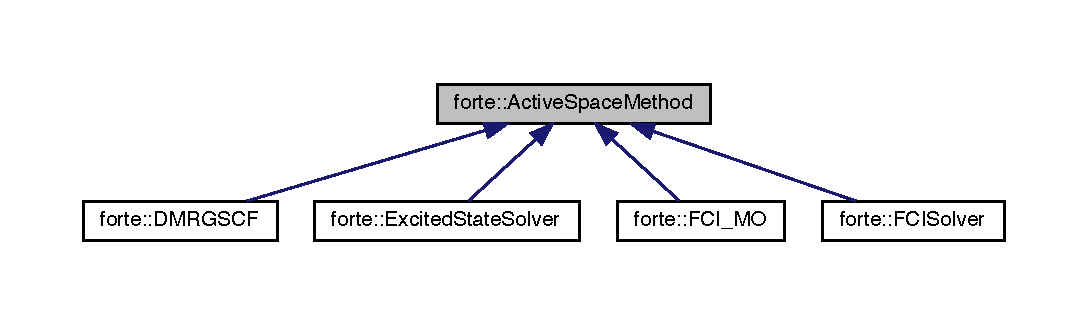
\includegraphics[width=350pt]{classforte_1_1_active_space_method__inherit__graph}
\end{center}
\end{figure}


Collaboration diagram for forte\+:\+:Active\+Space\+Method\+:
\nopagebreak
\begin{figure}[H]
\begin{center}
\leavevmode
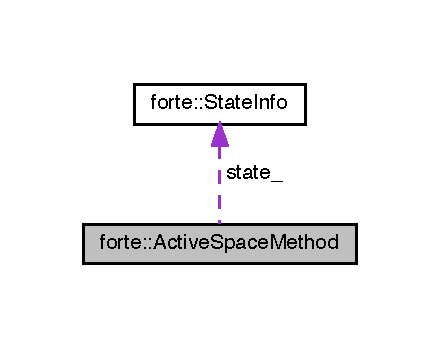
\includegraphics[width=211pt]{classforte_1_1_active_space_method__coll__graph}
\end{center}
\end{figure}
\subsection*{Public Member Functions}
\begin{DoxyCompactItemize}
\item 
\mbox{\hyperlink{classforte_1_1_active_space_method_afa70f2a1ba6e629d47aa9cd53aaff803}{Active\+Space\+Method}} (\mbox{\hyperlink{classforte_1_1_state_info}{State\+Info}} \mbox{\hyperlink{classforte_1_1_active_space_method_a609f005cc7d3a1bc03ae517002eb19dc}{state}}, size\+\_\+t \mbox{\hyperlink{classforte_1_1_active_space_method_aa2bafc732bd7023fd32fbd263ef2e903}{nroot}}, std\+::shared\+\_\+ptr$<$ \mbox{\hyperlink{classforte_1_1_m_o_space_info}{M\+O\+Space\+Info}} $>$ mo\+\_\+space\+\_\+info, std\+::shared\+\_\+ptr$<$ \mbox{\hyperlink{classforte_1_1_active_space_integrals}{Active\+Space\+Integrals}} $>$ as\+\_\+ints)
\begin{DoxyCompactList}\small\item\em \mbox{\hyperlink{classforte_1_1_active_space_method}{Active\+Space\+Method}} Constructor for a single state computation. \end{DoxyCompactList}\item 
\mbox{\hyperlink{classforte_1_1_active_space_method_ae630700e0a16cca4aaa0e22d0902f873}{Active\+Space\+Method}} ()=default
\begin{DoxyCompactList}\small\item\em Default constructor. \end{DoxyCompactList}\item 
virtual \mbox{\hyperlink{classforte_1_1_active_space_method_a89c56600b54016ec3ad0c4c946fe0e5d}{$\sim$\+Active\+Space\+Method}} ()=default
\begin{DoxyCompactList}\small\item\em Virtual destructor to enable deletion of a Derived$\ast$ through a Base$\ast$. \end{DoxyCompactList}\item 
virtual double \mbox{\hyperlink{classforte_1_1_active_space_method_a99736e2b94405371b224b0750569b077}{compute\+\_\+energy}} ()=0
\begin{DoxyCompactList}\small\item\em Compute the energy and return it. \end{DoxyCompactList}\item 
virtual std\+::vector$<$ \mbox{\hyperlink{classforte_1_1_r_d_ms}{R\+D\+Ms}} $>$ \mbox{\hyperlink{classforte_1_1_active_space_method_a0b2c4903551a7602db815d67349ba7c9}{rdms}} (const std\+::vector$<$ std\+::pair$<$ size\+\_\+t, size\+\_\+t $>$$>$ \&root\+\_\+list, int max\+\_\+rdm\+\_\+level)=0
\begin{DoxyCompactList}\small\item\em Compute the reduced density matrices up to a given particle rank (max\+\_\+rdm\+\_\+level) \end{DoxyCompactList}\item 
virtual std\+::vector$<$ \mbox{\hyperlink{classforte_1_1_r_d_ms}{R\+D\+Ms}} $>$ \mbox{\hyperlink{classforte_1_1_active_space_method_a4460069915e56a1994d3a4a4e78bdb30}{transition\+\_\+rdms}} (const std\+::vector$<$ std\+::pair$<$ size\+\_\+t, size\+\_\+t $>$$>$ \&root\+\_\+list, std\+::shared\+\_\+ptr$<$ \mbox{\hyperlink{classforte_1_1_active_space_method}{Active\+Space\+Method}} $>$ method2, int max\+\_\+rdm\+\_\+level)=0
\item 
virtual void \mbox{\hyperlink{classforte_1_1_active_space_method_a9416a627f550d4d56f6b8ffe7478ed89}{set\+\_\+options}} (std\+::shared\+\_\+ptr$<$ \mbox{\hyperlink{classforte_1_1_forte_options}{Forte\+Options}} $>$ options)=0
\item 
void \mbox{\hyperlink{classforte_1_1_active_space_method_a68315114ff7ca403e1cf05ad9faaf1d0}{set\+\_\+active\+\_\+space\+\_\+integrals}} (std\+::shared\+\_\+ptr$<$ \mbox{\hyperlink{classforte_1_1_active_space_integrals}{Active\+Space\+Integrals}} $>$ as\+\_\+ints)
\item 
psi\+::\+Shared\+Vector \mbox{\hyperlink{classforte_1_1_active_space_method_a4991f2ecd42e6a1c89a5c607b4815b47}{evals}} ()
\begin{DoxyCompactList}\small\item\em Return the eigenvalues. \end{DoxyCompactList}\item 
const std\+::vector$<$ double $>$ \& \mbox{\hyperlink{classforte_1_1_active_space_method_a9fdd240d326fab5791b58278af2a69bf}{energies}} () const
\begin{DoxyCompactList}\small\item\em Return a vector with the energies of all the states. \end{DoxyCompactList}\item 
size\+\_\+t \mbox{\hyperlink{classforte_1_1_active_space_method_aa2bafc732bd7023fd32fbd263ef2e903}{nroot}} () const
\begin{DoxyCompactList}\small\item\em Return the number of roots computed. \end{DoxyCompactList}\item 
const \mbox{\hyperlink{classforte_1_1_state_info}{State\+Info}} \& \mbox{\hyperlink{classforte_1_1_active_space_method_a609f005cc7d3a1bc03ae517002eb19dc}{state}} () const
\begin{DoxyCompactList}\small\item\em Return the state info. \end{DoxyCompactList}\item 
void \mbox{\hyperlink{classforte_1_1_active_space_method_ac4f39aa66c9d4481d172ea9e6255dc03}{set\+\_\+e\+\_\+convergence}} (double value)
\item 
void \mbox{\hyperlink{classforte_1_1_active_space_method_a59aad054d7966dc86ef01ea143fb1308}{set\+\_\+r\+\_\+convergence}} (double value)
\item 
void \mbox{\hyperlink{classforte_1_1_active_space_method_a0abdfc8523b4c7e4fdd3a0e6a3d4bd13}{set\+\_\+root}} (int value)
\item 
void \mbox{\hyperlink{classforte_1_1_active_space_method_a4442ac4afcec13630ff4e539a321205a}{set\+\_\+print}} (int level)
\end{DoxyCompactItemize}
\subsection*{Protected Attributes}
\begin{DoxyCompactItemize}
\item 
std\+::vector$<$ size\+\_\+t $>$ \mbox{\hyperlink{classforte_1_1_active_space_method_a02a2f9b7c138d1471cd6632650508819}{active\+\_\+mo\+\_\+}}
\begin{DoxyCompactList}\small\item\em The list of active orbitals (absolute ordering) \end{DoxyCompactList}\item 
std\+::vector$<$ size\+\_\+t $>$ \mbox{\hyperlink{classforte_1_1_active_space_method_aa68eb7267f635f0f885d921a61197281}{core\+\_\+mo\+\_\+}}
\begin{DoxyCompactList}\small\item\em The list of doubly occupied orbitals (absolute ordering) \end{DoxyCompactList}\item 
\mbox{\hyperlink{classforte_1_1_state_info}{State\+Info}} \mbox{\hyperlink{classforte_1_1_active_space_method_a1d90017e267642942760830b17d27d9f}{state\+\_\+}}
\begin{DoxyCompactList}\small\item\em The state to calculate. \end{DoxyCompactList}\item 
size\+\_\+t \mbox{\hyperlink{classforte_1_1_active_space_method_a3e299283cd1a99a718307a05f0790039}{nroot\+\_\+}} = 1
\begin{DoxyCompactList}\small\item\em The number of roots (default = 1) \end{DoxyCompactList}\item 
std\+::shared\+\_\+ptr$<$ \mbox{\hyperlink{classforte_1_1_m_o_space_info}{M\+O\+Space\+Info}} $>$ \mbox{\hyperlink{classforte_1_1_active_space_method_a7359678b3a1f747c0800323748bd9ba2}{mo\+\_\+space\+\_\+info\+\_\+}}
\begin{DoxyCompactList}\small\item\em The \mbox{\hyperlink{classforte_1_1_m_o_space_info}{M\+O\+Space\+Info}} object. \end{DoxyCompactList}\item 
std\+::shared\+\_\+ptr$<$ \mbox{\hyperlink{classforte_1_1_active_space_integrals}{Active\+Space\+Integrals}} $>$ \mbox{\hyperlink{classforte_1_1_active_space_method_ab012eecdedfe5373e2845fd6959e9fca}{as\+\_\+ints\+\_\+}}
\item 
double \mbox{\hyperlink{classforte_1_1_active_space_method_aabde020cf2dee6ccee213f0a3e364327}{e\+\_\+convergence\+\_\+}} = 1.\+0e-\/12
\begin{DoxyCompactList}\small\item\em The energy convergence criterion. \end{DoxyCompactList}\item 
double \mbox{\hyperlink{classforte_1_1_active_space_method_a78d130a7a72dede5a9908218fbb968e1}{r\+\_\+convergence\+\_\+}} = 1.\+0e-\/6
\begin{DoxyCompactList}\small\item\em The residual 2-\/norm convergence criterion. \end{DoxyCompactList}\item 
int \mbox{\hyperlink{classforte_1_1_active_space_method_a53458a01013f2953a6d1f9f7ffaf7748}{root\+\_\+}} = 0
\begin{DoxyCompactList}\small\item\em The root used to compute properties (zero based, default = 0) \end{DoxyCompactList}\item 
int \mbox{\hyperlink{classforte_1_1_active_space_method_aad045907e17a8a42f293d50315586eb2}{print\+\_\+}} = 0
\begin{DoxyCompactList}\small\item\em A variable to control printing information. \end{DoxyCompactList}\item 
psi\+::\+Shared\+Vector \mbox{\hyperlink{classforte_1_1_active_space_method_a22e878923ad570612cf05674f339c0ca}{evals\+\_\+}}
\begin{DoxyCompactList}\small\item\em Eigenvalues. \end{DoxyCompactList}\item 
std\+::vector$<$ double $>$ \mbox{\hyperlink{classforte_1_1_active_space_method_a9dad8dec653d25bab4c7a6a9c2293e12}{energies\+\_\+}}
\begin{DoxyCompactList}\small\item\em The energies (including nuclear repulsion) of all the states. \end{DoxyCompactList}\end{DoxyCompactItemize}


\subsection{Detailed Description}
Base class for methods that solve the Schrodinger equation in an active space. 

This class is the base class for methods that solve for the wavefunction in a small subset of the full orbital space ($<$30-\/40 orbitals). The molecular orbital used by the active space methods are stored in a \mbox{\hyperlink{classforte_1_1_active_space_integrals}{Active\+Space\+Integrals}} and must be passed at the time of creation.

All methods that derive from this class offer the following interface


\begin{DoxyItemize}
\item Compute the energy double \mbox{\hyperlink{classforte_1_1_active_space_method_a99736e2b94405371b224b0750569b077}{compute\+\_\+energy()}};
\item Compute a \mbox{\hyperlink{classforte_1_1_r_d_ms}{R\+D\+Ms}} object \mbox{\hyperlink{classforte_1_1_r_d_ms}{R\+D\+Ms}} \mbox{\hyperlink{classforte_1_1_active_space_method_a0b2c4903551a7602db815d67349ba7c9}{rdms()}};
\item Set the options for the derived methods \mbox{\hyperlink{classforte_1_1_active_space_method_a9416a627f550d4d56f6b8ffe7478ed89}{set\+\_\+options(std\+::shared\+\_\+ptr$<$\+Forte\+Options$>$ options)}};
\end{DoxyItemize}

All methods must also use the following base class variables


\begin{DoxyItemize}
\item Information about the state \mbox{\hyperlink{classforte_1_1_state_info}{State\+Info}} state\+\_\+;
\item Number of states computed size\+\_\+t nroot\+\_\+;
\item Store final energies in the vector (including nuclear repulsion)\+: std\+::vector$<$double$>$ energies\+\_\+;
\end{DoxyItemize}

\begin{DoxyNote}{Note}
This class is not aware of which orbitals are considered active. This information is contained in the \mbox{\hyperlink{classforte_1_1_active_space_integrals}{Active\+Space\+Integrals}} object. Orbitals that are double occupied are not correlated and are trated via effective scalar and one-\/body interactions. 
\end{DoxyNote}


\subsection{Constructor \& Destructor Documentation}
\mbox{\Hypertarget{classforte_1_1_active_space_method_afa70f2a1ba6e629d47aa9cd53aaff803}\label{classforte_1_1_active_space_method_afa70f2a1ba6e629d47aa9cd53aaff803}} 
\index{forte\+::\+Active\+Space\+Method@{forte\+::\+Active\+Space\+Method}!Active\+Space\+Method@{Active\+Space\+Method}}
\index{Active\+Space\+Method@{Active\+Space\+Method}!forte\+::\+Active\+Space\+Method@{forte\+::\+Active\+Space\+Method}}
\subsubsection{\texorpdfstring{Active\+Space\+Method()}{ActiveSpaceMethod()}\hspace{0.1cm}{\footnotesize\ttfamily [1/2]}}
{\footnotesize\ttfamily forte\+::\+Active\+Space\+Method\+::\+Active\+Space\+Method (\begin{DoxyParamCaption}\item[{\mbox{\hyperlink{classforte_1_1_state_info}{State\+Info}}}]{state,  }\item[{size\+\_\+t}]{nroot,  }\item[{std\+::shared\+\_\+ptr$<$ \mbox{\hyperlink{classforte_1_1_m_o_space_info}{M\+O\+Space\+Info}} $>$}]{mo\+\_\+space\+\_\+info,  }\item[{std\+::shared\+\_\+ptr$<$ \mbox{\hyperlink{classforte_1_1_active_space_integrals}{Active\+Space\+Integrals}} $>$}]{as\+\_\+ints }\end{DoxyParamCaption})}



\mbox{\hyperlink{classforte_1_1_active_space_method}{Active\+Space\+Method}} Constructor for a single state computation. 


\begin{DoxyParams}{Parameters}
{\em state} & the electronic state to compute \\
\hline
{\em nroot} & the number of roots \\
\hline
{\em mo\+\_\+space\+\_\+info} & a \mbox{\hyperlink{classforte_1_1_m_o_space_info}{M\+O\+Space\+Info}} object that defines the orbital spaces \\
\hline
{\em as\+\_\+ints} & molecular integrals defined only for the active space orbitals \\
\hline
\end{DoxyParams}
\mbox{\Hypertarget{classforte_1_1_active_space_method_ae630700e0a16cca4aaa0e22d0902f873}\label{classforte_1_1_active_space_method_ae630700e0a16cca4aaa0e22d0902f873}} 
\index{forte\+::\+Active\+Space\+Method@{forte\+::\+Active\+Space\+Method}!Active\+Space\+Method@{Active\+Space\+Method}}
\index{Active\+Space\+Method@{Active\+Space\+Method}!forte\+::\+Active\+Space\+Method@{forte\+::\+Active\+Space\+Method}}
\subsubsection{\texorpdfstring{Active\+Space\+Method()}{ActiveSpaceMethod()}\hspace{0.1cm}{\footnotesize\ttfamily [2/2]}}
{\footnotesize\ttfamily forte\+::\+Active\+Space\+Method\+::\+Active\+Space\+Method (\begin{DoxyParamCaption}{ }\end{DoxyParamCaption})\hspace{0.3cm}{\ttfamily [default]}}



Default constructor. 

\mbox{\Hypertarget{classforte_1_1_active_space_method_a89c56600b54016ec3ad0c4c946fe0e5d}\label{classforte_1_1_active_space_method_a89c56600b54016ec3ad0c4c946fe0e5d}} 
\index{forte\+::\+Active\+Space\+Method@{forte\+::\+Active\+Space\+Method}!````~Active\+Space\+Method@{$\sim$\+Active\+Space\+Method}}
\index{````~Active\+Space\+Method@{$\sim$\+Active\+Space\+Method}!forte\+::\+Active\+Space\+Method@{forte\+::\+Active\+Space\+Method}}
\subsubsection{\texorpdfstring{$\sim$\+Active\+Space\+Method()}{~ActiveSpaceMethod()}}
{\footnotesize\ttfamily virtual forte\+::\+Active\+Space\+Method\+::$\sim$\+Active\+Space\+Method (\begin{DoxyParamCaption}{ }\end{DoxyParamCaption})\hspace{0.3cm}{\ttfamily [virtual]}, {\ttfamily [default]}}



Virtual destructor to enable deletion of a Derived$\ast$ through a Base$\ast$. 



\subsection{Member Function Documentation}
\mbox{\Hypertarget{classforte_1_1_active_space_method_a99736e2b94405371b224b0750569b077}\label{classforte_1_1_active_space_method_a99736e2b94405371b224b0750569b077}} 
\index{forte\+::\+Active\+Space\+Method@{forte\+::\+Active\+Space\+Method}!compute\+\_\+energy@{compute\+\_\+energy}}
\index{compute\+\_\+energy@{compute\+\_\+energy}!forte\+::\+Active\+Space\+Method@{forte\+::\+Active\+Space\+Method}}
\subsubsection{\texorpdfstring{compute\+\_\+energy()}{compute\_energy()}}
{\footnotesize\ttfamily virtual double forte\+::\+Active\+Space\+Method\+::compute\+\_\+energy (\begin{DoxyParamCaption}{ }\end{DoxyParamCaption})\hspace{0.3cm}{\ttfamily [pure virtual]}}



Compute the energy and return it. 



Implemented in \mbox{\hyperlink{classforte_1_1_f_c_i___m_o_a98d9b947e1cf345c82d513a54ca51ddd}{forte\+::\+F\+C\+I\+\_\+\+MO}}, \mbox{\hyperlink{classforte_1_1_f_c_i_solver_a5ea02e6826ffd8eb01fd25c229517159}{forte\+::\+F\+C\+I\+Solver}}, \mbox{\hyperlink{classforte_1_1_excited_state_solver_a35b840324fb9e080eda46f29e544c86a}{forte\+::\+Excited\+State\+Solver}}, and \mbox{\hyperlink{classforte_1_1_d_m_r_g_s_c_f_a19128db2df6992b295bd00d85c43309d}{forte\+::\+D\+M\+R\+G\+S\+CF}}.

\mbox{\Hypertarget{classforte_1_1_active_space_method_a9fdd240d326fab5791b58278af2a69bf}\label{classforte_1_1_active_space_method_a9fdd240d326fab5791b58278af2a69bf}} 
\index{forte\+::\+Active\+Space\+Method@{forte\+::\+Active\+Space\+Method}!energies@{energies}}
\index{energies@{energies}!forte\+::\+Active\+Space\+Method@{forte\+::\+Active\+Space\+Method}}
\subsubsection{\texorpdfstring{energies()}{energies()}}
{\footnotesize\ttfamily const std\+::vector$<$ double $>$ \& forte\+::\+Active\+Space\+Method\+::energies (\begin{DoxyParamCaption}{ }\end{DoxyParamCaption}) const}



Return a vector with the energies of all the states. 

\mbox{\Hypertarget{classforte_1_1_active_space_method_a4991f2ecd42e6a1c89a5c607b4815b47}\label{classforte_1_1_active_space_method_a4991f2ecd42e6a1c89a5c607b4815b47}} 
\index{forte\+::\+Active\+Space\+Method@{forte\+::\+Active\+Space\+Method}!evals@{evals}}
\index{evals@{evals}!forte\+::\+Active\+Space\+Method@{forte\+::\+Active\+Space\+Method}}
\subsubsection{\texorpdfstring{evals()}{evals()}}
{\footnotesize\ttfamily psi\+::\+Shared\+Vector forte\+::\+Active\+Space\+Method\+::evals (\begin{DoxyParamCaption}{ }\end{DoxyParamCaption})}



Return the eigenvalues. 

\mbox{\Hypertarget{classforte_1_1_active_space_method_aa2bafc732bd7023fd32fbd263ef2e903}\label{classforte_1_1_active_space_method_aa2bafc732bd7023fd32fbd263ef2e903}} 
\index{forte\+::\+Active\+Space\+Method@{forte\+::\+Active\+Space\+Method}!nroot@{nroot}}
\index{nroot@{nroot}!forte\+::\+Active\+Space\+Method@{forte\+::\+Active\+Space\+Method}}
\subsubsection{\texorpdfstring{nroot()}{nroot()}}
{\footnotesize\ttfamily size\+\_\+t forte\+::\+Active\+Space\+Method\+::nroot (\begin{DoxyParamCaption}{ }\end{DoxyParamCaption}) const\hspace{0.3cm}{\ttfamily [inline]}}



Return the number of roots computed. 

\mbox{\Hypertarget{classforte_1_1_active_space_method_a0b2c4903551a7602db815d67349ba7c9}\label{classforte_1_1_active_space_method_a0b2c4903551a7602db815d67349ba7c9}} 
\index{forte\+::\+Active\+Space\+Method@{forte\+::\+Active\+Space\+Method}!rdms@{rdms}}
\index{rdms@{rdms}!forte\+::\+Active\+Space\+Method@{forte\+::\+Active\+Space\+Method}}
\subsubsection{\texorpdfstring{rdms()}{rdms()}}
{\footnotesize\ttfamily virtual std\+::vector$<$\mbox{\hyperlink{classforte_1_1_r_d_ms}{R\+D\+Ms}}$>$ forte\+::\+Active\+Space\+Method\+::rdms (\begin{DoxyParamCaption}\item[{const std\+::vector$<$ std\+::pair$<$ size\+\_\+t, size\+\_\+t $>$$>$ \&}]{root\+\_\+list,  }\item[{int}]{max\+\_\+rdm\+\_\+level }\end{DoxyParamCaption})\hspace{0.3cm}{\ttfamily [pure virtual]}}



Compute the reduced density matrices up to a given particle rank (max\+\_\+rdm\+\_\+level) 

This function can be used to compute transition density matrices between states of difference symmetry,

D$^\wedge$\{p\}\+\_\+\{q\} = $<$I, symmetry\+\_\+l$\vert$ a+\+\_\+p1 ... a\+\_\+qn $\vert$J, symmetry\+\_\+r$>$

where $\vert$I, symmetry\+\_\+l$>$ is the I-\/th state of symmetry = symmetry\+\_\+l $\vert$J, symmetry\+\_\+r$>$ is the J-\/th state of symmetry = symmetry\+\_\+r


\begin{DoxyParams}{Parameters}
{\em root\+\_\+list} & a list of pairs of roots to compute \mbox{[}(I\+\_\+1, J\+\_\+1), (I\+\_\+2, J\+\_\+2), ...\mbox{]} \\
\hline
{\em method2} & a second \mbox{\hyperlink{classforte_1_1_active_space_method}{Active\+Space\+Method}} object that holds the states for symmetry\+\_\+r \\
\hline
{\em max\+\_\+rdm\+\_\+level} & the maximum R\+DM rank \\
\hline
\end{DoxyParams}
\begin{DoxyReturn}{Returns}

\end{DoxyReturn}


Implemented in \mbox{\hyperlink{classforte_1_1_f_c_i___m_o_afe4bb6cb53fbf4190c020ee3fa794237}{forte\+::\+F\+C\+I\+\_\+\+MO}}, \mbox{\hyperlink{classforte_1_1_f_c_i_solver_a40d53f62ae73a7baf7560dac37838b8b}{forte\+::\+F\+C\+I\+Solver}}, and \mbox{\hyperlink{classforte_1_1_excited_state_solver_a67a061a196cc9e492fabc1b6c7995409}{forte\+::\+Excited\+State\+Solver}}.

\mbox{\Hypertarget{classforte_1_1_active_space_method_a68315114ff7ca403e1cf05ad9faaf1d0}\label{classforte_1_1_active_space_method_a68315114ff7ca403e1cf05ad9faaf1d0}} 
\index{forte\+::\+Active\+Space\+Method@{forte\+::\+Active\+Space\+Method}!set\+\_\+active\+\_\+space\+\_\+integrals@{set\+\_\+active\+\_\+space\+\_\+integrals}}
\index{set\+\_\+active\+\_\+space\+\_\+integrals@{set\+\_\+active\+\_\+space\+\_\+integrals}!forte\+::\+Active\+Space\+Method@{forte\+::\+Active\+Space\+Method}}
\subsubsection{\texorpdfstring{set\+\_\+active\+\_\+space\+\_\+integrals()}{set\_active\_space\_integrals()}}
{\footnotesize\ttfamily void forte\+::\+Active\+Space\+Method\+::set\+\_\+active\+\_\+space\+\_\+integrals (\begin{DoxyParamCaption}\item[{std\+::shared\+\_\+ptr$<$ \mbox{\hyperlink{classforte_1_1_active_space_integrals}{Active\+Space\+Integrals}} $>$}]{as\+\_\+ints }\end{DoxyParamCaption})}

Pass a set of \mbox{\hyperlink{classforte_1_1_active_space_integrals}{Active\+Space\+Integrals}} to the solver (e.\+g. an effective Hamiltonian) 
\begin{DoxyParams}{Parameters}
{\em as\+\_\+ints} & the integrals passed in \\
\hline
\end{DoxyParams}
\mbox{\Hypertarget{classforte_1_1_active_space_method_ac4f39aa66c9d4481d172ea9e6255dc03}\label{classforte_1_1_active_space_method_ac4f39aa66c9d4481d172ea9e6255dc03}} 
\index{forte\+::\+Active\+Space\+Method@{forte\+::\+Active\+Space\+Method}!set\+\_\+e\+\_\+convergence@{set\+\_\+e\+\_\+convergence}}
\index{set\+\_\+e\+\_\+convergence@{set\+\_\+e\+\_\+convergence}!forte\+::\+Active\+Space\+Method@{forte\+::\+Active\+Space\+Method}}
\subsubsection{\texorpdfstring{set\+\_\+e\+\_\+convergence()}{set\_e\_convergence()}}
{\footnotesize\ttfamily void forte\+::\+Active\+Space\+Method\+::set\+\_\+e\+\_\+convergence (\begin{DoxyParamCaption}\item[{double}]{value }\end{DoxyParamCaption})}

Set the energy convergence criterion 
\begin{DoxyParams}{Parameters}
{\em value} & the convergence criterion in a.\+u. \\
\hline
\end{DoxyParams}
\mbox{\Hypertarget{classforte_1_1_active_space_method_a9416a627f550d4d56f6b8ffe7478ed89}\label{classforte_1_1_active_space_method_a9416a627f550d4d56f6b8ffe7478ed89}} 
\index{forte\+::\+Active\+Space\+Method@{forte\+::\+Active\+Space\+Method}!set\+\_\+options@{set\+\_\+options}}
\index{set\+\_\+options@{set\+\_\+options}!forte\+::\+Active\+Space\+Method@{forte\+::\+Active\+Space\+Method}}
\subsubsection{\texorpdfstring{set\+\_\+options()}{set\_options()}}
{\footnotesize\ttfamily virtual void forte\+::\+Active\+Space\+Method\+::set\+\_\+options (\begin{DoxyParamCaption}\item[{std\+::shared\+\_\+ptr$<$ \mbox{\hyperlink{classforte_1_1_forte_options}{Forte\+Options}} $>$}]{options }\end{DoxyParamCaption})\hspace{0.3cm}{\ttfamily [pure virtual]}}

Set options from an option object 
\begin{DoxyParams}{Parameters}
{\em options} & the options passed in \\
\hline
\end{DoxyParams}


Implemented in \mbox{\hyperlink{classforte_1_1_f_c_i___m_o_ad03e24facf8d8b4ba766ce7a0e5725e6}{forte\+::\+F\+C\+I\+\_\+\+MO}}, \mbox{\hyperlink{classforte_1_1_f_c_i_solver_a5bb962ea913122dbcec9319411876b05}{forte\+::\+F\+C\+I\+Solver}}, and \mbox{\hyperlink{classforte_1_1_excited_state_solver_ac32716228ebaa1dfda75cf48db544e5f}{forte\+::\+Excited\+State\+Solver}}.

\mbox{\Hypertarget{classforte_1_1_active_space_method_a4442ac4afcec13630ff4e539a321205a}\label{classforte_1_1_active_space_method_a4442ac4afcec13630ff4e539a321205a}} 
\index{forte\+::\+Active\+Space\+Method@{forte\+::\+Active\+Space\+Method}!set\+\_\+print@{set\+\_\+print}}
\index{set\+\_\+print@{set\+\_\+print}!forte\+::\+Active\+Space\+Method@{forte\+::\+Active\+Space\+Method}}
\subsubsection{\texorpdfstring{set\+\_\+print()}{set\_print()}}
{\footnotesize\ttfamily void forte\+::\+Active\+Space\+Method\+::set\+\_\+print (\begin{DoxyParamCaption}\item[{int}]{level }\end{DoxyParamCaption})}

Set the print level 
\begin{DoxyParams}{Parameters}
{\em level} & the print level (0 = no printing, 1 default) \\
\hline
\end{DoxyParams}
\mbox{\Hypertarget{classforte_1_1_active_space_method_a59aad054d7966dc86ef01ea143fb1308}\label{classforte_1_1_active_space_method_a59aad054d7966dc86ef01ea143fb1308}} 
\index{forte\+::\+Active\+Space\+Method@{forte\+::\+Active\+Space\+Method}!set\+\_\+r\+\_\+convergence@{set\+\_\+r\+\_\+convergence}}
\index{set\+\_\+r\+\_\+convergence@{set\+\_\+r\+\_\+convergence}!forte\+::\+Active\+Space\+Method@{forte\+::\+Active\+Space\+Method}}
\subsubsection{\texorpdfstring{set\+\_\+r\+\_\+convergence()}{set\_r\_convergence()}}
{\footnotesize\ttfamily void forte\+::\+Active\+Space\+Method\+::set\+\_\+r\+\_\+convergence (\begin{DoxyParamCaption}\item[{double}]{value }\end{DoxyParamCaption})}

Set the residual 2-\/norm convergence criterion 
\begin{DoxyParams}{Parameters}
{\em value} & the convergence criterion in a.\+u. \\
\hline
\end{DoxyParams}
\mbox{\Hypertarget{classforte_1_1_active_space_method_a0abdfc8523b4c7e4fdd3a0e6a3d4bd13}\label{classforte_1_1_active_space_method_a0abdfc8523b4c7e4fdd3a0e6a3d4bd13}} 
\index{forte\+::\+Active\+Space\+Method@{forte\+::\+Active\+Space\+Method}!set\+\_\+root@{set\+\_\+root}}
\index{set\+\_\+root@{set\+\_\+root}!forte\+::\+Active\+Space\+Method@{forte\+::\+Active\+Space\+Method}}
\subsubsection{\texorpdfstring{set\+\_\+root()}{set\_root()}}
{\footnotesize\ttfamily void forte\+::\+Active\+Space\+Method\+::set\+\_\+root (\begin{DoxyParamCaption}\item[{int}]{value }\end{DoxyParamCaption})}

Set the root that will be used to compute the properties 
\begin{DoxyParams}{Parameters}
{\em the} & root (root = 0, 1, 2, ...) \\
\hline
\end{DoxyParams}
\mbox{\Hypertarget{classforte_1_1_active_space_method_a609f005cc7d3a1bc03ae517002eb19dc}\label{classforte_1_1_active_space_method_a609f005cc7d3a1bc03ae517002eb19dc}} 
\index{forte\+::\+Active\+Space\+Method@{forte\+::\+Active\+Space\+Method}!state@{state}}
\index{state@{state}!forte\+::\+Active\+Space\+Method@{forte\+::\+Active\+Space\+Method}}
\subsubsection{\texorpdfstring{state()}{state()}}
{\footnotesize\ttfamily const \mbox{\hyperlink{classforte_1_1_state_info}{State\+Info}}\& forte\+::\+Active\+Space\+Method\+::state (\begin{DoxyParamCaption}{ }\end{DoxyParamCaption}) const\hspace{0.3cm}{\ttfamily [inline]}}



Return the state info. 

\mbox{\Hypertarget{classforte_1_1_active_space_method_a4460069915e56a1994d3a4a4e78bdb30}\label{classforte_1_1_active_space_method_a4460069915e56a1994d3a4a4e78bdb30}} 
\index{forte\+::\+Active\+Space\+Method@{forte\+::\+Active\+Space\+Method}!transition\+\_\+rdms@{transition\+\_\+rdms}}
\index{transition\+\_\+rdms@{transition\+\_\+rdms}!forte\+::\+Active\+Space\+Method@{forte\+::\+Active\+Space\+Method}}
\subsubsection{\texorpdfstring{transition\+\_\+rdms()}{transition\_rdms()}}
{\footnotesize\ttfamily virtual std\+::vector$<$\mbox{\hyperlink{classforte_1_1_r_d_ms}{R\+D\+Ms}}$>$ forte\+::\+Active\+Space\+Method\+::transition\+\_\+rdms (\begin{DoxyParamCaption}\item[{const std\+::vector$<$ std\+::pair$<$ size\+\_\+t, size\+\_\+t $>$$>$ \&}]{root\+\_\+list,  }\item[{std\+::shared\+\_\+ptr$<$ \mbox{\hyperlink{classforte_1_1_active_space_method}{Active\+Space\+Method}} $>$}]{method2,  }\item[{int}]{max\+\_\+rdm\+\_\+level }\end{DoxyParamCaption})\hspace{0.3cm}{\ttfamily [pure virtual]}}



Implemented in \mbox{\hyperlink{classforte_1_1_f_c_i___m_o_a62d0c9bbee3dc8942ab109354074ad87}{forte\+::\+F\+C\+I\+\_\+\+MO}}, \mbox{\hyperlink{classforte_1_1_f_c_i_solver_ad29797ad91b7edb6b3d8a4c66aaf18a0}{forte\+::\+F\+C\+I\+Solver}}, and \mbox{\hyperlink{classforte_1_1_excited_state_solver_a8fa122b902c65b75470e34cdd475acaf}{forte\+::\+Excited\+State\+Solver}}.



\subsection{Member Data Documentation}
\mbox{\Hypertarget{classforte_1_1_active_space_method_a02a2f9b7c138d1471cd6632650508819}\label{classforte_1_1_active_space_method_a02a2f9b7c138d1471cd6632650508819}} 
\index{forte\+::\+Active\+Space\+Method@{forte\+::\+Active\+Space\+Method}!active\+\_\+mo\+\_\+@{active\+\_\+mo\+\_\+}}
\index{active\+\_\+mo\+\_\+@{active\+\_\+mo\+\_\+}!forte\+::\+Active\+Space\+Method@{forte\+::\+Active\+Space\+Method}}
\subsubsection{\texorpdfstring{active\+\_\+mo\+\_\+}{active\_mo\_}}
{\footnotesize\ttfamily std\+::vector$<$size\+\_\+t$>$ forte\+::\+Active\+Space\+Method\+::active\+\_\+mo\+\_\+\hspace{0.3cm}{\ttfamily [protected]}}



The list of active orbitals (absolute ordering) 

\mbox{\Hypertarget{classforte_1_1_active_space_method_ab012eecdedfe5373e2845fd6959e9fca}\label{classforte_1_1_active_space_method_ab012eecdedfe5373e2845fd6959e9fca}} 
\index{forte\+::\+Active\+Space\+Method@{forte\+::\+Active\+Space\+Method}!as\+\_\+ints\+\_\+@{as\+\_\+ints\+\_\+}}
\index{as\+\_\+ints\+\_\+@{as\+\_\+ints\+\_\+}!forte\+::\+Active\+Space\+Method@{forte\+::\+Active\+Space\+Method}}
\subsubsection{\texorpdfstring{as\+\_\+ints\+\_\+}{as\_ints\_}}
{\footnotesize\ttfamily std\+::shared\+\_\+ptr$<$\mbox{\hyperlink{classforte_1_1_active_space_integrals}{Active\+Space\+Integrals}}$>$ forte\+::\+Active\+Space\+Method\+::as\+\_\+ints\+\_\+\hspace{0.3cm}{\ttfamily [protected]}}

The molecular integrals for the active space This object holds only the integrals for the orbital contained in the active\+\_\+mo\+\_\+ vector. The one-\/electron integrals and scalar energy contains contributions from the doubly occupied orbitals specified by the core\+\_\+mo\+\_\+ vector. \mbox{\Hypertarget{classforte_1_1_active_space_method_aa68eb7267f635f0f885d921a61197281}\label{classforte_1_1_active_space_method_aa68eb7267f635f0f885d921a61197281}} 
\index{forte\+::\+Active\+Space\+Method@{forte\+::\+Active\+Space\+Method}!core\+\_\+mo\+\_\+@{core\+\_\+mo\+\_\+}}
\index{core\+\_\+mo\+\_\+@{core\+\_\+mo\+\_\+}!forte\+::\+Active\+Space\+Method@{forte\+::\+Active\+Space\+Method}}
\subsubsection{\texorpdfstring{core\+\_\+mo\+\_\+}{core\_mo\_}}
{\footnotesize\ttfamily std\+::vector$<$size\+\_\+t$>$ forte\+::\+Active\+Space\+Method\+::core\+\_\+mo\+\_\+\hspace{0.3cm}{\ttfamily [protected]}}



The list of doubly occupied orbitals (absolute ordering) 

\mbox{\Hypertarget{classforte_1_1_active_space_method_aabde020cf2dee6ccee213f0a3e364327}\label{classforte_1_1_active_space_method_aabde020cf2dee6ccee213f0a3e364327}} 
\index{forte\+::\+Active\+Space\+Method@{forte\+::\+Active\+Space\+Method}!e\+\_\+convergence\+\_\+@{e\+\_\+convergence\+\_\+}}
\index{e\+\_\+convergence\+\_\+@{e\+\_\+convergence\+\_\+}!forte\+::\+Active\+Space\+Method@{forte\+::\+Active\+Space\+Method}}
\subsubsection{\texorpdfstring{e\+\_\+convergence\+\_\+}{e\_convergence\_}}
{\footnotesize\ttfamily double forte\+::\+Active\+Space\+Method\+::e\+\_\+convergence\+\_\+ = 1.\+0e-\/12\hspace{0.3cm}{\ttfamily [protected]}}



The energy convergence criterion. 

\mbox{\Hypertarget{classforte_1_1_active_space_method_a9dad8dec653d25bab4c7a6a9c2293e12}\label{classforte_1_1_active_space_method_a9dad8dec653d25bab4c7a6a9c2293e12}} 
\index{forte\+::\+Active\+Space\+Method@{forte\+::\+Active\+Space\+Method}!energies\+\_\+@{energies\+\_\+}}
\index{energies\+\_\+@{energies\+\_\+}!forte\+::\+Active\+Space\+Method@{forte\+::\+Active\+Space\+Method}}
\subsubsection{\texorpdfstring{energies\+\_\+}{energies\_}}
{\footnotesize\ttfamily std\+::vector$<$double$>$ forte\+::\+Active\+Space\+Method\+::energies\+\_\+\hspace{0.3cm}{\ttfamily [protected]}}



The energies (including nuclear repulsion) of all the states. 

\mbox{\Hypertarget{classforte_1_1_active_space_method_a22e878923ad570612cf05674f339c0ca}\label{classforte_1_1_active_space_method_a22e878923ad570612cf05674f339c0ca}} 
\index{forte\+::\+Active\+Space\+Method@{forte\+::\+Active\+Space\+Method}!evals\+\_\+@{evals\+\_\+}}
\index{evals\+\_\+@{evals\+\_\+}!forte\+::\+Active\+Space\+Method@{forte\+::\+Active\+Space\+Method}}
\subsubsection{\texorpdfstring{evals\+\_\+}{evals\_}}
{\footnotesize\ttfamily psi\+::\+Shared\+Vector forte\+::\+Active\+Space\+Method\+::evals\+\_\+\hspace{0.3cm}{\ttfamily [protected]}}



Eigenvalues. 

\mbox{\Hypertarget{classforte_1_1_active_space_method_a7359678b3a1f747c0800323748bd9ba2}\label{classforte_1_1_active_space_method_a7359678b3a1f747c0800323748bd9ba2}} 
\index{forte\+::\+Active\+Space\+Method@{forte\+::\+Active\+Space\+Method}!mo\+\_\+space\+\_\+info\+\_\+@{mo\+\_\+space\+\_\+info\+\_\+}}
\index{mo\+\_\+space\+\_\+info\+\_\+@{mo\+\_\+space\+\_\+info\+\_\+}!forte\+::\+Active\+Space\+Method@{forte\+::\+Active\+Space\+Method}}
\subsubsection{\texorpdfstring{mo\+\_\+space\+\_\+info\+\_\+}{mo\_space\_info\_}}
{\footnotesize\ttfamily std\+::shared\+\_\+ptr$<$\mbox{\hyperlink{classforte_1_1_m_o_space_info}{M\+O\+Space\+Info}}$>$ forte\+::\+Active\+Space\+Method\+::mo\+\_\+space\+\_\+info\+\_\+\hspace{0.3cm}{\ttfamily [protected]}}



The \mbox{\hyperlink{classforte_1_1_m_o_space_info}{M\+O\+Space\+Info}} object. 

\mbox{\Hypertarget{classforte_1_1_active_space_method_a3e299283cd1a99a718307a05f0790039}\label{classforte_1_1_active_space_method_a3e299283cd1a99a718307a05f0790039}} 
\index{forte\+::\+Active\+Space\+Method@{forte\+::\+Active\+Space\+Method}!nroot\+\_\+@{nroot\+\_\+}}
\index{nroot\+\_\+@{nroot\+\_\+}!forte\+::\+Active\+Space\+Method@{forte\+::\+Active\+Space\+Method}}
\subsubsection{\texorpdfstring{nroot\+\_\+}{nroot\_}}
{\footnotesize\ttfamily size\+\_\+t forte\+::\+Active\+Space\+Method\+::nroot\+\_\+ = 1\hspace{0.3cm}{\ttfamily [protected]}}



The number of roots (default = 1) 

\mbox{\Hypertarget{classforte_1_1_active_space_method_aad045907e17a8a42f293d50315586eb2}\label{classforte_1_1_active_space_method_aad045907e17a8a42f293d50315586eb2}} 
\index{forte\+::\+Active\+Space\+Method@{forte\+::\+Active\+Space\+Method}!print\+\_\+@{print\+\_\+}}
\index{print\+\_\+@{print\+\_\+}!forte\+::\+Active\+Space\+Method@{forte\+::\+Active\+Space\+Method}}
\subsubsection{\texorpdfstring{print\+\_\+}{print\_}}
{\footnotesize\ttfamily int forte\+::\+Active\+Space\+Method\+::print\+\_\+ = 0\hspace{0.3cm}{\ttfamily [protected]}}



A variable to control printing information. 

\mbox{\Hypertarget{classforte_1_1_active_space_method_a78d130a7a72dede5a9908218fbb968e1}\label{classforte_1_1_active_space_method_a78d130a7a72dede5a9908218fbb968e1}} 
\index{forte\+::\+Active\+Space\+Method@{forte\+::\+Active\+Space\+Method}!r\+\_\+convergence\+\_\+@{r\+\_\+convergence\+\_\+}}
\index{r\+\_\+convergence\+\_\+@{r\+\_\+convergence\+\_\+}!forte\+::\+Active\+Space\+Method@{forte\+::\+Active\+Space\+Method}}
\subsubsection{\texorpdfstring{r\+\_\+convergence\+\_\+}{r\_convergence\_}}
{\footnotesize\ttfamily double forte\+::\+Active\+Space\+Method\+::r\+\_\+convergence\+\_\+ = 1.\+0e-\/6\hspace{0.3cm}{\ttfamily [protected]}}



The residual 2-\/norm convergence criterion. 

\mbox{\Hypertarget{classforte_1_1_active_space_method_a53458a01013f2953a6d1f9f7ffaf7748}\label{classforte_1_1_active_space_method_a53458a01013f2953a6d1f9f7ffaf7748}} 
\index{forte\+::\+Active\+Space\+Method@{forte\+::\+Active\+Space\+Method}!root\+\_\+@{root\+\_\+}}
\index{root\+\_\+@{root\+\_\+}!forte\+::\+Active\+Space\+Method@{forte\+::\+Active\+Space\+Method}}
\subsubsection{\texorpdfstring{root\+\_\+}{root\_}}
{\footnotesize\ttfamily int forte\+::\+Active\+Space\+Method\+::root\+\_\+ = 0\hspace{0.3cm}{\ttfamily [protected]}}



The root used to compute properties (zero based, default = 0) 

\mbox{\Hypertarget{classforte_1_1_active_space_method_a1d90017e267642942760830b17d27d9f}\label{classforte_1_1_active_space_method_a1d90017e267642942760830b17d27d9f}} 
\index{forte\+::\+Active\+Space\+Method@{forte\+::\+Active\+Space\+Method}!state\+\_\+@{state\+\_\+}}
\index{state\+\_\+@{state\+\_\+}!forte\+::\+Active\+Space\+Method@{forte\+::\+Active\+Space\+Method}}
\subsubsection{\texorpdfstring{state\+\_\+}{state\_}}
{\footnotesize\ttfamily \mbox{\hyperlink{classforte_1_1_state_info}{State\+Info}} forte\+::\+Active\+Space\+Method\+::state\+\_\+\hspace{0.3cm}{\ttfamily [protected]}}



The state to calculate. 



The documentation for this class was generated from the following files\+:\begin{DoxyCompactItemize}
\item 
/\+Users/fevange/\+Source/forte/src/base\+\_\+classes/\mbox{\hyperlink{active__space__method_8h}{active\+\_\+space\+\_\+method.\+h}}\item 
/\+Users/fevange/\+Source/forte/src/base\+\_\+classes/\mbox{\hyperlink{active__space__method_8cc}{active\+\_\+space\+\_\+method.\+cc}}\end{DoxyCompactItemize}

\hypertarget{classforte_1_1_active_space_solver}{}\section{forte\+:\+:Active\+Space\+Solver Class Reference}
\label{classforte_1_1_active_space_solver}\index{forte\+::\+Active\+Space\+Solver@{forte\+::\+Active\+Space\+Solver}}


General class for a multi-\/state active space solver.  




{\ttfamily \#include $<$active\+\_\+space\+\_\+solver.\+h$>$}

\subsection*{Public Member Functions}
\begin{DoxyCompactItemize}
\item 
\mbox{\hyperlink{classforte_1_1_active_space_solver_af2b538aa99fd5b6493d0825f9c0a3729}{Active\+Space\+Solver}} (const std\+::string \&method, const std\+::map$<$ \mbox{\hyperlink{classforte_1_1_state_info}{State\+Info}}, size\+\_\+t $>$ \&state\+\_\+nroots\+\_\+map, std\+::shared\+\_\+ptr$<$ \mbox{\hyperlink{classforte_1_1_s_c_f_info}{S\+C\+F\+Info}} $>$ scf\+\_\+info, std\+::shared\+\_\+ptr$<$ \mbox{\hyperlink{classforte_1_1_m_o_space_info}{M\+O\+Space\+Info}} $>$ mo\+\_\+space\+\_\+info, std\+::shared\+\_\+ptr$<$ \mbox{\hyperlink{classforte_1_1_active_space_integrals}{Active\+Space\+Integrals}} $>$ as\+\_\+ints, std\+::shared\+\_\+ptr$<$ \mbox{\hyperlink{classforte_1_1_forte_options}{Forte\+Options}} $>$ options)
\begin{DoxyCompactList}\small\item\em \mbox{\hyperlink{classforte_1_1_active_space_method}{Active\+Space\+Method}} Constructor for a multi-\/state computation. \end{DoxyCompactList}\item 
void \mbox{\hyperlink{classforte_1_1_active_space_solver_a40e5dded4471f30b5aa7afbe27167031}{set\+\_\+print}} (int level)
\item 
const std\+::map$<$ \mbox{\hyperlink{classforte_1_1_state_info}{State\+Info}}, std\+::vector$<$ double $>$ $>$ \& \mbox{\hyperlink{classforte_1_1_active_space_solver_a719be2ea9e2d227fd810481f7dd644a1}{compute\+\_\+energy}} ()
\begin{DoxyCompactList}\small\item\em Compute the energy and return it // T\+O\+DO\+: document (Francesco) \end{DoxyCompactList}\item 
const std\+::map$<$ \mbox{\hyperlink{classforte_1_1_state_info}{State\+Info}}, std\+::vector$<$ double $>$ $>$ \& \mbox{\hyperlink{classforte_1_1_active_space_solver_a53ed58e64499f8fa661b49d48648f3cb}{compute\+\_\+contracted\+\_\+energy}} (std\+::shared\+\_\+ptr$<$ \mbox{\hyperlink{classforte_1_1_active_space_integrals}{forte\+::\+Active\+Space\+Integrals}} $>$ as\+\_\+ints, int max\+\_\+rdm\+\_\+level)
\begin{DoxyCompactList}\small\item\em Compute the contracted CI energy. \end{DoxyCompactList}\item 
std\+::vector$<$ \mbox{\hyperlink{classforte_1_1_r_d_ms}{R\+D\+Ms}} $>$ \mbox{\hyperlink{classforte_1_1_active_space_solver_a96b316d00aada0b7b68c153f8c89bcea}{rdms}} (std\+::map$<$ std\+::pair$<$ \mbox{\hyperlink{classforte_1_1_state_info}{State\+Info}}, \mbox{\hyperlink{classforte_1_1_state_info}{State\+Info}} $>$, std\+::vector$<$ std\+::pair$<$ size\+\_\+t, size\+\_\+t $>$$>$$>$ \&elements, int max\+\_\+rdm\+\_\+level)
\item 
\mbox{\hyperlink{classforte_1_1_r_d_ms}{R\+D\+Ms}} \mbox{\hyperlink{classforte_1_1_active_space_solver_ac109bd2bb723b8530a829b5dde97783b}{compute\+\_\+average\+\_\+rdms}} (const std\+::map$<$ \mbox{\hyperlink{classforte_1_1_state_info}{State\+Info}}, std\+::vector$<$ double $>$$>$ \&state\+\_\+weights\+\_\+map, int max\+\_\+rdm\+\_\+level)
\begin{DoxyCompactList}\small\item\em Compute the state-\/averaged reference. \end{DoxyCompactList}\item 
void \mbox{\hyperlink{classforte_1_1_active_space_solver_ae4b1ab93708d2ddb0b00a1f6df9e1fdf}{print\+\_\+options}} ()
\begin{DoxyCompactList}\small\item\em Print a summary of the computation information. \end{DoxyCompactList}\item 
const std\+::map$<$ \mbox{\hyperlink{classforte_1_1_state_info}{State\+Info}}, std\+::vector$<$ double $>$ $>$ \& \mbox{\hyperlink{classforte_1_1_active_space_solver_a7b3fec1838a74fa058d232c7b7dc6b4c}{state\+\_\+energies\+\_\+map}} () const
\begin{DoxyCompactList}\small\item\em Return a map of \mbox{\hyperlink{classforte_1_1_state_info}{State\+Info}} to the computed nroots of energies. \end{DoxyCompactList}\item 
void \mbox{\hyperlink{classforte_1_1_active_space_solver_aff170a7857b4887368d74e82847188d0}{set\+\_\+active\+\_\+space\+\_\+integrals}} (std\+::shared\+\_\+ptr$<$ \mbox{\hyperlink{classforte_1_1_active_space_integrals}{Active\+Space\+Integrals}} $>$ as\+\_\+ints)
\end{DoxyCompactItemize}
\subsection*{Protected Member Functions}
\begin{DoxyCompactItemize}
\item 
void \mbox{\hyperlink{classforte_1_1_active_space_solver_aacff6aa65d24758c8ac71ec6ac8991f3}{print\+\_\+energies}} (std\+::map$<$ \mbox{\hyperlink{classforte_1_1_state_info}{State\+Info}}, std\+::vector$<$ double $>$$>$ \&energies)
\begin{DoxyCompactList}\small\item\em Prints a summary of the energies with State info. \end{DoxyCompactList}\item 
\mbox{\hyperlink{classforte_1_1_r_d_ms}{R\+D\+Ms}} \mbox{\hyperlink{classforte_1_1_active_space_solver_a851a96efeeb246b31117548fafbc2271}{compute\+\_\+avg\+\_\+rdms\+\_\+ms\+\_\+avg}} (const std\+::map$<$ \mbox{\hyperlink{classforte_1_1_state_info}{State\+Info}}, std\+::vector$<$ double $>$$>$ \&state\+\_\+weights\+\_\+map, int max\+\_\+rdm\+\_\+level)
\begin{DoxyCompactList}\small\item\em Compute the state-\/averaged reference when spin multiplets are also averaged. \end{DoxyCompactList}\item 
\mbox{\hyperlink{classforte_1_1_r_d_ms}{R\+D\+Ms}} \mbox{\hyperlink{classforte_1_1_active_space_solver_aeab569a38a2caee72f8f9967438f3e15}{compute\+\_\+avg\+\_\+rdms}} (const std\+::map$<$ \mbox{\hyperlink{classforte_1_1_state_info}{State\+Info}}, std\+::vector$<$ double $>$$>$ \&state\+\_\+weights\+\_\+map, int max\+\_\+rdm\+\_\+level)
\begin{DoxyCompactList}\small\item\em Compute the state-\/averaged reference when spin multiplets are also averaged. \end{DoxyCompactList}\end{DoxyCompactItemize}
\subsection*{Protected Attributes}
\begin{DoxyCompactItemize}
\item 
std\+::string \mbox{\hyperlink{classforte_1_1_active_space_solver_a7d69532c3bb03e0dc39a0b5b8c633544}{method\+\_\+}}
\begin{DoxyCompactList}\small\item\em a string that specifies the method used (e.\+g. \char`\"{}\+F\+C\+I\char`\"{}, \char`\"{}\+A\+C\+I\char`\"{}, ...) \end{DoxyCompactList}\item 
std\+::map$<$ \mbox{\hyperlink{classforte_1_1_state_info}{State\+Info}}, size\+\_\+t $>$ \mbox{\hyperlink{classforte_1_1_active_space_solver_ad97b0a6e07f38da9e7f32632bdec95bb}{state\+\_\+nroots\+\_\+map\+\_\+}}
\item 
std\+::shared\+\_\+ptr$<$ \mbox{\hyperlink{classforte_1_1_s_c_f_info}{S\+C\+F\+Info}} $>$ \mbox{\hyperlink{classforte_1_1_active_space_solver_a03edab09e020e472b311be5401d9ebad}{scf\+\_\+info\+\_\+}}
\begin{DoxyCompactList}\small\item\em The information about a previous S\+CF computation. \end{DoxyCompactList}\item 
std\+::shared\+\_\+ptr$<$ \mbox{\hyperlink{classforte_1_1_m_o_space_info}{M\+O\+Space\+Info}} $>$ \mbox{\hyperlink{classforte_1_1_active_space_solver_a32a700889f190e3114786cee58255f27}{mo\+\_\+space\+\_\+info\+\_\+}}
\begin{DoxyCompactList}\small\item\em The \mbox{\hyperlink{classforte_1_1_m_o_space_info}{M\+O\+Space\+Info}} object. \end{DoxyCompactList}\item 
std\+::shared\+\_\+ptr$<$ \mbox{\hyperlink{classforte_1_1_active_space_integrals}{Active\+Space\+Integrals}} $>$ \mbox{\hyperlink{classforte_1_1_active_space_solver_a0af4d2dcbe729958cc0526436534b61e}{as\+\_\+ints\+\_\+}}
\item 
std\+::shared\+\_\+ptr$<$ \mbox{\hyperlink{classforte_1_1_forte_options}{Forte\+Options}} $>$ \mbox{\hyperlink{classforte_1_1_active_space_solver_a2916126e2403a6955fa6f76f13285232}{options\+\_\+}}
\begin{DoxyCompactList}\small\item\em User-\/provided options. \end{DoxyCompactList}\item 
std\+::map$<$ \mbox{\hyperlink{classforte_1_1_state_info}{State\+Info}}, std\+::shared\+\_\+ptr$<$ \mbox{\hyperlink{classforte_1_1_active_space_method}{Active\+Space\+Method}} $>$ $>$ \mbox{\hyperlink{classforte_1_1_active_space_solver_a0f0a070d97a0ccf46e2c4103eaecf416}{state\+\_\+method\+\_\+map\+\_\+}}
\begin{DoxyCompactList}\small\item\em A map of state symmetries to the associated \mbox{\hyperlink{classforte_1_1_active_space_method}{Active\+Space\+Method}}. \end{DoxyCompactList}\item 
std\+::map$<$ \mbox{\hyperlink{classforte_1_1_state_info}{State\+Info}}, std\+::vector$<$ double $>$ $>$ \mbox{\hyperlink{classforte_1_1_active_space_solver_a5586d712e35c7c36ad53ddb399cb8dcb}{state\+\_\+energies\+\_\+map\+\_\+}}
\begin{DoxyCompactList}\small\item\em A map of state symmetries to vectors of computed energies under given state symmetry. \end{DoxyCompactList}\item 
bool \mbox{\hyperlink{classforte_1_1_active_space_solver_a57db6210c31056c68d05a3aed518dacf}{ms\+\_\+avg\+\_\+}}
\item 
int \mbox{\hyperlink{classforte_1_1_active_space_solver_a00a665e5f842845a03aad95d4e4050a8}{print\+\_\+}} = 1
\begin{DoxyCompactList}\small\item\em A variable to control printing information. \end{DoxyCompactList}\item 
std\+::map$<$ \mbox{\hyperlink{classforte_1_1_state_info}{State\+Info}}, std\+::shared\+\_\+ptr$<$ psi\+::\+Matrix $>$ $>$ \mbox{\hyperlink{classforte_1_1_active_space_solver_af79b71466a6e515d969a1312e35de3be}{state\+\_\+contracted\+\_\+evecs\+\_\+map\+\_\+}}
\begin{DoxyCompactList}\small\item\em Pairs of state info and the contracted CI eigen vectors. \end{DoxyCompactList}\end{DoxyCompactItemize}


\subsection{Detailed Description}
General class for a multi-\/state active space solver. 

This class can run state-\/specific, multi-\/state, and state-\/averaged computations on small subset of the full orbital space ($<$30-\/40 orbitals). 

\subsection{Constructor \& Destructor Documentation}
\mbox{\Hypertarget{classforte_1_1_active_space_solver_af2b538aa99fd5b6493d0825f9c0a3729}\label{classforte_1_1_active_space_solver_af2b538aa99fd5b6493d0825f9c0a3729}} 
\index{forte\+::\+Active\+Space\+Solver@{forte\+::\+Active\+Space\+Solver}!Active\+Space\+Solver@{Active\+Space\+Solver}}
\index{Active\+Space\+Solver@{Active\+Space\+Solver}!forte\+::\+Active\+Space\+Solver@{forte\+::\+Active\+Space\+Solver}}
\subsubsection{\texorpdfstring{Active\+Space\+Solver()}{ActiveSpaceSolver()}}
{\footnotesize\ttfamily forte\+::\+Active\+Space\+Solver\+::\+Active\+Space\+Solver (\begin{DoxyParamCaption}\item[{const std\+::string \&}]{method,  }\item[{const std\+::map$<$ \mbox{\hyperlink{classforte_1_1_state_info}{State\+Info}}, size\+\_\+t $>$ \&}]{state\+\_\+nroots\+\_\+map,  }\item[{std\+::shared\+\_\+ptr$<$ \mbox{\hyperlink{classforte_1_1_s_c_f_info}{S\+C\+F\+Info}} $>$}]{scf\+\_\+info,  }\item[{std\+::shared\+\_\+ptr$<$ \mbox{\hyperlink{classforte_1_1_m_o_space_info}{M\+O\+Space\+Info}} $>$}]{mo\+\_\+space\+\_\+info,  }\item[{std\+::shared\+\_\+ptr$<$ \mbox{\hyperlink{classforte_1_1_active_space_integrals}{Active\+Space\+Integrals}} $>$}]{as\+\_\+ints,  }\item[{std\+::shared\+\_\+ptr$<$ \mbox{\hyperlink{classforte_1_1_forte_options}{Forte\+Options}} $>$}]{options }\end{DoxyParamCaption})}



\mbox{\hyperlink{classforte_1_1_active_space_method}{Active\+Space\+Method}} Constructor for a multi-\/state computation. 


\begin{DoxyParams}{Parameters}
{\em method} & A string that labels the method requested (e.\+g. \char`\"{}\+F\+C\+I\char`\"{}, \char`\"{}\+A\+C\+I\char`\"{}, ...) \\
\hline
{\em nroots\+\_\+map} & A map of electronic states to the number of roots computed \{state\+\_\+1 \+: n\+\_\+1, state\+\_\+2 \+: n\+\_\+2, ...\} where state\+\_\+i specifies the symmetry of a state and n\+\_\+i is the number of levels computed. \\
\hline
{\em state} & information about the electronic state \\
\hline
{\em mo\+\_\+space\+\_\+info} & a \mbox{\hyperlink{classforte_1_1_m_o_space_info}{M\+O\+Space\+Info}} object \\
\hline
{\em as\+\_\+ints} & integrals for active space \\
\hline
\end{DoxyParams}


\subsection{Member Function Documentation}
\mbox{\Hypertarget{classforte_1_1_active_space_solver_ac109bd2bb723b8530a829b5dde97783b}\label{classforte_1_1_active_space_solver_ac109bd2bb723b8530a829b5dde97783b}} 
\index{forte\+::\+Active\+Space\+Solver@{forte\+::\+Active\+Space\+Solver}!compute\+\_\+average\+\_\+rdms@{compute\+\_\+average\+\_\+rdms}}
\index{compute\+\_\+average\+\_\+rdms@{compute\+\_\+average\+\_\+rdms}!forte\+::\+Active\+Space\+Solver@{forte\+::\+Active\+Space\+Solver}}
\subsubsection{\texorpdfstring{compute\+\_\+average\+\_\+rdms()}{compute\_average\_rdms()}}
{\footnotesize\ttfamily \mbox{\hyperlink{classforte_1_1_r_d_ms}{R\+D\+Ms}} forte\+::\+Active\+Space\+Solver\+::compute\+\_\+average\+\_\+rdms (\begin{DoxyParamCaption}\item[{const std\+::map$<$ \mbox{\hyperlink{classforte_1_1_state_info}{State\+Info}}, std\+::vector$<$ double $>$$>$ \&}]{state\+\_\+weights\+\_\+map,  }\item[{int}]{max\+\_\+rdm\+\_\+level }\end{DoxyParamCaption})}



Compute the state-\/averaged reference. 

\mbox{\Hypertarget{classforte_1_1_active_space_solver_aeab569a38a2caee72f8f9967438f3e15}\label{classforte_1_1_active_space_solver_aeab569a38a2caee72f8f9967438f3e15}} 
\index{forte\+::\+Active\+Space\+Solver@{forte\+::\+Active\+Space\+Solver}!compute\+\_\+avg\+\_\+rdms@{compute\+\_\+avg\+\_\+rdms}}
\index{compute\+\_\+avg\+\_\+rdms@{compute\+\_\+avg\+\_\+rdms}!forte\+::\+Active\+Space\+Solver@{forte\+::\+Active\+Space\+Solver}}
\subsubsection{\texorpdfstring{compute\+\_\+avg\+\_\+rdms()}{compute\_avg\_rdms()}}
{\footnotesize\ttfamily \mbox{\hyperlink{classforte_1_1_r_d_ms}{R\+D\+Ms}} forte\+::\+Active\+Space\+Solver\+::compute\+\_\+avg\+\_\+rdms (\begin{DoxyParamCaption}\item[{const std\+::map$<$ \mbox{\hyperlink{classforte_1_1_state_info}{State\+Info}}, std\+::vector$<$ double $>$$>$ \&}]{state\+\_\+weights\+\_\+map,  }\item[{int}]{max\+\_\+rdm\+\_\+level }\end{DoxyParamCaption})\hspace{0.3cm}{\ttfamily [protected]}}



Compute the state-\/averaged reference when spin multiplets are also averaged. 

\mbox{\Hypertarget{classforte_1_1_active_space_solver_a851a96efeeb246b31117548fafbc2271}\label{classforte_1_1_active_space_solver_a851a96efeeb246b31117548fafbc2271}} 
\index{forte\+::\+Active\+Space\+Solver@{forte\+::\+Active\+Space\+Solver}!compute\+\_\+avg\+\_\+rdms\+\_\+ms\+\_\+avg@{compute\+\_\+avg\+\_\+rdms\+\_\+ms\+\_\+avg}}
\index{compute\+\_\+avg\+\_\+rdms\+\_\+ms\+\_\+avg@{compute\+\_\+avg\+\_\+rdms\+\_\+ms\+\_\+avg}!forte\+::\+Active\+Space\+Solver@{forte\+::\+Active\+Space\+Solver}}
\subsubsection{\texorpdfstring{compute\+\_\+avg\+\_\+rdms\+\_\+ms\+\_\+avg()}{compute\_avg\_rdms\_ms\_avg()}}
{\footnotesize\ttfamily \mbox{\hyperlink{classforte_1_1_r_d_ms}{R\+D\+Ms}} forte\+::\+Active\+Space\+Solver\+::compute\+\_\+avg\+\_\+rdms\+\_\+ms\+\_\+avg (\begin{DoxyParamCaption}\item[{const std\+::map$<$ \mbox{\hyperlink{classforte_1_1_state_info}{State\+Info}}, std\+::vector$<$ double $>$$>$ \&}]{state\+\_\+weights\+\_\+map,  }\item[{int}]{max\+\_\+rdm\+\_\+level }\end{DoxyParamCaption})\hspace{0.3cm}{\ttfamily [protected]}}



Compute the state-\/averaged reference when spin multiplets are also averaged. 

\mbox{\Hypertarget{classforte_1_1_active_space_solver_a53ed58e64499f8fa661b49d48648f3cb}\label{classforte_1_1_active_space_solver_a53ed58e64499f8fa661b49d48648f3cb}} 
\index{forte\+::\+Active\+Space\+Solver@{forte\+::\+Active\+Space\+Solver}!compute\+\_\+contracted\+\_\+energy@{compute\+\_\+contracted\+\_\+energy}}
\index{compute\+\_\+contracted\+\_\+energy@{compute\+\_\+contracted\+\_\+energy}!forte\+::\+Active\+Space\+Solver@{forte\+::\+Active\+Space\+Solver}}
\subsubsection{\texorpdfstring{compute\+\_\+contracted\+\_\+energy()}{compute\_contracted\_energy()}}
{\footnotesize\ttfamily const std\+::map$<$ \mbox{\hyperlink{classforte_1_1_state_info}{State\+Info}}, std\+::vector$<$ double $>$ $>$ \& forte\+::\+Active\+Space\+Solver\+::compute\+\_\+contracted\+\_\+energy (\begin{DoxyParamCaption}\item[{std\+::shared\+\_\+ptr$<$ \mbox{\hyperlink{classforte_1_1_active_space_integrals}{forte\+::\+Active\+Space\+Integrals}} $>$}]{as\+\_\+ints,  }\item[{int}]{max\+\_\+rdm\+\_\+level }\end{DoxyParamCaption})}



Compute the contracted CI energy. 

\mbox{\Hypertarget{classforte_1_1_active_space_solver_a719be2ea9e2d227fd810481f7dd644a1}\label{classforte_1_1_active_space_solver_a719be2ea9e2d227fd810481f7dd644a1}} 
\index{forte\+::\+Active\+Space\+Solver@{forte\+::\+Active\+Space\+Solver}!compute\+\_\+energy@{compute\+\_\+energy}}
\index{compute\+\_\+energy@{compute\+\_\+energy}!forte\+::\+Active\+Space\+Solver@{forte\+::\+Active\+Space\+Solver}}
\subsubsection{\texorpdfstring{compute\+\_\+energy()}{compute\_energy()}}
{\footnotesize\ttfamily const std\+::map$<$ \mbox{\hyperlink{classforte_1_1_state_info}{State\+Info}}, std\+::vector$<$ double $>$ $>$ \& forte\+::\+Active\+Space\+Solver\+::compute\+\_\+energy (\begin{DoxyParamCaption}{ }\end{DoxyParamCaption})}



Compute the energy and return it // T\+O\+DO\+: document (Francesco) 

\mbox{\Hypertarget{classforte_1_1_active_space_solver_aacff6aa65d24758c8ac71ec6ac8991f3}\label{classforte_1_1_active_space_solver_aacff6aa65d24758c8ac71ec6ac8991f3}} 
\index{forte\+::\+Active\+Space\+Solver@{forte\+::\+Active\+Space\+Solver}!print\+\_\+energies@{print\+\_\+energies}}
\index{print\+\_\+energies@{print\+\_\+energies}!forte\+::\+Active\+Space\+Solver@{forte\+::\+Active\+Space\+Solver}}
\subsubsection{\texorpdfstring{print\+\_\+energies()}{print\_energies()}}
{\footnotesize\ttfamily void forte\+::\+Active\+Space\+Solver\+::print\+\_\+energies (\begin{DoxyParamCaption}\item[{std\+::map$<$ \mbox{\hyperlink{classforte_1_1_state_info}{State\+Info}}, std\+::vector$<$ double $>$$>$ \&}]{energies }\end{DoxyParamCaption})\hspace{0.3cm}{\ttfamily [protected]}}



Prints a summary of the energies with State info. 

\mbox{\Hypertarget{classforte_1_1_active_space_solver_ae4b1ab93708d2ddb0b00a1f6df9e1fdf}\label{classforte_1_1_active_space_solver_ae4b1ab93708d2ddb0b00a1f6df9e1fdf}} 
\index{forte\+::\+Active\+Space\+Solver@{forte\+::\+Active\+Space\+Solver}!print\+\_\+options@{print\+\_\+options}}
\index{print\+\_\+options@{print\+\_\+options}!forte\+::\+Active\+Space\+Solver@{forte\+::\+Active\+Space\+Solver}}
\subsubsection{\texorpdfstring{print\+\_\+options()}{print\_options()}}
{\footnotesize\ttfamily void forte\+::\+Active\+Space\+Solver\+::print\+\_\+options (\begin{DoxyParamCaption}{ }\end{DoxyParamCaption})}



Print a summary of the computation information. 

\mbox{\Hypertarget{classforte_1_1_active_space_solver_a96b316d00aada0b7b68c153f8c89bcea}\label{classforte_1_1_active_space_solver_a96b316d00aada0b7b68c153f8c89bcea}} 
\index{forte\+::\+Active\+Space\+Solver@{forte\+::\+Active\+Space\+Solver}!rdms@{rdms}}
\index{rdms@{rdms}!forte\+::\+Active\+Space\+Solver@{forte\+::\+Active\+Space\+Solver}}
\subsubsection{\texorpdfstring{rdms()}{rdms()}}
{\footnotesize\ttfamily std\+::vector$<$ \mbox{\hyperlink{classforte_1_1_r_d_ms}{R\+D\+Ms}} $>$ forte\+::\+Active\+Space\+Solver\+::rdms (\begin{DoxyParamCaption}\item[{std\+::map$<$ std\+::pair$<$ \mbox{\hyperlink{classforte_1_1_state_info}{State\+Info}}, \mbox{\hyperlink{classforte_1_1_state_info}{State\+Info}} $>$, std\+::vector$<$ std\+::pair$<$ size\+\_\+t, size\+\_\+t $>$$>$$>$ \&}]{elements,  }\item[{int}]{max\+\_\+rdm\+\_\+level }\end{DoxyParamCaption})}

Compute \mbox{\hyperlink{classforte_1_1_r_d_ms}{R\+D\+Ms}} of all states in the given map First entry of the pair corresponds to bra and the second is the ket. \mbox{\Hypertarget{classforte_1_1_active_space_solver_aff170a7857b4887368d74e82847188d0}\label{classforte_1_1_active_space_solver_aff170a7857b4887368d74e82847188d0}} 
\index{forte\+::\+Active\+Space\+Solver@{forte\+::\+Active\+Space\+Solver}!set\+\_\+active\+\_\+space\+\_\+integrals@{set\+\_\+active\+\_\+space\+\_\+integrals}}
\index{set\+\_\+active\+\_\+space\+\_\+integrals@{set\+\_\+active\+\_\+space\+\_\+integrals}!forte\+::\+Active\+Space\+Solver@{forte\+::\+Active\+Space\+Solver}}
\subsubsection{\texorpdfstring{set\+\_\+active\+\_\+space\+\_\+integrals()}{set\_active\_space\_integrals()}}
{\footnotesize\ttfamily void forte\+::\+Active\+Space\+Solver\+::set\+\_\+active\+\_\+space\+\_\+integrals (\begin{DoxyParamCaption}\item[{std\+::shared\+\_\+ptr$<$ \mbox{\hyperlink{classforte_1_1_active_space_integrals}{Active\+Space\+Integrals}} $>$}]{as\+\_\+ints }\end{DoxyParamCaption})\hspace{0.3cm}{\ttfamily [inline]}}

Pass a set of \mbox{\hyperlink{classforte_1_1_active_space_integrals}{Active\+Space\+Integrals}} to the solver (e.\+g. an effective Hamiltonian) 
\begin{DoxyParams}{Parameters}
{\em as\+\_\+ints} & the pointer to a set of acitve-\/space integrals \\
\hline
\end{DoxyParams}
\mbox{\Hypertarget{classforte_1_1_active_space_solver_a40e5dded4471f30b5aa7afbe27167031}\label{classforte_1_1_active_space_solver_a40e5dded4471f30b5aa7afbe27167031}} 
\index{forte\+::\+Active\+Space\+Solver@{forte\+::\+Active\+Space\+Solver}!set\+\_\+print@{set\+\_\+print}}
\index{set\+\_\+print@{set\+\_\+print}!forte\+::\+Active\+Space\+Solver@{forte\+::\+Active\+Space\+Solver}}
\subsubsection{\texorpdfstring{set\+\_\+print()}{set\_print()}}
{\footnotesize\ttfamily void forte\+::\+Active\+Space\+Solver\+::set\+\_\+print (\begin{DoxyParamCaption}\item[{int}]{level }\end{DoxyParamCaption})}

Set the print level 
\begin{DoxyParams}{Parameters}
{\em level} & the print level (0 = no printing, 1 default) \\
\hline
\end{DoxyParams}
\mbox{\Hypertarget{classforte_1_1_active_space_solver_a7b3fec1838a74fa058d232c7b7dc6b4c}\label{classforte_1_1_active_space_solver_a7b3fec1838a74fa058d232c7b7dc6b4c}} 
\index{forte\+::\+Active\+Space\+Solver@{forte\+::\+Active\+Space\+Solver}!state\+\_\+energies\+\_\+map@{state\+\_\+energies\+\_\+map}}
\index{state\+\_\+energies\+\_\+map@{state\+\_\+energies\+\_\+map}!forte\+::\+Active\+Space\+Solver@{forte\+::\+Active\+Space\+Solver}}
\subsubsection{\texorpdfstring{state\+\_\+energies\+\_\+map()}{state\_energies\_map()}}
{\footnotesize\ttfamily const std\+::map$<$\mbox{\hyperlink{classforte_1_1_state_info}{State\+Info}}, std\+::vector$<$double$>$ $>$\& forte\+::\+Active\+Space\+Solver\+::state\+\_\+energies\+\_\+map (\begin{DoxyParamCaption}{ }\end{DoxyParamCaption}) const\hspace{0.3cm}{\ttfamily [inline]}}



Return a map of \mbox{\hyperlink{classforte_1_1_state_info}{State\+Info}} to the computed nroots of energies. 



\subsection{Member Data Documentation}
\mbox{\Hypertarget{classforte_1_1_active_space_solver_a0af4d2dcbe729958cc0526436534b61e}\label{classforte_1_1_active_space_solver_a0af4d2dcbe729958cc0526436534b61e}} 
\index{forte\+::\+Active\+Space\+Solver@{forte\+::\+Active\+Space\+Solver}!as\+\_\+ints\+\_\+@{as\+\_\+ints\+\_\+}}
\index{as\+\_\+ints\+\_\+@{as\+\_\+ints\+\_\+}!forte\+::\+Active\+Space\+Solver@{forte\+::\+Active\+Space\+Solver}}
\subsubsection{\texorpdfstring{as\+\_\+ints\+\_\+}{as\_ints\_}}
{\footnotesize\ttfamily std\+::shared\+\_\+ptr$<$\mbox{\hyperlink{classforte_1_1_active_space_integrals}{Active\+Space\+Integrals}}$>$ forte\+::\+Active\+Space\+Solver\+::as\+\_\+ints\+\_\+\hspace{0.3cm}{\ttfamily [protected]}}

The molecular integrals for the active space This object holds only the integrals for the orbital contained in the active\+\_\+mo\+\_\+vector. The one-\/electron integrals and scalar energy contains contributions from the doubly occupied orbitals specified by the core\+\_\+mo\+\_\+ vector. \mbox{\Hypertarget{classforte_1_1_active_space_solver_a7d69532c3bb03e0dc39a0b5b8c633544}\label{classforte_1_1_active_space_solver_a7d69532c3bb03e0dc39a0b5b8c633544}} 
\index{forte\+::\+Active\+Space\+Solver@{forte\+::\+Active\+Space\+Solver}!method\+\_\+@{method\+\_\+}}
\index{method\+\_\+@{method\+\_\+}!forte\+::\+Active\+Space\+Solver@{forte\+::\+Active\+Space\+Solver}}
\subsubsection{\texorpdfstring{method\+\_\+}{method\_}}
{\footnotesize\ttfamily std\+::string forte\+::\+Active\+Space\+Solver\+::method\+\_\+\hspace{0.3cm}{\ttfamily [protected]}}



a string that specifies the method used (e.\+g. \char`\"{}\+F\+C\+I\char`\"{}, \char`\"{}\+A\+C\+I\char`\"{}, ...) 

\mbox{\Hypertarget{classforte_1_1_active_space_solver_a32a700889f190e3114786cee58255f27}\label{classforte_1_1_active_space_solver_a32a700889f190e3114786cee58255f27}} 
\index{forte\+::\+Active\+Space\+Solver@{forte\+::\+Active\+Space\+Solver}!mo\+\_\+space\+\_\+info\+\_\+@{mo\+\_\+space\+\_\+info\+\_\+}}
\index{mo\+\_\+space\+\_\+info\+\_\+@{mo\+\_\+space\+\_\+info\+\_\+}!forte\+::\+Active\+Space\+Solver@{forte\+::\+Active\+Space\+Solver}}
\subsubsection{\texorpdfstring{mo\+\_\+space\+\_\+info\+\_\+}{mo\_space\_info\_}}
{\footnotesize\ttfamily std\+::shared\+\_\+ptr$<$\mbox{\hyperlink{classforte_1_1_m_o_space_info}{M\+O\+Space\+Info}}$>$ forte\+::\+Active\+Space\+Solver\+::mo\+\_\+space\+\_\+info\+\_\+\hspace{0.3cm}{\ttfamily [protected]}}



The \mbox{\hyperlink{classforte_1_1_m_o_space_info}{M\+O\+Space\+Info}} object. 

\mbox{\Hypertarget{classforte_1_1_active_space_solver_a57db6210c31056c68d05a3aed518dacf}\label{classforte_1_1_active_space_solver_a57db6210c31056c68d05a3aed518dacf}} 
\index{forte\+::\+Active\+Space\+Solver@{forte\+::\+Active\+Space\+Solver}!ms\+\_\+avg\+\_\+@{ms\+\_\+avg\+\_\+}}
\index{ms\+\_\+avg\+\_\+@{ms\+\_\+avg\+\_\+}!forte\+::\+Active\+Space\+Solver@{forte\+::\+Active\+Space\+Solver}}
\subsubsection{\texorpdfstring{ms\+\_\+avg\+\_\+}{ms\_avg\_}}
{\footnotesize\ttfamily bool forte\+::\+Active\+Space\+Solver\+::ms\+\_\+avg\+\_\+\hspace{0.3cm}{\ttfamily [protected]}}

Average spin multiplets for \mbox{\hyperlink{classforte_1_1_r_d_ms}{R\+D\+Ms}} If true, the weight of a state will be averaged by its multiplicity. Moreover, all its ms components will be computed by the solver. \mbox{\Hypertarget{classforte_1_1_active_space_solver_a2916126e2403a6955fa6f76f13285232}\label{classforte_1_1_active_space_solver_a2916126e2403a6955fa6f76f13285232}} 
\index{forte\+::\+Active\+Space\+Solver@{forte\+::\+Active\+Space\+Solver}!options\+\_\+@{options\+\_\+}}
\index{options\+\_\+@{options\+\_\+}!forte\+::\+Active\+Space\+Solver@{forte\+::\+Active\+Space\+Solver}}
\subsubsection{\texorpdfstring{options\+\_\+}{options\_}}
{\footnotesize\ttfamily std\+::shared\+\_\+ptr$<$\mbox{\hyperlink{classforte_1_1_forte_options}{Forte\+Options}}$>$ forte\+::\+Active\+Space\+Solver\+::options\+\_\+\hspace{0.3cm}{\ttfamily [protected]}}



User-\/provided options. 

\mbox{\Hypertarget{classforte_1_1_active_space_solver_a00a665e5f842845a03aad95d4e4050a8}\label{classforte_1_1_active_space_solver_a00a665e5f842845a03aad95d4e4050a8}} 
\index{forte\+::\+Active\+Space\+Solver@{forte\+::\+Active\+Space\+Solver}!print\+\_\+@{print\+\_\+}}
\index{print\+\_\+@{print\+\_\+}!forte\+::\+Active\+Space\+Solver@{forte\+::\+Active\+Space\+Solver}}
\subsubsection{\texorpdfstring{print\+\_\+}{print\_}}
{\footnotesize\ttfamily int forte\+::\+Active\+Space\+Solver\+::print\+\_\+ = 1\hspace{0.3cm}{\ttfamily [protected]}}



A variable to control printing information. 

\mbox{\Hypertarget{classforte_1_1_active_space_solver_a03edab09e020e472b311be5401d9ebad}\label{classforte_1_1_active_space_solver_a03edab09e020e472b311be5401d9ebad}} 
\index{forte\+::\+Active\+Space\+Solver@{forte\+::\+Active\+Space\+Solver}!scf\+\_\+info\+\_\+@{scf\+\_\+info\+\_\+}}
\index{scf\+\_\+info\+\_\+@{scf\+\_\+info\+\_\+}!forte\+::\+Active\+Space\+Solver@{forte\+::\+Active\+Space\+Solver}}
\subsubsection{\texorpdfstring{scf\+\_\+info\+\_\+}{scf\_info\_}}
{\footnotesize\ttfamily std\+::shared\+\_\+ptr$<$\mbox{\hyperlink{classforte_1_1_s_c_f_info}{S\+C\+F\+Info}}$>$ forte\+::\+Active\+Space\+Solver\+::scf\+\_\+info\+\_\+\hspace{0.3cm}{\ttfamily [protected]}}



The information about a previous S\+CF computation. 

\mbox{\Hypertarget{classforte_1_1_active_space_solver_af79b71466a6e515d969a1312e35de3be}\label{classforte_1_1_active_space_solver_af79b71466a6e515d969a1312e35de3be}} 
\index{forte\+::\+Active\+Space\+Solver@{forte\+::\+Active\+Space\+Solver}!state\+\_\+contracted\+\_\+evecs\+\_\+map\+\_\+@{state\+\_\+contracted\+\_\+evecs\+\_\+map\+\_\+}}
\index{state\+\_\+contracted\+\_\+evecs\+\_\+map\+\_\+@{state\+\_\+contracted\+\_\+evecs\+\_\+map\+\_\+}!forte\+::\+Active\+Space\+Solver@{forte\+::\+Active\+Space\+Solver}}
\subsubsection{\texorpdfstring{state\+\_\+contracted\+\_\+evecs\+\_\+map\+\_\+}{state\_contracted\_evecs\_map\_}}
{\footnotesize\ttfamily std\+::map$<$\mbox{\hyperlink{classforte_1_1_state_info}{State\+Info}}, std\+::shared\+\_\+ptr$<$psi\+::\+Matrix$>$ $>$ forte\+::\+Active\+Space\+Solver\+::state\+\_\+contracted\+\_\+evecs\+\_\+map\+\_\+\hspace{0.3cm}{\ttfamily [protected]}}



Pairs of state info and the contracted CI eigen vectors. 

\mbox{\Hypertarget{classforte_1_1_active_space_solver_a5586d712e35c7c36ad53ddb399cb8dcb}\label{classforte_1_1_active_space_solver_a5586d712e35c7c36ad53ddb399cb8dcb}} 
\index{forte\+::\+Active\+Space\+Solver@{forte\+::\+Active\+Space\+Solver}!state\+\_\+energies\+\_\+map\+\_\+@{state\+\_\+energies\+\_\+map\+\_\+}}
\index{state\+\_\+energies\+\_\+map\+\_\+@{state\+\_\+energies\+\_\+map\+\_\+}!forte\+::\+Active\+Space\+Solver@{forte\+::\+Active\+Space\+Solver}}
\subsubsection{\texorpdfstring{state\+\_\+energies\+\_\+map\+\_\+}{state\_energies\_map\_}}
{\footnotesize\ttfamily std\+::map$<$\mbox{\hyperlink{classforte_1_1_state_info}{State\+Info}}, std\+::vector$<$double$>$ $>$ forte\+::\+Active\+Space\+Solver\+::state\+\_\+energies\+\_\+map\+\_\+\hspace{0.3cm}{\ttfamily [protected]}}



A map of state symmetries to vectors of computed energies under given state symmetry. 

\mbox{\Hypertarget{classforte_1_1_active_space_solver_a0f0a070d97a0ccf46e2c4103eaecf416}\label{classforte_1_1_active_space_solver_a0f0a070d97a0ccf46e2c4103eaecf416}} 
\index{forte\+::\+Active\+Space\+Solver@{forte\+::\+Active\+Space\+Solver}!state\+\_\+method\+\_\+map\+\_\+@{state\+\_\+method\+\_\+map\+\_\+}}
\index{state\+\_\+method\+\_\+map\+\_\+@{state\+\_\+method\+\_\+map\+\_\+}!forte\+::\+Active\+Space\+Solver@{forte\+::\+Active\+Space\+Solver}}
\subsubsection{\texorpdfstring{state\+\_\+method\+\_\+map\+\_\+}{state\_method\_map\_}}
{\footnotesize\ttfamily std\+::map$<$\mbox{\hyperlink{classforte_1_1_state_info}{State\+Info}}, std\+::shared\+\_\+ptr$<$\mbox{\hyperlink{classforte_1_1_active_space_method}{Active\+Space\+Method}}$>$ $>$ forte\+::\+Active\+Space\+Solver\+::state\+\_\+method\+\_\+map\+\_\+\hspace{0.3cm}{\ttfamily [protected]}}



A map of state symmetries to the associated \mbox{\hyperlink{classforte_1_1_active_space_method}{Active\+Space\+Method}}. 

\mbox{\Hypertarget{classforte_1_1_active_space_solver_ad97b0a6e07f38da9e7f32632bdec95bb}\label{classforte_1_1_active_space_solver_ad97b0a6e07f38da9e7f32632bdec95bb}} 
\index{forte\+::\+Active\+Space\+Solver@{forte\+::\+Active\+Space\+Solver}!state\+\_\+nroots\+\_\+map\+\_\+@{state\+\_\+nroots\+\_\+map\+\_\+}}
\index{state\+\_\+nroots\+\_\+map\+\_\+@{state\+\_\+nroots\+\_\+map\+\_\+}!forte\+::\+Active\+Space\+Solver@{forte\+::\+Active\+Space\+Solver}}
\subsubsection{\texorpdfstring{state\+\_\+nroots\+\_\+map\+\_\+}{state\_nroots\_map\_}}
{\footnotesize\ttfamily std\+::map$<$\mbox{\hyperlink{classforte_1_1_state_info}{State\+Info}}, size\+\_\+t$>$ forte\+::\+Active\+Space\+Solver\+::state\+\_\+nroots\+\_\+map\+\_\+\hspace{0.3cm}{\ttfamily [protected]}}

A map of electronic states to the number of roots computed \{state\+\_\+1 \+: n\+\_\+1, state\+\_\+2 \+: n\+\_\+2, ...\} where state\+\_\+i specifies the symmetry of a state and n\+\_\+i is the number of levels computed. 

The documentation for this class was generated from the following files\+:\begin{DoxyCompactItemize}
\item 
/\+Users/fevange/\+Source/forte/src/base\+\_\+classes/\mbox{\hyperlink{active__space__solver_8h}{active\+\_\+space\+\_\+solver.\+h}}\item 
/\+Users/fevange/\+Source/forte/src/base\+\_\+classes/\mbox{\hyperlink{active__space__solver_8cc}{active\+\_\+space\+\_\+solver.\+cc}}\end{DoxyCompactItemize}

\hypertarget{classforte_1_1_adaptive_c_i}{}\section{forte\+:\+:Adaptive\+CI Class Reference}
\label{classforte_1_1_adaptive_c_i}\index{forte\+::\+Adaptive\+CI@{forte\+::\+Adaptive\+CI}}


The \mbox{\hyperlink{classforte_1_1_adaptive_c_i}{Adaptive\+CI}} class This class implements an adaptive CI algorithm.  




{\ttfamily \#include $<$aci.\+h$>$}



Inheritance diagram for forte\+:\+:Adaptive\+CI\+:
\nopagebreak
\begin{figure}[H]
\begin{center}
\leavevmode
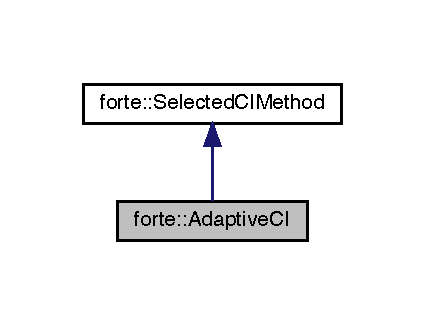
\includegraphics[width=204pt]{classforte_1_1_adaptive_c_i__inherit__graph}
\end{center}
\end{figure}


Collaboration diagram for forte\+:\+:Adaptive\+CI\+:
\nopagebreak
\begin{figure}[H]
\begin{center}
\leavevmode
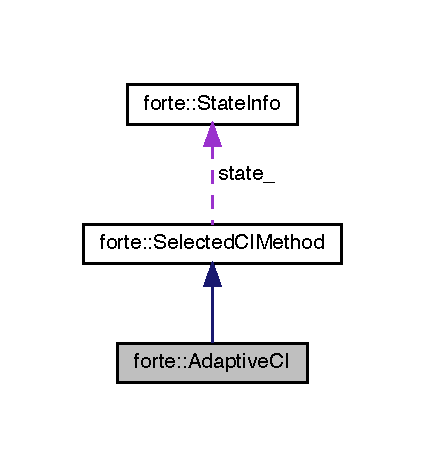
\includegraphics[width=204pt]{classforte_1_1_adaptive_c_i__coll__graph}
\end{center}
\end{figure}
\subsection*{Public Member Functions}
\begin{DoxyCompactItemize}
\item 
\mbox{\hyperlink{classforte_1_1_adaptive_c_i_ab283830208d19b0a7684a985cc81c629}{Adaptive\+CI}} (\mbox{\hyperlink{classforte_1_1_state_info}{State\+Info}} state, size\+\_\+t nroot, std\+::shared\+\_\+ptr$<$ \mbox{\hyperlink{classforte_1_1_s_c_f_info}{S\+C\+F\+Info}} $>$ scf\+\_\+info, std\+::shared\+\_\+ptr$<$ \mbox{\hyperlink{classforte_1_1_forte_options}{Forte\+Options}} $>$ options, std\+::shared\+\_\+ptr$<$ \mbox{\hyperlink{classforte_1_1_m_o_space_info}{M\+O\+Space\+Info}} $>$ mo\+\_\+space\+\_\+info, std\+::shared\+\_\+ptr$<$ \mbox{\hyperlink{classforte_1_1_active_space_integrals}{Active\+Space\+Integrals}} $>$ as\+\_\+ints)
\item 
void \mbox{\hyperlink{classforte_1_1_adaptive_c_i_a5f23c673c9c66b9b07de115a5992ae3f}{set\+\_\+options}} (std\+::shared\+\_\+ptr$<$ \mbox{\hyperlink{classforte_1_1_forte_options}{Forte\+Options}} $>$) override
\item 
void \mbox{\hyperlink{classforte_1_1_adaptive_c_i_a849ad578ee7ab5e78532a77df9b3ce9b}{print\+\_\+info}} () override
\begin{DoxyCompactList}\small\item\em Print the banner and starting information. \end{DoxyCompactList}\item 
void \mbox{\hyperlink{classforte_1_1_adaptive_c_i_afe7882564768985b90d3b3fd21c20a5f}{pre\+\_\+iter\+\_\+preparation}} () override
\begin{DoxyCompactList}\small\item\em Pre-\/iter preparation, usually includes preparing an initial reference. \end{DoxyCompactList}\item 
void \mbox{\hyperlink{classforte_1_1_adaptive_c_i_a3673ea1f26ce6b24e35def54b14fe62f}{diagonalize\+\_\+\+P\+\_\+space}} () override
\begin{DoxyCompactList}\small\item\em Step 1. Diagonalize the Hamiltonian in the P space. \end{DoxyCompactList}\item 
void \mbox{\hyperlink{classforte_1_1_adaptive_c_i_a84c2bbf2fd0dbcfe3732c0fb6a383bd8}{find\+\_\+q\+\_\+space}} () override
\begin{DoxyCompactList}\small\item\em Step 2. Find determinants in the Q space. \end{DoxyCompactList}\item 
void \mbox{\hyperlink{classforte_1_1_adaptive_c_i_a307427ce58102e4a818b2e97583e2ac1}{diagonalize\+\_\+\+P\+Q\+\_\+space}} () override
\begin{DoxyCompactList}\small\item\em Step 3. Diagonalize the Hamiltonian in the P + Q space. \end{DoxyCompactList}\item 
bool \mbox{\hyperlink{classforte_1_1_adaptive_c_i_a2682a80aa48f7cd49c295efb826f30ca}{check\+\_\+convergence}} () override
\begin{DoxyCompactList}\small\item\em Step 4. Check convergence. \end{DoxyCompactList}\item 
void \mbox{\hyperlink{classforte_1_1_adaptive_c_i_abb5fb23e0c3d2575b9a5c9785bdc9f75}{prune\+\_\+\+P\+Q\+\_\+to\+\_\+P}} () override
\begin{DoxyCompactList}\small\item\em Step 5. Prune the P + Q space to get an updated P space. \end{DoxyCompactList}\item 
void \mbox{\hyperlink{classforte_1_1_adaptive_c_i_aebb7aa6e06ce5b45c4c5b2da1b1703c1}{post\+\_\+iter\+\_\+process}} () override
\begin{DoxyCompactList}\small\item\em Post-\/iter process. \end{DoxyCompactList}\item 
void \mbox{\hyperlink{classforte_1_1_adaptive_c_i_a3cb865ccab03a377e0ac3a0d65cda9f5}{full\+\_\+mrpt2}} ()
\begin{DoxyCompactList}\small\item\em Full P\+T2 correction. \end{DoxyCompactList}\item 
void \mbox{\hyperlink{classforte_1_1_adaptive_c_i_a74874a321e8077f0af18967e9e2ebfd4}{set\+\_\+method\+\_\+variables}} (std\+::string ex\+\_\+alg, size\+\_\+t nroot\+\_\+method, size\+\_\+t root, const std\+::vector$<$ std\+::vector$<$ std\+::pair$<$ \mbox{\hyperlink{namespaceforte_a2076c63fd7b8732004d9e1442ce527c1}{Determinant}}, double $>$$>$$>$ \&old\+\_\+roots) override
\begin{DoxyCompactList}\small\item\em Set the class variable. \end{DoxyCompactList}\item 
\mbox{\hyperlink{classforte_1_1_determinant_hash_vec}{Determinant\+Hash\+Vec}} \mbox{\hyperlink{classforte_1_1_adaptive_c_i_af7e800fcfe0d1c2b674cf8cd2c4f41d0}{get\+\_\+\+P\+Q\+\_\+space}} () override
\begin{DoxyCompactList}\small\item\em Getters. \end{DoxyCompactList}\item 
psi\+::\+Shared\+Matrix \mbox{\hyperlink{classforte_1_1_adaptive_c_i_ab96222faf4f633fac906b24c7b68d288}{get\+\_\+\+P\+Q\+\_\+evecs}} () override
\item 
psi\+::\+Shared\+Vector \mbox{\hyperlink{classforte_1_1_adaptive_c_i_ada31e72d787a94730002e80f0f93deca}{get\+\_\+\+P\+Q\+\_\+evals}} () override
\item 
size\+\_\+t \mbox{\hyperlink{classforte_1_1_adaptive_c_i_a770022fec5ed4819e58670155e7fd5fc}{get\+\_\+ref\+\_\+root}} () override
\item 
std\+::vector$<$ double $>$ \mbox{\hyperlink{classforte_1_1_adaptive_c_i_a56cd790d0780b1af0136341663204e41}{get\+\_\+multistate\+\_\+pt2\+\_\+energy\+\_\+correction}} () override
\item 
void \mbox{\hyperlink{classforte_1_1_adaptive_c_i_ab0d3dddc9c0f86906150f2f2bfef4937}{set\+\_\+quiet}} (bool quiet)
\begin{DoxyCompactList}\small\item\em Set the printing level. \end{DoxyCompactList}\item 
void \mbox{\hyperlink{classforte_1_1_adaptive_c_i_ae0264299d3ab2f38c68026ef91a8a5b6}{print\+\_\+nos}} ()
\begin{DoxyCompactList}\small\item\em Compute the A\+C\+I-\/\+N\+Os. \end{DoxyCompactList}\item 
void \mbox{\hyperlink{classforte_1_1_adaptive_c_i_ade019bc7c61b1817f68127cc0013066d}{semi\+\_\+canonicalize}} ()
\item 
void \mbox{\hyperlink{classforte_1_1_adaptive_c_i_a85d46f659801c5b3f9b558c265c90fa7}{set\+\_\+fci\+\_\+ints}} (std\+::shared\+\_\+ptr$<$ \mbox{\hyperlink{classforte_1_1_active_space_integrals}{Active\+Space\+Integrals}} $>$ fci\+\_\+ints)
\item 
void \mbox{\hyperlink{classforte_1_1_adaptive_c_i_ae4d307b8c98ae205056da0ab40585317}{upcast\+\_\+reference}} (\mbox{\hyperlink{classforte_1_1_determinant_hash_vec}{Determinant\+Hash\+Vec}} \&ref)
\item 
void \mbox{\hyperlink{classforte_1_1_adaptive_c_i_aa41514cfd2b49b8978196fc6991f6e3a}{update\+\_\+sigma}} ()
\end{DoxyCompactItemize}
\subsection*{Additional Inherited Members}


\subsection{Detailed Description}
The \mbox{\hyperlink{classforte_1_1_adaptive_c_i}{Adaptive\+CI}} class This class implements an adaptive CI algorithm. 

\subsection{Constructor \& Destructor Documentation}
\mbox{\Hypertarget{classforte_1_1_adaptive_c_i_ab283830208d19b0a7684a985cc81c629}\label{classforte_1_1_adaptive_c_i_ab283830208d19b0a7684a985cc81c629}} 
\index{forte\+::\+Adaptive\+CI@{forte\+::\+Adaptive\+CI}!Adaptive\+CI@{Adaptive\+CI}}
\index{Adaptive\+CI@{Adaptive\+CI}!forte\+::\+Adaptive\+CI@{forte\+::\+Adaptive\+CI}}
\subsubsection{\texorpdfstring{Adaptive\+C\+I()}{AdaptiveCI()}}
{\footnotesize\ttfamily forte\+::\+Adaptive\+C\+I\+::\+Adaptive\+CI (\begin{DoxyParamCaption}\item[{\mbox{\hyperlink{classforte_1_1_state_info}{State\+Info}}}]{state,  }\item[{size\+\_\+t}]{nroot,  }\item[{std\+::shared\+\_\+ptr$<$ \mbox{\hyperlink{classforte_1_1_s_c_f_info}{S\+C\+F\+Info}} $>$}]{scf\+\_\+info,  }\item[{std\+::shared\+\_\+ptr$<$ \mbox{\hyperlink{classforte_1_1_forte_options}{Forte\+Options}} $>$}]{options,  }\item[{std\+::shared\+\_\+ptr$<$ \mbox{\hyperlink{classforte_1_1_m_o_space_info}{M\+O\+Space\+Info}} $>$}]{mo\+\_\+space\+\_\+info,  }\item[{std\+::shared\+\_\+ptr$<$ \mbox{\hyperlink{classforte_1_1_active_space_integrals}{Active\+Space\+Integrals}} $>$}]{as\+\_\+ints }\end{DoxyParamCaption})}

Constructor 
\begin{DoxyParams}{Parameters}
{\em ref\+\_\+wfn} & The reference wavefunction object \\
\hline
{\em options} & The main options object \\
\hline
{\em ints} & A pointer to an allocated integral object \\
\hline
{\em mo\+\_\+space\+\_\+info} & A pointer to the \mbox{\hyperlink{classforte_1_1_m_o_space_info}{M\+O\+Space\+Info}} object \\
\hline
\end{DoxyParams}


\subsection{Member Function Documentation}
\mbox{\Hypertarget{classforte_1_1_adaptive_c_i_a2682a80aa48f7cd49c295efb826f30ca}\label{classforte_1_1_adaptive_c_i_a2682a80aa48f7cd49c295efb826f30ca}} 
\index{forte\+::\+Adaptive\+CI@{forte\+::\+Adaptive\+CI}!check\+\_\+convergence@{check\+\_\+convergence}}
\index{check\+\_\+convergence@{check\+\_\+convergence}!forte\+::\+Adaptive\+CI@{forte\+::\+Adaptive\+CI}}
\subsubsection{\texorpdfstring{check\+\_\+convergence()}{check\_convergence()}}
{\footnotesize\ttfamily bool forte\+::\+Adaptive\+C\+I\+::check\+\_\+convergence (\begin{DoxyParamCaption}{ }\end{DoxyParamCaption})\hspace{0.3cm}{\ttfamily [override]}, {\ttfamily [virtual]}}



Step 4. Check convergence. 



Implements \mbox{\hyperlink{classforte_1_1_selected_c_i_method_acc10aa488c79c2abec46a9093ecf5a52}{forte\+::\+Selected\+C\+I\+Method}}.

\mbox{\Hypertarget{classforte_1_1_adaptive_c_i_a3673ea1f26ce6b24e35def54b14fe62f}\label{classforte_1_1_adaptive_c_i_a3673ea1f26ce6b24e35def54b14fe62f}} 
\index{forte\+::\+Adaptive\+CI@{forte\+::\+Adaptive\+CI}!diagonalize\+\_\+\+P\+\_\+space@{diagonalize\+\_\+\+P\+\_\+space}}
\index{diagonalize\+\_\+\+P\+\_\+space@{diagonalize\+\_\+\+P\+\_\+space}!forte\+::\+Adaptive\+CI@{forte\+::\+Adaptive\+CI}}
\subsubsection{\texorpdfstring{diagonalize\+\_\+\+P\+\_\+space()}{diagonalize\_P\_space()}}
{\footnotesize\ttfamily void forte\+::\+Adaptive\+C\+I\+::diagonalize\+\_\+\+P\+\_\+space (\begin{DoxyParamCaption}{ }\end{DoxyParamCaption})\hspace{0.3cm}{\ttfamily [override]}, {\ttfamily [virtual]}}



Step 1. Diagonalize the Hamiltonian in the P space. 



Implements \mbox{\hyperlink{classforte_1_1_selected_c_i_method_a7b2b41da889659f03361f625c6df44d2}{forte\+::\+Selected\+C\+I\+Method}}.

\mbox{\Hypertarget{classforte_1_1_adaptive_c_i_a307427ce58102e4a818b2e97583e2ac1}\label{classforte_1_1_adaptive_c_i_a307427ce58102e4a818b2e97583e2ac1}} 
\index{forte\+::\+Adaptive\+CI@{forte\+::\+Adaptive\+CI}!diagonalize\+\_\+\+P\+Q\+\_\+space@{diagonalize\+\_\+\+P\+Q\+\_\+space}}
\index{diagonalize\+\_\+\+P\+Q\+\_\+space@{diagonalize\+\_\+\+P\+Q\+\_\+space}!forte\+::\+Adaptive\+CI@{forte\+::\+Adaptive\+CI}}
\subsubsection{\texorpdfstring{diagonalize\+\_\+\+P\+Q\+\_\+space()}{diagonalize\_PQ\_space()}}
{\footnotesize\ttfamily void forte\+::\+Adaptive\+C\+I\+::diagonalize\+\_\+\+P\+Q\+\_\+space (\begin{DoxyParamCaption}{ }\end{DoxyParamCaption})\hspace{0.3cm}{\ttfamily [override]}, {\ttfamily [virtual]}}



Step 3. Diagonalize the Hamiltonian in the P + Q space. 



Implements \mbox{\hyperlink{classforte_1_1_selected_c_i_method_a9f01588d22401cd2631a09940ea7db50}{forte\+::\+Selected\+C\+I\+Method}}.

\mbox{\Hypertarget{classforte_1_1_adaptive_c_i_a84c2bbf2fd0dbcfe3732c0fb6a383bd8}\label{classforte_1_1_adaptive_c_i_a84c2bbf2fd0dbcfe3732c0fb6a383bd8}} 
\index{forte\+::\+Adaptive\+CI@{forte\+::\+Adaptive\+CI}!find\+\_\+q\+\_\+space@{find\+\_\+q\+\_\+space}}
\index{find\+\_\+q\+\_\+space@{find\+\_\+q\+\_\+space}!forte\+::\+Adaptive\+CI@{forte\+::\+Adaptive\+CI}}
\subsubsection{\texorpdfstring{find\+\_\+q\+\_\+space()}{find\_q\_space()}}
{\footnotesize\ttfamily void forte\+::\+Adaptive\+C\+I\+::find\+\_\+q\+\_\+space (\begin{DoxyParamCaption}{ }\end{DoxyParamCaption})\hspace{0.3cm}{\ttfamily [override]}, {\ttfamily [virtual]}}



Step 2. Find determinants in the Q space. 



Implements \mbox{\hyperlink{classforte_1_1_selected_c_i_method_aff521efa08edfafb479f32e03a70c118}{forte\+::\+Selected\+C\+I\+Method}}.

\mbox{\Hypertarget{classforte_1_1_adaptive_c_i_a3cb865ccab03a377e0ac3a0d65cda9f5}\label{classforte_1_1_adaptive_c_i_a3cb865ccab03a377e0ac3a0d65cda9f5}} 
\index{forte\+::\+Adaptive\+CI@{forte\+::\+Adaptive\+CI}!full\+\_\+mrpt2@{full\+\_\+mrpt2}}
\index{full\+\_\+mrpt2@{full\+\_\+mrpt2}!forte\+::\+Adaptive\+CI@{forte\+::\+Adaptive\+CI}}
\subsubsection{\texorpdfstring{full\+\_\+mrpt2()}{full\_mrpt2()}}
{\footnotesize\ttfamily void forte\+::\+Adaptive\+C\+I\+::full\+\_\+mrpt2 (\begin{DoxyParamCaption}{ }\end{DoxyParamCaption})}



Full P\+T2 correction. 

\mbox{\Hypertarget{classforte_1_1_adaptive_c_i_a56cd790d0780b1af0136341663204e41}\label{classforte_1_1_adaptive_c_i_a56cd790d0780b1af0136341663204e41}} 
\index{forte\+::\+Adaptive\+CI@{forte\+::\+Adaptive\+CI}!get\+\_\+multistate\+\_\+pt2\+\_\+energy\+\_\+correction@{get\+\_\+multistate\+\_\+pt2\+\_\+energy\+\_\+correction}}
\index{get\+\_\+multistate\+\_\+pt2\+\_\+energy\+\_\+correction@{get\+\_\+multistate\+\_\+pt2\+\_\+energy\+\_\+correction}!forte\+::\+Adaptive\+CI@{forte\+::\+Adaptive\+CI}}
\subsubsection{\texorpdfstring{get\+\_\+multistate\+\_\+pt2\+\_\+energy\+\_\+correction()}{get\_multistate\_pt2\_energy\_correction()}}
{\footnotesize\ttfamily std\+::vector$<$ double $>$ forte\+::\+Adaptive\+C\+I\+::get\+\_\+multistate\+\_\+pt2\+\_\+energy\+\_\+correction (\begin{DoxyParamCaption}{ }\end{DoxyParamCaption})\hspace{0.3cm}{\ttfamily [override]}, {\ttfamily [virtual]}}



Implements \mbox{\hyperlink{classforte_1_1_selected_c_i_method_abbe18ea3e5f1a77df13a38764aeef62c}{forte\+::\+Selected\+C\+I\+Method}}.

\mbox{\Hypertarget{classforte_1_1_adaptive_c_i_ada31e72d787a94730002e80f0f93deca}\label{classforte_1_1_adaptive_c_i_ada31e72d787a94730002e80f0f93deca}} 
\index{forte\+::\+Adaptive\+CI@{forte\+::\+Adaptive\+CI}!get\+\_\+\+P\+Q\+\_\+evals@{get\+\_\+\+P\+Q\+\_\+evals}}
\index{get\+\_\+\+P\+Q\+\_\+evals@{get\+\_\+\+P\+Q\+\_\+evals}!forte\+::\+Adaptive\+CI@{forte\+::\+Adaptive\+CI}}
\subsubsection{\texorpdfstring{get\+\_\+\+P\+Q\+\_\+evals()}{get\_PQ\_evals()}}
{\footnotesize\ttfamily psi\+::\+Shared\+Vector forte\+::\+Adaptive\+C\+I\+::get\+\_\+\+P\+Q\+\_\+evals (\begin{DoxyParamCaption}{ }\end{DoxyParamCaption})\hspace{0.3cm}{\ttfamily [override]}, {\ttfamily [virtual]}}



Implements \mbox{\hyperlink{classforte_1_1_selected_c_i_method_a675d28ae66341b8cfabb2953c936621c}{forte\+::\+Selected\+C\+I\+Method}}.

\mbox{\Hypertarget{classforte_1_1_adaptive_c_i_ab96222faf4f633fac906b24c7b68d288}\label{classforte_1_1_adaptive_c_i_ab96222faf4f633fac906b24c7b68d288}} 
\index{forte\+::\+Adaptive\+CI@{forte\+::\+Adaptive\+CI}!get\+\_\+\+P\+Q\+\_\+evecs@{get\+\_\+\+P\+Q\+\_\+evecs}}
\index{get\+\_\+\+P\+Q\+\_\+evecs@{get\+\_\+\+P\+Q\+\_\+evecs}!forte\+::\+Adaptive\+CI@{forte\+::\+Adaptive\+CI}}
\subsubsection{\texorpdfstring{get\+\_\+\+P\+Q\+\_\+evecs()}{get\_PQ\_evecs()}}
{\footnotesize\ttfamily psi\+::\+Shared\+Matrix forte\+::\+Adaptive\+C\+I\+::get\+\_\+\+P\+Q\+\_\+evecs (\begin{DoxyParamCaption}{ }\end{DoxyParamCaption})\hspace{0.3cm}{\ttfamily [override]}, {\ttfamily [virtual]}}



Implements \mbox{\hyperlink{classforte_1_1_selected_c_i_method_a5e5212836aa0dc35f98238d1f426abed}{forte\+::\+Selected\+C\+I\+Method}}.

\mbox{\Hypertarget{classforte_1_1_adaptive_c_i_af7e800fcfe0d1c2b674cf8cd2c4f41d0}\label{classforte_1_1_adaptive_c_i_af7e800fcfe0d1c2b674cf8cd2c4f41d0}} 
\index{forte\+::\+Adaptive\+CI@{forte\+::\+Adaptive\+CI}!get\+\_\+\+P\+Q\+\_\+space@{get\+\_\+\+P\+Q\+\_\+space}}
\index{get\+\_\+\+P\+Q\+\_\+space@{get\+\_\+\+P\+Q\+\_\+space}!forte\+::\+Adaptive\+CI@{forte\+::\+Adaptive\+CI}}
\subsubsection{\texorpdfstring{get\+\_\+\+P\+Q\+\_\+space()}{get\_PQ\_space()}}
{\footnotesize\ttfamily \mbox{\hyperlink{classforte_1_1_determinant_hash_vec}{Determinant\+Hash\+Vec}} forte\+::\+Adaptive\+C\+I\+::get\+\_\+\+P\+Q\+\_\+space (\begin{DoxyParamCaption}{ }\end{DoxyParamCaption})\hspace{0.3cm}{\ttfamily [override]}, {\ttfamily [virtual]}}



Getters. 



Implements \mbox{\hyperlink{classforte_1_1_selected_c_i_method_a2c29d8700d6887860850f77b9246ec9f}{forte\+::\+Selected\+C\+I\+Method}}.

\mbox{\Hypertarget{classforte_1_1_adaptive_c_i_a770022fec5ed4819e58670155e7fd5fc}\label{classforte_1_1_adaptive_c_i_a770022fec5ed4819e58670155e7fd5fc}} 
\index{forte\+::\+Adaptive\+CI@{forte\+::\+Adaptive\+CI}!get\+\_\+ref\+\_\+root@{get\+\_\+ref\+\_\+root}}
\index{get\+\_\+ref\+\_\+root@{get\+\_\+ref\+\_\+root}!forte\+::\+Adaptive\+CI@{forte\+::\+Adaptive\+CI}}
\subsubsection{\texorpdfstring{get\+\_\+ref\+\_\+root()}{get\_ref\_root()}}
{\footnotesize\ttfamily size\+\_\+t forte\+::\+Adaptive\+C\+I\+::get\+\_\+ref\+\_\+root (\begin{DoxyParamCaption}{ }\end{DoxyParamCaption})\hspace{0.3cm}{\ttfamily [override]}, {\ttfamily [virtual]}}



Implements \mbox{\hyperlink{classforte_1_1_selected_c_i_method_aa95ed581568b2d580c17ab166e85a11a}{forte\+::\+Selected\+C\+I\+Method}}.

\mbox{\Hypertarget{classforte_1_1_adaptive_c_i_aebb7aa6e06ce5b45c4c5b2da1b1703c1}\label{classforte_1_1_adaptive_c_i_aebb7aa6e06ce5b45c4c5b2da1b1703c1}} 
\index{forte\+::\+Adaptive\+CI@{forte\+::\+Adaptive\+CI}!post\+\_\+iter\+\_\+process@{post\+\_\+iter\+\_\+process}}
\index{post\+\_\+iter\+\_\+process@{post\+\_\+iter\+\_\+process}!forte\+::\+Adaptive\+CI@{forte\+::\+Adaptive\+CI}}
\subsubsection{\texorpdfstring{post\+\_\+iter\+\_\+process()}{post\_iter\_process()}}
{\footnotesize\ttfamily void forte\+::\+Adaptive\+C\+I\+::post\+\_\+iter\+\_\+process (\begin{DoxyParamCaption}{ }\end{DoxyParamCaption})\hspace{0.3cm}{\ttfamily [override]}, {\ttfamily [virtual]}}



Post-\/iter process. 



Implements \mbox{\hyperlink{classforte_1_1_selected_c_i_method_a23ea3389ac1c62dee811decc5bea507f}{forte\+::\+Selected\+C\+I\+Method}}.

\mbox{\Hypertarget{classforte_1_1_adaptive_c_i_afe7882564768985b90d3b3fd21c20a5f}\label{classforte_1_1_adaptive_c_i_afe7882564768985b90d3b3fd21c20a5f}} 
\index{forte\+::\+Adaptive\+CI@{forte\+::\+Adaptive\+CI}!pre\+\_\+iter\+\_\+preparation@{pre\+\_\+iter\+\_\+preparation}}
\index{pre\+\_\+iter\+\_\+preparation@{pre\+\_\+iter\+\_\+preparation}!forte\+::\+Adaptive\+CI@{forte\+::\+Adaptive\+CI}}
\subsubsection{\texorpdfstring{pre\+\_\+iter\+\_\+preparation()}{pre\_iter\_preparation()}}
{\footnotesize\ttfamily void forte\+::\+Adaptive\+C\+I\+::pre\+\_\+iter\+\_\+preparation (\begin{DoxyParamCaption}{ }\end{DoxyParamCaption})\hspace{0.3cm}{\ttfamily [override]}, {\ttfamily [virtual]}}



Pre-\/iter preparation, usually includes preparing an initial reference. 



Implements \mbox{\hyperlink{classforte_1_1_selected_c_i_method_af92b210415034874fcf2faac8b00eca9}{forte\+::\+Selected\+C\+I\+Method}}.

\mbox{\Hypertarget{classforte_1_1_adaptive_c_i_a849ad578ee7ab5e78532a77df9b3ce9b}\label{classforte_1_1_adaptive_c_i_a849ad578ee7ab5e78532a77df9b3ce9b}} 
\index{forte\+::\+Adaptive\+CI@{forte\+::\+Adaptive\+CI}!print\+\_\+info@{print\+\_\+info}}
\index{print\+\_\+info@{print\+\_\+info}!forte\+::\+Adaptive\+CI@{forte\+::\+Adaptive\+CI}}
\subsubsection{\texorpdfstring{print\+\_\+info()}{print\_info()}}
{\footnotesize\ttfamily void forte\+::\+Adaptive\+C\+I\+::print\+\_\+info (\begin{DoxyParamCaption}{ }\end{DoxyParamCaption})\hspace{0.3cm}{\ttfamily [override]}, {\ttfamily [virtual]}}



Print the banner and starting information. 



Implements \mbox{\hyperlink{classforte_1_1_selected_c_i_method_a95680d60059b29c763b5f87f9add48e2}{forte\+::\+Selected\+C\+I\+Method}}.

\mbox{\Hypertarget{classforte_1_1_adaptive_c_i_ae0264299d3ab2f38c68026ef91a8a5b6}\label{classforte_1_1_adaptive_c_i_ae0264299d3ab2f38c68026ef91a8a5b6}} 
\index{forte\+::\+Adaptive\+CI@{forte\+::\+Adaptive\+CI}!print\+\_\+nos@{print\+\_\+nos}}
\index{print\+\_\+nos@{print\+\_\+nos}!forte\+::\+Adaptive\+CI@{forte\+::\+Adaptive\+CI}}
\subsubsection{\texorpdfstring{print\+\_\+nos()}{print\_nos()}}
{\footnotesize\ttfamily void forte\+::\+Adaptive\+C\+I\+::print\+\_\+nos (\begin{DoxyParamCaption}{ }\end{DoxyParamCaption})}



Compute the A\+C\+I-\/\+N\+Os. 

\mbox{\Hypertarget{classforte_1_1_adaptive_c_i_abb5fb23e0c3d2575b9a5c9785bdc9f75}\label{classforte_1_1_adaptive_c_i_abb5fb23e0c3d2575b9a5c9785bdc9f75}} 
\index{forte\+::\+Adaptive\+CI@{forte\+::\+Adaptive\+CI}!prune\+\_\+\+P\+Q\+\_\+to\+\_\+P@{prune\+\_\+\+P\+Q\+\_\+to\+\_\+P}}
\index{prune\+\_\+\+P\+Q\+\_\+to\+\_\+P@{prune\+\_\+\+P\+Q\+\_\+to\+\_\+P}!forte\+::\+Adaptive\+CI@{forte\+::\+Adaptive\+CI}}
\subsubsection{\texorpdfstring{prune\+\_\+\+P\+Q\+\_\+to\+\_\+\+P()}{prune\_PQ\_to\_P()}}
{\footnotesize\ttfamily void forte\+::\+Adaptive\+C\+I\+::prune\+\_\+\+P\+Q\+\_\+to\+\_\+P (\begin{DoxyParamCaption}{ }\end{DoxyParamCaption})\hspace{0.3cm}{\ttfamily [override]}, {\ttfamily [virtual]}}



Step 5. Prune the P + Q space to get an updated P space. 



Implements \mbox{\hyperlink{classforte_1_1_selected_c_i_method_a245f5fcd64ee44acf7b065981380f8dd}{forte\+::\+Selected\+C\+I\+Method}}.

\mbox{\Hypertarget{classforte_1_1_adaptive_c_i_ade019bc7c61b1817f68127cc0013066d}\label{classforte_1_1_adaptive_c_i_ade019bc7c61b1817f68127cc0013066d}} 
\index{forte\+::\+Adaptive\+CI@{forte\+::\+Adaptive\+CI}!semi\+\_\+canonicalize@{semi\+\_\+canonicalize}}
\index{semi\+\_\+canonicalize@{semi\+\_\+canonicalize}!forte\+::\+Adaptive\+CI@{forte\+::\+Adaptive\+CI}}
\subsubsection{\texorpdfstring{semi\+\_\+canonicalize()}{semi\_canonicalize()}}
{\footnotesize\ttfamily void forte\+::\+Adaptive\+C\+I\+::semi\+\_\+canonicalize (\begin{DoxyParamCaption}{ }\end{DoxyParamCaption})}

\mbox{\Hypertarget{classforte_1_1_adaptive_c_i_a85d46f659801c5b3f9b558c265c90fa7}\label{classforte_1_1_adaptive_c_i_a85d46f659801c5b3f9b558c265c90fa7}} 
\index{forte\+::\+Adaptive\+CI@{forte\+::\+Adaptive\+CI}!set\+\_\+fci\+\_\+ints@{set\+\_\+fci\+\_\+ints}}
\index{set\+\_\+fci\+\_\+ints@{set\+\_\+fci\+\_\+ints}!forte\+::\+Adaptive\+CI@{forte\+::\+Adaptive\+CI}}
\subsubsection{\texorpdfstring{set\+\_\+fci\+\_\+ints()}{set\_fci\_ints()}}
{\footnotesize\ttfamily void forte\+::\+Adaptive\+C\+I\+::set\+\_\+fci\+\_\+ints (\begin{DoxyParamCaption}\item[{std\+::shared\+\_\+ptr$<$ \mbox{\hyperlink{classforte_1_1_active_space_integrals}{Active\+Space\+Integrals}} $>$}]{fci\+\_\+ints }\end{DoxyParamCaption})}

\mbox{\Hypertarget{classforte_1_1_adaptive_c_i_a74874a321e8077f0af18967e9e2ebfd4}\label{classforte_1_1_adaptive_c_i_a74874a321e8077f0af18967e9e2ebfd4}} 
\index{forte\+::\+Adaptive\+CI@{forte\+::\+Adaptive\+CI}!set\+\_\+method\+\_\+variables@{set\+\_\+method\+\_\+variables}}
\index{set\+\_\+method\+\_\+variables@{set\+\_\+method\+\_\+variables}!forte\+::\+Adaptive\+CI@{forte\+::\+Adaptive\+CI}}
\subsubsection{\texorpdfstring{set\+\_\+method\+\_\+variables()}{set\_method\_variables()}}
{\footnotesize\ttfamily void forte\+::\+Adaptive\+C\+I\+::set\+\_\+method\+\_\+variables (\begin{DoxyParamCaption}\item[{std\+::string}]{ex\+\_\+alg,  }\item[{size\+\_\+t}]{nroot\+\_\+method,  }\item[{size\+\_\+t}]{root,  }\item[{const std\+::vector$<$ std\+::vector$<$ std\+::pair$<$ \mbox{\hyperlink{namespaceforte_a2076c63fd7b8732004d9e1442ce527c1}{Determinant}}, double $>$$>$$>$ \&}]{old\+\_\+roots }\end{DoxyParamCaption})\hspace{0.3cm}{\ttfamily [override]}, {\ttfamily [virtual]}}



Set the class variable. 



Implements \mbox{\hyperlink{classforte_1_1_selected_c_i_method_a37f95503d0241387195dc7d412fc6e78}{forte\+::\+Selected\+C\+I\+Method}}.

\mbox{\Hypertarget{classforte_1_1_adaptive_c_i_a5f23c673c9c66b9b07de115a5992ae3f}\label{classforte_1_1_adaptive_c_i_a5f23c673c9c66b9b07de115a5992ae3f}} 
\index{forte\+::\+Adaptive\+CI@{forte\+::\+Adaptive\+CI}!set\+\_\+options@{set\+\_\+options}}
\index{set\+\_\+options@{set\+\_\+options}!forte\+::\+Adaptive\+CI@{forte\+::\+Adaptive\+CI}}
\subsubsection{\texorpdfstring{set\+\_\+options()}{set\_options()}}
{\footnotesize\ttfamily void forte\+::\+Adaptive\+C\+I\+::set\+\_\+options (\begin{DoxyParamCaption}\item[{std\+::shared\+\_\+ptr$<$ \mbox{\hyperlink{classforte_1_1_forte_options}{Forte\+Options}} $>$}]{ }\end{DoxyParamCaption})\hspace{0.3cm}{\ttfamily [inline]}, {\ttfamily [override]}, {\ttfamily [virtual]}}

Set options from an option object 
\begin{DoxyParams}{Parameters}
{\em options} & the options passed in \\
\hline
\end{DoxyParams}


Implements \mbox{\hyperlink{classforte_1_1_selected_c_i_method_ad03bbde3a0443ca9b01ff9605f2e06e0}{forte\+::\+Selected\+C\+I\+Method}}.

\mbox{\Hypertarget{classforte_1_1_adaptive_c_i_ab0d3dddc9c0f86906150f2f2bfef4937}\label{classforte_1_1_adaptive_c_i_ab0d3dddc9c0f86906150f2f2bfef4937}} 
\index{forte\+::\+Adaptive\+CI@{forte\+::\+Adaptive\+CI}!set\+\_\+quiet@{set\+\_\+quiet}}
\index{set\+\_\+quiet@{set\+\_\+quiet}!forte\+::\+Adaptive\+CI@{forte\+::\+Adaptive\+CI}}
\subsubsection{\texorpdfstring{set\+\_\+quiet()}{set\_quiet()}}
{\footnotesize\ttfamily void forte\+::\+Adaptive\+C\+I\+::set\+\_\+quiet (\begin{DoxyParamCaption}\item[{bool}]{quiet }\end{DoxyParamCaption})\hspace{0.3cm}{\ttfamily [inline]}}



Set the printing level. 

\mbox{\Hypertarget{classforte_1_1_adaptive_c_i_ae4d307b8c98ae205056da0ab40585317}\label{classforte_1_1_adaptive_c_i_ae4d307b8c98ae205056da0ab40585317}} 
\index{forte\+::\+Adaptive\+CI@{forte\+::\+Adaptive\+CI}!upcast\+\_\+reference@{upcast\+\_\+reference}}
\index{upcast\+\_\+reference@{upcast\+\_\+reference}!forte\+::\+Adaptive\+CI@{forte\+::\+Adaptive\+CI}}
\subsubsection{\texorpdfstring{upcast\+\_\+reference()}{upcast\_reference()}}
{\footnotesize\ttfamily void forte\+::\+Adaptive\+C\+I\+::upcast\+\_\+reference (\begin{DoxyParamCaption}\item[{\mbox{\hyperlink{classforte_1_1_determinant_hash_vec}{Determinant\+Hash\+Vec}} \&}]{ref }\end{DoxyParamCaption})}

\mbox{\Hypertarget{classforte_1_1_adaptive_c_i_aa41514cfd2b49b8978196fc6991f6e3a}\label{classforte_1_1_adaptive_c_i_aa41514cfd2b49b8978196fc6991f6e3a}} 
\index{forte\+::\+Adaptive\+CI@{forte\+::\+Adaptive\+CI}!update\+\_\+sigma@{update\+\_\+sigma}}
\index{update\+\_\+sigma@{update\+\_\+sigma}!forte\+::\+Adaptive\+CI@{forte\+::\+Adaptive\+CI}}
\subsubsection{\texorpdfstring{update\+\_\+sigma()}{update\_sigma()}}
{\footnotesize\ttfamily void forte\+::\+Adaptive\+C\+I\+::update\+\_\+sigma (\begin{DoxyParamCaption}{ }\end{DoxyParamCaption})}



The documentation for this class was generated from the following files\+:\begin{DoxyCompactItemize}
\item 
/\+Users/fevange/\+Source/forte/src/sci/\mbox{\hyperlink{aci_8h}{aci.\+h}}\item 
/\+Users/fevange/\+Source/forte/src/sci/\mbox{\hyperlink{aci_8cc}{aci.\+cc}}\item 
/\+Users/fevange/\+Source/forte/src/sci/\mbox{\hyperlink{aci__build___f_8cc}{aci\+\_\+build\+\_\+\+F.\+cc}}\item 
/\+Users/fevange/\+Source/forte/src/sci/\mbox{\hyperlink{gasaci__build___f_8cc}{gasaci\+\_\+build\+\_\+\+F.\+cc}}\end{DoxyCompactItemize}

\hypertarget{classforte_1_1_a_o_info}{}\section{forte\+:\+:A\+O\+Info Class Reference}
\label{classforte_1_1_a_o_info}\index{forte\+::\+A\+O\+Info@{forte\+::\+A\+O\+Info}}


The \mbox{\hyperlink{classforte_1_1_a_o_info}{A\+O\+Info}} class.  




{\ttfamily \#include $<$aosubspace.\+h$>$}

\subsection*{Public Member Functions}
\begin{DoxyCompactItemize}
\item 
\mbox{\hyperlink{classforte_1_1_a_o_info_a74a368c1fa1b7cd773d3b6a040d0b57f}{A\+O\+Info}} (int \mbox{\hyperlink{classforte_1_1_a_o_info_aacbf6d9bbd3bc19b7f96a486e35f8996}{A}}, int \mbox{\hyperlink{classforte_1_1_a_o_info_ac71668d14738a2054f33d8da68fbf0bc}{Z}}, int \mbox{\hyperlink{classforte_1_1_a_o_info_aa597ea8252cbfac7e302417eaa3f9b37}{element\+\_\+count}}, int \mbox{\hyperlink{classforte_1_1_a_o_info_a71492e38fe610c5535809789eceea740}{n}}, int \mbox{\hyperlink{classforte_1_1_a_o_info_a51797dafa01c915f57b0c910d7e29d23}{l}}, int \mbox{\hyperlink{classforte_1_1_a_o_info_a4c08f15cd83b5d3cb1735144d3f822c8}{m}})
\item 
int \mbox{\hyperlink{classforte_1_1_a_o_info_aacbf6d9bbd3bc19b7f96a486e35f8996}{A}} () const
\item 
int \mbox{\hyperlink{classforte_1_1_a_o_info_ac71668d14738a2054f33d8da68fbf0bc}{Z}} () const
\item 
int \mbox{\hyperlink{classforte_1_1_a_o_info_aa597ea8252cbfac7e302417eaa3f9b37}{element\+\_\+count}} () const
\item 
int \mbox{\hyperlink{classforte_1_1_a_o_info_a71492e38fe610c5535809789eceea740}{n}} () const
\item 
int \mbox{\hyperlink{classforte_1_1_a_o_info_a51797dafa01c915f57b0c910d7e29d23}{l}} () const
\item 
int \mbox{\hyperlink{classforte_1_1_a_o_info_a4c08f15cd83b5d3cb1735144d3f822c8}{m}} () const
\end{DoxyCompactItemize}


\subsection{Detailed Description}
The \mbox{\hyperlink{classforte_1_1_a_o_info}{A\+O\+Info}} class. 

A class to store information about an atomic orbital 

\subsection{Constructor \& Destructor Documentation}
\mbox{\Hypertarget{classforte_1_1_a_o_info_a74a368c1fa1b7cd773d3b6a040d0b57f}\label{classforte_1_1_a_o_info_a74a368c1fa1b7cd773d3b6a040d0b57f}} 
\index{forte\+::\+A\+O\+Info@{forte\+::\+A\+O\+Info}!A\+O\+Info@{A\+O\+Info}}
\index{A\+O\+Info@{A\+O\+Info}!forte\+::\+A\+O\+Info@{forte\+::\+A\+O\+Info}}
\subsubsection{\texorpdfstring{A\+O\+Info()}{AOInfo()}}
{\footnotesize\ttfamily forte\+::\+A\+O\+Info\+::\+A\+O\+Info (\begin{DoxyParamCaption}\item[{int}]{A,  }\item[{int}]{Z,  }\item[{int}]{element\+\_\+count,  }\item[{int}]{n,  }\item[{int}]{l,  }\item[{int}]{m }\end{DoxyParamCaption})\hspace{0.3cm}{\ttfamily [inline]}}



\subsection{Member Function Documentation}
\mbox{\Hypertarget{classforte_1_1_a_o_info_aacbf6d9bbd3bc19b7f96a486e35f8996}\label{classforte_1_1_a_o_info_aacbf6d9bbd3bc19b7f96a486e35f8996}} 
\index{forte\+::\+A\+O\+Info@{forte\+::\+A\+O\+Info}!A@{A}}
\index{A@{A}!forte\+::\+A\+O\+Info@{forte\+::\+A\+O\+Info}}
\subsubsection{\texorpdfstring{A()}{A()}}
{\footnotesize\ttfamily int forte\+::\+A\+O\+Info\+::A (\begin{DoxyParamCaption}{ }\end{DoxyParamCaption}) const\hspace{0.3cm}{\ttfamily [inline]}}

\mbox{\Hypertarget{classforte_1_1_a_o_info_aa597ea8252cbfac7e302417eaa3f9b37}\label{classforte_1_1_a_o_info_aa597ea8252cbfac7e302417eaa3f9b37}} 
\index{forte\+::\+A\+O\+Info@{forte\+::\+A\+O\+Info}!element\+\_\+count@{element\+\_\+count}}
\index{element\+\_\+count@{element\+\_\+count}!forte\+::\+A\+O\+Info@{forte\+::\+A\+O\+Info}}
\subsubsection{\texorpdfstring{element\+\_\+count()}{element\_count()}}
{\footnotesize\ttfamily int forte\+::\+A\+O\+Info\+::element\+\_\+count (\begin{DoxyParamCaption}{ }\end{DoxyParamCaption}) const\hspace{0.3cm}{\ttfamily [inline]}}

\mbox{\Hypertarget{classforte_1_1_a_o_info_a51797dafa01c915f57b0c910d7e29d23}\label{classforte_1_1_a_o_info_a51797dafa01c915f57b0c910d7e29d23}} 
\index{forte\+::\+A\+O\+Info@{forte\+::\+A\+O\+Info}!l@{l}}
\index{l@{l}!forte\+::\+A\+O\+Info@{forte\+::\+A\+O\+Info}}
\subsubsection{\texorpdfstring{l()}{l()}}
{\footnotesize\ttfamily int forte\+::\+A\+O\+Info\+::l (\begin{DoxyParamCaption}{ }\end{DoxyParamCaption}) const\hspace{0.3cm}{\ttfamily [inline]}}

\mbox{\Hypertarget{classforte_1_1_a_o_info_a4c08f15cd83b5d3cb1735144d3f822c8}\label{classforte_1_1_a_o_info_a4c08f15cd83b5d3cb1735144d3f822c8}} 
\index{forte\+::\+A\+O\+Info@{forte\+::\+A\+O\+Info}!m@{m}}
\index{m@{m}!forte\+::\+A\+O\+Info@{forte\+::\+A\+O\+Info}}
\subsubsection{\texorpdfstring{m()}{m()}}
{\footnotesize\ttfamily int forte\+::\+A\+O\+Info\+::m (\begin{DoxyParamCaption}{ }\end{DoxyParamCaption}) const\hspace{0.3cm}{\ttfamily [inline]}}

\mbox{\Hypertarget{classforte_1_1_a_o_info_a71492e38fe610c5535809789eceea740}\label{classforte_1_1_a_o_info_a71492e38fe610c5535809789eceea740}} 
\index{forte\+::\+A\+O\+Info@{forte\+::\+A\+O\+Info}!n@{n}}
\index{n@{n}!forte\+::\+A\+O\+Info@{forte\+::\+A\+O\+Info}}
\subsubsection{\texorpdfstring{n()}{n()}}
{\footnotesize\ttfamily int forte\+::\+A\+O\+Info\+::n (\begin{DoxyParamCaption}{ }\end{DoxyParamCaption}) const\hspace{0.3cm}{\ttfamily [inline]}}

\mbox{\Hypertarget{classforte_1_1_a_o_info_ac71668d14738a2054f33d8da68fbf0bc}\label{classforte_1_1_a_o_info_ac71668d14738a2054f33d8da68fbf0bc}} 
\index{forte\+::\+A\+O\+Info@{forte\+::\+A\+O\+Info}!Z@{Z}}
\index{Z@{Z}!forte\+::\+A\+O\+Info@{forte\+::\+A\+O\+Info}}
\subsubsection{\texorpdfstring{Z()}{Z()}}
{\footnotesize\ttfamily int forte\+::\+A\+O\+Info\+::Z (\begin{DoxyParamCaption}{ }\end{DoxyParamCaption}) const\hspace{0.3cm}{\ttfamily [inline]}}



The documentation for this class was generated from the following file\+:\begin{DoxyCompactItemize}
\item 
/\+Users/fevange/\+Source/forte/src/orbital-\/helpers/\mbox{\hyperlink{aosubspace_8h}{aosubspace.\+h}}\end{DoxyCompactItemize}

\hypertarget{classforte_1_1_a_o_subspace}{}\section{forte\+:\+:A\+O\+Subspace Class Reference}
\label{classforte_1_1_a_o_subspace}\index{forte\+::\+A\+O\+Subspace@{forte\+::\+A\+O\+Subspace}}


The \mbox{\hyperlink{classforte_1_1_a_o_subspace}{A\+O\+Subspace}} class.  




{\ttfamily \#include $<$aosubspace.\+h$>$}

\subsection*{Public Member Functions}
\begin{DoxyCompactItemize}
\item 
\mbox{\hyperlink{classforte_1_1_a_o_subspace_aa7017771aa20fc9e5b8c18df5409dec7}{A\+O\+Subspace}} (std\+::shared\+\_\+ptr$<$ psi\+::\+Molecule $>$ molecule, std\+::shared\+\_\+ptr$<$ psi\+::\+Basis\+Set $>$ basis)
\item 
\mbox{\hyperlink{classforte_1_1_a_o_subspace_a94a2f7faa860318be2fc22cacd073856}{A\+O\+Subspace}} (std\+::vector$<$ std\+::string $>$ subspace\+\_\+str, std\+::shared\+\_\+ptr$<$ psi\+::\+Molecule $>$ molecule, std\+::shared\+\_\+ptr$<$ psi\+::\+Basis\+Set $>$ basis)
\item 
void \mbox{\hyperlink{classforte_1_1_a_o_subspace_aa3be8bc3fec6b8a04b01f5f49fb56aa5}{add\+\_\+subspace}} (std\+::string)
\item 
void \mbox{\hyperlink{classforte_1_1_a_o_subspace_aac4b4260b7081a4d1cdc6be0a96d3491}{find\+\_\+subspace}} ()
\item 
const std\+::vector$<$ int $>$ \& \mbox{\hyperlink{classforte_1_1_a_o_subspace_a25edf43d243fd8d8861b031e8b4bee27}{subspace}} ()
\item 
psi\+::\+Shared\+Matrix \mbox{\hyperlink{classforte_1_1_a_o_subspace_a516076d13d5f32ac3d50fdeffc66bfa9}{build\+\_\+projector}} (const std\+::vector$<$ int $>$ \&\mbox{\hyperlink{classforte_1_1_a_o_subspace_a25edf43d243fd8d8861b031e8b4bee27}{subspace}}, std\+::shared\+\_\+ptr$<$ psi\+::\+Molecule $>$ molecule, std\+::shared\+\_\+ptr$<$ psi\+::\+Basis\+Set $>$ min\+\_\+basis, std\+::shared\+\_\+ptr$<$ psi\+::\+Basis\+Set $>$ large\+\_\+basis)
\item 
std\+::vector$<$ std\+::string $>$ \mbox{\hyperlink{classforte_1_1_a_o_subspace_abe1ed4a268100d4ad84da0d67f1a7f00}{aolabels}} (std\+::string str\+\_\+format=\char`\"{}\%2\$s\%3\$d (\%4\$d\%5\$s)\char`\"{}) const
\item 
const std\+::vector$<$ \mbox{\hyperlink{classforte_1_1_a_o_info}{A\+O\+Info}} $>$ \& \mbox{\hyperlink{classforte_1_1_a_o_subspace_a5dc3be78b487ed49979849d6826b2b04}{aoinfo}} () const
\begin{DoxyCompactList}\small\item\em Return a vector of \mbox{\hyperlink{classforte_1_1_a_o_info}{A\+O\+Info}} objects. \end{DoxyCompactList}\end{DoxyCompactItemize}


\subsection{Detailed Description}
The \mbox{\hyperlink{classforte_1_1_a_o_subspace}{A\+O\+Subspace}} class. 

Typical usage\+:

// Find the AO subset std\+::shared\+\_\+ptr$<$psi\+::\+Wavefunction$>$ wfn = psi\+::\+Process\+::environment.\+wavefunction();

std\+::vector$<$std\+::string$>$ subspace\+\_\+str; if (options\mbox{[}\char`\"{}\+S\+U\+B\+S\+P\+A\+C\+E\char`\"{}\mbox{]}.size() $>$ 0)\{ for (int entry = 0; entry $<$ (int)options\mbox{[}\char`\"{}\+S\+U\+B\+S\+P\+A\+C\+E\char`\"{}\mbox{]}.size(); ++entry)\{ std\+::string s = options\mbox{[}\char`\"{}\+S\+U\+B\+S\+P\+A\+C\+E\char`\"{}\mbox{]}\mbox{[}entry\mbox{]}.\mbox{\hyperlink{namespaceforte_ad34ed14298b7916ff1817d24c6e33cf1}{to\+\_\+string()}}; subspace\+\_\+str.\+push\+\_\+back(s); \} \}

// Create an \mbox{\hyperlink{classforte_1_1_a_o_subspace}{A\+O\+Subspace}} object \mbox{\hyperlink{classforte_1_1_a_o_subspace}{A\+O\+Subspace}} aosub(subspace\+\_\+str,wfn-\/$>$molecule(),wfn-\/$>$basisset());

// Compute the subspaces aosub.\+find\+\_\+subspace();

// Get the subspaces std\+::vector$<$int$>$ subspace = aosub.\+subspace();

// Build a projector psi\+::\+Shared\+Matrix Ps = aosub.\+build\+\_\+projector(subspace,molecule,min\+\_\+basis,basis);

Syntax\+:

Subspaces are specified by a string of the form \char`\"{}$<$element$>$$<$range$>$$<$ao set$>$\char`\"{}

$<$element$>$ -\/ the symbol of the element, e.\+g. \textquotesingle{}Fe\textquotesingle{}, \textquotesingle{}C\textquotesingle{}

$<$range$>$ -\/ the range of the atoms selected. Possible choices are\+: 1) \textquotesingle{}\textquotesingle{} (empty)\+: all atoms that match $<$element$>$ are selected 2) \textquotesingle{}i\textquotesingle{} \+: select the i-\/th atom of type $<$element$>$ 3) \textquotesingle{}i-\/j\textquotesingle{} \+: select atoms i through j (included) of type $<$element$>$

$<$ao set$>$=\char`\"{}\char`\"{}$>$ -\/ the set of atomic orbitals to select. Possible choices are\+: 1) \textquotesingle{}\textquotesingle{} (empty)\+: select all basis functions 2) \textquotesingle{}(nl)\textquotesingle{} \+: select the n-\/th level with angular momentum l e.\+g. \textquotesingle{}(1s)\textquotesingle{}, \textquotesingle{}(2s)\textquotesingle{}, \textquotesingle{}(2p)\textquotesingle{},... n = 1, 2, 3, ... l = \textquotesingle{}s\textquotesingle{}, \textquotesingle{}p\textquotesingle{}, \textquotesingle{}d\textquotesingle{}, \textquotesingle{}f\textquotesingle{}, \textquotesingle{}g\textquotesingle{}, ... 3) \textquotesingle{}(nlm)\textquotesingle{} \+: select the n-\/th level with angular momentum l and component m e.\+g. \textquotesingle{}(2pz)\textquotesingle{}, \textquotesingle{}(3dzz)\textquotesingle{}, \textquotesingle{}(3dxx-\/yy)\textquotesingle{} n = 1, 2, 3, ... l = \textquotesingle{}s\textquotesingle{}, \textquotesingle{}p\textquotesingle{}, \textquotesingle{}d\textquotesingle{}, \textquotesingle{}f\textquotesingle{}, \textquotesingle{}g\textquotesingle{}, ... m = \textquotesingle{}x\textquotesingle{}, \textquotesingle{}y\textquotesingle{}, \textquotesingle{}z\textquotesingle{}, \textquotesingle{}xy\textquotesingle{}, \textquotesingle{}xz\textquotesingle{}, \textquotesingle{}yz\textquotesingle{}, \textquotesingle{}zz\textquotesingle{}, \textquotesingle{}xx-\/yy\textquotesingle{}

Valid options include\+:

\mbox{[}\char`\"{}\+C\char`\"{}\mbox{]} -\/ all carbon atoms \mbox{[}\char`\"{}\+C\char`\"{},\char`\"{}\+N\char`\"{}\mbox{]} -\/ all carbon and nitrogen atoms \mbox{[}\char`\"{}\+C1\char`\"{}\mbox{]} -\/ carbon atom \#1 \mbox{[}\char`\"{}\+C1-\/3\char`\"{}\mbox{]} -\/ carbon atoms \#1, \#2, \#3 \mbox{[}\char`\"{}\+C(2p)\char`\"{}\mbox{]} -\/ the 2p subset of all carbon atoms \mbox{[}\char`\"{}\+C(1s,2s)\char`\"{}\mbox{]} -\/ the 1s/2s subsets of all carbon atoms \mbox{[}\char`\"{}\+C1-\/3(2s)\char`\"{}\mbox{]} -\/ the 2s subsets of carbon atoms \#1, \#2, \#3 

\subsection{Constructor \& Destructor Documentation}
\mbox{\Hypertarget{classforte_1_1_a_o_subspace_aa7017771aa20fc9e5b8c18df5409dec7}\label{classforte_1_1_a_o_subspace_aa7017771aa20fc9e5b8c18df5409dec7}} 
\index{forte\+::\+A\+O\+Subspace@{forte\+::\+A\+O\+Subspace}!A\+O\+Subspace@{A\+O\+Subspace}}
\index{A\+O\+Subspace@{A\+O\+Subspace}!forte\+::\+A\+O\+Subspace@{forte\+::\+A\+O\+Subspace}}
\subsubsection{\texorpdfstring{A\+O\+Subspace()}{AOSubspace()}\hspace{0.1cm}{\footnotesize\ttfamily [1/2]}}
{\footnotesize\ttfamily forte\+::\+A\+O\+Subspace\+::\+A\+O\+Subspace (\begin{DoxyParamCaption}\item[{std\+::shared\+\_\+ptr$<$ psi\+::\+Molecule $>$}]{molecule,  }\item[{std\+::shared\+\_\+ptr$<$ psi\+::\+Basis\+Set $>$}]{basis }\end{DoxyParamCaption})}

\mbox{\Hypertarget{classforte_1_1_a_o_subspace_a94a2f7faa860318be2fc22cacd073856}\label{classforte_1_1_a_o_subspace_a94a2f7faa860318be2fc22cacd073856}} 
\index{forte\+::\+A\+O\+Subspace@{forte\+::\+A\+O\+Subspace}!A\+O\+Subspace@{A\+O\+Subspace}}
\index{A\+O\+Subspace@{A\+O\+Subspace}!forte\+::\+A\+O\+Subspace@{forte\+::\+A\+O\+Subspace}}
\subsubsection{\texorpdfstring{A\+O\+Subspace()}{AOSubspace()}\hspace{0.1cm}{\footnotesize\ttfamily [2/2]}}
{\footnotesize\ttfamily forte\+::\+A\+O\+Subspace\+::\+A\+O\+Subspace (\begin{DoxyParamCaption}\item[{std\+::vector$<$ std\+::string $>$}]{subspace\+\_\+str,  }\item[{std\+::shared\+\_\+ptr$<$ psi\+::\+Molecule $>$}]{molecule,  }\item[{std\+::shared\+\_\+ptr$<$ psi\+::\+Basis\+Set $>$}]{basis }\end{DoxyParamCaption})}



\subsection{Member Function Documentation}
\mbox{\Hypertarget{classforte_1_1_a_o_subspace_aa3be8bc3fec6b8a04b01f5f49fb56aa5}\label{classforte_1_1_a_o_subspace_aa3be8bc3fec6b8a04b01f5f49fb56aa5}} 
\index{forte\+::\+A\+O\+Subspace@{forte\+::\+A\+O\+Subspace}!add\+\_\+subspace@{add\+\_\+subspace}}
\index{add\+\_\+subspace@{add\+\_\+subspace}!forte\+::\+A\+O\+Subspace@{forte\+::\+A\+O\+Subspace}}
\subsubsection{\texorpdfstring{add\+\_\+subspace()}{add\_subspace()}}
{\footnotesize\ttfamily void forte\+::\+A\+O\+Subspace\+::add\+\_\+subspace (\begin{DoxyParamCaption}\item[{std\+::string}]{ }\end{DoxyParamCaption})}

\mbox{\Hypertarget{classforte_1_1_a_o_subspace_a5dc3be78b487ed49979849d6826b2b04}\label{classforte_1_1_a_o_subspace_a5dc3be78b487ed49979849d6826b2b04}} 
\index{forte\+::\+A\+O\+Subspace@{forte\+::\+A\+O\+Subspace}!aoinfo@{aoinfo}}
\index{aoinfo@{aoinfo}!forte\+::\+A\+O\+Subspace@{forte\+::\+A\+O\+Subspace}}
\subsubsection{\texorpdfstring{aoinfo()}{aoinfo()}}
{\footnotesize\ttfamily const std\+::vector$<$ \mbox{\hyperlink{classforte_1_1_a_o_info}{A\+O\+Info}} $>$ \& forte\+::\+A\+O\+Subspace\+::aoinfo (\begin{DoxyParamCaption}{ }\end{DoxyParamCaption}) const}



Return a vector of \mbox{\hyperlink{classforte_1_1_a_o_info}{A\+O\+Info}} objects. 

\mbox{\Hypertarget{classforte_1_1_a_o_subspace_abe1ed4a268100d4ad84da0d67f1a7f00}\label{classforte_1_1_a_o_subspace_abe1ed4a268100d4ad84da0d67f1a7f00}} 
\index{forte\+::\+A\+O\+Subspace@{forte\+::\+A\+O\+Subspace}!aolabels@{aolabels}}
\index{aolabels@{aolabels}!forte\+::\+A\+O\+Subspace@{forte\+::\+A\+O\+Subspace}}
\subsubsection{\texorpdfstring{aolabels()}{aolabels()}}
{\footnotesize\ttfamily std\+::vector$<$ std\+::string $>$ forte\+::\+A\+O\+Subspace\+::aolabels (\begin{DoxyParamCaption}\item[{std\+::string}]{str\+\_\+format = {\ttfamily \char`\"{}\%2\$s\%3\$d~(\%4\$d\%5\$s)\char`\"{}} }\end{DoxyParamCaption}) const}

Return a vector of labels for each atomic orbital. This function accepts an optional argument that indicates the formatting that will be fed to boost\+::format.

The field available for printing are\+:
\begin{DoxyEnumerate}
\item Atom number (int)
\item Atom label, e.\+g. \char`\"{}\+C\char`\"{} (string)
\item Atom count, e.\+g. 3 = third atom of a given kind (int)
\item Energy level (n), 2 = 2s or 2p (int)
\item l/m label, e.\+g. \char`\"{}2px\char`\"{} (string)
\end{DoxyEnumerate}

\begin{DoxyItemize}
\item str\+\_\+format A string that specifies the output formatting \end{DoxyItemize}
\mbox{\Hypertarget{classforte_1_1_a_o_subspace_a516076d13d5f32ac3d50fdeffc66bfa9}\label{classforte_1_1_a_o_subspace_a516076d13d5f32ac3d50fdeffc66bfa9}} 
\index{forte\+::\+A\+O\+Subspace@{forte\+::\+A\+O\+Subspace}!build\+\_\+projector@{build\+\_\+projector}}
\index{build\+\_\+projector@{build\+\_\+projector}!forte\+::\+A\+O\+Subspace@{forte\+::\+A\+O\+Subspace}}
\subsubsection{\texorpdfstring{build\+\_\+projector()}{build\_projector()}}
{\footnotesize\ttfamily psi\+::\+Shared\+Matrix forte\+::\+A\+O\+Subspace\+::build\+\_\+projector (\begin{DoxyParamCaption}\item[{const std\+::vector$<$ int $>$ \&}]{subspace,  }\item[{std\+::shared\+\_\+ptr$<$ psi\+::\+Molecule $>$}]{molecule,  }\item[{std\+::shared\+\_\+ptr$<$ psi\+::\+Basis\+Set $>$}]{min\+\_\+basis,  }\item[{std\+::shared\+\_\+ptr$<$ psi\+::\+Basis\+Set $>$}]{large\+\_\+basis }\end{DoxyParamCaption})}

\mbox{\Hypertarget{classforte_1_1_a_o_subspace_aac4b4260b7081a4d1cdc6be0a96d3491}\label{classforte_1_1_a_o_subspace_aac4b4260b7081a4d1cdc6be0a96d3491}} 
\index{forte\+::\+A\+O\+Subspace@{forte\+::\+A\+O\+Subspace}!find\+\_\+subspace@{find\+\_\+subspace}}
\index{find\+\_\+subspace@{find\+\_\+subspace}!forte\+::\+A\+O\+Subspace@{forte\+::\+A\+O\+Subspace}}
\subsubsection{\texorpdfstring{find\+\_\+subspace()}{find\_subspace()}}
{\footnotesize\ttfamily void forte\+::\+A\+O\+Subspace\+::find\+\_\+subspace (\begin{DoxyParamCaption}{ }\end{DoxyParamCaption})}

\mbox{\Hypertarget{classforte_1_1_a_o_subspace_a25edf43d243fd8d8861b031e8b4bee27}\label{classforte_1_1_a_o_subspace_a25edf43d243fd8d8861b031e8b4bee27}} 
\index{forte\+::\+A\+O\+Subspace@{forte\+::\+A\+O\+Subspace}!subspace@{subspace}}
\index{subspace@{subspace}!forte\+::\+A\+O\+Subspace@{forte\+::\+A\+O\+Subspace}}
\subsubsection{\texorpdfstring{subspace()}{subspace()}}
{\footnotesize\ttfamily const std\+::vector$<$ int $>$ \& forte\+::\+A\+O\+Subspace\+::subspace (\begin{DoxyParamCaption}{ }\end{DoxyParamCaption})}



The documentation for this class was generated from the following files\+:\begin{DoxyCompactItemize}
\item 
/\+Users/fevange/\+Source/forte/src/orbital-\/helpers/\mbox{\hyperlink{aosubspace_8h}{aosubspace.\+h}}\item 
/\+Users/fevange/\+Source/forte/src/orbital-\/helpers/\mbox{\hyperlink{aosubspace_8cc}{aosubspace.\+cc}}\end{DoxyCompactItemize}

\hypertarget{classforte_1_1_a_s_c_i}{}\section{forte\+:\+:A\+S\+CI Class Reference}
\label{classforte_1_1_a_s_c_i}\index{forte\+::\+A\+S\+CI@{forte\+::\+A\+S\+CI}}


The \mbox{\hyperlink{classforte_1_1_a_s_c_i}{A\+S\+CI}} class This class implements the Adaptively Selected CI algorithm.  




{\ttfamily \#include $<$asci.\+h$>$}



Inheritance diagram for forte\+:\+:A\+S\+CI\+:
\nopagebreak
\begin{figure}[H]
\begin{center}
\leavevmode
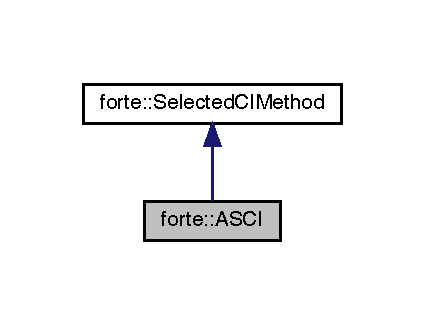
\includegraphics[width=204pt]{classforte_1_1_a_s_c_i__inherit__graph}
\end{center}
\end{figure}


Collaboration diagram for forte\+:\+:A\+S\+CI\+:
\nopagebreak
\begin{figure}[H]
\begin{center}
\leavevmode
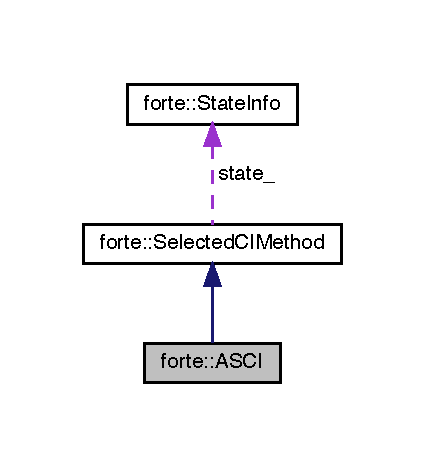
\includegraphics[width=204pt]{classforte_1_1_a_s_c_i__coll__graph}
\end{center}
\end{figure}
\subsection*{Public Member Functions}
\begin{DoxyCompactItemize}
\item 
\mbox{\hyperlink{classforte_1_1_a_s_c_i_a3640cec78b82f59f8afe187b94900f7d}{A\+S\+CI}} (\mbox{\hyperlink{classforte_1_1_state_info}{State\+Info}} state, size\+\_\+t nroot, std\+::shared\+\_\+ptr$<$ \mbox{\hyperlink{classforte_1_1_s_c_f_info}{S\+C\+F\+Info}} $>$ scf\+\_\+info, std\+::shared\+\_\+ptr$<$ \mbox{\hyperlink{classforte_1_1_forte_options}{Forte\+Options}} $>$ options, std\+::shared\+\_\+ptr$<$ \mbox{\hyperlink{classforte_1_1_m_o_space_info}{M\+O\+Space\+Info}} $>$ mo\+\_\+space\+\_\+info, std\+::shared\+\_\+ptr$<$ \mbox{\hyperlink{classforte_1_1_active_space_integrals}{Active\+Space\+Integrals}} $>$ as\+\_\+ints)
\item 
\mbox{\hyperlink{classforte_1_1_a_s_c_i_ababa5808cb2d4d19ef4cac29eae4657c}{$\sim$\+A\+S\+CI}} ()
\begin{DoxyCompactList}\small\item\em Destructor. \end{DoxyCompactList}\item 
void \mbox{\hyperlink{classforte_1_1_a_s_c_i_a7b219391b694de5192f5a467f64f60c4}{set\+\_\+options}} (std\+::shared\+\_\+ptr$<$ \mbox{\hyperlink{classforte_1_1_forte_options}{Forte\+Options}} $>$) override
\item 
\mbox{\hyperlink{classforte_1_1_determinant_hash_vec}{Determinant\+Hash\+Vec}} \mbox{\hyperlink{classforte_1_1_a_s_c_i_a1d1cb0632d2a03f39b421c2628e784fe}{get\+\_\+wavefunction}} ()
\begin{DoxyCompactList}\small\item\em Get the wavefunction. \end{DoxyCompactList}\item 
void \mbox{\hyperlink{classforte_1_1_a_s_c_i_a4a6bbf34863155aa72e7a3128a3fbe00}{compute\+\_\+nos}} ()
\begin{DoxyCompactList}\small\item\em Compute the A\+C\+I-\/\+N\+Os. \end{DoxyCompactList}\item 
void \mbox{\hyperlink{classforte_1_1_a_s_c_i_a59c39bbad1264f8daa3dadb0eeccdbd7}{set\+\_\+fci\+\_\+ints}} (std\+::shared\+\_\+ptr$<$ \mbox{\hyperlink{classforte_1_1_active_space_integrals}{Active\+Space\+Integrals}} $>$ fci\+\_\+ints)
\item 
void \mbox{\hyperlink{classforte_1_1_a_s_c_i_aff9c84376007b8ef5a54d90c3e6a1c52}{pre\+\_\+iter\+\_\+preparation}} () override
\begin{DoxyCompactList}\small\item\em Pre-\/iter preparation, usually includes preparing an initial reference. \end{DoxyCompactList}\item 
void \mbox{\hyperlink{classforte_1_1_a_s_c_i_a25123db39a9f99b446741bc2ec738ee8}{diagonalize\+\_\+\+P\+\_\+space}} () override
\begin{DoxyCompactList}\small\item\em Step 1. Diagonalize the Hamiltonian in the P space. \end{DoxyCompactList}\item 
void \mbox{\hyperlink{classforte_1_1_a_s_c_i_aa285dc9063075f23a7a1f4a1513c8aac}{diagonalize\+\_\+\+P\+Q\+\_\+space}} () override
\begin{DoxyCompactList}\small\item\em Step 3. Diagonalize the Hamiltonian in the P + Q space. \end{DoxyCompactList}\item 
void \mbox{\hyperlink{classforte_1_1_a_s_c_i_a0088675b12258f127476e15226ba822f}{post\+\_\+iter\+\_\+process}} () override
\begin{DoxyCompactList}\small\item\em Post-\/iter process. \end{DoxyCompactList}\item 
void \mbox{\hyperlink{classforte_1_1_a_s_c_i_aaf84a9fa2ec4f80da2cc05ac7ac544f9}{set\+\_\+method\+\_\+variables}} (std\+::string ex\+\_\+alg, size\+\_\+t nroot\+\_\+method, size\+\_\+t root, const std\+::vector$<$ std\+::vector$<$ std\+::pair$<$ \mbox{\hyperlink{namespaceforte_a2076c63fd7b8732004d9e1442ce527c1}{Determinant}}, double $>$$>$$>$ \&old\+\_\+roots) override
\begin{DoxyCompactList}\small\item\em Set the class variable. \end{DoxyCompactList}\item 
\mbox{\hyperlink{classforte_1_1_determinant_hash_vec}{Determinant\+Hash\+Vec}} \mbox{\hyperlink{classforte_1_1_a_s_c_i_abe4f88df4acd5e486cc1e9d43254bc0d}{get\+\_\+\+P\+Q\+\_\+space}} () override
\begin{DoxyCompactList}\small\item\em Getters. \end{DoxyCompactList}\item 
psi\+::\+Shared\+Matrix \mbox{\hyperlink{classforte_1_1_a_s_c_i_a7b0cff30856eb70d451216e5039e15ee}{get\+\_\+\+P\+Q\+\_\+evecs}} () override
\item 
psi\+::\+Shared\+Vector \mbox{\hyperlink{classforte_1_1_a_s_c_i_a13310cf1f39f174d298194efea95572f}{get\+\_\+\+P\+Q\+\_\+evals}} () override
\item 
size\+\_\+t \mbox{\hyperlink{classforte_1_1_a_s_c_i_aa81094a460d7922927d4ff9f14929ab8}{get\+\_\+ref\+\_\+root}} () override
\item 
bool \mbox{\hyperlink{classforte_1_1_a_s_c_i_a933b12da75f3baa3a824839f7a3f760b}{check\+\_\+convergence}} () override
\begin{DoxyCompactList}\small\item\em Check if the procedure has converged. \end{DoxyCompactList}\item 
void \mbox{\hyperlink{classforte_1_1_a_s_c_i_a197192d707eee6c0c6046d3dfdf78162}{find\+\_\+q\+\_\+space}} () override
\begin{DoxyCompactList}\small\item\em Find all the relevant excitations out of the P space. \end{DoxyCompactList}\item 
std\+::vector$<$ double $>$ \mbox{\hyperlink{classforte_1_1_a_s_c_i_ac497073adeab7700979678c15dcb475e}{get\+\_\+multistate\+\_\+pt2\+\_\+energy\+\_\+correction}} () override
\end{DoxyCompactItemize}
\subsection*{Additional Inherited Members}


\subsection{Detailed Description}
The \mbox{\hyperlink{classforte_1_1_a_s_c_i}{A\+S\+CI}} class This class implements the Adaptively Selected CI algorithm. 

\subsection{Constructor \& Destructor Documentation}
\mbox{\Hypertarget{classforte_1_1_a_s_c_i_a3640cec78b82f59f8afe187b94900f7d}\label{classforte_1_1_a_s_c_i_a3640cec78b82f59f8afe187b94900f7d}} 
\index{forte\+::\+A\+S\+CI@{forte\+::\+A\+S\+CI}!A\+S\+CI@{A\+S\+CI}}
\index{A\+S\+CI@{A\+S\+CI}!forte\+::\+A\+S\+CI@{forte\+::\+A\+S\+CI}}
\subsubsection{\texorpdfstring{A\+S\+C\+I()}{ASCI()}}
{\footnotesize\ttfamily forte\+::\+A\+S\+C\+I\+::\+A\+S\+CI (\begin{DoxyParamCaption}\item[{\mbox{\hyperlink{classforte_1_1_state_info}{State\+Info}}}]{state,  }\item[{size\+\_\+t}]{nroot,  }\item[{std\+::shared\+\_\+ptr$<$ \mbox{\hyperlink{classforte_1_1_s_c_f_info}{S\+C\+F\+Info}} $>$}]{scf\+\_\+info,  }\item[{std\+::shared\+\_\+ptr$<$ \mbox{\hyperlink{classforte_1_1_forte_options}{Forte\+Options}} $>$}]{options,  }\item[{std\+::shared\+\_\+ptr$<$ \mbox{\hyperlink{classforte_1_1_m_o_space_info}{M\+O\+Space\+Info}} $>$}]{mo\+\_\+space\+\_\+info,  }\item[{std\+::shared\+\_\+ptr$<$ \mbox{\hyperlink{classforte_1_1_active_space_integrals}{Active\+Space\+Integrals}} $>$}]{as\+\_\+ints }\end{DoxyParamCaption})}

Constructor 
\begin{DoxyParams}{Parameters}
{\em ref\+\_\+wfn} & The reference wavefunction object \\
\hline
{\em options} & The main options object \\
\hline
{\em ints} & A pointer to an allocated integral object \\
\hline
{\em mo\+\_\+space\+\_\+info} & A pointer to the \mbox{\hyperlink{classforte_1_1_m_o_space_info}{M\+O\+Space\+Info}} object \\
\hline
\end{DoxyParams}
\mbox{\Hypertarget{classforte_1_1_a_s_c_i_ababa5808cb2d4d19ef4cac29eae4657c}\label{classforte_1_1_a_s_c_i_ababa5808cb2d4d19ef4cac29eae4657c}} 
\index{forte\+::\+A\+S\+CI@{forte\+::\+A\+S\+CI}!````~A\+S\+CI@{$\sim$\+A\+S\+CI}}
\index{````~A\+S\+CI@{$\sim$\+A\+S\+CI}!forte\+::\+A\+S\+CI@{forte\+::\+A\+S\+CI}}
\subsubsection{\texorpdfstring{$\sim$\+A\+S\+C\+I()}{~ASCI()}}
{\footnotesize\ttfamily forte\+::\+A\+S\+C\+I\+::$\sim$\+A\+S\+CI (\begin{DoxyParamCaption}{ }\end{DoxyParamCaption})}



Destructor. 



\subsection{Member Function Documentation}
\mbox{\Hypertarget{classforte_1_1_a_s_c_i_a933b12da75f3baa3a824839f7a3f760b}\label{classforte_1_1_a_s_c_i_a933b12da75f3baa3a824839f7a3f760b}} 
\index{forte\+::\+A\+S\+CI@{forte\+::\+A\+S\+CI}!check\+\_\+convergence@{check\+\_\+convergence}}
\index{check\+\_\+convergence@{check\+\_\+convergence}!forte\+::\+A\+S\+CI@{forte\+::\+A\+S\+CI}}
\subsubsection{\texorpdfstring{check\+\_\+convergence()}{check\_convergence()}}
{\footnotesize\ttfamily bool forte\+::\+A\+S\+C\+I\+::check\+\_\+convergence (\begin{DoxyParamCaption}{ }\end{DoxyParamCaption})\hspace{0.3cm}{\ttfamily [override]}, {\ttfamily [virtual]}}



Check if the procedure has converged. 



Implements \mbox{\hyperlink{classforte_1_1_selected_c_i_method_acc10aa488c79c2abec46a9093ecf5a52}{forte\+::\+Selected\+C\+I\+Method}}.

\mbox{\Hypertarget{classforte_1_1_a_s_c_i_a4a6bbf34863155aa72e7a3128a3fbe00}\label{classforte_1_1_a_s_c_i_a4a6bbf34863155aa72e7a3128a3fbe00}} 
\index{forte\+::\+A\+S\+CI@{forte\+::\+A\+S\+CI}!compute\+\_\+nos@{compute\+\_\+nos}}
\index{compute\+\_\+nos@{compute\+\_\+nos}!forte\+::\+A\+S\+CI@{forte\+::\+A\+S\+CI}}
\subsubsection{\texorpdfstring{compute\+\_\+nos()}{compute\_nos()}}
{\footnotesize\ttfamily void forte\+::\+A\+S\+C\+I\+::compute\+\_\+nos (\begin{DoxyParamCaption}{ }\end{DoxyParamCaption})}



Compute the A\+C\+I-\/\+N\+Os. 

\mbox{\Hypertarget{classforte_1_1_a_s_c_i_a25123db39a9f99b446741bc2ec738ee8}\label{classforte_1_1_a_s_c_i_a25123db39a9f99b446741bc2ec738ee8}} 
\index{forte\+::\+A\+S\+CI@{forte\+::\+A\+S\+CI}!diagonalize\+\_\+\+P\+\_\+space@{diagonalize\+\_\+\+P\+\_\+space}}
\index{diagonalize\+\_\+\+P\+\_\+space@{diagonalize\+\_\+\+P\+\_\+space}!forte\+::\+A\+S\+CI@{forte\+::\+A\+S\+CI}}
\subsubsection{\texorpdfstring{diagonalize\+\_\+\+P\+\_\+space()}{diagonalize\_P\_space()}}
{\footnotesize\ttfamily void forte\+::\+A\+S\+C\+I\+::diagonalize\+\_\+\+P\+\_\+space (\begin{DoxyParamCaption}{ }\end{DoxyParamCaption})\hspace{0.3cm}{\ttfamily [override]}, {\ttfamily [virtual]}}



Step 1. Diagonalize the Hamiltonian in the P space. 



Implements \mbox{\hyperlink{classforte_1_1_selected_c_i_method_a7b2b41da889659f03361f625c6df44d2}{forte\+::\+Selected\+C\+I\+Method}}.

\mbox{\Hypertarget{classforte_1_1_a_s_c_i_aa285dc9063075f23a7a1f4a1513c8aac}\label{classforte_1_1_a_s_c_i_aa285dc9063075f23a7a1f4a1513c8aac}} 
\index{forte\+::\+A\+S\+CI@{forte\+::\+A\+S\+CI}!diagonalize\+\_\+\+P\+Q\+\_\+space@{diagonalize\+\_\+\+P\+Q\+\_\+space}}
\index{diagonalize\+\_\+\+P\+Q\+\_\+space@{diagonalize\+\_\+\+P\+Q\+\_\+space}!forte\+::\+A\+S\+CI@{forte\+::\+A\+S\+CI}}
\subsubsection{\texorpdfstring{diagonalize\+\_\+\+P\+Q\+\_\+space()}{diagonalize\_PQ\_space()}}
{\footnotesize\ttfamily void forte\+::\+A\+S\+C\+I\+::diagonalize\+\_\+\+P\+Q\+\_\+space (\begin{DoxyParamCaption}{ }\end{DoxyParamCaption})\hspace{0.3cm}{\ttfamily [override]}, {\ttfamily [virtual]}}



Step 3. Diagonalize the Hamiltonian in the P + Q space. 



Implements \mbox{\hyperlink{classforte_1_1_selected_c_i_method_a9f01588d22401cd2631a09940ea7db50}{forte\+::\+Selected\+C\+I\+Method}}.

\mbox{\Hypertarget{classforte_1_1_a_s_c_i_a197192d707eee6c0c6046d3dfdf78162}\label{classforte_1_1_a_s_c_i_a197192d707eee6c0c6046d3dfdf78162}} 
\index{forte\+::\+A\+S\+CI@{forte\+::\+A\+S\+CI}!find\+\_\+q\+\_\+space@{find\+\_\+q\+\_\+space}}
\index{find\+\_\+q\+\_\+space@{find\+\_\+q\+\_\+space}!forte\+::\+A\+S\+CI@{forte\+::\+A\+S\+CI}}
\subsubsection{\texorpdfstring{find\+\_\+q\+\_\+space()}{find\_q\_space()}}
{\footnotesize\ttfamily void forte\+::\+A\+S\+C\+I\+::find\+\_\+q\+\_\+space (\begin{DoxyParamCaption}{ }\end{DoxyParamCaption})\hspace{0.3cm}{\ttfamily [override]}, {\ttfamily [virtual]}}



Find all the relevant excitations out of the P space. 



Implements \mbox{\hyperlink{classforte_1_1_selected_c_i_method_aff521efa08edfafb479f32e03a70c118}{forte\+::\+Selected\+C\+I\+Method}}.

\mbox{\Hypertarget{classforte_1_1_a_s_c_i_ac497073adeab7700979678c15dcb475e}\label{classforte_1_1_a_s_c_i_ac497073adeab7700979678c15dcb475e}} 
\index{forte\+::\+A\+S\+CI@{forte\+::\+A\+S\+CI}!get\+\_\+multistate\+\_\+pt2\+\_\+energy\+\_\+correction@{get\+\_\+multistate\+\_\+pt2\+\_\+energy\+\_\+correction}}
\index{get\+\_\+multistate\+\_\+pt2\+\_\+energy\+\_\+correction@{get\+\_\+multistate\+\_\+pt2\+\_\+energy\+\_\+correction}!forte\+::\+A\+S\+CI@{forte\+::\+A\+S\+CI}}
\subsubsection{\texorpdfstring{get\+\_\+multistate\+\_\+pt2\+\_\+energy\+\_\+correction()}{get\_multistate\_pt2\_energy\_correction()}}
{\footnotesize\ttfamily std\+::vector$<$ double $>$ forte\+::\+A\+S\+C\+I\+::get\+\_\+multistate\+\_\+pt2\+\_\+energy\+\_\+correction (\begin{DoxyParamCaption}{ }\end{DoxyParamCaption})\hspace{0.3cm}{\ttfamily [override]}, {\ttfamily [virtual]}}



Implements \mbox{\hyperlink{classforte_1_1_selected_c_i_method_abbe18ea3e5f1a77df13a38764aeef62c}{forte\+::\+Selected\+C\+I\+Method}}.

\mbox{\Hypertarget{classforte_1_1_a_s_c_i_a13310cf1f39f174d298194efea95572f}\label{classforte_1_1_a_s_c_i_a13310cf1f39f174d298194efea95572f}} 
\index{forte\+::\+A\+S\+CI@{forte\+::\+A\+S\+CI}!get\+\_\+\+P\+Q\+\_\+evals@{get\+\_\+\+P\+Q\+\_\+evals}}
\index{get\+\_\+\+P\+Q\+\_\+evals@{get\+\_\+\+P\+Q\+\_\+evals}!forte\+::\+A\+S\+CI@{forte\+::\+A\+S\+CI}}
\subsubsection{\texorpdfstring{get\+\_\+\+P\+Q\+\_\+evals()}{get\_PQ\_evals()}}
{\footnotesize\ttfamily psi\+::\+Shared\+Vector forte\+::\+A\+S\+C\+I\+::get\+\_\+\+P\+Q\+\_\+evals (\begin{DoxyParamCaption}{ }\end{DoxyParamCaption})\hspace{0.3cm}{\ttfamily [override]}, {\ttfamily [virtual]}}



Implements \mbox{\hyperlink{classforte_1_1_selected_c_i_method_a675d28ae66341b8cfabb2953c936621c}{forte\+::\+Selected\+C\+I\+Method}}.

\mbox{\Hypertarget{classforte_1_1_a_s_c_i_a7b0cff30856eb70d451216e5039e15ee}\label{classforte_1_1_a_s_c_i_a7b0cff30856eb70d451216e5039e15ee}} 
\index{forte\+::\+A\+S\+CI@{forte\+::\+A\+S\+CI}!get\+\_\+\+P\+Q\+\_\+evecs@{get\+\_\+\+P\+Q\+\_\+evecs}}
\index{get\+\_\+\+P\+Q\+\_\+evecs@{get\+\_\+\+P\+Q\+\_\+evecs}!forte\+::\+A\+S\+CI@{forte\+::\+A\+S\+CI}}
\subsubsection{\texorpdfstring{get\+\_\+\+P\+Q\+\_\+evecs()}{get\_PQ\_evecs()}}
{\footnotesize\ttfamily psi\+::\+Shared\+Matrix forte\+::\+A\+S\+C\+I\+::get\+\_\+\+P\+Q\+\_\+evecs (\begin{DoxyParamCaption}{ }\end{DoxyParamCaption})\hspace{0.3cm}{\ttfamily [override]}, {\ttfamily [virtual]}}



Implements \mbox{\hyperlink{classforte_1_1_selected_c_i_method_a5e5212836aa0dc35f98238d1f426abed}{forte\+::\+Selected\+C\+I\+Method}}.

\mbox{\Hypertarget{classforte_1_1_a_s_c_i_abe4f88df4acd5e486cc1e9d43254bc0d}\label{classforte_1_1_a_s_c_i_abe4f88df4acd5e486cc1e9d43254bc0d}} 
\index{forte\+::\+A\+S\+CI@{forte\+::\+A\+S\+CI}!get\+\_\+\+P\+Q\+\_\+space@{get\+\_\+\+P\+Q\+\_\+space}}
\index{get\+\_\+\+P\+Q\+\_\+space@{get\+\_\+\+P\+Q\+\_\+space}!forte\+::\+A\+S\+CI@{forte\+::\+A\+S\+CI}}
\subsubsection{\texorpdfstring{get\+\_\+\+P\+Q\+\_\+space()}{get\_PQ\_space()}}
{\footnotesize\ttfamily \mbox{\hyperlink{classforte_1_1_determinant_hash_vec}{Determinant\+Hash\+Vec}} forte\+::\+A\+S\+C\+I\+::get\+\_\+\+P\+Q\+\_\+space (\begin{DoxyParamCaption}{ }\end{DoxyParamCaption})\hspace{0.3cm}{\ttfamily [override]}, {\ttfamily [virtual]}}



Getters. 



Implements \mbox{\hyperlink{classforte_1_1_selected_c_i_method_a2c29d8700d6887860850f77b9246ec9f}{forte\+::\+Selected\+C\+I\+Method}}.

\mbox{\Hypertarget{classforte_1_1_a_s_c_i_aa81094a460d7922927d4ff9f14929ab8}\label{classforte_1_1_a_s_c_i_aa81094a460d7922927d4ff9f14929ab8}} 
\index{forte\+::\+A\+S\+CI@{forte\+::\+A\+S\+CI}!get\+\_\+ref\+\_\+root@{get\+\_\+ref\+\_\+root}}
\index{get\+\_\+ref\+\_\+root@{get\+\_\+ref\+\_\+root}!forte\+::\+A\+S\+CI@{forte\+::\+A\+S\+CI}}
\subsubsection{\texorpdfstring{get\+\_\+ref\+\_\+root()}{get\_ref\_root()}}
{\footnotesize\ttfamily size\+\_\+t forte\+::\+A\+S\+C\+I\+::get\+\_\+ref\+\_\+root (\begin{DoxyParamCaption}{ }\end{DoxyParamCaption})\hspace{0.3cm}{\ttfamily [override]}, {\ttfamily [virtual]}}



Implements \mbox{\hyperlink{classforte_1_1_selected_c_i_method_aa95ed581568b2d580c17ab166e85a11a}{forte\+::\+Selected\+C\+I\+Method}}.

\mbox{\Hypertarget{classforte_1_1_a_s_c_i_a1d1cb0632d2a03f39b421c2628e784fe}\label{classforte_1_1_a_s_c_i_a1d1cb0632d2a03f39b421c2628e784fe}} 
\index{forte\+::\+A\+S\+CI@{forte\+::\+A\+S\+CI}!get\+\_\+wavefunction@{get\+\_\+wavefunction}}
\index{get\+\_\+wavefunction@{get\+\_\+wavefunction}!forte\+::\+A\+S\+CI@{forte\+::\+A\+S\+CI}}
\subsubsection{\texorpdfstring{get\+\_\+wavefunction()}{get\_wavefunction()}}
{\footnotesize\ttfamily \mbox{\hyperlink{classforte_1_1_determinant_hash_vec}{Determinant\+Hash\+Vec}} forte\+::\+A\+S\+C\+I\+::get\+\_\+wavefunction (\begin{DoxyParamCaption}{ }\end{DoxyParamCaption})}



Get the wavefunction. 

\mbox{\Hypertarget{classforte_1_1_a_s_c_i_a0088675b12258f127476e15226ba822f}\label{classforte_1_1_a_s_c_i_a0088675b12258f127476e15226ba822f}} 
\index{forte\+::\+A\+S\+CI@{forte\+::\+A\+S\+CI}!post\+\_\+iter\+\_\+process@{post\+\_\+iter\+\_\+process}}
\index{post\+\_\+iter\+\_\+process@{post\+\_\+iter\+\_\+process}!forte\+::\+A\+S\+CI@{forte\+::\+A\+S\+CI}}
\subsubsection{\texorpdfstring{post\+\_\+iter\+\_\+process()}{post\_iter\_process()}}
{\footnotesize\ttfamily void forte\+::\+A\+S\+C\+I\+::post\+\_\+iter\+\_\+process (\begin{DoxyParamCaption}{ }\end{DoxyParamCaption})\hspace{0.3cm}{\ttfamily [override]}, {\ttfamily [virtual]}}



Post-\/iter process. 



Implements \mbox{\hyperlink{classforte_1_1_selected_c_i_method_a23ea3389ac1c62dee811decc5bea507f}{forte\+::\+Selected\+C\+I\+Method}}.

\mbox{\Hypertarget{classforte_1_1_a_s_c_i_aff9c84376007b8ef5a54d90c3e6a1c52}\label{classforte_1_1_a_s_c_i_aff9c84376007b8ef5a54d90c3e6a1c52}} 
\index{forte\+::\+A\+S\+CI@{forte\+::\+A\+S\+CI}!pre\+\_\+iter\+\_\+preparation@{pre\+\_\+iter\+\_\+preparation}}
\index{pre\+\_\+iter\+\_\+preparation@{pre\+\_\+iter\+\_\+preparation}!forte\+::\+A\+S\+CI@{forte\+::\+A\+S\+CI}}
\subsubsection{\texorpdfstring{pre\+\_\+iter\+\_\+preparation()}{pre\_iter\_preparation()}}
{\footnotesize\ttfamily void forte\+::\+A\+S\+C\+I\+::pre\+\_\+iter\+\_\+preparation (\begin{DoxyParamCaption}{ }\end{DoxyParamCaption})\hspace{0.3cm}{\ttfamily [override]}, {\ttfamily [virtual]}}



Pre-\/iter preparation, usually includes preparing an initial reference. 



Implements \mbox{\hyperlink{classforte_1_1_selected_c_i_method_af92b210415034874fcf2faac8b00eca9}{forte\+::\+Selected\+C\+I\+Method}}.

\mbox{\Hypertarget{classforte_1_1_a_s_c_i_a59c39bbad1264f8daa3dadb0eeccdbd7}\label{classforte_1_1_a_s_c_i_a59c39bbad1264f8daa3dadb0eeccdbd7}} 
\index{forte\+::\+A\+S\+CI@{forte\+::\+A\+S\+CI}!set\+\_\+fci\+\_\+ints@{set\+\_\+fci\+\_\+ints}}
\index{set\+\_\+fci\+\_\+ints@{set\+\_\+fci\+\_\+ints}!forte\+::\+A\+S\+CI@{forte\+::\+A\+S\+CI}}
\subsubsection{\texorpdfstring{set\+\_\+fci\+\_\+ints()}{set\_fci\_ints()}}
{\footnotesize\ttfamily void forte\+::\+A\+S\+C\+I\+::set\+\_\+fci\+\_\+ints (\begin{DoxyParamCaption}\item[{std\+::shared\+\_\+ptr$<$ \mbox{\hyperlink{classforte_1_1_active_space_integrals}{Active\+Space\+Integrals}} $>$}]{fci\+\_\+ints }\end{DoxyParamCaption})}

\mbox{\Hypertarget{classforte_1_1_a_s_c_i_aaf84a9fa2ec4f80da2cc05ac7ac544f9}\label{classforte_1_1_a_s_c_i_aaf84a9fa2ec4f80da2cc05ac7ac544f9}} 
\index{forte\+::\+A\+S\+CI@{forte\+::\+A\+S\+CI}!set\+\_\+method\+\_\+variables@{set\+\_\+method\+\_\+variables}}
\index{set\+\_\+method\+\_\+variables@{set\+\_\+method\+\_\+variables}!forte\+::\+A\+S\+CI@{forte\+::\+A\+S\+CI}}
\subsubsection{\texorpdfstring{set\+\_\+method\+\_\+variables()}{set\_method\_variables()}}
{\footnotesize\ttfamily void forte\+::\+A\+S\+C\+I\+::set\+\_\+method\+\_\+variables (\begin{DoxyParamCaption}\item[{std\+::string}]{ex\+\_\+alg,  }\item[{size\+\_\+t}]{nroot\+\_\+method,  }\item[{size\+\_\+t}]{root,  }\item[{const std\+::vector$<$ std\+::vector$<$ std\+::pair$<$ \mbox{\hyperlink{namespaceforte_a2076c63fd7b8732004d9e1442ce527c1}{Determinant}}, double $>$$>$$>$ \&}]{old\+\_\+roots }\end{DoxyParamCaption})\hspace{0.3cm}{\ttfamily [override]}, {\ttfamily [virtual]}}



Set the class variable. 



Implements \mbox{\hyperlink{classforte_1_1_selected_c_i_method_a37f95503d0241387195dc7d412fc6e78}{forte\+::\+Selected\+C\+I\+Method}}.

\mbox{\Hypertarget{classforte_1_1_a_s_c_i_a7b219391b694de5192f5a467f64f60c4}\label{classforte_1_1_a_s_c_i_a7b219391b694de5192f5a467f64f60c4}} 
\index{forte\+::\+A\+S\+CI@{forte\+::\+A\+S\+CI}!set\+\_\+options@{set\+\_\+options}}
\index{set\+\_\+options@{set\+\_\+options}!forte\+::\+A\+S\+CI@{forte\+::\+A\+S\+CI}}
\subsubsection{\texorpdfstring{set\+\_\+options()}{set\_options()}}
{\footnotesize\ttfamily void forte\+::\+A\+S\+C\+I\+::set\+\_\+options (\begin{DoxyParamCaption}\item[{std\+::shared\+\_\+ptr$<$ \mbox{\hyperlink{classforte_1_1_forte_options}{Forte\+Options}} $>$}]{options }\end{DoxyParamCaption})\hspace{0.3cm}{\ttfamily [inline]}, {\ttfamily [override]}, {\ttfamily [virtual]}}

Set options from an option object 
\begin{DoxyParams}{Parameters}
{\em options} & the options passed in \\
\hline
\end{DoxyParams}


Implements \mbox{\hyperlink{classforte_1_1_selected_c_i_method_ad03bbde3a0443ca9b01ff9605f2e06e0}{forte\+::\+Selected\+C\+I\+Method}}.



The documentation for this class was generated from the following files\+:\begin{DoxyCompactItemize}
\item 
/\+Users/fevange/\+Source/forte/src/sci/\mbox{\hyperlink{asci_8h}{asci.\+h}}\item 
/\+Users/fevange/\+Source/forte/src/sci/\mbox{\hyperlink{asci_8cc}{asci.\+cc}}\end{DoxyCompactItemize}

\hypertarget{classforte_1_1_atomic_orbital_helper}{}\section{forte\+:\+:Atomic\+Orbital\+Helper Class Reference}
\label{classforte_1_1_atomic_orbital_helper}\index{forte\+::\+Atomic\+Orbital\+Helper@{forte\+::\+Atomic\+Orbital\+Helper}}


{\ttfamily \#include $<$ao\+\_\+helper.\+h$>$}

\subsection*{Public Member Functions}
\begin{DoxyCompactItemize}
\item 
psi\+::\+Shared\+Matrix \mbox{\hyperlink{classforte_1_1_atomic_orbital_helper_aae3faca1d68ec5b2da4e2dbe2b3c0c76}{A\+O\+\_\+\+Screen}} ()
\item 
psi\+::\+Shared\+Matrix \mbox{\hyperlink{classforte_1_1_atomic_orbital_helper_a436f7437af75a2bb5bdf0926b4a128e5}{Trans\+A\+O\+\_\+\+Screen}} ()
\item 
psi\+::\+Shared\+Matrix \mbox{\hyperlink{classforte_1_1_atomic_orbital_helper_adda71a215917ca372968507cd5253d91}{Occupied\+\_\+\+Laplace}} ()
\item 
psi\+::\+Shared\+Matrix \mbox{\hyperlink{classforte_1_1_atomic_orbital_helper_a30cf42f4d768185645e8e07a45da8e22}{Virtual\+\_\+\+Laplace}} ()
\item 
psi\+::\+Shared\+Matrix \mbox{\hyperlink{classforte_1_1_atomic_orbital_helper_a8e8dadd03ee3485dc4b26bba84759e3f}{P\+Occ}} ()
\item 
psi\+::\+Shared\+Matrix \mbox{\hyperlink{classforte_1_1_atomic_orbital_helper_a8eab87d87f3560ca1e35c48d6e017ca1}{P\+Vir}} ()
\item 
int \mbox{\hyperlink{classforte_1_1_atomic_orbital_helper_aba981b8d86dd9418ac491b6529363507}{Weights}} ()
\item 
\mbox{\hyperlink{classforte_1_1_atomic_orbital_helper_a14a54771aec07f989de0504907007923}{Atomic\+Orbital\+Helper}} (psi\+::\+Shared\+Matrix C\+MO, psi\+::\+Shared\+Vector eps\+\_\+occ, psi\+::\+Shared\+Vector eps\+\_\+vir, double laplace\+\_\+tolerance)
\item 
\mbox{\hyperlink{classforte_1_1_atomic_orbital_helper_ad22eb22a692b1d690bbfe0acc629c1c4}{Atomic\+Orbital\+Helper}} (psi\+::\+Shared\+Matrix C\+MO, psi\+::\+Shared\+Vector eps\+\_\+occ, psi\+::\+Shared\+Vector eps\+\_\+vir, double laplace\+\_\+tolerance, int shift)
\item 
void \mbox{\hyperlink{classforte_1_1_atomic_orbital_helper_a177bf2b84d858251fceb166a71b12119}{Compute\+\_\+\+A\+O\+\_\+\+Screen}} (std\+::shared\+\_\+ptr$<$ psi\+::\+Basis\+Set $>$ \&primary)
\begin{DoxyCompactList}\small\item\em Compute (mu nu $\vert$ mu nu)$^\wedge$\{(1/2)\}. \end{DoxyCompactList}\item 
void \mbox{\hyperlink{classforte_1_1_atomic_orbital_helper_a19898dcd4ea53638b54ce7821982f900}{Estimate\+\_\+\+Trans\+A\+O\+\_\+\+Screen}} (std\+::shared\+\_\+ptr$<$ psi\+::\+Basis\+Set $>$ \&primary, std\+::shared\+\_\+ptr$<$ psi\+::\+Basis\+Set $>$ \&auxiliary)
\item 
\mbox{\hyperlink{classforte_1_1_atomic_orbital_helper_a6b46a292d87abe345f8c68e3dd442fcf}{$\sim$\+Atomic\+Orbital\+Helper}} ()
\end{DoxyCompactItemize}
\subsection*{Protected Member Functions}
\begin{DoxyCompactItemize}
\item 
void \mbox{\hyperlink{classforte_1_1_atomic_orbital_helper_aaf06be8bb2f953d576c5df623a4207cb}{Compute\+\_\+\+Psuedo\+\_\+\+Density}} ()
\end{DoxyCompactItemize}
\subsection*{Protected Attributes}
\begin{DoxyCompactItemize}
\item 
psi\+::\+Shared\+Matrix \mbox{\hyperlink{classforte_1_1_atomic_orbital_helper_a5896c9e72821a9b25fdf50a7fe3f41d5}{A\+O\+\_\+\+Screen\+\_\+}}
\item 
psi\+::\+Shared\+Matrix \mbox{\hyperlink{classforte_1_1_atomic_orbital_helper_a717f94e6594b0d6e440eb0cb534fe533}{Trans\+A\+O\+\_\+\+Screen\+\_\+}}
\item 
psi\+::\+Shared\+Matrix \mbox{\hyperlink{classforte_1_1_atomic_orbital_helper_af5afb917090ce71dbf360af4e7542762}{C\+M\+O\+\_\+}}
\item 
psi\+::\+Shared\+Vector \mbox{\hyperlink{classforte_1_1_atomic_orbital_helper_a4cc753aab5b772c6f5bc9af9663c6248}{eps\+\_\+rdocc\+\_\+}}
\item 
psi\+::\+Shared\+Vector \mbox{\hyperlink{classforte_1_1_atomic_orbital_helper_a9497fd7b7a65b41d453ff70909455f40}{eps\+\_\+virtual\+\_\+}}
\item 
psi\+::\+Shared\+Matrix \mbox{\hyperlink{classforte_1_1_atomic_orbital_helper_a111df8cb0812bec57b7c4f7062578b78}{P\+Occ\+\_\+}}
\item 
psi\+::\+Shared\+Matrix \mbox{\hyperlink{classforte_1_1_atomic_orbital_helper_a592c52435831ae234781ecbfb34ad6ad}{P\+Vir\+\_\+}}
\item 
psi\+::\+Shared\+Matrix \mbox{\hyperlink{classforte_1_1_atomic_orbital_helper_ad13f3a30eba62a3c0e62f3e37e391a6f}{Occupied\+\_\+\+Laplace\+\_\+}}
\item 
psi\+::\+Shared\+Matrix \mbox{\hyperlink{classforte_1_1_atomic_orbital_helper_abdd4033673986a208a48a5f3084f4c06}{Virtual\+\_\+\+Laplace\+\_\+}}
\item 
double \mbox{\hyperlink{classforte_1_1_atomic_orbital_helper_ad30e1c8811b274f655fb4a5a7ca0162e}{laplace\+\_\+tolerance\+\_\+}} = 1e-\/10
\item 
int \mbox{\hyperlink{classforte_1_1_atomic_orbital_helper_a2cda118e3b004f18d785b1c14a50ee3e}{weights\+\_\+}}
\item 
int \mbox{\hyperlink{classforte_1_1_atomic_orbital_helper_a69c052b5064e8ed87fd2697a344001e1}{nbf\+\_\+}}
\item 
int \mbox{\hyperlink{classforte_1_1_atomic_orbital_helper_a039b8f61b9eb2acf1562311827247093}{nrdocc\+\_\+}}
\item 
int \mbox{\hyperlink{classforte_1_1_atomic_orbital_helper_ac0f50e9d760abee8b4a90c64acf3f71d}{nvir\+\_\+}}
\item 
int \mbox{\hyperlink{classforte_1_1_atomic_orbital_helper_a6fdce16217872f48ac97362f2524892b}{shift\+\_\+}}
\end{DoxyCompactItemize}


\subsection{Constructor \& Destructor Documentation}
\mbox{\Hypertarget{classforte_1_1_atomic_orbital_helper_a14a54771aec07f989de0504907007923}\label{classforte_1_1_atomic_orbital_helper_a14a54771aec07f989de0504907007923}} 
\index{forte\+::\+Atomic\+Orbital\+Helper@{forte\+::\+Atomic\+Orbital\+Helper}!Atomic\+Orbital\+Helper@{Atomic\+Orbital\+Helper}}
\index{Atomic\+Orbital\+Helper@{Atomic\+Orbital\+Helper}!forte\+::\+Atomic\+Orbital\+Helper@{forte\+::\+Atomic\+Orbital\+Helper}}
\subsubsection{\texorpdfstring{Atomic\+Orbital\+Helper()}{AtomicOrbitalHelper()}\hspace{0.1cm}{\footnotesize\ttfamily [1/2]}}
{\footnotesize\ttfamily forte\+::\+Atomic\+Orbital\+Helper\+::\+Atomic\+Orbital\+Helper (\begin{DoxyParamCaption}\item[{psi\+::\+Shared\+Matrix}]{C\+MO,  }\item[{psi\+::\+Shared\+Vector}]{eps\+\_\+occ,  }\item[{psi\+::\+Shared\+Vector}]{eps\+\_\+vir,  }\item[{double}]{laplace\+\_\+tolerance }\end{DoxyParamCaption})}

\mbox{\Hypertarget{classforte_1_1_atomic_orbital_helper_ad22eb22a692b1d690bbfe0acc629c1c4}\label{classforte_1_1_atomic_orbital_helper_ad22eb22a692b1d690bbfe0acc629c1c4}} 
\index{forte\+::\+Atomic\+Orbital\+Helper@{forte\+::\+Atomic\+Orbital\+Helper}!Atomic\+Orbital\+Helper@{Atomic\+Orbital\+Helper}}
\index{Atomic\+Orbital\+Helper@{Atomic\+Orbital\+Helper}!forte\+::\+Atomic\+Orbital\+Helper@{forte\+::\+Atomic\+Orbital\+Helper}}
\subsubsection{\texorpdfstring{Atomic\+Orbital\+Helper()}{AtomicOrbitalHelper()}\hspace{0.1cm}{\footnotesize\ttfamily [2/2]}}
{\footnotesize\ttfamily forte\+::\+Atomic\+Orbital\+Helper\+::\+Atomic\+Orbital\+Helper (\begin{DoxyParamCaption}\item[{psi\+::\+Shared\+Matrix}]{C\+MO,  }\item[{psi\+::\+Shared\+Vector}]{eps\+\_\+occ,  }\item[{psi\+::\+Shared\+Vector}]{eps\+\_\+vir,  }\item[{double}]{laplace\+\_\+tolerance,  }\item[{int}]{shift }\end{DoxyParamCaption})}

\mbox{\Hypertarget{classforte_1_1_atomic_orbital_helper_a6b46a292d87abe345f8c68e3dd442fcf}\label{classforte_1_1_atomic_orbital_helper_a6b46a292d87abe345f8c68e3dd442fcf}} 
\index{forte\+::\+Atomic\+Orbital\+Helper@{forte\+::\+Atomic\+Orbital\+Helper}!````~Atomic\+Orbital\+Helper@{$\sim$\+Atomic\+Orbital\+Helper}}
\index{````~Atomic\+Orbital\+Helper@{$\sim$\+Atomic\+Orbital\+Helper}!forte\+::\+Atomic\+Orbital\+Helper@{forte\+::\+Atomic\+Orbital\+Helper}}
\subsubsection{\texorpdfstring{$\sim$\+Atomic\+Orbital\+Helper()}{~AtomicOrbitalHelper()}}
{\footnotesize\ttfamily forte\+::\+Atomic\+Orbital\+Helper\+::$\sim$\+Atomic\+Orbital\+Helper (\begin{DoxyParamCaption}{ }\end{DoxyParamCaption})}



\subsection{Member Function Documentation}
\mbox{\Hypertarget{classforte_1_1_atomic_orbital_helper_aae3faca1d68ec5b2da4e2dbe2b3c0c76}\label{classforte_1_1_atomic_orbital_helper_aae3faca1d68ec5b2da4e2dbe2b3c0c76}} 
\index{forte\+::\+Atomic\+Orbital\+Helper@{forte\+::\+Atomic\+Orbital\+Helper}!A\+O\+\_\+\+Screen@{A\+O\+\_\+\+Screen}}
\index{A\+O\+\_\+\+Screen@{A\+O\+\_\+\+Screen}!forte\+::\+Atomic\+Orbital\+Helper@{forte\+::\+Atomic\+Orbital\+Helper}}
\subsubsection{\texorpdfstring{A\+O\+\_\+\+Screen()}{AO\_Screen()}}
{\footnotesize\ttfamily psi\+::\+Shared\+Matrix forte\+::\+Atomic\+Orbital\+Helper\+::\+A\+O\+\_\+\+Screen (\begin{DoxyParamCaption}{ }\end{DoxyParamCaption})\hspace{0.3cm}{\ttfamily [inline]}}

\mbox{\Hypertarget{classforte_1_1_atomic_orbital_helper_a177bf2b84d858251fceb166a71b12119}\label{classforte_1_1_atomic_orbital_helper_a177bf2b84d858251fceb166a71b12119}} 
\index{forte\+::\+Atomic\+Orbital\+Helper@{forte\+::\+Atomic\+Orbital\+Helper}!Compute\+\_\+\+A\+O\+\_\+\+Screen@{Compute\+\_\+\+A\+O\+\_\+\+Screen}}
\index{Compute\+\_\+\+A\+O\+\_\+\+Screen@{Compute\+\_\+\+A\+O\+\_\+\+Screen}!forte\+::\+Atomic\+Orbital\+Helper@{forte\+::\+Atomic\+Orbital\+Helper}}
\subsubsection{\texorpdfstring{Compute\+\_\+\+A\+O\+\_\+\+Screen()}{Compute\_AO\_Screen()}}
{\footnotesize\ttfamily void forte\+::\+Atomic\+Orbital\+Helper\+::\+Compute\+\_\+\+A\+O\+\_\+\+Screen (\begin{DoxyParamCaption}\item[{std\+::shared\+\_\+ptr$<$ psi\+::\+Basis\+Set $>$ \&}]{primary }\end{DoxyParamCaption})}



Compute (mu nu $\vert$ mu nu)$^\wedge$\{(1/2)\}. 

\mbox{\Hypertarget{classforte_1_1_atomic_orbital_helper_aaf06be8bb2f953d576c5df623a4207cb}\label{classforte_1_1_atomic_orbital_helper_aaf06be8bb2f953d576c5df623a4207cb}} 
\index{forte\+::\+Atomic\+Orbital\+Helper@{forte\+::\+Atomic\+Orbital\+Helper}!Compute\+\_\+\+Psuedo\+\_\+\+Density@{Compute\+\_\+\+Psuedo\+\_\+\+Density}}
\index{Compute\+\_\+\+Psuedo\+\_\+\+Density@{Compute\+\_\+\+Psuedo\+\_\+\+Density}!forte\+::\+Atomic\+Orbital\+Helper@{forte\+::\+Atomic\+Orbital\+Helper}}
\subsubsection{\texorpdfstring{Compute\+\_\+\+Psuedo\+\_\+\+Density()}{Compute\_Psuedo\_Density()}}
{\footnotesize\ttfamily void forte\+::\+Atomic\+Orbital\+Helper\+::\+Compute\+\_\+\+Psuedo\+\_\+\+Density (\begin{DoxyParamCaption}{ }\end{DoxyParamCaption})\hspace{0.3cm}{\ttfamily [protected]}}

\mbox{\Hypertarget{classforte_1_1_atomic_orbital_helper_a19898dcd4ea53638b54ce7821982f900}\label{classforte_1_1_atomic_orbital_helper_a19898dcd4ea53638b54ce7821982f900}} 
\index{forte\+::\+Atomic\+Orbital\+Helper@{forte\+::\+Atomic\+Orbital\+Helper}!Estimate\+\_\+\+Trans\+A\+O\+\_\+\+Screen@{Estimate\+\_\+\+Trans\+A\+O\+\_\+\+Screen}}
\index{Estimate\+\_\+\+Trans\+A\+O\+\_\+\+Screen@{Estimate\+\_\+\+Trans\+A\+O\+\_\+\+Screen}!forte\+::\+Atomic\+Orbital\+Helper@{forte\+::\+Atomic\+Orbital\+Helper}}
\subsubsection{\texorpdfstring{Estimate\+\_\+\+Trans\+A\+O\+\_\+\+Screen()}{Estimate\_TransAO\_Screen()}}
{\footnotesize\ttfamily void forte\+::\+Atomic\+Orbital\+Helper\+::\+Estimate\+\_\+\+Trans\+A\+O\+\_\+\+Screen (\begin{DoxyParamCaption}\item[{std\+::shared\+\_\+ptr$<$ psi\+::\+Basis\+Set $>$ \&}]{primary,  }\item[{std\+::shared\+\_\+ptr$<$ psi\+::\+Basis\+Set $>$ \&}]{auxiliary }\end{DoxyParamCaption})}

\mbox{\Hypertarget{classforte_1_1_atomic_orbital_helper_adda71a215917ca372968507cd5253d91}\label{classforte_1_1_atomic_orbital_helper_adda71a215917ca372968507cd5253d91}} 
\index{forte\+::\+Atomic\+Orbital\+Helper@{forte\+::\+Atomic\+Orbital\+Helper}!Occupied\+\_\+\+Laplace@{Occupied\+\_\+\+Laplace}}
\index{Occupied\+\_\+\+Laplace@{Occupied\+\_\+\+Laplace}!forte\+::\+Atomic\+Orbital\+Helper@{forte\+::\+Atomic\+Orbital\+Helper}}
\subsubsection{\texorpdfstring{Occupied\+\_\+\+Laplace()}{Occupied\_Laplace()}}
{\footnotesize\ttfamily psi\+::\+Shared\+Matrix forte\+::\+Atomic\+Orbital\+Helper\+::\+Occupied\+\_\+\+Laplace (\begin{DoxyParamCaption}{ }\end{DoxyParamCaption})\hspace{0.3cm}{\ttfamily [inline]}}

\mbox{\Hypertarget{classforte_1_1_atomic_orbital_helper_a8e8dadd03ee3485dc4b26bba84759e3f}\label{classforte_1_1_atomic_orbital_helper_a8e8dadd03ee3485dc4b26bba84759e3f}} 
\index{forte\+::\+Atomic\+Orbital\+Helper@{forte\+::\+Atomic\+Orbital\+Helper}!P\+Occ@{P\+Occ}}
\index{P\+Occ@{P\+Occ}!forte\+::\+Atomic\+Orbital\+Helper@{forte\+::\+Atomic\+Orbital\+Helper}}
\subsubsection{\texorpdfstring{P\+Occ()}{POcc()}}
{\footnotesize\ttfamily psi\+::\+Shared\+Matrix forte\+::\+Atomic\+Orbital\+Helper\+::\+P\+Occ (\begin{DoxyParamCaption}{ }\end{DoxyParamCaption})\hspace{0.3cm}{\ttfamily [inline]}}

\mbox{\Hypertarget{classforte_1_1_atomic_orbital_helper_a8eab87d87f3560ca1e35c48d6e017ca1}\label{classforte_1_1_atomic_orbital_helper_a8eab87d87f3560ca1e35c48d6e017ca1}} 
\index{forte\+::\+Atomic\+Orbital\+Helper@{forte\+::\+Atomic\+Orbital\+Helper}!P\+Vir@{P\+Vir}}
\index{P\+Vir@{P\+Vir}!forte\+::\+Atomic\+Orbital\+Helper@{forte\+::\+Atomic\+Orbital\+Helper}}
\subsubsection{\texorpdfstring{P\+Vir()}{PVir()}}
{\footnotesize\ttfamily psi\+::\+Shared\+Matrix forte\+::\+Atomic\+Orbital\+Helper\+::\+P\+Vir (\begin{DoxyParamCaption}{ }\end{DoxyParamCaption})\hspace{0.3cm}{\ttfamily [inline]}}

\mbox{\Hypertarget{classforte_1_1_atomic_orbital_helper_a436f7437af75a2bb5bdf0926b4a128e5}\label{classforte_1_1_atomic_orbital_helper_a436f7437af75a2bb5bdf0926b4a128e5}} 
\index{forte\+::\+Atomic\+Orbital\+Helper@{forte\+::\+Atomic\+Orbital\+Helper}!Trans\+A\+O\+\_\+\+Screen@{Trans\+A\+O\+\_\+\+Screen}}
\index{Trans\+A\+O\+\_\+\+Screen@{Trans\+A\+O\+\_\+\+Screen}!forte\+::\+Atomic\+Orbital\+Helper@{forte\+::\+Atomic\+Orbital\+Helper}}
\subsubsection{\texorpdfstring{Trans\+A\+O\+\_\+\+Screen()}{TransAO\_Screen()}}
{\footnotesize\ttfamily psi\+::\+Shared\+Matrix forte\+::\+Atomic\+Orbital\+Helper\+::\+Trans\+A\+O\+\_\+\+Screen (\begin{DoxyParamCaption}{ }\end{DoxyParamCaption})\hspace{0.3cm}{\ttfamily [inline]}}

\mbox{\Hypertarget{classforte_1_1_atomic_orbital_helper_a30cf42f4d768185645e8e07a45da8e22}\label{classforte_1_1_atomic_orbital_helper_a30cf42f4d768185645e8e07a45da8e22}} 
\index{forte\+::\+Atomic\+Orbital\+Helper@{forte\+::\+Atomic\+Orbital\+Helper}!Virtual\+\_\+\+Laplace@{Virtual\+\_\+\+Laplace}}
\index{Virtual\+\_\+\+Laplace@{Virtual\+\_\+\+Laplace}!forte\+::\+Atomic\+Orbital\+Helper@{forte\+::\+Atomic\+Orbital\+Helper}}
\subsubsection{\texorpdfstring{Virtual\+\_\+\+Laplace()}{Virtual\_Laplace()}}
{\footnotesize\ttfamily psi\+::\+Shared\+Matrix forte\+::\+Atomic\+Orbital\+Helper\+::\+Virtual\+\_\+\+Laplace (\begin{DoxyParamCaption}{ }\end{DoxyParamCaption})\hspace{0.3cm}{\ttfamily [inline]}}

\mbox{\Hypertarget{classforte_1_1_atomic_orbital_helper_aba981b8d86dd9418ac491b6529363507}\label{classforte_1_1_atomic_orbital_helper_aba981b8d86dd9418ac491b6529363507}} 
\index{forte\+::\+Atomic\+Orbital\+Helper@{forte\+::\+Atomic\+Orbital\+Helper}!Weights@{Weights}}
\index{Weights@{Weights}!forte\+::\+Atomic\+Orbital\+Helper@{forte\+::\+Atomic\+Orbital\+Helper}}
\subsubsection{\texorpdfstring{Weights()}{Weights()}}
{\footnotesize\ttfamily int forte\+::\+Atomic\+Orbital\+Helper\+::\+Weights (\begin{DoxyParamCaption}{ }\end{DoxyParamCaption})\hspace{0.3cm}{\ttfamily [inline]}}



\subsection{Member Data Documentation}
\mbox{\Hypertarget{classforte_1_1_atomic_orbital_helper_a5896c9e72821a9b25fdf50a7fe3f41d5}\label{classforte_1_1_atomic_orbital_helper_a5896c9e72821a9b25fdf50a7fe3f41d5}} 
\index{forte\+::\+Atomic\+Orbital\+Helper@{forte\+::\+Atomic\+Orbital\+Helper}!A\+O\+\_\+\+Screen\+\_\+@{A\+O\+\_\+\+Screen\+\_\+}}
\index{A\+O\+\_\+\+Screen\+\_\+@{A\+O\+\_\+\+Screen\+\_\+}!forte\+::\+Atomic\+Orbital\+Helper@{forte\+::\+Atomic\+Orbital\+Helper}}
\subsubsection{\texorpdfstring{A\+O\+\_\+\+Screen\+\_\+}{AO\_Screen\_}}
{\footnotesize\ttfamily psi\+::\+Shared\+Matrix forte\+::\+Atomic\+Orbital\+Helper\+::\+A\+O\+\_\+\+Screen\+\_\+\hspace{0.3cm}{\ttfamily [protected]}}

\mbox{\Hypertarget{classforte_1_1_atomic_orbital_helper_af5afb917090ce71dbf360af4e7542762}\label{classforte_1_1_atomic_orbital_helper_af5afb917090ce71dbf360af4e7542762}} 
\index{forte\+::\+Atomic\+Orbital\+Helper@{forte\+::\+Atomic\+Orbital\+Helper}!C\+M\+O\+\_\+@{C\+M\+O\+\_\+}}
\index{C\+M\+O\+\_\+@{C\+M\+O\+\_\+}!forte\+::\+Atomic\+Orbital\+Helper@{forte\+::\+Atomic\+Orbital\+Helper}}
\subsubsection{\texorpdfstring{C\+M\+O\+\_\+}{CMO\_}}
{\footnotesize\ttfamily psi\+::\+Shared\+Matrix forte\+::\+Atomic\+Orbital\+Helper\+::\+C\+M\+O\+\_\+\hspace{0.3cm}{\ttfamily [protected]}}

\mbox{\Hypertarget{classforte_1_1_atomic_orbital_helper_a4cc753aab5b772c6f5bc9af9663c6248}\label{classforte_1_1_atomic_orbital_helper_a4cc753aab5b772c6f5bc9af9663c6248}} 
\index{forte\+::\+Atomic\+Orbital\+Helper@{forte\+::\+Atomic\+Orbital\+Helper}!eps\+\_\+rdocc\+\_\+@{eps\+\_\+rdocc\+\_\+}}
\index{eps\+\_\+rdocc\+\_\+@{eps\+\_\+rdocc\+\_\+}!forte\+::\+Atomic\+Orbital\+Helper@{forte\+::\+Atomic\+Orbital\+Helper}}
\subsubsection{\texorpdfstring{eps\+\_\+rdocc\+\_\+}{eps\_rdocc\_}}
{\footnotesize\ttfamily psi\+::\+Shared\+Vector forte\+::\+Atomic\+Orbital\+Helper\+::eps\+\_\+rdocc\+\_\+\hspace{0.3cm}{\ttfamily [protected]}}

\mbox{\Hypertarget{classforte_1_1_atomic_orbital_helper_a9497fd7b7a65b41d453ff70909455f40}\label{classforte_1_1_atomic_orbital_helper_a9497fd7b7a65b41d453ff70909455f40}} 
\index{forte\+::\+Atomic\+Orbital\+Helper@{forte\+::\+Atomic\+Orbital\+Helper}!eps\+\_\+virtual\+\_\+@{eps\+\_\+virtual\+\_\+}}
\index{eps\+\_\+virtual\+\_\+@{eps\+\_\+virtual\+\_\+}!forte\+::\+Atomic\+Orbital\+Helper@{forte\+::\+Atomic\+Orbital\+Helper}}
\subsubsection{\texorpdfstring{eps\+\_\+virtual\+\_\+}{eps\_virtual\_}}
{\footnotesize\ttfamily psi\+::\+Shared\+Vector forte\+::\+Atomic\+Orbital\+Helper\+::eps\+\_\+virtual\+\_\+\hspace{0.3cm}{\ttfamily [protected]}}

\mbox{\Hypertarget{classforte_1_1_atomic_orbital_helper_ad30e1c8811b274f655fb4a5a7ca0162e}\label{classforte_1_1_atomic_orbital_helper_ad30e1c8811b274f655fb4a5a7ca0162e}} 
\index{forte\+::\+Atomic\+Orbital\+Helper@{forte\+::\+Atomic\+Orbital\+Helper}!laplace\+\_\+tolerance\+\_\+@{laplace\+\_\+tolerance\+\_\+}}
\index{laplace\+\_\+tolerance\+\_\+@{laplace\+\_\+tolerance\+\_\+}!forte\+::\+Atomic\+Orbital\+Helper@{forte\+::\+Atomic\+Orbital\+Helper}}
\subsubsection{\texorpdfstring{laplace\+\_\+tolerance\+\_\+}{laplace\_tolerance\_}}
{\footnotesize\ttfamily double forte\+::\+Atomic\+Orbital\+Helper\+::laplace\+\_\+tolerance\+\_\+ = 1e-\/10\hspace{0.3cm}{\ttfamily [protected]}}

\mbox{\Hypertarget{classforte_1_1_atomic_orbital_helper_a69c052b5064e8ed87fd2697a344001e1}\label{classforte_1_1_atomic_orbital_helper_a69c052b5064e8ed87fd2697a344001e1}} 
\index{forte\+::\+Atomic\+Orbital\+Helper@{forte\+::\+Atomic\+Orbital\+Helper}!nbf\+\_\+@{nbf\+\_\+}}
\index{nbf\+\_\+@{nbf\+\_\+}!forte\+::\+Atomic\+Orbital\+Helper@{forte\+::\+Atomic\+Orbital\+Helper}}
\subsubsection{\texorpdfstring{nbf\+\_\+}{nbf\_}}
{\footnotesize\ttfamily int forte\+::\+Atomic\+Orbital\+Helper\+::nbf\+\_\+\hspace{0.3cm}{\ttfamily [protected]}}

\mbox{\Hypertarget{classforte_1_1_atomic_orbital_helper_a039b8f61b9eb2acf1562311827247093}\label{classforte_1_1_atomic_orbital_helper_a039b8f61b9eb2acf1562311827247093}} 
\index{forte\+::\+Atomic\+Orbital\+Helper@{forte\+::\+Atomic\+Orbital\+Helper}!nrdocc\+\_\+@{nrdocc\+\_\+}}
\index{nrdocc\+\_\+@{nrdocc\+\_\+}!forte\+::\+Atomic\+Orbital\+Helper@{forte\+::\+Atomic\+Orbital\+Helper}}
\subsubsection{\texorpdfstring{nrdocc\+\_\+}{nrdocc\_}}
{\footnotesize\ttfamily int forte\+::\+Atomic\+Orbital\+Helper\+::nrdocc\+\_\+\hspace{0.3cm}{\ttfamily [protected]}}

\mbox{\Hypertarget{classforte_1_1_atomic_orbital_helper_ac0f50e9d760abee8b4a90c64acf3f71d}\label{classforte_1_1_atomic_orbital_helper_ac0f50e9d760abee8b4a90c64acf3f71d}} 
\index{forte\+::\+Atomic\+Orbital\+Helper@{forte\+::\+Atomic\+Orbital\+Helper}!nvir\+\_\+@{nvir\+\_\+}}
\index{nvir\+\_\+@{nvir\+\_\+}!forte\+::\+Atomic\+Orbital\+Helper@{forte\+::\+Atomic\+Orbital\+Helper}}
\subsubsection{\texorpdfstring{nvir\+\_\+}{nvir\_}}
{\footnotesize\ttfamily int forte\+::\+Atomic\+Orbital\+Helper\+::nvir\+\_\+\hspace{0.3cm}{\ttfamily [protected]}}

\mbox{\Hypertarget{classforte_1_1_atomic_orbital_helper_ad13f3a30eba62a3c0e62f3e37e391a6f}\label{classforte_1_1_atomic_orbital_helper_ad13f3a30eba62a3c0e62f3e37e391a6f}} 
\index{forte\+::\+Atomic\+Orbital\+Helper@{forte\+::\+Atomic\+Orbital\+Helper}!Occupied\+\_\+\+Laplace\+\_\+@{Occupied\+\_\+\+Laplace\+\_\+}}
\index{Occupied\+\_\+\+Laplace\+\_\+@{Occupied\+\_\+\+Laplace\+\_\+}!forte\+::\+Atomic\+Orbital\+Helper@{forte\+::\+Atomic\+Orbital\+Helper}}
\subsubsection{\texorpdfstring{Occupied\+\_\+\+Laplace\+\_\+}{Occupied\_Laplace\_}}
{\footnotesize\ttfamily psi\+::\+Shared\+Matrix forte\+::\+Atomic\+Orbital\+Helper\+::\+Occupied\+\_\+\+Laplace\+\_\+\hspace{0.3cm}{\ttfamily [protected]}}

\mbox{\Hypertarget{classforte_1_1_atomic_orbital_helper_a111df8cb0812bec57b7c4f7062578b78}\label{classforte_1_1_atomic_orbital_helper_a111df8cb0812bec57b7c4f7062578b78}} 
\index{forte\+::\+Atomic\+Orbital\+Helper@{forte\+::\+Atomic\+Orbital\+Helper}!P\+Occ\+\_\+@{P\+Occ\+\_\+}}
\index{P\+Occ\+\_\+@{P\+Occ\+\_\+}!forte\+::\+Atomic\+Orbital\+Helper@{forte\+::\+Atomic\+Orbital\+Helper}}
\subsubsection{\texorpdfstring{P\+Occ\+\_\+}{POcc\_}}
{\footnotesize\ttfamily psi\+::\+Shared\+Matrix forte\+::\+Atomic\+Orbital\+Helper\+::\+P\+Occ\+\_\+\hspace{0.3cm}{\ttfamily [protected]}}

\mbox{\Hypertarget{classforte_1_1_atomic_orbital_helper_a592c52435831ae234781ecbfb34ad6ad}\label{classforte_1_1_atomic_orbital_helper_a592c52435831ae234781ecbfb34ad6ad}} 
\index{forte\+::\+Atomic\+Orbital\+Helper@{forte\+::\+Atomic\+Orbital\+Helper}!P\+Vir\+\_\+@{P\+Vir\+\_\+}}
\index{P\+Vir\+\_\+@{P\+Vir\+\_\+}!forte\+::\+Atomic\+Orbital\+Helper@{forte\+::\+Atomic\+Orbital\+Helper}}
\subsubsection{\texorpdfstring{P\+Vir\+\_\+}{PVir\_}}
{\footnotesize\ttfamily psi\+::\+Shared\+Matrix forte\+::\+Atomic\+Orbital\+Helper\+::\+P\+Vir\+\_\+\hspace{0.3cm}{\ttfamily [protected]}}

\mbox{\Hypertarget{classforte_1_1_atomic_orbital_helper_a6fdce16217872f48ac97362f2524892b}\label{classforte_1_1_atomic_orbital_helper_a6fdce16217872f48ac97362f2524892b}} 
\index{forte\+::\+Atomic\+Orbital\+Helper@{forte\+::\+Atomic\+Orbital\+Helper}!shift\+\_\+@{shift\+\_\+}}
\index{shift\+\_\+@{shift\+\_\+}!forte\+::\+Atomic\+Orbital\+Helper@{forte\+::\+Atomic\+Orbital\+Helper}}
\subsubsection{\texorpdfstring{shift\+\_\+}{shift\_}}
{\footnotesize\ttfamily int forte\+::\+Atomic\+Orbital\+Helper\+::shift\+\_\+\hspace{0.3cm}{\ttfamily [protected]}}

How many orbitals does it take to go from occupied to virtual (ie should be active) \mbox{\Hypertarget{classforte_1_1_atomic_orbital_helper_a717f94e6594b0d6e440eb0cb534fe533}\label{classforte_1_1_atomic_orbital_helper_a717f94e6594b0d6e440eb0cb534fe533}} 
\index{forte\+::\+Atomic\+Orbital\+Helper@{forte\+::\+Atomic\+Orbital\+Helper}!Trans\+A\+O\+\_\+\+Screen\+\_\+@{Trans\+A\+O\+\_\+\+Screen\+\_\+}}
\index{Trans\+A\+O\+\_\+\+Screen\+\_\+@{Trans\+A\+O\+\_\+\+Screen\+\_\+}!forte\+::\+Atomic\+Orbital\+Helper@{forte\+::\+Atomic\+Orbital\+Helper}}
\subsubsection{\texorpdfstring{Trans\+A\+O\+\_\+\+Screen\+\_\+}{TransAO\_Screen\_}}
{\footnotesize\ttfamily psi\+::\+Shared\+Matrix forte\+::\+Atomic\+Orbital\+Helper\+::\+Trans\+A\+O\+\_\+\+Screen\+\_\+\hspace{0.3cm}{\ttfamily [protected]}}

\mbox{\Hypertarget{classforte_1_1_atomic_orbital_helper_abdd4033673986a208a48a5f3084f4c06}\label{classforte_1_1_atomic_orbital_helper_abdd4033673986a208a48a5f3084f4c06}} 
\index{forte\+::\+Atomic\+Orbital\+Helper@{forte\+::\+Atomic\+Orbital\+Helper}!Virtual\+\_\+\+Laplace\+\_\+@{Virtual\+\_\+\+Laplace\+\_\+}}
\index{Virtual\+\_\+\+Laplace\+\_\+@{Virtual\+\_\+\+Laplace\+\_\+}!forte\+::\+Atomic\+Orbital\+Helper@{forte\+::\+Atomic\+Orbital\+Helper}}
\subsubsection{\texorpdfstring{Virtual\+\_\+\+Laplace\+\_\+}{Virtual\_Laplace\_}}
{\footnotesize\ttfamily psi\+::\+Shared\+Matrix forte\+::\+Atomic\+Orbital\+Helper\+::\+Virtual\+\_\+\+Laplace\+\_\+\hspace{0.3cm}{\ttfamily [protected]}}

\mbox{\Hypertarget{classforte_1_1_atomic_orbital_helper_a2cda118e3b004f18d785b1c14a50ee3e}\label{classforte_1_1_atomic_orbital_helper_a2cda118e3b004f18d785b1c14a50ee3e}} 
\index{forte\+::\+Atomic\+Orbital\+Helper@{forte\+::\+Atomic\+Orbital\+Helper}!weights\+\_\+@{weights\+\_\+}}
\index{weights\+\_\+@{weights\+\_\+}!forte\+::\+Atomic\+Orbital\+Helper@{forte\+::\+Atomic\+Orbital\+Helper}}
\subsubsection{\texorpdfstring{weights\+\_\+}{weights\_}}
{\footnotesize\ttfamily int forte\+::\+Atomic\+Orbital\+Helper\+::weights\+\_\+\hspace{0.3cm}{\ttfamily [protected]}}



The documentation for this class was generated from the following files\+:\begin{DoxyCompactItemize}
\item 
/\+Users/fevange/\+Source/forte/src/orbital-\/helpers/\mbox{\hyperlink{ao__helper_8h}{ao\+\_\+helper.\+h}}\item 
/\+Users/fevange/\+Source/forte/src/orbital-\/helpers/\mbox{\hyperlink{ao__helper_8cc}{ao\+\_\+helper.\+cc}}\end{DoxyCompactItemize}

\hypertarget{classforte_1_1_binary_graph}{}\section{forte\+:\+:Binary\+Graph Class Reference}
\label{classforte_1_1_binary_graph}\index{forte\+::\+Binary\+Graph@{forte\+::\+Binary\+Graph}}


{\ttfamily \#include $<$binary\+\_\+graph.\+hpp$>$}

\subsection*{Public Member Functions}
\begin{DoxyCompactItemize}
\item 
\mbox{\hyperlink{classforte_1_1_binary_graph_a7db10825a6ba7e9c674ea2572e18f721}{Binary\+Graph}} (int n, int k, std\+::vector$<$ int $>$ symm, int nirr)
\item 
\mbox{\hyperlink{classforte_1_1_binary_graph_a2e5b37be3498a0510d728a06d13d3dbb}{Binary\+Graph}} (int n, int k, std\+::vector$<$ int $>$ \&irrep\+\_\+size)
\item 
\mbox{\hyperlink{classforte_1_1_binary_graph_ac61460299c2957fa129d32d5e6dcc2e6}{$\sim$\+Binary\+Graph}} ()
\item 
void \mbox{\hyperlink{classforte_1_1_binary_graph_a59aab8558674818bcca1cd6ebd0de449}{print}} ()
\item 
size\+\_\+t \mbox{\hyperlink{classforte_1_1_binary_graph_ad3345f97ada9b29ac2280bc4dd94ee9f}{abs\+\_\+add}} (bool $\ast$string)
\item 
size\+\_\+t \mbox{\hyperlink{classforte_1_1_binary_graph_adb079b21b25fa6fd79f5ac9880bb9776}{abs\+\_\+add}} (std\+::vector$<$ bool $>$ \&string)
\item 
size\+\_\+t \mbox{\hyperlink{classforte_1_1_binary_graph_adff860d95ab0b83339a85f74609fc19f}{rel\+\_\+add}} (bool $\ast$string)
\item 
size\+\_\+t \mbox{\hyperlink{classforte_1_1_binary_graph_afd54724890c20c1a6d88437ff8549e44}{rel\+\_\+add}} (std\+::vector$<$ bool $>$ \&string)
\item 
int \mbox{\hyperlink{classforte_1_1_binary_graph_ac9989eaceaf58b917d755fe6d503a4fb}{sym}} (bool $\ast$string)
\item 
int \mbox{\hyperlink{classforte_1_1_binary_graph_ab97305943561cf833f1871510af039b6}{sym}} (std\+::vector$<$ bool $>$ \&string)
\item 
size\+\_\+t \mbox{\hyperlink{classforte_1_1_binary_graph_a5256e8152eccc64ad285413f4e19abc8}{nstr}} ()
\item 
size\+\_\+t \mbox{\hyperlink{classforte_1_1_binary_graph_a9edd8d8b1fe41552192ca4105e5e21b5}{strpi}} (int h) const
\item 
int \mbox{\hyperlink{classforte_1_1_binary_graph_ae7015bad2f05753624d976b2e1b49726}{nbits}} () const
\item 
int \mbox{\hyperlink{classforte_1_1_binary_graph_aa9856a757d43525687f435f9e6f41859}{nones}} () const
\item 
int \mbox{\hyperlink{classforte_1_1_binary_graph_a8f432f2906a6b2ae1885527a2f934aa5}{nirrep}} () const
\end{DoxyCompactItemize}


\subsection{Detailed Description}
Compute the address of a string of bits. Strings are grouped by symmetry. 

\subsection{Constructor \& Destructor Documentation}
\mbox{\Hypertarget{classforte_1_1_binary_graph_a7db10825a6ba7e9c674ea2572e18f721}\label{classforte_1_1_binary_graph_a7db10825a6ba7e9c674ea2572e18f721}} 
\index{forte\+::\+Binary\+Graph@{forte\+::\+Binary\+Graph}!Binary\+Graph@{Binary\+Graph}}
\index{Binary\+Graph@{Binary\+Graph}!forte\+::\+Binary\+Graph@{forte\+::\+Binary\+Graph}}
\subsubsection{\texorpdfstring{Binary\+Graph()}{BinaryGraph()}\hspace{0.1cm}{\footnotesize\ttfamily [1/2]}}
{\footnotesize\ttfamily forte\+::\+Binary\+Graph\+::\+Binary\+Graph (\begin{DoxyParamCaption}\item[{int}]{n,  }\item[{int}]{k,  }\item[{std\+::vector$<$ int $>$}]{symm,  }\item[{int}]{nirr }\end{DoxyParamCaption})\hspace{0.3cm}{\ttfamily [inline]}}

\mbox{\Hypertarget{classforte_1_1_binary_graph_a2e5b37be3498a0510d728a06d13d3dbb}\label{classforte_1_1_binary_graph_a2e5b37be3498a0510d728a06d13d3dbb}} 
\index{forte\+::\+Binary\+Graph@{forte\+::\+Binary\+Graph}!Binary\+Graph@{Binary\+Graph}}
\index{Binary\+Graph@{Binary\+Graph}!forte\+::\+Binary\+Graph@{forte\+::\+Binary\+Graph}}
\subsubsection{\texorpdfstring{Binary\+Graph()}{BinaryGraph()}\hspace{0.1cm}{\footnotesize\ttfamily [2/2]}}
{\footnotesize\ttfamily forte\+::\+Binary\+Graph\+::\+Binary\+Graph (\begin{DoxyParamCaption}\item[{int}]{n,  }\item[{int}]{k,  }\item[{std\+::vector$<$ int $>$ \&}]{irrep\+\_\+size }\end{DoxyParamCaption})\hspace{0.3cm}{\ttfamily [inline]}}

\mbox{\Hypertarget{classforte_1_1_binary_graph_ac61460299c2957fa129d32d5e6dcc2e6}\label{classforte_1_1_binary_graph_ac61460299c2957fa129d32d5e6dcc2e6}} 
\index{forte\+::\+Binary\+Graph@{forte\+::\+Binary\+Graph}!````~Binary\+Graph@{$\sim$\+Binary\+Graph}}
\index{````~Binary\+Graph@{$\sim$\+Binary\+Graph}!forte\+::\+Binary\+Graph@{forte\+::\+Binary\+Graph}}
\subsubsection{\texorpdfstring{$\sim$\+Binary\+Graph()}{~BinaryGraph()}}
{\footnotesize\ttfamily forte\+::\+Binary\+Graph\+::$\sim$\+Binary\+Graph (\begin{DoxyParamCaption}{ }\end{DoxyParamCaption})\hspace{0.3cm}{\ttfamily [inline]}}



\subsection{Member Function Documentation}
\mbox{\Hypertarget{classforte_1_1_binary_graph_ad3345f97ada9b29ac2280bc4dd94ee9f}\label{classforte_1_1_binary_graph_ad3345f97ada9b29ac2280bc4dd94ee9f}} 
\index{forte\+::\+Binary\+Graph@{forte\+::\+Binary\+Graph}!abs\+\_\+add@{abs\+\_\+add}}
\index{abs\+\_\+add@{abs\+\_\+add}!forte\+::\+Binary\+Graph@{forte\+::\+Binary\+Graph}}
\subsubsection{\texorpdfstring{abs\+\_\+add()}{abs\_add()}\hspace{0.1cm}{\footnotesize\ttfamily [1/2]}}
{\footnotesize\ttfamily size\+\_\+t forte\+::\+Binary\+Graph\+::abs\+\_\+add (\begin{DoxyParamCaption}\item[{bool $\ast$}]{string }\end{DoxyParamCaption})\hspace{0.3cm}{\ttfamily [inline]}}

\mbox{\Hypertarget{classforte_1_1_binary_graph_adb079b21b25fa6fd79f5ac9880bb9776}\label{classforte_1_1_binary_graph_adb079b21b25fa6fd79f5ac9880bb9776}} 
\index{forte\+::\+Binary\+Graph@{forte\+::\+Binary\+Graph}!abs\+\_\+add@{abs\+\_\+add}}
\index{abs\+\_\+add@{abs\+\_\+add}!forte\+::\+Binary\+Graph@{forte\+::\+Binary\+Graph}}
\subsubsection{\texorpdfstring{abs\+\_\+add()}{abs\_add()}\hspace{0.1cm}{\footnotesize\ttfamily [2/2]}}
{\footnotesize\ttfamily size\+\_\+t forte\+::\+Binary\+Graph\+::abs\+\_\+add (\begin{DoxyParamCaption}\item[{std\+::vector$<$ bool $>$ \&}]{string }\end{DoxyParamCaption})\hspace{0.3cm}{\ttfamily [inline]}}

\mbox{\Hypertarget{classforte_1_1_binary_graph_ae7015bad2f05753624d976b2e1b49726}\label{classforte_1_1_binary_graph_ae7015bad2f05753624d976b2e1b49726}} 
\index{forte\+::\+Binary\+Graph@{forte\+::\+Binary\+Graph}!nbits@{nbits}}
\index{nbits@{nbits}!forte\+::\+Binary\+Graph@{forte\+::\+Binary\+Graph}}
\subsubsection{\texorpdfstring{nbits()}{nbits()}}
{\footnotesize\ttfamily int forte\+::\+Binary\+Graph\+::nbits (\begin{DoxyParamCaption}{ }\end{DoxyParamCaption}) const\hspace{0.3cm}{\ttfamily [inline]}}

\mbox{\Hypertarget{classforte_1_1_binary_graph_a8f432f2906a6b2ae1885527a2f934aa5}\label{classforte_1_1_binary_graph_a8f432f2906a6b2ae1885527a2f934aa5}} 
\index{forte\+::\+Binary\+Graph@{forte\+::\+Binary\+Graph}!nirrep@{nirrep}}
\index{nirrep@{nirrep}!forte\+::\+Binary\+Graph@{forte\+::\+Binary\+Graph}}
\subsubsection{\texorpdfstring{nirrep()}{nirrep()}}
{\footnotesize\ttfamily int forte\+::\+Binary\+Graph\+::nirrep (\begin{DoxyParamCaption}{ }\end{DoxyParamCaption}) const\hspace{0.3cm}{\ttfamily [inline]}}

\mbox{\Hypertarget{classforte_1_1_binary_graph_aa9856a757d43525687f435f9e6f41859}\label{classforte_1_1_binary_graph_aa9856a757d43525687f435f9e6f41859}} 
\index{forte\+::\+Binary\+Graph@{forte\+::\+Binary\+Graph}!nones@{nones}}
\index{nones@{nones}!forte\+::\+Binary\+Graph@{forte\+::\+Binary\+Graph}}
\subsubsection{\texorpdfstring{nones()}{nones()}}
{\footnotesize\ttfamily int forte\+::\+Binary\+Graph\+::nones (\begin{DoxyParamCaption}{ }\end{DoxyParamCaption}) const\hspace{0.3cm}{\ttfamily [inline]}}

\mbox{\Hypertarget{classforte_1_1_binary_graph_a5256e8152eccc64ad285413f4e19abc8}\label{classforte_1_1_binary_graph_a5256e8152eccc64ad285413f4e19abc8}} 
\index{forte\+::\+Binary\+Graph@{forte\+::\+Binary\+Graph}!nstr@{nstr}}
\index{nstr@{nstr}!forte\+::\+Binary\+Graph@{forte\+::\+Binary\+Graph}}
\subsubsection{\texorpdfstring{nstr()}{nstr()}}
{\footnotesize\ttfamily size\+\_\+t forte\+::\+Binary\+Graph\+::nstr (\begin{DoxyParamCaption}{ }\end{DoxyParamCaption})\hspace{0.3cm}{\ttfamily [inline]}}

\mbox{\Hypertarget{classforte_1_1_binary_graph_a59aab8558674818bcca1cd6ebd0de449}\label{classforte_1_1_binary_graph_a59aab8558674818bcca1cd6ebd0de449}} 
\index{forte\+::\+Binary\+Graph@{forte\+::\+Binary\+Graph}!print@{print}}
\index{print@{print}!forte\+::\+Binary\+Graph@{forte\+::\+Binary\+Graph}}
\subsubsection{\texorpdfstring{print()}{print()}}
{\footnotesize\ttfamily void forte\+::\+Binary\+Graph\+::print (\begin{DoxyParamCaption}{ }\end{DoxyParamCaption})\hspace{0.3cm}{\ttfamily [inline]}}

\mbox{\Hypertarget{classforte_1_1_binary_graph_adff860d95ab0b83339a85f74609fc19f}\label{classforte_1_1_binary_graph_adff860d95ab0b83339a85f74609fc19f}} 
\index{forte\+::\+Binary\+Graph@{forte\+::\+Binary\+Graph}!rel\+\_\+add@{rel\+\_\+add}}
\index{rel\+\_\+add@{rel\+\_\+add}!forte\+::\+Binary\+Graph@{forte\+::\+Binary\+Graph}}
\subsubsection{\texorpdfstring{rel\+\_\+add()}{rel\_add()}\hspace{0.1cm}{\footnotesize\ttfamily [1/2]}}
{\footnotesize\ttfamily size\+\_\+t forte\+::\+Binary\+Graph\+::rel\+\_\+add (\begin{DoxyParamCaption}\item[{bool $\ast$}]{string }\end{DoxyParamCaption})\hspace{0.3cm}{\ttfamily [inline]}}

\mbox{\Hypertarget{classforte_1_1_binary_graph_afd54724890c20c1a6d88437ff8549e44}\label{classforte_1_1_binary_graph_afd54724890c20c1a6d88437ff8549e44}} 
\index{forte\+::\+Binary\+Graph@{forte\+::\+Binary\+Graph}!rel\+\_\+add@{rel\+\_\+add}}
\index{rel\+\_\+add@{rel\+\_\+add}!forte\+::\+Binary\+Graph@{forte\+::\+Binary\+Graph}}
\subsubsection{\texorpdfstring{rel\+\_\+add()}{rel\_add()}\hspace{0.1cm}{\footnotesize\ttfamily [2/2]}}
{\footnotesize\ttfamily size\+\_\+t forte\+::\+Binary\+Graph\+::rel\+\_\+add (\begin{DoxyParamCaption}\item[{std\+::vector$<$ bool $>$ \&}]{string }\end{DoxyParamCaption})\hspace{0.3cm}{\ttfamily [inline]}}

\mbox{\Hypertarget{classforte_1_1_binary_graph_a9edd8d8b1fe41552192ca4105e5e21b5}\label{classforte_1_1_binary_graph_a9edd8d8b1fe41552192ca4105e5e21b5}} 
\index{forte\+::\+Binary\+Graph@{forte\+::\+Binary\+Graph}!strpi@{strpi}}
\index{strpi@{strpi}!forte\+::\+Binary\+Graph@{forte\+::\+Binary\+Graph}}
\subsubsection{\texorpdfstring{strpi()}{strpi()}}
{\footnotesize\ttfamily size\+\_\+t forte\+::\+Binary\+Graph\+::strpi (\begin{DoxyParamCaption}\item[{int}]{h }\end{DoxyParamCaption}) const\hspace{0.3cm}{\ttfamily [inline]}}

\mbox{\Hypertarget{classforte_1_1_binary_graph_ac9989eaceaf58b917d755fe6d503a4fb}\label{classforte_1_1_binary_graph_ac9989eaceaf58b917d755fe6d503a4fb}} 
\index{forte\+::\+Binary\+Graph@{forte\+::\+Binary\+Graph}!sym@{sym}}
\index{sym@{sym}!forte\+::\+Binary\+Graph@{forte\+::\+Binary\+Graph}}
\subsubsection{\texorpdfstring{sym()}{sym()}\hspace{0.1cm}{\footnotesize\ttfamily [1/2]}}
{\footnotesize\ttfamily int forte\+::\+Binary\+Graph\+::sym (\begin{DoxyParamCaption}\item[{bool $\ast$}]{string }\end{DoxyParamCaption})\hspace{0.3cm}{\ttfamily [inline]}}

\mbox{\Hypertarget{classforte_1_1_binary_graph_ab97305943561cf833f1871510af039b6}\label{classforte_1_1_binary_graph_ab97305943561cf833f1871510af039b6}} 
\index{forte\+::\+Binary\+Graph@{forte\+::\+Binary\+Graph}!sym@{sym}}
\index{sym@{sym}!forte\+::\+Binary\+Graph@{forte\+::\+Binary\+Graph}}
\subsubsection{\texorpdfstring{sym()}{sym()}\hspace{0.1cm}{\footnotesize\ttfamily [2/2]}}
{\footnotesize\ttfamily int forte\+::\+Binary\+Graph\+::sym (\begin{DoxyParamCaption}\item[{std\+::vector$<$ bool $>$ \&}]{string }\end{DoxyParamCaption})\hspace{0.3cm}{\ttfamily [inline]}}



The documentation for this class was generated from the following file\+:\begin{DoxyCompactItemize}
\item 
/\+Users/fevange/\+Source/forte/src/fci/\mbox{\hyperlink{binary__graph_8hpp}{binary\+\_\+graph.\+hpp}}\end{DoxyCompactItemize}

\hypertarget{classforte_1_1_bit_array}{}\section{forte\+:\+:Bit\+Array$<$ N $>$ Class Template Reference}
\label{classforte_1_1_bit_array}\index{forte\+::\+Bit\+Array$<$ N $>$@{forte\+::\+Bit\+Array$<$ N $>$}}


This class represents an array of N bits. The bits are stored in groups called \char`\"{}words\char`\"{}. Each word contains 64 bits stored as 64-\/bit unsigned integers.  




{\ttfamily \#include $<$bitarray.\+hpp$>$}



Inheritance diagram for forte\+:\+:Bit\+Array$<$ N $>$\+:
\nopagebreak
\begin{figure}[H]
\begin{center}
\leavevmode
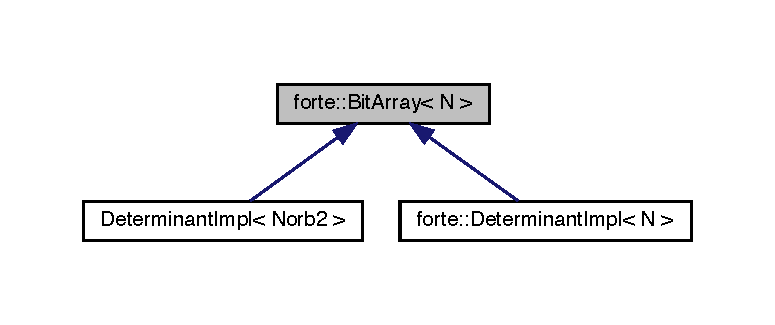
\includegraphics[width=350pt]{classforte_1_1_bit_array__inherit__graph}
\end{center}
\end{figure}
\subsection*{Classes}
\begin{DoxyCompactItemize}
\item 
struct \mbox{\hyperlink{structforte_1_1_bit_array_1_1_hash}{Hash}}
\begin{DoxyCompactList}\small\item\em Returns a hash value for a \mbox{\hyperlink{classforte_1_1_bit_array}{Bit\+Array}} object. \end{DoxyCompactList}\end{DoxyCompactItemize}
\subsection*{Public Types}
\begin{DoxyCompactItemize}
\item 
using \mbox{\hyperlink{classforte_1_1_bit_array_a7f3b4ebbbe4bc80ce60cc6614cb565da}{word\+\_\+t}} = uint64\+\_\+t
\begin{DoxyCompactList}\small\item\em alias for the type used to represent a word (a 64 bit unsigned integer) \end{DoxyCompactList}\end{DoxyCompactItemize}
\subsection*{Public Member Functions}
\begin{DoxyCompactItemize}
\item 
bool \mbox{\hyperlink{classforte_1_1_bit_array_a6763512d765e8dbd07d7f70ed3bb1950}{get\+\_\+bit}} (size\+\_\+t pos) const
\item 
void \mbox{\hyperlink{classforte_1_1_bit_array_aded6c5518708c6433bba8c7b9115199d}{set\+\_\+bit}} (size\+\_\+t pos, bool val)
\begin{DoxyCompactList}\small\item\em set bit in position pos to the value val \end{DoxyCompactList}\item 
void \mbox{\hyperlink{classforte_1_1_bit_array_a52623739054020b7da6ffab1cacf033e}{set\+\_\+word}} (size\+\_\+t pos, \mbox{\hyperlink{classforte_1_1_bit_array_a7f3b4ebbbe4bc80ce60cc6614cb565da}{word\+\_\+t}} word)
\begin{DoxyCompactList}\small\item\em set a word in position pos \end{DoxyCompactList}\item 
size\+\_\+t \mbox{\hyperlink{classforte_1_1_bit_array_a2adc17f21cc178cf6450d74e5629884d}{get\+\_\+nbits}} () const
\begin{DoxyCompactList}\small\item\em return the number of bits \end{DoxyCompactList}\item 
\mbox{\hyperlink{classforte_1_1_bit_array_a3cdd02168872c1fc32ca3999207e3b38}{Bit\+Array}} ()
\begin{DoxyCompactList}\small\item\em default constructor \end{DoxyCompactList}\item 
void \mbox{\hyperlink{classforte_1_1_bit_array_ab9e015d5e061725d21562ce068dc3dbb}{zero}} ()
\begin{DoxyCompactList}\small\item\em set all bits (including unused) to zero \end{DoxyCompactList}\item 
void \mbox{\hyperlink{classforte_1_1_bit_array_ae6c9b2e2ddeaff0df89bc96f27625eb6}{flip}} ()
\begin{DoxyCompactList}\small\item\em flip all bits \end{DoxyCompactList}\item 
bool \mbox{\hyperlink{classforte_1_1_bit_array_abe6a395fc267c35a66224344a43f2cb2}{operator==}} (const \mbox{\hyperlink{classforte_1_1_bit_array}{Bit\+Array}}$<$ N $>$ \&lhs) const
\begin{DoxyCompactList}\small\item\em equal operator \end{DoxyCompactList}\item 
bool \mbox{\hyperlink{classforte_1_1_bit_array_adce1757202af90d3a37ca08d32f0d778}{operator$<$}} (const \mbox{\hyperlink{classforte_1_1_bit_array}{Bit\+Array}}$<$ N $>$ \&lhs) const
\begin{DoxyCompactList}\small\item\em Less than operator. \end{DoxyCompactList}\item 
\mbox{\hyperlink{classforte_1_1_bit_array}{Bit\+Array}}$<$ N $>$ \mbox{\hyperlink{classforte_1_1_bit_array_a6a76d16ef5acbf96710ca3420dbd4be5}{operator$\vert$}} (const \mbox{\hyperlink{classforte_1_1_bit_array}{Bit\+Array}}$<$ N $>$ \&lhs) const
\begin{DoxyCompactList}\small\item\em Bitwise OR operator ($\vert$) \end{DoxyCompactList}\item 
\mbox{\hyperlink{classforte_1_1_bit_array}{Bit\+Array}}$<$ N $>$ \mbox{\hyperlink{classforte_1_1_bit_array_a64a5143b2b9e32399197546d239b6ac0}{operator$\vert$=}} (const \mbox{\hyperlink{classforte_1_1_bit_array}{Bit\+Array}}$<$ N $>$ \&lhs) const
\begin{DoxyCompactList}\small\item\em Bitwise OR operator ($\vert$=) \end{DoxyCompactList}\item 
\mbox{\hyperlink{classforte_1_1_bit_array}{Bit\+Array}}$<$ N $>$ \mbox{\hyperlink{classforte_1_1_bit_array_a3ec375f1cffe72e1e4a737ebc3e4880e}{operator$^\wedge$}} (const \mbox{\hyperlink{classforte_1_1_bit_array}{Bit\+Array}}$<$ N $>$ \&lhs) const
\begin{DoxyCompactList}\small\item\em Bitwise X\+OR operator ($^\wedge$) \end{DoxyCompactList}\item 
\mbox{\hyperlink{classforte_1_1_bit_array}{Bit\+Array}}$<$ N $>$ \mbox{\hyperlink{classforte_1_1_bit_array_a320cbd761b032de5797b95a08d27ac2f}{operator$^\wedge$=}} (const \mbox{\hyperlink{classforte_1_1_bit_array}{Bit\+Array}}$<$ N $>$ \&lhs)
\begin{DoxyCompactList}\small\item\em Bitwise X\+OR operator ($^\wedge$=) \end{DoxyCompactList}\item 
\mbox{\hyperlink{classforte_1_1_bit_array}{Bit\+Array}}$<$ N $>$ \mbox{\hyperlink{classforte_1_1_bit_array_ae3a8e53963f77e90db15dd25f3abe87a}{operator \&}} (const \mbox{\hyperlink{classforte_1_1_bit_array}{Bit\+Array}}$<$ N $>$ \&lhs) const
\begin{DoxyCompactList}\small\item\em Bitwise A\+ND operator (\&) \end{DoxyCompactList}\item 
\mbox{\hyperlink{classforte_1_1_bit_array}{Bit\+Array}}$<$ N $>$ \mbox{\hyperlink{classforte_1_1_bit_array_aaff16cc742d2f2af9dd32636310b17e3}{operator \&=}} (const \mbox{\hyperlink{classforte_1_1_bit_array}{Bit\+Array}}$<$ N $>$ \&lhs)
\begin{DoxyCompactList}\small\item\em Bitwise A\+ND operator (\&=) \end{DoxyCompactList}\item 
int \mbox{\hyperlink{classforte_1_1_bit_array_a96c011285fabafbfcdeed8ab23caafef}{count}} (size\+\_\+t begin=0, size\+\_\+t end=\mbox{\hyperlink{classforte_1_1_bit_array_aeaa8016f00f9ffc5822081f7e45656e8}{nwords\+\_\+}}) const
\begin{DoxyCompactList}\small\item\em Count the number of bits set to true in the words included in the range \mbox{[}begin,end) \end{DoxyCompactList}\item 
uint64\+\_\+t \mbox{\hyperlink{classforte_1_1_bit_array_a8097da916dcef4238671782f4b6e3e59}{find\+\_\+first\+\_\+one}} () const
\item 
void \mbox{\hyperlink{classforte_1_1_bit_array_ae8b38769188be526a5c7be0aeb2481df}{clear\+\_\+first\+\_\+one}} ()
\begin{DoxyCompactList}\small\item\em Clear the first bit set to one (starting from the lowest index) \end{DoxyCompactList}\item 
uint64\+\_\+t \mbox{\hyperlink{classforte_1_1_bit_array_a8485474d3cf2fc4c7ddca917e044e0bc}{find\+\_\+and\+\_\+clear\+\_\+first\+\_\+one}} ()
\item 
double \mbox{\hyperlink{classforte_1_1_bit_array_ad41338929f4ddb1ddb5c4e783e593645}{slater\+\_\+sign}} (int n) const
\item 
double \mbox{\hyperlink{classforte_1_1_bit_array_ae622441da06a5612addf552aeab89040}{slater\+\_\+sign}} (int n, int m) const
\item 
double \mbox{\hyperlink{classforte_1_1_bit_array_a0bb468ffa1f6aa5e95458ee63be391e9}{slater\+\_\+sign\+\_\+safe}} (int n) const
\end{DoxyCompactItemize}
\subsection*{Static Public Member Functions}
\begin{DoxyCompactItemize}
\item 
static constexpr size\+\_\+t \mbox{\hyperlink{classforte_1_1_bit_array_a95b9ef6120acba58b0131afb94538411}{bits\+\_\+to\+\_\+words}} (size\+\_\+t n)
\begin{DoxyCompactList}\small\item\em this tests that a word has 64 bits \end{DoxyCompactList}\end{DoxyCompactItemize}
\subsection*{Static Public Attributes}
\begin{DoxyCompactItemize}
\item 
static constexpr size\+\_\+t \mbox{\hyperlink{classforte_1_1_bit_array_a13866977deadcb098f2e5053025d12f0}{nbits}} = N
\begin{DoxyCompactList}\small\item\em the total number of bits (must be a multiple of 64) \end{DoxyCompactList}\item 
static constexpr size\+\_\+t \mbox{\hyperlink{classforte_1_1_bit_array_ad5ca62ac879b44e0e28017a73fd6c3fd}{bits\+\_\+per\+\_\+word}} = 8 $\ast$ sizeof(\mbox{\hyperlink{classforte_1_1_bit_array_a7f3b4ebbbe4bc80ce60cc6614cb565da}{word\+\_\+t}})
\begin{DoxyCompactList}\small\item\em the number of bits in one word (64) \end{DoxyCompactList}\item 
static constexpr size\+\_\+t \mbox{\hyperlink{classforte_1_1_bit_array_aeaa8016f00f9ffc5822081f7e45656e8}{nwords\+\_\+}} = \mbox{\hyperlink{classforte_1_1_bit_array_a95b9ef6120acba58b0131afb94538411}{bits\+\_\+to\+\_\+words}}(\mbox{\hyperlink{classforte_1_1_bit_array_a13866977deadcb098f2e5053025d12f0}{nbits}})
\begin{DoxyCompactList}\small\item\em the number of words used to store the bits \end{DoxyCompactList}\end{DoxyCompactItemize}
\subsection*{Protected Member Functions}
\begin{DoxyCompactItemize}
\item 
\mbox{\hyperlink{classforte_1_1_bit_array_a7f3b4ebbbe4bc80ce60cc6614cb565da}{word\+\_\+t}} \& \mbox{\hyperlink{classforte_1_1_bit_array_aecfc8a774fcde14d6f458208d658988e}{getword}} (size\+\_\+t pos)
\begin{DoxyCompactList}\small\item\em the word where bit in position pos is found \end{DoxyCompactList}\item 
const \mbox{\hyperlink{classforte_1_1_bit_array_a7f3b4ebbbe4bc80ce60cc6614cb565da}{word\+\_\+t}} \& \mbox{\hyperlink{classforte_1_1_bit_array_afd7eda3840661bf37fc587c1374e9bc8}{getword}} (size\+\_\+t pos) const
\begin{DoxyCompactList}\small\item\em the word where bit in position pos is found (const version) \end{DoxyCompactList}\end{DoxyCompactItemize}
\subsection*{Static Protected Member Functions}
\begin{DoxyCompactItemize}
\item 
static constexpr size\+\_\+t \mbox{\hyperlink{classforte_1_1_bit_array_a4da96fee16fe9fbad29d58bced1b13d1}{whichword}} (size\+\_\+t pos) noexcept
\begin{DoxyCompactList}\small\item\em the index of the word where the bit in position pos is found \end{DoxyCompactList}\item 
static constexpr size\+\_\+t \mbox{\hyperlink{classforte_1_1_bit_array_a10682d9d2a6a947f9a001af6bc3239d7}{whichbit}} (size\+\_\+t pos) noexcept
\begin{DoxyCompactList}\small\item\em the index of a bit within a word \end{DoxyCompactList}\item 
static constexpr \mbox{\hyperlink{classforte_1_1_bit_array_a7f3b4ebbbe4bc80ce60cc6614cb565da}{word\+\_\+t}} \mbox{\hyperlink{classforte_1_1_bit_array_aed63ad4064fdbd25e8d3878767a25e54}{maskbit}} (size\+\_\+t pos) noexcept
\begin{DoxyCompactList}\small\item\em a mask for bit pos in its corresponding word \end{DoxyCompactList}\end{DoxyCompactItemize}
\subsection*{Protected Attributes}
\begin{DoxyCompactItemize}
\item 
std\+::array$<$ \mbox{\hyperlink{classforte_1_1_bit_array_a7f3b4ebbbe4bc80ce60cc6614cb565da}{word\+\_\+t}}, \mbox{\hyperlink{classforte_1_1_bit_array_aeaa8016f00f9ffc5822081f7e45656e8}{nwords\+\_\+}} $>$ \mbox{\hyperlink{classforte_1_1_bit_array_a3c8589dce264f70e98857d6e9eed1245}{words\+\_\+}} = \{\}
\begin{DoxyCompactList}\small\item\em The bits stored as a vector of words (initialized to zero at construction) \end{DoxyCompactList}\end{DoxyCompactItemize}


\subsection{Detailed Description}
\subsubsection*{template$<$size\+\_\+t N$>$\newline
class forte\+::\+Bit\+Array$<$ N $>$}

This class represents an array of N bits. The bits are stored in groups called \char`\"{}words\char`\"{}. Each word contains 64 bits stored as 64-\/bit unsigned integers. 

Words are store in a std\+::array object\+: std\+::array$<$word\+\_\+t, nwords\+\_\+$>$ words\+\_\+ = \{\};

Bir\+Array = $\vert$--64 bits--$\vert$ $\vert$--64 bits--$\vert$ $\vert$--64 bits--$\vert$ ... word\mbox{[}0\mbox{]} word\mbox{[}1\mbox{]} word\mbox{[}2\mbox{]} 

\subsection{Member Typedef Documentation}
\mbox{\Hypertarget{classforte_1_1_bit_array_a7f3b4ebbbe4bc80ce60cc6614cb565da}\label{classforte_1_1_bit_array_a7f3b4ebbbe4bc80ce60cc6614cb565da}} 
\index{forte\+::\+Bit\+Array@{forte\+::\+Bit\+Array}!word\+\_\+t@{word\+\_\+t}}
\index{word\+\_\+t@{word\+\_\+t}!forte\+::\+Bit\+Array@{forte\+::\+Bit\+Array}}
\subsubsection{\texorpdfstring{word\+\_\+t}{word\_t}}
{\footnotesize\ttfamily template$<$size\+\_\+t N$>$ \\
using \mbox{\hyperlink{classforte_1_1_bit_array}{forte\+::\+Bit\+Array}}$<$ N $>$\+::\mbox{\hyperlink{classforte_1_1_bit_array_a7f3b4ebbbe4bc80ce60cc6614cb565da}{word\+\_\+t}} =  uint64\+\_\+t}



alias for the type used to represent a word (a 64 bit unsigned integer) 



\subsection{Constructor \& Destructor Documentation}
\mbox{\Hypertarget{classforte_1_1_bit_array_a3cdd02168872c1fc32ca3999207e3b38}\label{classforte_1_1_bit_array_a3cdd02168872c1fc32ca3999207e3b38}} 
\index{forte\+::\+Bit\+Array@{forte\+::\+Bit\+Array}!Bit\+Array@{Bit\+Array}}
\index{Bit\+Array@{Bit\+Array}!forte\+::\+Bit\+Array@{forte\+::\+Bit\+Array}}
\subsubsection{\texorpdfstring{Bit\+Array()}{BitArray()}}
{\footnotesize\ttfamily template$<$size\+\_\+t N$>$ \\
\mbox{\hyperlink{classforte_1_1_bit_array}{forte\+::\+Bit\+Array}}$<$ N $>$\+::\mbox{\hyperlink{classforte_1_1_bit_array}{Bit\+Array}} (\begin{DoxyParamCaption}{ }\end{DoxyParamCaption})\hspace{0.3cm}{\ttfamily [inline]}}



default constructor 



\subsection{Member Function Documentation}
\mbox{\Hypertarget{classforte_1_1_bit_array_a95b9ef6120acba58b0131afb94538411}\label{classforte_1_1_bit_array_a95b9ef6120acba58b0131afb94538411}} 
\index{forte\+::\+Bit\+Array@{forte\+::\+Bit\+Array}!bits\+\_\+to\+\_\+words@{bits\+\_\+to\+\_\+words}}
\index{bits\+\_\+to\+\_\+words@{bits\+\_\+to\+\_\+words}!forte\+::\+Bit\+Array@{forte\+::\+Bit\+Array}}
\subsubsection{\texorpdfstring{bits\+\_\+to\+\_\+words()}{bits\_to\_words()}}
{\footnotesize\ttfamily template$<$size\+\_\+t N$>$ \\
static constexpr size\+\_\+t \mbox{\hyperlink{classforte_1_1_bit_array}{forte\+::\+Bit\+Array}}$<$ N $>$\+::bits\+\_\+to\+\_\+words (\begin{DoxyParamCaption}\item[{size\+\_\+t}]{n }\end{DoxyParamCaption})\hspace{0.3cm}{\ttfamily [inline]}, {\ttfamily [static]}}



this tests that a word has 64 bits 

this tests that N is a multiple of 64 the number of words needed to store n bits \mbox{\Hypertarget{classforte_1_1_bit_array_ae8b38769188be526a5c7be0aeb2481df}\label{classforte_1_1_bit_array_ae8b38769188be526a5c7be0aeb2481df}} 
\index{forte\+::\+Bit\+Array@{forte\+::\+Bit\+Array}!clear\+\_\+first\+\_\+one@{clear\+\_\+first\+\_\+one}}
\index{clear\+\_\+first\+\_\+one@{clear\+\_\+first\+\_\+one}!forte\+::\+Bit\+Array@{forte\+::\+Bit\+Array}}
\subsubsection{\texorpdfstring{clear\+\_\+first\+\_\+one()}{clear\_first\_one()}}
{\footnotesize\ttfamily template$<$size\+\_\+t N$>$ \\
void \mbox{\hyperlink{classforte_1_1_bit_array}{forte\+::\+Bit\+Array}}$<$ N $>$\+::clear\+\_\+first\+\_\+one (\begin{DoxyParamCaption}{ }\end{DoxyParamCaption})\hspace{0.3cm}{\ttfamily [inline]}}



Clear the first bit set to one (starting from the lowest index) 

\mbox{\Hypertarget{classforte_1_1_bit_array_a96c011285fabafbfcdeed8ab23caafef}\label{classforte_1_1_bit_array_a96c011285fabafbfcdeed8ab23caafef}} 
\index{forte\+::\+Bit\+Array@{forte\+::\+Bit\+Array}!count@{count}}
\index{count@{count}!forte\+::\+Bit\+Array@{forte\+::\+Bit\+Array}}
\subsubsection{\texorpdfstring{count()}{count()}}
{\footnotesize\ttfamily template$<$size\+\_\+t N$>$ \\
int \mbox{\hyperlink{classforte_1_1_bit_array}{forte\+::\+Bit\+Array}}$<$ N $>$\+::count (\begin{DoxyParamCaption}\item[{size\+\_\+t}]{begin = {\ttfamily 0},  }\item[{size\+\_\+t}]{end = {\ttfamily \mbox{\hyperlink{classforte_1_1_bit_array_aeaa8016f00f9ffc5822081f7e45656e8}{nwords\+\_\+}}} }\end{DoxyParamCaption}) const\hspace{0.3cm}{\ttfamily [inline]}}



Count the number of bits set to true in the words included in the range \mbox{[}begin,end) 

\mbox{\Hypertarget{classforte_1_1_bit_array_a8485474d3cf2fc4c7ddca917e044e0bc}\label{classforte_1_1_bit_array_a8485474d3cf2fc4c7ddca917e044e0bc}} 
\index{forte\+::\+Bit\+Array@{forte\+::\+Bit\+Array}!find\+\_\+and\+\_\+clear\+\_\+first\+\_\+one@{find\+\_\+and\+\_\+clear\+\_\+first\+\_\+one}}
\index{find\+\_\+and\+\_\+clear\+\_\+first\+\_\+one@{find\+\_\+and\+\_\+clear\+\_\+first\+\_\+one}!forte\+::\+Bit\+Array@{forte\+::\+Bit\+Array}}
\subsubsection{\texorpdfstring{find\+\_\+and\+\_\+clear\+\_\+first\+\_\+one()}{find\_and\_clear\_first\_one()}}
{\footnotesize\ttfamily template$<$size\+\_\+t N$>$ \\
uint64\+\_\+t \mbox{\hyperlink{classforte_1_1_bit_array}{forte\+::\+Bit\+Array}}$<$ N $>$\+::find\+\_\+and\+\_\+clear\+\_\+first\+\_\+one (\begin{DoxyParamCaption}{ }\end{DoxyParamCaption})\hspace{0.3cm}{\ttfamily [inline]}}

Find the first bit set to one and clear it (starting from the lowest index) \begin{DoxyReturn}{Returns}
the index of the the first bit, or if all bits are zero, returns $\sim$0 
\end{DoxyReturn}
\mbox{\Hypertarget{classforte_1_1_bit_array_a8097da916dcef4238671782f4b6e3e59}\label{classforte_1_1_bit_array_a8097da916dcef4238671782f4b6e3e59}} 
\index{forte\+::\+Bit\+Array@{forte\+::\+Bit\+Array}!find\+\_\+first\+\_\+one@{find\+\_\+first\+\_\+one}}
\index{find\+\_\+first\+\_\+one@{find\+\_\+first\+\_\+one}!forte\+::\+Bit\+Array@{forte\+::\+Bit\+Array}}
\subsubsection{\texorpdfstring{find\+\_\+first\+\_\+one()}{find\_first\_one()}}
{\footnotesize\ttfamily template$<$size\+\_\+t N$>$ \\
uint64\+\_\+t \mbox{\hyperlink{classforte_1_1_bit_array}{forte\+::\+Bit\+Array}}$<$ N $>$\+::find\+\_\+first\+\_\+one (\begin{DoxyParamCaption}{ }\end{DoxyParamCaption}) const\hspace{0.3cm}{\ttfamily [inline]}}

Find the first bit set to one (starting from the lowest index) \begin{DoxyReturn}{Returns}
the index of the the first bit, or if all bits are zero, returns $\sim$0 
\end{DoxyReturn}
\mbox{\Hypertarget{classforte_1_1_bit_array_ae6c9b2e2ddeaff0df89bc96f27625eb6}\label{classforte_1_1_bit_array_ae6c9b2e2ddeaff0df89bc96f27625eb6}} 
\index{forte\+::\+Bit\+Array@{forte\+::\+Bit\+Array}!flip@{flip}}
\index{flip@{flip}!forte\+::\+Bit\+Array@{forte\+::\+Bit\+Array}}
\subsubsection{\texorpdfstring{flip()}{flip()}}
{\footnotesize\ttfamily template$<$size\+\_\+t N$>$ \\
void \mbox{\hyperlink{classforte_1_1_bit_array}{forte\+::\+Bit\+Array}}$<$ N $>$\+::flip (\begin{DoxyParamCaption}{ }\end{DoxyParamCaption})\hspace{0.3cm}{\ttfamily [inline]}}



flip all bits 

\mbox{\Hypertarget{classforte_1_1_bit_array_a6763512d765e8dbd07d7f70ed3bb1950}\label{classforte_1_1_bit_array_a6763512d765e8dbd07d7f70ed3bb1950}} 
\index{forte\+::\+Bit\+Array@{forte\+::\+Bit\+Array}!get\+\_\+bit@{get\+\_\+bit}}
\index{get\+\_\+bit@{get\+\_\+bit}!forte\+::\+Bit\+Array@{forte\+::\+Bit\+Array}}
\subsubsection{\texorpdfstring{get\+\_\+bit()}{get\_bit()}}
{\footnotesize\ttfamily template$<$size\+\_\+t N$>$ \\
bool \mbox{\hyperlink{classforte_1_1_bit_array}{forte\+::\+Bit\+Array}}$<$ N $>$\+::get\+\_\+bit (\begin{DoxyParamCaption}\item[{size\+\_\+t}]{pos }\end{DoxyParamCaption}) const\hspace{0.3cm}{\ttfamily [inline]}}

\mbox{\Hypertarget{classforte_1_1_bit_array_a2adc17f21cc178cf6450d74e5629884d}\label{classforte_1_1_bit_array_a2adc17f21cc178cf6450d74e5629884d}} 
\index{forte\+::\+Bit\+Array@{forte\+::\+Bit\+Array}!get\+\_\+nbits@{get\+\_\+nbits}}
\index{get\+\_\+nbits@{get\+\_\+nbits}!forte\+::\+Bit\+Array@{forte\+::\+Bit\+Array}}
\subsubsection{\texorpdfstring{get\+\_\+nbits()}{get\_nbits()}}
{\footnotesize\ttfamily template$<$size\+\_\+t N$>$ \\
size\+\_\+t \mbox{\hyperlink{classforte_1_1_bit_array}{forte\+::\+Bit\+Array}}$<$ N $>$\+::get\+\_\+nbits (\begin{DoxyParamCaption}{ }\end{DoxyParamCaption}) const\hspace{0.3cm}{\ttfamily [inline]}}



return the number of bits 

\mbox{\Hypertarget{classforte_1_1_bit_array_aecfc8a774fcde14d6f458208d658988e}\label{classforte_1_1_bit_array_aecfc8a774fcde14d6f458208d658988e}} 
\index{forte\+::\+Bit\+Array@{forte\+::\+Bit\+Array}!getword@{getword}}
\index{getword@{getword}!forte\+::\+Bit\+Array@{forte\+::\+Bit\+Array}}
\subsubsection{\texorpdfstring{getword()}{getword()}\hspace{0.1cm}{\footnotesize\ttfamily [1/2]}}
{\footnotesize\ttfamily template$<$size\+\_\+t N$>$ \\
\mbox{\hyperlink{classforte_1_1_bit_array_a7f3b4ebbbe4bc80ce60cc6614cb565da}{word\+\_\+t}}\& \mbox{\hyperlink{classforte_1_1_bit_array}{forte\+::\+Bit\+Array}}$<$ N $>$\+::getword (\begin{DoxyParamCaption}\item[{size\+\_\+t}]{pos }\end{DoxyParamCaption})\hspace{0.3cm}{\ttfamily [inline]}, {\ttfamily [protected]}}



the word where bit in position pos is found 

\mbox{\Hypertarget{classforte_1_1_bit_array_afd7eda3840661bf37fc587c1374e9bc8}\label{classforte_1_1_bit_array_afd7eda3840661bf37fc587c1374e9bc8}} 
\index{forte\+::\+Bit\+Array@{forte\+::\+Bit\+Array}!getword@{getword}}
\index{getword@{getword}!forte\+::\+Bit\+Array@{forte\+::\+Bit\+Array}}
\subsubsection{\texorpdfstring{getword()}{getword()}\hspace{0.1cm}{\footnotesize\ttfamily [2/2]}}
{\footnotesize\ttfamily template$<$size\+\_\+t N$>$ \\
const \mbox{\hyperlink{classforte_1_1_bit_array_a7f3b4ebbbe4bc80ce60cc6614cb565da}{word\+\_\+t}}\& \mbox{\hyperlink{classforte_1_1_bit_array}{forte\+::\+Bit\+Array}}$<$ N $>$\+::getword (\begin{DoxyParamCaption}\item[{size\+\_\+t}]{pos }\end{DoxyParamCaption}) const\hspace{0.3cm}{\ttfamily [inline]}, {\ttfamily [protected]}}



the word where bit in position pos is found (const version) 

\mbox{\Hypertarget{classforte_1_1_bit_array_aed63ad4064fdbd25e8d3878767a25e54}\label{classforte_1_1_bit_array_aed63ad4064fdbd25e8d3878767a25e54}} 
\index{forte\+::\+Bit\+Array@{forte\+::\+Bit\+Array}!maskbit@{maskbit}}
\index{maskbit@{maskbit}!forte\+::\+Bit\+Array@{forte\+::\+Bit\+Array}}
\subsubsection{\texorpdfstring{maskbit()}{maskbit()}}
{\footnotesize\ttfamily template$<$size\+\_\+t N$>$ \\
static constexpr \mbox{\hyperlink{classforte_1_1_bit_array_a7f3b4ebbbe4bc80ce60cc6614cb565da}{word\+\_\+t}} \mbox{\hyperlink{classforte_1_1_bit_array}{forte\+::\+Bit\+Array}}$<$ N $>$\+::maskbit (\begin{DoxyParamCaption}\item[{size\+\_\+t}]{pos }\end{DoxyParamCaption})\hspace{0.3cm}{\ttfamily [inline]}, {\ttfamily [static]}, {\ttfamily [protected]}, {\ttfamily [noexcept]}}



a mask for bit pos in its corresponding word 

\mbox{\Hypertarget{classforte_1_1_bit_array_ae3a8e53963f77e90db15dd25f3abe87a}\label{classforte_1_1_bit_array_ae3a8e53963f77e90db15dd25f3abe87a}} 
\index{forte\+::\+Bit\+Array@{forte\+::\+Bit\+Array}!operator \&@{operator \&}}
\index{operator \&@{operator \&}!forte\+::\+Bit\+Array@{forte\+::\+Bit\+Array}}
\subsubsection{\texorpdfstring{operator \&()}{operator \&()}}
{\footnotesize\ttfamily template$<$size\+\_\+t N$>$ \\
\mbox{\hyperlink{classforte_1_1_bit_array}{Bit\+Array}}$<$N$>$ \mbox{\hyperlink{classforte_1_1_bit_array}{forte\+::\+Bit\+Array}}$<$ N $>$\+::operator\& (\begin{DoxyParamCaption}\item[{const \mbox{\hyperlink{classforte_1_1_bit_array}{Bit\+Array}}$<$ N $>$ \&}]{lhs }\end{DoxyParamCaption}) const\hspace{0.3cm}{\ttfamily [inline]}}



Bitwise A\+ND operator (\&) 

\mbox{\Hypertarget{classforte_1_1_bit_array_aaff16cc742d2f2af9dd32636310b17e3}\label{classforte_1_1_bit_array_aaff16cc742d2f2af9dd32636310b17e3}} 
\index{forte\+::\+Bit\+Array@{forte\+::\+Bit\+Array}!operator \&=@{operator \&=}}
\index{operator \&=@{operator \&=}!forte\+::\+Bit\+Array@{forte\+::\+Bit\+Array}}
\subsubsection{\texorpdfstring{operator \&=()}{operator \&=()}}
{\footnotesize\ttfamily template$<$size\+\_\+t N$>$ \\
\mbox{\hyperlink{classforte_1_1_bit_array}{Bit\+Array}}$<$N$>$ \mbox{\hyperlink{classforte_1_1_bit_array}{forte\+::\+Bit\+Array}}$<$ N $>$\+::operator\&= (\begin{DoxyParamCaption}\item[{const \mbox{\hyperlink{classforte_1_1_bit_array}{Bit\+Array}}$<$ N $>$ \&}]{lhs }\end{DoxyParamCaption})\hspace{0.3cm}{\ttfamily [inline]}}



Bitwise A\+ND operator (\&=) 

\mbox{\Hypertarget{classforte_1_1_bit_array_adce1757202af90d3a37ca08d32f0d778}\label{classforte_1_1_bit_array_adce1757202af90d3a37ca08d32f0d778}} 
\index{forte\+::\+Bit\+Array@{forte\+::\+Bit\+Array}!operator$<$@{operator$<$}}
\index{operator$<$@{operator$<$}!forte\+::\+Bit\+Array@{forte\+::\+Bit\+Array}}
\subsubsection{\texorpdfstring{operator$<$()}{operator<()}}
{\footnotesize\ttfamily template$<$size\+\_\+t N$>$ \\
bool \mbox{\hyperlink{classforte_1_1_bit_array}{forte\+::\+Bit\+Array}}$<$ N $>$\+::operator$<$ (\begin{DoxyParamCaption}\item[{const \mbox{\hyperlink{classforte_1_1_bit_array}{Bit\+Array}}$<$ N $>$ \&}]{lhs }\end{DoxyParamCaption}) const\hspace{0.3cm}{\ttfamily [inline]}}



Less than operator. 

\mbox{\Hypertarget{classforte_1_1_bit_array_abe6a395fc267c35a66224344a43f2cb2}\label{classforte_1_1_bit_array_abe6a395fc267c35a66224344a43f2cb2}} 
\index{forte\+::\+Bit\+Array@{forte\+::\+Bit\+Array}!operator==@{operator==}}
\index{operator==@{operator==}!forte\+::\+Bit\+Array@{forte\+::\+Bit\+Array}}
\subsubsection{\texorpdfstring{operator==()}{operator==()}}
{\footnotesize\ttfamily template$<$size\+\_\+t N$>$ \\
bool \mbox{\hyperlink{classforte_1_1_bit_array}{forte\+::\+Bit\+Array}}$<$ N $>$\+::operator== (\begin{DoxyParamCaption}\item[{const \mbox{\hyperlink{classforte_1_1_bit_array}{Bit\+Array}}$<$ N $>$ \&}]{lhs }\end{DoxyParamCaption}) const\hspace{0.3cm}{\ttfamily [inline]}}



equal operator 

\mbox{\Hypertarget{classforte_1_1_bit_array_a3ec375f1cffe72e1e4a737ebc3e4880e}\label{classforte_1_1_bit_array_a3ec375f1cffe72e1e4a737ebc3e4880e}} 
\index{forte\+::\+Bit\+Array@{forte\+::\+Bit\+Array}!operator$^\wedge$@{operator$^\wedge$}}
\index{operator$^\wedge$@{operator$^\wedge$}!forte\+::\+Bit\+Array@{forte\+::\+Bit\+Array}}
\subsubsection{\texorpdfstring{operator$^\wedge$()}{operator^()}}
{\footnotesize\ttfamily template$<$size\+\_\+t N$>$ \\
\mbox{\hyperlink{classforte_1_1_bit_array}{Bit\+Array}}$<$N$>$ \mbox{\hyperlink{classforte_1_1_bit_array}{forte\+::\+Bit\+Array}}$<$ N $>$\+::operator$^\wedge$ (\begin{DoxyParamCaption}\item[{const \mbox{\hyperlink{classforte_1_1_bit_array}{Bit\+Array}}$<$ N $>$ \&}]{lhs }\end{DoxyParamCaption}) const\hspace{0.3cm}{\ttfamily [inline]}}



Bitwise X\+OR operator ($^\wedge$) 

\mbox{\Hypertarget{classforte_1_1_bit_array_a320cbd761b032de5797b95a08d27ac2f}\label{classforte_1_1_bit_array_a320cbd761b032de5797b95a08d27ac2f}} 
\index{forte\+::\+Bit\+Array@{forte\+::\+Bit\+Array}!operator$^\wedge$=@{operator$^\wedge$=}}
\index{operator$^\wedge$=@{operator$^\wedge$=}!forte\+::\+Bit\+Array@{forte\+::\+Bit\+Array}}
\subsubsection{\texorpdfstring{operator$^\wedge$=()}{operator^=()}}
{\footnotesize\ttfamily template$<$size\+\_\+t N$>$ \\
\mbox{\hyperlink{classforte_1_1_bit_array}{Bit\+Array}}$<$N$>$ \mbox{\hyperlink{classforte_1_1_bit_array}{forte\+::\+Bit\+Array}}$<$ N $>$\+::operator$^\wedge$= (\begin{DoxyParamCaption}\item[{const \mbox{\hyperlink{classforte_1_1_bit_array}{Bit\+Array}}$<$ N $>$ \&}]{lhs }\end{DoxyParamCaption})\hspace{0.3cm}{\ttfamily [inline]}}



Bitwise X\+OR operator ($^\wedge$=) 

\mbox{\Hypertarget{classforte_1_1_bit_array_a6a76d16ef5acbf96710ca3420dbd4be5}\label{classforte_1_1_bit_array_a6a76d16ef5acbf96710ca3420dbd4be5}} 
\index{forte\+::\+Bit\+Array@{forte\+::\+Bit\+Array}!operator\texttt{"|}@{operator\texttt{"|}}}
\index{operator\texttt{"|}@{operator\texttt{"|}}!forte\+::\+Bit\+Array@{forte\+::\+Bit\+Array}}
\subsubsection{\texorpdfstring{operator\texttt{"|}()}{operator|()}}
{\footnotesize\ttfamily template$<$size\+\_\+t N$>$ \\
\mbox{\hyperlink{classforte_1_1_bit_array}{Bit\+Array}}$<$N$>$ \mbox{\hyperlink{classforte_1_1_bit_array}{forte\+::\+Bit\+Array}}$<$ N $>$\+::operator$\vert$ (\begin{DoxyParamCaption}\item[{const \mbox{\hyperlink{classforte_1_1_bit_array}{Bit\+Array}}$<$ N $>$ \&}]{lhs }\end{DoxyParamCaption}) const\hspace{0.3cm}{\ttfamily [inline]}}



Bitwise OR operator ($\vert$) 

\mbox{\Hypertarget{classforte_1_1_bit_array_a64a5143b2b9e32399197546d239b6ac0}\label{classforte_1_1_bit_array_a64a5143b2b9e32399197546d239b6ac0}} 
\index{forte\+::\+Bit\+Array@{forte\+::\+Bit\+Array}!operator\texttt{"|}=@{operator\texttt{"|}=}}
\index{operator\texttt{"|}=@{operator\texttt{"|}=}!forte\+::\+Bit\+Array@{forte\+::\+Bit\+Array}}
\subsubsection{\texorpdfstring{operator\texttt{"|}=()}{operator|=()}}
{\footnotesize\ttfamily template$<$size\+\_\+t N$>$ \\
\mbox{\hyperlink{classforte_1_1_bit_array}{Bit\+Array}}$<$N$>$ \mbox{\hyperlink{classforte_1_1_bit_array}{forte\+::\+Bit\+Array}}$<$ N $>$\+::operator$\vert$= (\begin{DoxyParamCaption}\item[{const \mbox{\hyperlink{classforte_1_1_bit_array}{Bit\+Array}}$<$ N $>$ \&}]{lhs }\end{DoxyParamCaption}) const\hspace{0.3cm}{\ttfamily [inline]}}



Bitwise OR operator ($\vert$=) 

\mbox{\Hypertarget{classforte_1_1_bit_array_aded6c5518708c6433bba8c7b9115199d}\label{classforte_1_1_bit_array_aded6c5518708c6433bba8c7b9115199d}} 
\index{forte\+::\+Bit\+Array@{forte\+::\+Bit\+Array}!set\+\_\+bit@{set\+\_\+bit}}
\index{set\+\_\+bit@{set\+\_\+bit}!forte\+::\+Bit\+Array@{forte\+::\+Bit\+Array}}
\subsubsection{\texorpdfstring{set\+\_\+bit()}{set\_bit()}}
{\footnotesize\ttfamily template$<$size\+\_\+t N$>$ \\
void \mbox{\hyperlink{classforte_1_1_bit_array}{forte\+::\+Bit\+Array}}$<$ N $>$\+::set\+\_\+bit (\begin{DoxyParamCaption}\item[{size\+\_\+t}]{pos,  }\item[{bool}]{val }\end{DoxyParamCaption})\hspace{0.3cm}{\ttfamily [inline]}}



set bit in position pos to the value val 

\mbox{\Hypertarget{classforte_1_1_bit_array_a52623739054020b7da6ffab1cacf033e}\label{classforte_1_1_bit_array_a52623739054020b7da6ffab1cacf033e}} 
\index{forte\+::\+Bit\+Array@{forte\+::\+Bit\+Array}!set\+\_\+word@{set\+\_\+word}}
\index{set\+\_\+word@{set\+\_\+word}!forte\+::\+Bit\+Array@{forte\+::\+Bit\+Array}}
\subsubsection{\texorpdfstring{set\+\_\+word()}{set\_word()}}
{\footnotesize\ttfamily template$<$size\+\_\+t N$>$ \\
void \mbox{\hyperlink{classforte_1_1_bit_array}{forte\+::\+Bit\+Array}}$<$ N $>$\+::set\+\_\+word (\begin{DoxyParamCaption}\item[{size\+\_\+t}]{pos,  }\item[{\mbox{\hyperlink{classforte_1_1_bit_array_a7f3b4ebbbe4bc80ce60cc6614cb565da}{word\+\_\+t}}}]{word }\end{DoxyParamCaption})\hspace{0.3cm}{\ttfamily [inline]}}



set a word in position pos 

\mbox{\Hypertarget{classforte_1_1_bit_array_ad41338929f4ddb1ddb5c4e783e593645}\label{classforte_1_1_bit_array_ad41338929f4ddb1ddb5c4e783e593645}} 
\index{forte\+::\+Bit\+Array@{forte\+::\+Bit\+Array}!slater\+\_\+sign@{slater\+\_\+sign}}
\index{slater\+\_\+sign@{slater\+\_\+sign}!forte\+::\+Bit\+Array@{forte\+::\+Bit\+Array}}
\subsubsection{\texorpdfstring{slater\+\_\+sign()}{slater\_sign()}\hspace{0.1cm}{\footnotesize\ttfamily [1/2]}}
{\footnotesize\ttfamily template$<$size\+\_\+t N$>$ \\
double \mbox{\hyperlink{classforte_1_1_bit_array}{forte\+::\+Bit\+Array}}$<$ N $>$\+::slater\+\_\+sign (\begin{DoxyParamCaption}\item[{int}]{n }\end{DoxyParamCaption}) const\hspace{0.3cm}{\ttfamily [inline]}}

Return the sign of a\+\_\+n applied to this determinant This function ignores if bit n is set or not \mbox{\Hypertarget{classforte_1_1_bit_array_ae622441da06a5612addf552aeab89040}\label{classforte_1_1_bit_array_ae622441da06a5612addf552aeab89040}} 
\index{forte\+::\+Bit\+Array@{forte\+::\+Bit\+Array}!slater\+\_\+sign@{slater\+\_\+sign}}
\index{slater\+\_\+sign@{slater\+\_\+sign}!forte\+::\+Bit\+Array@{forte\+::\+Bit\+Array}}
\subsubsection{\texorpdfstring{slater\+\_\+sign()}{slater\_sign()}\hspace{0.1cm}{\footnotesize\ttfamily [2/2]}}
{\footnotesize\ttfamily template$<$size\+\_\+t N$>$ \\
double \mbox{\hyperlink{classforte_1_1_bit_array}{forte\+::\+Bit\+Array}}$<$ N $>$\+::slater\+\_\+sign (\begin{DoxyParamCaption}\item[{int}]{n,  }\item[{int}]{m }\end{DoxyParamCaption}) const\hspace{0.3cm}{\ttfamily [inline]}}

Return the sign for a pair of second quantized operators The sign depends only on the number of bits = 1 between n and m There are no restrictions on n and m \mbox{\Hypertarget{classforte_1_1_bit_array_a0bb468ffa1f6aa5e95458ee63be391e9}\label{classforte_1_1_bit_array_a0bb468ffa1f6aa5e95458ee63be391e9}} 
\index{forte\+::\+Bit\+Array@{forte\+::\+Bit\+Array}!slater\+\_\+sign\+\_\+safe@{slater\+\_\+sign\+\_\+safe}}
\index{slater\+\_\+sign\+\_\+safe@{slater\+\_\+sign\+\_\+safe}!forte\+::\+Bit\+Array@{forte\+::\+Bit\+Array}}
\subsubsection{\texorpdfstring{slater\+\_\+sign\+\_\+safe()}{slater\_sign\_safe()}}
{\footnotesize\ttfamily template$<$size\+\_\+t N$>$ \\
double \mbox{\hyperlink{classforte_1_1_bit_array}{forte\+::\+Bit\+Array}}$<$ N $>$\+::slater\+\_\+sign\+\_\+safe (\begin{DoxyParamCaption}\item[{int}]{n }\end{DoxyParamCaption}) const\hspace{0.3cm}{\ttfamily [inline]}}

Return the sign of a\+\_\+n applied to this determinant this version is inefficient and should be used only for testing/debugging \mbox{\Hypertarget{classforte_1_1_bit_array_a10682d9d2a6a947f9a001af6bc3239d7}\label{classforte_1_1_bit_array_a10682d9d2a6a947f9a001af6bc3239d7}} 
\index{forte\+::\+Bit\+Array@{forte\+::\+Bit\+Array}!whichbit@{whichbit}}
\index{whichbit@{whichbit}!forte\+::\+Bit\+Array@{forte\+::\+Bit\+Array}}
\subsubsection{\texorpdfstring{whichbit()}{whichbit()}}
{\footnotesize\ttfamily template$<$size\+\_\+t N$>$ \\
static constexpr size\+\_\+t \mbox{\hyperlink{classforte_1_1_bit_array}{forte\+::\+Bit\+Array}}$<$ N $>$\+::whichbit (\begin{DoxyParamCaption}\item[{size\+\_\+t}]{pos }\end{DoxyParamCaption})\hspace{0.3cm}{\ttfamily [inline]}, {\ttfamily [static]}, {\ttfamily [protected]}, {\ttfamily [noexcept]}}



the index of a bit within a word 

\mbox{\Hypertarget{classforte_1_1_bit_array_a4da96fee16fe9fbad29d58bced1b13d1}\label{classforte_1_1_bit_array_a4da96fee16fe9fbad29d58bced1b13d1}} 
\index{forte\+::\+Bit\+Array@{forte\+::\+Bit\+Array}!whichword@{whichword}}
\index{whichword@{whichword}!forte\+::\+Bit\+Array@{forte\+::\+Bit\+Array}}
\subsubsection{\texorpdfstring{whichword()}{whichword()}}
{\footnotesize\ttfamily template$<$size\+\_\+t N$>$ \\
static constexpr size\+\_\+t \mbox{\hyperlink{classforte_1_1_bit_array}{forte\+::\+Bit\+Array}}$<$ N $>$\+::whichword (\begin{DoxyParamCaption}\item[{size\+\_\+t}]{pos }\end{DoxyParamCaption})\hspace{0.3cm}{\ttfamily [inline]}, {\ttfamily [static]}, {\ttfamily [protected]}, {\ttfamily [noexcept]}}



the index of the word where the bit in position pos is found 

\mbox{\Hypertarget{classforte_1_1_bit_array_ab9e015d5e061725d21562ce068dc3dbb}\label{classforte_1_1_bit_array_ab9e015d5e061725d21562ce068dc3dbb}} 
\index{forte\+::\+Bit\+Array@{forte\+::\+Bit\+Array}!zero@{zero}}
\index{zero@{zero}!forte\+::\+Bit\+Array@{forte\+::\+Bit\+Array}}
\subsubsection{\texorpdfstring{zero()}{zero()}}
{\footnotesize\ttfamily template$<$size\+\_\+t N$>$ \\
void \mbox{\hyperlink{classforte_1_1_bit_array}{forte\+::\+Bit\+Array}}$<$ N $>$\+::zero (\begin{DoxyParamCaption}{ }\end{DoxyParamCaption})\hspace{0.3cm}{\ttfamily [inline]}}



set all bits (including unused) to zero 



\subsection{Member Data Documentation}
\mbox{\Hypertarget{classforte_1_1_bit_array_ad5ca62ac879b44e0e28017a73fd6c3fd}\label{classforte_1_1_bit_array_ad5ca62ac879b44e0e28017a73fd6c3fd}} 
\index{forte\+::\+Bit\+Array@{forte\+::\+Bit\+Array}!bits\+\_\+per\+\_\+word@{bits\+\_\+per\+\_\+word}}
\index{bits\+\_\+per\+\_\+word@{bits\+\_\+per\+\_\+word}!forte\+::\+Bit\+Array@{forte\+::\+Bit\+Array}}
\subsubsection{\texorpdfstring{bits\+\_\+per\+\_\+word}{bits\_per\_word}}
{\footnotesize\ttfamily template$<$size\+\_\+t N$>$ \\
constexpr size\+\_\+t \mbox{\hyperlink{classforte_1_1_bit_array}{forte\+::\+Bit\+Array}}$<$ N $>$\+::bits\+\_\+per\+\_\+word = 8 $\ast$ sizeof(\mbox{\hyperlink{classforte_1_1_bit_array_a7f3b4ebbbe4bc80ce60cc6614cb565da}{word\+\_\+t}})\hspace{0.3cm}{\ttfamily [static]}}



the number of bits in one word (64) 

\mbox{\Hypertarget{classforte_1_1_bit_array_a13866977deadcb098f2e5053025d12f0}\label{classforte_1_1_bit_array_a13866977deadcb098f2e5053025d12f0}} 
\index{forte\+::\+Bit\+Array@{forte\+::\+Bit\+Array}!nbits@{nbits}}
\index{nbits@{nbits}!forte\+::\+Bit\+Array@{forte\+::\+Bit\+Array}}
\subsubsection{\texorpdfstring{nbits}{nbits}}
{\footnotesize\ttfamily template$<$size\+\_\+t N$>$ \\
constexpr size\+\_\+t \mbox{\hyperlink{classforte_1_1_bit_array}{forte\+::\+Bit\+Array}}$<$ N $>$\+::nbits = N\hspace{0.3cm}{\ttfamily [static]}}



the total number of bits (must be a multiple of 64) 

\mbox{\Hypertarget{classforte_1_1_bit_array_aeaa8016f00f9ffc5822081f7e45656e8}\label{classforte_1_1_bit_array_aeaa8016f00f9ffc5822081f7e45656e8}} 
\index{forte\+::\+Bit\+Array@{forte\+::\+Bit\+Array}!nwords\+\_\+@{nwords\+\_\+}}
\index{nwords\+\_\+@{nwords\+\_\+}!forte\+::\+Bit\+Array@{forte\+::\+Bit\+Array}}
\subsubsection{\texorpdfstring{nwords\+\_\+}{nwords\_}}
{\footnotesize\ttfamily template$<$size\+\_\+t N$>$ \\
constexpr size\+\_\+t \mbox{\hyperlink{classforte_1_1_bit_array}{forte\+::\+Bit\+Array}}$<$ N $>$\+::nwords\+\_\+ = \mbox{\hyperlink{classforte_1_1_bit_array_a95b9ef6120acba58b0131afb94538411}{bits\+\_\+to\+\_\+words}}(\mbox{\hyperlink{classforte_1_1_bit_array_a13866977deadcb098f2e5053025d12f0}{nbits}})\hspace{0.3cm}{\ttfamily [static]}}



the number of words used to store the bits 

\mbox{\Hypertarget{classforte_1_1_bit_array_a3c8589dce264f70e98857d6e9eed1245}\label{classforte_1_1_bit_array_a3c8589dce264f70e98857d6e9eed1245}} 
\index{forte\+::\+Bit\+Array@{forte\+::\+Bit\+Array}!words\+\_\+@{words\+\_\+}}
\index{words\+\_\+@{words\+\_\+}!forte\+::\+Bit\+Array@{forte\+::\+Bit\+Array}}
\subsubsection{\texorpdfstring{words\+\_\+}{words\_}}
{\footnotesize\ttfamily template$<$size\+\_\+t N$>$ \\
std\+::array$<$\mbox{\hyperlink{classforte_1_1_bit_array_a7f3b4ebbbe4bc80ce60cc6614cb565da}{word\+\_\+t}}, \mbox{\hyperlink{classforte_1_1_bit_array_aeaa8016f00f9ffc5822081f7e45656e8}{nwords\+\_\+}}$>$ \mbox{\hyperlink{classforte_1_1_bit_array}{forte\+::\+Bit\+Array}}$<$ N $>$\+::words\+\_\+ = \{\}\hspace{0.3cm}{\ttfamily [protected]}}



The bits stored as a vector of words (initialized to zero at construction) 



The documentation for this class was generated from the following file\+:\begin{DoxyCompactItemize}
\item 
/\+Users/fevange/\+Source/forte/src/sparse\+\_\+ci/\mbox{\hyperlink{bitarray_8hpp}{bitarray.\+hpp}}\end{DoxyCompactItemize}

\hypertarget{classforte_1_1_blocked_tensor_factory}{}\section{forte\+:\+:Blocked\+Tensor\+Factory Class Reference}
\label{classforte_1_1_blocked_tensor_factory}\index{forte\+::\+Blocked\+Tensor\+Factory@{forte\+::\+Blocked\+Tensor\+Factory}}


{\ttfamily \#include $<$blockedtensorfactory.\+h$>$}

\subsection*{Public Member Functions}
\begin{DoxyCompactItemize}
\item 
\mbox{\hyperlink{classforte_1_1_blocked_tensor_factory_a4d918bbb012371d84c4c6b09a49137cf}{Blocked\+Tensor\+Factory}} ()
\item 
\mbox{\hyperlink{classforte_1_1_blocked_tensor_factory_a7e8f4846afdf3a558725eecee7ebb7ed}{$\sim$\+Blocked\+Tensor\+Factory}} ()
\item 
ambit\+::\+Blocked\+Tensor \mbox{\hyperlink{classforte_1_1_blocked_tensor_factory_afd101ce291ce4d6c5068edb9afde081b}{build}} (ambit\+::\+Tensor\+Type storage, const std\+::string \&name, const std\+::vector$<$ std\+::string $>$ \&spin\+\_\+stuff, bool is\+\_\+local\+\_\+variable=false)
\item 
void \mbox{\hyperlink{classforte_1_1_blocked_tensor_factory_ab9bfd3f8d82a640bf816d841222396a8}{add\+\_\+mo\+\_\+space}} (const std\+::string \&name, const std\+::string \&mo\+\_\+indices, std\+::vector$<$ size\+\_\+t $>$ mos, ambit\+::\+Spin\+Type spin)
\item 
void \mbox{\hyperlink{classforte_1_1_blocked_tensor_factory_a774396c3920f7e306bef84e35b15eaf0}{add\+\_\+mo\+\_\+space}} (const std\+::string \&name, const std\+::string \&mo\+\_\+indices, std\+::vector$<$ std\+::pair$<$ size\+\_\+t, ambit\+::\+Spin\+Type $>$$>$ mo\+\_\+spin)
\item 
void \mbox{\hyperlink{classforte_1_1_blocked_tensor_factory_aa0e2f489066c8636c897b5b15a48b438}{add\+\_\+composite\+\_\+mo\+\_\+space}} (const std\+::string \&name, const std\+::string \&mo\+\_\+indices, const std\+::vector$<$ std\+::string $>$ \&subspaces)
\item 
void \mbox{\hyperlink{classforte_1_1_blocked_tensor_factory_aab5575350323f1f7834f181621f7ca63}{reset\+\_\+mo\+\_\+space}} ()
\item 
void \mbox{\hyperlink{classforte_1_1_blocked_tensor_factory_a3eddaa890daf654401d8bc4558192fe0}{memory\+\_\+info}} (ambit\+::\+Blocked\+Tensor BT)
\item 
std\+::vector$<$ std\+::string $>$ \mbox{\hyperlink{classforte_1_1_blocked_tensor_factory_a28860c90536db087853cb72624cf7725}{generate\+\_\+indices}} (const std\+::string in\+\_\+str, const std\+::string type)
\item 
double \mbox{\hyperlink{classforte_1_1_blocked_tensor_factory_a47744796e621186e98cdfa248028a018}{memory\+\_\+left}} ()
\item 
void \mbox{\hyperlink{classforte_1_1_blocked_tensor_factory_acdfa2a1fb3cbc8e805e889eda83ed3ff}{memory\+\_\+information}} (ambit\+::\+Blocked\+Tensor, bool is\+\_\+local\+\_\+variable)
\item 
void \mbox{\hyperlink{classforte_1_1_blocked_tensor_factory_add5a173399befcf7be8f4bf4bfc17255}{memory\+\_\+summary}} ()
\item 
void \mbox{\hyperlink{classforte_1_1_blocked_tensor_factory_a106e8d5c691e86d67e77c84e550b8a2c}{print\+\_\+memory\+\_\+info}} ()
\item 
void \mbox{\hyperlink{classforte_1_1_blocked_tensor_factory_a93bfb9352eaa22bf2cbdb5a6fafcbad0}{memory\+\_\+summary\+\_\+per\+\_\+block}} (ambit\+::\+Blocked\+Tensor \&)
\item 
std\+::vector$<$ std\+::string $>$ \mbox{\hyperlink{classforte_1_1_blocked_tensor_factory_aeba42fda0cc7c4eba29e48d03bad6974}{spin\+\_\+cases\+\_\+avoid}} (const std\+::vector$<$ std\+::string $>$ \&vecstring, int how\+\_\+many\+\_\+active)
\item 
std\+::map$<$ std\+::string, std\+::vector$<$ size\+\_\+t $>$ $>$ \mbox{\hyperlink{classforte_1_1_blocked_tensor_factory_ae11f51f169b5c39e11ff92c7681c714d}{get\+\_\+mo\+\_\+to\+\_\+index}} ()
\end{DoxyCompactItemize}
\subsection*{Protected Attributes}
\begin{DoxyCompactItemize}
\item 
ambit\+::\+Tensor\+Type \mbox{\hyperlink{classforte_1_1_blocked_tensor_factory_a57b7de17cd536996e3ad6dc2e4bc98cd}{tensor\+\_\+type\+\_\+}} = ambit\+::\+Core\+Tensor
\item 
double \mbox{\hyperlink{classforte_1_1_blocked_tensor_factory_aa4d207ff5a6ed05ab002ef3d1b8577c0}{memory\+\_\+}}
\item 
int \mbox{\hyperlink{classforte_1_1_blocked_tensor_factory_ac06f12f97228cb11b65d56e62339a50e}{number\+\_\+of\+\_\+tensors\+\_\+}}
\item 
std\+::vector$<$ std\+::string $>$ \mbox{\hyperlink{classforte_1_1_blocked_tensor_factory_a5765aa6c7d5d136807602db26806c384}{tensor\+\_\+names\+\_\+}}
\item 
std\+::vector$<$ std\+::pair$<$ std\+::string, double $>$ $>$ \mbox{\hyperlink{classforte_1_1_blocked_tensor_factory_a9718510c80ab928097b1db00bc042363}{tensors\+\_\+information\+\_\+}}
\item 
std\+::vector$<$ size\+\_\+t $>$ \mbox{\hyperlink{classforte_1_1_blocked_tensor_factory_a92166317d538805bc5a843ed1e16363f}{number\+\_\+of\+\_\+blocks\+\_\+}}
\item 
bool \mbox{\hyperlink{classforte_1_1_blocked_tensor_factory_a44b9c67b34efc8fe48b6c9c50f1570cb}{print\+\_\+memory\+\_\+}} = false
\item 
std\+::map$<$ std\+::string, std\+::vector$<$ size\+\_\+t $>$ $>$ \mbox{\hyperlink{classforte_1_1_blocked_tensor_factory_a18abab2d711ab3217d77e093072b2701}{molabel\+\_\+to\+\_\+index\+\_\+}}
\end{DoxyCompactItemize}


\subsection{Constructor \& Destructor Documentation}
\mbox{\Hypertarget{classforte_1_1_blocked_tensor_factory_a4d918bbb012371d84c4c6b09a49137cf}\label{classforte_1_1_blocked_tensor_factory_a4d918bbb012371d84c4c6b09a49137cf}} 
\index{forte\+::\+Blocked\+Tensor\+Factory@{forte\+::\+Blocked\+Tensor\+Factory}!Blocked\+Tensor\+Factory@{Blocked\+Tensor\+Factory}}
\index{Blocked\+Tensor\+Factory@{Blocked\+Tensor\+Factory}!forte\+::\+Blocked\+Tensor\+Factory@{forte\+::\+Blocked\+Tensor\+Factory}}
\subsubsection{\texorpdfstring{Blocked\+Tensor\+Factory()}{BlockedTensorFactory()}}
{\footnotesize\ttfamily forte\+::\+Blocked\+Tensor\+Factory\+::\+Blocked\+Tensor\+Factory (\begin{DoxyParamCaption}{ }\end{DoxyParamCaption})}

\mbox{\Hypertarget{classforte_1_1_blocked_tensor_factory_a7e8f4846afdf3a558725eecee7ebb7ed}\label{classforte_1_1_blocked_tensor_factory_a7e8f4846afdf3a558725eecee7ebb7ed}} 
\index{forte\+::\+Blocked\+Tensor\+Factory@{forte\+::\+Blocked\+Tensor\+Factory}!````~Blocked\+Tensor\+Factory@{$\sim$\+Blocked\+Tensor\+Factory}}
\index{````~Blocked\+Tensor\+Factory@{$\sim$\+Blocked\+Tensor\+Factory}!forte\+::\+Blocked\+Tensor\+Factory@{forte\+::\+Blocked\+Tensor\+Factory}}
\subsubsection{\texorpdfstring{$\sim$\+Blocked\+Tensor\+Factory()}{~BlockedTensorFactory()}}
{\footnotesize\ttfamily forte\+::\+Blocked\+Tensor\+Factory\+::$\sim$\+Blocked\+Tensor\+Factory (\begin{DoxyParamCaption}{ }\end{DoxyParamCaption})}



\subsection{Member Function Documentation}
\mbox{\Hypertarget{classforte_1_1_blocked_tensor_factory_aa0e2f489066c8636c897b5b15a48b438}\label{classforte_1_1_blocked_tensor_factory_aa0e2f489066c8636c897b5b15a48b438}} 
\index{forte\+::\+Blocked\+Tensor\+Factory@{forte\+::\+Blocked\+Tensor\+Factory}!add\+\_\+composite\+\_\+mo\+\_\+space@{add\+\_\+composite\+\_\+mo\+\_\+space}}
\index{add\+\_\+composite\+\_\+mo\+\_\+space@{add\+\_\+composite\+\_\+mo\+\_\+space}!forte\+::\+Blocked\+Tensor\+Factory@{forte\+::\+Blocked\+Tensor\+Factory}}
\subsubsection{\texorpdfstring{add\+\_\+composite\+\_\+mo\+\_\+space()}{add\_composite\_mo\_space()}}
{\footnotesize\ttfamily void forte\+::\+Blocked\+Tensor\+Factory\+::add\+\_\+composite\+\_\+mo\+\_\+space (\begin{DoxyParamCaption}\item[{const std\+::string \&}]{name,  }\item[{const std\+::string \&}]{mo\+\_\+indices,  }\item[{const std\+::vector$<$ std\+::string $>$ \&}]{subspaces }\end{DoxyParamCaption})}

\mbox{\Hypertarget{classforte_1_1_blocked_tensor_factory_ab9bfd3f8d82a640bf816d841222396a8}\label{classforte_1_1_blocked_tensor_factory_ab9bfd3f8d82a640bf816d841222396a8}} 
\index{forte\+::\+Blocked\+Tensor\+Factory@{forte\+::\+Blocked\+Tensor\+Factory}!add\+\_\+mo\+\_\+space@{add\+\_\+mo\+\_\+space}}
\index{add\+\_\+mo\+\_\+space@{add\+\_\+mo\+\_\+space}!forte\+::\+Blocked\+Tensor\+Factory@{forte\+::\+Blocked\+Tensor\+Factory}}
\subsubsection{\texorpdfstring{add\+\_\+mo\+\_\+space()}{add\_mo\_space()}\hspace{0.1cm}{\footnotesize\ttfamily [1/2]}}
{\footnotesize\ttfamily void forte\+::\+Blocked\+Tensor\+Factory\+::add\+\_\+mo\+\_\+space (\begin{DoxyParamCaption}\item[{const std\+::string \&}]{name,  }\item[{const std\+::string \&}]{mo\+\_\+indices,  }\item[{std\+::vector$<$ size\+\_\+t $>$}]{mos,  }\item[{ambit\+::\+Spin\+Type}]{spin }\end{DoxyParamCaption})}

\mbox{\Hypertarget{classforte_1_1_blocked_tensor_factory_a774396c3920f7e306bef84e35b15eaf0}\label{classforte_1_1_blocked_tensor_factory_a774396c3920f7e306bef84e35b15eaf0}} 
\index{forte\+::\+Blocked\+Tensor\+Factory@{forte\+::\+Blocked\+Tensor\+Factory}!add\+\_\+mo\+\_\+space@{add\+\_\+mo\+\_\+space}}
\index{add\+\_\+mo\+\_\+space@{add\+\_\+mo\+\_\+space}!forte\+::\+Blocked\+Tensor\+Factory@{forte\+::\+Blocked\+Tensor\+Factory}}
\subsubsection{\texorpdfstring{add\+\_\+mo\+\_\+space()}{add\_mo\_space()}\hspace{0.1cm}{\footnotesize\ttfamily [2/2]}}
{\footnotesize\ttfamily void forte\+::\+Blocked\+Tensor\+Factory\+::add\+\_\+mo\+\_\+space (\begin{DoxyParamCaption}\item[{const std\+::string \&}]{name,  }\item[{const std\+::string \&}]{mo\+\_\+indices,  }\item[{std\+::vector$<$ std\+::pair$<$ size\+\_\+t, ambit\+::\+Spin\+Type $>$$>$}]{mo\+\_\+spin }\end{DoxyParamCaption})}

\mbox{\Hypertarget{classforte_1_1_blocked_tensor_factory_afd101ce291ce4d6c5068edb9afde081b}\label{classforte_1_1_blocked_tensor_factory_afd101ce291ce4d6c5068edb9afde081b}} 
\index{forte\+::\+Blocked\+Tensor\+Factory@{forte\+::\+Blocked\+Tensor\+Factory}!build@{build}}
\index{build@{build}!forte\+::\+Blocked\+Tensor\+Factory@{forte\+::\+Blocked\+Tensor\+Factory}}
\subsubsection{\texorpdfstring{build()}{build()}}
{\footnotesize\ttfamily ambit\+::\+Blocked\+Tensor forte\+::\+Blocked\+Tensor\+Factory\+::build (\begin{DoxyParamCaption}\item[{ambit\+::\+Tensor\+Type}]{storage,  }\item[{const std\+::string \&}]{name,  }\item[{const std\+::vector$<$ std\+::string $>$ \&}]{spin\+\_\+stuff,  }\item[{bool}]{is\+\_\+local\+\_\+variable = {\ttfamily false} }\end{DoxyParamCaption})}

\mbox{\Hypertarget{classforte_1_1_blocked_tensor_factory_a28860c90536db087853cb72624cf7725}\label{classforte_1_1_blocked_tensor_factory_a28860c90536db087853cb72624cf7725}} 
\index{forte\+::\+Blocked\+Tensor\+Factory@{forte\+::\+Blocked\+Tensor\+Factory}!generate\+\_\+indices@{generate\+\_\+indices}}
\index{generate\+\_\+indices@{generate\+\_\+indices}!forte\+::\+Blocked\+Tensor\+Factory@{forte\+::\+Blocked\+Tensor\+Factory}}
\subsubsection{\texorpdfstring{generate\+\_\+indices()}{generate\_indices()}}
{\footnotesize\ttfamily std\+::vector$<$ std\+::string $>$ forte\+::\+Blocked\+Tensor\+Factory\+::generate\+\_\+indices (\begin{DoxyParamCaption}\item[{const std\+::string}]{in\+\_\+str,  }\item[{const std\+::string}]{type }\end{DoxyParamCaption})}

\mbox{\Hypertarget{classforte_1_1_blocked_tensor_factory_ae11f51f169b5c39e11ff92c7681c714d}\label{classforte_1_1_blocked_tensor_factory_ae11f51f169b5c39e11ff92c7681c714d}} 
\index{forte\+::\+Blocked\+Tensor\+Factory@{forte\+::\+Blocked\+Tensor\+Factory}!get\+\_\+mo\+\_\+to\+\_\+index@{get\+\_\+mo\+\_\+to\+\_\+index}}
\index{get\+\_\+mo\+\_\+to\+\_\+index@{get\+\_\+mo\+\_\+to\+\_\+index}!forte\+::\+Blocked\+Tensor\+Factory@{forte\+::\+Blocked\+Tensor\+Factory}}
\subsubsection{\texorpdfstring{get\+\_\+mo\+\_\+to\+\_\+index()}{get\_mo\_to\_index()}}
{\footnotesize\ttfamily std\+::map$<$std\+::string, std\+::vector$<$size\+\_\+t$>$ $>$ forte\+::\+Blocked\+Tensor\+Factory\+::get\+\_\+mo\+\_\+to\+\_\+index (\begin{DoxyParamCaption}{ }\end{DoxyParamCaption})\hspace{0.3cm}{\ttfamily [inline]}}

\mbox{\Hypertarget{classforte_1_1_blocked_tensor_factory_a3eddaa890daf654401d8bc4558192fe0}\label{classforte_1_1_blocked_tensor_factory_a3eddaa890daf654401d8bc4558192fe0}} 
\index{forte\+::\+Blocked\+Tensor\+Factory@{forte\+::\+Blocked\+Tensor\+Factory}!memory\+\_\+info@{memory\+\_\+info}}
\index{memory\+\_\+info@{memory\+\_\+info}!forte\+::\+Blocked\+Tensor\+Factory@{forte\+::\+Blocked\+Tensor\+Factory}}
\subsubsection{\texorpdfstring{memory\+\_\+info()}{memory\_info()}}
{\footnotesize\ttfamily void forte\+::\+Blocked\+Tensor\+Factory\+::memory\+\_\+info (\begin{DoxyParamCaption}\item[{ambit\+::\+Blocked\+Tensor}]{BT }\end{DoxyParamCaption})}

\mbox{\Hypertarget{classforte_1_1_blocked_tensor_factory_acdfa2a1fb3cbc8e805e889eda83ed3ff}\label{classforte_1_1_blocked_tensor_factory_acdfa2a1fb3cbc8e805e889eda83ed3ff}} 
\index{forte\+::\+Blocked\+Tensor\+Factory@{forte\+::\+Blocked\+Tensor\+Factory}!memory\+\_\+information@{memory\+\_\+information}}
\index{memory\+\_\+information@{memory\+\_\+information}!forte\+::\+Blocked\+Tensor\+Factory@{forte\+::\+Blocked\+Tensor\+Factory}}
\subsubsection{\texorpdfstring{memory\+\_\+information()}{memory\_information()}}
{\footnotesize\ttfamily void forte\+::\+Blocked\+Tensor\+Factory\+::memory\+\_\+information (\begin{DoxyParamCaption}\item[{ambit\+::\+Blocked\+Tensor}]{BT,  }\item[{bool}]{is\+\_\+local\+\_\+variable }\end{DoxyParamCaption})}

\mbox{\Hypertarget{classforte_1_1_blocked_tensor_factory_a47744796e621186e98cdfa248028a018}\label{classforte_1_1_blocked_tensor_factory_a47744796e621186e98cdfa248028a018}} 
\index{forte\+::\+Blocked\+Tensor\+Factory@{forte\+::\+Blocked\+Tensor\+Factory}!memory\+\_\+left@{memory\+\_\+left}}
\index{memory\+\_\+left@{memory\+\_\+left}!forte\+::\+Blocked\+Tensor\+Factory@{forte\+::\+Blocked\+Tensor\+Factory}}
\subsubsection{\texorpdfstring{memory\+\_\+left()}{memory\_left()}}
{\footnotesize\ttfamily double forte\+::\+Blocked\+Tensor\+Factory\+::memory\+\_\+left (\begin{DoxyParamCaption}{ }\end{DoxyParamCaption})\hspace{0.3cm}{\ttfamily [inline]}}

\mbox{\Hypertarget{classforte_1_1_blocked_tensor_factory_add5a173399befcf7be8f4bf4bfc17255}\label{classforte_1_1_blocked_tensor_factory_add5a173399befcf7be8f4bf4bfc17255}} 
\index{forte\+::\+Blocked\+Tensor\+Factory@{forte\+::\+Blocked\+Tensor\+Factory}!memory\+\_\+summary@{memory\+\_\+summary}}
\index{memory\+\_\+summary@{memory\+\_\+summary}!forte\+::\+Blocked\+Tensor\+Factory@{forte\+::\+Blocked\+Tensor\+Factory}}
\subsubsection{\texorpdfstring{memory\+\_\+summary()}{memory\_summary()}}
{\footnotesize\ttfamily void forte\+::\+Blocked\+Tensor\+Factory\+::memory\+\_\+summary (\begin{DoxyParamCaption}{ }\end{DoxyParamCaption})}

\mbox{\Hypertarget{classforte_1_1_blocked_tensor_factory_a93bfb9352eaa22bf2cbdb5a6fafcbad0}\label{classforte_1_1_blocked_tensor_factory_a93bfb9352eaa22bf2cbdb5a6fafcbad0}} 
\index{forte\+::\+Blocked\+Tensor\+Factory@{forte\+::\+Blocked\+Tensor\+Factory}!memory\+\_\+summary\+\_\+per\+\_\+block@{memory\+\_\+summary\+\_\+per\+\_\+block}}
\index{memory\+\_\+summary\+\_\+per\+\_\+block@{memory\+\_\+summary\+\_\+per\+\_\+block}!forte\+::\+Blocked\+Tensor\+Factory@{forte\+::\+Blocked\+Tensor\+Factory}}
\subsubsection{\texorpdfstring{memory\+\_\+summary\+\_\+per\+\_\+block()}{memory\_summary\_per\_block()}}
{\footnotesize\ttfamily void forte\+::\+Blocked\+Tensor\+Factory\+::memory\+\_\+summary\+\_\+per\+\_\+block (\begin{DoxyParamCaption}\item[{ambit\+::\+Blocked\+Tensor \&}]{tensor }\end{DoxyParamCaption})}

\mbox{\Hypertarget{classforte_1_1_blocked_tensor_factory_a106e8d5c691e86d67e77c84e550b8a2c}\label{classforte_1_1_blocked_tensor_factory_a106e8d5c691e86d67e77c84e550b8a2c}} 
\index{forte\+::\+Blocked\+Tensor\+Factory@{forte\+::\+Blocked\+Tensor\+Factory}!print\+\_\+memory\+\_\+info@{print\+\_\+memory\+\_\+info}}
\index{print\+\_\+memory\+\_\+info@{print\+\_\+memory\+\_\+info}!forte\+::\+Blocked\+Tensor\+Factory@{forte\+::\+Blocked\+Tensor\+Factory}}
\subsubsection{\texorpdfstring{print\+\_\+memory\+\_\+info()}{print\_memory\_info()}}
{\footnotesize\ttfamily void forte\+::\+Blocked\+Tensor\+Factory\+::print\+\_\+memory\+\_\+info (\begin{DoxyParamCaption}{ }\end{DoxyParamCaption})\hspace{0.3cm}{\ttfamily [inline]}}

\mbox{\Hypertarget{classforte_1_1_blocked_tensor_factory_aab5575350323f1f7834f181621f7ca63}\label{classforte_1_1_blocked_tensor_factory_aab5575350323f1f7834f181621f7ca63}} 
\index{forte\+::\+Blocked\+Tensor\+Factory@{forte\+::\+Blocked\+Tensor\+Factory}!reset\+\_\+mo\+\_\+space@{reset\+\_\+mo\+\_\+space}}
\index{reset\+\_\+mo\+\_\+space@{reset\+\_\+mo\+\_\+space}!forte\+::\+Blocked\+Tensor\+Factory@{forte\+::\+Blocked\+Tensor\+Factory}}
\subsubsection{\texorpdfstring{reset\+\_\+mo\+\_\+space()}{reset\_mo\_space()}}
{\footnotesize\ttfamily void forte\+::\+Blocked\+Tensor\+Factory\+::reset\+\_\+mo\+\_\+space (\begin{DoxyParamCaption}{ }\end{DoxyParamCaption})\hspace{0.3cm}{\ttfamily [inline]}}

\mbox{\Hypertarget{classforte_1_1_blocked_tensor_factory_aeba42fda0cc7c4eba29e48d03bad6974}\label{classforte_1_1_blocked_tensor_factory_aeba42fda0cc7c4eba29e48d03bad6974}} 
\index{forte\+::\+Blocked\+Tensor\+Factory@{forte\+::\+Blocked\+Tensor\+Factory}!spin\+\_\+cases\+\_\+avoid@{spin\+\_\+cases\+\_\+avoid}}
\index{spin\+\_\+cases\+\_\+avoid@{spin\+\_\+cases\+\_\+avoid}!forte\+::\+Blocked\+Tensor\+Factory@{forte\+::\+Blocked\+Tensor\+Factory}}
\subsubsection{\texorpdfstring{spin\+\_\+cases\+\_\+avoid()}{spin\_cases\_avoid()}}
{\footnotesize\ttfamily std\+::vector$<$ std\+::string $>$ forte\+::\+Blocked\+Tensor\+Factory\+::spin\+\_\+cases\+\_\+avoid (\begin{DoxyParamCaption}\item[{const std\+::vector$<$ std\+::string $>$ \&}]{vecstring,  }\item[{int}]{how\+\_\+many\+\_\+active }\end{DoxyParamCaption})}



\subsection{Member Data Documentation}
\mbox{\Hypertarget{classforte_1_1_blocked_tensor_factory_aa4d207ff5a6ed05ab002ef3d1b8577c0}\label{classforte_1_1_blocked_tensor_factory_aa4d207ff5a6ed05ab002ef3d1b8577c0}} 
\index{forte\+::\+Blocked\+Tensor\+Factory@{forte\+::\+Blocked\+Tensor\+Factory}!memory\+\_\+@{memory\+\_\+}}
\index{memory\+\_\+@{memory\+\_\+}!forte\+::\+Blocked\+Tensor\+Factory@{forte\+::\+Blocked\+Tensor\+Factory}}
\subsubsection{\texorpdfstring{memory\+\_\+}{memory\_}}
{\footnotesize\ttfamily double forte\+::\+Blocked\+Tensor\+Factory\+::memory\+\_\+\hspace{0.3cm}{\ttfamily [protected]}}

\mbox{\Hypertarget{classforte_1_1_blocked_tensor_factory_a18abab2d711ab3217d77e093072b2701}\label{classforte_1_1_blocked_tensor_factory_a18abab2d711ab3217d77e093072b2701}} 
\index{forte\+::\+Blocked\+Tensor\+Factory@{forte\+::\+Blocked\+Tensor\+Factory}!molabel\+\_\+to\+\_\+index\+\_\+@{molabel\+\_\+to\+\_\+index\+\_\+}}
\index{molabel\+\_\+to\+\_\+index\+\_\+@{molabel\+\_\+to\+\_\+index\+\_\+}!forte\+::\+Blocked\+Tensor\+Factory@{forte\+::\+Blocked\+Tensor\+Factory}}
\subsubsection{\texorpdfstring{molabel\+\_\+to\+\_\+index\+\_\+}{molabel\_to\_index\_}}
{\footnotesize\ttfamily std\+::map$<$std\+::string, std\+::vector$<$size\+\_\+t$>$ $>$ forte\+::\+Blocked\+Tensor\+Factory\+::molabel\+\_\+to\+\_\+index\+\_\+\hspace{0.3cm}{\ttfamily [protected]}}

\mbox{\Hypertarget{classforte_1_1_blocked_tensor_factory_a92166317d538805bc5a843ed1e16363f}\label{classforte_1_1_blocked_tensor_factory_a92166317d538805bc5a843ed1e16363f}} 
\index{forte\+::\+Blocked\+Tensor\+Factory@{forte\+::\+Blocked\+Tensor\+Factory}!number\+\_\+of\+\_\+blocks\+\_\+@{number\+\_\+of\+\_\+blocks\+\_\+}}
\index{number\+\_\+of\+\_\+blocks\+\_\+@{number\+\_\+of\+\_\+blocks\+\_\+}!forte\+::\+Blocked\+Tensor\+Factory@{forte\+::\+Blocked\+Tensor\+Factory}}
\subsubsection{\texorpdfstring{number\+\_\+of\+\_\+blocks\+\_\+}{number\_of\_blocks\_}}
{\footnotesize\ttfamily std\+::vector$<$size\+\_\+t$>$ forte\+::\+Blocked\+Tensor\+Factory\+::number\+\_\+of\+\_\+blocks\+\_\+\hspace{0.3cm}{\ttfamily [protected]}}

\mbox{\Hypertarget{classforte_1_1_blocked_tensor_factory_ac06f12f97228cb11b65d56e62339a50e}\label{classforte_1_1_blocked_tensor_factory_ac06f12f97228cb11b65d56e62339a50e}} 
\index{forte\+::\+Blocked\+Tensor\+Factory@{forte\+::\+Blocked\+Tensor\+Factory}!number\+\_\+of\+\_\+tensors\+\_\+@{number\+\_\+of\+\_\+tensors\+\_\+}}
\index{number\+\_\+of\+\_\+tensors\+\_\+@{number\+\_\+of\+\_\+tensors\+\_\+}!forte\+::\+Blocked\+Tensor\+Factory@{forte\+::\+Blocked\+Tensor\+Factory}}
\subsubsection{\texorpdfstring{number\+\_\+of\+\_\+tensors\+\_\+}{number\_of\_tensors\_}}
{\footnotesize\ttfamily int forte\+::\+Blocked\+Tensor\+Factory\+::number\+\_\+of\+\_\+tensors\+\_\+\hspace{0.3cm}{\ttfamily [protected]}}

\mbox{\Hypertarget{classforte_1_1_blocked_tensor_factory_a44b9c67b34efc8fe48b6c9c50f1570cb}\label{classforte_1_1_blocked_tensor_factory_a44b9c67b34efc8fe48b6c9c50f1570cb}} 
\index{forte\+::\+Blocked\+Tensor\+Factory@{forte\+::\+Blocked\+Tensor\+Factory}!print\+\_\+memory\+\_\+@{print\+\_\+memory\+\_\+}}
\index{print\+\_\+memory\+\_\+@{print\+\_\+memory\+\_\+}!forte\+::\+Blocked\+Tensor\+Factory@{forte\+::\+Blocked\+Tensor\+Factory}}
\subsubsection{\texorpdfstring{print\+\_\+memory\+\_\+}{print\_memory\_}}
{\footnotesize\ttfamily bool forte\+::\+Blocked\+Tensor\+Factory\+::print\+\_\+memory\+\_\+ = false\hspace{0.3cm}{\ttfamily [protected]}}

\mbox{\Hypertarget{classforte_1_1_blocked_tensor_factory_a5765aa6c7d5d136807602db26806c384}\label{classforte_1_1_blocked_tensor_factory_a5765aa6c7d5d136807602db26806c384}} 
\index{forte\+::\+Blocked\+Tensor\+Factory@{forte\+::\+Blocked\+Tensor\+Factory}!tensor\+\_\+names\+\_\+@{tensor\+\_\+names\+\_\+}}
\index{tensor\+\_\+names\+\_\+@{tensor\+\_\+names\+\_\+}!forte\+::\+Blocked\+Tensor\+Factory@{forte\+::\+Blocked\+Tensor\+Factory}}
\subsubsection{\texorpdfstring{tensor\+\_\+names\+\_\+}{tensor\_names\_}}
{\footnotesize\ttfamily std\+::vector$<$std\+::string$>$ forte\+::\+Blocked\+Tensor\+Factory\+::tensor\+\_\+names\+\_\+\hspace{0.3cm}{\ttfamily [protected]}}

\mbox{\Hypertarget{classforte_1_1_blocked_tensor_factory_a57b7de17cd536996e3ad6dc2e4bc98cd}\label{classforte_1_1_blocked_tensor_factory_a57b7de17cd536996e3ad6dc2e4bc98cd}} 
\index{forte\+::\+Blocked\+Tensor\+Factory@{forte\+::\+Blocked\+Tensor\+Factory}!tensor\+\_\+type\+\_\+@{tensor\+\_\+type\+\_\+}}
\index{tensor\+\_\+type\+\_\+@{tensor\+\_\+type\+\_\+}!forte\+::\+Blocked\+Tensor\+Factory@{forte\+::\+Blocked\+Tensor\+Factory}}
\subsubsection{\texorpdfstring{tensor\+\_\+type\+\_\+}{tensor\_type\_}}
{\footnotesize\ttfamily ambit\+::\+Tensor\+Type forte\+::\+Blocked\+Tensor\+Factory\+::tensor\+\_\+type\+\_\+ = ambit\+::\+Core\+Tensor\hspace{0.3cm}{\ttfamily [protected]}}

\mbox{\Hypertarget{classforte_1_1_blocked_tensor_factory_a9718510c80ab928097b1db00bc042363}\label{classforte_1_1_blocked_tensor_factory_a9718510c80ab928097b1db00bc042363}} 
\index{forte\+::\+Blocked\+Tensor\+Factory@{forte\+::\+Blocked\+Tensor\+Factory}!tensors\+\_\+information\+\_\+@{tensors\+\_\+information\+\_\+}}
\index{tensors\+\_\+information\+\_\+@{tensors\+\_\+information\+\_\+}!forte\+::\+Blocked\+Tensor\+Factory@{forte\+::\+Blocked\+Tensor\+Factory}}
\subsubsection{\texorpdfstring{tensors\+\_\+information\+\_\+}{tensors\_information\_}}
{\footnotesize\ttfamily std\+::vector$<$std\+::pair$<$std\+::string, double$>$ $>$ forte\+::\+Blocked\+Tensor\+Factory\+::tensors\+\_\+information\+\_\+\hspace{0.3cm}{\ttfamily [protected]}}



The documentation for this class was generated from the following files\+:\begin{DoxyCompactItemize}
\item 
/\+Users/fevange/\+Source/forte/src/helpers/\mbox{\hyperlink{blockedtensorfactory_8h}{blockedtensorfactory.\+h}}\item 
/\+Users/fevange/\+Source/forte/src/helpers/\mbox{\hyperlink{blockedtensorfactory_8cc}{blockedtensorfactory.\+cc}}\end{DoxyCompactItemize}

\hypertarget{classforte_1_1_c_a_s_s_c_f}{}\section{forte\+:\+:C\+A\+S\+S\+CF Class Reference}
\label{classforte_1_1_c_a_s_s_c_f}\index{forte\+::\+C\+A\+S\+S\+CF@{forte\+::\+C\+A\+S\+S\+CF}}


{\ttfamily \#include $<$casscf.\+h$>$}

\subsection*{Public Member Functions}
\begin{DoxyCompactItemize}
\item 
\mbox{\hyperlink{classforte_1_1_c_a_s_s_c_f_a8c427d619073161c17ce1ad2de104667}{C\+A\+S\+S\+CF}} (const std\+::map$<$ \mbox{\hyperlink{classforte_1_1_state_info}{State\+Info}}, std\+::vector$<$ double $>$$>$ \&state\+\_\+weights\+\_\+map, std\+::shared\+\_\+ptr$<$ \mbox{\hyperlink{classforte_1_1_s_c_f_info}{forte\+::\+S\+C\+F\+Info}} $>$ scf\+\_\+info, std\+::shared\+\_\+ptr$<$ \mbox{\hyperlink{classforte_1_1_forte_options}{Forte\+Options}} $>$ options, std\+::shared\+\_\+ptr$<$ \mbox{\hyperlink{classforte_1_1_m_o_space_info}{M\+O\+Space\+Info}} $>$ mo\+\_\+space\+\_\+info, std\+::shared\+\_\+ptr$<$ \mbox{\hyperlink{classforte_1_1_forte_integrals}{Forte\+Integrals}} $>$ ints)
\begin{DoxyCompactList}\small\item\em \mbox{\hyperlink{classforte_1_1_c_a_s_s_c_f_a8c427d619073161c17ce1ad2de104667}{C\+A\+S\+S\+C\+F\+::\+C\+A\+S\+S\+CF}}. \end{DoxyCompactList}\item 
ambit\+::\+Tensor \mbox{\hyperlink{classforte_1_1_c_a_s_s_c_f_a221e64b6cc67b8d5aa6abc6b8023ef81}{gamma1}} ()
\begin{DoxyCompactList}\small\item\em Return the final gamma1. \end{DoxyCompactList}\item 
ambit\+::\+Tensor \mbox{\hyperlink{classforte_1_1_c_a_s_s_c_f_a2fc7d80dcaa59c4c10af2c0764663875}{gamma2}} ()
\begin{DoxyCompactList}\small\item\em Return the final gamma2;. \end{DoxyCompactList}\item 
double \mbox{\hyperlink{classforte_1_1_c_a_s_s_c_f_a7f604a31c632b2241917af6227705ef5}{compute\+\_\+energy}} ()
\begin{DoxyCompactList}\small\item\em Compute the \mbox{\hyperlink{classforte_1_1_c_a_s_s_c_f}{C\+A\+S\+S\+CF}} energy. \end{DoxyCompactList}\item 
psi\+::\+Shared\+Matrix \mbox{\hyperlink{classforte_1_1_c_a_s_s_c_f_a18a1ebd4ac3cac9a6d7b3376b22022f8}{compute\+\_\+gradient}} ()
\begin{DoxyCompactList}\small\item\em Compute the \mbox{\hyperlink{classforte_1_1_c_a_s_s_c_f}{C\+A\+S\+S\+CF}} energy gradient. \end{DoxyCompactList}\end{DoxyCompactItemize}


\subsection{Constructor \& Destructor Documentation}
\mbox{\Hypertarget{classforte_1_1_c_a_s_s_c_f_a8c427d619073161c17ce1ad2de104667}\label{classforte_1_1_c_a_s_s_c_f_a8c427d619073161c17ce1ad2de104667}} 
\index{forte\+::\+C\+A\+S\+S\+CF@{forte\+::\+C\+A\+S\+S\+CF}!C\+A\+S\+S\+CF@{C\+A\+S\+S\+CF}}
\index{C\+A\+S\+S\+CF@{C\+A\+S\+S\+CF}!forte\+::\+C\+A\+S\+S\+CF@{forte\+::\+C\+A\+S\+S\+CF}}
\subsubsection{\texorpdfstring{C\+A\+S\+S\+C\+F()}{CASSCF()}}
{\footnotesize\ttfamily forte\+::\+C\+A\+S\+S\+C\+F\+::\+C\+A\+S\+S\+CF (\begin{DoxyParamCaption}\item[{const std\+::map$<$ \mbox{\hyperlink{classforte_1_1_state_info}{State\+Info}}, std\+::vector$<$ double $>$$>$ \&}]{state\+\_\+weights\+\_\+map,  }\item[{std\+::shared\+\_\+ptr$<$ \mbox{\hyperlink{classforte_1_1_s_c_f_info}{forte\+::\+S\+C\+F\+Info}} $>$}]{scf\+\_\+info,  }\item[{std\+::shared\+\_\+ptr$<$ \mbox{\hyperlink{classforte_1_1_forte_options}{Forte\+Options}} $>$}]{options,  }\item[{std\+::shared\+\_\+ptr$<$ \mbox{\hyperlink{classforte_1_1_m_o_space_info}{M\+O\+Space\+Info}} $>$}]{mo\+\_\+space\+\_\+info,  }\item[{std\+::shared\+\_\+ptr$<$ \mbox{\hyperlink{classforte_1_1_forte_integrals}{Forte\+Integrals}} $>$}]{ints }\end{DoxyParamCaption})}



\mbox{\hyperlink{classforte_1_1_c_a_s_s_c_f_a8c427d619073161c17ce1ad2de104667}{C\+A\+S\+S\+C\+F\+::\+C\+A\+S\+S\+CF}}. 


\begin{DoxyParams}{Parameters}
{\em options} & -\/$>$ Options object \\
\hline
{\em ints} & -\/$>$ The integral object. I may not use this as I need the AO based integrals \\
\hline
{\em mo\+\_\+space\+\_\+info} & -\/$>$ The \mbox{\hyperlink{classforte_1_1_m_o_space_info}{M\+O\+Space\+Info}} object for getting active space information This class will implement the AO based \mbox{\hyperlink{classforte_1_1_c_a_s_s_c_f}{C\+A\+S\+S\+CF}} by Hohenstein and Martinez. Ref is . Hohenstein J.\+Chem.\+Phys, 142, 224103. This reference has a nice algorithmic flowchart. Look it up \\
\hline
\end{DoxyParams}


\subsection{Member Function Documentation}
\mbox{\Hypertarget{classforte_1_1_c_a_s_s_c_f_a7f604a31c632b2241917af6227705ef5}\label{classforte_1_1_c_a_s_s_c_f_a7f604a31c632b2241917af6227705ef5}} 
\index{forte\+::\+C\+A\+S\+S\+CF@{forte\+::\+C\+A\+S\+S\+CF}!compute\+\_\+energy@{compute\+\_\+energy}}
\index{compute\+\_\+energy@{compute\+\_\+energy}!forte\+::\+C\+A\+S\+S\+CF@{forte\+::\+C\+A\+S\+S\+CF}}
\subsubsection{\texorpdfstring{compute\+\_\+energy()}{compute\_energy()}}
{\footnotesize\ttfamily double forte\+::\+C\+A\+S\+S\+C\+F\+::compute\+\_\+energy (\begin{DoxyParamCaption}{ }\end{DoxyParamCaption})}



Compute the \mbox{\hyperlink{classforte_1_1_c_a_s_s_c_f}{C\+A\+S\+S\+CF}} energy. 

\mbox{\Hypertarget{classforte_1_1_c_a_s_s_c_f_a18a1ebd4ac3cac9a6d7b3376b22022f8}\label{classforte_1_1_c_a_s_s_c_f_a18a1ebd4ac3cac9a6d7b3376b22022f8}} 
\index{forte\+::\+C\+A\+S\+S\+CF@{forte\+::\+C\+A\+S\+S\+CF}!compute\+\_\+gradient@{compute\+\_\+gradient}}
\index{compute\+\_\+gradient@{compute\+\_\+gradient}!forte\+::\+C\+A\+S\+S\+CF@{forte\+::\+C\+A\+S\+S\+CF}}
\subsubsection{\texorpdfstring{compute\+\_\+gradient()}{compute\_gradient()}}
{\footnotesize\ttfamily Shared\+Matrix forte\+::\+C\+A\+S\+S\+C\+F\+::compute\+\_\+gradient (\begin{DoxyParamCaption}{ }\end{DoxyParamCaption})}



Compute the \mbox{\hyperlink{classforte_1_1_c_a_s_s_c_f}{C\+A\+S\+S\+CF}} energy gradient. 

The procedure of computing gradients \mbox{\Hypertarget{classforte_1_1_c_a_s_s_c_f_a221e64b6cc67b8d5aa6abc6b8023ef81}\label{classforte_1_1_c_a_s_s_c_f_a221e64b6cc67b8d5aa6abc6b8023ef81}} 
\index{forte\+::\+C\+A\+S\+S\+CF@{forte\+::\+C\+A\+S\+S\+CF}!gamma1@{gamma1}}
\index{gamma1@{gamma1}!forte\+::\+C\+A\+S\+S\+CF@{forte\+::\+C\+A\+S\+S\+CF}}
\subsubsection{\texorpdfstring{gamma1()}{gamma1()}}
{\footnotesize\ttfamily ambit\+::\+Tensor forte\+::\+C\+A\+S\+S\+C\+F\+::gamma1 (\begin{DoxyParamCaption}{ }\end{DoxyParamCaption})\hspace{0.3cm}{\ttfamily [inline]}}



Return the final gamma1. 

\mbox{\Hypertarget{classforte_1_1_c_a_s_s_c_f_a2fc7d80dcaa59c4c10af2c0764663875}\label{classforte_1_1_c_a_s_s_c_f_a2fc7d80dcaa59c4c10af2c0764663875}} 
\index{forte\+::\+C\+A\+S\+S\+CF@{forte\+::\+C\+A\+S\+S\+CF}!gamma2@{gamma2}}
\index{gamma2@{gamma2}!forte\+::\+C\+A\+S\+S\+CF@{forte\+::\+C\+A\+S\+S\+CF}}
\subsubsection{\texorpdfstring{gamma2()}{gamma2()}}
{\footnotesize\ttfamily ambit\+::\+Tensor forte\+::\+C\+A\+S\+S\+C\+F\+::gamma2 (\begin{DoxyParamCaption}{ }\end{DoxyParamCaption})\hspace{0.3cm}{\ttfamily [inline]}}



Return the final gamma2;. 



The documentation for this class was generated from the following files\+:\begin{DoxyCompactItemize}
\item 
/\+Users/fevange/\+Source/forte/src/casscf/\mbox{\hyperlink{casscf_8h}{casscf.\+h}}\item 
/\+Users/fevange/\+Source/forte/src/casscf/\mbox{\hyperlink{casscf_8cc}{casscf.\+cc}}\item 
/\+Users/fevange/\+Source/forte/src/casscf/\mbox{\hyperlink{casscf__gradient_8cc}{casscf\+\_\+gradient.\+cc}}\end{DoxyCompactItemize}

\hypertarget{classforte_1_1_c_a_s_s_c_f___o_r_b___g_r_a_d}{}\section{forte\+:\+:C\+A\+S\+S\+C\+F\+\_\+\+O\+R\+B\+\_\+\+G\+R\+AD Class Reference}
\label{classforte_1_1_c_a_s_s_c_f___o_r_b___g_r_a_d}\index{forte\+::\+C\+A\+S\+S\+C\+F\+\_\+\+O\+R\+B\+\_\+\+G\+R\+AD@{forte\+::\+C\+A\+S\+S\+C\+F\+\_\+\+O\+R\+B\+\_\+\+G\+R\+AD}}


{\ttfamily \#include $<$casscf\+\_\+orb\+\_\+grad.\+h$>$}

\subsection*{Public Member Functions}
\begin{DoxyCompactItemize}
\item 
\mbox{\hyperlink{classforte_1_1_c_a_s_s_c_f___o_r_b___g_r_a_d_ac61ecacaaa036b564784770e14b9cf4a}{C\+A\+S\+S\+C\+F\+\_\+\+O\+R\+B\+\_\+\+G\+R\+AD}} (std\+::shared\+\_\+ptr$<$ \mbox{\hyperlink{classforte_1_1_forte_options}{Forte\+Options}} $>$ options, std\+::shared\+\_\+ptr$<$ \mbox{\hyperlink{classforte_1_1_m_o_space_info}{M\+O\+Space\+Info}} $>$ mo\+\_\+space\+\_\+info, std\+::shared\+\_\+ptr$<$ \mbox{\hyperlink{classforte_1_1_forte_integrals}{Forte\+Integrals}} $>$ ints)
\begin{DoxyCompactList}\small\item\em Constructor of the A\+O-\/based \mbox{\hyperlink{classforte_1_1_c_a_s_s_c_f}{C\+A\+S\+S\+CF}} class. \end{DoxyCompactList}\item 
double \mbox{\hyperlink{classforte_1_1_c_a_s_s_c_f___o_r_b___g_r_a_d_a4dca7f7727dd1db00e53fe8889c6263b}{evaluate}} (psi\+::\+Shared\+Vector x, psi\+::\+Shared\+Vector g, bool do\+\_\+g=true)
\begin{DoxyCompactList}\small\item\em Evaluate the energy and orbital gradient. \end{DoxyCompactList}\item 
void \mbox{\hyperlink{classforte_1_1_c_a_s_s_c_f___o_r_b___g_r_a_d_ae1ec0431b302e773ee96fdb060926888}{hess\+\_\+diag}} (psi\+::\+Shared\+Vector x, psi\+::\+Shared\+Vector h0)
\begin{DoxyCompactList}\small\item\em Evaluate the diagonal orbital Hessian. \end{DoxyCompactList}\item 
void \mbox{\hyperlink{classforte_1_1_c_a_s_s_c_f___o_r_b___g_r_a_d_a3cab4efed9ba2074faa0f839942643b6}{set\+\_\+rdms}} (\mbox{\hyperlink{classforte_1_1_r_d_ms}{R\+D\+Ms}} \&rdms)
\begin{DoxyCompactList}\small\item\em Set \mbox{\hyperlink{classforte_1_1_r_d_ms}{R\+D\+Ms}} used for orbital optimization. \end{DoxyCompactList}\item 
std\+::shared\+\_\+ptr$<$ \mbox{\hyperlink{classforte_1_1_active_space_integrals}{Active\+Space\+Integrals}} $>$ \mbox{\hyperlink{classforte_1_1_c_a_s_s_c_f___o_r_b___g_r_a_d_acdd6accf6713d21c0120fa11db860452}{active\+\_\+space\+\_\+ints}} ()
\begin{DoxyCompactList}\small\item\em Return active space integrals for CI. \end{DoxyCompactList}\item 
size\+\_\+t \mbox{\hyperlink{classforte_1_1_c_a_s_s_c_f___o_r_b___g_r_a_d_a481ef4e93b34e4bea58958b3272910d3}{nrot}} ()
\begin{DoxyCompactList}\small\item\em Return the number of nonredundant orbital rotations. \end{DoxyCompactList}\item 
psi\+::\+Shared\+Matrix \mbox{\hyperlink{classforte_1_1_c_a_s_s_c_f___o_r_b___g_r_a_d_a8de4e9ec4929e587f36cd93d002c5d71}{Ca\+\_\+initial}} ()
\begin{DoxyCompactList}\small\item\em Return the initial (not optimized) MO coefficients. \end{DoxyCompactList}\item 
psi\+::\+Shared\+Matrix \mbox{\hyperlink{classforte_1_1_c_a_s_s_c_f___o_r_b___g_r_a_d_a67df009b090569815681edd6aa24c922}{Ca}} ()
\begin{DoxyCompactList}\small\item\em Return the optimized MO coefficients. \end{DoxyCompactList}\item 
psi\+::\+Shared\+Matrix \mbox{\hyperlink{classforte_1_1_c_a_s_s_c_f___o_r_b___g_r_a_d_a62eb3d13f76a9a3398a0a443c33dc42c}{fock}} ()
\begin{DoxyCompactList}\small\item\em Return the generalized Fock matrix. \end{DoxyCompactList}\item 
void \mbox{\hyperlink{classforte_1_1_c_a_s_s_c_f___o_r_b___g_r_a_d_aa1fc98eedabab33244848f27c027a723}{canonicalize\+\_\+final}} (psi\+::\+Shared\+Matrix U)
\begin{DoxyCompactList}\small\item\em Canonicalize the final orbitals. \end{DoxyCompactList}\item 
void \mbox{\hyperlink{classforte_1_1_c_a_s_s_c_f___o_r_b___g_r_a_d_aa77c144e764615ff260c1322374fb96e}{compute\+\_\+nuclear\+\_\+gradient}} ()
\begin{DoxyCompactList}\small\item\em Compute nuclear gradient. \end{DoxyCompactList}\end{DoxyCompactItemize}


\subsection{Constructor \& Destructor Documentation}
\mbox{\Hypertarget{classforte_1_1_c_a_s_s_c_f___o_r_b___g_r_a_d_ac61ecacaaa036b564784770e14b9cf4a}\label{classforte_1_1_c_a_s_s_c_f___o_r_b___g_r_a_d_ac61ecacaaa036b564784770e14b9cf4a}} 
\index{forte\+::\+C\+A\+S\+S\+C\+F\+\_\+\+O\+R\+B\+\_\+\+G\+R\+AD@{forte\+::\+C\+A\+S\+S\+C\+F\+\_\+\+O\+R\+B\+\_\+\+G\+R\+AD}!C\+A\+S\+S\+C\+F\+\_\+\+O\+R\+B\+\_\+\+G\+R\+AD@{C\+A\+S\+S\+C\+F\+\_\+\+O\+R\+B\+\_\+\+G\+R\+AD}}
\index{C\+A\+S\+S\+C\+F\+\_\+\+O\+R\+B\+\_\+\+G\+R\+AD@{C\+A\+S\+S\+C\+F\+\_\+\+O\+R\+B\+\_\+\+G\+R\+AD}!forte\+::\+C\+A\+S\+S\+C\+F\+\_\+\+O\+R\+B\+\_\+\+G\+R\+AD@{forte\+::\+C\+A\+S\+S\+C\+F\+\_\+\+O\+R\+B\+\_\+\+G\+R\+AD}}
\subsubsection{\texorpdfstring{C\+A\+S\+S\+C\+F\+\_\+\+O\+R\+B\+\_\+\+G\+R\+A\+D()}{CASSCF\_ORB\_GRAD()}}
{\footnotesize\ttfamily forte\+::\+C\+A\+S\+S\+C\+F\+\_\+\+O\+R\+B\+\_\+\+G\+R\+A\+D\+::\+C\+A\+S\+S\+C\+F\+\_\+\+O\+R\+B\+\_\+\+G\+R\+AD (\begin{DoxyParamCaption}\item[{std\+::shared\+\_\+ptr$<$ \mbox{\hyperlink{classforte_1_1_forte_options}{Forte\+Options}} $>$}]{options,  }\item[{std\+::shared\+\_\+ptr$<$ \mbox{\hyperlink{classforte_1_1_m_o_space_info}{M\+O\+Space\+Info}} $>$}]{mo\+\_\+space\+\_\+info,  }\item[{std\+::shared\+\_\+ptr$<$ \mbox{\hyperlink{classforte_1_1_forte_integrals}{Forte\+Integrals}} $>$}]{ints }\end{DoxyParamCaption})}



Constructor of the A\+O-\/based \mbox{\hyperlink{classforte_1_1_c_a_s_s_c_f}{C\+A\+S\+S\+CF}} class. 


\begin{DoxyParams}{Parameters}
{\em options} & The \mbox{\hyperlink{classforte_1_1_forte_options}{Forte\+Options}} pointer \\
\hline
{\em mo\+\_\+space\+\_\+info} & The \mbox{\hyperlink{classforte_1_1_m_o_space_info}{M\+O\+Space\+Info}} pointer of Forte \\
\hline
{\em ints} & The Forte\+Integral pointer\\
\hline
\end{DoxyParams}
Implementation notes\+: See J. Chem. Phys. 142, 224103 (2015) and Theor. Chem. Acc. 97, 88-\/95 (1997) 

\subsection{Member Function Documentation}
\mbox{\Hypertarget{classforte_1_1_c_a_s_s_c_f___o_r_b___g_r_a_d_acdd6accf6713d21c0120fa11db860452}\label{classforte_1_1_c_a_s_s_c_f___o_r_b___g_r_a_d_acdd6accf6713d21c0120fa11db860452}} 
\index{forte\+::\+C\+A\+S\+S\+C\+F\+\_\+\+O\+R\+B\+\_\+\+G\+R\+AD@{forte\+::\+C\+A\+S\+S\+C\+F\+\_\+\+O\+R\+B\+\_\+\+G\+R\+AD}!active\+\_\+space\+\_\+ints@{active\+\_\+space\+\_\+ints}}
\index{active\+\_\+space\+\_\+ints@{active\+\_\+space\+\_\+ints}!forte\+::\+C\+A\+S\+S\+C\+F\+\_\+\+O\+R\+B\+\_\+\+G\+R\+AD@{forte\+::\+C\+A\+S\+S\+C\+F\+\_\+\+O\+R\+B\+\_\+\+G\+R\+AD}}
\subsubsection{\texorpdfstring{active\+\_\+space\+\_\+ints()}{active\_space\_ints()}}
{\footnotesize\ttfamily std\+::shared\+\_\+ptr$<$ \mbox{\hyperlink{classforte_1_1_active_space_integrals}{Active\+Space\+Integrals}} $>$ forte\+::\+C\+A\+S\+S\+C\+F\+\_\+\+O\+R\+B\+\_\+\+G\+R\+A\+D\+::active\+\_\+space\+\_\+ints (\begin{DoxyParamCaption}{ }\end{DoxyParamCaption})}



Return active space integrals for CI. 

\mbox{\Hypertarget{classforte_1_1_c_a_s_s_c_f___o_r_b___g_r_a_d_a67df009b090569815681edd6aa24c922}\label{classforte_1_1_c_a_s_s_c_f___o_r_b___g_r_a_d_a67df009b090569815681edd6aa24c922}} 
\index{forte\+::\+C\+A\+S\+S\+C\+F\+\_\+\+O\+R\+B\+\_\+\+G\+R\+AD@{forte\+::\+C\+A\+S\+S\+C\+F\+\_\+\+O\+R\+B\+\_\+\+G\+R\+AD}!Ca@{Ca}}
\index{Ca@{Ca}!forte\+::\+C\+A\+S\+S\+C\+F\+\_\+\+O\+R\+B\+\_\+\+G\+R\+AD@{forte\+::\+C\+A\+S\+S\+C\+F\+\_\+\+O\+R\+B\+\_\+\+G\+R\+AD}}
\subsubsection{\texorpdfstring{Ca()}{Ca()}}
{\footnotesize\ttfamily psi\+::\+Shared\+Matrix forte\+::\+C\+A\+S\+S\+C\+F\+\_\+\+O\+R\+B\+\_\+\+G\+R\+A\+D\+::\+Ca (\begin{DoxyParamCaption}{ }\end{DoxyParamCaption})\hspace{0.3cm}{\ttfamily [inline]}}



Return the optimized MO coefficients. 

\mbox{\Hypertarget{classforte_1_1_c_a_s_s_c_f___o_r_b___g_r_a_d_a8de4e9ec4929e587f36cd93d002c5d71}\label{classforte_1_1_c_a_s_s_c_f___o_r_b___g_r_a_d_a8de4e9ec4929e587f36cd93d002c5d71}} 
\index{forte\+::\+C\+A\+S\+S\+C\+F\+\_\+\+O\+R\+B\+\_\+\+G\+R\+AD@{forte\+::\+C\+A\+S\+S\+C\+F\+\_\+\+O\+R\+B\+\_\+\+G\+R\+AD}!Ca\+\_\+initial@{Ca\+\_\+initial}}
\index{Ca\+\_\+initial@{Ca\+\_\+initial}!forte\+::\+C\+A\+S\+S\+C\+F\+\_\+\+O\+R\+B\+\_\+\+G\+R\+AD@{forte\+::\+C\+A\+S\+S\+C\+F\+\_\+\+O\+R\+B\+\_\+\+G\+R\+AD}}
\subsubsection{\texorpdfstring{Ca\+\_\+initial()}{Ca\_initial()}}
{\footnotesize\ttfamily psi\+::\+Shared\+Matrix forte\+::\+C\+A\+S\+S\+C\+F\+\_\+\+O\+R\+B\+\_\+\+G\+R\+A\+D\+::\+Ca\+\_\+initial (\begin{DoxyParamCaption}{ }\end{DoxyParamCaption})\hspace{0.3cm}{\ttfamily [inline]}}



Return the initial (not optimized) MO coefficients. 

\mbox{\Hypertarget{classforte_1_1_c_a_s_s_c_f___o_r_b___g_r_a_d_aa1fc98eedabab33244848f27c027a723}\label{classforte_1_1_c_a_s_s_c_f___o_r_b___g_r_a_d_aa1fc98eedabab33244848f27c027a723}} 
\index{forte\+::\+C\+A\+S\+S\+C\+F\+\_\+\+O\+R\+B\+\_\+\+G\+R\+AD@{forte\+::\+C\+A\+S\+S\+C\+F\+\_\+\+O\+R\+B\+\_\+\+G\+R\+AD}!canonicalize\+\_\+final@{canonicalize\+\_\+final}}
\index{canonicalize\+\_\+final@{canonicalize\+\_\+final}!forte\+::\+C\+A\+S\+S\+C\+F\+\_\+\+O\+R\+B\+\_\+\+G\+R\+AD@{forte\+::\+C\+A\+S\+S\+C\+F\+\_\+\+O\+R\+B\+\_\+\+G\+R\+AD}}
\subsubsection{\texorpdfstring{canonicalize\+\_\+final()}{canonicalize\_final()}}
{\footnotesize\ttfamily void forte\+::\+C\+A\+S\+S\+C\+F\+\_\+\+O\+R\+B\+\_\+\+G\+R\+A\+D\+::canonicalize\+\_\+final (\begin{DoxyParamCaption}\item[{psi\+::\+Shared\+Matrix}]{U }\end{DoxyParamCaption})}



Canonicalize the final orbitals. 

\mbox{\Hypertarget{classforte_1_1_c_a_s_s_c_f___o_r_b___g_r_a_d_aa77c144e764615ff260c1322374fb96e}\label{classforte_1_1_c_a_s_s_c_f___o_r_b___g_r_a_d_aa77c144e764615ff260c1322374fb96e}} 
\index{forte\+::\+C\+A\+S\+S\+C\+F\+\_\+\+O\+R\+B\+\_\+\+G\+R\+AD@{forte\+::\+C\+A\+S\+S\+C\+F\+\_\+\+O\+R\+B\+\_\+\+G\+R\+AD}!compute\+\_\+nuclear\+\_\+gradient@{compute\+\_\+nuclear\+\_\+gradient}}
\index{compute\+\_\+nuclear\+\_\+gradient@{compute\+\_\+nuclear\+\_\+gradient}!forte\+::\+C\+A\+S\+S\+C\+F\+\_\+\+O\+R\+B\+\_\+\+G\+R\+AD@{forte\+::\+C\+A\+S\+S\+C\+F\+\_\+\+O\+R\+B\+\_\+\+G\+R\+AD}}
\subsubsection{\texorpdfstring{compute\+\_\+nuclear\+\_\+gradient()}{compute\_nuclear\_gradient()}}
{\footnotesize\ttfamily void forte\+::\+C\+A\+S\+S\+C\+F\+\_\+\+O\+R\+B\+\_\+\+G\+R\+A\+D\+::compute\+\_\+nuclear\+\_\+gradient (\begin{DoxyParamCaption}{ }\end{DoxyParamCaption})}



Compute nuclear gradient. 

\mbox{\Hypertarget{classforte_1_1_c_a_s_s_c_f___o_r_b___g_r_a_d_a4dca7f7727dd1db00e53fe8889c6263b}\label{classforte_1_1_c_a_s_s_c_f___o_r_b___g_r_a_d_a4dca7f7727dd1db00e53fe8889c6263b}} 
\index{forte\+::\+C\+A\+S\+S\+C\+F\+\_\+\+O\+R\+B\+\_\+\+G\+R\+AD@{forte\+::\+C\+A\+S\+S\+C\+F\+\_\+\+O\+R\+B\+\_\+\+G\+R\+AD}!evaluate@{evaluate}}
\index{evaluate@{evaluate}!forte\+::\+C\+A\+S\+S\+C\+F\+\_\+\+O\+R\+B\+\_\+\+G\+R\+AD@{forte\+::\+C\+A\+S\+S\+C\+F\+\_\+\+O\+R\+B\+\_\+\+G\+R\+AD}}
\subsubsection{\texorpdfstring{evaluate()}{evaluate()}}
{\footnotesize\ttfamily double forte\+::\+C\+A\+S\+S\+C\+F\+\_\+\+O\+R\+B\+\_\+\+G\+R\+A\+D\+::evaluate (\begin{DoxyParamCaption}\item[{psi\+::\+Shared\+Vector}]{x,  }\item[{psi\+::\+Shared\+Vector}]{g,  }\item[{bool}]{do\+\_\+g = {\ttfamily true} }\end{DoxyParamCaption})}



Evaluate the energy and orbital gradient. 

\mbox{\Hypertarget{classforte_1_1_c_a_s_s_c_f___o_r_b___g_r_a_d_a62eb3d13f76a9a3398a0a443c33dc42c}\label{classforte_1_1_c_a_s_s_c_f___o_r_b___g_r_a_d_a62eb3d13f76a9a3398a0a443c33dc42c}} 
\index{forte\+::\+C\+A\+S\+S\+C\+F\+\_\+\+O\+R\+B\+\_\+\+G\+R\+AD@{forte\+::\+C\+A\+S\+S\+C\+F\+\_\+\+O\+R\+B\+\_\+\+G\+R\+AD}!fock@{fock}}
\index{fock@{fock}!forte\+::\+C\+A\+S\+S\+C\+F\+\_\+\+O\+R\+B\+\_\+\+G\+R\+AD@{forte\+::\+C\+A\+S\+S\+C\+F\+\_\+\+O\+R\+B\+\_\+\+G\+R\+AD}}
\subsubsection{\texorpdfstring{fock()}{fock()}}
{\footnotesize\ttfamily psi\+::\+Shared\+Matrix forte\+::\+C\+A\+S\+S\+C\+F\+\_\+\+O\+R\+B\+\_\+\+G\+R\+A\+D\+::fock (\begin{DoxyParamCaption}{ }\end{DoxyParamCaption})\hspace{0.3cm}{\ttfamily [inline]}}



Return the generalized Fock matrix. 

\mbox{\Hypertarget{classforte_1_1_c_a_s_s_c_f___o_r_b___g_r_a_d_ae1ec0431b302e773ee96fdb060926888}\label{classforte_1_1_c_a_s_s_c_f___o_r_b___g_r_a_d_ae1ec0431b302e773ee96fdb060926888}} 
\index{forte\+::\+C\+A\+S\+S\+C\+F\+\_\+\+O\+R\+B\+\_\+\+G\+R\+AD@{forte\+::\+C\+A\+S\+S\+C\+F\+\_\+\+O\+R\+B\+\_\+\+G\+R\+AD}!hess\+\_\+diag@{hess\+\_\+diag}}
\index{hess\+\_\+diag@{hess\+\_\+diag}!forte\+::\+C\+A\+S\+S\+C\+F\+\_\+\+O\+R\+B\+\_\+\+G\+R\+AD@{forte\+::\+C\+A\+S\+S\+C\+F\+\_\+\+O\+R\+B\+\_\+\+G\+R\+AD}}
\subsubsection{\texorpdfstring{hess\+\_\+diag()}{hess\_diag()}}
{\footnotesize\ttfamily void forte\+::\+C\+A\+S\+S\+C\+F\+\_\+\+O\+R\+B\+\_\+\+G\+R\+A\+D\+::hess\+\_\+diag (\begin{DoxyParamCaption}\item[{psi\+::\+Shared\+Vector}]{x,  }\item[{psi\+::\+Shared\+Vector}]{h0 }\end{DoxyParamCaption})}



Evaluate the diagonal orbital Hessian. 

\mbox{\Hypertarget{classforte_1_1_c_a_s_s_c_f___o_r_b___g_r_a_d_a481ef4e93b34e4bea58958b3272910d3}\label{classforte_1_1_c_a_s_s_c_f___o_r_b___g_r_a_d_a481ef4e93b34e4bea58958b3272910d3}} 
\index{forte\+::\+C\+A\+S\+S\+C\+F\+\_\+\+O\+R\+B\+\_\+\+G\+R\+AD@{forte\+::\+C\+A\+S\+S\+C\+F\+\_\+\+O\+R\+B\+\_\+\+G\+R\+AD}!nrot@{nrot}}
\index{nrot@{nrot}!forte\+::\+C\+A\+S\+S\+C\+F\+\_\+\+O\+R\+B\+\_\+\+G\+R\+AD@{forte\+::\+C\+A\+S\+S\+C\+F\+\_\+\+O\+R\+B\+\_\+\+G\+R\+AD}}
\subsubsection{\texorpdfstring{nrot()}{nrot()}}
{\footnotesize\ttfamily size\+\_\+t forte\+::\+C\+A\+S\+S\+C\+F\+\_\+\+O\+R\+B\+\_\+\+G\+R\+A\+D\+::nrot (\begin{DoxyParamCaption}{ }\end{DoxyParamCaption})\hspace{0.3cm}{\ttfamily [inline]}}



Return the number of nonredundant orbital rotations. 

\mbox{\Hypertarget{classforte_1_1_c_a_s_s_c_f___o_r_b___g_r_a_d_a3cab4efed9ba2074faa0f839942643b6}\label{classforte_1_1_c_a_s_s_c_f___o_r_b___g_r_a_d_a3cab4efed9ba2074faa0f839942643b6}} 
\index{forte\+::\+C\+A\+S\+S\+C\+F\+\_\+\+O\+R\+B\+\_\+\+G\+R\+AD@{forte\+::\+C\+A\+S\+S\+C\+F\+\_\+\+O\+R\+B\+\_\+\+G\+R\+AD}!set\+\_\+rdms@{set\+\_\+rdms}}
\index{set\+\_\+rdms@{set\+\_\+rdms}!forte\+::\+C\+A\+S\+S\+C\+F\+\_\+\+O\+R\+B\+\_\+\+G\+R\+AD@{forte\+::\+C\+A\+S\+S\+C\+F\+\_\+\+O\+R\+B\+\_\+\+G\+R\+AD}}
\subsubsection{\texorpdfstring{set\+\_\+rdms()}{set\_rdms()}}
{\footnotesize\ttfamily void forte\+::\+C\+A\+S\+S\+C\+F\+\_\+\+O\+R\+B\+\_\+\+G\+R\+A\+D\+::set\+\_\+rdms (\begin{DoxyParamCaption}\item[{\mbox{\hyperlink{classforte_1_1_r_d_ms}{R\+D\+Ms}} \&}]{rdms }\end{DoxyParamCaption})}



Set \mbox{\hyperlink{classforte_1_1_r_d_ms}{R\+D\+Ms}} used for orbital optimization. 



The documentation for this class was generated from the following files\+:\begin{DoxyCompactItemize}
\item 
/\+Users/fevange/\+Source/forte/src/casscf/\mbox{\hyperlink{casscf__orb__grad_8h}{casscf\+\_\+orb\+\_\+grad.\+h}}\item 
/\+Users/fevange/\+Source/forte/src/casscf/\mbox{\hyperlink{casscf__orb__grad_8cc}{casscf\+\_\+orb\+\_\+grad.\+cc}}\item 
/\+Users/fevange/\+Source/forte/src/casscf/\mbox{\hyperlink{casscf__orb__grad__deriv_8cc}{casscf\+\_\+orb\+\_\+grad\+\_\+deriv.\+cc}}\end{DoxyCompactItemize}

\hypertarget{classforte_1_1_c_a_s_s_c_f_orbital_optimizer}{}\section{forte\+:\+:C\+A\+S\+S\+C\+F\+Orbital\+Optimizer Class Reference}
\label{classforte_1_1_c_a_s_s_c_f_orbital_optimizer}\index{forte\+::\+C\+A\+S\+S\+C\+F\+Orbital\+Optimizer@{forte\+::\+C\+A\+S\+S\+C\+F\+Orbital\+Optimizer}}


{\ttfamily \#include $<$orbitaloptimizer.\+h$>$}



Inheritance diagram for forte\+:\+:C\+A\+S\+S\+C\+F\+Orbital\+Optimizer\+:
\nopagebreak
\begin{figure}[H]
\begin{center}
\leavevmode
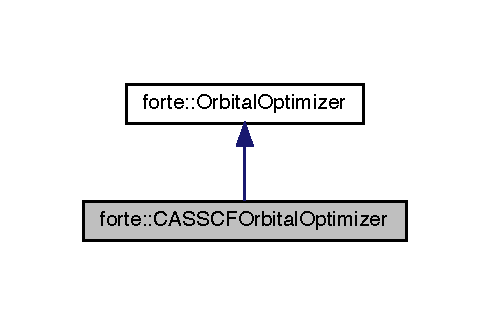
\includegraphics[width=235pt]{classforte_1_1_c_a_s_s_c_f_orbital_optimizer__inherit__graph}
\end{center}
\end{figure}


Collaboration diagram for forte\+:\+:C\+A\+S\+S\+C\+F\+Orbital\+Optimizer\+:
\nopagebreak
\begin{figure}[H]
\begin{center}
\leavevmode
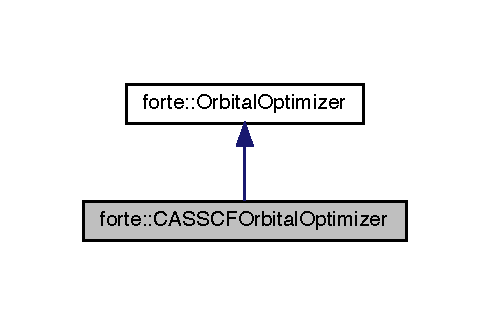
\includegraphics[width=235pt]{classforte_1_1_c_a_s_s_c_f_orbital_optimizer__coll__graph}
\end{center}
\end{figure}
\subsection*{Public Member Functions}
\begin{DoxyCompactItemize}
\item 
\mbox{\hyperlink{classforte_1_1_c_a_s_s_c_f_orbital_optimizer_a9172a146b982719e81df2ce4f96e00c3}{C\+A\+S\+S\+C\+F\+Orbital\+Optimizer}} (ambit\+::\+Tensor Gamma1, ambit\+::\+Tensor Gamma2, ambit\+::\+Tensor two\+\_\+body\+\_\+ab, std\+::shared\+\_\+ptr$<$ \mbox{\hyperlink{classforte_1_1_forte_options}{Forte\+Options}} $>$ options, std\+::shared\+\_\+ptr$<$ \mbox{\hyperlink{classforte_1_1_m_o_space_info}{M\+O\+Space\+Info}} $>$ mo\+\_\+space\+\_\+info, std\+::shared\+\_\+ptr$<$ \mbox{\hyperlink{classforte_1_1_forte_integrals}{Forte\+Integrals}} $>$ ints)
\item 
virtual \mbox{\hyperlink{classforte_1_1_c_a_s_s_c_f_orbital_optimizer_a54dd9f2b7d0549031d051a89d3a0d561}{$\sim$\+C\+A\+S\+S\+C\+F\+Orbital\+Optimizer}} ()
\end{DoxyCompactItemize}
\subsection*{Additional Inherited Members}


\subsection{Detailed Description}
A Class for use in \mbox{\hyperlink{classforte_1_1_c_a_s_s_c_f_orbital_optimizer}{C\+A\+S\+S\+C\+F\+Orbital\+Optimizer}} (computes Fock\+Core and Fock\+Active using JK builders) 

\subsection{Constructor \& Destructor Documentation}
\mbox{\Hypertarget{classforte_1_1_c_a_s_s_c_f_orbital_optimizer_a9172a146b982719e81df2ce4f96e00c3}\label{classforte_1_1_c_a_s_s_c_f_orbital_optimizer_a9172a146b982719e81df2ce4f96e00c3}} 
\index{forte\+::\+C\+A\+S\+S\+C\+F\+Orbital\+Optimizer@{forte\+::\+C\+A\+S\+S\+C\+F\+Orbital\+Optimizer}!C\+A\+S\+S\+C\+F\+Orbital\+Optimizer@{C\+A\+S\+S\+C\+F\+Orbital\+Optimizer}}
\index{C\+A\+S\+S\+C\+F\+Orbital\+Optimizer@{C\+A\+S\+S\+C\+F\+Orbital\+Optimizer}!forte\+::\+C\+A\+S\+S\+C\+F\+Orbital\+Optimizer@{forte\+::\+C\+A\+S\+S\+C\+F\+Orbital\+Optimizer}}
\subsubsection{\texorpdfstring{C\+A\+S\+S\+C\+F\+Orbital\+Optimizer()}{CASSCFOrbitalOptimizer()}}
{\footnotesize\ttfamily forte\+::\+C\+A\+S\+S\+C\+F\+Orbital\+Optimizer\+::\+C\+A\+S\+S\+C\+F\+Orbital\+Optimizer (\begin{DoxyParamCaption}\item[{ambit\+::\+Tensor}]{Gamma1,  }\item[{ambit\+::\+Tensor}]{Gamma2,  }\item[{ambit\+::\+Tensor}]{two\+\_\+body\+\_\+ab,  }\item[{std\+::shared\+\_\+ptr$<$ \mbox{\hyperlink{classforte_1_1_forte_options}{Forte\+Options}} $>$}]{options,  }\item[{std\+::shared\+\_\+ptr$<$ \mbox{\hyperlink{classforte_1_1_m_o_space_info}{M\+O\+Space\+Info}} $>$}]{mo\+\_\+space\+\_\+info,  }\item[{std\+::shared\+\_\+ptr$<$ \mbox{\hyperlink{classforte_1_1_forte_integrals}{Forte\+Integrals}} $>$}]{ints }\end{DoxyParamCaption})}

\mbox{\Hypertarget{classforte_1_1_c_a_s_s_c_f_orbital_optimizer_a54dd9f2b7d0549031d051a89d3a0d561}\label{classforte_1_1_c_a_s_s_c_f_orbital_optimizer_a54dd9f2b7d0549031d051a89d3a0d561}} 
\index{forte\+::\+C\+A\+S\+S\+C\+F\+Orbital\+Optimizer@{forte\+::\+C\+A\+S\+S\+C\+F\+Orbital\+Optimizer}!````~C\+A\+S\+S\+C\+F\+Orbital\+Optimizer@{$\sim$\+C\+A\+S\+S\+C\+F\+Orbital\+Optimizer}}
\index{````~C\+A\+S\+S\+C\+F\+Orbital\+Optimizer@{$\sim$\+C\+A\+S\+S\+C\+F\+Orbital\+Optimizer}!forte\+::\+C\+A\+S\+S\+C\+F\+Orbital\+Optimizer@{forte\+::\+C\+A\+S\+S\+C\+F\+Orbital\+Optimizer}}
\subsubsection{\texorpdfstring{$\sim$\+C\+A\+S\+S\+C\+F\+Orbital\+Optimizer()}{~CASSCFOrbitalOptimizer()}}
{\footnotesize\ttfamily forte\+::\+C\+A\+S\+S\+C\+F\+Orbital\+Optimizer\+::$\sim$\+C\+A\+S\+S\+C\+F\+Orbital\+Optimizer (\begin{DoxyParamCaption}{ }\end{DoxyParamCaption})\hspace{0.3cm}{\ttfamily [virtual]}}



The documentation for this class was generated from the following files\+:\begin{DoxyCompactItemize}
\item 
/\+Users/fevange/\+Source/forte/src/orbital-\/helpers/\mbox{\hyperlink{orbitaloptimizer_8h}{orbitaloptimizer.\+h}}\item 
/\+Users/fevange/\+Source/forte/src/orbital-\/helpers/\mbox{\hyperlink{orbitaloptimizer_8cc}{orbitaloptimizer.\+cc}}\end{DoxyCompactItemize}

\hypertarget{classforte_1_1_cholesky_integrals}{}\section{forte\+:\+:Cholesky\+Integrals Class Reference}
\label{classforte_1_1_cholesky_integrals}\index{forte\+::\+Cholesky\+Integrals@{forte\+::\+Cholesky\+Integrals}}


Class written by Kevin Hannon.  




{\ttfamily \#include $<$cholesky\+\_\+integrals.\+h$>$}



Inheritance diagram for forte\+:\+:Cholesky\+Integrals\+:
\nopagebreak
\begin{figure}[H]
\begin{center}
\leavevmode
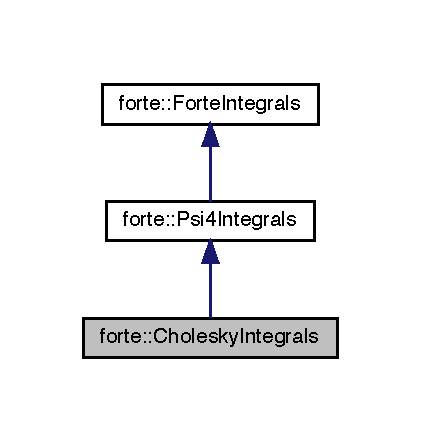
\includegraphics[width=202pt]{classforte_1_1_cholesky_integrals__inherit__graph}
\end{center}
\end{figure}


Collaboration diagram for forte\+:\+:Cholesky\+Integrals\+:
\nopagebreak
\begin{figure}[H]
\begin{center}
\leavevmode
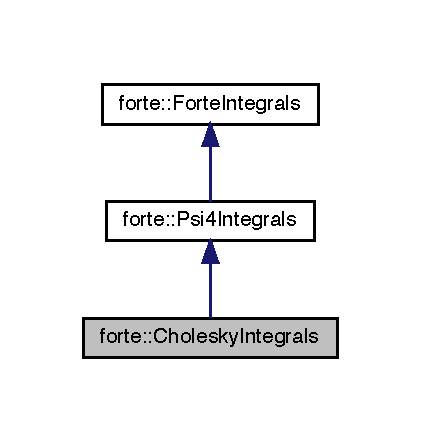
\includegraphics[width=202pt]{classforte_1_1_cholesky_integrals__coll__graph}
\end{center}
\end{figure}
\subsection*{Public Member Functions}
\begin{DoxyCompactItemize}
\item 
\mbox{\hyperlink{classforte_1_1_cholesky_integrals_af2bc409104a885004f8dd216c5b2465b}{Cholesky\+Integrals}} (std\+::shared\+\_\+ptr$<$ \mbox{\hyperlink{classforte_1_1_forte_options}{Forte\+Options}} $>$ options, std\+::shared\+\_\+ptr$<$ psi\+::\+Wavefunction $>$ ref\+\_\+wfn, std\+::shared\+\_\+ptr$<$ \mbox{\hyperlink{classforte_1_1_m_o_space_info}{M\+O\+Space\+Info}} $>$ mo\+\_\+space\+\_\+info, \mbox{\hyperlink{namespaceforte_a7defa2660dd3eb07aa81176b90781be7}{Integral\+Spin\+Restriction}} restricted)
\begin{DoxyCompactList}\small\item\em Contructor of \mbox{\hyperlink{classforte_1_1_cholesky_integrals}{Cholesky\+Integrals}}. \end{DoxyCompactList}\item 
void \mbox{\hyperlink{classforte_1_1_cholesky_integrals_af303c4caae64a8a7231239a676cac65e}{initialize}} () override
\item 
double \mbox{\hyperlink{classforte_1_1_cholesky_integrals_a118be3ea0020672f3d3e6ce4602cc14c}{aptei\+\_\+aa}} (size\+\_\+t p, size\+\_\+t q, size\+\_\+t r, size\+\_\+t s) override
\item 
double \mbox{\hyperlink{classforte_1_1_cholesky_integrals_aba4876388a8b9b633f38af3fc1cb4227}{aptei\+\_\+ab}} (size\+\_\+t p, size\+\_\+t q, size\+\_\+t r, size\+\_\+t s) override
\begin{DoxyCompactList}\small\item\em The antisymmetrixed alpha-\/beta two-\/electron integrals in physicist notation $<$pq$\vert$rs$>$ \end{DoxyCompactList}\item 
double \mbox{\hyperlink{classforte_1_1_cholesky_integrals_a02acd5ac863dcc1577c8b481ab80e8b6}{aptei\+\_\+bb}} (size\+\_\+t p, size\+\_\+t q, size\+\_\+t r, size\+\_\+t s) override
\begin{DoxyCompactList}\small\item\em The antisymmetrixed beta-\/beta two-\/electron integrals in physicist notation $<$pq$\vert$$\vert$rs$>$ \end{DoxyCompactList}\item 
ambit\+::\+Tensor \mbox{\hyperlink{classforte_1_1_cholesky_integrals_aeaecb1b7275f8b9fc8b87b4a3b110fcd}{aptei\+\_\+aa\+\_\+block}} (const std\+::vector$<$ size\+\_\+t $>$ \&p, const std\+::vector$<$ size\+\_\+t $>$ \&q, const std\+::vector$<$ size\+\_\+t $>$ \&r, const std\+::vector$<$ size\+\_\+t $>$ \&s) override
\begin{DoxyCompactList}\small\item\em Return the antisymmetrized alpha-\/alpha chunck as an ambit\+::\+Tensor. \end{DoxyCompactList}\item 
ambit\+::\+Tensor \mbox{\hyperlink{classforte_1_1_cholesky_integrals_af9aff1a966a4e520aa4cc62afd1c6998}{aptei\+\_\+ab\+\_\+block}} (const std\+::vector$<$ size\+\_\+t $>$ \&p, const std\+::vector$<$ size\+\_\+t $>$ \&q, const std\+::vector$<$ size\+\_\+t $>$ \&r, const std\+::vector$<$ size\+\_\+t $>$ \&s) override
\begin{DoxyCompactList}\small\item\em Return the antisymmetrized alpha-\/beta chunck as an ambit\+::\+Tensor. \end{DoxyCompactList}\item 
ambit\+::\+Tensor \mbox{\hyperlink{classforte_1_1_cholesky_integrals_a87d158226e76e8897395384f78b3ce24}{aptei\+\_\+bb\+\_\+block}} (const std\+::vector$<$ size\+\_\+t $>$ \&p, const std\+::vector$<$ size\+\_\+t $>$ \&q, const std\+::vector$<$ size\+\_\+t $>$ \&r, const std\+::vector$<$ size\+\_\+t $>$ \&s) override
\begin{DoxyCompactList}\small\item\em Return the antisymmetrized beta-\/beta chunck as an ambit\+::\+Tensor. \end{DoxyCompactList}\item 
double \mbox{\hyperlink{classforte_1_1_cholesky_integrals_aba0bbed773557a5cce05d50e23d03c82}{three\+\_\+integral}} (size\+\_\+t A, size\+\_\+t p, size\+\_\+t q) const
\item 
double $\ast$$\ast$ \mbox{\hyperlink{classforte_1_1_cholesky_integrals_ac92cb7a11e5a027ba6ccd11181ddf61a}{three\+\_\+integral\+\_\+pointer}} () override
\begin{DoxyCompactList}\small\item\em Expert Option\+: just try and use three\+\_\+integral. \end{DoxyCompactList}\item 
ambit\+::\+Tensor \mbox{\hyperlink{classforte_1_1_cholesky_integrals_a73dccc944cd9fdb00626bc88390136bf}{three\+\_\+integral\+\_\+block}} (const std\+::vector$<$ size\+\_\+t $>$ \&A, const std\+::vector$<$ size\+\_\+t $>$ \&p, const std\+::vector$<$ size\+\_\+t $>$ \&q) override
\item 
ambit\+::\+Tensor \mbox{\hyperlink{classforte_1_1_cholesky_integrals_a4f07e4c8e13a3424ec6b3d3a4d59a258}{three\+\_\+integral\+\_\+block\+\_\+two\+\_\+index}} (const std\+::vector$<$ size\+\_\+t $>$ \&, size\+\_\+t, const std\+::vector$<$ size\+\_\+t $>$ \&) override
\begin{DoxyCompactList}\small\item\em This function is only used by Disk\+DF and it is used to go from a Apq-\/$>$Aq tensor. \end{DoxyCompactList}\item 
void \mbox{\hyperlink{classforte_1_1_cholesky_integrals_a1db39bcdf9fd78a15ca3d1448bd08c5f}{set\+\_\+tei}} (size\+\_\+t p, size\+\_\+t q, size\+\_\+t r, size\+\_\+t s, double value, bool alpha1, bool alpha2) override
\begin{DoxyCompactList}\small\item\em Do not use this if you are using C\+D/\+DF integrals. \end{DoxyCompactList}\item 
size\+\_\+t \mbox{\hyperlink{classforte_1_1_cholesky_integrals_a595f615fb37218eb03e862fb993151fa}{nthree}} () const override
\begin{DoxyCompactList}\small\item\em Return the number of auxiliary functions. \end{DoxyCompactList}\end{DoxyCompactItemize}
\subsection*{Public Attributes}
\begin{DoxyCompactItemize}
\item 
std\+::shared\+\_\+ptr$<$ psi\+::\+Matrix $>$ \mbox{\hyperlink{classforte_1_1_cholesky_integrals_a0188eee74ee88eeca066cb9420143821}{L\+\_\+ao\+\_\+}}
\end{DoxyCompactItemize}
\subsection*{Additional Inherited Members}


\subsection{Detailed Description}
Class written by Kevin Hannon. 

The \mbox{\hyperlink{classforte_1_1_cholesky_integrals}{Cholesky\+Integrals}} class approximates two-\/electron integrals via Cholesky decomposition

This class assumes the Cholesky tensors can be stored in memory. 

\subsection{Constructor \& Destructor Documentation}
\mbox{\Hypertarget{classforte_1_1_cholesky_integrals_af2bc409104a885004f8dd216c5b2465b}\label{classforte_1_1_cholesky_integrals_af2bc409104a885004f8dd216c5b2465b}} 
\index{forte\+::\+Cholesky\+Integrals@{forte\+::\+Cholesky\+Integrals}!Cholesky\+Integrals@{Cholesky\+Integrals}}
\index{Cholesky\+Integrals@{Cholesky\+Integrals}!forte\+::\+Cholesky\+Integrals@{forte\+::\+Cholesky\+Integrals}}
\subsubsection{\texorpdfstring{Cholesky\+Integrals()}{CholeskyIntegrals()}}
{\footnotesize\ttfamily forte\+::\+Cholesky\+Integrals\+::\+Cholesky\+Integrals (\begin{DoxyParamCaption}\item[{std\+::shared\+\_\+ptr$<$ \mbox{\hyperlink{classforte_1_1_forte_options}{Forte\+Options}} $>$}]{options,  }\item[{std\+::shared\+\_\+ptr$<$ psi\+::\+Wavefunction $>$}]{ref\+\_\+wfn,  }\item[{std\+::shared\+\_\+ptr$<$ \mbox{\hyperlink{classforte_1_1_m_o_space_info}{M\+O\+Space\+Info}} $>$}]{mo\+\_\+space\+\_\+info,  }\item[{\mbox{\hyperlink{namespaceforte_a7defa2660dd3eb07aa81176b90781be7}{Integral\+Spin\+Restriction}}}]{restricted }\end{DoxyParamCaption})}



Contructor of \mbox{\hyperlink{classforte_1_1_cholesky_integrals}{Cholesky\+Integrals}}. 



\subsection{Member Function Documentation}
\mbox{\Hypertarget{classforte_1_1_cholesky_integrals_a118be3ea0020672f3d3e6ce4602cc14c}\label{classforte_1_1_cholesky_integrals_a118be3ea0020672f3d3e6ce4602cc14c}} 
\index{forte\+::\+Cholesky\+Integrals@{forte\+::\+Cholesky\+Integrals}!aptei\+\_\+aa@{aptei\+\_\+aa}}
\index{aptei\+\_\+aa@{aptei\+\_\+aa}!forte\+::\+Cholesky\+Integrals@{forte\+::\+Cholesky\+Integrals}}
\subsubsection{\texorpdfstring{aptei\+\_\+aa()}{aptei\_aa()}}
{\footnotesize\ttfamily double forte\+::\+Cholesky\+Integrals\+::aptei\+\_\+aa (\begin{DoxyParamCaption}\item[{size\+\_\+t}]{p,  }\item[{size\+\_\+t}]{q,  }\item[{size\+\_\+t}]{r,  }\item[{size\+\_\+t}]{s }\end{DoxyParamCaption})\hspace{0.3cm}{\ttfamily [override]}, {\ttfamily [virtual]}}

aptei\+\_\+x will grab antisymmetriced integrals and creates D\+F/\+CD integrals on the fly 

Implements \mbox{\hyperlink{classforte_1_1_forte_integrals_afc84c157025b56ee0f8e3b1abe1c0a5f}{forte\+::\+Forte\+Integrals}}.

\mbox{\Hypertarget{classforte_1_1_cholesky_integrals_aeaecb1b7275f8b9fc8b87b4a3b110fcd}\label{classforte_1_1_cholesky_integrals_aeaecb1b7275f8b9fc8b87b4a3b110fcd}} 
\index{forte\+::\+Cholesky\+Integrals@{forte\+::\+Cholesky\+Integrals}!aptei\+\_\+aa\+\_\+block@{aptei\+\_\+aa\+\_\+block}}
\index{aptei\+\_\+aa\+\_\+block@{aptei\+\_\+aa\+\_\+block}!forte\+::\+Cholesky\+Integrals@{forte\+::\+Cholesky\+Integrals}}
\subsubsection{\texorpdfstring{aptei\+\_\+aa\+\_\+block()}{aptei\_aa\_block()}}
{\footnotesize\ttfamily ambit\+::\+Tensor forte\+::\+Cholesky\+Integrals\+::aptei\+\_\+aa\+\_\+block (\begin{DoxyParamCaption}\item[{const std\+::vector$<$ size\+\_\+t $>$ \&}]{p,  }\item[{const std\+::vector$<$ size\+\_\+t $>$ \&}]{q,  }\item[{const std\+::vector$<$ size\+\_\+t $>$ \&}]{r,  }\item[{const std\+::vector$<$ size\+\_\+t $>$ \&}]{s }\end{DoxyParamCaption})\hspace{0.3cm}{\ttfamily [override]}, {\ttfamily [virtual]}}



Return the antisymmetrized alpha-\/alpha chunck as an ambit\+::\+Tensor. 



Implements \mbox{\hyperlink{classforte_1_1_forte_integrals_ac20ae649b8cfe116f8583d676e43da27}{forte\+::\+Forte\+Integrals}}.

\mbox{\Hypertarget{classforte_1_1_cholesky_integrals_aba4876388a8b9b633f38af3fc1cb4227}\label{classforte_1_1_cholesky_integrals_aba4876388a8b9b633f38af3fc1cb4227}} 
\index{forte\+::\+Cholesky\+Integrals@{forte\+::\+Cholesky\+Integrals}!aptei\+\_\+ab@{aptei\+\_\+ab}}
\index{aptei\+\_\+ab@{aptei\+\_\+ab}!forte\+::\+Cholesky\+Integrals@{forte\+::\+Cholesky\+Integrals}}
\subsubsection{\texorpdfstring{aptei\+\_\+ab()}{aptei\_ab()}}
{\footnotesize\ttfamily double forte\+::\+Cholesky\+Integrals\+::aptei\+\_\+ab (\begin{DoxyParamCaption}\item[{size\+\_\+t}]{p,  }\item[{size\+\_\+t}]{q,  }\item[{size\+\_\+t}]{r,  }\item[{size\+\_\+t}]{s }\end{DoxyParamCaption})\hspace{0.3cm}{\ttfamily [override]}, {\ttfamily [virtual]}}



The antisymmetrixed alpha-\/beta two-\/electron integrals in physicist notation $<$pq$\vert$rs$>$ 



Implements \mbox{\hyperlink{classforte_1_1_forte_integrals_a45efc2329cdfc7e4690cbe85688b947e}{forte\+::\+Forte\+Integrals}}.

\mbox{\Hypertarget{classforte_1_1_cholesky_integrals_af9aff1a966a4e520aa4cc62afd1c6998}\label{classforte_1_1_cholesky_integrals_af9aff1a966a4e520aa4cc62afd1c6998}} 
\index{forte\+::\+Cholesky\+Integrals@{forte\+::\+Cholesky\+Integrals}!aptei\+\_\+ab\+\_\+block@{aptei\+\_\+ab\+\_\+block}}
\index{aptei\+\_\+ab\+\_\+block@{aptei\+\_\+ab\+\_\+block}!forte\+::\+Cholesky\+Integrals@{forte\+::\+Cholesky\+Integrals}}
\subsubsection{\texorpdfstring{aptei\+\_\+ab\+\_\+block()}{aptei\_ab\_block()}}
{\footnotesize\ttfamily ambit\+::\+Tensor forte\+::\+Cholesky\+Integrals\+::aptei\+\_\+ab\+\_\+block (\begin{DoxyParamCaption}\item[{const std\+::vector$<$ size\+\_\+t $>$ \&}]{p,  }\item[{const std\+::vector$<$ size\+\_\+t $>$ \&}]{q,  }\item[{const std\+::vector$<$ size\+\_\+t $>$ \&}]{r,  }\item[{const std\+::vector$<$ size\+\_\+t $>$ \&}]{s }\end{DoxyParamCaption})\hspace{0.3cm}{\ttfamily [override]}, {\ttfamily [virtual]}}



Return the antisymmetrized alpha-\/beta chunck as an ambit\+::\+Tensor. 



Implements \mbox{\hyperlink{classforte_1_1_forte_integrals_acd40e350dc861baf8adf6a3b47c74023}{forte\+::\+Forte\+Integrals}}.

\mbox{\Hypertarget{classforte_1_1_cholesky_integrals_a02acd5ac863dcc1577c8b481ab80e8b6}\label{classforte_1_1_cholesky_integrals_a02acd5ac863dcc1577c8b481ab80e8b6}} 
\index{forte\+::\+Cholesky\+Integrals@{forte\+::\+Cholesky\+Integrals}!aptei\+\_\+bb@{aptei\+\_\+bb}}
\index{aptei\+\_\+bb@{aptei\+\_\+bb}!forte\+::\+Cholesky\+Integrals@{forte\+::\+Cholesky\+Integrals}}
\subsubsection{\texorpdfstring{aptei\+\_\+bb()}{aptei\_bb()}}
{\footnotesize\ttfamily double forte\+::\+Cholesky\+Integrals\+::aptei\+\_\+bb (\begin{DoxyParamCaption}\item[{size\+\_\+t}]{p,  }\item[{size\+\_\+t}]{q,  }\item[{size\+\_\+t}]{r,  }\item[{size\+\_\+t}]{s }\end{DoxyParamCaption})\hspace{0.3cm}{\ttfamily [override]}, {\ttfamily [virtual]}}



The antisymmetrixed beta-\/beta two-\/electron integrals in physicist notation $<$pq$\vert$$\vert$rs$>$ 



Implements \mbox{\hyperlink{classforte_1_1_forte_integrals_a246225031c3799dc446f94e0e732c3ac}{forte\+::\+Forte\+Integrals}}.

\mbox{\Hypertarget{classforte_1_1_cholesky_integrals_a87d158226e76e8897395384f78b3ce24}\label{classforte_1_1_cholesky_integrals_a87d158226e76e8897395384f78b3ce24}} 
\index{forte\+::\+Cholesky\+Integrals@{forte\+::\+Cholesky\+Integrals}!aptei\+\_\+bb\+\_\+block@{aptei\+\_\+bb\+\_\+block}}
\index{aptei\+\_\+bb\+\_\+block@{aptei\+\_\+bb\+\_\+block}!forte\+::\+Cholesky\+Integrals@{forte\+::\+Cholesky\+Integrals}}
\subsubsection{\texorpdfstring{aptei\+\_\+bb\+\_\+block()}{aptei\_bb\_block()}}
{\footnotesize\ttfamily ambit\+::\+Tensor forte\+::\+Cholesky\+Integrals\+::aptei\+\_\+bb\+\_\+block (\begin{DoxyParamCaption}\item[{const std\+::vector$<$ size\+\_\+t $>$ \&}]{p,  }\item[{const std\+::vector$<$ size\+\_\+t $>$ \&}]{q,  }\item[{const std\+::vector$<$ size\+\_\+t $>$ \&}]{r,  }\item[{const std\+::vector$<$ size\+\_\+t $>$ \&}]{s }\end{DoxyParamCaption})\hspace{0.3cm}{\ttfamily [override]}, {\ttfamily [virtual]}}



Return the antisymmetrized beta-\/beta chunck as an ambit\+::\+Tensor. 



Implements \mbox{\hyperlink{classforte_1_1_forte_integrals_ae2799dc7cbfd456603a2b841b26582ab}{forte\+::\+Forte\+Integrals}}.

\mbox{\Hypertarget{classforte_1_1_cholesky_integrals_af303c4caae64a8a7231239a676cac65e}\label{classforte_1_1_cholesky_integrals_af303c4caae64a8a7231239a676cac65e}} 
\index{forte\+::\+Cholesky\+Integrals@{forte\+::\+Cholesky\+Integrals}!initialize@{initialize}}
\index{initialize@{initialize}!forte\+::\+Cholesky\+Integrals@{forte\+::\+Cholesky\+Integrals}}
\subsubsection{\texorpdfstring{initialize()}{initialize()}}
{\footnotesize\ttfamily void forte\+::\+Cholesky\+Integrals\+::initialize (\begin{DoxyParamCaption}{ }\end{DoxyParamCaption})\hspace{0.3cm}{\ttfamily [override]}, {\ttfamily [virtual]}}



Implements \mbox{\hyperlink{classforte_1_1_forte_integrals_a7862835fa0f5f9abe13dfcd6730fa4be}{forte\+::\+Forte\+Integrals}}.

\mbox{\Hypertarget{classforte_1_1_cholesky_integrals_a595f615fb37218eb03e862fb993151fa}\label{classforte_1_1_cholesky_integrals_a595f615fb37218eb03e862fb993151fa}} 
\index{forte\+::\+Cholesky\+Integrals@{forte\+::\+Cholesky\+Integrals}!nthree@{nthree}}
\index{nthree@{nthree}!forte\+::\+Cholesky\+Integrals@{forte\+::\+Cholesky\+Integrals}}
\subsubsection{\texorpdfstring{nthree()}{nthree()}}
{\footnotesize\ttfamily size\+\_\+t forte\+::\+Cholesky\+Integrals\+::nthree (\begin{DoxyParamCaption}{ }\end{DoxyParamCaption}) const\hspace{0.3cm}{\ttfamily [override]}, {\ttfamily [virtual]}}



Return the number of auxiliary functions. 



Reimplemented from \mbox{\hyperlink{classforte_1_1_forte_integrals_af04858e7813556747745f90ffbda81a4}{forte\+::\+Forte\+Integrals}}.

\mbox{\Hypertarget{classforte_1_1_cholesky_integrals_a1db39bcdf9fd78a15ca3d1448bd08c5f}\label{classforte_1_1_cholesky_integrals_a1db39bcdf9fd78a15ca3d1448bd08c5f}} 
\index{forte\+::\+Cholesky\+Integrals@{forte\+::\+Cholesky\+Integrals}!set\+\_\+tei@{set\+\_\+tei}}
\index{set\+\_\+tei@{set\+\_\+tei}!forte\+::\+Cholesky\+Integrals@{forte\+::\+Cholesky\+Integrals}}
\subsubsection{\texorpdfstring{set\+\_\+tei()}{set\_tei()}}
{\footnotesize\ttfamily void forte\+::\+Cholesky\+Integrals\+::set\+\_\+tei (\begin{DoxyParamCaption}\item[{size\+\_\+t}]{p,  }\item[{size\+\_\+t}]{q,  }\item[{size\+\_\+t}]{r,  }\item[{size\+\_\+t}]{s,  }\item[{double}]{value,  }\item[{bool}]{alpha1,  }\item[{bool}]{alpha2 }\end{DoxyParamCaption})\hspace{0.3cm}{\ttfamily [override]}, {\ttfamily [virtual]}}



Do not use this if you are using C\+D/\+DF integrals. 



Implements \mbox{\hyperlink{classforte_1_1_forte_integrals_aaccd56e90bbc3c423158efb154336b9c}{forte\+::\+Forte\+Integrals}}.

\mbox{\Hypertarget{classforte_1_1_cholesky_integrals_aba0bbed773557a5cce05d50e23d03c82}\label{classforte_1_1_cholesky_integrals_aba0bbed773557a5cce05d50e23d03c82}} 
\index{forte\+::\+Cholesky\+Integrals@{forte\+::\+Cholesky\+Integrals}!three\+\_\+integral@{three\+\_\+integral}}
\index{three\+\_\+integral@{three\+\_\+integral}!forte\+::\+Cholesky\+Integrals@{forte\+::\+Cholesky\+Integrals}}
\subsubsection{\texorpdfstring{three\+\_\+integral()}{three\_integral()}}
{\footnotesize\ttfamily double forte\+::\+Cholesky\+Integrals\+::three\+\_\+integral (\begin{DoxyParamCaption}\item[{size\+\_\+t}]{A,  }\item[{size\+\_\+t}]{p,  }\item[{size\+\_\+t}]{q }\end{DoxyParamCaption}) const}

\mbox{\Hypertarget{classforte_1_1_cholesky_integrals_a73dccc944cd9fdb00626bc88390136bf}\label{classforte_1_1_cholesky_integrals_a73dccc944cd9fdb00626bc88390136bf}} 
\index{forte\+::\+Cholesky\+Integrals@{forte\+::\+Cholesky\+Integrals}!three\+\_\+integral\+\_\+block@{three\+\_\+integral\+\_\+block}}
\index{three\+\_\+integral\+\_\+block@{three\+\_\+integral\+\_\+block}!forte\+::\+Cholesky\+Integrals@{forte\+::\+Cholesky\+Integrals}}
\subsubsection{\texorpdfstring{three\+\_\+integral\+\_\+block()}{three\_integral\_block()}}
{\footnotesize\ttfamily ambit\+::\+Tensor forte\+::\+Cholesky\+Integrals\+::three\+\_\+integral\+\_\+block (\begin{DoxyParamCaption}\item[{const std\+::vector$<$ size\+\_\+t $>$ \&}]{A,  }\item[{const std\+::vector$<$ size\+\_\+t $>$ \&}]{p,  }\item[{const std\+::vector$<$ size\+\_\+t $>$ \&}]{q }\end{DoxyParamCaption})\hspace{0.3cm}{\ttfamily [override]}, {\ttfamily [virtual]}}



Reimplemented from \mbox{\hyperlink{classforte_1_1_forte_integrals_aa1d259ae97b5a9c96ccb20599543b126}{forte\+::\+Forte\+Integrals}}.

\mbox{\Hypertarget{classforte_1_1_cholesky_integrals_a4f07e4c8e13a3424ec6b3d3a4d59a258}\label{classforte_1_1_cholesky_integrals_a4f07e4c8e13a3424ec6b3d3a4d59a258}} 
\index{forte\+::\+Cholesky\+Integrals@{forte\+::\+Cholesky\+Integrals}!three\+\_\+integral\+\_\+block\+\_\+two\+\_\+index@{three\+\_\+integral\+\_\+block\+\_\+two\+\_\+index}}
\index{three\+\_\+integral\+\_\+block\+\_\+two\+\_\+index@{three\+\_\+integral\+\_\+block\+\_\+two\+\_\+index}!forte\+::\+Cholesky\+Integrals@{forte\+::\+Cholesky\+Integrals}}
\subsubsection{\texorpdfstring{three\+\_\+integral\+\_\+block\+\_\+two\+\_\+index()}{three\_integral\_block\_two\_index()}}
{\footnotesize\ttfamily ambit\+::\+Tensor forte\+::\+Cholesky\+Integrals\+::three\+\_\+integral\+\_\+block\+\_\+two\+\_\+index (\begin{DoxyParamCaption}\item[{const std\+::vector$<$ size\+\_\+t $>$ \&}]{A,  }\item[{size\+\_\+t}]{p,  }\item[{const std\+::vector$<$ size\+\_\+t $>$ \&}]{ }\end{DoxyParamCaption})\hspace{0.3cm}{\ttfamily [override]}, {\ttfamily [virtual]}}



This function is only used by Disk\+DF and it is used to go from a Apq-\/$>$Aq tensor. 



Reimplemented from \mbox{\hyperlink{classforte_1_1_forte_integrals_aab51824020dc3588c026b5b7740f55a9}{forte\+::\+Forte\+Integrals}}.

\mbox{\Hypertarget{classforte_1_1_cholesky_integrals_ac92cb7a11e5a027ba6ccd11181ddf61a}\label{classforte_1_1_cholesky_integrals_ac92cb7a11e5a027ba6ccd11181ddf61a}} 
\index{forte\+::\+Cholesky\+Integrals@{forte\+::\+Cholesky\+Integrals}!three\+\_\+integral\+\_\+pointer@{three\+\_\+integral\+\_\+pointer}}
\index{three\+\_\+integral\+\_\+pointer@{three\+\_\+integral\+\_\+pointer}!forte\+::\+Cholesky\+Integrals@{forte\+::\+Cholesky\+Integrals}}
\subsubsection{\texorpdfstring{three\+\_\+integral\+\_\+pointer()}{three\_integral\_pointer()}}
{\footnotesize\ttfamily double $\ast$$\ast$ forte\+::\+Cholesky\+Integrals\+::three\+\_\+integral\+\_\+pointer (\begin{DoxyParamCaption}{ }\end{DoxyParamCaption})\hspace{0.3cm}{\ttfamily [override]}, {\ttfamily [virtual]}}



Expert Option\+: just try and use three\+\_\+integral. 



Reimplemented from \mbox{\hyperlink{classforte_1_1_forte_integrals_a69292bc8e42a76e344cd01c4e3dd48d5}{forte\+::\+Forte\+Integrals}}.



\subsection{Member Data Documentation}
\mbox{\Hypertarget{classforte_1_1_cholesky_integrals_a0188eee74ee88eeca066cb9420143821}\label{classforte_1_1_cholesky_integrals_a0188eee74ee88eeca066cb9420143821}} 
\index{forte\+::\+Cholesky\+Integrals@{forte\+::\+Cholesky\+Integrals}!L\+\_\+ao\+\_\+@{L\+\_\+ao\+\_\+}}
\index{L\+\_\+ao\+\_\+@{L\+\_\+ao\+\_\+}!forte\+::\+Cholesky\+Integrals@{forte\+::\+Cholesky\+Integrals}}
\subsubsection{\texorpdfstring{L\+\_\+ao\+\_\+}{L\_ao\_}}
{\footnotesize\ttfamily std\+::shared\+\_\+ptr$<$psi\+::\+Matrix$>$ forte\+::\+Cholesky\+Integrals\+::\+L\+\_\+ao\+\_\+}



The documentation for this class was generated from the following files\+:\begin{DoxyCompactItemize}
\item 
/\+Users/fevange/\+Source/forte/src/integrals/\mbox{\hyperlink{cholesky__integrals_8h}{cholesky\+\_\+integrals.\+h}}\item 
/\+Users/fevange/\+Source/forte/src/integrals/\mbox{\hyperlink{cholesky__integrals_8cc}{cholesky\+\_\+integrals.\+cc}}\end{DoxyCompactItemize}

\hypertarget{classforte_1_1_c_i___r_d_m_s}{}\section{forte\+:\+:C\+I\+\_\+\+R\+D\+MS Class Reference}
\label{classforte_1_1_c_i___r_d_m_s}\index{forte\+::\+C\+I\+\_\+\+R\+D\+MS@{forte\+::\+C\+I\+\_\+\+R\+D\+MS}}


{\ttfamily \#include $<$ci\+\_\+rdms.\+h$>$}

\subsection*{Public Types}
\begin{DoxyCompactItemize}
\item 
using \mbox{\hyperlink{classforte_1_1_c_i___r_d_m_s_a6fe09e4dcfafed624c05462004a9de51}{det\+\_\+hash}} = std\+::unordered\+\_\+map$<$ \mbox{\hyperlink{namespaceforte_a2076c63fd7b8732004d9e1442ce527c1}{Determinant}}, size\+\_\+t, \mbox{\hyperlink{structforte_1_1_bit_array_1_1_hash}{Determinant\+::\+Hash}} $>$
\item 
using \mbox{\hyperlink{classforte_1_1_c_i___r_d_m_s_a848538093346b3724b92d39fbbaee36a}{det\+\_\+hash\+\_\+it}} = det\+\_\+hash\+::iterator
\end{DoxyCompactItemize}
\subsection*{Public Member Functions}
\begin{DoxyCompactItemize}
\item 
\mbox{\hyperlink{classforte_1_1_c_i___r_d_m_s_a492dfe2daedba96524e378dff6d8881b}{C\+I\+\_\+\+R\+D\+MS}} (std\+::shared\+\_\+ptr$<$ \mbox{\hyperlink{classforte_1_1_active_space_integrals}{Active\+Space\+Integrals}} $>$ fci\+\_\+ints, const std\+::vector$<$ \mbox{\hyperlink{namespaceforte_a2076c63fd7b8732004d9e1442ce527c1}{Determinant}} $>$ \&det\+\_\+space, psi\+::\+Shared\+Matrix evecs, int root1, int root2)
\item 
\mbox{\hyperlink{classforte_1_1_c_i___r_d_m_s_a080710371be0841dd7d412f0107820c2}{C\+I\+\_\+\+R\+D\+MS}} (\mbox{\hyperlink{classforte_1_1_determinant_hash_vec}{Determinant\+Hash\+Vec}} \&wfn, std\+::shared\+\_\+ptr$<$ \mbox{\hyperlink{classforte_1_1_active_space_integrals}{Active\+Space\+Integrals}} $>$ fci\+\_\+ints, psi\+::\+Shared\+Matrix evecs, int root1, int root2)
\item 
\mbox{\hyperlink{classforte_1_1_c_i___r_d_m_s_ae32becd6a38ea945e795ed78edb5c38d}{$\sim$\+C\+I\+\_\+\+R\+D\+MS}} ()
\item 
void \mbox{\hyperlink{classforte_1_1_c_i___r_d_m_s_ab16c501467a25a727092c89462eeb095}{compute\+\_\+1rdm}} (std\+::vector$<$ double $>$ \&oprdm\+\_\+a, std\+::vector$<$ double $>$ \&oprdm\+\_\+b)
\item 
void \mbox{\hyperlink{classforte_1_1_c_i___r_d_m_s_ad232dbb35aa59e9edcdc86626d3a883d}{compute\+\_\+1rdm\+\_\+op}} (std\+::vector$<$ double $>$ \&oprdm\+\_\+a, std\+::vector$<$ double $>$ \&oprdm\+\_\+b)
\item 
void \mbox{\hyperlink{classforte_1_1_c_i___r_d_m_s_ab881ee2d8f370683a18b6659c542e868}{compute\+\_\+2rdm}} (std\+::vector$<$ double $>$ \&tprdm\+\_\+aa, std\+::vector$<$ double $>$ \&tprdm\+\_\+ab, std\+::vector$<$ double $>$ \&tprdm\+\_\+bb)
\item 
void \mbox{\hyperlink{classforte_1_1_c_i___r_d_m_s_a4eba66bbdea6356a9abd92c666e60912}{compute\+\_\+2rdm\+\_\+op}} (std\+::vector$<$ double $>$ \&tprdm\+\_\+aa, std\+::vector$<$ double $>$ \&tprdm\+\_\+ab, std\+::vector$<$ double $>$ \&tprdm\+\_\+bb)
\item 
void \mbox{\hyperlink{classforte_1_1_c_i___r_d_m_s_a4c08b96e09691f3ad4b00efc4c38fb94}{compute\+\_\+3rdm}} (std\+::vector$<$ double $>$ \&tprdm\+\_\+aaa, std\+::vector$<$ double $>$ \&tprdm\+\_\+aab, std\+::vector$<$ double $>$ \&tprdm\+\_\+abb, std\+::vector$<$ double $>$ \&tprdm\+\_\+bbb)
\item 
void \mbox{\hyperlink{classforte_1_1_c_i___r_d_m_s_aace0c388b6b00e11261b43360edf3664}{compute\+\_\+3rdm\+\_\+op}} (std\+::vector$<$ double $>$ \&tprdm\+\_\+aaa, std\+::vector$<$ double $>$ \&tprdm\+\_\+aab, std\+::vector$<$ double $>$ \&tprdm\+\_\+abb, std\+::vector$<$ double $>$ \&tprdm\+\_\+bbb)
\item 
void \mbox{\hyperlink{classforte_1_1_c_i___r_d_m_s_abd29572a50f93000b682234ffa832224}{compute\+\_\+rdms\+\_\+dynamic}} (std\+::vector$<$ double $>$ \&oprdm\+\_\+a, std\+::vector$<$ double $>$ \&oprdm\+\_\+b, std\+::vector$<$ double $>$ \&tprdm\+\_\+aa, std\+::vector$<$ double $>$ \&tprdm\+\_\+ab, std\+::vector$<$ double $>$ \&tprdm\+\_\+bb, std\+::vector$<$ double $>$ \&tprdm\+\_\+aaa, std\+::vector$<$ double $>$ \&tprdm\+\_\+aab, std\+::vector$<$ double $>$ \&tprdm\+\_\+abb, std\+::vector$<$ double $>$ \&tprdm\+\_\+bbb)
\item 
double \mbox{\hyperlink{classforte_1_1_c_i___r_d_m_s_a51f0d4ac481cf5579b6557ce5359c646}{get\+\_\+energy}} (std\+::vector$<$ double $>$ \&oprdm\+\_\+a, std\+::vector$<$ double $>$ \&oprdm\+\_\+b, std\+::vector$<$ double $>$ \&tprdm\+\_\+aa, std\+::vector$<$ double $>$ \&tprdm\+\_\+bb, std\+::vector$<$ double $>$ \&tprdm\+\_\+ab)
\item 
void \mbox{\hyperlink{classforte_1_1_c_i___r_d_m_s_a5060c542b3e43206ee7f5ef8e495f906}{rdm\+\_\+test}} (std\+::vector$<$ double $>$ \&oprdm\+\_\+a, std\+::vector$<$ double $>$ \&oprdm\+\_\+b, std\+::vector$<$ double $>$ \&tprdm\+\_\+aa, std\+::vector$<$ double $>$ \&tprdm\+\_\+bb, std\+::vector$<$ double $>$ \&tprdm\+\_\+ab, std\+::vector$<$ double $>$ \&tprdm\+\_\+aaa, std\+::vector$<$ double $>$ \&tprdm\+\_\+aab, std\+::vector$<$ double $>$ \&tprdm\+\_\+abb, std\+::vector$<$ double $>$ \&tprdm\+\_\+bbb)
\item 
void \mbox{\hyperlink{classforte_1_1_c_i___r_d_m_s_aca80a64f8d50eb8784ad27804881938b}{set\+\_\+print}} (bool print)
\item 
void \mbox{\hyperlink{classforte_1_1_c_i___r_d_m_s_ad3d9e1ffe533bbe89b33be83a84da01d}{set\+\_\+max\+\_\+rdm}} (int rdm)
\item 
void \mbox{\hyperlink{classforte_1_1_c_i___r_d_m_s_a88f0699318551cd6012614e06df58b42}{convert\+\_\+to\+\_\+string}} (std\+::vector$<$ \mbox{\hyperlink{namespaceforte_a2076c63fd7b8732004d9e1442ce527c1}{Determinant}} $>$ \&space)
\end{DoxyCompactItemize}


\subsection{Member Typedef Documentation}
\mbox{\Hypertarget{classforte_1_1_c_i___r_d_m_s_a6fe09e4dcfafed624c05462004a9de51}\label{classforte_1_1_c_i___r_d_m_s_a6fe09e4dcfafed624c05462004a9de51}} 
\index{forte\+::\+C\+I\+\_\+\+R\+D\+MS@{forte\+::\+C\+I\+\_\+\+R\+D\+MS}!det\+\_\+hash@{det\+\_\+hash}}
\index{det\+\_\+hash@{det\+\_\+hash}!forte\+::\+C\+I\+\_\+\+R\+D\+MS@{forte\+::\+C\+I\+\_\+\+R\+D\+MS}}
\subsubsection{\texorpdfstring{det\+\_\+hash}{det\_hash}}
{\footnotesize\ttfamily using \mbox{\hyperlink{classforte_1_1_c_i___r_d_m_s_a6fe09e4dcfafed624c05462004a9de51}{forte\+::\+C\+I\+\_\+\+R\+D\+M\+S\+::det\+\_\+hash}} =  std\+::unordered\+\_\+map$<$\mbox{\hyperlink{namespaceforte_a2076c63fd7b8732004d9e1442ce527c1}{Determinant}}, size\+\_\+t, \mbox{\hyperlink{structforte_1_1_bit_array_1_1_hash}{Determinant\+::\+Hash}}$>$}

\mbox{\Hypertarget{classforte_1_1_c_i___r_d_m_s_a848538093346b3724b92d39fbbaee36a}\label{classforte_1_1_c_i___r_d_m_s_a848538093346b3724b92d39fbbaee36a}} 
\index{forte\+::\+C\+I\+\_\+\+R\+D\+MS@{forte\+::\+C\+I\+\_\+\+R\+D\+MS}!det\+\_\+hash\+\_\+it@{det\+\_\+hash\+\_\+it}}
\index{det\+\_\+hash\+\_\+it@{det\+\_\+hash\+\_\+it}!forte\+::\+C\+I\+\_\+\+R\+D\+MS@{forte\+::\+C\+I\+\_\+\+R\+D\+MS}}
\subsubsection{\texorpdfstring{det\+\_\+hash\+\_\+it}{det\_hash\_it}}
{\footnotesize\ttfamily using \mbox{\hyperlink{classforte_1_1_c_i___r_d_m_s_a848538093346b3724b92d39fbbaee36a}{forte\+::\+C\+I\+\_\+\+R\+D\+M\+S\+::det\+\_\+hash\+\_\+it}} =  det\+\_\+hash\+::iterator}



\subsection{Constructor \& Destructor Documentation}
\mbox{\Hypertarget{classforte_1_1_c_i___r_d_m_s_a492dfe2daedba96524e378dff6d8881b}\label{classforte_1_1_c_i___r_d_m_s_a492dfe2daedba96524e378dff6d8881b}} 
\index{forte\+::\+C\+I\+\_\+\+R\+D\+MS@{forte\+::\+C\+I\+\_\+\+R\+D\+MS}!C\+I\+\_\+\+R\+D\+MS@{C\+I\+\_\+\+R\+D\+MS}}
\index{C\+I\+\_\+\+R\+D\+MS@{C\+I\+\_\+\+R\+D\+MS}!forte\+::\+C\+I\+\_\+\+R\+D\+MS@{forte\+::\+C\+I\+\_\+\+R\+D\+MS}}
\subsubsection{\texorpdfstring{C\+I\+\_\+\+R\+D\+M\+S()}{CI\_RDMS()}\hspace{0.1cm}{\footnotesize\ttfamily [1/2]}}
{\footnotesize\ttfamily forte\+::\+C\+I\+\_\+\+R\+D\+M\+S\+::\+C\+I\+\_\+\+R\+D\+MS (\begin{DoxyParamCaption}\item[{std\+::shared\+\_\+ptr$<$ \mbox{\hyperlink{classforte_1_1_active_space_integrals}{Active\+Space\+Integrals}} $>$}]{fci\+\_\+ints,  }\item[{const std\+::vector$<$ \mbox{\hyperlink{namespaceforte_a2076c63fd7b8732004d9e1442ce527c1}{Determinant}} $>$ \&}]{det\+\_\+space,  }\item[{psi\+::\+Shared\+Matrix}]{evecs,  }\item[{int}]{root1,  }\item[{int}]{root2 }\end{DoxyParamCaption})}

\mbox{\Hypertarget{classforte_1_1_c_i___r_d_m_s_a080710371be0841dd7d412f0107820c2}\label{classforte_1_1_c_i___r_d_m_s_a080710371be0841dd7d412f0107820c2}} 
\index{forte\+::\+C\+I\+\_\+\+R\+D\+MS@{forte\+::\+C\+I\+\_\+\+R\+D\+MS}!C\+I\+\_\+\+R\+D\+MS@{C\+I\+\_\+\+R\+D\+MS}}
\index{C\+I\+\_\+\+R\+D\+MS@{C\+I\+\_\+\+R\+D\+MS}!forte\+::\+C\+I\+\_\+\+R\+D\+MS@{forte\+::\+C\+I\+\_\+\+R\+D\+MS}}
\subsubsection{\texorpdfstring{C\+I\+\_\+\+R\+D\+M\+S()}{CI\_RDMS()}\hspace{0.1cm}{\footnotesize\ttfamily [2/2]}}
{\footnotesize\ttfamily forte\+::\+C\+I\+\_\+\+R\+D\+M\+S\+::\+C\+I\+\_\+\+R\+D\+MS (\begin{DoxyParamCaption}\item[{\mbox{\hyperlink{classforte_1_1_determinant_hash_vec}{Determinant\+Hash\+Vec}} \&}]{wfn,  }\item[{std\+::shared\+\_\+ptr$<$ \mbox{\hyperlink{classforte_1_1_active_space_integrals}{Active\+Space\+Integrals}} $>$}]{fci\+\_\+ints,  }\item[{psi\+::\+Shared\+Matrix}]{evecs,  }\item[{int}]{root1,  }\item[{int}]{root2 }\end{DoxyParamCaption})}

\mbox{\Hypertarget{classforte_1_1_c_i___r_d_m_s_ae32becd6a38ea945e795ed78edb5c38d}\label{classforte_1_1_c_i___r_d_m_s_ae32becd6a38ea945e795ed78edb5c38d}} 
\index{forte\+::\+C\+I\+\_\+\+R\+D\+MS@{forte\+::\+C\+I\+\_\+\+R\+D\+MS}!````~C\+I\+\_\+\+R\+D\+MS@{$\sim$\+C\+I\+\_\+\+R\+D\+MS}}
\index{````~C\+I\+\_\+\+R\+D\+MS@{$\sim$\+C\+I\+\_\+\+R\+D\+MS}!forte\+::\+C\+I\+\_\+\+R\+D\+MS@{forte\+::\+C\+I\+\_\+\+R\+D\+MS}}
\subsubsection{\texorpdfstring{$\sim$\+C\+I\+\_\+\+R\+D\+M\+S()}{~CI\_RDMS()}}
{\footnotesize\ttfamily forte\+::\+C\+I\+\_\+\+R\+D\+M\+S\+::$\sim$\+C\+I\+\_\+\+R\+D\+MS (\begin{DoxyParamCaption}{ }\end{DoxyParamCaption})}



\subsection{Member Function Documentation}
\mbox{\Hypertarget{classforte_1_1_c_i___r_d_m_s_ab16c501467a25a727092c89462eeb095}\label{classforte_1_1_c_i___r_d_m_s_ab16c501467a25a727092c89462eeb095}} 
\index{forte\+::\+C\+I\+\_\+\+R\+D\+MS@{forte\+::\+C\+I\+\_\+\+R\+D\+MS}!compute\+\_\+1rdm@{compute\+\_\+1rdm}}
\index{compute\+\_\+1rdm@{compute\+\_\+1rdm}!forte\+::\+C\+I\+\_\+\+R\+D\+MS@{forte\+::\+C\+I\+\_\+\+R\+D\+MS}}
\subsubsection{\texorpdfstring{compute\+\_\+1rdm()}{compute\_1rdm()}}
{\footnotesize\ttfamily void forte\+::\+C\+I\+\_\+\+R\+D\+M\+S\+::compute\+\_\+1rdm (\begin{DoxyParamCaption}\item[{std\+::vector$<$ double $>$ \&}]{oprdm\+\_\+a,  }\item[{std\+::vector$<$ double $>$ \&}]{oprdm\+\_\+b }\end{DoxyParamCaption})}

\mbox{\Hypertarget{classforte_1_1_c_i___r_d_m_s_ad232dbb35aa59e9edcdc86626d3a883d}\label{classforte_1_1_c_i___r_d_m_s_ad232dbb35aa59e9edcdc86626d3a883d}} 
\index{forte\+::\+C\+I\+\_\+\+R\+D\+MS@{forte\+::\+C\+I\+\_\+\+R\+D\+MS}!compute\+\_\+1rdm\+\_\+op@{compute\+\_\+1rdm\+\_\+op}}
\index{compute\+\_\+1rdm\+\_\+op@{compute\+\_\+1rdm\+\_\+op}!forte\+::\+C\+I\+\_\+\+R\+D\+MS@{forte\+::\+C\+I\+\_\+\+R\+D\+MS}}
\subsubsection{\texorpdfstring{compute\+\_\+1rdm\+\_\+op()}{compute\_1rdm\_op()}}
{\footnotesize\ttfamily void forte\+::\+C\+I\+\_\+\+R\+D\+M\+S\+::compute\+\_\+1rdm\+\_\+op (\begin{DoxyParamCaption}\item[{std\+::vector$<$ double $>$ \&}]{oprdm\+\_\+a,  }\item[{std\+::vector$<$ double $>$ \&}]{oprdm\+\_\+b }\end{DoxyParamCaption})}

\mbox{\Hypertarget{classforte_1_1_c_i___r_d_m_s_ab881ee2d8f370683a18b6659c542e868}\label{classforte_1_1_c_i___r_d_m_s_ab881ee2d8f370683a18b6659c542e868}} 
\index{forte\+::\+C\+I\+\_\+\+R\+D\+MS@{forte\+::\+C\+I\+\_\+\+R\+D\+MS}!compute\+\_\+2rdm@{compute\+\_\+2rdm}}
\index{compute\+\_\+2rdm@{compute\+\_\+2rdm}!forte\+::\+C\+I\+\_\+\+R\+D\+MS@{forte\+::\+C\+I\+\_\+\+R\+D\+MS}}
\subsubsection{\texorpdfstring{compute\+\_\+2rdm()}{compute\_2rdm()}}
{\footnotesize\ttfamily void forte\+::\+C\+I\+\_\+\+R\+D\+M\+S\+::compute\+\_\+2rdm (\begin{DoxyParamCaption}\item[{std\+::vector$<$ double $>$ \&}]{tprdm\+\_\+aa,  }\item[{std\+::vector$<$ double $>$ \&}]{tprdm\+\_\+ab,  }\item[{std\+::vector$<$ double $>$ \&}]{tprdm\+\_\+bb }\end{DoxyParamCaption})}

\mbox{\Hypertarget{classforte_1_1_c_i___r_d_m_s_a4eba66bbdea6356a9abd92c666e60912}\label{classforte_1_1_c_i___r_d_m_s_a4eba66bbdea6356a9abd92c666e60912}} 
\index{forte\+::\+C\+I\+\_\+\+R\+D\+MS@{forte\+::\+C\+I\+\_\+\+R\+D\+MS}!compute\+\_\+2rdm\+\_\+op@{compute\+\_\+2rdm\+\_\+op}}
\index{compute\+\_\+2rdm\+\_\+op@{compute\+\_\+2rdm\+\_\+op}!forte\+::\+C\+I\+\_\+\+R\+D\+MS@{forte\+::\+C\+I\+\_\+\+R\+D\+MS}}
\subsubsection{\texorpdfstring{compute\+\_\+2rdm\+\_\+op()}{compute\_2rdm\_op()}}
{\footnotesize\ttfamily void forte\+::\+C\+I\+\_\+\+R\+D\+M\+S\+::compute\+\_\+2rdm\+\_\+op (\begin{DoxyParamCaption}\item[{std\+::vector$<$ double $>$ \&}]{tprdm\+\_\+aa,  }\item[{std\+::vector$<$ double $>$ \&}]{tprdm\+\_\+ab,  }\item[{std\+::vector$<$ double $>$ \&}]{tprdm\+\_\+bb }\end{DoxyParamCaption})}

\mbox{\Hypertarget{classforte_1_1_c_i___r_d_m_s_a4c08b96e09691f3ad4b00efc4c38fb94}\label{classforte_1_1_c_i___r_d_m_s_a4c08b96e09691f3ad4b00efc4c38fb94}} 
\index{forte\+::\+C\+I\+\_\+\+R\+D\+MS@{forte\+::\+C\+I\+\_\+\+R\+D\+MS}!compute\+\_\+3rdm@{compute\+\_\+3rdm}}
\index{compute\+\_\+3rdm@{compute\+\_\+3rdm}!forte\+::\+C\+I\+\_\+\+R\+D\+MS@{forte\+::\+C\+I\+\_\+\+R\+D\+MS}}
\subsubsection{\texorpdfstring{compute\+\_\+3rdm()}{compute\_3rdm()}}
{\footnotesize\ttfamily void forte\+::\+C\+I\+\_\+\+R\+D\+M\+S\+::compute\+\_\+3rdm (\begin{DoxyParamCaption}\item[{std\+::vector$<$ double $>$ \&}]{tprdm\+\_\+aaa,  }\item[{std\+::vector$<$ double $>$ \&}]{tprdm\+\_\+aab,  }\item[{std\+::vector$<$ double $>$ \&}]{tprdm\+\_\+abb,  }\item[{std\+::vector$<$ double $>$ \&}]{tprdm\+\_\+bbb }\end{DoxyParamCaption})}

\mbox{\Hypertarget{classforte_1_1_c_i___r_d_m_s_aace0c388b6b00e11261b43360edf3664}\label{classforte_1_1_c_i___r_d_m_s_aace0c388b6b00e11261b43360edf3664}} 
\index{forte\+::\+C\+I\+\_\+\+R\+D\+MS@{forte\+::\+C\+I\+\_\+\+R\+D\+MS}!compute\+\_\+3rdm\+\_\+op@{compute\+\_\+3rdm\+\_\+op}}
\index{compute\+\_\+3rdm\+\_\+op@{compute\+\_\+3rdm\+\_\+op}!forte\+::\+C\+I\+\_\+\+R\+D\+MS@{forte\+::\+C\+I\+\_\+\+R\+D\+MS}}
\subsubsection{\texorpdfstring{compute\+\_\+3rdm\+\_\+op()}{compute\_3rdm\_op()}}
{\footnotesize\ttfamily void forte\+::\+C\+I\+\_\+\+R\+D\+M\+S\+::compute\+\_\+3rdm\+\_\+op (\begin{DoxyParamCaption}\item[{std\+::vector$<$ double $>$ \&}]{tprdm\+\_\+aaa,  }\item[{std\+::vector$<$ double $>$ \&}]{tprdm\+\_\+aab,  }\item[{std\+::vector$<$ double $>$ \&}]{tprdm\+\_\+abb,  }\item[{std\+::vector$<$ double $>$ \&}]{tprdm\+\_\+bbb }\end{DoxyParamCaption})}

\mbox{\Hypertarget{classforte_1_1_c_i___r_d_m_s_abd29572a50f93000b682234ffa832224}\label{classforte_1_1_c_i___r_d_m_s_abd29572a50f93000b682234ffa832224}} 
\index{forte\+::\+C\+I\+\_\+\+R\+D\+MS@{forte\+::\+C\+I\+\_\+\+R\+D\+MS}!compute\+\_\+rdms\+\_\+dynamic@{compute\+\_\+rdms\+\_\+dynamic}}
\index{compute\+\_\+rdms\+\_\+dynamic@{compute\+\_\+rdms\+\_\+dynamic}!forte\+::\+C\+I\+\_\+\+R\+D\+MS@{forte\+::\+C\+I\+\_\+\+R\+D\+MS}}
\subsubsection{\texorpdfstring{compute\+\_\+rdms\+\_\+dynamic()}{compute\_rdms\_dynamic()}}
{\footnotesize\ttfamily void forte\+::\+C\+I\+\_\+\+R\+D\+M\+S\+::compute\+\_\+rdms\+\_\+dynamic (\begin{DoxyParamCaption}\item[{std\+::vector$<$ double $>$ \&}]{oprdm\+\_\+a,  }\item[{std\+::vector$<$ double $>$ \&}]{oprdm\+\_\+b,  }\item[{std\+::vector$<$ double $>$ \&}]{tprdm\+\_\+aa,  }\item[{std\+::vector$<$ double $>$ \&}]{tprdm\+\_\+ab,  }\item[{std\+::vector$<$ double $>$ \&}]{tprdm\+\_\+bb,  }\item[{std\+::vector$<$ double $>$ \&}]{tprdm\+\_\+aaa,  }\item[{std\+::vector$<$ double $>$ \&}]{tprdm\+\_\+aab,  }\item[{std\+::vector$<$ double $>$ \&}]{tprdm\+\_\+abb,  }\item[{std\+::vector$<$ double $>$ \&}]{tprdm\+\_\+bbb }\end{DoxyParamCaption})}

\mbox{\Hypertarget{classforte_1_1_c_i___r_d_m_s_a88f0699318551cd6012614e06df58b42}\label{classforte_1_1_c_i___r_d_m_s_a88f0699318551cd6012614e06df58b42}} 
\index{forte\+::\+C\+I\+\_\+\+R\+D\+MS@{forte\+::\+C\+I\+\_\+\+R\+D\+MS}!convert\+\_\+to\+\_\+string@{convert\+\_\+to\+\_\+string}}
\index{convert\+\_\+to\+\_\+string@{convert\+\_\+to\+\_\+string}!forte\+::\+C\+I\+\_\+\+R\+D\+MS@{forte\+::\+C\+I\+\_\+\+R\+D\+MS}}
\subsubsection{\texorpdfstring{convert\+\_\+to\+\_\+string()}{convert\_to\_string()}}
{\footnotesize\ttfamily void forte\+::\+C\+I\+\_\+\+R\+D\+M\+S\+::convert\+\_\+to\+\_\+string (\begin{DoxyParamCaption}\item[{std\+::vector$<$ \mbox{\hyperlink{namespaceforte_a2076c63fd7b8732004d9e1442ce527c1}{Determinant}} $>$ \&}]{space }\end{DoxyParamCaption})}

\mbox{\Hypertarget{classforte_1_1_c_i___r_d_m_s_a51f0d4ac481cf5579b6557ce5359c646}\label{classforte_1_1_c_i___r_d_m_s_a51f0d4ac481cf5579b6557ce5359c646}} 
\index{forte\+::\+C\+I\+\_\+\+R\+D\+MS@{forte\+::\+C\+I\+\_\+\+R\+D\+MS}!get\+\_\+energy@{get\+\_\+energy}}
\index{get\+\_\+energy@{get\+\_\+energy}!forte\+::\+C\+I\+\_\+\+R\+D\+MS@{forte\+::\+C\+I\+\_\+\+R\+D\+MS}}
\subsubsection{\texorpdfstring{get\+\_\+energy()}{get\_energy()}}
{\footnotesize\ttfamily double forte\+::\+C\+I\+\_\+\+R\+D\+M\+S\+::get\+\_\+energy (\begin{DoxyParamCaption}\item[{std\+::vector$<$ double $>$ \&}]{oprdm\+\_\+a,  }\item[{std\+::vector$<$ double $>$ \&}]{oprdm\+\_\+b,  }\item[{std\+::vector$<$ double $>$ \&}]{tprdm\+\_\+aa,  }\item[{std\+::vector$<$ double $>$ \&}]{tprdm\+\_\+bb,  }\item[{std\+::vector$<$ double $>$ \&}]{tprdm\+\_\+ab }\end{DoxyParamCaption})}

\mbox{\Hypertarget{classforte_1_1_c_i___r_d_m_s_a5060c542b3e43206ee7f5ef8e495f906}\label{classforte_1_1_c_i___r_d_m_s_a5060c542b3e43206ee7f5ef8e495f906}} 
\index{forte\+::\+C\+I\+\_\+\+R\+D\+MS@{forte\+::\+C\+I\+\_\+\+R\+D\+MS}!rdm\+\_\+test@{rdm\+\_\+test}}
\index{rdm\+\_\+test@{rdm\+\_\+test}!forte\+::\+C\+I\+\_\+\+R\+D\+MS@{forte\+::\+C\+I\+\_\+\+R\+D\+MS}}
\subsubsection{\texorpdfstring{rdm\+\_\+test()}{rdm\_test()}}
{\footnotesize\ttfamily void forte\+::\+C\+I\+\_\+\+R\+D\+M\+S\+::rdm\+\_\+test (\begin{DoxyParamCaption}\item[{std\+::vector$<$ double $>$ \&}]{oprdm\+\_\+a,  }\item[{std\+::vector$<$ double $>$ \&}]{oprdm\+\_\+b,  }\item[{std\+::vector$<$ double $>$ \&}]{tprdm\+\_\+aa,  }\item[{std\+::vector$<$ double $>$ \&}]{tprdm\+\_\+bb,  }\item[{std\+::vector$<$ double $>$ \&}]{tprdm\+\_\+ab,  }\item[{std\+::vector$<$ double $>$ \&}]{tprdm\+\_\+aaa,  }\item[{std\+::vector$<$ double $>$ \&}]{tprdm\+\_\+aab,  }\item[{std\+::vector$<$ double $>$ \&}]{tprdm\+\_\+abb,  }\item[{std\+::vector$<$ double $>$ \&}]{tprdm\+\_\+bbb }\end{DoxyParamCaption})}

\mbox{\Hypertarget{classforte_1_1_c_i___r_d_m_s_ad3d9e1ffe533bbe89b33be83a84da01d}\label{classforte_1_1_c_i___r_d_m_s_ad3d9e1ffe533bbe89b33be83a84da01d}} 
\index{forte\+::\+C\+I\+\_\+\+R\+D\+MS@{forte\+::\+C\+I\+\_\+\+R\+D\+MS}!set\+\_\+max\+\_\+rdm@{set\+\_\+max\+\_\+rdm}}
\index{set\+\_\+max\+\_\+rdm@{set\+\_\+max\+\_\+rdm}!forte\+::\+C\+I\+\_\+\+R\+D\+MS@{forte\+::\+C\+I\+\_\+\+R\+D\+MS}}
\subsubsection{\texorpdfstring{set\+\_\+max\+\_\+rdm()}{set\_max\_rdm()}}
{\footnotesize\ttfamily void forte\+::\+C\+I\+\_\+\+R\+D\+M\+S\+::set\+\_\+max\+\_\+rdm (\begin{DoxyParamCaption}\item[{int}]{rdm }\end{DoxyParamCaption})}

\mbox{\Hypertarget{classforte_1_1_c_i___r_d_m_s_aca80a64f8d50eb8784ad27804881938b}\label{classforte_1_1_c_i___r_d_m_s_aca80a64f8d50eb8784ad27804881938b}} 
\index{forte\+::\+C\+I\+\_\+\+R\+D\+MS@{forte\+::\+C\+I\+\_\+\+R\+D\+MS}!set\+\_\+print@{set\+\_\+print}}
\index{set\+\_\+print@{set\+\_\+print}!forte\+::\+C\+I\+\_\+\+R\+D\+MS@{forte\+::\+C\+I\+\_\+\+R\+D\+MS}}
\subsubsection{\texorpdfstring{set\+\_\+print()}{set\_print()}}
{\footnotesize\ttfamily void forte\+::\+C\+I\+\_\+\+R\+D\+M\+S\+::set\+\_\+print (\begin{DoxyParamCaption}\item[{bool}]{print }\end{DoxyParamCaption})\hspace{0.3cm}{\ttfamily [inline]}}



The documentation for this class was generated from the following files\+:\begin{DoxyCompactItemize}
\item 
/\+Users/fevange/\+Source/forte/src/ci\+\_\+rdm/\mbox{\hyperlink{ci__rdms_8h}{ci\+\_\+rdms.\+h}}\item 
/\+Users/fevange/\+Source/forte/src/ci\+\_\+rdm/\mbox{\hyperlink{ci__rdms_8cc}{ci\+\_\+rdms.\+cc}}\item 
/\+Users/fevange/\+Source/forte/src/ci\+\_\+rdm/\mbox{\hyperlink{ci__rdms__dynamic_8cc}{ci\+\_\+rdms\+\_\+dynamic.\+cc}}\end{DoxyCompactItemize}

\hypertarget{classforte_1_1_c_i___reference}{}\section{forte\+:\+:C\+I\+\_\+\+Reference Class Reference}
\label{classforte_1_1_c_i___reference}\index{forte\+::\+C\+I\+\_\+\+Reference@{forte\+::\+C\+I\+\_\+\+Reference}}


{\ttfamily \#include $<$ci\+\_\+reference.\+h$>$}



Collaboration diagram for forte\+:\+:C\+I\+\_\+\+Reference\+:
\nopagebreak
\begin{figure}[H]
\begin{center}
\leavevmode
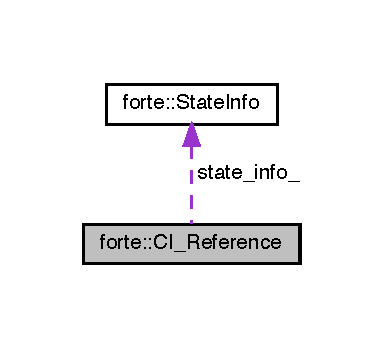
\includegraphics[width=184pt]{classforte_1_1_c_i___reference__coll__graph}
\end{center}
\end{figure}
\subsection*{Public Member Functions}
\begin{DoxyCompactItemize}
\item 
\mbox{\hyperlink{classforte_1_1_c_i___reference_ace7be9be58a678458e45ef781140c8ae}{C\+I\+\_\+\+Reference}} (std\+::shared\+\_\+ptr$<$ \mbox{\hyperlink{classforte_1_1_s_c_f_info}{S\+C\+F\+Info}} $>$ scf\+\_\+info, std\+::shared\+\_\+ptr$<$ \mbox{\hyperlink{classforte_1_1_forte_options}{Forte\+Options}} $>$ options, std\+::shared\+\_\+ptr$<$ \mbox{\hyperlink{classforte_1_1_m_o_space_info}{M\+O\+Space\+Info}} $>$ mo\+\_\+space\+\_\+info, std\+::shared\+\_\+ptr$<$ \mbox{\hyperlink{classforte_1_1_active_space_integrals}{Active\+Space\+Integrals}} $>$ fci\+\_\+ints, int multiplicity, double ms, int symmetry, \mbox{\hyperlink{classforte_1_1_state_info}{State\+Info}} state\+\_\+info)
\begin{DoxyCompactList}\small\item\em Default constructor. \end{DoxyCompactList}\item 
\mbox{\hyperlink{classforte_1_1_c_i___reference_a35b5f56e2dc8ad209ae7afbcb7ef3e69}{$\sim$\+C\+I\+\_\+\+Reference}} ()
\begin{DoxyCompactList}\small\item\em Destructor. \end{DoxyCompactList}\item 
void \mbox{\hyperlink{classforte_1_1_c_i___reference_a8a3e9764cde3969abcf88b688f5440d2}{build\+\_\+reference}} (std\+::vector$<$ \mbox{\hyperlink{namespaceforte_a2076c63fd7b8732004d9e1442ce527c1}{Determinant}} $>$ \&ref\+\_\+space)
\begin{DoxyCompactList}\small\item\em Build a reference. \end{DoxyCompactList}\item 
void \mbox{\hyperlink{classforte_1_1_c_i___reference_a9f2dad6f5ae3ece6d385a519b2a98d12}{build\+\_\+cas\+\_\+reference}} (std\+::vector$<$ \mbox{\hyperlink{namespaceforte_a2076c63fd7b8732004d9e1442ce527c1}{Determinant}} $>$ \&ref\+\_\+space)
\begin{DoxyCompactList}\small\item\em Build the C\+AS reference (with a high limit of basis functions) \end{DoxyCompactList}\item 
void \mbox{\hyperlink{classforte_1_1_c_i___reference_a9dacb4b7abc2e1058065263fa32d072d}{build\+\_\+gas\+\_\+reference}} (std\+::vector$<$ \mbox{\hyperlink{namespaceforte_a2076c63fd7b8732004d9e1442ce527c1}{Determinant}} $>$ \&ref\+\_\+space)
\begin{DoxyCompactList}\small\item\em Build the complete G\+AS reference. \end{DoxyCompactList}\item 
void \mbox{\hyperlink{classforte_1_1_c_i___reference_abd3e854b9dcfe0f8105a2a5fbe42b6dd}{build\+\_\+gas\+\_\+single}} (std\+::vector$<$ \mbox{\hyperlink{namespaceforte_a2076c63fd7b8732004d9e1442ce527c1}{Determinant}} $>$ \&ref\+\_\+space)
\begin{DoxyCompactList}\small\item\em Build single lowest energy state. \end{DoxyCompactList}\item 
void \mbox{\hyperlink{classforte_1_1_c_i___reference_a7d3441e0ac01abaf7f9971dbc4a8f2d8}{set\+\_\+ref\+\_\+type}} (const std\+::string \&ref\+\_\+type)
\begin{DoxyCompactList}\small\item\em Set the reference type. \end{DoxyCompactList}\item 
std\+::pair$<$ std\+::map$<$ std\+::vector$<$ int $>$, std\+::vector$<$ std\+::pair$<$ size\+\_\+t, size\+\_\+t $>$ $>$ $>$, std\+::map$<$ std\+::vector$<$ int $>$, std\+::vector$<$ std\+::pair$<$ size\+\_\+t, size\+\_\+t $>$ $>$ $>$ $>$ \mbox{\hyperlink{classforte_1_1_c_i___reference_af3414d78ff86d2a43d174b9f3a86b84f}{gas\+\_\+single\+\_\+criterion}} ()
\item 
std\+::tuple$<$ std\+::map$<$ std\+::vector$<$ int $>$, std\+::vector$<$ std\+::tuple$<$ size\+\_\+t, size\+\_\+t, size\+\_\+t, size\+\_\+t $>$ $>$ $>$, std\+::map$<$ std\+::vector$<$ int $>$, std\+::vector$<$ std\+::tuple$<$ size\+\_\+t, size\+\_\+t, size\+\_\+t, size\+\_\+t $>$ $>$ $>$, std\+::map$<$ std\+::vector$<$ int $>$, std\+::vector$<$ std\+::tuple$<$ size\+\_\+t, size\+\_\+t, size\+\_\+t, size\+\_\+t $>$ $>$ $>$ $>$ \mbox{\hyperlink{classforte_1_1_c_i___reference_a3508cacd0adb39a9b4288f9358b0f5fe}{gas\+\_\+double\+\_\+criterion}} ()
\item 
std\+::vector$<$ std\+::vector$<$ int $>$ $>$ \mbox{\hyperlink{classforte_1_1_c_i___reference_a590b197025d117d464b6639379ccc831}{gas\+\_\+electrons}} ()
\begin{DoxyCompactList}\small\item\em return gas\+\_\+electrons\+\_\+ \end{DoxyCompactList}\end{DoxyCompactItemize}
\subsection*{Protected Member Functions}
\begin{DoxyCompactItemize}
\item 
std\+::vector$<$ std\+::tuple$<$ double, int, int $>$ $>$ \mbox{\hyperlink{classforte_1_1_c_i___reference_abd0a1dc9df7f57895eb6cf93cd7193b4}{sym\+\_\+labeled\+\_\+orbitals}} (std\+::string type)
\item 
void \mbox{\hyperlink{classforte_1_1_c_i___reference_a69d5e58e9a4721950b81b930aad9afb3}{build\+\_\+ci\+\_\+reference}} (std\+::vector$<$ \mbox{\hyperlink{namespaceforte_a2076c63fd7b8732004d9e1442ce527c1}{Determinant}} $>$ \&ref\+\_\+space)
\item 
\mbox{\hyperlink{namespaceforte_a2076c63fd7b8732004d9e1442ce527c1}{Determinant}} \mbox{\hyperlink{classforte_1_1_c_i___reference_ac34b5a15d590c8556673835af7143d6e}{get\+\_\+occupation}} ()
\item 
void \mbox{\hyperlink{classforte_1_1_c_i___reference_a0048475d04f2472ad1f06cfc4c09a61b}{get\+\_\+gas\+\_\+occupation}} ()
\item 
std\+::pair$<$ std\+::vector$<$ int $>$, std\+::vector$<$ int $>$ $>$ \mbox{\hyperlink{classforte_1_1_c_i___reference_af0d91f0530121a3149dec3f6cca0cabc}{get\+\_\+gas\+\_\+max\+\_\+min}} ()
\end{DoxyCompactItemize}
\subsection*{Protected Attributes}
\begin{DoxyCompactItemize}
\item 
std\+::shared\+\_\+ptr$<$ \mbox{\hyperlink{classforte_1_1_s_c_f_info}{S\+C\+F\+Info}} $>$ \mbox{\hyperlink{classforte_1_1_c_i___reference_a0144cae57432001b7c1e8af7cb6fe35b}{scf\+\_\+info\+\_\+}}
\item 
\mbox{\hyperlink{classforte_1_1_state_info}{State\+Info}} \mbox{\hyperlink{classforte_1_1_c_i___reference_a4848e63165a294524d5321dda65a6ea7}{state\+\_\+info\+\_\+}}
\item 
int \mbox{\hyperlink{classforte_1_1_c_i___reference_a13a156cbd1ddf25e4c29d9fda7acaf01}{multiplicity\+\_\+}}
\item 
double \mbox{\hyperlink{classforte_1_1_c_i___reference_a4a545fae5773bd93e5fb55bdd95303a9}{twice\+\_\+ms\+\_\+}}
\item 
int \mbox{\hyperlink{classforte_1_1_c_i___reference_a40d9896c512347743a0473c52dab1a20}{nalpha\+\_\+}}
\item 
int \mbox{\hyperlink{classforte_1_1_c_i___reference_aca9587b2bc5ae8865d2b5eb8b063bbb3}{nbeta\+\_\+}}
\item 
int \mbox{\hyperlink{classforte_1_1_c_i___reference_ab72b053394477b8da8a30987f747a8aa}{root\+\_\+sym\+\_\+}}
\item 
int \mbox{\hyperlink{classforte_1_1_c_i___reference_a987c8c47ac57e18691a4784c444cd4ee}{nirrep\+\_\+}}
\item 
size\+\_\+t \mbox{\hyperlink{classforte_1_1_c_i___reference_a360fd8b4c4a9ebefdcba1ff5b75173c5}{subspace\+\_\+size\+\_\+}}
\item 
std\+::shared\+\_\+ptr$<$ \mbox{\hyperlink{classforte_1_1_m_o_space_info}{M\+O\+Space\+Info}} $>$ \mbox{\hyperlink{classforte_1_1_c_i___reference_a45d8ef20fc583659241f93ab2c6a0316}{mo\+\_\+space\+\_\+info\+\_\+}}
\item 
std\+::shared\+\_\+ptr$<$ \mbox{\hyperlink{classforte_1_1_forte_options}{Forte\+Options}} $>$ \mbox{\hyperlink{classforte_1_1_c_i___reference_adff8bf78314c834aaad6660576997fc4}{options\+\_\+}}
\item 
int \mbox{\hyperlink{classforte_1_1_c_i___reference_afe5680a4c91723e6ccdd2396e5633a73}{nact\+\_\+}}
\item 
psi\+::\+Dimension \mbox{\hyperlink{classforte_1_1_c_i___reference_a519ea71e21ff54f68991d70a89e5dcb5}{mo\+\_\+symmetry\+\_\+}}
\item 
psi\+::\+Dimension \mbox{\hyperlink{classforte_1_1_c_i___reference_a867494fbee610c7a5dcad09487dabb82}{nactpi\+\_\+}}
\item 
psi\+::\+Dimension \mbox{\hyperlink{classforte_1_1_c_i___reference_a8e501059a51dd7e71a679b9d42fdff04}{frzcpi\+\_\+}}
\item 
std\+::string \mbox{\hyperlink{classforte_1_1_c_i___reference_a1cc19b3a5dc9d1a93c3c812bf6a71a7d}{ref\+\_\+type\+\_\+}}
\item 
std\+::shared\+\_\+ptr$<$ \mbox{\hyperlink{classforte_1_1_active_space_integrals}{Active\+Space\+Integrals}} $>$ \mbox{\hyperlink{classforte_1_1_c_i___reference_aa20ed3648fc1f11c723dbd2b491fc950}{fci\+\_\+ints\+\_\+}}
\item 
size\+\_\+t \mbox{\hyperlink{classforte_1_1_c_i___reference_afab0fbcf5e7f80f516ae0b814ea93911}{gas\+\_\+num\+\_\+}}
\begin{DoxyCompactList}\small\item\em The number of used G\+AS. \end{DoxyCompactList}\item 
std\+::vector$<$ std\+::vector$<$ int $>$ $>$ \mbox{\hyperlink{classforte_1_1_c_i___reference_ab046cdbcafe1926a6a2a9406db621210}{gas\+\_\+electrons\+\_\+}}
\end{DoxyCompactItemize}


\subsection{Constructor \& Destructor Documentation}
\mbox{\Hypertarget{classforte_1_1_c_i___reference_ace7be9be58a678458e45ef781140c8ae}\label{classforte_1_1_c_i___reference_ace7be9be58a678458e45ef781140c8ae}} 
\index{forte\+::\+C\+I\+\_\+\+Reference@{forte\+::\+C\+I\+\_\+\+Reference}!C\+I\+\_\+\+Reference@{C\+I\+\_\+\+Reference}}
\index{C\+I\+\_\+\+Reference@{C\+I\+\_\+\+Reference}!forte\+::\+C\+I\+\_\+\+Reference@{forte\+::\+C\+I\+\_\+\+Reference}}
\subsubsection{\texorpdfstring{C\+I\+\_\+\+Reference()}{CI\_Reference()}}
{\footnotesize\ttfamily forte\+::\+C\+I\+\_\+\+Reference\+::\+C\+I\+\_\+\+Reference (\begin{DoxyParamCaption}\item[{std\+::shared\+\_\+ptr$<$ \mbox{\hyperlink{classforte_1_1_s_c_f_info}{S\+C\+F\+Info}} $>$}]{scf\+\_\+info,  }\item[{std\+::shared\+\_\+ptr$<$ \mbox{\hyperlink{classforte_1_1_forte_options}{Forte\+Options}} $>$}]{options,  }\item[{std\+::shared\+\_\+ptr$<$ \mbox{\hyperlink{classforte_1_1_m_o_space_info}{M\+O\+Space\+Info}} $>$}]{mo\+\_\+space\+\_\+info,  }\item[{std\+::shared\+\_\+ptr$<$ \mbox{\hyperlink{classforte_1_1_active_space_integrals}{Active\+Space\+Integrals}} $>$}]{fci\+\_\+ints,  }\item[{int}]{multiplicity,  }\item[{double}]{ms,  }\item[{int}]{symmetry,  }\item[{\mbox{\hyperlink{classforte_1_1_state_info}{State\+Info}}}]{state\+\_\+info }\end{DoxyParamCaption})}



Default constructor. 

\mbox{\Hypertarget{classforte_1_1_c_i___reference_a35b5f56e2dc8ad209ae7afbcb7ef3e69}\label{classforte_1_1_c_i___reference_a35b5f56e2dc8ad209ae7afbcb7ef3e69}} 
\index{forte\+::\+C\+I\+\_\+\+Reference@{forte\+::\+C\+I\+\_\+\+Reference}!````~C\+I\+\_\+\+Reference@{$\sim$\+C\+I\+\_\+\+Reference}}
\index{````~C\+I\+\_\+\+Reference@{$\sim$\+C\+I\+\_\+\+Reference}!forte\+::\+C\+I\+\_\+\+Reference@{forte\+::\+C\+I\+\_\+\+Reference}}
\subsubsection{\texorpdfstring{$\sim$\+C\+I\+\_\+\+Reference()}{~CI\_Reference()}}
{\footnotesize\ttfamily forte\+::\+C\+I\+\_\+\+Reference\+::$\sim$\+C\+I\+\_\+\+Reference (\begin{DoxyParamCaption}{ }\end{DoxyParamCaption})}



Destructor. 



\subsection{Member Function Documentation}
\mbox{\Hypertarget{classforte_1_1_c_i___reference_a9f2dad6f5ae3ece6d385a519b2a98d12}\label{classforte_1_1_c_i___reference_a9f2dad6f5ae3ece6d385a519b2a98d12}} 
\index{forte\+::\+C\+I\+\_\+\+Reference@{forte\+::\+C\+I\+\_\+\+Reference}!build\+\_\+cas\+\_\+reference@{build\+\_\+cas\+\_\+reference}}
\index{build\+\_\+cas\+\_\+reference@{build\+\_\+cas\+\_\+reference}!forte\+::\+C\+I\+\_\+\+Reference@{forte\+::\+C\+I\+\_\+\+Reference}}
\subsubsection{\texorpdfstring{build\+\_\+cas\+\_\+reference()}{build\_cas\_reference()}}
{\footnotesize\ttfamily void forte\+::\+C\+I\+\_\+\+Reference\+::build\+\_\+cas\+\_\+reference (\begin{DoxyParamCaption}\item[{std\+::vector$<$ \mbox{\hyperlink{namespaceforte_a2076c63fd7b8732004d9e1442ce527c1}{Determinant}} $>$ \&}]{ref\+\_\+space }\end{DoxyParamCaption})}



Build the C\+AS reference (with a high limit of basis functions) 

\mbox{\Hypertarget{classforte_1_1_c_i___reference_a69d5e58e9a4721950b81b930aad9afb3}\label{classforte_1_1_c_i___reference_a69d5e58e9a4721950b81b930aad9afb3}} 
\index{forte\+::\+C\+I\+\_\+\+Reference@{forte\+::\+C\+I\+\_\+\+Reference}!build\+\_\+ci\+\_\+reference@{build\+\_\+ci\+\_\+reference}}
\index{build\+\_\+ci\+\_\+reference@{build\+\_\+ci\+\_\+reference}!forte\+::\+C\+I\+\_\+\+Reference@{forte\+::\+C\+I\+\_\+\+Reference}}
\subsubsection{\texorpdfstring{build\+\_\+ci\+\_\+reference()}{build\_ci\_reference()}}
{\footnotesize\ttfamily void forte\+::\+C\+I\+\_\+\+Reference\+::build\+\_\+ci\+\_\+reference (\begin{DoxyParamCaption}\item[{std\+::vector$<$ \mbox{\hyperlink{namespaceforte_a2076c63fd7b8732004d9e1442ce527c1}{Determinant}} $>$ \&}]{ref\+\_\+space }\end{DoxyParamCaption})\hspace{0.3cm}{\ttfamily [protected]}}

\mbox{\Hypertarget{classforte_1_1_c_i___reference_a9dacb4b7abc2e1058065263fa32d072d}\label{classforte_1_1_c_i___reference_a9dacb4b7abc2e1058065263fa32d072d}} 
\index{forte\+::\+C\+I\+\_\+\+Reference@{forte\+::\+C\+I\+\_\+\+Reference}!build\+\_\+gas\+\_\+reference@{build\+\_\+gas\+\_\+reference}}
\index{build\+\_\+gas\+\_\+reference@{build\+\_\+gas\+\_\+reference}!forte\+::\+C\+I\+\_\+\+Reference@{forte\+::\+C\+I\+\_\+\+Reference}}
\subsubsection{\texorpdfstring{build\+\_\+gas\+\_\+reference()}{build\_gas\_reference()}}
{\footnotesize\ttfamily void forte\+::\+C\+I\+\_\+\+Reference\+::build\+\_\+gas\+\_\+reference (\begin{DoxyParamCaption}\item[{std\+::vector$<$ \mbox{\hyperlink{namespaceforte_a2076c63fd7b8732004d9e1442ce527c1}{Determinant}} $>$ \&}]{ref\+\_\+space }\end{DoxyParamCaption})}



Build the complete G\+AS reference. 

\mbox{\Hypertarget{classforte_1_1_c_i___reference_abd3e854b9dcfe0f8105a2a5fbe42b6dd}\label{classforte_1_1_c_i___reference_abd3e854b9dcfe0f8105a2a5fbe42b6dd}} 
\index{forte\+::\+C\+I\+\_\+\+Reference@{forte\+::\+C\+I\+\_\+\+Reference}!build\+\_\+gas\+\_\+single@{build\+\_\+gas\+\_\+single}}
\index{build\+\_\+gas\+\_\+single@{build\+\_\+gas\+\_\+single}!forte\+::\+C\+I\+\_\+\+Reference@{forte\+::\+C\+I\+\_\+\+Reference}}
\subsubsection{\texorpdfstring{build\+\_\+gas\+\_\+single()}{build\_gas\_single()}}
{\footnotesize\ttfamily void forte\+::\+C\+I\+\_\+\+Reference\+::build\+\_\+gas\+\_\+single (\begin{DoxyParamCaption}\item[{std\+::vector$<$ \mbox{\hyperlink{namespaceforte_a2076c63fd7b8732004d9e1442ce527c1}{Determinant}} $>$ \&}]{ref\+\_\+space }\end{DoxyParamCaption})}



Build single lowest energy state. 

\mbox{\Hypertarget{classforte_1_1_c_i___reference_a8a3e9764cde3969abcf88b688f5440d2}\label{classforte_1_1_c_i___reference_a8a3e9764cde3969abcf88b688f5440d2}} 
\index{forte\+::\+C\+I\+\_\+\+Reference@{forte\+::\+C\+I\+\_\+\+Reference}!build\+\_\+reference@{build\+\_\+reference}}
\index{build\+\_\+reference@{build\+\_\+reference}!forte\+::\+C\+I\+\_\+\+Reference@{forte\+::\+C\+I\+\_\+\+Reference}}
\subsubsection{\texorpdfstring{build\+\_\+reference()}{build\_reference()}}
{\footnotesize\ttfamily void forte\+::\+C\+I\+\_\+\+Reference\+::build\+\_\+reference (\begin{DoxyParamCaption}\item[{std\+::vector$<$ \mbox{\hyperlink{namespaceforte_a2076c63fd7b8732004d9e1442ce527c1}{Determinant}} $>$ \&}]{ref\+\_\+space }\end{DoxyParamCaption})}



Build a reference. 

\mbox{\Hypertarget{classforte_1_1_c_i___reference_a3508cacd0adb39a9b4288f9358b0f5fe}\label{classforte_1_1_c_i___reference_a3508cacd0adb39a9b4288f9358b0f5fe}} 
\index{forte\+::\+C\+I\+\_\+\+Reference@{forte\+::\+C\+I\+\_\+\+Reference}!gas\+\_\+double\+\_\+criterion@{gas\+\_\+double\+\_\+criterion}}
\index{gas\+\_\+double\+\_\+criterion@{gas\+\_\+double\+\_\+criterion}!forte\+::\+C\+I\+\_\+\+Reference@{forte\+::\+C\+I\+\_\+\+Reference}}
\subsubsection{\texorpdfstring{gas\+\_\+double\+\_\+criterion()}{gas\_double\_criterion()}}
{\footnotesize\ttfamily std\+::tuple$<$ std\+::map$<$ std\+::vector$<$ int $>$, std\+::vector$<$ std\+::tuple$<$ size\+\_\+t, size\+\_\+t, size\+\_\+t, size\+\_\+t $>$ $>$ $>$, std\+::map$<$ std\+::vector$<$ int $>$, std\+::vector$<$ std\+::tuple$<$ size\+\_\+t, size\+\_\+t, size\+\_\+t, size\+\_\+t $>$ $>$ $>$, std\+::map$<$ std\+::vector$<$ int $>$, std\+::vector$<$ std\+::tuple$<$ size\+\_\+t, size\+\_\+t, size\+\_\+t, size\+\_\+t $>$ $>$ $>$ $>$ forte\+::\+C\+I\+\_\+\+Reference\+::gas\+\_\+double\+\_\+criterion (\begin{DoxyParamCaption}{ }\end{DoxyParamCaption})}

Return a tuple of maps for double excitation between different G\+AS alphaalpha, betabeta, alphabeta \mbox{\Hypertarget{classforte_1_1_c_i___reference_a590b197025d117d464b6639379ccc831}\label{classforte_1_1_c_i___reference_a590b197025d117d464b6639379ccc831}} 
\index{forte\+::\+C\+I\+\_\+\+Reference@{forte\+::\+C\+I\+\_\+\+Reference}!gas\+\_\+electrons@{gas\+\_\+electrons}}
\index{gas\+\_\+electrons@{gas\+\_\+electrons}!forte\+::\+C\+I\+\_\+\+Reference@{forte\+::\+C\+I\+\_\+\+Reference}}
\subsubsection{\texorpdfstring{gas\+\_\+electrons()}{gas\_electrons()}}
{\footnotesize\ttfamily std\+::vector$<$ std\+::vector$<$ int $>$ $>$ forte\+::\+C\+I\+\_\+\+Reference\+::gas\+\_\+electrons (\begin{DoxyParamCaption}{ }\end{DoxyParamCaption})}



return gas\+\_\+electrons\+\_\+ 

\mbox{\Hypertarget{classforte_1_1_c_i___reference_af3414d78ff86d2a43d174b9f3a86b84f}\label{classforte_1_1_c_i___reference_af3414d78ff86d2a43d174b9f3a86b84f}} 
\index{forte\+::\+C\+I\+\_\+\+Reference@{forte\+::\+C\+I\+\_\+\+Reference}!gas\+\_\+single\+\_\+criterion@{gas\+\_\+single\+\_\+criterion}}
\index{gas\+\_\+single\+\_\+criterion@{gas\+\_\+single\+\_\+criterion}!forte\+::\+C\+I\+\_\+\+Reference@{forte\+::\+C\+I\+\_\+\+Reference}}
\subsubsection{\texorpdfstring{gas\+\_\+single\+\_\+criterion()}{gas\_single\_criterion()}}
{\footnotesize\ttfamily std\+::pair$<$ std\+::map$<$ std\+::vector$<$ int $>$, std\+::vector$<$ std\+::pair$<$ size\+\_\+t, size\+\_\+t $>$ $>$ $>$, std\+::map$<$ std\+::vector$<$ int $>$, std\+::vector$<$ std\+::pair$<$ size\+\_\+t, size\+\_\+t $>$ $>$ $>$ $>$ forte\+::\+C\+I\+\_\+\+Reference\+::gas\+\_\+single\+\_\+criterion (\begin{DoxyParamCaption}{ }\end{DoxyParamCaption})}

Return a pair for single excitation between different G\+AS alpha, beta \mbox{\Hypertarget{classforte_1_1_c_i___reference_af0d91f0530121a3149dec3f6cca0cabc}\label{classforte_1_1_c_i___reference_af0d91f0530121a3149dec3f6cca0cabc}} 
\index{forte\+::\+C\+I\+\_\+\+Reference@{forte\+::\+C\+I\+\_\+\+Reference}!get\+\_\+gas\+\_\+max\+\_\+min@{get\+\_\+gas\+\_\+max\+\_\+min}}
\index{get\+\_\+gas\+\_\+max\+\_\+min@{get\+\_\+gas\+\_\+max\+\_\+min}!forte\+::\+C\+I\+\_\+\+Reference@{forte\+::\+C\+I\+\_\+\+Reference}}
\subsubsection{\texorpdfstring{get\+\_\+gas\+\_\+max\+\_\+min()}{get\_gas\_max\_min()}}
{\footnotesize\ttfamily std\+::pair$<$std\+::vector$<$int$>$, std\+::vector$<$int$>$ $>$ forte\+::\+C\+I\+\_\+\+Reference\+::get\+\_\+gas\+\_\+max\+\_\+min (\begin{DoxyParamCaption}{ }\end{DoxyParamCaption})\hspace{0.3cm}{\ttfamily [protected]}}

\mbox{\Hypertarget{classforte_1_1_c_i___reference_a0048475d04f2472ad1f06cfc4c09a61b}\label{classforte_1_1_c_i___reference_a0048475d04f2472ad1f06cfc4c09a61b}} 
\index{forte\+::\+C\+I\+\_\+\+Reference@{forte\+::\+C\+I\+\_\+\+Reference}!get\+\_\+gas\+\_\+occupation@{get\+\_\+gas\+\_\+occupation}}
\index{get\+\_\+gas\+\_\+occupation@{get\+\_\+gas\+\_\+occupation}!forte\+::\+C\+I\+\_\+\+Reference@{forte\+::\+C\+I\+\_\+\+Reference}}
\subsubsection{\texorpdfstring{get\+\_\+gas\+\_\+occupation()}{get\_gas\_occupation()}}
{\footnotesize\ttfamily void forte\+::\+C\+I\+\_\+\+Reference\+::get\+\_\+gas\+\_\+occupation (\begin{DoxyParamCaption}{ }\end{DoxyParamCaption})\hspace{0.3cm}{\ttfamily [protected]}}

\mbox{\Hypertarget{classforte_1_1_c_i___reference_ac34b5a15d590c8556673835af7143d6e}\label{classforte_1_1_c_i___reference_ac34b5a15d590c8556673835af7143d6e}} 
\index{forte\+::\+C\+I\+\_\+\+Reference@{forte\+::\+C\+I\+\_\+\+Reference}!get\+\_\+occupation@{get\+\_\+occupation}}
\index{get\+\_\+occupation@{get\+\_\+occupation}!forte\+::\+C\+I\+\_\+\+Reference@{forte\+::\+C\+I\+\_\+\+Reference}}
\subsubsection{\texorpdfstring{get\+\_\+occupation()}{get\_occupation()}}
{\footnotesize\ttfamily \mbox{\hyperlink{namespaceforte_a2076c63fd7b8732004d9e1442ce527c1}{Determinant}} forte\+::\+C\+I\+\_\+\+Reference\+::get\+\_\+occupation (\begin{DoxyParamCaption}{ }\end{DoxyParamCaption})\hspace{0.3cm}{\ttfamily [protected]}}

\mbox{\Hypertarget{classforte_1_1_c_i___reference_a7d3441e0ac01abaf7f9971dbc4a8f2d8}\label{classforte_1_1_c_i___reference_a7d3441e0ac01abaf7f9971dbc4a8f2d8}} 
\index{forte\+::\+C\+I\+\_\+\+Reference@{forte\+::\+C\+I\+\_\+\+Reference}!set\+\_\+ref\+\_\+type@{set\+\_\+ref\+\_\+type}}
\index{set\+\_\+ref\+\_\+type@{set\+\_\+ref\+\_\+type}!forte\+::\+C\+I\+\_\+\+Reference@{forte\+::\+C\+I\+\_\+\+Reference}}
\subsubsection{\texorpdfstring{set\+\_\+ref\+\_\+type()}{set\_ref\_type()}}
{\footnotesize\ttfamily void forte\+::\+C\+I\+\_\+\+Reference\+::set\+\_\+ref\+\_\+type (\begin{DoxyParamCaption}\item[{const std\+::string \&}]{ref\+\_\+type }\end{DoxyParamCaption})\hspace{0.3cm}{\ttfamily [inline]}}



Set the reference type. 

\mbox{\Hypertarget{classforte_1_1_c_i___reference_abd0a1dc9df7f57895eb6cf93cd7193b4}\label{classforte_1_1_c_i___reference_abd0a1dc9df7f57895eb6cf93cd7193b4}} 
\index{forte\+::\+C\+I\+\_\+\+Reference@{forte\+::\+C\+I\+\_\+\+Reference}!sym\+\_\+labeled\+\_\+orbitals@{sym\+\_\+labeled\+\_\+orbitals}}
\index{sym\+\_\+labeled\+\_\+orbitals@{sym\+\_\+labeled\+\_\+orbitals}!forte\+::\+C\+I\+\_\+\+Reference@{forte\+::\+C\+I\+\_\+\+Reference}}
\subsubsection{\texorpdfstring{sym\+\_\+labeled\+\_\+orbitals()}{sym\_labeled\_orbitals()}}
{\footnotesize\ttfamily std\+::vector$<$ std\+::tuple$<$ double, int, int $>$ $>$ forte\+::\+C\+I\+\_\+\+Reference\+::sym\+\_\+labeled\+\_\+orbitals (\begin{DoxyParamCaption}\item[{std\+::string}]{type }\end{DoxyParamCaption})\hspace{0.3cm}{\ttfamily [protected]}}



\subsection{Member Data Documentation}
\mbox{\Hypertarget{classforte_1_1_c_i___reference_aa20ed3648fc1f11c723dbd2b491fc950}\label{classforte_1_1_c_i___reference_aa20ed3648fc1f11c723dbd2b491fc950}} 
\index{forte\+::\+C\+I\+\_\+\+Reference@{forte\+::\+C\+I\+\_\+\+Reference}!fci\+\_\+ints\+\_\+@{fci\+\_\+ints\+\_\+}}
\index{fci\+\_\+ints\+\_\+@{fci\+\_\+ints\+\_\+}!forte\+::\+C\+I\+\_\+\+Reference@{forte\+::\+C\+I\+\_\+\+Reference}}
\subsubsection{\texorpdfstring{fci\+\_\+ints\+\_\+}{fci\_ints\_}}
{\footnotesize\ttfamily std\+::shared\+\_\+ptr$<$\mbox{\hyperlink{classforte_1_1_active_space_integrals}{Active\+Space\+Integrals}}$>$ forte\+::\+C\+I\+\_\+\+Reference\+::fci\+\_\+ints\+\_\+\hspace{0.3cm}{\ttfamily [protected]}}

\mbox{\Hypertarget{classforte_1_1_c_i___reference_a8e501059a51dd7e71a679b9d42fdff04}\label{classforte_1_1_c_i___reference_a8e501059a51dd7e71a679b9d42fdff04}} 
\index{forte\+::\+C\+I\+\_\+\+Reference@{forte\+::\+C\+I\+\_\+\+Reference}!frzcpi\+\_\+@{frzcpi\+\_\+}}
\index{frzcpi\+\_\+@{frzcpi\+\_\+}!forte\+::\+C\+I\+\_\+\+Reference@{forte\+::\+C\+I\+\_\+\+Reference}}
\subsubsection{\texorpdfstring{frzcpi\+\_\+}{frzcpi\_}}
{\footnotesize\ttfamily psi\+::\+Dimension forte\+::\+C\+I\+\_\+\+Reference\+::frzcpi\+\_\+\hspace{0.3cm}{\ttfamily [protected]}}

\mbox{\Hypertarget{classforte_1_1_c_i___reference_ab046cdbcafe1926a6a2a9406db621210}\label{classforte_1_1_c_i___reference_ab046cdbcafe1926a6a2a9406db621210}} 
\index{forte\+::\+C\+I\+\_\+\+Reference@{forte\+::\+C\+I\+\_\+\+Reference}!gas\+\_\+electrons\+\_\+@{gas\+\_\+electrons\+\_\+}}
\index{gas\+\_\+electrons\+\_\+@{gas\+\_\+electrons\+\_\+}!forte\+::\+C\+I\+\_\+\+Reference@{forte\+::\+C\+I\+\_\+\+Reference}}
\subsubsection{\texorpdfstring{gas\+\_\+electrons\+\_\+}{gas\_electrons\_}}
{\footnotesize\ttfamily std\+::vector$<$std\+::vector$<$int$>$ $>$ forte\+::\+C\+I\+\_\+\+Reference\+::gas\+\_\+electrons\+\_\+\hspace{0.3cm}{\ttfamily [protected]}}

All the possible alpha and beta electron occupations of each G\+AS G\+A\+S1\+\_\+A, G\+A\+S1\+\_\+B, G\+A\+S2\+\_\+A, .... G\+A\+S6\+\_\+B (12 elements) \mbox{\Hypertarget{classforte_1_1_c_i___reference_afab0fbcf5e7f80f516ae0b814ea93911}\label{classforte_1_1_c_i___reference_afab0fbcf5e7f80f516ae0b814ea93911}} 
\index{forte\+::\+C\+I\+\_\+\+Reference@{forte\+::\+C\+I\+\_\+\+Reference}!gas\+\_\+num\+\_\+@{gas\+\_\+num\+\_\+}}
\index{gas\+\_\+num\+\_\+@{gas\+\_\+num\+\_\+}!forte\+::\+C\+I\+\_\+\+Reference@{forte\+::\+C\+I\+\_\+\+Reference}}
\subsubsection{\texorpdfstring{gas\+\_\+num\+\_\+}{gas\_num\_}}
{\footnotesize\ttfamily size\+\_\+t forte\+::\+C\+I\+\_\+\+Reference\+::gas\+\_\+num\+\_\+\hspace{0.3cm}{\ttfamily [protected]}}



The number of used G\+AS. 

\mbox{\Hypertarget{classforte_1_1_c_i___reference_a45d8ef20fc583659241f93ab2c6a0316}\label{classforte_1_1_c_i___reference_a45d8ef20fc583659241f93ab2c6a0316}} 
\index{forte\+::\+C\+I\+\_\+\+Reference@{forte\+::\+C\+I\+\_\+\+Reference}!mo\+\_\+space\+\_\+info\+\_\+@{mo\+\_\+space\+\_\+info\+\_\+}}
\index{mo\+\_\+space\+\_\+info\+\_\+@{mo\+\_\+space\+\_\+info\+\_\+}!forte\+::\+C\+I\+\_\+\+Reference@{forte\+::\+C\+I\+\_\+\+Reference}}
\subsubsection{\texorpdfstring{mo\+\_\+space\+\_\+info\+\_\+}{mo\_space\_info\_}}
{\footnotesize\ttfamily std\+::shared\+\_\+ptr$<$\mbox{\hyperlink{classforte_1_1_m_o_space_info}{M\+O\+Space\+Info}}$>$ forte\+::\+C\+I\+\_\+\+Reference\+::mo\+\_\+space\+\_\+info\+\_\+\hspace{0.3cm}{\ttfamily [protected]}}

\mbox{\Hypertarget{classforte_1_1_c_i___reference_a519ea71e21ff54f68991d70a89e5dcb5}\label{classforte_1_1_c_i___reference_a519ea71e21ff54f68991d70a89e5dcb5}} 
\index{forte\+::\+C\+I\+\_\+\+Reference@{forte\+::\+C\+I\+\_\+\+Reference}!mo\+\_\+symmetry\+\_\+@{mo\+\_\+symmetry\+\_\+}}
\index{mo\+\_\+symmetry\+\_\+@{mo\+\_\+symmetry\+\_\+}!forte\+::\+C\+I\+\_\+\+Reference@{forte\+::\+C\+I\+\_\+\+Reference}}
\subsubsection{\texorpdfstring{mo\+\_\+symmetry\+\_\+}{mo\_symmetry\_}}
{\footnotesize\ttfamily psi\+::\+Dimension forte\+::\+C\+I\+\_\+\+Reference\+::mo\+\_\+symmetry\+\_\+\hspace{0.3cm}{\ttfamily [protected]}}

\mbox{\Hypertarget{classforte_1_1_c_i___reference_a13a156cbd1ddf25e4c29d9fda7acaf01}\label{classforte_1_1_c_i___reference_a13a156cbd1ddf25e4c29d9fda7acaf01}} 
\index{forte\+::\+C\+I\+\_\+\+Reference@{forte\+::\+C\+I\+\_\+\+Reference}!multiplicity\+\_\+@{multiplicity\+\_\+}}
\index{multiplicity\+\_\+@{multiplicity\+\_\+}!forte\+::\+C\+I\+\_\+\+Reference@{forte\+::\+C\+I\+\_\+\+Reference}}
\subsubsection{\texorpdfstring{multiplicity\+\_\+}{multiplicity\_}}
{\footnotesize\ttfamily int forte\+::\+C\+I\+\_\+\+Reference\+::multiplicity\+\_\+\hspace{0.3cm}{\ttfamily [protected]}}

\mbox{\Hypertarget{classforte_1_1_c_i___reference_afe5680a4c91723e6ccdd2396e5633a73}\label{classforte_1_1_c_i___reference_afe5680a4c91723e6ccdd2396e5633a73}} 
\index{forte\+::\+C\+I\+\_\+\+Reference@{forte\+::\+C\+I\+\_\+\+Reference}!nact\+\_\+@{nact\+\_\+}}
\index{nact\+\_\+@{nact\+\_\+}!forte\+::\+C\+I\+\_\+\+Reference@{forte\+::\+C\+I\+\_\+\+Reference}}
\subsubsection{\texorpdfstring{nact\+\_\+}{nact\_}}
{\footnotesize\ttfamily int forte\+::\+C\+I\+\_\+\+Reference\+::nact\+\_\+\hspace{0.3cm}{\ttfamily [protected]}}

\mbox{\Hypertarget{classforte_1_1_c_i___reference_a867494fbee610c7a5dcad09487dabb82}\label{classforte_1_1_c_i___reference_a867494fbee610c7a5dcad09487dabb82}} 
\index{forte\+::\+C\+I\+\_\+\+Reference@{forte\+::\+C\+I\+\_\+\+Reference}!nactpi\+\_\+@{nactpi\+\_\+}}
\index{nactpi\+\_\+@{nactpi\+\_\+}!forte\+::\+C\+I\+\_\+\+Reference@{forte\+::\+C\+I\+\_\+\+Reference}}
\subsubsection{\texorpdfstring{nactpi\+\_\+}{nactpi\_}}
{\footnotesize\ttfamily psi\+::\+Dimension forte\+::\+C\+I\+\_\+\+Reference\+::nactpi\+\_\+\hspace{0.3cm}{\ttfamily [protected]}}

\mbox{\Hypertarget{classforte_1_1_c_i___reference_a40d9896c512347743a0473c52dab1a20}\label{classforte_1_1_c_i___reference_a40d9896c512347743a0473c52dab1a20}} 
\index{forte\+::\+C\+I\+\_\+\+Reference@{forte\+::\+C\+I\+\_\+\+Reference}!nalpha\+\_\+@{nalpha\+\_\+}}
\index{nalpha\+\_\+@{nalpha\+\_\+}!forte\+::\+C\+I\+\_\+\+Reference@{forte\+::\+C\+I\+\_\+\+Reference}}
\subsubsection{\texorpdfstring{nalpha\+\_\+}{nalpha\_}}
{\footnotesize\ttfamily int forte\+::\+C\+I\+\_\+\+Reference\+::nalpha\+\_\+\hspace{0.3cm}{\ttfamily [protected]}}

\mbox{\Hypertarget{classforte_1_1_c_i___reference_aca9587b2bc5ae8865d2b5eb8b063bbb3}\label{classforte_1_1_c_i___reference_aca9587b2bc5ae8865d2b5eb8b063bbb3}} 
\index{forte\+::\+C\+I\+\_\+\+Reference@{forte\+::\+C\+I\+\_\+\+Reference}!nbeta\+\_\+@{nbeta\+\_\+}}
\index{nbeta\+\_\+@{nbeta\+\_\+}!forte\+::\+C\+I\+\_\+\+Reference@{forte\+::\+C\+I\+\_\+\+Reference}}
\subsubsection{\texorpdfstring{nbeta\+\_\+}{nbeta\_}}
{\footnotesize\ttfamily int forte\+::\+C\+I\+\_\+\+Reference\+::nbeta\+\_\+\hspace{0.3cm}{\ttfamily [protected]}}

\mbox{\Hypertarget{classforte_1_1_c_i___reference_a987c8c47ac57e18691a4784c444cd4ee}\label{classforte_1_1_c_i___reference_a987c8c47ac57e18691a4784c444cd4ee}} 
\index{forte\+::\+C\+I\+\_\+\+Reference@{forte\+::\+C\+I\+\_\+\+Reference}!nirrep\+\_\+@{nirrep\+\_\+}}
\index{nirrep\+\_\+@{nirrep\+\_\+}!forte\+::\+C\+I\+\_\+\+Reference@{forte\+::\+C\+I\+\_\+\+Reference}}
\subsubsection{\texorpdfstring{nirrep\+\_\+}{nirrep\_}}
{\footnotesize\ttfamily int forte\+::\+C\+I\+\_\+\+Reference\+::nirrep\+\_\+\hspace{0.3cm}{\ttfamily [protected]}}

\mbox{\Hypertarget{classforte_1_1_c_i___reference_adff8bf78314c834aaad6660576997fc4}\label{classforte_1_1_c_i___reference_adff8bf78314c834aaad6660576997fc4}} 
\index{forte\+::\+C\+I\+\_\+\+Reference@{forte\+::\+C\+I\+\_\+\+Reference}!options\+\_\+@{options\+\_\+}}
\index{options\+\_\+@{options\+\_\+}!forte\+::\+C\+I\+\_\+\+Reference@{forte\+::\+C\+I\+\_\+\+Reference}}
\subsubsection{\texorpdfstring{options\+\_\+}{options\_}}
{\footnotesize\ttfamily std\+::shared\+\_\+ptr$<$\mbox{\hyperlink{classforte_1_1_forte_options}{Forte\+Options}}$>$ forte\+::\+C\+I\+\_\+\+Reference\+::options\+\_\+\hspace{0.3cm}{\ttfamily [protected]}}

\mbox{\Hypertarget{classforte_1_1_c_i___reference_a1cc19b3a5dc9d1a93c3c812bf6a71a7d}\label{classforte_1_1_c_i___reference_a1cc19b3a5dc9d1a93c3c812bf6a71a7d}} 
\index{forte\+::\+C\+I\+\_\+\+Reference@{forte\+::\+C\+I\+\_\+\+Reference}!ref\+\_\+type\+\_\+@{ref\+\_\+type\+\_\+}}
\index{ref\+\_\+type\+\_\+@{ref\+\_\+type\+\_\+}!forte\+::\+C\+I\+\_\+\+Reference@{forte\+::\+C\+I\+\_\+\+Reference}}
\subsubsection{\texorpdfstring{ref\+\_\+type\+\_\+}{ref\_type\_}}
{\footnotesize\ttfamily std\+::string forte\+::\+C\+I\+\_\+\+Reference\+::ref\+\_\+type\+\_\+\hspace{0.3cm}{\ttfamily [protected]}}

\mbox{\Hypertarget{classforte_1_1_c_i___reference_ab72b053394477b8da8a30987f747a8aa}\label{classforte_1_1_c_i___reference_ab72b053394477b8da8a30987f747a8aa}} 
\index{forte\+::\+C\+I\+\_\+\+Reference@{forte\+::\+C\+I\+\_\+\+Reference}!root\+\_\+sym\+\_\+@{root\+\_\+sym\+\_\+}}
\index{root\+\_\+sym\+\_\+@{root\+\_\+sym\+\_\+}!forte\+::\+C\+I\+\_\+\+Reference@{forte\+::\+C\+I\+\_\+\+Reference}}
\subsubsection{\texorpdfstring{root\+\_\+sym\+\_\+}{root\_sym\_}}
{\footnotesize\ttfamily int forte\+::\+C\+I\+\_\+\+Reference\+::root\+\_\+sym\+\_\+\hspace{0.3cm}{\ttfamily [protected]}}

\mbox{\Hypertarget{classforte_1_1_c_i___reference_a0144cae57432001b7c1e8af7cb6fe35b}\label{classforte_1_1_c_i___reference_a0144cae57432001b7c1e8af7cb6fe35b}} 
\index{forte\+::\+C\+I\+\_\+\+Reference@{forte\+::\+C\+I\+\_\+\+Reference}!scf\+\_\+info\+\_\+@{scf\+\_\+info\+\_\+}}
\index{scf\+\_\+info\+\_\+@{scf\+\_\+info\+\_\+}!forte\+::\+C\+I\+\_\+\+Reference@{forte\+::\+C\+I\+\_\+\+Reference}}
\subsubsection{\texorpdfstring{scf\+\_\+info\+\_\+}{scf\_info\_}}
{\footnotesize\ttfamily std\+::shared\+\_\+ptr$<$\mbox{\hyperlink{classforte_1_1_s_c_f_info}{S\+C\+F\+Info}}$>$ forte\+::\+C\+I\+\_\+\+Reference\+::scf\+\_\+info\+\_\+\hspace{0.3cm}{\ttfamily [protected]}}

\mbox{\Hypertarget{classforte_1_1_c_i___reference_a4848e63165a294524d5321dda65a6ea7}\label{classforte_1_1_c_i___reference_a4848e63165a294524d5321dda65a6ea7}} 
\index{forte\+::\+C\+I\+\_\+\+Reference@{forte\+::\+C\+I\+\_\+\+Reference}!state\+\_\+info\+\_\+@{state\+\_\+info\+\_\+}}
\index{state\+\_\+info\+\_\+@{state\+\_\+info\+\_\+}!forte\+::\+C\+I\+\_\+\+Reference@{forte\+::\+C\+I\+\_\+\+Reference}}
\subsubsection{\texorpdfstring{state\+\_\+info\+\_\+}{state\_info\_}}
{\footnotesize\ttfamily \mbox{\hyperlink{classforte_1_1_state_info}{State\+Info}} forte\+::\+C\+I\+\_\+\+Reference\+::state\+\_\+info\+\_\+\hspace{0.3cm}{\ttfamily [protected]}}

\mbox{\Hypertarget{classforte_1_1_c_i___reference_a360fd8b4c4a9ebefdcba1ff5b75173c5}\label{classforte_1_1_c_i___reference_a360fd8b4c4a9ebefdcba1ff5b75173c5}} 
\index{forte\+::\+C\+I\+\_\+\+Reference@{forte\+::\+C\+I\+\_\+\+Reference}!subspace\+\_\+size\+\_\+@{subspace\+\_\+size\+\_\+}}
\index{subspace\+\_\+size\+\_\+@{subspace\+\_\+size\+\_\+}!forte\+::\+C\+I\+\_\+\+Reference@{forte\+::\+C\+I\+\_\+\+Reference}}
\subsubsection{\texorpdfstring{subspace\+\_\+size\+\_\+}{subspace\_size\_}}
{\footnotesize\ttfamily size\+\_\+t forte\+::\+C\+I\+\_\+\+Reference\+::subspace\+\_\+size\+\_\+\hspace{0.3cm}{\ttfamily [protected]}}

\mbox{\Hypertarget{classforte_1_1_c_i___reference_a4a545fae5773bd93e5fb55bdd95303a9}\label{classforte_1_1_c_i___reference_a4a545fae5773bd93e5fb55bdd95303a9}} 
\index{forte\+::\+C\+I\+\_\+\+Reference@{forte\+::\+C\+I\+\_\+\+Reference}!twice\+\_\+ms\+\_\+@{twice\+\_\+ms\+\_\+}}
\index{twice\+\_\+ms\+\_\+@{twice\+\_\+ms\+\_\+}!forte\+::\+C\+I\+\_\+\+Reference@{forte\+::\+C\+I\+\_\+\+Reference}}
\subsubsection{\texorpdfstring{twice\+\_\+ms\+\_\+}{twice\_ms\_}}
{\footnotesize\ttfamily double forte\+::\+C\+I\+\_\+\+Reference\+::twice\+\_\+ms\+\_\+\hspace{0.3cm}{\ttfamily [protected]}}



The documentation for this class was generated from the following files\+:\begin{DoxyCompactItemize}
\item 
/\+Users/fevange/\+Source/forte/src/sparse\+\_\+ci/\mbox{\hyperlink{ci__reference_8h}{ci\+\_\+reference.\+h}}\item 
/\+Users/fevange/\+Source/forte/src/sparse\+\_\+ci/\mbox{\hyperlink{ci__reference_8cc}{ci\+\_\+reference.\+cc}}\end{DoxyCompactItemize}

\hypertarget{classforte_1_1_c_i_n_o}{}\section{forte\+:\+:C\+I\+NO Class Reference}
\label{classforte_1_1_c_i_n_o}\index{forte\+::\+C\+I\+NO@{forte\+::\+C\+I\+NO}}


The \mbox{\hyperlink{classforte_1_1_c_i_n_o}{C\+I\+NO}} class This class implements natural orbitals for CI wave functions.  




{\ttfamily \#include $<$ci-\/no.\+h$>$}



Inheritance diagram for forte\+:\+:C\+I\+NO\+:
\nopagebreak
\begin{figure}[H]
\begin{center}
\leavevmode
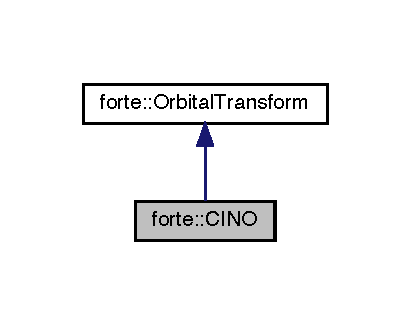
\includegraphics[width=197pt]{classforte_1_1_c_i_n_o__inherit__graph}
\end{center}
\end{figure}


Collaboration diagram for forte\+:\+:C\+I\+NO\+:
\nopagebreak
\begin{figure}[H]
\begin{center}
\leavevmode
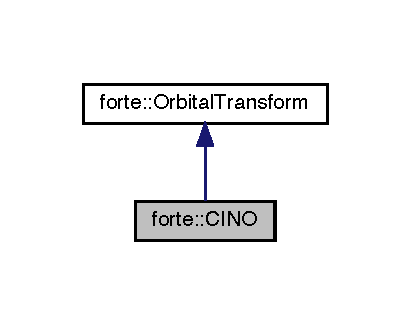
\includegraphics[width=197pt]{classforte_1_1_c_i_n_o__coll__graph}
\end{center}
\end{figure}
\subsection*{Public Member Functions}
\begin{DoxyCompactItemize}
\item 
\mbox{\hyperlink{classforte_1_1_c_i_n_o_af2ad19171a4a6ded060e0641043f0630}{C\+I\+NO}} (std\+::shared\+\_\+ptr$<$ \mbox{\hyperlink{classforte_1_1_s_c_f_info}{S\+C\+F\+Info}} $>$ scf\+\_\+info, std\+::shared\+\_\+ptr$<$ \mbox{\hyperlink{classforte_1_1_forte_options}{Forte\+Options}} $>$ options, std\+::shared\+\_\+ptr$<$ \mbox{\hyperlink{classforte_1_1_forte_integrals}{Forte\+Integrals}} $>$ ints, std\+::shared\+\_\+ptr$<$ \mbox{\hyperlink{classforte_1_1_m_o_space_info}{M\+O\+Space\+Info}} $>$ mo\+\_\+space\+\_\+info)
\item 
\mbox{\hyperlink{classforte_1_1_c_i_n_o_a0d1de460f1bb446781c9dc2fbdb0a04a}{$\sim$\+C\+I\+NO}} ()
\begin{DoxyCompactList}\small\item\em Destructor. \end{DoxyCompactList}\item 
void \mbox{\hyperlink{classforte_1_1_c_i_n_o_a8ac65e808e51c30f613cea8fcdbec851}{compute\+\_\+transformation}} ()
\begin{DoxyCompactList}\small\item\em Compute the energy. \end{DoxyCompactList}\item 
psi\+::\+Shared\+Matrix \mbox{\hyperlink{classforte_1_1_c_i_n_o_a382fe0963a51a908790fda6a7aab0e7c}{get\+\_\+\+Ua}} ()
\item 
psi\+::\+Shared\+Matrix \mbox{\hyperlink{classforte_1_1_c_i_n_o_a24b4455c4b640b7bc01b0f12b0ecb655}{get\+\_\+\+Ub}} ()
\end{DoxyCompactItemize}
\subsection*{Additional Inherited Members}


\subsection{Detailed Description}
The \mbox{\hyperlink{classforte_1_1_c_i_n_o}{C\+I\+NO}} class This class implements natural orbitals for CI wave functions. 

\subsection{Constructor \& Destructor Documentation}
\mbox{\Hypertarget{classforte_1_1_c_i_n_o_af2ad19171a4a6ded060e0641043f0630}\label{classforte_1_1_c_i_n_o_af2ad19171a4a6ded060e0641043f0630}} 
\index{forte\+::\+C\+I\+NO@{forte\+::\+C\+I\+NO}!C\+I\+NO@{C\+I\+NO}}
\index{C\+I\+NO@{C\+I\+NO}!forte\+::\+C\+I\+NO@{forte\+::\+C\+I\+NO}}
\subsubsection{\texorpdfstring{C\+I\+N\+O()}{CINO()}}
{\footnotesize\ttfamily forte\+::\+C\+I\+N\+O\+::\+C\+I\+NO (\begin{DoxyParamCaption}\item[{std\+::shared\+\_\+ptr$<$ \mbox{\hyperlink{classforte_1_1_s_c_f_info}{S\+C\+F\+Info}} $>$}]{scf\+\_\+info,  }\item[{std\+::shared\+\_\+ptr$<$ \mbox{\hyperlink{classforte_1_1_forte_options}{Forte\+Options}} $>$}]{options,  }\item[{std\+::shared\+\_\+ptr$<$ \mbox{\hyperlink{classforte_1_1_forte_integrals}{Forte\+Integrals}} $>$}]{ints,  }\item[{std\+::shared\+\_\+ptr$<$ \mbox{\hyperlink{classforte_1_1_m_o_space_info}{M\+O\+Space\+Info}} $>$}]{mo\+\_\+space\+\_\+info }\end{DoxyParamCaption})}

Constructor 
\begin{DoxyParams}{Parameters}
{\em ref\+\_\+wfn} & The reference wavefunction object \\
\hline
{\em options} & The main options object \\
\hline
{\em ints} & A pointer to an allocated integral object \\
\hline
{\em mo\+\_\+space\+\_\+info} & A pointer to the \mbox{\hyperlink{classforte_1_1_m_o_space_info}{M\+O\+Space\+Info}} object \\
\hline
\end{DoxyParams}
\mbox{\Hypertarget{classforte_1_1_c_i_n_o_a0d1de460f1bb446781c9dc2fbdb0a04a}\label{classforte_1_1_c_i_n_o_a0d1de460f1bb446781c9dc2fbdb0a04a}} 
\index{forte\+::\+C\+I\+NO@{forte\+::\+C\+I\+NO}!````~C\+I\+NO@{$\sim$\+C\+I\+NO}}
\index{````~C\+I\+NO@{$\sim$\+C\+I\+NO}!forte\+::\+C\+I\+NO@{forte\+::\+C\+I\+NO}}
\subsubsection{\texorpdfstring{$\sim$\+C\+I\+N\+O()}{~CINO()}}
{\footnotesize\ttfamily forte\+::\+C\+I\+N\+O\+::$\sim$\+C\+I\+NO (\begin{DoxyParamCaption}{ }\end{DoxyParamCaption})}



Destructor. 



\subsection{Member Function Documentation}
\mbox{\Hypertarget{classforte_1_1_c_i_n_o_a8ac65e808e51c30f613cea8fcdbec851}\label{classforte_1_1_c_i_n_o_a8ac65e808e51c30f613cea8fcdbec851}} 
\index{forte\+::\+C\+I\+NO@{forte\+::\+C\+I\+NO}!compute\+\_\+transformation@{compute\+\_\+transformation}}
\index{compute\+\_\+transformation@{compute\+\_\+transformation}!forte\+::\+C\+I\+NO@{forte\+::\+C\+I\+NO}}
\subsubsection{\texorpdfstring{compute\+\_\+transformation()}{compute\_transformation()}}
{\footnotesize\ttfamily void forte\+::\+C\+I\+N\+O\+::compute\+\_\+transformation (\begin{DoxyParamCaption}{ }\end{DoxyParamCaption})\hspace{0.3cm}{\ttfamily [virtual]}}



Compute the energy. 



Implements \mbox{\hyperlink{classforte_1_1_orbital_transform_a48704cbce9fd066ef7e58270bb413c25}{forte\+::\+Orbital\+Transform}}.

\mbox{\Hypertarget{classforte_1_1_c_i_n_o_a382fe0963a51a908790fda6a7aab0e7c}\label{classforte_1_1_c_i_n_o_a382fe0963a51a908790fda6a7aab0e7c}} 
\index{forte\+::\+C\+I\+NO@{forte\+::\+C\+I\+NO}!get\+\_\+\+Ua@{get\+\_\+\+Ua}}
\index{get\+\_\+\+Ua@{get\+\_\+\+Ua}!forte\+::\+C\+I\+NO@{forte\+::\+C\+I\+NO}}
\subsubsection{\texorpdfstring{get\+\_\+\+Ua()}{get\_Ua()}}
{\footnotesize\ttfamily psi\+::\+Shared\+Matrix forte\+::\+C\+I\+N\+O\+::get\+\_\+\+Ua (\begin{DoxyParamCaption}{ }\end{DoxyParamCaption})\hspace{0.3cm}{\ttfamily [virtual]}}



Implements \mbox{\hyperlink{classforte_1_1_orbital_transform_aedd124480b35eba56653109578c05ec9}{forte\+::\+Orbital\+Transform}}.

\mbox{\Hypertarget{classforte_1_1_c_i_n_o_a24b4455c4b640b7bc01b0f12b0ecb655}\label{classforte_1_1_c_i_n_o_a24b4455c4b640b7bc01b0f12b0ecb655}} 
\index{forte\+::\+C\+I\+NO@{forte\+::\+C\+I\+NO}!get\+\_\+\+Ub@{get\+\_\+\+Ub}}
\index{get\+\_\+\+Ub@{get\+\_\+\+Ub}!forte\+::\+C\+I\+NO@{forte\+::\+C\+I\+NO}}
\subsubsection{\texorpdfstring{get\+\_\+\+Ub()}{get\_Ub()}}
{\footnotesize\ttfamily psi\+::\+Shared\+Matrix forte\+::\+C\+I\+N\+O\+::get\+\_\+\+Ub (\begin{DoxyParamCaption}{ }\end{DoxyParamCaption})\hspace{0.3cm}{\ttfamily [virtual]}}



Implements \mbox{\hyperlink{classforte_1_1_orbital_transform_aeb179f5b68883cf346dde354c05fd27b}{forte\+::\+Orbital\+Transform}}.



The documentation for this class was generated from the following files\+:\begin{DoxyCompactItemize}
\item 
/\+Users/fevange/\+Source/forte/src/orbital-\/helpers/ci-\/no/\mbox{\hyperlink{ci-no_8h}{ci-\/no.\+h}}\item 
/\+Users/fevange/\+Source/forte/src/orbital-\/helpers/ci-\/no/\mbox{\hyperlink{ci-no_8cc}{ci-\/no.\+cc}}\end{DoxyCompactItemize}

\hypertarget{classforte_1_1_contracted_c_i_solver}{}\section{forte\+:\+:Contracted\+C\+I\+Solver Class Reference}
\label{classforte_1_1_contracted_c_i_solver}\index{forte\+::\+Contracted\+C\+I\+Solver@{forte\+::\+Contracted\+C\+I\+Solver}}


Contracted Configuration Interaction Solver for multi-\/state D\+S\+RG.  




{\ttfamily \#include $<$cci\+\_\+solver.\+h$>$}

\subsection*{Public Member Functions}
\begin{DoxyCompactItemize}
\item 
\mbox{\hyperlink{classforte_1_1_contracted_c_i_solver_a4503df709ead99d98a03f5b04f6feeaa}{Contracted\+C\+I\+Solver}} (std\+::shared\+\_\+ptr$<$ \mbox{\hyperlink{classforte_1_1_active_space_solver}{Active\+Space\+Solver}} $>$ as\+\_\+solver, std\+::shared\+\_\+ptr$<$ \mbox{\hyperlink{classforte_1_1_active_space_integrals}{Active\+Space\+Integrals}} $>$ as\+\_\+ints, int max\+\_\+rdm\+\_\+level, int max\+\_\+body)
\begin{DoxyCompactList}\small\item\em \mbox{\hyperlink{classforte_1_1_contracted_c_i_solver}{Contracted\+C\+I\+Solver}} constructor. \end{DoxyCompactList}\item 
void \mbox{\hyperlink{classforte_1_1_contracted_c_i_solver_a048dbac796ce7a43a2e6021dbda14577}{compute\+\_\+\+Heff}} ()
\begin{DoxyCompactList}\small\item\em T\+O\+DO\+: the as\+\_\+ints should handle 3-\/body integrals, as\+\_\+ints may not be Hermitian. \end{DoxyCompactList}\item 
std\+::vector$<$ std\+::vector$<$ double $>$ $>$ \mbox{\hyperlink{classforte_1_1_contracted_c_i_solver_a06f7a3526d04daf00f8ec663b48f2d01}{get\+\_\+energies}} ()
\begin{DoxyCompactList}\small\item\em compute the new densities and return a new \mbox{\hyperlink{classforte_1_1_r_d_ms}{R\+D\+Ms}}?? \end{DoxyCompactList}\item 
std\+::vector$<$ psi\+::\+Matrix $>$ \mbox{\hyperlink{classforte_1_1_contracted_c_i_solver_ad3d7712cb2485dde8b3fbb9b8e47b657}{get\+\_\+evecs}} ()
\begin{DoxyCompactList}\small\item\em get the eigen vectors \end{DoxyCompactList}\end{DoxyCompactItemize}


\subsection{Detailed Description}
Contracted Configuration Interaction Solver for multi-\/state D\+S\+RG. 

\subsection{Constructor \& Destructor Documentation}
\mbox{\Hypertarget{classforte_1_1_contracted_c_i_solver_a4503df709ead99d98a03f5b04f6feeaa}\label{classforte_1_1_contracted_c_i_solver_a4503df709ead99d98a03f5b04f6feeaa}} 
\index{forte\+::\+Contracted\+C\+I\+Solver@{forte\+::\+Contracted\+C\+I\+Solver}!Contracted\+C\+I\+Solver@{Contracted\+C\+I\+Solver}}
\index{Contracted\+C\+I\+Solver@{Contracted\+C\+I\+Solver}!forte\+::\+Contracted\+C\+I\+Solver@{forte\+::\+Contracted\+C\+I\+Solver}}
\subsubsection{\texorpdfstring{Contracted\+C\+I\+Solver()}{ContractedCISolver()}}
{\footnotesize\ttfamily forte\+::\+Contracted\+C\+I\+Solver\+::\+Contracted\+C\+I\+Solver (\begin{DoxyParamCaption}\item[{std\+::shared\+\_\+ptr$<$ \mbox{\hyperlink{classforte_1_1_active_space_solver}{Active\+Space\+Solver}} $>$}]{as\+\_\+solver,  }\item[{std\+::shared\+\_\+ptr$<$ \mbox{\hyperlink{classforte_1_1_active_space_integrals}{Active\+Space\+Integrals}} $>$}]{as\+\_\+ints,  }\item[{int}]{max\+\_\+rdm\+\_\+level,  }\item[{int}]{max\+\_\+body }\end{DoxyParamCaption})}



\mbox{\hyperlink{classforte_1_1_contracted_c_i_solver}{Contracted\+C\+I\+Solver}} constructor. 


\begin{DoxyParams}{Parameters}
{\em as\+\_\+solver} & active space solver \\
\hline
{\em as\+\_\+ints} & active space integrals \\
\hline
\end{DoxyParams}


\subsection{Member Function Documentation}
\mbox{\Hypertarget{classforte_1_1_contracted_c_i_solver_a048dbac796ce7a43a2e6021dbda14577}\label{classforte_1_1_contracted_c_i_solver_a048dbac796ce7a43a2e6021dbda14577}} 
\index{forte\+::\+Contracted\+C\+I\+Solver@{forte\+::\+Contracted\+C\+I\+Solver}!compute\+\_\+\+Heff@{compute\+\_\+\+Heff}}
\index{compute\+\_\+\+Heff@{compute\+\_\+\+Heff}!forte\+::\+Contracted\+C\+I\+Solver@{forte\+::\+Contracted\+C\+I\+Solver}}
\subsubsection{\texorpdfstring{compute\+\_\+\+Heff()}{compute\_Heff()}}
{\footnotesize\ttfamily void forte\+::\+Contracted\+C\+I\+Solver\+::compute\+\_\+\+Heff (\begin{DoxyParamCaption}{ }\end{DoxyParamCaption})}



T\+O\+DO\+: the as\+\_\+ints should handle 3-\/body integrals, as\+\_\+ints may not be Hermitian. 

build the effective Hamiltonian $<$A$\vert$\+H$\vert$B$>$ and diagonalize it \mbox{\Hypertarget{classforte_1_1_contracted_c_i_solver_a06f7a3526d04daf00f8ec663b48f2d01}\label{classforte_1_1_contracted_c_i_solver_a06f7a3526d04daf00f8ec663b48f2d01}} 
\index{forte\+::\+Contracted\+C\+I\+Solver@{forte\+::\+Contracted\+C\+I\+Solver}!get\+\_\+energies@{get\+\_\+energies}}
\index{get\+\_\+energies@{get\+\_\+energies}!forte\+::\+Contracted\+C\+I\+Solver@{forte\+::\+Contracted\+C\+I\+Solver}}
\subsubsection{\texorpdfstring{get\+\_\+energies()}{get\_energies()}}
{\footnotesize\ttfamily std\+::vector$<$std\+::vector$<$double$>$ $>$ forte\+::\+Contracted\+C\+I\+Solver\+::get\+\_\+energies (\begin{DoxyParamCaption}{ }\end{DoxyParamCaption})\hspace{0.3cm}{\ttfamily [inline]}}



compute the new densities and return a new \mbox{\hyperlink{classforte_1_1_r_d_ms}{R\+D\+Ms}}?? 

get the eigen values \mbox{\Hypertarget{classforte_1_1_contracted_c_i_solver_ad3d7712cb2485dde8b3fbb9b8e47b657}\label{classforte_1_1_contracted_c_i_solver_ad3d7712cb2485dde8b3fbb9b8e47b657}} 
\index{forte\+::\+Contracted\+C\+I\+Solver@{forte\+::\+Contracted\+C\+I\+Solver}!get\+\_\+evecs@{get\+\_\+evecs}}
\index{get\+\_\+evecs@{get\+\_\+evecs}!forte\+::\+Contracted\+C\+I\+Solver@{forte\+::\+Contracted\+C\+I\+Solver}}
\subsubsection{\texorpdfstring{get\+\_\+evecs()}{get\_evecs()}}
{\footnotesize\ttfamily std\+::vector$<$psi\+::\+Matrix$>$ forte\+::\+Contracted\+C\+I\+Solver\+::get\+\_\+evecs (\begin{DoxyParamCaption}{ }\end{DoxyParamCaption})\hspace{0.3cm}{\ttfamily [inline]}}



get the eigen vectors 



The documentation for this class was generated from the following files\+:\begin{DoxyCompactItemize}
\item 
/\+Users/fevange/\+Source/forte/src/mrdsrg-\/helper/\mbox{\hyperlink{cci__solver_8h}{cci\+\_\+solver.\+h}}\item 
/\+Users/fevange/\+Source/forte/src/mrdsrg-\/helper/\mbox{\hyperlink{cci__solver_8cc}{cci\+\_\+solver.\+cc}}\end{DoxyCompactItemize}

\hypertarget{classforte_1_1_conventional_integrals}{}\section{forte\+:\+:Conventional\+Integrals Class Reference}
\label{classforte_1_1_conventional_integrals}\index{forte\+::\+Conventional\+Integrals@{forte\+::\+Conventional\+Integrals}}


The \mbox{\hyperlink{classforte_1_1_conventional_integrals}{Conventional\+Integrals}} class computes and transforms conventional two-\/electron integrals.  




{\ttfamily \#include $<$conventional\+\_\+integrals.\+h$>$}



Inheritance diagram for forte\+:\+:Conventional\+Integrals\+:
\nopagebreak
\begin{figure}[H]
\begin{center}
\leavevmode
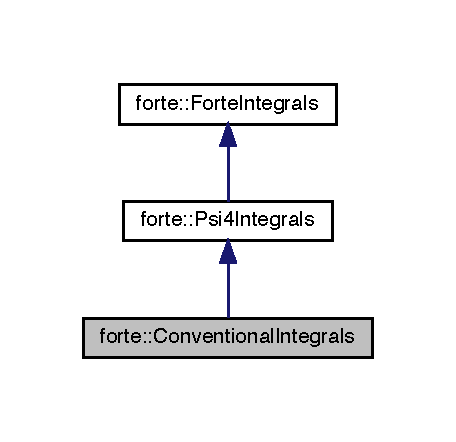
\includegraphics[width=219pt]{classforte_1_1_conventional_integrals__inherit__graph}
\end{center}
\end{figure}


Collaboration diagram for forte\+:\+:Conventional\+Integrals\+:
\nopagebreak
\begin{figure}[H]
\begin{center}
\leavevmode
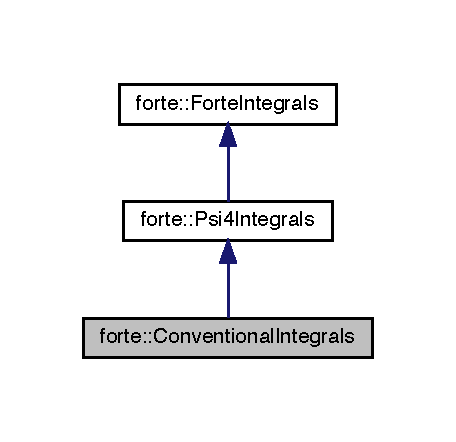
\includegraphics[width=219pt]{classforte_1_1_conventional_integrals__coll__graph}
\end{center}
\end{figure}
\subsection*{Public Member Functions}
\begin{DoxyCompactItemize}
\item 
\mbox{\hyperlink{classforte_1_1_conventional_integrals_a4b49dff68c291079528e82420e037248}{Conventional\+Integrals}} (std\+::shared\+\_\+ptr$<$ \mbox{\hyperlink{classforte_1_1_forte_options}{Forte\+Options}} $>$ options, std\+::shared\+\_\+ptr$<$ psi\+::\+Wavefunction $>$ ref\+\_\+wfn, std\+::shared\+\_\+ptr$<$ \mbox{\hyperlink{classforte_1_1_m_o_space_info}{M\+O\+Space\+Info}} $>$ mo\+\_\+space\+\_\+info, \mbox{\hyperlink{namespaceforte_a7defa2660dd3eb07aa81176b90781be7}{Integral\+Spin\+Restriction}} restricted)
\begin{DoxyCompactList}\small\item\em Contructor of \mbox{\hyperlink{classforte_1_1_conventional_integrals}{Conventional\+Integrals}}. \end{DoxyCompactList}\item 
void \mbox{\hyperlink{classforte_1_1_conventional_integrals_a9d9d6528eb1241a9e03fcf82e4a88dbe}{initialize}} () override
\item 
double \mbox{\hyperlink{classforte_1_1_conventional_integrals_a4df626960614077f1df435efba44bd0a}{aptei\+\_\+aa}} (size\+\_\+t p, size\+\_\+t q, size\+\_\+t r, size\+\_\+t s) override
\begin{DoxyCompactList}\small\item\em Grabs the antisymmetriced T\+EI -\/ assumes storage in aphy\+\_\+tei\+\_\+$\ast$. \end{DoxyCompactList}\item 
double \mbox{\hyperlink{classforte_1_1_conventional_integrals_a7ebb8bcee10a6cbac613e7b626093731}{aptei\+\_\+ab}} (size\+\_\+t p, size\+\_\+t q, size\+\_\+t r, size\+\_\+t s) override
\begin{DoxyCompactList}\small\item\em The antisymmetrixed alpha-\/beta two-\/electron integrals in physicist notation $<$pq$\vert$rs$>$ \end{DoxyCompactList}\item 
double \mbox{\hyperlink{classforte_1_1_conventional_integrals_ae6d6bfe97bb42d74dc9b69b5c617a966}{aptei\+\_\+bb}} (size\+\_\+t p, size\+\_\+t q, size\+\_\+t r, size\+\_\+t s) override
\begin{DoxyCompactList}\small\item\em The antisymmetrixed beta-\/beta two-\/electron integrals in physicist notation $<$pq$\vert$$\vert$rs$>$ \end{DoxyCompactList}\item 
ambit\+::\+Tensor \mbox{\hyperlink{classforte_1_1_conventional_integrals_abbe1dfb244b776a9d50fb2a06a837cbf}{aptei\+\_\+aa\+\_\+block}} (const std\+::vector$<$ size\+\_\+t $>$ \&p, const std\+::vector$<$ size\+\_\+t $>$ \&q, const std\+::vector$<$ size\+\_\+t $>$ \&r, const std\+::vector$<$ size\+\_\+t $>$ \&s) override
\begin{DoxyCompactList}\small\item\em Grabs the antisymmetrized T\+EI -\/ assumes storage of ambit tensor. \end{DoxyCompactList}\item 
ambit\+::\+Tensor \mbox{\hyperlink{classforte_1_1_conventional_integrals_aeb46dfc0030e582c301b64a011e2af58}{aptei\+\_\+ab\+\_\+block}} (const std\+::vector$<$ size\+\_\+t $>$ \&p, const std\+::vector$<$ size\+\_\+t $>$ \&q, const std\+::vector$<$ size\+\_\+t $>$ \&r, const std\+::vector$<$ size\+\_\+t $>$ \&s) override
\item 
ambit\+::\+Tensor \mbox{\hyperlink{classforte_1_1_conventional_integrals_a85a995f80f256953f9ceeb2ea903cf0b}{aptei\+\_\+bb\+\_\+block}} (const std\+::vector$<$ size\+\_\+t $>$ \&p, const std\+::vector$<$ size\+\_\+t $>$ \&q, const std\+::vector$<$ size\+\_\+t $>$ \&r, const std\+::vector$<$ size\+\_\+t $>$ \&s) override
\item 
void \mbox{\hyperlink{classforte_1_1_conventional_integrals_aef0130cb53212f32652a56e83e204519}{set\+\_\+tei}} (size\+\_\+t p, size\+\_\+t q, size\+\_\+t r, size\+\_\+t s, double value, bool alpha1, bool alpha2) override
\begin{DoxyCompactList}\small\item\em Set the value of the two-\/electron integrals. \end{DoxyCompactList}\end{DoxyCompactItemize}
\subsection*{Additional Inherited Members}


\subsection{Detailed Description}
The \mbox{\hyperlink{classforte_1_1_conventional_integrals}{Conventional\+Integrals}} class computes and transforms conventional two-\/electron integrals. 

This class assumes the two-\/electron integrals can be stored in memory. 

\subsection{Constructor \& Destructor Documentation}
\mbox{\Hypertarget{classforte_1_1_conventional_integrals_a4b49dff68c291079528e82420e037248}\label{classforte_1_1_conventional_integrals_a4b49dff68c291079528e82420e037248}} 
\index{forte\+::\+Conventional\+Integrals@{forte\+::\+Conventional\+Integrals}!Conventional\+Integrals@{Conventional\+Integrals}}
\index{Conventional\+Integrals@{Conventional\+Integrals}!forte\+::\+Conventional\+Integrals@{forte\+::\+Conventional\+Integrals}}
\subsubsection{\texorpdfstring{Conventional\+Integrals()}{ConventionalIntegrals()}}
{\footnotesize\ttfamily forte\+::\+Conventional\+Integrals\+::\+Conventional\+Integrals (\begin{DoxyParamCaption}\item[{std\+::shared\+\_\+ptr$<$ \mbox{\hyperlink{classforte_1_1_forte_options}{Forte\+Options}} $>$}]{options,  }\item[{std\+::shared\+\_\+ptr$<$ psi\+::\+Wavefunction $>$}]{ref\+\_\+wfn,  }\item[{std\+::shared\+\_\+ptr$<$ \mbox{\hyperlink{classforte_1_1_m_o_space_info}{M\+O\+Space\+Info}} $>$}]{mo\+\_\+space\+\_\+info,  }\item[{\mbox{\hyperlink{namespaceforte_a7defa2660dd3eb07aa81176b90781be7}{Integral\+Spin\+Restriction}}}]{restricted }\end{DoxyParamCaption})}



Contructor of \mbox{\hyperlink{classforte_1_1_conventional_integrals}{Conventional\+Integrals}}. 



\subsection{Member Function Documentation}
\mbox{\Hypertarget{classforte_1_1_conventional_integrals_a4df626960614077f1df435efba44bd0a}\label{classforte_1_1_conventional_integrals_a4df626960614077f1df435efba44bd0a}} 
\index{forte\+::\+Conventional\+Integrals@{forte\+::\+Conventional\+Integrals}!aptei\+\_\+aa@{aptei\+\_\+aa}}
\index{aptei\+\_\+aa@{aptei\+\_\+aa}!forte\+::\+Conventional\+Integrals@{forte\+::\+Conventional\+Integrals}}
\subsubsection{\texorpdfstring{aptei\+\_\+aa()}{aptei\_aa()}}
{\footnotesize\ttfamily double forte\+::\+Conventional\+Integrals\+::aptei\+\_\+aa (\begin{DoxyParamCaption}\item[{size\+\_\+t}]{p,  }\item[{size\+\_\+t}]{q,  }\item[{size\+\_\+t}]{r,  }\item[{size\+\_\+t}]{s }\end{DoxyParamCaption})\hspace{0.3cm}{\ttfamily [override]}, {\ttfamily [virtual]}}



Grabs the antisymmetriced T\+EI -\/ assumes storage in aphy\+\_\+tei\+\_\+$\ast$. 



Implements \mbox{\hyperlink{classforte_1_1_forte_integrals_afc84c157025b56ee0f8e3b1abe1c0a5f}{forte\+::\+Forte\+Integrals}}.

\mbox{\Hypertarget{classforte_1_1_conventional_integrals_abbe1dfb244b776a9d50fb2a06a837cbf}\label{classforte_1_1_conventional_integrals_abbe1dfb244b776a9d50fb2a06a837cbf}} 
\index{forte\+::\+Conventional\+Integrals@{forte\+::\+Conventional\+Integrals}!aptei\+\_\+aa\+\_\+block@{aptei\+\_\+aa\+\_\+block}}
\index{aptei\+\_\+aa\+\_\+block@{aptei\+\_\+aa\+\_\+block}!forte\+::\+Conventional\+Integrals@{forte\+::\+Conventional\+Integrals}}
\subsubsection{\texorpdfstring{aptei\+\_\+aa\+\_\+block()}{aptei\_aa\_block()}}
{\footnotesize\ttfamily ambit\+::\+Tensor forte\+::\+Conventional\+Integrals\+::aptei\+\_\+aa\+\_\+block (\begin{DoxyParamCaption}\item[{const std\+::vector$<$ size\+\_\+t $>$ \&}]{p,  }\item[{const std\+::vector$<$ size\+\_\+t $>$ \&}]{q,  }\item[{const std\+::vector$<$ size\+\_\+t $>$ \&}]{r,  }\item[{const std\+::vector$<$ size\+\_\+t $>$ \&}]{s }\end{DoxyParamCaption})\hspace{0.3cm}{\ttfamily [override]}, {\ttfamily [virtual]}}



Grabs the antisymmetrized T\+EI -\/ assumes storage of ambit tensor. 



Implements \mbox{\hyperlink{classforte_1_1_forte_integrals_ac20ae649b8cfe116f8583d676e43da27}{forte\+::\+Forte\+Integrals}}.

\mbox{\Hypertarget{classforte_1_1_conventional_integrals_a7ebb8bcee10a6cbac613e7b626093731}\label{classforte_1_1_conventional_integrals_a7ebb8bcee10a6cbac613e7b626093731}} 
\index{forte\+::\+Conventional\+Integrals@{forte\+::\+Conventional\+Integrals}!aptei\+\_\+ab@{aptei\+\_\+ab}}
\index{aptei\+\_\+ab@{aptei\+\_\+ab}!forte\+::\+Conventional\+Integrals@{forte\+::\+Conventional\+Integrals}}
\subsubsection{\texorpdfstring{aptei\+\_\+ab()}{aptei\_ab()}}
{\footnotesize\ttfamily double forte\+::\+Conventional\+Integrals\+::aptei\+\_\+ab (\begin{DoxyParamCaption}\item[{size\+\_\+t}]{p,  }\item[{size\+\_\+t}]{q,  }\item[{size\+\_\+t}]{r,  }\item[{size\+\_\+t}]{s }\end{DoxyParamCaption})\hspace{0.3cm}{\ttfamily [override]}, {\ttfamily [virtual]}}



The antisymmetrixed alpha-\/beta two-\/electron integrals in physicist notation $<$pq$\vert$rs$>$ 



Implements \mbox{\hyperlink{classforte_1_1_forte_integrals_a45efc2329cdfc7e4690cbe85688b947e}{forte\+::\+Forte\+Integrals}}.

\mbox{\Hypertarget{classforte_1_1_conventional_integrals_aeb46dfc0030e582c301b64a011e2af58}\label{classforte_1_1_conventional_integrals_aeb46dfc0030e582c301b64a011e2af58}} 
\index{forte\+::\+Conventional\+Integrals@{forte\+::\+Conventional\+Integrals}!aptei\+\_\+ab\+\_\+block@{aptei\+\_\+ab\+\_\+block}}
\index{aptei\+\_\+ab\+\_\+block@{aptei\+\_\+ab\+\_\+block}!forte\+::\+Conventional\+Integrals@{forte\+::\+Conventional\+Integrals}}
\subsubsection{\texorpdfstring{aptei\+\_\+ab\+\_\+block()}{aptei\_ab\_block()}}
{\footnotesize\ttfamily ambit\+::\+Tensor forte\+::\+Conventional\+Integrals\+::aptei\+\_\+ab\+\_\+block (\begin{DoxyParamCaption}\item[{const std\+::vector$<$ size\+\_\+t $>$ \&}]{p,  }\item[{const std\+::vector$<$ size\+\_\+t $>$ \&}]{q,  }\item[{const std\+::vector$<$ size\+\_\+t $>$ \&}]{r,  }\item[{const std\+::vector$<$ size\+\_\+t $>$ \&}]{s }\end{DoxyParamCaption})\hspace{0.3cm}{\ttfamily [override]}, {\ttfamily [virtual]}}

\begin{DoxyReturn}{Returns}
a tensor with a block of the alpha-\/beta antisymmetrized two-\/electron integrals 
\end{DoxyReturn}


Implements \mbox{\hyperlink{classforte_1_1_forte_integrals_acd40e350dc861baf8adf6a3b47c74023}{forte\+::\+Forte\+Integrals}}.

\mbox{\Hypertarget{classforte_1_1_conventional_integrals_ae6d6bfe97bb42d74dc9b69b5c617a966}\label{classforte_1_1_conventional_integrals_ae6d6bfe97bb42d74dc9b69b5c617a966}} 
\index{forte\+::\+Conventional\+Integrals@{forte\+::\+Conventional\+Integrals}!aptei\+\_\+bb@{aptei\+\_\+bb}}
\index{aptei\+\_\+bb@{aptei\+\_\+bb}!forte\+::\+Conventional\+Integrals@{forte\+::\+Conventional\+Integrals}}
\subsubsection{\texorpdfstring{aptei\+\_\+bb()}{aptei\_bb()}}
{\footnotesize\ttfamily double forte\+::\+Conventional\+Integrals\+::aptei\+\_\+bb (\begin{DoxyParamCaption}\item[{size\+\_\+t}]{p,  }\item[{size\+\_\+t}]{q,  }\item[{size\+\_\+t}]{r,  }\item[{size\+\_\+t}]{s }\end{DoxyParamCaption})\hspace{0.3cm}{\ttfamily [override]}, {\ttfamily [virtual]}}



The antisymmetrixed beta-\/beta two-\/electron integrals in physicist notation $<$pq$\vert$$\vert$rs$>$ 



Implements \mbox{\hyperlink{classforte_1_1_forte_integrals_a246225031c3799dc446f94e0e732c3ac}{forte\+::\+Forte\+Integrals}}.

\mbox{\Hypertarget{classforte_1_1_conventional_integrals_a85a995f80f256953f9ceeb2ea903cf0b}\label{classforte_1_1_conventional_integrals_a85a995f80f256953f9ceeb2ea903cf0b}} 
\index{forte\+::\+Conventional\+Integrals@{forte\+::\+Conventional\+Integrals}!aptei\+\_\+bb\+\_\+block@{aptei\+\_\+bb\+\_\+block}}
\index{aptei\+\_\+bb\+\_\+block@{aptei\+\_\+bb\+\_\+block}!forte\+::\+Conventional\+Integrals@{forte\+::\+Conventional\+Integrals}}
\subsubsection{\texorpdfstring{aptei\+\_\+bb\+\_\+block()}{aptei\_bb\_block()}}
{\footnotesize\ttfamily ambit\+::\+Tensor forte\+::\+Conventional\+Integrals\+::aptei\+\_\+bb\+\_\+block (\begin{DoxyParamCaption}\item[{const std\+::vector$<$ size\+\_\+t $>$ \&}]{p,  }\item[{const std\+::vector$<$ size\+\_\+t $>$ \&}]{q,  }\item[{const std\+::vector$<$ size\+\_\+t $>$ \&}]{r,  }\item[{const std\+::vector$<$ size\+\_\+t $>$ \&}]{s }\end{DoxyParamCaption})\hspace{0.3cm}{\ttfamily [override]}, {\ttfamily [virtual]}}

\begin{DoxyReturn}{Returns}
a tensor with a block of the beta-\/beta antisymmetrized two-\/electron integrals 
\end{DoxyReturn}


Implements \mbox{\hyperlink{classforte_1_1_forte_integrals_ae2799dc7cbfd456603a2b841b26582ab}{forte\+::\+Forte\+Integrals}}.

\mbox{\Hypertarget{classforte_1_1_conventional_integrals_a9d9d6528eb1241a9e03fcf82e4a88dbe}\label{classforte_1_1_conventional_integrals_a9d9d6528eb1241a9e03fcf82e4a88dbe}} 
\index{forte\+::\+Conventional\+Integrals@{forte\+::\+Conventional\+Integrals}!initialize@{initialize}}
\index{initialize@{initialize}!forte\+::\+Conventional\+Integrals@{forte\+::\+Conventional\+Integrals}}
\subsubsection{\texorpdfstring{initialize()}{initialize()}}
{\footnotesize\ttfamily void forte\+::\+Conventional\+Integrals\+::initialize (\begin{DoxyParamCaption}{ }\end{DoxyParamCaption})\hspace{0.3cm}{\ttfamily [override]}, {\ttfamily [virtual]}}



Implements \mbox{\hyperlink{classforte_1_1_forte_integrals_a7862835fa0f5f9abe13dfcd6730fa4be}{forte\+::\+Forte\+Integrals}}.

\mbox{\Hypertarget{classforte_1_1_conventional_integrals_aef0130cb53212f32652a56e83e204519}\label{classforte_1_1_conventional_integrals_aef0130cb53212f32652a56e83e204519}} 
\index{forte\+::\+Conventional\+Integrals@{forte\+::\+Conventional\+Integrals}!set\+\_\+tei@{set\+\_\+tei}}
\index{set\+\_\+tei@{set\+\_\+tei}!forte\+::\+Conventional\+Integrals@{forte\+::\+Conventional\+Integrals}}
\subsubsection{\texorpdfstring{set\+\_\+tei()}{set\_tei()}}
{\footnotesize\ttfamily void forte\+::\+Conventional\+Integrals\+::set\+\_\+tei (\begin{DoxyParamCaption}\item[{size\+\_\+t}]{p,  }\item[{size\+\_\+t}]{q,  }\item[{size\+\_\+t}]{r,  }\item[{size\+\_\+t}]{s,  }\item[{double}]{value,  }\item[{bool}]{alpha1,  }\item[{bool}]{alpha2 }\end{DoxyParamCaption})\hspace{0.3cm}{\ttfamily [override]}, {\ttfamily [virtual]}}



Set the value of the two-\/electron integrals. 



Implements \mbox{\hyperlink{classforte_1_1_forte_integrals_aaccd56e90bbc3c423158efb154336b9c}{forte\+::\+Forte\+Integrals}}.



The documentation for this class was generated from the following files\+:\begin{DoxyCompactItemize}
\item 
/\+Users/fevange/\+Source/forte/src/integrals/\mbox{\hyperlink{conventional__integrals_8h}{conventional\+\_\+integrals.\+h}}\item 
/\+Users/fevange/\+Source/forte/src/integrals/\mbox{\hyperlink{conventional__integrals_8cc}{conventional\+\_\+integrals.\+cc}}\end{DoxyCompactItemize}

\hypertarget{classforte_1_1_c_p_s_c_f}{}\section{forte\+:\+:C\+P\+S\+CF Class Reference}
\label{classforte_1_1_c_p_s_c_f}\index{forte\+::\+C\+P\+S\+CF@{forte\+::\+C\+P\+S\+CF}}


{\ttfamily \#include $<$cpscf.\+h$>$}

\subsection*{Public Member Functions}
\begin{DoxyCompactItemize}
\item 
\mbox{\hyperlink{classforte_1_1_c_p_s_c_f_a4ca7f1d2db6b7ee422f779447592cff0}{C\+P\+S\+CF}} (std\+::shared\+\_\+ptr$<$ psi\+::\+JK $>$ JK, psi\+::\+Shared\+Matrix C, psi\+::\+Shared\+Matrix b, psi\+::\+Shared\+Vector edocc, psi\+::\+Shared\+Vector euocc)
\begin{DoxyCompactList}\small\item\em Constructor of C\+P\+S\+C\+F\+\_\+\+F\+U\+N\+C\+T\+OR. \end{DoxyCompactList}\item 
double \mbox{\hyperlink{classforte_1_1_c_p_s_c_f_ab111cda27e9bc9c8eb2f575ae89104e5}{evaluate}} (psi\+::\+Shared\+Vector x, psi\+::\+Shared\+Vector g, bool do\+\_\+g=true)
\begin{DoxyCompactList}\small\item\em Evaluate the scalar and gradient. \end{DoxyCompactList}\item 
void \mbox{\hyperlink{classforte_1_1_c_p_s_c_f_a974ab98e124651d3d3bc8b163a00286f}{hess\+\_\+diag}} (psi\+::\+Shared\+Vector x, psi\+::\+Shared\+Vector h0)
\begin{DoxyCompactList}\small\item\em Evaluate the diagonal Hessian. \end{DoxyCompactList}\item 
psi\+::\+Dimension \mbox{\hyperlink{classforte_1_1_c_p_s_c_f_ac5a426e6730351ff0a3639fec8931c16}{vdimpi}} ()
\begin{DoxyCompactList}\small\item\em Return the vector dimension. \end{DoxyCompactList}\item 
psi\+::\+Shared\+Vector \mbox{\hyperlink{classforte_1_1_c_p_s_c_f_a2fec329d9dbf17e1762e256cffd1dff8}{mat\+\_\+to\+\_\+vec}} (psi\+::\+Shared\+Matrix M)
\begin{DoxyCompactList}\small\item\em Reshape matrix to vector. \end{DoxyCompactList}\item 
psi\+::\+Shared\+Matrix \mbox{\hyperlink{classforte_1_1_c_p_s_c_f_ae8f08daaa75c9664d357f0245c334d9b}{vec\+\_\+to\+\_\+mat}} (psi\+::\+Shared\+Vector v)
\begin{DoxyCompactList}\small\item\em Reshape vector to matrix. \end{DoxyCompactList}\end{DoxyCompactItemize}


\subsection{Constructor \& Destructor Documentation}
\mbox{\Hypertarget{classforte_1_1_c_p_s_c_f_a4ca7f1d2db6b7ee422f779447592cff0}\label{classforte_1_1_c_p_s_c_f_a4ca7f1d2db6b7ee422f779447592cff0}} 
\index{forte\+::\+C\+P\+S\+CF@{forte\+::\+C\+P\+S\+CF}!C\+P\+S\+CF@{C\+P\+S\+CF}}
\index{C\+P\+S\+CF@{C\+P\+S\+CF}!forte\+::\+C\+P\+S\+CF@{forte\+::\+C\+P\+S\+CF}}
\subsubsection{\texorpdfstring{C\+P\+S\+C\+F()}{CPSCF()}}
{\footnotesize\ttfamily forte\+::\+C\+P\+S\+C\+F\+::\+C\+P\+S\+CF (\begin{DoxyParamCaption}\item[{std\+::shared\+\_\+ptr$<$ psi\+::\+JK $>$}]{JK,  }\item[{psi\+::\+Shared\+Matrix}]{C,  }\item[{psi\+::\+Shared\+Matrix}]{b,  }\item[{psi\+::\+Shared\+Vector}]{edocc,  }\item[{psi\+::\+Shared\+Vector}]{euocc }\end{DoxyParamCaption})}



Constructor of C\+P\+S\+C\+F\+\_\+\+F\+U\+N\+C\+T\+OR. 


\begin{DoxyParams}{Parameters}
{\em JK} & The pointer to a Psi4 JK object \\
\hline
{\em C} & The Hartree-\/\+Fock orbital coefficients \\
\hline
{\em b} & The R.\+H.\+S. of \mbox{\hyperlink{classforte_1_1_c_p_s_c_f}{C\+P\+S\+CF}} equation Ax = b (nuocc x ndocc) \\
\hline
{\em edocc} & The occupied orbital energies \\
\hline
{\em euocc} & The unoccupied orbital energies \\
\hline
\end{DoxyParams}


\subsection{Member Function Documentation}
\mbox{\Hypertarget{classforte_1_1_c_p_s_c_f_ab111cda27e9bc9c8eb2f575ae89104e5}\label{classforte_1_1_c_p_s_c_f_ab111cda27e9bc9c8eb2f575ae89104e5}} 
\index{forte\+::\+C\+P\+S\+CF@{forte\+::\+C\+P\+S\+CF}!evaluate@{evaluate}}
\index{evaluate@{evaluate}!forte\+::\+C\+P\+S\+CF@{forte\+::\+C\+P\+S\+CF}}
\subsubsection{\texorpdfstring{evaluate()}{evaluate()}}
{\footnotesize\ttfamily double forte\+::\+C\+P\+S\+C\+F\+::evaluate (\begin{DoxyParamCaption}\item[{psi\+::\+Shared\+Vector}]{x,  }\item[{psi\+::\+Shared\+Vector}]{g,  }\item[{bool}]{do\+\_\+g = {\ttfamily true} }\end{DoxyParamCaption})}



Evaluate the scalar and gradient. 

\mbox{\Hypertarget{classforte_1_1_c_p_s_c_f_a974ab98e124651d3d3bc8b163a00286f}\label{classforte_1_1_c_p_s_c_f_a974ab98e124651d3d3bc8b163a00286f}} 
\index{forte\+::\+C\+P\+S\+CF@{forte\+::\+C\+P\+S\+CF}!hess\+\_\+diag@{hess\+\_\+diag}}
\index{hess\+\_\+diag@{hess\+\_\+diag}!forte\+::\+C\+P\+S\+CF@{forte\+::\+C\+P\+S\+CF}}
\subsubsection{\texorpdfstring{hess\+\_\+diag()}{hess\_diag()}}
{\footnotesize\ttfamily void forte\+::\+C\+P\+S\+C\+F\+::hess\+\_\+diag (\begin{DoxyParamCaption}\item[{psi\+::\+Shared\+Vector}]{x,  }\item[{psi\+::\+Shared\+Vector}]{h0 }\end{DoxyParamCaption})}



Evaluate the diagonal Hessian. 

\mbox{\Hypertarget{classforte_1_1_c_p_s_c_f_a2fec329d9dbf17e1762e256cffd1dff8}\label{classforte_1_1_c_p_s_c_f_a2fec329d9dbf17e1762e256cffd1dff8}} 
\index{forte\+::\+C\+P\+S\+CF@{forte\+::\+C\+P\+S\+CF}!mat\+\_\+to\+\_\+vec@{mat\+\_\+to\+\_\+vec}}
\index{mat\+\_\+to\+\_\+vec@{mat\+\_\+to\+\_\+vec}!forte\+::\+C\+P\+S\+CF@{forte\+::\+C\+P\+S\+CF}}
\subsubsection{\texorpdfstring{mat\+\_\+to\+\_\+vec()}{mat\_to\_vec()}}
{\footnotesize\ttfamily psi\+::\+Shared\+Vector forte\+::\+C\+P\+S\+C\+F\+::mat\+\_\+to\+\_\+vec (\begin{DoxyParamCaption}\item[{psi\+::\+Shared\+Matrix}]{M }\end{DoxyParamCaption})}



Reshape matrix to vector. 

\mbox{\Hypertarget{classforte_1_1_c_p_s_c_f_ac5a426e6730351ff0a3639fec8931c16}\label{classforte_1_1_c_p_s_c_f_ac5a426e6730351ff0a3639fec8931c16}} 
\index{forte\+::\+C\+P\+S\+CF@{forte\+::\+C\+P\+S\+CF}!vdimpi@{vdimpi}}
\index{vdimpi@{vdimpi}!forte\+::\+C\+P\+S\+CF@{forte\+::\+C\+P\+S\+CF}}
\subsubsection{\texorpdfstring{vdimpi()}{vdimpi()}}
{\footnotesize\ttfamily psi\+::\+Dimension forte\+::\+C\+P\+S\+C\+F\+::vdimpi (\begin{DoxyParamCaption}{ }\end{DoxyParamCaption})\hspace{0.3cm}{\ttfamily [inline]}}



Return the vector dimension. 

\mbox{\Hypertarget{classforte_1_1_c_p_s_c_f_ae8f08daaa75c9664d357f0245c334d9b}\label{classforte_1_1_c_p_s_c_f_ae8f08daaa75c9664d357f0245c334d9b}} 
\index{forte\+::\+C\+P\+S\+CF@{forte\+::\+C\+P\+S\+CF}!vec\+\_\+to\+\_\+mat@{vec\+\_\+to\+\_\+mat}}
\index{vec\+\_\+to\+\_\+mat@{vec\+\_\+to\+\_\+mat}!forte\+::\+C\+P\+S\+CF@{forte\+::\+C\+P\+S\+CF}}
\subsubsection{\texorpdfstring{vec\+\_\+to\+\_\+mat()}{vec\_to\_mat()}}
{\footnotesize\ttfamily psi\+::\+Shared\+Matrix forte\+::\+C\+P\+S\+C\+F\+::vec\+\_\+to\+\_\+mat (\begin{DoxyParamCaption}\item[{psi\+::\+Shared\+Vector}]{v }\end{DoxyParamCaption})}



Reshape vector to matrix. 



The documentation for this class was generated from the following files\+:\begin{DoxyCompactItemize}
\item 
/\+Users/fevange/\+Source/forte/src/casscf/\mbox{\hyperlink{cpscf_8h}{cpscf.\+h}}\item 
/\+Users/fevange/\+Source/forte/src/casscf/\mbox{\hyperlink{cpscf_8cc}{cpscf.\+cc}}\end{DoxyCompactItemize}

\hypertarget{classforte_1_1_c_p_s_c_f___s_o_l_v_e_r}{}\section{forte\+:\+:C\+P\+S\+C\+F\+\_\+\+S\+O\+L\+V\+ER Class Reference}
\label{classforte_1_1_c_p_s_c_f___s_o_l_v_e_r}\index{forte\+::\+C\+P\+S\+C\+F\+\_\+\+S\+O\+L\+V\+ER@{forte\+::\+C\+P\+S\+C\+F\+\_\+\+S\+O\+L\+V\+ER}}


{\ttfamily \#include $<$cpscf.\+h$>$}

\subsection*{Public Member Functions}
\begin{DoxyCompactItemize}
\item 
\mbox{\hyperlink{classforte_1_1_c_p_s_c_f___s_o_l_v_e_r_abf8d542e0f97464c9fd03dfa2d2528d8}{C\+P\+S\+C\+F\+\_\+\+S\+O\+L\+V\+ER}} (std\+::shared\+\_\+ptr$<$ \mbox{\hyperlink{classforte_1_1_forte_options}{Forte\+Options}} $>$ options, std\+::shared\+\_\+ptr$<$ psi\+::\+JK $>$ JK, psi\+::\+Shared\+Matrix C, psi\+::\+Shared\+Matrix b, psi\+::\+Shared\+Vector edocc, psi\+::\+Shared\+Vector euocc)
\begin{DoxyCompactList}\small\item\em Constructor of \mbox{\hyperlink{classforte_1_1_c_p_s_c_f___s_o_l_v_e_r}{C\+P\+S\+C\+F\+\_\+\+S\+O\+L\+V\+ER}}. \end{DoxyCompactList}\item 
bool \mbox{\hyperlink{classforte_1_1_c_p_s_c_f___s_o_l_v_e_r_ac210c880f297904efa59bfc46881ca9b}{solve}} ()
\begin{DoxyCompactList}\small\item\em Solve \mbox{\hyperlink{classforte_1_1_c_p_s_c_f}{C\+P\+S\+CF}} equation and return if the equations are converged or not. \end{DoxyCompactList}\item 
psi\+::\+Shared\+Matrix \mbox{\hyperlink{classforte_1_1_c_p_s_c_f___s_o_l_v_e_r_a3d1a12199bb5114f71216738404f8fce}{x}} ()
\begin{DoxyCompactList}\small\item\em Return the unknown in matrix form. \end{DoxyCompactList}\end{DoxyCompactItemize}


\subsection{Constructor \& Destructor Documentation}
\mbox{\Hypertarget{classforte_1_1_c_p_s_c_f___s_o_l_v_e_r_abf8d542e0f97464c9fd03dfa2d2528d8}\label{classforte_1_1_c_p_s_c_f___s_o_l_v_e_r_abf8d542e0f97464c9fd03dfa2d2528d8}} 
\index{forte\+::\+C\+P\+S\+C\+F\+\_\+\+S\+O\+L\+V\+ER@{forte\+::\+C\+P\+S\+C\+F\+\_\+\+S\+O\+L\+V\+ER}!C\+P\+S\+C\+F\+\_\+\+S\+O\+L\+V\+ER@{C\+P\+S\+C\+F\+\_\+\+S\+O\+L\+V\+ER}}
\index{C\+P\+S\+C\+F\+\_\+\+S\+O\+L\+V\+ER@{C\+P\+S\+C\+F\+\_\+\+S\+O\+L\+V\+ER}!forte\+::\+C\+P\+S\+C\+F\+\_\+\+S\+O\+L\+V\+ER@{forte\+::\+C\+P\+S\+C\+F\+\_\+\+S\+O\+L\+V\+ER}}
\subsubsection{\texorpdfstring{C\+P\+S\+C\+F\+\_\+\+S\+O\+L\+V\+E\+R()}{CPSCF\_SOLVER()}}
{\footnotesize\ttfamily forte\+::\+C\+P\+S\+C\+F\+\_\+\+S\+O\+L\+V\+E\+R\+::\+C\+P\+S\+C\+F\+\_\+\+S\+O\+L\+V\+ER (\begin{DoxyParamCaption}\item[{std\+::shared\+\_\+ptr$<$ \mbox{\hyperlink{classforte_1_1_forte_options}{Forte\+Options}} $>$}]{options,  }\item[{std\+::shared\+\_\+ptr$<$ psi\+::\+JK $>$}]{JK,  }\item[{psi\+::\+Shared\+Matrix}]{C,  }\item[{psi\+::\+Shared\+Matrix}]{b,  }\item[{psi\+::\+Shared\+Vector}]{edocc,  }\item[{psi\+::\+Shared\+Vector}]{euocc }\end{DoxyParamCaption})}



Constructor of \mbox{\hyperlink{classforte_1_1_c_p_s_c_f___s_o_l_v_e_r}{C\+P\+S\+C\+F\+\_\+\+S\+O\+L\+V\+ER}}. 


\begin{DoxyParams}{Parameters}
{\em options} & The \mbox{\hyperlink{classforte_1_1_forte_options}{Forte\+Options}} pointer \\
\hline
{\em JK} & The pointer to a Psi4 JK object \\
\hline
{\em C} & The Hartree-\/\+Fock orbital coefficients \\
\hline
{\em b} & The R.\+H.\+S. of \mbox{\hyperlink{classforte_1_1_c_p_s_c_f}{C\+P\+S\+CF}} equation Ax = b (nuocc x ndocc) \\
\hline
{\em edocc} & The occupied orbital energies \\
\hline
{\em euocc} & The unoccupied orbital energies \\
\hline
\end{DoxyParams}


\subsection{Member Function Documentation}
\mbox{\Hypertarget{classforte_1_1_c_p_s_c_f___s_o_l_v_e_r_ac210c880f297904efa59bfc46881ca9b}\label{classforte_1_1_c_p_s_c_f___s_o_l_v_e_r_ac210c880f297904efa59bfc46881ca9b}} 
\index{forte\+::\+C\+P\+S\+C\+F\+\_\+\+S\+O\+L\+V\+ER@{forte\+::\+C\+P\+S\+C\+F\+\_\+\+S\+O\+L\+V\+ER}!solve@{solve}}
\index{solve@{solve}!forte\+::\+C\+P\+S\+C\+F\+\_\+\+S\+O\+L\+V\+ER@{forte\+::\+C\+P\+S\+C\+F\+\_\+\+S\+O\+L\+V\+ER}}
\subsubsection{\texorpdfstring{solve()}{solve()}}
{\footnotesize\ttfamily bool forte\+::\+C\+P\+S\+C\+F\+\_\+\+S\+O\+L\+V\+E\+R\+::solve (\begin{DoxyParamCaption}{ }\end{DoxyParamCaption})}



Solve \mbox{\hyperlink{classforte_1_1_c_p_s_c_f}{C\+P\+S\+CF}} equation and return if the equations are converged or not. 

\mbox{\Hypertarget{classforte_1_1_c_p_s_c_f___s_o_l_v_e_r_a3d1a12199bb5114f71216738404f8fce}\label{classforte_1_1_c_p_s_c_f___s_o_l_v_e_r_a3d1a12199bb5114f71216738404f8fce}} 
\index{forte\+::\+C\+P\+S\+C\+F\+\_\+\+S\+O\+L\+V\+ER@{forte\+::\+C\+P\+S\+C\+F\+\_\+\+S\+O\+L\+V\+ER}!x@{x}}
\index{x@{x}!forte\+::\+C\+P\+S\+C\+F\+\_\+\+S\+O\+L\+V\+ER@{forte\+::\+C\+P\+S\+C\+F\+\_\+\+S\+O\+L\+V\+ER}}
\subsubsection{\texorpdfstring{x()}{x()}}
{\footnotesize\ttfamily psi\+::\+Shared\+Matrix forte\+::\+C\+P\+S\+C\+F\+\_\+\+S\+O\+L\+V\+E\+R\+::x (\begin{DoxyParamCaption}{ }\end{DoxyParamCaption})}



Return the unknown in matrix form. 



The documentation for this class was generated from the following files\+:\begin{DoxyCompactItemize}
\item 
/\+Users/fevange/\+Source/forte/src/casscf/\mbox{\hyperlink{cpscf_8h}{cpscf.\+h}}\item 
/\+Users/fevange/\+Source/forte/src/casscf/\mbox{\hyperlink{cpscf_8cc}{cpscf.\+cc}}\end{DoxyCompactItemize}

\hypertarget{classforte_1_1_cube_file}{}\section{forte\+:\+:Cube\+File Class Reference}
\label{classforte_1_1_cube_file}\index{forte\+::\+Cube\+File@{forte\+::\+Cube\+File}}


A class for loading, maniputlating, and storing cube files.  




{\ttfamily \#include $<$cube\+\_\+file.\+h$>$}

\subsection*{Public Member Functions}
\begin{DoxyCompactItemize}
\item 
\mbox{\hyperlink{classforte_1_1_cube_file_a5b182bf719f0668f4e4d59fef9140f36}{Cube\+File}} (const std\+::string \&filename)
\begin{DoxyCompactList}\small\item\em Build a \mbox{\hyperlink{classforte_1_1_cube_file}{Cube\+File}} object from a file stored on disk. \end{DoxyCompactList}\item 
\mbox{\hyperlink{classforte_1_1_cube_file_ac091f6918736c043fad6e108ec209b66}{Cube\+File}} (const \mbox{\hyperlink{classforte_1_1_cube_file}{Cube\+File}} \&cube)=default
\item 
int \mbox{\hyperlink{classforte_1_1_cube_file_a9ad38a5a7b190ddb0a5e162755cecf59}{natoms}} () const
\item 
const std\+::vector$<$ int $>$ \& \mbox{\hyperlink{classforte_1_1_cube_file_a2b6769f5f719e86ef637badec2b0cff1}{atom\+\_\+numbers}} () const
\item 
const std\+::vector$<$ std\+::tuple$<$ double, double, double $>$ $>$ \& \mbox{\hyperlink{classforte_1_1_cube_file_aa443cf8e4c16f88cea31d5082c73b83d}{atom\+\_\+coords}} () const
\item 
const std\+::vector$<$ int $>$ \& \mbox{\hyperlink{classforte_1_1_cube_file_a0f2d624536eb4ecdca77092e0ac39ff8}{num}} () const
\item 
const std\+::vector$<$ double $>$ \& \mbox{\hyperlink{classforte_1_1_cube_file_a4d045a770876626dc7d34ebc39ca0525}{min}} () const
\item 
const std\+::vector$<$ double $>$ \& \mbox{\hyperlink{classforte_1_1_cube_file_ac09285b9257b4a4c4fcf7f1d304ae953}{max}} () const
\item 
const std\+::vector$<$ double $>$ \& \mbox{\hyperlink{classforte_1_1_cube_file_a9ec8e2d49f08a95023310ec5814d0631}{inc}} () const
\item 
const std\+::vector$<$ double $>$ \& \mbox{\hyperlink{classforte_1_1_cube_file_ac3de35bae3f81d684ce53aced0486e28}{data}} () const
\item 
void \mbox{\hyperlink{classforte_1_1_cube_file_aa1a220dd0dc464118d874004be847138}{load}} (std\+::string filename)
\item 
void \mbox{\hyperlink{classforte_1_1_cube_file_ac45d60ce3490487dd948a4ef9d3d3730}{save}} (std\+::string filename) const
\item 
std\+::pair$<$ double, double $>$ \mbox{\hyperlink{classforte_1_1_cube_file_ae645bcad6dbc72a471f032e436bd21ae}{compute\+\_\+levels}} (std\+::string type, double fraction) const
\begin{DoxyCompactList}\small\item\em Compute the isolevel that encompasses a give fraction of the total density. \end{DoxyCompactList}\item 
void \mbox{\hyperlink{classforte_1_1_cube_file_a1f6886f860b2388a7898d61dc493f58e}{zero}} ()
\begin{DoxyCompactList}\small\item\em zero this cube file \end{DoxyCompactList}\item 
void \mbox{\hyperlink{classforte_1_1_cube_file_af0841a7b1389699679bae67a8027d501}{scale}} (double factor)
\begin{DoxyCompactList}\small\item\em scale the value of the cube file at each point by a factor \end{DoxyCompactList}\item 
void \mbox{\hyperlink{classforte_1_1_cube_file_a79768e0f554988aa44df4136dc6bdf38}{add}} (const \mbox{\hyperlink{classforte_1_1_cube_file}{Cube\+File}} \&other, double factor=1.\+0)
\begin{DoxyCompactList}\small\item\em add to each grid point the value of another cube file times a scaling factor \end{DoxyCompactList}\item 
void \mbox{\hyperlink{classforte_1_1_cube_file_af35406d88fc10f10ed1cf162d395a5f2}{pointwise\+\_\+product}} (const \mbox{\hyperlink{classforte_1_1_cube_file}{Cube\+File}} \&other)
\begin{DoxyCompactList}\small\item\em multiply each grid point by the value of another cube file \end{DoxyCompactList}\end{DoxyCompactItemize}


\subsection{Detailed Description}
A class for loading, maniputlating, and storing cube files. 

This class provides some basic functionality to handle cube files. It can read/write cube files and since it uses low-\/level C++ functions is faster than a Pyhton based implementation. This class also provides some basic operations (adding, scaling, multiplying) on cube files. 

\subsection{Constructor \& Destructor Documentation}
\mbox{\Hypertarget{classforte_1_1_cube_file_a5b182bf719f0668f4e4d59fef9140f36}\label{classforte_1_1_cube_file_a5b182bf719f0668f4e4d59fef9140f36}} 
\index{forte\+::\+Cube\+File@{forte\+::\+Cube\+File}!Cube\+File@{Cube\+File}}
\index{Cube\+File@{Cube\+File}!forte\+::\+Cube\+File@{forte\+::\+Cube\+File}}
\subsubsection{\texorpdfstring{Cube\+File()}{CubeFile()}\hspace{0.1cm}{\footnotesize\ttfamily [1/2]}}
{\footnotesize\ttfamily forte\+::\+Cube\+File\+::\+Cube\+File (\begin{DoxyParamCaption}\item[{const std\+::string \&}]{filename }\end{DoxyParamCaption})}



Build a \mbox{\hyperlink{classforte_1_1_cube_file}{Cube\+File}} object from a file stored on disk. 


\begin{DoxyParams}{Parameters}
{\em filename} & the path to the cube file \\
\hline
\end{DoxyParams}
\mbox{\Hypertarget{classforte_1_1_cube_file_ac091f6918736c043fad6e108ec209b66}\label{classforte_1_1_cube_file_ac091f6918736c043fad6e108ec209b66}} 
\index{forte\+::\+Cube\+File@{forte\+::\+Cube\+File}!Cube\+File@{Cube\+File}}
\index{Cube\+File@{Cube\+File}!forte\+::\+Cube\+File@{forte\+::\+Cube\+File}}
\subsubsection{\texorpdfstring{Cube\+File()}{CubeFile()}\hspace{0.1cm}{\footnotesize\ttfamily [2/2]}}
{\footnotesize\ttfamily forte\+::\+Cube\+File\+::\+Cube\+File (\begin{DoxyParamCaption}\item[{const \mbox{\hyperlink{classforte_1_1_cube_file}{Cube\+File}} \&}]{cube }\end{DoxyParamCaption})\hspace{0.3cm}{\ttfamily [default]}}



\subsection{Member Function Documentation}
\mbox{\Hypertarget{classforte_1_1_cube_file_a79768e0f554988aa44df4136dc6bdf38}\label{classforte_1_1_cube_file_a79768e0f554988aa44df4136dc6bdf38}} 
\index{forte\+::\+Cube\+File@{forte\+::\+Cube\+File}!add@{add}}
\index{add@{add}!forte\+::\+Cube\+File@{forte\+::\+Cube\+File}}
\subsubsection{\texorpdfstring{add()}{add()}}
{\footnotesize\ttfamily void forte\+::\+Cube\+File\+::add (\begin{DoxyParamCaption}\item[{const \mbox{\hyperlink{classforte_1_1_cube_file}{Cube\+File}} \&}]{other,  }\item[{double}]{factor = {\ttfamily 1.0} }\end{DoxyParamCaption})}



add to each grid point the value of another cube file times a scaling factor 


\begin{DoxyParams}{Parameters}
{\em other} & the cube file to add \\
\hline
{\em factor} & the scaling factor \\
\hline
\end{DoxyParams}
\mbox{\Hypertarget{classforte_1_1_cube_file_aa443cf8e4c16f88cea31d5082c73b83d}\label{classforte_1_1_cube_file_aa443cf8e4c16f88cea31d5082c73b83d}} 
\index{forte\+::\+Cube\+File@{forte\+::\+Cube\+File}!atom\+\_\+coords@{atom\+\_\+coords}}
\index{atom\+\_\+coords@{atom\+\_\+coords}!forte\+::\+Cube\+File@{forte\+::\+Cube\+File}}
\subsubsection{\texorpdfstring{atom\+\_\+coords()}{atom\_coords()}}
{\footnotesize\ttfamily const std\+::vector$<$ std\+::tuple$<$ double, double, double $>$ $>$ \& forte\+::\+Cube\+File\+::atom\+\_\+coords (\begin{DoxyParamCaption}{ }\end{DoxyParamCaption}) const}

\begin{DoxyReturn}{Returns}
the (x,y,z) atomic coordinates (in Angstrom) 
\end{DoxyReturn}
\mbox{\Hypertarget{classforte_1_1_cube_file_a2b6769f5f719e86ef637badec2b0cff1}\label{classforte_1_1_cube_file_a2b6769f5f719e86ef637badec2b0cff1}} 
\index{forte\+::\+Cube\+File@{forte\+::\+Cube\+File}!atom\+\_\+numbers@{atom\+\_\+numbers}}
\index{atom\+\_\+numbers@{atom\+\_\+numbers}!forte\+::\+Cube\+File@{forte\+::\+Cube\+File}}
\subsubsection{\texorpdfstring{atom\+\_\+numbers()}{atom\_numbers()}}
{\footnotesize\ttfamily const std\+::vector$<$ int $>$ \& forte\+::\+Cube\+File\+::atom\+\_\+numbers (\begin{DoxyParamCaption}{ }\end{DoxyParamCaption}) const}

\begin{DoxyReturn}{Returns}
the atomic numbers of the atoms 
\end{DoxyReturn}
\mbox{\Hypertarget{classforte_1_1_cube_file_ae645bcad6dbc72a471f032e436bd21ae}\label{classforte_1_1_cube_file_ae645bcad6dbc72a471f032e436bd21ae}} 
\index{forte\+::\+Cube\+File@{forte\+::\+Cube\+File}!compute\+\_\+levels@{compute\+\_\+levels}}
\index{compute\+\_\+levels@{compute\+\_\+levels}!forte\+::\+Cube\+File@{forte\+::\+Cube\+File}}
\subsubsection{\texorpdfstring{compute\+\_\+levels()}{compute\_levels()}}
{\footnotesize\ttfamily std\+::pair$<$ double, double $>$ forte\+::\+Cube\+File\+::compute\+\_\+levels (\begin{DoxyParamCaption}\item[{std\+::string}]{type,  }\item[{double}]{fraction }\end{DoxyParamCaption}) const}



Compute the isolevel that encompasses a give fraction of the total density. 


\begin{DoxyParams}{Parameters}
{\em type} & the type of cube file (\char`\"{}mo\char`\"{} or \char`\"{}density\char`\"{}) \\
\hline
{\em fraction} & the fraction of the density \\
\hline
\end{DoxyParams}
\mbox{\Hypertarget{classforte_1_1_cube_file_ac3de35bae3f81d684ce53aced0486e28}\label{classforte_1_1_cube_file_ac3de35bae3f81d684ce53aced0486e28}} 
\index{forte\+::\+Cube\+File@{forte\+::\+Cube\+File}!data@{data}}
\index{data@{data}!forte\+::\+Cube\+File@{forte\+::\+Cube\+File}}
\subsubsection{\texorpdfstring{data()}{data()}}
{\footnotesize\ttfamily const std\+::vector$<$ double $>$ \& forte\+::\+Cube\+File\+::data (\begin{DoxyParamCaption}{ }\end{DoxyParamCaption}) const}

\begin{DoxyReturn}{Returns}
the grid points stored as a vector 
\end{DoxyReturn}
\mbox{\Hypertarget{classforte_1_1_cube_file_a9ec8e2d49f08a95023310ec5814d0631}\label{classforte_1_1_cube_file_a9ec8e2d49f08a95023310ec5814d0631}} 
\index{forte\+::\+Cube\+File@{forte\+::\+Cube\+File}!inc@{inc}}
\index{inc@{inc}!forte\+::\+Cube\+File@{forte\+::\+Cube\+File}}
\subsubsection{\texorpdfstring{inc()}{inc()}}
{\footnotesize\ttfamily const std\+::vector$<$ double $>$ \& forte\+::\+Cube\+File\+::inc (\begin{DoxyParamCaption}{ }\end{DoxyParamCaption}) const}

\begin{DoxyReturn}{Returns}
the grid increment 
\end{DoxyReturn}
\mbox{\Hypertarget{classforte_1_1_cube_file_aa1a220dd0dc464118d874004be847138}\label{classforte_1_1_cube_file_aa1a220dd0dc464118d874004be847138}} 
\index{forte\+::\+Cube\+File@{forte\+::\+Cube\+File}!load@{load}}
\index{load@{load}!forte\+::\+Cube\+File@{forte\+::\+Cube\+File}}
\subsubsection{\texorpdfstring{load()}{load()}}
{\footnotesize\ttfamily void forte\+::\+Cube\+File\+::load (\begin{DoxyParamCaption}\item[{std\+::string}]{filename }\end{DoxyParamCaption})}

load a cube file 
\begin{DoxyParams}{Parameters}
{\em filename} & the cube file name \\
\hline
\end{DoxyParams}
\mbox{\Hypertarget{classforte_1_1_cube_file_ac09285b9257b4a4c4fcf7f1d304ae953}\label{classforte_1_1_cube_file_ac09285b9257b4a4c4fcf7f1d304ae953}} 
\index{forte\+::\+Cube\+File@{forte\+::\+Cube\+File}!max@{max}}
\index{max@{max}!forte\+::\+Cube\+File@{forte\+::\+Cube\+File}}
\subsubsection{\texorpdfstring{max()}{max()}}
{\footnotesize\ttfamily const std\+::vector$<$ double $>$ \& forte\+::\+Cube\+File\+::max (\begin{DoxyParamCaption}{ }\end{DoxyParamCaption}) const}

\begin{DoxyReturn}{Returns}
the maximum value of a grid point 
\end{DoxyReturn}
\mbox{\Hypertarget{classforte_1_1_cube_file_a4d045a770876626dc7d34ebc39ca0525}\label{classforte_1_1_cube_file_a4d045a770876626dc7d34ebc39ca0525}} 
\index{forte\+::\+Cube\+File@{forte\+::\+Cube\+File}!min@{min}}
\index{min@{min}!forte\+::\+Cube\+File@{forte\+::\+Cube\+File}}
\subsubsection{\texorpdfstring{min()}{min()}}
{\footnotesize\ttfamily const std\+::vector$<$ double $>$ \& forte\+::\+Cube\+File\+::min (\begin{DoxyParamCaption}{ }\end{DoxyParamCaption}) const}

\begin{DoxyReturn}{Returns}
the minimum value of a grid point 
\end{DoxyReturn}
\mbox{\Hypertarget{classforte_1_1_cube_file_a9ad38a5a7b190ddb0a5e162755cecf59}\label{classforte_1_1_cube_file_a9ad38a5a7b190ddb0a5e162755cecf59}} 
\index{forte\+::\+Cube\+File@{forte\+::\+Cube\+File}!natoms@{natoms}}
\index{natoms@{natoms}!forte\+::\+Cube\+File@{forte\+::\+Cube\+File}}
\subsubsection{\texorpdfstring{natoms()}{natoms()}}
{\footnotesize\ttfamily int forte\+::\+Cube\+File\+::natoms (\begin{DoxyParamCaption}{ }\end{DoxyParamCaption}) const}

\begin{DoxyReturn}{Returns}
the number of atoms 
\end{DoxyReturn}
\mbox{\Hypertarget{classforte_1_1_cube_file_a0f2d624536eb4ecdca77092e0ac39ff8}\label{classforte_1_1_cube_file_a0f2d624536eb4ecdca77092e0ac39ff8}} 
\index{forte\+::\+Cube\+File@{forte\+::\+Cube\+File}!num@{num}}
\index{num@{num}!forte\+::\+Cube\+File@{forte\+::\+Cube\+File}}
\subsubsection{\texorpdfstring{num()}{num()}}
{\footnotesize\ttfamily const std\+::vector$<$ int $>$ \& forte\+::\+Cube\+File\+::num (\begin{DoxyParamCaption}{ }\end{DoxyParamCaption}) const}

\begin{DoxyReturn}{Returns}
the number of grid points in each direction 
\end{DoxyReturn}
\mbox{\Hypertarget{classforte_1_1_cube_file_af35406d88fc10f10ed1cf162d395a5f2}\label{classforte_1_1_cube_file_af35406d88fc10f10ed1cf162d395a5f2}} 
\index{forte\+::\+Cube\+File@{forte\+::\+Cube\+File}!pointwise\+\_\+product@{pointwise\+\_\+product}}
\index{pointwise\+\_\+product@{pointwise\+\_\+product}!forte\+::\+Cube\+File@{forte\+::\+Cube\+File}}
\subsubsection{\texorpdfstring{pointwise\+\_\+product()}{pointwise\_product()}}
{\footnotesize\ttfamily void forte\+::\+Cube\+File\+::pointwise\+\_\+product (\begin{DoxyParamCaption}\item[{const \mbox{\hyperlink{classforte_1_1_cube_file}{Cube\+File}} \&}]{other }\end{DoxyParamCaption})}



multiply each grid point by the value of another cube file 


\begin{DoxyParams}{Parameters}
{\em other} & the cube file to add \\
\hline
{\em factor} & the scaling factor \\
\hline
\end{DoxyParams}
\mbox{\Hypertarget{classforte_1_1_cube_file_ac45d60ce3490487dd948a4ef9d3d3730}\label{classforte_1_1_cube_file_ac45d60ce3490487dd948a4ef9d3d3730}} 
\index{forte\+::\+Cube\+File@{forte\+::\+Cube\+File}!save@{save}}
\index{save@{save}!forte\+::\+Cube\+File@{forte\+::\+Cube\+File}}
\subsubsection{\texorpdfstring{save()}{save()}}
{\footnotesize\ttfamily void forte\+::\+Cube\+File\+::save (\begin{DoxyParamCaption}\item[{std\+::string}]{filename }\end{DoxyParamCaption}) const}

save a cube file 
\begin{DoxyParams}{Parameters}
{\em filename} & the cube file name \\
\hline
\end{DoxyParams}
\mbox{\Hypertarget{classforte_1_1_cube_file_af0841a7b1389699679bae67a8027d501}\label{classforte_1_1_cube_file_af0841a7b1389699679bae67a8027d501}} 
\index{forte\+::\+Cube\+File@{forte\+::\+Cube\+File}!scale@{scale}}
\index{scale@{scale}!forte\+::\+Cube\+File@{forte\+::\+Cube\+File}}
\subsubsection{\texorpdfstring{scale()}{scale()}}
{\footnotesize\ttfamily void forte\+::\+Cube\+File\+::scale (\begin{DoxyParamCaption}\item[{double}]{factor }\end{DoxyParamCaption})}



scale the value of the cube file at each point by a factor 


\begin{DoxyParams}{Parameters}
{\em factor} & the scaling factor \\
\hline
\end{DoxyParams}
\mbox{\Hypertarget{classforte_1_1_cube_file_a1f6886f860b2388a7898d61dc493f58e}\label{classforte_1_1_cube_file_a1f6886f860b2388a7898d61dc493f58e}} 
\index{forte\+::\+Cube\+File@{forte\+::\+Cube\+File}!zero@{zero}}
\index{zero@{zero}!forte\+::\+Cube\+File@{forte\+::\+Cube\+File}}
\subsubsection{\texorpdfstring{zero()}{zero()}}
{\footnotesize\ttfamily void forte\+::\+Cube\+File\+::zero (\begin{DoxyParamCaption}{ }\end{DoxyParamCaption})}



zero this cube file 



The documentation for this class was generated from the following files\+:\begin{DoxyCompactItemize}
\item 
/\+Users/fevange/\+Source/forte/src/helpers/\mbox{\hyperlink{cube__file_8h}{cube\+\_\+file.\+h}}\item 
/\+Users/fevange/\+Source/forte/src/helpers/\mbox{\hyperlink{cube__file_8cc}{cube\+\_\+file.\+cc}}\end{DoxyCompactItemize}

\hypertarget{classforte_1_1_custom_integrals}{}\section{forte\+:\+:Custom\+Integrals Class Reference}
\label{classforte_1_1_custom_integrals}\index{forte\+::\+Custom\+Integrals@{forte\+::\+Custom\+Integrals}}


The \mbox{\hyperlink{classforte_1_1_custom_integrals}{Custom\+Integrals}} class stores user-\/provided integrals.  




{\ttfamily \#include $<$custom\+\_\+integrals.\+h$>$}



Inheritance diagram for forte\+:\+:Custom\+Integrals\+:
\nopagebreak
\begin{figure}[H]
\begin{center}
\leavevmode
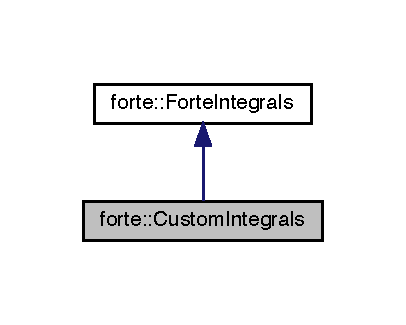
\includegraphics[width=195pt]{classforte_1_1_custom_integrals__inherit__graph}
\end{center}
\end{figure}


Collaboration diagram for forte\+:\+:Custom\+Integrals\+:
\nopagebreak
\begin{figure}[H]
\begin{center}
\leavevmode
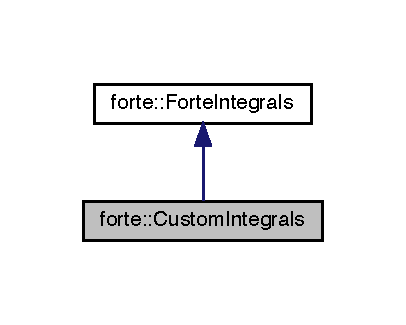
\includegraphics[width=195pt]{classforte_1_1_custom_integrals__coll__graph}
\end{center}
\end{figure}
\subsection*{Public Member Functions}
\begin{DoxyCompactItemize}
\item 
\mbox{\hyperlink{classforte_1_1_custom_integrals_ae7a71673fc56be09c26fae459f7bc84e}{Custom\+Integrals}} (std\+::shared\+\_\+ptr$<$ \mbox{\hyperlink{classforte_1_1_forte_options}{Forte\+Options}} $>$ options, std\+::shared\+\_\+ptr$<$ \mbox{\hyperlink{classforte_1_1_m_o_space_info}{M\+O\+Space\+Info}} $>$ mo\+\_\+space\+\_\+info, \mbox{\hyperlink{namespaceforte_a7defa2660dd3eb07aa81176b90781be7}{Integral\+Spin\+Restriction}} restricted, double \mbox{\hyperlink{classforte_1_1_forte_integrals_a7e2dec148b4e6c3bbd918df8025f8329}{scalar}}, const std\+::vector$<$ double $>$ \&\mbox{\hyperlink{classforte_1_1_forte_integrals_adeb8d675248cb181a502818b8a972908}{oei\+\_\+a}}, const std\+::vector$<$ double $>$ \&\mbox{\hyperlink{classforte_1_1_forte_integrals_ace33795c89d99da0aa8bac4a95263d23}{oei\+\_\+b}}, const std\+::vector$<$ double $>$ \&tei\+\_\+aa, const std\+::vector$<$ double $>$ \&tei\+\_\+ab, const std\+::vector$<$ double $>$ \&tei\+\_\+bb)
\item 
void \mbox{\hyperlink{classforte_1_1_custom_integrals_a09375e296a39feb6a94c7cf4947d0206}{initialize}} () override
\item 
double \mbox{\hyperlink{classforte_1_1_custom_integrals_a933807bd0f7a711329edb83b9b9915f0}{aptei\+\_\+aa}} (size\+\_\+t p, size\+\_\+t q, size\+\_\+t r, size\+\_\+t s) override
\begin{DoxyCompactList}\small\item\em Grabs the antisymmetriced T\+EI -\/ assumes storage in aphy\+\_\+tei\+\_\+$\ast$. \end{DoxyCompactList}\item 
double \mbox{\hyperlink{classforte_1_1_custom_integrals_abfea37dad8b705e35732f3fae06dd151}{aptei\+\_\+ab}} (size\+\_\+t p, size\+\_\+t q, size\+\_\+t r, size\+\_\+t s) override
\begin{DoxyCompactList}\small\item\em The antisymmetrixed alpha-\/beta two-\/electron integrals in physicist notation $<$pq$\vert$rs$>$ \end{DoxyCompactList}\item 
double \mbox{\hyperlink{classforte_1_1_custom_integrals_a2f10a8117087972091b1a7b7188bf797}{aptei\+\_\+bb}} (size\+\_\+t p, size\+\_\+t q, size\+\_\+t r, size\+\_\+t s) override
\begin{DoxyCompactList}\small\item\em The antisymmetrixed beta-\/beta two-\/electron integrals in physicist notation $<$pq$\vert$$\vert$rs$>$ \end{DoxyCompactList}\item 
ambit\+::\+Tensor \mbox{\hyperlink{classforte_1_1_custom_integrals_ae60addb837588a5101f1f2485a818426}{aptei\+\_\+aa\+\_\+block}} (const std\+::vector$<$ size\+\_\+t $>$ \&p, const std\+::vector$<$ size\+\_\+t $>$ \&q, const std\+::vector$<$ size\+\_\+t $>$ \&r, const std\+::vector$<$ size\+\_\+t $>$ \&s) override
\begin{DoxyCompactList}\small\item\em Grabs the antisymmetrized T\+EI -\/ assumes storage of ambit tensor. \end{DoxyCompactList}\item 
ambit\+::\+Tensor \mbox{\hyperlink{classforte_1_1_custom_integrals_af65b7d58e92e6ec9a13c93238724a831}{aptei\+\_\+ab\+\_\+block}} (const std\+::vector$<$ size\+\_\+t $>$ \&p, const std\+::vector$<$ size\+\_\+t $>$ \&q, const std\+::vector$<$ size\+\_\+t $>$ \&r, const std\+::vector$<$ size\+\_\+t $>$ \&s) override
\item 
ambit\+::\+Tensor \mbox{\hyperlink{classforte_1_1_custom_integrals_a71e29eaa0e9b1a84fe679e147c22398f}{aptei\+\_\+bb\+\_\+block}} (const std\+::vector$<$ size\+\_\+t $>$ \&p, const std\+::vector$<$ size\+\_\+t $>$ \&q, const std\+::vector$<$ size\+\_\+t $>$ \&r, const std\+::vector$<$ size\+\_\+t $>$ \&s) override
\item 
void \mbox{\hyperlink{classforte_1_1_custom_integrals_aae47837ebc64bb62efb0c23107ebfafa}{make\+\_\+fock\+\_\+matrix}} (ambit\+::\+Tensor Da, ambit\+::\+Tensor Db) override
\begin{DoxyCompactList}\small\item\em Make the generalized Fock matrix. \end{DoxyCompactList}\item 
std\+::tuple$<$ psi\+::\+Shared\+Matrix, psi\+::\+Shared\+Matrix, double $>$ \mbox{\hyperlink{classforte_1_1_custom_integrals_a00921e140fba2f63eb8399003029ad1a}{make\+\_\+fock\+\_\+inactive}} (psi\+::\+Dimension dim\+\_\+start, psi\+::\+Dimension dim\+\_\+end) override
\begin{DoxyCompactList}\small\item\em Make the closed-\/shell Fock matrix. \end{DoxyCompactList}\item 
std\+::tuple$<$ psi\+::\+Shared\+Matrix, psi\+::\+Shared\+Matrix $>$ \mbox{\hyperlink{classforte_1_1_custom_integrals_aab638e735541a02c266c8ed5bf25af3a}{make\+\_\+fock\+\_\+active}} (ambit\+::\+Tensor Da, ambit\+::\+Tensor Db) override
\begin{DoxyCompactList}\small\item\em Make the active Fock matrix. \end{DoxyCompactList}\item 
psi\+::\+Shared\+Matrix \mbox{\hyperlink{classforte_1_1_custom_integrals_a8079cb2a8c6b71608db08667694183b9}{make\+\_\+fock\+\_\+active\+\_\+restricted}} (psi\+::\+Shared\+Matrix D) override
\begin{DoxyCompactList}\small\item\em Make the active Fock matrix using restricted equation. \end{DoxyCompactList}\item 
std\+::tuple$<$ psi\+::\+Shared\+Matrix, psi\+::\+Shared\+Matrix $>$ \mbox{\hyperlink{classforte_1_1_custom_integrals_a87a7d17ddd89c004adf56b032d409669}{make\+\_\+fock\+\_\+active\+\_\+unrestricted}} (psi\+::\+Shared\+Matrix Da, psi\+::\+Shared\+Matrix Db) override
\begin{DoxyCompactList}\small\item\em Make the active Fock matrix using unrestricted equation. \end{DoxyCompactList}\item 
size\+\_\+t \mbox{\hyperlink{classforte_1_1_custom_integrals_aa8813730038bbc062d8e08d33600c27d}{nthree}} () const override
\begin{DoxyCompactList}\small\item\em Return the number of auxiliary functions. \end{DoxyCompactList}\item 
void \mbox{\hyperlink{classforte_1_1_custom_integrals_ab9b7fd99d359eedcde4fcbf5e5df1795}{set\+\_\+tei}} (size\+\_\+t p, size\+\_\+t q, size\+\_\+t r, size\+\_\+t s, double value, bool alpha1, bool alpha2) override
\begin{DoxyCompactList}\small\item\em Set the value of the two-\/electron integrals. \end{DoxyCompactList}\end{DoxyCompactItemize}
\subsection*{Additional Inherited Members}


\subsection{Detailed Description}
The \mbox{\hyperlink{classforte_1_1_custom_integrals}{Custom\+Integrals}} class stores user-\/provided integrals. 

\subsection{Constructor \& Destructor Documentation}
\mbox{\Hypertarget{classforte_1_1_custom_integrals_ae7a71673fc56be09c26fae459f7bc84e}\label{classforte_1_1_custom_integrals_ae7a71673fc56be09c26fae459f7bc84e}} 
\index{forte\+::\+Custom\+Integrals@{forte\+::\+Custom\+Integrals}!Custom\+Integrals@{Custom\+Integrals}}
\index{Custom\+Integrals@{Custom\+Integrals}!forte\+::\+Custom\+Integrals@{forte\+::\+Custom\+Integrals}}
\subsubsection{\texorpdfstring{Custom\+Integrals()}{CustomIntegrals()}}
{\footnotesize\ttfamily forte\+::\+Custom\+Integrals\+::\+Custom\+Integrals (\begin{DoxyParamCaption}\item[{std\+::shared\+\_\+ptr$<$ \mbox{\hyperlink{classforte_1_1_forte_options}{Forte\+Options}} $>$}]{options,  }\item[{std\+::shared\+\_\+ptr$<$ \mbox{\hyperlink{classforte_1_1_m_o_space_info}{M\+O\+Space\+Info}} $>$}]{mo\+\_\+space\+\_\+info,  }\item[{\mbox{\hyperlink{namespaceforte_a7defa2660dd3eb07aa81176b90781be7}{Integral\+Spin\+Restriction}}}]{restricted,  }\item[{double}]{scalar,  }\item[{const std\+::vector$<$ double $>$ \&}]{oei\+\_\+a,  }\item[{const std\+::vector$<$ double $>$ \&}]{oei\+\_\+b,  }\item[{const std\+::vector$<$ double $>$ \&}]{tei\+\_\+aa,  }\item[{const std\+::vector$<$ double $>$ \&}]{tei\+\_\+ab,  }\item[{const std\+::vector$<$ double $>$ \&}]{tei\+\_\+bb }\end{DoxyParamCaption})}

Contructor of \mbox{\hyperlink{classforte_1_1_custom_integrals}{Custom\+Integrals}} 
\begin{DoxyParams}{Parameters}
{\em options} & a pointer to \mbox{\hyperlink{classforte_1_1_forte_options}{Forte\+Options}} \\
\hline
{\em mo\+\_\+space\+\_\+info} & a pointer to Forte \mbox{\hyperlink{classforte_1_1_m_o_space_info}{M\+O\+Space\+Info}} \\
\hline
{\em restricted} & the type of integral transformation \\
\hline
{\em scalar} & the nuclear repulsion energy \\
\hline
{\em oei\+\_\+a} & the alpha one-\/electron integrals in MO basis \\
\hline
{\em oei\+\_\+b} & the beta one-\/electron integrals in MO basis \\
\hline
{\em tei\+\_\+aa} & the alpha-\/alpha two-\/electron integrals in MO basis \\
\hline
{\em tei\+\_\+ab} & the alpha-\/beta two-\/electron integrals in MO basis \\
\hline
{\em tei\+\_\+bb} & the beta-\/beta two-\/electron integrals in MO basis \\
\hline
\end{DoxyParams}


\subsection{Member Function Documentation}
\mbox{\Hypertarget{classforte_1_1_custom_integrals_a933807bd0f7a711329edb83b9b9915f0}\label{classforte_1_1_custom_integrals_a933807bd0f7a711329edb83b9b9915f0}} 
\index{forte\+::\+Custom\+Integrals@{forte\+::\+Custom\+Integrals}!aptei\+\_\+aa@{aptei\+\_\+aa}}
\index{aptei\+\_\+aa@{aptei\+\_\+aa}!forte\+::\+Custom\+Integrals@{forte\+::\+Custom\+Integrals}}
\subsubsection{\texorpdfstring{aptei\+\_\+aa()}{aptei\_aa()}}
{\footnotesize\ttfamily double forte\+::\+Custom\+Integrals\+::aptei\+\_\+aa (\begin{DoxyParamCaption}\item[{size\+\_\+t}]{p,  }\item[{size\+\_\+t}]{q,  }\item[{size\+\_\+t}]{r,  }\item[{size\+\_\+t}]{s }\end{DoxyParamCaption})\hspace{0.3cm}{\ttfamily [override]}, {\ttfamily [virtual]}}



Grabs the antisymmetriced T\+EI -\/ assumes storage in aphy\+\_\+tei\+\_\+$\ast$. 



Implements \mbox{\hyperlink{classforte_1_1_forte_integrals_afc84c157025b56ee0f8e3b1abe1c0a5f}{forte\+::\+Forte\+Integrals}}.

\mbox{\Hypertarget{classforte_1_1_custom_integrals_ae60addb837588a5101f1f2485a818426}\label{classforte_1_1_custom_integrals_ae60addb837588a5101f1f2485a818426}} 
\index{forte\+::\+Custom\+Integrals@{forte\+::\+Custom\+Integrals}!aptei\+\_\+aa\+\_\+block@{aptei\+\_\+aa\+\_\+block}}
\index{aptei\+\_\+aa\+\_\+block@{aptei\+\_\+aa\+\_\+block}!forte\+::\+Custom\+Integrals@{forte\+::\+Custom\+Integrals}}
\subsubsection{\texorpdfstring{aptei\+\_\+aa\+\_\+block()}{aptei\_aa\_block()}}
{\footnotesize\ttfamily ambit\+::\+Tensor forte\+::\+Custom\+Integrals\+::aptei\+\_\+aa\+\_\+block (\begin{DoxyParamCaption}\item[{const std\+::vector$<$ size\+\_\+t $>$ \&}]{p,  }\item[{const std\+::vector$<$ size\+\_\+t $>$ \&}]{q,  }\item[{const std\+::vector$<$ size\+\_\+t $>$ \&}]{r,  }\item[{const std\+::vector$<$ size\+\_\+t $>$ \&}]{s }\end{DoxyParamCaption})\hspace{0.3cm}{\ttfamily [override]}, {\ttfamily [virtual]}}



Grabs the antisymmetrized T\+EI -\/ assumes storage of ambit tensor. 



Implements \mbox{\hyperlink{classforte_1_1_forte_integrals_ac20ae649b8cfe116f8583d676e43da27}{forte\+::\+Forte\+Integrals}}.

\mbox{\Hypertarget{classforte_1_1_custom_integrals_abfea37dad8b705e35732f3fae06dd151}\label{classforte_1_1_custom_integrals_abfea37dad8b705e35732f3fae06dd151}} 
\index{forte\+::\+Custom\+Integrals@{forte\+::\+Custom\+Integrals}!aptei\+\_\+ab@{aptei\+\_\+ab}}
\index{aptei\+\_\+ab@{aptei\+\_\+ab}!forte\+::\+Custom\+Integrals@{forte\+::\+Custom\+Integrals}}
\subsubsection{\texorpdfstring{aptei\+\_\+ab()}{aptei\_ab()}}
{\footnotesize\ttfamily double forte\+::\+Custom\+Integrals\+::aptei\+\_\+ab (\begin{DoxyParamCaption}\item[{size\+\_\+t}]{p,  }\item[{size\+\_\+t}]{q,  }\item[{size\+\_\+t}]{r,  }\item[{size\+\_\+t}]{s }\end{DoxyParamCaption})\hspace{0.3cm}{\ttfamily [override]}, {\ttfamily [virtual]}}



The antisymmetrixed alpha-\/beta two-\/electron integrals in physicist notation $<$pq$\vert$rs$>$ 



Implements \mbox{\hyperlink{classforte_1_1_forte_integrals_a45efc2329cdfc7e4690cbe85688b947e}{forte\+::\+Forte\+Integrals}}.

\mbox{\Hypertarget{classforte_1_1_custom_integrals_af65b7d58e92e6ec9a13c93238724a831}\label{classforte_1_1_custom_integrals_af65b7d58e92e6ec9a13c93238724a831}} 
\index{forte\+::\+Custom\+Integrals@{forte\+::\+Custom\+Integrals}!aptei\+\_\+ab\+\_\+block@{aptei\+\_\+ab\+\_\+block}}
\index{aptei\+\_\+ab\+\_\+block@{aptei\+\_\+ab\+\_\+block}!forte\+::\+Custom\+Integrals@{forte\+::\+Custom\+Integrals}}
\subsubsection{\texorpdfstring{aptei\+\_\+ab\+\_\+block()}{aptei\_ab\_block()}}
{\footnotesize\ttfamily ambit\+::\+Tensor forte\+::\+Custom\+Integrals\+::aptei\+\_\+ab\+\_\+block (\begin{DoxyParamCaption}\item[{const std\+::vector$<$ size\+\_\+t $>$ \&}]{p,  }\item[{const std\+::vector$<$ size\+\_\+t $>$ \&}]{q,  }\item[{const std\+::vector$<$ size\+\_\+t $>$ \&}]{r,  }\item[{const std\+::vector$<$ size\+\_\+t $>$ \&}]{s }\end{DoxyParamCaption})\hspace{0.3cm}{\ttfamily [override]}, {\ttfamily [virtual]}}

\begin{DoxyReturn}{Returns}
a tensor with a block of the alpha-\/beta antisymmetrized two-\/electron integrals 
\end{DoxyReturn}


Implements \mbox{\hyperlink{classforte_1_1_forte_integrals_acd40e350dc861baf8adf6a3b47c74023}{forte\+::\+Forte\+Integrals}}.

\mbox{\Hypertarget{classforte_1_1_custom_integrals_a2f10a8117087972091b1a7b7188bf797}\label{classforte_1_1_custom_integrals_a2f10a8117087972091b1a7b7188bf797}} 
\index{forte\+::\+Custom\+Integrals@{forte\+::\+Custom\+Integrals}!aptei\+\_\+bb@{aptei\+\_\+bb}}
\index{aptei\+\_\+bb@{aptei\+\_\+bb}!forte\+::\+Custom\+Integrals@{forte\+::\+Custom\+Integrals}}
\subsubsection{\texorpdfstring{aptei\+\_\+bb()}{aptei\_bb()}}
{\footnotesize\ttfamily double forte\+::\+Custom\+Integrals\+::aptei\+\_\+bb (\begin{DoxyParamCaption}\item[{size\+\_\+t}]{p,  }\item[{size\+\_\+t}]{q,  }\item[{size\+\_\+t}]{r,  }\item[{size\+\_\+t}]{s }\end{DoxyParamCaption})\hspace{0.3cm}{\ttfamily [override]}, {\ttfamily [virtual]}}



The antisymmetrixed beta-\/beta two-\/electron integrals in physicist notation $<$pq$\vert$$\vert$rs$>$ 



Implements \mbox{\hyperlink{classforte_1_1_forte_integrals_a246225031c3799dc446f94e0e732c3ac}{forte\+::\+Forte\+Integrals}}.

\mbox{\Hypertarget{classforte_1_1_custom_integrals_a71e29eaa0e9b1a84fe679e147c22398f}\label{classforte_1_1_custom_integrals_a71e29eaa0e9b1a84fe679e147c22398f}} 
\index{forte\+::\+Custom\+Integrals@{forte\+::\+Custom\+Integrals}!aptei\+\_\+bb\+\_\+block@{aptei\+\_\+bb\+\_\+block}}
\index{aptei\+\_\+bb\+\_\+block@{aptei\+\_\+bb\+\_\+block}!forte\+::\+Custom\+Integrals@{forte\+::\+Custom\+Integrals}}
\subsubsection{\texorpdfstring{aptei\+\_\+bb\+\_\+block()}{aptei\_bb\_block()}}
{\footnotesize\ttfamily ambit\+::\+Tensor forte\+::\+Custom\+Integrals\+::aptei\+\_\+bb\+\_\+block (\begin{DoxyParamCaption}\item[{const std\+::vector$<$ size\+\_\+t $>$ \&}]{p,  }\item[{const std\+::vector$<$ size\+\_\+t $>$ \&}]{q,  }\item[{const std\+::vector$<$ size\+\_\+t $>$ \&}]{r,  }\item[{const std\+::vector$<$ size\+\_\+t $>$ \&}]{s }\end{DoxyParamCaption})\hspace{0.3cm}{\ttfamily [override]}, {\ttfamily [virtual]}}

\begin{DoxyReturn}{Returns}
a tensor with a block of the beta-\/beta antisymmetrized two-\/electron integrals 
\end{DoxyReturn}


Implements \mbox{\hyperlink{classforte_1_1_forte_integrals_ae2799dc7cbfd456603a2b841b26582ab}{forte\+::\+Forte\+Integrals}}.

\mbox{\Hypertarget{classforte_1_1_custom_integrals_a09375e296a39feb6a94c7cf4947d0206}\label{classforte_1_1_custom_integrals_a09375e296a39feb6a94c7cf4947d0206}} 
\index{forte\+::\+Custom\+Integrals@{forte\+::\+Custom\+Integrals}!initialize@{initialize}}
\index{initialize@{initialize}!forte\+::\+Custom\+Integrals@{forte\+::\+Custom\+Integrals}}
\subsubsection{\texorpdfstring{initialize()}{initialize()}}
{\footnotesize\ttfamily void forte\+::\+Custom\+Integrals\+::initialize (\begin{DoxyParamCaption}{ }\end{DoxyParamCaption})\hspace{0.3cm}{\ttfamily [override]}, {\ttfamily [virtual]}}



Implements \mbox{\hyperlink{classforte_1_1_forte_integrals_a7862835fa0f5f9abe13dfcd6730fa4be}{forte\+::\+Forte\+Integrals}}.

\mbox{\Hypertarget{classforte_1_1_custom_integrals_aab638e735541a02c266c8ed5bf25af3a}\label{classforte_1_1_custom_integrals_aab638e735541a02c266c8ed5bf25af3a}} 
\index{forte\+::\+Custom\+Integrals@{forte\+::\+Custom\+Integrals}!make\+\_\+fock\+\_\+active@{make\+\_\+fock\+\_\+active}}
\index{make\+\_\+fock\+\_\+active@{make\+\_\+fock\+\_\+active}!forte\+::\+Custom\+Integrals@{forte\+::\+Custom\+Integrals}}
\subsubsection{\texorpdfstring{make\+\_\+fock\+\_\+active()}{make\_fock\_active()}}
{\footnotesize\ttfamily std\+::tuple$<$ psi\+::\+Shared\+Matrix, psi\+::\+Shared\+Matrix $>$ forte\+::\+Custom\+Integrals\+::make\+\_\+fock\+\_\+active (\begin{DoxyParamCaption}\item[{ambit\+::\+Tensor}]{Da,  }\item[{ambit\+::\+Tensor}]{Db }\end{DoxyParamCaption})\hspace{0.3cm}{\ttfamily [override]}, {\ttfamily [virtual]}}



Make the active Fock matrix. 



Implements \mbox{\hyperlink{classforte_1_1_forte_integrals_a1dda7858e1766c9869b58eeda81d5a21}{forte\+::\+Forte\+Integrals}}.

\mbox{\Hypertarget{classforte_1_1_custom_integrals_a8079cb2a8c6b71608db08667694183b9}\label{classforte_1_1_custom_integrals_a8079cb2a8c6b71608db08667694183b9}} 
\index{forte\+::\+Custom\+Integrals@{forte\+::\+Custom\+Integrals}!make\+\_\+fock\+\_\+active\+\_\+restricted@{make\+\_\+fock\+\_\+active\+\_\+restricted}}
\index{make\+\_\+fock\+\_\+active\+\_\+restricted@{make\+\_\+fock\+\_\+active\+\_\+restricted}!forte\+::\+Custom\+Integrals@{forte\+::\+Custom\+Integrals}}
\subsubsection{\texorpdfstring{make\+\_\+fock\+\_\+active\+\_\+restricted()}{make\_fock\_active\_restricted()}}
{\footnotesize\ttfamily psi\+::\+Shared\+Matrix forte\+::\+Custom\+Integrals\+::make\+\_\+fock\+\_\+active\+\_\+restricted (\begin{DoxyParamCaption}\item[{psi\+::\+Shared\+Matrix}]{D }\end{DoxyParamCaption})\hspace{0.3cm}{\ttfamily [override]}, {\ttfamily [virtual]}}



Make the active Fock matrix using restricted equation. 



Implements \mbox{\hyperlink{classforte_1_1_forte_integrals_a9e2f6f24d734aa04784dfc46d3f031ae}{forte\+::\+Forte\+Integrals}}.

\mbox{\Hypertarget{classforte_1_1_custom_integrals_a87a7d17ddd89c004adf56b032d409669}\label{classforte_1_1_custom_integrals_a87a7d17ddd89c004adf56b032d409669}} 
\index{forte\+::\+Custom\+Integrals@{forte\+::\+Custom\+Integrals}!make\+\_\+fock\+\_\+active\+\_\+unrestricted@{make\+\_\+fock\+\_\+active\+\_\+unrestricted}}
\index{make\+\_\+fock\+\_\+active\+\_\+unrestricted@{make\+\_\+fock\+\_\+active\+\_\+unrestricted}!forte\+::\+Custom\+Integrals@{forte\+::\+Custom\+Integrals}}
\subsubsection{\texorpdfstring{make\+\_\+fock\+\_\+active\+\_\+unrestricted()}{make\_fock\_active\_unrestricted()}}
{\footnotesize\ttfamily std\+::tuple$<$ psi\+::\+Shared\+Matrix, psi\+::\+Shared\+Matrix $>$ forte\+::\+Custom\+Integrals\+::make\+\_\+fock\+\_\+active\+\_\+unrestricted (\begin{DoxyParamCaption}\item[{psi\+::\+Shared\+Matrix}]{Da,  }\item[{psi\+::\+Shared\+Matrix}]{Db }\end{DoxyParamCaption})\hspace{0.3cm}{\ttfamily [override]}, {\ttfamily [virtual]}}



Make the active Fock matrix using unrestricted equation. 



Implements \mbox{\hyperlink{classforte_1_1_forte_integrals_a3bc94f56104d72581629d9d6a6a3a74c}{forte\+::\+Forte\+Integrals}}.

\mbox{\Hypertarget{classforte_1_1_custom_integrals_a00921e140fba2f63eb8399003029ad1a}\label{classforte_1_1_custom_integrals_a00921e140fba2f63eb8399003029ad1a}} 
\index{forte\+::\+Custom\+Integrals@{forte\+::\+Custom\+Integrals}!make\+\_\+fock\+\_\+inactive@{make\+\_\+fock\+\_\+inactive}}
\index{make\+\_\+fock\+\_\+inactive@{make\+\_\+fock\+\_\+inactive}!forte\+::\+Custom\+Integrals@{forte\+::\+Custom\+Integrals}}
\subsubsection{\texorpdfstring{make\+\_\+fock\+\_\+inactive()}{make\_fock\_inactive()}}
{\footnotesize\ttfamily std\+::tuple$<$ psi\+::\+Shared\+Matrix, psi\+::\+Shared\+Matrix, double $>$ forte\+::\+Custom\+Integrals\+::make\+\_\+fock\+\_\+inactive (\begin{DoxyParamCaption}\item[{psi\+::\+Dimension}]{dim\+\_\+start,  }\item[{psi\+::\+Dimension}]{dim\+\_\+end }\end{DoxyParamCaption})\hspace{0.3cm}{\ttfamily [override]}, {\ttfamily [virtual]}}



Make the closed-\/shell Fock matrix. 



Implements \mbox{\hyperlink{classforte_1_1_forte_integrals_a4cdca0a7587cad9d830ed3b333ec78cf}{forte\+::\+Forte\+Integrals}}.

\mbox{\Hypertarget{classforte_1_1_custom_integrals_aae47837ebc64bb62efb0c23107ebfafa}\label{classforte_1_1_custom_integrals_aae47837ebc64bb62efb0c23107ebfafa}} 
\index{forte\+::\+Custom\+Integrals@{forte\+::\+Custom\+Integrals}!make\+\_\+fock\+\_\+matrix@{make\+\_\+fock\+\_\+matrix}}
\index{make\+\_\+fock\+\_\+matrix@{make\+\_\+fock\+\_\+matrix}!forte\+::\+Custom\+Integrals@{forte\+::\+Custom\+Integrals}}
\subsubsection{\texorpdfstring{make\+\_\+fock\+\_\+matrix()}{make\_fock\_matrix()}}
{\footnotesize\ttfamily void forte\+::\+Custom\+Integrals\+::make\+\_\+fock\+\_\+matrix (\begin{DoxyParamCaption}\item[{ambit\+::\+Tensor}]{Da,  }\item[{ambit\+::\+Tensor}]{Db }\end{DoxyParamCaption})\hspace{0.3cm}{\ttfamily [override]}, {\ttfamily [virtual]}}



Make the generalized Fock matrix. 



Implements \mbox{\hyperlink{classforte_1_1_forte_integrals_aadd195fbc0c7f7b659ab9280457568e0}{forte\+::\+Forte\+Integrals}}.

\mbox{\Hypertarget{classforte_1_1_custom_integrals_aa8813730038bbc062d8e08d33600c27d}\label{classforte_1_1_custom_integrals_aa8813730038bbc062d8e08d33600c27d}} 
\index{forte\+::\+Custom\+Integrals@{forte\+::\+Custom\+Integrals}!nthree@{nthree}}
\index{nthree@{nthree}!forte\+::\+Custom\+Integrals@{forte\+::\+Custom\+Integrals}}
\subsubsection{\texorpdfstring{nthree()}{nthree()}}
{\footnotesize\ttfamily size\+\_\+t forte\+::\+Custom\+Integrals\+::nthree (\begin{DoxyParamCaption}{ }\end{DoxyParamCaption}) const\hspace{0.3cm}{\ttfamily [inline]}, {\ttfamily [override]}, {\ttfamily [virtual]}}



Return the number of auxiliary functions. 



Reimplemented from \mbox{\hyperlink{classforte_1_1_forte_integrals_af04858e7813556747745f90ffbda81a4}{forte\+::\+Forte\+Integrals}}.

\mbox{\Hypertarget{classforte_1_1_custom_integrals_ab9b7fd99d359eedcde4fcbf5e5df1795}\label{classforte_1_1_custom_integrals_ab9b7fd99d359eedcde4fcbf5e5df1795}} 
\index{forte\+::\+Custom\+Integrals@{forte\+::\+Custom\+Integrals}!set\+\_\+tei@{set\+\_\+tei}}
\index{set\+\_\+tei@{set\+\_\+tei}!forte\+::\+Custom\+Integrals@{forte\+::\+Custom\+Integrals}}
\subsubsection{\texorpdfstring{set\+\_\+tei()}{set\_tei()}}
{\footnotesize\ttfamily void forte\+::\+Custom\+Integrals\+::set\+\_\+tei (\begin{DoxyParamCaption}\item[{size\+\_\+t}]{p,  }\item[{size\+\_\+t}]{q,  }\item[{size\+\_\+t}]{r,  }\item[{size\+\_\+t}]{s,  }\item[{double}]{value,  }\item[{bool}]{alpha1,  }\item[{bool}]{alpha2 }\end{DoxyParamCaption})\hspace{0.3cm}{\ttfamily [override]}, {\ttfamily [virtual]}}



Set the value of the two-\/electron integrals. 



Implements \mbox{\hyperlink{classforte_1_1_forte_integrals_aaccd56e90bbc3c423158efb154336b9c}{forte\+::\+Forte\+Integrals}}.



The documentation for this class was generated from the following files\+:\begin{DoxyCompactItemize}
\item 
/\+Users/fevange/\+Source/forte/src/integrals/\mbox{\hyperlink{custom__integrals_8h}{custom\+\_\+integrals.\+h}}\item 
/\+Users/fevange/\+Source/forte/src/integrals/\mbox{\hyperlink{custom__integrals_8cc}{custom\+\_\+integrals.\+cc}}\end{DoxyCompactItemize}

\hypertarget{classforte_1_1_davidson_liu_solver}{}\section{forte\+:\+:Davidson\+Liu\+Solver Class Reference}
\label{classforte_1_1_davidson_liu_solver}\index{forte\+::\+Davidson\+Liu\+Solver@{forte\+::\+Davidson\+Liu\+Solver}}


The \mbox{\hyperlink{classforte_1_1_davidson_liu_solver}{Davidson\+Liu\+Solver}} class This class diagonalizes the Hamiltonian in a basis of determinants.  




{\ttfamily \#include $<$iterative\+\_\+solvers.\+h$>$}

\subsection*{Public Member Functions}
\begin{DoxyCompactItemize}
\item 
\mbox{\hyperlink{classforte_1_1_davidson_liu_solver_a1b843c1999b520d6bd65e68db087a78d}{Davidson\+Liu\+Solver}} (size\+\_\+t size, size\+\_\+t nroot)
\begin{DoxyCompactList}\small\item\em Constructor. \end{DoxyCompactList}\item 
\mbox{\hyperlink{classforte_1_1_davidson_liu_solver_ac8e1ff5995ed726339cb5500de75fb3e}{$\sim$\+Davidson\+Liu\+Solver}} ()
\begin{DoxyCompactList}\small\item\em Destructor. \end{DoxyCompactList}\item 
void \mbox{\hyperlink{classforte_1_1_davidson_liu_solver_a833b7e36f2e1b45e0e1ebe656a2eb826}{set\+\_\+print\+\_\+level}} (size\+\_\+t n)
\begin{DoxyCompactList}\small\item\em Set the print level. \end{DoxyCompactList}\item 
void \mbox{\hyperlink{classforte_1_1_davidson_liu_solver_a24cacf196136a1003e1867bf5de0ff7b}{set\+\_\+e\+\_\+convergence}} (double value)
\begin{DoxyCompactList}\small\item\em Set the energy convergence. \end{DoxyCompactList}\item 
void \mbox{\hyperlink{classforte_1_1_davidson_liu_solver_aecc764a37729a8ecf814f44bac9fb60e}{set\+\_\+r\+\_\+convergence}} (double value)
\begin{DoxyCompactList}\small\item\em Set the residual convergence. \end{DoxyCompactList}\item 
double \mbox{\hyperlink{classforte_1_1_davidson_liu_solver_a7575f9ba87e5acf32af334f88fa5acf3}{get\+\_\+e\+\_\+convergence}} () const
\begin{DoxyCompactList}\small\item\em Get the energy convergence. \end{DoxyCompactList}\item 
double \mbox{\hyperlink{classforte_1_1_davidson_liu_solver_a0dc38a4a9e09c92568d97049c9cd193a}{get\+\_\+r\+\_\+convergence}} () const
\begin{DoxyCompactList}\small\item\em Get the residual convergence. \end{DoxyCompactList}\item 
void \mbox{\hyperlink{classforte_1_1_davidson_liu_solver_a7423d12c5300f050e6c0f09f314b08d1}{set\+\_\+collapse\+\_\+per\+\_\+root}} (int value)
\begin{DoxyCompactList}\small\item\em Set the number of collapse vectors for each root. \end{DoxyCompactList}\item 
void \mbox{\hyperlink{classforte_1_1_davidson_liu_solver_a0b09acd03c81aa259f22368af4ba422d}{set\+\_\+subspace\+\_\+per\+\_\+root}} (int value)
\begin{DoxyCompactList}\small\item\em Set the maximum subspace size for each root. \end{DoxyCompactList}\item 
size\+\_\+t \mbox{\hyperlink{classforte_1_1_davidson_liu_solver_af68b3caa5e37a93261b13cbdd7006ecf}{collapse\+\_\+size}} () const
\begin{DoxyCompactList}\small\item\em Return the size of the collapse vectors. \end{DoxyCompactList}\item 
void \mbox{\hyperlink{classforte_1_1_davidson_liu_solver_a16d9dda8f0ca73840539381caf50601d}{add\+\_\+guess}} (psi\+::\+Shared\+Vector vec)
\begin{DoxyCompactList}\small\item\em Add a guess basis vector. \end{DoxyCompactList}\item 
void \mbox{\hyperlink{classforte_1_1_davidson_liu_solver_ae3e3b9505b8ced3a1d2f2abeb9c5ba7d}{get\+\_\+b}} (psi\+::\+Shared\+Vector vec)
\begin{DoxyCompactList}\small\item\em Get a basis vector. \end{DoxyCompactList}\item 
bool \mbox{\hyperlink{classforte_1_1_davidson_liu_solver_a115e25576e4b15e960de1a7dba553079}{add\+\_\+sigma}} (psi\+::\+Shared\+Vector vec)
\begin{DoxyCompactList}\small\item\em Add a sigma vector. \end{DoxyCompactList}\item 
void \mbox{\hyperlink{classforte_1_1_davidson_liu_solver_a6e41d496aef9fa83c557b513b52e4d6f}{set\+\_\+project\+\_\+out}} (std\+::vector$<$ sparse\+\_\+vec $>$ project\+\_\+out)
\item 
psi\+::\+Shared\+Vector \mbox{\hyperlink{classforte_1_1_davidson_liu_solver_ac35bcdec2a59ab95da00f27453bfb0fe}{eigenvalues}} () const
\begin{DoxyCompactList}\small\item\em Return the eigenvalues. \end{DoxyCompactList}\item 
psi\+::\+Shared\+Matrix \mbox{\hyperlink{classforte_1_1_davidson_liu_solver_a29270144e1b206b5a0cd34875b733566}{eigenvectors}} () const
\begin{DoxyCompactList}\small\item\em Return the eigenvectors. \end{DoxyCompactList}\item 
psi\+::\+Shared\+Vector \mbox{\hyperlink{classforte_1_1_davidson_liu_solver_a447794af9fa43098ae49a0e338006c88}{eigenvector}} (size\+\_\+t n) const
\begin{DoxyCompactList}\small\item\em Return the n-\/th eigenvector. \end{DoxyCompactList}\item 
void \mbox{\hyperlink{classforte_1_1_davidson_liu_solver_a5ea48ce184951d29d39e710ef1a4dc4b}{startup}} (psi\+::\+Shared\+Vector diagonal)
\begin{DoxyCompactList}\small\item\em Initialize the object. \end{DoxyCompactList}\item 
\mbox{\hyperlink{namespaceforte_a62f3fc3a26f13fb59a89be14ecc8fa07}{Solver\+Status}} \mbox{\hyperlink{classforte_1_1_davidson_liu_solver_a332c9bab147d3a895caf073950e30dd1}{update}} ()
\begin{DoxyCompactList}\small\item\em Perform an update step. \end{DoxyCompactList}\item 
void \mbox{\hyperlink{classforte_1_1_davidson_liu_solver_ad34514120b781b92c88d6f160d973cb8}{get\+\_\+results}} ()
\begin{DoxyCompactList}\small\item\em Produce the final eigenvectors and eigenvalues. \end{DoxyCompactList}\item 
std\+::vector$<$ double $>$ \mbox{\hyperlink{classforte_1_1_davidson_liu_solver_aa404bd3a84b3eaaf41af45accaad1a67}{residuals}} () const
\begin{DoxyCompactList}\small\item\em A vector with the 2-\/norm of the residual for each root. \end{DoxyCompactList}\end{DoxyCompactItemize}


\subsection{Detailed Description}
The \mbox{\hyperlink{classforte_1_1_davidson_liu_solver}{Davidson\+Liu\+Solver}} class This class diagonalizes the Hamiltonian in a basis of determinants. 

Example use\+: \begin{DoxyVerb}DavidsonLiuSolver dls(nbasis,nroots);      // create solver
dls.startup(diagonal);                     // initialize solver with
\end{DoxyVerb}
 diagonal of Matrix size\+\_\+t guess\+\_\+size = dls.\+collapse\+\_\+size(); // get the size of the guess

for (size\+\_\+t n = 0; n $<$ guess\+\_\+size; ++n)\{ dls.\+add\+\_\+b(guess\mbox{[}n\mbox{]}); // add guess vectors \}

bool converged = false; for (int cycle = 0; cycle $<$ max\+\_\+cycle; ++cycle)\{ do\{ dls.\+get\+\_\+b(b); // solver provides a vector b ... // code to compute sigma = Hb add\+\_\+sigma = dls.\+add\+\_\+sigma(sigma); // return sigma vector to solver \} while (add\+\_\+sigma); converged = dls.\+update(); // check convergence if (converged == Converged) break; \} 

\subsection{Constructor \& Destructor Documentation}
\mbox{\Hypertarget{classforte_1_1_davidson_liu_solver_a1b843c1999b520d6bd65e68db087a78d}\label{classforte_1_1_davidson_liu_solver_a1b843c1999b520d6bd65e68db087a78d}} 
\index{forte\+::\+Davidson\+Liu\+Solver@{forte\+::\+Davidson\+Liu\+Solver}!Davidson\+Liu\+Solver@{Davidson\+Liu\+Solver}}
\index{Davidson\+Liu\+Solver@{Davidson\+Liu\+Solver}!forte\+::\+Davidson\+Liu\+Solver@{forte\+::\+Davidson\+Liu\+Solver}}
\subsubsection{\texorpdfstring{Davidson\+Liu\+Solver()}{DavidsonLiuSolver()}}
{\footnotesize\ttfamily forte\+::\+Davidson\+Liu\+Solver\+::\+Davidson\+Liu\+Solver (\begin{DoxyParamCaption}\item[{size\+\_\+t}]{size,  }\item[{size\+\_\+t}]{nroot }\end{DoxyParamCaption})}



Constructor. 

\mbox{\Hypertarget{classforte_1_1_davidson_liu_solver_ac8e1ff5995ed726339cb5500de75fb3e}\label{classforte_1_1_davidson_liu_solver_ac8e1ff5995ed726339cb5500de75fb3e}} 
\index{forte\+::\+Davidson\+Liu\+Solver@{forte\+::\+Davidson\+Liu\+Solver}!````~Davidson\+Liu\+Solver@{$\sim$\+Davidson\+Liu\+Solver}}
\index{````~Davidson\+Liu\+Solver@{$\sim$\+Davidson\+Liu\+Solver}!forte\+::\+Davidson\+Liu\+Solver@{forte\+::\+Davidson\+Liu\+Solver}}
\subsubsection{\texorpdfstring{$\sim$\+Davidson\+Liu\+Solver()}{~DavidsonLiuSolver()}}
{\footnotesize\ttfamily forte\+::\+Davidson\+Liu\+Solver\+::$\sim$\+Davidson\+Liu\+Solver (\begin{DoxyParamCaption}{ }\end{DoxyParamCaption})}



Destructor. 



\subsection{Member Function Documentation}
\mbox{\Hypertarget{classforte_1_1_davidson_liu_solver_a16d9dda8f0ca73840539381caf50601d}\label{classforte_1_1_davidson_liu_solver_a16d9dda8f0ca73840539381caf50601d}} 
\index{forte\+::\+Davidson\+Liu\+Solver@{forte\+::\+Davidson\+Liu\+Solver}!add\+\_\+guess@{add\+\_\+guess}}
\index{add\+\_\+guess@{add\+\_\+guess}!forte\+::\+Davidson\+Liu\+Solver@{forte\+::\+Davidson\+Liu\+Solver}}
\subsubsection{\texorpdfstring{add\+\_\+guess()}{add\_guess()}}
{\footnotesize\ttfamily void forte\+::\+Davidson\+Liu\+Solver\+::add\+\_\+guess (\begin{DoxyParamCaption}\item[{psi\+::\+Shared\+Vector}]{vec }\end{DoxyParamCaption})}



Add a guess basis vector. 

\mbox{\Hypertarget{classforte_1_1_davidson_liu_solver_a115e25576e4b15e960de1a7dba553079}\label{classforte_1_1_davidson_liu_solver_a115e25576e4b15e960de1a7dba553079}} 
\index{forte\+::\+Davidson\+Liu\+Solver@{forte\+::\+Davidson\+Liu\+Solver}!add\+\_\+sigma@{add\+\_\+sigma}}
\index{add\+\_\+sigma@{add\+\_\+sigma}!forte\+::\+Davidson\+Liu\+Solver@{forte\+::\+Davidson\+Liu\+Solver}}
\subsubsection{\texorpdfstring{add\+\_\+sigma()}{add\_sigma()}}
{\footnotesize\ttfamily bool forte\+::\+Davidson\+Liu\+Solver\+::add\+\_\+sigma (\begin{DoxyParamCaption}\item[{psi\+::\+Shared\+Vector}]{vec }\end{DoxyParamCaption})}



Add a sigma vector. 

\mbox{\Hypertarget{classforte_1_1_davidson_liu_solver_af68b3caa5e37a93261b13cbdd7006ecf}\label{classforte_1_1_davidson_liu_solver_af68b3caa5e37a93261b13cbdd7006ecf}} 
\index{forte\+::\+Davidson\+Liu\+Solver@{forte\+::\+Davidson\+Liu\+Solver}!collapse\+\_\+size@{collapse\+\_\+size}}
\index{collapse\+\_\+size@{collapse\+\_\+size}!forte\+::\+Davidson\+Liu\+Solver@{forte\+::\+Davidson\+Liu\+Solver}}
\subsubsection{\texorpdfstring{collapse\+\_\+size()}{collapse\_size()}}
{\footnotesize\ttfamily size\+\_\+t forte\+::\+Davidson\+Liu\+Solver\+::collapse\+\_\+size (\begin{DoxyParamCaption}{ }\end{DoxyParamCaption}) const}



Return the size of the collapse vectors. 

\mbox{\Hypertarget{classforte_1_1_davidson_liu_solver_ac35bcdec2a59ab95da00f27453bfb0fe}\label{classforte_1_1_davidson_liu_solver_ac35bcdec2a59ab95da00f27453bfb0fe}} 
\index{forte\+::\+Davidson\+Liu\+Solver@{forte\+::\+Davidson\+Liu\+Solver}!eigenvalues@{eigenvalues}}
\index{eigenvalues@{eigenvalues}!forte\+::\+Davidson\+Liu\+Solver@{forte\+::\+Davidson\+Liu\+Solver}}
\subsubsection{\texorpdfstring{eigenvalues()}{eigenvalues()}}
{\footnotesize\ttfamily psi\+::\+Shared\+Vector forte\+::\+Davidson\+Liu\+Solver\+::eigenvalues (\begin{DoxyParamCaption}{ }\end{DoxyParamCaption}) const}



Return the eigenvalues. 

\mbox{\Hypertarget{classforte_1_1_davidson_liu_solver_a447794af9fa43098ae49a0e338006c88}\label{classforte_1_1_davidson_liu_solver_a447794af9fa43098ae49a0e338006c88}} 
\index{forte\+::\+Davidson\+Liu\+Solver@{forte\+::\+Davidson\+Liu\+Solver}!eigenvector@{eigenvector}}
\index{eigenvector@{eigenvector}!forte\+::\+Davidson\+Liu\+Solver@{forte\+::\+Davidson\+Liu\+Solver}}
\subsubsection{\texorpdfstring{eigenvector()}{eigenvector()}}
{\footnotesize\ttfamily psi\+::\+Shared\+Vector forte\+::\+Davidson\+Liu\+Solver\+::eigenvector (\begin{DoxyParamCaption}\item[{size\+\_\+t}]{n }\end{DoxyParamCaption}) const}



Return the n-\/th eigenvector. 

\mbox{\Hypertarget{classforte_1_1_davidson_liu_solver_a29270144e1b206b5a0cd34875b733566}\label{classforte_1_1_davidson_liu_solver_a29270144e1b206b5a0cd34875b733566}} 
\index{forte\+::\+Davidson\+Liu\+Solver@{forte\+::\+Davidson\+Liu\+Solver}!eigenvectors@{eigenvectors}}
\index{eigenvectors@{eigenvectors}!forte\+::\+Davidson\+Liu\+Solver@{forte\+::\+Davidson\+Liu\+Solver}}
\subsubsection{\texorpdfstring{eigenvectors()}{eigenvectors()}}
{\footnotesize\ttfamily psi\+::\+Shared\+Matrix forte\+::\+Davidson\+Liu\+Solver\+::eigenvectors (\begin{DoxyParamCaption}{ }\end{DoxyParamCaption}) const}



Return the eigenvectors. 

\mbox{\Hypertarget{classforte_1_1_davidson_liu_solver_ae3e3b9505b8ced3a1d2f2abeb9c5ba7d}\label{classforte_1_1_davidson_liu_solver_ae3e3b9505b8ced3a1d2f2abeb9c5ba7d}} 
\index{forte\+::\+Davidson\+Liu\+Solver@{forte\+::\+Davidson\+Liu\+Solver}!get\+\_\+b@{get\+\_\+b}}
\index{get\+\_\+b@{get\+\_\+b}!forte\+::\+Davidson\+Liu\+Solver@{forte\+::\+Davidson\+Liu\+Solver}}
\subsubsection{\texorpdfstring{get\+\_\+b()}{get\_b()}}
{\footnotesize\ttfamily void forte\+::\+Davidson\+Liu\+Solver\+::get\+\_\+b (\begin{DoxyParamCaption}\item[{psi\+::\+Shared\+Vector}]{vec }\end{DoxyParamCaption})}



Get a basis vector. 

\mbox{\Hypertarget{classforte_1_1_davidson_liu_solver_a7575f9ba87e5acf32af334f88fa5acf3}\label{classforte_1_1_davidson_liu_solver_a7575f9ba87e5acf32af334f88fa5acf3}} 
\index{forte\+::\+Davidson\+Liu\+Solver@{forte\+::\+Davidson\+Liu\+Solver}!get\+\_\+e\+\_\+convergence@{get\+\_\+e\+\_\+convergence}}
\index{get\+\_\+e\+\_\+convergence@{get\+\_\+e\+\_\+convergence}!forte\+::\+Davidson\+Liu\+Solver@{forte\+::\+Davidson\+Liu\+Solver}}
\subsubsection{\texorpdfstring{get\+\_\+e\+\_\+convergence()}{get\_e\_convergence()}}
{\footnotesize\ttfamily double forte\+::\+Davidson\+Liu\+Solver\+::get\+\_\+e\+\_\+convergence (\begin{DoxyParamCaption}{ }\end{DoxyParamCaption}) const}



Get the energy convergence. 

\mbox{\Hypertarget{classforte_1_1_davidson_liu_solver_a0dc38a4a9e09c92568d97049c9cd193a}\label{classforte_1_1_davidson_liu_solver_a0dc38a4a9e09c92568d97049c9cd193a}} 
\index{forte\+::\+Davidson\+Liu\+Solver@{forte\+::\+Davidson\+Liu\+Solver}!get\+\_\+r\+\_\+convergence@{get\+\_\+r\+\_\+convergence}}
\index{get\+\_\+r\+\_\+convergence@{get\+\_\+r\+\_\+convergence}!forte\+::\+Davidson\+Liu\+Solver@{forte\+::\+Davidson\+Liu\+Solver}}
\subsubsection{\texorpdfstring{get\+\_\+r\+\_\+convergence()}{get\_r\_convergence()}}
{\footnotesize\ttfamily double forte\+::\+Davidson\+Liu\+Solver\+::get\+\_\+r\+\_\+convergence (\begin{DoxyParamCaption}{ }\end{DoxyParamCaption}) const}



Get the residual convergence. 

\mbox{\Hypertarget{classforte_1_1_davidson_liu_solver_ad34514120b781b92c88d6f160d973cb8}\label{classforte_1_1_davidson_liu_solver_ad34514120b781b92c88d6f160d973cb8}} 
\index{forte\+::\+Davidson\+Liu\+Solver@{forte\+::\+Davidson\+Liu\+Solver}!get\+\_\+results@{get\+\_\+results}}
\index{get\+\_\+results@{get\+\_\+results}!forte\+::\+Davidson\+Liu\+Solver@{forte\+::\+Davidson\+Liu\+Solver}}
\subsubsection{\texorpdfstring{get\+\_\+results()}{get\_results()}}
{\footnotesize\ttfamily void forte\+::\+Davidson\+Liu\+Solver\+::get\+\_\+results (\begin{DoxyParamCaption}{ }\end{DoxyParamCaption})}



Produce the final eigenvectors and eigenvalues. 

\mbox{\Hypertarget{classforte_1_1_davidson_liu_solver_aa404bd3a84b3eaaf41af45accaad1a67}\label{classforte_1_1_davidson_liu_solver_aa404bd3a84b3eaaf41af45accaad1a67}} 
\index{forte\+::\+Davidson\+Liu\+Solver@{forte\+::\+Davidson\+Liu\+Solver}!residuals@{residuals}}
\index{residuals@{residuals}!forte\+::\+Davidson\+Liu\+Solver@{forte\+::\+Davidson\+Liu\+Solver}}
\subsubsection{\texorpdfstring{residuals()}{residuals()}}
{\footnotesize\ttfamily std\+::vector$<$ double $>$ forte\+::\+Davidson\+Liu\+Solver\+::residuals (\begin{DoxyParamCaption}{ }\end{DoxyParamCaption}) const}



A vector with the 2-\/norm of the residual for each root. 

\mbox{\Hypertarget{classforte_1_1_davidson_liu_solver_a7423d12c5300f050e6c0f09f314b08d1}\label{classforte_1_1_davidson_liu_solver_a7423d12c5300f050e6c0f09f314b08d1}} 
\index{forte\+::\+Davidson\+Liu\+Solver@{forte\+::\+Davidson\+Liu\+Solver}!set\+\_\+collapse\+\_\+per\+\_\+root@{set\+\_\+collapse\+\_\+per\+\_\+root}}
\index{set\+\_\+collapse\+\_\+per\+\_\+root@{set\+\_\+collapse\+\_\+per\+\_\+root}!forte\+::\+Davidson\+Liu\+Solver@{forte\+::\+Davidson\+Liu\+Solver}}
\subsubsection{\texorpdfstring{set\+\_\+collapse\+\_\+per\+\_\+root()}{set\_collapse\_per\_root()}}
{\footnotesize\ttfamily void forte\+::\+Davidson\+Liu\+Solver\+::set\+\_\+collapse\+\_\+per\+\_\+root (\begin{DoxyParamCaption}\item[{int}]{value }\end{DoxyParamCaption})}



Set the number of collapse vectors for each root. 

\mbox{\Hypertarget{classforte_1_1_davidson_liu_solver_a24cacf196136a1003e1867bf5de0ff7b}\label{classforte_1_1_davidson_liu_solver_a24cacf196136a1003e1867bf5de0ff7b}} 
\index{forte\+::\+Davidson\+Liu\+Solver@{forte\+::\+Davidson\+Liu\+Solver}!set\+\_\+e\+\_\+convergence@{set\+\_\+e\+\_\+convergence}}
\index{set\+\_\+e\+\_\+convergence@{set\+\_\+e\+\_\+convergence}!forte\+::\+Davidson\+Liu\+Solver@{forte\+::\+Davidson\+Liu\+Solver}}
\subsubsection{\texorpdfstring{set\+\_\+e\+\_\+convergence()}{set\_e\_convergence()}}
{\footnotesize\ttfamily void forte\+::\+Davidson\+Liu\+Solver\+::set\+\_\+e\+\_\+convergence (\begin{DoxyParamCaption}\item[{double}]{value }\end{DoxyParamCaption})}



Set the energy convergence. 

\mbox{\Hypertarget{classforte_1_1_davidson_liu_solver_a833b7e36f2e1b45e0e1ebe656a2eb826}\label{classforte_1_1_davidson_liu_solver_a833b7e36f2e1b45e0e1ebe656a2eb826}} 
\index{forte\+::\+Davidson\+Liu\+Solver@{forte\+::\+Davidson\+Liu\+Solver}!set\+\_\+print\+\_\+level@{set\+\_\+print\+\_\+level}}
\index{set\+\_\+print\+\_\+level@{set\+\_\+print\+\_\+level}!forte\+::\+Davidson\+Liu\+Solver@{forte\+::\+Davidson\+Liu\+Solver}}
\subsubsection{\texorpdfstring{set\+\_\+print\+\_\+level()}{set\_print\_level()}}
{\footnotesize\ttfamily void forte\+::\+Davidson\+Liu\+Solver\+::set\+\_\+print\+\_\+level (\begin{DoxyParamCaption}\item[{size\+\_\+t}]{n }\end{DoxyParamCaption})}



Set the print level. 

\mbox{\Hypertarget{classforte_1_1_davidson_liu_solver_a6e41d496aef9fa83c557b513b52e4d6f}\label{classforte_1_1_davidson_liu_solver_a6e41d496aef9fa83c557b513b52e4d6f}} 
\index{forte\+::\+Davidson\+Liu\+Solver@{forte\+::\+Davidson\+Liu\+Solver}!set\+\_\+project\+\_\+out@{set\+\_\+project\+\_\+out}}
\index{set\+\_\+project\+\_\+out@{set\+\_\+project\+\_\+out}!forte\+::\+Davidson\+Liu\+Solver@{forte\+::\+Davidson\+Liu\+Solver}}
\subsubsection{\texorpdfstring{set\+\_\+project\+\_\+out()}{set\_project\_out()}}
{\footnotesize\ttfamily void forte\+::\+Davidson\+Liu\+Solver\+::set\+\_\+project\+\_\+out (\begin{DoxyParamCaption}\item[{std\+::vector$<$ sparse\+\_\+vec $>$}]{project\+\_\+out }\end{DoxyParamCaption})}

\mbox{\Hypertarget{classforte_1_1_davidson_liu_solver_aecc764a37729a8ecf814f44bac9fb60e}\label{classforte_1_1_davidson_liu_solver_aecc764a37729a8ecf814f44bac9fb60e}} 
\index{forte\+::\+Davidson\+Liu\+Solver@{forte\+::\+Davidson\+Liu\+Solver}!set\+\_\+r\+\_\+convergence@{set\+\_\+r\+\_\+convergence}}
\index{set\+\_\+r\+\_\+convergence@{set\+\_\+r\+\_\+convergence}!forte\+::\+Davidson\+Liu\+Solver@{forte\+::\+Davidson\+Liu\+Solver}}
\subsubsection{\texorpdfstring{set\+\_\+r\+\_\+convergence()}{set\_r\_convergence()}}
{\footnotesize\ttfamily void forte\+::\+Davidson\+Liu\+Solver\+::set\+\_\+r\+\_\+convergence (\begin{DoxyParamCaption}\item[{double}]{value }\end{DoxyParamCaption})}



Set the residual convergence. 

\mbox{\Hypertarget{classforte_1_1_davidson_liu_solver_a0b09acd03c81aa259f22368af4ba422d}\label{classforte_1_1_davidson_liu_solver_a0b09acd03c81aa259f22368af4ba422d}} 
\index{forte\+::\+Davidson\+Liu\+Solver@{forte\+::\+Davidson\+Liu\+Solver}!set\+\_\+subspace\+\_\+per\+\_\+root@{set\+\_\+subspace\+\_\+per\+\_\+root}}
\index{set\+\_\+subspace\+\_\+per\+\_\+root@{set\+\_\+subspace\+\_\+per\+\_\+root}!forte\+::\+Davidson\+Liu\+Solver@{forte\+::\+Davidson\+Liu\+Solver}}
\subsubsection{\texorpdfstring{set\+\_\+subspace\+\_\+per\+\_\+root()}{set\_subspace\_per\_root()}}
{\footnotesize\ttfamily void forte\+::\+Davidson\+Liu\+Solver\+::set\+\_\+subspace\+\_\+per\+\_\+root (\begin{DoxyParamCaption}\item[{int}]{value }\end{DoxyParamCaption})}



Set the maximum subspace size for each root. 

\mbox{\Hypertarget{classforte_1_1_davidson_liu_solver_a5ea48ce184951d29d39e710ef1a4dc4b}\label{classforte_1_1_davidson_liu_solver_a5ea48ce184951d29d39e710ef1a4dc4b}} 
\index{forte\+::\+Davidson\+Liu\+Solver@{forte\+::\+Davidson\+Liu\+Solver}!startup@{startup}}
\index{startup@{startup}!forte\+::\+Davidson\+Liu\+Solver@{forte\+::\+Davidson\+Liu\+Solver}}
\subsubsection{\texorpdfstring{startup()}{startup()}}
{\footnotesize\ttfamily void forte\+::\+Davidson\+Liu\+Solver\+::startup (\begin{DoxyParamCaption}\item[{psi\+::\+Shared\+Vector}]{diagonal }\end{DoxyParamCaption})}



Initialize the object. 

\mbox{\Hypertarget{classforte_1_1_davidson_liu_solver_a332c9bab147d3a895caf073950e30dd1}\label{classforte_1_1_davidson_liu_solver_a332c9bab147d3a895caf073950e30dd1}} 
\index{forte\+::\+Davidson\+Liu\+Solver@{forte\+::\+Davidson\+Liu\+Solver}!update@{update}}
\index{update@{update}!forte\+::\+Davidson\+Liu\+Solver@{forte\+::\+Davidson\+Liu\+Solver}}
\subsubsection{\texorpdfstring{update()}{update()}}
{\footnotesize\ttfamily \mbox{\hyperlink{namespaceforte_a62f3fc3a26f13fb59a89be14ecc8fa07}{Solver\+Status}} forte\+::\+Davidson\+Liu\+Solver\+::update (\begin{DoxyParamCaption}{ }\end{DoxyParamCaption})}



Perform an update step. 



The documentation for this class was generated from the following files\+:\begin{DoxyCompactItemize}
\item 
/\+Users/fevange/\+Source/forte/src/helpers/\mbox{\hyperlink{iterative__solvers_8h}{iterative\+\_\+solvers.\+h}}\item 
/\+Users/fevange/\+Source/forte/src/helpers/\mbox{\hyperlink{iterative__solvers_8cc}{iterative\+\_\+solvers.\+cc}}\end{DoxyCompactItemize}

\hypertarget{structforte_1_1_det_address}{}\section{forte\+:\+:Det\+Address Struct Reference}
\label{structforte_1_1_det_address}\index{forte\+::\+Det\+Address@{forte\+::\+Det\+Address}}


{\ttfamily \#include $<$string\+\_\+lists.\+h$>$}

\subsection*{Public Member Functions}
\begin{DoxyCompactItemize}
\item 
\mbox{\hyperlink{structforte_1_1_det_address_af8a84f76d87a88af65e0e02034e419fe}{Det\+Address}} (const int \&alfa\+\_\+sym\+\_\+, const size\+\_\+t \&alfa\+\_\+string\+\_\+, const size\+\_\+t \&beta\+\_\+string\+\_\+)
\end{DoxyCompactItemize}
\subsection*{Public Attributes}
\begin{DoxyCompactItemize}
\item 
int \mbox{\hyperlink{structforte_1_1_det_address_ada2f2627ae7ac72cb9f26aefaff890ec}{alfa\+\_\+sym}}
\item 
size\+\_\+t \mbox{\hyperlink{structforte_1_1_det_address_a8db5a38e27778019003bbcf3fb58cf42}{alfa\+\_\+string}}
\item 
size\+\_\+t \mbox{\hyperlink{structforte_1_1_det_address_ab97641c82504a86bfffc10e60e55217b}{beta\+\_\+string}}
\end{DoxyCompactItemize}


\subsection{Constructor \& Destructor Documentation}
\mbox{\Hypertarget{structforte_1_1_det_address_af8a84f76d87a88af65e0e02034e419fe}\label{structforte_1_1_det_address_af8a84f76d87a88af65e0e02034e419fe}} 
\index{forte\+::\+Det\+Address@{forte\+::\+Det\+Address}!Det\+Address@{Det\+Address}}
\index{Det\+Address@{Det\+Address}!forte\+::\+Det\+Address@{forte\+::\+Det\+Address}}
\subsubsection{\texorpdfstring{Det\+Address()}{DetAddress()}}
{\footnotesize\ttfamily forte\+::\+Det\+Address\+::\+Det\+Address (\begin{DoxyParamCaption}\item[{const int \&}]{alfa\+\_\+sym\+\_\+,  }\item[{const size\+\_\+t \&}]{alfa\+\_\+string\+\_\+,  }\item[{const size\+\_\+t \&}]{beta\+\_\+string\+\_\+ }\end{DoxyParamCaption})\hspace{0.3cm}{\ttfamily [inline]}}



\subsection{Member Data Documentation}
\mbox{\Hypertarget{structforte_1_1_det_address_a8db5a38e27778019003bbcf3fb58cf42}\label{structforte_1_1_det_address_a8db5a38e27778019003bbcf3fb58cf42}} 
\index{forte\+::\+Det\+Address@{forte\+::\+Det\+Address}!alfa\+\_\+string@{alfa\+\_\+string}}
\index{alfa\+\_\+string@{alfa\+\_\+string}!forte\+::\+Det\+Address@{forte\+::\+Det\+Address}}
\subsubsection{\texorpdfstring{alfa\+\_\+string}{alfa\_string}}
{\footnotesize\ttfamily size\+\_\+t forte\+::\+Det\+Address\+::alfa\+\_\+string}

\mbox{\Hypertarget{structforte_1_1_det_address_ada2f2627ae7ac72cb9f26aefaff890ec}\label{structforte_1_1_det_address_ada2f2627ae7ac72cb9f26aefaff890ec}} 
\index{forte\+::\+Det\+Address@{forte\+::\+Det\+Address}!alfa\+\_\+sym@{alfa\+\_\+sym}}
\index{alfa\+\_\+sym@{alfa\+\_\+sym}!forte\+::\+Det\+Address@{forte\+::\+Det\+Address}}
\subsubsection{\texorpdfstring{alfa\+\_\+sym}{alfa\_sym}}
{\footnotesize\ttfamily int forte\+::\+Det\+Address\+::alfa\+\_\+sym}

\mbox{\Hypertarget{structforte_1_1_det_address_ab97641c82504a86bfffc10e60e55217b}\label{structforte_1_1_det_address_ab97641c82504a86bfffc10e60e55217b}} 
\index{forte\+::\+Det\+Address@{forte\+::\+Det\+Address}!beta\+\_\+string@{beta\+\_\+string}}
\index{beta\+\_\+string@{beta\+\_\+string}!forte\+::\+Det\+Address@{forte\+::\+Det\+Address}}
\subsubsection{\texorpdfstring{beta\+\_\+string}{beta\_string}}
{\footnotesize\ttfamily size\+\_\+t forte\+::\+Det\+Address\+::beta\+\_\+string}



The documentation for this struct was generated from the following file\+:\begin{DoxyCompactItemize}
\item 
/\+Users/fevange/\+Source/forte/src/fci/\mbox{\hyperlink{string__lists_8h}{string\+\_\+lists.\+h}}\end{DoxyCompactItemize}

\hypertarget{classforte_1_1_determinant_hash_vec}{}\section{forte\+:\+:Determinant\+Hash\+Vec Class Reference}
\label{classforte_1_1_determinant_hash_vec}\index{forte\+::\+Determinant\+Hash\+Vec@{forte\+::\+Determinant\+Hash\+Vec}}


{\ttfamily \#include $<$determinant\+\_\+hashvector.\+h$>$}



Collaboration diagram for forte\+:\+:Determinant\+Hash\+Vec\+:
\nopagebreak
\begin{figure}[H]
\begin{center}
\leavevmode
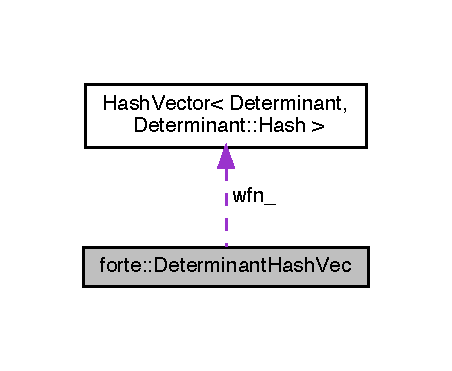
\includegraphics[width=217pt]{classforte_1_1_determinant_hash_vec__coll__graph}
\end{center}
\end{figure}
\subsection*{Public Member Functions}
\begin{DoxyCompactItemize}
\item 
\mbox{\hyperlink{classforte_1_1_determinant_hash_vec_aa09d2d81e23e9a1cdfbc6b595bb46a14}{Determinant\+Hash\+Vec}} (std\+::vector$<$ \mbox{\hyperlink{namespaceforte_a2076c63fd7b8732004d9e1442ce527c1}{Determinant}} $>$ \&dets)
\begin{DoxyCompactList}\small\item\em Default constructor. \end{DoxyCompactList}\item 
\mbox{\hyperlink{classforte_1_1_determinant_hash_vec_a70682499ebdecf59a21a65536bef6419}{Determinant\+Hash\+Vec}} (const std\+::vector$<$ \mbox{\hyperlink{namespaceforte_a2076c63fd7b8732004d9e1442ce527c1}{Determinant}} $>$ \&dets)
\begin{DoxyCompactList}\small\item\em Default constructor. \end{DoxyCompactList}\item 
\mbox{\hyperlink{classforte_1_1_determinant_hash_vec_a2ab88d1ebf6df4232f3a3d89470c2cab}{Determinant\+Hash\+Vec}} (\mbox{\hyperlink{namespaceforte_a2076c63fd7b8732004d9e1442ce527c1}{Determinant}} \&det)
\begin{DoxyCompactList}\small\item\em Default constructor. \end{DoxyCompactList}\item 
\mbox{\hyperlink{classforte_1_1_determinant_hash_vec_ac5f95a20bc269024fc948691b0326fc4}{Determinant\+Hash\+Vec}} ()
\begin{DoxyCompactList}\small\item\em Empty constructor. \end{DoxyCompactList}\item 
\mbox{\hyperlink{classforte_1_1_determinant_hash_vec_a3cd276dee3ee8a023104f1dc0224e941}{Determinant\+Hash\+Vec}} (const \mbox{\hyperlink{namespaceforte_aee00ff2f656f0aa613d3f9f1ba01cad5}{det\+\_\+hashvec}} \&\mbox{\hyperlink{classforte_1_1_determinant_hash_vec_abbbb485c33b1f107c3cafef27cdf5215}{wfn\+\_\+}})
\begin{DoxyCompactList}\small\item\em Copy constructor. \end{DoxyCompactList}\item 
\mbox{\hyperlink{classforte_1_1_determinant_hash_vec_adda0ea8d50023e6b89493b3cd294ee10}{Determinant\+Hash\+Vec}} (\mbox{\hyperlink{namespaceforte_aee00ff2f656f0aa613d3f9f1ba01cad5}{det\+\_\+hashvec}} \&\&\mbox{\hyperlink{classforte_1_1_determinant_hash_vec_abbbb485c33b1f107c3cafef27cdf5215}{wfn\+\_\+}})
\begin{DoxyCompactList}\small\item\em Move constructor. \end{DoxyCompactList}\item 
const \mbox{\hyperlink{namespaceforte_aee00ff2f656f0aa613d3f9f1ba01cad5}{det\+\_\+hashvec}} \& \mbox{\hyperlink{classforte_1_1_determinant_hash_vec_a9fa3a1a6f30ffd78e70e5a6a23990273}{wfn\+\_\+hash}} () const
\item 
\mbox{\hyperlink{namespaceforte_aee00ff2f656f0aa613d3f9f1ba01cad5}{det\+\_\+hashvec}} \& \mbox{\hyperlink{classforte_1_1_determinant_hash_vec_add576b2713d10d0449dd0cd7b38c7c38}{wfn\+\_\+hash}} ()
\item 
void \mbox{\hyperlink{classforte_1_1_determinant_hash_vec_a704d0c4af99bc018e01e96ca8ae8c9db}{add}} (const \mbox{\hyperlink{namespaceforte_a2076c63fd7b8732004d9e1442ce527c1}{Determinant}} \&det)
\begin{DoxyCompactList}\small\item\em Add a determinant. \end{DoxyCompactList}\item 
size\+\_\+t \mbox{\hyperlink{classforte_1_1_determinant_hash_vec_a65a00ada6f1529a6e82908a4802f6729}{size}} () const
\begin{DoxyCompactList}\small\item\em Return the number of determinants. \end{DoxyCompactList}\item 
void \mbox{\hyperlink{classforte_1_1_determinant_hash_vec_a0a2110402a7e015c08edae95479cf0b9}{clear}} ()
\item 
const \mbox{\hyperlink{namespaceforte_a2076c63fd7b8732004d9e1442ce527c1}{Determinant}} \& \mbox{\hyperlink{classforte_1_1_determinant_hash_vec_a1e68e5960804d59cac572b41a4d6acee}{get\+\_\+det}} (const size\+\_\+t value) const
\item 
size\+\_\+t \mbox{\hyperlink{classforte_1_1_determinant_hash_vec_a1547252a5e500ecb773d5ddac0368d1e}{get\+\_\+idx}} (const \mbox{\hyperlink{namespaceforte_a2076c63fd7b8732004d9e1442ce527c1}{Determinant}} \&det) const
\item 
std\+::vector$<$ \mbox{\hyperlink{namespaceforte_a2076c63fd7b8732004d9e1442ce527c1}{Determinant}} $>$ \mbox{\hyperlink{classforte_1_1_determinant_hash_vec_a42ada8706abb98122961fc5767be15b6}{determinants}} () const
\item 
std\+::vector$<$ std\+::pair$<$ \mbox{\hyperlink{namespaceforte_a2076c63fd7b8732004d9e1442ce527c1}{Determinant}}, size\+\_\+t $>$ $>$ \mbox{\hyperlink{classforte_1_1_determinant_hash_vec_a4d94caa7afe0fe09cac71bc38b585720}{determinant\+\_\+index\+\_\+pairs}} () const
\begin{DoxyCompactList}\small\item\em Return a vector of the determinants and their indices. \end{DoxyCompactList}\item 
void \mbox{\hyperlink{classforte_1_1_determinant_hash_vec_aadea7fce2c583d922a696093d2888619}{make\+\_\+spin\+\_\+complete}} (int nmo)
\item 
bool \mbox{\hyperlink{classforte_1_1_determinant_hash_vec_a683b6f9a2be21955d7caa0181cf88f77}{has\+\_\+det}} (const \mbox{\hyperlink{namespaceforte_a2076c63fd7b8732004d9e1442ce527c1}{Determinant}} \&det) const
\item 
double \mbox{\hyperlink{classforte_1_1_determinant_hash_vec_ad4f538593c5f1d98da9a73e5462d3bfa}{overlap}} (std\+::vector$<$ double $>$ \&det1\+\_\+evecs, \mbox{\hyperlink{classforte_1_1_determinant_hash_vec}{Determinant\+Hash\+Vec}} \&det2, std\+::shared\+\_\+ptr$<$ psi\+::\+Matrix $>$ det2\+\_\+evecs, int root)
\item 
double \mbox{\hyperlink{classforte_1_1_determinant_hash_vec_a1168daa5c587057db556210cee6504a6}{overlap}} (std\+::shared\+\_\+ptr$<$ psi\+::\+Matrix $>$ det1\+\_\+evecs, int root1, \mbox{\hyperlink{classforte_1_1_determinant_hash_vec}{Determinant\+Hash\+Vec}} \&det2, std\+::shared\+\_\+ptr$<$ psi\+::\+Matrix $>$ det2\+\_\+evecs, int root2)
\item 
void \mbox{\hyperlink{classforte_1_1_determinant_hash_vec_ab45b9bb4b2b10262fb8b5fc0394dd954}{subspace}} (\mbox{\hyperlink{classforte_1_1_determinant_hash_vec}{Determinant\+Hash\+Vec}} \&dets, std\+::shared\+\_\+ptr$<$ psi\+::\+Matrix $>$ evecs, std\+::vector$<$ double $>$ \&new\+\_\+evecs, size\+\_\+t dim, int root)
\item 
void \mbox{\hyperlink{classforte_1_1_determinant_hash_vec_a76bbc710a7fe975f008a5b41cc10f85c}{merge}} (\mbox{\hyperlink{classforte_1_1_determinant_hash_vec}{Determinant\+Hash\+Vec}} \&dets)
\item 
void \mbox{\hyperlink{classforte_1_1_determinant_hash_vec_a1c25ea4516f605640e8c7e134b13aecd}{copy}} (\mbox{\hyperlink{classforte_1_1_determinant_hash_vec}{Determinant\+Hash\+Vec}} \&dets)
\item 
void \mbox{\hyperlink{classforte_1_1_determinant_hash_vec_a03d8f6394ae12862b2e4c782dcab82fa}{swap}} (\mbox{\hyperlink{classforte_1_1_determinant_hash_vec}{Determinant\+Hash\+Vec}} \&dets)
\item 
void \mbox{\hyperlink{classforte_1_1_determinant_hash_vec_af5b7b59cac7ddccd0c0b595b9bb3e6d2}{swap}} (\mbox{\hyperlink{namespaceforte_aee00ff2f656f0aa613d3f9f1ba01cad5}{det\+\_\+hashvec}} \&dets)
\end{DoxyCompactItemize}
\subsection*{Protected Attributes}
\begin{DoxyCompactItemize}
\item 
\mbox{\hyperlink{namespaceforte_aee00ff2f656f0aa613d3f9f1ba01cad5}{det\+\_\+hashvec}} \mbox{\hyperlink{classforte_1_1_determinant_hash_vec_abbbb485c33b1f107c3cafef27cdf5215}{wfn\+\_\+}}
\begin{DoxyCompactList}\small\item\em A hashvector of determinants. \end{DoxyCompactList}\end{DoxyCompactItemize}


\subsection{Constructor \& Destructor Documentation}
\mbox{\Hypertarget{classforte_1_1_determinant_hash_vec_aa09d2d81e23e9a1cdfbc6b595bb46a14}\label{classforte_1_1_determinant_hash_vec_aa09d2d81e23e9a1cdfbc6b595bb46a14}} 
\index{forte\+::\+Determinant\+Hash\+Vec@{forte\+::\+Determinant\+Hash\+Vec}!Determinant\+Hash\+Vec@{Determinant\+Hash\+Vec}}
\index{Determinant\+Hash\+Vec@{Determinant\+Hash\+Vec}!forte\+::\+Determinant\+Hash\+Vec@{forte\+::\+Determinant\+Hash\+Vec}}
\subsubsection{\texorpdfstring{Determinant\+Hash\+Vec()}{DeterminantHashVec()}\hspace{0.1cm}{\footnotesize\ttfamily [1/6]}}
{\footnotesize\ttfamily forte\+::\+Determinant\+Hash\+Vec\+::\+Determinant\+Hash\+Vec (\begin{DoxyParamCaption}\item[{std\+::vector$<$ \mbox{\hyperlink{namespaceforte_a2076c63fd7b8732004d9e1442ce527c1}{Determinant}} $>$ \&}]{dets }\end{DoxyParamCaption})}



Default constructor. 

\mbox{\Hypertarget{classforte_1_1_determinant_hash_vec_a70682499ebdecf59a21a65536bef6419}\label{classforte_1_1_determinant_hash_vec_a70682499ebdecf59a21a65536bef6419}} 
\index{forte\+::\+Determinant\+Hash\+Vec@{forte\+::\+Determinant\+Hash\+Vec}!Determinant\+Hash\+Vec@{Determinant\+Hash\+Vec}}
\index{Determinant\+Hash\+Vec@{Determinant\+Hash\+Vec}!forte\+::\+Determinant\+Hash\+Vec@{forte\+::\+Determinant\+Hash\+Vec}}
\subsubsection{\texorpdfstring{Determinant\+Hash\+Vec()}{DeterminantHashVec()}\hspace{0.1cm}{\footnotesize\ttfamily [2/6]}}
{\footnotesize\ttfamily forte\+::\+Determinant\+Hash\+Vec\+::\+Determinant\+Hash\+Vec (\begin{DoxyParamCaption}\item[{const std\+::vector$<$ \mbox{\hyperlink{namespaceforte_a2076c63fd7b8732004d9e1442ce527c1}{Determinant}} $>$ \&}]{dets }\end{DoxyParamCaption})}



Default constructor. 

\mbox{\Hypertarget{classforte_1_1_determinant_hash_vec_a2ab88d1ebf6df4232f3a3d89470c2cab}\label{classforte_1_1_determinant_hash_vec_a2ab88d1ebf6df4232f3a3d89470c2cab}} 
\index{forte\+::\+Determinant\+Hash\+Vec@{forte\+::\+Determinant\+Hash\+Vec}!Determinant\+Hash\+Vec@{Determinant\+Hash\+Vec}}
\index{Determinant\+Hash\+Vec@{Determinant\+Hash\+Vec}!forte\+::\+Determinant\+Hash\+Vec@{forte\+::\+Determinant\+Hash\+Vec}}
\subsubsection{\texorpdfstring{Determinant\+Hash\+Vec()}{DeterminantHashVec()}\hspace{0.1cm}{\footnotesize\ttfamily [3/6]}}
{\footnotesize\ttfamily forte\+::\+Determinant\+Hash\+Vec\+::\+Determinant\+Hash\+Vec (\begin{DoxyParamCaption}\item[{\mbox{\hyperlink{namespaceforte_a2076c63fd7b8732004d9e1442ce527c1}{Determinant}} \&}]{det }\end{DoxyParamCaption})}



Default constructor. 

\mbox{\Hypertarget{classforte_1_1_determinant_hash_vec_ac5f95a20bc269024fc948691b0326fc4}\label{classforte_1_1_determinant_hash_vec_ac5f95a20bc269024fc948691b0326fc4}} 
\index{forte\+::\+Determinant\+Hash\+Vec@{forte\+::\+Determinant\+Hash\+Vec}!Determinant\+Hash\+Vec@{Determinant\+Hash\+Vec}}
\index{Determinant\+Hash\+Vec@{Determinant\+Hash\+Vec}!forte\+::\+Determinant\+Hash\+Vec@{forte\+::\+Determinant\+Hash\+Vec}}
\subsubsection{\texorpdfstring{Determinant\+Hash\+Vec()}{DeterminantHashVec()}\hspace{0.1cm}{\footnotesize\ttfamily [4/6]}}
{\footnotesize\ttfamily forte\+::\+Determinant\+Hash\+Vec\+::\+Determinant\+Hash\+Vec (\begin{DoxyParamCaption}{ }\end{DoxyParamCaption})}



Empty constructor. 

\mbox{\Hypertarget{classforte_1_1_determinant_hash_vec_a3cd276dee3ee8a023104f1dc0224e941}\label{classforte_1_1_determinant_hash_vec_a3cd276dee3ee8a023104f1dc0224e941}} 
\index{forte\+::\+Determinant\+Hash\+Vec@{forte\+::\+Determinant\+Hash\+Vec}!Determinant\+Hash\+Vec@{Determinant\+Hash\+Vec}}
\index{Determinant\+Hash\+Vec@{Determinant\+Hash\+Vec}!forte\+::\+Determinant\+Hash\+Vec@{forte\+::\+Determinant\+Hash\+Vec}}
\subsubsection{\texorpdfstring{Determinant\+Hash\+Vec()}{DeterminantHashVec()}\hspace{0.1cm}{\footnotesize\ttfamily [5/6]}}
{\footnotesize\ttfamily forte\+::\+Determinant\+Hash\+Vec\+::\+Determinant\+Hash\+Vec (\begin{DoxyParamCaption}\item[{const \mbox{\hyperlink{namespaceforte_aee00ff2f656f0aa613d3f9f1ba01cad5}{det\+\_\+hashvec}} \&}]{wfn\+\_\+ }\end{DoxyParamCaption})}



Copy constructor. 

\mbox{\Hypertarget{classforte_1_1_determinant_hash_vec_adda0ea8d50023e6b89493b3cd294ee10}\label{classforte_1_1_determinant_hash_vec_adda0ea8d50023e6b89493b3cd294ee10}} 
\index{forte\+::\+Determinant\+Hash\+Vec@{forte\+::\+Determinant\+Hash\+Vec}!Determinant\+Hash\+Vec@{Determinant\+Hash\+Vec}}
\index{Determinant\+Hash\+Vec@{Determinant\+Hash\+Vec}!forte\+::\+Determinant\+Hash\+Vec@{forte\+::\+Determinant\+Hash\+Vec}}
\subsubsection{\texorpdfstring{Determinant\+Hash\+Vec()}{DeterminantHashVec()}\hspace{0.1cm}{\footnotesize\ttfamily [6/6]}}
{\footnotesize\ttfamily forte\+::\+Determinant\+Hash\+Vec\+::\+Determinant\+Hash\+Vec (\begin{DoxyParamCaption}\item[{\mbox{\hyperlink{namespaceforte_aee00ff2f656f0aa613d3f9f1ba01cad5}{det\+\_\+hashvec}} \&\&}]{wfn\+\_\+ }\end{DoxyParamCaption})}



Move constructor. 



\subsection{Member Function Documentation}
\mbox{\Hypertarget{classforte_1_1_determinant_hash_vec_a704d0c4af99bc018e01e96ca8ae8c9db}\label{classforte_1_1_determinant_hash_vec_a704d0c4af99bc018e01e96ca8ae8c9db}} 
\index{forte\+::\+Determinant\+Hash\+Vec@{forte\+::\+Determinant\+Hash\+Vec}!add@{add}}
\index{add@{add}!forte\+::\+Determinant\+Hash\+Vec@{forte\+::\+Determinant\+Hash\+Vec}}
\subsubsection{\texorpdfstring{add()}{add()}}
{\footnotesize\ttfamily void forte\+::\+Determinant\+Hash\+Vec\+::add (\begin{DoxyParamCaption}\item[{const \mbox{\hyperlink{namespaceforte_a2076c63fd7b8732004d9e1442ce527c1}{Determinant}} \&}]{det }\end{DoxyParamCaption})}



Add a determinant. 

\mbox{\Hypertarget{classforte_1_1_determinant_hash_vec_a0a2110402a7e015c08edae95479cf0b9}\label{classforte_1_1_determinant_hash_vec_a0a2110402a7e015c08edae95479cf0b9}} 
\index{forte\+::\+Determinant\+Hash\+Vec@{forte\+::\+Determinant\+Hash\+Vec}!clear@{clear}}
\index{clear@{clear}!forte\+::\+Determinant\+Hash\+Vec@{forte\+::\+Determinant\+Hash\+Vec}}
\subsubsection{\texorpdfstring{clear()}{clear()}}
{\footnotesize\ttfamily void forte\+::\+Determinant\+Hash\+Vec\+::clear (\begin{DoxyParamCaption}{ }\end{DoxyParamCaption})}

\mbox{\Hypertarget{classforte_1_1_determinant_hash_vec_a1c25ea4516f605640e8c7e134b13aecd}\label{classforte_1_1_determinant_hash_vec_a1c25ea4516f605640e8c7e134b13aecd}} 
\index{forte\+::\+Determinant\+Hash\+Vec@{forte\+::\+Determinant\+Hash\+Vec}!copy@{copy}}
\index{copy@{copy}!forte\+::\+Determinant\+Hash\+Vec@{forte\+::\+Determinant\+Hash\+Vec}}
\subsubsection{\texorpdfstring{copy()}{copy()}}
{\footnotesize\ttfamily void forte\+::\+Determinant\+Hash\+Vec\+::copy (\begin{DoxyParamCaption}\item[{\mbox{\hyperlink{classforte_1_1_determinant_hash_vec}{Determinant\+Hash\+Vec}} \&}]{dets }\end{DoxyParamCaption})}

\mbox{\Hypertarget{classforte_1_1_determinant_hash_vec_a4d94caa7afe0fe09cac71bc38b585720}\label{classforte_1_1_determinant_hash_vec_a4d94caa7afe0fe09cac71bc38b585720}} 
\index{forte\+::\+Determinant\+Hash\+Vec@{forte\+::\+Determinant\+Hash\+Vec}!determinant\+\_\+index\+\_\+pairs@{determinant\+\_\+index\+\_\+pairs}}
\index{determinant\+\_\+index\+\_\+pairs@{determinant\+\_\+index\+\_\+pairs}!forte\+::\+Determinant\+Hash\+Vec@{forte\+::\+Determinant\+Hash\+Vec}}
\subsubsection{\texorpdfstring{determinant\+\_\+index\+\_\+pairs()}{determinant\_index\_pairs()}}
{\footnotesize\ttfamily std\+::vector$<$ std\+::pair$<$ \mbox{\hyperlink{namespaceforte_a2076c63fd7b8732004d9e1442ce527c1}{Determinant}}, size\+\_\+t $>$ $>$ forte\+::\+Determinant\+Hash\+Vec\+::determinant\+\_\+index\+\_\+pairs (\begin{DoxyParamCaption}{ }\end{DoxyParamCaption}) const}



Return a vector of the determinants and their indices. 

\mbox{\Hypertarget{classforte_1_1_determinant_hash_vec_a42ada8706abb98122961fc5767be15b6}\label{classforte_1_1_determinant_hash_vec_a42ada8706abb98122961fc5767be15b6}} 
\index{forte\+::\+Determinant\+Hash\+Vec@{forte\+::\+Determinant\+Hash\+Vec}!determinants@{determinants}}
\index{determinants@{determinants}!forte\+::\+Determinant\+Hash\+Vec@{forte\+::\+Determinant\+Hash\+Vec}}
\subsubsection{\texorpdfstring{determinants()}{determinants()}}
{\footnotesize\ttfamily std\+::vector$<$ \mbox{\hyperlink{namespaceforte_a2076c63fd7b8732004d9e1442ce527c1}{Determinant}} $>$ forte\+::\+Determinant\+Hash\+Vec\+::determinants (\begin{DoxyParamCaption}{ }\end{DoxyParamCaption}) const}

\mbox{\Hypertarget{classforte_1_1_determinant_hash_vec_a1e68e5960804d59cac572b41a4d6acee}\label{classforte_1_1_determinant_hash_vec_a1e68e5960804d59cac572b41a4d6acee}} 
\index{forte\+::\+Determinant\+Hash\+Vec@{forte\+::\+Determinant\+Hash\+Vec}!get\+\_\+det@{get\+\_\+det}}
\index{get\+\_\+det@{get\+\_\+det}!forte\+::\+Determinant\+Hash\+Vec@{forte\+::\+Determinant\+Hash\+Vec}}
\subsubsection{\texorpdfstring{get\+\_\+det()}{get\_det()}}
{\footnotesize\ttfamily const \mbox{\hyperlink{namespaceforte_a2076c63fd7b8732004d9e1442ce527c1}{Determinant}} \& forte\+::\+Determinant\+Hash\+Vec\+::get\+\_\+det (\begin{DoxyParamCaption}\item[{const size\+\_\+t}]{value }\end{DoxyParamCaption}) const}

\mbox{\Hypertarget{classforte_1_1_determinant_hash_vec_a1547252a5e500ecb773d5ddac0368d1e}\label{classforte_1_1_determinant_hash_vec_a1547252a5e500ecb773d5ddac0368d1e}} 
\index{forte\+::\+Determinant\+Hash\+Vec@{forte\+::\+Determinant\+Hash\+Vec}!get\+\_\+idx@{get\+\_\+idx}}
\index{get\+\_\+idx@{get\+\_\+idx}!forte\+::\+Determinant\+Hash\+Vec@{forte\+::\+Determinant\+Hash\+Vec}}
\subsubsection{\texorpdfstring{get\+\_\+idx()}{get\_idx()}}
{\footnotesize\ttfamily size\+\_\+t forte\+::\+Determinant\+Hash\+Vec\+::get\+\_\+idx (\begin{DoxyParamCaption}\item[{const \mbox{\hyperlink{namespaceforte_a2076c63fd7b8732004d9e1442ce527c1}{Determinant}} \&}]{det }\end{DoxyParamCaption}) const}

\mbox{\Hypertarget{classforte_1_1_determinant_hash_vec_a683b6f9a2be21955d7caa0181cf88f77}\label{classforte_1_1_determinant_hash_vec_a683b6f9a2be21955d7caa0181cf88f77}} 
\index{forte\+::\+Determinant\+Hash\+Vec@{forte\+::\+Determinant\+Hash\+Vec}!has\+\_\+det@{has\+\_\+det}}
\index{has\+\_\+det@{has\+\_\+det}!forte\+::\+Determinant\+Hash\+Vec@{forte\+::\+Determinant\+Hash\+Vec}}
\subsubsection{\texorpdfstring{has\+\_\+det()}{has\_det()}}
{\footnotesize\ttfamily bool forte\+::\+Determinant\+Hash\+Vec\+::has\+\_\+det (\begin{DoxyParamCaption}\item[{const \mbox{\hyperlink{namespaceforte_a2076c63fd7b8732004d9e1442ce527c1}{Determinant}} \&}]{det }\end{DoxyParamCaption}) const}

\mbox{\Hypertarget{classforte_1_1_determinant_hash_vec_aadea7fce2c583d922a696093d2888619}\label{classforte_1_1_determinant_hash_vec_aadea7fce2c583d922a696093d2888619}} 
\index{forte\+::\+Determinant\+Hash\+Vec@{forte\+::\+Determinant\+Hash\+Vec}!make\+\_\+spin\+\_\+complete@{make\+\_\+spin\+\_\+complete}}
\index{make\+\_\+spin\+\_\+complete@{make\+\_\+spin\+\_\+complete}!forte\+::\+Determinant\+Hash\+Vec@{forte\+::\+Determinant\+Hash\+Vec}}
\subsubsection{\texorpdfstring{make\+\_\+spin\+\_\+complete()}{make\_spin\_complete()}}
{\footnotesize\ttfamily void forte\+::\+Determinant\+Hash\+Vec\+::make\+\_\+spin\+\_\+complete (\begin{DoxyParamCaption}\item[{int}]{nmo }\end{DoxyParamCaption})}

\mbox{\Hypertarget{classforte_1_1_determinant_hash_vec_a76bbc710a7fe975f008a5b41cc10f85c}\label{classforte_1_1_determinant_hash_vec_a76bbc710a7fe975f008a5b41cc10f85c}} 
\index{forte\+::\+Determinant\+Hash\+Vec@{forte\+::\+Determinant\+Hash\+Vec}!merge@{merge}}
\index{merge@{merge}!forte\+::\+Determinant\+Hash\+Vec@{forte\+::\+Determinant\+Hash\+Vec}}
\subsubsection{\texorpdfstring{merge()}{merge()}}
{\footnotesize\ttfamily void forte\+::\+Determinant\+Hash\+Vec\+::merge (\begin{DoxyParamCaption}\item[{\mbox{\hyperlink{classforte_1_1_determinant_hash_vec}{Determinant\+Hash\+Vec}} \&}]{dets }\end{DoxyParamCaption})}

\mbox{\Hypertarget{classforte_1_1_determinant_hash_vec_ad4f538593c5f1d98da9a73e5462d3bfa}\label{classforte_1_1_determinant_hash_vec_ad4f538593c5f1d98da9a73e5462d3bfa}} 
\index{forte\+::\+Determinant\+Hash\+Vec@{forte\+::\+Determinant\+Hash\+Vec}!overlap@{overlap}}
\index{overlap@{overlap}!forte\+::\+Determinant\+Hash\+Vec@{forte\+::\+Determinant\+Hash\+Vec}}
\subsubsection{\texorpdfstring{overlap()}{overlap()}\hspace{0.1cm}{\footnotesize\ttfamily [1/2]}}
{\footnotesize\ttfamily double forte\+::\+Determinant\+Hash\+Vec\+::overlap (\begin{DoxyParamCaption}\item[{std\+::vector$<$ double $>$ \&}]{det1\+\_\+evecs,  }\item[{\mbox{\hyperlink{classforte_1_1_determinant_hash_vec}{Determinant\+Hash\+Vec}} \&}]{det2,  }\item[{std\+::shared\+\_\+ptr$<$ psi\+::\+Matrix $>$}]{det2\+\_\+evecs,  }\item[{int}]{root }\end{DoxyParamCaption})}

\mbox{\Hypertarget{classforte_1_1_determinant_hash_vec_a1168daa5c587057db556210cee6504a6}\label{classforte_1_1_determinant_hash_vec_a1168daa5c587057db556210cee6504a6}} 
\index{forte\+::\+Determinant\+Hash\+Vec@{forte\+::\+Determinant\+Hash\+Vec}!overlap@{overlap}}
\index{overlap@{overlap}!forte\+::\+Determinant\+Hash\+Vec@{forte\+::\+Determinant\+Hash\+Vec}}
\subsubsection{\texorpdfstring{overlap()}{overlap()}\hspace{0.1cm}{\footnotesize\ttfamily [2/2]}}
{\footnotesize\ttfamily double forte\+::\+Determinant\+Hash\+Vec\+::overlap (\begin{DoxyParamCaption}\item[{std\+::shared\+\_\+ptr$<$ psi\+::\+Matrix $>$}]{det1\+\_\+evecs,  }\item[{int}]{root1,  }\item[{\mbox{\hyperlink{classforte_1_1_determinant_hash_vec}{Determinant\+Hash\+Vec}} \&}]{det2,  }\item[{std\+::shared\+\_\+ptr$<$ psi\+::\+Matrix $>$}]{det2\+\_\+evecs,  }\item[{int}]{root2 }\end{DoxyParamCaption})}

\mbox{\Hypertarget{classforte_1_1_determinant_hash_vec_a65a00ada6f1529a6e82908a4802f6729}\label{classforte_1_1_determinant_hash_vec_a65a00ada6f1529a6e82908a4802f6729}} 
\index{forte\+::\+Determinant\+Hash\+Vec@{forte\+::\+Determinant\+Hash\+Vec}!size@{size}}
\index{size@{size}!forte\+::\+Determinant\+Hash\+Vec@{forte\+::\+Determinant\+Hash\+Vec}}
\subsubsection{\texorpdfstring{size()}{size()}}
{\footnotesize\ttfamily size\+\_\+t forte\+::\+Determinant\+Hash\+Vec\+::size (\begin{DoxyParamCaption}{ }\end{DoxyParamCaption}) const}



Return the number of determinants. 

\mbox{\Hypertarget{classforte_1_1_determinant_hash_vec_ab45b9bb4b2b10262fb8b5fc0394dd954}\label{classforte_1_1_determinant_hash_vec_ab45b9bb4b2b10262fb8b5fc0394dd954}} 
\index{forte\+::\+Determinant\+Hash\+Vec@{forte\+::\+Determinant\+Hash\+Vec}!subspace@{subspace}}
\index{subspace@{subspace}!forte\+::\+Determinant\+Hash\+Vec@{forte\+::\+Determinant\+Hash\+Vec}}
\subsubsection{\texorpdfstring{subspace()}{subspace()}}
{\footnotesize\ttfamily void forte\+::\+Determinant\+Hash\+Vec\+::subspace (\begin{DoxyParamCaption}\item[{\mbox{\hyperlink{classforte_1_1_determinant_hash_vec}{Determinant\+Hash\+Vec}} \&}]{dets,  }\item[{std\+::shared\+\_\+ptr$<$ psi\+::\+Matrix $>$}]{evecs,  }\item[{std\+::vector$<$ double $>$ \&}]{new\+\_\+evecs,  }\item[{size\+\_\+t}]{dim,  }\item[{int}]{root }\end{DoxyParamCaption})}

\mbox{\Hypertarget{classforte_1_1_determinant_hash_vec_a03d8f6394ae12862b2e4c782dcab82fa}\label{classforte_1_1_determinant_hash_vec_a03d8f6394ae12862b2e4c782dcab82fa}} 
\index{forte\+::\+Determinant\+Hash\+Vec@{forte\+::\+Determinant\+Hash\+Vec}!swap@{swap}}
\index{swap@{swap}!forte\+::\+Determinant\+Hash\+Vec@{forte\+::\+Determinant\+Hash\+Vec}}
\subsubsection{\texorpdfstring{swap()}{swap()}\hspace{0.1cm}{\footnotesize\ttfamily [1/2]}}
{\footnotesize\ttfamily void forte\+::\+Determinant\+Hash\+Vec\+::swap (\begin{DoxyParamCaption}\item[{\mbox{\hyperlink{classforte_1_1_determinant_hash_vec}{Determinant\+Hash\+Vec}} \&}]{dets }\end{DoxyParamCaption})}

\mbox{\Hypertarget{classforte_1_1_determinant_hash_vec_af5b7b59cac7ddccd0c0b595b9bb3e6d2}\label{classforte_1_1_determinant_hash_vec_af5b7b59cac7ddccd0c0b595b9bb3e6d2}} 
\index{forte\+::\+Determinant\+Hash\+Vec@{forte\+::\+Determinant\+Hash\+Vec}!swap@{swap}}
\index{swap@{swap}!forte\+::\+Determinant\+Hash\+Vec@{forte\+::\+Determinant\+Hash\+Vec}}
\subsubsection{\texorpdfstring{swap()}{swap()}\hspace{0.1cm}{\footnotesize\ttfamily [2/2]}}
{\footnotesize\ttfamily void forte\+::\+Determinant\+Hash\+Vec\+::swap (\begin{DoxyParamCaption}\item[{\mbox{\hyperlink{namespaceforte_aee00ff2f656f0aa613d3f9f1ba01cad5}{det\+\_\+hashvec}} \&}]{dets }\end{DoxyParamCaption})}

\mbox{\Hypertarget{classforte_1_1_determinant_hash_vec_a9fa3a1a6f30ffd78e70e5a6a23990273}\label{classforte_1_1_determinant_hash_vec_a9fa3a1a6f30ffd78e70e5a6a23990273}} 
\index{forte\+::\+Determinant\+Hash\+Vec@{forte\+::\+Determinant\+Hash\+Vec}!wfn\+\_\+hash@{wfn\+\_\+hash}}
\index{wfn\+\_\+hash@{wfn\+\_\+hash}!forte\+::\+Determinant\+Hash\+Vec@{forte\+::\+Determinant\+Hash\+Vec}}
\subsubsection{\texorpdfstring{wfn\+\_\+hash()}{wfn\_hash()}\hspace{0.1cm}{\footnotesize\ttfamily [1/2]}}
{\footnotesize\ttfamily const \mbox{\hyperlink{namespaceforte_aee00ff2f656f0aa613d3f9f1ba01cad5}{det\+\_\+hashvec}} \& forte\+::\+Determinant\+Hash\+Vec\+::wfn\+\_\+hash (\begin{DoxyParamCaption}{ }\end{DoxyParamCaption}) const}

\begin{DoxyReturn}{Returns}
The hash 
\end{DoxyReturn}
\mbox{\Hypertarget{classforte_1_1_determinant_hash_vec_add576b2713d10d0449dd0cd7b38c7c38}\label{classforte_1_1_determinant_hash_vec_add576b2713d10d0449dd0cd7b38c7c38}} 
\index{forte\+::\+Determinant\+Hash\+Vec@{forte\+::\+Determinant\+Hash\+Vec}!wfn\+\_\+hash@{wfn\+\_\+hash}}
\index{wfn\+\_\+hash@{wfn\+\_\+hash}!forte\+::\+Determinant\+Hash\+Vec@{forte\+::\+Determinant\+Hash\+Vec}}
\subsubsection{\texorpdfstring{wfn\+\_\+hash()}{wfn\_hash()}\hspace{0.1cm}{\footnotesize\ttfamily [2/2]}}
{\footnotesize\ttfamily \mbox{\hyperlink{namespaceforte_aee00ff2f656f0aa613d3f9f1ba01cad5}{det\+\_\+hashvec}} \& forte\+::\+Determinant\+Hash\+Vec\+::wfn\+\_\+hash (\begin{DoxyParamCaption}{ }\end{DoxyParamCaption})}

\begin{DoxyReturn}{Returns}
The hash 
\end{DoxyReturn}


\subsection{Member Data Documentation}
\mbox{\Hypertarget{classforte_1_1_determinant_hash_vec_abbbb485c33b1f107c3cafef27cdf5215}\label{classforte_1_1_determinant_hash_vec_abbbb485c33b1f107c3cafef27cdf5215}} 
\index{forte\+::\+Determinant\+Hash\+Vec@{forte\+::\+Determinant\+Hash\+Vec}!wfn\+\_\+@{wfn\+\_\+}}
\index{wfn\+\_\+@{wfn\+\_\+}!forte\+::\+Determinant\+Hash\+Vec@{forte\+::\+Determinant\+Hash\+Vec}}
\subsubsection{\texorpdfstring{wfn\+\_\+}{wfn\_}}
{\footnotesize\ttfamily \mbox{\hyperlink{namespaceforte_aee00ff2f656f0aa613d3f9f1ba01cad5}{det\+\_\+hashvec}} forte\+::\+Determinant\+Hash\+Vec\+::wfn\+\_\+\hspace{0.3cm}{\ttfamily [protected]}}



A hashvector of determinants. 



The documentation for this class was generated from the following files\+:\begin{DoxyCompactItemize}
\item 
/\+Users/fevange/\+Source/forte/src/sparse\+\_\+ci/\mbox{\hyperlink{determinant__hashvector_8h}{determinant\+\_\+hashvector.\+h}}\item 
/\+Users/fevange/\+Source/forte/src/sparse\+\_\+ci/\mbox{\hyperlink{determinant__hashvector_8cc}{determinant\+\_\+hashvector.\+cc}}\end{DoxyCompactItemize}

\hypertarget{classforte_1_1_determinant_impl}{}\section{forte\+:\+:Determinant\+Impl$<$ N $>$ Class Template Reference}
\label{classforte_1_1_determinant_impl}\index{forte\+::\+Determinant\+Impl$<$ N $>$@{forte\+::\+Determinant\+Impl$<$ N $>$}}


A class to represent a Slater determinant with N spin orbitals.  




{\ttfamily \#include $<$determinant.\+hpp$>$}



Inheritance diagram for forte\+:\+:Determinant\+Impl$<$ N $>$\+:
\nopagebreak
\begin{figure}[H]
\begin{center}
\leavevmode
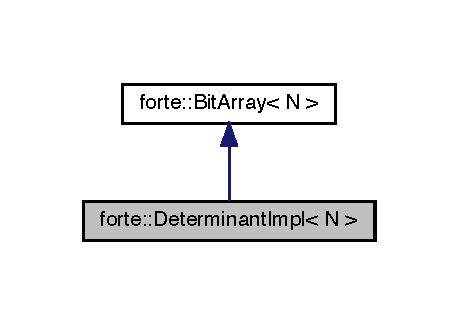
\includegraphics[width=220pt]{classforte_1_1_determinant_impl__inherit__graph}
\end{center}
\end{figure}


Collaboration diagram for forte\+:\+:Determinant\+Impl$<$ N $>$\+:
\nopagebreak
\begin{figure}[H]
\begin{center}
\leavevmode
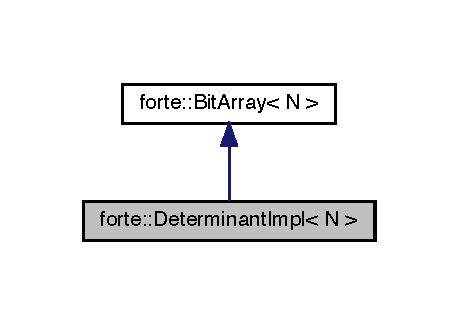
\includegraphics[width=220pt]{classforte_1_1_determinant_impl__coll__graph}
\end{center}
\end{figure}
\subsection*{Public Member Functions}
\begin{DoxyCompactItemize}
\item 
size\+\_\+t \mbox{\hyperlink{classforte_1_1_determinant_impl_afc9e7b4d9b3ec24a97ca3793272ce595}{get\+\_\+nbits\+\_\+half}} () const
\begin{DoxyCompactList}\small\item\em returns half the number of bits \end{DoxyCompactList}\item 
\mbox{\hyperlink{classforte_1_1_determinant_impl_a7c8dfa806c2a2991024ae0fd2c041616}{Determinant\+Impl}} ()
\begin{DoxyCompactList}\small\item\em Default constructor. \end{DoxyCompactList}\item 
\mbox{\hyperlink{classforte_1_1_determinant_impl_a007afc997d612ea68ef4760d56617bf5}{Determinant\+Impl}} (const \mbox{\hyperlink{classforte_1_1_bit_array}{Bit\+Array}}$<$ N $>$ \&ba)
\begin{DoxyCompactList}\small\item\em Constructor from a bit array. \end{DoxyCompactList}\item 
\mbox{\hyperlink{classforte_1_1_determinant_impl_a45a02db5e268e7e2c2978bd105f571b3}{Determinant\+Impl}} (const std\+::vector$<$ bool $>$ \&occupation\+\_\+a, const std\+::vector$<$ bool $>$ \&occupation\+\_\+b)
\item 
\mbox{\hyperlink{classforte_1_1_determinant_impl_a85f7530da66f7fb1a649be1ad69b0e94}{Determinant\+Impl}} (const std\+::string \&\mbox{\hyperlink{namespaceforte_af0f9481a38ad3ccb1dd258bdfea20492}{str}})
\item 
bool \mbox{\hyperlink{classforte_1_1_determinant_impl_a14a47fa6165d685967ce1c8554c7d3cc}{get\+\_\+alfa\+\_\+bit}} (size\+\_\+t pos) const
\begin{DoxyCompactList}\small\item\em get the value of alfa bit pos \end{DoxyCompactList}\item 
bool \mbox{\hyperlink{classforte_1_1_determinant_impl_a7105d98744e76588e9db2797e12c8406}{get\+\_\+beta\+\_\+bit}} (size\+\_\+t pos) const
\begin{DoxyCompactList}\small\item\em get the value of beta bit pos \end{DoxyCompactList}\item 
void \mbox{\hyperlink{classforte_1_1_determinant_impl_aed8c6eaece3cce82a5acf459013b7b23}{set\+\_\+alfa\+\_\+bit}} (size\+\_\+t pos, bool val)
\begin{DoxyCompactList}\small\item\em set alfa bit pos to val \end{DoxyCompactList}\item 
void \mbox{\hyperlink{classforte_1_1_determinant_impl_a47f0329c3d05f3aa9785b8bb0b2a55a5}{set\+\_\+beta\+\_\+bit}} (size\+\_\+t pos, bool val)
\begin{DoxyCompactList}\small\item\em set beta bit pos to val \end{DoxyCompactList}\item 
std\+::vector$<$ int $>$ \mbox{\hyperlink{classforte_1_1_determinant_impl_afb3ba3c94638a83e137e5ee275bc7001}{get\+\_\+alfa\+\_\+occ}} (int norb) const
\begin{DoxyCompactList}\small\item\em Return a vector of occupied alpha orbitals. \end{DoxyCompactList}\item 
std\+::vector$<$ int $>$ \mbox{\hyperlink{classforte_1_1_determinant_impl_ab87b65035dc9cd5c48d9fc709702e8c8}{get\+\_\+beta\+\_\+occ}} (int norb) const
\begin{DoxyCompactList}\small\item\em Return a vector of occupied beta orbitals. \end{DoxyCompactList}\item 
std\+::vector$<$ int $>$ \mbox{\hyperlink{classforte_1_1_determinant_impl_a1dc3bb02e9944e3c83d98052c91fe44c}{get\+\_\+alfa\+\_\+vir}} (int norb) const
\begin{DoxyCompactList}\small\item\em Return a vector of virtual alpha orbitals. \end{DoxyCompactList}\item 
std\+::vector$<$ int $>$ \mbox{\hyperlink{classforte_1_1_determinant_impl_aabfa5748bf819c5030245fd13dc6115d}{get\+\_\+beta\+\_\+vir}} (int norb) const
\begin{DoxyCompactList}\small\item\em Return a vector of virtual beta orbitals. \end{DoxyCompactList}\item 
double \mbox{\hyperlink{classforte_1_1_determinant_impl_af04a9600e0092df7024fed3a1aa4e5a4}{create\+\_\+alfa\+\_\+bit}} (int n)
\item 
double \mbox{\hyperlink{classforte_1_1_determinant_impl_a029be4ce6d50df77300096e58a83a42f}{create\+\_\+beta\+\_\+bit}} (int n)
\item 
double \mbox{\hyperlink{classforte_1_1_determinant_impl_a01c1ef1e7f640bc18a3e6fa18116d848}{destroy\+\_\+alfa\+\_\+bit}} (int n)
\item 
double \mbox{\hyperlink{classforte_1_1_determinant_impl_ad19fd82d5428c19620d44868984fbd32}{destroy\+\_\+beta\+\_\+bit}} (int n)
\item 
double \mbox{\hyperlink{classforte_1_1_determinant_impl_ae654b55997ceb9a745edbd60a4d6978d}{slater\+\_\+sign\+\_\+a}} (int n) const
\item 
double \mbox{\hyperlink{classforte_1_1_determinant_impl_ad6b9f063782fe2abb85a742f0a223ec1}{slater\+\_\+sign\+\_\+b}} (int n) const
\item 
double \mbox{\hyperlink{classforte_1_1_determinant_impl_abb5dee18e8891364cc6f60f282e5a7f8}{slater\+\_\+sign\+\_\+aa}} (int n, int m) const
\item 
double \mbox{\hyperlink{classforte_1_1_determinant_impl_afa8fce46c2de5e0d65878f49315aeb9f}{slater\+\_\+sign\+\_\+bb}} (int n, int m) const
\item 
double \mbox{\hyperlink{classforte_1_1_determinant_impl_ab1855ca2b1feed1b3733a36c7be64429}{slater\+\_\+sign\+\_\+aaaa}} (int i, int j, int a, int b) const
\item 
double \mbox{\hyperlink{classforte_1_1_determinant_impl_ac169e8423398ef5011450811c61a363b}{slater\+\_\+sign\+\_\+bbbb}} (int i, int j, int a, int b) const
\item 
int \mbox{\hyperlink{classforte_1_1_determinant_impl_abfc420df71d4fa00dcbf239a3b425f62}{count\+\_\+alfa}} () const
\begin{DoxyCompactList}\small\item\em Count the number of beta bits set to 1. \end{DoxyCompactList}\item 
int \mbox{\hyperlink{classforte_1_1_determinant_impl_acd8866f4054bf89589213992668eb3d2}{count\+\_\+beta}} () const
\begin{DoxyCompactList}\small\item\em Count the number of beta bits set to 1. \end{DoxyCompactList}\item 
int \mbox{\hyperlink{classforte_1_1_determinant_impl_ae08fd0456249dc605ba10b095afc2549}{npair}} () const
\begin{DoxyCompactList}\small\item\em Return the number of alpha/beta pairs. \end{DoxyCompactList}\item 
double \mbox{\hyperlink{classforte_1_1_determinant_impl_a29e9efc18d8346cd7e2809a1e9c8f2a9}{single\+\_\+excitation\+\_\+a}} (int i, int a)
\item 
double \mbox{\hyperlink{classforte_1_1_determinant_impl_ade9281e561132e5ea22cc515b051e14b}{single\+\_\+excitation\+\_\+b}} (int i, int a)
\item 
double \mbox{\hyperlink{classforte_1_1_determinant_impl_a2279b78fd6dc7dfdcd0e0a1c7f77b9ac}{double\+\_\+excitation\+\_\+aa}} (int i, int j, int a, int b)
\item 
double \mbox{\hyperlink{classforte_1_1_determinant_impl_ac5c15433d3496bdd90e867bfe396c948}{double\+\_\+excitation\+\_\+ab}} (int i, int j, int a, int b)
\item 
double \mbox{\hyperlink{classforte_1_1_determinant_impl_a1ddb5fecd7e198cfcc6d5bc61a7ca866}{double\+\_\+excitation\+\_\+bb}} (int i, int j, int a, int b)
\begin{DoxyCompactList}\small\item\em Perform an beta-\/beta double excitation (IJ -\/$>$ AB) \end{DoxyCompactList}\item 
\mbox{\hyperlink{classforte_1_1_bit_array}{Bit\+Array}}$<$ \mbox{\hyperlink{classforte_1_1_determinant_impl_ac8d2a64c2fb785ccb79b1cecc553d63d}{nbits\+\_\+half}} $>$ \mbox{\hyperlink{classforte_1_1_determinant_impl_a29ea8ae7c2f083aaa959d9f6f1de9d3c}{get\+\_\+alfa\+\_\+bits}} () const
\item 
\mbox{\hyperlink{classforte_1_1_bit_array}{Bit\+Array}}$<$ \mbox{\hyperlink{classforte_1_1_determinant_impl_ac8d2a64c2fb785ccb79b1cecc553d63d}{nbits\+\_\+half}} $>$ \mbox{\hyperlink{classforte_1_1_determinant_impl_a9109cbc06b0753d030de49786a4d6b22}{get\+\_\+beta\+\_\+bits}} () const
\item 
\mbox{\hyperlink{classforte_1_1_bit_array}{Bit\+Array}}$<$ \mbox{\hyperlink{classforte_1_1_determinant_impl_ac8d2a64c2fb785ccb79b1cecc553d63d}{nbits\+\_\+half}} $>$ \mbox{\hyperlink{classforte_1_1_determinant_impl_a924606ae7e4855ccb197fc3e5bec7028}{get\+\_\+bits}} (\mbox{\hyperlink{namespaceforte_acb88fa63430aae4a1b15c7be9c55f179}{Det\+Spin\+Type}} spin\+\_\+type)
\item 
void \mbox{\hyperlink{classforte_1_1_determinant_impl_a0c84ab17402db250ba4c64c6991a6723}{zero\+\_\+alfa}} ()
\begin{DoxyCompactList}\small\item\em Zero the alpha part of a determinant. \end{DoxyCompactList}\item 
void \mbox{\hyperlink{classforte_1_1_determinant_impl_aeca8e43710bad20561193304aee10c9b}{zero\+\_\+beta}} ()
\begin{DoxyCompactList}\small\item\em Zero the alpha part of a determinant. \end{DoxyCompactList}\end{DoxyCompactItemize}
\subsection*{Static Public Member Functions}
\begin{DoxyCompactItemize}
\item 
static bool \mbox{\hyperlink{classforte_1_1_determinant_impl_afa56e1f10e5d64c959ff0257a9ee8eb0}{less\+\_\+than}} (const \mbox{\hyperlink{classforte_1_1_determinant_impl}{Determinant\+Impl}}$<$ N $>$ \&rhs, const \mbox{\hyperlink{classforte_1_1_determinant_impl}{Determinant\+Impl}}$<$ N $>$ \&lhs)
\item 
static bool \mbox{\hyperlink{classforte_1_1_determinant_impl_a082c139fb3b70315591512bb4d36857f}{reverse\+\_\+less\+\_\+than}} (const \mbox{\hyperlink{classforte_1_1_determinant_impl}{Determinant\+Impl}}$<$ N $>$ \&rhs, const \mbox{\hyperlink{classforte_1_1_determinant_impl}{Determinant\+Impl}}$<$ N $>$ \&lhs)
\end{DoxyCompactItemize}
\subsection*{Static Public Attributes}
\begin{DoxyCompactItemize}
\item 
static constexpr size\+\_\+t \mbox{\hyperlink{classforte_1_1_determinant_impl_ac8d2a64c2fb785ccb79b1cecc553d63d}{nbits\+\_\+half}} = N / 2
\begin{DoxyCompactList}\small\item\em the number of bits divided by two \end{DoxyCompactList}\item 
static constexpr size\+\_\+t \mbox{\hyperlink{classforte_1_1_determinant_impl_a7474c95c308be22daaa9cd26aed8a035}{nwords\+\_\+half}} = \mbox{\hyperlink{classforte_1_1_bit_array}{Bit\+Array}}$<$N$>$\+::\mbox{\hyperlink{classforte_1_1_bit_array_aeaa8016f00f9ffc5822081f7e45656e8}{nwords\+\_\+}} / 2
\begin{DoxyCompactList}\small\item\em half of the words used to store the bits \end{DoxyCompactList}\item 
static constexpr size\+\_\+t \mbox{\hyperlink{classforte_1_1_determinant_impl_aae5a6637a75d4c47513e906c60857f2b}{beta\+\_\+bit\+\_\+offset}} = \mbox{\hyperlink{classforte_1_1_determinant_impl_a7474c95c308be22daaa9cd26aed8a035}{nwords\+\_\+half}} $\ast$ \mbox{\hyperlink{classforte_1_1_bit_array}{Bit\+Array}}$<$N$>$\+::\mbox{\hyperlink{classforte_1_1_bit_array_ad5ca62ac879b44e0e28017a73fd6c3fd}{bits\+\_\+per\+\_\+word}}
\begin{DoxyCompactList}\small\item\em the starting bit for beta orbitals \end{DoxyCompactList}\end{DoxyCompactItemize}
\subsection*{Additional Inherited Members}


\subsection{Detailed Description}
\subsubsection*{template$<$size\+\_\+t N$>$\newline
class forte\+::\+Determinant\+Impl$<$ N $>$}

A class to represent a Slater determinant with N spin orbitals. 

Spin orbitals are divided into N/2 alpha and N/2 beta set. For each set we pack groups of 64 spin orbitals into an array of 64-\/bit unsigned integers. Each group of 64 bits is called a word. Each set of N/2 bits is stored in K = ceil(N/2 / 64) words. So the full determinant is stored as an array of words of the form \mbox{[}word 1\mbox{]}\mbox{[}word 2\mbox{]}...\mbox{[}word K\mbox{]}\mbox{[}word K+1\mbox{]}...\mbox{[}word 2K\mbox{]} 

\subsection{Constructor \& Destructor Documentation}
\mbox{\Hypertarget{classforte_1_1_determinant_impl_a7c8dfa806c2a2991024ae0fd2c041616}\label{classforte_1_1_determinant_impl_a7c8dfa806c2a2991024ae0fd2c041616}} 
\index{forte\+::\+Determinant\+Impl@{forte\+::\+Determinant\+Impl}!Determinant\+Impl@{Determinant\+Impl}}
\index{Determinant\+Impl@{Determinant\+Impl}!forte\+::\+Determinant\+Impl@{forte\+::\+Determinant\+Impl}}
\subsubsection{\texorpdfstring{Determinant\+Impl()}{DeterminantImpl()}\hspace{0.1cm}{\footnotesize\ttfamily [1/4]}}
{\footnotesize\ttfamily template$<$size\+\_\+t N$>$ \\
\mbox{\hyperlink{classforte_1_1_determinant_impl}{forte\+::\+Determinant\+Impl}}$<$ N $>$\+::\mbox{\hyperlink{classforte_1_1_determinant_impl}{Determinant\+Impl}} (\begin{DoxyParamCaption}{ }\end{DoxyParamCaption})\hspace{0.3cm}{\ttfamily [inline]}}



Default constructor. 

\mbox{\Hypertarget{classforte_1_1_determinant_impl_a007afc997d612ea68ef4760d56617bf5}\label{classforte_1_1_determinant_impl_a007afc997d612ea68ef4760d56617bf5}} 
\index{forte\+::\+Determinant\+Impl@{forte\+::\+Determinant\+Impl}!Determinant\+Impl@{Determinant\+Impl}}
\index{Determinant\+Impl@{Determinant\+Impl}!forte\+::\+Determinant\+Impl@{forte\+::\+Determinant\+Impl}}
\subsubsection{\texorpdfstring{Determinant\+Impl()}{DeterminantImpl()}\hspace{0.1cm}{\footnotesize\ttfamily [2/4]}}
{\footnotesize\ttfamily template$<$size\+\_\+t N$>$ \\
\mbox{\hyperlink{classforte_1_1_determinant_impl}{forte\+::\+Determinant\+Impl}}$<$ N $>$\+::\mbox{\hyperlink{classforte_1_1_determinant_impl}{Determinant\+Impl}} (\begin{DoxyParamCaption}\item[{const \mbox{\hyperlink{classforte_1_1_bit_array}{Bit\+Array}}$<$ N $>$ \&}]{ba }\end{DoxyParamCaption})\hspace{0.3cm}{\ttfamily [inline]}}



Constructor from a bit array. 

\mbox{\Hypertarget{classforte_1_1_determinant_impl_a45a02db5e268e7e2c2978bd105f571b3}\label{classforte_1_1_determinant_impl_a45a02db5e268e7e2c2978bd105f571b3}} 
\index{forte\+::\+Determinant\+Impl@{forte\+::\+Determinant\+Impl}!Determinant\+Impl@{Determinant\+Impl}}
\index{Determinant\+Impl@{Determinant\+Impl}!forte\+::\+Determinant\+Impl@{forte\+::\+Determinant\+Impl}}
\subsubsection{\texorpdfstring{Determinant\+Impl()}{DeterminantImpl()}\hspace{0.1cm}{\footnotesize\ttfamily [3/4]}}
{\footnotesize\ttfamily template$<$size\+\_\+t N$>$ \\
\mbox{\hyperlink{classforte_1_1_determinant_impl}{forte\+::\+Determinant\+Impl}}$<$ N $>$\+::\mbox{\hyperlink{classforte_1_1_determinant_impl}{Determinant\+Impl}} (\begin{DoxyParamCaption}\item[{const std\+::vector$<$ bool $>$ \&}]{occupation\+\_\+a,  }\item[{const std\+::vector$<$ bool $>$ \&}]{occupation\+\_\+b }\end{DoxyParamCaption})\hspace{0.3cm}{\ttfamily [inline]}, {\ttfamily [explicit]}}

Construct the determinant from an occupation vector that specifies the alpha and beta strings. occupation = \mbox{[}Ia,Ib\mbox{]} \mbox{\Hypertarget{classforte_1_1_determinant_impl_a85f7530da66f7fb1a649be1ad69b0e94}\label{classforte_1_1_determinant_impl_a85f7530da66f7fb1a649be1ad69b0e94}} 
\index{forte\+::\+Determinant\+Impl@{forte\+::\+Determinant\+Impl}!Determinant\+Impl@{Determinant\+Impl}}
\index{Determinant\+Impl@{Determinant\+Impl}!forte\+::\+Determinant\+Impl@{forte\+::\+Determinant\+Impl}}
\subsubsection{\texorpdfstring{Determinant\+Impl()}{DeterminantImpl()}\hspace{0.1cm}{\footnotesize\ttfamily [4/4]}}
{\footnotesize\ttfamily template$<$size\+\_\+t N$>$ \\
\mbox{\hyperlink{classforte_1_1_determinant_impl}{forte\+::\+Determinant\+Impl}}$<$ N $>$\+::\mbox{\hyperlink{classforte_1_1_determinant_impl}{Determinant\+Impl}} (\begin{DoxyParamCaption}\item[{const std\+::string \&}]{str }\end{DoxyParamCaption})\hspace{0.3cm}{\ttfamily [inline]}}

String constructor. Convert a std\+::string to a determinant. E.\+g. Determinant\+Impl$<$64$>$(\char`\"{}0011\char`\"{}) gives the determinant$\vert$0011$>$ 

\subsection{Member Function Documentation}
\mbox{\Hypertarget{classforte_1_1_determinant_impl_abfc420df71d4fa00dcbf239a3b425f62}\label{classforte_1_1_determinant_impl_abfc420df71d4fa00dcbf239a3b425f62}} 
\index{forte\+::\+Determinant\+Impl@{forte\+::\+Determinant\+Impl}!count\+\_\+alfa@{count\+\_\+alfa}}
\index{count\+\_\+alfa@{count\+\_\+alfa}!forte\+::\+Determinant\+Impl@{forte\+::\+Determinant\+Impl}}
\subsubsection{\texorpdfstring{count\+\_\+alfa()}{count\_alfa()}}
{\footnotesize\ttfamily template$<$size\+\_\+t N$>$ \\
int \mbox{\hyperlink{classforte_1_1_determinant_impl}{forte\+::\+Determinant\+Impl}}$<$ N $>$\+::count\+\_\+alfa (\begin{DoxyParamCaption}{ }\end{DoxyParamCaption}) const\hspace{0.3cm}{\ttfamily [inline]}}



Count the number of beta bits set to 1. 

\mbox{\Hypertarget{classforte_1_1_determinant_impl_acd8866f4054bf89589213992668eb3d2}\label{classforte_1_1_determinant_impl_acd8866f4054bf89589213992668eb3d2}} 
\index{forte\+::\+Determinant\+Impl@{forte\+::\+Determinant\+Impl}!count\+\_\+beta@{count\+\_\+beta}}
\index{count\+\_\+beta@{count\+\_\+beta}!forte\+::\+Determinant\+Impl@{forte\+::\+Determinant\+Impl}}
\subsubsection{\texorpdfstring{count\+\_\+beta()}{count\_beta()}}
{\footnotesize\ttfamily template$<$size\+\_\+t N$>$ \\
int \mbox{\hyperlink{classforte_1_1_determinant_impl}{forte\+::\+Determinant\+Impl}}$<$ N $>$\+::count\+\_\+beta (\begin{DoxyParamCaption}{ }\end{DoxyParamCaption}) const\hspace{0.3cm}{\ttfamily [inline]}}



Count the number of beta bits set to 1. 

\mbox{\Hypertarget{classforte_1_1_determinant_impl_af04a9600e0092df7024fed3a1aa4e5a4}\label{classforte_1_1_determinant_impl_af04a9600e0092df7024fed3a1aa4e5a4}} 
\index{forte\+::\+Determinant\+Impl@{forte\+::\+Determinant\+Impl}!create\+\_\+alfa\+\_\+bit@{create\+\_\+alfa\+\_\+bit}}
\index{create\+\_\+alfa\+\_\+bit@{create\+\_\+alfa\+\_\+bit}!forte\+::\+Determinant\+Impl@{forte\+::\+Determinant\+Impl}}
\subsubsection{\texorpdfstring{create\+\_\+alfa\+\_\+bit()}{create\_alfa\_bit()}}
{\footnotesize\ttfamily template$<$size\+\_\+t N$>$ \\
double \mbox{\hyperlink{classforte_1_1_determinant_impl}{forte\+::\+Determinant\+Impl}}$<$ N $>$\+::create\+\_\+alfa\+\_\+bit (\begin{DoxyParamCaption}\item[{int}]{n }\end{DoxyParamCaption})\hspace{0.3cm}{\ttfamily [inline]}}

Apply the alpha creation operator a$^\wedge$+\+\_\+n to this determinant If orbital n is unoccupied, create the electron and return the sign If orbital n is occupied, do not modify the determinant and return 0 \mbox{\Hypertarget{classforte_1_1_determinant_impl_a029be4ce6d50df77300096e58a83a42f}\label{classforte_1_1_determinant_impl_a029be4ce6d50df77300096e58a83a42f}} 
\index{forte\+::\+Determinant\+Impl@{forte\+::\+Determinant\+Impl}!create\+\_\+beta\+\_\+bit@{create\+\_\+beta\+\_\+bit}}
\index{create\+\_\+beta\+\_\+bit@{create\+\_\+beta\+\_\+bit}!forte\+::\+Determinant\+Impl@{forte\+::\+Determinant\+Impl}}
\subsubsection{\texorpdfstring{create\+\_\+beta\+\_\+bit()}{create\_beta\_bit()}}
{\footnotesize\ttfamily template$<$size\+\_\+t N$>$ \\
double \mbox{\hyperlink{classforte_1_1_determinant_impl}{forte\+::\+Determinant\+Impl}}$<$ N $>$\+::create\+\_\+beta\+\_\+bit (\begin{DoxyParamCaption}\item[{int}]{n }\end{DoxyParamCaption})\hspace{0.3cm}{\ttfamily [inline]}}

Apply the beta creation operator a$^\wedge$+\+\_\+n to this determinant If orbital n is unoccupied, create the electron and return the sign If orbital n is occupied, do not modify the determinant and return 0 \mbox{\Hypertarget{classforte_1_1_determinant_impl_a01c1ef1e7f640bc18a3e6fa18116d848}\label{classforte_1_1_determinant_impl_a01c1ef1e7f640bc18a3e6fa18116d848}} 
\index{forte\+::\+Determinant\+Impl@{forte\+::\+Determinant\+Impl}!destroy\+\_\+alfa\+\_\+bit@{destroy\+\_\+alfa\+\_\+bit}}
\index{destroy\+\_\+alfa\+\_\+bit@{destroy\+\_\+alfa\+\_\+bit}!forte\+::\+Determinant\+Impl@{forte\+::\+Determinant\+Impl}}
\subsubsection{\texorpdfstring{destroy\+\_\+alfa\+\_\+bit()}{destroy\_alfa\_bit()}}
{\footnotesize\ttfamily template$<$size\+\_\+t N$>$ \\
double \mbox{\hyperlink{classforte_1_1_determinant_impl}{forte\+::\+Determinant\+Impl}}$<$ N $>$\+::destroy\+\_\+alfa\+\_\+bit (\begin{DoxyParamCaption}\item[{int}]{n }\end{DoxyParamCaption})\hspace{0.3cm}{\ttfamily [inline]}}

Apply the alpha annihilation operator a$^\wedge$+\+\_\+n to this determinant If orbital n is occupied, annihilate the electron and return the sign If orbital n is unoccupied, do not modify the determinant and return 0 \mbox{\Hypertarget{classforte_1_1_determinant_impl_ad19fd82d5428c19620d44868984fbd32}\label{classforte_1_1_determinant_impl_ad19fd82d5428c19620d44868984fbd32}} 
\index{forte\+::\+Determinant\+Impl@{forte\+::\+Determinant\+Impl}!destroy\+\_\+beta\+\_\+bit@{destroy\+\_\+beta\+\_\+bit}}
\index{destroy\+\_\+beta\+\_\+bit@{destroy\+\_\+beta\+\_\+bit}!forte\+::\+Determinant\+Impl@{forte\+::\+Determinant\+Impl}}
\subsubsection{\texorpdfstring{destroy\+\_\+beta\+\_\+bit()}{destroy\_beta\_bit()}}
{\footnotesize\ttfamily template$<$size\+\_\+t N$>$ \\
double \mbox{\hyperlink{classforte_1_1_determinant_impl}{forte\+::\+Determinant\+Impl}}$<$ N $>$\+::destroy\+\_\+beta\+\_\+bit (\begin{DoxyParamCaption}\item[{int}]{n }\end{DoxyParamCaption})\hspace{0.3cm}{\ttfamily [inline]}}

Apply the beta annihilation operator a$^\wedge$+\+\_\+n to this determinant If orbital n is occupied, annihilate the electron and return the sign If orbital n is unoccupied, do not modify the determinant and return 0 \mbox{\Hypertarget{classforte_1_1_determinant_impl_a2279b78fd6dc7dfdcd0e0a1c7f77b9ac}\label{classforte_1_1_determinant_impl_a2279b78fd6dc7dfdcd0e0a1c7f77b9ac}} 
\index{forte\+::\+Determinant\+Impl@{forte\+::\+Determinant\+Impl}!double\+\_\+excitation\+\_\+aa@{double\+\_\+excitation\+\_\+aa}}
\index{double\+\_\+excitation\+\_\+aa@{double\+\_\+excitation\+\_\+aa}!forte\+::\+Determinant\+Impl@{forte\+::\+Determinant\+Impl}}
\subsubsection{\texorpdfstring{double\+\_\+excitation\+\_\+aa()}{double\_excitation\_aa()}}
{\footnotesize\ttfamily template$<$size\+\_\+t N$>$ \\
double \mbox{\hyperlink{classforte_1_1_determinant_impl}{forte\+::\+Determinant\+Impl}}$<$ N $>$\+::double\+\_\+excitation\+\_\+aa (\begin{DoxyParamCaption}\item[{int}]{i,  }\item[{int}]{j,  }\item[{int}]{a,  }\item[{int}]{b }\end{DoxyParamCaption})\hspace{0.3cm}{\ttfamily [inline]}}

Perform an alpha-\/alpha double excitation (ij-\/$>$ab) assuming that ij are occupied and ab are empty \mbox{\Hypertarget{classforte_1_1_determinant_impl_ac5c15433d3496bdd90e867bfe396c948}\label{classforte_1_1_determinant_impl_ac5c15433d3496bdd90e867bfe396c948}} 
\index{forte\+::\+Determinant\+Impl@{forte\+::\+Determinant\+Impl}!double\+\_\+excitation\+\_\+ab@{double\+\_\+excitation\+\_\+ab}}
\index{double\+\_\+excitation\+\_\+ab@{double\+\_\+excitation\+\_\+ab}!forte\+::\+Determinant\+Impl@{forte\+::\+Determinant\+Impl}}
\subsubsection{\texorpdfstring{double\+\_\+excitation\+\_\+ab()}{double\_excitation\_ab()}}
{\footnotesize\ttfamily template$<$size\+\_\+t N$>$ \\
double \mbox{\hyperlink{classforte_1_1_determinant_impl}{forte\+::\+Determinant\+Impl}}$<$ N $>$\+::double\+\_\+excitation\+\_\+ab (\begin{DoxyParamCaption}\item[{int}]{i,  }\item[{int}]{j,  }\item[{int}]{a,  }\item[{int}]{b }\end{DoxyParamCaption})\hspace{0.3cm}{\ttfamily [inline]}}

Perform an alpha-\/beta double excitation (iJ -\/$>$ aB) /// assuming that ij are occupied and ab are empty \mbox{\Hypertarget{classforte_1_1_determinant_impl_a1ddb5fecd7e198cfcc6d5bc61a7ca866}\label{classforte_1_1_determinant_impl_a1ddb5fecd7e198cfcc6d5bc61a7ca866}} 
\index{forte\+::\+Determinant\+Impl@{forte\+::\+Determinant\+Impl}!double\+\_\+excitation\+\_\+bb@{double\+\_\+excitation\+\_\+bb}}
\index{double\+\_\+excitation\+\_\+bb@{double\+\_\+excitation\+\_\+bb}!forte\+::\+Determinant\+Impl@{forte\+::\+Determinant\+Impl}}
\subsubsection{\texorpdfstring{double\+\_\+excitation\+\_\+bb()}{double\_excitation\_bb()}}
{\footnotesize\ttfamily template$<$size\+\_\+t N$>$ \\
double \mbox{\hyperlink{classforte_1_1_determinant_impl}{forte\+::\+Determinant\+Impl}}$<$ N $>$\+::double\+\_\+excitation\+\_\+bb (\begin{DoxyParamCaption}\item[{int}]{i,  }\item[{int}]{j,  }\item[{int}]{a,  }\item[{int}]{b }\end{DoxyParamCaption})\hspace{0.3cm}{\ttfamily [inline]}}



Perform an beta-\/beta double excitation (IJ -\/$>$ AB) 

\mbox{\Hypertarget{classforte_1_1_determinant_impl_a14a47fa6165d685967ce1c8554c7d3cc}\label{classforte_1_1_determinant_impl_a14a47fa6165d685967ce1c8554c7d3cc}} 
\index{forte\+::\+Determinant\+Impl@{forte\+::\+Determinant\+Impl}!get\+\_\+alfa\+\_\+bit@{get\+\_\+alfa\+\_\+bit}}
\index{get\+\_\+alfa\+\_\+bit@{get\+\_\+alfa\+\_\+bit}!forte\+::\+Determinant\+Impl@{forte\+::\+Determinant\+Impl}}
\subsubsection{\texorpdfstring{get\+\_\+alfa\+\_\+bit()}{get\_alfa\_bit()}}
{\footnotesize\ttfamily template$<$size\+\_\+t N$>$ \\
bool \mbox{\hyperlink{classforte_1_1_determinant_impl}{forte\+::\+Determinant\+Impl}}$<$ N $>$\+::get\+\_\+alfa\+\_\+bit (\begin{DoxyParamCaption}\item[{size\+\_\+t}]{pos }\end{DoxyParamCaption}) const\hspace{0.3cm}{\ttfamily [inline]}}



get the value of alfa bit pos 

\mbox{\Hypertarget{classforte_1_1_determinant_impl_a29ea8ae7c2f083aaa959d9f6f1de9d3c}\label{classforte_1_1_determinant_impl_a29ea8ae7c2f083aaa959d9f6f1de9d3c}} 
\index{forte\+::\+Determinant\+Impl@{forte\+::\+Determinant\+Impl}!get\+\_\+alfa\+\_\+bits@{get\+\_\+alfa\+\_\+bits}}
\index{get\+\_\+alfa\+\_\+bits@{get\+\_\+alfa\+\_\+bits}!forte\+::\+Determinant\+Impl@{forte\+::\+Determinant\+Impl}}
\subsubsection{\texorpdfstring{get\+\_\+alfa\+\_\+bits()}{get\_alfa\_bits()}}
{\footnotesize\ttfamily template$<$size\+\_\+t N$>$ \\
\mbox{\hyperlink{classforte_1_1_bit_array}{Bit\+Array}}$<$\mbox{\hyperlink{classforte_1_1_determinant_impl_ac8d2a64c2fb785ccb79b1cecc553d63d}{nbits\+\_\+half}}$>$ \mbox{\hyperlink{classforte_1_1_determinant_impl}{forte\+::\+Determinant\+Impl}}$<$ N $>$\+::get\+\_\+alfa\+\_\+bits (\begin{DoxyParamCaption}{ }\end{DoxyParamCaption}) const\hspace{0.3cm}{\ttfamily [inline]}}

\mbox{\Hypertarget{classforte_1_1_determinant_impl_afb3ba3c94638a83e137e5ee275bc7001}\label{classforte_1_1_determinant_impl_afb3ba3c94638a83e137e5ee275bc7001}} 
\index{forte\+::\+Determinant\+Impl@{forte\+::\+Determinant\+Impl}!get\+\_\+alfa\+\_\+occ@{get\+\_\+alfa\+\_\+occ}}
\index{get\+\_\+alfa\+\_\+occ@{get\+\_\+alfa\+\_\+occ}!forte\+::\+Determinant\+Impl@{forte\+::\+Determinant\+Impl}}
\subsubsection{\texorpdfstring{get\+\_\+alfa\+\_\+occ()}{get\_alfa\_occ()}}
{\footnotesize\ttfamily template$<$size\+\_\+t N$>$ \\
std\+::vector$<$int$>$ \mbox{\hyperlink{classforte_1_1_determinant_impl}{forte\+::\+Determinant\+Impl}}$<$ N $>$\+::get\+\_\+alfa\+\_\+occ (\begin{DoxyParamCaption}\item[{int}]{norb }\end{DoxyParamCaption}) const\hspace{0.3cm}{\ttfamily [inline]}}



Return a vector of occupied alpha orbitals. 

\mbox{\Hypertarget{classforte_1_1_determinant_impl_a1dc3bb02e9944e3c83d98052c91fe44c}\label{classforte_1_1_determinant_impl_a1dc3bb02e9944e3c83d98052c91fe44c}} 
\index{forte\+::\+Determinant\+Impl@{forte\+::\+Determinant\+Impl}!get\+\_\+alfa\+\_\+vir@{get\+\_\+alfa\+\_\+vir}}
\index{get\+\_\+alfa\+\_\+vir@{get\+\_\+alfa\+\_\+vir}!forte\+::\+Determinant\+Impl@{forte\+::\+Determinant\+Impl}}
\subsubsection{\texorpdfstring{get\+\_\+alfa\+\_\+vir()}{get\_alfa\_vir()}}
{\footnotesize\ttfamily template$<$size\+\_\+t N$>$ \\
std\+::vector$<$int$>$ \mbox{\hyperlink{classforte_1_1_determinant_impl}{forte\+::\+Determinant\+Impl}}$<$ N $>$\+::get\+\_\+alfa\+\_\+vir (\begin{DoxyParamCaption}\item[{int}]{norb }\end{DoxyParamCaption}) const\hspace{0.3cm}{\ttfamily [inline]}}



Return a vector of virtual alpha orbitals. 

\mbox{\Hypertarget{classforte_1_1_determinant_impl_a7105d98744e76588e9db2797e12c8406}\label{classforte_1_1_determinant_impl_a7105d98744e76588e9db2797e12c8406}} 
\index{forte\+::\+Determinant\+Impl@{forte\+::\+Determinant\+Impl}!get\+\_\+beta\+\_\+bit@{get\+\_\+beta\+\_\+bit}}
\index{get\+\_\+beta\+\_\+bit@{get\+\_\+beta\+\_\+bit}!forte\+::\+Determinant\+Impl@{forte\+::\+Determinant\+Impl}}
\subsubsection{\texorpdfstring{get\+\_\+beta\+\_\+bit()}{get\_beta\_bit()}}
{\footnotesize\ttfamily template$<$size\+\_\+t N$>$ \\
bool \mbox{\hyperlink{classforte_1_1_determinant_impl}{forte\+::\+Determinant\+Impl}}$<$ N $>$\+::get\+\_\+beta\+\_\+bit (\begin{DoxyParamCaption}\item[{size\+\_\+t}]{pos }\end{DoxyParamCaption}) const\hspace{0.3cm}{\ttfamily [inline]}}



get the value of beta bit pos 

\mbox{\Hypertarget{classforte_1_1_determinant_impl_a9109cbc06b0753d030de49786a4d6b22}\label{classforte_1_1_determinant_impl_a9109cbc06b0753d030de49786a4d6b22}} 
\index{forte\+::\+Determinant\+Impl@{forte\+::\+Determinant\+Impl}!get\+\_\+beta\+\_\+bits@{get\+\_\+beta\+\_\+bits}}
\index{get\+\_\+beta\+\_\+bits@{get\+\_\+beta\+\_\+bits}!forte\+::\+Determinant\+Impl@{forte\+::\+Determinant\+Impl}}
\subsubsection{\texorpdfstring{get\+\_\+beta\+\_\+bits()}{get\_beta\_bits()}}
{\footnotesize\ttfamily template$<$size\+\_\+t N$>$ \\
\mbox{\hyperlink{classforte_1_1_bit_array}{Bit\+Array}}$<$\mbox{\hyperlink{classforte_1_1_determinant_impl_ac8d2a64c2fb785ccb79b1cecc553d63d}{nbits\+\_\+half}}$>$ \mbox{\hyperlink{classforte_1_1_determinant_impl}{forte\+::\+Determinant\+Impl}}$<$ N $>$\+::get\+\_\+beta\+\_\+bits (\begin{DoxyParamCaption}{ }\end{DoxyParamCaption}) const\hspace{0.3cm}{\ttfamily [inline]}}

\mbox{\Hypertarget{classforte_1_1_determinant_impl_ab87b65035dc9cd5c48d9fc709702e8c8}\label{classforte_1_1_determinant_impl_ab87b65035dc9cd5c48d9fc709702e8c8}} 
\index{forte\+::\+Determinant\+Impl@{forte\+::\+Determinant\+Impl}!get\+\_\+beta\+\_\+occ@{get\+\_\+beta\+\_\+occ}}
\index{get\+\_\+beta\+\_\+occ@{get\+\_\+beta\+\_\+occ}!forte\+::\+Determinant\+Impl@{forte\+::\+Determinant\+Impl}}
\subsubsection{\texorpdfstring{get\+\_\+beta\+\_\+occ()}{get\_beta\_occ()}}
{\footnotesize\ttfamily template$<$size\+\_\+t N$>$ \\
std\+::vector$<$int$>$ \mbox{\hyperlink{classforte_1_1_determinant_impl}{forte\+::\+Determinant\+Impl}}$<$ N $>$\+::get\+\_\+beta\+\_\+occ (\begin{DoxyParamCaption}\item[{int}]{norb }\end{DoxyParamCaption}) const\hspace{0.3cm}{\ttfamily [inline]}}



Return a vector of occupied beta orbitals. 

\mbox{\Hypertarget{classforte_1_1_determinant_impl_aabfa5748bf819c5030245fd13dc6115d}\label{classforte_1_1_determinant_impl_aabfa5748bf819c5030245fd13dc6115d}} 
\index{forte\+::\+Determinant\+Impl@{forte\+::\+Determinant\+Impl}!get\+\_\+beta\+\_\+vir@{get\+\_\+beta\+\_\+vir}}
\index{get\+\_\+beta\+\_\+vir@{get\+\_\+beta\+\_\+vir}!forte\+::\+Determinant\+Impl@{forte\+::\+Determinant\+Impl}}
\subsubsection{\texorpdfstring{get\+\_\+beta\+\_\+vir()}{get\_beta\_vir()}}
{\footnotesize\ttfamily template$<$size\+\_\+t N$>$ \\
std\+::vector$<$int$>$ \mbox{\hyperlink{classforte_1_1_determinant_impl}{forte\+::\+Determinant\+Impl}}$<$ N $>$\+::get\+\_\+beta\+\_\+vir (\begin{DoxyParamCaption}\item[{int}]{norb }\end{DoxyParamCaption}) const\hspace{0.3cm}{\ttfamily [inline]}}



Return a vector of virtual beta orbitals. 

\mbox{\Hypertarget{classforte_1_1_determinant_impl_a924606ae7e4855ccb197fc3e5bec7028}\label{classforte_1_1_determinant_impl_a924606ae7e4855ccb197fc3e5bec7028}} 
\index{forte\+::\+Determinant\+Impl@{forte\+::\+Determinant\+Impl}!get\+\_\+bits@{get\+\_\+bits}}
\index{get\+\_\+bits@{get\+\_\+bits}!forte\+::\+Determinant\+Impl@{forte\+::\+Determinant\+Impl}}
\subsubsection{\texorpdfstring{get\+\_\+bits()}{get\_bits()}}
{\footnotesize\ttfamily template$<$size\+\_\+t N$>$ \\
\mbox{\hyperlink{classforte_1_1_bit_array}{Bit\+Array}}$<$\mbox{\hyperlink{classforte_1_1_determinant_impl_ac8d2a64c2fb785ccb79b1cecc553d63d}{nbits\+\_\+half}}$>$ \mbox{\hyperlink{classforte_1_1_determinant_impl}{forte\+::\+Determinant\+Impl}}$<$ N $>$\+::get\+\_\+bits (\begin{DoxyParamCaption}\item[{\mbox{\hyperlink{namespaceforte_acb88fa63430aae4a1b15c7be9c55f179}{Det\+Spin\+Type}}}]{spin\+\_\+type }\end{DoxyParamCaption})\hspace{0.3cm}{\ttfamily [inline]}}

\mbox{\Hypertarget{classforte_1_1_determinant_impl_afc9e7b4d9b3ec24a97ca3793272ce595}\label{classforte_1_1_determinant_impl_afc9e7b4d9b3ec24a97ca3793272ce595}} 
\index{forte\+::\+Determinant\+Impl@{forte\+::\+Determinant\+Impl}!get\+\_\+nbits\+\_\+half@{get\+\_\+nbits\+\_\+half}}
\index{get\+\_\+nbits\+\_\+half@{get\+\_\+nbits\+\_\+half}!forte\+::\+Determinant\+Impl@{forte\+::\+Determinant\+Impl}}
\subsubsection{\texorpdfstring{get\+\_\+nbits\+\_\+half()}{get\_nbits\_half()}}
{\footnotesize\ttfamily template$<$size\+\_\+t N$>$ \\
size\+\_\+t \mbox{\hyperlink{classforte_1_1_determinant_impl}{forte\+::\+Determinant\+Impl}}$<$ N $>$\+::get\+\_\+nbits\+\_\+half (\begin{DoxyParamCaption}{ }\end{DoxyParamCaption}) const\hspace{0.3cm}{\ttfamily [inline]}}



returns half the number of bits 

\mbox{\Hypertarget{classforte_1_1_determinant_impl_afa56e1f10e5d64c959ff0257a9ee8eb0}\label{classforte_1_1_determinant_impl_afa56e1f10e5d64c959ff0257a9ee8eb0}} 
\index{forte\+::\+Determinant\+Impl@{forte\+::\+Determinant\+Impl}!less\+\_\+than@{less\+\_\+than}}
\index{less\+\_\+than@{less\+\_\+than}!forte\+::\+Determinant\+Impl@{forte\+::\+Determinant\+Impl}}
\subsubsection{\texorpdfstring{less\+\_\+than()}{less\_than()}}
{\footnotesize\ttfamily template$<$size\+\_\+t N$>$ \\
static bool \mbox{\hyperlink{classforte_1_1_determinant_impl}{forte\+::\+Determinant\+Impl}}$<$ N $>$\+::less\+\_\+than (\begin{DoxyParamCaption}\item[{const \mbox{\hyperlink{classforte_1_1_determinant_impl}{Determinant\+Impl}}$<$ N $>$ \&}]{rhs,  }\item[{const \mbox{\hyperlink{classforte_1_1_determinant_impl}{Determinant\+Impl}}$<$ N $>$ \&}]{lhs }\end{DoxyParamCaption})\hspace{0.3cm}{\ttfamily [inline]}, {\ttfamily [static]}}

\mbox{\Hypertarget{classforte_1_1_determinant_impl_ae08fd0456249dc605ba10b095afc2549}\label{classforte_1_1_determinant_impl_ae08fd0456249dc605ba10b095afc2549}} 
\index{forte\+::\+Determinant\+Impl@{forte\+::\+Determinant\+Impl}!npair@{npair}}
\index{npair@{npair}!forte\+::\+Determinant\+Impl@{forte\+::\+Determinant\+Impl}}
\subsubsection{\texorpdfstring{npair()}{npair()}}
{\footnotesize\ttfamily template$<$size\+\_\+t N$>$ \\
int \mbox{\hyperlink{classforte_1_1_determinant_impl}{forte\+::\+Determinant\+Impl}}$<$ N $>$\+::npair (\begin{DoxyParamCaption}{ }\end{DoxyParamCaption}) const\hspace{0.3cm}{\ttfamily [inline]}}



Return the number of alpha/beta pairs. 

\mbox{\Hypertarget{classforte_1_1_determinant_impl_a082c139fb3b70315591512bb4d36857f}\label{classforte_1_1_determinant_impl_a082c139fb3b70315591512bb4d36857f}} 
\index{forte\+::\+Determinant\+Impl@{forte\+::\+Determinant\+Impl}!reverse\+\_\+less\+\_\+than@{reverse\+\_\+less\+\_\+than}}
\index{reverse\+\_\+less\+\_\+than@{reverse\+\_\+less\+\_\+than}!forte\+::\+Determinant\+Impl@{forte\+::\+Determinant\+Impl}}
\subsubsection{\texorpdfstring{reverse\+\_\+less\+\_\+than()}{reverse\_less\_than()}}
{\footnotesize\ttfamily template$<$size\+\_\+t N$>$ \\
static bool \mbox{\hyperlink{classforte_1_1_determinant_impl}{forte\+::\+Determinant\+Impl}}$<$ N $>$\+::reverse\+\_\+less\+\_\+than (\begin{DoxyParamCaption}\item[{const \mbox{\hyperlink{classforte_1_1_determinant_impl}{Determinant\+Impl}}$<$ N $>$ \&}]{rhs,  }\item[{const \mbox{\hyperlink{classforte_1_1_determinant_impl}{Determinant\+Impl}}$<$ N $>$ \&}]{lhs }\end{DoxyParamCaption})\hspace{0.3cm}{\ttfamily [inline]}, {\ttfamily [static]}}

\mbox{\Hypertarget{classforte_1_1_determinant_impl_aed8c6eaece3cce82a5acf459013b7b23}\label{classforte_1_1_determinant_impl_aed8c6eaece3cce82a5acf459013b7b23}} 
\index{forte\+::\+Determinant\+Impl@{forte\+::\+Determinant\+Impl}!set\+\_\+alfa\+\_\+bit@{set\+\_\+alfa\+\_\+bit}}
\index{set\+\_\+alfa\+\_\+bit@{set\+\_\+alfa\+\_\+bit}!forte\+::\+Determinant\+Impl@{forte\+::\+Determinant\+Impl}}
\subsubsection{\texorpdfstring{set\+\_\+alfa\+\_\+bit()}{set\_alfa\_bit()}}
{\footnotesize\ttfamily template$<$size\+\_\+t N$>$ \\
void \mbox{\hyperlink{classforte_1_1_determinant_impl}{forte\+::\+Determinant\+Impl}}$<$ N $>$\+::set\+\_\+alfa\+\_\+bit (\begin{DoxyParamCaption}\item[{size\+\_\+t}]{pos,  }\item[{bool}]{val }\end{DoxyParamCaption})\hspace{0.3cm}{\ttfamily [inline]}}



set alfa bit pos to val 

\mbox{\Hypertarget{classforte_1_1_determinant_impl_a47f0329c3d05f3aa9785b8bb0b2a55a5}\label{classforte_1_1_determinant_impl_a47f0329c3d05f3aa9785b8bb0b2a55a5}} 
\index{forte\+::\+Determinant\+Impl@{forte\+::\+Determinant\+Impl}!set\+\_\+beta\+\_\+bit@{set\+\_\+beta\+\_\+bit}}
\index{set\+\_\+beta\+\_\+bit@{set\+\_\+beta\+\_\+bit}!forte\+::\+Determinant\+Impl@{forte\+::\+Determinant\+Impl}}
\subsubsection{\texorpdfstring{set\+\_\+beta\+\_\+bit()}{set\_beta\_bit()}}
{\footnotesize\ttfamily template$<$size\+\_\+t N$>$ \\
void \mbox{\hyperlink{classforte_1_1_determinant_impl}{forte\+::\+Determinant\+Impl}}$<$ N $>$\+::set\+\_\+beta\+\_\+bit (\begin{DoxyParamCaption}\item[{size\+\_\+t}]{pos,  }\item[{bool}]{val }\end{DoxyParamCaption})\hspace{0.3cm}{\ttfamily [inline]}}



set beta bit pos to val 

\mbox{\Hypertarget{classforte_1_1_determinant_impl_a29e9efc18d8346cd7e2809a1e9c8f2a9}\label{classforte_1_1_determinant_impl_a29e9efc18d8346cd7e2809a1e9c8f2a9}} 
\index{forte\+::\+Determinant\+Impl@{forte\+::\+Determinant\+Impl}!single\+\_\+excitation\+\_\+a@{single\+\_\+excitation\+\_\+a}}
\index{single\+\_\+excitation\+\_\+a@{single\+\_\+excitation\+\_\+a}!forte\+::\+Determinant\+Impl@{forte\+::\+Determinant\+Impl}}
\subsubsection{\texorpdfstring{single\+\_\+excitation\+\_\+a()}{single\_excitation\_a()}}
{\footnotesize\ttfamily template$<$size\+\_\+t N$>$ \\
double \mbox{\hyperlink{classforte_1_1_determinant_impl}{forte\+::\+Determinant\+Impl}}$<$ N $>$\+::single\+\_\+excitation\+\_\+a (\begin{DoxyParamCaption}\item[{int}]{i,  }\item[{int}]{a }\end{DoxyParamCaption})\hspace{0.3cm}{\ttfamily [inline]}}

Perform an alpha-\/alpha single excitation (i-\/$>$a) assuming that i is occupied and a is empty \mbox{\Hypertarget{classforte_1_1_determinant_impl_ade9281e561132e5ea22cc515b051e14b}\label{classforte_1_1_determinant_impl_ade9281e561132e5ea22cc515b051e14b}} 
\index{forte\+::\+Determinant\+Impl@{forte\+::\+Determinant\+Impl}!single\+\_\+excitation\+\_\+b@{single\+\_\+excitation\+\_\+b}}
\index{single\+\_\+excitation\+\_\+b@{single\+\_\+excitation\+\_\+b}!forte\+::\+Determinant\+Impl@{forte\+::\+Determinant\+Impl}}
\subsubsection{\texorpdfstring{single\+\_\+excitation\+\_\+b()}{single\_excitation\_b()}}
{\footnotesize\ttfamily template$<$size\+\_\+t N$>$ \\
double \mbox{\hyperlink{classforte_1_1_determinant_impl}{forte\+::\+Determinant\+Impl}}$<$ N $>$\+::single\+\_\+excitation\+\_\+b (\begin{DoxyParamCaption}\item[{int}]{i,  }\item[{int}]{a }\end{DoxyParamCaption})\hspace{0.3cm}{\ttfamily [inline]}}

Perform an beta-\/beta single excitation (I -\/$>$ A) assuming that i is occupied and a is empty \mbox{\Hypertarget{classforte_1_1_determinant_impl_ae654b55997ceb9a745edbd60a4d6978d}\label{classforte_1_1_determinant_impl_ae654b55997ceb9a745edbd60a4d6978d}} 
\index{forte\+::\+Determinant\+Impl@{forte\+::\+Determinant\+Impl}!slater\+\_\+sign\+\_\+a@{slater\+\_\+sign\+\_\+a}}
\index{slater\+\_\+sign\+\_\+a@{slater\+\_\+sign\+\_\+a}!forte\+::\+Determinant\+Impl@{forte\+::\+Determinant\+Impl}}
\subsubsection{\texorpdfstring{slater\+\_\+sign\+\_\+a()}{slater\_sign\_a()}}
{\footnotesize\ttfamily template$<$size\+\_\+t N$>$ \\
double \mbox{\hyperlink{classforte_1_1_determinant_impl}{forte\+::\+Determinant\+Impl}}$<$ N $>$\+::slater\+\_\+sign\+\_\+a (\begin{DoxyParamCaption}\item[{int}]{n }\end{DoxyParamCaption}) const\hspace{0.3cm}{\ttfamily [inline]}}

Return the sign for a single second quantized operator This function ignores if bit n is set or not \mbox{\Hypertarget{classforte_1_1_determinant_impl_abb5dee18e8891364cc6f60f282e5a7f8}\label{classforte_1_1_determinant_impl_abb5dee18e8891364cc6f60f282e5a7f8}} 
\index{forte\+::\+Determinant\+Impl@{forte\+::\+Determinant\+Impl}!slater\+\_\+sign\+\_\+aa@{slater\+\_\+sign\+\_\+aa}}
\index{slater\+\_\+sign\+\_\+aa@{slater\+\_\+sign\+\_\+aa}!forte\+::\+Determinant\+Impl@{forte\+::\+Determinant\+Impl}}
\subsubsection{\texorpdfstring{slater\+\_\+sign\+\_\+aa()}{slater\_sign\_aa()}}
{\footnotesize\ttfamily template$<$size\+\_\+t N$>$ \\
double \mbox{\hyperlink{classforte_1_1_determinant_impl}{forte\+::\+Determinant\+Impl}}$<$ N $>$\+::slater\+\_\+sign\+\_\+aa (\begin{DoxyParamCaption}\item[{int}]{n,  }\item[{int}]{m }\end{DoxyParamCaption}) const\hspace{0.3cm}{\ttfamily [inline]}}

Return the sign for a pair of alpha second quantized operators The sign depends only on the number of bits = 1 between n and m n and m are not assumed to have any specific order \mbox{\Hypertarget{classforte_1_1_determinant_impl_ab1855ca2b1feed1b3733a36c7be64429}\label{classforte_1_1_determinant_impl_ab1855ca2b1feed1b3733a36c7be64429}} 
\index{forte\+::\+Determinant\+Impl@{forte\+::\+Determinant\+Impl}!slater\+\_\+sign\+\_\+aaaa@{slater\+\_\+sign\+\_\+aaaa}}
\index{slater\+\_\+sign\+\_\+aaaa@{slater\+\_\+sign\+\_\+aaaa}!forte\+::\+Determinant\+Impl@{forte\+::\+Determinant\+Impl}}
\subsubsection{\texorpdfstring{slater\+\_\+sign\+\_\+aaaa()}{slater\_sign\_aaaa()}}
{\footnotesize\ttfamily template$<$size\+\_\+t N$>$ \\
double \mbox{\hyperlink{classforte_1_1_determinant_impl}{forte\+::\+Determinant\+Impl}}$<$ N $>$\+::slater\+\_\+sign\+\_\+aaaa (\begin{DoxyParamCaption}\item[{int}]{i,  }\item[{int}]{j,  }\item[{int}]{a,  }\item[{int}]{b }\end{DoxyParamCaption}) const\hspace{0.3cm}{\ttfamily [inline]}}

Return the sign for a quadruplet of alpha second quantized operators a+(a) a+(b) a(j) a(i) applied to this determinant Untested, needs documentation \mbox{\Hypertarget{classforte_1_1_determinant_impl_ad6b9f063782fe2abb85a742f0a223ec1}\label{classforte_1_1_determinant_impl_ad6b9f063782fe2abb85a742f0a223ec1}} 
\index{forte\+::\+Determinant\+Impl@{forte\+::\+Determinant\+Impl}!slater\+\_\+sign\+\_\+b@{slater\+\_\+sign\+\_\+b}}
\index{slater\+\_\+sign\+\_\+b@{slater\+\_\+sign\+\_\+b}!forte\+::\+Determinant\+Impl@{forte\+::\+Determinant\+Impl}}
\subsubsection{\texorpdfstring{slater\+\_\+sign\+\_\+b()}{slater\_sign\_b()}}
{\footnotesize\ttfamily template$<$size\+\_\+t N$>$ \\
double \mbox{\hyperlink{classforte_1_1_determinant_impl}{forte\+::\+Determinant\+Impl}}$<$ N $>$\+::slater\+\_\+sign\+\_\+b (\begin{DoxyParamCaption}\item[{int}]{n }\end{DoxyParamCaption}) const\hspace{0.3cm}{\ttfamily [inline]}}

Return the sign for a single second quantized operator This function ignores if bit n is set or not \mbox{\Hypertarget{classforte_1_1_determinant_impl_afa8fce46c2de5e0d65878f49315aeb9f}\label{classforte_1_1_determinant_impl_afa8fce46c2de5e0d65878f49315aeb9f}} 
\index{forte\+::\+Determinant\+Impl@{forte\+::\+Determinant\+Impl}!slater\+\_\+sign\+\_\+bb@{slater\+\_\+sign\+\_\+bb}}
\index{slater\+\_\+sign\+\_\+bb@{slater\+\_\+sign\+\_\+bb}!forte\+::\+Determinant\+Impl@{forte\+::\+Determinant\+Impl}}
\subsubsection{\texorpdfstring{slater\+\_\+sign\+\_\+bb()}{slater\_sign\_bb()}}
{\footnotesize\ttfamily template$<$size\+\_\+t N$>$ \\
double \mbox{\hyperlink{classforte_1_1_determinant_impl}{forte\+::\+Determinant\+Impl}}$<$ N $>$\+::slater\+\_\+sign\+\_\+bb (\begin{DoxyParamCaption}\item[{int}]{n,  }\item[{int}]{m }\end{DoxyParamCaption}) const\hspace{0.3cm}{\ttfamily [inline]}}

Return the sign for a pair of beta second quantized operators The sign depends only on the number of bits = 1 between n and m n and m are not assumed to have any specific order \mbox{\Hypertarget{classforte_1_1_determinant_impl_ac169e8423398ef5011450811c61a363b}\label{classforte_1_1_determinant_impl_ac169e8423398ef5011450811c61a363b}} 
\index{forte\+::\+Determinant\+Impl@{forte\+::\+Determinant\+Impl}!slater\+\_\+sign\+\_\+bbbb@{slater\+\_\+sign\+\_\+bbbb}}
\index{slater\+\_\+sign\+\_\+bbbb@{slater\+\_\+sign\+\_\+bbbb}!forte\+::\+Determinant\+Impl@{forte\+::\+Determinant\+Impl}}
\subsubsection{\texorpdfstring{slater\+\_\+sign\+\_\+bbbb()}{slater\_sign\_bbbb()}}
{\footnotesize\ttfamily template$<$size\+\_\+t N$>$ \\
double \mbox{\hyperlink{classforte_1_1_determinant_impl}{forte\+::\+Determinant\+Impl}}$<$ N $>$\+::slater\+\_\+sign\+\_\+bbbb (\begin{DoxyParamCaption}\item[{int}]{i,  }\item[{int}]{j,  }\item[{int}]{a,  }\item[{int}]{b }\end{DoxyParamCaption}) const\hspace{0.3cm}{\ttfamily [inline]}}

Return the sign for a quadruplet of beta second quantized operators a+(A) a+(B) a(\+J) a(\+I) applied to this determinant Untested, needs documentation \mbox{\Hypertarget{classforte_1_1_determinant_impl_a0c84ab17402db250ba4c64c6991a6723}\label{classforte_1_1_determinant_impl_a0c84ab17402db250ba4c64c6991a6723}} 
\index{forte\+::\+Determinant\+Impl@{forte\+::\+Determinant\+Impl}!zero\+\_\+alfa@{zero\+\_\+alfa}}
\index{zero\+\_\+alfa@{zero\+\_\+alfa}!forte\+::\+Determinant\+Impl@{forte\+::\+Determinant\+Impl}}
\subsubsection{\texorpdfstring{zero\+\_\+alfa()}{zero\_alfa()}}
{\footnotesize\ttfamily template$<$size\+\_\+t N$>$ \\
void \mbox{\hyperlink{classforte_1_1_determinant_impl}{forte\+::\+Determinant\+Impl}}$<$ N $>$\+::zero\+\_\+alfa (\begin{DoxyParamCaption}{ }\end{DoxyParamCaption})\hspace{0.3cm}{\ttfamily [inline]}}



Zero the alpha part of a determinant. 

\mbox{\Hypertarget{classforte_1_1_determinant_impl_aeca8e43710bad20561193304aee10c9b}\label{classforte_1_1_determinant_impl_aeca8e43710bad20561193304aee10c9b}} 
\index{forte\+::\+Determinant\+Impl@{forte\+::\+Determinant\+Impl}!zero\+\_\+beta@{zero\+\_\+beta}}
\index{zero\+\_\+beta@{zero\+\_\+beta}!forte\+::\+Determinant\+Impl@{forte\+::\+Determinant\+Impl}}
\subsubsection{\texorpdfstring{zero\+\_\+beta()}{zero\_beta()}}
{\footnotesize\ttfamily template$<$size\+\_\+t N$>$ \\
void \mbox{\hyperlink{classforte_1_1_determinant_impl}{forte\+::\+Determinant\+Impl}}$<$ N $>$\+::zero\+\_\+beta (\begin{DoxyParamCaption}{ }\end{DoxyParamCaption})\hspace{0.3cm}{\ttfamily [inline]}}



Zero the alpha part of a determinant. 



\subsection{Member Data Documentation}
\mbox{\Hypertarget{classforte_1_1_determinant_impl_aae5a6637a75d4c47513e906c60857f2b}\label{classforte_1_1_determinant_impl_aae5a6637a75d4c47513e906c60857f2b}} 
\index{forte\+::\+Determinant\+Impl@{forte\+::\+Determinant\+Impl}!beta\+\_\+bit\+\_\+offset@{beta\+\_\+bit\+\_\+offset}}
\index{beta\+\_\+bit\+\_\+offset@{beta\+\_\+bit\+\_\+offset}!forte\+::\+Determinant\+Impl@{forte\+::\+Determinant\+Impl}}
\subsubsection{\texorpdfstring{beta\+\_\+bit\+\_\+offset}{beta\_bit\_offset}}
{\footnotesize\ttfamily template$<$size\+\_\+t N$>$ \\
constexpr size\+\_\+t \mbox{\hyperlink{classforte_1_1_determinant_impl}{forte\+::\+Determinant\+Impl}}$<$ N $>$\+::beta\+\_\+bit\+\_\+offset = \mbox{\hyperlink{classforte_1_1_determinant_impl_a7474c95c308be22daaa9cd26aed8a035}{nwords\+\_\+half}} $\ast$ \mbox{\hyperlink{classforte_1_1_bit_array}{Bit\+Array}}$<$N$>$\+::\mbox{\hyperlink{classforte_1_1_bit_array_ad5ca62ac879b44e0e28017a73fd6c3fd}{bits\+\_\+per\+\_\+word}}\hspace{0.3cm}{\ttfamily [static]}}



the starting bit for beta orbitals 

\mbox{\Hypertarget{classforte_1_1_determinant_impl_ac8d2a64c2fb785ccb79b1cecc553d63d}\label{classforte_1_1_determinant_impl_ac8d2a64c2fb785ccb79b1cecc553d63d}} 
\index{forte\+::\+Determinant\+Impl@{forte\+::\+Determinant\+Impl}!nbits\+\_\+half@{nbits\+\_\+half}}
\index{nbits\+\_\+half@{nbits\+\_\+half}!forte\+::\+Determinant\+Impl@{forte\+::\+Determinant\+Impl}}
\subsubsection{\texorpdfstring{nbits\+\_\+half}{nbits\_half}}
{\footnotesize\ttfamily template$<$size\+\_\+t N$>$ \\
constexpr size\+\_\+t \mbox{\hyperlink{classforte_1_1_determinant_impl}{forte\+::\+Determinant\+Impl}}$<$ N $>$\+::nbits\+\_\+half = N / 2\hspace{0.3cm}{\ttfamily [static]}}



the number of bits divided by two 

\mbox{\Hypertarget{classforte_1_1_determinant_impl_a7474c95c308be22daaa9cd26aed8a035}\label{classforte_1_1_determinant_impl_a7474c95c308be22daaa9cd26aed8a035}} 
\index{forte\+::\+Determinant\+Impl@{forte\+::\+Determinant\+Impl}!nwords\+\_\+half@{nwords\+\_\+half}}
\index{nwords\+\_\+half@{nwords\+\_\+half}!forte\+::\+Determinant\+Impl@{forte\+::\+Determinant\+Impl}}
\subsubsection{\texorpdfstring{nwords\+\_\+half}{nwords\_half}}
{\footnotesize\ttfamily template$<$size\+\_\+t N$>$ \\
constexpr size\+\_\+t \mbox{\hyperlink{classforte_1_1_determinant_impl}{forte\+::\+Determinant\+Impl}}$<$ N $>$\+::nwords\+\_\+half = \mbox{\hyperlink{classforte_1_1_bit_array}{Bit\+Array}}$<$N$>$\+::\mbox{\hyperlink{classforte_1_1_bit_array_aeaa8016f00f9ffc5822081f7e45656e8}{nwords\+\_\+}} / 2\hspace{0.3cm}{\ttfamily [static]}}



half of the words used to store the bits 



The documentation for this class was generated from the following file\+:\begin{DoxyCompactItemize}
\item 
/\+Users/fevange/\+Source/forte/src/sparse\+\_\+ci/\mbox{\hyperlink{determinant_8hpp}{determinant.\+hpp}}\end{DoxyCompactItemize}

\hypertarget{classforte_1_1_determinant_substitution_lists}{}\section{forte\+:\+:Determinant\+Substitution\+Lists Class Reference}
\label{classforte_1_1_determinant_substitution_lists}\index{forte\+::\+Determinant\+Substitution\+Lists@{forte\+::\+Determinant\+Substitution\+Lists}}


{\ttfamily \#include $<$determinant\+\_\+substitution\+\_\+lists.\+h$>$}

\subsection*{Public Member Functions}
\begin{DoxyCompactItemize}
\item 
\mbox{\hyperlink{classforte_1_1_determinant_substitution_lists_a35a24415ca3d45669f01afcbb365b12d}{Determinant\+Substitution\+Lists}} (std\+::shared\+\_\+ptr$<$ \mbox{\hyperlink{classforte_1_1_active_space_integrals}{Active\+Space\+Integrals}} $>$ fci\+\_\+ints)
\begin{DoxyCompactList}\small\item\em Default constructor. \end{DoxyCompactList}\item 
void \mbox{\hyperlink{classforte_1_1_determinant_substitution_lists_a12f7a6930e9fff0d178a0899a115175a}{set\+\_\+quiet\+\_\+mode}} (bool mode)
\begin{DoxyCompactList}\small\item\em Set print level. \end{DoxyCompactList}\item 
void \mbox{\hyperlink{classforte_1_1_determinant_substitution_lists_ac3fca4f728b3acc5cff46ccbbaa1b1b5}{op\+\_\+s\+\_\+lists}} (const \mbox{\hyperlink{classforte_1_1_determinant_hash_vec}{Determinant\+Hash\+Vec}} \&wfn)
\begin{DoxyCompactList}\small\item\em Build the coupling lists for one-\/particle operators. \end{DoxyCompactList}\item 
void \mbox{\hyperlink{classforte_1_1_determinant_substitution_lists_afbcf9837fbd1f0ba05c2959853896c00}{tp\+\_\+s\+\_\+lists}} (const \mbox{\hyperlink{classforte_1_1_determinant_hash_vec}{Determinant\+Hash\+Vec}} \&wfn)
\begin{DoxyCompactList}\small\item\em Build the coupling lists for two-\/particle operators. \end{DoxyCompactList}\item 
void \mbox{\hyperlink{classforte_1_1_determinant_substitution_lists_ace6681417102c8cc027ea4287aa33b61}{three\+\_\+s\+\_\+lists}} (const \mbox{\hyperlink{classforte_1_1_determinant_hash_vec}{Determinant\+Hash\+Vec}} \&wfn)
\begin{DoxyCompactList}\small\item\em Build the coupling lists for three-\/particle operators. \end{DoxyCompactList}\item 
void \mbox{\hyperlink{classforte_1_1_determinant_substitution_lists_a7cafd675639529eccf9ccd59f9784579}{clear\+\_\+op\+\_\+s\+\_\+lists}} ()
\item 
void \mbox{\hyperlink{classforte_1_1_determinant_substitution_lists_aa2aa6b7311cb5ac250088c974acf4329}{clear\+\_\+tp\+\_\+s\+\_\+lists}} ()
\item 
void \mbox{\hyperlink{classforte_1_1_determinant_substitution_lists_a70a51832932974071ae62cd720632b42}{build\+\_\+strings}} (const \mbox{\hyperlink{classforte_1_1_determinant_hash_vec}{Determinant\+Hash\+Vec}} \&wfn)
\end{DoxyCompactItemize}
\subsection*{Public Attributes}
\begin{DoxyCompactItemize}
\item 
std\+::vector$<$ std\+::vector$<$ std\+::pair$<$ size\+\_\+t, short $>$ $>$ $>$ \mbox{\hyperlink{classforte_1_1_determinant_substitution_lists_a5c532b82288f789be57dce094e465b3e}{a\+\_\+list\+\_\+}}
\item 
std\+::vector$<$ std\+::vector$<$ std\+::pair$<$ size\+\_\+t, short $>$ $>$ $>$ \mbox{\hyperlink{classforte_1_1_determinant_substitution_lists_ae1b8d28a3ab1de163ffbf0729c1ae5f9}{b\+\_\+list\+\_\+}}
\item 
std\+::vector$<$ std\+::vector$<$ std\+::tuple$<$ size\+\_\+t, short, short $>$ $>$ $>$ \mbox{\hyperlink{classforte_1_1_determinant_substitution_lists_ad2fcc8265c4039e46109946f77a7182b}{aa\+\_\+list\+\_\+}}
\item 
std\+::vector$<$ std\+::vector$<$ std\+::tuple$<$ size\+\_\+t, short, short $>$ $>$ $>$ \mbox{\hyperlink{classforte_1_1_determinant_substitution_lists_ad2f99a2ea3118e3fa5f84534fd6e271b}{bb\+\_\+list\+\_\+}}
\item 
std\+::vector$<$ std\+::vector$<$ std\+::tuple$<$ size\+\_\+t, short, short $>$ $>$ $>$ \mbox{\hyperlink{classforte_1_1_determinant_substitution_lists_ad2a5d042bcbe7a13223c5810d174a170}{ab\+\_\+list\+\_\+}}
\item 
std\+::vector$<$ std\+::vector$<$ std\+::tuple$<$ size\+\_\+t, short, short, short $>$ $>$ $>$ \mbox{\hyperlink{classforte_1_1_determinant_substitution_lists_ab4e96c9e2ccfee306a3bbb57f5441a35}{aaa\+\_\+list\+\_\+}}
\begin{DoxyCompactList}\small\item\em Three particle lists. \end{DoxyCompactList}\item 
std\+::vector$<$ std\+::vector$<$ std\+::tuple$<$ size\+\_\+t, short, short, short $>$ $>$ $>$ \mbox{\hyperlink{classforte_1_1_determinant_substitution_lists_a08c21d0c7c5594b4e245761fc99a929c}{aab\+\_\+list\+\_\+}}
\item 
std\+::vector$<$ std\+::vector$<$ std\+::tuple$<$ size\+\_\+t, short, short, short $>$ $>$ $>$ \mbox{\hyperlink{classforte_1_1_determinant_substitution_lists_a87d05dca8686a36a9d336c6df26a4655}{abb\+\_\+list\+\_\+}}
\item 
std\+::vector$<$ std\+::vector$<$ std\+::tuple$<$ size\+\_\+t, short, short, short $>$ $>$ $>$ \mbox{\hyperlink{classforte_1_1_determinant_substitution_lists_a857c7d93e3f03e996721b830ba376748}{bbb\+\_\+list\+\_\+}}
\end{DoxyCompactItemize}
\subsection*{Protected Member Functions}
\begin{DoxyCompactItemize}
\item 
void \mbox{\hyperlink{classforte_1_1_determinant_substitution_lists_a6301c6fb71410edb4ce093ffcda12a98}{startup}} ()
\begin{DoxyCompactList}\small\item\em Initialize important variables on construction. \end{DoxyCompactList}\end{DoxyCompactItemize}
\subsection*{Protected Attributes}
\begin{DoxyCompactItemize}
\item 
std\+::vector$<$ std\+::vector$<$ size\+\_\+t $>$ $>$ \mbox{\hyperlink{classforte_1_1_determinant_substitution_lists_a10bf91f93f5c4fb8dd0280b8b0c11bb6}{beta\+\_\+strings\+\_\+}}
\item 
std\+::vector$<$ std\+::vector$<$ size\+\_\+t $>$ $>$ \mbox{\hyperlink{classforte_1_1_determinant_substitution_lists_a5884d5c1087b3ed9183f351536ea8751}{alpha\+\_\+strings\+\_\+}}
\item 
std\+::vector$<$ std\+::vector$<$ std\+::pair$<$ int, size\+\_\+t $>$ $>$ $>$ \mbox{\hyperlink{classforte_1_1_determinant_substitution_lists_a16a81f525203f43f3475b928efb6400c}{alpha\+\_\+a\+\_\+strings\+\_\+}}
\item 
std\+::vector$<$ std\+::vector$<$ std\+::pair$<$ int, size\+\_\+t $>$ $>$ $>$ \mbox{\hyperlink{classforte_1_1_determinant_substitution_lists_a4bd4848122963012767b87c93354dd53}{beta\+\_\+a\+\_\+strings\+\_\+}}
\item 
size\+\_\+t \mbox{\hyperlink{classforte_1_1_determinant_substitution_lists_a2bb4422644bbcf89fb814ec24318dcb3}{ncmo\+\_\+}}
\begin{DoxyCompactList}\small\item\em Number of active space orbitals. \end{DoxyCompactList}\item 
std\+::vector$<$ int $>$ \mbox{\hyperlink{classforte_1_1_determinant_substitution_lists_a86420e7b470288e43746541e22861569}{mo\+\_\+symmetry\+\_\+}}
\begin{DoxyCompactList}\small\item\em Active space symmetry. \end{DoxyCompactList}\item 
bool \mbox{\hyperlink{classforte_1_1_determinant_substitution_lists_a9ad6af913034ae35c7c97d809076cc45}{quiet\+\_\+}} = false
\begin{DoxyCompactList}\small\item\em Print level. \end{DoxyCompactList}\item 
std\+::shared\+\_\+ptr$<$ \mbox{\hyperlink{classforte_1_1_active_space_integrals}{Active\+Space\+Integrals}} $>$ \mbox{\hyperlink{classforte_1_1_determinant_substitution_lists_ad02e691009f7764288979b75c8d7cc21}{fci\+\_\+ints\+\_\+}}
\begin{DoxyCompactList}\small\item\em The integrals. \end{DoxyCompactList}\end{DoxyCompactItemize}


\subsection{Constructor \& Destructor Documentation}
\mbox{\Hypertarget{classforte_1_1_determinant_substitution_lists_a35a24415ca3d45669f01afcbb365b12d}\label{classforte_1_1_determinant_substitution_lists_a35a24415ca3d45669f01afcbb365b12d}} 
\index{forte\+::\+Determinant\+Substitution\+Lists@{forte\+::\+Determinant\+Substitution\+Lists}!Determinant\+Substitution\+Lists@{Determinant\+Substitution\+Lists}}
\index{Determinant\+Substitution\+Lists@{Determinant\+Substitution\+Lists}!forte\+::\+Determinant\+Substitution\+Lists@{forte\+::\+Determinant\+Substitution\+Lists}}
\subsubsection{\texorpdfstring{Determinant\+Substitution\+Lists()}{DeterminantSubstitutionLists()}}
{\footnotesize\ttfamily forte\+::\+Determinant\+Substitution\+Lists\+::\+Determinant\+Substitution\+Lists (\begin{DoxyParamCaption}\item[{std\+::shared\+\_\+ptr$<$ \mbox{\hyperlink{classforte_1_1_active_space_integrals}{Active\+Space\+Integrals}} $>$}]{fci\+\_\+ints }\end{DoxyParamCaption})}



Default constructor. 



\subsection{Member Function Documentation}
\mbox{\Hypertarget{classforte_1_1_determinant_substitution_lists_a70a51832932974071ae62cd720632b42}\label{classforte_1_1_determinant_substitution_lists_a70a51832932974071ae62cd720632b42}} 
\index{forte\+::\+Determinant\+Substitution\+Lists@{forte\+::\+Determinant\+Substitution\+Lists}!build\+\_\+strings@{build\+\_\+strings}}
\index{build\+\_\+strings@{build\+\_\+strings}!forte\+::\+Determinant\+Substitution\+Lists@{forte\+::\+Determinant\+Substitution\+Lists}}
\subsubsection{\texorpdfstring{build\+\_\+strings()}{build\_strings()}}
{\footnotesize\ttfamily void forte\+::\+Determinant\+Substitution\+Lists\+::build\+\_\+strings (\begin{DoxyParamCaption}\item[{const \mbox{\hyperlink{classforte_1_1_determinant_hash_vec}{Determinant\+Hash\+Vec}} \&}]{wfn }\end{DoxyParamCaption})}

\mbox{\Hypertarget{classforte_1_1_determinant_substitution_lists_a7cafd675639529eccf9ccd59f9784579}\label{classforte_1_1_determinant_substitution_lists_a7cafd675639529eccf9ccd59f9784579}} 
\index{forte\+::\+Determinant\+Substitution\+Lists@{forte\+::\+Determinant\+Substitution\+Lists}!clear\+\_\+op\+\_\+s\+\_\+lists@{clear\+\_\+op\+\_\+s\+\_\+lists}}
\index{clear\+\_\+op\+\_\+s\+\_\+lists@{clear\+\_\+op\+\_\+s\+\_\+lists}!forte\+::\+Determinant\+Substitution\+Lists@{forte\+::\+Determinant\+Substitution\+Lists}}
\subsubsection{\texorpdfstring{clear\+\_\+op\+\_\+s\+\_\+lists()}{clear\_op\_s\_lists()}}
{\footnotesize\ttfamily void forte\+::\+Determinant\+Substitution\+Lists\+::clear\+\_\+op\+\_\+s\+\_\+lists (\begin{DoxyParamCaption}{ }\end{DoxyParamCaption})}

\mbox{\Hypertarget{classforte_1_1_determinant_substitution_lists_aa2aa6b7311cb5ac250088c974acf4329}\label{classforte_1_1_determinant_substitution_lists_aa2aa6b7311cb5ac250088c974acf4329}} 
\index{forte\+::\+Determinant\+Substitution\+Lists@{forte\+::\+Determinant\+Substitution\+Lists}!clear\+\_\+tp\+\_\+s\+\_\+lists@{clear\+\_\+tp\+\_\+s\+\_\+lists}}
\index{clear\+\_\+tp\+\_\+s\+\_\+lists@{clear\+\_\+tp\+\_\+s\+\_\+lists}!forte\+::\+Determinant\+Substitution\+Lists@{forte\+::\+Determinant\+Substitution\+Lists}}
\subsubsection{\texorpdfstring{clear\+\_\+tp\+\_\+s\+\_\+lists()}{clear\_tp\_s\_lists()}}
{\footnotesize\ttfamily void forte\+::\+Determinant\+Substitution\+Lists\+::clear\+\_\+tp\+\_\+s\+\_\+lists (\begin{DoxyParamCaption}{ }\end{DoxyParamCaption})}

\mbox{\Hypertarget{classforte_1_1_determinant_substitution_lists_ac3fca4f728b3acc5cff46ccbbaa1b1b5}\label{classforte_1_1_determinant_substitution_lists_ac3fca4f728b3acc5cff46ccbbaa1b1b5}} 
\index{forte\+::\+Determinant\+Substitution\+Lists@{forte\+::\+Determinant\+Substitution\+Lists}!op\+\_\+s\+\_\+lists@{op\+\_\+s\+\_\+lists}}
\index{op\+\_\+s\+\_\+lists@{op\+\_\+s\+\_\+lists}!forte\+::\+Determinant\+Substitution\+Lists@{forte\+::\+Determinant\+Substitution\+Lists}}
\subsubsection{\texorpdfstring{op\+\_\+s\+\_\+lists()}{op\_s\_lists()}}
{\footnotesize\ttfamily void forte\+::\+Determinant\+Substitution\+Lists\+::op\+\_\+s\+\_\+lists (\begin{DoxyParamCaption}\item[{const \mbox{\hyperlink{classforte_1_1_determinant_hash_vec}{Determinant\+Hash\+Vec}} \&}]{wfn }\end{DoxyParamCaption})}



Build the coupling lists for one-\/particle operators. 

\mbox{\Hypertarget{classforte_1_1_determinant_substitution_lists_a12f7a6930e9fff0d178a0899a115175a}\label{classforte_1_1_determinant_substitution_lists_a12f7a6930e9fff0d178a0899a115175a}} 
\index{forte\+::\+Determinant\+Substitution\+Lists@{forte\+::\+Determinant\+Substitution\+Lists}!set\+\_\+quiet\+\_\+mode@{set\+\_\+quiet\+\_\+mode}}
\index{set\+\_\+quiet\+\_\+mode@{set\+\_\+quiet\+\_\+mode}!forte\+::\+Determinant\+Substitution\+Lists@{forte\+::\+Determinant\+Substitution\+Lists}}
\subsubsection{\texorpdfstring{set\+\_\+quiet\+\_\+mode()}{set\_quiet\_mode()}}
{\footnotesize\ttfamily void forte\+::\+Determinant\+Substitution\+Lists\+::set\+\_\+quiet\+\_\+mode (\begin{DoxyParamCaption}\item[{bool}]{mode }\end{DoxyParamCaption})}



Set print level. 

\mbox{\Hypertarget{classforte_1_1_determinant_substitution_lists_a6301c6fb71410edb4ce093ffcda12a98}\label{classforte_1_1_determinant_substitution_lists_a6301c6fb71410edb4ce093ffcda12a98}} 
\index{forte\+::\+Determinant\+Substitution\+Lists@{forte\+::\+Determinant\+Substitution\+Lists}!startup@{startup}}
\index{startup@{startup}!forte\+::\+Determinant\+Substitution\+Lists@{forte\+::\+Determinant\+Substitution\+Lists}}
\subsubsection{\texorpdfstring{startup()}{startup()}}
{\footnotesize\ttfamily void forte\+::\+Determinant\+Substitution\+Lists\+::startup (\begin{DoxyParamCaption}{ }\end{DoxyParamCaption})\hspace{0.3cm}{\ttfamily [protected]}}



Initialize important variables on construction. 

\mbox{\Hypertarget{classforte_1_1_determinant_substitution_lists_ace6681417102c8cc027ea4287aa33b61}\label{classforte_1_1_determinant_substitution_lists_ace6681417102c8cc027ea4287aa33b61}} 
\index{forte\+::\+Determinant\+Substitution\+Lists@{forte\+::\+Determinant\+Substitution\+Lists}!three\+\_\+s\+\_\+lists@{three\+\_\+s\+\_\+lists}}
\index{three\+\_\+s\+\_\+lists@{three\+\_\+s\+\_\+lists}!forte\+::\+Determinant\+Substitution\+Lists@{forte\+::\+Determinant\+Substitution\+Lists}}
\subsubsection{\texorpdfstring{three\+\_\+s\+\_\+lists()}{three\_s\_lists()}}
{\footnotesize\ttfamily void forte\+::\+Determinant\+Substitution\+Lists\+::three\+\_\+s\+\_\+lists (\begin{DoxyParamCaption}\item[{const \mbox{\hyperlink{classforte_1_1_determinant_hash_vec}{Determinant\+Hash\+Vec}} \&}]{wfn }\end{DoxyParamCaption})}



Build the coupling lists for three-\/particle operators. 

A\+AB coupling

A\+BB coupling

B\+BB coupling \mbox{\Hypertarget{classforte_1_1_determinant_substitution_lists_afbcf9837fbd1f0ba05c2959853896c00}\label{classforte_1_1_determinant_substitution_lists_afbcf9837fbd1f0ba05c2959853896c00}} 
\index{forte\+::\+Determinant\+Substitution\+Lists@{forte\+::\+Determinant\+Substitution\+Lists}!tp\+\_\+s\+\_\+lists@{tp\+\_\+s\+\_\+lists}}
\index{tp\+\_\+s\+\_\+lists@{tp\+\_\+s\+\_\+lists}!forte\+::\+Determinant\+Substitution\+Lists@{forte\+::\+Determinant\+Substitution\+Lists}}
\subsubsection{\texorpdfstring{tp\+\_\+s\+\_\+lists()}{tp\_s\_lists()}}
{\footnotesize\ttfamily void forte\+::\+Determinant\+Substitution\+Lists\+::tp\+\_\+s\+\_\+lists (\begin{DoxyParamCaption}\item[{const \mbox{\hyperlink{classforte_1_1_determinant_hash_vec}{Determinant\+Hash\+Vec}} \&}]{wfn }\end{DoxyParamCaption})}



Build the coupling lists for two-\/particle operators. 



\subsection{Member Data Documentation}
\mbox{\Hypertarget{classforte_1_1_determinant_substitution_lists_a5c532b82288f789be57dce094e465b3e}\label{classforte_1_1_determinant_substitution_lists_a5c532b82288f789be57dce094e465b3e}} 
\index{forte\+::\+Determinant\+Substitution\+Lists@{forte\+::\+Determinant\+Substitution\+Lists}!a\+\_\+list\+\_\+@{a\+\_\+list\+\_\+}}
\index{a\+\_\+list\+\_\+@{a\+\_\+list\+\_\+}!forte\+::\+Determinant\+Substitution\+Lists@{forte\+::\+Determinant\+Substitution\+Lists}}
\subsubsection{\texorpdfstring{a\+\_\+list\+\_\+}{a\_list\_}}
{\footnotesize\ttfamily std\+::vector$<$std\+::vector$<$std\+::pair$<$size\+\_\+t, short$>$ $>$ $>$ forte\+::\+Determinant\+Substitution\+Lists\+::a\+\_\+list\+\_\+}

\mbox{\Hypertarget{classforte_1_1_determinant_substitution_lists_ad2fcc8265c4039e46109946f77a7182b}\label{classforte_1_1_determinant_substitution_lists_ad2fcc8265c4039e46109946f77a7182b}} 
\index{forte\+::\+Determinant\+Substitution\+Lists@{forte\+::\+Determinant\+Substitution\+Lists}!aa\+\_\+list\+\_\+@{aa\+\_\+list\+\_\+}}
\index{aa\+\_\+list\+\_\+@{aa\+\_\+list\+\_\+}!forte\+::\+Determinant\+Substitution\+Lists@{forte\+::\+Determinant\+Substitution\+Lists}}
\subsubsection{\texorpdfstring{aa\+\_\+list\+\_\+}{aa\_list\_}}
{\footnotesize\ttfamily std\+::vector$<$std\+::vector$<$std\+::tuple$<$size\+\_\+t, short, short$>$ $>$ $>$ forte\+::\+Determinant\+Substitution\+Lists\+::aa\+\_\+list\+\_\+}

\mbox{\Hypertarget{classforte_1_1_determinant_substitution_lists_ab4e96c9e2ccfee306a3bbb57f5441a35}\label{classforte_1_1_determinant_substitution_lists_ab4e96c9e2ccfee306a3bbb57f5441a35}} 
\index{forte\+::\+Determinant\+Substitution\+Lists@{forte\+::\+Determinant\+Substitution\+Lists}!aaa\+\_\+list\+\_\+@{aaa\+\_\+list\+\_\+}}
\index{aaa\+\_\+list\+\_\+@{aaa\+\_\+list\+\_\+}!forte\+::\+Determinant\+Substitution\+Lists@{forte\+::\+Determinant\+Substitution\+Lists}}
\subsubsection{\texorpdfstring{aaa\+\_\+list\+\_\+}{aaa\_list\_}}
{\footnotesize\ttfamily std\+::vector$<$std\+::vector$<$std\+::tuple$<$size\+\_\+t, short, short, short$>$ $>$ $>$ forte\+::\+Determinant\+Substitution\+Lists\+::aaa\+\_\+list\+\_\+}



Three particle lists. 

\mbox{\Hypertarget{classforte_1_1_determinant_substitution_lists_a08c21d0c7c5594b4e245761fc99a929c}\label{classforte_1_1_determinant_substitution_lists_a08c21d0c7c5594b4e245761fc99a929c}} 
\index{forte\+::\+Determinant\+Substitution\+Lists@{forte\+::\+Determinant\+Substitution\+Lists}!aab\+\_\+list\+\_\+@{aab\+\_\+list\+\_\+}}
\index{aab\+\_\+list\+\_\+@{aab\+\_\+list\+\_\+}!forte\+::\+Determinant\+Substitution\+Lists@{forte\+::\+Determinant\+Substitution\+Lists}}
\subsubsection{\texorpdfstring{aab\+\_\+list\+\_\+}{aab\_list\_}}
{\footnotesize\ttfamily std\+::vector$<$std\+::vector$<$std\+::tuple$<$size\+\_\+t, short, short, short$>$ $>$ $>$ forte\+::\+Determinant\+Substitution\+Lists\+::aab\+\_\+list\+\_\+}

\mbox{\Hypertarget{classforte_1_1_determinant_substitution_lists_ad2a5d042bcbe7a13223c5810d174a170}\label{classforte_1_1_determinant_substitution_lists_ad2a5d042bcbe7a13223c5810d174a170}} 
\index{forte\+::\+Determinant\+Substitution\+Lists@{forte\+::\+Determinant\+Substitution\+Lists}!ab\+\_\+list\+\_\+@{ab\+\_\+list\+\_\+}}
\index{ab\+\_\+list\+\_\+@{ab\+\_\+list\+\_\+}!forte\+::\+Determinant\+Substitution\+Lists@{forte\+::\+Determinant\+Substitution\+Lists}}
\subsubsection{\texorpdfstring{ab\+\_\+list\+\_\+}{ab\_list\_}}
{\footnotesize\ttfamily std\+::vector$<$std\+::vector$<$std\+::tuple$<$size\+\_\+t, short, short$>$ $>$ $>$ forte\+::\+Determinant\+Substitution\+Lists\+::ab\+\_\+list\+\_\+}

\mbox{\Hypertarget{classforte_1_1_determinant_substitution_lists_a87d05dca8686a36a9d336c6df26a4655}\label{classforte_1_1_determinant_substitution_lists_a87d05dca8686a36a9d336c6df26a4655}} 
\index{forte\+::\+Determinant\+Substitution\+Lists@{forte\+::\+Determinant\+Substitution\+Lists}!abb\+\_\+list\+\_\+@{abb\+\_\+list\+\_\+}}
\index{abb\+\_\+list\+\_\+@{abb\+\_\+list\+\_\+}!forte\+::\+Determinant\+Substitution\+Lists@{forte\+::\+Determinant\+Substitution\+Lists}}
\subsubsection{\texorpdfstring{abb\+\_\+list\+\_\+}{abb\_list\_}}
{\footnotesize\ttfamily std\+::vector$<$std\+::vector$<$std\+::tuple$<$size\+\_\+t, short, short, short$>$ $>$ $>$ forte\+::\+Determinant\+Substitution\+Lists\+::abb\+\_\+list\+\_\+}

\mbox{\Hypertarget{classforte_1_1_determinant_substitution_lists_a16a81f525203f43f3475b928efb6400c}\label{classforte_1_1_determinant_substitution_lists_a16a81f525203f43f3475b928efb6400c}} 
\index{forte\+::\+Determinant\+Substitution\+Lists@{forte\+::\+Determinant\+Substitution\+Lists}!alpha\+\_\+a\+\_\+strings\+\_\+@{alpha\+\_\+a\+\_\+strings\+\_\+}}
\index{alpha\+\_\+a\+\_\+strings\+\_\+@{alpha\+\_\+a\+\_\+strings\+\_\+}!forte\+::\+Determinant\+Substitution\+Lists@{forte\+::\+Determinant\+Substitution\+Lists}}
\subsubsection{\texorpdfstring{alpha\+\_\+a\+\_\+strings\+\_\+}{alpha\_a\_strings\_}}
{\footnotesize\ttfamily std\+::vector$<$std\+::vector$<$std\+::pair$<$int, size\+\_\+t$>$ $>$ $>$ forte\+::\+Determinant\+Substitution\+Lists\+::alpha\+\_\+a\+\_\+strings\+\_\+\hspace{0.3cm}{\ttfamily [protected]}}

\mbox{\Hypertarget{classforte_1_1_determinant_substitution_lists_a5884d5c1087b3ed9183f351536ea8751}\label{classforte_1_1_determinant_substitution_lists_a5884d5c1087b3ed9183f351536ea8751}} 
\index{forte\+::\+Determinant\+Substitution\+Lists@{forte\+::\+Determinant\+Substitution\+Lists}!alpha\+\_\+strings\+\_\+@{alpha\+\_\+strings\+\_\+}}
\index{alpha\+\_\+strings\+\_\+@{alpha\+\_\+strings\+\_\+}!forte\+::\+Determinant\+Substitution\+Lists@{forte\+::\+Determinant\+Substitution\+Lists}}
\subsubsection{\texorpdfstring{alpha\+\_\+strings\+\_\+}{alpha\_strings\_}}
{\footnotesize\ttfamily std\+::vector$<$std\+::vector$<$size\+\_\+t$>$ $>$ forte\+::\+Determinant\+Substitution\+Lists\+::alpha\+\_\+strings\+\_\+\hspace{0.3cm}{\ttfamily [protected]}}

\mbox{\Hypertarget{classforte_1_1_determinant_substitution_lists_ae1b8d28a3ab1de163ffbf0729c1ae5f9}\label{classforte_1_1_determinant_substitution_lists_ae1b8d28a3ab1de163ffbf0729c1ae5f9}} 
\index{forte\+::\+Determinant\+Substitution\+Lists@{forte\+::\+Determinant\+Substitution\+Lists}!b\+\_\+list\+\_\+@{b\+\_\+list\+\_\+}}
\index{b\+\_\+list\+\_\+@{b\+\_\+list\+\_\+}!forte\+::\+Determinant\+Substitution\+Lists@{forte\+::\+Determinant\+Substitution\+Lists}}
\subsubsection{\texorpdfstring{b\+\_\+list\+\_\+}{b\_list\_}}
{\footnotesize\ttfamily std\+::vector$<$std\+::vector$<$std\+::pair$<$size\+\_\+t, short$>$ $>$ $>$ forte\+::\+Determinant\+Substitution\+Lists\+::b\+\_\+list\+\_\+}

\mbox{\Hypertarget{classforte_1_1_determinant_substitution_lists_ad2f99a2ea3118e3fa5f84534fd6e271b}\label{classforte_1_1_determinant_substitution_lists_ad2f99a2ea3118e3fa5f84534fd6e271b}} 
\index{forte\+::\+Determinant\+Substitution\+Lists@{forte\+::\+Determinant\+Substitution\+Lists}!bb\+\_\+list\+\_\+@{bb\+\_\+list\+\_\+}}
\index{bb\+\_\+list\+\_\+@{bb\+\_\+list\+\_\+}!forte\+::\+Determinant\+Substitution\+Lists@{forte\+::\+Determinant\+Substitution\+Lists}}
\subsubsection{\texorpdfstring{bb\+\_\+list\+\_\+}{bb\_list\_}}
{\footnotesize\ttfamily std\+::vector$<$std\+::vector$<$std\+::tuple$<$size\+\_\+t, short, short$>$ $>$ $>$ forte\+::\+Determinant\+Substitution\+Lists\+::bb\+\_\+list\+\_\+}

\mbox{\Hypertarget{classforte_1_1_determinant_substitution_lists_a857c7d93e3f03e996721b830ba376748}\label{classforte_1_1_determinant_substitution_lists_a857c7d93e3f03e996721b830ba376748}} 
\index{forte\+::\+Determinant\+Substitution\+Lists@{forte\+::\+Determinant\+Substitution\+Lists}!bbb\+\_\+list\+\_\+@{bbb\+\_\+list\+\_\+}}
\index{bbb\+\_\+list\+\_\+@{bbb\+\_\+list\+\_\+}!forte\+::\+Determinant\+Substitution\+Lists@{forte\+::\+Determinant\+Substitution\+Lists}}
\subsubsection{\texorpdfstring{bbb\+\_\+list\+\_\+}{bbb\_list\_}}
{\footnotesize\ttfamily std\+::vector$<$std\+::vector$<$std\+::tuple$<$size\+\_\+t, short, short, short$>$ $>$ $>$ forte\+::\+Determinant\+Substitution\+Lists\+::bbb\+\_\+list\+\_\+}

\mbox{\Hypertarget{classforte_1_1_determinant_substitution_lists_a4bd4848122963012767b87c93354dd53}\label{classforte_1_1_determinant_substitution_lists_a4bd4848122963012767b87c93354dd53}} 
\index{forte\+::\+Determinant\+Substitution\+Lists@{forte\+::\+Determinant\+Substitution\+Lists}!beta\+\_\+a\+\_\+strings\+\_\+@{beta\+\_\+a\+\_\+strings\+\_\+}}
\index{beta\+\_\+a\+\_\+strings\+\_\+@{beta\+\_\+a\+\_\+strings\+\_\+}!forte\+::\+Determinant\+Substitution\+Lists@{forte\+::\+Determinant\+Substitution\+Lists}}
\subsubsection{\texorpdfstring{beta\+\_\+a\+\_\+strings\+\_\+}{beta\_a\_strings\_}}
{\footnotesize\ttfamily std\+::vector$<$std\+::vector$<$std\+::pair$<$int, size\+\_\+t$>$ $>$ $>$ forte\+::\+Determinant\+Substitution\+Lists\+::beta\+\_\+a\+\_\+strings\+\_\+\hspace{0.3cm}{\ttfamily [protected]}}

\mbox{\Hypertarget{classforte_1_1_determinant_substitution_lists_a10bf91f93f5c4fb8dd0280b8b0c11bb6}\label{classforte_1_1_determinant_substitution_lists_a10bf91f93f5c4fb8dd0280b8b0c11bb6}} 
\index{forte\+::\+Determinant\+Substitution\+Lists@{forte\+::\+Determinant\+Substitution\+Lists}!beta\+\_\+strings\+\_\+@{beta\+\_\+strings\+\_\+}}
\index{beta\+\_\+strings\+\_\+@{beta\+\_\+strings\+\_\+}!forte\+::\+Determinant\+Substitution\+Lists@{forte\+::\+Determinant\+Substitution\+Lists}}
\subsubsection{\texorpdfstring{beta\+\_\+strings\+\_\+}{beta\_strings\_}}
{\footnotesize\ttfamily std\+::vector$<$std\+::vector$<$size\+\_\+t$>$ $>$ forte\+::\+Determinant\+Substitution\+Lists\+::beta\+\_\+strings\+\_\+\hspace{0.3cm}{\ttfamily [protected]}}

\mbox{\Hypertarget{classforte_1_1_determinant_substitution_lists_ad02e691009f7764288979b75c8d7cc21}\label{classforte_1_1_determinant_substitution_lists_ad02e691009f7764288979b75c8d7cc21}} 
\index{forte\+::\+Determinant\+Substitution\+Lists@{forte\+::\+Determinant\+Substitution\+Lists}!fci\+\_\+ints\+\_\+@{fci\+\_\+ints\+\_\+}}
\index{fci\+\_\+ints\+\_\+@{fci\+\_\+ints\+\_\+}!forte\+::\+Determinant\+Substitution\+Lists@{forte\+::\+Determinant\+Substitution\+Lists}}
\subsubsection{\texorpdfstring{fci\+\_\+ints\+\_\+}{fci\_ints\_}}
{\footnotesize\ttfamily std\+::shared\+\_\+ptr$<$\mbox{\hyperlink{classforte_1_1_active_space_integrals}{Active\+Space\+Integrals}}$>$ forte\+::\+Determinant\+Substitution\+Lists\+::fci\+\_\+ints\+\_\+\hspace{0.3cm}{\ttfamily [protected]}}



The integrals. 

\mbox{\Hypertarget{classforte_1_1_determinant_substitution_lists_a86420e7b470288e43746541e22861569}\label{classforte_1_1_determinant_substitution_lists_a86420e7b470288e43746541e22861569}} 
\index{forte\+::\+Determinant\+Substitution\+Lists@{forte\+::\+Determinant\+Substitution\+Lists}!mo\+\_\+symmetry\+\_\+@{mo\+\_\+symmetry\+\_\+}}
\index{mo\+\_\+symmetry\+\_\+@{mo\+\_\+symmetry\+\_\+}!forte\+::\+Determinant\+Substitution\+Lists@{forte\+::\+Determinant\+Substitution\+Lists}}
\subsubsection{\texorpdfstring{mo\+\_\+symmetry\+\_\+}{mo\_symmetry\_}}
{\footnotesize\ttfamily std\+::vector$<$int$>$ forte\+::\+Determinant\+Substitution\+Lists\+::mo\+\_\+symmetry\+\_\+\hspace{0.3cm}{\ttfamily [protected]}}



Active space symmetry. 

\mbox{\Hypertarget{classforte_1_1_determinant_substitution_lists_a2bb4422644bbcf89fb814ec24318dcb3}\label{classforte_1_1_determinant_substitution_lists_a2bb4422644bbcf89fb814ec24318dcb3}} 
\index{forte\+::\+Determinant\+Substitution\+Lists@{forte\+::\+Determinant\+Substitution\+Lists}!ncmo\+\_\+@{ncmo\+\_\+}}
\index{ncmo\+\_\+@{ncmo\+\_\+}!forte\+::\+Determinant\+Substitution\+Lists@{forte\+::\+Determinant\+Substitution\+Lists}}
\subsubsection{\texorpdfstring{ncmo\+\_\+}{ncmo\_}}
{\footnotesize\ttfamily size\+\_\+t forte\+::\+Determinant\+Substitution\+Lists\+::ncmo\+\_\+\hspace{0.3cm}{\ttfamily [protected]}}



Number of active space orbitals. 

\mbox{\Hypertarget{classforte_1_1_determinant_substitution_lists_a9ad6af913034ae35c7c97d809076cc45}\label{classforte_1_1_determinant_substitution_lists_a9ad6af913034ae35c7c97d809076cc45}} 
\index{forte\+::\+Determinant\+Substitution\+Lists@{forte\+::\+Determinant\+Substitution\+Lists}!quiet\+\_\+@{quiet\+\_\+}}
\index{quiet\+\_\+@{quiet\+\_\+}!forte\+::\+Determinant\+Substitution\+Lists@{forte\+::\+Determinant\+Substitution\+Lists}}
\subsubsection{\texorpdfstring{quiet\+\_\+}{quiet\_}}
{\footnotesize\ttfamily bool forte\+::\+Determinant\+Substitution\+Lists\+::quiet\+\_\+ = false\hspace{0.3cm}{\ttfamily [protected]}}



Print level. 



The documentation for this class was generated from the following files\+:\begin{DoxyCompactItemize}
\item 
/\+Users/fevange/\+Source/forte/src/sparse\+\_\+ci/\mbox{\hyperlink{determinant__substitution__lists_8h}{determinant\+\_\+substitution\+\_\+lists.\+h}}\item 
/\+Users/fevange/\+Source/forte/src/sparse\+\_\+ci/\mbox{\hyperlink{determinant__substitution__lists_8cc}{determinant\+\_\+substitution\+\_\+lists.\+cc}}\end{DoxyCompactItemize}

\hypertarget{classforte_1_1_d_f_integrals}{}\section{forte\+:\+:D\+F\+Integrals Class Reference}
\label{classforte_1_1_d_f_integrals}\index{forte\+::\+D\+F\+Integrals@{forte\+::\+D\+F\+Integrals}}


The \mbox{\hyperlink{classforte_1_1_d_f_integrals}{D\+F\+Integrals}} class approximates two-\/electron integrals via density fitting.  




{\ttfamily \#include $<$df\+\_\+integrals.\+h$>$}



Inheritance diagram for forte\+:\+:D\+F\+Integrals\+:
\nopagebreak
\begin{figure}[H]
\begin{center}
\leavevmode
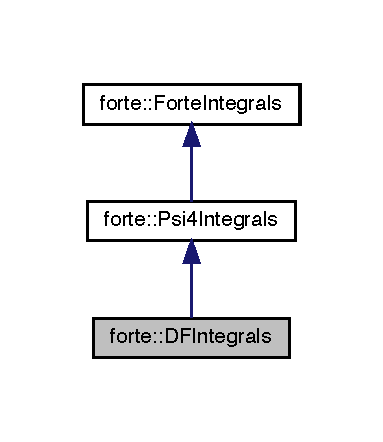
\includegraphics[width=184pt]{classforte_1_1_d_f_integrals__inherit__graph}
\end{center}
\end{figure}


Collaboration diagram for forte\+:\+:D\+F\+Integrals\+:
\nopagebreak
\begin{figure}[H]
\begin{center}
\leavevmode
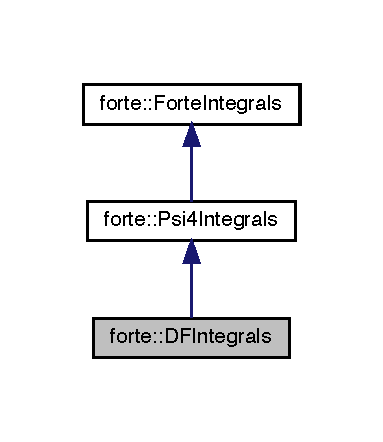
\includegraphics[width=184pt]{classforte_1_1_d_f_integrals__coll__graph}
\end{center}
\end{figure}
\subsection*{Public Member Functions}
\begin{DoxyCompactItemize}
\item 
\mbox{\hyperlink{classforte_1_1_d_f_integrals_a3475865749b607888cd8306e2d8c1f08}{D\+F\+Integrals}} (std\+::shared\+\_\+ptr$<$ \mbox{\hyperlink{classforte_1_1_forte_options}{Forte\+Options}} $>$ options, std\+::shared\+\_\+ptr$<$ psi\+::\+Wavefunction $>$ ref\+\_\+wfn, std\+::shared\+\_\+ptr$<$ \mbox{\hyperlink{classforte_1_1_m_o_space_info}{M\+O\+Space\+Info}} $>$ mo\+\_\+space\+\_\+info, \mbox{\hyperlink{namespaceforte_a7defa2660dd3eb07aa81176b90781be7}{Integral\+Spin\+Restriction}} restricted)
\begin{DoxyCompactList}\small\item\em Contructor of \mbox{\hyperlink{classforte_1_1_d_f_integrals}{D\+F\+Integrals}}. \end{DoxyCompactList}\item 
void \mbox{\hyperlink{classforte_1_1_d_f_integrals_a8488339b2eff7dea6e98e29e9bf55a97}{initialize}} () override
\item 
double \mbox{\hyperlink{classforte_1_1_d_f_integrals_aa495745fe55286ec7b4ff10ec6d22fae}{aptei\+\_\+aa}} (size\+\_\+t p, size\+\_\+t q, size\+\_\+t r, size\+\_\+t s) override
\begin{DoxyCompactList}\small\item\em The antisymmetrixed alpha-\/alpha two-\/electron integrals in physicist notation $<$pq$\vert$$\vert$rs$>$ \end{DoxyCompactList}\item 
double \mbox{\hyperlink{classforte_1_1_d_f_integrals_a01ec88efadb6b8b28bae6c5c3fbfd389}{aptei\+\_\+ab}} (size\+\_\+t p, size\+\_\+t q, size\+\_\+t r, size\+\_\+t s) override
\begin{DoxyCompactList}\small\item\em The antisymmetrixed alpha-\/beta two-\/electron integrals in physicist notation $<$pq$\vert$rs$>$ \end{DoxyCompactList}\item 
double \mbox{\hyperlink{classforte_1_1_d_f_integrals_ac9c2cb326b43623cbb290f7d6e1738cb}{aptei\+\_\+bb}} (size\+\_\+t p, size\+\_\+t q, size\+\_\+t r, size\+\_\+t s) override
\begin{DoxyCompactList}\small\item\em The antisymmetrixed beta-\/beta two-\/electron integrals in physicist notation $<$pq$\vert$$\vert$rs$>$ \end{DoxyCompactList}\item 
ambit\+::\+Tensor \mbox{\hyperlink{classforte_1_1_d_f_integrals_a2dc1ace8715b3c5a9b7c9da4afbeee44}{aptei\+\_\+aa\+\_\+block}} (const std\+::vector$<$ size\+\_\+t $>$ \&p, const std\+::vector$<$ size\+\_\+t $>$ \&q, const std\+::vector$<$ size\+\_\+t $>$ \&r, const std\+::vector$<$ size\+\_\+t $>$ \&s) override
\begin{DoxyCompactList}\small\item\em Return the antisymmetrized alpha-\/alpha chunck as an ambit\+::\+Tensor. \end{DoxyCompactList}\item 
ambit\+::\+Tensor \mbox{\hyperlink{classforte_1_1_d_f_integrals_a0c7391787d43e90df9a343a59bcadfbc}{aptei\+\_\+ab\+\_\+block}} (const std\+::vector$<$ size\+\_\+t $>$ \&p, const std\+::vector$<$ size\+\_\+t $>$ \&q, const std\+::vector$<$ size\+\_\+t $>$ \&r, const std\+::vector$<$ size\+\_\+t $>$ \&s) override
\begin{DoxyCompactList}\small\item\em Return the antisymmetrized alpha-\/beta chunck as an ambit\+::\+Tensor. \end{DoxyCompactList}\item 
ambit\+::\+Tensor \mbox{\hyperlink{classforte_1_1_d_f_integrals_a1eb5b7a379b668d0b10a0871a934b2cd}{aptei\+\_\+bb\+\_\+block}} (const std\+::vector$<$ size\+\_\+t $>$ \&p, const std\+::vector$<$ size\+\_\+t $>$ \&q, const std\+::vector$<$ size\+\_\+t $>$ \&r, const std\+::vector$<$ size\+\_\+t $>$ \&s) override
\begin{DoxyCompactList}\small\item\em Return the antisymmetrized beta-\/beta chunck as an ambit\+::\+Tensor. \end{DoxyCompactList}\item 
double \mbox{\hyperlink{classforte_1_1_d_f_integrals_a3d33d2d8107f1066c08f62e62ba51c8a}{three\+\_\+integral}} (size\+\_\+t A, size\+\_\+t p, size\+\_\+t q)
\item 
ambit\+::\+Tensor \mbox{\hyperlink{classforte_1_1_d_f_integrals_a830361fd7e2efd8c8d22fd5abcacfad1}{three\+\_\+integral\+\_\+block}} (const std\+::vector$<$ size\+\_\+t $>$ \&A, const std\+::vector$<$ size\+\_\+t $>$ \&p, const std\+::vector$<$ size\+\_\+t $>$ \&q) override
\item 
ambit\+::\+Tensor \mbox{\hyperlink{classforte_1_1_d_f_integrals_a455cc314d177bbcd4c25cbca6b0f02be}{three\+\_\+integral\+\_\+block\+\_\+two\+\_\+index}} (const std\+::vector$<$ size\+\_\+t $>$ \&, size\+\_\+t, const std\+::vector$<$ size\+\_\+t $>$ \&) override
\begin{DoxyCompactList}\small\item\em This function is only used by Disk\+DF and it is used to go from a Apq-\/$>$Aq tensor. \end{DoxyCompactList}\item 
double $\ast$$\ast$ \mbox{\hyperlink{classforte_1_1_d_f_integrals_ad682d1f719de96683aa2bc02fc46eabe}{three\+\_\+integral\+\_\+pointer}} () override
\begin{DoxyCompactList}\small\item\em Expert Option\+: just try and use three\+\_\+integral. \end{DoxyCompactList}\item 
void \mbox{\hyperlink{classforte_1_1_d_f_integrals_ac623714d6a85c8f18722aae187b8324e}{set\+\_\+tei}} (size\+\_\+t p, size\+\_\+t q, size\+\_\+t r, size\+\_\+t s, double value, bool alpha1, bool alpha2) override
\begin{DoxyCompactList}\small\item\em Set the value of the two-\/electron integrals. \end{DoxyCompactList}\item 
size\+\_\+t \mbox{\hyperlink{classforte_1_1_d_f_integrals_ac514e780990cdc0b3b594453eb63e901}{nthree}} () const override
\begin{DoxyCompactList}\small\item\em Return the number of auxiliary functions. \end{DoxyCompactList}\end{DoxyCompactItemize}
\subsection*{Additional Inherited Members}


\subsection{Detailed Description}
The \mbox{\hyperlink{classforte_1_1_d_f_integrals}{D\+F\+Integrals}} class approximates two-\/electron integrals via density fitting. 

This class assumes the density-\/fitting tensors can be stored in memory. 

\subsection{Constructor \& Destructor Documentation}
\mbox{\Hypertarget{classforte_1_1_d_f_integrals_a3475865749b607888cd8306e2d8c1f08}\label{classforte_1_1_d_f_integrals_a3475865749b607888cd8306e2d8c1f08}} 
\index{forte\+::\+D\+F\+Integrals@{forte\+::\+D\+F\+Integrals}!D\+F\+Integrals@{D\+F\+Integrals}}
\index{D\+F\+Integrals@{D\+F\+Integrals}!forte\+::\+D\+F\+Integrals@{forte\+::\+D\+F\+Integrals}}
\subsubsection{\texorpdfstring{D\+F\+Integrals()}{DFIntegrals()}}
{\footnotesize\ttfamily forte\+::\+D\+F\+Integrals\+::\+D\+F\+Integrals (\begin{DoxyParamCaption}\item[{std\+::shared\+\_\+ptr$<$ \mbox{\hyperlink{classforte_1_1_forte_options}{Forte\+Options}} $>$}]{options,  }\item[{std\+::shared\+\_\+ptr$<$ psi\+::\+Wavefunction $>$}]{ref\+\_\+wfn,  }\item[{std\+::shared\+\_\+ptr$<$ \mbox{\hyperlink{classforte_1_1_m_o_space_info}{M\+O\+Space\+Info}} $>$}]{mo\+\_\+space\+\_\+info,  }\item[{\mbox{\hyperlink{namespaceforte_a7defa2660dd3eb07aa81176b90781be7}{Integral\+Spin\+Restriction}}}]{restricted }\end{DoxyParamCaption})}



Contructor of \mbox{\hyperlink{classforte_1_1_d_f_integrals}{D\+F\+Integrals}}. 



\subsection{Member Function Documentation}
\mbox{\Hypertarget{classforte_1_1_d_f_integrals_aa495745fe55286ec7b4ff10ec6d22fae}\label{classforte_1_1_d_f_integrals_aa495745fe55286ec7b4ff10ec6d22fae}} 
\index{forte\+::\+D\+F\+Integrals@{forte\+::\+D\+F\+Integrals}!aptei\+\_\+aa@{aptei\+\_\+aa}}
\index{aptei\+\_\+aa@{aptei\+\_\+aa}!forte\+::\+D\+F\+Integrals@{forte\+::\+D\+F\+Integrals}}
\subsubsection{\texorpdfstring{aptei\+\_\+aa()}{aptei\_aa()}}
{\footnotesize\ttfamily double forte\+::\+D\+F\+Integrals\+::aptei\+\_\+aa (\begin{DoxyParamCaption}\item[{size\+\_\+t}]{p,  }\item[{size\+\_\+t}]{q,  }\item[{size\+\_\+t}]{r,  }\item[{size\+\_\+t}]{s }\end{DoxyParamCaption})\hspace{0.3cm}{\ttfamily [override]}, {\ttfamily [virtual]}}



The antisymmetrixed alpha-\/alpha two-\/electron integrals in physicist notation $<$pq$\vert$$\vert$rs$>$ 



Implements \mbox{\hyperlink{classforte_1_1_forte_integrals_afc84c157025b56ee0f8e3b1abe1c0a5f}{forte\+::\+Forte\+Integrals}}.

\mbox{\Hypertarget{classforte_1_1_d_f_integrals_a2dc1ace8715b3c5a9b7c9da4afbeee44}\label{classforte_1_1_d_f_integrals_a2dc1ace8715b3c5a9b7c9da4afbeee44}} 
\index{forte\+::\+D\+F\+Integrals@{forte\+::\+D\+F\+Integrals}!aptei\+\_\+aa\+\_\+block@{aptei\+\_\+aa\+\_\+block}}
\index{aptei\+\_\+aa\+\_\+block@{aptei\+\_\+aa\+\_\+block}!forte\+::\+D\+F\+Integrals@{forte\+::\+D\+F\+Integrals}}
\subsubsection{\texorpdfstring{aptei\+\_\+aa\+\_\+block()}{aptei\_aa\_block()}}
{\footnotesize\ttfamily ambit\+::\+Tensor forte\+::\+D\+F\+Integrals\+::aptei\+\_\+aa\+\_\+block (\begin{DoxyParamCaption}\item[{const std\+::vector$<$ size\+\_\+t $>$ \&}]{p,  }\item[{const std\+::vector$<$ size\+\_\+t $>$ \&}]{q,  }\item[{const std\+::vector$<$ size\+\_\+t $>$ \&}]{r,  }\item[{const std\+::vector$<$ size\+\_\+t $>$ \&}]{s }\end{DoxyParamCaption})\hspace{0.3cm}{\ttfamily [override]}, {\ttfamily [virtual]}}



Return the antisymmetrized alpha-\/alpha chunck as an ambit\+::\+Tensor. 



Implements \mbox{\hyperlink{classforte_1_1_forte_integrals_ac20ae649b8cfe116f8583d676e43da27}{forte\+::\+Forte\+Integrals}}.

\mbox{\Hypertarget{classforte_1_1_d_f_integrals_a01ec88efadb6b8b28bae6c5c3fbfd389}\label{classforte_1_1_d_f_integrals_a01ec88efadb6b8b28bae6c5c3fbfd389}} 
\index{forte\+::\+D\+F\+Integrals@{forte\+::\+D\+F\+Integrals}!aptei\+\_\+ab@{aptei\+\_\+ab}}
\index{aptei\+\_\+ab@{aptei\+\_\+ab}!forte\+::\+D\+F\+Integrals@{forte\+::\+D\+F\+Integrals}}
\subsubsection{\texorpdfstring{aptei\+\_\+ab()}{aptei\_ab()}}
{\footnotesize\ttfamily double forte\+::\+D\+F\+Integrals\+::aptei\+\_\+ab (\begin{DoxyParamCaption}\item[{size\+\_\+t}]{p,  }\item[{size\+\_\+t}]{q,  }\item[{size\+\_\+t}]{r,  }\item[{size\+\_\+t}]{s }\end{DoxyParamCaption})\hspace{0.3cm}{\ttfamily [override]}, {\ttfamily [virtual]}}



The antisymmetrixed alpha-\/beta two-\/electron integrals in physicist notation $<$pq$\vert$rs$>$ 



Implements \mbox{\hyperlink{classforte_1_1_forte_integrals_a45efc2329cdfc7e4690cbe85688b947e}{forte\+::\+Forte\+Integrals}}.

\mbox{\Hypertarget{classforte_1_1_d_f_integrals_a0c7391787d43e90df9a343a59bcadfbc}\label{classforte_1_1_d_f_integrals_a0c7391787d43e90df9a343a59bcadfbc}} 
\index{forte\+::\+D\+F\+Integrals@{forte\+::\+D\+F\+Integrals}!aptei\+\_\+ab\+\_\+block@{aptei\+\_\+ab\+\_\+block}}
\index{aptei\+\_\+ab\+\_\+block@{aptei\+\_\+ab\+\_\+block}!forte\+::\+D\+F\+Integrals@{forte\+::\+D\+F\+Integrals}}
\subsubsection{\texorpdfstring{aptei\+\_\+ab\+\_\+block()}{aptei\_ab\_block()}}
{\footnotesize\ttfamily ambit\+::\+Tensor forte\+::\+D\+F\+Integrals\+::aptei\+\_\+ab\+\_\+block (\begin{DoxyParamCaption}\item[{const std\+::vector$<$ size\+\_\+t $>$ \&}]{p,  }\item[{const std\+::vector$<$ size\+\_\+t $>$ \&}]{q,  }\item[{const std\+::vector$<$ size\+\_\+t $>$ \&}]{r,  }\item[{const std\+::vector$<$ size\+\_\+t $>$ \&}]{s }\end{DoxyParamCaption})\hspace{0.3cm}{\ttfamily [override]}, {\ttfamily [virtual]}}



Return the antisymmetrized alpha-\/beta chunck as an ambit\+::\+Tensor. 



Implements \mbox{\hyperlink{classforte_1_1_forte_integrals_acd40e350dc861baf8adf6a3b47c74023}{forte\+::\+Forte\+Integrals}}.

\mbox{\Hypertarget{classforte_1_1_d_f_integrals_ac9c2cb326b43623cbb290f7d6e1738cb}\label{classforte_1_1_d_f_integrals_ac9c2cb326b43623cbb290f7d6e1738cb}} 
\index{forte\+::\+D\+F\+Integrals@{forte\+::\+D\+F\+Integrals}!aptei\+\_\+bb@{aptei\+\_\+bb}}
\index{aptei\+\_\+bb@{aptei\+\_\+bb}!forte\+::\+D\+F\+Integrals@{forte\+::\+D\+F\+Integrals}}
\subsubsection{\texorpdfstring{aptei\+\_\+bb()}{aptei\_bb()}}
{\footnotesize\ttfamily double forte\+::\+D\+F\+Integrals\+::aptei\+\_\+bb (\begin{DoxyParamCaption}\item[{size\+\_\+t}]{p,  }\item[{size\+\_\+t}]{q,  }\item[{size\+\_\+t}]{r,  }\item[{size\+\_\+t}]{s }\end{DoxyParamCaption})\hspace{0.3cm}{\ttfamily [override]}, {\ttfamily [virtual]}}



The antisymmetrixed beta-\/beta two-\/electron integrals in physicist notation $<$pq$\vert$$\vert$rs$>$ 



Implements \mbox{\hyperlink{classforte_1_1_forte_integrals_a246225031c3799dc446f94e0e732c3ac}{forte\+::\+Forte\+Integrals}}.

\mbox{\Hypertarget{classforte_1_1_d_f_integrals_a1eb5b7a379b668d0b10a0871a934b2cd}\label{classforte_1_1_d_f_integrals_a1eb5b7a379b668d0b10a0871a934b2cd}} 
\index{forte\+::\+D\+F\+Integrals@{forte\+::\+D\+F\+Integrals}!aptei\+\_\+bb\+\_\+block@{aptei\+\_\+bb\+\_\+block}}
\index{aptei\+\_\+bb\+\_\+block@{aptei\+\_\+bb\+\_\+block}!forte\+::\+D\+F\+Integrals@{forte\+::\+D\+F\+Integrals}}
\subsubsection{\texorpdfstring{aptei\+\_\+bb\+\_\+block()}{aptei\_bb\_block()}}
{\footnotesize\ttfamily ambit\+::\+Tensor forte\+::\+D\+F\+Integrals\+::aptei\+\_\+bb\+\_\+block (\begin{DoxyParamCaption}\item[{const std\+::vector$<$ size\+\_\+t $>$ \&}]{p,  }\item[{const std\+::vector$<$ size\+\_\+t $>$ \&}]{q,  }\item[{const std\+::vector$<$ size\+\_\+t $>$ \&}]{r,  }\item[{const std\+::vector$<$ size\+\_\+t $>$ \&}]{s }\end{DoxyParamCaption})\hspace{0.3cm}{\ttfamily [override]}, {\ttfamily [virtual]}}



Return the antisymmetrized beta-\/beta chunck as an ambit\+::\+Tensor. 



Implements \mbox{\hyperlink{classforte_1_1_forte_integrals_ae2799dc7cbfd456603a2b841b26582ab}{forte\+::\+Forte\+Integrals}}.

\mbox{\Hypertarget{classforte_1_1_d_f_integrals_a8488339b2eff7dea6e98e29e9bf55a97}\label{classforte_1_1_d_f_integrals_a8488339b2eff7dea6e98e29e9bf55a97}} 
\index{forte\+::\+D\+F\+Integrals@{forte\+::\+D\+F\+Integrals}!initialize@{initialize}}
\index{initialize@{initialize}!forte\+::\+D\+F\+Integrals@{forte\+::\+D\+F\+Integrals}}
\subsubsection{\texorpdfstring{initialize()}{initialize()}}
{\footnotesize\ttfamily void forte\+::\+D\+F\+Integrals\+::initialize (\begin{DoxyParamCaption}{ }\end{DoxyParamCaption})\hspace{0.3cm}{\ttfamily [override]}, {\ttfamily [virtual]}}



Implements \mbox{\hyperlink{classforte_1_1_forte_integrals_a7862835fa0f5f9abe13dfcd6730fa4be}{forte\+::\+Forte\+Integrals}}.

\mbox{\Hypertarget{classforte_1_1_d_f_integrals_ac514e780990cdc0b3b594453eb63e901}\label{classforte_1_1_d_f_integrals_ac514e780990cdc0b3b594453eb63e901}} 
\index{forte\+::\+D\+F\+Integrals@{forte\+::\+D\+F\+Integrals}!nthree@{nthree}}
\index{nthree@{nthree}!forte\+::\+D\+F\+Integrals@{forte\+::\+D\+F\+Integrals}}
\subsubsection{\texorpdfstring{nthree()}{nthree()}}
{\footnotesize\ttfamily size\+\_\+t forte\+::\+D\+F\+Integrals\+::nthree (\begin{DoxyParamCaption}{ }\end{DoxyParamCaption}) const\hspace{0.3cm}{\ttfamily [override]}, {\ttfamily [virtual]}}



Return the number of auxiliary functions. 



Reimplemented from \mbox{\hyperlink{classforte_1_1_forte_integrals_af04858e7813556747745f90ffbda81a4}{forte\+::\+Forte\+Integrals}}.

\mbox{\Hypertarget{classforte_1_1_d_f_integrals_ac623714d6a85c8f18722aae187b8324e}\label{classforte_1_1_d_f_integrals_ac623714d6a85c8f18722aae187b8324e}} 
\index{forte\+::\+D\+F\+Integrals@{forte\+::\+D\+F\+Integrals}!set\+\_\+tei@{set\+\_\+tei}}
\index{set\+\_\+tei@{set\+\_\+tei}!forte\+::\+D\+F\+Integrals@{forte\+::\+D\+F\+Integrals}}
\subsubsection{\texorpdfstring{set\+\_\+tei()}{set\_tei()}}
{\footnotesize\ttfamily void forte\+::\+D\+F\+Integrals\+::set\+\_\+tei (\begin{DoxyParamCaption}\item[{size\+\_\+t}]{p,  }\item[{size\+\_\+t}]{q,  }\item[{size\+\_\+t}]{r,  }\item[{size\+\_\+t}]{s,  }\item[{double}]{value,  }\item[{bool}]{alpha1,  }\item[{bool}]{alpha2 }\end{DoxyParamCaption})\hspace{0.3cm}{\ttfamily [override]}, {\ttfamily [virtual]}}



Set the value of the two-\/electron integrals. 



Implements \mbox{\hyperlink{classforte_1_1_forte_integrals_aaccd56e90bbc3c423158efb154336b9c}{forte\+::\+Forte\+Integrals}}.

\mbox{\Hypertarget{classforte_1_1_d_f_integrals_a3d33d2d8107f1066c08f62e62ba51c8a}\label{classforte_1_1_d_f_integrals_a3d33d2d8107f1066c08f62e62ba51c8a}} 
\index{forte\+::\+D\+F\+Integrals@{forte\+::\+D\+F\+Integrals}!three\+\_\+integral@{three\+\_\+integral}}
\index{three\+\_\+integral@{three\+\_\+integral}!forte\+::\+D\+F\+Integrals@{forte\+::\+D\+F\+Integrals}}
\subsubsection{\texorpdfstring{three\+\_\+integral()}{three\_integral()}}
{\footnotesize\ttfamily double forte\+::\+D\+F\+Integrals\+::three\+\_\+integral (\begin{DoxyParamCaption}\item[{size\+\_\+t}]{A,  }\item[{size\+\_\+t}]{p,  }\item[{size\+\_\+t}]{q }\end{DoxyParamCaption})}

\mbox{\Hypertarget{classforte_1_1_d_f_integrals_a830361fd7e2efd8c8d22fd5abcacfad1}\label{classforte_1_1_d_f_integrals_a830361fd7e2efd8c8d22fd5abcacfad1}} 
\index{forte\+::\+D\+F\+Integrals@{forte\+::\+D\+F\+Integrals}!three\+\_\+integral\+\_\+block@{three\+\_\+integral\+\_\+block}}
\index{three\+\_\+integral\+\_\+block@{three\+\_\+integral\+\_\+block}!forte\+::\+D\+F\+Integrals@{forte\+::\+D\+F\+Integrals}}
\subsubsection{\texorpdfstring{three\+\_\+integral\+\_\+block()}{three\_integral\_block()}}
{\footnotesize\ttfamily ambit\+::\+Tensor forte\+::\+D\+F\+Integrals\+::three\+\_\+integral\+\_\+block (\begin{DoxyParamCaption}\item[{const std\+::vector$<$ size\+\_\+t $>$ \&}]{A,  }\item[{const std\+::vector$<$ size\+\_\+t $>$ \&}]{p,  }\item[{const std\+::vector$<$ size\+\_\+t $>$ \&}]{q }\end{DoxyParamCaption})\hspace{0.3cm}{\ttfamily [override]}, {\ttfamily [virtual]}}



Reimplemented from \mbox{\hyperlink{classforte_1_1_forte_integrals_aa1d259ae97b5a9c96ccb20599543b126}{forte\+::\+Forte\+Integrals}}.

\mbox{\Hypertarget{classforte_1_1_d_f_integrals_a455cc314d177bbcd4c25cbca6b0f02be}\label{classforte_1_1_d_f_integrals_a455cc314d177bbcd4c25cbca6b0f02be}} 
\index{forte\+::\+D\+F\+Integrals@{forte\+::\+D\+F\+Integrals}!three\+\_\+integral\+\_\+block\+\_\+two\+\_\+index@{three\+\_\+integral\+\_\+block\+\_\+two\+\_\+index}}
\index{three\+\_\+integral\+\_\+block\+\_\+two\+\_\+index@{three\+\_\+integral\+\_\+block\+\_\+two\+\_\+index}!forte\+::\+D\+F\+Integrals@{forte\+::\+D\+F\+Integrals}}
\subsubsection{\texorpdfstring{three\+\_\+integral\+\_\+block\+\_\+two\+\_\+index()}{three\_integral\_block\_two\_index()}}
{\footnotesize\ttfamily ambit\+::\+Tensor forte\+::\+D\+F\+Integrals\+::three\+\_\+integral\+\_\+block\+\_\+two\+\_\+index (\begin{DoxyParamCaption}\item[{const std\+::vector$<$ size\+\_\+t $>$ \&}]{A,  }\item[{size\+\_\+t}]{p,  }\item[{const std\+::vector$<$ size\+\_\+t $>$ \&}]{ }\end{DoxyParamCaption})\hspace{0.3cm}{\ttfamily [override]}, {\ttfamily [virtual]}}



This function is only used by Disk\+DF and it is used to go from a Apq-\/$>$Aq tensor. 



Reimplemented from \mbox{\hyperlink{classforte_1_1_forte_integrals_aab51824020dc3588c026b5b7740f55a9}{forte\+::\+Forte\+Integrals}}.

\mbox{\Hypertarget{classforte_1_1_d_f_integrals_ad682d1f719de96683aa2bc02fc46eabe}\label{classforte_1_1_d_f_integrals_ad682d1f719de96683aa2bc02fc46eabe}} 
\index{forte\+::\+D\+F\+Integrals@{forte\+::\+D\+F\+Integrals}!three\+\_\+integral\+\_\+pointer@{three\+\_\+integral\+\_\+pointer}}
\index{three\+\_\+integral\+\_\+pointer@{three\+\_\+integral\+\_\+pointer}!forte\+::\+D\+F\+Integrals@{forte\+::\+D\+F\+Integrals}}
\subsubsection{\texorpdfstring{three\+\_\+integral\+\_\+pointer()}{three\_integral\_pointer()}}
{\footnotesize\ttfamily double $\ast$$\ast$ forte\+::\+D\+F\+Integrals\+::three\+\_\+integral\+\_\+pointer (\begin{DoxyParamCaption}{ }\end{DoxyParamCaption})\hspace{0.3cm}{\ttfamily [override]}, {\ttfamily [virtual]}}



Expert Option\+: just try and use three\+\_\+integral. 



Reimplemented from \mbox{\hyperlink{classforte_1_1_forte_integrals_a69292bc8e42a76e344cd01c4e3dd48d5}{forte\+::\+Forte\+Integrals}}.



The documentation for this class was generated from the following files\+:\begin{DoxyCompactItemize}
\item 
/\+Users/fevange/\+Source/forte/src/integrals/\mbox{\hyperlink{df__integrals_8h}{df\+\_\+integrals.\+h}}\item 
/\+Users/fevange/\+Source/forte/src/integrals/\mbox{\hyperlink{df__integrals_8cc}{df\+\_\+integrals.\+cc}}\end{DoxyCompactItemize}

\hypertarget{classforte_1_1_d_i_s_k_d_f_integrals}{}\section{forte\+:\+:D\+I\+S\+K\+D\+F\+Integrals Class Reference}
\label{classforte_1_1_d_i_s_k_d_f_integrals}\index{forte\+::\+D\+I\+S\+K\+D\+F\+Integrals@{forte\+::\+D\+I\+S\+K\+D\+F\+Integrals}}


{\ttfamily \#include $<$diskdf\+\_\+integrals.\+h$>$}



Inheritance diagram for forte\+:\+:D\+I\+S\+K\+D\+F\+Integrals\+:
\nopagebreak
\begin{figure}[H]
\begin{center}
\leavevmode
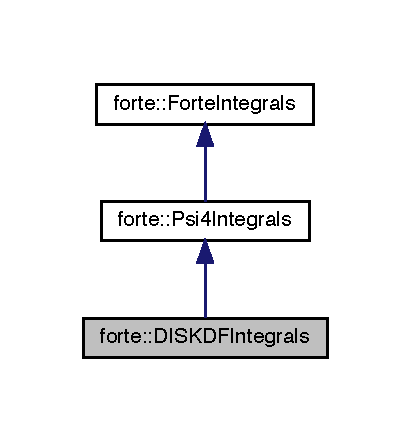
\includegraphics[width=197pt]{classforte_1_1_d_i_s_k_d_f_integrals__inherit__graph}
\end{center}
\end{figure}


Collaboration diagram for forte\+:\+:D\+I\+S\+K\+D\+F\+Integrals\+:
\nopagebreak
\begin{figure}[H]
\begin{center}
\leavevmode
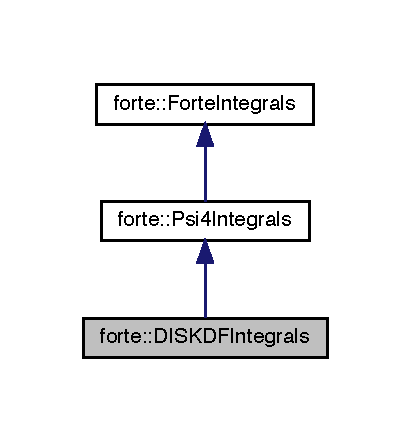
\includegraphics[width=197pt]{classforte_1_1_d_i_s_k_d_f_integrals__coll__graph}
\end{center}
\end{figure}
\subsection*{Public Member Functions}
\begin{DoxyCompactItemize}
\item 
\mbox{\hyperlink{classforte_1_1_d_i_s_k_d_f_integrals_a2415c0e724a0baf1bd0e1f10190fbeed}{D\+I\+S\+K\+D\+F\+Integrals}} (std\+::shared\+\_\+ptr$<$ \mbox{\hyperlink{classforte_1_1_forte_options}{Forte\+Options}} $>$ options, std\+::shared\+\_\+ptr$<$ psi\+::\+Wavefunction $>$ ref\+\_\+wfn, std\+::shared\+\_\+ptr$<$ \mbox{\hyperlink{classforte_1_1_m_o_space_info}{M\+O\+Space\+Info}} $>$ mo\+\_\+space\+\_\+info, \mbox{\hyperlink{namespaceforte_a7defa2660dd3eb07aa81176b90781be7}{Integral\+Spin\+Restriction}} restricted)
\begin{DoxyCompactList}\small\item\em Contructor of \mbox{\hyperlink{classforte_1_1_d_i_s_k_d_f_integrals}{D\+I\+S\+K\+D\+F\+Integrals}}. \end{DoxyCompactList}\item 
void \mbox{\hyperlink{classforte_1_1_d_i_s_k_d_f_integrals_a3205b9dc431a7104969132b1f4bc206f}{initialize}} () override
\item 
double \mbox{\hyperlink{classforte_1_1_d_i_s_k_d_f_integrals_a3a815a39bc2f01a1cb5398e857f56285}{aptei\+\_\+aa}} (size\+\_\+t p, size\+\_\+t q, size\+\_\+t r, size\+\_\+t s) override
\begin{DoxyCompactList}\small\item\em aptei\+\_\+xy functions are slow. try to use three\+\_\+integral\+\_\+block \end{DoxyCompactList}\item 
double \mbox{\hyperlink{classforte_1_1_d_i_s_k_d_f_integrals_aa0ab48ce47dab83c35bf3b9433273f59}{aptei\+\_\+ab}} (size\+\_\+t p, size\+\_\+t q, size\+\_\+t r, size\+\_\+t s) override
\begin{DoxyCompactList}\small\item\em The antisymmetrixed alpha-\/beta two-\/electron integrals in physicist notation $<$pq$\vert$rs$>$ \end{DoxyCompactList}\item 
double \mbox{\hyperlink{classforte_1_1_d_i_s_k_d_f_integrals_a84224ddc5210cad49b63e74bdd1d4342}{aptei\+\_\+bb}} (size\+\_\+t p, size\+\_\+t q, size\+\_\+t r, size\+\_\+t s) override
\begin{DoxyCompactList}\small\item\em The antisymmetrixed beta-\/beta two-\/electron integrals in physicist notation $<$pq$\vert$$\vert$rs$>$ \end{DoxyCompactList}\item 
ambit\+::\+Tensor \mbox{\hyperlink{classforte_1_1_d_i_s_k_d_f_integrals_a2709b0116f0e44fc1eb8038a2b7afd54}{aptei\+\_\+aa\+\_\+block}} (const std\+::vector$<$ size\+\_\+t $>$ \&p, const std\+::vector$<$ size\+\_\+t $>$ \&q, const std\+::vector$<$ size\+\_\+t $>$ \&r, const std\+::vector$<$ size\+\_\+t $>$ \&s) override
\begin{DoxyCompactList}\small\item\em Return the antisymmetrized alpha-\/alpha chunck as an ambit\+::\+Tensor. \end{DoxyCompactList}\item 
ambit\+::\+Tensor \mbox{\hyperlink{classforte_1_1_d_i_s_k_d_f_integrals_a3512219937aa98d2f0b6ee680254317a}{aptei\+\_\+ab\+\_\+block}} (const std\+::vector$<$ size\+\_\+t $>$ \&p, const std\+::vector$<$ size\+\_\+t $>$ \&q, const std\+::vector$<$ size\+\_\+t $>$ \&r, const std\+::vector$<$ size\+\_\+t $>$ \&s) override
\begin{DoxyCompactList}\small\item\em Return the antisymmetrized alpha-\/beta chunck as an ambit\+::\+Tensor. \end{DoxyCompactList}\item 
ambit\+::\+Tensor \mbox{\hyperlink{classforte_1_1_d_i_s_k_d_f_integrals_a4b78b82f7bb76de677a476d5982e9f89}{aptei\+\_\+bb\+\_\+block}} (const std\+::vector$<$ size\+\_\+t $>$ \&p, const std\+::vector$<$ size\+\_\+t $>$ \&q, const std\+::vector$<$ size\+\_\+t $>$ \&r, const std\+::vector$<$ size\+\_\+t $>$ \&s) override
\begin{DoxyCompactList}\small\item\em Return the antisymmetrized beta-\/beta chunck as an ambit\+::\+Tensor. \end{DoxyCompactList}\item 
double $\ast$$\ast$ \mbox{\hyperlink{classforte_1_1_d_i_s_k_d_f_integrals_a43f80b9c9e3b67223a11049c3e2f52e2}{three\+\_\+integral\+\_\+pointer}} () override
\begin{DoxyCompactList}\small\item\em Expert Option\+: just try and use three\+\_\+integral. \end{DoxyCompactList}\item 
ambit\+::\+Tensor \mbox{\hyperlink{classforte_1_1_d_i_s_k_d_f_integrals_aa36e8484286f58bcb2b57a7c8fb08a36}{three\+\_\+integral\+\_\+block}} (const std\+::vector$<$ size\+\_\+t $>$ \&A, const std\+::vector$<$ size\+\_\+t $>$ \&p, const std\+::vector$<$ size\+\_\+t $>$ \&q) override
\begin{DoxyCompactList}\small\item\em Read a block of the \mbox{\hyperlink{classforte_1_1_d_f_integrals}{D\+F\+Integrals}} and return an Ambit tensor of size A by p by q. \end{DoxyCompactList}\item 
ambit\+::\+Tensor \mbox{\hyperlink{classforte_1_1_d_i_s_k_d_f_integrals_a754ec30830dd51627a3608dfca9f5f4d}{three\+\_\+integral\+\_\+block\+\_\+two\+\_\+index}} (const std\+::vector$<$ size\+\_\+t $>$ \&A, size\+\_\+t p, const std\+::vector$<$ size\+\_\+t $>$ \&q) override
\begin{DoxyCompactList}\small\item\em return ambit tensor of size A by q \end{DoxyCompactList}\item 
void \mbox{\hyperlink{classforte_1_1_d_i_s_k_d_f_integrals_aceee5961cd70cfc7fc9b7799675f8fb6}{set\+\_\+tei}} (size\+\_\+t p, size\+\_\+t q, size\+\_\+t r, size\+\_\+t s, double value, bool alpha1, bool alpha2) override
\begin{DoxyCompactList}\small\item\em Set the value of the two-\/electron integrals. \end{DoxyCompactList}\item 
size\+\_\+t \mbox{\hyperlink{classforte_1_1_d_i_s_k_d_f_integrals_a56b38fd57064c9d6464f2173127835bd}{nthree}} () const override
\begin{DoxyCompactList}\small\item\em Make a Fock matrix computed with respect to a given determinant. \end{DoxyCompactList}\end{DoxyCompactItemize}
\subsection*{Additional Inherited Members}


\subsection{Detailed Description}
A Disk\+D\+F\+Integrals class for avoiding the storage of the Three\+Integral tensor Assumes that the \mbox{\hyperlink{classforte_1_1_d_f_integrals}{D\+F\+Integrals}} are stored in a binary file generated by D\+F\+\_\+\+Helper Aptei\+\_\+xy are extremely slow -\/$>$ Try to use three\+\_\+electron\+\_\+block. Much faster Reading individual elements is slow 

\subsection{Constructor \& Destructor Documentation}
\mbox{\Hypertarget{classforte_1_1_d_i_s_k_d_f_integrals_a2415c0e724a0baf1bd0e1f10190fbeed}\label{classforte_1_1_d_i_s_k_d_f_integrals_a2415c0e724a0baf1bd0e1f10190fbeed}} 
\index{forte\+::\+D\+I\+S\+K\+D\+F\+Integrals@{forte\+::\+D\+I\+S\+K\+D\+F\+Integrals}!D\+I\+S\+K\+D\+F\+Integrals@{D\+I\+S\+K\+D\+F\+Integrals}}
\index{D\+I\+S\+K\+D\+F\+Integrals@{D\+I\+S\+K\+D\+F\+Integrals}!forte\+::\+D\+I\+S\+K\+D\+F\+Integrals@{forte\+::\+D\+I\+S\+K\+D\+F\+Integrals}}
\subsubsection{\texorpdfstring{D\+I\+S\+K\+D\+F\+Integrals()}{DISKDFIntegrals()}}
{\footnotesize\ttfamily forte\+::\+D\+I\+S\+K\+D\+F\+Integrals\+::\+D\+I\+S\+K\+D\+F\+Integrals (\begin{DoxyParamCaption}\item[{std\+::shared\+\_\+ptr$<$ \mbox{\hyperlink{classforte_1_1_forte_options}{Forte\+Options}} $>$}]{options,  }\item[{std\+::shared\+\_\+ptr$<$ psi\+::\+Wavefunction $>$}]{ref\+\_\+wfn,  }\item[{std\+::shared\+\_\+ptr$<$ \mbox{\hyperlink{classforte_1_1_m_o_space_info}{M\+O\+Space\+Info}} $>$}]{mo\+\_\+space\+\_\+info,  }\item[{\mbox{\hyperlink{namespaceforte_a7defa2660dd3eb07aa81176b90781be7}{Integral\+Spin\+Restriction}}}]{restricted }\end{DoxyParamCaption})}



Contructor of \mbox{\hyperlink{classforte_1_1_d_i_s_k_d_f_integrals}{D\+I\+S\+K\+D\+F\+Integrals}}. 



\subsection{Member Function Documentation}
\mbox{\Hypertarget{classforte_1_1_d_i_s_k_d_f_integrals_a3a815a39bc2f01a1cb5398e857f56285}\label{classforte_1_1_d_i_s_k_d_f_integrals_a3a815a39bc2f01a1cb5398e857f56285}} 
\index{forte\+::\+D\+I\+S\+K\+D\+F\+Integrals@{forte\+::\+D\+I\+S\+K\+D\+F\+Integrals}!aptei\+\_\+aa@{aptei\+\_\+aa}}
\index{aptei\+\_\+aa@{aptei\+\_\+aa}!forte\+::\+D\+I\+S\+K\+D\+F\+Integrals@{forte\+::\+D\+I\+S\+K\+D\+F\+Integrals}}
\subsubsection{\texorpdfstring{aptei\+\_\+aa()}{aptei\_aa()}}
{\footnotesize\ttfamily double forte\+::\+D\+I\+S\+K\+D\+F\+Integrals\+::aptei\+\_\+aa (\begin{DoxyParamCaption}\item[{size\+\_\+t}]{p,  }\item[{size\+\_\+t}]{q,  }\item[{size\+\_\+t}]{r,  }\item[{size\+\_\+t}]{s }\end{DoxyParamCaption})\hspace{0.3cm}{\ttfamily [override]}, {\ttfamily [virtual]}}



aptei\+\_\+xy functions are slow. try to use three\+\_\+integral\+\_\+block 



Implements \mbox{\hyperlink{classforte_1_1_forte_integrals_afc84c157025b56ee0f8e3b1abe1c0a5f}{forte\+::\+Forte\+Integrals}}.

\mbox{\Hypertarget{classforte_1_1_d_i_s_k_d_f_integrals_a2709b0116f0e44fc1eb8038a2b7afd54}\label{classforte_1_1_d_i_s_k_d_f_integrals_a2709b0116f0e44fc1eb8038a2b7afd54}} 
\index{forte\+::\+D\+I\+S\+K\+D\+F\+Integrals@{forte\+::\+D\+I\+S\+K\+D\+F\+Integrals}!aptei\+\_\+aa\+\_\+block@{aptei\+\_\+aa\+\_\+block}}
\index{aptei\+\_\+aa\+\_\+block@{aptei\+\_\+aa\+\_\+block}!forte\+::\+D\+I\+S\+K\+D\+F\+Integrals@{forte\+::\+D\+I\+S\+K\+D\+F\+Integrals}}
\subsubsection{\texorpdfstring{aptei\+\_\+aa\+\_\+block()}{aptei\_aa\_block()}}
{\footnotesize\ttfamily ambit\+::\+Tensor forte\+::\+D\+I\+S\+K\+D\+F\+Integrals\+::aptei\+\_\+aa\+\_\+block (\begin{DoxyParamCaption}\item[{const std\+::vector$<$ size\+\_\+t $>$ \&}]{p,  }\item[{const std\+::vector$<$ size\+\_\+t $>$ \&}]{q,  }\item[{const std\+::vector$<$ size\+\_\+t $>$ \&}]{r,  }\item[{const std\+::vector$<$ size\+\_\+t $>$ \&}]{s }\end{DoxyParamCaption})\hspace{0.3cm}{\ttfamily [override]}, {\ttfamily [virtual]}}



Return the antisymmetrized alpha-\/alpha chunck as an ambit\+::\+Tensor. 

If p != q != r !=s need to form the Exchange part separately 

Implements \mbox{\hyperlink{classforte_1_1_forte_integrals_ac20ae649b8cfe116f8583d676e43da27}{forte\+::\+Forte\+Integrals}}.

\mbox{\Hypertarget{classforte_1_1_d_i_s_k_d_f_integrals_aa0ab48ce47dab83c35bf3b9433273f59}\label{classforte_1_1_d_i_s_k_d_f_integrals_aa0ab48ce47dab83c35bf3b9433273f59}} 
\index{forte\+::\+D\+I\+S\+K\+D\+F\+Integrals@{forte\+::\+D\+I\+S\+K\+D\+F\+Integrals}!aptei\+\_\+ab@{aptei\+\_\+ab}}
\index{aptei\+\_\+ab@{aptei\+\_\+ab}!forte\+::\+D\+I\+S\+K\+D\+F\+Integrals@{forte\+::\+D\+I\+S\+K\+D\+F\+Integrals}}
\subsubsection{\texorpdfstring{aptei\+\_\+ab()}{aptei\_ab()}}
{\footnotesize\ttfamily double forte\+::\+D\+I\+S\+K\+D\+F\+Integrals\+::aptei\+\_\+ab (\begin{DoxyParamCaption}\item[{size\+\_\+t}]{p,  }\item[{size\+\_\+t}]{q,  }\item[{size\+\_\+t}]{r,  }\item[{size\+\_\+t}]{s }\end{DoxyParamCaption})\hspace{0.3cm}{\ttfamily [override]}, {\ttfamily [virtual]}}



The antisymmetrixed alpha-\/beta two-\/electron integrals in physicist notation $<$pq$\vert$rs$>$ 



Implements \mbox{\hyperlink{classforte_1_1_forte_integrals_a45efc2329cdfc7e4690cbe85688b947e}{forte\+::\+Forte\+Integrals}}.

\mbox{\Hypertarget{classforte_1_1_d_i_s_k_d_f_integrals_a3512219937aa98d2f0b6ee680254317a}\label{classforte_1_1_d_i_s_k_d_f_integrals_a3512219937aa98d2f0b6ee680254317a}} 
\index{forte\+::\+D\+I\+S\+K\+D\+F\+Integrals@{forte\+::\+D\+I\+S\+K\+D\+F\+Integrals}!aptei\+\_\+ab\+\_\+block@{aptei\+\_\+ab\+\_\+block}}
\index{aptei\+\_\+ab\+\_\+block@{aptei\+\_\+ab\+\_\+block}!forte\+::\+D\+I\+S\+K\+D\+F\+Integrals@{forte\+::\+D\+I\+S\+K\+D\+F\+Integrals}}
\subsubsection{\texorpdfstring{aptei\+\_\+ab\+\_\+block()}{aptei\_ab\_block()}}
{\footnotesize\ttfamily ambit\+::\+Tensor forte\+::\+D\+I\+S\+K\+D\+F\+Integrals\+::aptei\+\_\+ab\+\_\+block (\begin{DoxyParamCaption}\item[{const std\+::vector$<$ size\+\_\+t $>$ \&}]{p,  }\item[{const std\+::vector$<$ size\+\_\+t $>$ \&}]{q,  }\item[{const std\+::vector$<$ size\+\_\+t $>$ \&}]{r,  }\item[{const std\+::vector$<$ size\+\_\+t $>$ \&}]{s }\end{DoxyParamCaption})\hspace{0.3cm}{\ttfamily [override]}, {\ttfamily [virtual]}}



Return the antisymmetrized alpha-\/beta chunck as an ambit\+::\+Tensor. 



Implements \mbox{\hyperlink{classforte_1_1_forte_integrals_acd40e350dc861baf8adf6a3b47c74023}{forte\+::\+Forte\+Integrals}}.

\mbox{\Hypertarget{classforte_1_1_d_i_s_k_d_f_integrals_a84224ddc5210cad49b63e74bdd1d4342}\label{classforte_1_1_d_i_s_k_d_f_integrals_a84224ddc5210cad49b63e74bdd1d4342}} 
\index{forte\+::\+D\+I\+S\+K\+D\+F\+Integrals@{forte\+::\+D\+I\+S\+K\+D\+F\+Integrals}!aptei\+\_\+bb@{aptei\+\_\+bb}}
\index{aptei\+\_\+bb@{aptei\+\_\+bb}!forte\+::\+D\+I\+S\+K\+D\+F\+Integrals@{forte\+::\+D\+I\+S\+K\+D\+F\+Integrals}}
\subsubsection{\texorpdfstring{aptei\+\_\+bb()}{aptei\_bb()}}
{\footnotesize\ttfamily double forte\+::\+D\+I\+S\+K\+D\+F\+Integrals\+::aptei\+\_\+bb (\begin{DoxyParamCaption}\item[{size\+\_\+t}]{p,  }\item[{size\+\_\+t}]{q,  }\item[{size\+\_\+t}]{r,  }\item[{size\+\_\+t}]{s }\end{DoxyParamCaption})\hspace{0.3cm}{\ttfamily [override]}, {\ttfamily [virtual]}}



The antisymmetrixed beta-\/beta two-\/electron integrals in physicist notation $<$pq$\vert$$\vert$rs$>$ 



Implements \mbox{\hyperlink{classforte_1_1_forte_integrals_a246225031c3799dc446f94e0e732c3ac}{forte\+::\+Forte\+Integrals}}.

\mbox{\Hypertarget{classforte_1_1_d_i_s_k_d_f_integrals_a4b78b82f7bb76de677a476d5982e9f89}\label{classforte_1_1_d_i_s_k_d_f_integrals_a4b78b82f7bb76de677a476d5982e9f89}} 
\index{forte\+::\+D\+I\+S\+K\+D\+F\+Integrals@{forte\+::\+D\+I\+S\+K\+D\+F\+Integrals}!aptei\+\_\+bb\+\_\+block@{aptei\+\_\+bb\+\_\+block}}
\index{aptei\+\_\+bb\+\_\+block@{aptei\+\_\+bb\+\_\+block}!forte\+::\+D\+I\+S\+K\+D\+F\+Integrals@{forte\+::\+D\+I\+S\+K\+D\+F\+Integrals}}
\subsubsection{\texorpdfstring{aptei\+\_\+bb\+\_\+block()}{aptei\_bb\_block()}}
{\footnotesize\ttfamily ambit\+::\+Tensor forte\+::\+D\+I\+S\+K\+D\+F\+Integrals\+::aptei\+\_\+bb\+\_\+block (\begin{DoxyParamCaption}\item[{const std\+::vector$<$ size\+\_\+t $>$ \&}]{p,  }\item[{const std\+::vector$<$ size\+\_\+t $>$ \&}]{q,  }\item[{const std\+::vector$<$ size\+\_\+t $>$ \&}]{r,  }\item[{const std\+::vector$<$ size\+\_\+t $>$ \&}]{s }\end{DoxyParamCaption})\hspace{0.3cm}{\ttfamily [override]}, {\ttfamily [virtual]}}



Return the antisymmetrized beta-\/beta chunck as an ambit\+::\+Tensor. 

If p != q != r !=s need to form the Exchane part separately 

Implements \mbox{\hyperlink{classforte_1_1_forte_integrals_ae2799dc7cbfd456603a2b841b26582ab}{forte\+::\+Forte\+Integrals}}.

\mbox{\Hypertarget{classforte_1_1_d_i_s_k_d_f_integrals_a3205b9dc431a7104969132b1f4bc206f}\label{classforte_1_1_d_i_s_k_d_f_integrals_a3205b9dc431a7104969132b1f4bc206f}} 
\index{forte\+::\+D\+I\+S\+K\+D\+F\+Integrals@{forte\+::\+D\+I\+S\+K\+D\+F\+Integrals}!initialize@{initialize}}
\index{initialize@{initialize}!forte\+::\+D\+I\+S\+K\+D\+F\+Integrals@{forte\+::\+D\+I\+S\+K\+D\+F\+Integrals}}
\subsubsection{\texorpdfstring{initialize()}{initialize()}}
{\footnotesize\ttfamily void forte\+::\+D\+I\+S\+K\+D\+F\+Integrals\+::initialize (\begin{DoxyParamCaption}{ }\end{DoxyParamCaption})\hspace{0.3cm}{\ttfamily [override]}, {\ttfamily [virtual]}}



Implements \mbox{\hyperlink{classforte_1_1_forte_integrals_a7862835fa0f5f9abe13dfcd6730fa4be}{forte\+::\+Forte\+Integrals}}.

\mbox{\Hypertarget{classforte_1_1_d_i_s_k_d_f_integrals_a56b38fd57064c9d6464f2173127835bd}\label{classforte_1_1_d_i_s_k_d_f_integrals_a56b38fd57064c9d6464f2173127835bd}} 
\index{forte\+::\+D\+I\+S\+K\+D\+F\+Integrals@{forte\+::\+D\+I\+S\+K\+D\+F\+Integrals}!nthree@{nthree}}
\index{nthree@{nthree}!forte\+::\+D\+I\+S\+K\+D\+F\+Integrals@{forte\+::\+D\+I\+S\+K\+D\+F\+Integrals}}
\subsubsection{\texorpdfstring{nthree()}{nthree()}}
{\footnotesize\ttfamily size\+\_\+t forte\+::\+D\+I\+S\+K\+D\+F\+Integrals\+::nthree (\begin{DoxyParamCaption}{ }\end{DoxyParamCaption}) const\hspace{0.3cm}{\ttfamily [override]}, {\ttfamily [virtual]}}



Make a Fock matrix computed with respect to a given determinant. 



Reimplemented from \mbox{\hyperlink{classforte_1_1_forte_integrals_af04858e7813556747745f90ffbda81a4}{forte\+::\+Forte\+Integrals}}.

\mbox{\Hypertarget{classforte_1_1_d_i_s_k_d_f_integrals_aceee5961cd70cfc7fc9b7799675f8fb6}\label{classforte_1_1_d_i_s_k_d_f_integrals_aceee5961cd70cfc7fc9b7799675f8fb6}} 
\index{forte\+::\+D\+I\+S\+K\+D\+F\+Integrals@{forte\+::\+D\+I\+S\+K\+D\+F\+Integrals}!set\+\_\+tei@{set\+\_\+tei}}
\index{set\+\_\+tei@{set\+\_\+tei}!forte\+::\+D\+I\+S\+K\+D\+F\+Integrals@{forte\+::\+D\+I\+S\+K\+D\+F\+Integrals}}
\subsubsection{\texorpdfstring{set\+\_\+tei()}{set\_tei()}}
{\footnotesize\ttfamily void forte\+::\+D\+I\+S\+K\+D\+F\+Integrals\+::set\+\_\+tei (\begin{DoxyParamCaption}\item[{size\+\_\+t}]{p,  }\item[{size\+\_\+t}]{q,  }\item[{size\+\_\+t}]{r,  }\item[{size\+\_\+t}]{s,  }\item[{double}]{value,  }\item[{bool}]{alpha1,  }\item[{bool}]{alpha2 }\end{DoxyParamCaption})\hspace{0.3cm}{\ttfamily [override]}, {\ttfamily [virtual]}}



Set the value of the two-\/electron integrals. 



Implements \mbox{\hyperlink{classforte_1_1_forte_integrals_aaccd56e90bbc3c423158efb154336b9c}{forte\+::\+Forte\+Integrals}}.

\mbox{\Hypertarget{classforte_1_1_d_i_s_k_d_f_integrals_aa36e8484286f58bcb2b57a7c8fb08a36}\label{classforte_1_1_d_i_s_k_d_f_integrals_aa36e8484286f58bcb2b57a7c8fb08a36}} 
\index{forte\+::\+D\+I\+S\+K\+D\+F\+Integrals@{forte\+::\+D\+I\+S\+K\+D\+F\+Integrals}!three\+\_\+integral\+\_\+block@{three\+\_\+integral\+\_\+block}}
\index{three\+\_\+integral\+\_\+block@{three\+\_\+integral\+\_\+block}!forte\+::\+D\+I\+S\+K\+D\+F\+Integrals@{forte\+::\+D\+I\+S\+K\+D\+F\+Integrals}}
\subsubsection{\texorpdfstring{three\+\_\+integral\+\_\+block()}{three\_integral\_block()}}
{\footnotesize\ttfamily ambit\+::\+Tensor forte\+::\+D\+I\+S\+K\+D\+F\+Integrals\+::three\+\_\+integral\+\_\+block (\begin{DoxyParamCaption}\item[{const std\+::vector$<$ size\+\_\+t $>$ \&}]{A,  }\item[{const std\+::vector$<$ size\+\_\+t $>$ \&}]{p,  }\item[{const std\+::vector$<$ size\+\_\+t $>$ \&}]{q }\end{DoxyParamCaption})\hspace{0.3cm}{\ttfamily [override]}, {\ttfamily [virtual]}}



Read a block of the \mbox{\hyperlink{classforte_1_1_d_f_integrals}{D\+F\+Integrals}} and return an Ambit tensor of size A by p by q. 



Reimplemented from \mbox{\hyperlink{classforte_1_1_forte_integrals_aa1d259ae97b5a9c96ccb20599543b126}{forte\+::\+Forte\+Integrals}}.

\mbox{\Hypertarget{classforte_1_1_d_i_s_k_d_f_integrals_a754ec30830dd51627a3608dfca9f5f4d}\label{classforte_1_1_d_i_s_k_d_f_integrals_a754ec30830dd51627a3608dfca9f5f4d}} 
\index{forte\+::\+D\+I\+S\+K\+D\+F\+Integrals@{forte\+::\+D\+I\+S\+K\+D\+F\+Integrals}!three\+\_\+integral\+\_\+block\+\_\+two\+\_\+index@{three\+\_\+integral\+\_\+block\+\_\+two\+\_\+index}}
\index{three\+\_\+integral\+\_\+block\+\_\+two\+\_\+index@{three\+\_\+integral\+\_\+block\+\_\+two\+\_\+index}!forte\+::\+D\+I\+S\+K\+D\+F\+Integrals@{forte\+::\+D\+I\+S\+K\+D\+F\+Integrals}}
\subsubsection{\texorpdfstring{three\+\_\+integral\+\_\+block\+\_\+two\+\_\+index()}{three\_integral\_block\_two\_index()}}
{\footnotesize\ttfamily ambit\+::\+Tensor forte\+::\+D\+I\+S\+K\+D\+F\+Integrals\+::three\+\_\+integral\+\_\+block\+\_\+two\+\_\+index (\begin{DoxyParamCaption}\item[{const std\+::vector$<$ size\+\_\+t $>$ \&}]{A,  }\item[{size\+\_\+t}]{p,  }\item[{const std\+::vector$<$ size\+\_\+t $>$ \&}]{q }\end{DoxyParamCaption})\hspace{0.3cm}{\ttfamily [override]}, {\ttfamily [virtual]}}



return ambit tensor of size A by q 



Reimplemented from \mbox{\hyperlink{classforte_1_1_forte_integrals_aab51824020dc3588c026b5b7740f55a9}{forte\+::\+Forte\+Integrals}}.

\mbox{\Hypertarget{classforte_1_1_d_i_s_k_d_f_integrals_a43f80b9c9e3b67223a11049c3e2f52e2}\label{classforte_1_1_d_i_s_k_d_f_integrals_a43f80b9c9e3b67223a11049c3e2f52e2}} 
\index{forte\+::\+D\+I\+S\+K\+D\+F\+Integrals@{forte\+::\+D\+I\+S\+K\+D\+F\+Integrals}!three\+\_\+integral\+\_\+pointer@{three\+\_\+integral\+\_\+pointer}}
\index{three\+\_\+integral\+\_\+pointer@{three\+\_\+integral\+\_\+pointer}!forte\+::\+D\+I\+S\+K\+D\+F\+Integrals@{forte\+::\+D\+I\+S\+K\+D\+F\+Integrals}}
\subsubsection{\texorpdfstring{three\+\_\+integral\+\_\+pointer()}{three\_integral\_pointer()}}
{\footnotesize\ttfamily double $\ast$$\ast$ forte\+::\+D\+I\+S\+K\+D\+F\+Integrals\+::three\+\_\+integral\+\_\+pointer (\begin{DoxyParamCaption}{ }\end{DoxyParamCaption})\hspace{0.3cm}{\ttfamily [override]}, {\ttfamily [virtual]}}



Expert Option\+: just try and use three\+\_\+integral. 



Reimplemented from \mbox{\hyperlink{classforte_1_1_forte_integrals_a69292bc8e42a76e344cd01c4e3dd48d5}{forte\+::\+Forte\+Integrals}}.



The documentation for this class was generated from the following files\+:\begin{DoxyCompactItemize}
\item 
/\+Users/fevange/\+Source/forte/src/integrals/\mbox{\hyperlink{diskdf__integrals_8h}{diskdf\+\_\+integrals.\+h}}\item 
/\+Users/fevange/\+Source/forte/src/integrals/\mbox{\hyperlink{diskdf__integrals_8cc}{diskdf\+\_\+integrals.\+cc}}\end{DoxyCompactItemize}

\hypertarget{structforte_1_1dm3}{}\section{forte\+:\+:dm3 Struct Reference}
\label{structforte_1_1dm3}\index{forte\+::dm3@{forte\+::dm3}}
\subsection*{Public Attributes}
\begin{DoxyCompactItemize}
\item 
int \mbox{\hyperlink{structforte_1_1dm3_a8c9031d3ec88f12e5b8c92dce6e12de6}{i}}
\item 
int \mbox{\hyperlink{structforte_1_1dm3_ac54397e1eda2beaa9de9694922fbc444}{j}}
\item 
int \mbox{\hyperlink{structforte_1_1dm3_ada31a56207b990eff9662bf12b44f2a7}{k}}
\item 
int \mbox{\hyperlink{structforte_1_1dm3_adc5c51d37c4f9f1b1a84d2bad25ac005}{l}}
\item 
int \mbox{\hyperlink{structforte_1_1dm3_a4c2b5fae81b47c86f292ad99f7c573ac}{m}}
\item 
int \mbox{\hyperlink{structforte_1_1dm3_a8feb5d038920b11b07055922b79ce366}{n}}
\item 
double \mbox{\hyperlink{structforte_1_1dm3_a8548c69e2324672d49f1a221e965df68}{val}}
\end{DoxyCompactItemize}


\subsection{Member Data Documentation}
\mbox{\Hypertarget{structforte_1_1dm3_a8c9031d3ec88f12e5b8c92dce6e12de6}\label{structforte_1_1dm3_a8c9031d3ec88f12e5b8c92dce6e12de6}} 
\index{forte\+::dm3@{forte\+::dm3}!i@{i}}
\index{i@{i}!forte\+::dm3@{forte\+::dm3}}
\subsubsection{\texorpdfstring{i}{i}}
{\footnotesize\ttfamily int forte\+::dm3\+::i}

\mbox{\Hypertarget{structforte_1_1dm3_ac54397e1eda2beaa9de9694922fbc444}\label{structforte_1_1dm3_ac54397e1eda2beaa9de9694922fbc444}} 
\index{forte\+::dm3@{forte\+::dm3}!j@{j}}
\index{j@{j}!forte\+::dm3@{forte\+::dm3}}
\subsubsection{\texorpdfstring{j}{j}}
{\footnotesize\ttfamily int forte\+::dm3\+::j}

\mbox{\Hypertarget{structforte_1_1dm3_ada31a56207b990eff9662bf12b44f2a7}\label{structforte_1_1dm3_ada31a56207b990eff9662bf12b44f2a7}} 
\index{forte\+::dm3@{forte\+::dm3}!k@{k}}
\index{k@{k}!forte\+::dm3@{forte\+::dm3}}
\subsubsection{\texorpdfstring{k}{k}}
{\footnotesize\ttfamily int forte\+::dm3\+::k}

\mbox{\Hypertarget{structforte_1_1dm3_adc5c51d37c4f9f1b1a84d2bad25ac005}\label{structforte_1_1dm3_adc5c51d37c4f9f1b1a84d2bad25ac005}} 
\index{forte\+::dm3@{forte\+::dm3}!l@{l}}
\index{l@{l}!forte\+::dm3@{forte\+::dm3}}
\subsubsection{\texorpdfstring{l}{l}}
{\footnotesize\ttfamily int forte\+::dm3\+::l}

\mbox{\Hypertarget{structforte_1_1dm3_a4c2b5fae81b47c86f292ad99f7c573ac}\label{structforte_1_1dm3_a4c2b5fae81b47c86f292ad99f7c573ac}} 
\index{forte\+::dm3@{forte\+::dm3}!m@{m}}
\index{m@{m}!forte\+::dm3@{forte\+::dm3}}
\subsubsection{\texorpdfstring{m}{m}}
{\footnotesize\ttfamily int forte\+::dm3\+::m}

\mbox{\Hypertarget{structforte_1_1dm3_a8feb5d038920b11b07055922b79ce366}\label{structforte_1_1dm3_a8feb5d038920b11b07055922b79ce366}} 
\index{forte\+::dm3@{forte\+::dm3}!n@{n}}
\index{n@{n}!forte\+::dm3@{forte\+::dm3}}
\subsubsection{\texorpdfstring{n}{n}}
{\footnotesize\ttfamily int forte\+::dm3\+::n}

\mbox{\Hypertarget{structforte_1_1dm3_a8548c69e2324672d49f1a221e965df68}\label{structforte_1_1dm3_a8548c69e2324672d49f1a221e965df68}} 
\index{forte\+::dm3@{forte\+::dm3}!val@{val}}
\index{val@{val}!forte\+::dm3@{forte\+::dm3}}
\subsubsection{\texorpdfstring{val}{val}}
{\footnotesize\ttfamily double forte\+::dm3\+::val}



The documentation for this struct was generated from the following file\+:\begin{DoxyCompactItemize}
\item 
/\+Users/fevange/\+Source/forte/src/v2rdm/\mbox{\hyperlink{v2rdm_8cc}{v2rdm.\+cc}}\end{DoxyCompactItemize}

\hypertarget{classforte_1_1_d_m_r_g_s_c_f}{}\section{forte\+:\+:D\+M\+R\+G\+S\+CF Class Reference}
\label{classforte_1_1_d_m_r_g_s_c_f}\index{forte\+::\+D\+M\+R\+G\+S\+CF@{forte\+::\+D\+M\+R\+G\+S\+CF}}


{\ttfamily \#include $<$dmrgscf.\+h$>$}



Inheritance diagram for forte\+:\+:D\+M\+R\+G\+S\+CF\+:
\nopagebreak
\begin{figure}[H]
\begin{center}
\leavevmode
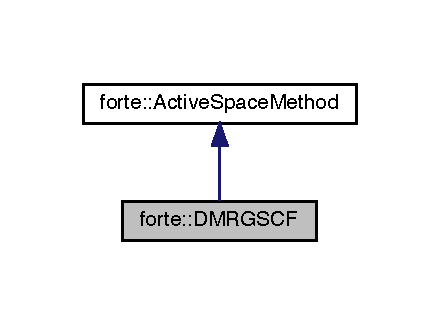
\includegraphics[width=211pt]{classforte_1_1_d_m_r_g_s_c_f__inherit__graph}
\end{center}
\end{figure}


Collaboration diagram for forte\+:\+:D\+M\+R\+G\+S\+CF\+:
\nopagebreak
\begin{figure}[H]
\begin{center}
\leavevmode
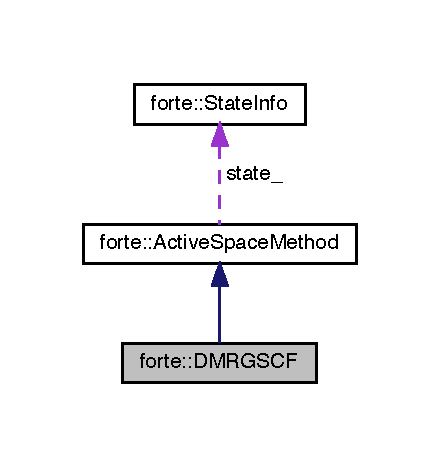
\includegraphics[width=211pt]{classforte_1_1_d_m_r_g_s_c_f__coll__graph}
\end{center}
\end{figure}
\subsection*{Public Member Functions}
\begin{DoxyCompactItemize}
\item 
\mbox{\hyperlink{classforte_1_1_d_m_r_g_s_c_f_a0f235613ad5aa55bea3fa6573dfb26f7}{D\+M\+R\+G\+S\+CF}} (\mbox{\hyperlink{classforte_1_1_state_info}{State\+Info}} \mbox{\hyperlink{classforte_1_1_active_space_method_a609f005cc7d3a1bc03ae517002eb19dc}{state}}, std\+::shared\+\_\+ptr$<$ \mbox{\hyperlink{classforte_1_1_s_c_f_info}{S\+C\+F\+Info}} $>$ scf\+\_\+info, std\+::shared\+\_\+ptr$<$ \mbox{\hyperlink{classforte_1_1_forte_options}{Forte\+Options}} $>$ options, std\+::shared\+\_\+ptr$<$ \mbox{\hyperlink{classforte_1_1_forte_integrals}{Forte\+Integrals}} $>$ ints, std\+::shared\+\_\+ptr$<$ \mbox{\hyperlink{classforte_1_1_m_o_space_info}{M\+O\+Space\+Info}} $>$ mo\+\_\+space\+\_\+info)
\item 
double \mbox{\hyperlink{classforte_1_1_d_m_r_g_s_c_f_a19128db2df6992b295bd00d85c43309d}{compute\+\_\+energy}} ()
\begin{DoxyCompactList}\small\item\em Compute the energy and return it. \end{DoxyCompactList}\item 
\mbox{\hyperlink{classforte_1_1_r_d_ms}{R\+D\+Ms}} \mbox{\hyperlink{classforte_1_1_d_m_r_g_s_c_f_a70de6c01bece616cd3ae66d337bc9b2f}{rmds}} ()
\item 
void \mbox{\hyperlink{classforte_1_1_d_m_r_g_s_c_f_ad4ba1745cefafba8b6d417ce4dbd9489}{set\+\_\+iterations}} (int dmrg\+\_\+iterations)
\end{DoxyCompactItemize}
\subsection*{Additional Inherited Members}


\subsection{Constructor \& Destructor Documentation}
\mbox{\Hypertarget{classforte_1_1_d_m_r_g_s_c_f_a0f235613ad5aa55bea3fa6573dfb26f7}\label{classforte_1_1_d_m_r_g_s_c_f_a0f235613ad5aa55bea3fa6573dfb26f7}} 
\index{forte\+::\+D\+M\+R\+G\+S\+CF@{forte\+::\+D\+M\+R\+G\+S\+CF}!D\+M\+R\+G\+S\+CF@{D\+M\+R\+G\+S\+CF}}
\index{D\+M\+R\+G\+S\+CF@{D\+M\+R\+G\+S\+CF}!forte\+::\+D\+M\+R\+G\+S\+CF@{forte\+::\+D\+M\+R\+G\+S\+CF}}
\subsubsection{\texorpdfstring{D\+M\+R\+G\+S\+C\+F()}{DMRGSCF()}}
{\footnotesize\ttfamily forte\+::\+D\+M\+R\+G\+S\+C\+F\+::\+D\+M\+R\+G\+S\+CF (\begin{DoxyParamCaption}\item[{\mbox{\hyperlink{classforte_1_1_state_info}{State\+Info}}}]{state,  }\item[{std\+::shared\+\_\+ptr$<$ \mbox{\hyperlink{classforte_1_1_s_c_f_info}{S\+C\+F\+Info}} $>$}]{scf\+\_\+info,  }\item[{std\+::shared\+\_\+ptr$<$ \mbox{\hyperlink{classforte_1_1_forte_options}{Forte\+Options}} $>$}]{options,  }\item[{std\+::shared\+\_\+ptr$<$ \mbox{\hyperlink{classforte_1_1_forte_integrals}{Forte\+Integrals}} $>$}]{ints,  }\item[{std\+::shared\+\_\+ptr$<$ \mbox{\hyperlink{classforte_1_1_m_o_space_info}{M\+O\+Space\+Info}} $>$}]{mo\+\_\+space\+\_\+info }\end{DoxyParamCaption})}



\subsection{Member Function Documentation}
\mbox{\Hypertarget{classforte_1_1_d_m_r_g_s_c_f_a19128db2df6992b295bd00d85c43309d}\label{classforte_1_1_d_m_r_g_s_c_f_a19128db2df6992b295bd00d85c43309d}} 
\index{forte\+::\+D\+M\+R\+G\+S\+CF@{forte\+::\+D\+M\+R\+G\+S\+CF}!compute\+\_\+energy@{compute\+\_\+energy}}
\index{compute\+\_\+energy@{compute\+\_\+energy}!forte\+::\+D\+M\+R\+G\+S\+CF@{forte\+::\+D\+M\+R\+G\+S\+CF}}
\subsubsection{\texorpdfstring{compute\+\_\+energy()}{compute\_energy()}}
{\footnotesize\ttfamily double forte\+::\+D\+M\+R\+G\+S\+C\+F\+::compute\+\_\+energy (\begin{DoxyParamCaption}{ }\end{DoxyParamCaption})\hspace{0.3cm}{\ttfamily [virtual]}}



Compute the energy and return it. 



Implements \mbox{\hyperlink{classforte_1_1_active_space_method_a99736e2b94405371b224b0750569b077}{forte\+::\+Active\+Space\+Method}}.

\mbox{\Hypertarget{classforte_1_1_d_m_r_g_s_c_f_a70de6c01bece616cd3ae66d337bc9b2f}\label{classforte_1_1_d_m_r_g_s_c_f_a70de6c01bece616cd3ae66d337bc9b2f}} 
\index{forte\+::\+D\+M\+R\+G\+S\+CF@{forte\+::\+D\+M\+R\+G\+S\+CF}!rmds@{rmds}}
\index{rmds@{rmds}!forte\+::\+D\+M\+R\+G\+S\+CF@{forte\+::\+D\+M\+R\+G\+S\+CF}}
\subsubsection{\texorpdfstring{rmds()}{rmds()}}
{\footnotesize\ttfamily \mbox{\hyperlink{classforte_1_1_r_d_ms}{R\+D\+Ms}} forte\+::\+D\+M\+R\+G\+S\+C\+F\+::rmds (\begin{DoxyParamCaption}{ }\end{DoxyParamCaption})\hspace{0.3cm}{\ttfamily [inline]}}

\mbox{\Hypertarget{classforte_1_1_d_m_r_g_s_c_f_ad4ba1745cefafba8b6d417ce4dbd9489}\label{classforte_1_1_d_m_r_g_s_c_f_ad4ba1745cefafba8b6d417ce4dbd9489}} 
\index{forte\+::\+D\+M\+R\+G\+S\+CF@{forte\+::\+D\+M\+R\+G\+S\+CF}!set\+\_\+iterations@{set\+\_\+iterations}}
\index{set\+\_\+iterations@{set\+\_\+iterations}!forte\+::\+D\+M\+R\+G\+S\+CF@{forte\+::\+D\+M\+R\+G\+S\+CF}}
\subsubsection{\texorpdfstring{set\+\_\+iterations()}{set\_iterations()}}
{\footnotesize\ttfamily void forte\+::\+D\+M\+R\+G\+S\+C\+F\+::set\+\_\+iterations (\begin{DoxyParamCaption}\item[{int}]{dmrg\+\_\+iterations }\end{DoxyParamCaption})\hspace{0.3cm}{\ttfamily [inline]}}



The documentation for this class was generated from the following file\+:\begin{DoxyCompactItemize}
\item 
/\+Users/fevange/\+Source/forte/src/dmrg/\mbox{\hyperlink{dmrgscf_8h}{dmrgscf.\+h}}\end{DoxyCompactItemize}

\hypertarget{classforte_1_1_d_m_r_g_solver}{}\section{forte\+:\+:D\+M\+R\+G\+Solver Class Reference}
\label{classforte_1_1_d_m_r_g_solver}\index{forte\+::\+D\+M\+R\+G\+Solver@{forte\+::\+D\+M\+R\+G\+Solver}}


{\ttfamily \#include $<$dmrgsolver.\+h$>$}

\subsection*{Public Member Functions}
\begin{DoxyCompactItemize}
\item 
\mbox{\hyperlink{classforte_1_1_d_m_r_g_solver_a5ebba6d331bf64c143e9d04e1a8aa1ff}{D\+M\+R\+G\+Solver}} (\mbox{\hyperlink{classforte_1_1_state_info}{State\+Info}} state, std\+::shared\+\_\+ptr$<$ \mbox{\hyperlink{classforte_1_1_s_c_f_info}{S\+C\+F\+Info}} $>$ scf\+\_\+info, std\+::shared\+\_\+ptr$<$ \mbox{\hyperlink{classforte_1_1_forte_options}{Forte\+Options}} $>$ options, std\+::shared\+\_\+ptr$<$ \mbox{\hyperlink{classforte_1_1_forte_integrals}{Forte\+Integrals}} $>$ ints, std\+::shared\+\_\+ptr$<$ \mbox{\hyperlink{classforte_1_1_m_o_space_info}{M\+O\+Space\+Info}} $>$ mo\+\_\+space\+\_\+info)
\item 
void \mbox{\hyperlink{classforte_1_1_d_m_r_g_solver_a814330798182f4bd92f17f6dae68ff84}{compute\+\_\+energy}} ()
\item 
\mbox{\hyperlink{classforte_1_1_r_d_ms}{R\+D\+Ms}} \mbox{\hyperlink{classforte_1_1_d_m_r_g_solver_a6ca5d416d6917bca2b012cc02a0b471e}{rdms}} ()
\item 
void \mbox{\hyperlink{classforte_1_1_d_m_r_g_solver_ad5cc293e3204cb77905758b2688f7275}{set\+\_\+max\+\_\+rdm}} (int max\+\_\+rdm)
\item 
void \mbox{\hyperlink{classforte_1_1_d_m_r_g_solver_a7f34b4aa229850ce78701122f7f20aa0}{spin\+\_\+free\+\_\+rdm}} (bool spin\+\_\+free)
\item 
void \mbox{\hyperlink{classforte_1_1_d_m_r_g_solver_aaec87fefcbd55f4af7aa1bb03cf3a3f8}{disk\+\_\+3\+\_\+rdm}} (bool use\+\_\+disk\+\_\+for\+\_\+3rdm)
\item 
void \mbox{\hyperlink{classforte_1_1_d_m_r_g_solver_a066b17dd1686e43c2de23ae57e6a3a64}{set\+\_\+up\+\_\+integrals}} (const ambit\+::\+Tensor \&active\+\_\+integrals, const std\+::vector$<$ double $>$ \&one\+\_\+body)
\item 
void \mbox{\hyperlink{classforte_1_1_d_m_r_g_solver_aca9ca177f2b8a10c9692eda29d883eec}{set\+\_\+scalar}} (double energy)
\end{DoxyCompactItemize}


\subsection{Constructor \& Destructor Documentation}
\mbox{\Hypertarget{classforte_1_1_d_m_r_g_solver_a5ebba6d331bf64c143e9d04e1a8aa1ff}\label{classforte_1_1_d_m_r_g_solver_a5ebba6d331bf64c143e9d04e1a8aa1ff}} 
\index{forte\+::\+D\+M\+R\+G\+Solver@{forte\+::\+D\+M\+R\+G\+Solver}!D\+M\+R\+G\+Solver@{D\+M\+R\+G\+Solver}}
\index{D\+M\+R\+G\+Solver@{D\+M\+R\+G\+Solver}!forte\+::\+D\+M\+R\+G\+Solver@{forte\+::\+D\+M\+R\+G\+Solver}}
\subsubsection{\texorpdfstring{D\+M\+R\+G\+Solver()}{DMRGSolver()}}
{\footnotesize\ttfamily forte\+::\+D\+M\+R\+G\+Solver\+::\+D\+M\+R\+G\+Solver (\begin{DoxyParamCaption}\item[{\mbox{\hyperlink{classforte_1_1_state_info}{State\+Info}}}]{state,  }\item[{std\+::shared\+\_\+ptr$<$ \mbox{\hyperlink{classforte_1_1_s_c_f_info}{S\+C\+F\+Info}} $>$}]{scf\+\_\+info,  }\item[{std\+::shared\+\_\+ptr$<$ \mbox{\hyperlink{classforte_1_1_forte_options}{Forte\+Options}} $>$}]{options,  }\item[{std\+::shared\+\_\+ptr$<$ \mbox{\hyperlink{classforte_1_1_forte_integrals}{Forte\+Integrals}} $>$}]{ints,  }\item[{std\+::shared\+\_\+ptr$<$ \mbox{\hyperlink{classforte_1_1_m_o_space_info}{M\+O\+Space\+Info}} $>$}]{mo\+\_\+space\+\_\+info }\end{DoxyParamCaption})}



\subsection{Member Function Documentation}
\mbox{\Hypertarget{classforte_1_1_d_m_r_g_solver_a814330798182f4bd92f17f6dae68ff84}\label{classforte_1_1_d_m_r_g_solver_a814330798182f4bd92f17f6dae68ff84}} 
\index{forte\+::\+D\+M\+R\+G\+Solver@{forte\+::\+D\+M\+R\+G\+Solver}!compute\+\_\+energy@{compute\+\_\+energy}}
\index{compute\+\_\+energy@{compute\+\_\+energy}!forte\+::\+D\+M\+R\+G\+Solver@{forte\+::\+D\+M\+R\+G\+Solver}}
\subsubsection{\texorpdfstring{compute\+\_\+energy()}{compute\_energy()}}
{\footnotesize\ttfamily void forte\+::\+D\+M\+R\+G\+Solver\+::compute\+\_\+energy (\begin{DoxyParamCaption}{ }\end{DoxyParamCaption})}

\mbox{\Hypertarget{classforte_1_1_d_m_r_g_solver_aaec87fefcbd55f4af7aa1bb03cf3a3f8}\label{classforte_1_1_d_m_r_g_solver_aaec87fefcbd55f4af7aa1bb03cf3a3f8}} 
\index{forte\+::\+D\+M\+R\+G\+Solver@{forte\+::\+D\+M\+R\+G\+Solver}!disk\+\_\+3\+\_\+rdm@{disk\+\_\+3\+\_\+rdm}}
\index{disk\+\_\+3\+\_\+rdm@{disk\+\_\+3\+\_\+rdm}!forte\+::\+D\+M\+R\+G\+Solver@{forte\+::\+D\+M\+R\+G\+Solver}}
\subsubsection{\texorpdfstring{disk\+\_\+3\+\_\+rdm()}{disk\_3\_rdm()}}
{\footnotesize\ttfamily void forte\+::\+D\+M\+R\+G\+Solver\+::disk\+\_\+3\+\_\+rdm (\begin{DoxyParamCaption}\item[{bool}]{use\+\_\+disk\+\_\+for\+\_\+3rdm }\end{DoxyParamCaption})\hspace{0.3cm}{\ttfamily [inline]}}

\mbox{\Hypertarget{classforte_1_1_d_m_r_g_solver_a6ca5d416d6917bca2b012cc02a0b471e}\label{classforte_1_1_d_m_r_g_solver_a6ca5d416d6917bca2b012cc02a0b471e}} 
\index{forte\+::\+D\+M\+R\+G\+Solver@{forte\+::\+D\+M\+R\+G\+Solver}!rdms@{rdms}}
\index{rdms@{rdms}!forte\+::\+D\+M\+R\+G\+Solver@{forte\+::\+D\+M\+R\+G\+Solver}}
\subsubsection{\texorpdfstring{rdms()}{rdms()}}
{\footnotesize\ttfamily \mbox{\hyperlink{classforte_1_1_r_d_ms}{R\+D\+Ms}} forte\+::\+D\+M\+R\+G\+Solver\+::rdms (\begin{DoxyParamCaption}{ }\end{DoxyParamCaption})\hspace{0.3cm}{\ttfamily [inline]}}

\mbox{\Hypertarget{classforte_1_1_d_m_r_g_solver_ad5cc293e3204cb77905758b2688f7275}\label{classforte_1_1_d_m_r_g_solver_ad5cc293e3204cb77905758b2688f7275}} 
\index{forte\+::\+D\+M\+R\+G\+Solver@{forte\+::\+D\+M\+R\+G\+Solver}!set\+\_\+max\+\_\+rdm@{set\+\_\+max\+\_\+rdm}}
\index{set\+\_\+max\+\_\+rdm@{set\+\_\+max\+\_\+rdm}!forte\+::\+D\+M\+R\+G\+Solver@{forte\+::\+D\+M\+R\+G\+Solver}}
\subsubsection{\texorpdfstring{set\+\_\+max\+\_\+rdm()}{set\_max\_rdm()}}
{\footnotesize\ttfamily void forte\+::\+D\+M\+R\+G\+Solver\+::set\+\_\+max\+\_\+rdm (\begin{DoxyParamCaption}\item[{int}]{max\+\_\+rdm }\end{DoxyParamCaption})\hspace{0.3cm}{\ttfamily [inline]}}

\mbox{\Hypertarget{classforte_1_1_d_m_r_g_solver_aca9ca177f2b8a10c9692eda29d883eec}\label{classforte_1_1_d_m_r_g_solver_aca9ca177f2b8a10c9692eda29d883eec}} 
\index{forte\+::\+D\+M\+R\+G\+Solver@{forte\+::\+D\+M\+R\+G\+Solver}!set\+\_\+scalar@{set\+\_\+scalar}}
\index{set\+\_\+scalar@{set\+\_\+scalar}!forte\+::\+D\+M\+R\+G\+Solver@{forte\+::\+D\+M\+R\+G\+Solver}}
\subsubsection{\texorpdfstring{set\+\_\+scalar()}{set\_scalar()}}
{\footnotesize\ttfamily void forte\+::\+D\+M\+R\+G\+Solver\+::set\+\_\+scalar (\begin{DoxyParamCaption}\item[{double}]{energy }\end{DoxyParamCaption})\hspace{0.3cm}{\ttfamily [inline]}}

\mbox{\Hypertarget{classforte_1_1_d_m_r_g_solver_a066b17dd1686e43c2de23ae57e6a3a64}\label{classforte_1_1_d_m_r_g_solver_a066b17dd1686e43c2de23ae57e6a3a64}} 
\index{forte\+::\+D\+M\+R\+G\+Solver@{forte\+::\+D\+M\+R\+G\+Solver}!set\+\_\+up\+\_\+integrals@{set\+\_\+up\+\_\+integrals}}
\index{set\+\_\+up\+\_\+integrals@{set\+\_\+up\+\_\+integrals}!forte\+::\+D\+M\+R\+G\+Solver@{forte\+::\+D\+M\+R\+G\+Solver}}
\subsubsection{\texorpdfstring{set\+\_\+up\+\_\+integrals()}{set\_up\_integrals()}}
{\footnotesize\ttfamily void forte\+::\+D\+M\+R\+G\+Solver\+::set\+\_\+up\+\_\+integrals (\begin{DoxyParamCaption}\item[{const ambit\+::\+Tensor \&}]{active\+\_\+integrals,  }\item[{const std\+::vector$<$ double $>$ \&}]{one\+\_\+body }\end{DoxyParamCaption})\hspace{0.3cm}{\ttfamily [inline]}}

\mbox{\Hypertarget{classforte_1_1_d_m_r_g_solver_a7f34b4aa229850ce78701122f7f20aa0}\label{classforte_1_1_d_m_r_g_solver_a7f34b4aa229850ce78701122f7f20aa0}} 
\index{forte\+::\+D\+M\+R\+G\+Solver@{forte\+::\+D\+M\+R\+G\+Solver}!spin\+\_\+free\+\_\+rdm@{spin\+\_\+free\+\_\+rdm}}
\index{spin\+\_\+free\+\_\+rdm@{spin\+\_\+free\+\_\+rdm}!forte\+::\+D\+M\+R\+G\+Solver@{forte\+::\+D\+M\+R\+G\+Solver}}
\subsubsection{\texorpdfstring{spin\+\_\+free\+\_\+rdm()}{spin\_free\_rdm()}}
{\footnotesize\ttfamily void forte\+::\+D\+M\+R\+G\+Solver\+::spin\+\_\+free\+\_\+rdm (\begin{DoxyParamCaption}\item[{bool}]{spin\+\_\+free }\end{DoxyParamCaption})\hspace{0.3cm}{\ttfamily [inline]}}



The documentation for this class was generated from the following file\+:\begin{DoxyCompactItemize}
\item 
/\+Users/fevange/\+Source/forte/src/dmrg/\mbox{\hyperlink{dmrgsolver_8h}{dmrgsolver.\+h}}\end{DoxyCompactItemize}

\hypertarget{classforte_1_1_dressed_quantity}{}\section{forte\+:\+:Dressed\+Quantity Class Reference}
\label{classforte_1_1_dressed_quantity}\index{forte\+::\+Dressed\+Quantity@{forte\+::\+Dressed\+Quantity}}


{\ttfamily \#include $<$dsrg\+\_\+transformed.\+h$>$}

\subsection*{Public Member Functions}
\begin{DoxyCompactItemize}
\item 
\mbox{\hyperlink{classforte_1_1_dressed_quantity_a3fa0227d12e055f33566c46750898d10}{Dressed\+Quantity}} ()
\item 
\mbox{\hyperlink{classforte_1_1_dressed_quantity_a7f60134c01eeddca427024865f315d20}{Dressed\+Quantity}} (double scalar)
\item 
\mbox{\hyperlink{classforte_1_1_dressed_quantity_aa3daf37f0ebc740b33f824beb7a92914}{Dressed\+Quantity}} (double scalar, ambit\+::\+Tensor a, ambit\+::\+Tensor b)
\item 
\mbox{\hyperlink{classforte_1_1_dressed_quantity_a13194b9e4e59de0d776ec546d24917a6}{Dressed\+Quantity}} (double scalar, ambit\+::\+Tensor a, ambit\+::\+Tensor b, ambit\+::\+Tensor aa, ambit\+::\+Tensor ab, ambit\+::\+Tensor bb)
\item 
\mbox{\hyperlink{classforte_1_1_dressed_quantity_a8f7a52a1b07c6b79a41db6dd410328f1}{Dressed\+Quantity}} (double scalar, ambit\+::\+Tensor a, ambit\+::\+Tensor b, ambit\+::\+Tensor aa, ambit\+::\+Tensor ab, ambit\+::\+Tensor bb, ambit\+::\+Tensor aaa, ambit\+::\+Tensor aab, ambit\+::\+Tensor abb, ambit\+::\+Tensor bbb)
\item 
double \mbox{\hyperlink{classforte_1_1_dressed_quantity_a349522c7b40185549cd5bc5114d413e7}{contract\+\_\+with\+\_\+rdms}} (\mbox{\hyperlink{classforte_1_1_r_d_ms}{R\+D\+Ms}} rdms)
\end{DoxyCompactItemize}


\subsection{Constructor \& Destructor Documentation}
\mbox{\Hypertarget{classforte_1_1_dressed_quantity_a3fa0227d12e055f33566c46750898d10}\label{classforte_1_1_dressed_quantity_a3fa0227d12e055f33566c46750898d10}} 
\index{forte\+::\+Dressed\+Quantity@{forte\+::\+Dressed\+Quantity}!Dressed\+Quantity@{Dressed\+Quantity}}
\index{Dressed\+Quantity@{Dressed\+Quantity}!forte\+::\+Dressed\+Quantity@{forte\+::\+Dressed\+Quantity}}
\subsubsection{\texorpdfstring{Dressed\+Quantity()}{DressedQuantity()}\hspace{0.1cm}{\footnotesize\ttfamily [1/5]}}
{\footnotesize\ttfamily forte\+::\+Dressed\+Quantity\+::\+Dressed\+Quantity (\begin{DoxyParamCaption}{ }\end{DoxyParamCaption})}

\mbox{\Hypertarget{classforte_1_1_dressed_quantity_a7f60134c01eeddca427024865f315d20}\label{classforte_1_1_dressed_quantity_a7f60134c01eeddca427024865f315d20}} 
\index{forte\+::\+Dressed\+Quantity@{forte\+::\+Dressed\+Quantity}!Dressed\+Quantity@{Dressed\+Quantity}}
\index{Dressed\+Quantity@{Dressed\+Quantity}!forte\+::\+Dressed\+Quantity@{forte\+::\+Dressed\+Quantity}}
\subsubsection{\texorpdfstring{Dressed\+Quantity()}{DressedQuantity()}\hspace{0.1cm}{\footnotesize\ttfamily [2/5]}}
{\footnotesize\ttfamily forte\+::\+Dressed\+Quantity\+::\+Dressed\+Quantity (\begin{DoxyParamCaption}\item[{double}]{scalar }\end{DoxyParamCaption})}

\mbox{\Hypertarget{classforte_1_1_dressed_quantity_aa3daf37f0ebc740b33f824beb7a92914}\label{classforte_1_1_dressed_quantity_aa3daf37f0ebc740b33f824beb7a92914}} 
\index{forte\+::\+Dressed\+Quantity@{forte\+::\+Dressed\+Quantity}!Dressed\+Quantity@{Dressed\+Quantity}}
\index{Dressed\+Quantity@{Dressed\+Quantity}!forte\+::\+Dressed\+Quantity@{forte\+::\+Dressed\+Quantity}}
\subsubsection{\texorpdfstring{Dressed\+Quantity()}{DressedQuantity()}\hspace{0.1cm}{\footnotesize\ttfamily [3/5]}}
{\footnotesize\ttfamily forte\+::\+Dressed\+Quantity\+::\+Dressed\+Quantity (\begin{DoxyParamCaption}\item[{double}]{scalar,  }\item[{ambit\+::\+Tensor}]{a,  }\item[{ambit\+::\+Tensor}]{b }\end{DoxyParamCaption})}

\mbox{\Hypertarget{classforte_1_1_dressed_quantity_a13194b9e4e59de0d776ec546d24917a6}\label{classforte_1_1_dressed_quantity_a13194b9e4e59de0d776ec546d24917a6}} 
\index{forte\+::\+Dressed\+Quantity@{forte\+::\+Dressed\+Quantity}!Dressed\+Quantity@{Dressed\+Quantity}}
\index{Dressed\+Quantity@{Dressed\+Quantity}!forte\+::\+Dressed\+Quantity@{forte\+::\+Dressed\+Quantity}}
\subsubsection{\texorpdfstring{Dressed\+Quantity()}{DressedQuantity()}\hspace{0.1cm}{\footnotesize\ttfamily [4/5]}}
{\footnotesize\ttfamily forte\+::\+Dressed\+Quantity\+::\+Dressed\+Quantity (\begin{DoxyParamCaption}\item[{double}]{scalar,  }\item[{ambit\+::\+Tensor}]{a,  }\item[{ambit\+::\+Tensor}]{b,  }\item[{ambit\+::\+Tensor}]{aa,  }\item[{ambit\+::\+Tensor}]{ab,  }\item[{ambit\+::\+Tensor}]{bb }\end{DoxyParamCaption})}

\mbox{\Hypertarget{classforte_1_1_dressed_quantity_a8f7a52a1b07c6b79a41db6dd410328f1}\label{classforte_1_1_dressed_quantity_a8f7a52a1b07c6b79a41db6dd410328f1}} 
\index{forte\+::\+Dressed\+Quantity@{forte\+::\+Dressed\+Quantity}!Dressed\+Quantity@{Dressed\+Quantity}}
\index{Dressed\+Quantity@{Dressed\+Quantity}!forte\+::\+Dressed\+Quantity@{forte\+::\+Dressed\+Quantity}}
\subsubsection{\texorpdfstring{Dressed\+Quantity()}{DressedQuantity()}\hspace{0.1cm}{\footnotesize\ttfamily [5/5]}}
{\footnotesize\ttfamily forte\+::\+Dressed\+Quantity\+::\+Dressed\+Quantity (\begin{DoxyParamCaption}\item[{double}]{scalar,  }\item[{ambit\+::\+Tensor}]{a,  }\item[{ambit\+::\+Tensor}]{b,  }\item[{ambit\+::\+Tensor}]{aa,  }\item[{ambit\+::\+Tensor}]{ab,  }\item[{ambit\+::\+Tensor}]{bb,  }\item[{ambit\+::\+Tensor}]{aaa,  }\item[{ambit\+::\+Tensor}]{aab,  }\item[{ambit\+::\+Tensor}]{abb,  }\item[{ambit\+::\+Tensor}]{bbb }\end{DoxyParamCaption})}



\subsection{Member Function Documentation}
\mbox{\Hypertarget{classforte_1_1_dressed_quantity_a349522c7b40185549cd5bc5114d413e7}\label{classforte_1_1_dressed_quantity_a349522c7b40185549cd5bc5114d413e7}} 
\index{forte\+::\+Dressed\+Quantity@{forte\+::\+Dressed\+Quantity}!contract\+\_\+with\+\_\+rdms@{contract\+\_\+with\+\_\+rdms}}
\index{contract\+\_\+with\+\_\+rdms@{contract\+\_\+with\+\_\+rdms}!forte\+::\+Dressed\+Quantity@{forte\+::\+Dressed\+Quantity}}
\subsubsection{\texorpdfstring{contract\+\_\+with\+\_\+rdms()}{contract\_with\_rdms()}}
{\footnotesize\ttfamily double forte\+::\+Dressed\+Quantity\+::contract\+\_\+with\+\_\+rdms (\begin{DoxyParamCaption}\item[{\mbox{\hyperlink{classforte_1_1_r_d_ms}{R\+D\+Ms}}}]{rdms }\end{DoxyParamCaption})}



The documentation for this class was generated from the following files\+:\begin{DoxyCompactItemize}
\item 
/\+Users/fevange/\+Source/forte/src/mrdsrg-\/helper/\mbox{\hyperlink{dsrg__transformed_8h}{dsrg\+\_\+transformed.\+h}}\item 
/\+Users/fevange/\+Source/forte/src/mrdsrg-\/helper/\mbox{\hyperlink{dsrg__transformed_8cc}{dsrg\+\_\+transformed.\+cc}}\end{DoxyCompactItemize}

\hypertarget{classforte_1_1_d_s_r_g___m_e_m}{}\section{forte\+:\+:D\+S\+R\+G\+\_\+\+M\+EM Class Reference}
\label{classforte_1_1_d_s_r_g___m_e_m}\index{forte\+::\+D\+S\+R\+G\+\_\+\+M\+EM@{forte\+::\+D\+S\+R\+G\+\_\+\+M\+EM}}


{\ttfamily \#include $<$dsrg\+\_\+mem.\+h$>$}

\subsection*{Public Member Functions}
\begin{DoxyCompactItemize}
\item 
\mbox{\hyperlink{classforte_1_1_d_s_r_g___m_e_m_a7889ef1265286f9e83d4f2e57f2d0184}{D\+S\+R\+G\+\_\+\+M\+EM}} ()
\begin{DoxyCompactList}\small\item\em Default constructor. \end{DoxyCompactList}\item 
\mbox{\hyperlink{classforte_1_1_d_s_r_g___m_e_m_aca48bd076cfd1e92573821a857b76e54}{D\+S\+R\+G\+\_\+\+M\+EM}} (int64\+\_\+t mem\+\_\+avai, std\+::map$<$ char, size\+\_\+t $>$ label\+\_\+to\+\_\+size)
\begin{DoxyCompactList}\small\item\em Constructor using a map from MO labels to their sizes. \end{DoxyCompactList}\item 
void \mbox{\hyperlink{classforte_1_1_d_s_r_g___m_e_m_a6385e6f596c51a495f537672f6c86b4e}{set\+\_\+mem\+\_\+avai}} (int64\+\_\+t mem\+\_\+avai)
\begin{DoxyCompactList}\small\item\em Set memory currently available. \end{DoxyCompactList}\item 
void \mbox{\hyperlink{classforte_1_1_d_s_r_g___m_e_m_a6f9be312b939223601bbc870700a5b49}{set\+\_\+label\+\_\+to\+\_\+size}} (std\+::map$<$ char, size\+\_\+t $>$ label\+\_\+to\+\_\+size)
\begin{DoxyCompactList}\small\item\em Set the map from MO label to the corresponding size. \end{DoxyCompactList}\item 
size\+\_\+t \mbox{\hyperlink{classforte_1_1_d_s_r_g___m_e_m_a2339785c4d656ff51becb628c9c60926}{available}} ()
\begin{DoxyCompactList}\small\item\em Return the available memory. \end{DoxyCompactList}\item 
void \mbox{\hyperlink{classforte_1_1_d_s_r_g___m_e_m_afe7b7579d767ee201146458caefcd944}{clean\+\_\+local\+\_\+memory}} ()
\begin{DoxyCompactList}\small\item\em Clean up local memories. \end{DoxyCompactList}\item 
size\+\_\+t \mbox{\hyperlink{classforte_1_1_d_s_r_g___m_e_m_a1dd2f817f76bda4a890bf15c60664dcf}{max\+\_\+local\+\_\+memory}} ()
\begin{DoxyCompactList}\small\item\em Max memory usage among the vector of local memories. \end{DoxyCompactList}\item 
void \mbox{\hyperlink{classforte_1_1_d_s_r_g___m_e_m_a6b2ef9118482dc897088d28d29cffe2a}{add\+\_\+print\+\_\+entry}} (const std\+::string \&des, const size\+\_\+t \&mem\+\_\+use)
\begin{DoxyCompactList}\small\item\em Add an innocent entry using description and its number of elements. \end{DoxyCompactList}\item 
void \mbox{\hyperlink{classforte_1_1_d_s_r_g___m_e_m_ad985484ea1139ca02fe50024656a9a11}{add\+\_\+entry}} (const std\+::string \&des, const size\+\_\+t \&mem\+\_\+use, bool subtract=true)
\begin{DoxyCompactList}\small\item\em Add entry using description and its number of elements. \end{DoxyCompactList}\item 
void \mbox{\hyperlink{classforte_1_1_d_s_r_g___m_e_m_aa970ba2e3f8577ad44aa32f8d84fe80e}{add\+\_\+entry}} (const std\+::string \&des, const std\+::vector$<$ std\+::string $>$ \&labels\+\_\+vec, int multiple=1, bool subtract=true)
\begin{DoxyCompactList}\small\item\em Add entry using the description and the block labels. \end{DoxyCompactList}\item 
size\+\_\+t \mbox{\hyperlink{classforte_1_1_d_s_r_g___m_e_m_ad7377189079c97664a573643259743e3}{compute\+\_\+n\+\_\+elements}} (const std\+::string \&labels)
\begin{DoxyCompactList}\small\item\em Compute the number of elements of a given labels. \end{DoxyCompactList}\item 
size\+\_\+t \mbox{\hyperlink{classforte_1_1_d_s_r_g___m_e_m_a43e1ba53bcac873bcec050cf7676751d}{compute\+\_\+memory}} (const std\+::vector$<$ std\+::string $>$ \&labels\+\_\+vec, int multiple=1)
\begin{DoxyCompactList}\small\item\em Compute the memory requirement of a given labels. \end{DoxyCompactList}\item 
void \mbox{\hyperlink{classforte_1_1_d_s_r_g___m_e_m_a676b78c5a39feea83a2fdaafe87a5e78}{print}} (const std\+::string \&name)
\begin{DoxyCompactList}\small\item\em Print the current data. \end{DoxyCompactList}\end{DoxyCompactItemize}


\subsection{Constructor \& Destructor Documentation}
\mbox{\Hypertarget{classforte_1_1_d_s_r_g___m_e_m_a7889ef1265286f9e83d4f2e57f2d0184}\label{classforte_1_1_d_s_r_g___m_e_m_a7889ef1265286f9e83d4f2e57f2d0184}} 
\index{forte\+::\+D\+S\+R\+G\+\_\+\+M\+EM@{forte\+::\+D\+S\+R\+G\+\_\+\+M\+EM}!D\+S\+R\+G\+\_\+\+M\+EM@{D\+S\+R\+G\+\_\+\+M\+EM}}
\index{D\+S\+R\+G\+\_\+\+M\+EM@{D\+S\+R\+G\+\_\+\+M\+EM}!forte\+::\+D\+S\+R\+G\+\_\+\+M\+EM@{forte\+::\+D\+S\+R\+G\+\_\+\+M\+EM}}
\subsubsection{\texorpdfstring{D\+S\+R\+G\+\_\+\+M\+E\+M()}{DSRG\_MEM()}\hspace{0.1cm}{\footnotesize\ttfamily [1/2]}}
{\footnotesize\ttfamily forte\+::\+D\+S\+R\+G\+\_\+\+M\+E\+M\+::\+D\+S\+R\+G\+\_\+\+M\+EM (\begin{DoxyParamCaption}{ }\end{DoxyParamCaption})}



Default constructor. 

\mbox{\Hypertarget{classforte_1_1_d_s_r_g___m_e_m_aca48bd076cfd1e92573821a857b76e54}\label{classforte_1_1_d_s_r_g___m_e_m_aca48bd076cfd1e92573821a857b76e54}} 
\index{forte\+::\+D\+S\+R\+G\+\_\+\+M\+EM@{forte\+::\+D\+S\+R\+G\+\_\+\+M\+EM}!D\+S\+R\+G\+\_\+\+M\+EM@{D\+S\+R\+G\+\_\+\+M\+EM}}
\index{D\+S\+R\+G\+\_\+\+M\+EM@{D\+S\+R\+G\+\_\+\+M\+EM}!forte\+::\+D\+S\+R\+G\+\_\+\+M\+EM@{forte\+::\+D\+S\+R\+G\+\_\+\+M\+EM}}
\subsubsection{\texorpdfstring{D\+S\+R\+G\+\_\+\+M\+E\+M()}{DSRG\_MEM()}\hspace{0.1cm}{\footnotesize\ttfamily [2/2]}}
{\footnotesize\ttfamily forte\+::\+D\+S\+R\+G\+\_\+\+M\+E\+M\+::\+D\+S\+R\+G\+\_\+\+M\+EM (\begin{DoxyParamCaption}\item[{int64\+\_\+t}]{mem\+\_\+avai,  }\item[{std\+::map$<$ char, size\+\_\+t $>$}]{label\+\_\+to\+\_\+size }\end{DoxyParamCaption})}



Constructor using a map from MO labels to their sizes. 



\subsection{Member Function Documentation}
\mbox{\Hypertarget{classforte_1_1_d_s_r_g___m_e_m_ad985484ea1139ca02fe50024656a9a11}\label{classforte_1_1_d_s_r_g___m_e_m_ad985484ea1139ca02fe50024656a9a11}} 
\index{forte\+::\+D\+S\+R\+G\+\_\+\+M\+EM@{forte\+::\+D\+S\+R\+G\+\_\+\+M\+EM}!add\+\_\+entry@{add\+\_\+entry}}
\index{add\+\_\+entry@{add\+\_\+entry}!forte\+::\+D\+S\+R\+G\+\_\+\+M\+EM@{forte\+::\+D\+S\+R\+G\+\_\+\+M\+EM}}
\subsubsection{\texorpdfstring{add\+\_\+entry()}{add\_entry()}\hspace{0.1cm}{\footnotesize\ttfamily [1/2]}}
{\footnotesize\ttfamily void forte\+::\+D\+S\+R\+G\+\_\+\+M\+E\+M\+::add\+\_\+entry (\begin{DoxyParamCaption}\item[{const std\+::string \&}]{des,  }\item[{const size\+\_\+t \&}]{mem\+\_\+use,  }\item[{bool}]{subtract = {\ttfamily true} }\end{DoxyParamCaption})}



Add entry using description and its number of elements. 

\mbox{\Hypertarget{classforte_1_1_d_s_r_g___m_e_m_aa970ba2e3f8577ad44aa32f8d84fe80e}\label{classforte_1_1_d_s_r_g___m_e_m_aa970ba2e3f8577ad44aa32f8d84fe80e}} 
\index{forte\+::\+D\+S\+R\+G\+\_\+\+M\+EM@{forte\+::\+D\+S\+R\+G\+\_\+\+M\+EM}!add\+\_\+entry@{add\+\_\+entry}}
\index{add\+\_\+entry@{add\+\_\+entry}!forte\+::\+D\+S\+R\+G\+\_\+\+M\+EM@{forte\+::\+D\+S\+R\+G\+\_\+\+M\+EM}}
\subsubsection{\texorpdfstring{add\+\_\+entry()}{add\_entry()}\hspace{0.1cm}{\footnotesize\ttfamily [2/2]}}
{\footnotesize\ttfamily void forte\+::\+D\+S\+R\+G\+\_\+\+M\+E\+M\+::add\+\_\+entry (\begin{DoxyParamCaption}\item[{const std\+::string \&}]{des,  }\item[{const std\+::vector$<$ std\+::string $>$ \&}]{labels\+\_\+vec,  }\item[{int}]{multiple = {\ttfamily 1},  }\item[{bool}]{subtract = {\ttfamily true} }\end{DoxyParamCaption})}



Add entry using the description and the block labels. 

\mbox{\Hypertarget{classforte_1_1_d_s_r_g___m_e_m_a6b2ef9118482dc897088d28d29cffe2a}\label{classforte_1_1_d_s_r_g___m_e_m_a6b2ef9118482dc897088d28d29cffe2a}} 
\index{forte\+::\+D\+S\+R\+G\+\_\+\+M\+EM@{forte\+::\+D\+S\+R\+G\+\_\+\+M\+EM}!add\+\_\+print\+\_\+entry@{add\+\_\+print\+\_\+entry}}
\index{add\+\_\+print\+\_\+entry@{add\+\_\+print\+\_\+entry}!forte\+::\+D\+S\+R\+G\+\_\+\+M\+EM@{forte\+::\+D\+S\+R\+G\+\_\+\+M\+EM}}
\subsubsection{\texorpdfstring{add\+\_\+print\+\_\+entry()}{add\_print\_entry()}}
{\footnotesize\ttfamily void forte\+::\+D\+S\+R\+G\+\_\+\+M\+E\+M\+::add\+\_\+print\+\_\+entry (\begin{DoxyParamCaption}\item[{const std\+::string \&}]{des,  }\item[{const size\+\_\+t \&}]{mem\+\_\+use }\end{DoxyParamCaption})}



Add an innocent entry using description and its number of elements. 

\mbox{\Hypertarget{classforte_1_1_d_s_r_g___m_e_m_a2339785c4d656ff51becb628c9c60926}\label{classforte_1_1_d_s_r_g___m_e_m_a2339785c4d656ff51becb628c9c60926}} 
\index{forte\+::\+D\+S\+R\+G\+\_\+\+M\+EM@{forte\+::\+D\+S\+R\+G\+\_\+\+M\+EM}!available@{available}}
\index{available@{available}!forte\+::\+D\+S\+R\+G\+\_\+\+M\+EM@{forte\+::\+D\+S\+R\+G\+\_\+\+M\+EM}}
\subsubsection{\texorpdfstring{available()}{available()}}
{\footnotesize\ttfamily size\+\_\+t forte\+::\+D\+S\+R\+G\+\_\+\+M\+E\+M\+::available (\begin{DoxyParamCaption}{ }\end{DoxyParamCaption})\hspace{0.3cm}{\ttfamily [inline]}}



Return the available memory. 

\mbox{\Hypertarget{classforte_1_1_d_s_r_g___m_e_m_afe7b7579d767ee201146458caefcd944}\label{classforte_1_1_d_s_r_g___m_e_m_afe7b7579d767ee201146458caefcd944}} 
\index{forte\+::\+D\+S\+R\+G\+\_\+\+M\+EM@{forte\+::\+D\+S\+R\+G\+\_\+\+M\+EM}!clean\+\_\+local\+\_\+memory@{clean\+\_\+local\+\_\+memory}}
\index{clean\+\_\+local\+\_\+memory@{clean\+\_\+local\+\_\+memory}!forte\+::\+D\+S\+R\+G\+\_\+\+M\+EM@{forte\+::\+D\+S\+R\+G\+\_\+\+M\+EM}}
\subsubsection{\texorpdfstring{clean\+\_\+local\+\_\+memory()}{clean\_local\_memory()}}
{\footnotesize\ttfamily void forte\+::\+D\+S\+R\+G\+\_\+\+M\+E\+M\+::clean\+\_\+local\+\_\+memory (\begin{DoxyParamCaption}{ }\end{DoxyParamCaption})\hspace{0.3cm}{\ttfamily [inline]}}



Clean up local memories. 

\mbox{\Hypertarget{classforte_1_1_d_s_r_g___m_e_m_a43e1ba53bcac873bcec050cf7676751d}\label{classforte_1_1_d_s_r_g___m_e_m_a43e1ba53bcac873bcec050cf7676751d}} 
\index{forte\+::\+D\+S\+R\+G\+\_\+\+M\+EM@{forte\+::\+D\+S\+R\+G\+\_\+\+M\+EM}!compute\+\_\+memory@{compute\+\_\+memory}}
\index{compute\+\_\+memory@{compute\+\_\+memory}!forte\+::\+D\+S\+R\+G\+\_\+\+M\+EM@{forte\+::\+D\+S\+R\+G\+\_\+\+M\+EM}}
\subsubsection{\texorpdfstring{compute\+\_\+memory()}{compute\_memory()}}
{\footnotesize\ttfamily size\+\_\+t forte\+::\+D\+S\+R\+G\+\_\+\+M\+E\+M\+::compute\+\_\+memory (\begin{DoxyParamCaption}\item[{const std\+::vector$<$ std\+::string $>$ \&}]{labels\+\_\+vec,  }\item[{int}]{multiple = {\ttfamily 1} }\end{DoxyParamCaption})}



Compute the memory requirement of a given labels. 

\mbox{\Hypertarget{classforte_1_1_d_s_r_g___m_e_m_ad7377189079c97664a573643259743e3}\label{classforte_1_1_d_s_r_g___m_e_m_ad7377189079c97664a573643259743e3}} 
\index{forte\+::\+D\+S\+R\+G\+\_\+\+M\+EM@{forte\+::\+D\+S\+R\+G\+\_\+\+M\+EM}!compute\+\_\+n\+\_\+elements@{compute\+\_\+n\+\_\+elements}}
\index{compute\+\_\+n\+\_\+elements@{compute\+\_\+n\+\_\+elements}!forte\+::\+D\+S\+R\+G\+\_\+\+M\+EM@{forte\+::\+D\+S\+R\+G\+\_\+\+M\+EM}}
\subsubsection{\texorpdfstring{compute\+\_\+n\+\_\+elements()}{compute\_n\_elements()}}
{\footnotesize\ttfamily size\+\_\+t forte\+::\+D\+S\+R\+G\+\_\+\+M\+E\+M\+::compute\+\_\+n\+\_\+elements (\begin{DoxyParamCaption}\item[{const std\+::string \&}]{labels }\end{DoxyParamCaption})}



Compute the number of elements of a given labels. 

\mbox{\Hypertarget{classforte_1_1_d_s_r_g___m_e_m_a1dd2f817f76bda4a890bf15c60664dcf}\label{classforte_1_1_d_s_r_g___m_e_m_a1dd2f817f76bda4a890bf15c60664dcf}} 
\index{forte\+::\+D\+S\+R\+G\+\_\+\+M\+EM@{forte\+::\+D\+S\+R\+G\+\_\+\+M\+EM}!max\+\_\+local\+\_\+memory@{max\+\_\+local\+\_\+memory}}
\index{max\+\_\+local\+\_\+memory@{max\+\_\+local\+\_\+memory}!forte\+::\+D\+S\+R\+G\+\_\+\+M\+EM@{forte\+::\+D\+S\+R\+G\+\_\+\+M\+EM}}
\subsubsection{\texorpdfstring{max\+\_\+local\+\_\+memory()}{max\_local\_memory()}}
{\footnotesize\ttfamily size\+\_\+t forte\+::\+D\+S\+R\+G\+\_\+\+M\+E\+M\+::max\+\_\+local\+\_\+memory (\begin{DoxyParamCaption}{ }\end{DoxyParamCaption})}



Max memory usage among the vector of local memories. 

\mbox{\Hypertarget{classforte_1_1_d_s_r_g___m_e_m_a676b78c5a39feea83a2fdaafe87a5e78}\label{classforte_1_1_d_s_r_g___m_e_m_a676b78c5a39feea83a2fdaafe87a5e78}} 
\index{forte\+::\+D\+S\+R\+G\+\_\+\+M\+EM@{forte\+::\+D\+S\+R\+G\+\_\+\+M\+EM}!print@{print}}
\index{print@{print}!forte\+::\+D\+S\+R\+G\+\_\+\+M\+EM@{forte\+::\+D\+S\+R\+G\+\_\+\+M\+EM}}
\subsubsection{\texorpdfstring{print()}{print()}}
{\footnotesize\ttfamily void forte\+::\+D\+S\+R\+G\+\_\+\+M\+E\+M\+::print (\begin{DoxyParamCaption}\item[{const std\+::string \&}]{name }\end{DoxyParamCaption})}



Print the current data. 

\mbox{\Hypertarget{classforte_1_1_d_s_r_g___m_e_m_a6f9be312b939223601bbc870700a5b49}\label{classforte_1_1_d_s_r_g___m_e_m_a6f9be312b939223601bbc870700a5b49}} 
\index{forte\+::\+D\+S\+R\+G\+\_\+\+M\+EM@{forte\+::\+D\+S\+R\+G\+\_\+\+M\+EM}!set\+\_\+label\+\_\+to\+\_\+size@{set\+\_\+label\+\_\+to\+\_\+size}}
\index{set\+\_\+label\+\_\+to\+\_\+size@{set\+\_\+label\+\_\+to\+\_\+size}!forte\+::\+D\+S\+R\+G\+\_\+\+M\+EM@{forte\+::\+D\+S\+R\+G\+\_\+\+M\+EM}}
\subsubsection{\texorpdfstring{set\+\_\+label\+\_\+to\+\_\+size()}{set\_label\_to\_size()}}
{\footnotesize\ttfamily void forte\+::\+D\+S\+R\+G\+\_\+\+M\+E\+M\+::set\+\_\+label\+\_\+to\+\_\+size (\begin{DoxyParamCaption}\item[{std\+::map$<$ char, size\+\_\+t $>$}]{label\+\_\+to\+\_\+size }\end{DoxyParamCaption})\hspace{0.3cm}{\ttfamily [inline]}}



Set the map from MO label to the corresponding size. 

\mbox{\Hypertarget{classforte_1_1_d_s_r_g___m_e_m_a6385e6f596c51a495f537672f6c86b4e}\label{classforte_1_1_d_s_r_g___m_e_m_a6385e6f596c51a495f537672f6c86b4e}} 
\index{forte\+::\+D\+S\+R\+G\+\_\+\+M\+EM@{forte\+::\+D\+S\+R\+G\+\_\+\+M\+EM}!set\+\_\+mem\+\_\+avai@{set\+\_\+mem\+\_\+avai}}
\index{set\+\_\+mem\+\_\+avai@{set\+\_\+mem\+\_\+avai}!forte\+::\+D\+S\+R\+G\+\_\+\+M\+EM@{forte\+::\+D\+S\+R\+G\+\_\+\+M\+EM}}
\subsubsection{\texorpdfstring{set\+\_\+mem\+\_\+avai()}{set\_mem\_avai()}}
{\footnotesize\ttfamily void forte\+::\+D\+S\+R\+G\+\_\+\+M\+E\+M\+::set\+\_\+mem\+\_\+avai (\begin{DoxyParamCaption}\item[{int64\+\_\+t}]{mem\+\_\+avai }\end{DoxyParamCaption})\hspace{0.3cm}{\ttfamily [inline]}}



Set memory currently available. 



The documentation for this class was generated from the following files\+:\begin{DoxyCompactItemize}
\item 
/\+Users/fevange/\+Source/forte/src/mrdsrg-\/helper/\mbox{\hyperlink{dsrg__mem_8h}{dsrg\+\_\+mem.\+h}}\item 
/\+Users/fevange/\+Source/forte/src/mrdsrg-\/helper/\mbox{\hyperlink{dsrg__mem_8cc}{dsrg\+\_\+mem.\+cc}}\end{DoxyCompactItemize}

\hypertarget{classforte_1_1_d_s_r_g___m_r_p_t}{}\section{forte\+:\+:D\+S\+R\+G\+\_\+\+M\+R\+PT Class Reference}
\label{classforte_1_1_d_s_r_g___m_r_p_t}\index{forte\+::\+D\+S\+R\+G\+\_\+\+M\+R\+PT@{forte\+::\+D\+S\+R\+G\+\_\+\+M\+R\+PT}}


{\ttfamily \#include $<$dsrg\+\_\+mrpt.\+h$>$}



Inheritance diagram for forte\+:\+:D\+S\+R\+G\+\_\+\+M\+R\+PT\+:
\nopagebreak
\begin{figure}[H]
\begin{center}
\leavevmode
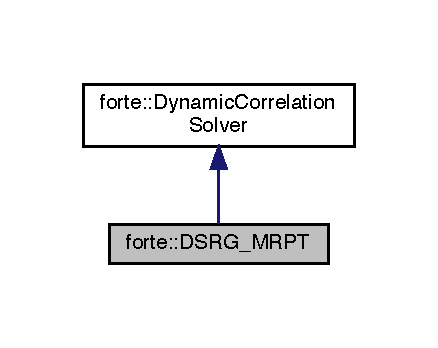
\includegraphics[width=210pt]{classforte_1_1_d_s_r_g___m_r_p_t__inherit__graph}
\end{center}
\end{figure}


Collaboration diagram for forte\+:\+:D\+S\+R\+G\+\_\+\+M\+R\+PT\+:
\nopagebreak
\begin{figure}[H]
\begin{center}
\leavevmode
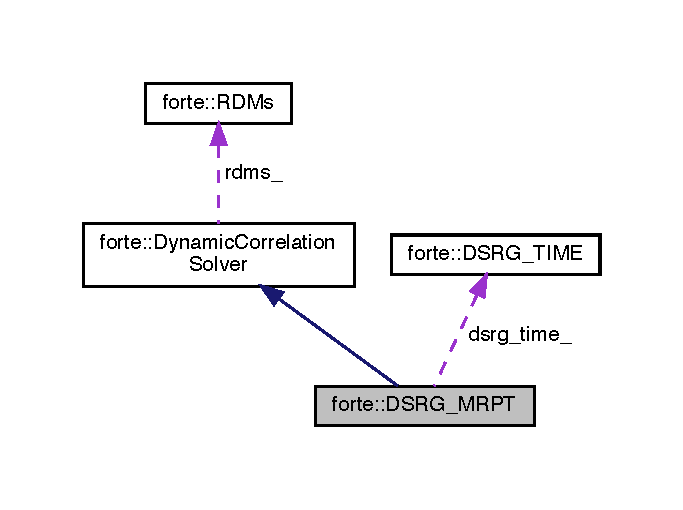
\includegraphics[width=328pt]{classforte_1_1_d_s_r_g___m_r_p_t__coll__graph}
\end{center}
\end{figure}
\subsection*{Public Member Functions}
\begin{DoxyCompactItemize}
\item 
\mbox{\hyperlink{classforte_1_1_d_s_r_g___m_r_p_t_a675c39945f959015eb41954094f4bdd4}{D\+S\+R\+G\+\_\+\+M\+R\+PT}} (\mbox{\hyperlink{classforte_1_1_r_d_ms}{R\+D\+Ms}} rdms, std\+::shared\+\_\+ptr$<$ \mbox{\hyperlink{classforte_1_1_s_c_f_info}{S\+C\+F\+Info}} $>$ scf\+\_\+info, std\+::shared\+\_\+ptr$<$ \mbox{\hyperlink{classforte_1_1_forte_options}{Forte\+Options}} $>$ options, std\+::shared\+\_\+ptr$<$ \mbox{\hyperlink{classforte_1_1_forte_integrals}{Forte\+Integrals}} $>$ ints, std\+::shared\+\_\+ptr$<$ \mbox{\hyperlink{classforte_1_1_m_o_space_info}{M\+O\+Space\+Info}} $>$ mo\+\_\+space\+\_\+info)
\item 
\mbox{\hyperlink{classforte_1_1_d_s_r_g___m_r_p_t_a4707cbb0942d995c4c904c94d3168ddd}{$\sim$\+D\+S\+R\+G\+\_\+\+M\+R\+PT}} ()
\begin{DoxyCompactList}\small\item\em Destructor. \end{DoxyCompactList}\item 
double \mbox{\hyperlink{classforte_1_1_d_s_r_g___m_r_p_t_a83b7f20d255a4f1f33bb05d707846f85}{compute\+\_\+energy}} ()
\begin{DoxyCompactList}\small\item\em Compute energy with fixed reference. \end{DoxyCompactList}\item 
std\+::shared\+\_\+ptr$<$ \mbox{\hyperlink{classforte_1_1_active_space_integrals}{Active\+Space\+Integrals}} $>$ \mbox{\hyperlink{classforte_1_1_d_s_r_g___m_r_p_t_a929556373e50b9baeefbdd461fd72124}{compute\+\_\+\+Heff\+\_\+actv}} ()
\begin{DoxyCompactList}\small\item\em D\+S\+RG transformed Hamiltonian (not implemented) \end{DoxyCompactList}\end{DoxyCompactItemize}
\subsection*{Protected Member Functions}
\begin{DoxyCompactItemize}
\item 
void \mbox{\hyperlink{classforte_1_1_d_s_r_g___m_r_p_t_ab043c2526c08fa3d80f336b44f215a9f}{startup}} ()
\begin{DoxyCompactList}\small\item\em Start-\/up function called in the constructor. \end{DoxyCompactList}\item 
void \mbox{\hyperlink{classforte_1_1_d_s_r_g___m_r_p_t_a3b1e40388dd518ed9117b7f625cebf42}{cleanup}} ()
\begin{DoxyCompactList}\small\item\em Clean-\/up function called in the destructor. \end{DoxyCompactList}\item 
void \mbox{\hyperlink{classforte_1_1_d_s_r_g___m_r_p_t_a089de562b9ee02dffee27888e12c8397}{read\+\_\+options}} ()
\begin{DoxyCompactList}\small\item\em Read options. \end{DoxyCompactList}\item 
void \mbox{\hyperlink{classforte_1_1_d_s_r_g___m_r_p_t_a1fd1ad6aab74b00db95f4fb10367440d}{build\+\_\+ints}} ()
\begin{DoxyCompactList}\small\item\em Fill up integrals. \end{DoxyCompactList}\item 
void \mbox{\hyperlink{classforte_1_1_d_s_r_g___m_r_p_t_a2f9ab7b9cc446d8b2a0cd4cb99cd4a1a}{build\+\_\+density}} ()
\begin{DoxyCompactList}\small\item\em Fill up density matrix and density cumulants. \end{DoxyCompactList}\item 
void \mbox{\hyperlink{classforte_1_1_d_s_r_g___m_r_p_t_ac004a876996743cc7dbe8842c84e6102}{build\+\_\+fock}} ()
\begin{DoxyCompactList}\small\item\em Build Fock matrix and diagonal Fock matrix elements. \end{DoxyCompactList}\item 
bool \mbox{\hyperlink{classforte_1_1_d_s_r_g___m_r_p_t_a6de4974590a59995537d42b2188f4d02}{check\+\_\+semicanonical}} ()
\begin{DoxyCompactList}\small\item\em Check if orbitals are semi-\/canonicalized. \end{DoxyCompactList}\item 
void \mbox{\hyperlink{classforte_1_1_d_s_r_g___m_r_p_t_a3839be538e6d0cbc56172ac76a08c735}{test\+\_\+density}} ()
\begin{DoxyCompactList}\small\item\em Test spin adaptation of density matrix and density cumulants. \end{DoxyCompactList}\item 
void \mbox{\hyperlink{classforte_1_1_d_s_r_g___m_r_p_t_ac28549b2c6bd7f7bbeb8ecf70d5df3e1}{test\+\_\+memory}} (const size\+\_\+t \&c, const size\+\_\+t \&a, const size\+\_\+t \&v)
\begin{DoxyCompactList}\small\item\em Estimate peak memory. \end{DoxyCompactList}\item 
void \mbox{\hyperlink{classforte_1_1_d_s_r_g___m_r_p_t_ad86da153044ff2626e1ded1bd4041954}{check\+\_\+t2}} (Blocked\+Tensor \&T2)
\begin{DoxyCompactList}\small\item\em Check T2 and store the largest amplitudes. \end{DoxyCompactList}\item 
void \mbox{\hyperlink{classforte_1_1_d_s_r_g___m_r_p_t_a24fe22a35a7ac4c5a9a83361c5b6b750}{check\+\_\+t1}} (Blocked\+Tensor \&T1)
\begin{DoxyCompactList}\small\item\em Check T1 and store the largest amplitudes. \end{DoxyCompactList}\item 
void \mbox{\hyperlink{classforte_1_1_d_s_r_g___m_r_p_t_a7836c1b603be3a7b8383978865f42acf}{analyze\+\_\+amplitudes}} (Blocked\+Tensor \&T1, Blocked\+Tensor \&T2, std\+::string name=\char`\"{}\char`\"{})
\begin{DoxyCompactList}\small\item\em Analyze T1 and T2 amplitudes. \end{DoxyCompactList}\item 
void \mbox{\hyperlink{classforte_1_1_d_s_r_g___m_r_p_t_a2272dc6667027e7863e40f033f4bf741}{compute\+\_\+hbar}} ()
\begin{DoxyCompactList}\small\item\em Compute D\+S\+R\+G-\/transformed Hamiltonian Hbar. \end{DoxyCompactList}\item 
double \mbox{\hyperlink{classforte_1_1_d_s_r_g___m_r_p_t_ae543636fcbbabe455c0250ebad1e3088}{Hbar2od\+\_\+norm}} (const std\+::vector$<$ std\+::string $>$ \&blocks)
\begin{DoxyCompactList}\small\item\em Norm of off-\/diagonal Hbar2. \end{DoxyCompactList}\item 
double \mbox{\hyperlink{classforte_1_1_d_s_r_g___m_r_p_t_a69dcc59344184e94a3ccacac41cea8f1}{Hbar1od\+\_\+norm}} (const std\+::vector$<$ std\+::string $>$ \&blocks)
\begin{DoxyCompactList}\small\item\em Norm of off-\/diagonal Hbar1. \end{DoxyCompactList}\item 
void \mbox{\hyperlink{classforte_1_1_d_s_r_g___m_r_p_t_ae0d0412424b3a5d78dfcdb00e72cd955}{H1\+\_\+\+T1\+\_\+\+C0}} (Blocked\+Tensor \&H1, Blocked\+Tensor \&T1, const double \&alpha, double \&C0)
\begin{DoxyCompactList}\small\item\em Compute zero-\/body term of commutator \mbox{[}H1, T1\mbox{]} $\ast$ alpha. \end{DoxyCompactList}\item 
void \mbox{\hyperlink{classforte_1_1_d_s_r_g___m_r_p_t_aee81005e7b9859f8bceea16dd8728aa7}{H1\+\_\+\+T2\+\_\+\+C0}} (Blocked\+Tensor \&H1, Blocked\+Tensor \&T2, const double \&alpha, double \&C0)
\begin{DoxyCompactList}\small\item\em Compute zero-\/body term of commutator \mbox{[}H1, T2\mbox{]} $\ast$ alpha. \end{DoxyCompactList}\item 
void \mbox{\hyperlink{classforte_1_1_d_s_r_g___m_r_p_t_a0385770241da7d182d13c4e3ec51fcb2}{H2\+\_\+\+T1\+\_\+\+C0}} (Blocked\+Tensor \&H2, Blocked\+Tensor \&T1, const double \&alpha, double \&C0)
\begin{DoxyCompactList}\small\item\em Compute zero-\/body term of commutator \mbox{[}H2, T1\mbox{]} $\ast$ alpha. \end{DoxyCompactList}\item 
void \mbox{\hyperlink{classforte_1_1_d_s_r_g___m_r_p_t_ac5b7802f0bc323ef568dbc25b5a0eed3}{H2\+\_\+\+T2\+\_\+\+C0}} (Blocked\+Tensor \&H2, Blocked\+Tensor \&T2, const double \&alpha, double \&C0, const bool \&stored)
\begin{DoxyCompactList}\small\item\em Compute zero-\/body term of commutator \mbox{[}H2, T2\mbox{]} $\ast$ alpha. \end{DoxyCompactList}\item 
void \mbox{\hyperlink{classforte_1_1_d_s_r_g___m_r_p_t_a0a92487f2ed90b7b5503626163b4ab5d}{H2\+\_\+\+T2\+\_\+\+C0\+\_\+\+L1}} (Blocked\+Tensor \&H2, Blocked\+Tensor \&T2, const double \&alpha, double \&C0, const bool \&stored)
\begin{DoxyCompactList}\small\item\em Compute zero-\/body term of commutator \mbox{[}H2, T2\mbox{]} involving only L1. \end{DoxyCompactList}\item 
void \mbox{\hyperlink{classforte_1_1_d_s_r_g___m_r_p_t_aba08dd12fb004053d65e40340a43d68e}{H2\+\_\+\+T2\+\_\+\+C0\+\_\+\+L2}} (Blocked\+Tensor \&H2, Blocked\+Tensor \&T2, const double \&alpha, double \&C0)
\begin{DoxyCompactList}\small\item\em Compute zero-\/body term of commutator \mbox{[}H2, T2\mbox{]} involving only L2. \end{DoxyCompactList}\item 
void \mbox{\hyperlink{classforte_1_1_d_s_r_g___m_r_p_t_afff5d8a261acd90a0486add4d7baff87}{H2\+\_\+\+T2\+\_\+\+C0\+\_\+\+L3}} (Blocked\+Tensor \&H2, Blocked\+Tensor \&T2, const double \&alpha, double \&C0)
\begin{DoxyCompactList}\small\item\em Compute zero-\/body term of commutator \mbox{[}H2, T2\mbox{]} involving only L3. \end{DoxyCompactList}\item 
double \mbox{\hyperlink{classforte_1_1_d_s_r_g___m_r_p_t_aa5d9db7de36918472ea172ee7438988d}{H2\+\_\+\+T2\+\_\+\+C0\+\_\+\+L3\+\_\+a}} (Blocked\+Tensor \&H2, Blocked\+Tensor \&T2)
\item 
double \mbox{\hyperlink{classforte_1_1_d_s_r_g___m_r_p_t_a28b3882eb995c1d18c7bc73262f2cef9}{H2\+\_\+\+T2\+\_\+\+C0\+\_\+\+L3\+\_\+v}} (Blocked\+Tensor \&H2, Blocked\+Tensor \&T2)
\item 
double \mbox{\hyperlink{classforte_1_1_d_s_r_g___m_r_p_t_a09cc4cfc50e1f42659027dd847733c1b}{V\+\_\+\+T2\+\_\+\+C0\+\_\+\+L1\+\_\+ccvv}} (const std\+::vector$<$ std\+::vector$<$ size\+\_\+t $>$$>$ \&small\+\_\+core\+\_\+mo)
\item 
double \mbox{\hyperlink{classforte_1_1_d_s_r_g___m_r_p_t_afb34a99b3a175235b41ad12be9617735}{V\+\_\+\+T2\+\_\+\+C0\+\_\+\+L1\+\_\+cavv}} (const std\+::vector$<$ std\+::vector$<$ size\+\_\+t $>$$>$ \&small\+\_\+core\+\_\+mo)
\item 
double \mbox{\hyperlink{classforte_1_1_d_s_r_g___m_r_p_t_a4def5a7f2c18569e16ed49015db4d804}{V\+\_\+\+T2\+\_\+\+C0\+\_\+\+L1\+\_\+ccav}} ()
\item 
void \mbox{\hyperlink{classforte_1_1_d_s_r_g___m_r_p_t_a6e6d66cdfd06fce5cda302cc25ceda32}{H1\+\_\+\+T1\+\_\+\+C1}} (Blocked\+Tensor \&H1, Blocked\+Tensor \&T1, const double \&alpha, Blocked\+Tensor \&\mbox{\hyperlink{namespaceforte_abe00ec86d0015c0f2b6ac298c6e428e4a1a2ddc2db4693cfd16d534cde5572cc1}{C1}})
\begin{DoxyCompactList}\small\item\em Compute one-\/body term of commutator \mbox{[}H1, T1\mbox{]} $\ast$ alpha. \end{DoxyCompactList}\item 
void \mbox{\hyperlink{classforte_1_1_d_s_r_g___m_r_p_t_a6de48bc90d339cbfc5d6d6ff9d15f07d}{H1\+\_\+\+T2\+\_\+\+C1}} (Blocked\+Tensor \&H1, Blocked\+Tensor \&T2, const double \&alpha, Blocked\+Tensor \&\mbox{\hyperlink{namespaceforte_abe00ec86d0015c0f2b6ac298c6e428e4a1a2ddc2db4693cfd16d534cde5572cc1}{C1}})
\begin{DoxyCompactList}\small\item\em Compute one-\/body term of commutator \mbox{[}H1, T2\mbox{]} $\ast$ alpha. \end{DoxyCompactList}\item 
void \mbox{\hyperlink{classforte_1_1_d_s_r_g___m_r_p_t_a869a5f60f25b70d36a26e6ed16c165d3}{H2\+\_\+\+T1\+\_\+\+C1}} (Blocked\+Tensor \&H2, Blocked\+Tensor \&T1, const double \&alpha, Blocked\+Tensor \&\mbox{\hyperlink{namespaceforte_abe00ec86d0015c0f2b6ac298c6e428e4a1a2ddc2db4693cfd16d534cde5572cc1}{C1}})
\begin{DoxyCompactList}\small\item\em Compute one-\/body term of commutator \mbox{[}H2, T1\mbox{]} $\ast$ alpha. \end{DoxyCompactList}\item 
void \mbox{\hyperlink{classforte_1_1_d_s_r_g___m_r_p_t_ab025b7eb9df9fdad69a3de7dca43ac9b}{H2\+\_\+\+T2\+\_\+\+C1}} (Blocked\+Tensor \&H2, Blocked\+Tensor \&T2, const double \&alpha, Blocked\+Tensor \&\mbox{\hyperlink{namespaceforte_abe00ec86d0015c0f2b6ac298c6e428e4a1a2ddc2db4693cfd16d534cde5572cc1}{C1}})
\begin{DoxyCompactList}\small\item\em Compute one-\/body term of commutator \mbox{[}H2, T2\mbox{]} $\ast$ alpha. \end{DoxyCompactList}\item 
void \mbox{\hyperlink{classforte_1_1_d_s_r_g___m_r_p_t_a2734af50d9ee05d68aa6637ed00dbbbf}{H2\+\_\+\+T1\+\_\+\+C2}} (Blocked\+Tensor \&H2, Blocked\+Tensor \&T1, const double \&alpha, Blocked\+Tensor \&\mbox{\hyperlink{namespaceforte_abe00ec86d0015c0f2b6ac298c6e428e4af1a543f5a2c5d49bc5dde298fcf716e4}{C2}})
\begin{DoxyCompactList}\small\item\em Compute two-\/body term of commutator \mbox{[}H2, T1\mbox{]} $\ast$ alpha. \end{DoxyCompactList}\item 
void \mbox{\hyperlink{classforte_1_1_d_s_r_g___m_r_p_t_a0d6154e51d2a19c2e21e11b0e96e8867}{H1\+\_\+\+T2\+\_\+\+C2}} (Blocked\+Tensor \&H1, Blocked\+Tensor \&T2, const double \&alpha, Blocked\+Tensor \&\mbox{\hyperlink{namespaceforte_abe00ec86d0015c0f2b6ac298c6e428e4af1a543f5a2c5d49bc5dde298fcf716e4}{C2}})
\begin{DoxyCompactList}\small\item\em Compute two-\/body term of commutator \mbox{[}H1, T2\mbox{]} $\ast$ alpha. \end{DoxyCompactList}\item 
void \mbox{\hyperlink{classforte_1_1_d_s_r_g___m_r_p_t_a9cd4ca67158a2be41a836acc82236640}{H2\+\_\+\+T2\+\_\+\+C2}} (Blocked\+Tensor \&H2, Blocked\+Tensor \&T2, const double \&alpha, Blocked\+Tensor \&\mbox{\hyperlink{namespaceforte_abe00ec86d0015c0f2b6ac298c6e428e4af1a543f5a2c5d49bc5dde298fcf716e4}{C2}})
\begin{DoxyCompactList}\small\item\em Compute two-\/body term of commutator \mbox{[}H2, T2\mbox{]} $\ast$ alpha. \end{DoxyCompactList}\item 
std\+::vector$<$ std\+::string $>$ \mbox{\hyperlink{classforte_1_1_d_s_r_g___m_r_p_t_a964c93822e3b9da6cd1539904ccd5fda}{d\+\_\+one\+\_\+labels}} ()
\begin{DoxyCompactList}\small\item\em Compute diagonal blocks labels of a one-\/body operator. \end{DoxyCompactList}\item 
std\+::vector$<$ std\+::string $>$ \mbox{\hyperlink{classforte_1_1_d_s_r_g___m_r_p_t_a66d95151f42dfb54a89ce06448f845e9}{od\+\_\+one\+\_\+labels}} ()
\begin{DoxyCompactList}\small\item\em Compute off-\/diagonal blocks labels of a one-\/body operator. \end{DoxyCompactList}\item 
std\+::vector$<$ std\+::string $>$ \mbox{\hyperlink{classforte_1_1_d_s_r_g___m_r_p_t_aa557563ab780d878347fbb39001e44fe}{od\+\_\+two\+\_\+labels}} ()
\begin{DoxyCompactList}\small\item\em Compute off-\/diagonal blocks labels of a two-\/body operator. \end{DoxyCompactList}\item 
void \mbox{\hyperlink{classforte_1_1_d_s_r_g___m_r_p_t_af2ff0ea55a2b0c8666df7b8de3f8559e}{B\+T\+\_\+scaled\+\_\+by\+\_\+D}} (Blocked\+Tensor \&BT)
\begin{DoxyCompactList}\small\item\em Scale Blocked\+Tensor by denominator. \end{DoxyCompactList}\item 
void \mbox{\hyperlink{classforte_1_1_d_s_r_g___m_r_p_t_a1d3cd0885893291d68a94b40e84d2958}{B\+T\+\_\+scaled\+\_\+by\+\_\+\+Rplus1}} (Blocked\+Tensor \&BT)
\begin{DoxyCompactList}\small\item\em Scale Blocked\+Tensor by bare source plus one (R + 1) \end{DoxyCompactList}\item 
void \mbox{\hyperlink{classforte_1_1_d_s_r_g___m_r_p_t_a30b920334696368308a0517785197f87}{B\+T\+\_\+scaled\+\_\+by\+\_\+\+RD}} (Blocked\+Tensor \&BT)
\begin{DoxyCompactList}\small\item\em Scale Blocked\+Tensor by renormalized denominator. \end{DoxyCompactList}\item 
double \mbox{\hyperlink{classforte_1_1_d_s_r_g___m_r_p_t_a1098b57f27bf9694a24359d4433dc755}{compute\+\_\+energy\+\_\+pt2}} ()
\begin{DoxyCompactList}\small\item\em Compute D\+S\+R\+G-\/\+M\+R\+P\+T2 energy. \end{DoxyCompactList}\item 
void \mbox{\hyperlink{classforte_1_1_d_s_r_g___m_r_p_t_a03fcfc33cda5959a7c0df3de84bd2576}{renormalize\+\_\+\+F\+\_\+\+E2nd}} ()
\begin{DoxyCompactList}\small\item\em Fold in \mbox{[}H0th, A\mbox{]} effect to F1st for 2nd-\/order energy. \end{DoxyCompactList}\item 
void \mbox{\hyperlink{classforte_1_1_d_s_r_g___m_r_p_t_aac4471beedf5d27b23320c28a6c739a8}{renormalize\+\_\+\+V\+\_\+\+E2nd}} ()
\begin{DoxyCompactList}\small\item\em Fold in \mbox{[}H0th, A\mbox{]} effect to V1st for 2nd-\/order energy. \end{DoxyCompactList}\item 
void \mbox{\hyperlink{classforte_1_1_d_s_r_g___m_r_p_t_acae3b09d4863198ab6c7c19d91b9560e}{compute\+\_\+\+T\+\_\+1st}} (Blocked\+Tensor \&V, Blocked\+Tensor \&T2, Blocked\+Tensor \&F, Blocked\+Tensor \&T1)
\begin{DoxyCompactList}\small\item\em Compute first-\/order T amplitudes. \end{DoxyCompactList}\item 
void \mbox{\hyperlink{classforte_1_1_d_s_r_g___m_r_p_t_a886819be6edca8bb76c94dd45fa6dd04}{compute\+\_\+\+T1\+\_\+1st}} (Blocked\+Tensor \&F, Blocked\+Tensor \&T2, Blocked\+Tensor \&T1)
\begin{DoxyCompactList}\small\item\em Compute first-\/order T1. \end{DoxyCompactList}\item 
void \mbox{\hyperlink{classforte_1_1_d_s_r_g___m_r_p_t_a8bf372f9bd6f54b553355c4eb575214d}{compute\+\_\+\+T2\+\_\+1st}} (Blocked\+Tensor \&V, Blocked\+Tensor \&T2)
\begin{DoxyCompactList}\small\item\em Compute first-\/order T2. \end{DoxyCompactList}\item 
void \mbox{\hyperlink{classforte_1_1_d_s_r_g___m_r_p_t_a778596d63e6d421f2bb21f18982b7b20}{transfer\+\_\+integrals}} ()
\begin{DoxyCompactList}\small\item\em Transfer integrals for F\+CI. \end{DoxyCompactList}\item 
void \mbox{\hyperlink{classforte_1_1_d_s_r_g___m_r_p_t_adcf156a0f6b3caa2637d743789b9c68e}{reset\+\_\+ints}} (Blocked\+Tensor \&H, Blocked\+Tensor \&V)
\begin{DoxyCompactList}\small\item\em Reset integrals to bare Hamiltonian. \end{DoxyCompactList}\item 
std\+::vector$<$ std\+::vector$<$ double $>$ $>$ \mbox{\hyperlink{classforte_1_1_d_s_r_g___m_r_p_t_a443bd826e0384c8f5d2ed562e10e4867}{diagonalize\+\_\+\+Fock\+\_\+diagblocks}} (Blocked\+Tensor \&U)
\begin{DoxyCompactList}\small\item\em Diagonalize the diagonal blocks of the Fock matrix. \end{DoxyCompactList}\item 
ambit\+::\+Tensor \mbox{\hyperlink{classforte_1_1_d_s_r_g___m_r_p_t_ada139ac0e12cbee87aacb94af7510868}{separate\+\_\+tensor}} (ambit\+::\+Tensor \&tens, const psi\+::\+Dimension \&irrep, const int \&h)
\begin{DoxyCompactList}\small\item\em Separate an 2D ambit\+::\+Tensor according to its irrep. \end{DoxyCompactList}\item 
void \mbox{\hyperlink{classforte_1_1_d_s_r_g___m_r_p_t_acdd93b6514696a2b08b25f4825a24a30}{combine\+\_\+tensor}} (ambit\+::\+Tensor \&tens, ambit\+::\+Tensor \&tens\+\_\+h, const psi\+::\+Dimension \&irrep, const int \&h)
\begin{DoxyCompactList}\small\item\em Combine a separated 2D ambit\+::\+Tensor. \end{DoxyCompactList}\item 
void \mbox{\hyperlink{classforte_1_1_d_s_r_g___m_r_p_t_afd5708ef5c74be6e82cd3701b4f4e968}{print\+\_\+options}} ()
\begin{DoxyCompactList}\small\item\em Print a summary of the options. \end{DoxyCompactList}\item 
void \mbox{\hyperlink{classforte_1_1_d_s_r_g___m_r_p_t_ae6dcf7ee77828815c86b6ce8b19b3266}{print\+\_\+citation}} ()
\begin{DoxyCompactList}\small\item\em Print papers need to be cited. \end{DoxyCompactList}\item 
void \mbox{\hyperlink{classforte_1_1_d_s_r_g___m_r_p_t_ab4fcb92ef63bc2d558f3ce354458f20c}{print\+\_\+amp\+\_\+summary}} (const std\+::string \&name, const std\+::vector$<$ std\+::pair$<$ std\+::vector$<$ size\+\_\+t $>$, double $>$$>$ \&list, const double \&norm, const size\+\_\+t \&number\+\_\+nonzero)
\begin{DoxyCompactList}\small\item\em Print amplitudes summary. \end{DoxyCompactList}\item 
void \mbox{\hyperlink{classforte_1_1_d_s_r_g___m_r_p_t_a4f00bb9e58057515a5800379d69495da}{print\+\_\+intruder}} (const std\+::string \&name, const std\+::vector$<$ std\+::pair$<$ std\+::vector$<$ size\+\_\+t $>$, double $>$$>$ \&list)
\begin{DoxyCompactList}\small\item\em Print intruder analysis. \end{DoxyCompactList}\item 
void \mbox{\hyperlink{classforte_1_1_d_s_r_g___m_r_p_t_a9e6940d281d6bfc34db888aef335bb0a}{check\+\_\+density}} (Blocked\+Tensor \&D, const std\+::string \&name)
\begin{DoxyCompactList}\small\item\em Check the max and norm of density. \end{DoxyCompactList}\item 
void \mbox{\hyperlink{classforte_1_1_d_s_r_g___m_r_p_t_a0f8881e67c904a590e9c74a5c65fbfbf}{print\+\_\+cumulant\+\_\+summary}} ()
\begin{DoxyCompactList}\small\item\em Print the summary of 2-\/ and 3-\/body density cumulant. \end{DoxyCompactList}\end{DoxyCompactItemize}
\subsection*{Protected Attributes}
\begin{DoxyCompactItemize}
\item 
int \mbox{\hyperlink{classforte_1_1_d_s_r_g___m_r_p_t_addf6354a1a878796bddaf04cd377f2f7}{print\+\_\+}}
\begin{DoxyCompactList}\small\item\em Print levels. \end{DoxyCompactList}\item 
double \mbox{\hyperlink{classforte_1_1_d_s_r_g___m_r_p_t_a6b96d621e3be2f4958bc0a7c365b16d7}{Eref\+\_\+}}
\begin{DoxyCompactList}\small\item\em The energy of the rdms. \end{DoxyCompactList}\item 
double \mbox{\hyperlink{classforte_1_1_d_s_r_g___m_r_p_t_a123fe7309531ea7b0ff467b2a853eb12}{frozen\+\_\+core\+\_\+energy\+\_\+}}
\begin{DoxyCompactList}\small\item\em The frozen-\/core energy. \end{DoxyCompactList}\item 
bool \mbox{\hyperlink{classforte_1_1_d_s_r_g___m_r_p_t_a7b7f73082944dd1810a6907083860aeb}{semi\+\_\+canonical\+\_\+}}
\begin{DoxyCompactList}\small\item\em Are orbitals semi-\/canonicalized? \end{DoxyCompactList}\item 
std\+::vector$<$ size\+\_\+t $>$ \mbox{\hyperlink{classforte_1_1_d_s_r_g___m_r_p_t_a900be495017b4905196510bdccce3435}{core\+\_\+mos\+\_\+}}
\begin{DoxyCompactList}\small\item\em List of core M\+Os. \end{DoxyCompactList}\item 
std\+::vector$<$ size\+\_\+t $>$ \mbox{\hyperlink{classforte_1_1_d_s_r_g___m_r_p_t_aaabe340bc053bc0ef8904ffbf2b7d3a4}{actv\+\_\+mos\+\_\+}}
\begin{DoxyCompactList}\small\item\em List of active M\+Os. \end{DoxyCompactList}\item 
std\+::vector$<$ size\+\_\+t $>$ \mbox{\hyperlink{classforte_1_1_d_s_r_g___m_r_p_t_aff0036190f9b8d4f0bfdeecad90903f5}{virt\+\_\+mos\+\_\+}}
\begin{DoxyCompactList}\small\item\em List of virtual M\+Os. \end{DoxyCompactList}\item 
std\+::string \mbox{\hyperlink{classforte_1_1_d_s_r_g___m_r_p_t_ab08ccc8d4bed9a111d316aef3d61a980}{core\+\_\+label\+\_\+}}
\begin{DoxyCompactList}\small\item\em Core label. \end{DoxyCompactList}\item 
std\+::string \mbox{\hyperlink{classforte_1_1_d_s_r_g___m_r_p_t_a30db0191325369681babb5ce7a2bb456}{actv\+\_\+label\+\_\+}}
\begin{DoxyCompactList}\small\item\em Active label. \end{DoxyCompactList}\item 
std\+::string \mbox{\hyperlink{classforte_1_1_d_s_r_g___m_r_p_t_aa2254fd7d2ee05ad19b5b15e9718cb49}{virt\+\_\+label\+\_\+}}
\begin{DoxyCompactList}\small\item\em Virtual label. \end{DoxyCompactList}\item 
std\+::map$<$ char, std\+::vector$<$ size\+\_\+t $>$ $>$ \mbox{\hyperlink{classforte_1_1_d_s_r_g___m_r_p_t_adc911c4abf0f421f8bab1571d570d5ab}{label\+\_\+to\+\_\+spacemo\+\_\+}}
\begin{DoxyCompactList}\small\item\em Map from space label to list of M\+Os. \end{DoxyCompactList}\item 
int \mbox{\hyperlink{classforte_1_1_d_s_r_g___m_r_p_t_aabab74a6c74bbc8219215ed01587788f}{nbatch\+\_\+}}
\begin{DoxyCompactList}\small\item\em Number of batches for C\+C\+VV term if not enough memory. \end{DoxyCompactList}\item 
std\+::string \mbox{\hyperlink{classforte_1_1_d_s_r_g___m_r_p_t_ab92bfdb1697818439f8b551a3e546b00}{corr\+\_\+lv\+\_\+}}
\begin{DoxyCompactList}\small\item\em Correlation level\+: P\+T2 or P\+T3. \end{DoxyCompactList}\item 
double \mbox{\hyperlink{classforte_1_1_d_s_r_g___m_r_p_t_af332d95c9728aefd908a0bfa4b8c86aa}{s\+\_\+}}
\begin{DoxyCompactList}\small\item\em The flow parameter. \end{DoxyCompactList}\item 
std\+::string \mbox{\hyperlink{classforte_1_1_d_s_r_g___m_r_p_t_a00fe6c6a209483b46105796c0c3b2ee6}{source\+\_\+}}
\begin{DoxyCompactList}\small\item\em Source operator. \end{DoxyCompactList}\item 
std\+::shared\+\_\+ptr$<$ \mbox{\hyperlink{classforte_1_1_d_s_r_g___s_o_u_r_c_e}{D\+S\+R\+G\+\_\+\+S\+O\+U\+R\+CE}} $>$ \mbox{\hyperlink{classforte_1_1_d_s_r_g___m_r_p_t_a81c8ed2fc9fc2cba6888cd3552ce9c9d}{dsrg\+\_\+source\+\_\+}}
\begin{DoxyCompactList}\small\item\em The dsrg source operator. \end{DoxyCompactList}\item 
std\+::string \mbox{\hyperlink{classforte_1_1_d_s_r_g___m_r_p_t_af42019d1db99243cdf9b02c84a0d8468}{ccvv\+\_\+source\+\_\+}}
\begin{DoxyCompactList}\small\item\em Core-\/core-\/virtual-\/virtual source. \end{DoxyCompactList}\item 
double \mbox{\hyperlink{classforte_1_1_d_s_r_g___m_r_p_t_a979497f0b8e398a9855235a53b8c3939}{taylor\+\_\+threshold\+\_\+}}
\begin{DoxyCompactList}\small\item\em Smaller than which we will do Taylor expansion. \end{DoxyCompactList}\item 
Tensor\+Type \mbox{\hyperlink{classforte_1_1_d_s_r_g___m_r_p_t_ad30b77cfa8e9d11902e8a420d82ae8cb}{tensor\+\_\+type\+\_\+}}
\begin{DoxyCompactList}\small\item\em Tensor type for A\+M\+B\+IT. \end{DoxyCompactList}\item 
ambit\+::\+Blocked\+Tensor \mbox{\hyperlink{classforte_1_1_d_s_r_g___m_r_p_t_a0d207145a8522c1ffef9734288016a39}{H\+\_\+}}
\begin{DoxyCompactList}\small\item\em One-\/electron integral. \end{DoxyCompactList}\item 
ambit\+::\+Blocked\+Tensor \mbox{\hyperlink{classforte_1_1_d_s_r_g___m_r_p_t_a26b8cb138fc31e37ed21ef9c5e63064a}{V\+\_\+}}
\begin{DoxyCompactList}\small\item\em Two-\/electron integral. \end{DoxyCompactList}\item 
ambit\+::\+Blocked\+Tensor \mbox{\hyperlink{classforte_1_1_d_s_r_g___m_r_p_t_aefef1b1d0c0b2d689a33f1358b7555c4}{F\+\_\+}}
\begin{DoxyCompactList}\small\item\em Generalized Fock matrix. \end{DoxyCompactList}\item 
ambit\+::\+Blocked\+Tensor \mbox{\hyperlink{classforte_1_1_d_s_r_g___m_r_p_t_a3561791b83c0bee4ad6c0739d6ab1ee6}{L1\+\_\+}}
\begin{DoxyCompactList}\small\item\em Spin-\/summed one-\/particle density matrix. \end{DoxyCompactList}\item 
ambit\+::\+Blocked\+Tensor \mbox{\hyperlink{classforte_1_1_d_s_r_g___m_r_p_t_aef85158de6f4244805554d74b49aad23}{Eta1\+\_\+}}
\begin{DoxyCompactList}\small\item\em Spin-\/summed one-\/hole density matrix. \end{DoxyCompactList}\item 
ambit\+::\+Blocked\+Tensor \mbox{\hyperlink{classforte_1_1_d_s_r_g___m_r_p_t_a3346b53af8194e80373ce4f85b50c245}{L2\+\_\+}}
\begin{DoxyCompactList}\small\item\em Spin-\/summed two-\/body denisty cumulant. \end{DoxyCompactList}\item 
ambit\+::\+Blocked\+Tensor \mbox{\hyperlink{classforte_1_1_d_s_r_g___m_r_p_t_a0e9b4e7b2058cd17615dd7b6aad54794}{L3\+\_\+}}
\begin{DoxyCompactList}\small\item\em Spin-\/summed three-\/body density cumulant. \end{DoxyCompactList}\item 
ambit\+::\+Blocked\+Tensor \mbox{\hyperlink{classforte_1_1_d_s_r_g___m_r_p_t_a952a44d9fc97bab37f8491d975e5474b}{T1\+\_\+}}
\begin{DoxyCompactList}\small\item\em Single excitation amplitude. \end{DoxyCompactList}\item 
ambit\+::\+Blocked\+Tensor \mbox{\hyperlink{classforte_1_1_d_s_r_g___m_r_p_t_a323d1a4b7b9f8ea30e8da4229063da56}{T2\+\_\+}}
\begin{DoxyCompactList}\small\item\em Double excitation amplitude. \end{DoxyCompactList}\item 
std\+::vector$<$ double $>$ \mbox{\hyperlink{classforte_1_1_d_s_r_g___m_r_p_t_a4d89836fdc0036566a07188c1ac44ef1}{Fdiag\+\_\+}}
\begin{DoxyCompactList}\small\item\em Diagonal elements of Fock matrices. \end{DoxyCompactList}\item 
double \mbox{\hyperlink{classforte_1_1_d_s_r_g___m_r_p_t_a8c5cfd5ffcbc9b06ac3fb2d65827d30d}{T2rms\+\_\+}}
\begin{DoxyCompactList}\small\item\em R\+MS of T2. \end{DoxyCompactList}\item 
double \mbox{\hyperlink{classforte_1_1_d_s_r_g___m_r_p_t_a75235ed0a5a7573f4fb04c558809e0f7}{T2norm\+\_\+}}
\begin{DoxyCompactList}\small\item\em Norm of T2. \end{DoxyCompactList}\item 
double \mbox{\hyperlink{classforte_1_1_d_s_r_g___m_r_p_t_adfcca14284a1d7d6eb1118f22187edac}{T2max\+\_\+}}
\begin{DoxyCompactList}\small\item\em Signed max of T2. \end{DoxyCompactList}\item 
double \mbox{\hyperlink{classforte_1_1_d_s_r_g___m_r_p_t_a7898973195cd57960c0cce1ba01b19d7}{T1rms\+\_\+}}
\begin{DoxyCompactList}\small\item\em R\+MS of T1. \end{DoxyCompactList}\item 
double \mbox{\hyperlink{classforte_1_1_d_s_r_g___m_r_p_t_a0b90b32c76cdf23134431ccf26439d85}{T1norm\+\_\+}}
\begin{DoxyCompactList}\small\item\em Norm of T1. \end{DoxyCompactList}\item 
double \mbox{\hyperlink{classforte_1_1_d_s_r_g___m_r_p_t_a2f86a9d9a8ca93ad8926f8c6903d9e8c}{T1max\+\_\+}}
\begin{DoxyCompactList}\small\item\em Signed max of T1. \end{DoxyCompactList}\item 
size\+\_\+t \mbox{\hyperlink{classforte_1_1_d_s_r_g___m_r_p_t_a6d8ad3ce1ec3e27840be359d8a0af410}{ntamp\+\_\+}}
\begin{DoxyCompactList}\small\item\em Number of amplitudes will be printed in amplitude summary. \end{DoxyCompactList}\item 
double \mbox{\hyperlink{classforte_1_1_d_s_r_g___m_r_p_t_a3f7598c38822b0c248df73637426215c}{intruder\+\_\+tamp\+\_\+}}
\begin{DoxyCompactList}\small\item\em Threshold for amplitudes considered as intruders. \end{DoxyCompactList}\item 
std\+::vector$<$ std\+::pair$<$ std\+::vector$<$ size\+\_\+t $>$, double $>$ $>$ \mbox{\hyperlink{classforte_1_1_d_s_r_g___m_r_p_t_a23960b3827edcf832dcff5bec6d23a2f}{lt1\+\_\+}}
\begin{DoxyCompactList}\small\item\em List of large amplitudes. \end{DoxyCompactList}\item 
std\+::vector$<$ std\+::pair$<$ std\+::vector$<$ size\+\_\+t $>$, double $>$ $>$ \mbox{\hyperlink{classforte_1_1_d_s_r_g___m_r_p_t_ade1af147df32093d8ef9901eda6f741a}{lt2\+\_\+}}
\item 
double \mbox{\hyperlink{classforte_1_1_d_s_r_g___m_r_p_t_afc9bd5e06677303c356b8ccef89d64ff}{Hbar0\+\_\+}}
\begin{DoxyCompactList}\small\item\em Zero-\/body Hbar. \end{DoxyCompactList}\item 
ambit\+::\+Blocked\+Tensor \mbox{\hyperlink{classforte_1_1_d_s_r_g___m_r_p_t_a3fec90a2fa29718e28cf04c5a9ceb056}{Hbar1\+\_\+}}
\begin{DoxyCompactList}\small\item\em One-\/body Hbar. \end{DoxyCompactList}\item 
ambit\+::\+Blocked\+Tensor \mbox{\hyperlink{classforte_1_1_d_s_r_g___m_r_p_t_a8253974db2a39ee31ad379421b000881}{Hbar2\+\_\+}}
\begin{DoxyCompactList}\small\item\em Two-\/body Hbar. \end{DoxyCompactList}\item 
ambit\+::\+Blocked\+Tensor \mbox{\hyperlink{classforte_1_1_d_s_r_g___m_r_p_t_ad28fba643f97278be8adb3233628c9e9}{O1\+\_\+}}
\begin{DoxyCompactList}\small\item\em Temporary one-\/body Hamiltonian. \end{DoxyCompactList}\item 
ambit\+::\+Blocked\+Tensor \mbox{\hyperlink{classforte_1_1_d_s_r_g___m_r_p_t_a4822fbb6db6a9310145efb9c139c9959}{C1\+\_\+}}
\item 
ambit\+::\+Blocked\+Tensor \mbox{\hyperlink{classforte_1_1_d_s_r_g___m_r_p_t_a7542603415ce77c3af6f8f6bc3e69f2d}{O2\+\_\+}}
\begin{DoxyCompactList}\small\item\em Temporary two-\/body Hamiltonian. \end{DoxyCompactList}\item 
ambit\+::\+Blocked\+Tensor \mbox{\hyperlink{classforte_1_1_d_s_r_g___m_r_p_t_a14ca0f3e6d6b6d9393081a5a7858d0df}{C2\+\_\+}}
\item 
\mbox{\hyperlink{classforte_1_1_d_s_r_g___t_i_m_e}{D\+S\+R\+G\+\_\+\+T\+I\+ME}} \mbox{\hyperlink{classforte_1_1_d_s_r_g___m_r_p_t_ae8909ebe3e5832331ac675efd506a235}{dsrg\+\_\+time\+\_\+}}
\begin{DoxyCompactList}\small\item\em Timings for computing the commutators. \end{DoxyCompactList}\item 
std\+::string \mbox{\hyperlink{classforte_1_1_d_s_r_g___m_r_p_t_ae1c05dc85b9ac7fb3ab233fd36d8c5f4}{ref\+\_\+relax\+\_\+}}
\begin{DoxyCompactList}\small\item\em Reference relaxation type. \end{DoxyCompactList}\end{DoxyCompactItemize}


\subsection{Constructor \& Destructor Documentation}
\mbox{\Hypertarget{classforte_1_1_d_s_r_g___m_r_p_t_a675c39945f959015eb41954094f4bdd4}\label{classforte_1_1_d_s_r_g___m_r_p_t_a675c39945f959015eb41954094f4bdd4}} 
\index{forte\+::\+D\+S\+R\+G\+\_\+\+M\+R\+PT@{forte\+::\+D\+S\+R\+G\+\_\+\+M\+R\+PT}!D\+S\+R\+G\+\_\+\+M\+R\+PT@{D\+S\+R\+G\+\_\+\+M\+R\+PT}}
\index{D\+S\+R\+G\+\_\+\+M\+R\+PT@{D\+S\+R\+G\+\_\+\+M\+R\+PT}!forte\+::\+D\+S\+R\+G\+\_\+\+M\+R\+PT@{forte\+::\+D\+S\+R\+G\+\_\+\+M\+R\+PT}}
\subsubsection{\texorpdfstring{D\+S\+R\+G\+\_\+\+M\+R\+P\+T()}{DSRG\_MRPT()}}
{\footnotesize\ttfamily forte\+::\+D\+S\+R\+G\+\_\+\+M\+R\+P\+T\+::\+D\+S\+R\+G\+\_\+\+M\+R\+PT (\begin{DoxyParamCaption}\item[{\mbox{\hyperlink{classforte_1_1_r_d_ms}{R\+D\+Ms}}}]{rdms,  }\item[{std\+::shared\+\_\+ptr$<$ \mbox{\hyperlink{classforte_1_1_s_c_f_info}{S\+C\+F\+Info}} $>$}]{scf\+\_\+info,  }\item[{std\+::shared\+\_\+ptr$<$ \mbox{\hyperlink{classforte_1_1_forte_options}{Forte\+Options}} $>$}]{options,  }\item[{std\+::shared\+\_\+ptr$<$ \mbox{\hyperlink{classforte_1_1_forte_integrals}{Forte\+Integrals}} $>$}]{ints,  }\item[{std\+::shared\+\_\+ptr$<$ \mbox{\hyperlink{classforte_1_1_m_o_space_info}{M\+O\+Space\+Info}} $>$}]{mo\+\_\+space\+\_\+info }\end{DoxyParamCaption})}

D\+S\+R\+G-\/\+M\+R\+PT Constructor 
\begin{DoxyParams}{Parameters}
{\em rdms} & The reference reduced density matrices \\
\hline
{\em scf\+\_\+info} & The S\+CF info \\
\hline
{\em options} & The main options object \\
\hline
{\em ints} & A pointer to an allocated integral object \\
\hline
{\em mo\+\_\+space\+\_\+info} & The \mbox{\hyperlink{classforte_1_1_m_o_space_info}{M\+O\+Space\+Info}} object \\
\hline
\end{DoxyParams}
\mbox{\Hypertarget{classforte_1_1_d_s_r_g___m_r_p_t_a4707cbb0942d995c4c904c94d3168ddd}\label{classforte_1_1_d_s_r_g___m_r_p_t_a4707cbb0942d995c4c904c94d3168ddd}} 
\index{forte\+::\+D\+S\+R\+G\+\_\+\+M\+R\+PT@{forte\+::\+D\+S\+R\+G\+\_\+\+M\+R\+PT}!````~D\+S\+R\+G\+\_\+\+M\+R\+PT@{$\sim$\+D\+S\+R\+G\+\_\+\+M\+R\+PT}}
\index{````~D\+S\+R\+G\+\_\+\+M\+R\+PT@{$\sim$\+D\+S\+R\+G\+\_\+\+M\+R\+PT}!forte\+::\+D\+S\+R\+G\+\_\+\+M\+R\+PT@{forte\+::\+D\+S\+R\+G\+\_\+\+M\+R\+PT}}
\subsubsection{\texorpdfstring{$\sim$\+D\+S\+R\+G\+\_\+\+M\+R\+P\+T()}{~DSRG\_MRPT()}}
{\footnotesize\ttfamily forte\+::\+D\+S\+R\+G\+\_\+\+M\+R\+P\+T\+::$\sim$\+D\+S\+R\+G\+\_\+\+M\+R\+PT (\begin{DoxyParamCaption}{ }\end{DoxyParamCaption})}



Destructor. 



\subsection{Member Function Documentation}
\mbox{\Hypertarget{classforte_1_1_d_s_r_g___m_r_p_t_a7836c1b603be3a7b8383978865f42acf}\label{classforte_1_1_d_s_r_g___m_r_p_t_a7836c1b603be3a7b8383978865f42acf}} 
\index{forte\+::\+D\+S\+R\+G\+\_\+\+M\+R\+PT@{forte\+::\+D\+S\+R\+G\+\_\+\+M\+R\+PT}!analyze\+\_\+amplitudes@{analyze\+\_\+amplitudes}}
\index{analyze\+\_\+amplitudes@{analyze\+\_\+amplitudes}!forte\+::\+D\+S\+R\+G\+\_\+\+M\+R\+PT@{forte\+::\+D\+S\+R\+G\+\_\+\+M\+R\+PT}}
\subsubsection{\texorpdfstring{analyze\+\_\+amplitudes()}{analyze\_amplitudes()}}
{\footnotesize\ttfamily void forte\+::\+D\+S\+R\+G\+\_\+\+M\+R\+P\+T\+::analyze\+\_\+amplitudes (\begin{DoxyParamCaption}\item[{Blocked\+Tensor \&}]{T1,  }\item[{Blocked\+Tensor \&}]{T2,  }\item[{std\+::string}]{name = {\ttfamily \char`\"{}\char`\"{}} }\end{DoxyParamCaption})\hspace{0.3cm}{\ttfamily [protected]}}



Analyze T1 and T2 amplitudes. 

\mbox{\Hypertarget{classforte_1_1_d_s_r_g___m_r_p_t_af2ff0ea55a2b0c8666df7b8de3f8559e}\label{classforte_1_1_d_s_r_g___m_r_p_t_af2ff0ea55a2b0c8666df7b8de3f8559e}} 
\index{forte\+::\+D\+S\+R\+G\+\_\+\+M\+R\+PT@{forte\+::\+D\+S\+R\+G\+\_\+\+M\+R\+PT}!B\+T\+\_\+scaled\+\_\+by\+\_\+D@{B\+T\+\_\+scaled\+\_\+by\+\_\+D}}
\index{B\+T\+\_\+scaled\+\_\+by\+\_\+D@{B\+T\+\_\+scaled\+\_\+by\+\_\+D}!forte\+::\+D\+S\+R\+G\+\_\+\+M\+R\+PT@{forte\+::\+D\+S\+R\+G\+\_\+\+M\+R\+PT}}
\subsubsection{\texorpdfstring{B\+T\+\_\+scaled\+\_\+by\+\_\+\+D()}{BT\_scaled\_by\_D()}}
{\footnotesize\ttfamily void forte\+::\+D\+S\+R\+G\+\_\+\+M\+R\+P\+T\+::\+B\+T\+\_\+scaled\+\_\+by\+\_\+D (\begin{DoxyParamCaption}\item[{Blocked\+Tensor \&}]{BT }\end{DoxyParamCaption})\hspace{0.3cm}{\ttfamily [protected]}}



Scale Blocked\+Tensor by denominator. 

\mbox{\Hypertarget{classforte_1_1_d_s_r_g___m_r_p_t_a30b920334696368308a0517785197f87}\label{classforte_1_1_d_s_r_g___m_r_p_t_a30b920334696368308a0517785197f87}} 
\index{forte\+::\+D\+S\+R\+G\+\_\+\+M\+R\+PT@{forte\+::\+D\+S\+R\+G\+\_\+\+M\+R\+PT}!B\+T\+\_\+scaled\+\_\+by\+\_\+\+RD@{B\+T\+\_\+scaled\+\_\+by\+\_\+\+RD}}
\index{B\+T\+\_\+scaled\+\_\+by\+\_\+\+RD@{B\+T\+\_\+scaled\+\_\+by\+\_\+\+RD}!forte\+::\+D\+S\+R\+G\+\_\+\+M\+R\+PT@{forte\+::\+D\+S\+R\+G\+\_\+\+M\+R\+PT}}
\subsubsection{\texorpdfstring{B\+T\+\_\+scaled\+\_\+by\+\_\+\+R\+D()}{BT\_scaled\_by\_RD()}}
{\footnotesize\ttfamily void forte\+::\+D\+S\+R\+G\+\_\+\+M\+R\+P\+T\+::\+B\+T\+\_\+scaled\+\_\+by\+\_\+\+RD (\begin{DoxyParamCaption}\item[{Blocked\+Tensor \&}]{BT }\end{DoxyParamCaption})\hspace{0.3cm}{\ttfamily [protected]}}



Scale Blocked\+Tensor by renormalized denominator. 

\mbox{\Hypertarget{classforte_1_1_d_s_r_g___m_r_p_t_a1d3cd0885893291d68a94b40e84d2958}\label{classforte_1_1_d_s_r_g___m_r_p_t_a1d3cd0885893291d68a94b40e84d2958}} 
\index{forte\+::\+D\+S\+R\+G\+\_\+\+M\+R\+PT@{forte\+::\+D\+S\+R\+G\+\_\+\+M\+R\+PT}!B\+T\+\_\+scaled\+\_\+by\+\_\+\+Rplus1@{B\+T\+\_\+scaled\+\_\+by\+\_\+\+Rplus1}}
\index{B\+T\+\_\+scaled\+\_\+by\+\_\+\+Rplus1@{B\+T\+\_\+scaled\+\_\+by\+\_\+\+Rplus1}!forte\+::\+D\+S\+R\+G\+\_\+\+M\+R\+PT@{forte\+::\+D\+S\+R\+G\+\_\+\+M\+R\+PT}}
\subsubsection{\texorpdfstring{B\+T\+\_\+scaled\+\_\+by\+\_\+\+Rplus1()}{BT\_scaled\_by\_Rplus1()}}
{\footnotesize\ttfamily void forte\+::\+D\+S\+R\+G\+\_\+\+M\+R\+P\+T\+::\+B\+T\+\_\+scaled\+\_\+by\+\_\+\+Rplus1 (\begin{DoxyParamCaption}\item[{Blocked\+Tensor \&}]{BT }\end{DoxyParamCaption})\hspace{0.3cm}{\ttfamily [protected]}}



Scale Blocked\+Tensor by bare source plus one (R + 1) 

\mbox{\Hypertarget{classforte_1_1_d_s_r_g___m_r_p_t_a2f9ab7b9cc446d8b2a0cd4cb99cd4a1a}\label{classforte_1_1_d_s_r_g___m_r_p_t_a2f9ab7b9cc446d8b2a0cd4cb99cd4a1a}} 
\index{forte\+::\+D\+S\+R\+G\+\_\+\+M\+R\+PT@{forte\+::\+D\+S\+R\+G\+\_\+\+M\+R\+PT}!build\+\_\+density@{build\+\_\+density}}
\index{build\+\_\+density@{build\+\_\+density}!forte\+::\+D\+S\+R\+G\+\_\+\+M\+R\+PT@{forte\+::\+D\+S\+R\+G\+\_\+\+M\+R\+PT}}
\subsubsection{\texorpdfstring{build\+\_\+density()}{build\_density()}}
{\footnotesize\ttfamily void forte\+::\+D\+S\+R\+G\+\_\+\+M\+R\+P\+T\+::build\+\_\+density (\begin{DoxyParamCaption}{ }\end{DoxyParamCaption})\hspace{0.3cm}{\ttfamily [protected]}}



Fill up density matrix and density cumulants. 

\mbox{\Hypertarget{classforte_1_1_d_s_r_g___m_r_p_t_ac004a876996743cc7dbe8842c84e6102}\label{classforte_1_1_d_s_r_g___m_r_p_t_ac004a876996743cc7dbe8842c84e6102}} 
\index{forte\+::\+D\+S\+R\+G\+\_\+\+M\+R\+PT@{forte\+::\+D\+S\+R\+G\+\_\+\+M\+R\+PT}!build\+\_\+fock@{build\+\_\+fock}}
\index{build\+\_\+fock@{build\+\_\+fock}!forte\+::\+D\+S\+R\+G\+\_\+\+M\+R\+PT@{forte\+::\+D\+S\+R\+G\+\_\+\+M\+R\+PT}}
\subsubsection{\texorpdfstring{build\+\_\+fock()}{build\_fock()}}
{\footnotesize\ttfamily void forte\+::\+D\+S\+R\+G\+\_\+\+M\+R\+P\+T\+::build\+\_\+fock (\begin{DoxyParamCaption}{ }\end{DoxyParamCaption})\hspace{0.3cm}{\ttfamily [protected]}}



Build Fock matrix and diagonal Fock matrix elements. 

\mbox{\Hypertarget{classforte_1_1_d_s_r_g___m_r_p_t_a1fd1ad6aab74b00db95f4fb10367440d}\label{classforte_1_1_d_s_r_g___m_r_p_t_a1fd1ad6aab74b00db95f4fb10367440d}} 
\index{forte\+::\+D\+S\+R\+G\+\_\+\+M\+R\+PT@{forte\+::\+D\+S\+R\+G\+\_\+\+M\+R\+PT}!build\+\_\+ints@{build\+\_\+ints}}
\index{build\+\_\+ints@{build\+\_\+ints}!forte\+::\+D\+S\+R\+G\+\_\+\+M\+R\+PT@{forte\+::\+D\+S\+R\+G\+\_\+\+M\+R\+PT}}
\subsubsection{\texorpdfstring{build\+\_\+ints()}{build\_ints()}}
{\footnotesize\ttfamily void forte\+::\+D\+S\+R\+G\+\_\+\+M\+R\+P\+T\+::build\+\_\+ints (\begin{DoxyParamCaption}{ }\end{DoxyParamCaption})\hspace{0.3cm}{\ttfamily [protected]}}



Fill up integrals. 

\mbox{\Hypertarget{classforte_1_1_d_s_r_g___m_r_p_t_a9e6940d281d6bfc34db888aef335bb0a}\label{classforte_1_1_d_s_r_g___m_r_p_t_a9e6940d281d6bfc34db888aef335bb0a}} 
\index{forte\+::\+D\+S\+R\+G\+\_\+\+M\+R\+PT@{forte\+::\+D\+S\+R\+G\+\_\+\+M\+R\+PT}!check\+\_\+density@{check\+\_\+density}}
\index{check\+\_\+density@{check\+\_\+density}!forte\+::\+D\+S\+R\+G\+\_\+\+M\+R\+PT@{forte\+::\+D\+S\+R\+G\+\_\+\+M\+R\+PT}}
\subsubsection{\texorpdfstring{check\+\_\+density()}{check\_density()}}
{\footnotesize\ttfamily void forte\+::\+D\+S\+R\+G\+\_\+\+M\+R\+P\+T\+::check\+\_\+density (\begin{DoxyParamCaption}\item[{Blocked\+Tensor \&}]{D,  }\item[{const std\+::string \&}]{name }\end{DoxyParamCaption})\hspace{0.3cm}{\ttfamily [protected]}}



Check the max and norm of density. 

\mbox{\Hypertarget{classforte_1_1_d_s_r_g___m_r_p_t_a6de4974590a59995537d42b2188f4d02}\label{classforte_1_1_d_s_r_g___m_r_p_t_a6de4974590a59995537d42b2188f4d02}} 
\index{forte\+::\+D\+S\+R\+G\+\_\+\+M\+R\+PT@{forte\+::\+D\+S\+R\+G\+\_\+\+M\+R\+PT}!check\+\_\+semicanonical@{check\+\_\+semicanonical}}
\index{check\+\_\+semicanonical@{check\+\_\+semicanonical}!forte\+::\+D\+S\+R\+G\+\_\+\+M\+R\+PT@{forte\+::\+D\+S\+R\+G\+\_\+\+M\+R\+PT}}
\subsubsection{\texorpdfstring{check\+\_\+semicanonical()}{check\_semicanonical()}}
{\footnotesize\ttfamily bool forte\+::\+D\+S\+R\+G\+\_\+\+M\+R\+P\+T\+::check\+\_\+semicanonical (\begin{DoxyParamCaption}{ }\end{DoxyParamCaption})\hspace{0.3cm}{\ttfamily [protected]}}



Check if orbitals are semi-\/canonicalized. 

\mbox{\Hypertarget{classforte_1_1_d_s_r_g___m_r_p_t_a24fe22a35a7ac4c5a9a83361c5b6b750}\label{classforte_1_1_d_s_r_g___m_r_p_t_a24fe22a35a7ac4c5a9a83361c5b6b750}} 
\index{forte\+::\+D\+S\+R\+G\+\_\+\+M\+R\+PT@{forte\+::\+D\+S\+R\+G\+\_\+\+M\+R\+PT}!check\+\_\+t1@{check\+\_\+t1}}
\index{check\+\_\+t1@{check\+\_\+t1}!forte\+::\+D\+S\+R\+G\+\_\+\+M\+R\+PT@{forte\+::\+D\+S\+R\+G\+\_\+\+M\+R\+PT}}
\subsubsection{\texorpdfstring{check\+\_\+t1()}{check\_t1()}}
{\footnotesize\ttfamily void forte\+::\+D\+S\+R\+G\+\_\+\+M\+R\+P\+T\+::check\+\_\+t1 (\begin{DoxyParamCaption}\item[{Blocked\+Tensor \&}]{T1 }\end{DoxyParamCaption})\hspace{0.3cm}{\ttfamily [protected]}}



Check T1 and store the largest amplitudes. 

\mbox{\Hypertarget{classforte_1_1_d_s_r_g___m_r_p_t_ad86da153044ff2626e1ded1bd4041954}\label{classforte_1_1_d_s_r_g___m_r_p_t_ad86da153044ff2626e1ded1bd4041954}} 
\index{forte\+::\+D\+S\+R\+G\+\_\+\+M\+R\+PT@{forte\+::\+D\+S\+R\+G\+\_\+\+M\+R\+PT}!check\+\_\+t2@{check\+\_\+t2}}
\index{check\+\_\+t2@{check\+\_\+t2}!forte\+::\+D\+S\+R\+G\+\_\+\+M\+R\+PT@{forte\+::\+D\+S\+R\+G\+\_\+\+M\+R\+PT}}
\subsubsection{\texorpdfstring{check\+\_\+t2()}{check\_t2()}}
{\footnotesize\ttfamily void forte\+::\+D\+S\+R\+G\+\_\+\+M\+R\+P\+T\+::check\+\_\+t2 (\begin{DoxyParamCaption}\item[{Blocked\+Tensor \&}]{T2 }\end{DoxyParamCaption})\hspace{0.3cm}{\ttfamily [protected]}}



Check T2 and store the largest amplitudes. 

\mbox{\Hypertarget{classforte_1_1_d_s_r_g___m_r_p_t_a3b1e40388dd518ed9117b7f625cebf42}\label{classforte_1_1_d_s_r_g___m_r_p_t_a3b1e40388dd518ed9117b7f625cebf42}} 
\index{forte\+::\+D\+S\+R\+G\+\_\+\+M\+R\+PT@{forte\+::\+D\+S\+R\+G\+\_\+\+M\+R\+PT}!cleanup@{cleanup}}
\index{cleanup@{cleanup}!forte\+::\+D\+S\+R\+G\+\_\+\+M\+R\+PT@{forte\+::\+D\+S\+R\+G\+\_\+\+M\+R\+PT}}
\subsubsection{\texorpdfstring{cleanup()}{cleanup()}}
{\footnotesize\ttfamily void forte\+::\+D\+S\+R\+G\+\_\+\+M\+R\+P\+T\+::cleanup (\begin{DoxyParamCaption}{ }\end{DoxyParamCaption})\hspace{0.3cm}{\ttfamily [protected]}}



Clean-\/up function called in the destructor. 

\mbox{\Hypertarget{classforte_1_1_d_s_r_g___m_r_p_t_acdd93b6514696a2b08b25f4825a24a30}\label{classforte_1_1_d_s_r_g___m_r_p_t_acdd93b6514696a2b08b25f4825a24a30}} 
\index{forte\+::\+D\+S\+R\+G\+\_\+\+M\+R\+PT@{forte\+::\+D\+S\+R\+G\+\_\+\+M\+R\+PT}!combine\+\_\+tensor@{combine\+\_\+tensor}}
\index{combine\+\_\+tensor@{combine\+\_\+tensor}!forte\+::\+D\+S\+R\+G\+\_\+\+M\+R\+PT@{forte\+::\+D\+S\+R\+G\+\_\+\+M\+R\+PT}}
\subsubsection{\texorpdfstring{combine\+\_\+tensor()}{combine\_tensor()}}
{\footnotesize\ttfamily void forte\+::\+D\+S\+R\+G\+\_\+\+M\+R\+P\+T\+::combine\+\_\+tensor (\begin{DoxyParamCaption}\item[{ambit\+::\+Tensor \&}]{tens,  }\item[{ambit\+::\+Tensor \&}]{tens\+\_\+h,  }\item[{const psi\+::\+Dimension \&}]{irrep,  }\item[{const int \&}]{h }\end{DoxyParamCaption})\hspace{0.3cm}{\ttfamily [protected]}}



Combine a separated 2D ambit\+::\+Tensor. 

\mbox{\Hypertarget{classforte_1_1_d_s_r_g___m_r_p_t_a83b7f20d255a4f1f33bb05d707846f85}\label{classforte_1_1_d_s_r_g___m_r_p_t_a83b7f20d255a4f1f33bb05d707846f85}} 
\index{forte\+::\+D\+S\+R\+G\+\_\+\+M\+R\+PT@{forte\+::\+D\+S\+R\+G\+\_\+\+M\+R\+PT}!compute\+\_\+energy@{compute\+\_\+energy}}
\index{compute\+\_\+energy@{compute\+\_\+energy}!forte\+::\+D\+S\+R\+G\+\_\+\+M\+R\+PT@{forte\+::\+D\+S\+R\+G\+\_\+\+M\+R\+PT}}
\subsubsection{\texorpdfstring{compute\+\_\+energy()}{compute\_energy()}}
{\footnotesize\ttfamily double forte\+::\+D\+S\+R\+G\+\_\+\+M\+R\+P\+T\+::compute\+\_\+energy (\begin{DoxyParamCaption}{ }\end{DoxyParamCaption})\hspace{0.3cm}{\ttfamily [virtual]}}



Compute energy with fixed reference. 



Implements \mbox{\hyperlink{classforte_1_1_dynamic_correlation_solver_aff4c7ebdca64563939d6e3ab8a262150}{forte\+::\+Dynamic\+Correlation\+Solver}}.

\mbox{\Hypertarget{classforte_1_1_d_s_r_g___m_r_p_t_a1098b57f27bf9694a24359d4433dc755}\label{classforte_1_1_d_s_r_g___m_r_p_t_a1098b57f27bf9694a24359d4433dc755}} 
\index{forte\+::\+D\+S\+R\+G\+\_\+\+M\+R\+PT@{forte\+::\+D\+S\+R\+G\+\_\+\+M\+R\+PT}!compute\+\_\+energy\+\_\+pt2@{compute\+\_\+energy\+\_\+pt2}}
\index{compute\+\_\+energy\+\_\+pt2@{compute\+\_\+energy\+\_\+pt2}!forte\+::\+D\+S\+R\+G\+\_\+\+M\+R\+PT@{forte\+::\+D\+S\+R\+G\+\_\+\+M\+R\+PT}}
\subsubsection{\texorpdfstring{compute\+\_\+energy\+\_\+pt2()}{compute\_energy\_pt2()}}
{\footnotesize\ttfamily double forte\+::\+D\+S\+R\+G\+\_\+\+M\+R\+P\+T\+::compute\+\_\+energy\+\_\+pt2 (\begin{DoxyParamCaption}{ }\end{DoxyParamCaption})\hspace{0.3cm}{\ttfamily [protected]}}



Compute D\+S\+R\+G-\/\+M\+R\+P\+T2 energy. 

\mbox{\Hypertarget{classforte_1_1_d_s_r_g___m_r_p_t_a2272dc6667027e7863e40f033f4bf741}\label{classforte_1_1_d_s_r_g___m_r_p_t_a2272dc6667027e7863e40f033f4bf741}} 
\index{forte\+::\+D\+S\+R\+G\+\_\+\+M\+R\+PT@{forte\+::\+D\+S\+R\+G\+\_\+\+M\+R\+PT}!compute\+\_\+hbar@{compute\+\_\+hbar}}
\index{compute\+\_\+hbar@{compute\+\_\+hbar}!forte\+::\+D\+S\+R\+G\+\_\+\+M\+R\+PT@{forte\+::\+D\+S\+R\+G\+\_\+\+M\+R\+PT}}
\subsubsection{\texorpdfstring{compute\+\_\+hbar()}{compute\_hbar()}}
{\footnotesize\ttfamily void forte\+::\+D\+S\+R\+G\+\_\+\+M\+R\+P\+T\+::compute\+\_\+hbar (\begin{DoxyParamCaption}{ }\end{DoxyParamCaption})\hspace{0.3cm}{\ttfamily [protected]}}



Compute D\+S\+R\+G-\/transformed Hamiltonian Hbar. 

\mbox{\Hypertarget{classforte_1_1_d_s_r_g___m_r_p_t_a929556373e50b9baeefbdd461fd72124}\label{classforte_1_1_d_s_r_g___m_r_p_t_a929556373e50b9baeefbdd461fd72124}} 
\index{forte\+::\+D\+S\+R\+G\+\_\+\+M\+R\+PT@{forte\+::\+D\+S\+R\+G\+\_\+\+M\+R\+PT}!compute\+\_\+\+Heff\+\_\+actv@{compute\+\_\+\+Heff\+\_\+actv}}
\index{compute\+\_\+\+Heff\+\_\+actv@{compute\+\_\+\+Heff\+\_\+actv}!forte\+::\+D\+S\+R\+G\+\_\+\+M\+R\+PT@{forte\+::\+D\+S\+R\+G\+\_\+\+M\+R\+PT}}
\subsubsection{\texorpdfstring{compute\+\_\+\+Heff\+\_\+actv()}{compute\_Heff\_actv()}}
{\footnotesize\ttfamily std\+::shared\+\_\+ptr$<$ \mbox{\hyperlink{classforte_1_1_active_space_integrals}{Active\+Space\+Integrals}} $>$ forte\+::\+D\+S\+R\+G\+\_\+\+M\+R\+P\+T\+::compute\+\_\+\+Heff\+\_\+actv (\begin{DoxyParamCaption}{ }\end{DoxyParamCaption})\hspace{0.3cm}{\ttfamily [virtual]}}



D\+S\+RG transformed Hamiltonian (not implemented) 



Implements \mbox{\hyperlink{classforte_1_1_dynamic_correlation_solver_a8a66ab912dd2c7c1d35c1428df5a494d}{forte\+::\+Dynamic\+Correlation\+Solver}}.

\mbox{\Hypertarget{classforte_1_1_d_s_r_g___m_r_p_t_a886819be6edca8bb76c94dd45fa6dd04}\label{classforte_1_1_d_s_r_g___m_r_p_t_a886819be6edca8bb76c94dd45fa6dd04}} 
\index{forte\+::\+D\+S\+R\+G\+\_\+\+M\+R\+PT@{forte\+::\+D\+S\+R\+G\+\_\+\+M\+R\+PT}!compute\+\_\+\+T1\+\_\+1st@{compute\+\_\+\+T1\+\_\+1st}}
\index{compute\+\_\+\+T1\+\_\+1st@{compute\+\_\+\+T1\+\_\+1st}!forte\+::\+D\+S\+R\+G\+\_\+\+M\+R\+PT@{forte\+::\+D\+S\+R\+G\+\_\+\+M\+R\+PT}}
\subsubsection{\texorpdfstring{compute\+\_\+\+T1\+\_\+1st()}{compute\_T1\_1st()}}
{\footnotesize\ttfamily void forte\+::\+D\+S\+R\+G\+\_\+\+M\+R\+P\+T\+::compute\+\_\+\+T1\+\_\+1st (\begin{DoxyParamCaption}\item[{Blocked\+Tensor \&}]{F,  }\item[{Blocked\+Tensor \&}]{T2,  }\item[{Blocked\+Tensor \&}]{T1 }\end{DoxyParamCaption})\hspace{0.3cm}{\ttfamily [protected]}}



Compute first-\/order T1. 

\mbox{\Hypertarget{classforte_1_1_d_s_r_g___m_r_p_t_a8bf372f9bd6f54b553355c4eb575214d}\label{classforte_1_1_d_s_r_g___m_r_p_t_a8bf372f9bd6f54b553355c4eb575214d}} 
\index{forte\+::\+D\+S\+R\+G\+\_\+\+M\+R\+PT@{forte\+::\+D\+S\+R\+G\+\_\+\+M\+R\+PT}!compute\+\_\+\+T2\+\_\+1st@{compute\+\_\+\+T2\+\_\+1st}}
\index{compute\+\_\+\+T2\+\_\+1st@{compute\+\_\+\+T2\+\_\+1st}!forte\+::\+D\+S\+R\+G\+\_\+\+M\+R\+PT@{forte\+::\+D\+S\+R\+G\+\_\+\+M\+R\+PT}}
\subsubsection{\texorpdfstring{compute\+\_\+\+T2\+\_\+1st()}{compute\_T2\_1st()}}
{\footnotesize\ttfamily void forte\+::\+D\+S\+R\+G\+\_\+\+M\+R\+P\+T\+::compute\+\_\+\+T2\+\_\+1st (\begin{DoxyParamCaption}\item[{Blocked\+Tensor \&}]{V,  }\item[{Blocked\+Tensor \&}]{T2 }\end{DoxyParamCaption})\hspace{0.3cm}{\ttfamily [protected]}}



Compute first-\/order T2. 

\mbox{\Hypertarget{classforte_1_1_d_s_r_g___m_r_p_t_acae3b09d4863198ab6c7c19d91b9560e}\label{classforte_1_1_d_s_r_g___m_r_p_t_acae3b09d4863198ab6c7c19d91b9560e}} 
\index{forte\+::\+D\+S\+R\+G\+\_\+\+M\+R\+PT@{forte\+::\+D\+S\+R\+G\+\_\+\+M\+R\+PT}!compute\+\_\+\+T\+\_\+1st@{compute\+\_\+\+T\+\_\+1st}}
\index{compute\+\_\+\+T\+\_\+1st@{compute\+\_\+\+T\+\_\+1st}!forte\+::\+D\+S\+R\+G\+\_\+\+M\+R\+PT@{forte\+::\+D\+S\+R\+G\+\_\+\+M\+R\+PT}}
\subsubsection{\texorpdfstring{compute\+\_\+\+T\+\_\+1st()}{compute\_T\_1st()}}
{\footnotesize\ttfamily void forte\+::\+D\+S\+R\+G\+\_\+\+M\+R\+P\+T\+::compute\+\_\+\+T\+\_\+1st (\begin{DoxyParamCaption}\item[{Blocked\+Tensor \&}]{V,  }\item[{Blocked\+Tensor \&}]{T2,  }\item[{Blocked\+Tensor \&}]{F,  }\item[{Blocked\+Tensor \&}]{T1 }\end{DoxyParamCaption})\hspace{0.3cm}{\ttfamily [protected]}}



Compute first-\/order T amplitudes. 

\mbox{\Hypertarget{classforte_1_1_d_s_r_g___m_r_p_t_a964c93822e3b9da6cd1539904ccd5fda}\label{classforte_1_1_d_s_r_g___m_r_p_t_a964c93822e3b9da6cd1539904ccd5fda}} 
\index{forte\+::\+D\+S\+R\+G\+\_\+\+M\+R\+PT@{forte\+::\+D\+S\+R\+G\+\_\+\+M\+R\+PT}!d\+\_\+one\+\_\+labels@{d\+\_\+one\+\_\+labels}}
\index{d\+\_\+one\+\_\+labels@{d\+\_\+one\+\_\+labels}!forte\+::\+D\+S\+R\+G\+\_\+\+M\+R\+PT@{forte\+::\+D\+S\+R\+G\+\_\+\+M\+R\+PT}}
\subsubsection{\texorpdfstring{d\+\_\+one\+\_\+labels()}{d\_one\_labels()}}
{\footnotesize\ttfamily std\+::vector$<$std\+::string$>$ forte\+::\+D\+S\+R\+G\+\_\+\+M\+R\+P\+T\+::d\+\_\+one\+\_\+labels (\begin{DoxyParamCaption}{ }\end{DoxyParamCaption})\hspace{0.3cm}{\ttfamily [protected]}}



Compute diagonal blocks labels of a one-\/body operator. 

\mbox{\Hypertarget{classforte_1_1_d_s_r_g___m_r_p_t_a443bd826e0384c8f5d2ed562e10e4867}\label{classforte_1_1_d_s_r_g___m_r_p_t_a443bd826e0384c8f5d2ed562e10e4867}} 
\index{forte\+::\+D\+S\+R\+G\+\_\+\+M\+R\+PT@{forte\+::\+D\+S\+R\+G\+\_\+\+M\+R\+PT}!diagonalize\+\_\+\+Fock\+\_\+diagblocks@{diagonalize\+\_\+\+Fock\+\_\+diagblocks}}
\index{diagonalize\+\_\+\+Fock\+\_\+diagblocks@{diagonalize\+\_\+\+Fock\+\_\+diagblocks}!forte\+::\+D\+S\+R\+G\+\_\+\+M\+R\+PT@{forte\+::\+D\+S\+R\+G\+\_\+\+M\+R\+PT}}
\subsubsection{\texorpdfstring{diagonalize\+\_\+\+Fock\+\_\+diagblocks()}{diagonalize\_Fock\_diagblocks()}}
{\footnotesize\ttfamily std\+::vector$<$std\+::vector$<$double$>$ $>$ forte\+::\+D\+S\+R\+G\+\_\+\+M\+R\+P\+T\+::diagonalize\+\_\+\+Fock\+\_\+diagblocks (\begin{DoxyParamCaption}\item[{Blocked\+Tensor \&}]{U }\end{DoxyParamCaption})\hspace{0.3cm}{\ttfamily [protected]}}



Diagonalize the diagonal blocks of the Fock matrix. 

\mbox{\Hypertarget{classforte_1_1_d_s_r_g___m_r_p_t_ae0d0412424b3a5d78dfcdb00e72cd955}\label{classforte_1_1_d_s_r_g___m_r_p_t_ae0d0412424b3a5d78dfcdb00e72cd955}} 
\index{forte\+::\+D\+S\+R\+G\+\_\+\+M\+R\+PT@{forte\+::\+D\+S\+R\+G\+\_\+\+M\+R\+PT}!H1\+\_\+\+T1\+\_\+\+C0@{H1\+\_\+\+T1\+\_\+\+C0}}
\index{H1\+\_\+\+T1\+\_\+\+C0@{H1\+\_\+\+T1\+\_\+\+C0}!forte\+::\+D\+S\+R\+G\+\_\+\+M\+R\+PT@{forte\+::\+D\+S\+R\+G\+\_\+\+M\+R\+PT}}
\subsubsection{\texorpdfstring{H1\+\_\+\+T1\+\_\+\+C0()}{H1\_T1\_C0()}}
{\footnotesize\ttfamily void forte\+::\+D\+S\+R\+G\+\_\+\+M\+R\+P\+T\+::\+H1\+\_\+\+T1\+\_\+\+C0 (\begin{DoxyParamCaption}\item[{Blocked\+Tensor \&}]{H1,  }\item[{Blocked\+Tensor \&}]{T1,  }\item[{const double \&}]{alpha,  }\item[{double \&}]{C0 }\end{DoxyParamCaption})\hspace{0.3cm}{\ttfamily [protected]}}



Compute zero-\/body term of commutator \mbox{[}H1, T1\mbox{]} $\ast$ alpha. 

\mbox{\Hypertarget{classforte_1_1_d_s_r_g___m_r_p_t_a6e6d66cdfd06fce5cda302cc25ceda32}\label{classforte_1_1_d_s_r_g___m_r_p_t_a6e6d66cdfd06fce5cda302cc25ceda32}} 
\index{forte\+::\+D\+S\+R\+G\+\_\+\+M\+R\+PT@{forte\+::\+D\+S\+R\+G\+\_\+\+M\+R\+PT}!H1\+\_\+\+T1\+\_\+\+C1@{H1\+\_\+\+T1\+\_\+\+C1}}
\index{H1\+\_\+\+T1\+\_\+\+C1@{H1\+\_\+\+T1\+\_\+\+C1}!forte\+::\+D\+S\+R\+G\+\_\+\+M\+R\+PT@{forte\+::\+D\+S\+R\+G\+\_\+\+M\+R\+PT}}
\subsubsection{\texorpdfstring{H1\+\_\+\+T1\+\_\+\+C1()}{H1\_T1\_C1()}}
{\footnotesize\ttfamily void forte\+::\+D\+S\+R\+G\+\_\+\+M\+R\+P\+T\+::\+H1\+\_\+\+T1\+\_\+\+C1 (\begin{DoxyParamCaption}\item[{Blocked\+Tensor \&}]{H1,  }\item[{Blocked\+Tensor \&}]{T1,  }\item[{const double \&}]{alpha,  }\item[{Blocked\+Tensor \&}]{C1 }\end{DoxyParamCaption})\hspace{0.3cm}{\ttfamily [protected]}}



Compute one-\/body term of commutator \mbox{[}H1, T1\mbox{]} $\ast$ alpha. 

\mbox{\Hypertarget{classforte_1_1_d_s_r_g___m_r_p_t_aee81005e7b9859f8bceea16dd8728aa7}\label{classforte_1_1_d_s_r_g___m_r_p_t_aee81005e7b9859f8bceea16dd8728aa7}} 
\index{forte\+::\+D\+S\+R\+G\+\_\+\+M\+R\+PT@{forte\+::\+D\+S\+R\+G\+\_\+\+M\+R\+PT}!H1\+\_\+\+T2\+\_\+\+C0@{H1\+\_\+\+T2\+\_\+\+C0}}
\index{H1\+\_\+\+T2\+\_\+\+C0@{H1\+\_\+\+T2\+\_\+\+C0}!forte\+::\+D\+S\+R\+G\+\_\+\+M\+R\+PT@{forte\+::\+D\+S\+R\+G\+\_\+\+M\+R\+PT}}
\subsubsection{\texorpdfstring{H1\+\_\+\+T2\+\_\+\+C0()}{H1\_T2\_C0()}}
{\footnotesize\ttfamily void forte\+::\+D\+S\+R\+G\+\_\+\+M\+R\+P\+T\+::\+H1\+\_\+\+T2\+\_\+\+C0 (\begin{DoxyParamCaption}\item[{Blocked\+Tensor \&}]{H1,  }\item[{Blocked\+Tensor \&}]{T2,  }\item[{const double \&}]{alpha,  }\item[{double \&}]{C0 }\end{DoxyParamCaption})\hspace{0.3cm}{\ttfamily [protected]}}



Compute zero-\/body term of commutator \mbox{[}H1, T2\mbox{]} $\ast$ alpha. 

\mbox{\Hypertarget{classforte_1_1_d_s_r_g___m_r_p_t_a6de48bc90d339cbfc5d6d6ff9d15f07d}\label{classforte_1_1_d_s_r_g___m_r_p_t_a6de48bc90d339cbfc5d6d6ff9d15f07d}} 
\index{forte\+::\+D\+S\+R\+G\+\_\+\+M\+R\+PT@{forte\+::\+D\+S\+R\+G\+\_\+\+M\+R\+PT}!H1\+\_\+\+T2\+\_\+\+C1@{H1\+\_\+\+T2\+\_\+\+C1}}
\index{H1\+\_\+\+T2\+\_\+\+C1@{H1\+\_\+\+T2\+\_\+\+C1}!forte\+::\+D\+S\+R\+G\+\_\+\+M\+R\+PT@{forte\+::\+D\+S\+R\+G\+\_\+\+M\+R\+PT}}
\subsubsection{\texorpdfstring{H1\+\_\+\+T2\+\_\+\+C1()}{H1\_T2\_C1()}}
{\footnotesize\ttfamily void forte\+::\+D\+S\+R\+G\+\_\+\+M\+R\+P\+T\+::\+H1\+\_\+\+T2\+\_\+\+C1 (\begin{DoxyParamCaption}\item[{Blocked\+Tensor \&}]{H1,  }\item[{Blocked\+Tensor \&}]{T2,  }\item[{const double \&}]{alpha,  }\item[{Blocked\+Tensor \&}]{C1 }\end{DoxyParamCaption})\hspace{0.3cm}{\ttfamily [protected]}}



Compute one-\/body term of commutator \mbox{[}H1, T2\mbox{]} $\ast$ alpha. 

\mbox{\Hypertarget{classforte_1_1_d_s_r_g___m_r_p_t_a0d6154e51d2a19c2e21e11b0e96e8867}\label{classforte_1_1_d_s_r_g___m_r_p_t_a0d6154e51d2a19c2e21e11b0e96e8867}} 
\index{forte\+::\+D\+S\+R\+G\+\_\+\+M\+R\+PT@{forte\+::\+D\+S\+R\+G\+\_\+\+M\+R\+PT}!H1\+\_\+\+T2\+\_\+\+C2@{H1\+\_\+\+T2\+\_\+\+C2}}
\index{H1\+\_\+\+T2\+\_\+\+C2@{H1\+\_\+\+T2\+\_\+\+C2}!forte\+::\+D\+S\+R\+G\+\_\+\+M\+R\+PT@{forte\+::\+D\+S\+R\+G\+\_\+\+M\+R\+PT}}
\subsubsection{\texorpdfstring{H1\+\_\+\+T2\+\_\+\+C2()}{H1\_T2\_C2()}}
{\footnotesize\ttfamily void forte\+::\+D\+S\+R\+G\+\_\+\+M\+R\+P\+T\+::\+H1\+\_\+\+T2\+\_\+\+C2 (\begin{DoxyParamCaption}\item[{Blocked\+Tensor \&}]{H1,  }\item[{Blocked\+Tensor \&}]{T2,  }\item[{const double \&}]{alpha,  }\item[{Blocked\+Tensor \&}]{C2 }\end{DoxyParamCaption})\hspace{0.3cm}{\ttfamily [protected]}}



Compute two-\/body term of commutator \mbox{[}H1, T2\mbox{]} $\ast$ alpha. 

\mbox{\Hypertarget{classforte_1_1_d_s_r_g___m_r_p_t_a0385770241da7d182d13c4e3ec51fcb2}\label{classforte_1_1_d_s_r_g___m_r_p_t_a0385770241da7d182d13c4e3ec51fcb2}} 
\index{forte\+::\+D\+S\+R\+G\+\_\+\+M\+R\+PT@{forte\+::\+D\+S\+R\+G\+\_\+\+M\+R\+PT}!H2\+\_\+\+T1\+\_\+\+C0@{H2\+\_\+\+T1\+\_\+\+C0}}
\index{H2\+\_\+\+T1\+\_\+\+C0@{H2\+\_\+\+T1\+\_\+\+C0}!forte\+::\+D\+S\+R\+G\+\_\+\+M\+R\+PT@{forte\+::\+D\+S\+R\+G\+\_\+\+M\+R\+PT}}
\subsubsection{\texorpdfstring{H2\+\_\+\+T1\+\_\+\+C0()}{H2\_T1\_C0()}}
{\footnotesize\ttfamily void forte\+::\+D\+S\+R\+G\+\_\+\+M\+R\+P\+T\+::\+H2\+\_\+\+T1\+\_\+\+C0 (\begin{DoxyParamCaption}\item[{Blocked\+Tensor \&}]{H2,  }\item[{Blocked\+Tensor \&}]{T1,  }\item[{const double \&}]{alpha,  }\item[{double \&}]{C0 }\end{DoxyParamCaption})\hspace{0.3cm}{\ttfamily [protected]}}



Compute zero-\/body term of commutator \mbox{[}H2, T1\mbox{]} $\ast$ alpha. 

\mbox{\Hypertarget{classforte_1_1_d_s_r_g___m_r_p_t_a869a5f60f25b70d36a26e6ed16c165d3}\label{classforte_1_1_d_s_r_g___m_r_p_t_a869a5f60f25b70d36a26e6ed16c165d3}} 
\index{forte\+::\+D\+S\+R\+G\+\_\+\+M\+R\+PT@{forte\+::\+D\+S\+R\+G\+\_\+\+M\+R\+PT}!H2\+\_\+\+T1\+\_\+\+C1@{H2\+\_\+\+T1\+\_\+\+C1}}
\index{H2\+\_\+\+T1\+\_\+\+C1@{H2\+\_\+\+T1\+\_\+\+C1}!forte\+::\+D\+S\+R\+G\+\_\+\+M\+R\+PT@{forte\+::\+D\+S\+R\+G\+\_\+\+M\+R\+PT}}
\subsubsection{\texorpdfstring{H2\+\_\+\+T1\+\_\+\+C1()}{H2\_T1\_C1()}}
{\footnotesize\ttfamily void forte\+::\+D\+S\+R\+G\+\_\+\+M\+R\+P\+T\+::\+H2\+\_\+\+T1\+\_\+\+C1 (\begin{DoxyParamCaption}\item[{Blocked\+Tensor \&}]{H2,  }\item[{Blocked\+Tensor \&}]{T1,  }\item[{const double \&}]{alpha,  }\item[{Blocked\+Tensor \&}]{C1 }\end{DoxyParamCaption})\hspace{0.3cm}{\ttfamily [protected]}}



Compute one-\/body term of commutator \mbox{[}H2, T1\mbox{]} $\ast$ alpha. 

\mbox{\Hypertarget{classforte_1_1_d_s_r_g___m_r_p_t_a2734af50d9ee05d68aa6637ed00dbbbf}\label{classforte_1_1_d_s_r_g___m_r_p_t_a2734af50d9ee05d68aa6637ed00dbbbf}} 
\index{forte\+::\+D\+S\+R\+G\+\_\+\+M\+R\+PT@{forte\+::\+D\+S\+R\+G\+\_\+\+M\+R\+PT}!H2\+\_\+\+T1\+\_\+\+C2@{H2\+\_\+\+T1\+\_\+\+C2}}
\index{H2\+\_\+\+T1\+\_\+\+C2@{H2\+\_\+\+T1\+\_\+\+C2}!forte\+::\+D\+S\+R\+G\+\_\+\+M\+R\+PT@{forte\+::\+D\+S\+R\+G\+\_\+\+M\+R\+PT}}
\subsubsection{\texorpdfstring{H2\+\_\+\+T1\+\_\+\+C2()}{H2\_T1\_C2()}}
{\footnotesize\ttfamily void forte\+::\+D\+S\+R\+G\+\_\+\+M\+R\+P\+T\+::\+H2\+\_\+\+T1\+\_\+\+C2 (\begin{DoxyParamCaption}\item[{Blocked\+Tensor \&}]{H2,  }\item[{Blocked\+Tensor \&}]{T1,  }\item[{const double \&}]{alpha,  }\item[{Blocked\+Tensor \&}]{C2 }\end{DoxyParamCaption})\hspace{0.3cm}{\ttfamily [protected]}}



Compute two-\/body term of commutator \mbox{[}H2, T1\mbox{]} $\ast$ alpha. 

\mbox{\Hypertarget{classforte_1_1_d_s_r_g___m_r_p_t_ac5b7802f0bc323ef568dbc25b5a0eed3}\label{classforte_1_1_d_s_r_g___m_r_p_t_ac5b7802f0bc323ef568dbc25b5a0eed3}} 
\index{forte\+::\+D\+S\+R\+G\+\_\+\+M\+R\+PT@{forte\+::\+D\+S\+R\+G\+\_\+\+M\+R\+PT}!H2\+\_\+\+T2\+\_\+\+C0@{H2\+\_\+\+T2\+\_\+\+C0}}
\index{H2\+\_\+\+T2\+\_\+\+C0@{H2\+\_\+\+T2\+\_\+\+C0}!forte\+::\+D\+S\+R\+G\+\_\+\+M\+R\+PT@{forte\+::\+D\+S\+R\+G\+\_\+\+M\+R\+PT}}
\subsubsection{\texorpdfstring{H2\+\_\+\+T2\+\_\+\+C0()}{H2\_T2\_C0()}}
{\footnotesize\ttfamily void forte\+::\+D\+S\+R\+G\+\_\+\+M\+R\+P\+T\+::\+H2\+\_\+\+T2\+\_\+\+C0 (\begin{DoxyParamCaption}\item[{Blocked\+Tensor \&}]{H2,  }\item[{Blocked\+Tensor \&}]{T2,  }\item[{const double \&}]{alpha,  }\item[{double \&}]{C0,  }\item[{const bool \&}]{stored }\end{DoxyParamCaption})\hspace{0.3cm}{\ttfamily [protected]}}



Compute zero-\/body term of commutator \mbox{[}H2, T2\mbox{]} $\ast$ alpha. 

\mbox{\Hypertarget{classforte_1_1_d_s_r_g___m_r_p_t_a0a92487f2ed90b7b5503626163b4ab5d}\label{classforte_1_1_d_s_r_g___m_r_p_t_a0a92487f2ed90b7b5503626163b4ab5d}} 
\index{forte\+::\+D\+S\+R\+G\+\_\+\+M\+R\+PT@{forte\+::\+D\+S\+R\+G\+\_\+\+M\+R\+PT}!H2\+\_\+\+T2\+\_\+\+C0\+\_\+\+L1@{H2\+\_\+\+T2\+\_\+\+C0\+\_\+\+L1}}
\index{H2\+\_\+\+T2\+\_\+\+C0\+\_\+\+L1@{H2\+\_\+\+T2\+\_\+\+C0\+\_\+\+L1}!forte\+::\+D\+S\+R\+G\+\_\+\+M\+R\+PT@{forte\+::\+D\+S\+R\+G\+\_\+\+M\+R\+PT}}
\subsubsection{\texorpdfstring{H2\+\_\+\+T2\+\_\+\+C0\+\_\+\+L1()}{H2\_T2\_C0\_L1()}}
{\footnotesize\ttfamily void forte\+::\+D\+S\+R\+G\+\_\+\+M\+R\+P\+T\+::\+H2\+\_\+\+T2\+\_\+\+C0\+\_\+\+L1 (\begin{DoxyParamCaption}\item[{Blocked\+Tensor \&}]{H2,  }\item[{Blocked\+Tensor \&}]{T2,  }\item[{const double \&}]{alpha,  }\item[{double \&}]{C0,  }\item[{const bool \&}]{stored }\end{DoxyParamCaption})\hspace{0.3cm}{\ttfamily [protected]}}



Compute zero-\/body term of commutator \mbox{[}H2, T2\mbox{]} involving only L1. 

\mbox{\Hypertarget{classforte_1_1_d_s_r_g___m_r_p_t_aba08dd12fb004053d65e40340a43d68e}\label{classforte_1_1_d_s_r_g___m_r_p_t_aba08dd12fb004053d65e40340a43d68e}} 
\index{forte\+::\+D\+S\+R\+G\+\_\+\+M\+R\+PT@{forte\+::\+D\+S\+R\+G\+\_\+\+M\+R\+PT}!H2\+\_\+\+T2\+\_\+\+C0\+\_\+\+L2@{H2\+\_\+\+T2\+\_\+\+C0\+\_\+\+L2}}
\index{H2\+\_\+\+T2\+\_\+\+C0\+\_\+\+L2@{H2\+\_\+\+T2\+\_\+\+C0\+\_\+\+L2}!forte\+::\+D\+S\+R\+G\+\_\+\+M\+R\+PT@{forte\+::\+D\+S\+R\+G\+\_\+\+M\+R\+PT}}
\subsubsection{\texorpdfstring{H2\+\_\+\+T2\+\_\+\+C0\+\_\+\+L2()}{H2\_T2\_C0\_L2()}}
{\footnotesize\ttfamily void forte\+::\+D\+S\+R\+G\+\_\+\+M\+R\+P\+T\+::\+H2\+\_\+\+T2\+\_\+\+C0\+\_\+\+L2 (\begin{DoxyParamCaption}\item[{Blocked\+Tensor \&}]{H2,  }\item[{Blocked\+Tensor \&}]{T2,  }\item[{const double \&}]{alpha,  }\item[{double \&}]{C0 }\end{DoxyParamCaption})\hspace{0.3cm}{\ttfamily [protected]}}



Compute zero-\/body term of commutator \mbox{[}H2, T2\mbox{]} involving only L2. 

\mbox{\Hypertarget{classforte_1_1_d_s_r_g___m_r_p_t_afff5d8a261acd90a0486add4d7baff87}\label{classforte_1_1_d_s_r_g___m_r_p_t_afff5d8a261acd90a0486add4d7baff87}} 
\index{forte\+::\+D\+S\+R\+G\+\_\+\+M\+R\+PT@{forte\+::\+D\+S\+R\+G\+\_\+\+M\+R\+PT}!H2\+\_\+\+T2\+\_\+\+C0\+\_\+\+L3@{H2\+\_\+\+T2\+\_\+\+C0\+\_\+\+L3}}
\index{H2\+\_\+\+T2\+\_\+\+C0\+\_\+\+L3@{H2\+\_\+\+T2\+\_\+\+C0\+\_\+\+L3}!forte\+::\+D\+S\+R\+G\+\_\+\+M\+R\+PT@{forte\+::\+D\+S\+R\+G\+\_\+\+M\+R\+PT}}
\subsubsection{\texorpdfstring{H2\+\_\+\+T2\+\_\+\+C0\+\_\+\+L3()}{H2\_T2\_C0\_L3()}}
{\footnotesize\ttfamily void forte\+::\+D\+S\+R\+G\+\_\+\+M\+R\+P\+T\+::\+H2\+\_\+\+T2\+\_\+\+C0\+\_\+\+L3 (\begin{DoxyParamCaption}\item[{Blocked\+Tensor \&}]{H2,  }\item[{Blocked\+Tensor \&}]{T2,  }\item[{const double \&}]{alpha,  }\item[{double \&}]{C0 }\end{DoxyParamCaption})\hspace{0.3cm}{\ttfamily [protected]}}



Compute zero-\/body term of commutator \mbox{[}H2, T2\mbox{]} involving only L3. 

\mbox{\Hypertarget{classforte_1_1_d_s_r_g___m_r_p_t_aa5d9db7de36918472ea172ee7438988d}\label{classforte_1_1_d_s_r_g___m_r_p_t_aa5d9db7de36918472ea172ee7438988d}} 
\index{forte\+::\+D\+S\+R\+G\+\_\+\+M\+R\+PT@{forte\+::\+D\+S\+R\+G\+\_\+\+M\+R\+PT}!H2\+\_\+\+T2\+\_\+\+C0\+\_\+\+L3\+\_\+a@{H2\+\_\+\+T2\+\_\+\+C0\+\_\+\+L3\+\_\+a}}
\index{H2\+\_\+\+T2\+\_\+\+C0\+\_\+\+L3\+\_\+a@{H2\+\_\+\+T2\+\_\+\+C0\+\_\+\+L3\+\_\+a}!forte\+::\+D\+S\+R\+G\+\_\+\+M\+R\+PT@{forte\+::\+D\+S\+R\+G\+\_\+\+M\+R\+PT}}
\subsubsection{\texorpdfstring{H2\+\_\+\+T2\+\_\+\+C0\+\_\+\+L3\+\_\+a()}{H2\_T2\_C0\_L3\_a()}}
{\footnotesize\ttfamily double forte\+::\+D\+S\+R\+G\+\_\+\+M\+R\+P\+T\+::\+H2\+\_\+\+T2\+\_\+\+C0\+\_\+\+L3\+\_\+a (\begin{DoxyParamCaption}\item[{Blocked\+Tensor \&}]{H2,  }\item[{Blocked\+Tensor \&}]{T2 }\end{DoxyParamCaption})\hspace{0.3cm}{\ttfamily [protected]}}

Compute zero-\/body term of commutator \mbox{[}H2, T2\mbox{]} involving only L3, intermediate of aaaaaa \mbox{\Hypertarget{classforte_1_1_d_s_r_g___m_r_p_t_a28b3882eb995c1d18c7bc73262f2cef9}\label{classforte_1_1_d_s_r_g___m_r_p_t_a28b3882eb995c1d18c7bc73262f2cef9}} 
\index{forte\+::\+D\+S\+R\+G\+\_\+\+M\+R\+PT@{forte\+::\+D\+S\+R\+G\+\_\+\+M\+R\+PT}!H2\+\_\+\+T2\+\_\+\+C0\+\_\+\+L3\+\_\+v@{H2\+\_\+\+T2\+\_\+\+C0\+\_\+\+L3\+\_\+v}}
\index{H2\+\_\+\+T2\+\_\+\+C0\+\_\+\+L3\+\_\+v@{H2\+\_\+\+T2\+\_\+\+C0\+\_\+\+L3\+\_\+v}!forte\+::\+D\+S\+R\+G\+\_\+\+M\+R\+PT@{forte\+::\+D\+S\+R\+G\+\_\+\+M\+R\+PT}}
\subsubsection{\texorpdfstring{H2\+\_\+\+T2\+\_\+\+C0\+\_\+\+L3\+\_\+v()}{H2\_T2\_C0\_L3\_v()}}
{\footnotesize\ttfamily double forte\+::\+D\+S\+R\+G\+\_\+\+M\+R\+P\+T\+::\+H2\+\_\+\+T2\+\_\+\+C0\+\_\+\+L3\+\_\+v (\begin{DoxyParamCaption}\item[{Blocked\+Tensor \&}]{H2,  }\item[{Blocked\+Tensor \&}]{T2 }\end{DoxyParamCaption})\hspace{0.3cm}{\ttfamily [protected]}}

Compute zero-\/body term of commutator \mbox{[}H2, T2\mbox{]} involving only L3, intermediate of aaav \mbox{\Hypertarget{classforte_1_1_d_s_r_g___m_r_p_t_ab025b7eb9df9fdad69a3de7dca43ac9b}\label{classforte_1_1_d_s_r_g___m_r_p_t_ab025b7eb9df9fdad69a3de7dca43ac9b}} 
\index{forte\+::\+D\+S\+R\+G\+\_\+\+M\+R\+PT@{forte\+::\+D\+S\+R\+G\+\_\+\+M\+R\+PT}!H2\+\_\+\+T2\+\_\+\+C1@{H2\+\_\+\+T2\+\_\+\+C1}}
\index{H2\+\_\+\+T2\+\_\+\+C1@{H2\+\_\+\+T2\+\_\+\+C1}!forte\+::\+D\+S\+R\+G\+\_\+\+M\+R\+PT@{forte\+::\+D\+S\+R\+G\+\_\+\+M\+R\+PT}}
\subsubsection{\texorpdfstring{H2\+\_\+\+T2\+\_\+\+C1()}{H2\_T2\_C1()}}
{\footnotesize\ttfamily void forte\+::\+D\+S\+R\+G\+\_\+\+M\+R\+P\+T\+::\+H2\+\_\+\+T2\+\_\+\+C1 (\begin{DoxyParamCaption}\item[{Blocked\+Tensor \&}]{H2,  }\item[{Blocked\+Tensor \&}]{T2,  }\item[{const double \&}]{alpha,  }\item[{Blocked\+Tensor \&}]{C1 }\end{DoxyParamCaption})\hspace{0.3cm}{\ttfamily [protected]}}



Compute one-\/body term of commutator \mbox{[}H2, T2\mbox{]} $\ast$ alpha. 

\mbox{\Hypertarget{classforte_1_1_d_s_r_g___m_r_p_t_a9cd4ca67158a2be41a836acc82236640}\label{classforte_1_1_d_s_r_g___m_r_p_t_a9cd4ca67158a2be41a836acc82236640}} 
\index{forte\+::\+D\+S\+R\+G\+\_\+\+M\+R\+PT@{forte\+::\+D\+S\+R\+G\+\_\+\+M\+R\+PT}!H2\+\_\+\+T2\+\_\+\+C2@{H2\+\_\+\+T2\+\_\+\+C2}}
\index{H2\+\_\+\+T2\+\_\+\+C2@{H2\+\_\+\+T2\+\_\+\+C2}!forte\+::\+D\+S\+R\+G\+\_\+\+M\+R\+PT@{forte\+::\+D\+S\+R\+G\+\_\+\+M\+R\+PT}}
\subsubsection{\texorpdfstring{H2\+\_\+\+T2\+\_\+\+C2()}{H2\_T2\_C2()}}
{\footnotesize\ttfamily void forte\+::\+D\+S\+R\+G\+\_\+\+M\+R\+P\+T\+::\+H2\+\_\+\+T2\+\_\+\+C2 (\begin{DoxyParamCaption}\item[{Blocked\+Tensor \&}]{H2,  }\item[{Blocked\+Tensor \&}]{T2,  }\item[{const double \&}]{alpha,  }\item[{Blocked\+Tensor \&}]{C2 }\end{DoxyParamCaption})\hspace{0.3cm}{\ttfamily [protected]}}



Compute two-\/body term of commutator \mbox{[}H2, T2\mbox{]} $\ast$ alpha. 

\mbox{\Hypertarget{classforte_1_1_d_s_r_g___m_r_p_t_a69dcc59344184e94a3ccacac41cea8f1}\label{classforte_1_1_d_s_r_g___m_r_p_t_a69dcc59344184e94a3ccacac41cea8f1}} 
\index{forte\+::\+D\+S\+R\+G\+\_\+\+M\+R\+PT@{forte\+::\+D\+S\+R\+G\+\_\+\+M\+R\+PT}!Hbar1od\+\_\+norm@{Hbar1od\+\_\+norm}}
\index{Hbar1od\+\_\+norm@{Hbar1od\+\_\+norm}!forte\+::\+D\+S\+R\+G\+\_\+\+M\+R\+PT@{forte\+::\+D\+S\+R\+G\+\_\+\+M\+R\+PT}}
\subsubsection{\texorpdfstring{Hbar1od\+\_\+norm()}{Hbar1od\_norm()}}
{\footnotesize\ttfamily double forte\+::\+D\+S\+R\+G\+\_\+\+M\+R\+P\+T\+::\+Hbar1od\+\_\+norm (\begin{DoxyParamCaption}\item[{const std\+::vector$<$ std\+::string $>$ \&}]{blocks }\end{DoxyParamCaption})\hspace{0.3cm}{\ttfamily [protected]}}



Norm of off-\/diagonal Hbar1. 

\mbox{\Hypertarget{classforte_1_1_d_s_r_g___m_r_p_t_ae543636fcbbabe455c0250ebad1e3088}\label{classforte_1_1_d_s_r_g___m_r_p_t_ae543636fcbbabe455c0250ebad1e3088}} 
\index{forte\+::\+D\+S\+R\+G\+\_\+\+M\+R\+PT@{forte\+::\+D\+S\+R\+G\+\_\+\+M\+R\+PT}!Hbar2od\+\_\+norm@{Hbar2od\+\_\+norm}}
\index{Hbar2od\+\_\+norm@{Hbar2od\+\_\+norm}!forte\+::\+D\+S\+R\+G\+\_\+\+M\+R\+PT@{forte\+::\+D\+S\+R\+G\+\_\+\+M\+R\+PT}}
\subsubsection{\texorpdfstring{Hbar2od\+\_\+norm()}{Hbar2od\_norm()}}
{\footnotesize\ttfamily double forte\+::\+D\+S\+R\+G\+\_\+\+M\+R\+P\+T\+::\+Hbar2od\+\_\+norm (\begin{DoxyParamCaption}\item[{const std\+::vector$<$ std\+::string $>$ \&}]{blocks }\end{DoxyParamCaption})\hspace{0.3cm}{\ttfamily [protected]}}



Norm of off-\/diagonal Hbar2. 

\mbox{\Hypertarget{classforte_1_1_d_s_r_g___m_r_p_t_a66d95151f42dfb54a89ce06448f845e9}\label{classforte_1_1_d_s_r_g___m_r_p_t_a66d95151f42dfb54a89ce06448f845e9}} 
\index{forte\+::\+D\+S\+R\+G\+\_\+\+M\+R\+PT@{forte\+::\+D\+S\+R\+G\+\_\+\+M\+R\+PT}!od\+\_\+one\+\_\+labels@{od\+\_\+one\+\_\+labels}}
\index{od\+\_\+one\+\_\+labels@{od\+\_\+one\+\_\+labels}!forte\+::\+D\+S\+R\+G\+\_\+\+M\+R\+PT@{forte\+::\+D\+S\+R\+G\+\_\+\+M\+R\+PT}}
\subsubsection{\texorpdfstring{od\+\_\+one\+\_\+labels()}{od\_one\_labels()}}
{\footnotesize\ttfamily std\+::vector$<$ std\+::string $>$ forte\+::\+D\+S\+R\+G\+\_\+\+M\+R\+P\+T\+::od\+\_\+one\+\_\+labels (\begin{DoxyParamCaption}{ }\end{DoxyParamCaption})\hspace{0.3cm}{\ttfamily [protected]}}



Compute off-\/diagonal blocks labels of a one-\/body operator. 

\mbox{\Hypertarget{classforte_1_1_d_s_r_g___m_r_p_t_aa557563ab780d878347fbb39001e44fe}\label{classforte_1_1_d_s_r_g___m_r_p_t_aa557563ab780d878347fbb39001e44fe}} 
\index{forte\+::\+D\+S\+R\+G\+\_\+\+M\+R\+PT@{forte\+::\+D\+S\+R\+G\+\_\+\+M\+R\+PT}!od\+\_\+two\+\_\+labels@{od\+\_\+two\+\_\+labels}}
\index{od\+\_\+two\+\_\+labels@{od\+\_\+two\+\_\+labels}!forte\+::\+D\+S\+R\+G\+\_\+\+M\+R\+PT@{forte\+::\+D\+S\+R\+G\+\_\+\+M\+R\+PT}}
\subsubsection{\texorpdfstring{od\+\_\+two\+\_\+labels()}{od\_two\_labels()}}
{\footnotesize\ttfamily std\+::vector$<$ std\+::string $>$ forte\+::\+D\+S\+R\+G\+\_\+\+M\+R\+P\+T\+::od\+\_\+two\+\_\+labels (\begin{DoxyParamCaption}{ }\end{DoxyParamCaption})\hspace{0.3cm}{\ttfamily [protected]}}



Compute off-\/diagonal blocks labels of a two-\/body operator. 

\mbox{\Hypertarget{classforte_1_1_d_s_r_g___m_r_p_t_ab4fcb92ef63bc2d558f3ce354458f20c}\label{classforte_1_1_d_s_r_g___m_r_p_t_ab4fcb92ef63bc2d558f3ce354458f20c}} 
\index{forte\+::\+D\+S\+R\+G\+\_\+\+M\+R\+PT@{forte\+::\+D\+S\+R\+G\+\_\+\+M\+R\+PT}!print\+\_\+amp\+\_\+summary@{print\+\_\+amp\+\_\+summary}}
\index{print\+\_\+amp\+\_\+summary@{print\+\_\+amp\+\_\+summary}!forte\+::\+D\+S\+R\+G\+\_\+\+M\+R\+PT@{forte\+::\+D\+S\+R\+G\+\_\+\+M\+R\+PT}}
\subsubsection{\texorpdfstring{print\+\_\+amp\+\_\+summary()}{print\_amp\_summary()}}
{\footnotesize\ttfamily void forte\+::\+D\+S\+R\+G\+\_\+\+M\+R\+P\+T\+::print\+\_\+amp\+\_\+summary (\begin{DoxyParamCaption}\item[{const std\+::string \&}]{name,  }\item[{const std\+::vector$<$ std\+::pair$<$ std\+::vector$<$ size\+\_\+t $>$, double $>$$>$ \&}]{list,  }\item[{const double \&}]{norm,  }\item[{const size\+\_\+t \&}]{number\+\_\+nonzero }\end{DoxyParamCaption})\hspace{0.3cm}{\ttfamily [protected]}}



Print amplitudes summary. 

\mbox{\Hypertarget{classforte_1_1_d_s_r_g___m_r_p_t_ae6dcf7ee77828815c86b6ce8b19b3266}\label{classforte_1_1_d_s_r_g___m_r_p_t_ae6dcf7ee77828815c86b6ce8b19b3266}} 
\index{forte\+::\+D\+S\+R\+G\+\_\+\+M\+R\+PT@{forte\+::\+D\+S\+R\+G\+\_\+\+M\+R\+PT}!print\+\_\+citation@{print\+\_\+citation}}
\index{print\+\_\+citation@{print\+\_\+citation}!forte\+::\+D\+S\+R\+G\+\_\+\+M\+R\+PT@{forte\+::\+D\+S\+R\+G\+\_\+\+M\+R\+PT}}
\subsubsection{\texorpdfstring{print\+\_\+citation()}{print\_citation()}}
{\footnotesize\ttfamily void forte\+::\+D\+S\+R\+G\+\_\+\+M\+R\+P\+T\+::print\+\_\+citation (\begin{DoxyParamCaption}{ }\end{DoxyParamCaption})\hspace{0.3cm}{\ttfamily [protected]}}



Print papers need to be cited. 

\mbox{\Hypertarget{classforte_1_1_d_s_r_g___m_r_p_t_a0f8881e67c904a590e9c74a5c65fbfbf}\label{classforte_1_1_d_s_r_g___m_r_p_t_a0f8881e67c904a590e9c74a5c65fbfbf}} 
\index{forte\+::\+D\+S\+R\+G\+\_\+\+M\+R\+PT@{forte\+::\+D\+S\+R\+G\+\_\+\+M\+R\+PT}!print\+\_\+cumulant\+\_\+summary@{print\+\_\+cumulant\+\_\+summary}}
\index{print\+\_\+cumulant\+\_\+summary@{print\+\_\+cumulant\+\_\+summary}!forte\+::\+D\+S\+R\+G\+\_\+\+M\+R\+PT@{forte\+::\+D\+S\+R\+G\+\_\+\+M\+R\+PT}}
\subsubsection{\texorpdfstring{print\+\_\+cumulant\+\_\+summary()}{print\_cumulant\_summary()}}
{\footnotesize\ttfamily void forte\+::\+D\+S\+R\+G\+\_\+\+M\+R\+P\+T\+::print\+\_\+cumulant\+\_\+summary (\begin{DoxyParamCaption}{ }\end{DoxyParamCaption})\hspace{0.3cm}{\ttfamily [protected]}}



Print the summary of 2-\/ and 3-\/body density cumulant. 

\mbox{\Hypertarget{classforte_1_1_d_s_r_g___m_r_p_t_a4f00bb9e58057515a5800379d69495da}\label{classforte_1_1_d_s_r_g___m_r_p_t_a4f00bb9e58057515a5800379d69495da}} 
\index{forte\+::\+D\+S\+R\+G\+\_\+\+M\+R\+PT@{forte\+::\+D\+S\+R\+G\+\_\+\+M\+R\+PT}!print\+\_\+intruder@{print\+\_\+intruder}}
\index{print\+\_\+intruder@{print\+\_\+intruder}!forte\+::\+D\+S\+R\+G\+\_\+\+M\+R\+PT@{forte\+::\+D\+S\+R\+G\+\_\+\+M\+R\+PT}}
\subsubsection{\texorpdfstring{print\+\_\+intruder()}{print\_intruder()}}
{\footnotesize\ttfamily void forte\+::\+D\+S\+R\+G\+\_\+\+M\+R\+P\+T\+::print\+\_\+intruder (\begin{DoxyParamCaption}\item[{const std\+::string \&}]{name,  }\item[{const std\+::vector$<$ std\+::pair$<$ std\+::vector$<$ size\+\_\+t $>$, double $>$$>$ \&}]{list }\end{DoxyParamCaption})\hspace{0.3cm}{\ttfamily [protected]}}



Print intruder analysis. 

\mbox{\Hypertarget{classforte_1_1_d_s_r_g___m_r_p_t_afd5708ef5c74be6e82cd3701b4f4e968}\label{classforte_1_1_d_s_r_g___m_r_p_t_afd5708ef5c74be6e82cd3701b4f4e968}} 
\index{forte\+::\+D\+S\+R\+G\+\_\+\+M\+R\+PT@{forte\+::\+D\+S\+R\+G\+\_\+\+M\+R\+PT}!print\+\_\+options@{print\+\_\+options}}
\index{print\+\_\+options@{print\+\_\+options}!forte\+::\+D\+S\+R\+G\+\_\+\+M\+R\+PT@{forte\+::\+D\+S\+R\+G\+\_\+\+M\+R\+PT}}
\subsubsection{\texorpdfstring{print\+\_\+options()}{print\_options()}}
{\footnotesize\ttfamily void forte\+::\+D\+S\+R\+G\+\_\+\+M\+R\+P\+T\+::print\+\_\+options (\begin{DoxyParamCaption}{ }\end{DoxyParamCaption})\hspace{0.3cm}{\ttfamily [protected]}}



Print a summary of the options. 

\mbox{\Hypertarget{classforte_1_1_d_s_r_g___m_r_p_t_a089de562b9ee02dffee27888e12c8397}\label{classforte_1_1_d_s_r_g___m_r_p_t_a089de562b9ee02dffee27888e12c8397}} 
\index{forte\+::\+D\+S\+R\+G\+\_\+\+M\+R\+PT@{forte\+::\+D\+S\+R\+G\+\_\+\+M\+R\+PT}!read\+\_\+options@{read\+\_\+options}}
\index{read\+\_\+options@{read\+\_\+options}!forte\+::\+D\+S\+R\+G\+\_\+\+M\+R\+PT@{forte\+::\+D\+S\+R\+G\+\_\+\+M\+R\+PT}}
\subsubsection{\texorpdfstring{read\+\_\+options()}{read\_options()}}
{\footnotesize\ttfamily void forte\+::\+D\+S\+R\+G\+\_\+\+M\+R\+P\+T\+::read\+\_\+options (\begin{DoxyParamCaption}{ }\end{DoxyParamCaption})\hspace{0.3cm}{\ttfamily [protected]}}



Read options. 

\mbox{\Hypertarget{classforte_1_1_d_s_r_g___m_r_p_t_a03fcfc33cda5959a7c0df3de84bd2576}\label{classforte_1_1_d_s_r_g___m_r_p_t_a03fcfc33cda5959a7c0df3de84bd2576}} 
\index{forte\+::\+D\+S\+R\+G\+\_\+\+M\+R\+PT@{forte\+::\+D\+S\+R\+G\+\_\+\+M\+R\+PT}!renormalize\+\_\+\+F\+\_\+\+E2nd@{renormalize\+\_\+\+F\+\_\+\+E2nd}}
\index{renormalize\+\_\+\+F\+\_\+\+E2nd@{renormalize\+\_\+\+F\+\_\+\+E2nd}!forte\+::\+D\+S\+R\+G\+\_\+\+M\+R\+PT@{forte\+::\+D\+S\+R\+G\+\_\+\+M\+R\+PT}}
\subsubsection{\texorpdfstring{renormalize\+\_\+\+F\+\_\+\+E2nd()}{renormalize\_F\_E2nd()}}
{\footnotesize\ttfamily void forte\+::\+D\+S\+R\+G\+\_\+\+M\+R\+P\+T\+::renormalize\+\_\+\+F\+\_\+\+E2nd (\begin{DoxyParamCaption}{ }\end{DoxyParamCaption})\hspace{0.3cm}{\ttfamily [protected]}}



Fold in \mbox{[}H0th, A\mbox{]} effect to F1st for 2nd-\/order energy. 

\mbox{\Hypertarget{classforte_1_1_d_s_r_g___m_r_p_t_aac4471beedf5d27b23320c28a6c739a8}\label{classforte_1_1_d_s_r_g___m_r_p_t_aac4471beedf5d27b23320c28a6c739a8}} 
\index{forte\+::\+D\+S\+R\+G\+\_\+\+M\+R\+PT@{forte\+::\+D\+S\+R\+G\+\_\+\+M\+R\+PT}!renormalize\+\_\+\+V\+\_\+\+E2nd@{renormalize\+\_\+\+V\+\_\+\+E2nd}}
\index{renormalize\+\_\+\+V\+\_\+\+E2nd@{renormalize\+\_\+\+V\+\_\+\+E2nd}!forte\+::\+D\+S\+R\+G\+\_\+\+M\+R\+PT@{forte\+::\+D\+S\+R\+G\+\_\+\+M\+R\+PT}}
\subsubsection{\texorpdfstring{renormalize\+\_\+\+V\+\_\+\+E2nd()}{renormalize\_V\_E2nd()}}
{\footnotesize\ttfamily void forte\+::\+D\+S\+R\+G\+\_\+\+M\+R\+P\+T\+::renormalize\+\_\+\+V\+\_\+\+E2nd (\begin{DoxyParamCaption}{ }\end{DoxyParamCaption})\hspace{0.3cm}{\ttfamily [protected]}}



Fold in \mbox{[}H0th, A\mbox{]} effect to V1st for 2nd-\/order energy. 

\mbox{\Hypertarget{classforte_1_1_d_s_r_g___m_r_p_t_adcf156a0f6b3caa2637d743789b9c68e}\label{classforte_1_1_d_s_r_g___m_r_p_t_adcf156a0f6b3caa2637d743789b9c68e}} 
\index{forte\+::\+D\+S\+R\+G\+\_\+\+M\+R\+PT@{forte\+::\+D\+S\+R\+G\+\_\+\+M\+R\+PT}!reset\+\_\+ints@{reset\+\_\+ints}}
\index{reset\+\_\+ints@{reset\+\_\+ints}!forte\+::\+D\+S\+R\+G\+\_\+\+M\+R\+PT@{forte\+::\+D\+S\+R\+G\+\_\+\+M\+R\+PT}}
\subsubsection{\texorpdfstring{reset\+\_\+ints()}{reset\_ints()}}
{\footnotesize\ttfamily void forte\+::\+D\+S\+R\+G\+\_\+\+M\+R\+P\+T\+::reset\+\_\+ints (\begin{DoxyParamCaption}\item[{Blocked\+Tensor \&}]{H,  }\item[{Blocked\+Tensor \&}]{V }\end{DoxyParamCaption})\hspace{0.3cm}{\ttfamily [protected]}}



Reset integrals to bare Hamiltonian. 

\mbox{\Hypertarget{classforte_1_1_d_s_r_g___m_r_p_t_ada139ac0e12cbee87aacb94af7510868}\label{classforte_1_1_d_s_r_g___m_r_p_t_ada139ac0e12cbee87aacb94af7510868}} 
\index{forte\+::\+D\+S\+R\+G\+\_\+\+M\+R\+PT@{forte\+::\+D\+S\+R\+G\+\_\+\+M\+R\+PT}!separate\+\_\+tensor@{separate\+\_\+tensor}}
\index{separate\+\_\+tensor@{separate\+\_\+tensor}!forte\+::\+D\+S\+R\+G\+\_\+\+M\+R\+PT@{forte\+::\+D\+S\+R\+G\+\_\+\+M\+R\+PT}}
\subsubsection{\texorpdfstring{separate\+\_\+tensor()}{separate\_tensor()}}
{\footnotesize\ttfamily ambit\+::\+Tensor forte\+::\+D\+S\+R\+G\+\_\+\+M\+R\+P\+T\+::separate\+\_\+tensor (\begin{DoxyParamCaption}\item[{ambit\+::\+Tensor \&}]{tens,  }\item[{const psi\+::\+Dimension \&}]{irrep,  }\item[{const int \&}]{h }\end{DoxyParamCaption})\hspace{0.3cm}{\ttfamily [protected]}}



Separate an 2D ambit\+::\+Tensor according to its irrep. 

\mbox{\Hypertarget{classforte_1_1_d_s_r_g___m_r_p_t_ab043c2526c08fa3d80f336b44f215a9f}\label{classforte_1_1_d_s_r_g___m_r_p_t_ab043c2526c08fa3d80f336b44f215a9f}} 
\index{forte\+::\+D\+S\+R\+G\+\_\+\+M\+R\+PT@{forte\+::\+D\+S\+R\+G\+\_\+\+M\+R\+PT}!startup@{startup}}
\index{startup@{startup}!forte\+::\+D\+S\+R\+G\+\_\+\+M\+R\+PT@{forte\+::\+D\+S\+R\+G\+\_\+\+M\+R\+PT}}
\subsubsection{\texorpdfstring{startup()}{startup()}}
{\footnotesize\ttfamily void forte\+::\+D\+S\+R\+G\+\_\+\+M\+R\+P\+T\+::startup (\begin{DoxyParamCaption}{ }\end{DoxyParamCaption})\hspace{0.3cm}{\ttfamily [protected]}}



Start-\/up function called in the constructor. 

\mbox{\Hypertarget{classforte_1_1_d_s_r_g___m_r_p_t_a3839be538e6d0cbc56172ac76a08c735}\label{classforte_1_1_d_s_r_g___m_r_p_t_a3839be538e6d0cbc56172ac76a08c735}} 
\index{forte\+::\+D\+S\+R\+G\+\_\+\+M\+R\+PT@{forte\+::\+D\+S\+R\+G\+\_\+\+M\+R\+PT}!test\+\_\+density@{test\+\_\+density}}
\index{test\+\_\+density@{test\+\_\+density}!forte\+::\+D\+S\+R\+G\+\_\+\+M\+R\+PT@{forte\+::\+D\+S\+R\+G\+\_\+\+M\+R\+PT}}
\subsubsection{\texorpdfstring{test\+\_\+density()}{test\_density()}}
{\footnotesize\ttfamily void forte\+::\+D\+S\+R\+G\+\_\+\+M\+R\+P\+T\+::test\+\_\+density (\begin{DoxyParamCaption}{ }\end{DoxyParamCaption})\hspace{0.3cm}{\ttfamily [protected]}}



Test spin adaptation of density matrix and density cumulants. 

\mbox{\Hypertarget{classforte_1_1_d_s_r_g___m_r_p_t_ac28549b2c6bd7f7bbeb8ecf70d5df3e1}\label{classforte_1_1_d_s_r_g___m_r_p_t_ac28549b2c6bd7f7bbeb8ecf70d5df3e1}} 
\index{forte\+::\+D\+S\+R\+G\+\_\+\+M\+R\+PT@{forte\+::\+D\+S\+R\+G\+\_\+\+M\+R\+PT}!test\+\_\+memory@{test\+\_\+memory}}
\index{test\+\_\+memory@{test\+\_\+memory}!forte\+::\+D\+S\+R\+G\+\_\+\+M\+R\+PT@{forte\+::\+D\+S\+R\+G\+\_\+\+M\+R\+PT}}
\subsubsection{\texorpdfstring{test\+\_\+memory()}{test\_memory()}}
{\footnotesize\ttfamily void forte\+::\+D\+S\+R\+G\+\_\+\+M\+R\+P\+T\+::test\+\_\+memory (\begin{DoxyParamCaption}\item[{const size\+\_\+t \&}]{c,  }\item[{const size\+\_\+t \&}]{a,  }\item[{const size\+\_\+t \&}]{v }\end{DoxyParamCaption})\hspace{0.3cm}{\ttfamily [protected]}}



Estimate peak memory. 

\mbox{\Hypertarget{classforte_1_1_d_s_r_g___m_r_p_t_a778596d63e6d421f2bb21f18982b7b20}\label{classforte_1_1_d_s_r_g___m_r_p_t_a778596d63e6d421f2bb21f18982b7b20}} 
\index{forte\+::\+D\+S\+R\+G\+\_\+\+M\+R\+PT@{forte\+::\+D\+S\+R\+G\+\_\+\+M\+R\+PT}!transfer\+\_\+integrals@{transfer\+\_\+integrals}}
\index{transfer\+\_\+integrals@{transfer\+\_\+integrals}!forte\+::\+D\+S\+R\+G\+\_\+\+M\+R\+PT@{forte\+::\+D\+S\+R\+G\+\_\+\+M\+R\+PT}}
\subsubsection{\texorpdfstring{transfer\+\_\+integrals()}{transfer\_integrals()}}
{\footnotesize\ttfamily void forte\+::\+D\+S\+R\+G\+\_\+\+M\+R\+P\+T\+::transfer\+\_\+integrals (\begin{DoxyParamCaption}{ }\end{DoxyParamCaption})\hspace{0.3cm}{\ttfamily [protected]}}



Transfer integrals for F\+CI. 

\mbox{\Hypertarget{classforte_1_1_d_s_r_g___m_r_p_t_afb34a99b3a175235b41ad12be9617735}\label{classforte_1_1_d_s_r_g___m_r_p_t_afb34a99b3a175235b41ad12be9617735}} 
\index{forte\+::\+D\+S\+R\+G\+\_\+\+M\+R\+PT@{forte\+::\+D\+S\+R\+G\+\_\+\+M\+R\+PT}!V\+\_\+\+T2\+\_\+\+C0\+\_\+\+L1\+\_\+cavv@{V\+\_\+\+T2\+\_\+\+C0\+\_\+\+L1\+\_\+cavv}}
\index{V\+\_\+\+T2\+\_\+\+C0\+\_\+\+L1\+\_\+cavv@{V\+\_\+\+T2\+\_\+\+C0\+\_\+\+L1\+\_\+cavv}!forte\+::\+D\+S\+R\+G\+\_\+\+M\+R\+PT@{forte\+::\+D\+S\+R\+G\+\_\+\+M\+R\+PT}}
\subsubsection{\texorpdfstring{V\+\_\+\+T2\+\_\+\+C0\+\_\+\+L1\+\_\+cavv()}{V\_T2\_C0\_L1\_cavv()}}
{\footnotesize\ttfamily double forte\+::\+D\+S\+R\+G\+\_\+\+M\+R\+P\+T\+::\+V\+\_\+\+T2\+\_\+\+C0\+\_\+\+L1\+\_\+cavv (\begin{DoxyParamCaption}\item[{const std\+::vector$<$ std\+::vector$<$ size\+\_\+t $>$$>$ \&}]{small\+\_\+core\+\_\+mo }\end{DoxyParamCaption})\hspace{0.3cm}{\ttfamily [protected]}}

Compute zero-\/body term of commutator \mbox{[}V, T2\mbox{]} involving only L1 and cavv of V \mbox{\Hypertarget{classforte_1_1_d_s_r_g___m_r_p_t_a4def5a7f2c18569e16ed49015db4d804}\label{classforte_1_1_d_s_r_g___m_r_p_t_a4def5a7f2c18569e16ed49015db4d804}} 
\index{forte\+::\+D\+S\+R\+G\+\_\+\+M\+R\+PT@{forte\+::\+D\+S\+R\+G\+\_\+\+M\+R\+PT}!V\+\_\+\+T2\+\_\+\+C0\+\_\+\+L1\+\_\+ccav@{V\+\_\+\+T2\+\_\+\+C0\+\_\+\+L1\+\_\+ccav}}
\index{V\+\_\+\+T2\+\_\+\+C0\+\_\+\+L1\+\_\+ccav@{V\+\_\+\+T2\+\_\+\+C0\+\_\+\+L1\+\_\+ccav}!forte\+::\+D\+S\+R\+G\+\_\+\+M\+R\+PT@{forte\+::\+D\+S\+R\+G\+\_\+\+M\+R\+PT}}
\subsubsection{\texorpdfstring{V\+\_\+\+T2\+\_\+\+C0\+\_\+\+L1\+\_\+ccav()}{V\_T2\_C0\_L1\_ccav()}}
{\footnotesize\ttfamily double forte\+::\+D\+S\+R\+G\+\_\+\+M\+R\+P\+T\+::\+V\+\_\+\+T2\+\_\+\+C0\+\_\+\+L1\+\_\+ccav (\begin{DoxyParamCaption}{ }\end{DoxyParamCaption})\hspace{0.3cm}{\ttfamily [protected]}}

Compute zero-\/body term of commutator \mbox{[}V, T2\mbox{]} involving only L1 and ccav of V \mbox{\Hypertarget{classforte_1_1_d_s_r_g___m_r_p_t_a09cc4cfc50e1f42659027dd847733c1b}\label{classforte_1_1_d_s_r_g___m_r_p_t_a09cc4cfc50e1f42659027dd847733c1b}} 
\index{forte\+::\+D\+S\+R\+G\+\_\+\+M\+R\+PT@{forte\+::\+D\+S\+R\+G\+\_\+\+M\+R\+PT}!V\+\_\+\+T2\+\_\+\+C0\+\_\+\+L1\+\_\+ccvv@{V\+\_\+\+T2\+\_\+\+C0\+\_\+\+L1\+\_\+ccvv}}
\index{V\+\_\+\+T2\+\_\+\+C0\+\_\+\+L1\+\_\+ccvv@{V\+\_\+\+T2\+\_\+\+C0\+\_\+\+L1\+\_\+ccvv}!forte\+::\+D\+S\+R\+G\+\_\+\+M\+R\+PT@{forte\+::\+D\+S\+R\+G\+\_\+\+M\+R\+PT}}
\subsubsection{\texorpdfstring{V\+\_\+\+T2\+\_\+\+C0\+\_\+\+L1\+\_\+ccvv()}{V\_T2\_C0\_L1\_ccvv()}}
{\footnotesize\ttfamily double forte\+::\+D\+S\+R\+G\+\_\+\+M\+R\+P\+T\+::\+V\+\_\+\+T2\+\_\+\+C0\+\_\+\+L1\+\_\+ccvv (\begin{DoxyParamCaption}\item[{const std\+::vector$<$ std\+::vector$<$ size\+\_\+t $>$$>$ \&}]{small\+\_\+core\+\_\+mo }\end{DoxyParamCaption})\hspace{0.3cm}{\ttfamily [protected]}}

Compute zero-\/body term of commutator \mbox{[}V, T2\mbox{]} involving only L1 and ccvv of V 

\subsection{Member Data Documentation}
\mbox{\Hypertarget{classforte_1_1_d_s_r_g___m_r_p_t_a30db0191325369681babb5ce7a2bb456}\label{classforte_1_1_d_s_r_g___m_r_p_t_a30db0191325369681babb5ce7a2bb456}} 
\index{forte\+::\+D\+S\+R\+G\+\_\+\+M\+R\+PT@{forte\+::\+D\+S\+R\+G\+\_\+\+M\+R\+PT}!actv\+\_\+label\+\_\+@{actv\+\_\+label\+\_\+}}
\index{actv\+\_\+label\+\_\+@{actv\+\_\+label\+\_\+}!forte\+::\+D\+S\+R\+G\+\_\+\+M\+R\+PT@{forte\+::\+D\+S\+R\+G\+\_\+\+M\+R\+PT}}
\subsubsection{\texorpdfstring{actv\+\_\+label\+\_\+}{actv\_label\_}}
{\footnotesize\ttfamily std\+::string forte\+::\+D\+S\+R\+G\+\_\+\+M\+R\+P\+T\+::actv\+\_\+label\+\_\+\hspace{0.3cm}{\ttfamily [protected]}}



Active label. 

\mbox{\Hypertarget{classforte_1_1_d_s_r_g___m_r_p_t_aaabe340bc053bc0ef8904ffbf2b7d3a4}\label{classforte_1_1_d_s_r_g___m_r_p_t_aaabe340bc053bc0ef8904ffbf2b7d3a4}} 
\index{forte\+::\+D\+S\+R\+G\+\_\+\+M\+R\+PT@{forte\+::\+D\+S\+R\+G\+\_\+\+M\+R\+PT}!actv\+\_\+mos\+\_\+@{actv\+\_\+mos\+\_\+}}
\index{actv\+\_\+mos\+\_\+@{actv\+\_\+mos\+\_\+}!forte\+::\+D\+S\+R\+G\+\_\+\+M\+R\+PT@{forte\+::\+D\+S\+R\+G\+\_\+\+M\+R\+PT}}
\subsubsection{\texorpdfstring{actv\+\_\+mos\+\_\+}{actv\_mos\_}}
{\footnotesize\ttfamily std\+::vector$<$size\+\_\+t$>$ forte\+::\+D\+S\+R\+G\+\_\+\+M\+R\+P\+T\+::actv\+\_\+mos\+\_\+\hspace{0.3cm}{\ttfamily [protected]}}



List of active M\+Os. 

\mbox{\Hypertarget{classforte_1_1_d_s_r_g___m_r_p_t_a4822fbb6db6a9310145efb9c139c9959}\label{classforte_1_1_d_s_r_g___m_r_p_t_a4822fbb6db6a9310145efb9c139c9959}} 
\index{forte\+::\+D\+S\+R\+G\+\_\+\+M\+R\+PT@{forte\+::\+D\+S\+R\+G\+\_\+\+M\+R\+PT}!C1\+\_\+@{C1\+\_\+}}
\index{C1\+\_\+@{C1\+\_\+}!forte\+::\+D\+S\+R\+G\+\_\+\+M\+R\+PT@{forte\+::\+D\+S\+R\+G\+\_\+\+M\+R\+PT}}
\subsubsection{\texorpdfstring{C1\+\_\+}{C1\_}}
{\footnotesize\ttfamily ambit\+::\+Blocked\+Tensor forte\+::\+D\+S\+R\+G\+\_\+\+M\+R\+P\+T\+::\+C1\+\_\+\hspace{0.3cm}{\ttfamily [protected]}}

\mbox{\Hypertarget{classforte_1_1_d_s_r_g___m_r_p_t_a14ca0f3e6d6b6d9393081a5a7858d0df}\label{classforte_1_1_d_s_r_g___m_r_p_t_a14ca0f3e6d6b6d9393081a5a7858d0df}} 
\index{forte\+::\+D\+S\+R\+G\+\_\+\+M\+R\+PT@{forte\+::\+D\+S\+R\+G\+\_\+\+M\+R\+PT}!C2\+\_\+@{C2\+\_\+}}
\index{C2\+\_\+@{C2\+\_\+}!forte\+::\+D\+S\+R\+G\+\_\+\+M\+R\+PT@{forte\+::\+D\+S\+R\+G\+\_\+\+M\+R\+PT}}
\subsubsection{\texorpdfstring{C2\+\_\+}{C2\_}}
{\footnotesize\ttfamily ambit\+::\+Blocked\+Tensor forte\+::\+D\+S\+R\+G\+\_\+\+M\+R\+P\+T\+::\+C2\+\_\+\hspace{0.3cm}{\ttfamily [protected]}}

\mbox{\Hypertarget{classforte_1_1_d_s_r_g___m_r_p_t_af42019d1db99243cdf9b02c84a0d8468}\label{classforte_1_1_d_s_r_g___m_r_p_t_af42019d1db99243cdf9b02c84a0d8468}} 
\index{forte\+::\+D\+S\+R\+G\+\_\+\+M\+R\+PT@{forte\+::\+D\+S\+R\+G\+\_\+\+M\+R\+PT}!ccvv\+\_\+source\+\_\+@{ccvv\+\_\+source\+\_\+}}
\index{ccvv\+\_\+source\+\_\+@{ccvv\+\_\+source\+\_\+}!forte\+::\+D\+S\+R\+G\+\_\+\+M\+R\+PT@{forte\+::\+D\+S\+R\+G\+\_\+\+M\+R\+PT}}
\subsubsection{\texorpdfstring{ccvv\+\_\+source\+\_\+}{ccvv\_source\_}}
{\footnotesize\ttfamily std\+::string forte\+::\+D\+S\+R\+G\+\_\+\+M\+R\+P\+T\+::ccvv\+\_\+source\+\_\+\hspace{0.3cm}{\ttfamily [protected]}}



Core-\/core-\/virtual-\/virtual source. 

\mbox{\Hypertarget{classforte_1_1_d_s_r_g___m_r_p_t_ab08ccc8d4bed9a111d316aef3d61a980}\label{classforte_1_1_d_s_r_g___m_r_p_t_ab08ccc8d4bed9a111d316aef3d61a980}} 
\index{forte\+::\+D\+S\+R\+G\+\_\+\+M\+R\+PT@{forte\+::\+D\+S\+R\+G\+\_\+\+M\+R\+PT}!core\+\_\+label\+\_\+@{core\+\_\+label\+\_\+}}
\index{core\+\_\+label\+\_\+@{core\+\_\+label\+\_\+}!forte\+::\+D\+S\+R\+G\+\_\+\+M\+R\+PT@{forte\+::\+D\+S\+R\+G\+\_\+\+M\+R\+PT}}
\subsubsection{\texorpdfstring{core\+\_\+label\+\_\+}{core\_label\_}}
{\footnotesize\ttfamily std\+::string forte\+::\+D\+S\+R\+G\+\_\+\+M\+R\+P\+T\+::core\+\_\+label\+\_\+\hspace{0.3cm}{\ttfamily [protected]}}



Core label. 

\mbox{\Hypertarget{classforte_1_1_d_s_r_g___m_r_p_t_a900be495017b4905196510bdccce3435}\label{classforte_1_1_d_s_r_g___m_r_p_t_a900be495017b4905196510bdccce3435}} 
\index{forte\+::\+D\+S\+R\+G\+\_\+\+M\+R\+PT@{forte\+::\+D\+S\+R\+G\+\_\+\+M\+R\+PT}!core\+\_\+mos\+\_\+@{core\+\_\+mos\+\_\+}}
\index{core\+\_\+mos\+\_\+@{core\+\_\+mos\+\_\+}!forte\+::\+D\+S\+R\+G\+\_\+\+M\+R\+PT@{forte\+::\+D\+S\+R\+G\+\_\+\+M\+R\+PT}}
\subsubsection{\texorpdfstring{core\+\_\+mos\+\_\+}{core\_mos\_}}
{\footnotesize\ttfamily std\+::vector$<$size\+\_\+t$>$ forte\+::\+D\+S\+R\+G\+\_\+\+M\+R\+P\+T\+::core\+\_\+mos\+\_\+\hspace{0.3cm}{\ttfamily [protected]}}



List of core M\+Os. 

\mbox{\Hypertarget{classforte_1_1_d_s_r_g___m_r_p_t_ab92bfdb1697818439f8b551a3e546b00}\label{classforte_1_1_d_s_r_g___m_r_p_t_ab92bfdb1697818439f8b551a3e546b00}} 
\index{forte\+::\+D\+S\+R\+G\+\_\+\+M\+R\+PT@{forte\+::\+D\+S\+R\+G\+\_\+\+M\+R\+PT}!corr\+\_\+lv\+\_\+@{corr\+\_\+lv\+\_\+}}
\index{corr\+\_\+lv\+\_\+@{corr\+\_\+lv\+\_\+}!forte\+::\+D\+S\+R\+G\+\_\+\+M\+R\+PT@{forte\+::\+D\+S\+R\+G\+\_\+\+M\+R\+PT}}
\subsubsection{\texorpdfstring{corr\+\_\+lv\+\_\+}{corr\_lv\_}}
{\footnotesize\ttfamily std\+::string forte\+::\+D\+S\+R\+G\+\_\+\+M\+R\+P\+T\+::corr\+\_\+lv\+\_\+\hspace{0.3cm}{\ttfamily [protected]}}



Correlation level\+: P\+T2 or P\+T3. 

\mbox{\Hypertarget{classforte_1_1_d_s_r_g___m_r_p_t_a81c8ed2fc9fc2cba6888cd3552ce9c9d}\label{classforte_1_1_d_s_r_g___m_r_p_t_a81c8ed2fc9fc2cba6888cd3552ce9c9d}} 
\index{forte\+::\+D\+S\+R\+G\+\_\+\+M\+R\+PT@{forte\+::\+D\+S\+R\+G\+\_\+\+M\+R\+PT}!dsrg\+\_\+source\+\_\+@{dsrg\+\_\+source\+\_\+}}
\index{dsrg\+\_\+source\+\_\+@{dsrg\+\_\+source\+\_\+}!forte\+::\+D\+S\+R\+G\+\_\+\+M\+R\+PT@{forte\+::\+D\+S\+R\+G\+\_\+\+M\+R\+PT}}
\subsubsection{\texorpdfstring{dsrg\+\_\+source\+\_\+}{dsrg\_source\_}}
{\footnotesize\ttfamily std\+::shared\+\_\+ptr$<$\mbox{\hyperlink{classforte_1_1_d_s_r_g___s_o_u_r_c_e}{D\+S\+R\+G\+\_\+\+S\+O\+U\+R\+CE}}$>$ forte\+::\+D\+S\+R\+G\+\_\+\+M\+R\+P\+T\+::dsrg\+\_\+source\+\_\+\hspace{0.3cm}{\ttfamily [protected]}}



The dsrg source operator. 

\mbox{\Hypertarget{classforte_1_1_d_s_r_g___m_r_p_t_ae8909ebe3e5832331ac675efd506a235}\label{classforte_1_1_d_s_r_g___m_r_p_t_ae8909ebe3e5832331ac675efd506a235}} 
\index{forte\+::\+D\+S\+R\+G\+\_\+\+M\+R\+PT@{forte\+::\+D\+S\+R\+G\+\_\+\+M\+R\+PT}!dsrg\+\_\+time\+\_\+@{dsrg\+\_\+time\+\_\+}}
\index{dsrg\+\_\+time\+\_\+@{dsrg\+\_\+time\+\_\+}!forte\+::\+D\+S\+R\+G\+\_\+\+M\+R\+PT@{forte\+::\+D\+S\+R\+G\+\_\+\+M\+R\+PT}}
\subsubsection{\texorpdfstring{dsrg\+\_\+time\+\_\+}{dsrg\_time\_}}
{\footnotesize\ttfamily \mbox{\hyperlink{classforte_1_1_d_s_r_g___t_i_m_e}{D\+S\+R\+G\+\_\+\+T\+I\+ME}} forte\+::\+D\+S\+R\+G\+\_\+\+M\+R\+P\+T\+::dsrg\+\_\+time\+\_\+\hspace{0.3cm}{\ttfamily [protected]}}



Timings for computing the commutators. 

\mbox{\Hypertarget{classforte_1_1_d_s_r_g___m_r_p_t_a6b96d621e3be2f4958bc0a7c365b16d7}\label{classforte_1_1_d_s_r_g___m_r_p_t_a6b96d621e3be2f4958bc0a7c365b16d7}} 
\index{forte\+::\+D\+S\+R\+G\+\_\+\+M\+R\+PT@{forte\+::\+D\+S\+R\+G\+\_\+\+M\+R\+PT}!Eref\+\_\+@{Eref\+\_\+}}
\index{Eref\+\_\+@{Eref\+\_\+}!forte\+::\+D\+S\+R\+G\+\_\+\+M\+R\+PT@{forte\+::\+D\+S\+R\+G\+\_\+\+M\+R\+PT}}
\subsubsection{\texorpdfstring{Eref\+\_\+}{Eref\_}}
{\footnotesize\ttfamily double forte\+::\+D\+S\+R\+G\+\_\+\+M\+R\+P\+T\+::\+Eref\+\_\+\hspace{0.3cm}{\ttfamily [protected]}}



The energy of the rdms. 

\mbox{\Hypertarget{classforte_1_1_d_s_r_g___m_r_p_t_aef85158de6f4244805554d74b49aad23}\label{classforte_1_1_d_s_r_g___m_r_p_t_aef85158de6f4244805554d74b49aad23}} 
\index{forte\+::\+D\+S\+R\+G\+\_\+\+M\+R\+PT@{forte\+::\+D\+S\+R\+G\+\_\+\+M\+R\+PT}!Eta1\+\_\+@{Eta1\+\_\+}}
\index{Eta1\+\_\+@{Eta1\+\_\+}!forte\+::\+D\+S\+R\+G\+\_\+\+M\+R\+PT@{forte\+::\+D\+S\+R\+G\+\_\+\+M\+R\+PT}}
\subsubsection{\texorpdfstring{Eta1\+\_\+}{Eta1\_}}
{\footnotesize\ttfamily ambit\+::\+Blocked\+Tensor forte\+::\+D\+S\+R\+G\+\_\+\+M\+R\+P\+T\+::\+Eta1\+\_\+\hspace{0.3cm}{\ttfamily [protected]}}



Spin-\/summed one-\/hole density matrix. 

\mbox{\Hypertarget{classforte_1_1_d_s_r_g___m_r_p_t_aefef1b1d0c0b2d689a33f1358b7555c4}\label{classforte_1_1_d_s_r_g___m_r_p_t_aefef1b1d0c0b2d689a33f1358b7555c4}} 
\index{forte\+::\+D\+S\+R\+G\+\_\+\+M\+R\+PT@{forte\+::\+D\+S\+R\+G\+\_\+\+M\+R\+PT}!F\+\_\+@{F\+\_\+}}
\index{F\+\_\+@{F\+\_\+}!forte\+::\+D\+S\+R\+G\+\_\+\+M\+R\+PT@{forte\+::\+D\+S\+R\+G\+\_\+\+M\+R\+PT}}
\subsubsection{\texorpdfstring{F\+\_\+}{F\_}}
{\footnotesize\ttfamily ambit\+::\+Blocked\+Tensor forte\+::\+D\+S\+R\+G\+\_\+\+M\+R\+P\+T\+::\+F\+\_\+\hspace{0.3cm}{\ttfamily [protected]}}



Generalized Fock matrix. 

\mbox{\Hypertarget{classforte_1_1_d_s_r_g___m_r_p_t_a4d89836fdc0036566a07188c1ac44ef1}\label{classforte_1_1_d_s_r_g___m_r_p_t_a4d89836fdc0036566a07188c1ac44ef1}} 
\index{forte\+::\+D\+S\+R\+G\+\_\+\+M\+R\+PT@{forte\+::\+D\+S\+R\+G\+\_\+\+M\+R\+PT}!Fdiag\+\_\+@{Fdiag\+\_\+}}
\index{Fdiag\+\_\+@{Fdiag\+\_\+}!forte\+::\+D\+S\+R\+G\+\_\+\+M\+R\+PT@{forte\+::\+D\+S\+R\+G\+\_\+\+M\+R\+PT}}
\subsubsection{\texorpdfstring{Fdiag\+\_\+}{Fdiag\_}}
{\footnotesize\ttfamily std\+::vector$<$double$>$ forte\+::\+D\+S\+R\+G\+\_\+\+M\+R\+P\+T\+::\+Fdiag\+\_\+\hspace{0.3cm}{\ttfamily [protected]}}



Diagonal elements of Fock matrices. 

\mbox{\Hypertarget{classforte_1_1_d_s_r_g___m_r_p_t_a123fe7309531ea7b0ff467b2a853eb12}\label{classforte_1_1_d_s_r_g___m_r_p_t_a123fe7309531ea7b0ff467b2a853eb12}} 
\index{forte\+::\+D\+S\+R\+G\+\_\+\+M\+R\+PT@{forte\+::\+D\+S\+R\+G\+\_\+\+M\+R\+PT}!frozen\+\_\+core\+\_\+energy\+\_\+@{frozen\+\_\+core\+\_\+energy\+\_\+}}
\index{frozen\+\_\+core\+\_\+energy\+\_\+@{frozen\+\_\+core\+\_\+energy\+\_\+}!forte\+::\+D\+S\+R\+G\+\_\+\+M\+R\+PT@{forte\+::\+D\+S\+R\+G\+\_\+\+M\+R\+PT}}
\subsubsection{\texorpdfstring{frozen\+\_\+core\+\_\+energy\+\_\+}{frozen\_core\_energy\_}}
{\footnotesize\ttfamily double forte\+::\+D\+S\+R\+G\+\_\+\+M\+R\+P\+T\+::frozen\+\_\+core\+\_\+energy\+\_\+\hspace{0.3cm}{\ttfamily [protected]}}



The frozen-\/core energy. 

\mbox{\Hypertarget{classforte_1_1_d_s_r_g___m_r_p_t_a0d207145a8522c1ffef9734288016a39}\label{classforte_1_1_d_s_r_g___m_r_p_t_a0d207145a8522c1ffef9734288016a39}} 
\index{forte\+::\+D\+S\+R\+G\+\_\+\+M\+R\+PT@{forte\+::\+D\+S\+R\+G\+\_\+\+M\+R\+PT}!H\+\_\+@{H\+\_\+}}
\index{H\+\_\+@{H\+\_\+}!forte\+::\+D\+S\+R\+G\+\_\+\+M\+R\+PT@{forte\+::\+D\+S\+R\+G\+\_\+\+M\+R\+PT}}
\subsubsection{\texorpdfstring{H\+\_\+}{H\_}}
{\footnotesize\ttfamily ambit\+::\+Blocked\+Tensor forte\+::\+D\+S\+R\+G\+\_\+\+M\+R\+P\+T\+::\+H\+\_\+\hspace{0.3cm}{\ttfamily [protected]}}



One-\/electron integral. 

\mbox{\Hypertarget{classforte_1_1_d_s_r_g___m_r_p_t_afc9bd5e06677303c356b8ccef89d64ff}\label{classforte_1_1_d_s_r_g___m_r_p_t_afc9bd5e06677303c356b8ccef89d64ff}} 
\index{forte\+::\+D\+S\+R\+G\+\_\+\+M\+R\+PT@{forte\+::\+D\+S\+R\+G\+\_\+\+M\+R\+PT}!Hbar0\+\_\+@{Hbar0\+\_\+}}
\index{Hbar0\+\_\+@{Hbar0\+\_\+}!forte\+::\+D\+S\+R\+G\+\_\+\+M\+R\+PT@{forte\+::\+D\+S\+R\+G\+\_\+\+M\+R\+PT}}
\subsubsection{\texorpdfstring{Hbar0\+\_\+}{Hbar0\_}}
{\footnotesize\ttfamily double forte\+::\+D\+S\+R\+G\+\_\+\+M\+R\+P\+T\+::\+Hbar0\+\_\+\hspace{0.3cm}{\ttfamily [protected]}}



Zero-\/body Hbar. 

\mbox{\Hypertarget{classforte_1_1_d_s_r_g___m_r_p_t_a3fec90a2fa29718e28cf04c5a9ceb056}\label{classforte_1_1_d_s_r_g___m_r_p_t_a3fec90a2fa29718e28cf04c5a9ceb056}} 
\index{forte\+::\+D\+S\+R\+G\+\_\+\+M\+R\+PT@{forte\+::\+D\+S\+R\+G\+\_\+\+M\+R\+PT}!Hbar1\+\_\+@{Hbar1\+\_\+}}
\index{Hbar1\+\_\+@{Hbar1\+\_\+}!forte\+::\+D\+S\+R\+G\+\_\+\+M\+R\+PT@{forte\+::\+D\+S\+R\+G\+\_\+\+M\+R\+PT}}
\subsubsection{\texorpdfstring{Hbar1\+\_\+}{Hbar1\_}}
{\footnotesize\ttfamily ambit\+::\+Blocked\+Tensor forte\+::\+D\+S\+R\+G\+\_\+\+M\+R\+P\+T\+::\+Hbar1\+\_\+\hspace{0.3cm}{\ttfamily [protected]}}



One-\/body Hbar. 

\mbox{\Hypertarget{classforte_1_1_d_s_r_g___m_r_p_t_a8253974db2a39ee31ad379421b000881}\label{classforte_1_1_d_s_r_g___m_r_p_t_a8253974db2a39ee31ad379421b000881}} 
\index{forte\+::\+D\+S\+R\+G\+\_\+\+M\+R\+PT@{forte\+::\+D\+S\+R\+G\+\_\+\+M\+R\+PT}!Hbar2\+\_\+@{Hbar2\+\_\+}}
\index{Hbar2\+\_\+@{Hbar2\+\_\+}!forte\+::\+D\+S\+R\+G\+\_\+\+M\+R\+PT@{forte\+::\+D\+S\+R\+G\+\_\+\+M\+R\+PT}}
\subsubsection{\texorpdfstring{Hbar2\+\_\+}{Hbar2\_}}
{\footnotesize\ttfamily ambit\+::\+Blocked\+Tensor forte\+::\+D\+S\+R\+G\+\_\+\+M\+R\+P\+T\+::\+Hbar2\+\_\+\hspace{0.3cm}{\ttfamily [protected]}}



Two-\/body Hbar. 

\mbox{\Hypertarget{classforte_1_1_d_s_r_g___m_r_p_t_a3f7598c38822b0c248df73637426215c}\label{classforte_1_1_d_s_r_g___m_r_p_t_a3f7598c38822b0c248df73637426215c}} 
\index{forte\+::\+D\+S\+R\+G\+\_\+\+M\+R\+PT@{forte\+::\+D\+S\+R\+G\+\_\+\+M\+R\+PT}!intruder\+\_\+tamp\+\_\+@{intruder\+\_\+tamp\+\_\+}}
\index{intruder\+\_\+tamp\+\_\+@{intruder\+\_\+tamp\+\_\+}!forte\+::\+D\+S\+R\+G\+\_\+\+M\+R\+PT@{forte\+::\+D\+S\+R\+G\+\_\+\+M\+R\+PT}}
\subsubsection{\texorpdfstring{intruder\+\_\+tamp\+\_\+}{intruder\_tamp\_}}
{\footnotesize\ttfamily double forte\+::\+D\+S\+R\+G\+\_\+\+M\+R\+P\+T\+::intruder\+\_\+tamp\+\_\+\hspace{0.3cm}{\ttfamily [protected]}}



Threshold for amplitudes considered as intruders. 

\mbox{\Hypertarget{classforte_1_1_d_s_r_g___m_r_p_t_a3561791b83c0bee4ad6c0739d6ab1ee6}\label{classforte_1_1_d_s_r_g___m_r_p_t_a3561791b83c0bee4ad6c0739d6ab1ee6}} 
\index{forte\+::\+D\+S\+R\+G\+\_\+\+M\+R\+PT@{forte\+::\+D\+S\+R\+G\+\_\+\+M\+R\+PT}!L1\+\_\+@{L1\+\_\+}}
\index{L1\+\_\+@{L1\+\_\+}!forte\+::\+D\+S\+R\+G\+\_\+\+M\+R\+PT@{forte\+::\+D\+S\+R\+G\+\_\+\+M\+R\+PT}}
\subsubsection{\texorpdfstring{L1\+\_\+}{L1\_}}
{\footnotesize\ttfamily ambit\+::\+Blocked\+Tensor forte\+::\+D\+S\+R\+G\+\_\+\+M\+R\+P\+T\+::\+L1\+\_\+\hspace{0.3cm}{\ttfamily [protected]}}



Spin-\/summed one-\/particle density matrix. 

\mbox{\Hypertarget{classforte_1_1_d_s_r_g___m_r_p_t_a3346b53af8194e80373ce4f85b50c245}\label{classforte_1_1_d_s_r_g___m_r_p_t_a3346b53af8194e80373ce4f85b50c245}} 
\index{forte\+::\+D\+S\+R\+G\+\_\+\+M\+R\+PT@{forte\+::\+D\+S\+R\+G\+\_\+\+M\+R\+PT}!L2\+\_\+@{L2\+\_\+}}
\index{L2\+\_\+@{L2\+\_\+}!forte\+::\+D\+S\+R\+G\+\_\+\+M\+R\+PT@{forte\+::\+D\+S\+R\+G\+\_\+\+M\+R\+PT}}
\subsubsection{\texorpdfstring{L2\+\_\+}{L2\_}}
{\footnotesize\ttfamily ambit\+::\+Blocked\+Tensor forte\+::\+D\+S\+R\+G\+\_\+\+M\+R\+P\+T\+::\+L2\+\_\+\hspace{0.3cm}{\ttfamily [protected]}}



Spin-\/summed two-\/body denisty cumulant. 

\mbox{\Hypertarget{classforte_1_1_d_s_r_g___m_r_p_t_a0e9b4e7b2058cd17615dd7b6aad54794}\label{classforte_1_1_d_s_r_g___m_r_p_t_a0e9b4e7b2058cd17615dd7b6aad54794}} 
\index{forte\+::\+D\+S\+R\+G\+\_\+\+M\+R\+PT@{forte\+::\+D\+S\+R\+G\+\_\+\+M\+R\+PT}!L3\+\_\+@{L3\+\_\+}}
\index{L3\+\_\+@{L3\+\_\+}!forte\+::\+D\+S\+R\+G\+\_\+\+M\+R\+PT@{forte\+::\+D\+S\+R\+G\+\_\+\+M\+R\+PT}}
\subsubsection{\texorpdfstring{L3\+\_\+}{L3\_}}
{\footnotesize\ttfamily ambit\+::\+Blocked\+Tensor forte\+::\+D\+S\+R\+G\+\_\+\+M\+R\+P\+T\+::\+L3\+\_\+\hspace{0.3cm}{\ttfamily [protected]}}



Spin-\/summed three-\/body density cumulant. 

\mbox{\Hypertarget{classforte_1_1_d_s_r_g___m_r_p_t_adc911c4abf0f421f8bab1571d570d5ab}\label{classforte_1_1_d_s_r_g___m_r_p_t_adc911c4abf0f421f8bab1571d570d5ab}} 
\index{forte\+::\+D\+S\+R\+G\+\_\+\+M\+R\+PT@{forte\+::\+D\+S\+R\+G\+\_\+\+M\+R\+PT}!label\+\_\+to\+\_\+spacemo\+\_\+@{label\+\_\+to\+\_\+spacemo\+\_\+}}
\index{label\+\_\+to\+\_\+spacemo\+\_\+@{label\+\_\+to\+\_\+spacemo\+\_\+}!forte\+::\+D\+S\+R\+G\+\_\+\+M\+R\+PT@{forte\+::\+D\+S\+R\+G\+\_\+\+M\+R\+PT}}
\subsubsection{\texorpdfstring{label\+\_\+to\+\_\+spacemo\+\_\+}{label\_to\_spacemo\_}}
{\footnotesize\ttfamily std\+::map$<$char, std\+::vector$<$size\+\_\+t$>$ $>$ forte\+::\+D\+S\+R\+G\+\_\+\+M\+R\+P\+T\+::label\+\_\+to\+\_\+spacemo\+\_\+\hspace{0.3cm}{\ttfamily [protected]}}



Map from space label to list of M\+Os. 

\mbox{\Hypertarget{classforte_1_1_d_s_r_g___m_r_p_t_a23960b3827edcf832dcff5bec6d23a2f}\label{classforte_1_1_d_s_r_g___m_r_p_t_a23960b3827edcf832dcff5bec6d23a2f}} 
\index{forte\+::\+D\+S\+R\+G\+\_\+\+M\+R\+PT@{forte\+::\+D\+S\+R\+G\+\_\+\+M\+R\+PT}!lt1\+\_\+@{lt1\+\_\+}}
\index{lt1\+\_\+@{lt1\+\_\+}!forte\+::\+D\+S\+R\+G\+\_\+\+M\+R\+PT@{forte\+::\+D\+S\+R\+G\+\_\+\+M\+R\+PT}}
\subsubsection{\texorpdfstring{lt1\+\_\+}{lt1\_}}
{\footnotesize\ttfamily std\+::vector$<$std\+::pair$<$std\+::vector$<$size\+\_\+t$>$, double$>$ $>$ forte\+::\+D\+S\+R\+G\+\_\+\+M\+R\+P\+T\+::lt1\+\_\+\hspace{0.3cm}{\ttfamily [protected]}}



List of large amplitudes. 

\mbox{\Hypertarget{classforte_1_1_d_s_r_g___m_r_p_t_ade1af147df32093d8ef9901eda6f741a}\label{classforte_1_1_d_s_r_g___m_r_p_t_ade1af147df32093d8ef9901eda6f741a}} 
\index{forte\+::\+D\+S\+R\+G\+\_\+\+M\+R\+PT@{forte\+::\+D\+S\+R\+G\+\_\+\+M\+R\+PT}!lt2\+\_\+@{lt2\+\_\+}}
\index{lt2\+\_\+@{lt2\+\_\+}!forte\+::\+D\+S\+R\+G\+\_\+\+M\+R\+PT@{forte\+::\+D\+S\+R\+G\+\_\+\+M\+R\+PT}}
\subsubsection{\texorpdfstring{lt2\+\_\+}{lt2\_}}
{\footnotesize\ttfamily std\+::vector$<$std\+::pair$<$std\+::vector$<$size\+\_\+t$>$, double$>$ $>$ forte\+::\+D\+S\+R\+G\+\_\+\+M\+R\+P\+T\+::lt2\+\_\+\hspace{0.3cm}{\ttfamily [protected]}}

\mbox{\Hypertarget{classforte_1_1_d_s_r_g___m_r_p_t_aabab74a6c74bbc8219215ed01587788f}\label{classforte_1_1_d_s_r_g___m_r_p_t_aabab74a6c74bbc8219215ed01587788f}} 
\index{forte\+::\+D\+S\+R\+G\+\_\+\+M\+R\+PT@{forte\+::\+D\+S\+R\+G\+\_\+\+M\+R\+PT}!nbatch\+\_\+@{nbatch\+\_\+}}
\index{nbatch\+\_\+@{nbatch\+\_\+}!forte\+::\+D\+S\+R\+G\+\_\+\+M\+R\+PT@{forte\+::\+D\+S\+R\+G\+\_\+\+M\+R\+PT}}
\subsubsection{\texorpdfstring{nbatch\+\_\+}{nbatch\_}}
{\footnotesize\ttfamily int forte\+::\+D\+S\+R\+G\+\_\+\+M\+R\+P\+T\+::nbatch\+\_\+\hspace{0.3cm}{\ttfamily [protected]}}



Number of batches for C\+C\+VV term if not enough memory. 

\mbox{\Hypertarget{classforte_1_1_d_s_r_g___m_r_p_t_a6d8ad3ce1ec3e27840be359d8a0af410}\label{classforte_1_1_d_s_r_g___m_r_p_t_a6d8ad3ce1ec3e27840be359d8a0af410}} 
\index{forte\+::\+D\+S\+R\+G\+\_\+\+M\+R\+PT@{forte\+::\+D\+S\+R\+G\+\_\+\+M\+R\+PT}!ntamp\+\_\+@{ntamp\+\_\+}}
\index{ntamp\+\_\+@{ntamp\+\_\+}!forte\+::\+D\+S\+R\+G\+\_\+\+M\+R\+PT@{forte\+::\+D\+S\+R\+G\+\_\+\+M\+R\+PT}}
\subsubsection{\texorpdfstring{ntamp\+\_\+}{ntamp\_}}
{\footnotesize\ttfamily size\+\_\+t forte\+::\+D\+S\+R\+G\+\_\+\+M\+R\+P\+T\+::ntamp\+\_\+\hspace{0.3cm}{\ttfamily [protected]}}



Number of amplitudes will be printed in amplitude summary. 

\mbox{\Hypertarget{classforte_1_1_d_s_r_g___m_r_p_t_ad28fba643f97278be8adb3233628c9e9}\label{classforte_1_1_d_s_r_g___m_r_p_t_ad28fba643f97278be8adb3233628c9e9}} 
\index{forte\+::\+D\+S\+R\+G\+\_\+\+M\+R\+PT@{forte\+::\+D\+S\+R\+G\+\_\+\+M\+R\+PT}!O1\+\_\+@{O1\+\_\+}}
\index{O1\+\_\+@{O1\+\_\+}!forte\+::\+D\+S\+R\+G\+\_\+\+M\+R\+PT@{forte\+::\+D\+S\+R\+G\+\_\+\+M\+R\+PT}}
\subsubsection{\texorpdfstring{O1\+\_\+}{O1\_}}
{\footnotesize\ttfamily ambit\+::\+Blocked\+Tensor forte\+::\+D\+S\+R\+G\+\_\+\+M\+R\+P\+T\+::\+O1\+\_\+\hspace{0.3cm}{\ttfamily [protected]}}



Temporary one-\/body Hamiltonian. 

\mbox{\Hypertarget{classforte_1_1_d_s_r_g___m_r_p_t_a7542603415ce77c3af6f8f6bc3e69f2d}\label{classforte_1_1_d_s_r_g___m_r_p_t_a7542603415ce77c3af6f8f6bc3e69f2d}} 
\index{forte\+::\+D\+S\+R\+G\+\_\+\+M\+R\+PT@{forte\+::\+D\+S\+R\+G\+\_\+\+M\+R\+PT}!O2\+\_\+@{O2\+\_\+}}
\index{O2\+\_\+@{O2\+\_\+}!forte\+::\+D\+S\+R\+G\+\_\+\+M\+R\+PT@{forte\+::\+D\+S\+R\+G\+\_\+\+M\+R\+PT}}
\subsubsection{\texorpdfstring{O2\+\_\+}{O2\_}}
{\footnotesize\ttfamily ambit\+::\+Blocked\+Tensor forte\+::\+D\+S\+R\+G\+\_\+\+M\+R\+P\+T\+::\+O2\+\_\+\hspace{0.3cm}{\ttfamily [protected]}}



Temporary two-\/body Hamiltonian. 

\mbox{\Hypertarget{classforte_1_1_d_s_r_g___m_r_p_t_addf6354a1a878796bddaf04cd377f2f7}\label{classforte_1_1_d_s_r_g___m_r_p_t_addf6354a1a878796bddaf04cd377f2f7}} 
\index{forte\+::\+D\+S\+R\+G\+\_\+\+M\+R\+PT@{forte\+::\+D\+S\+R\+G\+\_\+\+M\+R\+PT}!print\+\_\+@{print\+\_\+}}
\index{print\+\_\+@{print\+\_\+}!forte\+::\+D\+S\+R\+G\+\_\+\+M\+R\+PT@{forte\+::\+D\+S\+R\+G\+\_\+\+M\+R\+PT}}
\subsubsection{\texorpdfstring{print\+\_\+}{print\_}}
{\footnotesize\ttfamily int forte\+::\+D\+S\+R\+G\+\_\+\+M\+R\+P\+T\+::print\+\_\+\hspace{0.3cm}{\ttfamily [protected]}}



Print levels. 

\mbox{\Hypertarget{classforte_1_1_d_s_r_g___m_r_p_t_ae1c05dc85b9ac7fb3ab233fd36d8c5f4}\label{classforte_1_1_d_s_r_g___m_r_p_t_ae1c05dc85b9ac7fb3ab233fd36d8c5f4}} 
\index{forte\+::\+D\+S\+R\+G\+\_\+\+M\+R\+PT@{forte\+::\+D\+S\+R\+G\+\_\+\+M\+R\+PT}!ref\+\_\+relax\+\_\+@{ref\+\_\+relax\+\_\+}}
\index{ref\+\_\+relax\+\_\+@{ref\+\_\+relax\+\_\+}!forte\+::\+D\+S\+R\+G\+\_\+\+M\+R\+PT@{forte\+::\+D\+S\+R\+G\+\_\+\+M\+R\+PT}}
\subsubsection{\texorpdfstring{ref\+\_\+relax\+\_\+}{ref\_relax\_}}
{\footnotesize\ttfamily std\+::string forte\+::\+D\+S\+R\+G\+\_\+\+M\+R\+P\+T\+::ref\+\_\+relax\+\_\+\hspace{0.3cm}{\ttfamily [protected]}}



Reference relaxation type. 

\mbox{\Hypertarget{classforte_1_1_d_s_r_g___m_r_p_t_af332d95c9728aefd908a0bfa4b8c86aa}\label{classforte_1_1_d_s_r_g___m_r_p_t_af332d95c9728aefd908a0bfa4b8c86aa}} 
\index{forte\+::\+D\+S\+R\+G\+\_\+\+M\+R\+PT@{forte\+::\+D\+S\+R\+G\+\_\+\+M\+R\+PT}!s\+\_\+@{s\+\_\+}}
\index{s\+\_\+@{s\+\_\+}!forte\+::\+D\+S\+R\+G\+\_\+\+M\+R\+PT@{forte\+::\+D\+S\+R\+G\+\_\+\+M\+R\+PT}}
\subsubsection{\texorpdfstring{s\+\_\+}{s\_}}
{\footnotesize\ttfamily double forte\+::\+D\+S\+R\+G\+\_\+\+M\+R\+P\+T\+::s\+\_\+\hspace{0.3cm}{\ttfamily [protected]}}



The flow parameter. 

\mbox{\Hypertarget{classforte_1_1_d_s_r_g___m_r_p_t_a7b7f73082944dd1810a6907083860aeb}\label{classforte_1_1_d_s_r_g___m_r_p_t_a7b7f73082944dd1810a6907083860aeb}} 
\index{forte\+::\+D\+S\+R\+G\+\_\+\+M\+R\+PT@{forte\+::\+D\+S\+R\+G\+\_\+\+M\+R\+PT}!semi\+\_\+canonical\+\_\+@{semi\+\_\+canonical\+\_\+}}
\index{semi\+\_\+canonical\+\_\+@{semi\+\_\+canonical\+\_\+}!forte\+::\+D\+S\+R\+G\+\_\+\+M\+R\+PT@{forte\+::\+D\+S\+R\+G\+\_\+\+M\+R\+PT}}
\subsubsection{\texorpdfstring{semi\+\_\+canonical\+\_\+}{semi\_canonical\_}}
{\footnotesize\ttfamily bool forte\+::\+D\+S\+R\+G\+\_\+\+M\+R\+P\+T\+::semi\+\_\+canonical\+\_\+\hspace{0.3cm}{\ttfamily [protected]}}



Are orbitals semi-\/canonicalized? 

\mbox{\Hypertarget{classforte_1_1_d_s_r_g___m_r_p_t_a00fe6c6a209483b46105796c0c3b2ee6}\label{classforte_1_1_d_s_r_g___m_r_p_t_a00fe6c6a209483b46105796c0c3b2ee6}} 
\index{forte\+::\+D\+S\+R\+G\+\_\+\+M\+R\+PT@{forte\+::\+D\+S\+R\+G\+\_\+\+M\+R\+PT}!source\+\_\+@{source\+\_\+}}
\index{source\+\_\+@{source\+\_\+}!forte\+::\+D\+S\+R\+G\+\_\+\+M\+R\+PT@{forte\+::\+D\+S\+R\+G\+\_\+\+M\+R\+PT}}
\subsubsection{\texorpdfstring{source\+\_\+}{source\_}}
{\footnotesize\ttfamily std\+::string forte\+::\+D\+S\+R\+G\+\_\+\+M\+R\+P\+T\+::source\+\_\+\hspace{0.3cm}{\ttfamily [protected]}}



Source operator. 

\mbox{\Hypertarget{classforte_1_1_d_s_r_g___m_r_p_t_a952a44d9fc97bab37f8491d975e5474b}\label{classforte_1_1_d_s_r_g___m_r_p_t_a952a44d9fc97bab37f8491d975e5474b}} 
\index{forte\+::\+D\+S\+R\+G\+\_\+\+M\+R\+PT@{forte\+::\+D\+S\+R\+G\+\_\+\+M\+R\+PT}!T1\+\_\+@{T1\+\_\+}}
\index{T1\+\_\+@{T1\+\_\+}!forte\+::\+D\+S\+R\+G\+\_\+\+M\+R\+PT@{forte\+::\+D\+S\+R\+G\+\_\+\+M\+R\+PT}}
\subsubsection{\texorpdfstring{T1\+\_\+}{T1\_}}
{\footnotesize\ttfamily ambit\+::\+Blocked\+Tensor forte\+::\+D\+S\+R\+G\+\_\+\+M\+R\+P\+T\+::\+T1\+\_\+\hspace{0.3cm}{\ttfamily [protected]}}



Single excitation amplitude. 

\mbox{\Hypertarget{classforte_1_1_d_s_r_g___m_r_p_t_a2f86a9d9a8ca93ad8926f8c6903d9e8c}\label{classforte_1_1_d_s_r_g___m_r_p_t_a2f86a9d9a8ca93ad8926f8c6903d9e8c}} 
\index{forte\+::\+D\+S\+R\+G\+\_\+\+M\+R\+PT@{forte\+::\+D\+S\+R\+G\+\_\+\+M\+R\+PT}!T1max\+\_\+@{T1max\+\_\+}}
\index{T1max\+\_\+@{T1max\+\_\+}!forte\+::\+D\+S\+R\+G\+\_\+\+M\+R\+PT@{forte\+::\+D\+S\+R\+G\+\_\+\+M\+R\+PT}}
\subsubsection{\texorpdfstring{T1max\+\_\+}{T1max\_}}
{\footnotesize\ttfamily double forte\+::\+D\+S\+R\+G\+\_\+\+M\+R\+P\+T\+::\+T1max\+\_\+\hspace{0.3cm}{\ttfamily [protected]}}



Signed max of T1. 

\mbox{\Hypertarget{classforte_1_1_d_s_r_g___m_r_p_t_a0b90b32c76cdf23134431ccf26439d85}\label{classforte_1_1_d_s_r_g___m_r_p_t_a0b90b32c76cdf23134431ccf26439d85}} 
\index{forte\+::\+D\+S\+R\+G\+\_\+\+M\+R\+PT@{forte\+::\+D\+S\+R\+G\+\_\+\+M\+R\+PT}!T1norm\+\_\+@{T1norm\+\_\+}}
\index{T1norm\+\_\+@{T1norm\+\_\+}!forte\+::\+D\+S\+R\+G\+\_\+\+M\+R\+PT@{forte\+::\+D\+S\+R\+G\+\_\+\+M\+R\+PT}}
\subsubsection{\texorpdfstring{T1norm\+\_\+}{T1norm\_}}
{\footnotesize\ttfamily double forte\+::\+D\+S\+R\+G\+\_\+\+M\+R\+P\+T\+::\+T1norm\+\_\+\hspace{0.3cm}{\ttfamily [protected]}}



Norm of T1. 

\mbox{\Hypertarget{classforte_1_1_d_s_r_g___m_r_p_t_a7898973195cd57960c0cce1ba01b19d7}\label{classforte_1_1_d_s_r_g___m_r_p_t_a7898973195cd57960c0cce1ba01b19d7}} 
\index{forte\+::\+D\+S\+R\+G\+\_\+\+M\+R\+PT@{forte\+::\+D\+S\+R\+G\+\_\+\+M\+R\+PT}!T1rms\+\_\+@{T1rms\+\_\+}}
\index{T1rms\+\_\+@{T1rms\+\_\+}!forte\+::\+D\+S\+R\+G\+\_\+\+M\+R\+PT@{forte\+::\+D\+S\+R\+G\+\_\+\+M\+R\+PT}}
\subsubsection{\texorpdfstring{T1rms\+\_\+}{T1rms\_}}
{\footnotesize\ttfamily double forte\+::\+D\+S\+R\+G\+\_\+\+M\+R\+P\+T\+::\+T1rms\+\_\+\hspace{0.3cm}{\ttfamily [protected]}}



R\+MS of T1. 

\mbox{\Hypertarget{classforte_1_1_d_s_r_g___m_r_p_t_a323d1a4b7b9f8ea30e8da4229063da56}\label{classforte_1_1_d_s_r_g___m_r_p_t_a323d1a4b7b9f8ea30e8da4229063da56}} 
\index{forte\+::\+D\+S\+R\+G\+\_\+\+M\+R\+PT@{forte\+::\+D\+S\+R\+G\+\_\+\+M\+R\+PT}!T2\+\_\+@{T2\+\_\+}}
\index{T2\+\_\+@{T2\+\_\+}!forte\+::\+D\+S\+R\+G\+\_\+\+M\+R\+PT@{forte\+::\+D\+S\+R\+G\+\_\+\+M\+R\+PT}}
\subsubsection{\texorpdfstring{T2\+\_\+}{T2\_}}
{\footnotesize\ttfamily ambit\+::\+Blocked\+Tensor forte\+::\+D\+S\+R\+G\+\_\+\+M\+R\+P\+T\+::\+T2\+\_\+\hspace{0.3cm}{\ttfamily [protected]}}



Double excitation amplitude. 

\mbox{\Hypertarget{classforte_1_1_d_s_r_g___m_r_p_t_adfcca14284a1d7d6eb1118f22187edac}\label{classforte_1_1_d_s_r_g___m_r_p_t_adfcca14284a1d7d6eb1118f22187edac}} 
\index{forte\+::\+D\+S\+R\+G\+\_\+\+M\+R\+PT@{forte\+::\+D\+S\+R\+G\+\_\+\+M\+R\+PT}!T2max\+\_\+@{T2max\+\_\+}}
\index{T2max\+\_\+@{T2max\+\_\+}!forte\+::\+D\+S\+R\+G\+\_\+\+M\+R\+PT@{forte\+::\+D\+S\+R\+G\+\_\+\+M\+R\+PT}}
\subsubsection{\texorpdfstring{T2max\+\_\+}{T2max\_}}
{\footnotesize\ttfamily double forte\+::\+D\+S\+R\+G\+\_\+\+M\+R\+P\+T\+::\+T2max\+\_\+\hspace{0.3cm}{\ttfamily [protected]}}



Signed max of T2. 

\mbox{\Hypertarget{classforte_1_1_d_s_r_g___m_r_p_t_a75235ed0a5a7573f4fb04c558809e0f7}\label{classforte_1_1_d_s_r_g___m_r_p_t_a75235ed0a5a7573f4fb04c558809e0f7}} 
\index{forte\+::\+D\+S\+R\+G\+\_\+\+M\+R\+PT@{forte\+::\+D\+S\+R\+G\+\_\+\+M\+R\+PT}!T2norm\+\_\+@{T2norm\+\_\+}}
\index{T2norm\+\_\+@{T2norm\+\_\+}!forte\+::\+D\+S\+R\+G\+\_\+\+M\+R\+PT@{forte\+::\+D\+S\+R\+G\+\_\+\+M\+R\+PT}}
\subsubsection{\texorpdfstring{T2norm\+\_\+}{T2norm\_}}
{\footnotesize\ttfamily double forte\+::\+D\+S\+R\+G\+\_\+\+M\+R\+P\+T\+::\+T2norm\+\_\+\hspace{0.3cm}{\ttfamily [protected]}}



Norm of T2. 

\mbox{\Hypertarget{classforte_1_1_d_s_r_g___m_r_p_t_a8c5cfd5ffcbc9b06ac3fb2d65827d30d}\label{classforte_1_1_d_s_r_g___m_r_p_t_a8c5cfd5ffcbc9b06ac3fb2d65827d30d}} 
\index{forte\+::\+D\+S\+R\+G\+\_\+\+M\+R\+PT@{forte\+::\+D\+S\+R\+G\+\_\+\+M\+R\+PT}!T2rms\+\_\+@{T2rms\+\_\+}}
\index{T2rms\+\_\+@{T2rms\+\_\+}!forte\+::\+D\+S\+R\+G\+\_\+\+M\+R\+PT@{forte\+::\+D\+S\+R\+G\+\_\+\+M\+R\+PT}}
\subsubsection{\texorpdfstring{T2rms\+\_\+}{T2rms\_}}
{\footnotesize\ttfamily double forte\+::\+D\+S\+R\+G\+\_\+\+M\+R\+P\+T\+::\+T2rms\+\_\+\hspace{0.3cm}{\ttfamily [protected]}}



R\+MS of T2. 

\mbox{\Hypertarget{classforte_1_1_d_s_r_g___m_r_p_t_a979497f0b8e398a9855235a53b8c3939}\label{classforte_1_1_d_s_r_g___m_r_p_t_a979497f0b8e398a9855235a53b8c3939}} 
\index{forte\+::\+D\+S\+R\+G\+\_\+\+M\+R\+PT@{forte\+::\+D\+S\+R\+G\+\_\+\+M\+R\+PT}!taylor\+\_\+threshold\+\_\+@{taylor\+\_\+threshold\+\_\+}}
\index{taylor\+\_\+threshold\+\_\+@{taylor\+\_\+threshold\+\_\+}!forte\+::\+D\+S\+R\+G\+\_\+\+M\+R\+PT@{forte\+::\+D\+S\+R\+G\+\_\+\+M\+R\+PT}}
\subsubsection{\texorpdfstring{taylor\+\_\+threshold\+\_\+}{taylor\_threshold\_}}
{\footnotesize\ttfamily double forte\+::\+D\+S\+R\+G\+\_\+\+M\+R\+P\+T\+::taylor\+\_\+threshold\+\_\+\hspace{0.3cm}{\ttfamily [protected]}}



Smaller than which we will do Taylor expansion. 

\mbox{\Hypertarget{classforte_1_1_d_s_r_g___m_r_p_t_ad30b77cfa8e9d11902e8a420d82ae8cb}\label{classforte_1_1_d_s_r_g___m_r_p_t_ad30b77cfa8e9d11902e8a420d82ae8cb}} 
\index{forte\+::\+D\+S\+R\+G\+\_\+\+M\+R\+PT@{forte\+::\+D\+S\+R\+G\+\_\+\+M\+R\+PT}!tensor\+\_\+type\+\_\+@{tensor\+\_\+type\+\_\+}}
\index{tensor\+\_\+type\+\_\+@{tensor\+\_\+type\+\_\+}!forte\+::\+D\+S\+R\+G\+\_\+\+M\+R\+PT@{forte\+::\+D\+S\+R\+G\+\_\+\+M\+R\+PT}}
\subsubsection{\texorpdfstring{tensor\+\_\+type\+\_\+}{tensor\_type\_}}
{\footnotesize\ttfamily Tensor\+Type forte\+::\+D\+S\+R\+G\+\_\+\+M\+R\+P\+T\+::tensor\+\_\+type\+\_\+\hspace{0.3cm}{\ttfamily [protected]}}



Tensor type for A\+M\+B\+IT. 

\mbox{\Hypertarget{classforte_1_1_d_s_r_g___m_r_p_t_a26b8cb138fc31e37ed21ef9c5e63064a}\label{classforte_1_1_d_s_r_g___m_r_p_t_a26b8cb138fc31e37ed21ef9c5e63064a}} 
\index{forte\+::\+D\+S\+R\+G\+\_\+\+M\+R\+PT@{forte\+::\+D\+S\+R\+G\+\_\+\+M\+R\+PT}!V\+\_\+@{V\+\_\+}}
\index{V\+\_\+@{V\+\_\+}!forte\+::\+D\+S\+R\+G\+\_\+\+M\+R\+PT@{forte\+::\+D\+S\+R\+G\+\_\+\+M\+R\+PT}}
\subsubsection{\texorpdfstring{V\+\_\+}{V\_}}
{\footnotesize\ttfamily ambit\+::\+Blocked\+Tensor forte\+::\+D\+S\+R\+G\+\_\+\+M\+R\+P\+T\+::\+V\+\_\+\hspace{0.3cm}{\ttfamily [protected]}}



Two-\/electron integral. 

\mbox{\Hypertarget{classforte_1_1_d_s_r_g___m_r_p_t_aa2254fd7d2ee05ad19b5b15e9718cb49}\label{classforte_1_1_d_s_r_g___m_r_p_t_aa2254fd7d2ee05ad19b5b15e9718cb49}} 
\index{forte\+::\+D\+S\+R\+G\+\_\+\+M\+R\+PT@{forte\+::\+D\+S\+R\+G\+\_\+\+M\+R\+PT}!virt\+\_\+label\+\_\+@{virt\+\_\+label\+\_\+}}
\index{virt\+\_\+label\+\_\+@{virt\+\_\+label\+\_\+}!forte\+::\+D\+S\+R\+G\+\_\+\+M\+R\+PT@{forte\+::\+D\+S\+R\+G\+\_\+\+M\+R\+PT}}
\subsubsection{\texorpdfstring{virt\+\_\+label\+\_\+}{virt\_label\_}}
{\footnotesize\ttfamily std\+::string forte\+::\+D\+S\+R\+G\+\_\+\+M\+R\+P\+T\+::virt\+\_\+label\+\_\+\hspace{0.3cm}{\ttfamily [protected]}}



Virtual label. 

\mbox{\Hypertarget{classforte_1_1_d_s_r_g___m_r_p_t_aff0036190f9b8d4f0bfdeecad90903f5}\label{classforte_1_1_d_s_r_g___m_r_p_t_aff0036190f9b8d4f0bfdeecad90903f5}} 
\index{forte\+::\+D\+S\+R\+G\+\_\+\+M\+R\+PT@{forte\+::\+D\+S\+R\+G\+\_\+\+M\+R\+PT}!virt\+\_\+mos\+\_\+@{virt\+\_\+mos\+\_\+}}
\index{virt\+\_\+mos\+\_\+@{virt\+\_\+mos\+\_\+}!forte\+::\+D\+S\+R\+G\+\_\+\+M\+R\+PT@{forte\+::\+D\+S\+R\+G\+\_\+\+M\+R\+PT}}
\subsubsection{\texorpdfstring{virt\+\_\+mos\+\_\+}{virt\_mos\_}}
{\footnotesize\ttfamily std\+::vector$<$size\+\_\+t$>$ forte\+::\+D\+S\+R\+G\+\_\+\+M\+R\+P\+T\+::virt\+\_\+mos\+\_\+\hspace{0.3cm}{\ttfamily [protected]}}



List of virtual M\+Os. 



The documentation for this class was generated from the following files\+:\begin{DoxyCompactItemize}
\item 
/\+Users/fevange/\+Source/forte/src/mrdsrg-\/spin-\/adapted/\mbox{\hyperlink{dsrg__mrpt_8h}{dsrg\+\_\+mrpt.\+h}}\item 
/\+Users/fevange/\+Source/forte/src/mrdsrg-\/spin-\/adapted/\mbox{\hyperlink{dsrg__mrpt_8cc}{dsrg\+\_\+mrpt.\+cc}}\item 
/\+Users/fevange/\+Source/forte/src/mrdsrg-\/spin-\/adapted/\mbox{\hyperlink{dsrg__mrpt__2nd_8cc}{dsrg\+\_\+mrpt\+\_\+2nd.\+cc}}\item 
/\+Users/fevange/\+Source/forte/src/mrdsrg-\/spin-\/adapted/\mbox{\hyperlink{dsrg__mrpt__amp_8cc}{dsrg\+\_\+mrpt\+\_\+amp.\+cc}}\item 
/\+Users/fevange/\+Source/forte/src/mrdsrg-\/spin-\/adapted/\mbox{\hyperlink{dsrg__mrpt__comm_8cc}{dsrg\+\_\+mrpt\+\_\+comm.\+cc}}\end{DoxyCompactItemize}

\hypertarget{classforte_1_1_d_s_r_g___m_r_p_t2}{}\section{forte\+:\+:D\+S\+R\+G\+\_\+\+M\+R\+P\+T2 Class Reference}
\label{classforte_1_1_d_s_r_g___m_r_p_t2}\index{forte\+::\+D\+S\+R\+G\+\_\+\+M\+R\+P\+T2@{forte\+::\+D\+S\+R\+G\+\_\+\+M\+R\+P\+T2}}


{\ttfamily \#include $<$dsrg\+\_\+mrpt2.\+h$>$}



Inheritance diagram for forte\+:\+:D\+S\+R\+G\+\_\+\+M\+R\+P\+T2\+:
\nopagebreak
\begin{figure}[H]
\begin{center}
\leavevmode
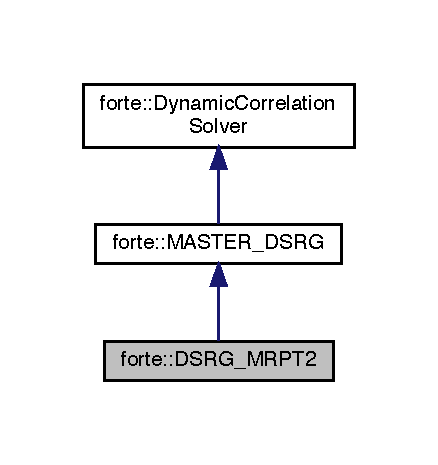
\includegraphics[width=210pt]{classforte_1_1_d_s_r_g___m_r_p_t2__inherit__graph}
\end{center}
\end{figure}


Collaboration diagram for forte\+:\+:D\+S\+R\+G\+\_\+\+M\+R\+P\+T2\+:
\nopagebreak
\begin{figure}[H]
\begin{center}
\leavevmode
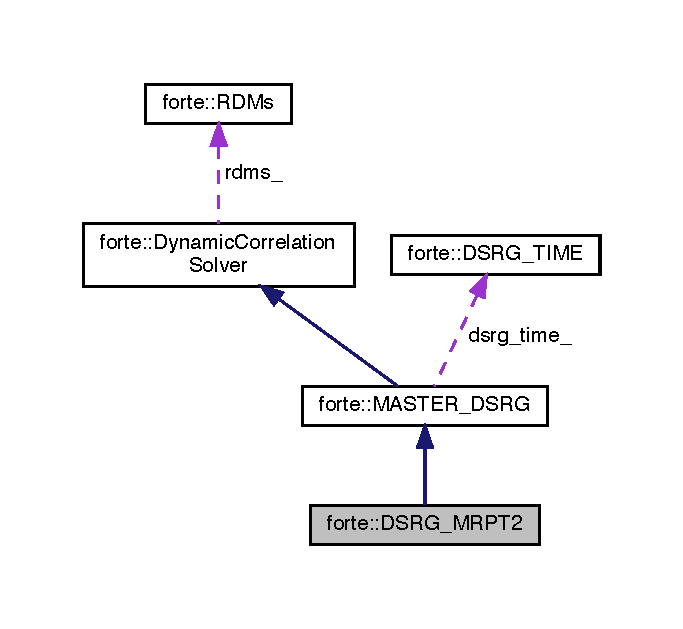
\includegraphics[width=328pt]{classforte_1_1_d_s_r_g___m_r_p_t2__coll__graph}
\end{center}
\end{figure}
\subsection*{Public Member Functions}
\begin{DoxyCompactItemize}
\item 
\mbox{\hyperlink{classforte_1_1_d_s_r_g___m_r_p_t2_a0e418cbcf42c1e36c77b6866e243aeb6}{D\+S\+R\+G\+\_\+\+M\+R\+P\+T2}} (\mbox{\hyperlink{classforte_1_1_r_d_ms}{R\+D\+Ms}} rdms, std\+::shared\+\_\+ptr$<$ \mbox{\hyperlink{classforte_1_1_s_c_f_info}{S\+C\+F\+Info}} $>$ scf\+\_\+info, std\+::shared\+\_\+ptr$<$ \mbox{\hyperlink{classforte_1_1_forte_options}{Forte\+Options}} $>$ options, std\+::shared\+\_\+ptr$<$ \mbox{\hyperlink{classforte_1_1_forte_integrals}{Forte\+Integrals}} $>$ ints, std\+::shared\+\_\+ptr$<$ \mbox{\hyperlink{classforte_1_1_m_o_space_info}{M\+O\+Space\+Info}} $>$ mo\+\_\+space\+\_\+info)
\item 
virtual \mbox{\hyperlink{classforte_1_1_d_s_r_g___m_r_p_t2_a5d3cf5ee234684e911d90de497aa868b}{$\sim$\+D\+S\+R\+G\+\_\+\+M\+R\+P\+T2}} ()
\begin{DoxyCompactList}\small\item\em Destructor. \end{DoxyCompactList}\item 
virtual double \mbox{\hyperlink{classforte_1_1_d_s_r_g___m_r_p_t2_a0884f1a9e8f98eb3c272e9c6518e7691}{compute\+\_\+energy}} ()
\begin{DoxyCompactList}\small\item\em Compute the D\+S\+R\+G-\/\+M\+R\+P\+T2 energy. \end{DoxyCompactList}\item 
virtual void \mbox{\hyperlink{classforte_1_1_d_s_r_g___m_r_p_t2_a739972fe0720c3a9881c1bd039fedb11}{compute\+\_\+\+Heff\+\_\+2nd\+\_\+coupling}} (double \&H0, ambit\+::\+Tensor \&H1a, ambit\+::\+Tensor \&H1b, ambit\+::\+Tensor \&H2aa, ambit\+::\+Tensor \&H2ab, ambit\+::\+Tensor \&H2bb, ambit\+::\+Tensor \&H3aaa, ambit\+::\+Tensor \&H3aab, ambit\+::\+Tensor \&H3abb, ambit\+::\+Tensor \&H3bbb)
\item 
virtual ambit\+::\+Blocked\+Tensor \mbox{\hyperlink{classforte_1_1_d_s_r_g___m_r_p_t2_a3811b3a31c76af9a94621c2b13213443}{get\+\_\+\+T1de\+G\+NO}} (double \&T0de\+G\+NO)
\begin{DoxyCompactList}\small\item\em Return de-\/normal-\/ordered T1 amplitudes. \end{DoxyCompactList}\item 
virtual ambit\+::\+Blocked\+Tensor \mbox{\hyperlink{classforte_1_1_d_s_r_g___m_r_p_t2_a02e0b5b0716ac974c03b8ed5cef17980}{get\+\_\+\+T2}} (const std\+::vector$<$ std\+::string $>$ \&blocks)
\begin{DoxyCompactList}\small\item\em Return T2 amplitudes. \end{DoxyCompactList}\item 
virtual ambit\+::\+Blocked\+Tensor \mbox{\hyperlink{classforte_1_1_d_s_r_g___m_r_p_t2_af60895decfd8d368a6b61648b8f82310}{get\+\_\+\+T2}} ()
\item 
virtual ambit\+::\+Blocked\+Tensor \mbox{\hyperlink{classforte_1_1_d_s_r_g___m_r_p_t2_ab5efb73cb6a375af7f41822df5476036}{get\+\_\+\+R\+H1de\+G\+NO}} ()
\begin{DoxyCompactList}\small\item\em Return de-\/normal-\/ordered 1-\/body renormalized 1st-\/order Hamiltonian. \end{DoxyCompactList}\item 
virtual ambit\+::\+Blocked\+Tensor \mbox{\hyperlink{classforte_1_1_d_s_r_g___m_r_p_t2_a9384e3028a6648b40ae605261ce12db9}{get\+\_\+\+R\+H2}} ()
\begin{DoxyCompactList}\small\item\em Return 2-\/body renormalized 1st-\/order Hamiltonian. \end{DoxyCompactList}\item 
ambit\+::\+Blocked\+Tensor \mbox{\hyperlink{classforte_1_1_d_s_r_g___m_r_p_t2_aa443e71193020de0811daa881e1ce714}{compute\+\_\+\+O\+E\+\_\+density}} (Blocked\+Tensor \&T1, Blocked\+Tensor \&T2, Blocked\+Tensor \&D1, Blocked\+Tensor \&\mbox{\hyperlink{namespaceforte_abe00ec86d0015c0f2b6ac298c6e428e4ac4d62b6dcca08e5caf06c01889282859}{D2}}, Blocked\+Tensor \&D3, const bool \&transition)
\item 
double \mbox{\hyperlink{classforte_1_1_d_s_r_g___m_r_p_t2_ac39c70c4908ad51d315e46688efa13ab}{compute\+\_\+energy\+\_\+relaxed}} ()
\begin{DoxyCompactList}\small\item\em Compute the D\+S\+R\+G-\/\+M\+R\+P\+T2 energy with relaxed reference (once) \end{DoxyCompactList}\item 
double \mbox{\hyperlink{classforte_1_1_d_s_r_g___m_r_p_t2_af6d61f7450e104821153196e3c78c38b}{compute\+\_\+energy\+\_\+multi\+\_\+state}} ()
\begin{DoxyCompactList}\small\item\em Compute the multi-\/state D\+S\+R\+G-\/\+M\+R\+P\+T2 energies. \end{DoxyCompactList}\item 
void \mbox{\hyperlink{classforte_1_1_d_s_r_g___m_r_p_t2_a194b1229ce90c93816ebd247e03b6dd2}{set\+\_\+eigens}} (const std\+::vector$<$ std\+::vector$<$ std\+::pair$<$ psi\+::\+Shared\+Vector, double $>$$>$$>$ \&eigens)
\begin{DoxyCompactList}\small\item\em Set C\+A\+S\+CI eigen values and eigen vectors for state averaging. \end{DoxyCompactList}\item 
void \mbox{\hyperlink{classforte_1_1_d_s_r_g___m_r_p_t2_acc9e874503df77dab79c642ef381efe3}{set\+\_\+p\+\_\+spaces}} (const std\+::vector$<$ std\+::vector$<$ \mbox{\hyperlink{namespaceforte_a2076c63fd7b8732004d9e1442ce527c1}{forte\+::\+Determinant}} $>$$>$ \&p\+\_\+spaces)
\begin{DoxyCompactList}\small\item\em Set determinants in the model space. \end{DoxyCompactList}\item 
void \mbox{\hyperlink{classforte_1_1_d_s_r_g___m_r_p_t2_a1c002fd10dc32ed7486e20f8b9cf7cbd}{rotate\+\_\+amp}} (psi\+::\+Shared\+Matrix Ua, psi\+::\+Shared\+Matrix Ub, const bool \&transpose=false, const bool \&t1eff=false)
\end{DoxyCompactItemize}
\subsection*{Protected Member Functions}
\begin{DoxyCompactItemize}
\item 
void \mbox{\hyperlink{classforte_1_1_d_s_r_g___m_r_p_t2_ab386924d3bc56b2a95912e860cdc5c50}{startup}} ()
\begin{DoxyCompactList}\small\item\em Called in the constructor. \end{DoxyCompactList}\item 
void \mbox{\hyperlink{classforte_1_1_d_s_r_g___m_r_p_t2_a278ccce08fe45126a0386196a14e00b6}{cleanup}} ()
\begin{DoxyCompactList}\small\item\em Called in the destructor. \end{DoxyCompactList}\item 
void \mbox{\hyperlink{classforte_1_1_d_s_r_g___m_r_p_t2_aa9aa3365f09c4a576a61bfb21c18e046}{print\+\_\+options\+\_\+summary}} ()
\begin{DoxyCompactList}\small\item\em Print a summary of the options. \end{DoxyCompactList}\item 
void \mbox{\hyperlink{classforte_1_1_d_s_r_g___m_r_p_t2_a16fb184164a8c89e1cde94058a093837}{build\+\_\+ints}} ()
\begin{DoxyCompactList}\small\item\em Fill up two-\/electron integrals. \end{DoxyCompactList}\item 
void \mbox{\hyperlink{classforte_1_1_d_s_r_g___m_r_p_t2_ab4fe26704d651cd9d1f80badf75210aa}{build\+\_\+density}} ()
\begin{DoxyCompactList}\small\item\em Fill up density matrix and density cumulants. \end{DoxyCompactList}\item 
void \mbox{\hyperlink{classforte_1_1_d_s_r_g___m_r_p_t2_adfd852f4cb7195744dc190d3615164ac}{build\+\_\+fock}} ()
\begin{DoxyCompactList}\small\item\em Build Fock matrix and diagonal Fock matrix elements. \end{DoxyCompactList}\item 
void \mbox{\hyperlink{classforte_1_1_d_s_r_g___m_r_p_t2_a84199d62bbbf1352c5eac34ea53f2972}{build\+\_\+oei}} ()
\begin{DoxyCompactList}\small\item\em Fill up one-\/electron integrals from F\+O\+R\+TE integral class. \end{DoxyCompactList}\item 
void \mbox{\hyperlink{classforte_1_1_d_s_r_g___m_r_p_t2_ac7c512a7d07ebfb7281ecc254637d513}{build\+\_\+eff\+\_\+oei}} ()
\begin{DoxyCompactList}\small\item\em Build effective O\+EI\+: hbar\+\_\+\{pq\} = h\+\_\+\{pq\} + sum\+\_\+\{m\} V\+\_\+\{pm,qm\}. \end{DoxyCompactList}\item 
void \mbox{\hyperlink{classforte_1_1_d_s_r_g___m_r_p_t2_ae7d4e5e977b7a7a199d0fa6dc68cbb6b}{renormalize\+\_\+F}} ()
\begin{DoxyCompactList}\small\item\em Renormalize Fock matrix. \end{DoxyCompactList}\item 
void \mbox{\hyperlink{classforte_1_1_d_s_r_g___m_r_p_t2_a05348e6a6dcad58a2d7e5e529ca86c41}{renormalize\+\_\+V}} ()
\begin{DoxyCompactList}\small\item\em Renormalize two-\/electron integrals. \end{DoxyCompactList}\item 
void \mbox{\hyperlink{classforte_1_1_d_s_r_g___m_r_p_t2_a0064cc44b232168515fdbea517136720}{compute\+\_\+t2}} ()
\begin{DoxyCompactList}\small\item\em Compute T2 amplitudes. \end{DoxyCompactList}\item 
void \mbox{\hyperlink{classforte_1_1_d_s_r_g___m_r_p_t2_a7d705e4e6386fd92f6212aa642c69a42}{check\+\_\+t2}} ()
\begin{DoxyCompactList}\small\item\em Check T2 and store large amplitudes. \end{DoxyCompactList}\item 
void \mbox{\hyperlink{classforte_1_1_d_s_r_g___m_r_p_t2_ad87625724c9dc201aacd227d5238911d}{compute\+\_\+t1}} ()
\begin{DoxyCompactList}\small\item\em Compute T1 amplitudes. \end{DoxyCompactList}\item 
void \mbox{\hyperlink{classforte_1_1_d_s_r_g___m_r_p_t2_a70e1a5eefd827e9d46f99e3734868afe}{check\+\_\+t1}} ()
\begin{DoxyCompactList}\small\item\em Check T1 and store large amplitudes. \end{DoxyCompactList}\item 
void \mbox{\hyperlink{classforte_1_1_d_s_r_g___m_r_p_t2_a45f5d2cc10218314d03e5232d3fe0cca}{print\+\_\+amp\+\_\+summary}} (const std\+::string \&name, const std\+::vector$<$ std\+::pair$<$ std\+::vector$<$ size\+\_\+t $>$, double $>$$>$ \&list, const double \&norm, const size\+\_\+t \&number\+\_\+nonzero)
\begin{DoxyCompactList}\small\item\em Print amplitudes summary. \end{DoxyCompactList}\item 
void \mbox{\hyperlink{classforte_1_1_d_s_r_g___m_r_p_t2_a47d0592d168445f748c06a0816d61d9e}{print\+\_\+intruder}} (const std\+::string \&name, const std\+::vector$<$ std\+::pair$<$ std\+::vector$<$ size\+\_\+t $>$, double $>$$>$ \&list)
\begin{DoxyCompactList}\small\item\em Print intruder analysis. \end{DoxyCompactList}\item 
double \mbox{\hyperlink{classforte_1_1_d_s_r_g___m_r_p_t2_a4500344800c525a638a373cc961952fd}{compute\+\_\+ref}} ()
\begin{DoxyCompactList}\small\item\em Compute reference energy. \end{DoxyCompactList}\item 
double \mbox{\hyperlink{classforte_1_1_d_s_r_g___m_r_p_t2_a8548c5c4e0686f3763dac78c4e315d27}{E\+\_\+\+F\+T1}} ()
\item 
double \mbox{\hyperlink{classforte_1_1_d_s_r_g___m_r_p_t2_a4ddb6a0cf716ea18138f92f2aebb0971}{E\+\_\+\+V\+T1}} ()
\item 
double \mbox{\hyperlink{classforte_1_1_d_s_r_g___m_r_p_t2_a3213f131ad783f95af808a8023945a0f}{E\+\_\+\+F\+T2}} ()
\item 
double \mbox{\hyperlink{classforte_1_1_d_s_r_g___m_r_p_t2_a96bc752be31fef42131144bd319f25eb}{E\+\_\+\+V\+T2\+\_\+2}} ()
\item 
double \mbox{\hyperlink{classforte_1_1_d_s_r_g___m_r_p_t2_a4bbc0d52b56294bbdc99019c5820f78c}{E\+\_\+\+V\+T2\+\_\+4\+PP}} ()
\item 
double \mbox{\hyperlink{classforte_1_1_d_s_r_g___m_r_p_t2_a8ad02257a93dbeb414872ddb4fabeb01}{E\+\_\+\+V\+T2\+\_\+4\+HH}} ()
\item 
double \mbox{\hyperlink{classforte_1_1_d_s_r_g___m_r_p_t2_a2285723d3fde907eb1fef4bfa295bc72}{E\+\_\+\+V\+T2\+\_\+4\+PH}} ()
\item 
double \mbox{\hyperlink{classforte_1_1_d_s_r_g___m_r_p_t2_aa53942e2ccdb9d1097db414aff78941c}{E\+\_\+\+V\+T2\+\_\+6}} ()
\item 
void \mbox{\hyperlink{classforte_1_1_d_s_r_g___m_r_p_t2_a998fe2003292000ad74f8babe57aab12}{print\+\_\+dm\+\_\+pt2}} ()
\begin{DoxyCompactList}\small\item\em Compute D\+S\+RG transformed dipole integrals. \end{DoxyCompactList}\item 
void \mbox{\hyperlink{classforte_1_1_d_s_r_g___m_r_p_t2_a7f7af22aa379020de56d8234a3113f2a}{compute\+\_\+dm1d\+\_\+pt2}} (Blocked\+Tensor \&M, double \&Mbar0, Blocked\+Tensor \&Mbar1, Blocked\+Tensor \&Mbar2)
\begin{DoxyCompactList}\small\item\em Compute D\+S\+RG transformed dipole integrals for a given direction. \end{DoxyCompactList}\item 
void \mbox{\hyperlink{classforte_1_1_d_s_r_g___m_r_p_t2_a5f75a8701631f236a25b0455a0cc692b}{compute\+\_\+dm1d\+\_\+pt2}} (Blocked\+Tensor \&M, double \&Mbar0, Blocked\+Tensor \&Mbar1, Blocked\+Tensor \&Mbar2, Blocked\+Tensor \&Mbar3)
\begin{DoxyCompactList}\small\item\em Compute D\+S\+RG transformed dipole integrals for a given direction. \end{DoxyCompactList}\item 
Blocked\+Tensor \mbox{\hyperlink{classforte_1_1_d_s_r_g___m_r_p_t2_af07239692f00078b36d57ce66517ad40}{compute\+\_\+pt2\+\_\+unrelaxed\+\_\+opdm}} ()
\begin{DoxyCompactList}\small\item\em Compute D\+S\+R\+G-\/\+P\+T2 correction for unrelaxed density. \end{DoxyCompactList}\item 
void \mbox{\hyperlink{classforte_1_1_d_s_r_g___m_r_p_t2_a0a07a976153924206ab3e0e9870f7ae1}{H1\+\_\+\+T1\+\_\+\+C1aa}} (Blocked\+Tensor \&H1, Blocked\+Tensor \&T1, const double \&alpha, Blocked\+Tensor \&\mbox{\hyperlink{namespaceforte_abe00ec86d0015c0f2b6ac298c6e428e4a1a2ddc2db4693cfd16d534cde5572cc1}{C1}})
\begin{DoxyCompactList}\small\item\em Compute one-\/body term of commutator \mbox{[}H1, T1\mbox{]}. \end{DoxyCompactList}\item 
void \mbox{\hyperlink{classforte_1_1_d_s_r_g___m_r_p_t2_a2f9f75d569a3f7e0089c5a7e149dfb6f}{H1\+\_\+\+T2\+\_\+\+C1aa}} (Blocked\+Tensor \&H1, Blocked\+Tensor \&T2, const double \&alpha, Blocked\+Tensor \&\mbox{\hyperlink{namespaceforte_abe00ec86d0015c0f2b6ac298c6e428e4a1a2ddc2db4693cfd16d534cde5572cc1}{C1}})
\begin{DoxyCompactList}\small\item\em Compute one-\/body term of commutator \mbox{[}H1, T2\mbox{]}. \end{DoxyCompactList}\item 
void \mbox{\hyperlink{classforte_1_1_d_s_r_g___m_r_p_t2_a5736629d09e1cdbded40bfb525757115}{H2\+\_\+\+T1\+\_\+\+C1aa}} (Blocked\+Tensor \&H2, Blocked\+Tensor \&T1, const double \&alpha, Blocked\+Tensor \&\mbox{\hyperlink{namespaceforte_abe00ec86d0015c0f2b6ac298c6e428e4a1a2ddc2db4693cfd16d534cde5572cc1}{C1}})
\begin{DoxyCompactList}\small\item\em Compute one-\/body term of commutator \mbox{[}H2, T1\mbox{]}. \end{DoxyCompactList}\item 
void \mbox{\hyperlink{classforte_1_1_d_s_r_g___m_r_p_t2_a927350265348432fed3dc13838860b38}{H2\+\_\+\+T2\+\_\+\+C1aa}} (Blocked\+Tensor \&H2, Blocked\+Tensor \&T2, const double \&alpha, Blocked\+Tensor \&\mbox{\hyperlink{namespaceforte_abe00ec86d0015c0f2b6ac298c6e428e4a1a2ddc2db4693cfd16d534cde5572cc1}{C1}})
\begin{DoxyCompactList}\small\item\em Compute one-\/body term of commutator \mbox{[}H2, T2\mbox{]}. \end{DoxyCompactList}\item 
void \mbox{\hyperlink{classforte_1_1_d_s_r_g___m_r_p_t2_aa16510df1c5e35c95718f66934c0e755}{H2\+\_\+\+T1\+\_\+\+C2aaaa}} (Blocked\+Tensor \&H2, Blocked\+Tensor \&T1, const double \&alpha, Blocked\+Tensor \&\mbox{\hyperlink{namespaceforte_abe00ec86d0015c0f2b6ac298c6e428e4af1a543f5a2c5d49bc5dde298fcf716e4}{C2}})
\begin{DoxyCompactList}\small\item\em Compute two-\/body term of commutator \mbox{[}H2, T1\mbox{]}. \end{DoxyCompactList}\item 
void \mbox{\hyperlink{classforte_1_1_d_s_r_g___m_r_p_t2_a09f8f3de3f9160f9c573b8180cf4d78c}{H1\+\_\+\+T2\+\_\+\+C2aaaa}} (Blocked\+Tensor \&H1, Blocked\+Tensor \&T2, const double \&alpha, Blocked\+Tensor \&\mbox{\hyperlink{namespaceforte_abe00ec86d0015c0f2b6ac298c6e428e4af1a543f5a2c5d49bc5dde298fcf716e4}{C2}})
\begin{DoxyCompactList}\small\item\em Compute two-\/body term of commutator \mbox{[}H1, T2\mbox{]}. \end{DoxyCompactList}\item 
void \mbox{\hyperlink{classforte_1_1_d_s_r_g___m_r_p_t2_a2b61743d0e4f4ebdedbe88a665256ec4}{H2\+\_\+\+T2\+\_\+\+C2aaaa}} (Blocked\+Tensor \&H2, Blocked\+Tensor \&T2, const double \&alpha, Blocked\+Tensor \&\mbox{\hyperlink{namespaceforte_abe00ec86d0015c0f2b6ac298c6e428e4af1a543f5a2c5d49bc5dde298fcf716e4}{C2}})
\begin{DoxyCompactList}\small\item\em Compute two-\/body term of commutator \mbox{[}H2, T2\mbox{]}. \end{DoxyCompactList}\item 
void \mbox{\hyperlink{classforte_1_1_d_s_r_g___m_r_p_t2_a5c2e5b5ff81053c3b0b95379b42b1fa7}{H2\+\_\+\+T2\+\_\+\+C3aaaaaa}} (Blocked\+Tensor \&H2, Blocked\+Tensor \&T2, const double \&alpha, Blocked\+Tensor \&C3)
\begin{DoxyCompactList}\small\item\em Compute three-\/body term of commutator \mbox{[}H2, T2\mbox{]}. \end{DoxyCompactList}\item 
std\+::vector$<$ std\+::vector$<$ double $>$ $>$ \mbox{\hyperlink{classforte_1_1_d_s_r_g___m_r_p_t2_a186a43767e4fc38f772b5fb62127d1c4}{compute\+\_\+energy\+\_\+sa}} ()
\begin{DoxyCompactList}\small\item\em Compute multi-\/state energy in the state-\/average way. \end{DoxyCompactList}\item 
std\+::vector$<$ std\+::vector$<$ double $>$ $>$ \mbox{\hyperlink{classforte_1_1_d_s_r_g___m_r_p_t2_a4b33c1f5ff523f6ee67f8a52e503f473}{compute\+\_\+energy\+\_\+xms}} ()
\begin{DoxyCompactList}\small\item\em Compute multi-\/state energy in the M\+S/\+X\+MS way. \end{DoxyCompactList}\item 
psi\+::\+Shared\+Matrix \mbox{\hyperlink{classforte_1_1_d_s_r_g___m_r_p_t2_a43625a369c2b1282becd2c0b2354765c}{xms\+\_\+rotation}} (std\+::shared\+\_\+ptr$<$ \mbox{\hyperlink{classforte_1_1_active_space_integrals}{Active\+Space\+Integrals}} $>$ fci\+\_\+ints, std\+::vector$<$ \mbox{\hyperlink{namespaceforte_a2076c63fd7b8732004d9e1442ce527c1}{Determinant}} $>$ \&p\+\_\+space, psi\+::\+Shared\+Matrix civecs)
\begin{DoxyCompactList}\small\item\em X\+MS rotation for the reference states. \end{DoxyCompactList}\item 
void \mbox{\hyperlink{classforte_1_1_d_s_r_g___m_r_p_t2_a0e238a680593f2011ea5d33b7c062a4b}{build\+\_\+\+T1eff\+\_\+de\+G\+NO}} ()
\begin{DoxyCompactList}\small\item\em Build effective singles\+: T\+\_\+\{ia\} -\/= T\+\_\+\{iu,av\} $\ast$ Gamma\+\_\+\{vu\}. \end{DoxyCompactList}\item 
void \mbox{\hyperlink{classforte_1_1_d_s_r_g___m_r_p_t2_aa847ed192819d46c2631d12ebf783cf9}{compute\+\_\+cumulants}} (std\+::shared\+\_\+ptr$<$ \mbox{\hyperlink{classforte_1_1_active_space_integrals}{Active\+Space\+Integrals}} $>$ fci\+\_\+ints, std\+::vector$<$ \mbox{\hyperlink{namespaceforte_a2076c63fd7b8732004d9e1442ce527c1}{forte\+::\+Determinant}} $>$ \&p\+\_\+space, psi\+::\+Shared\+Matrix evecs, const int \&root1, const int \&root2)
\begin{DoxyCompactList}\small\item\em Compute density cumulants. \end{DoxyCompactList}\item 
void \mbox{\hyperlink{classforte_1_1_d_s_r_g___m_r_p_t2_af254509d7ec7a2f9d0fa985dc4e603e4}{compute\+\_\+rdms}} (std\+::shared\+\_\+ptr$<$ \mbox{\hyperlink{classforte_1_1_active_space_integrals}{Active\+Space\+Integrals}} $>$ fci\+\_\+ints, std\+::vector$<$ \mbox{\hyperlink{namespaceforte_a2076c63fd7b8732004d9e1442ce527c1}{Determinant}} $>$ \&p\+\_\+space, psi\+::\+Shared\+Matrix evecs, const int \&root1, const int \&root2)
\begin{DoxyCompactList}\small\item\em Compute denisty matrices and puts in Gamma1\+\_\+, Lambda2\+\_\+, and Lambda3\+\_\+. \end{DoxyCompactList}\item 
double \mbox{\hyperlink{classforte_1_1_d_s_r_g___m_r_p_t2_ab26d66a2079561ba8c7f591eb3fa93da}{compute\+\_\+ms\+\_\+1st\+\_\+coupling}} (const std\+::string \&name)
\begin{DoxyCompactList}\small\item\em Compute MS coupling $<$M$\vert$\+H$\vert$N$>$ \end{DoxyCompactList}\item 
double \mbox{\hyperlink{classforte_1_1_d_s_r_g___m_r_p_t2_aafcf6bcdd3d59f232a61125d2b35c61a}{compute\+\_\+ms\+\_\+2nd\+\_\+coupling}} (const std\+::string \&name)
\begin{DoxyCompactList}\small\item\em Compute MS coupling $<$M$\vert$\+H\+T$\vert$N$>$ \end{DoxyCompactList}\item 
void \mbox{\hyperlink{classforte_1_1_d_s_r_g___m_r_p_t2_ac58de33a7bcba5b601e8d1cb627803c6}{rotate\+\_\+1rdm}} (ambit\+::\+Tensor \&L1a, ambit\+::\+Tensor \&L1b)
\item 
void \mbox{\hyperlink{classforte_1_1_d_s_r_g___m_r_p_t2_afb6995c283af9f99edbf819ea7359c1b}{rotate\+\_\+2rdm}} (ambit\+::\+Tensor \&L2aa, ambit\+::\+Tensor \&L2ab, ambit\+::\+Tensor \&L2bb)
\item 
void \mbox{\hyperlink{classforte_1_1_d_s_r_g___m_r_p_t2_a9b5fed7e984e823cbe4e5f5f443d4497}{rotate\+\_\+3rdm}} (ambit\+::\+Tensor \&L3aaa, ambit\+::\+Tensor \&L3aab, ambit\+::\+Tensor \&L3abb, ambit\+::\+Tensor \&L3bbb)
\end{DoxyCompactItemize}
\subsection*{Protected Attributes}
\begin{DoxyCompactItemize}
\item 
std\+::vector$<$ std\+::vector$<$ std\+::pair$<$ psi\+::\+Shared\+Vector, double $>$ $>$ $>$ \mbox{\hyperlink{classforte_1_1_d_s_r_g___m_r_p_t2_ac22e8c419a09d2fd29cdb675aff1caf1}{eigens\+\_\+}}
\begin{DoxyCompactList}\small\item\em C\+A\+S\+CI eigen values and eigen vectors for state averaging. \end{DoxyCompactList}\item 
std\+::vector$<$ std\+::vector$<$ \mbox{\hyperlink{namespaceforte_a2076c63fd7b8732004d9e1442ce527c1}{forte\+::\+Determinant}} $>$ $>$ \mbox{\hyperlink{classforte_1_1_d_s_r_g___m_r_p_t2_a842b10af7e2b96e27d0aaa9fd2da21b8}{p\+\_\+spaces\+\_\+}}
\begin{DoxyCompactList}\small\item\em Determinants with different symmetries in the model space. \end{DoxyCompactList}\item 
bool \mbox{\hyperlink{classforte_1_1_d_s_r_g___m_r_p_t2_ab4b37a2b2a1bf01caad8165f7476dc49}{semi\+\_\+canonical\+\_\+}}
\begin{DoxyCompactList}\small\item\em Are orbitals semi-\/canonicalized? \end{DoxyCompactList}\item 
std\+::vector$<$ double $>$ \mbox{\hyperlink{classforte_1_1_d_s_r_g___m_r_p_t2_a57e10017a1e9c437f6cc595c6676b93d}{Fa\+\_\+}}
\begin{DoxyCompactList}\small\item\em Diagonal elements of Fock matrices. \end{DoxyCompactList}\item 
std\+::vector$<$ double $>$ \mbox{\hyperlink{classforte_1_1_d_s_r_g___m_r_p_t2_a69f14f8c555585902fa90bb4767d5b0b}{Fb\+\_\+}}
\item 
ambit\+::\+Blocked\+Tensor \mbox{\hyperlink{classforte_1_1_d_s_r_g___m_r_p_t2_acf90518da17c2d21981798280a7333ea}{Hoei\+\_\+}}
\begin{DoxyCompactList}\small\item\em One-\/eletron integral. \end{DoxyCompactList}\item 
ambit\+::\+Blocked\+Tensor \mbox{\hyperlink{classforte_1_1_d_s_r_g___m_r_p_t2_ab6622a65f174a811188a13bdee32be45}{F\+\_\+}}
\begin{DoxyCompactList}\small\item\em Generalized Fock matrix (bare or renormalized) \end{DoxyCompactList}\item 
ambit\+::\+Blocked\+Tensor \mbox{\hyperlink{classforte_1_1_d_s_r_g___m_r_p_t2_abebb14bafab184a654ac1651bee598da}{V\+\_\+}}
\begin{DoxyCompactList}\small\item\em Two-\/electron integral (bare or renormalized) \end{DoxyCompactList}\item 
ambit\+::\+Blocked\+Tensor \mbox{\hyperlink{classforte_1_1_d_s_r_g___m_r_p_t2_a7aa81e311b741ebc02c7de520ec37e13}{T1\+\_\+}}
\begin{DoxyCompactList}\small\item\em Single excitation amplitude. \end{DoxyCompactList}\item 
ambit\+::\+Blocked\+Tensor \mbox{\hyperlink{classforte_1_1_d_s_r_g___m_r_p_t2_aba58b056b5ec69d829d80525f31239d6}{T1eff\+\_\+}}
\begin{DoxyCompactList}\small\item\em Effective single excitation amplitudes resulting from de-\/normal ordering. \end{DoxyCompactList}\item 
ambit\+::\+Blocked\+Tensor \mbox{\hyperlink{classforte_1_1_d_s_r_g___m_r_p_t2_a9fbb97e2fa2d8bca88d951860fa8c742}{T2\+\_\+}}
\begin{DoxyCompactList}\small\item\em Double excitation amplitude. \end{DoxyCompactList}\item 
ambit\+::\+Blocked\+Tensor \mbox{\hyperlink{classforte_1_1_d_s_r_g___m_r_p_t2_a5111a77e3bb21ad1716ae011db790f84}{U\+\_\+}}
\begin{DoxyCompactList}\small\item\em Unitary matrix to block diagonal Fock. \end{DoxyCompactList}\item 
double \mbox{\hyperlink{classforte_1_1_d_s_r_g___m_r_p_t2_aceadcc0e83de0c996e3eaf668a3d2f0f}{T2norm\+\_\+}}
\begin{DoxyCompactList}\small\item\em Norm of T2. \end{DoxyCompactList}\item 
double \mbox{\hyperlink{classforte_1_1_d_s_r_g___m_r_p_t2_ab39306f8bc090fc3ae56f603f5530529}{T2max\+\_\+}}
\begin{DoxyCompactList}\small\item\em Max (with sign) of T2. \end{DoxyCompactList}\item 
double \mbox{\hyperlink{classforte_1_1_d_s_r_g___m_r_p_t2_acb527bb20caef27ed8beb32a91009fe7}{T1norm\+\_\+}}
\begin{DoxyCompactList}\small\item\em Norm of T1. \end{DoxyCompactList}\item 
double \mbox{\hyperlink{classforte_1_1_d_s_r_g___m_r_p_t2_abca106ff840059c6fec9e2ead9c8012d}{T1max\+\_\+}}
\begin{DoxyCompactList}\small\item\em Max (with sign) of T1. \end{DoxyCompactList}\item 
bool \mbox{\hyperlink{classforte_1_1_d_s_r_g___m_r_p_t2_a401c2c0dfe6379fc40b962605c42ad41}{internal\+\_\+amp\+\_\+}}
\begin{DoxyCompactList}\small\item\em Include internal amplitude? \end{DoxyCompactList}\item 
std\+::string \mbox{\hyperlink{classforte_1_1_d_s_r_g___m_r_p_t2_a292cb8e86dd56fb34402abf0c1aae2be}{internal\+\_\+amp\+\_\+select\+\_\+}}
\begin{DoxyCompactList}\small\item\em Include which part of internal amplitudes? \end{DoxyCompactList}\item 
std\+::vector$<$ std\+::pair$<$ std\+::vector$<$ size\+\_\+t $>$, double $>$ $>$ \mbox{\hyperlink{classforte_1_1_d_s_r_g___m_r_p_t2_a6e27bcceffda696f2fd2e72dd7845e1e}{lt1a\+\_\+}}
\begin{DoxyCompactList}\small\item\em List of large amplitudes. \end{DoxyCompactList}\item 
std\+::vector$<$ std\+::pair$<$ std\+::vector$<$ size\+\_\+t $>$, double $>$ $>$ \mbox{\hyperlink{classforte_1_1_d_s_r_g___m_r_p_t2_a8b029902475ae1a4db6263508053145c}{lt1b\+\_\+}}
\item 
std\+::vector$<$ std\+::pair$<$ std\+::vector$<$ size\+\_\+t $>$, double $>$ $>$ \mbox{\hyperlink{classforte_1_1_d_s_r_g___m_r_p_t2_a1f532da34bc467fdd83b918981a592ae}{lt2aa\+\_\+}}
\item 
std\+::vector$<$ std\+::pair$<$ std\+::vector$<$ size\+\_\+t $>$, double $>$ $>$ \mbox{\hyperlink{classforte_1_1_d_s_r_g___m_r_p_t2_a4cff2fc3a4b602efb9d4310b026f0b71}{lt2ab\+\_\+}}
\item 
std\+::vector$<$ std\+::pair$<$ std\+::vector$<$ size\+\_\+t $>$, double $>$ $>$ \mbox{\hyperlink{classforte_1_1_d_s_r_g___m_r_p_t2_afd4a5fef0331eb55d9469c705af6e1d7}{lt2bb\+\_\+}}
\end{DoxyCompactItemize}


\subsection{Constructor \& Destructor Documentation}
\mbox{\Hypertarget{classforte_1_1_d_s_r_g___m_r_p_t2_a0e418cbcf42c1e36c77b6866e243aeb6}\label{classforte_1_1_d_s_r_g___m_r_p_t2_a0e418cbcf42c1e36c77b6866e243aeb6}} 
\index{forte\+::\+D\+S\+R\+G\+\_\+\+M\+R\+P\+T2@{forte\+::\+D\+S\+R\+G\+\_\+\+M\+R\+P\+T2}!D\+S\+R\+G\+\_\+\+M\+R\+P\+T2@{D\+S\+R\+G\+\_\+\+M\+R\+P\+T2}}
\index{D\+S\+R\+G\+\_\+\+M\+R\+P\+T2@{D\+S\+R\+G\+\_\+\+M\+R\+P\+T2}!forte\+::\+D\+S\+R\+G\+\_\+\+M\+R\+P\+T2@{forte\+::\+D\+S\+R\+G\+\_\+\+M\+R\+P\+T2}}
\subsubsection{\texorpdfstring{D\+S\+R\+G\+\_\+\+M\+R\+P\+T2()}{DSRG\_MRPT2()}}
{\footnotesize\ttfamily forte\+::\+D\+S\+R\+G\+\_\+\+M\+R\+P\+T2\+::\+D\+S\+R\+G\+\_\+\+M\+R\+P\+T2 (\begin{DoxyParamCaption}\item[{\mbox{\hyperlink{classforte_1_1_r_d_ms}{R\+D\+Ms}}}]{rdms,  }\item[{std\+::shared\+\_\+ptr$<$ \mbox{\hyperlink{classforte_1_1_s_c_f_info}{S\+C\+F\+Info}} $>$}]{scf\+\_\+info,  }\item[{std\+::shared\+\_\+ptr$<$ \mbox{\hyperlink{classforte_1_1_forte_options}{Forte\+Options}} $>$}]{options,  }\item[{std\+::shared\+\_\+ptr$<$ \mbox{\hyperlink{classforte_1_1_forte_integrals}{Forte\+Integrals}} $>$}]{ints,  }\item[{std\+::shared\+\_\+ptr$<$ \mbox{\hyperlink{classforte_1_1_m_o_space_info}{M\+O\+Space\+Info}} $>$}]{mo\+\_\+space\+\_\+info }\end{DoxyParamCaption})}

\mbox{\hyperlink{classforte_1_1_d_s_r_g___m_r_p_t2}{D\+S\+R\+G\+\_\+\+M\+R\+P\+T2}} Constructor 
\begin{DoxyParams}{Parameters}
{\em reference} & The reference object of F\+O\+R\+TE \\
\hline
{\em ref\+\_\+wfn} & The reference wavefunction object \\
\hline
{\em options} & The main options object \\
\hline
{\em ints} & A pointer to an allocated integral object \\
\hline
{\em mo\+\_\+space\+\_\+info} & A pointer to the \mbox{\hyperlink{classforte_1_1_m_o_space_info}{M\+O\+Space\+Info}} object \\
\hline
\end{DoxyParams}
\mbox{\Hypertarget{classforte_1_1_d_s_r_g___m_r_p_t2_a5d3cf5ee234684e911d90de497aa868b}\label{classforte_1_1_d_s_r_g___m_r_p_t2_a5d3cf5ee234684e911d90de497aa868b}} 
\index{forte\+::\+D\+S\+R\+G\+\_\+\+M\+R\+P\+T2@{forte\+::\+D\+S\+R\+G\+\_\+\+M\+R\+P\+T2}!````~D\+S\+R\+G\+\_\+\+M\+R\+P\+T2@{$\sim$\+D\+S\+R\+G\+\_\+\+M\+R\+P\+T2}}
\index{````~D\+S\+R\+G\+\_\+\+M\+R\+P\+T2@{$\sim$\+D\+S\+R\+G\+\_\+\+M\+R\+P\+T2}!forte\+::\+D\+S\+R\+G\+\_\+\+M\+R\+P\+T2@{forte\+::\+D\+S\+R\+G\+\_\+\+M\+R\+P\+T2}}
\subsubsection{\texorpdfstring{$\sim$\+D\+S\+R\+G\+\_\+\+M\+R\+P\+T2()}{~DSRG\_MRPT2()}}
{\footnotesize\ttfamily forte\+::\+D\+S\+R\+G\+\_\+\+M\+R\+P\+T2\+::$\sim$\+D\+S\+R\+G\+\_\+\+M\+R\+P\+T2 (\begin{DoxyParamCaption}{ }\end{DoxyParamCaption})\hspace{0.3cm}{\ttfamily [virtual]}}



Destructor. 



\subsection{Member Function Documentation}
\mbox{\Hypertarget{classforte_1_1_d_s_r_g___m_r_p_t2_ab4fe26704d651cd9d1f80badf75210aa}\label{classforte_1_1_d_s_r_g___m_r_p_t2_ab4fe26704d651cd9d1f80badf75210aa}} 
\index{forte\+::\+D\+S\+R\+G\+\_\+\+M\+R\+P\+T2@{forte\+::\+D\+S\+R\+G\+\_\+\+M\+R\+P\+T2}!build\+\_\+density@{build\+\_\+density}}
\index{build\+\_\+density@{build\+\_\+density}!forte\+::\+D\+S\+R\+G\+\_\+\+M\+R\+P\+T2@{forte\+::\+D\+S\+R\+G\+\_\+\+M\+R\+P\+T2}}
\subsubsection{\texorpdfstring{build\+\_\+density()}{build\_density()}}
{\footnotesize\ttfamily void forte\+::\+D\+S\+R\+G\+\_\+\+M\+R\+P\+T2\+::build\+\_\+density (\begin{DoxyParamCaption}{ }\end{DoxyParamCaption})\hspace{0.3cm}{\ttfamily [protected]}}



Fill up density matrix and density cumulants. 

\mbox{\Hypertarget{classforte_1_1_d_s_r_g___m_r_p_t2_ac7c512a7d07ebfb7281ecc254637d513}\label{classforte_1_1_d_s_r_g___m_r_p_t2_ac7c512a7d07ebfb7281ecc254637d513}} 
\index{forte\+::\+D\+S\+R\+G\+\_\+\+M\+R\+P\+T2@{forte\+::\+D\+S\+R\+G\+\_\+\+M\+R\+P\+T2}!build\+\_\+eff\+\_\+oei@{build\+\_\+eff\+\_\+oei}}
\index{build\+\_\+eff\+\_\+oei@{build\+\_\+eff\+\_\+oei}!forte\+::\+D\+S\+R\+G\+\_\+\+M\+R\+P\+T2@{forte\+::\+D\+S\+R\+G\+\_\+\+M\+R\+P\+T2}}
\subsubsection{\texorpdfstring{build\+\_\+eff\+\_\+oei()}{build\_eff\_oei()}}
{\footnotesize\ttfamily void forte\+::\+D\+S\+R\+G\+\_\+\+M\+R\+P\+T2\+::build\+\_\+eff\+\_\+oei (\begin{DoxyParamCaption}{ }\end{DoxyParamCaption})\hspace{0.3cm}{\ttfamily [protected]}}



Build effective O\+EI\+: hbar\+\_\+\{pq\} = h\+\_\+\{pq\} + sum\+\_\+\{m\} V\+\_\+\{pm,qm\}. 

\mbox{\Hypertarget{classforte_1_1_d_s_r_g___m_r_p_t2_adfd852f4cb7195744dc190d3615164ac}\label{classforte_1_1_d_s_r_g___m_r_p_t2_adfd852f4cb7195744dc190d3615164ac}} 
\index{forte\+::\+D\+S\+R\+G\+\_\+\+M\+R\+P\+T2@{forte\+::\+D\+S\+R\+G\+\_\+\+M\+R\+P\+T2}!build\+\_\+fock@{build\+\_\+fock}}
\index{build\+\_\+fock@{build\+\_\+fock}!forte\+::\+D\+S\+R\+G\+\_\+\+M\+R\+P\+T2@{forte\+::\+D\+S\+R\+G\+\_\+\+M\+R\+P\+T2}}
\subsubsection{\texorpdfstring{build\+\_\+fock()}{build\_fock()}}
{\footnotesize\ttfamily void forte\+::\+D\+S\+R\+G\+\_\+\+M\+R\+P\+T2\+::build\+\_\+fock (\begin{DoxyParamCaption}{ }\end{DoxyParamCaption})\hspace{0.3cm}{\ttfamily [protected]}}



Build Fock matrix and diagonal Fock matrix elements. 

\mbox{\Hypertarget{classforte_1_1_d_s_r_g___m_r_p_t2_a16fb184164a8c89e1cde94058a093837}\label{classforte_1_1_d_s_r_g___m_r_p_t2_a16fb184164a8c89e1cde94058a093837}} 
\index{forte\+::\+D\+S\+R\+G\+\_\+\+M\+R\+P\+T2@{forte\+::\+D\+S\+R\+G\+\_\+\+M\+R\+P\+T2}!build\+\_\+ints@{build\+\_\+ints}}
\index{build\+\_\+ints@{build\+\_\+ints}!forte\+::\+D\+S\+R\+G\+\_\+\+M\+R\+P\+T2@{forte\+::\+D\+S\+R\+G\+\_\+\+M\+R\+P\+T2}}
\subsubsection{\texorpdfstring{build\+\_\+ints()}{build\_ints()}}
{\footnotesize\ttfamily void forte\+::\+D\+S\+R\+G\+\_\+\+M\+R\+P\+T2\+::build\+\_\+ints (\begin{DoxyParamCaption}{ }\end{DoxyParamCaption})\hspace{0.3cm}{\ttfamily [protected]}}



Fill up two-\/electron integrals. 

\mbox{\Hypertarget{classforte_1_1_d_s_r_g___m_r_p_t2_a84199d62bbbf1352c5eac34ea53f2972}\label{classforte_1_1_d_s_r_g___m_r_p_t2_a84199d62bbbf1352c5eac34ea53f2972}} 
\index{forte\+::\+D\+S\+R\+G\+\_\+\+M\+R\+P\+T2@{forte\+::\+D\+S\+R\+G\+\_\+\+M\+R\+P\+T2}!build\+\_\+oei@{build\+\_\+oei}}
\index{build\+\_\+oei@{build\+\_\+oei}!forte\+::\+D\+S\+R\+G\+\_\+\+M\+R\+P\+T2@{forte\+::\+D\+S\+R\+G\+\_\+\+M\+R\+P\+T2}}
\subsubsection{\texorpdfstring{build\+\_\+oei()}{build\_oei()}}
{\footnotesize\ttfamily void forte\+::\+D\+S\+R\+G\+\_\+\+M\+R\+P\+T2\+::build\+\_\+oei (\begin{DoxyParamCaption}{ }\end{DoxyParamCaption})\hspace{0.3cm}{\ttfamily [protected]}}



Fill up one-\/electron integrals from F\+O\+R\+TE integral class. 

\mbox{\Hypertarget{classforte_1_1_d_s_r_g___m_r_p_t2_a0e238a680593f2011ea5d33b7c062a4b}\label{classforte_1_1_d_s_r_g___m_r_p_t2_a0e238a680593f2011ea5d33b7c062a4b}} 
\index{forte\+::\+D\+S\+R\+G\+\_\+\+M\+R\+P\+T2@{forte\+::\+D\+S\+R\+G\+\_\+\+M\+R\+P\+T2}!build\+\_\+\+T1eff\+\_\+de\+G\+NO@{build\+\_\+\+T1eff\+\_\+de\+G\+NO}}
\index{build\+\_\+\+T1eff\+\_\+de\+G\+NO@{build\+\_\+\+T1eff\+\_\+de\+G\+NO}!forte\+::\+D\+S\+R\+G\+\_\+\+M\+R\+P\+T2@{forte\+::\+D\+S\+R\+G\+\_\+\+M\+R\+P\+T2}}
\subsubsection{\texorpdfstring{build\+\_\+\+T1eff\+\_\+de\+G\+N\+O()}{build\_T1eff\_deGNO()}}
{\footnotesize\ttfamily void forte\+::\+D\+S\+R\+G\+\_\+\+M\+R\+P\+T2\+::build\+\_\+\+T1eff\+\_\+de\+G\+NO (\begin{DoxyParamCaption}{ }\end{DoxyParamCaption})\hspace{0.3cm}{\ttfamily [protected]}}



Build effective singles\+: T\+\_\+\{ia\} -\/= T\+\_\+\{iu,av\} $\ast$ Gamma\+\_\+\{vu\}. 

\mbox{\Hypertarget{classforte_1_1_d_s_r_g___m_r_p_t2_a70e1a5eefd827e9d46f99e3734868afe}\label{classforte_1_1_d_s_r_g___m_r_p_t2_a70e1a5eefd827e9d46f99e3734868afe}} 
\index{forte\+::\+D\+S\+R\+G\+\_\+\+M\+R\+P\+T2@{forte\+::\+D\+S\+R\+G\+\_\+\+M\+R\+P\+T2}!check\+\_\+t1@{check\+\_\+t1}}
\index{check\+\_\+t1@{check\+\_\+t1}!forte\+::\+D\+S\+R\+G\+\_\+\+M\+R\+P\+T2@{forte\+::\+D\+S\+R\+G\+\_\+\+M\+R\+P\+T2}}
\subsubsection{\texorpdfstring{check\+\_\+t1()}{check\_t1()}}
{\footnotesize\ttfamily void forte\+::\+D\+S\+R\+G\+\_\+\+M\+R\+P\+T2\+::check\+\_\+t1 (\begin{DoxyParamCaption}{ }\end{DoxyParamCaption})\hspace{0.3cm}{\ttfamily [protected]}}



Check T1 and store large amplitudes. 

\mbox{\Hypertarget{classforte_1_1_d_s_r_g___m_r_p_t2_a7d705e4e6386fd92f6212aa642c69a42}\label{classforte_1_1_d_s_r_g___m_r_p_t2_a7d705e4e6386fd92f6212aa642c69a42}} 
\index{forte\+::\+D\+S\+R\+G\+\_\+\+M\+R\+P\+T2@{forte\+::\+D\+S\+R\+G\+\_\+\+M\+R\+P\+T2}!check\+\_\+t2@{check\+\_\+t2}}
\index{check\+\_\+t2@{check\+\_\+t2}!forte\+::\+D\+S\+R\+G\+\_\+\+M\+R\+P\+T2@{forte\+::\+D\+S\+R\+G\+\_\+\+M\+R\+P\+T2}}
\subsubsection{\texorpdfstring{check\+\_\+t2()}{check\_t2()}}
{\footnotesize\ttfamily void forte\+::\+D\+S\+R\+G\+\_\+\+M\+R\+P\+T2\+::check\+\_\+t2 (\begin{DoxyParamCaption}{ }\end{DoxyParamCaption})\hspace{0.3cm}{\ttfamily [protected]}}



Check T2 and store large amplitudes. 

\mbox{\Hypertarget{classforte_1_1_d_s_r_g___m_r_p_t2_a278ccce08fe45126a0386196a14e00b6}\label{classforte_1_1_d_s_r_g___m_r_p_t2_a278ccce08fe45126a0386196a14e00b6}} 
\index{forte\+::\+D\+S\+R\+G\+\_\+\+M\+R\+P\+T2@{forte\+::\+D\+S\+R\+G\+\_\+\+M\+R\+P\+T2}!cleanup@{cleanup}}
\index{cleanup@{cleanup}!forte\+::\+D\+S\+R\+G\+\_\+\+M\+R\+P\+T2@{forte\+::\+D\+S\+R\+G\+\_\+\+M\+R\+P\+T2}}
\subsubsection{\texorpdfstring{cleanup()}{cleanup()}}
{\footnotesize\ttfamily void forte\+::\+D\+S\+R\+G\+\_\+\+M\+R\+P\+T2\+::cleanup (\begin{DoxyParamCaption}{ }\end{DoxyParamCaption})\hspace{0.3cm}{\ttfamily [protected]}}



Called in the destructor. 

\mbox{\Hypertarget{classforte_1_1_d_s_r_g___m_r_p_t2_aa847ed192819d46c2631d12ebf783cf9}\label{classforte_1_1_d_s_r_g___m_r_p_t2_aa847ed192819d46c2631d12ebf783cf9}} 
\index{forte\+::\+D\+S\+R\+G\+\_\+\+M\+R\+P\+T2@{forte\+::\+D\+S\+R\+G\+\_\+\+M\+R\+P\+T2}!compute\+\_\+cumulants@{compute\+\_\+cumulants}}
\index{compute\+\_\+cumulants@{compute\+\_\+cumulants}!forte\+::\+D\+S\+R\+G\+\_\+\+M\+R\+P\+T2@{forte\+::\+D\+S\+R\+G\+\_\+\+M\+R\+P\+T2}}
\subsubsection{\texorpdfstring{compute\+\_\+cumulants()}{compute\_cumulants()}}
{\footnotesize\ttfamily void forte\+::\+D\+S\+R\+G\+\_\+\+M\+R\+P\+T2\+::compute\+\_\+cumulants (\begin{DoxyParamCaption}\item[{std\+::shared\+\_\+ptr$<$ \mbox{\hyperlink{classforte_1_1_active_space_integrals}{Active\+Space\+Integrals}} $>$}]{fci\+\_\+ints,  }\item[{std\+::vector$<$ \mbox{\hyperlink{namespaceforte_a2076c63fd7b8732004d9e1442ce527c1}{forte\+::\+Determinant}} $>$ \&}]{p\+\_\+space,  }\item[{psi\+::\+Shared\+Matrix}]{evecs,  }\item[{const int \&}]{root1,  }\item[{const int \&}]{root2 }\end{DoxyParamCaption})\hspace{0.3cm}{\ttfamily [protected]}}



Compute density cumulants. 

\mbox{\Hypertarget{classforte_1_1_d_s_r_g___m_r_p_t2_a7f7af22aa379020de56d8234a3113f2a}\label{classforte_1_1_d_s_r_g___m_r_p_t2_a7f7af22aa379020de56d8234a3113f2a}} 
\index{forte\+::\+D\+S\+R\+G\+\_\+\+M\+R\+P\+T2@{forte\+::\+D\+S\+R\+G\+\_\+\+M\+R\+P\+T2}!compute\+\_\+dm1d\+\_\+pt2@{compute\+\_\+dm1d\+\_\+pt2}}
\index{compute\+\_\+dm1d\+\_\+pt2@{compute\+\_\+dm1d\+\_\+pt2}!forte\+::\+D\+S\+R\+G\+\_\+\+M\+R\+P\+T2@{forte\+::\+D\+S\+R\+G\+\_\+\+M\+R\+P\+T2}}
\subsubsection{\texorpdfstring{compute\+\_\+dm1d\+\_\+pt2()}{compute\_dm1d\_pt2()}\hspace{0.1cm}{\footnotesize\ttfamily [1/2]}}
{\footnotesize\ttfamily void forte\+::\+D\+S\+R\+G\+\_\+\+M\+R\+P\+T2\+::compute\+\_\+dm1d\+\_\+pt2 (\begin{DoxyParamCaption}\item[{Blocked\+Tensor \&}]{M,  }\item[{double \&}]{Mbar0,  }\item[{Blocked\+Tensor \&}]{Mbar1,  }\item[{Blocked\+Tensor \&}]{Mbar2 }\end{DoxyParamCaption})\hspace{0.3cm}{\ttfamily [protected]}}



Compute D\+S\+RG transformed dipole integrals for a given direction. 

Mbar = M + \mbox{[}M, A\mbox{]} + 0.\+5 $\ast$ \mbox{[}\mbox{[}M, A\mbox{]}, A\mbox{]} \mbox{\Hypertarget{classforte_1_1_d_s_r_g___m_r_p_t2_a5f75a8701631f236a25b0455a0cc692b}\label{classforte_1_1_d_s_r_g___m_r_p_t2_a5f75a8701631f236a25b0455a0cc692b}} 
\index{forte\+::\+D\+S\+R\+G\+\_\+\+M\+R\+P\+T2@{forte\+::\+D\+S\+R\+G\+\_\+\+M\+R\+P\+T2}!compute\+\_\+dm1d\+\_\+pt2@{compute\+\_\+dm1d\+\_\+pt2}}
\index{compute\+\_\+dm1d\+\_\+pt2@{compute\+\_\+dm1d\+\_\+pt2}!forte\+::\+D\+S\+R\+G\+\_\+\+M\+R\+P\+T2@{forte\+::\+D\+S\+R\+G\+\_\+\+M\+R\+P\+T2}}
\subsubsection{\texorpdfstring{compute\+\_\+dm1d\+\_\+pt2()}{compute\_dm1d\_pt2()}\hspace{0.1cm}{\footnotesize\ttfamily [2/2]}}
{\footnotesize\ttfamily void forte\+::\+D\+S\+R\+G\+\_\+\+M\+R\+P\+T2\+::compute\+\_\+dm1d\+\_\+pt2 (\begin{DoxyParamCaption}\item[{Blocked\+Tensor \&}]{M,  }\item[{double \&}]{Mbar0,  }\item[{Blocked\+Tensor \&}]{Mbar1,  }\item[{Blocked\+Tensor \&}]{Mbar2,  }\item[{Blocked\+Tensor \&}]{Mbar3 }\end{DoxyParamCaption})\hspace{0.3cm}{\ttfamily [protected]}}



Compute D\+S\+RG transformed dipole integrals for a given direction. 

Mbar = M + \mbox{[}M, A\mbox{]} + 0.\+5 $\ast$ \mbox{[}\mbox{[}M, A\mbox{]}, A\mbox{]}

This needs to be checked \mbox{\Hypertarget{classforte_1_1_d_s_r_g___m_r_p_t2_a0884f1a9e8f98eb3c272e9c6518e7691}\label{classforte_1_1_d_s_r_g___m_r_p_t2_a0884f1a9e8f98eb3c272e9c6518e7691}} 
\index{forte\+::\+D\+S\+R\+G\+\_\+\+M\+R\+P\+T2@{forte\+::\+D\+S\+R\+G\+\_\+\+M\+R\+P\+T2}!compute\+\_\+energy@{compute\+\_\+energy}}
\index{compute\+\_\+energy@{compute\+\_\+energy}!forte\+::\+D\+S\+R\+G\+\_\+\+M\+R\+P\+T2@{forte\+::\+D\+S\+R\+G\+\_\+\+M\+R\+P\+T2}}
\subsubsection{\texorpdfstring{compute\+\_\+energy()}{compute\_energy()}}
{\footnotesize\ttfamily double forte\+::\+D\+S\+R\+G\+\_\+\+M\+R\+P\+T2\+::compute\+\_\+energy (\begin{DoxyParamCaption}{ }\end{DoxyParamCaption})\hspace{0.3cm}{\ttfamily [virtual]}}



Compute the D\+S\+R\+G-\/\+M\+R\+P\+T2 energy. 



Implements \mbox{\hyperlink{classforte_1_1_m_a_s_t_e_r___d_s_r_g_a34011aaadcc79224071a4266a095591b}{forte\+::\+M\+A\+S\+T\+E\+R\+\_\+\+D\+S\+RG}}.

\mbox{\Hypertarget{classforte_1_1_d_s_r_g___m_r_p_t2_af6d61f7450e104821153196e3c78c38b}\label{classforte_1_1_d_s_r_g___m_r_p_t2_af6d61f7450e104821153196e3c78c38b}} 
\index{forte\+::\+D\+S\+R\+G\+\_\+\+M\+R\+P\+T2@{forte\+::\+D\+S\+R\+G\+\_\+\+M\+R\+P\+T2}!compute\+\_\+energy\+\_\+multi\+\_\+state@{compute\+\_\+energy\+\_\+multi\+\_\+state}}
\index{compute\+\_\+energy\+\_\+multi\+\_\+state@{compute\+\_\+energy\+\_\+multi\+\_\+state}!forte\+::\+D\+S\+R\+G\+\_\+\+M\+R\+P\+T2@{forte\+::\+D\+S\+R\+G\+\_\+\+M\+R\+P\+T2}}
\subsubsection{\texorpdfstring{compute\+\_\+energy\+\_\+multi\+\_\+state()}{compute\_energy\_multi\_state()}}
{\footnotesize\ttfamily double forte\+::\+D\+S\+R\+G\+\_\+\+M\+R\+P\+T2\+::compute\+\_\+energy\+\_\+multi\+\_\+state (\begin{DoxyParamCaption}{ }\end{DoxyParamCaption})}



Compute the multi-\/state D\+S\+R\+G-\/\+M\+R\+P\+T2 energies. 

\mbox{\Hypertarget{classforte_1_1_d_s_r_g___m_r_p_t2_ac39c70c4908ad51d315e46688efa13ab}\label{classforte_1_1_d_s_r_g___m_r_p_t2_ac39c70c4908ad51d315e46688efa13ab}} 
\index{forte\+::\+D\+S\+R\+G\+\_\+\+M\+R\+P\+T2@{forte\+::\+D\+S\+R\+G\+\_\+\+M\+R\+P\+T2}!compute\+\_\+energy\+\_\+relaxed@{compute\+\_\+energy\+\_\+relaxed}}
\index{compute\+\_\+energy\+\_\+relaxed@{compute\+\_\+energy\+\_\+relaxed}!forte\+::\+D\+S\+R\+G\+\_\+\+M\+R\+P\+T2@{forte\+::\+D\+S\+R\+G\+\_\+\+M\+R\+P\+T2}}
\subsubsection{\texorpdfstring{compute\+\_\+energy\+\_\+relaxed()}{compute\_energy\_relaxed()}}
{\footnotesize\ttfamily double forte\+::\+D\+S\+R\+G\+\_\+\+M\+R\+P\+T2\+::compute\+\_\+energy\+\_\+relaxed (\begin{DoxyParamCaption}{ }\end{DoxyParamCaption})}



Compute the D\+S\+R\+G-\/\+M\+R\+P\+T2 energy with relaxed reference (once) 

\mbox{\Hypertarget{classforte_1_1_d_s_r_g___m_r_p_t2_a186a43767e4fc38f772b5fb62127d1c4}\label{classforte_1_1_d_s_r_g___m_r_p_t2_a186a43767e4fc38f772b5fb62127d1c4}} 
\index{forte\+::\+D\+S\+R\+G\+\_\+\+M\+R\+P\+T2@{forte\+::\+D\+S\+R\+G\+\_\+\+M\+R\+P\+T2}!compute\+\_\+energy\+\_\+sa@{compute\+\_\+energy\+\_\+sa}}
\index{compute\+\_\+energy\+\_\+sa@{compute\+\_\+energy\+\_\+sa}!forte\+::\+D\+S\+R\+G\+\_\+\+M\+R\+P\+T2@{forte\+::\+D\+S\+R\+G\+\_\+\+M\+R\+P\+T2}}
\subsubsection{\texorpdfstring{compute\+\_\+energy\+\_\+sa()}{compute\_energy\_sa()}}
{\footnotesize\ttfamily std\+::vector$<$std\+::vector$<$double$>$ $>$ forte\+::\+D\+S\+R\+G\+\_\+\+M\+R\+P\+T2\+::compute\+\_\+energy\+\_\+sa (\begin{DoxyParamCaption}{ }\end{DoxyParamCaption})\hspace{0.3cm}{\ttfamily [protected]}}



Compute multi-\/state energy in the state-\/average way. 

\mbox{\Hypertarget{classforte_1_1_d_s_r_g___m_r_p_t2_a4b33c1f5ff523f6ee67f8a52e503f473}\label{classforte_1_1_d_s_r_g___m_r_p_t2_a4b33c1f5ff523f6ee67f8a52e503f473}} 
\index{forte\+::\+D\+S\+R\+G\+\_\+\+M\+R\+P\+T2@{forte\+::\+D\+S\+R\+G\+\_\+\+M\+R\+P\+T2}!compute\+\_\+energy\+\_\+xms@{compute\+\_\+energy\+\_\+xms}}
\index{compute\+\_\+energy\+\_\+xms@{compute\+\_\+energy\+\_\+xms}!forte\+::\+D\+S\+R\+G\+\_\+\+M\+R\+P\+T2@{forte\+::\+D\+S\+R\+G\+\_\+\+M\+R\+P\+T2}}
\subsubsection{\texorpdfstring{compute\+\_\+energy\+\_\+xms()}{compute\_energy\_xms()}}
{\footnotesize\ttfamily std\+::vector$<$ std\+::vector$<$ double $>$ $>$ forte\+::\+D\+S\+R\+G\+\_\+\+M\+R\+P\+T2\+::compute\+\_\+energy\+\_\+xms (\begin{DoxyParamCaption}{ }\end{DoxyParamCaption})\hspace{0.3cm}{\ttfamily [protected]}}



Compute multi-\/state energy in the M\+S/\+X\+MS way. 

\mbox{\Hypertarget{classforte_1_1_d_s_r_g___m_r_p_t2_a739972fe0720c3a9881c1bd039fedb11}\label{classforte_1_1_d_s_r_g___m_r_p_t2_a739972fe0720c3a9881c1bd039fedb11}} 
\index{forte\+::\+D\+S\+R\+G\+\_\+\+M\+R\+P\+T2@{forte\+::\+D\+S\+R\+G\+\_\+\+M\+R\+P\+T2}!compute\+\_\+\+Heff\+\_\+2nd\+\_\+coupling@{compute\+\_\+\+Heff\+\_\+2nd\+\_\+coupling}}
\index{compute\+\_\+\+Heff\+\_\+2nd\+\_\+coupling@{compute\+\_\+\+Heff\+\_\+2nd\+\_\+coupling}!forte\+::\+D\+S\+R\+G\+\_\+\+M\+R\+P\+T2@{forte\+::\+D\+S\+R\+G\+\_\+\+M\+R\+P\+T2}}
\subsubsection{\texorpdfstring{compute\+\_\+\+Heff\+\_\+2nd\+\_\+coupling()}{compute\_Heff\_2nd\_coupling()}}
{\footnotesize\ttfamily void forte\+::\+D\+S\+R\+G\+\_\+\+M\+R\+P\+T2\+::compute\+\_\+\+Heff\+\_\+2nd\+\_\+coupling (\begin{DoxyParamCaption}\item[{double \&}]{H0,  }\item[{ambit\+::\+Tensor \&}]{H1a,  }\item[{ambit\+::\+Tensor \&}]{H1b,  }\item[{ambit\+::\+Tensor \&}]{H2aa,  }\item[{ambit\+::\+Tensor \&}]{H2ab,  }\item[{ambit\+::\+Tensor \&}]{H2bb,  }\item[{ambit\+::\+Tensor \&}]{H3aaa,  }\item[{ambit\+::\+Tensor \&}]{H3aab,  }\item[{ambit\+::\+Tensor \&}]{H3abb,  }\item[{ambit\+::\+Tensor \&}]{H3bbb }\end{DoxyParamCaption})\hspace{0.3cm}{\ttfamily [virtual]}}

Compute second-\/order effective Hamiltonian couplings $<$M$\vert$H + H\+A(\+N)$\vert$N$>$ = Heff1 $\ast$ Tr\+D1 + Heff2 $\ast$ Tr\+D2 + Heff3 $\ast$ Tr\+D3 if C\+AS 

Reimplemented from \mbox{\hyperlink{classforte_1_1_m_a_s_t_e_r___d_s_r_g_ae4f6a58d88aa03439d4c12e56fe90e0b}{forte\+::\+M\+A\+S\+T\+E\+R\+\_\+\+D\+S\+RG}}.

\mbox{\Hypertarget{classforte_1_1_d_s_r_g___m_r_p_t2_ab26d66a2079561ba8c7f591eb3fa93da}\label{classforte_1_1_d_s_r_g___m_r_p_t2_ab26d66a2079561ba8c7f591eb3fa93da}} 
\index{forte\+::\+D\+S\+R\+G\+\_\+\+M\+R\+P\+T2@{forte\+::\+D\+S\+R\+G\+\_\+\+M\+R\+P\+T2}!compute\+\_\+ms\+\_\+1st\+\_\+coupling@{compute\+\_\+ms\+\_\+1st\+\_\+coupling}}
\index{compute\+\_\+ms\+\_\+1st\+\_\+coupling@{compute\+\_\+ms\+\_\+1st\+\_\+coupling}!forte\+::\+D\+S\+R\+G\+\_\+\+M\+R\+P\+T2@{forte\+::\+D\+S\+R\+G\+\_\+\+M\+R\+P\+T2}}
\subsubsection{\texorpdfstring{compute\+\_\+ms\+\_\+1st\+\_\+coupling()}{compute\_ms\_1st\_coupling()}}
{\footnotesize\ttfamily double forte\+::\+D\+S\+R\+G\+\_\+\+M\+R\+P\+T2\+::compute\+\_\+ms\+\_\+1st\+\_\+coupling (\begin{DoxyParamCaption}\item[{const std\+::string \&}]{name }\end{DoxyParamCaption})\hspace{0.3cm}{\ttfamily [protected]}}



Compute MS coupling $<$M$\vert$\+H$\vert$N$>$ 

\mbox{\Hypertarget{classforte_1_1_d_s_r_g___m_r_p_t2_aafcf6bcdd3d59f232a61125d2b35c61a}\label{classforte_1_1_d_s_r_g___m_r_p_t2_aafcf6bcdd3d59f232a61125d2b35c61a}} 
\index{forte\+::\+D\+S\+R\+G\+\_\+\+M\+R\+P\+T2@{forte\+::\+D\+S\+R\+G\+\_\+\+M\+R\+P\+T2}!compute\+\_\+ms\+\_\+2nd\+\_\+coupling@{compute\+\_\+ms\+\_\+2nd\+\_\+coupling}}
\index{compute\+\_\+ms\+\_\+2nd\+\_\+coupling@{compute\+\_\+ms\+\_\+2nd\+\_\+coupling}!forte\+::\+D\+S\+R\+G\+\_\+\+M\+R\+P\+T2@{forte\+::\+D\+S\+R\+G\+\_\+\+M\+R\+P\+T2}}
\subsubsection{\texorpdfstring{compute\+\_\+ms\+\_\+2nd\+\_\+coupling()}{compute\_ms\_2nd\_coupling()}}
{\footnotesize\ttfamily double forte\+::\+D\+S\+R\+G\+\_\+\+M\+R\+P\+T2\+::compute\+\_\+ms\+\_\+2nd\+\_\+coupling (\begin{DoxyParamCaption}\item[{const std\+::string \&}]{name }\end{DoxyParamCaption})\hspace{0.3cm}{\ttfamily [protected]}}



Compute MS coupling $<$M$\vert$\+H\+T$\vert$N$>$ 

\mbox{\Hypertarget{classforte_1_1_d_s_r_g___m_r_p_t2_aa443e71193020de0811daa881e1ce714}\label{classforte_1_1_d_s_r_g___m_r_p_t2_aa443e71193020de0811daa881e1ce714}} 
\index{forte\+::\+D\+S\+R\+G\+\_\+\+M\+R\+P\+T2@{forte\+::\+D\+S\+R\+G\+\_\+\+M\+R\+P\+T2}!compute\+\_\+\+O\+E\+\_\+density@{compute\+\_\+\+O\+E\+\_\+density}}
\index{compute\+\_\+\+O\+E\+\_\+density@{compute\+\_\+\+O\+E\+\_\+density}!forte\+::\+D\+S\+R\+G\+\_\+\+M\+R\+P\+T2@{forte\+::\+D\+S\+R\+G\+\_\+\+M\+R\+P\+T2}}
\subsubsection{\texorpdfstring{compute\+\_\+\+O\+E\+\_\+density()}{compute\_OE\_density()}}
{\footnotesize\ttfamily ambit\+::\+Blocked\+Tensor forte\+::\+D\+S\+R\+G\+\_\+\+M\+R\+P\+T2\+::compute\+\_\+\+O\+E\+\_\+density (\begin{DoxyParamCaption}\item[{Blocked\+Tensor \&}]{T1,  }\item[{Blocked\+Tensor \&}]{T2,  }\item[{Blocked\+Tensor \&}]{D1,  }\item[{Blocked\+Tensor \&}]{D2,  }\item[{Blocked\+Tensor \&}]{D3,  }\item[{const bool \&}]{transition }\end{DoxyParamCaption})}

Compute one-\/electron density of D\+S\+RG Important\+: T1 and T2 are de-\/normal-\/ordered! \mbox{\Hypertarget{classforte_1_1_d_s_r_g___m_r_p_t2_af07239692f00078b36d57ce66517ad40}\label{classforte_1_1_d_s_r_g___m_r_p_t2_af07239692f00078b36d57ce66517ad40}} 
\index{forte\+::\+D\+S\+R\+G\+\_\+\+M\+R\+P\+T2@{forte\+::\+D\+S\+R\+G\+\_\+\+M\+R\+P\+T2}!compute\+\_\+pt2\+\_\+unrelaxed\+\_\+opdm@{compute\+\_\+pt2\+\_\+unrelaxed\+\_\+opdm}}
\index{compute\+\_\+pt2\+\_\+unrelaxed\+\_\+opdm@{compute\+\_\+pt2\+\_\+unrelaxed\+\_\+opdm}!forte\+::\+D\+S\+R\+G\+\_\+\+M\+R\+P\+T2@{forte\+::\+D\+S\+R\+G\+\_\+\+M\+R\+P\+T2}}
\subsubsection{\texorpdfstring{compute\+\_\+pt2\+\_\+unrelaxed\+\_\+opdm()}{compute\_pt2\_unrelaxed\_opdm()}}
{\footnotesize\ttfamily Blocked\+Tensor forte\+::\+D\+S\+R\+G\+\_\+\+M\+R\+P\+T2\+::compute\+\_\+pt2\+\_\+unrelaxed\+\_\+opdm (\begin{DoxyParamCaption}{ }\end{DoxyParamCaption})\hspace{0.3cm}{\ttfamily [protected]}}



Compute D\+S\+R\+G-\/\+P\+T2 correction for unrelaxed density. 

\mbox{\Hypertarget{classforte_1_1_d_s_r_g___m_r_p_t2_af254509d7ec7a2f9d0fa985dc4e603e4}\label{classforte_1_1_d_s_r_g___m_r_p_t2_af254509d7ec7a2f9d0fa985dc4e603e4}} 
\index{forte\+::\+D\+S\+R\+G\+\_\+\+M\+R\+P\+T2@{forte\+::\+D\+S\+R\+G\+\_\+\+M\+R\+P\+T2}!compute\+\_\+rdms@{compute\+\_\+rdms}}
\index{compute\+\_\+rdms@{compute\+\_\+rdms}!forte\+::\+D\+S\+R\+G\+\_\+\+M\+R\+P\+T2@{forte\+::\+D\+S\+R\+G\+\_\+\+M\+R\+P\+T2}}
\subsubsection{\texorpdfstring{compute\+\_\+rdms()}{compute\_rdms()}}
{\footnotesize\ttfamily void forte\+::\+D\+S\+R\+G\+\_\+\+M\+R\+P\+T2\+::compute\+\_\+rdms (\begin{DoxyParamCaption}\item[{std\+::shared\+\_\+ptr$<$ \mbox{\hyperlink{classforte_1_1_active_space_integrals}{Active\+Space\+Integrals}} $>$}]{fci\+\_\+ints,  }\item[{std\+::vector$<$ \mbox{\hyperlink{namespaceforte_a2076c63fd7b8732004d9e1442ce527c1}{Determinant}} $>$ \&}]{p\+\_\+space,  }\item[{psi\+::\+Shared\+Matrix}]{evecs,  }\item[{const int \&}]{root1,  }\item[{const int \&}]{root2 }\end{DoxyParamCaption})\hspace{0.3cm}{\ttfamily [protected]}}



Compute denisty matrices and puts in Gamma1\+\_\+, Lambda2\+\_\+, and Lambda3\+\_\+. 

\mbox{\Hypertarget{classforte_1_1_d_s_r_g___m_r_p_t2_a4500344800c525a638a373cc961952fd}\label{classforte_1_1_d_s_r_g___m_r_p_t2_a4500344800c525a638a373cc961952fd}} 
\index{forte\+::\+D\+S\+R\+G\+\_\+\+M\+R\+P\+T2@{forte\+::\+D\+S\+R\+G\+\_\+\+M\+R\+P\+T2}!compute\+\_\+ref@{compute\+\_\+ref}}
\index{compute\+\_\+ref@{compute\+\_\+ref}!forte\+::\+D\+S\+R\+G\+\_\+\+M\+R\+P\+T2@{forte\+::\+D\+S\+R\+G\+\_\+\+M\+R\+P\+T2}}
\subsubsection{\texorpdfstring{compute\+\_\+ref()}{compute\_ref()}}
{\footnotesize\ttfamily double forte\+::\+D\+S\+R\+G\+\_\+\+M\+R\+P\+T2\+::compute\+\_\+ref (\begin{DoxyParamCaption}{ }\end{DoxyParamCaption})\hspace{0.3cm}{\ttfamily [protected]}}



Compute reference energy. 

\mbox{\Hypertarget{classforte_1_1_d_s_r_g___m_r_p_t2_ad87625724c9dc201aacd227d5238911d}\label{classforte_1_1_d_s_r_g___m_r_p_t2_ad87625724c9dc201aacd227d5238911d}} 
\index{forte\+::\+D\+S\+R\+G\+\_\+\+M\+R\+P\+T2@{forte\+::\+D\+S\+R\+G\+\_\+\+M\+R\+P\+T2}!compute\+\_\+t1@{compute\+\_\+t1}}
\index{compute\+\_\+t1@{compute\+\_\+t1}!forte\+::\+D\+S\+R\+G\+\_\+\+M\+R\+P\+T2@{forte\+::\+D\+S\+R\+G\+\_\+\+M\+R\+P\+T2}}
\subsubsection{\texorpdfstring{compute\+\_\+t1()}{compute\_t1()}}
{\footnotesize\ttfamily void forte\+::\+D\+S\+R\+G\+\_\+\+M\+R\+P\+T2\+::compute\+\_\+t1 (\begin{DoxyParamCaption}{ }\end{DoxyParamCaption})\hspace{0.3cm}{\ttfamily [protected]}}



Compute T1 amplitudes. 

\mbox{\Hypertarget{classforte_1_1_d_s_r_g___m_r_p_t2_a0064cc44b232168515fdbea517136720}\label{classforte_1_1_d_s_r_g___m_r_p_t2_a0064cc44b232168515fdbea517136720}} 
\index{forte\+::\+D\+S\+R\+G\+\_\+\+M\+R\+P\+T2@{forte\+::\+D\+S\+R\+G\+\_\+\+M\+R\+P\+T2}!compute\+\_\+t2@{compute\+\_\+t2}}
\index{compute\+\_\+t2@{compute\+\_\+t2}!forte\+::\+D\+S\+R\+G\+\_\+\+M\+R\+P\+T2@{forte\+::\+D\+S\+R\+G\+\_\+\+M\+R\+P\+T2}}
\subsubsection{\texorpdfstring{compute\+\_\+t2()}{compute\_t2()}}
{\footnotesize\ttfamily void forte\+::\+D\+S\+R\+G\+\_\+\+M\+R\+P\+T2\+::compute\+\_\+t2 (\begin{DoxyParamCaption}{ }\end{DoxyParamCaption})\hspace{0.3cm}{\ttfamily [protected]}}



Compute T2 amplitudes. 

\mbox{\Hypertarget{classforte_1_1_d_s_r_g___m_r_p_t2_a8548c5c4e0686f3763dac78c4e315d27}\label{classforte_1_1_d_s_r_g___m_r_p_t2_a8548c5c4e0686f3763dac78c4e315d27}} 
\index{forte\+::\+D\+S\+R\+G\+\_\+\+M\+R\+P\+T2@{forte\+::\+D\+S\+R\+G\+\_\+\+M\+R\+P\+T2}!E\+\_\+\+F\+T1@{E\+\_\+\+F\+T1}}
\index{E\+\_\+\+F\+T1@{E\+\_\+\+F\+T1}!forte\+::\+D\+S\+R\+G\+\_\+\+M\+R\+P\+T2@{forte\+::\+D\+S\+R\+G\+\_\+\+M\+R\+P\+T2}}
\subsubsection{\texorpdfstring{E\+\_\+\+F\+T1()}{E\_FT1()}}
{\footnotesize\ttfamily double forte\+::\+D\+S\+R\+G\+\_\+\+M\+R\+P\+T2\+::\+E\+\_\+\+F\+T1 (\begin{DoxyParamCaption}{ }\end{DoxyParamCaption})\hspace{0.3cm}{\ttfamily [protected]}}

Compute D\+S\+R\+G-\/\+P\+T2 correlation energy -\/ Group of functions to calculate individual pieces of energy \mbox{\Hypertarget{classforte_1_1_d_s_r_g___m_r_p_t2_a3213f131ad783f95af808a8023945a0f}\label{classforte_1_1_d_s_r_g___m_r_p_t2_a3213f131ad783f95af808a8023945a0f}} 
\index{forte\+::\+D\+S\+R\+G\+\_\+\+M\+R\+P\+T2@{forte\+::\+D\+S\+R\+G\+\_\+\+M\+R\+P\+T2}!E\+\_\+\+F\+T2@{E\+\_\+\+F\+T2}}
\index{E\+\_\+\+F\+T2@{E\+\_\+\+F\+T2}!forte\+::\+D\+S\+R\+G\+\_\+\+M\+R\+P\+T2@{forte\+::\+D\+S\+R\+G\+\_\+\+M\+R\+P\+T2}}
\subsubsection{\texorpdfstring{E\+\_\+\+F\+T2()}{E\_FT2()}}
{\footnotesize\ttfamily double forte\+::\+D\+S\+R\+G\+\_\+\+M\+R\+P\+T2\+::\+E\+\_\+\+F\+T2 (\begin{DoxyParamCaption}{ }\end{DoxyParamCaption})\hspace{0.3cm}{\ttfamily [protected]}}

\mbox{\Hypertarget{classforte_1_1_d_s_r_g___m_r_p_t2_a4ddb6a0cf716ea18138f92f2aebb0971}\label{classforte_1_1_d_s_r_g___m_r_p_t2_a4ddb6a0cf716ea18138f92f2aebb0971}} 
\index{forte\+::\+D\+S\+R\+G\+\_\+\+M\+R\+P\+T2@{forte\+::\+D\+S\+R\+G\+\_\+\+M\+R\+P\+T2}!E\+\_\+\+V\+T1@{E\+\_\+\+V\+T1}}
\index{E\+\_\+\+V\+T1@{E\+\_\+\+V\+T1}!forte\+::\+D\+S\+R\+G\+\_\+\+M\+R\+P\+T2@{forte\+::\+D\+S\+R\+G\+\_\+\+M\+R\+P\+T2}}
\subsubsection{\texorpdfstring{E\+\_\+\+V\+T1()}{E\_VT1()}}
{\footnotesize\ttfamily double forte\+::\+D\+S\+R\+G\+\_\+\+M\+R\+P\+T2\+::\+E\+\_\+\+V\+T1 (\begin{DoxyParamCaption}{ }\end{DoxyParamCaption})\hspace{0.3cm}{\ttfamily [protected]}}

\mbox{\Hypertarget{classforte_1_1_d_s_r_g___m_r_p_t2_a96bc752be31fef42131144bd319f25eb}\label{classforte_1_1_d_s_r_g___m_r_p_t2_a96bc752be31fef42131144bd319f25eb}} 
\index{forte\+::\+D\+S\+R\+G\+\_\+\+M\+R\+P\+T2@{forte\+::\+D\+S\+R\+G\+\_\+\+M\+R\+P\+T2}!E\+\_\+\+V\+T2\+\_\+2@{E\+\_\+\+V\+T2\+\_\+2}}
\index{E\+\_\+\+V\+T2\+\_\+2@{E\+\_\+\+V\+T2\+\_\+2}!forte\+::\+D\+S\+R\+G\+\_\+\+M\+R\+P\+T2@{forte\+::\+D\+S\+R\+G\+\_\+\+M\+R\+P\+T2}}
\subsubsection{\texorpdfstring{E\+\_\+\+V\+T2\+\_\+2()}{E\_VT2\_2()}}
{\footnotesize\ttfamily double forte\+::\+D\+S\+R\+G\+\_\+\+M\+R\+P\+T2\+::\+E\+\_\+\+V\+T2\+\_\+2 (\begin{DoxyParamCaption}{ }\end{DoxyParamCaption})\hspace{0.3cm}{\ttfamily [protected]}}

\mbox{\Hypertarget{classforte_1_1_d_s_r_g___m_r_p_t2_a8ad02257a93dbeb414872ddb4fabeb01}\label{classforte_1_1_d_s_r_g___m_r_p_t2_a8ad02257a93dbeb414872ddb4fabeb01}} 
\index{forte\+::\+D\+S\+R\+G\+\_\+\+M\+R\+P\+T2@{forte\+::\+D\+S\+R\+G\+\_\+\+M\+R\+P\+T2}!E\+\_\+\+V\+T2\+\_\+4\+HH@{E\+\_\+\+V\+T2\+\_\+4\+HH}}
\index{E\+\_\+\+V\+T2\+\_\+4\+HH@{E\+\_\+\+V\+T2\+\_\+4\+HH}!forte\+::\+D\+S\+R\+G\+\_\+\+M\+R\+P\+T2@{forte\+::\+D\+S\+R\+G\+\_\+\+M\+R\+P\+T2}}
\subsubsection{\texorpdfstring{E\+\_\+\+V\+T2\+\_\+4\+H\+H()}{E\_VT2\_4HH()}}
{\footnotesize\ttfamily double forte\+::\+D\+S\+R\+G\+\_\+\+M\+R\+P\+T2\+::\+E\+\_\+\+V\+T2\+\_\+4\+HH (\begin{DoxyParamCaption}{ }\end{DoxyParamCaption})\hspace{0.3cm}{\ttfamily [protected]}}

\mbox{\Hypertarget{classforte_1_1_d_s_r_g___m_r_p_t2_a2285723d3fde907eb1fef4bfa295bc72}\label{classforte_1_1_d_s_r_g___m_r_p_t2_a2285723d3fde907eb1fef4bfa295bc72}} 
\index{forte\+::\+D\+S\+R\+G\+\_\+\+M\+R\+P\+T2@{forte\+::\+D\+S\+R\+G\+\_\+\+M\+R\+P\+T2}!E\+\_\+\+V\+T2\+\_\+4\+PH@{E\+\_\+\+V\+T2\+\_\+4\+PH}}
\index{E\+\_\+\+V\+T2\+\_\+4\+PH@{E\+\_\+\+V\+T2\+\_\+4\+PH}!forte\+::\+D\+S\+R\+G\+\_\+\+M\+R\+P\+T2@{forte\+::\+D\+S\+R\+G\+\_\+\+M\+R\+P\+T2}}
\subsubsection{\texorpdfstring{E\+\_\+\+V\+T2\+\_\+4\+P\+H()}{E\_VT2\_4PH()}}
{\footnotesize\ttfamily double forte\+::\+D\+S\+R\+G\+\_\+\+M\+R\+P\+T2\+::\+E\+\_\+\+V\+T2\+\_\+4\+PH (\begin{DoxyParamCaption}{ }\end{DoxyParamCaption})\hspace{0.3cm}{\ttfamily [protected]}}

\mbox{\Hypertarget{classforte_1_1_d_s_r_g___m_r_p_t2_a4bbc0d52b56294bbdc99019c5820f78c}\label{classforte_1_1_d_s_r_g___m_r_p_t2_a4bbc0d52b56294bbdc99019c5820f78c}} 
\index{forte\+::\+D\+S\+R\+G\+\_\+\+M\+R\+P\+T2@{forte\+::\+D\+S\+R\+G\+\_\+\+M\+R\+P\+T2}!E\+\_\+\+V\+T2\+\_\+4\+PP@{E\+\_\+\+V\+T2\+\_\+4\+PP}}
\index{E\+\_\+\+V\+T2\+\_\+4\+PP@{E\+\_\+\+V\+T2\+\_\+4\+PP}!forte\+::\+D\+S\+R\+G\+\_\+\+M\+R\+P\+T2@{forte\+::\+D\+S\+R\+G\+\_\+\+M\+R\+P\+T2}}
\subsubsection{\texorpdfstring{E\+\_\+\+V\+T2\+\_\+4\+P\+P()}{E\_VT2\_4PP()}}
{\footnotesize\ttfamily double forte\+::\+D\+S\+R\+G\+\_\+\+M\+R\+P\+T2\+::\+E\+\_\+\+V\+T2\+\_\+4\+PP (\begin{DoxyParamCaption}{ }\end{DoxyParamCaption})\hspace{0.3cm}{\ttfamily [protected]}}

\mbox{\Hypertarget{classforte_1_1_d_s_r_g___m_r_p_t2_aa53942e2ccdb9d1097db414aff78941c}\label{classforte_1_1_d_s_r_g___m_r_p_t2_aa53942e2ccdb9d1097db414aff78941c}} 
\index{forte\+::\+D\+S\+R\+G\+\_\+\+M\+R\+P\+T2@{forte\+::\+D\+S\+R\+G\+\_\+\+M\+R\+P\+T2}!E\+\_\+\+V\+T2\+\_\+6@{E\+\_\+\+V\+T2\+\_\+6}}
\index{E\+\_\+\+V\+T2\+\_\+6@{E\+\_\+\+V\+T2\+\_\+6}!forte\+::\+D\+S\+R\+G\+\_\+\+M\+R\+P\+T2@{forte\+::\+D\+S\+R\+G\+\_\+\+M\+R\+P\+T2}}
\subsubsection{\texorpdfstring{E\+\_\+\+V\+T2\+\_\+6()}{E\_VT2\_6()}}
{\footnotesize\ttfamily double forte\+::\+D\+S\+R\+G\+\_\+\+M\+R\+P\+T2\+::\+E\+\_\+\+V\+T2\+\_\+6 (\begin{DoxyParamCaption}{ }\end{DoxyParamCaption})\hspace{0.3cm}{\ttfamily [protected]}}

\mbox{\Hypertarget{classforte_1_1_d_s_r_g___m_r_p_t2_ab5efb73cb6a375af7f41822df5476036}\label{classforte_1_1_d_s_r_g___m_r_p_t2_ab5efb73cb6a375af7f41822df5476036}} 
\index{forte\+::\+D\+S\+R\+G\+\_\+\+M\+R\+P\+T2@{forte\+::\+D\+S\+R\+G\+\_\+\+M\+R\+P\+T2}!get\+\_\+\+R\+H1de\+G\+NO@{get\+\_\+\+R\+H1de\+G\+NO}}
\index{get\+\_\+\+R\+H1de\+G\+NO@{get\+\_\+\+R\+H1de\+G\+NO}!forte\+::\+D\+S\+R\+G\+\_\+\+M\+R\+P\+T2@{forte\+::\+D\+S\+R\+G\+\_\+\+M\+R\+P\+T2}}
\subsubsection{\texorpdfstring{get\+\_\+\+R\+H1de\+G\+N\+O()}{get\_RH1deGNO()}}
{\footnotesize\ttfamily ambit\+::\+Blocked\+Tensor forte\+::\+D\+S\+R\+G\+\_\+\+M\+R\+P\+T2\+::get\+\_\+\+R\+H1de\+G\+NO (\begin{DoxyParamCaption}{ }\end{DoxyParamCaption})\hspace{0.3cm}{\ttfamily [virtual]}}



Return de-\/normal-\/ordered 1-\/body renormalized 1st-\/order Hamiltonian. 



Reimplemented from \mbox{\hyperlink{classforte_1_1_m_a_s_t_e_r___d_s_r_g_adc470ba7bd9dabb9da86d3e1e2448c5e}{forte\+::\+M\+A\+S\+T\+E\+R\+\_\+\+D\+S\+RG}}.

\mbox{\Hypertarget{classforte_1_1_d_s_r_g___m_r_p_t2_a9384e3028a6648b40ae605261ce12db9}\label{classforte_1_1_d_s_r_g___m_r_p_t2_a9384e3028a6648b40ae605261ce12db9}} 
\index{forte\+::\+D\+S\+R\+G\+\_\+\+M\+R\+P\+T2@{forte\+::\+D\+S\+R\+G\+\_\+\+M\+R\+P\+T2}!get\+\_\+\+R\+H2@{get\+\_\+\+R\+H2}}
\index{get\+\_\+\+R\+H2@{get\+\_\+\+R\+H2}!forte\+::\+D\+S\+R\+G\+\_\+\+M\+R\+P\+T2@{forte\+::\+D\+S\+R\+G\+\_\+\+M\+R\+P\+T2}}
\subsubsection{\texorpdfstring{get\+\_\+\+R\+H2()}{get\_RH2()}}
{\footnotesize\ttfamily virtual ambit\+::\+Blocked\+Tensor forte\+::\+D\+S\+R\+G\+\_\+\+M\+R\+P\+T2\+::get\+\_\+\+R\+H2 (\begin{DoxyParamCaption}{ }\end{DoxyParamCaption})\hspace{0.3cm}{\ttfamily [inline]}, {\ttfamily [virtual]}}



Return 2-\/body renormalized 1st-\/order Hamiltonian. 



Reimplemented from \mbox{\hyperlink{classforte_1_1_m_a_s_t_e_r___d_s_r_g_a4f300dd1d54dfe45f8db603a62f58b0e}{forte\+::\+M\+A\+S\+T\+E\+R\+\_\+\+D\+S\+RG}}.

\mbox{\Hypertarget{classforte_1_1_d_s_r_g___m_r_p_t2_a3811b3a31c76af9a94621c2b13213443}\label{classforte_1_1_d_s_r_g___m_r_p_t2_a3811b3a31c76af9a94621c2b13213443}} 
\index{forte\+::\+D\+S\+R\+G\+\_\+\+M\+R\+P\+T2@{forte\+::\+D\+S\+R\+G\+\_\+\+M\+R\+P\+T2}!get\+\_\+\+T1de\+G\+NO@{get\+\_\+\+T1de\+G\+NO}}
\index{get\+\_\+\+T1de\+G\+NO@{get\+\_\+\+T1de\+G\+NO}!forte\+::\+D\+S\+R\+G\+\_\+\+M\+R\+P\+T2@{forte\+::\+D\+S\+R\+G\+\_\+\+M\+R\+P\+T2}}
\subsubsection{\texorpdfstring{get\+\_\+\+T1de\+G\+N\+O()}{get\_T1deGNO()}}
{\footnotesize\ttfamily ambit\+::\+Blocked\+Tensor forte\+::\+D\+S\+R\+G\+\_\+\+M\+R\+P\+T2\+::get\+\_\+\+T1de\+G\+NO (\begin{DoxyParamCaption}\item[{double \&}]{T0de\+G\+NO }\end{DoxyParamCaption})\hspace{0.3cm}{\ttfamily [virtual]}}



Return de-\/normal-\/ordered T1 amplitudes. 



Reimplemented from \mbox{\hyperlink{classforte_1_1_m_a_s_t_e_r___d_s_r_g_a7eef5849acfd3aec1a2fbc5f981a5538}{forte\+::\+M\+A\+S\+T\+E\+R\+\_\+\+D\+S\+RG}}.

\mbox{\Hypertarget{classforte_1_1_d_s_r_g___m_r_p_t2_a02e0b5b0716ac974c03b8ed5cef17980}\label{classforte_1_1_d_s_r_g___m_r_p_t2_a02e0b5b0716ac974c03b8ed5cef17980}} 
\index{forte\+::\+D\+S\+R\+G\+\_\+\+M\+R\+P\+T2@{forte\+::\+D\+S\+R\+G\+\_\+\+M\+R\+P\+T2}!get\+\_\+\+T2@{get\+\_\+\+T2}}
\index{get\+\_\+\+T2@{get\+\_\+\+T2}!forte\+::\+D\+S\+R\+G\+\_\+\+M\+R\+P\+T2@{forte\+::\+D\+S\+R\+G\+\_\+\+M\+R\+P\+T2}}
\subsubsection{\texorpdfstring{get\+\_\+\+T2()}{get\_T2()}\hspace{0.1cm}{\footnotesize\ttfamily [1/2]}}
{\footnotesize\ttfamily ambit\+::\+Blocked\+Tensor forte\+::\+D\+S\+R\+G\+\_\+\+M\+R\+P\+T2\+::get\+\_\+\+T2 (\begin{DoxyParamCaption}\item[{const std\+::vector$<$ std\+::string $>$ \&}]{blocks }\end{DoxyParamCaption})\hspace{0.3cm}{\ttfamily [virtual]}}



Return T2 amplitudes. 



Reimplemented from \mbox{\hyperlink{classforte_1_1_m_a_s_t_e_r___d_s_r_g_a2087fce00f429361e194be03c0eb668d}{forte\+::\+M\+A\+S\+T\+E\+R\+\_\+\+D\+S\+RG}}.

\mbox{\Hypertarget{classforte_1_1_d_s_r_g___m_r_p_t2_af60895decfd8d368a6b61648b8f82310}\label{classforte_1_1_d_s_r_g___m_r_p_t2_af60895decfd8d368a6b61648b8f82310}} 
\index{forte\+::\+D\+S\+R\+G\+\_\+\+M\+R\+P\+T2@{forte\+::\+D\+S\+R\+G\+\_\+\+M\+R\+P\+T2}!get\+\_\+\+T2@{get\+\_\+\+T2}}
\index{get\+\_\+\+T2@{get\+\_\+\+T2}!forte\+::\+D\+S\+R\+G\+\_\+\+M\+R\+P\+T2@{forte\+::\+D\+S\+R\+G\+\_\+\+M\+R\+P\+T2}}
\subsubsection{\texorpdfstring{get\+\_\+\+T2()}{get\_T2()}\hspace{0.1cm}{\footnotesize\ttfamily [2/2]}}
{\footnotesize\ttfamily virtual ambit\+::\+Blocked\+Tensor forte\+::\+D\+S\+R\+G\+\_\+\+M\+R\+P\+T2\+::get\+\_\+\+T2 (\begin{DoxyParamCaption}{ }\end{DoxyParamCaption})\hspace{0.3cm}{\ttfamily [inline]}, {\ttfamily [virtual]}}



Reimplemented from \mbox{\hyperlink{classforte_1_1_m_a_s_t_e_r___d_s_r_g_a409d404b009c1c4c17b07beb62d7e280}{forte\+::\+M\+A\+S\+T\+E\+R\+\_\+\+D\+S\+RG}}.

\mbox{\Hypertarget{classforte_1_1_d_s_r_g___m_r_p_t2_a0a07a976153924206ab3e0e9870f7ae1}\label{classforte_1_1_d_s_r_g___m_r_p_t2_a0a07a976153924206ab3e0e9870f7ae1}} 
\index{forte\+::\+D\+S\+R\+G\+\_\+\+M\+R\+P\+T2@{forte\+::\+D\+S\+R\+G\+\_\+\+M\+R\+P\+T2}!H1\+\_\+\+T1\+\_\+\+C1aa@{H1\+\_\+\+T1\+\_\+\+C1aa}}
\index{H1\+\_\+\+T1\+\_\+\+C1aa@{H1\+\_\+\+T1\+\_\+\+C1aa}!forte\+::\+D\+S\+R\+G\+\_\+\+M\+R\+P\+T2@{forte\+::\+D\+S\+R\+G\+\_\+\+M\+R\+P\+T2}}
\subsubsection{\texorpdfstring{H1\+\_\+\+T1\+\_\+\+C1aa()}{H1\_T1\_C1aa()}}
{\footnotesize\ttfamily void forte\+::\+D\+S\+R\+G\+\_\+\+M\+R\+P\+T2\+::\+H1\+\_\+\+T1\+\_\+\+C1aa (\begin{DoxyParamCaption}\item[{Blocked\+Tensor \&}]{H1,  }\item[{Blocked\+Tensor \&}]{T1,  }\item[{const double \&}]{alpha,  }\item[{Blocked\+Tensor \&}]{C1 }\end{DoxyParamCaption})\hspace{0.3cm}{\ttfamily [protected]}}



Compute one-\/body term of commutator \mbox{[}H1, T1\mbox{]}. 

\mbox{\Hypertarget{classforte_1_1_d_s_r_g___m_r_p_t2_a2f9f75d569a3f7e0089c5a7e149dfb6f}\label{classforte_1_1_d_s_r_g___m_r_p_t2_a2f9f75d569a3f7e0089c5a7e149dfb6f}} 
\index{forte\+::\+D\+S\+R\+G\+\_\+\+M\+R\+P\+T2@{forte\+::\+D\+S\+R\+G\+\_\+\+M\+R\+P\+T2}!H1\+\_\+\+T2\+\_\+\+C1aa@{H1\+\_\+\+T2\+\_\+\+C1aa}}
\index{H1\+\_\+\+T2\+\_\+\+C1aa@{H1\+\_\+\+T2\+\_\+\+C1aa}!forte\+::\+D\+S\+R\+G\+\_\+\+M\+R\+P\+T2@{forte\+::\+D\+S\+R\+G\+\_\+\+M\+R\+P\+T2}}
\subsubsection{\texorpdfstring{H1\+\_\+\+T2\+\_\+\+C1aa()}{H1\_T2\_C1aa()}}
{\footnotesize\ttfamily void forte\+::\+D\+S\+R\+G\+\_\+\+M\+R\+P\+T2\+::\+H1\+\_\+\+T2\+\_\+\+C1aa (\begin{DoxyParamCaption}\item[{Blocked\+Tensor \&}]{H1,  }\item[{Blocked\+Tensor \&}]{T2,  }\item[{const double \&}]{alpha,  }\item[{Blocked\+Tensor \&}]{C1 }\end{DoxyParamCaption})\hspace{0.3cm}{\ttfamily [protected]}}



Compute one-\/body term of commutator \mbox{[}H1, T2\mbox{]}. 

\mbox{\Hypertarget{classforte_1_1_d_s_r_g___m_r_p_t2_a09f8f3de3f9160f9c573b8180cf4d78c}\label{classforte_1_1_d_s_r_g___m_r_p_t2_a09f8f3de3f9160f9c573b8180cf4d78c}} 
\index{forte\+::\+D\+S\+R\+G\+\_\+\+M\+R\+P\+T2@{forte\+::\+D\+S\+R\+G\+\_\+\+M\+R\+P\+T2}!H1\+\_\+\+T2\+\_\+\+C2aaaa@{H1\+\_\+\+T2\+\_\+\+C2aaaa}}
\index{H1\+\_\+\+T2\+\_\+\+C2aaaa@{H1\+\_\+\+T2\+\_\+\+C2aaaa}!forte\+::\+D\+S\+R\+G\+\_\+\+M\+R\+P\+T2@{forte\+::\+D\+S\+R\+G\+\_\+\+M\+R\+P\+T2}}
\subsubsection{\texorpdfstring{H1\+\_\+\+T2\+\_\+\+C2aaaa()}{H1\_T2\_C2aaaa()}}
{\footnotesize\ttfamily void forte\+::\+D\+S\+R\+G\+\_\+\+M\+R\+P\+T2\+::\+H1\+\_\+\+T2\+\_\+\+C2aaaa (\begin{DoxyParamCaption}\item[{Blocked\+Tensor \&}]{H1,  }\item[{Blocked\+Tensor \&}]{T2,  }\item[{const double \&}]{alpha,  }\item[{Blocked\+Tensor \&}]{C2 }\end{DoxyParamCaption})\hspace{0.3cm}{\ttfamily [protected]}}



Compute two-\/body term of commutator \mbox{[}H1, T2\mbox{]}. 

\mbox{\Hypertarget{classforte_1_1_d_s_r_g___m_r_p_t2_a5736629d09e1cdbded40bfb525757115}\label{classforte_1_1_d_s_r_g___m_r_p_t2_a5736629d09e1cdbded40bfb525757115}} 
\index{forte\+::\+D\+S\+R\+G\+\_\+\+M\+R\+P\+T2@{forte\+::\+D\+S\+R\+G\+\_\+\+M\+R\+P\+T2}!H2\+\_\+\+T1\+\_\+\+C1aa@{H2\+\_\+\+T1\+\_\+\+C1aa}}
\index{H2\+\_\+\+T1\+\_\+\+C1aa@{H2\+\_\+\+T1\+\_\+\+C1aa}!forte\+::\+D\+S\+R\+G\+\_\+\+M\+R\+P\+T2@{forte\+::\+D\+S\+R\+G\+\_\+\+M\+R\+P\+T2}}
\subsubsection{\texorpdfstring{H2\+\_\+\+T1\+\_\+\+C1aa()}{H2\_T1\_C1aa()}}
{\footnotesize\ttfamily void forte\+::\+D\+S\+R\+G\+\_\+\+M\+R\+P\+T2\+::\+H2\+\_\+\+T1\+\_\+\+C1aa (\begin{DoxyParamCaption}\item[{Blocked\+Tensor \&}]{H2,  }\item[{Blocked\+Tensor \&}]{T1,  }\item[{const double \&}]{alpha,  }\item[{Blocked\+Tensor \&}]{C1 }\end{DoxyParamCaption})\hspace{0.3cm}{\ttfamily [protected]}}



Compute one-\/body term of commutator \mbox{[}H2, T1\mbox{]}. 

\mbox{\Hypertarget{classforte_1_1_d_s_r_g___m_r_p_t2_aa16510df1c5e35c95718f66934c0e755}\label{classforte_1_1_d_s_r_g___m_r_p_t2_aa16510df1c5e35c95718f66934c0e755}} 
\index{forte\+::\+D\+S\+R\+G\+\_\+\+M\+R\+P\+T2@{forte\+::\+D\+S\+R\+G\+\_\+\+M\+R\+P\+T2}!H2\+\_\+\+T1\+\_\+\+C2aaaa@{H2\+\_\+\+T1\+\_\+\+C2aaaa}}
\index{H2\+\_\+\+T1\+\_\+\+C2aaaa@{H2\+\_\+\+T1\+\_\+\+C2aaaa}!forte\+::\+D\+S\+R\+G\+\_\+\+M\+R\+P\+T2@{forte\+::\+D\+S\+R\+G\+\_\+\+M\+R\+P\+T2}}
\subsubsection{\texorpdfstring{H2\+\_\+\+T1\+\_\+\+C2aaaa()}{H2\_T1\_C2aaaa()}}
{\footnotesize\ttfamily void forte\+::\+D\+S\+R\+G\+\_\+\+M\+R\+P\+T2\+::\+H2\+\_\+\+T1\+\_\+\+C2aaaa (\begin{DoxyParamCaption}\item[{Blocked\+Tensor \&}]{H2,  }\item[{Blocked\+Tensor \&}]{T1,  }\item[{const double \&}]{alpha,  }\item[{Blocked\+Tensor \&}]{C2 }\end{DoxyParamCaption})\hspace{0.3cm}{\ttfamily [protected]}}



Compute two-\/body term of commutator \mbox{[}H2, T1\mbox{]}. 

\mbox{\Hypertarget{classforte_1_1_d_s_r_g___m_r_p_t2_a927350265348432fed3dc13838860b38}\label{classforte_1_1_d_s_r_g___m_r_p_t2_a927350265348432fed3dc13838860b38}} 
\index{forte\+::\+D\+S\+R\+G\+\_\+\+M\+R\+P\+T2@{forte\+::\+D\+S\+R\+G\+\_\+\+M\+R\+P\+T2}!H2\+\_\+\+T2\+\_\+\+C1aa@{H2\+\_\+\+T2\+\_\+\+C1aa}}
\index{H2\+\_\+\+T2\+\_\+\+C1aa@{H2\+\_\+\+T2\+\_\+\+C1aa}!forte\+::\+D\+S\+R\+G\+\_\+\+M\+R\+P\+T2@{forte\+::\+D\+S\+R\+G\+\_\+\+M\+R\+P\+T2}}
\subsubsection{\texorpdfstring{H2\+\_\+\+T2\+\_\+\+C1aa()}{H2\_T2\_C1aa()}}
{\footnotesize\ttfamily void forte\+::\+D\+S\+R\+G\+\_\+\+M\+R\+P\+T2\+::\+H2\+\_\+\+T2\+\_\+\+C1aa (\begin{DoxyParamCaption}\item[{Blocked\+Tensor \&}]{H2,  }\item[{Blocked\+Tensor \&}]{T2,  }\item[{const double \&}]{alpha,  }\item[{Blocked\+Tensor \&}]{C1 }\end{DoxyParamCaption})\hspace{0.3cm}{\ttfamily [protected]}}



Compute one-\/body term of commutator \mbox{[}H2, T2\mbox{]}. 

\mbox{\Hypertarget{classforte_1_1_d_s_r_g___m_r_p_t2_a2b61743d0e4f4ebdedbe88a665256ec4}\label{classforte_1_1_d_s_r_g___m_r_p_t2_a2b61743d0e4f4ebdedbe88a665256ec4}} 
\index{forte\+::\+D\+S\+R\+G\+\_\+\+M\+R\+P\+T2@{forte\+::\+D\+S\+R\+G\+\_\+\+M\+R\+P\+T2}!H2\+\_\+\+T2\+\_\+\+C2aaaa@{H2\+\_\+\+T2\+\_\+\+C2aaaa}}
\index{H2\+\_\+\+T2\+\_\+\+C2aaaa@{H2\+\_\+\+T2\+\_\+\+C2aaaa}!forte\+::\+D\+S\+R\+G\+\_\+\+M\+R\+P\+T2@{forte\+::\+D\+S\+R\+G\+\_\+\+M\+R\+P\+T2}}
\subsubsection{\texorpdfstring{H2\+\_\+\+T2\+\_\+\+C2aaaa()}{H2\_T2\_C2aaaa()}}
{\footnotesize\ttfamily void forte\+::\+D\+S\+R\+G\+\_\+\+M\+R\+P\+T2\+::\+H2\+\_\+\+T2\+\_\+\+C2aaaa (\begin{DoxyParamCaption}\item[{Blocked\+Tensor \&}]{H2,  }\item[{Blocked\+Tensor \&}]{T2,  }\item[{const double \&}]{alpha,  }\item[{Blocked\+Tensor \&}]{C2 }\end{DoxyParamCaption})\hspace{0.3cm}{\ttfamily [protected]}}



Compute two-\/body term of commutator \mbox{[}H2, T2\mbox{]}. 

\mbox{\Hypertarget{classforte_1_1_d_s_r_g___m_r_p_t2_a5c2e5b5ff81053c3b0b95379b42b1fa7}\label{classforte_1_1_d_s_r_g___m_r_p_t2_a5c2e5b5ff81053c3b0b95379b42b1fa7}} 
\index{forte\+::\+D\+S\+R\+G\+\_\+\+M\+R\+P\+T2@{forte\+::\+D\+S\+R\+G\+\_\+\+M\+R\+P\+T2}!H2\+\_\+\+T2\+\_\+\+C3aaaaaa@{H2\+\_\+\+T2\+\_\+\+C3aaaaaa}}
\index{H2\+\_\+\+T2\+\_\+\+C3aaaaaa@{H2\+\_\+\+T2\+\_\+\+C3aaaaaa}!forte\+::\+D\+S\+R\+G\+\_\+\+M\+R\+P\+T2@{forte\+::\+D\+S\+R\+G\+\_\+\+M\+R\+P\+T2}}
\subsubsection{\texorpdfstring{H2\+\_\+\+T2\+\_\+\+C3aaaaaa()}{H2\_T2\_C3aaaaaa()}}
{\footnotesize\ttfamily void forte\+::\+D\+S\+R\+G\+\_\+\+M\+R\+P\+T2\+::\+H2\+\_\+\+T2\+\_\+\+C3aaaaaa (\begin{DoxyParamCaption}\item[{Blocked\+Tensor \&}]{H2,  }\item[{Blocked\+Tensor \&}]{T2,  }\item[{const double \&}]{alpha,  }\item[{Blocked\+Tensor \&}]{C3 }\end{DoxyParamCaption})\hspace{0.3cm}{\ttfamily [protected]}}



Compute three-\/body term of commutator \mbox{[}H2, T2\mbox{]}. 

\mbox{\Hypertarget{classforte_1_1_d_s_r_g___m_r_p_t2_a45f5d2cc10218314d03e5232d3fe0cca}\label{classforte_1_1_d_s_r_g___m_r_p_t2_a45f5d2cc10218314d03e5232d3fe0cca}} 
\index{forte\+::\+D\+S\+R\+G\+\_\+\+M\+R\+P\+T2@{forte\+::\+D\+S\+R\+G\+\_\+\+M\+R\+P\+T2}!print\+\_\+amp\+\_\+summary@{print\+\_\+amp\+\_\+summary}}
\index{print\+\_\+amp\+\_\+summary@{print\+\_\+amp\+\_\+summary}!forte\+::\+D\+S\+R\+G\+\_\+\+M\+R\+P\+T2@{forte\+::\+D\+S\+R\+G\+\_\+\+M\+R\+P\+T2}}
\subsubsection{\texorpdfstring{print\+\_\+amp\+\_\+summary()}{print\_amp\_summary()}}
{\footnotesize\ttfamily void forte\+::\+D\+S\+R\+G\+\_\+\+M\+R\+P\+T2\+::print\+\_\+amp\+\_\+summary (\begin{DoxyParamCaption}\item[{const std\+::string \&}]{name,  }\item[{const std\+::vector$<$ std\+::pair$<$ std\+::vector$<$ size\+\_\+t $>$, double $>$$>$ \&}]{list,  }\item[{const double \&}]{norm,  }\item[{const size\+\_\+t \&}]{number\+\_\+nonzero }\end{DoxyParamCaption})\hspace{0.3cm}{\ttfamily [protected]}}



Print amplitudes summary. 

\mbox{\Hypertarget{classforte_1_1_d_s_r_g___m_r_p_t2_a998fe2003292000ad74f8babe57aab12}\label{classforte_1_1_d_s_r_g___m_r_p_t2_a998fe2003292000ad74f8babe57aab12}} 
\index{forte\+::\+D\+S\+R\+G\+\_\+\+M\+R\+P\+T2@{forte\+::\+D\+S\+R\+G\+\_\+\+M\+R\+P\+T2}!print\+\_\+dm\+\_\+pt2@{print\+\_\+dm\+\_\+pt2}}
\index{print\+\_\+dm\+\_\+pt2@{print\+\_\+dm\+\_\+pt2}!forte\+::\+D\+S\+R\+G\+\_\+\+M\+R\+P\+T2@{forte\+::\+D\+S\+R\+G\+\_\+\+M\+R\+P\+T2}}
\subsubsection{\texorpdfstring{print\+\_\+dm\+\_\+pt2()}{print\_dm\_pt2()}}
{\footnotesize\ttfamily void forte\+::\+D\+S\+R\+G\+\_\+\+M\+R\+P\+T2\+::print\+\_\+dm\+\_\+pt2 (\begin{DoxyParamCaption}{ }\end{DoxyParamCaption})\hspace{0.3cm}{\ttfamily [protected]}}



Compute D\+S\+RG transformed dipole integrals. 

\mbox{\Hypertarget{classforte_1_1_d_s_r_g___m_r_p_t2_a47d0592d168445f748c06a0816d61d9e}\label{classforte_1_1_d_s_r_g___m_r_p_t2_a47d0592d168445f748c06a0816d61d9e}} 
\index{forte\+::\+D\+S\+R\+G\+\_\+\+M\+R\+P\+T2@{forte\+::\+D\+S\+R\+G\+\_\+\+M\+R\+P\+T2}!print\+\_\+intruder@{print\+\_\+intruder}}
\index{print\+\_\+intruder@{print\+\_\+intruder}!forte\+::\+D\+S\+R\+G\+\_\+\+M\+R\+P\+T2@{forte\+::\+D\+S\+R\+G\+\_\+\+M\+R\+P\+T2}}
\subsubsection{\texorpdfstring{print\+\_\+intruder()}{print\_intruder()}}
{\footnotesize\ttfamily void forte\+::\+D\+S\+R\+G\+\_\+\+M\+R\+P\+T2\+::print\+\_\+intruder (\begin{DoxyParamCaption}\item[{const std\+::string \&}]{name,  }\item[{const std\+::vector$<$ std\+::pair$<$ std\+::vector$<$ size\+\_\+t $>$, double $>$$>$ \&}]{list }\end{DoxyParamCaption})\hspace{0.3cm}{\ttfamily [protected]}}



Print intruder analysis. 

\mbox{\Hypertarget{classforte_1_1_d_s_r_g___m_r_p_t2_aa9aa3365f09c4a576a61bfb21c18e046}\label{classforte_1_1_d_s_r_g___m_r_p_t2_aa9aa3365f09c4a576a61bfb21c18e046}} 
\index{forte\+::\+D\+S\+R\+G\+\_\+\+M\+R\+P\+T2@{forte\+::\+D\+S\+R\+G\+\_\+\+M\+R\+P\+T2}!print\+\_\+options\+\_\+summary@{print\+\_\+options\+\_\+summary}}
\index{print\+\_\+options\+\_\+summary@{print\+\_\+options\+\_\+summary}!forte\+::\+D\+S\+R\+G\+\_\+\+M\+R\+P\+T2@{forte\+::\+D\+S\+R\+G\+\_\+\+M\+R\+P\+T2}}
\subsubsection{\texorpdfstring{print\+\_\+options\+\_\+summary()}{print\_options\_summary()}}
{\footnotesize\ttfamily void forte\+::\+D\+S\+R\+G\+\_\+\+M\+R\+P\+T2\+::print\+\_\+options\+\_\+summary (\begin{DoxyParamCaption}{ }\end{DoxyParamCaption})\hspace{0.3cm}{\ttfamily [protected]}}



Print a summary of the options. 

\mbox{\Hypertarget{classforte_1_1_d_s_r_g___m_r_p_t2_ae7d4e5e977b7a7a199d0fa6dc68cbb6b}\label{classforte_1_1_d_s_r_g___m_r_p_t2_ae7d4e5e977b7a7a199d0fa6dc68cbb6b}} 
\index{forte\+::\+D\+S\+R\+G\+\_\+\+M\+R\+P\+T2@{forte\+::\+D\+S\+R\+G\+\_\+\+M\+R\+P\+T2}!renormalize\+\_\+F@{renormalize\+\_\+F}}
\index{renormalize\+\_\+F@{renormalize\+\_\+F}!forte\+::\+D\+S\+R\+G\+\_\+\+M\+R\+P\+T2@{forte\+::\+D\+S\+R\+G\+\_\+\+M\+R\+P\+T2}}
\subsubsection{\texorpdfstring{renormalize\+\_\+\+F()}{renormalize\_F()}}
{\footnotesize\ttfamily void forte\+::\+D\+S\+R\+G\+\_\+\+M\+R\+P\+T2\+::renormalize\+\_\+F (\begin{DoxyParamCaption}{ }\end{DoxyParamCaption})\hspace{0.3cm}{\ttfamily [protected]}}



Renormalize Fock matrix. 

\mbox{\Hypertarget{classforte_1_1_d_s_r_g___m_r_p_t2_a05348e6a6dcad58a2d7e5e529ca86c41}\label{classforte_1_1_d_s_r_g___m_r_p_t2_a05348e6a6dcad58a2d7e5e529ca86c41}} 
\index{forte\+::\+D\+S\+R\+G\+\_\+\+M\+R\+P\+T2@{forte\+::\+D\+S\+R\+G\+\_\+\+M\+R\+P\+T2}!renormalize\+\_\+V@{renormalize\+\_\+V}}
\index{renormalize\+\_\+V@{renormalize\+\_\+V}!forte\+::\+D\+S\+R\+G\+\_\+\+M\+R\+P\+T2@{forte\+::\+D\+S\+R\+G\+\_\+\+M\+R\+P\+T2}}
\subsubsection{\texorpdfstring{renormalize\+\_\+\+V()}{renormalize\_V()}}
{\footnotesize\ttfamily void forte\+::\+D\+S\+R\+G\+\_\+\+M\+R\+P\+T2\+::renormalize\+\_\+V (\begin{DoxyParamCaption}{ }\end{DoxyParamCaption})\hspace{0.3cm}{\ttfamily [protected]}}



Renormalize two-\/electron integrals. 

\mbox{\Hypertarget{classforte_1_1_d_s_r_g___m_r_p_t2_ac58de33a7bcba5b601e8d1cb627803c6}\label{classforte_1_1_d_s_r_g___m_r_p_t2_ac58de33a7bcba5b601e8d1cb627803c6}} 
\index{forte\+::\+D\+S\+R\+G\+\_\+\+M\+R\+P\+T2@{forte\+::\+D\+S\+R\+G\+\_\+\+M\+R\+P\+T2}!rotate\+\_\+1rdm@{rotate\+\_\+1rdm}}
\index{rotate\+\_\+1rdm@{rotate\+\_\+1rdm}!forte\+::\+D\+S\+R\+G\+\_\+\+M\+R\+P\+T2@{forte\+::\+D\+S\+R\+G\+\_\+\+M\+R\+P\+T2}}
\subsubsection{\texorpdfstring{rotate\+\_\+1rdm()}{rotate\_1rdm()}}
{\footnotesize\ttfamily void forte\+::\+D\+S\+R\+G\+\_\+\+M\+R\+P\+T2\+::rotate\+\_\+1rdm (\begin{DoxyParamCaption}\item[{ambit\+::\+Tensor \&}]{L1a,  }\item[{ambit\+::\+Tensor \&}]{L1b }\end{DoxyParamCaption})\hspace{0.3cm}{\ttfamily [protected]}}

Rotate \mbox{\hyperlink{classforte_1_1_r_d_ms}{R\+D\+Ms}} computed by eigens\+\_\+ (in original basis) to semicanonical basis so that they are in the same basis as amplitudes (in semicanonical basis) \mbox{\Hypertarget{classforte_1_1_d_s_r_g___m_r_p_t2_afb6995c283af9f99edbf819ea7359c1b}\label{classforte_1_1_d_s_r_g___m_r_p_t2_afb6995c283af9f99edbf819ea7359c1b}} 
\index{forte\+::\+D\+S\+R\+G\+\_\+\+M\+R\+P\+T2@{forte\+::\+D\+S\+R\+G\+\_\+\+M\+R\+P\+T2}!rotate\+\_\+2rdm@{rotate\+\_\+2rdm}}
\index{rotate\+\_\+2rdm@{rotate\+\_\+2rdm}!forte\+::\+D\+S\+R\+G\+\_\+\+M\+R\+P\+T2@{forte\+::\+D\+S\+R\+G\+\_\+\+M\+R\+P\+T2}}
\subsubsection{\texorpdfstring{rotate\+\_\+2rdm()}{rotate\_2rdm()}}
{\footnotesize\ttfamily void forte\+::\+D\+S\+R\+G\+\_\+\+M\+R\+P\+T2\+::rotate\+\_\+2rdm (\begin{DoxyParamCaption}\item[{ambit\+::\+Tensor \&}]{L2aa,  }\item[{ambit\+::\+Tensor \&}]{L2ab,  }\item[{ambit\+::\+Tensor \&}]{L2bb }\end{DoxyParamCaption})\hspace{0.3cm}{\ttfamily [protected]}}

\mbox{\Hypertarget{classforte_1_1_d_s_r_g___m_r_p_t2_a9b5fed7e984e823cbe4e5f5f443d4497}\label{classforte_1_1_d_s_r_g___m_r_p_t2_a9b5fed7e984e823cbe4e5f5f443d4497}} 
\index{forte\+::\+D\+S\+R\+G\+\_\+\+M\+R\+P\+T2@{forte\+::\+D\+S\+R\+G\+\_\+\+M\+R\+P\+T2}!rotate\+\_\+3rdm@{rotate\+\_\+3rdm}}
\index{rotate\+\_\+3rdm@{rotate\+\_\+3rdm}!forte\+::\+D\+S\+R\+G\+\_\+\+M\+R\+P\+T2@{forte\+::\+D\+S\+R\+G\+\_\+\+M\+R\+P\+T2}}
\subsubsection{\texorpdfstring{rotate\+\_\+3rdm()}{rotate\_3rdm()}}
{\footnotesize\ttfamily void forte\+::\+D\+S\+R\+G\+\_\+\+M\+R\+P\+T2\+::rotate\+\_\+3rdm (\begin{DoxyParamCaption}\item[{ambit\+::\+Tensor \&}]{L3aaa,  }\item[{ambit\+::\+Tensor \&}]{L3aab,  }\item[{ambit\+::\+Tensor \&}]{L3abb,  }\item[{ambit\+::\+Tensor \&}]{L3bbb }\end{DoxyParamCaption})\hspace{0.3cm}{\ttfamily [protected]}}

\mbox{\Hypertarget{classforte_1_1_d_s_r_g___m_r_p_t2_a1c002fd10dc32ed7486e20f8b9cf7cbd}\label{classforte_1_1_d_s_r_g___m_r_p_t2_a1c002fd10dc32ed7486e20f8b9cf7cbd}} 
\index{forte\+::\+D\+S\+R\+G\+\_\+\+M\+R\+P\+T2@{forte\+::\+D\+S\+R\+G\+\_\+\+M\+R\+P\+T2}!rotate\+\_\+amp@{rotate\+\_\+amp}}
\index{rotate\+\_\+amp@{rotate\+\_\+amp}!forte\+::\+D\+S\+R\+G\+\_\+\+M\+R\+P\+T2@{forte\+::\+D\+S\+R\+G\+\_\+\+M\+R\+P\+T2}}
\subsubsection{\texorpdfstring{rotate\+\_\+amp()}{rotate\_amp()}}
{\footnotesize\ttfamily void forte\+::\+D\+S\+R\+G\+\_\+\+M\+R\+P\+T2\+::rotate\+\_\+amp (\begin{DoxyParamCaption}\item[{psi\+::\+Shared\+Matrix}]{Ua,  }\item[{psi\+::\+Shared\+Matrix}]{Ub,  }\item[{const bool \&}]{transpose = {\ttfamily false},  }\item[{const bool \&}]{t1eff = {\ttfamily false} }\end{DoxyParamCaption})}

Rotate orbital basis for amplitudes according to unitary matrix U 
\begin{DoxyParams}{Parameters}
{\em U} & unitary matrix from \mbox{\hyperlink{classforte_1_1_f_c_i___m_o}{F\+C\+I\+\_\+\+MO}} (I\+N\+C\+L\+U\+D\+ES frozen orbitals) \\
\hline
\end{DoxyParams}
\mbox{\Hypertarget{classforte_1_1_d_s_r_g___m_r_p_t2_a194b1229ce90c93816ebd247e03b6dd2}\label{classforte_1_1_d_s_r_g___m_r_p_t2_a194b1229ce90c93816ebd247e03b6dd2}} 
\index{forte\+::\+D\+S\+R\+G\+\_\+\+M\+R\+P\+T2@{forte\+::\+D\+S\+R\+G\+\_\+\+M\+R\+P\+T2}!set\+\_\+eigens@{set\+\_\+eigens}}
\index{set\+\_\+eigens@{set\+\_\+eigens}!forte\+::\+D\+S\+R\+G\+\_\+\+M\+R\+P\+T2@{forte\+::\+D\+S\+R\+G\+\_\+\+M\+R\+P\+T2}}
\subsubsection{\texorpdfstring{set\+\_\+eigens()}{set\_eigens()}}
{\footnotesize\ttfamily void forte\+::\+D\+S\+R\+G\+\_\+\+M\+R\+P\+T2\+::set\+\_\+eigens (\begin{DoxyParamCaption}\item[{const std\+::vector$<$ std\+::vector$<$ std\+::pair$<$ psi\+::\+Shared\+Vector, double $>$$>$$>$ \&}]{eigens }\end{DoxyParamCaption})\hspace{0.3cm}{\ttfamily [inline]}}



Set C\+A\+S\+CI eigen values and eigen vectors for state averaging. 

\mbox{\Hypertarget{classforte_1_1_d_s_r_g___m_r_p_t2_acc9e874503df77dab79c642ef381efe3}\label{classforte_1_1_d_s_r_g___m_r_p_t2_acc9e874503df77dab79c642ef381efe3}} 
\index{forte\+::\+D\+S\+R\+G\+\_\+\+M\+R\+P\+T2@{forte\+::\+D\+S\+R\+G\+\_\+\+M\+R\+P\+T2}!set\+\_\+p\+\_\+spaces@{set\+\_\+p\+\_\+spaces}}
\index{set\+\_\+p\+\_\+spaces@{set\+\_\+p\+\_\+spaces}!forte\+::\+D\+S\+R\+G\+\_\+\+M\+R\+P\+T2@{forte\+::\+D\+S\+R\+G\+\_\+\+M\+R\+P\+T2}}
\subsubsection{\texorpdfstring{set\+\_\+p\+\_\+spaces()}{set\_p\_spaces()}}
{\footnotesize\ttfamily void forte\+::\+D\+S\+R\+G\+\_\+\+M\+R\+P\+T2\+::set\+\_\+p\+\_\+spaces (\begin{DoxyParamCaption}\item[{const std\+::vector$<$ std\+::vector$<$ \mbox{\hyperlink{namespaceforte_a2076c63fd7b8732004d9e1442ce527c1}{forte\+::\+Determinant}} $>$$>$ \&}]{p\+\_\+spaces }\end{DoxyParamCaption})\hspace{0.3cm}{\ttfamily [inline]}}



Set determinants in the model space. 

\mbox{\Hypertarget{classforte_1_1_d_s_r_g___m_r_p_t2_ab386924d3bc56b2a95912e860cdc5c50}\label{classforte_1_1_d_s_r_g___m_r_p_t2_ab386924d3bc56b2a95912e860cdc5c50}} 
\index{forte\+::\+D\+S\+R\+G\+\_\+\+M\+R\+P\+T2@{forte\+::\+D\+S\+R\+G\+\_\+\+M\+R\+P\+T2}!startup@{startup}}
\index{startup@{startup}!forte\+::\+D\+S\+R\+G\+\_\+\+M\+R\+P\+T2@{forte\+::\+D\+S\+R\+G\+\_\+\+M\+R\+P\+T2}}
\subsubsection{\texorpdfstring{startup()}{startup()}}
{\footnotesize\ttfamily void forte\+::\+D\+S\+R\+G\+\_\+\+M\+R\+P\+T2\+::startup (\begin{DoxyParamCaption}{ }\end{DoxyParamCaption})\hspace{0.3cm}{\ttfamily [protected]}}



Called in the constructor. 

\mbox{\Hypertarget{classforte_1_1_d_s_r_g___m_r_p_t2_a43625a369c2b1282becd2c0b2354765c}\label{classforte_1_1_d_s_r_g___m_r_p_t2_a43625a369c2b1282becd2c0b2354765c}} 
\index{forte\+::\+D\+S\+R\+G\+\_\+\+M\+R\+P\+T2@{forte\+::\+D\+S\+R\+G\+\_\+\+M\+R\+P\+T2}!xms\+\_\+rotation@{xms\+\_\+rotation}}
\index{xms\+\_\+rotation@{xms\+\_\+rotation}!forte\+::\+D\+S\+R\+G\+\_\+\+M\+R\+P\+T2@{forte\+::\+D\+S\+R\+G\+\_\+\+M\+R\+P\+T2}}
\subsubsection{\texorpdfstring{xms\+\_\+rotation()}{xms\_rotation()}}
{\footnotesize\ttfamily psi\+::\+Shared\+Matrix forte\+::\+D\+S\+R\+G\+\_\+\+M\+R\+P\+T2\+::xms\+\_\+rotation (\begin{DoxyParamCaption}\item[{std\+::shared\+\_\+ptr$<$ \mbox{\hyperlink{classforte_1_1_active_space_integrals}{Active\+Space\+Integrals}} $>$}]{fci\+\_\+ints,  }\item[{std\+::vector$<$ \mbox{\hyperlink{namespaceforte_a2076c63fd7b8732004d9e1442ce527c1}{Determinant}} $>$ \&}]{p\+\_\+space,  }\item[{psi\+::\+Shared\+Matrix}]{civecs }\end{DoxyParamCaption})\hspace{0.3cm}{\ttfamily [protected]}}



X\+MS rotation for the reference states. 



\subsection{Member Data Documentation}
\mbox{\Hypertarget{classforte_1_1_d_s_r_g___m_r_p_t2_ac22e8c419a09d2fd29cdb675aff1caf1}\label{classforte_1_1_d_s_r_g___m_r_p_t2_ac22e8c419a09d2fd29cdb675aff1caf1}} 
\index{forte\+::\+D\+S\+R\+G\+\_\+\+M\+R\+P\+T2@{forte\+::\+D\+S\+R\+G\+\_\+\+M\+R\+P\+T2}!eigens\+\_\+@{eigens\+\_\+}}
\index{eigens\+\_\+@{eigens\+\_\+}!forte\+::\+D\+S\+R\+G\+\_\+\+M\+R\+P\+T2@{forte\+::\+D\+S\+R\+G\+\_\+\+M\+R\+P\+T2}}
\subsubsection{\texorpdfstring{eigens\+\_\+}{eigens\_}}
{\footnotesize\ttfamily std\+::vector$<$std\+::vector$<$std\+::pair$<$psi\+::\+Shared\+Vector, double$>$ $>$ $>$ forte\+::\+D\+S\+R\+G\+\_\+\+M\+R\+P\+T2\+::eigens\+\_\+\hspace{0.3cm}{\ttfamily [protected]}}



C\+A\+S\+CI eigen values and eigen vectors for state averaging. 

\mbox{\Hypertarget{classforte_1_1_d_s_r_g___m_r_p_t2_ab6622a65f174a811188a13bdee32be45}\label{classforte_1_1_d_s_r_g___m_r_p_t2_ab6622a65f174a811188a13bdee32be45}} 
\index{forte\+::\+D\+S\+R\+G\+\_\+\+M\+R\+P\+T2@{forte\+::\+D\+S\+R\+G\+\_\+\+M\+R\+P\+T2}!F\+\_\+@{F\+\_\+}}
\index{F\+\_\+@{F\+\_\+}!forte\+::\+D\+S\+R\+G\+\_\+\+M\+R\+P\+T2@{forte\+::\+D\+S\+R\+G\+\_\+\+M\+R\+P\+T2}}
\subsubsection{\texorpdfstring{F\+\_\+}{F\_}}
{\footnotesize\ttfamily ambit\+::\+Blocked\+Tensor forte\+::\+D\+S\+R\+G\+\_\+\+M\+R\+P\+T2\+::\+F\+\_\+\hspace{0.3cm}{\ttfamily [protected]}}



Generalized Fock matrix (bare or renormalized) 

\mbox{\Hypertarget{classforte_1_1_d_s_r_g___m_r_p_t2_a57e10017a1e9c437f6cc595c6676b93d}\label{classforte_1_1_d_s_r_g___m_r_p_t2_a57e10017a1e9c437f6cc595c6676b93d}} 
\index{forte\+::\+D\+S\+R\+G\+\_\+\+M\+R\+P\+T2@{forte\+::\+D\+S\+R\+G\+\_\+\+M\+R\+P\+T2}!Fa\+\_\+@{Fa\+\_\+}}
\index{Fa\+\_\+@{Fa\+\_\+}!forte\+::\+D\+S\+R\+G\+\_\+\+M\+R\+P\+T2@{forte\+::\+D\+S\+R\+G\+\_\+\+M\+R\+P\+T2}}
\subsubsection{\texorpdfstring{Fa\+\_\+}{Fa\_}}
{\footnotesize\ttfamily std\+::vector$<$double$>$ forte\+::\+D\+S\+R\+G\+\_\+\+M\+R\+P\+T2\+::\+Fa\+\_\+\hspace{0.3cm}{\ttfamily [protected]}}



Diagonal elements of Fock matrices. 

\mbox{\Hypertarget{classforte_1_1_d_s_r_g___m_r_p_t2_a69f14f8c555585902fa90bb4767d5b0b}\label{classforte_1_1_d_s_r_g___m_r_p_t2_a69f14f8c555585902fa90bb4767d5b0b}} 
\index{forte\+::\+D\+S\+R\+G\+\_\+\+M\+R\+P\+T2@{forte\+::\+D\+S\+R\+G\+\_\+\+M\+R\+P\+T2}!Fb\+\_\+@{Fb\+\_\+}}
\index{Fb\+\_\+@{Fb\+\_\+}!forte\+::\+D\+S\+R\+G\+\_\+\+M\+R\+P\+T2@{forte\+::\+D\+S\+R\+G\+\_\+\+M\+R\+P\+T2}}
\subsubsection{\texorpdfstring{Fb\+\_\+}{Fb\_}}
{\footnotesize\ttfamily std\+::vector$<$double$>$ forte\+::\+D\+S\+R\+G\+\_\+\+M\+R\+P\+T2\+::\+Fb\+\_\+\hspace{0.3cm}{\ttfamily [protected]}}

\mbox{\Hypertarget{classforte_1_1_d_s_r_g___m_r_p_t2_acf90518da17c2d21981798280a7333ea}\label{classforte_1_1_d_s_r_g___m_r_p_t2_acf90518da17c2d21981798280a7333ea}} 
\index{forte\+::\+D\+S\+R\+G\+\_\+\+M\+R\+P\+T2@{forte\+::\+D\+S\+R\+G\+\_\+\+M\+R\+P\+T2}!Hoei\+\_\+@{Hoei\+\_\+}}
\index{Hoei\+\_\+@{Hoei\+\_\+}!forte\+::\+D\+S\+R\+G\+\_\+\+M\+R\+P\+T2@{forte\+::\+D\+S\+R\+G\+\_\+\+M\+R\+P\+T2}}
\subsubsection{\texorpdfstring{Hoei\+\_\+}{Hoei\_}}
{\footnotesize\ttfamily ambit\+::\+Blocked\+Tensor forte\+::\+D\+S\+R\+G\+\_\+\+M\+R\+P\+T2\+::\+Hoei\+\_\+\hspace{0.3cm}{\ttfamily [protected]}}



One-\/eletron integral. 

\mbox{\Hypertarget{classforte_1_1_d_s_r_g___m_r_p_t2_a401c2c0dfe6379fc40b962605c42ad41}\label{classforte_1_1_d_s_r_g___m_r_p_t2_a401c2c0dfe6379fc40b962605c42ad41}} 
\index{forte\+::\+D\+S\+R\+G\+\_\+\+M\+R\+P\+T2@{forte\+::\+D\+S\+R\+G\+\_\+\+M\+R\+P\+T2}!internal\+\_\+amp\+\_\+@{internal\+\_\+amp\+\_\+}}
\index{internal\+\_\+amp\+\_\+@{internal\+\_\+amp\+\_\+}!forte\+::\+D\+S\+R\+G\+\_\+\+M\+R\+P\+T2@{forte\+::\+D\+S\+R\+G\+\_\+\+M\+R\+P\+T2}}
\subsubsection{\texorpdfstring{internal\+\_\+amp\+\_\+}{internal\_amp\_}}
{\footnotesize\ttfamily bool forte\+::\+D\+S\+R\+G\+\_\+\+M\+R\+P\+T2\+::internal\+\_\+amp\+\_\+\hspace{0.3cm}{\ttfamily [protected]}}



Include internal amplitude? 

\mbox{\Hypertarget{classforte_1_1_d_s_r_g___m_r_p_t2_a292cb8e86dd56fb34402abf0c1aae2be}\label{classforte_1_1_d_s_r_g___m_r_p_t2_a292cb8e86dd56fb34402abf0c1aae2be}} 
\index{forte\+::\+D\+S\+R\+G\+\_\+\+M\+R\+P\+T2@{forte\+::\+D\+S\+R\+G\+\_\+\+M\+R\+P\+T2}!internal\+\_\+amp\+\_\+select\+\_\+@{internal\+\_\+amp\+\_\+select\+\_\+}}
\index{internal\+\_\+amp\+\_\+select\+\_\+@{internal\+\_\+amp\+\_\+select\+\_\+}!forte\+::\+D\+S\+R\+G\+\_\+\+M\+R\+P\+T2@{forte\+::\+D\+S\+R\+G\+\_\+\+M\+R\+P\+T2}}
\subsubsection{\texorpdfstring{internal\+\_\+amp\+\_\+select\+\_\+}{internal\_amp\_select\_}}
{\footnotesize\ttfamily std\+::string forte\+::\+D\+S\+R\+G\+\_\+\+M\+R\+P\+T2\+::internal\+\_\+amp\+\_\+select\+\_\+\hspace{0.3cm}{\ttfamily [protected]}}



Include which part of internal amplitudes? 

\mbox{\Hypertarget{classforte_1_1_d_s_r_g___m_r_p_t2_a6e27bcceffda696f2fd2e72dd7845e1e}\label{classforte_1_1_d_s_r_g___m_r_p_t2_a6e27bcceffda696f2fd2e72dd7845e1e}} 
\index{forte\+::\+D\+S\+R\+G\+\_\+\+M\+R\+P\+T2@{forte\+::\+D\+S\+R\+G\+\_\+\+M\+R\+P\+T2}!lt1a\+\_\+@{lt1a\+\_\+}}
\index{lt1a\+\_\+@{lt1a\+\_\+}!forte\+::\+D\+S\+R\+G\+\_\+\+M\+R\+P\+T2@{forte\+::\+D\+S\+R\+G\+\_\+\+M\+R\+P\+T2}}
\subsubsection{\texorpdfstring{lt1a\+\_\+}{lt1a\_}}
{\footnotesize\ttfamily std\+::vector$<$std\+::pair$<$std\+::vector$<$size\+\_\+t$>$, double$>$ $>$ forte\+::\+D\+S\+R\+G\+\_\+\+M\+R\+P\+T2\+::lt1a\+\_\+\hspace{0.3cm}{\ttfamily [protected]}}



List of large amplitudes. 

\mbox{\Hypertarget{classforte_1_1_d_s_r_g___m_r_p_t2_a8b029902475ae1a4db6263508053145c}\label{classforte_1_1_d_s_r_g___m_r_p_t2_a8b029902475ae1a4db6263508053145c}} 
\index{forte\+::\+D\+S\+R\+G\+\_\+\+M\+R\+P\+T2@{forte\+::\+D\+S\+R\+G\+\_\+\+M\+R\+P\+T2}!lt1b\+\_\+@{lt1b\+\_\+}}
\index{lt1b\+\_\+@{lt1b\+\_\+}!forte\+::\+D\+S\+R\+G\+\_\+\+M\+R\+P\+T2@{forte\+::\+D\+S\+R\+G\+\_\+\+M\+R\+P\+T2}}
\subsubsection{\texorpdfstring{lt1b\+\_\+}{lt1b\_}}
{\footnotesize\ttfamily std\+::vector$<$std\+::pair$<$std\+::vector$<$size\+\_\+t$>$, double$>$ $>$ forte\+::\+D\+S\+R\+G\+\_\+\+M\+R\+P\+T2\+::lt1b\+\_\+\hspace{0.3cm}{\ttfamily [protected]}}

\mbox{\Hypertarget{classforte_1_1_d_s_r_g___m_r_p_t2_a1f532da34bc467fdd83b918981a592ae}\label{classforte_1_1_d_s_r_g___m_r_p_t2_a1f532da34bc467fdd83b918981a592ae}} 
\index{forte\+::\+D\+S\+R\+G\+\_\+\+M\+R\+P\+T2@{forte\+::\+D\+S\+R\+G\+\_\+\+M\+R\+P\+T2}!lt2aa\+\_\+@{lt2aa\+\_\+}}
\index{lt2aa\+\_\+@{lt2aa\+\_\+}!forte\+::\+D\+S\+R\+G\+\_\+\+M\+R\+P\+T2@{forte\+::\+D\+S\+R\+G\+\_\+\+M\+R\+P\+T2}}
\subsubsection{\texorpdfstring{lt2aa\+\_\+}{lt2aa\_}}
{\footnotesize\ttfamily std\+::vector$<$std\+::pair$<$std\+::vector$<$size\+\_\+t$>$, double$>$ $>$ forte\+::\+D\+S\+R\+G\+\_\+\+M\+R\+P\+T2\+::lt2aa\+\_\+\hspace{0.3cm}{\ttfamily [protected]}}

\mbox{\Hypertarget{classforte_1_1_d_s_r_g___m_r_p_t2_a4cff2fc3a4b602efb9d4310b026f0b71}\label{classforte_1_1_d_s_r_g___m_r_p_t2_a4cff2fc3a4b602efb9d4310b026f0b71}} 
\index{forte\+::\+D\+S\+R\+G\+\_\+\+M\+R\+P\+T2@{forte\+::\+D\+S\+R\+G\+\_\+\+M\+R\+P\+T2}!lt2ab\+\_\+@{lt2ab\+\_\+}}
\index{lt2ab\+\_\+@{lt2ab\+\_\+}!forte\+::\+D\+S\+R\+G\+\_\+\+M\+R\+P\+T2@{forte\+::\+D\+S\+R\+G\+\_\+\+M\+R\+P\+T2}}
\subsubsection{\texorpdfstring{lt2ab\+\_\+}{lt2ab\_}}
{\footnotesize\ttfamily std\+::vector$<$std\+::pair$<$std\+::vector$<$size\+\_\+t$>$, double$>$ $>$ forte\+::\+D\+S\+R\+G\+\_\+\+M\+R\+P\+T2\+::lt2ab\+\_\+\hspace{0.3cm}{\ttfamily [protected]}}

\mbox{\Hypertarget{classforte_1_1_d_s_r_g___m_r_p_t2_afd4a5fef0331eb55d9469c705af6e1d7}\label{classforte_1_1_d_s_r_g___m_r_p_t2_afd4a5fef0331eb55d9469c705af6e1d7}} 
\index{forte\+::\+D\+S\+R\+G\+\_\+\+M\+R\+P\+T2@{forte\+::\+D\+S\+R\+G\+\_\+\+M\+R\+P\+T2}!lt2bb\+\_\+@{lt2bb\+\_\+}}
\index{lt2bb\+\_\+@{lt2bb\+\_\+}!forte\+::\+D\+S\+R\+G\+\_\+\+M\+R\+P\+T2@{forte\+::\+D\+S\+R\+G\+\_\+\+M\+R\+P\+T2}}
\subsubsection{\texorpdfstring{lt2bb\+\_\+}{lt2bb\_}}
{\footnotesize\ttfamily std\+::vector$<$std\+::pair$<$std\+::vector$<$size\+\_\+t$>$, double$>$ $>$ forte\+::\+D\+S\+R\+G\+\_\+\+M\+R\+P\+T2\+::lt2bb\+\_\+\hspace{0.3cm}{\ttfamily [protected]}}

\mbox{\Hypertarget{classforte_1_1_d_s_r_g___m_r_p_t2_a842b10af7e2b96e27d0aaa9fd2da21b8}\label{classforte_1_1_d_s_r_g___m_r_p_t2_a842b10af7e2b96e27d0aaa9fd2da21b8}} 
\index{forte\+::\+D\+S\+R\+G\+\_\+\+M\+R\+P\+T2@{forte\+::\+D\+S\+R\+G\+\_\+\+M\+R\+P\+T2}!p\+\_\+spaces\+\_\+@{p\+\_\+spaces\+\_\+}}
\index{p\+\_\+spaces\+\_\+@{p\+\_\+spaces\+\_\+}!forte\+::\+D\+S\+R\+G\+\_\+\+M\+R\+P\+T2@{forte\+::\+D\+S\+R\+G\+\_\+\+M\+R\+P\+T2}}
\subsubsection{\texorpdfstring{p\+\_\+spaces\+\_\+}{p\_spaces\_}}
{\footnotesize\ttfamily std\+::vector$<$std\+::vector$<$\mbox{\hyperlink{namespaceforte_a2076c63fd7b8732004d9e1442ce527c1}{forte\+::\+Determinant}}$>$ $>$ forte\+::\+D\+S\+R\+G\+\_\+\+M\+R\+P\+T2\+::p\+\_\+spaces\+\_\+\hspace{0.3cm}{\ttfamily [protected]}}



Determinants with different symmetries in the model space. 

\mbox{\Hypertarget{classforte_1_1_d_s_r_g___m_r_p_t2_ab4b37a2b2a1bf01caad8165f7476dc49}\label{classforte_1_1_d_s_r_g___m_r_p_t2_ab4b37a2b2a1bf01caad8165f7476dc49}} 
\index{forte\+::\+D\+S\+R\+G\+\_\+\+M\+R\+P\+T2@{forte\+::\+D\+S\+R\+G\+\_\+\+M\+R\+P\+T2}!semi\+\_\+canonical\+\_\+@{semi\+\_\+canonical\+\_\+}}
\index{semi\+\_\+canonical\+\_\+@{semi\+\_\+canonical\+\_\+}!forte\+::\+D\+S\+R\+G\+\_\+\+M\+R\+P\+T2@{forte\+::\+D\+S\+R\+G\+\_\+\+M\+R\+P\+T2}}
\subsubsection{\texorpdfstring{semi\+\_\+canonical\+\_\+}{semi\_canonical\_}}
{\footnotesize\ttfamily bool forte\+::\+D\+S\+R\+G\+\_\+\+M\+R\+P\+T2\+::semi\+\_\+canonical\+\_\+\hspace{0.3cm}{\ttfamily [protected]}}



Are orbitals semi-\/canonicalized? 

\mbox{\Hypertarget{classforte_1_1_d_s_r_g___m_r_p_t2_a7aa81e311b741ebc02c7de520ec37e13}\label{classforte_1_1_d_s_r_g___m_r_p_t2_a7aa81e311b741ebc02c7de520ec37e13}} 
\index{forte\+::\+D\+S\+R\+G\+\_\+\+M\+R\+P\+T2@{forte\+::\+D\+S\+R\+G\+\_\+\+M\+R\+P\+T2}!T1\+\_\+@{T1\+\_\+}}
\index{T1\+\_\+@{T1\+\_\+}!forte\+::\+D\+S\+R\+G\+\_\+\+M\+R\+P\+T2@{forte\+::\+D\+S\+R\+G\+\_\+\+M\+R\+P\+T2}}
\subsubsection{\texorpdfstring{T1\+\_\+}{T1\_}}
{\footnotesize\ttfamily ambit\+::\+Blocked\+Tensor forte\+::\+D\+S\+R\+G\+\_\+\+M\+R\+P\+T2\+::\+T1\+\_\+\hspace{0.3cm}{\ttfamily [protected]}}



Single excitation amplitude. 

\mbox{\Hypertarget{classforte_1_1_d_s_r_g___m_r_p_t2_aba58b056b5ec69d829d80525f31239d6}\label{classforte_1_1_d_s_r_g___m_r_p_t2_aba58b056b5ec69d829d80525f31239d6}} 
\index{forte\+::\+D\+S\+R\+G\+\_\+\+M\+R\+P\+T2@{forte\+::\+D\+S\+R\+G\+\_\+\+M\+R\+P\+T2}!T1eff\+\_\+@{T1eff\+\_\+}}
\index{T1eff\+\_\+@{T1eff\+\_\+}!forte\+::\+D\+S\+R\+G\+\_\+\+M\+R\+P\+T2@{forte\+::\+D\+S\+R\+G\+\_\+\+M\+R\+P\+T2}}
\subsubsection{\texorpdfstring{T1eff\+\_\+}{T1eff\_}}
{\footnotesize\ttfamily ambit\+::\+Blocked\+Tensor forte\+::\+D\+S\+R\+G\+\_\+\+M\+R\+P\+T2\+::\+T1eff\+\_\+\hspace{0.3cm}{\ttfamily [protected]}}



Effective single excitation amplitudes resulting from de-\/normal ordering. 

\mbox{\Hypertarget{classforte_1_1_d_s_r_g___m_r_p_t2_abca106ff840059c6fec9e2ead9c8012d}\label{classforte_1_1_d_s_r_g___m_r_p_t2_abca106ff840059c6fec9e2ead9c8012d}} 
\index{forte\+::\+D\+S\+R\+G\+\_\+\+M\+R\+P\+T2@{forte\+::\+D\+S\+R\+G\+\_\+\+M\+R\+P\+T2}!T1max\+\_\+@{T1max\+\_\+}}
\index{T1max\+\_\+@{T1max\+\_\+}!forte\+::\+D\+S\+R\+G\+\_\+\+M\+R\+P\+T2@{forte\+::\+D\+S\+R\+G\+\_\+\+M\+R\+P\+T2}}
\subsubsection{\texorpdfstring{T1max\+\_\+}{T1max\_}}
{\footnotesize\ttfamily double forte\+::\+D\+S\+R\+G\+\_\+\+M\+R\+P\+T2\+::\+T1max\+\_\+\hspace{0.3cm}{\ttfamily [protected]}}



Max (with sign) of T1. 

\mbox{\Hypertarget{classforte_1_1_d_s_r_g___m_r_p_t2_acb527bb20caef27ed8beb32a91009fe7}\label{classforte_1_1_d_s_r_g___m_r_p_t2_acb527bb20caef27ed8beb32a91009fe7}} 
\index{forte\+::\+D\+S\+R\+G\+\_\+\+M\+R\+P\+T2@{forte\+::\+D\+S\+R\+G\+\_\+\+M\+R\+P\+T2}!T1norm\+\_\+@{T1norm\+\_\+}}
\index{T1norm\+\_\+@{T1norm\+\_\+}!forte\+::\+D\+S\+R\+G\+\_\+\+M\+R\+P\+T2@{forte\+::\+D\+S\+R\+G\+\_\+\+M\+R\+P\+T2}}
\subsubsection{\texorpdfstring{T1norm\+\_\+}{T1norm\_}}
{\footnotesize\ttfamily double forte\+::\+D\+S\+R\+G\+\_\+\+M\+R\+P\+T2\+::\+T1norm\+\_\+\hspace{0.3cm}{\ttfamily [protected]}}



Norm of T1. 

\mbox{\Hypertarget{classforte_1_1_d_s_r_g___m_r_p_t2_a9fbb97e2fa2d8bca88d951860fa8c742}\label{classforte_1_1_d_s_r_g___m_r_p_t2_a9fbb97e2fa2d8bca88d951860fa8c742}} 
\index{forte\+::\+D\+S\+R\+G\+\_\+\+M\+R\+P\+T2@{forte\+::\+D\+S\+R\+G\+\_\+\+M\+R\+P\+T2}!T2\+\_\+@{T2\+\_\+}}
\index{T2\+\_\+@{T2\+\_\+}!forte\+::\+D\+S\+R\+G\+\_\+\+M\+R\+P\+T2@{forte\+::\+D\+S\+R\+G\+\_\+\+M\+R\+P\+T2}}
\subsubsection{\texorpdfstring{T2\+\_\+}{T2\_}}
{\footnotesize\ttfamily ambit\+::\+Blocked\+Tensor forte\+::\+D\+S\+R\+G\+\_\+\+M\+R\+P\+T2\+::\+T2\+\_\+\hspace{0.3cm}{\ttfamily [protected]}}



Double excitation amplitude. 

\mbox{\Hypertarget{classforte_1_1_d_s_r_g___m_r_p_t2_ab39306f8bc090fc3ae56f603f5530529}\label{classforte_1_1_d_s_r_g___m_r_p_t2_ab39306f8bc090fc3ae56f603f5530529}} 
\index{forte\+::\+D\+S\+R\+G\+\_\+\+M\+R\+P\+T2@{forte\+::\+D\+S\+R\+G\+\_\+\+M\+R\+P\+T2}!T2max\+\_\+@{T2max\+\_\+}}
\index{T2max\+\_\+@{T2max\+\_\+}!forte\+::\+D\+S\+R\+G\+\_\+\+M\+R\+P\+T2@{forte\+::\+D\+S\+R\+G\+\_\+\+M\+R\+P\+T2}}
\subsubsection{\texorpdfstring{T2max\+\_\+}{T2max\_}}
{\footnotesize\ttfamily double forte\+::\+D\+S\+R\+G\+\_\+\+M\+R\+P\+T2\+::\+T2max\+\_\+\hspace{0.3cm}{\ttfamily [protected]}}



Max (with sign) of T2. 

\mbox{\Hypertarget{classforte_1_1_d_s_r_g___m_r_p_t2_aceadcc0e83de0c996e3eaf668a3d2f0f}\label{classforte_1_1_d_s_r_g___m_r_p_t2_aceadcc0e83de0c996e3eaf668a3d2f0f}} 
\index{forte\+::\+D\+S\+R\+G\+\_\+\+M\+R\+P\+T2@{forte\+::\+D\+S\+R\+G\+\_\+\+M\+R\+P\+T2}!T2norm\+\_\+@{T2norm\+\_\+}}
\index{T2norm\+\_\+@{T2norm\+\_\+}!forte\+::\+D\+S\+R\+G\+\_\+\+M\+R\+P\+T2@{forte\+::\+D\+S\+R\+G\+\_\+\+M\+R\+P\+T2}}
\subsubsection{\texorpdfstring{T2norm\+\_\+}{T2norm\_}}
{\footnotesize\ttfamily double forte\+::\+D\+S\+R\+G\+\_\+\+M\+R\+P\+T2\+::\+T2norm\+\_\+\hspace{0.3cm}{\ttfamily [protected]}}



Norm of T2. 

\mbox{\Hypertarget{classforte_1_1_d_s_r_g___m_r_p_t2_a5111a77e3bb21ad1716ae011db790f84}\label{classforte_1_1_d_s_r_g___m_r_p_t2_a5111a77e3bb21ad1716ae011db790f84}} 
\index{forte\+::\+D\+S\+R\+G\+\_\+\+M\+R\+P\+T2@{forte\+::\+D\+S\+R\+G\+\_\+\+M\+R\+P\+T2}!U\+\_\+@{U\+\_\+}}
\index{U\+\_\+@{U\+\_\+}!forte\+::\+D\+S\+R\+G\+\_\+\+M\+R\+P\+T2@{forte\+::\+D\+S\+R\+G\+\_\+\+M\+R\+P\+T2}}
\subsubsection{\texorpdfstring{U\+\_\+}{U\_}}
{\footnotesize\ttfamily ambit\+::\+Blocked\+Tensor forte\+::\+D\+S\+R\+G\+\_\+\+M\+R\+P\+T2\+::\+U\+\_\+\hspace{0.3cm}{\ttfamily [protected]}}



Unitary matrix to block diagonal Fock. 

\mbox{\Hypertarget{classforte_1_1_d_s_r_g___m_r_p_t2_abebb14bafab184a654ac1651bee598da}\label{classforte_1_1_d_s_r_g___m_r_p_t2_abebb14bafab184a654ac1651bee598da}} 
\index{forte\+::\+D\+S\+R\+G\+\_\+\+M\+R\+P\+T2@{forte\+::\+D\+S\+R\+G\+\_\+\+M\+R\+P\+T2}!V\+\_\+@{V\+\_\+}}
\index{V\+\_\+@{V\+\_\+}!forte\+::\+D\+S\+R\+G\+\_\+\+M\+R\+P\+T2@{forte\+::\+D\+S\+R\+G\+\_\+\+M\+R\+P\+T2}}
\subsubsection{\texorpdfstring{V\+\_\+}{V\_}}
{\footnotesize\ttfamily ambit\+::\+Blocked\+Tensor forte\+::\+D\+S\+R\+G\+\_\+\+M\+R\+P\+T2\+::\+V\+\_\+\hspace{0.3cm}{\ttfamily [protected]}}



Two-\/electron integral (bare or renormalized) 



The documentation for this class was generated from the following files\+:\begin{DoxyCompactItemize}
\item 
/\+Users/fevange/\+Source/forte/src/mrdsrg-\/spin-\/integrated/\mbox{\hyperlink{dsrg__mrpt2_8h}{dsrg\+\_\+mrpt2.\+h}}\item 
/\+Users/fevange/\+Source/forte/src/mrdsrg-\/spin-\/integrated/\mbox{\hyperlink{dsrg__mrpt2_8cc}{dsrg\+\_\+mrpt2.\+cc}}\item 
/\+Users/fevange/\+Source/forte/src/mrdsrg-\/spin-\/integrated/\mbox{\hyperlink{dsrg__mrpt2__ms_8cc}{dsrg\+\_\+mrpt2\+\_\+ms.\+cc}}\end{DoxyCompactItemize}

\hypertarget{classforte_1_1_d_s_r_g___m_r_p_t3}{}\section{forte\+:\+:D\+S\+R\+G\+\_\+\+M\+R\+P\+T3 Class Reference}
\label{classforte_1_1_d_s_r_g___m_r_p_t3}\index{forte\+::\+D\+S\+R\+G\+\_\+\+M\+R\+P\+T3@{forte\+::\+D\+S\+R\+G\+\_\+\+M\+R\+P\+T3}}


{\ttfamily \#include $<$dsrg\+\_\+mrpt3.\+h$>$}



Inheritance diagram for forte\+:\+:D\+S\+R\+G\+\_\+\+M\+R\+P\+T3\+:
\nopagebreak
\begin{figure}[H]
\begin{center}
\leavevmode
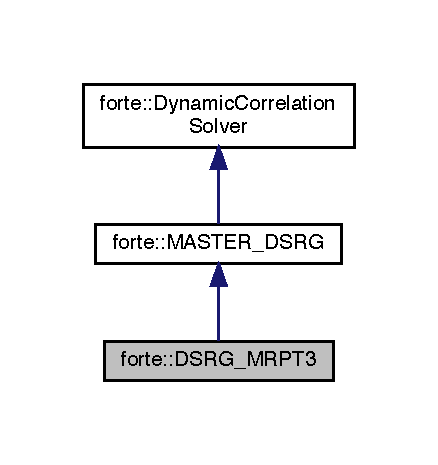
\includegraphics[width=210pt]{classforte_1_1_d_s_r_g___m_r_p_t3__inherit__graph}
\end{center}
\end{figure}


Collaboration diagram for forte\+:\+:D\+S\+R\+G\+\_\+\+M\+R\+P\+T3\+:
\nopagebreak
\begin{figure}[H]
\begin{center}
\leavevmode
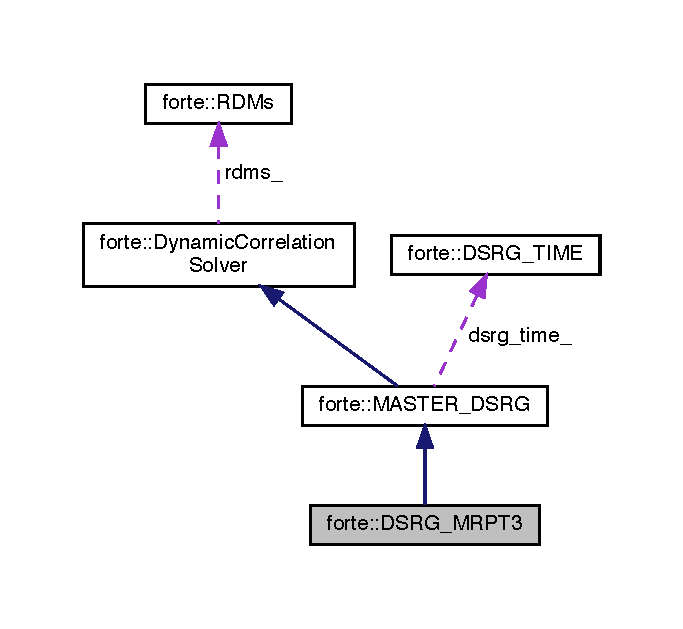
\includegraphics[width=328pt]{classforte_1_1_d_s_r_g___m_r_p_t3__coll__graph}
\end{center}
\end{figure}
\subsection*{Public Member Functions}
\begin{DoxyCompactItemize}
\item 
\mbox{\hyperlink{classforte_1_1_d_s_r_g___m_r_p_t3_a411038a819da24f5ffb4db0cf621a742}{D\+S\+R\+G\+\_\+\+M\+R\+P\+T3}} (\mbox{\hyperlink{classforte_1_1_r_d_ms}{R\+D\+Ms}} rdms, std\+::shared\+\_\+ptr$<$ \mbox{\hyperlink{classforte_1_1_s_c_f_info}{S\+C\+F\+Info}} $>$ scf\+\_\+info, std\+::shared\+\_\+ptr$<$ \mbox{\hyperlink{classforte_1_1_forte_options}{Forte\+Options}} $>$ options, std\+::shared\+\_\+ptr$<$ \mbox{\hyperlink{classforte_1_1_forte_integrals}{Forte\+Integrals}} $>$ ints, std\+::shared\+\_\+ptr$<$ \mbox{\hyperlink{classforte_1_1_m_o_space_info}{M\+O\+Space\+Info}} $>$ mo\+\_\+space\+\_\+info)
\item 
virtual \mbox{\hyperlink{classforte_1_1_d_s_r_g___m_r_p_t3_ae2419fb8f82089098a086f62baff4816}{$\sim$\+D\+S\+R\+G\+\_\+\+M\+R\+P\+T3}} ()
\begin{DoxyCompactList}\small\item\em Destructor. \end{DoxyCompactList}\item 
virtual double \mbox{\hyperlink{classforte_1_1_d_s_r_g___m_r_p_t3_a48a25a952206690bcf8125e583576052}{compute\+\_\+energy}} ()
\begin{DoxyCompactList}\small\item\em Compute the D\+S\+R\+G-\/\+M\+R\+P\+T3 energy. \end{DoxyCompactList}\item 
double \mbox{\hyperlink{classforte_1_1_d_s_r_g___m_r_p_t3_ac01edeb17737755a3b025459a792aad4}{compute\+\_\+energy\+\_\+relaxed}} ()
\begin{DoxyCompactList}\small\item\em Compute the D\+S\+R\+G-\/\+M\+R\+P\+T3 energy with relaxed reference (once) \end{DoxyCompactList}\item 
double \mbox{\hyperlink{classforte_1_1_d_s_r_g___m_r_p_t3_a2b3a92749aae957f93d5f9cda22d0716}{compute\+\_\+energy\+\_\+sa}} ()
\begin{DoxyCompactList}\small\item\em Compute the state-\/averaged D\+S\+R\+G-\/\+M\+R\+P\+T3 energies. \end{DoxyCompactList}\item 
void \mbox{\hyperlink{classforte_1_1_d_s_r_g___m_r_p_t3_a20ec1fcadc9b1e3cb8d21df9a86fa055}{set\+\_\+eigens}} (std\+::vector$<$ std\+::vector$<$ std\+::pair$<$ psi\+::\+Shared\+Vector, double $>$$>$$>$ eigens)
\begin{DoxyCompactList}\small\item\em Set C\+A\+S\+CI eigen values and eigen vectors for state averaging. \end{DoxyCompactList}\item 
void \mbox{\hyperlink{classforte_1_1_d_s_r_g___m_r_p_t3_af5b78a8ae153c66e5733d0749972185b}{set\+\_\+p\+\_\+spaces}} (std\+::vector$<$ std\+::vector$<$ \mbox{\hyperlink{namespaceforte_a2076c63fd7b8732004d9e1442ce527c1}{forte\+::\+Determinant}} $>$$>$ p\+\_\+spaces)
\begin{DoxyCompactList}\small\item\em Set determinants in the model space. \end{DoxyCompactList}\end{DoxyCompactItemize}
\subsection*{Protected Member Functions}
\begin{DoxyCompactItemize}
\item 
void \mbox{\hyperlink{classforte_1_1_d_s_r_g___m_r_p_t3_ae03d4e96612c876c0d9f0715f93316fe}{startup}} ()
\begin{DoxyCompactList}\small\item\em Called in the constructor. \end{DoxyCompactList}\item 
void \mbox{\hyperlink{classforte_1_1_d_s_r_g___m_r_p_t3_ac7f2deb2afe35fcbe80b0f7863cb79d1}{cleanup}} ()
\begin{DoxyCompactList}\small\item\em Called in the destructor. \end{DoxyCompactList}\item 
void \mbox{\hyperlink{classforte_1_1_d_s_r_g___m_r_p_t3_a73debd7fa355ac2311d92f6d86b5e3e5}{print\+\_\+options\+\_\+summary}} ()
\begin{DoxyCompactList}\small\item\em Print a summary of the options. \end{DoxyCompactList}\item 
std\+::chrono\+::duration$<$ double $>$ \mbox{\hyperlink{classforte_1_1_d_s_r_g___m_r_p_t3_ac2e41cad2c6f82f0b7051b02becd1595}{compute\+\_\+elapsed\+\_\+time}} (std\+::chrono\+::time\+\_\+point$<$ std\+::chrono\+::system\+\_\+clock $>$ t1, std\+::chrono\+::time\+\_\+point$<$ std\+::chrono\+::system\+\_\+clock $>$ t2)
\begin{DoxyCompactList}\small\item\em Compute elapsed time. \end{DoxyCompactList}\item 
void \mbox{\hyperlink{classforte_1_1_d_s_r_g___m_r_p_t3_ac610cb51af174c9c3fd3eb2d68f62bb3}{build\+\_\+tei}} (Blocked\+Tensor \&V)
\begin{DoxyCompactList}\small\item\em Fill up two-\/electron integrals. \end{DoxyCompactList}\item 
void \mbox{\hyperlink{classforte_1_1_d_s_r_g___m_r_p_t3_aed32292cef9e15981542c638236748b8}{build\+\_\+fock\+\_\+half}} ()
\begin{DoxyCompactList}\small\item\em Build Fock matrix and diagonal Fock matrix elements. \end{DoxyCompactList}\item 
void \mbox{\hyperlink{classforte_1_1_d_s_r_g___m_r_p_t3_acf82777d9515f7cc988b82c03ffeb291}{build\+\_\+fock\+\_\+full}} ()
\begin{DoxyCompactList}\small\item\em Build Fock matrix when two-\/electron integrals are fully stored. \end{DoxyCompactList}\item 
void \mbox{\hyperlink{classforte_1_1_d_s_r_g___m_r_p_t3_a592593cdbd5cbf0024bc5f9520b4a88d}{renormalize\+\_\+F}} (const bool \&plusone=true)
\begin{DoxyCompactList}\small\item\em Renormalize Fock matrix. \end{DoxyCompactList}\item 
void \mbox{\hyperlink{classforte_1_1_d_s_r_g___m_r_p_t3_aaf25a724d9aeeafb121d56abd71f0748}{renormalize\+\_\+V}} (const bool \&plusone=true)
\begin{DoxyCompactList}\small\item\em Renormalize two-\/electron integrals. \end{DoxyCompactList}\item 
void \mbox{\hyperlink{classforte_1_1_d_s_r_g___m_r_p_t3_a0358b0213517f969fda06fbcbe86ea94}{compute\+\_\+t2}} ()
\begin{DoxyCompactList}\small\item\em Compute T2 amplitudes. \end{DoxyCompactList}\item 
void \mbox{\hyperlink{classforte_1_1_d_s_r_g___m_r_p_t3_a2312c6b70f31b23da999119623f5d633}{check\+\_\+t2}} ()
\begin{DoxyCompactList}\small\item\em Check T2 and store large amplitudes. \end{DoxyCompactList}\item 
void \mbox{\hyperlink{classforte_1_1_d_s_r_g___m_r_p_t3_aff426cbae8aba3b3df9a9817a13280d0}{compute\+\_\+t1}} ()
\begin{DoxyCompactList}\small\item\em Compute T1 amplitudes. \end{DoxyCompactList}\item 
void \mbox{\hyperlink{classforte_1_1_d_s_r_g___m_r_p_t3_a6ae32df9118f9ee9c9a8f5a37c81c601}{check\+\_\+t1}} ()
\begin{DoxyCompactList}\small\item\em Check T1 and store large amplitudes. \end{DoxyCompactList}\item 
void \mbox{\hyperlink{classforte_1_1_d_s_r_g___m_r_p_t3_acc86f6e843feea90ab27a456ccdca039}{print\+\_\+amp\+\_\+summary}} (const std\+::string \&name, const std\+::vector$<$ std\+::pair$<$ std\+::vector$<$ size\+\_\+t $>$, double $>$$>$ \&list, const double \&norm, const size\+\_\+t \&number\+\_\+nonzero)
\begin{DoxyCompactList}\small\item\em Print amplitudes summary. \end{DoxyCompactList}\item 
void \mbox{\hyperlink{classforte_1_1_d_s_r_g___m_r_p_t3_af557b9dbad07468f31550890d06ceb8e}{print\+\_\+intruder}} (const std\+::string \&name, const std\+::vector$<$ std\+::pair$<$ std\+::vector$<$ size\+\_\+t $>$, double $>$$>$ \&list)
\begin{DoxyCompactList}\small\item\em Print intruder analysis. \end{DoxyCompactList}\item 
double \mbox{\hyperlink{classforte_1_1_d_s_r_g___m_r_p_t3_a5d538d326cd0c34727b3dc5d9dbe7237}{compute\+\_\+energy\+\_\+pt2}} ()
\begin{DoxyCompactList}\small\item\em compute 2nd-\/order energy and transformed Hamiltonian \end{DoxyCompactList}\item 
double \mbox{\hyperlink{classforte_1_1_d_s_r_g___m_r_p_t3_a644f6b92ddcb87b33a5bc467e0f79846}{compute\+\_\+energy\+\_\+pt3\+\_\+1}} ()
\item 
double \mbox{\hyperlink{classforte_1_1_d_s_r_g___m_r_p_t3_ab5d7445a318b4d5d2fea4cde2edc6818}{compute\+\_\+energy\+\_\+pt3\+\_\+2}} ()
\begin{DoxyCompactList}\small\item\em compute 3d-\/order energy contribution 1.\+0 / 2.\+0 $\ast$ \mbox{[}H1st + Hbar1st,A2nd\mbox{]} \end{DoxyCompactList}\item 
double \mbox{\hyperlink{classforte_1_1_d_s_r_g___m_r_p_t3_a3b72cd8ca5066848111f384afc4a97ff}{compute\+\_\+energy\+\_\+pt3\+\_\+3}} ()
\begin{DoxyCompactList}\small\item\em compute 3rd-\/order energy contribution 1.\+0 / 2.\+0 $\ast$ \mbox{[}Hbar2nd,A1st\mbox{]} \end{DoxyCompactList}\item 
void \mbox{\hyperlink{classforte_1_1_d_s_r_g___m_r_p_t3_a0a5a5e4a7f71dd0fb364b184fb0e65b5}{V\+\_\+\+T1\+\_\+\+C1\+\_\+\+DF}} (Blocked\+Tensor \&B, Blocked\+Tensor \&T1, const double \&alpha, Blocked\+Tensor \&\mbox{\hyperlink{namespaceforte_abe00ec86d0015c0f2b6ac298c6e428e4a1a2ddc2db4693cfd16d534cde5572cc1}{C1}})
\begin{DoxyCompactList}\small\item\em Compute one-\/body term of commutator \mbox{[}V, T1\mbox{]}, V is constructed from B (D\+F/\+CD) \end{DoxyCompactList}\item 
void \mbox{\hyperlink{classforte_1_1_d_s_r_g___m_r_p_t3_a9546d1b6861d0b5b222011d1339bf40b}{V\+\_\+\+T2\+\_\+\+C1\+\_\+\+DF}} (Blocked\+Tensor \&B, Blocked\+Tensor \&T2, const double \&alpha, Blocked\+Tensor \&\mbox{\hyperlink{namespaceforte_abe00ec86d0015c0f2b6ac298c6e428e4a1a2ddc2db4693cfd16d534cde5572cc1}{C1}})
\begin{DoxyCompactList}\small\item\em Compute one-\/body term of commutator \mbox{[}V, T2\mbox{]}, V is constructed from B (D\+F/\+CD) \end{DoxyCompactList}\item 
void \mbox{\hyperlink{classforte_1_1_d_s_r_g___m_r_p_t3_a40d599393dfce102715ffdc027b2c88b}{V\+\_\+\+T1\+\_\+\+C2\+\_\+\+DF}} (Blocked\+Tensor \&B, Blocked\+Tensor \&T1, const double \&alpha, Blocked\+Tensor \&\mbox{\hyperlink{namespaceforte_abe00ec86d0015c0f2b6ac298c6e428e4af1a543f5a2c5d49bc5dde298fcf716e4}{C2}})
\begin{DoxyCompactList}\small\item\em Compute two-\/body term of commutator \mbox{[}V, T1\mbox{]}, V is constructed from B (D\+F/\+CD) \end{DoxyCompactList}\item 
void \mbox{\hyperlink{classforte_1_1_d_s_r_g___m_r_p_t3_ab71c3b2fafa76b719d08acb4000d527b}{V\+\_\+\+T2\+\_\+\+C2\+\_\+\+DF}} (Blocked\+Tensor \&B, Blocked\+Tensor \&T2, const double \&alpha, Blocked\+Tensor \&\mbox{\hyperlink{namespaceforte_abe00ec86d0015c0f2b6ac298c6e428e4af1a543f5a2c5d49bc5dde298fcf716e4}{C2}})
\begin{DoxyCompactList}\small\item\em Compute two-\/body term of commutator \mbox{[}V, T2\mbox{]}, V is constructed from B (D\+F/\+CD) \end{DoxyCompactList}\item 
void \mbox{\hyperlink{classforte_1_1_d_s_r_g___m_r_p_t3_a48e6f20b01fa4ebdf3fcb3b2444b8443}{V\+\_\+\+T2\+\_\+\+C2\+\_\+\+D\+F\+\_\+\+AA}} (Blocked\+Tensor \&B, Blocked\+Tensor \&T2, const double \&alpha, Blocked\+Tensor \&\mbox{\hyperlink{namespaceforte_abe00ec86d0015c0f2b6ac298c6e428e4af1a543f5a2c5d49bc5dde298fcf716e4}{C2}})
\item 
void \mbox{\hyperlink{classforte_1_1_d_s_r_g___m_r_p_t3_a91c900ea22e66c97bb0db18c8f49e8cb}{V\+\_\+\+T2\+\_\+\+C2\+\_\+\+D\+F\+\_\+\+AV}} (Blocked\+Tensor \&B, Blocked\+Tensor \&T2, const double \&alpha, Blocked\+Tensor \&\mbox{\hyperlink{namespaceforte_abe00ec86d0015c0f2b6ac298c6e428e4af1a543f5a2c5d49bc5dde298fcf716e4}{C2}})
\item 
void \mbox{\hyperlink{classforte_1_1_d_s_r_g___m_r_p_t3_a0e00b4f4fdac4498d4d16c3f8cda54de}{V\+\_\+\+T2\+\_\+\+C2\+\_\+\+D\+F\+\_\+\+VV}} (Blocked\+Tensor \&B, Blocked\+Tensor \&T2, const double \&alpha, Blocked\+Tensor \&\mbox{\hyperlink{namespaceforte_abe00ec86d0015c0f2b6ac298c6e428e4af1a543f5a2c5d49bc5dde298fcf716e4}{C2}})
\item 
void \mbox{\hyperlink{classforte_1_1_d_s_r_g___m_r_p_t3_a2beafc4ba36ddc0c27557c0c858fbf85}{V\+\_\+\+T2\+\_\+\+C2\+\_\+\+D\+F\+\_\+\+A\+H\+\_\+\+EX}} (Blocked\+Tensor \&B, Blocked\+Tensor \&T2, const double \&alpha, Blocked\+Tensor \&\mbox{\hyperlink{namespaceforte_abe00ec86d0015c0f2b6ac298c6e428e4af1a543f5a2c5d49bc5dde298fcf716e4}{C2}}, const std\+::vector$<$ std\+::vector$<$ std\+::string $>$$>$ \&qs, const std\+::vector$<$ std\+::vector$<$ std\+::string $>$$>$ \&jb)
\item 
void \mbox{\hyperlink{classforte_1_1_d_s_r_g___m_r_p_t3_a3484a8491033f0e2171936ba0da11f38}{V\+\_\+\+T2\+\_\+\+C2\+\_\+\+D\+F\+\_\+\+V\+A\+\_\+\+EX}} (Blocked\+Tensor \&B, Blocked\+Tensor \&T2, const double \&alpha, Blocked\+Tensor \&\mbox{\hyperlink{namespaceforte_abe00ec86d0015c0f2b6ac298c6e428e4af1a543f5a2c5d49bc5dde298fcf716e4}{C2}}, const std\+::vector$<$ std\+::string $>$ \&qs\+\_\+lower, const std\+::vector$<$ std\+::string $>$ \&jb\+\_\+lower)
\item 
void \mbox{\hyperlink{classforte_1_1_d_s_r_g___m_r_p_t3_ab486aac4ea25510f0ca1d94b39d3e12d}{V\+\_\+\+T2\+\_\+\+C2\+\_\+\+D\+F\+\_\+\+V\+C\+\_\+\+EX}} (Blocked\+Tensor \&B, Blocked\+Tensor \&T2, const double \&alpha, Blocked\+Tensor \&\mbox{\hyperlink{namespaceforte_abe00ec86d0015c0f2b6ac298c6e428e4af1a543f5a2c5d49bc5dde298fcf716e4}{C2}}, const std\+::vector$<$ std\+::string $>$ \&qs\+\_\+lower, const std\+::vector$<$ std\+::string $>$ \&jb\+\_\+lower)
\item 
void \mbox{\hyperlink{classforte_1_1_d_s_r_g___m_r_p_t3_ab6ccdab98659f6661900cfa29fa6872d}{compute\+\_\+dm1d\+\_\+pt3\+\_\+1}} (Blocked\+Tensor \&M, double \&Mbar0, double \&Mbar0\+\_\+pt2, Blocked\+Tensor \&Mbar1, Blocked\+Tensor \&Mbar2)
\begin{DoxyCompactList}\small\item\em Compute D\+S\+RG transformed dipole integrals from 1st-\/order amplitudes for a given direction. \end{DoxyCompactList}\item 
void \mbox{\hyperlink{classforte_1_1_d_s_r_g___m_r_p_t3_aa6f6e8955cf8ecbe07f6f0eb3522f649}{compute\+\_\+dm1d\+\_\+pt3\+\_\+2}} (Blocked\+Tensor \&M, double \&Mbar0, double \&Mbar0\+\_\+pt2, Blocked\+Tensor \&Mbar1, Blocked\+Tensor \&Mbar2)
\begin{DoxyCompactList}\small\item\em Compute D\+S\+RG transformed dipole integrals from 2nd-\/order amplitudes for a given direction. \end{DoxyCompactList}\item 
void \mbox{\hyperlink{classforte_1_1_d_s_r_g___m_r_p_t3_aa8d6ffbd67970a5b8711924b44d786aa}{print\+\_\+dm\+\_\+pt3}} ()
\begin{DoxyCompactList}\small\item\em Print unrelaxed dipole. \end{DoxyCompactList}\end{DoxyCompactItemize}
\subsection*{Protected Attributes}
\begin{DoxyCompactItemize}
\item 
bool \mbox{\hyperlink{classforte_1_1_d_s_r_g___m_r_p_t3_ac7a05164e2aeb450f275ace8b4d68141}{profile\+\_\+print\+\_\+}}
\begin{DoxyCompactList}\small\item\em Profile printing for DF. \end{DoxyCompactList}\item 
std\+::chrono\+::time\+\_\+point$<$ std\+::chrono\+::system\+\_\+clock $>$ \mbox{\hyperlink{classforte_1_1_d_s_r_g___m_r_p_t3_a5cfb4204003849251f3aeb2c6e9eedf6}{start\+\_\+}}
\begin{DoxyCompactList}\small\item\em Time variable. \end{DoxyCompactList}\item 
std\+::chrono\+::time\+\_\+point$<$ std\+::chrono\+::system\+\_\+clock $>$ \mbox{\hyperlink{classforte_1_1_d_s_r_g___m_r_p_t3_a87374317ecaaa1fc3dadee71238a287a}{end\+\_\+}}
\item 
std\+::time\+\_\+t \mbox{\hyperlink{classforte_1_1_d_s_r_g___m_r_p_t3_a1769af0d38cd96df2578205dad1add46}{tt1\+\_\+}}
\item 
std\+::time\+\_\+t \mbox{\hyperlink{classforte_1_1_d_s_r_g___m_r_p_t3_afdea4aab3d4dc3f8e6d451973aaf15ca}{tt2\+\_\+}}
\item 
std\+::vector$<$ std\+::vector$<$ std\+::pair$<$ psi\+::\+Shared\+Vector, double $>$ $>$ $>$ \mbox{\hyperlink{classforte_1_1_d_s_r_g___m_r_p_t3_a22fd832ebfbf1be19fa04fb4a011ace3}{eigens\+\_\+}}
\begin{DoxyCompactList}\small\item\em C\+A\+S\+CI eigen values and eigen vectors for state averaging. \end{DoxyCompactList}\item 
std\+::vector$<$ std\+::vector$<$ \mbox{\hyperlink{namespaceforte_a2076c63fd7b8732004d9e1442ce527c1}{forte\+::\+Determinant}} $>$ $>$ \mbox{\hyperlink{classforte_1_1_d_s_r_g___m_r_p_t3_a30dffa14bad488e78ffe178e3ca962f0}{p\+\_\+spaces\+\_\+}}
\begin{DoxyCompactList}\small\item\em Determinants in the model space. \end{DoxyCompactList}\item 
int64\+\_\+t \mbox{\hyperlink{classforte_1_1_d_s_r_g___m_r_p_t3_a45977e4675ce30ca1750869c7c81fa3f}{mem\+\_\+total\+\_\+}}
\begin{DoxyCompactList}\small\item\em Total memory left. \end{DoxyCompactList}\item 
bool \mbox{\hyperlink{classforte_1_1_d_s_r_g___m_r_p_t3_a32aa55b38940e86d15b60350ccb636f7}{semi\+\_\+canonical\+\_\+}}
\begin{DoxyCompactList}\small\item\em Are orbitals semi-\/canonicalized? \end{DoxyCompactList}\item 
std\+::vector$<$ double $>$ \mbox{\hyperlink{classforte_1_1_d_s_r_g___m_r_p_t3_afda1234ea7f619908fb0ff10188d0d74}{Fa\+\_\+}}
\begin{DoxyCompactList}\small\item\em Diagonal elements of Fock matrices. \end{DoxyCompactList}\item 
std\+::vector$<$ double $>$ \mbox{\hyperlink{classforte_1_1_d_s_r_g___m_r_p_t3_a469cd21683c1d469f08c7b5c6f4c3f95}{Fb\+\_\+}}
\item 
std\+::vector$<$ double $>$ \mbox{\hyperlink{classforte_1_1_d_s_r_g___m_r_p_t3_af947d5aa4c9aee775d56ad6085e299ac}{aone\+\_\+eff\+\_\+}}
\begin{DoxyCompactList}\small\item\em Effective alpha one-\/electron integrals (used in denormal ordering) \end{DoxyCompactList}\item 
std\+::vector$<$ double $>$ \mbox{\hyperlink{classforte_1_1_d_s_r_g___m_r_p_t3_aed9f088d1f9bcd8facb10dd1569748aa}{bone\+\_\+eff\+\_\+}}
\begin{DoxyCompactList}\small\item\em Effective beta one-\/electron integrals (used in denormal ordering) \end{DoxyCompactList}\item 
ambit\+::\+Blocked\+Tensor \mbox{\hyperlink{classforte_1_1_d_s_r_g___m_r_p_t3_a358a3512d5e25f9830f24df84c03d565}{F\+\_\+}}
\begin{DoxyCompactList}\small\item\em Generalized Fock matrix (bare or renormalized) \end{DoxyCompactList}\item 
ambit\+::\+Blocked\+Tensor \mbox{\hyperlink{classforte_1_1_d_s_r_g___m_r_p_t3_ad529a0f458610f6099d7e2cc47cfd896}{F0th\+\_\+}}
\begin{DoxyCompactList}\small\item\em Zeroth-\/order Hamiltonian (bare diagonal blocks of Fock) \end{DoxyCompactList}\item 
ambit\+::\+Blocked\+Tensor \mbox{\hyperlink{classforte_1_1_d_s_r_g___m_r_p_t3_a078a80b254310fde8b5f0f4dec0d316d}{F1st\+\_\+}}
\begin{DoxyCompactList}\small\item\em Generalized Fock matrix (bare off-\/diagonal blocks) \end{DoxyCompactList}\item 
ambit\+::\+Blocked\+Tensor \mbox{\hyperlink{classforte_1_1_d_s_r_g___m_r_p_t3_a4df42fb2007964419b78dcde72886db8}{V\+\_\+}}
\begin{DoxyCompactList}\small\item\em Two-\/electron integrals (bare or renormalized) \end{DoxyCompactList}\item 
ambit\+::\+Blocked\+Tensor \mbox{\hyperlink{classforte_1_1_d_s_r_g___m_r_p_t3_ad2075beaa4159ef620f34df0fc5fdd64}{B\+\_\+}}
\begin{DoxyCompactList}\small\item\em Three-\/index integrals. \end{DoxyCompactList}\item 
ambit\+::\+Blocked\+Tensor \mbox{\hyperlink{classforte_1_1_d_s_r_g___m_r_p_t3_aa7a1ae6e6db9791b3dc40052ef0d1af5}{T1\+\_\+}}
\begin{DoxyCompactList}\small\item\em Single excitation amplitude. \end{DoxyCompactList}\item 
ambit\+::\+Blocked\+Tensor \mbox{\hyperlink{classforte_1_1_d_s_r_g___m_r_p_t3_ab74e92a4d965c40a6d2a6f1a0afceea2}{T2\+\_\+}}
\begin{DoxyCompactList}\small\item\em Double excitation amplitude. \end{DoxyCompactList}\item 
ambit\+::\+Blocked\+Tensor \mbox{\hyperlink{classforte_1_1_d_s_r_g___m_r_p_t3_aec8b24da0956caeaed744b78d132a9ef}{O1\+\_\+}}
\begin{DoxyCompactList}\small\item\em One-\/body temp tensor (\mbox{[}\mbox{[}H0th,A1st\mbox{]},A1st\mbox{]} or 1st-\/order amplitudes) \end{DoxyCompactList}\item 
ambit\+::\+Blocked\+Tensor \mbox{\hyperlink{classforte_1_1_d_s_r_g___m_r_p_t3_aafc09e3bcf2969a8c54cd80611f22615}{O2\+\_\+}}
\begin{DoxyCompactList}\small\item\em Two-\/body temp tensor (\mbox{[}\mbox{[}H0th,A1st\mbox{]},A1st\mbox{]} or 1st-\/order amplitudes) \end{DoxyCompactList}\item 
ambit\+::\+Blocked\+Tensor \mbox{\hyperlink{classforte_1_1_d_s_r_g___m_r_p_t3_a3ffd43eb3dbaf441b72eb5f158eca6d2}{U\+\_\+}}
\begin{DoxyCompactList}\small\item\em Unitary matrix to block diagonal Fock. \end{DoxyCompactList}\item 
double \mbox{\hyperlink{classforte_1_1_d_s_r_g___m_r_p_t3_af22b0cb1620229a88e7988d3e564f368}{T2norm\+\_\+}}
\begin{DoxyCompactList}\small\item\em Norm of T2. \end{DoxyCompactList}\item 
double \mbox{\hyperlink{classforte_1_1_d_s_r_g___m_r_p_t3_a8f5e43d366ea5f4130f64ae882f484fb}{T2max\+\_\+}}
\begin{DoxyCompactList}\small\item\em Max (with sign) of T2. \end{DoxyCompactList}\item 
double \mbox{\hyperlink{classforte_1_1_d_s_r_g___m_r_p_t3_a4e586ce2fafa9c900df089d2f739cd5c}{T1norm\+\_\+}}
\begin{DoxyCompactList}\small\item\em Norm of T1. \end{DoxyCompactList}\item 
double \mbox{\hyperlink{classforte_1_1_d_s_r_g___m_r_p_t3_adacbd3ce8f65586ecd75c74c12b0db50}{T1max\+\_\+}}
\begin{DoxyCompactList}\small\item\em Max (with sign) of T1. \end{DoxyCompactList}\item 
std\+::vector$<$ std\+::pair$<$ std\+::vector$<$ size\+\_\+t $>$, double $>$ $>$ \mbox{\hyperlink{classforte_1_1_d_s_r_g___m_r_p_t3_a325f745173790dba2942214ca9c040e8}{lt1a\+\_\+}}
\begin{DoxyCompactList}\small\item\em List of large amplitudes. \end{DoxyCompactList}\item 
std\+::vector$<$ std\+::pair$<$ std\+::vector$<$ size\+\_\+t $>$, double $>$ $>$ \mbox{\hyperlink{classforte_1_1_d_s_r_g___m_r_p_t3_aba50c32ec211e470f442ed49a6bb16f5}{lt1b\+\_\+}}
\item 
std\+::vector$<$ std\+::pair$<$ std\+::vector$<$ size\+\_\+t $>$, double $>$ $>$ \mbox{\hyperlink{classforte_1_1_d_s_r_g___m_r_p_t3_aedbbe720462fe87709525bedc8541251}{lt2aa\+\_\+}}
\item 
std\+::vector$<$ std\+::pair$<$ std\+::vector$<$ size\+\_\+t $>$, double $>$ $>$ \mbox{\hyperlink{classforte_1_1_d_s_r_g___m_r_p_t3_a3a00248cfbd090f9c1338d534b9ae233}{lt2ab\+\_\+}}
\item 
std\+::vector$<$ std\+::pair$<$ std\+::vector$<$ size\+\_\+t $>$, double $>$ $>$ \mbox{\hyperlink{classforte_1_1_d_s_r_g___m_r_p_t3_a819e9535c0fa33f8918569629f6bf552}{lt2bb\+\_\+}}
\item 
std\+::array$<$ double, 3 $>$ \mbox{\hyperlink{classforte_1_1_d_s_r_g___m_r_p_t3_a0d739ecebfa2759f30e21e1fd46bf5d1}{Mbar0\+\_\+pt2\+\_\+}}
\begin{DoxyCompactList}\small\item\em D\+S\+R\+G-\/\+M\+R\+P\+T2 transformed dipole scalar. \end{DoxyCompactList}\item 
std\+::array$<$ double, 3 $>$ \mbox{\hyperlink{classforte_1_1_d_s_r_g___m_r_p_t3_ac79b938fc2c1551fed6195eaddad5616}{Mbar0\+\_\+pt2c\+\_\+}}
\begin{DoxyCompactList}\small\item\em D\+S\+R\+G-\/\+M\+R\+P\+T2 (2nd-\/order complete) transformed dipole scalar. \end{DoxyCompactList}\end{DoxyCompactItemize}


\subsection{Constructor \& Destructor Documentation}
\mbox{\Hypertarget{classforte_1_1_d_s_r_g___m_r_p_t3_a411038a819da24f5ffb4db0cf621a742}\label{classforte_1_1_d_s_r_g___m_r_p_t3_a411038a819da24f5ffb4db0cf621a742}} 
\index{forte\+::\+D\+S\+R\+G\+\_\+\+M\+R\+P\+T3@{forte\+::\+D\+S\+R\+G\+\_\+\+M\+R\+P\+T3}!D\+S\+R\+G\+\_\+\+M\+R\+P\+T3@{D\+S\+R\+G\+\_\+\+M\+R\+P\+T3}}
\index{D\+S\+R\+G\+\_\+\+M\+R\+P\+T3@{D\+S\+R\+G\+\_\+\+M\+R\+P\+T3}!forte\+::\+D\+S\+R\+G\+\_\+\+M\+R\+P\+T3@{forte\+::\+D\+S\+R\+G\+\_\+\+M\+R\+P\+T3}}
\subsubsection{\texorpdfstring{D\+S\+R\+G\+\_\+\+M\+R\+P\+T3()}{DSRG\_MRPT3()}}
{\footnotesize\ttfamily forte\+::\+D\+S\+R\+G\+\_\+\+M\+R\+P\+T3\+::\+D\+S\+R\+G\+\_\+\+M\+R\+P\+T3 (\begin{DoxyParamCaption}\item[{\mbox{\hyperlink{classforte_1_1_r_d_ms}{R\+D\+Ms}}}]{rdms,  }\item[{std\+::shared\+\_\+ptr$<$ \mbox{\hyperlink{classforte_1_1_s_c_f_info}{S\+C\+F\+Info}} $>$}]{scf\+\_\+info,  }\item[{std\+::shared\+\_\+ptr$<$ \mbox{\hyperlink{classforte_1_1_forte_options}{Forte\+Options}} $>$}]{options,  }\item[{std\+::shared\+\_\+ptr$<$ \mbox{\hyperlink{classforte_1_1_forte_integrals}{Forte\+Integrals}} $>$}]{ints,  }\item[{std\+::shared\+\_\+ptr$<$ \mbox{\hyperlink{classforte_1_1_m_o_space_info}{M\+O\+Space\+Info}} $>$}]{mo\+\_\+space\+\_\+info }\end{DoxyParamCaption})}

\mbox{\hyperlink{classforte_1_1_d_s_r_g___m_r_p_t3}{D\+S\+R\+G\+\_\+\+M\+R\+P\+T3}} Constructor 
\begin{DoxyParams}{Parameters}
{\em reference} & The reference object of F\+O\+R\+TE \\
\hline
{\em ref\+\_\+wfn} & The reference wavefunction object \\
\hline
{\em options} & The main options object \\
\hline
{\em ints} & A pointer to an allocated integral object \\
\hline
{\em mo\+\_\+space\+\_\+info} & The \mbox{\hyperlink{classforte_1_1_m_o_space_info}{M\+O\+Space\+Info}} object \\
\hline
\end{DoxyParams}
\mbox{\Hypertarget{classforte_1_1_d_s_r_g___m_r_p_t3_ae2419fb8f82089098a086f62baff4816}\label{classforte_1_1_d_s_r_g___m_r_p_t3_ae2419fb8f82089098a086f62baff4816}} 
\index{forte\+::\+D\+S\+R\+G\+\_\+\+M\+R\+P\+T3@{forte\+::\+D\+S\+R\+G\+\_\+\+M\+R\+P\+T3}!````~D\+S\+R\+G\+\_\+\+M\+R\+P\+T3@{$\sim$\+D\+S\+R\+G\+\_\+\+M\+R\+P\+T3}}
\index{````~D\+S\+R\+G\+\_\+\+M\+R\+P\+T3@{$\sim$\+D\+S\+R\+G\+\_\+\+M\+R\+P\+T3}!forte\+::\+D\+S\+R\+G\+\_\+\+M\+R\+P\+T3@{forte\+::\+D\+S\+R\+G\+\_\+\+M\+R\+P\+T3}}
\subsubsection{\texorpdfstring{$\sim$\+D\+S\+R\+G\+\_\+\+M\+R\+P\+T3()}{~DSRG\_MRPT3()}}
{\footnotesize\ttfamily virtual forte\+::\+D\+S\+R\+G\+\_\+\+M\+R\+P\+T3\+::$\sim$\+D\+S\+R\+G\+\_\+\+M\+R\+P\+T3 (\begin{DoxyParamCaption}{ }\end{DoxyParamCaption})\hspace{0.3cm}{\ttfamily [virtual]}}



Destructor. 



\subsection{Member Function Documentation}
\mbox{\Hypertarget{classforte_1_1_d_s_r_g___m_r_p_t3_acf82777d9515f7cc988b82c03ffeb291}\label{classforte_1_1_d_s_r_g___m_r_p_t3_acf82777d9515f7cc988b82c03ffeb291}} 
\index{forte\+::\+D\+S\+R\+G\+\_\+\+M\+R\+P\+T3@{forte\+::\+D\+S\+R\+G\+\_\+\+M\+R\+P\+T3}!build\+\_\+fock\+\_\+full@{build\+\_\+fock\+\_\+full}}
\index{build\+\_\+fock\+\_\+full@{build\+\_\+fock\+\_\+full}!forte\+::\+D\+S\+R\+G\+\_\+\+M\+R\+P\+T3@{forte\+::\+D\+S\+R\+G\+\_\+\+M\+R\+P\+T3}}
\subsubsection{\texorpdfstring{build\+\_\+fock\+\_\+full()}{build\_fock\_full()}}
{\footnotesize\ttfamily void forte\+::\+D\+S\+R\+G\+\_\+\+M\+R\+P\+T3\+::build\+\_\+fock\+\_\+full (\begin{DoxyParamCaption}{ }\end{DoxyParamCaption})\hspace{0.3cm}{\ttfamily [protected]}}



Build Fock matrix when two-\/electron integrals are fully stored. 

\mbox{\Hypertarget{classforte_1_1_d_s_r_g___m_r_p_t3_aed32292cef9e15981542c638236748b8}\label{classforte_1_1_d_s_r_g___m_r_p_t3_aed32292cef9e15981542c638236748b8}} 
\index{forte\+::\+D\+S\+R\+G\+\_\+\+M\+R\+P\+T3@{forte\+::\+D\+S\+R\+G\+\_\+\+M\+R\+P\+T3}!build\+\_\+fock\+\_\+half@{build\+\_\+fock\+\_\+half}}
\index{build\+\_\+fock\+\_\+half@{build\+\_\+fock\+\_\+half}!forte\+::\+D\+S\+R\+G\+\_\+\+M\+R\+P\+T3@{forte\+::\+D\+S\+R\+G\+\_\+\+M\+R\+P\+T3}}
\subsubsection{\texorpdfstring{build\+\_\+fock\+\_\+half()}{build\_fock\_half()}}
{\footnotesize\ttfamily void forte\+::\+D\+S\+R\+G\+\_\+\+M\+R\+P\+T3\+::build\+\_\+fock\+\_\+half (\begin{DoxyParamCaption}{ }\end{DoxyParamCaption})\hspace{0.3cm}{\ttfamily [protected]}}



Build Fock matrix and diagonal Fock matrix elements. 

\mbox{\Hypertarget{classforte_1_1_d_s_r_g___m_r_p_t3_ac610cb51af174c9c3fd3eb2d68f62bb3}\label{classforte_1_1_d_s_r_g___m_r_p_t3_ac610cb51af174c9c3fd3eb2d68f62bb3}} 
\index{forte\+::\+D\+S\+R\+G\+\_\+\+M\+R\+P\+T3@{forte\+::\+D\+S\+R\+G\+\_\+\+M\+R\+P\+T3}!build\+\_\+tei@{build\+\_\+tei}}
\index{build\+\_\+tei@{build\+\_\+tei}!forte\+::\+D\+S\+R\+G\+\_\+\+M\+R\+P\+T3@{forte\+::\+D\+S\+R\+G\+\_\+\+M\+R\+P\+T3}}
\subsubsection{\texorpdfstring{build\+\_\+tei()}{build\_tei()}}
{\footnotesize\ttfamily void forte\+::\+D\+S\+R\+G\+\_\+\+M\+R\+P\+T3\+::build\+\_\+tei (\begin{DoxyParamCaption}\item[{Blocked\+Tensor \&}]{V }\end{DoxyParamCaption})\hspace{0.3cm}{\ttfamily [protected]}}



Fill up two-\/electron integrals. 

\mbox{\Hypertarget{classforte_1_1_d_s_r_g___m_r_p_t3_a6ae32df9118f9ee9c9a8f5a37c81c601}\label{classforte_1_1_d_s_r_g___m_r_p_t3_a6ae32df9118f9ee9c9a8f5a37c81c601}} 
\index{forte\+::\+D\+S\+R\+G\+\_\+\+M\+R\+P\+T3@{forte\+::\+D\+S\+R\+G\+\_\+\+M\+R\+P\+T3}!check\+\_\+t1@{check\+\_\+t1}}
\index{check\+\_\+t1@{check\+\_\+t1}!forte\+::\+D\+S\+R\+G\+\_\+\+M\+R\+P\+T3@{forte\+::\+D\+S\+R\+G\+\_\+\+M\+R\+P\+T3}}
\subsubsection{\texorpdfstring{check\+\_\+t1()}{check\_t1()}}
{\footnotesize\ttfamily void forte\+::\+D\+S\+R\+G\+\_\+\+M\+R\+P\+T3\+::check\+\_\+t1 (\begin{DoxyParamCaption}{ }\end{DoxyParamCaption})\hspace{0.3cm}{\ttfamily [protected]}}



Check T1 and store large amplitudes. 

\mbox{\Hypertarget{classforte_1_1_d_s_r_g___m_r_p_t3_a2312c6b70f31b23da999119623f5d633}\label{classforte_1_1_d_s_r_g___m_r_p_t3_a2312c6b70f31b23da999119623f5d633}} 
\index{forte\+::\+D\+S\+R\+G\+\_\+\+M\+R\+P\+T3@{forte\+::\+D\+S\+R\+G\+\_\+\+M\+R\+P\+T3}!check\+\_\+t2@{check\+\_\+t2}}
\index{check\+\_\+t2@{check\+\_\+t2}!forte\+::\+D\+S\+R\+G\+\_\+\+M\+R\+P\+T3@{forte\+::\+D\+S\+R\+G\+\_\+\+M\+R\+P\+T3}}
\subsubsection{\texorpdfstring{check\+\_\+t2()}{check\_t2()}}
{\footnotesize\ttfamily void forte\+::\+D\+S\+R\+G\+\_\+\+M\+R\+P\+T3\+::check\+\_\+t2 (\begin{DoxyParamCaption}{ }\end{DoxyParamCaption})\hspace{0.3cm}{\ttfamily [protected]}}



Check T2 and store large amplitudes. 

\mbox{\Hypertarget{classforte_1_1_d_s_r_g___m_r_p_t3_ac7f2deb2afe35fcbe80b0f7863cb79d1}\label{classforte_1_1_d_s_r_g___m_r_p_t3_ac7f2deb2afe35fcbe80b0f7863cb79d1}} 
\index{forte\+::\+D\+S\+R\+G\+\_\+\+M\+R\+P\+T3@{forte\+::\+D\+S\+R\+G\+\_\+\+M\+R\+P\+T3}!cleanup@{cleanup}}
\index{cleanup@{cleanup}!forte\+::\+D\+S\+R\+G\+\_\+\+M\+R\+P\+T3@{forte\+::\+D\+S\+R\+G\+\_\+\+M\+R\+P\+T3}}
\subsubsection{\texorpdfstring{cleanup()}{cleanup()}}
{\footnotesize\ttfamily void forte\+::\+D\+S\+R\+G\+\_\+\+M\+R\+P\+T3\+::cleanup (\begin{DoxyParamCaption}{ }\end{DoxyParamCaption})\hspace{0.3cm}{\ttfamily [protected]}}



Called in the destructor. 

\mbox{\Hypertarget{classforte_1_1_d_s_r_g___m_r_p_t3_ab6ccdab98659f6661900cfa29fa6872d}\label{classforte_1_1_d_s_r_g___m_r_p_t3_ab6ccdab98659f6661900cfa29fa6872d}} 
\index{forte\+::\+D\+S\+R\+G\+\_\+\+M\+R\+P\+T3@{forte\+::\+D\+S\+R\+G\+\_\+\+M\+R\+P\+T3}!compute\+\_\+dm1d\+\_\+pt3\+\_\+1@{compute\+\_\+dm1d\+\_\+pt3\+\_\+1}}
\index{compute\+\_\+dm1d\+\_\+pt3\+\_\+1@{compute\+\_\+dm1d\+\_\+pt3\+\_\+1}!forte\+::\+D\+S\+R\+G\+\_\+\+M\+R\+P\+T3@{forte\+::\+D\+S\+R\+G\+\_\+\+M\+R\+P\+T3}}
\subsubsection{\texorpdfstring{compute\+\_\+dm1d\+\_\+pt3\+\_\+1()}{compute\_dm1d\_pt3\_1()}}
{\footnotesize\ttfamily void forte\+::\+D\+S\+R\+G\+\_\+\+M\+R\+P\+T3\+::compute\+\_\+dm1d\+\_\+pt3\+\_\+1 (\begin{DoxyParamCaption}\item[{Blocked\+Tensor \&}]{M,  }\item[{double \&}]{Mbar0,  }\item[{double \&}]{Mbar0\+\_\+pt2,  }\item[{Blocked\+Tensor \&}]{Mbar1,  }\item[{Blocked\+Tensor \&}]{Mbar2 }\end{DoxyParamCaption})\hspace{0.3cm}{\ttfamily [protected]}}



Compute D\+S\+RG transformed dipole integrals from 1st-\/order amplitudes for a given direction. 

Compute two-\/body term of commutator \mbox{[}V, T2\mbox{]}, particle-\/hole contraction (exchange part), contracted particle index is virtual ~\newline
~\newline
~\newline
Get a sub block of tensor T 
\begin{DoxyParams}{Parameters}
{\em T} & The big tensor \\
\hline
{\em P} & The map of $<$partitioned dimension index, its absolute indices in T$>$ \\
\hline
{\em name} & The name of the returned sub tensor \\
\hline
\end{DoxyParams}
\begin{DoxyReturn}{Returns}
A sub tensor of T with the same dimension\+Rotate \mbox{\hyperlink{classforte_1_1_r_d_ms}{R\+D\+Ms}} computed by eigens\+\_\+ (in original basis) to semicanonical basis so that they are in the same basis as amplitudes (in semicanonical basis) 
\end{DoxyReturn}
\mbox{\Hypertarget{classforte_1_1_d_s_r_g___m_r_p_t3_aa6f6e8955cf8ecbe07f6f0eb3522f649}\label{classforte_1_1_d_s_r_g___m_r_p_t3_aa6f6e8955cf8ecbe07f6f0eb3522f649}} 
\index{forte\+::\+D\+S\+R\+G\+\_\+\+M\+R\+P\+T3@{forte\+::\+D\+S\+R\+G\+\_\+\+M\+R\+P\+T3}!compute\+\_\+dm1d\+\_\+pt3\+\_\+2@{compute\+\_\+dm1d\+\_\+pt3\+\_\+2}}
\index{compute\+\_\+dm1d\+\_\+pt3\+\_\+2@{compute\+\_\+dm1d\+\_\+pt3\+\_\+2}!forte\+::\+D\+S\+R\+G\+\_\+\+M\+R\+P\+T3@{forte\+::\+D\+S\+R\+G\+\_\+\+M\+R\+P\+T3}}
\subsubsection{\texorpdfstring{compute\+\_\+dm1d\+\_\+pt3\+\_\+2()}{compute\_dm1d\_pt3\_2()}}
{\footnotesize\ttfamily void forte\+::\+D\+S\+R\+G\+\_\+\+M\+R\+P\+T3\+::compute\+\_\+dm1d\+\_\+pt3\+\_\+2 (\begin{DoxyParamCaption}\item[{Blocked\+Tensor \&}]{M,  }\item[{double \&}]{Mbar0,  }\item[{double \&}]{Mbar0\+\_\+pt2,  }\item[{Blocked\+Tensor \&}]{Mbar1,  }\item[{Blocked\+Tensor \&}]{Mbar2 }\end{DoxyParamCaption})\hspace{0.3cm}{\ttfamily [protected]}}



Compute D\+S\+RG transformed dipole integrals from 2nd-\/order amplitudes for a given direction. 

\mbox{\Hypertarget{classforte_1_1_d_s_r_g___m_r_p_t3_ac2e41cad2c6f82f0b7051b02becd1595}\label{classforte_1_1_d_s_r_g___m_r_p_t3_ac2e41cad2c6f82f0b7051b02becd1595}} 
\index{forte\+::\+D\+S\+R\+G\+\_\+\+M\+R\+P\+T3@{forte\+::\+D\+S\+R\+G\+\_\+\+M\+R\+P\+T3}!compute\+\_\+elapsed\+\_\+time@{compute\+\_\+elapsed\+\_\+time}}
\index{compute\+\_\+elapsed\+\_\+time@{compute\+\_\+elapsed\+\_\+time}!forte\+::\+D\+S\+R\+G\+\_\+\+M\+R\+P\+T3@{forte\+::\+D\+S\+R\+G\+\_\+\+M\+R\+P\+T3}}
\subsubsection{\texorpdfstring{compute\+\_\+elapsed\+\_\+time()}{compute\_elapsed\_time()}}
{\footnotesize\ttfamily std\+::chrono\+::duration$<$double$>$ forte\+::\+D\+S\+R\+G\+\_\+\+M\+R\+P\+T3\+::compute\+\_\+elapsed\+\_\+time (\begin{DoxyParamCaption}\item[{std\+::chrono\+::time\+\_\+point$<$ std\+::chrono\+::system\+\_\+clock $>$}]{t1,  }\item[{std\+::chrono\+::time\+\_\+point$<$ std\+::chrono\+::system\+\_\+clock $>$}]{t2 }\end{DoxyParamCaption})\hspace{0.3cm}{\ttfamily [inline]}, {\ttfamily [protected]}}



Compute elapsed time. 

\mbox{\Hypertarget{classforte_1_1_d_s_r_g___m_r_p_t3_a48a25a952206690bcf8125e583576052}\label{classforte_1_1_d_s_r_g___m_r_p_t3_a48a25a952206690bcf8125e583576052}} 
\index{forte\+::\+D\+S\+R\+G\+\_\+\+M\+R\+P\+T3@{forte\+::\+D\+S\+R\+G\+\_\+\+M\+R\+P\+T3}!compute\+\_\+energy@{compute\+\_\+energy}}
\index{compute\+\_\+energy@{compute\+\_\+energy}!forte\+::\+D\+S\+R\+G\+\_\+\+M\+R\+P\+T3@{forte\+::\+D\+S\+R\+G\+\_\+\+M\+R\+P\+T3}}
\subsubsection{\texorpdfstring{compute\+\_\+energy()}{compute\_energy()}}
{\footnotesize\ttfamily virtual double forte\+::\+D\+S\+R\+G\+\_\+\+M\+R\+P\+T3\+::compute\+\_\+energy (\begin{DoxyParamCaption}{ }\end{DoxyParamCaption})\hspace{0.3cm}{\ttfamily [virtual]}}



Compute the D\+S\+R\+G-\/\+M\+R\+P\+T3 energy. 



Implements \mbox{\hyperlink{classforte_1_1_m_a_s_t_e_r___d_s_r_g_a34011aaadcc79224071a4266a095591b}{forte\+::\+M\+A\+S\+T\+E\+R\+\_\+\+D\+S\+RG}}.

\mbox{\Hypertarget{classforte_1_1_d_s_r_g___m_r_p_t3_a5d538d326cd0c34727b3dc5d9dbe7237}\label{classforte_1_1_d_s_r_g___m_r_p_t3_a5d538d326cd0c34727b3dc5d9dbe7237}} 
\index{forte\+::\+D\+S\+R\+G\+\_\+\+M\+R\+P\+T3@{forte\+::\+D\+S\+R\+G\+\_\+\+M\+R\+P\+T3}!compute\+\_\+energy\+\_\+pt2@{compute\+\_\+energy\+\_\+pt2}}
\index{compute\+\_\+energy\+\_\+pt2@{compute\+\_\+energy\+\_\+pt2}!forte\+::\+D\+S\+R\+G\+\_\+\+M\+R\+P\+T3@{forte\+::\+D\+S\+R\+G\+\_\+\+M\+R\+P\+T3}}
\subsubsection{\texorpdfstring{compute\+\_\+energy\+\_\+pt2()}{compute\_energy\_pt2()}}
{\footnotesize\ttfamily double forte\+::\+D\+S\+R\+G\+\_\+\+M\+R\+P\+T3\+::compute\+\_\+energy\+\_\+pt2 (\begin{DoxyParamCaption}{ }\end{DoxyParamCaption})\hspace{0.3cm}{\ttfamily [protected]}}



compute 2nd-\/order energy and transformed Hamiltonian 

\mbox{\Hypertarget{classforte_1_1_d_s_r_g___m_r_p_t3_a644f6b92ddcb87b33a5bc467e0f79846}\label{classforte_1_1_d_s_r_g___m_r_p_t3_a644f6b92ddcb87b33a5bc467e0f79846}} 
\index{forte\+::\+D\+S\+R\+G\+\_\+\+M\+R\+P\+T3@{forte\+::\+D\+S\+R\+G\+\_\+\+M\+R\+P\+T3}!compute\+\_\+energy\+\_\+pt3\+\_\+1@{compute\+\_\+energy\+\_\+pt3\+\_\+1}}
\index{compute\+\_\+energy\+\_\+pt3\+\_\+1@{compute\+\_\+energy\+\_\+pt3\+\_\+1}!forte\+::\+D\+S\+R\+G\+\_\+\+M\+R\+P\+T3@{forte\+::\+D\+S\+R\+G\+\_\+\+M\+R\+P\+T3}}
\subsubsection{\texorpdfstring{compute\+\_\+energy\+\_\+pt3\+\_\+1()}{compute\_energy\_pt3\_1()}}
{\footnotesize\ttfamily double forte\+::\+D\+S\+R\+G\+\_\+\+M\+R\+P\+T3\+::compute\+\_\+energy\+\_\+pt3\+\_\+1 (\begin{DoxyParamCaption}{ }\end{DoxyParamCaption})\hspace{0.3cm}{\ttfamily [protected]}}

compute 3rd-\/order energy contribution 1.\+0 / 12.\+0 $\ast$ \mbox{[}\mbox{[}\mbox{[}H0th,A1st\mbox{]},A1st\mbox{]},A1st\mbox{]}, computed before pt2 \mbox{\Hypertarget{classforte_1_1_d_s_r_g___m_r_p_t3_ab5d7445a318b4d5d2fea4cde2edc6818}\label{classforte_1_1_d_s_r_g___m_r_p_t3_ab5d7445a318b4d5d2fea4cde2edc6818}} 
\index{forte\+::\+D\+S\+R\+G\+\_\+\+M\+R\+P\+T3@{forte\+::\+D\+S\+R\+G\+\_\+\+M\+R\+P\+T3}!compute\+\_\+energy\+\_\+pt3\+\_\+2@{compute\+\_\+energy\+\_\+pt3\+\_\+2}}
\index{compute\+\_\+energy\+\_\+pt3\+\_\+2@{compute\+\_\+energy\+\_\+pt3\+\_\+2}!forte\+::\+D\+S\+R\+G\+\_\+\+M\+R\+P\+T3@{forte\+::\+D\+S\+R\+G\+\_\+\+M\+R\+P\+T3}}
\subsubsection{\texorpdfstring{compute\+\_\+energy\+\_\+pt3\+\_\+2()}{compute\_energy\_pt3\_2()}}
{\footnotesize\ttfamily double forte\+::\+D\+S\+R\+G\+\_\+\+M\+R\+P\+T3\+::compute\+\_\+energy\+\_\+pt3\+\_\+2 (\begin{DoxyParamCaption}{ }\end{DoxyParamCaption})\hspace{0.3cm}{\ttfamily [protected]}}



compute 3d-\/order energy contribution 1.\+0 / 2.\+0 $\ast$ \mbox{[}H1st + Hbar1st,A2nd\mbox{]} 

\mbox{\Hypertarget{classforte_1_1_d_s_r_g___m_r_p_t3_a3b72cd8ca5066848111f384afc4a97ff}\label{classforte_1_1_d_s_r_g___m_r_p_t3_a3b72cd8ca5066848111f384afc4a97ff}} 
\index{forte\+::\+D\+S\+R\+G\+\_\+\+M\+R\+P\+T3@{forte\+::\+D\+S\+R\+G\+\_\+\+M\+R\+P\+T3}!compute\+\_\+energy\+\_\+pt3\+\_\+3@{compute\+\_\+energy\+\_\+pt3\+\_\+3}}
\index{compute\+\_\+energy\+\_\+pt3\+\_\+3@{compute\+\_\+energy\+\_\+pt3\+\_\+3}!forte\+::\+D\+S\+R\+G\+\_\+\+M\+R\+P\+T3@{forte\+::\+D\+S\+R\+G\+\_\+\+M\+R\+P\+T3}}
\subsubsection{\texorpdfstring{compute\+\_\+energy\+\_\+pt3\+\_\+3()}{compute\_energy\_pt3\_3()}}
{\footnotesize\ttfamily double forte\+::\+D\+S\+R\+G\+\_\+\+M\+R\+P\+T3\+::compute\+\_\+energy\+\_\+pt3\+\_\+3 (\begin{DoxyParamCaption}{ }\end{DoxyParamCaption})\hspace{0.3cm}{\ttfamily [protected]}}



compute 3rd-\/order energy contribution 1.\+0 / 2.\+0 $\ast$ \mbox{[}Hbar2nd,A1st\mbox{]} 

\mbox{\Hypertarget{classforte_1_1_d_s_r_g___m_r_p_t3_ac01edeb17737755a3b025459a792aad4}\label{classforte_1_1_d_s_r_g___m_r_p_t3_ac01edeb17737755a3b025459a792aad4}} 
\index{forte\+::\+D\+S\+R\+G\+\_\+\+M\+R\+P\+T3@{forte\+::\+D\+S\+R\+G\+\_\+\+M\+R\+P\+T3}!compute\+\_\+energy\+\_\+relaxed@{compute\+\_\+energy\+\_\+relaxed}}
\index{compute\+\_\+energy\+\_\+relaxed@{compute\+\_\+energy\+\_\+relaxed}!forte\+::\+D\+S\+R\+G\+\_\+\+M\+R\+P\+T3@{forte\+::\+D\+S\+R\+G\+\_\+\+M\+R\+P\+T3}}
\subsubsection{\texorpdfstring{compute\+\_\+energy\+\_\+relaxed()}{compute\_energy\_relaxed()}}
{\footnotesize\ttfamily double forte\+::\+D\+S\+R\+G\+\_\+\+M\+R\+P\+T3\+::compute\+\_\+energy\+\_\+relaxed (\begin{DoxyParamCaption}{ }\end{DoxyParamCaption})}



Compute the D\+S\+R\+G-\/\+M\+R\+P\+T3 energy with relaxed reference (once) 

\mbox{\Hypertarget{classforte_1_1_d_s_r_g___m_r_p_t3_a2b3a92749aae957f93d5f9cda22d0716}\label{classforte_1_1_d_s_r_g___m_r_p_t3_a2b3a92749aae957f93d5f9cda22d0716}} 
\index{forte\+::\+D\+S\+R\+G\+\_\+\+M\+R\+P\+T3@{forte\+::\+D\+S\+R\+G\+\_\+\+M\+R\+P\+T3}!compute\+\_\+energy\+\_\+sa@{compute\+\_\+energy\+\_\+sa}}
\index{compute\+\_\+energy\+\_\+sa@{compute\+\_\+energy\+\_\+sa}!forte\+::\+D\+S\+R\+G\+\_\+\+M\+R\+P\+T3@{forte\+::\+D\+S\+R\+G\+\_\+\+M\+R\+P\+T3}}
\subsubsection{\texorpdfstring{compute\+\_\+energy\+\_\+sa()}{compute\_energy\_sa()}}
{\footnotesize\ttfamily double forte\+::\+D\+S\+R\+G\+\_\+\+M\+R\+P\+T3\+::compute\+\_\+energy\+\_\+sa (\begin{DoxyParamCaption}{ }\end{DoxyParamCaption})}



Compute the state-\/averaged D\+S\+R\+G-\/\+M\+R\+P\+T3 energies. 

\mbox{\Hypertarget{classforte_1_1_d_s_r_g___m_r_p_t3_aff426cbae8aba3b3df9a9817a13280d0}\label{classforte_1_1_d_s_r_g___m_r_p_t3_aff426cbae8aba3b3df9a9817a13280d0}} 
\index{forte\+::\+D\+S\+R\+G\+\_\+\+M\+R\+P\+T3@{forte\+::\+D\+S\+R\+G\+\_\+\+M\+R\+P\+T3}!compute\+\_\+t1@{compute\+\_\+t1}}
\index{compute\+\_\+t1@{compute\+\_\+t1}!forte\+::\+D\+S\+R\+G\+\_\+\+M\+R\+P\+T3@{forte\+::\+D\+S\+R\+G\+\_\+\+M\+R\+P\+T3}}
\subsubsection{\texorpdfstring{compute\+\_\+t1()}{compute\_t1()}}
{\footnotesize\ttfamily void forte\+::\+D\+S\+R\+G\+\_\+\+M\+R\+P\+T3\+::compute\+\_\+t1 (\begin{DoxyParamCaption}{ }\end{DoxyParamCaption})\hspace{0.3cm}{\ttfamily [protected]}}



Compute T1 amplitudes. 

\mbox{\Hypertarget{classforte_1_1_d_s_r_g___m_r_p_t3_a0358b0213517f969fda06fbcbe86ea94}\label{classforte_1_1_d_s_r_g___m_r_p_t3_a0358b0213517f969fda06fbcbe86ea94}} 
\index{forte\+::\+D\+S\+R\+G\+\_\+\+M\+R\+P\+T3@{forte\+::\+D\+S\+R\+G\+\_\+\+M\+R\+P\+T3}!compute\+\_\+t2@{compute\+\_\+t2}}
\index{compute\+\_\+t2@{compute\+\_\+t2}!forte\+::\+D\+S\+R\+G\+\_\+\+M\+R\+P\+T3@{forte\+::\+D\+S\+R\+G\+\_\+\+M\+R\+P\+T3}}
\subsubsection{\texorpdfstring{compute\+\_\+t2()}{compute\_t2()}}
{\footnotesize\ttfamily void forte\+::\+D\+S\+R\+G\+\_\+\+M\+R\+P\+T3\+::compute\+\_\+t2 (\begin{DoxyParamCaption}{ }\end{DoxyParamCaption})\hspace{0.3cm}{\ttfamily [protected]}}



Compute T2 amplitudes. 

\mbox{\Hypertarget{classforte_1_1_d_s_r_g___m_r_p_t3_acc86f6e843feea90ab27a456ccdca039}\label{classforte_1_1_d_s_r_g___m_r_p_t3_acc86f6e843feea90ab27a456ccdca039}} 
\index{forte\+::\+D\+S\+R\+G\+\_\+\+M\+R\+P\+T3@{forte\+::\+D\+S\+R\+G\+\_\+\+M\+R\+P\+T3}!print\+\_\+amp\+\_\+summary@{print\+\_\+amp\+\_\+summary}}
\index{print\+\_\+amp\+\_\+summary@{print\+\_\+amp\+\_\+summary}!forte\+::\+D\+S\+R\+G\+\_\+\+M\+R\+P\+T3@{forte\+::\+D\+S\+R\+G\+\_\+\+M\+R\+P\+T3}}
\subsubsection{\texorpdfstring{print\+\_\+amp\+\_\+summary()}{print\_amp\_summary()}}
{\footnotesize\ttfamily void forte\+::\+D\+S\+R\+G\+\_\+\+M\+R\+P\+T3\+::print\+\_\+amp\+\_\+summary (\begin{DoxyParamCaption}\item[{const std\+::string \&}]{name,  }\item[{const std\+::vector$<$ std\+::pair$<$ std\+::vector$<$ size\+\_\+t $>$, double $>$$>$ \&}]{list,  }\item[{const double \&}]{norm,  }\item[{const size\+\_\+t \&}]{number\+\_\+nonzero }\end{DoxyParamCaption})\hspace{0.3cm}{\ttfamily [protected]}}



Print amplitudes summary. 

\mbox{\Hypertarget{classforte_1_1_d_s_r_g___m_r_p_t3_aa8d6ffbd67970a5b8711924b44d786aa}\label{classforte_1_1_d_s_r_g___m_r_p_t3_aa8d6ffbd67970a5b8711924b44d786aa}} 
\index{forte\+::\+D\+S\+R\+G\+\_\+\+M\+R\+P\+T3@{forte\+::\+D\+S\+R\+G\+\_\+\+M\+R\+P\+T3}!print\+\_\+dm\+\_\+pt3@{print\+\_\+dm\+\_\+pt3}}
\index{print\+\_\+dm\+\_\+pt3@{print\+\_\+dm\+\_\+pt3}!forte\+::\+D\+S\+R\+G\+\_\+\+M\+R\+P\+T3@{forte\+::\+D\+S\+R\+G\+\_\+\+M\+R\+P\+T3}}
\subsubsection{\texorpdfstring{print\+\_\+dm\+\_\+pt3()}{print\_dm\_pt3()}}
{\footnotesize\ttfamily void forte\+::\+D\+S\+R\+G\+\_\+\+M\+R\+P\+T3\+::print\+\_\+dm\+\_\+pt3 (\begin{DoxyParamCaption}{ }\end{DoxyParamCaption})\hspace{0.3cm}{\ttfamily [protected]}}



Print unrelaxed dipole. 

\mbox{\Hypertarget{classforte_1_1_d_s_r_g___m_r_p_t3_af557b9dbad07468f31550890d06ceb8e}\label{classforte_1_1_d_s_r_g___m_r_p_t3_af557b9dbad07468f31550890d06ceb8e}} 
\index{forte\+::\+D\+S\+R\+G\+\_\+\+M\+R\+P\+T3@{forte\+::\+D\+S\+R\+G\+\_\+\+M\+R\+P\+T3}!print\+\_\+intruder@{print\+\_\+intruder}}
\index{print\+\_\+intruder@{print\+\_\+intruder}!forte\+::\+D\+S\+R\+G\+\_\+\+M\+R\+P\+T3@{forte\+::\+D\+S\+R\+G\+\_\+\+M\+R\+P\+T3}}
\subsubsection{\texorpdfstring{print\+\_\+intruder()}{print\_intruder()}}
{\footnotesize\ttfamily void forte\+::\+D\+S\+R\+G\+\_\+\+M\+R\+P\+T3\+::print\+\_\+intruder (\begin{DoxyParamCaption}\item[{const std\+::string \&}]{name,  }\item[{const std\+::vector$<$ std\+::pair$<$ std\+::vector$<$ size\+\_\+t $>$, double $>$$>$ \&}]{list }\end{DoxyParamCaption})\hspace{0.3cm}{\ttfamily [protected]}}



Print intruder analysis. 

\mbox{\Hypertarget{classforte_1_1_d_s_r_g___m_r_p_t3_a73debd7fa355ac2311d92f6d86b5e3e5}\label{classforte_1_1_d_s_r_g___m_r_p_t3_a73debd7fa355ac2311d92f6d86b5e3e5}} 
\index{forte\+::\+D\+S\+R\+G\+\_\+\+M\+R\+P\+T3@{forte\+::\+D\+S\+R\+G\+\_\+\+M\+R\+P\+T3}!print\+\_\+options\+\_\+summary@{print\+\_\+options\+\_\+summary}}
\index{print\+\_\+options\+\_\+summary@{print\+\_\+options\+\_\+summary}!forte\+::\+D\+S\+R\+G\+\_\+\+M\+R\+P\+T3@{forte\+::\+D\+S\+R\+G\+\_\+\+M\+R\+P\+T3}}
\subsubsection{\texorpdfstring{print\+\_\+options\+\_\+summary()}{print\_options\_summary()}}
{\footnotesize\ttfamily void forte\+::\+D\+S\+R\+G\+\_\+\+M\+R\+P\+T3\+::print\+\_\+options\+\_\+summary (\begin{DoxyParamCaption}{ }\end{DoxyParamCaption})\hspace{0.3cm}{\ttfamily [protected]}}



Print a summary of the options. 

\mbox{\Hypertarget{classforte_1_1_d_s_r_g___m_r_p_t3_a592593cdbd5cbf0024bc5f9520b4a88d}\label{classforte_1_1_d_s_r_g___m_r_p_t3_a592593cdbd5cbf0024bc5f9520b4a88d}} 
\index{forte\+::\+D\+S\+R\+G\+\_\+\+M\+R\+P\+T3@{forte\+::\+D\+S\+R\+G\+\_\+\+M\+R\+P\+T3}!renormalize\+\_\+F@{renormalize\+\_\+F}}
\index{renormalize\+\_\+F@{renormalize\+\_\+F}!forte\+::\+D\+S\+R\+G\+\_\+\+M\+R\+P\+T3@{forte\+::\+D\+S\+R\+G\+\_\+\+M\+R\+P\+T3}}
\subsubsection{\texorpdfstring{renormalize\+\_\+\+F()}{renormalize\_F()}}
{\footnotesize\ttfamily void forte\+::\+D\+S\+R\+G\+\_\+\+M\+R\+P\+T3\+::renormalize\+\_\+F (\begin{DoxyParamCaption}\item[{const bool \&}]{plusone = {\ttfamily true} }\end{DoxyParamCaption})\hspace{0.3cm}{\ttfamily [protected]}}



Renormalize Fock matrix. 

\mbox{\Hypertarget{classforte_1_1_d_s_r_g___m_r_p_t3_aaf25a724d9aeeafb121d56abd71f0748}\label{classforte_1_1_d_s_r_g___m_r_p_t3_aaf25a724d9aeeafb121d56abd71f0748}} 
\index{forte\+::\+D\+S\+R\+G\+\_\+\+M\+R\+P\+T3@{forte\+::\+D\+S\+R\+G\+\_\+\+M\+R\+P\+T3}!renormalize\+\_\+V@{renormalize\+\_\+V}}
\index{renormalize\+\_\+V@{renormalize\+\_\+V}!forte\+::\+D\+S\+R\+G\+\_\+\+M\+R\+P\+T3@{forte\+::\+D\+S\+R\+G\+\_\+\+M\+R\+P\+T3}}
\subsubsection{\texorpdfstring{renormalize\+\_\+\+V()}{renormalize\_V()}}
{\footnotesize\ttfamily void forte\+::\+D\+S\+R\+G\+\_\+\+M\+R\+P\+T3\+::renormalize\+\_\+V (\begin{DoxyParamCaption}\item[{const bool \&}]{plusone = {\ttfamily true} }\end{DoxyParamCaption})\hspace{0.3cm}{\ttfamily [protected]}}



Renormalize two-\/electron integrals. 

\mbox{\Hypertarget{classforte_1_1_d_s_r_g___m_r_p_t3_a20ec1fcadc9b1e3cb8d21df9a86fa055}\label{classforte_1_1_d_s_r_g___m_r_p_t3_a20ec1fcadc9b1e3cb8d21df9a86fa055}} 
\index{forte\+::\+D\+S\+R\+G\+\_\+\+M\+R\+P\+T3@{forte\+::\+D\+S\+R\+G\+\_\+\+M\+R\+P\+T3}!set\+\_\+eigens@{set\+\_\+eigens}}
\index{set\+\_\+eigens@{set\+\_\+eigens}!forte\+::\+D\+S\+R\+G\+\_\+\+M\+R\+P\+T3@{forte\+::\+D\+S\+R\+G\+\_\+\+M\+R\+P\+T3}}
\subsubsection{\texorpdfstring{set\+\_\+eigens()}{set\_eigens()}}
{\footnotesize\ttfamily void forte\+::\+D\+S\+R\+G\+\_\+\+M\+R\+P\+T3\+::set\+\_\+eigens (\begin{DoxyParamCaption}\item[{std\+::vector$<$ std\+::vector$<$ std\+::pair$<$ psi\+::\+Shared\+Vector, double $>$$>$$>$}]{eigens }\end{DoxyParamCaption})\hspace{0.3cm}{\ttfamily [inline]}}



Set C\+A\+S\+CI eigen values and eigen vectors for state averaging. 

\mbox{\Hypertarget{classforte_1_1_d_s_r_g___m_r_p_t3_af5b78a8ae153c66e5733d0749972185b}\label{classforte_1_1_d_s_r_g___m_r_p_t3_af5b78a8ae153c66e5733d0749972185b}} 
\index{forte\+::\+D\+S\+R\+G\+\_\+\+M\+R\+P\+T3@{forte\+::\+D\+S\+R\+G\+\_\+\+M\+R\+P\+T3}!set\+\_\+p\+\_\+spaces@{set\+\_\+p\+\_\+spaces}}
\index{set\+\_\+p\+\_\+spaces@{set\+\_\+p\+\_\+spaces}!forte\+::\+D\+S\+R\+G\+\_\+\+M\+R\+P\+T3@{forte\+::\+D\+S\+R\+G\+\_\+\+M\+R\+P\+T3}}
\subsubsection{\texorpdfstring{set\+\_\+p\+\_\+spaces()}{set\_p\_spaces()}}
{\footnotesize\ttfamily void forte\+::\+D\+S\+R\+G\+\_\+\+M\+R\+P\+T3\+::set\+\_\+p\+\_\+spaces (\begin{DoxyParamCaption}\item[{std\+::vector$<$ std\+::vector$<$ \mbox{\hyperlink{namespaceforte_a2076c63fd7b8732004d9e1442ce527c1}{forte\+::\+Determinant}} $>$$>$}]{p\+\_\+spaces }\end{DoxyParamCaption})\hspace{0.3cm}{\ttfamily [inline]}}



Set determinants in the model space. 

\mbox{\Hypertarget{classforte_1_1_d_s_r_g___m_r_p_t3_ae03d4e96612c876c0d9f0715f93316fe}\label{classforte_1_1_d_s_r_g___m_r_p_t3_ae03d4e96612c876c0d9f0715f93316fe}} 
\index{forte\+::\+D\+S\+R\+G\+\_\+\+M\+R\+P\+T3@{forte\+::\+D\+S\+R\+G\+\_\+\+M\+R\+P\+T3}!startup@{startup}}
\index{startup@{startup}!forte\+::\+D\+S\+R\+G\+\_\+\+M\+R\+P\+T3@{forte\+::\+D\+S\+R\+G\+\_\+\+M\+R\+P\+T3}}
\subsubsection{\texorpdfstring{startup()}{startup()}}
{\footnotesize\ttfamily void forte\+::\+D\+S\+R\+G\+\_\+\+M\+R\+P\+T3\+::startup (\begin{DoxyParamCaption}{ }\end{DoxyParamCaption})\hspace{0.3cm}{\ttfamily [protected]}}



Called in the constructor. 

\mbox{\Hypertarget{classforte_1_1_d_s_r_g___m_r_p_t3_a0a5a5e4a7f71dd0fb364b184fb0e65b5}\label{classforte_1_1_d_s_r_g___m_r_p_t3_a0a5a5e4a7f71dd0fb364b184fb0e65b5}} 
\index{forte\+::\+D\+S\+R\+G\+\_\+\+M\+R\+P\+T3@{forte\+::\+D\+S\+R\+G\+\_\+\+M\+R\+P\+T3}!V\+\_\+\+T1\+\_\+\+C1\+\_\+\+DF@{V\+\_\+\+T1\+\_\+\+C1\+\_\+\+DF}}
\index{V\+\_\+\+T1\+\_\+\+C1\+\_\+\+DF@{V\+\_\+\+T1\+\_\+\+C1\+\_\+\+DF}!forte\+::\+D\+S\+R\+G\+\_\+\+M\+R\+P\+T3@{forte\+::\+D\+S\+R\+G\+\_\+\+M\+R\+P\+T3}}
\subsubsection{\texorpdfstring{V\+\_\+\+T1\+\_\+\+C1\+\_\+\+D\+F()}{V\_T1\_C1\_DF()}}
{\footnotesize\ttfamily void forte\+::\+D\+S\+R\+G\+\_\+\+M\+R\+P\+T3\+::\+V\+\_\+\+T1\+\_\+\+C1\+\_\+\+DF (\begin{DoxyParamCaption}\item[{Blocked\+Tensor \&}]{B,  }\item[{Blocked\+Tensor \&}]{T1,  }\item[{const double \&}]{alpha,  }\item[{Blocked\+Tensor \&}]{C1 }\end{DoxyParamCaption})\hspace{0.3cm}{\ttfamily [protected]}}



Compute one-\/body term of commutator \mbox{[}V, T1\mbox{]}, V is constructed from B (D\+F/\+CD) 

\mbox{\Hypertarget{classforte_1_1_d_s_r_g___m_r_p_t3_a40d599393dfce102715ffdc027b2c88b}\label{classforte_1_1_d_s_r_g___m_r_p_t3_a40d599393dfce102715ffdc027b2c88b}} 
\index{forte\+::\+D\+S\+R\+G\+\_\+\+M\+R\+P\+T3@{forte\+::\+D\+S\+R\+G\+\_\+\+M\+R\+P\+T3}!V\+\_\+\+T1\+\_\+\+C2\+\_\+\+DF@{V\+\_\+\+T1\+\_\+\+C2\+\_\+\+DF}}
\index{V\+\_\+\+T1\+\_\+\+C2\+\_\+\+DF@{V\+\_\+\+T1\+\_\+\+C2\+\_\+\+DF}!forte\+::\+D\+S\+R\+G\+\_\+\+M\+R\+P\+T3@{forte\+::\+D\+S\+R\+G\+\_\+\+M\+R\+P\+T3}}
\subsubsection{\texorpdfstring{V\+\_\+\+T1\+\_\+\+C2\+\_\+\+D\+F()}{V\_T1\_C2\_DF()}}
{\footnotesize\ttfamily void forte\+::\+D\+S\+R\+G\+\_\+\+M\+R\+P\+T3\+::\+V\+\_\+\+T1\+\_\+\+C2\+\_\+\+DF (\begin{DoxyParamCaption}\item[{Blocked\+Tensor \&}]{B,  }\item[{Blocked\+Tensor \&}]{T1,  }\item[{const double \&}]{alpha,  }\item[{Blocked\+Tensor \&}]{C2 }\end{DoxyParamCaption})\hspace{0.3cm}{\ttfamily [protected]}}



Compute two-\/body term of commutator \mbox{[}V, T1\mbox{]}, V is constructed from B (D\+F/\+CD) 

\mbox{\Hypertarget{classforte_1_1_d_s_r_g___m_r_p_t3_a9546d1b6861d0b5b222011d1339bf40b}\label{classforte_1_1_d_s_r_g___m_r_p_t3_a9546d1b6861d0b5b222011d1339bf40b}} 
\index{forte\+::\+D\+S\+R\+G\+\_\+\+M\+R\+P\+T3@{forte\+::\+D\+S\+R\+G\+\_\+\+M\+R\+P\+T3}!V\+\_\+\+T2\+\_\+\+C1\+\_\+\+DF@{V\+\_\+\+T2\+\_\+\+C1\+\_\+\+DF}}
\index{V\+\_\+\+T2\+\_\+\+C1\+\_\+\+DF@{V\+\_\+\+T2\+\_\+\+C1\+\_\+\+DF}!forte\+::\+D\+S\+R\+G\+\_\+\+M\+R\+P\+T3@{forte\+::\+D\+S\+R\+G\+\_\+\+M\+R\+P\+T3}}
\subsubsection{\texorpdfstring{V\+\_\+\+T2\+\_\+\+C1\+\_\+\+D\+F()}{V\_T2\_C1\_DF()}}
{\footnotesize\ttfamily void forte\+::\+D\+S\+R\+G\+\_\+\+M\+R\+P\+T3\+::\+V\+\_\+\+T2\+\_\+\+C1\+\_\+\+DF (\begin{DoxyParamCaption}\item[{Blocked\+Tensor \&}]{B,  }\item[{Blocked\+Tensor \&}]{T2,  }\item[{const double \&}]{alpha,  }\item[{Blocked\+Tensor \&}]{C1 }\end{DoxyParamCaption})\hspace{0.3cm}{\ttfamily [protected]}}



Compute one-\/body term of commutator \mbox{[}V, T2\mbox{]}, V is constructed from B (D\+F/\+CD) 

\mbox{\Hypertarget{classforte_1_1_d_s_r_g___m_r_p_t3_ab71c3b2fafa76b719d08acb4000d527b}\label{classforte_1_1_d_s_r_g___m_r_p_t3_ab71c3b2fafa76b719d08acb4000d527b}} 
\index{forte\+::\+D\+S\+R\+G\+\_\+\+M\+R\+P\+T3@{forte\+::\+D\+S\+R\+G\+\_\+\+M\+R\+P\+T3}!V\+\_\+\+T2\+\_\+\+C2\+\_\+\+DF@{V\+\_\+\+T2\+\_\+\+C2\+\_\+\+DF}}
\index{V\+\_\+\+T2\+\_\+\+C2\+\_\+\+DF@{V\+\_\+\+T2\+\_\+\+C2\+\_\+\+DF}!forte\+::\+D\+S\+R\+G\+\_\+\+M\+R\+P\+T3@{forte\+::\+D\+S\+R\+G\+\_\+\+M\+R\+P\+T3}}
\subsubsection{\texorpdfstring{V\+\_\+\+T2\+\_\+\+C2\+\_\+\+D\+F()}{V\_T2\_C2\_DF()}}
{\footnotesize\ttfamily void forte\+::\+D\+S\+R\+G\+\_\+\+M\+R\+P\+T3\+::\+V\+\_\+\+T2\+\_\+\+C2\+\_\+\+DF (\begin{DoxyParamCaption}\item[{Blocked\+Tensor \&}]{B,  }\item[{Blocked\+Tensor \&}]{T2,  }\item[{const double \&}]{alpha,  }\item[{Blocked\+Tensor \&}]{C2 }\end{DoxyParamCaption})\hspace{0.3cm}{\ttfamily [protected]}}



Compute two-\/body term of commutator \mbox{[}V, T2\mbox{]}, V is constructed from B (D\+F/\+CD) 

\mbox{\Hypertarget{classforte_1_1_d_s_r_g___m_r_p_t3_a48e6f20b01fa4ebdf3fcb3b2444b8443}\label{classforte_1_1_d_s_r_g___m_r_p_t3_a48e6f20b01fa4ebdf3fcb3b2444b8443}} 
\index{forte\+::\+D\+S\+R\+G\+\_\+\+M\+R\+P\+T3@{forte\+::\+D\+S\+R\+G\+\_\+\+M\+R\+P\+T3}!V\+\_\+\+T2\+\_\+\+C2\+\_\+\+D\+F\+\_\+\+AA@{V\+\_\+\+T2\+\_\+\+C2\+\_\+\+D\+F\+\_\+\+AA}}
\index{V\+\_\+\+T2\+\_\+\+C2\+\_\+\+D\+F\+\_\+\+AA@{V\+\_\+\+T2\+\_\+\+C2\+\_\+\+D\+F\+\_\+\+AA}!forte\+::\+D\+S\+R\+G\+\_\+\+M\+R\+P\+T3@{forte\+::\+D\+S\+R\+G\+\_\+\+M\+R\+P\+T3}}
\subsubsection{\texorpdfstring{V\+\_\+\+T2\+\_\+\+C2\+\_\+\+D\+F\+\_\+\+A\+A()}{V\_T2\_C2\_DF\_AA()}}
{\footnotesize\ttfamily void forte\+::\+D\+S\+R\+G\+\_\+\+M\+R\+P\+T3\+::\+V\+\_\+\+T2\+\_\+\+C2\+\_\+\+D\+F\+\_\+\+AA (\begin{DoxyParamCaption}\item[{Blocked\+Tensor \&}]{B,  }\item[{Blocked\+Tensor \&}]{T2,  }\item[{const double \&}]{alpha,  }\item[{Blocked\+Tensor \&}]{C2 }\end{DoxyParamCaption})\hspace{0.3cm}{\ttfamily [protected]}}

Compute two-\/body term of commutator \mbox{[}V, T2\mbox{]}, particle-\/particle contraction when \char`\"{}ab\char`\"{} in T2 are actives \mbox{\Hypertarget{classforte_1_1_d_s_r_g___m_r_p_t3_a2beafc4ba36ddc0c27557c0c858fbf85}\label{classforte_1_1_d_s_r_g___m_r_p_t3_a2beafc4ba36ddc0c27557c0c858fbf85}} 
\index{forte\+::\+D\+S\+R\+G\+\_\+\+M\+R\+P\+T3@{forte\+::\+D\+S\+R\+G\+\_\+\+M\+R\+P\+T3}!V\+\_\+\+T2\+\_\+\+C2\+\_\+\+D\+F\+\_\+\+A\+H\+\_\+\+EX@{V\+\_\+\+T2\+\_\+\+C2\+\_\+\+D\+F\+\_\+\+A\+H\+\_\+\+EX}}
\index{V\+\_\+\+T2\+\_\+\+C2\+\_\+\+D\+F\+\_\+\+A\+H\+\_\+\+EX@{V\+\_\+\+T2\+\_\+\+C2\+\_\+\+D\+F\+\_\+\+A\+H\+\_\+\+EX}!forte\+::\+D\+S\+R\+G\+\_\+\+M\+R\+P\+T3@{forte\+::\+D\+S\+R\+G\+\_\+\+M\+R\+P\+T3}}
\subsubsection{\texorpdfstring{V\+\_\+\+T2\+\_\+\+C2\+\_\+\+D\+F\+\_\+\+A\+H\+\_\+\+E\+X()}{V\_T2\_C2\_DF\_AH\_EX()}}
{\footnotesize\ttfamily void forte\+::\+D\+S\+R\+G\+\_\+\+M\+R\+P\+T3\+::\+V\+\_\+\+T2\+\_\+\+C2\+\_\+\+D\+F\+\_\+\+A\+H\+\_\+\+EX (\begin{DoxyParamCaption}\item[{Blocked\+Tensor \&}]{B,  }\item[{Blocked\+Tensor \&}]{T2,  }\item[{const double \&}]{alpha,  }\item[{Blocked\+Tensor \&}]{C2,  }\item[{const std\+::vector$<$ std\+::vector$<$ std\+::string $>$$>$ \&}]{qs,  }\item[{const std\+::vector$<$ std\+::vector$<$ std\+::string $>$$>$ \&}]{jb }\end{DoxyParamCaption})\hspace{0.3cm}{\ttfamily [protected]}}

Compute two-\/body term of commutator \mbox{[}V, T2\mbox{]}, particle-\/hole contraction (exchange part), contracted particle index is active \mbox{\Hypertarget{classforte_1_1_d_s_r_g___m_r_p_t3_a91c900ea22e66c97bb0db18c8f49e8cb}\label{classforte_1_1_d_s_r_g___m_r_p_t3_a91c900ea22e66c97bb0db18c8f49e8cb}} 
\index{forte\+::\+D\+S\+R\+G\+\_\+\+M\+R\+P\+T3@{forte\+::\+D\+S\+R\+G\+\_\+\+M\+R\+P\+T3}!V\+\_\+\+T2\+\_\+\+C2\+\_\+\+D\+F\+\_\+\+AV@{V\+\_\+\+T2\+\_\+\+C2\+\_\+\+D\+F\+\_\+\+AV}}
\index{V\+\_\+\+T2\+\_\+\+C2\+\_\+\+D\+F\+\_\+\+AV@{V\+\_\+\+T2\+\_\+\+C2\+\_\+\+D\+F\+\_\+\+AV}!forte\+::\+D\+S\+R\+G\+\_\+\+M\+R\+P\+T3@{forte\+::\+D\+S\+R\+G\+\_\+\+M\+R\+P\+T3}}
\subsubsection{\texorpdfstring{V\+\_\+\+T2\+\_\+\+C2\+\_\+\+D\+F\+\_\+\+A\+V()}{V\_T2\_C2\_DF\_AV()}}
{\footnotesize\ttfamily void forte\+::\+D\+S\+R\+G\+\_\+\+M\+R\+P\+T3\+::\+V\+\_\+\+T2\+\_\+\+C2\+\_\+\+D\+F\+\_\+\+AV (\begin{DoxyParamCaption}\item[{Blocked\+Tensor \&}]{B,  }\item[{Blocked\+Tensor \&}]{T2,  }\item[{const double \&}]{alpha,  }\item[{Blocked\+Tensor \&}]{C2 }\end{DoxyParamCaption})\hspace{0.3cm}{\ttfamily [protected]}}

Compute two-\/body term of commutator \mbox{[}V, T2\mbox{]} (batch), particle-\/particle contraction when \char`\"{}ab\char`\"{} in T2 are active and virtual \mbox{\Hypertarget{classforte_1_1_d_s_r_g___m_r_p_t3_a3484a8491033f0e2171936ba0da11f38}\label{classforte_1_1_d_s_r_g___m_r_p_t3_a3484a8491033f0e2171936ba0da11f38}} 
\index{forte\+::\+D\+S\+R\+G\+\_\+\+M\+R\+P\+T3@{forte\+::\+D\+S\+R\+G\+\_\+\+M\+R\+P\+T3}!V\+\_\+\+T2\+\_\+\+C2\+\_\+\+D\+F\+\_\+\+V\+A\+\_\+\+EX@{V\+\_\+\+T2\+\_\+\+C2\+\_\+\+D\+F\+\_\+\+V\+A\+\_\+\+EX}}
\index{V\+\_\+\+T2\+\_\+\+C2\+\_\+\+D\+F\+\_\+\+V\+A\+\_\+\+EX@{V\+\_\+\+T2\+\_\+\+C2\+\_\+\+D\+F\+\_\+\+V\+A\+\_\+\+EX}!forte\+::\+D\+S\+R\+G\+\_\+\+M\+R\+P\+T3@{forte\+::\+D\+S\+R\+G\+\_\+\+M\+R\+P\+T3}}
\subsubsection{\texorpdfstring{V\+\_\+\+T2\+\_\+\+C2\+\_\+\+D\+F\+\_\+\+V\+A\+\_\+\+E\+X()}{V\_T2\_C2\_DF\_VA\_EX()}}
{\footnotesize\ttfamily void forte\+::\+D\+S\+R\+G\+\_\+\+M\+R\+P\+T3\+::\+V\+\_\+\+T2\+\_\+\+C2\+\_\+\+D\+F\+\_\+\+V\+A\+\_\+\+EX (\begin{DoxyParamCaption}\item[{Blocked\+Tensor \&}]{B,  }\item[{Blocked\+Tensor \&}]{T2,  }\item[{const double \&}]{alpha,  }\item[{Blocked\+Tensor \&}]{C2,  }\item[{const std\+::vector$<$ std\+::string $>$ \&}]{qs\+\_\+lower,  }\item[{const std\+::vector$<$ std\+::string $>$ \&}]{jb\+\_\+lower }\end{DoxyParamCaption})\hspace{0.3cm}{\ttfamily [protected]}}

Compute two-\/body term of commutator \mbox{[}V, T2\mbox{]}, particle-\/hole contraction (exchange part), contracted particle index is virtual \mbox{\Hypertarget{classforte_1_1_d_s_r_g___m_r_p_t3_ab486aac4ea25510f0ca1d94b39d3e12d}\label{classforte_1_1_d_s_r_g___m_r_p_t3_ab486aac4ea25510f0ca1d94b39d3e12d}} 
\index{forte\+::\+D\+S\+R\+G\+\_\+\+M\+R\+P\+T3@{forte\+::\+D\+S\+R\+G\+\_\+\+M\+R\+P\+T3}!V\+\_\+\+T2\+\_\+\+C2\+\_\+\+D\+F\+\_\+\+V\+C\+\_\+\+EX@{V\+\_\+\+T2\+\_\+\+C2\+\_\+\+D\+F\+\_\+\+V\+C\+\_\+\+EX}}
\index{V\+\_\+\+T2\+\_\+\+C2\+\_\+\+D\+F\+\_\+\+V\+C\+\_\+\+EX@{V\+\_\+\+T2\+\_\+\+C2\+\_\+\+D\+F\+\_\+\+V\+C\+\_\+\+EX}!forte\+::\+D\+S\+R\+G\+\_\+\+M\+R\+P\+T3@{forte\+::\+D\+S\+R\+G\+\_\+\+M\+R\+P\+T3}}
\subsubsection{\texorpdfstring{V\+\_\+\+T2\+\_\+\+C2\+\_\+\+D\+F\+\_\+\+V\+C\+\_\+\+E\+X()}{V\_T2\_C2\_DF\_VC\_EX()}}
{\footnotesize\ttfamily void forte\+::\+D\+S\+R\+G\+\_\+\+M\+R\+P\+T3\+::\+V\+\_\+\+T2\+\_\+\+C2\+\_\+\+D\+F\+\_\+\+V\+C\+\_\+\+EX (\begin{DoxyParamCaption}\item[{Blocked\+Tensor \&}]{B,  }\item[{Blocked\+Tensor \&}]{T2,  }\item[{const double \&}]{alpha,  }\item[{Blocked\+Tensor \&}]{C2,  }\item[{const std\+::vector$<$ std\+::string $>$ \&}]{qs\+\_\+lower,  }\item[{const std\+::vector$<$ std\+::string $>$ \&}]{jb\+\_\+lower }\end{DoxyParamCaption})\hspace{0.3cm}{\ttfamily [protected]}}

Compute two-\/body term of commutator \mbox{[}V, T2\mbox{]}, particle-\/hole contraction (exchange part), contracted particle index is virtual \mbox{\Hypertarget{classforte_1_1_d_s_r_g___m_r_p_t3_a0e00b4f4fdac4498d4d16c3f8cda54de}\label{classforte_1_1_d_s_r_g___m_r_p_t3_a0e00b4f4fdac4498d4d16c3f8cda54de}} 
\index{forte\+::\+D\+S\+R\+G\+\_\+\+M\+R\+P\+T3@{forte\+::\+D\+S\+R\+G\+\_\+\+M\+R\+P\+T3}!V\+\_\+\+T2\+\_\+\+C2\+\_\+\+D\+F\+\_\+\+VV@{V\+\_\+\+T2\+\_\+\+C2\+\_\+\+D\+F\+\_\+\+VV}}
\index{V\+\_\+\+T2\+\_\+\+C2\+\_\+\+D\+F\+\_\+\+VV@{V\+\_\+\+T2\+\_\+\+C2\+\_\+\+D\+F\+\_\+\+VV}!forte\+::\+D\+S\+R\+G\+\_\+\+M\+R\+P\+T3@{forte\+::\+D\+S\+R\+G\+\_\+\+M\+R\+P\+T3}}
\subsubsection{\texorpdfstring{V\+\_\+\+T2\+\_\+\+C2\+\_\+\+D\+F\+\_\+\+V\+V()}{V\_T2\_C2\_DF\_VV()}}
{\footnotesize\ttfamily void forte\+::\+D\+S\+R\+G\+\_\+\+M\+R\+P\+T3\+::\+V\+\_\+\+T2\+\_\+\+C2\+\_\+\+D\+F\+\_\+\+VV (\begin{DoxyParamCaption}\item[{Blocked\+Tensor \&}]{B,  }\item[{Blocked\+Tensor \&}]{T2,  }\item[{const double \&}]{alpha,  }\item[{Blocked\+Tensor \&}]{C2 }\end{DoxyParamCaption})\hspace{0.3cm}{\ttfamily [protected]}}

Compute two-\/body term of commutator \mbox{[}V, T2\mbox{]} (batch), particle-\/particle contraction when \char`\"{}ab\char`\"{} in T2 are virtuals 

\subsection{Member Data Documentation}
\mbox{\Hypertarget{classforte_1_1_d_s_r_g___m_r_p_t3_af947d5aa4c9aee775d56ad6085e299ac}\label{classforte_1_1_d_s_r_g___m_r_p_t3_af947d5aa4c9aee775d56ad6085e299ac}} 
\index{forte\+::\+D\+S\+R\+G\+\_\+\+M\+R\+P\+T3@{forte\+::\+D\+S\+R\+G\+\_\+\+M\+R\+P\+T3}!aone\+\_\+eff\+\_\+@{aone\+\_\+eff\+\_\+}}
\index{aone\+\_\+eff\+\_\+@{aone\+\_\+eff\+\_\+}!forte\+::\+D\+S\+R\+G\+\_\+\+M\+R\+P\+T3@{forte\+::\+D\+S\+R\+G\+\_\+\+M\+R\+P\+T3}}
\subsubsection{\texorpdfstring{aone\+\_\+eff\+\_\+}{aone\_eff\_}}
{\footnotesize\ttfamily std\+::vector$<$double$>$ forte\+::\+D\+S\+R\+G\+\_\+\+M\+R\+P\+T3\+::aone\+\_\+eff\+\_\+\hspace{0.3cm}{\ttfamily [protected]}}



Effective alpha one-\/electron integrals (used in denormal ordering) 

\mbox{\Hypertarget{classforte_1_1_d_s_r_g___m_r_p_t3_ad2075beaa4159ef620f34df0fc5fdd64}\label{classforte_1_1_d_s_r_g___m_r_p_t3_ad2075beaa4159ef620f34df0fc5fdd64}} 
\index{forte\+::\+D\+S\+R\+G\+\_\+\+M\+R\+P\+T3@{forte\+::\+D\+S\+R\+G\+\_\+\+M\+R\+P\+T3}!B\+\_\+@{B\+\_\+}}
\index{B\+\_\+@{B\+\_\+}!forte\+::\+D\+S\+R\+G\+\_\+\+M\+R\+P\+T3@{forte\+::\+D\+S\+R\+G\+\_\+\+M\+R\+P\+T3}}
\subsubsection{\texorpdfstring{B\+\_\+}{B\_}}
{\footnotesize\ttfamily ambit\+::\+Blocked\+Tensor forte\+::\+D\+S\+R\+G\+\_\+\+M\+R\+P\+T3\+::\+B\+\_\+\hspace{0.3cm}{\ttfamily [protected]}}



Three-\/index integrals. 

\mbox{\Hypertarget{classforte_1_1_d_s_r_g___m_r_p_t3_aed9f088d1f9bcd8facb10dd1569748aa}\label{classforte_1_1_d_s_r_g___m_r_p_t3_aed9f088d1f9bcd8facb10dd1569748aa}} 
\index{forte\+::\+D\+S\+R\+G\+\_\+\+M\+R\+P\+T3@{forte\+::\+D\+S\+R\+G\+\_\+\+M\+R\+P\+T3}!bone\+\_\+eff\+\_\+@{bone\+\_\+eff\+\_\+}}
\index{bone\+\_\+eff\+\_\+@{bone\+\_\+eff\+\_\+}!forte\+::\+D\+S\+R\+G\+\_\+\+M\+R\+P\+T3@{forte\+::\+D\+S\+R\+G\+\_\+\+M\+R\+P\+T3}}
\subsubsection{\texorpdfstring{bone\+\_\+eff\+\_\+}{bone\_eff\_}}
{\footnotesize\ttfamily std\+::vector$<$double$>$ forte\+::\+D\+S\+R\+G\+\_\+\+M\+R\+P\+T3\+::bone\+\_\+eff\+\_\+\hspace{0.3cm}{\ttfamily [protected]}}



Effective beta one-\/electron integrals (used in denormal ordering) 

\mbox{\Hypertarget{classforte_1_1_d_s_r_g___m_r_p_t3_a22fd832ebfbf1be19fa04fb4a011ace3}\label{classforte_1_1_d_s_r_g___m_r_p_t3_a22fd832ebfbf1be19fa04fb4a011ace3}} 
\index{forte\+::\+D\+S\+R\+G\+\_\+\+M\+R\+P\+T3@{forte\+::\+D\+S\+R\+G\+\_\+\+M\+R\+P\+T3}!eigens\+\_\+@{eigens\+\_\+}}
\index{eigens\+\_\+@{eigens\+\_\+}!forte\+::\+D\+S\+R\+G\+\_\+\+M\+R\+P\+T3@{forte\+::\+D\+S\+R\+G\+\_\+\+M\+R\+P\+T3}}
\subsubsection{\texorpdfstring{eigens\+\_\+}{eigens\_}}
{\footnotesize\ttfamily std\+::vector$<$std\+::vector$<$std\+::pair$<$psi\+::\+Shared\+Vector, double$>$ $>$ $>$ forte\+::\+D\+S\+R\+G\+\_\+\+M\+R\+P\+T3\+::eigens\+\_\+\hspace{0.3cm}{\ttfamily [protected]}}



C\+A\+S\+CI eigen values and eigen vectors for state averaging. 

\mbox{\Hypertarget{classforte_1_1_d_s_r_g___m_r_p_t3_a87374317ecaaa1fc3dadee71238a287a}\label{classforte_1_1_d_s_r_g___m_r_p_t3_a87374317ecaaa1fc3dadee71238a287a}} 
\index{forte\+::\+D\+S\+R\+G\+\_\+\+M\+R\+P\+T3@{forte\+::\+D\+S\+R\+G\+\_\+\+M\+R\+P\+T3}!end\+\_\+@{end\+\_\+}}
\index{end\+\_\+@{end\+\_\+}!forte\+::\+D\+S\+R\+G\+\_\+\+M\+R\+P\+T3@{forte\+::\+D\+S\+R\+G\+\_\+\+M\+R\+P\+T3}}
\subsubsection{\texorpdfstring{end\+\_\+}{end\_}}
{\footnotesize\ttfamily std\+::chrono\+::time\+\_\+point$<$std\+::chrono\+::system\+\_\+clock$>$ forte\+::\+D\+S\+R\+G\+\_\+\+M\+R\+P\+T3\+::end\+\_\+\hspace{0.3cm}{\ttfamily [protected]}}

\mbox{\Hypertarget{classforte_1_1_d_s_r_g___m_r_p_t3_ad529a0f458610f6099d7e2cc47cfd896}\label{classforte_1_1_d_s_r_g___m_r_p_t3_ad529a0f458610f6099d7e2cc47cfd896}} 
\index{forte\+::\+D\+S\+R\+G\+\_\+\+M\+R\+P\+T3@{forte\+::\+D\+S\+R\+G\+\_\+\+M\+R\+P\+T3}!F0th\+\_\+@{F0th\+\_\+}}
\index{F0th\+\_\+@{F0th\+\_\+}!forte\+::\+D\+S\+R\+G\+\_\+\+M\+R\+P\+T3@{forte\+::\+D\+S\+R\+G\+\_\+\+M\+R\+P\+T3}}
\subsubsection{\texorpdfstring{F0th\+\_\+}{F0th\_}}
{\footnotesize\ttfamily ambit\+::\+Blocked\+Tensor forte\+::\+D\+S\+R\+G\+\_\+\+M\+R\+P\+T3\+::\+F0th\+\_\+\hspace{0.3cm}{\ttfamily [protected]}}



Zeroth-\/order Hamiltonian (bare diagonal blocks of Fock) 

\mbox{\Hypertarget{classforte_1_1_d_s_r_g___m_r_p_t3_a078a80b254310fde8b5f0f4dec0d316d}\label{classforte_1_1_d_s_r_g___m_r_p_t3_a078a80b254310fde8b5f0f4dec0d316d}} 
\index{forte\+::\+D\+S\+R\+G\+\_\+\+M\+R\+P\+T3@{forte\+::\+D\+S\+R\+G\+\_\+\+M\+R\+P\+T3}!F1st\+\_\+@{F1st\+\_\+}}
\index{F1st\+\_\+@{F1st\+\_\+}!forte\+::\+D\+S\+R\+G\+\_\+\+M\+R\+P\+T3@{forte\+::\+D\+S\+R\+G\+\_\+\+M\+R\+P\+T3}}
\subsubsection{\texorpdfstring{F1st\+\_\+}{F1st\_}}
{\footnotesize\ttfamily ambit\+::\+Blocked\+Tensor forte\+::\+D\+S\+R\+G\+\_\+\+M\+R\+P\+T3\+::\+F1st\+\_\+\hspace{0.3cm}{\ttfamily [protected]}}



Generalized Fock matrix (bare off-\/diagonal blocks) 

\mbox{\Hypertarget{classforte_1_1_d_s_r_g___m_r_p_t3_a358a3512d5e25f9830f24df84c03d565}\label{classforte_1_1_d_s_r_g___m_r_p_t3_a358a3512d5e25f9830f24df84c03d565}} 
\index{forte\+::\+D\+S\+R\+G\+\_\+\+M\+R\+P\+T3@{forte\+::\+D\+S\+R\+G\+\_\+\+M\+R\+P\+T3}!F\+\_\+@{F\+\_\+}}
\index{F\+\_\+@{F\+\_\+}!forte\+::\+D\+S\+R\+G\+\_\+\+M\+R\+P\+T3@{forte\+::\+D\+S\+R\+G\+\_\+\+M\+R\+P\+T3}}
\subsubsection{\texorpdfstring{F\+\_\+}{F\_}}
{\footnotesize\ttfamily ambit\+::\+Blocked\+Tensor forte\+::\+D\+S\+R\+G\+\_\+\+M\+R\+P\+T3\+::\+F\+\_\+\hspace{0.3cm}{\ttfamily [protected]}}



Generalized Fock matrix (bare or renormalized) 

\mbox{\Hypertarget{classforte_1_1_d_s_r_g___m_r_p_t3_afda1234ea7f619908fb0ff10188d0d74}\label{classforte_1_1_d_s_r_g___m_r_p_t3_afda1234ea7f619908fb0ff10188d0d74}} 
\index{forte\+::\+D\+S\+R\+G\+\_\+\+M\+R\+P\+T3@{forte\+::\+D\+S\+R\+G\+\_\+\+M\+R\+P\+T3}!Fa\+\_\+@{Fa\+\_\+}}
\index{Fa\+\_\+@{Fa\+\_\+}!forte\+::\+D\+S\+R\+G\+\_\+\+M\+R\+P\+T3@{forte\+::\+D\+S\+R\+G\+\_\+\+M\+R\+P\+T3}}
\subsubsection{\texorpdfstring{Fa\+\_\+}{Fa\_}}
{\footnotesize\ttfamily std\+::vector$<$double$>$ forte\+::\+D\+S\+R\+G\+\_\+\+M\+R\+P\+T3\+::\+Fa\+\_\+\hspace{0.3cm}{\ttfamily [protected]}}



Diagonal elements of Fock matrices. 

\mbox{\Hypertarget{classforte_1_1_d_s_r_g___m_r_p_t3_a469cd21683c1d469f08c7b5c6f4c3f95}\label{classforte_1_1_d_s_r_g___m_r_p_t3_a469cd21683c1d469f08c7b5c6f4c3f95}} 
\index{forte\+::\+D\+S\+R\+G\+\_\+\+M\+R\+P\+T3@{forte\+::\+D\+S\+R\+G\+\_\+\+M\+R\+P\+T3}!Fb\+\_\+@{Fb\+\_\+}}
\index{Fb\+\_\+@{Fb\+\_\+}!forte\+::\+D\+S\+R\+G\+\_\+\+M\+R\+P\+T3@{forte\+::\+D\+S\+R\+G\+\_\+\+M\+R\+P\+T3}}
\subsubsection{\texorpdfstring{Fb\+\_\+}{Fb\_}}
{\footnotesize\ttfamily std\+::vector$<$double$>$ forte\+::\+D\+S\+R\+G\+\_\+\+M\+R\+P\+T3\+::\+Fb\+\_\+\hspace{0.3cm}{\ttfamily [protected]}}

\mbox{\Hypertarget{classforte_1_1_d_s_r_g___m_r_p_t3_a325f745173790dba2942214ca9c040e8}\label{classforte_1_1_d_s_r_g___m_r_p_t3_a325f745173790dba2942214ca9c040e8}} 
\index{forte\+::\+D\+S\+R\+G\+\_\+\+M\+R\+P\+T3@{forte\+::\+D\+S\+R\+G\+\_\+\+M\+R\+P\+T3}!lt1a\+\_\+@{lt1a\+\_\+}}
\index{lt1a\+\_\+@{lt1a\+\_\+}!forte\+::\+D\+S\+R\+G\+\_\+\+M\+R\+P\+T3@{forte\+::\+D\+S\+R\+G\+\_\+\+M\+R\+P\+T3}}
\subsubsection{\texorpdfstring{lt1a\+\_\+}{lt1a\_}}
{\footnotesize\ttfamily std\+::vector$<$std\+::pair$<$std\+::vector$<$size\+\_\+t$>$, double$>$ $>$ forte\+::\+D\+S\+R\+G\+\_\+\+M\+R\+P\+T3\+::lt1a\+\_\+\hspace{0.3cm}{\ttfamily [protected]}}



List of large amplitudes. 

\mbox{\Hypertarget{classforte_1_1_d_s_r_g___m_r_p_t3_aba50c32ec211e470f442ed49a6bb16f5}\label{classforte_1_1_d_s_r_g___m_r_p_t3_aba50c32ec211e470f442ed49a6bb16f5}} 
\index{forte\+::\+D\+S\+R\+G\+\_\+\+M\+R\+P\+T3@{forte\+::\+D\+S\+R\+G\+\_\+\+M\+R\+P\+T3}!lt1b\+\_\+@{lt1b\+\_\+}}
\index{lt1b\+\_\+@{lt1b\+\_\+}!forte\+::\+D\+S\+R\+G\+\_\+\+M\+R\+P\+T3@{forte\+::\+D\+S\+R\+G\+\_\+\+M\+R\+P\+T3}}
\subsubsection{\texorpdfstring{lt1b\+\_\+}{lt1b\_}}
{\footnotesize\ttfamily std\+::vector$<$std\+::pair$<$std\+::vector$<$size\+\_\+t$>$, double$>$ $>$ forte\+::\+D\+S\+R\+G\+\_\+\+M\+R\+P\+T3\+::lt1b\+\_\+\hspace{0.3cm}{\ttfamily [protected]}}

\mbox{\Hypertarget{classforte_1_1_d_s_r_g___m_r_p_t3_aedbbe720462fe87709525bedc8541251}\label{classforte_1_1_d_s_r_g___m_r_p_t3_aedbbe720462fe87709525bedc8541251}} 
\index{forte\+::\+D\+S\+R\+G\+\_\+\+M\+R\+P\+T3@{forte\+::\+D\+S\+R\+G\+\_\+\+M\+R\+P\+T3}!lt2aa\+\_\+@{lt2aa\+\_\+}}
\index{lt2aa\+\_\+@{lt2aa\+\_\+}!forte\+::\+D\+S\+R\+G\+\_\+\+M\+R\+P\+T3@{forte\+::\+D\+S\+R\+G\+\_\+\+M\+R\+P\+T3}}
\subsubsection{\texorpdfstring{lt2aa\+\_\+}{lt2aa\_}}
{\footnotesize\ttfamily std\+::vector$<$std\+::pair$<$std\+::vector$<$size\+\_\+t$>$, double$>$ $>$ forte\+::\+D\+S\+R\+G\+\_\+\+M\+R\+P\+T3\+::lt2aa\+\_\+\hspace{0.3cm}{\ttfamily [protected]}}

\mbox{\Hypertarget{classforte_1_1_d_s_r_g___m_r_p_t3_a3a00248cfbd090f9c1338d534b9ae233}\label{classforte_1_1_d_s_r_g___m_r_p_t3_a3a00248cfbd090f9c1338d534b9ae233}} 
\index{forte\+::\+D\+S\+R\+G\+\_\+\+M\+R\+P\+T3@{forte\+::\+D\+S\+R\+G\+\_\+\+M\+R\+P\+T3}!lt2ab\+\_\+@{lt2ab\+\_\+}}
\index{lt2ab\+\_\+@{lt2ab\+\_\+}!forte\+::\+D\+S\+R\+G\+\_\+\+M\+R\+P\+T3@{forte\+::\+D\+S\+R\+G\+\_\+\+M\+R\+P\+T3}}
\subsubsection{\texorpdfstring{lt2ab\+\_\+}{lt2ab\_}}
{\footnotesize\ttfamily std\+::vector$<$std\+::pair$<$std\+::vector$<$size\+\_\+t$>$, double$>$ $>$ forte\+::\+D\+S\+R\+G\+\_\+\+M\+R\+P\+T3\+::lt2ab\+\_\+\hspace{0.3cm}{\ttfamily [protected]}}

\mbox{\Hypertarget{classforte_1_1_d_s_r_g___m_r_p_t3_a819e9535c0fa33f8918569629f6bf552}\label{classforte_1_1_d_s_r_g___m_r_p_t3_a819e9535c0fa33f8918569629f6bf552}} 
\index{forte\+::\+D\+S\+R\+G\+\_\+\+M\+R\+P\+T3@{forte\+::\+D\+S\+R\+G\+\_\+\+M\+R\+P\+T3}!lt2bb\+\_\+@{lt2bb\+\_\+}}
\index{lt2bb\+\_\+@{lt2bb\+\_\+}!forte\+::\+D\+S\+R\+G\+\_\+\+M\+R\+P\+T3@{forte\+::\+D\+S\+R\+G\+\_\+\+M\+R\+P\+T3}}
\subsubsection{\texorpdfstring{lt2bb\+\_\+}{lt2bb\_}}
{\footnotesize\ttfamily std\+::vector$<$std\+::pair$<$std\+::vector$<$size\+\_\+t$>$, double$>$ $>$ forte\+::\+D\+S\+R\+G\+\_\+\+M\+R\+P\+T3\+::lt2bb\+\_\+\hspace{0.3cm}{\ttfamily [protected]}}

\mbox{\Hypertarget{classforte_1_1_d_s_r_g___m_r_p_t3_a0d739ecebfa2759f30e21e1fd46bf5d1}\label{classforte_1_1_d_s_r_g___m_r_p_t3_a0d739ecebfa2759f30e21e1fd46bf5d1}} 
\index{forte\+::\+D\+S\+R\+G\+\_\+\+M\+R\+P\+T3@{forte\+::\+D\+S\+R\+G\+\_\+\+M\+R\+P\+T3}!Mbar0\+\_\+pt2\+\_\+@{Mbar0\+\_\+pt2\+\_\+}}
\index{Mbar0\+\_\+pt2\+\_\+@{Mbar0\+\_\+pt2\+\_\+}!forte\+::\+D\+S\+R\+G\+\_\+\+M\+R\+P\+T3@{forte\+::\+D\+S\+R\+G\+\_\+\+M\+R\+P\+T3}}
\subsubsection{\texorpdfstring{Mbar0\+\_\+pt2\+\_\+}{Mbar0\_pt2\_}}
{\footnotesize\ttfamily std\+::array$<$double, 3$>$ forte\+::\+D\+S\+R\+G\+\_\+\+M\+R\+P\+T3\+::\+Mbar0\+\_\+pt2\+\_\+\hspace{0.3cm}{\ttfamily [protected]}}



D\+S\+R\+G-\/\+M\+R\+P\+T2 transformed dipole scalar. 

\mbox{\Hypertarget{classforte_1_1_d_s_r_g___m_r_p_t3_ac79b938fc2c1551fed6195eaddad5616}\label{classforte_1_1_d_s_r_g___m_r_p_t3_ac79b938fc2c1551fed6195eaddad5616}} 
\index{forte\+::\+D\+S\+R\+G\+\_\+\+M\+R\+P\+T3@{forte\+::\+D\+S\+R\+G\+\_\+\+M\+R\+P\+T3}!Mbar0\+\_\+pt2c\+\_\+@{Mbar0\+\_\+pt2c\+\_\+}}
\index{Mbar0\+\_\+pt2c\+\_\+@{Mbar0\+\_\+pt2c\+\_\+}!forte\+::\+D\+S\+R\+G\+\_\+\+M\+R\+P\+T3@{forte\+::\+D\+S\+R\+G\+\_\+\+M\+R\+P\+T3}}
\subsubsection{\texorpdfstring{Mbar0\+\_\+pt2c\+\_\+}{Mbar0\_pt2c\_}}
{\footnotesize\ttfamily std\+::array$<$double, 3$>$ forte\+::\+D\+S\+R\+G\+\_\+\+M\+R\+P\+T3\+::\+Mbar0\+\_\+pt2c\+\_\+\hspace{0.3cm}{\ttfamily [protected]}}



D\+S\+R\+G-\/\+M\+R\+P\+T2 (2nd-\/order complete) transformed dipole scalar. 

\mbox{\Hypertarget{classforte_1_1_d_s_r_g___m_r_p_t3_a45977e4675ce30ca1750869c7c81fa3f}\label{classforte_1_1_d_s_r_g___m_r_p_t3_a45977e4675ce30ca1750869c7c81fa3f}} 
\index{forte\+::\+D\+S\+R\+G\+\_\+\+M\+R\+P\+T3@{forte\+::\+D\+S\+R\+G\+\_\+\+M\+R\+P\+T3}!mem\+\_\+total\+\_\+@{mem\+\_\+total\+\_\+}}
\index{mem\+\_\+total\+\_\+@{mem\+\_\+total\+\_\+}!forte\+::\+D\+S\+R\+G\+\_\+\+M\+R\+P\+T3@{forte\+::\+D\+S\+R\+G\+\_\+\+M\+R\+P\+T3}}
\subsubsection{\texorpdfstring{mem\+\_\+total\+\_\+}{mem\_total\_}}
{\footnotesize\ttfamily int64\+\_\+t forte\+::\+D\+S\+R\+G\+\_\+\+M\+R\+P\+T3\+::mem\+\_\+total\+\_\+\hspace{0.3cm}{\ttfamily [protected]}}



Total memory left. 

\mbox{\Hypertarget{classforte_1_1_d_s_r_g___m_r_p_t3_aec8b24da0956caeaed744b78d132a9ef}\label{classforte_1_1_d_s_r_g___m_r_p_t3_aec8b24da0956caeaed744b78d132a9ef}} 
\index{forte\+::\+D\+S\+R\+G\+\_\+\+M\+R\+P\+T3@{forte\+::\+D\+S\+R\+G\+\_\+\+M\+R\+P\+T3}!O1\+\_\+@{O1\+\_\+}}
\index{O1\+\_\+@{O1\+\_\+}!forte\+::\+D\+S\+R\+G\+\_\+\+M\+R\+P\+T3@{forte\+::\+D\+S\+R\+G\+\_\+\+M\+R\+P\+T3}}
\subsubsection{\texorpdfstring{O1\+\_\+}{O1\_}}
{\footnotesize\ttfamily ambit\+::\+Blocked\+Tensor forte\+::\+D\+S\+R\+G\+\_\+\+M\+R\+P\+T3\+::\+O1\+\_\+\hspace{0.3cm}{\ttfamily [protected]}}



One-\/body temp tensor (\mbox{[}\mbox{[}H0th,A1st\mbox{]},A1st\mbox{]} or 1st-\/order amplitudes) 

\mbox{\Hypertarget{classforte_1_1_d_s_r_g___m_r_p_t3_aafc09e3bcf2969a8c54cd80611f22615}\label{classforte_1_1_d_s_r_g___m_r_p_t3_aafc09e3bcf2969a8c54cd80611f22615}} 
\index{forte\+::\+D\+S\+R\+G\+\_\+\+M\+R\+P\+T3@{forte\+::\+D\+S\+R\+G\+\_\+\+M\+R\+P\+T3}!O2\+\_\+@{O2\+\_\+}}
\index{O2\+\_\+@{O2\+\_\+}!forte\+::\+D\+S\+R\+G\+\_\+\+M\+R\+P\+T3@{forte\+::\+D\+S\+R\+G\+\_\+\+M\+R\+P\+T3}}
\subsubsection{\texorpdfstring{O2\+\_\+}{O2\_}}
{\footnotesize\ttfamily ambit\+::\+Blocked\+Tensor forte\+::\+D\+S\+R\+G\+\_\+\+M\+R\+P\+T3\+::\+O2\+\_\+\hspace{0.3cm}{\ttfamily [protected]}}



Two-\/body temp tensor (\mbox{[}\mbox{[}H0th,A1st\mbox{]},A1st\mbox{]} or 1st-\/order amplitudes) 

\mbox{\Hypertarget{classforte_1_1_d_s_r_g___m_r_p_t3_a30dffa14bad488e78ffe178e3ca962f0}\label{classforte_1_1_d_s_r_g___m_r_p_t3_a30dffa14bad488e78ffe178e3ca962f0}} 
\index{forte\+::\+D\+S\+R\+G\+\_\+\+M\+R\+P\+T3@{forte\+::\+D\+S\+R\+G\+\_\+\+M\+R\+P\+T3}!p\+\_\+spaces\+\_\+@{p\+\_\+spaces\+\_\+}}
\index{p\+\_\+spaces\+\_\+@{p\+\_\+spaces\+\_\+}!forte\+::\+D\+S\+R\+G\+\_\+\+M\+R\+P\+T3@{forte\+::\+D\+S\+R\+G\+\_\+\+M\+R\+P\+T3}}
\subsubsection{\texorpdfstring{p\+\_\+spaces\+\_\+}{p\_spaces\_}}
{\footnotesize\ttfamily std\+::vector$<$std\+::vector$<$\mbox{\hyperlink{namespaceforte_a2076c63fd7b8732004d9e1442ce527c1}{forte\+::\+Determinant}}$>$ $>$ forte\+::\+D\+S\+R\+G\+\_\+\+M\+R\+P\+T3\+::p\+\_\+spaces\+\_\+\hspace{0.3cm}{\ttfamily [protected]}}



Determinants in the model space. 

\mbox{\Hypertarget{classforte_1_1_d_s_r_g___m_r_p_t3_ac7a05164e2aeb450f275ace8b4d68141}\label{classforte_1_1_d_s_r_g___m_r_p_t3_ac7a05164e2aeb450f275ace8b4d68141}} 
\index{forte\+::\+D\+S\+R\+G\+\_\+\+M\+R\+P\+T3@{forte\+::\+D\+S\+R\+G\+\_\+\+M\+R\+P\+T3}!profile\+\_\+print\+\_\+@{profile\+\_\+print\+\_\+}}
\index{profile\+\_\+print\+\_\+@{profile\+\_\+print\+\_\+}!forte\+::\+D\+S\+R\+G\+\_\+\+M\+R\+P\+T3@{forte\+::\+D\+S\+R\+G\+\_\+\+M\+R\+P\+T3}}
\subsubsection{\texorpdfstring{profile\+\_\+print\+\_\+}{profile\_print\_}}
{\footnotesize\ttfamily bool forte\+::\+D\+S\+R\+G\+\_\+\+M\+R\+P\+T3\+::profile\+\_\+print\+\_\+\hspace{0.3cm}{\ttfamily [protected]}}



Profile printing for DF. 

\mbox{\Hypertarget{classforte_1_1_d_s_r_g___m_r_p_t3_a32aa55b38940e86d15b60350ccb636f7}\label{classforte_1_1_d_s_r_g___m_r_p_t3_a32aa55b38940e86d15b60350ccb636f7}} 
\index{forte\+::\+D\+S\+R\+G\+\_\+\+M\+R\+P\+T3@{forte\+::\+D\+S\+R\+G\+\_\+\+M\+R\+P\+T3}!semi\+\_\+canonical\+\_\+@{semi\+\_\+canonical\+\_\+}}
\index{semi\+\_\+canonical\+\_\+@{semi\+\_\+canonical\+\_\+}!forte\+::\+D\+S\+R\+G\+\_\+\+M\+R\+P\+T3@{forte\+::\+D\+S\+R\+G\+\_\+\+M\+R\+P\+T3}}
\subsubsection{\texorpdfstring{semi\+\_\+canonical\+\_\+}{semi\_canonical\_}}
{\footnotesize\ttfamily bool forte\+::\+D\+S\+R\+G\+\_\+\+M\+R\+P\+T3\+::semi\+\_\+canonical\+\_\+\hspace{0.3cm}{\ttfamily [protected]}}



Are orbitals semi-\/canonicalized? 

\mbox{\Hypertarget{classforte_1_1_d_s_r_g___m_r_p_t3_a5cfb4204003849251f3aeb2c6e9eedf6}\label{classforte_1_1_d_s_r_g___m_r_p_t3_a5cfb4204003849251f3aeb2c6e9eedf6}} 
\index{forte\+::\+D\+S\+R\+G\+\_\+\+M\+R\+P\+T3@{forte\+::\+D\+S\+R\+G\+\_\+\+M\+R\+P\+T3}!start\+\_\+@{start\+\_\+}}
\index{start\+\_\+@{start\+\_\+}!forte\+::\+D\+S\+R\+G\+\_\+\+M\+R\+P\+T3@{forte\+::\+D\+S\+R\+G\+\_\+\+M\+R\+P\+T3}}
\subsubsection{\texorpdfstring{start\+\_\+}{start\_}}
{\footnotesize\ttfamily std\+::chrono\+::time\+\_\+point$<$std\+::chrono\+::system\+\_\+clock$>$ forte\+::\+D\+S\+R\+G\+\_\+\+M\+R\+P\+T3\+::start\+\_\+\hspace{0.3cm}{\ttfamily [protected]}}



Time variable. 

\mbox{\Hypertarget{classforte_1_1_d_s_r_g___m_r_p_t3_aa7a1ae6e6db9791b3dc40052ef0d1af5}\label{classforte_1_1_d_s_r_g___m_r_p_t3_aa7a1ae6e6db9791b3dc40052ef0d1af5}} 
\index{forte\+::\+D\+S\+R\+G\+\_\+\+M\+R\+P\+T3@{forte\+::\+D\+S\+R\+G\+\_\+\+M\+R\+P\+T3}!T1\+\_\+@{T1\+\_\+}}
\index{T1\+\_\+@{T1\+\_\+}!forte\+::\+D\+S\+R\+G\+\_\+\+M\+R\+P\+T3@{forte\+::\+D\+S\+R\+G\+\_\+\+M\+R\+P\+T3}}
\subsubsection{\texorpdfstring{T1\+\_\+}{T1\_}}
{\footnotesize\ttfamily ambit\+::\+Blocked\+Tensor forte\+::\+D\+S\+R\+G\+\_\+\+M\+R\+P\+T3\+::\+T1\+\_\+\hspace{0.3cm}{\ttfamily [protected]}}



Single excitation amplitude. 

\mbox{\Hypertarget{classforte_1_1_d_s_r_g___m_r_p_t3_adacbd3ce8f65586ecd75c74c12b0db50}\label{classforte_1_1_d_s_r_g___m_r_p_t3_adacbd3ce8f65586ecd75c74c12b0db50}} 
\index{forte\+::\+D\+S\+R\+G\+\_\+\+M\+R\+P\+T3@{forte\+::\+D\+S\+R\+G\+\_\+\+M\+R\+P\+T3}!T1max\+\_\+@{T1max\+\_\+}}
\index{T1max\+\_\+@{T1max\+\_\+}!forte\+::\+D\+S\+R\+G\+\_\+\+M\+R\+P\+T3@{forte\+::\+D\+S\+R\+G\+\_\+\+M\+R\+P\+T3}}
\subsubsection{\texorpdfstring{T1max\+\_\+}{T1max\_}}
{\footnotesize\ttfamily double forte\+::\+D\+S\+R\+G\+\_\+\+M\+R\+P\+T3\+::\+T1max\+\_\+\hspace{0.3cm}{\ttfamily [protected]}}



Max (with sign) of T1. 

\mbox{\Hypertarget{classforte_1_1_d_s_r_g___m_r_p_t3_a4e586ce2fafa9c900df089d2f739cd5c}\label{classforte_1_1_d_s_r_g___m_r_p_t3_a4e586ce2fafa9c900df089d2f739cd5c}} 
\index{forte\+::\+D\+S\+R\+G\+\_\+\+M\+R\+P\+T3@{forte\+::\+D\+S\+R\+G\+\_\+\+M\+R\+P\+T3}!T1norm\+\_\+@{T1norm\+\_\+}}
\index{T1norm\+\_\+@{T1norm\+\_\+}!forte\+::\+D\+S\+R\+G\+\_\+\+M\+R\+P\+T3@{forte\+::\+D\+S\+R\+G\+\_\+\+M\+R\+P\+T3}}
\subsubsection{\texorpdfstring{T1norm\+\_\+}{T1norm\_}}
{\footnotesize\ttfamily double forte\+::\+D\+S\+R\+G\+\_\+\+M\+R\+P\+T3\+::\+T1norm\+\_\+\hspace{0.3cm}{\ttfamily [protected]}}



Norm of T1. 

\mbox{\Hypertarget{classforte_1_1_d_s_r_g___m_r_p_t3_ab74e92a4d965c40a6d2a6f1a0afceea2}\label{classforte_1_1_d_s_r_g___m_r_p_t3_ab74e92a4d965c40a6d2a6f1a0afceea2}} 
\index{forte\+::\+D\+S\+R\+G\+\_\+\+M\+R\+P\+T3@{forte\+::\+D\+S\+R\+G\+\_\+\+M\+R\+P\+T3}!T2\+\_\+@{T2\+\_\+}}
\index{T2\+\_\+@{T2\+\_\+}!forte\+::\+D\+S\+R\+G\+\_\+\+M\+R\+P\+T3@{forte\+::\+D\+S\+R\+G\+\_\+\+M\+R\+P\+T3}}
\subsubsection{\texorpdfstring{T2\+\_\+}{T2\_}}
{\footnotesize\ttfamily ambit\+::\+Blocked\+Tensor forte\+::\+D\+S\+R\+G\+\_\+\+M\+R\+P\+T3\+::\+T2\+\_\+\hspace{0.3cm}{\ttfamily [protected]}}



Double excitation amplitude. 

\mbox{\Hypertarget{classforte_1_1_d_s_r_g___m_r_p_t3_a8f5e43d366ea5f4130f64ae882f484fb}\label{classforte_1_1_d_s_r_g___m_r_p_t3_a8f5e43d366ea5f4130f64ae882f484fb}} 
\index{forte\+::\+D\+S\+R\+G\+\_\+\+M\+R\+P\+T3@{forte\+::\+D\+S\+R\+G\+\_\+\+M\+R\+P\+T3}!T2max\+\_\+@{T2max\+\_\+}}
\index{T2max\+\_\+@{T2max\+\_\+}!forte\+::\+D\+S\+R\+G\+\_\+\+M\+R\+P\+T3@{forte\+::\+D\+S\+R\+G\+\_\+\+M\+R\+P\+T3}}
\subsubsection{\texorpdfstring{T2max\+\_\+}{T2max\_}}
{\footnotesize\ttfamily double forte\+::\+D\+S\+R\+G\+\_\+\+M\+R\+P\+T3\+::\+T2max\+\_\+\hspace{0.3cm}{\ttfamily [protected]}}



Max (with sign) of T2. 

\mbox{\Hypertarget{classforte_1_1_d_s_r_g___m_r_p_t3_af22b0cb1620229a88e7988d3e564f368}\label{classforte_1_1_d_s_r_g___m_r_p_t3_af22b0cb1620229a88e7988d3e564f368}} 
\index{forte\+::\+D\+S\+R\+G\+\_\+\+M\+R\+P\+T3@{forte\+::\+D\+S\+R\+G\+\_\+\+M\+R\+P\+T3}!T2norm\+\_\+@{T2norm\+\_\+}}
\index{T2norm\+\_\+@{T2norm\+\_\+}!forte\+::\+D\+S\+R\+G\+\_\+\+M\+R\+P\+T3@{forte\+::\+D\+S\+R\+G\+\_\+\+M\+R\+P\+T3}}
\subsubsection{\texorpdfstring{T2norm\+\_\+}{T2norm\_}}
{\footnotesize\ttfamily double forte\+::\+D\+S\+R\+G\+\_\+\+M\+R\+P\+T3\+::\+T2norm\+\_\+\hspace{0.3cm}{\ttfamily [protected]}}



Norm of T2. 

\mbox{\Hypertarget{classforte_1_1_d_s_r_g___m_r_p_t3_a1769af0d38cd96df2578205dad1add46}\label{classforte_1_1_d_s_r_g___m_r_p_t3_a1769af0d38cd96df2578205dad1add46}} 
\index{forte\+::\+D\+S\+R\+G\+\_\+\+M\+R\+P\+T3@{forte\+::\+D\+S\+R\+G\+\_\+\+M\+R\+P\+T3}!tt1\+\_\+@{tt1\+\_\+}}
\index{tt1\+\_\+@{tt1\+\_\+}!forte\+::\+D\+S\+R\+G\+\_\+\+M\+R\+P\+T3@{forte\+::\+D\+S\+R\+G\+\_\+\+M\+R\+P\+T3}}
\subsubsection{\texorpdfstring{tt1\+\_\+}{tt1\_}}
{\footnotesize\ttfamily std\+::time\+\_\+t forte\+::\+D\+S\+R\+G\+\_\+\+M\+R\+P\+T3\+::tt1\+\_\+\hspace{0.3cm}{\ttfamily [protected]}}

\mbox{\Hypertarget{classforte_1_1_d_s_r_g___m_r_p_t3_afdea4aab3d4dc3f8e6d451973aaf15ca}\label{classforte_1_1_d_s_r_g___m_r_p_t3_afdea4aab3d4dc3f8e6d451973aaf15ca}} 
\index{forte\+::\+D\+S\+R\+G\+\_\+\+M\+R\+P\+T3@{forte\+::\+D\+S\+R\+G\+\_\+\+M\+R\+P\+T3}!tt2\+\_\+@{tt2\+\_\+}}
\index{tt2\+\_\+@{tt2\+\_\+}!forte\+::\+D\+S\+R\+G\+\_\+\+M\+R\+P\+T3@{forte\+::\+D\+S\+R\+G\+\_\+\+M\+R\+P\+T3}}
\subsubsection{\texorpdfstring{tt2\+\_\+}{tt2\_}}
{\footnotesize\ttfamily std\+::time\+\_\+t forte\+::\+D\+S\+R\+G\+\_\+\+M\+R\+P\+T3\+::tt2\+\_\+\hspace{0.3cm}{\ttfamily [protected]}}

\mbox{\Hypertarget{classforte_1_1_d_s_r_g___m_r_p_t3_a3ffd43eb3dbaf441b72eb5f158eca6d2}\label{classforte_1_1_d_s_r_g___m_r_p_t3_a3ffd43eb3dbaf441b72eb5f158eca6d2}} 
\index{forte\+::\+D\+S\+R\+G\+\_\+\+M\+R\+P\+T3@{forte\+::\+D\+S\+R\+G\+\_\+\+M\+R\+P\+T3}!U\+\_\+@{U\+\_\+}}
\index{U\+\_\+@{U\+\_\+}!forte\+::\+D\+S\+R\+G\+\_\+\+M\+R\+P\+T3@{forte\+::\+D\+S\+R\+G\+\_\+\+M\+R\+P\+T3}}
\subsubsection{\texorpdfstring{U\+\_\+}{U\_}}
{\footnotesize\ttfamily ambit\+::\+Blocked\+Tensor forte\+::\+D\+S\+R\+G\+\_\+\+M\+R\+P\+T3\+::\+U\+\_\+\hspace{0.3cm}{\ttfamily [protected]}}



Unitary matrix to block diagonal Fock. 

\mbox{\Hypertarget{classforte_1_1_d_s_r_g___m_r_p_t3_a4df42fb2007964419b78dcde72886db8}\label{classforte_1_1_d_s_r_g___m_r_p_t3_a4df42fb2007964419b78dcde72886db8}} 
\index{forte\+::\+D\+S\+R\+G\+\_\+\+M\+R\+P\+T3@{forte\+::\+D\+S\+R\+G\+\_\+\+M\+R\+P\+T3}!V\+\_\+@{V\+\_\+}}
\index{V\+\_\+@{V\+\_\+}!forte\+::\+D\+S\+R\+G\+\_\+\+M\+R\+P\+T3@{forte\+::\+D\+S\+R\+G\+\_\+\+M\+R\+P\+T3}}
\subsubsection{\texorpdfstring{V\+\_\+}{V\_}}
{\footnotesize\ttfamily ambit\+::\+Blocked\+Tensor forte\+::\+D\+S\+R\+G\+\_\+\+M\+R\+P\+T3\+::\+V\+\_\+\hspace{0.3cm}{\ttfamily [protected]}}



Two-\/electron integrals (bare or renormalized) 



The documentation for this class was generated from the following file\+:\begin{DoxyCompactItemize}
\item 
/\+Users/fevange/\+Source/forte/src/mrdsrg-\/spin-\/integrated/\mbox{\hyperlink{dsrg__mrpt3_8h}{dsrg\+\_\+mrpt3.\+h}}\end{DoxyCompactItemize}

\hypertarget{classforte_1_1_d_s_r_g___s_o_u_r_c_e}{}\section{forte\+:\+:D\+S\+R\+G\+\_\+\+S\+O\+U\+R\+CE Class Reference}
\label{classforte_1_1_d_s_r_g___s_o_u_r_c_e}\index{forte\+::\+D\+S\+R\+G\+\_\+\+S\+O\+U\+R\+CE@{forte\+::\+D\+S\+R\+G\+\_\+\+S\+O\+U\+R\+CE}}


{\ttfamily \#include $<$dsrg\+\_\+source.\+h$>$}



Inheritance diagram for forte\+:\+:D\+S\+R\+G\+\_\+\+S\+O\+U\+R\+CE\+:
\nopagebreak
\begin{figure}[H]
\begin{center}
\leavevmode
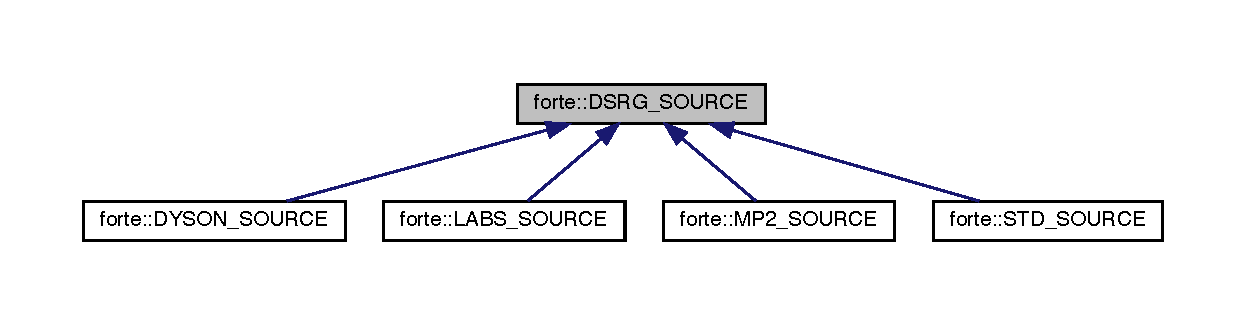
\includegraphics[width=350pt]{classforte_1_1_d_s_r_g___s_o_u_r_c_e__inherit__graph}
\end{center}
\end{figure}
\subsection*{Public Member Functions}
\begin{DoxyCompactItemize}
\item 
\mbox{\hyperlink{classforte_1_1_d_s_r_g___s_o_u_r_c_e_a755f7db2ada7a0028f8b6427990d66e0}{D\+S\+R\+G\+\_\+\+S\+O\+U\+R\+CE}} (double s, double taylor\+\_\+threshold)
\item 
virtual \mbox{\hyperlink{classforte_1_1_d_s_r_g___s_o_u_r_c_e_ab0dfae33a0b08a20312e593cb0af338e}{$\sim$\+D\+S\+R\+G\+\_\+\+S\+O\+U\+R\+CE}} ()
\item 
virtual double \mbox{\hyperlink{classforte_1_1_d_s_r_g___s_o_u_r_c_e_a8b4c4428bb50af4561c256e3180f6b31}{compute\+\_\+renormalized}} (const double \&D)=0
\begin{DoxyCompactList}\small\item\em Bare effect of source operator. \end{DoxyCompactList}\item 
virtual double \mbox{\hyperlink{classforte_1_1_d_s_r_g___s_o_u_r_c_e_a7345ba63c3612369be7c4cc896b7d5c4}{compute\+\_\+renormalized\+\_\+denominator}} (const double \&D)=0
\begin{DoxyCompactList}\small\item\em Renormalize denominator. \end{DoxyCompactList}\end{DoxyCompactItemize}
\subsection*{Protected Attributes}
\begin{DoxyCompactItemize}
\item 
double \mbox{\hyperlink{classforte_1_1_d_s_r_g___s_o_u_r_c_e_ab83311b0d70b05f301b80bcb9abaf76e}{s\+\_\+}}
\begin{DoxyCompactList}\small\item\em Flow parameter. \end{DoxyCompactList}\item 
double \mbox{\hyperlink{classforte_1_1_d_s_r_g___s_o_u_r_c_e_aaf7ea285612472cefc31e0de08856701}{taylor\+\_\+threshold\+\_\+}}
\begin{DoxyCompactList}\small\item\em Smaller than which we will do Taylor expansion. \end{DoxyCompactList}\end{DoxyCompactItemize}


\subsection{Constructor \& Destructor Documentation}
\mbox{\Hypertarget{classforte_1_1_d_s_r_g___s_o_u_r_c_e_a755f7db2ada7a0028f8b6427990d66e0}\label{classforte_1_1_d_s_r_g___s_o_u_r_c_e_a755f7db2ada7a0028f8b6427990d66e0}} 
\index{forte\+::\+D\+S\+R\+G\+\_\+\+S\+O\+U\+R\+CE@{forte\+::\+D\+S\+R\+G\+\_\+\+S\+O\+U\+R\+CE}!D\+S\+R\+G\+\_\+\+S\+O\+U\+R\+CE@{D\+S\+R\+G\+\_\+\+S\+O\+U\+R\+CE}}
\index{D\+S\+R\+G\+\_\+\+S\+O\+U\+R\+CE@{D\+S\+R\+G\+\_\+\+S\+O\+U\+R\+CE}!forte\+::\+D\+S\+R\+G\+\_\+\+S\+O\+U\+R\+CE@{forte\+::\+D\+S\+R\+G\+\_\+\+S\+O\+U\+R\+CE}}
\subsubsection{\texorpdfstring{D\+S\+R\+G\+\_\+\+S\+O\+U\+R\+C\+E()}{DSRG\_SOURCE()}}
{\footnotesize\ttfamily forte\+::\+D\+S\+R\+G\+\_\+\+S\+O\+U\+R\+C\+E\+::\+D\+S\+R\+G\+\_\+\+S\+O\+U\+R\+CE (\begin{DoxyParamCaption}\item[{double}]{s,  }\item[{double}]{taylor\+\_\+threshold }\end{DoxyParamCaption})}

\mbox{\hyperlink{classforte_1_1_d_s_r_g___s_o_u_r_c_e}{D\+S\+R\+G\+\_\+\+S\+O\+U\+R\+CE}} Constructor 
\begin{DoxyParams}{Parameters}
{\em s} & The flow parameter \\
\hline
{\em taylor\+\_\+threshold} & The threshold for Taylor expansion \\
\hline
\end{DoxyParams}
\mbox{\Hypertarget{classforte_1_1_d_s_r_g___s_o_u_r_c_e_ab0dfae33a0b08a20312e593cb0af338e}\label{classforte_1_1_d_s_r_g___s_o_u_r_c_e_ab0dfae33a0b08a20312e593cb0af338e}} 
\index{forte\+::\+D\+S\+R\+G\+\_\+\+S\+O\+U\+R\+CE@{forte\+::\+D\+S\+R\+G\+\_\+\+S\+O\+U\+R\+CE}!````~D\+S\+R\+G\+\_\+\+S\+O\+U\+R\+CE@{$\sim$\+D\+S\+R\+G\+\_\+\+S\+O\+U\+R\+CE}}
\index{````~D\+S\+R\+G\+\_\+\+S\+O\+U\+R\+CE@{$\sim$\+D\+S\+R\+G\+\_\+\+S\+O\+U\+R\+CE}!forte\+::\+D\+S\+R\+G\+\_\+\+S\+O\+U\+R\+CE@{forte\+::\+D\+S\+R\+G\+\_\+\+S\+O\+U\+R\+CE}}
\subsubsection{\texorpdfstring{$\sim$\+D\+S\+R\+G\+\_\+\+S\+O\+U\+R\+C\+E()}{~DSRG\_SOURCE()}}
{\footnotesize\ttfamily virtual forte\+::\+D\+S\+R\+G\+\_\+\+S\+O\+U\+R\+C\+E\+::$\sim$\+D\+S\+R\+G\+\_\+\+S\+O\+U\+R\+CE (\begin{DoxyParamCaption}{ }\end{DoxyParamCaption})\hspace{0.3cm}{\ttfamily [inline]}, {\ttfamily [virtual]}}



\subsection{Member Function Documentation}
\mbox{\Hypertarget{classforte_1_1_d_s_r_g___s_o_u_r_c_e_a8b4c4428bb50af4561c256e3180f6b31}\label{classforte_1_1_d_s_r_g___s_o_u_r_c_e_a8b4c4428bb50af4561c256e3180f6b31}} 
\index{forte\+::\+D\+S\+R\+G\+\_\+\+S\+O\+U\+R\+CE@{forte\+::\+D\+S\+R\+G\+\_\+\+S\+O\+U\+R\+CE}!compute\+\_\+renormalized@{compute\+\_\+renormalized}}
\index{compute\+\_\+renormalized@{compute\+\_\+renormalized}!forte\+::\+D\+S\+R\+G\+\_\+\+S\+O\+U\+R\+CE@{forte\+::\+D\+S\+R\+G\+\_\+\+S\+O\+U\+R\+CE}}
\subsubsection{\texorpdfstring{compute\+\_\+renormalized()}{compute\_renormalized()}}
{\footnotesize\ttfamily virtual double forte\+::\+D\+S\+R\+G\+\_\+\+S\+O\+U\+R\+C\+E\+::compute\+\_\+renormalized (\begin{DoxyParamCaption}\item[{const double \&}]{D }\end{DoxyParamCaption})\hspace{0.3cm}{\ttfamily [pure virtual]}}



Bare effect of source operator. 



Implemented in \mbox{\hyperlink{classforte_1_1_m_p2___s_o_u_r_c_e_ac1a5dfafa00da98e4d60b49abfbf1ace}{forte\+::\+M\+P2\+\_\+\+S\+O\+U\+R\+CE}}, \mbox{\hyperlink{classforte_1_1_d_y_s_o_n___s_o_u_r_c_e_a27ff5faaabaa609facbce558d126cc96}{forte\+::\+D\+Y\+S\+O\+N\+\_\+\+S\+O\+U\+R\+CE}}, \mbox{\hyperlink{classforte_1_1_l_a_b_s___s_o_u_r_c_e_a62a2509bdacd3a8456684b90ba6def30}{forte\+::\+L\+A\+B\+S\+\_\+\+S\+O\+U\+R\+CE}}, and \mbox{\hyperlink{classforte_1_1_s_t_d___s_o_u_r_c_e_a37548c104ca908d43d239638ad8b7cde}{forte\+::\+S\+T\+D\+\_\+\+S\+O\+U\+R\+CE}}.

\mbox{\Hypertarget{classforte_1_1_d_s_r_g___s_o_u_r_c_e_a7345ba63c3612369be7c4cc896b7d5c4}\label{classforte_1_1_d_s_r_g___s_o_u_r_c_e_a7345ba63c3612369be7c4cc896b7d5c4}} 
\index{forte\+::\+D\+S\+R\+G\+\_\+\+S\+O\+U\+R\+CE@{forte\+::\+D\+S\+R\+G\+\_\+\+S\+O\+U\+R\+CE}!compute\+\_\+renormalized\+\_\+denominator@{compute\+\_\+renormalized\+\_\+denominator}}
\index{compute\+\_\+renormalized\+\_\+denominator@{compute\+\_\+renormalized\+\_\+denominator}!forte\+::\+D\+S\+R\+G\+\_\+\+S\+O\+U\+R\+CE@{forte\+::\+D\+S\+R\+G\+\_\+\+S\+O\+U\+R\+CE}}
\subsubsection{\texorpdfstring{compute\+\_\+renormalized\+\_\+denominator()}{compute\_renormalized\_denominator()}}
{\footnotesize\ttfamily virtual double forte\+::\+D\+S\+R\+G\+\_\+\+S\+O\+U\+R\+C\+E\+::compute\+\_\+renormalized\+\_\+denominator (\begin{DoxyParamCaption}\item[{const double \&}]{D }\end{DoxyParamCaption})\hspace{0.3cm}{\ttfamily [pure virtual]}}



Renormalize denominator. 



Implemented in \mbox{\hyperlink{classforte_1_1_m_p2___s_o_u_r_c_e_a7aabae75b519e6b52d8fc88626fc1895}{forte\+::\+M\+P2\+\_\+\+S\+O\+U\+R\+CE}}, \mbox{\hyperlink{classforte_1_1_d_y_s_o_n___s_o_u_r_c_e_a2da089db945ae849b5d733493a5b8d39}{forte\+::\+D\+Y\+S\+O\+N\+\_\+\+S\+O\+U\+R\+CE}}, \mbox{\hyperlink{classforte_1_1_l_a_b_s___s_o_u_r_c_e_a2bb2384aa4d711db4c3116e466d56835}{forte\+::\+L\+A\+B\+S\+\_\+\+S\+O\+U\+R\+CE}}, and \mbox{\hyperlink{classforte_1_1_s_t_d___s_o_u_r_c_e_a3f9dda1563d4679949001e604324eb16}{forte\+::\+S\+T\+D\+\_\+\+S\+O\+U\+R\+CE}}.



\subsection{Member Data Documentation}
\mbox{\Hypertarget{classforte_1_1_d_s_r_g___s_o_u_r_c_e_ab83311b0d70b05f301b80bcb9abaf76e}\label{classforte_1_1_d_s_r_g___s_o_u_r_c_e_ab83311b0d70b05f301b80bcb9abaf76e}} 
\index{forte\+::\+D\+S\+R\+G\+\_\+\+S\+O\+U\+R\+CE@{forte\+::\+D\+S\+R\+G\+\_\+\+S\+O\+U\+R\+CE}!s\+\_\+@{s\+\_\+}}
\index{s\+\_\+@{s\+\_\+}!forte\+::\+D\+S\+R\+G\+\_\+\+S\+O\+U\+R\+CE@{forte\+::\+D\+S\+R\+G\+\_\+\+S\+O\+U\+R\+CE}}
\subsubsection{\texorpdfstring{s\+\_\+}{s\_}}
{\footnotesize\ttfamily double forte\+::\+D\+S\+R\+G\+\_\+\+S\+O\+U\+R\+C\+E\+::s\+\_\+\hspace{0.3cm}{\ttfamily [protected]}}



Flow parameter. 

\mbox{\Hypertarget{classforte_1_1_d_s_r_g___s_o_u_r_c_e_aaf7ea285612472cefc31e0de08856701}\label{classforte_1_1_d_s_r_g___s_o_u_r_c_e_aaf7ea285612472cefc31e0de08856701}} 
\index{forte\+::\+D\+S\+R\+G\+\_\+\+S\+O\+U\+R\+CE@{forte\+::\+D\+S\+R\+G\+\_\+\+S\+O\+U\+R\+CE}!taylor\+\_\+threshold\+\_\+@{taylor\+\_\+threshold\+\_\+}}
\index{taylor\+\_\+threshold\+\_\+@{taylor\+\_\+threshold\+\_\+}!forte\+::\+D\+S\+R\+G\+\_\+\+S\+O\+U\+R\+CE@{forte\+::\+D\+S\+R\+G\+\_\+\+S\+O\+U\+R\+CE}}
\subsubsection{\texorpdfstring{taylor\+\_\+threshold\+\_\+}{taylor\_threshold\_}}
{\footnotesize\ttfamily double forte\+::\+D\+S\+R\+G\+\_\+\+S\+O\+U\+R\+C\+E\+::taylor\+\_\+threshold\+\_\+\hspace{0.3cm}{\ttfamily [protected]}}



Smaller than which we will do Taylor expansion. 



The documentation for this class was generated from the following files\+:\begin{DoxyCompactItemize}
\item 
/\+Users/fevange/\+Source/forte/src/mrdsrg-\/helper/\mbox{\hyperlink{dsrg__source_8h}{dsrg\+\_\+source.\+h}}\item 
/\+Users/fevange/\+Source/forte/src/mrdsrg-\/helper/\mbox{\hyperlink{dsrg__source_8cc}{dsrg\+\_\+source.\+cc}}\end{DoxyCompactItemize}

\hypertarget{classforte_1_1dsrg__tensors}{}\section{forte\+:\+:dsrg\+\_\+tensors Class Reference}
\label{classforte_1_1dsrg__tensors}\index{forte\+::dsrg\+\_\+tensors@{forte\+::dsrg\+\_\+tensors}}


{\ttfamily \#include $<$dsrg\+\_\+tensors.\+h$>$}

\subsection*{Public Member Functions}
\begin{DoxyCompactItemize}
\item 
\mbox{\hyperlink{classforte_1_1dsrg__tensors_ab002395de027ca4facbdfcd28761147a}{dsrg\+\_\+tensors}} ()
\end{DoxyCompactItemize}
\subsection*{Public Attributes}
\begin{DoxyCompactItemize}
\item 
ambit\+::\+Blocked\+Tensor \mbox{\hyperlink{classforte_1_1dsrg__tensors_a9cf8ed544e2a8bbf76b607d0b7ec79d9}{Fock}}
\item 
ambit\+::\+Blocked\+Tensor \mbox{\hyperlink{classforte_1_1dsrg__tensors_ad6a2c5c5871706e5030e175407e466c2}{V}}
\item 
ambit\+::\+Blocked\+Tensor \mbox{\hyperlink{classforte_1_1dsrg__tensors_aeaff2a9b697cb8df97d1e311bfab7636}{T1}}
\item 
ambit\+::\+Blocked\+Tensor \mbox{\hyperlink{classforte_1_1dsrg__tensors_a2808863402de85439422c1113af70a75}{T2}}
\item 
ambit\+::\+Blocked\+Tensor \mbox{\hyperlink{classforte_1_1dsrg__tensors_a92945252de459c446e72820fed92afbc}{Hbar1}}
\item 
ambit\+::\+Blocked\+Tensor \mbox{\hyperlink{classforte_1_1dsrg__tensors_a064f51aee423bb14b20fb76dad4c8272}{Hbar2}}
\item 
ambit\+::\+Blocked\+Tensor \mbox{\hyperlink{classforte_1_1dsrg__tensors_a3192ba68af73479375e17aca7affb83d}{Hbar3}}
\item 
ambit\+::\+Blocked\+Tensor \mbox{\hyperlink{classforte_1_1dsrg__tensors_ad5037f7d14388f6081a939b204d4d1a9}{Heff1}}
\item 
ambit\+::\+Blocked\+Tensor \mbox{\hyperlink{classforte_1_1dsrg__tensors_afa7854b1a7bb4e11316325f65d6b97c2}{Heff2}}
\item 
ambit\+::\+Blocked\+Tensor \mbox{\hyperlink{classforte_1_1dsrg__tensors_a0e7c9961567338e96f830f3623d5aada}{Heff3}}
\end{DoxyCompactItemize}


\subsection{Constructor \& Destructor Documentation}
\mbox{\Hypertarget{classforte_1_1dsrg__tensors_ab002395de027ca4facbdfcd28761147a}\label{classforte_1_1dsrg__tensors_ab002395de027ca4facbdfcd28761147a}} 
\index{forte\+::dsrg\+\_\+tensors@{forte\+::dsrg\+\_\+tensors}!dsrg\+\_\+tensors@{dsrg\+\_\+tensors}}
\index{dsrg\+\_\+tensors@{dsrg\+\_\+tensors}!forte\+::dsrg\+\_\+tensors@{forte\+::dsrg\+\_\+tensors}}
\subsubsection{\texorpdfstring{dsrg\+\_\+tensors()}{dsrg\_tensors()}}
{\footnotesize\ttfamily forte\+::dsrg\+\_\+tensors\+::dsrg\+\_\+tensors (\begin{DoxyParamCaption}{ }\end{DoxyParamCaption})}



\subsection{Member Data Documentation}
\mbox{\Hypertarget{classforte_1_1dsrg__tensors_a9cf8ed544e2a8bbf76b607d0b7ec79d9}\label{classforte_1_1dsrg__tensors_a9cf8ed544e2a8bbf76b607d0b7ec79d9}} 
\index{forte\+::dsrg\+\_\+tensors@{forte\+::dsrg\+\_\+tensors}!Fock@{Fock}}
\index{Fock@{Fock}!forte\+::dsrg\+\_\+tensors@{forte\+::dsrg\+\_\+tensors}}
\subsubsection{\texorpdfstring{Fock}{Fock}}
{\footnotesize\ttfamily ambit\+::\+Blocked\+Tensor forte\+::dsrg\+\_\+tensors\+::\+Fock}

\mbox{\Hypertarget{classforte_1_1dsrg__tensors_a92945252de459c446e72820fed92afbc}\label{classforte_1_1dsrg__tensors_a92945252de459c446e72820fed92afbc}} 
\index{forte\+::dsrg\+\_\+tensors@{forte\+::dsrg\+\_\+tensors}!Hbar1@{Hbar1}}
\index{Hbar1@{Hbar1}!forte\+::dsrg\+\_\+tensors@{forte\+::dsrg\+\_\+tensors}}
\subsubsection{\texorpdfstring{Hbar1}{Hbar1}}
{\footnotesize\ttfamily ambit\+::\+Blocked\+Tensor forte\+::dsrg\+\_\+tensors\+::\+Hbar1}

\mbox{\Hypertarget{classforte_1_1dsrg__tensors_a064f51aee423bb14b20fb76dad4c8272}\label{classforte_1_1dsrg__tensors_a064f51aee423bb14b20fb76dad4c8272}} 
\index{forte\+::dsrg\+\_\+tensors@{forte\+::dsrg\+\_\+tensors}!Hbar2@{Hbar2}}
\index{Hbar2@{Hbar2}!forte\+::dsrg\+\_\+tensors@{forte\+::dsrg\+\_\+tensors}}
\subsubsection{\texorpdfstring{Hbar2}{Hbar2}}
{\footnotesize\ttfamily ambit\+::\+Blocked\+Tensor forte\+::dsrg\+\_\+tensors\+::\+Hbar2}

\mbox{\Hypertarget{classforte_1_1dsrg__tensors_a3192ba68af73479375e17aca7affb83d}\label{classforte_1_1dsrg__tensors_a3192ba68af73479375e17aca7affb83d}} 
\index{forte\+::dsrg\+\_\+tensors@{forte\+::dsrg\+\_\+tensors}!Hbar3@{Hbar3}}
\index{Hbar3@{Hbar3}!forte\+::dsrg\+\_\+tensors@{forte\+::dsrg\+\_\+tensors}}
\subsubsection{\texorpdfstring{Hbar3}{Hbar3}}
{\footnotesize\ttfamily ambit\+::\+Blocked\+Tensor forte\+::dsrg\+\_\+tensors\+::\+Hbar3}

\mbox{\Hypertarget{classforte_1_1dsrg__tensors_ad5037f7d14388f6081a939b204d4d1a9}\label{classforte_1_1dsrg__tensors_ad5037f7d14388f6081a939b204d4d1a9}} 
\index{forte\+::dsrg\+\_\+tensors@{forte\+::dsrg\+\_\+tensors}!Heff1@{Heff1}}
\index{Heff1@{Heff1}!forte\+::dsrg\+\_\+tensors@{forte\+::dsrg\+\_\+tensors}}
\subsubsection{\texorpdfstring{Heff1}{Heff1}}
{\footnotesize\ttfamily ambit\+::\+Blocked\+Tensor forte\+::dsrg\+\_\+tensors\+::\+Heff1}

\mbox{\Hypertarget{classforte_1_1dsrg__tensors_afa7854b1a7bb4e11316325f65d6b97c2}\label{classforte_1_1dsrg__tensors_afa7854b1a7bb4e11316325f65d6b97c2}} 
\index{forte\+::dsrg\+\_\+tensors@{forte\+::dsrg\+\_\+tensors}!Heff2@{Heff2}}
\index{Heff2@{Heff2}!forte\+::dsrg\+\_\+tensors@{forte\+::dsrg\+\_\+tensors}}
\subsubsection{\texorpdfstring{Heff2}{Heff2}}
{\footnotesize\ttfamily ambit\+::\+Blocked\+Tensor forte\+::dsrg\+\_\+tensors\+::\+Heff2}

\mbox{\Hypertarget{classforte_1_1dsrg__tensors_a0e7c9961567338e96f830f3623d5aada}\label{classforte_1_1dsrg__tensors_a0e7c9961567338e96f830f3623d5aada}} 
\index{forte\+::dsrg\+\_\+tensors@{forte\+::dsrg\+\_\+tensors}!Heff3@{Heff3}}
\index{Heff3@{Heff3}!forte\+::dsrg\+\_\+tensors@{forte\+::dsrg\+\_\+tensors}}
\subsubsection{\texorpdfstring{Heff3}{Heff3}}
{\footnotesize\ttfamily ambit\+::\+Blocked\+Tensor forte\+::dsrg\+\_\+tensors\+::\+Heff3}

\mbox{\Hypertarget{classforte_1_1dsrg__tensors_aeaff2a9b697cb8df97d1e311bfab7636}\label{classforte_1_1dsrg__tensors_aeaff2a9b697cb8df97d1e311bfab7636}} 
\index{forte\+::dsrg\+\_\+tensors@{forte\+::dsrg\+\_\+tensors}!T1@{T1}}
\index{T1@{T1}!forte\+::dsrg\+\_\+tensors@{forte\+::dsrg\+\_\+tensors}}
\subsubsection{\texorpdfstring{T1}{T1}}
{\footnotesize\ttfamily ambit\+::\+Blocked\+Tensor forte\+::dsrg\+\_\+tensors\+::\+T1}

\mbox{\Hypertarget{classforte_1_1dsrg__tensors_a2808863402de85439422c1113af70a75}\label{classforte_1_1dsrg__tensors_a2808863402de85439422c1113af70a75}} 
\index{forte\+::dsrg\+\_\+tensors@{forte\+::dsrg\+\_\+tensors}!T2@{T2}}
\index{T2@{T2}!forte\+::dsrg\+\_\+tensors@{forte\+::dsrg\+\_\+tensors}}
\subsubsection{\texorpdfstring{T2}{T2}}
{\footnotesize\ttfamily ambit\+::\+Blocked\+Tensor forte\+::dsrg\+\_\+tensors\+::\+T2}

\mbox{\Hypertarget{classforte_1_1dsrg__tensors_ad6a2c5c5871706e5030e175407e466c2}\label{classforte_1_1dsrg__tensors_ad6a2c5c5871706e5030e175407e466c2}} 
\index{forte\+::dsrg\+\_\+tensors@{forte\+::dsrg\+\_\+tensors}!V@{V}}
\index{V@{V}!forte\+::dsrg\+\_\+tensors@{forte\+::dsrg\+\_\+tensors}}
\subsubsection{\texorpdfstring{V}{V}}
{\footnotesize\ttfamily ambit\+::\+Blocked\+Tensor forte\+::dsrg\+\_\+tensors\+::V}



The documentation for this class was generated from the following files\+:\begin{DoxyCompactItemize}
\item 
/\+Users/fevange/\+Source/forte/src/mrdsrg-\/helper/\mbox{\hyperlink{dsrg__tensors_8h}{dsrg\+\_\+tensors.\+h}}\item 
/\+Users/fevange/\+Source/forte/src/mrdsrg-\/helper/\mbox{\hyperlink{dsrg__tensors_8cc}{dsrg\+\_\+tensors.\+cc}}\end{DoxyCompactItemize}

\hypertarget{classforte_1_1_d_s_r_g___t_i_m_e}{}\section{forte\+:\+:D\+S\+R\+G\+\_\+\+T\+I\+ME Class Reference}
\label{classforte_1_1_d_s_r_g___t_i_m_e}\index{forte\+::\+D\+S\+R\+G\+\_\+\+T\+I\+ME@{forte\+::\+D\+S\+R\+G\+\_\+\+T\+I\+ME}}


{\ttfamily \#include $<$dsrg\+\_\+time.\+h$>$}

\subsection*{Public Member Functions}
\begin{DoxyCompactItemize}
\item 
\mbox{\hyperlink{classforte_1_1_d_s_r_g___t_i_m_e_a48855e5a550f6071615a20d3fe6c6926}{D\+S\+R\+G\+\_\+\+T\+I\+ME}} ()
\begin{DoxyCompactList}\small\item\em Constructor. \end{DoxyCompactList}\item 
void \mbox{\hyperlink{classforte_1_1_d_s_r_g___t_i_m_e_a48dba65b329e97e25265999940156c55}{add}} (const std\+::string \&code, const double \&t)
\begin{DoxyCompactList}\small\item\em Accumulate timings. \end{DoxyCompactList}\item 
void \mbox{\hyperlink{classforte_1_1_d_s_r_g___t_i_m_e_ae39cb2b7b5e9854bc10a174f2733d744}{subtract}} (const std\+::string \&code, const double \&t)
\begin{DoxyCompactList}\small\item\em Subtract timings. \end{DoxyCompactList}\item 
void \mbox{\hyperlink{classforte_1_1_d_s_r_g___t_i_m_e_ac81b3fc66ac541d63649e84cc30df463}{reset}} ()
\begin{DoxyCompactList}\small\item\em Reset timings. \end{DoxyCompactList}\item 
void \mbox{\hyperlink{classforte_1_1_d_s_r_g___t_i_m_e_a070c7ab301e9a3e3f4fca2c4e0321981}{reset}} (const std\+::string \&code)
\item 
void \mbox{\hyperlink{classforte_1_1_d_s_r_g___t_i_m_e_afc16aca0ff3b85a87350806ad589614f}{create\+\_\+code}} (const std\+::string \&code)
\begin{DoxyCompactList}\small\item\em Create info of a code. \end{DoxyCompactList}\item 
void \mbox{\hyperlink{classforte_1_1_d_s_r_g___t_i_m_e_a98c7a9660c0287efba46c64d8a34e4bc}{delete\+\_\+code}} (const std\+::string \&code)
\begin{DoxyCompactList}\small\item\em Delete info of a code. \end{DoxyCompactList}\item 
void \mbox{\hyperlink{classforte_1_1_d_s_r_g___t_i_m_e_a1e02d4e0c3899506956bac26368f77d4}{print\+\_\+comm\+\_\+time}} ()
\begin{DoxyCompactList}\small\item\em Print summary for with default code. \end{DoxyCompactList}\item 
void \mbox{\hyperlink{classforte_1_1_d_s_r_g___t_i_m_e_a37ebe04df7ea97996cb66a69c97d7fbc}{print}} ()
\begin{DoxyCompactList}\small\item\em Print the timing in a generic way. \end{DoxyCompactList}\item 
void \mbox{\hyperlink{classforte_1_1_d_s_r_g___t_i_m_e_aca71fc3d83a5d02707b2f9efe9c88163}{print}} (const std\+::string \&code)
\item 
void \mbox{\hyperlink{classforte_1_1_d_s_r_g___t_i_m_e_afaa13e999c5671b13d6adfa991ad0274}{clear}} ()
\begin{DoxyCompactList}\small\item\em Clear all the private variables. \end{DoxyCompactList}\end{DoxyCompactItemize}


\subsection{Constructor \& Destructor Documentation}
\mbox{\Hypertarget{classforte_1_1_d_s_r_g___t_i_m_e_a48855e5a550f6071615a20d3fe6c6926}\label{classforte_1_1_d_s_r_g___t_i_m_e_a48855e5a550f6071615a20d3fe6c6926}} 
\index{forte\+::\+D\+S\+R\+G\+\_\+\+T\+I\+ME@{forte\+::\+D\+S\+R\+G\+\_\+\+T\+I\+ME}!D\+S\+R\+G\+\_\+\+T\+I\+ME@{D\+S\+R\+G\+\_\+\+T\+I\+ME}}
\index{D\+S\+R\+G\+\_\+\+T\+I\+ME@{D\+S\+R\+G\+\_\+\+T\+I\+ME}!forte\+::\+D\+S\+R\+G\+\_\+\+T\+I\+ME@{forte\+::\+D\+S\+R\+G\+\_\+\+T\+I\+ME}}
\subsubsection{\texorpdfstring{D\+S\+R\+G\+\_\+\+T\+I\+M\+E()}{DSRG\_TIME()}}
{\footnotesize\ttfamily forte\+::\+D\+S\+R\+G\+\_\+\+T\+I\+M\+E\+::\+D\+S\+R\+G\+\_\+\+T\+I\+ME (\begin{DoxyParamCaption}{ }\end{DoxyParamCaption})}



Constructor. 



\subsection{Member Function Documentation}
\mbox{\Hypertarget{classforte_1_1_d_s_r_g___t_i_m_e_a48dba65b329e97e25265999940156c55}\label{classforte_1_1_d_s_r_g___t_i_m_e_a48dba65b329e97e25265999940156c55}} 
\index{forte\+::\+D\+S\+R\+G\+\_\+\+T\+I\+ME@{forte\+::\+D\+S\+R\+G\+\_\+\+T\+I\+ME}!add@{add}}
\index{add@{add}!forte\+::\+D\+S\+R\+G\+\_\+\+T\+I\+ME@{forte\+::\+D\+S\+R\+G\+\_\+\+T\+I\+ME}}
\subsubsection{\texorpdfstring{add()}{add()}}
{\footnotesize\ttfamily void forte\+::\+D\+S\+R\+G\+\_\+\+T\+I\+M\+E\+::add (\begin{DoxyParamCaption}\item[{const std\+::string \&}]{code,  }\item[{const double \&}]{t }\end{DoxyParamCaption})}



Accumulate timings. 

\mbox{\Hypertarget{classforte_1_1_d_s_r_g___t_i_m_e_afaa13e999c5671b13d6adfa991ad0274}\label{classforte_1_1_d_s_r_g___t_i_m_e_afaa13e999c5671b13d6adfa991ad0274}} 
\index{forte\+::\+D\+S\+R\+G\+\_\+\+T\+I\+ME@{forte\+::\+D\+S\+R\+G\+\_\+\+T\+I\+ME}!clear@{clear}}
\index{clear@{clear}!forte\+::\+D\+S\+R\+G\+\_\+\+T\+I\+ME@{forte\+::\+D\+S\+R\+G\+\_\+\+T\+I\+ME}}
\subsubsection{\texorpdfstring{clear()}{clear()}}
{\footnotesize\ttfamily void forte\+::\+D\+S\+R\+G\+\_\+\+T\+I\+M\+E\+::clear (\begin{DoxyParamCaption}{ }\end{DoxyParamCaption})\hspace{0.3cm}{\ttfamily [inline]}}



Clear all the private variables. 

\mbox{\Hypertarget{classforte_1_1_d_s_r_g___t_i_m_e_afc16aca0ff3b85a87350806ad589614f}\label{classforte_1_1_d_s_r_g___t_i_m_e_afc16aca0ff3b85a87350806ad589614f}} 
\index{forte\+::\+D\+S\+R\+G\+\_\+\+T\+I\+ME@{forte\+::\+D\+S\+R\+G\+\_\+\+T\+I\+ME}!create\+\_\+code@{create\+\_\+code}}
\index{create\+\_\+code@{create\+\_\+code}!forte\+::\+D\+S\+R\+G\+\_\+\+T\+I\+ME@{forte\+::\+D\+S\+R\+G\+\_\+\+T\+I\+ME}}
\subsubsection{\texorpdfstring{create\+\_\+code()}{create\_code()}}
{\footnotesize\ttfamily void forte\+::\+D\+S\+R\+G\+\_\+\+T\+I\+M\+E\+::create\+\_\+code (\begin{DoxyParamCaption}\item[{const std\+::string \&}]{code }\end{DoxyParamCaption})}



Create info of a code. 

\mbox{\Hypertarget{classforte_1_1_d_s_r_g___t_i_m_e_a98c7a9660c0287efba46c64d8a34e4bc}\label{classforte_1_1_d_s_r_g___t_i_m_e_a98c7a9660c0287efba46c64d8a34e4bc}} 
\index{forte\+::\+D\+S\+R\+G\+\_\+\+T\+I\+ME@{forte\+::\+D\+S\+R\+G\+\_\+\+T\+I\+ME}!delete\+\_\+code@{delete\+\_\+code}}
\index{delete\+\_\+code@{delete\+\_\+code}!forte\+::\+D\+S\+R\+G\+\_\+\+T\+I\+ME@{forte\+::\+D\+S\+R\+G\+\_\+\+T\+I\+ME}}
\subsubsection{\texorpdfstring{delete\+\_\+code()}{delete\_code()}}
{\footnotesize\ttfamily void forte\+::\+D\+S\+R\+G\+\_\+\+T\+I\+M\+E\+::delete\+\_\+code (\begin{DoxyParamCaption}\item[{const std\+::string \&}]{code }\end{DoxyParamCaption})}



Delete info of a code. 

\mbox{\Hypertarget{classforte_1_1_d_s_r_g___t_i_m_e_a37ebe04df7ea97996cb66a69c97d7fbc}\label{classforte_1_1_d_s_r_g___t_i_m_e_a37ebe04df7ea97996cb66a69c97d7fbc}} 
\index{forte\+::\+D\+S\+R\+G\+\_\+\+T\+I\+ME@{forte\+::\+D\+S\+R\+G\+\_\+\+T\+I\+ME}!print@{print}}
\index{print@{print}!forte\+::\+D\+S\+R\+G\+\_\+\+T\+I\+ME@{forte\+::\+D\+S\+R\+G\+\_\+\+T\+I\+ME}}
\subsubsection{\texorpdfstring{print()}{print()}\hspace{0.1cm}{\footnotesize\ttfamily [1/2]}}
{\footnotesize\ttfamily void forte\+::\+D\+S\+R\+G\+\_\+\+T\+I\+M\+E\+::print (\begin{DoxyParamCaption}{ }\end{DoxyParamCaption})}



Print the timing in a generic way. 

\mbox{\Hypertarget{classforte_1_1_d_s_r_g___t_i_m_e_aca71fc3d83a5d02707b2f9efe9c88163}\label{classforte_1_1_d_s_r_g___t_i_m_e_aca71fc3d83a5d02707b2f9efe9c88163}} 
\index{forte\+::\+D\+S\+R\+G\+\_\+\+T\+I\+ME@{forte\+::\+D\+S\+R\+G\+\_\+\+T\+I\+ME}!print@{print}}
\index{print@{print}!forte\+::\+D\+S\+R\+G\+\_\+\+T\+I\+ME@{forte\+::\+D\+S\+R\+G\+\_\+\+T\+I\+ME}}
\subsubsection{\texorpdfstring{print()}{print()}\hspace{0.1cm}{\footnotesize\ttfamily [2/2]}}
{\footnotesize\ttfamily void forte\+::\+D\+S\+R\+G\+\_\+\+T\+I\+M\+E\+::print (\begin{DoxyParamCaption}\item[{const std\+::string \&}]{code }\end{DoxyParamCaption})}

\mbox{\Hypertarget{classforte_1_1_d_s_r_g___t_i_m_e_a1e02d4e0c3899506956bac26368f77d4}\label{classforte_1_1_d_s_r_g___t_i_m_e_a1e02d4e0c3899506956bac26368f77d4}} 
\index{forte\+::\+D\+S\+R\+G\+\_\+\+T\+I\+ME@{forte\+::\+D\+S\+R\+G\+\_\+\+T\+I\+ME}!print\+\_\+comm\+\_\+time@{print\+\_\+comm\+\_\+time}}
\index{print\+\_\+comm\+\_\+time@{print\+\_\+comm\+\_\+time}!forte\+::\+D\+S\+R\+G\+\_\+\+T\+I\+ME@{forte\+::\+D\+S\+R\+G\+\_\+\+T\+I\+ME}}
\subsubsection{\texorpdfstring{print\+\_\+comm\+\_\+time()}{print\_comm\_time()}}
{\footnotesize\ttfamily void forte\+::\+D\+S\+R\+G\+\_\+\+T\+I\+M\+E\+::print\+\_\+comm\+\_\+time (\begin{DoxyParamCaption}{ }\end{DoxyParamCaption})}



Print summary for with default code. 

\mbox{\Hypertarget{classforte_1_1_d_s_r_g___t_i_m_e_ac81b3fc66ac541d63649e84cc30df463}\label{classforte_1_1_d_s_r_g___t_i_m_e_ac81b3fc66ac541d63649e84cc30df463}} 
\index{forte\+::\+D\+S\+R\+G\+\_\+\+T\+I\+ME@{forte\+::\+D\+S\+R\+G\+\_\+\+T\+I\+ME}!reset@{reset}}
\index{reset@{reset}!forte\+::\+D\+S\+R\+G\+\_\+\+T\+I\+ME@{forte\+::\+D\+S\+R\+G\+\_\+\+T\+I\+ME}}
\subsubsection{\texorpdfstring{reset()}{reset()}\hspace{0.1cm}{\footnotesize\ttfamily [1/2]}}
{\footnotesize\ttfamily void forte\+::\+D\+S\+R\+G\+\_\+\+T\+I\+M\+E\+::reset (\begin{DoxyParamCaption}{ }\end{DoxyParamCaption})}



Reset timings. 

\mbox{\Hypertarget{classforte_1_1_d_s_r_g___t_i_m_e_a070c7ab301e9a3e3f4fca2c4e0321981}\label{classforte_1_1_d_s_r_g___t_i_m_e_a070c7ab301e9a3e3f4fca2c4e0321981}} 
\index{forte\+::\+D\+S\+R\+G\+\_\+\+T\+I\+ME@{forte\+::\+D\+S\+R\+G\+\_\+\+T\+I\+ME}!reset@{reset}}
\index{reset@{reset}!forte\+::\+D\+S\+R\+G\+\_\+\+T\+I\+ME@{forte\+::\+D\+S\+R\+G\+\_\+\+T\+I\+ME}}
\subsubsection{\texorpdfstring{reset()}{reset()}\hspace{0.1cm}{\footnotesize\ttfamily [2/2]}}
{\footnotesize\ttfamily void forte\+::\+D\+S\+R\+G\+\_\+\+T\+I\+M\+E\+::reset (\begin{DoxyParamCaption}\item[{const std\+::string \&}]{code }\end{DoxyParamCaption})}

\mbox{\Hypertarget{classforte_1_1_d_s_r_g___t_i_m_e_ae39cb2b7b5e9854bc10a174f2733d744}\label{classforte_1_1_d_s_r_g___t_i_m_e_ae39cb2b7b5e9854bc10a174f2733d744}} 
\index{forte\+::\+D\+S\+R\+G\+\_\+\+T\+I\+ME@{forte\+::\+D\+S\+R\+G\+\_\+\+T\+I\+ME}!subtract@{subtract}}
\index{subtract@{subtract}!forte\+::\+D\+S\+R\+G\+\_\+\+T\+I\+ME@{forte\+::\+D\+S\+R\+G\+\_\+\+T\+I\+ME}}
\subsubsection{\texorpdfstring{subtract()}{subtract()}}
{\footnotesize\ttfamily void forte\+::\+D\+S\+R\+G\+\_\+\+T\+I\+M\+E\+::subtract (\begin{DoxyParamCaption}\item[{const std\+::string \&}]{code,  }\item[{const double \&}]{t }\end{DoxyParamCaption})}



Subtract timings. 



The documentation for this class was generated from the following files\+:\begin{DoxyCompactItemize}
\item 
/\+Users/fevange/\+Source/forte/src/mrdsrg-\/helper/\mbox{\hyperlink{dsrg__time_8h}{dsrg\+\_\+time.\+h}}\item 
/\+Users/fevange/\+Source/forte/src/mrdsrg-\/helper/\mbox{\hyperlink{dsrg__time_8cc}{dsrg\+\_\+time.\+cc}}\end{DoxyCompactItemize}

\hypertarget{structforte_1_1dsrg_heff}{}\section{forte\+:\+:dsrg\+Heff Struct Reference}
\label{structforte_1_1dsrg_heff}\index{forte\+::dsrg\+Heff@{forte\+::dsrg\+Heff}}


{\ttfamily \#include $<$dsrg\+\_\+tensors.\+h$>$}

\subsection*{Public Attributes}
\begin{DoxyCompactItemize}
\item 
double \mbox{\hyperlink{structforte_1_1dsrg_heff_a44bbed4e62f3c14e43fafba7d75cc588}{H0}} = 0.\+0
\item 
ambit\+::\+Blocked\+Tensor \mbox{\hyperlink{structforte_1_1dsrg_heff_a4332211d17dfc7ad0bcb21693386d133}{H1}}
\item 
ambit\+::\+Blocked\+Tensor \mbox{\hyperlink{structforte_1_1dsrg_heff_ad179386f1081c02fedfa2ce484c70271}{H2}}
\item 
ambit\+::\+Blocked\+Tensor \mbox{\hyperlink{structforte_1_1dsrg_heff_a8373c6f1fcc3465e70a7579feca67f6d}{H3}}
\item 
ambit\+::\+Tensor \mbox{\hyperlink{structforte_1_1dsrg_heff_a4c342cea36648f90bb6827b6403874e4}{H1a}}
\item 
ambit\+::\+Tensor \mbox{\hyperlink{structforte_1_1dsrg_heff_a48aa1de8099c063eaba225c79d773414}{H1b}}
\item 
ambit\+::\+Tensor \mbox{\hyperlink{structforte_1_1dsrg_heff_a4304391ff2a9900df01bb010a6707fa2}{H2aa}}
\item 
ambit\+::\+Tensor \mbox{\hyperlink{structforte_1_1dsrg_heff_ac7a1a945ef716bbd761cdbfa01732070}{H2ab}}
\item 
ambit\+::\+Tensor \mbox{\hyperlink{structforte_1_1dsrg_heff_a4d908a83ae104fd897ca3a0c58b37525}{H2bb}}
\item 
ambit\+::\+Tensor \mbox{\hyperlink{structforte_1_1dsrg_heff_afe5bfca2143c7c61ddfcd442cf833a9f}{H3aaa}}
\item 
ambit\+::\+Tensor \mbox{\hyperlink{structforte_1_1dsrg_heff_a95e8985c98d780785ac076efbceed4d9}{H3aab}}
\item 
ambit\+::\+Tensor \mbox{\hyperlink{structforte_1_1dsrg_heff_a7050a0e428af5b6a80d58d43bdf3f8d5}{H3abb}}
\item 
ambit\+::\+Tensor \mbox{\hyperlink{structforte_1_1dsrg_heff_af611172ce3dba60d7a2c4473f8e0c995}{H3bbb}}
\end{DoxyCompactItemize}


\subsection{Member Data Documentation}
\mbox{\Hypertarget{structforte_1_1dsrg_heff_a44bbed4e62f3c14e43fafba7d75cc588}\label{structforte_1_1dsrg_heff_a44bbed4e62f3c14e43fafba7d75cc588}} 
\index{forte\+::dsrg\+Heff@{forte\+::dsrg\+Heff}!H0@{H0}}
\index{H0@{H0}!forte\+::dsrg\+Heff@{forte\+::dsrg\+Heff}}
\subsubsection{\texorpdfstring{H0}{H0}}
{\footnotesize\ttfamily double forte\+::dsrg\+Heff\+::\+H0 = 0.\+0}

\mbox{\Hypertarget{structforte_1_1dsrg_heff_a4332211d17dfc7ad0bcb21693386d133}\label{structforte_1_1dsrg_heff_a4332211d17dfc7ad0bcb21693386d133}} 
\index{forte\+::dsrg\+Heff@{forte\+::dsrg\+Heff}!H1@{H1}}
\index{H1@{H1}!forte\+::dsrg\+Heff@{forte\+::dsrg\+Heff}}
\subsubsection{\texorpdfstring{H1}{H1}}
{\footnotesize\ttfamily ambit\+::\+Blocked\+Tensor forte\+::dsrg\+Heff\+::\+H1}

\mbox{\Hypertarget{structforte_1_1dsrg_heff_a4c342cea36648f90bb6827b6403874e4}\label{structforte_1_1dsrg_heff_a4c342cea36648f90bb6827b6403874e4}} 
\index{forte\+::dsrg\+Heff@{forte\+::dsrg\+Heff}!H1a@{H1a}}
\index{H1a@{H1a}!forte\+::dsrg\+Heff@{forte\+::dsrg\+Heff}}
\subsubsection{\texorpdfstring{H1a}{H1a}}
{\footnotesize\ttfamily ambit\+::\+Tensor forte\+::dsrg\+Heff\+::\+H1a}

\mbox{\Hypertarget{structforte_1_1dsrg_heff_a48aa1de8099c063eaba225c79d773414}\label{structforte_1_1dsrg_heff_a48aa1de8099c063eaba225c79d773414}} 
\index{forte\+::dsrg\+Heff@{forte\+::dsrg\+Heff}!H1b@{H1b}}
\index{H1b@{H1b}!forte\+::dsrg\+Heff@{forte\+::dsrg\+Heff}}
\subsubsection{\texorpdfstring{H1b}{H1b}}
{\footnotesize\ttfamily ambit\+::\+Tensor forte\+::dsrg\+Heff\+::\+H1b}

\mbox{\Hypertarget{structforte_1_1dsrg_heff_ad179386f1081c02fedfa2ce484c70271}\label{structforte_1_1dsrg_heff_ad179386f1081c02fedfa2ce484c70271}} 
\index{forte\+::dsrg\+Heff@{forte\+::dsrg\+Heff}!H2@{H2}}
\index{H2@{H2}!forte\+::dsrg\+Heff@{forte\+::dsrg\+Heff}}
\subsubsection{\texorpdfstring{H2}{H2}}
{\footnotesize\ttfamily ambit\+::\+Blocked\+Tensor forte\+::dsrg\+Heff\+::\+H2}

\mbox{\Hypertarget{structforte_1_1dsrg_heff_a4304391ff2a9900df01bb010a6707fa2}\label{structforte_1_1dsrg_heff_a4304391ff2a9900df01bb010a6707fa2}} 
\index{forte\+::dsrg\+Heff@{forte\+::dsrg\+Heff}!H2aa@{H2aa}}
\index{H2aa@{H2aa}!forte\+::dsrg\+Heff@{forte\+::dsrg\+Heff}}
\subsubsection{\texorpdfstring{H2aa}{H2aa}}
{\footnotesize\ttfamily ambit\+::\+Tensor forte\+::dsrg\+Heff\+::\+H2aa}

\mbox{\Hypertarget{structforte_1_1dsrg_heff_ac7a1a945ef716bbd761cdbfa01732070}\label{structforte_1_1dsrg_heff_ac7a1a945ef716bbd761cdbfa01732070}} 
\index{forte\+::dsrg\+Heff@{forte\+::dsrg\+Heff}!H2ab@{H2ab}}
\index{H2ab@{H2ab}!forte\+::dsrg\+Heff@{forte\+::dsrg\+Heff}}
\subsubsection{\texorpdfstring{H2ab}{H2ab}}
{\footnotesize\ttfamily ambit\+::\+Tensor forte\+::dsrg\+Heff\+::\+H2ab}

\mbox{\Hypertarget{structforte_1_1dsrg_heff_a4d908a83ae104fd897ca3a0c58b37525}\label{structforte_1_1dsrg_heff_a4d908a83ae104fd897ca3a0c58b37525}} 
\index{forte\+::dsrg\+Heff@{forte\+::dsrg\+Heff}!H2bb@{H2bb}}
\index{H2bb@{H2bb}!forte\+::dsrg\+Heff@{forte\+::dsrg\+Heff}}
\subsubsection{\texorpdfstring{H2bb}{H2bb}}
{\footnotesize\ttfamily ambit\+::\+Tensor forte\+::dsrg\+Heff\+::\+H2bb}

\mbox{\Hypertarget{structforte_1_1dsrg_heff_a8373c6f1fcc3465e70a7579feca67f6d}\label{structforte_1_1dsrg_heff_a8373c6f1fcc3465e70a7579feca67f6d}} 
\index{forte\+::dsrg\+Heff@{forte\+::dsrg\+Heff}!H3@{H3}}
\index{H3@{H3}!forte\+::dsrg\+Heff@{forte\+::dsrg\+Heff}}
\subsubsection{\texorpdfstring{H3}{H3}}
{\footnotesize\ttfamily ambit\+::\+Blocked\+Tensor forte\+::dsrg\+Heff\+::\+H3}

\mbox{\Hypertarget{structforte_1_1dsrg_heff_afe5bfca2143c7c61ddfcd442cf833a9f}\label{structforte_1_1dsrg_heff_afe5bfca2143c7c61ddfcd442cf833a9f}} 
\index{forte\+::dsrg\+Heff@{forte\+::dsrg\+Heff}!H3aaa@{H3aaa}}
\index{H3aaa@{H3aaa}!forte\+::dsrg\+Heff@{forte\+::dsrg\+Heff}}
\subsubsection{\texorpdfstring{H3aaa}{H3aaa}}
{\footnotesize\ttfamily ambit\+::\+Tensor forte\+::dsrg\+Heff\+::\+H3aaa}

\mbox{\Hypertarget{structforte_1_1dsrg_heff_a95e8985c98d780785ac076efbceed4d9}\label{structforte_1_1dsrg_heff_a95e8985c98d780785ac076efbceed4d9}} 
\index{forte\+::dsrg\+Heff@{forte\+::dsrg\+Heff}!H3aab@{H3aab}}
\index{H3aab@{H3aab}!forte\+::dsrg\+Heff@{forte\+::dsrg\+Heff}}
\subsubsection{\texorpdfstring{H3aab}{H3aab}}
{\footnotesize\ttfamily ambit\+::\+Tensor forte\+::dsrg\+Heff\+::\+H3aab}

\mbox{\Hypertarget{structforte_1_1dsrg_heff_a7050a0e428af5b6a80d58d43bdf3f8d5}\label{structforte_1_1dsrg_heff_a7050a0e428af5b6a80d58d43bdf3f8d5}} 
\index{forte\+::dsrg\+Heff@{forte\+::dsrg\+Heff}!H3abb@{H3abb}}
\index{H3abb@{H3abb}!forte\+::dsrg\+Heff@{forte\+::dsrg\+Heff}}
\subsubsection{\texorpdfstring{H3abb}{H3abb}}
{\footnotesize\ttfamily ambit\+::\+Tensor forte\+::dsrg\+Heff\+::\+H3abb}

\mbox{\Hypertarget{structforte_1_1dsrg_heff_af611172ce3dba60d7a2c4473f8e0c995}\label{structforte_1_1dsrg_heff_af611172ce3dba60d7a2c4473f8e0c995}} 
\index{forte\+::dsrg\+Heff@{forte\+::dsrg\+Heff}!H3bbb@{H3bbb}}
\index{H3bbb@{H3bbb}!forte\+::dsrg\+Heff@{forte\+::dsrg\+Heff}}
\subsubsection{\texorpdfstring{H3bbb}{H3bbb}}
{\footnotesize\ttfamily ambit\+::\+Tensor forte\+::dsrg\+Heff\+::\+H3bbb}



The documentation for this struct was generated from the following file\+:\begin{DoxyCompactItemize}
\item 
/\+Users/fevange/\+Source/forte/src/mrdsrg-\/helper/\mbox{\hyperlink{dsrg__tensors_8h}{dsrg\+\_\+tensors.\+h}}\end{DoxyCompactItemize}

\hypertarget{classforte_1_1_d_w_m_s___d_s_r_g_p_t2}{}\section{forte\+:\+:D\+W\+M\+S\+\_\+\+D\+S\+R\+G\+P\+T2 Class Reference}
\label{classforte_1_1_d_w_m_s___d_s_r_g_p_t2}\index{forte\+::\+D\+W\+M\+S\+\_\+\+D\+S\+R\+G\+P\+T2@{forte\+::\+D\+W\+M\+S\+\_\+\+D\+S\+R\+G\+P\+T2}}


{\ttfamily \#include $<$dwms\+\_\+mrpt2.\+h$>$}

\subsection*{Public Member Functions}
\begin{DoxyCompactItemize}
\item 
\mbox{\hyperlink{classforte_1_1_d_w_m_s___d_s_r_g_p_t2_a1bb39d459e3fd008a0474ac5788a7e81}{D\+W\+M\+S\+\_\+\+D\+S\+R\+G\+P\+T2}} (std\+::shared\+\_\+ptr$<$ \mbox{\hyperlink{classforte_1_1_s_c_f_info}{S\+C\+F\+Info}} $>$ scf\+\_\+info, std\+::shared\+\_\+ptr$<$ \mbox{\hyperlink{classforte_1_1_forte_options}{Forte\+Options}} $>$ options, std\+::shared\+\_\+ptr$<$ \mbox{\hyperlink{classforte_1_1_forte_integrals}{Forte\+Integrals}} $>$ ints, std\+::shared\+\_\+ptr$<$ \mbox{\hyperlink{classforte_1_1_m_o_space_info}{M\+O\+Space\+Info}} $>$ mo\+\_\+space\+\_\+info)
\begin{DoxyCompactList}\small\item\em \mbox{\hyperlink{classforte_1_1_d_w_m_s___d_s_r_g_p_t2}{D\+W\+M\+S\+\_\+\+D\+S\+R\+G\+P\+T2}} Constructor. \end{DoxyCompactList}\item 
\mbox{\hyperlink{classforte_1_1_d_w_m_s___d_s_r_g_p_t2_a9e31f86cd9551e571cb151d2e981dc1c}{$\sim$\+D\+W\+M\+S\+\_\+\+D\+S\+R\+G\+P\+T2}} ()
\begin{DoxyCompactList}\small\item\em Destructor. \end{DoxyCompactList}\item 
double \mbox{\hyperlink{classforte_1_1_d_w_m_s___d_s_r_g_p_t2_a61564604a8e13f4ef0ea6cd9de6430c0}{compute\+\_\+energy}} ()
\begin{DoxyCompactList}\small\item\em compute energy and return the ground state energy \end{DoxyCompactList}\end{DoxyCompactItemize}


\subsection{Constructor \& Destructor Documentation}
\mbox{\Hypertarget{classforte_1_1_d_w_m_s___d_s_r_g_p_t2_a1bb39d459e3fd008a0474ac5788a7e81}\label{classforte_1_1_d_w_m_s___d_s_r_g_p_t2_a1bb39d459e3fd008a0474ac5788a7e81}} 
\index{forte\+::\+D\+W\+M\+S\+\_\+\+D\+S\+R\+G\+P\+T2@{forte\+::\+D\+W\+M\+S\+\_\+\+D\+S\+R\+G\+P\+T2}!D\+W\+M\+S\+\_\+\+D\+S\+R\+G\+P\+T2@{D\+W\+M\+S\+\_\+\+D\+S\+R\+G\+P\+T2}}
\index{D\+W\+M\+S\+\_\+\+D\+S\+R\+G\+P\+T2@{D\+W\+M\+S\+\_\+\+D\+S\+R\+G\+P\+T2}!forte\+::\+D\+W\+M\+S\+\_\+\+D\+S\+R\+G\+P\+T2@{forte\+::\+D\+W\+M\+S\+\_\+\+D\+S\+R\+G\+P\+T2}}
\subsubsection{\texorpdfstring{D\+W\+M\+S\+\_\+\+D\+S\+R\+G\+P\+T2()}{DWMS\_DSRGPT2()}}
{\footnotesize\ttfamily forte\+::\+D\+W\+M\+S\+\_\+\+D\+S\+R\+G\+P\+T2\+::\+D\+W\+M\+S\+\_\+\+D\+S\+R\+G\+P\+T2 (\begin{DoxyParamCaption}\item[{std\+::shared\+\_\+ptr$<$ \mbox{\hyperlink{classforte_1_1_s_c_f_info}{S\+C\+F\+Info}} $>$}]{scf\+\_\+info,  }\item[{std\+::shared\+\_\+ptr$<$ \mbox{\hyperlink{classforte_1_1_forte_options}{Forte\+Options}} $>$}]{options,  }\item[{std\+::shared\+\_\+ptr$<$ \mbox{\hyperlink{classforte_1_1_forte_integrals}{Forte\+Integrals}} $>$}]{ints,  }\item[{std\+::shared\+\_\+ptr$<$ \mbox{\hyperlink{classforte_1_1_m_o_space_info}{M\+O\+Space\+Info}} $>$}]{mo\+\_\+space\+\_\+info }\end{DoxyParamCaption})}



\mbox{\hyperlink{classforte_1_1_d_w_m_s___d_s_r_g_p_t2}{D\+W\+M\+S\+\_\+\+D\+S\+R\+G\+P\+T2}} Constructor. 


\begin{DoxyParams}{Parameters}
{\em ref\+\_\+wfn} & The reference wavefunction object \\
\hline
{\em options} & P\+S\+I4 and F\+O\+R\+TE options \\
\hline
{\em ints} & Forte\+Inegrals \\
\hline
{\em mo\+\_\+space\+\_\+info} & \mbox{\hyperlink{classforte_1_1_m_o_space_info}{M\+O\+Space\+Info}} \\
\hline
\end{DoxyParams}
\mbox{\Hypertarget{classforte_1_1_d_w_m_s___d_s_r_g_p_t2_a9e31f86cd9551e571cb151d2e981dc1c}\label{classforte_1_1_d_w_m_s___d_s_r_g_p_t2_a9e31f86cd9551e571cb151d2e981dc1c}} 
\index{forte\+::\+D\+W\+M\+S\+\_\+\+D\+S\+R\+G\+P\+T2@{forte\+::\+D\+W\+M\+S\+\_\+\+D\+S\+R\+G\+P\+T2}!````~D\+W\+M\+S\+\_\+\+D\+S\+R\+G\+P\+T2@{$\sim$\+D\+W\+M\+S\+\_\+\+D\+S\+R\+G\+P\+T2}}
\index{````~D\+W\+M\+S\+\_\+\+D\+S\+R\+G\+P\+T2@{$\sim$\+D\+W\+M\+S\+\_\+\+D\+S\+R\+G\+P\+T2}!forte\+::\+D\+W\+M\+S\+\_\+\+D\+S\+R\+G\+P\+T2@{forte\+::\+D\+W\+M\+S\+\_\+\+D\+S\+R\+G\+P\+T2}}
\subsubsection{\texorpdfstring{$\sim$\+D\+W\+M\+S\+\_\+\+D\+S\+R\+G\+P\+T2()}{~DWMS\_DSRGPT2()}}
{\footnotesize\ttfamily forte\+::\+D\+W\+M\+S\+\_\+\+D\+S\+R\+G\+P\+T2\+::$\sim$\+D\+W\+M\+S\+\_\+\+D\+S\+R\+G\+P\+T2 (\begin{DoxyParamCaption}{ }\end{DoxyParamCaption})}



Destructor. 



\subsection{Member Function Documentation}
\mbox{\Hypertarget{classforte_1_1_d_w_m_s___d_s_r_g_p_t2_a61564604a8e13f4ef0ea6cd9de6430c0}\label{classforte_1_1_d_w_m_s___d_s_r_g_p_t2_a61564604a8e13f4ef0ea6cd9de6430c0}} 
\index{forte\+::\+D\+W\+M\+S\+\_\+\+D\+S\+R\+G\+P\+T2@{forte\+::\+D\+W\+M\+S\+\_\+\+D\+S\+R\+G\+P\+T2}!compute\+\_\+energy@{compute\+\_\+energy}}
\index{compute\+\_\+energy@{compute\+\_\+energy}!forte\+::\+D\+W\+M\+S\+\_\+\+D\+S\+R\+G\+P\+T2@{forte\+::\+D\+W\+M\+S\+\_\+\+D\+S\+R\+G\+P\+T2}}
\subsubsection{\texorpdfstring{compute\+\_\+energy()}{compute\_energy()}}
{\footnotesize\ttfamily double forte\+::\+D\+W\+M\+S\+\_\+\+D\+S\+R\+G\+P\+T2\+::compute\+\_\+energy (\begin{DoxyParamCaption}{ }\end{DoxyParamCaption})}



compute energy and return the ground state energy 



The documentation for this class was generated from the following files\+:\begin{DoxyCompactItemize}
\item 
/\+Users/fevange/\+Source/forte/src/mrdsrg-\/spin-\/integrated/\mbox{\hyperlink{dwms__mrpt2_8h}{dwms\+\_\+mrpt2.\+h}}\item 
/\+Users/fevange/\+Source/forte/src/mrdsrg-\/spin-\/integrated/\mbox{\hyperlink{dwms__mrpt2_8cc}{dwms\+\_\+mrpt2.\+cc}}\end{DoxyCompactItemize}

\hypertarget{classforte_1_1_dynamic_correlation_solver}{}\section{forte\+:\+:Dynamic\+Correlation\+Solver Class Reference}
\label{classforte_1_1_dynamic_correlation_solver}\index{forte\+::\+Dynamic\+Correlation\+Solver@{forte\+::\+Dynamic\+Correlation\+Solver}}


{\ttfamily \#include $<$dynamic\+\_\+correlation\+\_\+solver.\+h$>$}



Inheritance diagram for forte\+:\+:Dynamic\+Correlation\+Solver\+:
\nopagebreak
\begin{figure}[H]
\begin{center}
\leavevmode
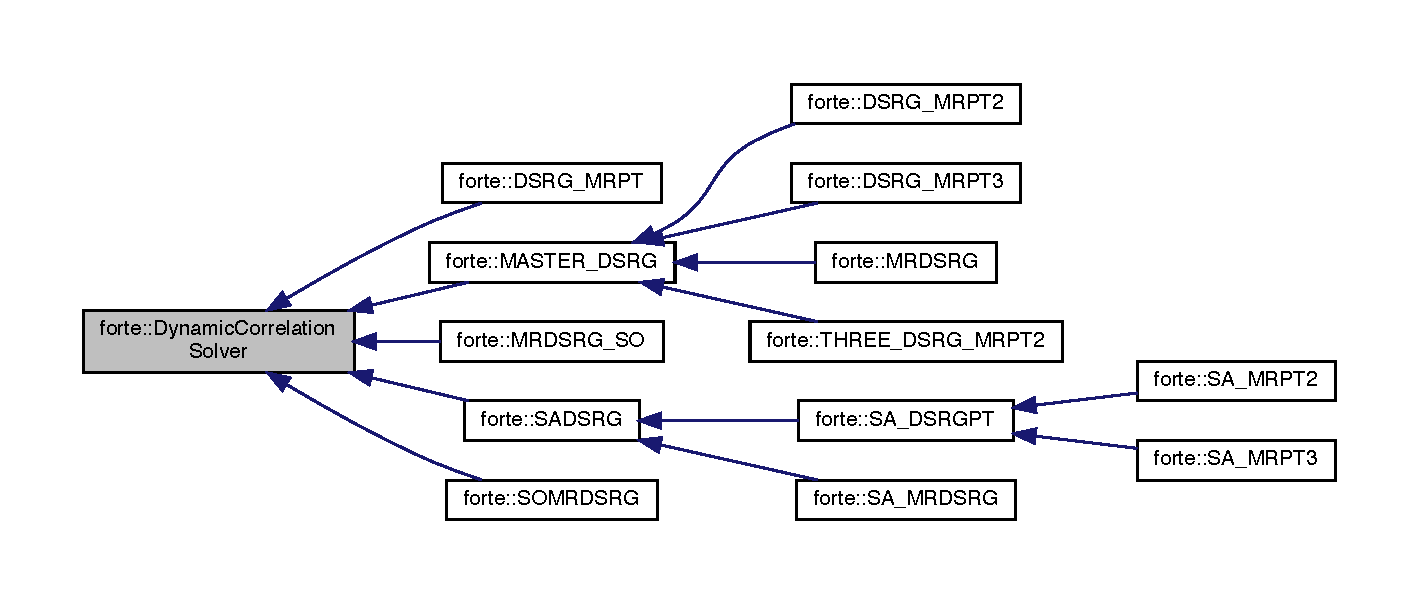
\includegraphics[width=350pt]{classforte_1_1_dynamic_correlation_solver__inherit__graph}
\end{center}
\end{figure}


Collaboration diagram for forte\+:\+:Dynamic\+Correlation\+Solver\+:
\nopagebreak
\begin{figure}[H]
\begin{center}
\leavevmode
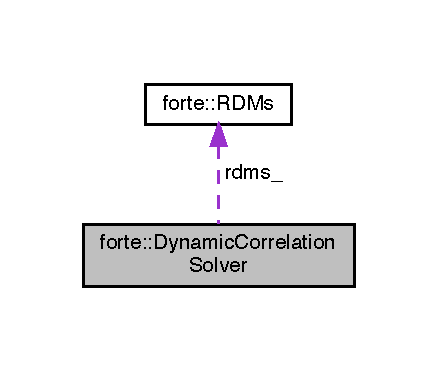
\includegraphics[width=210pt]{classforte_1_1_dynamic_correlation_solver__coll__graph}
\end{center}
\end{figure}
\subsection*{Public Member Functions}
\begin{DoxyCompactItemize}
\item 
\mbox{\hyperlink{classforte_1_1_dynamic_correlation_solver_a37c8ad39f777f877d32735c342549f8a}{Dynamic\+Correlation\+Solver}} (\mbox{\hyperlink{classforte_1_1_r_d_ms}{R\+D\+Ms}} rdms, std\+::shared\+\_\+ptr$<$ \mbox{\hyperlink{classforte_1_1_s_c_f_info}{S\+C\+F\+Info}} $>$ scf\+\_\+info, std\+::shared\+\_\+ptr$<$ \mbox{\hyperlink{classforte_1_1_forte_options}{Forte\+Options}} $>$ options, std\+::shared\+\_\+ptr$<$ \mbox{\hyperlink{classforte_1_1_forte_integrals}{Forte\+Integrals}} $>$ ints, std\+::shared\+\_\+ptr$<$ \mbox{\hyperlink{classforte_1_1_m_o_space_info}{M\+O\+Space\+Info}} $>$ mo\+\_\+space\+\_\+info)
\item 
virtual double \mbox{\hyperlink{classforte_1_1_dynamic_correlation_solver_aff4c7ebdca64563939d6e3ab8a262150}{compute\+\_\+energy}} ()=0
\begin{DoxyCompactList}\small\item\em Compute energy. \end{DoxyCompactList}\item 
virtual std\+::shared\+\_\+ptr$<$ \mbox{\hyperlink{classforte_1_1_active_space_integrals}{Active\+Space\+Integrals}} $>$ \mbox{\hyperlink{classforte_1_1_dynamic_correlation_solver_a8a66ab912dd2c7c1d35c1428df5a494d}{compute\+\_\+\+Heff\+\_\+actv}} ()=0
\begin{DoxyCompactList}\small\item\em Compute dressed Hamiltonian. \end{DoxyCompactList}\item 
virtual \mbox{\hyperlink{classforte_1_1_dynamic_correlation_solver_a80d76d03ef8046d71525943420c0cae6}{$\sim$\+Dynamic\+Correlation\+Solver}} ()=default
\begin{DoxyCompactList}\small\item\em Destructor. \end{DoxyCompactList}\item 
void \mbox{\hyperlink{classforte_1_1_dynamic_correlation_solver_ab2096aa0b894db57cf747c86f1252e08}{set\+\_\+read\+\_\+amps\+\_\+cwd}} (bool read)
\begin{DoxyCompactList}\small\item\em Set whether to read amplitudes or not manually. \end{DoxyCompactList}\item 
void \mbox{\hyperlink{classforte_1_1_dynamic_correlation_solver_a6c55258f31849caa086b226937f35245}{clean\+\_\+checkpoints}} ()
\begin{DoxyCompactList}\small\item\em Clean up amplitudes checkpoint files. \end{DoxyCompactList}\end{DoxyCompactItemize}
\subsection*{Protected Member Functions}
\begin{DoxyCompactItemize}
\item 
void \mbox{\hyperlink{classforte_1_1_dynamic_correlation_solver_ac071ebcb164f9f4a0d573c65602e3f8a}{startup}} ()
\begin{DoxyCompactList}\small\item\em Common settings. \end{DoxyCompactList}\item 
virtual void \mbox{\hyperlink{classforte_1_1_dynamic_correlation_solver_a504b343c559a62b9d13ecf8cec44f3d2}{dump\+\_\+amps\+\_\+to\+\_\+disk}} ()
\end{DoxyCompactItemize}
\subsection*{Protected Attributes}
\begin{DoxyCompactItemize}
\item 
std\+::shared\+\_\+ptr$<$ \mbox{\hyperlink{classforte_1_1_forte_integrals}{Forte\+Integrals}} $>$ \mbox{\hyperlink{classforte_1_1_dynamic_correlation_solver_a839aab2128d02f4a5c9e3a15cd6c4c00}{ints\+\_\+}}
\begin{DoxyCompactList}\small\item\em The molecular integrals. \end{DoxyCompactList}\item 
std\+::shared\+\_\+ptr$<$ \mbox{\hyperlink{classforte_1_1_m_o_space_info}{M\+O\+Space\+Info}} $>$ \mbox{\hyperlink{classforte_1_1_dynamic_correlation_solver_aa9356222050b3dbbf67483338434fa01}{mo\+\_\+space\+\_\+info\+\_\+}}
\begin{DoxyCompactList}\small\item\em The MO space info. \end{DoxyCompactList}\item 
\mbox{\hyperlink{classforte_1_1_r_d_ms}{R\+D\+Ms}} \mbox{\hyperlink{classforte_1_1_dynamic_correlation_solver_a4b8e42e0c8ddbacdd12a70dbad089f17}{rdms\+\_\+}}
\begin{DoxyCompactList}\small\item\em The \mbox{\hyperlink{classforte_1_1_r_d_ms}{R\+D\+Ms}} and cumulants of the reference wave function. \end{DoxyCompactList}\item 
std\+::shared\+\_\+ptr$<$ \mbox{\hyperlink{classforte_1_1_s_c_f_info}{S\+C\+F\+Info}} $>$ \mbox{\hyperlink{classforte_1_1_dynamic_correlation_solver_a4e278d36f4dae4c3828f351561748c6e}{scf\+\_\+info\+\_\+}}
\begin{DoxyCompactList}\small\item\em The \mbox{\hyperlink{classforte_1_1_s_c_f_info}{S\+C\+F\+Info}}. \end{DoxyCompactList}\item 
std\+::shared\+\_\+ptr$<$ \mbox{\hyperlink{classforte_1_1_forte_options}{Forte\+Options}} $>$ \mbox{\hyperlink{classforte_1_1_dynamic_correlation_solver_aab1c4954021b18452cdd0d6a681473ee}{foptions\+\_\+}}
\begin{DoxyCompactList}\small\item\em The \mbox{\hyperlink{classforte_1_1_forte_options}{Forte\+Options}}. \end{DoxyCompactList}\item 
double \mbox{\hyperlink{classforte_1_1_dynamic_correlation_solver_ae0e31a29aa63a9f11df1f08e903ef79f}{Enuc\+\_\+}}
\begin{DoxyCompactList}\small\item\em Nuclear repulsion energy. \end{DoxyCompactList}\item 
double \mbox{\hyperlink{classforte_1_1_dynamic_correlation_solver_a0f12440aa662e60a9348a375c8ab959a}{Efrzc\+\_\+}}
\begin{DoxyCompactList}\small\item\em Frozen core energy. \end{DoxyCompactList}\item 
int \mbox{\hyperlink{classforte_1_1_dynamic_correlation_solver_a3b2686df5f7abb843eeebb130dfc0827}{print\+\_\+}}
\begin{DoxyCompactList}\small\item\em Printing level. \end{DoxyCompactList}\item 
std\+::string \mbox{\hyperlink{classforte_1_1_dynamic_correlation_solver_a73a1949b72f47abf27cb7516719c2211}{ints\+\_\+type\+\_\+}}
\begin{DoxyCompactList}\small\item\em The integral type. \end{DoxyCompactList}\item 
bool \mbox{\hyperlink{classforte_1_1_dynamic_correlation_solver_ac481bf2ca528e1dadb34091d53e49423}{eri\+\_\+df\+\_\+}}
\begin{DoxyCompactList}\small\item\em If E\+RI density fitted or Cholesky decomposed. \end{DoxyCompactList}\item 
int \mbox{\hyperlink{classforte_1_1_dynamic_correlation_solver_a216ac5f54981981b1720b0aac57fc7ba}{diis\+\_\+start\+\_\+}}
\begin{DoxyCompactList}\small\item\em Cycle number to start D\+I\+IS. \end{DoxyCompactList}\item 
int \mbox{\hyperlink{classforte_1_1_dynamic_correlation_solver_ad58021bfd1f4c518d3d57183afdcd403}{diis\+\_\+min\+\_\+vec\+\_\+}}
\begin{DoxyCompactList}\small\item\em Minimum number of D\+I\+IS vectors. \end{DoxyCompactList}\item 
int \mbox{\hyperlink{classforte_1_1_dynamic_correlation_solver_a8f7c491f8d339d3ec9cba80ad02d10fa}{diis\+\_\+max\+\_\+vec\+\_\+}}
\begin{DoxyCompactList}\small\item\em Maximum number of D\+I\+IS vectors. \end{DoxyCompactList}\item 
int \mbox{\hyperlink{classforte_1_1_dynamic_correlation_solver_acd0fdabf84f31c7d115a89b6b7fe9af6}{diis\+\_\+freq\+\_\+}}
\begin{DoxyCompactList}\small\item\em Frequency of extrapolating the current D\+I\+IS vectors. \end{DoxyCompactList}\item 
std\+::string \mbox{\hyperlink{classforte_1_1_dynamic_correlation_solver_a394952f010dae1c06893c03acca808e8}{t1\+\_\+file\+\_\+chk\+\_\+}}
\begin{DoxyCompactList}\small\item\em Checkpoint file for T1 amplitudes. \end{DoxyCompactList}\item 
std\+::string \mbox{\hyperlink{classforte_1_1_dynamic_correlation_solver_aef52805c0fd6b82f19ea598cec8f3fc6}{t2\+\_\+file\+\_\+chk\+\_\+}}
\begin{DoxyCompactList}\small\item\em Checkpoint file for T2 amplitudes. \end{DoxyCompactList}\item 
std\+::string \mbox{\hyperlink{classforte_1_1_dynamic_correlation_solver_ab651c3efceb41dfe20c9c55d3e6aeac5}{t1\+\_\+file\+\_\+cwd\+\_\+}}
\begin{DoxyCompactList}\small\item\em File name for T1 amplitudes to be saved in current directory. \end{DoxyCompactList}\item 
std\+::string \mbox{\hyperlink{classforte_1_1_dynamic_correlation_solver_aeffaac4dffe7b8a38b625f466edb8781}{t2\+\_\+file\+\_\+cwd\+\_\+}}
\begin{DoxyCompactList}\small\item\em File name for T2 amplitudes to be saved in current directory. \end{DoxyCompactList}\item 
bool \mbox{\hyperlink{classforte_1_1_dynamic_correlation_solver_a94f8a814fc383e80ac628a6c08d0fff2}{dump\+\_\+amps\+\_\+cwd\+\_\+}} = false
\begin{DoxyCompactList}\small\item\em Dump amplitudes to current directory. \end{DoxyCompactList}\item 
bool \mbox{\hyperlink{classforte_1_1_dynamic_correlation_solver_aa1c91323000f21d7c2ba0af5ccb51df7}{read\+\_\+amps\+\_\+cwd\+\_\+}} = false
\begin{DoxyCompactList}\small\item\em Read amplitudes from current directory. \end{DoxyCompactList}\end{DoxyCompactItemize}


\subsection{Constructor \& Destructor Documentation}
\mbox{\Hypertarget{classforte_1_1_dynamic_correlation_solver_a37c8ad39f777f877d32735c342549f8a}\label{classforte_1_1_dynamic_correlation_solver_a37c8ad39f777f877d32735c342549f8a}} 
\index{forte\+::\+Dynamic\+Correlation\+Solver@{forte\+::\+Dynamic\+Correlation\+Solver}!Dynamic\+Correlation\+Solver@{Dynamic\+Correlation\+Solver}}
\index{Dynamic\+Correlation\+Solver@{Dynamic\+Correlation\+Solver}!forte\+::\+Dynamic\+Correlation\+Solver@{forte\+::\+Dynamic\+Correlation\+Solver}}
\subsubsection{\texorpdfstring{Dynamic\+Correlation\+Solver()}{DynamicCorrelationSolver()}}
{\footnotesize\ttfamily forte\+::\+Dynamic\+Correlation\+Solver\+::\+Dynamic\+Correlation\+Solver (\begin{DoxyParamCaption}\item[{\mbox{\hyperlink{classforte_1_1_r_d_ms}{R\+D\+Ms}}}]{rdms,  }\item[{std\+::shared\+\_\+ptr$<$ \mbox{\hyperlink{classforte_1_1_s_c_f_info}{S\+C\+F\+Info}} $>$}]{scf\+\_\+info,  }\item[{std\+::shared\+\_\+ptr$<$ \mbox{\hyperlink{classforte_1_1_forte_options}{Forte\+Options}} $>$}]{options,  }\item[{std\+::shared\+\_\+ptr$<$ \mbox{\hyperlink{classforte_1_1_forte_integrals}{Forte\+Integrals}} $>$}]{ints,  }\item[{std\+::shared\+\_\+ptr$<$ \mbox{\hyperlink{classforte_1_1_m_o_space_info}{M\+O\+Space\+Info}} $>$}]{mo\+\_\+space\+\_\+info }\end{DoxyParamCaption})}

Constructor 
\begin{DoxyParams}{Parameters}
{\em ref\+\_\+wfn} & The reference wavefunction object \\
\hline
{\em options} & The main options object \\
\hline
{\em ints} & A pointer to an allocated integral object \\
\hline
{\em mo\+\_\+space\+\_\+info} & The \mbox{\hyperlink{classforte_1_1_m_o_space_info}{M\+O\+Space\+Info}} object \\
\hline
\end{DoxyParams}
\mbox{\Hypertarget{classforte_1_1_dynamic_correlation_solver_a80d76d03ef8046d71525943420c0cae6}\label{classforte_1_1_dynamic_correlation_solver_a80d76d03ef8046d71525943420c0cae6}} 
\index{forte\+::\+Dynamic\+Correlation\+Solver@{forte\+::\+Dynamic\+Correlation\+Solver}!````~Dynamic\+Correlation\+Solver@{$\sim$\+Dynamic\+Correlation\+Solver}}
\index{````~Dynamic\+Correlation\+Solver@{$\sim$\+Dynamic\+Correlation\+Solver}!forte\+::\+Dynamic\+Correlation\+Solver@{forte\+::\+Dynamic\+Correlation\+Solver}}
\subsubsection{\texorpdfstring{$\sim$\+Dynamic\+Correlation\+Solver()}{~DynamicCorrelationSolver()}}
{\footnotesize\ttfamily virtual forte\+::\+Dynamic\+Correlation\+Solver\+::$\sim$\+Dynamic\+Correlation\+Solver (\begin{DoxyParamCaption}{ }\end{DoxyParamCaption})\hspace{0.3cm}{\ttfamily [virtual]}, {\ttfamily [default]}}



Destructor. 



\subsection{Member Function Documentation}
\mbox{\Hypertarget{classforte_1_1_dynamic_correlation_solver_a6c55258f31849caa086b226937f35245}\label{classforte_1_1_dynamic_correlation_solver_a6c55258f31849caa086b226937f35245}} 
\index{forte\+::\+Dynamic\+Correlation\+Solver@{forte\+::\+Dynamic\+Correlation\+Solver}!clean\+\_\+checkpoints@{clean\+\_\+checkpoints}}
\index{clean\+\_\+checkpoints@{clean\+\_\+checkpoints}!forte\+::\+Dynamic\+Correlation\+Solver@{forte\+::\+Dynamic\+Correlation\+Solver}}
\subsubsection{\texorpdfstring{clean\+\_\+checkpoints()}{clean\_checkpoints()}}
{\footnotesize\ttfamily void forte\+::\+Dynamic\+Correlation\+Solver\+::clean\+\_\+checkpoints (\begin{DoxyParamCaption}{ }\end{DoxyParamCaption})}



Clean up amplitudes checkpoint files. 

\mbox{\Hypertarget{classforte_1_1_dynamic_correlation_solver_aff4c7ebdca64563939d6e3ab8a262150}\label{classforte_1_1_dynamic_correlation_solver_aff4c7ebdca64563939d6e3ab8a262150}} 
\index{forte\+::\+Dynamic\+Correlation\+Solver@{forte\+::\+Dynamic\+Correlation\+Solver}!compute\+\_\+energy@{compute\+\_\+energy}}
\index{compute\+\_\+energy@{compute\+\_\+energy}!forte\+::\+Dynamic\+Correlation\+Solver@{forte\+::\+Dynamic\+Correlation\+Solver}}
\subsubsection{\texorpdfstring{compute\+\_\+energy()}{compute\_energy()}}
{\footnotesize\ttfamily virtual double forte\+::\+Dynamic\+Correlation\+Solver\+::compute\+\_\+energy (\begin{DoxyParamCaption}{ }\end{DoxyParamCaption})\hspace{0.3cm}{\ttfamily [pure virtual]}}



Compute energy. 



Implemented in \mbox{\hyperlink{classforte_1_1_m_r_d_s_r_g___s_o_a5a73a7377c4a2be6ce0d875f9833d589}{forte\+::\+M\+R\+D\+S\+R\+G\+\_\+\+SO}}, \mbox{\hyperlink{classforte_1_1_s_o_m_r_d_s_r_g_a80e229a7a41f301ebab0b8d063f8e243}{forte\+::\+S\+O\+M\+R\+D\+S\+RG}}, \mbox{\hyperlink{classforte_1_1_s_a_d_s_r_g_aa3716848c396b296b99fff8d48751fd8}{forte\+::\+S\+A\+D\+S\+RG}}, \mbox{\hyperlink{classforte_1_1_d_s_r_g___m_r_p_t2_a0884f1a9e8f98eb3c272e9c6518e7691}{forte\+::\+D\+S\+R\+G\+\_\+\+M\+R\+P\+T2}}, \mbox{\hyperlink{classforte_1_1_m_r_d_s_r_g_a6c9a82cec6600ecbf3b2a0b01d946223}{forte\+::\+M\+R\+D\+S\+RG}}, \mbox{\hyperlink{classforte_1_1_d_s_r_g___m_r_p_t3_a48a25a952206690bcf8125e583576052}{forte\+::\+D\+S\+R\+G\+\_\+\+M\+R\+P\+T3}}, \mbox{\hyperlink{classforte_1_1_d_s_r_g___m_r_p_t_a83b7f20d255a4f1f33bb05d707846f85}{forte\+::\+D\+S\+R\+G\+\_\+\+M\+R\+PT}}, \mbox{\hyperlink{classforte_1_1_t_h_r_e_e___d_s_r_g___m_r_p_t2_af7cee9b490ef09652f35cbfd48f8fe6a}{forte\+::\+T\+H\+R\+E\+E\+\_\+\+D\+S\+R\+G\+\_\+\+M\+R\+P\+T2}}, \mbox{\hyperlink{classforte_1_1_s_a___m_r_d_s_r_g_a9c86de209cdf7a12ed9cb99e9570fff5}{forte\+::\+S\+A\+\_\+\+M\+R\+D\+S\+RG}}, \mbox{\hyperlink{classforte_1_1_s_a___m_r_p_t2_ac9a4af8ba06295c2918dbc2640caab85}{forte\+::\+S\+A\+\_\+\+M\+R\+P\+T2}}, \mbox{\hyperlink{classforte_1_1_s_a___m_r_p_t3_a566a1aa6f6d3cbb8acdac40cba928aaf}{forte\+::\+S\+A\+\_\+\+M\+R\+P\+T3}}, and \mbox{\hyperlink{classforte_1_1_m_a_s_t_e_r___d_s_r_g_a34011aaadcc79224071a4266a095591b}{forte\+::\+M\+A\+S\+T\+E\+R\+\_\+\+D\+S\+RG}}.

\mbox{\Hypertarget{classforte_1_1_dynamic_correlation_solver_a8a66ab912dd2c7c1d35c1428df5a494d}\label{classforte_1_1_dynamic_correlation_solver_a8a66ab912dd2c7c1d35c1428df5a494d}} 
\index{forte\+::\+Dynamic\+Correlation\+Solver@{forte\+::\+Dynamic\+Correlation\+Solver}!compute\+\_\+\+Heff\+\_\+actv@{compute\+\_\+\+Heff\+\_\+actv}}
\index{compute\+\_\+\+Heff\+\_\+actv@{compute\+\_\+\+Heff\+\_\+actv}!forte\+::\+Dynamic\+Correlation\+Solver@{forte\+::\+Dynamic\+Correlation\+Solver}}
\subsubsection{\texorpdfstring{compute\+\_\+\+Heff\+\_\+actv()}{compute\_Heff\_actv()}}
{\footnotesize\ttfamily virtual std\+::shared\+\_\+ptr$<$\mbox{\hyperlink{classforte_1_1_active_space_integrals}{Active\+Space\+Integrals}}$>$ forte\+::\+Dynamic\+Correlation\+Solver\+::compute\+\_\+\+Heff\+\_\+actv (\begin{DoxyParamCaption}{ }\end{DoxyParamCaption})\hspace{0.3cm}{\ttfamily [pure virtual]}}



Compute dressed Hamiltonian. 



Implemented in \mbox{\hyperlink{classforte_1_1_m_r_d_s_r_g___s_o_a2c927466355d27797fb2a7b5ff478779}{forte\+::\+M\+R\+D\+S\+R\+G\+\_\+\+SO}}, \mbox{\hyperlink{classforte_1_1_s_o_m_r_d_s_r_g_a124b4ab351075d25eec777872e3322f5}{forte\+::\+S\+O\+M\+R\+D\+S\+RG}}, \mbox{\hyperlink{classforte_1_1_s_a_d_s_r_g_afd26cf60145a7e46f65fb07f44e93021}{forte\+::\+S\+A\+D\+S\+RG}}, \mbox{\hyperlink{classforte_1_1_d_s_r_g___m_r_p_t_a929556373e50b9baeefbdd461fd72124}{forte\+::\+D\+S\+R\+G\+\_\+\+M\+R\+PT}}, and \mbox{\hyperlink{classforte_1_1_m_a_s_t_e_r___d_s_r_g_a4c4e581766abada72d8e1742a7887d2a}{forte\+::\+M\+A\+S\+T\+E\+R\+\_\+\+D\+S\+RG}}.

\mbox{\Hypertarget{classforte_1_1_dynamic_correlation_solver_a504b343c559a62b9d13ecf8cec44f3d2}\label{classforte_1_1_dynamic_correlation_solver_a504b343c559a62b9d13ecf8cec44f3d2}} 
\index{forte\+::\+Dynamic\+Correlation\+Solver@{forte\+::\+Dynamic\+Correlation\+Solver}!dump\+\_\+amps\+\_\+to\+\_\+disk@{dump\+\_\+amps\+\_\+to\+\_\+disk}}
\index{dump\+\_\+amps\+\_\+to\+\_\+disk@{dump\+\_\+amps\+\_\+to\+\_\+disk}!forte\+::\+Dynamic\+Correlation\+Solver@{forte\+::\+Dynamic\+Correlation\+Solver}}
\subsubsection{\texorpdfstring{dump\+\_\+amps\+\_\+to\+\_\+disk()}{dump\_amps\_to\_disk()}}
{\footnotesize\ttfamily virtual void forte\+::\+Dynamic\+Correlation\+Solver\+::dump\+\_\+amps\+\_\+to\+\_\+disk (\begin{DoxyParamCaption}{ }\end{DoxyParamCaption})\hspace{0.3cm}{\ttfamily [inline]}, {\ttfamily [protected]}, {\ttfamily [virtual]}}

Dump the converged amplitudes to disk Iterative methods should override this function 

Reimplemented in \mbox{\hyperlink{classforte_1_1_m_r_d_s_r_g_aee87aff2861a0aa4be1d6486d7054049}{forte\+::\+M\+R\+D\+S\+RG}}, and \mbox{\hyperlink{classforte_1_1_s_a___m_r_d_s_r_g_a53d329b17db498bf6c3e6c3984195bcb}{forte\+::\+S\+A\+\_\+\+M\+R\+D\+S\+RG}}.

\mbox{\Hypertarget{classforte_1_1_dynamic_correlation_solver_ab2096aa0b894db57cf747c86f1252e08}\label{classforte_1_1_dynamic_correlation_solver_ab2096aa0b894db57cf747c86f1252e08}} 
\index{forte\+::\+Dynamic\+Correlation\+Solver@{forte\+::\+Dynamic\+Correlation\+Solver}!set\+\_\+read\+\_\+amps\+\_\+cwd@{set\+\_\+read\+\_\+amps\+\_\+cwd}}
\index{set\+\_\+read\+\_\+amps\+\_\+cwd@{set\+\_\+read\+\_\+amps\+\_\+cwd}!forte\+::\+Dynamic\+Correlation\+Solver@{forte\+::\+Dynamic\+Correlation\+Solver}}
\subsubsection{\texorpdfstring{set\+\_\+read\+\_\+amps\+\_\+cwd()}{set\_read\_amps\_cwd()}}
{\footnotesize\ttfamily void forte\+::\+Dynamic\+Correlation\+Solver\+::set\+\_\+read\+\_\+amps\+\_\+cwd (\begin{DoxyParamCaption}\item[{bool}]{read }\end{DoxyParamCaption})\hspace{0.3cm}{\ttfamily [inline]}}



Set whether to read amplitudes or not manually. 

\mbox{\Hypertarget{classforte_1_1_dynamic_correlation_solver_ac071ebcb164f9f4a0d573c65602e3f8a}\label{classforte_1_1_dynamic_correlation_solver_ac071ebcb164f9f4a0d573c65602e3f8a}} 
\index{forte\+::\+Dynamic\+Correlation\+Solver@{forte\+::\+Dynamic\+Correlation\+Solver}!startup@{startup}}
\index{startup@{startup}!forte\+::\+Dynamic\+Correlation\+Solver@{forte\+::\+Dynamic\+Correlation\+Solver}}
\subsubsection{\texorpdfstring{startup()}{startup()}}
{\footnotesize\ttfamily void forte\+::\+Dynamic\+Correlation\+Solver\+::startup (\begin{DoxyParamCaption}{ }\end{DoxyParamCaption})\hspace{0.3cm}{\ttfamily [protected]}}



Common settings. 



\subsection{Member Data Documentation}
\mbox{\Hypertarget{classforte_1_1_dynamic_correlation_solver_acd0fdabf84f31c7d115a89b6b7fe9af6}\label{classforte_1_1_dynamic_correlation_solver_acd0fdabf84f31c7d115a89b6b7fe9af6}} 
\index{forte\+::\+Dynamic\+Correlation\+Solver@{forte\+::\+Dynamic\+Correlation\+Solver}!diis\+\_\+freq\+\_\+@{diis\+\_\+freq\+\_\+}}
\index{diis\+\_\+freq\+\_\+@{diis\+\_\+freq\+\_\+}!forte\+::\+Dynamic\+Correlation\+Solver@{forte\+::\+Dynamic\+Correlation\+Solver}}
\subsubsection{\texorpdfstring{diis\+\_\+freq\+\_\+}{diis\_freq\_}}
{\footnotesize\ttfamily int forte\+::\+Dynamic\+Correlation\+Solver\+::diis\+\_\+freq\+\_\+\hspace{0.3cm}{\ttfamily [protected]}}



Frequency of extrapolating the current D\+I\+IS vectors. 

\mbox{\Hypertarget{classforte_1_1_dynamic_correlation_solver_a8f7c491f8d339d3ec9cba80ad02d10fa}\label{classforte_1_1_dynamic_correlation_solver_a8f7c491f8d339d3ec9cba80ad02d10fa}} 
\index{forte\+::\+Dynamic\+Correlation\+Solver@{forte\+::\+Dynamic\+Correlation\+Solver}!diis\+\_\+max\+\_\+vec\+\_\+@{diis\+\_\+max\+\_\+vec\+\_\+}}
\index{diis\+\_\+max\+\_\+vec\+\_\+@{diis\+\_\+max\+\_\+vec\+\_\+}!forte\+::\+Dynamic\+Correlation\+Solver@{forte\+::\+Dynamic\+Correlation\+Solver}}
\subsubsection{\texorpdfstring{diis\+\_\+max\+\_\+vec\+\_\+}{diis\_max\_vec\_}}
{\footnotesize\ttfamily int forte\+::\+Dynamic\+Correlation\+Solver\+::diis\+\_\+max\+\_\+vec\+\_\+\hspace{0.3cm}{\ttfamily [protected]}}



Maximum number of D\+I\+IS vectors. 

\mbox{\Hypertarget{classforte_1_1_dynamic_correlation_solver_ad58021bfd1f4c518d3d57183afdcd403}\label{classforte_1_1_dynamic_correlation_solver_ad58021bfd1f4c518d3d57183afdcd403}} 
\index{forte\+::\+Dynamic\+Correlation\+Solver@{forte\+::\+Dynamic\+Correlation\+Solver}!diis\+\_\+min\+\_\+vec\+\_\+@{diis\+\_\+min\+\_\+vec\+\_\+}}
\index{diis\+\_\+min\+\_\+vec\+\_\+@{diis\+\_\+min\+\_\+vec\+\_\+}!forte\+::\+Dynamic\+Correlation\+Solver@{forte\+::\+Dynamic\+Correlation\+Solver}}
\subsubsection{\texorpdfstring{diis\+\_\+min\+\_\+vec\+\_\+}{diis\_min\_vec\_}}
{\footnotesize\ttfamily int forte\+::\+Dynamic\+Correlation\+Solver\+::diis\+\_\+min\+\_\+vec\+\_\+\hspace{0.3cm}{\ttfamily [protected]}}



Minimum number of D\+I\+IS vectors. 

\mbox{\Hypertarget{classforte_1_1_dynamic_correlation_solver_a216ac5f54981981b1720b0aac57fc7ba}\label{classforte_1_1_dynamic_correlation_solver_a216ac5f54981981b1720b0aac57fc7ba}} 
\index{forte\+::\+Dynamic\+Correlation\+Solver@{forte\+::\+Dynamic\+Correlation\+Solver}!diis\+\_\+start\+\_\+@{diis\+\_\+start\+\_\+}}
\index{diis\+\_\+start\+\_\+@{diis\+\_\+start\+\_\+}!forte\+::\+Dynamic\+Correlation\+Solver@{forte\+::\+Dynamic\+Correlation\+Solver}}
\subsubsection{\texorpdfstring{diis\+\_\+start\+\_\+}{diis\_start\_}}
{\footnotesize\ttfamily int forte\+::\+Dynamic\+Correlation\+Solver\+::diis\+\_\+start\+\_\+\hspace{0.3cm}{\ttfamily [protected]}}



Cycle number to start D\+I\+IS. 

\mbox{\Hypertarget{classforte_1_1_dynamic_correlation_solver_a94f8a814fc383e80ac628a6c08d0fff2}\label{classforte_1_1_dynamic_correlation_solver_a94f8a814fc383e80ac628a6c08d0fff2}} 
\index{forte\+::\+Dynamic\+Correlation\+Solver@{forte\+::\+Dynamic\+Correlation\+Solver}!dump\+\_\+amps\+\_\+cwd\+\_\+@{dump\+\_\+amps\+\_\+cwd\+\_\+}}
\index{dump\+\_\+amps\+\_\+cwd\+\_\+@{dump\+\_\+amps\+\_\+cwd\+\_\+}!forte\+::\+Dynamic\+Correlation\+Solver@{forte\+::\+Dynamic\+Correlation\+Solver}}
\subsubsection{\texorpdfstring{dump\+\_\+amps\+\_\+cwd\+\_\+}{dump\_amps\_cwd\_}}
{\footnotesize\ttfamily bool forte\+::\+Dynamic\+Correlation\+Solver\+::dump\+\_\+amps\+\_\+cwd\+\_\+ = false\hspace{0.3cm}{\ttfamily [protected]}}



Dump amplitudes to current directory. 

\mbox{\Hypertarget{classforte_1_1_dynamic_correlation_solver_a0f12440aa662e60a9348a375c8ab959a}\label{classforte_1_1_dynamic_correlation_solver_a0f12440aa662e60a9348a375c8ab959a}} 
\index{forte\+::\+Dynamic\+Correlation\+Solver@{forte\+::\+Dynamic\+Correlation\+Solver}!Efrzc\+\_\+@{Efrzc\+\_\+}}
\index{Efrzc\+\_\+@{Efrzc\+\_\+}!forte\+::\+Dynamic\+Correlation\+Solver@{forte\+::\+Dynamic\+Correlation\+Solver}}
\subsubsection{\texorpdfstring{Efrzc\+\_\+}{Efrzc\_}}
{\footnotesize\ttfamily double forte\+::\+Dynamic\+Correlation\+Solver\+::\+Efrzc\+\_\+\hspace{0.3cm}{\ttfamily [protected]}}



Frozen core energy. 

\mbox{\Hypertarget{classforte_1_1_dynamic_correlation_solver_ae0e31a29aa63a9f11df1f08e903ef79f}\label{classforte_1_1_dynamic_correlation_solver_ae0e31a29aa63a9f11df1f08e903ef79f}} 
\index{forte\+::\+Dynamic\+Correlation\+Solver@{forte\+::\+Dynamic\+Correlation\+Solver}!Enuc\+\_\+@{Enuc\+\_\+}}
\index{Enuc\+\_\+@{Enuc\+\_\+}!forte\+::\+Dynamic\+Correlation\+Solver@{forte\+::\+Dynamic\+Correlation\+Solver}}
\subsubsection{\texorpdfstring{Enuc\+\_\+}{Enuc\_}}
{\footnotesize\ttfamily double forte\+::\+Dynamic\+Correlation\+Solver\+::\+Enuc\+\_\+\hspace{0.3cm}{\ttfamily [protected]}}



Nuclear repulsion energy. 

\mbox{\Hypertarget{classforte_1_1_dynamic_correlation_solver_ac481bf2ca528e1dadb34091d53e49423}\label{classforte_1_1_dynamic_correlation_solver_ac481bf2ca528e1dadb34091d53e49423}} 
\index{forte\+::\+Dynamic\+Correlation\+Solver@{forte\+::\+Dynamic\+Correlation\+Solver}!eri\+\_\+df\+\_\+@{eri\+\_\+df\+\_\+}}
\index{eri\+\_\+df\+\_\+@{eri\+\_\+df\+\_\+}!forte\+::\+Dynamic\+Correlation\+Solver@{forte\+::\+Dynamic\+Correlation\+Solver}}
\subsubsection{\texorpdfstring{eri\+\_\+df\+\_\+}{eri\_df\_}}
{\footnotesize\ttfamily bool forte\+::\+Dynamic\+Correlation\+Solver\+::eri\+\_\+df\+\_\+\hspace{0.3cm}{\ttfamily [protected]}}



If E\+RI density fitted or Cholesky decomposed. 

\mbox{\Hypertarget{classforte_1_1_dynamic_correlation_solver_aab1c4954021b18452cdd0d6a681473ee}\label{classforte_1_1_dynamic_correlation_solver_aab1c4954021b18452cdd0d6a681473ee}} 
\index{forte\+::\+Dynamic\+Correlation\+Solver@{forte\+::\+Dynamic\+Correlation\+Solver}!foptions\+\_\+@{foptions\+\_\+}}
\index{foptions\+\_\+@{foptions\+\_\+}!forte\+::\+Dynamic\+Correlation\+Solver@{forte\+::\+Dynamic\+Correlation\+Solver}}
\subsubsection{\texorpdfstring{foptions\+\_\+}{foptions\_}}
{\footnotesize\ttfamily std\+::shared\+\_\+ptr$<$\mbox{\hyperlink{classforte_1_1_forte_options}{Forte\+Options}}$>$ forte\+::\+Dynamic\+Correlation\+Solver\+::foptions\+\_\+\hspace{0.3cm}{\ttfamily [protected]}}



The \mbox{\hyperlink{classforte_1_1_forte_options}{Forte\+Options}}. 

\mbox{\Hypertarget{classforte_1_1_dynamic_correlation_solver_a839aab2128d02f4a5c9e3a15cd6c4c00}\label{classforte_1_1_dynamic_correlation_solver_a839aab2128d02f4a5c9e3a15cd6c4c00}} 
\index{forte\+::\+Dynamic\+Correlation\+Solver@{forte\+::\+Dynamic\+Correlation\+Solver}!ints\+\_\+@{ints\+\_\+}}
\index{ints\+\_\+@{ints\+\_\+}!forte\+::\+Dynamic\+Correlation\+Solver@{forte\+::\+Dynamic\+Correlation\+Solver}}
\subsubsection{\texorpdfstring{ints\+\_\+}{ints\_}}
{\footnotesize\ttfamily std\+::shared\+\_\+ptr$<$\mbox{\hyperlink{classforte_1_1_forte_integrals}{Forte\+Integrals}}$>$ forte\+::\+Dynamic\+Correlation\+Solver\+::ints\+\_\+\hspace{0.3cm}{\ttfamily [protected]}}



The molecular integrals. 

\mbox{\Hypertarget{classforte_1_1_dynamic_correlation_solver_a73a1949b72f47abf27cb7516719c2211}\label{classforte_1_1_dynamic_correlation_solver_a73a1949b72f47abf27cb7516719c2211}} 
\index{forte\+::\+Dynamic\+Correlation\+Solver@{forte\+::\+Dynamic\+Correlation\+Solver}!ints\+\_\+type\+\_\+@{ints\+\_\+type\+\_\+}}
\index{ints\+\_\+type\+\_\+@{ints\+\_\+type\+\_\+}!forte\+::\+Dynamic\+Correlation\+Solver@{forte\+::\+Dynamic\+Correlation\+Solver}}
\subsubsection{\texorpdfstring{ints\+\_\+type\+\_\+}{ints\_type\_}}
{\footnotesize\ttfamily std\+::string forte\+::\+Dynamic\+Correlation\+Solver\+::ints\+\_\+type\+\_\+\hspace{0.3cm}{\ttfamily [protected]}}



The integral type. 

\mbox{\Hypertarget{classforte_1_1_dynamic_correlation_solver_aa9356222050b3dbbf67483338434fa01}\label{classforte_1_1_dynamic_correlation_solver_aa9356222050b3dbbf67483338434fa01}} 
\index{forte\+::\+Dynamic\+Correlation\+Solver@{forte\+::\+Dynamic\+Correlation\+Solver}!mo\+\_\+space\+\_\+info\+\_\+@{mo\+\_\+space\+\_\+info\+\_\+}}
\index{mo\+\_\+space\+\_\+info\+\_\+@{mo\+\_\+space\+\_\+info\+\_\+}!forte\+::\+Dynamic\+Correlation\+Solver@{forte\+::\+Dynamic\+Correlation\+Solver}}
\subsubsection{\texorpdfstring{mo\+\_\+space\+\_\+info\+\_\+}{mo\_space\_info\_}}
{\footnotesize\ttfamily std\+::shared\+\_\+ptr$<$\mbox{\hyperlink{classforte_1_1_m_o_space_info}{M\+O\+Space\+Info}}$>$ forte\+::\+Dynamic\+Correlation\+Solver\+::mo\+\_\+space\+\_\+info\+\_\+\hspace{0.3cm}{\ttfamily [protected]}}



The MO space info. 

\mbox{\Hypertarget{classforte_1_1_dynamic_correlation_solver_a3b2686df5f7abb843eeebb130dfc0827}\label{classforte_1_1_dynamic_correlation_solver_a3b2686df5f7abb843eeebb130dfc0827}} 
\index{forte\+::\+Dynamic\+Correlation\+Solver@{forte\+::\+Dynamic\+Correlation\+Solver}!print\+\_\+@{print\+\_\+}}
\index{print\+\_\+@{print\+\_\+}!forte\+::\+Dynamic\+Correlation\+Solver@{forte\+::\+Dynamic\+Correlation\+Solver}}
\subsubsection{\texorpdfstring{print\+\_\+}{print\_}}
{\footnotesize\ttfamily int forte\+::\+Dynamic\+Correlation\+Solver\+::print\+\_\+\hspace{0.3cm}{\ttfamily [protected]}}



Printing level. 

\mbox{\Hypertarget{classforte_1_1_dynamic_correlation_solver_a4b8e42e0c8ddbacdd12a70dbad089f17}\label{classforte_1_1_dynamic_correlation_solver_a4b8e42e0c8ddbacdd12a70dbad089f17}} 
\index{forte\+::\+Dynamic\+Correlation\+Solver@{forte\+::\+Dynamic\+Correlation\+Solver}!rdms\+\_\+@{rdms\+\_\+}}
\index{rdms\+\_\+@{rdms\+\_\+}!forte\+::\+Dynamic\+Correlation\+Solver@{forte\+::\+Dynamic\+Correlation\+Solver}}
\subsubsection{\texorpdfstring{rdms\+\_\+}{rdms\_}}
{\footnotesize\ttfamily \mbox{\hyperlink{classforte_1_1_r_d_ms}{R\+D\+Ms}} forte\+::\+Dynamic\+Correlation\+Solver\+::rdms\+\_\+\hspace{0.3cm}{\ttfamily [protected]}}



The \mbox{\hyperlink{classforte_1_1_r_d_ms}{R\+D\+Ms}} and cumulants of the reference wave function. 

\mbox{\Hypertarget{classforte_1_1_dynamic_correlation_solver_aa1c91323000f21d7c2ba0af5ccb51df7}\label{classforte_1_1_dynamic_correlation_solver_aa1c91323000f21d7c2ba0af5ccb51df7}} 
\index{forte\+::\+Dynamic\+Correlation\+Solver@{forte\+::\+Dynamic\+Correlation\+Solver}!read\+\_\+amps\+\_\+cwd\+\_\+@{read\+\_\+amps\+\_\+cwd\+\_\+}}
\index{read\+\_\+amps\+\_\+cwd\+\_\+@{read\+\_\+amps\+\_\+cwd\+\_\+}!forte\+::\+Dynamic\+Correlation\+Solver@{forte\+::\+Dynamic\+Correlation\+Solver}}
\subsubsection{\texorpdfstring{read\+\_\+amps\+\_\+cwd\+\_\+}{read\_amps\_cwd\_}}
{\footnotesize\ttfamily bool forte\+::\+Dynamic\+Correlation\+Solver\+::read\+\_\+amps\+\_\+cwd\+\_\+ = false\hspace{0.3cm}{\ttfamily [protected]}}



Read amplitudes from current directory. 

\mbox{\Hypertarget{classforte_1_1_dynamic_correlation_solver_a4e278d36f4dae4c3828f351561748c6e}\label{classforte_1_1_dynamic_correlation_solver_a4e278d36f4dae4c3828f351561748c6e}} 
\index{forte\+::\+Dynamic\+Correlation\+Solver@{forte\+::\+Dynamic\+Correlation\+Solver}!scf\+\_\+info\+\_\+@{scf\+\_\+info\+\_\+}}
\index{scf\+\_\+info\+\_\+@{scf\+\_\+info\+\_\+}!forte\+::\+Dynamic\+Correlation\+Solver@{forte\+::\+Dynamic\+Correlation\+Solver}}
\subsubsection{\texorpdfstring{scf\+\_\+info\+\_\+}{scf\_info\_}}
{\footnotesize\ttfamily std\+::shared\+\_\+ptr$<$\mbox{\hyperlink{classforte_1_1_s_c_f_info}{S\+C\+F\+Info}}$>$ forte\+::\+Dynamic\+Correlation\+Solver\+::scf\+\_\+info\+\_\+\hspace{0.3cm}{\ttfamily [protected]}}



The \mbox{\hyperlink{classforte_1_1_s_c_f_info}{S\+C\+F\+Info}}. 

\mbox{\Hypertarget{classforte_1_1_dynamic_correlation_solver_a394952f010dae1c06893c03acca808e8}\label{classforte_1_1_dynamic_correlation_solver_a394952f010dae1c06893c03acca808e8}} 
\index{forte\+::\+Dynamic\+Correlation\+Solver@{forte\+::\+Dynamic\+Correlation\+Solver}!t1\+\_\+file\+\_\+chk\+\_\+@{t1\+\_\+file\+\_\+chk\+\_\+}}
\index{t1\+\_\+file\+\_\+chk\+\_\+@{t1\+\_\+file\+\_\+chk\+\_\+}!forte\+::\+Dynamic\+Correlation\+Solver@{forte\+::\+Dynamic\+Correlation\+Solver}}
\subsubsection{\texorpdfstring{t1\+\_\+file\+\_\+chk\+\_\+}{t1\_file\_chk\_}}
{\footnotesize\ttfamily std\+::string forte\+::\+Dynamic\+Correlation\+Solver\+::t1\+\_\+file\+\_\+chk\+\_\+\hspace{0.3cm}{\ttfamily [protected]}}



Checkpoint file for T1 amplitudes. 

\mbox{\Hypertarget{classforte_1_1_dynamic_correlation_solver_ab651c3efceb41dfe20c9c55d3e6aeac5}\label{classforte_1_1_dynamic_correlation_solver_ab651c3efceb41dfe20c9c55d3e6aeac5}} 
\index{forte\+::\+Dynamic\+Correlation\+Solver@{forte\+::\+Dynamic\+Correlation\+Solver}!t1\+\_\+file\+\_\+cwd\+\_\+@{t1\+\_\+file\+\_\+cwd\+\_\+}}
\index{t1\+\_\+file\+\_\+cwd\+\_\+@{t1\+\_\+file\+\_\+cwd\+\_\+}!forte\+::\+Dynamic\+Correlation\+Solver@{forte\+::\+Dynamic\+Correlation\+Solver}}
\subsubsection{\texorpdfstring{t1\+\_\+file\+\_\+cwd\+\_\+}{t1\_file\_cwd\_}}
{\footnotesize\ttfamily std\+::string forte\+::\+Dynamic\+Correlation\+Solver\+::t1\+\_\+file\+\_\+cwd\+\_\+\hspace{0.3cm}{\ttfamily [protected]}}



File name for T1 amplitudes to be saved in current directory. 

\mbox{\Hypertarget{classforte_1_1_dynamic_correlation_solver_aef52805c0fd6b82f19ea598cec8f3fc6}\label{classforte_1_1_dynamic_correlation_solver_aef52805c0fd6b82f19ea598cec8f3fc6}} 
\index{forte\+::\+Dynamic\+Correlation\+Solver@{forte\+::\+Dynamic\+Correlation\+Solver}!t2\+\_\+file\+\_\+chk\+\_\+@{t2\+\_\+file\+\_\+chk\+\_\+}}
\index{t2\+\_\+file\+\_\+chk\+\_\+@{t2\+\_\+file\+\_\+chk\+\_\+}!forte\+::\+Dynamic\+Correlation\+Solver@{forte\+::\+Dynamic\+Correlation\+Solver}}
\subsubsection{\texorpdfstring{t2\+\_\+file\+\_\+chk\+\_\+}{t2\_file\_chk\_}}
{\footnotesize\ttfamily std\+::string forte\+::\+Dynamic\+Correlation\+Solver\+::t2\+\_\+file\+\_\+chk\+\_\+\hspace{0.3cm}{\ttfamily [protected]}}



Checkpoint file for T2 amplitudes. 

\mbox{\Hypertarget{classforte_1_1_dynamic_correlation_solver_aeffaac4dffe7b8a38b625f466edb8781}\label{classforte_1_1_dynamic_correlation_solver_aeffaac4dffe7b8a38b625f466edb8781}} 
\index{forte\+::\+Dynamic\+Correlation\+Solver@{forte\+::\+Dynamic\+Correlation\+Solver}!t2\+\_\+file\+\_\+cwd\+\_\+@{t2\+\_\+file\+\_\+cwd\+\_\+}}
\index{t2\+\_\+file\+\_\+cwd\+\_\+@{t2\+\_\+file\+\_\+cwd\+\_\+}!forte\+::\+Dynamic\+Correlation\+Solver@{forte\+::\+Dynamic\+Correlation\+Solver}}
\subsubsection{\texorpdfstring{t2\+\_\+file\+\_\+cwd\+\_\+}{t2\_file\_cwd\_}}
{\footnotesize\ttfamily std\+::string forte\+::\+Dynamic\+Correlation\+Solver\+::t2\+\_\+file\+\_\+cwd\+\_\+\hspace{0.3cm}{\ttfamily [protected]}}



File name for T2 amplitudes to be saved in current directory. 



The documentation for this class was generated from the following files\+:\begin{DoxyCompactItemize}
\item 
/\+Users/fevange/\+Source/forte/src/base\+\_\+classes/\mbox{\hyperlink{dynamic__correlation__solver_8h}{dynamic\+\_\+correlation\+\_\+solver.\+h}}\item 
/\+Users/fevange/\+Source/forte/src/base\+\_\+classes/\mbox{\hyperlink{dynamic__correlation__solver_8cc}{dynamic\+\_\+correlation\+\_\+solver.\+cc}}\end{DoxyCompactItemize}

\hypertarget{classforte_1_1_d_y_s_o_n___s_o_u_r_c_e}{}\section{forte\+:\+:D\+Y\+S\+O\+N\+\_\+\+S\+O\+U\+R\+CE Class Reference}
\label{classforte_1_1_d_y_s_o_n___s_o_u_r_c_e}\index{forte\+::\+D\+Y\+S\+O\+N\+\_\+\+S\+O\+U\+R\+CE@{forte\+::\+D\+Y\+S\+O\+N\+\_\+\+S\+O\+U\+R\+CE}}


Dyson source.  




{\ttfamily \#include $<$dsrg\+\_\+source.\+h$>$}



Inheritance diagram for forte\+:\+:D\+Y\+S\+O\+N\+\_\+\+S\+O\+U\+R\+CE\+:
\nopagebreak
\begin{figure}[H]
\begin{center}
\leavevmode
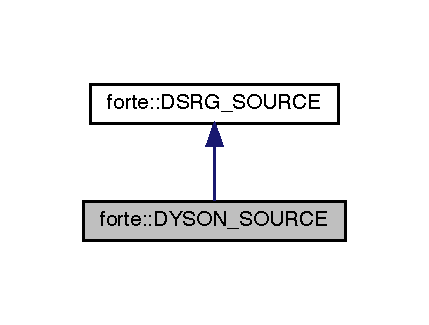
\includegraphics[width=206pt]{classforte_1_1_d_y_s_o_n___s_o_u_r_c_e__inherit__graph}
\end{center}
\end{figure}


Collaboration diagram for forte\+:\+:D\+Y\+S\+O\+N\+\_\+\+S\+O\+U\+R\+CE\+:
\nopagebreak
\begin{figure}[H]
\begin{center}
\leavevmode
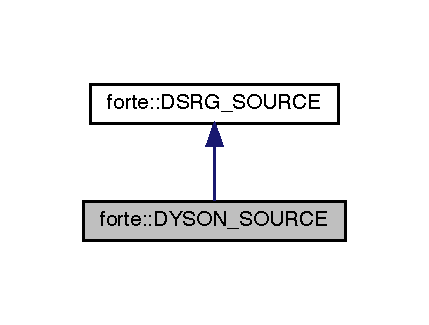
\includegraphics[width=206pt]{classforte_1_1_d_y_s_o_n___s_o_u_r_c_e__coll__graph}
\end{center}
\end{figure}
\subsection*{Public Member Functions}
\begin{DoxyCompactItemize}
\item 
\mbox{\hyperlink{classforte_1_1_d_y_s_o_n___s_o_u_r_c_e_ab2324ffbc215ccba3e95b480d55ea458}{D\+Y\+S\+O\+N\+\_\+\+S\+O\+U\+R\+CE}} (double s, double taylor\+\_\+threshold)
\begin{DoxyCompactList}\small\item\em Constructor. \end{DoxyCompactList}\item 
virtual \mbox{\hyperlink{classforte_1_1_d_y_s_o_n___s_o_u_r_c_e_abf100069942a8596a34452680b1f2af5}{$\sim$\+D\+Y\+S\+O\+N\+\_\+\+S\+O\+U\+R\+CE}} ()
\item 
virtual double \mbox{\hyperlink{classforte_1_1_d_y_s_o_n___s_o_u_r_c_e_a27ff5faaabaa609facbce558d126cc96}{compute\+\_\+renormalized}} (const double \&D)
\begin{DoxyCompactList}\small\item\em Return 1.\+0 / (1.\+0 + s $\ast$ D$^\wedge$2) \end{DoxyCompactList}\item 
virtual double \mbox{\hyperlink{classforte_1_1_d_y_s_o_n___s_o_u_r_c_e_a2da089db945ae849b5d733493a5b8d39}{compute\+\_\+renormalized\+\_\+denominator}} (const double \&D)
\begin{DoxyCompactList}\small\item\em Return s $\ast$ D / (1.\+0 + s $\ast$ D$^\wedge$2) \end{DoxyCompactList}\end{DoxyCompactItemize}
\subsection*{Additional Inherited Members}


\subsection{Detailed Description}
Dyson source. 

\subsection{Constructor \& Destructor Documentation}
\mbox{\Hypertarget{classforte_1_1_d_y_s_o_n___s_o_u_r_c_e_ab2324ffbc215ccba3e95b480d55ea458}\label{classforte_1_1_d_y_s_o_n___s_o_u_r_c_e_ab2324ffbc215ccba3e95b480d55ea458}} 
\index{forte\+::\+D\+Y\+S\+O\+N\+\_\+\+S\+O\+U\+R\+CE@{forte\+::\+D\+Y\+S\+O\+N\+\_\+\+S\+O\+U\+R\+CE}!D\+Y\+S\+O\+N\+\_\+\+S\+O\+U\+R\+CE@{D\+Y\+S\+O\+N\+\_\+\+S\+O\+U\+R\+CE}}
\index{D\+Y\+S\+O\+N\+\_\+\+S\+O\+U\+R\+CE@{D\+Y\+S\+O\+N\+\_\+\+S\+O\+U\+R\+CE}!forte\+::\+D\+Y\+S\+O\+N\+\_\+\+S\+O\+U\+R\+CE@{forte\+::\+D\+Y\+S\+O\+N\+\_\+\+S\+O\+U\+R\+CE}}
\subsubsection{\texorpdfstring{D\+Y\+S\+O\+N\+\_\+\+S\+O\+U\+R\+C\+E()}{DYSON\_SOURCE()}}
{\footnotesize\ttfamily forte\+::\+D\+Y\+S\+O\+N\+\_\+\+S\+O\+U\+R\+C\+E\+::\+D\+Y\+S\+O\+N\+\_\+\+S\+O\+U\+R\+CE (\begin{DoxyParamCaption}\item[{double}]{s,  }\item[{double}]{taylor\+\_\+threshold }\end{DoxyParamCaption})}



Constructor. 

\mbox{\Hypertarget{classforte_1_1_d_y_s_o_n___s_o_u_r_c_e_abf100069942a8596a34452680b1f2af5}\label{classforte_1_1_d_y_s_o_n___s_o_u_r_c_e_abf100069942a8596a34452680b1f2af5}} 
\index{forte\+::\+D\+Y\+S\+O\+N\+\_\+\+S\+O\+U\+R\+CE@{forte\+::\+D\+Y\+S\+O\+N\+\_\+\+S\+O\+U\+R\+CE}!````~D\+Y\+S\+O\+N\+\_\+\+S\+O\+U\+R\+CE@{$\sim$\+D\+Y\+S\+O\+N\+\_\+\+S\+O\+U\+R\+CE}}
\index{````~D\+Y\+S\+O\+N\+\_\+\+S\+O\+U\+R\+CE@{$\sim$\+D\+Y\+S\+O\+N\+\_\+\+S\+O\+U\+R\+CE}!forte\+::\+D\+Y\+S\+O\+N\+\_\+\+S\+O\+U\+R\+CE@{forte\+::\+D\+Y\+S\+O\+N\+\_\+\+S\+O\+U\+R\+CE}}
\subsubsection{\texorpdfstring{$\sim$\+D\+Y\+S\+O\+N\+\_\+\+S\+O\+U\+R\+C\+E()}{~DYSON\_SOURCE()}}
{\footnotesize\ttfamily virtual forte\+::\+D\+Y\+S\+O\+N\+\_\+\+S\+O\+U\+R\+C\+E\+::$\sim$\+D\+Y\+S\+O\+N\+\_\+\+S\+O\+U\+R\+CE (\begin{DoxyParamCaption}{ }\end{DoxyParamCaption})\hspace{0.3cm}{\ttfamily [inline]}, {\ttfamily [virtual]}}



\subsection{Member Function Documentation}
\mbox{\Hypertarget{classforte_1_1_d_y_s_o_n___s_o_u_r_c_e_a27ff5faaabaa609facbce558d126cc96}\label{classforte_1_1_d_y_s_o_n___s_o_u_r_c_e_a27ff5faaabaa609facbce558d126cc96}} 
\index{forte\+::\+D\+Y\+S\+O\+N\+\_\+\+S\+O\+U\+R\+CE@{forte\+::\+D\+Y\+S\+O\+N\+\_\+\+S\+O\+U\+R\+CE}!compute\+\_\+renormalized@{compute\+\_\+renormalized}}
\index{compute\+\_\+renormalized@{compute\+\_\+renormalized}!forte\+::\+D\+Y\+S\+O\+N\+\_\+\+S\+O\+U\+R\+CE@{forte\+::\+D\+Y\+S\+O\+N\+\_\+\+S\+O\+U\+R\+CE}}
\subsubsection{\texorpdfstring{compute\+\_\+renormalized()}{compute\_renormalized()}}
{\footnotesize\ttfamily virtual double forte\+::\+D\+Y\+S\+O\+N\+\_\+\+S\+O\+U\+R\+C\+E\+::compute\+\_\+renormalized (\begin{DoxyParamCaption}\item[{const double \&}]{D }\end{DoxyParamCaption})\hspace{0.3cm}{\ttfamily [inline]}, {\ttfamily [virtual]}}



Return 1.\+0 / (1.\+0 + s $\ast$ D$^\wedge$2) 



Implements \mbox{\hyperlink{classforte_1_1_d_s_r_g___s_o_u_r_c_e_a8b4c4428bb50af4561c256e3180f6b31}{forte\+::\+D\+S\+R\+G\+\_\+\+S\+O\+U\+R\+CE}}.

\mbox{\Hypertarget{classforte_1_1_d_y_s_o_n___s_o_u_r_c_e_a2da089db945ae849b5d733493a5b8d39}\label{classforte_1_1_d_y_s_o_n___s_o_u_r_c_e_a2da089db945ae849b5d733493a5b8d39}} 
\index{forte\+::\+D\+Y\+S\+O\+N\+\_\+\+S\+O\+U\+R\+CE@{forte\+::\+D\+Y\+S\+O\+N\+\_\+\+S\+O\+U\+R\+CE}!compute\+\_\+renormalized\+\_\+denominator@{compute\+\_\+renormalized\+\_\+denominator}}
\index{compute\+\_\+renormalized\+\_\+denominator@{compute\+\_\+renormalized\+\_\+denominator}!forte\+::\+D\+Y\+S\+O\+N\+\_\+\+S\+O\+U\+R\+CE@{forte\+::\+D\+Y\+S\+O\+N\+\_\+\+S\+O\+U\+R\+CE}}
\subsubsection{\texorpdfstring{compute\+\_\+renormalized\+\_\+denominator()}{compute\_renormalized\_denominator()}}
{\footnotesize\ttfamily virtual double forte\+::\+D\+Y\+S\+O\+N\+\_\+\+S\+O\+U\+R\+C\+E\+::compute\+\_\+renormalized\+\_\+denominator (\begin{DoxyParamCaption}\item[{const double \&}]{D }\end{DoxyParamCaption})\hspace{0.3cm}{\ttfamily [inline]}, {\ttfamily [virtual]}}



Return s $\ast$ D / (1.\+0 + s $\ast$ D$^\wedge$2) 



Implements \mbox{\hyperlink{classforte_1_1_d_s_r_g___s_o_u_r_c_e_a7345ba63c3612369be7c4cc896b7d5c4}{forte\+::\+D\+S\+R\+G\+\_\+\+S\+O\+U\+R\+CE}}.



The documentation for this class was generated from the following files\+:\begin{DoxyCompactItemize}
\item 
/\+Users/fevange/\+Source/forte/src/mrdsrg-\/helper/\mbox{\hyperlink{dsrg__source_8h}{dsrg\+\_\+source.\+h}}\item 
/\+Users/fevange/\+Source/forte/src/mrdsrg-\/helper/\mbox{\hyperlink{dsrg__source_8cc}{dsrg\+\_\+source.\+cc}}\end{DoxyCompactItemize}

\hypertarget{classforte_1_1_excited_state_solver}{}\section{forte\+:\+:Excited\+State\+Solver Class Reference}
\label{classforte_1_1_excited_state_solver}\index{forte\+::\+Excited\+State\+Solver@{forte\+::\+Excited\+State\+Solver}}


{\ttfamily \#include $<$excited\+\_\+state\+\_\+solver.\+h$>$}



Inheritance diagram for forte\+:\+:Excited\+State\+Solver\+:
\nopagebreak
\begin{figure}[H]
\begin{center}
\leavevmode
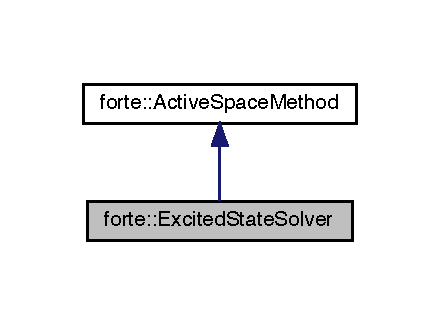
\includegraphics[width=211pt]{classforte_1_1_excited_state_solver__inherit__graph}
\end{center}
\end{figure}


Collaboration diagram for forte\+:\+:Excited\+State\+Solver\+:
\nopagebreak
\begin{figure}[H]
\begin{center}
\leavevmode
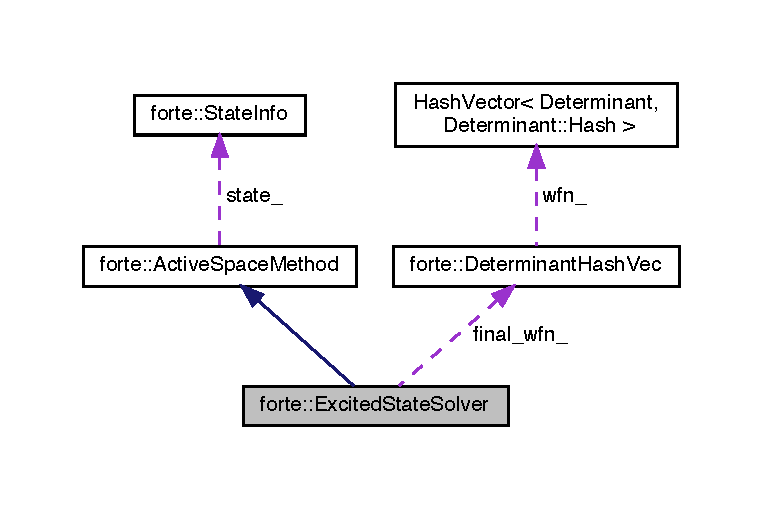
\includegraphics[width=350pt]{classforte_1_1_excited_state_solver__coll__graph}
\end{center}
\end{figure}
\subsection*{Public Member Functions}
\begin{DoxyCompactItemize}
\item 
\mbox{\hyperlink{classforte_1_1_excited_state_solver_ad0bd62104f32a74a473498b86f351217}{Excited\+State\+Solver}} (\mbox{\hyperlink{classforte_1_1_state_info}{State\+Info}} \mbox{\hyperlink{classforte_1_1_active_space_method_a609f005cc7d3a1bc03ae517002eb19dc}{state}}, size\+\_\+t \mbox{\hyperlink{classforte_1_1_active_space_method_aa2bafc732bd7023fd32fbd263ef2e903}{nroot}}, std\+::shared\+\_\+ptr$<$ \mbox{\hyperlink{classforte_1_1_m_o_space_info}{M\+O\+Space\+Info}} $>$ mo\+\_\+space\+\_\+info, std\+::shared\+\_\+ptr$<$ \mbox{\hyperlink{classforte_1_1_active_space_integrals}{Active\+Space\+Integrals}} $>$ as\+\_\+ints, std\+::unique\+\_\+ptr$<$ \mbox{\hyperlink{classforte_1_1_selected_c_i_method}{Selected\+C\+I\+Method}} $>$ sci)
\item 
virtual \mbox{\hyperlink{classforte_1_1_excited_state_solver_a188c2390abb69d46932b0f3dec9ded23}{$\sim$\+Excited\+State\+Solver}} ()=default
\begin{DoxyCompactList}\small\item\em Virtual destructor to enable deletion of a Derived$\ast$ through a Base$\ast$. \end{DoxyCompactList}\item 
virtual double \mbox{\hyperlink{classforte_1_1_excited_state_solver_a35b840324fb9e080eda46f29e544c86a}{compute\+\_\+energy}} () override
\begin{DoxyCompactList}\small\item\em Compute the energy and return it. \end{DoxyCompactList}\item 
std\+::vector$<$ \mbox{\hyperlink{classforte_1_1_r_d_ms}{R\+D\+Ms}} $>$ \mbox{\hyperlink{classforte_1_1_excited_state_solver_a67a061a196cc9e492fabc1b6c7995409}{rdms}} (const std\+::vector$<$ std\+::pair$<$ size\+\_\+t, size\+\_\+t $>$$>$ \&root\+\_\+list, int max\+\_\+rdm\+\_\+level) override
\begin{DoxyCompactList}\small\item\em Returns the reduced density matrices up to a given level (max\+\_\+rdm\+\_\+level) \end{DoxyCompactList}\item 
std\+::vector$<$ \mbox{\hyperlink{classforte_1_1_r_d_ms}{R\+D\+Ms}} $>$ \mbox{\hyperlink{classforte_1_1_excited_state_solver_a8fa122b902c65b75470e34cdd475acaf}{transition\+\_\+rdms}} (const std\+::vector$<$ std\+::pair$<$ size\+\_\+t, size\+\_\+t $>$$>$ \&root\+\_\+list, std\+::shared\+\_\+ptr$<$ \mbox{\hyperlink{classforte_1_1_active_space_method}{Active\+Space\+Method}} $>$ method2, int max\+\_\+rdm\+\_\+level) override
\item 
virtual void \mbox{\hyperlink{classforte_1_1_excited_state_solver_ac32716228ebaa1dfda75cf48db544e5f}{set\+\_\+options}} (std\+::shared\+\_\+ptr$<$ \mbox{\hyperlink{classforte_1_1_forte_options}{Forte\+Options}} $>$ options) override
\item 
void \mbox{\hyperlink{classforte_1_1_excited_state_solver_aa6a0c135e584b27da5ad2bc6bf6d9cc3}{set\+\_\+excitation\+\_\+algorithm}} (std\+::string ex\+\_\+alg)
\begin{DoxyCompactList}\small\item\em Set excitation algorithm. \end{DoxyCompactList}\item 
void \mbox{\hyperlink{classforte_1_1_excited_state_solver_a50494c293ba4bed55b8ce4c7585c93ee}{set\+\_\+core\+\_\+excitation}} (bool core\+\_\+ex)
\begin{DoxyCompactList}\small\item\em Set core excitation. \end{DoxyCompactList}\item 
void \mbox{\hyperlink{classforte_1_1_excited_state_solver_a17b7c4372d65beda0704a9fb94e358aa}{set\+\_\+quiet}} (bool quiet)
\begin{DoxyCompactList}\small\item\em Set the printing level. \end{DoxyCompactList}\end{DoxyCompactItemize}
\subsection*{Protected Attributes}
\begin{DoxyCompactItemize}
\item 
\mbox{\hyperlink{classforte_1_1_determinant_hash_vec}{Determinant\+Hash\+Vec}} \mbox{\hyperlink{classforte_1_1_excited_state_solver_af298efddc513251183107bb72d744443}{final\+\_\+wfn\+\_\+}}
\item 
size\+\_\+t \mbox{\hyperlink{classforte_1_1_excited_state_solver_a505b5254f0c2f79ea4e68399e920f86c}{nact\+\_\+}}
\begin{DoxyCompactList}\small\item\em The number of active orbitals. \end{DoxyCompactList}\item 
std\+::unique\+\_\+ptr$<$ \mbox{\hyperlink{classforte_1_1_selected_c_i_method}{Selected\+C\+I\+Method}} $>$ \mbox{\hyperlink{classforte_1_1_excited_state_solver_a0e955b7e55dbe66bb00cde9c7a1f471a}{sci\+\_\+}}
\item 
std\+::shared\+\_\+ptr$<$ \mbox{\hyperlink{classforte_1_1_sparse_c_i_solver}{Sparse\+C\+I\+Solver}} $>$ \mbox{\hyperlink{classforte_1_1_excited_state_solver_aa95a33586d406350f679c8ecd0558bc6}{sparse\+\_\+solver\+\_\+}}
\item 
std\+::string \mbox{\hyperlink{classforte_1_1_excited_state_solver_af06c1d8815fb1689fe1b61eadc989b4a}{ex\+\_\+alg\+\_\+}}
\begin{DoxyCompactList}\small\item\em Algorithm for computing excited states. \end{DoxyCompactList}\item 
bool \mbox{\hyperlink{classforte_1_1_excited_state_solver_acbbb9da97416aeb1810c9cb0a4d6926d}{core\+\_\+ex\+\_\+}}
\begin{DoxyCompactList}\small\item\em Type of excited state to compute. \end{DoxyCompactList}\item 
bool \mbox{\hyperlink{classforte_1_1_excited_state_solver_ad3075448f2724d563f6f9d49b44d4f69}{quiet\+\_\+mode\+\_\+}}
\begin{DoxyCompactList}\small\item\em Control amount of printing. \end{DoxyCompactList}\item 
std\+::vector$<$ std\+::vector$<$ std\+::pair$<$ \mbox{\hyperlink{namespaceforte_a2076c63fd7b8732004d9e1442ce527c1}{Determinant}}, double $>$ $>$ $>$ \mbox{\hyperlink{classforte_1_1_excited_state_solver_aed69b2410026b59edb0d7fcb0b2eb3c2}{old\+\_\+roots\+\_\+}}
\begin{DoxyCompactList}\small\item\em Storage of past roots. \end{DoxyCompactList}\item 
std\+::vector$<$ double $>$ \mbox{\hyperlink{classforte_1_1_excited_state_solver_a1f54bc7ffb16c953c37d5fcfeaa3fea2}{multistate\+\_\+pt2\+\_\+energy\+\_\+correction\+\_\+}}
\begin{DoxyCompactList}\small\item\em The P\+T2 energy correction. \end{DoxyCompactList}\item 
std\+::shared\+\_\+ptr$<$ psi\+::\+Matrix $>$ \mbox{\hyperlink{classforte_1_1_excited_state_solver_aab92da68a704a3dcc3da707aa04dded6}{evecs\+\_\+}}
\begin{DoxyCompactList}\small\item\em The CI coeffiecients. \end{DoxyCompactList}\item 
bool \mbox{\hyperlink{classforte_1_1_excited_state_solver_a958750ea8478270d12b38953633903f2}{direct\+\_\+rdms\+\_\+}} = false
\begin{DoxyCompactList}\small\item\em Computes \mbox{\hyperlink{classforte_1_1_r_d_ms}{R\+D\+Ms}} without coupling lists. \end{DoxyCompactList}\item 
bool \mbox{\hyperlink{classforte_1_1_excited_state_solver_ac5ec17f14aeabf5a2c249fe337c5f982}{test\+\_\+rdms\+\_\+}} = false
\begin{DoxyCompactList}\small\item\em Run test for the \mbox{\hyperlink{classforte_1_1_r_d_ms}{R\+D\+Ms}}. \end{DoxyCompactList}\item 
bool \mbox{\hyperlink{classforte_1_1_excited_state_solver_a40b5014e260497ddebc51a2bc3474a88}{save\+\_\+final\+\_\+wfn\+\_\+}} = false
\begin{DoxyCompactList}\small\item\em Print final wavefunction to file. \end{DoxyCompactList}\item 
bool \mbox{\hyperlink{classforte_1_1_excited_state_solver_a0533f1272e6a2418f4f8c3d798560b99}{first\+\_\+iter\+\_\+roots\+\_\+}} = false
\begin{DoxyCompactList}\small\item\em Compute all roots on first iteration? \end{DoxyCompactList}\item 
bool \mbox{\hyperlink{classforte_1_1_excited_state_solver_a0b359d79d59555aa1906cb0e5b6fc86a}{full\+\_\+pt2\+\_\+}} = false
\begin{DoxyCompactList}\small\item\em Do full E\+N-\/\+M\+R\+P\+T2 correction? \end{DoxyCompactList}\end{DoxyCompactItemize}


\subsection{Constructor \& Destructor Documentation}
\mbox{\Hypertarget{classforte_1_1_excited_state_solver_ad0bd62104f32a74a473498b86f351217}\label{classforte_1_1_excited_state_solver_ad0bd62104f32a74a473498b86f351217}} 
\index{forte\+::\+Excited\+State\+Solver@{forte\+::\+Excited\+State\+Solver}!Excited\+State\+Solver@{Excited\+State\+Solver}}
\index{Excited\+State\+Solver@{Excited\+State\+Solver}!forte\+::\+Excited\+State\+Solver@{forte\+::\+Excited\+State\+Solver}}
\subsubsection{\texorpdfstring{Excited\+State\+Solver()}{ExcitedStateSolver()}}
{\footnotesize\ttfamily forte\+::\+Excited\+State\+Solver\+::\+Excited\+State\+Solver (\begin{DoxyParamCaption}\item[{\mbox{\hyperlink{classforte_1_1_state_info}{State\+Info}}}]{state,  }\item[{size\+\_\+t}]{nroot,  }\item[{std\+::shared\+\_\+ptr$<$ \mbox{\hyperlink{classforte_1_1_m_o_space_info}{M\+O\+Space\+Info}} $>$}]{mo\+\_\+space\+\_\+info,  }\item[{std\+::shared\+\_\+ptr$<$ \mbox{\hyperlink{classforte_1_1_active_space_integrals}{Active\+Space\+Integrals}} $>$}]{as\+\_\+ints,  }\item[{std\+::unique\+\_\+ptr$<$ \mbox{\hyperlink{classforte_1_1_selected_c_i_method}{Selected\+C\+I\+Method}} $>$}]{sci }\end{DoxyParamCaption})}

\mbox{\Hypertarget{classforte_1_1_excited_state_solver_a188c2390abb69d46932b0f3dec9ded23}\label{classforte_1_1_excited_state_solver_a188c2390abb69d46932b0f3dec9ded23}} 
\index{forte\+::\+Excited\+State\+Solver@{forte\+::\+Excited\+State\+Solver}!````~Excited\+State\+Solver@{$\sim$\+Excited\+State\+Solver}}
\index{````~Excited\+State\+Solver@{$\sim$\+Excited\+State\+Solver}!forte\+::\+Excited\+State\+Solver@{forte\+::\+Excited\+State\+Solver}}
\subsubsection{\texorpdfstring{$\sim$\+Excited\+State\+Solver()}{~ExcitedStateSolver()}}
{\footnotesize\ttfamily virtual forte\+::\+Excited\+State\+Solver\+::$\sim$\+Excited\+State\+Solver (\begin{DoxyParamCaption}{ }\end{DoxyParamCaption})\hspace{0.3cm}{\ttfamily [virtual]}, {\ttfamily [default]}}



Virtual destructor to enable deletion of a Derived$\ast$ through a Base$\ast$. 



\subsection{Member Function Documentation}
\mbox{\Hypertarget{classforte_1_1_excited_state_solver_a35b840324fb9e080eda46f29e544c86a}\label{classforte_1_1_excited_state_solver_a35b840324fb9e080eda46f29e544c86a}} 
\index{forte\+::\+Excited\+State\+Solver@{forte\+::\+Excited\+State\+Solver}!compute\+\_\+energy@{compute\+\_\+energy}}
\index{compute\+\_\+energy@{compute\+\_\+energy}!forte\+::\+Excited\+State\+Solver@{forte\+::\+Excited\+State\+Solver}}
\subsubsection{\texorpdfstring{compute\+\_\+energy()}{compute\_energy()}}
{\footnotesize\ttfamily double forte\+::\+Excited\+State\+Solver\+::compute\+\_\+energy (\begin{DoxyParamCaption}{ }\end{DoxyParamCaption})\hspace{0.3cm}{\ttfamily [override]}, {\ttfamily [virtual]}}



Compute the energy and return it. 



Implements \mbox{\hyperlink{classforte_1_1_active_space_method_a99736e2b94405371b224b0750569b077}{forte\+::\+Active\+Space\+Method}}.

\mbox{\Hypertarget{classforte_1_1_excited_state_solver_a67a061a196cc9e492fabc1b6c7995409}\label{classforte_1_1_excited_state_solver_a67a061a196cc9e492fabc1b6c7995409}} 
\index{forte\+::\+Excited\+State\+Solver@{forte\+::\+Excited\+State\+Solver}!rdms@{rdms}}
\index{rdms@{rdms}!forte\+::\+Excited\+State\+Solver@{forte\+::\+Excited\+State\+Solver}}
\subsubsection{\texorpdfstring{rdms()}{rdms()}}
{\footnotesize\ttfamily std\+::vector$<$ \mbox{\hyperlink{classforte_1_1_r_d_ms}{R\+D\+Ms}} $>$ forte\+::\+Excited\+State\+Solver\+::rdms (\begin{DoxyParamCaption}\item[{const std\+::vector$<$ std\+::pair$<$ size\+\_\+t, size\+\_\+t $>$$>$ \&}]{root\+\_\+list,  }\item[{int}]{max\+\_\+rdm\+\_\+level }\end{DoxyParamCaption})\hspace{0.3cm}{\ttfamily [override]}, {\ttfamily [virtual]}}



Returns the reduced density matrices up to a given level (max\+\_\+rdm\+\_\+level) 



Implements \mbox{\hyperlink{classforte_1_1_active_space_method_a0b2c4903551a7602db815d67349ba7c9}{forte\+::\+Active\+Space\+Method}}.

\mbox{\Hypertarget{classforte_1_1_excited_state_solver_a50494c293ba4bed55b8ce4c7585c93ee}\label{classforte_1_1_excited_state_solver_a50494c293ba4bed55b8ce4c7585c93ee}} 
\index{forte\+::\+Excited\+State\+Solver@{forte\+::\+Excited\+State\+Solver}!set\+\_\+core\+\_\+excitation@{set\+\_\+core\+\_\+excitation}}
\index{set\+\_\+core\+\_\+excitation@{set\+\_\+core\+\_\+excitation}!forte\+::\+Excited\+State\+Solver@{forte\+::\+Excited\+State\+Solver}}
\subsubsection{\texorpdfstring{set\+\_\+core\+\_\+excitation()}{set\_core\_excitation()}}
{\footnotesize\ttfamily void forte\+::\+Excited\+State\+Solver\+::set\+\_\+core\+\_\+excitation (\begin{DoxyParamCaption}\item[{bool}]{core\+\_\+ex }\end{DoxyParamCaption})}



Set core excitation. 

\mbox{\Hypertarget{classforte_1_1_excited_state_solver_aa6a0c135e584b27da5ad2bc6bf6d9cc3}\label{classforte_1_1_excited_state_solver_aa6a0c135e584b27da5ad2bc6bf6d9cc3}} 
\index{forte\+::\+Excited\+State\+Solver@{forte\+::\+Excited\+State\+Solver}!set\+\_\+excitation\+\_\+algorithm@{set\+\_\+excitation\+\_\+algorithm}}
\index{set\+\_\+excitation\+\_\+algorithm@{set\+\_\+excitation\+\_\+algorithm}!forte\+::\+Excited\+State\+Solver@{forte\+::\+Excited\+State\+Solver}}
\subsubsection{\texorpdfstring{set\+\_\+excitation\+\_\+algorithm()}{set\_excitation\_algorithm()}}
{\footnotesize\ttfamily void forte\+::\+Excited\+State\+Solver\+::set\+\_\+excitation\+\_\+algorithm (\begin{DoxyParamCaption}\item[{std\+::string}]{ex\+\_\+alg }\end{DoxyParamCaption})}



Set excitation algorithm. 

\mbox{\Hypertarget{classforte_1_1_excited_state_solver_ac32716228ebaa1dfda75cf48db544e5f}\label{classforte_1_1_excited_state_solver_ac32716228ebaa1dfda75cf48db544e5f}} 
\index{forte\+::\+Excited\+State\+Solver@{forte\+::\+Excited\+State\+Solver}!set\+\_\+options@{set\+\_\+options}}
\index{set\+\_\+options@{set\+\_\+options}!forte\+::\+Excited\+State\+Solver@{forte\+::\+Excited\+State\+Solver}}
\subsubsection{\texorpdfstring{set\+\_\+options()}{set\_options()}}
{\footnotesize\ttfamily void forte\+::\+Excited\+State\+Solver\+::set\+\_\+options (\begin{DoxyParamCaption}\item[{std\+::shared\+\_\+ptr$<$ \mbox{\hyperlink{classforte_1_1_forte_options}{Forte\+Options}} $>$}]{options }\end{DoxyParamCaption})\hspace{0.3cm}{\ttfamily [override]}, {\ttfamily [virtual]}}

Set options from an option object 
\begin{DoxyParams}{Parameters}
{\em options} & the options passed in \\
\hline
\end{DoxyParams}


Implements \mbox{\hyperlink{classforte_1_1_active_space_method_a9416a627f550d4d56f6b8ffe7478ed89}{forte\+::\+Active\+Space\+Method}}.

\mbox{\Hypertarget{classforte_1_1_excited_state_solver_a17b7c4372d65beda0704a9fb94e358aa}\label{classforte_1_1_excited_state_solver_a17b7c4372d65beda0704a9fb94e358aa}} 
\index{forte\+::\+Excited\+State\+Solver@{forte\+::\+Excited\+State\+Solver}!set\+\_\+quiet@{set\+\_\+quiet}}
\index{set\+\_\+quiet@{set\+\_\+quiet}!forte\+::\+Excited\+State\+Solver@{forte\+::\+Excited\+State\+Solver}}
\subsubsection{\texorpdfstring{set\+\_\+quiet()}{set\_quiet()}}
{\footnotesize\ttfamily void forte\+::\+Excited\+State\+Solver\+::set\+\_\+quiet (\begin{DoxyParamCaption}\item[{bool}]{quiet }\end{DoxyParamCaption})}



Set the printing level. 

\mbox{\Hypertarget{classforte_1_1_excited_state_solver_a8fa122b902c65b75470e34cdd475acaf}\label{classforte_1_1_excited_state_solver_a8fa122b902c65b75470e34cdd475acaf}} 
\index{forte\+::\+Excited\+State\+Solver@{forte\+::\+Excited\+State\+Solver}!transition\+\_\+rdms@{transition\+\_\+rdms}}
\index{transition\+\_\+rdms@{transition\+\_\+rdms}!forte\+::\+Excited\+State\+Solver@{forte\+::\+Excited\+State\+Solver}}
\subsubsection{\texorpdfstring{transition\+\_\+rdms()}{transition\_rdms()}}
{\footnotesize\ttfamily std\+::vector$<$ \mbox{\hyperlink{classforte_1_1_r_d_ms}{R\+D\+Ms}} $>$ forte\+::\+Excited\+State\+Solver\+::transition\+\_\+rdms (\begin{DoxyParamCaption}\item[{const std\+::vector$<$ std\+::pair$<$ size\+\_\+t, size\+\_\+t $>$$>$ \&}]{root\+\_\+list,  }\item[{std\+::shared\+\_\+ptr$<$ \mbox{\hyperlink{classforte_1_1_active_space_method}{Active\+Space\+Method}} $>$}]{method2,  }\item[{int}]{max\+\_\+rdm\+\_\+level }\end{DoxyParamCaption})\hspace{0.3cm}{\ttfamily [override]}, {\ttfamily [virtual]}}

Returns the transition reduced density matrices between roots of different symmetry up to a given level (max\+\_\+rdm\+\_\+level) 

Implements \mbox{\hyperlink{classforte_1_1_active_space_method_a4460069915e56a1994d3a4a4e78bdb30}{forte\+::\+Active\+Space\+Method}}.



\subsection{Member Data Documentation}
\mbox{\Hypertarget{classforte_1_1_excited_state_solver_acbbb9da97416aeb1810c9cb0a4d6926d}\label{classforte_1_1_excited_state_solver_acbbb9da97416aeb1810c9cb0a4d6926d}} 
\index{forte\+::\+Excited\+State\+Solver@{forte\+::\+Excited\+State\+Solver}!core\+\_\+ex\+\_\+@{core\+\_\+ex\+\_\+}}
\index{core\+\_\+ex\+\_\+@{core\+\_\+ex\+\_\+}!forte\+::\+Excited\+State\+Solver@{forte\+::\+Excited\+State\+Solver}}
\subsubsection{\texorpdfstring{core\+\_\+ex\+\_\+}{core\_ex\_}}
{\footnotesize\ttfamily bool forte\+::\+Excited\+State\+Solver\+::core\+\_\+ex\+\_\+\hspace{0.3cm}{\ttfamily [protected]}}



Type of excited state to compute. 

\mbox{\Hypertarget{classforte_1_1_excited_state_solver_a958750ea8478270d12b38953633903f2}\label{classforte_1_1_excited_state_solver_a958750ea8478270d12b38953633903f2}} 
\index{forte\+::\+Excited\+State\+Solver@{forte\+::\+Excited\+State\+Solver}!direct\+\_\+rdms\+\_\+@{direct\+\_\+rdms\+\_\+}}
\index{direct\+\_\+rdms\+\_\+@{direct\+\_\+rdms\+\_\+}!forte\+::\+Excited\+State\+Solver@{forte\+::\+Excited\+State\+Solver}}
\subsubsection{\texorpdfstring{direct\+\_\+rdms\+\_\+}{direct\_rdms\_}}
{\footnotesize\ttfamily bool forte\+::\+Excited\+State\+Solver\+::direct\+\_\+rdms\+\_\+ = false\hspace{0.3cm}{\ttfamily [protected]}}



Computes \mbox{\hyperlink{classforte_1_1_r_d_ms}{R\+D\+Ms}} without coupling lists. 

\mbox{\Hypertarget{classforte_1_1_excited_state_solver_aab92da68a704a3dcc3da707aa04dded6}\label{classforte_1_1_excited_state_solver_aab92da68a704a3dcc3da707aa04dded6}} 
\index{forte\+::\+Excited\+State\+Solver@{forte\+::\+Excited\+State\+Solver}!evecs\+\_\+@{evecs\+\_\+}}
\index{evecs\+\_\+@{evecs\+\_\+}!forte\+::\+Excited\+State\+Solver@{forte\+::\+Excited\+State\+Solver}}
\subsubsection{\texorpdfstring{evecs\+\_\+}{evecs\_}}
{\footnotesize\ttfamily std\+::shared\+\_\+ptr$<$psi\+::\+Matrix$>$ forte\+::\+Excited\+State\+Solver\+::evecs\+\_\+\hspace{0.3cm}{\ttfamily [protected]}}



The CI coeffiecients. 

\mbox{\Hypertarget{classforte_1_1_excited_state_solver_af06c1d8815fb1689fe1b61eadc989b4a}\label{classforte_1_1_excited_state_solver_af06c1d8815fb1689fe1b61eadc989b4a}} 
\index{forte\+::\+Excited\+State\+Solver@{forte\+::\+Excited\+State\+Solver}!ex\+\_\+alg\+\_\+@{ex\+\_\+alg\+\_\+}}
\index{ex\+\_\+alg\+\_\+@{ex\+\_\+alg\+\_\+}!forte\+::\+Excited\+State\+Solver@{forte\+::\+Excited\+State\+Solver}}
\subsubsection{\texorpdfstring{ex\+\_\+alg\+\_\+}{ex\_alg\_}}
{\footnotesize\ttfamily std\+::string forte\+::\+Excited\+State\+Solver\+::ex\+\_\+alg\+\_\+\hspace{0.3cm}{\ttfamily [protected]}}



Algorithm for computing excited states. 

\mbox{\Hypertarget{classforte_1_1_excited_state_solver_af298efddc513251183107bb72d744443}\label{classforte_1_1_excited_state_solver_af298efddc513251183107bb72d744443}} 
\index{forte\+::\+Excited\+State\+Solver@{forte\+::\+Excited\+State\+Solver}!final\+\_\+wfn\+\_\+@{final\+\_\+wfn\+\_\+}}
\index{final\+\_\+wfn\+\_\+@{final\+\_\+wfn\+\_\+}!forte\+::\+Excited\+State\+Solver@{forte\+::\+Excited\+State\+Solver}}
\subsubsection{\texorpdfstring{final\+\_\+wfn\+\_\+}{final\_wfn\_}}
{\footnotesize\ttfamily \mbox{\hyperlink{classforte_1_1_determinant_hash_vec}{Determinant\+Hash\+Vec}} forte\+::\+Excited\+State\+Solver\+::final\+\_\+wfn\+\_\+\hspace{0.3cm}{\ttfamily [protected]}}

\mbox{\Hypertarget{classforte_1_1_excited_state_solver_a0533f1272e6a2418f4f8c3d798560b99}\label{classforte_1_1_excited_state_solver_a0533f1272e6a2418f4f8c3d798560b99}} 
\index{forte\+::\+Excited\+State\+Solver@{forte\+::\+Excited\+State\+Solver}!first\+\_\+iter\+\_\+roots\+\_\+@{first\+\_\+iter\+\_\+roots\+\_\+}}
\index{first\+\_\+iter\+\_\+roots\+\_\+@{first\+\_\+iter\+\_\+roots\+\_\+}!forte\+::\+Excited\+State\+Solver@{forte\+::\+Excited\+State\+Solver}}
\subsubsection{\texorpdfstring{first\+\_\+iter\+\_\+roots\+\_\+}{first\_iter\_roots\_}}
{\footnotesize\ttfamily bool forte\+::\+Excited\+State\+Solver\+::first\+\_\+iter\+\_\+roots\+\_\+ = false\hspace{0.3cm}{\ttfamily [protected]}}



Compute all roots on first iteration? 

\mbox{\Hypertarget{classforte_1_1_excited_state_solver_a0b359d79d59555aa1906cb0e5b6fc86a}\label{classforte_1_1_excited_state_solver_a0b359d79d59555aa1906cb0e5b6fc86a}} 
\index{forte\+::\+Excited\+State\+Solver@{forte\+::\+Excited\+State\+Solver}!full\+\_\+pt2\+\_\+@{full\+\_\+pt2\+\_\+}}
\index{full\+\_\+pt2\+\_\+@{full\+\_\+pt2\+\_\+}!forte\+::\+Excited\+State\+Solver@{forte\+::\+Excited\+State\+Solver}}
\subsubsection{\texorpdfstring{full\+\_\+pt2\+\_\+}{full\_pt2\_}}
{\footnotesize\ttfamily bool forte\+::\+Excited\+State\+Solver\+::full\+\_\+pt2\+\_\+ = false\hspace{0.3cm}{\ttfamily [protected]}}



Do full E\+N-\/\+M\+R\+P\+T2 correction? 

\mbox{\Hypertarget{classforte_1_1_excited_state_solver_a1f54bc7ffb16c953c37d5fcfeaa3fea2}\label{classforte_1_1_excited_state_solver_a1f54bc7ffb16c953c37d5fcfeaa3fea2}} 
\index{forte\+::\+Excited\+State\+Solver@{forte\+::\+Excited\+State\+Solver}!multistate\+\_\+pt2\+\_\+energy\+\_\+correction\+\_\+@{multistate\+\_\+pt2\+\_\+energy\+\_\+correction\+\_\+}}
\index{multistate\+\_\+pt2\+\_\+energy\+\_\+correction\+\_\+@{multistate\+\_\+pt2\+\_\+energy\+\_\+correction\+\_\+}!forte\+::\+Excited\+State\+Solver@{forte\+::\+Excited\+State\+Solver}}
\subsubsection{\texorpdfstring{multistate\+\_\+pt2\+\_\+energy\+\_\+correction\+\_\+}{multistate\_pt2\_energy\_correction\_}}
{\footnotesize\ttfamily std\+::vector$<$double$>$ forte\+::\+Excited\+State\+Solver\+::multistate\+\_\+pt2\+\_\+energy\+\_\+correction\+\_\+\hspace{0.3cm}{\ttfamily [protected]}}



The P\+T2 energy correction. 

\mbox{\Hypertarget{classforte_1_1_excited_state_solver_a505b5254f0c2f79ea4e68399e920f86c}\label{classforte_1_1_excited_state_solver_a505b5254f0c2f79ea4e68399e920f86c}} 
\index{forte\+::\+Excited\+State\+Solver@{forte\+::\+Excited\+State\+Solver}!nact\+\_\+@{nact\+\_\+}}
\index{nact\+\_\+@{nact\+\_\+}!forte\+::\+Excited\+State\+Solver@{forte\+::\+Excited\+State\+Solver}}
\subsubsection{\texorpdfstring{nact\+\_\+}{nact\_}}
{\footnotesize\ttfamily size\+\_\+t forte\+::\+Excited\+State\+Solver\+::nact\+\_\+\hspace{0.3cm}{\ttfamily [protected]}}



The number of active orbitals. 

\mbox{\Hypertarget{classforte_1_1_excited_state_solver_aed69b2410026b59edb0d7fcb0b2eb3c2}\label{classforte_1_1_excited_state_solver_aed69b2410026b59edb0d7fcb0b2eb3c2}} 
\index{forte\+::\+Excited\+State\+Solver@{forte\+::\+Excited\+State\+Solver}!old\+\_\+roots\+\_\+@{old\+\_\+roots\+\_\+}}
\index{old\+\_\+roots\+\_\+@{old\+\_\+roots\+\_\+}!forte\+::\+Excited\+State\+Solver@{forte\+::\+Excited\+State\+Solver}}
\subsubsection{\texorpdfstring{old\+\_\+roots\+\_\+}{old\_roots\_}}
{\footnotesize\ttfamily std\+::vector$<$std\+::vector$<$std\+::pair$<$\mbox{\hyperlink{namespaceforte_a2076c63fd7b8732004d9e1442ce527c1}{Determinant}}, double$>$ $>$ $>$ forte\+::\+Excited\+State\+Solver\+::old\+\_\+roots\+\_\+\hspace{0.3cm}{\ttfamily [protected]}}



Storage of past roots. 

\mbox{\Hypertarget{classforte_1_1_excited_state_solver_ad3075448f2724d563f6f9d49b44d4f69}\label{classforte_1_1_excited_state_solver_ad3075448f2724d563f6f9d49b44d4f69}} 
\index{forte\+::\+Excited\+State\+Solver@{forte\+::\+Excited\+State\+Solver}!quiet\+\_\+mode\+\_\+@{quiet\+\_\+mode\+\_\+}}
\index{quiet\+\_\+mode\+\_\+@{quiet\+\_\+mode\+\_\+}!forte\+::\+Excited\+State\+Solver@{forte\+::\+Excited\+State\+Solver}}
\subsubsection{\texorpdfstring{quiet\+\_\+mode\+\_\+}{quiet\_mode\_}}
{\footnotesize\ttfamily bool forte\+::\+Excited\+State\+Solver\+::quiet\+\_\+mode\+\_\+\hspace{0.3cm}{\ttfamily [protected]}}



Control amount of printing. 

\mbox{\Hypertarget{classforte_1_1_excited_state_solver_a40b5014e260497ddebc51a2bc3474a88}\label{classforte_1_1_excited_state_solver_a40b5014e260497ddebc51a2bc3474a88}} 
\index{forte\+::\+Excited\+State\+Solver@{forte\+::\+Excited\+State\+Solver}!save\+\_\+final\+\_\+wfn\+\_\+@{save\+\_\+final\+\_\+wfn\+\_\+}}
\index{save\+\_\+final\+\_\+wfn\+\_\+@{save\+\_\+final\+\_\+wfn\+\_\+}!forte\+::\+Excited\+State\+Solver@{forte\+::\+Excited\+State\+Solver}}
\subsubsection{\texorpdfstring{save\+\_\+final\+\_\+wfn\+\_\+}{save\_final\_wfn\_}}
{\footnotesize\ttfamily bool forte\+::\+Excited\+State\+Solver\+::save\+\_\+final\+\_\+wfn\+\_\+ = false\hspace{0.3cm}{\ttfamily [protected]}}



Print final wavefunction to file. 

\mbox{\Hypertarget{classforte_1_1_excited_state_solver_a0e955b7e55dbe66bb00cde9c7a1f471a}\label{classforte_1_1_excited_state_solver_a0e955b7e55dbe66bb00cde9c7a1f471a}} 
\index{forte\+::\+Excited\+State\+Solver@{forte\+::\+Excited\+State\+Solver}!sci\+\_\+@{sci\+\_\+}}
\index{sci\+\_\+@{sci\+\_\+}!forte\+::\+Excited\+State\+Solver@{forte\+::\+Excited\+State\+Solver}}
\subsubsection{\texorpdfstring{sci\+\_\+}{sci\_}}
{\footnotesize\ttfamily std\+::unique\+\_\+ptr$<$\mbox{\hyperlink{classforte_1_1_selected_c_i_method}{Selected\+C\+I\+Method}}$>$ forte\+::\+Excited\+State\+Solver\+::sci\+\_\+\hspace{0.3cm}{\ttfamily [protected]}}

\mbox{\Hypertarget{classforte_1_1_excited_state_solver_aa95a33586d406350f679c8ecd0558bc6}\label{classforte_1_1_excited_state_solver_aa95a33586d406350f679c8ecd0558bc6}} 
\index{forte\+::\+Excited\+State\+Solver@{forte\+::\+Excited\+State\+Solver}!sparse\+\_\+solver\+\_\+@{sparse\+\_\+solver\+\_\+}}
\index{sparse\+\_\+solver\+\_\+@{sparse\+\_\+solver\+\_\+}!forte\+::\+Excited\+State\+Solver@{forte\+::\+Excited\+State\+Solver}}
\subsubsection{\texorpdfstring{sparse\+\_\+solver\+\_\+}{sparse\_solver\_}}
{\footnotesize\ttfamily std\+::shared\+\_\+ptr$<$\mbox{\hyperlink{classforte_1_1_sparse_c_i_solver}{Sparse\+C\+I\+Solver}}$>$ forte\+::\+Excited\+State\+Solver\+::sparse\+\_\+solver\+\_\+\hspace{0.3cm}{\ttfamily [protected]}}

\mbox{\Hypertarget{classforte_1_1_excited_state_solver_ac5ec17f14aeabf5a2c249fe337c5f982}\label{classforte_1_1_excited_state_solver_ac5ec17f14aeabf5a2c249fe337c5f982}} 
\index{forte\+::\+Excited\+State\+Solver@{forte\+::\+Excited\+State\+Solver}!test\+\_\+rdms\+\_\+@{test\+\_\+rdms\+\_\+}}
\index{test\+\_\+rdms\+\_\+@{test\+\_\+rdms\+\_\+}!forte\+::\+Excited\+State\+Solver@{forte\+::\+Excited\+State\+Solver}}
\subsubsection{\texorpdfstring{test\+\_\+rdms\+\_\+}{test\_rdms\_}}
{\footnotesize\ttfamily bool forte\+::\+Excited\+State\+Solver\+::test\+\_\+rdms\+\_\+ = false\hspace{0.3cm}{\ttfamily [protected]}}



Run test for the \mbox{\hyperlink{classforte_1_1_r_d_ms}{R\+D\+Ms}}. 



The documentation for this class was generated from the following files\+:\begin{DoxyCompactItemize}
\item 
/\+Users/fevange/\+Source/forte/src/ci\+\_\+ex\+\_\+states/\mbox{\hyperlink{excited__state__solver_8h}{excited\+\_\+state\+\_\+solver.\+h}}\item 
/\+Users/fevange/\+Source/forte/src/ci\+\_\+ex\+\_\+states/\mbox{\hyperlink{excited__state__solver_8cc}{excited\+\_\+state\+\_\+solver.\+cc}}\end{DoxyCompactItemize}

\hypertarget{classforte_1_1_f_c_i___m_o}{}\section{forte\+:\+:F\+C\+I\+\_\+\+MO Class Reference}
\label{classforte_1_1_f_c_i___m_o}\index{forte\+::\+F\+C\+I\+\_\+\+MO@{forte\+::\+F\+C\+I\+\_\+\+MO}}


{\ttfamily \#include $<$fci\+\_\+mo.\+h$>$}



Inheritance diagram for forte\+:\+:F\+C\+I\+\_\+\+MO\+:
\nopagebreak
\begin{figure}[H]
\begin{center}
\leavevmode
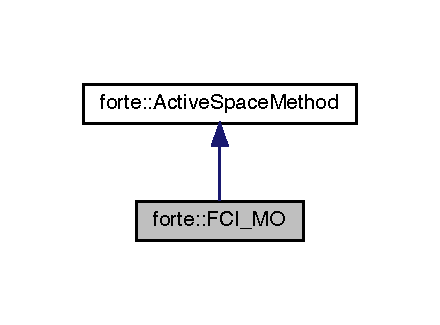
\includegraphics[width=211pt]{classforte_1_1_f_c_i___m_o__inherit__graph}
\end{center}
\end{figure}


Collaboration diagram for forte\+:\+:F\+C\+I\+\_\+\+MO\+:
\nopagebreak
\begin{figure}[H]
\begin{center}
\leavevmode
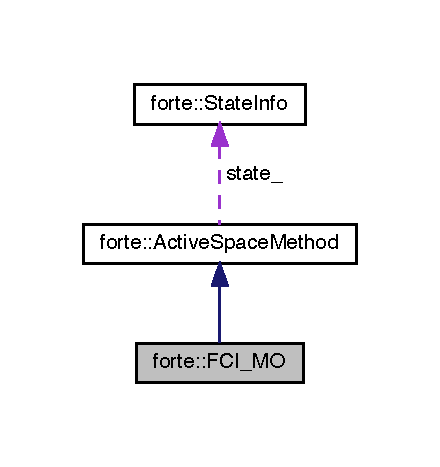
\includegraphics[width=211pt]{classforte_1_1_f_c_i___m_o__coll__graph}
\end{center}
\end{figure}
\subsection*{Public Member Functions}
\begin{DoxyCompactItemize}
\item 
\mbox{\hyperlink{classforte_1_1_f_c_i___m_o_a1fbb0791ddff25cee6d794ed2c0a2717}{F\+C\+I\+\_\+\+MO}} (\mbox{\hyperlink{classforte_1_1_state_info}{State\+Info}} \mbox{\hyperlink{classforte_1_1_active_space_method_a609f005cc7d3a1bc03ae517002eb19dc}{state}}, size\+\_\+t \mbox{\hyperlink{classforte_1_1_active_space_method_aa2bafc732bd7023fd32fbd263ef2e903}{nroot}}, std\+::shared\+\_\+ptr$<$ \mbox{\hyperlink{classforte_1_1_s_c_f_info}{S\+C\+F\+Info}} $>$ scf\+\_\+info, std\+::shared\+\_\+ptr$<$ \mbox{\hyperlink{classforte_1_1_forte_options}{Forte\+Options}} $>$ options, std\+::shared\+\_\+ptr$<$ \mbox{\hyperlink{classforte_1_1_m_o_space_info}{M\+O\+Space\+Info}} $>$ mo\+\_\+space\+\_\+info, std\+::shared\+\_\+ptr$<$ \mbox{\hyperlink{classforte_1_1_active_space_integrals}{Active\+Space\+Integrals}} $>$ as\+\_\+ints)
\begin{DoxyCompactList}\small\item\em \mbox{\hyperlink{classforte_1_1_f_c_i___m_o}{F\+C\+I\+\_\+\+MO}} Constructor. \end{DoxyCompactList}\item 
\mbox{\hyperlink{classforte_1_1_f_c_i___m_o_aa7ee376debece8ddddf96269de04a223}{F\+C\+I\+\_\+\+MO}} (std\+::shared\+\_\+ptr$<$ \mbox{\hyperlink{classforte_1_1_s_c_f_info}{S\+C\+F\+Info}} $>$ scf\+\_\+info, std\+::shared\+\_\+ptr$<$ \mbox{\hyperlink{classforte_1_1_forte_options}{Forte\+Options}} $>$ options, std\+::shared\+\_\+ptr$<$ \mbox{\hyperlink{classforte_1_1_forte_integrals}{Forte\+Integrals}} $>$ ints, std\+::shared\+\_\+ptr$<$ \mbox{\hyperlink{classforte_1_1_m_o_space_info}{M\+O\+Space\+Info}} $>$ mo\+\_\+space\+\_\+info)
\begin{DoxyCompactList}\small\item\em \mbox{\hyperlink{classforte_1_1_f_c_i___m_o}{F\+C\+I\+\_\+\+MO}} Constructor. \end{DoxyCompactList}\item 
\mbox{\hyperlink{classforte_1_1_f_c_i___m_o_a7ccdf79add717a606e97cb0e81f9e1b7}{F\+C\+I\+\_\+\+MO}} (std\+::shared\+\_\+ptr$<$ \mbox{\hyperlink{classforte_1_1_s_c_f_info}{S\+C\+F\+Info}} $>$ scf\+\_\+info, std\+::shared\+\_\+ptr$<$ \mbox{\hyperlink{classforte_1_1_forte_options}{Forte\+Options}} $>$ options, std\+::shared\+\_\+ptr$<$ \mbox{\hyperlink{classforte_1_1_forte_integrals}{Forte\+Integrals}} $>$ ints, std\+::shared\+\_\+ptr$<$ \mbox{\hyperlink{classforte_1_1_m_o_space_info}{M\+O\+Space\+Info}} $>$ mo\+\_\+space\+\_\+info, std\+::shared\+\_\+ptr$<$ \mbox{\hyperlink{classforte_1_1_active_space_integrals}{Active\+Space\+Integrals}} $>$ \mbox{\hyperlink{classforte_1_1_f_c_i___m_o_a69b7bc9ea9616ec11777678f663d6f40}{fci\+\_\+ints}})
\begin{DoxyCompactList}\small\item\em \mbox{\hyperlink{classforte_1_1_f_c_i___m_o}{F\+C\+I\+\_\+\+MO}} Constructor. \end{DoxyCompactList}\item 
\mbox{\hyperlink{classforte_1_1_f_c_i___m_o_ac20d48984c92df007b75971a51aa1990}{$\sim$\+F\+C\+I\+\_\+\+MO}} ()
\begin{DoxyCompactList}\small\item\em Destructor. \end{DoxyCompactList}\item 
double \mbox{\hyperlink{classforte_1_1_f_c_i___m_o_a98d9b947e1cf345c82d513a54ca51ddd}{compute\+\_\+energy}} () override
\begin{DoxyCompactList}\small\item\em Compute state-\/specific or state-\/averaged energy. \end{DoxyCompactList}\item 
std\+::vector$<$ double $>$ \mbox{\hyperlink{classforte_1_1_f_c_i___m_o_adaced1e93bf721e57e828eb612bfdb29}{compute\+\_\+ss\+\_\+energies}} ()
\begin{DoxyCompactList}\small\item\em Compute state-\/specific C\+A\+S\+CI energy. \end{DoxyCompactList}\item 
std\+::vector$<$ \mbox{\hyperlink{classforte_1_1_r_d_ms}{R\+D\+Ms}} $>$ \mbox{\hyperlink{classforte_1_1_f_c_i___m_o_afe4bb6cb53fbf4190c020ee3fa794237}{rdms}} (const std\+::vector$<$ std\+::pair$<$ size\+\_\+t, size\+\_\+t $>$$>$ \&root\+\_\+list, int max\+\_\+rdm\+\_\+level) override
\begin{DoxyCompactList}\small\item\em Compute the reduced density matrices up to a given particle rank (max\+\_\+rdm\+\_\+level) \end{DoxyCompactList}\item 
std\+::vector$<$ \mbox{\hyperlink{classforte_1_1_r_d_ms}{R\+D\+Ms}} $>$ \mbox{\hyperlink{classforte_1_1_f_c_i___m_o_a62d0c9bbee3dc8942ab109354074ad87}{transition\+\_\+rdms}} (const std\+::vector$<$ std\+::pair$<$ size\+\_\+t, size\+\_\+t $>$$>$ \&root\+\_\+list, std\+::shared\+\_\+ptr$<$ \mbox{\hyperlink{classforte_1_1_active_space_method}{Active\+Space\+Method}} $>$ method2, int max\+\_\+rdm\+\_\+level) override
\item 
std\+::vector$<$ \mbox{\hyperlink{classforte_1_1_r_d_ms}{R\+D\+Ms}} $>$ \mbox{\hyperlink{classforte_1_1_f_c_i___m_o_ad4629fe1009af590091c55aecf125314}{reference}} (const std\+::vector$<$ std\+::pair$<$ size\+\_\+t, size\+\_\+t $>$$>$ \&root\+\_\+list, int max\+\_\+rdm\+\_\+level)
\item 
\mbox{\hyperlink{classforte_1_1_r_d_ms}{R\+D\+Ms}} \mbox{\hyperlink{classforte_1_1_f_c_i___m_o_ad810e87d3dc0edbeb25843c8d575280c}{reference}} (int max\+\_\+rdm\+\_\+level)
\item 
void \mbox{\hyperlink{classforte_1_1_f_c_i___m_o_ad03e24facf8d8b4ba766ce7a0e5725e6}{set\+\_\+options}} (std\+::shared\+\_\+ptr$<$ \mbox{\hyperlink{classforte_1_1_forte_options}{Forte\+Options}} $>$) override
\item 
\mbox{\hyperlink{classforte_1_1_r_d_ms}{R\+D\+Ms}} \mbox{\hyperlink{classforte_1_1_f_c_i___m_o_a125253e41b65e862b172de71eb3c42b6}{transition\+\_\+reference}} (int root1, int root2, bool multi\+\_\+state, int entry=0, int max\+\_\+level=3, bool do\+\_\+cumulant=false, bool disk=true)
\item 
std\+::vector$<$ std\+::string $>$ \mbox{\hyperlink{classforte_1_1_f_c_i___m_o_a7b41431a81c3d736da3c917c53d2665f}{density\+\_\+filenames\+\_\+generator}} (int rdm\+\_\+level, int irrep, int multi, int root1, int root2)
\begin{DoxyCompactList}\small\item\em Density files. \end{DoxyCompactList}\item 
bool \mbox{\hyperlink{classforte_1_1_f_c_i___m_o_aef29384b257aee771fd855e3be678216}{check\+\_\+density\+\_\+files\+\_\+fcimo}} (int rdm\+\_\+level, int irrep, int multi, int root1, int root2)
\item 
void \mbox{\hyperlink{classforte_1_1_f_c_i___m_o_a70dca7ba9d158baf66c26f830dcb91a6}{remove\+\_\+density\+\_\+files\+\_\+fcimo}} (int rdm\+\_\+level, int irrep, int multi, int root1, int root2)
\item 
std\+::vector$<$ std\+::string $>$ \mbox{\hyperlink{classforte_1_1_f_c_i___m_o_ad06f15485962a81fa6155e5175a5a186}{generate\+\_\+rdm\+\_\+file\+\_\+names}} (int rdm\+\_\+level, int root1, int root2, const \mbox{\hyperlink{classforte_1_1_state_info}{State\+Info}} \&state2)
\begin{DoxyCompactList}\small\item\em Generate density file names at a certain R\+DM level. \end{DoxyCompactList}\item 
bool \mbox{\hyperlink{classforte_1_1_f_c_i___m_o_a5cbd29e9e73a93b9cfd8271063dc8ce3}{check\+\_\+density\+\_\+files}} (int rdm\+\_\+level, int root1, int root2, const \mbox{\hyperlink{classforte_1_1_state_info}{State\+Info}} \&state2)
\begin{DoxyCompactList}\small\item\em Check if density files for a given R\+DM level already exist. \end{DoxyCompactList}\item 
void \mbox{\hyperlink{classforte_1_1_f_c_i___m_o_a0bcaf366d04e0a3a833d33d4a90f42ee}{remove\+\_\+density\+\_\+files}} (int rdm\+\_\+level, int root1, int root2, const \mbox{\hyperlink{classforte_1_1_state_info}{State\+Info}} \&state2)
\begin{DoxyCompactList}\small\item\em Remove density files for a given R\+DM level. \end{DoxyCompactList}\item 
std\+::map$<$ std\+::string, std\+::vector$<$ double $>$ $>$ \mbox{\hyperlink{classforte_1_1_f_c_i___m_o_a112b3f3dc49523b7685610bb276f5b5e}{compute\+\_\+ref\+\_\+relaxed\+\_\+dm}} (const std\+::vector$<$ double $>$ \&dm0, std\+::vector$<$ ambit\+::\+Blocked\+Tensor $>$ \&dm1, std\+::vector$<$ ambit\+::\+Blocked\+Tensor $>$ \&dm2)
\item 
std\+::map$<$ std\+::string, std\+::vector$<$ double $>$ $>$ \mbox{\hyperlink{classforte_1_1_f_c_i___m_o_afe228e464539487b4999390a0b14e42e}{compute\+\_\+ref\+\_\+relaxed\+\_\+dm}} (const std\+::vector$<$ double $>$ \&dm0, std\+::vector$<$ ambit\+::\+Blocked\+Tensor $>$ \&dm1, std\+::vector$<$ ambit\+::\+Blocked\+Tensor $>$ \&dm2, std\+::vector$<$ ambit\+::\+Blocked\+Tensor $>$ \&\mbox{\hyperlink{structforte_1_1dm3}{dm3}})
\item 
std\+::map$<$ std\+::string, std\+::vector$<$ double $>$ $>$ \mbox{\hyperlink{classforte_1_1_f_c_i___m_o_a0c1b789424ac9c0139758cc1d7de07c4}{compute\+\_\+ref\+\_\+relaxed\+\_\+osc}} (std\+::vector$<$ ambit\+::\+Blocked\+Tensor $>$ \&dm1, std\+::vector$<$ ambit\+::\+Blocked\+Tensor $>$ \&dm2)
\item 
std\+::map$<$ std\+::string, std\+::vector$<$ double $>$ $>$ \mbox{\hyperlink{classforte_1_1_f_c_i___m_o_ac474ed13c5324ddf29dc49422a0d321c}{compute\+\_\+ref\+\_\+relaxed\+\_\+osc}} (std\+::vector$<$ ambit\+::\+Blocked\+Tensor $>$ \&dm1, std\+::vector$<$ ambit\+::\+Blocked\+Tensor $>$ \&dm2, std\+::vector$<$ ambit\+::\+Blocked\+Tensor $>$ \&\mbox{\hyperlink{structforte_1_1dm3}{dm3}})
\item 
void \mbox{\hyperlink{classforte_1_1_f_c_i___m_o_abaf9144ef5b7fa0c98720820f89d7d78}{xms\+\_\+rotate\+\_\+civecs}} ()
\begin{DoxyCompactList}\small\item\em Rotate the SA references such that $<$M$\vert$\+F$\vert$N$>$ is diagonal. \end{DoxyCompactList}\item 
void \mbox{\hyperlink{classforte_1_1_f_c_i___m_o_a0adc6096ff0846938b3bd506589de8e9}{set\+\_\+safe\+\_\+to\+\_\+read\+\_\+density\+\_\+files}} (bool safe)
\begin{DoxyCompactList}\small\item\em Set if safe to read densities from files. \end{DoxyCompactList}\item 
void \mbox{\hyperlink{classforte_1_1_f_c_i___m_o_a2005b802582673e81dc86e9dd0d33039}{set\+\_\+fci\+\_\+int}} (std\+::shared\+\_\+ptr$<$ \mbox{\hyperlink{classforte_1_1_active_space_integrals}{Active\+Space\+Integrals}} $>$ \mbox{\hyperlink{classforte_1_1_f_c_i___m_o_a69b7bc9ea9616ec11777678f663d6f40}{fci\+\_\+ints}})
\begin{DoxyCompactList}\small\item\em Set fci\+\_\+int\+\_\+ pointer. \end{DoxyCompactList}\item 
void \mbox{\hyperlink{classforte_1_1_f_c_i___m_o_a3ce51fb206015fd364b88fd7d3915c88}{set\+\_\+multiplicity}} (int multiplicity)
\begin{DoxyCompactList}\small\item\em Set multiplicity. \end{DoxyCompactList}\item 
void \mbox{\hyperlink{classforte_1_1_f_c_i___m_o_a43c52bd5160618567f8985d6f4057aa9}{set\+\_\+root\+\_\+sym}} (int root\+\_\+sym)
\begin{DoxyCompactList}\small\item\em Set symmetry of the root. \end{DoxyCompactList}\item 
void \mbox{\hyperlink{classforte_1_1_f_c_i___m_o_a55d56c1d9ef438ff82a7b02dd5050bf1}{set\+\_\+nroots}} (int \mbox{\hyperlink{classforte_1_1_active_space_method_aa2bafc732bd7023fd32fbd263ef2e903}{nroot}})
\begin{DoxyCompactList}\small\item\em Set number of roots. \end{DoxyCompactList}\item 
void \mbox{\hyperlink{classforte_1_1_f_c_i___m_o_adaf4af25c6acef5545de125cbafaf7a8}{set\+\_\+quite\+\_\+mode}} (bool quiet)
\begin{DoxyCompactList}\small\item\em Quiet mode (no printing, for use with \mbox{\hyperlink{classforte_1_1_c_a_s_s_c_f}{C\+A\+S\+S\+CF}}) \end{DoxyCompactList}\item 
void \mbox{\hyperlink{classforte_1_1_f_c_i___m_o_a59b2b1c4b616a02c449a5c43354c0191}{set\+\_\+localize\+\_\+actv}} (bool localize)
\begin{DoxyCompactList}\small\item\em Set if localize orbitals. \end{DoxyCompactList}\item 
void \mbox{\hyperlink{classforte_1_1_f_c_i___m_o_acabb2c574095ac624b78acc826b6db1b}{project\+\_\+roots}} (std\+::vector$<$ std\+::vector$<$ std\+::pair$<$ size\+\_\+t, double $>$$>$$>$ \&projected)
\begin{DoxyCompactList}\small\item\em Set projected roots. \end{DoxyCompactList}\item 
void \mbox{\hyperlink{classforte_1_1_f_c_i___m_o_ab2c62160b8f3507e56f2e168a3c733b6}{set\+\_\+initial\+\_\+guess}} (std\+::vector$<$ std\+::pair$<$ size\+\_\+t, double $>$$>$ \&guess)
\begin{DoxyCompactList}\small\item\em Set initial guess. \end{DoxyCompactList}\item 
void \mbox{\hyperlink{classforte_1_1_f_c_i___m_o_aa0dde71294349359d5332a0d55173a7b}{set\+\_\+sa\+\_\+info}} (const std\+::vector$<$ std\+::tuple$<$ int, int, int, std\+::vector$<$ double $>$$>$$>$ \&info)
\begin{DoxyCompactList}\small\item\em Set SA infomation. \end{DoxyCompactList}\item 
void \mbox{\hyperlink{classforte_1_1_f_c_i___m_o_af339a885a59587db951603dcf93509f0}{set\+\_\+eigens}} (const std\+::vector$<$ std\+::vector$<$ std\+::pair$<$ psi\+::\+Shared\+Vector, double $>$$>$$>$ \&\mbox{\hyperlink{classforte_1_1_f_c_i___m_o_a604127ddded2873abc01f2a8e42e319a}{eigens}})
\begin{DoxyCompactList}\small\item\em Set state-\/averaged eigen values and vectors. \end{DoxyCompactList}\item 
std\+::shared\+\_\+ptr$<$ \mbox{\hyperlink{classforte_1_1_active_space_integrals}{Active\+Space\+Integrals}} $>$ \mbox{\hyperlink{classforte_1_1_f_c_i___m_o_a69b7bc9ea9616ec11777678f663d6f40}{fci\+\_\+ints}} ()
\begin{DoxyCompactList}\small\item\em Return fci\+\_\+int\+\_\+ pointer. \end{DoxyCompactList}\item 
const \mbox{\hyperlink{fci__mo_8h_a777ccac2de1a8940d2f654e59ff12f06}{vecdet}} \& \mbox{\hyperlink{classforte_1_1_f_c_i___m_o_a1c6e8fd8e4bcb8999665fa9ac17da1a0}{p\+\_\+space}} () const
\begin{DoxyCompactList}\small\item\em Return the vector of determinants. \end{DoxyCompactList}\item 
std\+::vector$<$ \mbox{\hyperlink{fci__mo_8h_a777ccac2de1a8940d2f654e59ff12f06}{vecdet}} $>$ \mbox{\hyperlink{classforte_1_1_f_c_i___m_o_a29679a2b8ea4938d3d84c2ea79e5c8d4}{p\+\_\+spaces}} ()
\begin{DoxyCompactList}\small\item\em Return P spaces for states with different symmetry. \end{DoxyCompactList}\item 
std\+::vector$<$ std\+::vector$<$ std\+::vector$<$ double $>$ $>$ $>$ \mbox{\hyperlink{classforte_1_1_f_c_i___m_o_a91129e602986de474006b82c0764df5b}{orb\+\_\+extents}} ()
\begin{DoxyCompactList}\small\item\em Return the orbital extents of the current state. \end{DoxyCompactList}\item 
std\+::vector$<$ std\+::pair$<$ psi\+::\+Shared\+Vector, double $>$ $>$ const \mbox{\hyperlink{classforte_1_1_f_c_i___m_o_a7c37f298fb6cbe8870b75d5fa3faa7c9}{eigen}} ()
\begin{DoxyCompactList}\small\item\em Return the vector of eigen vectors and eigen values. \end{DoxyCompactList}\item 
std\+::vector$<$ std\+::vector$<$ std\+::pair$<$ psi\+::\+Shared\+Vector, double $>$ $>$ $>$ const \mbox{\hyperlink{classforte_1_1_f_c_i___m_o_a604127ddded2873abc01f2a8e42e319a}{eigens}} ()
\begin{DoxyCompactList}\small\item\em Return the vector of eigen vectors and eigen values (used in state-\/average computation) \end{DoxyCompactList}\item 
std\+::vector$<$ \mbox{\hyperlink{namespaceforte_a2076c63fd7b8732004d9e1442ce527c1}{Determinant}} $>$ \mbox{\hyperlink{classforte_1_1_f_c_i___m_o_a997478ffd6afbf77f26b1a02679fb851}{dominant\+\_\+dets}} ()
\begin{DoxyCompactList}\small\item\em Return a vector of dominant determinant for each root. \end{DoxyCompactList}\item 
std\+::vector$<$ size\+\_\+t $>$ \mbox{\hyperlink{classforte_1_1_f_c_i___m_o_ab542e74bc4d3d53fe1cf1a6d25eb093b}{actv\+\_\+occ}} ()
\begin{DoxyCompactList}\small\item\em Return indices (relative to active, not absolute) of active occupied orbitals. \end{DoxyCompactList}\item 
std\+::vector$<$ size\+\_\+t $>$ \mbox{\hyperlink{classforte_1_1_f_c_i___m_o_a0e5d71c5e278b8e12c2d3b4ae24667df}{actv\+\_\+uocc}} ()
\begin{DoxyCompactList}\small\item\em Return indices (relative to active, not absolute) of active virtual orbitals. \end{DoxyCompactList}\item 
psi\+::\+Dimension \mbox{\hyperlink{classforte_1_1_f_c_i___m_o_acacb2d7ea908564e82fc04b7aa644196}{actv\+\_\+docc}} ()
\begin{DoxyCompactList}\small\item\em Return the psi\+::\+Dimension of active occupied orbitals. \end{DoxyCompactList}\item 
psi\+::\+Dimension \mbox{\hyperlink{classforte_1_1_f_c_i___m_o_ad99d13576ef1e965d1e3b6dd58109bba}{actv\+\_\+virt}} ()
\begin{DoxyCompactList}\small\item\em Return the psi\+::\+Dimension of active virtual orbitals. \end{DoxyCompactList}\item 
std\+::vector$<$ double $>$ \mbox{\hyperlink{classforte_1_1_f_c_i___m_o_a0e22a364c4ca1f758d01b63d545e34d4}{compute\+\_\+\+T1\+\_\+percentage}} ()
\begin{DoxyCompactList}\small\item\em Return the T1 percentage in C\+I\+SD computations. \end{DoxyCompactList}\item 
std\+::vector$<$ std\+::tuple$<$ int, int, int, std\+::vector$<$ double $>$ $>$ $>$ \mbox{\hyperlink{classforte_1_1_f_c_i___m_o_aa191172f2d1053787846c37905f884c0}{sa\+\_\+info}} ()
\begin{DoxyCompactList}\small\item\em Return the parsed state-\/averaged info. \end{DoxyCompactList}\end{DoxyCompactItemize}
\subsection*{Protected Member Functions}
\begin{DoxyCompactItemize}
\item 
void \mbox{\hyperlink{classforte_1_1_f_c_i___m_o_a644233b83d526776645fc8fec5164ff2}{startup}} ()
\begin{DoxyCompactList}\small\item\em Basic Preparation. \end{DoxyCompactList}\item 
void \mbox{\hyperlink{classforte_1_1_f_c_i___m_o_a9318660ce1439ebdbce55d7b0b97dd15}{read\+\_\+options}} ()
\item 
void \mbox{\hyperlink{classforte_1_1_f_c_i___m_o_a1f2bcf2ea19611c93bb6a99eeaab5e51}{print\+\_\+options}} ()
\item 
void \mbox{\hyperlink{classforte_1_1_f_c_i___m_o_a464c46abc824ba31a3a363305c97d8fa}{cleanup}} ()
\item 
void \mbox{\hyperlink{classforte_1_1_f_c_i___m_o_afdde49f9daf9fa1d21aacf03063b7a17}{form\+\_\+p\+\_\+space}} ()
\begin{DoxyCompactList}\small\item\em Form Determiants Space. \end{DoxyCompactList}\item 
void \mbox{\hyperlink{classforte_1_1_f_c_i___m_o_a1bb74685ed35eaba795ffdc1c5ab3762}{form\+\_\+det}} ()
\begin{DoxyCompactList}\small\item\em Determinants. \end{DoxyCompactList}\item 
void \mbox{\hyperlink{classforte_1_1_f_c_i___m_o_a16e85a3a17779937d63e39ebf186599a}{form\+\_\+det\+\_\+cis}} ()
\item 
void \mbox{\hyperlink{classforte_1_1_f_c_i___m_o_ab703a06fcd0bc51d2f9f3ef4488486dd}{form\+\_\+det\+\_\+cisd}} ()
\item 
std\+::vector$<$ std\+::vector$<$ std\+::vector$<$ bool $>$ $>$ $>$ \mbox{\hyperlink{classforte_1_1_f_c_i___m_o_a5197b52c135488f77b74ab9e656ff0f2}{Form\+\_\+\+String}} (const int \&active\+\_\+elec, const bool \&print=false)
\begin{DoxyCompactList}\small\item\em Orbital Strings. \end{DoxyCompactList}\item 
std\+::vector$<$ bool $>$ \mbox{\hyperlink{classforte_1_1_f_c_i___m_o_add69e1a28a6ed06b933980aa9e3e9c62}{Form\+\_\+\+String\+\_\+\+Ref}} (const bool \&print=false)
\item 
std\+::vector$<$ std\+::vector$<$ std\+::vector$<$ bool $>$ $>$ $>$ \mbox{\hyperlink{classforte_1_1_f_c_i___m_o_a06d2dc3001cfbbf2668bd698d28f5815}{Form\+\_\+\+String\+\_\+\+Singles}} (const std\+::vector$<$ bool $>$ \&ref\+\_\+string, const bool \&print=false)
\item 
std\+::vector$<$ std\+::vector$<$ std\+::vector$<$ bool $>$ $>$ $>$ \mbox{\hyperlink{classforte_1_1_f_c_i___m_o_aca9a55627ced6f14b3c2724baee28959}{Form\+\_\+\+String\+\_\+\+Doubles}} (const std\+::vector$<$ bool $>$ \&ref\+\_\+string, const bool \&print=false)
\item 
std\+::vector$<$ std\+::vector$<$ std\+::vector$<$ bool $>$ $>$ $>$ \mbox{\hyperlink{classforte_1_1_f_c_i___m_o_a477f4d38d6423f1ffa0672081d00e5b1}{Form\+\_\+\+String\+\_\+\+IP}} (const std\+::vector$<$ bool $>$ \&ref\+\_\+string, const bool \&print=false)
\item 
std\+::vector$<$ std\+::vector$<$ std\+::vector$<$ bool $>$ $>$ $>$ \mbox{\hyperlink{classforte_1_1_f_c_i___m_o_ac639d453e0bafafb6d2fa50e389f2e56}{Form\+\_\+\+String\+\_\+\+EA}} (const std\+::vector$<$ bool $>$ \&ref\+\_\+string, const bool \&print=false)
\item 
void \mbox{\hyperlink{classforte_1_1_f_c_i___m_o_a3028e42a3b4e87f299d73591b1b6454e}{Diagonalize\+\_\+H}} (const \mbox{\hyperlink{fci__mo_8h_a777ccac2de1a8940d2f654e59ff12f06}{vecdet}} \&P\+\_\+space, const int \&multi, const int \&\mbox{\hyperlink{classforte_1_1_active_space_method_aa2bafc732bd7023fd32fbd263ef2e903}{nroot}}, std\+::vector$<$ std\+::pair$<$ psi\+::\+Shared\+Vector, double $>$$>$ \&\mbox{\hyperlink{classforte_1_1_f_c_i___m_o_a7c37f298fb6cbe8870b75d5fa3faa7c9}{eigen}})
\begin{DoxyCompactList}\small\item\em Diagonalize the Hamiltonian. \end{DoxyCompactList}\item 
void \mbox{\hyperlink{classforte_1_1_f_c_i___m_o_a8eb4d64d6f937a4885499a4871fd066f}{Diagonalize\+\_\+\+H\+\_\+no\+HF}} (const \mbox{\hyperlink{fci__mo_8h_a777ccac2de1a8940d2f654e59ff12f06}{vecdet}} \&\mbox{\hyperlink{classforte_1_1_f_c_i___m_o_a1c6e8fd8e4bcb8999665fa9ac17da1a0}{p\+\_\+space}}, const int \&multi, const int \&\mbox{\hyperlink{classforte_1_1_active_space_method_aa2bafc732bd7023fd32fbd263ef2e903}{nroot}}, std\+::vector$<$ std\+::pair$<$ psi\+::\+Shared\+Vector, double $>$$>$ \&\mbox{\hyperlink{classforte_1_1_f_c_i___m_o_a7c37f298fb6cbe8870b75d5fa3faa7c9}{eigen}})
\begin{DoxyCompactList}\small\item\em Diagonalize the Hamiltonian without the HF determinant. \end{DoxyCompactList}\item 
void \mbox{\hyperlink{classforte_1_1_f_c_i___m_o_a5186601ac16988bc980539e43adae269}{print\+\_\+\+CI}} (const int \&\mbox{\hyperlink{classforte_1_1_active_space_method_aa2bafc732bd7023fd32fbd263ef2e903}{nroot}}, const double \&C\+I\+\_\+threshold, const std\+::vector$<$ std\+::pair$<$ psi\+::\+Shared\+Vector, double $>$$>$ \&\mbox{\hyperlink{classforte_1_1_f_c_i___m_o_a7c37f298fb6cbe8870b75d5fa3faa7c9}{eigen}}, const \mbox{\hyperlink{fci__mo_8h_a777ccac2de1a8940d2f654e59ff12f06}{vecdet}} \&det)
\begin{DoxyCompactList}\small\item\em Print the CI Vectors and Configurations (figure out the dominant determinants) \end{DoxyCompactList}\item 
void \mbox{\hyperlink{classforte_1_1_f_c_i___m_o_afe404dd25f8dc9c49146677987e13aa2}{clean\+\_\+all\+\_\+density\+\_\+files}} ()
\item 
psi\+::\+Shared\+Matrix \mbox{\hyperlink{classforte_1_1_f_c_i___m_o_ae7bd478d88aacdef929f4432f6663676}{prepare\+\_\+for\+\_\+rdm}} ()
\begin{DoxyCompactList}\small\item\em Prepare eigen vectors for R\+DM or T\+R\+DM (within current symmetry) computations. \end{DoxyCompactList}\item 
std\+::pair$<$ std\+::shared\+\_\+ptr$<$ \mbox{\hyperlink{fci__mo_8h_a777ccac2de1a8940d2f654e59ff12f06}{vecdet}} $>$, psi\+::\+Shared\+Matrix $>$ \mbox{\hyperlink{classforte_1_1_f_c_i___m_o_a3e22d1614fc9b81bbf2c5360e41e581a}{prepare\+\_\+for\+\_\+trans\+\_\+rdm}} (std\+::shared\+\_\+ptr$<$ \mbox{\hyperlink{classforte_1_1_f_c_i___m_o}{F\+C\+I\+\_\+\+MO}} $>$ method2)
\item 
std\+::vector$<$ ambit\+::\+Tensor $>$ \mbox{\hyperlink{classforte_1_1_f_c_i___m_o_aa386ce9ea4166adf02c9a5ae57f0e7a9}{compute\+\_\+n\+\_\+rdm}} (const \mbox{\hyperlink{fci__mo_8h_a777ccac2de1a8940d2f654e59ff12f06}{vecdet}} \&\mbox{\hyperlink{classforte_1_1_f_c_i___m_o_a1c6e8fd8e4bcb8999665fa9ac17da1a0}{p\+\_\+space}}, psi\+::\+Shared\+Matrix evecs, int rdm\+\_\+level, int root1, int root2, int irrep, int multi, bool disk)
\begin{DoxyCompactList}\small\item\em Compute reduced density matricies for given determinant space and eigen vectors. \end{DoxyCompactList}\item 
std\+::vector$<$ ambit\+::\+Tensor $>$ \mbox{\hyperlink{classforte_1_1_f_c_i___m_o_aff33713f495d3b4e2908e5b9bea78ec3}{compute\+\_\+n\+\_\+rdm}} (const \mbox{\hyperlink{fci__mo_8h_a777ccac2de1a8940d2f654e59ff12f06}{vecdet}} \&\mbox{\hyperlink{classforte_1_1_f_c_i___m_o_a1c6e8fd8e4bcb8999665fa9ac17da1a0}{p\+\_\+space}}, psi\+::\+Shared\+Matrix evecs, int rdm\+\_\+level, int root1, int root2, const \mbox{\hyperlink{classforte_1_1_state_info}{State\+Info}} \&state2, bool disk)
\item 
void \mbox{\hyperlink{classforte_1_1_f_c_i___m_o_a0463ce4f890b492a7363ce261766d00a}{add\+\_\+wedge\+\_\+cu2}} (const ambit\+::\+Tensor \&L1a, const ambit\+::\+Tensor \&L1b, ambit\+::\+Tensor \&L2aa, ambit\+::\+Tensor \&L2ab, ambit\+::\+Tensor \&L2bb)
\begin{DoxyCompactList}\small\item\em Add wedge product of L1 to L2. \end{DoxyCompactList}\item 
void \mbox{\hyperlink{classforte_1_1_f_c_i___m_o_a2066f908f542676a269de5b5daeb5bd2}{add\+\_\+wedge\+\_\+cu3}} (const ambit\+::\+Tensor \&L1a, const ambit\+::\+Tensor \&L1b, const ambit\+::\+Tensor \&L2aa, const ambit\+::\+Tensor \&L2ab, const ambit\+::\+Tensor \&L2bb, ambit\+::\+Tensor \&L3aaa, ambit\+::\+Tensor \&L3aab, ambit\+::\+Tensor \&L3abb, ambit\+::\+Tensor \&L3bbb)
\begin{DoxyCompactList}\small\item\em Add wedge product of L1 and L2 to L3. \end{DoxyCompactList}\item 
psi\+::\+Shared\+Matrix \mbox{\hyperlink{classforte_1_1_f_c_i___m_o_a4388651961800c7c43a102e97ef927f8}{xms\+\_\+rotate\+\_\+this\+\_\+civecs}} (const \mbox{\hyperlink{namespaceforte_a2957b68e47fded14fd14ef47796ed751}{det\+\_\+vec}} \&\mbox{\hyperlink{classforte_1_1_f_c_i___m_o_a1c6e8fd8e4bcb8999665fa9ac17da1a0}{p\+\_\+space}}, psi\+::\+Shared\+Matrix civecs, ambit\+::\+Tensor Fa, ambit\+::\+Tensor Fb)
\begin{DoxyCompactList}\small\item\em Rotate the given CI vectors by X\+MS. \end{DoxyCompactList}\item 
void \mbox{\hyperlink{classforte_1_1_f_c_i___m_o_a6d3a3e8ba42f7d13c101dc893b9967c0}{compute\+\_\+ref}} (const int \&level, size\+\_\+t root1, size\+\_\+t root2)
\begin{DoxyCompactList}\small\item\em Compute 2-\/ and 3-\/cumulants. \end{DoxyCompactList}\item 
\mbox{\hyperlink{mcsrgpt2__mo_8h_a65fba048f0e27ede3b33bc9bf8ea13b7}{d3}} \mbox{\hyperlink{classforte_1_1_f_c_i___m_o_a94db3e2500557dce36a2673bb10ad5f0}{compute\+\_\+orbital\+\_\+extents}} ()
\item 
void \mbox{\hyperlink{classforte_1_1_f_c_i___m_o_a0e279e21ec5dfc1e82799d2a8a9d00d1}{compute\+\_\+permanent\+\_\+dipole}} ()
\begin{DoxyCompactList}\small\item\em Compute permanent dipole moments. \end{DoxyCompactList}\item 
psi\+::\+Shared\+Matrix \mbox{\hyperlink{classforte_1_1_f_c_i___m_o_aeaa66812842f8c0fbb2848e9300fe014}{reformat\+\_\+1rdm}} (const std\+::string \&name, const std\+::vector$<$ double $>$ \&data, bool TrD)
\begin{DoxyCompactList}\small\item\em Reformat 1\+R\+DM from nactv x nactv vector to N x N psi\+::\+Shared\+Matrix. \end{DoxyCompactList}\item 
void \mbox{\hyperlink{classforte_1_1_f_c_i___m_o_a97591540859a3a39bef6c8e39cb0a521}{compute\+\_\+transition\+\_\+dipole}} ()
\begin{DoxyCompactList}\small\item\em Compute transition dipole of same symmetry. \end{DoxyCompactList}\item 
void \mbox{\hyperlink{classforte_1_1_f_c_i___m_o_ab98ce7901255aa5545d4c537c1fbbd2f}{compute\+\_\+oscillator\+\_\+strength}} ()
\begin{DoxyCompactList}\small\item\em Compute oscillator strength of same symmetry. \end{DoxyCompactList}\item 
void \mbox{\hyperlink{classforte_1_1_f_c_i___m_o_a802c0acb9930ba78fe8df337d6d092f0}{compute\+\_\+transition\+\_\+dipole\+\_\+sa}} ()
\begin{DoxyCompactList}\small\item\em Compute transition dipole when doing state averaging. \end{DoxyCompactList}\item 
void \mbox{\hyperlink{classforte_1_1_f_c_i___m_o_ae0ee9bf49c50f51da8ceeb9c5ca91bbe}{compute\+\_\+oscillator\+\_\+strength\+\_\+sa}} ()
\begin{DoxyCompactList}\small\item\em Compute oscillator strength when doing state averaging. \end{DoxyCompactList}\item 
double \mbox{\hyperlink{classforte_1_1_f_c_i___m_o_ab7fb146f2fdf1b80b57629d9ac77dd04}{ref\+\_\+relaxed\+\_\+dm\+\_\+helper}} (const double \&dm0, ambit\+::\+Blocked\+Tensor \&dm1, ambit\+::\+Blocked\+Tensor \&dm2, ambit\+::\+Blocked\+Tensor \&D1, ambit\+::\+Blocked\+Tensor \&\mbox{\hyperlink{namespaceforte_abe00ec86d0015c0f2b6ac298c6e428e4ac4d62b6dcca08e5caf06c01889282859}{D2}})
\item 
double \mbox{\hyperlink{classforte_1_1_f_c_i___m_o_ada3c9f7a2dda90005a13b8b446eeb982}{ref\+\_\+relaxed\+\_\+dm\+\_\+helper}} (const double \&dm0, ambit\+::\+Blocked\+Tensor \&dm1, ambit\+::\+Blocked\+Tensor \&dm2, ambit\+::\+Blocked\+Tensor \&\mbox{\hyperlink{structforte_1_1dm3}{dm3}}, ambit\+::\+Blocked\+Tensor \&D1, ambit\+::\+Blocked\+Tensor \&\mbox{\hyperlink{namespaceforte_abe00ec86d0015c0f2b6ac298c6e428e4ac4d62b6dcca08e5caf06c01889282859}{D2}}, ambit\+::\+Blocked\+Tensor \&D3)
\item 
ambit\+::\+Blocked\+Tensor \mbox{\hyperlink{classforte_1_1_f_c_i___m_o_aebfee1c6dd754c44a1b20d3621803c8b}{compute\+\_\+n\+\_\+rdm}} (\mbox{\hyperlink{classforte_1_1_c_i___r_d_m_s}{C\+I\+\_\+\+R\+D\+MS}} \&cirdm, const int \&order)
\begin{DoxyCompactList}\small\item\em Compute \mbox{\hyperlink{classforte_1_1_r_d_ms}{R\+D\+Ms}} at given order and put into Blocked\+Tensor format. \end{DoxyCompactList}\item 
void \mbox{\hyperlink{classforte_1_1_f_c_i___m_o_aa2bba8595c80cd0f1af47bddd0b94088}{localize\+\_\+actv\+\_\+orbs}} ()
\item 
void \mbox{\hyperlink{classforte_1_1_f_c_i___m_o_a717f27492fa3693391a81850a0973c1c}{print\+\_\+det}} (const \mbox{\hyperlink{fci__mo_8h_a777ccac2de1a8940d2f654e59ff12f06}{vecdet}} \&dets)
\begin{DoxyCompactList}\small\item\em Print Determinants. \end{DoxyCompactList}\item 
void \mbox{\hyperlink{classforte_1_1_f_c_i___m_o_a6fc1a5cee8e71a31926e609488241221}{print\+\_\+occupation\+\_\+strings\+\_\+perirrep}} (std\+::string name, const std\+::vector$<$ std\+::vector$<$ std\+::vector$<$ bool $>$$>$$>$ \&string)
\begin{DoxyCompactList}\small\item\em Print occupations of strings. \end{DoxyCompactList}\end{DoxyCompactItemize}
\subsection*{Protected Attributes}
\begin{DoxyCompactItemize}
\item 
std\+::shared\+\_\+ptr$<$ \mbox{\hyperlink{classforte_1_1_forte_integrals}{Forte\+Integrals}} $>$ \mbox{\hyperlink{classforte_1_1_f_c_i___m_o_a3190b1591d4a53d3a5be57fb4896882f}{integral\+\_\+}}
\begin{DoxyCompactList}\small\item\em Integrals. \end{DoxyCompactList}\item 
std\+::string \mbox{\hyperlink{classforte_1_1_f_c_i___m_o_a594d30b16094805dce911fd098e9620e}{int\+\_\+type\+\_\+}}
\item 
std\+::shared\+\_\+ptr$<$ \mbox{\hyperlink{classforte_1_1_active_space_integrals}{Active\+Space\+Integrals}} $>$ \mbox{\hyperlink{classforte_1_1_f_c_i___m_o_a4a51472873a8d73585eff3d2dcc5b166}{fci\+\_\+ints\+\_\+}}
\item 
std\+::string \mbox{\hyperlink{classforte_1_1_f_c_i___m_o_a23572f3b5e1c9d3603d5107def1c8179}{ref\+\_\+type\+\_\+}}
\begin{DoxyCompactList}\small\item\em Reference Type. \end{DoxyCompactList}\item 
std\+::shared\+\_\+ptr$<$ \mbox{\hyperlink{classforte_1_1_m_o_space_info}{M\+O\+Space\+Info}} $>$ \mbox{\hyperlink{classforte_1_1_f_c_i___m_o_a9631a417ff0c09d0f3214604dce14acc}{mo\+\_\+space\+\_\+info\+\_\+}}
\begin{DoxyCompactList}\small\item\em MO space info. \end{DoxyCompactList}\item 
std\+::shared\+\_\+ptr$<$ \mbox{\hyperlink{classforte_1_1_s_c_f_info}{S\+C\+F\+Info}} $>$ \mbox{\hyperlink{classforte_1_1_f_c_i___m_o_ad66d4aaf42ded7bb18193e20b4edeaee}{scf\+\_\+info\+\_\+}}
\begin{DoxyCompactList}\small\item\em S\+CF info. \end{DoxyCompactList}\item 
std\+::shared\+\_\+ptr$<$ \mbox{\hyperlink{classforte_1_1_forte_options}{Forte\+Options}} $>$ \mbox{\hyperlink{classforte_1_1_f_c_i___m_o_a6d2e236a6c576183daa72f1ccbffaf41}{options\+\_\+}}
\begin{DoxyCompactList}\small\item\em \mbox{\hyperlink{classforte_1_1_forte_options}{Forte\+Options}}. \end{DoxyCompactList}\item 
int \mbox{\hyperlink{classforte_1_1_f_c_i___m_o_a0f0d63de851bcf9802ed3fb0bced1734}{print\+\_\+}}
\begin{DoxyCompactList}\small\item\em Print Levels. \end{DoxyCompactList}\item 
bool \mbox{\hyperlink{classforte_1_1_f_c_i___m_o_a4d0c5fb5d5d847024a7921ddc937cf2a}{quiet\+\_\+}} = false
\begin{DoxyCompactList}\small\item\em Quiet mode (Do not print anything in F\+CI) \end{DoxyCompactList}\item 
double \mbox{\hyperlink{classforte_1_1_f_c_i___m_o_ac62d801b09b6476c51aedb15ab4c3e9d}{e\+\_\+nuc\+\_\+}}
\begin{DoxyCompactList}\small\item\em Nucear Repulsion Energy. \end{DoxyCompactList}\item 
double \mbox{\hyperlink{classforte_1_1_f_c_i___m_o_abc0f5b82d716d99fa2b8c45fcba27d44}{econv\+\_\+}}
\begin{DoxyCompactList}\small\item\em Convergence. \end{DoxyCompactList}\item 
double \mbox{\hyperlink{classforte_1_1_f_c_i___m_o_adf70de3fc137b80aaffe1256b5562fad}{rconv\+\_\+}}
\begin{DoxyCompactList}\small\item\em Convergence. \end{DoxyCompactList}\item 
int \mbox{\hyperlink{classforte_1_1_f_c_i___m_o_a6e125ab9557be72444e3ca4ebf2c5939}{multi\+\_\+}}
\begin{DoxyCompactList}\small\item\em Multiplicity. \end{DoxyCompactList}\item 
int \mbox{\hyperlink{classforte_1_1_f_c_i___m_o_af00af228348648a018fb687ec1cb0acd}{twice\+\_\+ms\+\_\+}}
\item 
std\+::vector$<$ std\+::string $>$ \mbox{\hyperlink{classforte_1_1_f_c_i___m_o_aaa272f595b279c7c4371a7ec522f535b}{multi\+\_\+symbols\+\_\+}}
\item 
int \mbox{\hyperlink{classforte_1_1_f_c_i___m_o_ac81398df5e9a4db4f843087ff7acffd7}{nirrep\+\_\+}}
\begin{DoxyCompactList}\small\item\em \mbox{\hyperlink{classforte_1_1_symmetry}{Symmetry}}. \end{DoxyCompactList}\item 
int \mbox{\hyperlink{classforte_1_1_f_c_i___m_o_a2ef667274626e4ddc7db7e62fb9f74b6}{root\+\_\+sym\+\_\+}}
\item 
std\+::vector$<$ int $>$ \mbox{\hyperlink{classforte_1_1_f_c_i___m_o_a48b8dd2fbaefc3ade48e5297b890aae4}{sym\+\_\+actv\+\_\+}}
\item 
std\+::vector$<$ std\+::string $>$ \mbox{\hyperlink{classforte_1_1_f_c_i___m_o_afc7f1fba4636a17f30b222c14834659d}{irrep\+\_\+symbols\+\_\+}}
\item 
size\+\_\+t \mbox{\hyperlink{classforte_1_1_f_c_i___m_o_a542386abe3fadb34380653039d06ba95}{nmo\+\_\+}}
\begin{DoxyCompactList}\small\item\em Molecular Orbitals. \end{DoxyCompactList}\item 
psi\+::\+Dimension \mbox{\hyperlink{classforte_1_1_f_c_i___m_o_a63cf1a2e7440dd9c1b0dd079321e7c7c}{nmopi\+\_\+}}
\item 
size\+\_\+t \mbox{\hyperlink{classforte_1_1_f_c_i___m_o_a27574a3a4838deddc99cc33c6b5b3f16}{ncmo\+\_\+}}
\item 
psi\+::\+Dimension \mbox{\hyperlink{classforte_1_1_f_c_i___m_o_a420dd4857f5bb3cb68ed7bcdeb394887}{ncmopi\+\_\+}}
\item 
psi\+::\+Dimension \mbox{\hyperlink{classforte_1_1_f_c_i___m_o_a96515599234ec4dc5c333e7cccdaa1f3}{frzc\+\_\+dim\+\_\+}}
\item 
psi\+::\+Dimension \mbox{\hyperlink{classforte_1_1_f_c_i___m_o_a463f8607b3fb54f8c726b4e35b35c716}{frzv\+\_\+dim\+\_\+}}
\item 
size\+\_\+t \mbox{\hyperlink{classforte_1_1_f_c_i___m_o_ac34e46d3d74f7bb2264133a17c8fc0b3}{nfrzc\+\_\+}}
\item 
size\+\_\+t \mbox{\hyperlink{classforte_1_1_f_c_i___m_o_a9fbcc4393b5c2ae232281165f4d24903}{nfrzv\+\_\+}}
\item 
psi\+::\+Dimension \mbox{\hyperlink{classforte_1_1_f_c_i___m_o_a7f9b147b89d98766b8803ad8a0d6961f}{core\+\_\+dim\+\_\+}}
\item 
size\+\_\+t \mbox{\hyperlink{classforte_1_1_f_c_i___m_o_a6faa7e41178673c13e7253408376f0a5}{ncore\+\_\+}}
\item 
std\+::vector$<$ size\+\_\+t $>$ \mbox{\hyperlink{classforte_1_1_f_c_i___m_o_aff00e18684ee96e25bea6b34f3a9a61d}{core\+\_\+mos\+\_\+}}
\item 
psi\+::\+Dimension \mbox{\hyperlink{classforte_1_1_f_c_i___m_o_a197b0110e1dc2a6edb763a9167a5174b}{actv\+\_\+dim\+\_\+}}
\item 
size\+\_\+t \mbox{\hyperlink{classforte_1_1_f_c_i___m_o_a1ef99aae823efedc2308a6084e6ed99b}{nactv\+\_\+}}
\item 
std\+::vector$<$ size\+\_\+t $>$ \mbox{\hyperlink{classforte_1_1_f_c_i___m_o_a1e935d0e2587d7c81a276e1f0909ce97}{actv\+\_\+mos\+\_\+}}
\item 
size\+\_\+t \mbox{\hyperlink{classforte_1_1_f_c_i___m_o_a272668864820b7738f6fd0799e946b1c}{nvirt\+\_\+}}
\item 
psi\+::\+Dimension \mbox{\hyperlink{classforte_1_1_f_c_i___m_o_a5646158bc2f9c310885aa276dfdf3521}{virt\+\_\+dim\+\_\+}}
\item 
std\+::vector$<$ size\+\_\+t $>$ \mbox{\hyperlink{classforte_1_1_f_c_i___m_o_ad8cb54742519982bb0c828144d08c339}{virt\+\_\+mos\+\_\+}}
\item 
size\+\_\+t \mbox{\hyperlink{classforte_1_1_f_c_i___m_o_ad2c788d549209771259de8af9232936d}{nhole\+\_\+}}
\item 
std\+::vector$<$ size\+\_\+t $>$ \mbox{\hyperlink{classforte_1_1_f_c_i___m_o_a3ad72c929c5d5e87298cc78f04c7e3e4}{hole\+\_\+mos\+\_\+}}
\item 
size\+\_\+t \mbox{\hyperlink{classforte_1_1_f_c_i___m_o_a26e30238b6221986cd5fed921c7eab02}{npart\+\_\+}}
\item 
std\+::vector$<$ size\+\_\+t $>$ \mbox{\hyperlink{classforte_1_1_f_c_i___m_o_a440db119855a170bc078ef0f70649cd2}{part\+\_\+mos\+\_\+}}
\item 
psi\+::\+Dimension \mbox{\hyperlink{classforte_1_1_f_c_i___m_o_a043fb553093615233e8b69f8ec2c15b3}{actv\+\_\+hole\+\_\+dim\+\_\+}}
\item 
std\+::vector$<$ size\+\_\+t $>$ \mbox{\hyperlink{classforte_1_1_f_c_i___m_o_a663fc2003999a539942bd8f83e14b71a}{actv\+\_\+hole\+\_\+mos\+\_\+}}
\item 
psi\+::\+Dimension \mbox{\hyperlink{classforte_1_1_f_c_i___m_o_ae6b4a26b2ea77e909f5da24693e9f855}{actv\+\_\+part\+\_\+dim\+\_\+}}
\item 
std\+::vector$<$ size\+\_\+t $>$ \mbox{\hyperlink{classforte_1_1_f_c_i___m_o_aece1107076daa41e4ee80a314c21e5c3}{actv\+\_\+part\+\_\+mos\+\_\+}}
\item 
std\+::string \mbox{\hyperlink{classforte_1_1_f_c_i___m_o_aa3603c25cac5efeae601c5d6476cfbe6}{ipea\+\_\+}}
\begin{DoxyCompactList}\small\item\em Compute IP or EA. \end{DoxyCompactList}\item 
int \mbox{\hyperlink{classforte_1_1_f_c_i___m_o_abe453ff71db12bba46248f9882927078}{nalfa\+\_\+}}
\begin{DoxyCompactList}\small\item\em Number of Alpha and Beta Electrons. \end{DoxyCompactList}\item 
int \mbox{\hyperlink{classforte_1_1_f_c_i___m_o_af1b01bf057e3b11ba8ed47e3086d2fa3}{nbeta\+\_\+}}
\item 
std\+::string \mbox{\hyperlink{classforte_1_1_f_c_i___m_o_a6ad882499aa95d72078eb545e28bbd5e}{actv\+\_\+space\+\_\+type\+\_\+}}
\begin{DoxyCompactList}\small\item\em Active Space Type\+: C\+AS, C\+IS, C\+I\+SD. \end{DoxyCompactList}\item 
\mbox{\hyperlink{fci__mo_8h_a777ccac2de1a8940d2f654e59ff12f06}{vecdet}} \mbox{\hyperlink{classforte_1_1_f_c_i___m_o_ae099ef2f75de54f0a81f51388ad89eb2}{determinant\+\_\+}}
\item 
std\+::vector$<$ \mbox{\hyperlink{namespaceforte_a2076c63fd7b8732004d9e1442ce527c1}{Determinant}} $>$ \mbox{\hyperlink{classforte_1_1_f_c_i___m_o_afae4ffab47c3c0bc6ecce5e8d2f36bed}{dominant\+\_\+dets\+\_\+}}
\item 
std\+::vector$<$ \mbox{\hyperlink{fci__mo_8h_a777ccac2de1a8940d2f654e59ff12f06}{vecdet}} $>$ \mbox{\hyperlink{classforte_1_1_f_c_i___m_o_a638d3fde07aa7ac366e225a5d866434c}{p\+\_\+spaces\+\_\+}}
\item 
size\+\_\+t \mbox{\hyperlink{classforte_1_1_f_c_i___m_o_a9ea66938df7b15c6ef9396247c766f6f}{singles\+\_\+size\+\_\+}}
\begin{DoxyCompactList}\small\item\em Size of Singles Determinants. \end{DoxyCompactList}\item 
std\+::vector$<$ std\+::tuple$<$ int, int, int, std\+::vector$<$ double $>$ $>$ $>$ \mbox{\hyperlink{classforte_1_1_f_c_i___m_o_aa554753a1fe18ec6b1ad2d5b4cef784a}{sa\+\_\+info\+\_\+}}
\begin{DoxyCompactList}\small\item\em State Average Information (tuple of irrep, multi, nstates, weights) \end{DoxyCompactList}\item 
std\+::vector$<$ std\+::vector$<$ std\+::pair$<$ size\+\_\+t, double $>$ $>$ $>$ \mbox{\hyperlink{classforte_1_1_f_c_i___m_o_a28237d7d97cc318870efafa2b22e106f}{projected\+\_\+roots\+\_\+}}
\begin{DoxyCompactList}\small\item\em Roots to be projected out in the diagonalization. \end{DoxyCompactList}\item 
std\+::vector$<$ std\+::pair$<$ size\+\_\+t, double $>$ $>$ \mbox{\hyperlink{classforte_1_1_f_c_i___m_o_a0fcb8cf21db93e3cc83ebc9d5e771ff0}{initial\+\_\+guess\+\_\+}}
\begin{DoxyCompactList}\small\item\em Initial guess vector. \end{DoxyCompactList}\item 
std\+::vector$<$ std\+::pair$<$ psi\+::\+Shared\+Vector, double $>$ $>$ \mbox{\hyperlink{classforte_1_1_f_c_i___m_o_af9c2176a824d417e6720c7196900c0c2}{eigen\+\_\+}}
\begin{DoxyCompactList}\small\item\em Eigen Values and Eigen Vectors of Certain \mbox{\hyperlink{classforte_1_1_symmetry}{Symmetry}}. \end{DoxyCompactList}\item 
std\+::vector$<$ std\+::vector$<$ std\+::pair$<$ psi\+::\+Shared\+Vector, double $>$ $>$ $>$ \mbox{\hyperlink{classforte_1_1_f_c_i___m_o_afd2d5fb3aec0ac591b3b32c975703edb}{eigens\+\_\+}}
\begin{DoxyCompactList}\small\item\em A List of Eigen Values and Vectors for State Average. \end{DoxyCompactList}\item 
std\+::string \mbox{\hyperlink{classforte_1_1_f_c_i___m_o_a86350a9c8d2980df43a5f0aa093aaa7b}{diag\+\_\+algorithm\+\_\+}}
\begin{DoxyCompactList}\small\item\em The algorithm for diagonalization. \end{DoxyCompactList}\item 
ambit\+::\+Tensor \mbox{\hyperlink{classforte_1_1_f_c_i___m_o_a3ebb16c04591ae1445318809aa4e717c}{L1a\+\_\+}}
\begin{DoxyCompactList}\small\item\em Density Matrix. \end{DoxyCompactList}\item 
ambit\+::\+Tensor \mbox{\hyperlink{classforte_1_1_f_c_i___m_o_adca77fa1cf357c0fe43d009c69e9b28f}{L1b\+\_\+}}
\item 
ambit\+::\+Tensor \mbox{\hyperlink{classforte_1_1_f_c_i___m_o_a79450c3f2ab285c11108888886e9fcee}{L2aa\+\_\+}}
\begin{DoxyCompactList}\small\item\em 2-\/\+Body Density Cumulant \end{DoxyCompactList}\item 
ambit\+::\+Tensor \mbox{\hyperlink{classforte_1_1_f_c_i___m_o_a4e1f7bf22546733da012661e771b7980}{L2ab\+\_\+}}
\item 
ambit\+::\+Tensor \mbox{\hyperlink{classforte_1_1_f_c_i___m_o_a69431a24b140c370eeca7411f7c31db9}{L2bb\+\_\+}}
\item 
ambit\+::\+Tensor \mbox{\hyperlink{classforte_1_1_f_c_i___m_o_a62badb23a728871de07c2766206f9e02}{L3aaa\+\_\+}}
\begin{DoxyCompactList}\small\item\em 3-\/\+Body Density Cumulant \end{DoxyCompactList}\item 
ambit\+::\+Tensor \mbox{\hyperlink{classforte_1_1_f_c_i___m_o_a866dfda1b8df28bab34b98599a664e63}{L3aab\+\_\+}}
\item 
ambit\+::\+Tensor \mbox{\hyperlink{classforte_1_1_f_c_i___m_o_afb86c338b1ea0fe47f19a55ae4cb257c}{L3abb\+\_\+}}
\item 
ambit\+::\+Tensor \mbox{\hyperlink{classforte_1_1_f_c_i___m_o_a7886e7c6dce38ca1dcb109b4cd58e154}{L3bbb\+\_\+}}
\item 
std\+::unordered\+\_\+set$<$ std\+::string $>$ \mbox{\hyperlink{classforte_1_1_f_c_i___m_o_a63cbb38c3d84198962dbfa8be57287be}{density\+\_\+files\+\_\+}}
\begin{DoxyCompactList}\small\item\em File Names of Densities Stored on Disk. \end{DoxyCompactList}\item 
bool \mbox{\hyperlink{classforte_1_1_f_c_i___m_o_a583a12563a50064d5942e8ed68f48663}{safe\+\_\+to\+\_\+read\+\_\+density\+\_\+files\+\_\+}} = false
\item 
double \mbox{\hyperlink{classforte_1_1_f_c_i___m_o_aa9d28f4849e303edc518336727e51ff5}{Eref\+\_\+}}
\begin{DoxyCompactList}\small\item\em Reference Energy. \end{DoxyCompactList}\item 
size\+\_\+t \mbox{\hyperlink{classforte_1_1_f_c_i___m_o_a4bf28fb07e58c0ba35f42877258b20b9}{idx\+\_\+diffused\+\_\+}}
\item 
std\+::vector$<$ size\+\_\+t $>$ \mbox{\hyperlink{classforte_1_1_f_c_i___m_o_a0dfea7e88032d424c7431e3dd9194c71}{diffused\+\_\+orbs\+\_\+}}
\item 
std\+::map$<$ std\+::string, std\+::vector$<$ double $>$ $>$ \mbox{\hyperlink{classforte_1_1_f_c_i___m_o_a0d7fcb57822cb9a47e7816046c799084}{trans\+\_\+dipole\+\_\+}}
\begin{DoxyCompactList}\small\item\em Transition dipoles. \end{DoxyCompactList}\item 
bool \mbox{\hyperlink{classforte_1_1_f_c_i___m_o_a847460b619ff3256cb8d3419a044661c}{localize\+\_\+actv\+\_\+}}
\begin{DoxyCompactList}\small\item\em \mbox{\hyperlink{classforte_1_1_localize}{Localize}} active orbitals. \end{DoxyCompactList}\end{DoxyCompactItemize}


\subsection{Constructor \& Destructor Documentation}
\mbox{\Hypertarget{classforte_1_1_f_c_i___m_o_a1fbb0791ddff25cee6d794ed2c0a2717}\label{classforte_1_1_f_c_i___m_o_a1fbb0791ddff25cee6d794ed2c0a2717}} 
\index{forte\+::\+F\+C\+I\+\_\+\+MO@{forte\+::\+F\+C\+I\+\_\+\+MO}!F\+C\+I\+\_\+\+MO@{F\+C\+I\+\_\+\+MO}}
\index{F\+C\+I\+\_\+\+MO@{F\+C\+I\+\_\+\+MO}!forte\+::\+F\+C\+I\+\_\+\+MO@{forte\+::\+F\+C\+I\+\_\+\+MO}}
\subsubsection{\texorpdfstring{F\+C\+I\+\_\+\+M\+O()}{FCI\_MO()}\hspace{0.1cm}{\footnotesize\ttfamily [1/3]}}
{\footnotesize\ttfamily forte\+::\+F\+C\+I\+\_\+\+M\+O\+::\+F\+C\+I\+\_\+\+MO (\begin{DoxyParamCaption}\item[{\mbox{\hyperlink{classforte_1_1_state_info}{State\+Info}}}]{state,  }\item[{size\+\_\+t}]{nroot,  }\item[{std\+::shared\+\_\+ptr$<$ \mbox{\hyperlink{classforte_1_1_s_c_f_info}{S\+C\+F\+Info}} $>$}]{scf\+\_\+info,  }\item[{std\+::shared\+\_\+ptr$<$ \mbox{\hyperlink{classforte_1_1_forte_options}{Forte\+Options}} $>$}]{options,  }\item[{std\+::shared\+\_\+ptr$<$ \mbox{\hyperlink{classforte_1_1_m_o_space_info}{M\+O\+Space\+Info}} $>$}]{mo\+\_\+space\+\_\+info,  }\item[{std\+::shared\+\_\+ptr$<$ \mbox{\hyperlink{classforte_1_1_active_space_integrals}{Active\+Space\+Integrals}} $>$}]{as\+\_\+ints }\end{DoxyParamCaption})}



\mbox{\hyperlink{classforte_1_1_f_c_i___m_o}{F\+C\+I\+\_\+\+MO}} Constructor. 


\begin{DoxyParams}{Parameters}
{\em ref\+\_\+wfn} & The reference wavefunction object \\
\hline
{\em options} & P\+S\+I4 and F\+O\+R\+TE options \\
\hline
{\em ints} & Forte\+Inegrals \\
\hline
{\em mo\+\_\+space\+\_\+info} & \mbox{\hyperlink{classforte_1_1_m_o_space_info}{M\+O\+Space\+Info}} \\
\hline
{\em fci\+\_\+ints} & F\+C\+I\+Inegrals \\
\hline
\end{DoxyParams}
\mbox{\Hypertarget{classforte_1_1_f_c_i___m_o_aa7ee376debece8ddddf96269de04a223}\label{classforte_1_1_f_c_i___m_o_aa7ee376debece8ddddf96269de04a223}} 
\index{forte\+::\+F\+C\+I\+\_\+\+MO@{forte\+::\+F\+C\+I\+\_\+\+MO}!F\+C\+I\+\_\+\+MO@{F\+C\+I\+\_\+\+MO}}
\index{F\+C\+I\+\_\+\+MO@{F\+C\+I\+\_\+\+MO}!forte\+::\+F\+C\+I\+\_\+\+MO@{forte\+::\+F\+C\+I\+\_\+\+MO}}
\subsubsection{\texorpdfstring{F\+C\+I\+\_\+\+M\+O()}{FCI\_MO()}\hspace{0.1cm}{\footnotesize\ttfamily [2/3]}}
{\footnotesize\ttfamily forte\+::\+F\+C\+I\+\_\+\+M\+O\+::\+F\+C\+I\+\_\+\+MO (\begin{DoxyParamCaption}\item[{std\+::shared\+\_\+ptr$<$ \mbox{\hyperlink{classforte_1_1_s_c_f_info}{S\+C\+F\+Info}} $>$}]{scf\+\_\+info,  }\item[{std\+::shared\+\_\+ptr$<$ \mbox{\hyperlink{classforte_1_1_forte_options}{Forte\+Options}} $>$}]{options,  }\item[{std\+::shared\+\_\+ptr$<$ \mbox{\hyperlink{classforte_1_1_forte_integrals}{Forte\+Integrals}} $>$}]{ints,  }\item[{std\+::shared\+\_\+ptr$<$ \mbox{\hyperlink{classforte_1_1_m_o_space_info}{M\+O\+Space\+Info}} $>$}]{mo\+\_\+space\+\_\+info }\end{DoxyParamCaption})}



\mbox{\hyperlink{classforte_1_1_f_c_i___m_o}{F\+C\+I\+\_\+\+MO}} Constructor. 


\begin{DoxyParams}{Parameters}
{\em ref\+\_\+wfn} & The reference wavefunction object \\
\hline
{\em options} & P\+S\+I4 and F\+O\+R\+TE options \\
\hline
{\em ints} & Forte\+Inegrals \\
\hline
{\em mo\+\_\+space\+\_\+info} & \mbox{\hyperlink{classforte_1_1_m_o_space_info}{M\+O\+Space\+Info}} \\
\hline
\end{DoxyParams}
\mbox{\Hypertarget{classforte_1_1_f_c_i___m_o_a7ccdf79add717a606e97cb0e81f9e1b7}\label{classforte_1_1_f_c_i___m_o_a7ccdf79add717a606e97cb0e81f9e1b7}} 
\index{forte\+::\+F\+C\+I\+\_\+\+MO@{forte\+::\+F\+C\+I\+\_\+\+MO}!F\+C\+I\+\_\+\+MO@{F\+C\+I\+\_\+\+MO}}
\index{F\+C\+I\+\_\+\+MO@{F\+C\+I\+\_\+\+MO}!forte\+::\+F\+C\+I\+\_\+\+MO@{forte\+::\+F\+C\+I\+\_\+\+MO}}
\subsubsection{\texorpdfstring{F\+C\+I\+\_\+\+M\+O()}{FCI\_MO()}\hspace{0.1cm}{\footnotesize\ttfamily [3/3]}}
{\footnotesize\ttfamily forte\+::\+F\+C\+I\+\_\+\+M\+O\+::\+F\+C\+I\+\_\+\+MO (\begin{DoxyParamCaption}\item[{std\+::shared\+\_\+ptr$<$ \mbox{\hyperlink{classforte_1_1_s_c_f_info}{S\+C\+F\+Info}} $>$}]{scf\+\_\+info,  }\item[{std\+::shared\+\_\+ptr$<$ \mbox{\hyperlink{classforte_1_1_forte_options}{Forte\+Options}} $>$}]{options,  }\item[{std\+::shared\+\_\+ptr$<$ \mbox{\hyperlink{classforte_1_1_forte_integrals}{Forte\+Integrals}} $>$}]{ints,  }\item[{std\+::shared\+\_\+ptr$<$ \mbox{\hyperlink{classforte_1_1_m_o_space_info}{M\+O\+Space\+Info}} $>$}]{mo\+\_\+space\+\_\+info,  }\item[{std\+::shared\+\_\+ptr$<$ \mbox{\hyperlink{classforte_1_1_active_space_integrals}{Active\+Space\+Integrals}} $>$}]{fci\+\_\+ints }\end{DoxyParamCaption})}



\mbox{\hyperlink{classforte_1_1_f_c_i___m_o}{F\+C\+I\+\_\+\+MO}} Constructor. 


\begin{DoxyParams}{Parameters}
{\em ref\+\_\+wfn} & The reference wavefunction object \\
\hline
{\em options} & P\+S\+I4 and F\+O\+R\+TE options \\
\hline
{\em ints} & Forte\+Inegrals \\
\hline
{\em mo\+\_\+space\+\_\+info} & \mbox{\hyperlink{classforte_1_1_m_o_space_info}{M\+O\+Space\+Info}} \\
\hline
{\em fci\+\_\+ints} & F\+C\+I\+Inegrals \\
\hline
\end{DoxyParams}
\mbox{\Hypertarget{classforte_1_1_f_c_i___m_o_ac20d48984c92df007b75971a51aa1990}\label{classforte_1_1_f_c_i___m_o_ac20d48984c92df007b75971a51aa1990}} 
\index{forte\+::\+F\+C\+I\+\_\+\+MO@{forte\+::\+F\+C\+I\+\_\+\+MO}!````~F\+C\+I\+\_\+\+MO@{$\sim$\+F\+C\+I\+\_\+\+MO}}
\index{````~F\+C\+I\+\_\+\+MO@{$\sim$\+F\+C\+I\+\_\+\+MO}!forte\+::\+F\+C\+I\+\_\+\+MO@{forte\+::\+F\+C\+I\+\_\+\+MO}}
\subsubsection{\texorpdfstring{$\sim$\+F\+C\+I\+\_\+\+M\+O()}{~FCI\_MO()}}
{\footnotesize\ttfamily forte\+::\+F\+C\+I\+\_\+\+M\+O\+::$\sim$\+F\+C\+I\+\_\+\+MO (\begin{DoxyParamCaption}{ }\end{DoxyParamCaption})}



Destructor. 



\subsection{Member Function Documentation}
\mbox{\Hypertarget{classforte_1_1_f_c_i___m_o_acacb2d7ea908564e82fc04b7aa644196}\label{classforte_1_1_f_c_i___m_o_acacb2d7ea908564e82fc04b7aa644196}} 
\index{forte\+::\+F\+C\+I\+\_\+\+MO@{forte\+::\+F\+C\+I\+\_\+\+MO}!actv\+\_\+docc@{actv\+\_\+docc}}
\index{actv\+\_\+docc@{actv\+\_\+docc}!forte\+::\+F\+C\+I\+\_\+\+MO@{forte\+::\+F\+C\+I\+\_\+\+MO}}
\subsubsection{\texorpdfstring{actv\+\_\+docc()}{actv\_docc()}}
{\footnotesize\ttfamily psi\+::\+Dimension forte\+::\+F\+C\+I\+\_\+\+M\+O\+::actv\+\_\+docc (\begin{DoxyParamCaption}{ }\end{DoxyParamCaption})\hspace{0.3cm}{\ttfamily [inline]}}



Return the psi\+::\+Dimension of active occupied orbitals. 

\mbox{\Hypertarget{classforte_1_1_f_c_i___m_o_ab542e74bc4d3d53fe1cf1a6d25eb093b}\label{classforte_1_1_f_c_i___m_o_ab542e74bc4d3d53fe1cf1a6d25eb093b}} 
\index{forte\+::\+F\+C\+I\+\_\+\+MO@{forte\+::\+F\+C\+I\+\_\+\+MO}!actv\+\_\+occ@{actv\+\_\+occ}}
\index{actv\+\_\+occ@{actv\+\_\+occ}!forte\+::\+F\+C\+I\+\_\+\+MO@{forte\+::\+F\+C\+I\+\_\+\+MO}}
\subsubsection{\texorpdfstring{actv\+\_\+occ()}{actv\_occ()}}
{\footnotesize\ttfamily std\+::vector$<$size\+\_\+t$>$ forte\+::\+F\+C\+I\+\_\+\+M\+O\+::actv\+\_\+occ (\begin{DoxyParamCaption}{ }\end{DoxyParamCaption})\hspace{0.3cm}{\ttfamily [inline]}}



Return indices (relative to active, not absolute) of active occupied orbitals. 

\mbox{\Hypertarget{classforte_1_1_f_c_i___m_o_a0e5d71c5e278b8e12c2d3b4ae24667df}\label{classforte_1_1_f_c_i___m_o_a0e5d71c5e278b8e12c2d3b4ae24667df}} 
\index{forte\+::\+F\+C\+I\+\_\+\+MO@{forte\+::\+F\+C\+I\+\_\+\+MO}!actv\+\_\+uocc@{actv\+\_\+uocc}}
\index{actv\+\_\+uocc@{actv\+\_\+uocc}!forte\+::\+F\+C\+I\+\_\+\+MO@{forte\+::\+F\+C\+I\+\_\+\+MO}}
\subsubsection{\texorpdfstring{actv\+\_\+uocc()}{actv\_uocc()}}
{\footnotesize\ttfamily std\+::vector$<$size\+\_\+t$>$ forte\+::\+F\+C\+I\+\_\+\+M\+O\+::actv\+\_\+uocc (\begin{DoxyParamCaption}{ }\end{DoxyParamCaption})\hspace{0.3cm}{\ttfamily [inline]}}



Return indices (relative to active, not absolute) of active virtual orbitals. 

\mbox{\Hypertarget{classforte_1_1_f_c_i___m_o_ad99d13576ef1e965d1e3b6dd58109bba}\label{classforte_1_1_f_c_i___m_o_ad99d13576ef1e965d1e3b6dd58109bba}} 
\index{forte\+::\+F\+C\+I\+\_\+\+MO@{forte\+::\+F\+C\+I\+\_\+\+MO}!actv\+\_\+virt@{actv\+\_\+virt}}
\index{actv\+\_\+virt@{actv\+\_\+virt}!forte\+::\+F\+C\+I\+\_\+\+MO@{forte\+::\+F\+C\+I\+\_\+\+MO}}
\subsubsection{\texorpdfstring{actv\+\_\+virt()}{actv\_virt()}}
{\footnotesize\ttfamily psi\+::\+Dimension forte\+::\+F\+C\+I\+\_\+\+M\+O\+::actv\+\_\+virt (\begin{DoxyParamCaption}{ }\end{DoxyParamCaption})\hspace{0.3cm}{\ttfamily [inline]}}



Return the psi\+::\+Dimension of active virtual orbitals. 

\mbox{\Hypertarget{classforte_1_1_f_c_i___m_o_a0463ce4f890b492a7363ce261766d00a}\label{classforte_1_1_f_c_i___m_o_a0463ce4f890b492a7363ce261766d00a}} 
\index{forte\+::\+F\+C\+I\+\_\+\+MO@{forte\+::\+F\+C\+I\+\_\+\+MO}!add\+\_\+wedge\+\_\+cu2@{add\+\_\+wedge\+\_\+cu2}}
\index{add\+\_\+wedge\+\_\+cu2@{add\+\_\+wedge\+\_\+cu2}!forte\+::\+F\+C\+I\+\_\+\+MO@{forte\+::\+F\+C\+I\+\_\+\+MO}}
\subsubsection{\texorpdfstring{add\+\_\+wedge\+\_\+cu2()}{add\_wedge\_cu2()}}
{\footnotesize\ttfamily void forte\+::\+F\+C\+I\+\_\+\+M\+O\+::add\+\_\+wedge\+\_\+cu2 (\begin{DoxyParamCaption}\item[{const ambit\+::\+Tensor \&}]{L1a,  }\item[{const ambit\+::\+Tensor \&}]{L1b,  }\item[{ambit\+::\+Tensor \&}]{L2aa,  }\item[{ambit\+::\+Tensor \&}]{L2ab,  }\item[{ambit\+::\+Tensor \&}]{L2bb }\end{DoxyParamCaption})\hspace{0.3cm}{\ttfamily [protected]}}



Add wedge product of L1 to L2. 

\mbox{\Hypertarget{classforte_1_1_f_c_i___m_o_a2066f908f542676a269de5b5daeb5bd2}\label{classforte_1_1_f_c_i___m_o_a2066f908f542676a269de5b5daeb5bd2}} 
\index{forte\+::\+F\+C\+I\+\_\+\+MO@{forte\+::\+F\+C\+I\+\_\+\+MO}!add\+\_\+wedge\+\_\+cu3@{add\+\_\+wedge\+\_\+cu3}}
\index{add\+\_\+wedge\+\_\+cu3@{add\+\_\+wedge\+\_\+cu3}!forte\+::\+F\+C\+I\+\_\+\+MO@{forte\+::\+F\+C\+I\+\_\+\+MO}}
\subsubsection{\texorpdfstring{add\+\_\+wedge\+\_\+cu3()}{add\_wedge\_cu3()}}
{\footnotesize\ttfamily void forte\+::\+F\+C\+I\+\_\+\+M\+O\+::add\+\_\+wedge\+\_\+cu3 (\begin{DoxyParamCaption}\item[{const ambit\+::\+Tensor \&}]{L1a,  }\item[{const ambit\+::\+Tensor \&}]{L1b,  }\item[{const ambit\+::\+Tensor \&}]{L2aa,  }\item[{const ambit\+::\+Tensor \&}]{L2ab,  }\item[{const ambit\+::\+Tensor \&}]{L2bb,  }\item[{ambit\+::\+Tensor \&}]{L3aaa,  }\item[{ambit\+::\+Tensor \&}]{L3aab,  }\item[{ambit\+::\+Tensor \&}]{L3abb,  }\item[{ambit\+::\+Tensor \&}]{L3bbb }\end{DoxyParamCaption})\hspace{0.3cm}{\ttfamily [protected]}}



Add wedge product of L1 and L2 to L3. 

\mbox{\Hypertarget{classforte_1_1_f_c_i___m_o_a5cbd29e9e73a93b9cfd8271063dc8ce3}\label{classforte_1_1_f_c_i___m_o_a5cbd29e9e73a93b9cfd8271063dc8ce3}} 
\index{forte\+::\+F\+C\+I\+\_\+\+MO@{forte\+::\+F\+C\+I\+\_\+\+MO}!check\+\_\+density\+\_\+files@{check\+\_\+density\+\_\+files}}
\index{check\+\_\+density\+\_\+files@{check\+\_\+density\+\_\+files}!forte\+::\+F\+C\+I\+\_\+\+MO@{forte\+::\+F\+C\+I\+\_\+\+MO}}
\subsubsection{\texorpdfstring{check\+\_\+density\+\_\+files()}{check\_density\_files()}}
{\footnotesize\ttfamily bool forte\+::\+F\+C\+I\+\_\+\+M\+O\+::check\+\_\+density\+\_\+files (\begin{DoxyParamCaption}\item[{int}]{rdm\+\_\+level,  }\item[{int}]{root1,  }\item[{int}]{root2,  }\item[{const \mbox{\hyperlink{classforte_1_1_state_info}{State\+Info}} \&}]{state2 }\end{DoxyParamCaption})}



Check if density files for a given R\+DM level already exist. 

\mbox{\Hypertarget{classforte_1_1_f_c_i___m_o_aef29384b257aee771fd855e3be678216}\label{classforte_1_1_f_c_i___m_o_aef29384b257aee771fd855e3be678216}} 
\index{forte\+::\+F\+C\+I\+\_\+\+MO@{forte\+::\+F\+C\+I\+\_\+\+MO}!check\+\_\+density\+\_\+files\+\_\+fcimo@{check\+\_\+density\+\_\+files\+\_\+fcimo}}
\index{check\+\_\+density\+\_\+files\+\_\+fcimo@{check\+\_\+density\+\_\+files\+\_\+fcimo}!forte\+::\+F\+C\+I\+\_\+\+MO@{forte\+::\+F\+C\+I\+\_\+\+MO}}
\subsubsection{\texorpdfstring{check\+\_\+density\+\_\+files\+\_\+fcimo()}{check\_density\_files\_fcimo()}}
{\footnotesize\ttfamily bool forte\+::\+F\+C\+I\+\_\+\+M\+O\+::check\+\_\+density\+\_\+files\+\_\+fcimo (\begin{DoxyParamCaption}\item[{int}]{rdm\+\_\+level,  }\item[{int}]{irrep,  }\item[{int}]{multi,  }\item[{int}]{root1,  }\item[{int}]{root2 }\end{DoxyParamCaption})}

\mbox{\Hypertarget{classforte_1_1_f_c_i___m_o_afe404dd25f8dc9c49146677987e13aa2}\label{classforte_1_1_f_c_i___m_o_afe404dd25f8dc9c49146677987e13aa2}} 
\index{forte\+::\+F\+C\+I\+\_\+\+MO@{forte\+::\+F\+C\+I\+\_\+\+MO}!clean\+\_\+all\+\_\+density\+\_\+files@{clean\+\_\+all\+\_\+density\+\_\+files}}
\index{clean\+\_\+all\+\_\+density\+\_\+files@{clean\+\_\+all\+\_\+density\+\_\+files}!forte\+::\+F\+C\+I\+\_\+\+MO@{forte\+::\+F\+C\+I\+\_\+\+MO}}
\subsubsection{\texorpdfstring{clean\+\_\+all\+\_\+density\+\_\+files()}{clean\_all\_density\_files()}}
{\footnotesize\ttfamily void forte\+::\+F\+C\+I\+\_\+\+M\+O\+::clean\+\_\+all\+\_\+density\+\_\+files (\begin{DoxyParamCaption}{ }\end{DoxyParamCaption})\hspace{0.3cm}{\ttfamily [protected]}}

\mbox{\Hypertarget{classforte_1_1_f_c_i___m_o_a464c46abc824ba31a3a363305c97d8fa}\label{classforte_1_1_f_c_i___m_o_a464c46abc824ba31a3a363305c97d8fa}} 
\index{forte\+::\+F\+C\+I\+\_\+\+MO@{forte\+::\+F\+C\+I\+\_\+\+MO}!cleanup@{cleanup}}
\index{cleanup@{cleanup}!forte\+::\+F\+C\+I\+\_\+\+MO@{forte\+::\+F\+C\+I\+\_\+\+MO}}
\subsubsection{\texorpdfstring{cleanup()}{cleanup()}}
{\footnotesize\ttfamily void forte\+::\+F\+C\+I\+\_\+\+M\+O\+::cleanup (\begin{DoxyParamCaption}{ }\end{DoxyParamCaption})\hspace{0.3cm}{\ttfamily [protected]}}

\mbox{\Hypertarget{classforte_1_1_f_c_i___m_o_a98d9b947e1cf345c82d513a54ca51ddd}\label{classforte_1_1_f_c_i___m_o_a98d9b947e1cf345c82d513a54ca51ddd}} 
\index{forte\+::\+F\+C\+I\+\_\+\+MO@{forte\+::\+F\+C\+I\+\_\+\+MO}!compute\+\_\+energy@{compute\+\_\+energy}}
\index{compute\+\_\+energy@{compute\+\_\+energy}!forte\+::\+F\+C\+I\+\_\+\+MO@{forte\+::\+F\+C\+I\+\_\+\+MO}}
\subsubsection{\texorpdfstring{compute\+\_\+energy()}{compute\_energy()}}
{\footnotesize\ttfamily double forte\+::\+F\+C\+I\+\_\+\+M\+O\+::compute\+\_\+energy (\begin{DoxyParamCaption}{ }\end{DoxyParamCaption})\hspace{0.3cm}{\ttfamily [override]}, {\ttfamily [virtual]}}



Compute state-\/specific or state-\/averaged energy. 



Implements \mbox{\hyperlink{classforte_1_1_active_space_method_a99736e2b94405371b224b0750569b077}{forte\+::\+Active\+Space\+Method}}.

\mbox{\Hypertarget{classforte_1_1_f_c_i___m_o_aa386ce9ea4166adf02c9a5ae57f0e7a9}\label{classforte_1_1_f_c_i___m_o_aa386ce9ea4166adf02c9a5ae57f0e7a9}} 
\index{forte\+::\+F\+C\+I\+\_\+\+MO@{forte\+::\+F\+C\+I\+\_\+\+MO}!compute\+\_\+n\+\_\+rdm@{compute\+\_\+n\+\_\+rdm}}
\index{compute\+\_\+n\+\_\+rdm@{compute\+\_\+n\+\_\+rdm}!forte\+::\+F\+C\+I\+\_\+\+MO@{forte\+::\+F\+C\+I\+\_\+\+MO}}
\subsubsection{\texorpdfstring{compute\+\_\+n\+\_\+rdm()}{compute\_n\_rdm()}\hspace{0.1cm}{\footnotesize\ttfamily [1/3]}}
{\footnotesize\ttfamily std\+::vector$<$ ambit\+::\+Tensor $>$ forte\+::\+F\+C\+I\+\_\+\+M\+O\+::compute\+\_\+n\+\_\+rdm (\begin{DoxyParamCaption}\item[{const \mbox{\hyperlink{fci__mo_8h_a777ccac2de1a8940d2f654e59ff12f06}{vecdet}} \&}]{p\+\_\+space,  }\item[{psi\+::\+Shared\+Matrix}]{evecs,  }\item[{int}]{rdm\+\_\+level,  }\item[{int}]{root1,  }\item[{int}]{root2,  }\item[{int}]{irrep,  }\item[{int}]{multi,  }\item[{bool}]{disk }\end{DoxyParamCaption})\hspace{0.3cm}{\ttfamily [protected]}}



Compute reduced density matricies for given determinant space and eigen vectors. 

\mbox{\Hypertarget{classforte_1_1_f_c_i___m_o_aff33713f495d3b4e2908e5b9bea78ec3}\label{classforte_1_1_f_c_i___m_o_aff33713f495d3b4e2908e5b9bea78ec3}} 
\index{forte\+::\+F\+C\+I\+\_\+\+MO@{forte\+::\+F\+C\+I\+\_\+\+MO}!compute\+\_\+n\+\_\+rdm@{compute\+\_\+n\+\_\+rdm}}
\index{compute\+\_\+n\+\_\+rdm@{compute\+\_\+n\+\_\+rdm}!forte\+::\+F\+C\+I\+\_\+\+MO@{forte\+::\+F\+C\+I\+\_\+\+MO}}
\subsubsection{\texorpdfstring{compute\+\_\+n\+\_\+rdm()}{compute\_n\_rdm()}\hspace{0.1cm}{\footnotesize\ttfamily [2/3]}}
{\footnotesize\ttfamily std\+::vector$<$ ambit\+::\+Tensor $>$ forte\+::\+F\+C\+I\+\_\+\+M\+O\+::compute\+\_\+n\+\_\+rdm (\begin{DoxyParamCaption}\item[{const \mbox{\hyperlink{fci__mo_8h_a777ccac2de1a8940d2f654e59ff12f06}{vecdet}} \&}]{p\+\_\+space,  }\item[{psi\+::\+Shared\+Matrix}]{evecs,  }\item[{int}]{rdm\+\_\+level,  }\item[{int}]{root1,  }\item[{int}]{root2,  }\item[{const \mbox{\hyperlink{classforte_1_1_state_info}{State\+Info}} \&}]{state2,  }\item[{bool}]{disk }\end{DoxyParamCaption})\hspace{0.3cm}{\ttfamily [protected]}}

\mbox{\Hypertarget{classforte_1_1_f_c_i___m_o_aebfee1c6dd754c44a1b20d3621803c8b}\label{classforte_1_1_f_c_i___m_o_aebfee1c6dd754c44a1b20d3621803c8b}} 
\index{forte\+::\+F\+C\+I\+\_\+\+MO@{forte\+::\+F\+C\+I\+\_\+\+MO}!compute\+\_\+n\+\_\+rdm@{compute\+\_\+n\+\_\+rdm}}
\index{compute\+\_\+n\+\_\+rdm@{compute\+\_\+n\+\_\+rdm}!forte\+::\+F\+C\+I\+\_\+\+MO@{forte\+::\+F\+C\+I\+\_\+\+MO}}
\subsubsection{\texorpdfstring{compute\+\_\+n\+\_\+rdm()}{compute\_n\_rdm()}\hspace{0.1cm}{\footnotesize\ttfamily [3/3]}}
{\footnotesize\ttfamily ambit\+::\+Blocked\+Tensor forte\+::\+F\+C\+I\+\_\+\+M\+O\+::compute\+\_\+n\+\_\+rdm (\begin{DoxyParamCaption}\item[{\mbox{\hyperlink{classforte_1_1_c_i___r_d_m_s}{C\+I\+\_\+\+R\+D\+MS}} \&}]{cirdm,  }\item[{const int \&}]{order }\end{DoxyParamCaption})\hspace{0.3cm}{\ttfamily [protected]}}



Compute \mbox{\hyperlink{classforte_1_1_r_d_ms}{R\+D\+Ms}} at given order and put into Blocked\+Tensor format. 

\mbox{\Hypertarget{classforte_1_1_f_c_i___m_o_a94db3e2500557dce36a2673bb10ad5f0}\label{classforte_1_1_f_c_i___m_o_a94db3e2500557dce36a2673bb10ad5f0}} 
\index{forte\+::\+F\+C\+I\+\_\+\+MO@{forte\+::\+F\+C\+I\+\_\+\+MO}!compute\+\_\+orbital\+\_\+extents@{compute\+\_\+orbital\+\_\+extents}}
\index{compute\+\_\+orbital\+\_\+extents@{compute\+\_\+orbital\+\_\+extents}!forte\+::\+F\+C\+I\+\_\+\+MO@{forte\+::\+F\+C\+I\+\_\+\+MO}}
\subsubsection{\texorpdfstring{compute\+\_\+orbital\+\_\+extents()}{compute\_orbital\_extents()}}
{\footnotesize\ttfamily \mbox{\hyperlink{mcsrgpt2__mo_8h_a65fba048f0e27ede3b33bc9bf8ea13b7}{d3}} forte\+::\+F\+C\+I\+\_\+\+M\+O\+::compute\+\_\+orbital\+\_\+extents (\begin{DoxyParamCaption}{ }\end{DoxyParamCaption})\hspace{0.3cm}{\ttfamily [protected]}}

Orbital Extents returns a vector of irrep by \# active orbitals in current irrep by orbital extents \{xx, yy, zz\} \mbox{\Hypertarget{classforte_1_1_f_c_i___m_o_ab98ce7901255aa5545d4c537c1fbbd2f}\label{classforte_1_1_f_c_i___m_o_ab98ce7901255aa5545d4c537c1fbbd2f}} 
\index{forte\+::\+F\+C\+I\+\_\+\+MO@{forte\+::\+F\+C\+I\+\_\+\+MO}!compute\+\_\+oscillator\+\_\+strength@{compute\+\_\+oscillator\+\_\+strength}}
\index{compute\+\_\+oscillator\+\_\+strength@{compute\+\_\+oscillator\+\_\+strength}!forte\+::\+F\+C\+I\+\_\+\+MO@{forte\+::\+F\+C\+I\+\_\+\+MO}}
\subsubsection{\texorpdfstring{compute\+\_\+oscillator\+\_\+strength()}{compute\_oscillator\_strength()}}
{\footnotesize\ttfamily void forte\+::\+F\+C\+I\+\_\+\+M\+O\+::compute\+\_\+oscillator\+\_\+strength (\begin{DoxyParamCaption}{ }\end{DoxyParamCaption})\hspace{0.3cm}{\ttfamily [protected]}}



Compute oscillator strength of same symmetry. 

\mbox{\Hypertarget{classforte_1_1_f_c_i___m_o_ae0ee9bf49c50f51da8ceeb9c5ca91bbe}\label{classforte_1_1_f_c_i___m_o_ae0ee9bf49c50f51da8ceeb9c5ca91bbe}} 
\index{forte\+::\+F\+C\+I\+\_\+\+MO@{forte\+::\+F\+C\+I\+\_\+\+MO}!compute\+\_\+oscillator\+\_\+strength\+\_\+sa@{compute\+\_\+oscillator\+\_\+strength\+\_\+sa}}
\index{compute\+\_\+oscillator\+\_\+strength\+\_\+sa@{compute\+\_\+oscillator\+\_\+strength\+\_\+sa}!forte\+::\+F\+C\+I\+\_\+\+MO@{forte\+::\+F\+C\+I\+\_\+\+MO}}
\subsubsection{\texorpdfstring{compute\+\_\+oscillator\+\_\+strength\+\_\+sa()}{compute\_oscillator\_strength\_sa()}}
{\footnotesize\ttfamily void forte\+::\+F\+C\+I\+\_\+\+M\+O\+::compute\+\_\+oscillator\+\_\+strength\+\_\+sa (\begin{DoxyParamCaption}{ }\end{DoxyParamCaption})\hspace{0.3cm}{\ttfamily [protected]}}



Compute oscillator strength when doing state averaging. 

\mbox{\Hypertarget{classforte_1_1_f_c_i___m_o_a0e279e21ec5dfc1e82799d2a8a9d00d1}\label{classforte_1_1_f_c_i___m_o_a0e279e21ec5dfc1e82799d2a8a9d00d1}} 
\index{forte\+::\+F\+C\+I\+\_\+\+MO@{forte\+::\+F\+C\+I\+\_\+\+MO}!compute\+\_\+permanent\+\_\+dipole@{compute\+\_\+permanent\+\_\+dipole}}
\index{compute\+\_\+permanent\+\_\+dipole@{compute\+\_\+permanent\+\_\+dipole}!forte\+::\+F\+C\+I\+\_\+\+MO@{forte\+::\+F\+C\+I\+\_\+\+MO}}
\subsubsection{\texorpdfstring{compute\+\_\+permanent\+\_\+dipole()}{compute\_permanent\_dipole()}}
{\footnotesize\ttfamily void forte\+::\+F\+C\+I\+\_\+\+M\+O\+::compute\+\_\+permanent\+\_\+dipole (\begin{DoxyParamCaption}{ }\end{DoxyParamCaption})\hspace{0.3cm}{\ttfamily [protected]}}



Compute permanent dipole moments. 

\mbox{\Hypertarget{classforte_1_1_f_c_i___m_o_a6d3a3e8ba42f7d13c101dc893b9967c0}\label{classforte_1_1_f_c_i___m_o_a6d3a3e8ba42f7d13c101dc893b9967c0}} 
\index{forte\+::\+F\+C\+I\+\_\+\+MO@{forte\+::\+F\+C\+I\+\_\+\+MO}!compute\+\_\+ref@{compute\+\_\+ref}}
\index{compute\+\_\+ref@{compute\+\_\+ref}!forte\+::\+F\+C\+I\+\_\+\+MO@{forte\+::\+F\+C\+I\+\_\+\+MO}}
\subsubsection{\texorpdfstring{compute\+\_\+ref()}{compute\_ref()}}
{\footnotesize\ttfamily void forte\+::\+F\+C\+I\+\_\+\+M\+O\+::compute\+\_\+ref (\begin{DoxyParamCaption}\item[{const int \&}]{level,  }\item[{size\+\_\+t}]{root1,  }\item[{size\+\_\+t}]{root2 }\end{DoxyParamCaption})\hspace{0.3cm}{\ttfamily [protected]}}



Compute 2-\/ and 3-\/cumulants. 

\mbox{\Hypertarget{classforte_1_1_f_c_i___m_o_a112b3f3dc49523b7685610bb276f5b5e}\label{classforte_1_1_f_c_i___m_o_a112b3f3dc49523b7685610bb276f5b5e}} 
\index{forte\+::\+F\+C\+I\+\_\+\+MO@{forte\+::\+F\+C\+I\+\_\+\+MO}!compute\+\_\+ref\+\_\+relaxed\+\_\+dm@{compute\+\_\+ref\+\_\+relaxed\+\_\+dm}}
\index{compute\+\_\+ref\+\_\+relaxed\+\_\+dm@{compute\+\_\+ref\+\_\+relaxed\+\_\+dm}!forte\+::\+F\+C\+I\+\_\+\+MO@{forte\+::\+F\+C\+I\+\_\+\+MO}}
\subsubsection{\texorpdfstring{compute\+\_\+ref\+\_\+relaxed\+\_\+dm()}{compute\_ref\_relaxed\_dm()}\hspace{0.1cm}{\footnotesize\ttfamily [1/2]}}
{\footnotesize\ttfamily std\+::map$<$std\+::string, std\+::vector$<$double$>$ $>$ forte\+::\+F\+C\+I\+\_\+\+M\+O\+::compute\+\_\+ref\+\_\+relaxed\+\_\+dm (\begin{DoxyParamCaption}\item[{const std\+::vector$<$ double $>$ \&}]{dm0,  }\item[{std\+::vector$<$ ambit\+::\+Blocked\+Tensor $>$ \&}]{dm1,  }\item[{std\+::vector$<$ ambit\+::\+Blocked\+Tensor $>$ \&}]{dm2 }\end{DoxyParamCaption})}

Compute dipole moments with D\+S\+RG transformed MO dipole integrals This function is used for reference relaxation and S\+A-\/\+M\+R\+D\+S\+RG This function should be in R\+U\+N\+\_\+\+D\+S\+RG \mbox{\Hypertarget{classforte_1_1_f_c_i___m_o_afe228e464539487b4999390a0b14e42e}\label{classforte_1_1_f_c_i___m_o_afe228e464539487b4999390a0b14e42e}} 
\index{forte\+::\+F\+C\+I\+\_\+\+MO@{forte\+::\+F\+C\+I\+\_\+\+MO}!compute\+\_\+ref\+\_\+relaxed\+\_\+dm@{compute\+\_\+ref\+\_\+relaxed\+\_\+dm}}
\index{compute\+\_\+ref\+\_\+relaxed\+\_\+dm@{compute\+\_\+ref\+\_\+relaxed\+\_\+dm}!forte\+::\+F\+C\+I\+\_\+\+MO@{forte\+::\+F\+C\+I\+\_\+\+MO}}
\subsubsection{\texorpdfstring{compute\+\_\+ref\+\_\+relaxed\+\_\+dm()}{compute\_ref\_relaxed\_dm()}\hspace{0.1cm}{\footnotesize\ttfamily [2/2]}}
{\footnotesize\ttfamily std\+::map$<$std\+::string, std\+::vector$<$double$>$ $>$ forte\+::\+F\+C\+I\+\_\+\+M\+O\+::compute\+\_\+ref\+\_\+relaxed\+\_\+dm (\begin{DoxyParamCaption}\item[{const std\+::vector$<$ double $>$ \&}]{dm0,  }\item[{std\+::vector$<$ ambit\+::\+Blocked\+Tensor $>$ \&}]{dm1,  }\item[{std\+::vector$<$ ambit\+::\+Blocked\+Tensor $>$ \&}]{dm2,  }\item[{std\+::vector$<$ ambit\+::\+Blocked\+Tensor $>$ \&}]{dm3 }\end{DoxyParamCaption})}

\mbox{\Hypertarget{classforte_1_1_f_c_i___m_o_a0c1b789424ac9c0139758cc1d7de07c4}\label{classforte_1_1_f_c_i___m_o_a0c1b789424ac9c0139758cc1d7de07c4}} 
\index{forte\+::\+F\+C\+I\+\_\+\+MO@{forte\+::\+F\+C\+I\+\_\+\+MO}!compute\+\_\+ref\+\_\+relaxed\+\_\+osc@{compute\+\_\+ref\+\_\+relaxed\+\_\+osc}}
\index{compute\+\_\+ref\+\_\+relaxed\+\_\+osc@{compute\+\_\+ref\+\_\+relaxed\+\_\+osc}!forte\+::\+F\+C\+I\+\_\+\+MO@{forte\+::\+F\+C\+I\+\_\+\+MO}}
\subsubsection{\texorpdfstring{compute\+\_\+ref\+\_\+relaxed\+\_\+osc()}{compute\_ref\_relaxed\_osc()}\hspace{0.1cm}{\footnotesize\ttfamily [1/2]}}
{\footnotesize\ttfamily std\+::map$<$std\+::string, std\+::vector$<$double$>$ $>$ forte\+::\+F\+C\+I\+\_\+\+M\+O\+::compute\+\_\+ref\+\_\+relaxed\+\_\+osc (\begin{DoxyParamCaption}\item[{std\+::vector$<$ ambit\+::\+Blocked\+Tensor $>$ \&}]{dm1,  }\item[{std\+::vector$<$ ambit\+::\+Blocked\+Tensor $>$ \&}]{dm2 }\end{DoxyParamCaption})}

Compute oscillator strengths using D\+S\+RG transformed MO dipole integrals This function is used for S\+A-\/\+M\+R\+D\+S\+RG This function should be in R\+U\+N\+\_\+\+D\+S\+RG \mbox{\Hypertarget{classforte_1_1_f_c_i___m_o_ac474ed13c5324ddf29dc49422a0d321c}\label{classforte_1_1_f_c_i___m_o_ac474ed13c5324ddf29dc49422a0d321c}} 
\index{forte\+::\+F\+C\+I\+\_\+\+MO@{forte\+::\+F\+C\+I\+\_\+\+MO}!compute\+\_\+ref\+\_\+relaxed\+\_\+osc@{compute\+\_\+ref\+\_\+relaxed\+\_\+osc}}
\index{compute\+\_\+ref\+\_\+relaxed\+\_\+osc@{compute\+\_\+ref\+\_\+relaxed\+\_\+osc}!forte\+::\+F\+C\+I\+\_\+\+MO@{forte\+::\+F\+C\+I\+\_\+\+MO}}
\subsubsection{\texorpdfstring{compute\+\_\+ref\+\_\+relaxed\+\_\+osc()}{compute\_ref\_relaxed\_osc()}\hspace{0.1cm}{\footnotesize\ttfamily [2/2]}}
{\footnotesize\ttfamily std\+::map$<$std\+::string, std\+::vector$<$double$>$ $>$ forte\+::\+F\+C\+I\+\_\+\+M\+O\+::compute\+\_\+ref\+\_\+relaxed\+\_\+osc (\begin{DoxyParamCaption}\item[{std\+::vector$<$ ambit\+::\+Blocked\+Tensor $>$ \&}]{dm1,  }\item[{std\+::vector$<$ ambit\+::\+Blocked\+Tensor $>$ \&}]{dm2,  }\item[{std\+::vector$<$ ambit\+::\+Blocked\+Tensor $>$ \&}]{dm3 }\end{DoxyParamCaption})}

\mbox{\Hypertarget{classforte_1_1_f_c_i___m_o_adaced1e93bf721e57e828eb612bfdb29}\label{classforte_1_1_f_c_i___m_o_adaced1e93bf721e57e828eb612bfdb29}} 
\index{forte\+::\+F\+C\+I\+\_\+\+MO@{forte\+::\+F\+C\+I\+\_\+\+MO}!compute\+\_\+ss\+\_\+energies@{compute\+\_\+ss\+\_\+energies}}
\index{compute\+\_\+ss\+\_\+energies@{compute\+\_\+ss\+\_\+energies}!forte\+::\+F\+C\+I\+\_\+\+MO@{forte\+::\+F\+C\+I\+\_\+\+MO}}
\subsubsection{\texorpdfstring{compute\+\_\+ss\+\_\+energies()}{compute\_ss\_energies()}}
{\footnotesize\ttfamily std\+::vector$<$ double $>$ forte\+::\+F\+C\+I\+\_\+\+M\+O\+::compute\+\_\+ss\+\_\+energies (\begin{DoxyParamCaption}{ }\end{DoxyParamCaption})}



Compute state-\/specific C\+A\+S\+CI energy. 

\mbox{\Hypertarget{classforte_1_1_f_c_i___m_o_a0e22a364c4ca1f758d01b63d545e34d4}\label{classforte_1_1_f_c_i___m_o_a0e22a364c4ca1f758d01b63d545e34d4}} 
\index{forte\+::\+F\+C\+I\+\_\+\+MO@{forte\+::\+F\+C\+I\+\_\+\+MO}!compute\+\_\+\+T1\+\_\+percentage@{compute\+\_\+\+T1\+\_\+percentage}}
\index{compute\+\_\+\+T1\+\_\+percentage@{compute\+\_\+\+T1\+\_\+percentage}!forte\+::\+F\+C\+I\+\_\+\+MO@{forte\+::\+F\+C\+I\+\_\+\+MO}}
\subsubsection{\texorpdfstring{compute\+\_\+\+T1\+\_\+percentage()}{compute\_T1\_percentage()}}
{\footnotesize\ttfamily std\+::vector$<$ double $>$ forte\+::\+F\+C\+I\+\_\+\+M\+O\+::compute\+\_\+\+T1\+\_\+percentage (\begin{DoxyParamCaption}{ }\end{DoxyParamCaption})}



Return the T1 percentage in C\+I\+SD computations. 

\mbox{\Hypertarget{classforte_1_1_f_c_i___m_o_a97591540859a3a39bef6c8e39cb0a521}\label{classforte_1_1_f_c_i___m_o_a97591540859a3a39bef6c8e39cb0a521}} 
\index{forte\+::\+F\+C\+I\+\_\+\+MO@{forte\+::\+F\+C\+I\+\_\+\+MO}!compute\+\_\+transition\+\_\+dipole@{compute\+\_\+transition\+\_\+dipole}}
\index{compute\+\_\+transition\+\_\+dipole@{compute\+\_\+transition\+\_\+dipole}!forte\+::\+F\+C\+I\+\_\+\+MO@{forte\+::\+F\+C\+I\+\_\+\+MO}}
\subsubsection{\texorpdfstring{compute\+\_\+transition\+\_\+dipole()}{compute\_transition\_dipole()}}
{\footnotesize\ttfamily void forte\+::\+F\+C\+I\+\_\+\+M\+O\+::compute\+\_\+transition\+\_\+dipole (\begin{DoxyParamCaption}{ }\end{DoxyParamCaption})\hspace{0.3cm}{\ttfamily [protected]}}



Compute transition dipole of same symmetry. 

\mbox{\Hypertarget{classforte_1_1_f_c_i___m_o_a802c0acb9930ba78fe8df337d6d092f0}\label{classforte_1_1_f_c_i___m_o_a802c0acb9930ba78fe8df337d6d092f0}} 
\index{forte\+::\+F\+C\+I\+\_\+\+MO@{forte\+::\+F\+C\+I\+\_\+\+MO}!compute\+\_\+transition\+\_\+dipole\+\_\+sa@{compute\+\_\+transition\+\_\+dipole\+\_\+sa}}
\index{compute\+\_\+transition\+\_\+dipole\+\_\+sa@{compute\+\_\+transition\+\_\+dipole\+\_\+sa}!forte\+::\+F\+C\+I\+\_\+\+MO@{forte\+::\+F\+C\+I\+\_\+\+MO}}
\subsubsection{\texorpdfstring{compute\+\_\+transition\+\_\+dipole\+\_\+sa()}{compute\_transition\_dipole\_sa()}}
{\footnotesize\ttfamily void forte\+::\+F\+C\+I\+\_\+\+M\+O\+::compute\+\_\+transition\+\_\+dipole\+\_\+sa (\begin{DoxyParamCaption}{ }\end{DoxyParamCaption})\hspace{0.3cm}{\ttfamily [protected]}}



Compute transition dipole when doing state averaging. 

\mbox{\Hypertarget{classforte_1_1_f_c_i___m_o_a7b41431a81c3d736da3c917c53d2665f}\label{classforte_1_1_f_c_i___m_o_a7b41431a81c3d736da3c917c53d2665f}} 
\index{forte\+::\+F\+C\+I\+\_\+\+MO@{forte\+::\+F\+C\+I\+\_\+\+MO}!density\+\_\+filenames\+\_\+generator@{density\+\_\+filenames\+\_\+generator}}
\index{density\+\_\+filenames\+\_\+generator@{density\+\_\+filenames\+\_\+generator}!forte\+::\+F\+C\+I\+\_\+\+MO@{forte\+::\+F\+C\+I\+\_\+\+MO}}
\subsubsection{\texorpdfstring{density\+\_\+filenames\+\_\+generator()}{density\_filenames\_generator()}}
{\footnotesize\ttfamily std\+::vector$<$ std\+::string $>$ forte\+::\+F\+C\+I\+\_\+\+M\+O\+::density\+\_\+filenames\+\_\+generator (\begin{DoxyParamCaption}\item[{int}]{rdm\+\_\+level,  }\item[{int}]{irrep,  }\item[{int}]{multi,  }\item[{int}]{root1,  }\item[{int}]{root2 }\end{DoxyParamCaption})}



Density files. 

\mbox{\Hypertarget{classforte_1_1_f_c_i___m_o_a3028e42a3b4e87f299d73591b1b6454e}\label{classforte_1_1_f_c_i___m_o_a3028e42a3b4e87f299d73591b1b6454e}} 
\index{forte\+::\+F\+C\+I\+\_\+\+MO@{forte\+::\+F\+C\+I\+\_\+\+MO}!Diagonalize\+\_\+H@{Diagonalize\+\_\+H}}
\index{Diagonalize\+\_\+H@{Diagonalize\+\_\+H}!forte\+::\+F\+C\+I\+\_\+\+MO@{forte\+::\+F\+C\+I\+\_\+\+MO}}
\subsubsection{\texorpdfstring{Diagonalize\+\_\+\+H()}{Diagonalize\_H()}}
{\footnotesize\ttfamily void forte\+::\+F\+C\+I\+\_\+\+M\+O\+::\+Diagonalize\+\_\+H (\begin{DoxyParamCaption}\item[{const \mbox{\hyperlink{fci__mo_8h_a777ccac2de1a8940d2f654e59ff12f06}{vecdet}} \&}]{P\+\_\+space,  }\item[{const int \&}]{multi,  }\item[{const int \&}]{nroot,  }\item[{std\+::vector$<$ std\+::pair$<$ psi\+::\+Shared\+Vector, double $>$$>$ \&}]{eigen }\end{DoxyParamCaption})\hspace{0.3cm}{\ttfamily [protected]}}



Diagonalize the Hamiltonian. 

\mbox{\Hypertarget{classforte_1_1_f_c_i___m_o_a8eb4d64d6f937a4885499a4871fd066f}\label{classforte_1_1_f_c_i___m_o_a8eb4d64d6f937a4885499a4871fd066f}} 
\index{forte\+::\+F\+C\+I\+\_\+\+MO@{forte\+::\+F\+C\+I\+\_\+\+MO}!Diagonalize\+\_\+\+H\+\_\+no\+HF@{Diagonalize\+\_\+\+H\+\_\+no\+HF}}
\index{Diagonalize\+\_\+\+H\+\_\+no\+HF@{Diagonalize\+\_\+\+H\+\_\+no\+HF}!forte\+::\+F\+C\+I\+\_\+\+MO@{forte\+::\+F\+C\+I\+\_\+\+MO}}
\subsubsection{\texorpdfstring{Diagonalize\+\_\+\+H\+\_\+no\+H\+F()}{Diagonalize\_H\_noHF()}}
{\footnotesize\ttfamily void forte\+::\+F\+C\+I\+\_\+\+M\+O\+::\+Diagonalize\+\_\+\+H\+\_\+no\+HF (\begin{DoxyParamCaption}\item[{const \mbox{\hyperlink{fci__mo_8h_a777ccac2de1a8940d2f654e59ff12f06}{vecdet}} \&}]{p\+\_\+space,  }\item[{const int \&}]{multi,  }\item[{const int \&}]{nroot,  }\item[{std\+::vector$<$ std\+::pair$<$ psi\+::\+Shared\+Vector, double $>$$>$ \&}]{eigen }\end{DoxyParamCaption})\hspace{0.3cm}{\ttfamily [protected]}}



Diagonalize the Hamiltonian without the HF determinant. 

\mbox{\Hypertarget{classforte_1_1_f_c_i___m_o_a997478ffd6afbf77f26b1a02679fb851}\label{classforte_1_1_f_c_i___m_o_a997478ffd6afbf77f26b1a02679fb851}} 
\index{forte\+::\+F\+C\+I\+\_\+\+MO@{forte\+::\+F\+C\+I\+\_\+\+MO}!dominant\+\_\+dets@{dominant\+\_\+dets}}
\index{dominant\+\_\+dets@{dominant\+\_\+dets}!forte\+::\+F\+C\+I\+\_\+\+MO@{forte\+::\+F\+C\+I\+\_\+\+MO}}
\subsubsection{\texorpdfstring{dominant\+\_\+dets()}{dominant\_dets()}}
{\footnotesize\ttfamily std\+::vector$<$\mbox{\hyperlink{namespaceforte_a2076c63fd7b8732004d9e1442ce527c1}{Determinant}}$>$ forte\+::\+F\+C\+I\+\_\+\+M\+O\+::dominant\+\_\+dets (\begin{DoxyParamCaption}{ }\end{DoxyParamCaption})\hspace{0.3cm}{\ttfamily [inline]}}



Return a vector of dominant determinant for each root. 

\mbox{\Hypertarget{classforte_1_1_f_c_i___m_o_a7c37f298fb6cbe8870b75d5fa3faa7c9}\label{classforte_1_1_f_c_i___m_o_a7c37f298fb6cbe8870b75d5fa3faa7c9}} 
\index{forte\+::\+F\+C\+I\+\_\+\+MO@{forte\+::\+F\+C\+I\+\_\+\+MO}!eigen@{eigen}}
\index{eigen@{eigen}!forte\+::\+F\+C\+I\+\_\+\+MO@{forte\+::\+F\+C\+I\+\_\+\+MO}}
\subsubsection{\texorpdfstring{eigen()}{eigen()}}
{\footnotesize\ttfamily std\+::vector$<$std\+::pair$<$psi\+::\+Shared\+Vector, double$>$ $>$ const forte\+::\+F\+C\+I\+\_\+\+M\+O\+::eigen (\begin{DoxyParamCaption}{ }\end{DoxyParamCaption})\hspace{0.3cm}{\ttfamily [inline]}}



Return the vector of eigen vectors and eigen values. 

\mbox{\Hypertarget{classforte_1_1_f_c_i___m_o_a604127ddded2873abc01f2a8e42e319a}\label{classforte_1_1_f_c_i___m_o_a604127ddded2873abc01f2a8e42e319a}} 
\index{forte\+::\+F\+C\+I\+\_\+\+MO@{forte\+::\+F\+C\+I\+\_\+\+MO}!eigens@{eigens}}
\index{eigens@{eigens}!forte\+::\+F\+C\+I\+\_\+\+MO@{forte\+::\+F\+C\+I\+\_\+\+MO}}
\subsubsection{\texorpdfstring{eigens()}{eigens()}}
{\footnotesize\ttfamily std\+::vector$<$std\+::vector$<$std\+::pair$<$psi\+::\+Shared\+Vector, double$>$ $>$ $>$ const forte\+::\+F\+C\+I\+\_\+\+M\+O\+::eigens (\begin{DoxyParamCaption}{ }\end{DoxyParamCaption})\hspace{0.3cm}{\ttfamily [inline]}}



Return the vector of eigen vectors and eigen values (used in state-\/average computation) 

\mbox{\Hypertarget{classforte_1_1_f_c_i___m_o_a69b7bc9ea9616ec11777678f663d6f40}\label{classforte_1_1_f_c_i___m_o_a69b7bc9ea9616ec11777678f663d6f40}} 
\index{forte\+::\+F\+C\+I\+\_\+\+MO@{forte\+::\+F\+C\+I\+\_\+\+MO}!fci\+\_\+ints@{fci\+\_\+ints}}
\index{fci\+\_\+ints@{fci\+\_\+ints}!forte\+::\+F\+C\+I\+\_\+\+MO@{forte\+::\+F\+C\+I\+\_\+\+MO}}
\subsubsection{\texorpdfstring{fci\+\_\+ints()}{fci\_ints()}}
{\footnotesize\ttfamily std\+::shared\+\_\+ptr$<$\mbox{\hyperlink{classforte_1_1_active_space_integrals}{Active\+Space\+Integrals}}$>$ forte\+::\+F\+C\+I\+\_\+\+M\+O\+::fci\+\_\+ints (\begin{DoxyParamCaption}{ }\end{DoxyParamCaption})\hspace{0.3cm}{\ttfamily [inline]}}



Return fci\+\_\+int\+\_\+ pointer. 

\mbox{\Hypertarget{classforte_1_1_f_c_i___m_o_a1bb74685ed35eaba795ffdc1c5ab3762}\label{classforte_1_1_f_c_i___m_o_a1bb74685ed35eaba795ffdc1c5ab3762}} 
\index{forte\+::\+F\+C\+I\+\_\+\+MO@{forte\+::\+F\+C\+I\+\_\+\+MO}!form\+\_\+det@{form\+\_\+det}}
\index{form\+\_\+det@{form\+\_\+det}!forte\+::\+F\+C\+I\+\_\+\+MO@{forte\+::\+F\+C\+I\+\_\+\+MO}}
\subsubsection{\texorpdfstring{form\+\_\+det()}{form\_det()}}
{\footnotesize\ttfamily void forte\+::\+F\+C\+I\+\_\+\+M\+O\+::form\+\_\+det (\begin{DoxyParamCaption}{ }\end{DoxyParamCaption})\hspace{0.3cm}{\ttfamily [protected]}}



Determinants. 

\mbox{\Hypertarget{classforte_1_1_f_c_i___m_o_a16e85a3a17779937d63e39ebf186599a}\label{classforte_1_1_f_c_i___m_o_a16e85a3a17779937d63e39ebf186599a}} 
\index{forte\+::\+F\+C\+I\+\_\+\+MO@{forte\+::\+F\+C\+I\+\_\+\+MO}!form\+\_\+det\+\_\+cis@{form\+\_\+det\+\_\+cis}}
\index{form\+\_\+det\+\_\+cis@{form\+\_\+det\+\_\+cis}!forte\+::\+F\+C\+I\+\_\+\+MO@{forte\+::\+F\+C\+I\+\_\+\+MO}}
\subsubsection{\texorpdfstring{form\+\_\+det\+\_\+cis()}{form\_det\_cis()}}
{\footnotesize\ttfamily void forte\+::\+F\+C\+I\+\_\+\+M\+O\+::form\+\_\+det\+\_\+cis (\begin{DoxyParamCaption}{ }\end{DoxyParamCaption})\hspace{0.3cm}{\ttfamily [protected]}}

\mbox{\Hypertarget{classforte_1_1_f_c_i___m_o_ab703a06fcd0bc51d2f9f3ef4488486dd}\label{classforte_1_1_f_c_i___m_o_ab703a06fcd0bc51d2f9f3ef4488486dd}} 
\index{forte\+::\+F\+C\+I\+\_\+\+MO@{forte\+::\+F\+C\+I\+\_\+\+MO}!form\+\_\+det\+\_\+cisd@{form\+\_\+det\+\_\+cisd}}
\index{form\+\_\+det\+\_\+cisd@{form\+\_\+det\+\_\+cisd}!forte\+::\+F\+C\+I\+\_\+\+MO@{forte\+::\+F\+C\+I\+\_\+\+MO}}
\subsubsection{\texorpdfstring{form\+\_\+det\+\_\+cisd()}{form\_det\_cisd()}}
{\footnotesize\ttfamily void forte\+::\+F\+C\+I\+\_\+\+M\+O\+::form\+\_\+det\+\_\+cisd (\begin{DoxyParamCaption}{ }\end{DoxyParamCaption})\hspace{0.3cm}{\ttfamily [protected]}}

\mbox{\Hypertarget{classforte_1_1_f_c_i___m_o_afdde49f9daf9fa1d21aacf03063b7a17}\label{classforte_1_1_f_c_i___m_o_afdde49f9daf9fa1d21aacf03063b7a17}} 
\index{forte\+::\+F\+C\+I\+\_\+\+MO@{forte\+::\+F\+C\+I\+\_\+\+MO}!form\+\_\+p\+\_\+space@{form\+\_\+p\+\_\+space}}
\index{form\+\_\+p\+\_\+space@{form\+\_\+p\+\_\+space}!forte\+::\+F\+C\+I\+\_\+\+MO@{forte\+::\+F\+C\+I\+\_\+\+MO}}
\subsubsection{\texorpdfstring{form\+\_\+p\+\_\+space()}{form\_p\_space()}}
{\footnotesize\ttfamily void forte\+::\+F\+C\+I\+\_\+\+M\+O\+::form\+\_\+p\+\_\+space (\begin{DoxyParamCaption}{ }\end{DoxyParamCaption})\hspace{0.3cm}{\ttfamily [protected]}}



Form Determiants Space. 

\mbox{\Hypertarget{classforte_1_1_f_c_i___m_o_a5197b52c135488f77b74ab9e656ff0f2}\label{classforte_1_1_f_c_i___m_o_a5197b52c135488f77b74ab9e656ff0f2}} 
\index{forte\+::\+F\+C\+I\+\_\+\+MO@{forte\+::\+F\+C\+I\+\_\+\+MO}!Form\+\_\+\+String@{Form\+\_\+\+String}}
\index{Form\+\_\+\+String@{Form\+\_\+\+String}!forte\+::\+F\+C\+I\+\_\+\+MO@{forte\+::\+F\+C\+I\+\_\+\+MO}}
\subsubsection{\texorpdfstring{Form\+\_\+\+String()}{Form\_String()}}
{\footnotesize\ttfamily std\+::vector$<$ std\+::vector$<$ std\+::vector$<$ bool $>$ $>$ $>$ forte\+::\+F\+C\+I\+\_\+\+M\+O\+::\+Form\+\_\+\+String (\begin{DoxyParamCaption}\item[{const int \&}]{active\+\_\+elec,  }\item[{const bool \&}]{print = {\ttfamily false} }\end{DoxyParamCaption})\hspace{0.3cm}{\ttfamily [protected]}}



Orbital Strings. 

\mbox{\Hypertarget{classforte_1_1_f_c_i___m_o_aca9a55627ced6f14b3c2724baee28959}\label{classforte_1_1_f_c_i___m_o_aca9a55627ced6f14b3c2724baee28959}} 
\index{forte\+::\+F\+C\+I\+\_\+\+MO@{forte\+::\+F\+C\+I\+\_\+\+MO}!Form\+\_\+\+String\+\_\+\+Doubles@{Form\+\_\+\+String\+\_\+\+Doubles}}
\index{Form\+\_\+\+String\+\_\+\+Doubles@{Form\+\_\+\+String\+\_\+\+Doubles}!forte\+::\+F\+C\+I\+\_\+\+MO@{forte\+::\+F\+C\+I\+\_\+\+MO}}
\subsubsection{\texorpdfstring{Form\+\_\+\+String\+\_\+\+Doubles()}{Form\_String\_Doubles()}}
{\footnotesize\ttfamily std\+::vector$<$ std\+::vector$<$ std\+::vector$<$ bool $>$ $>$ $>$ forte\+::\+F\+C\+I\+\_\+\+M\+O\+::\+Form\+\_\+\+String\+\_\+\+Doubles (\begin{DoxyParamCaption}\item[{const std\+::vector$<$ bool $>$ \&}]{ref\+\_\+string,  }\item[{const bool \&}]{print = {\ttfamily false} }\end{DoxyParamCaption})\hspace{0.3cm}{\ttfamily [protected]}}

\mbox{\Hypertarget{classforte_1_1_f_c_i___m_o_ac639d453e0bafafb6d2fa50e389f2e56}\label{classforte_1_1_f_c_i___m_o_ac639d453e0bafafb6d2fa50e389f2e56}} 
\index{forte\+::\+F\+C\+I\+\_\+\+MO@{forte\+::\+F\+C\+I\+\_\+\+MO}!Form\+\_\+\+String\+\_\+\+EA@{Form\+\_\+\+String\+\_\+\+EA}}
\index{Form\+\_\+\+String\+\_\+\+EA@{Form\+\_\+\+String\+\_\+\+EA}!forte\+::\+F\+C\+I\+\_\+\+MO@{forte\+::\+F\+C\+I\+\_\+\+MO}}
\subsubsection{\texorpdfstring{Form\+\_\+\+String\+\_\+\+E\+A()}{Form\_String\_EA()}}
{\footnotesize\ttfamily std\+::vector$<$ std\+::vector$<$ std\+::vector$<$ bool $>$ $>$ $>$ forte\+::\+F\+C\+I\+\_\+\+M\+O\+::\+Form\+\_\+\+String\+\_\+\+EA (\begin{DoxyParamCaption}\item[{const std\+::vector$<$ bool $>$ \&}]{ref\+\_\+string,  }\item[{const bool \&}]{print = {\ttfamily false} }\end{DoxyParamCaption})\hspace{0.3cm}{\ttfamily [protected]}}

\mbox{\Hypertarget{classforte_1_1_f_c_i___m_o_a477f4d38d6423f1ffa0672081d00e5b1}\label{classforte_1_1_f_c_i___m_o_a477f4d38d6423f1ffa0672081d00e5b1}} 
\index{forte\+::\+F\+C\+I\+\_\+\+MO@{forte\+::\+F\+C\+I\+\_\+\+MO}!Form\+\_\+\+String\+\_\+\+IP@{Form\+\_\+\+String\+\_\+\+IP}}
\index{Form\+\_\+\+String\+\_\+\+IP@{Form\+\_\+\+String\+\_\+\+IP}!forte\+::\+F\+C\+I\+\_\+\+MO@{forte\+::\+F\+C\+I\+\_\+\+MO}}
\subsubsection{\texorpdfstring{Form\+\_\+\+String\+\_\+\+I\+P()}{Form\_String\_IP()}}
{\footnotesize\ttfamily std\+::vector$<$ std\+::vector$<$ std\+::vector$<$ bool $>$ $>$ $>$ forte\+::\+F\+C\+I\+\_\+\+M\+O\+::\+Form\+\_\+\+String\+\_\+\+IP (\begin{DoxyParamCaption}\item[{const std\+::vector$<$ bool $>$ \&}]{ref\+\_\+string,  }\item[{const bool \&}]{print = {\ttfamily false} }\end{DoxyParamCaption})\hspace{0.3cm}{\ttfamily [protected]}}

\mbox{\Hypertarget{classforte_1_1_f_c_i___m_o_add69e1a28a6ed06b933980aa9e3e9c62}\label{classforte_1_1_f_c_i___m_o_add69e1a28a6ed06b933980aa9e3e9c62}} 
\index{forte\+::\+F\+C\+I\+\_\+\+MO@{forte\+::\+F\+C\+I\+\_\+\+MO}!Form\+\_\+\+String\+\_\+\+Ref@{Form\+\_\+\+String\+\_\+\+Ref}}
\index{Form\+\_\+\+String\+\_\+\+Ref@{Form\+\_\+\+String\+\_\+\+Ref}!forte\+::\+F\+C\+I\+\_\+\+MO@{forte\+::\+F\+C\+I\+\_\+\+MO}}
\subsubsection{\texorpdfstring{Form\+\_\+\+String\+\_\+\+Ref()}{Form\_String\_Ref()}}
{\footnotesize\ttfamily std\+::vector$<$ bool $>$ forte\+::\+F\+C\+I\+\_\+\+M\+O\+::\+Form\+\_\+\+String\+\_\+\+Ref (\begin{DoxyParamCaption}\item[{const bool \&}]{print = {\ttfamily false} }\end{DoxyParamCaption})\hspace{0.3cm}{\ttfamily [protected]}}

\mbox{\Hypertarget{classforte_1_1_f_c_i___m_o_a06d2dc3001cfbbf2668bd698d28f5815}\label{classforte_1_1_f_c_i___m_o_a06d2dc3001cfbbf2668bd698d28f5815}} 
\index{forte\+::\+F\+C\+I\+\_\+\+MO@{forte\+::\+F\+C\+I\+\_\+\+MO}!Form\+\_\+\+String\+\_\+\+Singles@{Form\+\_\+\+String\+\_\+\+Singles}}
\index{Form\+\_\+\+String\+\_\+\+Singles@{Form\+\_\+\+String\+\_\+\+Singles}!forte\+::\+F\+C\+I\+\_\+\+MO@{forte\+::\+F\+C\+I\+\_\+\+MO}}
\subsubsection{\texorpdfstring{Form\+\_\+\+String\+\_\+\+Singles()}{Form\_String\_Singles()}}
{\footnotesize\ttfamily std\+::vector$<$ std\+::vector$<$ std\+::vector$<$ bool $>$ $>$ $>$ forte\+::\+F\+C\+I\+\_\+\+M\+O\+::\+Form\+\_\+\+String\+\_\+\+Singles (\begin{DoxyParamCaption}\item[{const std\+::vector$<$ bool $>$ \&}]{ref\+\_\+string,  }\item[{const bool \&}]{print = {\ttfamily false} }\end{DoxyParamCaption})\hspace{0.3cm}{\ttfamily [protected]}}

\mbox{\Hypertarget{classforte_1_1_f_c_i___m_o_ad06f15485962a81fa6155e5175a5a186}\label{classforte_1_1_f_c_i___m_o_ad06f15485962a81fa6155e5175a5a186}} 
\index{forte\+::\+F\+C\+I\+\_\+\+MO@{forte\+::\+F\+C\+I\+\_\+\+MO}!generate\+\_\+rdm\+\_\+file\+\_\+names@{generate\+\_\+rdm\+\_\+file\+\_\+names}}
\index{generate\+\_\+rdm\+\_\+file\+\_\+names@{generate\+\_\+rdm\+\_\+file\+\_\+names}!forte\+::\+F\+C\+I\+\_\+\+MO@{forte\+::\+F\+C\+I\+\_\+\+MO}}
\subsubsection{\texorpdfstring{generate\+\_\+rdm\+\_\+file\+\_\+names()}{generate\_rdm\_file\_names()}}
{\footnotesize\ttfamily std\+::vector$<$ std\+::string $>$ forte\+::\+F\+C\+I\+\_\+\+M\+O\+::generate\+\_\+rdm\+\_\+file\+\_\+names (\begin{DoxyParamCaption}\item[{int}]{rdm\+\_\+level,  }\item[{int}]{root1,  }\item[{int}]{root2,  }\item[{const \mbox{\hyperlink{classforte_1_1_state_info}{State\+Info}} \&}]{state2 }\end{DoxyParamCaption})}



Generate density file names at a certain R\+DM level. 

\mbox{\Hypertarget{classforte_1_1_f_c_i___m_o_aa2bba8595c80cd0f1af47bddd0b94088}\label{classforte_1_1_f_c_i___m_o_aa2bba8595c80cd0f1af47bddd0b94088}} 
\index{forte\+::\+F\+C\+I\+\_\+\+MO@{forte\+::\+F\+C\+I\+\_\+\+MO}!localize\+\_\+actv\+\_\+orbs@{localize\+\_\+actv\+\_\+orbs}}
\index{localize\+\_\+actv\+\_\+orbs@{localize\+\_\+actv\+\_\+orbs}!forte\+::\+F\+C\+I\+\_\+\+MO@{forte\+::\+F\+C\+I\+\_\+\+MO}}
\subsubsection{\texorpdfstring{localize\+\_\+actv\+\_\+orbs()}{localize\_actv\_orbs()}}
{\footnotesize\ttfamily void forte\+::\+F\+C\+I\+\_\+\+M\+O\+::localize\+\_\+actv\+\_\+orbs (\begin{DoxyParamCaption}{ }\end{DoxyParamCaption})\hspace{0.3cm}{\ttfamily [protected]}}

\mbox{\Hypertarget{classforte_1_1_f_c_i___m_o_a91129e602986de474006b82c0764df5b}\label{classforte_1_1_f_c_i___m_o_a91129e602986de474006b82c0764df5b}} 
\index{forte\+::\+F\+C\+I\+\_\+\+MO@{forte\+::\+F\+C\+I\+\_\+\+MO}!orb\+\_\+extents@{orb\+\_\+extents}}
\index{orb\+\_\+extents@{orb\+\_\+extents}!forte\+::\+F\+C\+I\+\_\+\+MO@{forte\+::\+F\+C\+I\+\_\+\+MO}}
\subsubsection{\texorpdfstring{orb\+\_\+extents()}{orb\_extents()}}
{\footnotesize\ttfamily std\+::vector$<$std\+::vector$<$std\+::vector$<$double$>$ $>$ $>$ forte\+::\+F\+C\+I\+\_\+\+M\+O\+::orb\+\_\+extents (\begin{DoxyParamCaption}{ }\end{DoxyParamCaption})\hspace{0.3cm}{\ttfamily [inline]}}



Return the orbital extents of the current state. 

\mbox{\Hypertarget{classforte_1_1_f_c_i___m_o_a1c6e8fd8e4bcb8999665fa9ac17da1a0}\label{classforte_1_1_f_c_i___m_o_a1c6e8fd8e4bcb8999665fa9ac17da1a0}} 
\index{forte\+::\+F\+C\+I\+\_\+\+MO@{forte\+::\+F\+C\+I\+\_\+\+MO}!p\+\_\+space@{p\+\_\+space}}
\index{p\+\_\+space@{p\+\_\+space}!forte\+::\+F\+C\+I\+\_\+\+MO@{forte\+::\+F\+C\+I\+\_\+\+MO}}
\subsubsection{\texorpdfstring{p\+\_\+space()}{p\_space()}}
{\footnotesize\ttfamily const \mbox{\hyperlink{fci__mo_8h_a777ccac2de1a8940d2f654e59ff12f06}{vecdet}}\& forte\+::\+F\+C\+I\+\_\+\+M\+O\+::p\+\_\+space (\begin{DoxyParamCaption}{ }\end{DoxyParamCaption}) const\hspace{0.3cm}{\ttfamily [inline]}}



Return the vector of determinants. 

\mbox{\Hypertarget{classforte_1_1_f_c_i___m_o_a29679a2b8ea4938d3d84c2ea79e5c8d4}\label{classforte_1_1_f_c_i___m_o_a29679a2b8ea4938d3d84c2ea79e5c8d4}} 
\index{forte\+::\+F\+C\+I\+\_\+\+MO@{forte\+::\+F\+C\+I\+\_\+\+MO}!p\+\_\+spaces@{p\+\_\+spaces}}
\index{p\+\_\+spaces@{p\+\_\+spaces}!forte\+::\+F\+C\+I\+\_\+\+MO@{forte\+::\+F\+C\+I\+\_\+\+MO}}
\subsubsection{\texorpdfstring{p\+\_\+spaces()}{p\_spaces()}}
{\footnotesize\ttfamily std\+::vector$<$\mbox{\hyperlink{fci__mo_8h_a777ccac2de1a8940d2f654e59ff12f06}{vecdet}}$>$ forte\+::\+F\+C\+I\+\_\+\+M\+O\+::p\+\_\+spaces (\begin{DoxyParamCaption}{ }\end{DoxyParamCaption})\hspace{0.3cm}{\ttfamily [inline]}}



Return P spaces for states with different symmetry. 

\mbox{\Hypertarget{classforte_1_1_f_c_i___m_o_ae7bd478d88aacdef929f4432f6663676}\label{classforte_1_1_f_c_i___m_o_ae7bd478d88aacdef929f4432f6663676}} 
\index{forte\+::\+F\+C\+I\+\_\+\+MO@{forte\+::\+F\+C\+I\+\_\+\+MO}!prepare\+\_\+for\+\_\+rdm@{prepare\+\_\+for\+\_\+rdm}}
\index{prepare\+\_\+for\+\_\+rdm@{prepare\+\_\+for\+\_\+rdm}!forte\+::\+F\+C\+I\+\_\+\+MO@{forte\+::\+F\+C\+I\+\_\+\+MO}}
\subsubsection{\texorpdfstring{prepare\+\_\+for\+\_\+rdm()}{prepare\_for\_rdm()}}
{\footnotesize\ttfamily psi\+::\+Shared\+Matrix forte\+::\+F\+C\+I\+\_\+\+M\+O\+::prepare\+\_\+for\+\_\+rdm (\begin{DoxyParamCaption}{ }\end{DoxyParamCaption})\hspace{0.3cm}{\ttfamily [protected]}}



Prepare eigen vectors for R\+DM or T\+R\+DM (within current symmetry) computations. 

\mbox{\Hypertarget{classforte_1_1_f_c_i___m_o_a3e22d1614fc9b81bbf2c5360e41e581a}\label{classforte_1_1_f_c_i___m_o_a3e22d1614fc9b81bbf2c5360e41e581a}} 
\index{forte\+::\+F\+C\+I\+\_\+\+MO@{forte\+::\+F\+C\+I\+\_\+\+MO}!prepare\+\_\+for\+\_\+trans\+\_\+rdm@{prepare\+\_\+for\+\_\+trans\+\_\+rdm}}
\index{prepare\+\_\+for\+\_\+trans\+\_\+rdm@{prepare\+\_\+for\+\_\+trans\+\_\+rdm}!forte\+::\+F\+C\+I\+\_\+\+MO@{forte\+::\+F\+C\+I\+\_\+\+MO}}
\subsubsection{\texorpdfstring{prepare\+\_\+for\+\_\+trans\+\_\+rdm()}{prepare\_for\_trans\_rdm()}}
{\footnotesize\ttfamily std\+::pair$<$ std\+::shared\+\_\+ptr$<$ \mbox{\hyperlink{fci__mo_8h_a777ccac2de1a8940d2f654e59ff12f06}{vecdet}} $>$, psi\+::\+Shared\+Matrix $>$ forte\+::\+F\+C\+I\+\_\+\+M\+O\+::prepare\+\_\+for\+\_\+trans\+\_\+rdm (\begin{DoxyParamCaption}\item[{std\+::shared\+\_\+ptr$<$ \mbox{\hyperlink{classforte_1_1_f_c_i___m_o}{F\+C\+I\+\_\+\+MO}} $>$}]{method2 }\end{DoxyParamCaption})\hspace{0.3cm}{\ttfamily [protected]}}

Prepare determinant space and eigen vectors for T\+R\+DM computations between different symmetries \mbox{\Hypertarget{classforte_1_1_f_c_i___m_o_a5186601ac16988bc980539e43adae269}\label{classforte_1_1_f_c_i___m_o_a5186601ac16988bc980539e43adae269}} 
\index{forte\+::\+F\+C\+I\+\_\+\+MO@{forte\+::\+F\+C\+I\+\_\+\+MO}!print\+\_\+\+CI@{print\+\_\+\+CI}}
\index{print\+\_\+\+CI@{print\+\_\+\+CI}!forte\+::\+F\+C\+I\+\_\+\+MO@{forte\+::\+F\+C\+I\+\_\+\+MO}}
\subsubsection{\texorpdfstring{print\+\_\+\+C\+I()}{print\_CI()}}
{\footnotesize\ttfamily void forte\+::\+F\+C\+I\+\_\+\+M\+O\+::print\+\_\+\+CI (\begin{DoxyParamCaption}\item[{const int \&}]{nroot,  }\item[{const double \&}]{C\+I\+\_\+threshold,  }\item[{const std\+::vector$<$ std\+::pair$<$ psi\+::\+Shared\+Vector, double $>$$>$ \&}]{eigen,  }\item[{const \mbox{\hyperlink{fci__mo_8h_a777ccac2de1a8940d2f654e59ff12f06}{vecdet}} \&}]{det }\end{DoxyParamCaption})\hspace{0.3cm}{\ttfamily [protected]}}



Print the CI Vectors and Configurations (figure out the dominant determinants) 

\mbox{\Hypertarget{classforte_1_1_f_c_i___m_o_a717f27492fa3693391a81850a0973c1c}\label{classforte_1_1_f_c_i___m_o_a717f27492fa3693391a81850a0973c1c}} 
\index{forte\+::\+F\+C\+I\+\_\+\+MO@{forte\+::\+F\+C\+I\+\_\+\+MO}!print\+\_\+det@{print\+\_\+det}}
\index{print\+\_\+det@{print\+\_\+det}!forte\+::\+F\+C\+I\+\_\+\+MO@{forte\+::\+F\+C\+I\+\_\+\+MO}}
\subsubsection{\texorpdfstring{print\+\_\+det()}{print\_det()}}
{\footnotesize\ttfamily void forte\+::\+F\+C\+I\+\_\+\+M\+O\+::print\+\_\+det (\begin{DoxyParamCaption}\item[{const \mbox{\hyperlink{fci__mo_8h_a777ccac2de1a8940d2f654e59ff12f06}{vecdet}} \&}]{dets }\end{DoxyParamCaption})\hspace{0.3cm}{\ttfamily [protected]}}



Print Determinants. 

\mbox{\Hypertarget{classforte_1_1_f_c_i___m_o_a6fc1a5cee8e71a31926e609488241221}\label{classforte_1_1_f_c_i___m_o_a6fc1a5cee8e71a31926e609488241221}} 
\index{forte\+::\+F\+C\+I\+\_\+\+MO@{forte\+::\+F\+C\+I\+\_\+\+MO}!print\+\_\+occupation\+\_\+strings\+\_\+perirrep@{print\+\_\+occupation\+\_\+strings\+\_\+perirrep}}
\index{print\+\_\+occupation\+\_\+strings\+\_\+perirrep@{print\+\_\+occupation\+\_\+strings\+\_\+perirrep}!forte\+::\+F\+C\+I\+\_\+\+MO@{forte\+::\+F\+C\+I\+\_\+\+MO}}
\subsubsection{\texorpdfstring{print\+\_\+occupation\+\_\+strings\+\_\+perirrep()}{print\_occupation\_strings\_perirrep()}}
{\footnotesize\ttfamily void forte\+::\+F\+C\+I\+\_\+\+M\+O\+::print\+\_\+occupation\+\_\+strings\+\_\+perirrep (\begin{DoxyParamCaption}\item[{std\+::string}]{name,  }\item[{const std\+::vector$<$ std\+::vector$<$ std\+::vector$<$ bool $>$$>$$>$ \&}]{string }\end{DoxyParamCaption})\hspace{0.3cm}{\ttfamily [protected]}}



Print occupations of strings. 

\mbox{\Hypertarget{classforte_1_1_f_c_i___m_o_a1f2bcf2ea19611c93bb6a99eeaab5e51}\label{classforte_1_1_f_c_i___m_o_a1f2bcf2ea19611c93bb6a99eeaab5e51}} 
\index{forte\+::\+F\+C\+I\+\_\+\+MO@{forte\+::\+F\+C\+I\+\_\+\+MO}!print\+\_\+options@{print\+\_\+options}}
\index{print\+\_\+options@{print\+\_\+options}!forte\+::\+F\+C\+I\+\_\+\+MO@{forte\+::\+F\+C\+I\+\_\+\+MO}}
\subsubsection{\texorpdfstring{print\+\_\+options()}{print\_options()}}
{\footnotesize\ttfamily void forte\+::\+F\+C\+I\+\_\+\+M\+O\+::print\+\_\+options (\begin{DoxyParamCaption}{ }\end{DoxyParamCaption})\hspace{0.3cm}{\ttfamily [protected]}}

\mbox{\Hypertarget{classforte_1_1_f_c_i___m_o_acabb2c574095ac624b78acc826b6db1b}\label{classforte_1_1_f_c_i___m_o_acabb2c574095ac624b78acc826b6db1b}} 
\index{forte\+::\+F\+C\+I\+\_\+\+MO@{forte\+::\+F\+C\+I\+\_\+\+MO}!project\+\_\+roots@{project\+\_\+roots}}
\index{project\+\_\+roots@{project\+\_\+roots}!forte\+::\+F\+C\+I\+\_\+\+MO@{forte\+::\+F\+C\+I\+\_\+\+MO}}
\subsubsection{\texorpdfstring{project\+\_\+roots()}{project\_roots()}}
{\footnotesize\ttfamily void forte\+::\+F\+C\+I\+\_\+\+M\+O\+::project\+\_\+roots (\begin{DoxyParamCaption}\item[{std\+::vector$<$ std\+::vector$<$ std\+::pair$<$ size\+\_\+t, double $>$$>$$>$ \&}]{projected }\end{DoxyParamCaption})\hspace{0.3cm}{\ttfamily [inline]}}



Set projected roots. 

\mbox{\Hypertarget{classforte_1_1_f_c_i___m_o_afe4bb6cb53fbf4190c020ee3fa794237}\label{classforte_1_1_f_c_i___m_o_afe4bb6cb53fbf4190c020ee3fa794237}} 
\index{forte\+::\+F\+C\+I\+\_\+\+MO@{forte\+::\+F\+C\+I\+\_\+\+MO}!rdms@{rdms}}
\index{rdms@{rdms}!forte\+::\+F\+C\+I\+\_\+\+MO@{forte\+::\+F\+C\+I\+\_\+\+MO}}
\subsubsection{\texorpdfstring{rdms()}{rdms()}}
{\footnotesize\ttfamily std\+::vector$<$ \mbox{\hyperlink{classforte_1_1_r_d_ms}{R\+D\+Ms}} $>$ forte\+::\+F\+C\+I\+\_\+\+M\+O\+::rdms (\begin{DoxyParamCaption}\item[{const std\+::vector$<$ std\+::pair$<$ size\+\_\+t, size\+\_\+t $>$$>$ \&}]{root\+\_\+list,  }\item[{int}]{max\+\_\+rdm\+\_\+level }\end{DoxyParamCaption})\hspace{0.3cm}{\ttfamily [override]}, {\ttfamily [virtual]}}



Compute the reduced density matrices up to a given particle rank (max\+\_\+rdm\+\_\+level) 



Implements \mbox{\hyperlink{classforte_1_1_active_space_method_a0b2c4903551a7602db815d67349ba7c9}{forte\+::\+Active\+Space\+Method}}.

\mbox{\Hypertarget{classforte_1_1_f_c_i___m_o_a9318660ce1439ebdbce55d7b0b97dd15}\label{classforte_1_1_f_c_i___m_o_a9318660ce1439ebdbce55d7b0b97dd15}} 
\index{forte\+::\+F\+C\+I\+\_\+\+MO@{forte\+::\+F\+C\+I\+\_\+\+MO}!read\+\_\+options@{read\+\_\+options}}
\index{read\+\_\+options@{read\+\_\+options}!forte\+::\+F\+C\+I\+\_\+\+MO@{forte\+::\+F\+C\+I\+\_\+\+MO}}
\subsubsection{\texorpdfstring{read\+\_\+options()}{read\_options()}}
{\footnotesize\ttfamily void forte\+::\+F\+C\+I\+\_\+\+M\+O\+::read\+\_\+options (\begin{DoxyParamCaption}{ }\end{DoxyParamCaption})\hspace{0.3cm}{\ttfamily [protected]}}

\mbox{\Hypertarget{classforte_1_1_f_c_i___m_o_ab7fb146f2fdf1b80b57629d9ac77dd04}\label{classforte_1_1_f_c_i___m_o_ab7fb146f2fdf1b80b57629d9ac77dd04}} 
\index{forte\+::\+F\+C\+I\+\_\+\+MO@{forte\+::\+F\+C\+I\+\_\+\+MO}!ref\+\_\+relaxed\+\_\+dm\+\_\+helper@{ref\+\_\+relaxed\+\_\+dm\+\_\+helper}}
\index{ref\+\_\+relaxed\+\_\+dm\+\_\+helper@{ref\+\_\+relaxed\+\_\+dm\+\_\+helper}!forte\+::\+F\+C\+I\+\_\+\+MO@{forte\+::\+F\+C\+I\+\_\+\+MO}}
\subsubsection{\texorpdfstring{ref\+\_\+relaxed\+\_\+dm\+\_\+helper()}{ref\_relaxed\_dm\_helper()}\hspace{0.1cm}{\footnotesize\ttfamily [1/2]}}
{\footnotesize\ttfamily double forte\+::\+F\+C\+I\+\_\+\+M\+O\+::ref\+\_\+relaxed\+\_\+dm\+\_\+helper (\begin{DoxyParamCaption}\item[{const double \&}]{dm0,  }\item[{ambit\+::\+Blocked\+Tensor \&}]{dm1,  }\item[{ambit\+::\+Blocked\+Tensor \&}]{dm2,  }\item[{ambit\+::\+Blocked\+Tensor \&}]{D1,  }\item[{ambit\+::\+Blocked\+Tensor \&}]{D2 }\end{DoxyParamCaption})\hspace{0.3cm}{\ttfamily [protected]}}

Compute dipole (or transition dipole) using D\+S\+RG transformed MO dipole integrals (dm) and densities (or transition densities, D) \mbox{\Hypertarget{classforte_1_1_f_c_i___m_o_ada3c9f7a2dda90005a13b8b446eeb982}\label{classforte_1_1_f_c_i___m_o_ada3c9f7a2dda90005a13b8b446eeb982}} 
\index{forte\+::\+F\+C\+I\+\_\+\+MO@{forte\+::\+F\+C\+I\+\_\+\+MO}!ref\+\_\+relaxed\+\_\+dm\+\_\+helper@{ref\+\_\+relaxed\+\_\+dm\+\_\+helper}}
\index{ref\+\_\+relaxed\+\_\+dm\+\_\+helper@{ref\+\_\+relaxed\+\_\+dm\+\_\+helper}!forte\+::\+F\+C\+I\+\_\+\+MO@{forte\+::\+F\+C\+I\+\_\+\+MO}}
\subsubsection{\texorpdfstring{ref\+\_\+relaxed\+\_\+dm\+\_\+helper()}{ref\_relaxed\_dm\_helper()}\hspace{0.1cm}{\footnotesize\ttfamily [2/2]}}
{\footnotesize\ttfamily double forte\+::\+F\+C\+I\+\_\+\+M\+O\+::ref\+\_\+relaxed\+\_\+dm\+\_\+helper (\begin{DoxyParamCaption}\item[{const double \&}]{dm0,  }\item[{ambit\+::\+Blocked\+Tensor \&}]{dm1,  }\item[{ambit\+::\+Blocked\+Tensor \&}]{dm2,  }\item[{ambit\+::\+Blocked\+Tensor \&}]{dm3,  }\item[{ambit\+::\+Blocked\+Tensor \&}]{D1,  }\item[{ambit\+::\+Blocked\+Tensor \&}]{D2,  }\item[{ambit\+::\+Blocked\+Tensor \&}]{D3 }\end{DoxyParamCaption})\hspace{0.3cm}{\ttfamily [protected]}}

\mbox{\Hypertarget{classforte_1_1_f_c_i___m_o_ad4629fe1009af590091c55aecf125314}\label{classforte_1_1_f_c_i___m_o_ad4629fe1009af590091c55aecf125314}} 
\index{forte\+::\+F\+C\+I\+\_\+\+MO@{forte\+::\+F\+C\+I\+\_\+\+MO}!reference@{reference}}
\index{reference@{reference}!forte\+::\+F\+C\+I\+\_\+\+MO@{forte\+::\+F\+C\+I\+\_\+\+MO}}
\subsubsection{\texorpdfstring{reference()}{reference()}\hspace{0.1cm}{\footnotesize\ttfamily [1/2]}}
{\footnotesize\ttfamily std\+::vector$<$ \mbox{\hyperlink{classforte_1_1_r_d_ms}{R\+D\+Ms}} $>$ forte\+::\+F\+C\+I\+\_\+\+M\+O\+::reference (\begin{DoxyParamCaption}\item[{const std\+::vector$<$ std\+::pair$<$ size\+\_\+t, size\+\_\+t $>$$>$ \&}]{root\+\_\+list,  }\item[{int}]{max\+\_\+rdm\+\_\+level }\end{DoxyParamCaption})}

\mbox{\Hypertarget{classforte_1_1_f_c_i___m_o_ad810e87d3dc0edbeb25843c8d575280c}\label{classforte_1_1_f_c_i___m_o_ad810e87d3dc0edbeb25843c8d575280c}} 
\index{forte\+::\+F\+C\+I\+\_\+\+MO@{forte\+::\+F\+C\+I\+\_\+\+MO}!reference@{reference}}
\index{reference@{reference}!forte\+::\+F\+C\+I\+\_\+\+MO@{forte\+::\+F\+C\+I\+\_\+\+MO}}
\subsubsection{\texorpdfstring{reference()}{reference()}\hspace{0.1cm}{\footnotesize\ttfamily [2/2]}}
{\footnotesize\ttfamily \mbox{\hyperlink{classforte_1_1_r_d_ms}{R\+D\+Ms}} forte\+::\+F\+C\+I\+\_\+\+M\+O\+::reference (\begin{DoxyParamCaption}\item[{int}]{max\+\_\+rdm\+\_\+level }\end{DoxyParamCaption})\hspace{0.3cm}{\ttfamily [inline]}}

\mbox{\Hypertarget{classforte_1_1_f_c_i___m_o_aeaa66812842f8c0fbb2848e9300fe014}\label{classforte_1_1_f_c_i___m_o_aeaa66812842f8c0fbb2848e9300fe014}} 
\index{forte\+::\+F\+C\+I\+\_\+\+MO@{forte\+::\+F\+C\+I\+\_\+\+MO}!reformat\+\_\+1rdm@{reformat\+\_\+1rdm}}
\index{reformat\+\_\+1rdm@{reformat\+\_\+1rdm}!forte\+::\+F\+C\+I\+\_\+\+MO@{forte\+::\+F\+C\+I\+\_\+\+MO}}
\subsubsection{\texorpdfstring{reformat\+\_\+1rdm()}{reformat\_1rdm()}}
{\footnotesize\ttfamily psi\+::\+Shared\+Matrix forte\+::\+F\+C\+I\+\_\+\+M\+O\+::reformat\+\_\+1rdm (\begin{DoxyParamCaption}\item[{const std\+::string \&}]{name,  }\item[{const std\+::vector$<$ double $>$ \&}]{data,  }\item[{bool}]{TrD }\end{DoxyParamCaption})\hspace{0.3cm}{\ttfamily [protected]}}



Reformat 1\+R\+DM from nactv x nactv vector to N x N psi\+::\+Shared\+Matrix. 

\mbox{\Hypertarget{classforte_1_1_f_c_i___m_o_a0bcaf366d04e0a3a833d33d4a90f42ee}\label{classforte_1_1_f_c_i___m_o_a0bcaf366d04e0a3a833d33d4a90f42ee}} 
\index{forte\+::\+F\+C\+I\+\_\+\+MO@{forte\+::\+F\+C\+I\+\_\+\+MO}!remove\+\_\+density\+\_\+files@{remove\+\_\+density\+\_\+files}}
\index{remove\+\_\+density\+\_\+files@{remove\+\_\+density\+\_\+files}!forte\+::\+F\+C\+I\+\_\+\+MO@{forte\+::\+F\+C\+I\+\_\+\+MO}}
\subsubsection{\texorpdfstring{remove\+\_\+density\+\_\+files()}{remove\_density\_files()}}
{\footnotesize\ttfamily void forte\+::\+F\+C\+I\+\_\+\+M\+O\+::remove\+\_\+density\+\_\+files (\begin{DoxyParamCaption}\item[{int}]{rdm\+\_\+level,  }\item[{int}]{root1,  }\item[{int}]{root2,  }\item[{const \mbox{\hyperlink{classforte_1_1_state_info}{State\+Info}} \&}]{state2 }\end{DoxyParamCaption})}



Remove density files for a given R\+DM level. 

\mbox{\Hypertarget{classforte_1_1_f_c_i___m_o_a70dca7ba9d158baf66c26f830dcb91a6}\label{classforte_1_1_f_c_i___m_o_a70dca7ba9d158baf66c26f830dcb91a6}} 
\index{forte\+::\+F\+C\+I\+\_\+\+MO@{forte\+::\+F\+C\+I\+\_\+\+MO}!remove\+\_\+density\+\_\+files\+\_\+fcimo@{remove\+\_\+density\+\_\+files\+\_\+fcimo}}
\index{remove\+\_\+density\+\_\+files\+\_\+fcimo@{remove\+\_\+density\+\_\+files\+\_\+fcimo}!forte\+::\+F\+C\+I\+\_\+\+MO@{forte\+::\+F\+C\+I\+\_\+\+MO}}
\subsubsection{\texorpdfstring{remove\+\_\+density\+\_\+files\+\_\+fcimo()}{remove\_density\_files\_fcimo()}}
{\footnotesize\ttfamily void forte\+::\+F\+C\+I\+\_\+\+M\+O\+::remove\+\_\+density\+\_\+files\+\_\+fcimo (\begin{DoxyParamCaption}\item[{int}]{rdm\+\_\+level,  }\item[{int}]{irrep,  }\item[{int}]{multi,  }\item[{int}]{root1,  }\item[{int}]{root2 }\end{DoxyParamCaption})}

\mbox{\Hypertarget{classforte_1_1_f_c_i___m_o_aa191172f2d1053787846c37905f884c0}\label{classforte_1_1_f_c_i___m_o_aa191172f2d1053787846c37905f884c0}} 
\index{forte\+::\+F\+C\+I\+\_\+\+MO@{forte\+::\+F\+C\+I\+\_\+\+MO}!sa\+\_\+info@{sa\+\_\+info}}
\index{sa\+\_\+info@{sa\+\_\+info}!forte\+::\+F\+C\+I\+\_\+\+MO@{forte\+::\+F\+C\+I\+\_\+\+MO}}
\subsubsection{\texorpdfstring{sa\+\_\+info()}{sa\_info()}}
{\footnotesize\ttfamily std\+::vector$<$std\+::tuple$<$int, int, int, std\+::vector$<$double$>$ $>$ $>$ forte\+::\+F\+C\+I\+\_\+\+M\+O\+::sa\+\_\+info (\begin{DoxyParamCaption}{ }\end{DoxyParamCaption})\hspace{0.3cm}{\ttfamily [inline]}}



Return the parsed state-\/averaged info. 

\mbox{\Hypertarget{classforte_1_1_f_c_i___m_o_af339a885a59587db951603dcf93509f0}\label{classforte_1_1_f_c_i___m_o_af339a885a59587db951603dcf93509f0}} 
\index{forte\+::\+F\+C\+I\+\_\+\+MO@{forte\+::\+F\+C\+I\+\_\+\+MO}!set\+\_\+eigens@{set\+\_\+eigens}}
\index{set\+\_\+eigens@{set\+\_\+eigens}!forte\+::\+F\+C\+I\+\_\+\+MO@{forte\+::\+F\+C\+I\+\_\+\+MO}}
\subsubsection{\texorpdfstring{set\+\_\+eigens()}{set\_eigens()}}
{\footnotesize\ttfamily void forte\+::\+F\+C\+I\+\_\+\+M\+O\+::set\+\_\+eigens (\begin{DoxyParamCaption}\item[{const std\+::vector$<$ std\+::vector$<$ std\+::pair$<$ psi\+::\+Shared\+Vector, double $>$$>$$>$ \&}]{eigens }\end{DoxyParamCaption})}



Set state-\/averaged eigen values and vectors. 

\mbox{\Hypertarget{classforte_1_1_f_c_i___m_o_a2005b802582673e81dc86e9dd0d33039}\label{classforte_1_1_f_c_i___m_o_a2005b802582673e81dc86e9dd0d33039}} 
\index{forte\+::\+F\+C\+I\+\_\+\+MO@{forte\+::\+F\+C\+I\+\_\+\+MO}!set\+\_\+fci\+\_\+int@{set\+\_\+fci\+\_\+int}}
\index{set\+\_\+fci\+\_\+int@{set\+\_\+fci\+\_\+int}!forte\+::\+F\+C\+I\+\_\+\+MO@{forte\+::\+F\+C\+I\+\_\+\+MO}}
\subsubsection{\texorpdfstring{set\+\_\+fci\+\_\+int()}{set\_fci\_int()}}
{\footnotesize\ttfamily void forte\+::\+F\+C\+I\+\_\+\+M\+O\+::set\+\_\+fci\+\_\+int (\begin{DoxyParamCaption}\item[{std\+::shared\+\_\+ptr$<$ \mbox{\hyperlink{classforte_1_1_active_space_integrals}{Active\+Space\+Integrals}} $>$}]{fci\+\_\+ints }\end{DoxyParamCaption})\hspace{0.3cm}{\ttfamily [inline]}}



Set fci\+\_\+int\+\_\+ pointer. 

\mbox{\Hypertarget{classforte_1_1_f_c_i___m_o_ab2c62160b8f3507e56f2e168a3c733b6}\label{classforte_1_1_f_c_i___m_o_ab2c62160b8f3507e56f2e168a3c733b6}} 
\index{forte\+::\+F\+C\+I\+\_\+\+MO@{forte\+::\+F\+C\+I\+\_\+\+MO}!set\+\_\+initial\+\_\+guess@{set\+\_\+initial\+\_\+guess}}
\index{set\+\_\+initial\+\_\+guess@{set\+\_\+initial\+\_\+guess}!forte\+::\+F\+C\+I\+\_\+\+MO@{forte\+::\+F\+C\+I\+\_\+\+MO}}
\subsubsection{\texorpdfstring{set\+\_\+initial\+\_\+guess()}{set\_initial\_guess()}}
{\footnotesize\ttfamily void forte\+::\+F\+C\+I\+\_\+\+M\+O\+::set\+\_\+initial\+\_\+guess (\begin{DoxyParamCaption}\item[{std\+::vector$<$ std\+::pair$<$ size\+\_\+t, double $>$$>$ \&}]{guess }\end{DoxyParamCaption})\hspace{0.3cm}{\ttfamily [inline]}}



Set initial guess. 

\mbox{\Hypertarget{classforte_1_1_f_c_i___m_o_a59b2b1c4b616a02c449a5c43354c0191}\label{classforte_1_1_f_c_i___m_o_a59b2b1c4b616a02c449a5c43354c0191}} 
\index{forte\+::\+F\+C\+I\+\_\+\+MO@{forte\+::\+F\+C\+I\+\_\+\+MO}!set\+\_\+localize\+\_\+actv@{set\+\_\+localize\+\_\+actv}}
\index{set\+\_\+localize\+\_\+actv@{set\+\_\+localize\+\_\+actv}!forte\+::\+F\+C\+I\+\_\+\+MO@{forte\+::\+F\+C\+I\+\_\+\+MO}}
\subsubsection{\texorpdfstring{set\+\_\+localize\+\_\+actv()}{set\_localize\_actv()}}
{\footnotesize\ttfamily void forte\+::\+F\+C\+I\+\_\+\+M\+O\+::set\+\_\+localize\+\_\+actv (\begin{DoxyParamCaption}\item[{bool}]{localize }\end{DoxyParamCaption})\hspace{0.3cm}{\ttfamily [inline]}}



Set if localize orbitals. 

\mbox{\Hypertarget{classforte_1_1_f_c_i___m_o_a3ce51fb206015fd364b88fd7d3915c88}\label{classforte_1_1_f_c_i___m_o_a3ce51fb206015fd364b88fd7d3915c88}} 
\index{forte\+::\+F\+C\+I\+\_\+\+MO@{forte\+::\+F\+C\+I\+\_\+\+MO}!set\+\_\+multiplicity@{set\+\_\+multiplicity}}
\index{set\+\_\+multiplicity@{set\+\_\+multiplicity}!forte\+::\+F\+C\+I\+\_\+\+MO@{forte\+::\+F\+C\+I\+\_\+\+MO}}
\subsubsection{\texorpdfstring{set\+\_\+multiplicity()}{set\_multiplicity()}}
{\footnotesize\ttfamily void forte\+::\+F\+C\+I\+\_\+\+M\+O\+::set\+\_\+multiplicity (\begin{DoxyParamCaption}\item[{int}]{multiplicity }\end{DoxyParamCaption})\hspace{0.3cm}{\ttfamily [inline]}}



Set multiplicity. 

\mbox{\Hypertarget{classforte_1_1_f_c_i___m_o_a55d56c1d9ef438ff82a7b02dd5050bf1}\label{classforte_1_1_f_c_i___m_o_a55d56c1d9ef438ff82a7b02dd5050bf1}} 
\index{forte\+::\+F\+C\+I\+\_\+\+MO@{forte\+::\+F\+C\+I\+\_\+\+MO}!set\+\_\+nroots@{set\+\_\+nroots}}
\index{set\+\_\+nroots@{set\+\_\+nroots}!forte\+::\+F\+C\+I\+\_\+\+MO@{forte\+::\+F\+C\+I\+\_\+\+MO}}
\subsubsection{\texorpdfstring{set\+\_\+nroots()}{set\_nroots()}}
{\footnotesize\ttfamily void forte\+::\+F\+C\+I\+\_\+\+M\+O\+::set\+\_\+nroots (\begin{DoxyParamCaption}\item[{int}]{nroot }\end{DoxyParamCaption})\hspace{0.3cm}{\ttfamily [inline]}}



Set number of roots. 

\mbox{\Hypertarget{classforte_1_1_f_c_i___m_o_ad03e24facf8d8b4ba766ce7a0e5725e6}\label{classforte_1_1_f_c_i___m_o_ad03e24facf8d8b4ba766ce7a0e5725e6}} 
\index{forte\+::\+F\+C\+I\+\_\+\+MO@{forte\+::\+F\+C\+I\+\_\+\+MO}!set\+\_\+options@{set\+\_\+options}}
\index{set\+\_\+options@{set\+\_\+options}!forte\+::\+F\+C\+I\+\_\+\+MO@{forte\+::\+F\+C\+I\+\_\+\+MO}}
\subsubsection{\texorpdfstring{set\+\_\+options()}{set\_options()}}
{\footnotesize\ttfamily void forte\+::\+F\+C\+I\+\_\+\+M\+O\+::set\+\_\+options (\begin{DoxyParamCaption}\item[{std\+::shared\+\_\+ptr$<$ \mbox{\hyperlink{classforte_1_1_forte_options}{Forte\+Options}} $>$}]{options }\end{DoxyParamCaption})\hspace{0.3cm}{\ttfamily [inline]}, {\ttfamily [override]}, {\ttfamily [virtual]}}

Set options from an option object 
\begin{DoxyParams}{Parameters}
{\em options} & the options passed in \\
\hline
\end{DoxyParams}


Implements \mbox{\hyperlink{classforte_1_1_active_space_method_a9416a627f550d4d56f6b8ffe7478ed89}{forte\+::\+Active\+Space\+Method}}.

\mbox{\Hypertarget{classforte_1_1_f_c_i___m_o_adaf4af25c6acef5545de125cbafaf7a8}\label{classforte_1_1_f_c_i___m_o_adaf4af25c6acef5545de125cbafaf7a8}} 
\index{forte\+::\+F\+C\+I\+\_\+\+MO@{forte\+::\+F\+C\+I\+\_\+\+MO}!set\+\_\+quite\+\_\+mode@{set\+\_\+quite\+\_\+mode}}
\index{set\+\_\+quite\+\_\+mode@{set\+\_\+quite\+\_\+mode}!forte\+::\+F\+C\+I\+\_\+\+MO@{forte\+::\+F\+C\+I\+\_\+\+MO}}
\subsubsection{\texorpdfstring{set\+\_\+quite\+\_\+mode()}{set\_quite\_mode()}}
{\footnotesize\ttfamily void forte\+::\+F\+C\+I\+\_\+\+M\+O\+::set\+\_\+quite\+\_\+mode (\begin{DoxyParamCaption}\item[{bool}]{quiet }\end{DoxyParamCaption})\hspace{0.3cm}{\ttfamily [inline]}}



Quiet mode (no printing, for use with \mbox{\hyperlink{classforte_1_1_c_a_s_s_c_f}{C\+A\+S\+S\+CF}}) 

\mbox{\Hypertarget{classforte_1_1_f_c_i___m_o_a43c52bd5160618567f8985d6f4057aa9}\label{classforte_1_1_f_c_i___m_o_a43c52bd5160618567f8985d6f4057aa9}} 
\index{forte\+::\+F\+C\+I\+\_\+\+MO@{forte\+::\+F\+C\+I\+\_\+\+MO}!set\+\_\+root\+\_\+sym@{set\+\_\+root\+\_\+sym}}
\index{set\+\_\+root\+\_\+sym@{set\+\_\+root\+\_\+sym}!forte\+::\+F\+C\+I\+\_\+\+MO@{forte\+::\+F\+C\+I\+\_\+\+MO}}
\subsubsection{\texorpdfstring{set\+\_\+root\+\_\+sym()}{set\_root\_sym()}}
{\footnotesize\ttfamily void forte\+::\+F\+C\+I\+\_\+\+M\+O\+::set\+\_\+root\+\_\+sym (\begin{DoxyParamCaption}\item[{int}]{root\+\_\+sym }\end{DoxyParamCaption})\hspace{0.3cm}{\ttfamily [inline]}}



Set symmetry of the root. 

\mbox{\Hypertarget{classforte_1_1_f_c_i___m_o_aa0dde71294349359d5332a0d55173a7b}\label{classforte_1_1_f_c_i___m_o_aa0dde71294349359d5332a0d55173a7b}} 
\index{forte\+::\+F\+C\+I\+\_\+\+MO@{forte\+::\+F\+C\+I\+\_\+\+MO}!set\+\_\+sa\+\_\+info@{set\+\_\+sa\+\_\+info}}
\index{set\+\_\+sa\+\_\+info@{set\+\_\+sa\+\_\+info}!forte\+::\+F\+C\+I\+\_\+\+MO@{forte\+::\+F\+C\+I\+\_\+\+MO}}
\subsubsection{\texorpdfstring{set\+\_\+sa\+\_\+info()}{set\_sa\_info()}}
{\footnotesize\ttfamily void forte\+::\+F\+C\+I\+\_\+\+M\+O\+::set\+\_\+sa\+\_\+info (\begin{DoxyParamCaption}\item[{const std\+::vector$<$ std\+::tuple$<$ int, int, int, std\+::vector$<$ double $>$$>$$>$ \&}]{info }\end{DoxyParamCaption})}



Set SA infomation. 

\mbox{\Hypertarget{classforte_1_1_f_c_i___m_o_a0adc6096ff0846938b3bd506589de8e9}\label{classforte_1_1_f_c_i___m_o_a0adc6096ff0846938b3bd506589de8e9}} 
\index{forte\+::\+F\+C\+I\+\_\+\+MO@{forte\+::\+F\+C\+I\+\_\+\+MO}!set\+\_\+safe\+\_\+to\+\_\+read\+\_\+density\+\_\+files@{set\+\_\+safe\+\_\+to\+\_\+read\+\_\+density\+\_\+files}}
\index{set\+\_\+safe\+\_\+to\+\_\+read\+\_\+density\+\_\+files@{set\+\_\+safe\+\_\+to\+\_\+read\+\_\+density\+\_\+files}!forte\+::\+F\+C\+I\+\_\+\+MO@{forte\+::\+F\+C\+I\+\_\+\+MO}}
\subsubsection{\texorpdfstring{set\+\_\+safe\+\_\+to\+\_\+read\+\_\+density\+\_\+files()}{set\_safe\_to\_read\_density\_files()}}
{\footnotesize\ttfamily void forte\+::\+F\+C\+I\+\_\+\+M\+O\+::set\+\_\+safe\+\_\+to\+\_\+read\+\_\+density\+\_\+files (\begin{DoxyParamCaption}\item[{bool}]{safe }\end{DoxyParamCaption})\hspace{0.3cm}{\ttfamily [inline]}}



Set if safe to read densities from files. 

\mbox{\Hypertarget{classforte_1_1_f_c_i___m_o_a644233b83d526776645fc8fec5164ff2}\label{classforte_1_1_f_c_i___m_o_a644233b83d526776645fc8fec5164ff2}} 
\index{forte\+::\+F\+C\+I\+\_\+\+MO@{forte\+::\+F\+C\+I\+\_\+\+MO}!startup@{startup}}
\index{startup@{startup}!forte\+::\+F\+C\+I\+\_\+\+MO@{forte\+::\+F\+C\+I\+\_\+\+MO}}
\subsubsection{\texorpdfstring{startup()}{startup()}}
{\footnotesize\ttfamily void forte\+::\+F\+C\+I\+\_\+\+M\+O\+::startup (\begin{DoxyParamCaption}{ }\end{DoxyParamCaption})\hspace{0.3cm}{\ttfamily [protected]}}



Basic Preparation. 

\mbox{\Hypertarget{classforte_1_1_f_c_i___m_o_a62d0c9bbee3dc8942ab109354074ad87}\label{classforte_1_1_f_c_i___m_o_a62d0c9bbee3dc8942ab109354074ad87}} 
\index{forte\+::\+F\+C\+I\+\_\+\+MO@{forte\+::\+F\+C\+I\+\_\+\+MO}!transition\+\_\+rdms@{transition\+\_\+rdms}}
\index{transition\+\_\+rdms@{transition\+\_\+rdms}!forte\+::\+F\+C\+I\+\_\+\+MO@{forte\+::\+F\+C\+I\+\_\+\+MO}}
\subsubsection{\texorpdfstring{transition\+\_\+rdms()}{transition\_rdms()}}
{\footnotesize\ttfamily std\+::vector$<$ \mbox{\hyperlink{classforte_1_1_r_d_ms}{R\+D\+Ms}} $>$ forte\+::\+F\+C\+I\+\_\+\+M\+O\+::transition\+\_\+rdms (\begin{DoxyParamCaption}\item[{const std\+::vector$<$ std\+::pair$<$ size\+\_\+t, size\+\_\+t $>$$>$ \&}]{root\+\_\+list,  }\item[{std\+::shared\+\_\+ptr$<$ \mbox{\hyperlink{classforte_1_1_active_space_method}{Active\+Space\+Method}} $>$}]{method2,  }\item[{int}]{max\+\_\+rdm\+\_\+level }\end{DoxyParamCaption})\hspace{0.3cm}{\ttfamily [override]}, {\ttfamily [virtual]}}

Returns the transition reduced density matrices between roots of different symmetry up to a given level (max\+\_\+rdm\+\_\+level) 

Implements \mbox{\hyperlink{classforte_1_1_active_space_method_a4460069915e56a1994d3a4a4e78bdb30}{forte\+::\+Active\+Space\+Method}}.

\mbox{\Hypertarget{classforte_1_1_f_c_i___m_o_a125253e41b65e862b172de71eb3c42b6}\label{classforte_1_1_f_c_i___m_o_a125253e41b65e862b172de71eb3c42b6}} 
\index{forte\+::\+F\+C\+I\+\_\+\+MO@{forte\+::\+F\+C\+I\+\_\+\+MO}!transition\+\_\+reference@{transition\+\_\+reference}}
\index{transition\+\_\+reference@{transition\+\_\+reference}!forte\+::\+F\+C\+I\+\_\+\+MO@{forte\+::\+F\+C\+I\+\_\+\+MO}}
\subsubsection{\texorpdfstring{transition\+\_\+reference()}{transition\_reference()}}
{\footnotesize\ttfamily \mbox{\hyperlink{classforte_1_1_r_d_ms}{R\+D\+Ms}} forte\+::\+F\+C\+I\+\_\+\+M\+O\+::transition\+\_\+reference (\begin{DoxyParamCaption}\item[{int}]{root1,  }\item[{int}]{root2,  }\item[{bool}]{multi\+\_\+state,  }\item[{int}]{entry = {\ttfamily 0},  }\item[{int}]{max\+\_\+level = {\ttfamily 3},  }\item[{bool}]{do\+\_\+cumulant = {\ttfamily false},  }\item[{bool}]{disk = {\ttfamily true} }\end{DoxyParamCaption})}

Compute densities or transition densities root1, root2 -- the ket and bra roots of p\+\_\+space and eigen multi\+\_\+state -- grab p\+\_\+spaces\+\_\+ and eigens\+\_\+ if true, otherwise p\+\_\+space\+\_\+ and eigen\+\_\+ entry -- symmetry entry of p\+\_\+spaces\+\_\+ and eigens\+\_\+ (same entry as sa\+\_\+info\+\_\+) max\+\_\+level -- max R\+DM level to be computed do\+\_\+cumulant -- returned \mbox{\hyperlink{classforte_1_1_r_d_ms}{R\+D\+Ms}} is filled by cumulants (not \mbox{\hyperlink{classforte_1_1_r_d_ms}{R\+D\+Ms}}) if true \mbox{\Hypertarget{classforte_1_1_f_c_i___m_o_abaf9144ef5b7fa0c98720820f89d7d78}\label{classforte_1_1_f_c_i___m_o_abaf9144ef5b7fa0c98720820f89d7d78}} 
\index{forte\+::\+F\+C\+I\+\_\+\+MO@{forte\+::\+F\+C\+I\+\_\+\+MO}!xms\+\_\+rotate\+\_\+civecs@{xms\+\_\+rotate\+\_\+civecs}}
\index{xms\+\_\+rotate\+\_\+civecs@{xms\+\_\+rotate\+\_\+civecs}!forte\+::\+F\+C\+I\+\_\+\+MO@{forte\+::\+F\+C\+I\+\_\+\+MO}}
\subsubsection{\texorpdfstring{xms\+\_\+rotate\+\_\+civecs()}{xms\_rotate\_civecs()}}
{\footnotesize\ttfamily void forte\+::\+F\+C\+I\+\_\+\+M\+O\+::xms\+\_\+rotate\+\_\+civecs (\begin{DoxyParamCaption}{ }\end{DoxyParamCaption})}



Rotate the SA references such that $<$M$\vert$\+F$\vert$N$>$ is diagonal. 


\begin{DoxyParams}{Parameters}
{\em irrep} & The irrep of states M and N (same irrep) \\
\hline
\end{DoxyParams}
T\+O\+DO\+: Move this out. \mbox{\Hypertarget{classforte_1_1_f_c_i___m_o_a4388651961800c7c43a102e97ef927f8}\label{classforte_1_1_f_c_i___m_o_a4388651961800c7c43a102e97ef927f8}} 
\index{forte\+::\+F\+C\+I\+\_\+\+MO@{forte\+::\+F\+C\+I\+\_\+\+MO}!xms\+\_\+rotate\+\_\+this\+\_\+civecs@{xms\+\_\+rotate\+\_\+this\+\_\+civecs}}
\index{xms\+\_\+rotate\+\_\+this\+\_\+civecs@{xms\+\_\+rotate\+\_\+this\+\_\+civecs}!forte\+::\+F\+C\+I\+\_\+\+MO@{forte\+::\+F\+C\+I\+\_\+\+MO}}
\subsubsection{\texorpdfstring{xms\+\_\+rotate\+\_\+this\+\_\+civecs()}{xms\_rotate\_this\_civecs()}}
{\footnotesize\ttfamily psi\+::\+Shared\+Matrix forte\+::\+F\+C\+I\+\_\+\+M\+O\+::xms\+\_\+rotate\+\_\+this\+\_\+civecs (\begin{DoxyParamCaption}\item[{const \mbox{\hyperlink{namespaceforte_a2957b68e47fded14fd14ef47796ed751}{det\+\_\+vec}} \&}]{p\+\_\+space,  }\item[{psi\+::\+Shared\+Matrix}]{civecs,  }\item[{ambit\+::\+Tensor}]{Fa,  }\item[{ambit\+::\+Tensor}]{Fb }\end{DoxyParamCaption})\hspace{0.3cm}{\ttfamily [protected]}}



Rotate the given CI vectors by X\+MS. 



\subsection{Member Data Documentation}
\mbox{\Hypertarget{classforte_1_1_f_c_i___m_o_a197b0110e1dc2a6edb763a9167a5174b}\label{classforte_1_1_f_c_i___m_o_a197b0110e1dc2a6edb763a9167a5174b}} 
\index{forte\+::\+F\+C\+I\+\_\+\+MO@{forte\+::\+F\+C\+I\+\_\+\+MO}!actv\+\_\+dim\+\_\+@{actv\+\_\+dim\+\_\+}}
\index{actv\+\_\+dim\+\_\+@{actv\+\_\+dim\+\_\+}!forte\+::\+F\+C\+I\+\_\+\+MO@{forte\+::\+F\+C\+I\+\_\+\+MO}}
\subsubsection{\texorpdfstring{actv\+\_\+dim\+\_\+}{actv\_dim\_}}
{\footnotesize\ttfamily psi\+::\+Dimension forte\+::\+F\+C\+I\+\_\+\+M\+O\+::actv\+\_\+dim\+\_\+\hspace{0.3cm}{\ttfamily [protected]}}

\mbox{\Hypertarget{classforte_1_1_f_c_i___m_o_a043fb553093615233e8b69f8ec2c15b3}\label{classforte_1_1_f_c_i___m_o_a043fb553093615233e8b69f8ec2c15b3}} 
\index{forte\+::\+F\+C\+I\+\_\+\+MO@{forte\+::\+F\+C\+I\+\_\+\+MO}!actv\+\_\+hole\+\_\+dim\+\_\+@{actv\+\_\+hole\+\_\+dim\+\_\+}}
\index{actv\+\_\+hole\+\_\+dim\+\_\+@{actv\+\_\+hole\+\_\+dim\+\_\+}!forte\+::\+F\+C\+I\+\_\+\+MO@{forte\+::\+F\+C\+I\+\_\+\+MO}}
\subsubsection{\texorpdfstring{actv\+\_\+hole\+\_\+dim\+\_\+}{actv\_hole\_dim\_}}
{\footnotesize\ttfamily psi\+::\+Dimension forte\+::\+F\+C\+I\+\_\+\+M\+O\+::actv\+\_\+hole\+\_\+dim\+\_\+\hspace{0.3cm}{\ttfamily [protected]}}

\mbox{\Hypertarget{classforte_1_1_f_c_i___m_o_a663fc2003999a539942bd8f83e14b71a}\label{classforte_1_1_f_c_i___m_o_a663fc2003999a539942bd8f83e14b71a}} 
\index{forte\+::\+F\+C\+I\+\_\+\+MO@{forte\+::\+F\+C\+I\+\_\+\+MO}!actv\+\_\+hole\+\_\+mos\+\_\+@{actv\+\_\+hole\+\_\+mos\+\_\+}}
\index{actv\+\_\+hole\+\_\+mos\+\_\+@{actv\+\_\+hole\+\_\+mos\+\_\+}!forte\+::\+F\+C\+I\+\_\+\+MO@{forte\+::\+F\+C\+I\+\_\+\+MO}}
\subsubsection{\texorpdfstring{actv\+\_\+hole\+\_\+mos\+\_\+}{actv\_hole\_mos\_}}
{\footnotesize\ttfamily std\+::vector$<$size\+\_\+t$>$ forte\+::\+F\+C\+I\+\_\+\+M\+O\+::actv\+\_\+hole\+\_\+mos\+\_\+\hspace{0.3cm}{\ttfamily [protected]}}

\mbox{\Hypertarget{classforte_1_1_f_c_i___m_o_a1e935d0e2587d7c81a276e1f0909ce97}\label{classforte_1_1_f_c_i___m_o_a1e935d0e2587d7c81a276e1f0909ce97}} 
\index{forte\+::\+F\+C\+I\+\_\+\+MO@{forte\+::\+F\+C\+I\+\_\+\+MO}!actv\+\_\+mos\+\_\+@{actv\+\_\+mos\+\_\+}}
\index{actv\+\_\+mos\+\_\+@{actv\+\_\+mos\+\_\+}!forte\+::\+F\+C\+I\+\_\+\+MO@{forte\+::\+F\+C\+I\+\_\+\+MO}}
\subsubsection{\texorpdfstring{actv\+\_\+mos\+\_\+}{actv\_mos\_}}
{\footnotesize\ttfamily std\+::vector$<$size\+\_\+t$>$ forte\+::\+F\+C\+I\+\_\+\+M\+O\+::actv\+\_\+mos\+\_\+\hspace{0.3cm}{\ttfamily [protected]}}

\mbox{\Hypertarget{classforte_1_1_f_c_i___m_o_ae6b4a26b2ea77e909f5da24693e9f855}\label{classforte_1_1_f_c_i___m_o_ae6b4a26b2ea77e909f5da24693e9f855}} 
\index{forte\+::\+F\+C\+I\+\_\+\+MO@{forte\+::\+F\+C\+I\+\_\+\+MO}!actv\+\_\+part\+\_\+dim\+\_\+@{actv\+\_\+part\+\_\+dim\+\_\+}}
\index{actv\+\_\+part\+\_\+dim\+\_\+@{actv\+\_\+part\+\_\+dim\+\_\+}!forte\+::\+F\+C\+I\+\_\+\+MO@{forte\+::\+F\+C\+I\+\_\+\+MO}}
\subsubsection{\texorpdfstring{actv\+\_\+part\+\_\+dim\+\_\+}{actv\_part\_dim\_}}
{\footnotesize\ttfamily psi\+::\+Dimension forte\+::\+F\+C\+I\+\_\+\+M\+O\+::actv\+\_\+part\+\_\+dim\+\_\+\hspace{0.3cm}{\ttfamily [protected]}}

\mbox{\Hypertarget{classforte_1_1_f_c_i___m_o_aece1107076daa41e4ee80a314c21e5c3}\label{classforte_1_1_f_c_i___m_o_aece1107076daa41e4ee80a314c21e5c3}} 
\index{forte\+::\+F\+C\+I\+\_\+\+MO@{forte\+::\+F\+C\+I\+\_\+\+MO}!actv\+\_\+part\+\_\+mos\+\_\+@{actv\+\_\+part\+\_\+mos\+\_\+}}
\index{actv\+\_\+part\+\_\+mos\+\_\+@{actv\+\_\+part\+\_\+mos\+\_\+}!forte\+::\+F\+C\+I\+\_\+\+MO@{forte\+::\+F\+C\+I\+\_\+\+MO}}
\subsubsection{\texorpdfstring{actv\+\_\+part\+\_\+mos\+\_\+}{actv\_part\_mos\_}}
{\footnotesize\ttfamily std\+::vector$<$size\+\_\+t$>$ forte\+::\+F\+C\+I\+\_\+\+M\+O\+::actv\+\_\+part\+\_\+mos\+\_\+\hspace{0.3cm}{\ttfamily [protected]}}

\mbox{\Hypertarget{classforte_1_1_f_c_i___m_o_a6ad882499aa95d72078eb545e28bbd5e}\label{classforte_1_1_f_c_i___m_o_a6ad882499aa95d72078eb545e28bbd5e}} 
\index{forte\+::\+F\+C\+I\+\_\+\+MO@{forte\+::\+F\+C\+I\+\_\+\+MO}!actv\+\_\+space\+\_\+type\+\_\+@{actv\+\_\+space\+\_\+type\+\_\+}}
\index{actv\+\_\+space\+\_\+type\+\_\+@{actv\+\_\+space\+\_\+type\+\_\+}!forte\+::\+F\+C\+I\+\_\+\+MO@{forte\+::\+F\+C\+I\+\_\+\+MO}}
\subsubsection{\texorpdfstring{actv\+\_\+space\+\_\+type\+\_\+}{actv\_space\_type\_}}
{\footnotesize\ttfamily std\+::string forte\+::\+F\+C\+I\+\_\+\+M\+O\+::actv\+\_\+space\+\_\+type\+\_\+\hspace{0.3cm}{\ttfamily [protected]}}



Active Space Type\+: C\+AS, C\+IS, C\+I\+SD. 

\mbox{\Hypertarget{classforte_1_1_f_c_i___m_o_a7f9b147b89d98766b8803ad8a0d6961f}\label{classforte_1_1_f_c_i___m_o_a7f9b147b89d98766b8803ad8a0d6961f}} 
\index{forte\+::\+F\+C\+I\+\_\+\+MO@{forte\+::\+F\+C\+I\+\_\+\+MO}!core\+\_\+dim\+\_\+@{core\+\_\+dim\+\_\+}}
\index{core\+\_\+dim\+\_\+@{core\+\_\+dim\+\_\+}!forte\+::\+F\+C\+I\+\_\+\+MO@{forte\+::\+F\+C\+I\+\_\+\+MO}}
\subsubsection{\texorpdfstring{core\+\_\+dim\+\_\+}{core\_dim\_}}
{\footnotesize\ttfamily psi\+::\+Dimension forte\+::\+F\+C\+I\+\_\+\+M\+O\+::core\+\_\+dim\+\_\+\hspace{0.3cm}{\ttfamily [protected]}}

\mbox{\Hypertarget{classforte_1_1_f_c_i___m_o_aff00e18684ee96e25bea6b34f3a9a61d}\label{classforte_1_1_f_c_i___m_o_aff00e18684ee96e25bea6b34f3a9a61d}} 
\index{forte\+::\+F\+C\+I\+\_\+\+MO@{forte\+::\+F\+C\+I\+\_\+\+MO}!core\+\_\+mos\+\_\+@{core\+\_\+mos\+\_\+}}
\index{core\+\_\+mos\+\_\+@{core\+\_\+mos\+\_\+}!forte\+::\+F\+C\+I\+\_\+\+MO@{forte\+::\+F\+C\+I\+\_\+\+MO}}
\subsubsection{\texorpdfstring{core\+\_\+mos\+\_\+}{core\_mos\_}}
{\footnotesize\ttfamily std\+::vector$<$size\+\_\+t$>$ forte\+::\+F\+C\+I\+\_\+\+M\+O\+::core\+\_\+mos\+\_\+\hspace{0.3cm}{\ttfamily [protected]}}

\mbox{\Hypertarget{classforte_1_1_f_c_i___m_o_a63cbb38c3d84198962dbfa8be57287be}\label{classforte_1_1_f_c_i___m_o_a63cbb38c3d84198962dbfa8be57287be}} 
\index{forte\+::\+F\+C\+I\+\_\+\+MO@{forte\+::\+F\+C\+I\+\_\+\+MO}!density\+\_\+files\+\_\+@{density\+\_\+files\+\_\+}}
\index{density\+\_\+files\+\_\+@{density\+\_\+files\+\_\+}!forte\+::\+F\+C\+I\+\_\+\+MO@{forte\+::\+F\+C\+I\+\_\+\+MO}}
\subsubsection{\texorpdfstring{density\+\_\+files\+\_\+}{density\_files\_}}
{\footnotesize\ttfamily std\+::unordered\+\_\+set$<$std\+::string$>$ forte\+::\+F\+C\+I\+\_\+\+M\+O\+::density\+\_\+files\+\_\+\hspace{0.3cm}{\ttfamily [protected]}}



File Names of Densities Stored on Disk. 

\mbox{\Hypertarget{classforte_1_1_f_c_i___m_o_ae099ef2f75de54f0a81f51388ad89eb2}\label{classforte_1_1_f_c_i___m_o_ae099ef2f75de54f0a81f51388ad89eb2}} 
\index{forte\+::\+F\+C\+I\+\_\+\+MO@{forte\+::\+F\+C\+I\+\_\+\+MO}!determinant\+\_\+@{determinant\+\_\+}}
\index{determinant\+\_\+@{determinant\+\_\+}!forte\+::\+F\+C\+I\+\_\+\+MO@{forte\+::\+F\+C\+I\+\_\+\+MO}}
\subsubsection{\texorpdfstring{determinant\+\_\+}{determinant\_}}
{\footnotesize\ttfamily \mbox{\hyperlink{fci__mo_8h_a777ccac2de1a8940d2f654e59ff12f06}{vecdet}} forte\+::\+F\+C\+I\+\_\+\+M\+O\+::determinant\+\_\+\hspace{0.3cm}{\ttfamily [protected]}}

\mbox{\Hypertarget{classforte_1_1_f_c_i___m_o_a86350a9c8d2980df43a5f0aa093aaa7b}\label{classforte_1_1_f_c_i___m_o_a86350a9c8d2980df43a5f0aa093aaa7b}} 
\index{forte\+::\+F\+C\+I\+\_\+\+MO@{forte\+::\+F\+C\+I\+\_\+\+MO}!diag\+\_\+algorithm\+\_\+@{diag\+\_\+algorithm\+\_\+}}
\index{diag\+\_\+algorithm\+\_\+@{diag\+\_\+algorithm\+\_\+}!forte\+::\+F\+C\+I\+\_\+\+MO@{forte\+::\+F\+C\+I\+\_\+\+MO}}
\subsubsection{\texorpdfstring{diag\+\_\+algorithm\+\_\+}{diag\_algorithm\_}}
{\footnotesize\ttfamily std\+::string forte\+::\+F\+C\+I\+\_\+\+M\+O\+::diag\+\_\+algorithm\+\_\+\hspace{0.3cm}{\ttfamily [protected]}}



The algorithm for diagonalization. 

\mbox{\Hypertarget{classforte_1_1_f_c_i___m_o_a0dfea7e88032d424c7431e3dd9194c71}\label{classforte_1_1_f_c_i___m_o_a0dfea7e88032d424c7431e3dd9194c71}} 
\index{forte\+::\+F\+C\+I\+\_\+\+MO@{forte\+::\+F\+C\+I\+\_\+\+MO}!diffused\+\_\+orbs\+\_\+@{diffused\+\_\+orbs\+\_\+}}
\index{diffused\+\_\+orbs\+\_\+@{diffused\+\_\+orbs\+\_\+}!forte\+::\+F\+C\+I\+\_\+\+MO@{forte\+::\+F\+C\+I\+\_\+\+MO}}
\subsubsection{\texorpdfstring{diffused\+\_\+orbs\+\_\+}{diffused\_orbs\_}}
{\footnotesize\ttfamily std\+::vector$<$size\+\_\+t$>$ forte\+::\+F\+C\+I\+\_\+\+M\+O\+::diffused\+\_\+orbs\+\_\+\hspace{0.3cm}{\ttfamily [protected]}}

\mbox{\Hypertarget{classforte_1_1_f_c_i___m_o_afae4ffab47c3c0bc6ecce5e8d2f36bed}\label{classforte_1_1_f_c_i___m_o_afae4ffab47c3c0bc6ecce5e8d2f36bed}} 
\index{forte\+::\+F\+C\+I\+\_\+\+MO@{forte\+::\+F\+C\+I\+\_\+\+MO}!dominant\+\_\+dets\+\_\+@{dominant\+\_\+dets\+\_\+}}
\index{dominant\+\_\+dets\+\_\+@{dominant\+\_\+dets\+\_\+}!forte\+::\+F\+C\+I\+\_\+\+MO@{forte\+::\+F\+C\+I\+\_\+\+MO}}
\subsubsection{\texorpdfstring{dominant\+\_\+dets\+\_\+}{dominant\_dets\_}}
{\footnotesize\ttfamily std\+::vector$<$\mbox{\hyperlink{namespaceforte_a2076c63fd7b8732004d9e1442ce527c1}{Determinant}}$>$ forte\+::\+F\+C\+I\+\_\+\+M\+O\+::dominant\+\_\+dets\+\_\+\hspace{0.3cm}{\ttfamily [protected]}}

\mbox{\Hypertarget{classforte_1_1_f_c_i___m_o_ac62d801b09b6476c51aedb15ab4c3e9d}\label{classforte_1_1_f_c_i___m_o_ac62d801b09b6476c51aedb15ab4c3e9d}} 
\index{forte\+::\+F\+C\+I\+\_\+\+MO@{forte\+::\+F\+C\+I\+\_\+\+MO}!e\+\_\+nuc\+\_\+@{e\+\_\+nuc\+\_\+}}
\index{e\+\_\+nuc\+\_\+@{e\+\_\+nuc\+\_\+}!forte\+::\+F\+C\+I\+\_\+\+MO@{forte\+::\+F\+C\+I\+\_\+\+MO}}
\subsubsection{\texorpdfstring{e\+\_\+nuc\+\_\+}{e\_nuc\_}}
{\footnotesize\ttfamily double forte\+::\+F\+C\+I\+\_\+\+M\+O\+::e\+\_\+nuc\+\_\+\hspace{0.3cm}{\ttfamily [protected]}}



Nucear Repulsion Energy. 

\mbox{\Hypertarget{classforte_1_1_f_c_i___m_o_abc0f5b82d716d99fa2b8c45fcba27d44}\label{classforte_1_1_f_c_i___m_o_abc0f5b82d716d99fa2b8c45fcba27d44}} 
\index{forte\+::\+F\+C\+I\+\_\+\+MO@{forte\+::\+F\+C\+I\+\_\+\+MO}!econv\+\_\+@{econv\+\_\+}}
\index{econv\+\_\+@{econv\+\_\+}!forte\+::\+F\+C\+I\+\_\+\+MO@{forte\+::\+F\+C\+I\+\_\+\+MO}}
\subsubsection{\texorpdfstring{econv\+\_\+}{econv\_}}
{\footnotesize\ttfamily double forte\+::\+F\+C\+I\+\_\+\+M\+O\+::econv\+\_\+\hspace{0.3cm}{\ttfamily [protected]}}



Convergence. 

\mbox{\Hypertarget{classforte_1_1_f_c_i___m_o_af9c2176a824d417e6720c7196900c0c2}\label{classforte_1_1_f_c_i___m_o_af9c2176a824d417e6720c7196900c0c2}} 
\index{forte\+::\+F\+C\+I\+\_\+\+MO@{forte\+::\+F\+C\+I\+\_\+\+MO}!eigen\+\_\+@{eigen\+\_\+}}
\index{eigen\+\_\+@{eigen\+\_\+}!forte\+::\+F\+C\+I\+\_\+\+MO@{forte\+::\+F\+C\+I\+\_\+\+MO}}
\subsubsection{\texorpdfstring{eigen\+\_\+}{eigen\_}}
{\footnotesize\ttfamily std\+::vector$<$std\+::pair$<$psi\+::\+Shared\+Vector, double$>$ $>$ forte\+::\+F\+C\+I\+\_\+\+M\+O\+::eigen\+\_\+\hspace{0.3cm}{\ttfamily [protected]}}



Eigen Values and Eigen Vectors of Certain \mbox{\hyperlink{classforte_1_1_symmetry}{Symmetry}}. 

\mbox{\Hypertarget{classforte_1_1_f_c_i___m_o_afd2d5fb3aec0ac591b3b32c975703edb}\label{classforte_1_1_f_c_i___m_o_afd2d5fb3aec0ac591b3b32c975703edb}} 
\index{forte\+::\+F\+C\+I\+\_\+\+MO@{forte\+::\+F\+C\+I\+\_\+\+MO}!eigens\+\_\+@{eigens\+\_\+}}
\index{eigens\+\_\+@{eigens\+\_\+}!forte\+::\+F\+C\+I\+\_\+\+MO@{forte\+::\+F\+C\+I\+\_\+\+MO}}
\subsubsection{\texorpdfstring{eigens\+\_\+}{eigens\_}}
{\footnotesize\ttfamily std\+::vector$<$std\+::vector$<$std\+::pair$<$psi\+::\+Shared\+Vector, double$>$ $>$ $>$ forte\+::\+F\+C\+I\+\_\+\+M\+O\+::eigens\+\_\+\hspace{0.3cm}{\ttfamily [protected]}}



A List of Eigen Values and Vectors for State Average. 

\mbox{\Hypertarget{classforte_1_1_f_c_i___m_o_aa9d28f4849e303edc518336727e51ff5}\label{classforte_1_1_f_c_i___m_o_aa9d28f4849e303edc518336727e51ff5}} 
\index{forte\+::\+F\+C\+I\+\_\+\+MO@{forte\+::\+F\+C\+I\+\_\+\+MO}!Eref\+\_\+@{Eref\+\_\+}}
\index{Eref\+\_\+@{Eref\+\_\+}!forte\+::\+F\+C\+I\+\_\+\+MO@{forte\+::\+F\+C\+I\+\_\+\+MO}}
\subsubsection{\texorpdfstring{Eref\+\_\+}{Eref\_}}
{\footnotesize\ttfamily double forte\+::\+F\+C\+I\+\_\+\+M\+O\+::\+Eref\+\_\+\hspace{0.3cm}{\ttfamily [protected]}}



Reference Energy. 

\mbox{\Hypertarget{classforte_1_1_f_c_i___m_o_a4a51472873a8d73585eff3d2dcc5b166}\label{classforte_1_1_f_c_i___m_o_a4a51472873a8d73585eff3d2dcc5b166}} 
\index{forte\+::\+F\+C\+I\+\_\+\+MO@{forte\+::\+F\+C\+I\+\_\+\+MO}!fci\+\_\+ints\+\_\+@{fci\+\_\+ints\+\_\+}}
\index{fci\+\_\+ints\+\_\+@{fci\+\_\+ints\+\_\+}!forte\+::\+F\+C\+I\+\_\+\+MO@{forte\+::\+F\+C\+I\+\_\+\+MO}}
\subsubsection{\texorpdfstring{fci\+\_\+ints\+\_\+}{fci\_ints\_}}
{\footnotesize\ttfamily std\+::shared\+\_\+ptr$<$\mbox{\hyperlink{classforte_1_1_active_space_integrals}{Active\+Space\+Integrals}}$>$ forte\+::\+F\+C\+I\+\_\+\+M\+O\+::fci\+\_\+ints\+\_\+\hspace{0.3cm}{\ttfamily [protected]}}

\mbox{\Hypertarget{classforte_1_1_f_c_i___m_o_a96515599234ec4dc5c333e7cccdaa1f3}\label{classforte_1_1_f_c_i___m_o_a96515599234ec4dc5c333e7cccdaa1f3}} 
\index{forte\+::\+F\+C\+I\+\_\+\+MO@{forte\+::\+F\+C\+I\+\_\+\+MO}!frzc\+\_\+dim\+\_\+@{frzc\+\_\+dim\+\_\+}}
\index{frzc\+\_\+dim\+\_\+@{frzc\+\_\+dim\+\_\+}!forte\+::\+F\+C\+I\+\_\+\+MO@{forte\+::\+F\+C\+I\+\_\+\+MO}}
\subsubsection{\texorpdfstring{frzc\+\_\+dim\+\_\+}{frzc\_dim\_}}
{\footnotesize\ttfamily psi\+::\+Dimension forte\+::\+F\+C\+I\+\_\+\+M\+O\+::frzc\+\_\+dim\+\_\+\hspace{0.3cm}{\ttfamily [protected]}}

\mbox{\Hypertarget{classforte_1_1_f_c_i___m_o_a463f8607b3fb54f8c726b4e35b35c716}\label{classforte_1_1_f_c_i___m_o_a463f8607b3fb54f8c726b4e35b35c716}} 
\index{forte\+::\+F\+C\+I\+\_\+\+MO@{forte\+::\+F\+C\+I\+\_\+\+MO}!frzv\+\_\+dim\+\_\+@{frzv\+\_\+dim\+\_\+}}
\index{frzv\+\_\+dim\+\_\+@{frzv\+\_\+dim\+\_\+}!forte\+::\+F\+C\+I\+\_\+\+MO@{forte\+::\+F\+C\+I\+\_\+\+MO}}
\subsubsection{\texorpdfstring{frzv\+\_\+dim\+\_\+}{frzv\_dim\_}}
{\footnotesize\ttfamily psi\+::\+Dimension forte\+::\+F\+C\+I\+\_\+\+M\+O\+::frzv\+\_\+dim\+\_\+\hspace{0.3cm}{\ttfamily [protected]}}

\mbox{\Hypertarget{classforte_1_1_f_c_i___m_o_a3ad72c929c5d5e87298cc78f04c7e3e4}\label{classforte_1_1_f_c_i___m_o_a3ad72c929c5d5e87298cc78f04c7e3e4}} 
\index{forte\+::\+F\+C\+I\+\_\+\+MO@{forte\+::\+F\+C\+I\+\_\+\+MO}!hole\+\_\+mos\+\_\+@{hole\+\_\+mos\+\_\+}}
\index{hole\+\_\+mos\+\_\+@{hole\+\_\+mos\+\_\+}!forte\+::\+F\+C\+I\+\_\+\+MO@{forte\+::\+F\+C\+I\+\_\+\+MO}}
\subsubsection{\texorpdfstring{hole\+\_\+mos\+\_\+}{hole\_mos\_}}
{\footnotesize\ttfamily std\+::vector$<$size\+\_\+t$>$ forte\+::\+F\+C\+I\+\_\+\+M\+O\+::hole\+\_\+mos\+\_\+\hspace{0.3cm}{\ttfamily [protected]}}

\mbox{\Hypertarget{classforte_1_1_f_c_i___m_o_a4bf28fb07e58c0ba35f42877258b20b9}\label{classforte_1_1_f_c_i___m_o_a4bf28fb07e58c0ba35f42877258b20b9}} 
\index{forte\+::\+F\+C\+I\+\_\+\+MO@{forte\+::\+F\+C\+I\+\_\+\+MO}!idx\+\_\+diffused\+\_\+@{idx\+\_\+diffused\+\_\+}}
\index{idx\+\_\+diffused\+\_\+@{idx\+\_\+diffused\+\_\+}!forte\+::\+F\+C\+I\+\_\+\+MO@{forte\+::\+F\+C\+I\+\_\+\+MO}}
\subsubsection{\texorpdfstring{idx\+\_\+diffused\+\_\+}{idx\_diffused\_}}
{\footnotesize\ttfamily size\+\_\+t forte\+::\+F\+C\+I\+\_\+\+M\+O\+::idx\+\_\+diffused\+\_\+\hspace{0.3cm}{\ttfamily [protected]}}

\mbox{\Hypertarget{classforte_1_1_f_c_i___m_o_a0fcb8cf21db93e3cc83ebc9d5e771ff0}\label{classforte_1_1_f_c_i___m_o_a0fcb8cf21db93e3cc83ebc9d5e771ff0}} 
\index{forte\+::\+F\+C\+I\+\_\+\+MO@{forte\+::\+F\+C\+I\+\_\+\+MO}!initial\+\_\+guess\+\_\+@{initial\+\_\+guess\+\_\+}}
\index{initial\+\_\+guess\+\_\+@{initial\+\_\+guess\+\_\+}!forte\+::\+F\+C\+I\+\_\+\+MO@{forte\+::\+F\+C\+I\+\_\+\+MO}}
\subsubsection{\texorpdfstring{initial\+\_\+guess\+\_\+}{initial\_guess\_}}
{\footnotesize\ttfamily std\+::vector$<$std\+::pair$<$size\+\_\+t, double$>$ $>$ forte\+::\+F\+C\+I\+\_\+\+M\+O\+::initial\+\_\+guess\+\_\+\hspace{0.3cm}{\ttfamily [protected]}}



Initial guess vector. 

\mbox{\Hypertarget{classforte_1_1_f_c_i___m_o_a594d30b16094805dce911fd098e9620e}\label{classforte_1_1_f_c_i___m_o_a594d30b16094805dce911fd098e9620e}} 
\index{forte\+::\+F\+C\+I\+\_\+\+MO@{forte\+::\+F\+C\+I\+\_\+\+MO}!int\+\_\+type\+\_\+@{int\+\_\+type\+\_\+}}
\index{int\+\_\+type\+\_\+@{int\+\_\+type\+\_\+}!forte\+::\+F\+C\+I\+\_\+\+MO@{forte\+::\+F\+C\+I\+\_\+\+MO}}
\subsubsection{\texorpdfstring{int\+\_\+type\+\_\+}{int\_type\_}}
{\footnotesize\ttfamily std\+::string forte\+::\+F\+C\+I\+\_\+\+M\+O\+::int\+\_\+type\+\_\+\hspace{0.3cm}{\ttfamily [protected]}}

\mbox{\Hypertarget{classforte_1_1_f_c_i___m_o_a3190b1591d4a53d3a5be57fb4896882f}\label{classforte_1_1_f_c_i___m_o_a3190b1591d4a53d3a5be57fb4896882f}} 
\index{forte\+::\+F\+C\+I\+\_\+\+MO@{forte\+::\+F\+C\+I\+\_\+\+MO}!integral\+\_\+@{integral\+\_\+}}
\index{integral\+\_\+@{integral\+\_\+}!forte\+::\+F\+C\+I\+\_\+\+MO@{forte\+::\+F\+C\+I\+\_\+\+MO}}
\subsubsection{\texorpdfstring{integral\+\_\+}{integral\_}}
{\footnotesize\ttfamily std\+::shared\+\_\+ptr$<$\mbox{\hyperlink{classforte_1_1_forte_integrals}{Forte\+Integrals}}$>$ forte\+::\+F\+C\+I\+\_\+\+M\+O\+::integral\+\_\+\hspace{0.3cm}{\ttfamily [protected]}}



Integrals. 

\mbox{\Hypertarget{classforte_1_1_f_c_i___m_o_aa3603c25cac5efeae601c5d6476cfbe6}\label{classforte_1_1_f_c_i___m_o_aa3603c25cac5efeae601c5d6476cfbe6}} 
\index{forte\+::\+F\+C\+I\+\_\+\+MO@{forte\+::\+F\+C\+I\+\_\+\+MO}!ipea\+\_\+@{ipea\+\_\+}}
\index{ipea\+\_\+@{ipea\+\_\+}!forte\+::\+F\+C\+I\+\_\+\+MO@{forte\+::\+F\+C\+I\+\_\+\+MO}}
\subsubsection{\texorpdfstring{ipea\+\_\+}{ipea\_}}
{\footnotesize\ttfamily std\+::string forte\+::\+F\+C\+I\+\_\+\+M\+O\+::ipea\+\_\+\hspace{0.3cm}{\ttfamily [protected]}}



Compute IP or EA. 

\mbox{\Hypertarget{classforte_1_1_f_c_i___m_o_afc7f1fba4636a17f30b222c14834659d}\label{classforte_1_1_f_c_i___m_o_afc7f1fba4636a17f30b222c14834659d}} 
\index{forte\+::\+F\+C\+I\+\_\+\+MO@{forte\+::\+F\+C\+I\+\_\+\+MO}!irrep\+\_\+symbols\+\_\+@{irrep\+\_\+symbols\+\_\+}}
\index{irrep\+\_\+symbols\+\_\+@{irrep\+\_\+symbols\+\_\+}!forte\+::\+F\+C\+I\+\_\+\+MO@{forte\+::\+F\+C\+I\+\_\+\+MO}}
\subsubsection{\texorpdfstring{irrep\+\_\+symbols\+\_\+}{irrep\_symbols\_}}
{\footnotesize\ttfamily std\+::vector$<$std\+::string$>$ forte\+::\+F\+C\+I\+\_\+\+M\+O\+::irrep\+\_\+symbols\+\_\+\hspace{0.3cm}{\ttfamily [protected]}}

\mbox{\Hypertarget{classforte_1_1_f_c_i___m_o_a3ebb16c04591ae1445318809aa4e717c}\label{classforte_1_1_f_c_i___m_o_a3ebb16c04591ae1445318809aa4e717c}} 
\index{forte\+::\+F\+C\+I\+\_\+\+MO@{forte\+::\+F\+C\+I\+\_\+\+MO}!L1a\+\_\+@{L1a\+\_\+}}
\index{L1a\+\_\+@{L1a\+\_\+}!forte\+::\+F\+C\+I\+\_\+\+MO@{forte\+::\+F\+C\+I\+\_\+\+MO}}
\subsubsection{\texorpdfstring{L1a\+\_\+}{L1a\_}}
{\footnotesize\ttfamily ambit\+::\+Tensor forte\+::\+F\+C\+I\+\_\+\+M\+O\+::\+L1a\+\_\+\hspace{0.3cm}{\ttfamily [protected]}}



Density Matrix. 

\mbox{\Hypertarget{classforte_1_1_f_c_i___m_o_adca77fa1cf357c0fe43d009c69e9b28f}\label{classforte_1_1_f_c_i___m_o_adca77fa1cf357c0fe43d009c69e9b28f}} 
\index{forte\+::\+F\+C\+I\+\_\+\+MO@{forte\+::\+F\+C\+I\+\_\+\+MO}!L1b\+\_\+@{L1b\+\_\+}}
\index{L1b\+\_\+@{L1b\+\_\+}!forte\+::\+F\+C\+I\+\_\+\+MO@{forte\+::\+F\+C\+I\+\_\+\+MO}}
\subsubsection{\texorpdfstring{L1b\+\_\+}{L1b\_}}
{\footnotesize\ttfamily ambit\+::\+Tensor forte\+::\+F\+C\+I\+\_\+\+M\+O\+::\+L1b\+\_\+\hspace{0.3cm}{\ttfamily [protected]}}

\mbox{\Hypertarget{classforte_1_1_f_c_i___m_o_a79450c3f2ab285c11108888886e9fcee}\label{classforte_1_1_f_c_i___m_o_a79450c3f2ab285c11108888886e9fcee}} 
\index{forte\+::\+F\+C\+I\+\_\+\+MO@{forte\+::\+F\+C\+I\+\_\+\+MO}!L2aa\+\_\+@{L2aa\+\_\+}}
\index{L2aa\+\_\+@{L2aa\+\_\+}!forte\+::\+F\+C\+I\+\_\+\+MO@{forte\+::\+F\+C\+I\+\_\+\+MO}}
\subsubsection{\texorpdfstring{L2aa\+\_\+}{L2aa\_}}
{\footnotesize\ttfamily ambit\+::\+Tensor forte\+::\+F\+C\+I\+\_\+\+M\+O\+::\+L2aa\+\_\+\hspace{0.3cm}{\ttfamily [protected]}}



2-\/\+Body Density Cumulant 

\mbox{\Hypertarget{classforte_1_1_f_c_i___m_o_a4e1f7bf22546733da012661e771b7980}\label{classforte_1_1_f_c_i___m_o_a4e1f7bf22546733da012661e771b7980}} 
\index{forte\+::\+F\+C\+I\+\_\+\+MO@{forte\+::\+F\+C\+I\+\_\+\+MO}!L2ab\+\_\+@{L2ab\+\_\+}}
\index{L2ab\+\_\+@{L2ab\+\_\+}!forte\+::\+F\+C\+I\+\_\+\+MO@{forte\+::\+F\+C\+I\+\_\+\+MO}}
\subsubsection{\texorpdfstring{L2ab\+\_\+}{L2ab\_}}
{\footnotesize\ttfamily ambit\+::\+Tensor forte\+::\+F\+C\+I\+\_\+\+M\+O\+::\+L2ab\+\_\+\hspace{0.3cm}{\ttfamily [protected]}}

\mbox{\Hypertarget{classforte_1_1_f_c_i___m_o_a69431a24b140c370eeca7411f7c31db9}\label{classforte_1_1_f_c_i___m_o_a69431a24b140c370eeca7411f7c31db9}} 
\index{forte\+::\+F\+C\+I\+\_\+\+MO@{forte\+::\+F\+C\+I\+\_\+\+MO}!L2bb\+\_\+@{L2bb\+\_\+}}
\index{L2bb\+\_\+@{L2bb\+\_\+}!forte\+::\+F\+C\+I\+\_\+\+MO@{forte\+::\+F\+C\+I\+\_\+\+MO}}
\subsubsection{\texorpdfstring{L2bb\+\_\+}{L2bb\_}}
{\footnotesize\ttfamily ambit\+::\+Tensor forte\+::\+F\+C\+I\+\_\+\+M\+O\+::\+L2bb\+\_\+\hspace{0.3cm}{\ttfamily [protected]}}

\mbox{\Hypertarget{classforte_1_1_f_c_i___m_o_a62badb23a728871de07c2766206f9e02}\label{classforte_1_1_f_c_i___m_o_a62badb23a728871de07c2766206f9e02}} 
\index{forte\+::\+F\+C\+I\+\_\+\+MO@{forte\+::\+F\+C\+I\+\_\+\+MO}!L3aaa\+\_\+@{L3aaa\+\_\+}}
\index{L3aaa\+\_\+@{L3aaa\+\_\+}!forte\+::\+F\+C\+I\+\_\+\+MO@{forte\+::\+F\+C\+I\+\_\+\+MO}}
\subsubsection{\texorpdfstring{L3aaa\+\_\+}{L3aaa\_}}
{\footnotesize\ttfamily ambit\+::\+Tensor forte\+::\+F\+C\+I\+\_\+\+M\+O\+::\+L3aaa\+\_\+\hspace{0.3cm}{\ttfamily [protected]}}



3-\/\+Body Density Cumulant 

\mbox{\Hypertarget{classforte_1_1_f_c_i___m_o_a866dfda1b8df28bab34b98599a664e63}\label{classforte_1_1_f_c_i___m_o_a866dfda1b8df28bab34b98599a664e63}} 
\index{forte\+::\+F\+C\+I\+\_\+\+MO@{forte\+::\+F\+C\+I\+\_\+\+MO}!L3aab\+\_\+@{L3aab\+\_\+}}
\index{L3aab\+\_\+@{L3aab\+\_\+}!forte\+::\+F\+C\+I\+\_\+\+MO@{forte\+::\+F\+C\+I\+\_\+\+MO}}
\subsubsection{\texorpdfstring{L3aab\+\_\+}{L3aab\_}}
{\footnotesize\ttfamily ambit\+::\+Tensor forte\+::\+F\+C\+I\+\_\+\+M\+O\+::\+L3aab\+\_\+\hspace{0.3cm}{\ttfamily [protected]}}

\mbox{\Hypertarget{classforte_1_1_f_c_i___m_o_afb86c338b1ea0fe47f19a55ae4cb257c}\label{classforte_1_1_f_c_i___m_o_afb86c338b1ea0fe47f19a55ae4cb257c}} 
\index{forte\+::\+F\+C\+I\+\_\+\+MO@{forte\+::\+F\+C\+I\+\_\+\+MO}!L3abb\+\_\+@{L3abb\+\_\+}}
\index{L3abb\+\_\+@{L3abb\+\_\+}!forte\+::\+F\+C\+I\+\_\+\+MO@{forte\+::\+F\+C\+I\+\_\+\+MO}}
\subsubsection{\texorpdfstring{L3abb\+\_\+}{L3abb\_}}
{\footnotesize\ttfamily ambit\+::\+Tensor forte\+::\+F\+C\+I\+\_\+\+M\+O\+::\+L3abb\+\_\+\hspace{0.3cm}{\ttfamily [protected]}}

\mbox{\Hypertarget{classforte_1_1_f_c_i___m_o_a7886e7c6dce38ca1dcb109b4cd58e154}\label{classforte_1_1_f_c_i___m_o_a7886e7c6dce38ca1dcb109b4cd58e154}} 
\index{forte\+::\+F\+C\+I\+\_\+\+MO@{forte\+::\+F\+C\+I\+\_\+\+MO}!L3bbb\+\_\+@{L3bbb\+\_\+}}
\index{L3bbb\+\_\+@{L3bbb\+\_\+}!forte\+::\+F\+C\+I\+\_\+\+MO@{forte\+::\+F\+C\+I\+\_\+\+MO}}
\subsubsection{\texorpdfstring{L3bbb\+\_\+}{L3bbb\_}}
{\footnotesize\ttfamily ambit\+::\+Tensor forte\+::\+F\+C\+I\+\_\+\+M\+O\+::\+L3bbb\+\_\+\hspace{0.3cm}{\ttfamily [protected]}}

\mbox{\Hypertarget{classforte_1_1_f_c_i___m_o_a847460b619ff3256cb8d3419a044661c}\label{classforte_1_1_f_c_i___m_o_a847460b619ff3256cb8d3419a044661c}} 
\index{forte\+::\+F\+C\+I\+\_\+\+MO@{forte\+::\+F\+C\+I\+\_\+\+MO}!localize\+\_\+actv\+\_\+@{localize\+\_\+actv\+\_\+}}
\index{localize\+\_\+actv\+\_\+@{localize\+\_\+actv\+\_\+}!forte\+::\+F\+C\+I\+\_\+\+MO@{forte\+::\+F\+C\+I\+\_\+\+MO}}
\subsubsection{\texorpdfstring{localize\+\_\+actv\+\_\+}{localize\_actv\_}}
{\footnotesize\ttfamily bool forte\+::\+F\+C\+I\+\_\+\+M\+O\+::localize\+\_\+actv\+\_\+\hspace{0.3cm}{\ttfamily [protected]}}



\mbox{\hyperlink{classforte_1_1_localize}{Localize}} active orbitals. 

\mbox{\Hypertarget{classforte_1_1_f_c_i___m_o_a9631a417ff0c09d0f3214604dce14acc}\label{classforte_1_1_f_c_i___m_o_a9631a417ff0c09d0f3214604dce14acc}} 
\index{forte\+::\+F\+C\+I\+\_\+\+MO@{forte\+::\+F\+C\+I\+\_\+\+MO}!mo\+\_\+space\+\_\+info\+\_\+@{mo\+\_\+space\+\_\+info\+\_\+}}
\index{mo\+\_\+space\+\_\+info\+\_\+@{mo\+\_\+space\+\_\+info\+\_\+}!forte\+::\+F\+C\+I\+\_\+\+MO@{forte\+::\+F\+C\+I\+\_\+\+MO}}
\subsubsection{\texorpdfstring{mo\+\_\+space\+\_\+info\+\_\+}{mo\_space\_info\_}}
{\footnotesize\ttfamily std\+::shared\+\_\+ptr$<$\mbox{\hyperlink{classforte_1_1_m_o_space_info}{M\+O\+Space\+Info}}$>$ forte\+::\+F\+C\+I\+\_\+\+M\+O\+::mo\+\_\+space\+\_\+info\+\_\+\hspace{0.3cm}{\ttfamily [protected]}}



MO space info. 

\mbox{\Hypertarget{classforte_1_1_f_c_i___m_o_a6e125ab9557be72444e3ca4ebf2c5939}\label{classforte_1_1_f_c_i___m_o_a6e125ab9557be72444e3ca4ebf2c5939}} 
\index{forte\+::\+F\+C\+I\+\_\+\+MO@{forte\+::\+F\+C\+I\+\_\+\+MO}!multi\+\_\+@{multi\+\_\+}}
\index{multi\+\_\+@{multi\+\_\+}!forte\+::\+F\+C\+I\+\_\+\+MO@{forte\+::\+F\+C\+I\+\_\+\+MO}}
\subsubsection{\texorpdfstring{multi\+\_\+}{multi\_}}
{\footnotesize\ttfamily int forte\+::\+F\+C\+I\+\_\+\+M\+O\+::multi\+\_\+\hspace{0.3cm}{\ttfamily [protected]}}



Multiplicity. 

\mbox{\Hypertarget{classforte_1_1_f_c_i___m_o_aaa272f595b279c7c4371a7ec522f535b}\label{classforte_1_1_f_c_i___m_o_aaa272f595b279c7c4371a7ec522f535b}} 
\index{forte\+::\+F\+C\+I\+\_\+\+MO@{forte\+::\+F\+C\+I\+\_\+\+MO}!multi\+\_\+symbols\+\_\+@{multi\+\_\+symbols\+\_\+}}
\index{multi\+\_\+symbols\+\_\+@{multi\+\_\+symbols\+\_\+}!forte\+::\+F\+C\+I\+\_\+\+MO@{forte\+::\+F\+C\+I\+\_\+\+MO}}
\subsubsection{\texorpdfstring{multi\+\_\+symbols\+\_\+}{multi\_symbols\_}}
{\footnotesize\ttfamily std\+::vector$<$std\+::string$>$ forte\+::\+F\+C\+I\+\_\+\+M\+O\+::multi\+\_\+symbols\+\_\+\hspace{0.3cm}{\ttfamily [protected]}}

\mbox{\Hypertarget{classforte_1_1_f_c_i___m_o_a1ef99aae823efedc2308a6084e6ed99b}\label{classforte_1_1_f_c_i___m_o_a1ef99aae823efedc2308a6084e6ed99b}} 
\index{forte\+::\+F\+C\+I\+\_\+\+MO@{forte\+::\+F\+C\+I\+\_\+\+MO}!nactv\+\_\+@{nactv\+\_\+}}
\index{nactv\+\_\+@{nactv\+\_\+}!forte\+::\+F\+C\+I\+\_\+\+MO@{forte\+::\+F\+C\+I\+\_\+\+MO}}
\subsubsection{\texorpdfstring{nactv\+\_\+}{nactv\_}}
{\footnotesize\ttfamily size\+\_\+t forte\+::\+F\+C\+I\+\_\+\+M\+O\+::nactv\+\_\+\hspace{0.3cm}{\ttfamily [protected]}}

\mbox{\Hypertarget{classforte_1_1_f_c_i___m_o_abe453ff71db12bba46248f9882927078}\label{classforte_1_1_f_c_i___m_o_abe453ff71db12bba46248f9882927078}} 
\index{forte\+::\+F\+C\+I\+\_\+\+MO@{forte\+::\+F\+C\+I\+\_\+\+MO}!nalfa\+\_\+@{nalfa\+\_\+}}
\index{nalfa\+\_\+@{nalfa\+\_\+}!forte\+::\+F\+C\+I\+\_\+\+MO@{forte\+::\+F\+C\+I\+\_\+\+MO}}
\subsubsection{\texorpdfstring{nalfa\+\_\+}{nalfa\_}}
{\footnotesize\ttfamily int forte\+::\+F\+C\+I\+\_\+\+M\+O\+::nalfa\+\_\+\hspace{0.3cm}{\ttfamily [protected]}}



Number of Alpha and Beta Electrons. 

\mbox{\Hypertarget{classforte_1_1_f_c_i___m_o_af1b01bf057e3b11ba8ed47e3086d2fa3}\label{classforte_1_1_f_c_i___m_o_af1b01bf057e3b11ba8ed47e3086d2fa3}} 
\index{forte\+::\+F\+C\+I\+\_\+\+MO@{forte\+::\+F\+C\+I\+\_\+\+MO}!nbeta\+\_\+@{nbeta\+\_\+}}
\index{nbeta\+\_\+@{nbeta\+\_\+}!forte\+::\+F\+C\+I\+\_\+\+MO@{forte\+::\+F\+C\+I\+\_\+\+MO}}
\subsubsection{\texorpdfstring{nbeta\+\_\+}{nbeta\_}}
{\footnotesize\ttfamily int forte\+::\+F\+C\+I\+\_\+\+M\+O\+::nbeta\+\_\+\hspace{0.3cm}{\ttfamily [protected]}}

\mbox{\Hypertarget{classforte_1_1_f_c_i___m_o_a27574a3a4838deddc99cc33c6b5b3f16}\label{classforte_1_1_f_c_i___m_o_a27574a3a4838deddc99cc33c6b5b3f16}} 
\index{forte\+::\+F\+C\+I\+\_\+\+MO@{forte\+::\+F\+C\+I\+\_\+\+MO}!ncmo\+\_\+@{ncmo\+\_\+}}
\index{ncmo\+\_\+@{ncmo\+\_\+}!forte\+::\+F\+C\+I\+\_\+\+MO@{forte\+::\+F\+C\+I\+\_\+\+MO}}
\subsubsection{\texorpdfstring{ncmo\+\_\+}{ncmo\_}}
{\footnotesize\ttfamily size\+\_\+t forte\+::\+F\+C\+I\+\_\+\+M\+O\+::ncmo\+\_\+\hspace{0.3cm}{\ttfamily [protected]}}

\mbox{\Hypertarget{classforte_1_1_f_c_i___m_o_a420dd4857f5bb3cb68ed7bcdeb394887}\label{classforte_1_1_f_c_i___m_o_a420dd4857f5bb3cb68ed7bcdeb394887}} 
\index{forte\+::\+F\+C\+I\+\_\+\+MO@{forte\+::\+F\+C\+I\+\_\+\+MO}!ncmopi\+\_\+@{ncmopi\+\_\+}}
\index{ncmopi\+\_\+@{ncmopi\+\_\+}!forte\+::\+F\+C\+I\+\_\+\+MO@{forte\+::\+F\+C\+I\+\_\+\+MO}}
\subsubsection{\texorpdfstring{ncmopi\+\_\+}{ncmopi\_}}
{\footnotesize\ttfamily psi\+::\+Dimension forte\+::\+F\+C\+I\+\_\+\+M\+O\+::ncmopi\+\_\+\hspace{0.3cm}{\ttfamily [protected]}}

\mbox{\Hypertarget{classforte_1_1_f_c_i___m_o_a6faa7e41178673c13e7253408376f0a5}\label{classforte_1_1_f_c_i___m_o_a6faa7e41178673c13e7253408376f0a5}} 
\index{forte\+::\+F\+C\+I\+\_\+\+MO@{forte\+::\+F\+C\+I\+\_\+\+MO}!ncore\+\_\+@{ncore\+\_\+}}
\index{ncore\+\_\+@{ncore\+\_\+}!forte\+::\+F\+C\+I\+\_\+\+MO@{forte\+::\+F\+C\+I\+\_\+\+MO}}
\subsubsection{\texorpdfstring{ncore\+\_\+}{ncore\_}}
{\footnotesize\ttfamily size\+\_\+t forte\+::\+F\+C\+I\+\_\+\+M\+O\+::ncore\+\_\+\hspace{0.3cm}{\ttfamily [protected]}}

\mbox{\Hypertarget{classforte_1_1_f_c_i___m_o_ac34e46d3d74f7bb2264133a17c8fc0b3}\label{classforte_1_1_f_c_i___m_o_ac34e46d3d74f7bb2264133a17c8fc0b3}} 
\index{forte\+::\+F\+C\+I\+\_\+\+MO@{forte\+::\+F\+C\+I\+\_\+\+MO}!nfrzc\+\_\+@{nfrzc\+\_\+}}
\index{nfrzc\+\_\+@{nfrzc\+\_\+}!forte\+::\+F\+C\+I\+\_\+\+MO@{forte\+::\+F\+C\+I\+\_\+\+MO}}
\subsubsection{\texorpdfstring{nfrzc\+\_\+}{nfrzc\_}}
{\footnotesize\ttfamily size\+\_\+t forte\+::\+F\+C\+I\+\_\+\+M\+O\+::nfrzc\+\_\+\hspace{0.3cm}{\ttfamily [protected]}}

\mbox{\Hypertarget{classforte_1_1_f_c_i___m_o_a9fbcc4393b5c2ae232281165f4d24903}\label{classforte_1_1_f_c_i___m_o_a9fbcc4393b5c2ae232281165f4d24903}} 
\index{forte\+::\+F\+C\+I\+\_\+\+MO@{forte\+::\+F\+C\+I\+\_\+\+MO}!nfrzv\+\_\+@{nfrzv\+\_\+}}
\index{nfrzv\+\_\+@{nfrzv\+\_\+}!forte\+::\+F\+C\+I\+\_\+\+MO@{forte\+::\+F\+C\+I\+\_\+\+MO}}
\subsubsection{\texorpdfstring{nfrzv\+\_\+}{nfrzv\_}}
{\footnotesize\ttfamily size\+\_\+t forte\+::\+F\+C\+I\+\_\+\+M\+O\+::nfrzv\+\_\+\hspace{0.3cm}{\ttfamily [protected]}}

\mbox{\Hypertarget{classforte_1_1_f_c_i___m_o_ad2c788d549209771259de8af9232936d}\label{classforte_1_1_f_c_i___m_o_ad2c788d549209771259de8af9232936d}} 
\index{forte\+::\+F\+C\+I\+\_\+\+MO@{forte\+::\+F\+C\+I\+\_\+\+MO}!nhole\+\_\+@{nhole\+\_\+}}
\index{nhole\+\_\+@{nhole\+\_\+}!forte\+::\+F\+C\+I\+\_\+\+MO@{forte\+::\+F\+C\+I\+\_\+\+MO}}
\subsubsection{\texorpdfstring{nhole\+\_\+}{nhole\_}}
{\footnotesize\ttfamily size\+\_\+t forte\+::\+F\+C\+I\+\_\+\+M\+O\+::nhole\+\_\+\hspace{0.3cm}{\ttfamily [protected]}}

\mbox{\Hypertarget{classforte_1_1_f_c_i___m_o_ac81398df5e9a4db4f843087ff7acffd7}\label{classforte_1_1_f_c_i___m_o_ac81398df5e9a4db4f843087ff7acffd7}} 
\index{forte\+::\+F\+C\+I\+\_\+\+MO@{forte\+::\+F\+C\+I\+\_\+\+MO}!nirrep\+\_\+@{nirrep\+\_\+}}
\index{nirrep\+\_\+@{nirrep\+\_\+}!forte\+::\+F\+C\+I\+\_\+\+MO@{forte\+::\+F\+C\+I\+\_\+\+MO}}
\subsubsection{\texorpdfstring{nirrep\+\_\+}{nirrep\_}}
{\footnotesize\ttfamily int forte\+::\+F\+C\+I\+\_\+\+M\+O\+::nirrep\+\_\+\hspace{0.3cm}{\ttfamily [protected]}}



\mbox{\hyperlink{classforte_1_1_symmetry}{Symmetry}}. 

\mbox{\Hypertarget{classforte_1_1_f_c_i___m_o_a542386abe3fadb34380653039d06ba95}\label{classforte_1_1_f_c_i___m_o_a542386abe3fadb34380653039d06ba95}} 
\index{forte\+::\+F\+C\+I\+\_\+\+MO@{forte\+::\+F\+C\+I\+\_\+\+MO}!nmo\+\_\+@{nmo\+\_\+}}
\index{nmo\+\_\+@{nmo\+\_\+}!forte\+::\+F\+C\+I\+\_\+\+MO@{forte\+::\+F\+C\+I\+\_\+\+MO}}
\subsubsection{\texorpdfstring{nmo\+\_\+}{nmo\_}}
{\footnotesize\ttfamily size\+\_\+t forte\+::\+F\+C\+I\+\_\+\+M\+O\+::nmo\+\_\+\hspace{0.3cm}{\ttfamily [protected]}}



Molecular Orbitals. 

\mbox{\Hypertarget{classforte_1_1_f_c_i___m_o_a63cf1a2e7440dd9c1b0dd079321e7c7c}\label{classforte_1_1_f_c_i___m_o_a63cf1a2e7440dd9c1b0dd079321e7c7c}} 
\index{forte\+::\+F\+C\+I\+\_\+\+MO@{forte\+::\+F\+C\+I\+\_\+\+MO}!nmopi\+\_\+@{nmopi\+\_\+}}
\index{nmopi\+\_\+@{nmopi\+\_\+}!forte\+::\+F\+C\+I\+\_\+\+MO@{forte\+::\+F\+C\+I\+\_\+\+MO}}
\subsubsection{\texorpdfstring{nmopi\+\_\+}{nmopi\_}}
{\footnotesize\ttfamily psi\+::\+Dimension forte\+::\+F\+C\+I\+\_\+\+M\+O\+::nmopi\+\_\+\hspace{0.3cm}{\ttfamily [protected]}}

\mbox{\Hypertarget{classforte_1_1_f_c_i___m_o_a26e30238b6221986cd5fed921c7eab02}\label{classforte_1_1_f_c_i___m_o_a26e30238b6221986cd5fed921c7eab02}} 
\index{forte\+::\+F\+C\+I\+\_\+\+MO@{forte\+::\+F\+C\+I\+\_\+\+MO}!npart\+\_\+@{npart\+\_\+}}
\index{npart\+\_\+@{npart\+\_\+}!forte\+::\+F\+C\+I\+\_\+\+MO@{forte\+::\+F\+C\+I\+\_\+\+MO}}
\subsubsection{\texorpdfstring{npart\+\_\+}{npart\_}}
{\footnotesize\ttfamily size\+\_\+t forte\+::\+F\+C\+I\+\_\+\+M\+O\+::npart\+\_\+\hspace{0.3cm}{\ttfamily [protected]}}

\mbox{\Hypertarget{classforte_1_1_f_c_i___m_o_a272668864820b7738f6fd0799e946b1c}\label{classforte_1_1_f_c_i___m_o_a272668864820b7738f6fd0799e946b1c}} 
\index{forte\+::\+F\+C\+I\+\_\+\+MO@{forte\+::\+F\+C\+I\+\_\+\+MO}!nvirt\+\_\+@{nvirt\+\_\+}}
\index{nvirt\+\_\+@{nvirt\+\_\+}!forte\+::\+F\+C\+I\+\_\+\+MO@{forte\+::\+F\+C\+I\+\_\+\+MO}}
\subsubsection{\texorpdfstring{nvirt\+\_\+}{nvirt\_}}
{\footnotesize\ttfamily size\+\_\+t forte\+::\+F\+C\+I\+\_\+\+M\+O\+::nvirt\+\_\+\hspace{0.3cm}{\ttfamily [protected]}}

\mbox{\Hypertarget{classforte_1_1_f_c_i___m_o_a6d2e236a6c576183daa72f1ccbffaf41}\label{classforte_1_1_f_c_i___m_o_a6d2e236a6c576183daa72f1ccbffaf41}} 
\index{forte\+::\+F\+C\+I\+\_\+\+MO@{forte\+::\+F\+C\+I\+\_\+\+MO}!options\+\_\+@{options\+\_\+}}
\index{options\+\_\+@{options\+\_\+}!forte\+::\+F\+C\+I\+\_\+\+MO@{forte\+::\+F\+C\+I\+\_\+\+MO}}
\subsubsection{\texorpdfstring{options\+\_\+}{options\_}}
{\footnotesize\ttfamily std\+::shared\+\_\+ptr$<$\mbox{\hyperlink{classforte_1_1_forte_options}{Forte\+Options}}$>$ forte\+::\+F\+C\+I\+\_\+\+M\+O\+::options\+\_\+\hspace{0.3cm}{\ttfamily [protected]}}



\mbox{\hyperlink{classforte_1_1_forte_options}{Forte\+Options}}. 

\mbox{\Hypertarget{classforte_1_1_f_c_i___m_o_a638d3fde07aa7ac366e225a5d866434c}\label{classforte_1_1_f_c_i___m_o_a638d3fde07aa7ac366e225a5d866434c}} 
\index{forte\+::\+F\+C\+I\+\_\+\+MO@{forte\+::\+F\+C\+I\+\_\+\+MO}!p\+\_\+spaces\+\_\+@{p\+\_\+spaces\+\_\+}}
\index{p\+\_\+spaces\+\_\+@{p\+\_\+spaces\+\_\+}!forte\+::\+F\+C\+I\+\_\+\+MO@{forte\+::\+F\+C\+I\+\_\+\+MO}}
\subsubsection{\texorpdfstring{p\+\_\+spaces\+\_\+}{p\_spaces\_}}
{\footnotesize\ttfamily std\+::vector$<$\mbox{\hyperlink{fci__mo_8h_a777ccac2de1a8940d2f654e59ff12f06}{vecdet}}$>$ forte\+::\+F\+C\+I\+\_\+\+M\+O\+::p\+\_\+spaces\+\_\+\hspace{0.3cm}{\ttfamily [protected]}}

\mbox{\Hypertarget{classforte_1_1_f_c_i___m_o_a440db119855a170bc078ef0f70649cd2}\label{classforte_1_1_f_c_i___m_o_a440db119855a170bc078ef0f70649cd2}} 
\index{forte\+::\+F\+C\+I\+\_\+\+MO@{forte\+::\+F\+C\+I\+\_\+\+MO}!part\+\_\+mos\+\_\+@{part\+\_\+mos\+\_\+}}
\index{part\+\_\+mos\+\_\+@{part\+\_\+mos\+\_\+}!forte\+::\+F\+C\+I\+\_\+\+MO@{forte\+::\+F\+C\+I\+\_\+\+MO}}
\subsubsection{\texorpdfstring{part\+\_\+mos\+\_\+}{part\_mos\_}}
{\footnotesize\ttfamily std\+::vector$<$size\+\_\+t$>$ forte\+::\+F\+C\+I\+\_\+\+M\+O\+::part\+\_\+mos\+\_\+\hspace{0.3cm}{\ttfamily [protected]}}

\mbox{\Hypertarget{classforte_1_1_f_c_i___m_o_a0f0d63de851bcf9802ed3fb0bced1734}\label{classforte_1_1_f_c_i___m_o_a0f0d63de851bcf9802ed3fb0bced1734}} 
\index{forte\+::\+F\+C\+I\+\_\+\+MO@{forte\+::\+F\+C\+I\+\_\+\+MO}!print\+\_\+@{print\+\_\+}}
\index{print\+\_\+@{print\+\_\+}!forte\+::\+F\+C\+I\+\_\+\+MO@{forte\+::\+F\+C\+I\+\_\+\+MO}}
\subsubsection{\texorpdfstring{print\+\_\+}{print\_}}
{\footnotesize\ttfamily int forte\+::\+F\+C\+I\+\_\+\+M\+O\+::print\+\_\+\hspace{0.3cm}{\ttfamily [protected]}}



Print Levels. 

\mbox{\Hypertarget{classforte_1_1_f_c_i___m_o_a28237d7d97cc318870efafa2b22e106f}\label{classforte_1_1_f_c_i___m_o_a28237d7d97cc318870efafa2b22e106f}} 
\index{forte\+::\+F\+C\+I\+\_\+\+MO@{forte\+::\+F\+C\+I\+\_\+\+MO}!projected\+\_\+roots\+\_\+@{projected\+\_\+roots\+\_\+}}
\index{projected\+\_\+roots\+\_\+@{projected\+\_\+roots\+\_\+}!forte\+::\+F\+C\+I\+\_\+\+MO@{forte\+::\+F\+C\+I\+\_\+\+MO}}
\subsubsection{\texorpdfstring{projected\+\_\+roots\+\_\+}{projected\_roots\_}}
{\footnotesize\ttfamily std\+::vector$<$std\+::vector$<$std\+::pair$<$size\+\_\+t, double$>$ $>$ $>$ forte\+::\+F\+C\+I\+\_\+\+M\+O\+::projected\+\_\+roots\+\_\+\hspace{0.3cm}{\ttfamily [protected]}}



Roots to be projected out in the diagonalization. 

\mbox{\Hypertarget{classforte_1_1_f_c_i___m_o_a4d0c5fb5d5d847024a7921ddc937cf2a}\label{classforte_1_1_f_c_i___m_o_a4d0c5fb5d5d847024a7921ddc937cf2a}} 
\index{forte\+::\+F\+C\+I\+\_\+\+MO@{forte\+::\+F\+C\+I\+\_\+\+MO}!quiet\+\_\+@{quiet\+\_\+}}
\index{quiet\+\_\+@{quiet\+\_\+}!forte\+::\+F\+C\+I\+\_\+\+MO@{forte\+::\+F\+C\+I\+\_\+\+MO}}
\subsubsection{\texorpdfstring{quiet\+\_\+}{quiet\_}}
{\footnotesize\ttfamily bool forte\+::\+F\+C\+I\+\_\+\+M\+O\+::quiet\+\_\+ = false\hspace{0.3cm}{\ttfamily [protected]}}



Quiet mode (Do not print anything in F\+CI) 

\mbox{\Hypertarget{classforte_1_1_f_c_i___m_o_adf70de3fc137b80aaffe1256b5562fad}\label{classforte_1_1_f_c_i___m_o_adf70de3fc137b80aaffe1256b5562fad}} 
\index{forte\+::\+F\+C\+I\+\_\+\+MO@{forte\+::\+F\+C\+I\+\_\+\+MO}!rconv\+\_\+@{rconv\+\_\+}}
\index{rconv\+\_\+@{rconv\+\_\+}!forte\+::\+F\+C\+I\+\_\+\+MO@{forte\+::\+F\+C\+I\+\_\+\+MO}}
\subsubsection{\texorpdfstring{rconv\+\_\+}{rconv\_}}
{\footnotesize\ttfamily double forte\+::\+F\+C\+I\+\_\+\+M\+O\+::rconv\+\_\+\hspace{0.3cm}{\ttfamily [protected]}}



Convergence. 

\mbox{\Hypertarget{classforte_1_1_f_c_i___m_o_a23572f3b5e1c9d3603d5107def1c8179}\label{classforte_1_1_f_c_i___m_o_a23572f3b5e1c9d3603d5107def1c8179}} 
\index{forte\+::\+F\+C\+I\+\_\+\+MO@{forte\+::\+F\+C\+I\+\_\+\+MO}!ref\+\_\+type\+\_\+@{ref\+\_\+type\+\_\+}}
\index{ref\+\_\+type\+\_\+@{ref\+\_\+type\+\_\+}!forte\+::\+F\+C\+I\+\_\+\+MO@{forte\+::\+F\+C\+I\+\_\+\+MO}}
\subsubsection{\texorpdfstring{ref\+\_\+type\+\_\+}{ref\_type\_}}
{\footnotesize\ttfamily std\+::string forte\+::\+F\+C\+I\+\_\+\+M\+O\+::ref\+\_\+type\+\_\+\hspace{0.3cm}{\ttfamily [protected]}}



Reference Type. 

\mbox{\Hypertarget{classforte_1_1_f_c_i___m_o_a2ef667274626e4ddc7db7e62fb9f74b6}\label{classforte_1_1_f_c_i___m_o_a2ef667274626e4ddc7db7e62fb9f74b6}} 
\index{forte\+::\+F\+C\+I\+\_\+\+MO@{forte\+::\+F\+C\+I\+\_\+\+MO}!root\+\_\+sym\+\_\+@{root\+\_\+sym\+\_\+}}
\index{root\+\_\+sym\+\_\+@{root\+\_\+sym\+\_\+}!forte\+::\+F\+C\+I\+\_\+\+MO@{forte\+::\+F\+C\+I\+\_\+\+MO}}
\subsubsection{\texorpdfstring{root\+\_\+sym\+\_\+}{root\_sym\_}}
{\footnotesize\ttfamily int forte\+::\+F\+C\+I\+\_\+\+M\+O\+::root\+\_\+sym\+\_\+\hspace{0.3cm}{\ttfamily [protected]}}

\mbox{\Hypertarget{classforte_1_1_f_c_i___m_o_aa554753a1fe18ec6b1ad2d5b4cef784a}\label{classforte_1_1_f_c_i___m_o_aa554753a1fe18ec6b1ad2d5b4cef784a}} 
\index{forte\+::\+F\+C\+I\+\_\+\+MO@{forte\+::\+F\+C\+I\+\_\+\+MO}!sa\+\_\+info\+\_\+@{sa\+\_\+info\+\_\+}}
\index{sa\+\_\+info\+\_\+@{sa\+\_\+info\+\_\+}!forte\+::\+F\+C\+I\+\_\+\+MO@{forte\+::\+F\+C\+I\+\_\+\+MO}}
\subsubsection{\texorpdfstring{sa\+\_\+info\+\_\+}{sa\_info\_}}
{\footnotesize\ttfamily std\+::vector$<$std\+::tuple$<$int, int, int, std\+::vector$<$double$>$ $>$ $>$ forte\+::\+F\+C\+I\+\_\+\+M\+O\+::sa\+\_\+info\+\_\+\hspace{0.3cm}{\ttfamily [protected]}}



State Average Information (tuple of irrep, multi, nstates, weights) 

\mbox{\Hypertarget{classforte_1_1_f_c_i___m_o_a583a12563a50064d5942e8ed68f48663}\label{classforte_1_1_f_c_i___m_o_a583a12563a50064d5942e8ed68f48663}} 
\index{forte\+::\+F\+C\+I\+\_\+\+MO@{forte\+::\+F\+C\+I\+\_\+\+MO}!safe\+\_\+to\+\_\+read\+\_\+density\+\_\+files\+\_\+@{safe\+\_\+to\+\_\+read\+\_\+density\+\_\+files\+\_\+}}
\index{safe\+\_\+to\+\_\+read\+\_\+density\+\_\+files\+\_\+@{safe\+\_\+to\+\_\+read\+\_\+density\+\_\+files\+\_\+}!forte\+::\+F\+C\+I\+\_\+\+MO@{forte\+::\+F\+C\+I\+\_\+\+MO}}
\subsubsection{\texorpdfstring{safe\+\_\+to\+\_\+read\+\_\+density\+\_\+files\+\_\+}{safe\_to\_read\_density\_files\_}}
{\footnotesize\ttfamily bool forte\+::\+F\+C\+I\+\_\+\+M\+O\+::safe\+\_\+to\+\_\+read\+\_\+density\+\_\+files\+\_\+ = false\hspace{0.3cm}{\ttfamily [protected]}}

\mbox{\Hypertarget{classforte_1_1_f_c_i___m_o_ad66d4aaf42ded7bb18193e20b4edeaee}\label{classforte_1_1_f_c_i___m_o_ad66d4aaf42ded7bb18193e20b4edeaee}} 
\index{forte\+::\+F\+C\+I\+\_\+\+MO@{forte\+::\+F\+C\+I\+\_\+\+MO}!scf\+\_\+info\+\_\+@{scf\+\_\+info\+\_\+}}
\index{scf\+\_\+info\+\_\+@{scf\+\_\+info\+\_\+}!forte\+::\+F\+C\+I\+\_\+\+MO@{forte\+::\+F\+C\+I\+\_\+\+MO}}
\subsubsection{\texorpdfstring{scf\+\_\+info\+\_\+}{scf\_info\_}}
{\footnotesize\ttfamily std\+::shared\+\_\+ptr$<$\mbox{\hyperlink{classforte_1_1_s_c_f_info}{S\+C\+F\+Info}}$>$ forte\+::\+F\+C\+I\+\_\+\+M\+O\+::scf\+\_\+info\+\_\+\hspace{0.3cm}{\ttfamily [protected]}}



S\+CF info. 

\mbox{\Hypertarget{classforte_1_1_f_c_i___m_o_a9ea66938df7b15c6ef9396247c766f6f}\label{classforte_1_1_f_c_i___m_o_a9ea66938df7b15c6ef9396247c766f6f}} 
\index{forte\+::\+F\+C\+I\+\_\+\+MO@{forte\+::\+F\+C\+I\+\_\+\+MO}!singles\+\_\+size\+\_\+@{singles\+\_\+size\+\_\+}}
\index{singles\+\_\+size\+\_\+@{singles\+\_\+size\+\_\+}!forte\+::\+F\+C\+I\+\_\+\+MO@{forte\+::\+F\+C\+I\+\_\+\+MO}}
\subsubsection{\texorpdfstring{singles\+\_\+size\+\_\+}{singles\_size\_}}
{\footnotesize\ttfamily size\+\_\+t forte\+::\+F\+C\+I\+\_\+\+M\+O\+::singles\+\_\+size\+\_\+\hspace{0.3cm}{\ttfamily [protected]}}



Size of Singles Determinants. 

\mbox{\Hypertarget{classforte_1_1_f_c_i___m_o_a48b8dd2fbaefc3ade48e5297b890aae4}\label{classforte_1_1_f_c_i___m_o_a48b8dd2fbaefc3ade48e5297b890aae4}} 
\index{forte\+::\+F\+C\+I\+\_\+\+MO@{forte\+::\+F\+C\+I\+\_\+\+MO}!sym\+\_\+actv\+\_\+@{sym\+\_\+actv\+\_\+}}
\index{sym\+\_\+actv\+\_\+@{sym\+\_\+actv\+\_\+}!forte\+::\+F\+C\+I\+\_\+\+MO@{forte\+::\+F\+C\+I\+\_\+\+MO}}
\subsubsection{\texorpdfstring{sym\+\_\+actv\+\_\+}{sym\_actv\_}}
{\footnotesize\ttfamily std\+::vector$<$int$>$ forte\+::\+F\+C\+I\+\_\+\+M\+O\+::sym\+\_\+actv\+\_\+\hspace{0.3cm}{\ttfamily [protected]}}

\mbox{\Hypertarget{classforte_1_1_f_c_i___m_o_a0d7fcb57822cb9a47e7816046c799084}\label{classforte_1_1_f_c_i___m_o_a0d7fcb57822cb9a47e7816046c799084}} 
\index{forte\+::\+F\+C\+I\+\_\+\+MO@{forte\+::\+F\+C\+I\+\_\+\+MO}!trans\+\_\+dipole\+\_\+@{trans\+\_\+dipole\+\_\+}}
\index{trans\+\_\+dipole\+\_\+@{trans\+\_\+dipole\+\_\+}!forte\+::\+F\+C\+I\+\_\+\+MO@{forte\+::\+F\+C\+I\+\_\+\+MO}}
\subsubsection{\texorpdfstring{trans\+\_\+dipole\+\_\+}{trans\_dipole\_}}
{\footnotesize\ttfamily std\+::map$<$std\+::string, std\+::vector$<$double$>$ $>$ forte\+::\+F\+C\+I\+\_\+\+M\+O\+::trans\+\_\+dipole\+\_\+\hspace{0.3cm}{\ttfamily [protected]}}



Transition dipoles. 

\mbox{\Hypertarget{classforte_1_1_f_c_i___m_o_af00af228348648a018fb687ec1cb0acd}\label{classforte_1_1_f_c_i___m_o_af00af228348648a018fb687ec1cb0acd}} 
\index{forte\+::\+F\+C\+I\+\_\+\+MO@{forte\+::\+F\+C\+I\+\_\+\+MO}!twice\+\_\+ms\+\_\+@{twice\+\_\+ms\+\_\+}}
\index{twice\+\_\+ms\+\_\+@{twice\+\_\+ms\+\_\+}!forte\+::\+F\+C\+I\+\_\+\+MO@{forte\+::\+F\+C\+I\+\_\+\+MO}}
\subsubsection{\texorpdfstring{twice\+\_\+ms\+\_\+}{twice\_ms\_}}
{\footnotesize\ttfamily int forte\+::\+F\+C\+I\+\_\+\+M\+O\+::twice\+\_\+ms\+\_\+\hspace{0.3cm}{\ttfamily [protected]}}

\mbox{\Hypertarget{classforte_1_1_f_c_i___m_o_a5646158bc2f9c310885aa276dfdf3521}\label{classforte_1_1_f_c_i___m_o_a5646158bc2f9c310885aa276dfdf3521}} 
\index{forte\+::\+F\+C\+I\+\_\+\+MO@{forte\+::\+F\+C\+I\+\_\+\+MO}!virt\+\_\+dim\+\_\+@{virt\+\_\+dim\+\_\+}}
\index{virt\+\_\+dim\+\_\+@{virt\+\_\+dim\+\_\+}!forte\+::\+F\+C\+I\+\_\+\+MO@{forte\+::\+F\+C\+I\+\_\+\+MO}}
\subsubsection{\texorpdfstring{virt\+\_\+dim\+\_\+}{virt\_dim\_}}
{\footnotesize\ttfamily psi\+::\+Dimension forte\+::\+F\+C\+I\+\_\+\+M\+O\+::virt\+\_\+dim\+\_\+\hspace{0.3cm}{\ttfamily [protected]}}

\mbox{\Hypertarget{classforte_1_1_f_c_i___m_o_ad8cb54742519982bb0c828144d08c339}\label{classforte_1_1_f_c_i___m_o_ad8cb54742519982bb0c828144d08c339}} 
\index{forte\+::\+F\+C\+I\+\_\+\+MO@{forte\+::\+F\+C\+I\+\_\+\+MO}!virt\+\_\+mos\+\_\+@{virt\+\_\+mos\+\_\+}}
\index{virt\+\_\+mos\+\_\+@{virt\+\_\+mos\+\_\+}!forte\+::\+F\+C\+I\+\_\+\+MO@{forte\+::\+F\+C\+I\+\_\+\+MO}}
\subsubsection{\texorpdfstring{virt\+\_\+mos\+\_\+}{virt\_mos\_}}
{\footnotesize\ttfamily std\+::vector$<$size\+\_\+t$>$ forte\+::\+F\+C\+I\+\_\+\+M\+O\+::virt\+\_\+mos\+\_\+\hspace{0.3cm}{\ttfamily [protected]}}



The documentation for this class was generated from the following files\+:\begin{DoxyCompactItemize}
\item 
/\+Users/fevange/\+Source/forte/src/sci/\mbox{\hyperlink{fci__mo_8h}{fci\+\_\+mo.\+h}}\item 
/\+Users/fevange/\+Source/forte/src/sci/\mbox{\hyperlink{fci__mo_8cc}{fci\+\_\+mo.\+cc}}\end{DoxyCompactItemize}

\hypertarget{classforte_1_1_f_c_i_solver}{}\section{forte\+:\+:F\+C\+I\+Solver Class Reference}
\label{classforte_1_1_f_c_i_solver}\index{forte\+::\+F\+C\+I\+Solver@{forte\+::\+F\+C\+I\+Solver}}


The \mbox{\hyperlink{classforte_1_1_f_c_i_solver}{F\+C\+I\+Solver}} class This class performs Full CI calculations.  




{\ttfamily \#include $<$fci\+\_\+solver.\+h$>$}



Inheritance diagram for forte\+:\+:F\+C\+I\+Solver\+:
\nopagebreak
\begin{figure}[H]
\begin{center}
\leavevmode
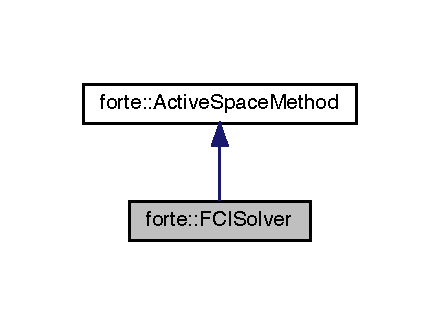
\includegraphics[width=211pt]{classforte_1_1_f_c_i_solver__inherit__graph}
\end{center}
\end{figure}


Collaboration diagram for forte\+:\+:F\+C\+I\+Solver\+:
\nopagebreak
\begin{figure}[H]
\begin{center}
\leavevmode
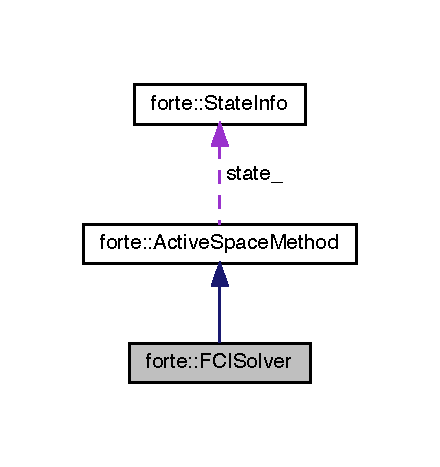
\includegraphics[width=211pt]{classforte_1_1_f_c_i_solver__coll__graph}
\end{center}
\end{figure}
\subsection*{Public Member Functions}
\begin{DoxyCompactItemize}
\item 
\mbox{\hyperlink{classforte_1_1_f_c_i_solver_a5037b1cfcc06a3709a33fa02c9d89d1b}{F\+C\+I\+Solver}} (\mbox{\hyperlink{classforte_1_1_state_info}{State\+Info}} \mbox{\hyperlink{classforte_1_1_active_space_method_a609f005cc7d3a1bc03ae517002eb19dc}{state}}, size\+\_\+t \mbox{\hyperlink{classforte_1_1_active_space_method_aa2bafc732bd7023fd32fbd263ef2e903}{nroot}}, std\+::shared\+\_\+ptr$<$ \mbox{\hyperlink{classforte_1_1_m_o_space_info}{M\+O\+Space\+Info}} $>$ mo\+\_\+space\+\_\+info, std\+::shared\+\_\+ptr$<$ \mbox{\hyperlink{classforte_1_1_active_space_integrals}{Active\+Space\+Integrals}} $>$ as\+\_\+ints)
\begin{DoxyCompactList}\small\item\em \mbox{\hyperlink{classforte_1_1_f_c_i_solver}{F\+C\+I\+Solver}} A class that performs a F\+CI computation in an active space. \end{DoxyCompactList}\item 
\mbox{\hyperlink{classforte_1_1_f_c_i_solver_a6491f1a5c2a79bf9ede2ab863815b8d4}{$\sim$\+F\+C\+I\+Solver}} ()=default
\item 
double \mbox{\hyperlink{classforte_1_1_f_c_i_solver_a5ea02e6826ffd8eb01fd25c229517159}{compute\+\_\+energy}} () override
\begin{DoxyCompactList}\small\item\em Compute the F\+CI energy. \end{DoxyCompactList}\item 
std\+::vector$<$ \mbox{\hyperlink{classforte_1_1_r_d_ms}{R\+D\+Ms}} $>$ \mbox{\hyperlink{classforte_1_1_f_c_i_solver_a40d53f62ae73a7baf7560dac37838b8b}{rdms}} (const std\+::vector$<$ std\+::pair$<$ size\+\_\+t, size\+\_\+t $>$$>$ \&root\+\_\+list, int max\+\_\+rdm\+\_\+level) override
\begin{DoxyCompactList}\small\item\em Returns the reduced density matrices up to a given rank (max\+\_\+rdm\+\_\+level) \end{DoxyCompactList}\item 
std\+::vector$<$ \mbox{\hyperlink{classforte_1_1_r_d_ms}{R\+D\+Ms}} $>$ \mbox{\hyperlink{classforte_1_1_f_c_i_solver_ad29797ad91b7edb6b3d8a4c66aaf18a0}{transition\+\_\+rdms}} (const std\+::vector$<$ std\+::pair$<$ size\+\_\+t, size\+\_\+t $>$$>$ \&root\+\_\+list, std\+::shared\+\_\+ptr$<$ \mbox{\hyperlink{classforte_1_1_active_space_method}{Active\+Space\+Method}} $>$ method2, int max\+\_\+rdm\+\_\+level) override
\item 
void \mbox{\hyperlink{classforte_1_1_f_c_i_solver_a5bb962ea913122dbcec9319411876b05}{set\+\_\+options}} (std\+::shared\+\_\+ptr$<$ \mbox{\hyperlink{classforte_1_1_forte_options}{Forte\+Options}} $>$ options) override
\begin{DoxyCompactList}\small\item\em Set the options. \end{DoxyCompactList}\item 
void \mbox{\hyperlink{classforte_1_1_f_c_i_solver_a36c1bb8d06f2b2b28b5700c861e5acae}{compute\+\_\+rdms\+\_\+root}} (size\+\_\+t root1, size\+\_\+t root2, int max\+\_\+rdm\+\_\+level)
\begin{DoxyCompactList}\small\item\em Compute \mbox{\hyperlink{classforte_1_1_r_d_ms}{R\+D\+Ms}} on a given root. \end{DoxyCompactList}\item 
void \mbox{\hyperlink{classforte_1_1_f_c_i_solver_ab65c6c24f4f55007ff06792e444c6605}{set\+\_\+ntrial\+\_\+per\+\_\+root}} (int value)
\begin{DoxyCompactList}\small\item\em Set the number of trial vectors per root. \end{DoxyCompactList}\item 
void \mbox{\hyperlink{classforte_1_1_f_c_i_solver_abc0f14fa88b25e521394b0a31b5ea1eb}{set\+\_\+fci\+\_\+iterations}} (int value)
\begin{DoxyCompactList}\small\item\em Set the convergence for F\+CI. \end{DoxyCompactList}\item 
void \mbox{\hyperlink{classforte_1_1_f_c_i_solver_a68ac8d378e848ce9a058716095ac37d7}{set\+\_\+collapse\+\_\+per\+\_\+root}} (int value)
\begin{DoxyCompactList}\small\item\em Set the number of collapse vectors for each root. \end{DoxyCompactList}\item 
void \mbox{\hyperlink{classforte_1_1_f_c_i_solver_a412a3fe22b7b6dbacb97d42c37bd07a2}{set\+\_\+subspace\+\_\+per\+\_\+root}} (int value)
\begin{DoxyCompactList}\small\item\em Set the maximum subspace size for each root. \end{DoxyCompactList}\item 
void \mbox{\hyperlink{classforte_1_1_f_c_i_solver_acaf6732c243a888374ffe95454ea4273}{set\+\_\+test\+\_\+rdms}} (bool value)
\item 
void \mbox{\hyperlink{classforte_1_1_f_c_i_solver_a369b5d6855b896d2d1a743dd3ff2d9a6}{set\+\_\+print\+\_\+no}} (bool value)
\begin{DoxyCompactList}\small\item\em Print the Natural Orbitals. \end{DoxyCompactList}\item 
std\+::shared\+\_\+ptr$<$ \mbox{\hyperlink{classforte_1_1_f_c_i_vector}{F\+C\+I\+Vector}} $>$ \mbox{\hyperlink{classforte_1_1_f_c_i_solver_a4c6a278c51128b2f18ada5e08512deca}{get\+\_\+\+F\+C\+I\+W\+FN}} ()
\begin{DoxyCompactList}\small\item\em Return a \mbox{\hyperlink{classforte_1_1_f_c_i_vector}{F\+C\+I\+Vector}}. \end{DoxyCompactList}\item 
psi\+::\+Shared\+Matrix \mbox{\hyperlink{classforte_1_1_f_c_i_solver_a4e8a59d87c2c14b3d5a2ac0c0692f8d2}{evecs}} ()
\begin{DoxyCompactList}\small\item\em Return eigen vectors. \end{DoxyCompactList}\item 
std\+::shared\+\_\+ptr$<$ \mbox{\hyperlink{classforte_1_1_string_lists}{String\+Lists}} $>$ \mbox{\hyperlink{classforte_1_1_f_c_i_solver_a2a60c41f419e985cc8a4bd454ef0441e}{lists}} ()
\begin{DoxyCompactList}\small\item\em Return string lists. \end{DoxyCompactList}\item 
int \mbox{\hyperlink{classforte_1_1_f_c_i_solver_a24be33ae6c646782bff0e56ecc97fee9}{symmetry}} ()
\begin{DoxyCompactList}\small\item\em Return symmetry. \end{DoxyCompactList}\end{DoxyCompactItemize}
\subsection*{Additional Inherited Members}


\subsection{Detailed Description}
The \mbox{\hyperlink{classforte_1_1_f_c_i_solver}{F\+C\+I\+Solver}} class This class performs Full CI calculations. 

\subsection{Constructor \& Destructor Documentation}
\mbox{\Hypertarget{classforte_1_1_f_c_i_solver_a5037b1cfcc06a3709a33fa02c9d89d1b}\label{classforte_1_1_f_c_i_solver_a5037b1cfcc06a3709a33fa02c9d89d1b}} 
\index{forte\+::\+F\+C\+I\+Solver@{forte\+::\+F\+C\+I\+Solver}!F\+C\+I\+Solver@{F\+C\+I\+Solver}}
\index{F\+C\+I\+Solver@{F\+C\+I\+Solver}!forte\+::\+F\+C\+I\+Solver@{forte\+::\+F\+C\+I\+Solver}}
\subsubsection{\texorpdfstring{F\+C\+I\+Solver()}{FCISolver()}}
{\footnotesize\ttfamily forte\+::\+F\+C\+I\+Solver\+::\+F\+C\+I\+Solver (\begin{DoxyParamCaption}\item[{\mbox{\hyperlink{classforte_1_1_state_info}{State\+Info}}}]{state,  }\item[{size\+\_\+t}]{nroot,  }\item[{std\+::shared\+\_\+ptr$<$ \mbox{\hyperlink{classforte_1_1_m_o_space_info}{M\+O\+Space\+Info}} $>$}]{mo\+\_\+space\+\_\+info,  }\item[{std\+::shared\+\_\+ptr$<$ \mbox{\hyperlink{classforte_1_1_active_space_integrals}{Active\+Space\+Integrals}} $>$}]{as\+\_\+ints }\end{DoxyParamCaption})}



\mbox{\hyperlink{classforte_1_1_f_c_i_solver}{F\+C\+I\+Solver}} A class that performs a F\+CI computation in an active space. 


\begin{DoxyParams}{Parameters}
{\em state} & the electronic state to compute \\
\hline
{\em nroot} & the number of roots \\
\hline
{\em mo\+\_\+space\+\_\+info} & a \mbox{\hyperlink{classforte_1_1_m_o_space_info}{M\+O\+Space\+Info}} object that defines the orbital spaces \\
\hline
{\em as\+\_\+ints} & molecular integrals defined only for the active space orbitals \\
\hline
\end{DoxyParams}
\mbox{\Hypertarget{classforte_1_1_f_c_i_solver_a6491f1a5c2a79bf9ede2ab863815b8d4}\label{classforte_1_1_f_c_i_solver_a6491f1a5c2a79bf9ede2ab863815b8d4}} 
\index{forte\+::\+F\+C\+I\+Solver@{forte\+::\+F\+C\+I\+Solver}!````~F\+C\+I\+Solver@{$\sim$\+F\+C\+I\+Solver}}
\index{````~F\+C\+I\+Solver@{$\sim$\+F\+C\+I\+Solver}!forte\+::\+F\+C\+I\+Solver@{forte\+::\+F\+C\+I\+Solver}}
\subsubsection{\texorpdfstring{$\sim$\+F\+C\+I\+Solver()}{~FCISolver()}}
{\footnotesize\ttfamily forte\+::\+F\+C\+I\+Solver\+::$\sim$\+F\+C\+I\+Solver (\begin{DoxyParamCaption}{ }\end{DoxyParamCaption})\hspace{0.3cm}{\ttfamily [default]}}



\subsection{Member Function Documentation}
\mbox{\Hypertarget{classforte_1_1_f_c_i_solver_a5ea02e6826ffd8eb01fd25c229517159}\label{classforte_1_1_f_c_i_solver_a5ea02e6826ffd8eb01fd25c229517159}} 
\index{forte\+::\+F\+C\+I\+Solver@{forte\+::\+F\+C\+I\+Solver}!compute\+\_\+energy@{compute\+\_\+energy}}
\index{compute\+\_\+energy@{compute\+\_\+energy}!forte\+::\+F\+C\+I\+Solver@{forte\+::\+F\+C\+I\+Solver}}
\subsubsection{\texorpdfstring{compute\+\_\+energy()}{compute\_energy()}}
{\footnotesize\ttfamily double forte\+::\+F\+C\+I\+Solver\+::compute\+\_\+energy (\begin{DoxyParamCaption}{ }\end{DoxyParamCaption})\hspace{0.3cm}{\ttfamily [override]}, {\ttfamily [virtual]}}



Compute the F\+CI energy. 



Implements \mbox{\hyperlink{classforte_1_1_active_space_method_a99736e2b94405371b224b0750569b077}{forte\+::\+Active\+Space\+Method}}.

\mbox{\Hypertarget{classforte_1_1_f_c_i_solver_a36c1bb8d06f2b2b28b5700c861e5acae}\label{classforte_1_1_f_c_i_solver_a36c1bb8d06f2b2b28b5700c861e5acae}} 
\index{forte\+::\+F\+C\+I\+Solver@{forte\+::\+F\+C\+I\+Solver}!compute\+\_\+rdms\+\_\+root@{compute\+\_\+rdms\+\_\+root}}
\index{compute\+\_\+rdms\+\_\+root@{compute\+\_\+rdms\+\_\+root}!forte\+::\+F\+C\+I\+Solver@{forte\+::\+F\+C\+I\+Solver}}
\subsubsection{\texorpdfstring{compute\+\_\+rdms\+\_\+root()}{compute\_rdms\_root()}}
{\footnotesize\ttfamily void forte\+::\+F\+C\+I\+Solver\+::compute\+\_\+rdms\+\_\+root (\begin{DoxyParamCaption}\item[{size\+\_\+t}]{root1,  }\item[{size\+\_\+t}]{root2,  }\item[{int}]{max\+\_\+rdm\+\_\+level }\end{DoxyParamCaption})}



Compute \mbox{\hyperlink{classforte_1_1_r_d_ms}{R\+D\+Ms}} on a given root. 

\mbox{\Hypertarget{classforte_1_1_f_c_i_solver_a4e8a59d87c2c14b3d5a2ac0c0692f8d2}\label{classforte_1_1_f_c_i_solver_a4e8a59d87c2c14b3d5a2ac0c0692f8d2}} 
\index{forte\+::\+F\+C\+I\+Solver@{forte\+::\+F\+C\+I\+Solver}!evecs@{evecs}}
\index{evecs@{evecs}!forte\+::\+F\+C\+I\+Solver@{forte\+::\+F\+C\+I\+Solver}}
\subsubsection{\texorpdfstring{evecs()}{evecs()}}
{\footnotesize\ttfamily psi\+::\+Shared\+Matrix forte\+::\+F\+C\+I\+Solver\+::evecs (\begin{DoxyParamCaption}{ }\end{DoxyParamCaption})\hspace{0.3cm}{\ttfamily [inline]}}



Return eigen vectors. 

\mbox{\Hypertarget{classforte_1_1_f_c_i_solver_a4c6a278c51128b2f18ada5e08512deca}\label{classforte_1_1_f_c_i_solver_a4c6a278c51128b2f18ada5e08512deca}} 
\index{forte\+::\+F\+C\+I\+Solver@{forte\+::\+F\+C\+I\+Solver}!get\+\_\+\+F\+C\+I\+W\+FN@{get\+\_\+\+F\+C\+I\+W\+FN}}
\index{get\+\_\+\+F\+C\+I\+W\+FN@{get\+\_\+\+F\+C\+I\+W\+FN}!forte\+::\+F\+C\+I\+Solver@{forte\+::\+F\+C\+I\+Solver}}
\subsubsection{\texorpdfstring{get\+\_\+\+F\+C\+I\+W\+F\+N()}{get\_FCIWFN()}}
{\footnotesize\ttfamily std\+::shared\+\_\+ptr$<$\mbox{\hyperlink{classforte_1_1_f_c_i_vector}{F\+C\+I\+Vector}}$>$ forte\+::\+F\+C\+I\+Solver\+::get\+\_\+\+F\+C\+I\+W\+FN (\begin{DoxyParamCaption}{ }\end{DoxyParamCaption})\hspace{0.3cm}{\ttfamily [inline]}}



Return a \mbox{\hyperlink{classforte_1_1_f_c_i_vector}{F\+C\+I\+Vector}}. 

\mbox{\Hypertarget{classforte_1_1_f_c_i_solver_a2a60c41f419e985cc8a4bd454ef0441e}\label{classforte_1_1_f_c_i_solver_a2a60c41f419e985cc8a4bd454ef0441e}} 
\index{forte\+::\+F\+C\+I\+Solver@{forte\+::\+F\+C\+I\+Solver}!lists@{lists}}
\index{lists@{lists}!forte\+::\+F\+C\+I\+Solver@{forte\+::\+F\+C\+I\+Solver}}
\subsubsection{\texorpdfstring{lists()}{lists()}}
{\footnotesize\ttfamily std\+::shared\+\_\+ptr$<$\mbox{\hyperlink{classforte_1_1_string_lists}{String\+Lists}}$>$ forte\+::\+F\+C\+I\+Solver\+::lists (\begin{DoxyParamCaption}{ }\end{DoxyParamCaption})\hspace{0.3cm}{\ttfamily [inline]}}



Return string lists. 

\mbox{\Hypertarget{classforte_1_1_f_c_i_solver_a40d53f62ae73a7baf7560dac37838b8b}\label{classforte_1_1_f_c_i_solver_a40d53f62ae73a7baf7560dac37838b8b}} 
\index{forte\+::\+F\+C\+I\+Solver@{forte\+::\+F\+C\+I\+Solver}!rdms@{rdms}}
\index{rdms@{rdms}!forte\+::\+F\+C\+I\+Solver@{forte\+::\+F\+C\+I\+Solver}}
\subsubsection{\texorpdfstring{rdms()}{rdms()}}
{\footnotesize\ttfamily std\+::vector$<$ \mbox{\hyperlink{classforte_1_1_r_d_ms}{R\+D\+Ms}} $>$ forte\+::\+F\+C\+I\+Solver\+::rdms (\begin{DoxyParamCaption}\item[{const std\+::vector$<$ std\+::pair$<$ size\+\_\+t, size\+\_\+t $>$$>$ \&}]{root\+\_\+list,  }\item[{int}]{max\+\_\+rdm\+\_\+level }\end{DoxyParamCaption})\hspace{0.3cm}{\ttfamily [override]}, {\ttfamily [virtual]}}



Returns the reduced density matrices up to a given rank (max\+\_\+rdm\+\_\+level) 



Implements \mbox{\hyperlink{classforte_1_1_active_space_method_a0b2c4903551a7602db815d67349ba7c9}{forte\+::\+Active\+Space\+Method}}.

\mbox{\Hypertarget{classforte_1_1_f_c_i_solver_a68ac8d378e848ce9a058716095ac37d7}\label{classforte_1_1_f_c_i_solver_a68ac8d378e848ce9a058716095ac37d7}} 
\index{forte\+::\+F\+C\+I\+Solver@{forte\+::\+F\+C\+I\+Solver}!set\+\_\+collapse\+\_\+per\+\_\+root@{set\+\_\+collapse\+\_\+per\+\_\+root}}
\index{set\+\_\+collapse\+\_\+per\+\_\+root@{set\+\_\+collapse\+\_\+per\+\_\+root}!forte\+::\+F\+C\+I\+Solver@{forte\+::\+F\+C\+I\+Solver}}
\subsubsection{\texorpdfstring{set\+\_\+collapse\+\_\+per\+\_\+root()}{set\_collapse\_per\_root()}}
{\footnotesize\ttfamily void forte\+::\+F\+C\+I\+Solver\+::set\+\_\+collapse\+\_\+per\+\_\+root (\begin{DoxyParamCaption}\item[{int}]{value }\end{DoxyParamCaption})}



Set the number of collapse vectors for each root. 

\mbox{\Hypertarget{classforte_1_1_f_c_i_solver_abc0f14fa88b25e521394b0a31b5ea1eb}\label{classforte_1_1_f_c_i_solver_abc0f14fa88b25e521394b0a31b5ea1eb}} 
\index{forte\+::\+F\+C\+I\+Solver@{forte\+::\+F\+C\+I\+Solver}!set\+\_\+fci\+\_\+iterations@{set\+\_\+fci\+\_\+iterations}}
\index{set\+\_\+fci\+\_\+iterations@{set\+\_\+fci\+\_\+iterations}!forte\+::\+F\+C\+I\+Solver@{forte\+::\+F\+C\+I\+Solver}}
\subsubsection{\texorpdfstring{set\+\_\+fci\+\_\+iterations()}{set\_fci\_iterations()}}
{\footnotesize\ttfamily void forte\+::\+F\+C\+I\+Solver\+::set\+\_\+fci\+\_\+iterations (\begin{DoxyParamCaption}\item[{int}]{value }\end{DoxyParamCaption})}



Set the convergence for F\+CI. 

\mbox{\Hypertarget{classforte_1_1_f_c_i_solver_ab65c6c24f4f55007ff06792e444c6605}\label{classforte_1_1_f_c_i_solver_ab65c6c24f4f55007ff06792e444c6605}} 
\index{forte\+::\+F\+C\+I\+Solver@{forte\+::\+F\+C\+I\+Solver}!set\+\_\+ntrial\+\_\+per\+\_\+root@{set\+\_\+ntrial\+\_\+per\+\_\+root}}
\index{set\+\_\+ntrial\+\_\+per\+\_\+root@{set\+\_\+ntrial\+\_\+per\+\_\+root}!forte\+::\+F\+C\+I\+Solver@{forte\+::\+F\+C\+I\+Solver}}
\subsubsection{\texorpdfstring{set\+\_\+ntrial\+\_\+per\+\_\+root()}{set\_ntrial\_per\_root()}}
{\footnotesize\ttfamily void forte\+::\+F\+C\+I\+Solver\+::set\+\_\+ntrial\+\_\+per\+\_\+root (\begin{DoxyParamCaption}\item[{int}]{value }\end{DoxyParamCaption})}



Set the number of trial vectors per root. 

\mbox{\Hypertarget{classforte_1_1_f_c_i_solver_a5bb962ea913122dbcec9319411876b05}\label{classforte_1_1_f_c_i_solver_a5bb962ea913122dbcec9319411876b05}} 
\index{forte\+::\+F\+C\+I\+Solver@{forte\+::\+F\+C\+I\+Solver}!set\+\_\+options@{set\+\_\+options}}
\index{set\+\_\+options@{set\+\_\+options}!forte\+::\+F\+C\+I\+Solver@{forte\+::\+F\+C\+I\+Solver}}
\subsubsection{\texorpdfstring{set\+\_\+options()}{set\_options()}}
{\footnotesize\ttfamily void forte\+::\+F\+C\+I\+Solver\+::set\+\_\+options (\begin{DoxyParamCaption}\item[{std\+::shared\+\_\+ptr$<$ \mbox{\hyperlink{classforte_1_1_forte_options}{Forte\+Options}} $>$}]{options }\end{DoxyParamCaption})\hspace{0.3cm}{\ttfamily [override]}, {\ttfamily [virtual]}}



Set the options. 



Implements \mbox{\hyperlink{classforte_1_1_active_space_method_a9416a627f550d4d56f6b8ffe7478ed89}{forte\+::\+Active\+Space\+Method}}.

\mbox{\Hypertarget{classforte_1_1_f_c_i_solver_a369b5d6855b896d2d1a743dd3ff2d9a6}\label{classforte_1_1_f_c_i_solver_a369b5d6855b896d2d1a743dd3ff2d9a6}} 
\index{forte\+::\+F\+C\+I\+Solver@{forte\+::\+F\+C\+I\+Solver}!set\+\_\+print\+\_\+no@{set\+\_\+print\+\_\+no}}
\index{set\+\_\+print\+\_\+no@{set\+\_\+print\+\_\+no}!forte\+::\+F\+C\+I\+Solver@{forte\+::\+F\+C\+I\+Solver}}
\subsubsection{\texorpdfstring{set\+\_\+print\+\_\+no()}{set\_print\_no()}}
{\footnotesize\ttfamily void forte\+::\+F\+C\+I\+Solver\+::set\+\_\+print\+\_\+no (\begin{DoxyParamCaption}\item[{bool}]{value }\end{DoxyParamCaption})\hspace{0.3cm}{\ttfamily [inline]}}



Print the Natural Orbitals. 

\mbox{\Hypertarget{classforte_1_1_f_c_i_solver_a412a3fe22b7b6dbacb97d42c37bd07a2}\label{classforte_1_1_f_c_i_solver_a412a3fe22b7b6dbacb97d42c37bd07a2}} 
\index{forte\+::\+F\+C\+I\+Solver@{forte\+::\+F\+C\+I\+Solver}!set\+\_\+subspace\+\_\+per\+\_\+root@{set\+\_\+subspace\+\_\+per\+\_\+root}}
\index{set\+\_\+subspace\+\_\+per\+\_\+root@{set\+\_\+subspace\+\_\+per\+\_\+root}!forte\+::\+F\+C\+I\+Solver@{forte\+::\+F\+C\+I\+Solver}}
\subsubsection{\texorpdfstring{set\+\_\+subspace\+\_\+per\+\_\+root()}{set\_subspace\_per\_root()}}
{\footnotesize\ttfamily void forte\+::\+F\+C\+I\+Solver\+::set\+\_\+subspace\+\_\+per\+\_\+root (\begin{DoxyParamCaption}\item[{int}]{value }\end{DoxyParamCaption})}



Set the maximum subspace size for each root. 

\mbox{\Hypertarget{classforte_1_1_f_c_i_solver_acaf6732c243a888374ffe95454ea4273}\label{classforte_1_1_f_c_i_solver_acaf6732c243a888374ffe95454ea4273}} 
\index{forte\+::\+F\+C\+I\+Solver@{forte\+::\+F\+C\+I\+Solver}!set\+\_\+test\+\_\+rdms@{set\+\_\+test\+\_\+rdms}}
\index{set\+\_\+test\+\_\+rdms@{set\+\_\+test\+\_\+rdms}!forte\+::\+F\+C\+I\+Solver@{forte\+::\+F\+C\+I\+Solver}}
\subsubsection{\texorpdfstring{set\+\_\+test\+\_\+rdms()}{set\_test\_rdms()}}
{\footnotesize\ttfamily void forte\+::\+F\+C\+I\+Solver\+::set\+\_\+test\+\_\+rdms (\begin{DoxyParamCaption}\item[{bool}]{value }\end{DoxyParamCaption})\hspace{0.3cm}{\ttfamily [inline]}}

When set to true before calling \mbox{\hyperlink{classforte_1_1_f_c_i_solver_a5ea02e6826ffd8eb01fd25c229517159}{compute\+\_\+energy()}}, it will test the reduce density matrices. Watch out, this function is very slow! \mbox{\Hypertarget{classforte_1_1_f_c_i_solver_a24be33ae6c646782bff0e56ecc97fee9}\label{classforte_1_1_f_c_i_solver_a24be33ae6c646782bff0e56ecc97fee9}} 
\index{forte\+::\+F\+C\+I\+Solver@{forte\+::\+F\+C\+I\+Solver}!symmetry@{symmetry}}
\index{symmetry@{symmetry}!forte\+::\+F\+C\+I\+Solver@{forte\+::\+F\+C\+I\+Solver}}
\subsubsection{\texorpdfstring{symmetry()}{symmetry()}}
{\footnotesize\ttfamily int forte\+::\+F\+C\+I\+Solver\+::symmetry (\begin{DoxyParamCaption}{ }\end{DoxyParamCaption})\hspace{0.3cm}{\ttfamily [inline]}}



Return symmetry. 

\mbox{\Hypertarget{classforte_1_1_f_c_i_solver_ad29797ad91b7edb6b3d8a4c66aaf18a0}\label{classforte_1_1_f_c_i_solver_ad29797ad91b7edb6b3d8a4c66aaf18a0}} 
\index{forte\+::\+F\+C\+I\+Solver@{forte\+::\+F\+C\+I\+Solver}!transition\+\_\+rdms@{transition\+\_\+rdms}}
\index{transition\+\_\+rdms@{transition\+\_\+rdms}!forte\+::\+F\+C\+I\+Solver@{forte\+::\+F\+C\+I\+Solver}}
\subsubsection{\texorpdfstring{transition\+\_\+rdms()}{transition\_rdms()}}
{\footnotesize\ttfamily std\+::vector$<$ \mbox{\hyperlink{classforte_1_1_r_d_ms}{R\+D\+Ms}} $>$ forte\+::\+F\+C\+I\+Solver\+::transition\+\_\+rdms (\begin{DoxyParamCaption}\item[{const std\+::vector$<$ std\+::pair$<$ size\+\_\+t, size\+\_\+t $>$$>$ \&}]{root\+\_\+list,  }\item[{std\+::shared\+\_\+ptr$<$ \mbox{\hyperlink{classforte_1_1_active_space_method}{Active\+Space\+Method}} $>$}]{method2,  }\item[{int}]{max\+\_\+rdm\+\_\+level }\end{DoxyParamCaption})\hspace{0.3cm}{\ttfamily [override]}, {\ttfamily [virtual]}}

Returns the transition reduced density matrices between roots of different symmetry up to a given level (max\+\_\+rdm\+\_\+level) 

Implements \mbox{\hyperlink{classforte_1_1_active_space_method_a4460069915e56a1994d3a4a4e78bdb30}{forte\+::\+Active\+Space\+Method}}.



The documentation for this class was generated from the following files\+:\begin{DoxyCompactItemize}
\item 
/\+Users/fevange/\+Source/forte/src/fci/\mbox{\hyperlink{fci__solver_8h}{fci\+\_\+solver.\+h}}\item 
/\+Users/fevange/\+Source/forte/src/fci/\mbox{\hyperlink{fci__solver_8cc}{fci\+\_\+solver.\+cc}}\end{DoxyCompactItemize}

\hypertarget{classforte_1_1_f_c_i_vector}{}\section{forte\+:\+:F\+C\+I\+Vector Class Reference}
\label{classforte_1_1_f_c_i_vector}\index{forte\+::\+F\+C\+I\+Vector@{forte\+::\+F\+C\+I\+Vector}}


{\ttfamily \#include $<$fci\+\_\+vector.\+h$>$}

\subsection*{Public Member Functions}
\begin{DoxyCompactItemize}
\item 
\mbox{\hyperlink{classforte_1_1_f_c_i_vector_ac11c68d1754586cf203dad0b95a07b86}{F\+C\+I\+Vector}} (std\+::shared\+\_\+ptr$<$ \mbox{\hyperlink{classforte_1_1_string_lists}{String\+Lists}} $>$ lists, size\+\_\+t symmetry)
\item 
\mbox{\hyperlink{classforte_1_1_f_c_i_vector_a84a8cb8bb781300b63f904bea8a38a60}{$\sim$\+F\+C\+I\+Vector}} ()
\item 
void \mbox{\hyperlink{classforte_1_1_f_c_i_vector_aefc1a1762450009031c196c96bae636e}{print}} ()
\item 
void \mbox{\hyperlink{classforte_1_1_f_c_i_vector_abc76153c77025417cebb1a58d5382ae1}{zero}} ()
\item 
size\+\_\+t \mbox{\hyperlink{classforte_1_1_f_c_i_vector_a47e6063b6b07af86a2e6f439bcb2037f}{size}} () const
\begin{DoxyCompactList}\small\item\em The size of the CI basis. \end{DoxyCompactList}\item 
void \mbox{\hyperlink{classforte_1_1_f_c_i_vector_a4c1591f17c9b23b29730a2f1d76c5785}{copy}} (\mbox{\hyperlink{classforte_1_1_f_c_i_vector}{F\+C\+I\+Vector}} \&wfn)
\begin{DoxyCompactList}\small\item\em Copy the wave function object. \end{DoxyCompactList}\item 
void \mbox{\hyperlink{classforte_1_1_f_c_i_vector_a131ea2c22528308ec890b45c9fed78a3}{copy}} (std\+::shared\+\_\+ptr$<$ psi\+::\+Vector $>$ vec)
\begin{DoxyCompactList}\small\item\em Copy the coefficient from a Vector object. \end{DoxyCompactList}\item 
void \mbox{\hyperlink{classforte_1_1_f_c_i_vector_af77aa0955826ad3c3588ee4f9a93bad9}{copy\+\_\+to}} (std\+::shared\+\_\+ptr$<$ psi\+::\+Vector $>$ vec)
\begin{DoxyCompactList}\small\item\em Copy the wave function object. \end{DoxyCompactList}\item 
void \mbox{\hyperlink{classforte_1_1_f_c_i_vector_afdfc26aaf2b21ea6b5cfdec40c71cf22}{form\+\_\+\+H\+\_\+diagonal}} (std\+::shared\+\_\+ptr$<$ \mbox{\hyperlink{classforte_1_1_active_space_integrals}{Active\+Space\+Integrals}} $>$ fci\+\_\+ints)
\begin{DoxyCompactList}\small\item\em Form the diagonal part of the Hamiltonian. \end{DoxyCompactList}\item 
void \mbox{\hyperlink{classforte_1_1_f_c_i_vector_abe8cd93a76079285466cddff46961760}{set}} (std\+::vector$<$ std\+::tuple$<$ size\+\_\+t, size\+\_\+t, size\+\_\+t, double $>$$>$ \&sparse\+\_\+vec)
\item 
double \mbox{\hyperlink{classforte_1_1_f_c_i_vector_aa3a4006628555ede48afd56c284c911a}{norm}} (double power=2.\+0)
\item 
void \mbox{\hyperlink{classforte_1_1_f_c_i_vector_ad477a8c333a440f3b5f59e980f443484}{normalize}} ()
\item 
double \mbox{\hyperlink{classforte_1_1_f_c_i_vector_a1cccfb3c677d313ba9bb278adc5d8dba}{dot}} (\mbox{\hyperlink{classforte_1_1_f_c_i_vector}{F\+C\+I\+Vector}} \&wfn)
\item 
double \mbox{\hyperlink{classforte_1_1_f_c_i_vector_a5a80e78715a46d5edf2771e225dc8bcc}{dot}} (std\+::shared\+\_\+ptr$<$ \mbox{\hyperlink{classforte_1_1_f_c_i_vector}{F\+C\+I\+Vector}} $>$ \&wfn)
\item 
std\+::vector$<$ double $>$ \& \mbox{\hyperlink{classforte_1_1_f_c_i_vector_a6d0c2dafcf9e13600685db7f7a27cae6}{opdm\+\_\+a}} ()
\item 
std\+::vector$<$ double $>$ \& \mbox{\hyperlink{classforte_1_1_f_c_i_vector_a345012bafb002400635091f98018589d}{opdm\+\_\+b}} ()
\item 
std\+::vector$<$ double $>$ \& \mbox{\hyperlink{classforte_1_1_f_c_i_vector_ab85a2b7900a540e1c8ba6f7cd4447ab6}{tpdm\+\_\+aa}} ()
\item 
std\+::vector$<$ double $>$ \& \mbox{\hyperlink{classforte_1_1_f_c_i_vector_a4a953a96657455eedcd54749dea82d08}{tpdm\+\_\+ab}} ()
\item 
std\+::vector$<$ double $>$ \& \mbox{\hyperlink{classforte_1_1_f_c_i_vector_a9f8152bb2df645b7d48c8e1304dff05f}{tpdm\+\_\+bb}} ()
\item 
std\+::vector$<$ double $>$ \& \mbox{\hyperlink{classforte_1_1_f_c_i_vector_ac5aaf83f7d7f51c5bc86cd3d02604452}{tpdm\+\_\+aaa}} ()
\item 
std\+::vector$<$ double $>$ \& \mbox{\hyperlink{classforte_1_1_f_c_i_vector_a5fd074490be763669f7dadc573a4b9a2}{tpdm\+\_\+aab}} ()
\item 
std\+::vector$<$ double $>$ \& \mbox{\hyperlink{classforte_1_1_f_c_i_vector_afba490fcaae3e4c1bc8bac2e732c3b00}{tpdm\+\_\+abb}} ()
\item 
std\+::vector$<$ double $>$ \& \mbox{\hyperlink{classforte_1_1_f_c_i_vector_a7c588ba35e588c6e87d0214f7a586504}{tpdm\+\_\+bbb}} ()
\item 
void \mbox{\hyperlink{classforte_1_1_f_c_i_vector_a7fe418805ec6a6f43c7eea53a3f905a4}{Hamiltonian}} (\mbox{\hyperlink{classforte_1_1_f_c_i_vector}{F\+C\+I\+Vector}} \&result, std\+::shared\+\_\+ptr$<$ \mbox{\hyperlink{classforte_1_1_active_space_integrals}{Active\+Space\+Integrals}} $>$ fci\+\_\+ints)
\item 
double \mbox{\hyperlink{classforte_1_1_f_c_i_vector_a9c3afbd8ad81b943a19bb1cefbc50c2d}{energy\+\_\+from\+\_\+rdms}} (std\+::shared\+\_\+ptr$<$ \mbox{\hyperlink{classforte_1_1_active_space_integrals}{Active\+Space\+Integrals}} $>$ fci\+\_\+ints)
\item 
void \mbox{\hyperlink{classforte_1_1_f_c_i_vector_a3d1f90f4570df5b367dd8b356d2afb0a}{compute\+\_\+rdms}} (int max\+\_\+order=2)
\item 
void \mbox{\hyperlink{classforte_1_1_f_c_i_vector_a1c3bfabd91f5a538e18c69f4a04f5fc0}{rdm\+\_\+test}} ()
\item 
void \mbox{\hyperlink{classforte_1_1_f_c_i_vector_a21aab8b6dd3d6e3805352025f8b90c59}{print\+\_\+natural\+\_\+orbitals}} (std\+::shared\+\_\+ptr$<$ \mbox{\hyperlink{classforte_1_1_m_o_space_info}{M\+O\+Space\+Info}} $>$)
\item 
std\+::vector$<$ std\+::tuple$<$ double, size\+\_\+t, size\+\_\+t, size\+\_\+t $>$ $>$ \mbox{\hyperlink{classforte_1_1_f_c_i_vector_ab0ee83d2f650fb39eb17e163f3191eca}{min\+\_\+elements}} (size\+\_\+t num\+\_\+dets)
\item 
std\+::vector$<$ std\+::tuple$<$ double, double, size\+\_\+t, size\+\_\+t, size\+\_\+t $>$ $>$ \mbox{\hyperlink{classforte_1_1_f_c_i_vector_afee2d3025d99c222d84d9a0c8b3b236d}{max\+\_\+abs\+\_\+elements}} (size\+\_\+t num\+\_\+dets)
\item 
void \mbox{\hyperlink{classforte_1_1_f_c_i_vector_adf48739d8b0af1cf8a17fe8b68d30d23}{set\+\_\+print}} (int \mbox{\hyperlink{classforte_1_1_f_c_i_vector_aefc1a1762450009031c196c96bae636e}{print}})
\end{DoxyCompactItemize}
\subsection*{Static Public Member Functions}
\begin{DoxyCompactItemize}
\item 
static void \mbox{\hyperlink{classforte_1_1_f_c_i_vector_ad3aed0f04ae2cb88c0f77c02197f6d02}{allocate\+\_\+temp\+\_\+space}} (std\+::shared\+\_\+ptr$<$ \mbox{\hyperlink{classforte_1_1_string_lists}{String\+Lists}} $>$ lists\+\_\+, int print\+\_\+)
\item 
static void \mbox{\hyperlink{classforte_1_1_f_c_i_vector_a31d51c8fda52541784e15b06ca9ebd45}{release\+\_\+temp\+\_\+space}} ()
\end{DoxyCompactItemize}


\subsection{Constructor \& Destructor Documentation}
\mbox{\Hypertarget{classforte_1_1_f_c_i_vector_ac11c68d1754586cf203dad0b95a07b86}\label{classforte_1_1_f_c_i_vector_ac11c68d1754586cf203dad0b95a07b86}} 
\index{forte\+::\+F\+C\+I\+Vector@{forte\+::\+F\+C\+I\+Vector}!F\+C\+I\+Vector@{F\+C\+I\+Vector}}
\index{F\+C\+I\+Vector@{F\+C\+I\+Vector}!forte\+::\+F\+C\+I\+Vector@{forte\+::\+F\+C\+I\+Vector}}
\subsubsection{\texorpdfstring{F\+C\+I\+Vector()}{FCIVector()}}
{\footnotesize\ttfamily forte\+::\+F\+C\+I\+Vector\+::\+F\+C\+I\+Vector (\begin{DoxyParamCaption}\item[{std\+::shared\+\_\+ptr$<$ \mbox{\hyperlink{classforte_1_1_string_lists}{String\+Lists}} $>$}]{lists,  }\item[{size\+\_\+t}]{symmetry }\end{DoxyParamCaption})}

\mbox{\Hypertarget{classforte_1_1_f_c_i_vector_a84a8cb8bb781300b63f904bea8a38a60}\label{classforte_1_1_f_c_i_vector_a84a8cb8bb781300b63f904bea8a38a60}} 
\index{forte\+::\+F\+C\+I\+Vector@{forte\+::\+F\+C\+I\+Vector}!````~F\+C\+I\+Vector@{$\sim$\+F\+C\+I\+Vector}}
\index{````~F\+C\+I\+Vector@{$\sim$\+F\+C\+I\+Vector}!forte\+::\+F\+C\+I\+Vector@{forte\+::\+F\+C\+I\+Vector}}
\subsubsection{\texorpdfstring{$\sim$\+F\+C\+I\+Vector()}{~FCIVector()}}
{\footnotesize\ttfamily forte\+::\+F\+C\+I\+Vector\+::$\sim$\+F\+C\+I\+Vector (\begin{DoxyParamCaption}{ }\end{DoxyParamCaption})}



\subsection{Member Function Documentation}
\mbox{\Hypertarget{classforte_1_1_f_c_i_vector_ad3aed0f04ae2cb88c0f77c02197f6d02}\label{classforte_1_1_f_c_i_vector_ad3aed0f04ae2cb88c0f77c02197f6d02}} 
\index{forte\+::\+F\+C\+I\+Vector@{forte\+::\+F\+C\+I\+Vector}!allocate\+\_\+temp\+\_\+space@{allocate\+\_\+temp\+\_\+space}}
\index{allocate\+\_\+temp\+\_\+space@{allocate\+\_\+temp\+\_\+space}!forte\+::\+F\+C\+I\+Vector@{forte\+::\+F\+C\+I\+Vector}}
\subsubsection{\texorpdfstring{allocate\+\_\+temp\+\_\+space()}{allocate\_temp\_space()}}
{\footnotesize\ttfamily void forte\+::\+F\+C\+I\+Vector\+::allocate\+\_\+temp\+\_\+space (\begin{DoxyParamCaption}\item[{std\+::shared\+\_\+ptr$<$ \mbox{\hyperlink{classforte_1_1_string_lists}{String\+Lists}} $>$}]{lists\+\_\+,  }\item[{int}]{print\+\_\+ }\end{DoxyParamCaption})\hspace{0.3cm}{\ttfamily [static]}}

\mbox{\Hypertarget{classforte_1_1_f_c_i_vector_a3d1f90f4570df5b367dd8b356d2afb0a}\label{classforte_1_1_f_c_i_vector_a3d1f90f4570df5b367dd8b356d2afb0a}} 
\index{forte\+::\+F\+C\+I\+Vector@{forte\+::\+F\+C\+I\+Vector}!compute\+\_\+rdms@{compute\+\_\+rdms}}
\index{compute\+\_\+rdms@{compute\+\_\+rdms}!forte\+::\+F\+C\+I\+Vector@{forte\+::\+F\+C\+I\+Vector}}
\subsubsection{\texorpdfstring{compute\+\_\+rdms()}{compute\_rdms()}}
{\footnotesize\ttfamily void forte\+::\+F\+C\+I\+Vector\+::compute\+\_\+rdms (\begin{DoxyParamCaption}\item[{int}]{max\+\_\+order = {\ttfamily 2} }\end{DoxyParamCaption})}

Compute the one-\/particle density matrix for a given wave function 
\begin{DoxyParams}{Parameters}
{\em alfa} & flag for alfa or beta component, true = alfa, false = beta \\
\hline
\end{DoxyParams}
\mbox{\Hypertarget{classforte_1_1_f_c_i_vector_a4c1591f17c9b23b29730a2f1d76c5785}\label{classforte_1_1_f_c_i_vector_a4c1591f17c9b23b29730a2f1d76c5785}} 
\index{forte\+::\+F\+C\+I\+Vector@{forte\+::\+F\+C\+I\+Vector}!copy@{copy}}
\index{copy@{copy}!forte\+::\+F\+C\+I\+Vector@{forte\+::\+F\+C\+I\+Vector}}
\subsubsection{\texorpdfstring{copy()}{copy()}\hspace{0.1cm}{\footnotesize\ttfamily [1/2]}}
{\footnotesize\ttfamily void forte\+::\+F\+C\+I\+Vector\+::copy (\begin{DoxyParamCaption}\item[{\mbox{\hyperlink{classforte_1_1_f_c_i_vector}{F\+C\+I\+Vector}} \&}]{wfn }\end{DoxyParamCaption})}



Copy the wave function object. 

Set the wave function to a single Slater determinant Get the coefficient of a single Slater determinant Set the wave function to another wave function \mbox{\Hypertarget{classforte_1_1_f_c_i_vector_a131ea2c22528308ec890b45c9fed78a3}\label{classforte_1_1_f_c_i_vector_a131ea2c22528308ec890b45c9fed78a3}} 
\index{forte\+::\+F\+C\+I\+Vector@{forte\+::\+F\+C\+I\+Vector}!copy@{copy}}
\index{copy@{copy}!forte\+::\+F\+C\+I\+Vector@{forte\+::\+F\+C\+I\+Vector}}
\subsubsection{\texorpdfstring{copy()}{copy()}\hspace{0.1cm}{\footnotesize\ttfamily [2/2]}}
{\footnotesize\ttfamily void forte\+::\+F\+C\+I\+Vector\+::copy (\begin{DoxyParamCaption}\item[{std\+::shared\+\_\+ptr$<$ psi\+::\+Vector $>$}]{vec }\end{DoxyParamCaption})}



Copy the coefficient from a Vector object. 

\mbox{\Hypertarget{classforte_1_1_f_c_i_vector_af77aa0955826ad3c3588ee4f9a93bad9}\label{classforte_1_1_f_c_i_vector_af77aa0955826ad3c3588ee4f9a93bad9}} 
\index{forte\+::\+F\+C\+I\+Vector@{forte\+::\+F\+C\+I\+Vector}!copy\+\_\+to@{copy\+\_\+to}}
\index{copy\+\_\+to@{copy\+\_\+to}!forte\+::\+F\+C\+I\+Vector@{forte\+::\+F\+C\+I\+Vector}}
\subsubsection{\texorpdfstring{copy\+\_\+to()}{copy\_to()}}
{\footnotesize\ttfamily void forte\+::\+F\+C\+I\+Vector\+::copy\+\_\+to (\begin{DoxyParamCaption}\item[{std\+::shared\+\_\+ptr$<$ psi\+::\+Vector $>$}]{vec }\end{DoxyParamCaption})}



Copy the wave function object. 

\mbox{\Hypertarget{classforte_1_1_f_c_i_vector_a1cccfb3c677d313ba9bb278adc5d8dba}\label{classforte_1_1_f_c_i_vector_a1cccfb3c677d313ba9bb278adc5d8dba}} 
\index{forte\+::\+F\+C\+I\+Vector@{forte\+::\+F\+C\+I\+Vector}!dot@{dot}}
\index{dot@{dot}!forte\+::\+F\+C\+I\+Vector@{forte\+::\+F\+C\+I\+Vector}}
\subsubsection{\texorpdfstring{dot()}{dot()}\hspace{0.1cm}{\footnotesize\ttfamily [1/2]}}
{\footnotesize\ttfamily double forte\+::\+F\+C\+I\+Vector\+::dot (\begin{DoxyParamCaption}\item[{\mbox{\hyperlink{classforte_1_1_f_c_i_vector}{F\+C\+I\+Vector}} \&}]{wfn }\end{DoxyParamCaption})}

Compute the dot product with another wave function \mbox{\Hypertarget{classforte_1_1_f_c_i_vector_a5a80e78715a46d5edf2771e225dc8bcc}\label{classforte_1_1_f_c_i_vector_a5a80e78715a46d5edf2771e225dc8bcc}} 
\index{forte\+::\+F\+C\+I\+Vector@{forte\+::\+F\+C\+I\+Vector}!dot@{dot}}
\index{dot@{dot}!forte\+::\+F\+C\+I\+Vector@{forte\+::\+F\+C\+I\+Vector}}
\subsubsection{\texorpdfstring{dot()}{dot()}\hspace{0.1cm}{\footnotesize\ttfamily [2/2]}}
{\footnotesize\ttfamily double forte\+::\+F\+C\+I\+Vector\+::dot (\begin{DoxyParamCaption}\item[{std\+::shared\+\_\+ptr$<$ \mbox{\hyperlink{classforte_1_1_f_c_i_vector}{F\+C\+I\+Vector}} $>$ \&}]{wfn }\end{DoxyParamCaption})}

\mbox{\Hypertarget{classforte_1_1_f_c_i_vector_a9c3afbd8ad81b943a19bb1cefbc50c2d}\label{classforte_1_1_f_c_i_vector_a9c3afbd8ad81b943a19bb1cefbc50c2d}} 
\index{forte\+::\+F\+C\+I\+Vector@{forte\+::\+F\+C\+I\+Vector}!energy\+\_\+from\+\_\+rdms@{energy\+\_\+from\+\_\+rdms}}
\index{energy\+\_\+from\+\_\+rdms@{energy\+\_\+from\+\_\+rdms}!forte\+::\+F\+C\+I\+Vector@{forte\+::\+F\+C\+I\+Vector}}
\subsubsection{\texorpdfstring{energy\+\_\+from\+\_\+rdms()}{energy\_from\_rdms()}}
{\footnotesize\ttfamily double forte\+::\+F\+C\+I\+Vector\+::energy\+\_\+from\+\_\+rdms (\begin{DoxyParamCaption}\item[{std\+::shared\+\_\+ptr$<$ \mbox{\hyperlink{classforte_1_1_active_space_integrals}{Active\+Space\+Integrals}} $>$}]{fci\+\_\+ints }\end{DoxyParamCaption})}

\mbox{\Hypertarget{classforte_1_1_f_c_i_vector_afdfc26aaf2b21ea6b5cfdec40c71cf22}\label{classforte_1_1_f_c_i_vector_afdfc26aaf2b21ea6b5cfdec40c71cf22}} 
\index{forte\+::\+F\+C\+I\+Vector@{forte\+::\+F\+C\+I\+Vector}!form\+\_\+\+H\+\_\+diagonal@{form\+\_\+\+H\+\_\+diagonal}}
\index{form\+\_\+\+H\+\_\+diagonal@{form\+\_\+\+H\+\_\+diagonal}!forte\+::\+F\+C\+I\+Vector@{forte\+::\+F\+C\+I\+Vector}}
\subsubsection{\texorpdfstring{form\+\_\+\+H\+\_\+diagonal()}{form\_H\_diagonal()}}
{\footnotesize\ttfamily void forte\+::\+F\+C\+I\+Vector\+::form\+\_\+\+H\+\_\+diagonal (\begin{DoxyParamCaption}\item[{std\+::shared\+\_\+ptr$<$ \mbox{\hyperlink{classforte_1_1_active_space_integrals}{Active\+Space\+Integrals}} $>$}]{fci\+\_\+ints }\end{DoxyParamCaption})}



Form the diagonal part of the Hamiltonian. 

\mbox{\Hypertarget{classforte_1_1_f_c_i_vector_a7fe418805ec6a6f43c7eea53a3f905a4}\label{classforte_1_1_f_c_i_vector_a7fe418805ec6a6f43c7eea53a3f905a4}} 
\index{forte\+::\+F\+C\+I\+Vector@{forte\+::\+F\+C\+I\+Vector}!Hamiltonian@{Hamiltonian}}
\index{Hamiltonian@{Hamiltonian}!forte\+::\+F\+C\+I\+Vector@{forte\+::\+F\+C\+I\+Vector}}
\subsubsection{\texorpdfstring{Hamiltonian()}{Hamiltonian()}}
{\footnotesize\ttfamily void forte\+::\+F\+C\+I\+Vector\+::\+Hamiltonian (\begin{DoxyParamCaption}\item[{\mbox{\hyperlink{classforte_1_1_f_c_i_vector}{F\+C\+I\+Vector}} \&}]{result,  }\item[{std\+::shared\+\_\+ptr$<$ \mbox{\hyperlink{classforte_1_1_active_space_integrals}{Active\+Space\+Integrals}} $>$}]{fci\+\_\+ints }\end{DoxyParamCaption})}

Apply the Hamiltonian to the wave function 
\begin{DoxyParams}{Parameters}
{\em result} & Wave function object which stores the resulting vector \\
\hline
\end{DoxyParams}
\mbox{\Hypertarget{classforte_1_1_f_c_i_vector_afee2d3025d99c222d84d9a0c8b3b236d}\label{classforte_1_1_f_c_i_vector_afee2d3025d99c222d84d9a0c8b3b236d}} 
\index{forte\+::\+F\+C\+I\+Vector@{forte\+::\+F\+C\+I\+Vector}!max\+\_\+abs\+\_\+elements@{max\+\_\+abs\+\_\+elements}}
\index{max\+\_\+abs\+\_\+elements@{max\+\_\+abs\+\_\+elements}!forte\+::\+F\+C\+I\+Vector@{forte\+::\+F\+C\+I\+Vector}}
\subsubsection{\texorpdfstring{max\+\_\+abs\+\_\+elements()}{max\_abs\_elements()}}
{\footnotesize\ttfamily std\+::vector$<$ std\+::tuple$<$ double, double, size\+\_\+t, size\+\_\+t, size\+\_\+t $>$ $>$ forte\+::\+F\+C\+I\+Vector\+::max\+\_\+abs\+\_\+elements (\begin{DoxyParamCaption}\item[{size\+\_\+t}]{num\+\_\+dets }\end{DoxyParamCaption})}

Return the elements with the largest absolute value This function returns the tuple ($\vert$\+C\+\_\+\+I$\vert$,C\+\_\+I,irrep,Ia,Ib) \mbox{\Hypertarget{classforte_1_1_f_c_i_vector_ab0ee83d2f650fb39eb17e163f3191eca}\label{classforte_1_1_f_c_i_vector_ab0ee83d2f650fb39eb17e163f3191eca}} 
\index{forte\+::\+F\+C\+I\+Vector@{forte\+::\+F\+C\+I\+Vector}!min\+\_\+elements@{min\+\_\+elements}}
\index{min\+\_\+elements@{min\+\_\+elements}!forte\+::\+F\+C\+I\+Vector@{forte\+::\+F\+C\+I\+Vector}}
\subsubsection{\texorpdfstring{min\+\_\+elements()}{min\_elements()}}
{\footnotesize\ttfamily std\+::vector$<$ std\+::tuple$<$ double, size\+\_\+t, size\+\_\+t, size\+\_\+t $>$ $>$ forte\+::\+F\+C\+I\+Vector\+::min\+\_\+elements (\begin{DoxyParamCaption}\item[{size\+\_\+t}]{num\+\_\+dets }\end{DoxyParamCaption})}

Return the elements with the smallest value This function returns the tuple (C\+\_\+I,irrep,Ia,Ib) \mbox{\Hypertarget{classforte_1_1_f_c_i_vector_aa3a4006628555ede48afd56c284c911a}\label{classforte_1_1_f_c_i_vector_aa3a4006628555ede48afd56c284c911a}} 
\index{forte\+::\+F\+C\+I\+Vector@{forte\+::\+F\+C\+I\+Vector}!norm@{norm}}
\index{norm@{norm}!forte\+::\+F\+C\+I\+Vector@{forte\+::\+F\+C\+I\+Vector}}
\subsubsection{\texorpdfstring{norm()}{norm()}}
{\footnotesize\ttfamily double forte\+::\+F\+C\+I\+Vector\+::norm (\begin{DoxyParamCaption}\item[{double}]{power = {\ttfamily 2.0} }\end{DoxyParamCaption})}

Zero a symmetry block of the wave function 
\begin{DoxyParams}{Parameters}
{\em h} & symmetry of the alpha strings of the block to zero Transpose a block of the matrix (Works only for total symmetric wfns!) \\
\hline
{\em h} & symmetry of the alpha strings of the block to zero Compute the 2-\/norm of the wave function \\
\hline
\end{DoxyParams}
\mbox{\Hypertarget{classforte_1_1_f_c_i_vector_ad477a8c333a440f3b5f59e980f443484}\label{classforte_1_1_f_c_i_vector_ad477a8c333a440f3b5f59e980f443484}} 
\index{forte\+::\+F\+C\+I\+Vector@{forte\+::\+F\+C\+I\+Vector}!normalize@{normalize}}
\index{normalize@{normalize}!forte\+::\+F\+C\+I\+Vector@{forte\+::\+F\+C\+I\+Vector}}
\subsubsection{\texorpdfstring{normalize()}{normalize()}}
{\footnotesize\ttfamily void forte\+::\+F\+C\+I\+Vector\+::normalize (\begin{DoxyParamCaption}{ }\end{DoxyParamCaption})}

Set the wave function to the nth determinant in the list Get the coefficient of the nth determinant in the list Get a vector of the determinants with weight greather than alpha Normalize the wave function without changing the phase \mbox{\Hypertarget{classforte_1_1_f_c_i_vector_a6d0c2dafcf9e13600685db7f7a27cae6}\label{classforte_1_1_f_c_i_vector_a6d0c2dafcf9e13600685db7f7a27cae6}} 
\index{forte\+::\+F\+C\+I\+Vector@{forte\+::\+F\+C\+I\+Vector}!opdm\+\_\+a@{opdm\+\_\+a}}
\index{opdm\+\_\+a@{opdm\+\_\+a}!forte\+::\+F\+C\+I\+Vector@{forte\+::\+F\+C\+I\+Vector}}
\subsubsection{\texorpdfstring{opdm\+\_\+a()}{opdm\_a()}}
{\footnotesize\ttfamily std\+::vector$<$double$>$\& forte\+::\+F\+C\+I\+Vector\+::opdm\+\_\+a (\begin{DoxyParamCaption}{ }\end{DoxyParamCaption})\hspace{0.3cm}{\ttfamily [inline]}}

\mbox{\Hypertarget{classforte_1_1_f_c_i_vector_a345012bafb002400635091f98018589d}\label{classforte_1_1_f_c_i_vector_a345012bafb002400635091f98018589d}} 
\index{forte\+::\+F\+C\+I\+Vector@{forte\+::\+F\+C\+I\+Vector}!opdm\+\_\+b@{opdm\+\_\+b}}
\index{opdm\+\_\+b@{opdm\+\_\+b}!forte\+::\+F\+C\+I\+Vector@{forte\+::\+F\+C\+I\+Vector}}
\subsubsection{\texorpdfstring{opdm\+\_\+b()}{opdm\_b()}}
{\footnotesize\ttfamily std\+::vector$<$double$>$\& forte\+::\+F\+C\+I\+Vector\+::opdm\+\_\+b (\begin{DoxyParamCaption}{ }\end{DoxyParamCaption})\hspace{0.3cm}{\ttfamily [inline]}}

\mbox{\Hypertarget{classforte_1_1_f_c_i_vector_aefc1a1762450009031c196c96bae636e}\label{classforte_1_1_f_c_i_vector_aefc1a1762450009031c196c96bae636e}} 
\index{forte\+::\+F\+C\+I\+Vector@{forte\+::\+F\+C\+I\+Vector}!print@{print}}
\index{print@{print}!forte\+::\+F\+C\+I\+Vector@{forte\+::\+F\+C\+I\+Vector}}
\subsubsection{\texorpdfstring{print()}{print()}}
{\footnotesize\ttfamily void forte\+::\+F\+C\+I\+Vector\+::print (\begin{DoxyParamCaption}{ }\end{DoxyParamCaption})}

Find the largest element in the wave function Find the smallest element in the wave function Implements the update method of Bendazzoli and Evangelisti modified Implements the update method of Bendazzoli and Evangelisti Implements the update method of Davidson and Liu Add a scaled amount of another wave function Add a scaled amount of another wave function Print the non-\/zero contributions to the wave function \mbox{\Hypertarget{classforte_1_1_f_c_i_vector_a21aab8b6dd3d6e3805352025f8b90c59}\label{classforte_1_1_f_c_i_vector_a21aab8b6dd3d6e3805352025f8b90c59}} 
\index{forte\+::\+F\+C\+I\+Vector@{forte\+::\+F\+C\+I\+Vector}!print\+\_\+natural\+\_\+orbitals@{print\+\_\+natural\+\_\+orbitals}}
\index{print\+\_\+natural\+\_\+orbitals@{print\+\_\+natural\+\_\+orbitals}!forte\+::\+F\+C\+I\+Vector@{forte\+::\+F\+C\+I\+Vector}}
\subsubsection{\texorpdfstring{print\+\_\+natural\+\_\+orbitals()}{print\_natural\_orbitals()}}
{\footnotesize\ttfamily void forte\+::\+F\+C\+I\+Vector\+::print\+\_\+natural\+\_\+orbitals (\begin{DoxyParamCaption}\item[{std\+::shared\+\_\+ptr$<$ \mbox{\hyperlink{classforte_1_1_m_o_space_info}{M\+O\+Space\+Info}} $>$}]{mo\+\_\+space\+\_\+info }\end{DoxyParamCaption})}

Print the natural\+\_\+orbitals from F\+C\+I\+W\+FN Assume user specifed active space \mbox{\Hypertarget{classforte_1_1_f_c_i_vector_a1c3bfabd91f5a538e18c69f4a04f5fc0}\label{classforte_1_1_f_c_i_vector_a1c3bfabd91f5a538e18c69f4a04f5fc0}} 
\index{forte\+::\+F\+C\+I\+Vector@{forte\+::\+F\+C\+I\+Vector}!rdm\+\_\+test@{rdm\+\_\+test}}
\index{rdm\+\_\+test@{rdm\+\_\+test}!forte\+::\+F\+C\+I\+Vector@{forte\+::\+F\+C\+I\+Vector}}
\subsubsection{\texorpdfstring{rdm\+\_\+test()}{rdm\_test()}}
{\footnotesize\ttfamily void forte\+::\+F\+C\+I\+Vector\+::rdm\+\_\+test (\begin{DoxyParamCaption}{ }\end{DoxyParamCaption})}

\mbox{\Hypertarget{classforte_1_1_f_c_i_vector_a31d51c8fda52541784e15b06ca9ebd45}\label{classforte_1_1_f_c_i_vector_a31d51c8fda52541784e15b06ca9ebd45}} 
\index{forte\+::\+F\+C\+I\+Vector@{forte\+::\+F\+C\+I\+Vector}!release\+\_\+temp\+\_\+space@{release\+\_\+temp\+\_\+space}}
\index{release\+\_\+temp\+\_\+space@{release\+\_\+temp\+\_\+space}!forte\+::\+F\+C\+I\+Vector@{forte\+::\+F\+C\+I\+Vector}}
\subsubsection{\texorpdfstring{release\+\_\+temp\+\_\+space()}{release\_temp\_space()}}
{\footnotesize\ttfamily void forte\+::\+F\+C\+I\+Vector\+::release\+\_\+temp\+\_\+space (\begin{DoxyParamCaption}{ }\end{DoxyParamCaption})\hspace{0.3cm}{\ttfamily [static]}}

\mbox{\Hypertarget{classforte_1_1_f_c_i_vector_abe8cd93a76079285466cddff46961760}\label{classforte_1_1_f_c_i_vector_abe8cd93a76079285466cddff46961760}} 
\index{forte\+::\+F\+C\+I\+Vector@{forte\+::\+F\+C\+I\+Vector}!set@{set}}
\index{set@{set}!forte\+::\+F\+C\+I\+Vector@{forte\+::\+F\+C\+I\+Vector}}
\subsubsection{\texorpdfstring{set()}{set()}}
{\footnotesize\ttfamily void forte\+::\+F\+C\+I\+Vector\+::set (\begin{DoxyParamCaption}\item[{std\+::vector$<$ std\+::tuple$<$ size\+\_\+t, size\+\_\+t, size\+\_\+t, double $>$$>$ \&}]{sparse\+\_\+vec }\end{DoxyParamCaption})}

\mbox{\Hypertarget{classforte_1_1_f_c_i_vector_adf48739d8b0af1cf8a17fe8b68d30d23}\label{classforte_1_1_f_c_i_vector_adf48739d8b0af1cf8a17fe8b68d30d23}} 
\index{forte\+::\+F\+C\+I\+Vector@{forte\+::\+F\+C\+I\+Vector}!set\+\_\+print@{set\+\_\+print}}
\index{set\+\_\+print@{set\+\_\+print}!forte\+::\+F\+C\+I\+Vector@{forte\+::\+F\+C\+I\+Vector}}
\subsubsection{\texorpdfstring{set\+\_\+print()}{set\_print()}}
{\footnotesize\ttfamily void forte\+::\+F\+C\+I\+Vector\+::set\+\_\+print (\begin{DoxyParamCaption}\item[{int}]{print }\end{DoxyParamCaption})\hspace{0.3cm}{\ttfamily [inline]}}

\mbox{\Hypertarget{classforte_1_1_f_c_i_vector_a47e6063b6b07af86a2e6f439bcb2037f}\label{classforte_1_1_f_c_i_vector_a47e6063b6b07af86a2e6f439bcb2037f}} 
\index{forte\+::\+F\+C\+I\+Vector@{forte\+::\+F\+C\+I\+Vector}!size@{size}}
\index{size@{size}!forte\+::\+F\+C\+I\+Vector@{forte\+::\+F\+C\+I\+Vector}}
\subsubsection{\texorpdfstring{size()}{size()}}
{\footnotesize\ttfamily size\+\_\+t forte\+::\+F\+C\+I\+Vector\+::size (\begin{DoxyParamCaption}{ }\end{DoxyParamCaption}) const\hspace{0.3cm}{\ttfamily [inline]}}



The size of the CI basis. 

\mbox{\Hypertarget{classforte_1_1_f_c_i_vector_ab85a2b7900a540e1c8ba6f7cd4447ab6}\label{classforte_1_1_f_c_i_vector_ab85a2b7900a540e1c8ba6f7cd4447ab6}} 
\index{forte\+::\+F\+C\+I\+Vector@{forte\+::\+F\+C\+I\+Vector}!tpdm\+\_\+aa@{tpdm\+\_\+aa}}
\index{tpdm\+\_\+aa@{tpdm\+\_\+aa}!forte\+::\+F\+C\+I\+Vector@{forte\+::\+F\+C\+I\+Vector}}
\subsubsection{\texorpdfstring{tpdm\+\_\+aa()}{tpdm\_aa()}}
{\footnotesize\ttfamily std\+::vector$<$double$>$\& forte\+::\+F\+C\+I\+Vector\+::tpdm\+\_\+aa (\begin{DoxyParamCaption}{ }\end{DoxyParamCaption})\hspace{0.3cm}{\ttfamily [inline]}}

\mbox{\Hypertarget{classforte_1_1_f_c_i_vector_ac5aaf83f7d7f51c5bc86cd3d02604452}\label{classforte_1_1_f_c_i_vector_ac5aaf83f7d7f51c5bc86cd3d02604452}} 
\index{forte\+::\+F\+C\+I\+Vector@{forte\+::\+F\+C\+I\+Vector}!tpdm\+\_\+aaa@{tpdm\+\_\+aaa}}
\index{tpdm\+\_\+aaa@{tpdm\+\_\+aaa}!forte\+::\+F\+C\+I\+Vector@{forte\+::\+F\+C\+I\+Vector}}
\subsubsection{\texorpdfstring{tpdm\+\_\+aaa()}{tpdm\_aaa()}}
{\footnotesize\ttfamily std\+::vector$<$double$>$\& forte\+::\+F\+C\+I\+Vector\+::tpdm\+\_\+aaa (\begin{DoxyParamCaption}{ }\end{DoxyParamCaption})\hspace{0.3cm}{\ttfamily [inline]}}

\mbox{\Hypertarget{classforte_1_1_f_c_i_vector_a5fd074490be763669f7dadc573a4b9a2}\label{classforte_1_1_f_c_i_vector_a5fd074490be763669f7dadc573a4b9a2}} 
\index{forte\+::\+F\+C\+I\+Vector@{forte\+::\+F\+C\+I\+Vector}!tpdm\+\_\+aab@{tpdm\+\_\+aab}}
\index{tpdm\+\_\+aab@{tpdm\+\_\+aab}!forte\+::\+F\+C\+I\+Vector@{forte\+::\+F\+C\+I\+Vector}}
\subsubsection{\texorpdfstring{tpdm\+\_\+aab()}{tpdm\_aab()}}
{\footnotesize\ttfamily std\+::vector$<$double$>$\& forte\+::\+F\+C\+I\+Vector\+::tpdm\+\_\+aab (\begin{DoxyParamCaption}{ }\end{DoxyParamCaption})\hspace{0.3cm}{\ttfamily [inline]}}

\mbox{\Hypertarget{classforte_1_1_f_c_i_vector_a4a953a96657455eedcd54749dea82d08}\label{classforte_1_1_f_c_i_vector_a4a953a96657455eedcd54749dea82d08}} 
\index{forte\+::\+F\+C\+I\+Vector@{forte\+::\+F\+C\+I\+Vector}!tpdm\+\_\+ab@{tpdm\+\_\+ab}}
\index{tpdm\+\_\+ab@{tpdm\+\_\+ab}!forte\+::\+F\+C\+I\+Vector@{forte\+::\+F\+C\+I\+Vector}}
\subsubsection{\texorpdfstring{tpdm\+\_\+ab()}{tpdm\_ab()}}
{\footnotesize\ttfamily std\+::vector$<$double$>$\& forte\+::\+F\+C\+I\+Vector\+::tpdm\+\_\+ab (\begin{DoxyParamCaption}{ }\end{DoxyParamCaption})\hspace{0.3cm}{\ttfamily [inline]}}

\mbox{\Hypertarget{classforte_1_1_f_c_i_vector_afba490fcaae3e4c1bc8bac2e732c3b00}\label{classforte_1_1_f_c_i_vector_afba490fcaae3e4c1bc8bac2e732c3b00}} 
\index{forte\+::\+F\+C\+I\+Vector@{forte\+::\+F\+C\+I\+Vector}!tpdm\+\_\+abb@{tpdm\+\_\+abb}}
\index{tpdm\+\_\+abb@{tpdm\+\_\+abb}!forte\+::\+F\+C\+I\+Vector@{forte\+::\+F\+C\+I\+Vector}}
\subsubsection{\texorpdfstring{tpdm\+\_\+abb()}{tpdm\_abb()}}
{\footnotesize\ttfamily std\+::vector$<$double$>$\& forte\+::\+F\+C\+I\+Vector\+::tpdm\+\_\+abb (\begin{DoxyParamCaption}{ }\end{DoxyParamCaption})\hspace{0.3cm}{\ttfamily [inline]}}

\mbox{\Hypertarget{classforte_1_1_f_c_i_vector_a9f8152bb2df645b7d48c8e1304dff05f}\label{classforte_1_1_f_c_i_vector_a9f8152bb2df645b7d48c8e1304dff05f}} 
\index{forte\+::\+F\+C\+I\+Vector@{forte\+::\+F\+C\+I\+Vector}!tpdm\+\_\+bb@{tpdm\+\_\+bb}}
\index{tpdm\+\_\+bb@{tpdm\+\_\+bb}!forte\+::\+F\+C\+I\+Vector@{forte\+::\+F\+C\+I\+Vector}}
\subsubsection{\texorpdfstring{tpdm\+\_\+bb()}{tpdm\_bb()}}
{\footnotesize\ttfamily std\+::vector$<$double$>$\& forte\+::\+F\+C\+I\+Vector\+::tpdm\+\_\+bb (\begin{DoxyParamCaption}{ }\end{DoxyParamCaption})\hspace{0.3cm}{\ttfamily [inline]}}

\mbox{\Hypertarget{classforte_1_1_f_c_i_vector_a7c588ba35e588c6e87d0214f7a586504}\label{classforte_1_1_f_c_i_vector_a7c588ba35e588c6e87d0214f7a586504}} 
\index{forte\+::\+F\+C\+I\+Vector@{forte\+::\+F\+C\+I\+Vector}!tpdm\+\_\+bbb@{tpdm\+\_\+bbb}}
\index{tpdm\+\_\+bbb@{tpdm\+\_\+bbb}!forte\+::\+F\+C\+I\+Vector@{forte\+::\+F\+C\+I\+Vector}}
\subsubsection{\texorpdfstring{tpdm\+\_\+bbb()}{tpdm\_bbb()}}
{\footnotesize\ttfamily std\+::vector$<$double$>$\& forte\+::\+F\+C\+I\+Vector\+::tpdm\+\_\+bbb (\begin{DoxyParamCaption}{ }\end{DoxyParamCaption})\hspace{0.3cm}{\ttfamily [inline]}}

\mbox{\Hypertarget{classforte_1_1_f_c_i_vector_abc76153c77025417cebb1a58d5382ae1}\label{classforte_1_1_f_c_i_vector_abc76153c77025417cebb1a58d5382ae1}} 
\index{forte\+::\+F\+C\+I\+Vector@{forte\+::\+F\+C\+I\+Vector}!zero@{zero}}
\index{zero@{zero}!forte\+::\+F\+C\+I\+Vector@{forte\+::\+F\+C\+I\+Vector}}
\subsubsection{\texorpdfstring{zero()}{zero()}}
{\footnotesize\ttfamily void forte\+::\+F\+C\+I\+Vector\+::zero (\begin{DoxyParamCaption}{ }\end{DoxyParamCaption})}

Normalize the wave function wrt to a single Slater determinant Zero the wave function 

The documentation for this class was generated from the following files\+:\begin{DoxyCompactItemize}
\item 
/\+Users/fevange/\+Source/forte/src/fci/\mbox{\hyperlink{fci__vector_8h}{fci\+\_\+vector.\+h}}\item 
/\+Users/fevange/\+Source/forte/src/fci/\mbox{\hyperlink{fci__vector_8cc}{fci\+\_\+vector.\+cc}}\item 
/\+Users/fevange/\+Source/forte/src/fci/\mbox{\hyperlink{fci__vector__h__diag_8cc}{fci\+\_\+vector\+\_\+h\+\_\+diag.\+cc}}\item 
/\+Users/fevange/\+Source/forte/src/fci/\mbox{\hyperlink{fci__vector__hamiltonian_8cc}{fci\+\_\+vector\+\_\+hamiltonian.\+cc}}\item 
/\+Users/fevange/\+Source/forte/src/fci/\mbox{\hyperlink{fci__vector__rdm_8cc}{fci\+\_\+vector\+\_\+rdm.\+cc}}\end{DoxyCompactItemize}

\hypertarget{classforte_1_1_forte_integrals}{}\section{forte\+:\+:Forte\+Integrals Class Reference}
\label{classforte_1_1_forte_integrals}\index{forte\+::\+Forte\+Integrals@{forte\+::\+Forte\+Integrals}}


The \mbox{\hyperlink{classforte_1_1_forte_integrals}{Forte\+Integrals}} class is a base class for transforming and storing MO integrals.  




{\ttfamily \#include $<$integrals.\+h$>$}



Inheritance diagram for forte\+:\+:Forte\+Integrals\+:
\nopagebreak
\begin{figure}[H]
\begin{center}
\leavevmode
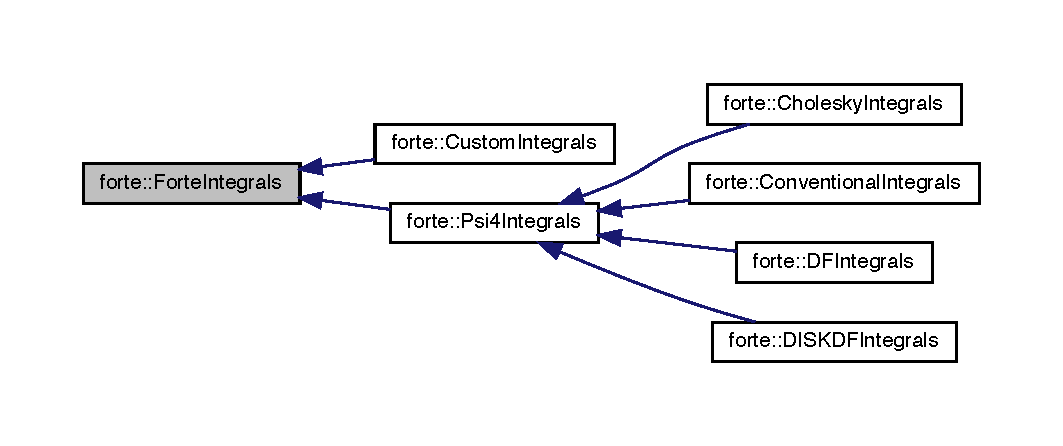
\includegraphics[width=350pt]{classforte_1_1_forte_integrals__inherit__graph}
\end{center}
\end{figure}
\subsection*{Public Types}
\begin{DoxyCompactItemize}
\item 
enum \mbox{\hyperlink{classforte_1_1_forte_integrals_a5ef066e57ff1494e90669779b1d0ecc2}{J\+K\+Status}} \{ \mbox{\hyperlink{classforte_1_1_forte_integrals_a5ef066e57ff1494e90669779b1d0ecc2aa2e4822a98337283e39f7b60acf85ec9}{J\+K\+Status\+::empty}}, 
\mbox{\hyperlink{classforte_1_1_forte_integrals_a5ef066e57ff1494e90669779b1d0ecc2a84d10a1ed612e61dbf6880f6e3ee533a}{J\+K\+Status\+::initialized}}, 
\mbox{\hyperlink{classforte_1_1_forte_integrals_a5ef066e57ff1494e90669779b1d0ecc2a73d0ccbca69b94ee4cd7fc367a8ac9fc}{J\+K\+Status\+::finalized}}
 \}
\begin{DoxyCompactList}\small\item\em Enum class for the status of Pis4 JK. \end{DoxyCompactList}\end{DoxyCompactItemize}
\subsection*{Public Member Functions}
\begin{DoxyCompactItemize}
\item 
\mbox{\hyperlink{classforte_1_1_forte_integrals_ae1b1c7c744c7bd522c94bfa46d78bd05}{Forte\+Integrals}} (std\+::shared\+\_\+ptr$<$ \mbox{\hyperlink{classforte_1_1_forte_options}{Forte\+Options}} $>$ options, std\+::shared\+\_\+ptr$<$ psi\+::\+Wavefunction $>$ ref\+\_\+wfn, std\+::shared\+\_\+ptr$<$ \mbox{\hyperlink{classforte_1_1_m_o_space_info}{M\+O\+Space\+Info}} $>$ mo\+\_\+space\+\_\+info, \mbox{\hyperlink{namespaceforte_a790e7e85ac0911c4c9494622496d95e6}{Integral\+Type}} \mbox{\hyperlink{classforte_1_1_forte_integrals_af62c129aee5c995d15a95136a89faada}{integral\+\_\+type}}, \mbox{\hyperlink{namespaceforte_a7defa2660dd3eb07aa81176b90781be7}{Integral\+Spin\+Restriction}} restricted)
\begin{DoxyCompactList}\small\item\em Class constructor. \end{DoxyCompactList}\item 
\mbox{\hyperlink{classforte_1_1_forte_integrals_a3053bf9ad483639d24392da21fbf522b}{Forte\+Integrals}} (std\+::shared\+\_\+ptr$<$ \mbox{\hyperlink{classforte_1_1_forte_options}{Forte\+Options}} $>$ options, std\+::shared\+\_\+ptr$<$ \mbox{\hyperlink{classforte_1_1_m_o_space_info}{M\+O\+Space\+Info}} $>$ mo\+\_\+space\+\_\+info, \mbox{\hyperlink{namespaceforte_a790e7e85ac0911c4c9494622496d95e6}{Integral\+Type}} \mbox{\hyperlink{classforte_1_1_forte_integrals_af62c129aee5c995d15a95136a89faada}{integral\+\_\+type}}, \mbox{\hyperlink{namespaceforte_a7defa2660dd3eb07aa81176b90781be7}{Integral\+Spin\+Restriction}} restricted)
\begin{DoxyCompactList}\small\item\em Class constructor. \end{DoxyCompactList}\item 
virtual \mbox{\hyperlink{classforte_1_1_forte_integrals_a2d950c2561843509cf9cc5eb2205b0c6}{$\sim$\+Forte\+Integrals}} ()=default
\begin{DoxyCompactList}\small\item\em Virtual destructor to enable deletion of a Derived$\ast$ through a Base$\ast$. \end{DoxyCompactList}\item 
void \mbox{\hyperlink{classforte_1_1_forte_integrals_a74f97a711600c888b3cfea4e59c3483f}{common\+\_\+initialize}} ()
\begin{DoxyCompactList}\small\item\em Common initializer for all types of integrals. \end{DoxyCompactList}\item 
virtual void \mbox{\hyperlink{classforte_1_1_forte_integrals_a7862835fa0f5f9abe13dfcd6730fa4be}{initialize}} ()=0
\item 
std\+::shared\+\_\+ptr$<$ psi\+::\+Matrix $>$ \mbox{\hyperlink{classforte_1_1_forte_integrals_a4607d886e1224bc0b0db9b9a5fe44edb}{Ca}} () const
\begin{DoxyCompactList}\small\item\em Return Ca. \end{DoxyCompactList}\item 
std\+::shared\+\_\+ptr$<$ psi\+::\+Matrix $>$ \mbox{\hyperlink{classforte_1_1_forte_integrals_a99ae31009f9c83f1c7b5871e9dcdcffe}{Cb}} () const
\begin{DoxyCompactList}\small\item\em Return Cb. \end{DoxyCompactList}\item 
double \mbox{\hyperlink{classforte_1_1_forte_integrals_ae83c6f8ee941902655eb8dd27b993e2d}{nuclear\+\_\+repulsion\+\_\+energy}} () const
\begin{DoxyCompactList}\small\item\em Return nuclear repulsion energy. \end{DoxyCompactList}\item 
std\+::shared\+\_\+ptr$<$ psi\+::\+Wavefunction $>$ \mbox{\hyperlink{classforte_1_1_forte_integrals_af70ab78cbd8726d63bb7cc6e93d82e71}{wfn}} ()
\begin{DoxyCompactList}\small\item\em temporary solution for not having a Wavefunction \end{DoxyCompactList}\item 
std\+::shared\+\_\+ptr$<$ psi\+::\+JK $>$ \mbox{\hyperlink{classforte_1_1_forte_integrals_a863150497a5b64b0617b58c5ff6c1f82}{jk}} ()
\begin{DoxyCompactList}\small\item\em Return the Pis4 JK object. \end{DoxyCompactList}\item 
\mbox{\hyperlink{classforte_1_1_forte_integrals_a5ef066e57ff1494e90669779b1d0ecc2}{J\+K\+Status}} \mbox{\hyperlink{classforte_1_1_forte_integrals_afdaad0b6e254794d8f1911cd786367f0}{jk\+\_\+status}} ()
\begin{DoxyCompactList}\small\item\em Return the status of Psi4 JK object. \end{DoxyCompactList}\item 
void \mbox{\hyperlink{classforte_1_1_forte_integrals_abe3df47d3c7fe30ac090362f20ca5160}{jk\+\_\+finalize}} ()
\begin{DoxyCompactList}\small\item\em Finalize Psi4 JK object. \end{DoxyCompactList}\item 
size\+\_\+t \mbox{\hyperlink{classforte_1_1_forte_integrals_aa008ab25f2c1a11cbe6b7ba43ca6179d}{nso}} () const
\item 
const psi\+::\+Dimension \& \mbox{\hyperlink{classforte_1_1_forte_integrals_afa631a01ad69a803b065734067671704}{nsopi}} () const
\begin{DoxyCompactList}\small\item\em Return the number of symmetry-\/adapted orbitals per irrep. \end{DoxyCompactList}\item 
size\+\_\+t \mbox{\hyperlink{classforte_1_1_forte_integrals_ae1ba804bac41846e3fe915dbab9d57a7}{nmo}} () const
\begin{DoxyCompactList}\small\item\em Return the total number of molecular orbitals (this number includes frozen M\+Os) \end{DoxyCompactList}\item 
int \mbox{\hyperlink{classforte_1_1_forte_integrals_a85f2644fb48f17cfd172682b10a0d252}{nirrep}} () const
\begin{DoxyCompactList}\small\item\em Return the number of irreducible representations. \end{DoxyCompactList}\item 
const psi\+::\+Dimension \& \mbox{\hyperlink{classforte_1_1_forte_integrals_a944cff5a804957677551420b35443a5c}{frzcpi}} () const
\begin{DoxyCompactList}\small\item\em Return the number of frozen core orbitals per irrep. \end{DoxyCompactList}\item 
const psi\+::\+Dimension \& \mbox{\hyperlink{classforte_1_1_forte_integrals_a9ec81966b5288931a2116e6f2f34a85d}{frzvpi}} () const
\begin{DoxyCompactList}\small\item\em Return the number of frozen virtual orbitals per irrep. \end{DoxyCompactList}\item 
const psi\+::\+Dimension \& \mbox{\hyperlink{classforte_1_1_forte_integrals_a95947448d8e40f2be497e613512e64eb}{ncmopi}} () const
\begin{DoxyCompactList}\small\item\em The number of correlated M\+Os per irrep (non frozen). This is nmopi -\/ nfzcpi -\/ nfzvpi. \end{DoxyCompactList}\item 
size\+\_\+t \mbox{\hyperlink{classforte_1_1_forte_integrals_a3b78f05526be30dda1653d66f8dfdd74}{ncmo}} () const
\begin{DoxyCompactList}\small\item\em Return the total number of correlated molecular orbitals (this number excludes frozen M\+Os) \end{DoxyCompactList}\item 
void \mbox{\hyperlink{classforte_1_1_forte_integrals_af7a507eef40436e68fff042565249f94}{set\+\_\+print}} (int print)
\begin{DoxyCompactList}\small\item\em Set printing level. \end{DoxyCompactList}\item 
virtual size\+\_\+t \mbox{\hyperlink{classforte_1_1_forte_integrals_af04858e7813556747745f90ffbda81a4}{nthree}} () const
\begin{DoxyCompactList}\small\item\em Return the number of auxiliary functions. \end{DoxyCompactList}\item 
double \mbox{\hyperlink{classforte_1_1_forte_integrals_a3045ecd9722fd7d7544832f7381c5fb3}{frozen\+\_\+core\+\_\+energy}} ()
\begin{DoxyCompactList}\small\item\em Return the frozen core energy. \end{DoxyCompactList}\item 
double \mbox{\hyperlink{classforte_1_1_forte_integrals_a7e2dec148b4e6c3bbd918df8025f8329}{scalar}} () const
\begin{DoxyCompactList}\small\item\em Scalar component of the Hamiltonian. \end{DoxyCompactList}\item 
double \mbox{\hyperlink{classforte_1_1_forte_integrals_adeb8d675248cb181a502818b8a972908}{oei\+\_\+a}} (size\+\_\+t p, size\+\_\+t q) const
\begin{DoxyCompactList}\small\item\em The alpha one-\/electron integrals. \end{DoxyCompactList}\item 
double \mbox{\hyperlink{classforte_1_1_forte_integrals_ace33795c89d99da0aa8bac4a95263d23}{oei\+\_\+b}} (size\+\_\+t p, size\+\_\+t q) const
\begin{DoxyCompactList}\small\item\em The beta one-\/electron integrals. \end{DoxyCompactList}\item 
double \mbox{\hyperlink{classforte_1_1_forte_integrals_a15ff05380f547fa00132ff7f993f1aa0}{get\+\_\+fock\+\_\+a}} (size\+\_\+t p, size\+\_\+t q, bool corr=true) const
\item 
double \mbox{\hyperlink{classforte_1_1_forte_integrals_a62a831e5387b3f2b6e7edfc5bf83c70b}{get\+\_\+fock\+\_\+b}} (size\+\_\+t p, size\+\_\+t q, bool corr=true) const
\item 
std\+::shared\+\_\+ptr$<$ psi\+::\+Matrix $>$ \mbox{\hyperlink{classforte_1_1_forte_integrals_a8d1ebbd9be1d2d06685c355dc8f1f384}{get\+\_\+fock\+\_\+a}} (bool corr=true) const
\item 
std\+::shared\+\_\+ptr$<$ psi\+::\+Matrix $>$ \mbox{\hyperlink{classforte_1_1_forte_integrals_adb5c74105cf591a402ca01d37c7c9738}{get\+\_\+fock\+\_\+b}} (bool corr=true) const
\item 
virtual double \mbox{\hyperlink{classforte_1_1_forte_integrals_afc84c157025b56ee0f8e3b1abe1c0a5f}{aptei\+\_\+aa}} (size\+\_\+t p, size\+\_\+t q, size\+\_\+t r, size\+\_\+t s)=0
\begin{DoxyCompactList}\small\item\em The antisymmetrixed alpha-\/alpha two-\/electron integrals in physicist notation $<$pq$\vert$$\vert$rs$>$ \end{DoxyCompactList}\item 
virtual double \mbox{\hyperlink{classforte_1_1_forte_integrals_a45efc2329cdfc7e4690cbe85688b947e}{aptei\+\_\+ab}} (size\+\_\+t p, size\+\_\+t q, size\+\_\+t r, size\+\_\+t s)=0
\begin{DoxyCompactList}\small\item\em The antisymmetrixed alpha-\/beta two-\/electron integrals in physicist notation $<$pq$\vert$rs$>$ \end{DoxyCompactList}\item 
virtual double \mbox{\hyperlink{classforte_1_1_forte_integrals_a246225031c3799dc446f94e0e732c3ac}{aptei\+\_\+bb}} (size\+\_\+t p, size\+\_\+t q, size\+\_\+t r, size\+\_\+t s)=0
\begin{DoxyCompactList}\small\item\em The antisymmetrixed beta-\/beta two-\/electron integrals in physicist notation $<$pq$\vert$$\vert$rs$>$ \end{DoxyCompactList}\item 
ambit\+::\+Tensor \mbox{\hyperlink{classforte_1_1_forte_integrals_a0e01f8b4de06ec9eb2cd79ebb375da08}{oei\+\_\+a\+\_\+block}} (const std\+::vector$<$ size\+\_\+t $>$ \&p, const std\+::vector$<$ size\+\_\+t $>$ \&q)
\item 
ambit\+::\+Tensor \mbox{\hyperlink{classforte_1_1_forte_integrals_af49cebc262b53e87620b23a70b167fb6}{oei\+\_\+b\+\_\+block}} (const std\+::vector$<$ size\+\_\+t $>$ \&p, const std\+::vector$<$ size\+\_\+t $>$ \&q)
\item 
virtual ambit\+::\+Tensor \mbox{\hyperlink{classforte_1_1_forte_integrals_ac20ae649b8cfe116f8583d676e43da27}{aptei\+\_\+aa\+\_\+block}} (const std\+::vector$<$ size\+\_\+t $>$ \&p, const std\+::vector$<$ size\+\_\+t $>$ \&q, const std\+::vector$<$ size\+\_\+t $>$ \&r, const std\+::vector$<$ size\+\_\+t $>$ \&s)=0
\item 
virtual ambit\+::\+Tensor \mbox{\hyperlink{classforte_1_1_forte_integrals_acd40e350dc861baf8adf6a3b47c74023}{aptei\+\_\+ab\+\_\+block}} (const std\+::vector$<$ size\+\_\+t $>$ \&p, const std\+::vector$<$ size\+\_\+t $>$ \&q, const std\+::vector$<$ size\+\_\+t $>$ \&r, const std\+::vector$<$ size\+\_\+t $>$ \&s)=0
\item 
virtual ambit\+::\+Tensor \mbox{\hyperlink{classforte_1_1_forte_integrals_ae2799dc7cbfd456603a2b841b26582ab}{aptei\+\_\+bb\+\_\+block}} (const std\+::vector$<$ size\+\_\+t $>$ \&p, const std\+::vector$<$ size\+\_\+t $>$ \&q, const std\+::vector$<$ size\+\_\+t $>$ \&r, const std\+::vector$<$ size\+\_\+t $>$ \&s)=0
\item 
virtual ambit\+::\+Tensor \mbox{\hyperlink{classforte_1_1_forte_integrals_aa1d259ae97b5a9c96ccb20599543b126}{three\+\_\+integral\+\_\+block}} (const std\+::vector$<$ size\+\_\+t $>$ \&, const std\+::vector$<$ size\+\_\+t $>$ \&, const std\+::vector$<$ size\+\_\+t $>$ \&)
\item 
virtual ambit\+::\+Tensor \mbox{\hyperlink{classforte_1_1_forte_integrals_aab51824020dc3588c026b5b7740f55a9}{three\+\_\+integral\+\_\+block\+\_\+two\+\_\+index}} (const std\+::vector$<$ size\+\_\+t $>$ \&A, size\+\_\+t p, const std\+::vector$<$ size\+\_\+t $>$ \&)
\begin{DoxyCompactList}\small\item\em This function is only used by Disk\+DF and it is used to go from a Apq-\/$>$Aq tensor. \end{DoxyCompactList}\item 
virtual double $\ast$$\ast$ \mbox{\hyperlink{classforte_1_1_forte_integrals_a69292bc8e42a76e344cd01c4e3dd48d5}{three\+\_\+integral\+\_\+pointer}} ()
\begin{DoxyCompactList}\small\item\em Expert Option\+: just try and use three\+\_\+integral. \end{DoxyCompactList}\item 
virtual void \mbox{\hyperlink{classforte_1_1_forte_integrals_aadd195fbc0c7f7b659ab9280457568e0}{make\+\_\+fock\+\_\+matrix}} (ambit\+::\+Tensor Da, ambit\+::\+Tensor Db)=0
\item 
virtual std\+::tuple$<$ psi\+::\+Shared\+Matrix, psi\+::\+Shared\+Matrix, double $>$ \mbox{\hyperlink{classforte_1_1_forte_integrals_a4cdca0a7587cad9d830ed3b333ec78cf}{make\+\_\+fock\+\_\+inactive}} (psi\+::\+Dimension dim\+\_\+start, psi\+::\+Dimension dim\+\_\+end)=0
\item 
virtual std\+::tuple$<$ psi\+::\+Shared\+Matrix, psi\+::\+Shared\+Matrix $>$ \mbox{\hyperlink{classforte_1_1_forte_integrals_a1dda7858e1766c9869b58eeda81d5a21}{make\+\_\+fock\+\_\+active}} (ambit\+::\+Tensor Da, ambit\+::\+Tensor Db)=0
\item 
virtual psi\+::\+Shared\+Matrix \mbox{\hyperlink{classforte_1_1_forte_integrals_a9e2f6f24d734aa04784dfc46d3f031ae}{make\+\_\+fock\+\_\+active\+\_\+restricted}} (psi\+::\+Shared\+Matrix D)=0
\item 
virtual std\+::tuple$<$ psi\+::\+Shared\+Matrix, psi\+::\+Shared\+Matrix $>$ \mbox{\hyperlink{classforte_1_1_forte_integrals_a3bc94f56104d72581629d9d6a6a3a74c}{make\+\_\+fock\+\_\+active\+\_\+unrestricted}} (psi\+::\+Shared\+Matrix Da, psi\+::\+Shared\+Matrix Db)=0
\item 
void \mbox{\hyperlink{classforte_1_1_forte_integrals_ade72331435cd82f97fa2c97bb4b117c4}{set\+\_\+fock\+\_\+matrix}} (psi\+::\+Shared\+Matrix fa, psi\+::\+Shared\+Matrix fb)
\begin{DoxyCompactList}\small\item\em Set Fock matrix. \end{DoxyCompactList}\item 
void \mbox{\hyperlink{classforte_1_1_forte_integrals_a32c581d05040cdc6f2c8e010468e3b34}{set\+\_\+nuclear\+\_\+repulsion}} (double value)
\begin{DoxyCompactList}\small\item\em Set nuclear repulstion energy. \end{DoxyCompactList}\item 
void \mbox{\hyperlink{classforte_1_1_forte_integrals_aea3e933653ebe660401498969f5f834d}{set\+\_\+scalar}} (double value)
\item 
void \mbox{\hyperlink{classforte_1_1_forte_integrals_a5ab3fcc5430368fcd3c24eca7eef1018}{set\+\_\+oei\+\_\+all}} (const std\+::vector$<$ double $>$ \&\mbox{\hyperlink{classforte_1_1_forte_integrals_adeb8d675248cb181a502818b8a972908}{oei\+\_\+a}}, const std\+::vector$<$ double $>$ \&\mbox{\hyperlink{classforte_1_1_forte_integrals_ace33795c89d99da0aa8bac4a95263d23}{oei\+\_\+b}})
\item 
void \mbox{\hyperlink{classforte_1_1_forte_integrals_afe2d1f8b866b95bd3c299e5d7d0ca2db}{set\+\_\+tei\+\_\+all}} (const std\+::vector$<$ double $>$ \&tei\+\_\+aa, const std\+::vector$<$ double $>$ \&tei\+\_\+ab, const std\+::vector$<$ double $>$ \&tei\+\_\+bb)
\item 
void \mbox{\hyperlink{classforte_1_1_forte_integrals_af89a969af38f04545152bd7dcd545dda}{set\+\_\+oei}} (size\+\_\+t p, size\+\_\+t q, double value, bool alpha)
\item 
virtual void \mbox{\hyperlink{classforte_1_1_forte_integrals_aaccd56e90bbc3c423158efb154336b9c}{set\+\_\+tei}} (size\+\_\+t p, size\+\_\+t q, size\+\_\+t r, size\+\_\+t s, double value, bool alpha1, bool alpha2)=0
\begin{DoxyCompactList}\small\item\em Set the value of the two-\/electron integrals. \end{DoxyCompactList}\item 
void \mbox{\hyperlink{classforte_1_1_forte_integrals_ac4e5ddc01308998039176ad1d238323c}{rotate\+\_\+orbitals}} (std\+::shared\+\_\+ptr$<$ psi\+::\+Matrix $>$ Ua, std\+::shared\+\_\+ptr$<$ psi\+::\+Matrix $>$ Ub)
\item 
virtual void \mbox{\hyperlink{classforte_1_1_forte_integrals_a8c30851e608fc99e86990688dce95b85}{update\+\_\+orbitals}} (std\+::shared\+\_\+ptr$<$ psi\+::\+Matrix $>$ \mbox{\hyperlink{classforte_1_1_forte_integrals_a4607d886e1224bc0b0db9b9a5fe44edb}{Ca}}, std\+::shared\+\_\+ptr$<$ psi\+::\+Matrix $>$ \mbox{\hyperlink{classforte_1_1_forte_integrals_a99ae31009f9c83f1c7b5871e9dcdcffe}{Cb}})
\item 
void \mbox{\hyperlink{classforte_1_1_forte_integrals_a4e6072183864e721498d63c65c24a114}{fix\+\_\+orbital\+\_\+phases}} (std\+::shared\+\_\+ptr$<$ psi\+::\+Matrix $>$ U, bool is\+\_\+alpha, bool debug=false)
\item 
\mbox{\hyperlink{namespaceforte_a7defa2660dd3eb07aa81176b90781be7}{Integral\+Spin\+Restriction}} \mbox{\hyperlink{classforte_1_1_forte_integrals_ab276bac62693891c39007622e2227748}{spin\+\_\+restriction}} () const
\begin{DoxyCompactList}\small\item\em Return the type of spin restriction enforced. \end{DoxyCompactList}\item 
\mbox{\hyperlink{namespaceforte_a790e7e85ac0911c4c9494622496d95e6}{Integral\+Type}} \mbox{\hyperlink{classforte_1_1_forte_integrals_af62c129aee5c995d15a95136a89faada}{integral\+\_\+type}} () const
\begin{DoxyCompactList}\small\item\em Return the type of integral used. \end{DoxyCompactList}\item 
std\+::shared\+\_\+ptr$<$ psi\+::\+Matrix $>$ \mbox{\hyperlink{classforte_1_1_forte_integrals_a61ed6c6eef6af54c77d9b62806cf5368}{One\+Body\+\_\+symm}} () const
\begin{DoxyCompactList}\small\item\em Return the one-\/body symmetry integrals. \end{DoxyCompactList}\item 
std\+::shared\+\_\+ptr$<$ psi\+::\+Matrix $>$ \mbox{\hyperlink{classforte_1_1_forte_integrals_a44fb4e730761a5b9cd51d35562e01021}{One\+Body\+AO}} () const
\begin{DoxyCompactList}\small\item\em Return the one-\/body AO integrals. \end{DoxyCompactList}\item 
virtual int \mbox{\hyperlink{classforte_1_1_forte_integrals_ae3bb9e1cbe8b4a39e3befb070b41018f}{ga\+\_\+handle}} ()
\item 
void \mbox{\hyperlink{classforte_1_1_forte_integrals_a6d34bb4775299f7a481bfc0b7b23b1c2}{print\+\_\+info}} ()
\begin{DoxyCompactList}\small\item\em Print the details of the integral transformation. \end{DoxyCompactList}\item 
void \mbox{\hyperlink{classforte_1_1_forte_integrals_ad25a0cd3ad3a912200ea05cd7e5ff503}{print\+\_\+ints}} ()
\begin{DoxyCompactList}\small\item\em Print the one-\/ and two-\/electron integrals to the output. \end{DoxyCompactList}\item 
std\+::vector$<$ std\+::shared\+\_\+ptr$<$ psi\+::\+Matrix $>$ $>$ \mbox{\hyperlink{classforte_1_1_forte_integrals_a58fd73798c66da537c507e640ccecde5}{ao\+\_\+dipole\+\_\+ints}} () const
\item 
virtual std\+::vector$<$ std\+::shared\+\_\+ptr$<$ psi\+::\+Matrix $>$ $>$ \mbox{\hyperlink{classforte_1_1_forte_integrals_acf43a2d4203cd062a2e011b3e3dfde3a}{mo\+\_\+dipole\+\_\+ints}} (const bool \&alpha=true, const bool \&resort=false)
\end{DoxyCompactItemize}
\subsection*{Public Attributes}
\begin{DoxyCompactItemize}
\item 
bool \mbox{\hyperlink{classforte_1_1_forte_integrals_aed0fc4c8db2559e805b61739b8b3fcfc}{skip\+\_\+build\+\_\+}}
\begin{DoxyCompactList}\small\item\em Skip integral transformation. \end{DoxyCompactList}\end{DoxyCompactItemize}
\subsection*{Protected Member Functions}
\begin{DoxyCompactItemize}
\item 
virtual void \mbox{\hyperlink{classforte_1_1_forte_integrals_a5b27ca75c026c350cdeb81fd64337c0c}{build\+\_\+dipole\+\_\+ints\+\_\+ao}} ()
\begin{DoxyCompactList}\small\item\em Compute AO dipole integrals. \end{DoxyCompactList}\item 
virtual std\+::vector$<$ std\+::shared\+\_\+ptr$<$ psi\+::\+Matrix $>$ $>$ \mbox{\hyperlink{classforte_1_1_forte_integrals_ad459b61022f3cc816f471e11022e1047}{dipole\+\_\+ints\+\_\+mo\+\_\+helper}} (std\+::shared\+\_\+ptr$<$ psi\+::\+Matrix $>$ Cao, std\+::shared\+\_\+ptr$<$ psi\+::\+Vector $>$ epsilon, const bool \&resort)
\begin{DoxyCompactList}\small\item\em Compute MO dipole integrals. \end{DoxyCompactList}\item 
void \mbox{\hyperlink{classforte_1_1_forte_integrals_a953cb77df89721c19595a9d1ee3b7332}{startup}} ()
\begin{DoxyCompactList}\small\item\em Class initializer. \end{DoxyCompactList}\item 
void \mbox{\hyperlink{classforte_1_1_forte_integrals_a0043eed3580cf4160134e65538f82e59}{read\+\_\+information}} ()
\item 
void \mbox{\hyperlink{classforte_1_1_forte_integrals_af9a0455b8cc8cf9482b5ee9c051161f2}{allocate}} ()
\item 
bool \mbox{\hyperlink{classforte_1_1_forte_integrals_ac2a413788a731cc2c48df947862bc964}{test\+\_\+orbital\+\_\+spin\+\_\+restriction}} (std\+::shared\+\_\+ptr$<$ psi\+::\+Matrix $>$ A, std\+::shared\+\_\+ptr$<$ psi\+::\+Matrix $>$ B) const
\begin{DoxyCompactList}\small\item\em Test if two matrices are approximately identical. \end{DoxyCompactList}\item 
size\+\_\+t \mbox{\hyperlink{classforte_1_1_forte_integrals_a39cf39d6554a2ca4a4338ffda7500426}{aptei\+\_\+index}} (size\+\_\+t p, size\+\_\+t q, size\+\_\+t r, size\+\_\+t s)
\item 
void \mbox{\hyperlink{classforte_1_1_forte_integrals_a0013fb3e33eeeb1774569b4c442d8080}{\+\_\+undefined\+\_\+function}} (const std\+::string \&method) const
\item 
virtual void \mbox{\hyperlink{classforte_1_1_forte_integrals_a0736cf358a7f4376ddf437da981a6a83}{freeze\+\_\+core\+\_\+orbitals}} ()
\begin{DoxyCompactList}\small\item\em This function manages freezing core and virtual orbitals. \end{DoxyCompactList}\item 
virtual void \mbox{\hyperlink{classforte_1_1_forte_integrals_a5dd931996d9b7b93fec4c635e67d8d83}{compute\+\_\+frozen\+\_\+one\+\_\+body\+\_\+operator}} ()
\begin{DoxyCompactList}\small\item\em Compute the one-\/body operator modified by the frozen core orbitals. \end{DoxyCompactList}\item 
virtual void \mbox{\hyperlink{classforte_1_1_forte_integrals_ad93f0d9805c265930ef77363d3b8f8ec}{rotate\+\_\+mos}} ()
\begin{DoxyCompactList}\small\item\em Function used to rotate M\+Os during contructor. \end{DoxyCompactList}\item 
virtual void \mbox{\hyperlink{classforte_1_1_forte_integrals_ab7f509d211328763c589db5e83b7b144}{gather\+\_\+integrals}} ()=0
\item 
virtual void \mbox{\hyperlink{classforte_1_1_forte_integrals_a733b77acfb8c47c59e764e9c7602d6bc}{resort\+\_\+integrals\+\_\+after\+\_\+freezing}} ()=0
\end{DoxyCompactItemize}
\subsection*{Protected Attributes}
\begin{DoxyCompactItemize}
\item 
std\+::shared\+\_\+ptr$<$ \mbox{\hyperlink{classforte_1_1_forte_options}{Forte\+Options}} $>$ \mbox{\hyperlink{classforte_1_1_forte_integrals_afdf67caea315c0734445593bca936c1f}{options\+\_\+}}
\begin{DoxyCompactList}\small\item\em The options object. \end{DoxyCompactList}\item 
std\+::shared\+\_\+ptr$<$ \mbox{\hyperlink{classforte_1_1_m_o_space_info}{M\+O\+Space\+Info}} $>$ \mbox{\hyperlink{classforte_1_1_forte_integrals_a3dce6aa1e684a583f2cd947450f4b6f6}{mo\+\_\+space\+\_\+info\+\_\+}}
\begin{DoxyCompactList}\small\item\em The \mbox{\hyperlink{classforte_1_1_m_o_space_info}{M\+O\+Space\+Info}} object. \end{DoxyCompactList}\item 
std\+::shared\+\_\+ptr$<$ psi\+::\+Wavefunction $>$ \mbox{\hyperlink{classforte_1_1_forte_integrals_aa054ac658980cf98f4f614fc34e4e0dd}{wfn\+\_\+}}
\begin{DoxyCompactList}\small\item\em The Wavefunction object. \end{DoxyCompactList}\item 
\mbox{\hyperlink{namespaceforte_a790e7e85ac0911c4c9494622496d95e6}{Integral\+Type}} \mbox{\hyperlink{classforte_1_1_forte_integrals_a8b8716d114d065e97c564b98c9329d37}{integral\+\_\+type\+\_\+}}
\begin{DoxyCompactList}\small\item\em The integral\+\_\+type. \end{DoxyCompactList}\item 
\mbox{\hyperlink{namespaceforte_a7defa2660dd3eb07aa81176b90781be7}{Integral\+Spin\+Restriction}} \mbox{\hyperlink{classforte_1_1_forte_integrals_ae3d3d96dbaaa25e3fad5c97b65339f08}{spin\+\_\+restriction\+\_\+}}
\begin{DoxyCompactList}\small\item\em Are we doing a spin-\/restricted computation? \end{DoxyCompactList}\item 
std\+::shared\+\_\+ptr$<$ psi\+::\+Matrix $>$ \mbox{\hyperlink{classforte_1_1_forte_integrals_a5e3363b0a9b53f384ce80052cd1171d2}{Ca\+\_\+}}
\item 
std\+::shared\+\_\+ptr$<$ psi\+::\+Matrix $>$ \mbox{\hyperlink{classforte_1_1_forte_integrals_a865a73e683388b5d09923dc51f42dff0}{Cb\+\_\+}}
\item 
int \mbox{\hyperlink{classforte_1_1_forte_integrals_a3f1ec2352852ca36cbb2317aa899a4e4}{nirrep\+\_\+}}
\begin{DoxyCompactList}\small\item\em Number of irreps. \end{DoxyCompactList}\item 
size\+\_\+t \mbox{\hyperlink{classforte_1_1_forte_integrals_a78b8c5f768c3f2823d5e8e39786ea697}{nso\+\_\+}}
\begin{DoxyCompactList}\small\item\em The number of symmetry-\/adapted orbitals. \end{DoxyCompactList}\item 
size\+\_\+t \mbox{\hyperlink{classforte_1_1_forte_integrals_aafdb1a329cd0768ae5bb6f6ee5157691}{nmo\+\_\+}}
\begin{DoxyCompactList}\small\item\em The number of M\+Os, including the ones that are frozen. \end{DoxyCompactList}\item 
size\+\_\+t \mbox{\hyperlink{classforte_1_1_forte_integrals_ad62e3e6c2be759579a27dae04eeae7c7}{ncmo\+\_\+}}
\begin{DoxyCompactList}\small\item\em The number of correlated M\+Os (excluding frozen). This is nmo -\/ nfzc -\/ nfzv. \end{DoxyCompactList}\item 
std\+::vector$<$ size\+\_\+t $>$ \mbox{\hyperlink{classforte_1_1_forte_integrals_af31074926b010e7bc45231026bc947d0}{cmotomo\+\_\+}}
\begin{DoxyCompactList}\small\item\em The mapping from correlated MO to full MO (frozen + correlated) \end{DoxyCompactList}\item 
std\+::vector$<$ std\+::pair$<$ size\+\_\+t, size\+\_\+t $>$ $>$ \mbox{\hyperlink{classforte_1_1_forte_integrals_a0fa58e78991336eeb446e0d0446f1aee}{mo\+\_\+to\+\_\+relmo\+\_\+}}
\begin{DoxyCompactList}\small\item\em The mapping from full MO to irrep and relative indices. \end{DoxyCompactList}\item 
psi\+::\+Dimension \mbox{\hyperlink{classforte_1_1_forte_integrals_a4265ec277dd2ba9c84baa00b873ef2ca}{nsopi\+\_\+}}
\begin{DoxyCompactList}\small\item\em The number of symmetry-\/adapted orbitals per irrep. \end{DoxyCompactList}\item 
psi\+::\+Dimension \mbox{\hyperlink{classforte_1_1_forte_integrals_a42ea9a1d7fac58f4b6f7aacec22c0fe2}{nmopi\+\_\+}}
\begin{DoxyCompactList}\small\item\em The number of M\+Os per irrep. \end{DoxyCompactList}\item 
psi\+::\+Dimension \mbox{\hyperlink{classforte_1_1_forte_integrals_a6dda8a446b4f3d37a80a7d747298001f}{frzcpi\+\_\+}}
\begin{DoxyCompactList}\small\item\em The number of frozen core M\+Os per irrep. \end{DoxyCompactList}\item 
psi\+::\+Dimension \mbox{\hyperlink{classforte_1_1_forte_integrals_a7489dd8131b0d5e40ca092a01afeac3d}{frzvpi\+\_\+}}
\begin{DoxyCompactList}\small\item\em The number of frozen unoccupied M\+Os per irrep. \end{DoxyCompactList}\item 
psi\+::\+Dimension \mbox{\hyperlink{classforte_1_1_forte_integrals_a89d80b31901b09b1cdc8e7b1735ac53d}{ncmopi\+\_\+}}
\item 
size\+\_\+t \mbox{\hyperlink{classforte_1_1_forte_integrals_a8ec100fdb106f4b2abe8cacb18ef24cc}{aptei\+\_\+idx\+\_\+}}
\item 
int \mbox{\hyperlink{classforte_1_1_forte_integrals_a5a4b02c8be48f24a28416e40ad582590}{num\+\_\+threads\+\_\+}}
\begin{DoxyCompactList}\small\item\em The number of O\+MP threads. \end{DoxyCompactList}\item 
size\+\_\+t \mbox{\hyperlink{classforte_1_1_forte_integrals_a71b35a2e3ec4920ebdd9c77563e740c0}{num\+\_\+tei\+\_\+}}
\begin{DoxyCompactList}\small\item\em Number of two electron integrals in chemist notation (pq$\vert$rs) \end{DoxyCompactList}\item 
size\+\_\+t \mbox{\hyperlink{classforte_1_1_forte_integrals_a2771a7fb9101ca7fd335746986e9d75f}{num\+\_\+aptei\+\_\+}}
\item 
double \mbox{\hyperlink{classforte_1_1_forte_integrals_aa5d263203e19d829eacb573af9e65a10}{nucrep\+\_\+}} = 0.\+0
\item 
double \mbox{\hyperlink{classforte_1_1_forte_integrals_ad1662715d02f90e5a5a8ad21ff6678d9}{frozen\+\_\+core\+\_\+energy\+\_\+}} = 0.\+0
\begin{DoxyCompactList}\small\item\em Frozen-\/core energy. \end{DoxyCompactList}\item 
double \mbox{\hyperlink{classforte_1_1_forte_integrals_aa7e9d38826e27e61eaedbe649f83f564}{scalar\+\_\+energy\+\_\+}} = 0.\+0
\begin{DoxyCompactList}\small\item\em Scalar energy term. \end{DoxyCompactList}\item 
std\+::vector$<$ double $>$ \mbox{\hyperlink{classforte_1_1_forte_integrals_a6017ecb2f221d2515f2920e4190aa8ea}{full\+\_\+one\+\_\+electron\+\_\+integrals\+\_\+a\+\_\+}}
\begin{DoxyCompactList}\small\item\em Full one-\/electron integrals stored as a vector (includes frozen orbitals) \end{DoxyCompactList}\item 
std\+::vector$<$ double $>$ \mbox{\hyperlink{classforte_1_1_forte_integrals_a494b96e304db8fa9b24a1f60f99bc8a7}{full\+\_\+one\+\_\+electron\+\_\+integrals\+\_\+b\+\_\+}}
\item 
std\+::vector$<$ double $>$ \mbox{\hyperlink{classforte_1_1_forte_integrals_ad6df989214f6653702821bf048a49c02}{one\+\_\+electron\+\_\+integrals\+\_\+a\+\_\+}}
\begin{DoxyCompactList}\small\item\em One-\/electron integrals stored as a vector. \end{DoxyCompactList}\item 
std\+::vector$<$ double $>$ \mbox{\hyperlink{classforte_1_1_forte_integrals_a44cb55039d6b53a7572358db609e2782}{one\+\_\+electron\+\_\+integrals\+\_\+b\+\_\+}}
\item 
std\+::shared\+\_\+ptr$<$ psi\+::\+JK $>$ \mbox{\hyperlink{classforte_1_1_forte_integrals_a8535e687a9a82e87983f68d3e9921eba}{J\+K\+\_\+}}
\begin{DoxyCompactList}\small\item\em JK object from Psi4. \end{DoxyCompactList}\item 
\mbox{\hyperlink{classforte_1_1_forte_integrals_a5ef066e57ff1494e90669779b1d0ecc2}{J\+K\+Status}} \mbox{\hyperlink{classforte_1_1_forte_integrals_a9084872d37bee552673bb1d574527ba2}{J\+K\+\_\+status\+\_\+}} = \mbox{\hyperlink{classforte_1_1_forte_integrals_a5ef066e57ff1494e90669779b1d0ecc2aa2e4822a98337283e39f7b60acf85ec9}{J\+K\+Status\+::empty}}
\begin{DoxyCompactList}\small\item\em Status of the JK object. \end{DoxyCompactList}\item 
psi\+::\+Shared\+Matrix \mbox{\hyperlink{classforte_1_1_forte_integrals_a2d3cf66f9a6f95e365a3ba16841ee567}{fock\+\_\+a\+\_\+}}
\begin{DoxyCompactList}\small\item\em Fock matrix (including frozen orbitals) \end{DoxyCompactList}\item 
psi\+::\+Shared\+Matrix \mbox{\hyperlink{classforte_1_1_forte_integrals_ae97fe104442ec92972f450de1c032e48}{fock\+\_\+b\+\_\+}}
\item 
std\+::vector$<$ double $>$ \mbox{\hyperlink{classforte_1_1_forte_integrals_a53b95d98b262874ed8e73e17377dc6d7}{aphys\+\_\+tei\+\_\+aa\+\_\+}}
\item 
std\+::vector$<$ double $>$ \mbox{\hyperlink{classforte_1_1_forte_integrals_ab5af519ef73a625e5279a04801224b46}{aphys\+\_\+tei\+\_\+ab\+\_\+}}
\item 
std\+::vector$<$ double $>$ \mbox{\hyperlink{classforte_1_1_forte_integrals_a759f8bf4799bcaaf26fd673c92914ec4}{aphys\+\_\+tei\+\_\+bb\+\_\+}}
\item 
ambit\+::\+Tensor\+Type \mbox{\hyperlink{classforte_1_1_forte_integrals_a4dc4fef1392fb146f9585daf945e4399}{tensor\+\_\+type\+\_\+}} = ambit\+::\+Core\+Tensor
\begin{DoxyCompactList}\small\item\em The type of tensor that ambit uses -\/$>$ Core\+Tensor. \end{DoxyCompactList}\item 
double \mbox{\hyperlink{classforte_1_1_forte_integrals_aadefcdebabf54f05730574d16af787cb}{int\+\_\+mem\+\_\+}}
\begin{DoxyCompactList}\small\item\em How much memory each integral takes up. \end{DoxyCompactList}\item 
int \mbox{\hyperlink{classforte_1_1_forte_integrals_af1dfd9a5f18efa1bac5d55f1e90b4f83}{print\+\_\+}} = 1
\begin{DoxyCompactList}\small\item\em Control printing of timings. \end{DoxyCompactList}\item 
std\+::shared\+\_\+ptr$<$ psi\+::\+Matrix $>$ \mbox{\hyperlink{classforte_1_1_forte_integrals_a1a25c318a9230e340e922c14e2c3d07c}{One\+Body\+\_\+symm\+\_\+}}
\begin{DoxyCompactList}\small\item\em The One Electron Integrals (T + V) in SO Basis. \end{DoxyCompactList}\item 
std\+::vector$<$ std\+::shared\+\_\+ptr$<$ psi\+::\+Matrix $>$ $>$ \mbox{\hyperlink{classforte_1_1_forte_integrals_a52fd868c9e9370ab6869abd7ea48a1b4}{dipole\+\_\+ints\+\_\+ao\+\_\+}}
\begin{DoxyCompactList}\small\item\em AO dipole integrals. \end{DoxyCompactList}\end{DoxyCompactItemize}
\subsection*{Static Protected Attributes}
\begin{DoxyCompactItemize}
\item 
static const bool \mbox{\hyperlink{classforte_1_1_forte_integrals_aa239481b0b665b7b4859f3aef4819f41}{have\+\_\+omp\+\_\+}} = false
\end{DoxyCompactItemize}


\subsection{Detailed Description}
The \mbox{\hyperlink{classforte_1_1_forte_integrals}{Forte\+Integrals}} class is a base class for transforming and storing MO integrals. 

\mbox{\hyperlink{classforte_1_1_forte_integrals}{Forte\+Integrals}} provides a common interface for using one-\/ and two-\/electron integrals in the MO basis. This class also takes care of removing frozen core and virtual orbitals (excluded from any treatment of correlation energy) and forming the modified one-\/electron operator, which includes contributions from doubly occupied frozen orbitals.

One electron integrals include kinetic, nuclear potential, and frozen core potential and are stored as \begin{DoxyVerb}h_pq = <phi_p|h|phi_q>.
\end{DoxyVerb}


Two electron integrals are returned as antisymmetrized integrals in physicist notation ($<$pq$\vert$$\vert$rs$>$), and are accessed as \begin{DoxyVerb}aptei(p,q,r,s) = <pq||rs> = <pq|rs> - <pq|sr> = (pr|qs) - (ps|qr),
\end{DoxyVerb}


where (pr$\vert$qs) is a two electron integral in chemist notation.

There are several classes that derive from \mbox{\hyperlink{classforte_1_1_forte_integrals}{Forte\+Integrals}} (Convetional, DF, ...) and these are best created via the helper function \begin{DoxyVerb}std::shared_ptr<ForteIntegrals> make_forte_integrals(...)
\end{DoxyVerb}


defined in \textquotesingle{}\mbox{\hyperlink{make__integrals_8h}{make\+\_\+integrals.\+h}}\textquotesingle{} 

\subsection{Member Enumeration Documentation}
\mbox{\Hypertarget{classforte_1_1_forte_integrals_a5ef066e57ff1494e90669779b1d0ecc2}\label{classforte_1_1_forte_integrals_a5ef066e57ff1494e90669779b1d0ecc2}} 
\index{forte\+::\+Forte\+Integrals@{forte\+::\+Forte\+Integrals}!J\+K\+Status@{J\+K\+Status}}
\index{J\+K\+Status@{J\+K\+Status}!forte\+::\+Forte\+Integrals@{forte\+::\+Forte\+Integrals}}
\subsubsection{\texorpdfstring{J\+K\+Status}{JKStatus}}
{\footnotesize\ttfamily enum \mbox{\hyperlink{classforte_1_1_forte_integrals_a5ef066e57ff1494e90669779b1d0ecc2}{forte\+::\+Forte\+Integrals\+::\+J\+K\+Status}}\hspace{0.3cm}{\ttfamily [strong]}}



Enum class for the status of Pis4 JK. 

\begin{DoxyEnumFields}{Enumerator}
\raisebox{\heightof{T}}[0pt][0pt]{\index{empty@{empty}!forte\+::\+Forte\+Integrals@{forte\+::\+Forte\+Integrals}}\index{forte\+::\+Forte\+Integrals@{forte\+::\+Forte\+Integrals}!empty@{empty}}}\mbox{\Hypertarget{classforte_1_1_forte_integrals_a5ef066e57ff1494e90669779b1d0ecc2aa2e4822a98337283e39f7b60acf85ec9}\label{classforte_1_1_forte_integrals_a5ef066e57ff1494e90669779b1d0ecc2aa2e4822a98337283e39f7b60acf85ec9}} 
empty&\\
\hline

\raisebox{\heightof{T}}[0pt][0pt]{\index{initialized@{initialized}!forte\+::\+Forte\+Integrals@{forte\+::\+Forte\+Integrals}}\index{forte\+::\+Forte\+Integrals@{forte\+::\+Forte\+Integrals}!initialized@{initialized}}}\mbox{\Hypertarget{classforte_1_1_forte_integrals_a5ef066e57ff1494e90669779b1d0ecc2a84d10a1ed612e61dbf6880f6e3ee533a}\label{classforte_1_1_forte_integrals_a5ef066e57ff1494e90669779b1d0ecc2a84d10a1ed612e61dbf6880f6e3ee533a}} 
initialized&\\
\hline

\raisebox{\heightof{T}}[0pt][0pt]{\index{finalized@{finalized}!forte\+::\+Forte\+Integrals@{forte\+::\+Forte\+Integrals}}\index{forte\+::\+Forte\+Integrals@{forte\+::\+Forte\+Integrals}!finalized@{finalized}}}\mbox{\Hypertarget{classforte_1_1_forte_integrals_a5ef066e57ff1494e90669779b1d0ecc2a73d0ccbca69b94ee4cd7fc367a8ac9fc}\label{classforte_1_1_forte_integrals_a5ef066e57ff1494e90669779b1d0ecc2a73d0ccbca69b94ee4cd7fc367a8ac9fc}} 
finalized&\\
\hline

\end{DoxyEnumFields}


\subsection{Constructor \& Destructor Documentation}
\mbox{\Hypertarget{classforte_1_1_forte_integrals_ae1b1c7c744c7bd522c94bfa46d78bd05}\label{classforte_1_1_forte_integrals_ae1b1c7c744c7bd522c94bfa46d78bd05}} 
\index{forte\+::\+Forte\+Integrals@{forte\+::\+Forte\+Integrals}!Forte\+Integrals@{Forte\+Integrals}}
\index{Forte\+Integrals@{Forte\+Integrals}!forte\+::\+Forte\+Integrals@{forte\+::\+Forte\+Integrals}}
\subsubsection{\texorpdfstring{Forte\+Integrals()}{ForteIntegrals()}\hspace{0.1cm}{\footnotesize\ttfamily [1/2]}}
{\footnotesize\ttfamily forte\+::\+Forte\+Integrals\+::\+Forte\+Integrals (\begin{DoxyParamCaption}\item[{std\+::shared\+\_\+ptr$<$ \mbox{\hyperlink{classforte_1_1_forte_options}{Forte\+Options}} $>$}]{options,  }\item[{std\+::shared\+\_\+ptr$<$ psi\+::\+Wavefunction $>$}]{ref\+\_\+wfn,  }\item[{std\+::shared\+\_\+ptr$<$ \mbox{\hyperlink{classforte_1_1_m_o_space_info}{M\+O\+Space\+Info}} $>$}]{mo\+\_\+space\+\_\+info,  }\item[{\mbox{\hyperlink{namespaceforte_a790e7e85ac0911c4c9494622496d95e6}{Integral\+Type}}}]{integral\+\_\+type,  }\item[{\mbox{\hyperlink{namespaceforte_a7defa2660dd3eb07aa81176b90781be7}{Integral\+Spin\+Restriction}}}]{restricted }\end{DoxyParamCaption})}



Class constructor. 


\begin{DoxyParams}{Parameters}
{\em options} & The main options object \\
\hline
{\em ref\+\_\+wfn} & The reference wave function object \\
\hline
{\em restricted} & Select a restricted or unrestricted transformation \\
\hline
{\em mo\+\_\+space\+\_\+info} & The \mbox{\hyperlink{classforte_1_1_m_o_space_info}{M\+O\+Space\+Info}} object \\
\hline
\end{DoxyParams}
\mbox{\Hypertarget{classforte_1_1_forte_integrals_a3053bf9ad483639d24392da21fbf522b}\label{classforte_1_1_forte_integrals_a3053bf9ad483639d24392da21fbf522b}} 
\index{forte\+::\+Forte\+Integrals@{forte\+::\+Forte\+Integrals}!Forte\+Integrals@{Forte\+Integrals}}
\index{Forte\+Integrals@{Forte\+Integrals}!forte\+::\+Forte\+Integrals@{forte\+::\+Forte\+Integrals}}
\subsubsection{\texorpdfstring{Forte\+Integrals()}{ForteIntegrals()}\hspace{0.1cm}{\footnotesize\ttfamily [2/2]}}
{\footnotesize\ttfamily forte\+::\+Forte\+Integrals\+::\+Forte\+Integrals (\begin{DoxyParamCaption}\item[{std\+::shared\+\_\+ptr$<$ \mbox{\hyperlink{classforte_1_1_forte_options}{Forte\+Options}} $>$}]{options,  }\item[{std\+::shared\+\_\+ptr$<$ \mbox{\hyperlink{classforte_1_1_m_o_space_info}{M\+O\+Space\+Info}} $>$}]{mo\+\_\+space\+\_\+info,  }\item[{\mbox{\hyperlink{namespaceforte_a790e7e85ac0911c4c9494622496d95e6}{Integral\+Type}}}]{integral\+\_\+type,  }\item[{\mbox{\hyperlink{namespaceforte_a7defa2660dd3eb07aa81176b90781be7}{Integral\+Spin\+Restriction}}}]{restricted }\end{DoxyParamCaption})}



Class constructor. 


\begin{DoxyParams}{Parameters}
{\em options} & The main options object \\
\hline
{\em restricted} & Select a restricted or unrestricted transformation \\
\hline
{\em mo\+\_\+space\+\_\+info} & The \mbox{\hyperlink{classforte_1_1_m_o_space_info}{M\+O\+Space\+Info}} object \\
\hline
\end{DoxyParams}
\mbox{\Hypertarget{classforte_1_1_forte_integrals_a2d950c2561843509cf9cc5eb2205b0c6}\label{classforte_1_1_forte_integrals_a2d950c2561843509cf9cc5eb2205b0c6}} 
\index{forte\+::\+Forte\+Integrals@{forte\+::\+Forte\+Integrals}!````~Forte\+Integrals@{$\sim$\+Forte\+Integrals}}
\index{````~Forte\+Integrals@{$\sim$\+Forte\+Integrals}!forte\+::\+Forte\+Integrals@{forte\+::\+Forte\+Integrals}}
\subsubsection{\texorpdfstring{$\sim$\+Forte\+Integrals()}{~ForteIntegrals()}}
{\footnotesize\ttfamily virtual forte\+::\+Forte\+Integrals\+::$\sim$\+Forte\+Integrals (\begin{DoxyParamCaption}{ }\end{DoxyParamCaption})\hspace{0.3cm}{\ttfamily [virtual]}, {\ttfamily [default]}}



Virtual destructor to enable deletion of a Derived$\ast$ through a Base$\ast$. 



\subsection{Member Function Documentation}
\mbox{\Hypertarget{classforte_1_1_forte_integrals_a0013fb3e33eeeb1774569b4c442d8080}\label{classforte_1_1_forte_integrals_a0013fb3e33eeeb1774569b4c442d8080}} 
\index{forte\+::\+Forte\+Integrals@{forte\+::\+Forte\+Integrals}!\+\_\+undefined\+\_\+function@{\+\_\+undefined\+\_\+function}}
\index{\+\_\+undefined\+\_\+function@{\+\_\+undefined\+\_\+function}!forte\+::\+Forte\+Integrals@{forte\+::\+Forte\+Integrals}}
\subsubsection{\texorpdfstring{\+\_\+undefined\+\_\+function()}{\_undefined\_function()}}
{\footnotesize\ttfamily void forte\+::\+Forte\+Integrals\+::\+\_\+undefined\+\_\+function (\begin{DoxyParamCaption}\item[{const std\+::string \&}]{method }\end{DoxyParamCaption}) const\hspace{0.3cm}{\ttfamily [protected]}}

\mbox{\Hypertarget{classforte_1_1_forte_integrals_af9a0455b8cc8cf9482b5ee9c051161f2}\label{classforte_1_1_forte_integrals_af9a0455b8cc8cf9482b5ee9c051161f2}} 
\index{forte\+::\+Forte\+Integrals@{forte\+::\+Forte\+Integrals}!allocate@{allocate}}
\index{allocate@{allocate}!forte\+::\+Forte\+Integrals@{forte\+::\+Forte\+Integrals}}
\subsubsection{\texorpdfstring{allocate()}{allocate()}}
{\footnotesize\ttfamily void forte\+::\+Forte\+Integrals\+::allocate (\begin{DoxyParamCaption}{ }\end{DoxyParamCaption})\hspace{0.3cm}{\ttfamily [protected]}}

\mbox{\Hypertarget{classforte_1_1_forte_integrals_a58fd73798c66da537c507e640ccecde5}\label{classforte_1_1_forte_integrals_a58fd73798c66da537c507e640ccecde5}} 
\index{forte\+::\+Forte\+Integrals@{forte\+::\+Forte\+Integrals}!ao\+\_\+dipole\+\_\+ints@{ao\+\_\+dipole\+\_\+ints}}
\index{ao\+\_\+dipole\+\_\+ints@{ao\+\_\+dipole\+\_\+ints}!forte\+::\+Forte\+Integrals@{forte\+::\+Forte\+Integrals}}
\subsubsection{\texorpdfstring{ao\+\_\+dipole\+\_\+ints()}{ao\_dipole\_ints()}}
{\footnotesize\ttfamily std\+::vector$<$ std\+::shared\+\_\+ptr$<$ psi\+::\+Matrix $>$ $>$ forte\+::\+Forte\+Integrals\+::ao\+\_\+dipole\+\_\+ints (\begin{DoxyParamCaption}{ }\end{DoxyParamCaption}) const}

Obtain AO dipole integrals \mbox{[}X, Y, Z\mbox{]} Each direction is a std\+::shared\+\_\+ptr$<$psi\+::\+Matrix$>$ of dimension nmo $\ast$ nmo \mbox{\Hypertarget{classforte_1_1_forte_integrals_afc84c157025b56ee0f8e3b1abe1c0a5f}\label{classforte_1_1_forte_integrals_afc84c157025b56ee0f8e3b1abe1c0a5f}} 
\index{forte\+::\+Forte\+Integrals@{forte\+::\+Forte\+Integrals}!aptei\+\_\+aa@{aptei\+\_\+aa}}
\index{aptei\+\_\+aa@{aptei\+\_\+aa}!forte\+::\+Forte\+Integrals@{forte\+::\+Forte\+Integrals}}
\subsubsection{\texorpdfstring{aptei\+\_\+aa()}{aptei\_aa()}}
{\footnotesize\ttfamily virtual double forte\+::\+Forte\+Integrals\+::aptei\+\_\+aa (\begin{DoxyParamCaption}\item[{size\+\_\+t}]{p,  }\item[{size\+\_\+t}]{q,  }\item[{size\+\_\+t}]{r,  }\item[{size\+\_\+t}]{s }\end{DoxyParamCaption})\hspace{0.3cm}{\ttfamily [pure virtual]}}



The antisymmetrixed alpha-\/alpha two-\/electron integrals in physicist notation $<$pq$\vert$$\vert$rs$>$ 



Implemented in \mbox{\hyperlink{classforte_1_1_custom_integrals_a933807bd0f7a711329edb83b9b9915f0}{forte\+::\+Custom\+Integrals}}, \mbox{\hyperlink{classforte_1_1_conventional_integrals_a4df626960614077f1df435efba44bd0a}{forte\+::\+Conventional\+Integrals}}, \mbox{\hyperlink{classforte_1_1_cholesky_integrals_a118be3ea0020672f3d3e6ce4602cc14c}{forte\+::\+Cholesky\+Integrals}}, \mbox{\hyperlink{classforte_1_1_d_i_s_k_d_f_integrals_a3a815a39bc2f01a1cb5398e857f56285}{forte\+::\+D\+I\+S\+K\+D\+F\+Integrals}}, and \mbox{\hyperlink{classforte_1_1_d_f_integrals_aa495745fe55286ec7b4ff10ec6d22fae}{forte\+::\+D\+F\+Integrals}}.

\mbox{\Hypertarget{classforte_1_1_forte_integrals_ac20ae649b8cfe116f8583d676e43da27}\label{classforte_1_1_forte_integrals_ac20ae649b8cfe116f8583d676e43da27}} 
\index{forte\+::\+Forte\+Integrals@{forte\+::\+Forte\+Integrals}!aptei\+\_\+aa\+\_\+block@{aptei\+\_\+aa\+\_\+block}}
\index{aptei\+\_\+aa\+\_\+block@{aptei\+\_\+aa\+\_\+block}!forte\+::\+Forte\+Integrals@{forte\+::\+Forte\+Integrals}}
\subsubsection{\texorpdfstring{aptei\+\_\+aa\+\_\+block()}{aptei\_aa\_block()}}
{\footnotesize\ttfamily virtual ambit\+::\+Tensor forte\+::\+Forte\+Integrals\+::aptei\+\_\+aa\+\_\+block (\begin{DoxyParamCaption}\item[{const std\+::vector$<$ size\+\_\+t $>$ \&}]{p,  }\item[{const std\+::vector$<$ size\+\_\+t $>$ \&}]{q,  }\item[{const std\+::vector$<$ size\+\_\+t $>$ \&}]{r,  }\item[{const std\+::vector$<$ size\+\_\+t $>$ \&}]{s }\end{DoxyParamCaption})\hspace{0.3cm}{\ttfamily [pure virtual]}}

Grab a block of the integrals and return a tensor p, q, r, s correspond to the vector of indices you want for your tensor if p, q, r, s is equal to an array of all of the mos, then this will \begin{DoxyReturn}{Returns}
a tensor with a block of the alpha-\/alpha antisymmetrized two-\/electron integrals 
\end{DoxyReturn}


Implemented in \mbox{\hyperlink{classforte_1_1_custom_integrals_ae60addb837588a5101f1f2485a818426}{forte\+::\+Custom\+Integrals}}, \mbox{\hyperlink{classforte_1_1_conventional_integrals_abbe1dfb244b776a9d50fb2a06a837cbf}{forte\+::\+Conventional\+Integrals}}, \mbox{\hyperlink{classforte_1_1_cholesky_integrals_aeaecb1b7275f8b9fc8b87b4a3b110fcd}{forte\+::\+Cholesky\+Integrals}}, \mbox{\hyperlink{classforte_1_1_d_i_s_k_d_f_integrals_a2709b0116f0e44fc1eb8038a2b7afd54}{forte\+::\+D\+I\+S\+K\+D\+F\+Integrals}}, and \mbox{\hyperlink{classforte_1_1_d_f_integrals_a2dc1ace8715b3c5a9b7c9da4afbeee44}{forte\+::\+D\+F\+Integrals}}.

\mbox{\Hypertarget{classforte_1_1_forte_integrals_a45efc2329cdfc7e4690cbe85688b947e}\label{classforte_1_1_forte_integrals_a45efc2329cdfc7e4690cbe85688b947e}} 
\index{forte\+::\+Forte\+Integrals@{forte\+::\+Forte\+Integrals}!aptei\+\_\+ab@{aptei\+\_\+ab}}
\index{aptei\+\_\+ab@{aptei\+\_\+ab}!forte\+::\+Forte\+Integrals@{forte\+::\+Forte\+Integrals}}
\subsubsection{\texorpdfstring{aptei\+\_\+ab()}{aptei\_ab()}}
{\footnotesize\ttfamily virtual double forte\+::\+Forte\+Integrals\+::aptei\+\_\+ab (\begin{DoxyParamCaption}\item[{size\+\_\+t}]{p,  }\item[{size\+\_\+t}]{q,  }\item[{size\+\_\+t}]{r,  }\item[{size\+\_\+t}]{s }\end{DoxyParamCaption})\hspace{0.3cm}{\ttfamily [pure virtual]}}



The antisymmetrixed alpha-\/beta two-\/electron integrals in physicist notation $<$pq$\vert$rs$>$ 



Implemented in \mbox{\hyperlink{classforte_1_1_custom_integrals_abfea37dad8b705e35732f3fae06dd151}{forte\+::\+Custom\+Integrals}}, \mbox{\hyperlink{classforte_1_1_conventional_integrals_a7ebb8bcee10a6cbac613e7b626093731}{forte\+::\+Conventional\+Integrals}}, \mbox{\hyperlink{classforte_1_1_cholesky_integrals_aba4876388a8b9b633f38af3fc1cb4227}{forte\+::\+Cholesky\+Integrals}}, \mbox{\hyperlink{classforte_1_1_d_i_s_k_d_f_integrals_aa0ab48ce47dab83c35bf3b9433273f59}{forte\+::\+D\+I\+S\+K\+D\+F\+Integrals}}, and \mbox{\hyperlink{classforte_1_1_d_f_integrals_a01ec88efadb6b8b28bae6c5c3fbfd389}{forte\+::\+D\+F\+Integrals}}.

\mbox{\Hypertarget{classforte_1_1_forte_integrals_acd40e350dc861baf8adf6a3b47c74023}\label{classforte_1_1_forte_integrals_acd40e350dc861baf8adf6a3b47c74023}} 
\index{forte\+::\+Forte\+Integrals@{forte\+::\+Forte\+Integrals}!aptei\+\_\+ab\+\_\+block@{aptei\+\_\+ab\+\_\+block}}
\index{aptei\+\_\+ab\+\_\+block@{aptei\+\_\+ab\+\_\+block}!forte\+::\+Forte\+Integrals@{forte\+::\+Forte\+Integrals}}
\subsubsection{\texorpdfstring{aptei\+\_\+ab\+\_\+block()}{aptei\_ab\_block()}}
{\footnotesize\ttfamily virtual ambit\+::\+Tensor forte\+::\+Forte\+Integrals\+::aptei\+\_\+ab\+\_\+block (\begin{DoxyParamCaption}\item[{const std\+::vector$<$ size\+\_\+t $>$ \&}]{p,  }\item[{const std\+::vector$<$ size\+\_\+t $>$ \&}]{q,  }\item[{const std\+::vector$<$ size\+\_\+t $>$ \&}]{r,  }\item[{const std\+::vector$<$ size\+\_\+t $>$ \&}]{s }\end{DoxyParamCaption})\hspace{0.3cm}{\ttfamily [pure virtual]}}

\begin{DoxyReturn}{Returns}
a tensor with a block of the alpha-\/beta antisymmetrized two-\/electron integrals 
\end{DoxyReturn}


Implemented in \mbox{\hyperlink{classforte_1_1_custom_integrals_af65b7d58e92e6ec9a13c93238724a831}{forte\+::\+Custom\+Integrals}}, \mbox{\hyperlink{classforte_1_1_conventional_integrals_aeb46dfc0030e582c301b64a011e2af58}{forte\+::\+Conventional\+Integrals}}, \mbox{\hyperlink{classforte_1_1_cholesky_integrals_af9aff1a966a4e520aa4cc62afd1c6998}{forte\+::\+Cholesky\+Integrals}}, \mbox{\hyperlink{classforte_1_1_d_i_s_k_d_f_integrals_a3512219937aa98d2f0b6ee680254317a}{forte\+::\+D\+I\+S\+K\+D\+F\+Integrals}}, and \mbox{\hyperlink{classforte_1_1_d_f_integrals_a0c7391787d43e90df9a343a59bcadfbc}{forte\+::\+D\+F\+Integrals}}.

\mbox{\Hypertarget{classforte_1_1_forte_integrals_a246225031c3799dc446f94e0e732c3ac}\label{classforte_1_1_forte_integrals_a246225031c3799dc446f94e0e732c3ac}} 
\index{forte\+::\+Forte\+Integrals@{forte\+::\+Forte\+Integrals}!aptei\+\_\+bb@{aptei\+\_\+bb}}
\index{aptei\+\_\+bb@{aptei\+\_\+bb}!forte\+::\+Forte\+Integrals@{forte\+::\+Forte\+Integrals}}
\subsubsection{\texorpdfstring{aptei\+\_\+bb()}{aptei\_bb()}}
{\footnotesize\ttfamily virtual double forte\+::\+Forte\+Integrals\+::aptei\+\_\+bb (\begin{DoxyParamCaption}\item[{size\+\_\+t}]{p,  }\item[{size\+\_\+t}]{q,  }\item[{size\+\_\+t}]{r,  }\item[{size\+\_\+t}]{s }\end{DoxyParamCaption})\hspace{0.3cm}{\ttfamily [pure virtual]}}



The antisymmetrixed beta-\/beta two-\/electron integrals in physicist notation $<$pq$\vert$$\vert$rs$>$ 



Implemented in \mbox{\hyperlink{classforte_1_1_custom_integrals_a2f10a8117087972091b1a7b7188bf797}{forte\+::\+Custom\+Integrals}}, \mbox{\hyperlink{classforte_1_1_conventional_integrals_ae6d6bfe97bb42d74dc9b69b5c617a966}{forte\+::\+Conventional\+Integrals}}, \mbox{\hyperlink{classforte_1_1_cholesky_integrals_a02acd5ac863dcc1577c8b481ab80e8b6}{forte\+::\+Cholesky\+Integrals}}, \mbox{\hyperlink{classforte_1_1_d_i_s_k_d_f_integrals_a84224ddc5210cad49b63e74bdd1d4342}{forte\+::\+D\+I\+S\+K\+D\+F\+Integrals}}, and \mbox{\hyperlink{classforte_1_1_d_f_integrals_ac9c2cb326b43623cbb290f7d6e1738cb}{forte\+::\+D\+F\+Integrals}}.

\mbox{\Hypertarget{classforte_1_1_forte_integrals_ae2799dc7cbfd456603a2b841b26582ab}\label{classforte_1_1_forte_integrals_ae2799dc7cbfd456603a2b841b26582ab}} 
\index{forte\+::\+Forte\+Integrals@{forte\+::\+Forte\+Integrals}!aptei\+\_\+bb\+\_\+block@{aptei\+\_\+bb\+\_\+block}}
\index{aptei\+\_\+bb\+\_\+block@{aptei\+\_\+bb\+\_\+block}!forte\+::\+Forte\+Integrals@{forte\+::\+Forte\+Integrals}}
\subsubsection{\texorpdfstring{aptei\+\_\+bb\+\_\+block()}{aptei\_bb\_block()}}
{\footnotesize\ttfamily virtual ambit\+::\+Tensor forte\+::\+Forte\+Integrals\+::aptei\+\_\+bb\+\_\+block (\begin{DoxyParamCaption}\item[{const std\+::vector$<$ size\+\_\+t $>$ \&}]{p,  }\item[{const std\+::vector$<$ size\+\_\+t $>$ \&}]{q,  }\item[{const std\+::vector$<$ size\+\_\+t $>$ \&}]{r,  }\item[{const std\+::vector$<$ size\+\_\+t $>$ \&}]{s }\end{DoxyParamCaption})\hspace{0.3cm}{\ttfamily [pure virtual]}}

\begin{DoxyReturn}{Returns}
a tensor with a block of the beta-\/beta antisymmetrized two-\/electron integrals 
\end{DoxyReturn}


Implemented in \mbox{\hyperlink{classforte_1_1_custom_integrals_a71e29eaa0e9b1a84fe679e147c22398f}{forte\+::\+Custom\+Integrals}}, \mbox{\hyperlink{classforte_1_1_conventional_integrals_a85a995f80f256953f9ceeb2ea903cf0b}{forte\+::\+Conventional\+Integrals}}, \mbox{\hyperlink{classforte_1_1_cholesky_integrals_a87d158226e76e8897395384f78b3ce24}{forte\+::\+Cholesky\+Integrals}}, \mbox{\hyperlink{classforte_1_1_d_i_s_k_d_f_integrals_a4b78b82f7bb76de677a476d5982e9f89}{forte\+::\+D\+I\+S\+K\+D\+F\+Integrals}}, and \mbox{\hyperlink{classforte_1_1_d_f_integrals_a1eb5b7a379b668d0b10a0871a934b2cd}{forte\+::\+D\+F\+Integrals}}.

\mbox{\Hypertarget{classforte_1_1_forte_integrals_a39cf39d6554a2ca4a4338ffda7500426}\label{classforte_1_1_forte_integrals_a39cf39d6554a2ca4a4338ffda7500426}} 
\index{forte\+::\+Forte\+Integrals@{forte\+::\+Forte\+Integrals}!aptei\+\_\+index@{aptei\+\_\+index}}
\index{aptei\+\_\+index@{aptei\+\_\+index}!forte\+::\+Forte\+Integrals@{forte\+::\+Forte\+Integrals}}
\subsubsection{\texorpdfstring{aptei\+\_\+index()}{aptei\_index()}}
{\footnotesize\ttfamily size\+\_\+t forte\+::\+Forte\+Integrals\+::aptei\+\_\+index (\begin{DoxyParamCaption}\item[{size\+\_\+t}]{p,  }\item[{size\+\_\+t}]{q,  }\item[{size\+\_\+t}]{r,  }\item[{size\+\_\+t}]{s }\end{DoxyParamCaption})\hspace{0.3cm}{\ttfamily [inline]}, {\ttfamily [protected]}}

An addressing function to for two-\/electron integrals \begin{DoxyReturn}{Returns}
the address of the integral $<$pq$\vert$rs$>$ or $<$pq$\vert$$\vert$rs$>$ 
\end{DoxyReturn}
\mbox{\Hypertarget{classforte_1_1_forte_integrals_a5b27ca75c026c350cdeb81fd64337c0c}\label{classforte_1_1_forte_integrals_a5b27ca75c026c350cdeb81fd64337c0c}} 
\index{forte\+::\+Forte\+Integrals@{forte\+::\+Forte\+Integrals}!build\+\_\+dipole\+\_\+ints\+\_\+ao@{build\+\_\+dipole\+\_\+ints\+\_\+ao}}
\index{build\+\_\+dipole\+\_\+ints\+\_\+ao@{build\+\_\+dipole\+\_\+ints\+\_\+ao}!forte\+::\+Forte\+Integrals@{forte\+::\+Forte\+Integrals}}
\subsubsection{\texorpdfstring{build\+\_\+dipole\+\_\+ints\+\_\+ao()}{build\_dipole\_ints\_ao()}}
{\footnotesize\ttfamily void forte\+::\+Forte\+Integrals\+::build\+\_\+dipole\+\_\+ints\+\_\+ao (\begin{DoxyParamCaption}{ }\end{DoxyParamCaption})\hspace{0.3cm}{\ttfamily [protected]}, {\ttfamily [virtual]}}



Compute AO dipole integrals. 

\mbox{\Hypertarget{classforte_1_1_forte_integrals_a4607d886e1224bc0b0db9b9a5fe44edb}\label{classforte_1_1_forte_integrals_a4607d886e1224bc0b0db9b9a5fe44edb}} 
\index{forte\+::\+Forte\+Integrals@{forte\+::\+Forte\+Integrals}!Ca@{Ca}}
\index{Ca@{Ca}!forte\+::\+Forte\+Integrals@{forte\+::\+Forte\+Integrals}}
\subsubsection{\texorpdfstring{Ca()}{Ca()}}
{\footnotesize\ttfamily std\+::shared\+\_\+ptr$<$ psi\+::\+Matrix $>$ forte\+::\+Forte\+Integrals\+::\+Ca (\begin{DoxyParamCaption}{ }\end{DoxyParamCaption}) const}



Return Ca. 

\mbox{\Hypertarget{classforte_1_1_forte_integrals_a99ae31009f9c83f1c7b5871e9dcdcffe}\label{classforte_1_1_forte_integrals_a99ae31009f9c83f1c7b5871e9dcdcffe}} 
\index{forte\+::\+Forte\+Integrals@{forte\+::\+Forte\+Integrals}!Cb@{Cb}}
\index{Cb@{Cb}!forte\+::\+Forte\+Integrals@{forte\+::\+Forte\+Integrals}}
\subsubsection{\texorpdfstring{Cb()}{Cb()}}
{\footnotesize\ttfamily std\+::shared\+\_\+ptr$<$ psi\+::\+Matrix $>$ forte\+::\+Forte\+Integrals\+::\+Cb (\begin{DoxyParamCaption}{ }\end{DoxyParamCaption}) const}



Return Cb. 

\mbox{\Hypertarget{classforte_1_1_forte_integrals_a74f97a711600c888b3cfea4e59c3483f}\label{classforte_1_1_forte_integrals_a74f97a711600c888b3cfea4e59c3483f}} 
\index{forte\+::\+Forte\+Integrals@{forte\+::\+Forte\+Integrals}!common\+\_\+initialize@{common\+\_\+initialize}}
\index{common\+\_\+initialize@{common\+\_\+initialize}!forte\+::\+Forte\+Integrals@{forte\+::\+Forte\+Integrals}}
\subsubsection{\texorpdfstring{common\+\_\+initialize()}{common\_initialize()}}
{\footnotesize\ttfamily void forte\+::\+Forte\+Integrals\+::common\+\_\+initialize (\begin{DoxyParamCaption}{ }\end{DoxyParamCaption})}



Common initializer for all types of integrals. 

\mbox{\Hypertarget{classforte_1_1_forte_integrals_a5dd931996d9b7b93fec4c635e67d8d83}\label{classforte_1_1_forte_integrals_a5dd931996d9b7b93fec4c635e67d8d83}} 
\index{forte\+::\+Forte\+Integrals@{forte\+::\+Forte\+Integrals}!compute\+\_\+frozen\+\_\+one\+\_\+body\+\_\+operator@{compute\+\_\+frozen\+\_\+one\+\_\+body\+\_\+operator}}
\index{compute\+\_\+frozen\+\_\+one\+\_\+body\+\_\+operator@{compute\+\_\+frozen\+\_\+one\+\_\+body\+\_\+operator}!forte\+::\+Forte\+Integrals@{forte\+::\+Forte\+Integrals}}
\subsubsection{\texorpdfstring{compute\+\_\+frozen\+\_\+one\+\_\+body\+\_\+operator()}{compute\_frozen\_one\_body\_operator()}}
{\footnotesize\ttfamily void forte\+::\+Forte\+Integrals\+::compute\+\_\+frozen\+\_\+one\+\_\+body\+\_\+operator (\begin{DoxyParamCaption}{ }\end{DoxyParamCaption})\hspace{0.3cm}{\ttfamily [protected]}, {\ttfamily [virtual]}}



Compute the one-\/body operator modified by the frozen core orbitals. 

\mbox{\Hypertarget{classforte_1_1_forte_integrals_ad459b61022f3cc816f471e11022e1047}\label{classforte_1_1_forte_integrals_ad459b61022f3cc816f471e11022e1047}} 
\index{forte\+::\+Forte\+Integrals@{forte\+::\+Forte\+Integrals}!dipole\+\_\+ints\+\_\+mo\+\_\+helper@{dipole\+\_\+ints\+\_\+mo\+\_\+helper}}
\index{dipole\+\_\+ints\+\_\+mo\+\_\+helper@{dipole\+\_\+ints\+\_\+mo\+\_\+helper}!forte\+::\+Forte\+Integrals@{forte\+::\+Forte\+Integrals}}
\subsubsection{\texorpdfstring{dipole\+\_\+ints\+\_\+mo\+\_\+helper()}{dipole\_ints\_mo\_helper()}}
{\footnotesize\ttfamily std\+::vector$<$ std\+::shared\+\_\+ptr$<$ psi\+::\+Matrix $>$ $>$ forte\+::\+Forte\+Integrals\+::dipole\+\_\+ints\+\_\+mo\+\_\+helper (\begin{DoxyParamCaption}\item[{std\+::shared\+\_\+ptr$<$ psi\+::\+Matrix $>$}]{Cao,  }\item[{std\+::shared\+\_\+ptr$<$ psi\+::\+Vector $>$}]{epsilon,  }\item[{const bool \&}]{resort }\end{DoxyParamCaption})\hspace{0.3cm}{\ttfamily [protected]}, {\ttfamily [virtual]}}



Compute MO dipole integrals. 

\mbox{\Hypertarget{classforte_1_1_forte_integrals_a4e6072183864e721498d63c65c24a114}\label{classforte_1_1_forte_integrals_a4e6072183864e721498d63c65c24a114}} 
\index{forte\+::\+Forte\+Integrals@{forte\+::\+Forte\+Integrals}!fix\+\_\+orbital\+\_\+phases@{fix\+\_\+orbital\+\_\+phases}}
\index{fix\+\_\+orbital\+\_\+phases@{fix\+\_\+orbital\+\_\+phases}!forte\+::\+Forte\+Integrals@{forte\+::\+Forte\+Integrals}}
\subsubsection{\texorpdfstring{fix\+\_\+orbital\+\_\+phases()}{fix\_orbital\_phases()}}
{\footnotesize\ttfamily void forte\+::\+Forte\+Integrals\+::fix\+\_\+orbital\+\_\+phases (\begin{DoxyParamCaption}\item[{std\+::shared\+\_\+ptr$<$ psi\+::\+Matrix $>$}]{U,  }\item[{bool}]{is\+\_\+alpha,  }\item[{bool}]{debug = {\ttfamily false} }\end{DoxyParamCaption})}

Make the orbital phase consistent when updating orbitals 
\begin{DoxyParams}{Parameters}
{\em U} & the unitary transformation matrix so that C\+\_\+new = C\+\_\+old $\ast$ U \\
\hline
{\em is\+\_\+alpha} & target Ca if true else Cb \\
\hline
{\em debug} & print MO overlap and transformation matrix if true \\
\hline
\end{DoxyParams}
\mbox{\Hypertarget{classforte_1_1_forte_integrals_a0736cf358a7f4376ddf437da981a6a83}\label{classforte_1_1_forte_integrals_a0736cf358a7f4376ddf437da981a6a83}} 
\index{forte\+::\+Forte\+Integrals@{forte\+::\+Forte\+Integrals}!freeze\+\_\+core\+\_\+orbitals@{freeze\+\_\+core\+\_\+orbitals}}
\index{freeze\+\_\+core\+\_\+orbitals@{freeze\+\_\+core\+\_\+orbitals}!forte\+::\+Forte\+Integrals@{forte\+::\+Forte\+Integrals}}
\subsubsection{\texorpdfstring{freeze\+\_\+core\+\_\+orbitals()}{freeze\_core\_orbitals()}}
{\footnotesize\ttfamily void forte\+::\+Forte\+Integrals\+::freeze\+\_\+core\+\_\+orbitals (\begin{DoxyParamCaption}{ }\end{DoxyParamCaption})\hspace{0.3cm}{\ttfamily [protected]}, {\ttfamily [virtual]}}



This function manages freezing core and virtual orbitals. 



Reimplemented in \mbox{\hyperlink{classforte_1_1_psi4_integrals_ae547d05a2ada31f05a5e3dc58c9630c3}{forte\+::\+Psi4\+Integrals}}.

\mbox{\Hypertarget{classforte_1_1_forte_integrals_a3045ecd9722fd7d7544832f7381c5fb3}\label{classforte_1_1_forte_integrals_a3045ecd9722fd7d7544832f7381c5fb3}} 
\index{forte\+::\+Forte\+Integrals@{forte\+::\+Forte\+Integrals}!frozen\+\_\+core\+\_\+energy@{frozen\+\_\+core\+\_\+energy}}
\index{frozen\+\_\+core\+\_\+energy@{frozen\+\_\+core\+\_\+energy}!forte\+::\+Forte\+Integrals@{forte\+::\+Forte\+Integrals}}
\subsubsection{\texorpdfstring{frozen\+\_\+core\+\_\+energy()}{frozen\_core\_energy()}}
{\footnotesize\ttfamily double forte\+::\+Forte\+Integrals\+::frozen\+\_\+core\+\_\+energy (\begin{DoxyParamCaption}{ }\end{DoxyParamCaption})}



Return the frozen core energy. 

\mbox{\Hypertarget{classforte_1_1_forte_integrals_a944cff5a804957677551420b35443a5c}\label{classforte_1_1_forte_integrals_a944cff5a804957677551420b35443a5c}} 
\index{forte\+::\+Forte\+Integrals@{forte\+::\+Forte\+Integrals}!frzcpi@{frzcpi}}
\index{frzcpi@{frzcpi}!forte\+::\+Forte\+Integrals@{forte\+::\+Forte\+Integrals}}
\subsubsection{\texorpdfstring{frzcpi()}{frzcpi()}}
{\footnotesize\ttfamily const psi\+::\+Dimension \& forte\+::\+Forte\+Integrals\+::frzcpi (\begin{DoxyParamCaption}{ }\end{DoxyParamCaption}) const}



Return the number of frozen core orbitals per irrep. 

\mbox{\Hypertarget{classforte_1_1_forte_integrals_a9ec81966b5288931a2116e6f2f34a85d}\label{classforte_1_1_forte_integrals_a9ec81966b5288931a2116e6f2f34a85d}} 
\index{forte\+::\+Forte\+Integrals@{forte\+::\+Forte\+Integrals}!frzvpi@{frzvpi}}
\index{frzvpi@{frzvpi}!forte\+::\+Forte\+Integrals@{forte\+::\+Forte\+Integrals}}
\subsubsection{\texorpdfstring{frzvpi()}{frzvpi()}}
{\footnotesize\ttfamily const psi\+::\+Dimension \& forte\+::\+Forte\+Integrals\+::frzvpi (\begin{DoxyParamCaption}{ }\end{DoxyParamCaption}) const}



Return the number of frozen virtual orbitals per irrep. 

\mbox{\Hypertarget{classforte_1_1_forte_integrals_ae3bb9e1cbe8b4a39e3befb070b41018f}\label{classforte_1_1_forte_integrals_ae3bb9e1cbe8b4a39e3befb070b41018f}} 
\index{forte\+::\+Forte\+Integrals@{forte\+::\+Forte\+Integrals}!ga\+\_\+handle@{ga\+\_\+handle}}
\index{ga\+\_\+handle@{ga\+\_\+handle}!forte\+::\+Forte\+Integrals@{forte\+::\+Forte\+Integrals}}
\subsubsection{\texorpdfstring{ga\+\_\+handle()}{ga\_handle()}}
{\footnotesize\ttfamily int forte\+::\+Forte\+Integrals\+::ga\+\_\+handle (\begin{DoxyParamCaption}{ }\end{DoxyParamCaption})\hspace{0.3cm}{\ttfamily [virtual]}}

\mbox{\Hypertarget{classforte_1_1_forte_integrals_ab7f509d211328763c589db5e83b7b144}\label{classforte_1_1_forte_integrals_ab7f509d211328763c589db5e83b7b144}} 
\index{forte\+::\+Forte\+Integrals@{forte\+::\+Forte\+Integrals}!gather\+\_\+integrals@{gather\+\_\+integrals}}
\index{gather\+\_\+integrals@{gather\+\_\+integrals}!forte\+::\+Forte\+Integrals@{forte\+::\+Forte\+Integrals}}
\subsubsection{\texorpdfstring{gather\+\_\+integrals()}{gather\_integrals()}}
{\footnotesize\ttfamily virtual void forte\+::\+Forte\+Integrals\+::gather\+\_\+integrals (\begin{DoxyParamCaption}{ }\end{DoxyParamCaption})\hspace{0.3cm}{\ttfamily [protected]}, {\ttfamily [pure virtual]}}

Computes/reads two-\/electron integrals (see C\+D/\+D\+F/\+Conventional classes for implementation) \mbox{\Hypertarget{classforte_1_1_forte_integrals_a15ff05380f547fa00132ff7f993f1aa0}\label{classforte_1_1_forte_integrals_a15ff05380f547fa00132ff7f993f1aa0}} 
\index{forte\+::\+Forte\+Integrals@{forte\+::\+Forte\+Integrals}!get\+\_\+fock\+\_\+a@{get\+\_\+fock\+\_\+a}}
\index{get\+\_\+fock\+\_\+a@{get\+\_\+fock\+\_\+a}!forte\+::\+Forte\+Integrals@{forte\+::\+Forte\+Integrals}}
\subsubsection{\texorpdfstring{get\+\_\+fock\+\_\+a()}{get\_fock\_a()}\hspace{0.1cm}{\footnotesize\ttfamily [1/2]}}
{\footnotesize\ttfamily double forte\+::\+Forte\+Integrals\+::get\+\_\+fock\+\_\+a (\begin{DoxyParamCaption}\item[{size\+\_\+t}]{p,  }\item[{size\+\_\+t}]{q,  }\item[{bool}]{corr = {\ttfamily true} }\end{DoxyParamCaption}) const}

Get the alpha Fock matrix element 
\begin{DoxyParams}{Parameters}
{\em p} & The bra index \\
\hline
{\em q} & The ket index \\
\hline
{\em corr} & Whether indices p, q start counting from correlated orbitals \\
\hline
\end{DoxyParams}
\begin{DoxyReturn}{Returns}
the alpha Fock matrix element F\+\_\+\{pq\} 
\end{DoxyReturn}
\mbox{\Hypertarget{classforte_1_1_forte_integrals_a8d1ebbd9be1d2d06685c355dc8f1f384}\label{classforte_1_1_forte_integrals_a8d1ebbd9be1d2d06685c355dc8f1f384}} 
\index{forte\+::\+Forte\+Integrals@{forte\+::\+Forte\+Integrals}!get\+\_\+fock\+\_\+a@{get\+\_\+fock\+\_\+a}}
\index{get\+\_\+fock\+\_\+a@{get\+\_\+fock\+\_\+a}!forte\+::\+Forte\+Integrals@{forte\+::\+Forte\+Integrals}}
\subsubsection{\texorpdfstring{get\+\_\+fock\+\_\+a()}{get\_fock\_a()}\hspace{0.1cm}{\footnotesize\ttfamily [2/2]}}
{\footnotesize\ttfamily std\+::shared\+\_\+ptr$<$ psi\+::\+Matrix $>$ forte\+::\+Forte\+Integrals\+::get\+\_\+fock\+\_\+a (\begin{DoxyParamCaption}\item[{bool}]{corr = {\ttfamily true} }\end{DoxyParamCaption}) const}

Get the alpha Fock matrix in Psi4 matrix 
\begin{DoxyParams}{Parameters}
{\em corr} & Whether to return only the part of correlated orbitals \\
\hline
\end{DoxyParams}
\begin{DoxyReturn}{Returns}
the alpha Fock matrix 
\end{DoxyReturn}
\mbox{\Hypertarget{classforte_1_1_forte_integrals_a62a831e5387b3f2b6e7edfc5bf83c70b}\label{classforte_1_1_forte_integrals_a62a831e5387b3f2b6e7edfc5bf83c70b}} 
\index{forte\+::\+Forte\+Integrals@{forte\+::\+Forte\+Integrals}!get\+\_\+fock\+\_\+b@{get\+\_\+fock\+\_\+b}}
\index{get\+\_\+fock\+\_\+b@{get\+\_\+fock\+\_\+b}!forte\+::\+Forte\+Integrals@{forte\+::\+Forte\+Integrals}}
\subsubsection{\texorpdfstring{get\+\_\+fock\+\_\+b()}{get\_fock\_b()}\hspace{0.1cm}{\footnotesize\ttfamily [1/2]}}
{\footnotesize\ttfamily double forte\+::\+Forte\+Integrals\+::get\+\_\+fock\+\_\+b (\begin{DoxyParamCaption}\item[{size\+\_\+t}]{p,  }\item[{size\+\_\+t}]{q,  }\item[{bool}]{corr = {\ttfamily true} }\end{DoxyParamCaption}) const}

Get the beta Fock matrix element 
\begin{DoxyParams}{Parameters}
{\em p} & The bra index \\
\hline
{\em q} & The ket index \\
\hline
{\em corr} & Whether indices p, q start counting from correlated orbitals \\
\hline
\end{DoxyParams}
\begin{DoxyReturn}{Returns}
the beta Fock matrix element F\+\_\+\{pq\} 
\end{DoxyReturn}
\mbox{\Hypertarget{classforte_1_1_forte_integrals_adb5c74105cf591a402ca01d37c7c9738}\label{classforte_1_1_forte_integrals_adb5c74105cf591a402ca01d37c7c9738}} 
\index{forte\+::\+Forte\+Integrals@{forte\+::\+Forte\+Integrals}!get\+\_\+fock\+\_\+b@{get\+\_\+fock\+\_\+b}}
\index{get\+\_\+fock\+\_\+b@{get\+\_\+fock\+\_\+b}!forte\+::\+Forte\+Integrals@{forte\+::\+Forte\+Integrals}}
\subsubsection{\texorpdfstring{get\+\_\+fock\+\_\+b()}{get\_fock\_b()}\hspace{0.1cm}{\footnotesize\ttfamily [2/2]}}
{\footnotesize\ttfamily std\+::shared\+\_\+ptr$<$ psi\+::\+Matrix $>$ forte\+::\+Forte\+Integrals\+::get\+\_\+fock\+\_\+b (\begin{DoxyParamCaption}\item[{bool}]{corr = {\ttfamily true} }\end{DoxyParamCaption}) const}

Get the beta fock matrix in Psi4 matrix 
\begin{DoxyParams}{Parameters}
{\em corr} & Whether to return only the part of correlated orbitals \\
\hline
\end{DoxyParams}
\begin{DoxyReturn}{Returns}
the beta Fock matrix 
\end{DoxyReturn}
\mbox{\Hypertarget{classforte_1_1_forte_integrals_a7862835fa0f5f9abe13dfcd6730fa4be}\label{classforte_1_1_forte_integrals_a7862835fa0f5f9abe13dfcd6730fa4be}} 
\index{forte\+::\+Forte\+Integrals@{forte\+::\+Forte\+Integrals}!initialize@{initialize}}
\index{initialize@{initialize}!forte\+::\+Forte\+Integrals@{forte\+::\+Forte\+Integrals}}
\subsubsection{\texorpdfstring{initialize()}{initialize()}}
{\footnotesize\ttfamily virtual void forte\+::\+Forte\+Integrals\+::initialize (\begin{DoxyParamCaption}{ }\end{DoxyParamCaption})\hspace{0.3cm}{\ttfamily [pure virtual]}}



Implemented in \mbox{\hyperlink{classforte_1_1_custom_integrals_a09375e296a39feb6a94c7cf4947d0206}{forte\+::\+Custom\+Integrals}}, \mbox{\hyperlink{classforte_1_1_conventional_integrals_a9d9d6528eb1241a9e03fcf82e4a88dbe}{forte\+::\+Conventional\+Integrals}}, \mbox{\hyperlink{classforte_1_1_cholesky_integrals_af303c4caae64a8a7231239a676cac65e}{forte\+::\+Cholesky\+Integrals}}, \mbox{\hyperlink{classforte_1_1_d_i_s_k_d_f_integrals_a3205b9dc431a7104969132b1f4bc206f}{forte\+::\+D\+I\+S\+K\+D\+F\+Integrals}}, and \mbox{\hyperlink{classforte_1_1_d_f_integrals_a8488339b2eff7dea6e98e29e9bf55a97}{forte\+::\+D\+F\+Integrals}}.

\mbox{\Hypertarget{classforte_1_1_forte_integrals_af62c129aee5c995d15a95136a89faada}\label{classforte_1_1_forte_integrals_af62c129aee5c995d15a95136a89faada}} 
\index{forte\+::\+Forte\+Integrals@{forte\+::\+Forte\+Integrals}!integral\+\_\+type@{integral\+\_\+type}}
\index{integral\+\_\+type@{integral\+\_\+type}!forte\+::\+Forte\+Integrals@{forte\+::\+Forte\+Integrals}}
\subsubsection{\texorpdfstring{integral\+\_\+type()}{integral\_type()}}
{\footnotesize\ttfamily \mbox{\hyperlink{namespaceforte_a790e7e85ac0911c4c9494622496d95e6}{Integral\+Type}} forte\+::\+Forte\+Integrals\+::integral\+\_\+type (\begin{DoxyParamCaption}{ }\end{DoxyParamCaption}) const}



Return the type of integral used. 

\mbox{\Hypertarget{classforte_1_1_forte_integrals_a863150497a5b64b0617b58c5ff6c1f82}\label{classforte_1_1_forte_integrals_a863150497a5b64b0617b58c5ff6c1f82}} 
\index{forte\+::\+Forte\+Integrals@{forte\+::\+Forte\+Integrals}!jk@{jk}}
\index{jk@{jk}!forte\+::\+Forte\+Integrals@{forte\+::\+Forte\+Integrals}}
\subsubsection{\texorpdfstring{jk()}{jk()}}
{\footnotesize\ttfamily std\+::shared\+\_\+ptr$<$ psi\+::\+JK $>$ forte\+::\+Forte\+Integrals\+::jk (\begin{DoxyParamCaption}{ }\end{DoxyParamCaption})}



Return the Pis4 JK object. 

\mbox{\Hypertarget{classforte_1_1_forte_integrals_abe3df47d3c7fe30ac090362f20ca5160}\label{classforte_1_1_forte_integrals_abe3df47d3c7fe30ac090362f20ca5160}} 
\index{forte\+::\+Forte\+Integrals@{forte\+::\+Forte\+Integrals}!jk\+\_\+finalize@{jk\+\_\+finalize}}
\index{jk\+\_\+finalize@{jk\+\_\+finalize}!forte\+::\+Forte\+Integrals@{forte\+::\+Forte\+Integrals}}
\subsubsection{\texorpdfstring{jk\+\_\+finalize()}{jk\_finalize()}}
{\footnotesize\ttfamily void forte\+::\+Forte\+Integrals\+::jk\+\_\+finalize (\begin{DoxyParamCaption}{ }\end{DoxyParamCaption})}



Finalize Psi4 JK object. 

\mbox{\Hypertarget{classforte_1_1_forte_integrals_afdaad0b6e254794d8f1911cd786367f0}\label{classforte_1_1_forte_integrals_afdaad0b6e254794d8f1911cd786367f0}} 
\index{forte\+::\+Forte\+Integrals@{forte\+::\+Forte\+Integrals}!jk\+\_\+status@{jk\+\_\+status}}
\index{jk\+\_\+status@{jk\+\_\+status}!forte\+::\+Forte\+Integrals@{forte\+::\+Forte\+Integrals}}
\subsubsection{\texorpdfstring{jk\+\_\+status()}{jk\_status()}}
{\footnotesize\ttfamily \mbox{\hyperlink{classforte_1_1_forte_integrals_a5ef066e57ff1494e90669779b1d0ecc2}{Forte\+Integrals\+::\+J\+K\+Status}} forte\+::\+Forte\+Integrals\+::jk\+\_\+status (\begin{DoxyParamCaption}{ }\end{DoxyParamCaption})}



Return the status of Psi4 JK object. 

\mbox{\Hypertarget{classforte_1_1_forte_integrals_a1dda7858e1766c9869b58eeda81d5a21}\label{classforte_1_1_forte_integrals_a1dda7858e1766c9869b58eeda81d5a21}} 
\index{forte\+::\+Forte\+Integrals@{forte\+::\+Forte\+Integrals}!make\+\_\+fock\+\_\+active@{make\+\_\+fock\+\_\+active}}
\index{make\+\_\+fock\+\_\+active@{make\+\_\+fock\+\_\+active}!forte\+::\+Forte\+Integrals@{forte\+::\+Forte\+Integrals}}
\subsubsection{\texorpdfstring{make\+\_\+fock\+\_\+active()}{make\_fock\_active()}}
{\footnotesize\ttfamily virtual std\+::tuple$<$psi\+::\+Shared\+Matrix, psi\+::\+Shared\+Matrix$>$ forte\+::\+Forte\+Integrals\+::make\+\_\+fock\+\_\+active (\begin{DoxyParamCaption}\item[{ambit\+::\+Tensor}]{Da,  }\item[{ambit\+::\+Tensor}]{Db }\end{DoxyParamCaption})\hspace{0.3cm}{\ttfamily [pure virtual]}}

Make the active Fock matrix in MO basis (include frozen orbitals) 
\begin{DoxyParams}{Parameters}
{\em Da} & The alpha 1\+R\+DM (nactv x nactv, no symmetry) from \mbox{\hyperlink{classforte_1_1_r_d_ms}{R\+D\+Ms}} class \\
\hline
{\em Db} & The beta 1\+R\+DM (nactv x nactv, no symmetry) from \mbox{\hyperlink{classforte_1_1_r_d_ms}{R\+D\+Ms}} class \\
\hline
\end{DoxyParams}
\begin{DoxyReturn}{Returns}
alpha Fock, beta Fock spin orbital equation\+: F\+\_\+\{pq\} = \{uv\}$^\wedge$\{active\} $<$pu$\vert$$\vert$qv$>$ $\ast$ gamma\+\_\+\{uv\} 
\end{DoxyReturn}


Implemented in \mbox{\hyperlink{classforte_1_1_psi4_integrals_a0f33ab6a5df70095c58e662b6ebc3725}{forte\+::\+Psi4\+Integrals}}, and \mbox{\hyperlink{classforte_1_1_custom_integrals_aab638e735541a02c266c8ed5bf25af3a}{forte\+::\+Custom\+Integrals}}.

\mbox{\Hypertarget{classforte_1_1_forte_integrals_a9e2f6f24d734aa04784dfc46d3f031ae}\label{classforte_1_1_forte_integrals_a9e2f6f24d734aa04784dfc46d3f031ae}} 
\index{forte\+::\+Forte\+Integrals@{forte\+::\+Forte\+Integrals}!make\+\_\+fock\+\_\+active\+\_\+restricted@{make\+\_\+fock\+\_\+active\+\_\+restricted}}
\index{make\+\_\+fock\+\_\+active\+\_\+restricted@{make\+\_\+fock\+\_\+active\+\_\+restricted}!forte\+::\+Forte\+Integrals@{forte\+::\+Forte\+Integrals}}
\subsubsection{\texorpdfstring{make\+\_\+fock\+\_\+active\+\_\+restricted()}{make\_fock\_active\_restricted()}}
{\footnotesize\ttfamily virtual psi\+::\+Shared\+Matrix forte\+::\+Forte\+Integrals\+::make\+\_\+fock\+\_\+active\+\_\+restricted (\begin{DoxyParamCaption}\item[{psi\+::\+Shared\+Matrix}]{D }\end{DoxyParamCaption})\hspace{0.3cm}{\ttfamily [pure virtual]}}

Make the active Fock matrix in MO basis (include frozen orbitals) 
\begin{DoxyParams}{Parameters}
{\em D} & The spin-\/summed 1\+R\+DM in psi\+::\+Shared\+Matrix form \\
\hline
\end{DoxyParams}
\begin{DoxyReturn}{Returns}
Fock matrix 
\end{DoxyReturn}


Implemented in \mbox{\hyperlink{classforte_1_1_psi4_integrals_a37dd630ef0a774d76aadcc73a920cd7f}{forte\+::\+Psi4\+Integrals}}, and \mbox{\hyperlink{classforte_1_1_custom_integrals_a8079cb2a8c6b71608db08667694183b9}{forte\+::\+Custom\+Integrals}}.

\mbox{\Hypertarget{classforte_1_1_forte_integrals_a3bc94f56104d72581629d9d6a6a3a74c}\label{classforte_1_1_forte_integrals_a3bc94f56104d72581629d9d6a6a3a74c}} 
\index{forte\+::\+Forte\+Integrals@{forte\+::\+Forte\+Integrals}!make\+\_\+fock\+\_\+active\+\_\+unrestricted@{make\+\_\+fock\+\_\+active\+\_\+unrestricted}}
\index{make\+\_\+fock\+\_\+active\+\_\+unrestricted@{make\+\_\+fock\+\_\+active\+\_\+unrestricted}!forte\+::\+Forte\+Integrals@{forte\+::\+Forte\+Integrals}}
\subsubsection{\texorpdfstring{make\+\_\+fock\+\_\+active\+\_\+unrestricted()}{make\_fock\_active\_unrestricted()}}
{\footnotesize\ttfamily virtual std\+::tuple$<$psi\+::\+Shared\+Matrix, psi\+::\+Shared\+Matrix$>$ forte\+::\+Forte\+Integrals\+::make\+\_\+fock\+\_\+active\+\_\+unrestricted (\begin{DoxyParamCaption}\item[{psi\+::\+Shared\+Matrix}]{Da,  }\item[{psi\+::\+Shared\+Matrix}]{Db }\end{DoxyParamCaption})\hspace{0.3cm}{\ttfamily [pure virtual]}}

Make the active Fock matrix in MO basis (include frozen orbitals) 
\begin{DoxyParams}{Parameters}
{\em Da} & The alpha 1\+R\+DM in psi\+::\+Shared\+Matrix form \\
\hline
{\em Db} & The beta 1\+R\+DM in psi\+::\+Shared\+Matrix form \\
\hline
\end{DoxyParams}
\begin{DoxyReturn}{Returns}
alpha Fock matrix, beta Fock matrix 
\end{DoxyReturn}


Implemented in \mbox{\hyperlink{classforte_1_1_psi4_integrals_a42f39301293e0b8048412cb833420797}{forte\+::\+Psi4\+Integrals}}, and \mbox{\hyperlink{classforte_1_1_custom_integrals_a87a7d17ddd89c004adf56b032d409669}{forte\+::\+Custom\+Integrals}}.

\mbox{\Hypertarget{classforte_1_1_forte_integrals_a4cdca0a7587cad9d830ed3b333ec78cf}\label{classforte_1_1_forte_integrals_a4cdca0a7587cad9d830ed3b333ec78cf}} 
\index{forte\+::\+Forte\+Integrals@{forte\+::\+Forte\+Integrals}!make\+\_\+fock\+\_\+inactive@{make\+\_\+fock\+\_\+inactive}}
\index{make\+\_\+fock\+\_\+inactive@{make\+\_\+fock\+\_\+inactive}!forte\+::\+Forte\+Integrals@{forte\+::\+Forte\+Integrals}}
\subsubsection{\texorpdfstring{make\+\_\+fock\+\_\+inactive()}{make\_fock\_inactive()}}
{\footnotesize\ttfamily virtual std\+::tuple$<$psi\+::\+Shared\+Matrix, psi\+::\+Shared\+Matrix, double$>$ forte\+::\+Forte\+Integrals\+::make\+\_\+fock\+\_\+inactive (\begin{DoxyParamCaption}\item[{psi\+::\+Dimension}]{dim\+\_\+start,  }\item[{psi\+::\+Dimension}]{dim\+\_\+end }\end{DoxyParamCaption})\hspace{0.3cm}{\ttfamily [pure virtual]}}

Make the closed-\/shell Fock matrix in MO basis (include frozen orbitals) 
\begin{DoxyParams}{Parameters}
{\em dim\+\_\+start} & Dimension for the starting index (per irrep) of closed-\/shell orbitals \\
\hline
{\em dim\+\_\+end} & Dimension for the ending index (per irrep) of closed-\/shell orbitals \\
\hline
\end{DoxyParams}
\begin{DoxyReturn}{Returns}
alpha Fock, beta Fock, and closed-\/shell energy spin orbital equation\+: F\+\_\+\{pq\} = h\+\_\+\{pq\} + \{i\}$^\wedge$\{closed\} $<$pi$\vert$$\vert$qi$>$ e\+\_\+closed = \{i\}$^\wedge$\{closed\} h\+\_\+\{ii\} + 0.\+5 $\ast$ \{ij\}$^\wedge$\{closed\} $<$ij$\vert$$\vert$ij$>$ 
\end{DoxyReturn}


Implemented in \mbox{\hyperlink{classforte_1_1_psi4_integrals_ac867cd8004611a1fe93c31f1068ad81c}{forte\+::\+Psi4\+Integrals}}, and \mbox{\hyperlink{classforte_1_1_custom_integrals_a00921e140fba2f63eb8399003029ad1a}{forte\+::\+Custom\+Integrals}}.

\mbox{\Hypertarget{classforte_1_1_forte_integrals_aadd195fbc0c7f7b659ab9280457568e0}\label{classforte_1_1_forte_integrals_aadd195fbc0c7f7b659ab9280457568e0}} 
\index{forte\+::\+Forte\+Integrals@{forte\+::\+Forte\+Integrals}!make\+\_\+fock\+\_\+matrix@{make\+\_\+fock\+\_\+matrix}}
\index{make\+\_\+fock\+\_\+matrix@{make\+\_\+fock\+\_\+matrix}!forte\+::\+Forte\+Integrals@{forte\+::\+Forte\+Integrals}}
\subsubsection{\texorpdfstring{make\+\_\+fock\+\_\+matrix()}{make\_fock\_matrix()}}
{\footnotesize\ttfamily virtual void forte\+::\+Forte\+Integrals\+::make\+\_\+fock\+\_\+matrix (\begin{DoxyParamCaption}\item[{ambit\+::\+Tensor}]{Da,  }\item[{ambit\+::\+Tensor}]{Db }\end{DoxyParamCaption})\hspace{0.3cm}{\ttfamily [pure virtual]}}

Make the generalized Fock matrix (closed-\/shell + active) 
\begin{DoxyParams}{Parameters}
{\em Da} & The alpha 1\+R\+DM (nactv x nactv, no symmetry) from \mbox{\hyperlink{classforte_1_1_r_d_ms}{R\+D\+Ms}} class \\
\hline
{\em Db} & The beta 1\+R\+DM (nactv x nactv, no symmetry) from \mbox{\hyperlink{classforte_1_1_r_d_ms}{R\+D\+Ms}} class \\
\hline
\end{DoxyParams}


Implemented in \mbox{\hyperlink{classforte_1_1_psi4_integrals_abfd1e7a105ef05bfe50d175fbe766c36}{forte\+::\+Psi4\+Integrals}}, and \mbox{\hyperlink{classforte_1_1_custom_integrals_aae47837ebc64bb62efb0c23107ebfafa}{forte\+::\+Custom\+Integrals}}.

\mbox{\Hypertarget{classforte_1_1_forte_integrals_acf43a2d4203cd062a2e011b3e3dfde3a}\label{classforte_1_1_forte_integrals_acf43a2d4203cd062a2e011b3e3dfde3a}} 
\index{forte\+::\+Forte\+Integrals@{forte\+::\+Forte\+Integrals}!mo\+\_\+dipole\+\_\+ints@{mo\+\_\+dipole\+\_\+ints}}
\index{mo\+\_\+dipole\+\_\+ints@{mo\+\_\+dipole\+\_\+ints}!forte\+::\+Forte\+Integrals@{forte\+::\+Forte\+Integrals}}
\subsubsection{\texorpdfstring{mo\+\_\+dipole\+\_\+ints()}{mo\_dipole\_ints()}}
{\footnotesize\ttfamily std\+::vector$<$ std\+::shared\+\_\+ptr$<$ psi\+::\+Matrix $>$ $>$ forte\+::\+Forte\+Integrals\+::mo\+\_\+dipole\+\_\+ints (\begin{DoxyParamCaption}\item[{const bool \&}]{alpha = {\ttfamily true},  }\item[{const bool \&}]{resort = {\ttfamily false} }\end{DoxyParamCaption})\hspace{0.3cm}{\ttfamily [virtual]}}

Compute MO dipole integrals 
\begin{DoxyParams}{Parameters}
{\em alpha} & if true, compute MO dipole using Ca, else Cb \\
\hline
{\em resort} & if true, M\+Odipole ints are sorted to Pitzer order, otherwise in C1 order \\
\hline
\end{DoxyParams}
\begin{DoxyReturn}{Returns}
a vector of M\+Odipole ints in X, Y, Z order, each of which is a nmo by nmo std\+::shared\+\_\+ptr$<$psi\+::\+Matrix$>$ 
\end{DoxyReturn}
\mbox{\Hypertarget{classforte_1_1_forte_integrals_a3b78f05526be30dda1653d66f8dfdd74}\label{classforte_1_1_forte_integrals_a3b78f05526be30dda1653d66f8dfdd74}} 
\index{forte\+::\+Forte\+Integrals@{forte\+::\+Forte\+Integrals}!ncmo@{ncmo}}
\index{ncmo@{ncmo}!forte\+::\+Forte\+Integrals@{forte\+::\+Forte\+Integrals}}
\subsubsection{\texorpdfstring{ncmo()}{ncmo()}}
{\footnotesize\ttfamily size\+\_\+t forte\+::\+Forte\+Integrals\+::ncmo (\begin{DoxyParamCaption}{ }\end{DoxyParamCaption}) const}



Return the total number of correlated molecular orbitals (this number excludes frozen M\+Os) 

\mbox{\Hypertarget{classforte_1_1_forte_integrals_a95947448d8e40f2be497e613512e64eb}\label{classforte_1_1_forte_integrals_a95947448d8e40f2be497e613512e64eb}} 
\index{forte\+::\+Forte\+Integrals@{forte\+::\+Forte\+Integrals}!ncmopi@{ncmopi}}
\index{ncmopi@{ncmopi}!forte\+::\+Forte\+Integrals@{forte\+::\+Forte\+Integrals}}
\subsubsection{\texorpdfstring{ncmopi()}{ncmopi()}}
{\footnotesize\ttfamily const psi\+::\+Dimension \& forte\+::\+Forte\+Integrals\+::ncmopi (\begin{DoxyParamCaption}{ }\end{DoxyParamCaption}) const}



The number of correlated M\+Os per irrep (non frozen). This is nmopi -\/ nfzcpi -\/ nfzvpi. 

\mbox{\Hypertarget{classforte_1_1_forte_integrals_a85f2644fb48f17cfd172682b10a0d252}\label{classforte_1_1_forte_integrals_a85f2644fb48f17cfd172682b10a0d252}} 
\index{forte\+::\+Forte\+Integrals@{forte\+::\+Forte\+Integrals}!nirrep@{nirrep}}
\index{nirrep@{nirrep}!forte\+::\+Forte\+Integrals@{forte\+::\+Forte\+Integrals}}
\subsubsection{\texorpdfstring{nirrep()}{nirrep()}}
{\footnotesize\ttfamily int forte\+::\+Forte\+Integrals\+::nirrep (\begin{DoxyParamCaption}{ }\end{DoxyParamCaption}) const}



Return the number of irreducible representations. 

\mbox{\Hypertarget{classforte_1_1_forte_integrals_ae1ba804bac41846e3fe915dbab9d57a7}\label{classforte_1_1_forte_integrals_ae1ba804bac41846e3fe915dbab9d57a7}} 
\index{forte\+::\+Forte\+Integrals@{forte\+::\+Forte\+Integrals}!nmo@{nmo}}
\index{nmo@{nmo}!forte\+::\+Forte\+Integrals@{forte\+::\+Forte\+Integrals}}
\subsubsection{\texorpdfstring{nmo()}{nmo()}}
{\footnotesize\ttfamily size\+\_\+t forte\+::\+Forte\+Integrals\+::nmo (\begin{DoxyParamCaption}{ }\end{DoxyParamCaption}) const}



Return the total number of molecular orbitals (this number includes frozen M\+Os) 

\mbox{\Hypertarget{classforte_1_1_forte_integrals_aa008ab25f2c1a11cbe6b7ba43ca6179d}\label{classforte_1_1_forte_integrals_aa008ab25f2c1a11cbe6b7ba43ca6179d}} 
\index{forte\+::\+Forte\+Integrals@{forte\+::\+Forte\+Integrals}!nso@{nso}}
\index{nso@{nso}!forte\+::\+Forte\+Integrals@{forte\+::\+Forte\+Integrals}}
\subsubsection{\texorpdfstring{nso()}{nso()}}
{\footnotesize\ttfamily size\+\_\+t forte\+::\+Forte\+Integrals\+::nso (\begin{DoxyParamCaption}{ }\end{DoxyParamCaption}) const}

\mbox{\Hypertarget{classforte_1_1_forte_integrals_afa631a01ad69a803b065734067671704}\label{classforte_1_1_forte_integrals_afa631a01ad69a803b065734067671704}} 
\index{forte\+::\+Forte\+Integrals@{forte\+::\+Forte\+Integrals}!nsopi@{nsopi}}
\index{nsopi@{nsopi}!forte\+::\+Forte\+Integrals@{forte\+::\+Forte\+Integrals}}
\subsubsection{\texorpdfstring{nsopi()}{nsopi()}}
{\footnotesize\ttfamily const psi\+::\+Dimension \& forte\+::\+Forte\+Integrals\+::nsopi (\begin{DoxyParamCaption}{ }\end{DoxyParamCaption}) const}



Return the number of symmetry-\/adapted orbitals per irrep. 

\mbox{\Hypertarget{classforte_1_1_forte_integrals_af04858e7813556747745f90ffbda81a4}\label{classforte_1_1_forte_integrals_af04858e7813556747745f90ffbda81a4}} 
\index{forte\+::\+Forte\+Integrals@{forte\+::\+Forte\+Integrals}!nthree@{nthree}}
\index{nthree@{nthree}!forte\+::\+Forte\+Integrals@{forte\+::\+Forte\+Integrals}}
\subsubsection{\texorpdfstring{nthree()}{nthree()}}
{\footnotesize\ttfamily size\+\_\+t forte\+::\+Forte\+Integrals\+::nthree (\begin{DoxyParamCaption}{ }\end{DoxyParamCaption}) const\hspace{0.3cm}{\ttfamily [virtual]}}



Return the number of auxiliary functions. 



Reimplemented in \mbox{\hyperlink{classforte_1_1_custom_integrals_aa8813730038bbc062d8e08d33600c27d}{forte\+::\+Custom\+Integrals}}, \mbox{\hyperlink{classforte_1_1_d_i_s_k_d_f_integrals_a56b38fd57064c9d6464f2173127835bd}{forte\+::\+D\+I\+S\+K\+D\+F\+Integrals}}, \mbox{\hyperlink{classforte_1_1_cholesky_integrals_a595f615fb37218eb03e862fb993151fa}{forte\+::\+Cholesky\+Integrals}}, and \mbox{\hyperlink{classforte_1_1_d_f_integrals_ac514e780990cdc0b3b594453eb63e901}{forte\+::\+D\+F\+Integrals}}.

\mbox{\Hypertarget{classforte_1_1_forte_integrals_ae83c6f8ee941902655eb8dd27b993e2d}\label{classforte_1_1_forte_integrals_ae83c6f8ee941902655eb8dd27b993e2d}} 
\index{forte\+::\+Forte\+Integrals@{forte\+::\+Forte\+Integrals}!nuclear\+\_\+repulsion\+\_\+energy@{nuclear\+\_\+repulsion\+\_\+energy}}
\index{nuclear\+\_\+repulsion\+\_\+energy@{nuclear\+\_\+repulsion\+\_\+energy}!forte\+::\+Forte\+Integrals@{forte\+::\+Forte\+Integrals}}
\subsubsection{\texorpdfstring{nuclear\+\_\+repulsion\+\_\+energy()}{nuclear\_repulsion\_energy()}}
{\footnotesize\ttfamily double forte\+::\+Forte\+Integrals\+::nuclear\+\_\+repulsion\+\_\+energy (\begin{DoxyParamCaption}{ }\end{DoxyParamCaption}) const}



Return nuclear repulsion energy. 

\mbox{\Hypertarget{classforte_1_1_forte_integrals_adeb8d675248cb181a502818b8a972908}\label{classforte_1_1_forte_integrals_adeb8d675248cb181a502818b8a972908}} 
\index{forte\+::\+Forte\+Integrals@{forte\+::\+Forte\+Integrals}!oei\+\_\+a@{oei\+\_\+a}}
\index{oei\+\_\+a@{oei\+\_\+a}!forte\+::\+Forte\+Integrals@{forte\+::\+Forte\+Integrals}}
\subsubsection{\texorpdfstring{oei\+\_\+a()}{oei\_a()}}
{\footnotesize\ttfamily double forte\+::\+Forte\+Integrals\+::oei\+\_\+a (\begin{DoxyParamCaption}\item[{size\+\_\+t}]{p,  }\item[{size\+\_\+t}]{q }\end{DoxyParamCaption}) const}



The alpha one-\/electron integrals. 

\mbox{\Hypertarget{classforte_1_1_forte_integrals_a0e01f8b4de06ec9eb2cd79ebb375da08}\label{classforte_1_1_forte_integrals_a0e01f8b4de06ec9eb2cd79ebb375da08}} 
\index{forte\+::\+Forte\+Integrals@{forte\+::\+Forte\+Integrals}!oei\+\_\+a\+\_\+block@{oei\+\_\+a\+\_\+block}}
\index{oei\+\_\+a\+\_\+block@{oei\+\_\+a\+\_\+block}!forte\+::\+Forte\+Integrals@{forte\+::\+Forte\+Integrals}}
\subsubsection{\texorpdfstring{oei\+\_\+a\+\_\+block()}{oei\_a\_block()}}
{\footnotesize\ttfamily ambit\+::\+Tensor forte\+::\+Forte\+Integrals\+::oei\+\_\+a\+\_\+block (\begin{DoxyParamCaption}\item[{const std\+::vector$<$ size\+\_\+t $>$ \&}]{p,  }\item[{const std\+::vector$<$ size\+\_\+t $>$ \&}]{q }\end{DoxyParamCaption})}

\begin{DoxyReturn}{Returns}
a tensor with a block of the alpha one-\/electron integrals 
\end{DoxyReturn}
\mbox{\Hypertarget{classforte_1_1_forte_integrals_ace33795c89d99da0aa8bac4a95263d23}\label{classforte_1_1_forte_integrals_ace33795c89d99da0aa8bac4a95263d23}} 
\index{forte\+::\+Forte\+Integrals@{forte\+::\+Forte\+Integrals}!oei\+\_\+b@{oei\+\_\+b}}
\index{oei\+\_\+b@{oei\+\_\+b}!forte\+::\+Forte\+Integrals@{forte\+::\+Forte\+Integrals}}
\subsubsection{\texorpdfstring{oei\+\_\+b()}{oei\_b()}}
{\footnotesize\ttfamily double forte\+::\+Forte\+Integrals\+::oei\+\_\+b (\begin{DoxyParamCaption}\item[{size\+\_\+t}]{p,  }\item[{size\+\_\+t}]{q }\end{DoxyParamCaption}) const}



The beta one-\/electron integrals. 

\mbox{\Hypertarget{classforte_1_1_forte_integrals_af49cebc262b53e87620b23a70b167fb6}\label{classforte_1_1_forte_integrals_af49cebc262b53e87620b23a70b167fb6}} 
\index{forte\+::\+Forte\+Integrals@{forte\+::\+Forte\+Integrals}!oei\+\_\+b\+\_\+block@{oei\+\_\+b\+\_\+block}}
\index{oei\+\_\+b\+\_\+block@{oei\+\_\+b\+\_\+block}!forte\+::\+Forte\+Integrals@{forte\+::\+Forte\+Integrals}}
\subsubsection{\texorpdfstring{oei\+\_\+b\+\_\+block()}{oei\_b\_block()}}
{\footnotesize\ttfamily ambit\+::\+Tensor forte\+::\+Forte\+Integrals\+::oei\+\_\+b\+\_\+block (\begin{DoxyParamCaption}\item[{const std\+::vector$<$ size\+\_\+t $>$ \&}]{p,  }\item[{const std\+::vector$<$ size\+\_\+t $>$ \&}]{q }\end{DoxyParamCaption})}

\begin{DoxyReturn}{Returns}
a tensor with a block of the beta one-\/electron integrals 
\end{DoxyReturn}
\mbox{\Hypertarget{classforte_1_1_forte_integrals_a61ed6c6eef6af54c77d9b62806cf5368}\label{classforte_1_1_forte_integrals_a61ed6c6eef6af54c77d9b62806cf5368}} 
\index{forte\+::\+Forte\+Integrals@{forte\+::\+Forte\+Integrals}!One\+Body\+\_\+symm@{One\+Body\+\_\+symm}}
\index{One\+Body\+\_\+symm@{One\+Body\+\_\+symm}!forte\+::\+Forte\+Integrals@{forte\+::\+Forte\+Integrals}}
\subsubsection{\texorpdfstring{One\+Body\+\_\+symm()}{OneBody\_symm()}}
{\footnotesize\ttfamily std\+::shared\+\_\+ptr$<$psi\+::\+Matrix$>$ forte\+::\+Forte\+Integrals\+::\+One\+Body\+\_\+symm (\begin{DoxyParamCaption}{ }\end{DoxyParamCaption}) const}



Return the one-\/body symmetry integrals. 

\mbox{\Hypertarget{classforte_1_1_forte_integrals_a44fb4e730761a5b9cd51d35562e01021}\label{classforte_1_1_forte_integrals_a44fb4e730761a5b9cd51d35562e01021}} 
\index{forte\+::\+Forte\+Integrals@{forte\+::\+Forte\+Integrals}!One\+Body\+AO@{One\+Body\+AO}}
\index{One\+Body\+AO@{One\+Body\+AO}!forte\+::\+Forte\+Integrals@{forte\+::\+Forte\+Integrals}}
\subsubsection{\texorpdfstring{One\+Body\+A\+O()}{OneBodyAO()}}
{\footnotesize\ttfamily std\+::shared\+\_\+ptr$<$psi\+::\+Matrix$>$ forte\+::\+Forte\+Integrals\+::\+One\+Body\+AO (\begin{DoxyParamCaption}{ }\end{DoxyParamCaption}) const}



Return the one-\/body AO integrals. 

\mbox{\Hypertarget{classforte_1_1_forte_integrals_a6d34bb4775299f7a481bfc0b7b23b1c2}\label{classforte_1_1_forte_integrals_a6d34bb4775299f7a481bfc0b7b23b1c2}} 
\index{forte\+::\+Forte\+Integrals@{forte\+::\+Forte\+Integrals}!print\+\_\+info@{print\+\_\+info}}
\index{print\+\_\+info@{print\+\_\+info}!forte\+::\+Forte\+Integrals@{forte\+::\+Forte\+Integrals}}
\subsubsection{\texorpdfstring{print\+\_\+info()}{print\_info()}}
{\footnotesize\ttfamily void forte\+::\+Forte\+Integrals\+::print\+\_\+info (\begin{DoxyParamCaption}{ }\end{DoxyParamCaption})}



Print the details of the integral transformation. 

\mbox{\Hypertarget{classforte_1_1_forte_integrals_ad25a0cd3ad3a912200ea05cd7e5ff503}\label{classforte_1_1_forte_integrals_ad25a0cd3ad3a912200ea05cd7e5ff503}} 
\index{forte\+::\+Forte\+Integrals@{forte\+::\+Forte\+Integrals}!print\+\_\+ints@{print\+\_\+ints}}
\index{print\+\_\+ints@{print\+\_\+ints}!forte\+::\+Forte\+Integrals@{forte\+::\+Forte\+Integrals}}
\subsubsection{\texorpdfstring{print\+\_\+ints()}{print\_ints()}}
{\footnotesize\ttfamily void forte\+::\+Forte\+Integrals\+::print\+\_\+ints (\begin{DoxyParamCaption}{ }\end{DoxyParamCaption})}



Print the one-\/ and two-\/electron integrals to the output. 

\mbox{\Hypertarget{classforte_1_1_forte_integrals_a0043eed3580cf4160134e65538f82e59}\label{classforte_1_1_forte_integrals_a0043eed3580cf4160134e65538f82e59}} 
\index{forte\+::\+Forte\+Integrals@{forte\+::\+Forte\+Integrals}!read\+\_\+information@{read\+\_\+information}}
\index{read\+\_\+information@{read\+\_\+information}!forte\+::\+Forte\+Integrals@{forte\+::\+Forte\+Integrals}}
\subsubsection{\texorpdfstring{read\+\_\+information()}{read\_information()}}
{\footnotesize\ttfamily void forte\+::\+Forte\+Integrals\+::read\+\_\+information (\begin{DoxyParamCaption}{ }\end{DoxyParamCaption})\hspace{0.3cm}{\ttfamily [protected]}}

\mbox{\Hypertarget{classforte_1_1_forte_integrals_a733b77acfb8c47c59e764e9c7602d6bc}\label{classforte_1_1_forte_integrals_a733b77acfb8c47c59e764e9c7602d6bc}} 
\index{forte\+::\+Forte\+Integrals@{forte\+::\+Forte\+Integrals}!resort\+\_\+integrals\+\_\+after\+\_\+freezing@{resort\+\_\+integrals\+\_\+after\+\_\+freezing}}
\index{resort\+\_\+integrals\+\_\+after\+\_\+freezing@{resort\+\_\+integrals\+\_\+after\+\_\+freezing}!forte\+::\+Forte\+Integrals@{forte\+::\+Forte\+Integrals}}
\subsubsection{\texorpdfstring{resort\+\_\+integrals\+\_\+after\+\_\+freezing()}{resort\_integrals\_after\_freezing()}}
{\footnotesize\ttfamily virtual void forte\+::\+Forte\+Integrals\+::resort\+\_\+integrals\+\_\+after\+\_\+freezing (\begin{DoxyParamCaption}{ }\end{DoxyParamCaption})\hspace{0.3cm}{\ttfamily [protected]}, {\ttfamily [pure virtual]}}

Remove the doubly occupied and virtual orbitals and resort the rest so that we are left only with ncmo = nmo -\/ nfzc -\/ nfzv \mbox{\Hypertarget{classforte_1_1_forte_integrals_ad93f0d9805c265930ef77363d3b8f8ec}\label{classforte_1_1_forte_integrals_ad93f0d9805c265930ef77363d3b8f8ec}} 
\index{forte\+::\+Forte\+Integrals@{forte\+::\+Forte\+Integrals}!rotate\+\_\+mos@{rotate\+\_\+mos}}
\index{rotate\+\_\+mos@{rotate\+\_\+mos}!forte\+::\+Forte\+Integrals@{forte\+::\+Forte\+Integrals}}
\subsubsection{\texorpdfstring{rotate\+\_\+mos()}{rotate\_mos()}}
{\footnotesize\ttfamily void forte\+::\+Forte\+Integrals\+::rotate\+\_\+mos (\begin{DoxyParamCaption}{ }\end{DoxyParamCaption})\hspace{0.3cm}{\ttfamily [protected]}, {\ttfamily [virtual]}}



Function used to rotate M\+Os during contructor. 

\mbox{\Hypertarget{classforte_1_1_forte_integrals_ac4e5ddc01308998039176ad1d238323c}\label{classforte_1_1_forte_integrals_ac4e5ddc01308998039176ad1d238323c}} 
\index{forte\+::\+Forte\+Integrals@{forte\+::\+Forte\+Integrals}!rotate\+\_\+orbitals@{rotate\+\_\+orbitals}}
\index{rotate\+\_\+orbitals@{rotate\+\_\+orbitals}!forte\+::\+Forte\+Integrals@{forte\+::\+Forte\+Integrals}}
\subsubsection{\texorpdfstring{rotate\+\_\+orbitals()}{rotate\_orbitals()}}
{\footnotesize\ttfamily void forte\+::\+Forte\+Integrals\+::rotate\+\_\+orbitals (\begin{DoxyParamCaption}\item[{std\+::shared\+\_\+ptr$<$ psi\+::\+Matrix $>$}]{Ua,  }\item[{std\+::shared\+\_\+ptr$<$ psi\+::\+Matrix $>$}]{Ub }\end{DoxyParamCaption})}

Rotate the MO coefficients, update psi\+::\+Wavefunction, and re-\/transform integrals 
\begin{DoxyParams}{Parameters}
{\em Ua} & the alpha unitary transformation matrix \\
\hline
{\em Ub} & the beta unitary transformation matrix \\
\hline
\end{DoxyParams}
\mbox{\Hypertarget{classforte_1_1_forte_integrals_a7e2dec148b4e6c3bbd918df8025f8329}\label{classforte_1_1_forte_integrals_a7e2dec148b4e6c3bbd918df8025f8329}} 
\index{forte\+::\+Forte\+Integrals@{forte\+::\+Forte\+Integrals}!scalar@{scalar}}
\index{scalar@{scalar}!forte\+::\+Forte\+Integrals@{forte\+::\+Forte\+Integrals}}
\subsubsection{\texorpdfstring{scalar()}{scalar()}}
{\footnotesize\ttfamily double forte\+::\+Forte\+Integrals\+::scalar (\begin{DoxyParamCaption}{ }\end{DoxyParamCaption}) const}



Scalar component of the Hamiltonian. 

\mbox{\Hypertarget{classforte_1_1_forte_integrals_ade72331435cd82f97fa2c97bb4b117c4}\label{classforte_1_1_forte_integrals_ade72331435cd82f97fa2c97bb4b117c4}} 
\index{forte\+::\+Forte\+Integrals@{forte\+::\+Forte\+Integrals}!set\+\_\+fock\+\_\+matrix@{set\+\_\+fock\+\_\+matrix}}
\index{set\+\_\+fock\+\_\+matrix@{set\+\_\+fock\+\_\+matrix}!forte\+::\+Forte\+Integrals@{forte\+::\+Forte\+Integrals}}
\subsubsection{\texorpdfstring{set\+\_\+fock\+\_\+matrix()}{set\_fock\_matrix()}}
{\footnotesize\ttfamily void forte\+::\+Forte\+Integrals\+::set\+\_\+fock\+\_\+matrix (\begin{DoxyParamCaption}\item[{psi\+::\+Shared\+Matrix}]{fa,  }\item[{psi\+::\+Shared\+Matrix}]{fb }\end{DoxyParamCaption})}



Set Fock matrix. 

\mbox{\Hypertarget{classforte_1_1_forte_integrals_a32c581d05040cdc6f2c8e010468e3b34}\label{classforte_1_1_forte_integrals_a32c581d05040cdc6f2c8e010468e3b34}} 
\index{forte\+::\+Forte\+Integrals@{forte\+::\+Forte\+Integrals}!set\+\_\+nuclear\+\_\+repulsion@{set\+\_\+nuclear\+\_\+repulsion}}
\index{set\+\_\+nuclear\+\_\+repulsion@{set\+\_\+nuclear\+\_\+repulsion}!forte\+::\+Forte\+Integrals@{forte\+::\+Forte\+Integrals}}
\subsubsection{\texorpdfstring{set\+\_\+nuclear\+\_\+repulsion()}{set\_nuclear\_repulsion()}}
{\footnotesize\ttfamily void forte\+::\+Forte\+Integrals\+::set\+\_\+nuclear\+\_\+repulsion (\begin{DoxyParamCaption}\item[{double}]{value }\end{DoxyParamCaption})}



Set nuclear repulstion energy. 

\mbox{\Hypertarget{classforte_1_1_forte_integrals_af89a969af38f04545152bd7dcd545dda}\label{classforte_1_1_forte_integrals_af89a969af38f04545152bd7dcd545dda}} 
\index{forte\+::\+Forte\+Integrals@{forte\+::\+Forte\+Integrals}!set\+\_\+oei@{set\+\_\+oei}}
\index{set\+\_\+oei@{set\+\_\+oei}!forte\+::\+Forte\+Integrals@{forte\+::\+Forte\+Integrals}}
\subsubsection{\texorpdfstring{set\+\_\+oei()}{set\_oei()}}
{\footnotesize\ttfamily void forte\+::\+Forte\+Integrals\+::set\+\_\+oei (\begin{DoxyParamCaption}\item[{size\+\_\+t}]{p,  }\item[{size\+\_\+t}]{q,  }\item[{double}]{value,  }\item[{bool}]{alpha }\end{DoxyParamCaption})}

Set the value of the one-\/electron integrals 
\begin{DoxyParams}{Parameters}
{\em p} & the integral index \\
\hline
{\em q} & the integral index \\
\hline
{\em value} & the value of the integral \\
\hline
{\em alpha} & the spin type of the integrals \\
\hline
\end{DoxyParams}
\mbox{\Hypertarget{classforte_1_1_forte_integrals_a5ab3fcc5430368fcd3c24eca7eef1018}\label{classforte_1_1_forte_integrals_a5ab3fcc5430368fcd3c24eca7eef1018}} 
\index{forte\+::\+Forte\+Integrals@{forte\+::\+Forte\+Integrals}!set\+\_\+oei\+\_\+all@{set\+\_\+oei\+\_\+all}}
\index{set\+\_\+oei\+\_\+all@{set\+\_\+oei\+\_\+all}!forte\+::\+Forte\+Integrals@{forte\+::\+Forte\+Integrals}}
\subsubsection{\texorpdfstring{set\+\_\+oei\+\_\+all()}{set\_oei\_all()}}
{\footnotesize\ttfamily void forte\+::\+Forte\+Integrals\+::set\+\_\+oei\+\_\+all (\begin{DoxyParamCaption}\item[{const std\+::vector$<$ double $>$ \&}]{oei\+\_\+a,  }\item[{const std\+::vector$<$ double $>$ \&}]{oei\+\_\+b }\end{DoxyParamCaption})}

Set the value of the one-\/electron integrals (stored with no symmetry) 
\begin{DoxyParams}{Parameters}
{\em oei\+\_\+a} & vector of alpha one-\/electron integrals \\
\hline
{\em oei\+\_\+b} & vector of beta one-\/electron integrals \\
\hline
\end{DoxyParams}
\mbox{\Hypertarget{classforte_1_1_forte_integrals_af7a507eef40436e68fff042565249f94}\label{classforte_1_1_forte_integrals_af7a507eef40436e68fff042565249f94}} 
\index{forte\+::\+Forte\+Integrals@{forte\+::\+Forte\+Integrals}!set\+\_\+print@{set\+\_\+print}}
\index{set\+\_\+print@{set\+\_\+print}!forte\+::\+Forte\+Integrals@{forte\+::\+Forte\+Integrals}}
\subsubsection{\texorpdfstring{set\+\_\+print()}{set\_print()}}
{\footnotesize\ttfamily void forte\+::\+Forte\+Integrals\+::set\+\_\+print (\begin{DoxyParamCaption}\item[{int}]{print }\end{DoxyParamCaption})}



Set printing level. 

\mbox{\Hypertarget{classforte_1_1_forte_integrals_aea3e933653ebe660401498969f5f834d}\label{classforte_1_1_forte_integrals_aea3e933653ebe660401498969f5f834d}} 
\index{forte\+::\+Forte\+Integrals@{forte\+::\+Forte\+Integrals}!set\+\_\+scalar@{set\+\_\+scalar}}
\index{set\+\_\+scalar@{set\+\_\+scalar}!forte\+::\+Forte\+Integrals@{forte\+::\+Forte\+Integrals}}
\subsubsection{\texorpdfstring{set\+\_\+scalar()}{set\_scalar()}}
{\footnotesize\ttfamily void forte\+::\+Forte\+Integrals\+::set\+\_\+scalar (\begin{DoxyParamCaption}\item[{double}]{value }\end{DoxyParamCaption})}

Set the value of the scalar part of the Hamiltonian 
\begin{DoxyParams}{Parameters}
{\em value} & the new value of the scalar part of the Hamiltonian \\
\hline
\end{DoxyParams}
\mbox{\Hypertarget{classforte_1_1_forte_integrals_aaccd56e90bbc3c423158efb154336b9c}\label{classforte_1_1_forte_integrals_aaccd56e90bbc3c423158efb154336b9c}} 
\index{forte\+::\+Forte\+Integrals@{forte\+::\+Forte\+Integrals}!set\+\_\+tei@{set\+\_\+tei}}
\index{set\+\_\+tei@{set\+\_\+tei}!forte\+::\+Forte\+Integrals@{forte\+::\+Forte\+Integrals}}
\subsubsection{\texorpdfstring{set\+\_\+tei()}{set\_tei()}}
{\footnotesize\ttfamily virtual void forte\+::\+Forte\+Integrals\+::set\+\_\+tei (\begin{DoxyParamCaption}\item[{size\+\_\+t}]{p,  }\item[{size\+\_\+t}]{q,  }\item[{size\+\_\+t}]{r,  }\item[{size\+\_\+t}]{s,  }\item[{double}]{value,  }\item[{bool}]{alpha1,  }\item[{bool}]{alpha2 }\end{DoxyParamCaption})\hspace{0.3cm}{\ttfamily [pure virtual]}}



Set the value of the two-\/electron integrals. 



Implemented in \mbox{\hyperlink{classforte_1_1_custom_integrals_ab9b7fd99d359eedcde4fcbf5e5df1795}{forte\+::\+Custom\+Integrals}}, \mbox{\hyperlink{classforte_1_1_cholesky_integrals_a1db39bcdf9fd78a15ca3d1448bd08c5f}{forte\+::\+Cholesky\+Integrals}}, \mbox{\hyperlink{classforte_1_1_d_i_s_k_d_f_integrals_aceee5961cd70cfc7fc9b7799675f8fb6}{forte\+::\+D\+I\+S\+K\+D\+F\+Integrals}}, \mbox{\hyperlink{classforte_1_1_d_f_integrals_ac623714d6a85c8f18722aae187b8324e}{forte\+::\+D\+F\+Integrals}}, and \mbox{\hyperlink{classforte_1_1_conventional_integrals_aef0130cb53212f32652a56e83e204519}{forte\+::\+Conventional\+Integrals}}.

\mbox{\Hypertarget{classforte_1_1_forte_integrals_afe2d1f8b866b95bd3c299e5d7d0ca2db}\label{classforte_1_1_forte_integrals_afe2d1f8b866b95bd3c299e5d7d0ca2db}} 
\index{forte\+::\+Forte\+Integrals@{forte\+::\+Forte\+Integrals}!set\+\_\+tei\+\_\+all@{set\+\_\+tei\+\_\+all}}
\index{set\+\_\+tei\+\_\+all@{set\+\_\+tei\+\_\+all}!forte\+::\+Forte\+Integrals@{forte\+::\+Forte\+Integrals}}
\subsubsection{\texorpdfstring{set\+\_\+tei\+\_\+all()}{set\_tei\_all()}}
{\footnotesize\ttfamily void forte\+::\+Forte\+Integrals\+::set\+\_\+tei\+\_\+all (\begin{DoxyParamCaption}\item[{const std\+::vector$<$ double $>$ \&}]{tei\+\_\+aa,  }\item[{const std\+::vector$<$ double $>$ \&}]{tei\+\_\+ab,  }\item[{const std\+::vector$<$ double $>$ \&}]{tei\+\_\+bb }\end{DoxyParamCaption})}

Set the value of the two-\/electron integrals (stored with no symmetry) 
\begin{DoxyParams}{Parameters}
{\em tei\+\_\+aa} & vector of antisymmetrized alpha-\/alpha two-\/electron integrals \\
\hline
{\em tei\+\_\+ab} & vector of antisymmetrized alpha-\/alpha two-\/electron integrals \\
\hline
{\em tei\+\_\+bb} & vector of antisymmetrized alpha-\/alpha two-\/electron integrals \\
\hline
\end{DoxyParams}
\mbox{\Hypertarget{classforte_1_1_forte_integrals_ab276bac62693891c39007622e2227748}\label{classforte_1_1_forte_integrals_ab276bac62693891c39007622e2227748}} 
\index{forte\+::\+Forte\+Integrals@{forte\+::\+Forte\+Integrals}!spin\+\_\+restriction@{spin\+\_\+restriction}}
\index{spin\+\_\+restriction@{spin\+\_\+restriction}!forte\+::\+Forte\+Integrals@{forte\+::\+Forte\+Integrals}}
\subsubsection{\texorpdfstring{spin\+\_\+restriction()}{spin\_restriction()}}
{\footnotesize\ttfamily \mbox{\hyperlink{namespaceforte_a7defa2660dd3eb07aa81176b90781be7}{Integral\+Spin\+Restriction}} forte\+::\+Forte\+Integrals\+::spin\+\_\+restriction (\begin{DoxyParamCaption}{ }\end{DoxyParamCaption}) const}



Return the type of spin restriction enforced. 

\mbox{\Hypertarget{classforte_1_1_forte_integrals_a953cb77df89721c19595a9d1ee3b7332}\label{classforte_1_1_forte_integrals_a953cb77df89721c19595a9d1ee3b7332}} 
\index{forte\+::\+Forte\+Integrals@{forte\+::\+Forte\+Integrals}!startup@{startup}}
\index{startup@{startup}!forte\+::\+Forte\+Integrals@{forte\+::\+Forte\+Integrals}}
\subsubsection{\texorpdfstring{startup()}{startup()}}
{\footnotesize\ttfamily void forte\+::\+Forte\+Integrals\+::startup (\begin{DoxyParamCaption}{ }\end{DoxyParamCaption})\hspace{0.3cm}{\ttfamily [protected]}}



Class initializer. 

\mbox{\Hypertarget{classforte_1_1_forte_integrals_ac2a413788a731cc2c48df947862bc964}\label{classforte_1_1_forte_integrals_ac2a413788a731cc2c48df947862bc964}} 
\index{forte\+::\+Forte\+Integrals@{forte\+::\+Forte\+Integrals}!test\+\_\+orbital\+\_\+spin\+\_\+restriction@{test\+\_\+orbital\+\_\+spin\+\_\+restriction}}
\index{test\+\_\+orbital\+\_\+spin\+\_\+restriction@{test\+\_\+orbital\+\_\+spin\+\_\+restriction}!forte\+::\+Forte\+Integrals@{forte\+::\+Forte\+Integrals}}
\subsubsection{\texorpdfstring{test\+\_\+orbital\+\_\+spin\+\_\+restriction()}{test\_orbital\_spin\_restriction()}}
{\footnotesize\ttfamily bool forte\+::\+Forte\+Integrals\+::test\+\_\+orbital\+\_\+spin\+\_\+restriction (\begin{DoxyParamCaption}\item[{std\+::shared\+\_\+ptr$<$ psi\+::\+Matrix $>$}]{A,  }\item[{std\+::shared\+\_\+ptr$<$ psi\+::\+Matrix $>$}]{B }\end{DoxyParamCaption}) const\hspace{0.3cm}{\ttfamily [protected]}}



Test if two matrices are approximately identical. 

\mbox{\Hypertarget{classforte_1_1_forte_integrals_aa1d259ae97b5a9c96ccb20599543b126}\label{classforte_1_1_forte_integrals_aa1d259ae97b5a9c96ccb20599543b126}} 
\index{forte\+::\+Forte\+Integrals@{forte\+::\+Forte\+Integrals}!three\+\_\+integral\+\_\+block@{three\+\_\+integral\+\_\+block}}
\index{three\+\_\+integral\+\_\+block@{three\+\_\+integral\+\_\+block}!forte\+::\+Forte\+Integrals@{forte\+::\+Forte\+Integrals}}
\subsubsection{\texorpdfstring{three\+\_\+integral\+\_\+block()}{three\_integral\_block()}}
{\footnotesize\ttfamily ambit\+::\+Tensor forte\+::\+Forte\+Integrals\+::three\+\_\+integral\+\_\+block (\begin{DoxyParamCaption}\item[{const std\+::vector$<$ size\+\_\+t $>$ \&}]{,  }\item[{const std\+::vector$<$ size\+\_\+t $>$ \&}]{,  }\item[{const std\+::vector$<$ size\+\_\+t $>$ \&}]{ }\end{DoxyParamCaption})\hspace{0.3cm}{\ttfamily [virtual]}}



Reimplemented in \mbox{\hyperlink{classforte_1_1_cholesky_integrals_a73dccc944cd9fdb00626bc88390136bf}{forte\+::\+Cholesky\+Integrals}}, \mbox{\hyperlink{classforte_1_1_d_i_s_k_d_f_integrals_aa36e8484286f58bcb2b57a7c8fb08a36}{forte\+::\+D\+I\+S\+K\+D\+F\+Integrals}}, and \mbox{\hyperlink{classforte_1_1_d_f_integrals_a830361fd7e2efd8c8d22fd5abcacfad1}{forte\+::\+D\+F\+Integrals}}.

\mbox{\Hypertarget{classforte_1_1_forte_integrals_aab51824020dc3588c026b5b7740f55a9}\label{classforte_1_1_forte_integrals_aab51824020dc3588c026b5b7740f55a9}} 
\index{forte\+::\+Forte\+Integrals@{forte\+::\+Forte\+Integrals}!three\+\_\+integral\+\_\+block\+\_\+two\+\_\+index@{three\+\_\+integral\+\_\+block\+\_\+two\+\_\+index}}
\index{three\+\_\+integral\+\_\+block\+\_\+two\+\_\+index@{three\+\_\+integral\+\_\+block\+\_\+two\+\_\+index}!forte\+::\+Forte\+Integrals@{forte\+::\+Forte\+Integrals}}
\subsubsection{\texorpdfstring{three\+\_\+integral\+\_\+block\+\_\+two\+\_\+index()}{three\_integral\_block\_two\_index()}}
{\footnotesize\ttfamily ambit\+::\+Tensor forte\+::\+Forte\+Integrals\+::three\+\_\+integral\+\_\+block\+\_\+two\+\_\+index (\begin{DoxyParamCaption}\item[{const std\+::vector$<$ size\+\_\+t $>$ \&}]{A,  }\item[{size\+\_\+t}]{p,  }\item[{const std\+::vector$<$ size\+\_\+t $>$ \&}]{ }\end{DoxyParamCaption})\hspace{0.3cm}{\ttfamily [virtual]}}



This function is only used by Disk\+DF and it is used to go from a Apq-\/$>$Aq tensor. 



Reimplemented in \mbox{\hyperlink{classforte_1_1_cholesky_integrals_a4f07e4c8e13a3424ec6b3d3a4d59a258}{forte\+::\+Cholesky\+Integrals}}, \mbox{\hyperlink{classforte_1_1_d_i_s_k_d_f_integrals_a754ec30830dd51627a3608dfca9f5f4d}{forte\+::\+D\+I\+S\+K\+D\+F\+Integrals}}, and \mbox{\hyperlink{classforte_1_1_d_f_integrals_a455cc314d177bbcd4c25cbca6b0f02be}{forte\+::\+D\+F\+Integrals}}.

\mbox{\Hypertarget{classforte_1_1_forte_integrals_a69292bc8e42a76e344cd01c4e3dd48d5}\label{classforte_1_1_forte_integrals_a69292bc8e42a76e344cd01c4e3dd48d5}} 
\index{forte\+::\+Forte\+Integrals@{forte\+::\+Forte\+Integrals}!three\+\_\+integral\+\_\+pointer@{three\+\_\+integral\+\_\+pointer}}
\index{three\+\_\+integral\+\_\+pointer@{three\+\_\+integral\+\_\+pointer}!forte\+::\+Forte\+Integrals@{forte\+::\+Forte\+Integrals}}
\subsubsection{\texorpdfstring{three\+\_\+integral\+\_\+pointer()}{three\_integral\_pointer()}}
{\footnotesize\ttfamily double $\ast$$\ast$ forte\+::\+Forte\+Integrals\+::three\+\_\+integral\+\_\+pointer (\begin{DoxyParamCaption}{ }\end{DoxyParamCaption})\hspace{0.3cm}{\ttfamily [virtual]}}



Expert Option\+: just try and use three\+\_\+integral. 



Reimplemented in \mbox{\hyperlink{classforte_1_1_cholesky_integrals_ac92cb7a11e5a027ba6ccd11181ddf61a}{forte\+::\+Cholesky\+Integrals}}, \mbox{\hyperlink{classforte_1_1_d_f_integrals_ad682d1f719de96683aa2bc02fc46eabe}{forte\+::\+D\+F\+Integrals}}, and \mbox{\hyperlink{classforte_1_1_d_i_s_k_d_f_integrals_a43f80b9c9e3b67223a11049c3e2f52e2}{forte\+::\+D\+I\+S\+K\+D\+F\+Integrals}}.

\mbox{\Hypertarget{classforte_1_1_forte_integrals_a8c30851e608fc99e86990688dce95b85}\label{classforte_1_1_forte_integrals_a8c30851e608fc99e86990688dce95b85}} 
\index{forte\+::\+Forte\+Integrals@{forte\+::\+Forte\+Integrals}!update\+\_\+orbitals@{update\+\_\+orbitals}}
\index{update\+\_\+orbitals@{update\+\_\+orbitals}!forte\+::\+Forte\+Integrals@{forte\+::\+Forte\+Integrals}}
\subsubsection{\texorpdfstring{update\+\_\+orbitals()}{update\_orbitals()}}
{\footnotesize\ttfamily void forte\+::\+Forte\+Integrals\+::update\+\_\+orbitals (\begin{DoxyParamCaption}\item[{std\+::shared\+\_\+ptr$<$ psi\+::\+Matrix $>$}]{Ca,  }\item[{std\+::shared\+\_\+ptr$<$ psi\+::\+Matrix $>$}]{Cb }\end{DoxyParamCaption})\hspace{0.3cm}{\ttfamily [virtual]}}

Copy these MO coeffs to class variables, update psi\+::\+Wavefunction, and re-\/transform integrals 
\begin{DoxyParams}{Parameters}
{\em Ca} & the alpha MO coefficients \\
\hline
{\em Cb} & the beta MO coefficients \\
\hline
\end{DoxyParams}
\mbox{\Hypertarget{classforte_1_1_forte_integrals_af70ab78cbd8726d63bb7cc6e93d82e71}\label{classforte_1_1_forte_integrals_af70ab78cbd8726d63bb7cc6e93d82e71}} 
\index{forte\+::\+Forte\+Integrals@{forte\+::\+Forte\+Integrals}!wfn@{wfn}}
\index{wfn@{wfn}!forte\+::\+Forte\+Integrals@{forte\+::\+Forte\+Integrals}}
\subsubsection{\texorpdfstring{wfn()}{wfn()}}
{\footnotesize\ttfamily std\+::shared\+\_\+ptr$<$ psi\+::\+Wavefunction $>$ forte\+::\+Forte\+Integrals\+::wfn (\begin{DoxyParamCaption}{ }\end{DoxyParamCaption})}



temporary solution for not having a Wavefunction 



\subsection{Member Data Documentation}
\mbox{\Hypertarget{classforte_1_1_forte_integrals_a53b95d98b262874ed8e73e17377dc6d7}\label{classforte_1_1_forte_integrals_a53b95d98b262874ed8e73e17377dc6d7}} 
\index{forte\+::\+Forte\+Integrals@{forte\+::\+Forte\+Integrals}!aphys\+\_\+tei\+\_\+aa\+\_\+@{aphys\+\_\+tei\+\_\+aa\+\_\+}}
\index{aphys\+\_\+tei\+\_\+aa\+\_\+@{aphys\+\_\+tei\+\_\+aa\+\_\+}!forte\+::\+Forte\+Integrals@{forte\+::\+Forte\+Integrals}}
\subsubsection{\texorpdfstring{aphys\+\_\+tei\+\_\+aa\+\_\+}{aphys\_tei\_aa\_}}
{\footnotesize\ttfamily std\+::vector$<$double$>$ forte\+::\+Forte\+Integrals\+::aphys\+\_\+tei\+\_\+aa\+\_\+\hspace{0.3cm}{\ttfamily [protected]}}

Two-\/electron integrals stored as a vector with redundant elements (no permutational symmetry). These are addressed with the function aptei\+\_\+index \mbox{\Hypertarget{classforte_1_1_forte_integrals_ab5af519ef73a625e5279a04801224b46}\label{classforte_1_1_forte_integrals_ab5af519ef73a625e5279a04801224b46}} 
\index{forte\+::\+Forte\+Integrals@{forte\+::\+Forte\+Integrals}!aphys\+\_\+tei\+\_\+ab\+\_\+@{aphys\+\_\+tei\+\_\+ab\+\_\+}}
\index{aphys\+\_\+tei\+\_\+ab\+\_\+@{aphys\+\_\+tei\+\_\+ab\+\_\+}!forte\+::\+Forte\+Integrals@{forte\+::\+Forte\+Integrals}}
\subsubsection{\texorpdfstring{aphys\+\_\+tei\+\_\+ab\+\_\+}{aphys\_tei\_ab\_}}
{\footnotesize\ttfamily std\+::vector$<$double$>$ forte\+::\+Forte\+Integrals\+::aphys\+\_\+tei\+\_\+ab\+\_\+\hspace{0.3cm}{\ttfamily [protected]}}

\mbox{\Hypertarget{classforte_1_1_forte_integrals_a759f8bf4799bcaaf26fd673c92914ec4}\label{classforte_1_1_forte_integrals_a759f8bf4799bcaaf26fd673c92914ec4}} 
\index{forte\+::\+Forte\+Integrals@{forte\+::\+Forte\+Integrals}!aphys\+\_\+tei\+\_\+bb\+\_\+@{aphys\+\_\+tei\+\_\+bb\+\_\+}}
\index{aphys\+\_\+tei\+\_\+bb\+\_\+@{aphys\+\_\+tei\+\_\+bb\+\_\+}!forte\+::\+Forte\+Integrals@{forte\+::\+Forte\+Integrals}}
\subsubsection{\texorpdfstring{aphys\+\_\+tei\+\_\+bb\+\_\+}{aphys\_tei\_bb\_}}
{\footnotesize\ttfamily std\+::vector$<$double$>$ forte\+::\+Forte\+Integrals\+::aphys\+\_\+tei\+\_\+bb\+\_\+\hspace{0.3cm}{\ttfamily [protected]}}

\mbox{\Hypertarget{classforte_1_1_forte_integrals_a8ec100fdb106f4b2abe8cacb18ef24cc}\label{classforte_1_1_forte_integrals_a8ec100fdb106f4b2abe8cacb18ef24cc}} 
\index{forte\+::\+Forte\+Integrals@{forte\+::\+Forte\+Integrals}!aptei\+\_\+idx\+\_\+@{aptei\+\_\+idx\+\_\+}}
\index{aptei\+\_\+idx\+\_\+@{aptei\+\_\+idx\+\_\+}!forte\+::\+Forte\+Integrals@{forte\+::\+Forte\+Integrals}}
\subsubsection{\texorpdfstring{aptei\+\_\+idx\+\_\+}{aptei\_idx\_}}
{\footnotesize\ttfamily size\+\_\+t forte\+::\+Forte\+Integrals\+::aptei\+\_\+idx\+\_\+\hspace{0.3cm}{\ttfamily [protected]}}

The number of orbitals used in indexing routines (nmo or ncmo if core orbitals are frozen) The correct value is set by the integrals class \mbox{\Hypertarget{classforte_1_1_forte_integrals_a5e3363b0a9b53f384ce80052cd1171d2}\label{classforte_1_1_forte_integrals_a5e3363b0a9b53f384ce80052cd1171d2}} 
\index{forte\+::\+Forte\+Integrals@{forte\+::\+Forte\+Integrals}!Ca\+\_\+@{Ca\+\_\+}}
\index{Ca\+\_\+@{Ca\+\_\+}!forte\+::\+Forte\+Integrals@{forte\+::\+Forte\+Integrals}}
\subsubsection{\texorpdfstring{Ca\+\_\+}{Ca\_}}
{\footnotesize\ttfamily std\+::shared\+\_\+ptr$<$psi\+::\+Matrix$>$ forte\+::\+Forte\+Integrals\+::\+Ca\+\_\+\hspace{0.3cm}{\ttfamily [protected]}}

\mbox{\Hypertarget{classforte_1_1_forte_integrals_a865a73e683388b5d09923dc51f42dff0}\label{classforte_1_1_forte_integrals_a865a73e683388b5d09923dc51f42dff0}} 
\index{forte\+::\+Forte\+Integrals@{forte\+::\+Forte\+Integrals}!Cb\+\_\+@{Cb\+\_\+}}
\index{Cb\+\_\+@{Cb\+\_\+}!forte\+::\+Forte\+Integrals@{forte\+::\+Forte\+Integrals}}
\subsubsection{\texorpdfstring{Cb\+\_\+}{Cb\_}}
{\footnotesize\ttfamily std\+::shared\+\_\+ptr$<$psi\+::\+Matrix$>$ forte\+::\+Forte\+Integrals\+::\+Cb\+\_\+\hspace{0.3cm}{\ttfamily [protected]}}

\mbox{\Hypertarget{classforte_1_1_forte_integrals_af31074926b010e7bc45231026bc947d0}\label{classforte_1_1_forte_integrals_af31074926b010e7bc45231026bc947d0}} 
\index{forte\+::\+Forte\+Integrals@{forte\+::\+Forte\+Integrals}!cmotomo\+\_\+@{cmotomo\+\_\+}}
\index{cmotomo\+\_\+@{cmotomo\+\_\+}!forte\+::\+Forte\+Integrals@{forte\+::\+Forte\+Integrals}}
\subsubsection{\texorpdfstring{cmotomo\+\_\+}{cmotomo\_}}
{\footnotesize\ttfamily std\+::vector$<$size\+\_\+t$>$ forte\+::\+Forte\+Integrals\+::cmotomo\+\_\+\hspace{0.3cm}{\ttfamily [protected]}}



The mapping from correlated MO to full MO (frozen + correlated) 

\mbox{\Hypertarget{classforte_1_1_forte_integrals_a52fd868c9e9370ab6869abd7ea48a1b4}\label{classforte_1_1_forte_integrals_a52fd868c9e9370ab6869abd7ea48a1b4}} 
\index{forte\+::\+Forte\+Integrals@{forte\+::\+Forte\+Integrals}!dipole\+\_\+ints\+\_\+ao\+\_\+@{dipole\+\_\+ints\+\_\+ao\+\_\+}}
\index{dipole\+\_\+ints\+\_\+ao\+\_\+@{dipole\+\_\+ints\+\_\+ao\+\_\+}!forte\+::\+Forte\+Integrals@{forte\+::\+Forte\+Integrals}}
\subsubsection{\texorpdfstring{dipole\+\_\+ints\+\_\+ao\+\_\+}{dipole\_ints\_ao\_}}
{\footnotesize\ttfamily std\+::vector$<$std\+::shared\+\_\+ptr$<$psi\+::\+Matrix$>$ $>$ forte\+::\+Forte\+Integrals\+::dipole\+\_\+ints\+\_\+ao\+\_\+\hspace{0.3cm}{\ttfamily [protected]}}



AO dipole integrals. 

\mbox{\Hypertarget{classforte_1_1_forte_integrals_a2d3cf66f9a6f95e365a3ba16841ee567}\label{classforte_1_1_forte_integrals_a2d3cf66f9a6f95e365a3ba16841ee567}} 
\index{forte\+::\+Forte\+Integrals@{forte\+::\+Forte\+Integrals}!fock\+\_\+a\+\_\+@{fock\+\_\+a\+\_\+}}
\index{fock\+\_\+a\+\_\+@{fock\+\_\+a\+\_\+}!forte\+::\+Forte\+Integrals@{forte\+::\+Forte\+Integrals}}
\subsubsection{\texorpdfstring{fock\+\_\+a\+\_\+}{fock\_a\_}}
{\footnotesize\ttfamily psi\+::\+Shared\+Matrix forte\+::\+Forte\+Integrals\+::fock\+\_\+a\+\_\+\hspace{0.3cm}{\ttfamily [protected]}}



Fock matrix (including frozen orbitals) 

\mbox{\Hypertarget{classforte_1_1_forte_integrals_ae97fe104442ec92972f450de1c032e48}\label{classforte_1_1_forte_integrals_ae97fe104442ec92972f450de1c032e48}} 
\index{forte\+::\+Forte\+Integrals@{forte\+::\+Forte\+Integrals}!fock\+\_\+b\+\_\+@{fock\+\_\+b\+\_\+}}
\index{fock\+\_\+b\+\_\+@{fock\+\_\+b\+\_\+}!forte\+::\+Forte\+Integrals@{forte\+::\+Forte\+Integrals}}
\subsubsection{\texorpdfstring{fock\+\_\+b\+\_\+}{fock\_b\_}}
{\footnotesize\ttfamily psi\+::\+Shared\+Matrix forte\+::\+Forte\+Integrals\+::fock\+\_\+b\+\_\+\hspace{0.3cm}{\ttfamily [protected]}}

\mbox{\Hypertarget{classforte_1_1_forte_integrals_ad1662715d02f90e5a5a8ad21ff6678d9}\label{classforte_1_1_forte_integrals_ad1662715d02f90e5a5a8ad21ff6678d9}} 
\index{forte\+::\+Forte\+Integrals@{forte\+::\+Forte\+Integrals}!frozen\+\_\+core\+\_\+energy\+\_\+@{frozen\+\_\+core\+\_\+energy\+\_\+}}
\index{frozen\+\_\+core\+\_\+energy\+\_\+@{frozen\+\_\+core\+\_\+energy\+\_\+}!forte\+::\+Forte\+Integrals@{forte\+::\+Forte\+Integrals}}
\subsubsection{\texorpdfstring{frozen\+\_\+core\+\_\+energy\+\_\+}{frozen\_core\_energy\_}}
{\footnotesize\ttfamily double forte\+::\+Forte\+Integrals\+::frozen\+\_\+core\+\_\+energy\+\_\+ = 0.\+0\hspace{0.3cm}{\ttfamily [protected]}}



Frozen-\/core energy. 

\mbox{\Hypertarget{classforte_1_1_forte_integrals_a6dda8a446b4f3d37a80a7d747298001f}\label{classforte_1_1_forte_integrals_a6dda8a446b4f3d37a80a7d747298001f}} 
\index{forte\+::\+Forte\+Integrals@{forte\+::\+Forte\+Integrals}!frzcpi\+\_\+@{frzcpi\+\_\+}}
\index{frzcpi\+\_\+@{frzcpi\+\_\+}!forte\+::\+Forte\+Integrals@{forte\+::\+Forte\+Integrals}}
\subsubsection{\texorpdfstring{frzcpi\+\_\+}{frzcpi\_}}
{\footnotesize\ttfamily psi\+::\+Dimension forte\+::\+Forte\+Integrals\+::frzcpi\+\_\+\hspace{0.3cm}{\ttfamily [protected]}}



The number of frozen core M\+Os per irrep. 

\mbox{\Hypertarget{classforte_1_1_forte_integrals_a7489dd8131b0d5e40ca092a01afeac3d}\label{classforte_1_1_forte_integrals_a7489dd8131b0d5e40ca092a01afeac3d}} 
\index{forte\+::\+Forte\+Integrals@{forte\+::\+Forte\+Integrals}!frzvpi\+\_\+@{frzvpi\+\_\+}}
\index{frzvpi\+\_\+@{frzvpi\+\_\+}!forte\+::\+Forte\+Integrals@{forte\+::\+Forte\+Integrals}}
\subsubsection{\texorpdfstring{frzvpi\+\_\+}{frzvpi\_}}
{\footnotesize\ttfamily psi\+::\+Dimension forte\+::\+Forte\+Integrals\+::frzvpi\+\_\+\hspace{0.3cm}{\ttfamily [protected]}}



The number of frozen unoccupied M\+Os per irrep. 

\mbox{\Hypertarget{classforte_1_1_forte_integrals_a6017ecb2f221d2515f2920e4190aa8ea}\label{classforte_1_1_forte_integrals_a6017ecb2f221d2515f2920e4190aa8ea}} 
\index{forte\+::\+Forte\+Integrals@{forte\+::\+Forte\+Integrals}!full\+\_\+one\+\_\+electron\+\_\+integrals\+\_\+a\+\_\+@{full\+\_\+one\+\_\+electron\+\_\+integrals\+\_\+a\+\_\+}}
\index{full\+\_\+one\+\_\+electron\+\_\+integrals\+\_\+a\+\_\+@{full\+\_\+one\+\_\+electron\+\_\+integrals\+\_\+a\+\_\+}!forte\+::\+Forte\+Integrals@{forte\+::\+Forte\+Integrals}}
\subsubsection{\texorpdfstring{full\+\_\+one\+\_\+electron\+\_\+integrals\+\_\+a\+\_\+}{full\_one\_electron\_integrals\_a\_}}
{\footnotesize\ttfamily std\+::vector$<$double$>$ forte\+::\+Forte\+Integrals\+::full\+\_\+one\+\_\+electron\+\_\+integrals\+\_\+a\+\_\+\hspace{0.3cm}{\ttfamily [protected]}}



Full one-\/electron integrals stored as a vector (includes frozen orbitals) 

\mbox{\Hypertarget{classforte_1_1_forte_integrals_a494b96e304db8fa9b24a1f60f99bc8a7}\label{classforte_1_1_forte_integrals_a494b96e304db8fa9b24a1f60f99bc8a7}} 
\index{forte\+::\+Forte\+Integrals@{forte\+::\+Forte\+Integrals}!full\+\_\+one\+\_\+electron\+\_\+integrals\+\_\+b\+\_\+@{full\+\_\+one\+\_\+electron\+\_\+integrals\+\_\+b\+\_\+}}
\index{full\+\_\+one\+\_\+electron\+\_\+integrals\+\_\+b\+\_\+@{full\+\_\+one\+\_\+electron\+\_\+integrals\+\_\+b\+\_\+}!forte\+::\+Forte\+Integrals@{forte\+::\+Forte\+Integrals}}
\subsubsection{\texorpdfstring{full\+\_\+one\+\_\+electron\+\_\+integrals\+\_\+b\+\_\+}{full\_one\_electron\_integrals\_b\_}}
{\footnotesize\ttfamily std\+::vector$<$double$>$ forte\+::\+Forte\+Integrals\+::full\+\_\+one\+\_\+electron\+\_\+integrals\+\_\+b\+\_\+\hspace{0.3cm}{\ttfamily [protected]}}

\mbox{\Hypertarget{classforte_1_1_forte_integrals_aa239481b0b665b7b4859f3aef4819f41}\label{classforte_1_1_forte_integrals_aa239481b0b665b7b4859f3aef4819f41}} 
\index{forte\+::\+Forte\+Integrals@{forte\+::\+Forte\+Integrals}!have\+\_\+omp\+\_\+@{have\+\_\+omp\+\_\+}}
\index{have\+\_\+omp\+\_\+@{have\+\_\+omp\+\_\+}!forte\+::\+Forte\+Integrals@{forte\+::\+Forte\+Integrals}}
\subsubsection{\texorpdfstring{have\+\_\+omp\+\_\+}{have\_omp\_}}
{\footnotesize\ttfamily const bool forte\+::\+Forte\+Integrals\+::have\+\_\+omp\+\_\+ = false\hspace{0.3cm}{\ttfamily [static]}, {\ttfamily [protected]}}

\mbox{\Hypertarget{classforte_1_1_forte_integrals_aadefcdebabf54f05730574d16af787cb}\label{classforte_1_1_forte_integrals_aadefcdebabf54f05730574d16af787cb}} 
\index{forte\+::\+Forte\+Integrals@{forte\+::\+Forte\+Integrals}!int\+\_\+mem\+\_\+@{int\+\_\+mem\+\_\+}}
\index{int\+\_\+mem\+\_\+@{int\+\_\+mem\+\_\+}!forte\+::\+Forte\+Integrals@{forte\+::\+Forte\+Integrals}}
\subsubsection{\texorpdfstring{int\+\_\+mem\+\_\+}{int\_mem\_}}
{\footnotesize\ttfamily double forte\+::\+Forte\+Integrals\+::int\+\_\+mem\+\_\+\hspace{0.3cm}{\ttfamily [protected]}}



How much memory each integral takes up. 

\mbox{\Hypertarget{classforte_1_1_forte_integrals_a8b8716d114d065e97c564b98c9329d37}\label{classforte_1_1_forte_integrals_a8b8716d114d065e97c564b98c9329d37}} 
\index{forte\+::\+Forte\+Integrals@{forte\+::\+Forte\+Integrals}!integral\+\_\+type\+\_\+@{integral\+\_\+type\+\_\+}}
\index{integral\+\_\+type\+\_\+@{integral\+\_\+type\+\_\+}!forte\+::\+Forte\+Integrals@{forte\+::\+Forte\+Integrals}}
\subsubsection{\texorpdfstring{integral\+\_\+type\+\_\+}{integral\_type\_}}
{\footnotesize\ttfamily \mbox{\hyperlink{namespaceforte_a790e7e85ac0911c4c9494622496d95e6}{Integral\+Type}} forte\+::\+Forte\+Integrals\+::integral\+\_\+type\+\_\+\hspace{0.3cm}{\ttfamily [protected]}}



The integral\+\_\+type. 

\mbox{\Hypertarget{classforte_1_1_forte_integrals_a8535e687a9a82e87983f68d3e9921eba}\label{classforte_1_1_forte_integrals_a8535e687a9a82e87983f68d3e9921eba}} 
\index{forte\+::\+Forte\+Integrals@{forte\+::\+Forte\+Integrals}!J\+K\+\_\+@{J\+K\+\_\+}}
\index{J\+K\+\_\+@{J\+K\+\_\+}!forte\+::\+Forte\+Integrals@{forte\+::\+Forte\+Integrals}}
\subsubsection{\texorpdfstring{J\+K\+\_\+}{JK\_}}
{\footnotesize\ttfamily std\+::shared\+\_\+ptr$<$psi\+::\+JK$>$ forte\+::\+Forte\+Integrals\+::\+J\+K\+\_\+\hspace{0.3cm}{\ttfamily [protected]}}



JK object from Psi4. 

\mbox{\Hypertarget{classforte_1_1_forte_integrals_a9084872d37bee552673bb1d574527ba2}\label{classforte_1_1_forte_integrals_a9084872d37bee552673bb1d574527ba2}} 
\index{forte\+::\+Forte\+Integrals@{forte\+::\+Forte\+Integrals}!J\+K\+\_\+status\+\_\+@{J\+K\+\_\+status\+\_\+}}
\index{J\+K\+\_\+status\+\_\+@{J\+K\+\_\+status\+\_\+}!forte\+::\+Forte\+Integrals@{forte\+::\+Forte\+Integrals}}
\subsubsection{\texorpdfstring{J\+K\+\_\+status\+\_\+}{JK\_status\_}}
{\footnotesize\ttfamily \mbox{\hyperlink{classforte_1_1_forte_integrals_a5ef066e57ff1494e90669779b1d0ecc2}{J\+K\+Status}} forte\+::\+Forte\+Integrals\+::\+J\+K\+\_\+status\+\_\+ = \mbox{\hyperlink{classforte_1_1_forte_integrals_a5ef066e57ff1494e90669779b1d0ecc2aa2e4822a98337283e39f7b60acf85ec9}{J\+K\+Status\+::empty}}\hspace{0.3cm}{\ttfamily [protected]}}



Status of the JK object. 

\mbox{\Hypertarget{classforte_1_1_forte_integrals_a3dce6aa1e684a583f2cd947450f4b6f6}\label{classforte_1_1_forte_integrals_a3dce6aa1e684a583f2cd947450f4b6f6}} 
\index{forte\+::\+Forte\+Integrals@{forte\+::\+Forte\+Integrals}!mo\+\_\+space\+\_\+info\+\_\+@{mo\+\_\+space\+\_\+info\+\_\+}}
\index{mo\+\_\+space\+\_\+info\+\_\+@{mo\+\_\+space\+\_\+info\+\_\+}!forte\+::\+Forte\+Integrals@{forte\+::\+Forte\+Integrals}}
\subsubsection{\texorpdfstring{mo\+\_\+space\+\_\+info\+\_\+}{mo\_space\_info\_}}
{\footnotesize\ttfamily std\+::shared\+\_\+ptr$<$\mbox{\hyperlink{classforte_1_1_m_o_space_info}{M\+O\+Space\+Info}}$>$ forte\+::\+Forte\+Integrals\+::mo\+\_\+space\+\_\+info\+\_\+\hspace{0.3cm}{\ttfamily [protected]}}



The \mbox{\hyperlink{classforte_1_1_m_o_space_info}{M\+O\+Space\+Info}} object. 

\mbox{\Hypertarget{classforte_1_1_forte_integrals_a0fa58e78991336eeb446e0d0446f1aee}\label{classforte_1_1_forte_integrals_a0fa58e78991336eeb446e0d0446f1aee}} 
\index{forte\+::\+Forte\+Integrals@{forte\+::\+Forte\+Integrals}!mo\+\_\+to\+\_\+relmo\+\_\+@{mo\+\_\+to\+\_\+relmo\+\_\+}}
\index{mo\+\_\+to\+\_\+relmo\+\_\+@{mo\+\_\+to\+\_\+relmo\+\_\+}!forte\+::\+Forte\+Integrals@{forte\+::\+Forte\+Integrals}}
\subsubsection{\texorpdfstring{mo\+\_\+to\+\_\+relmo\+\_\+}{mo\_to\_relmo\_}}
{\footnotesize\ttfamily std\+::vector$<$std\+::pair$<$size\+\_\+t, size\+\_\+t$>$ $>$ forte\+::\+Forte\+Integrals\+::mo\+\_\+to\+\_\+relmo\+\_\+\hspace{0.3cm}{\ttfamily [protected]}}



The mapping from full MO to irrep and relative indices. 

\mbox{\Hypertarget{classforte_1_1_forte_integrals_ad62e3e6c2be759579a27dae04eeae7c7}\label{classforte_1_1_forte_integrals_ad62e3e6c2be759579a27dae04eeae7c7}} 
\index{forte\+::\+Forte\+Integrals@{forte\+::\+Forte\+Integrals}!ncmo\+\_\+@{ncmo\+\_\+}}
\index{ncmo\+\_\+@{ncmo\+\_\+}!forte\+::\+Forte\+Integrals@{forte\+::\+Forte\+Integrals}}
\subsubsection{\texorpdfstring{ncmo\+\_\+}{ncmo\_}}
{\footnotesize\ttfamily size\+\_\+t forte\+::\+Forte\+Integrals\+::ncmo\+\_\+\hspace{0.3cm}{\ttfamily [protected]}}



The number of correlated M\+Os (excluding frozen). This is nmo -\/ nfzc -\/ nfzv. 

\mbox{\Hypertarget{classforte_1_1_forte_integrals_a89d80b31901b09b1cdc8e7b1735ac53d}\label{classforte_1_1_forte_integrals_a89d80b31901b09b1cdc8e7b1735ac53d}} 
\index{forte\+::\+Forte\+Integrals@{forte\+::\+Forte\+Integrals}!ncmopi\+\_\+@{ncmopi\+\_\+}}
\index{ncmopi\+\_\+@{ncmopi\+\_\+}!forte\+::\+Forte\+Integrals@{forte\+::\+Forte\+Integrals}}
\subsubsection{\texorpdfstring{ncmopi\+\_\+}{ncmopi\_}}
{\footnotesize\ttfamily psi\+::\+Dimension forte\+::\+Forte\+Integrals\+::ncmopi\+\_\+\hspace{0.3cm}{\ttfamily [protected]}}

The number of correlated M\+Os per irrep (non frozen). This is nmopi -\/ nfzcpi -\/ nfzvpi. \mbox{\Hypertarget{classforte_1_1_forte_integrals_a3f1ec2352852ca36cbb2317aa899a4e4}\label{classforte_1_1_forte_integrals_a3f1ec2352852ca36cbb2317aa899a4e4}} 
\index{forte\+::\+Forte\+Integrals@{forte\+::\+Forte\+Integrals}!nirrep\+\_\+@{nirrep\+\_\+}}
\index{nirrep\+\_\+@{nirrep\+\_\+}!forte\+::\+Forte\+Integrals@{forte\+::\+Forte\+Integrals}}
\subsubsection{\texorpdfstring{nirrep\+\_\+}{nirrep\_}}
{\footnotesize\ttfamily int forte\+::\+Forte\+Integrals\+::nirrep\+\_\+\hspace{0.3cm}{\ttfamily [protected]}}



Number of irreps. 

\mbox{\Hypertarget{classforte_1_1_forte_integrals_aafdb1a329cd0768ae5bb6f6ee5157691}\label{classforte_1_1_forte_integrals_aafdb1a329cd0768ae5bb6f6ee5157691}} 
\index{forte\+::\+Forte\+Integrals@{forte\+::\+Forte\+Integrals}!nmo\+\_\+@{nmo\+\_\+}}
\index{nmo\+\_\+@{nmo\+\_\+}!forte\+::\+Forte\+Integrals@{forte\+::\+Forte\+Integrals}}
\subsubsection{\texorpdfstring{nmo\+\_\+}{nmo\_}}
{\footnotesize\ttfamily size\+\_\+t forte\+::\+Forte\+Integrals\+::nmo\+\_\+\hspace{0.3cm}{\ttfamily [protected]}}



The number of M\+Os, including the ones that are frozen. 

\mbox{\Hypertarget{classforte_1_1_forte_integrals_a42ea9a1d7fac58f4b6f7aacec22c0fe2}\label{classforte_1_1_forte_integrals_a42ea9a1d7fac58f4b6f7aacec22c0fe2}} 
\index{forte\+::\+Forte\+Integrals@{forte\+::\+Forte\+Integrals}!nmopi\+\_\+@{nmopi\+\_\+}}
\index{nmopi\+\_\+@{nmopi\+\_\+}!forte\+::\+Forte\+Integrals@{forte\+::\+Forte\+Integrals}}
\subsubsection{\texorpdfstring{nmopi\+\_\+}{nmopi\_}}
{\footnotesize\ttfamily psi\+::\+Dimension forte\+::\+Forte\+Integrals\+::nmopi\+\_\+\hspace{0.3cm}{\ttfamily [protected]}}



The number of M\+Os per irrep. 

\mbox{\Hypertarget{classforte_1_1_forte_integrals_a78b8c5f768c3f2823d5e8e39786ea697}\label{classforte_1_1_forte_integrals_a78b8c5f768c3f2823d5e8e39786ea697}} 
\index{forte\+::\+Forte\+Integrals@{forte\+::\+Forte\+Integrals}!nso\+\_\+@{nso\+\_\+}}
\index{nso\+\_\+@{nso\+\_\+}!forte\+::\+Forte\+Integrals@{forte\+::\+Forte\+Integrals}}
\subsubsection{\texorpdfstring{nso\+\_\+}{nso\_}}
{\footnotesize\ttfamily size\+\_\+t forte\+::\+Forte\+Integrals\+::nso\+\_\+\hspace{0.3cm}{\ttfamily [protected]}}



The number of symmetry-\/adapted orbitals. 

\mbox{\Hypertarget{classforte_1_1_forte_integrals_a4265ec277dd2ba9c84baa00b873ef2ca}\label{classforte_1_1_forte_integrals_a4265ec277dd2ba9c84baa00b873ef2ca}} 
\index{forte\+::\+Forte\+Integrals@{forte\+::\+Forte\+Integrals}!nsopi\+\_\+@{nsopi\+\_\+}}
\index{nsopi\+\_\+@{nsopi\+\_\+}!forte\+::\+Forte\+Integrals@{forte\+::\+Forte\+Integrals}}
\subsubsection{\texorpdfstring{nsopi\+\_\+}{nsopi\_}}
{\footnotesize\ttfamily psi\+::\+Dimension forte\+::\+Forte\+Integrals\+::nsopi\+\_\+\hspace{0.3cm}{\ttfamily [protected]}}



The number of symmetry-\/adapted orbitals per irrep. 

\mbox{\Hypertarget{classforte_1_1_forte_integrals_aa5d263203e19d829eacb573af9e65a10}\label{classforte_1_1_forte_integrals_aa5d263203e19d829eacb573af9e65a10}} 
\index{forte\+::\+Forte\+Integrals@{forte\+::\+Forte\+Integrals}!nucrep\+\_\+@{nucrep\+\_\+}}
\index{nucrep\+\_\+@{nucrep\+\_\+}!forte\+::\+Forte\+Integrals@{forte\+::\+Forte\+Integrals}}
\subsubsection{\texorpdfstring{nucrep\+\_\+}{nucrep\_}}
{\footnotesize\ttfamily double forte\+::\+Forte\+Integrals\+::nucrep\+\_\+ = 0.\+0\hspace{0.3cm}{\ttfamily [protected]}}

\mbox{\Hypertarget{classforte_1_1_forte_integrals_a2771a7fb9101ca7fd335746986e9d75f}\label{classforte_1_1_forte_integrals_a2771a7fb9101ca7fd335746986e9d75f}} 
\index{forte\+::\+Forte\+Integrals@{forte\+::\+Forte\+Integrals}!num\+\_\+aptei\+\_\+@{num\+\_\+aptei\+\_\+}}
\index{num\+\_\+aptei\+\_\+@{num\+\_\+aptei\+\_\+}!forte\+::\+Forte\+Integrals@{forte\+::\+Forte\+Integrals}}
\subsubsection{\texorpdfstring{num\+\_\+aptei\+\_\+}{num\_aptei\_}}
{\footnotesize\ttfamily size\+\_\+t forte\+::\+Forte\+Integrals\+::num\+\_\+aptei\+\_\+\hspace{0.3cm}{\ttfamily [protected]}}

The number of antisymmetrized two-\/electron integrals in physicist notation $<$pq$\vert$$\vert$rs$>$ \mbox{\Hypertarget{classforte_1_1_forte_integrals_a71b35a2e3ec4920ebdd9c77563e740c0}\label{classforte_1_1_forte_integrals_a71b35a2e3ec4920ebdd9c77563e740c0}} 
\index{forte\+::\+Forte\+Integrals@{forte\+::\+Forte\+Integrals}!num\+\_\+tei\+\_\+@{num\+\_\+tei\+\_\+}}
\index{num\+\_\+tei\+\_\+@{num\+\_\+tei\+\_\+}!forte\+::\+Forte\+Integrals@{forte\+::\+Forte\+Integrals}}
\subsubsection{\texorpdfstring{num\+\_\+tei\+\_\+}{num\_tei\_}}
{\footnotesize\ttfamily size\+\_\+t forte\+::\+Forte\+Integrals\+::num\+\_\+tei\+\_\+\hspace{0.3cm}{\ttfamily [protected]}}



Number of two electron integrals in chemist notation (pq$\vert$rs) 

\mbox{\Hypertarget{classforte_1_1_forte_integrals_a5a4b02c8be48f24a28416e40ad582590}\label{classforte_1_1_forte_integrals_a5a4b02c8be48f24a28416e40ad582590}} 
\index{forte\+::\+Forte\+Integrals@{forte\+::\+Forte\+Integrals}!num\+\_\+threads\+\_\+@{num\+\_\+threads\+\_\+}}
\index{num\+\_\+threads\+\_\+@{num\+\_\+threads\+\_\+}!forte\+::\+Forte\+Integrals@{forte\+::\+Forte\+Integrals}}
\subsubsection{\texorpdfstring{num\+\_\+threads\+\_\+}{num\_threads\_}}
{\footnotesize\ttfamily int forte\+::\+Forte\+Integrals\+::num\+\_\+threads\+\_\+\hspace{0.3cm}{\ttfamily [protected]}}



The number of O\+MP threads. 

\mbox{\Hypertarget{classforte_1_1_forte_integrals_ad6df989214f6653702821bf048a49c02}\label{classforte_1_1_forte_integrals_ad6df989214f6653702821bf048a49c02}} 
\index{forte\+::\+Forte\+Integrals@{forte\+::\+Forte\+Integrals}!one\+\_\+electron\+\_\+integrals\+\_\+a\+\_\+@{one\+\_\+electron\+\_\+integrals\+\_\+a\+\_\+}}
\index{one\+\_\+electron\+\_\+integrals\+\_\+a\+\_\+@{one\+\_\+electron\+\_\+integrals\+\_\+a\+\_\+}!forte\+::\+Forte\+Integrals@{forte\+::\+Forte\+Integrals}}
\subsubsection{\texorpdfstring{one\+\_\+electron\+\_\+integrals\+\_\+a\+\_\+}{one\_electron\_integrals\_a\_}}
{\footnotesize\ttfamily std\+::vector$<$double$>$ forte\+::\+Forte\+Integrals\+::one\+\_\+electron\+\_\+integrals\+\_\+a\+\_\+\hspace{0.3cm}{\ttfamily [protected]}}



One-\/electron integrals stored as a vector. 

\mbox{\Hypertarget{classforte_1_1_forte_integrals_a44cb55039d6b53a7572358db609e2782}\label{classforte_1_1_forte_integrals_a44cb55039d6b53a7572358db609e2782}} 
\index{forte\+::\+Forte\+Integrals@{forte\+::\+Forte\+Integrals}!one\+\_\+electron\+\_\+integrals\+\_\+b\+\_\+@{one\+\_\+electron\+\_\+integrals\+\_\+b\+\_\+}}
\index{one\+\_\+electron\+\_\+integrals\+\_\+b\+\_\+@{one\+\_\+electron\+\_\+integrals\+\_\+b\+\_\+}!forte\+::\+Forte\+Integrals@{forte\+::\+Forte\+Integrals}}
\subsubsection{\texorpdfstring{one\+\_\+electron\+\_\+integrals\+\_\+b\+\_\+}{one\_electron\_integrals\_b\_}}
{\footnotesize\ttfamily std\+::vector$<$double$>$ forte\+::\+Forte\+Integrals\+::one\+\_\+electron\+\_\+integrals\+\_\+b\+\_\+\hspace{0.3cm}{\ttfamily [protected]}}

\mbox{\Hypertarget{classforte_1_1_forte_integrals_a1a25c318a9230e340e922c14e2c3d07c}\label{classforte_1_1_forte_integrals_a1a25c318a9230e340e922c14e2c3d07c}} 
\index{forte\+::\+Forte\+Integrals@{forte\+::\+Forte\+Integrals}!One\+Body\+\_\+symm\+\_\+@{One\+Body\+\_\+symm\+\_\+}}
\index{One\+Body\+\_\+symm\+\_\+@{One\+Body\+\_\+symm\+\_\+}!forte\+::\+Forte\+Integrals@{forte\+::\+Forte\+Integrals}}
\subsubsection{\texorpdfstring{One\+Body\+\_\+symm\+\_\+}{OneBody\_symm\_}}
{\footnotesize\ttfamily std\+::shared\+\_\+ptr$<$psi\+::\+Matrix$>$ forte\+::\+Forte\+Integrals\+::\+One\+Body\+\_\+symm\+\_\+\hspace{0.3cm}{\ttfamily [protected]}}



The One Electron Integrals (T + V) in SO Basis. 

\mbox{\Hypertarget{classforte_1_1_forte_integrals_afdf67caea315c0734445593bca936c1f}\label{classforte_1_1_forte_integrals_afdf67caea315c0734445593bca936c1f}} 
\index{forte\+::\+Forte\+Integrals@{forte\+::\+Forte\+Integrals}!options\+\_\+@{options\+\_\+}}
\index{options\+\_\+@{options\+\_\+}!forte\+::\+Forte\+Integrals@{forte\+::\+Forte\+Integrals}}
\subsubsection{\texorpdfstring{options\+\_\+}{options\_}}
{\footnotesize\ttfamily std\+::shared\+\_\+ptr$<$\mbox{\hyperlink{classforte_1_1_forte_options}{Forte\+Options}}$>$ forte\+::\+Forte\+Integrals\+::options\+\_\+\hspace{0.3cm}{\ttfamily [protected]}}



The options object. 

\mbox{\Hypertarget{classforte_1_1_forte_integrals_af1dfd9a5f18efa1bac5d55f1e90b4f83}\label{classforte_1_1_forte_integrals_af1dfd9a5f18efa1bac5d55f1e90b4f83}} 
\index{forte\+::\+Forte\+Integrals@{forte\+::\+Forte\+Integrals}!print\+\_\+@{print\+\_\+}}
\index{print\+\_\+@{print\+\_\+}!forte\+::\+Forte\+Integrals@{forte\+::\+Forte\+Integrals}}
\subsubsection{\texorpdfstring{print\+\_\+}{print\_}}
{\footnotesize\ttfamily int forte\+::\+Forte\+Integrals\+::print\+\_\+ = 1\hspace{0.3cm}{\ttfamily [protected]}}



Control printing of timings. 

\mbox{\Hypertarget{classforte_1_1_forte_integrals_aa7e9d38826e27e61eaedbe649f83f564}\label{classforte_1_1_forte_integrals_aa7e9d38826e27e61eaedbe649f83f564}} 
\index{forte\+::\+Forte\+Integrals@{forte\+::\+Forte\+Integrals}!scalar\+\_\+energy\+\_\+@{scalar\+\_\+energy\+\_\+}}
\index{scalar\+\_\+energy\+\_\+@{scalar\+\_\+energy\+\_\+}!forte\+::\+Forte\+Integrals@{forte\+::\+Forte\+Integrals}}
\subsubsection{\texorpdfstring{scalar\+\_\+energy\+\_\+}{scalar\_energy\_}}
{\footnotesize\ttfamily double forte\+::\+Forte\+Integrals\+::scalar\+\_\+energy\+\_\+ = 0.\+0\hspace{0.3cm}{\ttfamily [protected]}}



Scalar energy term. 

\mbox{\Hypertarget{classforte_1_1_forte_integrals_aed0fc4c8db2559e805b61739b8b3fcfc}\label{classforte_1_1_forte_integrals_aed0fc4c8db2559e805b61739b8b3fcfc}} 
\index{forte\+::\+Forte\+Integrals@{forte\+::\+Forte\+Integrals}!skip\+\_\+build\+\_\+@{skip\+\_\+build\+\_\+}}
\index{skip\+\_\+build\+\_\+@{skip\+\_\+build\+\_\+}!forte\+::\+Forte\+Integrals@{forte\+::\+Forte\+Integrals}}
\subsubsection{\texorpdfstring{skip\+\_\+build\+\_\+}{skip\_build\_}}
{\footnotesize\ttfamily bool forte\+::\+Forte\+Integrals\+::skip\+\_\+build\+\_\+}



Skip integral transformation. 

\mbox{\Hypertarget{classforte_1_1_forte_integrals_ae3d3d96dbaaa25e3fad5c97b65339f08}\label{classforte_1_1_forte_integrals_ae3d3d96dbaaa25e3fad5c97b65339f08}} 
\index{forte\+::\+Forte\+Integrals@{forte\+::\+Forte\+Integrals}!spin\+\_\+restriction\+\_\+@{spin\+\_\+restriction\+\_\+}}
\index{spin\+\_\+restriction\+\_\+@{spin\+\_\+restriction\+\_\+}!forte\+::\+Forte\+Integrals@{forte\+::\+Forte\+Integrals}}
\subsubsection{\texorpdfstring{spin\+\_\+restriction\+\_\+}{spin\_restriction\_}}
{\footnotesize\ttfamily \mbox{\hyperlink{namespaceforte_a7defa2660dd3eb07aa81176b90781be7}{Integral\+Spin\+Restriction}} forte\+::\+Forte\+Integrals\+::spin\+\_\+restriction\+\_\+\hspace{0.3cm}{\ttfamily [protected]}}



Are we doing a spin-\/restricted computation? 

\mbox{\Hypertarget{classforte_1_1_forte_integrals_a4dc4fef1392fb146f9585daf945e4399}\label{classforte_1_1_forte_integrals_a4dc4fef1392fb146f9585daf945e4399}} 
\index{forte\+::\+Forte\+Integrals@{forte\+::\+Forte\+Integrals}!tensor\+\_\+type\+\_\+@{tensor\+\_\+type\+\_\+}}
\index{tensor\+\_\+type\+\_\+@{tensor\+\_\+type\+\_\+}!forte\+::\+Forte\+Integrals@{forte\+::\+Forte\+Integrals}}
\subsubsection{\texorpdfstring{tensor\+\_\+type\+\_\+}{tensor\_type\_}}
{\footnotesize\ttfamily ambit\+::\+Tensor\+Type forte\+::\+Forte\+Integrals\+::tensor\+\_\+type\+\_\+ = ambit\+::\+Core\+Tensor\hspace{0.3cm}{\ttfamily [protected]}}



The type of tensor that ambit uses -\/$>$ Core\+Tensor. 

\mbox{\Hypertarget{classforte_1_1_forte_integrals_aa054ac658980cf98f4f614fc34e4e0dd}\label{classforte_1_1_forte_integrals_aa054ac658980cf98f4f614fc34e4e0dd}} 
\index{forte\+::\+Forte\+Integrals@{forte\+::\+Forte\+Integrals}!wfn\+\_\+@{wfn\+\_\+}}
\index{wfn\+\_\+@{wfn\+\_\+}!forte\+::\+Forte\+Integrals@{forte\+::\+Forte\+Integrals}}
\subsubsection{\texorpdfstring{wfn\+\_\+}{wfn\_}}
{\footnotesize\ttfamily std\+::shared\+\_\+ptr$<$psi\+::\+Wavefunction$>$ forte\+::\+Forte\+Integrals\+::wfn\+\_\+\hspace{0.3cm}{\ttfamily [protected]}}



The Wavefunction object. 



The documentation for this class was generated from the following files\+:\begin{DoxyCompactItemize}
\item 
/\+Users/fevange/\+Source/forte/src/integrals/\mbox{\hyperlink{integrals_8h}{integrals.\+h}}\item 
/\+Users/fevange/\+Source/forte/src/integrals/\mbox{\hyperlink{integrals_8cc}{integrals.\+cc}}\end{DoxyCompactItemize}

\hypertarget{classforte_1_1_forte_options}{}\section{forte\+:\+:Forte\+Options Class Reference}
\label{classforte_1_1_forte_options}\index{forte\+::\+Forte\+Options@{forte\+::\+Forte\+Options}}


The \mbox{\hyperlink{classforte_1_1_forte_options}{Forte\+Options}} class.  




{\ttfamily \#include $<$forte\+\_\+options.\+h$>$}

\subsection*{Public Member Functions}
\begin{DoxyCompactItemize}
\item 
\mbox{\hyperlink{classforte_1_1_forte_options_a0dc45f01fa34915601a959ee2da03fa3}{Forte\+Options}} ()
\begin{DoxyCompactList}\small\item\em \mbox{\hyperlink{classforte_1_1_forte_options}{Forte\+Options}}. \end{DoxyCompactList}\item 
void \mbox{\hyperlink{classforte_1_1_forte_options_a56aa020531457ca53a94da2fb5695618}{set\+\_\+group}} (const std\+::string \&group=\char`\"{}\char`\"{})
\begin{DoxyCompactList}\small\item\em Set the group to which options are added. \end{DoxyCompactList}\item 
const std\+::string \& \mbox{\hyperlink{classforte_1_1_forte_options_a4fd3d46c0072331c9d7f1bf5782201ea}{get\+\_\+group}} ()
\begin{DoxyCompactList}\small\item\em Get the group to which options are added. \end{DoxyCompactList}\item 
void \mbox{\hyperlink{classforte_1_1_forte_options_aa38bbfe45dbc347dacd46df005534f2a}{add}} (const std\+::string \&label, const std\+::string \&type, pybind11\+::object default\+\_\+value, const std\+::string \&description)
\begin{DoxyCompactList}\small\item\em Add a python object option. \end{DoxyCompactList}\item 
void \mbox{\hyperlink{classforte_1_1_forte_options_a85fb97b8a8f426fb29f8de7e3a40d50e}{add}} (const std\+::string \&label, const std\+::string \&type, pybind11\+::object default\+\_\+value, pybind11\+::list allowed\+\_\+values, const std\+::string \&description)
\begin{DoxyCompactList}\small\item\em Add a python object option. \end{DoxyCompactList}\item 
bool \mbox{\hyperlink{classforte_1_1_forte_options_ab29512318f351d9ae5a1fb386aaa829f}{exists}} (const std\+::string \&label) const
\begin{DoxyCompactList}\small\item\em Check if an options exists. \end{DoxyCompactList}\item 
bool \mbox{\hyperlink{classforte_1_1_forte_options_aaabb27801a162d6a5eddd14bd1acb40a}{is\+\_\+none}} (const std\+::string \&label) const
\begin{DoxyCompactList}\small\item\em Check if an options is set to None. \end{DoxyCompactList}\item 
std\+::pair$<$ py\+::object, std\+::string $>$ \mbox{\hyperlink{classforte_1_1_forte_options_a4c5964f66003ea681399fd60256443a0}{get}} (const std\+::string \&label) const
\begin{DoxyCompactList}\small\item\em Get a python object option. \end{DoxyCompactList}\item 
void \mbox{\hyperlink{classforte_1_1_forte_options_aed9ba828204eb3e0650a79542c1127bf}{set}} (const std\+::string \&label, const py\+::object val)
\begin{DoxyCompactList}\small\item\em Set a python object option. \end{DoxyCompactList}\item 
void \mbox{\hyperlink{classforte_1_1_forte_options_a092e24b04792bb14b066e07463fb66a3}{add\+\_\+bool}} (const std\+::string \&label, py\+::object default\+\_\+value, const std\+::string \&description=\char`\"{}\char`\"{})
\begin{DoxyCompactList}\small\item\em Add a boolean option. \end{DoxyCompactList}\item 
void \mbox{\hyperlink{classforte_1_1_forte_options_a90ea17b4ef419b95c73e69eb6cf07fdc}{add\+\_\+int}} (const std\+::string \&label, py\+::object default\+\_\+value, const std\+::string \&description=\char`\"{}\char`\"{})
\begin{DoxyCompactList}\small\item\em Add a integer option. \end{DoxyCompactList}\item 
void \mbox{\hyperlink{classforte_1_1_forte_options_a02b721aef2f89ac6bee8827b8c093ab9}{add\+\_\+double}} (const std\+::string \&label, py\+::object default\+\_\+value, const std\+::string \&description=\char`\"{}\char`\"{})
\begin{DoxyCompactList}\small\item\em Add a double option. \end{DoxyCompactList}\item 
void \mbox{\hyperlink{classforte_1_1_forte_options_a516c1ed4379461d33fe2ce89c8ee319a}{add\+\_\+str}} (const std\+::string \&label, py\+::object default\+\_\+value, const std\+::string \&description=\char`\"{}\char`\"{})
\begin{DoxyCompactList}\small\item\em Add a string option. \end{DoxyCompactList}\item 
void \mbox{\hyperlink{classforte_1_1_forte_options_ad5a9b605229b95b67113af8875e11ca6}{add\+\_\+str}} (const std\+::string \&label, py\+::object default\+\_\+value, const std\+::vector$<$ std\+::string $>$ \&allowed\+\_\+values, const std\+::string \&description=\char`\"{}\char`\"{})
\begin{DoxyCompactList}\small\item\em Add a string option and provide a list of allowed option values. \end{DoxyCompactList}\item 
void \mbox{\hyperlink{classforte_1_1_forte_options_aa00fd802399c85b9e9f94744c5fda551}{add\+\_\+array}} (const std\+::string \&label, const std\+::string \&description=\char`\"{}\char`\"{})
\begin{DoxyCompactList}\small\item\em Add an array option. \end{DoxyCompactList}\item 
void \mbox{\hyperlink{classforte_1_1_forte_options_af8b0cea9c4dd2c2d072417b02321c974}{add\+\_\+int\+\_\+array}} (const std\+::string \&label, const std\+::string \&description=\char`\"{}\char`\"{})
\item 
void \mbox{\hyperlink{classforte_1_1_forte_options_a3be674c56cd6efec24f1ca5fa1ccd02d}{add\+\_\+double\+\_\+array}} (const std\+::string \&label, const std\+::string \&description=\char`\"{}\char`\"{})
\item 
bool \mbox{\hyperlink{classforte_1_1_forte_options_a0cc337e09077f5abad7170342aafbae0}{get\+\_\+bool}} (const std\+::string \&label)
\begin{DoxyCompactList}\small\item\em Get a boolean option. \end{DoxyCompactList}\item 
int \mbox{\hyperlink{classforte_1_1_forte_options_afc7de0007819e021d3f7461535cda476}{get\+\_\+int}} (const std\+::string \&label)
\begin{DoxyCompactList}\small\item\em Get a integer option. \end{DoxyCompactList}\item 
double \mbox{\hyperlink{classforte_1_1_forte_options_a40f154eb54ccc9ad7654009d327c7b9a}{get\+\_\+double}} (const std\+::string \&label)
\begin{DoxyCompactList}\small\item\em Get a double option. \end{DoxyCompactList}\item 
std\+::string \mbox{\hyperlink{classforte_1_1_forte_options_a4442d17f7a49bb6d85ee20accfa88c9e}{get\+\_\+str}} (const std\+::string \&label)
\begin{DoxyCompactList}\small\item\em Get a string option. \end{DoxyCompactList}\item 
py\+::list \mbox{\hyperlink{classforte_1_1_forte_options_adfc4856975eff33632ea936f8e58f394}{get\+\_\+gen\+\_\+list}} (const std\+::string \&label)
\begin{DoxyCompactList}\small\item\em Get a general python list. \end{DoxyCompactList}\item 
std\+::vector$<$ int $>$ \mbox{\hyperlink{classforte_1_1_forte_options_a4bdd63f32f4c0a81d23ab46bbec5a38c}{get\+\_\+int\+\_\+vec}} (const std\+::string \&label)
\begin{DoxyCompactList}\small\item\em Get a vector of int option. \end{DoxyCompactList}\item 
std\+::vector$<$ double $>$ \mbox{\hyperlink{classforte_1_1_forte_options_ab0470ac133ac57968be2c4ac780bc91c}{get\+\_\+double\+\_\+vec}} (const std\+::string \&label)
\begin{DoxyCompactList}\small\item\em Get a vector of int option. \end{DoxyCompactList}\item 
void \mbox{\hyperlink{classforte_1_1_forte_options_a9290bcf94eb833ede825568bc30208e5}{set\+\_\+bool}} (const std\+::string \&label, bool val)
\begin{DoxyCompactList}\small\item\em Set a boolean option. \end{DoxyCompactList}\item 
void \mbox{\hyperlink{classforte_1_1_forte_options_a07cd921fa0a9b1705083e01f9251e860}{set\+\_\+int}} (const std\+::string \&label, int val)
\begin{DoxyCompactList}\small\item\em Set a integer option. \end{DoxyCompactList}\item 
void \mbox{\hyperlink{classforte_1_1_forte_options_aca265f33fa854251491eb37e7be9dd93}{set\+\_\+double}} (const std\+::string \&label, double val)
\begin{DoxyCompactList}\small\item\em Set a double option. \end{DoxyCompactList}\item 
void \mbox{\hyperlink{classforte_1_1_forte_options_a6f71291bb82d61dad15bda789e3a09e7}{set\+\_\+str}} (const std\+::string \&label, const std\+::string \&val)
\begin{DoxyCompactList}\small\item\em Set a string option. \end{DoxyCompactList}\item 
void \mbox{\hyperlink{classforte_1_1_forte_options_a20ac5982e5360de3ff5d527358ed0892}{set\+\_\+gen\+\_\+list}} (const std\+::string \&label, py\+::list val)
\begin{DoxyCompactList}\small\item\em Set a general python list. \end{DoxyCompactList}\item 
void \mbox{\hyperlink{classforte_1_1_forte_options_a2bb791d7d4f713d339d4f42a40ef6cb5}{set\+\_\+int\+\_\+vec}} (const std\+::string \&label, const std\+::vector$<$ int $>$ \&val)
\begin{DoxyCompactList}\small\item\em Set a vector of int option. \end{DoxyCompactList}\item 
void \mbox{\hyperlink{classforte_1_1_forte_options_a201555973acf31010e6a897f83baa7cd}{set\+\_\+double\+\_\+vec}} (const std\+::string \&label, const std\+::vector$<$ double $>$ \&val)
\begin{DoxyCompactList}\small\item\em Set a vector of int option. \end{DoxyCompactList}\item 
void \mbox{\hyperlink{classforte_1_1_forte_options_af177038deb74406fa41ac29a024edde2}{push\+\_\+options\+\_\+to\+\_\+psi4}} (psi\+::\+Options \&options)
\begin{DoxyCompactList}\small\item\em Register the options with Psi4\textquotesingle{}s options object. \end{DoxyCompactList}\item 
void \mbox{\hyperlink{classforte_1_1_forte_options_a9e02372d36c9460f222769365ea44ac1}{get\+\_\+options\+\_\+from\+\_\+psi4}} (psi\+::\+Options \&options)
\begin{DoxyCompactList}\small\item\em Read options from a Psi4\textquotesingle{}s options object. \end{DoxyCompactList}\item 
std\+::string \mbox{\hyperlink{classforte_1_1_forte_options_a05b9f51a5169801e089c1cfed97d0f64}{generate\+\_\+documentation}} () const
\begin{DoxyCompactList}\small\item\em Generate documentation for the options registered with this object. \end{DoxyCompactList}\item 
pybind11\+::dict \mbox{\hyperlink{classforte_1_1_forte_options_a5674dbf2b9a7236c32b77e8c6534baad}{dict}} ()
\begin{DoxyCompactList}\small\item\em Return a python dictionary with all the options registered. \end{DoxyCompactList}\item 
void \mbox{\hyperlink{classforte_1_1_forte_options_acb7f135b08d1ca37633b6a7aa29917cf}{set\+\_\+dict}} (pybind11\+::dict \mbox{\hyperlink{classforte_1_1_forte_options_a5674dbf2b9a7236c32b77e8c6534baad}{dict}})
\end{DoxyCompactItemize}


\subsection{Detailed Description}
The \mbox{\hyperlink{classforte_1_1_forte_options}{Forte\+Options}} class. 

\subsection{Constructor \& Destructor Documentation}
\mbox{\Hypertarget{classforte_1_1_forte_options_a0dc45f01fa34915601a959ee2da03fa3}\label{classforte_1_1_forte_options_a0dc45f01fa34915601a959ee2da03fa3}} 
\index{forte\+::\+Forte\+Options@{forte\+::\+Forte\+Options}!Forte\+Options@{Forte\+Options}}
\index{Forte\+Options@{Forte\+Options}!forte\+::\+Forte\+Options@{forte\+::\+Forte\+Options}}
\subsubsection{\texorpdfstring{Forte\+Options()}{ForteOptions()}}
{\footnotesize\ttfamily forte\+::\+Forte\+Options\+::\+Forte\+Options (\begin{DoxyParamCaption}{ }\end{DoxyParamCaption})}



\mbox{\hyperlink{classforte_1_1_forte_options}{Forte\+Options}}. 



\subsection{Member Function Documentation}
\mbox{\Hypertarget{classforte_1_1_forte_options_aa38bbfe45dbc347dacd46df005534f2a}\label{classforte_1_1_forte_options_aa38bbfe45dbc347dacd46df005534f2a}} 
\index{forte\+::\+Forte\+Options@{forte\+::\+Forte\+Options}!add@{add}}
\index{add@{add}!forte\+::\+Forte\+Options@{forte\+::\+Forte\+Options}}
\subsubsection{\texorpdfstring{add()}{add()}\hspace{0.1cm}{\footnotesize\ttfamily [1/2]}}
{\footnotesize\ttfamily void forte\+::\+Forte\+Options\+::add (\begin{DoxyParamCaption}\item[{const std\+::string \&}]{label,  }\item[{const std\+::string \&}]{type,  }\item[{pybind11\+::object}]{default\+\_\+value,  }\item[{const std\+::string \&}]{description }\end{DoxyParamCaption})}



Add a python object option. 


\begin{DoxyParams}{Parameters}
{\em label} & Option label \\
\hline
{\em type} & the option type \\
\hline
{\em default\+\_\+value} & default value of the option \\
\hline
{\em description} & description of the option \\
\hline
\end{DoxyParams}
\mbox{\Hypertarget{classforte_1_1_forte_options_a85fb97b8a8f426fb29f8de7e3a40d50e}\label{classforte_1_1_forte_options_a85fb97b8a8f426fb29f8de7e3a40d50e}} 
\index{forte\+::\+Forte\+Options@{forte\+::\+Forte\+Options}!add@{add}}
\index{add@{add}!forte\+::\+Forte\+Options@{forte\+::\+Forte\+Options}}
\subsubsection{\texorpdfstring{add()}{add()}\hspace{0.1cm}{\footnotesize\ttfamily [2/2]}}
{\footnotesize\ttfamily void forte\+::\+Forte\+Options\+::add (\begin{DoxyParamCaption}\item[{const std\+::string \&}]{label,  }\item[{const std\+::string \&}]{type,  }\item[{pybind11\+::object}]{default\+\_\+value,  }\item[{pybind11\+::list}]{allowed\+\_\+values,  }\item[{const std\+::string \&}]{description }\end{DoxyParamCaption})}



Add a python object option. 


\begin{DoxyParams}{Parameters}
{\em label} & Option label \\
\hline
{\em type} & the option type \\
\hline
{\em default\+\_\+value} & default value of the option \\
\hline
{\em description} & description of the option \\
\hline
\end{DoxyParams}
\mbox{\Hypertarget{classforte_1_1_forte_options_aa00fd802399c85b9e9f94744c5fda551}\label{classforte_1_1_forte_options_aa00fd802399c85b9e9f94744c5fda551}} 
\index{forte\+::\+Forte\+Options@{forte\+::\+Forte\+Options}!add\+\_\+array@{add\+\_\+array}}
\index{add\+\_\+array@{add\+\_\+array}!forte\+::\+Forte\+Options@{forte\+::\+Forte\+Options}}
\subsubsection{\texorpdfstring{add\+\_\+array()}{add\_array()}}
{\footnotesize\ttfamily void forte\+::\+Forte\+Options\+::add\+\_\+array (\begin{DoxyParamCaption}\item[{const std\+::string \&}]{label,  }\item[{const std\+::string \&}]{description = {\ttfamily \char`\"{}\char`\"{}} }\end{DoxyParamCaption})}



Add an array option. 


\begin{DoxyParams}{Parameters}
{\em label} & Option label \\
\hline
{\em description} & Description of the option \\
\hline
\end{DoxyParams}
\mbox{\Hypertarget{classforte_1_1_forte_options_a092e24b04792bb14b066e07463fb66a3}\label{classforte_1_1_forte_options_a092e24b04792bb14b066e07463fb66a3}} 
\index{forte\+::\+Forte\+Options@{forte\+::\+Forte\+Options}!add\+\_\+bool@{add\+\_\+bool}}
\index{add\+\_\+bool@{add\+\_\+bool}!forte\+::\+Forte\+Options@{forte\+::\+Forte\+Options}}
\subsubsection{\texorpdfstring{add\+\_\+bool()}{add\_bool()}}
{\footnotesize\ttfamily void forte\+::\+Forte\+Options\+::add\+\_\+bool (\begin{DoxyParamCaption}\item[{const std\+::string \&}]{label,  }\item[{py\+::object}]{default\+\_\+value,  }\item[{const std\+::string \&}]{description = {\ttfamily \char`\"{}\char`\"{}} }\end{DoxyParamCaption})}



Add a boolean option. 


\begin{DoxyParams}{Parameters}
{\em label} & Option label \\
\hline
{\em value} & Default value of the option \\
\hline
{\em description} & Description of the option \\
\hline
\end{DoxyParams}
\mbox{\Hypertarget{classforte_1_1_forte_options_a02b721aef2f89ac6bee8827b8c093ab9}\label{classforte_1_1_forte_options_a02b721aef2f89ac6bee8827b8c093ab9}} 
\index{forte\+::\+Forte\+Options@{forte\+::\+Forte\+Options}!add\+\_\+double@{add\+\_\+double}}
\index{add\+\_\+double@{add\+\_\+double}!forte\+::\+Forte\+Options@{forte\+::\+Forte\+Options}}
\subsubsection{\texorpdfstring{add\+\_\+double()}{add\_double()}}
{\footnotesize\ttfamily void forte\+::\+Forte\+Options\+::add\+\_\+double (\begin{DoxyParamCaption}\item[{const std\+::string \&}]{label,  }\item[{py\+::object}]{default\+\_\+value,  }\item[{const std\+::string \&}]{description = {\ttfamily \char`\"{}\char`\"{}} }\end{DoxyParamCaption})}



Add a double option. 


\begin{DoxyParams}{Parameters}
{\em label} & Option label \\
\hline
{\em value} & Default value of the option \\
\hline
{\em description} & Description of the option \\
\hline
\end{DoxyParams}
\mbox{\Hypertarget{classforte_1_1_forte_options_a3be674c56cd6efec24f1ca5fa1ccd02d}\label{classforte_1_1_forte_options_a3be674c56cd6efec24f1ca5fa1ccd02d}} 
\index{forte\+::\+Forte\+Options@{forte\+::\+Forte\+Options}!add\+\_\+double\+\_\+array@{add\+\_\+double\+\_\+array}}
\index{add\+\_\+double\+\_\+array@{add\+\_\+double\+\_\+array}!forte\+::\+Forte\+Options@{forte\+::\+Forte\+Options}}
\subsubsection{\texorpdfstring{add\+\_\+double\+\_\+array()}{add\_double\_array()}}
{\footnotesize\ttfamily void forte\+::\+Forte\+Options\+::add\+\_\+double\+\_\+array (\begin{DoxyParamCaption}\item[{const std\+::string \&}]{label,  }\item[{const std\+::string \&}]{description = {\ttfamily \char`\"{}\char`\"{}} }\end{DoxyParamCaption})}

\mbox{\Hypertarget{classforte_1_1_forte_options_a90ea17b4ef419b95c73e69eb6cf07fdc}\label{classforte_1_1_forte_options_a90ea17b4ef419b95c73e69eb6cf07fdc}} 
\index{forte\+::\+Forte\+Options@{forte\+::\+Forte\+Options}!add\+\_\+int@{add\+\_\+int}}
\index{add\+\_\+int@{add\+\_\+int}!forte\+::\+Forte\+Options@{forte\+::\+Forte\+Options}}
\subsubsection{\texorpdfstring{add\+\_\+int()}{add\_int()}}
{\footnotesize\ttfamily void forte\+::\+Forte\+Options\+::add\+\_\+int (\begin{DoxyParamCaption}\item[{const std\+::string \&}]{label,  }\item[{py\+::object}]{default\+\_\+value,  }\item[{const std\+::string \&}]{description = {\ttfamily \char`\"{}\char`\"{}} }\end{DoxyParamCaption})}



Add a integer option. 


\begin{DoxyParams}{Parameters}
{\em label} & Option label \\
\hline
{\em value} & Default value of the option \\
\hline
{\em description} & Description of the option \\
\hline
\end{DoxyParams}
\mbox{\Hypertarget{classforte_1_1_forte_options_af8b0cea9c4dd2c2d072417b02321c974}\label{classforte_1_1_forte_options_af8b0cea9c4dd2c2d072417b02321c974}} 
\index{forte\+::\+Forte\+Options@{forte\+::\+Forte\+Options}!add\+\_\+int\+\_\+array@{add\+\_\+int\+\_\+array}}
\index{add\+\_\+int\+\_\+array@{add\+\_\+int\+\_\+array}!forte\+::\+Forte\+Options@{forte\+::\+Forte\+Options}}
\subsubsection{\texorpdfstring{add\+\_\+int\+\_\+array()}{add\_int\_array()}}
{\footnotesize\ttfamily void forte\+::\+Forte\+Options\+::add\+\_\+int\+\_\+array (\begin{DoxyParamCaption}\item[{const std\+::string \&}]{label,  }\item[{const std\+::string \&}]{description = {\ttfamily \char`\"{}\char`\"{}} }\end{DoxyParamCaption})}

\mbox{\Hypertarget{classforte_1_1_forte_options_a516c1ed4379461d33fe2ce89c8ee319a}\label{classforte_1_1_forte_options_a516c1ed4379461d33fe2ce89c8ee319a}} 
\index{forte\+::\+Forte\+Options@{forte\+::\+Forte\+Options}!add\+\_\+str@{add\+\_\+str}}
\index{add\+\_\+str@{add\+\_\+str}!forte\+::\+Forte\+Options@{forte\+::\+Forte\+Options}}
\subsubsection{\texorpdfstring{add\+\_\+str()}{add\_str()}\hspace{0.1cm}{\footnotesize\ttfamily [1/2]}}
{\footnotesize\ttfamily void forte\+::\+Forte\+Options\+::add\+\_\+str (\begin{DoxyParamCaption}\item[{const std\+::string \&}]{label,  }\item[{py\+::object}]{default\+\_\+value,  }\item[{const std\+::string \&}]{description = {\ttfamily \char`\"{}\char`\"{}} }\end{DoxyParamCaption})}



Add a string option. 


\begin{DoxyParams}{Parameters}
{\em label} & Option label \\
\hline
{\em value} & Default value of the option \\
\hline
{\em description} & Description of the option \\
\hline
\end{DoxyParams}
\mbox{\Hypertarget{classforte_1_1_forte_options_ad5a9b605229b95b67113af8875e11ca6}\label{classforte_1_1_forte_options_ad5a9b605229b95b67113af8875e11ca6}} 
\index{forte\+::\+Forte\+Options@{forte\+::\+Forte\+Options}!add\+\_\+str@{add\+\_\+str}}
\index{add\+\_\+str@{add\+\_\+str}!forte\+::\+Forte\+Options@{forte\+::\+Forte\+Options}}
\subsubsection{\texorpdfstring{add\+\_\+str()}{add\_str()}\hspace{0.1cm}{\footnotesize\ttfamily [2/2]}}
{\footnotesize\ttfamily void forte\+::\+Forte\+Options\+::add\+\_\+str (\begin{DoxyParamCaption}\item[{const std\+::string \&}]{label,  }\item[{py\+::object}]{default\+\_\+value,  }\item[{const std\+::vector$<$ std\+::string $>$ \&}]{allowed\+\_\+values,  }\item[{const std\+::string \&}]{description = {\ttfamily \char`\"{}\char`\"{}} }\end{DoxyParamCaption})}



Add a string option and provide a list of allowed option values. 


\begin{DoxyParams}{Parameters}
{\em label} & Option label \\
\hline
{\em value} & Default value of the option \\
\hline
{\em description} & Description of the option \\
\hline
{\em allowed\+\_\+values} & An array of allowed option values \\
\hline
\end{DoxyParams}
\mbox{\Hypertarget{classforte_1_1_forte_options_a5674dbf2b9a7236c32b77e8c6534baad}\label{classforte_1_1_forte_options_a5674dbf2b9a7236c32b77e8c6534baad}} 
\index{forte\+::\+Forte\+Options@{forte\+::\+Forte\+Options}!dict@{dict}}
\index{dict@{dict}!forte\+::\+Forte\+Options@{forte\+::\+Forte\+Options}}
\subsubsection{\texorpdfstring{dict()}{dict()}}
{\footnotesize\ttfamily pybind11\+::dict forte\+::\+Forte\+Options\+::dict (\begin{DoxyParamCaption}{ }\end{DoxyParamCaption})}



Return a python dictionary with all the options registered. 

\mbox{\Hypertarget{classforte_1_1_forte_options_ab29512318f351d9ae5a1fb386aaa829f}\label{classforte_1_1_forte_options_ab29512318f351d9ae5a1fb386aaa829f}} 
\index{forte\+::\+Forte\+Options@{forte\+::\+Forte\+Options}!exists@{exists}}
\index{exists@{exists}!forte\+::\+Forte\+Options@{forte\+::\+Forte\+Options}}
\subsubsection{\texorpdfstring{exists()}{exists()}}
{\footnotesize\ttfamily bool forte\+::\+Forte\+Options\+::exists (\begin{DoxyParamCaption}\item[{const std\+::string \&}]{label }\end{DoxyParamCaption}) const}



Check if an options exists. 


\begin{DoxyParams}{Parameters}
{\em label} & Option label \\
\hline
\end{DoxyParams}
\begin{DoxyReturn}{Returns}
does this option exist? 
\end{DoxyReturn}
\mbox{\Hypertarget{classforte_1_1_forte_options_a05b9f51a5169801e089c1cfed97d0f64}\label{classforte_1_1_forte_options_a05b9f51a5169801e089c1cfed97d0f64}} 
\index{forte\+::\+Forte\+Options@{forte\+::\+Forte\+Options}!generate\+\_\+documentation@{generate\+\_\+documentation}}
\index{generate\+\_\+documentation@{generate\+\_\+documentation}!forte\+::\+Forte\+Options@{forte\+::\+Forte\+Options}}
\subsubsection{\texorpdfstring{generate\+\_\+documentation()}{generate\_documentation()}}
{\footnotesize\ttfamily std\+::string forte\+::\+Forte\+Options\+::generate\+\_\+documentation (\begin{DoxyParamCaption}{ }\end{DoxyParamCaption}) const}



Generate documentation for the options registered with this object. 

\begin{DoxyReturn}{Returns}
A string with a list of options 
\end{DoxyReturn}
\mbox{\Hypertarget{classforte_1_1_forte_options_a4c5964f66003ea681399fd60256443a0}\label{classforte_1_1_forte_options_a4c5964f66003ea681399fd60256443a0}} 
\index{forte\+::\+Forte\+Options@{forte\+::\+Forte\+Options}!get@{get}}
\index{get@{get}!forte\+::\+Forte\+Options@{forte\+::\+Forte\+Options}}
\subsubsection{\texorpdfstring{get()}{get()}}
{\footnotesize\ttfamily std\+::pair$<$ py\+::object, std\+::string $>$ forte\+::\+Forte\+Options\+::get (\begin{DoxyParamCaption}\item[{const std\+::string \&}]{label }\end{DoxyParamCaption}) const}



Get a python object option. 


\begin{DoxyParams}{Parameters}
{\em label} & Option label \\
\hline
\end{DoxyParams}
\begin{DoxyReturn}{Returns}
a py\+::object containing the result 
\end{DoxyReturn}
\mbox{\Hypertarget{classforte_1_1_forte_options_a0cc337e09077f5abad7170342aafbae0}\label{classforte_1_1_forte_options_a0cc337e09077f5abad7170342aafbae0}} 
\index{forte\+::\+Forte\+Options@{forte\+::\+Forte\+Options}!get\+\_\+bool@{get\+\_\+bool}}
\index{get\+\_\+bool@{get\+\_\+bool}!forte\+::\+Forte\+Options@{forte\+::\+Forte\+Options}}
\subsubsection{\texorpdfstring{get\+\_\+bool()}{get\_bool()}}
{\footnotesize\ttfamily bool forte\+::\+Forte\+Options\+::get\+\_\+bool (\begin{DoxyParamCaption}\item[{const std\+::string \&}]{label }\end{DoxyParamCaption})}



Get a boolean option. 


\begin{DoxyParams}{Parameters}
{\em label} & Option label \\
\hline
\end{DoxyParams}
\mbox{\Hypertarget{classforte_1_1_forte_options_a40f154eb54ccc9ad7654009d327c7b9a}\label{classforte_1_1_forte_options_a40f154eb54ccc9ad7654009d327c7b9a}} 
\index{forte\+::\+Forte\+Options@{forte\+::\+Forte\+Options}!get\+\_\+double@{get\+\_\+double}}
\index{get\+\_\+double@{get\+\_\+double}!forte\+::\+Forte\+Options@{forte\+::\+Forte\+Options}}
\subsubsection{\texorpdfstring{get\+\_\+double()}{get\_double()}}
{\footnotesize\ttfamily double forte\+::\+Forte\+Options\+::get\+\_\+double (\begin{DoxyParamCaption}\item[{const std\+::string \&}]{label }\end{DoxyParamCaption})}



Get a double option. 


\begin{DoxyParams}{Parameters}
{\em label} & Option label \\
\hline
\end{DoxyParams}
\mbox{\Hypertarget{classforte_1_1_forte_options_ab0470ac133ac57968be2c4ac780bc91c}\label{classforte_1_1_forte_options_ab0470ac133ac57968be2c4ac780bc91c}} 
\index{forte\+::\+Forte\+Options@{forte\+::\+Forte\+Options}!get\+\_\+double\+\_\+vec@{get\+\_\+double\+\_\+vec}}
\index{get\+\_\+double\+\_\+vec@{get\+\_\+double\+\_\+vec}!forte\+::\+Forte\+Options@{forte\+::\+Forte\+Options}}
\subsubsection{\texorpdfstring{get\+\_\+double\+\_\+vec()}{get\_double\_vec()}}
{\footnotesize\ttfamily std\+::vector$<$ double $>$ forte\+::\+Forte\+Options\+::get\+\_\+double\+\_\+vec (\begin{DoxyParamCaption}\item[{const std\+::string \&}]{label }\end{DoxyParamCaption})}



Get a vector of int option. 


\begin{DoxyParams}{Parameters}
{\em label} & Option label \\
\hline
\end{DoxyParams}
\mbox{\Hypertarget{classforte_1_1_forte_options_adfc4856975eff33632ea936f8e58f394}\label{classforte_1_1_forte_options_adfc4856975eff33632ea936f8e58f394}} 
\index{forte\+::\+Forte\+Options@{forte\+::\+Forte\+Options}!get\+\_\+gen\+\_\+list@{get\+\_\+gen\+\_\+list}}
\index{get\+\_\+gen\+\_\+list@{get\+\_\+gen\+\_\+list}!forte\+::\+Forte\+Options@{forte\+::\+Forte\+Options}}
\subsubsection{\texorpdfstring{get\+\_\+gen\+\_\+list()}{get\_gen\_list()}}
{\footnotesize\ttfamily py\+::list forte\+::\+Forte\+Options\+::get\+\_\+gen\+\_\+list (\begin{DoxyParamCaption}\item[{const std\+::string \&}]{label }\end{DoxyParamCaption})}



Get a general python list. 


\begin{DoxyParams}{Parameters}
{\em label} & \\
\hline
\end{DoxyParams}
\begin{DoxyReturn}{Returns}
a py list 
\end{DoxyReturn}
\mbox{\Hypertarget{classforte_1_1_forte_options_a4fd3d46c0072331c9d7f1bf5782201ea}\label{classforte_1_1_forte_options_a4fd3d46c0072331c9d7f1bf5782201ea}} 
\index{forte\+::\+Forte\+Options@{forte\+::\+Forte\+Options}!get\+\_\+group@{get\+\_\+group}}
\index{get\+\_\+group@{get\+\_\+group}!forte\+::\+Forte\+Options@{forte\+::\+Forte\+Options}}
\subsubsection{\texorpdfstring{get\+\_\+group()}{get\_group()}}
{\footnotesize\ttfamily const std\+::string \& forte\+::\+Forte\+Options\+::get\+\_\+group (\begin{DoxyParamCaption}{ }\end{DoxyParamCaption})}



Get the group to which options are added. 

\begin{DoxyReturn}{Returns}
the group name 
\end{DoxyReturn}
\mbox{\Hypertarget{classforte_1_1_forte_options_afc7de0007819e021d3f7461535cda476}\label{classforte_1_1_forte_options_afc7de0007819e021d3f7461535cda476}} 
\index{forte\+::\+Forte\+Options@{forte\+::\+Forte\+Options}!get\+\_\+int@{get\+\_\+int}}
\index{get\+\_\+int@{get\+\_\+int}!forte\+::\+Forte\+Options@{forte\+::\+Forte\+Options}}
\subsubsection{\texorpdfstring{get\+\_\+int()}{get\_int()}}
{\footnotesize\ttfamily int forte\+::\+Forte\+Options\+::get\+\_\+int (\begin{DoxyParamCaption}\item[{const std\+::string \&}]{label }\end{DoxyParamCaption})}



Get a integer option. 


\begin{DoxyParams}{Parameters}
{\em label} & Option label \\
\hline
\end{DoxyParams}
\mbox{\Hypertarget{classforte_1_1_forte_options_a4bdd63f32f4c0a81d23ab46bbec5a38c}\label{classforte_1_1_forte_options_a4bdd63f32f4c0a81d23ab46bbec5a38c}} 
\index{forte\+::\+Forte\+Options@{forte\+::\+Forte\+Options}!get\+\_\+int\+\_\+vec@{get\+\_\+int\+\_\+vec}}
\index{get\+\_\+int\+\_\+vec@{get\+\_\+int\+\_\+vec}!forte\+::\+Forte\+Options@{forte\+::\+Forte\+Options}}
\subsubsection{\texorpdfstring{get\+\_\+int\+\_\+vec()}{get\_int\_vec()}}
{\footnotesize\ttfamily std\+::vector$<$ int $>$ forte\+::\+Forte\+Options\+::get\+\_\+int\+\_\+vec (\begin{DoxyParamCaption}\item[{const std\+::string \&}]{label }\end{DoxyParamCaption})}



Get a vector of int option. 


\begin{DoxyParams}{Parameters}
{\em label} & Option label \\
\hline
\end{DoxyParams}
\mbox{\Hypertarget{classforte_1_1_forte_options_a9e02372d36c9460f222769365ea44ac1}\label{classforte_1_1_forte_options_a9e02372d36c9460f222769365ea44ac1}} 
\index{forte\+::\+Forte\+Options@{forte\+::\+Forte\+Options}!get\+\_\+options\+\_\+from\+\_\+psi4@{get\+\_\+options\+\_\+from\+\_\+psi4}}
\index{get\+\_\+options\+\_\+from\+\_\+psi4@{get\+\_\+options\+\_\+from\+\_\+psi4}!forte\+::\+Forte\+Options@{forte\+::\+Forte\+Options}}
\subsubsection{\texorpdfstring{get\+\_\+options\+\_\+from\+\_\+psi4()}{get\_options\_from\_psi4()}}
{\footnotesize\ttfamily void forte\+::\+Forte\+Options\+::get\+\_\+options\+\_\+from\+\_\+psi4 (\begin{DoxyParamCaption}\item[{psi\+::\+Options \&}]{options }\end{DoxyParamCaption})}



Read options from a Psi4\textquotesingle{}s options object. 


\begin{DoxyParams}{Parameters}
{\em options} & a Psi4 option object \\
\hline
\end{DoxyParams}
\mbox{\Hypertarget{classforte_1_1_forte_options_a4442d17f7a49bb6d85ee20accfa88c9e}\label{classforte_1_1_forte_options_a4442d17f7a49bb6d85ee20accfa88c9e}} 
\index{forte\+::\+Forte\+Options@{forte\+::\+Forte\+Options}!get\+\_\+str@{get\+\_\+str}}
\index{get\+\_\+str@{get\+\_\+str}!forte\+::\+Forte\+Options@{forte\+::\+Forte\+Options}}
\subsubsection{\texorpdfstring{get\+\_\+str()}{get\_str()}}
{\footnotesize\ttfamily std\+::string forte\+::\+Forte\+Options\+::get\+\_\+str (\begin{DoxyParamCaption}\item[{const std\+::string \&}]{label }\end{DoxyParamCaption})}



Get a string option. 


\begin{DoxyParams}{Parameters}
{\em label} & Option label \\
\hline
\end{DoxyParams}
\mbox{\Hypertarget{classforte_1_1_forte_options_aaabb27801a162d6a5eddd14bd1acb40a}\label{classforte_1_1_forte_options_aaabb27801a162d6a5eddd14bd1acb40a}} 
\index{forte\+::\+Forte\+Options@{forte\+::\+Forte\+Options}!is\+\_\+none@{is\+\_\+none}}
\index{is\+\_\+none@{is\+\_\+none}!forte\+::\+Forte\+Options@{forte\+::\+Forte\+Options}}
\subsubsection{\texorpdfstring{is\+\_\+none()}{is\_none()}}
{\footnotesize\ttfamily bool forte\+::\+Forte\+Options\+::is\+\_\+none (\begin{DoxyParamCaption}\item[{const std\+::string \&}]{label }\end{DoxyParamCaption}) const}



Check if an options is set to None. 


\begin{DoxyParams}{Parameters}
{\em label} & Option label \\
\hline
\end{DoxyParams}
\begin{DoxyReturn}{Returns}
is the option equal to None? 
\end{DoxyReturn}
\mbox{\Hypertarget{classforte_1_1_forte_options_af177038deb74406fa41ac29a024edde2}\label{classforte_1_1_forte_options_af177038deb74406fa41ac29a024edde2}} 
\index{forte\+::\+Forte\+Options@{forte\+::\+Forte\+Options}!push\+\_\+options\+\_\+to\+\_\+psi4@{push\+\_\+options\+\_\+to\+\_\+psi4}}
\index{push\+\_\+options\+\_\+to\+\_\+psi4@{push\+\_\+options\+\_\+to\+\_\+psi4}!forte\+::\+Forte\+Options@{forte\+::\+Forte\+Options}}
\subsubsection{\texorpdfstring{push\+\_\+options\+\_\+to\+\_\+psi4()}{push\_options\_to\_psi4()}}
{\footnotesize\ttfamily void forte\+::\+Forte\+Options\+::push\+\_\+options\+\_\+to\+\_\+psi4 (\begin{DoxyParamCaption}\item[{psi\+::\+Options \&}]{options }\end{DoxyParamCaption})}



Register the options with Psi4\textquotesingle{}s options object. 


\begin{DoxyParams}{Parameters}
{\em options} & a Psi4 option object \\
\hline
\end{DoxyParams}
\mbox{\Hypertarget{classforte_1_1_forte_options_aed9ba828204eb3e0650a79542c1127bf}\label{classforte_1_1_forte_options_aed9ba828204eb3e0650a79542c1127bf}} 
\index{forte\+::\+Forte\+Options@{forte\+::\+Forte\+Options}!set@{set}}
\index{set@{set}!forte\+::\+Forte\+Options@{forte\+::\+Forte\+Options}}
\subsubsection{\texorpdfstring{set()}{set()}}
{\footnotesize\ttfamily void forte\+::\+Forte\+Options\+::set (\begin{DoxyParamCaption}\item[{const std\+::string \&}]{label,  }\item[{const py\+::object}]{val }\end{DoxyParamCaption})}



Set a python object option. 


\begin{DoxyParams}{Parameters}
{\em label} & Option label \\
\hline
{\em a} & py\+::object containing the value to be set \\
\hline
\end{DoxyParams}
\mbox{\Hypertarget{classforte_1_1_forte_options_a9290bcf94eb833ede825568bc30208e5}\label{classforte_1_1_forte_options_a9290bcf94eb833ede825568bc30208e5}} 
\index{forte\+::\+Forte\+Options@{forte\+::\+Forte\+Options}!set\+\_\+bool@{set\+\_\+bool}}
\index{set\+\_\+bool@{set\+\_\+bool}!forte\+::\+Forte\+Options@{forte\+::\+Forte\+Options}}
\subsubsection{\texorpdfstring{set\+\_\+bool()}{set\_bool()}}
{\footnotesize\ttfamily void forte\+::\+Forte\+Options\+::set\+\_\+bool (\begin{DoxyParamCaption}\item[{const std\+::string \&}]{label,  }\item[{bool}]{val }\end{DoxyParamCaption})}



Set a boolean option. 


\begin{DoxyParams}{Parameters}
{\em label} & Option label \\
\hline
{\em val} & Option value \\
\hline
\end{DoxyParams}
\mbox{\Hypertarget{classforte_1_1_forte_options_acb7f135b08d1ca37633b6a7aa29917cf}\label{classforte_1_1_forte_options_acb7f135b08d1ca37633b6a7aa29917cf}} 
\index{forte\+::\+Forte\+Options@{forte\+::\+Forte\+Options}!set\+\_\+dict@{set\+\_\+dict}}
\index{set\+\_\+dict@{set\+\_\+dict}!forte\+::\+Forte\+Options@{forte\+::\+Forte\+Options}}
\subsubsection{\texorpdfstring{set\+\_\+dict()}{set\_dict()}}
{\footnotesize\ttfamily void forte\+::\+Forte\+Options\+::set\+\_\+dict (\begin{DoxyParamCaption}\item[{pybind11\+::dict}]{dict }\end{DoxyParamCaption})\hspace{0.3cm}{\ttfamily [inline]}}

\mbox{\Hypertarget{classforte_1_1_forte_options_aca265f33fa854251491eb37e7be9dd93}\label{classforte_1_1_forte_options_aca265f33fa854251491eb37e7be9dd93}} 
\index{forte\+::\+Forte\+Options@{forte\+::\+Forte\+Options}!set\+\_\+double@{set\+\_\+double}}
\index{set\+\_\+double@{set\+\_\+double}!forte\+::\+Forte\+Options@{forte\+::\+Forte\+Options}}
\subsubsection{\texorpdfstring{set\+\_\+double()}{set\_double()}}
{\footnotesize\ttfamily void forte\+::\+Forte\+Options\+::set\+\_\+double (\begin{DoxyParamCaption}\item[{const std\+::string \&}]{label,  }\item[{double}]{val }\end{DoxyParamCaption})}



Set a double option. 


\begin{DoxyParams}{Parameters}
{\em label} & Option label \\
\hline
{\em val} & Option value \\
\hline
\end{DoxyParams}
\mbox{\Hypertarget{classforte_1_1_forte_options_a201555973acf31010e6a897f83baa7cd}\label{classforte_1_1_forte_options_a201555973acf31010e6a897f83baa7cd}} 
\index{forte\+::\+Forte\+Options@{forte\+::\+Forte\+Options}!set\+\_\+double\+\_\+vec@{set\+\_\+double\+\_\+vec}}
\index{set\+\_\+double\+\_\+vec@{set\+\_\+double\+\_\+vec}!forte\+::\+Forte\+Options@{forte\+::\+Forte\+Options}}
\subsubsection{\texorpdfstring{set\+\_\+double\+\_\+vec()}{set\_double\_vec()}}
{\footnotesize\ttfamily void forte\+::\+Forte\+Options\+::set\+\_\+double\+\_\+vec (\begin{DoxyParamCaption}\item[{const std\+::string \&}]{label,  }\item[{const std\+::vector$<$ double $>$ \&}]{val }\end{DoxyParamCaption})}



Set a vector of int option. 


\begin{DoxyParams}{Parameters}
{\em label} & Option label \\
\hline
{\em val} & Option value \\
\hline
\end{DoxyParams}
\mbox{\Hypertarget{classforte_1_1_forte_options_a20ac5982e5360de3ff5d527358ed0892}\label{classforte_1_1_forte_options_a20ac5982e5360de3ff5d527358ed0892}} 
\index{forte\+::\+Forte\+Options@{forte\+::\+Forte\+Options}!set\+\_\+gen\+\_\+list@{set\+\_\+gen\+\_\+list}}
\index{set\+\_\+gen\+\_\+list@{set\+\_\+gen\+\_\+list}!forte\+::\+Forte\+Options@{forte\+::\+Forte\+Options}}
\subsubsection{\texorpdfstring{set\+\_\+gen\+\_\+list()}{set\_gen\_list()}}
{\footnotesize\ttfamily void forte\+::\+Forte\+Options\+::set\+\_\+gen\+\_\+list (\begin{DoxyParamCaption}\item[{const std\+::string \&}]{label,  }\item[{py\+::list}]{val }\end{DoxyParamCaption})}



Set a general python list. 


\begin{DoxyParams}{Parameters}
{\em label} & Option label \\
\hline
{\em val} & Option value (a python list) \\
\hline
\end{DoxyParams}
\mbox{\Hypertarget{classforte_1_1_forte_options_a56aa020531457ca53a94da2fb5695618}\label{classforte_1_1_forte_options_a56aa020531457ca53a94da2fb5695618}} 
\index{forte\+::\+Forte\+Options@{forte\+::\+Forte\+Options}!set\+\_\+group@{set\+\_\+group}}
\index{set\+\_\+group@{set\+\_\+group}!forte\+::\+Forte\+Options@{forte\+::\+Forte\+Options}}
\subsubsection{\texorpdfstring{set\+\_\+group()}{set\_group()}}
{\footnotesize\ttfamily void forte\+::\+Forte\+Options\+::set\+\_\+group (\begin{DoxyParamCaption}\item[{const std\+::string \&}]{group = {\ttfamily \char`\"{}\char`\"{}} }\end{DoxyParamCaption})}



Set the group to which options are added. 


\begin{DoxyParams}{Parameters}
{\em group} & a string with the group name (default = \char`\"{}\char`\"{}) \\
\hline
\end{DoxyParams}
\mbox{\Hypertarget{classforte_1_1_forte_options_a07cd921fa0a9b1705083e01f9251e860}\label{classforte_1_1_forte_options_a07cd921fa0a9b1705083e01f9251e860}} 
\index{forte\+::\+Forte\+Options@{forte\+::\+Forte\+Options}!set\+\_\+int@{set\+\_\+int}}
\index{set\+\_\+int@{set\+\_\+int}!forte\+::\+Forte\+Options@{forte\+::\+Forte\+Options}}
\subsubsection{\texorpdfstring{set\+\_\+int()}{set\_int()}}
{\footnotesize\ttfamily void forte\+::\+Forte\+Options\+::set\+\_\+int (\begin{DoxyParamCaption}\item[{const std\+::string \&}]{label,  }\item[{int}]{val }\end{DoxyParamCaption})}



Set a integer option. 


\begin{DoxyParams}{Parameters}
{\em label} & Option label \\
\hline
{\em val} & Option value \\
\hline
\end{DoxyParams}
\mbox{\Hypertarget{classforte_1_1_forte_options_a2bb791d7d4f713d339d4f42a40ef6cb5}\label{classforte_1_1_forte_options_a2bb791d7d4f713d339d4f42a40ef6cb5}} 
\index{forte\+::\+Forte\+Options@{forte\+::\+Forte\+Options}!set\+\_\+int\+\_\+vec@{set\+\_\+int\+\_\+vec}}
\index{set\+\_\+int\+\_\+vec@{set\+\_\+int\+\_\+vec}!forte\+::\+Forte\+Options@{forte\+::\+Forte\+Options}}
\subsubsection{\texorpdfstring{set\+\_\+int\+\_\+vec()}{set\_int\_vec()}}
{\footnotesize\ttfamily void forte\+::\+Forte\+Options\+::set\+\_\+int\+\_\+vec (\begin{DoxyParamCaption}\item[{const std\+::string \&}]{label,  }\item[{const std\+::vector$<$ int $>$ \&}]{val }\end{DoxyParamCaption})}



Set a vector of int option. 


\begin{DoxyParams}{Parameters}
{\em label} & Option label \\
\hline
{\em val} & Option value \\
\hline
\end{DoxyParams}
\mbox{\Hypertarget{classforte_1_1_forte_options_a6f71291bb82d61dad15bda789e3a09e7}\label{classforte_1_1_forte_options_a6f71291bb82d61dad15bda789e3a09e7}} 
\index{forte\+::\+Forte\+Options@{forte\+::\+Forte\+Options}!set\+\_\+str@{set\+\_\+str}}
\index{set\+\_\+str@{set\+\_\+str}!forte\+::\+Forte\+Options@{forte\+::\+Forte\+Options}}
\subsubsection{\texorpdfstring{set\+\_\+str()}{set\_str()}}
{\footnotesize\ttfamily void forte\+::\+Forte\+Options\+::set\+\_\+str (\begin{DoxyParamCaption}\item[{const std\+::string \&}]{label,  }\item[{const std\+::string \&}]{val }\end{DoxyParamCaption})}



Set a string option. 


\begin{DoxyParams}{Parameters}
{\em label} & Option label \\
\hline
{\em val} & Option value \\
\hline
\end{DoxyParams}


The documentation for this class was generated from the following files\+:\begin{DoxyCompactItemize}
\item 
/\+Users/fevange/\+Source/forte/src/base\+\_\+classes/\mbox{\hyperlink{forte__options_8h}{forte\+\_\+options.\+h}}\item 
/\+Users/fevange/\+Source/forte/src/base\+\_\+classes/\mbox{\hyperlink{forte__options_8cc}{forte\+\_\+options.\+cc}}\end{DoxyCompactItemize}

\hypertarget{classforte_1_1_fragment_projector}{}\section{forte\+:\+:Fragment\+Projector Class Reference}
\label{classforte_1_1_fragment_projector}\index{forte\+::\+Fragment\+Projector@{forte\+::\+Fragment\+Projector}}


The fragment\+\_\+projector class.  




{\ttfamily \#include $<$fragment\+\_\+projector.\+h$>$}

\subsection*{Public Member Functions}
\begin{DoxyCompactItemize}
\item 
\mbox{\hyperlink{classforte_1_1_fragment_projector_aa66efdff21a75ad8f77beb72c166a45c}{Fragment\+Projector}} (std\+::shared\+\_\+ptr$<$ psi\+::\+Molecule $>$ molecule, std\+::shared\+\_\+ptr$<$ psi\+::\+Basis\+Set $>$ basis)
\item 
psi\+::\+Shared\+Matrix \mbox{\hyperlink{classforte_1_1_fragment_projector_aae8790c8c1aefadaedf74007ffc459bc}{build\+\_\+f\+\_\+projector}} (std\+::shared\+\_\+ptr$<$ psi\+::\+Basis\+Set $>$ basis)
\item 
int \mbox{\hyperlink{classforte_1_1_fragment_projector_a1ff48ecdfc4013f9e0d9a0aa9eb640f4}{get\+\_\+nbf\+\_\+A}} ()
\begin{DoxyCompactList}\small\item\em Return number of system (fragment) basis functions. \end{DoxyCompactList}\item 
int \mbox{\hyperlink{classforte_1_1_fragment_projector_a76c6011302d2d34bcd0672b8e67059d5}{get\+\_\+natom\+\_\+A}} ()
\begin{DoxyCompactList}\small\item\em Return number of atoms in the system. \end{DoxyCompactList}\item 
psi\+::\+Shared\+Matrix \mbox{\hyperlink{classforte_1_1_fragment_projector_af10a8be1ee4d53333f1832eaa8097f5f}{get\+\_\+\+Snn}} ()
\begin{DoxyCompactList}\small\item\em eturn the AO overlap matrix (S\+\_\+) \end{DoxyCompactList}\end{DoxyCompactItemize}


\subsection{Detailed Description}
The fragment\+\_\+projector class. 

A class to store information about a (system) fragment 

\subsection{Constructor \& Destructor Documentation}
\mbox{\Hypertarget{classforte_1_1_fragment_projector_aa66efdff21a75ad8f77beb72c166a45c}\label{classforte_1_1_fragment_projector_aa66efdff21a75ad8f77beb72c166a45c}} 
\index{forte\+::\+Fragment\+Projector@{forte\+::\+Fragment\+Projector}!Fragment\+Projector@{Fragment\+Projector}}
\index{Fragment\+Projector@{Fragment\+Projector}!forte\+::\+Fragment\+Projector@{forte\+::\+Fragment\+Projector}}
\subsubsection{\texorpdfstring{Fragment\+Projector()}{FragmentProjector()}}
{\footnotesize\ttfamily forte\+::\+Fragment\+Projector\+::\+Fragment\+Projector (\begin{DoxyParamCaption}\item[{std\+::shared\+\_\+ptr$<$ psi\+::\+Molecule $>$}]{molecule,  }\item[{std\+::shared\+\_\+ptr$<$ psi\+::\+Basis\+Set $>$}]{basis }\end{DoxyParamCaption})}



\subsection{Member Function Documentation}
\mbox{\Hypertarget{classforte_1_1_fragment_projector_aae8790c8c1aefadaedf74007ffc459bc}\label{classforte_1_1_fragment_projector_aae8790c8c1aefadaedf74007ffc459bc}} 
\index{forte\+::\+Fragment\+Projector@{forte\+::\+Fragment\+Projector}!build\+\_\+f\+\_\+projector@{build\+\_\+f\+\_\+projector}}
\index{build\+\_\+f\+\_\+projector@{build\+\_\+f\+\_\+projector}!forte\+::\+Fragment\+Projector@{forte\+::\+Fragment\+Projector}}
\subsubsection{\texorpdfstring{build\+\_\+f\+\_\+projector()}{build\_f\_projector()}}
{\footnotesize\ttfamily Shared\+Matrix forte\+::\+Fragment\+Projector\+::build\+\_\+f\+\_\+projector (\begin{DoxyParamCaption}\item[{std\+::shared\+\_\+ptr$<$ psi\+::\+Basis\+Set $>$}]{basis }\end{DoxyParamCaption})}

\mbox{\Hypertarget{classforte_1_1_fragment_projector_a76c6011302d2d34bcd0672b8e67059d5}\label{classforte_1_1_fragment_projector_a76c6011302d2d34bcd0672b8e67059d5}} 
\index{forte\+::\+Fragment\+Projector@{forte\+::\+Fragment\+Projector}!get\+\_\+natom\+\_\+A@{get\+\_\+natom\+\_\+A}}
\index{get\+\_\+natom\+\_\+A@{get\+\_\+natom\+\_\+A}!forte\+::\+Fragment\+Projector@{forte\+::\+Fragment\+Projector}}
\subsubsection{\texorpdfstring{get\+\_\+natom\+\_\+\+A()}{get\_natom\_A()}}
{\footnotesize\ttfamily int forte\+::\+Fragment\+Projector\+::get\+\_\+natom\+\_\+A (\begin{DoxyParamCaption}{ }\end{DoxyParamCaption})\hspace{0.3cm}{\ttfamily [inline]}}



Return number of atoms in the system. 

\mbox{\Hypertarget{classforte_1_1_fragment_projector_a1ff48ecdfc4013f9e0d9a0aa9eb640f4}\label{classforte_1_1_fragment_projector_a1ff48ecdfc4013f9e0d9a0aa9eb640f4}} 
\index{forte\+::\+Fragment\+Projector@{forte\+::\+Fragment\+Projector}!get\+\_\+nbf\+\_\+A@{get\+\_\+nbf\+\_\+A}}
\index{get\+\_\+nbf\+\_\+A@{get\+\_\+nbf\+\_\+A}!forte\+::\+Fragment\+Projector@{forte\+::\+Fragment\+Projector}}
\subsubsection{\texorpdfstring{get\+\_\+nbf\+\_\+\+A()}{get\_nbf\_A()}}
{\footnotesize\ttfamily int forte\+::\+Fragment\+Projector\+::get\+\_\+nbf\+\_\+A (\begin{DoxyParamCaption}{ }\end{DoxyParamCaption})\hspace{0.3cm}{\ttfamily [inline]}}



Return number of system (fragment) basis functions. 

\mbox{\Hypertarget{classforte_1_1_fragment_projector_af10a8be1ee4d53333f1832eaa8097f5f}\label{classforte_1_1_fragment_projector_af10a8be1ee4d53333f1832eaa8097f5f}} 
\index{forte\+::\+Fragment\+Projector@{forte\+::\+Fragment\+Projector}!get\+\_\+\+Snn@{get\+\_\+\+Snn}}
\index{get\+\_\+\+Snn@{get\+\_\+\+Snn}!forte\+::\+Fragment\+Projector@{forte\+::\+Fragment\+Projector}}
\subsubsection{\texorpdfstring{get\+\_\+\+Snn()}{get\_Snn()}}
{\footnotesize\ttfamily psi\+::\+Shared\+Matrix forte\+::\+Fragment\+Projector\+::get\+\_\+\+Snn (\begin{DoxyParamCaption}{ }\end{DoxyParamCaption})\hspace{0.3cm}{\ttfamily [inline]}}



eturn the AO overlap matrix (S\+\_\+) 



The documentation for this class was generated from the following files\+:\begin{DoxyCompactItemize}
\item 
/\+Users/fevange/\+Source/forte/src/orbital-\/helpers/\mbox{\hyperlink{fragment__projector_8h}{fragment\+\_\+projector.\+h}}\item 
/\+Users/fevange/\+Source/forte/src/orbital-\/helpers/\mbox{\hyperlink{fragment__projector_8cc}{fragment\+\_\+projector.\+cc}}\end{DoxyCompactItemize}

\hypertarget{structforte_1_1_h1_string_substitution}{}\section{forte\+:\+:H1\+String\+Substitution Struct Reference}
\label{structforte_1_1_h1_string_substitution}\index{forte\+::\+H1\+String\+Substitution@{forte\+::\+H1\+String\+Substitution}}


1-\/hole string substitution  




{\ttfamily \#include $<$string\+\_\+lists.\+h$>$}

\subsection*{Public Member Functions}
\begin{DoxyCompactItemize}
\item 
\mbox{\hyperlink{structforte_1_1_h1_string_substitution_a230549defd8fe0b1f5d484c6e55ad20c}{H1\+String\+Substitution}} (short sign\+\_\+, short p\+\_\+, size\+\_\+t J\+\_\+)
\end{DoxyCompactItemize}
\subsection*{Public Attributes}
\begin{DoxyCompactItemize}
\item 
short \mbox{\hyperlink{structforte_1_1_h1_string_substitution_a43540cf54f02952c917f5fae81091669}{sign}}
\item 
short \mbox{\hyperlink{structforte_1_1_h1_string_substitution_a57ff2013b86b6bed09fb329560524158}{p}}
\item 
size\+\_\+t \mbox{\hyperlink{structforte_1_1_h1_string_substitution_abe1e00c7e4d6473e06cc1b6559cace60}{J}}
\end{DoxyCompactItemize}


\subsection{Detailed Description}
1-\/hole string substitution 

\subsection{Constructor \& Destructor Documentation}
\mbox{\Hypertarget{structforte_1_1_h1_string_substitution_a230549defd8fe0b1f5d484c6e55ad20c}\label{structforte_1_1_h1_string_substitution_a230549defd8fe0b1f5d484c6e55ad20c}} 
\index{forte\+::\+H1\+String\+Substitution@{forte\+::\+H1\+String\+Substitution}!H1\+String\+Substitution@{H1\+String\+Substitution}}
\index{H1\+String\+Substitution@{H1\+String\+Substitution}!forte\+::\+H1\+String\+Substitution@{forte\+::\+H1\+String\+Substitution}}
\subsubsection{\texorpdfstring{H1\+String\+Substitution()}{H1StringSubstitution()}}
{\footnotesize\ttfamily forte\+::\+H1\+String\+Substitution\+::\+H1\+String\+Substitution (\begin{DoxyParamCaption}\item[{short}]{sign\+\_\+,  }\item[{short}]{p\+\_\+,  }\item[{size\+\_\+t}]{J\+\_\+ }\end{DoxyParamCaption})\hspace{0.3cm}{\ttfamily [inline]}}



\subsection{Member Data Documentation}
\mbox{\Hypertarget{structforte_1_1_h1_string_substitution_abe1e00c7e4d6473e06cc1b6559cace60}\label{structforte_1_1_h1_string_substitution_abe1e00c7e4d6473e06cc1b6559cace60}} 
\index{forte\+::\+H1\+String\+Substitution@{forte\+::\+H1\+String\+Substitution}!J@{J}}
\index{J@{J}!forte\+::\+H1\+String\+Substitution@{forte\+::\+H1\+String\+Substitution}}
\subsubsection{\texorpdfstring{J}{J}}
{\footnotesize\ttfamily size\+\_\+t forte\+::\+H1\+String\+Substitution\+::J}

\mbox{\Hypertarget{structforte_1_1_h1_string_substitution_a57ff2013b86b6bed09fb329560524158}\label{structforte_1_1_h1_string_substitution_a57ff2013b86b6bed09fb329560524158}} 
\index{forte\+::\+H1\+String\+Substitution@{forte\+::\+H1\+String\+Substitution}!p@{p}}
\index{p@{p}!forte\+::\+H1\+String\+Substitution@{forte\+::\+H1\+String\+Substitution}}
\subsubsection{\texorpdfstring{p}{p}}
{\footnotesize\ttfamily short forte\+::\+H1\+String\+Substitution\+::p}

\mbox{\Hypertarget{structforte_1_1_h1_string_substitution_a43540cf54f02952c917f5fae81091669}\label{structforte_1_1_h1_string_substitution_a43540cf54f02952c917f5fae81091669}} 
\index{forte\+::\+H1\+String\+Substitution@{forte\+::\+H1\+String\+Substitution}!sign@{sign}}
\index{sign@{sign}!forte\+::\+H1\+String\+Substitution@{forte\+::\+H1\+String\+Substitution}}
\subsubsection{\texorpdfstring{sign}{sign}}
{\footnotesize\ttfamily short forte\+::\+H1\+String\+Substitution\+::sign}



The documentation for this struct was generated from the following file\+:\begin{DoxyCompactItemize}
\item 
/\+Users/fevange/\+Source/forte/src/fci/\mbox{\hyperlink{string__lists_8h}{string\+\_\+lists.\+h}}\end{DoxyCompactItemize}

\hypertarget{structforte_1_1_h2_string_substitution}{}\section{forte\+:\+:H2\+String\+Substitution Struct Reference}
\label{structforte_1_1_h2_string_substitution}\index{forte\+::\+H2\+String\+Substitution@{forte\+::\+H2\+String\+Substitution}}


2-\/hole string substitution  




{\ttfamily \#include $<$string\+\_\+lists.\+h$>$}

\subsection*{Public Member Functions}
\begin{DoxyCompactItemize}
\item 
\mbox{\hyperlink{structforte_1_1_h2_string_substitution_a255a17320a4d4af4b7f2b22deee8a28a}{H2\+String\+Substitution}} (short sign\+\_\+, short p\+\_\+, short q\+\_\+, size\+\_\+t J\+\_\+)
\end{DoxyCompactItemize}
\subsection*{Public Attributes}
\begin{DoxyCompactItemize}
\item 
short \mbox{\hyperlink{structforte_1_1_h2_string_substitution_a4ab39d34fb4783efa13cee6d71663cd6}{sign}}
\item 
short \mbox{\hyperlink{structforte_1_1_h2_string_substitution_ae0dab96a63f00289df561877314675ed}{p}}
\item 
short \mbox{\hyperlink{structforte_1_1_h2_string_substitution_a0a37573e3bd16a4dc8b473b11277aac7}{q}}
\item 
size\+\_\+t \mbox{\hyperlink{structforte_1_1_h2_string_substitution_a51a04d5b90bc4579a847867a6fa9bc5e}{J}}
\end{DoxyCompactItemize}


\subsection{Detailed Description}
2-\/hole string substitution 

\subsection{Constructor \& Destructor Documentation}
\mbox{\Hypertarget{structforte_1_1_h2_string_substitution_a255a17320a4d4af4b7f2b22deee8a28a}\label{structforte_1_1_h2_string_substitution_a255a17320a4d4af4b7f2b22deee8a28a}} 
\index{forte\+::\+H2\+String\+Substitution@{forte\+::\+H2\+String\+Substitution}!H2\+String\+Substitution@{H2\+String\+Substitution}}
\index{H2\+String\+Substitution@{H2\+String\+Substitution}!forte\+::\+H2\+String\+Substitution@{forte\+::\+H2\+String\+Substitution}}
\subsubsection{\texorpdfstring{H2\+String\+Substitution()}{H2StringSubstitution()}}
{\footnotesize\ttfamily forte\+::\+H2\+String\+Substitution\+::\+H2\+String\+Substitution (\begin{DoxyParamCaption}\item[{short}]{sign\+\_\+,  }\item[{short}]{p\+\_\+,  }\item[{short}]{q\+\_\+,  }\item[{size\+\_\+t}]{J\+\_\+ }\end{DoxyParamCaption})\hspace{0.3cm}{\ttfamily [inline]}}



\subsection{Member Data Documentation}
\mbox{\Hypertarget{structforte_1_1_h2_string_substitution_a51a04d5b90bc4579a847867a6fa9bc5e}\label{structforte_1_1_h2_string_substitution_a51a04d5b90bc4579a847867a6fa9bc5e}} 
\index{forte\+::\+H2\+String\+Substitution@{forte\+::\+H2\+String\+Substitution}!J@{J}}
\index{J@{J}!forte\+::\+H2\+String\+Substitution@{forte\+::\+H2\+String\+Substitution}}
\subsubsection{\texorpdfstring{J}{J}}
{\footnotesize\ttfamily size\+\_\+t forte\+::\+H2\+String\+Substitution\+::J}

\mbox{\Hypertarget{structforte_1_1_h2_string_substitution_ae0dab96a63f00289df561877314675ed}\label{structforte_1_1_h2_string_substitution_ae0dab96a63f00289df561877314675ed}} 
\index{forte\+::\+H2\+String\+Substitution@{forte\+::\+H2\+String\+Substitution}!p@{p}}
\index{p@{p}!forte\+::\+H2\+String\+Substitution@{forte\+::\+H2\+String\+Substitution}}
\subsubsection{\texorpdfstring{p}{p}}
{\footnotesize\ttfamily short forte\+::\+H2\+String\+Substitution\+::p}

\mbox{\Hypertarget{structforte_1_1_h2_string_substitution_a0a37573e3bd16a4dc8b473b11277aac7}\label{structforte_1_1_h2_string_substitution_a0a37573e3bd16a4dc8b473b11277aac7}} 
\index{forte\+::\+H2\+String\+Substitution@{forte\+::\+H2\+String\+Substitution}!q@{q}}
\index{q@{q}!forte\+::\+H2\+String\+Substitution@{forte\+::\+H2\+String\+Substitution}}
\subsubsection{\texorpdfstring{q}{q}}
{\footnotesize\ttfamily short forte\+::\+H2\+String\+Substitution\+::q}

\mbox{\Hypertarget{structforte_1_1_h2_string_substitution_a4ab39d34fb4783efa13cee6d71663cd6}\label{structforte_1_1_h2_string_substitution_a4ab39d34fb4783efa13cee6d71663cd6}} 
\index{forte\+::\+H2\+String\+Substitution@{forte\+::\+H2\+String\+Substitution}!sign@{sign}}
\index{sign@{sign}!forte\+::\+H2\+String\+Substitution@{forte\+::\+H2\+String\+Substitution}}
\subsubsection{\texorpdfstring{sign}{sign}}
{\footnotesize\ttfamily short forte\+::\+H2\+String\+Substitution\+::sign}



The documentation for this struct was generated from the following file\+:\begin{DoxyCompactItemize}
\item 
/\+Users/fevange/\+Source/forte/src/fci/\mbox{\hyperlink{string__lists_8h}{string\+\_\+lists.\+h}}\end{DoxyCompactItemize}

\hypertarget{structforte_1_1_h3_string_substitution}{}\section{forte\+:\+:H3\+String\+Substitution Struct Reference}
\label{structforte_1_1_h3_string_substitution}\index{forte\+::\+H3\+String\+Substitution@{forte\+::\+H3\+String\+Substitution}}


3-\/hole string substitution  




{\ttfamily \#include $<$string\+\_\+lists.\+h$>$}

\subsection*{Public Member Functions}
\begin{DoxyCompactItemize}
\item 
\mbox{\hyperlink{structforte_1_1_h3_string_substitution_a60e7f048356af68196c146d6f8b87133}{H3\+String\+Substitution}} (short sign\+\_\+, short p\+\_\+, short q\+\_\+, short r\+\_\+, size\+\_\+t J\+\_\+)
\end{DoxyCompactItemize}
\subsection*{Public Attributes}
\begin{DoxyCompactItemize}
\item 
short \mbox{\hyperlink{structforte_1_1_h3_string_substitution_a90b20ba96e418b0c058d3dba0065b9c0}{sign}}
\item 
short \mbox{\hyperlink{structforte_1_1_h3_string_substitution_aa123b1f94832a7e0b813b9023eb282fd}{p}}
\item 
short \mbox{\hyperlink{structforte_1_1_h3_string_substitution_adb25f68e2cb0afca4950ecc7f0822608}{q}}
\item 
short \mbox{\hyperlink{structforte_1_1_h3_string_substitution_ab4704f4e2426f29fd3b087a97016d6bd}{r}}
\item 
size\+\_\+t \mbox{\hyperlink{structforte_1_1_h3_string_substitution_a7f7b61d7d0dba1512d5826f586575327}{J}}
\end{DoxyCompactItemize}


\subsection{Detailed Description}
3-\/hole string substitution 

\subsection{Constructor \& Destructor Documentation}
\mbox{\Hypertarget{structforte_1_1_h3_string_substitution_a60e7f048356af68196c146d6f8b87133}\label{structforte_1_1_h3_string_substitution_a60e7f048356af68196c146d6f8b87133}} 
\index{forte\+::\+H3\+String\+Substitution@{forte\+::\+H3\+String\+Substitution}!H3\+String\+Substitution@{H3\+String\+Substitution}}
\index{H3\+String\+Substitution@{H3\+String\+Substitution}!forte\+::\+H3\+String\+Substitution@{forte\+::\+H3\+String\+Substitution}}
\subsubsection{\texorpdfstring{H3\+String\+Substitution()}{H3StringSubstitution()}}
{\footnotesize\ttfamily forte\+::\+H3\+String\+Substitution\+::\+H3\+String\+Substitution (\begin{DoxyParamCaption}\item[{short}]{sign\+\_\+,  }\item[{short}]{p\+\_\+,  }\item[{short}]{q\+\_\+,  }\item[{short}]{r\+\_\+,  }\item[{size\+\_\+t}]{J\+\_\+ }\end{DoxyParamCaption})\hspace{0.3cm}{\ttfamily [inline]}}



\subsection{Member Data Documentation}
\mbox{\Hypertarget{structforte_1_1_h3_string_substitution_a7f7b61d7d0dba1512d5826f586575327}\label{structforte_1_1_h3_string_substitution_a7f7b61d7d0dba1512d5826f586575327}} 
\index{forte\+::\+H3\+String\+Substitution@{forte\+::\+H3\+String\+Substitution}!J@{J}}
\index{J@{J}!forte\+::\+H3\+String\+Substitution@{forte\+::\+H3\+String\+Substitution}}
\subsubsection{\texorpdfstring{J}{J}}
{\footnotesize\ttfamily size\+\_\+t forte\+::\+H3\+String\+Substitution\+::J}

\mbox{\Hypertarget{structforte_1_1_h3_string_substitution_aa123b1f94832a7e0b813b9023eb282fd}\label{structforte_1_1_h3_string_substitution_aa123b1f94832a7e0b813b9023eb282fd}} 
\index{forte\+::\+H3\+String\+Substitution@{forte\+::\+H3\+String\+Substitution}!p@{p}}
\index{p@{p}!forte\+::\+H3\+String\+Substitution@{forte\+::\+H3\+String\+Substitution}}
\subsubsection{\texorpdfstring{p}{p}}
{\footnotesize\ttfamily short forte\+::\+H3\+String\+Substitution\+::p}

\mbox{\Hypertarget{structforte_1_1_h3_string_substitution_adb25f68e2cb0afca4950ecc7f0822608}\label{structforte_1_1_h3_string_substitution_adb25f68e2cb0afca4950ecc7f0822608}} 
\index{forte\+::\+H3\+String\+Substitution@{forte\+::\+H3\+String\+Substitution}!q@{q}}
\index{q@{q}!forte\+::\+H3\+String\+Substitution@{forte\+::\+H3\+String\+Substitution}}
\subsubsection{\texorpdfstring{q}{q}}
{\footnotesize\ttfamily short forte\+::\+H3\+String\+Substitution\+::q}

\mbox{\Hypertarget{structforte_1_1_h3_string_substitution_ab4704f4e2426f29fd3b087a97016d6bd}\label{structforte_1_1_h3_string_substitution_ab4704f4e2426f29fd3b087a97016d6bd}} 
\index{forte\+::\+H3\+String\+Substitution@{forte\+::\+H3\+String\+Substitution}!r@{r}}
\index{r@{r}!forte\+::\+H3\+String\+Substitution@{forte\+::\+H3\+String\+Substitution}}
\subsubsection{\texorpdfstring{r}{r}}
{\footnotesize\ttfamily short forte\+::\+H3\+String\+Substitution\+::r}

\mbox{\Hypertarget{structforte_1_1_h3_string_substitution_a90b20ba96e418b0c058d3dba0065b9c0}\label{structforte_1_1_h3_string_substitution_a90b20ba96e418b0c058d3dba0065b9c0}} 
\index{forte\+::\+H3\+String\+Substitution@{forte\+::\+H3\+String\+Substitution}!sign@{sign}}
\index{sign@{sign}!forte\+::\+H3\+String\+Substitution@{forte\+::\+H3\+String\+Substitution}}
\subsubsection{\texorpdfstring{sign}{sign}}
{\footnotesize\ttfamily short forte\+::\+H3\+String\+Substitution\+::sign}



The documentation for this struct was generated from the following file\+:\begin{DoxyCompactItemize}
\item 
/\+Users/fevange/\+Source/forte/src/fci/\mbox{\hyperlink{string__lists_8h}{string\+\_\+lists.\+h}}\end{DoxyCompactItemize}

\hypertarget{structforte_1_1_bit_array_1_1_hash}{}\section{forte\+:\+:Bit\+Array$<$ N $>$\+:\+:Hash Struct Reference}
\label{structforte_1_1_bit_array_1_1_hash}\index{forte\+::\+Bit\+Array$<$ N $>$\+::\+Hash@{forte\+::\+Bit\+Array$<$ N $>$\+::\+Hash}}


Returns a hash value for a \mbox{\hyperlink{classforte_1_1_bit_array}{Bit\+Array}} object.  




{\ttfamily \#include $<$bitarray.\+hpp$>$}

\subsection*{Public Member Functions}
\begin{DoxyCompactItemize}
\item 
std\+::size\+\_\+t \mbox{\hyperlink{structforte_1_1_bit_array_1_1_hash_a98579cd32685db0cb41b63ce08737049}{operator()}} (const \mbox{\hyperlink{classforte_1_1_bit_array}{Bit\+Array}}$<$ N $>$ \&d) const
\end{DoxyCompactItemize}


\subsection{Detailed Description}
\subsubsection*{template$<$size\+\_\+t N$>$\newline
struct forte\+::\+Bit\+Array$<$ N $>$\+::\+Hash}

Returns a hash value for a \mbox{\hyperlink{classforte_1_1_bit_array}{Bit\+Array}} object. 

\subsection{Member Function Documentation}
\mbox{\Hypertarget{structforte_1_1_bit_array_1_1_hash_a98579cd32685db0cb41b63ce08737049}\label{structforte_1_1_bit_array_1_1_hash_a98579cd32685db0cb41b63ce08737049}} 
\index{forte\+::\+Bit\+Array\+::\+Hash@{forte\+::\+Bit\+Array\+::\+Hash}!operator()@{operator()}}
\index{operator()@{operator()}!forte\+::\+Bit\+Array\+::\+Hash@{forte\+::\+Bit\+Array\+::\+Hash}}
\subsubsection{\texorpdfstring{operator()()}{operator()()}}
{\footnotesize\ttfamily template$<$size\+\_\+t N$>$ \\
std\+::size\+\_\+t \mbox{\hyperlink{classforte_1_1_bit_array}{forte\+::\+Bit\+Array}}$<$ N $>$\+::Hash\+::operator() (\begin{DoxyParamCaption}\item[{const \mbox{\hyperlink{classforte_1_1_bit_array}{Bit\+Array}}$<$ N $>$ \&}]{d }\end{DoxyParamCaption}) const\hspace{0.3cm}{\ttfamily [inline]}}



The documentation for this struct was generated from the following file\+:\begin{DoxyCompactItemize}
\item 
/\+Users/fevange/\+Source/forte/src/sparse\+\_\+ci/\mbox{\hyperlink{bitarray_8hpp}{bitarray.\+hpp}}\end{DoxyCompactItemize}

\hypertarget{class_hash_vector}{}\section{Hash\+Vector$<$ Key, Hash $>$ Class Template Reference}
\label{class_hash_vector}\index{Hash\+Vector$<$ Key, Hash $>$@{Hash\+Vector$<$ Key, Hash $>$}}


{\ttfamily \#include $<$hash\+\_\+vector.\+h$>$}

\subsection*{Classes}
\begin{DoxyCompactItemize}
\item 
class \mbox{\hyperlink{class_hash_vector_1_1iterator}{iterator}}
\end{DoxyCompactItemize}
\subsection*{Public Member Functions}
\begin{DoxyCompactItemize}
\item 
\mbox{\hyperlink{class_hash_vector_a17eb88e2d8322b662ac5972e7ed7aa88}{Hash\+Vector}} ()
\item 
\mbox{\hyperlink{class_hash_vector_a8f4c8d505e5cedfe24463ccf267ec5f9}{Hash\+Vector}} (const std\+::vector$<$ Key $>$ \&other)
\item 
{\footnotesize template$<$class Hash\+\_\+2 $>$ }\\\mbox{\hyperlink{class_hash_vector_a673094903c45ef33c87f54cb5391210f}{Hash\+Vector}} (const std\+::unordered\+\_\+set$<$ Key, Hash\+\_\+2 $>$ \&other)
\item 
const Key \& \mbox{\hyperlink{class_hash_vector_a6ec9410b623647597aee298b8798b644}{operator\mbox{[}$\,$\mbox{]}}} (size\+\_\+t pos) const
\item 
size\+\_\+t \mbox{\hyperlink{class_hash_vector_a505bf3ce92bf251105596a8c97b533d3}{find}} (const Key \&key) const
\item 
const \mbox{\hyperlink{class_hash_vector_1_1iterator}{iterator}} \mbox{\hyperlink{class_hash_vector_af63968bed76e89e08246154e4c233dc1}{begin}} () const
\item 
const \mbox{\hyperlink{class_hash_vector_1_1iterator}{iterator}} \mbox{\hyperlink{class_hash_vector_a65851ab7117e4ebfe3de7cdd926bf1a3}{end}} () const
\item 
size\+\_\+t \mbox{\hyperlink{class_hash_vector_a13a560f124221dce8944f21ec88600f9}{size}} () const
\item 
size\+\_\+t \mbox{\hyperlink{class_hash_vector_a8a46270688ee2d936c131546487882cc}{max\+\_\+size}} () const
\item 
size\+\_\+t \mbox{\hyperlink{class_hash_vector_adcb769646427cc00272f07b65d488158}{capacity}} () const
\item 
void \mbox{\hyperlink{class_hash_vector_a7a31136b1ede5d312c60c863b8ead712}{clear}} ()
\item 
size\+\_\+t \mbox{\hyperlink{class_hash_vector_a24ee21cdb0db0bd29b86c7649eaa6b5e}{add}} (const Key \&key)
\item 
void \mbox{\hyperlink{class_hash_vector_afe9cb230bcd8339578a6662f92b32a4e}{erase\+\_\+by\+\_\+key}} (const Key \&key)
\item 
void \mbox{\hyperlink{class_hash_vector_a1524c108e36d8809d27c081434b9795d}{erase\+\_\+by\+\_\+index}} (size\+\_\+t index)
\item 
void \mbox{\hyperlink{class_hash_vector_ac4f12a12ccc7fcfa0535bf411bfe2fb9}{erase\+\_\+by\+\_\+key}} (std\+::vector$<$ Key $>$ keys)
\item 
void \mbox{\hyperlink{class_hash_vector_aa941ff27b9180bdfb6e5a32defe81f0a}{erase\+\_\+by\+\_\+index}} (std\+::vector$<$ size\+\_\+t $>$ indices)
\item 
std\+::pair$<$ size\+\_\+t, size\+\_\+t $>$ \mbox{\hyperlink{class_hash_vector_a35f193e747a3005afce49dc6376cfafe}{erase\+\_\+by\+\_\+key\+\_\+move\+\_\+last}} (const Key \&key)
\item 
std\+::pair$<$ size\+\_\+t, size\+\_\+t $>$ \mbox{\hyperlink{class_hash_vector_a9c95c963022cb33ba0dff610ac56e655}{erase\+\_\+by\+\_\+index\+\_\+move\+\_\+last}} (size\+\_\+t index)
\item 
void \mbox{\hyperlink{class_hash_vector_a1b1083a530fe2420b309e921a9467b33}{swap}} (\mbox{\hyperlink{class_hash_vector}{Hash\+Vector}}$<$ Key, Hash $>$ \&other)
\item 
{\footnotesize template$<$class Hash\+\_\+2 $>$ }\\std\+::vector$<$ size\+\_\+t $>$ \mbox{\hyperlink{class_hash_vector_ab01fbdc2f06fa662ba32745325687b34}{merge}} (const \mbox{\hyperlink{class_hash_vector}{Hash\+Vector}}$<$ Key, Hash\+\_\+2 $>$ \&source)
\item 
std\+::vector$<$ size\+\_\+t $>$ \mbox{\hyperlink{class_hash_vector_a25a8f930a3a8bb4b63eb079148443ac4}{merge}} (const std\+::vector$<$ Key $>$ \&source)
\item 
{\footnotesize template$<$class Hash\+\_\+2 $>$ }\\void \mbox{\hyperlink{class_hash_vector_a49f4a94f737008dfc3298e55c419b83f}{merge}} (const std\+::unordered\+\_\+set$<$ Key, Hash\+\_\+2 $>$ \&source)
\item 
void \mbox{\hyperlink{class_hash_vector_a0ad83187e532c5ae897ba8d4edcdd2bc}{map\+\_\+order}} (const std\+::vector$<$ size\+\_\+t $>$ \&index\+\_\+map)
\item 
size\+\_\+t \mbox{\hyperlink{class_hash_vector_acff408f0ec8a936eeeccdc12d93e10d9}{bucket\+\_\+count}} () const
\item 
size\+\_\+t \mbox{\hyperlink{class_hash_vector_a6f77df9d2a526c3c025870e9c507a685}{max\+\_\+bucket\+\_\+count}} () const
\item 
size\+\_\+t \mbox{\hyperlink{class_hash_vector_a55b776a683a7bc4b8f56e2132ac9ee92}{bucket\+\_\+size}} (size\+\_\+t n) const
\item 
size\+\_\+t \mbox{\hyperlink{class_hash_vector_af296ee20435340b6cd0876e154779ecf}{bucket}} (const Key \&key) const
\item 
float \mbox{\hyperlink{class_hash_vector_a440d2b40184d79fd3e24fdb31137c3b9}{load\+\_\+factor}} () const
\item 
float \mbox{\hyperlink{class_hash_vector_a9c77cbee1053243f3019d1f013cedfc8}{max\+\_\+load\+\_\+factor}} () const
\item 
void \mbox{\hyperlink{class_hash_vector_a1bc6e963cddf7301a90dea11de9f0235}{max\+\_\+load\+\_\+factor}} (float ml)
\item 
void \mbox{\hyperlink{class_hash_vector_a7e281851a17203dd7dda859aeaa20c6a}{reserve}} (size\+\_\+t count)
\item 
void \mbox{\hyperlink{class_hash_vector_aa21f1dca09001c02ac4ed5090d137b43}{shrink\+\_\+to\+\_\+fit}} ()
\item 
std\+::vector$<$ size\+\_\+t $>$ \mbox{\hyperlink{class_hash_vector_a8384131d8bd1e720df5f09b11b3b7dda}{optimize}} ()
\item 
std\+::vector$<$ Key $>$ \mbox{\hyperlink{class_hash_vector_a37bd6de48acf712ae3936a6259c82899}{to\+Vector}} () const
\item 
std\+::vector$<$ std\+::pair$<$ Key, size\+\_\+t $>$ $>$ \mbox{\hyperlink{class_hash_vector_a35579dfa738189e4d372f85621c48733}{to\+Key\+Index}} () const
\item 
std\+::unordered\+\_\+set$<$ Key, Hash $>$ \mbox{\hyperlink{class_hash_vector_acdd566cb4429b25603131499168a0854}{to\+Unordered\+\_\+set}} () const
\end{DoxyCompactItemize}
\subsection*{Static Public Attributes}
\begin{DoxyCompactItemize}
\item 
static const size\+\_\+t \mbox{\hyperlink{class_hash_vector_abf48a0c17475981e14aaa83fec37a1e8}{npos}} = S\+I\+Z\+E\+\_\+\+M\+AX
\end{DoxyCompactItemize}


\subsection{Constructor \& Destructor Documentation}
\mbox{\Hypertarget{class_hash_vector_a17eb88e2d8322b662ac5972e7ed7aa88}\label{class_hash_vector_a17eb88e2d8322b662ac5972e7ed7aa88}} 
\index{Hash\+Vector@{Hash\+Vector}!Hash\+Vector@{Hash\+Vector}}
\index{Hash\+Vector@{Hash\+Vector}!Hash\+Vector@{Hash\+Vector}}
\subsubsection{\texorpdfstring{Hash\+Vector()}{HashVector()}\hspace{0.1cm}{\footnotesize\ttfamily [1/3]}}
{\footnotesize\ttfamily template$<$class Key , class Hash $>$ \\
\mbox{\hyperlink{class_hash_vector}{Hash\+Vector}}$<$ Key, Hash $>$\+::\mbox{\hyperlink{class_hash_vector}{Hash\+Vector}} (\begin{DoxyParamCaption}{ }\end{DoxyParamCaption})\hspace{0.3cm}{\ttfamily [explicit]}}

\mbox{\Hypertarget{class_hash_vector_a8f4c8d505e5cedfe24463ccf267ec5f9}\label{class_hash_vector_a8f4c8d505e5cedfe24463ccf267ec5f9}} 
\index{Hash\+Vector@{Hash\+Vector}!Hash\+Vector@{Hash\+Vector}}
\index{Hash\+Vector@{Hash\+Vector}!Hash\+Vector@{Hash\+Vector}}
\subsubsection{\texorpdfstring{Hash\+Vector()}{HashVector()}\hspace{0.1cm}{\footnotesize\ttfamily [2/3]}}
{\footnotesize\ttfamily template$<$class Key, class Hash $>$ \\
\mbox{\hyperlink{class_hash_vector}{Hash\+Vector}}$<$ Key, Hash $>$\+::\mbox{\hyperlink{class_hash_vector}{Hash\+Vector}} (\begin{DoxyParamCaption}\item[{const std\+::vector$<$ Key $>$ \&}]{other }\end{DoxyParamCaption})\hspace{0.3cm}{\ttfamily [explicit]}}

\mbox{\Hypertarget{class_hash_vector_a673094903c45ef33c87f54cb5391210f}\label{class_hash_vector_a673094903c45ef33c87f54cb5391210f}} 
\index{Hash\+Vector@{Hash\+Vector}!Hash\+Vector@{Hash\+Vector}}
\index{Hash\+Vector@{Hash\+Vector}!Hash\+Vector@{Hash\+Vector}}
\subsubsection{\texorpdfstring{Hash\+Vector()}{HashVector()}\hspace{0.1cm}{\footnotesize\ttfamily [3/3]}}
{\footnotesize\ttfamily template$<$class Key, class Hash $>$ \\
template$<$class Hash\+\_\+2 $>$ \\
\mbox{\hyperlink{class_hash_vector}{Hash\+Vector}}$<$ Key, Hash $>$\+::\mbox{\hyperlink{class_hash_vector}{Hash\+Vector}} (\begin{DoxyParamCaption}\item[{const std\+::unordered\+\_\+set$<$ Key, Hash\+\_\+2 $>$ \&}]{other }\end{DoxyParamCaption})\hspace{0.3cm}{\ttfamily [explicit]}}



\subsection{Member Function Documentation}
\mbox{\Hypertarget{class_hash_vector_a24ee21cdb0db0bd29b86c7649eaa6b5e}\label{class_hash_vector_a24ee21cdb0db0bd29b86c7649eaa6b5e}} 
\index{Hash\+Vector@{Hash\+Vector}!add@{add}}
\index{add@{add}!Hash\+Vector@{Hash\+Vector}}
\subsubsection{\texorpdfstring{add()}{add()}}
{\footnotesize\ttfamily template$<$class Key, class Hash $>$ \\
size\+\_\+t \mbox{\hyperlink{class_hash_vector}{Hash\+Vector}}$<$ Key, Hash $>$\+::add (\begin{DoxyParamCaption}\item[{const Key \&}]{key }\end{DoxyParamCaption})}

\mbox{\Hypertarget{class_hash_vector_af63968bed76e89e08246154e4c233dc1}\label{class_hash_vector_af63968bed76e89e08246154e4c233dc1}} 
\index{Hash\+Vector@{Hash\+Vector}!begin@{begin}}
\index{begin@{begin}!Hash\+Vector@{Hash\+Vector}}
\subsubsection{\texorpdfstring{begin()}{begin()}}
{\footnotesize\ttfamily template$<$class Key, class Hash = std\+::hash$<$\+Key$>$$>$ \\
const \mbox{\hyperlink{class_hash_vector_1_1iterator}{iterator}} \mbox{\hyperlink{class_hash_vector}{Hash\+Vector}}$<$ Key, Hash $>$\+::begin (\begin{DoxyParamCaption}{ }\end{DoxyParamCaption}) const\hspace{0.3cm}{\ttfamily [inline]}}

\mbox{\Hypertarget{class_hash_vector_af296ee20435340b6cd0876e154779ecf}\label{class_hash_vector_af296ee20435340b6cd0876e154779ecf}} 
\index{Hash\+Vector@{Hash\+Vector}!bucket@{bucket}}
\index{bucket@{bucket}!Hash\+Vector@{Hash\+Vector}}
\subsubsection{\texorpdfstring{bucket()}{bucket()}}
{\footnotesize\ttfamily template$<$class Key, class Hash $>$ \\
size\+\_\+t \mbox{\hyperlink{class_hash_vector}{Hash\+Vector}}$<$ Key, Hash $>$\+::bucket (\begin{DoxyParamCaption}\item[{const Key \&}]{key }\end{DoxyParamCaption}) const}

\mbox{\Hypertarget{class_hash_vector_acff408f0ec8a936eeeccdc12d93e10d9}\label{class_hash_vector_acff408f0ec8a936eeeccdc12d93e10d9}} 
\index{Hash\+Vector@{Hash\+Vector}!bucket\+\_\+count@{bucket\+\_\+count}}
\index{bucket\+\_\+count@{bucket\+\_\+count}!Hash\+Vector@{Hash\+Vector}}
\subsubsection{\texorpdfstring{bucket\+\_\+count()}{bucket\_count()}}
{\footnotesize\ttfamily template$<$class Key , class Hash $>$ \\
size\+\_\+t \mbox{\hyperlink{class_hash_vector}{Hash\+Vector}}$<$ Key, Hash $>$\+::bucket\+\_\+count (\begin{DoxyParamCaption}{ }\end{DoxyParamCaption}) const}

\mbox{\Hypertarget{class_hash_vector_a55b776a683a7bc4b8f56e2132ac9ee92}\label{class_hash_vector_a55b776a683a7bc4b8f56e2132ac9ee92}} 
\index{Hash\+Vector@{Hash\+Vector}!bucket\+\_\+size@{bucket\+\_\+size}}
\index{bucket\+\_\+size@{bucket\+\_\+size}!Hash\+Vector@{Hash\+Vector}}
\subsubsection{\texorpdfstring{bucket\+\_\+size()}{bucket\_size()}}
{\footnotesize\ttfamily template$<$class Key , class Hash $>$ \\
size\+\_\+t \mbox{\hyperlink{class_hash_vector}{Hash\+Vector}}$<$ Key, Hash $>$\+::bucket\+\_\+size (\begin{DoxyParamCaption}\item[{size\+\_\+t}]{n }\end{DoxyParamCaption}) const}

\mbox{\Hypertarget{class_hash_vector_adcb769646427cc00272f07b65d488158}\label{class_hash_vector_adcb769646427cc00272f07b65d488158}} 
\index{Hash\+Vector@{Hash\+Vector}!capacity@{capacity}}
\index{capacity@{capacity}!Hash\+Vector@{Hash\+Vector}}
\subsubsection{\texorpdfstring{capacity()}{capacity()}}
{\footnotesize\ttfamily template$<$class Key , class Hash $>$ \\
size\+\_\+t \mbox{\hyperlink{class_hash_vector}{Hash\+Vector}}$<$ Key, Hash $>$\+::capacity (\begin{DoxyParamCaption}{ }\end{DoxyParamCaption}) const}

\mbox{\Hypertarget{class_hash_vector_a7a31136b1ede5d312c60c863b8ead712}\label{class_hash_vector_a7a31136b1ede5d312c60c863b8ead712}} 
\index{Hash\+Vector@{Hash\+Vector}!clear@{clear}}
\index{clear@{clear}!Hash\+Vector@{Hash\+Vector}}
\subsubsection{\texorpdfstring{clear()}{clear()}}
{\footnotesize\ttfamily template$<$class Key , class Hash $>$ \\
void \mbox{\hyperlink{class_hash_vector}{Hash\+Vector}}$<$ Key, Hash $>$\+::clear (\begin{DoxyParamCaption}{ }\end{DoxyParamCaption})}

\mbox{\Hypertarget{class_hash_vector_a65851ab7117e4ebfe3de7cdd926bf1a3}\label{class_hash_vector_a65851ab7117e4ebfe3de7cdd926bf1a3}} 
\index{Hash\+Vector@{Hash\+Vector}!end@{end}}
\index{end@{end}!Hash\+Vector@{Hash\+Vector}}
\subsubsection{\texorpdfstring{end()}{end()}}
{\footnotesize\ttfamily template$<$class Key, class Hash = std\+::hash$<$\+Key$>$$>$ \\
const \mbox{\hyperlink{class_hash_vector_1_1iterator}{iterator}} \mbox{\hyperlink{class_hash_vector}{Hash\+Vector}}$<$ Key, Hash $>$\+::end (\begin{DoxyParamCaption}{ }\end{DoxyParamCaption}) const\hspace{0.3cm}{\ttfamily [inline]}}

\mbox{\Hypertarget{class_hash_vector_a1524c108e36d8809d27c081434b9795d}\label{class_hash_vector_a1524c108e36d8809d27c081434b9795d}} 
\index{Hash\+Vector@{Hash\+Vector}!erase\+\_\+by\+\_\+index@{erase\+\_\+by\+\_\+index}}
\index{erase\+\_\+by\+\_\+index@{erase\+\_\+by\+\_\+index}!Hash\+Vector@{Hash\+Vector}}
\subsubsection{\texorpdfstring{erase\+\_\+by\+\_\+index()}{erase\_by\_index()}\hspace{0.1cm}{\footnotesize\ttfamily [1/2]}}
{\footnotesize\ttfamily template$<$class Key , class Hash $>$ \\
void \mbox{\hyperlink{class_hash_vector}{Hash\+Vector}}$<$ Key, Hash $>$\+::erase\+\_\+by\+\_\+index (\begin{DoxyParamCaption}\item[{size\+\_\+t}]{index }\end{DoxyParamCaption})}

\mbox{\Hypertarget{class_hash_vector_aa941ff27b9180bdfb6e5a32defe81f0a}\label{class_hash_vector_aa941ff27b9180bdfb6e5a32defe81f0a}} 
\index{Hash\+Vector@{Hash\+Vector}!erase\+\_\+by\+\_\+index@{erase\+\_\+by\+\_\+index}}
\index{erase\+\_\+by\+\_\+index@{erase\+\_\+by\+\_\+index}!Hash\+Vector@{Hash\+Vector}}
\subsubsection{\texorpdfstring{erase\+\_\+by\+\_\+index()}{erase\_by\_index()}\hspace{0.1cm}{\footnotesize\ttfamily [2/2]}}
{\footnotesize\ttfamily template$<$class Key , class Hash $>$ \\
void \mbox{\hyperlink{class_hash_vector}{Hash\+Vector}}$<$ Key, Hash $>$\+::erase\+\_\+by\+\_\+index (\begin{DoxyParamCaption}\item[{std\+::vector$<$ size\+\_\+t $>$}]{indices }\end{DoxyParamCaption})}

\mbox{\Hypertarget{class_hash_vector_a9c95c963022cb33ba0dff610ac56e655}\label{class_hash_vector_a9c95c963022cb33ba0dff610ac56e655}} 
\index{Hash\+Vector@{Hash\+Vector}!erase\+\_\+by\+\_\+index\+\_\+move\+\_\+last@{erase\+\_\+by\+\_\+index\+\_\+move\+\_\+last}}
\index{erase\+\_\+by\+\_\+index\+\_\+move\+\_\+last@{erase\+\_\+by\+\_\+index\+\_\+move\+\_\+last}!Hash\+Vector@{Hash\+Vector}}
\subsubsection{\texorpdfstring{erase\+\_\+by\+\_\+index\+\_\+move\+\_\+last()}{erase\_by\_index\_move\_last()}}
{\footnotesize\ttfamily template$<$class Key , class Hash $>$ \\
std\+::pair$<$ size\+\_\+t, size\+\_\+t $>$ \mbox{\hyperlink{class_hash_vector}{Hash\+Vector}}$<$ Key, Hash $>$\+::erase\+\_\+by\+\_\+index\+\_\+move\+\_\+last (\begin{DoxyParamCaption}\item[{size\+\_\+t}]{index }\end{DoxyParamCaption})}

\mbox{\Hypertarget{class_hash_vector_afe9cb230bcd8339578a6662f92b32a4e}\label{class_hash_vector_afe9cb230bcd8339578a6662f92b32a4e}} 
\index{Hash\+Vector@{Hash\+Vector}!erase\+\_\+by\+\_\+key@{erase\+\_\+by\+\_\+key}}
\index{erase\+\_\+by\+\_\+key@{erase\+\_\+by\+\_\+key}!Hash\+Vector@{Hash\+Vector}}
\subsubsection{\texorpdfstring{erase\+\_\+by\+\_\+key()}{erase\_by\_key()}\hspace{0.1cm}{\footnotesize\ttfamily [1/2]}}
{\footnotesize\ttfamily template$<$class Key, class Hash $>$ \\
void \mbox{\hyperlink{class_hash_vector}{Hash\+Vector}}$<$ Key, Hash $>$\+::erase\+\_\+by\+\_\+key (\begin{DoxyParamCaption}\item[{const Key \&}]{key }\end{DoxyParamCaption})}

\mbox{\Hypertarget{class_hash_vector_ac4f12a12ccc7fcfa0535bf411bfe2fb9}\label{class_hash_vector_ac4f12a12ccc7fcfa0535bf411bfe2fb9}} 
\index{Hash\+Vector@{Hash\+Vector}!erase\+\_\+by\+\_\+key@{erase\+\_\+by\+\_\+key}}
\index{erase\+\_\+by\+\_\+key@{erase\+\_\+by\+\_\+key}!Hash\+Vector@{Hash\+Vector}}
\subsubsection{\texorpdfstring{erase\+\_\+by\+\_\+key()}{erase\_by\_key()}\hspace{0.1cm}{\footnotesize\ttfamily [2/2]}}
{\footnotesize\ttfamily template$<$class Key, class Hash $>$ \\
void \mbox{\hyperlink{class_hash_vector}{Hash\+Vector}}$<$ Key, Hash $>$\+::erase\+\_\+by\+\_\+key (\begin{DoxyParamCaption}\item[{std\+::vector$<$ Key $>$}]{keys }\end{DoxyParamCaption})}

\mbox{\Hypertarget{class_hash_vector_a35f193e747a3005afce49dc6376cfafe}\label{class_hash_vector_a35f193e747a3005afce49dc6376cfafe}} 
\index{Hash\+Vector@{Hash\+Vector}!erase\+\_\+by\+\_\+key\+\_\+move\+\_\+last@{erase\+\_\+by\+\_\+key\+\_\+move\+\_\+last}}
\index{erase\+\_\+by\+\_\+key\+\_\+move\+\_\+last@{erase\+\_\+by\+\_\+key\+\_\+move\+\_\+last}!Hash\+Vector@{Hash\+Vector}}
\subsubsection{\texorpdfstring{erase\+\_\+by\+\_\+key\+\_\+move\+\_\+last()}{erase\_by\_key\_move\_last()}}
{\footnotesize\ttfamily template$<$class Key, class Hash $>$ \\
std\+::pair$<$ size\+\_\+t, size\+\_\+t $>$ \mbox{\hyperlink{class_hash_vector}{Hash\+Vector}}$<$ Key, Hash $>$\+::erase\+\_\+by\+\_\+key\+\_\+move\+\_\+last (\begin{DoxyParamCaption}\item[{const Key \&}]{key }\end{DoxyParamCaption})}

\mbox{\Hypertarget{class_hash_vector_a505bf3ce92bf251105596a8c97b533d3}\label{class_hash_vector_a505bf3ce92bf251105596a8c97b533d3}} 
\index{Hash\+Vector@{Hash\+Vector}!find@{find}}
\index{find@{find}!Hash\+Vector@{Hash\+Vector}}
\subsubsection{\texorpdfstring{find()}{find()}}
{\footnotesize\ttfamily template$<$class Key, class Hash $>$ \\
size\+\_\+t \mbox{\hyperlink{class_hash_vector}{Hash\+Vector}}$<$ Key, Hash $>$\+::find (\begin{DoxyParamCaption}\item[{const Key \&}]{key }\end{DoxyParamCaption}) const}

\mbox{\Hypertarget{class_hash_vector_a440d2b40184d79fd3e24fdb31137c3b9}\label{class_hash_vector_a440d2b40184d79fd3e24fdb31137c3b9}} 
\index{Hash\+Vector@{Hash\+Vector}!load\+\_\+factor@{load\+\_\+factor}}
\index{load\+\_\+factor@{load\+\_\+factor}!Hash\+Vector@{Hash\+Vector}}
\subsubsection{\texorpdfstring{load\+\_\+factor()}{load\_factor()}}
{\footnotesize\ttfamily template$<$class Key , class Hash $>$ \\
float \mbox{\hyperlink{class_hash_vector}{Hash\+Vector}}$<$ Key, Hash $>$\+::load\+\_\+factor (\begin{DoxyParamCaption}{ }\end{DoxyParamCaption}) const}

\mbox{\Hypertarget{class_hash_vector_a0ad83187e532c5ae897ba8d4edcdd2bc}\label{class_hash_vector_a0ad83187e532c5ae897ba8d4edcdd2bc}} 
\index{Hash\+Vector@{Hash\+Vector}!map\+\_\+order@{map\+\_\+order}}
\index{map\+\_\+order@{map\+\_\+order}!Hash\+Vector@{Hash\+Vector}}
\subsubsection{\texorpdfstring{map\+\_\+order()}{map\_order()}}
{\footnotesize\ttfamily template$<$class Key , class Hash $>$ \\
void \mbox{\hyperlink{class_hash_vector}{Hash\+Vector}}$<$ Key, Hash $>$\+::map\+\_\+order (\begin{DoxyParamCaption}\item[{const std\+::vector$<$ size\+\_\+t $>$ \&}]{index\+\_\+map }\end{DoxyParamCaption})}

\mbox{\Hypertarget{class_hash_vector_a6f77df9d2a526c3c025870e9c507a685}\label{class_hash_vector_a6f77df9d2a526c3c025870e9c507a685}} 
\index{Hash\+Vector@{Hash\+Vector}!max\+\_\+bucket\+\_\+count@{max\+\_\+bucket\+\_\+count}}
\index{max\+\_\+bucket\+\_\+count@{max\+\_\+bucket\+\_\+count}!Hash\+Vector@{Hash\+Vector}}
\subsubsection{\texorpdfstring{max\+\_\+bucket\+\_\+count()}{max\_bucket\_count()}}
{\footnotesize\ttfamily template$<$class Key , class Hash $>$ \\
size\+\_\+t \mbox{\hyperlink{class_hash_vector}{Hash\+Vector}}$<$ Key, Hash $>$\+::max\+\_\+bucket\+\_\+count (\begin{DoxyParamCaption}{ }\end{DoxyParamCaption}) const}

\mbox{\Hypertarget{class_hash_vector_a9c77cbee1053243f3019d1f013cedfc8}\label{class_hash_vector_a9c77cbee1053243f3019d1f013cedfc8}} 
\index{Hash\+Vector@{Hash\+Vector}!max\+\_\+load\+\_\+factor@{max\+\_\+load\+\_\+factor}}
\index{max\+\_\+load\+\_\+factor@{max\+\_\+load\+\_\+factor}!Hash\+Vector@{Hash\+Vector}}
\subsubsection{\texorpdfstring{max\+\_\+load\+\_\+factor()}{max\_load\_factor()}\hspace{0.1cm}{\footnotesize\ttfamily [1/2]}}
{\footnotesize\ttfamily template$<$class Key , class Hash $>$ \\
float \mbox{\hyperlink{class_hash_vector}{Hash\+Vector}}$<$ Key, Hash $>$\+::max\+\_\+load\+\_\+factor (\begin{DoxyParamCaption}{ }\end{DoxyParamCaption}) const}

\mbox{\Hypertarget{class_hash_vector_a1bc6e963cddf7301a90dea11de9f0235}\label{class_hash_vector_a1bc6e963cddf7301a90dea11de9f0235}} 
\index{Hash\+Vector@{Hash\+Vector}!max\+\_\+load\+\_\+factor@{max\+\_\+load\+\_\+factor}}
\index{max\+\_\+load\+\_\+factor@{max\+\_\+load\+\_\+factor}!Hash\+Vector@{Hash\+Vector}}
\subsubsection{\texorpdfstring{max\+\_\+load\+\_\+factor()}{max\_load\_factor()}\hspace{0.1cm}{\footnotesize\ttfamily [2/2]}}
{\footnotesize\ttfamily template$<$class Key , class Hash $>$ \\
void \mbox{\hyperlink{class_hash_vector}{Hash\+Vector}}$<$ Key, Hash $>$\+::max\+\_\+load\+\_\+factor (\begin{DoxyParamCaption}\item[{float}]{ml }\end{DoxyParamCaption})}

\mbox{\Hypertarget{class_hash_vector_a8a46270688ee2d936c131546487882cc}\label{class_hash_vector_a8a46270688ee2d936c131546487882cc}} 
\index{Hash\+Vector@{Hash\+Vector}!max\+\_\+size@{max\+\_\+size}}
\index{max\+\_\+size@{max\+\_\+size}!Hash\+Vector@{Hash\+Vector}}
\subsubsection{\texorpdfstring{max\+\_\+size()}{max\_size()}}
{\footnotesize\ttfamily template$<$class Key , class Hash $>$ \\
size\+\_\+t \mbox{\hyperlink{class_hash_vector}{Hash\+Vector}}$<$ Key, Hash $>$\+::max\+\_\+size (\begin{DoxyParamCaption}{ }\end{DoxyParamCaption}) const}

\mbox{\Hypertarget{class_hash_vector_ab01fbdc2f06fa662ba32745325687b34}\label{class_hash_vector_ab01fbdc2f06fa662ba32745325687b34}} 
\index{Hash\+Vector@{Hash\+Vector}!merge@{merge}}
\index{merge@{merge}!Hash\+Vector@{Hash\+Vector}}
\subsubsection{\texorpdfstring{merge()}{merge()}\hspace{0.1cm}{\footnotesize\ttfamily [1/3]}}
{\footnotesize\ttfamily template$<$class Key, class Hash $>$ \\
template$<$class Hash\+\_\+2 $>$ \\
std\+::vector$<$ size\+\_\+t $>$ \mbox{\hyperlink{class_hash_vector}{Hash\+Vector}}$<$ Key, Hash $>$\+::merge (\begin{DoxyParamCaption}\item[{const \mbox{\hyperlink{class_hash_vector}{Hash\+Vector}}$<$ Key, Hash\+\_\+2 $>$ \&}]{source }\end{DoxyParamCaption})}

\mbox{\Hypertarget{class_hash_vector_a25a8f930a3a8bb4b63eb079148443ac4}\label{class_hash_vector_a25a8f930a3a8bb4b63eb079148443ac4}} 
\index{Hash\+Vector@{Hash\+Vector}!merge@{merge}}
\index{merge@{merge}!Hash\+Vector@{Hash\+Vector}}
\subsubsection{\texorpdfstring{merge()}{merge()}\hspace{0.1cm}{\footnotesize\ttfamily [2/3]}}
{\footnotesize\ttfamily template$<$class Key, class Hash $>$ \\
std\+::vector$<$ size\+\_\+t $>$ \mbox{\hyperlink{class_hash_vector}{Hash\+Vector}}$<$ Key, Hash $>$\+::merge (\begin{DoxyParamCaption}\item[{const std\+::vector$<$ Key $>$ \&}]{source }\end{DoxyParamCaption})}

\mbox{\Hypertarget{class_hash_vector_a49f4a94f737008dfc3298e55c419b83f}\label{class_hash_vector_a49f4a94f737008dfc3298e55c419b83f}} 
\index{Hash\+Vector@{Hash\+Vector}!merge@{merge}}
\index{merge@{merge}!Hash\+Vector@{Hash\+Vector}}
\subsubsection{\texorpdfstring{merge()}{merge()}\hspace{0.1cm}{\footnotesize\ttfamily [3/3]}}
{\footnotesize\ttfamily template$<$class Key, class Hash $>$ \\
template$<$class Hash\+\_\+2 $>$ \\
void \mbox{\hyperlink{class_hash_vector}{Hash\+Vector}}$<$ Key, Hash $>$\+::merge (\begin{DoxyParamCaption}\item[{const std\+::unordered\+\_\+set$<$ Key, Hash\+\_\+2 $>$ \&}]{source }\end{DoxyParamCaption})}

\mbox{\Hypertarget{class_hash_vector_a6ec9410b623647597aee298b8798b644}\label{class_hash_vector_a6ec9410b623647597aee298b8798b644}} 
\index{Hash\+Vector@{Hash\+Vector}!operator\mbox{[}\mbox{]}@{operator[]}}
\index{operator\mbox{[}\mbox{]}@{operator[]}!Hash\+Vector@{Hash\+Vector}}
\subsubsection{\texorpdfstring{operator[]()}{operator[]()}}
{\footnotesize\ttfamily template$<$class Key , class Hash $>$ \\
const Key \& \mbox{\hyperlink{class_hash_vector}{Hash\+Vector}}$<$ Key, Hash $>$\+::operator\mbox{[}$\,$\mbox{]} (\begin{DoxyParamCaption}\item[{size\+\_\+t}]{pos }\end{DoxyParamCaption}) const}

\mbox{\Hypertarget{class_hash_vector_a8384131d8bd1e720df5f09b11b3b7dda}\label{class_hash_vector_a8384131d8bd1e720df5f09b11b3b7dda}} 
\index{Hash\+Vector@{Hash\+Vector}!optimize@{optimize}}
\index{optimize@{optimize}!Hash\+Vector@{Hash\+Vector}}
\subsubsection{\texorpdfstring{optimize()}{optimize()}}
{\footnotesize\ttfamily template$<$class Key , class Hash $>$ \\
std\+::vector$<$ size\+\_\+t $>$ \mbox{\hyperlink{class_hash_vector}{Hash\+Vector}}$<$ Key, Hash $>$\+::optimize (\begin{DoxyParamCaption}{ }\end{DoxyParamCaption})}

\mbox{\Hypertarget{class_hash_vector_a7e281851a17203dd7dda859aeaa20c6a}\label{class_hash_vector_a7e281851a17203dd7dda859aeaa20c6a}} 
\index{Hash\+Vector@{Hash\+Vector}!reserve@{reserve}}
\index{reserve@{reserve}!Hash\+Vector@{Hash\+Vector}}
\subsubsection{\texorpdfstring{reserve()}{reserve()}}
{\footnotesize\ttfamily template$<$class Key , class Hash $>$ \\
void \mbox{\hyperlink{class_hash_vector}{Hash\+Vector}}$<$ Key, Hash $>$\+::reserve (\begin{DoxyParamCaption}\item[{size\+\_\+t}]{count }\end{DoxyParamCaption})}

\mbox{\Hypertarget{class_hash_vector_aa21f1dca09001c02ac4ed5090d137b43}\label{class_hash_vector_aa21f1dca09001c02ac4ed5090d137b43}} 
\index{Hash\+Vector@{Hash\+Vector}!shrink\+\_\+to\+\_\+fit@{shrink\+\_\+to\+\_\+fit}}
\index{shrink\+\_\+to\+\_\+fit@{shrink\+\_\+to\+\_\+fit}!Hash\+Vector@{Hash\+Vector}}
\subsubsection{\texorpdfstring{shrink\+\_\+to\+\_\+fit()}{shrink\_to\_fit()}}
{\footnotesize\ttfamily template$<$class Key , class Hash $>$ \\
void \mbox{\hyperlink{class_hash_vector}{Hash\+Vector}}$<$ Key, Hash $>$\+::shrink\+\_\+to\+\_\+fit (\begin{DoxyParamCaption}{ }\end{DoxyParamCaption})}

\mbox{\Hypertarget{class_hash_vector_a13a560f124221dce8944f21ec88600f9}\label{class_hash_vector_a13a560f124221dce8944f21ec88600f9}} 
\index{Hash\+Vector@{Hash\+Vector}!size@{size}}
\index{size@{size}!Hash\+Vector@{Hash\+Vector}}
\subsubsection{\texorpdfstring{size()}{size()}}
{\footnotesize\ttfamily template$<$class Key , class Hash $>$ \\
size\+\_\+t \mbox{\hyperlink{class_hash_vector}{Hash\+Vector}}$<$ Key, Hash $>$\+::size (\begin{DoxyParamCaption}{ }\end{DoxyParamCaption}) const}

\mbox{\Hypertarget{class_hash_vector_a1b1083a530fe2420b309e921a9467b33}\label{class_hash_vector_a1b1083a530fe2420b309e921a9467b33}} 
\index{Hash\+Vector@{Hash\+Vector}!swap@{swap}}
\index{swap@{swap}!Hash\+Vector@{Hash\+Vector}}
\subsubsection{\texorpdfstring{swap()}{swap()}}
{\footnotesize\ttfamily template$<$class Key, class Hash$>$ \\
void \mbox{\hyperlink{class_hash_vector}{Hash\+Vector}}$<$ Key, Hash $>$\+::swap (\begin{DoxyParamCaption}\item[{\mbox{\hyperlink{class_hash_vector}{Hash\+Vector}}$<$ Key, Hash $>$ \&}]{other }\end{DoxyParamCaption})}

\mbox{\Hypertarget{class_hash_vector_a35579dfa738189e4d372f85621c48733}\label{class_hash_vector_a35579dfa738189e4d372f85621c48733}} 
\index{Hash\+Vector@{Hash\+Vector}!to\+Key\+Index@{to\+Key\+Index}}
\index{to\+Key\+Index@{to\+Key\+Index}!Hash\+Vector@{Hash\+Vector}}
\subsubsection{\texorpdfstring{to\+Key\+Index()}{toKeyIndex()}}
{\footnotesize\ttfamily template$<$class Key , class Hash $>$ \\
std\+::vector$<$ std\+::pair$<$ Key, size\+\_\+t $>$ $>$ \mbox{\hyperlink{class_hash_vector}{Hash\+Vector}}$<$ Key, Hash $>$\+::to\+Key\+Index (\begin{DoxyParamCaption}{ }\end{DoxyParamCaption}) const}

\mbox{\Hypertarget{class_hash_vector_acdd566cb4429b25603131499168a0854}\label{class_hash_vector_acdd566cb4429b25603131499168a0854}} 
\index{Hash\+Vector@{Hash\+Vector}!to\+Unordered\+\_\+set@{to\+Unordered\+\_\+set}}
\index{to\+Unordered\+\_\+set@{to\+Unordered\+\_\+set}!Hash\+Vector@{Hash\+Vector}}
\subsubsection{\texorpdfstring{to\+Unordered\+\_\+set()}{toUnordered\_set()}}
{\footnotesize\ttfamily template$<$class Key , class Hash $>$ \\
std\+::unordered\+\_\+set$<$ Key, Hash $>$ \mbox{\hyperlink{class_hash_vector}{Hash\+Vector}}$<$ Key, Hash $>$\+::to\+Unordered\+\_\+set (\begin{DoxyParamCaption}{ }\end{DoxyParamCaption}) const}

\mbox{\Hypertarget{class_hash_vector_a37bd6de48acf712ae3936a6259c82899}\label{class_hash_vector_a37bd6de48acf712ae3936a6259c82899}} 
\index{Hash\+Vector@{Hash\+Vector}!to\+Vector@{to\+Vector}}
\index{to\+Vector@{to\+Vector}!Hash\+Vector@{Hash\+Vector}}
\subsubsection{\texorpdfstring{to\+Vector()}{toVector()}}
{\footnotesize\ttfamily template$<$class Key , class Hash $>$ \\
std\+::vector$<$ Key $>$ \mbox{\hyperlink{class_hash_vector}{Hash\+Vector}}$<$ Key, Hash $>$\+::to\+Vector (\begin{DoxyParamCaption}{ }\end{DoxyParamCaption}) const}



\subsection{Member Data Documentation}
\mbox{\Hypertarget{class_hash_vector_abf48a0c17475981e14aaa83fec37a1e8}\label{class_hash_vector_abf48a0c17475981e14aaa83fec37a1e8}} 
\index{Hash\+Vector@{Hash\+Vector}!npos@{npos}}
\index{npos@{npos}!Hash\+Vector@{Hash\+Vector}}
\subsubsection{\texorpdfstring{npos}{npos}}
{\footnotesize\ttfamily template$<$class Key, class Hash = std\+::hash$<$\+Key$>$$>$ \\
const size\+\_\+t \mbox{\hyperlink{class_hash_vector}{Hash\+Vector}}$<$ Key, Hash $>$\+::npos = S\+I\+Z\+E\+\_\+\+M\+AX\hspace{0.3cm}{\ttfamily [static]}}



The documentation for this class was generated from the following file\+:\begin{DoxyCompactItemize}
\item 
/\+Users/fevange/\+Source/forte/src/helpers/\mbox{\hyperlink{hash__vector_8h}{hash\+\_\+vector.\+h}}\end{DoxyCompactItemize}

\hypertarget{classforte_1_1_i_a_o_builder}{}\section{forte\+:\+:I\+A\+O\+Builder Class Reference}
\label{classforte_1_1_i_a_o_builder}\index{forte\+::\+I\+A\+O\+Builder@{forte\+::\+I\+A\+O\+Builder}}


{\ttfamily \#include $<$iao\+\_\+builder.\+h$>$}

\subsection*{Public Member Functions}
\begin{DoxyCompactItemize}
\item 
\mbox{\hyperlink{classforte_1_1_i_a_o_builder_a0d7313fecbe0dab3d009ee61460a7ec7}{I\+A\+O\+Builder}} (std\+::shared\+\_\+ptr$<$ psi\+::\+Basis\+Set $>$ primary, std\+::shared\+\_\+ptr$<$ psi\+::\+Basis\+Set $>$ minao, std\+::shared\+\_\+ptr$<$ psi\+::\+Matrix $>$ C)
\item 
virtual \mbox{\hyperlink{classforte_1_1_i_a_o_builder_a7f7ae3b24a81f83ab6495b0fecec76f5}{$\sim$\+I\+A\+O\+Builder}} ()
\item 
std\+::map$<$ std\+::string, std\+::shared\+\_\+ptr$<$ psi\+::\+Matrix $>$ $>$ \mbox{\hyperlink{classforte_1_1_i_a_o_builder_a61476a3df5a98e9344df6dc50d44f7be}{build\+\_\+iaos}} ()
\begin{DoxyCompactList}\small\item\em Build the I\+A\+Os for exporting. \end{DoxyCompactList}\item 
std\+::vector$<$ std\+::string $>$ \mbox{\hyperlink{classforte_1_1_i_a_o_builder_a84a908f7c130656827e368d2a9509561}{print\+\_\+\+I\+AO}} (std\+::shared\+\_\+ptr$<$ psi\+::\+Matrix $>$ A, int nmin, int nbf, std\+::shared\+\_\+ptr$<$ psi\+::\+Wavefunction $>$ wfn\+\_\+)
\item 
std\+::map$<$ std\+::string, std\+::shared\+\_\+ptr$<$ psi\+::\+Matrix $>$ $>$ \mbox{\hyperlink{classforte_1_1_i_a_o_builder_a4f83305403a48c4f1b8462190f27ae88}{ibo\+\_\+localizer}} (std\+::shared\+\_\+ptr$<$ psi\+::\+Matrix $>$ L, const std\+::vector$<$ std\+::vector$<$ int $>$$>$ \&minao\+\_\+inds, const std\+::vector$<$ std\+::pair$<$ int, int $>$$>$ \&rot\+\_\+inds, double convergence, int maxiter, int power)
\item 
std\+::map$<$ std\+::string, std\+::shared\+\_\+ptr$<$ psi\+::\+Matrix $>$ $>$ \mbox{\hyperlink{classforte_1_1_i_a_o_builder_af01e3de02b115e1552ee442e58102c1d}{localize}} (std\+::shared\+\_\+ptr$<$ psi\+::\+Matrix $>$ Cocc, std\+::shared\+\_\+ptr$<$ psi\+::\+Matrix $>$ Focc, const std\+::vector$<$ int $>$ \&ranges2)
\item 
std\+::shared\+\_\+ptr$<$ psi\+::\+Matrix $>$ \mbox{\hyperlink{classforte_1_1_i_a_o_builder_a490572f40cf430c4f6df62f8dd9e1396}{reorder\+\_\+orbitals}} (std\+::shared\+\_\+ptr$<$ psi\+::\+Matrix $>$ F, const std\+::vector$<$ int $>$ \&ranges)
\item 
std\+::shared\+\_\+ptr$<$ psi\+::\+Matrix $>$ \mbox{\hyperlink{classforte_1_1_i_a_o_builder_abb489fb8d722eac6991207c36ecd641d}{orbital\+\_\+charges}} (std\+::shared\+\_\+ptr$<$ psi\+::\+Matrix $>$ L)
\item 
void \mbox{\hyperlink{classforte_1_1_i_a_o_builder_ab0e415a558f56d41046032bb8a94f7f1}{set\+\_\+print}} (int print)
\item 
void \mbox{\hyperlink{classforte_1_1_i_a_o_builder_afdcf2b546c279c5ac007fb24c69d4497}{set\+\_\+debug}} (int debug)
\item 
void \mbox{\hyperlink{classforte_1_1_i_a_o_builder_acbe8fa18ebb99b16469a7673a9335113}{set\+\_\+bench}} (int bench)
\item 
void \mbox{\hyperlink{classforte_1_1_i_a_o_builder_a4fca834cfbe2c3e80d3538e830dcded3}{set\+\_\+convergence}} (double convergence)
\item 
void \mbox{\hyperlink{classforte_1_1_i_a_o_builder_ad7fd1f9976ff0e9a399e279d3258cd4b}{set\+\_\+maxiter}} (int maxiter)
\item 
void \mbox{\hyperlink{classforte_1_1_i_a_o_builder_a128e87f6020e9906fb30f13a5334127e}{set\+\_\+use\+\_\+ghosts}} (bool use\+\_\+ghosts)
\item 
void \mbox{\hyperlink{classforte_1_1_i_a_o_builder_a99571044f2ec8d097bbf518382953e28}{set\+\_\+condition}} (double condition)
\item 
void \mbox{\hyperlink{classforte_1_1_i_a_o_builder_aef7358d64fc4457ab9d73d969b229f93}{set\+\_\+power}} (double power)
\item 
void \mbox{\hyperlink{classforte_1_1_i_a_o_builder_a12bb32fbacc625f873b8788c866eee91}{set\+\_\+use\+\_\+stars}} (bool use\+\_\+stars)
\item 
void \mbox{\hyperlink{classforte_1_1_i_a_o_builder_a0b102cddcefcb9791e94dd0953387893}{set\+\_\+stars\+\_\+completeness}} (double stars\+\_\+completeness)
\item 
void \mbox{\hyperlink{classforte_1_1_i_a_o_builder_abc7accdd551c9dcf7e5cef1ab32f1bcd}{set\+\_\+stars}} (const std\+::vector$<$ int $>$ \&stars)
\end{DoxyCompactItemize}
\subsection*{Static Public Member Functions}
\begin{DoxyCompactItemize}
\item 
static std\+::shared\+\_\+ptr$<$ \mbox{\hyperlink{classforte_1_1_i_a_o_builder}{I\+A\+O\+Builder}} $>$ \mbox{\hyperlink{classforte_1_1_i_a_o_builder_aed0160437e3de1eebfdd5c140727501d}{build}} (std\+::shared\+\_\+ptr$<$ psi\+::\+Basis\+Set $>$ primary, std\+::shared\+\_\+ptr$<$ psi\+::\+Basis\+Set $>$ minao, std\+::shared\+\_\+ptr$<$ psi\+::\+Matrix $>$ C, std\+::shared\+\_\+ptr$<$ \mbox{\hyperlink{classforte_1_1_forte_options}{Forte\+Options}} $>$ options)
\begin{DoxyCompactList}\small\item\em Build I\+BO with defaults from Options object (including M\+I\+N\+A\+O\+\_\+\+B\+A\+S\+IS) \end{DoxyCompactList}\end{DoxyCompactItemize}
\subsection*{Protected Member Functions}
\begin{DoxyCompactItemize}
\item 
void \mbox{\hyperlink{classforte_1_1_i_a_o_builder_aa162eef954857bb49653ef276b99c003}{common\+\_\+init}} ()
\begin{DoxyCompactList}\small\item\em Set defaults. \end{DoxyCompactList}\end{DoxyCompactItemize}
\subsection*{Protected Attributes}
\begin{DoxyCompactItemize}
\item 
int \mbox{\hyperlink{classforte_1_1_i_a_o_builder_a85cf290b783fe85d3c8897e4b17adaa7}{print\+\_\+}}
\begin{DoxyCompactList}\small\item\em Print flag. \end{DoxyCompactList}\item 
int \mbox{\hyperlink{classforte_1_1_i_a_o_builder_a753655bf29e592331ec5cc914d1ec78c}{debug\+\_\+}}
\begin{DoxyCompactList}\small\item\em Debug flug. \end{DoxyCompactList}\item 
int \mbox{\hyperlink{classforte_1_1_i_a_o_builder_a8e50c3d01241cde4bb813c3304a25c96}{bench\+\_\+}}
\begin{DoxyCompactList}\small\item\em Bench flag. \end{DoxyCompactList}\item 
double \mbox{\hyperlink{classforte_1_1_i_a_o_builder_a6cadd771364ba822bc32f8ed62e164d3}{convergence\+\_\+}}
\begin{DoxyCompactList}\small\item\em Relative convergence criteria. \end{DoxyCompactList}\item 
int \mbox{\hyperlink{classforte_1_1_i_a_o_builder_a962741af42dc7d1cc062059321fd1d22}{maxiter\+\_\+}}
\begin{DoxyCompactList}\small\item\em Maximum number of iterations. \end{DoxyCompactList}\item 
bool \mbox{\hyperlink{classforte_1_1_i_a_o_builder_a665d8f6ef015658c20938cb38e3e5b64}{use\+\_\+ghosts\+\_\+}}
\begin{DoxyCompactList}\small\item\em Use ghost I\+A\+Os? \end{DoxyCompactList}\item 
int \mbox{\hyperlink{classforte_1_1_i_a_o_builder_a9059bff8bf318dfd65e38943487d1a8c}{power\+\_\+}}
\begin{DoxyCompactList}\small\item\em I\+AO localization power (4 or 2) \end{DoxyCompactList}\item 
double \mbox{\hyperlink{classforte_1_1_i_a_o_builder_aff025f227caea4f6e2eb1691713a0abf}{condition\+\_\+}}
\begin{DoxyCompactList}\small\item\em Metric condition for I\+AO. \end{DoxyCompactList}\item 
std\+::shared\+\_\+ptr$<$ psi\+::\+Matrix $>$ \mbox{\hyperlink{classforte_1_1_i_a_o_builder_a311eda468afbd4f6baf030aa12faa9c2}{C\+\_\+}}
\begin{DoxyCompactList}\small\item\em Occupied orbitals, in primary basis. \end{DoxyCompactList}\item 
std\+::shared\+\_\+ptr$<$ psi\+::\+Basis\+Set $>$ \mbox{\hyperlink{classforte_1_1_i_a_o_builder_afbeb46f36da7e132e691a453e2afda65}{primary\+\_\+}}
\begin{DoxyCompactList}\small\item\em Primary orbital basis set. \end{DoxyCompactList}\item 
std\+::shared\+\_\+ptr$<$ psi\+::\+Basis\+Set $>$ \mbox{\hyperlink{classforte_1_1_i_a_o_builder_a02ab47dd5f555f0351828b7c300be557}{minao\+\_\+}}
\begin{DoxyCompactList}\small\item\em Min\+AO orbital baiss set. \end{DoxyCompactList}\item 
bool \mbox{\hyperlink{classforte_1_1_i_a_o_builder_a4149b7af7932b358a0be0b2c9342427a}{use\+\_\+stars\+\_\+}}
\begin{DoxyCompactList}\small\item\em Do stars treatment? \end{DoxyCompactList}\item 
double \mbox{\hyperlink{classforte_1_1_i_a_o_builder_a3aaf2a2005c2b4c171d3d9f783a9689a}{stars\+\_\+completeness\+\_\+}}
\begin{DoxyCompactList}\small\item\em Charge completeness for two-\/center orbitals. \end{DoxyCompactList}\item 
std\+::vector$<$ int $>$ \mbox{\hyperlink{classforte_1_1_i_a_o_builder_a9837aa54aa70532158d98d9bd9e31bd9}{stars\+\_\+}}
\begin{DoxyCompactList}\small\item\em List of centers for stars. \end{DoxyCompactList}\item 
std\+::vector$<$ int $>$ \mbox{\hyperlink{classforte_1_1_i_a_o_builder_abe6d148ff4baa3e97f30bb7be7ce0a01}{true\+\_\+atoms\+\_\+}}
\begin{DoxyCompactList}\small\item\em Map from non-\/ghosted to full atoms\+: true\+\_\+atoms\mbox{[}ind\+\_\+true\mbox{]} = ind\+\_\+full. \end{DoxyCompactList}\item 
std\+::vector$<$ int $>$ \mbox{\hyperlink{classforte_1_1_i_a_o_builder_a5e71c7ff30ee808956470090bd2afbc7}{true\+\_\+iaos\+\_\+}}
\begin{DoxyCompactList}\small\item\em Map from non-\/ghosted I\+A\+Os to full I\+A\+Os\+: true\+\_\+iaos\mbox{[}ind\+\_\+true\mbox{]} = ind\+\_\+full. \end{DoxyCompactList}\item 
std\+::vector$<$ int $>$ \mbox{\hyperlink{classforte_1_1_i_a_o_builder_a9d06de71a939afb628318e742c39f9fd}{iaos\+\_\+to\+\_\+atoms\+\_\+}}
\begin{DoxyCompactList}\small\item\em Map from non-\/ghosted I\+A\+Os to non-\/ghosted atoms. \end{DoxyCompactList}\item 
std\+::shared\+\_\+ptr$<$ psi\+::\+Matrix $>$ \mbox{\hyperlink{classforte_1_1_i_a_o_builder_a76f50429a95fe8df4bb4d9afec865d8d}{S\+\_\+}}
\begin{DoxyCompactList}\small\item\em Overlap matrix in full basis. \end{DoxyCompactList}\item 
std\+::shared\+\_\+ptr$<$ psi\+::\+Matrix $>$ \mbox{\hyperlink{classforte_1_1_i_a_o_builder_a91b9d32510afff7c23238e0421a1ba60}{A\+\_\+}}
\begin{DoxyCompactList}\small\item\em Non-\/ghosted I\+A\+Os in full basis. \end{DoxyCompactList}\end{DoxyCompactItemize}


\subsection{Constructor \& Destructor Documentation}
\mbox{\Hypertarget{classforte_1_1_i_a_o_builder_a0d7313fecbe0dab3d009ee61460a7ec7}\label{classforte_1_1_i_a_o_builder_a0d7313fecbe0dab3d009ee61460a7ec7}} 
\index{forte\+::\+I\+A\+O\+Builder@{forte\+::\+I\+A\+O\+Builder}!I\+A\+O\+Builder@{I\+A\+O\+Builder}}
\index{I\+A\+O\+Builder@{I\+A\+O\+Builder}!forte\+::\+I\+A\+O\+Builder@{forte\+::\+I\+A\+O\+Builder}}
\subsubsection{\texorpdfstring{I\+A\+O\+Builder()}{IAOBuilder()}}
{\footnotesize\ttfamily forte\+::\+I\+A\+O\+Builder\+::\+I\+A\+O\+Builder (\begin{DoxyParamCaption}\item[{std\+::shared\+\_\+ptr$<$ psi\+::\+Basis\+Set $>$}]{primary,  }\item[{std\+::shared\+\_\+ptr$<$ psi\+::\+Basis\+Set $>$}]{minao,  }\item[{std\+::shared\+\_\+ptr$<$ psi\+::\+Matrix $>$}]{C }\end{DoxyParamCaption})}

\mbox{\Hypertarget{classforte_1_1_i_a_o_builder_a7f7ae3b24a81f83ab6495b0fecec76f5}\label{classforte_1_1_i_a_o_builder_a7f7ae3b24a81f83ab6495b0fecec76f5}} 
\index{forte\+::\+I\+A\+O\+Builder@{forte\+::\+I\+A\+O\+Builder}!````~I\+A\+O\+Builder@{$\sim$\+I\+A\+O\+Builder}}
\index{````~I\+A\+O\+Builder@{$\sim$\+I\+A\+O\+Builder}!forte\+::\+I\+A\+O\+Builder@{forte\+::\+I\+A\+O\+Builder}}
\subsubsection{\texorpdfstring{$\sim$\+I\+A\+O\+Builder()}{~IAOBuilder()}}
{\footnotesize\ttfamily forte\+::\+I\+A\+O\+Builder\+::$\sim$\+I\+A\+O\+Builder (\begin{DoxyParamCaption}{ }\end{DoxyParamCaption})\hspace{0.3cm}{\ttfamily [virtual]}}



\subsection{Member Function Documentation}
\mbox{\Hypertarget{classforte_1_1_i_a_o_builder_aed0160437e3de1eebfdd5c140727501d}\label{classforte_1_1_i_a_o_builder_aed0160437e3de1eebfdd5c140727501d}} 
\index{forte\+::\+I\+A\+O\+Builder@{forte\+::\+I\+A\+O\+Builder}!build@{build}}
\index{build@{build}!forte\+::\+I\+A\+O\+Builder@{forte\+::\+I\+A\+O\+Builder}}
\subsubsection{\texorpdfstring{build()}{build()}}
{\footnotesize\ttfamily std\+::shared\+\_\+ptr$<$ \mbox{\hyperlink{classforte_1_1_i_a_o_builder}{I\+A\+O\+Builder}} $>$ forte\+::\+I\+A\+O\+Builder\+::build (\begin{DoxyParamCaption}\item[{std\+::shared\+\_\+ptr$<$ psi\+::\+Basis\+Set $>$}]{primary,  }\item[{std\+::shared\+\_\+ptr$<$ psi\+::\+Basis\+Set $>$}]{minao,  }\item[{std\+::shared\+\_\+ptr$<$ psi\+::\+Matrix $>$}]{C,  }\item[{std\+::shared\+\_\+ptr$<$ \mbox{\hyperlink{classforte_1_1_forte_options}{Forte\+Options}} $>$}]{options }\end{DoxyParamCaption})\hspace{0.3cm}{\ttfamily [static]}}



Build I\+BO with defaults from Options object (including M\+I\+N\+A\+O\+\_\+\+B\+A\+S\+IS) 

\mbox{\Hypertarget{classforte_1_1_i_a_o_builder_a61476a3df5a98e9344df6dc50d44f7be}\label{classforte_1_1_i_a_o_builder_a61476a3df5a98e9344df6dc50d44f7be}} 
\index{forte\+::\+I\+A\+O\+Builder@{forte\+::\+I\+A\+O\+Builder}!build\+\_\+iaos@{build\+\_\+iaos}}
\index{build\+\_\+iaos@{build\+\_\+iaos}!forte\+::\+I\+A\+O\+Builder@{forte\+::\+I\+A\+O\+Builder}}
\subsubsection{\texorpdfstring{build\+\_\+iaos()}{build\_iaos()}}
{\footnotesize\ttfamily std\+::map$<$ std\+::string, psi\+::\+Shared\+Matrix $>$ forte\+::\+I\+A\+O\+Builder\+::build\+\_\+iaos (\begin{DoxyParamCaption}{ }\end{DoxyParamCaption})}



Build the I\+A\+Os for exporting. 

\mbox{\Hypertarget{classforte_1_1_i_a_o_builder_aa162eef954857bb49653ef276b99c003}\label{classforte_1_1_i_a_o_builder_aa162eef954857bb49653ef276b99c003}} 
\index{forte\+::\+I\+A\+O\+Builder@{forte\+::\+I\+A\+O\+Builder}!common\+\_\+init@{common\+\_\+init}}
\index{common\+\_\+init@{common\+\_\+init}!forte\+::\+I\+A\+O\+Builder@{forte\+::\+I\+A\+O\+Builder}}
\subsubsection{\texorpdfstring{common\+\_\+init()}{common\_init()}}
{\footnotesize\ttfamily void forte\+::\+I\+A\+O\+Builder\+::common\+\_\+init (\begin{DoxyParamCaption}{ }\end{DoxyParamCaption})\hspace{0.3cm}{\ttfamily [protected]}}



Set defaults. 

\mbox{\Hypertarget{classforte_1_1_i_a_o_builder_a4f83305403a48c4f1b8462190f27ae88}\label{classforte_1_1_i_a_o_builder_a4f83305403a48c4f1b8462190f27ae88}} 
\index{forte\+::\+I\+A\+O\+Builder@{forte\+::\+I\+A\+O\+Builder}!ibo\+\_\+localizer@{ibo\+\_\+localizer}}
\index{ibo\+\_\+localizer@{ibo\+\_\+localizer}!forte\+::\+I\+A\+O\+Builder@{forte\+::\+I\+A\+O\+Builder}}
\subsubsection{\texorpdfstring{ibo\+\_\+localizer()}{ibo\_localizer()}}
{\footnotesize\ttfamily std\+::map$<$ std\+::string, psi\+::\+Shared\+Matrix $>$ forte\+::\+I\+A\+O\+Builder\+::ibo\+\_\+localizer (\begin{DoxyParamCaption}\item[{std\+::shared\+\_\+ptr$<$ psi\+::\+Matrix $>$}]{L,  }\item[{const std\+::vector$<$ std\+::vector$<$ int $>$$>$ \&}]{minao\+\_\+inds,  }\item[{const std\+::vector$<$ std\+::pair$<$ int, int $>$$>$ \&}]{rot\+\_\+inds,  }\item[{double}]{convergence,  }\item[{int}]{maxiter,  }\item[{int}]{power }\end{DoxyParamCaption})}

\mbox{\Hypertarget{classforte_1_1_i_a_o_builder_af01e3de02b115e1552ee442e58102c1d}\label{classforte_1_1_i_a_o_builder_af01e3de02b115e1552ee442e58102c1d}} 
\index{forte\+::\+I\+A\+O\+Builder@{forte\+::\+I\+A\+O\+Builder}!localize@{localize}}
\index{localize@{localize}!forte\+::\+I\+A\+O\+Builder@{forte\+::\+I\+A\+O\+Builder}}
\subsubsection{\texorpdfstring{localize()}{localize()}}
{\footnotesize\ttfamily std\+::map$<$ std\+::string, psi\+::\+Shared\+Matrix $>$ forte\+::\+I\+A\+O\+Builder\+::localize (\begin{DoxyParamCaption}\item[{std\+::shared\+\_\+ptr$<$ psi\+::\+Matrix $>$}]{Cocc,  }\item[{std\+::shared\+\_\+ptr$<$ psi\+::\+Matrix $>$}]{Focc,  }\item[{const std\+::vector$<$ int $>$ \&}]{ranges2 }\end{DoxyParamCaption})}

\mbox{\Hypertarget{classforte_1_1_i_a_o_builder_abb489fb8d722eac6991207c36ecd641d}\label{classforte_1_1_i_a_o_builder_abb489fb8d722eac6991207c36ecd641d}} 
\index{forte\+::\+I\+A\+O\+Builder@{forte\+::\+I\+A\+O\+Builder}!orbital\+\_\+charges@{orbital\+\_\+charges}}
\index{orbital\+\_\+charges@{orbital\+\_\+charges}!forte\+::\+I\+A\+O\+Builder@{forte\+::\+I\+A\+O\+Builder}}
\subsubsection{\texorpdfstring{orbital\+\_\+charges()}{orbital\_charges()}}
{\footnotesize\ttfamily psi\+::\+Shared\+Matrix forte\+::\+I\+A\+O\+Builder\+::orbital\+\_\+charges (\begin{DoxyParamCaption}\item[{std\+::shared\+\_\+ptr$<$ psi\+::\+Matrix $>$}]{L }\end{DoxyParamCaption})}

\mbox{\Hypertarget{classforte_1_1_i_a_o_builder_a84a908f7c130656827e368d2a9509561}\label{classforte_1_1_i_a_o_builder_a84a908f7c130656827e368d2a9509561}} 
\index{forte\+::\+I\+A\+O\+Builder@{forte\+::\+I\+A\+O\+Builder}!print\+\_\+\+I\+AO@{print\+\_\+\+I\+AO}}
\index{print\+\_\+\+I\+AO@{print\+\_\+\+I\+AO}!forte\+::\+I\+A\+O\+Builder@{forte\+::\+I\+A\+O\+Builder}}
\subsubsection{\texorpdfstring{print\+\_\+\+I\+A\+O()}{print\_IAO()}}
{\footnotesize\ttfamily std\+::vector$<$ std\+::string $>$ forte\+::\+I\+A\+O\+Builder\+::print\+\_\+\+I\+AO (\begin{DoxyParamCaption}\item[{std\+::shared\+\_\+ptr$<$ psi\+::\+Matrix $>$}]{A,  }\item[{int}]{nmin,  }\item[{int}]{nbf,  }\item[{std\+::shared\+\_\+ptr$<$ psi\+::\+Wavefunction $>$}]{wfn\+\_\+ }\end{DoxyParamCaption})}

\mbox{\Hypertarget{classforte_1_1_i_a_o_builder_a490572f40cf430c4f6df62f8dd9e1396}\label{classforte_1_1_i_a_o_builder_a490572f40cf430c4f6df62f8dd9e1396}} 
\index{forte\+::\+I\+A\+O\+Builder@{forte\+::\+I\+A\+O\+Builder}!reorder\+\_\+orbitals@{reorder\+\_\+orbitals}}
\index{reorder\+\_\+orbitals@{reorder\+\_\+orbitals}!forte\+::\+I\+A\+O\+Builder@{forte\+::\+I\+A\+O\+Builder}}
\subsubsection{\texorpdfstring{reorder\+\_\+orbitals()}{reorder\_orbitals()}}
{\footnotesize\ttfamily psi\+::\+Shared\+Matrix forte\+::\+I\+A\+O\+Builder\+::reorder\+\_\+orbitals (\begin{DoxyParamCaption}\item[{std\+::shared\+\_\+ptr$<$ psi\+::\+Matrix $>$}]{F,  }\item[{const std\+::vector$<$ int $>$ \&}]{ranges }\end{DoxyParamCaption})}

\mbox{\Hypertarget{classforte_1_1_i_a_o_builder_acbe8fa18ebb99b16469a7673a9335113}\label{classforte_1_1_i_a_o_builder_acbe8fa18ebb99b16469a7673a9335113}} 
\index{forte\+::\+I\+A\+O\+Builder@{forte\+::\+I\+A\+O\+Builder}!set\+\_\+bench@{set\+\_\+bench}}
\index{set\+\_\+bench@{set\+\_\+bench}!forte\+::\+I\+A\+O\+Builder@{forte\+::\+I\+A\+O\+Builder}}
\subsubsection{\texorpdfstring{set\+\_\+bench()}{set\_bench()}}
{\footnotesize\ttfamily void forte\+::\+I\+A\+O\+Builder\+::set\+\_\+bench (\begin{DoxyParamCaption}\item[{int}]{bench }\end{DoxyParamCaption})\hspace{0.3cm}{\ttfamily [inline]}}

\mbox{\Hypertarget{classforte_1_1_i_a_o_builder_a99571044f2ec8d097bbf518382953e28}\label{classforte_1_1_i_a_o_builder_a99571044f2ec8d097bbf518382953e28}} 
\index{forte\+::\+I\+A\+O\+Builder@{forte\+::\+I\+A\+O\+Builder}!set\+\_\+condition@{set\+\_\+condition}}
\index{set\+\_\+condition@{set\+\_\+condition}!forte\+::\+I\+A\+O\+Builder@{forte\+::\+I\+A\+O\+Builder}}
\subsubsection{\texorpdfstring{set\+\_\+condition()}{set\_condition()}}
{\footnotesize\ttfamily void forte\+::\+I\+A\+O\+Builder\+::set\+\_\+condition (\begin{DoxyParamCaption}\item[{double}]{condition }\end{DoxyParamCaption})\hspace{0.3cm}{\ttfamily [inline]}}

\mbox{\Hypertarget{classforte_1_1_i_a_o_builder_a4fca834cfbe2c3e80d3538e830dcded3}\label{classforte_1_1_i_a_o_builder_a4fca834cfbe2c3e80d3538e830dcded3}} 
\index{forte\+::\+I\+A\+O\+Builder@{forte\+::\+I\+A\+O\+Builder}!set\+\_\+convergence@{set\+\_\+convergence}}
\index{set\+\_\+convergence@{set\+\_\+convergence}!forte\+::\+I\+A\+O\+Builder@{forte\+::\+I\+A\+O\+Builder}}
\subsubsection{\texorpdfstring{set\+\_\+convergence()}{set\_convergence()}}
{\footnotesize\ttfamily void forte\+::\+I\+A\+O\+Builder\+::set\+\_\+convergence (\begin{DoxyParamCaption}\item[{double}]{convergence }\end{DoxyParamCaption})\hspace{0.3cm}{\ttfamily [inline]}}

\mbox{\Hypertarget{classforte_1_1_i_a_o_builder_afdcf2b546c279c5ac007fb24c69d4497}\label{classforte_1_1_i_a_o_builder_afdcf2b546c279c5ac007fb24c69d4497}} 
\index{forte\+::\+I\+A\+O\+Builder@{forte\+::\+I\+A\+O\+Builder}!set\+\_\+debug@{set\+\_\+debug}}
\index{set\+\_\+debug@{set\+\_\+debug}!forte\+::\+I\+A\+O\+Builder@{forte\+::\+I\+A\+O\+Builder}}
\subsubsection{\texorpdfstring{set\+\_\+debug()}{set\_debug()}}
{\footnotesize\ttfamily void forte\+::\+I\+A\+O\+Builder\+::set\+\_\+debug (\begin{DoxyParamCaption}\item[{int}]{debug }\end{DoxyParamCaption})\hspace{0.3cm}{\ttfamily [inline]}}

\mbox{\Hypertarget{classforte_1_1_i_a_o_builder_ad7fd1f9976ff0e9a399e279d3258cd4b}\label{classforte_1_1_i_a_o_builder_ad7fd1f9976ff0e9a399e279d3258cd4b}} 
\index{forte\+::\+I\+A\+O\+Builder@{forte\+::\+I\+A\+O\+Builder}!set\+\_\+maxiter@{set\+\_\+maxiter}}
\index{set\+\_\+maxiter@{set\+\_\+maxiter}!forte\+::\+I\+A\+O\+Builder@{forte\+::\+I\+A\+O\+Builder}}
\subsubsection{\texorpdfstring{set\+\_\+maxiter()}{set\_maxiter()}}
{\footnotesize\ttfamily void forte\+::\+I\+A\+O\+Builder\+::set\+\_\+maxiter (\begin{DoxyParamCaption}\item[{int}]{maxiter }\end{DoxyParamCaption})\hspace{0.3cm}{\ttfamily [inline]}}

\mbox{\Hypertarget{classforte_1_1_i_a_o_builder_aef7358d64fc4457ab9d73d969b229f93}\label{classforte_1_1_i_a_o_builder_aef7358d64fc4457ab9d73d969b229f93}} 
\index{forte\+::\+I\+A\+O\+Builder@{forte\+::\+I\+A\+O\+Builder}!set\+\_\+power@{set\+\_\+power}}
\index{set\+\_\+power@{set\+\_\+power}!forte\+::\+I\+A\+O\+Builder@{forte\+::\+I\+A\+O\+Builder}}
\subsubsection{\texorpdfstring{set\+\_\+power()}{set\_power()}}
{\footnotesize\ttfamily void forte\+::\+I\+A\+O\+Builder\+::set\+\_\+power (\begin{DoxyParamCaption}\item[{double}]{power }\end{DoxyParamCaption})\hspace{0.3cm}{\ttfamily [inline]}}

\mbox{\Hypertarget{classforte_1_1_i_a_o_builder_ab0e415a558f56d41046032bb8a94f7f1}\label{classforte_1_1_i_a_o_builder_ab0e415a558f56d41046032bb8a94f7f1}} 
\index{forte\+::\+I\+A\+O\+Builder@{forte\+::\+I\+A\+O\+Builder}!set\+\_\+print@{set\+\_\+print}}
\index{set\+\_\+print@{set\+\_\+print}!forte\+::\+I\+A\+O\+Builder@{forte\+::\+I\+A\+O\+Builder}}
\subsubsection{\texorpdfstring{set\+\_\+print()}{set\_print()}}
{\footnotesize\ttfamily void forte\+::\+I\+A\+O\+Builder\+::set\+\_\+print (\begin{DoxyParamCaption}\item[{int}]{print }\end{DoxyParamCaption})\hspace{0.3cm}{\ttfamily [inline]}}

\mbox{\Hypertarget{classforte_1_1_i_a_o_builder_abc7accdd551c9dcf7e5cef1ab32f1bcd}\label{classforte_1_1_i_a_o_builder_abc7accdd551c9dcf7e5cef1ab32f1bcd}} 
\index{forte\+::\+I\+A\+O\+Builder@{forte\+::\+I\+A\+O\+Builder}!set\+\_\+stars@{set\+\_\+stars}}
\index{set\+\_\+stars@{set\+\_\+stars}!forte\+::\+I\+A\+O\+Builder@{forte\+::\+I\+A\+O\+Builder}}
\subsubsection{\texorpdfstring{set\+\_\+stars()}{set\_stars()}}
{\footnotesize\ttfamily void forte\+::\+I\+A\+O\+Builder\+::set\+\_\+stars (\begin{DoxyParamCaption}\item[{const std\+::vector$<$ int $>$ \&}]{stars }\end{DoxyParamCaption})\hspace{0.3cm}{\ttfamily [inline]}}

\mbox{\Hypertarget{classforte_1_1_i_a_o_builder_a0b102cddcefcb9791e94dd0953387893}\label{classforte_1_1_i_a_o_builder_a0b102cddcefcb9791e94dd0953387893}} 
\index{forte\+::\+I\+A\+O\+Builder@{forte\+::\+I\+A\+O\+Builder}!set\+\_\+stars\+\_\+completeness@{set\+\_\+stars\+\_\+completeness}}
\index{set\+\_\+stars\+\_\+completeness@{set\+\_\+stars\+\_\+completeness}!forte\+::\+I\+A\+O\+Builder@{forte\+::\+I\+A\+O\+Builder}}
\subsubsection{\texorpdfstring{set\+\_\+stars\+\_\+completeness()}{set\_stars\_completeness()}}
{\footnotesize\ttfamily void forte\+::\+I\+A\+O\+Builder\+::set\+\_\+stars\+\_\+completeness (\begin{DoxyParamCaption}\item[{double}]{stars\+\_\+completeness }\end{DoxyParamCaption})\hspace{0.3cm}{\ttfamily [inline]}}

\mbox{\Hypertarget{classforte_1_1_i_a_o_builder_a128e87f6020e9906fb30f13a5334127e}\label{classforte_1_1_i_a_o_builder_a128e87f6020e9906fb30f13a5334127e}} 
\index{forte\+::\+I\+A\+O\+Builder@{forte\+::\+I\+A\+O\+Builder}!set\+\_\+use\+\_\+ghosts@{set\+\_\+use\+\_\+ghosts}}
\index{set\+\_\+use\+\_\+ghosts@{set\+\_\+use\+\_\+ghosts}!forte\+::\+I\+A\+O\+Builder@{forte\+::\+I\+A\+O\+Builder}}
\subsubsection{\texorpdfstring{set\+\_\+use\+\_\+ghosts()}{set\_use\_ghosts()}}
{\footnotesize\ttfamily void forte\+::\+I\+A\+O\+Builder\+::set\+\_\+use\+\_\+ghosts (\begin{DoxyParamCaption}\item[{bool}]{use\+\_\+ghosts }\end{DoxyParamCaption})\hspace{0.3cm}{\ttfamily [inline]}}

\mbox{\Hypertarget{classforte_1_1_i_a_o_builder_a12bb32fbacc625f873b8788c866eee91}\label{classforte_1_1_i_a_o_builder_a12bb32fbacc625f873b8788c866eee91}} 
\index{forte\+::\+I\+A\+O\+Builder@{forte\+::\+I\+A\+O\+Builder}!set\+\_\+use\+\_\+stars@{set\+\_\+use\+\_\+stars}}
\index{set\+\_\+use\+\_\+stars@{set\+\_\+use\+\_\+stars}!forte\+::\+I\+A\+O\+Builder@{forte\+::\+I\+A\+O\+Builder}}
\subsubsection{\texorpdfstring{set\+\_\+use\+\_\+stars()}{set\_use\_stars()}}
{\footnotesize\ttfamily void forte\+::\+I\+A\+O\+Builder\+::set\+\_\+use\+\_\+stars (\begin{DoxyParamCaption}\item[{bool}]{use\+\_\+stars }\end{DoxyParamCaption})\hspace{0.3cm}{\ttfamily [inline]}}



\subsection{Member Data Documentation}
\mbox{\Hypertarget{classforte_1_1_i_a_o_builder_a91b9d32510afff7c23238e0421a1ba60}\label{classforte_1_1_i_a_o_builder_a91b9d32510afff7c23238e0421a1ba60}} 
\index{forte\+::\+I\+A\+O\+Builder@{forte\+::\+I\+A\+O\+Builder}!A\+\_\+@{A\+\_\+}}
\index{A\+\_\+@{A\+\_\+}!forte\+::\+I\+A\+O\+Builder@{forte\+::\+I\+A\+O\+Builder}}
\subsubsection{\texorpdfstring{A\+\_\+}{A\_}}
{\footnotesize\ttfamily std\+::shared\+\_\+ptr$<$psi\+::\+Matrix$>$ forte\+::\+I\+A\+O\+Builder\+::\+A\+\_\+\hspace{0.3cm}{\ttfamily [protected]}}



Non-\/ghosted I\+A\+Os in full basis. 

\mbox{\Hypertarget{classforte_1_1_i_a_o_builder_a8e50c3d01241cde4bb813c3304a25c96}\label{classforte_1_1_i_a_o_builder_a8e50c3d01241cde4bb813c3304a25c96}} 
\index{forte\+::\+I\+A\+O\+Builder@{forte\+::\+I\+A\+O\+Builder}!bench\+\_\+@{bench\+\_\+}}
\index{bench\+\_\+@{bench\+\_\+}!forte\+::\+I\+A\+O\+Builder@{forte\+::\+I\+A\+O\+Builder}}
\subsubsection{\texorpdfstring{bench\+\_\+}{bench\_}}
{\footnotesize\ttfamily int forte\+::\+I\+A\+O\+Builder\+::bench\+\_\+\hspace{0.3cm}{\ttfamily [protected]}}



Bench flag. 

\mbox{\Hypertarget{classforte_1_1_i_a_o_builder_a311eda468afbd4f6baf030aa12faa9c2}\label{classforte_1_1_i_a_o_builder_a311eda468afbd4f6baf030aa12faa9c2}} 
\index{forte\+::\+I\+A\+O\+Builder@{forte\+::\+I\+A\+O\+Builder}!C\+\_\+@{C\+\_\+}}
\index{C\+\_\+@{C\+\_\+}!forte\+::\+I\+A\+O\+Builder@{forte\+::\+I\+A\+O\+Builder}}
\subsubsection{\texorpdfstring{C\+\_\+}{C\_}}
{\footnotesize\ttfamily std\+::shared\+\_\+ptr$<$psi\+::\+Matrix$>$ forte\+::\+I\+A\+O\+Builder\+::\+C\+\_\+\hspace{0.3cm}{\ttfamily [protected]}}



Occupied orbitals, in primary basis. 

\mbox{\Hypertarget{classforte_1_1_i_a_o_builder_aff025f227caea4f6e2eb1691713a0abf}\label{classforte_1_1_i_a_o_builder_aff025f227caea4f6e2eb1691713a0abf}} 
\index{forte\+::\+I\+A\+O\+Builder@{forte\+::\+I\+A\+O\+Builder}!condition\+\_\+@{condition\+\_\+}}
\index{condition\+\_\+@{condition\+\_\+}!forte\+::\+I\+A\+O\+Builder@{forte\+::\+I\+A\+O\+Builder}}
\subsubsection{\texorpdfstring{condition\+\_\+}{condition\_}}
{\footnotesize\ttfamily double forte\+::\+I\+A\+O\+Builder\+::condition\+\_\+\hspace{0.3cm}{\ttfamily [protected]}}



Metric condition for I\+AO. 

\mbox{\Hypertarget{classforte_1_1_i_a_o_builder_a6cadd771364ba822bc32f8ed62e164d3}\label{classforte_1_1_i_a_o_builder_a6cadd771364ba822bc32f8ed62e164d3}} 
\index{forte\+::\+I\+A\+O\+Builder@{forte\+::\+I\+A\+O\+Builder}!convergence\+\_\+@{convergence\+\_\+}}
\index{convergence\+\_\+@{convergence\+\_\+}!forte\+::\+I\+A\+O\+Builder@{forte\+::\+I\+A\+O\+Builder}}
\subsubsection{\texorpdfstring{convergence\+\_\+}{convergence\_}}
{\footnotesize\ttfamily double forte\+::\+I\+A\+O\+Builder\+::convergence\+\_\+\hspace{0.3cm}{\ttfamily [protected]}}



Relative convergence criteria. 

\mbox{\Hypertarget{classforte_1_1_i_a_o_builder_a753655bf29e592331ec5cc914d1ec78c}\label{classforte_1_1_i_a_o_builder_a753655bf29e592331ec5cc914d1ec78c}} 
\index{forte\+::\+I\+A\+O\+Builder@{forte\+::\+I\+A\+O\+Builder}!debug\+\_\+@{debug\+\_\+}}
\index{debug\+\_\+@{debug\+\_\+}!forte\+::\+I\+A\+O\+Builder@{forte\+::\+I\+A\+O\+Builder}}
\subsubsection{\texorpdfstring{debug\+\_\+}{debug\_}}
{\footnotesize\ttfamily int forte\+::\+I\+A\+O\+Builder\+::debug\+\_\+\hspace{0.3cm}{\ttfamily [protected]}}



Debug flug. 

\mbox{\Hypertarget{classforte_1_1_i_a_o_builder_a9d06de71a939afb628318e742c39f9fd}\label{classforte_1_1_i_a_o_builder_a9d06de71a939afb628318e742c39f9fd}} 
\index{forte\+::\+I\+A\+O\+Builder@{forte\+::\+I\+A\+O\+Builder}!iaos\+\_\+to\+\_\+atoms\+\_\+@{iaos\+\_\+to\+\_\+atoms\+\_\+}}
\index{iaos\+\_\+to\+\_\+atoms\+\_\+@{iaos\+\_\+to\+\_\+atoms\+\_\+}!forte\+::\+I\+A\+O\+Builder@{forte\+::\+I\+A\+O\+Builder}}
\subsubsection{\texorpdfstring{iaos\+\_\+to\+\_\+atoms\+\_\+}{iaos\_to\_atoms\_}}
{\footnotesize\ttfamily std\+::vector$<$int$>$ forte\+::\+I\+A\+O\+Builder\+::iaos\+\_\+to\+\_\+atoms\+\_\+\hspace{0.3cm}{\ttfamily [protected]}}



Map from non-\/ghosted I\+A\+Os to non-\/ghosted atoms. 

\mbox{\Hypertarget{classforte_1_1_i_a_o_builder_a962741af42dc7d1cc062059321fd1d22}\label{classforte_1_1_i_a_o_builder_a962741af42dc7d1cc062059321fd1d22}} 
\index{forte\+::\+I\+A\+O\+Builder@{forte\+::\+I\+A\+O\+Builder}!maxiter\+\_\+@{maxiter\+\_\+}}
\index{maxiter\+\_\+@{maxiter\+\_\+}!forte\+::\+I\+A\+O\+Builder@{forte\+::\+I\+A\+O\+Builder}}
\subsubsection{\texorpdfstring{maxiter\+\_\+}{maxiter\_}}
{\footnotesize\ttfamily int forte\+::\+I\+A\+O\+Builder\+::maxiter\+\_\+\hspace{0.3cm}{\ttfamily [protected]}}



Maximum number of iterations. 

\mbox{\Hypertarget{classforte_1_1_i_a_o_builder_a02ab47dd5f555f0351828b7c300be557}\label{classforte_1_1_i_a_o_builder_a02ab47dd5f555f0351828b7c300be557}} 
\index{forte\+::\+I\+A\+O\+Builder@{forte\+::\+I\+A\+O\+Builder}!minao\+\_\+@{minao\+\_\+}}
\index{minao\+\_\+@{minao\+\_\+}!forte\+::\+I\+A\+O\+Builder@{forte\+::\+I\+A\+O\+Builder}}
\subsubsection{\texorpdfstring{minao\+\_\+}{minao\_}}
{\footnotesize\ttfamily std\+::shared\+\_\+ptr$<$psi\+::\+Basis\+Set$>$ forte\+::\+I\+A\+O\+Builder\+::minao\+\_\+\hspace{0.3cm}{\ttfamily [protected]}}



Min\+AO orbital baiss set. 

\mbox{\Hypertarget{classforte_1_1_i_a_o_builder_a9059bff8bf318dfd65e38943487d1a8c}\label{classforte_1_1_i_a_o_builder_a9059bff8bf318dfd65e38943487d1a8c}} 
\index{forte\+::\+I\+A\+O\+Builder@{forte\+::\+I\+A\+O\+Builder}!power\+\_\+@{power\+\_\+}}
\index{power\+\_\+@{power\+\_\+}!forte\+::\+I\+A\+O\+Builder@{forte\+::\+I\+A\+O\+Builder}}
\subsubsection{\texorpdfstring{power\+\_\+}{power\_}}
{\footnotesize\ttfamily int forte\+::\+I\+A\+O\+Builder\+::power\+\_\+\hspace{0.3cm}{\ttfamily [protected]}}



I\+AO localization power (4 or 2) 

\mbox{\Hypertarget{classforte_1_1_i_a_o_builder_afbeb46f36da7e132e691a453e2afda65}\label{classforte_1_1_i_a_o_builder_afbeb46f36da7e132e691a453e2afda65}} 
\index{forte\+::\+I\+A\+O\+Builder@{forte\+::\+I\+A\+O\+Builder}!primary\+\_\+@{primary\+\_\+}}
\index{primary\+\_\+@{primary\+\_\+}!forte\+::\+I\+A\+O\+Builder@{forte\+::\+I\+A\+O\+Builder}}
\subsubsection{\texorpdfstring{primary\+\_\+}{primary\_}}
{\footnotesize\ttfamily std\+::shared\+\_\+ptr$<$psi\+::\+Basis\+Set$>$ forte\+::\+I\+A\+O\+Builder\+::primary\+\_\+\hspace{0.3cm}{\ttfamily [protected]}}



Primary orbital basis set. 

\mbox{\Hypertarget{classforte_1_1_i_a_o_builder_a85cf290b783fe85d3c8897e4b17adaa7}\label{classforte_1_1_i_a_o_builder_a85cf290b783fe85d3c8897e4b17adaa7}} 
\index{forte\+::\+I\+A\+O\+Builder@{forte\+::\+I\+A\+O\+Builder}!print\+\_\+@{print\+\_\+}}
\index{print\+\_\+@{print\+\_\+}!forte\+::\+I\+A\+O\+Builder@{forte\+::\+I\+A\+O\+Builder}}
\subsubsection{\texorpdfstring{print\+\_\+}{print\_}}
{\footnotesize\ttfamily int forte\+::\+I\+A\+O\+Builder\+::print\+\_\+\hspace{0.3cm}{\ttfamily [protected]}}



Print flag. 

\mbox{\Hypertarget{classforte_1_1_i_a_o_builder_a76f50429a95fe8df4bb4d9afec865d8d}\label{classforte_1_1_i_a_o_builder_a76f50429a95fe8df4bb4d9afec865d8d}} 
\index{forte\+::\+I\+A\+O\+Builder@{forte\+::\+I\+A\+O\+Builder}!S\+\_\+@{S\+\_\+}}
\index{S\+\_\+@{S\+\_\+}!forte\+::\+I\+A\+O\+Builder@{forte\+::\+I\+A\+O\+Builder}}
\subsubsection{\texorpdfstring{S\+\_\+}{S\_}}
{\footnotesize\ttfamily std\+::shared\+\_\+ptr$<$psi\+::\+Matrix$>$ forte\+::\+I\+A\+O\+Builder\+::\+S\+\_\+\hspace{0.3cm}{\ttfamily [protected]}}



Overlap matrix in full basis. 

\mbox{\Hypertarget{classforte_1_1_i_a_o_builder_a9837aa54aa70532158d98d9bd9e31bd9}\label{classforte_1_1_i_a_o_builder_a9837aa54aa70532158d98d9bd9e31bd9}} 
\index{forte\+::\+I\+A\+O\+Builder@{forte\+::\+I\+A\+O\+Builder}!stars\+\_\+@{stars\+\_\+}}
\index{stars\+\_\+@{stars\+\_\+}!forte\+::\+I\+A\+O\+Builder@{forte\+::\+I\+A\+O\+Builder}}
\subsubsection{\texorpdfstring{stars\+\_\+}{stars\_}}
{\footnotesize\ttfamily std\+::vector$<$int$>$ forte\+::\+I\+A\+O\+Builder\+::stars\+\_\+\hspace{0.3cm}{\ttfamily [protected]}}



List of centers for stars. 

\mbox{\Hypertarget{classforte_1_1_i_a_o_builder_a3aaf2a2005c2b4c171d3d9f783a9689a}\label{classforte_1_1_i_a_o_builder_a3aaf2a2005c2b4c171d3d9f783a9689a}} 
\index{forte\+::\+I\+A\+O\+Builder@{forte\+::\+I\+A\+O\+Builder}!stars\+\_\+completeness\+\_\+@{stars\+\_\+completeness\+\_\+}}
\index{stars\+\_\+completeness\+\_\+@{stars\+\_\+completeness\+\_\+}!forte\+::\+I\+A\+O\+Builder@{forte\+::\+I\+A\+O\+Builder}}
\subsubsection{\texorpdfstring{stars\+\_\+completeness\+\_\+}{stars\_completeness\_}}
{\footnotesize\ttfamily double forte\+::\+I\+A\+O\+Builder\+::stars\+\_\+completeness\+\_\+\hspace{0.3cm}{\ttfamily [protected]}}



Charge completeness for two-\/center orbitals. 

\mbox{\Hypertarget{classforte_1_1_i_a_o_builder_abe6d148ff4baa3e97f30bb7be7ce0a01}\label{classforte_1_1_i_a_o_builder_abe6d148ff4baa3e97f30bb7be7ce0a01}} 
\index{forte\+::\+I\+A\+O\+Builder@{forte\+::\+I\+A\+O\+Builder}!true\+\_\+atoms\+\_\+@{true\+\_\+atoms\+\_\+}}
\index{true\+\_\+atoms\+\_\+@{true\+\_\+atoms\+\_\+}!forte\+::\+I\+A\+O\+Builder@{forte\+::\+I\+A\+O\+Builder}}
\subsubsection{\texorpdfstring{true\+\_\+atoms\+\_\+}{true\_atoms\_}}
{\footnotesize\ttfamily std\+::vector$<$int$>$ forte\+::\+I\+A\+O\+Builder\+::true\+\_\+atoms\+\_\+\hspace{0.3cm}{\ttfamily [protected]}}



Map from non-\/ghosted to full atoms\+: true\+\_\+atoms\mbox{[}ind\+\_\+true\mbox{]} = ind\+\_\+full. 

\mbox{\Hypertarget{classforte_1_1_i_a_o_builder_a5e71c7ff30ee808956470090bd2afbc7}\label{classforte_1_1_i_a_o_builder_a5e71c7ff30ee808956470090bd2afbc7}} 
\index{forte\+::\+I\+A\+O\+Builder@{forte\+::\+I\+A\+O\+Builder}!true\+\_\+iaos\+\_\+@{true\+\_\+iaos\+\_\+}}
\index{true\+\_\+iaos\+\_\+@{true\+\_\+iaos\+\_\+}!forte\+::\+I\+A\+O\+Builder@{forte\+::\+I\+A\+O\+Builder}}
\subsubsection{\texorpdfstring{true\+\_\+iaos\+\_\+}{true\_iaos\_}}
{\footnotesize\ttfamily std\+::vector$<$int$>$ forte\+::\+I\+A\+O\+Builder\+::true\+\_\+iaos\+\_\+\hspace{0.3cm}{\ttfamily [protected]}}



Map from non-\/ghosted I\+A\+Os to full I\+A\+Os\+: true\+\_\+iaos\mbox{[}ind\+\_\+true\mbox{]} = ind\+\_\+full. 

\mbox{\Hypertarget{classforte_1_1_i_a_o_builder_a665d8f6ef015658c20938cb38e3e5b64}\label{classforte_1_1_i_a_o_builder_a665d8f6ef015658c20938cb38e3e5b64}} 
\index{forte\+::\+I\+A\+O\+Builder@{forte\+::\+I\+A\+O\+Builder}!use\+\_\+ghosts\+\_\+@{use\+\_\+ghosts\+\_\+}}
\index{use\+\_\+ghosts\+\_\+@{use\+\_\+ghosts\+\_\+}!forte\+::\+I\+A\+O\+Builder@{forte\+::\+I\+A\+O\+Builder}}
\subsubsection{\texorpdfstring{use\+\_\+ghosts\+\_\+}{use\_ghosts\_}}
{\footnotesize\ttfamily bool forte\+::\+I\+A\+O\+Builder\+::use\+\_\+ghosts\+\_\+\hspace{0.3cm}{\ttfamily [protected]}}



Use ghost I\+A\+Os? 

\mbox{\Hypertarget{classforte_1_1_i_a_o_builder_a4149b7af7932b358a0be0b2c9342427a}\label{classforte_1_1_i_a_o_builder_a4149b7af7932b358a0be0b2c9342427a}} 
\index{forte\+::\+I\+A\+O\+Builder@{forte\+::\+I\+A\+O\+Builder}!use\+\_\+stars\+\_\+@{use\+\_\+stars\+\_\+}}
\index{use\+\_\+stars\+\_\+@{use\+\_\+stars\+\_\+}!forte\+::\+I\+A\+O\+Builder@{forte\+::\+I\+A\+O\+Builder}}
\subsubsection{\texorpdfstring{use\+\_\+stars\+\_\+}{use\_stars\_}}
{\footnotesize\ttfamily bool forte\+::\+I\+A\+O\+Builder\+::use\+\_\+stars\+\_\+\hspace{0.3cm}{\ttfamily [protected]}}



Do stars treatment? 



The documentation for this class was generated from the following files\+:\begin{DoxyCompactItemize}
\item 
/\+Users/fevange/\+Source/forte/src/orbital-\/helpers/\mbox{\hyperlink{iao__builder_8h}{iao\+\_\+builder.\+h}}\item 
/\+Users/fevange/\+Source/forte/src/orbital-\/helpers/\mbox{\hyperlink{iao__builder_8cc}{iao\+\_\+builder.\+cc}}\end{DoxyCompactItemize}

\hypertarget{class_hash_vector_1_1iterator}{}\section{Hash\+Vector$<$ Key, Hash $>$\+:\+:iterator Class Reference}
\label{class_hash_vector_1_1iterator}\index{Hash\+Vector$<$ Key, Hash $>$\+::iterator@{Hash\+Vector$<$ Key, Hash $>$\+::iterator}}


{\ttfamily \#include $<$hash\+\_\+vector.\+h$>$}



Inheritance diagram for Hash\+Vector$<$ Key, Hash $>$\+:\+:iterator\+:
\nopagebreak
\begin{figure}[H]
\begin{center}
\leavevmode
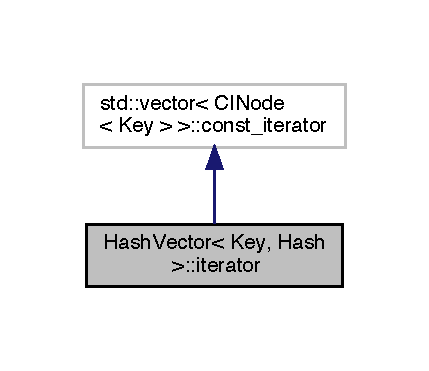
\includegraphics[width=206pt]{class_hash_vector_1_1iterator__inherit__graph}
\end{center}
\end{figure}


Collaboration diagram for Hash\+Vector$<$ Key, Hash $>$\+:\+:iterator\+:
\nopagebreak
\begin{figure}[H]
\begin{center}
\leavevmode
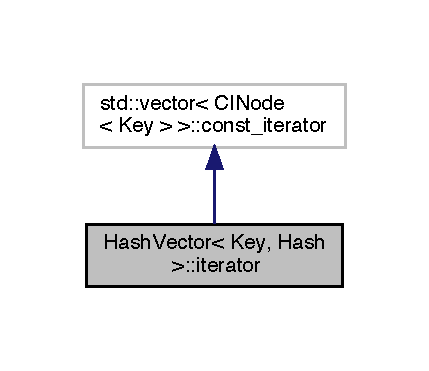
\includegraphics[width=206pt]{class_hash_vector_1_1iterator__coll__graph}
\end{center}
\end{figure}
\subsection*{Public Member Functions}
\begin{DoxyCompactItemize}
\item 
\mbox{\hyperlink{class_hash_vector_1_1iterator_a5181e15feecd37de365ebe86a349a77b}{iterator}} (const typename std\+::vector$<$ C\+I\+Node$<$ Key $>$$>$\+::const\+\_\+iterator it)
\item 
const Key \& \mbox{\hyperlink{class_hash_vector_1_1iterator_a6ec1f0b0b0aba4850fc01340af5fe6d5}{operator$\ast$}} () const
\item 
const Key $\ast$ \mbox{\hyperlink{class_hash_vector_1_1iterator_aaa5e42f71432bbdb464feca674f05690}{operator-\/$>$}} () const
\end{DoxyCompactItemize}


\subsection{Constructor \& Destructor Documentation}
\mbox{\Hypertarget{class_hash_vector_1_1iterator_a5181e15feecd37de365ebe86a349a77b}\label{class_hash_vector_1_1iterator_a5181e15feecd37de365ebe86a349a77b}} 
\index{Hash\+Vector\+::iterator@{Hash\+Vector\+::iterator}!iterator@{iterator}}
\index{iterator@{iterator}!Hash\+Vector\+::iterator@{Hash\+Vector\+::iterator}}
\subsubsection{\texorpdfstring{iterator()}{iterator()}}
{\footnotesize\ttfamily template$<$class Key, class Hash = std\+::hash$<$\+Key$>$$>$ \\
\mbox{\hyperlink{class_hash_vector}{Hash\+Vector}}$<$ Key, Hash $>$\+::iterator\+::iterator (\begin{DoxyParamCaption}\item[{const typename std\+::vector$<$ C\+I\+Node$<$ Key $>$$>$\+::const\+\_\+iterator}]{it }\end{DoxyParamCaption})\hspace{0.3cm}{\ttfamily [inline]}}



\subsection{Member Function Documentation}
\mbox{\Hypertarget{class_hash_vector_1_1iterator_a6ec1f0b0b0aba4850fc01340af5fe6d5}\label{class_hash_vector_1_1iterator_a6ec1f0b0b0aba4850fc01340af5fe6d5}} 
\index{Hash\+Vector\+::iterator@{Hash\+Vector\+::iterator}!operator$\ast$@{operator$\ast$}}
\index{operator$\ast$@{operator$\ast$}!Hash\+Vector\+::iterator@{Hash\+Vector\+::iterator}}
\subsubsection{\texorpdfstring{operator$\ast$()}{operator*()}}
{\footnotesize\ttfamily template$<$class Key, class Hash = std\+::hash$<$\+Key$>$$>$ \\
const Key\& \mbox{\hyperlink{class_hash_vector}{Hash\+Vector}}$<$ Key, Hash $>$\+::iterator\+::operator$\ast$ (\begin{DoxyParamCaption}{ }\end{DoxyParamCaption}) const\hspace{0.3cm}{\ttfamily [inline]}}

\mbox{\Hypertarget{class_hash_vector_1_1iterator_aaa5e42f71432bbdb464feca674f05690}\label{class_hash_vector_1_1iterator_aaa5e42f71432bbdb464feca674f05690}} 
\index{Hash\+Vector\+::iterator@{Hash\+Vector\+::iterator}!operator-\/$>$@{operator-\/$>$}}
\index{operator-\/$>$@{operator-\/$>$}!Hash\+Vector\+::iterator@{Hash\+Vector\+::iterator}}
\subsubsection{\texorpdfstring{operator-\/$>$()}{operator->()}}
{\footnotesize\ttfamily template$<$class Key, class Hash = std\+::hash$<$\+Key$>$$>$ \\
const Key$\ast$ \mbox{\hyperlink{class_hash_vector}{Hash\+Vector}}$<$ Key, Hash $>$\+::iterator\+::operator-\/$>$ (\begin{DoxyParamCaption}{ }\end{DoxyParamCaption}) const\hspace{0.3cm}{\ttfamily [inline]}}



The documentation for this class was generated from the following file\+:\begin{DoxyCompactItemize}
\item 
/\+Users/fevange/\+Source/forte/src/helpers/\mbox{\hyperlink{hash__vector_8h}{hash\+\_\+vector.\+h}}\end{DoxyCompactItemize}

\hypertarget{classforte_1_1_l_a_b_s___s_o_u_r_c_e}{}\section{forte\+:\+:L\+A\+B\+S\+\_\+\+S\+O\+U\+R\+CE Class Reference}
\label{classforte_1_1_l_a_b_s___s_o_u_r_c_e}\index{forte\+::\+L\+A\+B\+S\+\_\+\+S\+O\+U\+R\+CE@{forte\+::\+L\+A\+B\+S\+\_\+\+S\+O\+U\+R\+CE}}


Linear absolute exponential source.  




{\ttfamily \#include $<$dsrg\+\_\+source.\+h$>$}



Inheritance diagram for forte\+:\+:L\+A\+B\+S\+\_\+\+S\+O\+U\+R\+CE\+:
\nopagebreak
\begin{figure}[H]
\begin{center}
\leavevmode
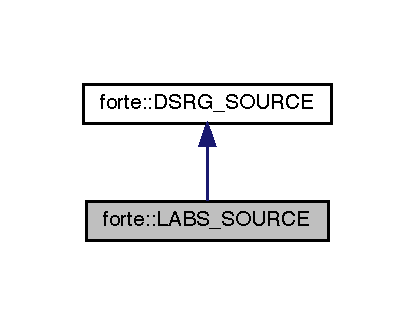
\includegraphics[width=199pt]{classforte_1_1_l_a_b_s___s_o_u_r_c_e__inherit__graph}
\end{center}
\end{figure}


Collaboration diagram for forte\+:\+:L\+A\+B\+S\+\_\+\+S\+O\+U\+R\+CE\+:
\nopagebreak
\begin{figure}[H]
\begin{center}
\leavevmode
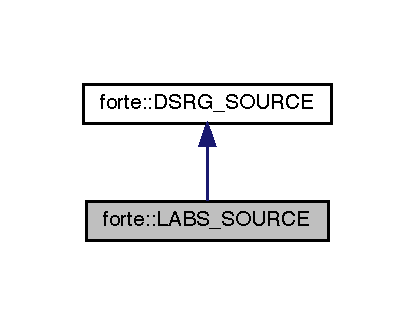
\includegraphics[width=199pt]{classforte_1_1_l_a_b_s___s_o_u_r_c_e__coll__graph}
\end{center}
\end{figure}
\subsection*{Public Member Functions}
\begin{DoxyCompactItemize}
\item 
\mbox{\hyperlink{classforte_1_1_l_a_b_s___s_o_u_r_c_e_adf51d48d65d02aed8b783e2fe077f023}{L\+A\+B\+S\+\_\+\+S\+O\+U\+R\+CE}} (double s, double taylor\+\_\+threshold)
\begin{DoxyCompactList}\small\item\em Constructor. \end{DoxyCompactList}\item 
virtual \mbox{\hyperlink{classforte_1_1_l_a_b_s___s_o_u_r_c_e_a1ab151f0098d4007e64cbeb2cd319e4f}{$\sim$\+L\+A\+B\+S\+\_\+\+S\+O\+U\+R\+CE}} ()
\item 
virtual double \mbox{\hyperlink{classforte_1_1_l_a_b_s___s_o_u_r_c_e_a62a2509bdacd3a8456684b90ba6def30}{compute\+\_\+renormalized}} (const double \&D)
\begin{DoxyCompactList}\small\item\em Return exp(-\/s $\ast$ $\vert$\+D$\vert$) \end{DoxyCompactList}\item 
virtual double \mbox{\hyperlink{classforte_1_1_l_a_b_s___s_o_u_r_c_e_a2bb2384aa4d711db4c3116e466d56835}{compute\+\_\+renormalized\+\_\+denominator}} (const double \&D)
\begin{DoxyCompactList}\small\item\em Return \mbox{[}1 -\/ exp(-\/s $\ast$ $\vert$\+D$\vert$)\mbox{]} / D. \end{DoxyCompactList}\end{DoxyCompactItemize}
\subsection*{Additional Inherited Members}


\subsection{Detailed Description}
Linear absolute exponential source. 

\subsection{Constructor \& Destructor Documentation}
\mbox{\Hypertarget{classforte_1_1_l_a_b_s___s_o_u_r_c_e_adf51d48d65d02aed8b783e2fe077f023}\label{classforte_1_1_l_a_b_s___s_o_u_r_c_e_adf51d48d65d02aed8b783e2fe077f023}} 
\index{forte\+::\+L\+A\+B\+S\+\_\+\+S\+O\+U\+R\+CE@{forte\+::\+L\+A\+B\+S\+\_\+\+S\+O\+U\+R\+CE}!L\+A\+B\+S\+\_\+\+S\+O\+U\+R\+CE@{L\+A\+B\+S\+\_\+\+S\+O\+U\+R\+CE}}
\index{L\+A\+B\+S\+\_\+\+S\+O\+U\+R\+CE@{L\+A\+B\+S\+\_\+\+S\+O\+U\+R\+CE}!forte\+::\+L\+A\+B\+S\+\_\+\+S\+O\+U\+R\+CE@{forte\+::\+L\+A\+B\+S\+\_\+\+S\+O\+U\+R\+CE}}
\subsubsection{\texorpdfstring{L\+A\+B\+S\+\_\+\+S\+O\+U\+R\+C\+E()}{LABS\_SOURCE()}}
{\footnotesize\ttfamily forte\+::\+L\+A\+B\+S\+\_\+\+S\+O\+U\+R\+C\+E\+::\+L\+A\+B\+S\+\_\+\+S\+O\+U\+R\+CE (\begin{DoxyParamCaption}\item[{double}]{s,  }\item[{double}]{taylor\+\_\+threshold }\end{DoxyParamCaption})}



Constructor. 

\mbox{\Hypertarget{classforte_1_1_l_a_b_s___s_o_u_r_c_e_a1ab151f0098d4007e64cbeb2cd319e4f}\label{classforte_1_1_l_a_b_s___s_o_u_r_c_e_a1ab151f0098d4007e64cbeb2cd319e4f}} 
\index{forte\+::\+L\+A\+B\+S\+\_\+\+S\+O\+U\+R\+CE@{forte\+::\+L\+A\+B\+S\+\_\+\+S\+O\+U\+R\+CE}!````~L\+A\+B\+S\+\_\+\+S\+O\+U\+R\+CE@{$\sim$\+L\+A\+B\+S\+\_\+\+S\+O\+U\+R\+CE}}
\index{````~L\+A\+B\+S\+\_\+\+S\+O\+U\+R\+CE@{$\sim$\+L\+A\+B\+S\+\_\+\+S\+O\+U\+R\+CE}!forte\+::\+L\+A\+B\+S\+\_\+\+S\+O\+U\+R\+CE@{forte\+::\+L\+A\+B\+S\+\_\+\+S\+O\+U\+R\+CE}}
\subsubsection{\texorpdfstring{$\sim$\+L\+A\+B\+S\+\_\+\+S\+O\+U\+R\+C\+E()}{~LABS\_SOURCE()}}
{\footnotesize\ttfamily virtual forte\+::\+L\+A\+B\+S\+\_\+\+S\+O\+U\+R\+C\+E\+::$\sim$\+L\+A\+B\+S\+\_\+\+S\+O\+U\+R\+CE (\begin{DoxyParamCaption}{ }\end{DoxyParamCaption})\hspace{0.3cm}{\ttfamily [inline]}, {\ttfamily [virtual]}}



\subsection{Member Function Documentation}
\mbox{\Hypertarget{classforte_1_1_l_a_b_s___s_o_u_r_c_e_a62a2509bdacd3a8456684b90ba6def30}\label{classforte_1_1_l_a_b_s___s_o_u_r_c_e_a62a2509bdacd3a8456684b90ba6def30}} 
\index{forte\+::\+L\+A\+B\+S\+\_\+\+S\+O\+U\+R\+CE@{forte\+::\+L\+A\+B\+S\+\_\+\+S\+O\+U\+R\+CE}!compute\+\_\+renormalized@{compute\+\_\+renormalized}}
\index{compute\+\_\+renormalized@{compute\+\_\+renormalized}!forte\+::\+L\+A\+B\+S\+\_\+\+S\+O\+U\+R\+CE@{forte\+::\+L\+A\+B\+S\+\_\+\+S\+O\+U\+R\+CE}}
\subsubsection{\texorpdfstring{compute\+\_\+renormalized()}{compute\_renormalized()}}
{\footnotesize\ttfamily virtual double forte\+::\+L\+A\+B\+S\+\_\+\+S\+O\+U\+R\+C\+E\+::compute\+\_\+renormalized (\begin{DoxyParamCaption}\item[{const double \&}]{D }\end{DoxyParamCaption})\hspace{0.3cm}{\ttfamily [inline]}, {\ttfamily [virtual]}}



Return exp(-\/s $\ast$ $\vert$\+D$\vert$) 



Implements \mbox{\hyperlink{classforte_1_1_d_s_r_g___s_o_u_r_c_e_a8b4c4428bb50af4561c256e3180f6b31}{forte\+::\+D\+S\+R\+G\+\_\+\+S\+O\+U\+R\+CE}}.

\mbox{\Hypertarget{classforte_1_1_l_a_b_s___s_o_u_r_c_e_a2bb2384aa4d711db4c3116e466d56835}\label{classforte_1_1_l_a_b_s___s_o_u_r_c_e_a2bb2384aa4d711db4c3116e466d56835}} 
\index{forte\+::\+L\+A\+B\+S\+\_\+\+S\+O\+U\+R\+CE@{forte\+::\+L\+A\+B\+S\+\_\+\+S\+O\+U\+R\+CE}!compute\+\_\+renormalized\+\_\+denominator@{compute\+\_\+renormalized\+\_\+denominator}}
\index{compute\+\_\+renormalized\+\_\+denominator@{compute\+\_\+renormalized\+\_\+denominator}!forte\+::\+L\+A\+B\+S\+\_\+\+S\+O\+U\+R\+CE@{forte\+::\+L\+A\+B\+S\+\_\+\+S\+O\+U\+R\+CE}}
\subsubsection{\texorpdfstring{compute\+\_\+renormalized\+\_\+denominator()}{compute\_renormalized\_denominator()}}
{\footnotesize\ttfamily virtual double forte\+::\+L\+A\+B\+S\+\_\+\+S\+O\+U\+R\+C\+E\+::compute\+\_\+renormalized\+\_\+denominator (\begin{DoxyParamCaption}\item[{const double \&}]{D }\end{DoxyParamCaption})\hspace{0.3cm}{\ttfamily [inline]}, {\ttfamily [virtual]}}



Return \mbox{[}1 -\/ exp(-\/s $\ast$ $\vert$\+D$\vert$)\mbox{]} / D. 



Implements \mbox{\hyperlink{classforte_1_1_d_s_r_g___s_o_u_r_c_e_a7345ba63c3612369be7c4cc896b7d5c4}{forte\+::\+D\+S\+R\+G\+\_\+\+S\+O\+U\+R\+CE}}.



The documentation for this class was generated from the following files\+:\begin{DoxyCompactItemize}
\item 
/\+Users/fevange/\+Source/forte/src/mrdsrg-\/helper/\mbox{\hyperlink{dsrg__source_8h}{dsrg\+\_\+source.\+h}}\item 
/\+Users/fevange/\+Source/forte/src/mrdsrg-\/helper/\mbox{\hyperlink{dsrg__source_8cc}{dsrg\+\_\+source.\+cc}}\end{DoxyCompactItemize}

\hypertarget{classforte_1_1_l_b_f_g_s}{}\section{forte\+:\+:L\+B\+F\+GS Class Reference}
\label{classforte_1_1_l_b_f_g_s}\index{forte\+::\+L\+B\+F\+GS@{forte\+::\+L\+B\+F\+GS}}


{\ttfamily \#include $<$lbfgs.\+h$>$}

\subsection*{Public Member Functions}
\begin{DoxyCompactItemize}
\item 
\mbox{\hyperlink{classforte_1_1_l_b_f_g_s_ad3372e79915de6ac76aa5367a3d744e6}{L\+B\+F\+GS}} (std\+::shared\+\_\+ptr$<$ \mbox{\hyperlink{classforte_1_1_l_b_f_g_s___p_a_r_a_m}{L\+B\+F\+G\+S\+\_\+\+P\+A\+R\+AM}} $>$ param)
\begin{DoxyCompactList}\small\item\em Constructor of the Limited-\/\+B\+F\+GS class. \end{DoxyCompactList}\item 
{\footnotesize template$<$class Foo $>$ }\\double \mbox{\hyperlink{classforte_1_1_l_b_f_g_s_a2e1e9e0d39664cb70a631317d3eeea09}{minimize}} (Foo \&foo, psi\+::\+Shared\+Vector x)
\begin{DoxyCompactList}\small\item\em The minimization for the target function. \end{DoxyCompactList}\item 
void \mbox{\hyperlink{classforte_1_1_l_b_f_g_s_ae1925cb32a7963640d6f0b07d4a4e8c0}{reset}} ()
\begin{DoxyCompactList}\small\item\em Reset the L-\/\+B\+F\+GS space. \end{DoxyCompactList}\item 
psi\+::\+Shared\+Vector \mbox{\hyperlink{classforte_1_1_l_b_f_g_s_ac92f946ad0a620b0fef33b96619b0b75}{g}} ()
\begin{DoxyCompactList}\small\item\em Return the current / final gradient vector. \end{DoxyCompactList}\item 
int \mbox{\hyperlink{classforte_1_1_l_b_f_g_s_a90ca8b4968b604d3215c0ea4ce6275d4}{iter}} ()
\begin{DoxyCompactList}\small\item\em Return the final number of iterations. \end{DoxyCompactList}\item 
bool \mbox{\hyperlink{classforte_1_1_l_b_f_g_s_ab42bf7fe9e2a7eafd004773f9b606b65}{converged}} ()
\begin{DoxyCompactList}\small\item\em Return true if minimization converged. \end{DoxyCompactList}\end{DoxyCompactItemize}


\subsection{Constructor \& Destructor Documentation}
\mbox{\Hypertarget{classforte_1_1_l_b_f_g_s_ad3372e79915de6ac76aa5367a3d744e6}\label{classforte_1_1_l_b_f_g_s_ad3372e79915de6ac76aa5367a3d744e6}} 
\index{forte\+::\+L\+B\+F\+GS@{forte\+::\+L\+B\+F\+GS}!L\+B\+F\+GS@{L\+B\+F\+GS}}
\index{L\+B\+F\+GS@{L\+B\+F\+GS}!forte\+::\+L\+B\+F\+GS@{forte\+::\+L\+B\+F\+GS}}
\subsubsection{\texorpdfstring{L\+B\+F\+G\+S()}{LBFGS()}}
{\footnotesize\ttfamily forte\+::\+L\+B\+F\+G\+S\+::\+L\+B\+F\+GS (\begin{DoxyParamCaption}\item[{std\+::shared\+\_\+ptr$<$ \mbox{\hyperlink{classforte_1_1_l_b_f_g_s___p_a_r_a_m}{L\+B\+F\+G\+S\+\_\+\+P\+A\+R\+AM}} $>$}]{param }\end{DoxyParamCaption})}



Constructor of the Limited-\/\+B\+F\+GS class. 


\begin{DoxyParams}{Parameters}
{\em dim} & The dimension of the problem \\
\hline
{\em param} & The \mbox{\hyperlink{classforte_1_1_l_b_f_g_s___p_a_r_a_m}{L\+B\+F\+G\+S\+\_\+\+P\+A\+R\+AM}} object for L-\/\+B\+F\+GS parameters\\
\hline
\end{DoxyParams}
Implementation notes\+: See Wikipedia \href{https://en.wikipedia.org/wiki/Limited-memory_BFGS}{\tt https\+://en.\+wikipedia.\+org/wiki/\+Limited-\/memory\+\_\+\+B\+F\+GS} and $<$\+Numerical optimization$>$=\char`\"{}\char`\"{}$>$ 2nd Ed. by Jorge Nocedal and Stephen J. Wright 

\subsection{Member Function Documentation}
\mbox{\Hypertarget{classforte_1_1_l_b_f_g_s_ab42bf7fe9e2a7eafd004773f9b606b65}\label{classforte_1_1_l_b_f_g_s_ab42bf7fe9e2a7eafd004773f9b606b65}} 
\index{forte\+::\+L\+B\+F\+GS@{forte\+::\+L\+B\+F\+GS}!converged@{converged}}
\index{converged@{converged}!forte\+::\+L\+B\+F\+GS@{forte\+::\+L\+B\+F\+GS}}
\subsubsection{\texorpdfstring{converged()}{converged()}}
{\footnotesize\ttfamily bool forte\+::\+L\+B\+F\+G\+S\+::converged (\begin{DoxyParamCaption}{ }\end{DoxyParamCaption})\hspace{0.3cm}{\ttfamily [inline]}}



Return true if minimization converged. 

\mbox{\Hypertarget{classforte_1_1_l_b_f_g_s_ac92f946ad0a620b0fef33b96619b0b75}\label{classforte_1_1_l_b_f_g_s_ac92f946ad0a620b0fef33b96619b0b75}} 
\index{forte\+::\+L\+B\+F\+GS@{forte\+::\+L\+B\+F\+GS}!g@{g}}
\index{g@{g}!forte\+::\+L\+B\+F\+GS@{forte\+::\+L\+B\+F\+GS}}
\subsubsection{\texorpdfstring{g()}{g()}}
{\footnotesize\ttfamily psi\+::\+Shared\+Vector forte\+::\+L\+B\+F\+G\+S\+::g (\begin{DoxyParamCaption}{ }\end{DoxyParamCaption})\hspace{0.3cm}{\ttfamily [inline]}}



Return the current / final gradient vector. 

\mbox{\Hypertarget{classforte_1_1_l_b_f_g_s_a90ca8b4968b604d3215c0ea4ce6275d4}\label{classforte_1_1_l_b_f_g_s_a90ca8b4968b604d3215c0ea4ce6275d4}} 
\index{forte\+::\+L\+B\+F\+GS@{forte\+::\+L\+B\+F\+GS}!iter@{iter}}
\index{iter@{iter}!forte\+::\+L\+B\+F\+GS@{forte\+::\+L\+B\+F\+GS}}
\subsubsection{\texorpdfstring{iter()}{iter()}}
{\footnotesize\ttfamily int forte\+::\+L\+B\+F\+G\+S\+::iter (\begin{DoxyParamCaption}{ }\end{DoxyParamCaption})\hspace{0.3cm}{\ttfamily [inline]}}



Return the final number of iterations. 

\mbox{\Hypertarget{classforte_1_1_l_b_f_g_s_a2e1e9e0d39664cb70a631317d3eeea09}\label{classforte_1_1_l_b_f_g_s_a2e1e9e0d39664cb70a631317d3eeea09}} 
\index{forte\+::\+L\+B\+F\+GS@{forte\+::\+L\+B\+F\+GS}!minimize@{minimize}}
\index{minimize@{minimize}!forte\+::\+L\+B\+F\+GS@{forte\+::\+L\+B\+F\+GS}}
\subsubsection{\texorpdfstring{minimize()}{minimize()}}
{\footnotesize\ttfamily template$<$class Foo $>$ \\
template double forte\+::\+L\+B\+F\+G\+S\+::minimize (\begin{DoxyParamCaption}\item[{Foo \&}]{foo,  }\item[{psi\+::\+Shared\+Vector}]{x }\end{DoxyParamCaption})}



The minimization for the target function. 


\begin{DoxyParams}{Parameters}
{\em foo} & Target class that should have the following methods\+: fx = foo.\+evaluate(x, g, do\+\_\+g=true) where gradient g is modified by the function, fx is the function return value, and g is computed when do\+\_\+g is true. If diagonal Hessian is specified, foo.\+hess\+\_\+diag(x, h0) should be available. \\
\hline
{\em x} & The initial value of x as input, the final value of x as output.\\
\hline
\end{DoxyParams}
\begin{DoxyReturn}{Returns}
the function value of at optimized x 
\end{DoxyReturn}
\mbox{\Hypertarget{classforte_1_1_l_b_f_g_s_ae1925cb32a7963640d6f0b07d4a4e8c0}\label{classforte_1_1_l_b_f_g_s_ae1925cb32a7963640d6f0b07d4a4e8c0}} 
\index{forte\+::\+L\+B\+F\+GS@{forte\+::\+L\+B\+F\+GS}!reset@{reset}}
\index{reset@{reset}!forte\+::\+L\+B\+F\+GS@{forte\+::\+L\+B\+F\+GS}}
\subsubsection{\texorpdfstring{reset()}{reset()}}
{\footnotesize\ttfamily void forte\+::\+L\+B\+F\+G\+S\+::reset (\begin{DoxyParamCaption}{ }\end{DoxyParamCaption})}



Reset the L-\/\+B\+F\+GS space. 



The documentation for this class was generated from the following files\+:\begin{DoxyCompactItemize}
\item 
/\+Users/fevange/\+Source/forte/src/helpers/lbfgs/\mbox{\hyperlink{lbfgs_8h}{lbfgs.\+h}}\item 
/\+Users/fevange/\+Source/forte/src/helpers/lbfgs/\mbox{\hyperlink{lbfgs_8cc}{lbfgs.\+cc}}\end{DoxyCompactItemize}

\hypertarget{classforte_1_1_l_b_f_g_s___p_a_r_a_m}{}\section{forte\+:\+:L\+B\+F\+G\+S\+\_\+\+P\+A\+R\+AM Class Reference}
\label{classforte_1_1_l_b_f_g_s___p_a_r_a_m}\index{forte\+::\+L\+B\+F\+G\+S\+\_\+\+P\+A\+R\+AM@{forte\+::\+L\+B\+F\+G\+S\+\_\+\+P\+A\+R\+AM}}


{\ttfamily \#include $<$lbfgs\+\_\+param.\+h$>$}

\subsection*{Public Types}
\begin{DoxyCompactItemize}
\item 
enum \mbox{\hyperlink{classforte_1_1_l_b_f_g_s___p_a_r_a_m_a2651cd29e6c97352a8b72df089d97cfa}{S\+T\+E\+P\+\_\+\+L\+E\+N\+G\+T\+H\+\_\+\+M\+E\+T\+H\+OD}} \{ \mbox{\hyperlink{classforte_1_1_l_b_f_g_s___p_a_r_a_m_a2651cd29e6c97352a8b72df089d97cfaa8a6708ac2b09ab567f08a166a52a5ce1}{S\+T\+E\+P\+\_\+\+L\+E\+N\+G\+T\+H\+\_\+\+M\+E\+T\+H\+O\+D\+::\+M\+A\+X\+\_\+\+C\+O\+R\+R\+E\+C\+T\+I\+ON}}, 
\mbox{\hyperlink{classforte_1_1_l_b_f_g_s___p_a_r_a_m_a2651cd29e6c97352a8b72df089d97cfaa14c2c93ba687e96ccc6256162aad5eeb}{S\+T\+E\+P\+\_\+\+L\+E\+N\+G\+T\+H\+\_\+\+M\+E\+T\+H\+O\+D\+::\+L\+I\+N\+E\+\_\+\+B\+A\+C\+K\+T\+R\+A\+C\+K\+I\+NG}}, 
\mbox{\hyperlink{classforte_1_1_l_b_f_g_s___p_a_r_a_m_a2651cd29e6c97352a8b72df089d97cfaac06ac8233c6dcaffb114f6c6a537e58d}{S\+T\+E\+P\+\_\+\+L\+E\+N\+G\+T\+H\+\_\+\+M\+E\+T\+H\+O\+D\+::\+L\+I\+N\+E\+\_\+\+B\+R\+A\+C\+K\+E\+T\+I\+N\+G\+\_\+\+Z\+O\+OM}}
 \}
\begin{DoxyCompactList}\small\item\em Schemes to determine step lengths. \end{DoxyCompactList}\item 
enum \mbox{\hyperlink{classforte_1_1_l_b_f_g_s___p_a_r_a_m_a363135a6d4f1aa7a5f37a1b5f2a53cc3}{L\+I\+N\+E\+\_\+\+S\+E\+A\+R\+C\+H\+\_\+\+C\+O\+N\+D\+I\+T\+I\+ON}} \{ \mbox{\hyperlink{classforte_1_1_l_b_f_g_s___p_a_r_a_m_a363135a6d4f1aa7a5f37a1b5f2a53cc3a5fd7e4932940fa185613827c61c7949c}{L\+I\+N\+E\+\_\+\+S\+E\+A\+R\+C\+H\+\_\+\+C\+O\+N\+D\+I\+T\+I\+O\+N\+::\+A\+R\+M\+I\+JO}}, 
\mbox{\hyperlink{classforte_1_1_l_b_f_g_s___p_a_r_a_m_a363135a6d4f1aa7a5f37a1b5f2a53cc3ae19ed819ed6243cb715f5e5cb5805fb0}{L\+I\+N\+E\+\_\+\+S\+E\+A\+R\+C\+H\+\_\+\+C\+O\+N\+D\+I\+T\+I\+O\+N\+::\+W\+O\+L\+FE}}, 
\mbox{\hyperlink{classforte_1_1_l_b_f_g_s___p_a_r_a_m_a363135a6d4f1aa7a5f37a1b5f2a53cc3acc463f663dcd166f17450eea5f4abef9}{L\+I\+N\+E\+\_\+\+S\+E\+A\+R\+C\+H\+\_\+\+C\+O\+N\+D\+I\+T\+I\+O\+N\+::\+S\+T\+R\+O\+N\+G\+\_\+\+W\+O\+L\+FE}}
 \}
\begin{DoxyCompactList}\small\item\em Condition to terminate line search backtracking. \end{DoxyCompactList}\end{DoxyCompactItemize}
\subsection*{Public Member Functions}
\begin{DoxyCompactItemize}
\item 
\mbox{\hyperlink{classforte_1_1_l_b_f_g_s___p_a_r_a_m_a65811f626250bb99c51c0283904db95d}{L\+B\+F\+G\+S\+\_\+\+P\+A\+R\+AM}} ()
\begin{DoxyCompactList}\small\item\em Default constructor of the Limited-\/\+B\+F\+GS parameter class set defaut. \end{DoxyCompactList}\item 
void \mbox{\hyperlink{classforte_1_1_l_b_f_g_s___p_a_r_a_m_a41b9a49bbeb64924c317ee23385b3744}{check\+\_\+param}} ()
\begin{DoxyCompactList}\small\item\em Check if the parameters make sense. \end{DoxyCompactList}\end{DoxyCompactItemize}
\subsection*{Public Attributes}
\begin{DoxyCompactItemize}
\item 
int \mbox{\hyperlink{classforte_1_1_l_b_f_g_s___p_a_r_a_m_afdd5c3492553b2b9d9054c379f99d84f}{print}}
\begin{DoxyCompactList}\small\item\em Printing level. \end{DoxyCompactList}\item 
int \mbox{\hyperlink{classforte_1_1_l_b_f_g_s___p_a_r_a_m_ad18715f483efe2d746efbb086c4a2c49}{m}}
\begin{DoxyCompactList}\small\item\em The number of vectors kept. \end{DoxyCompactList}\item 
double \mbox{\hyperlink{classforte_1_1_l_b_f_g_s___p_a_r_a_m_a847271853a38901d91f047d0a765d78a}{epsilon}}
\begin{DoxyCompactList}\small\item\em Convergence threshold to terminate the minimization\+: $\vert$g$\vert$ $<$ ε $\ast$ max(1, $\vert$x$\vert$) \end{DoxyCompactList}\item 
int \mbox{\hyperlink{classforte_1_1_l_b_f_g_s___p_a_r_a_m_ae14e5287f2c8fc27cd93a5d08fd520b7}{maxiter}}
\begin{DoxyCompactList}\small\item\em Max number of iterations. \end{DoxyCompactList}\item 
int \mbox{\hyperlink{classforte_1_1_l_b_f_g_s___p_a_r_a_m_a198ce3d6da0e511c4ea0469e52af9806}{h0\+\_\+freq}}
\item 
\mbox{\hyperlink{classforte_1_1_l_b_f_g_s___p_a_r_a_m_a2651cd29e6c97352a8b72df089d97cfa}{S\+T\+E\+P\+\_\+\+L\+E\+N\+G\+T\+H\+\_\+\+M\+E\+T\+H\+OD}} \mbox{\hyperlink{classforte_1_1_l_b_f_g_s___p_a_r_a_m_a162b78847700b01f76621ab357267172}{step\+\_\+length\+\_\+method}}
\item 
double \mbox{\hyperlink{classforte_1_1_l_b_f_g_s___p_a_r_a_m_a5e799aee5fcd1bcf2253d5c80e7b8ed9}{max\+\_\+dir}}
\begin{DoxyCompactList}\small\item\em Max absolute value allowed in direction vector. \end{DoxyCompactList}\item 
int \mbox{\hyperlink{classforte_1_1_l_b_f_g_s___p_a_r_a_m_a1017d0ef8d7837271124b08be046a0bf}{maxiter\+\_\+linesearch}}
\begin{DoxyCompactList}\small\item\em Max number of trials for line search of optimal step length. \end{DoxyCompactList}\item 
double \mbox{\hyperlink{classforte_1_1_l_b_f_g_s___p_a_r_a_m_a907fd1cc91d37628fc5dff3c2ae2fc98}{min\+\_\+step}}
\begin{DoxyCompactList}\small\item\em Minimal step length allowed. \end{DoxyCompactList}\item 
double \mbox{\hyperlink{classforte_1_1_l_b_f_g_s___p_a_r_a_m_a0217fa9bf14c3daf9dc8619efd39eea4}{max\+\_\+step}}
\begin{DoxyCompactList}\small\item\em Maximal step length allowed. \end{DoxyCompactList}\item 
\mbox{\hyperlink{classforte_1_1_l_b_f_g_s___p_a_r_a_m_a363135a6d4f1aa7a5f37a1b5f2a53cc3}{L\+I\+N\+E\+\_\+\+S\+E\+A\+R\+C\+H\+\_\+\+C\+O\+N\+D\+I\+T\+I\+ON}} \mbox{\hyperlink{classforte_1_1_l_b_f_g_s___p_a_r_a_m_a6e6712b25aaf9a87e64cbb1015dd7ddb}{line\+\_\+search\+\_\+condition}}
\item 
double \mbox{\hyperlink{classforte_1_1_l_b_f_g_s___p_a_r_a_m_a9f1cc2c45b81cc90e1fc16d3617cda36}{c1}}
\begin{DoxyCompactList}\small\item\em Parameter for Armijo condition. \end{DoxyCompactList}\item 
double \mbox{\hyperlink{classforte_1_1_l_b_f_g_s___p_a_r_a_m_a41c8926f2b22beb5230b370527585127}{c2}}
\begin{DoxyCompactList}\small\item\em Parameter for Wolfe curvature condition. \end{DoxyCompactList}\end{DoxyCompactItemize}


\subsection{Member Enumeration Documentation}
\mbox{\Hypertarget{classforte_1_1_l_b_f_g_s___p_a_r_a_m_a363135a6d4f1aa7a5f37a1b5f2a53cc3}\label{classforte_1_1_l_b_f_g_s___p_a_r_a_m_a363135a6d4f1aa7a5f37a1b5f2a53cc3}} 
\index{forte\+::\+L\+B\+F\+G\+S\+\_\+\+P\+A\+R\+AM@{forte\+::\+L\+B\+F\+G\+S\+\_\+\+P\+A\+R\+AM}!L\+I\+N\+E\+\_\+\+S\+E\+A\+R\+C\+H\+\_\+\+C\+O\+N\+D\+I\+T\+I\+ON@{L\+I\+N\+E\+\_\+\+S\+E\+A\+R\+C\+H\+\_\+\+C\+O\+N\+D\+I\+T\+I\+ON}}
\index{L\+I\+N\+E\+\_\+\+S\+E\+A\+R\+C\+H\+\_\+\+C\+O\+N\+D\+I\+T\+I\+ON@{L\+I\+N\+E\+\_\+\+S\+E\+A\+R\+C\+H\+\_\+\+C\+O\+N\+D\+I\+T\+I\+ON}!forte\+::\+L\+B\+F\+G\+S\+\_\+\+P\+A\+R\+AM@{forte\+::\+L\+B\+F\+G\+S\+\_\+\+P\+A\+R\+AM}}
\subsubsection{\texorpdfstring{L\+I\+N\+E\+\_\+\+S\+E\+A\+R\+C\+H\+\_\+\+C\+O\+N\+D\+I\+T\+I\+ON}{LINE\_SEARCH\_CONDITION}}
{\footnotesize\ttfamily enum \mbox{\hyperlink{classforte_1_1_l_b_f_g_s___p_a_r_a_m_a363135a6d4f1aa7a5f37a1b5f2a53cc3}{forte\+::\+L\+B\+F\+G\+S\+\_\+\+P\+A\+R\+A\+M\+::\+L\+I\+N\+E\+\_\+\+S\+E\+A\+R\+C\+H\+\_\+\+C\+O\+N\+D\+I\+T\+I\+ON}}\hspace{0.3cm}{\ttfamily [strong]}}



Condition to terminate line search backtracking. 

\begin{DoxyEnumFields}{Enumerator}
\raisebox{\heightof{T}}[0pt][0pt]{\index{A\+R\+M\+I\+JO@{A\+R\+M\+I\+JO}!forte\+::\+L\+B\+F\+G\+S\+\_\+\+P\+A\+R\+AM@{forte\+::\+L\+B\+F\+G\+S\+\_\+\+P\+A\+R\+AM}}\index{forte\+::\+L\+B\+F\+G\+S\+\_\+\+P\+A\+R\+AM@{forte\+::\+L\+B\+F\+G\+S\+\_\+\+P\+A\+R\+AM}!A\+R\+M\+I\+JO@{A\+R\+M\+I\+JO}}}\mbox{\Hypertarget{classforte_1_1_l_b_f_g_s___p_a_r_a_m_a363135a6d4f1aa7a5f37a1b5f2a53cc3a5fd7e4932940fa185613827c61c7949c}\label{classforte_1_1_l_b_f_g_s___p_a_r_a_m_a363135a6d4f1aa7a5f37a1b5f2a53cc3a5fd7e4932940fa185613827c61c7949c}} 
A\+R\+M\+I\+JO&\\
\hline

\raisebox{\heightof{T}}[0pt][0pt]{\index{W\+O\+L\+FE@{W\+O\+L\+FE}!forte\+::\+L\+B\+F\+G\+S\+\_\+\+P\+A\+R\+AM@{forte\+::\+L\+B\+F\+G\+S\+\_\+\+P\+A\+R\+AM}}\index{forte\+::\+L\+B\+F\+G\+S\+\_\+\+P\+A\+R\+AM@{forte\+::\+L\+B\+F\+G\+S\+\_\+\+P\+A\+R\+AM}!W\+O\+L\+FE@{W\+O\+L\+FE}}}\mbox{\Hypertarget{classforte_1_1_l_b_f_g_s___p_a_r_a_m_a363135a6d4f1aa7a5f37a1b5f2a53cc3ae19ed819ed6243cb715f5e5cb5805fb0}\label{classforte_1_1_l_b_f_g_s___p_a_r_a_m_a363135a6d4f1aa7a5f37a1b5f2a53cc3ae19ed819ed6243cb715f5e5cb5805fb0}} 
W\+O\+L\+FE&\\
\hline

\raisebox{\heightof{T}}[0pt][0pt]{\index{S\+T\+R\+O\+N\+G\+\_\+\+W\+O\+L\+FE@{S\+T\+R\+O\+N\+G\+\_\+\+W\+O\+L\+FE}!forte\+::\+L\+B\+F\+G\+S\+\_\+\+P\+A\+R\+AM@{forte\+::\+L\+B\+F\+G\+S\+\_\+\+P\+A\+R\+AM}}\index{forte\+::\+L\+B\+F\+G\+S\+\_\+\+P\+A\+R\+AM@{forte\+::\+L\+B\+F\+G\+S\+\_\+\+P\+A\+R\+AM}!S\+T\+R\+O\+N\+G\+\_\+\+W\+O\+L\+FE@{S\+T\+R\+O\+N\+G\+\_\+\+W\+O\+L\+FE}}}\mbox{\Hypertarget{classforte_1_1_l_b_f_g_s___p_a_r_a_m_a363135a6d4f1aa7a5f37a1b5f2a53cc3acc463f663dcd166f17450eea5f4abef9}\label{classforte_1_1_l_b_f_g_s___p_a_r_a_m_a363135a6d4f1aa7a5f37a1b5f2a53cc3acc463f663dcd166f17450eea5f4abef9}} 
S\+T\+R\+O\+N\+G\+\_\+\+W\+O\+L\+FE&\\
\hline

\end{DoxyEnumFields}
\mbox{\Hypertarget{classforte_1_1_l_b_f_g_s___p_a_r_a_m_a2651cd29e6c97352a8b72df089d97cfa}\label{classforte_1_1_l_b_f_g_s___p_a_r_a_m_a2651cd29e6c97352a8b72df089d97cfa}} 
\index{forte\+::\+L\+B\+F\+G\+S\+\_\+\+P\+A\+R\+AM@{forte\+::\+L\+B\+F\+G\+S\+\_\+\+P\+A\+R\+AM}!S\+T\+E\+P\+\_\+\+L\+E\+N\+G\+T\+H\+\_\+\+M\+E\+T\+H\+OD@{S\+T\+E\+P\+\_\+\+L\+E\+N\+G\+T\+H\+\_\+\+M\+E\+T\+H\+OD}}
\index{S\+T\+E\+P\+\_\+\+L\+E\+N\+G\+T\+H\+\_\+\+M\+E\+T\+H\+OD@{S\+T\+E\+P\+\_\+\+L\+E\+N\+G\+T\+H\+\_\+\+M\+E\+T\+H\+OD}!forte\+::\+L\+B\+F\+G\+S\+\_\+\+P\+A\+R\+AM@{forte\+::\+L\+B\+F\+G\+S\+\_\+\+P\+A\+R\+AM}}
\subsubsection{\texorpdfstring{S\+T\+E\+P\+\_\+\+L\+E\+N\+G\+T\+H\+\_\+\+M\+E\+T\+H\+OD}{STEP\_LENGTH\_METHOD}}
{\footnotesize\ttfamily enum \mbox{\hyperlink{classforte_1_1_l_b_f_g_s___p_a_r_a_m_a2651cd29e6c97352a8b72df089d97cfa}{forte\+::\+L\+B\+F\+G\+S\+\_\+\+P\+A\+R\+A\+M\+::\+S\+T\+E\+P\+\_\+\+L\+E\+N\+G\+T\+H\+\_\+\+M\+E\+T\+H\+OD}}\hspace{0.3cm}{\ttfamily [strong]}}



Schemes to determine step lengths. 

\begin{DoxyEnumFields}{Enumerator}
\raisebox{\heightof{T}}[0pt][0pt]{\index{M\+A\+X\+\_\+\+C\+O\+R\+R\+E\+C\+T\+I\+ON@{M\+A\+X\+\_\+\+C\+O\+R\+R\+E\+C\+T\+I\+ON}!forte\+::\+L\+B\+F\+G\+S\+\_\+\+P\+A\+R\+AM@{forte\+::\+L\+B\+F\+G\+S\+\_\+\+P\+A\+R\+AM}}\index{forte\+::\+L\+B\+F\+G\+S\+\_\+\+P\+A\+R\+AM@{forte\+::\+L\+B\+F\+G\+S\+\_\+\+P\+A\+R\+AM}!M\+A\+X\+\_\+\+C\+O\+R\+R\+E\+C\+T\+I\+ON@{M\+A\+X\+\_\+\+C\+O\+R\+R\+E\+C\+T\+I\+ON}}}\mbox{\Hypertarget{classforte_1_1_l_b_f_g_s___p_a_r_a_m_a2651cd29e6c97352a8b72df089d97cfaa8a6708ac2b09ab567f08a166a52a5ce1}\label{classforte_1_1_l_b_f_g_s___p_a_r_a_m_a2651cd29e6c97352a8b72df089d97cfaa8a6708ac2b09ab567f08a166a52a5ce1}} 
M\+A\+X\+\_\+\+C\+O\+R\+R\+E\+C\+T\+I\+ON&\\
\hline

\raisebox{\heightof{T}}[0pt][0pt]{\index{L\+I\+N\+E\+\_\+\+B\+A\+C\+K\+T\+R\+A\+C\+K\+I\+NG@{L\+I\+N\+E\+\_\+\+B\+A\+C\+K\+T\+R\+A\+C\+K\+I\+NG}!forte\+::\+L\+B\+F\+G\+S\+\_\+\+P\+A\+R\+AM@{forte\+::\+L\+B\+F\+G\+S\+\_\+\+P\+A\+R\+AM}}\index{forte\+::\+L\+B\+F\+G\+S\+\_\+\+P\+A\+R\+AM@{forte\+::\+L\+B\+F\+G\+S\+\_\+\+P\+A\+R\+AM}!L\+I\+N\+E\+\_\+\+B\+A\+C\+K\+T\+R\+A\+C\+K\+I\+NG@{L\+I\+N\+E\+\_\+\+B\+A\+C\+K\+T\+R\+A\+C\+K\+I\+NG}}}\mbox{\Hypertarget{classforte_1_1_l_b_f_g_s___p_a_r_a_m_a2651cd29e6c97352a8b72df089d97cfaa14c2c93ba687e96ccc6256162aad5eeb}\label{classforte_1_1_l_b_f_g_s___p_a_r_a_m_a2651cd29e6c97352a8b72df089d97cfaa14c2c93ba687e96ccc6256162aad5eeb}} 
L\+I\+N\+E\+\_\+\+B\+A\+C\+K\+T\+R\+A\+C\+K\+I\+NG&\\
\hline

\raisebox{\heightof{T}}[0pt][0pt]{\index{L\+I\+N\+E\+\_\+\+B\+R\+A\+C\+K\+E\+T\+I\+N\+G\+\_\+\+Z\+O\+OM@{L\+I\+N\+E\+\_\+\+B\+R\+A\+C\+K\+E\+T\+I\+N\+G\+\_\+\+Z\+O\+OM}!forte\+::\+L\+B\+F\+G\+S\+\_\+\+P\+A\+R\+AM@{forte\+::\+L\+B\+F\+G\+S\+\_\+\+P\+A\+R\+AM}}\index{forte\+::\+L\+B\+F\+G\+S\+\_\+\+P\+A\+R\+AM@{forte\+::\+L\+B\+F\+G\+S\+\_\+\+P\+A\+R\+AM}!L\+I\+N\+E\+\_\+\+B\+R\+A\+C\+K\+E\+T\+I\+N\+G\+\_\+\+Z\+O\+OM@{L\+I\+N\+E\+\_\+\+B\+R\+A\+C\+K\+E\+T\+I\+N\+G\+\_\+\+Z\+O\+OM}}}\mbox{\Hypertarget{classforte_1_1_l_b_f_g_s___p_a_r_a_m_a2651cd29e6c97352a8b72df089d97cfaac06ac8233c6dcaffb114f6c6a537e58d}\label{classforte_1_1_l_b_f_g_s___p_a_r_a_m_a2651cd29e6c97352a8b72df089d97cfaac06ac8233c6dcaffb114f6c6a537e58d}} 
L\+I\+N\+E\+\_\+\+B\+R\+A\+C\+K\+E\+T\+I\+N\+G\+\_\+\+Z\+O\+OM&\\
\hline

\end{DoxyEnumFields}


\subsection{Constructor \& Destructor Documentation}
\mbox{\Hypertarget{classforte_1_1_l_b_f_g_s___p_a_r_a_m_a65811f626250bb99c51c0283904db95d}\label{classforte_1_1_l_b_f_g_s___p_a_r_a_m_a65811f626250bb99c51c0283904db95d}} 
\index{forte\+::\+L\+B\+F\+G\+S\+\_\+\+P\+A\+R\+AM@{forte\+::\+L\+B\+F\+G\+S\+\_\+\+P\+A\+R\+AM}!L\+B\+F\+G\+S\+\_\+\+P\+A\+R\+AM@{L\+B\+F\+G\+S\+\_\+\+P\+A\+R\+AM}}
\index{L\+B\+F\+G\+S\+\_\+\+P\+A\+R\+AM@{L\+B\+F\+G\+S\+\_\+\+P\+A\+R\+AM}!forte\+::\+L\+B\+F\+G\+S\+\_\+\+P\+A\+R\+AM@{forte\+::\+L\+B\+F\+G\+S\+\_\+\+P\+A\+R\+AM}}
\subsubsection{\texorpdfstring{L\+B\+F\+G\+S\+\_\+\+P\+A\+R\+A\+M()}{LBFGS\_PARAM()}}
{\footnotesize\ttfamily forte\+::\+L\+B\+F\+G\+S\+\_\+\+P\+A\+R\+A\+M\+::\+L\+B\+F\+G\+S\+\_\+\+P\+A\+R\+AM (\begin{DoxyParamCaption}{ }\end{DoxyParamCaption})}



Default constructor of the Limited-\/\+B\+F\+GS parameter class set defaut. 



\subsection{Member Function Documentation}
\mbox{\Hypertarget{classforte_1_1_l_b_f_g_s___p_a_r_a_m_a41b9a49bbeb64924c317ee23385b3744}\label{classforte_1_1_l_b_f_g_s___p_a_r_a_m_a41b9a49bbeb64924c317ee23385b3744}} 
\index{forte\+::\+L\+B\+F\+G\+S\+\_\+\+P\+A\+R\+AM@{forte\+::\+L\+B\+F\+G\+S\+\_\+\+P\+A\+R\+AM}!check\+\_\+param@{check\+\_\+param}}
\index{check\+\_\+param@{check\+\_\+param}!forte\+::\+L\+B\+F\+G\+S\+\_\+\+P\+A\+R\+AM@{forte\+::\+L\+B\+F\+G\+S\+\_\+\+P\+A\+R\+AM}}
\subsubsection{\texorpdfstring{check\+\_\+param()}{check\_param()}}
{\footnotesize\ttfamily void forte\+::\+L\+B\+F\+G\+S\+\_\+\+P\+A\+R\+A\+M\+::check\+\_\+param (\begin{DoxyParamCaption}{ }\end{DoxyParamCaption})}



Check if the parameters make sense. 



\subsection{Member Data Documentation}
\mbox{\Hypertarget{classforte_1_1_l_b_f_g_s___p_a_r_a_m_a9f1cc2c45b81cc90e1fc16d3617cda36}\label{classforte_1_1_l_b_f_g_s___p_a_r_a_m_a9f1cc2c45b81cc90e1fc16d3617cda36}} 
\index{forte\+::\+L\+B\+F\+G\+S\+\_\+\+P\+A\+R\+AM@{forte\+::\+L\+B\+F\+G\+S\+\_\+\+P\+A\+R\+AM}!c1@{c1}}
\index{c1@{c1}!forte\+::\+L\+B\+F\+G\+S\+\_\+\+P\+A\+R\+AM@{forte\+::\+L\+B\+F\+G\+S\+\_\+\+P\+A\+R\+AM}}
\subsubsection{\texorpdfstring{c1}{c1}}
{\footnotesize\ttfamily double forte\+::\+L\+B\+F\+G\+S\+\_\+\+P\+A\+R\+A\+M\+::c1}



Parameter for Armijo condition. 

\mbox{\Hypertarget{classforte_1_1_l_b_f_g_s___p_a_r_a_m_a41c8926f2b22beb5230b370527585127}\label{classforte_1_1_l_b_f_g_s___p_a_r_a_m_a41c8926f2b22beb5230b370527585127}} 
\index{forte\+::\+L\+B\+F\+G\+S\+\_\+\+P\+A\+R\+AM@{forte\+::\+L\+B\+F\+G\+S\+\_\+\+P\+A\+R\+AM}!c2@{c2}}
\index{c2@{c2}!forte\+::\+L\+B\+F\+G\+S\+\_\+\+P\+A\+R\+AM@{forte\+::\+L\+B\+F\+G\+S\+\_\+\+P\+A\+R\+AM}}
\subsubsection{\texorpdfstring{c2}{c2}}
{\footnotesize\ttfamily double forte\+::\+L\+B\+F\+G\+S\+\_\+\+P\+A\+R\+A\+M\+::c2}



Parameter for Wolfe curvature condition. 

\mbox{\Hypertarget{classforte_1_1_l_b_f_g_s___p_a_r_a_m_a847271853a38901d91f047d0a765d78a}\label{classforte_1_1_l_b_f_g_s___p_a_r_a_m_a847271853a38901d91f047d0a765d78a}} 
\index{forte\+::\+L\+B\+F\+G\+S\+\_\+\+P\+A\+R\+AM@{forte\+::\+L\+B\+F\+G\+S\+\_\+\+P\+A\+R\+AM}!epsilon@{epsilon}}
\index{epsilon@{epsilon}!forte\+::\+L\+B\+F\+G\+S\+\_\+\+P\+A\+R\+AM@{forte\+::\+L\+B\+F\+G\+S\+\_\+\+P\+A\+R\+AM}}
\subsubsection{\texorpdfstring{epsilon}{epsilon}}
{\footnotesize\ttfamily double forte\+::\+L\+B\+F\+G\+S\+\_\+\+P\+A\+R\+A\+M\+::epsilon}



Convergence threshold to terminate the minimization\+: $\vert$g$\vert$ $<$ ε $\ast$ max(1, $\vert$x$\vert$) 

\mbox{\Hypertarget{classforte_1_1_l_b_f_g_s___p_a_r_a_m_a198ce3d6da0e511c4ea0469e52af9806}\label{classforte_1_1_l_b_f_g_s___p_a_r_a_m_a198ce3d6da0e511c4ea0469e52af9806}} 
\index{forte\+::\+L\+B\+F\+G\+S\+\_\+\+P\+A\+R\+AM@{forte\+::\+L\+B\+F\+G\+S\+\_\+\+P\+A\+R\+AM}!h0\+\_\+freq@{h0\+\_\+freq}}
\index{h0\+\_\+freq@{h0\+\_\+freq}!forte\+::\+L\+B\+F\+G\+S\+\_\+\+P\+A\+R\+AM@{forte\+::\+L\+B\+F\+G\+S\+\_\+\+P\+A\+R\+AM}}
\subsubsection{\texorpdfstring{h0\+\_\+freq}{h0\_freq}}
{\footnotesize\ttfamily int forte\+::\+L\+B\+F\+G\+S\+\_\+\+P\+A\+R\+A\+M\+::h0\+\_\+freq}

Frequency of updating diagonal Hessian if exact formula is preferred = 0 for just compute it for the initial iteration $<$ 0 for using the adaptive inverse Hessian (gamma\+\_\+k in L-\/\+B\+F\+GS Wikipedia) \mbox{\Hypertarget{classforte_1_1_l_b_f_g_s___p_a_r_a_m_a6e6712b25aaf9a87e64cbb1015dd7ddb}\label{classforte_1_1_l_b_f_g_s___p_a_r_a_m_a6e6712b25aaf9a87e64cbb1015dd7ddb}} 
\index{forte\+::\+L\+B\+F\+G\+S\+\_\+\+P\+A\+R\+AM@{forte\+::\+L\+B\+F\+G\+S\+\_\+\+P\+A\+R\+AM}!line\+\_\+search\+\_\+condition@{line\+\_\+search\+\_\+condition}}
\index{line\+\_\+search\+\_\+condition@{line\+\_\+search\+\_\+condition}!forte\+::\+L\+B\+F\+G\+S\+\_\+\+P\+A\+R\+AM@{forte\+::\+L\+B\+F\+G\+S\+\_\+\+P\+A\+R\+AM}}
\subsubsection{\texorpdfstring{line\+\_\+search\+\_\+condition}{line\_search\_condition}}
{\footnotesize\ttfamily \mbox{\hyperlink{classforte_1_1_l_b_f_g_s___p_a_r_a_m_a363135a6d4f1aa7a5f37a1b5f2a53cc3}{L\+I\+N\+E\+\_\+\+S\+E\+A\+R\+C\+H\+\_\+\+C\+O\+N\+D\+I\+T\+I\+ON}} forte\+::\+L\+B\+F\+G\+S\+\_\+\+P\+A\+R\+A\+M\+::line\+\_\+search\+\_\+condition}

\mbox{\Hypertarget{classforte_1_1_l_b_f_g_s___p_a_r_a_m_ad18715f483efe2d746efbb086c4a2c49}\label{classforte_1_1_l_b_f_g_s___p_a_r_a_m_ad18715f483efe2d746efbb086c4a2c49}} 
\index{forte\+::\+L\+B\+F\+G\+S\+\_\+\+P\+A\+R\+AM@{forte\+::\+L\+B\+F\+G\+S\+\_\+\+P\+A\+R\+AM}!m@{m}}
\index{m@{m}!forte\+::\+L\+B\+F\+G\+S\+\_\+\+P\+A\+R\+AM@{forte\+::\+L\+B\+F\+G\+S\+\_\+\+P\+A\+R\+AM}}
\subsubsection{\texorpdfstring{m}{m}}
{\footnotesize\ttfamily int forte\+::\+L\+B\+F\+G\+S\+\_\+\+P\+A\+R\+A\+M\+::m}



The number of vectors kept. 

\mbox{\Hypertarget{classforte_1_1_l_b_f_g_s___p_a_r_a_m_a5e799aee5fcd1bcf2253d5c80e7b8ed9}\label{classforte_1_1_l_b_f_g_s___p_a_r_a_m_a5e799aee5fcd1bcf2253d5c80e7b8ed9}} 
\index{forte\+::\+L\+B\+F\+G\+S\+\_\+\+P\+A\+R\+AM@{forte\+::\+L\+B\+F\+G\+S\+\_\+\+P\+A\+R\+AM}!max\+\_\+dir@{max\+\_\+dir}}
\index{max\+\_\+dir@{max\+\_\+dir}!forte\+::\+L\+B\+F\+G\+S\+\_\+\+P\+A\+R\+AM@{forte\+::\+L\+B\+F\+G\+S\+\_\+\+P\+A\+R\+AM}}
\subsubsection{\texorpdfstring{max\+\_\+dir}{max\_dir}}
{\footnotesize\ttfamily double forte\+::\+L\+B\+F\+G\+S\+\_\+\+P\+A\+R\+A\+M\+::max\+\_\+dir}



Max absolute value allowed in direction vector. 

\mbox{\Hypertarget{classforte_1_1_l_b_f_g_s___p_a_r_a_m_a0217fa9bf14c3daf9dc8619efd39eea4}\label{classforte_1_1_l_b_f_g_s___p_a_r_a_m_a0217fa9bf14c3daf9dc8619efd39eea4}} 
\index{forte\+::\+L\+B\+F\+G\+S\+\_\+\+P\+A\+R\+AM@{forte\+::\+L\+B\+F\+G\+S\+\_\+\+P\+A\+R\+AM}!max\+\_\+step@{max\+\_\+step}}
\index{max\+\_\+step@{max\+\_\+step}!forte\+::\+L\+B\+F\+G\+S\+\_\+\+P\+A\+R\+AM@{forte\+::\+L\+B\+F\+G\+S\+\_\+\+P\+A\+R\+AM}}
\subsubsection{\texorpdfstring{max\+\_\+step}{max\_step}}
{\footnotesize\ttfamily double forte\+::\+L\+B\+F\+G\+S\+\_\+\+P\+A\+R\+A\+M\+::max\+\_\+step}



Maximal step length allowed. 

\mbox{\Hypertarget{classforte_1_1_l_b_f_g_s___p_a_r_a_m_ae14e5287f2c8fc27cd93a5d08fd520b7}\label{classforte_1_1_l_b_f_g_s___p_a_r_a_m_ae14e5287f2c8fc27cd93a5d08fd520b7}} 
\index{forte\+::\+L\+B\+F\+G\+S\+\_\+\+P\+A\+R\+AM@{forte\+::\+L\+B\+F\+G\+S\+\_\+\+P\+A\+R\+AM}!maxiter@{maxiter}}
\index{maxiter@{maxiter}!forte\+::\+L\+B\+F\+G\+S\+\_\+\+P\+A\+R\+AM@{forte\+::\+L\+B\+F\+G\+S\+\_\+\+P\+A\+R\+AM}}
\subsubsection{\texorpdfstring{maxiter}{maxiter}}
{\footnotesize\ttfamily int forte\+::\+L\+B\+F\+G\+S\+\_\+\+P\+A\+R\+A\+M\+::maxiter}



Max number of iterations. 

\mbox{\Hypertarget{classforte_1_1_l_b_f_g_s___p_a_r_a_m_a1017d0ef8d7837271124b08be046a0bf}\label{classforte_1_1_l_b_f_g_s___p_a_r_a_m_a1017d0ef8d7837271124b08be046a0bf}} 
\index{forte\+::\+L\+B\+F\+G\+S\+\_\+\+P\+A\+R\+AM@{forte\+::\+L\+B\+F\+G\+S\+\_\+\+P\+A\+R\+AM}!maxiter\+\_\+linesearch@{maxiter\+\_\+linesearch}}
\index{maxiter\+\_\+linesearch@{maxiter\+\_\+linesearch}!forte\+::\+L\+B\+F\+G\+S\+\_\+\+P\+A\+R\+AM@{forte\+::\+L\+B\+F\+G\+S\+\_\+\+P\+A\+R\+AM}}
\subsubsection{\texorpdfstring{maxiter\+\_\+linesearch}{maxiter\_linesearch}}
{\footnotesize\ttfamily int forte\+::\+L\+B\+F\+G\+S\+\_\+\+P\+A\+R\+A\+M\+::maxiter\+\_\+linesearch}



Max number of trials for line search of optimal step length. 

\mbox{\Hypertarget{classforte_1_1_l_b_f_g_s___p_a_r_a_m_a907fd1cc91d37628fc5dff3c2ae2fc98}\label{classforte_1_1_l_b_f_g_s___p_a_r_a_m_a907fd1cc91d37628fc5dff3c2ae2fc98}} 
\index{forte\+::\+L\+B\+F\+G\+S\+\_\+\+P\+A\+R\+AM@{forte\+::\+L\+B\+F\+G\+S\+\_\+\+P\+A\+R\+AM}!min\+\_\+step@{min\+\_\+step}}
\index{min\+\_\+step@{min\+\_\+step}!forte\+::\+L\+B\+F\+G\+S\+\_\+\+P\+A\+R\+AM@{forte\+::\+L\+B\+F\+G\+S\+\_\+\+P\+A\+R\+AM}}
\subsubsection{\texorpdfstring{min\+\_\+step}{min\_step}}
{\footnotesize\ttfamily double forte\+::\+L\+B\+F\+G\+S\+\_\+\+P\+A\+R\+A\+M\+::min\+\_\+step}



Minimal step length allowed. 

\mbox{\Hypertarget{classforte_1_1_l_b_f_g_s___p_a_r_a_m_afdd5c3492553b2b9d9054c379f99d84f}\label{classforte_1_1_l_b_f_g_s___p_a_r_a_m_afdd5c3492553b2b9d9054c379f99d84f}} 
\index{forte\+::\+L\+B\+F\+G\+S\+\_\+\+P\+A\+R\+AM@{forte\+::\+L\+B\+F\+G\+S\+\_\+\+P\+A\+R\+AM}!print@{print}}
\index{print@{print}!forte\+::\+L\+B\+F\+G\+S\+\_\+\+P\+A\+R\+AM@{forte\+::\+L\+B\+F\+G\+S\+\_\+\+P\+A\+R\+AM}}
\subsubsection{\texorpdfstring{print}{print}}
{\footnotesize\ttfamily int forte\+::\+L\+B\+F\+G\+S\+\_\+\+P\+A\+R\+A\+M\+::print}



Printing level. 

\mbox{\Hypertarget{classforte_1_1_l_b_f_g_s___p_a_r_a_m_a162b78847700b01f76621ab357267172}\label{classforte_1_1_l_b_f_g_s___p_a_r_a_m_a162b78847700b01f76621ab357267172}} 
\index{forte\+::\+L\+B\+F\+G\+S\+\_\+\+P\+A\+R\+AM@{forte\+::\+L\+B\+F\+G\+S\+\_\+\+P\+A\+R\+AM}!step\+\_\+length\+\_\+method@{step\+\_\+length\+\_\+method}}
\index{step\+\_\+length\+\_\+method@{step\+\_\+length\+\_\+method}!forte\+::\+L\+B\+F\+G\+S\+\_\+\+P\+A\+R\+AM@{forte\+::\+L\+B\+F\+G\+S\+\_\+\+P\+A\+R\+AM}}
\subsubsection{\texorpdfstring{step\+\_\+length\+\_\+method}{step\_length\_method}}
{\footnotesize\ttfamily \mbox{\hyperlink{classforte_1_1_l_b_f_g_s___p_a_r_a_m_a2651cd29e6c97352a8b72df089d97cfa}{S\+T\+E\+P\+\_\+\+L\+E\+N\+G\+T\+H\+\_\+\+M\+E\+T\+H\+OD}} forte\+::\+L\+B\+F\+G\+S\+\_\+\+P\+A\+R\+A\+M\+::step\+\_\+length\+\_\+method}



The documentation for this class was generated from the following files\+:\begin{DoxyCompactItemize}
\item 
/\+Users/fevange/\+Source/forte/src/helpers/lbfgs/\mbox{\hyperlink{lbfgs__param_8h}{lbfgs\+\_\+param.\+h}}\item 
/\+Users/fevange/\+Source/forte/src/helpers/lbfgs/\mbox{\hyperlink{lbfgs__param_8cc}{lbfgs\+\_\+param.\+cc}}\end{DoxyCompactItemize}

\hypertarget{classforte_1_1local__timer}{}\section{forte\+:\+:local\+\_\+timer Class Reference}
\label{classforte_1_1local__timer}\index{forte\+::local\+\_\+timer@{forte\+::local\+\_\+timer}}


A timer class to track the elapsed time.  




{\ttfamily \#include $<$timer.\+h$>$}

\subsection*{Public Member Functions}
\begin{DoxyCompactItemize}
\item 
\mbox{\hyperlink{classforte_1_1local__timer_a7f1670230b2c1b039cd42e9759f4c503}{local\+\_\+timer}} ()
\begin{DoxyCompactList}\small\item\em constructor. Creates and starts the timer object \end{DoxyCompactList}\item 
void \mbox{\hyperlink{classforte_1_1local__timer_a0e2798a0b31670ec6c47a1b2ce9604f5}{reset}} ()
\begin{DoxyCompactList}\small\item\em reset the timer \end{DoxyCompactList}\item 
double \mbox{\hyperlink{classforte_1_1local__timer_a52875539e4e05be2b34cca7717ee09ce}{get}} ()
\begin{DoxyCompactList}\small\item\em return the elapsed time in seconds \end{DoxyCompactList}\end{DoxyCompactItemize}


\subsection{Detailed Description}
A timer class to track the elapsed time. 

This class is based on std\+::chrono\+::high\+\_\+resolution\+\_\+clock and should be used to time functions. The timer is set at creation and the time difference can be obtained with the \mbox{\hyperlink{classforte_1_1local__timer_a52875539e4e05be2b34cca7717ee09ce}{get()}} function. The \mbox{\hyperlink{classforte_1_1local__timer_a0e2798a0b31670ec6c47a1b2ce9604f5}{reset()}} function can be used to reset the timer. 

\subsection{Constructor \& Destructor Documentation}
\mbox{\Hypertarget{classforte_1_1local__timer_a7f1670230b2c1b039cd42e9759f4c503}\label{classforte_1_1local__timer_a7f1670230b2c1b039cd42e9759f4c503}} 
\index{forte\+::local\+\_\+timer@{forte\+::local\+\_\+timer}!local\+\_\+timer@{local\+\_\+timer}}
\index{local\+\_\+timer@{local\+\_\+timer}!forte\+::local\+\_\+timer@{forte\+::local\+\_\+timer}}
\subsubsection{\texorpdfstring{local\+\_\+timer()}{local\_timer()}}
{\footnotesize\ttfamily forte\+::local\+\_\+timer\+::local\+\_\+timer (\begin{DoxyParamCaption}{ }\end{DoxyParamCaption})\hspace{0.3cm}{\ttfamily [inline]}}



constructor. Creates and starts the timer object 



\subsection{Member Function Documentation}
\mbox{\Hypertarget{classforte_1_1local__timer_a52875539e4e05be2b34cca7717ee09ce}\label{classforte_1_1local__timer_a52875539e4e05be2b34cca7717ee09ce}} 
\index{forte\+::local\+\_\+timer@{forte\+::local\+\_\+timer}!get@{get}}
\index{get@{get}!forte\+::local\+\_\+timer@{forte\+::local\+\_\+timer}}
\subsubsection{\texorpdfstring{get()}{get()}}
{\footnotesize\ttfamily double forte\+::local\+\_\+timer\+::get (\begin{DoxyParamCaption}{ }\end{DoxyParamCaption})\hspace{0.3cm}{\ttfamily [inline]}}



return the elapsed time in seconds 

\mbox{\Hypertarget{classforte_1_1local__timer_a0e2798a0b31670ec6c47a1b2ce9604f5}\label{classforte_1_1local__timer_a0e2798a0b31670ec6c47a1b2ce9604f5}} 
\index{forte\+::local\+\_\+timer@{forte\+::local\+\_\+timer}!reset@{reset}}
\index{reset@{reset}!forte\+::local\+\_\+timer@{forte\+::local\+\_\+timer}}
\subsubsection{\texorpdfstring{reset()}{reset()}}
{\footnotesize\ttfamily void forte\+::local\+\_\+timer\+::reset (\begin{DoxyParamCaption}{ }\end{DoxyParamCaption})\hspace{0.3cm}{\ttfamily [inline]}}



reset the timer 



The documentation for this class was generated from the following file\+:\begin{DoxyCompactItemize}
\item 
/\+Users/fevange/\+Source/forte/src/helpers/\mbox{\hyperlink{timer_8h}{timer.\+h}}\end{DoxyCompactItemize}

\hypertarget{classforte_1_1_localize}{}\section{forte\+:\+:Localize Class Reference}
\label{classforte_1_1_localize}\index{forte\+::\+Localize@{forte\+::\+Localize}}


{\ttfamily \#include $<$localize.\+h$>$}



Inheritance diagram for forte\+:\+:Localize\+:
\nopagebreak
\begin{figure}[H]
\begin{center}
\leavevmode
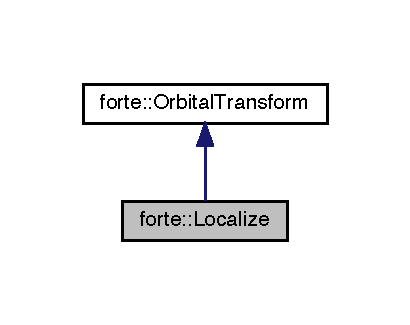
\includegraphics[width=197pt]{classforte_1_1_localize__inherit__graph}
\end{center}
\end{figure}


Collaboration diagram for forte\+:\+:Localize\+:
\nopagebreak
\begin{figure}[H]
\begin{center}
\leavevmode
\includegraphics[width=197pt]{classforte_1_1_localize__coll__graph}
\end{center}
\end{figure}
\subsection*{Public Member Functions}
\begin{DoxyCompactItemize}
\item 
\mbox{\hyperlink{classforte_1_1_localize_adc1373ddd714f156d6b9134364900266}{Localize}} (std\+::shared\+\_\+ptr$<$ \mbox{\hyperlink{classforte_1_1_forte_options}{Forte\+Options}} $>$ options, std\+::shared\+\_\+ptr$<$ \mbox{\hyperlink{classforte_1_1_forte_integrals}{Forte\+Integrals}} $>$ ints, std\+::shared\+\_\+ptr$<$ \mbox{\hyperlink{classforte_1_1_m_o_space_info}{M\+O\+Space\+Info}} $>$ mo\+\_\+space\+\_\+info)
\item 
void \mbox{\hyperlink{classforte_1_1_localize_af4858fdaa807659ad06d30925038a4c1}{compute\+\_\+transformation}} ()
\item 
psi\+::\+Shared\+Matrix \mbox{\hyperlink{classforte_1_1_localize_a9ee389a31b8856a670ff4854906979af}{get\+\_\+\+Ua}} ()
\item 
psi\+::\+Shared\+Matrix \mbox{\hyperlink{classforte_1_1_localize_add8ecbbd32ef5910a229d6a7225b4be9}{get\+\_\+\+Ub}} ()
\item 
void \mbox{\hyperlink{classforte_1_1_localize_aad7798a16102c6a3d38ba62bcbc7f500}{set\+\_\+orbital\+\_\+space}} (std\+::vector$<$ int $>$ \&orbital\+\_\+spaces)
\item 
void \mbox{\hyperlink{classforte_1_1_localize_ae48978e53ec6af850793b8821797d877}{set\+\_\+orbital\+\_\+space}} (std\+::vector$<$ std\+::string $>$ \&labels)
\end{DoxyCompactItemize}
\subsection*{Additional Inherited Members}


\subsection{Constructor \& Destructor Documentation}
\mbox{\Hypertarget{classforte_1_1_localize_adc1373ddd714f156d6b9134364900266}\label{classforte_1_1_localize_adc1373ddd714f156d6b9134364900266}} 
\index{forte\+::\+Localize@{forte\+::\+Localize}!Localize@{Localize}}
\index{Localize@{Localize}!forte\+::\+Localize@{forte\+::\+Localize}}
\subsubsection{\texorpdfstring{Localize()}{Localize()}}
{\footnotesize\ttfamily forte\+::\+Localize\+::\+Localize (\begin{DoxyParamCaption}\item[{std\+::shared\+\_\+ptr$<$ \mbox{\hyperlink{classforte_1_1_forte_options}{Forte\+Options}} $>$}]{options,  }\item[{std\+::shared\+\_\+ptr$<$ \mbox{\hyperlink{classforte_1_1_forte_integrals}{Forte\+Integrals}} $>$}]{ints,  }\item[{std\+::shared\+\_\+ptr$<$ \mbox{\hyperlink{classforte_1_1_m_o_space_info}{M\+O\+Space\+Info}} $>$}]{mo\+\_\+space\+\_\+info }\end{DoxyParamCaption})}



\subsection{Member Function Documentation}
\mbox{\Hypertarget{classforte_1_1_localize_af4858fdaa807659ad06d30925038a4c1}\label{classforte_1_1_localize_af4858fdaa807659ad06d30925038a4c1}} 
\index{forte\+::\+Localize@{forte\+::\+Localize}!compute\+\_\+transformation@{compute\+\_\+transformation}}
\index{compute\+\_\+transformation@{compute\+\_\+transformation}!forte\+::\+Localize@{forte\+::\+Localize}}
\subsubsection{\texorpdfstring{compute\+\_\+transformation()}{compute\_transformation()}}
{\footnotesize\ttfamily void forte\+::\+Localize\+::compute\+\_\+transformation (\begin{DoxyParamCaption}{ }\end{DoxyParamCaption})\hspace{0.3cm}{\ttfamily [virtual]}}



Implements \mbox{\hyperlink{classforte_1_1_orbital_transform_a48704cbce9fd066ef7e58270bb413c25}{forte\+::\+Orbital\+Transform}}.

\mbox{\Hypertarget{classforte_1_1_localize_a9ee389a31b8856a670ff4854906979af}\label{classforte_1_1_localize_a9ee389a31b8856a670ff4854906979af}} 
\index{forte\+::\+Localize@{forte\+::\+Localize}!get\+\_\+\+Ua@{get\+\_\+\+Ua}}
\index{get\+\_\+\+Ua@{get\+\_\+\+Ua}!forte\+::\+Localize@{forte\+::\+Localize}}
\subsubsection{\texorpdfstring{get\+\_\+\+Ua()}{get\_Ua()}}
{\footnotesize\ttfamily psi\+::\+Shared\+Matrix forte\+::\+Localize\+::get\+\_\+\+Ua (\begin{DoxyParamCaption}{ }\end{DoxyParamCaption})\hspace{0.3cm}{\ttfamily [virtual]}}



Implements \mbox{\hyperlink{classforte_1_1_orbital_transform_aedd124480b35eba56653109578c05ec9}{forte\+::\+Orbital\+Transform}}.

\mbox{\Hypertarget{classforte_1_1_localize_add8ecbbd32ef5910a229d6a7225b4be9}\label{classforte_1_1_localize_add8ecbbd32ef5910a229d6a7225b4be9}} 
\index{forte\+::\+Localize@{forte\+::\+Localize}!get\+\_\+\+Ub@{get\+\_\+\+Ub}}
\index{get\+\_\+\+Ub@{get\+\_\+\+Ub}!forte\+::\+Localize@{forte\+::\+Localize}}
\subsubsection{\texorpdfstring{get\+\_\+\+Ub()}{get\_Ub()}}
{\footnotesize\ttfamily psi\+::\+Shared\+Matrix forte\+::\+Localize\+::get\+\_\+\+Ub (\begin{DoxyParamCaption}{ }\end{DoxyParamCaption})\hspace{0.3cm}{\ttfamily [virtual]}}



Implements \mbox{\hyperlink{classforte_1_1_orbital_transform_aeb179f5b68883cf346dde354c05fd27b}{forte\+::\+Orbital\+Transform}}.

\mbox{\Hypertarget{classforte_1_1_localize_aad7798a16102c6a3d38ba62bcbc7f500}\label{classforte_1_1_localize_aad7798a16102c6a3d38ba62bcbc7f500}} 
\index{forte\+::\+Localize@{forte\+::\+Localize}!set\+\_\+orbital\+\_\+space@{set\+\_\+orbital\+\_\+space}}
\index{set\+\_\+orbital\+\_\+space@{set\+\_\+orbital\+\_\+space}!forte\+::\+Localize@{forte\+::\+Localize}}
\subsubsection{\texorpdfstring{set\+\_\+orbital\+\_\+space()}{set\_orbital\_space()}\hspace{0.1cm}{\footnotesize\ttfamily [1/2]}}
{\footnotesize\ttfamily void forte\+::\+Localize\+::set\+\_\+orbital\+\_\+space (\begin{DoxyParamCaption}\item[{std\+::vector$<$ int $>$ \&}]{orbital\+\_\+spaces }\end{DoxyParamCaption})}

\mbox{\Hypertarget{classforte_1_1_localize_ae48978e53ec6af850793b8821797d877}\label{classforte_1_1_localize_ae48978e53ec6af850793b8821797d877}} 
\index{forte\+::\+Localize@{forte\+::\+Localize}!set\+\_\+orbital\+\_\+space@{set\+\_\+orbital\+\_\+space}}
\index{set\+\_\+orbital\+\_\+space@{set\+\_\+orbital\+\_\+space}!forte\+::\+Localize@{forte\+::\+Localize}}
\subsubsection{\texorpdfstring{set\+\_\+orbital\+\_\+space()}{set\_orbital\_space()}\hspace{0.1cm}{\footnotesize\ttfamily [2/2]}}
{\footnotesize\ttfamily void forte\+::\+Localize\+::set\+\_\+orbital\+\_\+space (\begin{DoxyParamCaption}\item[{std\+::vector$<$ std\+::string $>$ \&}]{labels }\end{DoxyParamCaption})}



The documentation for this class was generated from the following files\+:\begin{DoxyCompactItemize}
\item 
/\+Users/fevange/\+Source/forte/src/orbital-\/helpers/\mbox{\hyperlink{localize_8h}{localize.\+h}}\item 
/\+Users/fevange/\+Source/forte/src/orbital-\/helpers/\mbox{\hyperlink{localize_8cc}{localize.\+cc}}\end{DoxyCompactItemize}

\hypertarget{classforte_1_1_m_a_s_t_e_r___d_s_r_g}{}\section{forte\+:\+:M\+A\+S\+T\+E\+R\+\_\+\+D\+S\+RG Class Reference}
\label{classforte_1_1_m_a_s_t_e_r___d_s_r_g}\index{forte\+::\+M\+A\+S\+T\+E\+R\+\_\+\+D\+S\+RG@{forte\+::\+M\+A\+S\+T\+E\+R\+\_\+\+D\+S\+RG}}


{\ttfamily \#include $<$master\+\_\+mrdsrg.\+h$>$}



Inheritance diagram for forte\+:\+:M\+A\+S\+T\+E\+R\+\_\+\+D\+S\+RG\+:
\nopagebreak
\begin{figure}[H]
\begin{center}
\leavevmode
\includegraphics[width=350pt]{classforte_1_1_m_a_s_t_e_r___d_s_r_g__inherit__graph}
\end{center}
\end{figure}


Collaboration diagram for forte\+:\+:M\+A\+S\+T\+E\+R\+\_\+\+D\+S\+RG\+:
\nopagebreak
\begin{figure}[H]
\begin{center}
\leavevmode
\includegraphics[width=328pt]{classforte_1_1_m_a_s_t_e_r___d_s_r_g__coll__graph}
\end{center}
\end{figure}
\subsection*{Public Member Functions}
\begin{DoxyCompactItemize}
\item 
\mbox{\hyperlink{classforte_1_1_m_a_s_t_e_r___d_s_r_g_a21886b18bc2dc37dd53accc580de0a06}{M\+A\+S\+T\+E\+R\+\_\+\+D\+S\+RG}} (\mbox{\hyperlink{classforte_1_1_r_d_ms}{R\+D\+Ms}} rdms, std\+::shared\+\_\+ptr$<$ \mbox{\hyperlink{classforte_1_1_s_c_f_info}{S\+C\+F\+Info}} $>$ scf\+\_\+info, std\+::shared\+\_\+ptr$<$ \mbox{\hyperlink{classforte_1_1_forte_options}{Forte\+Options}} $>$ options, std\+::shared\+\_\+ptr$<$ \mbox{\hyperlink{classforte_1_1_forte_integrals}{Forte\+Integrals}} $>$ ints, std\+::shared\+\_\+ptr$<$ \mbox{\hyperlink{classforte_1_1_m_o_space_info}{M\+O\+Space\+Info}} $>$ mo\+\_\+space\+\_\+info)
\item 
virtual \mbox{\hyperlink{classforte_1_1_m_a_s_t_e_r___d_s_r_g_a7e54a251f3d0b282a57ffa73a0983bc2}{$\sim$\+M\+A\+S\+T\+E\+R\+\_\+\+D\+S\+RG}} ()
\begin{DoxyCompactList}\small\item\em Destructor. \end{DoxyCompactList}\item 
virtual double \mbox{\hyperlink{classforte_1_1_m_a_s_t_e_r___d_s_r_g_a34011aaadcc79224071a4266a095591b}{compute\+\_\+energy}} ()=0
\begin{DoxyCompactList}\small\item\em Compute energy. \end{DoxyCompactList}\item 
virtual std\+::shared\+\_\+ptr$<$ \mbox{\hyperlink{classforte_1_1_active_space_integrals}{Active\+Space\+Integrals}} $>$ \mbox{\hyperlink{classforte_1_1_m_a_s_t_e_r___d_s_r_g_a4c4e581766abada72d8e1742a7887d2a}{compute\+\_\+\+Heff\+\_\+actv}} ()
\begin{DoxyCompactList}\small\item\em Compute D\+S\+RG transformed Hamiltonian. \end{DoxyCompactList}\item 
std\+::vector$<$ \mbox{\hyperlink{classforte_1_1_dressed_quantity}{Dressed\+Quantity}} $>$ \mbox{\hyperlink{classforte_1_1_m_a_s_t_e_r___d_s_r_g_a8fba974b17fe78a6646402144d388e76}{de\+G\+N\+O\+\_\+\+D\+Mbar\+\_\+actv}} ()
\begin{DoxyCompactList}\small\item\em De-\/normal-\/order D\+S\+RG transformed dipole moment. \end{DoxyCompactList}\item 
virtual void \mbox{\hyperlink{classforte_1_1_m_a_s_t_e_r___d_s_r_g_ae4f6a58d88aa03439d4c12e56fe90e0b}{compute\+\_\+\+Heff\+\_\+2nd\+\_\+coupling}} (double \&, ambit\+::\+Tensor \&, ambit\+::\+Tensor \&, ambit\+::\+Tensor \&, ambit\+::\+Tensor \&, ambit\+::\+Tensor \&, ambit\+::\+Tensor \&, ambit\+::\+Tensor \&, ambit\+::\+Tensor \&, ambit\+::\+Tensor \&)
\item 
\mbox{\hyperlink{structforte_1_1dsrg_heff}{dsrg\+Heff}} \mbox{\hyperlink{classforte_1_1_m_a_s_t_e_r___d_s_r_g_adda64d03b44e03bb1e8102d7e64e5c3f}{commutator\+\_\+\+H\+T\+\_\+no\+G\+NO}} (ambit\+::\+Blocked\+Tensor H1, ambit\+::\+Blocked\+Tensor H2, ambit\+::\+Blocked\+Tensor T1, ambit\+::\+Blocked\+Tensor T2)
\begin{DoxyCompactList}\small\item\em Compute \mbox{[}H, T\mbox{]} without using M\+K-\/\+G\+NO. \end{DoxyCompactList}\item 
virtual ambit\+::\+Blocked\+Tensor \mbox{\hyperlink{classforte_1_1_m_a_s_t_e_r___d_s_r_g_a7eef5849acfd3aec1a2fbc5f981a5538}{get\+\_\+\+T1de\+G\+NO}} (double \&)
\begin{DoxyCompactList}\small\item\em Compute D\+S\+RG dressed density. \end{DoxyCompactList}\item 
virtual ambit\+::\+Blocked\+Tensor \mbox{\hyperlink{classforte_1_1_m_a_s_t_e_r___d_s_r_g_a2087fce00f429361e194be03c0eb668d}{get\+\_\+\+T2}} (const std\+::vector$<$ std\+::string $>$ \&)
\begin{DoxyCompactList}\small\item\em Return T2 amplitudes. \end{DoxyCompactList}\item 
virtual ambit\+::\+Blocked\+Tensor \mbox{\hyperlink{classforte_1_1_m_a_s_t_e_r___d_s_r_g_a409d404b009c1c4c17b07beb62d7e280}{get\+\_\+\+T2}} ()
\item 
virtual ambit\+::\+Blocked\+Tensor \mbox{\hyperlink{classforte_1_1_m_a_s_t_e_r___d_s_r_g_adc470ba7bd9dabb9da86d3e1e2448c5e}{get\+\_\+\+R\+H1de\+G\+NO}} ()
\begin{DoxyCompactList}\small\item\em Return de-\/normal-\/ordered 1-\/body renormalized 1st-\/order Hamiltonian. \end{DoxyCompactList}\item 
virtual ambit\+::\+Blocked\+Tensor \mbox{\hyperlink{classforte_1_1_m_a_s_t_e_r___d_s_r_g_a4f300dd1d54dfe45f8db603a62f58b0e}{get\+\_\+\+R\+H2}} ()
\begin{DoxyCompactList}\small\item\em Return 2-\/body renormalized 1st-\/order Hamiltonian. \end{DoxyCompactList}\item 
std\+::vector$<$ ambit\+::\+Tensor $>$ \mbox{\hyperlink{classforte_1_1_m_a_s_t_e_r___d_s_r_g_a55af5152fa737f06288f75ecf6d7769e}{Hbar}} (int n)
\begin{DoxyCompactList}\small\item\em Return the Hbar of a given order. \end{DoxyCompactList}\item 
bool \mbox{\hyperlink{classforte_1_1_m_a_s_t_e_r___d_s_r_g_adc353fcdaf3ee4d57e45ba6cb3cd6112}{do\+\_\+dipole}} ()
\begin{DoxyCompactList}\small\item\em Return if dipole moments are computed. \end{DoxyCompactList}\item 
std\+::array$<$ double, 3 $>$ \mbox{\hyperlink{classforte_1_1_m_a_s_t_e_r___d_s_r_g_a65e730b294734010628e9e560fb15f76}{nuclear\+\_\+dipole}} ()
\begin{DoxyCompactList}\small\item\em Return the nuclear components of dipole moments. \end{DoxyCompactList}\item 
void \mbox{\hyperlink{classforte_1_1_m_a_s_t_e_r___d_s_r_g_a43f6bc4463fde67f20945268d867b75b}{set\+\_\+\+Uactv}} (ambit\+::\+Tensor \&Ua, ambit\+::\+Tensor \&Ub)
\begin{DoxyCompactList}\small\item\em Set unitary matrix (in active space) from original to semicanonical. \end{DoxyCompactList}\item 
void \mbox{\hyperlink{classforte_1_1_m_a_s_t_e_r___d_s_r_g_a5302d7a5a6c0a909ab75705405ae2961}{set\+\_\+actv\+\_\+occ}} (std\+::vector$<$ size\+\_\+t $>$ actv\+\_\+occ)
\begin{DoxyCompactList}\small\item\em Set active active occupied M\+Os (relative to active) \end{DoxyCompactList}\item 
void \mbox{\hyperlink{classforte_1_1_m_a_s_t_e_r___d_s_r_g_abbac08c5beb5a618497206c02f4eb45f}{set\+\_\+actv\+\_\+uocc}} (std\+::vector$<$ size\+\_\+t $>$ actv\+\_\+uocc)
\begin{DoxyCompactList}\small\item\em Set active active unoccupied M\+Os (relative to active) \end{DoxyCompactList}\end{DoxyCompactItemize}
\subsection*{Protected Member Functions}
\begin{DoxyCompactItemize}
\item 
void \mbox{\hyperlink{classforte_1_1_m_a_s_t_e_r___d_s_r_g_a163847289aaa28024bcb0fb3ccccd0fc}{startup}} ()
\begin{DoxyCompactList}\small\item\em Startup function called in constructor. \end{DoxyCompactList}\item 
void \mbox{\hyperlink{classforte_1_1_m_a_s_t_e_r___d_s_r_g_ae27719b9d4626150013d5aa6aa6290e7}{read\+\_\+options}} ()
\begin{DoxyCompactList}\small\item\em Read options. \end{DoxyCompactList}\item 
void \mbox{\hyperlink{classforte_1_1_m_a_s_t_e_r___d_s_r_g_a7b863c8d3f36ac7f02f14456be7f2df3}{rotate\+\_\+ints\+\_\+semi\+\_\+to\+\_\+origin}} (const std\+::string \&name, Blocked\+Tensor \&H1, Blocked\+Tensor \&H2)
\begin{DoxyCompactList}\small\item\em Rotate 2-\/body D\+S\+RG transformed integrals from semicanonical back to original. \end{DoxyCompactList}\item 
void \mbox{\hyperlink{classforte_1_1_m_a_s_t_e_r___d_s_r_g_a9a447e4bfb4cd2187b7f1d02cd6713fd}{rotate\+\_\+ints\+\_\+semi\+\_\+to\+\_\+origin}} (const std\+::string \&name, Blocked\+Tensor \&H1, Blocked\+Tensor \&H2, Blocked\+Tensor \&H3)
\begin{DoxyCompactList}\small\item\em Rotate 3-\/body D\+S\+RG transformed integrals from semicanonical back to original. \end{DoxyCompactList}\item 
void \mbox{\hyperlink{classforte_1_1_m_a_s_t_e_r___d_s_r_g_a89d478d95c345bedd8b1e4a3862f644a}{check\+\_\+init\+\_\+reference\+\_\+energy}} ()
\begin{DoxyCompactList}\small\item\em Initial check on reference energy. \end{DoxyCompactList}\item 
double \mbox{\hyperlink{classforte_1_1_m_a_s_t_e_r___d_s_r_g_a2dd2a66d680e50beb52cb3651f1f994d}{compute\+\_\+reference\+\_\+energy\+\_\+from\+\_\+ints}} (std\+::shared\+\_\+ptr$<$ \mbox{\hyperlink{classforte_1_1_forte_integrals}{Forte\+Integrals}} $>$ ints)
\begin{DoxyCompactList}\small\item\em Compute reference (MK vacuum) energy from Forte\+Integral and Fock\+\_\+. \end{DoxyCompactList}\item 
double \mbox{\hyperlink{classforte_1_1_m_a_s_t_e_r___d_s_r_g_af5645674246c3f91b9f6c81d507834ba}{compute\+\_\+reference\+\_\+energy}} (Blocked\+Tensor H, Blocked\+Tensor F, Blocked\+Tensor V)
\begin{DoxyCompactList}\small\item\em Compute reference (MK vacuum) energy. \end{DoxyCompactList}\item 
double \mbox{\hyperlink{classforte_1_1_m_a_s_t_e_r___d_s_r_g_aaa6a8d82990682045f25b7ea425a75c2}{compute\+\_\+reference\+\_\+energy\+\_\+df}} (Blocked\+Tensor H, Blocked\+Tensor F, Blocked\+Tensor B)
\item 
void \mbox{\hyperlink{classforte_1_1_m_a_s_t_e_r___d_s_r_g_a4c7eea23d0973346ae114df54cd689fa}{read\+\_\+\+M\+O\+Space\+Info}} ()
\begin{DoxyCompactList}\small\item\em Read MO space info. \end{DoxyCompactList}\item 
void \mbox{\hyperlink{classforte_1_1_m_a_s_t_e_r___d_s_r_g_a8cbfdaab152ad502cec7aaf76230bb9c}{set\+\_\+ambit\+\_\+\+M\+O\+Space}} ()
\begin{DoxyCompactList}\small\item\em Set Ambit tensor labels. \end{DoxyCompactList}\item 
std\+::vector$<$ std\+::string $>$ \mbox{\hyperlink{classforte_1_1_m_a_s_t_e_r___d_s_r_g_a033c9c47a263276b244f785ff17eb021}{diag\+\_\+one\+\_\+labels}} ()
\begin{DoxyCompactList}\small\item\em Compute diagonal blocks labels of a one-\/body operator. \end{DoxyCompactList}\item 
std\+::vector$<$ std\+::string $>$ \mbox{\hyperlink{classforte_1_1_m_a_s_t_e_r___d_s_r_g_a952117c90bb81a025be16810cd8362c8}{diag\+\_\+two\+\_\+labels}} ()
\begin{DoxyCompactList}\small\item\em Compute diagonal blocks labels of a two-\/body operator. \end{DoxyCompactList}\item 
std\+::vector$<$ std\+::string $>$ \mbox{\hyperlink{classforte_1_1_m_a_s_t_e_r___d_s_r_g_a758e583687b71d6d6f7f07e8058e3c02}{re\+\_\+two\+\_\+labels}} ()
\begin{DoxyCompactList}\small\item\em Compute retaining excitation blocks labels of a two-\/body operator. \end{DoxyCompactList}\item 
std\+::vector$<$ std\+::string $>$ \mbox{\hyperlink{classforte_1_1_m_a_s_t_e_r___d_s_r_g_a04de384d7802e74b7b2b296416e5efc5}{od\+\_\+one\+\_\+labels}} ()
\begin{DoxyCompactList}\small\item\em Compute off-\/diagonal blocks labels of a one-\/body operator. \end{DoxyCompactList}\item 
std\+::vector$<$ std\+::string $>$ \mbox{\hyperlink{classforte_1_1_m_a_s_t_e_r___d_s_r_g_a2d357f21cfd11767e4c58a14cace3238}{od\+\_\+one\+\_\+labels\+\_\+hp}} ()
\item 
std\+::vector$<$ std\+::string $>$ \mbox{\hyperlink{classforte_1_1_m_a_s_t_e_r___d_s_r_g_aca3dcf6d0a5ec5a538beac5508dcf399}{od\+\_\+one\+\_\+labels\+\_\+ph}} ()
\item 
std\+::vector$<$ std\+::string $>$ \mbox{\hyperlink{classforte_1_1_m_a_s_t_e_r___d_s_r_g_a18c15fdf7089cb3ad61520cd029e4f13}{od\+\_\+two\+\_\+labels}} ()
\begin{DoxyCompactList}\small\item\em Compute off-\/diagonal blocks labels of a two-\/body operator. \end{DoxyCompactList}\item 
std\+::vector$<$ std\+::string $>$ \mbox{\hyperlink{classforte_1_1_m_a_s_t_e_r___d_s_r_g_a6f2ddd225781fb51e056d898e278fba8}{od\+\_\+two\+\_\+labels\+\_\+hhpp}} ()
\item 
std\+::vector$<$ std\+::string $>$ \mbox{\hyperlink{classforte_1_1_m_a_s_t_e_r___d_s_r_g_aff8a67af19b38e5a6b27bf2811270f00}{od\+\_\+two\+\_\+labels\+\_\+pphh}} ()
\item 
void \mbox{\hyperlink{classforte_1_1_m_a_s_t_e_r___d_s_r_g_a976cfcc3d51a53862d3c64a350c3d0cc}{init\+\_\+density}} ()
\begin{DoxyCompactList}\small\item\em Initialize density cumulants. \end{DoxyCompactList}\item 
void \mbox{\hyperlink{classforte_1_1_m_a_s_t_e_r___d_s_r_g_aa564f00007eb21036c638873e43f4c44}{fill\+\_\+density}} ()
\begin{DoxyCompactList}\small\item\em Fill in density cumulants from the \mbox{\hyperlink{classforte_1_1_r_d_ms}{R\+D\+Ms}}. \end{DoxyCompactList}\item 
void \mbox{\hyperlink{classforte_1_1_m_a_s_t_e_r___d_s_r_g_ae938144cddd646a6b4383dbcdfe06348}{init\+\_\+fock}} ()
\begin{DoxyCompactList}\small\item\em Initialize Fock matrix. \end{DoxyCompactList}\item 
void \mbox{\hyperlink{classforte_1_1_m_a_s_t_e_r___d_s_r_g_a1839087fe874f832009be1cd28ec29e4}{build\+\_\+fock\+\_\+from\+\_\+ints}} (std\+::shared\+\_\+ptr$<$ \mbox{\hyperlink{classforte_1_1_forte_integrals}{Forte\+Integrals}} $>$ ints)
\begin{DoxyCompactList}\small\item\em Build Fock matrix from \mbox{\hyperlink{classforte_1_1_forte_integrals}{Forte\+Integrals}}. \end{DoxyCompactList}\item 
void \mbox{\hyperlink{classforte_1_1_m_a_s_t_e_r___d_s_r_g_a74605af40511d0df99a494cf3a6fe89a}{fill\+\_\+\+Fdiag}} (Blocked\+Tensor \&F, std\+::vector$<$ double $>$ \&Fa, std\+::vector$<$ double $>$ \&Fb)
\begin{DoxyCompactList}\small\item\em Fill in diagonal elements of Fock matrix to Fdiag. \end{DoxyCompactList}\item 
bool \mbox{\hyperlink{classforte_1_1_m_a_s_t_e_r___d_s_r_g_a621f24a7746bbe753a330a1976c67d96}{check\+\_\+semi\+\_\+orbs}} ()
\begin{DoxyCompactList}\small\item\em Check orbitals if semicanonical. \end{DoxyCompactList}\item 
std\+::vector$<$ std\+::vector$<$ double $>$ $>$ \mbox{\hyperlink{classforte_1_1_m_a_s_t_e_r___d_s_r_g_aa94b70b591874b2c1638cc2759b187b6}{diagonalize\+\_\+\+Fock\+\_\+diagblocks}} (Blocked\+Tensor \&U)
\begin{DoxyCompactList}\small\item\em Diagonalize the diagonal blocks of the Fock matrix. \end{DoxyCompactList}\item 
void \mbox{\hyperlink{classforte_1_1_m_a_s_t_e_r___d_s_r_g_a2280bd289ee969811ef1ab1e78168684}{de\+G\+N\+O\+\_\+ints}} (const std\+::string \&name, double \&H0, Blocked\+Tensor \&H1, Blocked\+Tensor \&H2)
\item 
void \mbox{\hyperlink{classforte_1_1_m_a_s_t_e_r___d_s_r_g_a48f26210aabd7ea4600205c75c2bf883}{de\+G\+N\+O\+\_\+ints}} (const std\+::string \&name, double \&H0, Blocked\+Tensor \&H1, Blocked\+Tensor \&H2, Blocked\+Tensor \&H3)
\item 
ambit\+::\+Blocked\+Tensor \mbox{\hyperlink{classforte_1_1_m_a_s_t_e_r___d_s_r_g_a5e59459adbaed7541848913a218471ac}{de\+G\+N\+O\+\_\+\+Tamp}} (Blocked\+Tensor \&T1, Blocked\+Tensor \&T2, Blocked\+Tensor \&D1)
\item 
void \mbox{\hyperlink{classforte_1_1_m_a_s_t_e_r___d_s_r_g_adbe5f4289f695a49b292caf2085ffbcf}{fill\+\_\+three\+\_\+index\+\_\+ints}} (ambit\+::\+Blocked\+Tensor T)
\item 
void \mbox{\hyperlink{classforte_1_1_m_a_s_t_e_r___d_s_r_g_a2ae6b6f7220ae5f12040ac2b97b21c3c}{init\+\_\+dm\+\_\+ints}} ()
\begin{DoxyCompactList}\small\item\em Setup dipole integrals and D\+S\+RG transformed integrals. \end{DoxyCompactList}\item 
void \mbox{\hyperlink{classforte_1_1_m_a_s_t_e_r___d_s_r_g_a7d865e9c13091a638fdc44a7a7b6ae43}{fill\+\_\+\+M\+Odm}} (std\+::vector$<$ psi\+::\+Shared\+Matrix $>$ \&dm\+\_\+a, std\+::vector$<$ psi\+::\+Shared\+Matrix $>$ \&dm\+\_\+b)
\begin{DoxyCompactList}\small\item\em Fill in bare MO dipole integrals. \end{DoxyCompactList}\item 
void \mbox{\hyperlink{classforte_1_1_m_a_s_t_e_r___d_s_r_g_ab7dcc4a5bdfc5694c4b4c29160456ed8}{compute\+\_\+dm\+\_\+ref}} ()
\begin{DoxyCompactList}\small\item\em Compute dipole moment of the reference. \end{DoxyCompactList}\item 
void \mbox{\hyperlink{classforte_1_1_m_a_s_t_e_r___d_s_r_g_a46cd12783b73049b758099d403abf194}{H1\+\_\+\+T1\+\_\+\+C0}} (Blocked\+Tensor \&H1, Blocked\+Tensor \&T1, const double \&alpha, double \&C0)
\begin{DoxyCompactList}\small\item\em Compute zero-\/body term of commutator \mbox{[}H1, T1\mbox{]}. \end{DoxyCompactList}\item 
void \mbox{\hyperlink{classforte_1_1_m_a_s_t_e_r___d_s_r_g_aaf832988d33d384cafc0d1539160cadb}{H1\+\_\+\+T2\+\_\+\+C0}} (Blocked\+Tensor \&H1, Blocked\+Tensor \&T2, const double \&alpha, double \&C0)
\begin{DoxyCompactList}\small\item\em Compute zero-\/body term of commutator \mbox{[}H1, T2\mbox{]}. \end{DoxyCompactList}\item 
void \mbox{\hyperlink{classforte_1_1_m_a_s_t_e_r___d_s_r_g_a10b69298ec5d14c9ad2b8f2412071be4}{H2\+\_\+\+T1\+\_\+\+C0}} (Blocked\+Tensor \&H2, Blocked\+Tensor \&T1, const double \&alpha, double \&C0)
\begin{DoxyCompactList}\small\item\em Compute zero-\/body term of commutator \mbox{[}H2, T1\mbox{]}. \end{DoxyCompactList}\item 
void \mbox{\hyperlink{classforte_1_1_m_a_s_t_e_r___d_s_r_g_a67dd5c7dccc966016949c347e1e87643}{H2\+\_\+\+T2\+\_\+\+C0}} (Blocked\+Tensor \&H2, Blocked\+Tensor \&T2, const double \&alpha, double \&C0)
\begin{DoxyCompactList}\small\item\em Compute zero-\/body term of commutator \mbox{[}H2, T2\mbox{]}. \end{DoxyCompactList}\item 
void \mbox{\hyperlink{classforte_1_1_m_a_s_t_e_r___d_s_r_g_a92d17334220a1ec7d2572322549c780c}{H1\+\_\+\+T1\+\_\+\+C1}} (Blocked\+Tensor \&H1, Blocked\+Tensor \&T1, const double \&alpha, Blocked\+Tensor \&\mbox{\hyperlink{namespaceforte_abe00ec86d0015c0f2b6ac298c6e428e4a1a2ddc2db4693cfd16d534cde5572cc1}{C1}})
\begin{DoxyCompactList}\small\item\em Compute one-\/body term of commutator \mbox{[}H1, T1\mbox{]}. \end{DoxyCompactList}\item 
void \mbox{\hyperlink{classforte_1_1_m_a_s_t_e_r___d_s_r_g_ac5b45c4abfa928d4d2b425f217e5e72e}{H1\+\_\+\+T2\+\_\+\+C1}} (Blocked\+Tensor \&H1, Blocked\+Tensor \&T2, const double \&alpha, Blocked\+Tensor \&\mbox{\hyperlink{namespaceforte_abe00ec86d0015c0f2b6ac298c6e428e4a1a2ddc2db4693cfd16d534cde5572cc1}{C1}})
\begin{DoxyCompactList}\small\item\em Compute one-\/body term of commutator \mbox{[}H1, T2\mbox{]}. \end{DoxyCompactList}\item 
void \mbox{\hyperlink{classforte_1_1_m_a_s_t_e_r___d_s_r_g_a10484c21cfa5e26d83fc0928fb050389}{H2\+\_\+\+T1\+\_\+\+C1}} (Blocked\+Tensor \&H2, Blocked\+Tensor \&T1, const double \&alpha, Blocked\+Tensor \&\mbox{\hyperlink{namespaceforte_abe00ec86d0015c0f2b6ac298c6e428e4a1a2ddc2db4693cfd16d534cde5572cc1}{C1}})
\begin{DoxyCompactList}\small\item\em Compute one-\/body term of commutator \mbox{[}H2, T1\mbox{]}. \end{DoxyCompactList}\item 
void \mbox{\hyperlink{classforte_1_1_m_a_s_t_e_r___d_s_r_g_af94d68486184ec068b70db3891977346}{H2\+\_\+\+T2\+\_\+\+C1}} (Blocked\+Tensor \&H2, Blocked\+Tensor \&T2, const double \&alpha, Blocked\+Tensor \&\mbox{\hyperlink{namespaceforte_abe00ec86d0015c0f2b6ac298c6e428e4a1a2ddc2db4693cfd16d534cde5572cc1}{C1}})
\begin{DoxyCompactList}\small\item\em Compute one-\/body term of commutator \mbox{[}H2, T2\mbox{]}. \end{DoxyCompactList}\item 
void \mbox{\hyperlink{classforte_1_1_m_a_s_t_e_r___d_s_r_g_a662113c1c718db206ab118b2dbd85b65}{H2\+\_\+\+T1\+\_\+\+C2}} (Blocked\+Tensor \&H2, Blocked\+Tensor \&T1, const double \&alpha, Blocked\+Tensor \&\mbox{\hyperlink{namespaceforte_abe00ec86d0015c0f2b6ac298c6e428e4af1a543f5a2c5d49bc5dde298fcf716e4}{C2}})
\begin{DoxyCompactList}\small\item\em Compute two-\/body term of commutator \mbox{[}H2, T1\mbox{]}. \end{DoxyCompactList}\item 
void \mbox{\hyperlink{classforte_1_1_m_a_s_t_e_r___d_s_r_g_a7923e4cf5d48d8e877c17b8155a653e1}{H1\+\_\+\+T2\+\_\+\+C2}} (Blocked\+Tensor \&H1, Blocked\+Tensor \&T2, const double \&alpha, Blocked\+Tensor \&\mbox{\hyperlink{namespaceforte_abe00ec86d0015c0f2b6ac298c6e428e4af1a543f5a2c5d49bc5dde298fcf716e4}{C2}})
\begin{DoxyCompactList}\small\item\em Compute two-\/body term of commutator \mbox{[}H1, T2\mbox{]}. \end{DoxyCompactList}\item 
void \mbox{\hyperlink{classforte_1_1_m_a_s_t_e_r___d_s_r_g_a39a44ecb9997a978aecd58d470712c1c}{H2\+\_\+\+T2\+\_\+\+C2}} (Blocked\+Tensor \&H2, Blocked\+Tensor \&T2, const double \&alpha, Blocked\+Tensor \&\mbox{\hyperlink{namespaceforte_abe00ec86d0015c0f2b6ac298c6e428e4af1a543f5a2c5d49bc5dde298fcf716e4}{C2}})
\begin{DoxyCompactList}\small\item\em Compute two-\/body term of commutator \mbox{[}H2, T2\mbox{]}. \end{DoxyCompactList}\item 
void \mbox{\hyperlink{classforte_1_1_m_a_s_t_e_r___d_s_r_g_af283b5833cb6b33ec6b5fea49bb8dd3c}{H2\+\_\+\+T2\+\_\+\+C3}} (Blocked\+Tensor \&H2, Blocked\+Tensor \&T2, const double \&alpha, Blocked\+Tensor \&C3, const bool \&active\+\_\+only=true)
\begin{DoxyCompactList}\small\item\em Compute three-\/body term of commutator \mbox{[}H2, T2\mbox{]}. \end{DoxyCompactList}\item 
void \mbox{\hyperlink{classforte_1_1_m_a_s_t_e_r___d_s_r_g_a0be012ac81de463a27159cd21e332828}{H1\+\_\+\+A2\+\_\+\+T\+\_\+\+Cod}} (Blocked\+Tensor \&H1, Blocked\+Tensor \&A2, Blocked\+Tensor \&T1, Blocked\+Tensor \&T2, const double \&alpha, Blocked\+Tensor \&\mbox{\hyperlink{namespaceforte_abe00ec86d0015c0f2b6ac298c6e428e4a1a2ddc2db4693cfd16d534cde5572cc1}{C1}}, Blocked\+Tensor \&\mbox{\hyperlink{namespaceforte_abe00ec86d0015c0f2b6ac298c6e428e4af1a543f5a2c5d49bc5dde298fcf716e4}{C2}})
\begin{DoxyCompactList}\small\item\em Compute one-\/ and two-\/body off-\/diagonal term of commutator \mbox{[}\mbox{[}H1, A2\mbox{]}2d, T1+2\mbox{]}od. \end{DoxyCompactList}\item 
void \mbox{\hyperlink{classforte_1_1_m_a_s_t_e_r___d_s_r_g_a2814822e5c86a6ff5b173d7a530a8ff6}{V\+\_\+\+T1\+\_\+\+C1\+\_\+\+DF}} (Blocked\+Tensor \&B, Blocked\+Tensor \&T1, const double \&alpha, Blocked\+Tensor \&\mbox{\hyperlink{namespaceforte_abe00ec86d0015c0f2b6ac298c6e428e4a1a2ddc2db4693cfd16d534cde5572cc1}{C1}})
\begin{DoxyCompactList}\small\item\em Compute one-\/body term of commutator \mbox{[}V, T1\mbox{]}, V is constructed from B (D\+F/\+CD) \end{DoxyCompactList}\item 
void \mbox{\hyperlink{classforte_1_1_m_a_s_t_e_r___d_s_r_g_a557d951b2dc9232e4941cf98ed4c63f9}{V\+\_\+\+T2\+\_\+\+C1\+\_\+\+DF}} (Blocked\+Tensor \&B, Blocked\+Tensor \&T2, const double \&alpha, Blocked\+Tensor \&\mbox{\hyperlink{namespaceforte_abe00ec86d0015c0f2b6ac298c6e428e4a1a2ddc2db4693cfd16d534cde5572cc1}{C1}})
\begin{DoxyCompactList}\small\item\em Compute one-\/body term of commutator \mbox{[}V, T2\mbox{]}, V is constructed from B (D\+F/\+CD) \end{DoxyCompactList}\item 
void \mbox{\hyperlink{classforte_1_1_m_a_s_t_e_r___d_s_r_g_abfca3ef3d6257c2a1229447dbe88680c}{V\+\_\+\+T1\+\_\+\+C2\+\_\+\+DF}} (Blocked\+Tensor \&B, Blocked\+Tensor \&T1, const double \&alpha, Blocked\+Tensor \&\mbox{\hyperlink{namespaceforte_abe00ec86d0015c0f2b6ac298c6e428e4af1a543f5a2c5d49bc5dde298fcf716e4}{C2}})
\begin{DoxyCompactList}\small\item\em Compute two-\/body term of commutator \mbox{[}V, T1\mbox{]}, V is constructed from B (D\+F/\+CD) \end{DoxyCompactList}\item 
void \mbox{\hyperlink{classforte_1_1_m_a_s_t_e_r___d_s_r_g_a0bfabeece8f51cb195b55757c86b562e}{V\+\_\+\+T2\+\_\+\+C2\+\_\+\+DF}} (Blocked\+Tensor \&B, Blocked\+Tensor \&T2, const double \&alpha, Blocked\+Tensor \&\mbox{\hyperlink{namespaceforte_abe00ec86d0015c0f2b6ac298c6e428e4af1a543f5a2c5d49bc5dde298fcf716e4}{C2}})
\begin{DoxyCompactList}\small\item\em Compute two-\/body term of commutator \mbox{[}V, T2\mbox{]}, V is constructed from B (D\+F/\+CD) \end{DoxyCompactList}\item 
void \mbox{\hyperlink{classforte_1_1_m_a_s_t_e_r___d_s_r_g_a09d201c4c4009d9552328360fc175f28}{V\+\_\+\+T2\+\_\+\+C2\+\_\+\+D\+F\+\_\+\+B\+A\+T\+CH}} (Blocked\+Tensor \&B, Blocked\+Tensor \&T2, const double \&alpha, Blocked\+Tensor \&\mbox{\hyperlink{namespaceforte_abe00ec86d0015c0f2b6ac298c6e428e4af1a543f5a2c5d49bc5dde298fcf716e4}{C2}})
\begin{DoxyCompactList}\small\item\em Compute two-\/body term of commutator \mbox{[}V, T2\mbox{]}, V is constructed from B (D\+F/\+CD) in batches. \end{DoxyCompactList}\item 
void \mbox{\hyperlink{classforte_1_1_m_a_s_t_e_r___d_s_r_g_a6f2f3067147bde13e729d4cac28d0dcc}{H1\+\_\+\+G1\+\_\+\+C0}} (Blocked\+Tensor \&H1, Blocked\+Tensor \&G1, const double \&alpha, double \&C0)
\begin{DoxyCompactList}\small\item\em Compute zero-\/body term of commutator \mbox{[}H1, G1\mbox{]}. \end{DoxyCompactList}\item 
void \mbox{\hyperlink{classforte_1_1_m_a_s_t_e_r___d_s_r_g_a63ef83789ae2375d729a4a6e47cd439d}{H1\+\_\+\+G2\+\_\+\+C0}} (Blocked\+Tensor \&H1, Blocked\+Tensor \&G2, const double \&alpha, double \&C0)
\begin{DoxyCompactList}\small\item\em Compute zero-\/body term of commutator \mbox{[}H1, G2\mbox{]}. \end{DoxyCompactList}\item 
void \mbox{\hyperlink{classforte_1_1_m_a_s_t_e_r___d_s_r_g_af0e6fb8d2ac9e0975b43b9d852fe9b4d}{H2\+\_\+\+G2\+\_\+\+C0}} (Blocked\+Tensor \&H2, Blocked\+Tensor \&G2, const double \&alpha, double \&C0)
\begin{DoxyCompactList}\small\item\em Compute zero-\/body term of commutator \mbox{[}H2, G2\mbox{]}. \end{DoxyCompactList}\item 
void \mbox{\hyperlink{classforte_1_1_m_a_s_t_e_r___d_s_r_g_ac7f2504a87fc3acdca92b6b5893db3d0}{H1\+\_\+\+G1\+\_\+\+C1}} (Blocked\+Tensor \&H1, Blocked\+Tensor \&G1, const double \&alpha, Blocked\+Tensor \&\mbox{\hyperlink{namespaceforte_abe00ec86d0015c0f2b6ac298c6e428e4a1a2ddc2db4693cfd16d534cde5572cc1}{C1}})
\begin{DoxyCompactList}\small\item\em Compute one-\/body term of commutator \mbox{[}H1, G1\mbox{]}. \end{DoxyCompactList}\item 
void \mbox{\hyperlink{classforte_1_1_m_a_s_t_e_r___d_s_r_g_a696380d2453e2d7a5319f9ba82acf89e}{H1\+\_\+\+G2\+\_\+\+C1}} (Blocked\+Tensor \&H1, Blocked\+Tensor \&G2, const double \&alpha, Blocked\+Tensor \&\mbox{\hyperlink{namespaceforte_abe00ec86d0015c0f2b6ac298c6e428e4a1a2ddc2db4693cfd16d534cde5572cc1}{C1}})
\begin{DoxyCompactList}\small\item\em Compute one-\/body term of commutator \mbox{[}H1, G2\mbox{]}. \end{DoxyCompactList}\item 
void \mbox{\hyperlink{classforte_1_1_m_a_s_t_e_r___d_s_r_g_af2a98ef2b5d852422e3392909c4d6f2a}{H2\+\_\+\+G2\+\_\+\+C1}} (Blocked\+Tensor \&H2, Blocked\+Tensor \&G2, const double \&alpha, Blocked\+Tensor \&\mbox{\hyperlink{namespaceforte_abe00ec86d0015c0f2b6ac298c6e428e4a1a2ddc2db4693cfd16d534cde5572cc1}{C1}})
\begin{DoxyCompactList}\small\item\em Compute one-\/body term of commutator \mbox{[}H2, G2\mbox{]}. \end{DoxyCompactList}\item 
void \mbox{\hyperlink{classforte_1_1_m_a_s_t_e_r___d_s_r_g_aa73d1b9938d01f9cb621d70c1c7c8828}{H1\+\_\+\+G2\+\_\+\+C2}} (Blocked\+Tensor \&H1, Blocked\+Tensor \&G2, const double \&alpha, Blocked\+Tensor \&\mbox{\hyperlink{namespaceforte_abe00ec86d0015c0f2b6ac298c6e428e4af1a543f5a2c5d49bc5dde298fcf716e4}{C2}})
\begin{DoxyCompactList}\small\item\em Compute two-\/body term of commutator \mbox{[}H1, G2\mbox{]}. \end{DoxyCompactList}\item 
void \mbox{\hyperlink{classforte_1_1_m_a_s_t_e_r___d_s_r_g_aba555c804e96f32053dc180d78feb2c2}{H2\+\_\+\+G2\+\_\+\+C2}} (Blocked\+Tensor \&H2, Blocked\+Tensor \&G2, const double \&alpha, Blocked\+Tensor \&\mbox{\hyperlink{namespaceforte_abe00ec86d0015c0f2b6ac298c6e428e4af1a543f5a2c5d49bc5dde298fcf716e4}{C2}})
\begin{DoxyCompactList}\small\item\em Compute two-\/body term of commutator \mbox{[}H2, G2\mbox{]}. \end{DoxyCompactList}\end{DoxyCompactItemize}
\subsection*{Protected Attributes}
\begin{DoxyCompactItemize}
\item 
std\+::vector$<$ std\+::tuple$<$ const char $\ast$, const char $\ast$, const char $\ast$ $>$ $>$ \mbox{\hyperlink{classforte_1_1_m_a_s_t_e_r___d_s_r_g_a7e080391fc5e3476ae6f1a3e02eee4d1}{warnings\+\_\+}}
\begin{DoxyCompactList}\small\item\em Warnings $<$description, changes in this run, how to get rid of it$>$ \end{DoxyCompactList}\item 
double \mbox{\hyperlink{classforte_1_1_m_a_s_t_e_r___d_s_r_g_aacd2335c163366faff6cb30d39a3ddf7}{s\+\_\+}}
\begin{DoxyCompactList}\small\item\em The flow parameter. \end{DoxyCompactList}\item 
std\+::string \mbox{\hyperlink{classforte_1_1_m_a_s_t_e_r___d_s_r_g_a4227e753f0f19afc118f122acaa0a71c}{source\+\_\+}}
\begin{DoxyCompactList}\small\item\em Source operator. \end{DoxyCompactList}\item 
std\+::shared\+\_\+ptr$<$ \mbox{\hyperlink{classforte_1_1_d_s_r_g___s_o_u_r_c_e}{D\+S\+R\+G\+\_\+\+S\+O\+U\+R\+CE}} $>$ \mbox{\hyperlink{classforte_1_1_m_a_s_t_e_r___d_s_r_g_a66ed6a268b5014d6f96b646379be58dc}{dsrg\+\_\+source\+\_\+}}
\begin{DoxyCompactList}\small\item\em The dsrg source operator. \end{DoxyCompactList}\item 
double \mbox{\hyperlink{classforte_1_1_m_a_s_t_e_r___d_s_r_g_a8eb02a55fe22194653b6296e2da3a9b9}{taylor\+\_\+threshold\+\_\+}}
\begin{DoxyCompactList}\small\item\em Threshold for the Taylor expansion of f(z) = (1-\/exp(-\/z$^\wedge$2))/z. \end{DoxyCompactList}\item 
bool \mbox{\hyperlink{classforte_1_1_m_a_s_t_e_r___d_s_r_g_ad5636a2563c05195659b59836e54f2c4}{multi\+\_\+state\+\_\+}}
\begin{DoxyCompactList}\small\item\em Multi-\/state computation if true. \end{DoxyCompactList}\item 
std\+::string \mbox{\hyperlink{classforte_1_1_m_a_s_t_e_r___d_s_r_g_a758d3ccd9bd1502fb5f9cd05bbcd0d3c}{multi\+\_\+state\+\_\+algorithm\+\_\+}}
\begin{DoxyCompactList}\small\item\em Multi-\/state algorithm. \end{DoxyCompactList}\item 
size\+\_\+t \mbox{\hyperlink{classforte_1_1_m_a_s_t_e_r___d_s_r_g_aeef1ddb3a5393cb0071bb8e43e59e345}{ntamp\+\_\+}}
\begin{DoxyCompactList}\small\item\em Number of amplitudes will be printed in amplitude summary. \end{DoxyCompactList}\item 
double \mbox{\hyperlink{classforte_1_1_m_a_s_t_e_r___d_s_r_g_af11c20fd15b4e9c830418cfcaced4adf}{intruder\+\_\+tamp\+\_\+}}
\begin{DoxyCompactList}\small\item\em Threshold for amplitudes considered as intruders. \end{DoxyCompactList}\item 
std\+::string \mbox{\hyperlink{classforte_1_1_m_a_s_t_e_r___d_s_r_g_a072afa03cc0d6163890259fc6c78547f}{relax\+\_\+ref\+\_\+}}
\begin{DoxyCompactList}\small\item\em Relaxation type. \end{DoxyCompactList}\item 
\mbox{\hyperlink{classforte_1_1_d_s_r_g___t_i_m_e}{D\+S\+R\+G\+\_\+\+T\+I\+ME}} \mbox{\hyperlink{classforte_1_1_m_a_s_t_e_r___d_s_r_g_aba8c28a5b79352f06f7b89aa6a276bd0}{dsrg\+\_\+time\+\_\+}}
\begin{DoxyCompactList}\small\item\em Timings for computing the commutators. \end{DoxyCompactList}\item 
ambit\+::\+Blocked\+Tensor \mbox{\hyperlink{classforte_1_1_m_a_s_t_e_r___d_s_r_g_a6fb4456b42a95a5f1c0d2637917b0d0e}{Uactv\+\_\+}}
\begin{DoxyCompactList}\small\item\em Active orbital rotation from semicanonicalizor (set from outside) \end{DoxyCompactList}\item 
double \mbox{\hyperlink{classforte_1_1_m_a_s_t_e_r___d_s_r_g_ac6cd83261c5460f648c9da8ae61e3d15}{Eref\+\_\+}}
\begin{DoxyCompactList}\small\item\em The energy of the reference. \end{DoxyCompactList}\item 
std\+::vector$<$ size\+\_\+t $>$ \mbox{\hyperlink{classforte_1_1_m_a_s_t_e_r___d_s_r_g_a2f5d7f7961274d119c19c11a5b39905a}{core\+\_\+mos\+\_\+}}
\begin{DoxyCompactList}\small\item\em List of core M\+Os. \end{DoxyCompactList}\item 
std\+::vector$<$ size\+\_\+t $>$ \mbox{\hyperlink{classforte_1_1_m_a_s_t_e_r___d_s_r_g_a9978e9868d8be83728564dc354b61e98}{actv\+\_\+mos\+\_\+}}
\begin{DoxyCompactList}\small\item\em List of active M\+Os. \end{DoxyCompactList}\item 
std\+::vector$<$ size\+\_\+t $>$ \mbox{\hyperlink{classforte_1_1_m_a_s_t_e_r___d_s_r_g_af8fbd4b67e14757e14efd64522cc7429}{virt\+\_\+mos\+\_\+}}
\begin{DoxyCompactList}\small\item\em List of virtual M\+Os. \end{DoxyCompactList}\item 
std\+::vector$<$ int $>$ \mbox{\hyperlink{classforte_1_1_m_a_s_t_e_r___d_s_r_g_a236887b668d0a9f44e9dd6b42871ecd3}{actv\+\_\+mos\+\_\+sym\+\_\+}}
\begin{DoxyCompactList}\small\item\em List of the symmetry of the active M\+Os. \end{DoxyCompactList}\item 
std\+::vector$<$ size\+\_\+t $>$ \mbox{\hyperlink{classforte_1_1_m_a_s_t_e_r___d_s_r_g_a7432d0fe9aae0de0baf3b892e075d56d}{actv\+\_\+occ\+\_\+mos\+\_\+}}
\begin{DoxyCompactList}\small\item\em List of active active occupied M\+Os (relative to active) \end{DoxyCompactList}\item 
std\+::vector$<$ size\+\_\+t $>$ \mbox{\hyperlink{classforte_1_1_m_a_s_t_e_r___d_s_r_g_acd46f3dbf097ddbb32be2ba174192f9c}{actv\+\_\+uocc\+\_\+mos\+\_\+}}
\begin{DoxyCompactList}\small\item\em List of active active unoccupied M\+Os (relative to active) \end{DoxyCompactList}\item 
std\+::vector$<$ size\+\_\+t $>$ \mbox{\hyperlink{classforte_1_1_m_a_s_t_e_r___d_s_r_g_a0e02a28d8bbc12efe150cae96cb3d212}{aux\+\_\+mos\+\_\+}}
\begin{DoxyCompactList}\small\item\em List of auxiliary M\+Os when D\+F/\+CD. \end{DoxyCompactList}\item 
std\+::shared\+\_\+ptr$<$ \mbox{\hyperlink{classforte_1_1_blocked_tensor_factory}{Blocked\+Tensor\+Factory}} $>$ \mbox{\hyperlink{classforte_1_1_m_a_s_t_e_r___d_s_r_g_a09420e1b82fa41e79a056b649263f24f}{B\+T\+F\+\_\+}}
\begin{DoxyCompactList}\small\item\em Kevin\textquotesingle{}s Tensor Wrapper. \end{DoxyCompactList}\item 
ambit\+::\+Tensor\+Type \mbox{\hyperlink{classforte_1_1_m_a_s_t_e_r___d_s_r_g_a60a2868b36ff504600d54d3439e164a9}{tensor\+\_\+type\+\_\+}}
\begin{DoxyCompactList}\small\item\em Tensor type for Ambit. \end{DoxyCompactList}\item 
std\+::string \mbox{\hyperlink{classforte_1_1_m_a_s_t_e_r___d_s_r_g_abff106d8594df55eb66453af3776437a}{acore\+\_\+label\+\_\+}}
\begin{DoxyCompactList}\small\item\em Alpha core label. \end{DoxyCompactList}\item 
std\+::string \mbox{\hyperlink{classforte_1_1_m_a_s_t_e_r___d_s_r_g_adce2f2826088afd266078226106c9e64}{aactv\+\_\+label\+\_\+}}
\begin{DoxyCompactList}\small\item\em Alpha active label. \end{DoxyCompactList}\item 
std\+::string \mbox{\hyperlink{classforte_1_1_m_a_s_t_e_r___d_s_r_g_aaecc8034cf8ab6060a96d4518cea4d94}{avirt\+\_\+label\+\_\+}}
\begin{DoxyCompactList}\small\item\em Alpha virtual label. \end{DoxyCompactList}\item 
std\+::string \mbox{\hyperlink{classforte_1_1_m_a_s_t_e_r___d_s_r_g_a95fa3c21a55bff5a1fe9343a9994b923}{bcore\+\_\+label\+\_\+}}
\begin{DoxyCompactList}\small\item\em Beta core label. \end{DoxyCompactList}\item 
std\+::string \mbox{\hyperlink{classforte_1_1_m_a_s_t_e_r___d_s_r_g_ad97932ee067e348ef265e4d9b5963d06}{bactv\+\_\+label\+\_\+}}
\begin{DoxyCompactList}\small\item\em Beta active label. \end{DoxyCompactList}\item 
std\+::string \mbox{\hyperlink{classforte_1_1_m_a_s_t_e_r___d_s_r_g_afe9368c0403f897a2ae89c0b70e67e7e}{bvirt\+\_\+label\+\_\+}}
\begin{DoxyCompactList}\small\item\em Beta virtual label. \end{DoxyCompactList}\item 
std\+::string \mbox{\hyperlink{classforte_1_1_m_a_s_t_e_r___d_s_r_g_a17b8d187723e99521800a5a982a17f67}{aux\+\_\+label\+\_\+}}
\begin{DoxyCompactList}\small\item\em Auxillary basis label. \end{DoxyCompactList}\item 
std\+::map$<$ char, std\+::vector$<$ size\+\_\+t $>$ $>$ \mbox{\hyperlink{classforte_1_1_m_a_s_t_e_r___d_s_r_g_a88c96a03d7164a33c0f1db5981c0f3d4}{label\+\_\+to\+\_\+spacemo\+\_\+}}
\begin{DoxyCompactList}\small\item\em Map from space label to list of M\+Os. \end{DoxyCompactList}\item 
ambit\+::\+Blocked\+Tensor \mbox{\hyperlink{classforte_1_1_m_a_s_t_e_r___d_s_r_g_a07b52a4d84bb18e3852ca7db3202e0a1}{Gamma1\+\_\+}}
\begin{DoxyCompactList}\small\item\em One-\/particle density matrix. \end{DoxyCompactList}\item 
ambit\+::\+Blocked\+Tensor \mbox{\hyperlink{classforte_1_1_m_a_s_t_e_r___d_s_r_g_a257fa533dc53761f1f9f2c027a90b2a6}{Eta1\+\_\+}}
\begin{DoxyCompactList}\small\item\em One-\/hole density matrix. \end{DoxyCompactList}\item 
ambit\+::\+Blocked\+Tensor \mbox{\hyperlink{classforte_1_1_m_a_s_t_e_r___d_s_r_g_af59a46302d8eae29d9b82047973ce030}{Lambda2\+\_\+}}
\begin{DoxyCompactList}\small\item\em Two-\/body denisty cumulant. \end{DoxyCompactList}\item 
ambit\+::\+Blocked\+Tensor \mbox{\hyperlink{classforte_1_1_m_a_s_t_e_r___d_s_r_g_a9debec93d23ab852d088ff360ddceb86}{Fock\+\_\+}}
\begin{DoxyCompactList}\small\item\em Fock matrix. \end{DoxyCompactList}\item 
std\+::vector$<$ double $>$ \mbox{\hyperlink{classforte_1_1_m_a_s_t_e_r___d_s_r_g_adc7ea1f1ba43e47a2281e8f08c578ec5}{Fdiag\+\_\+a\+\_\+}}
\begin{DoxyCompactList}\small\item\em Diagonal elements of Fock matrix with alpha spin. \end{DoxyCompactList}\item 
std\+::vector$<$ double $>$ \mbox{\hyperlink{classforte_1_1_m_a_s_t_e_r___d_s_r_g_ae29f5d6137cd34bead652317b2e7bec1}{Fdiag\+\_\+b\+\_\+}}
\begin{DoxyCompactList}\small\item\em Diagonal elements of Fock matrix with beta spin. \end{DoxyCompactList}\item 
std\+::map$<$ std\+::tuple$<$ std\+::string, std\+::string $>$, bool $>$ \mbox{\hyperlink{classforte_1_1_m_a_s_t_e_r___d_s_r_g_a7161b56b4c3ebe1c0fcc1f631ed5188c}{semi\+\_\+results\+\_\+}}
\begin{DoxyCompactList}\small\item\em Checked results of each block of Fock matrix. \end{DoxyCompactList}\item 
double \mbox{\hyperlink{classforte_1_1_m_a_s_t_e_r___d_s_r_g_afacebcde2f6345a80b53879bf323967a}{Hbar0\+\_\+}}
\begin{DoxyCompactList}\small\item\em Scalar of the D\+S\+RG transformed Hamiltonian. \end{DoxyCompactList}\item 
ambit\+::\+Blocked\+Tensor \mbox{\hyperlink{classforte_1_1_m_a_s_t_e_r___d_s_r_g_a703c90225c9d68ecb23ddda8b2d922a2}{Hbar1\+\_\+}}
\begin{DoxyCompactList}\small\item\em D\+S\+RG transformed 1-\/body Hamiltonian (active only in D\+S\+R\+G-\/\+PT, but full in \mbox{\hyperlink{classforte_1_1_m_r_d_s_r_g}{M\+R\+D\+S\+RG}}) \end{DoxyCompactList}\item 
ambit\+::\+Blocked\+Tensor \mbox{\hyperlink{classforte_1_1_m_a_s_t_e_r___d_s_r_g_a780ea9a89253b8daf7fc6ae7aa8ec774}{Hbar2\+\_\+}}
\begin{DoxyCompactList}\small\item\em D\+S\+RG transformed 2-\/body Hamiltonian (active only in D\+S\+R\+G-\/\+PT, but full in \mbox{\hyperlink{classforte_1_1_m_r_d_s_r_g}{M\+R\+D\+S\+RG}}) \end{DoxyCompactList}\item 
ambit\+::\+Blocked\+Tensor \mbox{\hyperlink{classforte_1_1_m_a_s_t_e_r___d_s_r_g_a3624d324e16571cccc709f94bafbef05}{Hbar3\+\_\+}}
\begin{DoxyCompactList}\small\item\em D\+S\+RG transformed 3-\/body Hamiltonian (active only in D\+S\+R\+G-\/\+PT, but full in \mbox{\hyperlink{classforte_1_1_m_r_d_s_r_g}{M\+R\+D\+S\+RG}}) \end{DoxyCompactList}\item 
bool \mbox{\hyperlink{classforte_1_1_m_a_s_t_e_r___d_s_r_g_ab047e1ebdd0a9093bbf45be8c02bae2a}{do\+\_\+dm\+\_\+}}
\begin{DoxyCompactList}\small\item\em Compute dipole or not. \end{DoxyCompactList}\item 
std\+::array$<$ std\+::string, 3 $>$ \mbox{\hyperlink{classforte_1_1_m_a_s_t_e_r___d_s_r_g_a4ec22dab63bdb70eebe6b362169725b2}{dm\+\_\+dirs\+\_\+}} = \{\{\char`\"{}X\char`\"{}, \char`\"{}Y\char`\"{}, \char`\"{}Z\char`\"{}\}\}
\begin{DoxyCompactList}\small\item\em Dipole moment directions. \end{DoxyCompactList}\item 
std\+::array$<$ double, 3 $>$ \mbox{\hyperlink{classforte_1_1_m_a_s_t_e_r___d_s_r_g_a4bd25d400c673eabb78189b364738d86}{dm\+\_\+nuc\+\_\+}}
\begin{DoxyCompactList}\small\item\em Nuclear dipole moments. \end{DoxyCompactList}\item 
std\+::array$<$ double, 3 $>$ \mbox{\hyperlink{classforte_1_1_m_a_s_t_e_r___d_s_r_g_a06f27b2436480da21808dd2d958d6a2e}{dm\+\_\+frzc\+\_\+}}
\begin{DoxyCompactList}\small\item\em Frozen-\/core contributions to permament dipole. \end{DoxyCompactList}\item 
std\+::array$<$ double, 3 $>$ \mbox{\hyperlink{classforte_1_1_m_a_s_t_e_r___d_s_r_g_ac95b84a3f736a7e6f185785a8f8acf93}{dm\+\_\+ref\+\_\+}}
\begin{DoxyCompactList}\small\item\em Electronic dipole moment of the reference. \end{DoxyCompactList}\item 
std\+::array$<$ ambit\+::\+Blocked\+Tensor, 3 $>$ \mbox{\hyperlink{classforte_1_1_m_a_s_t_e_r___d_s_r_g_a27e113591835f3d23c3c3de153d74448}{dm\+\_\+}}
\begin{DoxyCompactList}\small\item\em MO bare dipole integrals of size ncmo by ncmo. \end{DoxyCompactList}\item 
std\+::array$<$ bool, 3 $>$ \mbox{\hyperlink{classforte_1_1_m_a_s_t_e_r___d_s_r_g_a9df2cf3ded25c8823a4d92a430358691}{do\+\_\+dm\+\_\+dirs\+\_\+}}
\begin{DoxyCompactList}\small\item\em Compute dipole for a certain direction or not. \end{DoxyCompactList}\item 
std\+::array$<$ double, 3 $>$ \mbox{\hyperlink{classforte_1_1_m_a_s_t_e_r___d_s_r_g_a5c3c28eb6c26be2d215b955b5536c945}{Mbar0\+\_\+}}
\begin{DoxyCompactList}\small\item\em D\+S\+RG transformed dipole scalar. \end{DoxyCompactList}\item 
std\+::array$<$ ambit\+::\+Blocked\+Tensor, 3 $>$ \mbox{\hyperlink{classforte_1_1_m_a_s_t_e_r___d_s_r_g_a742aacadafe6bd428750114b3060d169}{Mbar1\+\_\+}}
\begin{DoxyCompactList}\small\item\em D\+S\+RG transformed 1-\/body dipole integrals (active only) \end{DoxyCompactList}\item 
std\+::array$<$ ambit\+::\+Blocked\+Tensor, 3 $>$ \mbox{\hyperlink{classforte_1_1_m_a_s_t_e_r___d_s_r_g_ac573ca0874b6f837ba5198b6db376cd4}{Mbar2\+\_\+}}
\begin{DoxyCompactList}\small\item\em D\+S\+RG transformed 2-\/body dipole integrals (active only) \end{DoxyCompactList}\item 
std\+::array$<$ ambit\+::\+Blocked\+Tensor, 3 $>$ \mbox{\hyperlink{classforte_1_1_m_a_s_t_e_r___d_s_r_g_a642aa06e3bc564a282be33c29925ecf2}{Mbar3\+\_\+}}
\begin{DoxyCompactList}\small\item\em D\+S\+RG transformed 3-\/body dipole integrals (active only) \end{DoxyCompactList}\end{DoxyCompactItemize}


\subsection{Constructor \& Destructor Documentation}
\mbox{\Hypertarget{classforte_1_1_m_a_s_t_e_r___d_s_r_g_a21886b18bc2dc37dd53accc580de0a06}\label{classforte_1_1_m_a_s_t_e_r___d_s_r_g_a21886b18bc2dc37dd53accc580de0a06}} 
\index{forte\+::\+M\+A\+S\+T\+E\+R\+\_\+\+D\+S\+RG@{forte\+::\+M\+A\+S\+T\+E\+R\+\_\+\+D\+S\+RG}!M\+A\+S\+T\+E\+R\+\_\+\+D\+S\+RG@{M\+A\+S\+T\+E\+R\+\_\+\+D\+S\+RG}}
\index{M\+A\+S\+T\+E\+R\+\_\+\+D\+S\+RG@{M\+A\+S\+T\+E\+R\+\_\+\+D\+S\+RG}!forte\+::\+M\+A\+S\+T\+E\+R\+\_\+\+D\+S\+RG@{forte\+::\+M\+A\+S\+T\+E\+R\+\_\+\+D\+S\+RG}}
\subsubsection{\texorpdfstring{M\+A\+S\+T\+E\+R\+\_\+\+D\+S\+R\+G()}{MASTER\_DSRG()}}
{\footnotesize\ttfamily forte\+::\+M\+A\+S\+T\+E\+R\+\_\+\+D\+S\+R\+G\+::\+M\+A\+S\+T\+E\+R\+\_\+\+D\+S\+RG (\begin{DoxyParamCaption}\item[{\mbox{\hyperlink{classforte_1_1_r_d_ms}{R\+D\+Ms}}}]{rdms,  }\item[{std\+::shared\+\_\+ptr$<$ \mbox{\hyperlink{classforte_1_1_s_c_f_info}{S\+C\+F\+Info}} $>$}]{scf\+\_\+info,  }\item[{std\+::shared\+\_\+ptr$<$ \mbox{\hyperlink{classforte_1_1_forte_options}{Forte\+Options}} $>$}]{options,  }\item[{std\+::shared\+\_\+ptr$<$ \mbox{\hyperlink{classforte_1_1_forte_integrals}{Forte\+Integrals}} $>$}]{ints,  }\item[{std\+::shared\+\_\+ptr$<$ \mbox{\hyperlink{classforte_1_1_m_o_space_info}{M\+O\+Space\+Info}} $>$}]{mo\+\_\+space\+\_\+info }\end{DoxyParamCaption})}

Constructor 
\begin{DoxyParams}{Parameters}
{\em ref\+\_\+wfn} & The reference wavefunction object \\
\hline
{\em options} & The main options object \\
\hline
{\em ints} & A pointer to an allocated integral object \\
\hline
{\em mo\+\_\+space\+\_\+info} & The \mbox{\hyperlink{classforte_1_1_m_o_space_info}{M\+O\+Space\+Info}} object \\
\hline
\end{DoxyParams}
\mbox{\Hypertarget{classforte_1_1_m_a_s_t_e_r___d_s_r_g_a7e54a251f3d0b282a57ffa73a0983bc2}\label{classforte_1_1_m_a_s_t_e_r___d_s_r_g_a7e54a251f3d0b282a57ffa73a0983bc2}} 
\index{forte\+::\+M\+A\+S\+T\+E\+R\+\_\+\+D\+S\+RG@{forte\+::\+M\+A\+S\+T\+E\+R\+\_\+\+D\+S\+RG}!````~M\+A\+S\+T\+E\+R\+\_\+\+D\+S\+RG@{$\sim$\+M\+A\+S\+T\+E\+R\+\_\+\+D\+S\+RG}}
\index{````~M\+A\+S\+T\+E\+R\+\_\+\+D\+S\+RG@{$\sim$\+M\+A\+S\+T\+E\+R\+\_\+\+D\+S\+RG}!forte\+::\+M\+A\+S\+T\+E\+R\+\_\+\+D\+S\+RG@{forte\+::\+M\+A\+S\+T\+E\+R\+\_\+\+D\+S\+RG}}
\subsubsection{\texorpdfstring{$\sim$\+M\+A\+S\+T\+E\+R\+\_\+\+D\+S\+R\+G()}{~MASTER\_DSRG()}}
{\footnotesize\ttfamily forte\+::\+M\+A\+S\+T\+E\+R\+\_\+\+D\+S\+R\+G\+::$\sim$\+M\+A\+S\+T\+E\+R\+\_\+\+D\+S\+RG (\begin{DoxyParamCaption}{ }\end{DoxyParamCaption})\hspace{0.3cm}{\ttfamily [virtual]}}



Destructor. 



\subsection{Member Function Documentation}
\mbox{\Hypertarget{classforte_1_1_m_a_s_t_e_r___d_s_r_g_a1839087fe874f832009be1cd28ec29e4}\label{classforte_1_1_m_a_s_t_e_r___d_s_r_g_a1839087fe874f832009be1cd28ec29e4}} 
\index{forte\+::\+M\+A\+S\+T\+E\+R\+\_\+\+D\+S\+RG@{forte\+::\+M\+A\+S\+T\+E\+R\+\_\+\+D\+S\+RG}!build\+\_\+fock\+\_\+from\+\_\+ints@{build\+\_\+fock\+\_\+from\+\_\+ints}}
\index{build\+\_\+fock\+\_\+from\+\_\+ints@{build\+\_\+fock\+\_\+from\+\_\+ints}!forte\+::\+M\+A\+S\+T\+E\+R\+\_\+\+D\+S\+RG@{forte\+::\+M\+A\+S\+T\+E\+R\+\_\+\+D\+S\+RG}}
\subsubsection{\texorpdfstring{build\+\_\+fock\+\_\+from\+\_\+ints()}{build\_fock\_from\_ints()}}
{\footnotesize\ttfamily void forte\+::\+M\+A\+S\+T\+E\+R\+\_\+\+D\+S\+R\+G\+::build\+\_\+fock\+\_\+from\+\_\+ints (\begin{DoxyParamCaption}\item[{std\+::shared\+\_\+ptr$<$ \mbox{\hyperlink{classforte_1_1_forte_integrals}{Forte\+Integrals}} $>$}]{ints }\end{DoxyParamCaption})\hspace{0.3cm}{\ttfamily [protected]}}



Build Fock matrix from \mbox{\hyperlink{classforte_1_1_forte_integrals}{Forte\+Integrals}}. 

\mbox{\Hypertarget{classforte_1_1_m_a_s_t_e_r___d_s_r_g_a89d478d95c345bedd8b1e4a3862f644a}\label{classforte_1_1_m_a_s_t_e_r___d_s_r_g_a89d478d95c345bedd8b1e4a3862f644a}} 
\index{forte\+::\+M\+A\+S\+T\+E\+R\+\_\+\+D\+S\+RG@{forte\+::\+M\+A\+S\+T\+E\+R\+\_\+\+D\+S\+RG}!check\+\_\+init\+\_\+reference\+\_\+energy@{check\+\_\+init\+\_\+reference\+\_\+energy}}
\index{check\+\_\+init\+\_\+reference\+\_\+energy@{check\+\_\+init\+\_\+reference\+\_\+energy}!forte\+::\+M\+A\+S\+T\+E\+R\+\_\+\+D\+S\+RG@{forte\+::\+M\+A\+S\+T\+E\+R\+\_\+\+D\+S\+RG}}
\subsubsection{\texorpdfstring{check\+\_\+init\+\_\+reference\+\_\+energy()}{check\_init\_reference\_energy()}}
{\footnotesize\ttfamily void forte\+::\+M\+A\+S\+T\+E\+R\+\_\+\+D\+S\+R\+G\+::check\+\_\+init\+\_\+reference\+\_\+energy (\begin{DoxyParamCaption}{ }\end{DoxyParamCaption})\hspace{0.3cm}{\ttfamily [protected]}}



Initial check on reference energy. 

\mbox{\Hypertarget{classforte_1_1_m_a_s_t_e_r___d_s_r_g_a621f24a7746bbe753a330a1976c67d96}\label{classforte_1_1_m_a_s_t_e_r___d_s_r_g_a621f24a7746bbe753a330a1976c67d96}} 
\index{forte\+::\+M\+A\+S\+T\+E\+R\+\_\+\+D\+S\+RG@{forte\+::\+M\+A\+S\+T\+E\+R\+\_\+\+D\+S\+RG}!check\+\_\+semi\+\_\+orbs@{check\+\_\+semi\+\_\+orbs}}
\index{check\+\_\+semi\+\_\+orbs@{check\+\_\+semi\+\_\+orbs}!forte\+::\+M\+A\+S\+T\+E\+R\+\_\+\+D\+S\+RG@{forte\+::\+M\+A\+S\+T\+E\+R\+\_\+\+D\+S\+RG}}
\subsubsection{\texorpdfstring{check\+\_\+semi\+\_\+orbs()}{check\_semi\_orbs()}}
{\footnotesize\ttfamily bool forte\+::\+M\+A\+S\+T\+E\+R\+\_\+\+D\+S\+R\+G\+::check\+\_\+semi\+\_\+orbs (\begin{DoxyParamCaption}{ }\end{DoxyParamCaption})\hspace{0.3cm}{\ttfamily [protected]}}



Check orbitals if semicanonical. 

\mbox{\Hypertarget{classforte_1_1_m_a_s_t_e_r___d_s_r_g_adda64d03b44e03bb1e8102d7e64e5c3f}\label{classforte_1_1_m_a_s_t_e_r___d_s_r_g_adda64d03b44e03bb1e8102d7e64e5c3f}} 
\index{forte\+::\+M\+A\+S\+T\+E\+R\+\_\+\+D\+S\+RG@{forte\+::\+M\+A\+S\+T\+E\+R\+\_\+\+D\+S\+RG}!commutator\+\_\+\+H\+T\+\_\+no\+G\+NO@{commutator\+\_\+\+H\+T\+\_\+no\+G\+NO}}
\index{commutator\+\_\+\+H\+T\+\_\+no\+G\+NO@{commutator\+\_\+\+H\+T\+\_\+no\+G\+NO}!forte\+::\+M\+A\+S\+T\+E\+R\+\_\+\+D\+S\+RG@{forte\+::\+M\+A\+S\+T\+E\+R\+\_\+\+D\+S\+RG}}
\subsubsection{\texorpdfstring{commutator\+\_\+\+H\+T\+\_\+no\+G\+N\+O()}{commutator\_HT\_noGNO()}}
{\footnotesize\ttfamily \mbox{\hyperlink{structforte_1_1dsrg_heff}{dsrg\+Heff}} forte\+::\+M\+A\+S\+T\+E\+R\+\_\+\+D\+S\+R\+G\+::commutator\+\_\+\+H\+T\+\_\+no\+G\+NO (\begin{DoxyParamCaption}\item[{ambit\+::\+Blocked\+Tensor}]{H1,  }\item[{ambit\+::\+Blocked\+Tensor}]{H2,  }\item[{ambit\+::\+Blocked\+Tensor}]{T1,  }\item[{ambit\+::\+Blocked\+Tensor}]{T2 }\end{DoxyParamCaption})}



Compute \mbox{[}H, T\mbox{]} without using M\+K-\/\+G\+NO. 

\mbox{\Hypertarget{classforte_1_1_m_a_s_t_e_r___d_s_r_g_ab7dcc4a5bdfc5694c4b4c29160456ed8}\label{classforte_1_1_m_a_s_t_e_r___d_s_r_g_ab7dcc4a5bdfc5694c4b4c29160456ed8}} 
\index{forte\+::\+M\+A\+S\+T\+E\+R\+\_\+\+D\+S\+RG@{forte\+::\+M\+A\+S\+T\+E\+R\+\_\+\+D\+S\+RG}!compute\+\_\+dm\+\_\+ref@{compute\+\_\+dm\+\_\+ref}}
\index{compute\+\_\+dm\+\_\+ref@{compute\+\_\+dm\+\_\+ref}!forte\+::\+M\+A\+S\+T\+E\+R\+\_\+\+D\+S\+RG@{forte\+::\+M\+A\+S\+T\+E\+R\+\_\+\+D\+S\+RG}}
\subsubsection{\texorpdfstring{compute\+\_\+dm\+\_\+ref()}{compute\_dm\_ref()}}
{\footnotesize\ttfamily void forte\+::\+M\+A\+S\+T\+E\+R\+\_\+\+D\+S\+R\+G\+::compute\+\_\+dm\+\_\+ref (\begin{DoxyParamCaption}{ }\end{DoxyParamCaption})\hspace{0.3cm}{\ttfamily [protected]}}



Compute dipole moment of the reference. 

\mbox{\Hypertarget{classforte_1_1_m_a_s_t_e_r___d_s_r_g_a34011aaadcc79224071a4266a095591b}\label{classforte_1_1_m_a_s_t_e_r___d_s_r_g_a34011aaadcc79224071a4266a095591b}} 
\index{forte\+::\+M\+A\+S\+T\+E\+R\+\_\+\+D\+S\+RG@{forte\+::\+M\+A\+S\+T\+E\+R\+\_\+\+D\+S\+RG}!compute\+\_\+energy@{compute\+\_\+energy}}
\index{compute\+\_\+energy@{compute\+\_\+energy}!forte\+::\+M\+A\+S\+T\+E\+R\+\_\+\+D\+S\+RG@{forte\+::\+M\+A\+S\+T\+E\+R\+\_\+\+D\+S\+RG}}
\subsubsection{\texorpdfstring{compute\+\_\+energy()}{compute\_energy()}}
{\footnotesize\ttfamily virtual double forte\+::\+M\+A\+S\+T\+E\+R\+\_\+\+D\+S\+R\+G\+::compute\+\_\+energy (\begin{DoxyParamCaption}{ }\end{DoxyParamCaption})\hspace{0.3cm}{\ttfamily [pure virtual]}}



Compute energy. 



Implements \mbox{\hyperlink{classforte_1_1_dynamic_correlation_solver_aff4c7ebdca64563939d6e3ab8a262150}{forte\+::\+Dynamic\+Correlation\+Solver}}.



Implemented in \mbox{\hyperlink{classforte_1_1_d_s_r_g___m_r_p_t2_a0884f1a9e8f98eb3c272e9c6518e7691}{forte\+::\+D\+S\+R\+G\+\_\+\+M\+R\+P\+T2}}, \mbox{\hyperlink{classforte_1_1_m_r_d_s_r_g_a6c9a82cec6600ecbf3b2a0b01d946223}{forte\+::\+M\+R\+D\+S\+RG}}, \mbox{\hyperlink{classforte_1_1_d_s_r_g___m_r_p_t3_a48a25a952206690bcf8125e583576052}{forte\+::\+D\+S\+R\+G\+\_\+\+M\+R\+P\+T3}}, and \mbox{\hyperlink{classforte_1_1_t_h_r_e_e___d_s_r_g___m_r_p_t2_af7cee9b490ef09652f35cbfd48f8fe6a}{forte\+::\+T\+H\+R\+E\+E\+\_\+\+D\+S\+R\+G\+\_\+\+M\+R\+P\+T2}}.

\mbox{\Hypertarget{classforte_1_1_m_a_s_t_e_r___d_s_r_g_ae4f6a58d88aa03439d4c12e56fe90e0b}\label{classforte_1_1_m_a_s_t_e_r___d_s_r_g_ae4f6a58d88aa03439d4c12e56fe90e0b}} 
\index{forte\+::\+M\+A\+S\+T\+E\+R\+\_\+\+D\+S\+RG@{forte\+::\+M\+A\+S\+T\+E\+R\+\_\+\+D\+S\+RG}!compute\+\_\+\+Heff\+\_\+2nd\+\_\+coupling@{compute\+\_\+\+Heff\+\_\+2nd\+\_\+coupling}}
\index{compute\+\_\+\+Heff\+\_\+2nd\+\_\+coupling@{compute\+\_\+\+Heff\+\_\+2nd\+\_\+coupling}!forte\+::\+M\+A\+S\+T\+E\+R\+\_\+\+D\+S\+RG@{forte\+::\+M\+A\+S\+T\+E\+R\+\_\+\+D\+S\+RG}}
\subsubsection{\texorpdfstring{compute\+\_\+\+Heff\+\_\+2nd\+\_\+coupling()}{compute\_Heff\_2nd\_coupling()}}
{\footnotesize\ttfamily virtual void forte\+::\+M\+A\+S\+T\+E\+R\+\_\+\+D\+S\+R\+G\+::compute\+\_\+\+Heff\+\_\+2nd\+\_\+coupling (\begin{DoxyParamCaption}\item[{double \&}]{,  }\item[{ambit\+::\+Tensor \&}]{,  }\item[{ambit\+::\+Tensor \&}]{,  }\item[{ambit\+::\+Tensor \&}]{,  }\item[{ambit\+::\+Tensor \&}]{,  }\item[{ambit\+::\+Tensor \&}]{,  }\item[{ambit\+::\+Tensor \&}]{,  }\item[{ambit\+::\+Tensor \&}]{,  }\item[{ambit\+::\+Tensor \&}]{,  }\item[{ambit\+::\+Tensor \&}]{ }\end{DoxyParamCaption})\hspace{0.3cm}{\ttfamily [inline]}, {\ttfamily [virtual]}}

Compute second-\/order effective Hamiltonian couplings (child class overrides) $<$M$\vert$H + H\+A(\+N)$\vert$N$>$ = Heff1 $\ast$ Tr\+D1 + Heff2 $\ast$ Tr\+D2 + Heff3 $\ast$ Tr\+D3 if C\+AS The parameter list\+: H0, H1a, H1b, H2aa, H2ab, H2bb, H3aaa, H3aab, H3abb, H3bbb 

Reimplemented in \mbox{\hyperlink{classforte_1_1_d_s_r_g___m_r_p_t2_a739972fe0720c3a9881c1bd039fedb11}{forte\+::\+D\+S\+R\+G\+\_\+\+M\+R\+P\+T2}}, and \mbox{\hyperlink{classforte_1_1_t_h_r_e_e___d_s_r_g___m_r_p_t2_ad06666e1f7f43f146e32bee6fe9d4ab7}{forte\+::\+T\+H\+R\+E\+E\+\_\+\+D\+S\+R\+G\+\_\+\+M\+R\+P\+T2}}.

\mbox{\Hypertarget{classforte_1_1_m_a_s_t_e_r___d_s_r_g_a4c4e581766abada72d8e1742a7887d2a}\label{classforte_1_1_m_a_s_t_e_r___d_s_r_g_a4c4e581766abada72d8e1742a7887d2a}} 
\index{forte\+::\+M\+A\+S\+T\+E\+R\+\_\+\+D\+S\+RG@{forte\+::\+M\+A\+S\+T\+E\+R\+\_\+\+D\+S\+RG}!compute\+\_\+\+Heff\+\_\+actv@{compute\+\_\+\+Heff\+\_\+actv}}
\index{compute\+\_\+\+Heff\+\_\+actv@{compute\+\_\+\+Heff\+\_\+actv}!forte\+::\+M\+A\+S\+T\+E\+R\+\_\+\+D\+S\+RG@{forte\+::\+M\+A\+S\+T\+E\+R\+\_\+\+D\+S\+RG}}
\subsubsection{\texorpdfstring{compute\+\_\+\+Heff\+\_\+actv()}{compute\_Heff\_actv()}}
{\footnotesize\ttfamily std\+::shared\+\_\+ptr$<$ \mbox{\hyperlink{classforte_1_1_active_space_integrals}{Active\+Space\+Integrals}} $>$ forte\+::\+M\+A\+S\+T\+E\+R\+\_\+\+D\+S\+R\+G\+::compute\+\_\+\+Heff\+\_\+actv (\begin{DoxyParamCaption}{ }\end{DoxyParamCaption})\hspace{0.3cm}{\ttfamily [virtual]}}



Compute D\+S\+RG transformed Hamiltonian. 



Implements \mbox{\hyperlink{classforte_1_1_dynamic_correlation_solver_a8a66ab912dd2c7c1d35c1428df5a494d}{forte\+::\+Dynamic\+Correlation\+Solver}}.

\mbox{\Hypertarget{classforte_1_1_m_a_s_t_e_r___d_s_r_g_af5645674246c3f91b9f6c81d507834ba}\label{classforte_1_1_m_a_s_t_e_r___d_s_r_g_af5645674246c3f91b9f6c81d507834ba}} 
\index{forte\+::\+M\+A\+S\+T\+E\+R\+\_\+\+D\+S\+RG@{forte\+::\+M\+A\+S\+T\+E\+R\+\_\+\+D\+S\+RG}!compute\+\_\+reference\+\_\+energy@{compute\+\_\+reference\+\_\+energy}}
\index{compute\+\_\+reference\+\_\+energy@{compute\+\_\+reference\+\_\+energy}!forte\+::\+M\+A\+S\+T\+E\+R\+\_\+\+D\+S\+RG@{forte\+::\+M\+A\+S\+T\+E\+R\+\_\+\+D\+S\+RG}}
\subsubsection{\texorpdfstring{compute\+\_\+reference\+\_\+energy()}{compute\_reference\_energy()}}
{\footnotesize\ttfamily double forte\+::\+M\+A\+S\+T\+E\+R\+\_\+\+D\+S\+R\+G\+::compute\+\_\+reference\+\_\+energy (\begin{DoxyParamCaption}\item[{Blocked\+Tensor}]{H,  }\item[{Blocked\+Tensor}]{F,  }\item[{Blocked\+Tensor}]{V }\end{DoxyParamCaption})\hspace{0.3cm}{\ttfamily [protected]}}



Compute reference (MK vacuum) energy. 

H\+: bare O\+EI; F\+: Fock; V\+: bare A\+P\+T\+EI. E = 0.\+5 $\ast$ ( H\mbox{[}\char`\"{}ij\char`\"{}\mbox{]} + F\mbox{[}\char`\"{}ij\char`\"{}\mbox{]} ) $\ast$ L1\mbox{[}\char`\"{}ji\char`\"{}\mbox{]} + 0.\+25 $\ast$ V\mbox{[}\char`\"{}xyuv\char`\"{}\mbox{]} $\ast$ L2\mbox{[}\char`\"{}uvxy\char`\"{}\mbox{]} \mbox{\Hypertarget{classforte_1_1_m_a_s_t_e_r___d_s_r_g_aaa6a8d82990682045f25b7ea425a75c2}\label{classforte_1_1_m_a_s_t_e_r___d_s_r_g_aaa6a8d82990682045f25b7ea425a75c2}} 
\index{forte\+::\+M\+A\+S\+T\+E\+R\+\_\+\+D\+S\+RG@{forte\+::\+M\+A\+S\+T\+E\+R\+\_\+\+D\+S\+RG}!compute\+\_\+reference\+\_\+energy\+\_\+df@{compute\+\_\+reference\+\_\+energy\+\_\+df}}
\index{compute\+\_\+reference\+\_\+energy\+\_\+df@{compute\+\_\+reference\+\_\+energy\+\_\+df}!forte\+::\+M\+A\+S\+T\+E\+R\+\_\+\+D\+S\+RG@{forte\+::\+M\+A\+S\+T\+E\+R\+\_\+\+D\+S\+RG}}
\subsubsection{\texorpdfstring{compute\+\_\+reference\+\_\+energy\+\_\+df()}{compute\_reference\_energy\_df()}}
{\footnotesize\ttfamily double forte\+::\+M\+A\+S\+T\+E\+R\+\_\+\+D\+S\+R\+G\+::compute\+\_\+reference\+\_\+energy\+\_\+df (\begin{DoxyParamCaption}\item[{Blocked\+Tensor}]{H,  }\item[{Blocked\+Tensor}]{F,  }\item[{Blocked\+Tensor}]{B }\end{DoxyParamCaption})\hspace{0.3cm}{\ttfamily [protected]}}

H\+: bare O\+EI; F\+: Fock; V\+: bare A\+P\+T\+EI; B\+: DF three-\/index E = 0.\+5 $\ast$ ( H\mbox{[}\char`\"{}ij\char`\"{}\mbox{]} + F\mbox{[}\char`\"{}ij\char`\"{}\mbox{]} ) $\ast$ L1\mbox{[}\char`\"{}ji\char`\"{}\mbox{]} + 0.\+25 $\ast$ V\mbox{[}\char`\"{}xyuv\char`\"{}\mbox{]} $\ast$ L2\mbox{[}\char`\"{}uvxy\char`\"{}\mbox{]} V\mbox{[}\char`\"{}pqrs\char`\"{}\mbox{]} = $<$pq$\vert$$\vert$rs$>$ = (pr$\vert$qs) -\/ (ps$\vert$qr); (pr$\vert$qs) $\sim$= B\mbox{[}\char`\"{}\+Lpr\char`\"{}\mbox{]} $\ast$ B\mbox{[}\char`\"{}\+Lqs\char`\"{}\mbox{]} \mbox{\Hypertarget{classforte_1_1_m_a_s_t_e_r___d_s_r_g_a2dd2a66d680e50beb52cb3651f1f994d}\label{classforte_1_1_m_a_s_t_e_r___d_s_r_g_a2dd2a66d680e50beb52cb3651f1f994d}} 
\index{forte\+::\+M\+A\+S\+T\+E\+R\+\_\+\+D\+S\+RG@{forte\+::\+M\+A\+S\+T\+E\+R\+\_\+\+D\+S\+RG}!compute\+\_\+reference\+\_\+energy\+\_\+from\+\_\+ints@{compute\+\_\+reference\+\_\+energy\+\_\+from\+\_\+ints}}
\index{compute\+\_\+reference\+\_\+energy\+\_\+from\+\_\+ints@{compute\+\_\+reference\+\_\+energy\+\_\+from\+\_\+ints}!forte\+::\+M\+A\+S\+T\+E\+R\+\_\+\+D\+S\+RG@{forte\+::\+M\+A\+S\+T\+E\+R\+\_\+\+D\+S\+RG}}
\subsubsection{\texorpdfstring{compute\+\_\+reference\+\_\+energy\+\_\+from\+\_\+ints()}{compute\_reference\_energy\_from\_ints()}}
{\footnotesize\ttfamily double forte\+::\+M\+A\+S\+T\+E\+R\+\_\+\+D\+S\+R\+G\+::compute\+\_\+reference\+\_\+energy\+\_\+from\+\_\+ints (\begin{DoxyParamCaption}\item[{std\+::shared\+\_\+ptr$<$ \mbox{\hyperlink{classforte_1_1_forte_integrals}{Forte\+Integrals}} $>$}]{ints }\end{DoxyParamCaption})\hspace{0.3cm}{\ttfamily [protected]}}



Compute reference (MK vacuum) energy from Forte\+Integral and Fock\+\_\+. 

\mbox{\Hypertarget{classforte_1_1_m_a_s_t_e_r___d_s_r_g_a8fba974b17fe78a6646402144d388e76}\label{classforte_1_1_m_a_s_t_e_r___d_s_r_g_a8fba974b17fe78a6646402144d388e76}} 
\index{forte\+::\+M\+A\+S\+T\+E\+R\+\_\+\+D\+S\+RG@{forte\+::\+M\+A\+S\+T\+E\+R\+\_\+\+D\+S\+RG}!de\+G\+N\+O\+\_\+\+D\+Mbar\+\_\+actv@{de\+G\+N\+O\+\_\+\+D\+Mbar\+\_\+actv}}
\index{de\+G\+N\+O\+\_\+\+D\+Mbar\+\_\+actv@{de\+G\+N\+O\+\_\+\+D\+Mbar\+\_\+actv}!forte\+::\+M\+A\+S\+T\+E\+R\+\_\+\+D\+S\+RG@{forte\+::\+M\+A\+S\+T\+E\+R\+\_\+\+D\+S\+RG}}
\subsubsection{\texorpdfstring{de\+G\+N\+O\+\_\+\+D\+Mbar\+\_\+actv()}{deGNO\_DMbar\_actv()}}
{\footnotesize\ttfamily std\+::vector$<$ \mbox{\hyperlink{classforte_1_1_dressed_quantity}{Dressed\+Quantity}} $>$ forte\+::\+M\+A\+S\+T\+E\+R\+\_\+\+D\+S\+R\+G\+::de\+G\+N\+O\+\_\+\+D\+Mbar\+\_\+actv (\begin{DoxyParamCaption}{ }\end{DoxyParamCaption})}



De-\/normal-\/order D\+S\+RG transformed dipole moment. 

\mbox{\Hypertarget{classforte_1_1_m_a_s_t_e_r___d_s_r_g_a2280bd289ee969811ef1ab1e78168684}\label{classforte_1_1_m_a_s_t_e_r___d_s_r_g_a2280bd289ee969811ef1ab1e78168684}} 
\index{forte\+::\+M\+A\+S\+T\+E\+R\+\_\+\+D\+S\+RG@{forte\+::\+M\+A\+S\+T\+E\+R\+\_\+\+D\+S\+RG}!de\+G\+N\+O\+\_\+ints@{de\+G\+N\+O\+\_\+ints}}
\index{de\+G\+N\+O\+\_\+ints@{de\+G\+N\+O\+\_\+ints}!forte\+::\+M\+A\+S\+T\+E\+R\+\_\+\+D\+S\+RG@{forte\+::\+M\+A\+S\+T\+E\+R\+\_\+\+D\+S\+RG}}
\subsubsection{\texorpdfstring{de\+G\+N\+O\+\_\+ints()}{deGNO\_ints()}\hspace{0.1cm}{\footnotesize\ttfamily [1/2]}}
{\footnotesize\ttfamily void forte\+::\+M\+A\+S\+T\+E\+R\+\_\+\+D\+S\+R\+G\+::de\+G\+N\+O\+\_\+ints (\begin{DoxyParamCaption}\item[{const std\+::string \&}]{name,  }\item[{double \&}]{H0,  }\item[{Blocked\+Tensor \&}]{H1,  }\item[{Blocked\+Tensor \&}]{H2 }\end{DoxyParamCaption})\hspace{0.3cm}{\ttfamily [protected]}}

De-\/normal-\/order a 2-\/body D\+S\+RG transformed integrals This will change H0 and H1 !!! \mbox{\Hypertarget{classforte_1_1_m_a_s_t_e_r___d_s_r_g_a48f26210aabd7ea4600205c75c2bf883}\label{classforte_1_1_m_a_s_t_e_r___d_s_r_g_a48f26210aabd7ea4600205c75c2bf883}} 
\index{forte\+::\+M\+A\+S\+T\+E\+R\+\_\+\+D\+S\+RG@{forte\+::\+M\+A\+S\+T\+E\+R\+\_\+\+D\+S\+RG}!de\+G\+N\+O\+\_\+ints@{de\+G\+N\+O\+\_\+ints}}
\index{de\+G\+N\+O\+\_\+ints@{de\+G\+N\+O\+\_\+ints}!forte\+::\+M\+A\+S\+T\+E\+R\+\_\+\+D\+S\+RG@{forte\+::\+M\+A\+S\+T\+E\+R\+\_\+\+D\+S\+RG}}
\subsubsection{\texorpdfstring{de\+G\+N\+O\+\_\+ints()}{deGNO\_ints()}\hspace{0.1cm}{\footnotesize\ttfamily [2/2]}}
{\footnotesize\ttfamily void forte\+::\+M\+A\+S\+T\+E\+R\+\_\+\+D\+S\+R\+G\+::de\+G\+N\+O\+\_\+ints (\begin{DoxyParamCaption}\item[{const std\+::string \&}]{name,  }\item[{double \&}]{H0,  }\item[{Blocked\+Tensor \&}]{H1,  }\item[{Blocked\+Tensor \&}]{H2,  }\item[{Blocked\+Tensor \&}]{H3 }\end{DoxyParamCaption})\hspace{0.3cm}{\ttfamily [protected]}}

De-\/normal-\/order a 3-\/body D\+S\+RG transformed integrals This will change H0, H1, and H2 !!! \mbox{\Hypertarget{classforte_1_1_m_a_s_t_e_r___d_s_r_g_a5e59459adbaed7541848913a218471ac}\label{classforte_1_1_m_a_s_t_e_r___d_s_r_g_a5e59459adbaed7541848913a218471ac}} 
\index{forte\+::\+M\+A\+S\+T\+E\+R\+\_\+\+D\+S\+RG@{forte\+::\+M\+A\+S\+T\+E\+R\+\_\+\+D\+S\+RG}!de\+G\+N\+O\+\_\+\+Tamp@{de\+G\+N\+O\+\_\+\+Tamp}}
\index{de\+G\+N\+O\+\_\+\+Tamp@{de\+G\+N\+O\+\_\+\+Tamp}!forte\+::\+M\+A\+S\+T\+E\+R\+\_\+\+D\+S\+RG@{forte\+::\+M\+A\+S\+T\+E\+R\+\_\+\+D\+S\+RG}}
\subsubsection{\texorpdfstring{de\+G\+N\+O\+\_\+\+Tamp()}{deGNO\_Tamp()}}
{\footnotesize\ttfamily ambit\+::\+Blocked\+Tensor forte\+::\+M\+A\+S\+T\+E\+R\+\_\+\+D\+S\+R\+G\+::de\+G\+N\+O\+\_\+\+Tamp (\begin{DoxyParamCaption}\item[{Blocked\+Tensor \&}]{T1,  }\item[{Blocked\+Tensor \&}]{T2,  }\item[{Blocked\+Tensor \&}]{D1 }\end{DoxyParamCaption})\hspace{0.3cm}{\ttfamily [protected]}}

De-\/normal-\/order the T1 and T2 amplitudes and return the effective T1 T1eff = T1 -\/ T2\mbox{[}\char`\"{}ivau\char`\"{}\mbox{]} $\ast$ D1\mbox{[}\char`\"{}uv\char`\"{}\mbox{]}

This assumes no internal amplitudes !!! \mbox{\Hypertarget{classforte_1_1_m_a_s_t_e_r___d_s_r_g_a033c9c47a263276b244f785ff17eb021}\label{classforte_1_1_m_a_s_t_e_r___d_s_r_g_a033c9c47a263276b244f785ff17eb021}} 
\index{forte\+::\+M\+A\+S\+T\+E\+R\+\_\+\+D\+S\+RG@{forte\+::\+M\+A\+S\+T\+E\+R\+\_\+\+D\+S\+RG}!diag\+\_\+one\+\_\+labels@{diag\+\_\+one\+\_\+labels}}
\index{diag\+\_\+one\+\_\+labels@{diag\+\_\+one\+\_\+labels}!forte\+::\+M\+A\+S\+T\+E\+R\+\_\+\+D\+S\+RG@{forte\+::\+M\+A\+S\+T\+E\+R\+\_\+\+D\+S\+RG}}
\subsubsection{\texorpdfstring{diag\+\_\+one\+\_\+labels()}{diag\_one\_labels()}}
{\footnotesize\ttfamily std\+::vector$<$ std\+::string $>$ forte\+::\+M\+A\+S\+T\+E\+R\+\_\+\+D\+S\+R\+G\+::diag\+\_\+one\+\_\+labels (\begin{DoxyParamCaption}{ }\end{DoxyParamCaption})\hspace{0.3cm}{\ttfamily [protected]}}



Compute diagonal blocks labels of a one-\/body operator. 

\mbox{\Hypertarget{classforte_1_1_m_a_s_t_e_r___d_s_r_g_a952117c90bb81a025be16810cd8362c8}\label{classforte_1_1_m_a_s_t_e_r___d_s_r_g_a952117c90bb81a025be16810cd8362c8}} 
\index{forte\+::\+M\+A\+S\+T\+E\+R\+\_\+\+D\+S\+RG@{forte\+::\+M\+A\+S\+T\+E\+R\+\_\+\+D\+S\+RG}!diag\+\_\+two\+\_\+labels@{diag\+\_\+two\+\_\+labels}}
\index{diag\+\_\+two\+\_\+labels@{diag\+\_\+two\+\_\+labels}!forte\+::\+M\+A\+S\+T\+E\+R\+\_\+\+D\+S\+RG@{forte\+::\+M\+A\+S\+T\+E\+R\+\_\+\+D\+S\+RG}}
\subsubsection{\texorpdfstring{diag\+\_\+two\+\_\+labels()}{diag\_two\_labels()}}
{\footnotesize\ttfamily std\+::vector$<$ std\+::string $>$ forte\+::\+M\+A\+S\+T\+E\+R\+\_\+\+D\+S\+R\+G\+::diag\+\_\+two\+\_\+labels (\begin{DoxyParamCaption}{ }\end{DoxyParamCaption})\hspace{0.3cm}{\ttfamily [protected]}}



Compute diagonal blocks labels of a two-\/body operator. 

\mbox{\Hypertarget{classforte_1_1_m_a_s_t_e_r___d_s_r_g_aa94b70b591874b2c1638cc2759b187b6}\label{classforte_1_1_m_a_s_t_e_r___d_s_r_g_aa94b70b591874b2c1638cc2759b187b6}} 
\index{forte\+::\+M\+A\+S\+T\+E\+R\+\_\+\+D\+S\+RG@{forte\+::\+M\+A\+S\+T\+E\+R\+\_\+\+D\+S\+RG}!diagonalize\+\_\+\+Fock\+\_\+diagblocks@{diagonalize\+\_\+\+Fock\+\_\+diagblocks}}
\index{diagonalize\+\_\+\+Fock\+\_\+diagblocks@{diagonalize\+\_\+\+Fock\+\_\+diagblocks}!forte\+::\+M\+A\+S\+T\+E\+R\+\_\+\+D\+S\+RG@{forte\+::\+M\+A\+S\+T\+E\+R\+\_\+\+D\+S\+RG}}
\subsubsection{\texorpdfstring{diagonalize\+\_\+\+Fock\+\_\+diagblocks()}{diagonalize\_Fock\_diagblocks()}}
{\footnotesize\ttfamily std\+::vector$<$ std\+::vector$<$ double $>$ $>$ forte\+::\+M\+A\+S\+T\+E\+R\+\_\+\+D\+S\+R\+G\+::diagonalize\+\_\+\+Fock\+\_\+diagblocks (\begin{DoxyParamCaption}\item[{Blocked\+Tensor \&}]{U }\end{DoxyParamCaption})\hspace{0.3cm}{\ttfamily [protected]}}



Diagonalize the diagonal blocks of the Fock matrix. 

\mbox{\Hypertarget{classforte_1_1_m_a_s_t_e_r___d_s_r_g_adc353fcdaf3ee4d57e45ba6cb3cd6112}\label{classforte_1_1_m_a_s_t_e_r___d_s_r_g_adc353fcdaf3ee4d57e45ba6cb3cd6112}} 
\index{forte\+::\+M\+A\+S\+T\+E\+R\+\_\+\+D\+S\+RG@{forte\+::\+M\+A\+S\+T\+E\+R\+\_\+\+D\+S\+RG}!do\+\_\+dipole@{do\+\_\+dipole}}
\index{do\+\_\+dipole@{do\+\_\+dipole}!forte\+::\+M\+A\+S\+T\+E\+R\+\_\+\+D\+S\+RG@{forte\+::\+M\+A\+S\+T\+E\+R\+\_\+\+D\+S\+RG}}
\subsubsection{\texorpdfstring{do\+\_\+dipole()}{do\_dipole()}}
{\footnotesize\ttfamily bool forte\+::\+M\+A\+S\+T\+E\+R\+\_\+\+D\+S\+R\+G\+::do\+\_\+dipole (\begin{DoxyParamCaption}{ }\end{DoxyParamCaption})\hspace{0.3cm}{\ttfamily [inline]}}



Return if dipole moments are computed. 

\mbox{\Hypertarget{classforte_1_1_m_a_s_t_e_r___d_s_r_g_aa564f00007eb21036c638873e43f4c44}\label{classforte_1_1_m_a_s_t_e_r___d_s_r_g_aa564f00007eb21036c638873e43f4c44}} 
\index{forte\+::\+M\+A\+S\+T\+E\+R\+\_\+\+D\+S\+RG@{forte\+::\+M\+A\+S\+T\+E\+R\+\_\+\+D\+S\+RG}!fill\+\_\+density@{fill\+\_\+density}}
\index{fill\+\_\+density@{fill\+\_\+density}!forte\+::\+M\+A\+S\+T\+E\+R\+\_\+\+D\+S\+RG@{forte\+::\+M\+A\+S\+T\+E\+R\+\_\+\+D\+S\+RG}}
\subsubsection{\texorpdfstring{fill\+\_\+density()}{fill\_density()}}
{\footnotesize\ttfamily void forte\+::\+M\+A\+S\+T\+E\+R\+\_\+\+D\+S\+R\+G\+::fill\+\_\+density (\begin{DoxyParamCaption}{ }\end{DoxyParamCaption})\hspace{0.3cm}{\ttfamily [protected]}}



Fill in density cumulants from the \mbox{\hyperlink{classforte_1_1_r_d_ms}{R\+D\+Ms}}. 

\mbox{\Hypertarget{classforte_1_1_m_a_s_t_e_r___d_s_r_g_a74605af40511d0df99a494cf3a6fe89a}\label{classforte_1_1_m_a_s_t_e_r___d_s_r_g_a74605af40511d0df99a494cf3a6fe89a}} 
\index{forte\+::\+M\+A\+S\+T\+E\+R\+\_\+\+D\+S\+RG@{forte\+::\+M\+A\+S\+T\+E\+R\+\_\+\+D\+S\+RG}!fill\+\_\+\+Fdiag@{fill\+\_\+\+Fdiag}}
\index{fill\+\_\+\+Fdiag@{fill\+\_\+\+Fdiag}!forte\+::\+M\+A\+S\+T\+E\+R\+\_\+\+D\+S\+RG@{forte\+::\+M\+A\+S\+T\+E\+R\+\_\+\+D\+S\+RG}}
\subsubsection{\texorpdfstring{fill\+\_\+\+Fdiag()}{fill\_Fdiag()}}
{\footnotesize\ttfamily void forte\+::\+M\+A\+S\+T\+E\+R\+\_\+\+D\+S\+R\+G\+::fill\+\_\+\+Fdiag (\begin{DoxyParamCaption}\item[{Blocked\+Tensor \&}]{F,  }\item[{std\+::vector$<$ double $>$ \&}]{Fa,  }\item[{std\+::vector$<$ double $>$ \&}]{Fb }\end{DoxyParamCaption})\hspace{0.3cm}{\ttfamily [protected]}}



Fill in diagonal elements of Fock matrix to Fdiag. 

\mbox{\Hypertarget{classforte_1_1_m_a_s_t_e_r___d_s_r_g_a7d865e9c13091a638fdc44a7a7b6ae43}\label{classforte_1_1_m_a_s_t_e_r___d_s_r_g_a7d865e9c13091a638fdc44a7a7b6ae43}} 
\index{forte\+::\+M\+A\+S\+T\+E\+R\+\_\+\+D\+S\+RG@{forte\+::\+M\+A\+S\+T\+E\+R\+\_\+\+D\+S\+RG}!fill\+\_\+\+M\+Odm@{fill\+\_\+\+M\+Odm}}
\index{fill\+\_\+\+M\+Odm@{fill\+\_\+\+M\+Odm}!forte\+::\+M\+A\+S\+T\+E\+R\+\_\+\+D\+S\+RG@{forte\+::\+M\+A\+S\+T\+E\+R\+\_\+\+D\+S\+RG}}
\subsubsection{\texorpdfstring{fill\+\_\+\+M\+Odm()}{fill\_MOdm()}}
{\footnotesize\ttfamily void forte\+::\+M\+A\+S\+T\+E\+R\+\_\+\+D\+S\+R\+G\+::fill\+\_\+\+M\+Odm (\begin{DoxyParamCaption}\item[{std\+::vector$<$ psi\+::\+Shared\+Matrix $>$ \&}]{dm\+\_\+a,  }\item[{std\+::vector$<$ psi\+::\+Shared\+Matrix $>$ \&}]{dm\+\_\+b }\end{DoxyParamCaption})\hspace{0.3cm}{\ttfamily [protected]}}



Fill in bare MO dipole integrals. 

\mbox{\Hypertarget{classforte_1_1_m_a_s_t_e_r___d_s_r_g_adbe5f4289f695a49b292caf2085ffbcf}\label{classforte_1_1_m_a_s_t_e_r___d_s_r_g_adbe5f4289f695a49b292caf2085ffbcf}} 
\index{forte\+::\+M\+A\+S\+T\+E\+R\+\_\+\+D\+S\+RG@{forte\+::\+M\+A\+S\+T\+E\+R\+\_\+\+D\+S\+RG}!fill\+\_\+three\+\_\+index\+\_\+ints@{fill\+\_\+three\+\_\+index\+\_\+ints}}
\index{fill\+\_\+three\+\_\+index\+\_\+ints@{fill\+\_\+three\+\_\+index\+\_\+ints}!forte\+::\+M\+A\+S\+T\+E\+R\+\_\+\+D\+S\+RG@{forte\+::\+M\+A\+S\+T\+E\+R\+\_\+\+D\+S\+RG}}
\subsubsection{\texorpdfstring{fill\+\_\+three\+\_\+index\+\_\+ints()}{fill\_three\_index\_ints()}}
{\footnotesize\ttfamily void forte\+::\+M\+A\+S\+T\+E\+R\+\_\+\+D\+S\+R\+G\+::fill\+\_\+three\+\_\+index\+\_\+ints (\begin{DoxyParamCaption}\item[{ambit\+::\+Blocked\+Tensor}]{T }\end{DoxyParamCaption})\hspace{0.3cm}{\ttfamily [protected]}}

Fill the tensor T with three-\/index DF or CD integrals \mbox{\Hypertarget{classforte_1_1_m_a_s_t_e_r___d_s_r_g_adc470ba7bd9dabb9da86d3e1e2448c5e}\label{classforte_1_1_m_a_s_t_e_r___d_s_r_g_adc470ba7bd9dabb9da86d3e1e2448c5e}} 
\index{forte\+::\+M\+A\+S\+T\+E\+R\+\_\+\+D\+S\+RG@{forte\+::\+M\+A\+S\+T\+E\+R\+\_\+\+D\+S\+RG}!get\+\_\+\+R\+H1de\+G\+NO@{get\+\_\+\+R\+H1de\+G\+NO}}
\index{get\+\_\+\+R\+H1de\+G\+NO@{get\+\_\+\+R\+H1de\+G\+NO}!forte\+::\+M\+A\+S\+T\+E\+R\+\_\+\+D\+S\+RG@{forte\+::\+M\+A\+S\+T\+E\+R\+\_\+\+D\+S\+RG}}
\subsubsection{\texorpdfstring{get\+\_\+\+R\+H1de\+G\+N\+O()}{get\_RH1deGNO()}}
{\footnotesize\ttfamily virtual ambit\+::\+Blocked\+Tensor forte\+::\+M\+A\+S\+T\+E\+R\+\_\+\+D\+S\+R\+G\+::get\+\_\+\+R\+H1de\+G\+NO (\begin{DoxyParamCaption}{ }\end{DoxyParamCaption})\hspace{0.3cm}{\ttfamily [inline]}, {\ttfamily [virtual]}}



Return de-\/normal-\/ordered 1-\/body renormalized 1st-\/order Hamiltonian. 



Reimplemented in \mbox{\hyperlink{classforte_1_1_d_s_r_g___m_r_p_t2_ab5efb73cb6a375af7f41822df5476036}{forte\+::\+D\+S\+R\+G\+\_\+\+M\+R\+P\+T2}}.

\mbox{\Hypertarget{classforte_1_1_m_a_s_t_e_r___d_s_r_g_a4f300dd1d54dfe45f8db603a62f58b0e}\label{classforte_1_1_m_a_s_t_e_r___d_s_r_g_a4f300dd1d54dfe45f8db603a62f58b0e}} 
\index{forte\+::\+M\+A\+S\+T\+E\+R\+\_\+\+D\+S\+RG@{forte\+::\+M\+A\+S\+T\+E\+R\+\_\+\+D\+S\+RG}!get\+\_\+\+R\+H2@{get\+\_\+\+R\+H2}}
\index{get\+\_\+\+R\+H2@{get\+\_\+\+R\+H2}!forte\+::\+M\+A\+S\+T\+E\+R\+\_\+\+D\+S\+RG@{forte\+::\+M\+A\+S\+T\+E\+R\+\_\+\+D\+S\+RG}}
\subsubsection{\texorpdfstring{get\+\_\+\+R\+H2()}{get\_RH2()}}
{\footnotesize\ttfamily virtual ambit\+::\+Blocked\+Tensor forte\+::\+M\+A\+S\+T\+E\+R\+\_\+\+D\+S\+R\+G\+::get\+\_\+\+R\+H2 (\begin{DoxyParamCaption}{ }\end{DoxyParamCaption})\hspace{0.3cm}{\ttfamily [inline]}, {\ttfamily [virtual]}}



Return 2-\/body renormalized 1st-\/order Hamiltonian. 



Reimplemented in \mbox{\hyperlink{classforte_1_1_d_s_r_g___m_r_p_t2_a9384e3028a6648b40ae605261ce12db9}{forte\+::\+D\+S\+R\+G\+\_\+\+M\+R\+P\+T2}}.

\mbox{\Hypertarget{classforte_1_1_m_a_s_t_e_r___d_s_r_g_a7eef5849acfd3aec1a2fbc5f981a5538}\label{classforte_1_1_m_a_s_t_e_r___d_s_r_g_a7eef5849acfd3aec1a2fbc5f981a5538}} 
\index{forte\+::\+M\+A\+S\+T\+E\+R\+\_\+\+D\+S\+RG@{forte\+::\+M\+A\+S\+T\+E\+R\+\_\+\+D\+S\+RG}!get\+\_\+\+T1de\+G\+NO@{get\+\_\+\+T1de\+G\+NO}}
\index{get\+\_\+\+T1de\+G\+NO@{get\+\_\+\+T1de\+G\+NO}!forte\+::\+M\+A\+S\+T\+E\+R\+\_\+\+D\+S\+RG@{forte\+::\+M\+A\+S\+T\+E\+R\+\_\+\+D\+S\+RG}}
\subsubsection{\texorpdfstring{get\+\_\+\+T1de\+G\+N\+O()}{get\_T1deGNO()}}
{\footnotesize\ttfamily virtual ambit\+::\+Blocked\+Tensor forte\+::\+M\+A\+S\+T\+E\+R\+\_\+\+D\+S\+R\+G\+::get\+\_\+\+T1de\+G\+NO (\begin{DoxyParamCaption}\item[{double \&}]{ }\end{DoxyParamCaption})\hspace{0.3cm}{\ttfamily [inline]}, {\ttfamily [virtual]}}



Compute D\+S\+RG dressed density. 

Compute D\+S\+RG transformed dipole integrals Return de-\/normal-\/ordered T1 amplitudes 

Reimplemented in \mbox{\hyperlink{classforte_1_1_d_s_r_g___m_r_p_t2_a3811b3a31c76af9a94621c2b13213443}{forte\+::\+D\+S\+R\+G\+\_\+\+M\+R\+P\+T2}}, and \mbox{\hyperlink{classforte_1_1_t_h_r_e_e___d_s_r_g___m_r_p_t2_a287c2ec19c2d42cce0cdc08133e43789}{forte\+::\+T\+H\+R\+E\+E\+\_\+\+D\+S\+R\+G\+\_\+\+M\+R\+P\+T2}}.

\mbox{\Hypertarget{classforte_1_1_m_a_s_t_e_r___d_s_r_g_a2087fce00f429361e194be03c0eb668d}\label{classforte_1_1_m_a_s_t_e_r___d_s_r_g_a2087fce00f429361e194be03c0eb668d}} 
\index{forte\+::\+M\+A\+S\+T\+E\+R\+\_\+\+D\+S\+RG@{forte\+::\+M\+A\+S\+T\+E\+R\+\_\+\+D\+S\+RG}!get\+\_\+\+T2@{get\+\_\+\+T2}}
\index{get\+\_\+\+T2@{get\+\_\+\+T2}!forte\+::\+M\+A\+S\+T\+E\+R\+\_\+\+D\+S\+RG@{forte\+::\+M\+A\+S\+T\+E\+R\+\_\+\+D\+S\+RG}}
\subsubsection{\texorpdfstring{get\+\_\+\+T2()}{get\_T2()}\hspace{0.1cm}{\footnotesize\ttfamily [1/2]}}
{\footnotesize\ttfamily virtual ambit\+::\+Blocked\+Tensor forte\+::\+M\+A\+S\+T\+E\+R\+\_\+\+D\+S\+R\+G\+::get\+\_\+\+T2 (\begin{DoxyParamCaption}\item[{const std\+::vector$<$ std\+::string $>$ \&}]{ }\end{DoxyParamCaption})\hspace{0.3cm}{\ttfamily [inline]}, {\ttfamily [virtual]}}



Return T2 amplitudes. 



Reimplemented in \mbox{\hyperlink{classforte_1_1_d_s_r_g___m_r_p_t2_a02e0b5b0716ac974c03b8ed5cef17980}{forte\+::\+D\+S\+R\+G\+\_\+\+M\+R\+P\+T2}}, and \mbox{\hyperlink{classforte_1_1_t_h_r_e_e___d_s_r_g___m_r_p_t2_ab6313c66e40f8b599c323bf3077a827f}{forte\+::\+T\+H\+R\+E\+E\+\_\+\+D\+S\+R\+G\+\_\+\+M\+R\+P\+T2}}.

\mbox{\Hypertarget{classforte_1_1_m_a_s_t_e_r___d_s_r_g_a409d404b009c1c4c17b07beb62d7e280}\label{classforte_1_1_m_a_s_t_e_r___d_s_r_g_a409d404b009c1c4c17b07beb62d7e280}} 
\index{forte\+::\+M\+A\+S\+T\+E\+R\+\_\+\+D\+S\+RG@{forte\+::\+M\+A\+S\+T\+E\+R\+\_\+\+D\+S\+RG}!get\+\_\+\+T2@{get\+\_\+\+T2}}
\index{get\+\_\+\+T2@{get\+\_\+\+T2}!forte\+::\+M\+A\+S\+T\+E\+R\+\_\+\+D\+S\+RG@{forte\+::\+M\+A\+S\+T\+E\+R\+\_\+\+D\+S\+RG}}
\subsubsection{\texorpdfstring{get\+\_\+\+T2()}{get\_T2()}\hspace{0.1cm}{\footnotesize\ttfamily [2/2]}}
{\footnotesize\ttfamily virtual ambit\+::\+Blocked\+Tensor forte\+::\+M\+A\+S\+T\+E\+R\+\_\+\+D\+S\+R\+G\+::get\+\_\+\+T2 (\begin{DoxyParamCaption}{ }\end{DoxyParamCaption})\hspace{0.3cm}{\ttfamily [inline]}, {\ttfamily [virtual]}}



Reimplemented in \mbox{\hyperlink{classforte_1_1_d_s_r_g___m_r_p_t2_af60895decfd8d368a6b61648b8f82310}{forte\+::\+D\+S\+R\+G\+\_\+\+M\+R\+P\+T2}}.

\mbox{\Hypertarget{classforte_1_1_m_a_s_t_e_r___d_s_r_g_a0be012ac81de463a27159cd21e332828}\label{classforte_1_1_m_a_s_t_e_r___d_s_r_g_a0be012ac81de463a27159cd21e332828}} 
\index{forte\+::\+M\+A\+S\+T\+E\+R\+\_\+\+D\+S\+RG@{forte\+::\+M\+A\+S\+T\+E\+R\+\_\+\+D\+S\+RG}!H1\+\_\+\+A2\+\_\+\+T\+\_\+\+Cod@{H1\+\_\+\+A2\+\_\+\+T\+\_\+\+Cod}}
\index{H1\+\_\+\+A2\+\_\+\+T\+\_\+\+Cod@{H1\+\_\+\+A2\+\_\+\+T\+\_\+\+Cod}!forte\+::\+M\+A\+S\+T\+E\+R\+\_\+\+D\+S\+RG@{forte\+::\+M\+A\+S\+T\+E\+R\+\_\+\+D\+S\+RG}}
\subsubsection{\texorpdfstring{H1\+\_\+\+A2\+\_\+\+T\+\_\+\+Cod()}{H1\_A2\_T\_Cod()}}
{\footnotesize\ttfamily void forte\+::\+M\+A\+S\+T\+E\+R\+\_\+\+D\+S\+R\+G\+::\+H1\+\_\+\+A2\+\_\+\+T\+\_\+\+Cod (\begin{DoxyParamCaption}\item[{Blocked\+Tensor \&}]{H1,  }\item[{Blocked\+Tensor \&}]{A2,  }\item[{Blocked\+Tensor \&}]{T1,  }\item[{Blocked\+Tensor \&}]{T2,  }\item[{const double \&}]{alpha,  }\item[{Blocked\+Tensor \&}]{C1,  }\item[{Blocked\+Tensor \&}]{C2 }\end{DoxyParamCaption})\hspace{0.3cm}{\ttfamily [protected]}}



Compute one-\/ and two-\/body off-\/diagonal term of commutator \mbox{[}\mbox{[}H1, A2\mbox{]}2d, T1+2\mbox{]}od. 

\mbox{\Hypertarget{classforte_1_1_m_a_s_t_e_r___d_s_r_g_a6f2f3067147bde13e729d4cac28d0dcc}\label{classforte_1_1_m_a_s_t_e_r___d_s_r_g_a6f2f3067147bde13e729d4cac28d0dcc}} 
\index{forte\+::\+M\+A\+S\+T\+E\+R\+\_\+\+D\+S\+RG@{forte\+::\+M\+A\+S\+T\+E\+R\+\_\+\+D\+S\+RG}!H1\+\_\+\+G1\+\_\+\+C0@{H1\+\_\+\+G1\+\_\+\+C0}}
\index{H1\+\_\+\+G1\+\_\+\+C0@{H1\+\_\+\+G1\+\_\+\+C0}!forte\+::\+M\+A\+S\+T\+E\+R\+\_\+\+D\+S\+RG@{forte\+::\+M\+A\+S\+T\+E\+R\+\_\+\+D\+S\+RG}}
\subsubsection{\texorpdfstring{H1\+\_\+\+G1\+\_\+\+C0()}{H1\_G1\_C0()}}
{\footnotesize\ttfamily void forte\+::\+M\+A\+S\+T\+E\+R\+\_\+\+D\+S\+R\+G\+::\+H1\+\_\+\+G1\+\_\+\+C0 (\begin{DoxyParamCaption}\item[{Blocked\+Tensor \&}]{H1,  }\item[{Blocked\+Tensor \&}]{G1,  }\item[{const double \&}]{alpha,  }\item[{double \&}]{C0 }\end{DoxyParamCaption})\hspace{0.3cm}{\ttfamily [protected]}}



Compute zero-\/body term of commutator \mbox{[}H1, G1\mbox{]}. 

\mbox{\Hypertarget{classforte_1_1_m_a_s_t_e_r___d_s_r_g_ac7f2504a87fc3acdca92b6b5893db3d0}\label{classforte_1_1_m_a_s_t_e_r___d_s_r_g_ac7f2504a87fc3acdca92b6b5893db3d0}} 
\index{forte\+::\+M\+A\+S\+T\+E\+R\+\_\+\+D\+S\+RG@{forte\+::\+M\+A\+S\+T\+E\+R\+\_\+\+D\+S\+RG}!H1\+\_\+\+G1\+\_\+\+C1@{H1\+\_\+\+G1\+\_\+\+C1}}
\index{H1\+\_\+\+G1\+\_\+\+C1@{H1\+\_\+\+G1\+\_\+\+C1}!forte\+::\+M\+A\+S\+T\+E\+R\+\_\+\+D\+S\+RG@{forte\+::\+M\+A\+S\+T\+E\+R\+\_\+\+D\+S\+RG}}
\subsubsection{\texorpdfstring{H1\+\_\+\+G1\+\_\+\+C1()}{H1\_G1\_C1()}}
{\footnotesize\ttfamily void forte\+::\+M\+A\+S\+T\+E\+R\+\_\+\+D\+S\+R\+G\+::\+H1\+\_\+\+G1\+\_\+\+C1 (\begin{DoxyParamCaption}\item[{Blocked\+Tensor \&}]{H1,  }\item[{Blocked\+Tensor \&}]{G1,  }\item[{const double \&}]{alpha,  }\item[{Blocked\+Tensor \&}]{C1 }\end{DoxyParamCaption})\hspace{0.3cm}{\ttfamily [protected]}}



Compute one-\/body term of commutator \mbox{[}H1, G1\mbox{]}. 

\mbox{\Hypertarget{classforte_1_1_m_a_s_t_e_r___d_s_r_g_a63ef83789ae2375d729a4a6e47cd439d}\label{classforte_1_1_m_a_s_t_e_r___d_s_r_g_a63ef83789ae2375d729a4a6e47cd439d}} 
\index{forte\+::\+M\+A\+S\+T\+E\+R\+\_\+\+D\+S\+RG@{forte\+::\+M\+A\+S\+T\+E\+R\+\_\+\+D\+S\+RG}!H1\+\_\+\+G2\+\_\+\+C0@{H1\+\_\+\+G2\+\_\+\+C0}}
\index{H1\+\_\+\+G2\+\_\+\+C0@{H1\+\_\+\+G2\+\_\+\+C0}!forte\+::\+M\+A\+S\+T\+E\+R\+\_\+\+D\+S\+RG@{forte\+::\+M\+A\+S\+T\+E\+R\+\_\+\+D\+S\+RG}}
\subsubsection{\texorpdfstring{H1\+\_\+\+G2\+\_\+\+C0()}{H1\_G2\_C0()}}
{\footnotesize\ttfamily void forte\+::\+M\+A\+S\+T\+E\+R\+\_\+\+D\+S\+R\+G\+::\+H1\+\_\+\+G2\+\_\+\+C0 (\begin{DoxyParamCaption}\item[{Blocked\+Tensor \&}]{H1,  }\item[{Blocked\+Tensor \&}]{G2,  }\item[{const double \&}]{alpha,  }\item[{double \&}]{C0 }\end{DoxyParamCaption})\hspace{0.3cm}{\ttfamily [protected]}}



Compute zero-\/body term of commutator \mbox{[}H1, G2\mbox{]}. 

\mbox{\Hypertarget{classforte_1_1_m_a_s_t_e_r___d_s_r_g_a696380d2453e2d7a5319f9ba82acf89e}\label{classforte_1_1_m_a_s_t_e_r___d_s_r_g_a696380d2453e2d7a5319f9ba82acf89e}} 
\index{forte\+::\+M\+A\+S\+T\+E\+R\+\_\+\+D\+S\+RG@{forte\+::\+M\+A\+S\+T\+E\+R\+\_\+\+D\+S\+RG}!H1\+\_\+\+G2\+\_\+\+C1@{H1\+\_\+\+G2\+\_\+\+C1}}
\index{H1\+\_\+\+G2\+\_\+\+C1@{H1\+\_\+\+G2\+\_\+\+C1}!forte\+::\+M\+A\+S\+T\+E\+R\+\_\+\+D\+S\+RG@{forte\+::\+M\+A\+S\+T\+E\+R\+\_\+\+D\+S\+RG}}
\subsubsection{\texorpdfstring{H1\+\_\+\+G2\+\_\+\+C1()}{H1\_G2\_C1()}}
{\footnotesize\ttfamily void forte\+::\+M\+A\+S\+T\+E\+R\+\_\+\+D\+S\+R\+G\+::\+H1\+\_\+\+G2\+\_\+\+C1 (\begin{DoxyParamCaption}\item[{Blocked\+Tensor \&}]{H1,  }\item[{Blocked\+Tensor \&}]{G2,  }\item[{const double \&}]{alpha,  }\item[{Blocked\+Tensor \&}]{C1 }\end{DoxyParamCaption})\hspace{0.3cm}{\ttfamily [protected]}}



Compute one-\/body term of commutator \mbox{[}H1, G2\mbox{]}. 

\mbox{\Hypertarget{classforte_1_1_m_a_s_t_e_r___d_s_r_g_aa73d1b9938d01f9cb621d70c1c7c8828}\label{classforte_1_1_m_a_s_t_e_r___d_s_r_g_aa73d1b9938d01f9cb621d70c1c7c8828}} 
\index{forte\+::\+M\+A\+S\+T\+E\+R\+\_\+\+D\+S\+RG@{forte\+::\+M\+A\+S\+T\+E\+R\+\_\+\+D\+S\+RG}!H1\+\_\+\+G2\+\_\+\+C2@{H1\+\_\+\+G2\+\_\+\+C2}}
\index{H1\+\_\+\+G2\+\_\+\+C2@{H1\+\_\+\+G2\+\_\+\+C2}!forte\+::\+M\+A\+S\+T\+E\+R\+\_\+\+D\+S\+RG@{forte\+::\+M\+A\+S\+T\+E\+R\+\_\+\+D\+S\+RG}}
\subsubsection{\texorpdfstring{H1\+\_\+\+G2\+\_\+\+C2()}{H1\_G2\_C2()}}
{\footnotesize\ttfamily void forte\+::\+M\+A\+S\+T\+E\+R\+\_\+\+D\+S\+R\+G\+::\+H1\+\_\+\+G2\+\_\+\+C2 (\begin{DoxyParamCaption}\item[{Blocked\+Tensor \&}]{H1,  }\item[{Blocked\+Tensor \&}]{G2,  }\item[{const double \&}]{alpha,  }\item[{Blocked\+Tensor \&}]{C2 }\end{DoxyParamCaption})\hspace{0.3cm}{\ttfamily [protected]}}



Compute two-\/body term of commutator \mbox{[}H1, G2\mbox{]}. 

\mbox{\Hypertarget{classforte_1_1_m_a_s_t_e_r___d_s_r_g_a46cd12783b73049b758099d403abf194}\label{classforte_1_1_m_a_s_t_e_r___d_s_r_g_a46cd12783b73049b758099d403abf194}} 
\index{forte\+::\+M\+A\+S\+T\+E\+R\+\_\+\+D\+S\+RG@{forte\+::\+M\+A\+S\+T\+E\+R\+\_\+\+D\+S\+RG}!H1\+\_\+\+T1\+\_\+\+C0@{H1\+\_\+\+T1\+\_\+\+C0}}
\index{H1\+\_\+\+T1\+\_\+\+C0@{H1\+\_\+\+T1\+\_\+\+C0}!forte\+::\+M\+A\+S\+T\+E\+R\+\_\+\+D\+S\+RG@{forte\+::\+M\+A\+S\+T\+E\+R\+\_\+\+D\+S\+RG}}
\subsubsection{\texorpdfstring{H1\+\_\+\+T1\+\_\+\+C0()}{H1\_T1\_C0()}}
{\footnotesize\ttfamily void forte\+::\+M\+A\+S\+T\+E\+R\+\_\+\+D\+S\+R\+G\+::\+H1\+\_\+\+T1\+\_\+\+C0 (\begin{DoxyParamCaption}\item[{Blocked\+Tensor \&}]{H1,  }\item[{Blocked\+Tensor \&}]{T1,  }\item[{const double \&}]{alpha,  }\item[{double \&}]{C0 }\end{DoxyParamCaption})\hspace{0.3cm}{\ttfamily [protected]}}



Compute zero-\/body term of commutator \mbox{[}H1, T1\mbox{]}. 

H1, C1, G1\+: a rank 2 tensor of all M\+Os in general H2, C2, G2\+: a rank 4 tensor of all M\+Os in general C3\+: a rank 6 tensor of all M\+Os in general T1\+: a rank 2 tensor of hole-\/particle T2\+: a rank 4 tensor of hole-\/hole-\/particle-\/particle V\+: antisymmetrized 2-\/electron integrals B\+: 3-\/index integrals from D\+F/\+CD \mbox{\Hypertarget{classforte_1_1_m_a_s_t_e_r___d_s_r_g_a92d17334220a1ec7d2572322549c780c}\label{classforte_1_1_m_a_s_t_e_r___d_s_r_g_a92d17334220a1ec7d2572322549c780c}} 
\index{forte\+::\+M\+A\+S\+T\+E\+R\+\_\+\+D\+S\+RG@{forte\+::\+M\+A\+S\+T\+E\+R\+\_\+\+D\+S\+RG}!H1\+\_\+\+T1\+\_\+\+C1@{H1\+\_\+\+T1\+\_\+\+C1}}
\index{H1\+\_\+\+T1\+\_\+\+C1@{H1\+\_\+\+T1\+\_\+\+C1}!forte\+::\+M\+A\+S\+T\+E\+R\+\_\+\+D\+S\+RG@{forte\+::\+M\+A\+S\+T\+E\+R\+\_\+\+D\+S\+RG}}
\subsubsection{\texorpdfstring{H1\+\_\+\+T1\+\_\+\+C1()}{H1\_T1\_C1()}}
{\footnotesize\ttfamily void forte\+::\+M\+A\+S\+T\+E\+R\+\_\+\+D\+S\+R\+G\+::\+H1\+\_\+\+T1\+\_\+\+C1 (\begin{DoxyParamCaption}\item[{Blocked\+Tensor \&}]{H1,  }\item[{Blocked\+Tensor \&}]{T1,  }\item[{const double \&}]{alpha,  }\item[{Blocked\+Tensor \&}]{C1 }\end{DoxyParamCaption})\hspace{0.3cm}{\ttfamily [protected]}}



Compute one-\/body term of commutator \mbox{[}H1, T1\mbox{]}. 

\mbox{\Hypertarget{classforte_1_1_m_a_s_t_e_r___d_s_r_g_aaf832988d33d384cafc0d1539160cadb}\label{classforte_1_1_m_a_s_t_e_r___d_s_r_g_aaf832988d33d384cafc0d1539160cadb}} 
\index{forte\+::\+M\+A\+S\+T\+E\+R\+\_\+\+D\+S\+RG@{forte\+::\+M\+A\+S\+T\+E\+R\+\_\+\+D\+S\+RG}!H1\+\_\+\+T2\+\_\+\+C0@{H1\+\_\+\+T2\+\_\+\+C0}}
\index{H1\+\_\+\+T2\+\_\+\+C0@{H1\+\_\+\+T2\+\_\+\+C0}!forte\+::\+M\+A\+S\+T\+E\+R\+\_\+\+D\+S\+RG@{forte\+::\+M\+A\+S\+T\+E\+R\+\_\+\+D\+S\+RG}}
\subsubsection{\texorpdfstring{H1\+\_\+\+T2\+\_\+\+C0()}{H1\_T2\_C0()}}
{\footnotesize\ttfamily void forte\+::\+M\+A\+S\+T\+E\+R\+\_\+\+D\+S\+R\+G\+::\+H1\+\_\+\+T2\+\_\+\+C0 (\begin{DoxyParamCaption}\item[{Blocked\+Tensor \&}]{H1,  }\item[{Blocked\+Tensor \&}]{T2,  }\item[{const double \&}]{alpha,  }\item[{double \&}]{C0 }\end{DoxyParamCaption})\hspace{0.3cm}{\ttfamily [protected]}}



Compute zero-\/body term of commutator \mbox{[}H1, T2\mbox{]}. 

\mbox{\Hypertarget{classforte_1_1_m_a_s_t_e_r___d_s_r_g_ac5b45c4abfa928d4d2b425f217e5e72e}\label{classforte_1_1_m_a_s_t_e_r___d_s_r_g_ac5b45c4abfa928d4d2b425f217e5e72e}} 
\index{forte\+::\+M\+A\+S\+T\+E\+R\+\_\+\+D\+S\+RG@{forte\+::\+M\+A\+S\+T\+E\+R\+\_\+\+D\+S\+RG}!H1\+\_\+\+T2\+\_\+\+C1@{H1\+\_\+\+T2\+\_\+\+C1}}
\index{H1\+\_\+\+T2\+\_\+\+C1@{H1\+\_\+\+T2\+\_\+\+C1}!forte\+::\+M\+A\+S\+T\+E\+R\+\_\+\+D\+S\+RG@{forte\+::\+M\+A\+S\+T\+E\+R\+\_\+\+D\+S\+RG}}
\subsubsection{\texorpdfstring{H1\+\_\+\+T2\+\_\+\+C1()}{H1\_T2\_C1()}}
{\footnotesize\ttfamily void forte\+::\+M\+A\+S\+T\+E\+R\+\_\+\+D\+S\+R\+G\+::\+H1\+\_\+\+T2\+\_\+\+C1 (\begin{DoxyParamCaption}\item[{Blocked\+Tensor \&}]{H1,  }\item[{Blocked\+Tensor \&}]{T2,  }\item[{const double \&}]{alpha,  }\item[{Blocked\+Tensor \&}]{C1 }\end{DoxyParamCaption})\hspace{0.3cm}{\ttfamily [protected]}}



Compute one-\/body term of commutator \mbox{[}H1, T2\mbox{]}. 

\mbox{\Hypertarget{classforte_1_1_m_a_s_t_e_r___d_s_r_g_a7923e4cf5d48d8e877c17b8155a653e1}\label{classforte_1_1_m_a_s_t_e_r___d_s_r_g_a7923e4cf5d48d8e877c17b8155a653e1}} 
\index{forte\+::\+M\+A\+S\+T\+E\+R\+\_\+\+D\+S\+RG@{forte\+::\+M\+A\+S\+T\+E\+R\+\_\+\+D\+S\+RG}!H1\+\_\+\+T2\+\_\+\+C2@{H1\+\_\+\+T2\+\_\+\+C2}}
\index{H1\+\_\+\+T2\+\_\+\+C2@{H1\+\_\+\+T2\+\_\+\+C2}!forte\+::\+M\+A\+S\+T\+E\+R\+\_\+\+D\+S\+RG@{forte\+::\+M\+A\+S\+T\+E\+R\+\_\+\+D\+S\+RG}}
\subsubsection{\texorpdfstring{H1\+\_\+\+T2\+\_\+\+C2()}{H1\_T2\_C2()}}
{\footnotesize\ttfamily void forte\+::\+M\+A\+S\+T\+E\+R\+\_\+\+D\+S\+R\+G\+::\+H1\+\_\+\+T2\+\_\+\+C2 (\begin{DoxyParamCaption}\item[{Blocked\+Tensor \&}]{H1,  }\item[{Blocked\+Tensor \&}]{T2,  }\item[{const double \&}]{alpha,  }\item[{Blocked\+Tensor \&}]{C2 }\end{DoxyParamCaption})\hspace{0.3cm}{\ttfamily [protected]}}



Compute two-\/body term of commutator \mbox{[}H1, T2\mbox{]}. 

\mbox{\Hypertarget{classforte_1_1_m_a_s_t_e_r___d_s_r_g_af0e6fb8d2ac9e0975b43b9d852fe9b4d}\label{classforte_1_1_m_a_s_t_e_r___d_s_r_g_af0e6fb8d2ac9e0975b43b9d852fe9b4d}} 
\index{forte\+::\+M\+A\+S\+T\+E\+R\+\_\+\+D\+S\+RG@{forte\+::\+M\+A\+S\+T\+E\+R\+\_\+\+D\+S\+RG}!H2\+\_\+\+G2\+\_\+\+C0@{H2\+\_\+\+G2\+\_\+\+C0}}
\index{H2\+\_\+\+G2\+\_\+\+C0@{H2\+\_\+\+G2\+\_\+\+C0}!forte\+::\+M\+A\+S\+T\+E\+R\+\_\+\+D\+S\+RG@{forte\+::\+M\+A\+S\+T\+E\+R\+\_\+\+D\+S\+RG}}
\subsubsection{\texorpdfstring{H2\+\_\+\+G2\+\_\+\+C0()}{H2\_G2\_C0()}}
{\footnotesize\ttfamily void forte\+::\+M\+A\+S\+T\+E\+R\+\_\+\+D\+S\+R\+G\+::\+H2\+\_\+\+G2\+\_\+\+C0 (\begin{DoxyParamCaption}\item[{Blocked\+Tensor \&}]{H2,  }\item[{Blocked\+Tensor \&}]{G2,  }\item[{const double \&}]{alpha,  }\item[{double \&}]{C0 }\end{DoxyParamCaption})\hspace{0.3cm}{\ttfamily [protected]}}



Compute zero-\/body term of commutator \mbox{[}H2, G2\mbox{]}. 

\mbox{\Hypertarget{classforte_1_1_m_a_s_t_e_r___d_s_r_g_af2a98ef2b5d852422e3392909c4d6f2a}\label{classforte_1_1_m_a_s_t_e_r___d_s_r_g_af2a98ef2b5d852422e3392909c4d6f2a}} 
\index{forte\+::\+M\+A\+S\+T\+E\+R\+\_\+\+D\+S\+RG@{forte\+::\+M\+A\+S\+T\+E\+R\+\_\+\+D\+S\+RG}!H2\+\_\+\+G2\+\_\+\+C1@{H2\+\_\+\+G2\+\_\+\+C1}}
\index{H2\+\_\+\+G2\+\_\+\+C1@{H2\+\_\+\+G2\+\_\+\+C1}!forte\+::\+M\+A\+S\+T\+E\+R\+\_\+\+D\+S\+RG@{forte\+::\+M\+A\+S\+T\+E\+R\+\_\+\+D\+S\+RG}}
\subsubsection{\texorpdfstring{H2\+\_\+\+G2\+\_\+\+C1()}{H2\_G2\_C1()}}
{\footnotesize\ttfamily void forte\+::\+M\+A\+S\+T\+E\+R\+\_\+\+D\+S\+R\+G\+::\+H2\+\_\+\+G2\+\_\+\+C1 (\begin{DoxyParamCaption}\item[{Blocked\+Tensor \&}]{H2,  }\item[{Blocked\+Tensor \&}]{G2,  }\item[{const double \&}]{alpha,  }\item[{Blocked\+Tensor \&}]{C1 }\end{DoxyParamCaption})\hspace{0.3cm}{\ttfamily [protected]}}



Compute one-\/body term of commutator \mbox{[}H2, G2\mbox{]}. 

\mbox{\Hypertarget{classforte_1_1_m_a_s_t_e_r___d_s_r_g_aba555c804e96f32053dc180d78feb2c2}\label{classforte_1_1_m_a_s_t_e_r___d_s_r_g_aba555c804e96f32053dc180d78feb2c2}} 
\index{forte\+::\+M\+A\+S\+T\+E\+R\+\_\+\+D\+S\+RG@{forte\+::\+M\+A\+S\+T\+E\+R\+\_\+\+D\+S\+RG}!H2\+\_\+\+G2\+\_\+\+C2@{H2\+\_\+\+G2\+\_\+\+C2}}
\index{H2\+\_\+\+G2\+\_\+\+C2@{H2\+\_\+\+G2\+\_\+\+C2}!forte\+::\+M\+A\+S\+T\+E\+R\+\_\+\+D\+S\+RG@{forte\+::\+M\+A\+S\+T\+E\+R\+\_\+\+D\+S\+RG}}
\subsubsection{\texorpdfstring{H2\+\_\+\+G2\+\_\+\+C2()}{H2\_G2\_C2()}}
{\footnotesize\ttfamily void forte\+::\+M\+A\+S\+T\+E\+R\+\_\+\+D\+S\+R\+G\+::\+H2\+\_\+\+G2\+\_\+\+C2 (\begin{DoxyParamCaption}\item[{Blocked\+Tensor \&}]{H2,  }\item[{Blocked\+Tensor \&}]{G2,  }\item[{const double \&}]{alpha,  }\item[{Blocked\+Tensor \&}]{C2 }\end{DoxyParamCaption})\hspace{0.3cm}{\ttfamily [protected]}}



Compute two-\/body term of commutator \mbox{[}H2, G2\mbox{]}. 

\mbox{\Hypertarget{classforte_1_1_m_a_s_t_e_r___d_s_r_g_a10b69298ec5d14c9ad2b8f2412071be4}\label{classforte_1_1_m_a_s_t_e_r___d_s_r_g_a10b69298ec5d14c9ad2b8f2412071be4}} 
\index{forte\+::\+M\+A\+S\+T\+E\+R\+\_\+\+D\+S\+RG@{forte\+::\+M\+A\+S\+T\+E\+R\+\_\+\+D\+S\+RG}!H2\+\_\+\+T1\+\_\+\+C0@{H2\+\_\+\+T1\+\_\+\+C0}}
\index{H2\+\_\+\+T1\+\_\+\+C0@{H2\+\_\+\+T1\+\_\+\+C0}!forte\+::\+M\+A\+S\+T\+E\+R\+\_\+\+D\+S\+RG@{forte\+::\+M\+A\+S\+T\+E\+R\+\_\+\+D\+S\+RG}}
\subsubsection{\texorpdfstring{H2\+\_\+\+T1\+\_\+\+C0()}{H2\_T1\_C0()}}
{\footnotesize\ttfamily void forte\+::\+M\+A\+S\+T\+E\+R\+\_\+\+D\+S\+R\+G\+::\+H2\+\_\+\+T1\+\_\+\+C0 (\begin{DoxyParamCaption}\item[{Blocked\+Tensor \&}]{H2,  }\item[{Blocked\+Tensor \&}]{T1,  }\item[{const double \&}]{alpha,  }\item[{double \&}]{C0 }\end{DoxyParamCaption})\hspace{0.3cm}{\ttfamily [protected]}}



Compute zero-\/body term of commutator \mbox{[}H2, T1\mbox{]}. 

\mbox{\Hypertarget{classforte_1_1_m_a_s_t_e_r___d_s_r_g_a10484c21cfa5e26d83fc0928fb050389}\label{classforte_1_1_m_a_s_t_e_r___d_s_r_g_a10484c21cfa5e26d83fc0928fb050389}} 
\index{forte\+::\+M\+A\+S\+T\+E\+R\+\_\+\+D\+S\+RG@{forte\+::\+M\+A\+S\+T\+E\+R\+\_\+\+D\+S\+RG}!H2\+\_\+\+T1\+\_\+\+C1@{H2\+\_\+\+T1\+\_\+\+C1}}
\index{H2\+\_\+\+T1\+\_\+\+C1@{H2\+\_\+\+T1\+\_\+\+C1}!forte\+::\+M\+A\+S\+T\+E\+R\+\_\+\+D\+S\+RG@{forte\+::\+M\+A\+S\+T\+E\+R\+\_\+\+D\+S\+RG}}
\subsubsection{\texorpdfstring{H2\+\_\+\+T1\+\_\+\+C1()}{H2\_T1\_C1()}}
{\footnotesize\ttfamily void forte\+::\+M\+A\+S\+T\+E\+R\+\_\+\+D\+S\+R\+G\+::\+H2\+\_\+\+T1\+\_\+\+C1 (\begin{DoxyParamCaption}\item[{Blocked\+Tensor \&}]{H2,  }\item[{Blocked\+Tensor \&}]{T1,  }\item[{const double \&}]{alpha,  }\item[{Blocked\+Tensor \&}]{C1 }\end{DoxyParamCaption})\hspace{0.3cm}{\ttfamily [protected]}}



Compute one-\/body term of commutator \mbox{[}H2, T1\mbox{]}. 

\mbox{\Hypertarget{classforte_1_1_m_a_s_t_e_r___d_s_r_g_a662113c1c718db206ab118b2dbd85b65}\label{classforte_1_1_m_a_s_t_e_r___d_s_r_g_a662113c1c718db206ab118b2dbd85b65}} 
\index{forte\+::\+M\+A\+S\+T\+E\+R\+\_\+\+D\+S\+RG@{forte\+::\+M\+A\+S\+T\+E\+R\+\_\+\+D\+S\+RG}!H2\+\_\+\+T1\+\_\+\+C2@{H2\+\_\+\+T1\+\_\+\+C2}}
\index{H2\+\_\+\+T1\+\_\+\+C2@{H2\+\_\+\+T1\+\_\+\+C2}!forte\+::\+M\+A\+S\+T\+E\+R\+\_\+\+D\+S\+RG@{forte\+::\+M\+A\+S\+T\+E\+R\+\_\+\+D\+S\+RG}}
\subsubsection{\texorpdfstring{H2\+\_\+\+T1\+\_\+\+C2()}{H2\_T1\_C2()}}
{\footnotesize\ttfamily void forte\+::\+M\+A\+S\+T\+E\+R\+\_\+\+D\+S\+R\+G\+::\+H2\+\_\+\+T1\+\_\+\+C2 (\begin{DoxyParamCaption}\item[{Blocked\+Tensor \&}]{H2,  }\item[{Blocked\+Tensor \&}]{T1,  }\item[{const double \&}]{alpha,  }\item[{Blocked\+Tensor \&}]{C2 }\end{DoxyParamCaption})\hspace{0.3cm}{\ttfamily [protected]}}



Compute two-\/body term of commutator \mbox{[}H2, T1\mbox{]}. 

\mbox{\Hypertarget{classforte_1_1_m_a_s_t_e_r___d_s_r_g_a67dd5c7dccc966016949c347e1e87643}\label{classforte_1_1_m_a_s_t_e_r___d_s_r_g_a67dd5c7dccc966016949c347e1e87643}} 
\index{forte\+::\+M\+A\+S\+T\+E\+R\+\_\+\+D\+S\+RG@{forte\+::\+M\+A\+S\+T\+E\+R\+\_\+\+D\+S\+RG}!H2\+\_\+\+T2\+\_\+\+C0@{H2\+\_\+\+T2\+\_\+\+C0}}
\index{H2\+\_\+\+T2\+\_\+\+C0@{H2\+\_\+\+T2\+\_\+\+C0}!forte\+::\+M\+A\+S\+T\+E\+R\+\_\+\+D\+S\+RG@{forte\+::\+M\+A\+S\+T\+E\+R\+\_\+\+D\+S\+RG}}
\subsubsection{\texorpdfstring{H2\+\_\+\+T2\+\_\+\+C0()}{H2\_T2\_C0()}}
{\footnotesize\ttfamily void forte\+::\+M\+A\+S\+T\+E\+R\+\_\+\+D\+S\+R\+G\+::\+H2\+\_\+\+T2\+\_\+\+C0 (\begin{DoxyParamCaption}\item[{Blocked\+Tensor \&}]{H2,  }\item[{Blocked\+Tensor \&}]{T2,  }\item[{const double \&}]{alpha,  }\item[{double \&}]{C0 }\end{DoxyParamCaption})\hspace{0.3cm}{\ttfamily [protected]}}



Compute zero-\/body term of commutator \mbox{[}H2, T2\mbox{]}. 

\mbox{\Hypertarget{classforte_1_1_m_a_s_t_e_r___d_s_r_g_af94d68486184ec068b70db3891977346}\label{classforte_1_1_m_a_s_t_e_r___d_s_r_g_af94d68486184ec068b70db3891977346}} 
\index{forte\+::\+M\+A\+S\+T\+E\+R\+\_\+\+D\+S\+RG@{forte\+::\+M\+A\+S\+T\+E\+R\+\_\+\+D\+S\+RG}!H2\+\_\+\+T2\+\_\+\+C1@{H2\+\_\+\+T2\+\_\+\+C1}}
\index{H2\+\_\+\+T2\+\_\+\+C1@{H2\+\_\+\+T2\+\_\+\+C1}!forte\+::\+M\+A\+S\+T\+E\+R\+\_\+\+D\+S\+RG@{forte\+::\+M\+A\+S\+T\+E\+R\+\_\+\+D\+S\+RG}}
\subsubsection{\texorpdfstring{H2\+\_\+\+T2\+\_\+\+C1()}{H2\_T2\_C1()}}
{\footnotesize\ttfamily void forte\+::\+M\+A\+S\+T\+E\+R\+\_\+\+D\+S\+R\+G\+::\+H2\+\_\+\+T2\+\_\+\+C1 (\begin{DoxyParamCaption}\item[{Blocked\+Tensor \&}]{H2,  }\item[{Blocked\+Tensor \&}]{T2,  }\item[{const double \&}]{alpha,  }\item[{Blocked\+Tensor \&}]{C1 }\end{DoxyParamCaption})\hspace{0.3cm}{\ttfamily [protected]}}



Compute one-\/body term of commutator \mbox{[}H2, T2\mbox{]}. 

max intermediate\+: a $\ast$ a $\ast$ p $\ast$ p \mbox{\Hypertarget{classforte_1_1_m_a_s_t_e_r___d_s_r_g_a39a44ecb9997a978aecd58d470712c1c}\label{classforte_1_1_m_a_s_t_e_r___d_s_r_g_a39a44ecb9997a978aecd58d470712c1c}} 
\index{forte\+::\+M\+A\+S\+T\+E\+R\+\_\+\+D\+S\+RG@{forte\+::\+M\+A\+S\+T\+E\+R\+\_\+\+D\+S\+RG}!H2\+\_\+\+T2\+\_\+\+C2@{H2\+\_\+\+T2\+\_\+\+C2}}
\index{H2\+\_\+\+T2\+\_\+\+C2@{H2\+\_\+\+T2\+\_\+\+C2}!forte\+::\+M\+A\+S\+T\+E\+R\+\_\+\+D\+S\+RG@{forte\+::\+M\+A\+S\+T\+E\+R\+\_\+\+D\+S\+RG}}
\subsubsection{\texorpdfstring{H2\+\_\+\+T2\+\_\+\+C2()}{H2\_T2\_C2()}}
{\footnotesize\ttfamily void forte\+::\+M\+A\+S\+T\+E\+R\+\_\+\+D\+S\+R\+G\+::\+H2\+\_\+\+T2\+\_\+\+C2 (\begin{DoxyParamCaption}\item[{Blocked\+Tensor \&}]{H2,  }\item[{Blocked\+Tensor \&}]{T2,  }\item[{const double \&}]{alpha,  }\item[{Blocked\+Tensor \&}]{C2 }\end{DoxyParamCaption})\hspace{0.3cm}{\ttfamily [protected]}}



Compute two-\/body term of commutator \mbox{[}H2, T2\mbox{]}. 

max intermediate\+: g $\ast$ g $\ast$ p $\ast$ p \mbox{\Hypertarget{classforte_1_1_m_a_s_t_e_r___d_s_r_g_af283b5833cb6b33ec6b5fea49bb8dd3c}\label{classforte_1_1_m_a_s_t_e_r___d_s_r_g_af283b5833cb6b33ec6b5fea49bb8dd3c}} 
\index{forte\+::\+M\+A\+S\+T\+E\+R\+\_\+\+D\+S\+RG@{forte\+::\+M\+A\+S\+T\+E\+R\+\_\+\+D\+S\+RG}!H2\+\_\+\+T2\+\_\+\+C3@{H2\+\_\+\+T2\+\_\+\+C3}}
\index{H2\+\_\+\+T2\+\_\+\+C3@{H2\+\_\+\+T2\+\_\+\+C3}!forte\+::\+M\+A\+S\+T\+E\+R\+\_\+\+D\+S\+RG@{forte\+::\+M\+A\+S\+T\+E\+R\+\_\+\+D\+S\+RG}}
\subsubsection{\texorpdfstring{H2\+\_\+\+T2\+\_\+\+C3()}{H2\_T2\_C3()}}
{\footnotesize\ttfamily void forte\+::\+M\+A\+S\+T\+E\+R\+\_\+\+D\+S\+R\+G\+::\+H2\+\_\+\+T2\+\_\+\+C3 (\begin{DoxyParamCaption}\item[{Blocked\+Tensor \&}]{H2,  }\item[{Blocked\+Tensor \&}]{T2,  }\item[{const double \&}]{alpha,  }\item[{Blocked\+Tensor \&}]{C3,  }\item[{const bool \&}]{active\+\_\+only = {\ttfamily true} }\end{DoxyParamCaption})\hspace{0.3cm}{\ttfamily [protected]}}



Compute three-\/body term of commutator \mbox{[}H2, T2\mbox{]}. 

Potentially be as large as p $\ast$ p $\ast$ h $\ast$ g $\ast$ g $\ast$ g \mbox{\Hypertarget{classforte_1_1_m_a_s_t_e_r___d_s_r_g_a55af5152fa737f06288f75ecf6d7769e}\label{classforte_1_1_m_a_s_t_e_r___d_s_r_g_a55af5152fa737f06288f75ecf6d7769e}} 
\index{forte\+::\+M\+A\+S\+T\+E\+R\+\_\+\+D\+S\+RG@{forte\+::\+M\+A\+S\+T\+E\+R\+\_\+\+D\+S\+RG}!Hbar@{Hbar}}
\index{Hbar@{Hbar}!forte\+::\+M\+A\+S\+T\+E\+R\+\_\+\+D\+S\+RG@{forte\+::\+M\+A\+S\+T\+E\+R\+\_\+\+D\+S\+RG}}
\subsubsection{\texorpdfstring{Hbar()}{Hbar()}}
{\footnotesize\ttfamily std\+::vector$<$ ambit\+::\+Tensor $>$ forte\+::\+M\+A\+S\+T\+E\+R\+\_\+\+D\+S\+R\+G\+::\+Hbar (\begin{DoxyParamCaption}\item[{int}]{n }\end{DoxyParamCaption})}



Return the Hbar of a given order. 

\mbox{\Hypertarget{classforte_1_1_m_a_s_t_e_r___d_s_r_g_a976cfcc3d51a53862d3c64a350c3d0cc}\label{classforte_1_1_m_a_s_t_e_r___d_s_r_g_a976cfcc3d51a53862d3c64a350c3d0cc}} 
\index{forte\+::\+M\+A\+S\+T\+E\+R\+\_\+\+D\+S\+RG@{forte\+::\+M\+A\+S\+T\+E\+R\+\_\+\+D\+S\+RG}!init\+\_\+density@{init\+\_\+density}}
\index{init\+\_\+density@{init\+\_\+density}!forte\+::\+M\+A\+S\+T\+E\+R\+\_\+\+D\+S\+RG@{forte\+::\+M\+A\+S\+T\+E\+R\+\_\+\+D\+S\+RG}}
\subsubsection{\texorpdfstring{init\+\_\+density()}{init\_density()}}
{\footnotesize\ttfamily void forte\+::\+M\+A\+S\+T\+E\+R\+\_\+\+D\+S\+R\+G\+::init\+\_\+density (\begin{DoxyParamCaption}{ }\end{DoxyParamCaption})\hspace{0.3cm}{\ttfamily [protected]}}



Initialize density cumulants. 

Lambda3 is no longer stored !!! \mbox{\Hypertarget{classforte_1_1_m_a_s_t_e_r___d_s_r_g_a2ae6b6f7220ae5f12040ac2b97b21c3c}\label{classforte_1_1_m_a_s_t_e_r___d_s_r_g_a2ae6b6f7220ae5f12040ac2b97b21c3c}} 
\index{forte\+::\+M\+A\+S\+T\+E\+R\+\_\+\+D\+S\+RG@{forte\+::\+M\+A\+S\+T\+E\+R\+\_\+\+D\+S\+RG}!init\+\_\+dm\+\_\+ints@{init\+\_\+dm\+\_\+ints}}
\index{init\+\_\+dm\+\_\+ints@{init\+\_\+dm\+\_\+ints}!forte\+::\+M\+A\+S\+T\+E\+R\+\_\+\+D\+S\+RG@{forte\+::\+M\+A\+S\+T\+E\+R\+\_\+\+D\+S\+RG}}
\subsubsection{\texorpdfstring{init\+\_\+dm\+\_\+ints()}{init\_dm\_ints()}}
{\footnotesize\ttfamily void forte\+::\+M\+A\+S\+T\+E\+R\+\_\+\+D\+S\+R\+G\+::init\+\_\+dm\+\_\+ints (\begin{DoxyParamCaption}{ }\end{DoxyParamCaption})\hspace{0.3cm}{\ttfamily [protected]}}



Setup dipole integrals and D\+S\+RG transformed integrals. 

\mbox{\Hypertarget{classforte_1_1_m_a_s_t_e_r___d_s_r_g_ae938144cddd646a6b4383dbcdfe06348}\label{classforte_1_1_m_a_s_t_e_r___d_s_r_g_ae938144cddd646a6b4383dbcdfe06348}} 
\index{forte\+::\+M\+A\+S\+T\+E\+R\+\_\+\+D\+S\+RG@{forte\+::\+M\+A\+S\+T\+E\+R\+\_\+\+D\+S\+RG}!init\+\_\+fock@{init\+\_\+fock}}
\index{init\+\_\+fock@{init\+\_\+fock}!forte\+::\+M\+A\+S\+T\+E\+R\+\_\+\+D\+S\+RG@{forte\+::\+M\+A\+S\+T\+E\+R\+\_\+\+D\+S\+RG}}
\subsubsection{\texorpdfstring{init\+\_\+fock()}{init\_fock()}}
{\footnotesize\ttfamily void forte\+::\+M\+A\+S\+T\+E\+R\+\_\+\+D\+S\+R\+G\+::init\+\_\+fock (\begin{DoxyParamCaption}{ }\end{DoxyParamCaption})\hspace{0.3cm}{\ttfamily [protected]}}



Initialize Fock matrix. 

\mbox{\Hypertarget{classforte_1_1_m_a_s_t_e_r___d_s_r_g_a65e730b294734010628e9e560fb15f76}\label{classforte_1_1_m_a_s_t_e_r___d_s_r_g_a65e730b294734010628e9e560fb15f76}} 
\index{forte\+::\+M\+A\+S\+T\+E\+R\+\_\+\+D\+S\+RG@{forte\+::\+M\+A\+S\+T\+E\+R\+\_\+\+D\+S\+RG}!nuclear\+\_\+dipole@{nuclear\+\_\+dipole}}
\index{nuclear\+\_\+dipole@{nuclear\+\_\+dipole}!forte\+::\+M\+A\+S\+T\+E\+R\+\_\+\+D\+S\+RG@{forte\+::\+M\+A\+S\+T\+E\+R\+\_\+\+D\+S\+RG}}
\subsubsection{\texorpdfstring{nuclear\+\_\+dipole()}{nuclear\_dipole()}}
{\footnotesize\ttfamily std\+::array$<$double, 3$>$ forte\+::\+M\+A\+S\+T\+E\+R\+\_\+\+D\+S\+R\+G\+::nuclear\+\_\+dipole (\begin{DoxyParamCaption}{ }\end{DoxyParamCaption})\hspace{0.3cm}{\ttfamily [inline]}}



Return the nuclear components of dipole moments. 

\mbox{\Hypertarget{classforte_1_1_m_a_s_t_e_r___d_s_r_g_a04de384d7802e74b7b2b296416e5efc5}\label{classforte_1_1_m_a_s_t_e_r___d_s_r_g_a04de384d7802e74b7b2b296416e5efc5}} 
\index{forte\+::\+M\+A\+S\+T\+E\+R\+\_\+\+D\+S\+RG@{forte\+::\+M\+A\+S\+T\+E\+R\+\_\+\+D\+S\+RG}!od\+\_\+one\+\_\+labels@{od\+\_\+one\+\_\+labels}}
\index{od\+\_\+one\+\_\+labels@{od\+\_\+one\+\_\+labels}!forte\+::\+M\+A\+S\+T\+E\+R\+\_\+\+D\+S\+RG@{forte\+::\+M\+A\+S\+T\+E\+R\+\_\+\+D\+S\+RG}}
\subsubsection{\texorpdfstring{od\+\_\+one\+\_\+labels()}{od\_one\_labels()}}
{\footnotesize\ttfamily std\+::vector$<$ std\+::string $>$ forte\+::\+M\+A\+S\+T\+E\+R\+\_\+\+D\+S\+R\+G\+::od\+\_\+one\+\_\+labels (\begin{DoxyParamCaption}{ }\end{DoxyParamCaption})\hspace{0.3cm}{\ttfamily [protected]}}



Compute off-\/diagonal blocks labels of a one-\/body operator. 

\mbox{\Hypertarget{classforte_1_1_m_a_s_t_e_r___d_s_r_g_a2d357f21cfd11767e4c58a14cace3238}\label{classforte_1_1_m_a_s_t_e_r___d_s_r_g_a2d357f21cfd11767e4c58a14cace3238}} 
\index{forte\+::\+M\+A\+S\+T\+E\+R\+\_\+\+D\+S\+RG@{forte\+::\+M\+A\+S\+T\+E\+R\+\_\+\+D\+S\+RG}!od\+\_\+one\+\_\+labels\+\_\+hp@{od\+\_\+one\+\_\+labels\+\_\+hp}}
\index{od\+\_\+one\+\_\+labels\+\_\+hp@{od\+\_\+one\+\_\+labels\+\_\+hp}!forte\+::\+M\+A\+S\+T\+E\+R\+\_\+\+D\+S\+RG@{forte\+::\+M\+A\+S\+T\+E\+R\+\_\+\+D\+S\+RG}}
\subsubsection{\texorpdfstring{od\+\_\+one\+\_\+labels\+\_\+hp()}{od\_one\_labels\_hp()}}
{\footnotesize\ttfamily std\+::vector$<$ std\+::string $>$ forte\+::\+M\+A\+S\+T\+E\+R\+\_\+\+D\+S\+R\+G\+::od\+\_\+one\+\_\+labels\+\_\+hp (\begin{DoxyParamCaption}{ }\end{DoxyParamCaption})\hspace{0.3cm}{\ttfamily [protected]}}

\mbox{\Hypertarget{classforte_1_1_m_a_s_t_e_r___d_s_r_g_aca3dcf6d0a5ec5a538beac5508dcf399}\label{classforte_1_1_m_a_s_t_e_r___d_s_r_g_aca3dcf6d0a5ec5a538beac5508dcf399}} 
\index{forte\+::\+M\+A\+S\+T\+E\+R\+\_\+\+D\+S\+RG@{forte\+::\+M\+A\+S\+T\+E\+R\+\_\+\+D\+S\+RG}!od\+\_\+one\+\_\+labels\+\_\+ph@{od\+\_\+one\+\_\+labels\+\_\+ph}}
\index{od\+\_\+one\+\_\+labels\+\_\+ph@{od\+\_\+one\+\_\+labels\+\_\+ph}!forte\+::\+M\+A\+S\+T\+E\+R\+\_\+\+D\+S\+RG@{forte\+::\+M\+A\+S\+T\+E\+R\+\_\+\+D\+S\+RG}}
\subsubsection{\texorpdfstring{od\+\_\+one\+\_\+labels\+\_\+ph()}{od\_one\_labels\_ph()}}
{\footnotesize\ttfamily std\+::vector$<$ std\+::string $>$ forte\+::\+M\+A\+S\+T\+E\+R\+\_\+\+D\+S\+R\+G\+::od\+\_\+one\+\_\+labels\+\_\+ph (\begin{DoxyParamCaption}{ }\end{DoxyParamCaption})\hspace{0.3cm}{\ttfamily [protected]}}

\mbox{\Hypertarget{classforte_1_1_m_a_s_t_e_r___d_s_r_g_a18c15fdf7089cb3ad61520cd029e4f13}\label{classforte_1_1_m_a_s_t_e_r___d_s_r_g_a18c15fdf7089cb3ad61520cd029e4f13}} 
\index{forte\+::\+M\+A\+S\+T\+E\+R\+\_\+\+D\+S\+RG@{forte\+::\+M\+A\+S\+T\+E\+R\+\_\+\+D\+S\+RG}!od\+\_\+two\+\_\+labels@{od\+\_\+two\+\_\+labels}}
\index{od\+\_\+two\+\_\+labels@{od\+\_\+two\+\_\+labels}!forte\+::\+M\+A\+S\+T\+E\+R\+\_\+\+D\+S\+RG@{forte\+::\+M\+A\+S\+T\+E\+R\+\_\+\+D\+S\+RG}}
\subsubsection{\texorpdfstring{od\+\_\+two\+\_\+labels()}{od\_two\_labels()}}
{\footnotesize\ttfamily std\+::vector$<$ std\+::string $>$ forte\+::\+M\+A\+S\+T\+E\+R\+\_\+\+D\+S\+R\+G\+::od\+\_\+two\+\_\+labels (\begin{DoxyParamCaption}{ }\end{DoxyParamCaption})\hspace{0.3cm}{\ttfamily [protected]}}



Compute off-\/diagonal blocks labels of a two-\/body operator. 

\mbox{\Hypertarget{classforte_1_1_m_a_s_t_e_r___d_s_r_g_a6f2ddd225781fb51e056d898e278fba8}\label{classforte_1_1_m_a_s_t_e_r___d_s_r_g_a6f2ddd225781fb51e056d898e278fba8}} 
\index{forte\+::\+M\+A\+S\+T\+E\+R\+\_\+\+D\+S\+RG@{forte\+::\+M\+A\+S\+T\+E\+R\+\_\+\+D\+S\+RG}!od\+\_\+two\+\_\+labels\+\_\+hhpp@{od\+\_\+two\+\_\+labels\+\_\+hhpp}}
\index{od\+\_\+two\+\_\+labels\+\_\+hhpp@{od\+\_\+two\+\_\+labels\+\_\+hhpp}!forte\+::\+M\+A\+S\+T\+E\+R\+\_\+\+D\+S\+RG@{forte\+::\+M\+A\+S\+T\+E\+R\+\_\+\+D\+S\+RG}}
\subsubsection{\texorpdfstring{od\+\_\+two\+\_\+labels\+\_\+hhpp()}{od\_two\_labels\_hhpp()}}
{\footnotesize\ttfamily std\+::vector$<$ std\+::string $>$ forte\+::\+M\+A\+S\+T\+E\+R\+\_\+\+D\+S\+R\+G\+::od\+\_\+two\+\_\+labels\+\_\+hhpp (\begin{DoxyParamCaption}{ }\end{DoxyParamCaption})\hspace{0.3cm}{\ttfamily [protected]}}

\mbox{\Hypertarget{classforte_1_1_m_a_s_t_e_r___d_s_r_g_aff8a67af19b38e5a6b27bf2811270f00}\label{classforte_1_1_m_a_s_t_e_r___d_s_r_g_aff8a67af19b38e5a6b27bf2811270f00}} 
\index{forte\+::\+M\+A\+S\+T\+E\+R\+\_\+\+D\+S\+RG@{forte\+::\+M\+A\+S\+T\+E\+R\+\_\+\+D\+S\+RG}!od\+\_\+two\+\_\+labels\+\_\+pphh@{od\+\_\+two\+\_\+labels\+\_\+pphh}}
\index{od\+\_\+two\+\_\+labels\+\_\+pphh@{od\+\_\+two\+\_\+labels\+\_\+pphh}!forte\+::\+M\+A\+S\+T\+E\+R\+\_\+\+D\+S\+RG@{forte\+::\+M\+A\+S\+T\+E\+R\+\_\+\+D\+S\+RG}}
\subsubsection{\texorpdfstring{od\+\_\+two\+\_\+labels\+\_\+pphh()}{od\_two\_labels\_pphh()}}
{\footnotesize\ttfamily std\+::vector$<$ std\+::string $>$ forte\+::\+M\+A\+S\+T\+E\+R\+\_\+\+D\+S\+R\+G\+::od\+\_\+two\+\_\+labels\+\_\+pphh (\begin{DoxyParamCaption}{ }\end{DoxyParamCaption})\hspace{0.3cm}{\ttfamily [protected]}}

\mbox{\Hypertarget{classforte_1_1_m_a_s_t_e_r___d_s_r_g_a758e583687b71d6d6f7f07e8058e3c02}\label{classforte_1_1_m_a_s_t_e_r___d_s_r_g_a758e583687b71d6d6f7f07e8058e3c02}} 
\index{forte\+::\+M\+A\+S\+T\+E\+R\+\_\+\+D\+S\+RG@{forte\+::\+M\+A\+S\+T\+E\+R\+\_\+\+D\+S\+RG}!re\+\_\+two\+\_\+labels@{re\+\_\+two\+\_\+labels}}
\index{re\+\_\+two\+\_\+labels@{re\+\_\+two\+\_\+labels}!forte\+::\+M\+A\+S\+T\+E\+R\+\_\+\+D\+S\+RG@{forte\+::\+M\+A\+S\+T\+E\+R\+\_\+\+D\+S\+RG}}
\subsubsection{\texorpdfstring{re\+\_\+two\+\_\+labels()}{re\_two\_labels()}}
{\footnotesize\ttfamily std\+::vector$<$ std\+::string $>$ forte\+::\+M\+A\+S\+T\+E\+R\+\_\+\+D\+S\+R\+G\+::re\+\_\+two\+\_\+labels (\begin{DoxyParamCaption}{ }\end{DoxyParamCaption})\hspace{0.3cm}{\ttfamily [protected]}}



Compute retaining excitation blocks labels of a two-\/body operator. 

\mbox{\Hypertarget{classforte_1_1_m_a_s_t_e_r___d_s_r_g_a4c7eea23d0973346ae114df54cd689fa}\label{classforte_1_1_m_a_s_t_e_r___d_s_r_g_a4c7eea23d0973346ae114df54cd689fa}} 
\index{forte\+::\+M\+A\+S\+T\+E\+R\+\_\+\+D\+S\+RG@{forte\+::\+M\+A\+S\+T\+E\+R\+\_\+\+D\+S\+RG}!read\+\_\+\+M\+O\+Space\+Info@{read\+\_\+\+M\+O\+Space\+Info}}
\index{read\+\_\+\+M\+O\+Space\+Info@{read\+\_\+\+M\+O\+Space\+Info}!forte\+::\+M\+A\+S\+T\+E\+R\+\_\+\+D\+S\+RG@{forte\+::\+M\+A\+S\+T\+E\+R\+\_\+\+D\+S\+RG}}
\subsubsection{\texorpdfstring{read\+\_\+\+M\+O\+Space\+Info()}{read\_MOSpaceInfo()}}
{\footnotesize\ttfamily void forte\+::\+M\+A\+S\+T\+E\+R\+\_\+\+D\+S\+R\+G\+::read\+\_\+\+M\+O\+Space\+Info (\begin{DoxyParamCaption}{ }\end{DoxyParamCaption})\hspace{0.3cm}{\ttfamily [protected]}}



Read MO space info. 

\mbox{\Hypertarget{classforte_1_1_m_a_s_t_e_r___d_s_r_g_ae27719b9d4626150013d5aa6aa6290e7}\label{classforte_1_1_m_a_s_t_e_r___d_s_r_g_ae27719b9d4626150013d5aa6aa6290e7}} 
\index{forte\+::\+M\+A\+S\+T\+E\+R\+\_\+\+D\+S\+RG@{forte\+::\+M\+A\+S\+T\+E\+R\+\_\+\+D\+S\+RG}!read\+\_\+options@{read\+\_\+options}}
\index{read\+\_\+options@{read\+\_\+options}!forte\+::\+M\+A\+S\+T\+E\+R\+\_\+\+D\+S\+RG@{forte\+::\+M\+A\+S\+T\+E\+R\+\_\+\+D\+S\+RG}}
\subsubsection{\texorpdfstring{read\+\_\+options()}{read\_options()}}
{\footnotesize\ttfamily void forte\+::\+M\+A\+S\+T\+E\+R\+\_\+\+D\+S\+R\+G\+::read\+\_\+options (\begin{DoxyParamCaption}{ }\end{DoxyParamCaption})\hspace{0.3cm}{\ttfamily [protected]}}



Read options. 

\mbox{\Hypertarget{classforte_1_1_m_a_s_t_e_r___d_s_r_g_a7b863c8d3f36ac7f02f14456be7f2df3}\label{classforte_1_1_m_a_s_t_e_r___d_s_r_g_a7b863c8d3f36ac7f02f14456be7f2df3}} 
\index{forte\+::\+M\+A\+S\+T\+E\+R\+\_\+\+D\+S\+RG@{forte\+::\+M\+A\+S\+T\+E\+R\+\_\+\+D\+S\+RG}!rotate\+\_\+ints\+\_\+semi\+\_\+to\+\_\+origin@{rotate\+\_\+ints\+\_\+semi\+\_\+to\+\_\+origin}}
\index{rotate\+\_\+ints\+\_\+semi\+\_\+to\+\_\+origin@{rotate\+\_\+ints\+\_\+semi\+\_\+to\+\_\+origin}!forte\+::\+M\+A\+S\+T\+E\+R\+\_\+\+D\+S\+RG@{forte\+::\+M\+A\+S\+T\+E\+R\+\_\+\+D\+S\+RG}}
\subsubsection{\texorpdfstring{rotate\+\_\+ints\+\_\+semi\+\_\+to\+\_\+origin()}{rotate\_ints\_semi\_to\_origin()}\hspace{0.1cm}{\footnotesize\ttfamily [1/2]}}
{\footnotesize\ttfamily void forte\+::\+M\+A\+S\+T\+E\+R\+\_\+\+D\+S\+R\+G\+::rotate\+\_\+ints\+\_\+semi\+\_\+to\+\_\+origin (\begin{DoxyParamCaption}\item[{const std\+::string \&}]{name,  }\item[{Blocked\+Tensor \&}]{H1,  }\item[{Blocked\+Tensor \&}]{H2 }\end{DoxyParamCaption})\hspace{0.3cm}{\ttfamily [protected]}}



Rotate 2-\/body D\+S\+RG transformed integrals from semicanonical back to original. 

\mbox{\Hypertarget{classforte_1_1_m_a_s_t_e_r___d_s_r_g_a9a447e4bfb4cd2187b7f1d02cd6713fd}\label{classforte_1_1_m_a_s_t_e_r___d_s_r_g_a9a447e4bfb4cd2187b7f1d02cd6713fd}} 
\index{forte\+::\+M\+A\+S\+T\+E\+R\+\_\+\+D\+S\+RG@{forte\+::\+M\+A\+S\+T\+E\+R\+\_\+\+D\+S\+RG}!rotate\+\_\+ints\+\_\+semi\+\_\+to\+\_\+origin@{rotate\+\_\+ints\+\_\+semi\+\_\+to\+\_\+origin}}
\index{rotate\+\_\+ints\+\_\+semi\+\_\+to\+\_\+origin@{rotate\+\_\+ints\+\_\+semi\+\_\+to\+\_\+origin}!forte\+::\+M\+A\+S\+T\+E\+R\+\_\+\+D\+S\+RG@{forte\+::\+M\+A\+S\+T\+E\+R\+\_\+\+D\+S\+RG}}
\subsubsection{\texorpdfstring{rotate\+\_\+ints\+\_\+semi\+\_\+to\+\_\+origin()}{rotate\_ints\_semi\_to\_origin()}\hspace{0.1cm}{\footnotesize\ttfamily [2/2]}}
{\footnotesize\ttfamily void forte\+::\+M\+A\+S\+T\+E\+R\+\_\+\+D\+S\+R\+G\+::rotate\+\_\+ints\+\_\+semi\+\_\+to\+\_\+origin (\begin{DoxyParamCaption}\item[{const std\+::string \&}]{name,  }\item[{Blocked\+Tensor \&}]{H1,  }\item[{Blocked\+Tensor \&}]{H2,  }\item[{Blocked\+Tensor \&}]{H3 }\end{DoxyParamCaption})\hspace{0.3cm}{\ttfamily [protected]}}



Rotate 3-\/body D\+S\+RG transformed integrals from semicanonical back to original. 

\mbox{\Hypertarget{classforte_1_1_m_a_s_t_e_r___d_s_r_g_a5302d7a5a6c0a909ab75705405ae2961}\label{classforte_1_1_m_a_s_t_e_r___d_s_r_g_a5302d7a5a6c0a909ab75705405ae2961}} 
\index{forte\+::\+M\+A\+S\+T\+E\+R\+\_\+\+D\+S\+RG@{forte\+::\+M\+A\+S\+T\+E\+R\+\_\+\+D\+S\+RG}!set\+\_\+actv\+\_\+occ@{set\+\_\+actv\+\_\+occ}}
\index{set\+\_\+actv\+\_\+occ@{set\+\_\+actv\+\_\+occ}!forte\+::\+M\+A\+S\+T\+E\+R\+\_\+\+D\+S\+RG@{forte\+::\+M\+A\+S\+T\+E\+R\+\_\+\+D\+S\+RG}}
\subsubsection{\texorpdfstring{set\+\_\+actv\+\_\+occ()}{set\_actv\_occ()}}
{\footnotesize\ttfamily void forte\+::\+M\+A\+S\+T\+E\+R\+\_\+\+D\+S\+R\+G\+::set\+\_\+actv\+\_\+occ (\begin{DoxyParamCaption}\item[{std\+::vector$<$ size\+\_\+t $>$}]{actv\+\_\+occ }\end{DoxyParamCaption})\hspace{0.3cm}{\ttfamily [inline]}}



Set active active occupied M\+Os (relative to active) 

\mbox{\Hypertarget{classforte_1_1_m_a_s_t_e_r___d_s_r_g_abbac08c5beb5a618497206c02f4eb45f}\label{classforte_1_1_m_a_s_t_e_r___d_s_r_g_abbac08c5beb5a618497206c02f4eb45f}} 
\index{forte\+::\+M\+A\+S\+T\+E\+R\+\_\+\+D\+S\+RG@{forte\+::\+M\+A\+S\+T\+E\+R\+\_\+\+D\+S\+RG}!set\+\_\+actv\+\_\+uocc@{set\+\_\+actv\+\_\+uocc}}
\index{set\+\_\+actv\+\_\+uocc@{set\+\_\+actv\+\_\+uocc}!forte\+::\+M\+A\+S\+T\+E\+R\+\_\+\+D\+S\+RG@{forte\+::\+M\+A\+S\+T\+E\+R\+\_\+\+D\+S\+RG}}
\subsubsection{\texorpdfstring{set\+\_\+actv\+\_\+uocc()}{set\_actv\_uocc()}}
{\footnotesize\ttfamily void forte\+::\+M\+A\+S\+T\+E\+R\+\_\+\+D\+S\+R\+G\+::set\+\_\+actv\+\_\+uocc (\begin{DoxyParamCaption}\item[{std\+::vector$<$ size\+\_\+t $>$}]{actv\+\_\+uocc }\end{DoxyParamCaption})\hspace{0.3cm}{\ttfamily [inline]}}



Set active active unoccupied M\+Os (relative to active) 

\mbox{\Hypertarget{classforte_1_1_m_a_s_t_e_r___d_s_r_g_a8cbfdaab152ad502cec7aaf76230bb9c}\label{classforte_1_1_m_a_s_t_e_r___d_s_r_g_a8cbfdaab152ad502cec7aaf76230bb9c}} 
\index{forte\+::\+M\+A\+S\+T\+E\+R\+\_\+\+D\+S\+RG@{forte\+::\+M\+A\+S\+T\+E\+R\+\_\+\+D\+S\+RG}!set\+\_\+ambit\+\_\+\+M\+O\+Space@{set\+\_\+ambit\+\_\+\+M\+O\+Space}}
\index{set\+\_\+ambit\+\_\+\+M\+O\+Space@{set\+\_\+ambit\+\_\+\+M\+O\+Space}!forte\+::\+M\+A\+S\+T\+E\+R\+\_\+\+D\+S\+RG@{forte\+::\+M\+A\+S\+T\+E\+R\+\_\+\+D\+S\+RG}}
\subsubsection{\texorpdfstring{set\+\_\+ambit\+\_\+\+M\+O\+Space()}{set\_ambit\_MOSpace()}}
{\footnotesize\ttfamily void forte\+::\+M\+A\+S\+T\+E\+R\+\_\+\+D\+S\+R\+G\+::set\+\_\+ambit\+\_\+\+M\+O\+Space (\begin{DoxyParamCaption}{ }\end{DoxyParamCaption})\hspace{0.3cm}{\ttfamily [protected]}}



Set Ambit tensor labels. 

\mbox{\Hypertarget{classforte_1_1_m_a_s_t_e_r___d_s_r_g_a43f6bc4463fde67f20945268d867b75b}\label{classforte_1_1_m_a_s_t_e_r___d_s_r_g_a43f6bc4463fde67f20945268d867b75b}} 
\index{forte\+::\+M\+A\+S\+T\+E\+R\+\_\+\+D\+S\+RG@{forte\+::\+M\+A\+S\+T\+E\+R\+\_\+\+D\+S\+RG}!set\+\_\+\+Uactv@{set\+\_\+\+Uactv}}
\index{set\+\_\+\+Uactv@{set\+\_\+\+Uactv}!forte\+::\+M\+A\+S\+T\+E\+R\+\_\+\+D\+S\+RG@{forte\+::\+M\+A\+S\+T\+E\+R\+\_\+\+D\+S\+RG}}
\subsubsection{\texorpdfstring{set\+\_\+\+Uactv()}{set\_Uactv()}}
{\footnotesize\ttfamily void forte\+::\+M\+A\+S\+T\+E\+R\+\_\+\+D\+S\+R\+G\+::set\+\_\+\+Uactv (\begin{DoxyParamCaption}\item[{ambit\+::\+Tensor \&}]{Ua,  }\item[{ambit\+::\+Tensor \&}]{Ub }\end{DoxyParamCaption})\hspace{0.3cm}{\ttfamily [inline]}}



Set unitary matrix (in active space) from original to semicanonical. 

\mbox{\Hypertarget{classforte_1_1_m_a_s_t_e_r___d_s_r_g_a163847289aaa28024bcb0fb3ccccd0fc}\label{classforte_1_1_m_a_s_t_e_r___d_s_r_g_a163847289aaa28024bcb0fb3ccccd0fc}} 
\index{forte\+::\+M\+A\+S\+T\+E\+R\+\_\+\+D\+S\+RG@{forte\+::\+M\+A\+S\+T\+E\+R\+\_\+\+D\+S\+RG}!startup@{startup}}
\index{startup@{startup}!forte\+::\+M\+A\+S\+T\+E\+R\+\_\+\+D\+S\+RG@{forte\+::\+M\+A\+S\+T\+E\+R\+\_\+\+D\+S\+RG}}
\subsubsection{\texorpdfstring{startup()}{startup()}}
{\footnotesize\ttfamily void forte\+::\+M\+A\+S\+T\+E\+R\+\_\+\+D\+S\+R\+G\+::startup (\begin{DoxyParamCaption}{ }\end{DoxyParamCaption})\hspace{0.3cm}{\ttfamily [protected]}}



Startup function called in constructor. 

\mbox{\Hypertarget{classforte_1_1_m_a_s_t_e_r___d_s_r_g_a2814822e5c86a6ff5b173d7a530a8ff6}\label{classforte_1_1_m_a_s_t_e_r___d_s_r_g_a2814822e5c86a6ff5b173d7a530a8ff6}} 
\index{forte\+::\+M\+A\+S\+T\+E\+R\+\_\+\+D\+S\+RG@{forte\+::\+M\+A\+S\+T\+E\+R\+\_\+\+D\+S\+RG}!V\+\_\+\+T1\+\_\+\+C1\+\_\+\+DF@{V\+\_\+\+T1\+\_\+\+C1\+\_\+\+DF}}
\index{V\+\_\+\+T1\+\_\+\+C1\+\_\+\+DF@{V\+\_\+\+T1\+\_\+\+C1\+\_\+\+DF}!forte\+::\+M\+A\+S\+T\+E\+R\+\_\+\+D\+S\+RG@{forte\+::\+M\+A\+S\+T\+E\+R\+\_\+\+D\+S\+RG}}
\subsubsection{\texorpdfstring{V\+\_\+\+T1\+\_\+\+C1\+\_\+\+D\+F()}{V\_T1\_C1\_DF()}}
{\footnotesize\ttfamily void forte\+::\+M\+A\+S\+T\+E\+R\+\_\+\+D\+S\+R\+G\+::\+V\+\_\+\+T1\+\_\+\+C1\+\_\+\+DF (\begin{DoxyParamCaption}\item[{Blocked\+Tensor \&}]{B,  }\item[{Blocked\+Tensor \&}]{T1,  }\item[{const double \&}]{alpha,  }\item[{Blocked\+Tensor \&}]{C1 }\end{DoxyParamCaption})\hspace{0.3cm}{\ttfamily [protected]}}



Compute one-\/body term of commutator \mbox{[}V, T1\mbox{]}, V is constructed from B (D\+F/\+CD) 

\mbox{\Hypertarget{classforte_1_1_m_a_s_t_e_r___d_s_r_g_abfca3ef3d6257c2a1229447dbe88680c}\label{classforte_1_1_m_a_s_t_e_r___d_s_r_g_abfca3ef3d6257c2a1229447dbe88680c}} 
\index{forte\+::\+M\+A\+S\+T\+E\+R\+\_\+\+D\+S\+RG@{forte\+::\+M\+A\+S\+T\+E\+R\+\_\+\+D\+S\+RG}!V\+\_\+\+T1\+\_\+\+C2\+\_\+\+DF@{V\+\_\+\+T1\+\_\+\+C2\+\_\+\+DF}}
\index{V\+\_\+\+T1\+\_\+\+C2\+\_\+\+DF@{V\+\_\+\+T1\+\_\+\+C2\+\_\+\+DF}!forte\+::\+M\+A\+S\+T\+E\+R\+\_\+\+D\+S\+RG@{forte\+::\+M\+A\+S\+T\+E\+R\+\_\+\+D\+S\+RG}}
\subsubsection{\texorpdfstring{V\+\_\+\+T1\+\_\+\+C2\+\_\+\+D\+F()}{V\_T1\_C2\_DF()}}
{\footnotesize\ttfamily void forte\+::\+M\+A\+S\+T\+E\+R\+\_\+\+D\+S\+R\+G\+::\+V\+\_\+\+T1\+\_\+\+C2\+\_\+\+DF (\begin{DoxyParamCaption}\item[{Blocked\+Tensor \&}]{B,  }\item[{Blocked\+Tensor \&}]{T1,  }\item[{const double \&}]{alpha,  }\item[{Blocked\+Tensor \&}]{C2 }\end{DoxyParamCaption})\hspace{0.3cm}{\ttfamily [protected]}}



Compute two-\/body term of commutator \mbox{[}V, T1\mbox{]}, V is constructed from B (D\+F/\+CD) 

\mbox{\Hypertarget{classforte_1_1_m_a_s_t_e_r___d_s_r_g_a557d951b2dc9232e4941cf98ed4c63f9}\label{classforte_1_1_m_a_s_t_e_r___d_s_r_g_a557d951b2dc9232e4941cf98ed4c63f9}} 
\index{forte\+::\+M\+A\+S\+T\+E\+R\+\_\+\+D\+S\+RG@{forte\+::\+M\+A\+S\+T\+E\+R\+\_\+\+D\+S\+RG}!V\+\_\+\+T2\+\_\+\+C1\+\_\+\+DF@{V\+\_\+\+T2\+\_\+\+C1\+\_\+\+DF}}
\index{V\+\_\+\+T2\+\_\+\+C1\+\_\+\+DF@{V\+\_\+\+T2\+\_\+\+C1\+\_\+\+DF}!forte\+::\+M\+A\+S\+T\+E\+R\+\_\+\+D\+S\+RG@{forte\+::\+M\+A\+S\+T\+E\+R\+\_\+\+D\+S\+RG}}
\subsubsection{\texorpdfstring{V\+\_\+\+T2\+\_\+\+C1\+\_\+\+D\+F()}{V\_T2\_C1\_DF()}}
{\footnotesize\ttfamily void forte\+::\+M\+A\+S\+T\+E\+R\+\_\+\+D\+S\+R\+G\+::\+V\+\_\+\+T2\+\_\+\+C1\+\_\+\+DF (\begin{DoxyParamCaption}\item[{Blocked\+Tensor \&}]{B,  }\item[{Blocked\+Tensor \&}]{T2,  }\item[{const double \&}]{alpha,  }\item[{Blocked\+Tensor \&}]{C1 }\end{DoxyParamCaption})\hspace{0.3cm}{\ttfamily [protected]}}



Compute one-\/body term of commutator \mbox{[}V, T2\mbox{]}, V is constructed from B (D\+F/\+CD) 

\mbox{\Hypertarget{classforte_1_1_m_a_s_t_e_r___d_s_r_g_a0bfabeece8f51cb195b55757c86b562e}\label{classforte_1_1_m_a_s_t_e_r___d_s_r_g_a0bfabeece8f51cb195b55757c86b562e}} 
\index{forte\+::\+M\+A\+S\+T\+E\+R\+\_\+\+D\+S\+RG@{forte\+::\+M\+A\+S\+T\+E\+R\+\_\+\+D\+S\+RG}!V\+\_\+\+T2\+\_\+\+C2\+\_\+\+DF@{V\+\_\+\+T2\+\_\+\+C2\+\_\+\+DF}}
\index{V\+\_\+\+T2\+\_\+\+C2\+\_\+\+DF@{V\+\_\+\+T2\+\_\+\+C2\+\_\+\+DF}!forte\+::\+M\+A\+S\+T\+E\+R\+\_\+\+D\+S\+RG@{forte\+::\+M\+A\+S\+T\+E\+R\+\_\+\+D\+S\+RG}}
\subsubsection{\texorpdfstring{V\+\_\+\+T2\+\_\+\+C2\+\_\+\+D\+F()}{V\_T2\_C2\_DF()}}
{\footnotesize\ttfamily void forte\+::\+M\+A\+S\+T\+E\+R\+\_\+\+D\+S\+R\+G\+::\+V\+\_\+\+T2\+\_\+\+C2\+\_\+\+DF (\begin{DoxyParamCaption}\item[{Blocked\+Tensor \&}]{B,  }\item[{Blocked\+Tensor \&}]{T2,  }\item[{const double \&}]{alpha,  }\item[{Blocked\+Tensor \&}]{C2 }\end{DoxyParamCaption})\hspace{0.3cm}{\ttfamily [protected]}}



Compute two-\/body term of commutator \mbox{[}V, T2\mbox{]}, V is constructed from B (D\+F/\+CD) 

\mbox{\Hypertarget{classforte_1_1_m_a_s_t_e_r___d_s_r_g_a09d201c4c4009d9552328360fc175f28}\label{classforte_1_1_m_a_s_t_e_r___d_s_r_g_a09d201c4c4009d9552328360fc175f28}} 
\index{forte\+::\+M\+A\+S\+T\+E\+R\+\_\+\+D\+S\+RG@{forte\+::\+M\+A\+S\+T\+E\+R\+\_\+\+D\+S\+RG}!V\+\_\+\+T2\+\_\+\+C2\+\_\+\+D\+F\+\_\+\+B\+A\+T\+CH@{V\+\_\+\+T2\+\_\+\+C2\+\_\+\+D\+F\+\_\+\+B\+A\+T\+CH}}
\index{V\+\_\+\+T2\+\_\+\+C2\+\_\+\+D\+F\+\_\+\+B\+A\+T\+CH@{V\+\_\+\+T2\+\_\+\+C2\+\_\+\+D\+F\+\_\+\+B\+A\+T\+CH}!forte\+::\+M\+A\+S\+T\+E\+R\+\_\+\+D\+S\+RG@{forte\+::\+M\+A\+S\+T\+E\+R\+\_\+\+D\+S\+RG}}
\subsubsection{\texorpdfstring{V\+\_\+\+T2\+\_\+\+C2\+\_\+\+D\+F\+\_\+\+B\+A\+T\+C\+H()}{V\_T2\_C2\_DF\_BATCH()}}
{\footnotesize\ttfamily void forte\+::\+M\+A\+S\+T\+E\+R\+\_\+\+D\+S\+R\+G\+::\+V\+\_\+\+T2\+\_\+\+C2\+\_\+\+D\+F\+\_\+\+B\+A\+T\+CH (\begin{DoxyParamCaption}\item[{Blocked\+Tensor \&}]{B,  }\item[{Blocked\+Tensor \&}]{T2,  }\item[{const double \&}]{alpha,  }\item[{Blocked\+Tensor \&}]{C2 }\end{DoxyParamCaption})\hspace{0.3cm}{\ttfamily [protected]}}



Compute two-\/body term of commutator \mbox{[}V, T2\mbox{]}, V is constructed from B (D\+F/\+CD) in batches. 



\subsection{Member Data Documentation}
\mbox{\Hypertarget{classforte_1_1_m_a_s_t_e_r___d_s_r_g_adce2f2826088afd266078226106c9e64}\label{classforte_1_1_m_a_s_t_e_r___d_s_r_g_adce2f2826088afd266078226106c9e64}} 
\index{forte\+::\+M\+A\+S\+T\+E\+R\+\_\+\+D\+S\+RG@{forte\+::\+M\+A\+S\+T\+E\+R\+\_\+\+D\+S\+RG}!aactv\+\_\+label\+\_\+@{aactv\+\_\+label\+\_\+}}
\index{aactv\+\_\+label\+\_\+@{aactv\+\_\+label\+\_\+}!forte\+::\+M\+A\+S\+T\+E\+R\+\_\+\+D\+S\+RG@{forte\+::\+M\+A\+S\+T\+E\+R\+\_\+\+D\+S\+RG}}
\subsubsection{\texorpdfstring{aactv\+\_\+label\+\_\+}{aactv\_label\_}}
{\footnotesize\ttfamily std\+::string forte\+::\+M\+A\+S\+T\+E\+R\+\_\+\+D\+S\+R\+G\+::aactv\+\_\+label\+\_\+\hspace{0.3cm}{\ttfamily [protected]}}



Alpha active label. 

\mbox{\Hypertarget{classforte_1_1_m_a_s_t_e_r___d_s_r_g_abff106d8594df55eb66453af3776437a}\label{classforte_1_1_m_a_s_t_e_r___d_s_r_g_abff106d8594df55eb66453af3776437a}} 
\index{forte\+::\+M\+A\+S\+T\+E\+R\+\_\+\+D\+S\+RG@{forte\+::\+M\+A\+S\+T\+E\+R\+\_\+\+D\+S\+RG}!acore\+\_\+label\+\_\+@{acore\+\_\+label\+\_\+}}
\index{acore\+\_\+label\+\_\+@{acore\+\_\+label\+\_\+}!forte\+::\+M\+A\+S\+T\+E\+R\+\_\+\+D\+S\+RG@{forte\+::\+M\+A\+S\+T\+E\+R\+\_\+\+D\+S\+RG}}
\subsubsection{\texorpdfstring{acore\+\_\+label\+\_\+}{acore\_label\_}}
{\footnotesize\ttfamily std\+::string forte\+::\+M\+A\+S\+T\+E\+R\+\_\+\+D\+S\+R\+G\+::acore\+\_\+label\+\_\+\hspace{0.3cm}{\ttfamily [protected]}}



Alpha core label. 

\mbox{\Hypertarget{classforte_1_1_m_a_s_t_e_r___d_s_r_g_a9978e9868d8be83728564dc354b61e98}\label{classforte_1_1_m_a_s_t_e_r___d_s_r_g_a9978e9868d8be83728564dc354b61e98}} 
\index{forte\+::\+M\+A\+S\+T\+E\+R\+\_\+\+D\+S\+RG@{forte\+::\+M\+A\+S\+T\+E\+R\+\_\+\+D\+S\+RG}!actv\+\_\+mos\+\_\+@{actv\+\_\+mos\+\_\+}}
\index{actv\+\_\+mos\+\_\+@{actv\+\_\+mos\+\_\+}!forte\+::\+M\+A\+S\+T\+E\+R\+\_\+\+D\+S\+RG@{forte\+::\+M\+A\+S\+T\+E\+R\+\_\+\+D\+S\+RG}}
\subsubsection{\texorpdfstring{actv\+\_\+mos\+\_\+}{actv\_mos\_}}
{\footnotesize\ttfamily std\+::vector$<$size\+\_\+t$>$ forte\+::\+M\+A\+S\+T\+E\+R\+\_\+\+D\+S\+R\+G\+::actv\+\_\+mos\+\_\+\hspace{0.3cm}{\ttfamily [protected]}}



List of active M\+Os. 

\mbox{\Hypertarget{classforte_1_1_m_a_s_t_e_r___d_s_r_g_a236887b668d0a9f44e9dd6b42871ecd3}\label{classforte_1_1_m_a_s_t_e_r___d_s_r_g_a236887b668d0a9f44e9dd6b42871ecd3}} 
\index{forte\+::\+M\+A\+S\+T\+E\+R\+\_\+\+D\+S\+RG@{forte\+::\+M\+A\+S\+T\+E\+R\+\_\+\+D\+S\+RG}!actv\+\_\+mos\+\_\+sym\+\_\+@{actv\+\_\+mos\+\_\+sym\+\_\+}}
\index{actv\+\_\+mos\+\_\+sym\+\_\+@{actv\+\_\+mos\+\_\+sym\+\_\+}!forte\+::\+M\+A\+S\+T\+E\+R\+\_\+\+D\+S\+RG@{forte\+::\+M\+A\+S\+T\+E\+R\+\_\+\+D\+S\+RG}}
\subsubsection{\texorpdfstring{actv\+\_\+mos\+\_\+sym\+\_\+}{actv\_mos\_sym\_}}
{\footnotesize\ttfamily std\+::vector$<$int$>$ forte\+::\+M\+A\+S\+T\+E\+R\+\_\+\+D\+S\+R\+G\+::actv\+\_\+mos\+\_\+sym\+\_\+\hspace{0.3cm}{\ttfamily [protected]}}



List of the symmetry of the active M\+Os. 

\mbox{\Hypertarget{classforte_1_1_m_a_s_t_e_r___d_s_r_g_a7432d0fe9aae0de0baf3b892e075d56d}\label{classforte_1_1_m_a_s_t_e_r___d_s_r_g_a7432d0fe9aae0de0baf3b892e075d56d}} 
\index{forte\+::\+M\+A\+S\+T\+E\+R\+\_\+\+D\+S\+RG@{forte\+::\+M\+A\+S\+T\+E\+R\+\_\+\+D\+S\+RG}!actv\+\_\+occ\+\_\+mos\+\_\+@{actv\+\_\+occ\+\_\+mos\+\_\+}}
\index{actv\+\_\+occ\+\_\+mos\+\_\+@{actv\+\_\+occ\+\_\+mos\+\_\+}!forte\+::\+M\+A\+S\+T\+E\+R\+\_\+\+D\+S\+RG@{forte\+::\+M\+A\+S\+T\+E\+R\+\_\+\+D\+S\+RG}}
\subsubsection{\texorpdfstring{actv\+\_\+occ\+\_\+mos\+\_\+}{actv\_occ\_mos\_}}
{\footnotesize\ttfamily std\+::vector$<$size\+\_\+t$>$ forte\+::\+M\+A\+S\+T\+E\+R\+\_\+\+D\+S\+R\+G\+::actv\+\_\+occ\+\_\+mos\+\_\+\hspace{0.3cm}{\ttfamily [protected]}}



List of active active occupied M\+Os (relative to active) 

\mbox{\Hypertarget{classforte_1_1_m_a_s_t_e_r___d_s_r_g_acd46f3dbf097ddbb32be2ba174192f9c}\label{classforte_1_1_m_a_s_t_e_r___d_s_r_g_acd46f3dbf097ddbb32be2ba174192f9c}} 
\index{forte\+::\+M\+A\+S\+T\+E\+R\+\_\+\+D\+S\+RG@{forte\+::\+M\+A\+S\+T\+E\+R\+\_\+\+D\+S\+RG}!actv\+\_\+uocc\+\_\+mos\+\_\+@{actv\+\_\+uocc\+\_\+mos\+\_\+}}
\index{actv\+\_\+uocc\+\_\+mos\+\_\+@{actv\+\_\+uocc\+\_\+mos\+\_\+}!forte\+::\+M\+A\+S\+T\+E\+R\+\_\+\+D\+S\+RG@{forte\+::\+M\+A\+S\+T\+E\+R\+\_\+\+D\+S\+RG}}
\subsubsection{\texorpdfstring{actv\+\_\+uocc\+\_\+mos\+\_\+}{actv\_uocc\_mos\_}}
{\footnotesize\ttfamily std\+::vector$<$size\+\_\+t$>$ forte\+::\+M\+A\+S\+T\+E\+R\+\_\+\+D\+S\+R\+G\+::actv\+\_\+uocc\+\_\+mos\+\_\+\hspace{0.3cm}{\ttfamily [protected]}}



List of active active unoccupied M\+Os (relative to active) 

\mbox{\Hypertarget{classforte_1_1_m_a_s_t_e_r___d_s_r_g_a17b8d187723e99521800a5a982a17f67}\label{classforte_1_1_m_a_s_t_e_r___d_s_r_g_a17b8d187723e99521800a5a982a17f67}} 
\index{forte\+::\+M\+A\+S\+T\+E\+R\+\_\+\+D\+S\+RG@{forte\+::\+M\+A\+S\+T\+E\+R\+\_\+\+D\+S\+RG}!aux\+\_\+label\+\_\+@{aux\+\_\+label\+\_\+}}
\index{aux\+\_\+label\+\_\+@{aux\+\_\+label\+\_\+}!forte\+::\+M\+A\+S\+T\+E\+R\+\_\+\+D\+S\+RG@{forte\+::\+M\+A\+S\+T\+E\+R\+\_\+\+D\+S\+RG}}
\subsubsection{\texorpdfstring{aux\+\_\+label\+\_\+}{aux\_label\_}}
{\footnotesize\ttfamily std\+::string forte\+::\+M\+A\+S\+T\+E\+R\+\_\+\+D\+S\+R\+G\+::aux\+\_\+label\+\_\+\hspace{0.3cm}{\ttfamily [protected]}}



Auxillary basis label. 

\mbox{\Hypertarget{classforte_1_1_m_a_s_t_e_r___d_s_r_g_a0e02a28d8bbc12efe150cae96cb3d212}\label{classforte_1_1_m_a_s_t_e_r___d_s_r_g_a0e02a28d8bbc12efe150cae96cb3d212}} 
\index{forte\+::\+M\+A\+S\+T\+E\+R\+\_\+\+D\+S\+RG@{forte\+::\+M\+A\+S\+T\+E\+R\+\_\+\+D\+S\+RG}!aux\+\_\+mos\+\_\+@{aux\+\_\+mos\+\_\+}}
\index{aux\+\_\+mos\+\_\+@{aux\+\_\+mos\+\_\+}!forte\+::\+M\+A\+S\+T\+E\+R\+\_\+\+D\+S\+RG@{forte\+::\+M\+A\+S\+T\+E\+R\+\_\+\+D\+S\+RG}}
\subsubsection{\texorpdfstring{aux\+\_\+mos\+\_\+}{aux\_mos\_}}
{\footnotesize\ttfamily std\+::vector$<$size\+\_\+t$>$ forte\+::\+M\+A\+S\+T\+E\+R\+\_\+\+D\+S\+R\+G\+::aux\+\_\+mos\+\_\+\hspace{0.3cm}{\ttfamily [protected]}}



List of auxiliary M\+Os when D\+F/\+CD. 

\mbox{\Hypertarget{classforte_1_1_m_a_s_t_e_r___d_s_r_g_aaecc8034cf8ab6060a96d4518cea4d94}\label{classforte_1_1_m_a_s_t_e_r___d_s_r_g_aaecc8034cf8ab6060a96d4518cea4d94}} 
\index{forte\+::\+M\+A\+S\+T\+E\+R\+\_\+\+D\+S\+RG@{forte\+::\+M\+A\+S\+T\+E\+R\+\_\+\+D\+S\+RG}!avirt\+\_\+label\+\_\+@{avirt\+\_\+label\+\_\+}}
\index{avirt\+\_\+label\+\_\+@{avirt\+\_\+label\+\_\+}!forte\+::\+M\+A\+S\+T\+E\+R\+\_\+\+D\+S\+RG@{forte\+::\+M\+A\+S\+T\+E\+R\+\_\+\+D\+S\+RG}}
\subsubsection{\texorpdfstring{avirt\+\_\+label\+\_\+}{avirt\_label\_}}
{\footnotesize\ttfamily std\+::string forte\+::\+M\+A\+S\+T\+E\+R\+\_\+\+D\+S\+R\+G\+::avirt\+\_\+label\+\_\+\hspace{0.3cm}{\ttfamily [protected]}}



Alpha virtual label. 

\mbox{\Hypertarget{classforte_1_1_m_a_s_t_e_r___d_s_r_g_ad97932ee067e348ef265e4d9b5963d06}\label{classforte_1_1_m_a_s_t_e_r___d_s_r_g_ad97932ee067e348ef265e4d9b5963d06}} 
\index{forte\+::\+M\+A\+S\+T\+E\+R\+\_\+\+D\+S\+RG@{forte\+::\+M\+A\+S\+T\+E\+R\+\_\+\+D\+S\+RG}!bactv\+\_\+label\+\_\+@{bactv\+\_\+label\+\_\+}}
\index{bactv\+\_\+label\+\_\+@{bactv\+\_\+label\+\_\+}!forte\+::\+M\+A\+S\+T\+E\+R\+\_\+\+D\+S\+RG@{forte\+::\+M\+A\+S\+T\+E\+R\+\_\+\+D\+S\+RG}}
\subsubsection{\texorpdfstring{bactv\+\_\+label\+\_\+}{bactv\_label\_}}
{\footnotesize\ttfamily std\+::string forte\+::\+M\+A\+S\+T\+E\+R\+\_\+\+D\+S\+R\+G\+::bactv\+\_\+label\+\_\+\hspace{0.3cm}{\ttfamily [protected]}}



Beta active label. 

\mbox{\Hypertarget{classforte_1_1_m_a_s_t_e_r___d_s_r_g_a95fa3c21a55bff5a1fe9343a9994b923}\label{classforte_1_1_m_a_s_t_e_r___d_s_r_g_a95fa3c21a55bff5a1fe9343a9994b923}} 
\index{forte\+::\+M\+A\+S\+T\+E\+R\+\_\+\+D\+S\+RG@{forte\+::\+M\+A\+S\+T\+E\+R\+\_\+\+D\+S\+RG}!bcore\+\_\+label\+\_\+@{bcore\+\_\+label\+\_\+}}
\index{bcore\+\_\+label\+\_\+@{bcore\+\_\+label\+\_\+}!forte\+::\+M\+A\+S\+T\+E\+R\+\_\+\+D\+S\+RG@{forte\+::\+M\+A\+S\+T\+E\+R\+\_\+\+D\+S\+RG}}
\subsubsection{\texorpdfstring{bcore\+\_\+label\+\_\+}{bcore\_label\_}}
{\footnotesize\ttfamily std\+::string forte\+::\+M\+A\+S\+T\+E\+R\+\_\+\+D\+S\+R\+G\+::bcore\+\_\+label\+\_\+\hspace{0.3cm}{\ttfamily [protected]}}



Beta core label. 

\mbox{\Hypertarget{classforte_1_1_m_a_s_t_e_r___d_s_r_g_a09420e1b82fa41e79a056b649263f24f}\label{classforte_1_1_m_a_s_t_e_r___d_s_r_g_a09420e1b82fa41e79a056b649263f24f}} 
\index{forte\+::\+M\+A\+S\+T\+E\+R\+\_\+\+D\+S\+RG@{forte\+::\+M\+A\+S\+T\+E\+R\+\_\+\+D\+S\+RG}!B\+T\+F\+\_\+@{B\+T\+F\+\_\+}}
\index{B\+T\+F\+\_\+@{B\+T\+F\+\_\+}!forte\+::\+M\+A\+S\+T\+E\+R\+\_\+\+D\+S\+RG@{forte\+::\+M\+A\+S\+T\+E\+R\+\_\+\+D\+S\+RG}}
\subsubsection{\texorpdfstring{B\+T\+F\+\_\+}{BTF\_}}
{\footnotesize\ttfamily std\+::shared\+\_\+ptr$<$\mbox{\hyperlink{classforte_1_1_blocked_tensor_factory}{Blocked\+Tensor\+Factory}}$>$ forte\+::\+M\+A\+S\+T\+E\+R\+\_\+\+D\+S\+R\+G\+::\+B\+T\+F\+\_\+\hspace{0.3cm}{\ttfamily [protected]}}



Kevin\textquotesingle{}s Tensor Wrapper. 

\mbox{\Hypertarget{classforte_1_1_m_a_s_t_e_r___d_s_r_g_afe9368c0403f897a2ae89c0b70e67e7e}\label{classforte_1_1_m_a_s_t_e_r___d_s_r_g_afe9368c0403f897a2ae89c0b70e67e7e}} 
\index{forte\+::\+M\+A\+S\+T\+E\+R\+\_\+\+D\+S\+RG@{forte\+::\+M\+A\+S\+T\+E\+R\+\_\+\+D\+S\+RG}!bvirt\+\_\+label\+\_\+@{bvirt\+\_\+label\+\_\+}}
\index{bvirt\+\_\+label\+\_\+@{bvirt\+\_\+label\+\_\+}!forte\+::\+M\+A\+S\+T\+E\+R\+\_\+\+D\+S\+RG@{forte\+::\+M\+A\+S\+T\+E\+R\+\_\+\+D\+S\+RG}}
\subsubsection{\texorpdfstring{bvirt\+\_\+label\+\_\+}{bvirt\_label\_}}
{\footnotesize\ttfamily std\+::string forte\+::\+M\+A\+S\+T\+E\+R\+\_\+\+D\+S\+R\+G\+::bvirt\+\_\+label\+\_\+\hspace{0.3cm}{\ttfamily [protected]}}



Beta virtual label. 

\mbox{\Hypertarget{classforte_1_1_m_a_s_t_e_r___d_s_r_g_a2f5d7f7961274d119c19c11a5b39905a}\label{classforte_1_1_m_a_s_t_e_r___d_s_r_g_a2f5d7f7961274d119c19c11a5b39905a}} 
\index{forte\+::\+M\+A\+S\+T\+E\+R\+\_\+\+D\+S\+RG@{forte\+::\+M\+A\+S\+T\+E\+R\+\_\+\+D\+S\+RG}!core\+\_\+mos\+\_\+@{core\+\_\+mos\+\_\+}}
\index{core\+\_\+mos\+\_\+@{core\+\_\+mos\+\_\+}!forte\+::\+M\+A\+S\+T\+E\+R\+\_\+\+D\+S\+RG@{forte\+::\+M\+A\+S\+T\+E\+R\+\_\+\+D\+S\+RG}}
\subsubsection{\texorpdfstring{core\+\_\+mos\+\_\+}{core\_mos\_}}
{\footnotesize\ttfamily std\+::vector$<$size\+\_\+t$>$ forte\+::\+M\+A\+S\+T\+E\+R\+\_\+\+D\+S\+R\+G\+::core\+\_\+mos\+\_\+\hspace{0.3cm}{\ttfamily [protected]}}



List of core M\+Os. 

\mbox{\Hypertarget{classforte_1_1_m_a_s_t_e_r___d_s_r_g_a27e113591835f3d23c3c3de153d74448}\label{classforte_1_1_m_a_s_t_e_r___d_s_r_g_a27e113591835f3d23c3c3de153d74448}} 
\index{forte\+::\+M\+A\+S\+T\+E\+R\+\_\+\+D\+S\+RG@{forte\+::\+M\+A\+S\+T\+E\+R\+\_\+\+D\+S\+RG}!dm\+\_\+@{dm\+\_\+}}
\index{dm\+\_\+@{dm\+\_\+}!forte\+::\+M\+A\+S\+T\+E\+R\+\_\+\+D\+S\+RG@{forte\+::\+M\+A\+S\+T\+E\+R\+\_\+\+D\+S\+RG}}
\subsubsection{\texorpdfstring{dm\+\_\+}{dm\_}}
{\footnotesize\ttfamily std\+::array$<$ambit\+::\+Blocked\+Tensor, 3$>$ forte\+::\+M\+A\+S\+T\+E\+R\+\_\+\+D\+S\+R\+G\+::dm\+\_\+\hspace{0.3cm}{\ttfamily [protected]}}



MO bare dipole integrals of size ncmo by ncmo. 

\mbox{\Hypertarget{classforte_1_1_m_a_s_t_e_r___d_s_r_g_a4ec22dab63bdb70eebe6b362169725b2}\label{classforte_1_1_m_a_s_t_e_r___d_s_r_g_a4ec22dab63bdb70eebe6b362169725b2}} 
\index{forte\+::\+M\+A\+S\+T\+E\+R\+\_\+\+D\+S\+RG@{forte\+::\+M\+A\+S\+T\+E\+R\+\_\+\+D\+S\+RG}!dm\+\_\+dirs\+\_\+@{dm\+\_\+dirs\+\_\+}}
\index{dm\+\_\+dirs\+\_\+@{dm\+\_\+dirs\+\_\+}!forte\+::\+M\+A\+S\+T\+E\+R\+\_\+\+D\+S\+RG@{forte\+::\+M\+A\+S\+T\+E\+R\+\_\+\+D\+S\+RG}}
\subsubsection{\texorpdfstring{dm\+\_\+dirs\+\_\+}{dm\_dirs\_}}
{\footnotesize\ttfamily std\+::array$<$std\+::string, 3$>$ forte\+::\+M\+A\+S\+T\+E\+R\+\_\+\+D\+S\+R\+G\+::dm\+\_\+dirs\+\_\+ = \{\{\char`\"{}X\char`\"{}, \char`\"{}Y\char`\"{}, \char`\"{}Z\char`\"{}\}\}\hspace{0.3cm}{\ttfamily [protected]}}



Dipole moment directions. 

\mbox{\Hypertarget{classforte_1_1_m_a_s_t_e_r___d_s_r_g_a06f27b2436480da21808dd2d958d6a2e}\label{classforte_1_1_m_a_s_t_e_r___d_s_r_g_a06f27b2436480da21808dd2d958d6a2e}} 
\index{forte\+::\+M\+A\+S\+T\+E\+R\+\_\+\+D\+S\+RG@{forte\+::\+M\+A\+S\+T\+E\+R\+\_\+\+D\+S\+RG}!dm\+\_\+frzc\+\_\+@{dm\+\_\+frzc\+\_\+}}
\index{dm\+\_\+frzc\+\_\+@{dm\+\_\+frzc\+\_\+}!forte\+::\+M\+A\+S\+T\+E\+R\+\_\+\+D\+S\+RG@{forte\+::\+M\+A\+S\+T\+E\+R\+\_\+\+D\+S\+RG}}
\subsubsection{\texorpdfstring{dm\+\_\+frzc\+\_\+}{dm\_frzc\_}}
{\footnotesize\ttfamily std\+::array$<$double, 3$>$ forte\+::\+M\+A\+S\+T\+E\+R\+\_\+\+D\+S\+R\+G\+::dm\+\_\+frzc\+\_\+\hspace{0.3cm}{\ttfamily [protected]}}



Frozen-\/core contributions to permament dipole. 

\mbox{\Hypertarget{classforte_1_1_m_a_s_t_e_r___d_s_r_g_a4bd25d400c673eabb78189b364738d86}\label{classforte_1_1_m_a_s_t_e_r___d_s_r_g_a4bd25d400c673eabb78189b364738d86}} 
\index{forte\+::\+M\+A\+S\+T\+E\+R\+\_\+\+D\+S\+RG@{forte\+::\+M\+A\+S\+T\+E\+R\+\_\+\+D\+S\+RG}!dm\+\_\+nuc\+\_\+@{dm\+\_\+nuc\+\_\+}}
\index{dm\+\_\+nuc\+\_\+@{dm\+\_\+nuc\+\_\+}!forte\+::\+M\+A\+S\+T\+E\+R\+\_\+\+D\+S\+RG@{forte\+::\+M\+A\+S\+T\+E\+R\+\_\+\+D\+S\+RG}}
\subsubsection{\texorpdfstring{dm\+\_\+nuc\+\_\+}{dm\_nuc\_}}
{\footnotesize\ttfamily std\+::array$<$double, 3$>$ forte\+::\+M\+A\+S\+T\+E\+R\+\_\+\+D\+S\+R\+G\+::dm\+\_\+nuc\+\_\+\hspace{0.3cm}{\ttfamily [protected]}}



Nuclear dipole moments. 

\mbox{\Hypertarget{classforte_1_1_m_a_s_t_e_r___d_s_r_g_ac95b84a3f736a7e6f185785a8f8acf93}\label{classforte_1_1_m_a_s_t_e_r___d_s_r_g_ac95b84a3f736a7e6f185785a8f8acf93}} 
\index{forte\+::\+M\+A\+S\+T\+E\+R\+\_\+\+D\+S\+RG@{forte\+::\+M\+A\+S\+T\+E\+R\+\_\+\+D\+S\+RG}!dm\+\_\+ref\+\_\+@{dm\+\_\+ref\+\_\+}}
\index{dm\+\_\+ref\+\_\+@{dm\+\_\+ref\+\_\+}!forte\+::\+M\+A\+S\+T\+E\+R\+\_\+\+D\+S\+RG@{forte\+::\+M\+A\+S\+T\+E\+R\+\_\+\+D\+S\+RG}}
\subsubsection{\texorpdfstring{dm\+\_\+ref\+\_\+}{dm\_ref\_}}
{\footnotesize\ttfamily std\+::array$<$double, 3$>$ forte\+::\+M\+A\+S\+T\+E\+R\+\_\+\+D\+S\+R\+G\+::dm\+\_\+ref\+\_\+\hspace{0.3cm}{\ttfamily [protected]}}



Electronic dipole moment of the reference. 

\mbox{\Hypertarget{classforte_1_1_m_a_s_t_e_r___d_s_r_g_ab047e1ebdd0a9093bbf45be8c02bae2a}\label{classforte_1_1_m_a_s_t_e_r___d_s_r_g_ab047e1ebdd0a9093bbf45be8c02bae2a}} 
\index{forte\+::\+M\+A\+S\+T\+E\+R\+\_\+\+D\+S\+RG@{forte\+::\+M\+A\+S\+T\+E\+R\+\_\+\+D\+S\+RG}!do\+\_\+dm\+\_\+@{do\+\_\+dm\+\_\+}}
\index{do\+\_\+dm\+\_\+@{do\+\_\+dm\+\_\+}!forte\+::\+M\+A\+S\+T\+E\+R\+\_\+\+D\+S\+RG@{forte\+::\+M\+A\+S\+T\+E\+R\+\_\+\+D\+S\+RG}}
\subsubsection{\texorpdfstring{do\+\_\+dm\+\_\+}{do\_dm\_}}
{\footnotesize\ttfamily bool forte\+::\+M\+A\+S\+T\+E\+R\+\_\+\+D\+S\+R\+G\+::do\+\_\+dm\+\_\+\hspace{0.3cm}{\ttfamily [protected]}}



Compute dipole or not. 

\mbox{\Hypertarget{classforte_1_1_m_a_s_t_e_r___d_s_r_g_a9df2cf3ded25c8823a4d92a430358691}\label{classforte_1_1_m_a_s_t_e_r___d_s_r_g_a9df2cf3ded25c8823a4d92a430358691}} 
\index{forte\+::\+M\+A\+S\+T\+E\+R\+\_\+\+D\+S\+RG@{forte\+::\+M\+A\+S\+T\+E\+R\+\_\+\+D\+S\+RG}!do\+\_\+dm\+\_\+dirs\+\_\+@{do\+\_\+dm\+\_\+dirs\+\_\+}}
\index{do\+\_\+dm\+\_\+dirs\+\_\+@{do\+\_\+dm\+\_\+dirs\+\_\+}!forte\+::\+M\+A\+S\+T\+E\+R\+\_\+\+D\+S\+RG@{forte\+::\+M\+A\+S\+T\+E\+R\+\_\+\+D\+S\+RG}}
\subsubsection{\texorpdfstring{do\+\_\+dm\+\_\+dirs\+\_\+}{do\_dm\_dirs\_}}
{\footnotesize\ttfamily std\+::array$<$bool, 3$>$ forte\+::\+M\+A\+S\+T\+E\+R\+\_\+\+D\+S\+R\+G\+::do\+\_\+dm\+\_\+dirs\+\_\+\hspace{0.3cm}{\ttfamily [protected]}}



Compute dipole for a certain direction or not. 

\mbox{\Hypertarget{classforte_1_1_m_a_s_t_e_r___d_s_r_g_a66ed6a268b5014d6f96b646379be58dc}\label{classforte_1_1_m_a_s_t_e_r___d_s_r_g_a66ed6a268b5014d6f96b646379be58dc}} 
\index{forte\+::\+M\+A\+S\+T\+E\+R\+\_\+\+D\+S\+RG@{forte\+::\+M\+A\+S\+T\+E\+R\+\_\+\+D\+S\+RG}!dsrg\+\_\+source\+\_\+@{dsrg\+\_\+source\+\_\+}}
\index{dsrg\+\_\+source\+\_\+@{dsrg\+\_\+source\+\_\+}!forte\+::\+M\+A\+S\+T\+E\+R\+\_\+\+D\+S\+RG@{forte\+::\+M\+A\+S\+T\+E\+R\+\_\+\+D\+S\+RG}}
\subsubsection{\texorpdfstring{dsrg\+\_\+source\+\_\+}{dsrg\_source\_}}
{\footnotesize\ttfamily std\+::shared\+\_\+ptr$<$\mbox{\hyperlink{classforte_1_1_d_s_r_g___s_o_u_r_c_e}{D\+S\+R\+G\+\_\+\+S\+O\+U\+R\+CE}}$>$ forte\+::\+M\+A\+S\+T\+E\+R\+\_\+\+D\+S\+R\+G\+::dsrg\+\_\+source\+\_\+\hspace{0.3cm}{\ttfamily [protected]}}



The dsrg source operator. 

\mbox{\Hypertarget{classforte_1_1_m_a_s_t_e_r___d_s_r_g_aba8c28a5b79352f06f7b89aa6a276bd0}\label{classforte_1_1_m_a_s_t_e_r___d_s_r_g_aba8c28a5b79352f06f7b89aa6a276bd0}} 
\index{forte\+::\+M\+A\+S\+T\+E\+R\+\_\+\+D\+S\+RG@{forte\+::\+M\+A\+S\+T\+E\+R\+\_\+\+D\+S\+RG}!dsrg\+\_\+time\+\_\+@{dsrg\+\_\+time\+\_\+}}
\index{dsrg\+\_\+time\+\_\+@{dsrg\+\_\+time\+\_\+}!forte\+::\+M\+A\+S\+T\+E\+R\+\_\+\+D\+S\+RG@{forte\+::\+M\+A\+S\+T\+E\+R\+\_\+\+D\+S\+RG}}
\subsubsection{\texorpdfstring{dsrg\+\_\+time\+\_\+}{dsrg\_time\_}}
{\footnotesize\ttfamily \mbox{\hyperlink{classforte_1_1_d_s_r_g___t_i_m_e}{D\+S\+R\+G\+\_\+\+T\+I\+ME}} forte\+::\+M\+A\+S\+T\+E\+R\+\_\+\+D\+S\+R\+G\+::dsrg\+\_\+time\+\_\+\hspace{0.3cm}{\ttfamily [protected]}}



Timings for computing the commutators. 

\mbox{\Hypertarget{classforte_1_1_m_a_s_t_e_r___d_s_r_g_ac6cd83261c5460f648c9da8ae61e3d15}\label{classforte_1_1_m_a_s_t_e_r___d_s_r_g_ac6cd83261c5460f648c9da8ae61e3d15}} 
\index{forte\+::\+M\+A\+S\+T\+E\+R\+\_\+\+D\+S\+RG@{forte\+::\+M\+A\+S\+T\+E\+R\+\_\+\+D\+S\+RG}!Eref\+\_\+@{Eref\+\_\+}}
\index{Eref\+\_\+@{Eref\+\_\+}!forte\+::\+M\+A\+S\+T\+E\+R\+\_\+\+D\+S\+RG@{forte\+::\+M\+A\+S\+T\+E\+R\+\_\+\+D\+S\+RG}}
\subsubsection{\texorpdfstring{Eref\+\_\+}{Eref\_}}
{\footnotesize\ttfamily double forte\+::\+M\+A\+S\+T\+E\+R\+\_\+\+D\+S\+R\+G\+::\+Eref\+\_\+\hspace{0.3cm}{\ttfamily [protected]}}



The energy of the reference. 

\mbox{\Hypertarget{classforte_1_1_m_a_s_t_e_r___d_s_r_g_a257fa533dc53761f1f9f2c027a90b2a6}\label{classforte_1_1_m_a_s_t_e_r___d_s_r_g_a257fa533dc53761f1f9f2c027a90b2a6}} 
\index{forte\+::\+M\+A\+S\+T\+E\+R\+\_\+\+D\+S\+RG@{forte\+::\+M\+A\+S\+T\+E\+R\+\_\+\+D\+S\+RG}!Eta1\+\_\+@{Eta1\+\_\+}}
\index{Eta1\+\_\+@{Eta1\+\_\+}!forte\+::\+M\+A\+S\+T\+E\+R\+\_\+\+D\+S\+RG@{forte\+::\+M\+A\+S\+T\+E\+R\+\_\+\+D\+S\+RG}}
\subsubsection{\texorpdfstring{Eta1\+\_\+}{Eta1\_}}
{\footnotesize\ttfamily ambit\+::\+Blocked\+Tensor forte\+::\+M\+A\+S\+T\+E\+R\+\_\+\+D\+S\+R\+G\+::\+Eta1\+\_\+\hspace{0.3cm}{\ttfamily [protected]}}



One-\/hole density matrix. 

\mbox{\Hypertarget{classforte_1_1_m_a_s_t_e_r___d_s_r_g_adc7ea1f1ba43e47a2281e8f08c578ec5}\label{classforte_1_1_m_a_s_t_e_r___d_s_r_g_adc7ea1f1ba43e47a2281e8f08c578ec5}} 
\index{forte\+::\+M\+A\+S\+T\+E\+R\+\_\+\+D\+S\+RG@{forte\+::\+M\+A\+S\+T\+E\+R\+\_\+\+D\+S\+RG}!Fdiag\+\_\+a\+\_\+@{Fdiag\+\_\+a\+\_\+}}
\index{Fdiag\+\_\+a\+\_\+@{Fdiag\+\_\+a\+\_\+}!forte\+::\+M\+A\+S\+T\+E\+R\+\_\+\+D\+S\+RG@{forte\+::\+M\+A\+S\+T\+E\+R\+\_\+\+D\+S\+RG}}
\subsubsection{\texorpdfstring{Fdiag\+\_\+a\+\_\+}{Fdiag\_a\_}}
{\footnotesize\ttfamily std\+::vector$<$double$>$ forte\+::\+M\+A\+S\+T\+E\+R\+\_\+\+D\+S\+R\+G\+::\+Fdiag\+\_\+a\+\_\+\hspace{0.3cm}{\ttfamily [protected]}}



Diagonal elements of Fock matrix with alpha spin. 

\mbox{\Hypertarget{classforte_1_1_m_a_s_t_e_r___d_s_r_g_ae29f5d6137cd34bead652317b2e7bec1}\label{classforte_1_1_m_a_s_t_e_r___d_s_r_g_ae29f5d6137cd34bead652317b2e7bec1}} 
\index{forte\+::\+M\+A\+S\+T\+E\+R\+\_\+\+D\+S\+RG@{forte\+::\+M\+A\+S\+T\+E\+R\+\_\+\+D\+S\+RG}!Fdiag\+\_\+b\+\_\+@{Fdiag\+\_\+b\+\_\+}}
\index{Fdiag\+\_\+b\+\_\+@{Fdiag\+\_\+b\+\_\+}!forte\+::\+M\+A\+S\+T\+E\+R\+\_\+\+D\+S\+RG@{forte\+::\+M\+A\+S\+T\+E\+R\+\_\+\+D\+S\+RG}}
\subsubsection{\texorpdfstring{Fdiag\+\_\+b\+\_\+}{Fdiag\_b\_}}
{\footnotesize\ttfamily std\+::vector$<$double$>$ forte\+::\+M\+A\+S\+T\+E\+R\+\_\+\+D\+S\+R\+G\+::\+Fdiag\+\_\+b\+\_\+\hspace{0.3cm}{\ttfamily [protected]}}



Diagonal elements of Fock matrix with beta spin. 

\mbox{\Hypertarget{classforte_1_1_m_a_s_t_e_r___d_s_r_g_a9debec93d23ab852d088ff360ddceb86}\label{classforte_1_1_m_a_s_t_e_r___d_s_r_g_a9debec93d23ab852d088ff360ddceb86}} 
\index{forte\+::\+M\+A\+S\+T\+E\+R\+\_\+\+D\+S\+RG@{forte\+::\+M\+A\+S\+T\+E\+R\+\_\+\+D\+S\+RG}!Fock\+\_\+@{Fock\+\_\+}}
\index{Fock\+\_\+@{Fock\+\_\+}!forte\+::\+M\+A\+S\+T\+E\+R\+\_\+\+D\+S\+RG@{forte\+::\+M\+A\+S\+T\+E\+R\+\_\+\+D\+S\+RG}}
\subsubsection{\texorpdfstring{Fock\+\_\+}{Fock\_}}
{\footnotesize\ttfamily ambit\+::\+Blocked\+Tensor forte\+::\+M\+A\+S\+T\+E\+R\+\_\+\+D\+S\+R\+G\+::\+Fock\+\_\+\hspace{0.3cm}{\ttfamily [protected]}}



Fock matrix. 

\mbox{\Hypertarget{classforte_1_1_m_a_s_t_e_r___d_s_r_g_a07b52a4d84bb18e3852ca7db3202e0a1}\label{classforte_1_1_m_a_s_t_e_r___d_s_r_g_a07b52a4d84bb18e3852ca7db3202e0a1}} 
\index{forte\+::\+M\+A\+S\+T\+E\+R\+\_\+\+D\+S\+RG@{forte\+::\+M\+A\+S\+T\+E\+R\+\_\+\+D\+S\+RG}!Gamma1\+\_\+@{Gamma1\+\_\+}}
\index{Gamma1\+\_\+@{Gamma1\+\_\+}!forte\+::\+M\+A\+S\+T\+E\+R\+\_\+\+D\+S\+RG@{forte\+::\+M\+A\+S\+T\+E\+R\+\_\+\+D\+S\+RG}}
\subsubsection{\texorpdfstring{Gamma1\+\_\+}{Gamma1\_}}
{\footnotesize\ttfamily ambit\+::\+Blocked\+Tensor forte\+::\+M\+A\+S\+T\+E\+R\+\_\+\+D\+S\+R\+G\+::\+Gamma1\+\_\+\hspace{0.3cm}{\ttfamily [protected]}}



One-\/particle density matrix. 

\mbox{\Hypertarget{classforte_1_1_m_a_s_t_e_r___d_s_r_g_afacebcde2f6345a80b53879bf323967a}\label{classforte_1_1_m_a_s_t_e_r___d_s_r_g_afacebcde2f6345a80b53879bf323967a}} 
\index{forte\+::\+M\+A\+S\+T\+E\+R\+\_\+\+D\+S\+RG@{forte\+::\+M\+A\+S\+T\+E\+R\+\_\+\+D\+S\+RG}!Hbar0\+\_\+@{Hbar0\+\_\+}}
\index{Hbar0\+\_\+@{Hbar0\+\_\+}!forte\+::\+M\+A\+S\+T\+E\+R\+\_\+\+D\+S\+RG@{forte\+::\+M\+A\+S\+T\+E\+R\+\_\+\+D\+S\+RG}}
\subsubsection{\texorpdfstring{Hbar0\+\_\+}{Hbar0\_}}
{\footnotesize\ttfamily double forte\+::\+M\+A\+S\+T\+E\+R\+\_\+\+D\+S\+R\+G\+::\+Hbar0\+\_\+\hspace{0.3cm}{\ttfamily [protected]}}



Scalar of the D\+S\+RG transformed Hamiltonian. 

\mbox{\Hypertarget{classforte_1_1_m_a_s_t_e_r___d_s_r_g_a703c90225c9d68ecb23ddda8b2d922a2}\label{classforte_1_1_m_a_s_t_e_r___d_s_r_g_a703c90225c9d68ecb23ddda8b2d922a2}} 
\index{forte\+::\+M\+A\+S\+T\+E\+R\+\_\+\+D\+S\+RG@{forte\+::\+M\+A\+S\+T\+E\+R\+\_\+\+D\+S\+RG}!Hbar1\+\_\+@{Hbar1\+\_\+}}
\index{Hbar1\+\_\+@{Hbar1\+\_\+}!forte\+::\+M\+A\+S\+T\+E\+R\+\_\+\+D\+S\+RG@{forte\+::\+M\+A\+S\+T\+E\+R\+\_\+\+D\+S\+RG}}
\subsubsection{\texorpdfstring{Hbar1\+\_\+}{Hbar1\_}}
{\footnotesize\ttfamily ambit\+::\+Blocked\+Tensor forte\+::\+M\+A\+S\+T\+E\+R\+\_\+\+D\+S\+R\+G\+::\+Hbar1\+\_\+\hspace{0.3cm}{\ttfamily [protected]}}



D\+S\+RG transformed 1-\/body Hamiltonian (active only in D\+S\+R\+G-\/\+PT, but full in \mbox{\hyperlink{classforte_1_1_m_r_d_s_r_g}{M\+R\+D\+S\+RG}}) 

\mbox{\Hypertarget{classforte_1_1_m_a_s_t_e_r___d_s_r_g_a780ea9a89253b8daf7fc6ae7aa8ec774}\label{classforte_1_1_m_a_s_t_e_r___d_s_r_g_a780ea9a89253b8daf7fc6ae7aa8ec774}} 
\index{forte\+::\+M\+A\+S\+T\+E\+R\+\_\+\+D\+S\+RG@{forte\+::\+M\+A\+S\+T\+E\+R\+\_\+\+D\+S\+RG}!Hbar2\+\_\+@{Hbar2\+\_\+}}
\index{Hbar2\+\_\+@{Hbar2\+\_\+}!forte\+::\+M\+A\+S\+T\+E\+R\+\_\+\+D\+S\+RG@{forte\+::\+M\+A\+S\+T\+E\+R\+\_\+\+D\+S\+RG}}
\subsubsection{\texorpdfstring{Hbar2\+\_\+}{Hbar2\_}}
{\footnotesize\ttfamily ambit\+::\+Blocked\+Tensor forte\+::\+M\+A\+S\+T\+E\+R\+\_\+\+D\+S\+R\+G\+::\+Hbar2\+\_\+\hspace{0.3cm}{\ttfamily [protected]}}



D\+S\+RG transformed 2-\/body Hamiltonian (active only in D\+S\+R\+G-\/\+PT, but full in \mbox{\hyperlink{classforte_1_1_m_r_d_s_r_g}{M\+R\+D\+S\+RG}}) 

\mbox{\Hypertarget{classforte_1_1_m_a_s_t_e_r___d_s_r_g_a3624d324e16571cccc709f94bafbef05}\label{classforte_1_1_m_a_s_t_e_r___d_s_r_g_a3624d324e16571cccc709f94bafbef05}} 
\index{forte\+::\+M\+A\+S\+T\+E\+R\+\_\+\+D\+S\+RG@{forte\+::\+M\+A\+S\+T\+E\+R\+\_\+\+D\+S\+RG}!Hbar3\+\_\+@{Hbar3\+\_\+}}
\index{Hbar3\+\_\+@{Hbar3\+\_\+}!forte\+::\+M\+A\+S\+T\+E\+R\+\_\+\+D\+S\+RG@{forte\+::\+M\+A\+S\+T\+E\+R\+\_\+\+D\+S\+RG}}
\subsubsection{\texorpdfstring{Hbar3\+\_\+}{Hbar3\_}}
{\footnotesize\ttfamily ambit\+::\+Blocked\+Tensor forte\+::\+M\+A\+S\+T\+E\+R\+\_\+\+D\+S\+R\+G\+::\+Hbar3\+\_\+\hspace{0.3cm}{\ttfamily [protected]}}



D\+S\+RG transformed 3-\/body Hamiltonian (active only in D\+S\+R\+G-\/\+PT, but full in \mbox{\hyperlink{classforte_1_1_m_r_d_s_r_g}{M\+R\+D\+S\+RG}}) 

\mbox{\Hypertarget{classforte_1_1_m_a_s_t_e_r___d_s_r_g_af11c20fd15b4e9c830418cfcaced4adf}\label{classforte_1_1_m_a_s_t_e_r___d_s_r_g_af11c20fd15b4e9c830418cfcaced4adf}} 
\index{forte\+::\+M\+A\+S\+T\+E\+R\+\_\+\+D\+S\+RG@{forte\+::\+M\+A\+S\+T\+E\+R\+\_\+\+D\+S\+RG}!intruder\+\_\+tamp\+\_\+@{intruder\+\_\+tamp\+\_\+}}
\index{intruder\+\_\+tamp\+\_\+@{intruder\+\_\+tamp\+\_\+}!forte\+::\+M\+A\+S\+T\+E\+R\+\_\+\+D\+S\+RG@{forte\+::\+M\+A\+S\+T\+E\+R\+\_\+\+D\+S\+RG}}
\subsubsection{\texorpdfstring{intruder\+\_\+tamp\+\_\+}{intruder\_tamp\_}}
{\footnotesize\ttfamily double forte\+::\+M\+A\+S\+T\+E\+R\+\_\+\+D\+S\+R\+G\+::intruder\+\_\+tamp\+\_\+\hspace{0.3cm}{\ttfamily [protected]}}



Threshold for amplitudes considered as intruders. 

\mbox{\Hypertarget{classforte_1_1_m_a_s_t_e_r___d_s_r_g_a88c96a03d7164a33c0f1db5981c0f3d4}\label{classforte_1_1_m_a_s_t_e_r___d_s_r_g_a88c96a03d7164a33c0f1db5981c0f3d4}} 
\index{forte\+::\+M\+A\+S\+T\+E\+R\+\_\+\+D\+S\+RG@{forte\+::\+M\+A\+S\+T\+E\+R\+\_\+\+D\+S\+RG}!label\+\_\+to\+\_\+spacemo\+\_\+@{label\+\_\+to\+\_\+spacemo\+\_\+}}
\index{label\+\_\+to\+\_\+spacemo\+\_\+@{label\+\_\+to\+\_\+spacemo\+\_\+}!forte\+::\+M\+A\+S\+T\+E\+R\+\_\+\+D\+S\+RG@{forte\+::\+M\+A\+S\+T\+E\+R\+\_\+\+D\+S\+RG}}
\subsubsection{\texorpdfstring{label\+\_\+to\+\_\+spacemo\+\_\+}{label\_to\_spacemo\_}}
{\footnotesize\ttfamily std\+::map$<$char, std\+::vector$<$size\+\_\+t$>$ $>$ forte\+::\+M\+A\+S\+T\+E\+R\+\_\+\+D\+S\+R\+G\+::label\+\_\+to\+\_\+spacemo\+\_\+\hspace{0.3cm}{\ttfamily [protected]}}



Map from space label to list of M\+Os. 

\mbox{\Hypertarget{classforte_1_1_m_a_s_t_e_r___d_s_r_g_af59a46302d8eae29d9b82047973ce030}\label{classforte_1_1_m_a_s_t_e_r___d_s_r_g_af59a46302d8eae29d9b82047973ce030}} 
\index{forte\+::\+M\+A\+S\+T\+E\+R\+\_\+\+D\+S\+RG@{forte\+::\+M\+A\+S\+T\+E\+R\+\_\+\+D\+S\+RG}!Lambda2\+\_\+@{Lambda2\+\_\+}}
\index{Lambda2\+\_\+@{Lambda2\+\_\+}!forte\+::\+M\+A\+S\+T\+E\+R\+\_\+\+D\+S\+RG@{forte\+::\+M\+A\+S\+T\+E\+R\+\_\+\+D\+S\+RG}}
\subsubsection{\texorpdfstring{Lambda2\+\_\+}{Lambda2\_}}
{\footnotesize\ttfamily ambit\+::\+Blocked\+Tensor forte\+::\+M\+A\+S\+T\+E\+R\+\_\+\+D\+S\+R\+G\+::\+Lambda2\+\_\+\hspace{0.3cm}{\ttfamily [protected]}}



Two-\/body denisty cumulant. 

\mbox{\Hypertarget{classforte_1_1_m_a_s_t_e_r___d_s_r_g_a5c3c28eb6c26be2d215b955b5536c945}\label{classforte_1_1_m_a_s_t_e_r___d_s_r_g_a5c3c28eb6c26be2d215b955b5536c945}} 
\index{forte\+::\+M\+A\+S\+T\+E\+R\+\_\+\+D\+S\+RG@{forte\+::\+M\+A\+S\+T\+E\+R\+\_\+\+D\+S\+RG}!Mbar0\+\_\+@{Mbar0\+\_\+}}
\index{Mbar0\+\_\+@{Mbar0\+\_\+}!forte\+::\+M\+A\+S\+T\+E\+R\+\_\+\+D\+S\+RG@{forte\+::\+M\+A\+S\+T\+E\+R\+\_\+\+D\+S\+RG}}
\subsubsection{\texorpdfstring{Mbar0\+\_\+}{Mbar0\_}}
{\footnotesize\ttfamily std\+::array$<$double, 3$>$ forte\+::\+M\+A\+S\+T\+E\+R\+\_\+\+D\+S\+R\+G\+::\+Mbar0\+\_\+\hspace{0.3cm}{\ttfamily [protected]}}



D\+S\+RG transformed dipole scalar. 

\mbox{\Hypertarget{classforte_1_1_m_a_s_t_e_r___d_s_r_g_a742aacadafe6bd428750114b3060d169}\label{classforte_1_1_m_a_s_t_e_r___d_s_r_g_a742aacadafe6bd428750114b3060d169}} 
\index{forte\+::\+M\+A\+S\+T\+E\+R\+\_\+\+D\+S\+RG@{forte\+::\+M\+A\+S\+T\+E\+R\+\_\+\+D\+S\+RG}!Mbar1\+\_\+@{Mbar1\+\_\+}}
\index{Mbar1\+\_\+@{Mbar1\+\_\+}!forte\+::\+M\+A\+S\+T\+E\+R\+\_\+\+D\+S\+RG@{forte\+::\+M\+A\+S\+T\+E\+R\+\_\+\+D\+S\+RG}}
\subsubsection{\texorpdfstring{Mbar1\+\_\+}{Mbar1\_}}
{\footnotesize\ttfamily std\+::array$<$ambit\+::\+Blocked\+Tensor, 3$>$ forte\+::\+M\+A\+S\+T\+E\+R\+\_\+\+D\+S\+R\+G\+::\+Mbar1\+\_\+\hspace{0.3cm}{\ttfamily [protected]}}



D\+S\+RG transformed 1-\/body dipole integrals (active only) 

\mbox{\Hypertarget{classforte_1_1_m_a_s_t_e_r___d_s_r_g_ac573ca0874b6f837ba5198b6db376cd4}\label{classforte_1_1_m_a_s_t_e_r___d_s_r_g_ac573ca0874b6f837ba5198b6db376cd4}} 
\index{forte\+::\+M\+A\+S\+T\+E\+R\+\_\+\+D\+S\+RG@{forte\+::\+M\+A\+S\+T\+E\+R\+\_\+\+D\+S\+RG}!Mbar2\+\_\+@{Mbar2\+\_\+}}
\index{Mbar2\+\_\+@{Mbar2\+\_\+}!forte\+::\+M\+A\+S\+T\+E\+R\+\_\+\+D\+S\+RG@{forte\+::\+M\+A\+S\+T\+E\+R\+\_\+\+D\+S\+RG}}
\subsubsection{\texorpdfstring{Mbar2\+\_\+}{Mbar2\_}}
{\footnotesize\ttfamily std\+::array$<$ambit\+::\+Blocked\+Tensor, 3$>$ forte\+::\+M\+A\+S\+T\+E\+R\+\_\+\+D\+S\+R\+G\+::\+Mbar2\+\_\+\hspace{0.3cm}{\ttfamily [protected]}}



D\+S\+RG transformed 2-\/body dipole integrals (active only) 

\mbox{\Hypertarget{classforte_1_1_m_a_s_t_e_r___d_s_r_g_a642aa06e3bc564a282be33c29925ecf2}\label{classforte_1_1_m_a_s_t_e_r___d_s_r_g_a642aa06e3bc564a282be33c29925ecf2}} 
\index{forte\+::\+M\+A\+S\+T\+E\+R\+\_\+\+D\+S\+RG@{forte\+::\+M\+A\+S\+T\+E\+R\+\_\+\+D\+S\+RG}!Mbar3\+\_\+@{Mbar3\+\_\+}}
\index{Mbar3\+\_\+@{Mbar3\+\_\+}!forte\+::\+M\+A\+S\+T\+E\+R\+\_\+\+D\+S\+RG@{forte\+::\+M\+A\+S\+T\+E\+R\+\_\+\+D\+S\+RG}}
\subsubsection{\texorpdfstring{Mbar3\+\_\+}{Mbar3\_}}
{\footnotesize\ttfamily std\+::array$<$ambit\+::\+Blocked\+Tensor, 3$>$ forte\+::\+M\+A\+S\+T\+E\+R\+\_\+\+D\+S\+R\+G\+::\+Mbar3\+\_\+\hspace{0.3cm}{\ttfamily [protected]}}



D\+S\+RG transformed 3-\/body dipole integrals (active only) 

\mbox{\Hypertarget{classforte_1_1_m_a_s_t_e_r___d_s_r_g_ad5636a2563c05195659b59836e54f2c4}\label{classforte_1_1_m_a_s_t_e_r___d_s_r_g_ad5636a2563c05195659b59836e54f2c4}} 
\index{forte\+::\+M\+A\+S\+T\+E\+R\+\_\+\+D\+S\+RG@{forte\+::\+M\+A\+S\+T\+E\+R\+\_\+\+D\+S\+RG}!multi\+\_\+state\+\_\+@{multi\+\_\+state\+\_\+}}
\index{multi\+\_\+state\+\_\+@{multi\+\_\+state\+\_\+}!forte\+::\+M\+A\+S\+T\+E\+R\+\_\+\+D\+S\+RG@{forte\+::\+M\+A\+S\+T\+E\+R\+\_\+\+D\+S\+RG}}
\subsubsection{\texorpdfstring{multi\+\_\+state\+\_\+}{multi\_state\_}}
{\footnotesize\ttfamily bool forte\+::\+M\+A\+S\+T\+E\+R\+\_\+\+D\+S\+R\+G\+::multi\+\_\+state\+\_\+\hspace{0.3cm}{\ttfamily [protected]}}



Multi-\/state computation if true. 

\mbox{\Hypertarget{classforte_1_1_m_a_s_t_e_r___d_s_r_g_a758d3ccd9bd1502fb5f9cd05bbcd0d3c}\label{classforte_1_1_m_a_s_t_e_r___d_s_r_g_a758d3ccd9bd1502fb5f9cd05bbcd0d3c}} 
\index{forte\+::\+M\+A\+S\+T\+E\+R\+\_\+\+D\+S\+RG@{forte\+::\+M\+A\+S\+T\+E\+R\+\_\+\+D\+S\+RG}!multi\+\_\+state\+\_\+algorithm\+\_\+@{multi\+\_\+state\+\_\+algorithm\+\_\+}}
\index{multi\+\_\+state\+\_\+algorithm\+\_\+@{multi\+\_\+state\+\_\+algorithm\+\_\+}!forte\+::\+M\+A\+S\+T\+E\+R\+\_\+\+D\+S\+RG@{forte\+::\+M\+A\+S\+T\+E\+R\+\_\+\+D\+S\+RG}}
\subsubsection{\texorpdfstring{multi\+\_\+state\+\_\+algorithm\+\_\+}{multi\_state\_algorithm\_}}
{\footnotesize\ttfamily std\+::string forte\+::\+M\+A\+S\+T\+E\+R\+\_\+\+D\+S\+R\+G\+::multi\+\_\+state\+\_\+algorithm\+\_\+\hspace{0.3cm}{\ttfamily [protected]}}



Multi-\/state algorithm. 

\mbox{\Hypertarget{classforte_1_1_m_a_s_t_e_r___d_s_r_g_aeef1ddb3a5393cb0071bb8e43e59e345}\label{classforte_1_1_m_a_s_t_e_r___d_s_r_g_aeef1ddb3a5393cb0071bb8e43e59e345}} 
\index{forte\+::\+M\+A\+S\+T\+E\+R\+\_\+\+D\+S\+RG@{forte\+::\+M\+A\+S\+T\+E\+R\+\_\+\+D\+S\+RG}!ntamp\+\_\+@{ntamp\+\_\+}}
\index{ntamp\+\_\+@{ntamp\+\_\+}!forte\+::\+M\+A\+S\+T\+E\+R\+\_\+\+D\+S\+RG@{forte\+::\+M\+A\+S\+T\+E\+R\+\_\+\+D\+S\+RG}}
\subsubsection{\texorpdfstring{ntamp\+\_\+}{ntamp\_}}
{\footnotesize\ttfamily size\+\_\+t forte\+::\+M\+A\+S\+T\+E\+R\+\_\+\+D\+S\+R\+G\+::ntamp\+\_\+\hspace{0.3cm}{\ttfamily [protected]}}



Number of amplitudes will be printed in amplitude summary. 

\mbox{\Hypertarget{classforte_1_1_m_a_s_t_e_r___d_s_r_g_a072afa03cc0d6163890259fc6c78547f}\label{classforte_1_1_m_a_s_t_e_r___d_s_r_g_a072afa03cc0d6163890259fc6c78547f}} 
\index{forte\+::\+M\+A\+S\+T\+E\+R\+\_\+\+D\+S\+RG@{forte\+::\+M\+A\+S\+T\+E\+R\+\_\+\+D\+S\+RG}!relax\+\_\+ref\+\_\+@{relax\+\_\+ref\+\_\+}}
\index{relax\+\_\+ref\+\_\+@{relax\+\_\+ref\+\_\+}!forte\+::\+M\+A\+S\+T\+E\+R\+\_\+\+D\+S\+RG@{forte\+::\+M\+A\+S\+T\+E\+R\+\_\+\+D\+S\+RG}}
\subsubsection{\texorpdfstring{relax\+\_\+ref\+\_\+}{relax\_ref\_}}
{\footnotesize\ttfamily std\+::string forte\+::\+M\+A\+S\+T\+E\+R\+\_\+\+D\+S\+R\+G\+::relax\+\_\+ref\+\_\+\hspace{0.3cm}{\ttfamily [protected]}}



Relaxation type. 

\mbox{\Hypertarget{classforte_1_1_m_a_s_t_e_r___d_s_r_g_aacd2335c163366faff6cb30d39a3ddf7}\label{classforte_1_1_m_a_s_t_e_r___d_s_r_g_aacd2335c163366faff6cb30d39a3ddf7}} 
\index{forte\+::\+M\+A\+S\+T\+E\+R\+\_\+\+D\+S\+RG@{forte\+::\+M\+A\+S\+T\+E\+R\+\_\+\+D\+S\+RG}!s\+\_\+@{s\+\_\+}}
\index{s\+\_\+@{s\+\_\+}!forte\+::\+M\+A\+S\+T\+E\+R\+\_\+\+D\+S\+RG@{forte\+::\+M\+A\+S\+T\+E\+R\+\_\+\+D\+S\+RG}}
\subsubsection{\texorpdfstring{s\+\_\+}{s\_}}
{\footnotesize\ttfamily double forte\+::\+M\+A\+S\+T\+E\+R\+\_\+\+D\+S\+R\+G\+::s\+\_\+\hspace{0.3cm}{\ttfamily [protected]}}



The flow parameter. 

\mbox{\Hypertarget{classforte_1_1_m_a_s_t_e_r___d_s_r_g_a7161b56b4c3ebe1c0fcc1f631ed5188c}\label{classforte_1_1_m_a_s_t_e_r___d_s_r_g_a7161b56b4c3ebe1c0fcc1f631ed5188c}} 
\index{forte\+::\+M\+A\+S\+T\+E\+R\+\_\+\+D\+S\+RG@{forte\+::\+M\+A\+S\+T\+E\+R\+\_\+\+D\+S\+RG}!semi\+\_\+results\+\_\+@{semi\+\_\+results\+\_\+}}
\index{semi\+\_\+results\+\_\+@{semi\+\_\+results\+\_\+}!forte\+::\+M\+A\+S\+T\+E\+R\+\_\+\+D\+S\+RG@{forte\+::\+M\+A\+S\+T\+E\+R\+\_\+\+D\+S\+RG}}
\subsubsection{\texorpdfstring{semi\+\_\+results\+\_\+}{semi\_results\_}}
{\footnotesize\ttfamily std\+::map$<$std\+::tuple$<$std\+::string, std\+::string$>$, bool$>$ forte\+::\+M\+A\+S\+T\+E\+R\+\_\+\+D\+S\+R\+G\+::semi\+\_\+results\+\_\+\hspace{0.3cm}{\ttfamily [protected]}}



Checked results of each block of Fock matrix. 

\mbox{\Hypertarget{classforte_1_1_m_a_s_t_e_r___d_s_r_g_a4227e753f0f19afc118f122acaa0a71c}\label{classforte_1_1_m_a_s_t_e_r___d_s_r_g_a4227e753f0f19afc118f122acaa0a71c}} 
\index{forte\+::\+M\+A\+S\+T\+E\+R\+\_\+\+D\+S\+RG@{forte\+::\+M\+A\+S\+T\+E\+R\+\_\+\+D\+S\+RG}!source\+\_\+@{source\+\_\+}}
\index{source\+\_\+@{source\+\_\+}!forte\+::\+M\+A\+S\+T\+E\+R\+\_\+\+D\+S\+RG@{forte\+::\+M\+A\+S\+T\+E\+R\+\_\+\+D\+S\+RG}}
\subsubsection{\texorpdfstring{source\+\_\+}{source\_}}
{\footnotesize\ttfamily std\+::string forte\+::\+M\+A\+S\+T\+E\+R\+\_\+\+D\+S\+R\+G\+::source\+\_\+\hspace{0.3cm}{\ttfamily [protected]}}



Source operator. 

\mbox{\Hypertarget{classforte_1_1_m_a_s_t_e_r___d_s_r_g_a8eb02a55fe22194653b6296e2da3a9b9}\label{classforte_1_1_m_a_s_t_e_r___d_s_r_g_a8eb02a55fe22194653b6296e2da3a9b9}} 
\index{forte\+::\+M\+A\+S\+T\+E\+R\+\_\+\+D\+S\+RG@{forte\+::\+M\+A\+S\+T\+E\+R\+\_\+\+D\+S\+RG}!taylor\+\_\+threshold\+\_\+@{taylor\+\_\+threshold\+\_\+}}
\index{taylor\+\_\+threshold\+\_\+@{taylor\+\_\+threshold\+\_\+}!forte\+::\+M\+A\+S\+T\+E\+R\+\_\+\+D\+S\+RG@{forte\+::\+M\+A\+S\+T\+E\+R\+\_\+\+D\+S\+RG}}
\subsubsection{\texorpdfstring{taylor\+\_\+threshold\+\_\+}{taylor\_threshold\_}}
{\footnotesize\ttfamily double forte\+::\+M\+A\+S\+T\+E\+R\+\_\+\+D\+S\+R\+G\+::taylor\+\_\+threshold\+\_\+\hspace{0.3cm}{\ttfamily [protected]}}



Threshold for the Taylor expansion of f(z) = (1-\/exp(-\/z$^\wedge$2))/z. 

\mbox{\Hypertarget{classforte_1_1_m_a_s_t_e_r___d_s_r_g_a60a2868b36ff504600d54d3439e164a9}\label{classforte_1_1_m_a_s_t_e_r___d_s_r_g_a60a2868b36ff504600d54d3439e164a9}} 
\index{forte\+::\+M\+A\+S\+T\+E\+R\+\_\+\+D\+S\+RG@{forte\+::\+M\+A\+S\+T\+E\+R\+\_\+\+D\+S\+RG}!tensor\+\_\+type\+\_\+@{tensor\+\_\+type\+\_\+}}
\index{tensor\+\_\+type\+\_\+@{tensor\+\_\+type\+\_\+}!forte\+::\+M\+A\+S\+T\+E\+R\+\_\+\+D\+S\+RG@{forte\+::\+M\+A\+S\+T\+E\+R\+\_\+\+D\+S\+RG}}
\subsubsection{\texorpdfstring{tensor\+\_\+type\+\_\+}{tensor\_type\_}}
{\footnotesize\ttfamily ambit\+::\+Tensor\+Type forte\+::\+M\+A\+S\+T\+E\+R\+\_\+\+D\+S\+R\+G\+::tensor\+\_\+type\+\_\+\hspace{0.3cm}{\ttfamily [protected]}}



Tensor type for Ambit. 

\mbox{\Hypertarget{classforte_1_1_m_a_s_t_e_r___d_s_r_g_a6fb4456b42a95a5f1c0d2637917b0d0e}\label{classforte_1_1_m_a_s_t_e_r___d_s_r_g_a6fb4456b42a95a5f1c0d2637917b0d0e}} 
\index{forte\+::\+M\+A\+S\+T\+E\+R\+\_\+\+D\+S\+RG@{forte\+::\+M\+A\+S\+T\+E\+R\+\_\+\+D\+S\+RG}!Uactv\+\_\+@{Uactv\+\_\+}}
\index{Uactv\+\_\+@{Uactv\+\_\+}!forte\+::\+M\+A\+S\+T\+E\+R\+\_\+\+D\+S\+RG@{forte\+::\+M\+A\+S\+T\+E\+R\+\_\+\+D\+S\+RG}}
\subsubsection{\texorpdfstring{Uactv\+\_\+}{Uactv\_}}
{\footnotesize\ttfamily ambit\+::\+Blocked\+Tensor forte\+::\+M\+A\+S\+T\+E\+R\+\_\+\+D\+S\+R\+G\+::\+Uactv\+\_\+\hspace{0.3cm}{\ttfamily [protected]}}



Active orbital rotation from semicanonicalizor (set from outside) 

\mbox{\Hypertarget{classforte_1_1_m_a_s_t_e_r___d_s_r_g_af8fbd4b67e14757e14efd64522cc7429}\label{classforte_1_1_m_a_s_t_e_r___d_s_r_g_af8fbd4b67e14757e14efd64522cc7429}} 
\index{forte\+::\+M\+A\+S\+T\+E\+R\+\_\+\+D\+S\+RG@{forte\+::\+M\+A\+S\+T\+E\+R\+\_\+\+D\+S\+RG}!virt\+\_\+mos\+\_\+@{virt\+\_\+mos\+\_\+}}
\index{virt\+\_\+mos\+\_\+@{virt\+\_\+mos\+\_\+}!forte\+::\+M\+A\+S\+T\+E\+R\+\_\+\+D\+S\+RG@{forte\+::\+M\+A\+S\+T\+E\+R\+\_\+\+D\+S\+RG}}
\subsubsection{\texorpdfstring{virt\+\_\+mos\+\_\+}{virt\_mos\_}}
{\footnotesize\ttfamily std\+::vector$<$size\+\_\+t$>$ forte\+::\+M\+A\+S\+T\+E\+R\+\_\+\+D\+S\+R\+G\+::virt\+\_\+mos\+\_\+\hspace{0.3cm}{\ttfamily [protected]}}



List of virtual M\+Os. 

\mbox{\Hypertarget{classforte_1_1_m_a_s_t_e_r___d_s_r_g_a7e080391fc5e3476ae6f1a3e02eee4d1}\label{classforte_1_1_m_a_s_t_e_r___d_s_r_g_a7e080391fc5e3476ae6f1a3e02eee4d1}} 
\index{forte\+::\+M\+A\+S\+T\+E\+R\+\_\+\+D\+S\+RG@{forte\+::\+M\+A\+S\+T\+E\+R\+\_\+\+D\+S\+RG}!warnings\+\_\+@{warnings\+\_\+}}
\index{warnings\+\_\+@{warnings\+\_\+}!forte\+::\+M\+A\+S\+T\+E\+R\+\_\+\+D\+S\+RG@{forte\+::\+M\+A\+S\+T\+E\+R\+\_\+\+D\+S\+RG}}
\subsubsection{\texorpdfstring{warnings\+\_\+}{warnings\_}}
{\footnotesize\ttfamily std\+::vector$<$std\+::tuple$<$const char$\ast$, const char$\ast$, const char$\ast$$>$ $>$ forte\+::\+M\+A\+S\+T\+E\+R\+\_\+\+D\+S\+R\+G\+::warnings\+\_\+\hspace{0.3cm}{\ttfamily [protected]}}



Warnings $<$description, changes in this run, how to get rid of it$>$ 



The documentation for this class was generated from the following files\+:\begin{DoxyCompactItemize}
\item 
/\+Users/fevange/\+Source/forte/src/mrdsrg-\/spin-\/integrated/\mbox{\hyperlink{master__mrdsrg_8h}{master\+\_\+mrdsrg.\+h}}\item 
/\+Users/fevange/\+Source/forte/src/mrdsrg-\/spin-\/integrated/\mbox{\hyperlink{master__mrdsrg_8cc}{master\+\_\+mrdsrg.\+cc}}\end{DoxyCompactItemize}

\hypertarget{classforte_1_1_m_c_s_c_f__2_s_t_e_p}{}\section{forte\+:\+:M\+C\+S\+C\+F\+\_\+2\+S\+T\+EP Class Reference}
\label{classforte_1_1_m_c_s_c_f__2_s_t_e_p}\index{forte\+::\+M\+C\+S\+C\+F\+\_\+2\+S\+T\+EP@{forte\+::\+M\+C\+S\+C\+F\+\_\+2\+S\+T\+EP}}


{\ttfamily \#include $<$mcscf\+\_\+2step.\+h$>$}

\subsection*{Public Member Functions}
\begin{DoxyCompactItemize}
\item 
\mbox{\hyperlink{classforte_1_1_m_c_s_c_f__2_s_t_e_p_a62cf1dcfa0b09d87ad929055e9017a78}{M\+C\+S\+C\+F\+\_\+2\+S\+T\+EP}} (const std\+::map$<$ \mbox{\hyperlink{classforte_1_1_state_info}{State\+Info}}, std\+::vector$<$ double $>$$>$ \&state\+\_\+weights\+\_\+map, std\+::shared\+\_\+ptr$<$ \mbox{\hyperlink{classforte_1_1_forte_options}{Forte\+Options}} $>$ options, std\+::shared\+\_\+ptr$<$ \mbox{\hyperlink{classforte_1_1_m_o_space_info}{M\+O\+Space\+Info}} $>$ mo\+\_\+space\+\_\+info, std\+::shared\+\_\+ptr$<$ \mbox{\hyperlink{classforte_1_1_s_c_f_info}{forte\+::\+S\+C\+F\+Info}} $>$ scf\+\_\+info, std\+::shared\+\_\+ptr$<$ \mbox{\hyperlink{classforte_1_1_forte_integrals}{Forte\+Integrals}} $>$ ints)
\begin{DoxyCompactList}\small\item\em Constructor of the A\+O-\/based \mbox{\hyperlink{classforte_1_1_c_a_s_s_c_f}{C\+A\+S\+S\+CF}} class. \end{DoxyCompactList}\item 
double \mbox{\hyperlink{classforte_1_1_m_c_s_c_f__2_s_t_e_p_acbb534fe26a165a5385044879e6c1ae2}{compute\+\_\+energy}} ()
\begin{DoxyCompactList}\small\item\em Compute the M\+C\+S\+CF energy. \end{DoxyCompactList}\end{DoxyCompactItemize}


\subsection{Constructor \& Destructor Documentation}
\mbox{\Hypertarget{classforte_1_1_m_c_s_c_f__2_s_t_e_p_a62cf1dcfa0b09d87ad929055e9017a78}\label{classforte_1_1_m_c_s_c_f__2_s_t_e_p_a62cf1dcfa0b09d87ad929055e9017a78}} 
\index{forte\+::\+M\+C\+S\+C\+F\+\_\+2\+S\+T\+EP@{forte\+::\+M\+C\+S\+C\+F\+\_\+2\+S\+T\+EP}!M\+C\+S\+C\+F\+\_\+2\+S\+T\+EP@{M\+C\+S\+C\+F\+\_\+2\+S\+T\+EP}}
\index{M\+C\+S\+C\+F\+\_\+2\+S\+T\+EP@{M\+C\+S\+C\+F\+\_\+2\+S\+T\+EP}!forte\+::\+M\+C\+S\+C\+F\+\_\+2\+S\+T\+EP@{forte\+::\+M\+C\+S\+C\+F\+\_\+2\+S\+T\+EP}}
\subsubsection{\texorpdfstring{M\+C\+S\+C\+F\+\_\+2\+S\+T\+E\+P()}{MCSCF\_2STEP()}}
{\footnotesize\ttfamily forte\+::\+M\+C\+S\+C\+F\+\_\+2\+S\+T\+E\+P\+::\+M\+C\+S\+C\+F\+\_\+2\+S\+T\+EP (\begin{DoxyParamCaption}\item[{const std\+::map$<$ \mbox{\hyperlink{classforte_1_1_state_info}{State\+Info}}, std\+::vector$<$ double $>$$>$ \&}]{state\+\_\+weights\+\_\+map,  }\item[{std\+::shared\+\_\+ptr$<$ \mbox{\hyperlink{classforte_1_1_forte_options}{Forte\+Options}} $>$}]{options,  }\item[{std\+::shared\+\_\+ptr$<$ \mbox{\hyperlink{classforte_1_1_m_o_space_info}{M\+O\+Space\+Info}} $>$}]{mo\+\_\+space\+\_\+info,  }\item[{std\+::shared\+\_\+ptr$<$ \mbox{\hyperlink{classforte_1_1_s_c_f_info}{forte\+::\+S\+C\+F\+Info}} $>$}]{scf\+\_\+info,  }\item[{std\+::shared\+\_\+ptr$<$ \mbox{\hyperlink{classforte_1_1_forte_integrals}{Forte\+Integrals}} $>$}]{ints }\end{DoxyParamCaption})}



Constructor of the A\+O-\/based \mbox{\hyperlink{classforte_1_1_c_a_s_s_c_f}{C\+A\+S\+S\+CF}} class. 


\begin{DoxyParams}{Parameters}
{\em state\+\_\+weights\+\_\+map} & The state to weights map of Forte \\
\hline
{\em options} & The \mbox{\hyperlink{classforte_1_1_forte_options}{Forte\+Options}} pointer \\
\hline
{\em mo\+\_\+space\+\_\+info} & The \mbox{\hyperlink{classforte_1_1_m_o_space_info}{M\+O\+Space\+Info}} pointer of Forte \\
\hline
{\em scf\+\_\+info} & The S\+C\+F\+\_\+\+I\+N\+FO pointer of Forte \\
\hline
{\em ints} & The Forte\+Integral pointer\\
\hline
\end{DoxyParams}
Implementation notes\+: See J. Chem. Phys. 142, 224103 (2015) and Theor. Chem. Acc. 97, 88-\/95 (1997) 

\subsection{Member Function Documentation}
\mbox{\Hypertarget{classforte_1_1_m_c_s_c_f__2_s_t_e_p_acbb534fe26a165a5385044879e6c1ae2}\label{classforte_1_1_m_c_s_c_f__2_s_t_e_p_acbb534fe26a165a5385044879e6c1ae2}} 
\index{forte\+::\+M\+C\+S\+C\+F\+\_\+2\+S\+T\+EP@{forte\+::\+M\+C\+S\+C\+F\+\_\+2\+S\+T\+EP}!compute\+\_\+energy@{compute\+\_\+energy}}
\index{compute\+\_\+energy@{compute\+\_\+energy}!forte\+::\+M\+C\+S\+C\+F\+\_\+2\+S\+T\+EP@{forte\+::\+M\+C\+S\+C\+F\+\_\+2\+S\+T\+EP}}
\subsubsection{\texorpdfstring{compute\+\_\+energy()}{compute\_energy()}}
{\footnotesize\ttfamily double forte\+::\+M\+C\+S\+C\+F\+\_\+2\+S\+T\+E\+P\+::compute\+\_\+energy (\begin{DoxyParamCaption}{ }\end{DoxyParamCaption})}



Compute the M\+C\+S\+CF energy. 



The documentation for this class was generated from the following files\+:\begin{DoxyCompactItemize}
\item 
/\+Users/fevange/\+Source/forte/src/casscf/\mbox{\hyperlink{mcscf__2step_8h}{mcscf\+\_\+2step.\+h}}\item 
/\+Users/fevange/\+Source/forte/src/casscf/\mbox{\hyperlink{mcscf__2step_8cc}{mcscf\+\_\+2step.\+cc}}\end{DoxyCompactItemize}

\hypertarget{classforte_1_1_m_c_s_r_g_p_t2___m_o}{}\section{forte\+:\+:M\+C\+S\+R\+G\+P\+T2\+\_\+\+MO Class Reference}
\label{classforte_1_1_m_c_s_r_g_p_t2___m_o}\index{forte\+::\+M\+C\+S\+R\+G\+P\+T2\+\_\+\+MO@{forte\+::\+M\+C\+S\+R\+G\+P\+T2\+\_\+\+MO}}


{\ttfamily \#include $<$mcsrgpt2\+\_\+mo.\+h$>$}



Collaboration diagram for forte\+:\+:M\+C\+S\+R\+G\+P\+T2\+\_\+\+MO\+:
\nopagebreak
\begin{figure}[H]
\begin{center}
\leavevmode
\includegraphics[width=258pt]{classforte_1_1_m_c_s_r_g_p_t2___m_o__coll__graph}
\end{center}
\end{figure}
\subsection*{Public Member Functions}
\begin{DoxyCompactItemize}
\item 
\mbox{\hyperlink{classforte_1_1_m_c_s_r_g_p_t2___m_o_a52774da32a658fa6b46a7b176a8df564}{M\+C\+S\+R\+G\+P\+T2\+\_\+\+MO}} (\mbox{\hyperlink{classforte_1_1_r_d_ms}{R\+D\+Ms}} reference, std\+::shared\+\_\+ptr$<$ \mbox{\hyperlink{classforte_1_1_forte_options}{Forte\+Options}} $>$ options, std\+::shared\+\_\+ptr$<$ \mbox{\hyperlink{classforte_1_1_forte_integrals}{Forte\+Integrals}} $>$ ints, std\+::shared\+\_\+ptr$<$ \mbox{\hyperlink{classforte_1_1_m_o_space_info}{M\+O\+Space\+Info}} $>$ mo\+\_\+space\+\_\+info)
\begin{DoxyCompactList}\small\item\em The Constructor for the pilot D\+S\+R\+G-\/\+M\+R\+P\+T2 code. \end{DoxyCompactList}\item 
\mbox{\hyperlink{classforte_1_1_m_c_s_r_g_p_t2___m_o_a64d29f95654d1ca214b49674e918b535}{$\sim$\+M\+C\+S\+R\+G\+P\+T2\+\_\+\+MO}} ()
\begin{DoxyCompactList}\small\item\em Destructor. \end{DoxyCompactList}\item 
double \mbox{\hyperlink{classforte_1_1_m_c_s_r_g_p_t2___m_o_a8983a928beadc64ac842e55d70e23d1d}{compute\+\_\+energy}} ()
\begin{DoxyCompactList}\small\item\em Compute the energy. \end{DoxyCompactList}\end{DoxyCompactItemize}
\subsection*{Protected Types}
\begin{DoxyCompactItemize}
\item 
enum \mbox{\hyperlink{classforte_1_1_m_c_s_r_g_p_t2___m_o_a541d16aa14bd6d3e685b6bda0b8602f1}{sourceop}} \{ \newline
\mbox{\hyperlink{classforte_1_1_m_c_s_r_g_p_t2___m_o_a541d16aa14bd6d3e685b6bda0b8602f1a0b64256e8b44dbe842be9d5698318579}{S\+T\+A\+N\+D\+A\+RD}}, 
\mbox{\hyperlink{classforte_1_1_m_c_s_r_g_p_t2___m_o_a541d16aa14bd6d3e685b6bda0b8602f1a5811e417c1c498623bd94d1d5013df95}{A\+MP}}, 
\mbox{\hyperlink{classforte_1_1_m_c_s_r_g_p_t2___m_o_a541d16aa14bd6d3e685b6bda0b8602f1ae712aa6a2ffadd5f220d8f1700eb94af}{E\+M\+P2}}, 
\mbox{\hyperlink{classforte_1_1_m_c_s_r_g_p_t2___m_o_a541d16aa14bd6d3e685b6bda0b8602f1af1f23d90950da0348be1b106dd5c84b3}{L\+A\+MP}}, 
\newline
\mbox{\hyperlink{classforte_1_1_m_c_s_r_g_p_t2___m_o_a541d16aa14bd6d3e685b6bda0b8602f1a1988646a02aba967738d55d47907fd28}{L\+E\+M\+P2}}
 \}
\begin{DoxyCompactList}\small\item\em Source Operators. \end{DoxyCompactList}\end{DoxyCompactItemize}
\subsection*{Protected Member Functions}
\begin{DoxyCompactItemize}
\item 
void \mbox{\hyperlink{classforte_1_1_m_c_s_r_g_p_t2___m_o_a47e338c51626a323fb371aa5a7b1aa02}{startup}} ()
\begin{DoxyCompactList}\small\item\em Basis preparation. \end{DoxyCompactList}\item 
void \mbox{\hyperlink{classforte_1_1_m_c_s_r_g_p_t2___m_o_a54d13435f0e25a148cc8dc176ccbc1b6}{cleanup}} ()
\item 
void \mbox{\hyperlink{classforte_1_1_m_c_s_r_g_p_t2___m_o_a81773e4db7c548a9f6c24374056dc008}{prepare\+\_\+mo\+\_\+space}} ()
\item 
void \mbox{\hyperlink{classforte_1_1_m_c_s_r_g_p_t2___m_o_ad064311348ef7d691c755ae854ade618}{compute\+\_\+ref}} ()
\begin{DoxyCompactList}\small\item\em \mbox{\hyperlink{classforte_1_1_r_d_ms}{R\+D\+Ms}} Energy. \end{DoxyCompactList}\item 
void \mbox{\hyperlink{classforte_1_1_m_c_s_r_g_p_t2___m_o_a44467184902a50fafd224ff1230b80a7}{fill\+\_\+naive\+\_\+cumulants}} (\mbox{\hyperlink{classforte_1_1_r_d_ms}{R\+D\+Ms}} ref, const int level)
\begin{DoxyCompactList}\small\item\em Fill in non-\/tensor cumulants used in the naive M\+R-\/\+D\+S\+R\+G-\/\+P\+T2 code. \end{DoxyCompactList}\item 
void \mbox{\hyperlink{classforte_1_1_m_c_s_r_g_p_t2___m_o_a2b21f9a413f49f41449a3a94b1576c88}{fill\+\_\+one\+\_\+cumulant}} (ambit\+::\+Tensor \&L1a, ambit\+::\+Tensor \&L1b)
\begin{DoxyCompactList}\small\item\em Fill in non-\/tensor quantities D1a\+\_\+ and D1b\+\_\+ using ambit tensors. \end{DoxyCompactList}\item 
void \mbox{\hyperlink{classforte_1_1_m_c_s_r_g_p_t2___m_o_a16a2294f9dda61114a38f0652144fa7d}{fill\+\_\+two\+\_\+cumulant}} (ambit\+::\+Tensor \&L2aa, ambit\+::\+Tensor \&L2ab, ambit\+::\+Tensor \&L2bb)
\begin{DoxyCompactList}\small\item\em Fill in non-\/tensor quantities L2aa\+\_\+, L2ab\+\_\+, and L2bb\+\_\+ using ambit tensors. \end{DoxyCompactList}\item 
void \mbox{\hyperlink{classforte_1_1_m_c_s_r_g_p_t2___m_o_ada5a88df27b0c810a6da3188fe3bfe0b}{fill\+\_\+three\+\_\+cumulant}} (ambit\+::\+Tensor \&L3aaa, ambit\+::\+Tensor \&L3aab, ambit\+::\+Tensor \&L3abb, ambit\+::\+Tensor \&L3bbb)
\begin{DoxyCompactList}\small\item\em Fill in non-\/tensor quantities L3aaa\+\_\+, L3aab\+\_\+, L3abb\+\_\+ and L3bbb\+\_\+ using ambit tensors. \end{DoxyCompactList}\item 
void \mbox{\hyperlink{classforte_1_1_m_c_s_r_g_p_t2___m_o_a2d4dc40b11c8cfb77171700a504602bc}{print\+\_\+density}} (const std\+::string \&spin, const \mbox{\hyperlink{mcsrgpt2__mo_8h_ae5de8a172a3b363a852d6d32e6d90537}{d2}} \&density)
\begin{DoxyCompactList}\small\item\em Print Density Matrix (Active O\+N\+LY) \end{DoxyCompactList}\item 
void \mbox{\hyperlink{classforte_1_1_m_c_s_r_g_p_t2___m_o_a1e0f52e95c5ddeff56ca15b994c2ed27}{print2\+P\+DC}} (const std\+::string \&\mbox{\hyperlink{namespaceforte_af0f9481a38ad3ccb1dd258bdfea20492}{str}}, const \mbox{\hyperlink{mcsrgpt2__mo_8h_a0a2245afece5cd37d3b0b6a462927f69}{d4}} \&Two\+P\+DC, const int \&P\+R\+I\+NT)
\begin{DoxyCompactList}\small\item\em Print 2-\/body cumulants. \end{DoxyCompactList}\item 
void \mbox{\hyperlink{classforte_1_1_m_c_s_r_g_p_t2___m_o_a77aecb3ccbd7d29c8c0c9b6f4cf1502f}{print3\+P\+DC}} (const std\+::string \&\mbox{\hyperlink{namespaceforte_af0f9481a38ad3ccb1dd258bdfea20492}{str}}, const \mbox{\hyperlink{mcsrgpt2__mo_8h_aba90f18433f93c10946dc45fc444d743}{d6}} \&Three\+P\+DC, const int \&P\+R\+I\+NT)
\begin{DoxyCompactList}\small\item\em Print 3-\/body cumulants. \end{DoxyCompactList}\item 
void \mbox{\hyperlink{classforte_1_1_m_c_s_r_g_p_t2___m_o_a7d6c590a53ea89304507133ebe778bce}{Form\+\_\+\+Fock}} (\mbox{\hyperlink{mcsrgpt2__mo_8h_ae5de8a172a3b363a852d6d32e6d90537}{d2}} \&A, \mbox{\hyperlink{mcsrgpt2__mo_8h_ae5de8a172a3b363a852d6d32e6d90537}{d2}} \&B)
\begin{DoxyCompactList}\small\item\em Form Fock matrix. \end{DoxyCompactList}\item 
void \mbox{\hyperlink{classforte_1_1_m_c_s_r_g_p_t2___m_o_a81f13aa73866cbd8dd1589ffcce6de8f}{compute\+\_\+\+Fock\+\_\+ints}} ()
\begin{DoxyCompactList}\small\item\em Compute Fock (stored in Forte\+Integal) using this-\/$>$Da\+\_\+. \end{DoxyCompactList}\item 
void \mbox{\hyperlink{classforte_1_1_m_c_s_r_g_p_t2___m_o_a3090cb11611f7d3bd74dcb59ee431ffb}{print\+\_\+\+Fock}} (const std\+::string \&spin, const \mbox{\hyperlink{mcsrgpt2__mo_8h_ae5de8a172a3b363a852d6d32e6d90537}{d2}} \&Fock)
\begin{DoxyCompactList}\small\item\em Print Fock Matrix in Blocks. \end{DoxyCompactList}\item 
void \mbox{\hyperlink{classforte_1_1_m_c_s_r_g_p_t2___m_o_a220d94aaf515b4fa7ed3aec37f552baa}{Form\+\_\+\+A\+M\+P\+\_\+\+D\+S\+RG}} ()
\begin{DoxyCompactList}\small\item\em Form T Amplitudes for D\+S\+RG. \end{DoxyCompactList}\item 
void \mbox{\hyperlink{classforte_1_1_m_c_s_r_g_p_t2___m_o_a0ed08f7a03042f89508ab41377d970ea}{Form\+\_\+\+T2\+\_\+\+D\+S\+RG}} (\mbox{\hyperlink{mcsrgpt2__mo_8h_a0a2245afece5cd37d3b0b6a462927f69}{d4}} \&AA, \mbox{\hyperlink{mcsrgpt2__mo_8h_a0a2245afece5cd37d3b0b6a462927f69}{d4}} \&AB, \mbox{\hyperlink{mcsrgpt2__mo_8h_a0a2245afece5cd37d3b0b6a462927f69}{d4}} \&BB, std\+::string \&T\+\_\+\+A\+L\+G\+OR)
\begin{DoxyCompactList}\small\item\em Form T Amplitudes. \end{DoxyCompactList}\item 
void \mbox{\hyperlink{classforte_1_1_m_c_s_r_g_p_t2___m_o_aa5fe840d496431af5e53ba309e30a747}{Form\+\_\+\+T1\+\_\+\+D\+S\+RG}} (\mbox{\hyperlink{mcsrgpt2__mo_8h_ae5de8a172a3b363a852d6d32e6d90537}{d2}} \&A, \mbox{\hyperlink{mcsrgpt2__mo_8h_ae5de8a172a3b363a852d6d32e6d90537}{d2}} \&B)
\item 
void \mbox{\hyperlink{classforte_1_1_m_c_s_r_g_p_t2___m_o_af679c23cc0988a503c06a45caabc9c38}{Form\+\_\+\+T2\+\_\+\+I\+SA}} (\mbox{\hyperlink{mcsrgpt2__mo_8h_a0a2245afece5cd37d3b0b6a462927f69}{d4}} \&AA, \mbox{\hyperlink{mcsrgpt2__mo_8h_a0a2245afece5cd37d3b0b6a462927f69}{d4}} \&AB, \mbox{\hyperlink{mcsrgpt2__mo_8h_a0a2245afece5cd37d3b0b6a462927f69}{d4}} \&BB, const double \&b\+\_\+const)
\item 
void \mbox{\hyperlink{classforte_1_1_m_c_s_r_g_p_t2___m_o_a647e83e0b4444a44dea8c6b6288f6f3f}{Form\+\_\+\+T1\+\_\+\+I\+SA}} (\mbox{\hyperlink{mcsrgpt2__mo_8h_ae5de8a172a3b363a852d6d32e6d90537}{d2}} \&A, \mbox{\hyperlink{mcsrgpt2__mo_8h_ae5de8a172a3b363a852d6d32e6d90537}{d2}} \&B, const double \&b\+\_\+const)
\item 
void \mbox{\hyperlink{classforte_1_1_m_c_s_r_g_p_t2___m_o_a2f6d8ab15eff1d1a4cef504976268836}{Form\+\_\+\+T2\+\_\+\+S\+E\+L\+EC}} (\mbox{\hyperlink{mcsrgpt2__mo_8h_a0a2245afece5cd37d3b0b6a462927f69}{d4}} \&AA, \mbox{\hyperlink{mcsrgpt2__mo_8h_a0a2245afece5cd37d3b0b6a462927f69}{d4}} \&AB, \mbox{\hyperlink{mcsrgpt2__mo_8h_a0a2245afece5cd37d3b0b6a462927f69}{d4}} \&BB)
\item 
void \mbox{\hyperlink{classforte_1_1_m_c_s_r_g_p_t2___m_o_a737d2c7deb1c24d5710225709e9ea367}{Check\+\_\+\+T1}} (const std\+::string \&x, const \mbox{\hyperlink{mcsrgpt2__mo_8h_ae5de8a172a3b363a852d6d32e6d90537}{d2}} \&M, double \&Norm, double \&MaxT, std\+::shared\+\_\+ptr$<$ \mbox{\hyperlink{classforte_1_1_forte_options}{Forte\+Options}} $>$ options)
\begin{DoxyCompactList}\small\item\em Check T Amplitudes. \end{DoxyCompactList}\item 
void \mbox{\hyperlink{classforte_1_1_m_c_s_r_g_p_t2___m_o_a4c21e5482c787306d1bfc356577149ca}{Check\+\_\+\+T2}} (const std\+::string \&x, const \mbox{\hyperlink{mcsrgpt2__mo_8h_a0a2245afece5cd37d3b0b6a462927f69}{d4}} \&M, double \&Norm, double \&MaxT, std\+::shared\+\_\+ptr$<$ \mbox{\hyperlink{classforte_1_1_forte_options}{Forte\+Options}} $>$ options)
\item 
void \mbox{\hyperlink{classforte_1_1_m_c_s_r_g_p_t2___m_o_aff036d2fcafadf0978399b23f6248695}{Form\+\_\+\+Fock\+\_\+\+D\+S\+RG}} (\mbox{\hyperlink{mcsrgpt2__mo_8h_ae5de8a172a3b363a852d6d32e6d90537}{d2}} \&A, \mbox{\hyperlink{mcsrgpt2__mo_8h_ae5de8a172a3b363a852d6d32e6d90537}{d2}} \&B, const bool \&dsrgpt)
\item 
void \mbox{\hyperlink{classforte_1_1_m_c_s_r_g_p_t2___m_o_a9a21cc4d3124bf2e4f030a6232f1a179}{Form\+\_\+\+A\+P\+T\+E\+I\+\_\+\+D\+S\+RG}} (const bool \&dsrgpt)
\item 
void \mbox{\hyperlink{classforte_1_1_m_c_s_r_g_p_t2___m_o_ad4abb0ead47e9109fd12388ab3f341ff}{Print\+Delta}} ()
\begin{DoxyCompactList}\small\item\em Print Delta. \end{DoxyCompactList}\item 
double \mbox{\hyperlink{classforte_1_1_m_c_s_r_g_p_t2___m_o_a1501ae80bca18cfb8a189346443efa2e}{compute\+\_\+energy\+\_\+dsrg}} ()
\begin{DoxyCompactList}\small\item\em Computes the D\+S\+R\+G-\/\+M\+R\+P\+T2 energy. \end{DoxyCompactList}\item 
double \mbox{\hyperlink{classforte_1_1_m_c_s_r_g_p_t2___m_o_a320ed94dd45e634913bf226f5885f638}{compute\+\_\+energy\+\_\+srg}} ()
\begin{DoxyCompactList}\small\item\em Computes the S\+R\+G-\/\+M\+R\+P\+T2 energy. \end{DoxyCompactList}\item 
void \mbox{\hyperlink{classforte_1_1_m_c_s_r_g_p_t2___m_o_ae6cb2ec44c6c8c46b34cc27467de49c1}{Form\+\_\+\+Fock\+\_\+\+S\+RG}} ()
\item 
double \mbox{\hyperlink{classforte_1_1_m_c_s_r_g_p_t2___m_o_ae2eb1e7eed16738aac3c013f9773bc0f}{E\+S\+R\+G\+\_\+11}} ()
\begin{DoxyCompactList}\small\item\em S\+R\+G-\/\+M\+R\+P\+T2 Energy Components. \end{DoxyCompactList}\item 
double \mbox{\hyperlink{classforte_1_1_m_c_s_r_g_p_t2___m_o_a10e39753f1094dc48a4086d95541e40f}{E\+S\+R\+G\+\_\+12}} ()
\item 
double \mbox{\hyperlink{classforte_1_1_m_c_s_r_g_p_t2___m_o_ab41baca21b5f575b89aa04a7372d8eb6}{E\+S\+R\+G\+\_\+21}} ()
\item 
double \mbox{\hyperlink{classforte_1_1_m_c_s_r_g_p_t2___m_o_a9b5ad651f6b5ec2c4c56047e24893407}{E\+S\+R\+G\+\_\+22\+\_\+2}} ()
\item 
double \mbox{\hyperlink{classforte_1_1_m_c_s_r_g_p_t2___m_o_aeacf14f3de6588ad89c88853e680af71}{E\+S\+R\+G\+\_\+22\+\_\+4}} ()
\item 
double \mbox{\hyperlink{classforte_1_1_m_c_s_r_g_p_t2___m_o_adcdea03111a41700b182e4d0a6d457bf}{E\+S\+R\+G\+\_\+22\+\_\+6}} ()
\item 
void \mbox{\hyperlink{classforte_1_1_m_c_s_r_g_p_t2___m_o_a73e3ed734c27d6860ea2868ff0edf768}{E\+\_\+\+F\+T1}} (double \&E)
\begin{DoxyCompactList}\small\item\em Energy Components. \end{DoxyCompactList}\item 
void \mbox{\hyperlink{classforte_1_1_m_c_s_r_g_p_t2___m_o_a86058b92bd133506c7b537711b2bee94}{E\+\_\+\+V\+T1\+\_\+\+F\+T2}} (double \&E\+F1, double \&E\+F2, double \&E\+V1, double \&E\+V2)
\item 
void \mbox{\hyperlink{classforte_1_1_m_c_s_r_g_p_t2___m_o_a32946f4fae2b5da8d964b9ef5290061d}{E\+\_\+\+V\+T2\+\_\+2}} (double \&E)
\item 
void \mbox{\hyperlink{classforte_1_1_m_c_s_r_g_p_t2___m_o_a4b7373616732797d0d4130cfec596dd3}{E\+\_\+\+V\+T2\+\_\+4\+PP}} (double \&E)
\item 
void \mbox{\hyperlink{classforte_1_1_m_c_s_r_g_p_t2___m_o_ad1b584d2141a26a890fe50b2860e53a3}{E\+\_\+\+V\+T2\+\_\+4\+HH}} (double \&E)
\item 
void \mbox{\hyperlink{classforte_1_1_m_c_s_r_g_p_t2___m_o_ac17b6c997087406c6a6d649c7d974829}{E\+\_\+\+V\+T2\+\_\+4\+PH}} (double \&E)
\item 
void \mbox{\hyperlink{classforte_1_1_m_c_s_r_g_p_t2___m_o_ae5c2836e64b6755ff5211e9458b75407}{E\+\_\+\+V\+T2\+\_\+6}} (double \&E1, double \&E2)
\item 
void \mbox{\hyperlink{classforte_1_1_m_c_s_r_g_p_t2___m_o_a5bd7a91d8461cff512c3cfafd0578e27}{test\+\_\+\+D1\+\_\+\+RE}} ()
\begin{DoxyCompactList}\small\item\em Test denominators from Dyall / retaining excitation Hamiltonian. \end{DoxyCompactList}\item 
void \mbox{\hyperlink{classforte_1_1_m_c_s_r_g_p_t2___m_o_a2a27b2e71bb7a35f5bdc1fb12732fa79}{test\+\_\+\+D2\+\_\+\+RE}} ()
\item 
void \mbox{\hyperlink{classforte_1_1_m_c_s_r_g_p_t2___m_o_a89126beac8ce5676b5b49e8b67c17c61}{test\+\_\+\+D2\+\_\+\+Dyall}} ()
\item 
void \mbox{\hyperlink{classforte_1_1_m_c_s_r_g_p_t2___m_o_a3794ac7eb215ae0ef6bbfc55d4726d7e}{Print\+\_\+\+Timing}} ()
\begin{DoxyCompactList}\small\item\em Timings. \end{DoxyCompactList}\item 
double \mbox{\hyperlink{classforte_1_1_m_c_s_r_g_p_t2___m_o_aff400e48ffc929eeb61bbe1e32407707}{Element\+RH}} (const std\+::string \&source, const double \&D, const double \&V)
\begin{DoxyCompactList}\small\item\em Compute an addition element of renorm. H according to source operator. \end{DoxyCompactList}\item 
double \mbox{\hyperlink{classforte_1_1_m_c_s_r_g_p_t2___m_o_a9668e316f94c15c688146a7e2d20893c}{ElementT}} (const std\+::string \&source, const double \&D, const double \&V)
\begin{DoxyCompactList}\small\item\em Compute an element of T according to source operator. \end{DoxyCompactList}\item 
double \mbox{\hyperlink{classforte_1_1_m_c_s_r_g_p_t2___m_o_a4a7b7d01659b380e0c790d440d9c8588}{Taylor\+\_\+\+Exp}} (const double \&Z, const int \&n, const double \&g)
\item 
double \mbox{\hyperlink{classforte_1_1_m_c_s_r_g_p_t2___m_o_afa94ebf067f0670291d880a1bff7c747}{Taylor\+\_\+\+Exp\+\_\+\+Linear}} (const double \&Z, const int \&n)
\begin{DoxyCompactList}\small\item\em Taylor Expansion of \mbox{[}1 -\/ exp(-\/$\vert$\+Z$\vert$)\mbox{]} / Z. \end{DoxyCompactList}\end{DoxyCompactItemize}
\subsection*{Protected Attributes}
\begin{DoxyCompactItemize}
\item 
std\+::map$<$ std\+::string, \mbox{\hyperlink{classforte_1_1_m_c_s_r_g_p_t2___m_o_a541d16aa14bd6d3e685b6bda0b8602f1}{sourceop}} $>$ \mbox{\hyperlink{classforte_1_1_m_c_s_r_g_p_t2___m_o_a8edcac7af48fd15aba27a90b30e57940}{sourcemap}}
\item 
std\+::shared\+\_\+ptr$<$ \mbox{\hyperlink{classforte_1_1_forte_integrals}{Forte\+Integrals}} $>$ \mbox{\hyperlink{classforte_1_1_m_c_s_r_g_p_t2___m_o_ab7f3aa76186b95d2047cf92cbb0f4eeb}{integral\+\_\+}}
\begin{DoxyCompactList}\small\item\em Integrals. \end{DoxyCompactList}\item 
\mbox{\hyperlink{classforte_1_1_r_d_ms}{R\+D\+Ms}} \mbox{\hyperlink{classforte_1_1_m_c_s_r_g_p_t2___m_o_a13dfc425a4eedd0fee06df5f97add808}{reference\+\_\+}}
\begin{DoxyCompactList}\small\item\em \mbox{\hyperlink{classforte_1_1_r_d_ms}{R\+D\+Ms}}. \end{DoxyCompactList}\item 
std\+::shared\+\_\+ptr$<$ \mbox{\hyperlink{classforte_1_1_m_o_space_info}{M\+O\+Space\+Info}} $>$ \mbox{\hyperlink{classforte_1_1_m_c_s_r_g_p_t2___m_o_a0cc34cc42dfc9e286b55f723f8ffbcb0}{mo\+\_\+space\+\_\+info\+\_\+}}
\begin{DoxyCompactList}\small\item\em MO space info. \end{DoxyCompactList}\item 
std\+::shared\+\_\+ptr$<$ \mbox{\hyperlink{classforte_1_1_forte_options}{Forte\+Options}} $>$ \mbox{\hyperlink{classforte_1_1_m_c_s_r_g_p_t2___m_o_ac5db188d4d2d45bff7d2ee843eef15a2}{options\+\_\+}}
\begin{DoxyCompactList}\small\item\em \mbox{\hyperlink{classforte_1_1_forte_options}{Forte\+Options}}. \end{DoxyCompactList}\item 
int \mbox{\hyperlink{classforte_1_1_m_c_s_r_g_p_t2___m_o_ad7fb479ce571b84b53b6006c20c567e6}{print\+\_\+}}
\begin{DoxyCompactList}\small\item\em Printing level. \end{DoxyCompactList}\item 
size\+\_\+t \mbox{\hyperlink{classforte_1_1_m_c_s_r_g_p_t2___m_o_a622132d781e2204d32c7c71a2ff38c50}{ncmo\+\_\+}}
\begin{DoxyCompactList}\small\item\em Molecular Orbitals. \end{DoxyCompactList}\item 
size\+\_\+t \mbox{\hyperlink{classforte_1_1_m_c_s_r_g_p_t2___m_o_adcfce8d353b5e7570cc39f4ca2fa4faa}{nfrzc\+\_\+}}
\item 
size\+\_\+t \mbox{\hyperlink{classforte_1_1_m_c_s_r_g_p_t2___m_o_adeed1d99a9fc941ac2e12b8c973662b6}{nfrzv\+\_\+}}
\item 
size\+\_\+t \mbox{\hyperlink{classforte_1_1_m_c_s_r_g_p_t2___m_o_a14d8e1325d662fba9349f407e2914545}{ncore\+\_\+}}
\item 
std\+::vector$<$ size\+\_\+t $>$ \mbox{\hyperlink{classforte_1_1_m_c_s_r_g_p_t2___m_o_a9c89f12d524c3f1b767115f4bc1a20b8}{core\+\_\+mos\+\_\+}}
\item 
size\+\_\+t \mbox{\hyperlink{classforte_1_1_m_c_s_r_g_p_t2___m_o_a20a862b80242d33cb0ea5f754c39b13c}{nactv\+\_\+}}
\item 
std\+::vector$<$ size\+\_\+t $>$ \mbox{\hyperlink{classforte_1_1_m_c_s_r_g_p_t2___m_o_a9bccae7e40de9bd8aa67843dcfd0d66b}{actv\+\_\+mos\+\_\+}}
\item 
size\+\_\+t \mbox{\hyperlink{classforte_1_1_m_c_s_r_g_p_t2___m_o_a136aec4dfbb582a38ea5cd97cbc78dc3}{nvirt\+\_\+}}
\item 
std\+::vector$<$ size\+\_\+t $>$ \mbox{\hyperlink{classforte_1_1_m_c_s_r_g_p_t2___m_o_a73605df231cff451462141dc30f3180e}{virt\+\_\+mos\+\_\+}}
\item 
size\+\_\+t \mbox{\hyperlink{classforte_1_1_m_c_s_r_g_p_t2___m_o_a1b683b2c5bc8cdc4facc5b74b399d699}{nhole\+\_\+}}
\item 
std\+::vector$<$ size\+\_\+t $>$ \mbox{\hyperlink{classforte_1_1_m_c_s_r_g_p_t2___m_o_a0a928e046fd3a6d08e28fbbb5d8260fa}{hole\+\_\+mos\+\_\+}}
\item 
size\+\_\+t \mbox{\hyperlink{classforte_1_1_m_c_s_r_g_p_t2___m_o_a789bd33d16142dcbdee59fca2f45358a}{npart\+\_\+}}
\item 
std\+::vector$<$ size\+\_\+t $>$ \mbox{\hyperlink{classforte_1_1_m_c_s_r_g_p_t2___m_o_ab60fcc4eb184666fbd626831b2552d12}{part\+\_\+mos\+\_\+}}
\item 
std\+::vector$<$ int $>$ \mbox{\hyperlink{classforte_1_1_m_c_s_r_g_p_t2___m_o_a9eba1f5e4fa8e9e096c87d86f7ad1f90}{sym\+\_\+actv\+\_\+}}
\begin{DoxyCompactList}\small\item\em \mbox{\hyperlink{classforte_1_1_symmetry}{Symmetry}}. \end{DoxyCompactList}\item 
std\+::vector$<$ int $>$ \mbox{\hyperlink{classforte_1_1_m_c_s_r_g_p_t2___m_o_af83573819da4037ce8fc574d9a0c0be8}{sym\+\_\+ncmo\+\_\+}}
\item 
double \mbox{\hyperlink{classforte_1_1_m_c_s_r_g_p_t2___m_o_a95045d8bd52ded5f72c1022374da2299}{s\+\_\+}}
\begin{DoxyCompactList}\small\item\em D\+S\+RG s Parameter. \end{DoxyCompactList}\item 
std\+::string \mbox{\hyperlink{classforte_1_1_m_c_s_r_g_p_t2___m_o_a997e8df570d59a3f4b190bb6db57f1ea}{source\+\_\+}}
\begin{DoxyCompactList}\small\item\em Source Operator. \end{DoxyCompactList}\item 
double \mbox{\hyperlink{classforte_1_1_m_c_s_r_g_p_t2___m_o_ac8e317c80e4668f24891096ee21e8f54}{expo\+\_\+delta\+\_\+}}
\begin{DoxyCompactList}\small\item\em Exponent of Delta. \end{DoxyCompactList}\item 
int \mbox{\hyperlink{classforte_1_1_m_c_s_r_g_p_t2___m_o_ae59121f5f7ba5f30aa06d9c0de2d711a}{taylor\+\_\+threshold\+\_\+}}
\begin{DoxyCompactList}\small\item\em Taylor Expansion Threshold. \end{DoxyCompactList}\item 
int \mbox{\hyperlink{classforte_1_1_m_c_s_r_g_p_t2___m_o_a0801d6bbeb8d5ab5161d0b27f683f932}{taylor\+\_\+order\+\_\+}}
\item 
\mbox{\hyperlink{mcsrgpt2__mo_8h_ae5de8a172a3b363a852d6d32e6d90537}{d2}} \mbox{\hyperlink{classforte_1_1_m_c_s_r_g_p_t2___m_o_adf0fe66b1a0b06c10ff7a159da57cd6a}{Da\+\_\+}}
\begin{DoxyCompactList}\small\item\em Density Matrix. \end{DoxyCompactList}\item 
\mbox{\hyperlink{mcsrgpt2__mo_8h_ae5de8a172a3b363a852d6d32e6d90537}{d2}} \mbox{\hyperlink{classforte_1_1_m_c_s_r_g_p_t2___m_o_af56fe01444a0c47e5e6da37fe35e29e0}{Db\+\_\+}}
\item 
\mbox{\hyperlink{mcsrgpt2__mo_8h_a0a2245afece5cd37d3b0b6a462927f69}{d4}} \mbox{\hyperlink{classforte_1_1_m_c_s_r_g_p_t2___m_o_a08df4573012bd9b084446827e50270d1}{L2aa\+\_\+}}
\begin{DoxyCompactList}\small\item\em 2-\/\+Body Density Cumulant \end{DoxyCompactList}\item 
\mbox{\hyperlink{mcsrgpt2__mo_8h_a0a2245afece5cd37d3b0b6a462927f69}{d4}} \mbox{\hyperlink{classforte_1_1_m_c_s_r_g_p_t2___m_o_a457291946ab2f4642a6b36c3206122bf}{L2ab\+\_\+}}
\item 
\mbox{\hyperlink{mcsrgpt2__mo_8h_a0a2245afece5cd37d3b0b6a462927f69}{d4}} \mbox{\hyperlink{classforte_1_1_m_c_s_r_g_p_t2___m_o_a889ab7cb90f48df4b68cbe4f02c0b5bc}{L2bb\+\_\+}}
\item 
\mbox{\hyperlink{mcsrgpt2__mo_8h_aba90f18433f93c10946dc45fc444d743}{d6}} \mbox{\hyperlink{classforte_1_1_m_c_s_r_g_p_t2___m_o_a378390d76b72edb35a4b5f8251a34698}{L3aaa\+\_\+}}
\begin{DoxyCompactList}\small\item\em 3-\/\+Body Density Cumulant \end{DoxyCompactList}\item 
\mbox{\hyperlink{mcsrgpt2__mo_8h_aba90f18433f93c10946dc45fc444d743}{d6}} \mbox{\hyperlink{classforte_1_1_m_c_s_r_g_p_t2___m_o_a2e3626a88b9d2615890534426943e7ee}{L3aab\+\_\+}}
\item 
\mbox{\hyperlink{mcsrgpt2__mo_8h_aba90f18433f93c10946dc45fc444d743}{d6}} \mbox{\hyperlink{classforte_1_1_m_c_s_r_g_p_t2___m_o_aa9298a5ab47bfadbba3348fa194d213a}{L3abb\+\_\+}}
\item 
\mbox{\hyperlink{mcsrgpt2__mo_8h_aba90f18433f93c10946dc45fc444d743}{d6}} \mbox{\hyperlink{classforte_1_1_m_c_s_r_g_p_t2___m_o_a15f8b16ff564e95f6f7d375dd6e9a855}{L3bbb\+\_\+}}
\item 
\mbox{\hyperlink{mcsrgpt2__mo_8h_ae5de8a172a3b363a852d6d32e6d90537}{d2}} \mbox{\hyperlink{classforte_1_1_m_c_s_r_g_p_t2___m_o_a8463e21fc967f652cb7669a4ea7dc781}{Fa\+\_\+}}
\begin{DoxyCompactList}\small\item\em Fock Matrix. \end{DoxyCompactList}\item 
\mbox{\hyperlink{mcsrgpt2__mo_8h_ae5de8a172a3b363a852d6d32e6d90537}{d2}} \mbox{\hyperlink{classforte_1_1_m_c_s_r_g_p_t2___m_o_a3d96af66778fe6d35fe9bac4fb1d3c6f}{Fb\+\_\+}}
\item 
\mbox{\hyperlink{mcsrgpt2__mo_8h_ae5de8a172a3b363a852d6d32e6d90537}{d2}} \mbox{\hyperlink{classforte_1_1_m_c_s_r_g_p_t2___m_o_a47de26a92eeae21871ceb54ecccada10}{T1a\+\_\+}}
\begin{DoxyCompactList}\small\item\em T1 Amplitude. \end{DoxyCompactList}\item 
\mbox{\hyperlink{mcsrgpt2__mo_8h_ae5de8a172a3b363a852d6d32e6d90537}{d2}} \mbox{\hyperlink{classforte_1_1_m_c_s_r_g_p_t2___m_o_a7314ff59566861f1be39c88e28288002}{T1b\+\_\+}}
\item 
double \mbox{\hyperlink{classforte_1_1_m_c_s_r_g_p_t2___m_o_ad07ebb8148edb7cec7949bcf1826025b}{T1\+Na\+\_\+}}
\item 
double \mbox{\hyperlink{classforte_1_1_m_c_s_r_g_p_t2___m_o_a9cdc45e2993e19d2869b97af3c7c0b38}{T1\+Nb\+\_\+}}
\item 
double \mbox{\hyperlink{classforte_1_1_m_c_s_r_g_p_t2___m_o_ad56f0c372017947d8ca0091690f7e2f0}{T1\+Maxa\+\_\+}}
\item 
double \mbox{\hyperlink{classforte_1_1_m_c_s_r_g_p_t2___m_o_a72b14b19a7c84b93b1d34d73a0ac09b4}{T1\+Maxb\+\_\+}}
\item 
std\+::string \mbox{\hyperlink{classforte_1_1_m_c_s_r_g_p_t2___m_o_ab1725f82a61bd743a3eae5fb51b9d5e2}{t1\+\_\+amp\+\_\+}}
\item 
\mbox{\hyperlink{mcsrgpt2__mo_8h_a0a2245afece5cd37d3b0b6a462927f69}{d4}} \mbox{\hyperlink{classforte_1_1_m_c_s_r_g_p_t2___m_o_a0acae731bea2f642f5d368ea2d84d955}{T2aa\+\_\+}}
\begin{DoxyCompactList}\small\item\em T2 Amplitude. \end{DoxyCompactList}\item 
\mbox{\hyperlink{mcsrgpt2__mo_8h_a0a2245afece5cd37d3b0b6a462927f69}{d4}} \mbox{\hyperlink{classforte_1_1_m_c_s_r_g_p_t2___m_o_a12ebb666577ae82094097d21113bb95a}{T2ab\+\_\+}}
\item 
\mbox{\hyperlink{mcsrgpt2__mo_8h_a0a2245afece5cd37d3b0b6a462927f69}{d4}} \mbox{\hyperlink{classforte_1_1_m_c_s_r_g_p_t2___m_o_a4be2301cc5504db809c09cf9fe0d1e94}{T2bb\+\_\+}}
\item 
double \mbox{\hyperlink{classforte_1_1_m_c_s_r_g_p_t2___m_o_a3ab5df32554a58cd4d7730d114576717}{T2\+Naa\+\_\+}}
\item 
double \mbox{\hyperlink{classforte_1_1_m_c_s_r_g_p_t2___m_o_a9fbdfb349795d0f26ec48354e67a7374}{T2\+Nab\+\_\+}}
\item 
double \mbox{\hyperlink{classforte_1_1_m_c_s_r_g_p_t2___m_o_a3c942130a7234b6155741ef79fd1630c}{T2\+Nbb\+\_\+}}
\item 
double \mbox{\hyperlink{classforte_1_1_m_c_s_r_g_p_t2___m_o_a597b543329d0f593b314f24031f5ca37}{T2\+Maxaa\+\_\+}}
\item 
double \mbox{\hyperlink{classforte_1_1_m_c_s_r_g_p_t2___m_o_a7d732d2f45a3199fa2ecb421459c6290}{T2\+Maxab\+\_\+}}
\item 
double \mbox{\hyperlink{classforte_1_1_m_c_s_r_g_p_t2___m_o_a78ba6dbb6fc41fe7a965f955e3d350f7}{T2\+Maxbb\+\_\+}}
\item 
\mbox{\hyperlink{mcsrgpt2__mo_8h_ae5de8a172a3b363a852d6d32e6d90537}{d2}} \mbox{\hyperlink{classforte_1_1_m_c_s_r_g_p_t2___m_o_ab2996e176f7a0bb08e4ada76f19bc45d}{Fa\+\_\+dsrg\+\_\+}}
\begin{DoxyCompactList}\small\item\em Effective Fock Matrix. \end{DoxyCompactList}\item 
\mbox{\hyperlink{mcsrgpt2__mo_8h_ae5de8a172a3b363a852d6d32e6d90537}{d2}} \mbox{\hyperlink{classforte_1_1_m_c_s_r_g_p_t2___m_o_a39467f78d8c5061641a4b9dba4ed8211}{Fb\+\_\+dsrg\+\_\+}}
\item 
\mbox{\hyperlink{mcsrgpt2__mo_8h_a0a2245afece5cd37d3b0b6a462927f69}{d4}} \mbox{\hyperlink{classforte_1_1_m_c_s_r_g_p_t2___m_o_a854ca8ec4f26830bb07e4b551bb07894}{vaa\+\_\+dsrg\+\_\+}}
\begin{DoxyCompactList}\small\item\em Effective Two Electron Integral. \end{DoxyCompactList}\item 
\mbox{\hyperlink{mcsrgpt2__mo_8h_a0a2245afece5cd37d3b0b6a462927f69}{d4}} \mbox{\hyperlink{classforte_1_1_m_c_s_r_g_p_t2___m_o_af90db713e40fc4cedb4d1989b7dd5e6a}{vab\+\_\+dsrg\+\_\+}}
\item 
\mbox{\hyperlink{mcsrgpt2__mo_8h_a0a2245afece5cd37d3b0b6a462927f69}{d4}} \mbox{\hyperlink{classforte_1_1_m_c_s_r_g_p_t2___m_o_a1b4e13e78a7c77af85f41166e2725df6}{vbb\+\_\+dsrg\+\_\+}}
\item 
\mbox{\hyperlink{mcsrgpt2__mo_8h_ae5de8a172a3b363a852d6d32e6d90537}{d2}} \mbox{\hyperlink{classforte_1_1_m_c_s_r_g_p_t2___m_o_aeb93e9cba7b31a76f99d58bda4b23867}{Fa\+\_\+srg\+\_\+}}
\begin{DoxyCompactList}\small\item\em Fock Matrix in S\+RG. \end{DoxyCompactList}\item 
\mbox{\hyperlink{mcsrgpt2__mo_8h_ae5de8a172a3b363a852d6d32e6d90537}{d2}} \mbox{\hyperlink{classforte_1_1_m_c_s_r_g_p_t2___m_o_ad03e193596e773f191d0a763f1b3ddad}{Fb\+\_\+srg\+\_\+}}
\item 
std\+::shared\+\_\+ptr$<$ \mbox{\hyperlink{classforte_1_1_d_s_r_g___s_o_u_r_c_e}{D\+S\+R\+G\+\_\+\+S\+O\+U\+R\+CE}} $>$ \mbox{\hyperlink{classforte_1_1_m_c_s_r_g_p_t2___m_o_a0bdb54b9f324182b06da2e1e8902530a}{srg\+\_\+source\+\_\+}}
\begin{DoxyCompactList}\small\item\em S\+RG source operator, just need the linear one. \end{DoxyCompactList}\item 
double \mbox{\hyperlink{classforte_1_1_m_c_s_r_g_p_t2___m_o_a5cb2d5353e670f44e90e7177c9956df3}{Eref\+\_\+}}
\item 
double \mbox{\hyperlink{classforte_1_1_m_c_s_r_g_p_t2___m_o_a1ef3601cacf556b50508c83f4e5893b8}{Ecorr\+\_\+}}
\item 
double \mbox{\hyperlink{classforte_1_1_m_c_s_r_g_p_t2___m_o_a7b97f08442d4e5610c3a7f371827394b}{Etotal\+\_\+}}
\item 
\mbox{\hyperlink{classforte_1_1local__timer}{local\+\_\+timer}} \mbox{\hyperlink{classforte_1_1_m_c_s_r_g_p_t2___m_o_a9b508ab2b3ca78e69ab0df182eafd929}{dsrg\+\_\+timer}}
\item 
double \mbox{\hyperlink{classforte_1_1_m_c_s_r_g_p_t2___m_o_a8e0c4de4b2aca628b9ef53e117e48456}{T2\+\_\+timing}}
\item 
double \mbox{\hyperlink{classforte_1_1_m_c_s_r_g_p_t2___m_o_a12cb08f4ef192953a23441557b36f817}{T1\+\_\+timing}}
\item 
double \mbox{\hyperlink{classforte_1_1_m_c_s_r_g_p_t2___m_o_ae8885ec30ce6680d8c410f738d715a5a}{F\+T1\+\_\+timing}}
\item 
double \mbox{\hyperlink{classforte_1_1_m_c_s_r_g_p_t2___m_o_ae954ecab960ddb36bc419e9b7029ba20}{F\+T2\+\_\+timing}}
\item 
double \mbox{\hyperlink{classforte_1_1_m_c_s_r_g_p_t2___m_o_a7bad86251186ef082e22bc5ace0d0de2}{V\+T1\+\_\+timing}}
\item 
double \mbox{\hyperlink{classforte_1_1_m_c_s_r_g_p_t2___m_o_a8fadc50a8e07348398cfa7e6c4323ff5}{V\+T2\+C2\+\_\+timing}}
\item 
double \mbox{\hyperlink{classforte_1_1_m_c_s_r_g_p_t2___m_o_a760d7803c6cdfeec10e8a745eea0d376}{V\+T2\+C4\+\_\+timing}}
\item 
double \mbox{\hyperlink{classforte_1_1_m_c_s_r_g_p_t2___m_o_a1993b3dec813f7f3a24134f17393db84}{V\+T2\+C6\+\_\+timing}}
\end{DoxyCompactItemize}


\subsection{Member Enumeration Documentation}
\mbox{\Hypertarget{classforte_1_1_m_c_s_r_g_p_t2___m_o_a541d16aa14bd6d3e685b6bda0b8602f1}\label{classforte_1_1_m_c_s_r_g_p_t2___m_o_a541d16aa14bd6d3e685b6bda0b8602f1}} 
\index{forte\+::\+M\+C\+S\+R\+G\+P\+T2\+\_\+\+MO@{forte\+::\+M\+C\+S\+R\+G\+P\+T2\+\_\+\+MO}!sourceop@{sourceop}}
\index{sourceop@{sourceop}!forte\+::\+M\+C\+S\+R\+G\+P\+T2\+\_\+\+MO@{forte\+::\+M\+C\+S\+R\+G\+P\+T2\+\_\+\+MO}}
\subsubsection{\texorpdfstring{sourceop}{sourceop}}
{\footnotesize\ttfamily enum \mbox{\hyperlink{classforte_1_1_m_c_s_r_g_p_t2___m_o_a541d16aa14bd6d3e685b6bda0b8602f1}{forte\+::\+M\+C\+S\+R\+G\+P\+T2\+\_\+\+M\+O\+::sourceop}}\hspace{0.3cm}{\ttfamily [protected]}}



Source Operators. 

\begin{DoxyEnumFields}{Enumerator}
\raisebox{\heightof{T}}[0pt][0pt]{\index{S\+T\+A\+N\+D\+A\+RD@{S\+T\+A\+N\+D\+A\+RD}!forte\+::\+M\+C\+S\+R\+G\+P\+T2\+\_\+\+MO@{forte\+::\+M\+C\+S\+R\+G\+P\+T2\+\_\+\+MO}}\index{forte\+::\+M\+C\+S\+R\+G\+P\+T2\+\_\+\+MO@{forte\+::\+M\+C\+S\+R\+G\+P\+T2\+\_\+\+MO}!S\+T\+A\+N\+D\+A\+RD@{S\+T\+A\+N\+D\+A\+RD}}}\mbox{\Hypertarget{classforte_1_1_m_c_s_r_g_p_t2___m_o_a541d16aa14bd6d3e685b6bda0b8602f1a0b64256e8b44dbe842be9d5698318579}\label{classforte_1_1_m_c_s_r_g_p_t2___m_o_a541d16aa14bd6d3e685b6bda0b8602f1a0b64256e8b44dbe842be9d5698318579}} 
S\+T\+A\+N\+D\+A\+RD&\\
\hline

\raisebox{\heightof{T}}[0pt][0pt]{\index{A\+MP@{A\+MP}!forte\+::\+M\+C\+S\+R\+G\+P\+T2\+\_\+\+MO@{forte\+::\+M\+C\+S\+R\+G\+P\+T2\+\_\+\+MO}}\index{forte\+::\+M\+C\+S\+R\+G\+P\+T2\+\_\+\+MO@{forte\+::\+M\+C\+S\+R\+G\+P\+T2\+\_\+\+MO}!A\+MP@{A\+MP}}}\mbox{\Hypertarget{classforte_1_1_m_c_s_r_g_p_t2___m_o_a541d16aa14bd6d3e685b6bda0b8602f1a5811e417c1c498623bd94d1d5013df95}\label{classforte_1_1_m_c_s_r_g_p_t2___m_o_a541d16aa14bd6d3e685b6bda0b8602f1a5811e417c1c498623bd94d1d5013df95}} 
A\+MP&\\
\hline

\raisebox{\heightof{T}}[0pt][0pt]{\index{E\+M\+P2@{E\+M\+P2}!forte\+::\+M\+C\+S\+R\+G\+P\+T2\+\_\+\+MO@{forte\+::\+M\+C\+S\+R\+G\+P\+T2\+\_\+\+MO}}\index{forte\+::\+M\+C\+S\+R\+G\+P\+T2\+\_\+\+MO@{forte\+::\+M\+C\+S\+R\+G\+P\+T2\+\_\+\+MO}!E\+M\+P2@{E\+M\+P2}}}\mbox{\Hypertarget{classforte_1_1_m_c_s_r_g_p_t2___m_o_a541d16aa14bd6d3e685b6bda0b8602f1ae712aa6a2ffadd5f220d8f1700eb94af}\label{classforte_1_1_m_c_s_r_g_p_t2___m_o_a541d16aa14bd6d3e685b6bda0b8602f1ae712aa6a2ffadd5f220d8f1700eb94af}} 
E\+M\+P2&\\
\hline

\raisebox{\heightof{T}}[0pt][0pt]{\index{L\+A\+MP@{L\+A\+MP}!forte\+::\+M\+C\+S\+R\+G\+P\+T2\+\_\+\+MO@{forte\+::\+M\+C\+S\+R\+G\+P\+T2\+\_\+\+MO}}\index{forte\+::\+M\+C\+S\+R\+G\+P\+T2\+\_\+\+MO@{forte\+::\+M\+C\+S\+R\+G\+P\+T2\+\_\+\+MO}!L\+A\+MP@{L\+A\+MP}}}\mbox{\Hypertarget{classforte_1_1_m_c_s_r_g_p_t2___m_o_a541d16aa14bd6d3e685b6bda0b8602f1af1f23d90950da0348be1b106dd5c84b3}\label{classforte_1_1_m_c_s_r_g_p_t2___m_o_a541d16aa14bd6d3e685b6bda0b8602f1af1f23d90950da0348be1b106dd5c84b3}} 
L\+A\+MP&\\
\hline

\raisebox{\heightof{T}}[0pt][0pt]{\index{L\+E\+M\+P2@{L\+E\+M\+P2}!forte\+::\+M\+C\+S\+R\+G\+P\+T2\+\_\+\+MO@{forte\+::\+M\+C\+S\+R\+G\+P\+T2\+\_\+\+MO}}\index{forte\+::\+M\+C\+S\+R\+G\+P\+T2\+\_\+\+MO@{forte\+::\+M\+C\+S\+R\+G\+P\+T2\+\_\+\+MO}!L\+E\+M\+P2@{L\+E\+M\+P2}}}\mbox{\Hypertarget{classforte_1_1_m_c_s_r_g_p_t2___m_o_a541d16aa14bd6d3e685b6bda0b8602f1a1988646a02aba967738d55d47907fd28}\label{classforte_1_1_m_c_s_r_g_p_t2___m_o_a541d16aa14bd6d3e685b6bda0b8602f1a1988646a02aba967738d55d47907fd28}} 
L\+E\+M\+P2&\\
\hline

\end{DoxyEnumFields}


\subsection{Constructor \& Destructor Documentation}
\mbox{\Hypertarget{classforte_1_1_m_c_s_r_g_p_t2___m_o_a52774da32a658fa6b46a7b176a8df564}\label{classforte_1_1_m_c_s_r_g_p_t2___m_o_a52774da32a658fa6b46a7b176a8df564}} 
\index{forte\+::\+M\+C\+S\+R\+G\+P\+T2\+\_\+\+MO@{forte\+::\+M\+C\+S\+R\+G\+P\+T2\+\_\+\+MO}!M\+C\+S\+R\+G\+P\+T2\+\_\+\+MO@{M\+C\+S\+R\+G\+P\+T2\+\_\+\+MO}}
\index{M\+C\+S\+R\+G\+P\+T2\+\_\+\+MO@{M\+C\+S\+R\+G\+P\+T2\+\_\+\+MO}!forte\+::\+M\+C\+S\+R\+G\+P\+T2\+\_\+\+MO@{forte\+::\+M\+C\+S\+R\+G\+P\+T2\+\_\+\+MO}}
\subsubsection{\texorpdfstring{M\+C\+S\+R\+G\+P\+T2\+\_\+\+M\+O()}{MCSRGPT2\_MO()}}
{\footnotesize\ttfamily forte\+::\+M\+C\+S\+R\+G\+P\+T2\+\_\+\+M\+O\+::\+M\+C\+S\+R\+G\+P\+T2\+\_\+\+MO (\begin{DoxyParamCaption}\item[{\mbox{\hyperlink{classforte_1_1_r_d_ms}{R\+D\+Ms}}}]{reference,  }\item[{std\+::shared\+\_\+ptr$<$ \mbox{\hyperlink{classforte_1_1_forte_options}{Forte\+Options}} $>$}]{options,  }\item[{std\+::shared\+\_\+ptr$<$ \mbox{\hyperlink{classforte_1_1_forte_integrals}{Forte\+Integrals}} $>$}]{ints,  }\item[{std\+::shared\+\_\+ptr$<$ \mbox{\hyperlink{classforte_1_1_m_o_space_info}{M\+O\+Space\+Info}} $>$}]{mo\+\_\+space\+\_\+info }\end{DoxyParamCaption})}



The Constructor for the pilot D\+S\+R\+G-\/\+M\+R\+P\+T2 code. 


\begin{DoxyParams}{Parameters}
{\em ref\+\_\+wfn} & The reference wavefunction object \\
\hline
{\em options} & The main options object \\
\hline
{\em ints} & A pointer to an allocated integral object \\
\hline
{\em mo\+\_\+space\+\_\+info} & The \mbox{\hyperlink{classforte_1_1_m_o_space_info}{M\+O\+Space\+Info}} object \\
\hline
\end{DoxyParams}
\mbox{\Hypertarget{classforte_1_1_m_c_s_r_g_p_t2___m_o_a64d29f95654d1ca214b49674e918b535}\label{classforte_1_1_m_c_s_r_g_p_t2___m_o_a64d29f95654d1ca214b49674e918b535}} 
\index{forte\+::\+M\+C\+S\+R\+G\+P\+T2\+\_\+\+MO@{forte\+::\+M\+C\+S\+R\+G\+P\+T2\+\_\+\+MO}!````~M\+C\+S\+R\+G\+P\+T2\+\_\+\+MO@{$\sim$\+M\+C\+S\+R\+G\+P\+T2\+\_\+\+MO}}
\index{````~M\+C\+S\+R\+G\+P\+T2\+\_\+\+MO@{$\sim$\+M\+C\+S\+R\+G\+P\+T2\+\_\+\+MO}!forte\+::\+M\+C\+S\+R\+G\+P\+T2\+\_\+\+MO@{forte\+::\+M\+C\+S\+R\+G\+P\+T2\+\_\+\+MO}}
\subsubsection{\texorpdfstring{$\sim$\+M\+C\+S\+R\+G\+P\+T2\+\_\+\+M\+O()}{~MCSRGPT2\_MO()}}
{\footnotesize\ttfamily forte\+::\+M\+C\+S\+R\+G\+P\+T2\+\_\+\+M\+O\+::$\sim$\+M\+C\+S\+R\+G\+P\+T2\+\_\+\+MO (\begin{DoxyParamCaption}{ }\end{DoxyParamCaption})}



Destructor. 



\subsection{Member Function Documentation}
\mbox{\Hypertarget{classforte_1_1_m_c_s_r_g_p_t2___m_o_a737d2c7deb1c24d5710225709e9ea367}\label{classforte_1_1_m_c_s_r_g_p_t2___m_o_a737d2c7deb1c24d5710225709e9ea367}} 
\index{forte\+::\+M\+C\+S\+R\+G\+P\+T2\+\_\+\+MO@{forte\+::\+M\+C\+S\+R\+G\+P\+T2\+\_\+\+MO}!Check\+\_\+\+T1@{Check\+\_\+\+T1}}
\index{Check\+\_\+\+T1@{Check\+\_\+\+T1}!forte\+::\+M\+C\+S\+R\+G\+P\+T2\+\_\+\+MO@{forte\+::\+M\+C\+S\+R\+G\+P\+T2\+\_\+\+MO}}
\subsubsection{\texorpdfstring{Check\+\_\+\+T1()}{Check\_T1()}}
{\footnotesize\ttfamily void forte\+::\+M\+C\+S\+R\+G\+P\+T2\+\_\+\+M\+O\+::\+Check\+\_\+\+T1 (\begin{DoxyParamCaption}\item[{const std\+::string \&}]{x,  }\item[{const \mbox{\hyperlink{mcsrgpt2__mo_8h_ae5de8a172a3b363a852d6d32e6d90537}{d2}} \&}]{M,  }\item[{double \&}]{Norm,  }\item[{double \&}]{MaxT,  }\item[{std\+::shared\+\_\+ptr$<$ \mbox{\hyperlink{classforte_1_1_forte_options}{Forte\+Options}} $>$}]{options }\end{DoxyParamCaption})\hspace{0.3cm}{\ttfamily [protected]}}



Check T Amplitudes. 

\mbox{\Hypertarget{classforte_1_1_m_c_s_r_g_p_t2___m_o_a4c21e5482c787306d1bfc356577149ca}\label{classforte_1_1_m_c_s_r_g_p_t2___m_o_a4c21e5482c787306d1bfc356577149ca}} 
\index{forte\+::\+M\+C\+S\+R\+G\+P\+T2\+\_\+\+MO@{forte\+::\+M\+C\+S\+R\+G\+P\+T2\+\_\+\+MO}!Check\+\_\+\+T2@{Check\+\_\+\+T2}}
\index{Check\+\_\+\+T2@{Check\+\_\+\+T2}!forte\+::\+M\+C\+S\+R\+G\+P\+T2\+\_\+\+MO@{forte\+::\+M\+C\+S\+R\+G\+P\+T2\+\_\+\+MO}}
\subsubsection{\texorpdfstring{Check\+\_\+\+T2()}{Check\_T2()}}
{\footnotesize\ttfamily void forte\+::\+M\+C\+S\+R\+G\+P\+T2\+\_\+\+M\+O\+::\+Check\+\_\+\+T2 (\begin{DoxyParamCaption}\item[{const std\+::string \&}]{x,  }\item[{const \mbox{\hyperlink{mcsrgpt2__mo_8h_a0a2245afece5cd37d3b0b6a462927f69}{d4}} \&}]{M,  }\item[{double \&}]{Norm,  }\item[{double \&}]{MaxT,  }\item[{std\+::shared\+\_\+ptr$<$ \mbox{\hyperlink{classforte_1_1_forte_options}{Forte\+Options}} $>$}]{options }\end{DoxyParamCaption})\hspace{0.3cm}{\ttfamily [protected]}}

\mbox{\Hypertarget{classforte_1_1_m_c_s_r_g_p_t2___m_o_a54d13435f0e25a148cc8dc176ccbc1b6}\label{classforte_1_1_m_c_s_r_g_p_t2___m_o_a54d13435f0e25a148cc8dc176ccbc1b6}} 
\index{forte\+::\+M\+C\+S\+R\+G\+P\+T2\+\_\+\+MO@{forte\+::\+M\+C\+S\+R\+G\+P\+T2\+\_\+\+MO}!cleanup@{cleanup}}
\index{cleanup@{cleanup}!forte\+::\+M\+C\+S\+R\+G\+P\+T2\+\_\+\+MO@{forte\+::\+M\+C\+S\+R\+G\+P\+T2\+\_\+\+MO}}
\subsubsection{\texorpdfstring{cleanup()}{cleanup()}}
{\footnotesize\ttfamily void forte\+::\+M\+C\+S\+R\+G\+P\+T2\+\_\+\+M\+O\+::cleanup (\begin{DoxyParamCaption}{ }\end{DoxyParamCaption})\hspace{0.3cm}{\ttfamily [protected]}}

\mbox{\Hypertarget{classforte_1_1_m_c_s_r_g_p_t2___m_o_a8983a928beadc64ac842e55d70e23d1d}\label{classforte_1_1_m_c_s_r_g_p_t2___m_o_a8983a928beadc64ac842e55d70e23d1d}} 
\index{forte\+::\+M\+C\+S\+R\+G\+P\+T2\+\_\+\+MO@{forte\+::\+M\+C\+S\+R\+G\+P\+T2\+\_\+\+MO}!compute\+\_\+energy@{compute\+\_\+energy}}
\index{compute\+\_\+energy@{compute\+\_\+energy}!forte\+::\+M\+C\+S\+R\+G\+P\+T2\+\_\+\+MO@{forte\+::\+M\+C\+S\+R\+G\+P\+T2\+\_\+\+MO}}
\subsubsection{\texorpdfstring{compute\+\_\+energy()}{compute\_energy()}}
{\footnotesize\ttfamily double forte\+::\+M\+C\+S\+R\+G\+P\+T2\+\_\+\+M\+O\+::compute\+\_\+energy (\begin{DoxyParamCaption}{ }\end{DoxyParamCaption})}



Compute the energy. 

\mbox{\Hypertarget{classforte_1_1_m_c_s_r_g_p_t2___m_o_a1501ae80bca18cfb8a189346443efa2e}\label{classforte_1_1_m_c_s_r_g_p_t2___m_o_a1501ae80bca18cfb8a189346443efa2e}} 
\index{forte\+::\+M\+C\+S\+R\+G\+P\+T2\+\_\+\+MO@{forte\+::\+M\+C\+S\+R\+G\+P\+T2\+\_\+\+MO}!compute\+\_\+energy\+\_\+dsrg@{compute\+\_\+energy\+\_\+dsrg}}
\index{compute\+\_\+energy\+\_\+dsrg@{compute\+\_\+energy\+\_\+dsrg}!forte\+::\+M\+C\+S\+R\+G\+P\+T2\+\_\+\+MO@{forte\+::\+M\+C\+S\+R\+G\+P\+T2\+\_\+\+MO}}
\subsubsection{\texorpdfstring{compute\+\_\+energy\+\_\+dsrg()}{compute\_energy\_dsrg()}}
{\footnotesize\ttfamily double forte\+::\+M\+C\+S\+R\+G\+P\+T2\+\_\+\+M\+O\+::compute\+\_\+energy\+\_\+dsrg (\begin{DoxyParamCaption}{ }\end{DoxyParamCaption})\hspace{0.3cm}{\ttfamily [protected]}}



Computes the D\+S\+R\+G-\/\+M\+R\+P\+T2 energy. 

\mbox{\Hypertarget{classforte_1_1_m_c_s_r_g_p_t2___m_o_a320ed94dd45e634913bf226f5885f638}\label{classforte_1_1_m_c_s_r_g_p_t2___m_o_a320ed94dd45e634913bf226f5885f638}} 
\index{forte\+::\+M\+C\+S\+R\+G\+P\+T2\+\_\+\+MO@{forte\+::\+M\+C\+S\+R\+G\+P\+T2\+\_\+\+MO}!compute\+\_\+energy\+\_\+srg@{compute\+\_\+energy\+\_\+srg}}
\index{compute\+\_\+energy\+\_\+srg@{compute\+\_\+energy\+\_\+srg}!forte\+::\+M\+C\+S\+R\+G\+P\+T2\+\_\+\+MO@{forte\+::\+M\+C\+S\+R\+G\+P\+T2\+\_\+\+MO}}
\subsubsection{\texorpdfstring{compute\+\_\+energy\+\_\+srg()}{compute\_energy\_srg()}}
{\footnotesize\ttfamily double forte\+::\+M\+C\+S\+R\+G\+P\+T2\+\_\+\+M\+O\+::compute\+\_\+energy\+\_\+srg (\begin{DoxyParamCaption}{ }\end{DoxyParamCaption})\hspace{0.3cm}{\ttfamily [protected]}}



Computes the S\+R\+G-\/\+M\+R\+P\+T2 energy. 

\mbox{\Hypertarget{classforte_1_1_m_c_s_r_g_p_t2___m_o_a81f13aa73866cbd8dd1589ffcce6de8f}\label{classforte_1_1_m_c_s_r_g_p_t2___m_o_a81f13aa73866cbd8dd1589ffcce6de8f}} 
\index{forte\+::\+M\+C\+S\+R\+G\+P\+T2\+\_\+\+MO@{forte\+::\+M\+C\+S\+R\+G\+P\+T2\+\_\+\+MO}!compute\+\_\+\+Fock\+\_\+ints@{compute\+\_\+\+Fock\+\_\+ints}}
\index{compute\+\_\+\+Fock\+\_\+ints@{compute\+\_\+\+Fock\+\_\+ints}!forte\+::\+M\+C\+S\+R\+G\+P\+T2\+\_\+\+MO@{forte\+::\+M\+C\+S\+R\+G\+P\+T2\+\_\+\+MO}}
\subsubsection{\texorpdfstring{compute\+\_\+\+Fock\+\_\+ints()}{compute\_Fock\_ints()}}
{\footnotesize\ttfamily void forte\+::\+M\+C\+S\+R\+G\+P\+T2\+\_\+\+M\+O\+::compute\+\_\+\+Fock\+\_\+ints (\begin{DoxyParamCaption}{ }\end{DoxyParamCaption})\hspace{0.3cm}{\ttfamily [protected]}}



Compute Fock (stored in Forte\+Integal) using this-\/$>$Da\+\_\+. 

\mbox{\Hypertarget{classforte_1_1_m_c_s_r_g_p_t2___m_o_ad064311348ef7d691c755ae854ade618}\label{classforte_1_1_m_c_s_r_g_p_t2___m_o_ad064311348ef7d691c755ae854ade618}} 
\index{forte\+::\+M\+C\+S\+R\+G\+P\+T2\+\_\+\+MO@{forte\+::\+M\+C\+S\+R\+G\+P\+T2\+\_\+\+MO}!compute\+\_\+ref@{compute\+\_\+ref}}
\index{compute\+\_\+ref@{compute\+\_\+ref}!forte\+::\+M\+C\+S\+R\+G\+P\+T2\+\_\+\+MO@{forte\+::\+M\+C\+S\+R\+G\+P\+T2\+\_\+\+MO}}
\subsubsection{\texorpdfstring{compute\+\_\+ref()}{compute\_ref()}}
{\footnotesize\ttfamily void forte\+::\+M\+C\+S\+R\+G\+P\+T2\+\_\+\+M\+O\+::compute\+\_\+ref (\begin{DoxyParamCaption}{ }\end{DoxyParamCaption})\hspace{0.3cm}{\ttfamily [protected]}}



\mbox{\hyperlink{classforte_1_1_r_d_ms}{R\+D\+Ms}} Energy. 

\mbox{\Hypertarget{classforte_1_1_m_c_s_r_g_p_t2___m_o_a73e3ed734c27d6860ea2868ff0edf768}\label{classforte_1_1_m_c_s_r_g_p_t2___m_o_a73e3ed734c27d6860ea2868ff0edf768}} 
\index{forte\+::\+M\+C\+S\+R\+G\+P\+T2\+\_\+\+MO@{forte\+::\+M\+C\+S\+R\+G\+P\+T2\+\_\+\+MO}!E\+\_\+\+F\+T1@{E\+\_\+\+F\+T1}}
\index{E\+\_\+\+F\+T1@{E\+\_\+\+F\+T1}!forte\+::\+M\+C\+S\+R\+G\+P\+T2\+\_\+\+MO@{forte\+::\+M\+C\+S\+R\+G\+P\+T2\+\_\+\+MO}}
\subsubsection{\texorpdfstring{E\+\_\+\+F\+T1()}{E\_FT1()}}
{\footnotesize\ttfamily void forte\+::\+M\+C\+S\+R\+G\+P\+T2\+\_\+\+M\+O\+::\+E\+\_\+\+F\+T1 (\begin{DoxyParamCaption}\item[{double \&}]{E }\end{DoxyParamCaption})\hspace{0.3cm}{\ttfamily [protected]}}



Energy Components. 

\mbox{\Hypertarget{classforte_1_1_m_c_s_r_g_p_t2___m_o_a86058b92bd133506c7b537711b2bee94}\label{classforte_1_1_m_c_s_r_g_p_t2___m_o_a86058b92bd133506c7b537711b2bee94}} 
\index{forte\+::\+M\+C\+S\+R\+G\+P\+T2\+\_\+\+MO@{forte\+::\+M\+C\+S\+R\+G\+P\+T2\+\_\+\+MO}!E\+\_\+\+V\+T1\+\_\+\+F\+T2@{E\+\_\+\+V\+T1\+\_\+\+F\+T2}}
\index{E\+\_\+\+V\+T1\+\_\+\+F\+T2@{E\+\_\+\+V\+T1\+\_\+\+F\+T2}!forte\+::\+M\+C\+S\+R\+G\+P\+T2\+\_\+\+MO@{forte\+::\+M\+C\+S\+R\+G\+P\+T2\+\_\+\+MO}}
\subsubsection{\texorpdfstring{E\+\_\+\+V\+T1\+\_\+\+F\+T2()}{E\_VT1\_FT2()}}
{\footnotesize\ttfamily void forte\+::\+M\+C\+S\+R\+G\+P\+T2\+\_\+\+M\+O\+::\+E\+\_\+\+V\+T1\+\_\+\+F\+T2 (\begin{DoxyParamCaption}\item[{double \&}]{E\+F1,  }\item[{double \&}]{E\+F2,  }\item[{double \&}]{E\+V1,  }\item[{double \&}]{E\+V2 }\end{DoxyParamCaption})\hspace{0.3cm}{\ttfamily [protected]}}

\mbox{\Hypertarget{classforte_1_1_m_c_s_r_g_p_t2___m_o_a32946f4fae2b5da8d964b9ef5290061d}\label{classforte_1_1_m_c_s_r_g_p_t2___m_o_a32946f4fae2b5da8d964b9ef5290061d}} 
\index{forte\+::\+M\+C\+S\+R\+G\+P\+T2\+\_\+\+MO@{forte\+::\+M\+C\+S\+R\+G\+P\+T2\+\_\+\+MO}!E\+\_\+\+V\+T2\+\_\+2@{E\+\_\+\+V\+T2\+\_\+2}}
\index{E\+\_\+\+V\+T2\+\_\+2@{E\+\_\+\+V\+T2\+\_\+2}!forte\+::\+M\+C\+S\+R\+G\+P\+T2\+\_\+\+MO@{forte\+::\+M\+C\+S\+R\+G\+P\+T2\+\_\+\+MO}}
\subsubsection{\texorpdfstring{E\+\_\+\+V\+T2\+\_\+2()}{E\_VT2\_2()}}
{\footnotesize\ttfamily void forte\+::\+M\+C\+S\+R\+G\+P\+T2\+\_\+\+M\+O\+::\+E\+\_\+\+V\+T2\+\_\+2 (\begin{DoxyParamCaption}\item[{double \&}]{E }\end{DoxyParamCaption})\hspace{0.3cm}{\ttfamily [protected]}}

\mbox{\Hypertarget{classforte_1_1_m_c_s_r_g_p_t2___m_o_ad1b584d2141a26a890fe50b2860e53a3}\label{classforte_1_1_m_c_s_r_g_p_t2___m_o_ad1b584d2141a26a890fe50b2860e53a3}} 
\index{forte\+::\+M\+C\+S\+R\+G\+P\+T2\+\_\+\+MO@{forte\+::\+M\+C\+S\+R\+G\+P\+T2\+\_\+\+MO}!E\+\_\+\+V\+T2\+\_\+4\+HH@{E\+\_\+\+V\+T2\+\_\+4\+HH}}
\index{E\+\_\+\+V\+T2\+\_\+4\+HH@{E\+\_\+\+V\+T2\+\_\+4\+HH}!forte\+::\+M\+C\+S\+R\+G\+P\+T2\+\_\+\+MO@{forte\+::\+M\+C\+S\+R\+G\+P\+T2\+\_\+\+MO}}
\subsubsection{\texorpdfstring{E\+\_\+\+V\+T2\+\_\+4\+H\+H()}{E\_VT2\_4HH()}}
{\footnotesize\ttfamily void forte\+::\+M\+C\+S\+R\+G\+P\+T2\+\_\+\+M\+O\+::\+E\+\_\+\+V\+T2\+\_\+4\+HH (\begin{DoxyParamCaption}\item[{double \&}]{E }\end{DoxyParamCaption})\hspace{0.3cm}{\ttfamily [protected]}}

\mbox{\Hypertarget{classforte_1_1_m_c_s_r_g_p_t2___m_o_ac17b6c997087406c6a6d649c7d974829}\label{classforte_1_1_m_c_s_r_g_p_t2___m_o_ac17b6c997087406c6a6d649c7d974829}} 
\index{forte\+::\+M\+C\+S\+R\+G\+P\+T2\+\_\+\+MO@{forte\+::\+M\+C\+S\+R\+G\+P\+T2\+\_\+\+MO}!E\+\_\+\+V\+T2\+\_\+4\+PH@{E\+\_\+\+V\+T2\+\_\+4\+PH}}
\index{E\+\_\+\+V\+T2\+\_\+4\+PH@{E\+\_\+\+V\+T2\+\_\+4\+PH}!forte\+::\+M\+C\+S\+R\+G\+P\+T2\+\_\+\+MO@{forte\+::\+M\+C\+S\+R\+G\+P\+T2\+\_\+\+MO}}
\subsubsection{\texorpdfstring{E\+\_\+\+V\+T2\+\_\+4\+P\+H()}{E\_VT2\_4PH()}}
{\footnotesize\ttfamily void forte\+::\+M\+C\+S\+R\+G\+P\+T2\+\_\+\+M\+O\+::\+E\+\_\+\+V\+T2\+\_\+4\+PH (\begin{DoxyParamCaption}\item[{double \&}]{E }\end{DoxyParamCaption})\hspace{0.3cm}{\ttfamily [protected]}}

\mbox{\Hypertarget{classforte_1_1_m_c_s_r_g_p_t2___m_o_a4b7373616732797d0d4130cfec596dd3}\label{classforte_1_1_m_c_s_r_g_p_t2___m_o_a4b7373616732797d0d4130cfec596dd3}} 
\index{forte\+::\+M\+C\+S\+R\+G\+P\+T2\+\_\+\+MO@{forte\+::\+M\+C\+S\+R\+G\+P\+T2\+\_\+\+MO}!E\+\_\+\+V\+T2\+\_\+4\+PP@{E\+\_\+\+V\+T2\+\_\+4\+PP}}
\index{E\+\_\+\+V\+T2\+\_\+4\+PP@{E\+\_\+\+V\+T2\+\_\+4\+PP}!forte\+::\+M\+C\+S\+R\+G\+P\+T2\+\_\+\+MO@{forte\+::\+M\+C\+S\+R\+G\+P\+T2\+\_\+\+MO}}
\subsubsection{\texorpdfstring{E\+\_\+\+V\+T2\+\_\+4\+P\+P()}{E\_VT2\_4PP()}}
{\footnotesize\ttfamily void forte\+::\+M\+C\+S\+R\+G\+P\+T2\+\_\+\+M\+O\+::\+E\+\_\+\+V\+T2\+\_\+4\+PP (\begin{DoxyParamCaption}\item[{double \&}]{E }\end{DoxyParamCaption})\hspace{0.3cm}{\ttfamily [protected]}}

\mbox{\Hypertarget{classforte_1_1_m_c_s_r_g_p_t2___m_o_ae5c2836e64b6755ff5211e9458b75407}\label{classforte_1_1_m_c_s_r_g_p_t2___m_o_ae5c2836e64b6755ff5211e9458b75407}} 
\index{forte\+::\+M\+C\+S\+R\+G\+P\+T2\+\_\+\+MO@{forte\+::\+M\+C\+S\+R\+G\+P\+T2\+\_\+\+MO}!E\+\_\+\+V\+T2\+\_\+6@{E\+\_\+\+V\+T2\+\_\+6}}
\index{E\+\_\+\+V\+T2\+\_\+6@{E\+\_\+\+V\+T2\+\_\+6}!forte\+::\+M\+C\+S\+R\+G\+P\+T2\+\_\+\+MO@{forte\+::\+M\+C\+S\+R\+G\+P\+T2\+\_\+\+MO}}
\subsubsection{\texorpdfstring{E\+\_\+\+V\+T2\+\_\+6()}{E\_VT2\_6()}}
{\footnotesize\ttfamily void forte\+::\+M\+C\+S\+R\+G\+P\+T2\+\_\+\+M\+O\+::\+E\+\_\+\+V\+T2\+\_\+6 (\begin{DoxyParamCaption}\item[{double \&}]{E1,  }\item[{double \&}]{E2 }\end{DoxyParamCaption})\hspace{0.3cm}{\ttfamily [protected]}}

\mbox{\Hypertarget{classforte_1_1_m_c_s_r_g_p_t2___m_o_aff400e48ffc929eeb61bbe1e32407707}\label{classforte_1_1_m_c_s_r_g_p_t2___m_o_aff400e48ffc929eeb61bbe1e32407707}} 
\index{forte\+::\+M\+C\+S\+R\+G\+P\+T2\+\_\+\+MO@{forte\+::\+M\+C\+S\+R\+G\+P\+T2\+\_\+\+MO}!Element\+RH@{Element\+RH}}
\index{Element\+RH@{Element\+RH}!forte\+::\+M\+C\+S\+R\+G\+P\+T2\+\_\+\+MO@{forte\+::\+M\+C\+S\+R\+G\+P\+T2\+\_\+\+MO}}
\subsubsection{\texorpdfstring{Element\+R\+H()}{ElementRH()}}
{\footnotesize\ttfamily double forte\+::\+M\+C\+S\+R\+G\+P\+T2\+\_\+\+M\+O\+::\+Element\+RH (\begin{DoxyParamCaption}\item[{const std\+::string \&}]{source,  }\item[{const double \&}]{D,  }\item[{const double \&}]{V }\end{DoxyParamCaption})\hspace{0.3cm}{\ttfamily [protected]}}



Compute an addition element of renorm. H according to source operator. 

\mbox{\Hypertarget{classforte_1_1_m_c_s_r_g_p_t2___m_o_a9668e316f94c15c688146a7e2d20893c}\label{classforte_1_1_m_c_s_r_g_p_t2___m_o_a9668e316f94c15c688146a7e2d20893c}} 
\index{forte\+::\+M\+C\+S\+R\+G\+P\+T2\+\_\+\+MO@{forte\+::\+M\+C\+S\+R\+G\+P\+T2\+\_\+\+MO}!ElementT@{ElementT}}
\index{ElementT@{ElementT}!forte\+::\+M\+C\+S\+R\+G\+P\+T2\+\_\+\+MO@{forte\+::\+M\+C\+S\+R\+G\+P\+T2\+\_\+\+MO}}
\subsubsection{\texorpdfstring{Element\+T()}{ElementT()}}
{\footnotesize\ttfamily double forte\+::\+M\+C\+S\+R\+G\+P\+T2\+\_\+\+M\+O\+::\+ElementT (\begin{DoxyParamCaption}\item[{const std\+::string \&}]{source,  }\item[{const double \&}]{D,  }\item[{const double \&}]{V }\end{DoxyParamCaption})\hspace{0.3cm}{\ttfamily [protected]}}



Compute an element of T according to source operator. 

\mbox{\Hypertarget{classforte_1_1_m_c_s_r_g_p_t2___m_o_ae2eb1e7eed16738aac3c013f9773bc0f}\label{classforte_1_1_m_c_s_r_g_p_t2___m_o_ae2eb1e7eed16738aac3c013f9773bc0f}} 
\index{forte\+::\+M\+C\+S\+R\+G\+P\+T2\+\_\+\+MO@{forte\+::\+M\+C\+S\+R\+G\+P\+T2\+\_\+\+MO}!E\+S\+R\+G\+\_\+11@{E\+S\+R\+G\+\_\+11}}
\index{E\+S\+R\+G\+\_\+11@{E\+S\+R\+G\+\_\+11}!forte\+::\+M\+C\+S\+R\+G\+P\+T2\+\_\+\+MO@{forte\+::\+M\+C\+S\+R\+G\+P\+T2\+\_\+\+MO}}
\subsubsection{\texorpdfstring{E\+S\+R\+G\+\_\+11()}{ESRG\_11()}}
{\footnotesize\ttfamily double forte\+::\+M\+C\+S\+R\+G\+P\+T2\+\_\+\+M\+O\+::\+E\+S\+R\+G\+\_\+11 (\begin{DoxyParamCaption}{ }\end{DoxyParamCaption})\hspace{0.3cm}{\ttfamily [protected]}}



S\+R\+G-\/\+M\+R\+P\+T2 Energy Components. 

\mbox{\Hypertarget{classforte_1_1_m_c_s_r_g_p_t2___m_o_a10e39753f1094dc48a4086d95541e40f}\label{classforte_1_1_m_c_s_r_g_p_t2___m_o_a10e39753f1094dc48a4086d95541e40f}} 
\index{forte\+::\+M\+C\+S\+R\+G\+P\+T2\+\_\+\+MO@{forte\+::\+M\+C\+S\+R\+G\+P\+T2\+\_\+\+MO}!E\+S\+R\+G\+\_\+12@{E\+S\+R\+G\+\_\+12}}
\index{E\+S\+R\+G\+\_\+12@{E\+S\+R\+G\+\_\+12}!forte\+::\+M\+C\+S\+R\+G\+P\+T2\+\_\+\+MO@{forte\+::\+M\+C\+S\+R\+G\+P\+T2\+\_\+\+MO}}
\subsubsection{\texorpdfstring{E\+S\+R\+G\+\_\+12()}{ESRG\_12()}}
{\footnotesize\ttfamily double forte\+::\+M\+C\+S\+R\+G\+P\+T2\+\_\+\+M\+O\+::\+E\+S\+R\+G\+\_\+12 (\begin{DoxyParamCaption}{ }\end{DoxyParamCaption})\hspace{0.3cm}{\ttfamily [protected]}}

\mbox{\Hypertarget{classforte_1_1_m_c_s_r_g_p_t2___m_o_ab41baca21b5f575b89aa04a7372d8eb6}\label{classforte_1_1_m_c_s_r_g_p_t2___m_o_ab41baca21b5f575b89aa04a7372d8eb6}} 
\index{forte\+::\+M\+C\+S\+R\+G\+P\+T2\+\_\+\+MO@{forte\+::\+M\+C\+S\+R\+G\+P\+T2\+\_\+\+MO}!E\+S\+R\+G\+\_\+21@{E\+S\+R\+G\+\_\+21}}
\index{E\+S\+R\+G\+\_\+21@{E\+S\+R\+G\+\_\+21}!forte\+::\+M\+C\+S\+R\+G\+P\+T2\+\_\+\+MO@{forte\+::\+M\+C\+S\+R\+G\+P\+T2\+\_\+\+MO}}
\subsubsection{\texorpdfstring{E\+S\+R\+G\+\_\+21()}{ESRG\_21()}}
{\footnotesize\ttfamily double forte\+::\+M\+C\+S\+R\+G\+P\+T2\+\_\+\+M\+O\+::\+E\+S\+R\+G\+\_\+21 (\begin{DoxyParamCaption}{ }\end{DoxyParamCaption})\hspace{0.3cm}{\ttfamily [protected]}}

\mbox{\Hypertarget{classforte_1_1_m_c_s_r_g_p_t2___m_o_a9b5ad651f6b5ec2c4c56047e24893407}\label{classforte_1_1_m_c_s_r_g_p_t2___m_o_a9b5ad651f6b5ec2c4c56047e24893407}} 
\index{forte\+::\+M\+C\+S\+R\+G\+P\+T2\+\_\+\+MO@{forte\+::\+M\+C\+S\+R\+G\+P\+T2\+\_\+\+MO}!E\+S\+R\+G\+\_\+22\+\_\+2@{E\+S\+R\+G\+\_\+22\+\_\+2}}
\index{E\+S\+R\+G\+\_\+22\+\_\+2@{E\+S\+R\+G\+\_\+22\+\_\+2}!forte\+::\+M\+C\+S\+R\+G\+P\+T2\+\_\+\+MO@{forte\+::\+M\+C\+S\+R\+G\+P\+T2\+\_\+\+MO}}
\subsubsection{\texorpdfstring{E\+S\+R\+G\+\_\+22\+\_\+2()}{ESRG\_22\_2()}}
{\footnotesize\ttfamily double forte\+::\+M\+C\+S\+R\+G\+P\+T2\+\_\+\+M\+O\+::\+E\+S\+R\+G\+\_\+22\+\_\+2 (\begin{DoxyParamCaption}{ }\end{DoxyParamCaption})\hspace{0.3cm}{\ttfamily [protected]}}

\mbox{\Hypertarget{classforte_1_1_m_c_s_r_g_p_t2___m_o_aeacf14f3de6588ad89c88853e680af71}\label{classforte_1_1_m_c_s_r_g_p_t2___m_o_aeacf14f3de6588ad89c88853e680af71}} 
\index{forte\+::\+M\+C\+S\+R\+G\+P\+T2\+\_\+\+MO@{forte\+::\+M\+C\+S\+R\+G\+P\+T2\+\_\+\+MO}!E\+S\+R\+G\+\_\+22\+\_\+4@{E\+S\+R\+G\+\_\+22\+\_\+4}}
\index{E\+S\+R\+G\+\_\+22\+\_\+4@{E\+S\+R\+G\+\_\+22\+\_\+4}!forte\+::\+M\+C\+S\+R\+G\+P\+T2\+\_\+\+MO@{forte\+::\+M\+C\+S\+R\+G\+P\+T2\+\_\+\+MO}}
\subsubsection{\texorpdfstring{E\+S\+R\+G\+\_\+22\+\_\+4()}{ESRG\_22\_4()}}
{\footnotesize\ttfamily double forte\+::\+M\+C\+S\+R\+G\+P\+T2\+\_\+\+M\+O\+::\+E\+S\+R\+G\+\_\+22\+\_\+4 (\begin{DoxyParamCaption}{ }\end{DoxyParamCaption})\hspace{0.3cm}{\ttfamily [protected]}}

\mbox{\Hypertarget{classforte_1_1_m_c_s_r_g_p_t2___m_o_adcdea03111a41700b182e4d0a6d457bf}\label{classforte_1_1_m_c_s_r_g_p_t2___m_o_adcdea03111a41700b182e4d0a6d457bf}} 
\index{forte\+::\+M\+C\+S\+R\+G\+P\+T2\+\_\+\+MO@{forte\+::\+M\+C\+S\+R\+G\+P\+T2\+\_\+\+MO}!E\+S\+R\+G\+\_\+22\+\_\+6@{E\+S\+R\+G\+\_\+22\+\_\+6}}
\index{E\+S\+R\+G\+\_\+22\+\_\+6@{E\+S\+R\+G\+\_\+22\+\_\+6}!forte\+::\+M\+C\+S\+R\+G\+P\+T2\+\_\+\+MO@{forte\+::\+M\+C\+S\+R\+G\+P\+T2\+\_\+\+MO}}
\subsubsection{\texorpdfstring{E\+S\+R\+G\+\_\+22\+\_\+6()}{ESRG\_22\_6()}}
{\footnotesize\ttfamily double forte\+::\+M\+C\+S\+R\+G\+P\+T2\+\_\+\+M\+O\+::\+E\+S\+R\+G\+\_\+22\+\_\+6 (\begin{DoxyParamCaption}{ }\end{DoxyParamCaption})\hspace{0.3cm}{\ttfamily [protected]}}

\mbox{\Hypertarget{classforte_1_1_m_c_s_r_g_p_t2___m_o_a44467184902a50fafd224ff1230b80a7}\label{classforte_1_1_m_c_s_r_g_p_t2___m_o_a44467184902a50fafd224ff1230b80a7}} 
\index{forte\+::\+M\+C\+S\+R\+G\+P\+T2\+\_\+\+MO@{forte\+::\+M\+C\+S\+R\+G\+P\+T2\+\_\+\+MO}!fill\+\_\+naive\+\_\+cumulants@{fill\+\_\+naive\+\_\+cumulants}}
\index{fill\+\_\+naive\+\_\+cumulants@{fill\+\_\+naive\+\_\+cumulants}!forte\+::\+M\+C\+S\+R\+G\+P\+T2\+\_\+\+MO@{forte\+::\+M\+C\+S\+R\+G\+P\+T2\+\_\+\+MO}}
\subsubsection{\texorpdfstring{fill\+\_\+naive\+\_\+cumulants()}{fill\_naive\_cumulants()}}
{\footnotesize\ttfamily void forte\+::\+M\+C\+S\+R\+G\+P\+T2\+\_\+\+M\+O\+::fill\+\_\+naive\+\_\+cumulants (\begin{DoxyParamCaption}\item[{\mbox{\hyperlink{classforte_1_1_r_d_ms}{R\+D\+Ms}}}]{ref,  }\item[{const int}]{level }\end{DoxyParamCaption})\hspace{0.3cm}{\ttfamily [protected]}}



Fill in non-\/tensor cumulants used in the naive M\+R-\/\+D\+S\+R\+G-\/\+P\+T2 code. 

\mbox{\Hypertarget{classforte_1_1_m_c_s_r_g_p_t2___m_o_a2b21f9a413f49f41449a3a94b1576c88}\label{classforte_1_1_m_c_s_r_g_p_t2___m_o_a2b21f9a413f49f41449a3a94b1576c88}} 
\index{forte\+::\+M\+C\+S\+R\+G\+P\+T2\+\_\+\+MO@{forte\+::\+M\+C\+S\+R\+G\+P\+T2\+\_\+\+MO}!fill\+\_\+one\+\_\+cumulant@{fill\+\_\+one\+\_\+cumulant}}
\index{fill\+\_\+one\+\_\+cumulant@{fill\+\_\+one\+\_\+cumulant}!forte\+::\+M\+C\+S\+R\+G\+P\+T2\+\_\+\+MO@{forte\+::\+M\+C\+S\+R\+G\+P\+T2\+\_\+\+MO}}
\subsubsection{\texorpdfstring{fill\+\_\+one\+\_\+cumulant()}{fill\_one\_cumulant()}}
{\footnotesize\ttfamily void forte\+::\+M\+C\+S\+R\+G\+P\+T2\+\_\+\+M\+O\+::fill\+\_\+one\+\_\+cumulant (\begin{DoxyParamCaption}\item[{ambit\+::\+Tensor \&}]{L1a,  }\item[{ambit\+::\+Tensor \&}]{L1b }\end{DoxyParamCaption})\hspace{0.3cm}{\ttfamily [protected]}}



Fill in non-\/tensor quantities D1a\+\_\+ and D1b\+\_\+ using ambit tensors. 

\mbox{\Hypertarget{classforte_1_1_m_c_s_r_g_p_t2___m_o_ada5a88df27b0c810a6da3188fe3bfe0b}\label{classforte_1_1_m_c_s_r_g_p_t2___m_o_ada5a88df27b0c810a6da3188fe3bfe0b}} 
\index{forte\+::\+M\+C\+S\+R\+G\+P\+T2\+\_\+\+MO@{forte\+::\+M\+C\+S\+R\+G\+P\+T2\+\_\+\+MO}!fill\+\_\+three\+\_\+cumulant@{fill\+\_\+three\+\_\+cumulant}}
\index{fill\+\_\+three\+\_\+cumulant@{fill\+\_\+three\+\_\+cumulant}!forte\+::\+M\+C\+S\+R\+G\+P\+T2\+\_\+\+MO@{forte\+::\+M\+C\+S\+R\+G\+P\+T2\+\_\+\+MO}}
\subsubsection{\texorpdfstring{fill\+\_\+three\+\_\+cumulant()}{fill\_three\_cumulant()}}
{\footnotesize\ttfamily void forte\+::\+M\+C\+S\+R\+G\+P\+T2\+\_\+\+M\+O\+::fill\+\_\+three\+\_\+cumulant (\begin{DoxyParamCaption}\item[{ambit\+::\+Tensor \&}]{L3aaa,  }\item[{ambit\+::\+Tensor \&}]{L3aab,  }\item[{ambit\+::\+Tensor \&}]{L3abb,  }\item[{ambit\+::\+Tensor \&}]{L3bbb }\end{DoxyParamCaption})\hspace{0.3cm}{\ttfamily [protected]}}



Fill in non-\/tensor quantities L3aaa\+\_\+, L3aab\+\_\+, L3abb\+\_\+ and L3bbb\+\_\+ using ambit tensors. 

\mbox{\Hypertarget{classforte_1_1_m_c_s_r_g_p_t2___m_o_a16a2294f9dda61114a38f0652144fa7d}\label{classforte_1_1_m_c_s_r_g_p_t2___m_o_a16a2294f9dda61114a38f0652144fa7d}} 
\index{forte\+::\+M\+C\+S\+R\+G\+P\+T2\+\_\+\+MO@{forte\+::\+M\+C\+S\+R\+G\+P\+T2\+\_\+\+MO}!fill\+\_\+two\+\_\+cumulant@{fill\+\_\+two\+\_\+cumulant}}
\index{fill\+\_\+two\+\_\+cumulant@{fill\+\_\+two\+\_\+cumulant}!forte\+::\+M\+C\+S\+R\+G\+P\+T2\+\_\+\+MO@{forte\+::\+M\+C\+S\+R\+G\+P\+T2\+\_\+\+MO}}
\subsubsection{\texorpdfstring{fill\+\_\+two\+\_\+cumulant()}{fill\_two\_cumulant()}}
{\footnotesize\ttfamily void forte\+::\+M\+C\+S\+R\+G\+P\+T2\+\_\+\+M\+O\+::fill\+\_\+two\+\_\+cumulant (\begin{DoxyParamCaption}\item[{ambit\+::\+Tensor \&}]{L2aa,  }\item[{ambit\+::\+Tensor \&}]{L2ab,  }\item[{ambit\+::\+Tensor \&}]{L2bb }\end{DoxyParamCaption})\hspace{0.3cm}{\ttfamily [protected]}}



Fill in non-\/tensor quantities L2aa\+\_\+, L2ab\+\_\+, and L2bb\+\_\+ using ambit tensors. 

\mbox{\Hypertarget{classforte_1_1_m_c_s_r_g_p_t2___m_o_a220d94aaf515b4fa7ed3aec37f552baa}\label{classforte_1_1_m_c_s_r_g_p_t2___m_o_a220d94aaf515b4fa7ed3aec37f552baa}} 
\index{forte\+::\+M\+C\+S\+R\+G\+P\+T2\+\_\+\+MO@{forte\+::\+M\+C\+S\+R\+G\+P\+T2\+\_\+\+MO}!Form\+\_\+\+A\+M\+P\+\_\+\+D\+S\+RG@{Form\+\_\+\+A\+M\+P\+\_\+\+D\+S\+RG}}
\index{Form\+\_\+\+A\+M\+P\+\_\+\+D\+S\+RG@{Form\+\_\+\+A\+M\+P\+\_\+\+D\+S\+RG}!forte\+::\+M\+C\+S\+R\+G\+P\+T2\+\_\+\+MO@{forte\+::\+M\+C\+S\+R\+G\+P\+T2\+\_\+\+MO}}
\subsubsection{\texorpdfstring{Form\+\_\+\+A\+M\+P\+\_\+\+D\+S\+R\+G()}{Form\_AMP\_DSRG()}}
{\footnotesize\ttfamily void forte\+::\+M\+C\+S\+R\+G\+P\+T2\+\_\+\+M\+O\+::\+Form\+\_\+\+A\+M\+P\+\_\+\+D\+S\+RG (\begin{DoxyParamCaption}{ }\end{DoxyParamCaption})\hspace{0.3cm}{\ttfamily [protected]}}



Form T Amplitudes for D\+S\+RG. 

\mbox{\Hypertarget{classforte_1_1_m_c_s_r_g_p_t2___m_o_a9a21cc4d3124bf2e4f030a6232f1a179}\label{classforte_1_1_m_c_s_r_g_p_t2___m_o_a9a21cc4d3124bf2e4f030a6232f1a179}} 
\index{forte\+::\+M\+C\+S\+R\+G\+P\+T2\+\_\+\+MO@{forte\+::\+M\+C\+S\+R\+G\+P\+T2\+\_\+\+MO}!Form\+\_\+\+A\+P\+T\+E\+I\+\_\+\+D\+S\+RG@{Form\+\_\+\+A\+P\+T\+E\+I\+\_\+\+D\+S\+RG}}
\index{Form\+\_\+\+A\+P\+T\+E\+I\+\_\+\+D\+S\+RG@{Form\+\_\+\+A\+P\+T\+E\+I\+\_\+\+D\+S\+RG}!forte\+::\+M\+C\+S\+R\+G\+P\+T2\+\_\+\+MO@{forte\+::\+M\+C\+S\+R\+G\+P\+T2\+\_\+\+MO}}
\subsubsection{\texorpdfstring{Form\+\_\+\+A\+P\+T\+E\+I\+\_\+\+D\+S\+R\+G()}{Form\_APTEI\_DSRG()}}
{\footnotesize\ttfamily void forte\+::\+M\+C\+S\+R\+G\+P\+T2\+\_\+\+M\+O\+::\+Form\+\_\+\+A\+P\+T\+E\+I\+\_\+\+D\+S\+RG (\begin{DoxyParamCaption}\item[{const bool \&}]{dsrgpt }\end{DoxyParamCaption})\hspace{0.3cm}{\ttfamily [protected]}}

\mbox{\Hypertarget{classforte_1_1_m_c_s_r_g_p_t2___m_o_a7d6c590a53ea89304507133ebe778bce}\label{classforte_1_1_m_c_s_r_g_p_t2___m_o_a7d6c590a53ea89304507133ebe778bce}} 
\index{forte\+::\+M\+C\+S\+R\+G\+P\+T2\+\_\+\+MO@{forte\+::\+M\+C\+S\+R\+G\+P\+T2\+\_\+\+MO}!Form\+\_\+\+Fock@{Form\+\_\+\+Fock}}
\index{Form\+\_\+\+Fock@{Form\+\_\+\+Fock}!forte\+::\+M\+C\+S\+R\+G\+P\+T2\+\_\+\+MO@{forte\+::\+M\+C\+S\+R\+G\+P\+T2\+\_\+\+MO}}
\subsubsection{\texorpdfstring{Form\+\_\+\+Fock()}{Form\_Fock()}}
{\footnotesize\ttfamily void forte\+::\+M\+C\+S\+R\+G\+P\+T2\+\_\+\+M\+O\+::\+Form\+\_\+\+Fock (\begin{DoxyParamCaption}\item[{\mbox{\hyperlink{mcsrgpt2__mo_8h_ae5de8a172a3b363a852d6d32e6d90537}{d2}} \&}]{A,  }\item[{\mbox{\hyperlink{mcsrgpt2__mo_8h_ae5de8a172a3b363a852d6d32e6d90537}{d2}} \&}]{B }\end{DoxyParamCaption})\hspace{0.3cm}{\ttfamily [protected]}}



Form Fock matrix. 

\mbox{\Hypertarget{classforte_1_1_m_c_s_r_g_p_t2___m_o_aff036d2fcafadf0978399b23f6248695}\label{classforte_1_1_m_c_s_r_g_p_t2___m_o_aff036d2fcafadf0978399b23f6248695}} 
\index{forte\+::\+M\+C\+S\+R\+G\+P\+T2\+\_\+\+MO@{forte\+::\+M\+C\+S\+R\+G\+P\+T2\+\_\+\+MO}!Form\+\_\+\+Fock\+\_\+\+D\+S\+RG@{Form\+\_\+\+Fock\+\_\+\+D\+S\+RG}}
\index{Form\+\_\+\+Fock\+\_\+\+D\+S\+RG@{Form\+\_\+\+Fock\+\_\+\+D\+S\+RG}!forte\+::\+M\+C\+S\+R\+G\+P\+T2\+\_\+\+MO@{forte\+::\+M\+C\+S\+R\+G\+P\+T2\+\_\+\+MO}}
\subsubsection{\texorpdfstring{Form\+\_\+\+Fock\+\_\+\+D\+S\+R\+G()}{Form\_Fock\_DSRG()}}
{\footnotesize\ttfamily void forte\+::\+M\+C\+S\+R\+G\+P\+T2\+\_\+\+M\+O\+::\+Form\+\_\+\+Fock\+\_\+\+D\+S\+RG (\begin{DoxyParamCaption}\item[{\mbox{\hyperlink{mcsrgpt2__mo_8h_ae5de8a172a3b363a852d6d32e6d90537}{d2}} \&}]{A,  }\item[{\mbox{\hyperlink{mcsrgpt2__mo_8h_ae5de8a172a3b363a852d6d32e6d90537}{d2}} \&}]{B,  }\item[{const bool \&}]{dsrgpt }\end{DoxyParamCaption})\hspace{0.3cm}{\ttfamily [protected]}}

\mbox{\Hypertarget{classforte_1_1_m_c_s_r_g_p_t2___m_o_ae6cb2ec44c6c8c46b34cc27467de49c1}\label{classforte_1_1_m_c_s_r_g_p_t2___m_o_ae6cb2ec44c6c8c46b34cc27467de49c1}} 
\index{forte\+::\+M\+C\+S\+R\+G\+P\+T2\+\_\+\+MO@{forte\+::\+M\+C\+S\+R\+G\+P\+T2\+\_\+\+MO}!Form\+\_\+\+Fock\+\_\+\+S\+RG@{Form\+\_\+\+Fock\+\_\+\+S\+RG}}
\index{Form\+\_\+\+Fock\+\_\+\+S\+RG@{Form\+\_\+\+Fock\+\_\+\+S\+RG}!forte\+::\+M\+C\+S\+R\+G\+P\+T2\+\_\+\+MO@{forte\+::\+M\+C\+S\+R\+G\+P\+T2\+\_\+\+MO}}
\subsubsection{\texorpdfstring{Form\+\_\+\+Fock\+\_\+\+S\+R\+G()}{Form\_Fock\_SRG()}}
{\footnotesize\ttfamily void forte\+::\+M\+C\+S\+R\+G\+P\+T2\+\_\+\+M\+O\+::\+Form\+\_\+\+Fock\+\_\+\+S\+RG (\begin{DoxyParamCaption}{ }\end{DoxyParamCaption})\hspace{0.3cm}{\ttfamily [protected]}}

\mbox{\Hypertarget{classforte_1_1_m_c_s_r_g_p_t2___m_o_aa5fe840d496431af5e53ba309e30a747}\label{classforte_1_1_m_c_s_r_g_p_t2___m_o_aa5fe840d496431af5e53ba309e30a747}} 
\index{forte\+::\+M\+C\+S\+R\+G\+P\+T2\+\_\+\+MO@{forte\+::\+M\+C\+S\+R\+G\+P\+T2\+\_\+\+MO}!Form\+\_\+\+T1\+\_\+\+D\+S\+RG@{Form\+\_\+\+T1\+\_\+\+D\+S\+RG}}
\index{Form\+\_\+\+T1\+\_\+\+D\+S\+RG@{Form\+\_\+\+T1\+\_\+\+D\+S\+RG}!forte\+::\+M\+C\+S\+R\+G\+P\+T2\+\_\+\+MO@{forte\+::\+M\+C\+S\+R\+G\+P\+T2\+\_\+\+MO}}
\subsubsection{\texorpdfstring{Form\+\_\+\+T1\+\_\+\+D\+S\+R\+G()}{Form\_T1\_DSRG()}}
{\footnotesize\ttfamily void forte\+::\+M\+C\+S\+R\+G\+P\+T2\+\_\+\+M\+O\+::\+Form\+\_\+\+T1\+\_\+\+D\+S\+RG (\begin{DoxyParamCaption}\item[{\mbox{\hyperlink{mcsrgpt2__mo_8h_ae5de8a172a3b363a852d6d32e6d90537}{d2}} \&}]{A,  }\item[{\mbox{\hyperlink{mcsrgpt2__mo_8h_ae5de8a172a3b363a852d6d32e6d90537}{d2}} \&}]{B }\end{DoxyParamCaption})\hspace{0.3cm}{\ttfamily [protected]}}

\mbox{\Hypertarget{classforte_1_1_m_c_s_r_g_p_t2___m_o_a647e83e0b4444a44dea8c6b6288f6f3f}\label{classforte_1_1_m_c_s_r_g_p_t2___m_o_a647e83e0b4444a44dea8c6b6288f6f3f}} 
\index{forte\+::\+M\+C\+S\+R\+G\+P\+T2\+\_\+\+MO@{forte\+::\+M\+C\+S\+R\+G\+P\+T2\+\_\+\+MO}!Form\+\_\+\+T1\+\_\+\+I\+SA@{Form\+\_\+\+T1\+\_\+\+I\+SA}}
\index{Form\+\_\+\+T1\+\_\+\+I\+SA@{Form\+\_\+\+T1\+\_\+\+I\+SA}!forte\+::\+M\+C\+S\+R\+G\+P\+T2\+\_\+\+MO@{forte\+::\+M\+C\+S\+R\+G\+P\+T2\+\_\+\+MO}}
\subsubsection{\texorpdfstring{Form\+\_\+\+T1\+\_\+\+I\+S\+A()}{Form\_T1\_ISA()}}
{\footnotesize\ttfamily void forte\+::\+M\+C\+S\+R\+G\+P\+T2\+\_\+\+M\+O\+::\+Form\+\_\+\+T1\+\_\+\+I\+SA (\begin{DoxyParamCaption}\item[{\mbox{\hyperlink{mcsrgpt2__mo_8h_ae5de8a172a3b363a852d6d32e6d90537}{d2}} \&}]{A,  }\item[{\mbox{\hyperlink{mcsrgpt2__mo_8h_ae5de8a172a3b363a852d6d32e6d90537}{d2}} \&}]{B,  }\item[{const double \&}]{b\+\_\+const }\end{DoxyParamCaption})\hspace{0.3cm}{\ttfamily [protected]}}

\mbox{\Hypertarget{classforte_1_1_m_c_s_r_g_p_t2___m_o_a0ed08f7a03042f89508ab41377d970ea}\label{classforte_1_1_m_c_s_r_g_p_t2___m_o_a0ed08f7a03042f89508ab41377d970ea}} 
\index{forte\+::\+M\+C\+S\+R\+G\+P\+T2\+\_\+\+MO@{forte\+::\+M\+C\+S\+R\+G\+P\+T2\+\_\+\+MO}!Form\+\_\+\+T2\+\_\+\+D\+S\+RG@{Form\+\_\+\+T2\+\_\+\+D\+S\+RG}}
\index{Form\+\_\+\+T2\+\_\+\+D\+S\+RG@{Form\+\_\+\+T2\+\_\+\+D\+S\+RG}!forte\+::\+M\+C\+S\+R\+G\+P\+T2\+\_\+\+MO@{forte\+::\+M\+C\+S\+R\+G\+P\+T2\+\_\+\+MO}}
\subsubsection{\texorpdfstring{Form\+\_\+\+T2\+\_\+\+D\+S\+R\+G()}{Form\_T2\_DSRG()}}
{\footnotesize\ttfamily void forte\+::\+M\+C\+S\+R\+G\+P\+T2\+\_\+\+M\+O\+::\+Form\+\_\+\+T2\+\_\+\+D\+S\+RG (\begin{DoxyParamCaption}\item[{\mbox{\hyperlink{mcsrgpt2__mo_8h_a0a2245afece5cd37d3b0b6a462927f69}{d4}} \&}]{AA,  }\item[{\mbox{\hyperlink{mcsrgpt2__mo_8h_a0a2245afece5cd37d3b0b6a462927f69}{d4}} \&}]{AB,  }\item[{\mbox{\hyperlink{mcsrgpt2__mo_8h_a0a2245afece5cd37d3b0b6a462927f69}{d4}} \&}]{BB,  }\item[{std\+::string \&}]{T\+\_\+\+A\+L\+G\+OR }\end{DoxyParamCaption})\hspace{0.3cm}{\ttfamily [protected]}}



Form T Amplitudes. 

\mbox{\Hypertarget{classforte_1_1_m_c_s_r_g_p_t2___m_o_af679c23cc0988a503c06a45caabc9c38}\label{classforte_1_1_m_c_s_r_g_p_t2___m_o_af679c23cc0988a503c06a45caabc9c38}} 
\index{forte\+::\+M\+C\+S\+R\+G\+P\+T2\+\_\+\+MO@{forte\+::\+M\+C\+S\+R\+G\+P\+T2\+\_\+\+MO}!Form\+\_\+\+T2\+\_\+\+I\+SA@{Form\+\_\+\+T2\+\_\+\+I\+SA}}
\index{Form\+\_\+\+T2\+\_\+\+I\+SA@{Form\+\_\+\+T2\+\_\+\+I\+SA}!forte\+::\+M\+C\+S\+R\+G\+P\+T2\+\_\+\+MO@{forte\+::\+M\+C\+S\+R\+G\+P\+T2\+\_\+\+MO}}
\subsubsection{\texorpdfstring{Form\+\_\+\+T2\+\_\+\+I\+S\+A()}{Form\_T2\_ISA()}}
{\footnotesize\ttfamily void forte\+::\+M\+C\+S\+R\+G\+P\+T2\+\_\+\+M\+O\+::\+Form\+\_\+\+T2\+\_\+\+I\+SA (\begin{DoxyParamCaption}\item[{\mbox{\hyperlink{mcsrgpt2__mo_8h_a0a2245afece5cd37d3b0b6a462927f69}{d4}} \&}]{AA,  }\item[{\mbox{\hyperlink{mcsrgpt2__mo_8h_a0a2245afece5cd37d3b0b6a462927f69}{d4}} \&}]{AB,  }\item[{\mbox{\hyperlink{mcsrgpt2__mo_8h_a0a2245afece5cd37d3b0b6a462927f69}{d4}} \&}]{BB,  }\item[{const double \&}]{b\+\_\+const }\end{DoxyParamCaption})\hspace{0.3cm}{\ttfamily [protected]}}

\mbox{\Hypertarget{classforte_1_1_m_c_s_r_g_p_t2___m_o_a2f6d8ab15eff1d1a4cef504976268836}\label{classforte_1_1_m_c_s_r_g_p_t2___m_o_a2f6d8ab15eff1d1a4cef504976268836}} 
\index{forte\+::\+M\+C\+S\+R\+G\+P\+T2\+\_\+\+MO@{forte\+::\+M\+C\+S\+R\+G\+P\+T2\+\_\+\+MO}!Form\+\_\+\+T2\+\_\+\+S\+E\+L\+EC@{Form\+\_\+\+T2\+\_\+\+S\+E\+L\+EC}}
\index{Form\+\_\+\+T2\+\_\+\+S\+E\+L\+EC@{Form\+\_\+\+T2\+\_\+\+S\+E\+L\+EC}!forte\+::\+M\+C\+S\+R\+G\+P\+T2\+\_\+\+MO@{forte\+::\+M\+C\+S\+R\+G\+P\+T2\+\_\+\+MO}}
\subsubsection{\texorpdfstring{Form\+\_\+\+T2\+\_\+\+S\+E\+L\+E\+C()}{Form\_T2\_SELEC()}}
{\footnotesize\ttfamily void forte\+::\+M\+C\+S\+R\+G\+P\+T2\+\_\+\+M\+O\+::\+Form\+\_\+\+T2\+\_\+\+S\+E\+L\+EC (\begin{DoxyParamCaption}\item[{\mbox{\hyperlink{mcsrgpt2__mo_8h_a0a2245afece5cd37d3b0b6a462927f69}{d4}} \&}]{AA,  }\item[{\mbox{\hyperlink{mcsrgpt2__mo_8h_a0a2245afece5cd37d3b0b6a462927f69}{d4}} \&}]{AB,  }\item[{\mbox{\hyperlink{mcsrgpt2__mo_8h_a0a2245afece5cd37d3b0b6a462927f69}{d4}} \&}]{BB }\end{DoxyParamCaption})\hspace{0.3cm}{\ttfamily [protected]}}

\mbox{\Hypertarget{classforte_1_1_m_c_s_r_g_p_t2___m_o_a81773e4db7c548a9f6c24374056dc008}\label{classforte_1_1_m_c_s_r_g_p_t2___m_o_a81773e4db7c548a9f6c24374056dc008}} 
\index{forte\+::\+M\+C\+S\+R\+G\+P\+T2\+\_\+\+MO@{forte\+::\+M\+C\+S\+R\+G\+P\+T2\+\_\+\+MO}!prepare\+\_\+mo\+\_\+space@{prepare\+\_\+mo\+\_\+space}}
\index{prepare\+\_\+mo\+\_\+space@{prepare\+\_\+mo\+\_\+space}!forte\+::\+M\+C\+S\+R\+G\+P\+T2\+\_\+\+MO@{forte\+::\+M\+C\+S\+R\+G\+P\+T2\+\_\+\+MO}}
\subsubsection{\texorpdfstring{prepare\+\_\+mo\+\_\+space()}{prepare\_mo\_space()}}
{\footnotesize\ttfamily void forte\+::\+M\+C\+S\+R\+G\+P\+T2\+\_\+\+M\+O\+::prepare\+\_\+mo\+\_\+space (\begin{DoxyParamCaption}{ }\end{DoxyParamCaption})\hspace{0.3cm}{\ttfamily [protected]}}

\mbox{\Hypertarget{classforte_1_1_m_c_s_r_g_p_t2___m_o_a1e0f52e95c5ddeff56ca15b994c2ed27}\label{classforte_1_1_m_c_s_r_g_p_t2___m_o_a1e0f52e95c5ddeff56ca15b994c2ed27}} 
\index{forte\+::\+M\+C\+S\+R\+G\+P\+T2\+\_\+\+MO@{forte\+::\+M\+C\+S\+R\+G\+P\+T2\+\_\+\+MO}!print2\+P\+DC@{print2\+P\+DC}}
\index{print2\+P\+DC@{print2\+P\+DC}!forte\+::\+M\+C\+S\+R\+G\+P\+T2\+\_\+\+MO@{forte\+::\+M\+C\+S\+R\+G\+P\+T2\+\_\+\+MO}}
\subsubsection{\texorpdfstring{print2\+P\+D\+C()}{print2PDC()}}
{\footnotesize\ttfamily void forte\+::\+M\+C\+S\+R\+G\+P\+T2\+\_\+\+M\+O\+::print2\+P\+DC (\begin{DoxyParamCaption}\item[{const std\+::string \&}]{str,  }\item[{const \mbox{\hyperlink{mcsrgpt2__mo_8h_a0a2245afece5cd37d3b0b6a462927f69}{d4}} \&}]{Two\+P\+DC,  }\item[{const int \&}]{P\+R\+I\+NT }\end{DoxyParamCaption})\hspace{0.3cm}{\ttfamily [protected]}}



Print 2-\/body cumulants. 

\mbox{\Hypertarget{classforte_1_1_m_c_s_r_g_p_t2___m_o_a77aecb3ccbd7d29c8c0c9b6f4cf1502f}\label{classforte_1_1_m_c_s_r_g_p_t2___m_o_a77aecb3ccbd7d29c8c0c9b6f4cf1502f}} 
\index{forte\+::\+M\+C\+S\+R\+G\+P\+T2\+\_\+\+MO@{forte\+::\+M\+C\+S\+R\+G\+P\+T2\+\_\+\+MO}!print3\+P\+DC@{print3\+P\+DC}}
\index{print3\+P\+DC@{print3\+P\+DC}!forte\+::\+M\+C\+S\+R\+G\+P\+T2\+\_\+\+MO@{forte\+::\+M\+C\+S\+R\+G\+P\+T2\+\_\+\+MO}}
\subsubsection{\texorpdfstring{print3\+P\+D\+C()}{print3PDC()}}
{\footnotesize\ttfamily void forte\+::\+M\+C\+S\+R\+G\+P\+T2\+\_\+\+M\+O\+::print3\+P\+DC (\begin{DoxyParamCaption}\item[{const std\+::string \&}]{str,  }\item[{const \mbox{\hyperlink{mcsrgpt2__mo_8h_aba90f18433f93c10946dc45fc444d743}{d6}} \&}]{Three\+P\+DC,  }\item[{const int \&}]{P\+R\+I\+NT }\end{DoxyParamCaption})\hspace{0.3cm}{\ttfamily [protected]}}



Print 3-\/body cumulants. 

\mbox{\Hypertarget{classforte_1_1_m_c_s_r_g_p_t2___m_o_a2d4dc40b11c8cfb77171700a504602bc}\label{classforte_1_1_m_c_s_r_g_p_t2___m_o_a2d4dc40b11c8cfb77171700a504602bc}} 
\index{forte\+::\+M\+C\+S\+R\+G\+P\+T2\+\_\+\+MO@{forte\+::\+M\+C\+S\+R\+G\+P\+T2\+\_\+\+MO}!print\+\_\+density@{print\+\_\+density}}
\index{print\+\_\+density@{print\+\_\+density}!forte\+::\+M\+C\+S\+R\+G\+P\+T2\+\_\+\+MO@{forte\+::\+M\+C\+S\+R\+G\+P\+T2\+\_\+\+MO}}
\subsubsection{\texorpdfstring{print\+\_\+density()}{print\_density()}}
{\footnotesize\ttfamily void forte\+::\+M\+C\+S\+R\+G\+P\+T2\+\_\+\+M\+O\+::print\+\_\+density (\begin{DoxyParamCaption}\item[{const std\+::string \&}]{spin,  }\item[{const \mbox{\hyperlink{mcsrgpt2__mo_8h_ae5de8a172a3b363a852d6d32e6d90537}{d2}} \&}]{density }\end{DoxyParamCaption})\hspace{0.3cm}{\ttfamily [protected]}}



Print Density Matrix (Active O\+N\+LY) 

\mbox{\Hypertarget{classforte_1_1_m_c_s_r_g_p_t2___m_o_a3090cb11611f7d3bd74dcb59ee431ffb}\label{classforte_1_1_m_c_s_r_g_p_t2___m_o_a3090cb11611f7d3bd74dcb59ee431ffb}} 
\index{forte\+::\+M\+C\+S\+R\+G\+P\+T2\+\_\+\+MO@{forte\+::\+M\+C\+S\+R\+G\+P\+T2\+\_\+\+MO}!print\+\_\+\+Fock@{print\+\_\+\+Fock}}
\index{print\+\_\+\+Fock@{print\+\_\+\+Fock}!forte\+::\+M\+C\+S\+R\+G\+P\+T2\+\_\+\+MO@{forte\+::\+M\+C\+S\+R\+G\+P\+T2\+\_\+\+MO}}
\subsubsection{\texorpdfstring{print\+\_\+\+Fock()}{print\_Fock()}}
{\footnotesize\ttfamily void forte\+::\+M\+C\+S\+R\+G\+P\+T2\+\_\+\+M\+O\+::print\+\_\+\+Fock (\begin{DoxyParamCaption}\item[{const std\+::string \&}]{spin,  }\item[{const \mbox{\hyperlink{mcsrgpt2__mo_8h_ae5de8a172a3b363a852d6d32e6d90537}{d2}} \&}]{Fock }\end{DoxyParamCaption})\hspace{0.3cm}{\ttfamily [protected]}}



Print Fock Matrix in Blocks. 

\mbox{\Hypertarget{classforte_1_1_m_c_s_r_g_p_t2___m_o_a3794ac7eb215ae0ef6bbfc55d4726d7e}\label{classforte_1_1_m_c_s_r_g_p_t2___m_o_a3794ac7eb215ae0ef6bbfc55d4726d7e}} 
\index{forte\+::\+M\+C\+S\+R\+G\+P\+T2\+\_\+\+MO@{forte\+::\+M\+C\+S\+R\+G\+P\+T2\+\_\+\+MO}!Print\+\_\+\+Timing@{Print\+\_\+\+Timing}}
\index{Print\+\_\+\+Timing@{Print\+\_\+\+Timing}!forte\+::\+M\+C\+S\+R\+G\+P\+T2\+\_\+\+MO@{forte\+::\+M\+C\+S\+R\+G\+P\+T2\+\_\+\+MO}}
\subsubsection{\texorpdfstring{Print\+\_\+\+Timing()}{Print\_Timing()}}
{\footnotesize\ttfamily void forte\+::\+M\+C\+S\+R\+G\+P\+T2\+\_\+\+M\+O\+::\+Print\+\_\+\+Timing (\begin{DoxyParamCaption}{ }\end{DoxyParamCaption})\hspace{0.3cm}{\ttfamily [protected]}}



Timings. 

\mbox{\Hypertarget{classforte_1_1_m_c_s_r_g_p_t2___m_o_ad4abb0ead47e9109fd12388ab3f341ff}\label{classforte_1_1_m_c_s_r_g_p_t2___m_o_ad4abb0ead47e9109fd12388ab3f341ff}} 
\index{forte\+::\+M\+C\+S\+R\+G\+P\+T2\+\_\+\+MO@{forte\+::\+M\+C\+S\+R\+G\+P\+T2\+\_\+\+MO}!Print\+Delta@{Print\+Delta}}
\index{Print\+Delta@{Print\+Delta}!forte\+::\+M\+C\+S\+R\+G\+P\+T2\+\_\+\+MO@{forte\+::\+M\+C\+S\+R\+G\+P\+T2\+\_\+\+MO}}
\subsubsection{\texorpdfstring{Print\+Delta()}{PrintDelta()}}
{\footnotesize\ttfamily void forte\+::\+M\+C\+S\+R\+G\+P\+T2\+\_\+\+M\+O\+::\+Print\+Delta (\begin{DoxyParamCaption}{ }\end{DoxyParamCaption})\hspace{0.3cm}{\ttfamily [protected]}}



Print Delta. 

\mbox{\Hypertarget{classforte_1_1_m_c_s_r_g_p_t2___m_o_a47e338c51626a323fb371aa5a7b1aa02}\label{classforte_1_1_m_c_s_r_g_p_t2___m_o_a47e338c51626a323fb371aa5a7b1aa02}} 
\index{forte\+::\+M\+C\+S\+R\+G\+P\+T2\+\_\+\+MO@{forte\+::\+M\+C\+S\+R\+G\+P\+T2\+\_\+\+MO}!startup@{startup}}
\index{startup@{startup}!forte\+::\+M\+C\+S\+R\+G\+P\+T2\+\_\+\+MO@{forte\+::\+M\+C\+S\+R\+G\+P\+T2\+\_\+\+MO}}
\subsubsection{\texorpdfstring{startup()}{startup()}}
{\footnotesize\ttfamily void forte\+::\+M\+C\+S\+R\+G\+P\+T2\+\_\+\+M\+O\+::startup (\begin{DoxyParamCaption}{ }\end{DoxyParamCaption})\hspace{0.3cm}{\ttfamily [protected]}}



Basis preparation. 

\mbox{\Hypertarget{classforte_1_1_m_c_s_r_g_p_t2___m_o_a4a7b7d01659b380e0c790d440d9c8588}\label{classforte_1_1_m_c_s_r_g_p_t2___m_o_a4a7b7d01659b380e0c790d440d9c8588}} 
\index{forte\+::\+M\+C\+S\+R\+G\+P\+T2\+\_\+\+MO@{forte\+::\+M\+C\+S\+R\+G\+P\+T2\+\_\+\+MO}!Taylor\+\_\+\+Exp@{Taylor\+\_\+\+Exp}}
\index{Taylor\+\_\+\+Exp@{Taylor\+\_\+\+Exp}!forte\+::\+M\+C\+S\+R\+G\+P\+T2\+\_\+\+MO@{forte\+::\+M\+C\+S\+R\+G\+P\+T2\+\_\+\+MO}}
\subsubsection{\texorpdfstring{Taylor\+\_\+\+Exp()}{Taylor\_Exp()}}
{\footnotesize\ttfamily double forte\+::\+M\+C\+S\+R\+G\+P\+T2\+\_\+\+M\+O\+::\+Taylor\+\_\+\+Exp (\begin{DoxyParamCaption}\item[{const double \&}]{Z,  }\item[{const int \&}]{n,  }\item[{const double \&}]{g }\end{DoxyParamCaption})\hspace{0.3cm}{\ttfamily [inline]}, {\ttfamily [protected]}}

Taylor Expansion of \mbox{[}1 -\/ exp(-\/$\vert$\+Z$\vert$$^\wedge$g)\mbox{]} / Z = Z$^\wedge$\{g-\/1\} \{n=1\} \{1\}\{n!\} (-\/1)$^\wedge$\{n+1\} Z$^\wedge$\{(n-\/1)g\}) \mbox{\Hypertarget{classforte_1_1_m_c_s_r_g_p_t2___m_o_afa94ebf067f0670291d880a1bff7c747}\label{classforte_1_1_m_c_s_r_g_p_t2___m_o_afa94ebf067f0670291d880a1bff7c747}} 
\index{forte\+::\+M\+C\+S\+R\+G\+P\+T2\+\_\+\+MO@{forte\+::\+M\+C\+S\+R\+G\+P\+T2\+\_\+\+MO}!Taylor\+\_\+\+Exp\+\_\+\+Linear@{Taylor\+\_\+\+Exp\+\_\+\+Linear}}
\index{Taylor\+\_\+\+Exp\+\_\+\+Linear@{Taylor\+\_\+\+Exp\+\_\+\+Linear}!forte\+::\+M\+C\+S\+R\+G\+P\+T2\+\_\+\+MO@{forte\+::\+M\+C\+S\+R\+G\+P\+T2\+\_\+\+MO}}
\subsubsection{\texorpdfstring{Taylor\+\_\+\+Exp\+\_\+\+Linear()}{Taylor\_Exp\_Linear()}}
{\footnotesize\ttfamily double forte\+::\+M\+C\+S\+R\+G\+P\+T2\+\_\+\+M\+O\+::\+Taylor\+\_\+\+Exp\+\_\+\+Linear (\begin{DoxyParamCaption}\item[{const double \&}]{Z,  }\item[{const int \&}]{n }\end{DoxyParamCaption})\hspace{0.3cm}{\ttfamily [inline]}, {\ttfamily [protected]}}



Taylor Expansion of \mbox{[}1 -\/ exp(-\/$\vert$\+Z$\vert$)\mbox{]} / Z. 

\mbox{\Hypertarget{classforte_1_1_m_c_s_r_g_p_t2___m_o_a5bd7a91d8461cff512c3cfafd0578e27}\label{classforte_1_1_m_c_s_r_g_p_t2___m_o_a5bd7a91d8461cff512c3cfafd0578e27}} 
\index{forte\+::\+M\+C\+S\+R\+G\+P\+T2\+\_\+\+MO@{forte\+::\+M\+C\+S\+R\+G\+P\+T2\+\_\+\+MO}!test\+\_\+\+D1\+\_\+\+RE@{test\+\_\+\+D1\+\_\+\+RE}}
\index{test\+\_\+\+D1\+\_\+\+RE@{test\+\_\+\+D1\+\_\+\+RE}!forte\+::\+M\+C\+S\+R\+G\+P\+T2\+\_\+\+MO@{forte\+::\+M\+C\+S\+R\+G\+P\+T2\+\_\+\+MO}}
\subsubsection{\texorpdfstring{test\+\_\+\+D1\+\_\+\+R\+E()}{test\_D1\_RE()}}
{\footnotesize\ttfamily void forte\+::\+M\+C\+S\+R\+G\+P\+T2\+\_\+\+M\+O\+::test\+\_\+\+D1\+\_\+\+RE (\begin{DoxyParamCaption}{ }\end{DoxyParamCaption})\hspace{0.3cm}{\ttfamily [protected]}}



Test denominators from Dyall / retaining excitation Hamiltonian. 

\mbox{\Hypertarget{classforte_1_1_m_c_s_r_g_p_t2___m_o_a89126beac8ce5676b5b49e8b67c17c61}\label{classforte_1_1_m_c_s_r_g_p_t2___m_o_a89126beac8ce5676b5b49e8b67c17c61}} 
\index{forte\+::\+M\+C\+S\+R\+G\+P\+T2\+\_\+\+MO@{forte\+::\+M\+C\+S\+R\+G\+P\+T2\+\_\+\+MO}!test\+\_\+\+D2\+\_\+\+Dyall@{test\+\_\+\+D2\+\_\+\+Dyall}}
\index{test\+\_\+\+D2\+\_\+\+Dyall@{test\+\_\+\+D2\+\_\+\+Dyall}!forte\+::\+M\+C\+S\+R\+G\+P\+T2\+\_\+\+MO@{forte\+::\+M\+C\+S\+R\+G\+P\+T2\+\_\+\+MO}}
\subsubsection{\texorpdfstring{test\+\_\+\+D2\+\_\+\+Dyall()}{test\_D2\_Dyall()}}
{\footnotesize\ttfamily void forte\+::\+M\+C\+S\+R\+G\+P\+T2\+\_\+\+M\+O\+::test\+\_\+\+D2\+\_\+\+Dyall (\begin{DoxyParamCaption}{ }\end{DoxyParamCaption})\hspace{0.3cm}{\ttfamily [protected]}}

\mbox{\Hypertarget{classforte_1_1_m_c_s_r_g_p_t2___m_o_a2a27b2e71bb7a35f5bdc1fb12732fa79}\label{classforte_1_1_m_c_s_r_g_p_t2___m_o_a2a27b2e71bb7a35f5bdc1fb12732fa79}} 
\index{forte\+::\+M\+C\+S\+R\+G\+P\+T2\+\_\+\+MO@{forte\+::\+M\+C\+S\+R\+G\+P\+T2\+\_\+\+MO}!test\+\_\+\+D2\+\_\+\+RE@{test\+\_\+\+D2\+\_\+\+RE}}
\index{test\+\_\+\+D2\+\_\+\+RE@{test\+\_\+\+D2\+\_\+\+RE}!forte\+::\+M\+C\+S\+R\+G\+P\+T2\+\_\+\+MO@{forte\+::\+M\+C\+S\+R\+G\+P\+T2\+\_\+\+MO}}
\subsubsection{\texorpdfstring{test\+\_\+\+D2\+\_\+\+R\+E()}{test\_D2\_RE()}}
{\footnotesize\ttfamily void forte\+::\+M\+C\+S\+R\+G\+P\+T2\+\_\+\+M\+O\+::test\+\_\+\+D2\+\_\+\+RE (\begin{DoxyParamCaption}{ }\end{DoxyParamCaption})\hspace{0.3cm}{\ttfamily [protected]}}



\subsection{Member Data Documentation}
\mbox{\Hypertarget{classforte_1_1_m_c_s_r_g_p_t2___m_o_a9bccae7e40de9bd8aa67843dcfd0d66b}\label{classforte_1_1_m_c_s_r_g_p_t2___m_o_a9bccae7e40de9bd8aa67843dcfd0d66b}} 
\index{forte\+::\+M\+C\+S\+R\+G\+P\+T2\+\_\+\+MO@{forte\+::\+M\+C\+S\+R\+G\+P\+T2\+\_\+\+MO}!actv\+\_\+mos\+\_\+@{actv\+\_\+mos\+\_\+}}
\index{actv\+\_\+mos\+\_\+@{actv\+\_\+mos\+\_\+}!forte\+::\+M\+C\+S\+R\+G\+P\+T2\+\_\+\+MO@{forte\+::\+M\+C\+S\+R\+G\+P\+T2\+\_\+\+MO}}
\subsubsection{\texorpdfstring{actv\+\_\+mos\+\_\+}{actv\_mos\_}}
{\footnotesize\ttfamily std\+::vector$<$size\+\_\+t$>$ forte\+::\+M\+C\+S\+R\+G\+P\+T2\+\_\+\+M\+O\+::actv\+\_\+mos\+\_\+\hspace{0.3cm}{\ttfamily [protected]}}

\mbox{\Hypertarget{classforte_1_1_m_c_s_r_g_p_t2___m_o_a9c89f12d524c3f1b767115f4bc1a20b8}\label{classforte_1_1_m_c_s_r_g_p_t2___m_o_a9c89f12d524c3f1b767115f4bc1a20b8}} 
\index{forte\+::\+M\+C\+S\+R\+G\+P\+T2\+\_\+\+MO@{forte\+::\+M\+C\+S\+R\+G\+P\+T2\+\_\+\+MO}!core\+\_\+mos\+\_\+@{core\+\_\+mos\+\_\+}}
\index{core\+\_\+mos\+\_\+@{core\+\_\+mos\+\_\+}!forte\+::\+M\+C\+S\+R\+G\+P\+T2\+\_\+\+MO@{forte\+::\+M\+C\+S\+R\+G\+P\+T2\+\_\+\+MO}}
\subsubsection{\texorpdfstring{core\+\_\+mos\+\_\+}{core\_mos\_}}
{\footnotesize\ttfamily std\+::vector$<$size\+\_\+t$>$ forte\+::\+M\+C\+S\+R\+G\+P\+T2\+\_\+\+M\+O\+::core\+\_\+mos\+\_\+\hspace{0.3cm}{\ttfamily [protected]}}

\mbox{\Hypertarget{classforte_1_1_m_c_s_r_g_p_t2___m_o_adf0fe66b1a0b06c10ff7a159da57cd6a}\label{classforte_1_1_m_c_s_r_g_p_t2___m_o_adf0fe66b1a0b06c10ff7a159da57cd6a}} 
\index{forte\+::\+M\+C\+S\+R\+G\+P\+T2\+\_\+\+MO@{forte\+::\+M\+C\+S\+R\+G\+P\+T2\+\_\+\+MO}!Da\+\_\+@{Da\+\_\+}}
\index{Da\+\_\+@{Da\+\_\+}!forte\+::\+M\+C\+S\+R\+G\+P\+T2\+\_\+\+MO@{forte\+::\+M\+C\+S\+R\+G\+P\+T2\+\_\+\+MO}}
\subsubsection{\texorpdfstring{Da\+\_\+}{Da\_}}
{\footnotesize\ttfamily \mbox{\hyperlink{mcsrgpt2__mo_8h_ae5de8a172a3b363a852d6d32e6d90537}{d2}} forte\+::\+M\+C\+S\+R\+G\+P\+T2\+\_\+\+M\+O\+::\+Da\+\_\+\hspace{0.3cm}{\ttfamily [protected]}}



Density Matrix. 

\mbox{\Hypertarget{classforte_1_1_m_c_s_r_g_p_t2___m_o_af56fe01444a0c47e5e6da37fe35e29e0}\label{classforte_1_1_m_c_s_r_g_p_t2___m_o_af56fe01444a0c47e5e6da37fe35e29e0}} 
\index{forte\+::\+M\+C\+S\+R\+G\+P\+T2\+\_\+\+MO@{forte\+::\+M\+C\+S\+R\+G\+P\+T2\+\_\+\+MO}!Db\+\_\+@{Db\+\_\+}}
\index{Db\+\_\+@{Db\+\_\+}!forte\+::\+M\+C\+S\+R\+G\+P\+T2\+\_\+\+MO@{forte\+::\+M\+C\+S\+R\+G\+P\+T2\+\_\+\+MO}}
\subsubsection{\texorpdfstring{Db\+\_\+}{Db\_}}
{\footnotesize\ttfamily \mbox{\hyperlink{mcsrgpt2__mo_8h_ae5de8a172a3b363a852d6d32e6d90537}{d2}} forte\+::\+M\+C\+S\+R\+G\+P\+T2\+\_\+\+M\+O\+::\+Db\+\_\+\hspace{0.3cm}{\ttfamily [protected]}}

\mbox{\Hypertarget{classforte_1_1_m_c_s_r_g_p_t2___m_o_a9b508ab2b3ca78e69ab0df182eafd929}\label{classforte_1_1_m_c_s_r_g_p_t2___m_o_a9b508ab2b3ca78e69ab0df182eafd929}} 
\index{forte\+::\+M\+C\+S\+R\+G\+P\+T2\+\_\+\+MO@{forte\+::\+M\+C\+S\+R\+G\+P\+T2\+\_\+\+MO}!dsrg\+\_\+timer@{dsrg\+\_\+timer}}
\index{dsrg\+\_\+timer@{dsrg\+\_\+timer}!forte\+::\+M\+C\+S\+R\+G\+P\+T2\+\_\+\+MO@{forte\+::\+M\+C\+S\+R\+G\+P\+T2\+\_\+\+MO}}
\subsubsection{\texorpdfstring{dsrg\+\_\+timer}{dsrg\_timer}}
{\footnotesize\ttfamily \mbox{\hyperlink{classforte_1_1local__timer}{local\+\_\+timer}} forte\+::\+M\+C\+S\+R\+G\+P\+T2\+\_\+\+M\+O\+::dsrg\+\_\+timer\hspace{0.3cm}{\ttfamily [protected]}}

\mbox{\Hypertarget{classforte_1_1_m_c_s_r_g_p_t2___m_o_a1ef3601cacf556b50508c83f4e5893b8}\label{classforte_1_1_m_c_s_r_g_p_t2___m_o_a1ef3601cacf556b50508c83f4e5893b8}} 
\index{forte\+::\+M\+C\+S\+R\+G\+P\+T2\+\_\+\+MO@{forte\+::\+M\+C\+S\+R\+G\+P\+T2\+\_\+\+MO}!Ecorr\+\_\+@{Ecorr\+\_\+}}
\index{Ecorr\+\_\+@{Ecorr\+\_\+}!forte\+::\+M\+C\+S\+R\+G\+P\+T2\+\_\+\+MO@{forte\+::\+M\+C\+S\+R\+G\+P\+T2\+\_\+\+MO}}
\subsubsection{\texorpdfstring{Ecorr\+\_\+}{Ecorr\_}}
{\footnotesize\ttfamily double forte\+::\+M\+C\+S\+R\+G\+P\+T2\+\_\+\+M\+O\+::\+Ecorr\+\_\+\hspace{0.3cm}{\ttfamily [protected]}}

\mbox{\Hypertarget{classforte_1_1_m_c_s_r_g_p_t2___m_o_a5cb2d5353e670f44e90e7177c9956df3}\label{classforte_1_1_m_c_s_r_g_p_t2___m_o_a5cb2d5353e670f44e90e7177c9956df3}} 
\index{forte\+::\+M\+C\+S\+R\+G\+P\+T2\+\_\+\+MO@{forte\+::\+M\+C\+S\+R\+G\+P\+T2\+\_\+\+MO}!Eref\+\_\+@{Eref\+\_\+}}
\index{Eref\+\_\+@{Eref\+\_\+}!forte\+::\+M\+C\+S\+R\+G\+P\+T2\+\_\+\+MO@{forte\+::\+M\+C\+S\+R\+G\+P\+T2\+\_\+\+MO}}
\subsubsection{\texorpdfstring{Eref\+\_\+}{Eref\_}}
{\footnotesize\ttfamily double forte\+::\+M\+C\+S\+R\+G\+P\+T2\+\_\+\+M\+O\+::\+Eref\+\_\+\hspace{0.3cm}{\ttfamily [protected]}}

\mbox{\Hypertarget{classforte_1_1_m_c_s_r_g_p_t2___m_o_a7b97f08442d4e5610c3a7f371827394b}\label{classforte_1_1_m_c_s_r_g_p_t2___m_o_a7b97f08442d4e5610c3a7f371827394b}} 
\index{forte\+::\+M\+C\+S\+R\+G\+P\+T2\+\_\+\+MO@{forte\+::\+M\+C\+S\+R\+G\+P\+T2\+\_\+\+MO}!Etotal\+\_\+@{Etotal\+\_\+}}
\index{Etotal\+\_\+@{Etotal\+\_\+}!forte\+::\+M\+C\+S\+R\+G\+P\+T2\+\_\+\+MO@{forte\+::\+M\+C\+S\+R\+G\+P\+T2\+\_\+\+MO}}
\subsubsection{\texorpdfstring{Etotal\+\_\+}{Etotal\_}}
{\footnotesize\ttfamily double forte\+::\+M\+C\+S\+R\+G\+P\+T2\+\_\+\+M\+O\+::\+Etotal\+\_\+\hspace{0.3cm}{\ttfamily [protected]}}

\mbox{\Hypertarget{classforte_1_1_m_c_s_r_g_p_t2___m_o_ac8e317c80e4668f24891096ee21e8f54}\label{classforte_1_1_m_c_s_r_g_p_t2___m_o_ac8e317c80e4668f24891096ee21e8f54}} 
\index{forte\+::\+M\+C\+S\+R\+G\+P\+T2\+\_\+\+MO@{forte\+::\+M\+C\+S\+R\+G\+P\+T2\+\_\+\+MO}!expo\+\_\+delta\+\_\+@{expo\+\_\+delta\+\_\+}}
\index{expo\+\_\+delta\+\_\+@{expo\+\_\+delta\+\_\+}!forte\+::\+M\+C\+S\+R\+G\+P\+T2\+\_\+\+MO@{forte\+::\+M\+C\+S\+R\+G\+P\+T2\+\_\+\+MO}}
\subsubsection{\texorpdfstring{expo\+\_\+delta\+\_\+}{expo\_delta\_}}
{\footnotesize\ttfamily double forte\+::\+M\+C\+S\+R\+G\+P\+T2\+\_\+\+M\+O\+::expo\+\_\+delta\+\_\+\hspace{0.3cm}{\ttfamily [protected]}}



Exponent of Delta. 

\mbox{\Hypertarget{classforte_1_1_m_c_s_r_g_p_t2___m_o_a8463e21fc967f652cb7669a4ea7dc781}\label{classforte_1_1_m_c_s_r_g_p_t2___m_o_a8463e21fc967f652cb7669a4ea7dc781}} 
\index{forte\+::\+M\+C\+S\+R\+G\+P\+T2\+\_\+\+MO@{forte\+::\+M\+C\+S\+R\+G\+P\+T2\+\_\+\+MO}!Fa\+\_\+@{Fa\+\_\+}}
\index{Fa\+\_\+@{Fa\+\_\+}!forte\+::\+M\+C\+S\+R\+G\+P\+T2\+\_\+\+MO@{forte\+::\+M\+C\+S\+R\+G\+P\+T2\+\_\+\+MO}}
\subsubsection{\texorpdfstring{Fa\+\_\+}{Fa\_}}
{\footnotesize\ttfamily \mbox{\hyperlink{mcsrgpt2__mo_8h_ae5de8a172a3b363a852d6d32e6d90537}{d2}} forte\+::\+M\+C\+S\+R\+G\+P\+T2\+\_\+\+M\+O\+::\+Fa\+\_\+\hspace{0.3cm}{\ttfamily [protected]}}



Fock Matrix. 

\mbox{\Hypertarget{classforte_1_1_m_c_s_r_g_p_t2___m_o_ab2996e176f7a0bb08e4ada76f19bc45d}\label{classforte_1_1_m_c_s_r_g_p_t2___m_o_ab2996e176f7a0bb08e4ada76f19bc45d}} 
\index{forte\+::\+M\+C\+S\+R\+G\+P\+T2\+\_\+\+MO@{forte\+::\+M\+C\+S\+R\+G\+P\+T2\+\_\+\+MO}!Fa\+\_\+dsrg\+\_\+@{Fa\+\_\+dsrg\+\_\+}}
\index{Fa\+\_\+dsrg\+\_\+@{Fa\+\_\+dsrg\+\_\+}!forte\+::\+M\+C\+S\+R\+G\+P\+T2\+\_\+\+MO@{forte\+::\+M\+C\+S\+R\+G\+P\+T2\+\_\+\+MO}}
\subsubsection{\texorpdfstring{Fa\+\_\+dsrg\+\_\+}{Fa\_dsrg\_}}
{\footnotesize\ttfamily \mbox{\hyperlink{mcsrgpt2__mo_8h_ae5de8a172a3b363a852d6d32e6d90537}{d2}} forte\+::\+M\+C\+S\+R\+G\+P\+T2\+\_\+\+M\+O\+::\+Fa\+\_\+dsrg\+\_\+\hspace{0.3cm}{\ttfamily [protected]}}



Effective Fock Matrix. 

\mbox{\Hypertarget{classforte_1_1_m_c_s_r_g_p_t2___m_o_aeb93e9cba7b31a76f99d58bda4b23867}\label{classforte_1_1_m_c_s_r_g_p_t2___m_o_aeb93e9cba7b31a76f99d58bda4b23867}} 
\index{forte\+::\+M\+C\+S\+R\+G\+P\+T2\+\_\+\+MO@{forte\+::\+M\+C\+S\+R\+G\+P\+T2\+\_\+\+MO}!Fa\+\_\+srg\+\_\+@{Fa\+\_\+srg\+\_\+}}
\index{Fa\+\_\+srg\+\_\+@{Fa\+\_\+srg\+\_\+}!forte\+::\+M\+C\+S\+R\+G\+P\+T2\+\_\+\+MO@{forte\+::\+M\+C\+S\+R\+G\+P\+T2\+\_\+\+MO}}
\subsubsection{\texorpdfstring{Fa\+\_\+srg\+\_\+}{Fa\_srg\_}}
{\footnotesize\ttfamily \mbox{\hyperlink{mcsrgpt2__mo_8h_ae5de8a172a3b363a852d6d32e6d90537}{d2}} forte\+::\+M\+C\+S\+R\+G\+P\+T2\+\_\+\+M\+O\+::\+Fa\+\_\+srg\+\_\+\hspace{0.3cm}{\ttfamily [protected]}}



Fock Matrix in S\+RG. 

\mbox{\Hypertarget{classforte_1_1_m_c_s_r_g_p_t2___m_o_a3d96af66778fe6d35fe9bac4fb1d3c6f}\label{classforte_1_1_m_c_s_r_g_p_t2___m_o_a3d96af66778fe6d35fe9bac4fb1d3c6f}} 
\index{forte\+::\+M\+C\+S\+R\+G\+P\+T2\+\_\+\+MO@{forte\+::\+M\+C\+S\+R\+G\+P\+T2\+\_\+\+MO}!Fb\+\_\+@{Fb\+\_\+}}
\index{Fb\+\_\+@{Fb\+\_\+}!forte\+::\+M\+C\+S\+R\+G\+P\+T2\+\_\+\+MO@{forte\+::\+M\+C\+S\+R\+G\+P\+T2\+\_\+\+MO}}
\subsubsection{\texorpdfstring{Fb\+\_\+}{Fb\_}}
{\footnotesize\ttfamily \mbox{\hyperlink{mcsrgpt2__mo_8h_ae5de8a172a3b363a852d6d32e6d90537}{d2}} forte\+::\+M\+C\+S\+R\+G\+P\+T2\+\_\+\+M\+O\+::\+Fb\+\_\+\hspace{0.3cm}{\ttfamily [protected]}}

\mbox{\Hypertarget{classforte_1_1_m_c_s_r_g_p_t2___m_o_a39467f78d8c5061641a4b9dba4ed8211}\label{classforte_1_1_m_c_s_r_g_p_t2___m_o_a39467f78d8c5061641a4b9dba4ed8211}} 
\index{forte\+::\+M\+C\+S\+R\+G\+P\+T2\+\_\+\+MO@{forte\+::\+M\+C\+S\+R\+G\+P\+T2\+\_\+\+MO}!Fb\+\_\+dsrg\+\_\+@{Fb\+\_\+dsrg\+\_\+}}
\index{Fb\+\_\+dsrg\+\_\+@{Fb\+\_\+dsrg\+\_\+}!forte\+::\+M\+C\+S\+R\+G\+P\+T2\+\_\+\+MO@{forte\+::\+M\+C\+S\+R\+G\+P\+T2\+\_\+\+MO}}
\subsubsection{\texorpdfstring{Fb\+\_\+dsrg\+\_\+}{Fb\_dsrg\_}}
{\footnotesize\ttfamily \mbox{\hyperlink{mcsrgpt2__mo_8h_ae5de8a172a3b363a852d6d32e6d90537}{d2}} forte\+::\+M\+C\+S\+R\+G\+P\+T2\+\_\+\+M\+O\+::\+Fb\+\_\+dsrg\+\_\+\hspace{0.3cm}{\ttfamily [protected]}}

\mbox{\Hypertarget{classforte_1_1_m_c_s_r_g_p_t2___m_o_ad03e193596e773f191d0a763f1b3ddad}\label{classforte_1_1_m_c_s_r_g_p_t2___m_o_ad03e193596e773f191d0a763f1b3ddad}} 
\index{forte\+::\+M\+C\+S\+R\+G\+P\+T2\+\_\+\+MO@{forte\+::\+M\+C\+S\+R\+G\+P\+T2\+\_\+\+MO}!Fb\+\_\+srg\+\_\+@{Fb\+\_\+srg\+\_\+}}
\index{Fb\+\_\+srg\+\_\+@{Fb\+\_\+srg\+\_\+}!forte\+::\+M\+C\+S\+R\+G\+P\+T2\+\_\+\+MO@{forte\+::\+M\+C\+S\+R\+G\+P\+T2\+\_\+\+MO}}
\subsubsection{\texorpdfstring{Fb\+\_\+srg\+\_\+}{Fb\_srg\_}}
{\footnotesize\ttfamily \mbox{\hyperlink{mcsrgpt2__mo_8h_ae5de8a172a3b363a852d6d32e6d90537}{d2}} forte\+::\+M\+C\+S\+R\+G\+P\+T2\+\_\+\+M\+O\+::\+Fb\+\_\+srg\+\_\+\hspace{0.3cm}{\ttfamily [protected]}}

\mbox{\Hypertarget{classforte_1_1_m_c_s_r_g_p_t2___m_o_ae8885ec30ce6680d8c410f738d715a5a}\label{classforte_1_1_m_c_s_r_g_p_t2___m_o_ae8885ec30ce6680d8c410f738d715a5a}} 
\index{forte\+::\+M\+C\+S\+R\+G\+P\+T2\+\_\+\+MO@{forte\+::\+M\+C\+S\+R\+G\+P\+T2\+\_\+\+MO}!F\+T1\+\_\+timing@{F\+T1\+\_\+timing}}
\index{F\+T1\+\_\+timing@{F\+T1\+\_\+timing}!forte\+::\+M\+C\+S\+R\+G\+P\+T2\+\_\+\+MO@{forte\+::\+M\+C\+S\+R\+G\+P\+T2\+\_\+\+MO}}
\subsubsection{\texorpdfstring{F\+T1\+\_\+timing}{FT1\_timing}}
{\footnotesize\ttfamily double forte\+::\+M\+C\+S\+R\+G\+P\+T2\+\_\+\+M\+O\+::\+F\+T1\+\_\+timing\hspace{0.3cm}{\ttfamily [protected]}}

\mbox{\Hypertarget{classforte_1_1_m_c_s_r_g_p_t2___m_o_ae954ecab960ddb36bc419e9b7029ba20}\label{classforte_1_1_m_c_s_r_g_p_t2___m_o_ae954ecab960ddb36bc419e9b7029ba20}} 
\index{forte\+::\+M\+C\+S\+R\+G\+P\+T2\+\_\+\+MO@{forte\+::\+M\+C\+S\+R\+G\+P\+T2\+\_\+\+MO}!F\+T2\+\_\+timing@{F\+T2\+\_\+timing}}
\index{F\+T2\+\_\+timing@{F\+T2\+\_\+timing}!forte\+::\+M\+C\+S\+R\+G\+P\+T2\+\_\+\+MO@{forte\+::\+M\+C\+S\+R\+G\+P\+T2\+\_\+\+MO}}
\subsubsection{\texorpdfstring{F\+T2\+\_\+timing}{FT2\_timing}}
{\footnotesize\ttfamily double forte\+::\+M\+C\+S\+R\+G\+P\+T2\+\_\+\+M\+O\+::\+F\+T2\+\_\+timing\hspace{0.3cm}{\ttfamily [protected]}}

\mbox{\Hypertarget{classforte_1_1_m_c_s_r_g_p_t2___m_o_a0a928e046fd3a6d08e28fbbb5d8260fa}\label{classforte_1_1_m_c_s_r_g_p_t2___m_o_a0a928e046fd3a6d08e28fbbb5d8260fa}} 
\index{forte\+::\+M\+C\+S\+R\+G\+P\+T2\+\_\+\+MO@{forte\+::\+M\+C\+S\+R\+G\+P\+T2\+\_\+\+MO}!hole\+\_\+mos\+\_\+@{hole\+\_\+mos\+\_\+}}
\index{hole\+\_\+mos\+\_\+@{hole\+\_\+mos\+\_\+}!forte\+::\+M\+C\+S\+R\+G\+P\+T2\+\_\+\+MO@{forte\+::\+M\+C\+S\+R\+G\+P\+T2\+\_\+\+MO}}
\subsubsection{\texorpdfstring{hole\+\_\+mos\+\_\+}{hole\_mos\_}}
{\footnotesize\ttfamily std\+::vector$<$size\+\_\+t$>$ forte\+::\+M\+C\+S\+R\+G\+P\+T2\+\_\+\+M\+O\+::hole\+\_\+mos\+\_\+\hspace{0.3cm}{\ttfamily [protected]}}

\mbox{\Hypertarget{classforte_1_1_m_c_s_r_g_p_t2___m_o_ab7f3aa76186b95d2047cf92cbb0f4eeb}\label{classforte_1_1_m_c_s_r_g_p_t2___m_o_ab7f3aa76186b95d2047cf92cbb0f4eeb}} 
\index{forte\+::\+M\+C\+S\+R\+G\+P\+T2\+\_\+\+MO@{forte\+::\+M\+C\+S\+R\+G\+P\+T2\+\_\+\+MO}!integral\+\_\+@{integral\+\_\+}}
\index{integral\+\_\+@{integral\+\_\+}!forte\+::\+M\+C\+S\+R\+G\+P\+T2\+\_\+\+MO@{forte\+::\+M\+C\+S\+R\+G\+P\+T2\+\_\+\+MO}}
\subsubsection{\texorpdfstring{integral\+\_\+}{integral\_}}
{\footnotesize\ttfamily std\+::shared\+\_\+ptr$<$\mbox{\hyperlink{classforte_1_1_forte_integrals}{Forte\+Integrals}}$>$ forte\+::\+M\+C\+S\+R\+G\+P\+T2\+\_\+\+M\+O\+::integral\+\_\+\hspace{0.3cm}{\ttfamily [protected]}}



Integrals. 

\mbox{\Hypertarget{classforte_1_1_m_c_s_r_g_p_t2___m_o_a08df4573012bd9b084446827e50270d1}\label{classforte_1_1_m_c_s_r_g_p_t2___m_o_a08df4573012bd9b084446827e50270d1}} 
\index{forte\+::\+M\+C\+S\+R\+G\+P\+T2\+\_\+\+MO@{forte\+::\+M\+C\+S\+R\+G\+P\+T2\+\_\+\+MO}!L2aa\+\_\+@{L2aa\+\_\+}}
\index{L2aa\+\_\+@{L2aa\+\_\+}!forte\+::\+M\+C\+S\+R\+G\+P\+T2\+\_\+\+MO@{forte\+::\+M\+C\+S\+R\+G\+P\+T2\+\_\+\+MO}}
\subsubsection{\texorpdfstring{L2aa\+\_\+}{L2aa\_}}
{\footnotesize\ttfamily \mbox{\hyperlink{mcsrgpt2__mo_8h_a0a2245afece5cd37d3b0b6a462927f69}{d4}} forte\+::\+M\+C\+S\+R\+G\+P\+T2\+\_\+\+M\+O\+::\+L2aa\+\_\+\hspace{0.3cm}{\ttfamily [protected]}}



2-\/\+Body Density Cumulant 

\mbox{\Hypertarget{classforte_1_1_m_c_s_r_g_p_t2___m_o_a457291946ab2f4642a6b36c3206122bf}\label{classforte_1_1_m_c_s_r_g_p_t2___m_o_a457291946ab2f4642a6b36c3206122bf}} 
\index{forte\+::\+M\+C\+S\+R\+G\+P\+T2\+\_\+\+MO@{forte\+::\+M\+C\+S\+R\+G\+P\+T2\+\_\+\+MO}!L2ab\+\_\+@{L2ab\+\_\+}}
\index{L2ab\+\_\+@{L2ab\+\_\+}!forte\+::\+M\+C\+S\+R\+G\+P\+T2\+\_\+\+MO@{forte\+::\+M\+C\+S\+R\+G\+P\+T2\+\_\+\+MO}}
\subsubsection{\texorpdfstring{L2ab\+\_\+}{L2ab\_}}
{\footnotesize\ttfamily \mbox{\hyperlink{mcsrgpt2__mo_8h_a0a2245afece5cd37d3b0b6a462927f69}{d4}} forte\+::\+M\+C\+S\+R\+G\+P\+T2\+\_\+\+M\+O\+::\+L2ab\+\_\+\hspace{0.3cm}{\ttfamily [protected]}}

\mbox{\Hypertarget{classforte_1_1_m_c_s_r_g_p_t2___m_o_a889ab7cb90f48df4b68cbe4f02c0b5bc}\label{classforte_1_1_m_c_s_r_g_p_t2___m_o_a889ab7cb90f48df4b68cbe4f02c0b5bc}} 
\index{forte\+::\+M\+C\+S\+R\+G\+P\+T2\+\_\+\+MO@{forte\+::\+M\+C\+S\+R\+G\+P\+T2\+\_\+\+MO}!L2bb\+\_\+@{L2bb\+\_\+}}
\index{L2bb\+\_\+@{L2bb\+\_\+}!forte\+::\+M\+C\+S\+R\+G\+P\+T2\+\_\+\+MO@{forte\+::\+M\+C\+S\+R\+G\+P\+T2\+\_\+\+MO}}
\subsubsection{\texorpdfstring{L2bb\+\_\+}{L2bb\_}}
{\footnotesize\ttfamily \mbox{\hyperlink{mcsrgpt2__mo_8h_a0a2245afece5cd37d3b0b6a462927f69}{d4}} forte\+::\+M\+C\+S\+R\+G\+P\+T2\+\_\+\+M\+O\+::\+L2bb\+\_\+\hspace{0.3cm}{\ttfamily [protected]}}

\mbox{\Hypertarget{classforte_1_1_m_c_s_r_g_p_t2___m_o_a378390d76b72edb35a4b5f8251a34698}\label{classforte_1_1_m_c_s_r_g_p_t2___m_o_a378390d76b72edb35a4b5f8251a34698}} 
\index{forte\+::\+M\+C\+S\+R\+G\+P\+T2\+\_\+\+MO@{forte\+::\+M\+C\+S\+R\+G\+P\+T2\+\_\+\+MO}!L3aaa\+\_\+@{L3aaa\+\_\+}}
\index{L3aaa\+\_\+@{L3aaa\+\_\+}!forte\+::\+M\+C\+S\+R\+G\+P\+T2\+\_\+\+MO@{forte\+::\+M\+C\+S\+R\+G\+P\+T2\+\_\+\+MO}}
\subsubsection{\texorpdfstring{L3aaa\+\_\+}{L3aaa\_}}
{\footnotesize\ttfamily \mbox{\hyperlink{mcsrgpt2__mo_8h_aba90f18433f93c10946dc45fc444d743}{d6}} forte\+::\+M\+C\+S\+R\+G\+P\+T2\+\_\+\+M\+O\+::\+L3aaa\+\_\+\hspace{0.3cm}{\ttfamily [protected]}}



3-\/\+Body Density Cumulant 

\mbox{\Hypertarget{classforte_1_1_m_c_s_r_g_p_t2___m_o_a2e3626a88b9d2615890534426943e7ee}\label{classforte_1_1_m_c_s_r_g_p_t2___m_o_a2e3626a88b9d2615890534426943e7ee}} 
\index{forte\+::\+M\+C\+S\+R\+G\+P\+T2\+\_\+\+MO@{forte\+::\+M\+C\+S\+R\+G\+P\+T2\+\_\+\+MO}!L3aab\+\_\+@{L3aab\+\_\+}}
\index{L3aab\+\_\+@{L3aab\+\_\+}!forte\+::\+M\+C\+S\+R\+G\+P\+T2\+\_\+\+MO@{forte\+::\+M\+C\+S\+R\+G\+P\+T2\+\_\+\+MO}}
\subsubsection{\texorpdfstring{L3aab\+\_\+}{L3aab\_}}
{\footnotesize\ttfamily \mbox{\hyperlink{mcsrgpt2__mo_8h_aba90f18433f93c10946dc45fc444d743}{d6}} forte\+::\+M\+C\+S\+R\+G\+P\+T2\+\_\+\+M\+O\+::\+L3aab\+\_\+\hspace{0.3cm}{\ttfamily [protected]}}

\mbox{\Hypertarget{classforte_1_1_m_c_s_r_g_p_t2___m_o_aa9298a5ab47bfadbba3348fa194d213a}\label{classforte_1_1_m_c_s_r_g_p_t2___m_o_aa9298a5ab47bfadbba3348fa194d213a}} 
\index{forte\+::\+M\+C\+S\+R\+G\+P\+T2\+\_\+\+MO@{forte\+::\+M\+C\+S\+R\+G\+P\+T2\+\_\+\+MO}!L3abb\+\_\+@{L3abb\+\_\+}}
\index{L3abb\+\_\+@{L3abb\+\_\+}!forte\+::\+M\+C\+S\+R\+G\+P\+T2\+\_\+\+MO@{forte\+::\+M\+C\+S\+R\+G\+P\+T2\+\_\+\+MO}}
\subsubsection{\texorpdfstring{L3abb\+\_\+}{L3abb\_}}
{\footnotesize\ttfamily \mbox{\hyperlink{mcsrgpt2__mo_8h_aba90f18433f93c10946dc45fc444d743}{d6}} forte\+::\+M\+C\+S\+R\+G\+P\+T2\+\_\+\+M\+O\+::\+L3abb\+\_\+\hspace{0.3cm}{\ttfamily [protected]}}

\mbox{\Hypertarget{classforte_1_1_m_c_s_r_g_p_t2___m_o_a15f8b16ff564e95f6f7d375dd6e9a855}\label{classforte_1_1_m_c_s_r_g_p_t2___m_o_a15f8b16ff564e95f6f7d375dd6e9a855}} 
\index{forte\+::\+M\+C\+S\+R\+G\+P\+T2\+\_\+\+MO@{forte\+::\+M\+C\+S\+R\+G\+P\+T2\+\_\+\+MO}!L3bbb\+\_\+@{L3bbb\+\_\+}}
\index{L3bbb\+\_\+@{L3bbb\+\_\+}!forte\+::\+M\+C\+S\+R\+G\+P\+T2\+\_\+\+MO@{forte\+::\+M\+C\+S\+R\+G\+P\+T2\+\_\+\+MO}}
\subsubsection{\texorpdfstring{L3bbb\+\_\+}{L3bbb\_}}
{\footnotesize\ttfamily \mbox{\hyperlink{mcsrgpt2__mo_8h_aba90f18433f93c10946dc45fc444d743}{d6}} forte\+::\+M\+C\+S\+R\+G\+P\+T2\+\_\+\+M\+O\+::\+L3bbb\+\_\+\hspace{0.3cm}{\ttfamily [protected]}}

\mbox{\Hypertarget{classforte_1_1_m_c_s_r_g_p_t2___m_o_a0cc34cc42dfc9e286b55f723f8ffbcb0}\label{classforte_1_1_m_c_s_r_g_p_t2___m_o_a0cc34cc42dfc9e286b55f723f8ffbcb0}} 
\index{forte\+::\+M\+C\+S\+R\+G\+P\+T2\+\_\+\+MO@{forte\+::\+M\+C\+S\+R\+G\+P\+T2\+\_\+\+MO}!mo\+\_\+space\+\_\+info\+\_\+@{mo\+\_\+space\+\_\+info\+\_\+}}
\index{mo\+\_\+space\+\_\+info\+\_\+@{mo\+\_\+space\+\_\+info\+\_\+}!forte\+::\+M\+C\+S\+R\+G\+P\+T2\+\_\+\+MO@{forte\+::\+M\+C\+S\+R\+G\+P\+T2\+\_\+\+MO}}
\subsubsection{\texorpdfstring{mo\+\_\+space\+\_\+info\+\_\+}{mo\_space\_info\_}}
{\footnotesize\ttfamily std\+::shared\+\_\+ptr$<$\mbox{\hyperlink{classforte_1_1_m_o_space_info}{M\+O\+Space\+Info}}$>$ forte\+::\+M\+C\+S\+R\+G\+P\+T2\+\_\+\+M\+O\+::mo\+\_\+space\+\_\+info\+\_\+\hspace{0.3cm}{\ttfamily [protected]}}



MO space info. 

\mbox{\Hypertarget{classforte_1_1_m_c_s_r_g_p_t2___m_o_a20a862b80242d33cb0ea5f754c39b13c}\label{classforte_1_1_m_c_s_r_g_p_t2___m_o_a20a862b80242d33cb0ea5f754c39b13c}} 
\index{forte\+::\+M\+C\+S\+R\+G\+P\+T2\+\_\+\+MO@{forte\+::\+M\+C\+S\+R\+G\+P\+T2\+\_\+\+MO}!nactv\+\_\+@{nactv\+\_\+}}
\index{nactv\+\_\+@{nactv\+\_\+}!forte\+::\+M\+C\+S\+R\+G\+P\+T2\+\_\+\+MO@{forte\+::\+M\+C\+S\+R\+G\+P\+T2\+\_\+\+MO}}
\subsubsection{\texorpdfstring{nactv\+\_\+}{nactv\_}}
{\footnotesize\ttfamily size\+\_\+t forte\+::\+M\+C\+S\+R\+G\+P\+T2\+\_\+\+M\+O\+::nactv\+\_\+\hspace{0.3cm}{\ttfamily [protected]}}

\mbox{\Hypertarget{classforte_1_1_m_c_s_r_g_p_t2___m_o_a622132d781e2204d32c7c71a2ff38c50}\label{classforte_1_1_m_c_s_r_g_p_t2___m_o_a622132d781e2204d32c7c71a2ff38c50}} 
\index{forte\+::\+M\+C\+S\+R\+G\+P\+T2\+\_\+\+MO@{forte\+::\+M\+C\+S\+R\+G\+P\+T2\+\_\+\+MO}!ncmo\+\_\+@{ncmo\+\_\+}}
\index{ncmo\+\_\+@{ncmo\+\_\+}!forte\+::\+M\+C\+S\+R\+G\+P\+T2\+\_\+\+MO@{forte\+::\+M\+C\+S\+R\+G\+P\+T2\+\_\+\+MO}}
\subsubsection{\texorpdfstring{ncmo\+\_\+}{ncmo\_}}
{\footnotesize\ttfamily size\+\_\+t forte\+::\+M\+C\+S\+R\+G\+P\+T2\+\_\+\+M\+O\+::ncmo\+\_\+\hspace{0.3cm}{\ttfamily [protected]}}



Molecular Orbitals. 

\mbox{\Hypertarget{classforte_1_1_m_c_s_r_g_p_t2___m_o_a14d8e1325d662fba9349f407e2914545}\label{classforte_1_1_m_c_s_r_g_p_t2___m_o_a14d8e1325d662fba9349f407e2914545}} 
\index{forte\+::\+M\+C\+S\+R\+G\+P\+T2\+\_\+\+MO@{forte\+::\+M\+C\+S\+R\+G\+P\+T2\+\_\+\+MO}!ncore\+\_\+@{ncore\+\_\+}}
\index{ncore\+\_\+@{ncore\+\_\+}!forte\+::\+M\+C\+S\+R\+G\+P\+T2\+\_\+\+MO@{forte\+::\+M\+C\+S\+R\+G\+P\+T2\+\_\+\+MO}}
\subsubsection{\texorpdfstring{ncore\+\_\+}{ncore\_}}
{\footnotesize\ttfamily size\+\_\+t forte\+::\+M\+C\+S\+R\+G\+P\+T2\+\_\+\+M\+O\+::ncore\+\_\+\hspace{0.3cm}{\ttfamily [protected]}}

\mbox{\Hypertarget{classforte_1_1_m_c_s_r_g_p_t2___m_o_adcfce8d353b5e7570cc39f4ca2fa4faa}\label{classforte_1_1_m_c_s_r_g_p_t2___m_o_adcfce8d353b5e7570cc39f4ca2fa4faa}} 
\index{forte\+::\+M\+C\+S\+R\+G\+P\+T2\+\_\+\+MO@{forte\+::\+M\+C\+S\+R\+G\+P\+T2\+\_\+\+MO}!nfrzc\+\_\+@{nfrzc\+\_\+}}
\index{nfrzc\+\_\+@{nfrzc\+\_\+}!forte\+::\+M\+C\+S\+R\+G\+P\+T2\+\_\+\+MO@{forte\+::\+M\+C\+S\+R\+G\+P\+T2\+\_\+\+MO}}
\subsubsection{\texorpdfstring{nfrzc\+\_\+}{nfrzc\_}}
{\footnotesize\ttfamily size\+\_\+t forte\+::\+M\+C\+S\+R\+G\+P\+T2\+\_\+\+M\+O\+::nfrzc\+\_\+\hspace{0.3cm}{\ttfamily [protected]}}

\mbox{\Hypertarget{classforte_1_1_m_c_s_r_g_p_t2___m_o_adeed1d99a9fc941ac2e12b8c973662b6}\label{classforte_1_1_m_c_s_r_g_p_t2___m_o_adeed1d99a9fc941ac2e12b8c973662b6}} 
\index{forte\+::\+M\+C\+S\+R\+G\+P\+T2\+\_\+\+MO@{forte\+::\+M\+C\+S\+R\+G\+P\+T2\+\_\+\+MO}!nfrzv\+\_\+@{nfrzv\+\_\+}}
\index{nfrzv\+\_\+@{nfrzv\+\_\+}!forte\+::\+M\+C\+S\+R\+G\+P\+T2\+\_\+\+MO@{forte\+::\+M\+C\+S\+R\+G\+P\+T2\+\_\+\+MO}}
\subsubsection{\texorpdfstring{nfrzv\+\_\+}{nfrzv\_}}
{\footnotesize\ttfamily size\+\_\+t forte\+::\+M\+C\+S\+R\+G\+P\+T2\+\_\+\+M\+O\+::nfrzv\+\_\+\hspace{0.3cm}{\ttfamily [protected]}}

\mbox{\Hypertarget{classforte_1_1_m_c_s_r_g_p_t2___m_o_a1b683b2c5bc8cdc4facc5b74b399d699}\label{classforte_1_1_m_c_s_r_g_p_t2___m_o_a1b683b2c5bc8cdc4facc5b74b399d699}} 
\index{forte\+::\+M\+C\+S\+R\+G\+P\+T2\+\_\+\+MO@{forte\+::\+M\+C\+S\+R\+G\+P\+T2\+\_\+\+MO}!nhole\+\_\+@{nhole\+\_\+}}
\index{nhole\+\_\+@{nhole\+\_\+}!forte\+::\+M\+C\+S\+R\+G\+P\+T2\+\_\+\+MO@{forte\+::\+M\+C\+S\+R\+G\+P\+T2\+\_\+\+MO}}
\subsubsection{\texorpdfstring{nhole\+\_\+}{nhole\_}}
{\footnotesize\ttfamily size\+\_\+t forte\+::\+M\+C\+S\+R\+G\+P\+T2\+\_\+\+M\+O\+::nhole\+\_\+\hspace{0.3cm}{\ttfamily [protected]}}

\mbox{\Hypertarget{classforte_1_1_m_c_s_r_g_p_t2___m_o_a789bd33d16142dcbdee59fca2f45358a}\label{classforte_1_1_m_c_s_r_g_p_t2___m_o_a789bd33d16142dcbdee59fca2f45358a}} 
\index{forte\+::\+M\+C\+S\+R\+G\+P\+T2\+\_\+\+MO@{forte\+::\+M\+C\+S\+R\+G\+P\+T2\+\_\+\+MO}!npart\+\_\+@{npart\+\_\+}}
\index{npart\+\_\+@{npart\+\_\+}!forte\+::\+M\+C\+S\+R\+G\+P\+T2\+\_\+\+MO@{forte\+::\+M\+C\+S\+R\+G\+P\+T2\+\_\+\+MO}}
\subsubsection{\texorpdfstring{npart\+\_\+}{npart\_}}
{\footnotesize\ttfamily size\+\_\+t forte\+::\+M\+C\+S\+R\+G\+P\+T2\+\_\+\+M\+O\+::npart\+\_\+\hspace{0.3cm}{\ttfamily [protected]}}

\mbox{\Hypertarget{classforte_1_1_m_c_s_r_g_p_t2___m_o_a136aec4dfbb582a38ea5cd97cbc78dc3}\label{classforte_1_1_m_c_s_r_g_p_t2___m_o_a136aec4dfbb582a38ea5cd97cbc78dc3}} 
\index{forte\+::\+M\+C\+S\+R\+G\+P\+T2\+\_\+\+MO@{forte\+::\+M\+C\+S\+R\+G\+P\+T2\+\_\+\+MO}!nvirt\+\_\+@{nvirt\+\_\+}}
\index{nvirt\+\_\+@{nvirt\+\_\+}!forte\+::\+M\+C\+S\+R\+G\+P\+T2\+\_\+\+MO@{forte\+::\+M\+C\+S\+R\+G\+P\+T2\+\_\+\+MO}}
\subsubsection{\texorpdfstring{nvirt\+\_\+}{nvirt\_}}
{\footnotesize\ttfamily size\+\_\+t forte\+::\+M\+C\+S\+R\+G\+P\+T2\+\_\+\+M\+O\+::nvirt\+\_\+\hspace{0.3cm}{\ttfamily [protected]}}

\mbox{\Hypertarget{classforte_1_1_m_c_s_r_g_p_t2___m_o_ac5db188d4d2d45bff7d2ee843eef15a2}\label{classforte_1_1_m_c_s_r_g_p_t2___m_o_ac5db188d4d2d45bff7d2ee843eef15a2}} 
\index{forte\+::\+M\+C\+S\+R\+G\+P\+T2\+\_\+\+MO@{forte\+::\+M\+C\+S\+R\+G\+P\+T2\+\_\+\+MO}!options\+\_\+@{options\+\_\+}}
\index{options\+\_\+@{options\+\_\+}!forte\+::\+M\+C\+S\+R\+G\+P\+T2\+\_\+\+MO@{forte\+::\+M\+C\+S\+R\+G\+P\+T2\+\_\+\+MO}}
\subsubsection{\texorpdfstring{options\+\_\+}{options\_}}
{\footnotesize\ttfamily std\+::shared\+\_\+ptr$<$\mbox{\hyperlink{classforte_1_1_forte_options}{Forte\+Options}}$>$ forte\+::\+M\+C\+S\+R\+G\+P\+T2\+\_\+\+M\+O\+::options\+\_\+\hspace{0.3cm}{\ttfamily [protected]}}



\mbox{\hyperlink{classforte_1_1_forte_options}{Forte\+Options}}. 

\mbox{\Hypertarget{classforte_1_1_m_c_s_r_g_p_t2___m_o_ab60fcc4eb184666fbd626831b2552d12}\label{classforte_1_1_m_c_s_r_g_p_t2___m_o_ab60fcc4eb184666fbd626831b2552d12}} 
\index{forte\+::\+M\+C\+S\+R\+G\+P\+T2\+\_\+\+MO@{forte\+::\+M\+C\+S\+R\+G\+P\+T2\+\_\+\+MO}!part\+\_\+mos\+\_\+@{part\+\_\+mos\+\_\+}}
\index{part\+\_\+mos\+\_\+@{part\+\_\+mos\+\_\+}!forte\+::\+M\+C\+S\+R\+G\+P\+T2\+\_\+\+MO@{forte\+::\+M\+C\+S\+R\+G\+P\+T2\+\_\+\+MO}}
\subsubsection{\texorpdfstring{part\+\_\+mos\+\_\+}{part\_mos\_}}
{\footnotesize\ttfamily std\+::vector$<$size\+\_\+t$>$ forte\+::\+M\+C\+S\+R\+G\+P\+T2\+\_\+\+M\+O\+::part\+\_\+mos\+\_\+\hspace{0.3cm}{\ttfamily [protected]}}

\mbox{\Hypertarget{classforte_1_1_m_c_s_r_g_p_t2___m_o_ad7fb479ce571b84b53b6006c20c567e6}\label{classforte_1_1_m_c_s_r_g_p_t2___m_o_ad7fb479ce571b84b53b6006c20c567e6}} 
\index{forte\+::\+M\+C\+S\+R\+G\+P\+T2\+\_\+\+MO@{forte\+::\+M\+C\+S\+R\+G\+P\+T2\+\_\+\+MO}!print\+\_\+@{print\+\_\+}}
\index{print\+\_\+@{print\+\_\+}!forte\+::\+M\+C\+S\+R\+G\+P\+T2\+\_\+\+MO@{forte\+::\+M\+C\+S\+R\+G\+P\+T2\+\_\+\+MO}}
\subsubsection{\texorpdfstring{print\+\_\+}{print\_}}
{\footnotesize\ttfamily int forte\+::\+M\+C\+S\+R\+G\+P\+T2\+\_\+\+M\+O\+::print\+\_\+\hspace{0.3cm}{\ttfamily [protected]}}



Printing level. 

\mbox{\Hypertarget{classforte_1_1_m_c_s_r_g_p_t2___m_o_a13dfc425a4eedd0fee06df5f97add808}\label{classforte_1_1_m_c_s_r_g_p_t2___m_o_a13dfc425a4eedd0fee06df5f97add808}} 
\index{forte\+::\+M\+C\+S\+R\+G\+P\+T2\+\_\+\+MO@{forte\+::\+M\+C\+S\+R\+G\+P\+T2\+\_\+\+MO}!reference\+\_\+@{reference\+\_\+}}
\index{reference\+\_\+@{reference\+\_\+}!forte\+::\+M\+C\+S\+R\+G\+P\+T2\+\_\+\+MO@{forte\+::\+M\+C\+S\+R\+G\+P\+T2\+\_\+\+MO}}
\subsubsection{\texorpdfstring{reference\+\_\+}{reference\_}}
{\footnotesize\ttfamily \mbox{\hyperlink{classforte_1_1_r_d_ms}{R\+D\+Ms}} forte\+::\+M\+C\+S\+R\+G\+P\+T2\+\_\+\+M\+O\+::reference\+\_\+\hspace{0.3cm}{\ttfamily [protected]}}



\mbox{\hyperlink{classforte_1_1_r_d_ms}{R\+D\+Ms}}. 

\mbox{\Hypertarget{classforte_1_1_m_c_s_r_g_p_t2___m_o_a95045d8bd52ded5f72c1022374da2299}\label{classforte_1_1_m_c_s_r_g_p_t2___m_o_a95045d8bd52ded5f72c1022374da2299}} 
\index{forte\+::\+M\+C\+S\+R\+G\+P\+T2\+\_\+\+MO@{forte\+::\+M\+C\+S\+R\+G\+P\+T2\+\_\+\+MO}!s\+\_\+@{s\+\_\+}}
\index{s\+\_\+@{s\+\_\+}!forte\+::\+M\+C\+S\+R\+G\+P\+T2\+\_\+\+MO@{forte\+::\+M\+C\+S\+R\+G\+P\+T2\+\_\+\+MO}}
\subsubsection{\texorpdfstring{s\+\_\+}{s\_}}
{\footnotesize\ttfamily double forte\+::\+M\+C\+S\+R\+G\+P\+T2\+\_\+\+M\+O\+::s\+\_\+\hspace{0.3cm}{\ttfamily [protected]}}



D\+S\+RG s Parameter. 

\mbox{\Hypertarget{classforte_1_1_m_c_s_r_g_p_t2___m_o_a997e8df570d59a3f4b190bb6db57f1ea}\label{classforte_1_1_m_c_s_r_g_p_t2___m_o_a997e8df570d59a3f4b190bb6db57f1ea}} 
\index{forte\+::\+M\+C\+S\+R\+G\+P\+T2\+\_\+\+MO@{forte\+::\+M\+C\+S\+R\+G\+P\+T2\+\_\+\+MO}!source\+\_\+@{source\+\_\+}}
\index{source\+\_\+@{source\+\_\+}!forte\+::\+M\+C\+S\+R\+G\+P\+T2\+\_\+\+MO@{forte\+::\+M\+C\+S\+R\+G\+P\+T2\+\_\+\+MO}}
\subsubsection{\texorpdfstring{source\+\_\+}{source\_}}
{\footnotesize\ttfamily std\+::string forte\+::\+M\+C\+S\+R\+G\+P\+T2\+\_\+\+M\+O\+::source\+\_\+\hspace{0.3cm}{\ttfamily [protected]}}



Source Operator. 

\mbox{\Hypertarget{classforte_1_1_m_c_s_r_g_p_t2___m_o_a8edcac7af48fd15aba27a90b30e57940}\label{classforte_1_1_m_c_s_r_g_p_t2___m_o_a8edcac7af48fd15aba27a90b30e57940}} 
\index{forte\+::\+M\+C\+S\+R\+G\+P\+T2\+\_\+\+MO@{forte\+::\+M\+C\+S\+R\+G\+P\+T2\+\_\+\+MO}!sourcemap@{sourcemap}}
\index{sourcemap@{sourcemap}!forte\+::\+M\+C\+S\+R\+G\+P\+T2\+\_\+\+MO@{forte\+::\+M\+C\+S\+R\+G\+P\+T2\+\_\+\+MO}}
\subsubsection{\texorpdfstring{sourcemap}{sourcemap}}
{\footnotesize\ttfamily std\+::map$<$std\+::string, \mbox{\hyperlink{classforte_1_1_m_c_s_r_g_p_t2___m_o_a541d16aa14bd6d3e685b6bda0b8602f1}{sourceop}}$>$ forte\+::\+M\+C\+S\+R\+G\+P\+T2\+\_\+\+M\+O\+::sourcemap\hspace{0.3cm}{\ttfamily [protected]}}

{\bfseries Initial value\+:}
\begin{DoxyCode}
= boost::assign::map\_list\_of(\textcolor{stringliteral}{"STANDARD"}, \mbox{\hyperlink{classforte_1_1_m_c_s_r_g_p_t2___m_o_a541d16aa14bd6d3e685b6bda0b8602f1a0b64256e8b44dbe842be9d5698318579}{STANDARD}})(
        \textcolor{stringliteral}{"AMP"}, \mbox{\hyperlink{classforte_1_1_m_c_s_r_g_p_t2___m_o_a541d16aa14bd6d3e685b6bda0b8602f1a5811e417c1c498623bd94d1d5013df95}{AMP}})(\textcolor{stringliteral}{"EMP2"}, \mbox{\hyperlink{classforte_1_1_m_c_s_r_g_p_t2___m_o_a541d16aa14bd6d3e685b6bda0b8602f1ae712aa6a2ffadd5f220d8f1700eb94af}{EMP2}})(\textcolor{stringliteral}{"LAMP"}, \mbox{\hyperlink{classforte_1_1_m_c_s_r_g_p_t2___m_o_a541d16aa14bd6d3e685b6bda0b8602f1af1f23d90950da0348be1b106dd5c84b3}{LAMP}})(\textcolor{stringliteral}{"LEMP2"}, \mbox{\hyperlink{classforte_1_1_m_c_s_r_g_p_t2___m_o_a541d16aa14bd6d3e685b6bda0b8602f1a1988646a02aba967738d55d47907fd28}{LEMP2}})
\end{DoxyCode}
\mbox{\Hypertarget{classforte_1_1_m_c_s_r_g_p_t2___m_o_a0bdb54b9f324182b06da2e1e8902530a}\label{classforte_1_1_m_c_s_r_g_p_t2___m_o_a0bdb54b9f324182b06da2e1e8902530a}} 
\index{forte\+::\+M\+C\+S\+R\+G\+P\+T2\+\_\+\+MO@{forte\+::\+M\+C\+S\+R\+G\+P\+T2\+\_\+\+MO}!srg\+\_\+source\+\_\+@{srg\+\_\+source\+\_\+}}
\index{srg\+\_\+source\+\_\+@{srg\+\_\+source\+\_\+}!forte\+::\+M\+C\+S\+R\+G\+P\+T2\+\_\+\+MO@{forte\+::\+M\+C\+S\+R\+G\+P\+T2\+\_\+\+MO}}
\subsubsection{\texorpdfstring{srg\+\_\+source\+\_\+}{srg\_source\_}}
{\footnotesize\ttfamily std\+::shared\+\_\+ptr$<$\mbox{\hyperlink{classforte_1_1_d_s_r_g___s_o_u_r_c_e}{D\+S\+R\+G\+\_\+\+S\+O\+U\+R\+CE}}$>$ forte\+::\+M\+C\+S\+R\+G\+P\+T2\+\_\+\+M\+O\+::srg\+\_\+source\+\_\+\hspace{0.3cm}{\ttfamily [protected]}}



S\+RG source operator, just need the linear one. 

\mbox{\Hypertarget{classforte_1_1_m_c_s_r_g_p_t2___m_o_a9eba1f5e4fa8e9e096c87d86f7ad1f90}\label{classforte_1_1_m_c_s_r_g_p_t2___m_o_a9eba1f5e4fa8e9e096c87d86f7ad1f90}} 
\index{forte\+::\+M\+C\+S\+R\+G\+P\+T2\+\_\+\+MO@{forte\+::\+M\+C\+S\+R\+G\+P\+T2\+\_\+\+MO}!sym\+\_\+actv\+\_\+@{sym\+\_\+actv\+\_\+}}
\index{sym\+\_\+actv\+\_\+@{sym\+\_\+actv\+\_\+}!forte\+::\+M\+C\+S\+R\+G\+P\+T2\+\_\+\+MO@{forte\+::\+M\+C\+S\+R\+G\+P\+T2\+\_\+\+MO}}
\subsubsection{\texorpdfstring{sym\+\_\+actv\+\_\+}{sym\_actv\_}}
{\footnotesize\ttfamily std\+::vector$<$int$>$ forte\+::\+M\+C\+S\+R\+G\+P\+T2\+\_\+\+M\+O\+::sym\+\_\+actv\+\_\+\hspace{0.3cm}{\ttfamily [protected]}}



\mbox{\hyperlink{classforte_1_1_symmetry}{Symmetry}}. 

\mbox{\Hypertarget{classforte_1_1_m_c_s_r_g_p_t2___m_o_af83573819da4037ce8fc574d9a0c0be8}\label{classforte_1_1_m_c_s_r_g_p_t2___m_o_af83573819da4037ce8fc574d9a0c0be8}} 
\index{forte\+::\+M\+C\+S\+R\+G\+P\+T2\+\_\+\+MO@{forte\+::\+M\+C\+S\+R\+G\+P\+T2\+\_\+\+MO}!sym\+\_\+ncmo\+\_\+@{sym\+\_\+ncmo\+\_\+}}
\index{sym\+\_\+ncmo\+\_\+@{sym\+\_\+ncmo\+\_\+}!forte\+::\+M\+C\+S\+R\+G\+P\+T2\+\_\+\+MO@{forte\+::\+M\+C\+S\+R\+G\+P\+T2\+\_\+\+MO}}
\subsubsection{\texorpdfstring{sym\+\_\+ncmo\+\_\+}{sym\_ncmo\_}}
{\footnotesize\ttfamily std\+::vector$<$int$>$ forte\+::\+M\+C\+S\+R\+G\+P\+T2\+\_\+\+M\+O\+::sym\+\_\+ncmo\+\_\+\hspace{0.3cm}{\ttfamily [protected]}}

\mbox{\Hypertarget{classforte_1_1_m_c_s_r_g_p_t2___m_o_ab1725f82a61bd743a3eae5fb51b9d5e2}\label{classforte_1_1_m_c_s_r_g_p_t2___m_o_ab1725f82a61bd743a3eae5fb51b9d5e2}} 
\index{forte\+::\+M\+C\+S\+R\+G\+P\+T2\+\_\+\+MO@{forte\+::\+M\+C\+S\+R\+G\+P\+T2\+\_\+\+MO}!t1\+\_\+amp\+\_\+@{t1\+\_\+amp\+\_\+}}
\index{t1\+\_\+amp\+\_\+@{t1\+\_\+amp\+\_\+}!forte\+::\+M\+C\+S\+R\+G\+P\+T2\+\_\+\+MO@{forte\+::\+M\+C\+S\+R\+G\+P\+T2\+\_\+\+MO}}
\subsubsection{\texorpdfstring{t1\+\_\+amp\+\_\+}{t1\_amp\_}}
{\footnotesize\ttfamily std\+::string forte\+::\+M\+C\+S\+R\+G\+P\+T2\+\_\+\+M\+O\+::t1\+\_\+amp\+\_\+\hspace{0.3cm}{\ttfamily [protected]}}

\mbox{\Hypertarget{classforte_1_1_m_c_s_r_g_p_t2___m_o_a12cb08f4ef192953a23441557b36f817}\label{classforte_1_1_m_c_s_r_g_p_t2___m_o_a12cb08f4ef192953a23441557b36f817}} 
\index{forte\+::\+M\+C\+S\+R\+G\+P\+T2\+\_\+\+MO@{forte\+::\+M\+C\+S\+R\+G\+P\+T2\+\_\+\+MO}!T1\+\_\+timing@{T1\+\_\+timing}}
\index{T1\+\_\+timing@{T1\+\_\+timing}!forte\+::\+M\+C\+S\+R\+G\+P\+T2\+\_\+\+MO@{forte\+::\+M\+C\+S\+R\+G\+P\+T2\+\_\+\+MO}}
\subsubsection{\texorpdfstring{T1\+\_\+timing}{T1\_timing}}
{\footnotesize\ttfamily double forte\+::\+M\+C\+S\+R\+G\+P\+T2\+\_\+\+M\+O\+::\+T1\+\_\+timing\hspace{0.3cm}{\ttfamily [protected]}}

\mbox{\Hypertarget{classforte_1_1_m_c_s_r_g_p_t2___m_o_a47de26a92eeae21871ceb54ecccada10}\label{classforte_1_1_m_c_s_r_g_p_t2___m_o_a47de26a92eeae21871ceb54ecccada10}} 
\index{forte\+::\+M\+C\+S\+R\+G\+P\+T2\+\_\+\+MO@{forte\+::\+M\+C\+S\+R\+G\+P\+T2\+\_\+\+MO}!T1a\+\_\+@{T1a\+\_\+}}
\index{T1a\+\_\+@{T1a\+\_\+}!forte\+::\+M\+C\+S\+R\+G\+P\+T2\+\_\+\+MO@{forte\+::\+M\+C\+S\+R\+G\+P\+T2\+\_\+\+MO}}
\subsubsection{\texorpdfstring{T1a\+\_\+}{T1a\_}}
{\footnotesize\ttfamily \mbox{\hyperlink{mcsrgpt2__mo_8h_ae5de8a172a3b363a852d6d32e6d90537}{d2}} forte\+::\+M\+C\+S\+R\+G\+P\+T2\+\_\+\+M\+O\+::\+T1a\+\_\+\hspace{0.3cm}{\ttfamily [protected]}}



T1 Amplitude. 

\mbox{\Hypertarget{classforte_1_1_m_c_s_r_g_p_t2___m_o_a7314ff59566861f1be39c88e28288002}\label{classforte_1_1_m_c_s_r_g_p_t2___m_o_a7314ff59566861f1be39c88e28288002}} 
\index{forte\+::\+M\+C\+S\+R\+G\+P\+T2\+\_\+\+MO@{forte\+::\+M\+C\+S\+R\+G\+P\+T2\+\_\+\+MO}!T1b\+\_\+@{T1b\+\_\+}}
\index{T1b\+\_\+@{T1b\+\_\+}!forte\+::\+M\+C\+S\+R\+G\+P\+T2\+\_\+\+MO@{forte\+::\+M\+C\+S\+R\+G\+P\+T2\+\_\+\+MO}}
\subsubsection{\texorpdfstring{T1b\+\_\+}{T1b\_}}
{\footnotesize\ttfamily \mbox{\hyperlink{mcsrgpt2__mo_8h_ae5de8a172a3b363a852d6d32e6d90537}{d2}} forte\+::\+M\+C\+S\+R\+G\+P\+T2\+\_\+\+M\+O\+::\+T1b\+\_\+\hspace{0.3cm}{\ttfamily [protected]}}

\mbox{\Hypertarget{classforte_1_1_m_c_s_r_g_p_t2___m_o_ad56f0c372017947d8ca0091690f7e2f0}\label{classforte_1_1_m_c_s_r_g_p_t2___m_o_ad56f0c372017947d8ca0091690f7e2f0}} 
\index{forte\+::\+M\+C\+S\+R\+G\+P\+T2\+\_\+\+MO@{forte\+::\+M\+C\+S\+R\+G\+P\+T2\+\_\+\+MO}!T1\+Maxa\+\_\+@{T1\+Maxa\+\_\+}}
\index{T1\+Maxa\+\_\+@{T1\+Maxa\+\_\+}!forte\+::\+M\+C\+S\+R\+G\+P\+T2\+\_\+\+MO@{forte\+::\+M\+C\+S\+R\+G\+P\+T2\+\_\+\+MO}}
\subsubsection{\texorpdfstring{T1\+Maxa\+\_\+}{T1Maxa\_}}
{\footnotesize\ttfamily double forte\+::\+M\+C\+S\+R\+G\+P\+T2\+\_\+\+M\+O\+::\+T1\+Maxa\+\_\+\hspace{0.3cm}{\ttfamily [protected]}}

\mbox{\Hypertarget{classforte_1_1_m_c_s_r_g_p_t2___m_o_a72b14b19a7c84b93b1d34d73a0ac09b4}\label{classforte_1_1_m_c_s_r_g_p_t2___m_o_a72b14b19a7c84b93b1d34d73a0ac09b4}} 
\index{forte\+::\+M\+C\+S\+R\+G\+P\+T2\+\_\+\+MO@{forte\+::\+M\+C\+S\+R\+G\+P\+T2\+\_\+\+MO}!T1\+Maxb\+\_\+@{T1\+Maxb\+\_\+}}
\index{T1\+Maxb\+\_\+@{T1\+Maxb\+\_\+}!forte\+::\+M\+C\+S\+R\+G\+P\+T2\+\_\+\+MO@{forte\+::\+M\+C\+S\+R\+G\+P\+T2\+\_\+\+MO}}
\subsubsection{\texorpdfstring{T1\+Maxb\+\_\+}{T1Maxb\_}}
{\footnotesize\ttfamily double forte\+::\+M\+C\+S\+R\+G\+P\+T2\+\_\+\+M\+O\+::\+T1\+Maxb\+\_\+\hspace{0.3cm}{\ttfamily [protected]}}

\mbox{\Hypertarget{classforte_1_1_m_c_s_r_g_p_t2___m_o_ad07ebb8148edb7cec7949bcf1826025b}\label{classforte_1_1_m_c_s_r_g_p_t2___m_o_ad07ebb8148edb7cec7949bcf1826025b}} 
\index{forte\+::\+M\+C\+S\+R\+G\+P\+T2\+\_\+\+MO@{forte\+::\+M\+C\+S\+R\+G\+P\+T2\+\_\+\+MO}!T1\+Na\+\_\+@{T1\+Na\+\_\+}}
\index{T1\+Na\+\_\+@{T1\+Na\+\_\+}!forte\+::\+M\+C\+S\+R\+G\+P\+T2\+\_\+\+MO@{forte\+::\+M\+C\+S\+R\+G\+P\+T2\+\_\+\+MO}}
\subsubsection{\texorpdfstring{T1\+Na\+\_\+}{T1Na\_}}
{\footnotesize\ttfamily double forte\+::\+M\+C\+S\+R\+G\+P\+T2\+\_\+\+M\+O\+::\+T1\+Na\+\_\+\hspace{0.3cm}{\ttfamily [protected]}}

\mbox{\Hypertarget{classforte_1_1_m_c_s_r_g_p_t2___m_o_a9cdc45e2993e19d2869b97af3c7c0b38}\label{classforte_1_1_m_c_s_r_g_p_t2___m_o_a9cdc45e2993e19d2869b97af3c7c0b38}} 
\index{forte\+::\+M\+C\+S\+R\+G\+P\+T2\+\_\+\+MO@{forte\+::\+M\+C\+S\+R\+G\+P\+T2\+\_\+\+MO}!T1\+Nb\+\_\+@{T1\+Nb\+\_\+}}
\index{T1\+Nb\+\_\+@{T1\+Nb\+\_\+}!forte\+::\+M\+C\+S\+R\+G\+P\+T2\+\_\+\+MO@{forte\+::\+M\+C\+S\+R\+G\+P\+T2\+\_\+\+MO}}
\subsubsection{\texorpdfstring{T1\+Nb\+\_\+}{T1Nb\_}}
{\footnotesize\ttfamily double forte\+::\+M\+C\+S\+R\+G\+P\+T2\+\_\+\+M\+O\+::\+T1\+Nb\+\_\+\hspace{0.3cm}{\ttfamily [protected]}}

\mbox{\Hypertarget{classforte_1_1_m_c_s_r_g_p_t2___m_o_a8e0c4de4b2aca628b9ef53e117e48456}\label{classforte_1_1_m_c_s_r_g_p_t2___m_o_a8e0c4de4b2aca628b9ef53e117e48456}} 
\index{forte\+::\+M\+C\+S\+R\+G\+P\+T2\+\_\+\+MO@{forte\+::\+M\+C\+S\+R\+G\+P\+T2\+\_\+\+MO}!T2\+\_\+timing@{T2\+\_\+timing}}
\index{T2\+\_\+timing@{T2\+\_\+timing}!forte\+::\+M\+C\+S\+R\+G\+P\+T2\+\_\+\+MO@{forte\+::\+M\+C\+S\+R\+G\+P\+T2\+\_\+\+MO}}
\subsubsection{\texorpdfstring{T2\+\_\+timing}{T2\_timing}}
{\footnotesize\ttfamily double forte\+::\+M\+C\+S\+R\+G\+P\+T2\+\_\+\+M\+O\+::\+T2\+\_\+timing\hspace{0.3cm}{\ttfamily [protected]}}

\mbox{\Hypertarget{classforte_1_1_m_c_s_r_g_p_t2___m_o_a0acae731bea2f642f5d368ea2d84d955}\label{classforte_1_1_m_c_s_r_g_p_t2___m_o_a0acae731bea2f642f5d368ea2d84d955}} 
\index{forte\+::\+M\+C\+S\+R\+G\+P\+T2\+\_\+\+MO@{forte\+::\+M\+C\+S\+R\+G\+P\+T2\+\_\+\+MO}!T2aa\+\_\+@{T2aa\+\_\+}}
\index{T2aa\+\_\+@{T2aa\+\_\+}!forte\+::\+M\+C\+S\+R\+G\+P\+T2\+\_\+\+MO@{forte\+::\+M\+C\+S\+R\+G\+P\+T2\+\_\+\+MO}}
\subsubsection{\texorpdfstring{T2aa\+\_\+}{T2aa\_}}
{\footnotesize\ttfamily \mbox{\hyperlink{mcsrgpt2__mo_8h_a0a2245afece5cd37d3b0b6a462927f69}{d4}} forte\+::\+M\+C\+S\+R\+G\+P\+T2\+\_\+\+M\+O\+::\+T2aa\+\_\+\hspace{0.3cm}{\ttfamily [protected]}}



T2 Amplitude. 

\mbox{\Hypertarget{classforte_1_1_m_c_s_r_g_p_t2___m_o_a12ebb666577ae82094097d21113bb95a}\label{classforte_1_1_m_c_s_r_g_p_t2___m_o_a12ebb666577ae82094097d21113bb95a}} 
\index{forte\+::\+M\+C\+S\+R\+G\+P\+T2\+\_\+\+MO@{forte\+::\+M\+C\+S\+R\+G\+P\+T2\+\_\+\+MO}!T2ab\+\_\+@{T2ab\+\_\+}}
\index{T2ab\+\_\+@{T2ab\+\_\+}!forte\+::\+M\+C\+S\+R\+G\+P\+T2\+\_\+\+MO@{forte\+::\+M\+C\+S\+R\+G\+P\+T2\+\_\+\+MO}}
\subsubsection{\texorpdfstring{T2ab\+\_\+}{T2ab\_}}
{\footnotesize\ttfamily \mbox{\hyperlink{mcsrgpt2__mo_8h_a0a2245afece5cd37d3b0b6a462927f69}{d4}} forte\+::\+M\+C\+S\+R\+G\+P\+T2\+\_\+\+M\+O\+::\+T2ab\+\_\+\hspace{0.3cm}{\ttfamily [protected]}}

\mbox{\Hypertarget{classforte_1_1_m_c_s_r_g_p_t2___m_o_a4be2301cc5504db809c09cf9fe0d1e94}\label{classforte_1_1_m_c_s_r_g_p_t2___m_o_a4be2301cc5504db809c09cf9fe0d1e94}} 
\index{forte\+::\+M\+C\+S\+R\+G\+P\+T2\+\_\+\+MO@{forte\+::\+M\+C\+S\+R\+G\+P\+T2\+\_\+\+MO}!T2bb\+\_\+@{T2bb\+\_\+}}
\index{T2bb\+\_\+@{T2bb\+\_\+}!forte\+::\+M\+C\+S\+R\+G\+P\+T2\+\_\+\+MO@{forte\+::\+M\+C\+S\+R\+G\+P\+T2\+\_\+\+MO}}
\subsubsection{\texorpdfstring{T2bb\+\_\+}{T2bb\_}}
{\footnotesize\ttfamily \mbox{\hyperlink{mcsrgpt2__mo_8h_a0a2245afece5cd37d3b0b6a462927f69}{d4}} forte\+::\+M\+C\+S\+R\+G\+P\+T2\+\_\+\+M\+O\+::\+T2bb\+\_\+\hspace{0.3cm}{\ttfamily [protected]}}

\mbox{\Hypertarget{classforte_1_1_m_c_s_r_g_p_t2___m_o_a597b543329d0f593b314f24031f5ca37}\label{classforte_1_1_m_c_s_r_g_p_t2___m_o_a597b543329d0f593b314f24031f5ca37}} 
\index{forte\+::\+M\+C\+S\+R\+G\+P\+T2\+\_\+\+MO@{forte\+::\+M\+C\+S\+R\+G\+P\+T2\+\_\+\+MO}!T2\+Maxaa\+\_\+@{T2\+Maxaa\+\_\+}}
\index{T2\+Maxaa\+\_\+@{T2\+Maxaa\+\_\+}!forte\+::\+M\+C\+S\+R\+G\+P\+T2\+\_\+\+MO@{forte\+::\+M\+C\+S\+R\+G\+P\+T2\+\_\+\+MO}}
\subsubsection{\texorpdfstring{T2\+Maxaa\+\_\+}{T2Maxaa\_}}
{\footnotesize\ttfamily double forte\+::\+M\+C\+S\+R\+G\+P\+T2\+\_\+\+M\+O\+::\+T2\+Maxaa\+\_\+\hspace{0.3cm}{\ttfamily [protected]}}

\mbox{\Hypertarget{classforte_1_1_m_c_s_r_g_p_t2___m_o_a7d732d2f45a3199fa2ecb421459c6290}\label{classforte_1_1_m_c_s_r_g_p_t2___m_o_a7d732d2f45a3199fa2ecb421459c6290}} 
\index{forte\+::\+M\+C\+S\+R\+G\+P\+T2\+\_\+\+MO@{forte\+::\+M\+C\+S\+R\+G\+P\+T2\+\_\+\+MO}!T2\+Maxab\+\_\+@{T2\+Maxab\+\_\+}}
\index{T2\+Maxab\+\_\+@{T2\+Maxab\+\_\+}!forte\+::\+M\+C\+S\+R\+G\+P\+T2\+\_\+\+MO@{forte\+::\+M\+C\+S\+R\+G\+P\+T2\+\_\+\+MO}}
\subsubsection{\texorpdfstring{T2\+Maxab\+\_\+}{T2Maxab\_}}
{\footnotesize\ttfamily double forte\+::\+M\+C\+S\+R\+G\+P\+T2\+\_\+\+M\+O\+::\+T2\+Maxab\+\_\+\hspace{0.3cm}{\ttfamily [protected]}}

\mbox{\Hypertarget{classforte_1_1_m_c_s_r_g_p_t2___m_o_a78ba6dbb6fc41fe7a965f955e3d350f7}\label{classforte_1_1_m_c_s_r_g_p_t2___m_o_a78ba6dbb6fc41fe7a965f955e3d350f7}} 
\index{forte\+::\+M\+C\+S\+R\+G\+P\+T2\+\_\+\+MO@{forte\+::\+M\+C\+S\+R\+G\+P\+T2\+\_\+\+MO}!T2\+Maxbb\+\_\+@{T2\+Maxbb\+\_\+}}
\index{T2\+Maxbb\+\_\+@{T2\+Maxbb\+\_\+}!forte\+::\+M\+C\+S\+R\+G\+P\+T2\+\_\+\+MO@{forte\+::\+M\+C\+S\+R\+G\+P\+T2\+\_\+\+MO}}
\subsubsection{\texorpdfstring{T2\+Maxbb\+\_\+}{T2Maxbb\_}}
{\footnotesize\ttfamily double forte\+::\+M\+C\+S\+R\+G\+P\+T2\+\_\+\+M\+O\+::\+T2\+Maxbb\+\_\+\hspace{0.3cm}{\ttfamily [protected]}}

\mbox{\Hypertarget{classforte_1_1_m_c_s_r_g_p_t2___m_o_a3ab5df32554a58cd4d7730d114576717}\label{classforte_1_1_m_c_s_r_g_p_t2___m_o_a3ab5df32554a58cd4d7730d114576717}} 
\index{forte\+::\+M\+C\+S\+R\+G\+P\+T2\+\_\+\+MO@{forte\+::\+M\+C\+S\+R\+G\+P\+T2\+\_\+\+MO}!T2\+Naa\+\_\+@{T2\+Naa\+\_\+}}
\index{T2\+Naa\+\_\+@{T2\+Naa\+\_\+}!forte\+::\+M\+C\+S\+R\+G\+P\+T2\+\_\+\+MO@{forte\+::\+M\+C\+S\+R\+G\+P\+T2\+\_\+\+MO}}
\subsubsection{\texorpdfstring{T2\+Naa\+\_\+}{T2Naa\_}}
{\footnotesize\ttfamily double forte\+::\+M\+C\+S\+R\+G\+P\+T2\+\_\+\+M\+O\+::\+T2\+Naa\+\_\+\hspace{0.3cm}{\ttfamily [protected]}}

\mbox{\Hypertarget{classforte_1_1_m_c_s_r_g_p_t2___m_o_a9fbdfb349795d0f26ec48354e67a7374}\label{classforte_1_1_m_c_s_r_g_p_t2___m_o_a9fbdfb349795d0f26ec48354e67a7374}} 
\index{forte\+::\+M\+C\+S\+R\+G\+P\+T2\+\_\+\+MO@{forte\+::\+M\+C\+S\+R\+G\+P\+T2\+\_\+\+MO}!T2\+Nab\+\_\+@{T2\+Nab\+\_\+}}
\index{T2\+Nab\+\_\+@{T2\+Nab\+\_\+}!forte\+::\+M\+C\+S\+R\+G\+P\+T2\+\_\+\+MO@{forte\+::\+M\+C\+S\+R\+G\+P\+T2\+\_\+\+MO}}
\subsubsection{\texorpdfstring{T2\+Nab\+\_\+}{T2Nab\_}}
{\footnotesize\ttfamily double forte\+::\+M\+C\+S\+R\+G\+P\+T2\+\_\+\+M\+O\+::\+T2\+Nab\+\_\+\hspace{0.3cm}{\ttfamily [protected]}}

\mbox{\Hypertarget{classforte_1_1_m_c_s_r_g_p_t2___m_o_a3c942130a7234b6155741ef79fd1630c}\label{classforte_1_1_m_c_s_r_g_p_t2___m_o_a3c942130a7234b6155741ef79fd1630c}} 
\index{forte\+::\+M\+C\+S\+R\+G\+P\+T2\+\_\+\+MO@{forte\+::\+M\+C\+S\+R\+G\+P\+T2\+\_\+\+MO}!T2\+Nbb\+\_\+@{T2\+Nbb\+\_\+}}
\index{T2\+Nbb\+\_\+@{T2\+Nbb\+\_\+}!forte\+::\+M\+C\+S\+R\+G\+P\+T2\+\_\+\+MO@{forte\+::\+M\+C\+S\+R\+G\+P\+T2\+\_\+\+MO}}
\subsubsection{\texorpdfstring{T2\+Nbb\+\_\+}{T2Nbb\_}}
{\footnotesize\ttfamily double forte\+::\+M\+C\+S\+R\+G\+P\+T2\+\_\+\+M\+O\+::\+T2\+Nbb\+\_\+\hspace{0.3cm}{\ttfamily [protected]}}

\mbox{\Hypertarget{classforte_1_1_m_c_s_r_g_p_t2___m_o_a0801d6bbeb8d5ab5161d0b27f683f932}\label{classforte_1_1_m_c_s_r_g_p_t2___m_o_a0801d6bbeb8d5ab5161d0b27f683f932}} 
\index{forte\+::\+M\+C\+S\+R\+G\+P\+T2\+\_\+\+MO@{forte\+::\+M\+C\+S\+R\+G\+P\+T2\+\_\+\+MO}!taylor\+\_\+order\+\_\+@{taylor\+\_\+order\+\_\+}}
\index{taylor\+\_\+order\+\_\+@{taylor\+\_\+order\+\_\+}!forte\+::\+M\+C\+S\+R\+G\+P\+T2\+\_\+\+MO@{forte\+::\+M\+C\+S\+R\+G\+P\+T2\+\_\+\+MO}}
\subsubsection{\texorpdfstring{taylor\+\_\+order\+\_\+}{taylor\_order\_}}
{\footnotesize\ttfamily int forte\+::\+M\+C\+S\+R\+G\+P\+T2\+\_\+\+M\+O\+::taylor\+\_\+order\+\_\+\hspace{0.3cm}{\ttfamily [protected]}}

\mbox{\Hypertarget{classforte_1_1_m_c_s_r_g_p_t2___m_o_ae59121f5f7ba5f30aa06d9c0de2d711a}\label{classforte_1_1_m_c_s_r_g_p_t2___m_o_ae59121f5f7ba5f30aa06d9c0de2d711a}} 
\index{forte\+::\+M\+C\+S\+R\+G\+P\+T2\+\_\+\+MO@{forte\+::\+M\+C\+S\+R\+G\+P\+T2\+\_\+\+MO}!taylor\+\_\+threshold\+\_\+@{taylor\+\_\+threshold\+\_\+}}
\index{taylor\+\_\+threshold\+\_\+@{taylor\+\_\+threshold\+\_\+}!forte\+::\+M\+C\+S\+R\+G\+P\+T2\+\_\+\+MO@{forte\+::\+M\+C\+S\+R\+G\+P\+T2\+\_\+\+MO}}
\subsubsection{\texorpdfstring{taylor\+\_\+threshold\+\_\+}{taylor\_threshold\_}}
{\footnotesize\ttfamily int forte\+::\+M\+C\+S\+R\+G\+P\+T2\+\_\+\+M\+O\+::taylor\+\_\+threshold\+\_\+\hspace{0.3cm}{\ttfamily [protected]}}



Taylor Expansion Threshold. 

\mbox{\Hypertarget{classforte_1_1_m_c_s_r_g_p_t2___m_o_a854ca8ec4f26830bb07e4b551bb07894}\label{classforte_1_1_m_c_s_r_g_p_t2___m_o_a854ca8ec4f26830bb07e4b551bb07894}} 
\index{forte\+::\+M\+C\+S\+R\+G\+P\+T2\+\_\+\+MO@{forte\+::\+M\+C\+S\+R\+G\+P\+T2\+\_\+\+MO}!vaa\+\_\+dsrg\+\_\+@{vaa\+\_\+dsrg\+\_\+}}
\index{vaa\+\_\+dsrg\+\_\+@{vaa\+\_\+dsrg\+\_\+}!forte\+::\+M\+C\+S\+R\+G\+P\+T2\+\_\+\+MO@{forte\+::\+M\+C\+S\+R\+G\+P\+T2\+\_\+\+MO}}
\subsubsection{\texorpdfstring{vaa\+\_\+dsrg\+\_\+}{vaa\_dsrg\_}}
{\footnotesize\ttfamily \mbox{\hyperlink{mcsrgpt2__mo_8h_a0a2245afece5cd37d3b0b6a462927f69}{d4}} forte\+::\+M\+C\+S\+R\+G\+P\+T2\+\_\+\+M\+O\+::vaa\+\_\+dsrg\+\_\+\hspace{0.3cm}{\ttfamily [protected]}}



Effective Two Electron Integral. 

\mbox{\Hypertarget{classforte_1_1_m_c_s_r_g_p_t2___m_o_af90db713e40fc4cedb4d1989b7dd5e6a}\label{classforte_1_1_m_c_s_r_g_p_t2___m_o_af90db713e40fc4cedb4d1989b7dd5e6a}} 
\index{forte\+::\+M\+C\+S\+R\+G\+P\+T2\+\_\+\+MO@{forte\+::\+M\+C\+S\+R\+G\+P\+T2\+\_\+\+MO}!vab\+\_\+dsrg\+\_\+@{vab\+\_\+dsrg\+\_\+}}
\index{vab\+\_\+dsrg\+\_\+@{vab\+\_\+dsrg\+\_\+}!forte\+::\+M\+C\+S\+R\+G\+P\+T2\+\_\+\+MO@{forte\+::\+M\+C\+S\+R\+G\+P\+T2\+\_\+\+MO}}
\subsubsection{\texorpdfstring{vab\+\_\+dsrg\+\_\+}{vab\_dsrg\_}}
{\footnotesize\ttfamily \mbox{\hyperlink{mcsrgpt2__mo_8h_a0a2245afece5cd37d3b0b6a462927f69}{d4}} forte\+::\+M\+C\+S\+R\+G\+P\+T2\+\_\+\+M\+O\+::vab\+\_\+dsrg\+\_\+\hspace{0.3cm}{\ttfamily [protected]}}

\mbox{\Hypertarget{classforte_1_1_m_c_s_r_g_p_t2___m_o_a1b4e13e78a7c77af85f41166e2725df6}\label{classforte_1_1_m_c_s_r_g_p_t2___m_o_a1b4e13e78a7c77af85f41166e2725df6}} 
\index{forte\+::\+M\+C\+S\+R\+G\+P\+T2\+\_\+\+MO@{forte\+::\+M\+C\+S\+R\+G\+P\+T2\+\_\+\+MO}!vbb\+\_\+dsrg\+\_\+@{vbb\+\_\+dsrg\+\_\+}}
\index{vbb\+\_\+dsrg\+\_\+@{vbb\+\_\+dsrg\+\_\+}!forte\+::\+M\+C\+S\+R\+G\+P\+T2\+\_\+\+MO@{forte\+::\+M\+C\+S\+R\+G\+P\+T2\+\_\+\+MO}}
\subsubsection{\texorpdfstring{vbb\+\_\+dsrg\+\_\+}{vbb\_dsrg\_}}
{\footnotesize\ttfamily \mbox{\hyperlink{mcsrgpt2__mo_8h_a0a2245afece5cd37d3b0b6a462927f69}{d4}} forte\+::\+M\+C\+S\+R\+G\+P\+T2\+\_\+\+M\+O\+::vbb\+\_\+dsrg\+\_\+\hspace{0.3cm}{\ttfamily [protected]}}

\mbox{\Hypertarget{classforte_1_1_m_c_s_r_g_p_t2___m_o_a73605df231cff451462141dc30f3180e}\label{classforte_1_1_m_c_s_r_g_p_t2___m_o_a73605df231cff451462141dc30f3180e}} 
\index{forte\+::\+M\+C\+S\+R\+G\+P\+T2\+\_\+\+MO@{forte\+::\+M\+C\+S\+R\+G\+P\+T2\+\_\+\+MO}!virt\+\_\+mos\+\_\+@{virt\+\_\+mos\+\_\+}}
\index{virt\+\_\+mos\+\_\+@{virt\+\_\+mos\+\_\+}!forte\+::\+M\+C\+S\+R\+G\+P\+T2\+\_\+\+MO@{forte\+::\+M\+C\+S\+R\+G\+P\+T2\+\_\+\+MO}}
\subsubsection{\texorpdfstring{virt\+\_\+mos\+\_\+}{virt\_mos\_}}
{\footnotesize\ttfamily std\+::vector$<$size\+\_\+t$>$ forte\+::\+M\+C\+S\+R\+G\+P\+T2\+\_\+\+M\+O\+::virt\+\_\+mos\+\_\+\hspace{0.3cm}{\ttfamily [protected]}}

\mbox{\Hypertarget{classforte_1_1_m_c_s_r_g_p_t2___m_o_a7bad86251186ef082e22bc5ace0d0de2}\label{classforte_1_1_m_c_s_r_g_p_t2___m_o_a7bad86251186ef082e22bc5ace0d0de2}} 
\index{forte\+::\+M\+C\+S\+R\+G\+P\+T2\+\_\+\+MO@{forte\+::\+M\+C\+S\+R\+G\+P\+T2\+\_\+\+MO}!V\+T1\+\_\+timing@{V\+T1\+\_\+timing}}
\index{V\+T1\+\_\+timing@{V\+T1\+\_\+timing}!forte\+::\+M\+C\+S\+R\+G\+P\+T2\+\_\+\+MO@{forte\+::\+M\+C\+S\+R\+G\+P\+T2\+\_\+\+MO}}
\subsubsection{\texorpdfstring{V\+T1\+\_\+timing}{VT1\_timing}}
{\footnotesize\ttfamily double forte\+::\+M\+C\+S\+R\+G\+P\+T2\+\_\+\+M\+O\+::\+V\+T1\+\_\+timing\hspace{0.3cm}{\ttfamily [protected]}}

\mbox{\Hypertarget{classforte_1_1_m_c_s_r_g_p_t2___m_o_a8fadc50a8e07348398cfa7e6c4323ff5}\label{classforte_1_1_m_c_s_r_g_p_t2___m_o_a8fadc50a8e07348398cfa7e6c4323ff5}} 
\index{forte\+::\+M\+C\+S\+R\+G\+P\+T2\+\_\+\+MO@{forte\+::\+M\+C\+S\+R\+G\+P\+T2\+\_\+\+MO}!V\+T2\+C2\+\_\+timing@{V\+T2\+C2\+\_\+timing}}
\index{V\+T2\+C2\+\_\+timing@{V\+T2\+C2\+\_\+timing}!forte\+::\+M\+C\+S\+R\+G\+P\+T2\+\_\+\+MO@{forte\+::\+M\+C\+S\+R\+G\+P\+T2\+\_\+\+MO}}
\subsubsection{\texorpdfstring{V\+T2\+C2\+\_\+timing}{VT2C2\_timing}}
{\footnotesize\ttfamily double forte\+::\+M\+C\+S\+R\+G\+P\+T2\+\_\+\+M\+O\+::\+V\+T2\+C2\+\_\+timing\hspace{0.3cm}{\ttfamily [protected]}}

\mbox{\Hypertarget{classforte_1_1_m_c_s_r_g_p_t2___m_o_a760d7803c6cdfeec10e8a745eea0d376}\label{classforte_1_1_m_c_s_r_g_p_t2___m_o_a760d7803c6cdfeec10e8a745eea0d376}} 
\index{forte\+::\+M\+C\+S\+R\+G\+P\+T2\+\_\+\+MO@{forte\+::\+M\+C\+S\+R\+G\+P\+T2\+\_\+\+MO}!V\+T2\+C4\+\_\+timing@{V\+T2\+C4\+\_\+timing}}
\index{V\+T2\+C4\+\_\+timing@{V\+T2\+C4\+\_\+timing}!forte\+::\+M\+C\+S\+R\+G\+P\+T2\+\_\+\+MO@{forte\+::\+M\+C\+S\+R\+G\+P\+T2\+\_\+\+MO}}
\subsubsection{\texorpdfstring{V\+T2\+C4\+\_\+timing}{VT2C4\_timing}}
{\footnotesize\ttfamily double forte\+::\+M\+C\+S\+R\+G\+P\+T2\+\_\+\+M\+O\+::\+V\+T2\+C4\+\_\+timing\hspace{0.3cm}{\ttfamily [protected]}}

\mbox{\Hypertarget{classforte_1_1_m_c_s_r_g_p_t2___m_o_a1993b3dec813f7f3a24134f17393db84}\label{classforte_1_1_m_c_s_r_g_p_t2___m_o_a1993b3dec813f7f3a24134f17393db84}} 
\index{forte\+::\+M\+C\+S\+R\+G\+P\+T2\+\_\+\+MO@{forte\+::\+M\+C\+S\+R\+G\+P\+T2\+\_\+\+MO}!V\+T2\+C6\+\_\+timing@{V\+T2\+C6\+\_\+timing}}
\index{V\+T2\+C6\+\_\+timing@{V\+T2\+C6\+\_\+timing}!forte\+::\+M\+C\+S\+R\+G\+P\+T2\+\_\+\+MO@{forte\+::\+M\+C\+S\+R\+G\+P\+T2\+\_\+\+MO}}
\subsubsection{\texorpdfstring{V\+T2\+C6\+\_\+timing}{VT2C6\_timing}}
{\footnotesize\ttfamily double forte\+::\+M\+C\+S\+R\+G\+P\+T2\+\_\+\+M\+O\+::\+V\+T2\+C6\+\_\+timing\hspace{0.3cm}{\ttfamily [protected]}}



The documentation for this class was generated from the following files\+:\begin{DoxyCompactItemize}
\item 
/\+Users/fevange/\+Source/forte/src/mrdsrg-\/spin-\/integrated/\mbox{\hyperlink{mcsrgpt2__mo_8h}{mcsrgpt2\+\_\+mo.\+h}}\item 
/\+Users/fevange/\+Source/forte/src/mrdsrg-\/spin-\/integrated/\mbox{\hyperlink{mcsrgpt2__mo_8cc}{mcsrgpt2\+\_\+mo.\+cc}}\end{DoxyCompactItemize}

\hypertarget{classforte_1_1_m_o_space_info}{}\section{forte\+:\+:M\+O\+Space\+Info Class Reference}
\label{classforte_1_1_m_o_space_info}\index{forte\+::\+M\+O\+Space\+Info@{forte\+::\+M\+O\+Space\+Info}}


The \mbox{\hyperlink{classforte_1_1_m_o_space_info}{M\+O\+Space\+Info}} class.  




{\ttfamily \#include $<$mo\+\_\+space\+\_\+info.\+h$>$}

\subsection*{Public Member Functions}
\begin{DoxyCompactItemize}
\item 
\mbox{\hyperlink{classforte_1_1_m_o_space_info_ae35cde14c423e8330c03c32863a2a708}{M\+O\+Space\+Info}} (const psi\+::\+Dimension \&nmopi, const std\+::string \&point\+\_\+group)
\item 
const std\+::vector$<$ std\+::string $>$ \& \mbox{\hyperlink{classforte_1_1_m_o_space_info_ade21c9d061b62614d2888f129bb8c8e0}{irrep\+\_\+labels}} () const
\item 
const std\+::string \& \mbox{\hyperlink{classforte_1_1_m_o_space_info_ab5acae63812eb49f7551c892821fb2ab}{irrep\+\_\+label}} (size\+\_\+t h) const
\item 
std\+::string \mbox{\hyperlink{classforte_1_1_m_o_space_info_a066b51d0bed79d6a433eac5194f7f66d}{point\+\_\+group\+\_\+label}} () const
\item 
std\+::vector$<$ std\+::string $>$ \mbox{\hyperlink{classforte_1_1_m_o_space_info_a4b76861f449b11c9847efcc28c2e0c1b}{space\+\_\+names}} () const
\item 
std\+::map$<$ std\+::string, std\+::vector$<$ std\+::string $>$ $>$ \mbox{\hyperlink{classforte_1_1_m_o_space_info_ae95e8a5714111df520ec4b89058f9956}{composite\+\_\+space\+\_\+names}} () const
\item 
size\+\_\+t \mbox{\hyperlink{classforte_1_1_m_o_space_info_a7146ec7630439cf73c49ceb238fc12a6}{size}} (const std\+::string \&space)
\item 
psi\+::\+Dimension \mbox{\hyperlink{classforte_1_1_m_o_space_info_a99541e74c30572a6e2cf87e2a6fb7ebd}{dimension}} (const std\+::string \&space)
\item 
std\+::vector$<$ int $>$ \mbox{\hyperlink{classforte_1_1_m_o_space_info_a8756f0a82f1d3dcd3db3b11fb52a80fc}{symmetry}} (const std\+::string \&space)
\item 
std\+::vector$<$ size\+\_\+t $>$ \mbox{\hyperlink{classforte_1_1_m_o_space_info_a4328ee82ef7ca2237b5f1b1055f18f41}{absolute\+\_\+mo}} (const std\+::string \&space)
\item 
std\+::vector$<$ size\+\_\+t $>$ \mbox{\hyperlink{classforte_1_1_m_o_space_info_ad7d1a1daec658c71eff4c20688fc4bd1}{corr\+\_\+absolute\+\_\+mo}} (const std\+::string \&space)
\item 
std\+::vector$<$ std\+::pair$<$ size\+\_\+t, size\+\_\+t $>$ $>$ \mbox{\hyperlink{classforte_1_1_m_o_space_info_a39e62f3f0cdad4fa40f98a86b0eaf5e2}{relative\+\_\+mo}} (const std\+::string \&space)
\item 
std\+::vector$<$ std\+::pair$<$ size\+\_\+t, size\+\_\+t $>$ $>$ \mbox{\hyperlink{classforte_1_1_m_o_space_info_a46b6bf53859758541d56259c818557d5}{get\+\_\+relative\+\_\+mo}} (const std\+::string \&space)
\item 
std\+::vector$<$ size\+\_\+t $>$ \mbox{\hyperlink{classforte_1_1_m_o_space_info_abd10f6754af5b1f8dfeb50307c5756d5}{pos\+\_\+in\+\_\+space}} (const std\+::string \&space, const std\+::string \&composite\+\_\+space)
\item 
psi\+::\+Slice \mbox{\hyperlink{classforte_1_1_m_o_space_info_aefa3be2af6a786b5b573f9f3130ed1fa}{range}} (const std\+::string \&space)
\item 
void \mbox{\hyperlink{classforte_1_1_m_o_space_info_a05576541580654229b4dbea3c9f39e24}{read\+\_\+options}} (std\+::shared\+\_\+ptr$<$ \mbox{\hyperlink{classforte_1_1_forte_options}{Forte\+Options}} $>$ options)
\begin{DoxyCompactList}\small\item\em Read the space info from forte options(inputs) \end{DoxyCompactList}\item 
void \mbox{\hyperlink{classforte_1_1_m_o_space_info_ab22c8f0b84fdecdf94c583eb27ca4420}{read\+\_\+from\+\_\+map}} (std\+::map$<$ std\+::string, std\+::vector$<$ size\+\_\+t $>$$>$ \&mo\+\_\+space\+\_\+map)
\begin{DoxyCompactList}\small\item\em Read the space info from a map of space name-\/dimension\+\_\+vector. \end{DoxyCompactList}\item 
void \mbox{\hyperlink{classforte_1_1_m_o_space_info_a937878956cf4d68ab674a37ac69654c5}{set\+\_\+reorder}} (const std\+::vector$<$ size\+\_\+t $>$ \&reorder)
\begin{DoxyCompactList}\small\item\em Reorder M\+Os according to the input indexing vector. \end{DoxyCompactList}\item 
void \mbox{\hyperlink{classforte_1_1_m_o_space_info_aa41897ba003dab2da7e902e6e2198bd1}{compute\+\_\+space\+\_\+info}} ()
\begin{DoxyCompactList}\small\item\em Process current \mbox{\hyperlink{classforte_1_1_m_o_space_info}{M\+O\+Space\+Info}}\+: calculate frozen core, count, and assign orbitals. \end{DoxyCompactList}\item 
size\+\_\+t \mbox{\hyperlink{classforte_1_1_m_o_space_info_a6701bf69495d5fbff58f897bf324ea8b}{nirrep}} ()
\end{DoxyCompactItemize}


\subsection{Detailed Description}
The \mbox{\hyperlink{classforte_1_1_m_o_space_info}{M\+O\+Space\+Info}} class. 

This class reads and holds information about orbital spaces The class defines two type of orbital spaces\+: elementary and composite.

==$>$ E\+L\+E\+M\+E\+N\+T\+A\+RY S\+P\+A\+C\+ES $<$=== Within each elementary space, the orbitals are grouped into irreps according to Pitzer ordering, e.\+g.,

R\+E\+S\+T\+R\+I\+C\+T\+E\+D\+\_\+\+D\+O\+CC = \mbox{[}A1 A1 A2 B1 B2\mbox{]}

By default the following elementary spaces are defined 

 Type Occupation Occupation Description \subsubsection*{in C\+A\+S/\+G\+AS in correlated }

F\+R\+O\+Z\+E\+N\+\_\+\+D\+O\+CC 2 2 Frozen doubly occupied orbitals R\+E\+S\+T\+R\+I\+C\+T\+E\+D\+\_\+\+D\+O\+CC 2 0-\/2 Restricted doubly occupied orbitals G\+A\+S1, G\+A\+S2, ... 0-\/2 0-\/2 Generalized active spaces R\+E\+S\+T\+R\+I\+C\+T\+E\+D\+\_\+\+U\+O\+CC 0 0-\/2 Restricted unoccupied orbitals \subsection*{F\+R\+O\+Z\+E\+N\+\_\+\+U\+O\+CC 0 0 Frozen unoccupied orbitals }

==$>$ C\+O\+M\+P\+O\+S\+I\+TE S\+P\+A\+C\+ES $<$===

Composite spaces are formed by combining elementary spaces. The following table defines the most important composite spaces used in the \mbox{\hyperlink{classforte_1_1_m_o_space_info}{M\+O\+Space\+Info}} class 

 A\+LL F\+R\+O\+Z\+EN C\+O\+R\+R\+E\+L\+A\+T\+ED A\+C\+T\+I\+VE G\+E\+N\+E\+R\+A\+L\+I\+Z\+ED G\+E\+N\+E\+R\+A\+L\+I\+Z\+ED C\+O\+RE V\+I\+R\+T\+U\+AL H\+O\+LE P\+A\+R\+T\+I\+C\+LE

F\+R\+O\+Z\+E\+N\+\_\+\+D\+O\+CC $\ast$ $\ast$ R\+E\+S\+T\+R\+I\+C\+T\+E\+D\+\_\+\+D\+O\+CC $\ast$ $\ast$ $\ast$ $\ast$ G\+A\+S1 -\/ G\+A\+S6 $\ast$ $\ast$ $\ast$ $\ast$ $\ast$ R\+E\+S\+T\+R\+I\+C\+T\+E\+D\+\_\+\+U\+O\+CC $\ast$ $\ast$ $\ast$ $\ast$ \subsection*{F\+R\+O\+Z\+E\+N\+\_\+\+U\+O\+CC $\ast$ $\ast$ }

By convention, orbitals within a composite space are blocked first by symmetry and then by elementary space (Pitzer ordering). For example if the restricted docc and active orbitals are

R\+E\+S\+T\+R\+I\+C\+T\+E\+D\+\_\+\+D\+O\+CC = \mbox{[}A1 A1 $\vert$ A2 $\vert$ B1 $\vert$ B2\mbox{]} A\+C\+T\+I\+VE = \mbox{[}A1 $\vert$ B2\mbox{]}

then in the composite space H\+O\+LE = R\+E\+S\+T\+R\+I\+C\+T\+E\+D\+\_\+\+D\+O\+CC + A\+C\+T\+I\+VE the orbitals are arranged as

H\+O\+LE = \mbox{[}A1 A1 A1 $\vert$ A2 $\vert$ B1 $\vert$ B2 B2\mbox{]} S\+P\+A\+CE R R A R R R A // R = R\+E\+S\+T\+R\+I\+C\+T\+E\+D\+\_\+\+D\+O\+CC, A = A\+C\+T\+I\+VE

==$>$ E\+X\+A\+M\+P\+LE $<$===

The following is an example of how the orbitals are assigned when the user specifies the orbitals spaces as below

Irrep A1(0) A2(1) B1(2) B2(3)

Indexing\+:

Absolute index in the full orbital space A\+LL $\vert$ 0 1 2 3 4 $\vert$ 5 6 7 8 9 $\vert$ 10 11 $\vert$ 12 13 $\vert$

Absolute index in the space of non-\/frozen orbitals C\+O\+R\+R\+E\+L\+A\+T\+ED $\vert$ -\/ 0 1 2 3 $\vert$ -\/ 4 5 6 7 $\vert$ 8 -\/ $\vert$ 9 10 $\vert$

Index relative to the irrep in the full orbital space R\+E\+L\+A\+T\+I\+VE $\vert$ 0 1 2 3 4 $\vert$ 0 1 2 3 4 $\vert$ 0 1 $\vert$ 0 1 $\vert$

F\+R\+O\+Z\+E\+N\+\_\+\+D\+O\+CC $\ast$ $\ast$ R\+E\+S\+T\+R\+I\+C\+T\+E\+D\+\_\+\+D\+O\+CC $\ast$ $\ast$ $\ast$ $\ast$ $\ast$ G\+A\+S1 $\ast$ $\ast$ G\+A\+S2 $\ast$ R\+E\+S\+T\+R\+I\+C\+E\+D\+\_\+\+U\+O\+CC $\ast$ $\ast$ $\ast$ F\+R\+O\+Z\+E\+N\+\_\+\+U\+O\+CC $\ast$

This returns\+:

size(\char`\"{}\+F\+R\+O\+Z\+E\+N\+\_\+\+D\+O\+C\+C\char`\"{}) -\/$>$ 2 size(\char`\"{}\+R\+E\+S\+T\+R\+I\+C\+T\+E\+D\+\_\+\+D\+O\+C\+C\char`\"{}) -\/$>$ 5 size(\char`\"{}\+A\+C\+T\+I\+V\+E\char`\"{}) -\/$>$ 3 size(\char`\"{}\+R\+E\+S\+T\+R\+I\+C\+T\+E\+D\+\_\+\+U\+O\+C\+C\char`\"{}) -\/$>$ 3 size(\char`\"{}\+F\+R\+O\+Z\+E\+N\+\_\+\+U\+O\+C\+C\char`\"{}) -\/$>$ 1

dimension(\char`\"{}\+F\+R\+O\+Z\+E\+N\+\_\+\+D\+O\+C\+C\char`\"{}) -\/$>$ \mbox{[}1,1,0,0\mbox{]} dimension(\char`\"{}\+R\+E\+S\+T\+R\+I\+C\+T\+E\+D\+\_\+\+D\+O\+C\+C\char`\"{}) -\/$>$ \mbox{[}1,2,1,1\mbox{]} dimension(\char`\"{}\+A\+C\+T\+I\+V\+E\char`\"{}) -\/$>$ \mbox{[}2,1,0,0\mbox{]} dimension(\char`\"{}\+R\+E\+S\+T\+R\+I\+C\+T\+E\+D\+\_\+\+U\+O\+C\+C\char`\"{}) -\/$>$ \mbox{[}1,1,0,1\mbox{]} dimension(\char`\"{}\+F\+R\+O\+Z\+E\+N\+\_\+\+U\+O\+C\+C\char`\"{}) -\/$>$ \mbox{[}0,0,1,0\mbox{]}

absolute\+\_\+mo(\char`\"{}\+F\+R\+O\+Z\+E\+N\+\_\+\+D\+O\+C\+C\char`\"{}) -\/$>$ \mbox{[}0,5\mbox{]} absolute\+\_\+mo(\char`\"{}\+R\+E\+S\+T\+R\+I\+C\+T\+E\+D\+\_\+\+D\+O\+C\+C\char`\"{}) -\/$>$ \mbox{[}1,6,7,10,12\mbox{]} absolute\+\_\+mo(\char`\"{}\+G\+A\+S1\char`\"{}) -\/$>$ \mbox{[}2,8\mbox{]} absolute\+\_\+mo(\char`\"{}\+G\+A\+S2\char`\"{}) -\/$>$ \mbox{[}3\mbox{]} absolute\+\_\+mo(\char`\"{}\+A\+C\+T\+I\+V\+E\char`\"{}) -\/$>$ \mbox{[}2,3,8\mbox{]} absolute\+\_\+mo(\char`\"{}\+R\+E\+S\+T\+R\+I\+C\+T\+E\+D\+\_\+\+U\+O\+C\+C\char`\"{}) -\/$>$ \mbox{[}4,9,13\mbox{]} absolute\+\_\+mo(\char`\"{}\+F\+R\+O\+Z\+E\+N\+\_\+\+U\+O\+C\+C\char`\"{}) -\/$>$ \mbox{[}11\mbox{]}

corr\+\_\+abs\+\_\+mo(\char`\"{}\+F\+R\+O\+Z\+E\+N\+\_\+\+D\+O\+C\+C\char`\"{}) -\/$>$ \mbox{[}\mbox{]} corr\+\_\+abs\+\_\+mo(\char`\"{}\+R\+E\+S\+T\+R\+I\+C\+T\+E\+D\+\_\+\+D\+O\+C\+C\char`\"{}) -\/$>$ \mbox{[}0,4,5,8,9\mbox{]} corr\+\_\+abs\+\_\+mo(\char`\"{}\+G\+A\+S1\char`\"{}) -\/$>$ \mbox{[}1,6\mbox{]} corr\+\_\+abs\+\_\+mo(\char`\"{}\+G\+A\+S2\char`\"{}) -\/$>$ \mbox{[}2\mbox{]} corr\+\_\+abs\+\_\+mo(\char`\"{}\+A\+C\+T\+I\+V\+E\char`\"{}) -\/$>$ \mbox{[}1,2,6\mbox{]} corr\+\_\+abs\+\_\+mo(\char`\"{}\+R\+E\+S\+T\+R\+I\+C\+T\+E\+D\+\_\+\+U\+O\+C\+C\char`\"{}) -\/$>$ \mbox{[}3,7,10\mbox{]} corr\+\_\+abs\+\_\+mo(\char`\"{}\+F\+R\+O\+Z\+E\+N\+\_\+\+U\+O\+C\+C\char`\"{}) -\/$>$ \mbox{[}\mbox{]}

relative\+\_\+mo(\char`\"{}\+F\+R\+O\+Z\+E\+N\+\_\+\+D\+O\+C\+C\char`\"{}) -\/$>$ \mbox{[}(0,0),(1,0)\mbox{]} relative\+\_\+mo(\char`\"{}\+R\+E\+S\+T\+R\+I\+C\+T\+E\+D\+\_\+\+D\+O\+C\+C\char`\"{}) -\/$>$ \mbox{[}(0,1),(1,1),(1,2),(2,0),(3,0)\mbox{]} relative\+\_\+mo(\char`\"{}\+G\+A\+S1\char`\"{}) -\/$>$ \mbox{[}(0,2),(1,3)\mbox{]} relative\+\_\+mo(\char`\"{}\+G\+A\+S2\char`\"{}) -\/$>$ \mbox{[}(0,3)\mbox{]} relative\+\_\+mo(\char`\"{}\+A\+C\+T\+I\+V\+E\char`\"{}) -\/$>$ \mbox{[}(0,2),(0,3),(1,3)\mbox{]} relative\+\_\+mo(\char`\"{}\+R\+E\+S\+T\+R\+I\+C\+T\+E\+D\+\_\+\+U\+O\+C\+C\char`\"{}) -\/$>$ \mbox{[}(0,4),(1,4),(3,1)\mbox{]} relative\+\_\+mo(\char`\"{}\+F\+R\+O\+Z\+E\+N\+\_\+\+U\+O\+C\+C\char`\"{}) -\/$>$ \mbox{[}(2,1)\mbox{]} 

\subsection{Constructor \& Destructor Documentation}
\mbox{\Hypertarget{classforte_1_1_m_o_space_info_ae35cde14c423e8330c03c32863a2a708}\label{classforte_1_1_m_o_space_info_ae35cde14c423e8330c03c32863a2a708}} 
\index{forte\+::\+M\+O\+Space\+Info@{forte\+::\+M\+O\+Space\+Info}!M\+O\+Space\+Info@{M\+O\+Space\+Info}}
\index{M\+O\+Space\+Info@{M\+O\+Space\+Info}!forte\+::\+M\+O\+Space\+Info@{forte\+::\+M\+O\+Space\+Info}}
\subsubsection{\texorpdfstring{M\+O\+Space\+Info()}{MOSpaceInfo()}}
{\footnotesize\ttfamily forte\+::\+M\+O\+Space\+Info\+::\+M\+O\+Space\+Info (\begin{DoxyParamCaption}\item[{const psi\+::\+Dimension \&}]{nmopi,  }\item[{const std\+::string \&}]{point\+\_\+group }\end{DoxyParamCaption})}



\subsection{Member Function Documentation}
\mbox{\Hypertarget{classforte_1_1_m_o_space_info_a4328ee82ef7ca2237b5f1b1055f18f41}\label{classforte_1_1_m_o_space_info_a4328ee82ef7ca2237b5f1b1055f18f41}} 
\index{forte\+::\+M\+O\+Space\+Info@{forte\+::\+M\+O\+Space\+Info}!absolute\+\_\+mo@{absolute\+\_\+mo}}
\index{absolute\+\_\+mo@{absolute\+\_\+mo}!forte\+::\+M\+O\+Space\+Info@{forte\+::\+M\+O\+Space\+Info}}
\subsubsection{\texorpdfstring{absolute\+\_\+mo()}{absolute\_mo()}}
{\footnotesize\ttfamily std\+::vector$<$ size\+\_\+t $>$ forte\+::\+M\+O\+Space\+Info\+::absolute\+\_\+mo (\begin{DoxyParamCaption}\item[{const std\+::string \&}]{space }\end{DoxyParamCaption})}

\begin{DoxyReturn}{Returns}
The list of the absolute index of the molecular orbitals in a space 
\end{DoxyReturn}
\mbox{\Hypertarget{classforte_1_1_m_o_space_info_ae95e8a5714111df520ec4b89058f9956}\label{classforte_1_1_m_o_space_info_ae95e8a5714111df520ec4b89058f9956}} 
\index{forte\+::\+M\+O\+Space\+Info@{forte\+::\+M\+O\+Space\+Info}!composite\+\_\+space\+\_\+names@{composite\+\_\+space\+\_\+names}}
\index{composite\+\_\+space\+\_\+names@{composite\+\_\+space\+\_\+names}!forte\+::\+M\+O\+Space\+Info@{forte\+::\+M\+O\+Space\+Info}}
\subsubsection{\texorpdfstring{composite\+\_\+space\+\_\+names()}{composite\_space\_names()}}
{\footnotesize\ttfamily std\+::map$<$std\+::string, std\+::vector$<$std\+::string$>$ $>$ forte\+::\+M\+O\+Space\+Info\+::composite\+\_\+space\+\_\+names (\begin{DoxyParamCaption}{ }\end{DoxyParamCaption}) const\hspace{0.3cm}{\ttfamily [inline]}}

\begin{DoxyReturn}{Returns}
The names of the composite orbital spaces 
\end{DoxyReturn}
\mbox{\Hypertarget{classforte_1_1_m_o_space_info_aa41897ba003dab2da7e902e6e2198bd1}\label{classforte_1_1_m_o_space_info_aa41897ba003dab2da7e902e6e2198bd1}} 
\index{forte\+::\+M\+O\+Space\+Info@{forte\+::\+M\+O\+Space\+Info}!compute\+\_\+space\+\_\+info@{compute\+\_\+space\+\_\+info}}
\index{compute\+\_\+space\+\_\+info@{compute\+\_\+space\+\_\+info}!forte\+::\+M\+O\+Space\+Info@{forte\+::\+M\+O\+Space\+Info}}
\subsubsection{\texorpdfstring{compute\+\_\+space\+\_\+info()}{compute\_space\_info()}}
{\footnotesize\ttfamily void forte\+::\+M\+O\+Space\+Info\+::compute\+\_\+space\+\_\+info (\begin{DoxyParamCaption}{ }\end{DoxyParamCaption})}



Process current \mbox{\hyperlink{classforte_1_1_m_o_space_info}{M\+O\+Space\+Info}}\+: calculate frozen core, count, and assign orbitals. 

\mbox{\Hypertarget{classforte_1_1_m_o_space_info_ad7d1a1daec658c71eff4c20688fc4bd1}\label{classforte_1_1_m_o_space_info_ad7d1a1daec658c71eff4c20688fc4bd1}} 
\index{forte\+::\+M\+O\+Space\+Info@{forte\+::\+M\+O\+Space\+Info}!corr\+\_\+absolute\+\_\+mo@{corr\+\_\+absolute\+\_\+mo}}
\index{corr\+\_\+absolute\+\_\+mo@{corr\+\_\+absolute\+\_\+mo}!forte\+::\+M\+O\+Space\+Info@{forte\+::\+M\+O\+Space\+Info}}
\subsubsection{\texorpdfstring{corr\+\_\+absolute\+\_\+mo()}{corr\_absolute\_mo()}}
{\footnotesize\ttfamily std\+::vector$<$ size\+\_\+t $>$ forte\+::\+M\+O\+Space\+Info\+::corr\+\_\+absolute\+\_\+mo (\begin{DoxyParamCaption}\item[{const std\+::string \&}]{space }\end{DoxyParamCaption})}

\begin{DoxyReturn}{Returns}
The list of the absolute index of the molecular orbitals in a space excluding the frozen core/virtual orbitals 
\end{DoxyReturn}
\mbox{\Hypertarget{classforte_1_1_m_o_space_info_a99541e74c30572a6e2cf87e2a6fb7ebd}\label{classforte_1_1_m_o_space_info_a99541e74c30572a6e2cf87e2a6fb7ebd}} 
\index{forte\+::\+M\+O\+Space\+Info@{forte\+::\+M\+O\+Space\+Info}!dimension@{dimension}}
\index{dimension@{dimension}!forte\+::\+M\+O\+Space\+Info@{forte\+::\+M\+O\+Space\+Info}}
\subsubsection{\texorpdfstring{dimension()}{dimension()}}
{\footnotesize\ttfamily psi\+::\+Dimension forte\+::\+M\+O\+Space\+Info\+::dimension (\begin{DoxyParamCaption}\item[{const std\+::string \&}]{space }\end{DoxyParamCaption})}

\begin{DoxyReturn}{Returns}
The psi\+::\+Dimension object for space 
\end{DoxyReturn}
\mbox{\Hypertarget{classforte_1_1_m_o_space_info_a46b6bf53859758541d56259c818557d5}\label{classforte_1_1_m_o_space_info_a46b6bf53859758541d56259c818557d5}} 
\index{forte\+::\+M\+O\+Space\+Info@{forte\+::\+M\+O\+Space\+Info}!get\+\_\+relative\+\_\+mo@{get\+\_\+relative\+\_\+mo}}
\index{get\+\_\+relative\+\_\+mo@{get\+\_\+relative\+\_\+mo}!forte\+::\+M\+O\+Space\+Info@{forte\+::\+M\+O\+Space\+Info}}
\subsubsection{\texorpdfstring{get\+\_\+relative\+\_\+mo()}{get\_relative\_mo()}}
{\footnotesize\ttfamily std\+::vector$<$ std\+::pair$<$ size\+\_\+t, size\+\_\+t $>$ $>$ forte\+::\+M\+O\+Space\+Info\+::get\+\_\+relative\+\_\+mo (\begin{DoxyParamCaption}\item[{const std\+::string \&}]{space }\end{DoxyParamCaption})}

\begin{DoxyReturn}{Returns}
The list of the relative index (h,p\+\_\+rel) of the molecular orbitals in space 
\end{DoxyReturn}
\mbox{\Hypertarget{classforte_1_1_m_o_space_info_ab5acae63812eb49f7551c892821fb2ab}\label{classforte_1_1_m_o_space_info_ab5acae63812eb49f7551c892821fb2ab}} 
\index{forte\+::\+M\+O\+Space\+Info@{forte\+::\+M\+O\+Space\+Info}!irrep\+\_\+label@{irrep\+\_\+label}}
\index{irrep\+\_\+label@{irrep\+\_\+label}!forte\+::\+M\+O\+Space\+Info@{forte\+::\+M\+O\+Space\+Info}}
\subsubsection{\texorpdfstring{irrep\+\_\+label()}{irrep\_label()}}
{\footnotesize\ttfamily const std\+::string\& forte\+::\+M\+O\+Space\+Info\+::irrep\+\_\+label (\begin{DoxyParamCaption}\item[{size\+\_\+t}]{h }\end{DoxyParamCaption}) const\hspace{0.3cm}{\ttfamily [inline]}}

\begin{DoxyReturn}{Returns}
The label of each irrep h (e.\+g. h = 0 -\/$>$ \char`\"{}\+A1\char`\"{}) 
\end{DoxyReturn}
\mbox{\Hypertarget{classforte_1_1_m_o_space_info_ade21c9d061b62614d2888f129bb8c8e0}\label{classforte_1_1_m_o_space_info_ade21c9d061b62614d2888f129bb8c8e0}} 
\index{forte\+::\+M\+O\+Space\+Info@{forte\+::\+M\+O\+Space\+Info}!irrep\+\_\+labels@{irrep\+\_\+labels}}
\index{irrep\+\_\+labels@{irrep\+\_\+labels}!forte\+::\+M\+O\+Space\+Info@{forte\+::\+M\+O\+Space\+Info}}
\subsubsection{\texorpdfstring{irrep\+\_\+labels()}{irrep\_labels()}}
{\footnotesize\ttfamily const std\+::vector$<$std\+::string$>$\& forte\+::\+M\+O\+Space\+Info\+::irrep\+\_\+labels (\begin{DoxyParamCaption}{ }\end{DoxyParamCaption}) const\hspace{0.3cm}{\ttfamily [inline]}}

\begin{DoxyReturn}{Returns}
A vector of labels of each irrep (e.\+g. \mbox{[}\char`\"{}\+A1\char`\"{},\char`\"{}\+A2\char`\"{}\mbox{]}) 
\end{DoxyReturn}
\mbox{\Hypertarget{classforte_1_1_m_o_space_info_a6701bf69495d5fbff58f897bf324ea8b}\label{classforte_1_1_m_o_space_info_a6701bf69495d5fbff58f897bf324ea8b}} 
\index{forte\+::\+M\+O\+Space\+Info@{forte\+::\+M\+O\+Space\+Info}!nirrep@{nirrep}}
\index{nirrep@{nirrep}!forte\+::\+M\+O\+Space\+Info@{forte\+::\+M\+O\+Space\+Info}}
\subsubsection{\texorpdfstring{nirrep()}{nirrep()}}
{\footnotesize\ttfamily size\+\_\+t forte\+::\+M\+O\+Space\+Info\+::nirrep (\begin{DoxyParamCaption}{ }\end{DoxyParamCaption})\hspace{0.3cm}{\ttfamily [inline]}}

\begin{DoxyReturn}{Returns}
The number of irreps 
\end{DoxyReturn}
\mbox{\Hypertarget{classforte_1_1_m_o_space_info_a066b51d0bed79d6a433eac5194f7f66d}\label{classforte_1_1_m_o_space_info_a066b51d0bed79d6a433eac5194f7f66d}} 
\index{forte\+::\+M\+O\+Space\+Info@{forte\+::\+M\+O\+Space\+Info}!point\+\_\+group\+\_\+label@{point\+\_\+group\+\_\+label}}
\index{point\+\_\+group\+\_\+label@{point\+\_\+group\+\_\+label}!forte\+::\+M\+O\+Space\+Info@{forte\+::\+M\+O\+Space\+Info}}
\subsubsection{\texorpdfstring{point\+\_\+group\+\_\+label()}{point\_group\_label()}}
{\footnotesize\ttfamily std\+::string forte\+::\+M\+O\+Space\+Info\+::point\+\_\+group\+\_\+label (\begin{DoxyParamCaption}{ }\end{DoxyParamCaption}) const\hspace{0.3cm}{\ttfamily [inline]}}

\begin{DoxyReturn}{Returns}
The label of the molecular point groupo (e.\+g. \char`\"{}\+C2\+V\char`\"{}) 
\end{DoxyReturn}
\mbox{\Hypertarget{classforte_1_1_m_o_space_info_abd10f6754af5b1f8dfeb50307c5756d5}\label{classforte_1_1_m_o_space_info_abd10f6754af5b1f8dfeb50307c5756d5}} 
\index{forte\+::\+M\+O\+Space\+Info@{forte\+::\+M\+O\+Space\+Info}!pos\+\_\+in\+\_\+space@{pos\+\_\+in\+\_\+space}}
\index{pos\+\_\+in\+\_\+space@{pos\+\_\+in\+\_\+space}!forte\+::\+M\+O\+Space\+Info@{forte\+::\+M\+O\+Space\+Info}}
\subsubsection{\texorpdfstring{pos\+\_\+in\+\_\+space()}{pos\_in\_space()}}
{\footnotesize\ttfamily std\+::vector$<$ size\+\_\+t $>$ forte\+::\+M\+O\+Space\+Info\+::pos\+\_\+in\+\_\+space (\begin{DoxyParamCaption}\item[{const std\+::string \&}]{space,  }\item[{const std\+::string \&}]{composite\+\_\+space }\end{DoxyParamCaption})}

\begin{DoxyReturn}{Returns}
The position of the orbitals in a space in a larger composite space 
\end{DoxyReturn}
\mbox{\Hypertarget{classforte_1_1_m_o_space_info_aefa3be2af6a786b5b573f9f3130ed1fa}\label{classforte_1_1_m_o_space_info_aefa3be2af6a786b5b573f9f3130ed1fa}} 
\index{forte\+::\+M\+O\+Space\+Info@{forte\+::\+M\+O\+Space\+Info}!range@{range}}
\index{range@{range}!forte\+::\+M\+O\+Space\+Info@{forte\+::\+M\+O\+Space\+Info}}
\subsubsection{\texorpdfstring{range()}{range()}}
{\footnotesize\ttfamily psi\+::\+Slice forte\+::\+M\+O\+Space\+Info\+::range (\begin{DoxyParamCaption}\item[{const std\+::string \&}]{space }\end{DoxyParamCaption})}

\begin{DoxyReturn}{Returns}
The psi\+::\+Slice for a space counting started at absolute zero 
\end{DoxyReturn}
\mbox{\Hypertarget{classforte_1_1_m_o_space_info_ab22c8f0b84fdecdf94c583eb27ca4420}\label{classforte_1_1_m_o_space_info_ab22c8f0b84fdecdf94c583eb27ca4420}} 
\index{forte\+::\+M\+O\+Space\+Info@{forte\+::\+M\+O\+Space\+Info}!read\+\_\+from\+\_\+map@{read\+\_\+from\+\_\+map}}
\index{read\+\_\+from\+\_\+map@{read\+\_\+from\+\_\+map}!forte\+::\+M\+O\+Space\+Info@{forte\+::\+M\+O\+Space\+Info}}
\subsubsection{\texorpdfstring{read\+\_\+from\+\_\+map()}{read\_from\_map()}}
{\footnotesize\ttfamily void forte\+::\+M\+O\+Space\+Info\+::read\+\_\+from\+\_\+map (\begin{DoxyParamCaption}\item[{std\+::map$<$ std\+::string, std\+::vector$<$ size\+\_\+t $>$$>$ \&}]{mo\+\_\+space\+\_\+map }\end{DoxyParamCaption})}



Read the space info from a map of space name-\/dimension\+\_\+vector. 

\mbox{\Hypertarget{classforte_1_1_m_o_space_info_a05576541580654229b4dbea3c9f39e24}\label{classforte_1_1_m_o_space_info_a05576541580654229b4dbea3c9f39e24}} 
\index{forte\+::\+M\+O\+Space\+Info@{forte\+::\+M\+O\+Space\+Info}!read\+\_\+options@{read\+\_\+options}}
\index{read\+\_\+options@{read\+\_\+options}!forte\+::\+M\+O\+Space\+Info@{forte\+::\+M\+O\+Space\+Info}}
\subsubsection{\texorpdfstring{read\+\_\+options()}{read\_options()}}
{\footnotesize\ttfamily void forte\+::\+M\+O\+Space\+Info\+::read\+\_\+options (\begin{DoxyParamCaption}\item[{std\+::shared\+\_\+ptr$<$ \mbox{\hyperlink{classforte_1_1_forte_options}{Forte\+Options}} $>$}]{options }\end{DoxyParamCaption})}



Read the space info from forte options(inputs) 

\mbox{\Hypertarget{classforte_1_1_m_o_space_info_a39e62f3f0cdad4fa40f98a86b0eaf5e2}\label{classforte_1_1_m_o_space_info_a39e62f3f0cdad4fa40f98a86b0eaf5e2}} 
\index{forte\+::\+M\+O\+Space\+Info@{forte\+::\+M\+O\+Space\+Info}!relative\+\_\+mo@{relative\+\_\+mo}}
\index{relative\+\_\+mo@{relative\+\_\+mo}!forte\+::\+M\+O\+Space\+Info@{forte\+::\+M\+O\+Space\+Info}}
\subsubsection{\texorpdfstring{relative\+\_\+mo()}{relative\_mo()}}
{\footnotesize\ttfamily std\+::vector$<$ std\+::pair$<$ size\+\_\+t, size\+\_\+t $>$ $>$ forte\+::\+M\+O\+Space\+Info\+::relative\+\_\+mo (\begin{DoxyParamCaption}\item[{const std\+::string \&}]{space }\end{DoxyParamCaption})}

\begin{DoxyReturn}{Returns}
The list of the relative index (h,p\+\_\+rel) of the molecular orbitals in space 
\end{DoxyReturn}
\mbox{\Hypertarget{classforte_1_1_m_o_space_info_a937878956cf4d68ab674a37ac69654c5}\label{classforte_1_1_m_o_space_info_a937878956cf4d68ab674a37ac69654c5}} 
\index{forte\+::\+M\+O\+Space\+Info@{forte\+::\+M\+O\+Space\+Info}!set\+\_\+reorder@{set\+\_\+reorder}}
\index{set\+\_\+reorder@{set\+\_\+reorder}!forte\+::\+M\+O\+Space\+Info@{forte\+::\+M\+O\+Space\+Info}}
\subsubsection{\texorpdfstring{set\+\_\+reorder()}{set\_reorder()}}
{\footnotesize\ttfamily void forte\+::\+M\+O\+Space\+Info\+::set\+\_\+reorder (\begin{DoxyParamCaption}\item[{const std\+::vector$<$ size\+\_\+t $>$ \&}]{reorder }\end{DoxyParamCaption})}



Reorder M\+Os according to the input indexing vector. 

\mbox{\Hypertarget{classforte_1_1_m_o_space_info_a7146ec7630439cf73c49ceb238fc12a6}\label{classforte_1_1_m_o_space_info_a7146ec7630439cf73c49ceb238fc12a6}} 
\index{forte\+::\+M\+O\+Space\+Info@{forte\+::\+M\+O\+Space\+Info}!size@{size}}
\index{size@{size}!forte\+::\+M\+O\+Space\+Info@{forte\+::\+M\+O\+Space\+Info}}
\subsubsection{\texorpdfstring{size()}{size()}}
{\footnotesize\ttfamily size\+\_\+t forte\+::\+M\+O\+Space\+Info\+::size (\begin{DoxyParamCaption}\item[{const std\+::string \&}]{space }\end{DoxyParamCaption})}

\begin{DoxyReturn}{Returns}
The number of orbitals in a space 
\end{DoxyReturn}
\mbox{\Hypertarget{classforte_1_1_m_o_space_info_a4b76861f449b11c9847efcc28c2e0c1b}\label{classforte_1_1_m_o_space_info_a4b76861f449b11c9847efcc28c2e0c1b}} 
\index{forte\+::\+M\+O\+Space\+Info@{forte\+::\+M\+O\+Space\+Info}!space\+\_\+names@{space\+\_\+names}}
\index{space\+\_\+names@{space\+\_\+names}!forte\+::\+M\+O\+Space\+Info@{forte\+::\+M\+O\+Space\+Info}}
\subsubsection{\texorpdfstring{space\+\_\+names()}{space\_names()}}
{\footnotesize\ttfamily std\+::vector$<$std\+::string$>$ forte\+::\+M\+O\+Space\+Info\+::space\+\_\+names (\begin{DoxyParamCaption}{ }\end{DoxyParamCaption}) const\hspace{0.3cm}{\ttfamily [inline]}}

\begin{DoxyReturn}{Returns}
The names of the elementary orbital spaces 
\end{DoxyReturn}
\mbox{\Hypertarget{classforte_1_1_m_o_space_info_a8756f0a82f1d3dcd3db3b11fb52a80fc}\label{classforte_1_1_m_o_space_info_a8756f0a82f1d3dcd3db3b11fb52a80fc}} 
\index{forte\+::\+M\+O\+Space\+Info@{forte\+::\+M\+O\+Space\+Info}!symmetry@{symmetry}}
\index{symmetry@{symmetry}!forte\+::\+M\+O\+Space\+Info@{forte\+::\+M\+O\+Space\+Info}}
\subsubsection{\texorpdfstring{symmetry()}{symmetry()}}
{\footnotesize\ttfamily std\+::vector$<$ int $>$ forte\+::\+M\+O\+Space\+Info\+::symmetry (\begin{DoxyParamCaption}\item[{const std\+::string \&}]{space }\end{DoxyParamCaption})}

\begin{DoxyReturn}{Returns}
The symmetry of each orbital 
\end{DoxyReturn}


The documentation for this class was generated from the following files\+:\begin{DoxyCompactItemize}
\item 
/\+Users/fevange/\+Source/forte/src/base\+\_\+classes/\mbox{\hyperlink{mo__space__info_8h}{mo\+\_\+space\+\_\+info.\+h}}\item 
/\+Users/fevange/\+Source/forte/src/base\+\_\+classes/\mbox{\hyperlink{mo__space__info_8cc}{mo\+\_\+space\+\_\+info.\+cc}}\end{DoxyCompactItemize}

\hypertarget{classforte_1_1_m_p2___n_o_s}{}\section{forte\+:\+:M\+P2\+\_\+\+N\+OS Class Reference}
\label{classforte_1_1_m_p2___n_o_s}\index{forte\+::\+M\+P2\+\_\+\+N\+OS@{forte\+::\+M\+P2\+\_\+\+N\+OS}}


The \mbox{\hyperlink{classforte_1_1_m_p2___n_o_s}{M\+P2\+\_\+\+N\+OS}} class Computes M\+P2 natural orbitals.  




{\ttfamily \#include $<$mp2\+\_\+nos.\+h$>$}



Inheritance diagram for forte\+:\+:M\+P2\+\_\+\+N\+OS\+:
\nopagebreak
\begin{figure}[H]
\begin{center}
\leavevmode
\includegraphics[width=197pt]{classforte_1_1_m_p2___n_o_s__inherit__graph}
\end{center}
\end{figure}


Collaboration diagram for forte\+:\+:M\+P2\+\_\+\+N\+OS\+:
\nopagebreak
\begin{figure}[H]
\begin{center}
\leavevmode
\includegraphics[width=197pt]{classforte_1_1_m_p2___n_o_s__coll__graph}
\end{center}
\end{figure}
\subsection*{Public Member Functions}
\begin{DoxyCompactItemize}
\item 
\mbox{\hyperlink{classforte_1_1_m_p2___n_o_s_aa28502dcb5412e823918d9cec490e06e}{M\+P2\+\_\+\+N\+OS}} (std\+::shared\+\_\+ptr$<$ \mbox{\hyperlink{classforte_1_1_s_c_f_info}{S\+C\+F\+Info}} $>$ scf\+\_\+info, std\+::shared\+\_\+ptr$<$ \mbox{\hyperlink{classforte_1_1_forte_options}{Forte\+Options}} $>$ options, std\+::shared\+\_\+ptr$<$ \mbox{\hyperlink{classforte_1_1_forte_integrals}{Forte\+Integrals}} $>$ ints, std\+::shared\+\_\+ptr$<$ \mbox{\hyperlink{classforte_1_1_m_o_space_info}{M\+O\+Space\+Info}} $>$ mo\+\_\+space\+\_\+info)
\item 
void \mbox{\hyperlink{classforte_1_1_m_p2___n_o_s_a3c093d2809477add44a5d3df9df56587}{compute\+\_\+transformation}} ()
\item 
psi\+::\+Shared\+Matrix \mbox{\hyperlink{classforte_1_1_m_p2___n_o_s_a7210e806a978b617b5b848dba3628726}{get\+\_\+\+Ua}} ()
\item 
psi\+::\+Shared\+Matrix \mbox{\hyperlink{classforte_1_1_m_p2___n_o_s_a2bb9cdbac921a47dd31b6796c8c8daa1}{get\+\_\+\+Ub}} ()
\end{DoxyCompactItemize}
\subsection*{Additional Inherited Members}


\subsection{Detailed Description}
The \mbox{\hyperlink{classforte_1_1_m_p2___n_o_s}{M\+P2\+\_\+\+N\+OS}} class Computes M\+P2 natural orbitals. 

\subsection{Constructor \& Destructor Documentation}
\mbox{\Hypertarget{classforte_1_1_m_p2___n_o_s_aa28502dcb5412e823918d9cec490e06e}\label{classforte_1_1_m_p2___n_o_s_aa28502dcb5412e823918d9cec490e06e}} 
\index{forte\+::\+M\+P2\+\_\+\+N\+OS@{forte\+::\+M\+P2\+\_\+\+N\+OS}!M\+P2\+\_\+\+N\+OS@{M\+P2\+\_\+\+N\+OS}}
\index{M\+P2\+\_\+\+N\+OS@{M\+P2\+\_\+\+N\+OS}!forte\+::\+M\+P2\+\_\+\+N\+OS@{forte\+::\+M\+P2\+\_\+\+N\+OS}}
\subsubsection{\texorpdfstring{M\+P2\+\_\+\+N\+O\+S()}{MP2\_NOS()}}
{\footnotesize\ttfamily forte\+::\+M\+P2\+\_\+\+N\+O\+S\+::\+M\+P2\+\_\+\+N\+OS (\begin{DoxyParamCaption}\item[{std\+::shared\+\_\+ptr$<$ \mbox{\hyperlink{classforte_1_1_s_c_f_info}{S\+C\+F\+Info}} $>$}]{scf\+\_\+info,  }\item[{std\+::shared\+\_\+ptr$<$ \mbox{\hyperlink{classforte_1_1_forte_options}{Forte\+Options}} $>$}]{options,  }\item[{std\+::shared\+\_\+ptr$<$ \mbox{\hyperlink{classforte_1_1_forte_integrals}{Forte\+Integrals}} $>$}]{ints,  }\item[{std\+::shared\+\_\+ptr$<$ \mbox{\hyperlink{classforte_1_1_m_o_space_info}{M\+O\+Space\+Info}} $>$}]{mo\+\_\+space\+\_\+info }\end{DoxyParamCaption})}



\subsection{Member Function Documentation}
\mbox{\Hypertarget{classforte_1_1_m_p2___n_o_s_a3c093d2809477add44a5d3df9df56587}\label{classforte_1_1_m_p2___n_o_s_a3c093d2809477add44a5d3df9df56587}} 
\index{forte\+::\+M\+P2\+\_\+\+N\+OS@{forte\+::\+M\+P2\+\_\+\+N\+OS}!compute\+\_\+transformation@{compute\+\_\+transformation}}
\index{compute\+\_\+transformation@{compute\+\_\+transformation}!forte\+::\+M\+P2\+\_\+\+N\+OS@{forte\+::\+M\+P2\+\_\+\+N\+OS}}
\subsubsection{\texorpdfstring{compute\+\_\+transformation()}{compute\_transformation()}}
{\footnotesize\ttfamily void forte\+::\+M\+P2\+\_\+\+N\+O\+S\+::compute\+\_\+transformation (\begin{DoxyParamCaption}{ }\end{DoxyParamCaption})\hspace{0.3cm}{\ttfamily [virtual]}}

List of alpha occupied M\+Os

List of beta occupied M\+Os

List of alpha virtual M\+Os

List of beta virtual M\+Os

Map from all the M\+Os to the alpha occupied

Map from all the M\+Os to the beta occupied

Map from all the M\+Os to the alpha virtual

Map from all the M\+Os to the beta virtual 

Implements \mbox{\hyperlink{classforte_1_1_orbital_transform_a48704cbce9fd066ef7e58270bb413c25}{forte\+::\+Orbital\+Transform}}.

\mbox{\Hypertarget{classforte_1_1_m_p2___n_o_s_a7210e806a978b617b5b848dba3628726}\label{classforte_1_1_m_p2___n_o_s_a7210e806a978b617b5b848dba3628726}} 
\index{forte\+::\+M\+P2\+\_\+\+N\+OS@{forte\+::\+M\+P2\+\_\+\+N\+OS}!get\+\_\+\+Ua@{get\+\_\+\+Ua}}
\index{get\+\_\+\+Ua@{get\+\_\+\+Ua}!forte\+::\+M\+P2\+\_\+\+N\+OS@{forte\+::\+M\+P2\+\_\+\+N\+OS}}
\subsubsection{\texorpdfstring{get\+\_\+\+Ua()}{get\_Ua()}}
{\footnotesize\ttfamily psi\+::\+Shared\+Matrix forte\+::\+M\+P2\+\_\+\+N\+O\+S\+::get\+\_\+\+Ua (\begin{DoxyParamCaption}{ }\end{DoxyParamCaption})\hspace{0.3cm}{\ttfamily [virtual]}}



Implements \mbox{\hyperlink{classforte_1_1_orbital_transform_aedd124480b35eba56653109578c05ec9}{forte\+::\+Orbital\+Transform}}.

\mbox{\Hypertarget{classforte_1_1_m_p2___n_o_s_a2bb9cdbac921a47dd31b6796c8c8daa1}\label{classforte_1_1_m_p2___n_o_s_a2bb9cdbac921a47dd31b6796c8c8daa1}} 
\index{forte\+::\+M\+P2\+\_\+\+N\+OS@{forte\+::\+M\+P2\+\_\+\+N\+OS}!get\+\_\+\+Ub@{get\+\_\+\+Ub}}
\index{get\+\_\+\+Ub@{get\+\_\+\+Ub}!forte\+::\+M\+P2\+\_\+\+N\+OS@{forte\+::\+M\+P2\+\_\+\+N\+OS}}
\subsubsection{\texorpdfstring{get\+\_\+\+Ub()}{get\_Ub()}}
{\footnotesize\ttfamily psi\+::\+Shared\+Matrix forte\+::\+M\+P2\+\_\+\+N\+O\+S\+::get\+\_\+\+Ub (\begin{DoxyParamCaption}{ }\end{DoxyParamCaption})\hspace{0.3cm}{\ttfamily [virtual]}}



Implements \mbox{\hyperlink{classforte_1_1_orbital_transform_aeb179f5b68883cf346dde354c05fd27b}{forte\+::\+Orbital\+Transform}}.



The documentation for this class was generated from the following files\+:\begin{DoxyCompactItemize}
\item 
/\+Users/fevange/\+Source/forte/src/orbital-\/helpers/\mbox{\hyperlink{mp2__nos_8h}{mp2\+\_\+nos.\+h}}\item 
/\+Users/fevange/\+Source/forte/src/orbital-\/helpers/\mbox{\hyperlink{mp2__nos_8cc}{mp2\+\_\+nos.\+cc}}\end{DoxyCompactItemize}

\hypertarget{classforte_1_1_m_p2___s_o_u_r_c_e}{}\section{forte\+:\+:M\+P2\+\_\+\+S\+O\+U\+R\+CE Class Reference}
\label{classforte_1_1_m_p2___s_o_u_r_c_e}\index{forte\+::\+M\+P2\+\_\+\+S\+O\+U\+R\+CE@{forte\+::\+M\+P2\+\_\+\+S\+O\+U\+R\+CE}}


M\+P2 denominator.  




{\ttfamily \#include $<$dsrg\+\_\+source.\+h$>$}



Inheritance diagram for forte\+:\+:M\+P2\+\_\+\+S\+O\+U\+R\+CE\+:
\nopagebreak
\begin{figure}[H]
\begin{center}
\leavevmode
\includegraphics[width=199pt]{classforte_1_1_m_p2___s_o_u_r_c_e__inherit__graph}
\end{center}
\end{figure}


Collaboration diagram for forte\+:\+:M\+P2\+\_\+\+S\+O\+U\+R\+CE\+:
\nopagebreak
\begin{figure}[H]
\begin{center}
\leavevmode
\includegraphics[width=199pt]{classforte_1_1_m_p2___s_o_u_r_c_e__coll__graph}
\end{center}
\end{figure}
\subsection*{Public Member Functions}
\begin{DoxyCompactItemize}
\item 
\mbox{\hyperlink{classforte_1_1_m_p2___s_o_u_r_c_e_af5d0a6a00863ec29d342db2b7afc1d99}{M\+P2\+\_\+\+S\+O\+U\+R\+CE}} (double s, double taylor\+\_\+threshold)
\item 
virtual \mbox{\hyperlink{classforte_1_1_m_p2___s_o_u_r_c_e_a7526c8a31e4f740ba960f611dd1313e6}{$\sim$\+M\+P2\+\_\+\+S\+O\+U\+R\+CE}} ()
\item 
virtual double \mbox{\hyperlink{classforte_1_1_m_p2___s_o_u_r_c_e_ac1a5dfafa00da98e4d60b49abfbf1ace}{compute\+\_\+renormalized}} (const double \&)
\begin{DoxyCompactList}\small\item\em Bare effect of source operator. \end{DoxyCompactList}\item 
virtual double \mbox{\hyperlink{classforte_1_1_m_p2___s_o_u_r_c_e_a7aabae75b519e6b52d8fc88626fc1895}{compute\+\_\+renormalized\+\_\+denominator}} (const double \&D)
\begin{DoxyCompactList}\small\item\em Renormalize denominator. \end{DoxyCompactList}\end{DoxyCompactItemize}
\subsection*{Additional Inherited Members}


\subsection{Detailed Description}
M\+P2 denominator. 

\subsection{Constructor \& Destructor Documentation}
\mbox{\Hypertarget{classforte_1_1_m_p2___s_o_u_r_c_e_af5d0a6a00863ec29d342db2b7afc1d99}\label{classforte_1_1_m_p2___s_o_u_r_c_e_af5d0a6a00863ec29d342db2b7afc1d99}} 
\index{forte\+::\+M\+P2\+\_\+\+S\+O\+U\+R\+CE@{forte\+::\+M\+P2\+\_\+\+S\+O\+U\+R\+CE}!M\+P2\+\_\+\+S\+O\+U\+R\+CE@{M\+P2\+\_\+\+S\+O\+U\+R\+CE}}
\index{M\+P2\+\_\+\+S\+O\+U\+R\+CE@{M\+P2\+\_\+\+S\+O\+U\+R\+CE}!forte\+::\+M\+P2\+\_\+\+S\+O\+U\+R\+CE@{forte\+::\+M\+P2\+\_\+\+S\+O\+U\+R\+CE}}
\subsubsection{\texorpdfstring{M\+P2\+\_\+\+S\+O\+U\+R\+C\+E()}{MP2\_SOURCE()}}
{\footnotesize\ttfamily forte\+::\+M\+P2\+\_\+\+S\+O\+U\+R\+C\+E\+::\+M\+P2\+\_\+\+S\+O\+U\+R\+CE (\begin{DoxyParamCaption}\item[{double}]{s,  }\item[{double}]{taylor\+\_\+threshold }\end{DoxyParamCaption})}

\mbox{\Hypertarget{classforte_1_1_m_p2___s_o_u_r_c_e_a7526c8a31e4f740ba960f611dd1313e6}\label{classforte_1_1_m_p2___s_o_u_r_c_e_a7526c8a31e4f740ba960f611dd1313e6}} 
\index{forte\+::\+M\+P2\+\_\+\+S\+O\+U\+R\+CE@{forte\+::\+M\+P2\+\_\+\+S\+O\+U\+R\+CE}!````~M\+P2\+\_\+\+S\+O\+U\+R\+CE@{$\sim$\+M\+P2\+\_\+\+S\+O\+U\+R\+CE}}
\index{````~M\+P2\+\_\+\+S\+O\+U\+R\+CE@{$\sim$\+M\+P2\+\_\+\+S\+O\+U\+R\+CE}!forte\+::\+M\+P2\+\_\+\+S\+O\+U\+R\+CE@{forte\+::\+M\+P2\+\_\+\+S\+O\+U\+R\+CE}}
\subsubsection{\texorpdfstring{$\sim$\+M\+P2\+\_\+\+S\+O\+U\+R\+C\+E()}{~MP2\_SOURCE()}}
{\footnotesize\ttfamily virtual forte\+::\+M\+P2\+\_\+\+S\+O\+U\+R\+C\+E\+::$\sim$\+M\+P2\+\_\+\+S\+O\+U\+R\+CE (\begin{DoxyParamCaption}{ }\end{DoxyParamCaption})\hspace{0.3cm}{\ttfamily [inline]}, {\ttfamily [virtual]}}



\subsection{Member Function Documentation}
\mbox{\Hypertarget{classforte_1_1_m_p2___s_o_u_r_c_e_ac1a5dfafa00da98e4d60b49abfbf1ace}\label{classforte_1_1_m_p2___s_o_u_r_c_e_ac1a5dfafa00da98e4d60b49abfbf1ace}} 
\index{forte\+::\+M\+P2\+\_\+\+S\+O\+U\+R\+CE@{forte\+::\+M\+P2\+\_\+\+S\+O\+U\+R\+CE}!compute\+\_\+renormalized@{compute\+\_\+renormalized}}
\index{compute\+\_\+renormalized@{compute\+\_\+renormalized}!forte\+::\+M\+P2\+\_\+\+S\+O\+U\+R\+CE@{forte\+::\+M\+P2\+\_\+\+S\+O\+U\+R\+CE}}
\subsubsection{\texorpdfstring{compute\+\_\+renormalized()}{compute\_renormalized()}}
{\footnotesize\ttfamily virtual double forte\+::\+M\+P2\+\_\+\+S\+O\+U\+R\+C\+E\+::compute\+\_\+renormalized (\begin{DoxyParamCaption}\item[{const double \&}]{D }\end{DoxyParamCaption})\hspace{0.3cm}{\ttfamily [inline]}, {\ttfamily [virtual]}}



Bare effect of source operator. 



Implements \mbox{\hyperlink{classforte_1_1_d_s_r_g___s_o_u_r_c_e_a8b4c4428bb50af4561c256e3180f6b31}{forte\+::\+D\+S\+R\+G\+\_\+\+S\+O\+U\+R\+CE}}.

\mbox{\Hypertarget{classforte_1_1_m_p2___s_o_u_r_c_e_a7aabae75b519e6b52d8fc88626fc1895}\label{classforte_1_1_m_p2___s_o_u_r_c_e_a7aabae75b519e6b52d8fc88626fc1895}} 
\index{forte\+::\+M\+P2\+\_\+\+S\+O\+U\+R\+CE@{forte\+::\+M\+P2\+\_\+\+S\+O\+U\+R\+CE}!compute\+\_\+renormalized\+\_\+denominator@{compute\+\_\+renormalized\+\_\+denominator}}
\index{compute\+\_\+renormalized\+\_\+denominator@{compute\+\_\+renormalized\+\_\+denominator}!forte\+::\+M\+P2\+\_\+\+S\+O\+U\+R\+CE@{forte\+::\+M\+P2\+\_\+\+S\+O\+U\+R\+CE}}
\subsubsection{\texorpdfstring{compute\+\_\+renormalized\+\_\+denominator()}{compute\_renormalized\_denominator()}}
{\footnotesize\ttfamily virtual double forte\+::\+M\+P2\+\_\+\+S\+O\+U\+R\+C\+E\+::compute\+\_\+renormalized\+\_\+denominator (\begin{DoxyParamCaption}\item[{const double \&}]{D }\end{DoxyParamCaption})\hspace{0.3cm}{\ttfamily [inline]}, {\ttfamily [virtual]}}



Renormalize denominator. 



Implements \mbox{\hyperlink{classforte_1_1_d_s_r_g___s_o_u_r_c_e_a7345ba63c3612369be7c4cc896b7d5c4}{forte\+::\+D\+S\+R\+G\+\_\+\+S\+O\+U\+R\+CE}}.



The documentation for this class was generated from the following files\+:\begin{DoxyCompactItemize}
\item 
/\+Users/fevange/\+Source/forte/src/mrdsrg-\/helper/\mbox{\hyperlink{dsrg__source_8h}{dsrg\+\_\+source.\+h}}\item 
/\+Users/fevange/\+Source/forte/src/mrdsrg-\/helper/\mbox{\hyperlink{dsrg__source_8cc}{dsrg\+\_\+source.\+cc}}\end{DoxyCompactItemize}

\hypertarget{classforte_1_1_m_r_c_i_n_o}{}\section{forte\+:\+:M\+R\+C\+I\+NO Class Reference}
\label{classforte_1_1_m_r_c_i_n_o}\index{forte\+::\+M\+R\+C\+I\+NO@{forte\+::\+M\+R\+C\+I\+NO}}


The \mbox{\hyperlink{classforte_1_1_m_r_c_i_n_o}{M\+R\+C\+I\+NO}} class This class implements natural orbitals for CI wave functions.  




{\ttfamily \#include $<$mrci-\/no.\+h$>$}



Inheritance diagram for forte\+:\+:M\+R\+C\+I\+NO\+:
\nopagebreak
\begin{figure}[H]
\begin{center}
\leavevmode
\includegraphics[width=197pt]{classforte_1_1_m_r_c_i_n_o__inherit__graph}
\end{center}
\end{figure}


Collaboration diagram for forte\+:\+:M\+R\+C\+I\+NO\+:
\nopagebreak
\begin{figure}[H]
\begin{center}
\leavevmode
\includegraphics[width=197pt]{classforte_1_1_m_r_c_i_n_o__coll__graph}
\end{center}
\end{figure}
\subsection*{Public Member Functions}
\begin{DoxyCompactItemize}
\item 
\mbox{\hyperlink{classforte_1_1_m_r_c_i_n_o_a105892a5f7d68e805eca8711337b7c11}{M\+R\+C\+I\+NO}} (std\+::shared\+\_\+ptr$<$ \mbox{\hyperlink{classforte_1_1_s_c_f_info}{S\+C\+F\+Info}} $>$ scf\+\_\+info, std\+::shared\+\_\+ptr$<$ \mbox{\hyperlink{classforte_1_1_forte_options}{Forte\+Options}} $>$ options, std\+::shared\+\_\+ptr$<$ \mbox{\hyperlink{classforte_1_1_forte_integrals}{Forte\+Integrals}} $>$ ints, std\+::shared\+\_\+ptr$<$ \mbox{\hyperlink{classforte_1_1_m_o_space_info}{M\+O\+Space\+Info}} $>$ mo\+\_\+space\+\_\+info)
\item 
\mbox{\hyperlink{classforte_1_1_m_r_c_i_n_o_a164cef53988921f9c4bec1da4a46b5d9}{$\sim$\+M\+R\+C\+I\+NO}} ()
\begin{DoxyCompactList}\small\item\em Destructor. \end{DoxyCompactList}\item 
void \mbox{\hyperlink{classforte_1_1_m_r_c_i_n_o_a0011f9c5bf52e26c96c3283beca3355a}{compute\+\_\+transformation}} ()
\begin{DoxyCompactList}\small\item\em Compute the energy. \end{DoxyCompactList}\item 
psi\+::\+Shared\+Matrix \mbox{\hyperlink{classforte_1_1_m_r_c_i_n_o_a75ca07096273157f61dc00db296944ee}{get\+\_\+\+Ua}} ()
\item 
psi\+::\+Shared\+Matrix \mbox{\hyperlink{classforte_1_1_m_r_c_i_n_o_a1a729beebcee99c34d9baa50af547d6e}{get\+\_\+\+Ub}} ()
\end{DoxyCompactItemize}
\subsection*{Additional Inherited Members}


\subsection{Detailed Description}
The \mbox{\hyperlink{classforte_1_1_m_r_c_i_n_o}{M\+R\+C\+I\+NO}} class This class implements natural orbitals for CI wave functions. 

\subsection{Constructor \& Destructor Documentation}
\mbox{\Hypertarget{classforte_1_1_m_r_c_i_n_o_a105892a5f7d68e805eca8711337b7c11}\label{classforte_1_1_m_r_c_i_n_o_a105892a5f7d68e805eca8711337b7c11}} 
\index{forte\+::\+M\+R\+C\+I\+NO@{forte\+::\+M\+R\+C\+I\+NO}!M\+R\+C\+I\+NO@{M\+R\+C\+I\+NO}}
\index{M\+R\+C\+I\+NO@{M\+R\+C\+I\+NO}!forte\+::\+M\+R\+C\+I\+NO@{forte\+::\+M\+R\+C\+I\+NO}}
\subsubsection{\texorpdfstring{M\+R\+C\+I\+N\+O()}{MRCINO()}}
{\footnotesize\ttfamily forte\+::\+M\+R\+C\+I\+N\+O\+::\+M\+R\+C\+I\+NO (\begin{DoxyParamCaption}\item[{std\+::shared\+\_\+ptr$<$ \mbox{\hyperlink{classforte_1_1_s_c_f_info}{S\+C\+F\+Info}} $>$}]{scf\+\_\+info,  }\item[{std\+::shared\+\_\+ptr$<$ \mbox{\hyperlink{classforte_1_1_forte_options}{Forte\+Options}} $>$}]{options,  }\item[{std\+::shared\+\_\+ptr$<$ \mbox{\hyperlink{classforte_1_1_forte_integrals}{Forte\+Integrals}} $>$}]{ints,  }\item[{std\+::shared\+\_\+ptr$<$ \mbox{\hyperlink{classforte_1_1_m_o_space_info}{M\+O\+Space\+Info}} $>$}]{mo\+\_\+space\+\_\+info }\end{DoxyParamCaption})}

\mbox{\Hypertarget{classforte_1_1_m_r_c_i_n_o_a164cef53988921f9c4bec1da4a46b5d9}\label{classforte_1_1_m_r_c_i_n_o_a164cef53988921f9c4bec1da4a46b5d9}} 
\index{forte\+::\+M\+R\+C\+I\+NO@{forte\+::\+M\+R\+C\+I\+NO}!````~M\+R\+C\+I\+NO@{$\sim$\+M\+R\+C\+I\+NO}}
\index{````~M\+R\+C\+I\+NO@{$\sim$\+M\+R\+C\+I\+NO}!forte\+::\+M\+R\+C\+I\+NO@{forte\+::\+M\+R\+C\+I\+NO}}
\subsubsection{\texorpdfstring{$\sim$\+M\+R\+C\+I\+N\+O()}{~MRCINO()}}
{\footnotesize\ttfamily forte\+::\+M\+R\+C\+I\+N\+O\+::$\sim$\+M\+R\+C\+I\+NO (\begin{DoxyParamCaption}{ }\end{DoxyParamCaption})}



Destructor. 



\subsection{Member Function Documentation}
\mbox{\Hypertarget{classforte_1_1_m_r_c_i_n_o_a0011f9c5bf52e26c96c3283beca3355a}\label{classforte_1_1_m_r_c_i_n_o_a0011f9c5bf52e26c96c3283beca3355a}} 
\index{forte\+::\+M\+R\+C\+I\+NO@{forte\+::\+M\+R\+C\+I\+NO}!compute\+\_\+transformation@{compute\+\_\+transformation}}
\index{compute\+\_\+transformation@{compute\+\_\+transformation}!forte\+::\+M\+R\+C\+I\+NO@{forte\+::\+M\+R\+C\+I\+NO}}
\subsubsection{\texorpdfstring{compute\+\_\+transformation()}{compute\_transformation()}}
{\footnotesize\ttfamily void forte\+::\+M\+R\+C\+I\+N\+O\+::compute\+\_\+transformation (\begin{DoxyParamCaption}{ }\end{DoxyParamCaption})\hspace{0.3cm}{\ttfamily [virtual]}}



Compute the energy. 



Implements \mbox{\hyperlink{classforte_1_1_orbital_transform_a48704cbce9fd066ef7e58270bb413c25}{forte\+::\+Orbital\+Transform}}.

\mbox{\Hypertarget{classforte_1_1_m_r_c_i_n_o_a75ca07096273157f61dc00db296944ee}\label{classforte_1_1_m_r_c_i_n_o_a75ca07096273157f61dc00db296944ee}} 
\index{forte\+::\+M\+R\+C\+I\+NO@{forte\+::\+M\+R\+C\+I\+NO}!get\+\_\+\+Ua@{get\+\_\+\+Ua}}
\index{get\+\_\+\+Ua@{get\+\_\+\+Ua}!forte\+::\+M\+R\+C\+I\+NO@{forte\+::\+M\+R\+C\+I\+NO}}
\subsubsection{\texorpdfstring{get\+\_\+\+Ua()}{get\_Ua()}}
{\footnotesize\ttfamily psi\+::\+Shared\+Matrix forte\+::\+M\+R\+C\+I\+N\+O\+::get\+\_\+\+Ua (\begin{DoxyParamCaption}{ }\end{DoxyParamCaption})\hspace{0.3cm}{\ttfamily [virtual]}}



Implements \mbox{\hyperlink{classforte_1_1_orbital_transform_aedd124480b35eba56653109578c05ec9}{forte\+::\+Orbital\+Transform}}.

\mbox{\Hypertarget{classforte_1_1_m_r_c_i_n_o_a1a729beebcee99c34d9baa50af547d6e}\label{classforte_1_1_m_r_c_i_n_o_a1a729beebcee99c34d9baa50af547d6e}} 
\index{forte\+::\+M\+R\+C\+I\+NO@{forte\+::\+M\+R\+C\+I\+NO}!get\+\_\+\+Ub@{get\+\_\+\+Ub}}
\index{get\+\_\+\+Ub@{get\+\_\+\+Ub}!forte\+::\+M\+R\+C\+I\+NO@{forte\+::\+M\+R\+C\+I\+NO}}
\subsubsection{\texorpdfstring{get\+\_\+\+Ub()}{get\_Ub()}}
{\footnotesize\ttfamily psi\+::\+Shared\+Matrix forte\+::\+M\+R\+C\+I\+N\+O\+::get\+\_\+\+Ub (\begin{DoxyParamCaption}{ }\end{DoxyParamCaption})\hspace{0.3cm}{\ttfamily [virtual]}}



Implements \mbox{\hyperlink{classforte_1_1_orbital_transform_aeb179f5b68883cf346dde354c05fd27b}{forte\+::\+Orbital\+Transform}}.



The documentation for this class was generated from the following files\+:\begin{DoxyCompactItemize}
\item 
/\+Users/fevange/\+Source/forte/src/orbital-\/helpers/ci-\/no/\mbox{\hyperlink{mrci-no_8h}{mrci-\/no.\+h}}\item 
/\+Users/fevange/\+Source/forte/src/orbital-\/helpers/ci-\/no/\mbox{\hyperlink{mrci-no_8cc}{mrci-\/no.\+cc}}\end{DoxyCompactItemize}

\hypertarget{classforte_1_1_m_r_d_s_r_g}{}\section{forte\+:\+:M\+R\+D\+S\+RG Class Reference}
\label{classforte_1_1_m_r_d_s_r_g}\index{forte\+::\+M\+R\+D\+S\+RG@{forte\+::\+M\+R\+D\+S\+RG}}


{\ttfamily \#include $<$mrdsrg.\+h$>$}



Inheritance diagram for forte\+:\+:M\+R\+D\+S\+RG\+:
\nopagebreak
\begin{figure}[H]
\begin{center}
\leavevmode
\includegraphics[width=210pt]{classforte_1_1_m_r_d_s_r_g__inherit__graph}
\end{center}
\end{figure}


Collaboration diagram for forte\+:\+:M\+R\+D\+S\+RG\+:
\nopagebreak
\begin{figure}[H]
\begin{center}
\leavevmode
\includegraphics[width=328pt]{classforte_1_1_m_r_d_s_r_g__coll__graph}
\end{center}
\end{figure}
\subsection*{Public Member Functions}
\begin{DoxyCompactItemize}
\item 
\mbox{\hyperlink{classforte_1_1_m_r_d_s_r_g_af2d113511db2a13aa5ba38b6a20bf114}{M\+R\+D\+S\+RG}} (\mbox{\hyperlink{classforte_1_1_r_d_ms}{R\+D\+Ms}} rdms, std\+::shared\+\_\+ptr$<$ \mbox{\hyperlink{classforte_1_1_s_c_f_info}{S\+C\+F\+Info}} $>$ scf\+\_\+info, std\+::shared\+\_\+ptr$<$ \mbox{\hyperlink{classforte_1_1_forte_options}{Forte\+Options}} $>$ options, std\+::shared\+\_\+ptr$<$ \mbox{\hyperlink{classforte_1_1_forte_integrals}{Forte\+Integrals}} $>$ ints, std\+::shared\+\_\+ptr$<$ \mbox{\hyperlink{classforte_1_1_m_o_space_info}{M\+O\+Space\+Info}} $>$ mo\+\_\+space\+\_\+info)
\item 
virtual \mbox{\hyperlink{classforte_1_1_m_r_d_s_r_g_aa26dc89925e311283d3accd44e6fc988}{$\sim$\+M\+R\+D\+S\+RG}} ()
\begin{DoxyCompactList}\small\item\em Destructor. \end{DoxyCompactList}\item 
virtual double \mbox{\hyperlink{classforte_1_1_m_r_d_s_r_g_a6c9a82cec6600ecbf3b2a0b01d946223}{compute\+\_\+energy}} () override
\begin{DoxyCompactList}\small\item\em Compute the corr\+\_\+level energy with fixed reference. \end{DoxyCompactList}\item 
double \mbox{\hyperlink{classforte_1_1_m_r_d_s_r_g_a8679c6d17eccff44dbc09720e6dd88a2}{compute\+\_\+energy\+\_\+sa}} ()
\begin{DoxyCompactList}\small\item\em Compute state-\/average M\+R-\/\+D\+S\+RG energy. \end{DoxyCompactList}\end{DoxyCompactItemize}
\subsection*{Protected Types}
\begin{DoxyCompactItemize}
\item 
enum \mbox{\hyperlink{classforte_1_1_m_r_d_s_r_g_a9219681e8d6714e73b1921325668c17a}{C\+O\+R\+R\+\_\+\+LV}} \{ \newline
\mbox{\hyperlink{classforte_1_1_m_r_d_s_r_g_a9219681e8d6714e73b1921325668c17aa24dbc64461c4bd5e7f00f2742bc02943}{C\+O\+R\+R\+\_\+\+L\+V\+::\+L\+D\+S\+R\+G2}}, 
\mbox{\hyperlink{classforte_1_1_m_r_d_s_r_g_a9219681e8d6714e73b1921325668c17aa75eb5b706808a1ac112843dcc534ef30}{C\+O\+R\+R\+\_\+\+L\+V\+::\+L\+D\+S\+R\+G2\+\_\+\+P3}}, 
\mbox{\hyperlink{classforte_1_1_m_r_d_s_r_g_a9219681e8d6714e73b1921325668c17aa5c5b1c4940e28be34a06e78f37ee685a}{C\+O\+R\+R\+\_\+\+L\+V\+::\+P\+T2}}, 
\mbox{\hyperlink{classforte_1_1_m_r_d_s_r_g_a9219681e8d6714e73b1921325668c17aa091a026171c11dbb4ae1428c44daf201}{C\+O\+R\+R\+\_\+\+L\+V\+::\+P\+T3}}, 
\newline
\mbox{\hyperlink{classforte_1_1_m_r_d_s_r_g_a9219681e8d6714e73b1921325668c17aa1d36935f81e092898e7f382690cf302e}{C\+O\+R\+R\+\_\+\+L\+V\+::\+Q\+D\+S\+R\+G2}}, 
\mbox{\hyperlink{classforte_1_1_m_r_d_s_r_g_a9219681e8d6714e73b1921325668c17aa79a9ea4fea4a8fcdd204ca01e6743f81}{C\+O\+R\+R\+\_\+\+L\+V\+::\+Q\+D\+S\+R\+G2\+\_\+\+P3}}, 
\mbox{\hyperlink{classforte_1_1_m_r_d_s_r_g_a9219681e8d6714e73b1921325668c17aa852a93207553b725f17b8e1d921bbe6f}{C\+O\+R\+R\+\_\+\+L\+V\+::\+L\+D\+S\+R\+G2\+\_\+\+QC}}, 
\mbox{\hyperlink{classforte_1_1_m_r_d_s_r_g_a9219681e8d6714e73b1921325668c17aa1e86efde135a9a53c5b4ead3216bbe02}{C\+O\+R\+R\+\_\+\+L\+V\+::\+L\+S\+R\+G2}}, 
\newline
\mbox{\hyperlink{classforte_1_1_m_r_d_s_r_g_a9219681e8d6714e73b1921325668c17aa7707ef07af865c1e3bd777e053fa8104}{C\+O\+R\+R\+\_\+\+L\+V\+::\+S\+R\+G\+\_\+\+P\+T2}}
 \}
\begin{DoxyCompactList}\small\item\em Correlation level. \end{DoxyCompactList}\item 
enum \mbox{\hyperlink{classforte_1_1_m_r_d_s_r_g_ae11de126949a51f3c7f7978e3802cf1a}{S\+M\+A\+R\+T\+\_\+S}} \{ \newline
\mbox{\hyperlink{classforte_1_1_m_r_d_s_r_g_ae11de126949a51f3c7f7978e3802cf1aa46337bd07f591d5b0b721e66082f734b}{S\+M\+A\+R\+T\+\_\+\+S\+::\+D\+S\+R\+G\+\_\+S}}, 
\mbox{\hyperlink{classforte_1_1_m_r_d_s_r_g_ae11de126949a51f3c7f7978e3802cf1aaf3b604b3a30e9749835c3af670ccb2e8}{S\+M\+A\+R\+T\+\_\+\+S\+::\+M\+I\+N\+\_\+\+D\+E\+L\+T\+A1}}, 
\mbox{\hyperlink{classforte_1_1_m_r_d_s_r_g_ae11de126949a51f3c7f7978e3802cf1aacac61ebde203ec61fa196b4d28cc326f}{S\+M\+A\+R\+T\+\_\+\+S\+::\+M\+A\+X\+\_\+\+D\+E\+L\+T\+A1}}, 
\mbox{\hyperlink{classforte_1_1_m_r_d_s_r_g_ae11de126949a51f3c7f7978e3802cf1aa474437f916a2f1e6a65df0b30c7ba2fe}{S\+M\+A\+R\+T\+\_\+\+S\+::\+D\+A\+V\+G\+\_\+\+M\+I\+N\+\_\+\+D\+E\+L\+T\+A1}}, 
\newline
\mbox{\hyperlink{classforte_1_1_m_r_d_s_r_g_ae11de126949a51f3c7f7978e3802cf1aa2c412ab776614964ecaef4b1aaa8f71f}{S\+M\+A\+R\+T\+\_\+\+S\+::\+D\+A\+V\+G\+\_\+\+M\+A\+X\+\_\+\+D\+E\+L\+T\+A1}}
 \}
\begin{DoxyCompactList}\small\item\em Automatic adjust the flow parameter. \end{DoxyCompactList}\end{DoxyCompactItemize}
\subsection*{Protected Member Functions}
\begin{DoxyCompactItemize}
\item 
void \mbox{\hyperlink{classforte_1_1_m_r_d_s_r_g_add18dfdea6a71cc0fd2efffcc5330c24}{startup}} ()
\begin{DoxyCompactList}\small\item\em Start-\/up function called in the constructor. \end{DoxyCompactList}\item 
void \mbox{\hyperlink{classforte_1_1_m_r_d_s_r_g_a42be8af22ccb44d3174c14cc0484a1fe}{cleanup}} ()
\begin{DoxyCompactList}\small\item\em Clean-\/up function called in the destructor. \end{DoxyCompactList}\item 
void \mbox{\hyperlink{classforte_1_1_m_r_d_s_r_g_a555207edea096396e17db85312eb4971}{read\+\_\+options}} ()
\begin{DoxyCompactList}\small\item\em Read options. \end{DoxyCompactList}\item 
void \mbox{\hyperlink{classforte_1_1_m_r_d_s_r_g_aee87aff2861a0aa4be1d6486d7054049}{dump\+\_\+amps\+\_\+to\+\_\+disk}} () override
\begin{DoxyCompactList}\small\item\em Dump the converged amplitudes to disk. \end{DoxyCompactList}\item 
void \mbox{\hyperlink{classforte_1_1_m_r_d_s_r_g_a9fb69b7eb9efca77194ace4e1d75d214}{build\+\_\+ints}} ()
\begin{DoxyCompactList}\small\item\em Fill up integrals. \end{DoxyCompactList}\item 
void \mbox{\hyperlink{classforte_1_1_m_r_d_s_r_g_a6ec6cfc8e455ec42db68c8256d817e61}{build\+\_\+density}} ()
\begin{DoxyCompactList}\small\item\em Fill up density matrix and density cumulants. \end{DoxyCompactList}\item 
void \mbox{\hyperlink{classforte_1_1_m_r_d_s_r_g_ab24f28f9f82c2158ec923c47943242fe}{build\+\_\+fock}} (Blocked\+Tensor \&H, Blocked\+Tensor \&V)
\begin{DoxyCompactList}\small\item\em Build Fock matrix and diagonal Fock matrix elements. \end{DoxyCompactList}\item 
void \mbox{\hyperlink{classforte_1_1_m_r_d_s_r_g_a321d26cade11abd2ba7e992c3a917c5a}{build\+\_\+fock\+\_\+df}} (Blocked\+Tensor \&H, Blocked\+Tensor \&B)
\begin{DoxyCompactList}\small\item\em Build Fock matrix and diagonal Fock matrix elements with density fitted B tensor. \end{DoxyCompactList}\item 
double \mbox{\hyperlink{classforte_1_1_m_r_d_s_r_g_acc6165503dcfb05982436040aa40287a}{make\+\_\+s\+\_\+smart}} ()
\begin{DoxyCompactList}\small\item\em Automatic adjusting the flow parameter. \end{DoxyCompactList}\item 
double \mbox{\hyperlink{classforte_1_1_m_r_d_s_r_g_a95343fef9fd10ace3425ce091d1288b6}{smart\+\_\+s\+\_\+min\+\_\+delta1}} ()
\begin{DoxyCompactList}\small\item\em Algorithm to compute energy threshold according to Delta1. \end{DoxyCompactList}\item 
double \mbox{\hyperlink{classforte_1_1_m_r_d_s_r_g_af3ff801a919e2bb13162fb451de6d6fa}{smart\+\_\+s\+\_\+max\+\_\+delta1}} ()
\item 
double \mbox{\hyperlink{classforte_1_1_m_r_d_s_r_g_a87cbbb9f1d304e16cbc915481ac85c10}{smart\+\_\+s\+\_\+davg\+\_\+min\+\_\+delta1}} ()
\item 
double \mbox{\hyperlink{classforte_1_1_m_r_d_s_r_g_a5694577e3f4d5fdb3946c6cbf0a56ad2}{smart\+\_\+s\+\_\+davg\+\_\+max\+\_\+delta1}} ()
\item 
void \mbox{\hyperlink{classforte_1_1_m_r_d_s_r_g_ab2332cf8aaa8bdea5cd85618a98eddeb}{guess\+\_\+t}} (Blocked\+Tensor \&V, Blocked\+Tensor \&T2, Blocked\+Tensor \&F, Blocked\+Tensor \&T1)
\begin{DoxyCompactList}\small\item\em Initial guess of T amplitudes. \end{DoxyCompactList}\item 
void \mbox{\hyperlink{classforte_1_1_m_r_d_s_r_g_a4d74d0ac10cc8a26e00659b15e6fb9a6}{guess\+\_\+t\+\_\+df}} (Blocked\+Tensor \&B, Blocked\+Tensor \&T2, Blocked\+Tensor \&F, Blocked\+Tensor \&T1)
\begin{DoxyCompactList}\small\item\em Initial guess of T amplitudes with density fitted B tensor. \end{DoxyCompactList}\item 
void \mbox{\hyperlink{classforte_1_1_m_r_d_s_r_g_ad21e29809e23e544c5e01923bc2be7c1}{update\+\_\+t}} ()
\begin{DoxyCompactList}\small\item\em Update T amplitude in every iteration. \end{DoxyCompactList}\item 
void \mbox{\hyperlink{classforte_1_1_m_r_d_s_r_g_a4a905c057fc43f8c07728fbf2c5d0700}{analyze\+\_\+amplitudes}} (std\+::string name, Blocked\+Tensor \&T1, Blocked\+Tensor \&T2)
\begin{DoxyCompactList}\small\item\em Analyze T1 and T2 amplitudes. \end{DoxyCompactList}\item 
void \mbox{\hyperlink{classforte_1_1_m_r_d_s_r_g_a8490e696406fe44dfe74e6a1cdf4d837}{check\+\_\+t2}} (Blocked\+Tensor \&T2)
\begin{DoxyCompactList}\small\item\em Check T2 and store the largest amplitudes. \end{DoxyCompactList}\item 
void \mbox{\hyperlink{classforte_1_1_m_r_d_s_r_g_a3b886b732fb444027c06e80d1f44c330}{guess\+\_\+t2\+\_\+std}} (Blocked\+Tensor \&V, Blocked\+Tensor \&T2)
\begin{DoxyCompactList}\small\item\em Initial guess of T2. \end{DoxyCompactList}\item 
void \mbox{\hyperlink{classforte_1_1_m_r_d_s_r_g_a914c1514776ee92213f3aec078c2f64b}{guess\+\_\+t2\+\_\+noccvv}} (Blocked\+Tensor \&V, Blocked\+Tensor \&T2)
\item 
void \mbox{\hyperlink{classforte_1_1_m_r_d_s_r_g_a651d68d9309967311a41a9e6962df0c8}{guess\+\_\+t2\+\_\+std\+\_\+df}} (Blocked\+Tensor \&V, Blocked\+Tensor \&T2)
\begin{DoxyCompactList}\small\item\em Initial guess of T2 with density fitted B tensor. \end{DoxyCompactList}\item 
void \mbox{\hyperlink{classforte_1_1_m_r_d_s_r_g_ae4c2beaae974b74ce8634f67699a581c}{guess\+\_\+t2\+\_\+noccvv\+\_\+df}} (Blocked\+Tensor \&V, Blocked\+Tensor \&T2)
\item 
void \mbox{\hyperlink{classforte_1_1_m_r_d_s_r_g_afeeae1749cfe63b553697bfa3fffdbe9}{update\+\_\+t2\+\_\+std}} ()
\begin{DoxyCompactList}\small\item\em Update T2 in every iteration. \end{DoxyCompactList}\item 
void \mbox{\hyperlink{classforte_1_1_m_r_d_s_r_g_a7a33ae32385ecd61769a1dfb0d315d55}{update\+\_\+t2\+\_\+noccvv}} ()
\item 
void \mbox{\hyperlink{classforte_1_1_m_r_d_s_r_g_aa3dec4155c8d90a180e98f8de3b209b1}{update\+\_\+t2\+\_\+pt}} ()
\item 
void \mbox{\hyperlink{classforte_1_1_m_r_d_s_r_g_a58bf6c2c7eff247c638b2bc6b5aaa784}{compute\+\_\+t2\+\_\+norm}} ()
\begin{DoxyCompactList}\small\item\em Compute T2 amplitudes norms. \end{DoxyCompactList}\item 
void \mbox{\hyperlink{classforte_1_1_m_r_d_s_r_g_a4328f68a1c79473817f1d70d7ac4616a}{check\+\_\+t1}} (Blocked\+Tensor \&T1)
\begin{DoxyCompactList}\small\item\em Check T1 and store the largest amplitudes. \end{DoxyCompactList}\item 
void \mbox{\hyperlink{classforte_1_1_m_r_d_s_r_g_ad164d9309dbf62d528304383dea69255}{guess\+\_\+t1\+\_\+std}} (Blocked\+Tensor \&F, Blocked\+Tensor \&T2, Blocked\+Tensor \&T1)
\begin{DoxyCompactList}\small\item\em Initial guess of T1. \end{DoxyCompactList}\item 
void \mbox{\hyperlink{classforte_1_1_m_r_d_s_r_g_ab3b2210b0d8a621a9c2b7364d403052d}{guess\+\_\+t1\+\_\+nocv}} (Blocked\+Tensor \&F, Blocked\+Tensor \&T2, Blocked\+Tensor \&T1)
\item 
void \mbox{\hyperlink{classforte_1_1_m_r_d_s_r_g_af0406f2614ef646d92ae035206cff545}{update\+\_\+t1\+\_\+std}} ()
\begin{DoxyCompactList}\small\item\em Update T1 in every iteration. \end{DoxyCompactList}\item 
void \mbox{\hyperlink{classforte_1_1_m_r_d_s_r_g_aafdd63af24ffbd1924b9a62eaf21c795}{update\+\_\+t1\+\_\+nocv}} ()
\item 
void \mbox{\hyperlink{classforte_1_1_m_r_d_s_r_g_aa919101d0d5c5d46f3e3fa143a4aeef8}{compute\+\_\+t1\+\_\+norm}} ()
\begin{DoxyCompactList}\small\item\em Compute T1 amplitudes norms. \end{DoxyCompactList}\item 
void \mbox{\hyperlink{classforte_1_1_m_r_d_s_r_g_aab4300bf4f2a6aa6f3c7c1c56687f3dc}{compute\+\_\+hbar}} ()
\begin{DoxyCompactList}\small\item\em Compute D\+S\+R\+G-\/transformed Hamiltonian Hbar. \end{DoxyCompactList}\item 
void \mbox{\hyperlink{classforte_1_1_m_r_d_s_r_g_a12e8d0131ba72e3365cb1cc62afd7977}{compute\+\_\+hbar\+\_\+sequential}} ()
\begin{DoxyCompactList}\small\item\em Compute D\+S\+R\+G-\/transformed Hamiltonian Hbar sequentially. \end{DoxyCompactList}\item 
void \mbox{\hyperlink{classforte_1_1_m_r_d_s_r_g_a4e86c76a6b247ac4c83402e099a7c43f}{compute\+\_\+hbar\+\_\+sequential\+\_\+rotation}} ()
\begin{DoxyCompactList}\small\item\em Compute D\+S\+R\+G-\/transformed Hamiltonian Hbar sequentially by orbital rotation. \end{DoxyCompactList}\item 
void \mbox{\hyperlink{classforte_1_1_m_r_d_s_r_g_ad927c13067ae69dcb0db61c1d47db19c}{compute\+\_\+hbar\+\_\+qc}} ()
\item 
double \mbox{\hyperlink{classforte_1_1_m_r_d_s_r_g_adde5d1649c7ab4cd4e5fd00aa4675dcb}{Hbar2od\+\_\+norm}} (const std\+::vector$<$ std\+::string $>$ \&blocks)
\begin{DoxyCompactList}\small\item\em Norm of off-\/diagonal Hbar2. \end{DoxyCompactList}\item 
double \mbox{\hyperlink{classforte_1_1_m_r_d_s_r_g_a2cee2929a90796e85b636d3e97ab974c}{Hbar1od\+\_\+norm}} (const std\+::vector$<$ std\+::string $>$ \&blocks)
\begin{DoxyCompactList}\small\item\em Norm of off-\/diagonal Hbar1. \end{DoxyCompactList}\item 
void \mbox{\hyperlink{classforte_1_1_m_r_d_s_r_g_a35996d5d7eb2c0be1d8fd285d4ab5859}{H2\+\_\+\+T1\+\_\+\+C0\+\_\+\+DF}} (Blocked\+Tensor \&B, Blocked\+Tensor \&T1, const double \&alpha, double \&C0)
\begin{DoxyCompactList}\small\item\em Compute zero-\/body term of commutator \mbox{[}H2, T1\mbox{]}. \end{DoxyCompactList}\item 
void \mbox{\hyperlink{classforte_1_1_m_r_d_s_r_g_a1a0bb37a176d3ec04952088c2fe7f079}{H2\+\_\+\+T2\+\_\+\+C0\+\_\+\+DF}} (Blocked\+Tensor \&B, Blocked\+Tensor \&T2, const double \&alpha, double \&C0)
\begin{DoxyCompactList}\small\item\em Compute zero-\/body term of commutator \mbox{[}H2, T2\mbox{]} with density fitting. \end{DoxyCompactList}\item 
void \mbox{\hyperlink{classforte_1_1_m_r_d_s_r_g_a4386798a190dee103bada2500e04f66d}{H2\+\_\+\+T1\+\_\+\+C1\+\_\+\+DF}} (Blocked\+Tensor \&B, Blocked\+Tensor \&T1, const double \&alpha, Blocked\+Tensor \&\mbox{\hyperlink{namespaceforte_abe00ec86d0015c0f2b6ac298c6e428e4a1a2ddc2db4693cfd16d534cde5572cc1}{C1}})
\begin{DoxyCompactList}\small\item\em Compute one-\/body term of commutator \mbox{[}H2, T1\mbox{]}. \end{DoxyCompactList}\item 
void \mbox{\hyperlink{classforte_1_1_m_r_d_s_r_g_ac7db5ffe78f4e71f2cda880a4359764e}{H2\+\_\+\+T2\+\_\+\+C1\+\_\+\+DF}} (Blocked\+Tensor \&B, Blocked\+Tensor \&T2, const double \&alpha, Blocked\+Tensor \&\mbox{\hyperlink{namespaceforte_abe00ec86d0015c0f2b6ac298c6e428e4a1a2ddc2db4693cfd16d534cde5572cc1}{C1}})
\begin{DoxyCompactList}\small\item\em Compute one-\/body term of commutator \mbox{[}H2, T2\mbox{]} with density fitting. \end{DoxyCompactList}\item 
void \mbox{\hyperlink{classforte_1_1_m_r_d_s_r_g_a7e71050dc24302f46d2efbb31038a0dd}{H2\+\_\+\+T1\+\_\+\+C2\+\_\+\+DF}} (Blocked\+Tensor \&B, Blocked\+Tensor \&T1, const double \&alpha, Blocked\+Tensor \&\mbox{\hyperlink{namespaceforte_abe00ec86d0015c0f2b6ac298c6e428e4af1a543f5a2c5d49bc5dde298fcf716e4}{C2}})
\begin{DoxyCompactList}\small\item\em Compute two-\/body term of commutator \mbox{[}H2, T1\mbox{]}. \end{DoxyCompactList}\item 
void \mbox{\hyperlink{classforte_1_1_m_r_d_s_r_g_ad7bcc90a9b428c2f653238d5b297572b}{H2\+\_\+\+T2\+\_\+\+C2\+\_\+\+DF}} (Blocked\+Tensor \&B, Blocked\+Tensor \&T2, const double \&alpha, Blocked\+Tensor \&\mbox{\hyperlink{namespaceforte_abe00ec86d0015c0f2b6ac298c6e428e4af1a543f5a2c5d49bc5dde298fcf716e4}{C2}})
\begin{DoxyCompactList}\small\item\em Compute two-\/body term of commutator \mbox{[}H2, T2\mbox{]} with density fitting. \end{DoxyCompactList}\item 
std\+::vector$<$ double $>$ \mbox{\hyperlink{classforte_1_1_m_r_d_s_r_g_a4aa8d2d07a9f7ef9baaefb680222b856}{copy\+\_\+amp\+\_\+diis}} (Blocked\+Tensor \&T1, const std\+::vector$<$ std\+::string $>$ \&label1, Blocked\+Tensor \&T2, const std\+::vector$<$ std\+::string $>$ \&label2)
\begin{DoxyCompactList}\small\item\em Copy T1 and T2 to a big vector for D\+I\+IS. \end{DoxyCompactList}\item 
size\+\_\+t \mbox{\hyperlink{classforte_1_1_m_r_d_s_r_g_a06178af5800f74eb6bca47abd7757011}{vector\+\_\+size\+\_\+diis}} (Blocked\+Tensor \&T1, const std\+::vector$<$ std\+::string $>$ \&label1, Blocked\+Tensor \&T2, const std\+::vector$<$ std\+::string $>$ \&label2)
\begin{DoxyCompactList}\small\item\em Compute number of elements of the big vector for D\+I\+IS. \end{DoxyCompactList}\item 
void \mbox{\hyperlink{classforte_1_1_m_r_d_s_r_g_a6130e600042b6dfdc2aee4e37b39b736}{return\+\_\+amp\+\_\+diis}} (Blocked\+Tensor \&T1, const std\+::vector$<$ std\+::string $>$ \&label1, Blocked\+Tensor \&T2, const std\+::vector$<$ std\+::string $>$ \&label2, const std\+::vector$<$ double $>$ \&data)
\begin{DoxyCompactList}\small\item\em Copy extrapolated values back to T1 and T2. \end{DoxyCompactList}\item 
void \mbox{\hyperlink{classforte_1_1_m_r_d_s_r_g_a199a3f0a81531ef17fc15b4272db7e51}{diis\+\_\+manager\+\_\+init}} ()
\begin{DoxyCompactList}\small\item\em Initialize D\+I\+I\+S\+Manager. \end{DoxyCompactList}\item 
void \mbox{\hyperlink{classforte_1_1_m_r_d_s_r_g_af70cafb6763cb557d0be82d437f79584}{diis\+\_\+manager\+\_\+add\+\_\+entry}} ()
\begin{DoxyCompactList}\small\item\em Add entry for D\+I\+I\+S\+Manager. \end{DoxyCompactList}\item 
void \mbox{\hyperlink{classforte_1_1_m_r_d_s_r_g_aeca89f359b5879c11080ddb061d13775}{diis\+\_\+manager\+\_\+extrapolate}} ()
\begin{DoxyCompactList}\small\item\em Extrapolate for D\+I\+I\+S\+Manager. \end{DoxyCompactList}\item 
void \mbox{\hyperlink{classforte_1_1_m_r_d_s_r_g_a56c8b9a8ad290ca4b238537dcc056114}{diis\+\_\+manager\+\_\+cleanup}} ()
\begin{DoxyCompactList}\small\item\em Clean up for pointers used for D\+I\+IS. \end{DoxyCompactList}\item 
void \mbox{\hyperlink{classforte_1_1_m_r_d_s_r_g_a8f5c4968750ec9df1331fa8043e80b12}{tensor\+\_\+add\+\_\+\+H\+C\+\_\+aa}} (Blocked\+Tensor \&H2, const bool \&spin\+\_\+alpha=true)
\item 
void \mbox{\hyperlink{classforte_1_1_m_r_d_s_r_g_a4da8f09da9338f40ab2e02dcd2987763}{tensor\+\_\+add\+\_\+\+H\+C\+\_\+ab}} (Blocked\+Tensor \&H2)
\begin{DoxyCompactList}\small\item\em Add H2\textquotesingle{}s Hermitian conjugate to itself, H2 need to contain g\+GgG block. \end{DoxyCompactList}\item 
double \mbox{\hyperlink{classforte_1_1_m_r_d_s_r_g_a25ac2cae81724f6082fe690f240410ed}{compute\+\_\+energy\+\_\+ldsrg2\+\_\+qc}} ()
\begin{DoxyCompactList}\small\item\em Compute M\+R-\/\+L\+D\+S\+RG(2) truncated to quadratic commutator. \end{DoxyCompactList}\item 
double \mbox{\hyperlink{classforte_1_1_m_r_d_s_r_g_a35415fcbb3e8073bb7ab0e4407ec531a}{compute\+\_\+energy\+\_\+ldsrg2}} ()
\begin{DoxyCompactList}\small\item\em Compute M\+R-\/\+L\+D\+S\+RG(2) \end{DoxyCompactList}\item 
double \mbox{\hyperlink{classforte_1_1_m_r_d_s_r_g_aa714d4ae7983e22ca4cbe172cb986849}{compute\+\_\+energy\+\_\+pt2}} ()
\begin{DoxyCompactList}\small\item\em Compute D\+S\+R\+G-\/\+M\+R\+P\+T2 energy. \end{DoxyCompactList}\item 
double \mbox{\hyperlink{classforte_1_1_m_r_d_s_r_g_a58529c00a2f52fedfa0e7c1d518f4dd2}{compute\+\_\+energy\+\_\+pt3}} ()
\begin{DoxyCompactList}\small\item\em Compute D\+S\+R\+G-\/\+M\+R\+P\+T3 energy. \end{DoxyCompactList}\item 
std\+::vector$<$ std\+::pair$<$ std\+::string, double $>$ $>$ \mbox{\hyperlink{classforte_1_1_m_r_d_s_r_g_a0ee1cab0fd69b2e37febcfc2c6bb13e2}{compute\+\_\+energy\+\_\+pt2\+\_\+\+Fdiag}} ()
\begin{DoxyCompactList}\small\item\em Compute D\+S\+R\+G-\/\+M\+R\+P\+T2 energy using Fdiag as H0th. \end{DoxyCompactList}\item 
std\+::vector$<$ std\+::pair$<$ std\+::string, double $>$ $>$ \mbox{\hyperlink{classforte_1_1_m_r_d_s_r_g_a92ee4ead63ced36b4414cf044da5a511}{compute\+\_\+energy\+\_\+pt2\+\_\+\+Ffull}} ()
\begin{DoxyCompactList}\small\item\em Compute D\+S\+R\+G-\/\+M\+R\+P\+T2 energy using Ffull as H0th. \end{DoxyCompactList}\item 
std\+::vector$<$ std\+::pair$<$ std\+::string, double $>$ $>$ \mbox{\hyperlink{classforte_1_1_m_r_d_s_r_g_afdf2b6a456d29ced7c498e48743c213e}{compute\+\_\+energy\+\_\+pt2\+\_\+\+FdiagV}} ()
\begin{DoxyCompactList}\small\item\em Compute D\+S\+R\+G-\/\+M\+R\+P\+T2 energy using Fdiag\+\_\+\+Vactv or Fdiag\+\_\+\+Vdiag as H0th. \end{DoxyCompactList}\item 
double \mbox{\hyperlink{classforte_1_1_m_r_d_s_r_g_aa6ecb7dedfe3e94202323f346f6a3520}{compute\+\_\+energy\+\_\+lsrg2}} ()
\begin{DoxyCompactList}\small\item\em Compute M\+R-\/\+L\+S\+RG(2) energy;. \end{DoxyCompactList}\item 
double \mbox{\hyperlink{classforte_1_1_m_r_d_s_r_g_a5f6e9cf959073b59cfe3d4a54df2cbfc}{compute\+\_\+energy\+\_\+srgpt2}} ()
\begin{DoxyCompactList}\small\item\em Compute S\+R\+G-\/\+M\+R\+P\+T2 energy. \end{DoxyCompactList}\item 
void \mbox{\hyperlink{classforte_1_1_m_r_d_s_r_g_a468b964dd4388b1d7da7708a1bfedd21}{H1\+\_\+\+G1\+\_\+\+C0}} (Blocked\+Tensor \&H1, Blocked\+Tensor \&G1, const double \&alpha, double \&C0)
\begin{DoxyCompactList}\small\item\em Compute zero-\/body term of commutator \mbox{[}H1, G1\mbox{]}. \end{DoxyCompactList}\item 
void \mbox{\hyperlink{classforte_1_1_m_r_d_s_r_g_a3f7cbb7f7c2d637302a525967c303fd1}{H1\+\_\+\+G2\+\_\+\+C0}} (Blocked\+Tensor \&H1, Blocked\+Tensor \&G2, const double \&alpha, double \&C0)
\begin{DoxyCompactList}\small\item\em Compute zero-\/body term of commutator \mbox{[}H1, G2\mbox{]}. \end{DoxyCompactList}\item 
void \mbox{\hyperlink{classforte_1_1_m_r_d_s_r_g_a1de2c9448d9e7f477e2713549c1b9d2e}{H2\+\_\+\+G2\+\_\+\+C0}} (Blocked\+Tensor \&H2, Blocked\+Tensor \&G2, const double \&alpha, double \&C0)
\begin{DoxyCompactList}\small\item\em Compute zero-\/body term of commutator \mbox{[}H2, G2\mbox{]}. \end{DoxyCompactList}\item 
void \mbox{\hyperlink{classforte_1_1_m_r_d_s_r_g_a9dbbb14d2b4d9159db8bee7ecb662c7c}{H1\+\_\+\+G1\+\_\+\+C1}} (Blocked\+Tensor \&H1, Blocked\+Tensor \&G1, const double \&alpha, Blocked\+Tensor \&\mbox{\hyperlink{namespaceforte_abe00ec86d0015c0f2b6ac298c6e428e4a1a2ddc2db4693cfd16d534cde5572cc1}{C1}})
\begin{DoxyCompactList}\small\item\em Compute one-\/body term of commutator \mbox{[}H1, G1\mbox{]}. \end{DoxyCompactList}\item 
void \mbox{\hyperlink{classforte_1_1_m_r_d_s_r_g_af172aec7d3475d3ea52bf3682cd78c2d}{H1\+\_\+\+G2\+\_\+\+C1}} (Blocked\+Tensor \&H1, Blocked\+Tensor \&G2, const double \&alpha, Blocked\+Tensor \&\mbox{\hyperlink{namespaceforte_abe00ec86d0015c0f2b6ac298c6e428e4a1a2ddc2db4693cfd16d534cde5572cc1}{C1}})
\begin{DoxyCompactList}\small\item\em Compute one-\/body term of commutator \mbox{[}H1, G2\mbox{]}. \end{DoxyCompactList}\item 
void \mbox{\hyperlink{classforte_1_1_m_r_d_s_r_g_a92cceb7d9036f37b7013cafce0b27179}{H2\+\_\+\+G2\+\_\+\+C1}} (Blocked\+Tensor \&H2, Blocked\+Tensor \&G2, const double \&alpha, Blocked\+Tensor \&\mbox{\hyperlink{namespaceforte_abe00ec86d0015c0f2b6ac298c6e428e4a1a2ddc2db4693cfd16d534cde5572cc1}{C1}})
\begin{DoxyCompactList}\small\item\em Compute one-\/body term of commutator \mbox{[}H2, G2\mbox{]}. \end{DoxyCompactList}\item 
void \mbox{\hyperlink{classforte_1_1_m_r_d_s_r_g_a5d2d27cb45e6395e638864835e30667f}{H1\+\_\+\+G2\+\_\+\+C2}} (Blocked\+Tensor \&H1, Blocked\+Tensor \&G2, const double \&alpha, Blocked\+Tensor \&\mbox{\hyperlink{namespaceforte_abe00ec86d0015c0f2b6ac298c6e428e4af1a543f5a2c5d49bc5dde298fcf716e4}{C2}})
\begin{DoxyCompactList}\small\item\em Compute two-\/body term of commutator \mbox{[}H1, G2\mbox{]}. \end{DoxyCompactList}\item 
void \mbox{\hyperlink{classforte_1_1_m_r_d_s_r_g_ae64c5b40a006c4faf9a11010d0b1c6c0}{H2\+\_\+\+G2\+\_\+\+C2}} (Blocked\+Tensor \&H2, Blocked\+Tensor \&G2, const double \&alpha, Blocked\+Tensor \&\mbox{\hyperlink{namespaceforte_abe00ec86d0015c0f2b6ac298c6e428e4af1a543f5a2c5d49bc5dde298fcf716e4}{C2}})
\begin{DoxyCompactList}\small\item\em Compute two-\/body term of commutator \mbox{[}H2, G2\mbox{]}. \end{DoxyCompactList}\item 
void \mbox{\hyperlink{classforte_1_1_m_r_d_s_r_g_a351fb133a78a9a92103f252147ef88cd}{print\+\_\+options}} ()
\begin{DoxyCompactList}\small\item\em Print a summary of the options. \end{DoxyCompactList}\item 
void \mbox{\hyperlink{classforte_1_1_m_r_d_s_r_g_ab1952878ad3432d39755b2d02dfd6a78}{print\+\_\+amp\+\_\+summary}} (const std\+::string \&name, const std\+::vector$<$ std\+::pair$<$ std\+::vector$<$ size\+\_\+t $>$, double $>$$>$ \&list, const double \&norm, const size\+\_\+t \&number\+\_\+nonzero)
\begin{DoxyCompactList}\small\item\em Print amplitudes summary. \end{DoxyCompactList}\item 
void \mbox{\hyperlink{classforte_1_1_m_r_d_s_r_g_a8255e98c74b8fdbff4eceaa6c632a603}{print\+\_\+intruder}} (const std\+::string \&name, const std\+::vector$<$ std\+::pair$<$ std\+::vector$<$ size\+\_\+t $>$, double $>$$>$ \&list)
\begin{DoxyCompactList}\small\item\em Print intruder analysis. \end{DoxyCompactList}\item 
void \mbox{\hyperlink{classforte_1_1_m_r_d_s_r_g_aae5f86dbb476bb014b57d57a1a74db6e}{check\+\_\+density}} (Blocked\+Tensor \&D, const std\+::string \&name)
\begin{DoxyCompactList}\small\item\em Check the max and norm of density. \end{DoxyCompactList}\item 
void \mbox{\hyperlink{classforte_1_1_m_r_d_s_r_g_ad6035163ee50e5e6e4291f8832dfb0a1}{print\+\_\+cumulant\+\_\+summary}} ()
\begin{DoxyCompactList}\small\item\em Print the summary of 2-\/ and 3-\/body density cumulant. \end{DoxyCompactList}\end{DoxyCompactItemize}
\subsection*{Protected Attributes}
\begin{DoxyCompactItemize}
\item 
std\+::string \mbox{\hyperlink{classforte_1_1_m_r_d_s_r_g_a225d89c8b0470bb70ee5877892a98dbb}{dsrg\+\_\+trans\+\_\+type\+\_\+}}
\begin{DoxyCompactList}\small\item\em D\+S\+RG transformation type. \end{DoxyCompactList}\item 
bool \mbox{\hyperlink{classforte_1_1_m_r_d_s_r_g_a97f6cb5d534c406809d83fff0d3365db}{semi\+\_\+canonical\+\_\+}}
\begin{DoxyCompactList}\small\item\em Are orbitals semi-\/canonicalized? \end{DoxyCompactList}\item 
bool \mbox{\hyperlink{classforte_1_1_m_r_d_s_r_g_a10466bab289c991aca9f6f242b534039}{sequential\+\_\+\+Hbar\+\_\+}}
\begin{DoxyCompactList}\small\item\em Is the H\+\_\+bar evaluated sequentially? \end{DoxyCompactList}\item 
bool \mbox{\hyperlink{classforte_1_1_m_r_d_s_r_g_a82b9a195bbaa915b7fa695fe748202d8}{nivo\+\_\+}}
\begin{DoxyCompactList}\small\item\em Omitting blocks with $>$= 3 virtual indices? \end{DoxyCompactList}\item 
bool \mbox{\hyperlink{classforte_1_1_m_r_d_s_r_g_a86bcc5396cb8fd4ea552ea0dc90f7d34}{restart\+\_\+amps\+\_\+}}
\begin{DoxyCompactList}\small\item\em Read amplitudes from previous computations. \end{DoxyCompactList}\item 
std\+::string \mbox{\hyperlink{classforte_1_1_m_r_d_s_r_g_a7df015b9ee9e651c1b1c6f0cd463b85b}{restart\+\_\+file\+\_\+prefix\+\_\+}}
\begin{DoxyCompactList}\small\item\em Prefix for file name. \end{DoxyCompactList}\item 
std\+::string \mbox{\hyperlink{classforte_1_1_m_r_d_s_r_g_a11e1382fc9152eff43912c6888f4dfe1}{corrlv\+\_\+string\+\_\+}}
\begin{DoxyCompactList}\small\item\em Correlation level option. \end{DoxyCompactList}\item 
std\+::map$<$ std\+::string, \mbox{\hyperlink{classforte_1_1_m_r_d_s_r_g_a9219681e8d6714e73b1921325668c17a}{C\+O\+R\+R\+\_\+\+LV}} $>$ \mbox{\hyperlink{classforte_1_1_m_r_d_s_r_g_af22b004023bea9f184704265ea5df475}{corrlevelmap}}
\item 
ambit\+::\+Blocked\+Tensor \mbox{\hyperlink{classforte_1_1_m_r_d_s_r_g_a90c61ac19fe4eee5c6b65fbb78e4f4eb}{H\+\_\+}}
\begin{DoxyCompactList}\small\item\em One-\/electron integral. \end{DoxyCompactList}\item 
ambit\+::\+Blocked\+Tensor \mbox{\hyperlink{classforte_1_1_m_r_d_s_r_g_aefb9b6b4562764d1c2418ad401535917}{V\+\_\+}}
\begin{DoxyCompactList}\small\item\em Two-\/electron integral. \end{DoxyCompactList}\item 
ambit\+::\+Blocked\+Tensor \mbox{\hyperlink{classforte_1_1_m_r_d_s_r_g_a13f45c59bdc077eb348ab0f68079ed10}{B\+\_\+}}
\begin{DoxyCompactList}\small\item\em Three-\/index integrals. \end{DoxyCompactList}\item 
ambit\+::\+Blocked\+Tensor \mbox{\hyperlink{classforte_1_1_m_r_d_s_r_g_a729c8b299348eb39ee86c1800a8ca583}{F\+\_\+}}
\begin{DoxyCompactList}\small\item\em Generalized Fock matrix. \end{DoxyCompactList}\item 
ambit\+::\+Blocked\+Tensor \mbox{\hyperlink{classforte_1_1_m_r_d_s_r_g_a285cb0c55acb3ce15fb5c8194edb3387}{T1\+\_\+}}
\begin{DoxyCompactList}\small\item\em Single excitation amplitude. \end{DoxyCompactList}\item 
ambit\+::\+Blocked\+Tensor \mbox{\hyperlink{classforte_1_1_m_r_d_s_r_g_ab3f2072d2ce366839f74b4c298418b43}{T2\+\_\+}}
\begin{DoxyCompactList}\small\item\em Double excitation amplitude. \end{DoxyCompactList}\item 
ambit\+::\+Blocked\+Tensor \mbox{\hyperlink{classforte_1_1_m_r_d_s_r_g_a989be8fc78e76c66e6ea66ceb7b536f7}{D\+T1\+\_\+}}
\begin{DoxyCompactList}\small\item\em Difference of consecutive singles. \end{DoxyCompactList}\item 
ambit\+::\+Blocked\+Tensor \mbox{\hyperlink{classforte_1_1_m_r_d_s_r_g_a5d26d9ec7a2f256dc3e68db4f3849563}{D\+T2\+\_\+}}
\begin{DoxyCompactList}\small\item\em Difference of consecutive doubles. \end{DoxyCompactList}\item 
ambit\+::\+Blocked\+Tensor \mbox{\hyperlink{classforte_1_1_m_r_d_s_r_g_a5d8607020d51b1d4f2c999df48bcd6d7}{U\+\_\+}}
\begin{DoxyCompactList}\small\item\em Unitary matrix to block diagonal Fock. \end{DoxyCompactList}\item 
std\+::vector$<$ double $>$ \mbox{\hyperlink{classforte_1_1_m_r_d_s_r_g_ad4a27d44bd8e365503921442623e8b6e}{Fa\+\_\+}}
\begin{DoxyCompactList}\small\item\em Diagonal elements of Fock matrices. \end{DoxyCompactList}\item 
std\+::vector$<$ double $>$ \mbox{\hyperlink{classforte_1_1_m_r_d_s_r_g_a79cbd7d92e51471b67a488281ebbb396}{Fb\+\_\+}}
\item 
std\+::map$<$ std\+::string, \mbox{\hyperlink{classforte_1_1_m_r_d_s_r_g_ae11de126949a51f3c7f7978e3802cf1a}{S\+M\+A\+R\+T\+\_\+S}} $>$ \mbox{\hyperlink{classforte_1_1_m_r_d_s_r_g_a596c3d64a33a55bc52397468144e2833}{smartsmap}}
\item 
std\+::string \mbox{\hyperlink{classforte_1_1_m_r_d_s_r_g_a3b7db53a6ec42157e38ea3205d238b82}{T\+\_\+algor\+\_\+}}
\begin{DoxyCompactList}\small\item\em Algorithm for computing amplitudes. \end{DoxyCompactList}\item 
double \mbox{\hyperlink{classforte_1_1_m_r_d_s_r_g_a1c8168a992c9753463c6d495e2446eac}{T2rms\+\_\+}} = 0.\+0
\begin{DoxyCompactList}\small\item\em R\+MS of T2. \end{DoxyCompactList}\item 
double \mbox{\hyperlink{classforte_1_1_m_r_d_s_r_g_a589cd2438cf0433d990a48b5e20e9c74}{T2norm\+\_\+}}
\begin{DoxyCompactList}\small\item\em Norm of T2. \end{DoxyCompactList}\item 
double \mbox{\hyperlink{classforte_1_1_m_r_d_s_r_g_a55d70aca27ec063c5f4e3936934e5ccc}{t2aa\+\_\+norm\+\_\+}}
\item 
double \mbox{\hyperlink{classforte_1_1_m_r_d_s_r_g_a282ebb85f63f88249aae2bf84a05a2ef}{t2ab\+\_\+norm\+\_\+}}
\item 
double \mbox{\hyperlink{classforte_1_1_m_r_d_s_r_g_afeddabe0a280849646ad78bee16940dd}{t2bb\+\_\+norm\+\_\+}}
\item 
double \mbox{\hyperlink{classforte_1_1_m_r_d_s_r_g_a8ac81a8357b3c16402bfd0ddd873ba65}{T2max\+\_\+}}
\begin{DoxyCompactList}\small\item\em Signed max of T2. \end{DoxyCompactList}\item 
double \mbox{\hyperlink{classforte_1_1_m_r_d_s_r_g_ab7aa8197c318cada2b8c844bde4ba60f}{T1rms\+\_\+}} = 0.\+0
\begin{DoxyCompactList}\small\item\em R\+MS of T1. \end{DoxyCompactList}\item 
double \mbox{\hyperlink{classforte_1_1_m_r_d_s_r_g_ae5cf77024172b8e64290bf66fb29b61a}{T1norm\+\_\+}}
\begin{DoxyCompactList}\small\item\em Norm of T1. \end{DoxyCompactList}\item 
double \mbox{\hyperlink{classforte_1_1_m_r_d_s_r_g_a7d3823542fbf9e92401e9abe12bca317}{t1a\+\_\+norm\+\_\+}}
\item 
double \mbox{\hyperlink{classforte_1_1_m_r_d_s_r_g_a34a801febd8f13b8332707cc12eccb7a}{t1b\+\_\+norm\+\_\+}}
\item 
double \mbox{\hyperlink{classforte_1_1_m_r_d_s_r_g_aa9995ae54f3211e33064f1f060e7e730}{T1max\+\_\+}}
\begin{DoxyCompactList}\small\item\em Signed max of T1. \end{DoxyCompactList}\item 
std\+::vector$<$ std\+::pair$<$ std\+::vector$<$ size\+\_\+t $>$, double $>$ $>$ \mbox{\hyperlink{classforte_1_1_m_r_d_s_r_g_ae9795e9f6c09e586d01a8e2b33395609}{lt1a\+\_\+}}
\begin{DoxyCompactList}\small\item\em List of large amplitudes. \end{DoxyCompactList}\item 
std\+::vector$<$ std\+::pair$<$ std\+::vector$<$ size\+\_\+t $>$, double $>$ $>$ \mbox{\hyperlink{classforte_1_1_m_r_d_s_r_g_a6c654d5e927665d284cc659cbf84a094}{lt1b\+\_\+}}
\item 
std\+::vector$<$ std\+::pair$<$ std\+::vector$<$ size\+\_\+t $>$, double $>$ $>$ \mbox{\hyperlink{classforte_1_1_m_r_d_s_r_g_abf03f8dae39bce9d63008bed8f14e249}{lt2aa\+\_\+}}
\item 
std\+::vector$<$ std\+::pair$<$ std\+::vector$<$ size\+\_\+t $>$, double $>$ $>$ \mbox{\hyperlink{classforte_1_1_m_r_d_s_r_g_ad1d42e8c6c59575f5e298ce40284f59e}{lt2ab\+\_\+}}
\item 
std\+::vector$<$ std\+::pair$<$ std\+::vector$<$ size\+\_\+t $>$, double $>$ $>$ \mbox{\hyperlink{classforte_1_1_m_r_d_s_r_g_a0dc43fa9007bd814814fb609fc7fad80}{lt2bb\+\_\+}}
\item 
ambit\+::\+Blocked\+Tensor \mbox{\hyperlink{classforte_1_1_m_r_d_s_r_g_a0637c2cdae2b1949ed13d40487d4a894}{O1\+\_\+}}
\begin{DoxyCompactList}\small\item\em Temporary one-\/body Hamiltonian. \end{DoxyCompactList}\item 
ambit\+::\+Blocked\+Tensor \mbox{\hyperlink{classforte_1_1_m_r_d_s_r_g_a7b1c05e22599c9f0b805a774345b0a20}{C1\+\_\+}}
\item 
ambit\+::\+Blocked\+Tensor \mbox{\hyperlink{classforte_1_1_m_r_d_s_r_g_a035b2cab3b5badb119d4a6b3072454ce}{O2\+\_\+}}
\begin{DoxyCompactList}\small\item\em Temporary two-\/body Hamiltonian. \end{DoxyCompactList}\item 
ambit\+::\+Blocked\+Tensor \mbox{\hyperlink{classforte_1_1_m_r_d_s_r_g_af45c6effbe8277d9a54859cfda310021}{C2\+\_\+}}
\item 
std\+::shared\+\_\+ptr$<$ psi\+::\+D\+I\+I\+S\+Manager $>$ \mbox{\hyperlink{classforte_1_1_m_r_d_s_r_g_a1f81bd3839c35049c7afab1176323a03}{diis\+\_\+manager\+\_\+}}
\begin{DoxyCompactList}\small\item\em Shared pointer of D\+I\+I\+S\+Manager object from Psi4. \end{DoxyCompactList}\item 
std\+::vector$<$ double $\ast$ $>$ \mbox{\hyperlink{classforte_1_1_m_r_d_s_r_g_a255014ee96d1fc7b18743d9dcafa89c0}{amp\+\_\+ptrs\+\_\+}}
\begin{DoxyCompactList}\small\item\em Amplitudes pointers. \end{DoxyCompactList}\item 
std\+::vector$<$ double $\ast$ $>$ \mbox{\hyperlink{classforte_1_1_m_r_d_s_r_g_a3dbe8fe52d57fbbc3261d886e2fa80fc}{res\+\_\+ptrs\+\_\+}}
\begin{DoxyCompactList}\small\item\em Residual pointers. \end{DoxyCompactList}\item 
ambit\+::\+Blocked\+Tensor \mbox{\hyperlink{classforte_1_1_m_r_d_s_r_g_a954d089a266cd8fd6f2c9dfaf84a6a10}{H0th\+\_\+}}
\begin{DoxyCompactList}\small\item\em Zeroth-\/order Hamiltonian. \end{DoxyCompactList}\item 
std\+::string \mbox{\hyperlink{classforte_1_1_m_r_d_s_r_g_a5918c620f1c33e936ffa7c9f84e3f9c3}{pt2\+\_\+h0th\+\_\+}}
\begin{DoxyCompactList}\small\item\em D\+S\+R\+G-\/\+M\+R\+P\+T2 zeroth-\/order Hamiltonian. \end{DoxyCompactList}\item 
double \mbox{\hyperlink{classforte_1_1_m_r_d_s_r_g_a20ea6ec4ce84343df8db050a11db8534}{srg\+\_\+time\+\_\+}}
\begin{DoxyCompactList}\small\item\em Time spent for each step. \end{DoxyCompactList}\end{DoxyCompactItemize}
\subsection*{Friends}
\begin{DoxyCompactItemize}
\item 
class \mbox{\hyperlink{classforte_1_1_m_r_d_s_r_g_a29cb5d0b5db35267b86f513840939b43}{M\+R\+S\+R\+G\+\_\+\+O\+D\+E\+Int}}
\item 
class \mbox{\hyperlink{classforte_1_1_m_r_d_s_r_g_a03dd97c193a72dad6dcc76fbdd2df331}{M\+R\+S\+R\+G\+\_\+\+Print}}
\item 
class \mbox{\hyperlink{classforte_1_1_m_r_d_s_r_g_ac96e082e200ce9d034f2eeecb6ea4979}{S\+R\+G\+P\+T2\+\_\+\+O\+D\+E\+Int}}
\end{DoxyCompactItemize}


\subsection{Member Enumeration Documentation}
\mbox{\Hypertarget{classforte_1_1_m_r_d_s_r_g_a9219681e8d6714e73b1921325668c17a}\label{classforte_1_1_m_r_d_s_r_g_a9219681e8d6714e73b1921325668c17a}} 
\index{forte\+::\+M\+R\+D\+S\+RG@{forte\+::\+M\+R\+D\+S\+RG}!C\+O\+R\+R\+\_\+\+LV@{C\+O\+R\+R\+\_\+\+LV}}
\index{C\+O\+R\+R\+\_\+\+LV@{C\+O\+R\+R\+\_\+\+LV}!forte\+::\+M\+R\+D\+S\+RG@{forte\+::\+M\+R\+D\+S\+RG}}
\subsubsection{\texorpdfstring{C\+O\+R\+R\+\_\+\+LV}{CORR\_LV}}
{\footnotesize\ttfamily enum \mbox{\hyperlink{classforte_1_1_m_r_d_s_r_g_a9219681e8d6714e73b1921325668c17a}{forte\+::\+M\+R\+D\+S\+R\+G\+::\+C\+O\+R\+R\+\_\+\+LV}}\hspace{0.3cm}{\ttfamily [strong]}, {\ttfamily [protected]}}



Correlation level. 

\begin{DoxyEnumFields}{Enumerator}
\raisebox{\heightof{T}}[0pt][0pt]{\index{L\+D\+S\+R\+G2@{L\+D\+S\+R\+G2}!forte\+::\+M\+R\+D\+S\+RG@{forte\+::\+M\+R\+D\+S\+RG}}\index{forte\+::\+M\+R\+D\+S\+RG@{forte\+::\+M\+R\+D\+S\+RG}!L\+D\+S\+R\+G2@{L\+D\+S\+R\+G2}}}\mbox{\Hypertarget{classforte_1_1_m_r_d_s_r_g_a9219681e8d6714e73b1921325668c17aa24dbc64461c4bd5e7f00f2742bc02943}\label{classforte_1_1_m_r_d_s_r_g_a9219681e8d6714e73b1921325668c17aa24dbc64461c4bd5e7f00f2742bc02943}} 
L\+D\+S\+R\+G2&\\
\hline

\raisebox{\heightof{T}}[0pt][0pt]{\index{L\+D\+S\+R\+G2\+\_\+\+P3@{L\+D\+S\+R\+G2\+\_\+\+P3}!forte\+::\+M\+R\+D\+S\+RG@{forte\+::\+M\+R\+D\+S\+RG}}\index{forte\+::\+M\+R\+D\+S\+RG@{forte\+::\+M\+R\+D\+S\+RG}!L\+D\+S\+R\+G2\+\_\+\+P3@{L\+D\+S\+R\+G2\+\_\+\+P3}}}\mbox{\Hypertarget{classforte_1_1_m_r_d_s_r_g_a9219681e8d6714e73b1921325668c17aa75eb5b706808a1ac112843dcc534ef30}\label{classforte_1_1_m_r_d_s_r_g_a9219681e8d6714e73b1921325668c17aa75eb5b706808a1ac112843dcc534ef30}} 
L\+D\+S\+R\+G2\+\_\+\+P3&\\
\hline

\raisebox{\heightof{T}}[0pt][0pt]{\index{P\+T2@{P\+T2}!forte\+::\+M\+R\+D\+S\+RG@{forte\+::\+M\+R\+D\+S\+RG}}\index{forte\+::\+M\+R\+D\+S\+RG@{forte\+::\+M\+R\+D\+S\+RG}!P\+T2@{P\+T2}}}\mbox{\Hypertarget{classforte_1_1_m_r_d_s_r_g_a9219681e8d6714e73b1921325668c17aa5c5b1c4940e28be34a06e78f37ee685a}\label{classforte_1_1_m_r_d_s_r_g_a9219681e8d6714e73b1921325668c17aa5c5b1c4940e28be34a06e78f37ee685a}} 
P\+T2&\\
\hline

\raisebox{\heightof{T}}[0pt][0pt]{\index{P\+T3@{P\+T3}!forte\+::\+M\+R\+D\+S\+RG@{forte\+::\+M\+R\+D\+S\+RG}}\index{forte\+::\+M\+R\+D\+S\+RG@{forte\+::\+M\+R\+D\+S\+RG}!P\+T3@{P\+T3}}}\mbox{\Hypertarget{classforte_1_1_m_r_d_s_r_g_a9219681e8d6714e73b1921325668c17aa091a026171c11dbb4ae1428c44daf201}\label{classforte_1_1_m_r_d_s_r_g_a9219681e8d6714e73b1921325668c17aa091a026171c11dbb4ae1428c44daf201}} 
P\+T3&\\
\hline

\raisebox{\heightof{T}}[0pt][0pt]{\index{Q\+D\+S\+R\+G2@{Q\+D\+S\+R\+G2}!forte\+::\+M\+R\+D\+S\+RG@{forte\+::\+M\+R\+D\+S\+RG}}\index{forte\+::\+M\+R\+D\+S\+RG@{forte\+::\+M\+R\+D\+S\+RG}!Q\+D\+S\+R\+G2@{Q\+D\+S\+R\+G2}}}\mbox{\Hypertarget{classforte_1_1_m_r_d_s_r_g_a9219681e8d6714e73b1921325668c17aa1d36935f81e092898e7f382690cf302e}\label{classforte_1_1_m_r_d_s_r_g_a9219681e8d6714e73b1921325668c17aa1d36935f81e092898e7f382690cf302e}} 
Q\+D\+S\+R\+G2&\\
\hline

\raisebox{\heightof{T}}[0pt][0pt]{\index{Q\+D\+S\+R\+G2\+\_\+\+P3@{Q\+D\+S\+R\+G2\+\_\+\+P3}!forte\+::\+M\+R\+D\+S\+RG@{forte\+::\+M\+R\+D\+S\+RG}}\index{forte\+::\+M\+R\+D\+S\+RG@{forte\+::\+M\+R\+D\+S\+RG}!Q\+D\+S\+R\+G2\+\_\+\+P3@{Q\+D\+S\+R\+G2\+\_\+\+P3}}}\mbox{\Hypertarget{classforte_1_1_m_r_d_s_r_g_a9219681e8d6714e73b1921325668c17aa79a9ea4fea4a8fcdd204ca01e6743f81}\label{classforte_1_1_m_r_d_s_r_g_a9219681e8d6714e73b1921325668c17aa79a9ea4fea4a8fcdd204ca01e6743f81}} 
Q\+D\+S\+R\+G2\+\_\+\+P3&\\
\hline

\raisebox{\heightof{T}}[0pt][0pt]{\index{L\+D\+S\+R\+G2\+\_\+\+QC@{L\+D\+S\+R\+G2\+\_\+\+QC}!forte\+::\+M\+R\+D\+S\+RG@{forte\+::\+M\+R\+D\+S\+RG}}\index{forte\+::\+M\+R\+D\+S\+RG@{forte\+::\+M\+R\+D\+S\+RG}!L\+D\+S\+R\+G2\+\_\+\+QC@{L\+D\+S\+R\+G2\+\_\+\+QC}}}\mbox{\Hypertarget{classforte_1_1_m_r_d_s_r_g_a9219681e8d6714e73b1921325668c17aa852a93207553b725f17b8e1d921bbe6f}\label{classforte_1_1_m_r_d_s_r_g_a9219681e8d6714e73b1921325668c17aa852a93207553b725f17b8e1d921bbe6f}} 
L\+D\+S\+R\+G2\+\_\+\+QC&\\
\hline

\raisebox{\heightof{T}}[0pt][0pt]{\index{L\+S\+R\+G2@{L\+S\+R\+G2}!forte\+::\+M\+R\+D\+S\+RG@{forte\+::\+M\+R\+D\+S\+RG}}\index{forte\+::\+M\+R\+D\+S\+RG@{forte\+::\+M\+R\+D\+S\+RG}!L\+S\+R\+G2@{L\+S\+R\+G2}}}\mbox{\Hypertarget{classforte_1_1_m_r_d_s_r_g_a9219681e8d6714e73b1921325668c17aa1e86efde135a9a53c5b4ead3216bbe02}\label{classforte_1_1_m_r_d_s_r_g_a9219681e8d6714e73b1921325668c17aa1e86efde135a9a53c5b4ead3216bbe02}} 
L\+S\+R\+G2&\\
\hline

\raisebox{\heightof{T}}[0pt][0pt]{\index{S\+R\+G\+\_\+\+P\+T2@{S\+R\+G\+\_\+\+P\+T2}!forte\+::\+M\+R\+D\+S\+RG@{forte\+::\+M\+R\+D\+S\+RG}}\index{forte\+::\+M\+R\+D\+S\+RG@{forte\+::\+M\+R\+D\+S\+RG}!S\+R\+G\+\_\+\+P\+T2@{S\+R\+G\+\_\+\+P\+T2}}}\mbox{\Hypertarget{classforte_1_1_m_r_d_s_r_g_a9219681e8d6714e73b1921325668c17aa7707ef07af865c1e3bd777e053fa8104}\label{classforte_1_1_m_r_d_s_r_g_a9219681e8d6714e73b1921325668c17aa7707ef07af865c1e3bd777e053fa8104}} 
S\+R\+G\+\_\+\+P\+T2&\\
\hline

\end{DoxyEnumFields}
\mbox{\Hypertarget{classforte_1_1_m_r_d_s_r_g_ae11de126949a51f3c7f7978e3802cf1a}\label{classforte_1_1_m_r_d_s_r_g_ae11de126949a51f3c7f7978e3802cf1a}} 
\index{forte\+::\+M\+R\+D\+S\+RG@{forte\+::\+M\+R\+D\+S\+RG}!S\+M\+A\+R\+T\+\_\+S@{S\+M\+A\+R\+T\+\_\+S}}
\index{S\+M\+A\+R\+T\+\_\+S@{S\+M\+A\+R\+T\+\_\+S}!forte\+::\+M\+R\+D\+S\+RG@{forte\+::\+M\+R\+D\+S\+RG}}
\subsubsection{\texorpdfstring{S\+M\+A\+R\+T\+\_\+S}{SMART\_S}}
{\footnotesize\ttfamily enum \mbox{\hyperlink{classforte_1_1_m_r_d_s_r_g_ae11de126949a51f3c7f7978e3802cf1a}{forte\+::\+M\+R\+D\+S\+R\+G\+::\+S\+M\+A\+R\+T\+\_\+S}}\hspace{0.3cm}{\ttfamily [strong]}, {\ttfamily [protected]}}



Automatic adjust the flow parameter. 

\begin{DoxyEnumFields}{Enumerator}
\raisebox{\heightof{T}}[0pt][0pt]{\index{D\+S\+R\+G\+\_\+S@{D\+S\+R\+G\+\_\+S}!forte\+::\+M\+R\+D\+S\+RG@{forte\+::\+M\+R\+D\+S\+RG}}\index{forte\+::\+M\+R\+D\+S\+RG@{forte\+::\+M\+R\+D\+S\+RG}!D\+S\+R\+G\+\_\+S@{D\+S\+R\+G\+\_\+S}}}\mbox{\Hypertarget{classforte_1_1_m_r_d_s_r_g_ae11de126949a51f3c7f7978e3802cf1aa46337bd07f591d5b0b721e66082f734b}\label{classforte_1_1_m_r_d_s_r_g_ae11de126949a51f3c7f7978e3802cf1aa46337bd07f591d5b0b721e66082f734b}} 
D\+S\+R\+G\+\_\+S&\\
\hline

\raisebox{\heightof{T}}[0pt][0pt]{\index{M\+I\+N\+\_\+\+D\+E\+L\+T\+A1@{M\+I\+N\+\_\+\+D\+E\+L\+T\+A1}!forte\+::\+M\+R\+D\+S\+RG@{forte\+::\+M\+R\+D\+S\+RG}}\index{forte\+::\+M\+R\+D\+S\+RG@{forte\+::\+M\+R\+D\+S\+RG}!M\+I\+N\+\_\+\+D\+E\+L\+T\+A1@{M\+I\+N\+\_\+\+D\+E\+L\+T\+A1}}}\mbox{\Hypertarget{classforte_1_1_m_r_d_s_r_g_ae11de126949a51f3c7f7978e3802cf1aaf3b604b3a30e9749835c3af670ccb2e8}\label{classforte_1_1_m_r_d_s_r_g_ae11de126949a51f3c7f7978e3802cf1aaf3b604b3a30e9749835c3af670ccb2e8}} 
M\+I\+N\+\_\+\+D\+E\+L\+T\+A1&\\
\hline

\raisebox{\heightof{T}}[0pt][0pt]{\index{M\+A\+X\+\_\+\+D\+E\+L\+T\+A1@{M\+A\+X\+\_\+\+D\+E\+L\+T\+A1}!forte\+::\+M\+R\+D\+S\+RG@{forte\+::\+M\+R\+D\+S\+RG}}\index{forte\+::\+M\+R\+D\+S\+RG@{forte\+::\+M\+R\+D\+S\+RG}!M\+A\+X\+\_\+\+D\+E\+L\+T\+A1@{M\+A\+X\+\_\+\+D\+E\+L\+T\+A1}}}\mbox{\Hypertarget{classforte_1_1_m_r_d_s_r_g_ae11de126949a51f3c7f7978e3802cf1aacac61ebde203ec61fa196b4d28cc326f}\label{classforte_1_1_m_r_d_s_r_g_ae11de126949a51f3c7f7978e3802cf1aacac61ebde203ec61fa196b4d28cc326f}} 
M\+A\+X\+\_\+\+D\+E\+L\+T\+A1&\\
\hline

\raisebox{\heightof{T}}[0pt][0pt]{\index{D\+A\+V\+G\+\_\+\+M\+I\+N\+\_\+\+D\+E\+L\+T\+A1@{D\+A\+V\+G\+\_\+\+M\+I\+N\+\_\+\+D\+E\+L\+T\+A1}!forte\+::\+M\+R\+D\+S\+RG@{forte\+::\+M\+R\+D\+S\+RG}}\index{forte\+::\+M\+R\+D\+S\+RG@{forte\+::\+M\+R\+D\+S\+RG}!D\+A\+V\+G\+\_\+\+M\+I\+N\+\_\+\+D\+E\+L\+T\+A1@{D\+A\+V\+G\+\_\+\+M\+I\+N\+\_\+\+D\+E\+L\+T\+A1}}}\mbox{\Hypertarget{classforte_1_1_m_r_d_s_r_g_ae11de126949a51f3c7f7978e3802cf1aa474437f916a2f1e6a65df0b30c7ba2fe}\label{classforte_1_1_m_r_d_s_r_g_ae11de126949a51f3c7f7978e3802cf1aa474437f916a2f1e6a65df0b30c7ba2fe}} 
D\+A\+V\+G\+\_\+\+M\+I\+N\+\_\+\+D\+E\+L\+T\+A1&\\
\hline

\raisebox{\heightof{T}}[0pt][0pt]{\index{D\+A\+V\+G\+\_\+\+M\+A\+X\+\_\+\+D\+E\+L\+T\+A1@{D\+A\+V\+G\+\_\+\+M\+A\+X\+\_\+\+D\+E\+L\+T\+A1}!forte\+::\+M\+R\+D\+S\+RG@{forte\+::\+M\+R\+D\+S\+RG}}\index{forte\+::\+M\+R\+D\+S\+RG@{forte\+::\+M\+R\+D\+S\+RG}!D\+A\+V\+G\+\_\+\+M\+A\+X\+\_\+\+D\+E\+L\+T\+A1@{D\+A\+V\+G\+\_\+\+M\+A\+X\+\_\+\+D\+E\+L\+T\+A1}}}\mbox{\Hypertarget{classforte_1_1_m_r_d_s_r_g_ae11de126949a51f3c7f7978e3802cf1aa2c412ab776614964ecaef4b1aaa8f71f}\label{classforte_1_1_m_r_d_s_r_g_ae11de126949a51f3c7f7978e3802cf1aa2c412ab776614964ecaef4b1aaa8f71f}} 
D\+A\+V\+G\+\_\+\+M\+A\+X\+\_\+\+D\+E\+L\+T\+A1&\\
\hline

\end{DoxyEnumFields}


\subsection{Constructor \& Destructor Documentation}
\mbox{\Hypertarget{classforte_1_1_m_r_d_s_r_g_af2d113511db2a13aa5ba38b6a20bf114}\label{classforte_1_1_m_r_d_s_r_g_af2d113511db2a13aa5ba38b6a20bf114}} 
\index{forte\+::\+M\+R\+D\+S\+RG@{forte\+::\+M\+R\+D\+S\+RG}!M\+R\+D\+S\+RG@{M\+R\+D\+S\+RG}}
\index{M\+R\+D\+S\+RG@{M\+R\+D\+S\+RG}!forte\+::\+M\+R\+D\+S\+RG@{forte\+::\+M\+R\+D\+S\+RG}}
\subsubsection{\texorpdfstring{M\+R\+D\+S\+R\+G()}{MRDSRG()}}
{\footnotesize\ttfamily forte\+::\+M\+R\+D\+S\+R\+G\+::\+M\+R\+D\+S\+RG (\begin{DoxyParamCaption}\item[{\mbox{\hyperlink{classforte_1_1_r_d_ms}{R\+D\+Ms}}}]{rdms,  }\item[{std\+::shared\+\_\+ptr$<$ \mbox{\hyperlink{classforte_1_1_s_c_f_info}{S\+C\+F\+Info}} $>$}]{scf\+\_\+info,  }\item[{std\+::shared\+\_\+ptr$<$ \mbox{\hyperlink{classforte_1_1_forte_options}{Forte\+Options}} $>$}]{options,  }\item[{std\+::shared\+\_\+ptr$<$ \mbox{\hyperlink{classforte_1_1_forte_integrals}{Forte\+Integrals}} $>$}]{ints,  }\item[{std\+::shared\+\_\+ptr$<$ \mbox{\hyperlink{classforte_1_1_m_o_space_info}{M\+O\+Space\+Info}} $>$}]{mo\+\_\+space\+\_\+info }\end{DoxyParamCaption})}

\mbox{\hyperlink{classforte_1_1_m_r_d_s_r_g}{M\+R\+D\+S\+RG}} Constructor 
\begin{DoxyParams}{Parameters}
{\em scf\+\_\+info} & The \mbox{\hyperlink{classforte_1_1_s_c_f_info}{S\+C\+F\+Info}} \\
\hline
{\em options} & The Forte\+Option \\
\hline
{\em ints} & A pointer to an allocated integral object \\
\hline
{\em mo\+\_\+space\+\_\+info} & The \mbox{\hyperlink{classforte_1_1_m_o_space_info}{M\+O\+Space\+Info}} object \\
\hline
\end{DoxyParams}
\mbox{\Hypertarget{classforte_1_1_m_r_d_s_r_g_aa26dc89925e311283d3accd44e6fc988}\label{classforte_1_1_m_r_d_s_r_g_aa26dc89925e311283d3accd44e6fc988}} 
\index{forte\+::\+M\+R\+D\+S\+RG@{forte\+::\+M\+R\+D\+S\+RG}!````~M\+R\+D\+S\+RG@{$\sim$\+M\+R\+D\+S\+RG}}
\index{````~M\+R\+D\+S\+RG@{$\sim$\+M\+R\+D\+S\+RG}!forte\+::\+M\+R\+D\+S\+RG@{forte\+::\+M\+R\+D\+S\+RG}}
\subsubsection{\texorpdfstring{$\sim$\+M\+R\+D\+S\+R\+G()}{~MRDSRG()}}
{\footnotesize\ttfamily forte\+::\+M\+R\+D\+S\+R\+G\+::$\sim$\+M\+R\+D\+S\+RG (\begin{DoxyParamCaption}{ }\end{DoxyParamCaption})\hspace{0.3cm}{\ttfamily [virtual]}}



Destructor. 



\subsection{Member Function Documentation}
\mbox{\Hypertarget{classforte_1_1_m_r_d_s_r_g_a4a905c057fc43f8c07728fbf2c5d0700}\label{classforte_1_1_m_r_d_s_r_g_a4a905c057fc43f8c07728fbf2c5d0700}} 
\index{forte\+::\+M\+R\+D\+S\+RG@{forte\+::\+M\+R\+D\+S\+RG}!analyze\+\_\+amplitudes@{analyze\+\_\+amplitudes}}
\index{analyze\+\_\+amplitudes@{analyze\+\_\+amplitudes}!forte\+::\+M\+R\+D\+S\+RG@{forte\+::\+M\+R\+D\+S\+RG}}
\subsubsection{\texorpdfstring{analyze\+\_\+amplitudes()}{analyze\_amplitudes()}}
{\footnotesize\ttfamily void forte\+::\+M\+R\+D\+S\+R\+G\+::analyze\+\_\+amplitudes (\begin{DoxyParamCaption}\item[{std\+::string}]{name,  }\item[{Blocked\+Tensor \&}]{T1,  }\item[{Blocked\+Tensor \&}]{T2 }\end{DoxyParamCaption})\hspace{0.3cm}{\ttfamily [protected]}}



Analyze T1 and T2 amplitudes. 

\mbox{\Hypertarget{classforte_1_1_m_r_d_s_r_g_a6ec6cfc8e455ec42db68c8256d817e61}\label{classforte_1_1_m_r_d_s_r_g_a6ec6cfc8e455ec42db68c8256d817e61}} 
\index{forte\+::\+M\+R\+D\+S\+RG@{forte\+::\+M\+R\+D\+S\+RG}!build\+\_\+density@{build\+\_\+density}}
\index{build\+\_\+density@{build\+\_\+density}!forte\+::\+M\+R\+D\+S\+RG@{forte\+::\+M\+R\+D\+S\+RG}}
\subsubsection{\texorpdfstring{build\+\_\+density()}{build\_density()}}
{\footnotesize\ttfamily void forte\+::\+M\+R\+D\+S\+R\+G\+::build\+\_\+density (\begin{DoxyParamCaption}{ }\end{DoxyParamCaption})\hspace{0.3cm}{\ttfamily [protected]}}



Fill up density matrix and density cumulants. 

\mbox{\Hypertarget{classforte_1_1_m_r_d_s_r_g_ab24f28f9f82c2158ec923c47943242fe}\label{classforte_1_1_m_r_d_s_r_g_ab24f28f9f82c2158ec923c47943242fe}} 
\index{forte\+::\+M\+R\+D\+S\+RG@{forte\+::\+M\+R\+D\+S\+RG}!build\+\_\+fock@{build\+\_\+fock}}
\index{build\+\_\+fock@{build\+\_\+fock}!forte\+::\+M\+R\+D\+S\+RG@{forte\+::\+M\+R\+D\+S\+RG}}
\subsubsection{\texorpdfstring{build\+\_\+fock()}{build\_fock()}}
{\footnotesize\ttfamily void forte\+::\+M\+R\+D\+S\+R\+G\+::build\+\_\+fock (\begin{DoxyParamCaption}\item[{Blocked\+Tensor \&}]{H,  }\item[{Blocked\+Tensor \&}]{V }\end{DoxyParamCaption})\hspace{0.3cm}{\ttfamily [protected]}}



Build Fock matrix and diagonal Fock matrix elements. 

\mbox{\Hypertarget{classforte_1_1_m_r_d_s_r_g_a321d26cade11abd2ba7e992c3a917c5a}\label{classforte_1_1_m_r_d_s_r_g_a321d26cade11abd2ba7e992c3a917c5a}} 
\index{forte\+::\+M\+R\+D\+S\+RG@{forte\+::\+M\+R\+D\+S\+RG}!build\+\_\+fock\+\_\+df@{build\+\_\+fock\+\_\+df}}
\index{build\+\_\+fock\+\_\+df@{build\+\_\+fock\+\_\+df}!forte\+::\+M\+R\+D\+S\+RG@{forte\+::\+M\+R\+D\+S\+RG}}
\subsubsection{\texorpdfstring{build\+\_\+fock\+\_\+df()}{build\_fock\_df()}}
{\footnotesize\ttfamily void forte\+::\+M\+R\+D\+S\+R\+G\+::build\+\_\+fock\+\_\+df (\begin{DoxyParamCaption}\item[{Blocked\+Tensor \&}]{H,  }\item[{Blocked\+Tensor \&}]{B }\end{DoxyParamCaption})\hspace{0.3cm}{\ttfamily [protected]}}



Build Fock matrix and diagonal Fock matrix elements with density fitted B tensor. 

\mbox{\Hypertarget{classforte_1_1_m_r_d_s_r_g_a9fb69b7eb9efca77194ace4e1d75d214}\label{classforte_1_1_m_r_d_s_r_g_a9fb69b7eb9efca77194ace4e1d75d214}} 
\index{forte\+::\+M\+R\+D\+S\+RG@{forte\+::\+M\+R\+D\+S\+RG}!build\+\_\+ints@{build\+\_\+ints}}
\index{build\+\_\+ints@{build\+\_\+ints}!forte\+::\+M\+R\+D\+S\+RG@{forte\+::\+M\+R\+D\+S\+RG}}
\subsubsection{\texorpdfstring{build\+\_\+ints()}{build\_ints()}}
{\footnotesize\ttfamily void forte\+::\+M\+R\+D\+S\+R\+G\+::build\+\_\+ints (\begin{DoxyParamCaption}{ }\end{DoxyParamCaption})\hspace{0.3cm}{\ttfamily [protected]}}



Fill up integrals. 

\mbox{\Hypertarget{classforte_1_1_m_r_d_s_r_g_aae5f86dbb476bb014b57d57a1a74db6e}\label{classforte_1_1_m_r_d_s_r_g_aae5f86dbb476bb014b57d57a1a74db6e}} 
\index{forte\+::\+M\+R\+D\+S\+RG@{forte\+::\+M\+R\+D\+S\+RG}!check\+\_\+density@{check\+\_\+density}}
\index{check\+\_\+density@{check\+\_\+density}!forte\+::\+M\+R\+D\+S\+RG@{forte\+::\+M\+R\+D\+S\+RG}}
\subsubsection{\texorpdfstring{check\+\_\+density()}{check\_density()}}
{\footnotesize\ttfamily void forte\+::\+M\+R\+D\+S\+R\+G\+::check\+\_\+density (\begin{DoxyParamCaption}\item[{Blocked\+Tensor \&}]{D,  }\item[{const std\+::string \&}]{name }\end{DoxyParamCaption})\hspace{0.3cm}{\ttfamily [protected]}}



Check the max and norm of density. 

\mbox{\Hypertarget{classforte_1_1_m_r_d_s_r_g_a4328f68a1c79473817f1d70d7ac4616a}\label{classforte_1_1_m_r_d_s_r_g_a4328f68a1c79473817f1d70d7ac4616a}} 
\index{forte\+::\+M\+R\+D\+S\+RG@{forte\+::\+M\+R\+D\+S\+RG}!check\+\_\+t1@{check\+\_\+t1}}
\index{check\+\_\+t1@{check\+\_\+t1}!forte\+::\+M\+R\+D\+S\+RG@{forte\+::\+M\+R\+D\+S\+RG}}
\subsubsection{\texorpdfstring{check\+\_\+t1()}{check\_t1()}}
{\footnotesize\ttfamily void forte\+::\+M\+R\+D\+S\+R\+G\+::check\+\_\+t1 (\begin{DoxyParamCaption}\item[{Blocked\+Tensor \&}]{T1 }\end{DoxyParamCaption})\hspace{0.3cm}{\ttfamily [protected]}}



Check T1 and store the largest amplitudes. 

\mbox{\Hypertarget{classforte_1_1_m_r_d_s_r_g_a8490e696406fe44dfe74e6a1cdf4d837}\label{classforte_1_1_m_r_d_s_r_g_a8490e696406fe44dfe74e6a1cdf4d837}} 
\index{forte\+::\+M\+R\+D\+S\+RG@{forte\+::\+M\+R\+D\+S\+RG}!check\+\_\+t2@{check\+\_\+t2}}
\index{check\+\_\+t2@{check\+\_\+t2}!forte\+::\+M\+R\+D\+S\+RG@{forte\+::\+M\+R\+D\+S\+RG}}
\subsubsection{\texorpdfstring{check\+\_\+t2()}{check\_t2()}}
{\footnotesize\ttfamily void forte\+::\+M\+R\+D\+S\+R\+G\+::check\+\_\+t2 (\begin{DoxyParamCaption}\item[{Blocked\+Tensor \&}]{T2 }\end{DoxyParamCaption})\hspace{0.3cm}{\ttfamily [protected]}}



Check T2 and store the largest amplitudes. 

\mbox{\Hypertarget{classforte_1_1_m_r_d_s_r_g_a42be8af22ccb44d3174c14cc0484a1fe}\label{classforte_1_1_m_r_d_s_r_g_a42be8af22ccb44d3174c14cc0484a1fe}} 
\index{forte\+::\+M\+R\+D\+S\+RG@{forte\+::\+M\+R\+D\+S\+RG}!cleanup@{cleanup}}
\index{cleanup@{cleanup}!forte\+::\+M\+R\+D\+S\+RG@{forte\+::\+M\+R\+D\+S\+RG}}
\subsubsection{\texorpdfstring{cleanup()}{cleanup()}}
{\footnotesize\ttfamily void forte\+::\+M\+R\+D\+S\+R\+G\+::cleanup (\begin{DoxyParamCaption}{ }\end{DoxyParamCaption})\hspace{0.3cm}{\ttfamily [protected]}}



Clean-\/up function called in the destructor. 

\mbox{\Hypertarget{classforte_1_1_m_r_d_s_r_g_a6c9a82cec6600ecbf3b2a0b01d946223}\label{classforte_1_1_m_r_d_s_r_g_a6c9a82cec6600ecbf3b2a0b01d946223}} 
\index{forte\+::\+M\+R\+D\+S\+RG@{forte\+::\+M\+R\+D\+S\+RG}!compute\+\_\+energy@{compute\+\_\+energy}}
\index{compute\+\_\+energy@{compute\+\_\+energy}!forte\+::\+M\+R\+D\+S\+RG@{forte\+::\+M\+R\+D\+S\+RG}}
\subsubsection{\texorpdfstring{compute\+\_\+energy()}{compute\_energy()}}
{\footnotesize\ttfamily double forte\+::\+M\+R\+D\+S\+R\+G\+::compute\+\_\+energy (\begin{DoxyParamCaption}{ }\end{DoxyParamCaption})\hspace{0.3cm}{\ttfamily [override]}, {\ttfamily [virtual]}}



Compute the corr\+\_\+level energy with fixed reference. 



Implements \mbox{\hyperlink{classforte_1_1_m_a_s_t_e_r___d_s_r_g_a34011aaadcc79224071a4266a095591b}{forte\+::\+M\+A\+S\+T\+E\+R\+\_\+\+D\+S\+RG}}.

\mbox{\Hypertarget{classforte_1_1_m_r_d_s_r_g_a35415fcbb3e8073bb7ab0e4407ec531a}\label{classforte_1_1_m_r_d_s_r_g_a35415fcbb3e8073bb7ab0e4407ec531a}} 
\index{forte\+::\+M\+R\+D\+S\+RG@{forte\+::\+M\+R\+D\+S\+RG}!compute\+\_\+energy\+\_\+ldsrg2@{compute\+\_\+energy\+\_\+ldsrg2}}
\index{compute\+\_\+energy\+\_\+ldsrg2@{compute\+\_\+energy\+\_\+ldsrg2}!forte\+::\+M\+R\+D\+S\+RG@{forte\+::\+M\+R\+D\+S\+RG}}
\subsubsection{\texorpdfstring{compute\+\_\+energy\+\_\+ldsrg2()}{compute\_energy\_ldsrg2()}}
{\footnotesize\ttfamily double forte\+::\+M\+R\+D\+S\+R\+G\+::compute\+\_\+energy\+\_\+ldsrg2 (\begin{DoxyParamCaption}{ }\end{DoxyParamCaption})\hspace{0.3cm}{\ttfamily [protected]}}



Compute M\+R-\/\+L\+D\+S\+RG(2) 

\mbox{\Hypertarget{classforte_1_1_m_r_d_s_r_g_a25ac2cae81724f6082fe690f240410ed}\label{classforte_1_1_m_r_d_s_r_g_a25ac2cae81724f6082fe690f240410ed}} 
\index{forte\+::\+M\+R\+D\+S\+RG@{forte\+::\+M\+R\+D\+S\+RG}!compute\+\_\+energy\+\_\+ldsrg2\+\_\+qc@{compute\+\_\+energy\+\_\+ldsrg2\+\_\+qc}}
\index{compute\+\_\+energy\+\_\+ldsrg2\+\_\+qc@{compute\+\_\+energy\+\_\+ldsrg2\+\_\+qc}!forte\+::\+M\+R\+D\+S\+RG@{forte\+::\+M\+R\+D\+S\+RG}}
\subsubsection{\texorpdfstring{compute\+\_\+energy\+\_\+ldsrg2\+\_\+qc()}{compute\_energy\_ldsrg2\_qc()}}
{\footnotesize\ttfamily double forte\+::\+M\+R\+D\+S\+R\+G\+::compute\+\_\+energy\+\_\+ldsrg2\+\_\+qc (\begin{DoxyParamCaption}{ }\end{DoxyParamCaption})\hspace{0.3cm}{\ttfamily [protected]}}



Compute M\+R-\/\+L\+D\+S\+RG(2) truncated to quadratic commutator. 

\mbox{\Hypertarget{classforte_1_1_m_r_d_s_r_g_aa6ecb7dedfe3e94202323f346f6a3520}\label{classforte_1_1_m_r_d_s_r_g_aa6ecb7dedfe3e94202323f346f6a3520}} 
\index{forte\+::\+M\+R\+D\+S\+RG@{forte\+::\+M\+R\+D\+S\+RG}!compute\+\_\+energy\+\_\+lsrg2@{compute\+\_\+energy\+\_\+lsrg2}}
\index{compute\+\_\+energy\+\_\+lsrg2@{compute\+\_\+energy\+\_\+lsrg2}!forte\+::\+M\+R\+D\+S\+RG@{forte\+::\+M\+R\+D\+S\+RG}}
\subsubsection{\texorpdfstring{compute\+\_\+energy\+\_\+lsrg2()}{compute\_energy\_lsrg2()}}
{\footnotesize\ttfamily double forte\+::\+M\+R\+D\+S\+R\+G\+::compute\+\_\+energy\+\_\+lsrg2 (\begin{DoxyParamCaption}{ }\end{DoxyParamCaption})\hspace{0.3cm}{\ttfamily [protected]}}



Compute M\+R-\/\+L\+S\+RG(2) energy;. 

\mbox{\Hypertarget{classforte_1_1_m_r_d_s_r_g_aa714d4ae7983e22ca4cbe172cb986849}\label{classforte_1_1_m_r_d_s_r_g_aa714d4ae7983e22ca4cbe172cb986849}} 
\index{forte\+::\+M\+R\+D\+S\+RG@{forte\+::\+M\+R\+D\+S\+RG}!compute\+\_\+energy\+\_\+pt2@{compute\+\_\+energy\+\_\+pt2}}
\index{compute\+\_\+energy\+\_\+pt2@{compute\+\_\+energy\+\_\+pt2}!forte\+::\+M\+R\+D\+S\+RG@{forte\+::\+M\+R\+D\+S\+RG}}
\subsubsection{\texorpdfstring{compute\+\_\+energy\+\_\+pt2()}{compute\_energy\_pt2()}}
{\footnotesize\ttfamily double forte\+::\+M\+R\+D\+S\+R\+G\+::compute\+\_\+energy\+\_\+pt2 (\begin{DoxyParamCaption}{ }\end{DoxyParamCaption})\hspace{0.3cm}{\ttfamily [protected]}}



Compute D\+S\+R\+G-\/\+M\+R\+P\+T2 energy. 

\mbox{\Hypertarget{classforte_1_1_m_r_d_s_r_g_a0ee1cab0fd69b2e37febcfc2c6bb13e2}\label{classforte_1_1_m_r_d_s_r_g_a0ee1cab0fd69b2e37febcfc2c6bb13e2}} 
\index{forte\+::\+M\+R\+D\+S\+RG@{forte\+::\+M\+R\+D\+S\+RG}!compute\+\_\+energy\+\_\+pt2\+\_\+\+Fdiag@{compute\+\_\+energy\+\_\+pt2\+\_\+\+Fdiag}}
\index{compute\+\_\+energy\+\_\+pt2\+\_\+\+Fdiag@{compute\+\_\+energy\+\_\+pt2\+\_\+\+Fdiag}!forte\+::\+M\+R\+D\+S\+RG@{forte\+::\+M\+R\+D\+S\+RG}}
\subsubsection{\texorpdfstring{compute\+\_\+energy\+\_\+pt2\+\_\+\+Fdiag()}{compute\_energy\_pt2\_Fdiag()}}
{\footnotesize\ttfamily std\+::vector$<$ std\+::pair$<$ std\+::string, double $>$ $>$ forte\+::\+M\+R\+D\+S\+R\+G\+::compute\+\_\+energy\+\_\+pt2\+\_\+\+Fdiag (\begin{DoxyParamCaption}{ }\end{DoxyParamCaption})\hspace{0.3cm}{\ttfamily [protected]}}



Compute D\+S\+R\+G-\/\+M\+R\+P\+T2 energy using Fdiag as H0th. 

\mbox{\Hypertarget{classforte_1_1_m_r_d_s_r_g_afdf2b6a456d29ced7c498e48743c213e}\label{classforte_1_1_m_r_d_s_r_g_afdf2b6a456d29ced7c498e48743c213e}} 
\index{forte\+::\+M\+R\+D\+S\+RG@{forte\+::\+M\+R\+D\+S\+RG}!compute\+\_\+energy\+\_\+pt2\+\_\+\+FdiagV@{compute\+\_\+energy\+\_\+pt2\+\_\+\+FdiagV}}
\index{compute\+\_\+energy\+\_\+pt2\+\_\+\+FdiagV@{compute\+\_\+energy\+\_\+pt2\+\_\+\+FdiagV}!forte\+::\+M\+R\+D\+S\+RG@{forte\+::\+M\+R\+D\+S\+RG}}
\subsubsection{\texorpdfstring{compute\+\_\+energy\+\_\+pt2\+\_\+\+Fdiag\+V()}{compute\_energy\_pt2\_FdiagV()}}
{\footnotesize\ttfamily std\+::vector$<$ std\+::pair$<$ std\+::string, double $>$ $>$ forte\+::\+M\+R\+D\+S\+R\+G\+::compute\+\_\+energy\+\_\+pt2\+\_\+\+FdiagV (\begin{DoxyParamCaption}{ }\end{DoxyParamCaption})\hspace{0.3cm}{\ttfamily [protected]}}



Compute D\+S\+R\+G-\/\+M\+R\+P\+T2 energy using Fdiag\+\_\+\+Vactv or Fdiag\+\_\+\+Vdiag as H0th. 

\mbox{\Hypertarget{classforte_1_1_m_r_d_s_r_g_a92ee4ead63ced36b4414cf044da5a511}\label{classforte_1_1_m_r_d_s_r_g_a92ee4ead63ced36b4414cf044da5a511}} 
\index{forte\+::\+M\+R\+D\+S\+RG@{forte\+::\+M\+R\+D\+S\+RG}!compute\+\_\+energy\+\_\+pt2\+\_\+\+Ffull@{compute\+\_\+energy\+\_\+pt2\+\_\+\+Ffull}}
\index{compute\+\_\+energy\+\_\+pt2\+\_\+\+Ffull@{compute\+\_\+energy\+\_\+pt2\+\_\+\+Ffull}!forte\+::\+M\+R\+D\+S\+RG@{forte\+::\+M\+R\+D\+S\+RG}}
\subsubsection{\texorpdfstring{compute\+\_\+energy\+\_\+pt2\+\_\+\+Ffull()}{compute\_energy\_pt2\_Ffull()}}
{\footnotesize\ttfamily std\+::vector$<$ std\+::pair$<$ std\+::string, double $>$ $>$ forte\+::\+M\+R\+D\+S\+R\+G\+::compute\+\_\+energy\+\_\+pt2\+\_\+\+Ffull (\begin{DoxyParamCaption}{ }\end{DoxyParamCaption})\hspace{0.3cm}{\ttfamily [protected]}}



Compute D\+S\+R\+G-\/\+M\+R\+P\+T2 energy using Ffull as H0th. 

\mbox{\Hypertarget{classforte_1_1_m_r_d_s_r_g_a58529c00a2f52fedfa0e7c1d518f4dd2}\label{classforte_1_1_m_r_d_s_r_g_a58529c00a2f52fedfa0e7c1d518f4dd2}} 
\index{forte\+::\+M\+R\+D\+S\+RG@{forte\+::\+M\+R\+D\+S\+RG}!compute\+\_\+energy\+\_\+pt3@{compute\+\_\+energy\+\_\+pt3}}
\index{compute\+\_\+energy\+\_\+pt3@{compute\+\_\+energy\+\_\+pt3}!forte\+::\+M\+R\+D\+S\+RG@{forte\+::\+M\+R\+D\+S\+RG}}
\subsubsection{\texorpdfstring{compute\+\_\+energy\+\_\+pt3()}{compute\_energy\_pt3()}}
{\footnotesize\ttfamily double forte\+::\+M\+R\+D\+S\+R\+G\+::compute\+\_\+energy\+\_\+pt3 (\begin{DoxyParamCaption}{ }\end{DoxyParamCaption})\hspace{0.3cm}{\ttfamily [protected]}}



Compute D\+S\+R\+G-\/\+M\+R\+P\+T3 energy. 

\mbox{\Hypertarget{classforte_1_1_m_r_d_s_r_g_a8679c6d17eccff44dbc09720e6dd88a2}\label{classforte_1_1_m_r_d_s_r_g_a8679c6d17eccff44dbc09720e6dd88a2}} 
\index{forte\+::\+M\+R\+D\+S\+RG@{forte\+::\+M\+R\+D\+S\+RG}!compute\+\_\+energy\+\_\+sa@{compute\+\_\+energy\+\_\+sa}}
\index{compute\+\_\+energy\+\_\+sa@{compute\+\_\+energy\+\_\+sa}!forte\+::\+M\+R\+D\+S\+RG@{forte\+::\+M\+R\+D\+S\+RG}}
\subsubsection{\texorpdfstring{compute\+\_\+energy\+\_\+sa()}{compute\_energy\_sa()}}
{\footnotesize\ttfamily double forte\+::\+M\+R\+D\+S\+R\+G\+::compute\+\_\+energy\+\_\+sa (\begin{DoxyParamCaption}{ }\end{DoxyParamCaption})}



Compute state-\/average M\+R-\/\+D\+S\+RG energy. 

\mbox{\Hypertarget{classforte_1_1_m_r_d_s_r_g_a5f6e9cf959073b59cfe3d4a54df2cbfc}\label{classforte_1_1_m_r_d_s_r_g_a5f6e9cf959073b59cfe3d4a54df2cbfc}} 
\index{forte\+::\+M\+R\+D\+S\+RG@{forte\+::\+M\+R\+D\+S\+RG}!compute\+\_\+energy\+\_\+srgpt2@{compute\+\_\+energy\+\_\+srgpt2}}
\index{compute\+\_\+energy\+\_\+srgpt2@{compute\+\_\+energy\+\_\+srgpt2}!forte\+::\+M\+R\+D\+S\+RG@{forte\+::\+M\+R\+D\+S\+RG}}
\subsubsection{\texorpdfstring{compute\+\_\+energy\+\_\+srgpt2()}{compute\_energy\_srgpt2()}}
{\footnotesize\ttfamily double forte\+::\+M\+R\+D\+S\+R\+G\+::compute\+\_\+energy\+\_\+srgpt2 (\begin{DoxyParamCaption}{ }\end{DoxyParamCaption})\hspace{0.3cm}{\ttfamily [protected]}}



Compute S\+R\+G-\/\+M\+R\+P\+T2 energy. 

\mbox{\Hypertarget{classforte_1_1_m_r_d_s_r_g_aab4300bf4f2a6aa6f3c7c1c56687f3dc}\label{classforte_1_1_m_r_d_s_r_g_aab4300bf4f2a6aa6f3c7c1c56687f3dc}} 
\index{forte\+::\+M\+R\+D\+S\+RG@{forte\+::\+M\+R\+D\+S\+RG}!compute\+\_\+hbar@{compute\+\_\+hbar}}
\index{compute\+\_\+hbar@{compute\+\_\+hbar}!forte\+::\+M\+R\+D\+S\+RG@{forte\+::\+M\+R\+D\+S\+RG}}
\subsubsection{\texorpdfstring{compute\+\_\+hbar()}{compute\_hbar()}}
{\footnotesize\ttfamily void forte\+::\+M\+R\+D\+S\+R\+G\+::compute\+\_\+hbar (\begin{DoxyParamCaption}{ }\end{DoxyParamCaption})\hspace{0.3cm}{\ttfamily [protected]}}



Compute D\+S\+R\+G-\/transformed Hamiltonian Hbar. 

\mbox{\Hypertarget{classforte_1_1_m_r_d_s_r_g_ad927c13067ae69dcb0db61c1d47db19c}\label{classforte_1_1_m_r_d_s_r_g_ad927c13067ae69dcb0db61c1d47db19c}} 
\index{forte\+::\+M\+R\+D\+S\+RG@{forte\+::\+M\+R\+D\+S\+RG}!compute\+\_\+hbar\+\_\+qc@{compute\+\_\+hbar\+\_\+qc}}
\index{compute\+\_\+hbar\+\_\+qc@{compute\+\_\+hbar\+\_\+qc}!forte\+::\+M\+R\+D\+S\+RG@{forte\+::\+M\+R\+D\+S\+RG}}
\subsubsection{\texorpdfstring{compute\+\_\+hbar\+\_\+qc()}{compute\_hbar\_qc()}}
{\footnotesize\ttfamily void forte\+::\+M\+R\+D\+S\+R\+G\+::compute\+\_\+hbar\+\_\+qc (\begin{DoxyParamCaption}{ }\end{DoxyParamCaption})\hspace{0.3cm}{\ttfamily [protected]}}

Compute D\+S\+R\+G-\/transformed Hamiltonian Hbar truncated to quadratic nested commutator \mbox{\Hypertarget{classforte_1_1_m_r_d_s_r_g_a12e8d0131ba72e3365cb1cc62afd7977}\label{classforte_1_1_m_r_d_s_r_g_a12e8d0131ba72e3365cb1cc62afd7977}} 
\index{forte\+::\+M\+R\+D\+S\+RG@{forte\+::\+M\+R\+D\+S\+RG}!compute\+\_\+hbar\+\_\+sequential@{compute\+\_\+hbar\+\_\+sequential}}
\index{compute\+\_\+hbar\+\_\+sequential@{compute\+\_\+hbar\+\_\+sequential}!forte\+::\+M\+R\+D\+S\+RG@{forte\+::\+M\+R\+D\+S\+RG}}
\subsubsection{\texorpdfstring{compute\+\_\+hbar\+\_\+sequential()}{compute\_hbar\_sequential()}}
{\footnotesize\ttfamily void forte\+::\+M\+R\+D\+S\+R\+G\+::compute\+\_\+hbar\+\_\+sequential (\begin{DoxyParamCaption}{ }\end{DoxyParamCaption})\hspace{0.3cm}{\ttfamily [protected]}}



Compute D\+S\+R\+G-\/transformed Hamiltonian Hbar sequentially. 

\mbox{\Hypertarget{classforte_1_1_m_r_d_s_r_g_a4e86c76a6b247ac4c83402e099a7c43f}\label{classforte_1_1_m_r_d_s_r_g_a4e86c76a6b247ac4c83402e099a7c43f}} 
\index{forte\+::\+M\+R\+D\+S\+RG@{forte\+::\+M\+R\+D\+S\+RG}!compute\+\_\+hbar\+\_\+sequential\+\_\+rotation@{compute\+\_\+hbar\+\_\+sequential\+\_\+rotation}}
\index{compute\+\_\+hbar\+\_\+sequential\+\_\+rotation@{compute\+\_\+hbar\+\_\+sequential\+\_\+rotation}!forte\+::\+M\+R\+D\+S\+RG@{forte\+::\+M\+R\+D\+S\+RG}}
\subsubsection{\texorpdfstring{compute\+\_\+hbar\+\_\+sequential\+\_\+rotation()}{compute\_hbar\_sequential\_rotation()}}
{\footnotesize\ttfamily void forte\+::\+M\+R\+D\+S\+R\+G\+::compute\+\_\+hbar\+\_\+sequential\+\_\+rotation (\begin{DoxyParamCaption}{ }\end{DoxyParamCaption})\hspace{0.3cm}{\ttfamily [protected]}}



Compute D\+S\+R\+G-\/transformed Hamiltonian Hbar sequentially by orbital rotation. 

Recompute Hbar0 (ref. energy + T1 correlation), Hbar1 (Fock), and Hbar2 (aptei) E = 0.\+5 $\ast$ ( H\mbox{[}\char`\"{}ji\char`\"{}\mbox{]} + F\mbox{[}\char`\"{}ji\mbox{]} ) $\ast$ D1\mbox{[}\char`\"{}ij\char`\"{}\mbox{]} + 0.\+25 $\ast$ V\mbox{[}\char`\"{}xyuv\char`\"{}\mbox{]} $\ast$ L2\mbox{[}\char`\"{}uvxy"\mbox{]} \mbox{\Hypertarget{classforte_1_1_m_r_d_s_r_g_aa919101d0d5c5d46f3e3fa143a4aeef8}\label{classforte_1_1_m_r_d_s_r_g_aa919101d0d5c5d46f3e3fa143a4aeef8}} 
\index{forte\+::\+M\+R\+D\+S\+RG@{forte\+::\+M\+R\+D\+S\+RG}!compute\+\_\+t1\+\_\+norm@{compute\+\_\+t1\+\_\+norm}}
\index{compute\+\_\+t1\+\_\+norm@{compute\+\_\+t1\+\_\+norm}!forte\+::\+M\+R\+D\+S\+RG@{forte\+::\+M\+R\+D\+S\+RG}}
\subsubsection{\texorpdfstring{compute\+\_\+t1\+\_\+norm()}{compute\_t1\_norm()}}
{\footnotesize\ttfamily void forte\+::\+M\+R\+D\+S\+R\+G\+::compute\+\_\+t1\+\_\+norm (\begin{DoxyParamCaption}{ }\end{DoxyParamCaption})\hspace{0.3cm}{\ttfamily [protected]}}



Compute T1 amplitudes norms. 

\mbox{\Hypertarget{classforte_1_1_m_r_d_s_r_g_a58bf6c2c7eff247c638b2bc6b5aaa784}\label{classforte_1_1_m_r_d_s_r_g_a58bf6c2c7eff247c638b2bc6b5aaa784}} 
\index{forte\+::\+M\+R\+D\+S\+RG@{forte\+::\+M\+R\+D\+S\+RG}!compute\+\_\+t2\+\_\+norm@{compute\+\_\+t2\+\_\+norm}}
\index{compute\+\_\+t2\+\_\+norm@{compute\+\_\+t2\+\_\+norm}!forte\+::\+M\+R\+D\+S\+RG@{forte\+::\+M\+R\+D\+S\+RG}}
\subsubsection{\texorpdfstring{compute\+\_\+t2\+\_\+norm()}{compute\_t2\_norm()}}
{\footnotesize\ttfamily void forte\+::\+M\+R\+D\+S\+R\+G\+::compute\+\_\+t2\+\_\+norm (\begin{DoxyParamCaption}{ }\end{DoxyParamCaption})\hspace{0.3cm}{\ttfamily [protected]}}



Compute T2 amplitudes norms. 

\mbox{\Hypertarget{classforte_1_1_m_r_d_s_r_g_a4aa8d2d07a9f7ef9baaefb680222b856}\label{classforte_1_1_m_r_d_s_r_g_a4aa8d2d07a9f7ef9baaefb680222b856}} 
\index{forte\+::\+M\+R\+D\+S\+RG@{forte\+::\+M\+R\+D\+S\+RG}!copy\+\_\+amp\+\_\+diis@{copy\+\_\+amp\+\_\+diis}}
\index{copy\+\_\+amp\+\_\+diis@{copy\+\_\+amp\+\_\+diis}!forte\+::\+M\+R\+D\+S\+RG@{forte\+::\+M\+R\+D\+S\+RG}}
\subsubsection{\texorpdfstring{copy\+\_\+amp\+\_\+diis()}{copy\_amp\_diis()}}
{\footnotesize\ttfamily std\+::vector$<$ double $>$ forte\+::\+M\+R\+D\+S\+R\+G\+::copy\+\_\+amp\+\_\+diis (\begin{DoxyParamCaption}\item[{Blocked\+Tensor \&}]{T1,  }\item[{const std\+::vector$<$ std\+::string $>$ \&}]{label1,  }\item[{Blocked\+Tensor \&}]{T2,  }\item[{const std\+::vector$<$ std\+::string $>$ \&}]{label2 }\end{DoxyParamCaption})\hspace{0.3cm}{\ttfamily [protected]}}



Copy T1 and T2 to a big vector for D\+I\+IS. 

\mbox{\Hypertarget{classforte_1_1_m_r_d_s_r_g_af70cafb6763cb557d0be82d437f79584}\label{classforte_1_1_m_r_d_s_r_g_af70cafb6763cb557d0be82d437f79584}} 
\index{forte\+::\+M\+R\+D\+S\+RG@{forte\+::\+M\+R\+D\+S\+RG}!diis\+\_\+manager\+\_\+add\+\_\+entry@{diis\+\_\+manager\+\_\+add\+\_\+entry}}
\index{diis\+\_\+manager\+\_\+add\+\_\+entry@{diis\+\_\+manager\+\_\+add\+\_\+entry}!forte\+::\+M\+R\+D\+S\+RG@{forte\+::\+M\+R\+D\+S\+RG}}
\subsubsection{\texorpdfstring{diis\+\_\+manager\+\_\+add\+\_\+entry()}{diis\_manager\_add\_entry()}}
{\footnotesize\ttfamily void forte\+::\+M\+R\+D\+S\+R\+G\+::diis\+\_\+manager\+\_\+add\+\_\+entry (\begin{DoxyParamCaption}{ }\end{DoxyParamCaption})\hspace{0.3cm}{\ttfamily [protected]}}



Add entry for D\+I\+I\+S\+Manager. 

\mbox{\Hypertarget{classforte_1_1_m_r_d_s_r_g_a56c8b9a8ad290ca4b238537dcc056114}\label{classforte_1_1_m_r_d_s_r_g_a56c8b9a8ad290ca4b238537dcc056114}} 
\index{forte\+::\+M\+R\+D\+S\+RG@{forte\+::\+M\+R\+D\+S\+RG}!diis\+\_\+manager\+\_\+cleanup@{diis\+\_\+manager\+\_\+cleanup}}
\index{diis\+\_\+manager\+\_\+cleanup@{diis\+\_\+manager\+\_\+cleanup}!forte\+::\+M\+R\+D\+S\+RG@{forte\+::\+M\+R\+D\+S\+RG}}
\subsubsection{\texorpdfstring{diis\+\_\+manager\+\_\+cleanup()}{diis\_manager\_cleanup()}}
{\footnotesize\ttfamily void forte\+::\+M\+R\+D\+S\+R\+G\+::diis\+\_\+manager\+\_\+cleanup (\begin{DoxyParamCaption}{ }\end{DoxyParamCaption})\hspace{0.3cm}{\ttfamily [protected]}}



Clean up for pointers used for D\+I\+IS. 

\mbox{\Hypertarget{classforte_1_1_m_r_d_s_r_g_aeca89f359b5879c11080ddb061d13775}\label{classforte_1_1_m_r_d_s_r_g_aeca89f359b5879c11080ddb061d13775}} 
\index{forte\+::\+M\+R\+D\+S\+RG@{forte\+::\+M\+R\+D\+S\+RG}!diis\+\_\+manager\+\_\+extrapolate@{diis\+\_\+manager\+\_\+extrapolate}}
\index{diis\+\_\+manager\+\_\+extrapolate@{diis\+\_\+manager\+\_\+extrapolate}!forte\+::\+M\+R\+D\+S\+RG@{forte\+::\+M\+R\+D\+S\+RG}}
\subsubsection{\texorpdfstring{diis\+\_\+manager\+\_\+extrapolate()}{diis\_manager\_extrapolate()}}
{\footnotesize\ttfamily void forte\+::\+M\+R\+D\+S\+R\+G\+::diis\+\_\+manager\+\_\+extrapolate (\begin{DoxyParamCaption}{ }\end{DoxyParamCaption})\hspace{0.3cm}{\ttfamily [protected]}}



Extrapolate for D\+I\+I\+S\+Manager. 

\mbox{\Hypertarget{classforte_1_1_m_r_d_s_r_g_a199a3f0a81531ef17fc15b4272db7e51}\label{classforte_1_1_m_r_d_s_r_g_a199a3f0a81531ef17fc15b4272db7e51}} 
\index{forte\+::\+M\+R\+D\+S\+RG@{forte\+::\+M\+R\+D\+S\+RG}!diis\+\_\+manager\+\_\+init@{diis\+\_\+manager\+\_\+init}}
\index{diis\+\_\+manager\+\_\+init@{diis\+\_\+manager\+\_\+init}!forte\+::\+M\+R\+D\+S\+RG@{forte\+::\+M\+R\+D\+S\+RG}}
\subsubsection{\texorpdfstring{diis\+\_\+manager\+\_\+init()}{diis\_manager\_init()}}
{\footnotesize\ttfamily void forte\+::\+M\+R\+D\+S\+R\+G\+::diis\+\_\+manager\+\_\+init (\begin{DoxyParamCaption}{ }\end{DoxyParamCaption})\hspace{0.3cm}{\ttfamily [protected]}}



Initialize D\+I\+I\+S\+Manager. 

\mbox{\Hypertarget{classforte_1_1_m_r_d_s_r_g_aee87aff2861a0aa4be1d6486d7054049}\label{classforte_1_1_m_r_d_s_r_g_aee87aff2861a0aa4be1d6486d7054049}} 
\index{forte\+::\+M\+R\+D\+S\+RG@{forte\+::\+M\+R\+D\+S\+RG}!dump\+\_\+amps\+\_\+to\+\_\+disk@{dump\+\_\+amps\+\_\+to\+\_\+disk}}
\index{dump\+\_\+amps\+\_\+to\+\_\+disk@{dump\+\_\+amps\+\_\+to\+\_\+disk}!forte\+::\+M\+R\+D\+S\+RG@{forte\+::\+M\+R\+D\+S\+RG}}
\subsubsection{\texorpdfstring{dump\+\_\+amps\+\_\+to\+\_\+disk()}{dump\_amps\_to\_disk()}}
{\footnotesize\ttfamily void forte\+::\+M\+R\+D\+S\+R\+G\+::dump\+\_\+amps\+\_\+to\+\_\+disk (\begin{DoxyParamCaption}{ }\end{DoxyParamCaption})\hspace{0.3cm}{\ttfamily [override]}, {\ttfamily [protected]}, {\ttfamily [virtual]}}



Dump the converged amplitudes to disk. 



Reimplemented from \mbox{\hyperlink{classforte_1_1_dynamic_correlation_solver_a504b343c559a62b9d13ecf8cec44f3d2}{forte\+::\+Dynamic\+Correlation\+Solver}}.

\mbox{\Hypertarget{classforte_1_1_m_r_d_s_r_g_ab2332cf8aaa8bdea5cd85618a98eddeb}\label{classforte_1_1_m_r_d_s_r_g_ab2332cf8aaa8bdea5cd85618a98eddeb}} 
\index{forte\+::\+M\+R\+D\+S\+RG@{forte\+::\+M\+R\+D\+S\+RG}!guess\+\_\+t@{guess\+\_\+t}}
\index{guess\+\_\+t@{guess\+\_\+t}!forte\+::\+M\+R\+D\+S\+RG@{forte\+::\+M\+R\+D\+S\+RG}}
\subsubsection{\texorpdfstring{guess\+\_\+t()}{guess\_t()}}
{\footnotesize\ttfamily void forte\+::\+M\+R\+D\+S\+R\+G\+::guess\+\_\+t (\begin{DoxyParamCaption}\item[{Blocked\+Tensor \&}]{V,  }\item[{Blocked\+Tensor \&}]{T2,  }\item[{Blocked\+Tensor \&}]{F,  }\item[{Blocked\+Tensor \&}]{T1 }\end{DoxyParamCaption})\hspace{0.3cm}{\ttfamily [protected]}}



Initial guess of T amplitudes. 

\mbox{\Hypertarget{classforte_1_1_m_r_d_s_r_g_ab3b2210b0d8a621a9c2b7364d403052d}\label{classforte_1_1_m_r_d_s_r_g_ab3b2210b0d8a621a9c2b7364d403052d}} 
\index{forte\+::\+M\+R\+D\+S\+RG@{forte\+::\+M\+R\+D\+S\+RG}!guess\+\_\+t1\+\_\+nocv@{guess\+\_\+t1\+\_\+nocv}}
\index{guess\+\_\+t1\+\_\+nocv@{guess\+\_\+t1\+\_\+nocv}!forte\+::\+M\+R\+D\+S\+RG@{forte\+::\+M\+R\+D\+S\+RG}}
\subsubsection{\texorpdfstring{guess\+\_\+t1\+\_\+nocv()}{guess\_t1\_nocv()}}
{\footnotesize\ttfamily void forte\+::\+M\+R\+D\+S\+R\+G\+::guess\+\_\+t1\+\_\+nocv (\begin{DoxyParamCaption}\item[{Blocked\+Tensor \&}]{F,  }\item[{Blocked\+Tensor \&}]{T2,  }\item[{Blocked\+Tensor \&}]{T1 }\end{DoxyParamCaption})\hspace{0.3cm}{\ttfamily [protected]}}

\mbox{\Hypertarget{classforte_1_1_m_r_d_s_r_g_ad164d9309dbf62d528304383dea69255}\label{classforte_1_1_m_r_d_s_r_g_ad164d9309dbf62d528304383dea69255}} 
\index{forte\+::\+M\+R\+D\+S\+RG@{forte\+::\+M\+R\+D\+S\+RG}!guess\+\_\+t1\+\_\+std@{guess\+\_\+t1\+\_\+std}}
\index{guess\+\_\+t1\+\_\+std@{guess\+\_\+t1\+\_\+std}!forte\+::\+M\+R\+D\+S\+RG@{forte\+::\+M\+R\+D\+S\+RG}}
\subsubsection{\texorpdfstring{guess\+\_\+t1\+\_\+std()}{guess\_t1\_std()}}
{\footnotesize\ttfamily void forte\+::\+M\+R\+D\+S\+R\+G\+::guess\+\_\+t1\+\_\+std (\begin{DoxyParamCaption}\item[{Blocked\+Tensor \&}]{F,  }\item[{Blocked\+Tensor \&}]{T2,  }\item[{Blocked\+Tensor \&}]{T1 }\end{DoxyParamCaption})\hspace{0.3cm}{\ttfamily [protected]}}



Initial guess of T1. 

\mbox{\Hypertarget{classforte_1_1_m_r_d_s_r_g_a914c1514776ee92213f3aec078c2f64b}\label{classforte_1_1_m_r_d_s_r_g_a914c1514776ee92213f3aec078c2f64b}} 
\index{forte\+::\+M\+R\+D\+S\+RG@{forte\+::\+M\+R\+D\+S\+RG}!guess\+\_\+t2\+\_\+noccvv@{guess\+\_\+t2\+\_\+noccvv}}
\index{guess\+\_\+t2\+\_\+noccvv@{guess\+\_\+t2\+\_\+noccvv}!forte\+::\+M\+R\+D\+S\+RG@{forte\+::\+M\+R\+D\+S\+RG}}
\subsubsection{\texorpdfstring{guess\+\_\+t2\+\_\+noccvv()}{guess\_t2\_noccvv()}}
{\footnotesize\ttfamily void forte\+::\+M\+R\+D\+S\+R\+G\+::guess\+\_\+t2\+\_\+noccvv (\begin{DoxyParamCaption}\item[{Blocked\+Tensor \&}]{V,  }\item[{Blocked\+Tensor \&}]{T2 }\end{DoxyParamCaption})\hspace{0.3cm}{\ttfamily [protected]}}

\mbox{\Hypertarget{classforte_1_1_m_r_d_s_r_g_ae4c2beaae974b74ce8634f67699a581c}\label{classforte_1_1_m_r_d_s_r_g_ae4c2beaae974b74ce8634f67699a581c}} 
\index{forte\+::\+M\+R\+D\+S\+RG@{forte\+::\+M\+R\+D\+S\+RG}!guess\+\_\+t2\+\_\+noccvv\+\_\+df@{guess\+\_\+t2\+\_\+noccvv\+\_\+df}}
\index{guess\+\_\+t2\+\_\+noccvv\+\_\+df@{guess\+\_\+t2\+\_\+noccvv\+\_\+df}!forte\+::\+M\+R\+D\+S\+RG@{forte\+::\+M\+R\+D\+S\+RG}}
\subsubsection{\texorpdfstring{guess\+\_\+t2\+\_\+noccvv\+\_\+df()}{guess\_t2\_noccvv\_df()}}
{\footnotesize\ttfamily void forte\+::\+M\+R\+D\+S\+R\+G\+::guess\+\_\+t2\+\_\+noccvv\+\_\+df (\begin{DoxyParamCaption}\item[{Blocked\+Tensor \&}]{V,  }\item[{Blocked\+Tensor \&}]{T2 }\end{DoxyParamCaption})\hspace{0.3cm}{\ttfamily [protected]}}

\mbox{\Hypertarget{classforte_1_1_m_r_d_s_r_g_a3b886b732fb444027c06e80d1f44c330}\label{classforte_1_1_m_r_d_s_r_g_a3b886b732fb444027c06e80d1f44c330}} 
\index{forte\+::\+M\+R\+D\+S\+RG@{forte\+::\+M\+R\+D\+S\+RG}!guess\+\_\+t2\+\_\+std@{guess\+\_\+t2\+\_\+std}}
\index{guess\+\_\+t2\+\_\+std@{guess\+\_\+t2\+\_\+std}!forte\+::\+M\+R\+D\+S\+RG@{forte\+::\+M\+R\+D\+S\+RG}}
\subsubsection{\texorpdfstring{guess\+\_\+t2\+\_\+std()}{guess\_t2\_std()}}
{\footnotesize\ttfamily void forte\+::\+M\+R\+D\+S\+R\+G\+::guess\+\_\+t2\+\_\+std (\begin{DoxyParamCaption}\item[{Blocked\+Tensor \&}]{V,  }\item[{Blocked\+Tensor \&}]{T2 }\end{DoxyParamCaption})\hspace{0.3cm}{\ttfamily [protected]}}



Initial guess of T2. 

\mbox{\Hypertarget{classforte_1_1_m_r_d_s_r_g_a651d68d9309967311a41a9e6962df0c8}\label{classforte_1_1_m_r_d_s_r_g_a651d68d9309967311a41a9e6962df0c8}} 
\index{forte\+::\+M\+R\+D\+S\+RG@{forte\+::\+M\+R\+D\+S\+RG}!guess\+\_\+t2\+\_\+std\+\_\+df@{guess\+\_\+t2\+\_\+std\+\_\+df}}
\index{guess\+\_\+t2\+\_\+std\+\_\+df@{guess\+\_\+t2\+\_\+std\+\_\+df}!forte\+::\+M\+R\+D\+S\+RG@{forte\+::\+M\+R\+D\+S\+RG}}
\subsubsection{\texorpdfstring{guess\+\_\+t2\+\_\+std\+\_\+df()}{guess\_t2\_std\_df()}}
{\footnotesize\ttfamily void forte\+::\+M\+R\+D\+S\+R\+G\+::guess\+\_\+t2\+\_\+std\+\_\+df (\begin{DoxyParamCaption}\item[{Blocked\+Tensor \&}]{V,  }\item[{Blocked\+Tensor \&}]{T2 }\end{DoxyParamCaption})\hspace{0.3cm}{\ttfamily [protected]}}



Initial guess of T2 with density fitted B tensor. 

\mbox{\Hypertarget{classforte_1_1_m_r_d_s_r_g_a4d74d0ac10cc8a26e00659b15e6fb9a6}\label{classforte_1_1_m_r_d_s_r_g_a4d74d0ac10cc8a26e00659b15e6fb9a6}} 
\index{forte\+::\+M\+R\+D\+S\+RG@{forte\+::\+M\+R\+D\+S\+RG}!guess\+\_\+t\+\_\+df@{guess\+\_\+t\+\_\+df}}
\index{guess\+\_\+t\+\_\+df@{guess\+\_\+t\+\_\+df}!forte\+::\+M\+R\+D\+S\+RG@{forte\+::\+M\+R\+D\+S\+RG}}
\subsubsection{\texorpdfstring{guess\+\_\+t\+\_\+df()}{guess\_t\_df()}}
{\footnotesize\ttfamily void forte\+::\+M\+R\+D\+S\+R\+G\+::guess\+\_\+t\+\_\+df (\begin{DoxyParamCaption}\item[{Blocked\+Tensor \&}]{B,  }\item[{Blocked\+Tensor \&}]{T2,  }\item[{Blocked\+Tensor \&}]{F,  }\item[{Blocked\+Tensor \&}]{T1 }\end{DoxyParamCaption})\hspace{0.3cm}{\ttfamily [protected]}}



Initial guess of T amplitudes with density fitted B tensor. 

\mbox{\Hypertarget{classforte_1_1_m_r_d_s_r_g_a468b964dd4388b1d7da7708a1bfedd21}\label{classforte_1_1_m_r_d_s_r_g_a468b964dd4388b1d7da7708a1bfedd21}} 
\index{forte\+::\+M\+R\+D\+S\+RG@{forte\+::\+M\+R\+D\+S\+RG}!H1\+\_\+\+G1\+\_\+\+C0@{H1\+\_\+\+G1\+\_\+\+C0}}
\index{H1\+\_\+\+G1\+\_\+\+C0@{H1\+\_\+\+G1\+\_\+\+C0}!forte\+::\+M\+R\+D\+S\+RG@{forte\+::\+M\+R\+D\+S\+RG}}
\subsubsection{\texorpdfstring{H1\+\_\+\+G1\+\_\+\+C0()}{H1\_G1\_C0()}}
{\footnotesize\ttfamily void forte\+::\+M\+R\+D\+S\+R\+G\+::\+H1\+\_\+\+G1\+\_\+\+C0 (\begin{DoxyParamCaption}\item[{Blocked\+Tensor \&}]{H1,  }\item[{Blocked\+Tensor \&}]{G1,  }\item[{const double \&}]{alpha,  }\item[{double \&}]{C0 }\end{DoxyParamCaption})\hspace{0.3cm}{\ttfamily [protected]}}



Compute zero-\/body term of commutator \mbox{[}H1, G1\mbox{]}. 

\mbox{\Hypertarget{classforte_1_1_m_r_d_s_r_g_a9dbbb14d2b4d9159db8bee7ecb662c7c}\label{classforte_1_1_m_r_d_s_r_g_a9dbbb14d2b4d9159db8bee7ecb662c7c}} 
\index{forte\+::\+M\+R\+D\+S\+RG@{forte\+::\+M\+R\+D\+S\+RG}!H1\+\_\+\+G1\+\_\+\+C1@{H1\+\_\+\+G1\+\_\+\+C1}}
\index{H1\+\_\+\+G1\+\_\+\+C1@{H1\+\_\+\+G1\+\_\+\+C1}!forte\+::\+M\+R\+D\+S\+RG@{forte\+::\+M\+R\+D\+S\+RG}}
\subsubsection{\texorpdfstring{H1\+\_\+\+G1\+\_\+\+C1()}{H1\_G1\_C1()}}
{\footnotesize\ttfamily void forte\+::\+M\+R\+D\+S\+R\+G\+::\+H1\+\_\+\+G1\+\_\+\+C1 (\begin{DoxyParamCaption}\item[{Blocked\+Tensor \&}]{H1,  }\item[{Blocked\+Tensor \&}]{G1,  }\item[{const double \&}]{alpha,  }\item[{Blocked\+Tensor \&}]{C1 }\end{DoxyParamCaption})\hspace{0.3cm}{\ttfamily [protected]}}



Compute one-\/body term of commutator \mbox{[}H1, G1\mbox{]}. 

\mbox{\Hypertarget{classforte_1_1_m_r_d_s_r_g_a3f7cbb7f7c2d637302a525967c303fd1}\label{classforte_1_1_m_r_d_s_r_g_a3f7cbb7f7c2d637302a525967c303fd1}} 
\index{forte\+::\+M\+R\+D\+S\+RG@{forte\+::\+M\+R\+D\+S\+RG}!H1\+\_\+\+G2\+\_\+\+C0@{H1\+\_\+\+G2\+\_\+\+C0}}
\index{H1\+\_\+\+G2\+\_\+\+C0@{H1\+\_\+\+G2\+\_\+\+C0}!forte\+::\+M\+R\+D\+S\+RG@{forte\+::\+M\+R\+D\+S\+RG}}
\subsubsection{\texorpdfstring{H1\+\_\+\+G2\+\_\+\+C0()}{H1\_G2\_C0()}}
{\footnotesize\ttfamily void forte\+::\+M\+R\+D\+S\+R\+G\+::\+H1\+\_\+\+G2\+\_\+\+C0 (\begin{DoxyParamCaption}\item[{Blocked\+Tensor \&}]{H1,  }\item[{Blocked\+Tensor \&}]{G2,  }\item[{const double \&}]{alpha,  }\item[{double \&}]{C0 }\end{DoxyParamCaption})\hspace{0.3cm}{\ttfamily [protected]}}



Compute zero-\/body term of commutator \mbox{[}H1, G2\mbox{]}. 

\mbox{\Hypertarget{classforte_1_1_m_r_d_s_r_g_af172aec7d3475d3ea52bf3682cd78c2d}\label{classforte_1_1_m_r_d_s_r_g_af172aec7d3475d3ea52bf3682cd78c2d}} 
\index{forte\+::\+M\+R\+D\+S\+RG@{forte\+::\+M\+R\+D\+S\+RG}!H1\+\_\+\+G2\+\_\+\+C1@{H1\+\_\+\+G2\+\_\+\+C1}}
\index{H1\+\_\+\+G2\+\_\+\+C1@{H1\+\_\+\+G2\+\_\+\+C1}!forte\+::\+M\+R\+D\+S\+RG@{forte\+::\+M\+R\+D\+S\+RG}}
\subsubsection{\texorpdfstring{H1\+\_\+\+G2\+\_\+\+C1()}{H1\_G2\_C1()}}
{\footnotesize\ttfamily void forte\+::\+M\+R\+D\+S\+R\+G\+::\+H1\+\_\+\+G2\+\_\+\+C1 (\begin{DoxyParamCaption}\item[{Blocked\+Tensor \&}]{H1,  }\item[{Blocked\+Tensor \&}]{G2,  }\item[{const double \&}]{alpha,  }\item[{Blocked\+Tensor \&}]{C1 }\end{DoxyParamCaption})\hspace{0.3cm}{\ttfamily [protected]}}



Compute one-\/body term of commutator \mbox{[}H1, G2\mbox{]}. 

\mbox{\Hypertarget{classforte_1_1_m_r_d_s_r_g_a5d2d27cb45e6395e638864835e30667f}\label{classforte_1_1_m_r_d_s_r_g_a5d2d27cb45e6395e638864835e30667f}} 
\index{forte\+::\+M\+R\+D\+S\+RG@{forte\+::\+M\+R\+D\+S\+RG}!H1\+\_\+\+G2\+\_\+\+C2@{H1\+\_\+\+G2\+\_\+\+C2}}
\index{H1\+\_\+\+G2\+\_\+\+C2@{H1\+\_\+\+G2\+\_\+\+C2}!forte\+::\+M\+R\+D\+S\+RG@{forte\+::\+M\+R\+D\+S\+RG}}
\subsubsection{\texorpdfstring{H1\+\_\+\+G2\+\_\+\+C2()}{H1\_G2\_C2()}}
{\footnotesize\ttfamily void forte\+::\+M\+R\+D\+S\+R\+G\+::\+H1\+\_\+\+G2\+\_\+\+C2 (\begin{DoxyParamCaption}\item[{Blocked\+Tensor \&}]{H1,  }\item[{Blocked\+Tensor \&}]{G2,  }\item[{const double \&}]{alpha,  }\item[{Blocked\+Tensor \&}]{C2 }\end{DoxyParamCaption})\hspace{0.3cm}{\ttfamily [protected]}}



Compute two-\/body term of commutator \mbox{[}H1, G2\mbox{]}. 

\mbox{\Hypertarget{classforte_1_1_m_r_d_s_r_g_a1de2c9448d9e7f477e2713549c1b9d2e}\label{classforte_1_1_m_r_d_s_r_g_a1de2c9448d9e7f477e2713549c1b9d2e}} 
\index{forte\+::\+M\+R\+D\+S\+RG@{forte\+::\+M\+R\+D\+S\+RG}!H2\+\_\+\+G2\+\_\+\+C0@{H2\+\_\+\+G2\+\_\+\+C0}}
\index{H2\+\_\+\+G2\+\_\+\+C0@{H2\+\_\+\+G2\+\_\+\+C0}!forte\+::\+M\+R\+D\+S\+RG@{forte\+::\+M\+R\+D\+S\+RG}}
\subsubsection{\texorpdfstring{H2\+\_\+\+G2\+\_\+\+C0()}{H2\_G2\_C0()}}
{\footnotesize\ttfamily void forte\+::\+M\+R\+D\+S\+R\+G\+::\+H2\+\_\+\+G2\+\_\+\+C0 (\begin{DoxyParamCaption}\item[{Blocked\+Tensor \&}]{H2,  }\item[{Blocked\+Tensor \&}]{G2,  }\item[{const double \&}]{alpha,  }\item[{double \&}]{C0 }\end{DoxyParamCaption})\hspace{0.3cm}{\ttfamily [protected]}}



Compute zero-\/body term of commutator \mbox{[}H2, G2\mbox{]}. 

\mbox{\Hypertarget{classforte_1_1_m_r_d_s_r_g_a92cceb7d9036f37b7013cafce0b27179}\label{classforte_1_1_m_r_d_s_r_g_a92cceb7d9036f37b7013cafce0b27179}} 
\index{forte\+::\+M\+R\+D\+S\+RG@{forte\+::\+M\+R\+D\+S\+RG}!H2\+\_\+\+G2\+\_\+\+C1@{H2\+\_\+\+G2\+\_\+\+C1}}
\index{H2\+\_\+\+G2\+\_\+\+C1@{H2\+\_\+\+G2\+\_\+\+C1}!forte\+::\+M\+R\+D\+S\+RG@{forte\+::\+M\+R\+D\+S\+RG}}
\subsubsection{\texorpdfstring{H2\+\_\+\+G2\+\_\+\+C1()}{H2\_G2\_C1()}}
{\footnotesize\ttfamily void forte\+::\+M\+R\+D\+S\+R\+G\+::\+H2\+\_\+\+G2\+\_\+\+C1 (\begin{DoxyParamCaption}\item[{Blocked\+Tensor \&}]{H2,  }\item[{Blocked\+Tensor \&}]{G2,  }\item[{const double \&}]{alpha,  }\item[{Blocked\+Tensor \&}]{C1 }\end{DoxyParamCaption})\hspace{0.3cm}{\ttfamily [protected]}}



Compute one-\/body term of commutator \mbox{[}H2, G2\mbox{]}. 

\mbox{\Hypertarget{classforte_1_1_m_r_d_s_r_g_ae64c5b40a006c4faf9a11010d0b1c6c0}\label{classforte_1_1_m_r_d_s_r_g_ae64c5b40a006c4faf9a11010d0b1c6c0}} 
\index{forte\+::\+M\+R\+D\+S\+RG@{forte\+::\+M\+R\+D\+S\+RG}!H2\+\_\+\+G2\+\_\+\+C2@{H2\+\_\+\+G2\+\_\+\+C2}}
\index{H2\+\_\+\+G2\+\_\+\+C2@{H2\+\_\+\+G2\+\_\+\+C2}!forte\+::\+M\+R\+D\+S\+RG@{forte\+::\+M\+R\+D\+S\+RG}}
\subsubsection{\texorpdfstring{H2\+\_\+\+G2\+\_\+\+C2()}{H2\_G2\_C2()}}
{\footnotesize\ttfamily void forte\+::\+M\+R\+D\+S\+R\+G\+::\+H2\+\_\+\+G2\+\_\+\+C2 (\begin{DoxyParamCaption}\item[{Blocked\+Tensor \&}]{H2,  }\item[{Blocked\+Tensor \&}]{G2,  }\item[{const double \&}]{alpha,  }\item[{Blocked\+Tensor \&}]{C2 }\end{DoxyParamCaption})\hspace{0.3cm}{\ttfamily [protected]}}



Compute two-\/body term of commutator \mbox{[}H2, G2\mbox{]}. 

\mbox{\Hypertarget{classforte_1_1_m_r_d_s_r_g_a35996d5d7eb2c0be1d8fd285d4ab5859}\label{classforte_1_1_m_r_d_s_r_g_a35996d5d7eb2c0be1d8fd285d4ab5859}} 
\index{forte\+::\+M\+R\+D\+S\+RG@{forte\+::\+M\+R\+D\+S\+RG}!H2\+\_\+\+T1\+\_\+\+C0\+\_\+\+DF@{H2\+\_\+\+T1\+\_\+\+C0\+\_\+\+DF}}
\index{H2\+\_\+\+T1\+\_\+\+C0\+\_\+\+DF@{H2\+\_\+\+T1\+\_\+\+C0\+\_\+\+DF}!forte\+::\+M\+R\+D\+S\+RG@{forte\+::\+M\+R\+D\+S\+RG}}
\subsubsection{\texorpdfstring{H2\+\_\+\+T1\+\_\+\+C0\+\_\+\+D\+F()}{H2\_T1\_C0\_DF()}}
{\footnotesize\ttfamily void forte\+::\+M\+R\+D\+S\+R\+G\+::\+H2\+\_\+\+T1\+\_\+\+C0\+\_\+\+DF (\begin{DoxyParamCaption}\item[{Blocked\+Tensor \&}]{B,  }\item[{Blocked\+Tensor \&}]{T1,  }\item[{const double \&}]{alpha,  }\item[{double \&}]{C0 }\end{DoxyParamCaption})\hspace{0.3cm}{\ttfamily [protected]}}



Compute zero-\/body term of commutator \mbox{[}H2, T1\mbox{]}. 

\mbox{\Hypertarget{classforte_1_1_m_r_d_s_r_g_a4386798a190dee103bada2500e04f66d}\label{classforte_1_1_m_r_d_s_r_g_a4386798a190dee103bada2500e04f66d}} 
\index{forte\+::\+M\+R\+D\+S\+RG@{forte\+::\+M\+R\+D\+S\+RG}!H2\+\_\+\+T1\+\_\+\+C1\+\_\+\+DF@{H2\+\_\+\+T1\+\_\+\+C1\+\_\+\+DF}}
\index{H2\+\_\+\+T1\+\_\+\+C1\+\_\+\+DF@{H2\+\_\+\+T1\+\_\+\+C1\+\_\+\+DF}!forte\+::\+M\+R\+D\+S\+RG@{forte\+::\+M\+R\+D\+S\+RG}}
\subsubsection{\texorpdfstring{H2\+\_\+\+T1\+\_\+\+C1\+\_\+\+D\+F()}{H2\_T1\_C1\_DF()}}
{\footnotesize\ttfamily void forte\+::\+M\+R\+D\+S\+R\+G\+::\+H2\+\_\+\+T1\+\_\+\+C1\+\_\+\+DF (\begin{DoxyParamCaption}\item[{Blocked\+Tensor \&}]{B,  }\item[{Blocked\+Tensor \&}]{T1,  }\item[{const double \&}]{alpha,  }\item[{Blocked\+Tensor \&}]{C1 }\end{DoxyParamCaption})\hspace{0.3cm}{\ttfamily [protected]}}



Compute one-\/body term of commutator \mbox{[}H2, T1\mbox{]}. 

\mbox{\Hypertarget{classforte_1_1_m_r_d_s_r_g_a7e71050dc24302f46d2efbb31038a0dd}\label{classforte_1_1_m_r_d_s_r_g_a7e71050dc24302f46d2efbb31038a0dd}} 
\index{forte\+::\+M\+R\+D\+S\+RG@{forte\+::\+M\+R\+D\+S\+RG}!H2\+\_\+\+T1\+\_\+\+C2\+\_\+\+DF@{H2\+\_\+\+T1\+\_\+\+C2\+\_\+\+DF}}
\index{H2\+\_\+\+T1\+\_\+\+C2\+\_\+\+DF@{H2\+\_\+\+T1\+\_\+\+C2\+\_\+\+DF}!forte\+::\+M\+R\+D\+S\+RG@{forte\+::\+M\+R\+D\+S\+RG}}
\subsubsection{\texorpdfstring{H2\+\_\+\+T1\+\_\+\+C2\+\_\+\+D\+F()}{H2\_T1\_C2\_DF()}}
{\footnotesize\ttfamily void forte\+::\+M\+R\+D\+S\+R\+G\+::\+H2\+\_\+\+T1\+\_\+\+C2\+\_\+\+DF (\begin{DoxyParamCaption}\item[{Blocked\+Tensor \&}]{B,  }\item[{Blocked\+Tensor \&}]{T1,  }\item[{const double \&}]{alpha,  }\item[{Blocked\+Tensor \&}]{C2 }\end{DoxyParamCaption})\hspace{0.3cm}{\ttfamily [protected]}}



Compute two-\/body term of commutator \mbox{[}H2, T1\mbox{]}. 

\mbox{\Hypertarget{classforte_1_1_m_r_d_s_r_g_a1a0bb37a176d3ec04952088c2fe7f079}\label{classforte_1_1_m_r_d_s_r_g_a1a0bb37a176d3ec04952088c2fe7f079}} 
\index{forte\+::\+M\+R\+D\+S\+RG@{forte\+::\+M\+R\+D\+S\+RG}!H2\+\_\+\+T2\+\_\+\+C0\+\_\+\+DF@{H2\+\_\+\+T2\+\_\+\+C0\+\_\+\+DF}}
\index{H2\+\_\+\+T2\+\_\+\+C0\+\_\+\+DF@{H2\+\_\+\+T2\+\_\+\+C0\+\_\+\+DF}!forte\+::\+M\+R\+D\+S\+RG@{forte\+::\+M\+R\+D\+S\+RG}}
\subsubsection{\texorpdfstring{H2\+\_\+\+T2\+\_\+\+C0\+\_\+\+D\+F()}{H2\_T2\_C0\_DF()}}
{\footnotesize\ttfamily void forte\+::\+M\+R\+D\+S\+R\+G\+::\+H2\+\_\+\+T2\+\_\+\+C0\+\_\+\+DF (\begin{DoxyParamCaption}\item[{Blocked\+Tensor \&}]{B,  }\item[{Blocked\+Tensor \&}]{T2,  }\item[{const double \&}]{alpha,  }\item[{double \&}]{C0 }\end{DoxyParamCaption})\hspace{0.3cm}{\ttfamily [protected]}}



Compute zero-\/body term of commutator \mbox{[}H2, T2\mbox{]} with density fitting. 

\mbox{\Hypertarget{classforte_1_1_m_r_d_s_r_g_ac7db5ffe78f4e71f2cda880a4359764e}\label{classforte_1_1_m_r_d_s_r_g_ac7db5ffe78f4e71f2cda880a4359764e}} 
\index{forte\+::\+M\+R\+D\+S\+RG@{forte\+::\+M\+R\+D\+S\+RG}!H2\+\_\+\+T2\+\_\+\+C1\+\_\+\+DF@{H2\+\_\+\+T2\+\_\+\+C1\+\_\+\+DF}}
\index{H2\+\_\+\+T2\+\_\+\+C1\+\_\+\+DF@{H2\+\_\+\+T2\+\_\+\+C1\+\_\+\+DF}!forte\+::\+M\+R\+D\+S\+RG@{forte\+::\+M\+R\+D\+S\+RG}}
\subsubsection{\texorpdfstring{H2\+\_\+\+T2\+\_\+\+C1\+\_\+\+D\+F()}{H2\_T2\_C1\_DF()}}
{\footnotesize\ttfamily void forte\+::\+M\+R\+D\+S\+R\+G\+::\+H2\+\_\+\+T2\+\_\+\+C1\+\_\+\+DF (\begin{DoxyParamCaption}\item[{Blocked\+Tensor \&}]{B,  }\item[{Blocked\+Tensor \&}]{T2,  }\item[{const double \&}]{alpha,  }\item[{Blocked\+Tensor \&}]{C1 }\end{DoxyParamCaption})\hspace{0.3cm}{\ttfamily [protected]}}



Compute one-\/body term of commutator \mbox{[}H2, T2\mbox{]} with density fitting. 

\mbox{\Hypertarget{classforte_1_1_m_r_d_s_r_g_ad7bcc90a9b428c2f653238d5b297572b}\label{classforte_1_1_m_r_d_s_r_g_ad7bcc90a9b428c2f653238d5b297572b}} 
\index{forte\+::\+M\+R\+D\+S\+RG@{forte\+::\+M\+R\+D\+S\+RG}!H2\+\_\+\+T2\+\_\+\+C2\+\_\+\+DF@{H2\+\_\+\+T2\+\_\+\+C2\+\_\+\+DF}}
\index{H2\+\_\+\+T2\+\_\+\+C2\+\_\+\+DF@{H2\+\_\+\+T2\+\_\+\+C2\+\_\+\+DF}!forte\+::\+M\+R\+D\+S\+RG@{forte\+::\+M\+R\+D\+S\+RG}}
\subsubsection{\texorpdfstring{H2\+\_\+\+T2\+\_\+\+C2\+\_\+\+D\+F()}{H2\_T2\_C2\_DF()}}
{\footnotesize\ttfamily void forte\+::\+M\+R\+D\+S\+R\+G\+::\+H2\+\_\+\+T2\+\_\+\+C2\+\_\+\+DF (\begin{DoxyParamCaption}\item[{Blocked\+Tensor \&}]{B,  }\item[{Blocked\+Tensor \&}]{T2,  }\item[{const double \&}]{alpha,  }\item[{Blocked\+Tensor \&}]{C2 }\end{DoxyParamCaption})\hspace{0.3cm}{\ttfamily [protected]}}



Compute two-\/body term of commutator \mbox{[}H2, T2\mbox{]} with density fitting. 

\mbox{\Hypertarget{classforte_1_1_m_r_d_s_r_g_a2cee2929a90796e85b636d3e97ab974c}\label{classforte_1_1_m_r_d_s_r_g_a2cee2929a90796e85b636d3e97ab974c}} 
\index{forte\+::\+M\+R\+D\+S\+RG@{forte\+::\+M\+R\+D\+S\+RG}!Hbar1od\+\_\+norm@{Hbar1od\+\_\+norm}}
\index{Hbar1od\+\_\+norm@{Hbar1od\+\_\+norm}!forte\+::\+M\+R\+D\+S\+RG@{forte\+::\+M\+R\+D\+S\+RG}}
\subsubsection{\texorpdfstring{Hbar1od\+\_\+norm()}{Hbar1od\_norm()}}
{\footnotesize\ttfamily double forte\+::\+M\+R\+D\+S\+R\+G\+::\+Hbar1od\+\_\+norm (\begin{DoxyParamCaption}\item[{const std\+::vector$<$ std\+::string $>$ \&}]{blocks }\end{DoxyParamCaption})\hspace{0.3cm}{\ttfamily [protected]}}



Norm of off-\/diagonal Hbar1. 

\mbox{\Hypertarget{classforte_1_1_m_r_d_s_r_g_adde5d1649c7ab4cd4e5fd00aa4675dcb}\label{classforte_1_1_m_r_d_s_r_g_adde5d1649c7ab4cd4e5fd00aa4675dcb}} 
\index{forte\+::\+M\+R\+D\+S\+RG@{forte\+::\+M\+R\+D\+S\+RG}!Hbar2od\+\_\+norm@{Hbar2od\+\_\+norm}}
\index{Hbar2od\+\_\+norm@{Hbar2od\+\_\+norm}!forte\+::\+M\+R\+D\+S\+RG@{forte\+::\+M\+R\+D\+S\+RG}}
\subsubsection{\texorpdfstring{Hbar2od\+\_\+norm()}{Hbar2od\_norm()}}
{\footnotesize\ttfamily double forte\+::\+M\+R\+D\+S\+R\+G\+::\+Hbar2od\+\_\+norm (\begin{DoxyParamCaption}\item[{const std\+::vector$<$ std\+::string $>$ \&}]{blocks }\end{DoxyParamCaption})\hspace{0.3cm}{\ttfamily [protected]}}



Norm of off-\/diagonal Hbar2. 

\mbox{\Hypertarget{classforte_1_1_m_r_d_s_r_g_acc6165503dcfb05982436040aa40287a}\label{classforte_1_1_m_r_d_s_r_g_acc6165503dcfb05982436040aa40287a}} 
\index{forte\+::\+M\+R\+D\+S\+RG@{forte\+::\+M\+R\+D\+S\+RG}!make\+\_\+s\+\_\+smart@{make\+\_\+s\+\_\+smart}}
\index{make\+\_\+s\+\_\+smart@{make\+\_\+s\+\_\+smart}!forte\+::\+M\+R\+D\+S\+RG@{forte\+::\+M\+R\+D\+S\+RG}}
\subsubsection{\texorpdfstring{make\+\_\+s\+\_\+smart()}{make\_s\_smart()}}
{\footnotesize\ttfamily double forte\+::\+M\+R\+D\+S\+R\+G\+::make\+\_\+s\+\_\+smart (\begin{DoxyParamCaption}{ }\end{DoxyParamCaption})\hspace{0.3cm}{\ttfamily [protected]}}



Automatic adjusting the flow parameter. 

\mbox{\Hypertarget{classforte_1_1_m_r_d_s_r_g_ab1952878ad3432d39755b2d02dfd6a78}\label{classforte_1_1_m_r_d_s_r_g_ab1952878ad3432d39755b2d02dfd6a78}} 
\index{forte\+::\+M\+R\+D\+S\+RG@{forte\+::\+M\+R\+D\+S\+RG}!print\+\_\+amp\+\_\+summary@{print\+\_\+amp\+\_\+summary}}
\index{print\+\_\+amp\+\_\+summary@{print\+\_\+amp\+\_\+summary}!forte\+::\+M\+R\+D\+S\+RG@{forte\+::\+M\+R\+D\+S\+RG}}
\subsubsection{\texorpdfstring{print\+\_\+amp\+\_\+summary()}{print\_amp\_summary()}}
{\footnotesize\ttfamily void forte\+::\+M\+R\+D\+S\+R\+G\+::print\+\_\+amp\+\_\+summary (\begin{DoxyParamCaption}\item[{const std\+::string \&}]{name,  }\item[{const std\+::vector$<$ std\+::pair$<$ std\+::vector$<$ size\+\_\+t $>$, double $>$$>$ \&}]{list,  }\item[{const double \&}]{norm,  }\item[{const size\+\_\+t \&}]{number\+\_\+nonzero }\end{DoxyParamCaption})\hspace{0.3cm}{\ttfamily [protected]}}



Print amplitudes summary. 

\mbox{\Hypertarget{classforte_1_1_m_r_d_s_r_g_ad6035163ee50e5e6e4291f8832dfb0a1}\label{classforte_1_1_m_r_d_s_r_g_ad6035163ee50e5e6e4291f8832dfb0a1}} 
\index{forte\+::\+M\+R\+D\+S\+RG@{forte\+::\+M\+R\+D\+S\+RG}!print\+\_\+cumulant\+\_\+summary@{print\+\_\+cumulant\+\_\+summary}}
\index{print\+\_\+cumulant\+\_\+summary@{print\+\_\+cumulant\+\_\+summary}!forte\+::\+M\+R\+D\+S\+RG@{forte\+::\+M\+R\+D\+S\+RG}}
\subsubsection{\texorpdfstring{print\+\_\+cumulant\+\_\+summary()}{print\_cumulant\_summary()}}
{\footnotesize\ttfamily void forte\+::\+M\+R\+D\+S\+R\+G\+::print\+\_\+cumulant\+\_\+summary (\begin{DoxyParamCaption}{ }\end{DoxyParamCaption})\hspace{0.3cm}{\ttfamily [protected]}}



Print the summary of 2-\/ and 3-\/body density cumulant. 

\mbox{\Hypertarget{classforte_1_1_m_r_d_s_r_g_a8255e98c74b8fdbff4eceaa6c632a603}\label{classforte_1_1_m_r_d_s_r_g_a8255e98c74b8fdbff4eceaa6c632a603}} 
\index{forte\+::\+M\+R\+D\+S\+RG@{forte\+::\+M\+R\+D\+S\+RG}!print\+\_\+intruder@{print\+\_\+intruder}}
\index{print\+\_\+intruder@{print\+\_\+intruder}!forte\+::\+M\+R\+D\+S\+RG@{forte\+::\+M\+R\+D\+S\+RG}}
\subsubsection{\texorpdfstring{print\+\_\+intruder()}{print\_intruder()}}
{\footnotesize\ttfamily void forte\+::\+M\+R\+D\+S\+R\+G\+::print\+\_\+intruder (\begin{DoxyParamCaption}\item[{const std\+::string \&}]{name,  }\item[{const std\+::vector$<$ std\+::pair$<$ std\+::vector$<$ size\+\_\+t $>$, double $>$$>$ \&}]{list }\end{DoxyParamCaption})\hspace{0.3cm}{\ttfamily [protected]}}



Print intruder analysis. 

\mbox{\Hypertarget{classforte_1_1_m_r_d_s_r_g_a351fb133a78a9a92103f252147ef88cd}\label{classforte_1_1_m_r_d_s_r_g_a351fb133a78a9a92103f252147ef88cd}} 
\index{forte\+::\+M\+R\+D\+S\+RG@{forte\+::\+M\+R\+D\+S\+RG}!print\+\_\+options@{print\+\_\+options}}
\index{print\+\_\+options@{print\+\_\+options}!forte\+::\+M\+R\+D\+S\+RG@{forte\+::\+M\+R\+D\+S\+RG}}
\subsubsection{\texorpdfstring{print\+\_\+options()}{print\_options()}}
{\footnotesize\ttfamily void forte\+::\+M\+R\+D\+S\+R\+G\+::print\+\_\+options (\begin{DoxyParamCaption}{ }\end{DoxyParamCaption})\hspace{0.3cm}{\ttfamily [protected]}}



Print a summary of the options. 

\mbox{\Hypertarget{classforte_1_1_m_r_d_s_r_g_a555207edea096396e17db85312eb4971}\label{classforte_1_1_m_r_d_s_r_g_a555207edea096396e17db85312eb4971}} 
\index{forte\+::\+M\+R\+D\+S\+RG@{forte\+::\+M\+R\+D\+S\+RG}!read\+\_\+options@{read\+\_\+options}}
\index{read\+\_\+options@{read\+\_\+options}!forte\+::\+M\+R\+D\+S\+RG@{forte\+::\+M\+R\+D\+S\+RG}}
\subsubsection{\texorpdfstring{read\+\_\+options()}{read\_options()}}
{\footnotesize\ttfamily void forte\+::\+M\+R\+D\+S\+R\+G\+::read\+\_\+options (\begin{DoxyParamCaption}{ }\end{DoxyParamCaption})\hspace{0.3cm}{\ttfamily [protected]}}



Read options. 

\mbox{\Hypertarget{classforte_1_1_m_r_d_s_r_g_a6130e600042b6dfdc2aee4e37b39b736}\label{classforte_1_1_m_r_d_s_r_g_a6130e600042b6dfdc2aee4e37b39b736}} 
\index{forte\+::\+M\+R\+D\+S\+RG@{forte\+::\+M\+R\+D\+S\+RG}!return\+\_\+amp\+\_\+diis@{return\+\_\+amp\+\_\+diis}}
\index{return\+\_\+amp\+\_\+diis@{return\+\_\+amp\+\_\+diis}!forte\+::\+M\+R\+D\+S\+RG@{forte\+::\+M\+R\+D\+S\+RG}}
\subsubsection{\texorpdfstring{return\+\_\+amp\+\_\+diis()}{return\_amp\_diis()}}
{\footnotesize\ttfamily void forte\+::\+M\+R\+D\+S\+R\+G\+::return\+\_\+amp\+\_\+diis (\begin{DoxyParamCaption}\item[{Blocked\+Tensor \&}]{T1,  }\item[{const std\+::vector$<$ std\+::string $>$ \&}]{label1,  }\item[{Blocked\+Tensor \&}]{T2,  }\item[{const std\+::vector$<$ std\+::string $>$ \&}]{label2,  }\item[{const std\+::vector$<$ double $>$ \&}]{data }\end{DoxyParamCaption})\hspace{0.3cm}{\ttfamily [protected]}}



Copy extrapolated values back to T1 and T2. 

\mbox{\Hypertarget{classforte_1_1_m_r_d_s_r_g_a5694577e3f4d5fdb3946c6cbf0a56ad2}\label{classforte_1_1_m_r_d_s_r_g_a5694577e3f4d5fdb3946c6cbf0a56ad2}} 
\index{forte\+::\+M\+R\+D\+S\+RG@{forte\+::\+M\+R\+D\+S\+RG}!smart\+\_\+s\+\_\+davg\+\_\+max\+\_\+delta1@{smart\+\_\+s\+\_\+davg\+\_\+max\+\_\+delta1}}
\index{smart\+\_\+s\+\_\+davg\+\_\+max\+\_\+delta1@{smart\+\_\+s\+\_\+davg\+\_\+max\+\_\+delta1}!forte\+::\+M\+R\+D\+S\+RG@{forte\+::\+M\+R\+D\+S\+RG}}
\subsubsection{\texorpdfstring{smart\+\_\+s\+\_\+davg\+\_\+max\+\_\+delta1()}{smart\_s\_davg\_max\_delta1()}}
{\footnotesize\ttfamily double forte\+::\+M\+R\+D\+S\+R\+G\+::smart\+\_\+s\+\_\+davg\+\_\+max\+\_\+delta1 (\begin{DoxyParamCaption}{ }\end{DoxyParamCaption})\hspace{0.3cm}{\ttfamily [protected]}}

\mbox{\Hypertarget{classforte_1_1_m_r_d_s_r_g_a87cbbb9f1d304e16cbc915481ac85c10}\label{classforte_1_1_m_r_d_s_r_g_a87cbbb9f1d304e16cbc915481ac85c10}} 
\index{forte\+::\+M\+R\+D\+S\+RG@{forte\+::\+M\+R\+D\+S\+RG}!smart\+\_\+s\+\_\+davg\+\_\+min\+\_\+delta1@{smart\+\_\+s\+\_\+davg\+\_\+min\+\_\+delta1}}
\index{smart\+\_\+s\+\_\+davg\+\_\+min\+\_\+delta1@{smart\+\_\+s\+\_\+davg\+\_\+min\+\_\+delta1}!forte\+::\+M\+R\+D\+S\+RG@{forte\+::\+M\+R\+D\+S\+RG}}
\subsubsection{\texorpdfstring{smart\+\_\+s\+\_\+davg\+\_\+min\+\_\+delta1()}{smart\_s\_davg\_min\_delta1()}}
{\footnotesize\ttfamily double forte\+::\+M\+R\+D\+S\+R\+G\+::smart\+\_\+s\+\_\+davg\+\_\+min\+\_\+delta1 (\begin{DoxyParamCaption}{ }\end{DoxyParamCaption})\hspace{0.3cm}{\ttfamily [protected]}}

\mbox{\Hypertarget{classforte_1_1_m_r_d_s_r_g_af3ff801a919e2bb13162fb451de6d6fa}\label{classforte_1_1_m_r_d_s_r_g_af3ff801a919e2bb13162fb451de6d6fa}} 
\index{forte\+::\+M\+R\+D\+S\+RG@{forte\+::\+M\+R\+D\+S\+RG}!smart\+\_\+s\+\_\+max\+\_\+delta1@{smart\+\_\+s\+\_\+max\+\_\+delta1}}
\index{smart\+\_\+s\+\_\+max\+\_\+delta1@{smart\+\_\+s\+\_\+max\+\_\+delta1}!forte\+::\+M\+R\+D\+S\+RG@{forte\+::\+M\+R\+D\+S\+RG}}
\subsubsection{\texorpdfstring{smart\+\_\+s\+\_\+max\+\_\+delta1()}{smart\_s\_max\_delta1()}}
{\footnotesize\ttfamily double forte\+::\+M\+R\+D\+S\+R\+G\+::smart\+\_\+s\+\_\+max\+\_\+delta1 (\begin{DoxyParamCaption}{ }\end{DoxyParamCaption})\hspace{0.3cm}{\ttfamily [protected]}}

\mbox{\Hypertarget{classforte_1_1_m_r_d_s_r_g_a95343fef9fd10ace3425ce091d1288b6}\label{classforte_1_1_m_r_d_s_r_g_a95343fef9fd10ace3425ce091d1288b6}} 
\index{forte\+::\+M\+R\+D\+S\+RG@{forte\+::\+M\+R\+D\+S\+RG}!smart\+\_\+s\+\_\+min\+\_\+delta1@{smart\+\_\+s\+\_\+min\+\_\+delta1}}
\index{smart\+\_\+s\+\_\+min\+\_\+delta1@{smart\+\_\+s\+\_\+min\+\_\+delta1}!forte\+::\+M\+R\+D\+S\+RG@{forte\+::\+M\+R\+D\+S\+RG}}
\subsubsection{\texorpdfstring{smart\+\_\+s\+\_\+min\+\_\+delta1()}{smart\_s\_min\_delta1()}}
{\footnotesize\ttfamily double forte\+::\+M\+R\+D\+S\+R\+G\+::smart\+\_\+s\+\_\+min\+\_\+delta1 (\begin{DoxyParamCaption}{ }\end{DoxyParamCaption})\hspace{0.3cm}{\ttfamily [protected]}}



Algorithm to compute energy threshold according to Delta1. 

\mbox{\Hypertarget{classforte_1_1_m_r_d_s_r_g_add18dfdea6a71cc0fd2efffcc5330c24}\label{classforte_1_1_m_r_d_s_r_g_add18dfdea6a71cc0fd2efffcc5330c24}} 
\index{forte\+::\+M\+R\+D\+S\+RG@{forte\+::\+M\+R\+D\+S\+RG}!startup@{startup}}
\index{startup@{startup}!forte\+::\+M\+R\+D\+S\+RG@{forte\+::\+M\+R\+D\+S\+RG}}
\subsubsection{\texorpdfstring{startup()}{startup()}}
{\footnotesize\ttfamily void forte\+::\+M\+R\+D\+S\+R\+G\+::startup (\begin{DoxyParamCaption}{ }\end{DoxyParamCaption})\hspace{0.3cm}{\ttfamily [protected]}}



Start-\/up function called in the constructor. 

\mbox{\Hypertarget{classforte_1_1_m_r_d_s_r_g_a8f5c4968750ec9df1331fa8043e80b12}\label{classforte_1_1_m_r_d_s_r_g_a8f5c4968750ec9df1331fa8043e80b12}} 
\index{forte\+::\+M\+R\+D\+S\+RG@{forte\+::\+M\+R\+D\+S\+RG}!tensor\+\_\+add\+\_\+\+H\+C\+\_\+aa@{tensor\+\_\+add\+\_\+\+H\+C\+\_\+aa}}
\index{tensor\+\_\+add\+\_\+\+H\+C\+\_\+aa@{tensor\+\_\+add\+\_\+\+H\+C\+\_\+aa}!forte\+::\+M\+R\+D\+S\+RG@{forte\+::\+M\+R\+D\+S\+RG}}
\subsubsection{\texorpdfstring{tensor\+\_\+add\+\_\+\+H\+C\+\_\+aa()}{tensor\_add\_HC\_aa()}}
{\footnotesize\ttfamily void forte\+::\+M\+R\+D\+S\+R\+G\+::tensor\+\_\+add\+\_\+\+H\+C\+\_\+aa (\begin{DoxyParamCaption}\item[{Blocked\+Tensor \&}]{H2,  }\item[{const bool \&}]{spin\+\_\+alpha = {\ttfamily true} }\end{DoxyParamCaption})\hspace{0.3cm}{\ttfamily [protected]}}

Add H2\textquotesingle{}s Hermitian conjugate to itself, H2 need to contain gggg (or G\+G\+GG) block \mbox{\Hypertarget{classforte_1_1_m_r_d_s_r_g_a4da8f09da9338f40ab2e02dcd2987763}\label{classforte_1_1_m_r_d_s_r_g_a4da8f09da9338f40ab2e02dcd2987763}} 
\index{forte\+::\+M\+R\+D\+S\+RG@{forte\+::\+M\+R\+D\+S\+RG}!tensor\+\_\+add\+\_\+\+H\+C\+\_\+ab@{tensor\+\_\+add\+\_\+\+H\+C\+\_\+ab}}
\index{tensor\+\_\+add\+\_\+\+H\+C\+\_\+ab@{tensor\+\_\+add\+\_\+\+H\+C\+\_\+ab}!forte\+::\+M\+R\+D\+S\+RG@{forte\+::\+M\+R\+D\+S\+RG}}
\subsubsection{\texorpdfstring{tensor\+\_\+add\+\_\+\+H\+C\+\_\+ab()}{tensor\_add\_HC\_ab()}}
{\footnotesize\ttfamily void forte\+::\+M\+R\+D\+S\+R\+G\+::tensor\+\_\+add\+\_\+\+H\+C\+\_\+ab (\begin{DoxyParamCaption}\item[{Blocked\+Tensor \&}]{H2 }\end{DoxyParamCaption})\hspace{0.3cm}{\ttfamily [protected]}}



Add H2\textquotesingle{}s Hermitian conjugate to itself, H2 need to contain g\+GgG block. 

\mbox{\Hypertarget{classforte_1_1_m_r_d_s_r_g_ad21e29809e23e544c5e01923bc2be7c1}\label{classforte_1_1_m_r_d_s_r_g_ad21e29809e23e544c5e01923bc2be7c1}} 
\index{forte\+::\+M\+R\+D\+S\+RG@{forte\+::\+M\+R\+D\+S\+RG}!update\+\_\+t@{update\+\_\+t}}
\index{update\+\_\+t@{update\+\_\+t}!forte\+::\+M\+R\+D\+S\+RG@{forte\+::\+M\+R\+D\+S\+RG}}
\subsubsection{\texorpdfstring{update\+\_\+t()}{update\_t()}}
{\footnotesize\ttfamily void forte\+::\+M\+R\+D\+S\+R\+G\+::update\+\_\+t (\begin{DoxyParamCaption}{ }\end{DoxyParamCaption})\hspace{0.3cm}{\ttfamily [protected]}}



Update T amplitude in every iteration. 

\mbox{\Hypertarget{classforte_1_1_m_r_d_s_r_g_aafdd63af24ffbd1924b9a62eaf21c795}\label{classforte_1_1_m_r_d_s_r_g_aafdd63af24ffbd1924b9a62eaf21c795}} 
\index{forte\+::\+M\+R\+D\+S\+RG@{forte\+::\+M\+R\+D\+S\+RG}!update\+\_\+t1\+\_\+nocv@{update\+\_\+t1\+\_\+nocv}}
\index{update\+\_\+t1\+\_\+nocv@{update\+\_\+t1\+\_\+nocv}!forte\+::\+M\+R\+D\+S\+RG@{forte\+::\+M\+R\+D\+S\+RG}}
\subsubsection{\texorpdfstring{update\+\_\+t1\+\_\+nocv()}{update\_t1\_nocv()}}
{\footnotesize\ttfamily void forte\+::\+M\+R\+D\+S\+R\+G\+::update\+\_\+t1\+\_\+nocv (\begin{DoxyParamCaption}{ }\end{DoxyParamCaption})\hspace{0.3cm}{\ttfamily [protected]}}

\mbox{\Hypertarget{classforte_1_1_m_r_d_s_r_g_af0406f2614ef646d92ae035206cff545}\label{classforte_1_1_m_r_d_s_r_g_af0406f2614ef646d92ae035206cff545}} 
\index{forte\+::\+M\+R\+D\+S\+RG@{forte\+::\+M\+R\+D\+S\+RG}!update\+\_\+t1\+\_\+std@{update\+\_\+t1\+\_\+std}}
\index{update\+\_\+t1\+\_\+std@{update\+\_\+t1\+\_\+std}!forte\+::\+M\+R\+D\+S\+RG@{forte\+::\+M\+R\+D\+S\+RG}}
\subsubsection{\texorpdfstring{update\+\_\+t1\+\_\+std()}{update\_t1\_std()}}
{\footnotesize\ttfamily void forte\+::\+M\+R\+D\+S\+R\+G\+::update\+\_\+t1\+\_\+std (\begin{DoxyParamCaption}{ }\end{DoxyParamCaption})\hspace{0.3cm}{\ttfamily [protected]}}



Update T1 in every iteration. 

Update T1 using delta\+\_\+t algorithm T1(new) = T1(old) + D\+T1 D\+T1 = Hbar1(old) $\ast$ (1 -\/ exp(-\/s$\ast$d$^\wedge$2)) / d$^\wedge$2 -\/ T1(old) $\ast$ exp(-\/s $\ast$ d$^\wedge$2) 

 Step 1 Step 2\mbox{\Hypertarget{classforte_1_1_m_r_d_s_r_g_a7a33ae32385ecd61769a1dfb0d315d55}\label{classforte_1_1_m_r_d_s_r_g_a7a33ae32385ecd61769a1dfb0d315d55}} 
\index{forte\+::\+M\+R\+D\+S\+RG@{forte\+::\+M\+R\+D\+S\+RG}!update\+\_\+t2\+\_\+noccvv@{update\+\_\+t2\+\_\+noccvv}}
\index{update\+\_\+t2\+\_\+noccvv@{update\+\_\+t2\+\_\+noccvv}!forte\+::\+M\+R\+D\+S\+RG@{forte\+::\+M\+R\+D\+S\+RG}}
\subsubsection{\texorpdfstring{update\+\_\+t2\+\_\+noccvv()}{update\_t2\_noccvv()}}
{\footnotesize\ttfamily void forte\+::\+M\+R\+D\+S\+R\+G\+::update\+\_\+t2\+\_\+noccvv (\begin{DoxyParamCaption}{ }\end{DoxyParamCaption})\hspace{0.3cm}{\ttfamily [protected]}}

\mbox{\Hypertarget{classforte_1_1_m_r_d_s_r_g_aa3dec4155c8d90a180e98f8de3b209b1}\label{classforte_1_1_m_r_d_s_r_g_aa3dec4155c8d90a180e98f8de3b209b1}} 
\index{forte\+::\+M\+R\+D\+S\+RG@{forte\+::\+M\+R\+D\+S\+RG}!update\+\_\+t2\+\_\+pt@{update\+\_\+t2\+\_\+pt}}
\index{update\+\_\+t2\+\_\+pt@{update\+\_\+t2\+\_\+pt}!forte\+::\+M\+R\+D\+S\+RG@{forte\+::\+M\+R\+D\+S\+RG}}
\subsubsection{\texorpdfstring{update\+\_\+t2\+\_\+pt()}{update\_t2\_pt()}}
{\footnotesize\ttfamily void forte\+::\+M\+R\+D\+S\+R\+G\+::update\+\_\+t2\+\_\+pt (\begin{DoxyParamCaption}{ }\end{DoxyParamCaption})\hspace{0.3cm}{\ttfamily [protected]}}

\mbox{\Hypertarget{classforte_1_1_m_r_d_s_r_g_afeeae1749cfe63b553697bfa3fffdbe9}\label{classforte_1_1_m_r_d_s_r_g_afeeae1749cfe63b553697bfa3fffdbe9}} 
\index{forte\+::\+M\+R\+D\+S\+RG@{forte\+::\+M\+R\+D\+S\+RG}!update\+\_\+t2\+\_\+std@{update\+\_\+t2\+\_\+std}}
\index{update\+\_\+t2\+\_\+std@{update\+\_\+t2\+\_\+std}!forte\+::\+M\+R\+D\+S\+RG@{forte\+::\+M\+R\+D\+S\+RG}}
\subsubsection{\texorpdfstring{update\+\_\+t2\+\_\+std()}{update\_t2\_std()}}
{\footnotesize\ttfamily void forte\+::\+M\+R\+D\+S\+R\+G\+::update\+\_\+t2\+\_\+std (\begin{DoxyParamCaption}{ }\end{DoxyParamCaption})\hspace{0.3cm}{\ttfamily [protected]}}



Update T2 in every iteration. 

Update T2 using delta\+\_\+t algorithm T2(new) = T2(old) + D\+T2 D\+T2 = Hbar2(old) $\ast$ (1 -\/ exp(-\/s$\ast$d$^\wedge$2)) / d$^\wedge$2 -\/ T2(old) $\ast$ exp(-\/s $\ast$ d$^\wedge$2) 

 Step 1 Step 2\mbox{\Hypertarget{classforte_1_1_m_r_d_s_r_g_a06178af5800f74eb6bca47abd7757011}\label{classforte_1_1_m_r_d_s_r_g_a06178af5800f74eb6bca47abd7757011}} 
\index{forte\+::\+M\+R\+D\+S\+RG@{forte\+::\+M\+R\+D\+S\+RG}!vector\+\_\+size\+\_\+diis@{vector\+\_\+size\+\_\+diis}}
\index{vector\+\_\+size\+\_\+diis@{vector\+\_\+size\+\_\+diis}!forte\+::\+M\+R\+D\+S\+RG@{forte\+::\+M\+R\+D\+S\+RG}}
\subsubsection{\texorpdfstring{vector\+\_\+size\+\_\+diis()}{vector\_size\_diis()}}
{\footnotesize\ttfamily size\+\_\+t forte\+::\+M\+R\+D\+S\+R\+G\+::vector\+\_\+size\+\_\+diis (\begin{DoxyParamCaption}\item[{Blocked\+Tensor \&}]{T1,  }\item[{const std\+::vector$<$ std\+::string $>$ \&}]{label1,  }\item[{Blocked\+Tensor \&}]{T2,  }\item[{const std\+::vector$<$ std\+::string $>$ \&}]{label2 }\end{DoxyParamCaption})\hspace{0.3cm}{\ttfamily [protected]}}



Compute number of elements of the big vector for D\+I\+IS. 



\subsection{Friends And Related Function Documentation}
\mbox{\Hypertarget{classforte_1_1_m_r_d_s_r_g_a29cb5d0b5db35267b86f513840939b43}\label{classforte_1_1_m_r_d_s_r_g_a29cb5d0b5db35267b86f513840939b43}} 
\index{forte\+::\+M\+R\+D\+S\+RG@{forte\+::\+M\+R\+D\+S\+RG}!M\+R\+S\+R\+G\+\_\+\+O\+D\+E\+Int@{M\+R\+S\+R\+G\+\_\+\+O\+D\+E\+Int}}
\index{M\+R\+S\+R\+G\+\_\+\+O\+D\+E\+Int@{M\+R\+S\+R\+G\+\_\+\+O\+D\+E\+Int}!forte\+::\+M\+R\+D\+S\+RG@{forte\+::\+M\+R\+D\+S\+RG}}
\subsubsection{\texorpdfstring{M\+R\+S\+R\+G\+\_\+\+O\+D\+E\+Int}{MRSRG\_ODEInt}}
{\footnotesize\ttfamily friend class \mbox{\hyperlink{classforte_1_1_m_r_s_r_g___o_d_e_int}{M\+R\+S\+R\+G\+\_\+\+O\+D\+E\+Int}}\hspace{0.3cm}{\ttfamily [friend]}}

\mbox{\Hypertarget{classforte_1_1_m_r_d_s_r_g_a03dd97c193a72dad6dcc76fbdd2df331}\label{classforte_1_1_m_r_d_s_r_g_a03dd97c193a72dad6dcc76fbdd2df331}} 
\index{forte\+::\+M\+R\+D\+S\+RG@{forte\+::\+M\+R\+D\+S\+RG}!M\+R\+S\+R\+G\+\_\+\+Print@{M\+R\+S\+R\+G\+\_\+\+Print}}
\index{M\+R\+S\+R\+G\+\_\+\+Print@{M\+R\+S\+R\+G\+\_\+\+Print}!forte\+::\+M\+R\+D\+S\+RG@{forte\+::\+M\+R\+D\+S\+RG}}
\subsubsection{\texorpdfstring{M\+R\+S\+R\+G\+\_\+\+Print}{MRSRG\_Print}}
{\footnotesize\ttfamily friend class \mbox{\hyperlink{classforte_1_1_m_r_s_r_g___print}{M\+R\+S\+R\+G\+\_\+\+Print}}\hspace{0.3cm}{\ttfamily [friend]}}

\mbox{\Hypertarget{classforte_1_1_m_r_d_s_r_g_ac96e082e200ce9d034f2eeecb6ea4979}\label{classforte_1_1_m_r_d_s_r_g_ac96e082e200ce9d034f2eeecb6ea4979}} 
\index{forte\+::\+M\+R\+D\+S\+RG@{forte\+::\+M\+R\+D\+S\+RG}!S\+R\+G\+P\+T2\+\_\+\+O\+D\+E\+Int@{S\+R\+G\+P\+T2\+\_\+\+O\+D\+E\+Int}}
\index{S\+R\+G\+P\+T2\+\_\+\+O\+D\+E\+Int@{S\+R\+G\+P\+T2\+\_\+\+O\+D\+E\+Int}!forte\+::\+M\+R\+D\+S\+RG@{forte\+::\+M\+R\+D\+S\+RG}}
\subsubsection{\texorpdfstring{S\+R\+G\+P\+T2\+\_\+\+O\+D\+E\+Int}{SRGPT2\_ODEInt}}
{\footnotesize\ttfamily friend class \mbox{\hyperlink{classforte_1_1_s_r_g_p_t2___o_d_e_int}{S\+R\+G\+P\+T2\+\_\+\+O\+D\+E\+Int}}\hspace{0.3cm}{\ttfamily [friend]}}



\subsection{Member Data Documentation}
\mbox{\Hypertarget{classforte_1_1_m_r_d_s_r_g_a255014ee96d1fc7b18743d9dcafa89c0}\label{classforte_1_1_m_r_d_s_r_g_a255014ee96d1fc7b18743d9dcafa89c0}} 
\index{forte\+::\+M\+R\+D\+S\+RG@{forte\+::\+M\+R\+D\+S\+RG}!amp\+\_\+ptrs\+\_\+@{amp\+\_\+ptrs\+\_\+}}
\index{amp\+\_\+ptrs\+\_\+@{amp\+\_\+ptrs\+\_\+}!forte\+::\+M\+R\+D\+S\+RG@{forte\+::\+M\+R\+D\+S\+RG}}
\subsubsection{\texorpdfstring{amp\+\_\+ptrs\+\_\+}{amp\_ptrs\_}}
{\footnotesize\ttfamily std\+::vector$<$double$\ast$$>$ forte\+::\+M\+R\+D\+S\+R\+G\+::amp\+\_\+ptrs\+\_\+\hspace{0.3cm}{\ttfamily [protected]}}



Amplitudes pointers. 

\mbox{\Hypertarget{classforte_1_1_m_r_d_s_r_g_a13f45c59bdc077eb348ab0f68079ed10}\label{classforte_1_1_m_r_d_s_r_g_a13f45c59bdc077eb348ab0f68079ed10}} 
\index{forte\+::\+M\+R\+D\+S\+RG@{forte\+::\+M\+R\+D\+S\+RG}!B\+\_\+@{B\+\_\+}}
\index{B\+\_\+@{B\+\_\+}!forte\+::\+M\+R\+D\+S\+RG@{forte\+::\+M\+R\+D\+S\+RG}}
\subsubsection{\texorpdfstring{B\+\_\+}{B\_}}
{\footnotesize\ttfamily ambit\+::\+Blocked\+Tensor forte\+::\+M\+R\+D\+S\+R\+G\+::\+B\+\_\+\hspace{0.3cm}{\ttfamily [protected]}}



Three-\/index integrals. 

\mbox{\Hypertarget{classforte_1_1_m_r_d_s_r_g_a7b1c05e22599c9f0b805a774345b0a20}\label{classforte_1_1_m_r_d_s_r_g_a7b1c05e22599c9f0b805a774345b0a20}} 
\index{forte\+::\+M\+R\+D\+S\+RG@{forte\+::\+M\+R\+D\+S\+RG}!C1\+\_\+@{C1\+\_\+}}
\index{C1\+\_\+@{C1\+\_\+}!forte\+::\+M\+R\+D\+S\+RG@{forte\+::\+M\+R\+D\+S\+RG}}
\subsubsection{\texorpdfstring{C1\+\_\+}{C1\_}}
{\footnotesize\ttfamily ambit\+::\+Blocked\+Tensor forte\+::\+M\+R\+D\+S\+R\+G\+::\+C1\+\_\+\hspace{0.3cm}{\ttfamily [protected]}}

\mbox{\Hypertarget{classforte_1_1_m_r_d_s_r_g_af45c6effbe8277d9a54859cfda310021}\label{classforte_1_1_m_r_d_s_r_g_af45c6effbe8277d9a54859cfda310021}} 
\index{forte\+::\+M\+R\+D\+S\+RG@{forte\+::\+M\+R\+D\+S\+RG}!C2\+\_\+@{C2\+\_\+}}
\index{C2\+\_\+@{C2\+\_\+}!forte\+::\+M\+R\+D\+S\+RG@{forte\+::\+M\+R\+D\+S\+RG}}
\subsubsection{\texorpdfstring{C2\+\_\+}{C2\_}}
{\footnotesize\ttfamily ambit\+::\+Blocked\+Tensor forte\+::\+M\+R\+D\+S\+R\+G\+::\+C2\+\_\+\hspace{0.3cm}{\ttfamily [protected]}}

\mbox{\Hypertarget{classforte_1_1_m_r_d_s_r_g_af22b004023bea9f184704265ea5df475}\label{classforte_1_1_m_r_d_s_r_g_af22b004023bea9f184704265ea5df475}} 
\index{forte\+::\+M\+R\+D\+S\+RG@{forte\+::\+M\+R\+D\+S\+RG}!corrlevelmap@{corrlevelmap}}
\index{corrlevelmap@{corrlevelmap}!forte\+::\+M\+R\+D\+S\+RG@{forte\+::\+M\+R\+D\+S\+RG}}
\subsubsection{\texorpdfstring{corrlevelmap}{corrlevelmap}}
{\footnotesize\ttfamily std\+::map$<$std\+::string, \mbox{\hyperlink{classforte_1_1_m_r_d_s_r_g_a9219681e8d6714e73b1921325668c17a}{C\+O\+R\+R\+\_\+\+LV}}$>$ forte\+::\+M\+R\+D\+S\+R\+G\+::corrlevelmap\hspace{0.3cm}{\ttfamily [protected]}}

{\bfseries Initial value\+:}
\begin{DoxyCode}
= boost::assign::map\_list\_of(
        \textcolor{stringliteral}{"LDSRG2"}, \mbox{\hyperlink{classforte_1_1_m_r_d_s_r_g_a9219681e8d6714e73b1921325668c17aa24dbc64461c4bd5e7f00f2742bc02943}{CORR\_LV::LDSRG2}})(\textcolor{stringliteral}{"LDSRG2\_P3"}, 
      \mbox{\hyperlink{classforte_1_1_m_r_d_s_r_g_a9219681e8d6714e73b1921325668c17aa75eb5b706808a1ac112843dcc534ef30}{CORR\_LV::LDSRG2\_P3}})(\textcolor{stringliteral}{"PT2"}, \mbox{\hyperlink{classforte_1_1_m_r_d_s_r_g_a9219681e8d6714e73b1921325668c17aa5c5b1c4940e28be34a06e78f37ee685a}{CORR\_LV::PT2}})(
        \textcolor{stringliteral}{"PT3"}, \mbox{\hyperlink{classforte_1_1_m_r_d_s_r_g_a9219681e8d6714e73b1921325668c17aa091a026171c11dbb4ae1428c44daf201}{CORR\_LV::PT3}})(\textcolor{stringliteral}{"LDSRG2\_QC"}, \mbox{\hyperlink{classforte_1_1_m_r_d_s_r_g_a9219681e8d6714e73b1921325668c17aa852a93207553b725f17b8e1d921bbe6f}{CORR\_LV::LDSRG2\_QC}})(\textcolor{stringliteral}{"QDSRG2"}, 
      \mbox{\hyperlink{classforte_1_1_m_r_d_s_r_g_a9219681e8d6714e73b1921325668c17aa1d36935f81e092898e7f382690cf302e}{CORR\_LV::QDSRG2}})(
        \textcolor{stringliteral}{"QDSRG2\_P3"}, \mbox{\hyperlink{classforte_1_1_m_r_d_s_r_g_a9219681e8d6714e73b1921325668c17aa79a9ea4fea4a8fcdd204ca01e6743f81}{CORR\_LV::QDSRG2\_P3}})(\textcolor{stringliteral}{"LSRG2"}, 
      \mbox{\hyperlink{classforte_1_1_m_r_d_s_r_g_a9219681e8d6714e73b1921325668c17aa1e86efde135a9a53c5b4ead3216bbe02}{CORR\_LV::LSRG2}})(\textcolor{stringliteral}{"SRG\_PT2"}, \mbox{\hyperlink{classforte_1_1_m_r_d_s_r_g_a9219681e8d6714e73b1921325668c17aa7707ef07af865c1e3bd777e053fa8104}{CORR\_LV::SRG\_PT2}})
\end{DoxyCode}
\mbox{\Hypertarget{classforte_1_1_m_r_d_s_r_g_a11e1382fc9152eff43912c6888f4dfe1}\label{classforte_1_1_m_r_d_s_r_g_a11e1382fc9152eff43912c6888f4dfe1}} 
\index{forte\+::\+M\+R\+D\+S\+RG@{forte\+::\+M\+R\+D\+S\+RG}!corrlv\+\_\+string\+\_\+@{corrlv\+\_\+string\+\_\+}}
\index{corrlv\+\_\+string\+\_\+@{corrlv\+\_\+string\+\_\+}!forte\+::\+M\+R\+D\+S\+RG@{forte\+::\+M\+R\+D\+S\+RG}}
\subsubsection{\texorpdfstring{corrlv\+\_\+string\+\_\+}{corrlv\_string\_}}
{\footnotesize\ttfamily std\+::string forte\+::\+M\+R\+D\+S\+R\+G\+::corrlv\+\_\+string\+\_\+\hspace{0.3cm}{\ttfamily [protected]}}



Correlation level option. 

\mbox{\Hypertarget{classforte_1_1_m_r_d_s_r_g_a1f81bd3839c35049c7afab1176323a03}\label{classforte_1_1_m_r_d_s_r_g_a1f81bd3839c35049c7afab1176323a03}} 
\index{forte\+::\+M\+R\+D\+S\+RG@{forte\+::\+M\+R\+D\+S\+RG}!diis\+\_\+manager\+\_\+@{diis\+\_\+manager\+\_\+}}
\index{diis\+\_\+manager\+\_\+@{diis\+\_\+manager\+\_\+}!forte\+::\+M\+R\+D\+S\+RG@{forte\+::\+M\+R\+D\+S\+RG}}
\subsubsection{\texorpdfstring{diis\+\_\+manager\+\_\+}{diis\_manager\_}}
{\footnotesize\ttfamily std\+::shared\+\_\+ptr$<$psi\+::\+D\+I\+I\+S\+Manager$>$ forte\+::\+M\+R\+D\+S\+R\+G\+::diis\+\_\+manager\+\_\+\hspace{0.3cm}{\ttfamily [protected]}}



Shared pointer of D\+I\+I\+S\+Manager object from Psi4. 

\mbox{\Hypertarget{classforte_1_1_m_r_d_s_r_g_a225d89c8b0470bb70ee5877892a98dbb}\label{classforte_1_1_m_r_d_s_r_g_a225d89c8b0470bb70ee5877892a98dbb}} 
\index{forte\+::\+M\+R\+D\+S\+RG@{forte\+::\+M\+R\+D\+S\+RG}!dsrg\+\_\+trans\+\_\+type\+\_\+@{dsrg\+\_\+trans\+\_\+type\+\_\+}}
\index{dsrg\+\_\+trans\+\_\+type\+\_\+@{dsrg\+\_\+trans\+\_\+type\+\_\+}!forte\+::\+M\+R\+D\+S\+RG@{forte\+::\+M\+R\+D\+S\+RG}}
\subsubsection{\texorpdfstring{dsrg\+\_\+trans\+\_\+type\+\_\+}{dsrg\_trans\_type\_}}
{\footnotesize\ttfamily std\+::string forte\+::\+M\+R\+D\+S\+R\+G\+::dsrg\+\_\+trans\+\_\+type\+\_\+\hspace{0.3cm}{\ttfamily [protected]}}



D\+S\+RG transformation type. 

\mbox{\Hypertarget{classforte_1_1_m_r_d_s_r_g_a989be8fc78e76c66e6ea66ceb7b536f7}\label{classforte_1_1_m_r_d_s_r_g_a989be8fc78e76c66e6ea66ceb7b536f7}} 
\index{forte\+::\+M\+R\+D\+S\+RG@{forte\+::\+M\+R\+D\+S\+RG}!D\+T1\+\_\+@{D\+T1\+\_\+}}
\index{D\+T1\+\_\+@{D\+T1\+\_\+}!forte\+::\+M\+R\+D\+S\+RG@{forte\+::\+M\+R\+D\+S\+RG}}
\subsubsection{\texorpdfstring{D\+T1\+\_\+}{DT1\_}}
{\footnotesize\ttfamily ambit\+::\+Blocked\+Tensor forte\+::\+M\+R\+D\+S\+R\+G\+::\+D\+T1\+\_\+\hspace{0.3cm}{\ttfamily [protected]}}



Difference of consecutive singles. 

\mbox{\Hypertarget{classforte_1_1_m_r_d_s_r_g_a5d26d9ec7a2f256dc3e68db4f3849563}\label{classforte_1_1_m_r_d_s_r_g_a5d26d9ec7a2f256dc3e68db4f3849563}} 
\index{forte\+::\+M\+R\+D\+S\+RG@{forte\+::\+M\+R\+D\+S\+RG}!D\+T2\+\_\+@{D\+T2\+\_\+}}
\index{D\+T2\+\_\+@{D\+T2\+\_\+}!forte\+::\+M\+R\+D\+S\+RG@{forte\+::\+M\+R\+D\+S\+RG}}
\subsubsection{\texorpdfstring{D\+T2\+\_\+}{DT2\_}}
{\footnotesize\ttfamily ambit\+::\+Blocked\+Tensor forte\+::\+M\+R\+D\+S\+R\+G\+::\+D\+T2\+\_\+\hspace{0.3cm}{\ttfamily [protected]}}



Difference of consecutive doubles. 

\mbox{\Hypertarget{classforte_1_1_m_r_d_s_r_g_a729c8b299348eb39ee86c1800a8ca583}\label{classforte_1_1_m_r_d_s_r_g_a729c8b299348eb39ee86c1800a8ca583}} 
\index{forte\+::\+M\+R\+D\+S\+RG@{forte\+::\+M\+R\+D\+S\+RG}!F\+\_\+@{F\+\_\+}}
\index{F\+\_\+@{F\+\_\+}!forte\+::\+M\+R\+D\+S\+RG@{forte\+::\+M\+R\+D\+S\+RG}}
\subsubsection{\texorpdfstring{F\+\_\+}{F\_}}
{\footnotesize\ttfamily ambit\+::\+Blocked\+Tensor forte\+::\+M\+R\+D\+S\+R\+G\+::\+F\+\_\+\hspace{0.3cm}{\ttfamily [protected]}}



Generalized Fock matrix. 

\mbox{\Hypertarget{classforte_1_1_m_r_d_s_r_g_ad4a27d44bd8e365503921442623e8b6e}\label{classforte_1_1_m_r_d_s_r_g_ad4a27d44bd8e365503921442623e8b6e}} 
\index{forte\+::\+M\+R\+D\+S\+RG@{forte\+::\+M\+R\+D\+S\+RG}!Fa\+\_\+@{Fa\+\_\+}}
\index{Fa\+\_\+@{Fa\+\_\+}!forte\+::\+M\+R\+D\+S\+RG@{forte\+::\+M\+R\+D\+S\+RG}}
\subsubsection{\texorpdfstring{Fa\+\_\+}{Fa\_}}
{\footnotesize\ttfamily std\+::vector$<$double$>$ forte\+::\+M\+R\+D\+S\+R\+G\+::\+Fa\+\_\+\hspace{0.3cm}{\ttfamily [protected]}}



Diagonal elements of Fock matrices. 

\mbox{\Hypertarget{classforte_1_1_m_r_d_s_r_g_a79cbd7d92e51471b67a488281ebbb396}\label{classforte_1_1_m_r_d_s_r_g_a79cbd7d92e51471b67a488281ebbb396}} 
\index{forte\+::\+M\+R\+D\+S\+RG@{forte\+::\+M\+R\+D\+S\+RG}!Fb\+\_\+@{Fb\+\_\+}}
\index{Fb\+\_\+@{Fb\+\_\+}!forte\+::\+M\+R\+D\+S\+RG@{forte\+::\+M\+R\+D\+S\+RG}}
\subsubsection{\texorpdfstring{Fb\+\_\+}{Fb\_}}
{\footnotesize\ttfamily std\+::vector$<$double$>$ forte\+::\+M\+R\+D\+S\+R\+G\+::\+Fb\+\_\+\hspace{0.3cm}{\ttfamily [protected]}}

\mbox{\Hypertarget{classforte_1_1_m_r_d_s_r_g_a954d089a266cd8fd6f2c9dfaf84a6a10}\label{classforte_1_1_m_r_d_s_r_g_a954d089a266cd8fd6f2c9dfaf84a6a10}} 
\index{forte\+::\+M\+R\+D\+S\+RG@{forte\+::\+M\+R\+D\+S\+RG}!H0th\+\_\+@{H0th\+\_\+}}
\index{H0th\+\_\+@{H0th\+\_\+}!forte\+::\+M\+R\+D\+S\+RG@{forte\+::\+M\+R\+D\+S\+RG}}
\subsubsection{\texorpdfstring{H0th\+\_\+}{H0th\_}}
{\footnotesize\ttfamily ambit\+::\+Blocked\+Tensor forte\+::\+M\+R\+D\+S\+R\+G\+::\+H0th\+\_\+\hspace{0.3cm}{\ttfamily [protected]}}



Zeroth-\/order Hamiltonian. 

\mbox{\Hypertarget{classforte_1_1_m_r_d_s_r_g_a90c61ac19fe4eee5c6b65fbb78e4f4eb}\label{classforte_1_1_m_r_d_s_r_g_a90c61ac19fe4eee5c6b65fbb78e4f4eb}} 
\index{forte\+::\+M\+R\+D\+S\+RG@{forte\+::\+M\+R\+D\+S\+RG}!H\+\_\+@{H\+\_\+}}
\index{H\+\_\+@{H\+\_\+}!forte\+::\+M\+R\+D\+S\+RG@{forte\+::\+M\+R\+D\+S\+RG}}
\subsubsection{\texorpdfstring{H\+\_\+}{H\_}}
{\footnotesize\ttfamily ambit\+::\+Blocked\+Tensor forte\+::\+M\+R\+D\+S\+R\+G\+::\+H\+\_\+\hspace{0.3cm}{\ttfamily [protected]}}



One-\/electron integral. 

\mbox{\Hypertarget{classforte_1_1_m_r_d_s_r_g_ae9795e9f6c09e586d01a8e2b33395609}\label{classforte_1_1_m_r_d_s_r_g_ae9795e9f6c09e586d01a8e2b33395609}} 
\index{forte\+::\+M\+R\+D\+S\+RG@{forte\+::\+M\+R\+D\+S\+RG}!lt1a\+\_\+@{lt1a\+\_\+}}
\index{lt1a\+\_\+@{lt1a\+\_\+}!forte\+::\+M\+R\+D\+S\+RG@{forte\+::\+M\+R\+D\+S\+RG}}
\subsubsection{\texorpdfstring{lt1a\+\_\+}{lt1a\_}}
{\footnotesize\ttfamily std\+::vector$<$std\+::pair$<$std\+::vector$<$size\+\_\+t$>$, double$>$ $>$ forte\+::\+M\+R\+D\+S\+R\+G\+::lt1a\+\_\+\hspace{0.3cm}{\ttfamily [protected]}}



List of large amplitudes. 

\mbox{\Hypertarget{classforte_1_1_m_r_d_s_r_g_a6c654d5e927665d284cc659cbf84a094}\label{classforte_1_1_m_r_d_s_r_g_a6c654d5e927665d284cc659cbf84a094}} 
\index{forte\+::\+M\+R\+D\+S\+RG@{forte\+::\+M\+R\+D\+S\+RG}!lt1b\+\_\+@{lt1b\+\_\+}}
\index{lt1b\+\_\+@{lt1b\+\_\+}!forte\+::\+M\+R\+D\+S\+RG@{forte\+::\+M\+R\+D\+S\+RG}}
\subsubsection{\texorpdfstring{lt1b\+\_\+}{lt1b\_}}
{\footnotesize\ttfamily std\+::vector$<$std\+::pair$<$std\+::vector$<$size\+\_\+t$>$, double$>$ $>$ forte\+::\+M\+R\+D\+S\+R\+G\+::lt1b\+\_\+\hspace{0.3cm}{\ttfamily [protected]}}

\mbox{\Hypertarget{classforte_1_1_m_r_d_s_r_g_abf03f8dae39bce9d63008bed8f14e249}\label{classforte_1_1_m_r_d_s_r_g_abf03f8dae39bce9d63008bed8f14e249}} 
\index{forte\+::\+M\+R\+D\+S\+RG@{forte\+::\+M\+R\+D\+S\+RG}!lt2aa\+\_\+@{lt2aa\+\_\+}}
\index{lt2aa\+\_\+@{lt2aa\+\_\+}!forte\+::\+M\+R\+D\+S\+RG@{forte\+::\+M\+R\+D\+S\+RG}}
\subsubsection{\texorpdfstring{lt2aa\+\_\+}{lt2aa\_}}
{\footnotesize\ttfamily std\+::vector$<$std\+::pair$<$std\+::vector$<$size\+\_\+t$>$, double$>$ $>$ forte\+::\+M\+R\+D\+S\+R\+G\+::lt2aa\+\_\+\hspace{0.3cm}{\ttfamily [protected]}}

\mbox{\Hypertarget{classforte_1_1_m_r_d_s_r_g_ad1d42e8c6c59575f5e298ce40284f59e}\label{classforte_1_1_m_r_d_s_r_g_ad1d42e8c6c59575f5e298ce40284f59e}} 
\index{forte\+::\+M\+R\+D\+S\+RG@{forte\+::\+M\+R\+D\+S\+RG}!lt2ab\+\_\+@{lt2ab\+\_\+}}
\index{lt2ab\+\_\+@{lt2ab\+\_\+}!forte\+::\+M\+R\+D\+S\+RG@{forte\+::\+M\+R\+D\+S\+RG}}
\subsubsection{\texorpdfstring{lt2ab\+\_\+}{lt2ab\_}}
{\footnotesize\ttfamily std\+::vector$<$std\+::pair$<$std\+::vector$<$size\+\_\+t$>$, double$>$ $>$ forte\+::\+M\+R\+D\+S\+R\+G\+::lt2ab\+\_\+\hspace{0.3cm}{\ttfamily [protected]}}

\mbox{\Hypertarget{classforte_1_1_m_r_d_s_r_g_a0dc43fa9007bd814814fb609fc7fad80}\label{classforte_1_1_m_r_d_s_r_g_a0dc43fa9007bd814814fb609fc7fad80}} 
\index{forte\+::\+M\+R\+D\+S\+RG@{forte\+::\+M\+R\+D\+S\+RG}!lt2bb\+\_\+@{lt2bb\+\_\+}}
\index{lt2bb\+\_\+@{lt2bb\+\_\+}!forte\+::\+M\+R\+D\+S\+RG@{forte\+::\+M\+R\+D\+S\+RG}}
\subsubsection{\texorpdfstring{lt2bb\+\_\+}{lt2bb\_}}
{\footnotesize\ttfamily std\+::vector$<$std\+::pair$<$std\+::vector$<$size\+\_\+t$>$, double$>$ $>$ forte\+::\+M\+R\+D\+S\+R\+G\+::lt2bb\+\_\+\hspace{0.3cm}{\ttfamily [protected]}}

\mbox{\Hypertarget{classforte_1_1_m_r_d_s_r_g_a82b9a195bbaa915b7fa695fe748202d8}\label{classforte_1_1_m_r_d_s_r_g_a82b9a195bbaa915b7fa695fe748202d8}} 
\index{forte\+::\+M\+R\+D\+S\+RG@{forte\+::\+M\+R\+D\+S\+RG}!nivo\+\_\+@{nivo\+\_\+}}
\index{nivo\+\_\+@{nivo\+\_\+}!forte\+::\+M\+R\+D\+S\+RG@{forte\+::\+M\+R\+D\+S\+RG}}
\subsubsection{\texorpdfstring{nivo\+\_\+}{nivo\_}}
{\footnotesize\ttfamily bool forte\+::\+M\+R\+D\+S\+R\+G\+::nivo\+\_\+\hspace{0.3cm}{\ttfamily [protected]}}



Omitting blocks with $>$= 3 virtual indices? 

\mbox{\Hypertarget{classforte_1_1_m_r_d_s_r_g_a0637c2cdae2b1949ed13d40487d4a894}\label{classforte_1_1_m_r_d_s_r_g_a0637c2cdae2b1949ed13d40487d4a894}} 
\index{forte\+::\+M\+R\+D\+S\+RG@{forte\+::\+M\+R\+D\+S\+RG}!O1\+\_\+@{O1\+\_\+}}
\index{O1\+\_\+@{O1\+\_\+}!forte\+::\+M\+R\+D\+S\+RG@{forte\+::\+M\+R\+D\+S\+RG}}
\subsubsection{\texorpdfstring{O1\+\_\+}{O1\_}}
{\footnotesize\ttfamily ambit\+::\+Blocked\+Tensor forte\+::\+M\+R\+D\+S\+R\+G\+::\+O1\+\_\+\hspace{0.3cm}{\ttfamily [protected]}}



Temporary one-\/body Hamiltonian. 

\mbox{\Hypertarget{classforte_1_1_m_r_d_s_r_g_a035b2cab3b5badb119d4a6b3072454ce}\label{classforte_1_1_m_r_d_s_r_g_a035b2cab3b5badb119d4a6b3072454ce}} 
\index{forte\+::\+M\+R\+D\+S\+RG@{forte\+::\+M\+R\+D\+S\+RG}!O2\+\_\+@{O2\+\_\+}}
\index{O2\+\_\+@{O2\+\_\+}!forte\+::\+M\+R\+D\+S\+RG@{forte\+::\+M\+R\+D\+S\+RG}}
\subsubsection{\texorpdfstring{O2\+\_\+}{O2\_}}
{\footnotesize\ttfamily ambit\+::\+Blocked\+Tensor forte\+::\+M\+R\+D\+S\+R\+G\+::\+O2\+\_\+\hspace{0.3cm}{\ttfamily [protected]}}



Temporary two-\/body Hamiltonian. 

\mbox{\Hypertarget{classforte_1_1_m_r_d_s_r_g_a5918c620f1c33e936ffa7c9f84e3f9c3}\label{classforte_1_1_m_r_d_s_r_g_a5918c620f1c33e936ffa7c9f84e3f9c3}} 
\index{forte\+::\+M\+R\+D\+S\+RG@{forte\+::\+M\+R\+D\+S\+RG}!pt2\+\_\+h0th\+\_\+@{pt2\+\_\+h0th\+\_\+}}
\index{pt2\+\_\+h0th\+\_\+@{pt2\+\_\+h0th\+\_\+}!forte\+::\+M\+R\+D\+S\+RG@{forte\+::\+M\+R\+D\+S\+RG}}
\subsubsection{\texorpdfstring{pt2\+\_\+h0th\+\_\+}{pt2\_h0th\_}}
{\footnotesize\ttfamily std\+::string forte\+::\+M\+R\+D\+S\+R\+G\+::pt2\+\_\+h0th\+\_\+\hspace{0.3cm}{\ttfamily [protected]}}



D\+S\+R\+G-\/\+M\+R\+P\+T2 zeroth-\/order Hamiltonian. 

\mbox{\Hypertarget{classforte_1_1_m_r_d_s_r_g_a3dbe8fe52d57fbbc3261d886e2fa80fc}\label{classforte_1_1_m_r_d_s_r_g_a3dbe8fe52d57fbbc3261d886e2fa80fc}} 
\index{forte\+::\+M\+R\+D\+S\+RG@{forte\+::\+M\+R\+D\+S\+RG}!res\+\_\+ptrs\+\_\+@{res\+\_\+ptrs\+\_\+}}
\index{res\+\_\+ptrs\+\_\+@{res\+\_\+ptrs\+\_\+}!forte\+::\+M\+R\+D\+S\+RG@{forte\+::\+M\+R\+D\+S\+RG}}
\subsubsection{\texorpdfstring{res\+\_\+ptrs\+\_\+}{res\_ptrs\_}}
{\footnotesize\ttfamily std\+::vector$<$double$\ast$$>$ forte\+::\+M\+R\+D\+S\+R\+G\+::res\+\_\+ptrs\+\_\+\hspace{0.3cm}{\ttfamily [protected]}}



Residual pointers. 

\mbox{\Hypertarget{classforte_1_1_m_r_d_s_r_g_a86bcc5396cb8fd4ea552ea0dc90f7d34}\label{classforte_1_1_m_r_d_s_r_g_a86bcc5396cb8fd4ea552ea0dc90f7d34}} 
\index{forte\+::\+M\+R\+D\+S\+RG@{forte\+::\+M\+R\+D\+S\+RG}!restart\+\_\+amps\+\_\+@{restart\+\_\+amps\+\_\+}}
\index{restart\+\_\+amps\+\_\+@{restart\+\_\+amps\+\_\+}!forte\+::\+M\+R\+D\+S\+RG@{forte\+::\+M\+R\+D\+S\+RG}}
\subsubsection{\texorpdfstring{restart\+\_\+amps\+\_\+}{restart\_amps\_}}
{\footnotesize\ttfamily bool forte\+::\+M\+R\+D\+S\+R\+G\+::restart\+\_\+amps\+\_\+\hspace{0.3cm}{\ttfamily [protected]}}



Read amplitudes from previous computations. 

\mbox{\Hypertarget{classforte_1_1_m_r_d_s_r_g_a7df015b9ee9e651c1b1c6f0cd463b85b}\label{classforte_1_1_m_r_d_s_r_g_a7df015b9ee9e651c1b1c6f0cd463b85b}} 
\index{forte\+::\+M\+R\+D\+S\+RG@{forte\+::\+M\+R\+D\+S\+RG}!restart\+\_\+file\+\_\+prefix\+\_\+@{restart\+\_\+file\+\_\+prefix\+\_\+}}
\index{restart\+\_\+file\+\_\+prefix\+\_\+@{restart\+\_\+file\+\_\+prefix\+\_\+}!forte\+::\+M\+R\+D\+S\+RG@{forte\+::\+M\+R\+D\+S\+RG}}
\subsubsection{\texorpdfstring{restart\+\_\+file\+\_\+prefix\+\_\+}{restart\_file\_prefix\_}}
{\footnotesize\ttfamily std\+::string forte\+::\+M\+R\+D\+S\+R\+G\+::restart\+\_\+file\+\_\+prefix\+\_\+\hspace{0.3cm}{\ttfamily [protected]}}



Prefix for file name. 

\mbox{\Hypertarget{classforte_1_1_m_r_d_s_r_g_a97f6cb5d534c406809d83fff0d3365db}\label{classforte_1_1_m_r_d_s_r_g_a97f6cb5d534c406809d83fff0d3365db}} 
\index{forte\+::\+M\+R\+D\+S\+RG@{forte\+::\+M\+R\+D\+S\+RG}!semi\+\_\+canonical\+\_\+@{semi\+\_\+canonical\+\_\+}}
\index{semi\+\_\+canonical\+\_\+@{semi\+\_\+canonical\+\_\+}!forte\+::\+M\+R\+D\+S\+RG@{forte\+::\+M\+R\+D\+S\+RG}}
\subsubsection{\texorpdfstring{semi\+\_\+canonical\+\_\+}{semi\_canonical\_}}
{\footnotesize\ttfamily bool forte\+::\+M\+R\+D\+S\+R\+G\+::semi\+\_\+canonical\+\_\+\hspace{0.3cm}{\ttfamily [protected]}}



Are orbitals semi-\/canonicalized? 

\mbox{\Hypertarget{classforte_1_1_m_r_d_s_r_g_a10466bab289c991aca9f6f242b534039}\label{classforte_1_1_m_r_d_s_r_g_a10466bab289c991aca9f6f242b534039}} 
\index{forte\+::\+M\+R\+D\+S\+RG@{forte\+::\+M\+R\+D\+S\+RG}!sequential\+\_\+\+Hbar\+\_\+@{sequential\+\_\+\+Hbar\+\_\+}}
\index{sequential\+\_\+\+Hbar\+\_\+@{sequential\+\_\+\+Hbar\+\_\+}!forte\+::\+M\+R\+D\+S\+RG@{forte\+::\+M\+R\+D\+S\+RG}}
\subsubsection{\texorpdfstring{sequential\+\_\+\+Hbar\+\_\+}{sequential\_Hbar\_}}
{\footnotesize\ttfamily bool forte\+::\+M\+R\+D\+S\+R\+G\+::sequential\+\_\+\+Hbar\+\_\+\hspace{0.3cm}{\ttfamily [protected]}}



Is the H\+\_\+bar evaluated sequentially? 

\mbox{\Hypertarget{classforte_1_1_m_r_d_s_r_g_a596c3d64a33a55bc52397468144e2833}\label{classforte_1_1_m_r_d_s_r_g_a596c3d64a33a55bc52397468144e2833}} 
\index{forte\+::\+M\+R\+D\+S\+RG@{forte\+::\+M\+R\+D\+S\+RG}!smartsmap@{smartsmap}}
\index{smartsmap@{smartsmap}!forte\+::\+M\+R\+D\+S\+RG@{forte\+::\+M\+R\+D\+S\+RG}}
\subsubsection{\texorpdfstring{smartsmap}{smartsmap}}
{\footnotesize\ttfamily std\+::map$<$std\+::string, \mbox{\hyperlink{classforte_1_1_m_r_d_s_r_g_ae11de126949a51f3c7f7978e3802cf1a}{S\+M\+A\+R\+T\+\_\+S}}$>$ forte\+::\+M\+R\+D\+S\+R\+G\+::smartsmap\hspace{0.3cm}{\ttfamily [protected]}}

{\bfseries Initial value\+:}
\begin{DoxyCode}
=
        boost::assign::map\_list\_of(\textcolor{stringliteral}{"DSRG\_S"}, \mbox{\hyperlink{classforte_1_1_m_r_d_s_r_g_ae11de126949a51f3c7f7978e3802cf1aa46337bd07f591d5b0b721e66082f734b}{SMART\_S::DSRG\_S}})(\textcolor{stringliteral}{"MIN\_DELTA1"}, 
      \mbox{\hyperlink{classforte_1_1_m_r_d_s_r_g_ae11de126949a51f3c7f7978e3802cf1aaf3b604b3a30e9749835c3af670ccb2e8}{SMART\_S::MIN\_DELTA1}})(
            \textcolor{stringliteral}{"DAVG\_MIN\_DELTA1"}, \mbox{\hyperlink{classforte_1_1_m_r_d_s_r_g_ae11de126949a51f3c7f7978e3802cf1aa474437f916a2f1e6a65df0b30c7ba2fe}{SMART\_S::DAVG\_MIN\_DELTA1}})(\textcolor{stringliteral}{"MAX\_DELTA1"}, 
      \mbox{\hyperlink{classforte_1_1_m_r_d_s_r_g_ae11de126949a51f3c7f7978e3802cf1aacac61ebde203ec61fa196b4d28cc326f}{SMART\_S::MAX\_DELTA1}})(
            \textcolor{stringliteral}{"DAVG\_MAX\_DELTA1"}, \mbox{\hyperlink{classforte_1_1_m_r_d_s_r_g_ae11de126949a51f3c7f7978e3802cf1aa2c412ab776614964ecaef4b1aaa8f71f}{SMART\_S::DAVG\_MAX\_DELTA1}})
\end{DoxyCode}
\mbox{\Hypertarget{classforte_1_1_m_r_d_s_r_g_a20ea6ec4ce84343df8db050a11db8534}\label{classforte_1_1_m_r_d_s_r_g_a20ea6ec4ce84343df8db050a11db8534}} 
\index{forte\+::\+M\+R\+D\+S\+RG@{forte\+::\+M\+R\+D\+S\+RG}!srg\+\_\+time\+\_\+@{srg\+\_\+time\+\_\+}}
\index{srg\+\_\+time\+\_\+@{srg\+\_\+time\+\_\+}!forte\+::\+M\+R\+D\+S\+RG@{forte\+::\+M\+R\+D\+S\+RG}}
\subsubsection{\texorpdfstring{srg\+\_\+time\+\_\+}{srg\_time\_}}
{\footnotesize\ttfamily double forte\+::\+M\+R\+D\+S\+R\+G\+::srg\+\_\+time\+\_\+\hspace{0.3cm}{\ttfamily [protected]}}



Time spent for each step. 

\mbox{\Hypertarget{classforte_1_1_m_r_d_s_r_g_a285cb0c55acb3ce15fb5c8194edb3387}\label{classforte_1_1_m_r_d_s_r_g_a285cb0c55acb3ce15fb5c8194edb3387}} 
\index{forte\+::\+M\+R\+D\+S\+RG@{forte\+::\+M\+R\+D\+S\+RG}!T1\+\_\+@{T1\+\_\+}}
\index{T1\+\_\+@{T1\+\_\+}!forte\+::\+M\+R\+D\+S\+RG@{forte\+::\+M\+R\+D\+S\+RG}}
\subsubsection{\texorpdfstring{T1\+\_\+}{T1\_}}
{\footnotesize\ttfamily ambit\+::\+Blocked\+Tensor forte\+::\+M\+R\+D\+S\+R\+G\+::\+T1\+\_\+\hspace{0.3cm}{\ttfamily [protected]}}



Single excitation amplitude. 

\mbox{\Hypertarget{classforte_1_1_m_r_d_s_r_g_a7d3823542fbf9e92401e9abe12bca317}\label{classforte_1_1_m_r_d_s_r_g_a7d3823542fbf9e92401e9abe12bca317}} 
\index{forte\+::\+M\+R\+D\+S\+RG@{forte\+::\+M\+R\+D\+S\+RG}!t1a\+\_\+norm\+\_\+@{t1a\+\_\+norm\+\_\+}}
\index{t1a\+\_\+norm\+\_\+@{t1a\+\_\+norm\+\_\+}!forte\+::\+M\+R\+D\+S\+RG@{forte\+::\+M\+R\+D\+S\+RG}}
\subsubsection{\texorpdfstring{t1a\+\_\+norm\+\_\+}{t1a\_norm\_}}
{\footnotesize\ttfamily double forte\+::\+M\+R\+D\+S\+R\+G\+::t1a\+\_\+norm\+\_\+\hspace{0.3cm}{\ttfamily [protected]}}

\mbox{\Hypertarget{classforte_1_1_m_r_d_s_r_g_a34a801febd8f13b8332707cc12eccb7a}\label{classforte_1_1_m_r_d_s_r_g_a34a801febd8f13b8332707cc12eccb7a}} 
\index{forte\+::\+M\+R\+D\+S\+RG@{forte\+::\+M\+R\+D\+S\+RG}!t1b\+\_\+norm\+\_\+@{t1b\+\_\+norm\+\_\+}}
\index{t1b\+\_\+norm\+\_\+@{t1b\+\_\+norm\+\_\+}!forte\+::\+M\+R\+D\+S\+RG@{forte\+::\+M\+R\+D\+S\+RG}}
\subsubsection{\texorpdfstring{t1b\+\_\+norm\+\_\+}{t1b\_norm\_}}
{\footnotesize\ttfamily double forte\+::\+M\+R\+D\+S\+R\+G\+::t1b\+\_\+norm\+\_\+\hspace{0.3cm}{\ttfamily [protected]}}

\mbox{\Hypertarget{classforte_1_1_m_r_d_s_r_g_aa9995ae54f3211e33064f1f060e7e730}\label{classforte_1_1_m_r_d_s_r_g_aa9995ae54f3211e33064f1f060e7e730}} 
\index{forte\+::\+M\+R\+D\+S\+RG@{forte\+::\+M\+R\+D\+S\+RG}!T1max\+\_\+@{T1max\+\_\+}}
\index{T1max\+\_\+@{T1max\+\_\+}!forte\+::\+M\+R\+D\+S\+RG@{forte\+::\+M\+R\+D\+S\+RG}}
\subsubsection{\texorpdfstring{T1max\+\_\+}{T1max\_}}
{\footnotesize\ttfamily double forte\+::\+M\+R\+D\+S\+R\+G\+::\+T1max\+\_\+\hspace{0.3cm}{\ttfamily [protected]}}



Signed max of T1. 

\mbox{\Hypertarget{classforte_1_1_m_r_d_s_r_g_ae5cf77024172b8e64290bf66fb29b61a}\label{classforte_1_1_m_r_d_s_r_g_ae5cf77024172b8e64290bf66fb29b61a}} 
\index{forte\+::\+M\+R\+D\+S\+RG@{forte\+::\+M\+R\+D\+S\+RG}!T1norm\+\_\+@{T1norm\+\_\+}}
\index{T1norm\+\_\+@{T1norm\+\_\+}!forte\+::\+M\+R\+D\+S\+RG@{forte\+::\+M\+R\+D\+S\+RG}}
\subsubsection{\texorpdfstring{T1norm\+\_\+}{T1norm\_}}
{\footnotesize\ttfamily double forte\+::\+M\+R\+D\+S\+R\+G\+::\+T1norm\+\_\+\hspace{0.3cm}{\ttfamily [protected]}}



Norm of T1. 

\mbox{\Hypertarget{classforte_1_1_m_r_d_s_r_g_ab7aa8197c318cada2b8c844bde4ba60f}\label{classforte_1_1_m_r_d_s_r_g_ab7aa8197c318cada2b8c844bde4ba60f}} 
\index{forte\+::\+M\+R\+D\+S\+RG@{forte\+::\+M\+R\+D\+S\+RG}!T1rms\+\_\+@{T1rms\+\_\+}}
\index{T1rms\+\_\+@{T1rms\+\_\+}!forte\+::\+M\+R\+D\+S\+RG@{forte\+::\+M\+R\+D\+S\+RG}}
\subsubsection{\texorpdfstring{T1rms\+\_\+}{T1rms\_}}
{\footnotesize\ttfamily double forte\+::\+M\+R\+D\+S\+R\+G\+::\+T1rms\+\_\+ = 0.\+0\hspace{0.3cm}{\ttfamily [protected]}}



R\+MS of T1. 

\mbox{\Hypertarget{classforte_1_1_m_r_d_s_r_g_ab3f2072d2ce366839f74b4c298418b43}\label{classforte_1_1_m_r_d_s_r_g_ab3f2072d2ce366839f74b4c298418b43}} 
\index{forte\+::\+M\+R\+D\+S\+RG@{forte\+::\+M\+R\+D\+S\+RG}!T2\+\_\+@{T2\+\_\+}}
\index{T2\+\_\+@{T2\+\_\+}!forte\+::\+M\+R\+D\+S\+RG@{forte\+::\+M\+R\+D\+S\+RG}}
\subsubsection{\texorpdfstring{T2\+\_\+}{T2\_}}
{\footnotesize\ttfamily ambit\+::\+Blocked\+Tensor forte\+::\+M\+R\+D\+S\+R\+G\+::\+T2\+\_\+\hspace{0.3cm}{\ttfamily [protected]}}



Double excitation amplitude. 

\mbox{\Hypertarget{classforte_1_1_m_r_d_s_r_g_a55d70aca27ec063c5f4e3936934e5ccc}\label{classforte_1_1_m_r_d_s_r_g_a55d70aca27ec063c5f4e3936934e5ccc}} 
\index{forte\+::\+M\+R\+D\+S\+RG@{forte\+::\+M\+R\+D\+S\+RG}!t2aa\+\_\+norm\+\_\+@{t2aa\+\_\+norm\+\_\+}}
\index{t2aa\+\_\+norm\+\_\+@{t2aa\+\_\+norm\+\_\+}!forte\+::\+M\+R\+D\+S\+RG@{forte\+::\+M\+R\+D\+S\+RG}}
\subsubsection{\texorpdfstring{t2aa\+\_\+norm\+\_\+}{t2aa\_norm\_}}
{\footnotesize\ttfamily double forte\+::\+M\+R\+D\+S\+R\+G\+::t2aa\+\_\+norm\+\_\+\hspace{0.3cm}{\ttfamily [protected]}}

\mbox{\Hypertarget{classforte_1_1_m_r_d_s_r_g_a282ebb85f63f88249aae2bf84a05a2ef}\label{classforte_1_1_m_r_d_s_r_g_a282ebb85f63f88249aae2bf84a05a2ef}} 
\index{forte\+::\+M\+R\+D\+S\+RG@{forte\+::\+M\+R\+D\+S\+RG}!t2ab\+\_\+norm\+\_\+@{t2ab\+\_\+norm\+\_\+}}
\index{t2ab\+\_\+norm\+\_\+@{t2ab\+\_\+norm\+\_\+}!forte\+::\+M\+R\+D\+S\+RG@{forte\+::\+M\+R\+D\+S\+RG}}
\subsubsection{\texorpdfstring{t2ab\+\_\+norm\+\_\+}{t2ab\_norm\_}}
{\footnotesize\ttfamily double forte\+::\+M\+R\+D\+S\+R\+G\+::t2ab\+\_\+norm\+\_\+\hspace{0.3cm}{\ttfamily [protected]}}

\mbox{\Hypertarget{classforte_1_1_m_r_d_s_r_g_afeddabe0a280849646ad78bee16940dd}\label{classforte_1_1_m_r_d_s_r_g_afeddabe0a280849646ad78bee16940dd}} 
\index{forte\+::\+M\+R\+D\+S\+RG@{forte\+::\+M\+R\+D\+S\+RG}!t2bb\+\_\+norm\+\_\+@{t2bb\+\_\+norm\+\_\+}}
\index{t2bb\+\_\+norm\+\_\+@{t2bb\+\_\+norm\+\_\+}!forte\+::\+M\+R\+D\+S\+RG@{forte\+::\+M\+R\+D\+S\+RG}}
\subsubsection{\texorpdfstring{t2bb\+\_\+norm\+\_\+}{t2bb\_norm\_}}
{\footnotesize\ttfamily double forte\+::\+M\+R\+D\+S\+R\+G\+::t2bb\+\_\+norm\+\_\+\hspace{0.3cm}{\ttfamily [protected]}}

\mbox{\Hypertarget{classforte_1_1_m_r_d_s_r_g_a8ac81a8357b3c16402bfd0ddd873ba65}\label{classforte_1_1_m_r_d_s_r_g_a8ac81a8357b3c16402bfd0ddd873ba65}} 
\index{forte\+::\+M\+R\+D\+S\+RG@{forte\+::\+M\+R\+D\+S\+RG}!T2max\+\_\+@{T2max\+\_\+}}
\index{T2max\+\_\+@{T2max\+\_\+}!forte\+::\+M\+R\+D\+S\+RG@{forte\+::\+M\+R\+D\+S\+RG}}
\subsubsection{\texorpdfstring{T2max\+\_\+}{T2max\_}}
{\footnotesize\ttfamily double forte\+::\+M\+R\+D\+S\+R\+G\+::\+T2max\+\_\+\hspace{0.3cm}{\ttfamily [protected]}}



Signed max of T2. 

\mbox{\Hypertarget{classforte_1_1_m_r_d_s_r_g_a589cd2438cf0433d990a48b5e20e9c74}\label{classforte_1_1_m_r_d_s_r_g_a589cd2438cf0433d990a48b5e20e9c74}} 
\index{forte\+::\+M\+R\+D\+S\+RG@{forte\+::\+M\+R\+D\+S\+RG}!T2norm\+\_\+@{T2norm\+\_\+}}
\index{T2norm\+\_\+@{T2norm\+\_\+}!forte\+::\+M\+R\+D\+S\+RG@{forte\+::\+M\+R\+D\+S\+RG}}
\subsubsection{\texorpdfstring{T2norm\+\_\+}{T2norm\_}}
{\footnotesize\ttfamily double forte\+::\+M\+R\+D\+S\+R\+G\+::\+T2norm\+\_\+\hspace{0.3cm}{\ttfamily [protected]}}



Norm of T2. 

\mbox{\Hypertarget{classforte_1_1_m_r_d_s_r_g_a1c8168a992c9753463c6d495e2446eac}\label{classforte_1_1_m_r_d_s_r_g_a1c8168a992c9753463c6d495e2446eac}} 
\index{forte\+::\+M\+R\+D\+S\+RG@{forte\+::\+M\+R\+D\+S\+RG}!T2rms\+\_\+@{T2rms\+\_\+}}
\index{T2rms\+\_\+@{T2rms\+\_\+}!forte\+::\+M\+R\+D\+S\+RG@{forte\+::\+M\+R\+D\+S\+RG}}
\subsubsection{\texorpdfstring{T2rms\+\_\+}{T2rms\_}}
{\footnotesize\ttfamily double forte\+::\+M\+R\+D\+S\+R\+G\+::\+T2rms\+\_\+ = 0.\+0\hspace{0.3cm}{\ttfamily [protected]}}



R\+MS of T2. 

\mbox{\Hypertarget{classforte_1_1_m_r_d_s_r_g_a3b7db53a6ec42157e38ea3205d238b82}\label{classforte_1_1_m_r_d_s_r_g_a3b7db53a6ec42157e38ea3205d238b82}} 
\index{forte\+::\+M\+R\+D\+S\+RG@{forte\+::\+M\+R\+D\+S\+RG}!T\+\_\+algor\+\_\+@{T\+\_\+algor\+\_\+}}
\index{T\+\_\+algor\+\_\+@{T\+\_\+algor\+\_\+}!forte\+::\+M\+R\+D\+S\+RG@{forte\+::\+M\+R\+D\+S\+RG}}
\subsubsection{\texorpdfstring{T\+\_\+algor\+\_\+}{T\_algor\_}}
{\footnotesize\ttfamily std\+::string forte\+::\+M\+R\+D\+S\+R\+G\+::\+T\+\_\+algor\+\_\+\hspace{0.3cm}{\ttfamily [protected]}}



Algorithm for computing amplitudes. 

\mbox{\Hypertarget{classforte_1_1_m_r_d_s_r_g_a5d8607020d51b1d4f2c999df48bcd6d7}\label{classforte_1_1_m_r_d_s_r_g_a5d8607020d51b1d4f2c999df48bcd6d7}} 
\index{forte\+::\+M\+R\+D\+S\+RG@{forte\+::\+M\+R\+D\+S\+RG}!U\+\_\+@{U\+\_\+}}
\index{U\+\_\+@{U\+\_\+}!forte\+::\+M\+R\+D\+S\+RG@{forte\+::\+M\+R\+D\+S\+RG}}
\subsubsection{\texorpdfstring{U\+\_\+}{U\_}}
{\footnotesize\ttfamily ambit\+::\+Blocked\+Tensor forte\+::\+M\+R\+D\+S\+R\+G\+::\+U\+\_\+\hspace{0.3cm}{\ttfamily [protected]}}



Unitary matrix to block diagonal Fock. 

\mbox{\Hypertarget{classforte_1_1_m_r_d_s_r_g_aefb9b6b4562764d1c2418ad401535917}\label{classforte_1_1_m_r_d_s_r_g_aefb9b6b4562764d1c2418ad401535917}} 
\index{forte\+::\+M\+R\+D\+S\+RG@{forte\+::\+M\+R\+D\+S\+RG}!V\+\_\+@{V\+\_\+}}
\index{V\+\_\+@{V\+\_\+}!forte\+::\+M\+R\+D\+S\+RG@{forte\+::\+M\+R\+D\+S\+RG}}
\subsubsection{\texorpdfstring{V\+\_\+}{V\_}}
{\footnotesize\ttfamily ambit\+::\+Blocked\+Tensor forte\+::\+M\+R\+D\+S\+R\+G\+::\+V\+\_\+\hspace{0.3cm}{\ttfamily [protected]}}



Two-\/electron integral. 



The documentation for this class was generated from the following files\+:\begin{DoxyCompactItemize}
\item 
/\+Users/fevange/\+Source/forte/src/mrdsrg-\/spin-\/integrated/\mbox{\hyperlink{mrdsrg_8h}{mrdsrg.\+h}}\item 
/\+Users/fevange/\+Source/forte/src/mrdsrg-\/spin-\/integrated/\mbox{\hyperlink{mrdsrg_8cc}{mrdsrg.\+cc}}\item 
/\+Users/fevange/\+Source/forte/src/mrdsrg-\/spin-\/integrated/\mbox{\hyperlink{mrdsrg__amplitude_8cc}{mrdsrg\+\_\+amplitude.\+cc}}\item 
/\+Users/fevange/\+Source/forte/src/mrdsrg-\/spin-\/integrated/\mbox{\hyperlink{mrdsrg__commutator_8cc}{mrdsrg\+\_\+commutator.\+cc}}\item 
/\+Users/fevange/\+Source/forte/src/mrdsrg-\/spin-\/integrated/\mbox{\hyperlink{mrdsrg__diis_8cc}{mrdsrg\+\_\+diis.\+cc}}\item 
/\+Users/fevange/\+Source/forte/src/mrdsrg-\/spin-\/integrated/\mbox{\hyperlink{mrdsrg__nonpt_8cc}{mrdsrg\+\_\+nonpt.\+cc}}\item 
/\+Users/fevange/\+Source/forte/src/mrdsrg-\/spin-\/integrated/\mbox{\hyperlink{mrdsrg__pt_8cc}{mrdsrg\+\_\+pt.\+cc}}\item 
/\+Users/fevange/\+Source/forte/src/mrdsrg-\/spin-\/integrated/\mbox{\hyperlink{mrdsrg__smart__s_8cc}{mrdsrg\+\_\+smart\+\_\+s.\+cc}}\item 
/\+Users/fevange/\+Source/forte/src/mrdsrg-\/spin-\/integrated/\mbox{\hyperlink{mrdsrg__srg_8cc}{mrdsrg\+\_\+srg.\+cc}}\end{DoxyCompactItemize}

\hypertarget{classforte_1_1_m_r_d_s_r_g___s_o}{}\section{forte\+:\+:M\+R\+D\+S\+R\+G\+\_\+\+SO Class Reference}
\label{classforte_1_1_m_r_d_s_r_g___s_o}\index{forte\+::\+M\+R\+D\+S\+R\+G\+\_\+\+SO@{forte\+::\+M\+R\+D\+S\+R\+G\+\_\+\+SO}}


{\ttfamily \#include $<$mrdsrg\+\_\+so.\+h$>$}



Inheritance diagram for forte\+:\+:M\+R\+D\+S\+R\+G\+\_\+\+SO\+:
\nopagebreak
\begin{figure}[H]
\begin{center}
\leavevmode
\includegraphics[width=210pt]{classforte_1_1_m_r_d_s_r_g___s_o__inherit__graph}
\end{center}
\end{figure}


Collaboration diagram for forte\+:\+:M\+R\+D\+S\+R\+G\+\_\+\+SO\+:
\nopagebreak
\begin{figure}[H]
\begin{center}
\leavevmode
\includegraphics[width=210pt]{classforte_1_1_m_r_d_s_r_g___s_o__coll__graph}
\end{center}
\end{figure}
\subsection*{Public Member Functions}
\begin{DoxyCompactItemize}
\item 
\mbox{\hyperlink{classforte_1_1_m_r_d_s_r_g___s_o_a7423c018162ac2584b0fc4cc693d930c}{M\+R\+D\+S\+R\+G\+\_\+\+SO}} (\mbox{\hyperlink{classforte_1_1_r_d_ms}{R\+D\+Ms}} rdms, std\+::shared\+\_\+ptr$<$ \mbox{\hyperlink{classforte_1_1_s_c_f_info}{S\+C\+F\+Info}} $>$ scf\+\_\+info, std\+::shared\+\_\+ptr$<$ \mbox{\hyperlink{classforte_1_1_forte_options}{Forte\+Options}} $>$ options, std\+::shared\+\_\+ptr$<$ \mbox{\hyperlink{classforte_1_1_forte_integrals}{Forte\+Integrals}} $>$ ints, std\+::shared\+\_\+ptr$<$ \mbox{\hyperlink{classforte_1_1_m_o_space_info}{M\+O\+Space\+Info}} $>$ mo\+\_\+space\+\_\+info)
\item 
\mbox{\hyperlink{classforte_1_1_m_r_d_s_r_g___s_o_ac8e43f3e7d3af3259b8ba62ea5f442d3}{$\sim$\+M\+R\+D\+S\+R\+G\+\_\+\+SO}} ()
\item 
double \mbox{\hyperlink{classforte_1_1_m_r_d_s_r_g___s_o_a5a73a7377c4a2be6ce0d875f9833d589}{compute\+\_\+energy}} ()
\begin{DoxyCompactList}\small\item\em Compute the D\+S\+R\+G-\/\+M\+R\+P\+T2 energy. \end{DoxyCompactList}\item 
std\+::shared\+\_\+ptr$<$ \mbox{\hyperlink{classforte_1_1_active_space_integrals}{Active\+Space\+Integrals}} $>$ \mbox{\hyperlink{classforte_1_1_m_r_d_s_r_g___s_o_a2c927466355d27797fb2a7b5ff478779}{compute\+\_\+\+Heff\+\_\+actv}} ()
\begin{DoxyCompactList}\small\item\em D\+S\+RG transformed Hamiltonian (not implemented) \end{DoxyCompactList}\end{DoxyCompactItemize}
\subsection*{Public Attributes}
\begin{DoxyCompactItemize}
\item 
double \mbox{\hyperlink{classforte_1_1_m_r_d_s_r_g___s_o_a84a09737c84444f1974d285edb172c6b}{Eref}}
\begin{DoxyCompactList}\small\item\em The energy of the reference. \end{DoxyCompactList}\item 
double \mbox{\hyperlink{classforte_1_1_m_r_d_s_r_g___s_o_a413fa1834f9c01dadfc005347f79d716}{frozen\+\_\+core\+\_\+energy}}
\begin{DoxyCompactList}\small\item\em The frozen-\/core energy. \end{DoxyCompactList}\end{DoxyCompactItemize}
\subsection*{Protected Member Functions}
\begin{DoxyCompactItemize}
\item 
void \mbox{\hyperlink{classforte_1_1_m_r_d_s_r_g___s_o_af51d45dc78bb9bfc3faf10a93f20837f}{startup}} ()
\begin{DoxyCompactList}\small\item\em Called in the constructor. \end{DoxyCompactList}\item 
void \mbox{\hyperlink{classforte_1_1_m_r_d_s_r_g___s_o_ae64f346885cfd022a5e2ef1714fa644a}{cleanup}} ()
\begin{DoxyCompactList}\small\item\em Called in the destructor. \end{DoxyCompactList}\item 
void \mbox{\hyperlink{classforte_1_1_m_r_d_s_r_g___s_o_a104abbbcdca7411479e01881ba1c5e3a}{print\+\_\+summary}} ()
\begin{DoxyCompactList}\small\item\em Print a summary of the options. \end{DoxyCompactList}\item 
double \mbox{\hyperlink{classforte_1_1_m_r_d_s_r_g___s_o_aa3c295302a4fd45ebb0cfcc990a0f4ba}{renormalized\+\_\+denominator}} (double D)
\begin{DoxyCompactList}\small\item\em Renormalized denominator. \end{DoxyCompactList}\item 
double \mbox{\hyperlink{classforte_1_1_m_r_d_s_r_g___s_o_a022b925648e2d3f0441670cd4d805327}{renormalized\+\_\+denominator\+\_\+amp}} (double \mbox{\hyperlink{classforte_1_1_m_r_d_s_r_g___s_o_a5282fcd5394254c50c626ad36dd6c0cd}{V}}, double D)
\item 
double \mbox{\hyperlink{classforte_1_1_m_r_d_s_r_g___s_o_a1db99e87f44c4c305fb8b17364ca5d8f}{renormalized\+\_\+denominator\+\_\+emp2}} (double \mbox{\hyperlink{classforte_1_1_m_r_d_s_r_g___s_o_a5282fcd5394254c50c626ad36dd6c0cd}{V}}, double D)
\item 
double \mbox{\hyperlink{classforte_1_1_m_r_d_s_r_g___s_o_a0a1fbb0f009a44cd97d8f4afafc16815}{renormalized\+\_\+denominator\+\_\+lamp}} (double \mbox{\hyperlink{classforte_1_1_m_r_d_s_r_g___s_o_a5282fcd5394254c50c626ad36dd6c0cd}{V}}, double D)
\item 
double \mbox{\hyperlink{classforte_1_1_m_r_d_s_r_g___s_o_a80f99c1dba22cf0848bb92148345d35a}{renormalized\+\_\+denominator\+\_\+lemp2}} (double \mbox{\hyperlink{classforte_1_1_m_r_d_s_r_g___s_o_a5282fcd5394254c50c626ad36dd6c0cd}{V}}, double D)
\item 
void \mbox{\hyperlink{classforte_1_1_m_r_d_s_r_g___s_o_ae719a24ec579afda8e45421bbb6b8f3b}{print\+\_\+amp\+\_\+summary}} (const std\+::string \&name, const std\+::vector$<$ std\+::pair$<$ std\+::vector$<$ size\+\_\+t $>$, double $>$$>$ \&list, const double \&norm, const size\+\_\+t \&number\+\_\+nonzero)
\begin{DoxyCompactList}\small\item\em Print amplitudes summary. \end{DoxyCompactList}\item 
void \mbox{\hyperlink{classforte_1_1_m_r_d_s_r_g___s_o_ac0ea4683c8537b2e1cad1bec86095f0c}{print\+\_\+intruder}} (const std\+::string \&name, const std\+::vector$<$ std\+::pair$<$ std\+::vector$<$ size\+\_\+t $>$, double $>$$>$ \&list)
\begin{DoxyCompactList}\small\item\em Print intruder analysis. \end{DoxyCompactList}\item 
void \mbox{\hyperlink{classforte_1_1_m_r_d_s_r_g___s_o_a286ef4b2c338e0039a396c3076dde815}{guess\+\_\+t2}} ()
\item 
void \mbox{\hyperlink{classforte_1_1_m_r_d_s_r_g___s_o_a807fa60fab1c988f8b842e6586dd42e2}{update\+\_\+t2}} ()
\item 
void \mbox{\hyperlink{classforte_1_1_m_r_d_s_r_g___s_o_aa780e9c0f0b9d77b79e94330b9f171e8}{check\+\_\+t2}} ()
\item 
void \mbox{\hyperlink{classforte_1_1_m_r_d_s_r_g___s_o_af1f429bc39c4c44a6d02841c20aeb017}{guess\+\_\+t1}} ()
\item 
void \mbox{\hyperlink{classforte_1_1_m_r_d_s_r_g___s_o_aecb5b35e73efc43a39eb4b5c3c587b87}{update\+\_\+t1}} ()
\item 
void \mbox{\hyperlink{classforte_1_1_m_r_d_s_r_g___s_o_a63219770ebebd21647950812bf20b88e}{check\+\_\+t1}} ()
\item 
void \mbox{\hyperlink{classforte_1_1_m_r_d_s_r_g___s_o_a274e6924bfb1e52378688a628ea11896}{renormalize\+\_\+F}} ()
\begin{DoxyCompactList}\small\item\em Renormalize Fock matrix and two-\/electron integral. \end{DoxyCompactList}\item 
void \mbox{\hyperlink{classforte_1_1_m_r_d_s_r_g___s_o_a94cb5931dd60e1c19c6440281718d4ca}{renormalize\+\_\+V}} ()
\item 
double \mbox{\hyperlink{classforte_1_1_m_r_d_s_r_g___s_o_a1523406f5b311fc93599b83d48ff9a6e}{renormalized\+\_\+exp}} (double D)
\item 
double \mbox{\hyperlink{classforte_1_1_m_r_d_s_r_g___s_o_a1bd9a1dbc7a04f8da9276c000237fff2}{renormalized\+\_\+exp\+\_\+linear}} (double D)
\item 
void \mbox{\hyperlink{classforte_1_1_m_r_d_s_r_g___s_o_abddd0970f2fdd9e1f69ffb6cfe23b57b}{compute\+\_\+hbar}} ()
\item 
void \mbox{\hyperlink{classforte_1_1_m_r_d_s_r_g___s_o_a30ec105990c8d66065051fdd8e4ddf36}{compute\+\_\+qhbar}} ()
\item 
void \mbox{\hyperlink{classforte_1_1_m_r_d_s_r_g___s_o_aa4920316bbe47fe37ca3f282490a4e5c}{H1\+\_\+\+T1\+\_\+\+C0}} (Blocked\+Tensor \&H1, Blocked\+Tensor \&\mbox{\hyperlink{classforte_1_1_m_r_d_s_r_g___s_o_afa42761edf9b73171b843cbb11b575c1}{T1}}, const double \&alpha, double \&C0)
\begin{DoxyCompactList}\small\item\em Compute zero-\/term term of commutator \mbox{[}H, T\mbox{]}. \end{DoxyCompactList}\item 
void \mbox{\hyperlink{classforte_1_1_m_r_d_s_r_g___s_o_a267e2c529dbbe8001b324a0fba789be1}{H2\+\_\+\+T1\+\_\+\+C0}} (Blocked\+Tensor \&H2, Blocked\+Tensor \&\mbox{\hyperlink{classforte_1_1_m_r_d_s_r_g___s_o_afa42761edf9b73171b843cbb11b575c1}{T1}}, const double \&alpha, double \&C0)
\item 
void \mbox{\hyperlink{classforte_1_1_m_r_d_s_r_g___s_o_aedd91e1777888b57e701459abef10eba}{H1\+\_\+\+T2\+\_\+\+C0}} (Blocked\+Tensor \&H1, Blocked\+Tensor \&\mbox{\hyperlink{classforte_1_1_m_r_d_s_r_g___s_o_a43f64aec5c3777de5bc476ae946e0928}{T2}}, const double \&alpha, double \&C0)
\item 
void \mbox{\hyperlink{classforte_1_1_m_r_d_s_r_g___s_o_a8dfad52e60ccf3aee5bbe197236a35c5}{H2\+\_\+\+T2\+\_\+\+C0}} (Blocked\+Tensor \&H2, Blocked\+Tensor \&\mbox{\hyperlink{classforte_1_1_m_r_d_s_r_g___s_o_a43f64aec5c3777de5bc476ae946e0928}{T2}}, const double \&alpha, double \&C0)
\item 
void \mbox{\hyperlink{classforte_1_1_m_r_d_s_r_g___s_o_a2a362b81e0b31d030eecbe5f20a4e353}{H1\+\_\+\+T1\+\_\+\+C1}} (Blocked\+Tensor \&H1, Blocked\+Tensor \&\mbox{\hyperlink{classforte_1_1_m_r_d_s_r_g___s_o_afa42761edf9b73171b843cbb11b575c1}{T1}}, const double \&alpha, Blocked\+Tensor \&\mbox{\hyperlink{namespaceforte_abe00ec86d0015c0f2b6ac298c6e428e4a1a2ddc2db4693cfd16d534cde5572cc1}{C1}})
\begin{DoxyCompactList}\small\item\em Compute one-\/body term of commutator \mbox{[}H, T\mbox{]}. \end{DoxyCompactList}\item 
void \mbox{\hyperlink{classforte_1_1_m_r_d_s_r_g___s_o_a073e35b83972e82c7374fac0697a0bed}{H1\+\_\+\+T2\+\_\+\+C1}} (Blocked\+Tensor \&H1, Blocked\+Tensor \&\mbox{\hyperlink{classforte_1_1_m_r_d_s_r_g___s_o_a43f64aec5c3777de5bc476ae946e0928}{T2}}, const double \&alpha, Blocked\+Tensor \&\mbox{\hyperlink{namespaceforte_abe00ec86d0015c0f2b6ac298c6e428e4a1a2ddc2db4693cfd16d534cde5572cc1}{C1}})
\item 
void \mbox{\hyperlink{classforte_1_1_m_r_d_s_r_g___s_o_a6a1a3daeda8c955b1bccd3eb6ebf349a}{H2\+\_\+\+T1\+\_\+\+C1}} (Blocked\+Tensor \&H2, Blocked\+Tensor \&\mbox{\hyperlink{classforte_1_1_m_r_d_s_r_g___s_o_afa42761edf9b73171b843cbb11b575c1}{T1}}, const double \&alpha, Blocked\+Tensor \&\mbox{\hyperlink{namespaceforte_abe00ec86d0015c0f2b6ac298c6e428e4a1a2ddc2db4693cfd16d534cde5572cc1}{C1}})
\item 
void \mbox{\hyperlink{classforte_1_1_m_r_d_s_r_g___s_o_a28dc2c4b8ce1a0253c145ba0b8f9ce86}{H2\+\_\+\+T2\+\_\+\+C1}} (Blocked\+Tensor \&H2, Blocked\+Tensor \&\mbox{\hyperlink{classforte_1_1_m_r_d_s_r_g___s_o_a43f64aec5c3777de5bc476ae946e0928}{T2}}, const double \&alpha, Blocked\+Tensor \&\mbox{\hyperlink{namespaceforte_abe00ec86d0015c0f2b6ac298c6e428e4a1a2ddc2db4693cfd16d534cde5572cc1}{C1}})
\item 
void \mbox{\hyperlink{classforte_1_1_m_r_d_s_r_g___s_o_a10964ab6886808861513945a485f2ecb}{H3\+\_\+\+T1\+\_\+\+C1}} (Blocked\+Tensor \&H3, Blocked\+Tensor \&\mbox{\hyperlink{classforte_1_1_m_r_d_s_r_g___s_o_afa42761edf9b73171b843cbb11b575c1}{T1}}, const double \&alpha, Blocked\+Tensor \&\mbox{\hyperlink{namespaceforte_abe00ec86d0015c0f2b6ac298c6e428e4a1a2ddc2db4693cfd16d534cde5572cc1}{C1}})
\item 
void \mbox{\hyperlink{classforte_1_1_m_r_d_s_r_g___s_o_aaac0be518cf00ea4ca0b2ce4e876445c}{H3\+\_\+\+T2\+\_\+\+C1}} (Blocked\+Tensor \&H3, Blocked\+Tensor \&\mbox{\hyperlink{classforte_1_1_m_r_d_s_r_g___s_o_a43f64aec5c3777de5bc476ae946e0928}{T2}}, const double \&alpha, Blocked\+Tensor \&\mbox{\hyperlink{namespaceforte_abe00ec86d0015c0f2b6ac298c6e428e4a1a2ddc2db4693cfd16d534cde5572cc1}{C1}})
\item 
void \mbox{\hyperlink{classforte_1_1_m_r_d_s_r_g___s_o_a66d47eb24a529ba16dfab6990a645207}{H2\+\_\+\+T1\+\_\+\+C2}} (Blocked\+Tensor \&H2, Blocked\+Tensor \&\mbox{\hyperlink{classforte_1_1_m_r_d_s_r_g___s_o_afa42761edf9b73171b843cbb11b575c1}{T1}}, const double \&alpha, Blocked\+Tensor \&\mbox{\hyperlink{namespaceforte_abe00ec86d0015c0f2b6ac298c6e428e4af1a543f5a2c5d49bc5dde298fcf716e4}{C2}})
\begin{DoxyCompactList}\small\item\em Compute two-\/body term of commutator \mbox{[}H, T\mbox{]}. \end{DoxyCompactList}\item 
void \mbox{\hyperlink{classforte_1_1_m_r_d_s_r_g___s_o_a50c18e062da19c4ab2f29e261e59fd91}{H1\+\_\+\+T2\+\_\+\+C2}} (Blocked\+Tensor \&H1, Blocked\+Tensor \&\mbox{\hyperlink{classforte_1_1_m_r_d_s_r_g___s_o_a43f64aec5c3777de5bc476ae946e0928}{T2}}, const double \&alpha, Blocked\+Tensor \&\mbox{\hyperlink{namespaceforte_abe00ec86d0015c0f2b6ac298c6e428e4af1a543f5a2c5d49bc5dde298fcf716e4}{C2}})
\item 
void \mbox{\hyperlink{classforte_1_1_m_r_d_s_r_g___s_o_a498736d23cea3e3cdf2aaa754dbdf24b}{H2\+\_\+\+T2\+\_\+\+C2}} (Blocked\+Tensor \&H2, Blocked\+Tensor \&\mbox{\hyperlink{classforte_1_1_m_r_d_s_r_g___s_o_a43f64aec5c3777de5bc476ae946e0928}{T2}}, const double \&alpha, Blocked\+Tensor \&\mbox{\hyperlink{namespaceforte_abe00ec86d0015c0f2b6ac298c6e428e4af1a543f5a2c5d49bc5dde298fcf716e4}{C2}})
\item 
void \mbox{\hyperlink{classforte_1_1_m_r_d_s_r_g___s_o_a3402c72b00908658d4f86b12de1a46e1}{H3\+\_\+\+T1\+\_\+\+C2}} (Blocked\+Tensor \&H3, Blocked\+Tensor \&\mbox{\hyperlink{classforte_1_1_m_r_d_s_r_g___s_o_afa42761edf9b73171b843cbb11b575c1}{T1}}, const double \&alpha, Blocked\+Tensor \&\mbox{\hyperlink{namespaceforte_abe00ec86d0015c0f2b6ac298c6e428e4af1a543f5a2c5d49bc5dde298fcf716e4}{C2}})
\item 
void \mbox{\hyperlink{classforte_1_1_m_r_d_s_r_g___s_o_a20900cc7acb61c4a92be961021a7bf78}{H3\+\_\+\+T2\+\_\+\+C2}} (Blocked\+Tensor \&H3, Blocked\+Tensor \&\mbox{\hyperlink{classforte_1_1_m_r_d_s_r_g___s_o_a43f64aec5c3777de5bc476ae946e0928}{T2}}, const double \&alpha, Blocked\+Tensor \&\mbox{\hyperlink{namespaceforte_abe00ec86d0015c0f2b6ac298c6e428e4af1a543f5a2c5d49bc5dde298fcf716e4}{C2}})
\item 
void \mbox{\hyperlink{classforte_1_1_m_r_d_s_r_g___s_o_a871a5e2f6b8ebdf9a28c2014148a08e3}{H2\+\_\+\+T2\+\_\+\+C3}} (Blocked\+Tensor \&H2, Blocked\+Tensor \&\mbox{\hyperlink{classforte_1_1_m_r_d_s_r_g___s_o_a43f64aec5c3777de5bc476ae946e0928}{T2}}, const double \&alpha, Blocked\+Tensor \&C3)
\begin{DoxyCompactList}\small\item\em Compute three-\/body term of commutator \mbox{[}H, T\mbox{]}. \end{DoxyCompactList}\item 
double \mbox{\hyperlink{classforte_1_1_m_r_d_s_r_g___s_o_aa3ccdbd209dabe45cceccfbad6723cca}{Taylor\+\_\+\+Exp}} (const double \&Z, const int \&n)
\item 
double \mbox{\hyperlink{classforte_1_1_m_r_d_s_r_g___s_o_ae9006236a33351dad78737db9a55c31b}{Taylor\+\_\+\+Exp\+\_\+\+Linear}} (const double \&Z, const int \&n)
\item 
size\+\_\+t \mbox{\hyperlink{classforte_1_1_m_r_d_s_r_g___s_o_aea3227de433a80f1ebc2072b8750170c}{my\+Pow}} (size\+\_\+t x, size\+\_\+t p)
\end{DoxyCompactItemize}
\subsection*{Protected Attributes}
\begin{DoxyCompactItemize}
\item 
int \mbox{\hyperlink{classforte_1_1_m_r_d_s_r_g___s_o_a53a06becec13b9694da588610292e60b}{print\+\_\+}}
\begin{DoxyCompactList}\small\item\em Print levels. \end{DoxyCompactList}\item 
std\+::vector$<$ size\+\_\+t $>$ \mbox{\hyperlink{classforte_1_1_m_r_d_s_r_g___s_o_ad43e1addcb08dd50b0eb6a869f831488}{acore\+\_\+sos}}
\begin{DoxyCompactList}\small\item\em List of alpha core S\+Os. \end{DoxyCompactList}\item 
std\+::vector$<$ size\+\_\+t $>$ \mbox{\hyperlink{classforte_1_1_m_r_d_s_r_g___s_o_ac17f47bc2bb1e1f429442678939dba7c}{aactv\+\_\+sos}}
\begin{DoxyCompactList}\small\item\em List of alpha active S\+Os. \end{DoxyCompactList}\item 
std\+::vector$<$ size\+\_\+t $>$ \mbox{\hyperlink{classforte_1_1_m_r_d_s_r_g___s_o_a3a15bd158e9431e1baf2714a84cec7da}{avirt\+\_\+sos}}
\begin{DoxyCompactList}\small\item\em List of alpha virtual S\+Os. \end{DoxyCompactList}\item 
std\+::vector$<$ size\+\_\+t $>$ \mbox{\hyperlink{classforte_1_1_m_r_d_s_r_g___s_o_a695c522af96ad0c0c9f68c152784dc9d}{bcore\+\_\+sos}}
\begin{DoxyCompactList}\small\item\em List of beta core S\+Os. \end{DoxyCompactList}\item 
std\+::vector$<$ size\+\_\+t $>$ \mbox{\hyperlink{classforte_1_1_m_r_d_s_r_g___s_o_a2355deb624e18e593d405152486335bd}{bactv\+\_\+sos}}
\begin{DoxyCompactList}\small\item\em List of beta active S\+Os. \end{DoxyCompactList}\item 
std\+::vector$<$ size\+\_\+t $>$ \mbox{\hyperlink{classforte_1_1_m_r_d_s_r_g___s_o_a0c19e492b238f91b2481f93160c65dbe}{bvirt\+\_\+sos}}
\begin{DoxyCompactList}\small\item\em List of beta virtual S\+Os. \end{DoxyCompactList}\item 
std\+::vector$<$ size\+\_\+t $>$ \mbox{\hyperlink{classforte_1_1_m_r_d_s_r_g___s_o_a222529c9eccdb083b43f29be12672cec}{core\+\_\+sos}}
\begin{DoxyCompactList}\small\item\em List of core S\+Os. \end{DoxyCompactList}\item 
std\+::vector$<$ size\+\_\+t $>$ \mbox{\hyperlink{classforte_1_1_m_r_d_s_r_g___s_o_a5f918fac26849020094ef12e7f6df562}{actv\+\_\+sos}}
\begin{DoxyCompactList}\small\item\em List of active S\+Os. \end{DoxyCompactList}\item 
std\+::vector$<$ size\+\_\+t $>$ \mbox{\hyperlink{classforte_1_1_m_r_d_s_r_g___s_o_a1788c04a6db550d8a2f629b3a10c7b10}{virt\+\_\+sos}}
\begin{DoxyCompactList}\small\item\em List of virtual S\+Os. \end{DoxyCompactList}\item 
size\+\_\+t \mbox{\hyperlink{classforte_1_1_m_r_d_s_r_g___s_o_a631b2af6befeb374c6c5568aa8992a96}{nso\+\_\+}}
\begin{DoxyCompactList}\small\item\em Number of spin orbitals. \end{DoxyCompactList}\item 
size\+\_\+t \mbox{\hyperlink{classforte_1_1_m_r_d_s_r_g___s_o_ada88283346d5ac8c6454edc28c097582}{nc\+\_\+}}
\begin{DoxyCompactList}\small\item\em Number of core spin orbitals. \end{DoxyCompactList}\item 
size\+\_\+t \mbox{\hyperlink{classforte_1_1_m_r_d_s_r_g___s_o_af8a3b84262e15c0445f8cfa846be8e37}{na\+\_\+}}
\begin{DoxyCompactList}\small\item\em Number of active spin orbitals. \end{DoxyCompactList}\item 
size\+\_\+t \mbox{\hyperlink{classforte_1_1_m_r_d_s_r_g___s_o_afe122bdd88d3a3d864015d90b1e6e78b}{nv\+\_\+}}
\begin{DoxyCompactList}\small\item\em Number of virtual spin orbitals. \end{DoxyCompactList}\item 
size\+\_\+t \mbox{\hyperlink{classforte_1_1_m_r_d_s_r_g___s_o_a5182491a02b57cd7fd354de659771492}{nh\+\_\+}}
\begin{DoxyCompactList}\small\item\em Number of hole spin orbitals. \end{DoxyCompactList}\item 
size\+\_\+t \mbox{\hyperlink{classforte_1_1_m_r_d_s_r_g___s_o_ad7a2af8f622cac6c962fba2ae168afd1}{np\+\_\+}}
\begin{DoxyCompactList}\small\item\em Number of particle spin orbitals. \end{DoxyCompactList}\item 
std\+::map$<$ size\+\_\+t, size\+\_\+t $>$ \mbox{\hyperlink{classforte_1_1_m_r_d_s_r_g___s_o_a143280bec9a80e7d7f05b2301aa16c1c}{mos\+\_\+to\+\_\+acore}}
\begin{DoxyCompactList}\small\item\em Map from all the M\+Os to the alpha core. \end{DoxyCompactList}\item 
std\+::map$<$ size\+\_\+t, size\+\_\+t $>$ \mbox{\hyperlink{classforte_1_1_m_r_d_s_r_g___s_o_a541c68c49435f94b05f67bcb4e328ee5}{mos\+\_\+to\+\_\+aactv}}
\begin{DoxyCompactList}\small\item\em Map from all the M\+Os to the alpha active. \end{DoxyCompactList}\item 
std\+::map$<$ size\+\_\+t, size\+\_\+t $>$ \mbox{\hyperlink{classforte_1_1_m_r_d_s_r_g___s_o_af2c1f8741c08e52b01713ac32e5d2a3e}{mos\+\_\+to\+\_\+avirt}}
\begin{DoxyCompactList}\small\item\em Map from all the M\+Os to the alpha virtual. \end{DoxyCompactList}\item 
std\+::map$<$ size\+\_\+t, size\+\_\+t $>$ \mbox{\hyperlink{classforte_1_1_m_r_d_s_r_g___s_o_ae35ebe4ad8726aea4e2fc814c27433cf}{mos\+\_\+to\+\_\+bcore}}
\begin{DoxyCompactList}\small\item\em Map from all the M\+Os to the beta core. \end{DoxyCompactList}\item 
std\+::map$<$ size\+\_\+t, size\+\_\+t $>$ \mbox{\hyperlink{classforte_1_1_m_r_d_s_r_g___s_o_ae379be523c0016115a6aa4c219fc18a1}{mos\+\_\+to\+\_\+bactv}}
\begin{DoxyCompactList}\small\item\em Map from all the M\+Os to the beta active. \end{DoxyCompactList}\item 
std\+::map$<$ size\+\_\+t, size\+\_\+t $>$ \mbox{\hyperlink{classforte_1_1_m_r_d_s_r_g___s_o_a0b5860965b23b4357c9bcc6bd74ee60b}{mos\+\_\+to\+\_\+bvirt}}
\begin{DoxyCompactList}\small\item\em Map from all the M\+Os to the beta virtual. \end{DoxyCompactList}\item 
std\+::map$<$ char, std\+::vector$<$ size\+\_\+t $>$ $>$ \mbox{\hyperlink{classforte_1_1_m_r_d_s_r_g___s_o_a994355c8aef171eaba4dc1a75815874a}{label\+\_\+to\+\_\+spacemo}}
\begin{DoxyCompactList}\small\item\em Map from space label to list of M\+Os. \end{DoxyCompactList}\item 
double \mbox{\hyperlink{classforte_1_1_m_r_d_s_r_g___s_o_a8f3c22f8a7b282b1dbfa8a79cf04b723}{s\+\_\+}}
\begin{DoxyCompactList}\small\item\em The flow parameter. \end{DoxyCompactList}\item 
std\+::string \mbox{\hyperlink{classforte_1_1_m_r_d_s_r_g___s_o_a998d65a5bfebbfcf7d551160eda5cbb8}{source\+\_\+}}
\begin{DoxyCompactList}\small\item\em Source operator. \end{DoxyCompactList}\item 
double \mbox{\hyperlink{classforte_1_1_m_r_d_s_r_g___s_o_a058d2eeac12a70a5176e414566d41daf}{taylor\+\_\+threshold\+\_\+}}
\begin{DoxyCompactList}\small\item\em Threshold for the Taylor expansion of f(z) = (1-\/exp(-\/z$^\wedge$2))/z. \end{DoxyCompactList}\item 
int \mbox{\hyperlink{classforte_1_1_m_r_d_s_r_g___s_o_abdf539f3d60ce6c0f59570607415a1c4}{taylor\+\_\+order\+\_\+}}
\begin{DoxyCompactList}\small\item\em Order of the Taylor expansion of f(z) = (1-\/exp(-\/z$^\wedge$2))/z. \end{DoxyCompactList}\item 
std\+::shared\+\_\+ptr$<$ \mbox{\hyperlink{classforte_1_1_blocked_tensor_factory}{Blocked\+Tensor\+Factory}} $>$ \mbox{\hyperlink{classforte_1_1_m_r_d_s_r_g___s_o_ab4ed996af363a9cffadaa3c05a68e8b3}{B\+T\+F\+\_\+}}
\item 
Tensor\+Type \mbox{\hyperlink{classforte_1_1_m_r_d_s_r_g___s_o_af509cc91cc6b6752ae3853b97a9bba5b}{tensor\+\_\+type\+\_\+}}
\item 
ambit\+::\+Blocked\+Tensor \mbox{\hyperlink{classforte_1_1_m_r_d_s_r_g___s_o_afbe7b91e6d6572d265f5fa8fe46ec201}{H}}
\item 
ambit\+::\+Blocked\+Tensor \mbox{\hyperlink{classforte_1_1_m_r_d_s_r_g___s_o_a4667434ca029c42f59a652dfd1d44214}{F}}
\item 
ambit\+::\+Blocked\+Tensor \mbox{\hyperlink{classforte_1_1_m_r_d_s_r_g___s_o_a5282fcd5394254c50c626ad36dd6c0cd}{V}}
\item 
ambit\+::\+Blocked\+Tensor \mbox{\hyperlink{classforte_1_1_m_r_d_s_r_g___s_o_aa89c07f1752f3368da1bb79c1dc827a1}{Gamma1}}
\item 
ambit\+::\+Blocked\+Tensor \mbox{\hyperlink{classforte_1_1_m_r_d_s_r_g___s_o_a5958d2d29e9451ba38dfc6c4f34a098a}{Eta1}}
\item 
ambit\+::\+Blocked\+Tensor \mbox{\hyperlink{classforte_1_1_m_r_d_s_r_g___s_o_a363370b4d0f64a997742a29950f4ba59}{Lambda2}}
\item 
ambit\+::\+Blocked\+Tensor \mbox{\hyperlink{classforte_1_1_m_r_d_s_r_g___s_o_af9184ef26b9de44300cb3020056b9492}{Lambda3}}
\item 
ambit\+::\+Blocked\+Tensor \mbox{\hyperlink{classforte_1_1_m_r_d_s_r_g___s_o_a1ffcafde7203df4686765dd293e6d93a}{Delta1}}
\item 
ambit\+::\+Blocked\+Tensor \mbox{\hyperlink{classforte_1_1_m_r_d_s_r_g___s_o_a099d7c5f000243490746fdfd7f99539e}{Delta2}}
\item 
ambit\+::\+Blocked\+Tensor \mbox{\hyperlink{classforte_1_1_m_r_d_s_r_g___s_o_af4a07daa7ad07008a0b9ab6447fa08a2}{R\+Delta1}}
\item 
ambit\+::\+Blocked\+Tensor \mbox{\hyperlink{classforte_1_1_m_r_d_s_r_g___s_o_a1a2b77e746937553bbc3e4e643d5b4a1}{R\+Delta2}}
\item 
ambit\+::\+Blocked\+Tensor \mbox{\hyperlink{classforte_1_1_m_r_d_s_r_g___s_o_afa42761edf9b73171b843cbb11b575c1}{T1}}
\item 
ambit\+::\+Blocked\+Tensor \mbox{\hyperlink{classforte_1_1_m_r_d_s_r_g___s_o_a43f64aec5c3777de5bc476ae946e0928}{T2}}
\item 
ambit\+::\+Blocked\+Tensor \mbox{\hyperlink{classforte_1_1_m_r_d_s_r_g___s_o_a5b4684058daa71f1030fedcef21c7855}{R\+Exp1}}
\item 
ambit\+::\+Blocked\+Tensor \mbox{\hyperlink{classforte_1_1_m_r_d_s_r_g___s_o_a614f7f3f84e8a98e9e3772bb46858ea8}{R\+Exp2}}
\item 
std\+::vector$<$ double $>$ \mbox{\hyperlink{classforte_1_1_m_r_d_s_r_g___s_o_a86e8af5d9ccb5438d8e1f08bc8c0687f}{Fd}}
\begin{DoxyCompactList}\small\item\em Diagonal elements of Fock matrix. \end{DoxyCompactList}\item 
int \mbox{\hyperlink{classforte_1_1_m_r_d_s_r_g___s_o_ac783faa1c1956c5a6f3e75b7a7b93fe2}{ntamp\+\_\+}}
\begin{DoxyCompactList}\small\item\em Number of amplitudes will be printed in amplitude summary. \end{DoxyCompactList}\item 
double \mbox{\hyperlink{classforte_1_1_m_r_d_s_r_g___s_o_a90cc4935a2eda5d9e142e0b07e8194e5}{intruder\+\_\+tamp\+\_\+}}
\begin{DoxyCompactList}\small\item\em Threshold for amplitudes considered as intruders. \end{DoxyCompactList}\item 
std\+::vector$<$ std\+::pair$<$ std\+::vector$<$ size\+\_\+t $>$, double $>$ $>$ \mbox{\hyperlink{classforte_1_1_m_r_d_s_r_g___s_o_a8b12270d84f14e9cde02ae23586d4565}{lt1a}}
\begin{DoxyCompactList}\small\item\em List of large amplitudes. \end{DoxyCompactList}\item 
std\+::vector$<$ std\+::pair$<$ std\+::vector$<$ size\+\_\+t $>$, double $>$ $>$ \mbox{\hyperlink{classforte_1_1_m_r_d_s_r_g___s_o_a29ee665d80e40b21e4db4b2bfa607fd3}{lt1b}}
\item 
std\+::vector$<$ std\+::pair$<$ std\+::vector$<$ size\+\_\+t $>$, double $>$ $>$ \mbox{\hyperlink{classforte_1_1_m_r_d_s_r_g___s_o_abc932ff2377529cc06c60b5169310728}{lt2aa}}
\item 
std\+::vector$<$ std\+::pair$<$ std\+::vector$<$ size\+\_\+t $>$, double $>$ $>$ \mbox{\hyperlink{classforte_1_1_m_r_d_s_r_g___s_o_a75fa4b096a1fa0aea52115c45e118f90}{lt2ab}}
\item 
std\+::vector$<$ std\+::pair$<$ std\+::vector$<$ size\+\_\+t $>$, double $>$ $>$ \mbox{\hyperlink{classforte_1_1_m_r_d_s_r_g___s_o_a09f54e67392674dea181aa8aa529ea99}{lt2bb}}
\item 
double \mbox{\hyperlink{classforte_1_1_m_r_d_s_r_g___s_o_a8d4ef17610b30d9f81c014777828ad83}{rms\+\_\+t2}}
\item 
double \mbox{\hyperlink{classforte_1_1_m_r_d_s_r_g___s_o_a8a2bc54fd9f62075214e717350d9fb5c}{T2norm}}
\item 
double \mbox{\hyperlink{classforte_1_1_m_r_d_s_r_g___s_o_a5b02c5c366923e60a0f93afd3f4fb176}{T2max}}
\item 
double \mbox{\hyperlink{classforte_1_1_m_r_d_s_r_g___s_o_a1ba9cc5106b67808c5b985076b6df5cc}{rms\+\_\+t1}}
\item 
double \mbox{\hyperlink{classforte_1_1_m_r_d_s_r_g___s_o_ae5e0892fd2d888306ed652ad382563eb}{T1norm}}
\item 
double \mbox{\hyperlink{classforte_1_1_m_r_d_s_r_g___s_o_a85f8d26c7abe9fa3f81d808d5a30b00f}{T1max}}
\item 
double \mbox{\hyperlink{classforte_1_1_m_r_d_s_r_g___s_o_a5ca5d8e8adab123d80b27f2734a578e9}{Hbar0}}
\begin{DoxyCompactList}\small\item\em Effective Hamiltonian Hbar. \end{DoxyCompactList}\item 
ambit\+::\+Blocked\+Tensor \mbox{\hyperlink{classforte_1_1_m_r_d_s_r_g___s_o_a9fb79a9558f8ecea3d1c4445a6fac7ba}{Hbar1}}
\item 
ambit\+::\+Blocked\+Tensor \mbox{\hyperlink{classforte_1_1_m_r_d_s_r_g___s_o_a6412e904e3aab33f1199c454e965c848}{Hbar2}}
\end{DoxyCompactItemize}


\subsection{Constructor \& Destructor Documentation}
\mbox{\Hypertarget{classforte_1_1_m_r_d_s_r_g___s_o_a7423c018162ac2584b0fc4cc693d930c}\label{classforte_1_1_m_r_d_s_r_g___s_o_a7423c018162ac2584b0fc4cc693d930c}} 
\index{forte\+::\+M\+R\+D\+S\+R\+G\+\_\+\+SO@{forte\+::\+M\+R\+D\+S\+R\+G\+\_\+\+SO}!M\+R\+D\+S\+R\+G\+\_\+\+SO@{M\+R\+D\+S\+R\+G\+\_\+\+SO}}
\index{M\+R\+D\+S\+R\+G\+\_\+\+SO@{M\+R\+D\+S\+R\+G\+\_\+\+SO}!forte\+::\+M\+R\+D\+S\+R\+G\+\_\+\+SO@{forte\+::\+M\+R\+D\+S\+R\+G\+\_\+\+SO}}
\subsubsection{\texorpdfstring{M\+R\+D\+S\+R\+G\+\_\+\+S\+O()}{MRDSRG\_SO()}}
{\footnotesize\ttfamily forte\+::\+M\+R\+D\+S\+R\+G\+\_\+\+S\+O\+::\+M\+R\+D\+S\+R\+G\+\_\+\+SO (\begin{DoxyParamCaption}\item[{\mbox{\hyperlink{classforte_1_1_r_d_ms}{R\+D\+Ms}}}]{rdms,  }\item[{std\+::shared\+\_\+ptr$<$ \mbox{\hyperlink{classforte_1_1_s_c_f_info}{S\+C\+F\+Info}} $>$}]{scf\+\_\+info,  }\item[{std\+::shared\+\_\+ptr$<$ \mbox{\hyperlink{classforte_1_1_forte_options}{Forte\+Options}} $>$}]{options,  }\item[{std\+::shared\+\_\+ptr$<$ \mbox{\hyperlink{classforte_1_1_forte_integrals}{Forte\+Integrals}} $>$}]{ints,  }\item[{std\+::shared\+\_\+ptr$<$ \mbox{\hyperlink{classforte_1_1_m_o_space_info}{M\+O\+Space\+Info}} $>$}]{mo\+\_\+space\+\_\+info }\end{DoxyParamCaption})}

\mbox{\Hypertarget{classforte_1_1_m_r_d_s_r_g___s_o_ac8e43f3e7d3af3259b8ba62ea5f442d3}\label{classforte_1_1_m_r_d_s_r_g___s_o_ac8e43f3e7d3af3259b8ba62ea5f442d3}} 
\index{forte\+::\+M\+R\+D\+S\+R\+G\+\_\+\+SO@{forte\+::\+M\+R\+D\+S\+R\+G\+\_\+\+SO}!````~M\+R\+D\+S\+R\+G\+\_\+\+SO@{$\sim$\+M\+R\+D\+S\+R\+G\+\_\+\+SO}}
\index{````~M\+R\+D\+S\+R\+G\+\_\+\+SO@{$\sim$\+M\+R\+D\+S\+R\+G\+\_\+\+SO}!forte\+::\+M\+R\+D\+S\+R\+G\+\_\+\+SO@{forte\+::\+M\+R\+D\+S\+R\+G\+\_\+\+SO}}
\subsubsection{\texorpdfstring{$\sim$\+M\+R\+D\+S\+R\+G\+\_\+\+S\+O()}{~MRDSRG\_SO()}}
{\footnotesize\ttfamily forte\+::\+M\+R\+D\+S\+R\+G\+\_\+\+S\+O\+::$\sim$\+M\+R\+D\+S\+R\+G\+\_\+\+SO (\begin{DoxyParamCaption}{ }\end{DoxyParamCaption})}



\subsection{Member Function Documentation}
\mbox{\Hypertarget{classforte_1_1_m_r_d_s_r_g___s_o_a63219770ebebd21647950812bf20b88e}\label{classforte_1_1_m_r_d_s_r_g___s_o_a63219770ebebd21647950812bf20b88e}} 
\index{forte\+::\+M\+R\+D\+S\+R\+G\+\_\+\+SO@{forte\+::\+M\+R\+D\+S\+R\+G\+\_\+\+SO}!check\+\_\+t1@{check\+\_\+t1}}
\index{check\+\_\+t1@{check\+\_\+t1}!forte\+::\+M\+R\+D\+S\+R\+G\+\_\+\+SO@{forte\+::\+M\+R\+D\+S\+R\+G\+\_\+\+SO}}
\subsubsection{\texorpdfstring{check\+\_\+t1()}{check\_t1()}}
{\footnotesize\ttfamily void forte\+::\+M\+R\+D\+S\+R\+G\+\_\+\+S\+O\+::check\+\_\+t1 (\begin{DoxyParamCaption}{ }\end{DoxyParamCaption})\hspace{0.3cm}{\ttfamily [protected]}}

\mbox{\Hypertarget{classforte_1_1_m_r_d_s_r_g___s_o_aa780e9c0f0b9d77b79e94330b9f171e8}\label{classforte_1_1_m_r_d_s_r_g___s_o_aa780e9c0f0b9d77b79e94330b9f171e8}} 
\index{forte\+::\+M\+R\+D\+S\+R\+G\+\_\+\+SO@{forte\+::\+M\+R\+D\+S\+R\+G\+\_\+\+SO}!check\+\_\+t2@{check\+\_\+t2}}
\index{check\+\_\+t2@{check\+\_\+t2}!forte\+::\+M\+R\+D\+S\+R\+G\+\_\+\+SO@{forte\+::\+M\+R\+D\+S\+R\+G\+\_\+\+SO}}
\subsubsection{\texorpdfstring{check\+\_\+t2()}{check\_t2()}}
{\footnotesize\ttfamily void forte\+::\+M\+R\+D\+S\+R\+G\+\_\+\+S\+O\+::check\+\_\+t2 (\begin{DoxyParamCaption}{ }\end{DoxyParamCaption})\hspace{0.3cm}{\ttfamily [protected]}}

\mbox{\Hypertarget{classforte_1_1_m_r_d_s_r_g___s_o_ae64f346885cfd022a5e2ef1714fa644a}\label{classforte_1_1_m_r_d_s_r_g___s_o_ae64f346885cfd022a5e2ef1714fa644a}} 
\index{forte\+::\+M\+R\+D\+S\+R\+G\+\_\+\+SO@{forte\+::\+M\+R\+D\+S\+R\+G\+\_\+\+SO}!cleanup@{cleanup}}
\index{cleanup@{cleanup}!forte\+::\+M\+R\+D\+S\+R\+G\+\_\+\+SO@{forte\+::\+M\+R\+D\+S\+R\+G\+\_\+\+SO}}
\subsubsection{\texorpdfstring{cleanup()}{cleanup()}}
{\footnotesize\ttfamily void forte\+::\+M\+R\+D\+S\+R\+G\+\_\+\+S\+O\+::cleanup (\begin{DoxyParamCaption}{ }\end{DoxyParamCaption})\hspace{0.3cm}{\ttfamily [protected]}}



Called in the destructor. 

\mbox{\Hypertarget{classforte_1_1_m_r_d_s_r_g___s_o_a5a73a7377c4a2be6ce0d875f9833d589}\label{classforte_1_1_m_r_d_s_r_g___s_o_a5a73a7377c4a2be6ce0d875f9833d589}} 
\index{forte\+::\+M\+R\+D\+S\+R\+G\+\_\+\+SO@{forte\+::\+M\+R\+D\+S\+R\+G\+\_\+\+SO}!compute\+\_\+energy@{compute\+\_\+energy}}
\index{compute\+\_\+energy@{compute\+\_\+energy}!forte\+::\+M\+R\+D\+S\+R\+G\+\_\+\+SO@{forte\+::\+M\+R\+D\+S\+R\+G\+\_\+\+SO}}
\subsubsection{\texorpdfstring{compute\+\_\+energy()}{compute\_energy()}}
{\footnotesize\ttfamily double forte\+::\+M\+R\+D\+S\+R\+G\+\_\+\+S\+O\+::compute\+\_\+energy (\begin{DoxyParamCaption}{ }\end{DoxyParamCaption})\hspace{0.3cm}{\ttfamily [virtual]}}



Compute the D\+S\+R\+G-\/\+M\+R\+P\+T2 energy. 



Implements \mbox{\hyperlink{classforte_1_1_dynamic_correlation_solver_aff4c7ebdca64563939d6e3ab8a262150}{forte\+::\+Dynamic\+Correlation\+Solver}}.

\mbox{\Hypertarget{classforte_1_1_m_r_d_s_r_g___s_o_abddd0970f2fdd9e1f69ffb6cfe23b57b}\label{classforte_1_1_m_r_d_s_r_g___s_o_abddd0970f2fdd9e1f69ffb6cfe23b57b}} 
\index{forte\+::\+M\+R\+D\+S\+R\+G\+\_\+\+SO@{forte\+::\+M\+R\+D\+S\+R\+G\+\_\+\+SO}!compute\+\_\+hbar@{compute\+\_\+hbar}}
\index{compute\+\_\+hbar@{compute\+\_\+hbar}!forte\+::\+M\+R\+D\+S\+R\+G\+\_\+\+SO@{forte\+::\+M\+R\+D\+S\+R\+G\+\_\+\+SO}}
\subsubsection{\texorpdfstring{compute\+\_\+hbar()}{compute\_hbar()}}
{\footnotesize\ttfamily void forte\+::\+M\+R\+D\+S\+R\+G\+\_\+\+S\+O\+::compute\+\_\+hbar (\begin{DoxyParamCaption}{ }\end{DoxyParamCaption})\hspace{0.3cm}{\ttfamily [protected]}}

\mbox{\Hypertarget{classforte_1_1_m_r_d_s_r_g___s_o_a2c927466355d27797fb2a7b5ff478779}\label{classforte_1_1_m_r_d_s_r_g___s_o_a2c927466355d27797fb2a7b5ff478779}} 
\index{forte\+::\+M\+R\+D\+S\+R\+G\+\_\+\+SO@{forte\+::\+M\+R\+D\+S\+R\+G\+\_\+\+SO}!compute\+\_\+\+Heff\+\_\+actv@{compute\+\_\+\+Heff\+\_\+actv}}
\index{compute\+\_\+\+Heff\+\_\+actv@{compute\+\_\+\+Heff\+\_\+actv}!forte\+::\+M\+R\+D\+S\+R\+G\+\_\+\+SO@{forte\+::\+M\+R\+D\+S\+R\+G\+\_\+\+SO}}
\subsubsection{\texorpdfstring{compute\+\_\+\+Heff\+\_\+actv()}{compute\_Heff\_actv()}}
{\footnotesize\ttfamily std\+::shared\+\_\+ptr$<$ \mbox{\hyperlink{classforte_1_1_active_space_integrals}{Active\+Space\+Integrals}} $>$ forte\+::\+M\+R\+D\+S\+R\+G\+\_\+\+S\+O\+::compute\+\_\+\+Heff\+\_\+actv (\begin{DoxyParamCaption}{ }\end{DoxyParamCaption})\hspace{0.3cm}{\ttfamily [virtual]}}



D\+S\+RG transformed Hamiltonian (not implemented) 



Implements \mbox{\hyperlink{classforte_1_1_dynamic_correlation_solver_a8a66ab912dd2c7c1d35c1428df5a494d}{forte\+::\+Dynamic\+Correlation\+Solver}}.

\mbox{\Hypertarget{classforte_1_1_m_r_d_s_r_g___s_o_a30ec105990c8d66065051fdd8e4ddf36}\label{classforte_1_1_m_r_d_s_r_g___s_o_a30ec105990c8d66065051fdd8e4ddf36}} 
\index{forte\+::\+M\+R\+D\+S\+R\+G\+\_\+\+SO@{forte\+::\+M\+R\+D\+S\+R\+G\+\_\+\+SO}!compute\+\_\+qhbar@{compute\+\_\+qhbar}}
\index{compute\+\_\+qhbar@{compute\+\_\+qhbar}!forte\+::\+M\+R\+D\+S\+R\+G\+\_\+\+SO@{forte\+::\+M\+R\+D\+S\+R\+G\+\_\+\+SO}}
\subsubsection{\texorpdfstring{compute\+\_\+qhbar()}{compute\_qhbar()}}
{\footnotesize\ttfamily void forte\+::\+M\+R\+D\+S\+R\+G\+\_\+\+S\+O\+::compute\+\_\+qhbar (\begin{DoxyParamCaption}{ }\end{DoxyParamCaption})\hspace{0.3cm}{\ttfamily [protected]}}

\mbox{\Hypertarget{classforte_1_1_m_r_d_s_r_g___s_o_af1f429bc39c4c44a6d02841c20aeb017}\label{classforte_1_1_m_r_d_s_r_g___s_o_af1f429bc39c4c44a6d02841c20aeb017}} 
\index{forte\+::\+M\+R\+D\+S\+R\+G\+\_\+\+SO@{forte\+::\+M\+R\+D\+S\+R\+G\+\_\+\+SO}!guess\+\_\+t1@{guess\+\_\+t1}}
\index{guess\+\_\+t1@{guess\+\_\+t1}!forte\+::\+M\+R\+D\+S\+R\+G\+\_\+\+SO@{forte\+::\+M\+R\+D\+S\+R\+G\+\_\+\+SO}}
\subsubsection{\texorpdfstring{guess\+\_\+t1()}{guess\_t1()}}
{\footnotesize\ttfamily void forte\+::\+M\+R\+D\+S\+R\+G\+\_\+\+S\+O\+::guess\+\_\+t1 (\begin{DoxyParamCaption}{ }\end{DoxyParamCaption})\hspace{0.3cm}{\ttfamily [protected]}}

Computes the t1 amplitudes for three different cases of spin (alpha all, beta all, and alpha beta) \mbox{\Hypertarget{classforte_1_1_m_r_d_s_r_g___s_o_a286ef4b2c338e0039a396c3076dde815}\label{classforte_1_1_m_r_d_s_r_g___s_o_a286ef4b2c338e0039a396c3076dde815}} 
\index{forte\+::\+M\+R\+D\+S\+R\+G\+\_\+\+SO@{forte\+::\+M\+R\+D\+S\+R\+G\+\_\+\+SO}!guess\+\_\+t2@{guess\+\_\+t2}}
\index{guess\+\_\+t2@{guess\+\_\+t2}!forte\+::\+M\+R\+D\+S\+R\+G\+\_\+\+SO@{forte\+::\+M\+R\+D\+S\+R\+G\+\_\+\+SO}}
\subsubsection{\texorpdfstring{guess\+\_\+t2()}{guess\_t2()}}
{\footnotesize\ttfamily void forte\+::\+M\+R\+D\+S\+R\+G\+\_\+\+S\+O\+::guess\+\_\+t2 (\begin{DoxyParamCaption}{ }\end{DoxyParamCaption})\hspace{0.3cm}{\ttfamily [protected]}}

Computes the t2 amplitudes for three different cases of spin (alpha all, beta all, and alpha beta) \mbox{\Hypertarget{classforte_1_1_m_r_d_s_r_g___s_o_aa4920316bbe47fe37ca3f282490a4e5c}\label{classforte_1_1_m_r_d_s_r_g___s_o_aa4920316bbe47fe37ca3f282490a4e5c}} 
\index{forte\+::\+M\+R\+D\+S\+R\+G\+\_\+\+SO@{forte\+::\+M\+R\+D\+S\+R\+G\+\_\+\+SO}!H1\+\_\+\+T1\+\_\+\+C0@{H1\+\_\+\+T1\+\_\+\+C0}}
\index{H1\+\_\+\+T1\+\_\+\+C0@{H1\+\_\+\+T1\+\_\+\+C0}!forte\+::\+M\+R\+D\+S\+R\+G\+\_\+\+SO@{forte\+::\+M\+R\+D\+S\+R\+G\+\_\+\+SO}}
\subsubsection{\texorpdfstring{H1\+\_\+\+T1\+\_\+\+C0()}{H1\_T1\_C0()}}
{\footnotesize\ttfamily void forte\+::\+M\+R\+D\+S\+R\+G\+\_\+\+S\+O\+::\+H1\+\_\+\+T1\+\_\+\+C0 (\begin{DoxyParamCaption}\item[{Blocked\+Tensor \&}]{H1,  }\item[{Blocked\+Tensor \&}]{T1,  }\item[{const double \&}]{alpha,  }\item[{double \&}]{C0 }\end{DoxyParamCaption})\hspace{0.3cm}{\ttfamily [protected]}}



Compute zero-\/term term of commutator \mbox{[}H, T\mbox{]}. 

\mbox{\Hypertarget{classforte_1_1_m_r_d_s_r_g___s_o_a2a362b81e0b31d030eecbe5f20a4e353}\label{classforte_1_1_m_r_d_s_r_g___s_o_a2a362b81e0b31d030eecbe5f20a4e353}} 
\index{forte\+::\+M\+R\+D\+S\+R\+G\+\_\+\+SO@{forte\+::\+M\+R\+D\+S\+R\+G\+\_\+\+SO}!H1\+\_\+\+T1\+\_\+\+C1@{H1\+\_\+\+T1\+\_\+\+C1}}
\index{H1\+\_\+\+T1\+\_\+\+C1@{H1\+\_\+\+T1\+\_\+\+C1}!forte\+::\+M\+R\+D\+S\+R\+G\+\_\+\+SO@{forte\+::\+M\+R\+D\+S\+R\+G\+\_\+\+SO}}
\subsubsection{\texorpdfstring{H1\+\_\+\+T1\+\_\+\+C1()}{H1\_T1\_C1()}}
{\footnotesize\ttfamily void forte\+::\+M\+R\+D\+S\+R\+G\+\_\+\+S\+O\+::\+H1\+\_\+\+T1\+\_\+\+C1 (\begin{DoxyParamCaption}\item[{Blocked\+Tensor \&}]{H1,  }\item[{Blocked\+Tensor \&}]{T1,  }\item[{const double \&}]{alpha,  }\item[{Blocked\+Tensor \&}]{C1 }\end{DoxyParamCaption})\hspace{0.3cm}{\ttfamily [protected]}}



Compute one-\/body term of commutator \mbox{[}H, T\mbox{]}. 

\mbox{\Hypertarget{classforte_1_1_m_r_d_s_r_g___s_o_aedd91e1777888b57e701459abef10eba}\label{classforte_1_1_m_r_d_s_r_g___s_o_aedd91e1777888b57e701459abef10eba}} 
\index{forte\+::\+M\+R\+D\+S\+R\+G\+\_\+\+SO@{forte\+::\+M\+R\+D\+S\+R\+G\+\_\+\+SO}!H1\+\_\+\+T2\+\_\+\+C0@{H1\+\_\+\+T2\+\_\+\+C0}}
\index{H1\+\_\+\+T2\+\_\+\+C0@{H1\+\_\+\+T2\+\_\+\+C0}!forte\+::\+M\+R\+D\+S\+R\+G\+\_\+\+SO@{forte\+::\+M\+R\+D\+S\+R\+G\+\_\+\+SO}}
\subsubsection{\texorpdfstring{H1\+\_\+\+T2\+\_\+\+C0()}{H1\_T2\_C0()}}
{\footnotesize\ttfamily void forte\+::\+M\+R\+D\+S\+R\+G\+\_\+\+S\+O\+::\+H1\+\_\+\+T2\+\_\+\+C0 (\begin{DoxyParamCaption}\item[{Blocked\+Tensor \&}]{H1,  }\item[{Blocked\+Tensor \&}]{T2,  }\item[{const double \&}]{alpha,  }\item[{double \&}]{C0 }\end{DoxyParamCaption})\hspace{0.3cm}{\ttfamily [protected]}}

\mbox{\Hypertarget{classforte_1_1_m_r_d_s_r_g___s_o_a073e35b83972e82c7374fac0697a0bed}\label{classforte_1_1_m_r_d_s_r_g___s_o_a073e35b83972e82c7374fac0697a0bed}} 
\index{forte\+::\+M\+R\+D\+S\+R\+G\+\_\+\+SO@{forte\+::\+M\+R\+D\+S\+R\+G\+\_\+\+SO}!H1\+\_\+\+T2\+\_\+\+C1@{H1\+\_\+\+T2\+\_\+\+C1}}
\index{H1\+\_\+\+T2\+\_\+\+C1@{H1\+\_\+\+T2\+\_\+\+C1}!forte\+::\+M\+R\+D\+S\+R\+G\+\_\+\+SO@{forte\+::\+M\+R\+D\+S\+R\+G\+\_\+\+SO}}
\subsubsection{\texorpdfstring{H1\+\_\+\+T2\+\_\+\+C1()}{H1\_T2\_C1()}}
{\footnotesize\ttfamily void forte\+::\+M\+R\+D\+S\+R\+G\+\_\+\+S\+O\+::\+H1\+\_\+\+T2\+\_\+\+C1 (\begin{DoxyParamCaption}\item[{Blocked\+Tensor \&}]{H1,  }\item[{Blocked\+Tensor \&}]{T2,  }\item[{const double \&}]{alpha,  }\item[{Blocked\+Tensor \&}]{C1 }\end{DoxyParamCaption})\hspace{0.3cm}{\ttfamily [protected]}}

\mbox{\Hypertarget{classforte_1_1_m_r_d_s_r_g___s_o_a50c18e062da19c4ab2f29e261e59fd91}\label{classforte_1_1_m_r_d_s_r_g___s_o_a50c18e062da19c4ab2f29e261e59fd91}} 
\index{forte\+::\+M\+R\+D\+S\+R\+G\+\_\+\+SO@{forte\+::\+M\+R\+D\+S\+R\+G\+\_\+\+SO}!H1\+\_\+\+T2\+\_\+\+C2@{H1\+\_\+\+T2\+\_\+\+C2}}
\index{H1\+\_\+\+T2\+\_\+\+C2@{H1\+\_\+\+T2\+\_\+\+C2}!forte\+::\+M\+R\+D\+S\+R\+G\+\_\+\+SO@{forte\+::\+M\+R\+D\+S\+R\+G\+\_\+\+SO}}
\subsubsection{\texorpdfstring{H1\+\_\+\+T2\+\_\+\+C2()}{H1\_T2\_C2()}}
{\footnotesize\ttfamily void forte\+::\+M\+R\+D\+S\+R\+G\+\_\+\+S\+O\+::\+H1\+\_\+\+T2\+\_\+\+C2 (\begin{DoxyParamCaption}\item[{Blocked\+Tensor \&}]{H1,  }\item[{Blocked\+Tensor \&}]{T2,  }\item[{const double \&}]{alpha,  }\item[{Blocked\+Tensor \&}]{C2 }\end{DoxyParamCaption})\hspace{0.3cm}{\ttfamily [protected]}}

\mbox{\Hypertarget{classforte_1_1_m_r_d_s_r_g___s_o_a267e2c529dbbe8001b324a0fba789be1}\label{classforte_1_1_m_r_d_s_r_g___s_o_a267e2c529dbbe8001b324a0fba789be1}} 
\index{forte\+::\+M\+R\+D\+S\+R\+G\+\_\+\+SO@{forte\+::\+M\+R\+D\+S\+R\+G\+\_\+\+SO}!H2\+\_\+\+T1\+\_\+\+C0@{H2\+\_\+\+T1\+\_\+\+C0}}
\index{H2\+\_\+\+T1\+\_\+\+C0@{H2\+\_\+\+T1\+\_\+\+C0}!forte\+::\+M\+R\+D\+S\+R\+G\+\_\+\+SO@{forte\+::\+M\+R\+D\+S\+R\+G\+\_\+\+SO}}
\subsubsection{\texorpdfstring{H2\+\_\+\+T1\+\_\+\+C0()}{H2\_T1\_C0()}}
{\footnotesize\ttfamily void forte\+::\+M\+R\+D\+S\+R\+G\+\_\+\+S\+O\+::\+H2\+\_\+\+T1\+\_\+\+C0 (\begin{DoxyParamCaption}\item[{Blocked\+Tensor \&}]{H2,  }\item[{Blocked\+Tensor \&}]{T1,  }\item[{const double \&}]{alpha,  }\item[{double \&}]{C0 }\end{DoxyParamCaption})\hspace{0.3cm}{\ttfamily [protected]}}

\mbox{\Hypertarget{classforte_1_1_m_r_d_s_r_g___s_o_a6a1a3daeda8c955b1bccd3eb6ebf349a}\label{classforte_1_1_m_r_d_s_r_g___s_o_a6a1a3daeda8c955b1bccd3eb6ebf349a}} 
\index{forte\+::\+M\+R\+D\+S\+R\+G\+\_\+\+SO@{forte\+::\+M\+R\+D\+S\+R\+G\+\_\+\+SO}!H2\+\_\+\+T1\+\_\+\+C1@{H2\+\_\+\+T1\+\_\+\+C1}}
\index{H2\+\_\+\+T1\+\_\+\+C1@{H2\+\_\+\+T1\+\_\+\+C1}!forte\+::\+M\+R\+D\+S\+R\+G\+\_\+\+SO@{forte\+::\+M\+R\+D\+S\+R\+G\+\_\+\+SO}}
\subsubsection{\texorpdfstring{H2\+\_\+\+T1\+\_\+\+C1()}{H2\_T1\_C1()}}
{\footnotesize\ttfamily void forte\+::\+M\+R\+D\+S\+R\+G\+\_\+\+S\+O\+::\+H2\+\_\+\+T1\+\_\+\+C1 (\begin{DoxyParamCaption}\item[{Blocked\+Tensor \&}]{H2,  }\item[{Blocked\+Tensor \&}]{T1,  }\item[{const double \&}]{alpha,  }\item[{Blocked\+Tensor \&}]{C1 }\end{DoxyParamCaption})\hspace{0.3cm}{\ttfamily [protected]}}

\mbox{\Hypertarget{classforte_1_1_m_r_d_s_r_g___s_o_a66d47eb24a529ba16dfab6990a645207}\label{classforte_1_1_m_r_d_s_r_g___s_o_a66d47eb24a529ba16dfab6990a645207}} 
\index{forte\+::\+M\+R\+D\+S\+R\+G\+\_\+\+SO@{forte\+::\+M\+R\+D\+S\+R\+G\+\_\+\+SO}!H2\+\_\+\+T1\+\_\+\+C2@{H2\+\_\+\+T1\+\_\+\+C2}}
\index{H2\+\_\+\+T1\+\_\+\+C2@{H2\+\_\+\+T1\+\_\+\+C2}!forte\+::\+M\+R\+D\+S\+R\+G\+\_\+\+SO@{forte\+::\+M\+R\+D\+S\+R\+G\+\_\+\+SO}}
\subsubsection{\texorpdfstring{H2\+\_\+\+T1\+\_\+\+C2()}{H2\_T1\_C2()}}
{\footnotesize\ttfamily void forte\+::\+M\+R\+D\+S\+R\+G\+\_\+\+S\+O\+::\+H2\+\_\+\+T1\+\_\+\+C2 (\begin{DoxyParamCaption}\item[{Blocked\+Tensor \&}]{H2,  }\item[{Blocked\+Tensor \&}]{T1,  }\item[{const double \&}]{alpha,  }\item[{Blocked\+Tensor \&}]{C2 }\end{DoxyParamCaption})\hspace{0.3cm}{\ttfamily [protected]}}



Compute two-\/body term of commutator \mbox{[}H, T\mbox{]}. 

\mbox{\Hypertarget{classforte_1_1_m_r_d_s_r_g___s_o_a8dfad52e60ccf3aee5bbe197236a35c5}\label{classforte_1_1_m_r_d_s_r_g___s_o_a8dfad52e60ccf3aee5bbe197236a35c5}} 
\index{forte\+::\+M\+R\+D\+S\+R\+G\+\_\+\+SO@{forte\+::\+M\+R\+D\+S\+R\+G\+\_\+\+SO}!H2\+\_\+\+T2\+\_\+\+C0@{H2\+\_\+\+T2\+\_\+\+C0}}
\index{H2\+\_\+\+T2\+\_\+\+C0@{H2\+\_\+\+T2\+\_\+\+C0}!forte\+::\+M\+R\+D\+S\+R\+G\+\_\+\+SO@{forte\+::\+M\+R\+D\+S\+R\+G\+\_\+\+SO}}
\subsubsection{\texorpdfstring{H2\+\_\+\+T2\+\_\+\+C0()}{H2\_T2\_C0()}}
{\footnotesize\ttfamily void forte\+::\+M\+R\+D\+S\+R\+G\+\_\+\+S\+O\+::\+H2\+\_\+\+T2\+\_\+\+C0 (\begin{DoxyParamCaption}\item[{Blocked\+Tensor \&}]{H2,  }\item[{Blocked\+Tensor \&}]{T2,  }\item[{const double \&}]{alpha,  }\item[{double \&}]{C0 }\end{DoxyParamCaption})\hspace{0.3cm}{\ttfamily [protected]}}

\mbox{\Hypertarget{classforte_1_1_m_r_d_s_r_g___s_o_a28dc2c4b8ce1a0253c145ba0b8f9ce86}\label{classforte_1_1_m_r_d_s_r_g___s_o_a28dc2c4b8ce1a0253c145ba0b8f9ce86}} 
\index{forte\+::\+M\+R\+D\+S\+R\+G\+\_\+\+SO@{forte\+::\+M\+R\+D\+S\+R\+G\+\_\+\+SO}!H2\+\_\+\+T2\+\_\+\+C1@{H2\+\_\+\+T2\+\_\+\+C1}}
\index{H2\+\_\+\+T2\+\_\+\+C1@{H2\+\_\+\+T2\+\_\+\+C1}!forte\+::\+M\+R\+D\+S\+R\+G\+\_\+\+SO@{forte\+::\+M\+R\+D\+S\+R\+G\+\_\+\+SO}}
\subsubsection{\texorpdfstring{H2\+\_\+\+T2\+\_\+\+C1()}{H2\_T2\_C1()}}
{\footnotesize\ttfamily void forte\+::\+M\+R\+D\+S\+R\+G\+\_\+\+S\+O\+::\+H2\+\_\+\+T2\+\_\+\+C1 (\begin{DoxyParamCaption}\item[{Blocked\+Tensor \&}]{H2,  }\item[{Blocked\+Tensor \&}]{T2,  }\item[{const double \&}]{alpha,  }\item[{Blocked\+Tensor \&}]{C1 }\end{DoxyParamCaption})\hspace{0.3cm}{\ttfamily [protected]}}

\mbox{\Hypertarget{classforte_1_1_m_r_d_s_r_g___s_o_a498736d23cea3e3cdf2aaa754dbdf24b}\label{classforte_1_1_m_r_d_s_r_g___s_o_a498736d23cea3e3cdf2aaa754dbdf24b}} 
\index{forte\+::\+M\+R\+D\+S\+R\+G\+\_\+\+SO@{forte\+::\+M\+R\+D\+S\+R\+G\+\_\+\+SO}!H2\+\_\+\+T2\+\_\+\+C2@{H2\+\_\+\+T2\+\_\+\+C2}}
\index{H2\+\_\+\+T2\+\_\+\+C2@{H2\+\_\+\+T2\+\_\+\+C2}!forte\+::\+M\+R\+D\+S\+R\+G\+\_\+\+SO@{forte\+::\+M\+R\+D\+S\+R\+G\+\_\+\+SO}}
\subsubsection{\texorpdfstring{H2\+\_\+\+T2\+\_\+\+C2()}{H2\_T2\_C2()}}
{\footnotesize\ttfamily void forte\+::\+M\+R\+D\+S\+R\+G\+\_\+\+S\+O\+::\+H2\+\_\+\+T2\+\_\+\+C2 (\begin{DoxyParamCaption}\item[{Blocked\+Tensor \&}]{H2,  }\item[{Blocked\+Tensor \&}]{T2,  }\item[{const double \&}]{alpha,  }\item[{Blocked\+Tensor \&}]{C2 }\end{DoxyParamCaption})\hspace{0.3cm}{\ttfamily [protected]}}

\mbox{\Hypertarget{classforte_1_1_m_r_d_s_r_g___s_o_a871a5e2f6b8ebdf9a28c2014148a08e3}\label{classforte_1_1_m_r_d_s_r_g___s_o_a871a5e2f6b8ebdf9a28c2014148a08e3}} 
\index{forte\+::\+M\+R\+D\+S\+R\+G\+\_\+\+SO@{forte\+::\+M\+R\+D\+S\+R\+G\+\_\+\+SO}!H2\+\_\+\+T2\+\_\+\+C3@{H2\+\_\+\+T2\+\_\+\+C3}}
\index{H2\+\_\+\+T2\+\_\+\+C3@{H2\+\_\+\+T2\+\_\+\+C3}!forte\+::\+M\+R\+D\+S\+R\+G\+\_\+\+SO@{forte\+::\+M\+R\+D\+S\+R\+G\+\_\+\+SO}}
\subsubsection{\texorpdfstring{H2\+\_\+\+T2\+\_\+\+C3()}{H2\_T2\_C3()}}
{\footnotesize\ttfamily void forte\+::\+M\+R\+D\+S\+R\+G\+\_\+\+S\+O\+::\+H2\+\_\+\+T2\+\_\+\+C3 (\begin{DoxyParamCaption}\item[{Blocked\+Tensor \&}]{H2,  }\item[{Blocked\+Tensor \&}]{T2,  }\item[{const double \&}]{alpha,  }\item[{Blocked\+Tensor \&}]{C3 }\end{DoxyParamCaption})\hspace{0.3cm}{\ttfamily [protected]}}



Compute three-\/body term of commutator \mbox{[}H, T\mbox{]}. 

\mbox{\Hypertarget{classforte_1_1_m_r_d_s_r_g___s_o_a10964ab6886808861513945a485f2ecb}\label{classforte_1_1_m_r_d_s_r_g___s_o_a10964ab6886808861513945a485f2ecb}} 
\index{forte\+::\+M\+R\+D\+S\+R\+G\+\_\+\+SO@{forte\+::\+M\+R\+D\+S\+R\+G\+\_\+\+SO}!H3\+\_\+\+T1\+\_\+\+C1@{H3\+\_\+\+T1\+\_\+\+C1}}
\index{H3\+\_\+\+T1\+\_\+\+C1@{H3\+\_\+\+T1\+\_\+\+C1}!forte\+::\+M\+R\+D\+S\+R\+G\+\_\+\+SO@{forte\+::\+M\+R\+D\+S\+R\+G\+\_\+\+SO}}
\subsubsection{\texorpdfstring{H3\+\_\+\+T1\+\_\+\+C1()}{H3\_T1\_C1()}}
{\footnotesize\ttfamily void forte\+::\+M\+R\+D\+S\+R\+G\+\_\+\+S\+O\+::\+H3\+\_\+\+T1\+\_\+\+C1 (\begin{DoxyParamCaption}\item[{Blocked\+Tensor \&}]{H3,  }\item[{Blocked\+Tensor \&}]{T1,  }\item[{const double \&}]{alpha,  }\item[{Blocked\+Tensor \&}]{C1 }\end{DoxyParamCaption})\hspace{0.3cm}{\ttfamily [protected]}}

\mbox{\Hypertarget{classforte_1_1_m_r_d_s_r_g___s_o_a3402c72b00908658d4f86b12de1a46e1}\label{classforte_1_1_m_r_d_s_r_g___s_o_a3402c72b00908658d4f86b12de1a46e1}} 
\index{forte\+::\+M\+R\+D\+S\+R\+G\+\_\+\+SO@{forte\+::\+M\+R\+D\+S\+R\+G\+\_\+\+SO}!H3\+\_\+\+T1\+\_\+\+C2@{H3\+\_\+\+T1\+\_\+\+C2}}
\index{H3\+\_\+\+T1\+\_\+\+C2@{H3\+\_\+\+T1\+\_\+\+C2}!forte\+::\+M\+R\+D\+S\+R\+G\+\_\+\+SO@{forte\+::\+M\+R\+D\+S\+R\+G\+\_\+\+SO}}
\subsubsection{\texorpdfstring{H3\+\_\+\+T1\+\_\+\+C2()}{H3\_T1\_C2()}}
{\footnotesize\ttfamily void forte\+::\+M\+R\+D\+S\+R\+G\+\_\+\+S\+O\+::\+H3\+\_\+\+T1\+\_\+\+C2 (\begin{DoxyParamCaption}\item[{Blocked\+Tensor \&}]{H3,  }\item[{Blocked\+Tensor \&}]{T1,  }\item[{const double \&}]{alpha,  }\item[{Blocked\+Tensor \&}]{C2 }\end{DoxyParamCaption})\hspace{0.3cm}{\ttfamily [protected]}}

\mbox{\Hypertarget{classforte_1_1_m_r_d_s_r_g___s_o_aaac0be518cf00ea4ca0b2ce4e876445c}\label{classforte_1_1_m_r_d_s_r_g___s_o_aaac0be518cf00ea4ca0b2ce4e876445c}} 
\index{forte\+::\+M\+R\+D\+S\+R\+G\+\_\+\+SO@{forte\+::\+M\+R\+D\+S\+R\+G\+\_\+\+SO}!H3\+\_\+\+T2\+\_\+\+C1@{H3\+\_\+\+T2\+\_\+\+C1}}
\index{H3\+\_\+\+T2\+\_\+\+C1@{H3\+\_\+\+T2\+\_\+\+C1}!forte\+::\+M\+R\+D\+S\+R\+G\+\_\+\+SO@{forte\+::\+M\+R\+D\+S\+R\+G\+\_\+\+SO}}
\subsubsection{\texorpdfstring{H3\+\_\+\+T2\+\_\+\+C1()}{H3\_T2\_C1()}}
{\footnotesize\ttfamily void forte\+::\+M\+R\+D\+S\+R\+G\+\_\+\+S\+O\+::\+H3\+\_\+\+T2\+\_\+\+C1 (\begin{DoxyParamCaption}\item[{Blocked\+Tensor \&}]{H3,  }\item[{Blocked\+Tensor \&}]{T2,  }\item[{const double \&}]{alpha,  }\item[{Blocked\+Tensor \&}]{C1 }\end{DoxyParamCaption})\hspace{0.3cm}{\ttfamily [protected]}}

\mbox{\Hypertarget{classforte_1_1_m_r_d_s_r_g___s_o_a20900cc7acb61c4a92be961021a7bf78}\label{classforte_1_1_m_r_d_s_r_g___s_o_a20900cc7acb61c4a92be961021a7bf78}} 
\index{forte\+::\+M\+R\+D\+S\+R\+G\+\_\+\+SO@{forte\+::\+M\+R\+D\+S\+R\+G\+\_\+\+SO}!H3\+\_\+\+T2\+\_\+\+C2@{H3\+\_\+\+T2\+\_\+\+C2}}
\index{H3\+\_\+\+T2\+\_\+\+C2@{H3\+\_\+\+T2\+\_\+\+C2}!forte\+::\+M\+R\+D\+S\+R\+G\+\_\+\+SO@{forte\+::\+M\+R\+D\+S\+R\+G\+\_\+\+SO}}
\subsubsection{\texorpdfstring{H3\+\_\+\+T2\+\_\+\+C2()}{H3\_T2\_C2()}}
{\footnotesize\ttfamily void forte\+::\+M\+R\+D\+S\+R\+G\+\_\+\+S\+O\+::\+H3\+\_\+\+T2\+\_\+\+C2 (\begin{DoxyParamCaption}\item[{Blocked\+Tensor \&}]{H3,  }\item[{Blocked\+Tensor \&}]{T2,  }\item[{const double \&}]{alpha,  }\item[{Blocked\+Tensor \&}]{C2 }\end{DoxyParamCaption})\hspace{0.3cm}{\ttfamily [protected]}}

\mbox{\Hypertarget{classforte_1_1_m_r_d_s_r_g___s_o_aea3227de433a80f1ebc2072b8750170c}\label{classforte_1_1_m_r_d_s_r_g___s_o_aea3227de433a80f1ebc2072b8750170c}} 
\index{forte\+::\+M\+R\+D\+S\+R\+G\+\_\+\+SO@{forte\+::\+M\+R\+D\+S\+R\+G\+\_\+\+SO}!my\+Pow@{my\+Pow}}
\index{my\+Pow@{my\+Pow}!forte\+::\+M\+R\+D\+S\+R\+G\+\_\+\+SO@{forte\+::\+M\+R\+D\+S\+R\+G\+\_\+\+SO}}
\subsubsection{\texorpdfstring{my\+Pow()}{myPow()}}
{\footnotesize\ttfamily size\+\_\+t forte\+::\+M\+R\+D\+S\+R\+G\+\_\+\+S\+O\+::my\+Pow (\begin{DoxyParamCaption}\item[{size\+\_\+t}]{x,  }\item[{size\+\_\+t}]{p }\end{DoxyParamCaption})\hspace{0.3cm}{\ttfamily [inline]}, {\ttfamily [protected]}}

\mbox{\Hypertarget{classforte_1_1_m_r_d_s_r_g___s_o_ae719a24ec579afda8e45421bbb6b8f3b}\label{classforte_1_1_m_r_d_s_r_g___s_o_ae719a24ec579afda8e45421bbb6b8f3b}} 
\index{forte\+::\+M\+R\+D\+S\+R\+G\+\_\+\+SO@{forte\+::\+M\+R\+D\+S\+R\+G\+\_\+\+SO}!print\+\_\+amp\+\_\+summary@{print\+\_\+amp\+\_\+summary}}
\index{print\+\_\+amp\+\_\+summary@{print\+\_\+amp\+\_\+summary}!forte\+::\+M\+R\+D\+S\+R\+G\+\_\+\+SO@{forte\+::\+M\+R\+D\+S\+R\+G\+\_\+\+SO}}
\subsubsection{\texorpdfstring{print\+\_\+amp\+\_\+summary()}{print\_amp\_summary()}}
{\footnotesize\ttfamily void forte\+::\+M\+R\+D\+S\+R\+G\+\_\+\+S\+O\+::print\+\_\+amp\+\_\+summary (\begin{DoxyParamCaption}\item[{const std\+::string \&}]{name,  }\item[{const std\+::vector$<$ std\+::pair$<$ std\+::vector$<$ size\+\_\+t $>$, double $>$$>$ \&}]{list,  }\item[{const double \&}]{norm,  }\item[{const size\+\_\+t \&}]{number\+\_\+nonzero }\end{DoxyParamCaption})\hspace{0.3cm}{\ttfamily [protected]}}



Print amplitudes summary. 

\mbox{\Hypertarget{classforte_1_1_m_r_d_s_r_g___s_o_ac0ea4683c8537b2e1cad1bec86095f0c}\label{classforte_1_1_m_r_d_s_r_g___s_o_ac0ea4683c8537b2e1cad1bec86095f0c}} 
\index{forte\+::\+M\+R\+D\+S\+R\+G\+\_\+\+SO@{forte\+::\+M\+R\+D\+S\+R\+G\+\_\+\+SO}!print\+\_\+intruder@{print\+\_\+intruder}}
\index{print\+\_\+intruder@{print\+\_\+intruder}!forte\+::\+M\+R\+D\+S\+R\+G\+\_\+\+SO@{forte\+::\+M\+R\+D\+S\+R\+G\+\_\+\+SO}}
\subsubsection{\texorpdfstring{print\+\_\+intruder()}{print\_intruder()}}
{\footnotesize\ttfamily void forte\+::\+M\+R\+D\+S\+R\+G\+\_\+\+S\+O\+::print\+\_\+intruder (\begin{DoxyParamCaption}\item[{const std\+::string \&}]{name,  }\item[{const std\+::vector$<$ std\+::pair$<$ std\+::vector$<$ size\+\_\+t $>$, double $>$$>$ \&}]{list }\end{DoxyParamCaption})\hspace{0.3cm}{\ttfamily [protected]}}



Print intruder analysis. 

\mbox{\Hypertarget{classforte_1_1_m_r_d_s_r_g___s_o_a104abbbcdca7411479e01881ba1c5e3a}\label{classforte_1_1_m_r_d_s_r_g___s_o_a104abbbcdca7411479e01881ba1c5e3a}} 
\index{forte\+::\+M\+R\+D\+S\+R\+G\+\_\+\+SO@{forte\+::\+M\+R\+D\+S\+R\+G\+\_\+\+SO}!print\+\_\+summary@{print\+\_\+summary}}
\index{print\+\_\+summary@{print\+\_\+summary}!forte\+::\+M\+R\+D\+S\+R\+G\+\_\+\+SO@{forte\+::\+M\+R\+D\+S\+R\+G\+\_\+\+SO}}
\subsubsection{\texorpdfstring{print\+\_\+summary()}{print\_summary()}}
{\footnotesize\ttfamily void forte\+::\+M\+R\+D\+S\+R\+G\+\_\+\+S\+O\+::print\+\_\+summary (\begin{DoxyParamCaption}{ }\end{DoxyParamCaption})\hspace{0.3cm}{\ttfamily [protected]}}



Print a summary of the options. 

\mbox{\Hypertarget{classforte_1_1_m_r_d_s_r_g___s_o_a274e6924bfb1e52378688a628ea11896}\label{classforte_1_1_m_r_d_s_r_g___s_o_a274e6924bfb1e52378688a628ea11896}} 
\index{forte\+::\+M\+R\+D\+S\+R\+G\+\_\+\+SO@{forte\+::\+M\+R\+D\+S\+R\+G\+\_\+\+SO}!renormalize\+\_\+F@{renormalize\+\_\+F}}
\index{renormalize\+\_\+F@{renormalize\+\_\+F}!forte\+::\+M\+R\+D\+S\+R\+G\+\_\+\+SO@{forte\+::\+M\+R\+D\+S\+R\+G\+\_\+\+SO}}
\subsubsection{\texorpdfstring{renormalize\+\_\+\+F()}{renormalize\_F()}}
{\footnotesize\ttfamily void forte\+::\+M\+R\+D\+S\+R\+G\+\_\+\+S\+O\+::renormalize\+\_\+F (\begin{DoxyParamCaption}{ }\end{DoxyParamCaption})\hspace{0.3cm}{\ttfamily [protected]}}



Renormalize Fock matrix and two-\/electron integral. 

\mbox{\Hypertarget{classforte_1_1_m_r_d_s_r_g___s_o_a94cb5931dd60e1c19c6440281718d4ca}\label{classforte_1_1_m_r_d_s_r_g___s_o_a94cb5931dd60e1c19c6440281718d4ca}} 
\index{forte\+::\+M\+R\+D\+S\+R\+G\+\_\+\+SO@{forte\+::\+M\+R\+D\+S\+R\+G\+\_\+\+SO}!renormalize\+\_\+V@{renormalize\+\_\+V}}
\index{renormalize\+\_\+V@{renormalize\+\_\+V}!forte\+::\+M\+R\+D\+S\+R\+G\+\_\+\+SO@{forte\+::\+M\+R\+D\+S\+R\+G\+\_\+\+SO}}
\subsubsection{\texorpdfstring{renormalize\+\_\+\+V()}{renormalize\_V()}}
{\footnotesize\ttfamily void forte\+::\+M\+R\+D\+S\+R\+G\+\_\+\+S\+O\+::renormalize\+\_\+V (\begin{DoxyParamCaption}{ }\end{DoxyParamCaption})\hspace{0.3cm}{\ttfamily [protected]}}

\mbox{\Hypertarget{classforte_1_1_m_r_d_s_r_g___s_o_aa3c295302a4fd45ebb0cfcc990a0f4ba}\label{classforte_1_1_m_r_d_s_r_g___s_o_aa3c295302a4fd45ebb0cfcc990a0f4ba}} 
\index{forte\+::\+M\+R\+D\+S\+R\+G\+\_\+\+SO@{forte\+::\+M\+R\+D\+S\+R\+G\+\_\+\+SO}!renormalized\+\_\+denominator@{renormalized\+\_\+denominator}}
\index{renormalized\+\_\+denominator@{renormalized\+\_\+denominator}!forte\+::\+M\+R\+D\+S\+R\+G\+\_\+\+SO@{forte\+::\+M\+R\+D\+S\+R\+G\+\_\+\+SO}}
\subsubsection{\texorpdfstring{renormalized\+\_\+denominator()}{renormalized\_denominator()}}
{\footnotesize\ttfamily double forte\+::\+M\+R\+D\+S\+R\+G\+\_\+\+S\+O\+::renormalized\+\_\+denominator (\begin{DoxyParamCaption}\item[{double}]{D }\end{DoxyParamCaption})\hspace{0.3cm}{\ttfamily [protected]}}



Renormalized denominator. 

\mbox{\Hypertarget{classforte_1_1_m_r_d_s_r_g___s_o_a022b925648e2d3f0441670cd4d805327}\label{classforte_1_1_m_r_d_s_r_g___s_o_a022b925648e2d3f0441670cd4d805327}} 
\index{forte\+::\+M\+R\+D\+S\+R\+G\+\_\+\+SO@{forte\+::\+M\+R\+D\+S\+R\+G\+\_\+\+SO}!renormalized\+\_\+denominator\+\_\+amp@{renormalized\+\_\+denominator\+\_\+amp}}
\index{renormalized\+\_\+denominator\+\_\+amp@{renormalized\+\_\+denominator\+\_\+amp}!forte\+::\+M\+R\+D\+S\+R\+G\+\_\+\+SO@{forte\+::\+M\+R\+D\+S\+R\+G\+\_\+\+SO}}
\subsubsection{\texorpdfstring{renormalized\+\_\+denominator\+\_\+amp()}{renormalized\_denominator\_amp()}}
{\footnotesize\ttfamily double forte\+::\+M\+R\+D\+S\+R\+G\+\_\+\+S\+O\+::renormalized\+\_\+denominator\+\_\+amp (\begin{DoxyParamCaption}\item[{double}]{V,  }\item[{double}]{D }\end{DoxyParamCaption})\hspace{0.3cm}{\ttfamily [protected]}}

\mbox{\Hypertarget{classforte_1_1_m_r_d_s_r_g___s_o_a1db99e87f44c4c305fb8b17364ca5d8f}\label{classforte_1_1_m_r_d_s_r_g___s_o_a1db99e87f44c4c305fb8b17364ca5d8f}} 
\index{forte\+::\+M\+R\+D\+S\+R\+G\+\_\+\+SO@{forte\+::\+M\+R\+D\+S\+R\+G\+\_\+\+SO}!renormalized\+\_\+denominator\+\_\+emp2@{renormalized\+\_\+denominator\+\_\+emp2}}
\index{renormalized\+\_\+denominator\+\_\+emp2@{renormalized\+\_\+denominator\+\_\+emp2}!forte\+::\+M\+R\+D\+S\+R\+G\+\_\+\+SO@{forte\+::\+M\+R\+D\+S\+R\+G\+\_\+\+SO}}
\subsubsection{\texorpdfstring{renormalized\+\_\+denominator\+\_\+emp2()}{renormalized\_denominator\_emp2()}}
{\footnotesize\ttfamily double forte\+::\+M\+R\+D\+S\+R\+G\+\_\+\+S\+O\+::renormalized\+\_\+denominator\+\_\+emp2 (\begin{DoxyParamCaption}\item[{double}]{V,  }\item[{double}]{D }\end{DoxyParamCaption})\hspace{0.3cm}{\ttfamily [protected]}}

\mbox{\Hypertarget{classforte_1_1_m_r_d_s_r_g___s_o_a0a1fbb0f009a44cd97d8f4afafc16815}\label{classforte_1_1_m_r_d_s_r_g___s_o_a0a1fbb0f009a44cd97d8f4afafc16815}} 
\index{forte\+::\+M\+R\+D\+S\+R\+G\+\_\+\+SO@{forte\+::\+M\+R\+D\+S\+R\+G\+\_\+\+SO}!renormalized\+\_\+denominator\+\_\+lamp@{renormalized\+\_\+denominator\+\_\+lamp}}
\index{renormalized\+\_\+denominator\+\_\+lamp@{renormalized\+\_\+denominator\+\_\+lamp}!forte\+::\+M\+R\+D\+S\+R\+G\+\_\+\+SO@{forte\+::\+M\+R\+D\+S\+R\+G\+\_\+\+SO}}
\subsubsection{\texorpdfstring{renormalized\+\_\+denominator\+\_\+lamp()}{renormalized\_denominator\_lamp()}}
{\footnotesize\ttfamily double forte\+::\+M\+R\+D\+S\+R\+G\+\_\+\+S\+O\+::renormalized\+\_\+denominator\+\_\+lamp (\begin{DoxyParamCaption}\item[{double}]{V,  }\item[{double}]{D }\end{DoxyParamCaption})\hspace{0.3cm}{\ttfamily [protected]}}

\mbox{\Hypertarget{classforte_1_1_m_r_d_s_r_g___s_o_a80f99c1dba22cf0848bb92148345d35a}\label{classforte_1_1_m_r_d_s_r_g___s_o_a80f99c1dba22cf0848bb92148345d35a}} 
\index{forte\+::\+M\+R\+D\+S\+R\+G\+\_\+\+SO@{forte\+::\+M\+R\+D\+S\+R\+G\+\_\+\+SO}!renormalized\+\_\+denominator\+\_\+lemp2@{renormalized\+\_\+denominator\+\_\+lemp2}}
\index{renormalized\+\_\+denominator\+\_\+lemp2@{renormalized\+\_\+denominator\+\_\+lemp2}!forte\+::\+M\+R\+D\+S\+R\+G\+\_\+\+SO@{forte\+::\+M\+R\+D\+S\+R\+G\+\_\+\+SO}}
\subsubsection{\texorpdfstring{renormalized\+\_\+denominator\+\_\+lemp2()}{renormalized\_denominator\_lemp2()}}
{\footnotesize\ttfamily double forte\+::\+M\+R\+D\+S\+R\+G\+\_\+\+S\+O\+::renormalized\+\_\+denominator\+\_\+lemp2 (\begin{DoxyParamCaption}\item[{double}]{V,  }\item[{double}]{D }\end{DoxyParamCaption})\hspace{0.3cm}{\ttfamily [protected]}}

\mbox{\Hypertarget{classforte_1_1_m_r_d_s_r_g___s_o_a1523406f5b311fc93599b83d48ff9a6e}\label{classforte_1_1_m_r_d_s_r_g___s_o_a1523406f5b311fc93599b83d48ff9a6e}} 
\index{forte\+::\+M\+R\+D\+S\+R\+G\+\_\+\+SO@{forte\+::\+M\+R\+D\+S\+R\+G\+\_\+\+SO}!renormalized\+\_\+exp@{renormalized\+\_\+exp}}
\index{renormalized\+\_\+exp@{renormalized\+\_\+exp}!forte\+::\+M\+R\+D\+S\+R\+G\+\_\+\+SO@{forte\+::\+M\+R\+D\+S\+R\+G\+\_\+\+SO}}
\subsubsection{\texorpdfstring{renormalized\+\_\+exp()}{renormalized\_exp()}}
{\footnotesize\ttfamily double forte\+::\+M\+R\+D\+S\+R\+G\+\_\+\+S\+O\+::renormalized\+\_\+exp (\begin{DoxyParamCaption}\item[{double}]{D }\end{DoxyParamCaption})\hspace{0.3cm}{\ttfamily [inline]}, {\ttfamily [protected]}}

\mbox{\Hypertarget{classforte_1_1_m_r_d_s_r_g___s_o_a1bd9a1dbc7a04f8da9276c000237fff2}\label{classforte_1_1_m_r_d_s_r_g___s_o_a1bd9a1dbc7a04f8da9276c000237fff2}} 
\index{forte\+::\+M\+R\+D\+S\+R\+G\+\_\+\+SO@{forte\+::\+M\+R\+D\+S\+R\+G\+\_\+\+SO}!renormalized\+\_\+exp\+\_\+linear@{renormalized\+\_\+exp\+\_\+linear}}
\index{renormalized\+\_\+exp\+\_\+linear@{renormalized\+\_\+exp\+\_\+linear}!forte\+::\+M\+R\+D\+S\+R\+G\+\_\+\+SO@{forte\+::\+M\+R\+D\+S\+R\+G\+\_\+\+SO}}
\subsubsection{\texorpdfstring{renormalized\+\_\+exp\+\_\+linear()}{renormalized\_exp\_linear()}}
{\footnotesize\ttfamily double forte\+::\+M\+R\+D\+S\+R\+G\+\_\+\+S\+O\+::renormalized\+\_\+exp\+\_\+linear (\begin{DoxyParamCaption}\item[{double}]{D }\end{DoxyParamCaption})\hspace{0.3cm}{\ttfamily [inline]}, {\ttfamily [protected]}}

\mbox{\Hypertarget{classforte_1_1_m_r_d_s_r_g___s_o_af51d45dc78bb9bfc3faf10a93f20837f}\label{classforte_1_1_m_r_d_s_r_g___s_o_af51d45dc78bb9bfc3faf10a93f20837f}} 
\index{forte\+::\+M\+R\+D\+S\+R\+G\+\_\+\+SO@{forte\+::\+M\+R\+D\+S\+R\+G\+\_\+\+SO}!startup@{startup}}
\index{startup@{startup}!forte\+::\+M\+R\+D\+S\+R\+G\+\_\+\+SO@{forte\+::\+M\+R\+D\+S\+R\+G\+\_\+\+SO}}
\subsubsection{\texorpdfstring{startup()}{startup()}}
{\footnotesize\ttfamily void forte\+::\+M\+R\+D\+S\+R\+G\+\_\+\+S\+O\+::startup (\begin{DoxyParamCaption}{ }\end{DoxyParamCaption})\hspace{0.3cm}{\ttfamily [protected]}}



Called in the constructor. 

\mbox{\Hypertarget{classforte_1_1_m_r_d_s_r_g___s_o_aa3ccdbd209dabe45cceccfbad6723cca}\label{classforte_1_1_m_r_d_s_r_g___s_o_aa3ccdbd209dabe45cceccfbad6723cca}} 
\index{forte\+::\+M\+R\+D\+S\+R\+G\+\_\+\+SO@{forte\+::\+M\+R\+D\+S\+R\+G\+\_\+\+SO}!Taylor\+\_\+\+Exp@{Taylor\+\_\+\+Exp}}
\index{Taylor\+\_\+\+Exp@{Taylor\+\_\+\+Exp}!forte\+::\+M\+R\+D\+S\+R\+G\+\_\+\+SO@{forte\+::\+M\+R\+D\+S\+R\+G\+\_\+\+SO}}
\subsubsection{\texorpdfstring{Taylor\+\_\+\+Exp()}{Taylor\_Exp()}}
{\footnotesize\ttfamily double forte\+::\+M\+R\+D\+S\+R\+G\+\_\+\+S\+O\+::\+Taylor\+\_\+\+Exp (\begin{DoxyParamCaption}\item[{const double \&}]{Z,  }\item[{const int \&}]{n }\end{DoxyParamCaption})\hspace{0.3cm}{\ttfamily [inline]}, {\ttfamily [protected]}}

\mbox{\Hypertarget{classforte_1_1_m_r_d_s_r_g___s_o_ae9006236a33351dad78737db9a55c31b}\label{classforte_1_1_m_r_d_s_r_g___s_o_ae9006236a33351dad78737db9a55c31b}} 
\index{forte\+::\+M\+R\+D\+S\+R\+G\+\_\+\+SO@{forte\+::\+M\+R\+D\+S\+R\+G\+\_\+\+SO}!Taylor\+\_\+\+Exp\+\_\+\+Linear@{Taylor\+\_\+\+Exp\+\_\+\+Linear}}
\index{Taylor\+\_\+\+Exp\+\_\+\+Linear@{Taylor\+\_\+\+Exp\+\_\+\+Linear}!forte\+::\+M\+R\+D\+S\+R\+G\+\_\+\+SO@{forte\+::\+M\+R\+D\+S\+R\+G\+\_\+\+SO}}
\subsubsection{\texorpdfstring{Taylor\+\_\+\+Exp\+\_\+\+Linear()}{Taylor\_Exp\_Linear()}}
{\footnotesize\ttfamily double forte\+::\+M\+R\+D\+S\+R\+G\+\_\+\+S\+O\+::\+Taylor\+\_\+\+Exp\+\_\+\+Linear (\begin{DoxyParamCaption}\item[{const double \&}]{Z,  }\item[{const int \&}]{n }\end{DoxyParamCaption})\hspace{0.3cm}{\ttfamily [inline]}, {\ttfamily [protected]}}

\mbox{\Hypertarget{classforte_1_1_m_r_d_s_r_g___s_o_aecb5b35e73efc43a39eb4b5c3c587b87}\label{classforte_1_1_m_r_d_s_r_g___s_o_aecb5b35e73efc43a39eb4b5c3c587b87}} 
\index{forte\+::\+M\+R\+D\+S\+R\+G\+\_\+\+SO@{forte\+::\+M\+R\+D\+S\+R\+G\+\_\+\+SO}!update\+\_\+t1@{update\+\_\+t1}}
\index{update\+\_\+t1@{update\+\_\+t1}!forte\+::\+M\+R\+D\+S\+R\+G\+\_\+\+SO@{forte\+::\+M\+R\+D\+S\+R\+G\+\_\+\+SO}}
\subsubsection{\texorpdfstring{update\+\_\+t1()}{update\_t1()}}
{\footnotesize\ttfamily void forte\+::\+M\+R\+D\+S\+R\+G\+\_\+\+S\+O\+::update\+\_\+t1 (\begin{DoxyParamCaption}{ }\end{DoxyParamCaption})\hspace{0.3cm}{\ttfamily [protected]}}

\mbox{\Hypertarget{classforte_1_1_m_r_d_s_r_g___s_o_a807fa60fab1c988f8b842e6586dd42e2}\label{classforte_1_1_m_r_d_s_r_g___s_o_a807fa60fab1c988f8b842e6586dd42e2}} 
\index{forte\+::\+M\+R\+D\+S\+R\+G\+\_\+\+SO@{forte\+::\+M\+R\+D\+S\+R\+G\+\_\+\+SO}!update\+\_\+t2@{update\+\_\+t2}}
\index{update\+\_\+t2@{update\+\_\+t2}!forte\+::\+M\+R\+D\+S\+R\+G\+\_\+\+SO@{forte\+::\+M\+R\+D\+S\+R\+G\+\_\+\+SO}}
\subsubsection{\texorpdfstring{update\+\_\+t2()}{update\_t2()}}
{\footnotesize\ttfamily void forte\+::\+M\+R\+D\+S\+R\+G\+\_\+\+S\+O\+::update\+\_\+t2 (\begin{DoxyParamCaption}{ }\end{DoxyParamCaption})\hspace{0.3cm}{\ttfamily [protected]}}



\subsection{Member Data Documentation}
\mbox{\Hypertarget{classforte_1_1_m_r_d_s_r_g___s_o_ac17f47bc2bb1e1f429442678939dba7c}\label{classforte_1_1_m_r_d_s_r_g___s_o_ac17f47bc2bb1e1f429442678939dba7c}} 
\index{forte\+::\+M\+R\+D\+S\+R\+G\+\_\+\+SO@{forte\+::\+M\+R\+D\+S\+R\+G\+\_\+\+SO}!aactv\+\_\+sos@{aactv\+\_\+sos}}
\index{aactv\+\_\+sos@{aactv\+\_\+sos}!forte\+::\+M\+R\+D\+S\+R\+G\+\_\+\+SO@{forte\+::\+M\+R\+D\+S\+R\+G\+\_\+\+SO}}
\subsubsection{\texorpdfstring{aactv\+\_\+sos}{aactv\_sos}}
{\footnotesize\ttfamily std\+::vector$<$size\+\_\+t$>$ forte\+::\+M\+R\+D\+S\+R\+G\+\_\+\+S\+O\+::aactv\+\_\+sos\hspace{0.3cm}{\ttfamily [protected]}}



List of alpha active S\+Os. 

\mbox{\Hypertarget{classforte_1_1_m_r_d_s_r_g___s_o_ad43e1addcb08dd50b0eb6a869f831488}\label{classforte_1_1_m_r_d_s_r_g___s_o_ad43e1addcb08dd50b0eb6a869f831488}} 
\index{forte\+::\+M\+R\+D\+S\+R\+G\+\_\+\+SO@{forte\+::\+M\+R\+D\+S\+R\+G\+\_\+\+SO}!acore\+\_\+sos@{acore\+\_\+sos}}
\index{acore\+\_\+sos@{acore\+\_\+sos}!forte\+::\+M\+R\+D\+S\+R\+G\+\_\+\+SO@{forte\+::\+M\+R\+D\+S\+R\+G\+\_\+\+SO}}
\subsubsection{\texorpdfstring{acore\+\_\+sos}{acore\_sos}}
{\footnotesize\ttfamily std\+::vector$<$size\+\_\+t$>$ forte\+::\+M\+R\+D\+S\+R\+G\+\_\+\+S\+O\+::acore\+\_\+sos\hspace{0.3cm}{\ttfamily [protected]}}



List of alpha core S\+Os. 

\mbox{\Hypertarget{classforte_1_1_m_r_d_s_r_g___s_o_a5f918fac26849020094ef12e7f6df562}\label{classforte_1_1_m_r_d_s_r_g___s_o_a5f918fac26849020094ef12e7f6df562}} 
\index{forte\+::\+M\+R\+D\+S\+R\+G\+\_\+\+SO@{forte\+::\+M\+R\+D\+S\+R\+G\+\_\+\+SO}!actv\+\_\+sos@{actv\+\_\+sos}}
\index{actv\+\_\+sos@{actv\+\_\+sos}!forte\+::\+M\+R\+D\+S\+R\+G\+\_\+\+SO@{forte\+::\+M\+R\+D\+S\+R\+G\+\_\+\+SO}}
\subsubsection{\texorpdfstring{actv\+\_\+sos}{actv\_sos}}
{\footnotesize\ttfamily std\+::vector$<$size\+\_\+t$>$ forte\+::\+M\+R\+D\+S\+R\+G\+\_\+\+S\+O\+::actv\+\_\+sos\hspace{0.3cm}{\ttfamily [protected]}}



List of active S\+Os. 

\mbox{\Hypertarget{classforte_1_1_m_r_d_s_r_g___s_o_a3a15bd158e9431e1baf2714a84cec7da}\label{classforte_1_1_m_r_d_s_r_g___s_o_a3a15bd158e9431e1baf2714a84cec7da}} 
\index{forte\+::\+M\+R\+D\+S\+R\+G\+\_\+\+SO@{forte\+::\+M\+R\+D\+S\+R\+G\+\_\+\+SO}!avirt\+\_\+sos@{avirt\+\_\+sos}}
\index{avirt\+\_\+sos@{avirt\+\_\+sos}!forte\+::\+M\+R\+D\+S\+R\+G\+\_\+\+SO@{forte\+::\+M\+R\+D\+S\+R\+G\+\_\+\+SO}}
\subsubsection{\texorpdfstring{avirt\+\_\+sos}{avirt\_sos}}
{\footnotesize\ttfamily std\+::vector$<$size\+\_\+t$>$ forte\+::\+M\+R\+D\+S\+R\+G\+\_\+\+S\+O\+::avirt\+\_\+sos\hspace{0.3cm}{\ttfamily [protected]}}



List of alpha virtual S\+Os. 

\mbox{\Hypertarget{classforte_1_1_m_r_d_s_r_g___s_o_a2355deb624e18e593d405152486335bd}\label{classforte_1_1_m_r_d_s_r_g___s_o_a2355deb624e18e593d405152486335bd}} 
\index{forte\+::\+M\+R\+D\+S\+R\+G\+\_\+\+SO@{forte\+::\+M\+R\+D\+S\+R\+G\+\_\+\+SO}!bactv\+\_\+sos@{bactv\+\_\+sos}}
\index{bactv\+\_\+sos@{bactv\+\_\+sos}!forte\+::\+M\+R\+D\+S\+R\+G\+\_\+\+SO@{forte\+::\+M\+R\+D\+S\+R\+G\+\_\+\+SO}}
\subsubsection{\texorpdfstring{bactv\+\_\+sos}{bactv\_sos}}
{\footnotesize\ttfamily std\+::vector$<$size\+\_\+t$>$ forte\+::\+M\+R\+D\+S\+R\+G\+\_\+\+S\+O\+::bactv\+\_\+sos\hspace{0.3cm}{\ttfamily [protected]}}



List of beta active S\+Os. 

\mbox{\Hypertarget{classforte_1_1_m_r_d_s_r_g___s_o_a695c522af96ad0c0c9f68c152784dc9d}\label{classforte_1_1_m_r_d_s_r_g___s_o_a695c522af96ad0c0c9f68c152784dc9d}} 
\index{forte\+::\+M\+R\+D\+S\+R\+G\+\_\+\+SO@{forte\+::\+M\+R\+D\+S\+R\+G\+\_\+\+SO}!bcore\+\_\+sos@{bcore\+\_\+sos}}
\index{bcore\+\_\+sos@{bcore\+\_\+sos}!forte\+::\+M\+R\+D\+S\+R\+G\+\_\+\+SO@{forte\+::\+M\+R\+D\+S\+R\+G\+\_\+\+SO}}
\subsubsection{\texorpdfstring{bcore\+\_\+sos}{bcore\_sos}}
{\footnotesize\ttfamily std\+::vector$<$size\+\_\+t$>$ forte\+::\+M\+R\+D\+S\+R\+G\+\_\+\+S\+O\+::bcore\+\_\+sos\hspace{0.3cm}{\ttfamily [protected]}}



List of beta core S\+Os. 

\mbox{\Hypertarget{classforte_1_1_m_r_d_s_r_g___s_o_ab4ed996af363a9cffadaa3c05a68e8b3}\label{classforte_1_1_m_r_d_s_r_g___s_o_ab4ed996af363a9cffadaa3c05a68e8b3}} 
\index{forte\+::\+M\+R\+D\+S\+R\+G\+\_\+\+SO@{forte\+::\+M\+R\+D\+S\+R\+G\+\_\+\+SO}!B\+T\+F\+\_\+@{B\+T\+F\+\_\+}}
\index{B\+T\+F\+\_\+@{B\+T\+F\+\_\+}!forte\+::\+M\+R\+D\+S\+R\+G\+\_\+\+SO@{forte\+::\+M\+R\+D\+S\+R\+G\+\_\+\+SO}}
\subsubsection{\texorpdfstring{B\+T\+F\+\_\+}{BTF\_}}
{\footnotesize\ttfamily std\+::shared\+\_\+ptr$<$\mbox{\hyperlink{classforte_1_1_blocked_tensor_factory}{Blocked\+Tensor\+Factory}}$>$ forte\+::\+M\+R\+D\+S\+R\+G\+\_\+\+S\+O\+::\+B\+T\+F\+\_\+\hspace{0.3cm}{\ttfamily [protected]}}

\mbox{\Hypertarget{classforte_1_1_m_r_d_s_r_g___s_o_a0c19e492b238f91b2481f93160c65dbe}\label{classforte_1_1_m_r_d_s_r_g___s_o_a0c19e492b238f91b2481f93160c65dbe}} 
\index{forte\+::\+M\+R\+D\+S\+R\+G\+\_\+\+SO@{forte\+::\+M\+R\+D\+S\+R\+G\+\_\+\+SO}!bvirt\+\_\+sos@{bvirt\+\_\+sos}}
\index{bvirt\+\_\+sos@{bvirt\+\_\+sos}!forte\+::\+M\+R\+D\+S\+R\+G\+\_\+\+SO@{forte\+::\+M\+R\+D\+S\+R\+G\+\_\+\+SO}}
\subsubsection{\texorpdfstring{bvirt\+\_\+sos}{bvirt\_sos}}
{\footnotesize\ttfamily std\+::vector$<$size\+\_\+t$>$ forte\+::\+M\+R\+D\+S\+R\+G\+\_\+\+S\+O\+::bvirt\+\_\+sos\hspace{0.3cm}{\ttfamily [protected]}}



List of beta virtual S\+Os. 

\mbox{\Hypertarget{classforte_1_1_m_r_d_s_r_g___s_o_a222529c9eccdb083b43f29be12672cec}\label{classforte_1_1_m_r_d_s_r_g___s_o_a222529c9eccdb083b43f29be12672cec}} 
\index{forte\+::\+M\+R\+D\+S\+R\+G\+\_\+\+SO@{forte\+::\+M\+R\+D\+S\+R\+G\+\_\+\+SO}!core\+\_\+sos@{core\+\_\+sos}}
\index{core\+\_\+sos@{core\+\_\+sos}!forte\+::\+M\+R\+D\+S\+R\+G\+\_\+\+SO@{forte\+::\+M\+R\+D\+S\+R\+G\+\_\+\+SO}}
\subsubsection{\texorpdfstring{core\+\_\+sos}{core\_sos}}
{\footnotesize\ttfamily std\+::vector$<$size\+\_\+t$>$ forte\+::\+M\+R\+D\+S\+R\+G\+\_\+\+S\+O\+::core\+\_\+sos\hspace{0.3cm}{\ttfamily [protected]}}



List of core S\+Os. 

\mbox{\Hypertarget{classforte_1_1_m_r_d_s_r_g___s_o_a1ffcafde7203df4686765dd293e6d93a}\label{classforte_1_1_m_r_d_s_r_g___s_o_a1ffcafde7203df4686765dd293e6d93a}} 
\index{forte\+::\+M\+R\+D\+S\+R\+G\+\_\+\+SO@{forte\+::\+M\+R\+D\+S\+R\+G\+\_\+\+SO}!Delta1@{Delta1}}
\index{Delta1@{Delta1}!forte\+::\+M\+R\+D\+S\+R\+G\+\_\+\+SO@{forte\+::\+M\+R\+D\+S\+R\+G\+\_\+\+SO}}
\subsubsection{\texorpdfstring{Delta1}{Delta1}}
{\footnotesize\ttfamily ambit\+::\+Blocked\+Tensor forte\+::\+M\+R\+D\+S\+R\+G\+\_\+\+S\+O\+::\+Delta1\hspace{0.3cm}{\ttfamily [protected]}}

\mbox{\Hypertarget{classforte_1_1_m_r_d_s_r_g___s_o_a099d7c5f000243490746fdfd7f99539e}\label{classforte_1_1_m_r_d_s_r_g___s_o_a099d7c5f000243490746fdfd7f99539e}} 
\index{forte\+::\+M\+R\+D\+S\+R\+G\+\_\+\+SO@{forte\+::\+M\+R\+D\+S\+R\+G\+\_\+\+SO}!Delta2@{Delta2}}
\index{Delta2@{Delta2}!forte\+::\+M\+R\+D\+S\+R\+G\+\_\+\+SO@{forte\+::\+M\+R\+D\+S\+R\+G\+\_\+\+SO}}
\subsubsection{\texorpdfstring{Delta2}{Delta2}}
{\footnotesize\ttfamily ambit\+::\+Blocked\+Tensor forte\+::\+M\+R\+D\+S\+R\+G\+\_\+\+S\+O\+::\+Delta2\hspace{0.3cm}{\ttfamily [protected]}}

\mbox{\Hypertarget{classforte_1_1_m_r_d_s_r_g___s_o_a84a09737c84444f1974d285edb172c6b}\label{classforte_1_1_m_r_d_s_r_g___s_o_a84a09737c84444f1974d285edb172c6b}} 
\index{forte\+::\+M\+R\+D\+S\+R\+G\+\_\+\+SO@{forte\+::\+M\+R\+D\+S\+R\+G\+\_\+\+SO}!Eref@{Eref}}
\index{Eref@{Eref}!forte\+::\+M\+R\+D\+S\+R\+G\+\_\+\+SO@{forte\+::\+M\+R\+D\+S\+R\+G\+\_\+\+SO}}
\subsubsection{\texorpdfstring{Eref}{Eref}}
{\footnotesize\ttfamily double forte\+::\+M\+R\+D\+S\+R\+G\+\_\+\+S\+O\+::\+Eref}



The energy of the reference. 

\mbox{\Hypertarget{classforte_1_1_m_r_d_s_r_g___s_o_a5958d2d29e9451ba38dfc6c4f34a098a}\label{classforte_1_1_m_r_d_s_r_g___s_o_a5958d2d29e9451ba38dfc6c4f34a098a}} 
\index{forte\+::\+M\+R\+D\+S\+R\+G\+\_\+\+SO@{forte\+::\+M\+R\+D\+S\+R\+G\+\_\+\+SO}!Eta1@{Eta1}}
\index{Eta1@{Eta1}!forte\+::\+M\+R\+D\+S\+R\+G\+\_\+\+SO@{forte\+::\+M\+R\+D\+S\+R\+G\+\_\+\+SO}}
\subsubsection{\texorpdfstring{Eta1}{Eta1}}
{\footnotesize\ttfamily ambit\+::\+Blocked\+Tensor forte\+::\+M\+R\+D\+S\+R\+G\+\_\+\+S\+O\+::\+Eta1\hspace{0.3cm}{\ttfamily [protected]}}

\mbox{\Hypertarget{classforte_1_1_m_r_d_s_r_g___s_o_a4667434ca029c42f59a652dfd1d44214}\label{classforte_1_1_m_r_d_s_r_g___s_o_a4667434ca029c42f59a652dfd1d44214}} 
\index{forte\+::\+M\+R\+D\+S\+R\+G\+\_\+\+SO@{forte\+::\+M\+R\+D\+S\+R\+G\+\_\+\+SO}!F@{F}}
\index{F@{F}!forte\+::\+M\+R\+D\+S\+R\+G\+\_\+\+SO@{forte\+::\+M\+R\+D\+S\+R\+G\+\_\+\+SO}}
\subsubsection{\texorpdfstring{F}{F}}
{\footnotesize\ttfamily ambit\+::\+Blocked\+Tensor forte\+::\+M\+R\+D\+S\+R\+G\+\_\+\+S\+O\+::F\hspace{0.3cm}{\ttfamily [protected]}}

\mbox{\Hypertarget{classforte_1_1_m_r_d_s_r_g___s_o_a86e8af5d9ccb5438d8e1f08bc8c0687f}\label{classforte_1_1_m_r_d_s_r_g___s_o_a86e8af5d9ccb5438d8e1f08bc8c0687f}} 
\index{forte\+::\+M\+R\+D\+S\+R\+G\+\_\+\+SO@{forte\+::\+M\+R\+D\+S\+R\+G\+\_\+\+SO}!Fd@{Fd}}
\index{Fd@{Fd}!forte\+::\+M\+R\+D\+S\+R\+G\+\_\+\+SO@{forte\+::\+M\+R\+D\+S\+R\+G\+\_\+\+SO}}
\subsubsection{\texorpdfstring{Fd}{Fd}}
{\footnotesize\ttfamily std\+::vector$<$double$>$ forte\+::\+M\+R\+D\+S\+R\+G\+\_\+\+S\+O\+::\+Fd\hspace{0.3cm}{\ttfamily [protected]}}



Diagonal elements of Fock matrix. 

\mbox{\Hypertarget{classforte_1_1_m_r_d_s_r_g___s_o_a413fa1834f9c01dadfc005347f79d716}\label{classforte_1_1_m_r_d_s_r_g___s_o_a413fa1834f9c01dadfc005347f79d716}} 
\index{forte\+::\+M\+R\+D\+S\+R\+G\+\_\+\+SO@{forte\+::\+M\+R\+D\+S\+R\+G\+\_\+\+SO}!frozen\+\_\+core\+\_\+energy@{frozen\+\_\+core\+\_\+energy}}
\index{frozen\+\_\+core\+\_\+energy@{frozen\+\_\+core\+\_\+energy}!forte\+::\+M\+R\+D\+S\+R\+G\+\_\+\+SO@{forte\+::\+M\+R\+D\+S\+R\+G\+\_\+\+SO}}
\subsubsection{\texorpdfstring{frozen\+\_\+core\+\_\+energy}{frozen\_core\_energy}}
{\footnotesize\ttfamily double forte\+::\+M\+R\+D\+S\+R\+G\+\_\+\+S\+O\+::frozen\+\_\+core\+\_\+energy}



The frozen-\/core energy. 

\mbox{\Hypertarget{classforte_1_1_m_r_d_s_r_g___s_o_aa89c07f1752f3368da1bb79c1dc827a1}\label{classforte_1_1_m_r_d_s_r_g___s_o_aa89c07f1752f3368da1bb79c1dc827a1}} 
\index{forte\+::\+M\+R\+D\+S\+R\+G\+\_\+\+SO@{forte\+::\+M\+R\+D\+S\+R\+G\+\_\+\+SO}!Gamma1@{Gamma1}}
\index{Gamma1@{Gamma1}!forte\+::\+M\+R\+D\+S\+R\+G\+\_\+\+SO@{forte\+::\+M\+R\+D\+S\+R\+G\+\_\+\+SO}}
\subsubsection{\texorpdfstring{Gamma1}{Gamma1}}
{\footnotesize\ttfamily ambit\+::\+Blocked\+Tensor forte\+::\+M\+R\+D\+S\+R\+G\+\_\+\+S\+O\+::\+Gamma1\hspace{0.3cm}{\ttfamily [protected]}}

\mbox{\Hypertarget{classforte_1_1_m_r_d_s_r_g___s_o_afbe7b91e6d6572d265f5fa8fe46ec201}\label{classforte_1_1_m_r_d_s_r_g___s_o_afbe7b91e6d6572d265f5fa8fe46ec201}} 
\index{forte\+::\+M\+R\+D\+S\+R\+G\+\_\+\+SO@{forte\+::\+M\+R\+D\+S\+R\+G\+\_\+\+SO}!H@{H}}
\index{H@{H}!forte\+::\+M\+R\+D\+S\+R\+G\+\_\+\+SO@{forte\+::\+M\+R\+D\+S\+R\+G\+\_\+\+SO}}
\subsubsection{\texorpdfstring{H}{H}}
{\footnotesize\ttfamily ambit\+::\+Blocked\+Tensor forte\+::\+M\+R\+D\+S\+R\+G\+\_\+\+S\+O\+::H\hspace{0.3cm}{\ttfamily [protected]}}

\mbox{\Hypertarget{classforte_1_1_m_r_d_s_r_g___s_o_a5ca5d8e8adab123d80b27f2734a578e9}\label{classforte_1_1_m_r_d_s_r_g___s_o_a5ca5d8e8adab123d80b27f2734a578e9}} 
\index{forte\+::\+M\+R\+D\+S\+R\+G\+\_\+\+SO@{forte\+::\+M\+R\+D\+S\+R\+G\+\_\+\+SO}!Hbar0@{Hbar0}}
\index{Hbar0@{Hbar0}!forte\+::\+M\+R\+D\+S\+R\+G\+\_\+\+SO@{forte\+::\+M\+R\+D\+S\+R\+G\+\_\+\+SO}}
\subsubsection{\texorpdfstring{Hbar0}{Hbar0}}
{\footnotesize\ttfamily double forte\+::\+M\+R\+D\+S\+R\+G\+\_\+\+S\+O\+::\+Hbar0\hspace{0.3cm}{\ttfamily [protected]}}



Effective Hamiltonian Hbar. 

\mbox{\Hypertarget{classforte_1_1_m_r_d_s_r_g___s_o_a9fb79a9558f8ecea3d1c4445a6fac7ba}\label{classforte_1_1_m_r_d_s_r_g___s_o_a9fb79a9558f8ecea3d1c4445a6fac7ba}} 
\index{forte\+::\+M\+R\+D\+S\+R\+G\+\_\+\+SO@{forte\+::\+M\+R\+D\+S\+R\+G\+\_\+\+SO}!Hbar1@{Hbar1}}
\index{Hbar1@{Hbar1}!forte\+::\+M\+R\+D\+S\+R\+G\+\_\+\+SO@{forte\+::\+M\+R\+D\+S\+R\+G\+\_\+\+SO}}
\subsubsection{\texorpdfstring{Hbar1}{Hbar1}}
{\footnotesize\ttfamily ambit\+::\+Blocked\+Tensor forte\+::\+M\+R\+D\+S\+R\+G\+\_\+\+S\+O\+::\+Hbar1\hspace{0.3cm}{\ttfamily [protected]}}

\mbox{\Hypertarget{classforte_1_1_m_r_d_s_r_g___s_o_a6412e904e3aab33f1199c454e965c848}\label{classforte_1_1_m_r_d_s_r_g___s_o_a6412e904e3aab33f1199c454e965c848}} 
\index{forte\+::\+M\+R\+D\+S\+R\+G\+\_\+\+SO@{forte\+::\+M\+R\+D\+S\+R\+G\+\_\+\+SO}!Hbar2@{Hbar2}}
\index{Hbar2@{Hbar2}!forte\+::\+M\+R\+D\+S\+R\+G\+\_\+\+SO@{forte\+::\+M\+R\+D\+S\+R\+G\+\_\+\+SO}}
\subsubsection{\texorpdfstring{Hbar2}{Hbar2}}
{\footnotesize\ttfamily ambit\+::\+Blocked\+Tensor forte\+::\+M\+R\+D\+S\+R\+G\+\_\+\+S\+O\+::\+Hbar2\hspace{0.3cm}{\ttfamily [protected]}}

\mbox{\Hypertarget{classforte_1_1_m_r_d_s_r_g___s_o_a90cc4935a2eda5d9e142e0b07e8194e5}\label{classforte_1_1_m_r_d_s_r_g___s_o_a90cc4935a2eda5d9e142e0b07e8194e5}} 
\index{forte\+::\+M\+R\+D\+S\+R\+G\+\_\+\+SO@{forte\+::\+M\+R\+D\+S\+R\+G\+\_\+\+SO}!intruder\+\_\+tamp\+\_\+@{intruder\+\_\+tamp\+\_\+}}
\index{intruder\+\_\+tamp\+\_\+@{intruder\+\_\+tamp\+\_\+}!forte\+::\+M\+R\+D\+S\+R\+G\+\_\+\+SO@{forte\+::\+M\+R\+D\+S\+R\+G\+\_\+\+SO}}
\subsubsection{\texorpdfstring{intruder\+\_\+tamp\+\_\+}{intruder\_tamp\_}}
{\footnotesize\ttfamily double forte\+::\+M\+R\+D\+S\+R\+G\+\_\+\+S\+O\+::intruder\+\_\+tamp\+\_\+\hspace{0.3cm}{\ttfamily [protected]}}



Threshold for amplitudes considered as intruders. 

\mbox{\Hypertarget{classforte_1_1_m_r_d_s_r_g___s_o_a994355c8aef171eaba4dc1a75815874a}\label{classforte_1_1_m_r_d_s_r_g___s_o_a994355c8aef171eaba4dc1a75815874a}} 
\index{forte\+::\+M\+R\+D\+S\+R\+G\+\_\+\+SO@{forte\+::\+M\+R\+D\+S\+R\+G\+\_\+\+SO}!label\+\_\+to\+\_\+spacemo@{label\+\_\+to\+\_\+spacemo}}
\index{label\+\_\+to\+\_\+spacemo@{label\+\_\+to\+\_\+spacemo}!forte\+::\+M\+R\+D\+S\+R\+G\+\_\+\+SO@{forte\+::\+M\+R\+D\+S\+R\+G\+\_\+\+SO}}
\subsubsection{\texorpdfstring{label\+\_\+to\+\_\+spacemo}{label\_to\_spacemo}}
{\footnotesize\ttfamily std\+::map$<$char, std\+::vector$<$size\+\_\+t$>$ $>$ forte\+::\+M\+R\+D\+S\+R\+G\+\_\+\+S\+O\+::label\+\_\+to\+\_\+spacemo\hspace{0.3cm}{\ttfamily [protected]}}



Map from space label to list of M\+Os. 

\mbox{\Hypertarget{classforte_1_1_m_r_d_s_r_g___s_o_a363370b4d0f64a997742a29950f4ba59}\label{classforte_1_1_m_r_d_s_r_g___s_o_a363370b4d0f64a997742a29950f4ba59}} 
\index{forte\+::\+M\+R\+D\+S\+R\+G\+\_\+\+SO@{forte\+::\+M\+R\+D\+S\+R\+G\+\_\+\+SO}!Lambda2@{Lambda2}}
\index{Lambda2@{Lambda2}!forte\+::\+M\+R\+D\+S\+R\+G\+\_\+\+SO@{forte\+::\+M\+R\+D\+S\+R\+G\+\_\+\+SO}}
\subsubsection{\texorpdfstring{Lambda2}{Lambda2}}
{\footnotesize\ttfamily ambit\+::\+Blocked\+Tensor forte\+::\+M\+R\+D\+S\+R\+G\+\_\+\+S\+O\+::\+Lambda2\hspace{0.3cm}{\ttfamily [protected]}}

\mbox{\Hypertarget{classforte_1_1_m_r_d_s_r_g___s_o_af9184ef26b9de44300cb3020056b9492}\label{classforte_1_1_m_r_d_s_r_g___s_o_af9184ef26b9de44300cb3020056b9492}} 
\index{forte\+::\+M\+R\+D\+S\+R\+G\+\_\+\+SO@{forte\+::\+M\+R\+D\+S\+R\+G\+\_\+\+SO}!Lambda3@{Lambda3}}
\index{Lambda3@{Lambda3}!forte\+::\+M\+R\+D\+S\+R\+G\+\_\+\+SO@{forte\+::\+M\+R\+D\+S\+R\+G\+\_\+\+SO}}
\subsubsection{\texorpdfstring{Lambda3}{Lambda3}}
{\footnotesize\ttfamily ambit\+::\+Blocked\+Tensor forte\+::\+M\+R\+D\+S\+R\+G\+\_\+\+S\+O\+::\+Lambda3\hspace{0.3cm}{\ttfamily [protected]}}

\mbox{\Hypertarget{classforte_1_1_m_r_d_s_r_g___s_o_a8b12270d84f14e9cde02ae23586d4565}\label{classforte_1_1_m_r_d_s_r_g___s_o_a8b12270d84f14e9cde02ae23586d4565}} 
\index{forte\+::\+M\+R\+D\+S\+R\+G\+\_\+\+SO@{forte\+::\+M\+R\+D\+S\+R\+G\+\_\+\+SO}!lt1a@{lt1a}}
\index{lt1a@{lt1a}!forte\+::\+M\+R\+D\+S\+R\+G\+\_\+\+SO@{forte\+::\+M\+R\+D\+S\+R\+G\+\_\+\+SO}}
\subsubsection{\texorpdfstring{lt1a}{lt1a}}
{\footnotesize\ttfamily std\+::vector$<$std\+::pair$<$std\+::vector$<$size\+\_\+t$>$, double$>$ $>$ forte\+::\+M\+R\+D\+S\+R\+G\+\_\+\+S\+O\+::lt1a\hspace{0.3cm}{\ttfamily [protected]}}



List of large amplitudes. 

\mbox{\Hypertarget{classforte_1_1_m_r_d_s_r_g___s_o_a29ee665d80e40b21e4db4b2bfa607fd3}\label{classforte_1_1_m_r_d_s_r_g___s_o_a29ee665d80e40b21e4db4b2bfa607fd3}} 
\index{forte\+::\+M\+R\+D\+S\+R\+G\+\_\+\+SO@{forte\+::\+M\+R\+D\+S\+R\+G\+\_\+\+SO}!lt1b@{lt1b}}
\index{lt1b@{lt1b}!forte\+::\+M\+R\+D\+S\+R\+G\+\_\+\+SO@{forte\+::\+M\+R\+D\+S\+R\+G\+\_\+\+SO}}
\subsubsection{\texorpdfstring{lt1b}{lt1b}}
{\footnotesize\ttfamily std\+::vector$<$std\+::pair$<$std\+::vector$<$size\+\_\+t$>$, double$>$ $>$ forte\+::\+M\+R\+D\+S\+R\+G\+\_\+\+S\+O\+::lt1b\hspace{0.3cm}{\ttfamily [protected]}}

\mbox{\Hypertarget{classforte_1_1_m_r_d_s_r_g___s_o_abc932ff2377529cc06c60b5169310728}\label{classforte_1_1_m_r_d_s_r_g___s_o_abc932ff2377529cc06c60b5169310728}} 
\index{forte\+::\+M\+R\+D\+S\+R\+G\+\_\+\+SO@{forte\+::\+M\+R\+D\+S\+R\+G\+\_\+\+SO}!lt2aa@{lt2aa}}
\index{lt2aa@{lt2aa}!forte\+::\+M\+R\+D\+S\+R\+G\+\_\+\+SO@{forte\+::\+M\+R\+D\+S\+R\+G\+\_\+\+SO}}
\subsubsection{\texorpdfstring{lt2aa}{lt2aa}}
{\footnotesize\ttfamily std\+::vector$<$std\+::pair$<$std\+::vector$<$size\+\_\+t$>$, double$>$ $>$ forte\+::\+M\+R\+D\+S\+R\+G\+\_\+\+S\+O\+::lt2aa\hspace{0.3cm}{\ttfamily [protected]}}

\mbox{\Hypertarget{classforte_1_1_m_r_d_s_r_g___s_o_a75fa4b096a1fa0aea52115c45e118f90}\label{classforte_1_1_m_r_d_s_r_g___s_o_a75fa4b096a1fa0aea52115c45e118f90}} 
\index{forte\+::\+M\+R\+D\+S\+R\+G\+\_\+\+SO@{forte\+::\+M\+R\+D\+S\+R\+G\+\_\+\+SO}!lt2ab@{lt2ab}}
\index{lt2ab@{lt2ab}!forte\+::\+M\+R\+D\+S\+R\+G\+\_\+\+SO@{forte\+::\+M\+R\+D\+S\+R\+G\+\_\+\+SO}}
\subsubsection{\texorpdfstring{lt2ab}{lt2ab}}
{\footnotesize\ttfamily std\+::vector$<$std\+::pair$<$std\+::vector$<$size\+\_\+t$>$, double$>$ $>$ forte\+::\+M\+R\+D\+S\+R\+G\+\_\+\+S\+O\+::lt2ab\hspace{0.3cm}{\ttfamily [protected]}}

\mbox{\Hypertarget{classforte_1_1_m_r_d_s_r_g___s_o_a09f54e67392674dea181aa8aa529ea99}\label{classforte_1_1_m_r_d_s_r_g___s_o_a09f54e67392674dea181aa8aa529ea99}} 
\index{forte\+::\+M\+R\+D\+S\+R\+G\+\_\+\+SO@{forte\+::\+M\+R\+D\+S\+R\+G\+\_\+\+SO}!lt2bb@{lt2bb}}
\index{lt2bb@{lt2bb}!forte\+::\+M\+R\+D\+S\+R\+G\+\_\+\+SO@{forte\+::\+M\+R\+D\+S\+R\+G\+\_\+\+SO}}
\subsubsection{\texorpdfstring{lt2bb}{lt2bb}}
{\footnotesize\ttfamily std\+::vector$<$std\+::pair$<$std\+::vector$<$size\+\_\+t$>$, double$>$ $>$ forte\+::\+M\+R\+D\+S\+R\+G\+\_\+\+S\+O\+::lt2bb\hspace{0.3cm}{\ttfamily [protected]}}

\mbox{\Hypertarget{classforte_1_1_m_r_d_s_r_g___s_o_a541c68c49435f94b05f67bcb4e328ee5}\label{classforte_1_1_m_r_d_s_r_g___s_o_a541c68c49435f94b05f67bcb4e328ee5}} 
\index{forte\+::\+M\+R\+D\+S\+R\+G\+\_\+\+SO@{forte\+::\+M\+R\+D\+S\+R\+G\+\_\+\+SO}!mos\+\_\+to\+\_\+aactv@{mos\+\_\+to\+\_\+aactv}}
\index{mos\+\_\+to\+\_\+aactv@{mos\+\_\+to\+\_\+aactv}!forte\+::\+M\+R\+D\+S\+R\+G\+\_\+\+SO@{forte\+::\+M\+R\+D\+S\+R\+G\+\_\+\+SO}}
\subsubsection{\texorpdfstring{mos\+\_\+to\+\_\+aactv}{mos\_to\_aactv}}
{\footnotesize\ttfamily std\+::map$<$size\+\_\+t, size\+\_\+t$>$ forte\+::\+M\+R\+D\+S\+R\+G\+\_\+\+S\+O\+::mos\+\_\+to\+\_\+aactv\hspace{0.3cm}{\ttfamily [protected]}}



Map from all the M\+Os to the alpha active. 

\mbox{\Hypertarget{classforte_1_1_m_r_d_s_r_g___s_o_a143280bec9a80e7d7f05b2301aa16c1c}\label{classforte_1_1_m_r_d_s_r_g___s_o_a143280bec9a80e7d7f05b2301aa16c1c}} 
\index{forte\+::\+M\+R\+D\+S\+R\+G\+\_\+\+SO@{forte\+::\+M\+R\+D\+S\+R\+G\+\_\+\+SO}!mos\+\_\+to\+\_\+acore@{mos\+\_\+to\+\_\+acore}}
\index{mos\+\_\+to\+\_\+acore@{mos\+\_\+to\+\_\+acore}!forte\+::\+M\+R\+D\+S\+R\+G\+\_\+\+SO@{forte\+::\+M\+R\+D\+S\+R\+G\+\_\+\+SO}}
\subsubsection{\texorpdfstring{mos\+\_\+to\+\_\+acore}{mos\_to\_acore}}
{\footnotesize\ttfamily std\+::map$<$size\+\_\+t, size\+\_\+t$>$ forte\+::\+M\+R\+D\+S\+R\+G\+\_\+\+S\+O\+::mos\+\_\+to\+\_\+acore\hspace{0.3cm}{\ttfamily [protected]}}



Map from all the M\+Os to the alpha core. 

\mbox{\Hypertarget{classforte_1_1_m_r_d_s_r_g___s_o_af2c1f8741c08e52b01713ac32e5d2a3e}\label{classforte_1_1_m_r_d_s_r_g___s_o_af2c1f8741c08e52b01713ac32e5d2a3e}} 
\index{forte\+::\+M\+R\+D\+S\+R\+G\+\_\+\+SO@{forte\+::\+M\+R\+D\+S\+R\+G\+\_\+\+SO}!mos\+\_\+to\+\_\+avirt@{mos\+\_\+to\+\_\+avirt}}
\index{mos\+\_\+to\+\_\+avirt@{mos\+\_\+to\+\_\+avirt}!forte\+::\+M\+R\+D\+S\+R\+G\+\_\+\+SO@{forte\+::\+M\+R\+D\+S\+R\+G\+\_\+\+SO}}
\subsubsection{\texorpdfstring{mos\+\_\+to\+\_\+avirt}{mos\_to\_avirt}}
{\footnotesize\ttfamily std\+::map$<$size\+\_\+t, size\+\_\+t$>$ forte\+::\+M\+R\+D\+S\+R\+G\+\_\+\+S\+O\+::mos\+\_\+to\+\_\+avirt\hspace{0.3cm}{\ttfamily [protected]}}



Map from all the M\+Os to the alpha virtual. 

\mbox{\Hypertarget{classforte_1_1_m_r_d_s_r_g___s_o_ae379be523c0016115a6aa4c219fc18a1}\label{classforte_1_1_m_r_d_s_r_g___s_o_ae379be523c0016115a6aa4c219fc18a1}} 
\index{forte\+::\+M\+R\+D\+S\+R\+G\+\_\+\+SO@{forte\+::\+M\+R\+D\+S\+R\+G\+\_\+\+SO}!mos\+\_\+to\+\_\+bactv@{mos\+\_\+to\+\_\+bactv}}
\index{mos\+\_\+to\+\_\+bactv@{mos\+\_\+to\+\_\+bactv}!forte\+::\+M\+R\+D\+S\+R\+G\+\_\+\+SO@{forte\+::\+M\+R\+D\+S\+R\+G\+\_\+\+SO}}
\subsubsection{\texorpdfstring{mos\+\_\+to\+\_\+bactv}{mos\_to\_bactv}}
{\footnotesize\ttfamily std\+::map$<$size\+\_\+t, size\+\_\+t$>$ forte\+::\+M\+R\+D\+S\+R\+G\+\_\+\+S\+O\+::mos\+\_\+to\+\_\+bactv\hspace{0.3cm}{\ttfamily [protected]}}



Map from all the M\+Os to the beta active. 

\mbox{\Hypertarget{classforte_1_1_m_r_d_s_r_g___s_o_ae35ebe4ad8726aea4e2fc814c27433cf}\label{classforte_1_1_m_r_d_s_r_g___s_o_ae35ebe4ad8726aea4e2fc814c27433cf}} 
\index{forte\+::\+M\+R\+D\+S\+R\+G\+\_\+\+SO@{forte\+::\+M\+R\+D\+S\+R\+G\+\_\+\+SO}!mos\+\_\+to\+\_\+bcore@{mos\+\_\+to\+\_\+bcore}}
\index{mos\+\_\+to\+\_\+bcore@{mos\+\_\+to\+\_\+bcore}!forte\+::\+M\+R\+D\+S\+R\+G\+\_\+\+SO@{forte\+::\+M\+R\+D\+S\+R\+G\+\_\+\+SO}}
\subsubsection{\texorpdfstring{mos\+\_\+to\+\_\+bcore}{mos\_to\_bcore}}
{\footnotesize\ttfamily std\+::map$<$size\+\_\+t, size\+\_\+t$>$ forte\+::\+M\+R\+D\+S\+R\+G\+\_\+\+S\+O\+::mos\+\_\+to\+\_\+bcore\hspace{0.3cm}{\ttfamily [protected]}}



Map from all the M\+Os to the beta core. 

\mbox{\Hypertarget{classforte_1_1_m_r_d_s_r_g___s_o_a0b5860965b23b4357c9bcc6bd74ee60b}\label{classforte_1_1_m_r_d_s_r_g___s_o_a0b5860965b23b4357c9bcc6bd74ee60b}} 
\index{forte\+::\+M\+R\+D\+S\+R\+G\+\_\+\+SO@{forte\+::\+M\+R\+D\+S\+R\+G\+\_\+\+SO}!mos\+\_\+to\+\_\+bvirt@{mos\+\_\+to\+\_\+bvirt}}
\index{mos\+\_\+to\+\_\+bvirt@{mos\+\_\+to\+\_\+bvirt}!forte\+::\+M\+R\+D\+S\+R\+G\+\_\+\+SO@{forte\+::\+M\+R\+D\+S\+R\+G\+\_\+\+SO}}
\subsubsection{\texorpdfstring{mos\+\_\+to\+\_\+bvirt}{mos\_to\_bvirt}}
{\footnotesize\ttfamily std\+::map$<$size\+\_\+t, size\+\_\+t$>$ forte\+::\+M\+R\+D\+S\+R\+G\+\_\+\+S\+O\+::mos\+\_\+to\+\_\+bvirt\hspace{0.3cm}{\ttfamily [protected]}}



Map from all the M\+Os to the beta virtual. 

\mbox{\Hypertarget{classforte_1_1_m_r_d_s_r_g___s_o_af8a3b84262e15c0445f8cfa846be8e37}\label{classforte_1_1_m_r_d_s_r_g___s_o_af8a3b84262e15c0445f8cfa846be8e37}} 
\index{forte\+::\+M\+R\+D\+S\+R\+G\+\_\+\+SO@{forte\+::\+M\+R\+D\+S\+R\+G\+\_\+\+SO}!na\+\_\+@{na\+\_\+}}
\index{na\+\_\+@{na\+\_\+}!forte\+::\+M\+R\+D\+S\+R\+G\+\_\+\+SO@{forte\+::\+M\+R\+D\+S\+R\+G\+\_\+\+SO}}
\subsubsection{\texorpdfstring{na\+\_\+}{na\_}}
{\footnotesize\ttfamily size\+\_\+t forte\+::\+M\+R\+D\+S\+R\+G\+\_\+\+S\+O\+::na\+\_\+\hspace{0.3cm}{\ttfamily [protected]}}



Number of active spin orbitals. 

\mbox{\Hypertarget{classforte_1_1_m_r_d_s_r_g___s_o_ada88283346d5ac8c6454edc28c097582}\label{classforte_1_1_m_r_d_s_r_g___s_o_ada88283346d5ac8c6454edc28c097582}} 
\index{forte\+::\+M\+R\+D\+S\+R\+G\+\_\+\+SO@{forte\+::\+M\+R\+D\+S\+R\+G\+\_\+\+SO}!nc\+\_\+@{nc\+\_\+}}
\index{nc\+\_\+@{nc\+\_\+}!forte\+::\+M\+R\+D\+S\+R\+G\+\_\+\+SO@{forte\+::\+M\+R\+D\+S\+R\+G\+\_\+\+SO}}
\subsubsection{\texorpdfstring{nc\+\_\+}{nc\_}}
{\footnotesize\ttfamily size\+\_\+t forte\+::\+M\+R\+D\+S\+R\+G\+\_\+\+S\+O\+::nc\+\_\+\hspace{0.3cm}{\ttfamily [protected]}}



Number of core spin orbitals. 

\mbox{\Hypertarget{classforte_1_1_m_r_d_s_r_g___s_o_a5182491a02b57cd7fd354de659771492}\label{classforte_1_1_m_r_d_s_r_g___s_o_a5182491a02b57cd7fd354de659771492}} 
\index{forte\+::\+M\+R\+D\+S\+R\+G\+\_\+\+SO@{forte\+::\+M\+R\+D\+S\+R\+G\+\_\+\+SO}!nh\+\_\+@{nh\+\_\+}}
\index{nh\+\_\+@{nh\+\_\+}!forte\+::\+M\+R\+D\+S\+R\+G\+\_\+\+SO@{forte\+::\+M\+R\+D\+S\+R\+G\+\_\+\+SO}}
\subsubsection{\texorpdfstring{nh\+\_\+}{nh\_}}
{\footnotesize\ttfamily size\+\_\+t forte\+::\+M\+R\+D\+S\+R\+G\+\_\+\+S\+O\+::nh\+\_\+\hspace{0.3cm}{\ttfamily [protected]}}



Number of hole spin orbitals. 

\mbox{\Hypertarget{classforte_1_1_m_r_d_s_r_g___s_o_ad7a2af8f622cac6c962fba2ae168afd1}\label{classforte_1_1_m_r_d_s_r_g___s_o_ad7a2af8f622cac6c962fba2ae168afd1}} 
\index{forte\+::\+M\+R\+D\+S\+R\+G\+\_\+\+SO@{forte\+::\+M\+R\+D\+S\+R\+G\+\_\+\+SO}!np\+\_\+@{np\+\_\+}}
\index{np\+\_\+@{np\+\_\+}!forte\+::\+M\+R\+D\+S\+R\+G\+\_\+\+SO@{forte\+::\+M\+R\+D\+S\+R\+G\+\_\+\+SO}}
\subsubsection{\texorpdfstring{np\+\_\+}{np\_}}
{\footnotesize\ttfamily size\+\_\+t forte\+::\+M\+R\+D\+S\+R\+G\+\_\+\+S\+O\+::np\+\_\+\hspace{0.3cm}{\ttfamily [protected]}}



Number of particle spin orbitals. 

\mbox{\Hypertarget{classforte_1_1_m_r_d_s_r_g___s_o_a631b2af6befeb374c6c5568aa8992a96}\label{classforte_1_1_m_r_d_s_r_g___s_o_a631b2af6befeb374c6c5568aa8992a96}} 
\index{forte\+::\+M\+R\+D\+S\+R\+G\+\_\+\+SO@{forte\+::\+M\+R\+D\+S\+R\+G\+\_\+\+SO}!nso\+\_\+@{nso\+\_\+}}
\index{nso\+\_\+@{nso\+\_\+}!forte\+::\+M\+R\+D\+S\+R\+G\+\_\+\+SO@{forte\+::\+M\+R\+D\+S\+R\+G\+\_\+\+SO}}
\subsubsection{\texorpdfstring{nso\+\_\+}{nso\_}}
{\footnotesize\ttfamily size\+\_\+t forte\+::\+M\+R\+D\+S\+R\+G\+\_\+\+S\+O\+::nso\+\_\+\hspace{0.3cm}{\ttfamily [protected]}}



Number of spin orbitals. 

\mbox{\Hypertarget{classforte_1_1_m_r_d_s_r_g___s_o_ac783faa1c1956c5a6f3e75b7a7b93fe2}\label{classforte_1_1_m_r_d_s_r_g___s_o_ac783faa1c1956c5a6f3e75b7a7b93fe2}} 
\index{forte\+::\+M\+R\+D\+S\+R\+G\+\_\+\+SO@{forte\+::\+M\+R\+D\+S\+R\+G\+\_\+\+SO}!ntamp\+\_\+@{ntamp\+\_\+}}
\index{ntamp\+\_\+@{ntamp\+\_\+}!forte\+::\+M\+R\+D\+S\+R\+G\+\_\+\+SO@{forte\+::\+M\+R\+D\+S\+R\+G\+\_\+\+SO}}
\subsubsection{\texorpdfstring{ntamp\+\_\+}{ntamp\_}}
{\footnotesize\ttfamily int forte\+::\+M\+R\+D\+S\+R\+G\+\_\+\+S\+O\+::ntamp\+\_\+\hspace{0.3cm}{\ttfamily [protected]}}



Number of amplitudes will be printed in amplitude summary. 

\mbox{\Hypertarget{classforte_1_1_m_r_d_s_r_g___s_o_afe122bdd88d3a3d864015d90b1e6e78b}\label{classforte_1_1_m_r_d_s_r_g___s_o_afe122bdd88d3a3d864015d90b1e6e78b}} 
\index{forte\+::\+M\+R\+D\+S\+R\+G\+\_\+\+SO@{forte\+::\+M\+R\+D\+S\+R\+G\+\_\+\+SO}!nv\+\_\+@{nv\+\_\+}}
\index{nv\+\_\+@{nv\+\_\+}!forte\+::\+M\+R\+D\+S\+R\+G\+\_\+\+SO@{forte\+::\+M\+R\+D\+S\+R\+G\+\_\+\+SO}}
\subsubsection{\texorpdfstring{nv\+\_\+}{nv\_}}
{\footnotesize\ttfamily size\+\_\+t forte\+::\+M\+R\+D\+S\+R\+G\+\_\+\+S\+O\+::nv\+\_\+\hspace{0.3cm}{\ttfamily [protected]}}



Number of virtual spin orbitals. 

\mbox{\Hypertarget{classforte_1_1_m_r_d_s_r_g___s_o_a53a06becec13b9694da588610292e60b}\label{classforte_1_1_m_r_d_s_r_g___s_o_a53a06becec13b9694da588610292e60b}} 
\index{forte\+::\+M\+R\+D\+S\+R\+G\+\_\+\+SO@{forte\+::\+M\+R\+D\+S\+R\+G\+\_\+\+SO}!print\+\_\+@{print\+\_\+}}
\index{print\+\_\+@{print\+\_\+}!forte\+::\+M\+R\+D\+S\+R\+G\+\_\+\+SO@{forte\+::\+M\+R\+D\+S\+R\+G\+\_\+\+SO}}
\subsubsection{\texorpdfstring{print\+\_\+}{print\_}}
{\footnotesize\ttfamily int forte\+::\+M\+R\+D\+S\+R\+G\+\_\+\+S\+O\+::print\+\_\+\hspace{0.3cm}{\ttfamily [protected]}}



Print levels. 

\mbox{\Hypertarget{classforte_1_1_m_r_d_s_r_g___s_o_af4a07daa7ad07008a0b9ab6447fa08a2}\label{classforte_1_1_m_r_d_s_r_g___s_o_af4a07daa7ad07008a0b9ab6447fa08a2}} 
\index{forte\+::\+M\+R\+D\+S\+R\+G\+\_\+\+SO@{forte\+::\+M\+R\+D\+S\+R\+G\+\_\+\+SO}!R\+Delta1@{R\+Delta1}}
\index{R\+Delta1@{R\+Delta1}!forte\+::\+M\+R\+D\+S\+R\+G\+\_\+\+SO@{forte\+::\+M\+R\+D\+S\+R\+G\+\_\+\+SO}}
\subsubsection{\texorpdfstring{R\+Delta1}{RDelta1}}
{\footnotesize\ttfamily ambit\+::\+Blocked\+Tensor forte\+::\+M\+R\+D\+S\+R\+G\+\_\+\+S\+O\+::\+R\+Delta1\hspace{0.3cm}{\ttfamily [protected]}}

\mbox{\Hypertarget{classforte_1_1_m_r_d_s_r_g___s_o_a1a2b77e746937553bbc3e4e643d5b4a1}\label{classforte_1_1_m_r_d_s_r_g___s_o_a1a2b77e746937553bbc3e4e643d5b4a1}} 
\index{forte\+::\+M\+R\+D\+S\+R\+G\+\_\+\+SO@{forte\+::\+M\+R\+D\+S\+R\+G\+\_\+\+SO}!R\+Delta2@{R\+Delta2}}
\index{R\+Delta2@{R\+Delta2}!forte\+::\+M\+R\+D\+S\+R\+G\+\_\+\+SO@{forte\+::\+M\+R\+D\+S\+R\+G\+\_\+\+SO}}
\subsubsection{\texorpdfstring{R\+Delta2}{RDelta2}}
{\footnotesize\ttfamily ambit\+::\+Blocked\+Tensor forte\+::\+M\+R\+D\+S\+R\+G\+\_\+\+S\+O\+::\+R\+Delta2\hspace{0.3cm}{\ttfamily [protected]}}

\mbox{\Hypertarget{classforte_1_1_m_r_d_s_r_g___s_o_a5b4684058daa71f1030fedcef21c7855}\label{classforte_1_1_m_r_d_s_r_g___s_o_a5b4684058daa71f1030fedcef21c7855}} 
\index{forte\+::\+M\+R\+D\+S\+R\+G\+\_\+\+SO@{forte\+::\+M\+R\+D\+S\+R\+G\+\_\+\+SO}!R\+Exp1@{R\+Exp1}}
\index{R\+Exp1@{R\+Exp1}!forte\+::\+M\+R\+D\+S\+R\+G\+\_\+\+SO@{forte\+::\+M\+R\+D\+S\+R\+G\+\_\+\+SO}}
\subsubsection{\texorpdfstring{R\+Exp1}{RExp1}}
{\footnotesize\ttfamily ambit\+::\+Blocked\+Tensor forte\+::\+M\+R\+D\+S\+R\+G\+\_\+\+S\+O\+::\+R\+Exp1\hspace{0.3cm}{\ttfamily [protected]}}

\mbox{\Hypertarget{classforte_1_1_m_r_d_s_r_g___s_o_a614f7f3f84e8a98e9e3772bb46858ea8}\label{classforte_1_1_m_r_d_s_r_g___s_o_a614f7f3f84e8a98e9e3772bb46858ea8}} 
\index{forte\+::\+M\+R\+D\+S\+R\+G\+\_\+\+SO@{forte\+::\+M\+R\+D\+S\+R\+G\+\_\+\+SO}!R\+Exp2@{R\+Exp2}}
\index{R\+Exp2@{R\+Exp2}!forte\+::\+M\+R\+D\+S\+R\+G\+\_\+\+SO@{forte\+::\+M\+R\+D\+S\+R\+G\+\_\+\+SO}}
\subsubsection{\texorpdfstring{R\+Exp2}{RExp2}}
{\footnotesize\ttfamily ambit\+::\+Blocked\+Tensor forte\+::\+M\+R\+D\+S\+R\+G\+\_\+\+S\+O\+::\+R\+Exp2\hspace{0.3cm}{\ttfamily [protected]}}

\mbox{\Hypertarget{classforte_1_1_m_r_d_s_r_g___s_o_a1ba9cc5106b67808c5b985076b6df5cc}\label{classforte_1_1_m_r_d_s_r_g___s_o_a1ba9cc5106b67808c5b985076b6df5cc}} 
\index{forte\+::\+M\+R\+D\+S\+R\+G\+\_\+\+SO@{forte\+::\+M\+R\+D\+S\+R\+G\+\_\+\+SO}!rms\+\_\+t1@{rms\+\_\+t1}}
\index{rms\+\_\+t1@{rms\+\_\+t1}!forte\+::\+M\+R\+D\+S\+R\+G\+\_\+\+SO@{forte\+::\+M\+R\+D\+S\+R\+G\+\_\+\+SO}}
\subsubsection{\texorpdfstring{rms\+\_\+t1}{rms\_t1}}
{\footnotesize\ttfamily double forte\+::\+M\+R\+D\+S\+R\+G\+\_\+\+S\+O\+::rms\+\_\+t1\hspace{0.3cm}{\ttfamily [protected]}}

\mbox{\Hypertarget{classforte_1_1_m_r_d_s_r_g___s_o_a8d4ef17610b30d9f81c014777828ad83}\label{classforte_1_1_m_r_d_s_r_g___s_o_a8d4ef17610b30d9f81c014777828ad83}} 
\index{forte\+::\+M\+R\+D\+S\+R\+G\+\_\+\+SO@{forte\+::\+M\+R\+D\+S\+R\+G\+\_\+\+SO}!rms\+\_\+t2@{rms\+\_\+t2}}
\index{rms\+\_\+t2@{rms\+\_\+t2}!forte\+::\+M\+R\+D\+S\+R\+G\+\_\+\+SO@{forte\+::\+M\+R\+D\+S\+R\+G\+\_\+\+SO}}
\subsubsection{\texorpdfstring{rms\+\_\+t2}{rms\_t2}}
{\footnotesize\ttfamily double forte\+::\+M\+R\+D\+S\+R\+G\+\_\+\+S\+O\+::rms\+\_\+t2\hspace{0.3cm}{\ttfamily [protected]}}

\mbox{\Hypertarget{classforte_1_1_m_r_d_s_r_g___s_o_a8f3c22f8a7b282b1dbfa8a79cf04b723}\label{classforte_1_1_m_r_d_s_r_g___s_o_a8f3c22f8a7b282b1dbfa8a79cf04b723}} 
\index{forte\+::\+M\+R\+D\+S\+R\+G\+\_\+\+SO@{forte\+::\+M\+R\+D\+S\+R\+G\+\_\+\+SO}!s\+\_\+@{s\+\_\+}}
\index{s\+\_\+@{s\+\_\+}!forte\+::\+M\+R\+D\+S\+R\+G\+\_\+\+SO@{forte\+::\+M\+R\+D\+S\+R\+G\+\_\+\+SO}}
\subsubsection{\texorpdfstring{s\+\_\+}{s\_}}
{\footnotesize\ttfamily double forte\+::\+M\+R\+D\+S\+R\+G\+\_\+\+S\+O\+::s\+\_\+\hspace{0.3cm}{\ttfamily [protected]}}



The flow parameter. 

\mbox{\Hypertarget{classforte_1_1_m_r_d_s_r_g___s_o_a998d65a5bfebbfcf7d551160eda5cbb8}\label{classforte_1_1_m_r_d_s_r_g___s_o_a998d65a5bfebbfcf7d551160eda5cbb8}} 
\index{forte\+::\+M\+R\+D\+S\+R\+G\+\_\+\+SO@{forte\+::\+M\+R\+D\+S\+R\+G\+\_\+\+SO}!source\+\_\+@{source\+\_\+}}
\index{source\+\_\+@{source\+\_\+}!forte\+::\+M\+R\+D\+S\+R\+G\+\_\+\+SO@{forte\+::\+M\+R\+D\+S\+R\+G\+\_\+\+SO}}
\subsubsection{\texorpdfstring{source\+\_\+}{source\_}}
{\footnotesize\ttfamily std\+::string forte\+::\+M\+R\+D\+S\+R\+G\+\_\+\+S\+O\+::source\+\_\+\hspace{0.3cm}{\ttfamily [protected]}}



Source operator. 

\mbox{\Hypertarget{classforte_1_1_m_r_d_s_r_g___s_o_afa42761edf9b73171b843cbb11b575c1}\label{classforte_1_1_m_r_d_s_r_g___s_o_afa42761edf9b73171b843cbb11b575c1}} 
\index{forte\+::\+M\+R\+D\+S\+R\+G\+\_\+\+SO@{forte\+::\+M\+R\+D\+S\+R\+G\+\_\+\+SO}!T1@{T1}}
\index{T1@{T1}!forte\+::\+M\+R\+D\+S\+R\+G\+\_\+\+SO@{forte\+::\+M\+R\+D\+S\+R\+G\+\_\+\+SO}}
\subsubsection{\texorpdfstring{T1}{T1}}
{\footnotesize\ttfamily ambit\+::\+Blocked\+Tensor forte\+::\+M\+R\+D\+S\+R\+G\+\_\+\+S\+O\+::\+T1\hspace{0.3cm}{\ttfamily [protected]}}

\mbox{\Hypertarget{classforte_1_1_m_r_d_s_r_g___s_o_a85f8d26c7abe9fa3f81d808d5a30b00f}\label{classforte_1_1_m_r_d_s_r_g___s_o_a85f8d26c7abe9fa3f81d808d5a30b00f}} 
\index{forte\+::\+M\+R\+D\+S\+R\+G\+\_\+\+SO@{forte\+::\+M\+R\+D\+S\+R\+G\+\_\+\+SO}!T1max@{T1max}}
\index{T1max@{T1max}!forte\+::\+M\+R\+D\+S\+R\+G\+\_\+\+SO@{forte\+::\+M\+R\+D\+S\+R\+G\+\_\+\+SO}}
\subsubsection{\texorpdfstring{T1max}{T1max}}
{\footnotesize\ttfamily double forte\+::\+M\+R\+D\+S\+R\+G\+\_\+\+S\+O\+::\+T1max\hspace{0.3cm}{\ttfamily [protected]}}

\mbox{\Hypertarget{classforte_1_1_m_r_d_s_r_g___s_o_ae5e0892fd2d888306ed652ad382563eb}\label{classforte_1_1_m_r_d_s_r_g___s_o_ae5e0892fd2d888306ed652ad382563eb}} 
\index{forte\+::\+M\+R\+D\+S\+R\+G\+\_\+\+SO@{forte\+::\+M\+R\+D\+S\+R\+G\+\_\+\+SO}!T1norm@{T1norm}}
\index{T1norm@{T1norm}!forte\+::\+M\+R\+D\+S\+R\+G\+\_\+\+SO@{forte\+::\+M\+R\+D\+S\+R\+G\+\_\+\+SO}}
\subsubsection{\texorpdfstring{T1norm}{T1norm}}
{\footnotesize\ttfamily double forte\+::\+M\+R\+D\+S\+R\+G\+\_\+\+S\+O\+::\+T1norm\hspace{0.3cm}{\ttfamily [protected]}}

\mbox{\Hypertarget{classforte_1_1_m_r_d_s_r_g___s_o_a43f64aec5c3777de5bc476ae946e0928}\label{classforte_1_1_m_r_d_s_r_g___s_o_a43f64aec5c3777de5bc476ae946e0928}} 
\index{forte\+::\+M\+R\+D\+S\+R\+G\+\_\+\+SO@{forte\+::\+M\+R\+D\+S\+R\+G\+\_\+\+SO}!T2@{T2}}
\index{T2@{T2}!forte\+::\+M\+R\+D\+S\+R\+G\+\_\+\+SO@{forte\+::\+M\+R\+D\+S\+R\+G\+\_\+\+SO}}
\subsubsection{\texorpdfstring{T2}{T2}}
{\footnotesize\ttfamily ambit\+::\+Blocked\+Tensor forte\+::\+M\+R\+D\+S\+R\+G\+\_\+\+S\+O\+::\+T2\hspace{0.3cm}{\ttfamily [protected]}}

\mbox{\Hypertarget{classforte_1_1_m_r_d_s_r_g___s_o_a5b02c5c366923e60a0f93afd3f4fb176}\label{classforte_1_1_m_r_d_s_r_g___s_o_a5b02c5c366923e60a0f93afd3f4fb176}} 
\index{forte\+::\+M\+R\+D\+S\+R\+G\+\_\+\+SO@{forte\+::\+M\+R\+D\+S\+R\+G\+\_\+\+SO}!T2max@{T2max}}
\index{T2max@{T2max}!forte\+::\+M\+R\+D\+S\+R\+G\+\_\+\+SO@{forte\+::\+M\+R\+D\+S\+R\+G\+\_\+\+SO}}
\subsubsection{\texorpdfstring{T2max}{T2max}}
{\footnotesize\ttfamily double forte\+::\+M\+R\+D\+S\+R\+G\+\_\+\+S\+O\+::\+T2max\hspace{0.3cm}{\ttfamily [protected]}}

\mbox{\Hypertarget{classforte_1_1_m_r_d_s_r_g___s_o_a8a2bc54fd9f62075214e717350d9fb5c}\label{classforte_1_1_m_r_d_s_r_g___s_o_a8a2bc54fd9f62075214e717350d9fb5c}} 
\index{forte\+::\+M\+R\+D\+S\+R\+G\+\_\+\+SO@{forte\+::\+M\+R\+D\+S\+R\+G\+\_\+\+SO}!T2norm@{T2norm}}
\index{T2norm@{T2norm}!forte\+::\+M\+R\+D\+S\+R\+G\+\_\+\+SO@{forte\+::\+M\+R\+D\+S\+R\+G\+\_\+\+SO}}
\subsubsection{\texorpdfstring{T2norm}{T2norm}}
{\footnotesize\ttfamily double forte\+::\+M\+R\+D\+S\+R\+G\+\_\+\+S\+O\+::\+T2norm\hspace{0.3cm}{\ttfamily [protected]}}

\mbox{\Hypertarget{classforte_1_1_m_r_d_s_r_g___s_o_abdf539f3d60ce6c0f59570607415a1c4}\label{classforte_1_1_m_r_d_s_r_g___s_o_abdf539f3d60ce6c0f59570607415a1c4}} 
\index{forte\+::\+M\+R\+D\+S\+R\+G\+\_\+\+SO@{forte\+::\+M\+R\+D\+S\+R\+G\+\_\+\+SO}!taylor\+\_\+order\+\_\+@{taylor\+\_\+order\+\_\+}}
\index{taylor\+\_\+order\+\_\+@{taylor\+\_\+order\+\_\+}!forte\+::\+M\+R\+D\+S\+R\+G\+\_\+\+SO@{forte\+::\+M\+R\+D\+S\+R\+G\+\_\+\+SO}}
\subsubsection{\texorpdfstring{taylor\+\_\+order\+\_\+}{taylor\_order\_}}
{\footnotesize\ttfamily int forte\+::\+M\+R\+D\+S\+R\+G\+\_\+\+S\+O\+::taylor\+\_\+order\+\_\+\hspace{0.3cm}{\ttfamily [protected]}}



Order of the Taylor expansion of f(z) = (1-\/exp(-\/z$^\wedge$2))/z. 

\mbox{\Hypertarget{classforte_1_1_m_r_d_s_r_g___s_o_a058d2eeac12a70a5176e414566d41daf}\label{classforte_1_1_m_r_d_s_r_g___s_o_a058d2eeac12a70a5176e414566d41daf}} 
\index{forte\+::\+M\+R\+D\+S\+R\+G\+\_\+\+SO@{forte\+::\+M\+R\+D\+S\+R\+G\+\_\+\+SO}!taylor\+\_\+threshold\+\_\+@{taylor\+\_\+threshold\+\_\+}}
\index{taylor\+\_\+threshold\+\_\+@{taylor\+\_\+threshold\+\_\+}!forte\+::\+M\+R\+D\+S\+R\+G\+\_\+\+SO@{forte\+::\+M\+R\+D\+S\+R\+G\+\_\+\+SO}}
\subsubsection{\texorpdfstring{taylor\+\_\+threshold\+\_\+}{taylor\_threshold\_}}
{\footnotesize\ttfamily double forte\+::\+M\+R\+D\+S\+R\+G\+\_\+\+S\+O\+::taylor\+\_\+threshold\+\_\+\hspace{0.3cm}{\ttfamily [protected]}}



Threshold for the Taylor expansion of f(z) = (1-\/exp(-\/z$^\wedge$2))/z. 

\mbox{\Hypertarget{classforte_1_1_m_r_d_s_r_g___s_o_af509cc91cc6b6752ae3853b97a9bba5b}\label{classforte_1_1_m_r_d_s_r_g___s_o_af509cc91cc6b6752ae3853b97a9bba5b}} 
\index{forte\+::\+M\+R\+D\+S\+R\+G\+\_\+\+SO@{forte\+::\+M\+R\+D\+S\+R\+G\+\_\+\+SO}!tensor\+\_\+type\+\_\+@{tensor\+\_\+type\+\_\+}}
\index{tensor\+\_\+type\+\_\+@{tensor\+\_\+type\+\_\+}!forte\+::\+M\+R\+D\+S\+R\+G\+\_\+\+SO@{forte\+::\+M\+R\+D\+S\+R\+G\+\_\+\+SO}}
\subsubsection{\texorpdfstring{tensor\+\_\+type\+\_\+}{tensor\_type\_}}
{\footnotesize\ttfamily Tensor\+Type forte\+::\+M\+R\+D\+S\+R\+G\+\_\+\+S\+O\+::tensor\+\_\+type\+\_\+\hspace{0.3cm}{\ttfamily [protected]}}

\mbox{\Hypertarget{classforte_1_1_m_r_d_s_r_g___s_o_a5282fcd5394254c50c626ad36dd6c0cd}\label{classforte_1_1_m_r_d_s_r_g___s_o_a5282fcd5394254c50c626ad36dd6c0cd}} 
\index{forte\+::\+M\+R\+D\+S\+R\+G\+\_\+\+SO@{forte\+::\+M\+R\+D\+S\+R\+G\+\_\+\+SO}!V@{V}}
\index{V@{V}!forte\+::\+M\+R\+D\+S\+R\+G\+\_\+\+SO@{forte\+::\+M\+R\+D\+S\+R\+G\+\_\+\+SO}}
\subsubsection{\texorpdfstring{V}{V}}
{\footnotesize\ttfamily ambit\+::\+Blocked\+Tensor forte\+::\+M\+R\+D\+S\+R\+G\+\_\+\+S\+O\+::V\hspace{0.3cm}{\ttfamily [protected]}}

\mbox{\Hypertarget{classforte_1_1_m_r_d_s_r_g___s_o_a1788c04a6db550d8a2f629b3a10c7b10}\label{classforte_1_1_m_r_d_s_r_g___s_o_a1788c04a6db550d8a2f629b3a10c7b10}} 
\index{forte\+::\+M\+R\+D\+S\+R\+G\+\_\+\+SO@{forte\+::\+M\+R\+D\+S\+R\+G\+\_\+\+SO}!virt\+\_\+sos@{virt\+\_\+sos}}
\index{virt\+\_\+sos@{virt\+\_\+sos}!forte\+::\+M\+R\+D\+S\+R\+G\+\_\+\+SO@{forte\+::\+M\+R\+D\+S\+R\+G\+\_\+\+SO}}
\subsubsection{\texorpdfstring{virt\+\_\+sos}{virt\_sos}}
{\footnotesize\ttfamily std\+::vector$<$size\+\_\+t$>$ forte\+::\+M\+R\+D\+S\+R\+G\+\_\+\+S\+O\+::virt\+\_\+sos\hspace{0.3cm}{\ttfamily [protected]}}



List of virtual S\+Os. 



The documentation for this class was generated from the following files\+:\begin{DoxyCompactItemize}
\item 
/\+Users/fevange/\+Source/forte/src/mrdsrg-\/so/\mbox{\hyperlink{mrdsrg__so_8h}{mrdsrg\+\_\+so.\+h}}\item 
/\+Users/fevange/\+Source/forte/src/mrdsrg-\/so/\mbox{\hyperlink{mrdsrg__so_8cc}{mrdsrg\+\_\+so.\+cc}}\end{DoxyCompactItemize}

\hypertarget{classforte_1_1_m_r_p_t2}{}\section{forte\+:\+:M\+R\+P\+T2 Class Reference}
\label{classforte_1_1_m_r_p_t2}\index{forte\+::\+M\+R\+P\+T2@{forte\+::\+M\+R\+P\+T2}}


{\ttfamily \#include $<$mrpt2.\+h$>$}



Collaboration diagram for forte\+:\+:M\+R\+P\+T2\+:
\nopagebreak
\begin{figure}[H]
\begin{center}
\leavevmode
\includegraphics[width=217pt]{classforte_1_1_m_r_p_t2__coll__graph}
\end{center}
\end{figure}
\subsection*{Public Member Functions}
\begin{DoxyCompactItemize}
\item 
\mbox{\hyperlink{classforte_1_1_m_r_p_t2_a2d90725ec7359be7d44657dae00d6354}{M\+R\+P\+T2}} (std\+::shared\+\_\+ptr$<$ \mbox{\hyperlink{classforte_1_1_forte_options}{Forte\+Options}} $>$ options, std\+::shared\+\_\+ptr$<$ \mbox{\hyperlink{classforte_1_1_active_space_integrals}{Active\+Space\+Integrals}} $>$ as\+\_\+ints, std\+::shared\+\_\+ptr$<$ \mbox{\hyperlink{classforte_1_1_m_o_space_info}{M\+O\+Space\+Info}} $>$ mo\+\_\+space\+\_\+info, \mbox{\hyperlink{classforte_1_1_determinant_hash_vec}{Determinant\+Hash\+Vec}} \&reference, psi\+::\+Shared\+Matrix evecs, psi\+::\+Shared\+Vector evals, int nroot)
\item 
\mbox{\hyperlink{classforte_1_1_m_r_p_t2_a1359d7cf1e445799d7fc3f25db567971}{$\sim$\+M\+R\+P\+T2}} ()
\item 
std\+::vector$<$ double $>$ \mbox{\hyperlink{classforte_1_1_m_r_p_t2_a1d8731d0e3aaf083edd2697b94dd92f3}{compute\+\_\+energy}} ()
\end{DoxyCompactItemize}
\subsection*{Public Attributes}
\begin{DoxyCompactItemize}
\item 
\mbox{\hyperlink{classforte_1_1_determinant_hash_vec}{Determinant\+Hash\+Vec}} \& \mbox{\hyperlink{classforte_1_1_m_r_p_t2_a959fbe9322dc2f53d0daf9ba7ffdeac5}{reference\+\_\+}}
\end{DoxyCompactItemize}


\subsection{Constructor \& Destructor Documentation}
\mbox{\Hypertarget{classforte_1_1_m_r_p_t2_a2d90725ec7359be7d44657dae00d6354}\label{classforte_1_1_m_r_p_t2_a2d90725ec7359be7d44657dae00d6354}} 
\index{forte\+::\+M\+R\+P\+T2@{forte\+::\+M\+R\+P\+T2}!M\+R\+P\+T2@{M\+R\+P\+T2}}
\index{M\+R\+P\+T2@{M\+R\+P\+T2}!forte\+::\+M\+R\+P\+T2@{forte\+::\+M\+R\+P\+T2}}
\subsubsection{\texorpdfstring{M\+R\+P\+T2()}{MRPT2()}}
{\footnotesize\ttfamily forte\+::\+M\+R\+P\+T2\+::\+M\+R\+P\+T2 (\begin{DoxyParamCaption}\item[{std\+::shared\+\_\+ptr$<$ \mbox{\hyperlink{classforte_1_1_forte_options}{Forte\+Options}} $>$}]{options,  }\item[{std\+::shared\+\_\+ptr$<$ \mbox{\hyperlink{classforte_1_1_active_space_integrals}{Active\+Space\+Integrals}} $>$}]{as\+\_\+ints,  }\item[{std\+::shared\+\_\+ptr$<$ \mbox{\hyperlink{classforte_1_1_m_o_space_info}{M\+O\+Space\+Info}} $>$}]{mo\+\_\+space\+\_\+info,  }\item[{\mbox{\hyperlink{classforte_1_1_determinant_hash_vec}{Determinant\+Hash\+Vec}} \&}]{reference,  }\item[{psi\+::\+Shared\+Matrix}]{evecs,  }\item[{psi\+::\+Shared\+Vector}]{evals,  }\item[{int}]{nroot }\end{DoxyParamCaption})}

\mbox{\Hypertarget{classforte_1_1_m_r_p_t2_a1359d7cf1e445799d7fc3f25db567971}\label{classforte_1_1_m_r_p_t2_a1359d7cf1e445799d7fc3f25db567971}} 
\index{forte\+::\+M\+R\+P\+T2@{forte\+::\+M\+R\+P\+T2}!````~M\+R\+P\+T2@{$\sim$\+M\+R\+P\+T2}}
\index{````~M\+R\+P\+T2@{$\sim$\+M\+R\+P\+T2}!forte\+::\+M\+R\+P\+T2@{forte\+::\+M\+R\+P\+T2}}
\subsubsection{\texorpdfstring{$\sim$\+M\+R\+P\+T2()}{~MRPT2()}}
{\footnotesize\ttfamily forte\+::\+M\+R\+P\+T2\+::$\sim$\+M\+R\+P\+T2 (\begin{DoxyParamCaption}{ }\end{DoxyParamCaption})}



\subsection{Member Function Documentation}
\mbox{\Hypertarget{classforte_1_1_m_r_p_t2_a1d8731d0e3aaf083edd2697b94dd92f3}\label{classforte_1_1_m_r_p_t2_a1d8731d0e3aaf083edd2697b94dd92f3}} 
\index{forte\+::\+M\+R\+P\+T2@{forte\+::\+M\+R\+P\+T2}!compute\+\_\+energy@{compute\+\_\+energy}}
\index{compute\+\_\+energy@{compute\+\_\+energy}!forte\+::\+M\+R\+P\+T2@{forte\+::\+M\+R\+P\+T2}}
\subsubsection{\texorpdfstring{compute\+\_\+energy()}{compute\_energy()}}
{\footnotesize\ttfamily std\+::vector$<$ double $>$ forte\+::\+M\+R\+P\+T2\+::compute\+\_\+energy (\begin{DoxyParamCaption}{ }\end{DoxyParamCaption})}



\subsection{Member Data Documentation}
\mbox{\Hypertarget{classforte_1_1_m_r_p_t2_a959fbe9322dc2f53d0daf9ba7ffdeac5}\label{classforte_1_1_m_r_p_t2_a959fbe9322dc2f53d0daf9ba7ffdeac5}} 
\index{forte\+::\+M\+R\+P\+T2@{forte\+::\+M\+R\+P\+T2}!reference\+\_\+@{reference\+\_\+}}
\index{reference\+\_\+@{reference\+\_\+}!forte\+::\+M\+R\+P\+T2@{forte\+::\+M\+R\+P\+T2}}
\subsubsection{\texorpdfstring{reference\+\_\+}{reference\_}}
{\footnotesize\ttfamily \mbox{\hyperlink{classforte_1_1_determinant_hash_vec}{Determinant\+Hash\+Vec}}\& forte\+::\+M\+R\+P\+T2\+::reference\+\_\+}



The documentation for this class was generated from the following files\+:\begin{DoxyCompactItemize}
\item 
/\+Users/fevange/\+Source/forte/src/sci/\mbox{\hyperlink{mrpt2_8h}{mrpt2.\+h}}\item 
/\+Users/fevange/\+Source/forte/src/sci/\mbox{\hyperlink{mrpt2_8cc}{mrpt2.\+cc}}\end{DoxyCompactItemize}

\hypertarget{classforte_1_1_m_r_s_r_g___o_d_e_int}{}\section{forte\+:\+:M\+R\+S\+R\+G\+\_\+\+O\+D\+E\+Int Class Reference}
\label{classforte_1_1_m_r_s_r_g___o_d_e_int}\index{forte\+::\+M\+R\+S\+R\+G\+\_\+\+O\+D\+E\+Int@{forte\+::\+M\+R\+S\+R\+G\+\_\+\+O\+D\+E\+Int}}


The functor used for boost O\+DE integrator in M\+R-\/\+S\+RG.  




{\ttfamily \#include $<$mrdsrg.\+h$>$}



Collaboration diagram for forte\+:\+:M\+R\+S\+R\+G\+\_\+\+O\+D\+E\+Int\+:
\nopagebreak
\begin{figure}[H]
\begin{center}
\leavevmode
\includegraphics[width=328pt]{classforte_1_1_m_r_s_r_g___o_d_e_int__coll__graph}
\end{center}
\end{figure}
\subsection*{Public Member Functions}
\begin{DoxyCompactItemize}
\item 
\mbox{\hyperlink{classforte_1_1_m_r_s_r_g___o_d_e_int_ab1acdac13df425d9d412047a8b8e98a8}{M\+R\+S\+R\+G\+\_\+\+O\+D\+E\+Int}} (\mbox{\hyperlink{classforte_1_1_m_r_d_s_r_g}{M\+R\+D\+S\+RG}} \&mrdsrg\+\_\+obj)
\item 
void \mbox{\hyperlink{classforte_1_1_m_r_s_r_g___o_d_e_int_adce89abf4605df8a639cdbcd1fe5a930}{operator()}} (const \mbox{\hyperlink{namespaceforte_ad8fa2d4b40cee55f959c09c9be68a63e}{odeint\+\_\+state\+\_\+type}} \&x, \mbox{\hyperlink{namespaceforte_ad8fa2d4b40cee55f959c09c9be68a63e}{odeint\+\_\+state\+\_\+type}} \&dxdt, const double t)
\end{DoxyCompactItemize}
\subsection*{Protected Attributes}
\begin{DoxyCompactItemize}
\item 
\mbox{\hyperlink{classforte_1_1_m_r_d_s_r_g}{M\+R\+D\+S\+RG}} \& \mbox{\hyperlink{classforte_1_1_m_r_s_r_g___o_d_e_int_a0c09fbabc7b1e4dbf90c102517521129}{mrdsrg\+\_\+obj\+\_\+}}
\end{DoxyCompactItemize}


\subsection{Detailed Description}
The functor used for boost O\+DE integrator in M\+R-\/\+S\+RG. 

\subsection{Constructor \& Destructor Documentation}
\mbox{\Hypertarget{classforte_1_1_m_r_s_r_g___o_d_e_int_ab1acdac13df425d9d412047a8b8e98a8}\label{classforte_1_1_m_r_s_r_g___o_d_e_int_ab1acdac13df425d9d412047a8b8e98a8}} 
\index{forte\+::\+M\+R\+S\+R\+G\+\_\+\+O\+D\+E\+Int@{forte\+::\+M\+R\+S\+R\+G\+\_\+\+O\+D\+E\+Int}!M\+R\+S\+R\+G\+\_\+\+O\+D\+E\+Int@{M\+R\+S\+R\+G\+\_\+\+O\+D\+E\+Int}}
\index{M\+R\+S\+R\+G\+\_\+\+O\+D\+E\+Int@{M\+R\+S\+R\+G\+\_\+\+O\+D\+E\+Int}!forte\+::\+M\+R\+S\+R\+G\+\_\+\+O\+D\+E\+Int@{forte\+::\+M\+R\+S\+R\+G\+\_\+\+O\+D\+E\+Int}}
\subsubsection{\texorpdfstring{M\+R\+S\+R\+G\+\_\+\+O\+D\+E\+Int()}{MRSRG\_ODEInt()}}
{\footnotesize\ttfamily forte\+::\+M\+R\+S\+R\+G\+\_\+\+O\+D\+E\+Int\+::\+M\+R\+S\+R\+G\+\_\+\+O\+D\+E\+Int (\begin{DoxyParamCaption}\item[{\mbox{\hyperlink{classforte_1_1_m_r_d_s_r_g}{M\+R\+D\+S\+RG}} \&}]{mrdsrg\+\_\+obj }\end{DoxyParamCaption})\hspace{0.3cm}{\ttfamily [inline]}}



\subsection{Member Function Documentation}
\mbox{\Hypertarget{classforte_1_1_m_r_s_r_g___o_d_e_int_adce89abf4605df8a639cdbcd1fe5a930}\label{classforte_1_1_m_r_s_r_g___o_d_e_int_adce89abf4605df8a639cdbcd1fe5a930}} 
\index{forte\+::\+M\+R\+S\+R\+G\+\_\+\+O\+D\+E\+Int@{forte\+::\+M\+R\+S\+R\+G\+\_\+\+O\+D\+E\+Int}!operator()@{operator()}}
\index{operator()@{operator()}!forte\+::\+M\+R\+S\+R\+G\+\_\+\+O\+D\+E\+Int@{forte\+::\+M\+R\+S\+R\+G\+\_\+\+O\+D\+E\+Int}}
\subsubsection{\texorpdfstring{operator()()}{operator()()}}
{\footnotesize\ttfamily void forte\+::\+M\+R\+S\+R\+G\+\_\+\+O\+D\+E\+Int\+::operator() (\begin{DoxyParamCaption}\item[{const \mbox{\hyperlink{namespaceforte_ad8fa2d4b40cee55f959c09c9be68a63e}{odeint\+\_\+state\+\_\+type}} \&}]{x,  }\item[{\mbox{\hyperlink{namespaceforte_ad8fa2d4b40cee55f959c09c9be68a63e}{odeint\+\_\+state\+\_\+type}} \&}]{dxdt,  }\item[{const double}]{t }\end{DoxyParamCaption})}



\subsection{Member Data Documentation}
\mbox{\Hypertarget{classforte_1_1_m_r_s_r_g___o_d_e_int_a0c09fbabc7b1e4dbf90c102517521129}\label{classforte_1_1_m_r_s_r_g___o_d_e_int_a0c09fbabc7b1e4dbf90c102517521129}} 
\index{forte\+::\+M\+R\+S\+R\+G\+\_\+\+O\+D\+E\+Int@{forte\+::\+M\+R\+S\+R\+G\+\_\+\+O\+D\+E\+Int}!mrdsrg\+\_\+obj\+\_\+@{mrdsrg\+\_\+obj\+\_\+}}
\index{mrdsrg\+\_\+obj\+\_\+@{mrdsrg\+\_\+obj\+\_\+}!forte\+::\+M\+R\+S\+R\+G\+\_\+\+O\+D\+E\+Int@{forte\+::\+M\+R\+S\+R\+G\+\_\+\+O\+D\+E\+Int}}
\subsubsection{\texorpdfstring{mrdsrg\+\_\+obj\+\_\+}{mrdsrg\_obj\_}}
{\footnotesize\ttfamily \mbox{\hyperlink{classforte_1_1_m_r_d_s_r_g}{M\+R\+D\+S\+RG}}\& forte\+::\+M\+R\+S\+R\+G\+\_\+\+O\+D\+E\+Int\+::mrdsrg\+\_\+obj\+\_\+\hspace{0.3cm}{\ttfamily [protected]}}



The documentation for this class was generated from the following files\+:\begin{DoxyCompactItemize}
\item 
/\+Users/fevange/\+Source/forte/src/mrdsrg-\/spin-\/integrated/\mbox{\hyperlink{mrdsrg_8h}{mrdsrg.\+h}}\item 
/\+Users/fevange/\+Source/forte/src/mrdsrg-\/spin-\/integrated/\mbox{\hyperlink{mrdsrg__srg_8cc}{mrdsrg\+\_\+srg.\+cc}}\end{DoxyCompactItemize}

\hypertarget{classforte_1_1_m_r_s_r_g___print}{}\section{forte\+:\+:M\+R\+S\+R\+G\+\_\+\+Print Class Reference}
\label{classforte_1_1_m_r_s_r_g___print}\index{forte\+::\+M\+R\+S\+R\+G\+\_\+\+Print@{forte\+::\+M\+R\+S\+R\+G\+\_\+\+Print}}


The functor used to print in each O\+DE integration step.  




{\ttfamily \#include $<$mrdsrg.\+h$>$}



Collaboration diagram for forte\+:\+:M\+R\+S\+R\+G\+\_\+\+Print\+:
\nopagebreak
\begin{figure}[H]
\begin{center}
\leavevmode
\includegraphics[width=328pt]{classforte_1_1_m_r_s_r_g___print__coll__graph}
\end{center}
\end{figure}
\subsection*{Public Member Functions}
\begin{DoxyCompactItemize}
\item 
\mbox{\hyperlink{classforte_1_1_m_r_s_r_g___print_a56e027b3196873204b921aeb12c8b4cd}{M\+R\+S\+R\+G\+\_\+\+Print}} (\mbox{\hyperlink{classforte_1_1_m_r_d_s_r_g}{M\+R\+D\+S\+RG}} \&mrdsrg\+\_\+obj)
\item 
void \mbox{\hyperlink{classforte_1_1_m_r_s_r_g___print_a6f6d0a47245b1c9adf4be7e4590a9ff0}{operator()}} (const \mbox{\hyperlink{namespaceforte_ad8fa2d4b40cee55f959c09c9be68a63e}{odeint\+\_\+state\+\_\+type}} \&x, const double t)
\item 
std\+::vector$<$ double $>$ \mbox{\hyperlink{classforte_1_1_m_r_s_r_g___print_a8d5ab384ba3bc2c1a4e07ed2862a94bb}{energies}} ()
\end{DoxyCompactItemize}
\subsection*{Protected Attributes}
\begin{DoxyCompactItemize}
\item 
\mbox{\hyperlink{classforte_1_1_m_r_d_s_r_g}{M\+R\+D\+S\+RG}} \& \mbox{\hyperlink{classforte_1_1_m_r_s_r_g___print_a3bb9c5679b54dc70c465d07719206d7b}{mrdsrg\+\_\+obj\+\_\+}}
\item 
std\+::vector$<$ double $>$ \mbox{\hyperlink{classforte_1_1_m_r_s_r_g___print_abaaecdd3c6224840deee86a02e340ea5}{energies\+\_\+}}
\end{DoxyCompactItemize}


\subsection{Detailed Description}
The functor used to print in each O\+DE integration step. 

\subsection{Constructor \& Destructor Documentation}
\mbox{\Hypertarget{classforte_1_1_m_r_s_r_g___print_a56e027b3196873204b921aeb12c8b4cd}\label{classforte_1_1_m_r_s_r_g___print_a56e027b3196873204b921aeb12c8b4cd}} 
\index{forte\+::\+M\+R\+S\+R\+G\+\_\+\+Print@{forte\+::\+M\+R\+S\+R\+G\+\_\+\+Print}!M\+R\+S\+R\+G\+\_\+\+Print@{M\+R\+S\+R\+G\+\_\+\+Print}}
\index{M\+R\+S\+R\+G\+\_\+\+Print@{M\+R\+S\+R\+G\+\_\+\+Print}!forte\+::\+M\+R\+S\+R\+G\+\_\+\+Print@{forte\+::\+M\+R\+S\+R\+G\+\_\+\+Print}}
\subsubsection{\texorpdfstring{M\+R\+S\+R\+G\+\_\+\+Print()}{MRSRG\_Print()}}
{\footnotesize\ttfamily forte\+::\+M\+R\+S\+R\+G\+\_\+\+Print\+::\+M\+R\+S\+R\+G\+\_\+\+Print (\begin{DoxyParamCaption}\item[{\mbox{\hyperlink{classforte_1_1_m_r_d_s_r_g}{M\+R\+D\+S\+RG}} \&}]{mrdsrg\+\_\+obj }\end{DoxyParamCaption})\hspace{0.3cm}{\ttfamily [inline]}}



\subsection{Member Function Documentation}
\mbox{\Hypertarget{classforte_1_1_m_r_s_r_g___print_a8d5ab384ba3bc2c1a4e07ed2862a94bb}\label{classforte_1_1_m_r_s_r_g___print_a8d5ab384ba3bc2c1a4e07ed2862a94bb}} 
\index{forte\+::\+M\+R\+S\+R\+G\+\_\+\+Print@{forte\+::\+M\+R\+S\+R\+G\+\_\+\+Print}!energies@{energies}}
\index{energies@{energies}!forte\+::\+M\+R\+S\+R\+G\+\_\+\+Print@{forte\+::\+M\+R\+S\+R\+G\+\_\+\+Print}}
\subsubsection{\texorpdfstring{energies()}{energies()}}
{\footnotesize\ttfamily std\+::vector$<$double$>$ forte\+::\+M\+R\+S\+R\+G\+\_\+\+Print\+::energies (\begin{DoxyParamCaption}{ }\end{DoxyParamCaption})\hspace{0.3cm}{\ttfamily [inline]}}

\mbox{\Hypertarget{classforte_1_1_m_r_s_r_g___print_a6f6d0a47245b1c9adf4be7e4590a9ff0}\label{classforte_1_1_m_r_s_r_g___print_a6f6d0a47245b1c9adf4be7e4590a9ff0}} 
\index{forte\+::\+M\+R\+S\+R\+G\+\_\+\+Print@{forte\+::\+M\+R\+S\+R\+G\+\_\+\+Print}!operator()@{operator()}}
\index{operator()@{operator()}!forte\+::\+M\+R\+S\+R\+G\+\_\+\+Print@{forte\+::\+M\+R\+S\+R\+G\+\_\+\+Print}}
\subsubsection{\texorpdfstring{operator()()}{operator()()}}
{\footnotesize\ttfamily void forte\+::\+M\+R\+S\+R\+G\+\_\+\+Print\+::operator() (\begin{DoxyParamCaption}\item[{const \mbox{\hyperlink{namespaceforte_ad8fa2d4b40cee55f959c09c9be68a63e}{odeint\+\_\+state\+\_\+type}} \&}]{x,  }\item[{const double}]{t }\end{DoxyParamCaption})}



\subsection{Member Data Documentation}
\mbox{\Hypertarget{classforte_1_1_m_r_s_r_g___print_abaaecdd3c6224840deee86a02e340ea5}\label{classforte_1_1_m_r_s_r_g___print_abaaecdd3c6224840deee86a02e340ea5}} 
\index{forte\+::\+M\+R\+S\+R\+G\+\_\+\+Print@{forte\+::\+M\+R\+S\+R\+G\+\_\+\+Print}!energies\+\_\+@{energies\+\_\+}}
\index{energies\+\_\+@{energies\+\_\+}!forte\+::\+M\+R\+S\+R\+G\+\_\+\+Print@{forte\+::\+M\+R\+S\+R\+G\+\_\+\+Print}}
\subsubsection{\texorpdfstring{energies\+\_\+}{energies\_}}
{\footnotesize\ttfamily std\+::vector$<$double$>$ forte\+::\+M\+R\+S\+R\+G\+\_\+\+Print\+::energies\+\_\+\hspace{0.3cm}{\ttfamily [protected]}}

\mbox{\Hypertarget{classforte_1_1_m_r_s_r_g___print_a3bb9c5679b54dc70c465d07719206d7b}\label{classforte_1_1_m_r_s_r_g___print_a3bb9c5679b54dc70c465d07719206d7b}} 
\index{forte\+::\+M\+R\+S\+R\+G\+\_\+\+Print@{forte\+::\+M\+R\+S\+R\+G\+\_\+\+Print}!mrdsrg\+\_\+obj\+\_\+@{mrdsrg\+\_\+obj\+\_\+}}
\index{mrdsrg\+\_\+obj\+\_\+@{mrdsrg\+\_\+obj\+\_\+}!forte\+::\+M\+R\+S\+R\+G\+\_\+\+Print@{forte\+::\+M\+R\+S\+R\+G\+\_\+\+Print}}
\subsubsection{\texorpdfstring{mrdsrg\+\_\+obj\+\_\+}{mrdsrg\_obj\_}}
{\footnotesize\ttfamily \mbox{\hyperlink{classforte_1_1_m_r_d_s_r_g}{M\+R\+D\+S\+RG}}\& forte\+::\+M\+R\+S\+R\+G\+\_\+\+Print\+::mrdsrg\+\_\+obj\+\_\+\hspace{0.3cm}{\ttfamily [protected]}}



The documentation for this class was generated from the following files\+:\begin{DoxyCompactItemize}
\item 
/\+Users/fevange/\+Source/forte/src/mrdsrg-\/spin-\/integrated/\mbox{\hyperlink{mrdsrg_8h}{mrdsrg.\+h}}\item 
/\+Users/fevange/\+Source/forte/src/mrdsrg-\/spin-\/integrated/\mbox{\hyperlink{mrdsrg__srg_8cc}{mrdsrg\+\_\+srg.\+cc}}\end{DoxyCompactItemize}

\hypertarget{classforte_1_1_orbital_optimizer}{}\section{forte\+:\+:Orbital\+Optimizer Class Reference}
\label{classforte_1_1_orbital_optimizer}\index{forte\+::\+Orbital\+Optimizer@{forte\+::\+Orbital\+Optimizer}}


\mbox{\hyperlink{classforte_1_1_orbital_optimizer}{Orbital\+Optimizer}} does an orbital optimization given an 1\+R\+DM, 2\+R\+DM, and the integrals Forms an orbital gradient\+: g\+\_\+\{pq\} = \mbox{[} h\+\_\+\{pq\} gamma\+\_\+\{pq\} + Gamma\+\_\+\{pq\}$^\wedge$\{rs\} $<$pq$\vert$$\vert$rs$>$ -\/ A(p-\/$>$q)\mbox{]} Here only form a diagonal hessian of orbitals\+: Look at Hohenstein J. Chem. Phys. 142, 224103. Diagonal Hessian only requires (pu$\vert$xy) integrals (many are built in JK library) Daniel Smith\textquotesingle{}s \mbox{\hyperlink{classforte_1_1_c_a_s_s_c_f}{C\+A\+S\+S\+CF}} code in P\+S\+I4 was integral in debugging.  




{\ttfamily \#include $<$orbitaloptimizer.\+h$>$}



Inheritance diagram for forte\+:\+:Orbital\+Optimizer\+:
\nopagebreak
\begin{figure}[H]
\begin{center}
\leavevmode
\includegraphics[width=350pt]{classforte_1_1_orbital_optimizer__inherit__graph}
\end{center}
\end{figure}
\subsection*{Public Member Functions}
\begin{DoxyCompactItemize}
\item 
\mbox{\hyperlink{classforte_1_1_orbital_optimizer_a6026a400fc34ad76ebe1d1ddf8999f8e}{Orbital\+Optimizer}} ()
\item 
\mbox{\hyperlink{classforte_1_1_orbital_optimizer_a5033f80887f8b72341e522a54216fa97}{Orbital\+Optimizer}} (ambit\+::\+Tensor Gamma1, ambit\+::\+Tensor Gamma2, ambit\+::\+Tensor two\+\_\+body\+\_\+ab, std\+::shared\+\_\+ptr$<$ \mbox{\hyperlink{classforte_1_1_forte_options}{Forte\+Options}} $>$ options, std\+::shared\+\_\+ptr$<$ \mbox{\hyperlink{classforte_1_1_m_o_space_info}{M\+O\+Space\+Info}} $>$ mo\+\_\+space\+\_\+info, std\+::shared\+\_\+ptr$<$ \mbox{\hyperlink{classforte_1_1_forte_integrals}{Forte\+Integrals}} $>$ ints)
\begin{DoxyCompactList}\small\item\em Given 1\+R\+DM, 2\+R\+DM, (pu$\vert$xy) integrals, and space information, do an orbital optimization \mbox{\hyperlink{classforte_1_1_orbital_optimizer}{Orbital\+Optimizer}} returns a orbital rotation parameter that allows you to update your orbitals. \end{DoxyCompactList}\item 
void \mbox{\hyperlink{classforte_1_1_orbital_optimizer_ad52632ad818dc34312c7763a6020d74d}{set\+\_\+symmmetry\+\_\+mo}} (psi\+::\+Shared\+Matrix C)
\item 
void \mbox{\hyperlink{classforte_1_1_orbital_optimizer_a575a256f93d9c3ca9d8eb388a9f51f79}{update}} ()
\item 
psi\+::\+Shared\+Matrix \mbox{\hyperlink{classforte_1_1_orbital_optimizer_a9f998520c061013d80501e85b7b302d5}{approx\+\_\+solve}} ()
\begin{DoxyCompactList}\small\item\em Solution of g + Hx = 0 (with diagonal H), so x = -\/ g / H. \end{DoxyCompactList}\item 
psi\+::\+Shared\+Matrix \mbox{\hyperlink{classforte_1_1_orbital_optimizer_a98809e4d8fe5a75f5ec20773ae6d4274}{rotate\+\_\+orbitals}} (psi\+::\+Shared\+Matrix C, psi\+::\+Shared\+Matrix S)
\item 
double \mbox{\hyperlink{classforte_1_1_orbital_optimizer_a974d61893017eb0baf4c7c73321b75f8}{orbital\+\_\+gradient\+\_\+norm}} ()
\begin{DoxyCompactList}\small\item\em The norm of the orbital gradient. \end{DoxyCompactList}\item 
void \mbox{\hyperlink{classforte_1_1_orbital_optimizer_a8473b0a13d06e6757eb98b08d0e5ea07}{set\+\_\+frozen\+\_\+one\+\_\+body}} (psi\+::\+Shared\+Matrix F\+\_\+froze)
\begin{DoxyCompactList}\small\item\em Must compute the frozen\+\_\+one\+\_\+body fock matrix. \end{DoxyCompactList}\item 
void \mbox{\hyperlink{classforte_1_1_orbital_optimizer_a5ca11117fb746c532f964edca9e11483}{one\+\_\+body}} (psi\+::\+Shared\+Matrix H)
\begin{DoxyCompactList}\small\item\em Give the AO one electron integrals (H = T + V) \end{DoxyCompactList}\item 
void \mbox{\hyperlink{classforte_1_1_orbital_optimizer_a5c8716e0bae31ce5ed43464b612a4648}{set\+\_\+print\+\_\+timings}} (bool timing)
\begin{DoxyCompactList}\small\item\em Print a summary of timings. \end{DoxyCompactList}\item 
void \mbox{\hyperlink{classforte_1_1_orbital_optimizer_adfde10cea1c788ab2f3647906447ccfd}{set\+\_\+jk}} (std\+::shared\+\_\+ptr$<$ JK $>$ \&JK)
\begin{DoxyCompactList}\small\item\em Set the JK object. \end{DoxyCompactList}\end{DoxyCompactItemize}
\subsection*{Protected Types}
\begin{DoxyCompactItemize}
\item 
enum \mbox{\hyperlink{classforte_1_1_orbital_optimizer_a980c6c26da8235026de349b1b11ccc02}{M\+A\+T\+R\+I\+X\+\_\+\+E\+XP}} \{ \mbox{\hyperlink{classforte_1_1_orbital_optimizer_a980c6c26da8235026de349b1b11ccc02aaa88911fe72bdb92ecc6faec6415431c}{P\+S\+I4}}, 
\mbox{\hyperlink{classforte_1_1_orbital_optimizer_a980c6c26da8235026de349b1b11ccc02a27d6b1d722fcd3260c4ef85ba48e75e6}{T\+A\+Y\+L\+OR}}
 \}
\end{DoxyCompactItemize}
\subsection*{Protected Member Functions}
\begin{DoxyCompactItemize}
\item 
virtual void \mbox{\hyperlink{classforte_1_1_orbital_optimizer_a220ce17cb9737398ce72e1ebb0cc6deb}{form\+\_\+fock\+\_\+intermediates}} ()=0
\begin{DoxyCompactList}\small\item\em private functions \end{DoxyCompactList}\item 
void \mbox{\hyperlink{classforte_1_1_orbital_optimizer_a756bc6851ab69b75af50988df8e3c09b}{orbital\+\_\+gradient}} ()
\begin{DoxyCompactList}\small\item\em Assemble the orbital gradient (10-\/15) \end{DoxyCompactList}\item 
void \mbox{\hyperlink{classforte_1_1_orbital_optimizer_a160f10316ab646946b81b29588c15dd9}{diagonal\+\_\+hessian}} ()
\begin{DoxyCompactList}\small\item\em Assemble the diagonal Hessian (20-\/22) \end{DoxyCompactList}\item 
void \mbox{\hyperlink{classforte_1_1_orbital_optimizer_ab203be9923d38cc32fcc14dde9c7ee6e}{orbital\+\_\+rotation\+\_\+parameter}} ()
\begin{DoxyCompactList}\small\item\em check the cas\+\_\+ci energy with spin-\/free R\+DM \end{DoxyCompactList}\item 
psi\+::\+Shared\+Matrix \mbox{\hyperlink{classforte_1_1_orbital_optimizer_ab23e7cd3a3fb5cf248d6746dfba9aa63}{matrix\+\_\+exp}} (const psi\+::\+Shared\+Matrix \&)
\begin{DoxyCompactList}\small\item\em Perform the exponential of x. \end{DoxyCompactList}\item 
void \mbox{\hyperlink{classforte_1_1_orbital_optimizer_ab664d52eae4da6b098d40367083c75d2}{fill\+\_\+shared\+\_\+density\+\_\+matrices}} ()
\item 
psi\+::\+Shared\+Matrix \mbox{\hyperlink{classforte_1_1_orbital_optimizer_af3aa08d3914c100e2ac1ac738d462881}{Augmented\+Hessian\+Solve}} ()
\begin{DoxyCompactList}\small\item\em Diagonalize an augmented Hessian and take lowest eigenvector as solution. \end{DoxyCompactList}\item 
void \mbox{\hyperlink{classforte_1_1_orbital_optimizer_afb772d5dd6c157b0c210c7bbd20c0e81}{startup}} ()
\item 
void \mbox{\hyperlink{classforte_1_1_orbital_optimizer_a7f79e499361da4bc0d4b90187033d38f}{zero\+\_\+redunant}} (psi\+::\+Shared\+Matrix \&matrix)
\end{DoxyCompactItemize}
\subsection*{Protected Attributes}
\begin{DoxyCompactItemize}
\item 
std\+::shared\+\_\+ptr$<$ \mbox{\hyperlink{classforte_1_1_s_c_f_info}{S\+C\+F\+Info}} $>$ \mbox{\hyperlink{classforte_1_1_orbital_optimizer_ac4e79f71738bfa62f3681e3e12240b67}{scf\+\_\+info\+\_\+}}
\begin{DoxyCompactList}\small\item\em S\+CF information. \end{DoxyCompactList}\item 
ambit\+::\+Tensor \mbox{\hyperlink{classforte_1_1_orbital_optimizer_a5b7f6953dfef1cefc76a3ef06e1f5fba}{gamma1\+\_\+}}
\begin{DoxyCompactList}\small\item\em The 1-\/\+R\+DM (usually of size na\+\_\+$^\wedge$2) \end{DoxyCompactList}\item 
psi\+::\+Shared\+Matrix \mbox{\hyperlink{classforte_1_1_orbital_optimizer_a9812763f6f70ec990d121946d45d07b4}{gamma1\+M\+\_\+}}
\begin{DoxyCompactList}\small\item\em The 1-\/\+R\+DM psi\+::\+Shared\+Matrix. \end{DoxyCompactList}\item 
ambit\+::\+Tensor \mbox{\hyperlink{classforte_1_1_orbital_optimizer_aa049ad4cf277246ec54a0c2182a9cde5}{gamma2\+\_\+}}
\begin{DoxyCompactList}\small\item\em The 2-\/\+R\+DM (usually of size na$^\wedge$4) \end{DoxyCompactList}\item 
psi\+::\+Shared\+Matrix \mbox{\hyperlink{classforte_1_1_orbital_optimizer_aeb2414ef0595d7afc2136c28235611d8}{gamma2\+M\+\_\+}}
\begin{DoxyCompactList}\small\item\em The 2-\/\+R\+DM psi\+::\+Shared\+Matrix. \end{DoxyCompactList}\item 
ambit\+::\+Tensor \mbox{\hyperlink{classforte_1_1_orbital_optimizer_aad19beb900203fb849891aa8657ccc94}{integral\+\_\+}}
\item 
std\+::shared\+\_\+ptr$<$ \mbox{\hyperlink{classforte_1_1_m_o_space_info}{M\+O\+Space\+Info}} $>$ \mbox{\hyperlink{classforte_1_1_orbital_optimizer_a426be7cb09565f97b09c80f6007e975a}{mo\+\_\+space\+\_\+info\+\_\+}}
\item 
std\+::shared\+\_\+ptr$<$ JK $>$ \mbox{\hyperlink{classforte_1_1_orbital_optimizer_a7330289491630846933d424e60e718d7}{J\+K\+\_\+}}
\item 
std\+::shared\+\_\+ptr$<$ \mbox{\hyperlink{classforte_1_1_forte_options}{Forte\+Options}} $>$ \mbox{\hyperlink{classforte_1_1_orbital_optimizer_ae426c8d5fe9b5942c4a0dc6573fe3c2c}{options\+\_\+}}
\item 
psi\+::\+Shared\+Matrix \mbox{\hyperlink{classforte_1_1_orbital_optimizer_addd44581df4959715d650fce7e142547}{Call\+\_\+}}
\item 
psi\+::\+Shared\+Matrix \mbox{\hyperlink{classforte_1_1_orbital_optimizer_a849bfb63a27b0e75adbf67da8b74d04e}{Ca\+\_\+sym\+\_\+}}
\begin{DoxyCompactList}\small\item\em C matrix in the SO basis. \end{DoxyCompactList}\item 
psi\+::\+Dimension \mbox{\hyperlink{classforte_1_1_orbital_optimizer_a2439f35f33a87f6432b3fd65ee6eadaf}{nmopi\+\_\+}}
\begin{DoxyCompactList}\small\item\em The dimension for number of molecular orbitals (C\+O\+R\+R\+E\+L\+A\+T\+ED or A\+LL) \end{DoxyCompactList}\item 
size\+\_\+t \mbox{\hyperlink{classforte_1_1_orbital_optimizer_a238376ec9831d97b133d4ea57219b21b}{nmo\+\_\+}}
\item 
size\+\_\+t \mbox{\hyperlink{classforte_1_1_orbital_optimizer_ae6ec0e06528c96c505b877ba139e2091}{na\+\_\+}}
\begin{DoxyCompactList}\small\item\em The number of active orbitals. \end{DoxyCompactList}\item 
size\+\_\+t \mbox{\hyperlink{classforte_1_1_orbital_optimizer_a9e0f51314c4e208ae3c09a023209494b}{nirrep\+\_\+}}
\begin{DoxyCompactList}\small\item\em The number of irreps. \end{DoxyCompactList}\item 
psi\+::\+Dimension \mbox{\hyperlink{classforte_1_1_orbital_optimizer_a9eecd789fe5954676698a177d773babd}{nsopi\+\_\+}}
\begin{DoxyCompactList}\small\item\em The number of SO (AO for C matrices) \end{DoxyCompactList}\item 
size\+\_\+t \mbox{\hyperlink{classforte_1_1_orbital_optimizer_a086d17877eb4c87547c6caaf7660ec27}{nrdocc\+\_\+}}
\begin{DoxyCompactList}\small\item\em the number of restricted\+\_\+docc \end{DoxyCompactList}\item 
size\+\_\+t \mbox{\hyperlink{classforte_1_1_orbital_optimizer_a8d53170a8913f34344f9068d65a948f9}{nfrozen\+\_\+}}
\begin{DoxyCompactList}\small\item\em The number of frozen\+\_\+docc. \end{DoxyCompactList}\item 
size\+\_\+t \mbox{\hyperlink{classforte_1_1_orbital_optimizer_a18aeed651c18e3774ceded5f83b424ec}{nvir\+\_\+}}
\begin{DoxyCompactList}\small\item\em The number of virtual orbitals. \end{DoxyCompactList}\item 
size\+\_\+t \mbox{\hyperlink{classforte_1_1_orbital_optimizer_a3049d4ffa9016122c75062f30273585d}{all\+\_\+nmo\+\_\+}}
\begin{DoxyCompactList}\small\item\em The number of N\+MO including frozen core. \end{DoxyCompactList}\item 
psi\+::\+Shared\+Matrix \mbox{\hyperlink{classforte_1_1_orbital_optimizer_ad82c00e627723c1fe086d03783e8cd28}{H\+\_\+}}
\begin{DoxyCompactList}\small\item\em H = T + V. \end{DoxyCompactList}\item 
psi\+::\+Shared\+Matrix \mbox{\hyperlink{classforte_1_1_orbital_optimizer_a82e9925ea8bd99323035022a23e2268d}{F\+\_\+froze\+\_\+}}
\begin{DoxyCompactList}\small\item\em The Fock matrix due to Frozen core orbitals. \end{DoxyCompactList}\item 
psi\+::\+Shared\+Matrix \mbox{\hyperlink{classforte_1_1_orbital_optimizer_aa04f54da75fd34ecf6feddc891d27bcf}{F\+\_\+core\+\_\+}}
\begin{DoxyCompactList}\small\item\em The core Fock Matrix. \end{DoxyCompactList}\item 
psi\+::\+Shared\+Matrix \mbox{\hyperlink{classforte_1_1_orbital_optimizer_a22131c8803cbc3732911cc6bd8393913}{F\+\_\+act\+\_\+}}
\item 
psi\+::\+Shared\+Matrix \mbox{\hyperlink{classforte_1_1_orbital_optimizer_a825df85d45912f07d32131818ac783de}{J\+K\+\_\+fock\+\_\+}}
\begin{DoxyCompactList}\small\item\em The JK object. \end{DoxyCompactList}\item 
psi\+::\+Shared\+Matrix \mbox{\hyperlink{classforte_1_1_orbital_optimizer_a3616eec66dda962613054ce8c792505d}{Y\+\_\+}}
\begin{DoxyCompactList}\small\item\em Intermediate in forming orbital gradient matrix. \end{DoxyCompactList}\item 
psi\+::\+Shared\+Matrix \mbox{\hyperlink{classforte_1_1_orbital_optimizer_aabb269507aaeefe6b56f918aa26c1768}{Z\+\_\+}}
\begin{DoxyCompactList}\small\item\em Z intermediate. \end{DoxyCompactList}\item 
psi\+::\+Shared\+Matrix \mbox{\hyperlink{classforte_1_1_orbital_optimizer_aeb4e4c1519a3f81859eb56c0d8cf74c5}{g\+\_\+}}
\begin{DoxyCompactList}\small\item\em The Orbital Gradient. \end{DoxyCompactList}\item 
psi\+::\+Shared\+Matrix \mbox{\hyperlink{classforte_1_1_orbital_optimizer_ada852e8c0a077b6f9b5ad56457d2913c}{d\+\_\+}}
\begin{DoxyCompactList}\small\item\em The Orbital Hessian. \end{DoxyCompactList}\item 
psi\+::\+Shared\+Matrix \mbox{\hyperlink{classforte_1_1_orbital_optimizer_a897d9d467633875f999de629bf61e433}{S\+\_\+}}
\begin{DoxyCompactList}\small\item\em Solution of g + HS = 0. \end{DoxyCompactList}\item 
bool \mbox{\hyperlink{classforte_1_1_orbital_optimizer_a3631de4de1b872fdbcd93554ec892ba6}{casscf\+\_\+debug\+\_\+print\+\_\+}}
\begin{DoxyCompactList}\small\item\em D\+E\+B\+UG P\+R\+I\+N\+T\+I\+NG. \end{DoxyCompactList}\item 
bool \mbox{\hyperlink{classforte_1_1_orbital_optimizer_a41e43eada47dd7a103cb9439af387c7b}{casscf\+\_\+freeze\+\_\+core\+\_\+}}
\item 
bool \mbox{\hyperlink{classforte_1_1_orbital_optimizer_ada9eb662cf02e096436f137f622d70d7}{timings\+\_\+}} = false
\begin{DoxyCompactList}\small\item\em Print timings. \end{DoxyCompactList}\item 
psi\+::\+Dimension \mbox{\hyperlink{classforte_1_1_orbital_optimizer_a14b9be982c03f5e461643d321ba118c2}{frozen\+\_\+docc\+\_\+dim\+\_\+}}
\item 
psi\+::\+Dimension \mbox{\hyperlink{classforte_1_1_orbital_optimizer_aca488bd1292993ab8ca2852946ed21b7}{restricted\+\_\+docc\+\_\+dim\+\_\+}}
\item 
psi\+::\+Dimension \mbox{\hyperlink{classforte_1_1_orbital_optimizer_a2dfc66511a89851c4a37364854202c2e}{active\+\_\+dim\+\_\+}}
\item 
psi\+::\+Dimension \mbox{\hyperlink{classforte_1_1_orbital_optimizer_a6fc580ff9745c1b34ce10bb402577450}{restricted\+\_\+uocc\+\_\+dim\+\_\+}}
\item 
psi\+::\+Dimension \mbox{\hyperlink{classforte_1_1_orbital_optimizer_abc92eec0401d92847dcf26b4fb01fabd}{inactive\+\_\+docc\+\_\+dim\+\_\+}}
\item 
std\+::vector$<$ size\+\_\+t $>$ \mbox{\hyperlink{classforte_1_1_orbital_optimizer_a5ad02f9d3c927c488b753bbd8bd1ea78}{frozen\+\_\+docc\+\_\+abs\+\_\+}}
\item 
std\+::vector$<$ size\+\_\+t $>$ \mbox{\hyperlink{classforte_1_1_orbital_optimizer_af7dcd99d782ebfcaf5a84ed4a0cb8a55}{restricted\+\_\+docc\+\_\+abs\+\_\+}}
\item 
std\+::vector$<$ size\+\_\+t $>$ \mbox{\hyperlink{classforte_1_1_orbital_optimizer_a09ced43769a9cd379b3ec4a0cd5be430}{active\+\_\+abs\+\_\+}}
\item 
std\+::vector$<$ size\+\_\+t $>$ \mbox{\hyperlink{classforte_1_1_orbital_optimizer_a58194fef0fcc40972c6f9dff5bf71c0f}{restricted\+\_\+uocc\+\_\+abs\+\_\+}}
\item 
std\+::vector$<$ size\+\_\+t $>$ \mbox{\hyperlink{classforte_1_1_orbital_optimizer_a91d081aa8a5ca86e16eb69668a4a4a83}{inactive\+\_\+docc\+\_\+abs\+\_\+}}
\item 
std\+::vector$<$ size\+\_\+t $>$ \mbox{\hyperlink{classforte_1_1_orbital_optimizer_ac809975471748bca6e0ca2f11c0f2795}{nmo\+\_\+abs\+\_\+}}
\item 
std\+::map$<$ size\+\_\+t, size\+\_\+t $>$ \mbox{\hyperlink{classforte_1_1_orbital_optimizer_a02903cd2951117b676cc97ee08f0195b}{nhole\+\_\+map\+\_\+}}
\begin{DoxyCompactList}\small\item\em Allows for easy acess of unitary parameter. \end{DoxyCompactList}\item 
std\+::map$<$ size\+\_\+t, size\+\_\+t $>$ \mbox{\hyperlink{classforte_1_1_orbital_optimizer_a7a33745ae709fa5b9f6526953cab5dd6}{npart\+\_\+map\+\_\+}}
\item 
bool \mbox{\hyperlink{classforte_1_1_orbital_optimizer_a07ad28a17d65606647385d34beee2f8b}{cas\+\_\+}}
\item 
bool \mbox{\hyperlink{classforte_1_1_orbital_optimizer_a2d4df88496cd9b9cf1403df2c74625b2}{gas\+\_\+}}
\item 
size\+\_\+t \mbox{\hyperlink{classforte_1_1_orbital_optimizer_ad9b7a552ab9d5def3d94fab7c61d225a}{gas\+\_\+num\+\_\+}}
\begin{DoxyCompactList}\small\item\em Number of G\+AS. \end{DoxyCompactList}\item 
std\+::pair$<$ int, std\+::map$<$ std\+::string, \mbox{\hyperlink{namespaceforte_a5409f5af2d60d63681bfac1017b8e226}{Space\+Info}} $>$ $>$ \mbox{\hyperlink{classforte_1_1_orbital_optimizer_ab2b2a1ccb10976a2557221f7f22cb0ad}{gas\+\_\+info\+\_\+}}
\begin{DoxyCompactList}\small\item\em Information about G\+AS. \end{DoxyCompactList}\item 
std\+::vector$<$ std\+::vector$<$ size\+\_\+t $>$ $>$ \mbox{\hyperlink{classforte_1_1_orbital_optimizer_a79432eda78baba3dbd70983e5cd6db58}{relative\+\_\+gas\+\_\+mo\+\_\+}}
\end{DoxyCompactItemize}


\subsection{Detailed Description}
\mbox{\hyperlink{classforte_1_1_orbital_optimizer}{Orbital\+Optimizer}} does an orbital optimization given an 1\+R\+DM, 2\+R\+DM, and the integrals Forms an orbital gradient\+: g\+\_\+\{pq\} = \mbox{[} h\+\_\+\{pq\} gamma\+\_\+\{pq\} + Gamma\+\_\+\{pq\}$^\wedge$\{rs\} $<$pq$\vert$$\vert$rs$>$ -\/ A(p-\/$>$q)\mbox{]} Here only form a diagonal hessian of orbitals\+: Look at Hohenstein J. Chem. Phys. 142, 224103. Diagonal Hessian only requires (pu$\vert$xy) integrals (many are built in JK library) Daniel Smith\textquotesingle{}s \mbox{\hyperlink{classforte_1_1_c_a_s_s_c_f}{C\+A\+S\+S\+CF}} code in P\+S\+I4 was integral in debugging. 

Usage of this class\+: Contructor will just set\+\_\+up the basic values I learn best from examples\+: Here is how I use it in the \mbox{\hyperlink{classforte_1_1_c_a_s_s_c_f}{C\+A\+S\+S\+CF}} code. Note\+: If you are not freezing core, you do not need F\+\_\+froze \mbox{\hyperlink{classforte_1_1_orbital_optimizer}{Orbital\+Optimizer}} orbital\+\_\+optimizer(gamma1\+\_\+, gamma2\+\_\+, ints\+\_\+-\/$>$aptei\+\_\+ab\+\_\+block(nmo\+\_\+abs\+\_\+, active\+\_\+abs\+\_\+, active\+\_\+abs\+\_\+, active\+\_\+abs\+\_\+) , options\+\_\+, mo\+\_\+space\+\_\+info\+\_\+); orbital\+\_\+optimizer.\+set\+\_\+one\+\_\+body(\+One\+Body) orbital\+\_\+optimizer.\+set\+\_\+frozen\+\_\+one\+\_\+body(\+F\+\_\+froze\+\_\+); orbital\+\_\+optimizer.\+set\+\_\+no\+\_\+symmetry\+\_\+mo(\+Call\+\_\+); orbital\+\_\+optimizer.\+set\+\_\+symmmetry\+\_\+mo(\+Ca);

orbital\+\_\+optimizer.\+update() S = orbital\+\_\+optimizer.\+approx\+\_\+solve() C\+\_\+new = orbital\+\_\+optimizer.\+rotate(\+Ca, S) -\/$>$ Right now, if this is an iterative procedure, you should use the Ca that was previously updated, ie (C\+\_\+new = Cold(exp(\+S\+\_\+previous)) $\ast$ exp(\+S)) 

\subsection{Member Enumeration Documentation}
\mbox{\Hypertarget{classforte_1_1_orbital_optimizer_a980c6c26da8235026de349b1b11ccc02}\label{classforte_1_1_orbital_optimizer_a980c6c26da8235026de349b1b11ccc02}} 
\index{forte\+::\+Orbital\+Optimizer@{forte\+::\+Orbital\+Optimizer}!M\+A\+T\+R\+I\+X\+\_\+\+E\+XP@{M\+A\+T\+R\+I\+X\+\_\+\+E\+XP}}
\index{M\+A\+T\+R\+I\+X\+\_\+\+E\+XP@{M\+A\+T\+R\+I\+X\+\_\+\+E\+XP}!forte\+::\+Orbital\+Optimizer@{forte\+::\+Orbital\+Optimizer}}
\subsubsection{\texorpdfstring{M\+A\+T\+R\+I\+X\+\_\+\+E\+XP}{MATRIX\_EXP}}
{\footnotesize\ttfamily enum \mbox{\hyperlink{classforte_1_1_orbital_optimizer_a980c6c26da8235026de349b1b11ccc02}{forte\+::\+Orbital\+Optimizer\+::\+M\+A\+T\+R\+I\+X\+\_\+\+E\+XP}}\hspace{0.3cm}{\ttfamily [protected]}}

\begin{DoxyEnumFields}{Enumerator}
\raisebox{\heightof{T}}[0pt][0pt]{\index{P\+S\+I4@{P\+S\+I4}!forte\+::\+Orbital\+Optimizer@{forte\+::\+Orbital\+Optimizer}}\index{forte\+::\+Orbital\+Optimizer@{forte\+::\+Orbital\+Optimizer}!P\+S\+I4@{P\+S\+I4}}}\mbox{\Hypertarget{classforte_1_1_orbital_optimizer_a980c6c26da8235026de349b1b11ccc02aaa88911fe72bdb92ecc6faec6415431c}\label{classforte_1_1_orbital_optimizer_a980c6c26da8235026de349b1b11ccc02aaa88911fe72bdb92ecc6faec6415431c}} 
P\+S\+I4&\\
\hline

\raisebox{\heightof{T}}[0pt][0pt]{\index{T\+A\+Y\+L\+OR@{T\+A\+Y\+L\+OR}!forte\+::\+Orbital\+Optimizer@{forte\+::\+Orbital\+Optimizer}}\index{forte\+::\+Orbital\+Optimizer@{forte\+::\+Orbital\+Optimizer}!T\+A\+Y\+L\+OR@{T\+A\+Y\+L\+OR}}}\mbox{\Hypertarget{classforte_1_1_orbital_optimizer_a980c6c26da8235026de349b1b11ccc02a27d6b1d722fcd3260c4ef85ba48e75e6}\label{classforte_1_1_orbital_optimizer_a980c6c26da8235026de349b1b11ccc02a27d6b1d722fcd3260c4ef85ba48e75e6}} 
T\+A\+Y\+L\+OR&\\
\hline

\end{DoxyEnumFields}


\subsection{Constructor \& Destructor Documentation}
\mbox{\Hypertarget{classforte_1_1_orbital_optimizer_a6026a400fc34ad76ebe1d1ddf8999f8e}\label{classforte_1_1_orbital_optimizer_a6026a400fc34ad76ebe1d1ddf8999f8e}} 
\index{forte\+::\+Orbital\+Optimizer@{forte\+::\+Orbital\+Optimizer}!Orbital\+Optimizer@{Orbital\+Optimizer}}
\index{Orbital\+Optimizer@{Orbital\+Optimizer}!forte\+::\+Orbital\+Optimizer@{forte\+::\+Orbital\+Optimizer}}
\subsubsection{\texorpdfstring{Orbital\+Optimizer()}{OrbitalOptimizer()}\hspace{0.1cm}{\footnotesize\ttfamily [1/2]}}
{\footnotesize\ttfamily forte\+::\+Orbital\+Optimizer\+::\+Orbital\+Optimizer (\begin{DoxyParamCaption}{ }\end{DoxyParamCaption})}

\mbox{\Hypertarget{classforte_1_1_orbital_optimizer_a5033f80887f8b72341e522a54216fa97}\label{classforte_1_1_orbital_optimizer_a5033f80887f8b72341e522a54216fa97}} 
\index{forte\+::\+Orbital\+Optimizer@{forte\+::\+Orbital\+Optimizer}!Orbital\+Optimizer@{Orbital\+Optimizer}}
\index{Orbital\+Optimizer@{Orbital\+Optimizer}!forte\+::\+Orbital\+Optimizer@{forte\+::\+Orbital\+Optimizer}}
\subsubsection{\texorpdfstring{Orbital\+Optimizer()}{OrbitalOptimizer()}\hspace{0.1cm}{\footnotesize\ttfamily [2/2]}}
{\footnotesize\ttfamily forte\+::\+Orbital\+Optimizer\+::\+Orbital\+Optimizer (\begin{DoxyParamCaption}\item[{ambit\+::\+Tensor}]{Gamma1,  }\item[{ambit\+::\+Tensor}]{Gamma2,  }\item[{ambit\+::\+Tensor}]{two\+\_\+body\+\_\+ab,  }\item[{std\+::shared\+\_\+ptr$<$ \mbox{\hyperlink{classforte_1_1_forte_options}{Forte\+Options}} $>$}]{options,  }\item[{std\+::shared\+\_\+ptr$<$ \mbox{\hyperlink{classforte_1_1_m_o_space_info}{M\+O\+Space\+Info}} $>$}]{mo\+\_\+space\+\_\+info,  }\item[{std\+::shared\+\_\+ptr$<$ \mbox{\hyperlink{classforte_1_1_forte_integrals}{Forte\+Integrals}} $>$}]{ints }\end{DoxyParamCaption})}



Given 1\+R\+DM, 2\+R\+DM, (pu$\vert$xy) integrals, and space information, do an orbital optimization \mbox{\hyperlink{classforte_1_1_orbital_optimizer}{Orbital\+Optimizer}} returns a orbital rotation parameter that allows you to update your orbitals. 


\begin{DoxyParams}{Parameters}
{\em Gamma1} & The S\+Y\+M\+M\+E\+T\+R\+I\+Z\+ED 1-\/\+R\+DM\+: gamma1\+\_\+a + gamma1\+\_\+b \\
\hline
{\em Gamma2} & The S\+Y\+M\+M\+E\+T\+R\+I\+Z\+ED 2-\/\+R\+DM\+: Look at code ( Gamma = rdm\+\_\+2aa + rdm\+\_\+2ab) with prefactors \\
\hline
{\em two\+\_\+body\+\_\+ab} & (pu$\vert$xy) integrals (N\+O\+TE\+: This is only valid if you are doing an orbital optimization at the level of \mbox{\hyperlink{classforte_1_1_c_a_s_s_c_f}{C\+A\+S\+S\+CF}} \\
\hline
{\em options} & The options object \\
\hline
{\em mo\+\_\+space\+\_\+info} & M\+O\+Space object for handling active/rdocc/ruocc \\
\hline
\end{DoxyParams}


\subsection{Member Function Documentation}
\mbox{\Hypertarget{classforte_1_1_orbital_optimizer_a9f998520c061013d80501e85b7b302d5}\label{classforte_1_1_orbital_optimizer_a9f998520c061013d80501e85b7b302d5}} 
\index{forte\+::\+Orbital\+Optimizer@{forte\+::\+Orbital\+Optimizer}!approx\+\_\+solve@{approx\+\_\+solve}}
\index{approx\+\_\+solve@{approx\+\_\+solve}!forte\+::\+Orbital\+Optimizer@{forte\+::\+Orbital\+Optimizer}}
\subsubsection{\texorpdfstring{approx\+\_\+solve()}{approx\_solve()}}
{\footnotesize\ttfamily psi\+::\+Shared\+Matrix forte\+::\+Orbital\+Optimizer\+::approx\+\_\+solve (\begin{DoxyParamCaption}{ }\end{DoxyParamCaption})}



Solution of g + Hx = 0 (with diagonal H), so x = -\/ g / H. 

\mbox{\Hypertarget{classforte_1_1_orbital_optimizer_af3aa08d3914c100e2ac1ac738d462881}\label{classforte_1_1_orbital_optimizer_af3aa08d3914c100e2ac1ac738d462881}} 
\index{forte\+::\+Orbital\+Optimizer@{forte\+::\+Orbital\+Optimizer}!Augmented\+Hessian\+Solve@{Augmented\+Hessian\+Solve}}
\index{Augmented\+Hessian\+Solve@{Augmented\+Hessian\+Solve}!forte\+::\+Orbital\+Optimizer@{forte\+::\+Orbital\+Optimizer}}
\subsubsection{\texorpdfstring{Augmented\+Hessian\+Solve()}{AugmentedHessianSolve()}}
{\footnotesize\ttfamily psi\+::\+Shared\+Matrix forte\+::\+Orbital\+Optimizer\+::\+Augmented\+Hessian\+Solve (\begin{DoxyParamCaption}{ }\end{DoxyParamCaption})\hspace{0.3cm}{\ttfamily [protected]}}



Diagonalize an augmented Hessian and take lowest eigenvector as solution. 

\mbox{\Hypertarget{classforte_1_1_orbital_optimizer_a160f10316ab646946b81b29588c15dd9}\label{classforte_1_1_orbital_optimizer_a160f10316ab646946b81b29588c15dd9}} 
\index{forte\+::\+Orbital\+Optimizer@{forte\+::\+Orbital\+Optimizer}!diagonal\+\_\+hessian@{diagonal\+\_\+hessian}}
\index{diagonal\+\_\+hessian@{diagonal\+\_\+hessian}!forte\+::\+Orbital\+Optimizer@{forte\+::\+Orbital\+Optimizer}}
\subsubsection{\texorpdfstring{diagonal\+\_\+hessian()}{diagonal\_hessian()}}
{\footnotesize\ttfamily void forte\+::\+Orbital\+Optimizer\+::diagonal\+\_\+hessian (\begin{DoxyParamCaption}{ }\end{DoxyParamCaption})\hspace{0.3cm}{\ttfamily [protected]}}



Assemble the diagonal Hessian (20-\/22) 

\mbox{\Hypertarget{classforte_1_1_orbital_optimizer_ab664d52eae4da6b098d40367083c75d2}\label{classforte_1_1_orbital_optimizer_ab664d52eae4da6b098d40367083c75d2}} 
\index{forte\+::\+Orbital\+Optimizer@{forte\+::\+Orbital\+Optimizer}!fill\+\_\+shared\+\_\+density\+\_\+matrices@{fill\+\_\+shared\+\_\+density\+\_\+matrices}}
\index{fill\+\_\+shared\+\_\+density\+\_\+matrices@{fill\+\_\+shared\+\_\+density\+\_\+matrices}!forte\+::\+Orbital\+Optimizer@{forte\+::\+Orbital\+Optimizer}}
\subsubsection{\texorpdfstring{fill\+\_\+shared\+\_\+density\+\_\+matrices()}{fill\_shared\_density\_matrices()}}
{\footnotesize\ttfamily void forte\+::\+Orbital\+Optimizer\+::fill\+\_\+shared\+\_\+density\+\_\+matrices (\begin{DoxyParamCaption}{ }\end{DoxyParamCaption})\hspace{0.3cm}{\ttfamily [protected]}}

form Shared\+Matrices of Gamma1 and Gamma2 (Tensor library not great for non contractions) \mbox{\Hypertarget{classforte_1_1_orbital_optimizer_a220ce17cb9737398ce72e1ebb0cc6deb}\label{classforte_1_1_orbital_optimizer_a220ce17cb9737398ce72e1ebb0cc6deb}} 
\index{forte\+::\+Orbital\+Optimizer@{forte\+::\+Orbital\+Optimizer}!form\+\_\+fock\+\_\+intermediates@{form\+\_\+fock\+\_\+intermediates}}
\index{form\+\_\+fock\+\_\+intermediates@{form\+\_\+fock\+\_\+intermediates}!forte\+::\+Orbital\+Optimizer@{forte\+::\+Orbital\+Optimizer}}
\subsubsection{\texorpdfstring{form\+\_\+fock\+\_\+intermediates()}{form\_fock\_intermediates()}}
{\footnotesize\ttfamily virtual void forte\+::\+Orbital\+Optimizer\+::form\+\_\+fock\+\_\+intermediates (\begin{DoxyParamCaption}{ }\end{DoxyParamCaption})\hspace{0.3cm}{\ttfamily [protected]}, {\ttfamily [pure virtual]}}



private functions 

This function will implement steps 4 and 9 of algorithm \mbox{\Hypertarget{classforte_1_1_orbital_optimizer_ab23e7cd3a3fb5cf248d6746dfba9aa63}\label{classforte_1_1_orbital_optimizer_ab23e7cd3a3fb5cf248d6746dfba9aa63}} 
\index{forte\+::\+Orbital\+Optimizer@{forte\+::\+Orbital\+Optimizer}!matrix\+\_\+exp@{matrix\+\_\+exp}}
\index{matrix\+\_\+exp@{matrix\+\_\+exp}!forte\+::\+Orbital\+Optimizer@{forte\+::\+Orbital\+Optimizer}}
\subsubsection{\texorpdfstring{matrix\+\_\+exp()}{matrix\_exp()}}
{\footnotesize\ttfamily psi\+::\+Shared\+Matrix forte\+::\+Orbital\+Optimizer\+::matrix\+\_\+exp (\begin{DoxyParamCaption}\item[{const psi\+::\+Shared\+Matrix \&}]{unitary }\end{DoxyParamCaption})\hspace{0.3cm}{\ttfamily [protected]}}



Perform the exponential of x. 

\mbox{\Hypertarget{classforte_1_1_orbital_optimizer_a5ca11117fb746c532f964edca9e11483}\label{classforte_1_1_orbital_optimizer_a5ca11117fb746c532f964edca9e11483}} 
\index{forte\+::\+Orbital\+Optimizer@{forte\+::\+Orbital\+Optimizer}!one\+\_\+body@{one\+\_\+body}}
\index{one\+\_\+body@{one\+\_\+body}!forte\+::\+Orbital\+Optimizer@{forte\+::\+Orbital\+Optimizer}}
\subsubsection{\texorpdfstring{one\+\_\+body()}{one\_body()}}
{\footnotesize\ttfamily void forte\+::\+Orbital\+Optimizer\+::one\+\_\+body (\begin{DoxyParamCaption}\item[{psi\+::\+Shared\+Matrix}]{H }\end{DoxyParamCaption})\hspace{0.3cm}{\ttfamily [inline]}}



Give the AO one electron integrals (H = T + V) 

\mbox{\Hypertarget{classforte_1_1_orbital_optimizer_a756bc6851ab69b75af50988df8e3c09b}\label{classforte_1_1_orbital_optimizer_a756bc6851ab69b75af50988df8e3c09b}} 
\index{forte\+::\+Orbital\+Optimizer@{forte\+::\+Orbital\+Optimizer}!orbital\+\_\+gradient@{orbital\+\_\+gradient}}
\index{orbital\+\_\+gradient@{orbital\+\_\+gradient}!forte\+::\+Orbital\+Optimizer@{forte\+::\+Orbital\+Optimizer}}
\subsubsection{\texorpdfstring{orbital\+\_\+gradient()}{orbital\_gradient()}}
{\footnotesize\ttfamily void forte\+::\+Orbital\+Optimizer\+::orbital\+\_\+gradient (\begin{DoxyParamCaption}{ }\end{DoxyParamCaption})\hspace{0.3cm}{\ttfamily [protected]}}



Assemble the orbital gradient (10-\/15) 

From Y\+\_\+\{pt\} = F\+\_\+\{pu\}$^\wedge$\{core\} $\ast$ Gamma\+\_\+\{tu\}

lambda2 = gamma1$\ast$gamma1

S\+Ince the integrals class assumes that the indices are relative, pass the relative indices to the integrals code. ~\newline
~\newline
~\newline
~\newline
~\newline
~\newline
 Create a map that takes absolute index (in nmo indexing) and returns a value that corresponds to either hole or particle IE\+: 0, 1, 2, 9 for hole where 2 and 9 are active This map returns 0, 1, 2, 3 ~\newline
~\newline
~\newline
~\newline
~\newline
 generalized\+\_\+hole\+\_\+rel\mbox{[}i\mbox{]}.second tells where the entry is in with respect to the irrep hole\+\_\+offset is an offset that accounts for the previous irreps ~\newline
~\newline
~\newline
~\newline
 generalized\+\_\+part\+\_\+rel\mbox{[}a\mbox{]}.second tells where the entry is in with respect to the irrep part\+\_\+offset\+\_\+vector is an offset that accounts for the previous irreps ~\newline
~\newline
~\newline
 Some wierdness going on Since G is nhole by npart I need to make sure that the matrix is ordered in pitzer ordering ~\newline
~\newline
 The offset allows me to place the correct values with pitzer ordering

The Fock matrix is computed as stated in Pg. 622 of Helgaker book \mbox{\Hypertarget{classforte_1_1_orbital_optimizer_a974d61893017eb0baf4c7c73321b75f8}\label{classforte_1_1_orbital_optimizer_a974d61893017eb0baf4c7c73321b75f8}} 
\index{forte\+::\+Orbital\+Optimizer@{forte\+::\+Orbital\+Optimizer}!orbital\+\_\+gradient\+\_\+norm@{orbital\+\_\+gradient\+\_\+norm}}
\index{orbital\+\_\+gradient\+\_\+norm@{orbital\+\_\+gradient\+\_\+norm}!forte\+::\+Orbital\+Optimizer@{forte\+::\+Orbital\+Optimizer}}
\subsubsection{\texorpdfstring{orbital\+\_\+gradient\+\_\+norm()}{orbital\_gradient\_norm()}}
{\footnotesize\ttfamily double forte\+::\+Orbital\+Optimizer\+::orbital\+\_\+gradient\+\_\+norm (\begin{DoxyParamCaption}{ }\end{DoxyParamCaption})\hspace{0.3cm}{\ttfamily [inline]}}



The norm of the orbital gradient. 

\mbox{\Hypertarget{classforte_1_1_orbital_optimizer_ab203be9923d38cc32fcc14dde9c7ee6e}\label{classforte_1_1_orbital_optimizer_ab203be9923d38cc32fcc14dde9c7ee6e}} 
\index{forte\+::\+Orbital\+Optimizer@{forte\+::\+Orbital\+Optimizer}!orbital\+\_\+rotation\+\_\+parameter@{orbital\+\_\+rotation\+\_\+parameter}}
\index{orbital\+\_\+rotation\+\_\+parameter@{orbital\+\_\+rotation\+\_\+parameter}!forte\+::\+Orbital\+Optimizer@{forte\+::\+Orbital\+Optimizer}}
\subsubsection{\texorpdfstring{orbital\+\_\+rotation\+\_\+parameter()}{orbital\_rotation\_parameter()}}
{\footnotesize\ttfamily void forte\+::\+Orbital\+Optimizer\+::orbital\+\_\+rotation\+\_\+parameter (\begin{DoxyParamCaption}{ }\end{DoxyParamCaption})\hspace{0.3cm}{\ttfamily [protected]}}



check the cas\+\_\+ci energy with spin-\/free R\+DM 

\mbox{\Hypertarget{classforte_1_1_orbital_optimizer_a98809e4d8fe5a75f5ec20773ae6d4274}\label{classforte_1_1_orbital_optimizer_a98809e4d8fe5a75f5ec20773ae6d4274}} 
\index{forte\+::\+Orbital\+Optimizer@{forte\+::\+Orbital\+Optimizer}!rotate\+\_\+orbitals@{rotate\+\_\+orbitals}}
\index{rotate\+\_\+orbitals@{rotate\+\_\+orbitals}!forte\+::\+Orbital\+Optimizer@{forte\+::\+Orbital\+Optimizer}}
\subsubsection{\texorpdfstring{rotate\+\_\+orbitals()}{rotate\_orbitals()}}
{\footnotesize\ttfamily psi\+::\+Shared\+Matrix forte\+::\+Orbital\+Optimizer\+::rotate\+\_\+orbitals (\begin{DoxyParamCaption}\item[{psi\+::\+Shared\+Matrix}]{C,  }\item[{psi\+::\+Shared\+Matrix}]{S }\end{DoxyParamCaption})}

Exponentiate the orbital rotation parameter and use this to update your M\+O\+Coefficient Clone the C matrix \mbox{\Hypertarget{classforte_1_1_orbital_optimizer_a8473b0a13d06e6757eb98b08d0e5ea07}\label{classforte_1_1_orbital_optimizer_a8473b0a13d06e6757eb98b08d0e5ea07}} 
\index{forte\+::\+Orbital\+Optimizer@{forte\+::\+Orbital\+Optimizer}!set\+\_\+frozen\+\_\+one\+\_\+body@{set\+\_\+frozen\+\_\+one\+\_\+body}}
\index{set\+\_\+frozen\+\_\+one\+\_\+body@{set\+\_\+frozen\+\_\+one\+\_\+body}!forte\+::\+Orbital\+Optimizer@{forte\+::\+Orbital\+Optimizer}}
\subsubsection{\texorpdfstring{set\+\_\+frozen\+\_\+one\+\_\+body()}{set\_frozen\_one\_body()}}
{\footnotesize\ttfamily void forte\+::\+Orbital\+Optimizer\+::set\+\_\+frozen\+\_\+one\+\_\+body (\begin{DoxyParamCaption}\item[{psi\+::\+Shared\+Matrix}]{F\+\_\+froze }\end{DoxyParamCaption})\hspace{0.3cm}{\ttfamily [inline]}}



Must compute the frozen\+\_\+one\+\_\+body fock matrix. 

\mbox{\Hypertarget{classforte_1_1_orbital_optimizer_adfde10cea1c788ab2f3647906447ccfd}\label{classforte_1_1_orbital_optimizer_adfde10cea1c788ab2f3647906447ccfd}} 
\index{forte\+::\+Orbital\+Optimizer@{forte\+::\+Orbital\+Optimizer}!set\+\_\+jk@{set\+\_\+jk}}
\index{set\+\_\+jk@{set\+\_\+jk}!forte\+::\+Orbital\+Optimizer@{forte\+::\+Orbital\+Optimizer}}
\subsubsection{\texorpdfstring{set\+\_\+jk()}{set\_jk()}}
{\footnotesize\ttfamily void forte\+::\+Orbital\+Optimizer\+::set\+\_\+jk (\begin{DoxyParamCaption}\item[{std\+::shared\+\_\+ptr$<$ JK $>$ \&}]{JK }\end{DoxyParamCaption})\hspace{0.3cm}{\ttfamily [inline]}}



Set the JK object. 

\mbox{\Hypertarget{classforte_1_1_orbital_optimizer_a5c8716e0bae31ce5ed43464b612a4648}\label{classforte_1_1_orbital_optimizer_a5c8716e0bae31ce5ed43464b612a4648}} 
\index{forte\+::\+Orbital\+Optimizer@{forte\+::\+Orbital\+Optimizer}!set\+\_\+print\+\_\+timings@{set\+\_\+print\+\_\+timings}}
\index{set\+\_\+print\+\_\+timings@{set\+\_\+print\+\_\+timings}!forte\+::\+Orbital\+Optimizer@{forte\+::\+Orbital\+Optimizer}}
\subsubsection{\texorpdfstring{set\+\_\+print\+\_\+timings()}{set\_print\_timings()}}
{\footnotesize\ttfamily void forte\+::\+Orbital\+Optimizer\+::set\+\_\+print\+\_\+timings (\begin{DoxyParamCaption}\item[{bool}]{timing }\end{DoxyParamCaption})\hspace{0.3cm}{\ttfamily [inline]}}



Print a summary of timings. 

\mbox{\Hypertarget{classforte_1_1_orbital_optimizer_ad52632ad818dc34312c7763a6020d74d}\label{classforte_1_1_orbital_optimizer_ad52632ad818dc34312c7763a6020d74d}} 
\index{forte\+::\+Orbital\+Optimizer@{forte\+::\+Orbital\+Optimizer}!set\+\_\+symmmetry\+\_\+mo@{set\+\_\+symmmetry\+\_\+mo}}
\index{set\+\_\+symmmetry\+\_\+mo@{set\+\_\+symmmetry\+\_\+mo}!forte\+::\+Orbital\+Optimizer@{forte\+::\+Orbital\+Optimizer}}
\subsubsection{\texorpdfstring{set\+\_\+symmmetry\+\_\+mo()}{set\_symmmetry\_mo()}}
{\footnotesize\ttfamily void forte\+::\+Orbital\+Optimizer\+::set\+\_\+symmmetry\+\_\+mo (\begin{DoxyParamCaption}\item[{psi\+::\+Shared\+Matrix}]{C }\end{DoxyParamCaption})\hspace{0.3cm}{\ttfamily [inline]}}

You have to set these at the start of the computation The MO Coefficient you get from wfn\+\_\+-\/$>$Ca() \mbox{\Hypertarget{classforte_1_1_orbital_optimizer_afb772d5dd6c157b0c210c7bbd20c0e81}\label{classforte_1_1_orbital_optimizer_afb772d5dd6c157b0c210c7bbd20c0e81}} 
\index{forte\+::\+Orbital\+Optimizer@{forte\+::\+Orbital\+Optimizer}!startup@{startup}}
\index{startup@{startup}!forte\+::\+Orbital\+Optimizer@{forte\+::\+Orbital\+Optimizer}}
\subsubsection{\texorpdfstring{startup()}{startup()}}
{\footnotesize\ttfamily void forte\+::\+Orbital\+Optimizer\+::startup (\begin{DoxyParamCaption}{ }\end{DoxyParamCaption})\hspace{0.3cm}{\ttfamily [protected]}}

\mbox{\Hypertarget{classforte_1_1_orbital_optimizer_a575a256f93d9c3ca9d8eb388a9f51f79}\label{classforte_1_1_orbital_optimizer_a575a256f93d9c3ca9d8eb388a9f51f79}} 
\index{forte\+::\+Orbital\+Optimizer@{forte\+::\+Orbital\+Optimizer}!update@{update}}
\index{update@{update}!forte\+::\+Orbital\+Optimizer@{forte\+::\+Orbital\+Optimizer}}
\subsubsection{\texorpdfstring{update()}{update()}}
{\footnotesize\ttfamily void forte\+::\+Orbital\+Optimizer\+::update (\begin{DoxyParamCaption}{ }\end{DoxyParamCaption})}

The MO Coefficient in pitzer ordering (symmetry-\/aware) The workhouse of the program\+: Computes gradient, hessian. F$^\wedge$\{I\}\+\_\+\{pq\} = h\+\_\+\{pq\} + 2 (pq $\vert$ kk) -\/ (pk $\vert$qk) This is done using JK builder\+: F$^\wedge$\{I\}\+\_\+\{pq\} = h\+\_\+\{pq\} + C$^\wedge$\{T\}\mbox{[}2J -\/ K\mbox{]}C Built in the AO basis for efficiency \mbox{\Hypertarget{classforte_1_1_orbital_optimizer_a7f79e499361da4bc0d4b90187033d38f}\label{classforte_1_1_orbital_optimizer_a7f79e499361da4bc0d4b90187033d38f}} 
\index{forte\+::\+Orbital\+Optimizer@{forte\+::\+Orbital\+Optimizer}!zero\+\_\+redunant@{zero\+\_\+redunant}}
\index{zero\+\_\+redunant@{zero\+\_\+redunant}!forte\+::\+Orbital\+Optimizer@{forte\+::\+Orbital\+Optimizer}}
\subsubsection{\texorpdfstring{zero\+\_\+redunant()}{zero\_redunant()}}
{\footnotesize\ttfamily void forte\+::\+Orbital\+Optimizer\+::zero\+\_\+redunant (\begin{DoxyParamCaption}\item[{psi\+::\+Shared\+Matrix \&}]{matrix }\end{DoxyParamCaption})\hspace{0.3cm}{\ttfamily [protected]}}



\subsection{Member Data Documentation}
\mbox{\Hypertarget{classforte_1_1_orbital_optimizer_a09ced43769a9cd379b3ec4a0cd5be430}\label{classforte_1_1_orbital_optimizer_a09ced43769a9cd379b3ec4a0cd5be430}} 
\index{forte\+::\+Orbital\+Optimizer@{forte\+::\+Orbital\+Optimizer}!active\+\_\+abs\+\_\+@{active\+\_\+abs\+\_\+}}
\index{active\+\_\+abs\+\_\+@{active\+\_\+abs\+\_\+}!forte\+::\+Orbital\+Optimizer@{forte\+::\+Orbital\+Optimizer}}
\subsubsection{\texorpdfstring{active\+\_\+abs\+\_\+}{active\_abs\_}}
{\footnotesize\ttfamily std\+::vector$<$size\+\_\+t$>$ forte\+::\+Orbital\+Optimizer\+::active\+\_\+abs\+\_\+\hspace{0.3cm}{\ttfamily [protected]}}

\mbox{\Hypertarget{classforte_1_1_orbital_optimizer_a2dfc66511a89851c4a37364854202c2e}\label{classforte_1_1_orbital_optimizer_a2dfc66511a89851c4a37364854202c2e}} 
\index{forte\+::\+Orbital\+Optimizer@{forte\+::\+Orbital\+Optimizer}!active\+\_\+dim\+\_\+@{active\+\_\+dim\+\_\+}}
\index{active\+\_\+dim\+\_\+@{active\+\_\+dim\+\_\+}!forte\+::\+Orbital\+Optimizer@{forte\+::\+Orbital\+Optimizer}}
\subsubsection{\texorpdfstring{active\+\_\+dim\+\_\+}{active\_dim\_}}
{\footnotesize\ttfamily psi\+::\+Dimension forte\+::\+Orbital\+Optimizer\+::active\+\_\+dim\+\_\+\hspace{0.3cm}{\ttfamily [protected]}}

\mbox{\Hypertarget{classforte_1_1_orbital_optimizer_a3049d4ffa9016122c75062f30273585d}\label{classforte_1_1_orbital_optimizer_a3049d4ffa9016122c75062f30273585d}} 
\index{forte\+::\+Orbital\+Optimizer@{forte\+::\+Orbital\+Optimizer}!all\+\_\+nmo\+\_\+@{all\+\_\+nmo\+\_\+}}
\index{all\+\_\+nmo\+\_\+@{all\+\_\+nmo\+\_\+}!forte\+::\+Orbital\+Optimizer@{forte\+::\+Orbital\+Optimizer}}
\subsubsection{\texorpdfstring{all\+\_\+nmo\+\_\+}{all\_nmo\_}}
{\footnotesize\ttfamily size\+\_\+t forte\+::\+Orbital\+Optimizer\+::all\+\_\+nmo\+\_\+\hspace{0.3cm}{\ttfamily [protected]}}



The number of N\+MO including frozen core. 

\mbox{\Hypertarget{classforte_1_1_orbital_optimizer_a849bfb63a27b0e75adbf67da8b74d04e}\label{classforte_1_1_orbital_optimizer_a849bfb63a27b0e75adbf67da8b74d04e}} 
\index{forte\+::\+Orbital\+Optimizer@{forte\+::\+Orbital\+Optimizer}!Ca\+\_\+sym\+\_\+@{Ca\+\_\+sym\+\_\+}}
\index{Ca\+\_\+sym\+\_\+@{Ca\+\_\+sym\+\_\+}!forte\+::\+Orbital\+Optimizer@{forte\+::\+Orbital\+Optimizer}}
\subsubsection{\texorpdfstring{Ca\+\_\+sym\+\_\+}{Ca\_sym\_}}
{\footnotesize\ttfamily psi\+::\+Shared\+Matrix forte\+::\+Orbital\+Optimizer\+::\+Ca\+\_\+sym\+\_\+\hspace{0.3cm}{\ttfamily [protected]}}



C matrix in the SO basis. 

\mbox{\Hypertarget{classforte_1_1_orbital_optimizer_addd44581df4959715d650fce7e142547}\label{classforte_1_1_orbital_optimizer_addd44581df4959715d650fce7e142547}} 
\index{forte\+::\+Orbital\+Optimizer@{forte\+::\+Orbital\+Optimizer}!Call\+\_\+@{Call\+\_\+}}
\index{Call\+\_\+@{Call\+\_\+}!forte\+::\+Orbital\+Optimizer@{forte\+::\+Orbital\+Optimizer}}
\subsubsection{\texorpdfstring{Call\+\_\+}{Call\_}}
{\footnotesize\ttfamily psi\+::\+Shared\+Matrix forte\+::\+Orbital\+Optimizer\+::\+Call\+\_\+\hspace{0.3cm}{\ttfamily [protected]}}

The mo\+\_\+space\+\_\+info The MO Coefficient matrix in Pfitzer ordering in whatever symmetry this matrix is ao by nmo \mbox{\Hypertarget{classforte_1_1_orbital_optimizer_a07ad28a17d65606647385d34beee2f8b}\label{classforte_1_1_orbital_optimizer_a07ad28a17d65606647385d34beee2f8b}} 
\index{forte\+::\+Orbital\+Optimizer@{forte\+::\+Orbital\+Optimizer}!cas\+\_\+@{cas\+\_\+}}
\index{cas\+\_\+@{cas\+\_\+}!forte\+::\+Orbital\+Optimizer@{forte\+::\+Orbital\+Optimizer}}
\subsubsection{\texorpdfstring{cas\+\_\+}{cas\_}}
{\footnotesize\ttfamily bool forte\+::\+Orbital\+Optimizer\+::cas\+\_\+\hspace{0.3cm}{\ttfamily [protected]}}

\mbox{\Hypertarget{classforte_1_1_orbital_optimizer_a3631de4de1b872fdbcd93554ec892ba6}\label{classforte_1_1_orbital_optimizer_a3631de4de1b872fdbcd93554ec892ba6}} 
\index{forte\+::\+Orbital\+Optimizer@{forte\+::\+Orbital\+Optimizer}!casscf\+\_\+debug\+\_\+print\+\_\+@{casscf\+\_\+debug\+\_\+print\+\_\+}}
\index{casscf\+\_\+debug\+\_\+print\+\_\+@{casscf\+\_\+debug\+\_\+print\+\_\+}!forte\+::\+Orbital\+Optimizer@{forte\+::\+Orbital\+Optimizer}}
\subsubsection{\texorpdfstring{casscf\+\_\+debug\+\_\+print\+\_\+}{casscf\_debug\_print\_}}
{\footnotesize\ttfamily bool forte\+::\+Orbital\+Optimizer\+::casscf\+\_\+debug\+\_\+print\+\_\+\hspace{0.3cm}{\ttfamily [protected]}}



D\+E\+B\+UG P\+R\+I\+N\+T\+I\+NG. 

\mbox{\Hypertarget{classforte_1_1_orbital_optimizer_a41e43eada47dd7a103cb9439af387c7b}\label{classforte_1_1_orbital_optimizer_a41e43eada47dd7a103cb9439af387c7b}} 
\index{forte\+::\+Orbital\+Optimizer@{forte\+::\+Orbital\+Optimizer}!casscf\+\_\+freeze\+\_\+core\+\_\+@{casscf\+\_\+freeze\+\_\+core\+\_\+}}
\index{casscf\+\_\+freeze\+\_\+core\+\_\+@{casscf\+\_\+freeze\+\_\+core\+\_\+}!forte\+::\+Orbital\+Optimizer@{forte\+::\+Orbital\+Optimizer}}
\subsubsection{\texorpdfstring{casscf\+\_\+freeze\+\_\+core\+\_\+}{casscf\_freeze\_core\_}}
{\footnotesize\ttfamily bool forte\+::\+Orbital\+Optimizer\+::casscf\+\_\+freeze\+\_\+core\+\_\+\hspace{0.3cm}{\ttfamily [protected]}}

Freeze the core and leave them unchanged Uses this to override M\+O\+S\+P\+A\+C\+E\+I\+N\+FO \mbox{\Hypertarget{classforte_1_1_orbital_optimizer_ada852e8c0a077b6f9b5ad56457d2913c}\label{classforte_1_1_orbital_optimizer_ada852e8c0a077b6f9b5ad56457d2913c}} 
\index{forte\+::\+Orbital\+Optimizer@{forte\+::\+Orbital\+Optimizer}!d\+\_\+@{d\+\_\+}}
\index{d\+\_\+@{d\+\_\+}!forte\+::\+Orbital\+Optimizer@{forte\+::\+Orbital\+Optimizer}}
\subsubsection{\texorpdfstring{d\+\_\+}{d\_}}
{\footnotesize\ttfamily psi\+::\+Shared\+Matrix forte\+::\+Orbital\+Optimizer\+::d\+\_\+\hspace{0.3cm}{\ttfamily [protected]}}



The Orbital Hessian. 

\mbox{\Hypertarget{classforte_1_1_orbital_optimizer_a22131c8803cbc3732911cc6bd8393913}\label{classforte_1_1_orbital_optimizer_a22131c8803cbc3732911cc6bd8393913}} 
\index{forte\+::\+Orbital\+Optimizer@{forte\+::\+Orbital\+Optimizer}!F\+\_\+act\+\_\+@{F\+\_\+act\+\_\+}}
\index{F\+\_\+act\+\_\+@{F\+\_\+act\+\_\+}!forte\+::\+Orbital\+Optimizer@{forte\+::\+Orbital\+Optimizer}}
\subsubsection{\texorpdfstring{F\+\_\+act\+\_\+}{F\_act\_}}
{\footnotesize\ttfamily psi\+::\+Shared\+Matrix forte\+::\+Orbital\+Optimizer\+::\+F\+\_\+act\+\_\+\hspace{0.3cm}{\ttfamily [protected]}}

The F\+\_\+act\+\_\+ -\/$>$ ie the fock matrix of nmo by nmo generated using the all active portion of the O\+PM Equation 10 \mbox{\Hypertarget{classforte_1_1_orbital_optimizer_aa04f54da75fd34ecf6feddc891d27bcf}\label{classforte_1_1_orbital_optimizer_aa04f54da75fd34ecf6feddc891d27bcf}} 
\index{forte\+::\+Orbital\+Optimizer@{forte\+::\+Orbital\+Optimizer}!F\+\_\+core\+\_\+@{F\+\_\+core\+\_\+}}
\index{F\+\_\+core\+\_\+@{F\+\_\+core\+\_\+}!forte\+::\+Orbital\+Optimizer@{forte\+::\+Orbital\+Optimizer}}
\subsubsection{\texorpdfstring{F\+\_\+core\+\_\+}{F\_core\_}}
{\footnotesize\ttfamily psi\+::\+Shared\+Matrix forte\+::\+Orbital\+Optimizer\+::\+F\+\_\+core\+\_\+\hspace{0.3cm}{\ttfamily [protected]}}



The core Fock Matrix. 

\mbox{\Hypertarget{classforte_1_1_orbital_optimizer_a82e9925ea8bd99323035022a23e2268d}\label{classforte_1_1_orbital_optimizer_a82e9925ea8bd99323035022a23e2268d}} 
\index{forte\+::\+Orbital\+Optimizer@{forte\+::\+Orbital\+Optimizer}!F\+\_\+froze\+\_\+@{F\+\_\+froze\+\_\+}}
\index{F\+\_\+froze\+\_\+@{F\+\_\+froze\+\_\+}!forte\+::\+Orbital\+Optimizer@{forte\+::\+Orbital\+Optimizer}}
\subsubsection{\texorpdfstring{F\+\_\+froze\+\_\+}{F\_froze\_}}
{\footnotesize\ttfamily psi\+::\+Shared\+Matrix forte\+::\+Orbital\+Optimizer\+::\+F\+\_\+froze\+\_\+\hspace{0.3cm}{\ttfamily [protected]}}



The Fock matrix due to Frozen core orbitals. 

\mbox{\Hypertarget{classforte_1_1_orbital_optimizer_a5ad02f9d3c927c488b753bbd8bd1ea78}\label{classforte_1_1_orbital_optimizer_a5ad02f9d3c927c488b753bbd8bd1ea78}} 
\index{forte\+::\+Orbital\+Optimizer@{forte\+::\+Orbital\+Optimizer}!frozen\+\_\+docc\+\_\+abs\+\_\+@{frozen\+\_\+docc\+\_\+abs\+\_\+}}
\index{frozen\+\_\+docc\+\_\+abs\+\_\+@{frozen\+\_\+docc\+\_\+abs\+\_\+}!forte\+::\+Orbital\+Optimizer@{forte\+::\+Orbital\+Optimizer}}
\subsubsection{\texorpdfstring{frozen\+\_\+docc\+\_\+abs\+\_\+}{frozen\_docc\_abs\_}}
{\footnotesize\ttfamily std\+::vector$<$size\+\_\+t$>$ forte\+::\+Orbital\+Optimizer\+::frozen\+\_\+docc\+\_\+abs\+\_\+\hspace{0.3cm}{\ttfamily [protected]}}

\mbox{\Hypertarget{classforte_1_1_orbital_optimizer_a14b9be982c03f5e461643d321ba118c2}\label{classforte_1_1_orbital_optimizer_a14b9be982c03f5e461643d321ba118c2}} 
\index{forte\+::\+Orbital\+Optimizer@{forte\+::\+Orbital\+Optimizer}!frozen\+\_\+docc\+\_\+dim\+\_\+@{frozen\+\_\+docc\+\_\+dim\+\_\+}}
\index{frozen\+\_\+docc\+\_\+dim\+\_\+@{frozen\+\_\+docc\+\_\+dim\+\_\+}!forte\+::\+Orbital\+Optimizer@{forte\+::\+Orbital\+Optimizer}}
\subsubsection{\texorpdfstring{frozen\+\_\+docc\+\_\+dim\+\_\+}{frozen\_docc\_dim\_}}
{\footnotesize\ttfamily psi\+::\+Dimension forte\+::\+Orbital\+Optimizer\+::frozen\+\_\+docc\+\_\+dim\+\_\+\hspace{0.3cm}{\ttfamily [protected]}}

The psi\+::\+Dimensions for the major orbitals spaces involved in \mbox{\hyperlink{classforte_1_1_c_a_s_s_c_f}{C\+A\+S\+S\+CF}} Trying to get these all in the startup, so I can use them repeatly rather than create them in different places \mbox{\Hypertarget{classforte_1_1_orbital_optimizer_aeb4e4c1519a3f81859eb56c0d8cf74c5}\label{classforte_1_1_orbital_optimizer_aeb4e4c1519a3f81859eb56c0d8cf74c5}} 
\index{forte\+::\+Orbital\+Optimizer@{forte\+::\+Orbital\+Optimizer}!g\+\_\+@{g\+\_\+}}
\index{g\+\_\+@{g\+\_\+}!forte\+::\+Orbital\+Optimizer@{forte\+::\+Orbital\+Optimizer}}
\subsubsection{\texorpdfstring{g\+\_\+}{g\_}}
{\footnotesize\ttfamily psi\+::\+Shared\+Matrix forte\+::\+Orbital\+Optimizer\+::g\+\_\+\hspace{0.3cm}{\ttfamily [protected]}}



The Orbital Gradient. 

\mbox{\Hypertarget{classforte_1_1_orbital_optimizer_a5b7f6953dfef1cefc76a3ef06e1f5fba}\label{classforte_1_1_orbital_optimizer_a5b7f6953dfef1cefc76a3ef06e1f5fba}} 
\index{forte\+::\+Orbital\+Optimizer@{forte\+::\+Orbital\+Optimizer}!gamma1\+\_\+@{gamma1\+\_\+}}
\index{gamma1\+\_\+@{gamma1\+\_\+}!forte\+::\+Orbital\+Optimizer@{forte\+::\+Orbital\+Optimizer}}
\subsubsection{\texorpdfstring{gamma1\+\_\+}{gamma1\_}}
{\footnotesize\ttfamily ambit\+::\+Tensor forte\+::\+Orbital\+Optimizer\+::gamma1\+\_\+\hspace{0.3cm}{\ttfamily [protected]}}



The 1-\/\+R\+DM (usually of size na\+\_\+$^\wedge$2) 

\mbox{\Hypertarget{classforte_1_1_orbital_optimizer_a9812763f6f70ec990d121946d45d07b4}\label{classforte_1_1_orbital_optimizer_a9812763f6f70ec990d121946d45d07b4}} 
\index{forte\+::\+Orbital\+Optimizer@{forte\+::\+Orbital\+Optimizer}!gamma1\+M\+\_\+@{gamma1\+M\+\_\+}}
\index{gamma1\+M\+\_\+@{gamma1\+M\+\_\+}!forte\+::\+Orbital\+Optimizer@{forte\+::\+Orbital\+Optimizer}}
\subsubsection{\texorpdfstring{gamma1\+M\+\_\+}{gamma1M\_}}
{\footnotesize\ttfamily psi\+::\+Shared\+Matrix forte\+::\+Orbital\+Optimizer\+::gamma1\+M\+\_\+\hspace{0.3cm}{\ttfamily [protected]}}



The 1-\/\+R\+DM psi\+::\+Shared\+Matrix. 

\mbox{\Hypertarget{classforte_1_1_orbital_optimizer_aa049ad4cf277246ec54a0c2182a9cde5}\label{classforte_1_1_orbital_optimizer_aa049ad4cf277246ec54a0c2182a9cde5}} 
\index{forte\+::\+Orbital\+Optimizer@{forte\+::\+Orbital\+Optimizer}!gamma2\+\_\+@{gamma2\+\_\+}}
\index{gamma2\+\_\+@{gamma2\+\_\+}!forte\+::\+Orbital\+Optimizer@{forte\+::\+Orbital\+Optimizer}}
\subsubsection{\texorpdfstring{gamma2\+\_\+}{gamma2\_}}
{\footnotesize\ttfamily ambit\+::\+Tensor forte\+::\+Orbital\+Optimizer\+::gamma2\+\_\+\hspace{0.3cm}{\ttfamily [protected]}}



The 2-\/\+R\+DM (usually of size na$^\wedge$4) 

\mbox{\Hypertarget{classforte_1_1_orbital_optimizer_aeb2414ef0595d7afc2136c28235611d8}\label{classforte_1_1_orbital_optimizer_aeb2414ef0595d7afc2136c28235611d8}} 
\index{forte\+::\+Orbital\+Optimizer@{forte\+::\+Orbital\+Optimizer}!gamma2\+M\+\_\+@{gamma2\+M\+\_\+}}
\index{gamma2\+M\+\_\+@{gamma2\+M\+\_\+}!forte\+::\+Orbital\+Optimizer@{forte\+::\+Orbital\+Optimizer}}
\subsubsection{\texorpdfstring{gamma2\+M\+\_\+}{gamma2M\_}}
{\footnotesize\ttfamily psi\+::\+Shared\+Matrix forte\+::\+Orbital\+Optimizer\+::gamma2\+M\+\_\+\hspace{0.3cm}{\ttfamily [protected]}}



The 2-\/\+R\+DM psi\+::\+Shared\+Matrix. 

\mbox{\Hypertarget{classforte_1_1_orbital_optimizer_a2d4df88496cd9b9cf1403df2c74625b2}\label{classforte_1_1_orbital_optimizer_a2d4df88496cd9b9cf1403df2c74625b2}} 
\index{forte\+::\+Orbital\+Optimizer@{forte\+::\+Orbital\+Optimizer}!gas\+\_\+@{gas\+\_\+}}
\index{gas\+\_\+@{gas\+\_\+}!forte\+::\+Orbital\+Optimizer@{forte\+::\+Orbital\+Optimizer}}
\subsubsection{\texorpdfstring{gas\+\_\+}{gas\_}}
{\footnotesize\ttfamily bool forte\+::\+Orbital\+Optimizer\+::gas\+\_\+\hspace{0.3cm}{\ttfamily [protected]}}

\mbox{\Hypertarget{classforte_1_1_orbital_optimizer_ab2b2a1ccb10976a2557221f7f22cb0ad}\label{classforte_1_1_orbital_optimizer_ab2b2a1ccb10976a2557221f7f22cb0ad}} 
\index{forte\+::\+Orbital\+Optimizer@{forte\+::\+Orbital\+Optimizer}!gas\+\_\+info\+\_\+@{gas\+\_\+info\+\_\+}}
\index{gas\+\_\+info\+\_\+@{gas\+\_\+info\+\_\+}!forte\+::\+Orbital\+Optimizer@{forte\+::\+Orbital\+Optimizer}}
\subsubsection{\texorpdfstring{gas\+\_\+info\+\_\+}{gas\_info\_}}
{\footnotesize\ttfamily std\+::pair$<$int, std\+::map$<$std\+::string, \mbox{\hyperlink{namespaceforte_a5409f5af2d60d63681bfac1017b8e226}{Space\+Info}}$>$ $>$ forte\+::\+Orbital\+Optimizer\+::gas\+\_\+info\+\_\+\hspace{0.3cm}{\ttfamily [protected]}}



Information about G\+AS. 

\mbox{\Hypertarget{classforte_1_1_orbital_optimizer_ad9b7a552ab9d5def3d94fab7c61d225a}\label{classforte_1_1_orbital_optimizer_ad9b7a552ab9d5def3d94fab7c61d225a}} 
\index{forte\+::\+Orbital\+Optimizer@{forte\+::\+Orbital\+Optimizer}!gas\+\_\+num\+\_\+@{gas\+\_\+num\+\_\+}}
\index{gas\+\_\+num\+\_\+@{gas\+\_\+num\+\_\+}!forte\+::\+Orbital\+Optimizer@{forte\+::\+Orbital\+Optimizer}}
\subsubsection{\texorpdfstring{gas\+\_\+num\+\_\+}{gas\_num\_}}
{\footnotesize\ttfamily size\+\_\+t forte\+::\+Orbital\+Optimizer\+::gas\+\_\+num\+\_\+\hspace{0.3cm}{\ttfamily [protected]}}



Number of G\+AS. 

\mbox{\Hypertarget{classforte_1_1_orbital_optimizer_ad82c00e627723c1fe086d03783e8cd28}\label{classforte_1_1_orbital_optimizer_ad82c00e627723c1fe086d03783e8cd28}} 
\index{forte\+::\+Orbital\+Optimizer@{forte\+::\+Orbital\+Optimizer}!H\+\_\+@{H\+\_\+}}
\index{H\+\_\+@{H\+\_\+}!forte\+::\+Orbital\+Optimizer@{forte\+::\+Orbital\+Optimizer}}
\subsubsection{\texorpdfstring{H\+\_\+}{H\_}}
{\footnotesize\ttfamily psi\+::\+Shared\+Matrix forte\+::\+Orbital\+Optimizer\+::\+H\+\_\+\hspace{0.3cm}{\ttfamily [protected]}}



H = T + V. 

These member variables are all summarized in Algorithm 1 Equation 9 \mbox{\Hypertarget{classforte_1_1_orbital_optimizer_a91d081aa8a5ca86e16eb69668a4a4a83}\label{classforte_1_1_orbital_optimizer_a91d081aa8a5ca86e16eb69668a4a4a83}} 
\index{forte\+::\+Orbital\+Optimizer@{forte\+::\+Orbital\+Optimizer}!inactive\+\_\+docc\+\_\+abs\+\_\+@{inactive\+\_\+docc\+\_\+abs\+\_\+}}
\index{inactive\+\_\+docc\+\_\+abs\+\_\+@{inactive\+\_\+docc\+\_\+abs\+\_\+}!forte\+::\+Orbital\+Optimizer@{forte\+::\+Orbital\+Optimizer}}
\subsubsection{\texorpdfstring{inactive\+\_\+docc\+\_\+abs\+\_\+}{inactive\_docc\_abs\_}}
{\footnotesize\ttfamily std\+::vector$<$size\+\_\+t$>$ forte\+::\+Orbital\+Optimizer\+::inactive\+\_\+docc\+\_\+abs\+\_\+\hspace{0.3cm}{\ttfamily [protected]}}

\mbox{\Hypertarget{classforte_1_1_orbital_optimizer_abc92eec0401d92847dcf26b4fb01fabd}\label{classforte_1_1_orbital_optimizer_abc92eec0401d92847dcf26b4fb01fabd}} 
\index{forte\+::\+Orbital\+Optimizer@{forte\+::\+Orbital\+Optimizer}!inactive\+\_\+docc\+\_\+dim\+\_\+@{inactive\+\_\+docc\+\_\+dim\+\_\+}}
\index{inactive\+\_\+docc\+\_\+dim\+\_\+@{inactive\+\_\+docc\+\_\+dim\+\_\+}!forte\+::\+Orbital\+Optimizer@{forte\+::\+Orbital\+Optimizer}}
\subsubsection{\texorpdfstring{inactive\+\_\+docc\+\_\+dim\+\_\+}{inactive\_docc\_dim\_}}
{\footnotesize\ttfamily psi\+::\+Dimension forte\+::\+Orbital\+Optimizer\+::inactive\+\_\+docc\+\_\+dim\+\_\+\hspace{0.3cm}{\ttfamily [protected]}}

\mbox{\Hypertarget{classforte_1_1_orbital_optimizer_aad19beb900203fb849891aa8657ccc94}\label{classforte_1_1_orbital_optimizer_aad19beb900203fb849891aa8657ccc94}} 
\index{forte\+::\+Orbital\+Optimizer@{forte\+::\+Orbital\+Optimizer}!integral\+\_\+@{integral\+\_\+}}
\index{integral\+\_\+@{integral\+\_\+}!forte\+::\+Orbital\+Optimizer@{forte\+::\+Orbital\+Optimizer}}
\subsubsection{\texorpdfstring{integral\+\_\+}{integral\_}}
{\footnotesize\ttfamily ambit\+::\+Tensor forte\+::\+Orbital\+Optimizer\+::integral\+\_\+\hspace{0.3cm}{\ttfamily [protected]}}

\mbox{\Hypertarget{classforte_1_1_orbital_optimizer_a7330289491630846933d424e60e718d7}\label{classforte_1_1_orbital_optimizer_a7330289491630846933d424e60e718d7}} 
\index{forte\+::\+Orbital\+Optimizer@{forte\+::\+Orbital\+Optimizer}!J\+K\+\_\+@{J\+K\+\_\+}}
\index{J\+K\+\_\+@{J\+K\+\_\+}!forte\+::\+Orbital\+Optimizer@{forte\+::\+Orbital\+Optimizer}}
\subsubsection{\texorpdfstring{J\+K\+\_\+}{JK\_}}
{\footnotesize\ttfamily std\+::shared\+\_\+ptr$<$JK$>$ forte\+::\+Orbital\+Optimizer\+::\+J\+K\+\_\+\hspace{0.3cm}{\ttfamily [protected]}}

\mbox{\Hypertarget{classforte_1_1_orbital_optimizer_a825df85d45912f07d32131818ac783de}\label{classforte_1_1_orbital_optimizer_a825df85d45912f07d32131818ac783de}} 
\index{forte\+::\+Orbital\+Optimizer@{forte\+::\+Orbital\+Optimizer}!J\+K\+\_\+fock\+\_\+@{J\+K\+\_\+fock\+\_\+}}
\index{J\+K\+\_\+fock\+\_\+@{J\+K\+\_\+fock\+\_\+}!forte\+::\+Orbital\+Optimizer@{forte\+::\+Orbital\+Optimizer}}
\subsubsection{\texorpdfstring{J\+K\+\_\+fock\+\_\+}{JK\_fock\_}}
{\footnotesize\ttfamily psi\+::\+Shared\+Matrix forte\+::\+Orbital\+Optimizer\+::\+J\+K\+\_\+fock\+\_\+\hspace{0.3cm}{\ttfamily [protected]}}



The JK object. 

\mbox{\Hypertarget{classforte_1_1_orbital_optimizer_a426be7cb09565f97b09c80f6007e975a}\label{classforte_1_1_orbital_optimizer_a426be7cb09565f97b09c80f6007e975a}} 
\index{forte\+::\+Orbital\+Optimizer@{forte\+::\+Orbital\+Optimizer}!mo\+\_\+space\+\_\+info\+\_\+@{mo\+\_\+space\+\_\+info\+\_\+}}
\index{mo\+\_\+space\+\_\+info\+\_\+@{mo\+\_\+space\+\_\+info\+\_\+}!forte\+::\+Orbital\+Optimizer@{forte\+::\+Orbital\+Optimizer}}
\subsubsection{\texorpdfstring{mo\+\_\+space\+\_\+info\+\_\+}{mo\_space\_info\_}}
{\footnotesize\ttfamily std\+::shared\+\_\+ptr$<$\mbox{\hyperlink{classforte_1_1_m_o_space_info}{M\+O\+Space\+Info}}$>$ forte\+::\+Orbital\+Optimizer\+::mo\+\_\+space\+\_\+info\+\_\+\hspace{0.3cm}{\ttfamily [protected]}}

\mbox{\Hypertarget{classforte_1_1_orbital_optimizer_ae6ec0e06528c96c505b877ba139e2091}\label{classforte_1_1_orbital_optimizer_ae6ec0e06528c96c505b877ba139e2091}} 
\index{forte\+::\+Orbital\+Optimizer@{forte\+::\+Orbital\+Optimizer}!na\+\_\+@{na\+\_\+}}
\index{na\+\_\+@{na\+\_\+}!forte\+::\+Orbital\+Optimizer@{forte\+::\+Orbital\+Optimizer}}
\subsubsection{\texorpdfstring{na\+\_\+}{na\_}}
{\footnotesize\ttfamily size\+\_\+t forte\+::\+Orbital\+Optimizer\+::na\+\_\+\hspace{0.3cm}{\ttfamily [protected]}}



The number of active orbitals. 

\mbox{\Hypertarget{classforte_1_1_orbital_optimizer_a8d53170a8913f34344f9068d65a948f9}\label{classforte_1_1_orbital_optimizer_a8d53170a8913f34344f9068d65a948f9}} 
\index{forte\+::\+Orbital\+Optimizer@{forte\+::\+Orbital\+Optimizer}!nfrozen\+\_\+@{nfrozen\+\_\+}}
\index{nfrozen\+\_\+@{nfrozen\+\_\+}!forte\+::\+Orbital\+Optimizer@{forte\+::\+Orbital\+Optimizer}}
\subsubsection{\texorpdfstring{nfrozen\+\_\+}{nfrozen\_}}
{\footnotesize\ttfamily size\+\_\+t forte\+::\+Orbital\+Optimizer\+::nfrozen\+\_\+\hspace{0.3cm}{\ttfamily [protected]}}



The number of frozen\+\_\+docc. 

\mbox{\Hypertarget{classforte_1_1_orbital_optimizer_a02903cd2951117b676cc97ee08f0195b}\label{classforte_1_1_orbital_optimizer_a02903cd2951117b676cc97ee08f0195b}} 
\index{forte\+::\+Orbital\+Optimizer@{forte\+::\+Orbital\+Optimizer}!nhole\+\_\+map\+\_\+@{nhole\+\_\+map\+\_\+}}
\index{nhole\+\_\+map\+\_\+@{nhole\+\_\+map\+\_\+}!forte\+::\+Orbital\+Optimizer@{forte\+::\+Orbital\+Optimizer}}
\subsubsection{\texorpdfstring{nhole\+\_\+map\+\_\+}{nhole\_map\_}}
{\footnotesize\ttfamily std\+::map$<$size\+\_\+t, size\+\_\+t$>$ forte\+::\+Orbital\+Optimizer\+::nhole\+\_\+map\+\_\+\hspace{0.3cm}{\ttfamily [protected]}}



Allows for easy acess of unitary parameter. 

\mbox{\Hypertarget{classforte_1_1_orbital_optimizer_a9e0f51314c4e208ae3c09a023209494b}\label{classforte_1_1_orbital_optimizer_a9e0f51314c4e208ae3c09a023209494b}} 
\index{forte\+::\+Orbital\+Optimizer@{forte\+::\+Orbital\+Optimizer}!nirrep\+\_\+@{nirrep\+\_\+}}
\index{nirrep\+\_\+@{nirrep\+\_\+}!forte\+::\+Orbital\+Optimizer@{forte\+::\+Orbital\+Optimizer}}
\subsubsection{\texorpdfstring{nirrep\+\_\+}{nirrep\_}}
{\footnotesize\ttfamily size\+\_\+t forte\+::\+Orbital\+Optimizer\+::nirrep\+\_\+\hspace{0.3cm}{\ttfamily [protected]}}



The number of irreps. 

\mbox{\Hypertarget{classforte_1_1_orbital_optimizer_a238376ec9831d97b133d4ea57219b21b}\label{classforte_1_1_orbital_optimizer_a238376ec9831d97b133d4ea57219b21b}} 
\index{forte\+::\+Orbital\+Optimizer@{forte\+::\+Orbital\+Optimizer}!nmo\+\_\+@{nmo\+\_\+}}
\index{nmo\+\_\+@{nmo\+\_\+}!forte\+::\+Orbital\+Optimizer@{forte\+::\+Orbital\+Optimizer}}
\subsubsection{\texorpdfstring{nmo\+\_\+}{nmo\_}}
{\footnotesize\ttfamily size\+\_\+t forte\+::\+Orbital\+Optimizer\+::nmo\+\_\+\hspace{0.3cm}{\ttfamily [protected]}}

The number of correlated molecular orbitals (Restricted Core + Active + Restricted\+\_\+\+U\+O\+CC + Frozen\+\_\+\+Virt \mbox{\Hypertarget{classforte_1_1_orbital_optimizer_ac809975471748bca6e0ca2f11c0f2795}\label{classforte_1_1_orbital_optimizer_ac809975471748bca6e0ca2f11c0f2795}} 
\index{forte\+::\+Orbital\+Optimizer@{forte\+::\+Orbital\+Optimizer}!nmo\+\_\+abs\+\_\+@{nmo\+\_\+abs\+\_\+}}
\index{nmo\+\_\+abs\+\_\+@{nmo\+\_\+abs\+\_\+}!forte\+::\+Orbital\+Optimizer@{forte\+::\+Orbital\+Optimizer}}
\subsubsection{\texorpdfstring{nmo\+\_\+abs\+\_\+}{nmo\_abs\_}}
{\footnotesize\ttfamily std\+::vector$<$size\+\_\+t$>$ forte\+::\+Orbital\+Optimizer\+::nmo\+\_\+abs\+\_\+\hspace{0.3cm}{\ttfamily [protected]}}

\mbox{\Hypertarget{classforte_1_1_orbital_optimizer_a2439f35f33a87f6432b3fd65ee6eadaf}\label{classforte_1_1_orbital_optimizer_a2439f35f33a87f6432b3fd65ee6eadaf}} 
\index{forte\+::\+Orbital\+Optimizer@{forte\+::\+Orbital\+Optimizer}!nmopi\+\_\+@{nmopi\+\_\+}}
\index{nmopi\+\_\+@{nmopi\+\_\+}!forte\+::\+Orbital\+Optimizer@{forte\+::\+Orbital\+Optimizer}}
\subsubsection{\texorpdfstring{nmopi\+\_\+}{nmopi\_}}
{\footnotesize\ttfamily psi\+::\+Dimension forte\+::\+Orbital\+Optimizer\+::nmopi\+\_\+\hspace{0.3cm}{\ttfamily [protected]}}



The dimension for number of molecular orbitals (C\+O\+R\+R\+E\+L\+A\+T\+ED or A\+LL) 

\mbox{\Hypertarget{classforte_1_1_orbital_optimizer_a7a33745ae709fa5b9f6526953cab5dd6}\label{classforte_1_1_orbital_optimizer_a7a33745ae709fa5b9f6526953cab5dd6}} 
\index{forte\+::\+Orbital\+Optimizer@{forte\+::\+Orbital\+Optimizer}!npart\+\_\+map\+\_\+@{npart\+\_\+map\+\_\+}}
\index{npart\+\_\+map\+\_\+@{npart\+\_\+map\+\_\+}!forte\+::\+Orbital\+Optimizer@{forte\+::\+Orbital\+Optimizer}}
\subsubsection{\texorpdfstring{npart\+\_\+map\+\_\+}{npart\_map\_}}
{\footnotesize\ttfamily std\+::map$<$size\+\_\+t, size\+\_\+t$>$ forte\+::\+Orbital\+Optimizer\+::npart\+\_\+map\+\_\+\hspace{0.3cm}{\ttfamily [protected]}}

\mbox{\Hypertarget{classforte_1_1_orbital_optimizer_a086d17877eb4c87547c6caaf7660ec27}\label{classforte_1_1_orbital_optimizer_a086d17877eb4c87547c6caaf7660ec27}} 
\index{forte\+::\+Orbital\+Optimizer@{forte\+::\+Orbital\+Optimizer}!nrdocc\+\_\+@{nrdocc\+\_\+}}
\index{nrdocc\+\_\+@{nrdocc\+\_\+}!forte\+::\+Orbital\+Optimizer@{forte\+::\+Orbital\+Optimizer}}
\subsubsection{\texorpdfstring{nrdocc\+\_\+}{nrdocc\_}}
{\footnotesize\ttfamily size\+\_\+t forte\+::\+Orbital\+Optimizer\+::nrdocc\+\_\+\hspace{0.3cm}{\ttfamily [protected]}}



the number of restricted\+\_\+docc 

\mbox{\Hypertarget{classforte_1_1_orbital_optimizer_a9eecd789fe5954676698a177d773babd}\label{classforte_1_1_orbital_optimizer_a9eecd789fe5954676698a177d773babd}} 
\index{forte\+::\+Orbital\+Optimizer@{forte\+::\+Orbital\+Optimizer}!nsopi\+\_\+@{nsopi\+\_\+}}
\index{nsopi\+\_\+@{nsopi\+\_\+}!forte\+::\+Orbital\+Optimizer@{forte\+::\+Orbital\+Optimizer}}
\subsubsection{\texorpdfstring{nsopi\+\_\+}{nsopi\_}}
{\footnotesize\ttfamily psi\+::\+Dimension forte\+::\+Orbital\+Optimizer\+::nsopi\+\_\+\hspace{0.3cm}{\ttfamily [protected]}}



The number of SO (AO for C matrices) 

\mbox{\Hypertarget{classforte_1_1_orbital_optimizer_a18aeed651c18e3774ceded5f83b424ec}\label{classforte_1_1_orbital_optimizer_a18aeed651c18e3774ceded5f83b424ec}} 
\index{forte\+::\+Orbital\+Optimizer@{forte\+::\+Orbital\+Optimizer}!nvir\+\_\+@{nvir\+\_\+}}
\index{nvir\+\_\+@{nvir\+\_\+}!forte\+::\+Orbital\+Optimizer@{forte\+::\+Orbital\+Optimizer}}
\subsubsection{\texorpdfstring{nvir\+\_\+}{nvir\_}}
{\footnotesize\ttfamily size\+\_\+t forte\+::\+Orbital\+Optimizer\+::nvir\+\_\+\hspace{0.3cm}{\ttfamily [protected]}}



The number of virtual orbitals. 

\mbox{\Hypertarget{classforte_1_1_orbital_optimizer_ae426c8d5fe9b5942c4a0dc6573fe3c2c}\label{classforte_1_1_orbital_optimizer_ae426c8d5fe9b5942c4a0dc6573fe3c2c}} 
\index{forte\+::\+Orbital\+Optimizer@{forte\+::\+Orbital\+Optimizer}!options\+\_\+@{options\+\_\+}}
\index{options\+\_\+@{options\+\_\+}!forte\+::\+Orbital\+Optimizer@{forte\+::\+Orbital\+Optimizer}}
\subsubsection{\texorpdfstring{options\+\_\+}{options\_}}
{\footnotesize\ttfamily std\+::shared\+\_\+ptr$<$\mbox{\hyperlink{classforte_1_1_forte_options}{Forte\+Options}}$>$ forte\+::\+Orbital\+Optimizer\+::options\+\_\+\hspace{0.3cm}{\ttfamily [protected]}}

\mbox{\Hypertarget{classforte_1_1_orbital_optimizer_a79432eda78baba3dbd70983e5cd6db58}\label{classforte_1_1_orbital_optimizer_a79432eda78baba3dbd70983e5cd6db58}} 
\index{forte\+::\+Orbital\+Optimizer@{forte\+::\+Orbital\+Optimizer}!relative\+\_\+gas\+\_\+mo\+\_\+@{relative\+\_\+gas\+\_\+mo\+\_\+}}
\index{relative\+\_\+gas\+\_\+mo\+\_\+@{relative\+\_\+gas\+\_\+mo\+\_\+}!forte\+::\+Orbital\+Optimizer@{forte\+::\+Orbital\+Optimizer}}
\subsubsection{\texorpdfstring{relative\+\_\+gas\+\_\+mo\+\_\+}{relative\_gas\_mo\_}}
{\footnotesize\ttfamily std\+::vector$<$std\+::vector$<$size\+\_\+t$>$ $>$ forte\+::\+Orbital\+Optimizer\+::relative\+\_\+gas\+\_\+mo\+\_\+\hspace{0.3cm}{\ttfamily [protected]}}

\mbox{\Hypertarget{classforte_1_1_orbital_optimizer_af7dcd99d782ebfcaf5a84ed4a0cb8a55}\label{classforte_1_1_orbital_optimizer_af7dcd99d782ebfcaf5a84ed4a0cb8a55}} 
\index{forte\+::\+Orbital\+Optimizer@{forte\+::\+Orbital\+Optimizer}!restricted\+\_\+docc\+\_\+abs\+\_\+@{restricted\+\_\+docc\+\_\+abs\+\_\+}}
\index{restricted\+\_\+docc\+\_\+abs\+\_\+@{restricted\+\_\+docc\+\_\+abs\+\_\+}!forte\+::\+Orbital\+Optimizer@{forte\+::\+Orbital\+Optimizer}}
\subsubsection{\texorpdfstring{restricted\+\_\+docc\+\_\+abs\+\_\+}{restricted\_docc\_abs\_}}
{\footnotesize\ttfamily std\+::vector$<$size\+\_\+t$>$ forte\+::\+Orbital\+Optimizer\+::restricted\+\_\+docc\+\_\+abs\+\_\+\hspace{0.3cm}{\ttfamily [protected]}}

\mbox{\Hypertarget{classforte_1_1_orbital_optimizer_aca488bd1292993ab8ca2852946ed21b7}\label{classforte_1_1_orbital_optimizer_aca488bd1292993ab8ca2852946ed21b7}} 
\index{forte\+::\+Orbital\+Optimizer@{forte\+::\+Orbital\+Optimizer}!restricted\+\_\+docc\+\_\+dim\+\_\+@{restricted\+\_\+docc\+\_\+dim\+\_\+}}
\index{restricted\+\_\+docc\+\_\+dim\+\_\+@{restricted\+\_\+docc\+\_\+dim\+\_\+}!forte\+::\+Orbital\+Optimizer@{forte\+::\+Orbital\+Optimizer}}
\subsubsection{\texorpdfstring{restricted\+\_\+docc\+\_\+dim\+\_\+}{restricted\_docc\_dim\_}}
{\footnotesize\ttfamily psi\+::\+Dimension forte\+::\+Orbital\+Optimizer\+::restricted\+\_\+docc\+\_\+dim\+\_\+\hspace{0.3cm}{\ttfamily [protected]}}

\mbox{\Hypertarget{classforte_1_1_orbital_optimizer_a58194fef0fcc40972c6f9dff5bf71c0f}\label{classforte_1_1_orbital_optimizer_a58194fef0fcc40972c6f9dff5bf71c0f}} 
\index{forte\+::\+Orbital\+Optimizer@{forte\+::\+Orbital\+Optimizer}!restricted\+\_\+uocc\+\_\+abs\+\_\+@{restricted\+\_\+uocc\+\_\+abs\+\_\+}}
\index{restricted\+\_\+uocc\+\_\+abs\+\_\+@{restricted\+\_\+uocc\+\_\+abs\+\_\+}!forte\+::\+Orbital\+Optimizer@{forte\+::\+Orbital\+Optimizer}}
\subsubsection{\texorpdfstring{restricted\+\_\+uocc\+\_\+abs\+\_\+}{restricted\_uocc\_abs\_}}
{\footnotesize\ttfamily std\+::vector$<$size\+\_\+t$>$ forte\+::\+Orbital\+Optimizer\+::restricted\+\_\+uocc\+\_\+abs\+\_\+\hspace{0.3cm}{\ttfamily [protected]}}

\mbox{\Hypertarget{classforte_1_1_orbital_optimizer_a6fc580ff9745c1b34ce10bb402577450}\label{classforte_1_1_orbital_optimizer_a6fc580ff9745c1b34ce10bb402577450}} 
\index{forte\+::\+Orbital\+Optimizer@{forte\+::\+Orbital\+Optimizer}!restricted\+\_\+uocc\+\_\+dim\+\_\+@{restricted\+\_\+uocc\+\_\+dim\+\_\+}}
\index{restricted\+\_\+uocc\+\_\+dim\+\_\+@{restricted\+\_\+uocc\+\_\+dim\+\_\+}!forte\+::\+Orbital\+Optimizer@{forte\+::\+Orbital\+Optimizer}}
\subsubsection{\texorpdfstring{restricted\+\_\+uocc\+\_\+dim\+\_\+}{restricted\_uocc\_dim\_}}
{\footnotesize\ttfamily psi\+::\+Dimension forte\+::\+Orbital\+Optimizer\+::restricted\+\_\+uocc\+\_\+dim\+\_\+\hspace{0.3cm}{\ttfamily [protected]}}

\mbox{\Hypertarget{classforte_1_1_orbital_optimizer_a897d9d467633875f999de629bf61e433}\label{classforte_1_1_orbital_optimizer_a897d9d467633875f999de629bf61e433}} 
\index{forte\+::\+Orbital\+Optimizer@{forte\+::\+Orbital\+Optimizer}!S\+\_\+@{S\+\_\+}}
\index{S\+\_\+@{S\+\_\+}!forte\+::\+Orbital\+Optimizer@{forte\+::\+Orbital\+Optimizer}}
\subsubsection{\texorpdfstring{S\+\_\+}{S\_}}
{\footnotesize\ttfamily psi\+::\+Shared\+Matrix forte\+::\+Orbital\+Optimizer\+::\+S\+\_\+\hspace{0.3cm}{\ttfamily [protected]}}



Solution of g + HS = 0. 

\mbox{\Hypertarget{classforte_1_1_orbital_optimizer_ac4e79f71738bfa62f3681e3e12240b67}\label{classforte_1_1_orbital_optimizer_ac4e79f71738bfa62f3681e3e12240b67}} 
\index{forte\+::\+Orbital\+Optimizer@{forte\+::\+Orbital\+Optimizer}!scf\+\_\+info\+\_\+@{scf\+\_\+info\+\_\+}}
\index{scf\+\_\+info\+\_\+@{scf\+\_\+info\+\_\+}!forte\+::\+Orbital\+Optimizer@{forte\+::\+Orbital\+Optimizer}}
\subsubsection{\texorpdfstring{scf\+\_\+info\+\_\+}{scf\_info\_}}
{\footnotesize\ttfamily std\+::shared\+\_\+ptr$<$\mbox{\hyperlink{classforte_1_1_s_c_f_info}{S\+C\+F\+Info}}$>$ forte\+::\+Orbital\+Optimizer\+::scf\+\_\+info\+\_\+\hspace{0.3cm}{\ttfamily [protected]}}



S\+CF information. 

\mbox{\Hypertarget{classforte_1_1_orbital_optimizer_ada9eb662cf02e096436f137f622d70d7}\label{classforte_1_1_orbital_optimizer_ada9eb662cf02e096436f137f622d70d7}} 
\index{forte\+::\+Orbital\+Optimizer@{forte\+::\+Orbital\+Optimizer}!timings\+\_\+@{timings\+\_\+}}
\index{timings\+\_\+@{timings\+\_\+}!forte\+::\+Orbital\+Optimizer@{forte\+::\+Orbital\+Optimizer}}
\subsubsection{\texorpdfstring{timings\+\_\+}{timings\_}}
{\footnotesize\ttfamily bool forte\+::\+Orbital\+Optimizer\+::timings\+\_\+ = false\hspace{0.3cm}{\ttfamily [protected]}}



Print timings. 

\mbox{\Hypertarget{classforte_1_1_orbital_optimizer_a3616eec66dda962613054ce8c792505d}\label{classforte_1_1_orbital_optimizer_a3616eec66dda962613054ce8c792505d}} 
\index{forte\+::\+Orbital\+Optimizer@{forte\+::\+Orbital\+Optimizer}!Y\+\_\+@{Y\+\_\+}}
\index{Y\+\_\+@{Y\+\_\+}!forte\+::\+Orbital\+Optimizer@{forte\+::\+Orbital\+Optimizer}}
\subsubsection{\texorpdfstring{Y\+\_\+}{Y\_}}
{\footnotesize\ttfamily psi\+::\+Shared\+Matrix forte\+::\+Orbital\+Optimizer\+::\+Y\+\_\+\hspace{0.3cm}{\ttfamily [protected]}}



Intermediate in forming orbital gradient matrix. 

\mbox{\Hypertarget{classforte_1_1_orbital_optimizer_aabb269507aaeefe6b56f918aa26c1768}\label{classforte_1_1_orbital_optimizer_aabb269507aaeefe6b56f918aa26c1768}} 
\index{forte\+::\+Orbital\+Optimizer@{forte\+::\+Orbital\+Optimizer}!Z\+\_\+@{Z\+\_\+}}
\index{Z\+\_\+@{Z\+\_\+}!forte\+::\+Orbital\+Optimizer@{forte\+::\+Orbital\+Optimizer}}
\subsubsection{\texorpdfstring{Z\+\_\+}{Z\_}}
{\footnotesize\ttfamily psi\+::\+Shared\+Matrix forte\+::\+Orbital\+Optimizer\+::\+Z\+\_\+\hspace{0.3cm}{\ttfamily [protected]}}



Z intermediate. 



The documentation for this class was generated from the following files\+:\begin{DoxyCompactItemize}
\item 
/\+Users/fevange/\+Source/forte/src/orbital-\/helpers/\mbox{\hyperlink{orbitaloptimizer_8h}{orbitaloptimizer.\+h}}\item 
/\+Users/fevange/\+Source/forte/src/orbital-\/helpers/\mbox{\hyperlink{orbitaloptimizer_8cc}{orbitaloptimizer.\+cc}}\end{DoxyCompactItemize}

\hypertarget{classforte_1_1_orbital_transform}{}\section{forte\+:\+:Orbital\+Transform Class Reference}
\label{classforte_1_1_orbital_transform}\index{forte\+::\+Orbital\+Transform@{forte\+::\+Orbital\+Transform}}


{\ttfamily \#include $<$orbital\+\_\+transform.\+h$>$}



Inheritance diagram for forte\+:\+:Orbital\+Transform\+:
\nopagebreak
\begin{figure}[H]
\begin{center}
\leavevmode
\includegraphics[width=350pt]{classforte_1_1_orbital_transform__inherit__graph}
\end{center}
\end{figure}
\subsection*{Public Member Functions}
\begin{DoxyCompactItemize}
\item 
\mbox{\hyperlink{classforte_1_1_orbital_transform_ada3a71c5a0e8da563b984cfe6782e26f}{Orbital\+Transform}} (std\+::shared\+\_\+ptr$<$ \mbox{\hyperlink{classforte_1_1_forte_integrals}{Forte\+Integrals}} $>$ ints, std\+::shared\+\_\+ptr$<$ \mbox{\hyperlink{classforte_1_1_m_o_space_info}{M\+O\+Space\+Info}} $>$ mo\+\_\+space\+\_\+info)
\item 
\mbox{\hyperlink{classforte_1_1_orbital_transform_ad8deeadcd87504802278f656b9d8abcd}{Orbital\+Transform}} ()=default
\begin{DoxyCompactList}\small\item\em Default constructor. \end{DoxyCompactList}\item 
virtual \mbox{\hyperlink{classforte_1_1_orbital_transform_a5f537fe91199aaa005c923f32ec7d1ee}{$\sim$\+Orbital\+Transform}} ()=default
\begin{DoxyCompactList}\small\item\em Virtual destructor to enable deletion of a Derived$\ast$ through a Base$\ast$. \end{DoxyCompactList}\item 
virtual void \mbox{\hyperlink{classforte_1_1_orbital_transform_a48704cbce9fd066ef7e58270bb413c25}{compute\+\_\+transformation}} ()=0
\item 
virtual psi\+::\+Shared\+Matrix \mbox{\hyperlink{classforte_1_1_orbital_transform_aedd124480b35eba56653109578c05ec9}{get\+\_\+\+Ua}} ()=0
\item 
virtual psi\+::\+Shared\+Matrix \mbox{\hyperlink{classforte_1_1_orbital_transform_aeb179f5b68883cf346dde354c05fd27b}{get\+\_\+\+Ub}} ()=0
\end{DoxyCompactItemize}
\subsection*{Public Attributes}
\begin{DoxyCompactItemize}
\item 
std\+::shared\+\_\+ptr$<$ \mbox{\hyperlink{classforte_1_1_forte_integrals}{Forte\+Integrals}} $>$ \mbox{\hyperlink{classforte_1_1_orbital_transform_ac8ec571c856508d57f8a96f68e8eaffb}{ints\+\_\+}}
\item 
std\+::shared\+\_\+ptr$<$ \mbox{\hyperlink{classforte_1_1_m_o_space_info}{M\+O\+Space\+Info}} $>$ \mbox{\hyperlink{classforte_1_1_orbital_transform_ae1f7c618a926c324f20d67946ebec695}{mo\+\_\+space\+\_\+info\+\_\+}}
\begin{DoxyCompactList}\small\item\em The M\+O\+Space info. \end{DoxyCompactList}\end{DoxyCompactItemize}


\subsection{Constructor \& Destructor Documentation}
\mbox{\Hypertarget{classforte_1_1_orbital_transform_ada3a71c5a0e8da563b984cfe6782e26f}\label{classforte_1_1_orbital_transform_ada3a71c5a0e8da563b984cfe6782e26f}} 
\index{forte\+::\+Orbital\+Transform@{forte\+::\+Orbital\+Transform}!Orbital\+Transform@{Orbital\+Transform}}
\index{Orbital\+Transform@{Orbital\+Transform}!forte\+::\+Orbital\+Transform@{forte\+::\+Orbital\+Transform}}
\subsubsection{\texorpdfstring{Orbital\+Transform()}{OrbitalTransform()}\hspace{0.1cm}{\footnotesize\ttfamily [1/2]}}
{\footnotesize\ttfamily forte\+::\+Orbital\+Transform\+::\+Orbital\+Transform (\begin{DoxyParamCaption}\item[{std\+::shared\+\_\+ptr$<$ \mbox{\hyperlink{classforte_1_1_forte_integrals}{Forte\+Integrals}} $>$}]{ints,  }\item[{std\+::shared\+\_\+ptr$<$ \mbox{\hyperlink{classforte_1_1_m_o_space_info}{M\+O\+Space\+Info}} $>$}]{mo\+\_\+space\+\_\+info }\end{DoxyParamCaption})}

\mbox{\Hypertarget{classforte_1_1_orbital_transform_ad8deeadcd87504802278f656b9d8abcd}\label{classforte_1_1_orbital_transform_ad8deeadcd87504802278f656b9d8abcd}} 
\index{forte\+::\+Orbital\+Transform@{forte\+::\+Orbital\+Transform}!Orbital\+Transform@{Orbital\+Transform}}
\index{Orbital\+Transform@{Orbital\+Transform}!forte\+::\+Orbital\+Transform@{forte\+::\+Orbital\+Transform}}
\subsubsection{\texorpdfstring{Orbital\+Transform()}{OrbitalTransform()}\hspace{0.1cm}{\footnotesize\ttfamily [2/2]}}
{\footnotesize\ttfamily forte\+::\+Orbital\+Transform\+::\+Orbital\+Transform (\begin{DoxyParamCaption}{ }\end{DoxyParamCaption})\hspace{0.3cm}{\ttfamily [default]}}



Default constructor. 

\mbox{\Hypertarget{classforte_1_1_orbital_transform_a5f537fe91199aaa005c923f32ec7d1ee}\label{classforte_1_1_orbital_transform_a5f537fe91199aaa005c923f32ec7d1ee}} 
\index{forte\+::\+Orbital\+Transform@{forte\+::\+Orbital\+Transform}!````~Orbital\+Transform@{$\sim$\+Orbital\+Transform}}
\index{````~Orbital\+Transform@{$\sim$\+Orbital\+Transform}!forte\+::\+Orbital\+Transform@{forte\+::\+Orbital\+Transform}}
\subsubsection{\texorpdfstring{$\sim$\+Orbital\+Transform()}{~OrbitalTransform()}}
{\footnotesize\ttfamily virtual forte\+::\+Orbital\+Transform\+::$\sim$\+Orbital\+Transform (\begin{DoxyParamCaption}{ }\end{DoxyParamCaption})\hspace{0.3cm}{\ttfamily [virtual]}, {\ttfamily [default]}}



Virtual destructor to enable deletion of a Derived$\ast$ through a Base$\ast$. 



\subsection{Member Function Documentation}
\mbox{\Hypertarget{classforte_1_1_orbital_transform_a48704cbce9fd066ef7e58270bb413c25}\label{classforte_1_1_orbital_transform_a48704cbce9fd066ef7e58270bb413c25}} 
\index{forte\+::\+Orbital\+Transform@{forte\+::\+Orbital\+Transform}!compute\+\_\+transformation@{compute\+\_\+transformation}}
\index{compute\+\_\+transformation@{compute\+\_\+transformation}!forte\+::\+Orbital\+Transform@{forte\+::\+Orbital\+Transform}}
\subsubsection{\texorpdfstring{compute\+\_\+transformation()}{compute\_transformation()}}
{\footnotesize\ttfamily virtual void forte\+::\+Orbital\+Transform\+::compute\+\_\+transformation (\begin{DoxyParamCaption}{ }\end{DoxyParamCaption})\hspace{0.3cm}{\ttfamily [pure virtual]}}



Implemented in \mbox{\hyperlink{classforte_1_1_c_i_n_o_a8ac65e808e51c30f613cea8fcdbec851}{forte\+::\+C\+I\+NO}}, \mbox{\hyperlink{classforte_1_1_m_r_c_i_n_o_a0011f9c5bf52e26c96c3283beca3355a}{forte\+::\+M\+R\+C\+I\+NO}}, \mbox{\hyperlink{classforte_1_1_localize_af4858fdaa807659ad06d30925038a4c1}{forte\+::\+Localize}}, and \mbox{\hyperlink{classforte_1_1_m_p2___n_o_s_a3c093d2809477add44a5d3df9df56587}{forte\+::\+M\+P2\+\_\+\+N\+OS}}.

\mbox{\Hypertarget{classforte_1_1_orbital_transform_aedd124480b35eba56653109578c05ec9}\label{classforte_1_1_orbital_transform_aedd124480b35eba56653109578c05ec9}} 
\index{forte\+::\+Orbital\+Transform@{forte\+::\+Orbital\+Transform}!get\+\_\+\+Ua@{get\+\_\+\+Ua}}
\index{get\+\_\+\+Ua@{get\+\_\+\+Ua}!forte\+::\+Orbital\+Transform@{forte\+::\+Orbital\+Transform}}
\subsubsection{\texorpdfstring{get\+\_\+\+Ua()}{get\_Ua()}}
{\footnotesize\ttfamily virtual psi\+::\+Shared\+Matrix forte\+::\+Orbital\+Transform\+::get\+\_\+\+Ua (\begin{DoxyParamCaption}{ }\end{DoxyParamCaption})\hspace{0.3cm}{\ttfamily [pure virtual]}}



Implemented in \mbox{\hyperlink{classforte_1_1_c_i_n_o_a382fe0963a51a908790fda6a7aab0e7c}{forte\+::\+C\+I\+NO}}, \mbox{\hyperlink{classforte_1_1_localize_a9ee389a31b8856a670ff4854906979af}{forte\+::\+Localize}}, \mbox{\hyperlink{classforte_1_1_m_r_c_i_n_o_a75ca07096273157f61dc00db296944ee}{forte\+::\+M\+R\+C\+I\+NO}}, and \mbox{\hyperlink{classforte_1_1_m_p2___n_o_s_a7210e806a978b617b5b848dba3628726}{forte\+::\+M\+P2\+\_\+\+N\+OS}}.

\mbox{\Hypertarget{classforte_1_1_orbital_transform_aeb179f5b68883cf346dde354c05fd27b}\label{classforte_1_1_orbital_transform_aeb179f5b68883cf346dde354c05fd27b}} 
\index{forte\+::\+Orbital\+Transform@{forte\+::\+Orbital\+Transform}!get\+\_\+\+Ub@{get\+\_\+\+Ub}}
\index{get\+\_\+\+Ub@{get\+\_\+\+Ub}!forte\+::\+Orbital\+Transform@{forte\+::\+Orbital\+Transform}}
\subsubsection{\texorpdfstring{get\+\_\+\+Ub()}{get\_Ub()}}
{\footnotesize\ttfamily virtual psi\+::\+Shared\+Matrix forte\+::\+Orbital\+Transform\+::get\+\_\+\+Ub (\begin{DoxyParamCaption}{ }\end{DoxyParamCaption})\hspace{0.3cm}{\ttfamily [pure virtual]}}



Implemented in \mbox{\hyperlink{classforte_1_1_c_i_n_o_a24b4455c4b640b7bc01b0f12b0ecb655}{forte\+::\+C\+I\+NO}}, \mbox{\hyperlink{classforte_1_1_localize_add8ecbbd32ef5910a229d6a7225b4be9}{forte\+::\+Localize}}, \mbox{\hyperlink{classforte_1_1_m_r_c_i_n_o_a1a729beebcee99c34d9baa50af547d6e}{forte\+::\+M\+R\+C\+I\+NO}}, and \mbox{\hyperlink{classforte_1_1_m_p2___n_o_s_a2bb9cdbac921a47dd31b6796c8c8daa1}{forte\+::\+M\+P2\+\_\+\+N\+OS}}.



\subsection{Member Data Documentation}
\mbox{\Hypertarget{classforte_1_1_orbital_transform_ac8ec571c856508d57f8a96f68e8eaffb}\label{classforte_1_1_orbital_transform_ac8ec571c856508d57f8a96f68e8eaffb}} 
\index{forte\+::\+Orbital\+Transform@{forte\+::\+Orbital\+Transform}!ints\+\_\+@{ints\+\_\+}}
\index{ints\+\_\+@{ints\+\_\+}!forte\+::\+Orbital\+Transform@{forte\+::\+Orbital\+Transform}}
\subsubsection{\texorpdfstring{ints\+\_\+}{ints\_}}
{\footnotesize\ttfamily std\+::shared\+\_\+ptr$<$\mbox{\hyperlink{classforte_1_1_forte_integrals}{Forte\+Integrals}}$>$ forte\+::\+Orbital\+Transform\+::ints\+\_\+}

\mbox{\Hypertarget{classforte_1_1_orbital_transform_ae1f7c618a926c324f20d67946ebec695}\label{classforte_1_1_orbital_transform_ae1f7c618a926c324f20d67946ebec695}} 
\index{forte\+::\+Orbital\+Transform@{forte\+::\+Orbital\+Transform}!mo\+\_\+space\+\_\+info\+\_\+@{mo\+\_\+space\+\_\+info\+\_\+}}
\index{mo\+\_\+space\+\_\+info\+\_\+@{mo\+\_\+space\+\_\+info\+\_\+}!forte\+::\+Orbital\+Transform@{forte\+::\+Orbital\+Transform}}
\subsubsection{\texorpdfstring{mo\+\_\+space\+\_\+info\+\_\+}{mo\_space\_info\_}}
{\footnotesize\ttfamily std\+::shared\+\_\+ptr$<$\mbox{\hyperlink{classforte_1_1_m_o_space_info}{M\+O\+Space\+Info}}$>$ forte\+::\+Orbital\+Transform\+::mo\+\_\+space\+\_\+info\+\_\+}



The M\+O\+Space info. 



The documentation for this class was generated from the following files\+:\begin{DoxyCompactItemize}
\item 
/\+Users/fevange/\+Source/forte/src/base\+\_\+classes/\mbox{\hyperlink{orbital__transform_8h}{orbital\+\_\+transform.\+h}}\item 
/\+Users/fevange/\+Source/forte/src/base\+\_\+classes/\mbox{\hyperlink{orbital__transform_8cc}{orbital\+\_\+transform.\+cc}}\end{DoxyCompactItemize}

\hypertarget{classforte_1_1_p_a_obuilder}{}\section{forte\+:\+:P\+A\+Obuilder Class Reference}
\label{classforte_1_1_p_a_obuilder}\index{forte\+::\+P\+A\+Obuilder@{forte\+::\+P\+A\+Obuilder}}


The \mbox{\hyperlink{classforte_1_1_p_a_obuilder}{P\+A\+Obuilder}} class.  




{\ttfamily \#include $<$pao\+\_\+builder.\+h$>$}

\subsection*{Public Member Functions}
\begin{DoxyCompactItemize}
\item 
\mbox{\hyperlink{classforte_1_1_p_a_obuilder_a969c35cc76f3cd82e92b863cf24bf666}{P\+A\+Obuilder}} (psi\+::\+Shared\+Matrix C, psi\+::\+Dimension noccpi, std\+::shared\+\_\+ptr$<$ psi\+::\+Basis\+Set $>$ basis)
\item 
psi\+::\+Shared\+Matrix \mbox{\hyperlink{classforte_1_1_p_a_obuilder_a00baa0b6dad033c7e05be344077e3982}{build\+\_\+\+A\+\_\+virtual}} (int nbf\+\_\+A, double pao\+\_\+threshold)
\item 
psi\+::\+Shared\+Matrix \mbox{\hyperlink{classforte_1_1_p_a_obuilder_a516283c1ab351c927424b476fdf77f2a}{build\+\_\+\+B\+\_\+virtual}} ()
\end{DoxyCompactItemize}


\subsection{Detailed Description}
The \mbox{\hyperlink{classforte_1_1_p_a_obuilder}{P\+A\+Obuilder}} class. 

A class to build projected atomic orbitals for virtual space.

The P\+AO builder will build the P\+A\+Os by\+:


\begin{DoxyEnumerate}
\item Build density (D\+\_\+) and AO overlap (S\+\_\+)
\item Build P\+A\+Os using C\+\_\+pao = I -\/ D\+\_\+ $\ast$ S\+\_\+(truncated according to nbf\+\_\+\+A)
\item Orthogonalize P\+A\+Os, truncate the number of P\+A\+Os to n\+\_\+pao, according to P\+A\+O\+\_\+\+T\+H\+R\+E\+S\+H\+O\+LD
\item Return a rectangle matrix C with size nmo$\ast$n\+\_\+pao
\end{DoxyEnumerate}

Typical usage\+:

// Build projected atomic orbitals for fragment virtual space double tau = options.\+get\+\_\+double(\char`\"{}\+P\+A\+O\+\_\+\+T\+H\+R\+E\+S\+H\+O\+L\+D\char`\"{}); // set a P\+AO threshold

\mbox{\hyperlink{classforte_1_1_p_a_obuilder}{P\+A\+Obuilder}} pao(ref\+\_\+wfn-\/$>$Ca(), dimension\+\_\+of\+\_\+occupied\+\_\+orbital, ref\+\_\+wfn-\/$>$basisset()); Shared\+Matrix C\+\_\+pao = pao.\+build\+\_\+\+A\+\_\+virtual(nbf\+\_\+\+A, tau); // nbf\+\_\+A\+: number of fragment AO basis

// Replace the original virtual orbitals with P\+A\+Os ref\+\_\+wfn-\/$>$Ca()-\/$>$set\+\_\+block(nmopi, dimension\+\_\+of\+\_\+fragment\+\_\+virtual, C\+\_\+pao); 

\subsection{Constructor \& Destructor Documentation}
\mbox{\Hypertarget{classforte_1_1_p_a_obuilder_a969c35cc76f3cd82e92b863cf24bf666}\label{classforte_1_1_p_a_obuilder_a969c35cc76f3cd82e92b863cf24bf666}} 
\index{forte\+::\+P\+A\+Obuilder@{forte\+::\+P\+A\+Obuilder}!P\+A\+Obuilder@{P\+A\+Obuilder}}
\index{P\+A\+Obuilder@{P\+A\+Obuilder}!forte\+::\+P\+A\+Obuilder@{forte\+::\+P\+A\+Obuilder}}
\subsubsection{\texorpdfstring{P\+A\+Obuilder()}{PAObuilder()}}
{\footnotesize\ttfamily forte\+::\+P\+A\+Obuilder\+::\+P\+A\+Obuilder (\begin{DoxyParamCaption}\item[{psi\+::\+Shared\+Matrix}]{C,  }\item[{psi\+::\+Dimension}]{noccpi,  }\item[{std\+::shared\+\_\+ptr$<$ psi\+::\+Basis\+Set $>$}]{basis }\end{DoxyParamCaption})}



\subsection{Member Function Documentation}
\mbox{\Hypertarget{classforte_1_1_p_a_obuilder_a00baa0b6dad033c7e05be344077e3982}\label{classforte_1_1_p_a_obuilder_a00baa0b6dad033c7e05be344077e3982}} 
\index{forte\+::\+P\+A\+Obuilder@{forte\+::\+P\+A\+Obuilder}!build\+\_\+\+A\+\_\+virtual@{build\+\_\+\+A\+\_\+virtual}}
\index{build\+\_\+\+A\+\_\+virtual@{build\+\_\+\+A\+\_\+virtual}!forte\+::\+P\+A\+Obuilder@{forte\+::\+P\+A\+Obuilder}}
\subsubsection{\texorpdfstring{build\+\_\+\+A\+\_\+virtual()}{build\_A\_virtual()}}
{\footnotesize\ttfamily Shared\+Matrix forte\+::\+P\+A\+Obuilder\+::build\+\_\+\+A\+\_\+virtual (\begin{DoxyParamCaption}\item[{int}]{nbf\+\_\+A,  }\item[{double}]{pao\+\_\+threshold }\end{DoxyParamCaption})}

\mbox{\Hypertarget{classforte_1_1_p_a_obuilder_a516283c1ab351c927424b476fdf77f2a}\label{classforte_1_1_p_a_obuilder_a516283c1ab351c927424b476fdf77f2a}} 
\index{forte\+::\+P\+A\+Obuilder@{forte\+::\+P\+A\+Obuilder}!build\+\_\+\+B\+\_\+virtual@{build\+\_\+\+B\+\_\+virtual}}
\index{build\+\_\+\+B\+\_\+virtual@{build\+\_\+\+B\+\_\+virtual}!forte\+::\+P\+A\+Obuilder@{forte\+::\+P\+A\+Obuilder}}
\subsubsection{\texorpdfstring{build\+\_\+\+B\+\_\+virtual()}{build\_B\_virtual()}}
{\footnotesize\ttfamily Shared\+Matrix forte\+::\+P\+A\+Obuilder\+::build\+\_\+\+B\+\_\+virtual (\begin{DoxyParamCaption}{ }\end{DoxyParamCaption})}



The documentation for this class was generated from the following files\+:\begin{DoxyCompactItemize}
\item 
/\+Users/fevange/\+Source/forte/src/orbital-\/helpers/\mbox{\hyperlink{pao__builder_8h}{pao\+\_\+builder.\+h}}\item 
/\+Users/fevange/\+Source/forte/src/orbital-\/helpers/\mbox{\hyperlink{pao__builder_8cc}{pao\+\_\+builder.\+cc}}\end{DoxyCompactItemize}

\hypertarget{classforte_1_1parallel__timer}{}\section{forte\+:\+:parallel\+\_\+timer Class Reference}
\label{classforte_1_1parallel__timer}\index{forte\+::parallel\+\_\+timer@{forte\+::parallel\+\_\+timer}}


A timer class for parallel functions that prints timing to a file (timer.\+dat)  




{\ttfamily \#include $<$timer.\+h$>$}

\subsection*{Public Member Functions}
\begin{DoxyCompactItemize}
\item 
\mbox{\hyperlink{classforte_1_1parallel__timer_a94679c406fc0e1cb5e964b3d1c4128b5}{parallel\+\_\+timer}} (const std\+::string \&name, int rank)
\item 
\mbox{\hyperlink{classforte_1_1parallel__timer_abf4df15d53481277b7134fc74a7f1db3}{$\sim$parallel\+\_\+timer}} ()
\item 
void \mbox{\hyperlink{classforte_1_1parallel__timer_abacc218012f9ecd9a6f709dc40949948}{stop}} ()
\begin{DoxyCompactList}\small\item\em Return the elapsed time in seconds. \end{DoxyCompactList}\end{DoxyCompactItemize}


\subsection{Detailed Description}
A timer class for parallel functions that prints timing to a file (timer.\+dat) 

This class uses the psi4 functions parallel\+\_\+timer\+\_\+on/parallel\+\_\+timer\+\_\+off to track time. The function \mbox{\hyperlink{classforte_1_1parallel__timer_abacc218012f9ecd9a6f709dc40949948}{stop()}} will return the elapsed time and stop the psi4 timer. 

\subsection{Constructor \& Destructor Documentation}
\mbox{\Hypertarget{classforte_1_1parallel__timer_a94679c406fc0e1cb5e964b3d1c4128b5}\label{classforte_1_1parallel__timer_a94679c406fc0e1cb5e964b3d1c4128b5}} 
\index{forte\+::parallel\+\_\+timer@{forte\+::parallel\+\_\+timer}!parallel\+\_\+timer@{parallel\+\_\+timer}}
\index{parallel\+\_\+timer@{parallel\+\_\+timer}!forte\+::parallel\+\_\+timer@{forte\+::parallel\+\_\+timer}}
\subsubsection{\texorpdfstring{parallel\+\_\+timer()}{parallel\_timer()}}
{\footnotesize\ttfamily forte\+::parallel\+\_\+timer\+::parallel\+\_\+timer (\begin{DoxyParamCaption}\item[{const std\+::string \&}]{name,  }\item[{int}]{rank }\end{DoxyParamCaption})\hspace{0.3cm}{\ttfamily [inline]}}

\mbox{\Hypertarget{classforte_1_1parallel__timer_abf4df15d53481277b7134fc74a7f1db3}\label{classforte_1_1parallel__timer_abf4df15d53481277b7134fc74a7f1db3}} 
\index{forte\+::parallel\+\_\+timer@{forte\+::parallel\+\_\+timer}!````~parallel\+\_\+timer@{$\sim$parallel\+\_\+timer}}
\index{````~parallel\+\_\+timer@{$\sim$parallel\+\_\+timer}!forte\+::parallel\+\_\+timer@{forte\+::parallel\+\_\+timer}}
\subsubsection{\texorpdfstring{$\sim$parallel\+\_\+timer()}{~parallel\_timer()}}
{\footnotesize\ttfamily forte\+::parallel\+\_\+timer\+::$\sim$parallel\+\_\+timer (\begin{DoxyParamCaption}{ }\end{DoxyParamCaption})\hspace{0.3cm}{\ttfamily [inline]}}



\subsection{Member Function Documentation}
\mbox{\Hypertarget{classforte_1_1parallel__timer_abacc218012f9ecd9a6f709dc40949948}\label{classforte_1_1parallel__timer_abacc218012f9ecd9a6f709dc40949948}} 
\index{forte\+::parallel\+\_\+timer@{forte\+::parallel\+\_\+timer}!stop@{stop}}
\index{stop@{stop}!forte\+::parallel\+\_\+timer@{forte\+::parallel\+\_\+timer}}
\subsubsection{\texorpdfstring{stop()}{stop()}}
{\footnotesize\ttfamily void forte\+::parallel\+\_\+timer\+::stop (\begin{DoxyParamCaption}{ }\end{DoxyParamCaption})\hspace{0.3cm}{\ttfamily [inline]}}



Return the elapsed time in seconds. 



The documentation for this class was generated from the following file\+:\begin{DoxyCompactItemize}
\item 
/\+Users/fevange/\+Source/forte/src/helpers/\mbox{\hyperlink{timer_8h}{timer.\+h}}\end{DoxyCompactItemize}

\hypertarget{classforte_1_1_parallel_d_f_m_o}{}\section{forte\+:\+:Parallel\+D\+F\+MO Class Reference}
\label{classforte_1_1_parallel_d_f_m_o}\index{forte\+::\+Parallel\+D\+F\+MO@{forte\+::\+Parallel\+D\+F\+MO}}


{\ttfamily \#include $<$paralleldfmo.\+h$>$}

\subsection*{Public Member Functions}
\begin{DoxyCompactItemize}
\item 
\mbox{\hyperlink{classforte_1_1_parallel_d_f_m_o_a647bad30b94da4ab861517eb7fe2fbb9}{Parallel\+D\+F\+MO}} (std\+::shared\+\_\+ptr$<$ psi\+::\+Basis\+Set $>$ primary, std\+::shared\+\_\+ptr$<$ psi\+::\+Basis\+Set $>$ auxiliary)
\item 
void \mbox{\hyperlink{classforte_1_1_parallel_d_f_m_o_abba809ee0432d7fa6432d87b5dda5164}{set\+\_\+C}} (std\+::shared\+\_\+ptr$<$ psi\+::\+Matrix $>$ C)
\item 
void \mbox{\hyperlink{classforte_1_1_parallel_d_f_m_o_a30e08d02f18b1015ce306228aab04ec3}{compute\+\_\+integrals}} ()
\item 
int \mbox{\hyperlink{classforte_1_1_parallel_d_f_m_o_ad565d4270690471f1c6777c245b4917b}{Q\+\_\+\+PQ}} ()
\end{DoxyCompactItemize}
\subsection*{Protected Member Functions}
\begin{DoxyCompactItemize}
\item 
void \mbox{\hyperlink{classforte_1_1_parallel_d_f_m_o_a629322edbef4052935334ae9a5171da9}{J\+\_\+one\+\_\+half}} ()
\begin{DoxyCompactList}\small\item\em (A $\vert$ Q)$^\wedge$\{-\/1/2\} \end{DoxyCompactList}\item 
void \mbox{\hyperlink{classforte_1_1_parallel_d_f_m_o_a61aa38462ee04b1c9fa0539a65008f22}{transform\+\_\+integrals}} ()
\begin{DoxyCompactList}\small\item\em Compute (A$\vert$mn) integrals (distribute via mn indices) \end{DoxyCompactList}\end{DoxyCompactItemize}
\subsection*{Protected Attributes}
\begin{DoxyCompactItemize}
\item 
std\+::shared\+\_\+ptr$<$ psi\+::\+Matrix $>$ \mbox{\hyperlink{classforte_1_1_parallel_d_f_m_o_a79505e06bd3d8c932fe1f48f744806aa}{Ca\+\_\+}}
\item 
std\+::shared\+\_\+ptr$<$ psi\+::\+Basis\+Set $>$ \mbox{\hyperlink{classforte_1_1_parallel_d_f_m_o_ae125d481accd93974e190846f7397e79}{primary\+\_\+}}
\begin{DoxyCompactList}\small\item\em (A $\vert$ pq) (A $\vert$ Q)$^\wedge$\{-\/1/2\} \end{DoxyCompactList}\item 
std\+::shared\+\_\+ptr$<$ psi\+::\+Basis\+Set $>$ \mbox{\hyperlink{classforte_1_1_parallel_d_f_m_o_a2b50bed9bf7fabe0b7e0caad5a64029f}{auxiliary\+\_\+}}
\item 
int \mbox{\hyperlink{classforte_1_1_parallel_d_f_m_o_aa17c89b3602023f1a5b10f8ebe1e34eb}{G\+A\+\_\+\+Q\+\_\+\+P\+Q\+\_\+}}
\begin{DoxyCompactList}\small\item\em Distributed DF (Q $\vert$ pq) integrals. \end{DoxyCompactList}\item 
int \mbox{\hyperlink{classforte_1_1_parallel_d_f_m_o_a913dea54d2a195ce847c03d49e7dd5a8}{G\+A\+\_\+\+J\+\_\+onehalf\+\_\+}}
\begin{DoxyCompactList}\small\item\em GA for J$^\wedge$\{-\/1/2\}. \end{DoxyCompactList}\item 
size\+\_\+t \mbox{\hyperlink{classforte_1_1_parallel_d_f_m_o_a72d911652db05c267a38d87a24dc7399}{memory\+\_\+}}
\item 
size\+\_\+t \mbox{\hyperlink{classforte_1_1_parallel_d_f_m_o_a19e4a831cf05474a5b6d7ec71f618260}{nmo\+\_\+}}
\end{DoxyCompactItemize}


\subsection{Constructor \& Destructor Documentation}
\mbox{\Hypertarget{classforte_1_1_parallel_d_f_m_o_a647bad30b94da4ab861517eb7fe2fbb9}\label{classforte_1_1_parallel_d_f_m_o_a647bad30b94da4ab861517eb7fe2fbb9}} 
\index{forte\+::\+Parallel\+D\+F\+MO@{forte\+::\+Parallel\+D\+F\+MO}!Parallel\+D\+F\+MO@{Parallel\+D\+F\+MO}}
\index{Parallel\+D\+F\+MO@{Parallel\+D\+F\+MO}!forte\+::\+Parallel\+D\+F\+MO@{forte\+::\+Parallel\+D\+F\+MO}}
\subsubsection{\texorpdfstring{Parallel\+D\+F\+M\+O()}{ParallelDFMO()}}
{\footnotesize\ttfamily forte\+::\+Parallel\+D\+F\+M\+O\+::\+Parallel\+D\+F\+MO (\begin{DoxyParamCaption}\item[{std\+::shared\+\_\+ptr$<$ psi\+::\+Basis\+Set $>$}]{primary,  }\item[{std\+::shared\+\_\+ptr$<$ psi\+::\+Basis\+Set $>$}]{auxiliary }\end{DoxyParamCaption})}



\subsection{Member Function Documentation}
\mbox{\Hypertarget{classforte_1_1_parallel_d_f_m_o_a30e08d02f18b1015ce306228aab04ec3}\label{classforte_1_1_parallel_d_f_m_o_a30e08d02f18b1015ce306228aab04ec3}} 
\index{forte\+::\+Parallel\+D\+F\+MO@{forte\+::\+Parallel\+D\+F\+MO}!compute\+\_\+integrals@{compute\+\_\+integrals}}
\index{compute\+\_\+integrals@{compute\+\_\+integrals}!forte\+::\+Parallel\+D\+F\+MO@{forte\+::\+Parallel\+D\+F\+MO}}
\subsubsection{\texorpdfstring{compute\+\_\+integrals()}{compute\_integrals()}}
{\footnotesize\ttfamily void forte\+::\+Parallel\+D\+F\+M\+O\+::compute\+\_\+integrals (\begin{DoxyParamCaption}{ }\end{DoxyParamCaption})}

\mbox{\Hypertarget{classforte_1_1_parallel_d_f_m_o_a629322edbef4052935334ae9a5171da9}\label{classforte_1_1_parallel_d_f_m_o_a629322edbef4052935334ae9a5171da9}} 
\index{forte\+::\+Parallel\+D\+F\+MO@{forte\+::\+Parallel\+D\+F\+MO}!J\+\_\+one\+\_\+half@{J\+\_\+one\+\_\+half}}
\index{J\+\_\+one\+\_\+half@{J\+\_\+one\+\_\+half}!forte\+::\+Parallel\+D\+F\+MO@{forte\+::\+Parallel\+D\+F\+MO}}
\subsubsection{\texorpdfstring{J\+\_\+one\+\_\+half()}{J\_one\_half()}}
{\footnotesize\ttfamily void forte\+::\+Parallel\+D\+F\+M\+O\+::\+J\+\_\+one\+\_\+half (\begin{DoxyParamCaption}{ }\end{DoxyParamCaption})\hspace{0.3cm}{\ttfamily [protected]}}



(A $\vert$ Q)$^\wedge$\{-\/1/2\} 

\mbox{\Hypertarget{classforte_1_1_parallel_d_f_m_o_ad565d4270690471f1c6777c245b4917b}\label{classforte_1_1_parallel_d_f_m_o_ad565d4270690471f1c6777c245b4917b}} 
\index{forte\+::\+Parallel\+D\+F\+MO@{forte\+::\+Parallel\+D\+F\+MO}!Q\+\_\+\+PQ@{Q\+\_\+\+PQ}}
\index{Q\+\_\+\+PQ@{Q\+\_\+\+PQ}!forte\+::\+Parallel\+D\+F\+MO@{forte\+::\+Parallel\+D\+F\+MO}}
\subsubsection{\texorpdfstring{Q\+\_\+\+P\+Q()}{Q\_PQ()}}
{\footnotesize\ttfamily int forte\+::\+Parallel\+D\+F\+M\+O\+::\+Q\+\_\+\+PQ (\begin{DoxyParamCaption}{ }\end{DoxyParamCaption})\hspace{0.3cm}{\ttfamily [inline]}}

\mbox{\Hypertarget{classforte_1_1_parallel_d_f_m_o_abba809ee0432d7fa6432d87b5dda5164}\label{classforte_1_1_parallel_d_f_m_o_abba809ee0432d7fa6432d87b5dda5164}} 
\index{forte\+::\+Parallel\+D\+F\+MO@{forte\+::\+Parallel\+D\+F\+MO}!set\+\_\+C@{set\+\_\+C}}
\index{set\+\_\+C@{set\+\_\+C}!forte\+::\+Parallel\+D\+F\+MO@{forte\+::\+Parallel\+D\+F\+MO}}
\subsubsection{\texorpdfstring{set\+\_\+\+C()}{set\_C()}}
{\footnotesize\ttfamily void forte\+::\+Parallel\+D\+F\+M\+O\+::set\+\_\+C (\begin{DoxyParamCaption}\item[{std\+::shared\+\_\+ptr$<$ psi\+::\+Matrix $>$}]{C }\end{DoxyParamCaption})\hspace{0.3cm}{\ttfamily [inline]}}

\mbox{\Hypertarget{classforte_1_1_parallel_d_f_m_o_a61aa38462ee04b1c9fa0539a65008f22}\label{classforte_1_1_parallel_d_f_m_o_a61aa38462ee04b1c9fa0539a65008f22}} 
\index{forte\+::\+Parallel\+D\+F\+MO@{forte\+::\+Parallel\+D\+F\+MO}!transform\+\_\+integrals@{transform\+\_\+integrals}}
\index{transform\+\_\+integrals@{transform\+\_\+integrals}!forte\+::\+Parallel\+D\+F\+MO@{forte\+::\+Parallel\+D\+F\+MO}}
\subsubsection{\texorpdfstring{transform\+\_\+integrals()}{transform\_integrals()}}
{\footnotesize\ttfamily void forte\+::\+Parallel\+D\+F\+M\+O\+::transform\+\_\+integrals (\begin{DoxyParamCaption}{ }\end{DoxyParamCaption})\hspace{0.3cm}{\ttfamily [protected]}}



Compute (A$\vert$mn) integrals (distribute via mn indices) 



\subsection{Member Data Documentation}
\mbox{\Hypertarget{classforte_1_1_parallel_d_f_m_o_a2b50bed9bf7fabe0b7e0caad5a64029f}\label{classforte_1_1_parallel_d_f_m_o_a2b50bed9bf7fabe0b7e0caad5a64029f}} 
\index{forte\+::\+Parallel\+D\+F\+MO@{forte\+::\+Parallel\+D\+F\+MO}!auxiliary\+\_\+@{auxiliary\+\_\+}}
\index{auxiliary\+\_\+@{auxiliary\+\_\+}!forte\+::\+Parallel\+D\+F\+MO@{forte\+::\+Parallel\+D\+F\+MO}}
\subsubsection{\texorpdfstring{auxiliary\+\_\+}{auxiliary\_}}
{\footnotesize\ttfamily std\+::shared\+\_\+ptr$<$psi\+::\+Basis\+Set$>$ forte\+::\+Parallel\+D\+F\+M\+O\+::auxiliary\+\_\+\hspace{0.3cm}{\ttfamily [protected]}}

\mbox{\Hypertarget{classforte_1_1_parallel_d_f_m_o_a79505e06bd3d8c932fe1f48f744806aa}\label{classforte_1_1_parallel_d_f_m_o_a79505e06bd3d8c932fe1f48f744806aa}} 
\index{forte\+::\+Parallel\+D\+F\+MO@{forte\+::\+Parallel\+D\+F\+MO}!Ca\+\_\+@{Ca\+\_\+}}
\index{Ca\+\_\+@{Ca\+\_\+}!forte\+::\+Parallel\+D\+F\+MO@{forte\+::\+Parallel\+D\+F\+MO}}
\subsubsection{\texorpdfstring{Ca\+\_\+}{Ca\_}}
{\footnotesize\ttfamily std\+::shared\+\_\+ptr$<$psi\+::\+Matrix$>$ forte\+::\+Parallel\+D\+F\+M\+O\+::\+Ca\+\_\+\hspace{0.3cm}{\ttfamily [protected]}}

\mbox{\Hypertarget{classforte_1_1_parallel_d_f_m_o_a913dea54d2a195ce847c03d49e7dd5a8}\label{classforte_1_1_parallel_d_f_m_o_a913dea54d2a195ce847c03d49e7dd5a8}} 
\index{forte\+::\+Parallel\+D\+F\+MO@{forte\+::\+Parallel\+D\+F\+MO}!G\+A\+\_\+\+J\+\_\+onehalf\+\_\+@{G\+A\+\_\+\+J\+\_\+onehalf\+\_\+}}
\index{G\+A\+\_\+\+J\+\_\+onehalf\+\_\+@{G\+A\+\_\+\+J\+\_\+onehalf\+\_\+}!forte\+::\+Parallel\+D\+F\+MO@{forte\+::\+Parallel\+D\+F\+MO}}
\subsubsection{\texorpdfstring{G\+A\+\_\+\+J\+\_\+onehalf\+\_\+}{GA\_J\_onehalf\_}}
{\footnotesize\ttfamily int forte\+::\+Parallel\+D\+F\+M\+O\+::\+G\+A\+\_\+\+J\+\_\+onehalf\+\_\+\hspace{0.3cm}{\ttfamily [protected]}}



GA for J$^\wedge$\{-\/1/2\}. 

\mbox{\Hypertarget{classforte_1_1_parallel_d_f_m_o_aa17c89b3602023f1a5b10f8ebe1e34eb}\label{classforte_1_1_parallel_d_f_m_o_aa17c89b3602023f1a5b10f8ebe1e34eb}} 
\index{forte\+::\+Parallel\+D\+F\+MO@{forte\+::\+Parallel\+D\+F\+MO}!G\+A\+\_\+\+Q\+\_\+\+P\+Q\+\_\+@{G\+A\+\_\+\+Q\+\_\+\+P\+Q\+\_\+}}
\index{G\+A\+\_\+\+Q\+\_\+\+P\+Q\+\_\+@{G\+A\+\_\+\+Q\+\_\+\+P\+Q\+\_\+}!forte\+::\+Parallel\+D\+F\+MO@{forte\+::\+Parallel\+D\+F\+MO}}
\subsubsection{\texorpdfstring{G\+A\+\_\+\+Q\+\_\+\+P\+Q\+\_\+}{GA\_Q\_PQ\_}}
{\footnotesize\ttfamily int forte\+::\+Parallel\+D\+F\+M\+O\+::\+G\+A\+\_\+\+Q\+\_\+\+P\+Q\+\_\+\hspace{0.3cm}{\ttfamily [protected]}}



Distributed DF (Q $\vert$ pq) integrals. 

\mbox{\Hypertarget{classforte_1_1_parallel_d_f_m_o_a72d911652db05c267a38d87a24dc7399}\label{classforte_1_1_parallel_d_f_m_o_a72d911652db05c267a38d87a24dc7399}} 
\index{forte\+::\+Parallel\+D\+F\+MO@{forte\+::\+Parallel\+D\+F\+MO}!memory\+\_\+@{memory\+\_\+}}
\index{memory\+\_\+@{memory\+\_\+}!forte\+::\+Parallel\+D\+F\+MO@{forte\+::\+Parallel\+D\+F\+MO}}
\subsubsection{\texorpdfstring{memory\+\_\+}{memory\_}}
{\footnotesize\ttfamily size\+\_\+t forte\+::\+Parallel\+D\+F\+M\+O\+::memory\+\_\+\hspace{0.3cm}{\ttfamily [protected]}}

\mbox{\Hypertarget{classforte_1_1_parallel_d_f_m_o_a19e4a831cf05474a5b6d7ec71f618260}\label{classforte_1_1_parallel_d_f_m_o_a19e4a831cf05474a5b6d7ec71f618260}} 
\index{forte\+::\+Parallel\+D\+F\+MO@{forte\+::\+Parallel\+D\+F\+MO}!nmo\+\_\+@{nmo\+\_\+}}
\index{nmo\+\_\+@{nmo\+\_\+}!forte\+::\+Parallel\+D\+F\+MO@{forte\+::\+Parallel\+D\+F\+MO}}
\subsubsection{\texorpdfstring{nmo\+\_\+}{nmo\_}}
{\footnotesize\ttfamily size\+\_\+t forte\+::\+Parallel\+D\+F\+M\+O\+::nmo\+\_\+\hspace{0.3cm}{\ttfamily [protected]}}

\mbox{\Hypertarget{classforte_1_1_parallel_d_f_m_o_ae125d481accd93974e190846f7397e79}\label{classforte_1_1_parallel_d_f_m_o_ae125d481accd93974e190846f7397e79}} 
\index{forte\+::\+Parallel\+D\+F\+MO@{forte\+::\+Parallel\+D\+F\+MO}!primary\+\_\+@{primary\+\_\+}}
\index{primary\+\_\+@{primary\+\_\+}!forte\+::\+Parallel\+D\+F\+MO@{forte\+::\+Parallel\+D\+F\+MO}}
\subsubsection{\texorpdfstring{primary\+\_\+}{primary\_}}
{\footnotesize\ttfamily std\+::shared\+\_\+ptr$<$psi\+::\+Basis\+Set$>$ forte\+::\+Parallel\+D\+F\+M\+O\+::primary\+\_\+\hspace{0.3cm}{\ttfamily [protected]}}



(A $\vert$ pq) (A $\vert$ Q)$^\wedge$\{-\/1/2\} 



The documentation for this class was generated from the following file\+:\begin{DoxyCompactItemize}
\item 
/\+Users/fevange/\+Source/forte/src/integrals/\mbox{\hyperlink{paralleldfmo_8h}{paralleldfmo.\+h}}\end{DoxyCompactItemize}

\hypertarget{classforte_1_1_p_c_i_sigma_vector}{}\section{forte\+:\+:P\+C\+I\+Sigma\+Vector Class Reference}
\label{classforte_1_1_p_c_i_sigma_vector}\index{forte\+::\+P\+C\+I\+Sigma\+Vector@{forte\+::\+P\+C\+I\+Sigma\+Vector}}


{\ttfamily \#include $<$pci\+\_\+sigma.\+h$>$}



Inheritance diagram for forte\+:\+:P\+C\+I\+Sigma\+Vector\+:
\nopagebreak
\begin{figure}[H]
\begin{center}
\leavevmode
\includegraphics[width=196pt]{classforte_1_1_p_c_i_sigma_vector__inherit__graph}
\end{center}
\end{figure}


Collaboration diagram for forte\+:\+:P\+C\+I\+Sigma\+Vector\+:
\nopagebreak
\begin{figure}[H]
\begin{center}
\leavevmode
\includegraphics[width=217pt]{classforte_1_1_p_c_i_sigma_vector__coll__graph}
\end{center}
\end{figure}
\subsection*{Public Member Functions}
\begin{DoxyCompactItemize}
\item 
\mbox{\hyperlink{classforte_1_1_p_c_i_sigma_vector_aa5558c44abccf381e582889ec026e15b}{P\+C\+I\+Sigma\+Vector}} (\mbox{\hyperlink{namespaceforte_aee00ff2f656f0aa613d3f9f1ba01cad5}{det\+\_\+hashvec}} \&dets\+\_\+hashvec, std\+::vector$<$ double $>$ \&ref\+\_\+C, double spawning\+\_\+threshold, std\+::shared\+\_\+ptr$<$ \mbox{\hyperlink{classforte_1_1_active_space_integrals}{Active\+Space\+Integrals}} $>$ \mbox{\hyperlink{classforte_1_1_sigma_vector_aa732888f759ba00fa059ad1020425fe9}{as\+\_\+ints}}, std\+::function$<$ bool(double, double, double)$>$ prescreen\+\_\+\+H\+\_\+\+CI, std\+::function$<$ bool(double, double, double, double)$>$ important\+\_\+\+H\+\_\+\+C\+I\+\_\+\+CJ, const std\+::vector$<$ std\+::tuple$<$ int, double, std\+::vector$<$ std\+::tuple$<$ int, double $>$$>$$>$$>$ \&a\+\_\+couplings, const std\+::vector$<$ std\+::tuple$<$ int, double, std\+::vector$<$ std\+::tuple$<$ int, double $>$$>$$>$$>$ \&b\+\_\+couplings, const std\+::vector$<$ std\+::tuple$<$ int, int, double, std\+::vector$<$ std\+::tuple$<$ int, int, double $>$$>$$>$$>$ \&aa\+\_\+couplings, const std\+::vector$<$ std\+::tuple$<$ int, int, double, std\+::vector$<$ std\+::tuple$<$ int, int, double $>$$>$$>$$>$ \&ab\+\_\+couplings, const std\+::vector$<$ std\+::tuple$<$ int, int, double, std\+::vector$<$ std\+::tuple$<$ int, int, double $>$$>$$>$$>$ \&bb\+\_\+couplings, std\+::unordered\+\_\+map$<$ \mbox{\hyperlink{namespaceforte_a2076c63fd7b8732004d9e1442ce527c1}{Determinant}}, std\+::pair$<$ double, double $>$, \mbox{\hyperlink{structforte_1_1_bit_array_1_1_hash}{Determinant\+::\+Hash}} $>$ \&dets\+\_\+max\+\_\+couplings, double dets\+\_\+single\+\_\+max\+\_\+coupling, double dets\+\_\+double\+\_\+max\+\_\+coupling, const std\+::vector$<$ std\+::pair$<$ \mbox{\hyperlink{namespaceforte_aee00ff2f656f0aa613d3f9f1ba01cad5}{det\+\_\+hashvec}}, std\+::vector$<$ double $>$$>$$>$ \&bad\+\_\+roots)
\item 
void \mbox{\hyperlink{classforte_1_1_p_c_i_sigma_vector_ae09ecf8eb9f57ddb386c97603712383f}{compute\+\_\+sigma}} (psi\+::\+Shared\+Vector sigma, psi\+::\+Shared\+Vector b) override
\item 
void \mbox{\hyperlink{classforte_1_1_p_c_i_sigma_vector_ac6f0cf4d9b1756d07473382871f2a482}{get\+\_\+diagonal}} (psi\+::\+Vector \&diag) override
\item 
void \mbox{\hyperlink{classforte_1_1_p_c_i_sigma_vector_a4ed2811d6e69abd2b542c7749174c9d3}{add\+\_\+bad\+\_\+roots}} (std\+::vector$<$ std\+::vector$<$ std\+::pair$<$ size\+\_\+t, double $>$$>$$>$ \&bad\+\_\+states) override
\item 
double \mbox{\hyperlink{classforte_1_1_p_c_i_sigma_vector_a6baad8502f7305d0a4047d9092dfbd3b}{compute\+\_\+spin}} (const std\+::vector$<$ double $>$ \&c) override
\item 
void \mbox{\hyperlink{classforte_1_1_p_c_i_sigma_vector_a5ad3aa335c3fd9428e496c9d82ceaf9b}{reset}} (std\+::vector$<$ double $>$ \&ref\+\_\+C)
\item 
void \mbox{\hyperlink{classforte_1_1_p_c_i_sigma_vector_ad93e2b72a153872e471edc66336759e5}{compute\+\_\+sigma\+\_\+with\+\_\+diag}} (psi\+::\+Shared\+Vector sigma, psi\+::\+Shared\+Vector b)
\item 
size\+\_\+t \mbox{\hyperlink{classforte_1_1_p_c_i_sigma_vector_ae14654bbe35e9f912d957886770978e0}{get\+\_\+num\+\_\+off\+\_\+diag}} ()
\item 
size\+\_\+t \mbox{\hyperlink{classforte_1_1_p_c_i_sigma_vector_a44ac22b6a41ceff9522c41ff8b6f664f}{get\+\_\+sigma\+\_\+build\+\_\+count}} ()
\end{DoxyCompactItemize}
\subsection*{Additional Inherited Members}


\subsection{Constructor \& Destructor Documentation}
\mbox{\Hypertarget{classforte_1_1_p_c_i_sigma_vector_aa5558c44abccf381e582889ec026e15b}\label{classforte_1_1_p_c_i_sigma_vector_aa5558c44abccf381e582889ec026e15b}} 
\index{forte\+::\+P\+C\+I\+Sigma\+Vector@{forte\+::\+P\+C\+I\+Sigma\+Vector}!P\+C\+I\+Sigma\+Vector@{P\+C\+I\+Sigma\+Vector}}
\index{P\+C\+I\+Sigma\+Vector@{P\+C\+I\+Sigma\+Vector}!forte\+::\+P\+C\+I\+Sigma\+Vector@{forte\+::\+P\+C\+I\+Sigma\+Vector}}
\subsubsection{\texorpdfstring{P\+C\+I\+Sigma\+Vector()}{PCISigmaVector()}}
{\footnotesize\ttfamily forte\+::\+P\+C\+I\+Sigma\+Vector\+::\+P\+C\+I\+Sigma\+Vector (\begin{DoxyParamCaption}\item[{\mbox{\hyperlink{namespaceforte_aee00ff2f656f0aa613d3f9f1ba01cad5}{det\+\_\+hashvec}} \&}]{dets\+\_\+hashvec,  }\item[{std\+::vector$<$ double $>$ \&}]{ref\+\_\+C,  }\item[{double}]{spawning\+\_\+threshold,  }\item[{std\+::shared\+\_\+ptr$<$ \mbox{\hyperlink{classforte_1_1_active_space_integrals}{Active\+Space\+Integrals}} $>$}]{as\+\_\+ints,  }\item[{std\+::function$<$ bool(double, double, double)$>$}]{prescreen\+\_\+\+H\+\_\+\+CI,  }\item[{std\+::function$<$ bool(double, double, double, double)$>$}]{important\+\_\+\+H\+\_\+\+C\+I\+\_\+\+CJ,  }\item[{const std\+::vector$<$ std\+::tuple$<$ int, double, std\+::vector$<$ std\+::tuple$<$ int, double $>$$>$$>$$>$ \&}]{a\+\_\+couplings,  }\item[{const std\+::vector$<$ std\+::tuple$<$ int, double, std\+::vector$<$ std\+::tuple$<$ int, double $>$$>$$>$$>$ \&}]{b\+\_\+couplings,  }\item[{const std\+::vector$<$ std\+::tuple$<$ int, int, double, std\+::vector$<$ std\+::tuple$<$ int, int, double $>$$>$$>$$>$ \&}]{aa\+\_\+couplings,  }\item[{const std\+::vector$<$ std\+::tuple$<$ int, int, double, std\+::vector$<$ std\+::tuple$<$ int, int, double $>$$>$$>$$>$ \&}]{ab\+\_\+couplings,  }\item[{const std\+::vector$<$ std\+::tuple$<$ int, int, double, std\+::vector$<$ std\+::tuple$<$ int, int, double $>$$>$$>$$>$ \&}]{bb\+\_\+couplings,  }\item[{std\+::unordered\+\_\+map$<$ \mbox{\hyperlink{namespaceforte_a2076c63fd7b8732004d9e1442ce527c1}{Determinant}}, std\+::pair$<$ double, double $>$, \mbox{\hyperlink{structforte_1_1_bit_array_1_1_hash}{Determinant\+::\+Hash}} $>$ \&}]{dets\+\_\+max\+\_\+couplings,  }\item[{double}]{dets\+\_\+single\+\_\+max\+\_\+coupling,  }\item[{double}]{dets\+\_\+double\+\_\+max\+\_\+coupling,  }\item[{const std\+::vector$<$ std\+::pair$<$ \mbox{\hyperlink{namespaceforte_aee00ff2f656f0aa613d3f9f1ba01cad5}{det\+\_\+hashvec}}, std\+::vector$<$ double $>$$>$$>$ \&}]{bad\+\_\+roots }\end{DoxyParamCaption})}



\subsection{Member Function Documentation}
\mbox{\Hypertarget{classforte_1_1_p_c_i_sigma_vector_a4ed2811d6e69abd2b542c7749174c9d3}\label{classforte_1_1_p_c_i_sigma_vector_a4ed2811d6e69abd2b542c7749174c9d3}} 
\index{forte\+::\+P\+C\+I\+Sigma\+Vector@{forte\+::\+P\+C\+I\+Sigma\+Vector}!add\+\_\+bad\+\_\+roots@{add\+\_\+bad\+\_\+roots}}
\index{add\+\_\+bad\+\_\+roots@{add\+\_\+bad\+\_\+roots}!forte\+::\+P\+C\+I\+Sigma\+Vector@{forte\+::\+P\+C\+I\+Sigma\+Vector}}
\subsubsection{\texorpdfstring{add\+\_\+bad\+\_\+roots()}{add\_bad\_roots()}}
{\footnotesize\ttfamily void forte\+::\+P\+C\+I\+Sigma\+Vector\+::add\+\_\+bad\+\_\+roots (\begin{DoxyParamCaption}\item[{std\+::vector$<$ std\+::vector$<$ std\+::pair$<$ size\+\_\+t, double $>$$>$$>$ \&}]{bad\+\_\+states }\end{DoxyParamCaption})\hspace{0.3cm}{\ttfamily [override]}, {\ttfamily [virtual]}}



Implements \mbox{\hyperlink{classforte_1_1_sigma_vector_a5cd950852f515bc082ca1df31bd84e3e}{forte\+::\+Sigma\+Vector}}.

\mbox{\Hypertarget{classforte_1_1_p_c_i_sigma_vector_ae09ecf8eb9f57ddb386c97603712383f}\label{classforte_1_1_p_c_i_sigma_vector_ae09ecf8eb9f57ddb386c97603712383f}} 
\index{forte\+::\+P\+C\+I\+Sigma\+Vector@{forte\+::\+P\+C\+I\+Sigma\+Vector}!compute\+\_\+sigma@{compute\+\_\+sigma}}
\index{compute\+\_\+sigma@{compute\+\_\+sigma}!forte\+::\+P\+C\+I\+Sigma\+Vector@{forte\+::\+P\+C\+I\+Sigma\+Vector}}
\subsubsection{\texorpdfstring{compute\+\_\+sigma()}{compute\_sigma()}}
{\footnotesize\ttfamily void forte\+::\+P\+C\+I\+Sigma\+Vector\+::compute\+\_\+sigma (\begin{DoxyParamCaption}\item[{psi\+::\+Shared\+Vector}]{sigma,  }\item[{psi\+::\+Shared\+Vector}]{b }\end{DoxyParamCaption})\hspace{0.3cm}{\ttfamily [override]}}

\mbox{\Hypertarget{classforte_1_1_p_c_i_sigma_vector_ad93e2b72a153872e471edc66336759e5}\label{classforte_1_1_p_c_i_sigma_vector_ad93e2b72a153872e471edc66336759e5}} 
\index{forte\+::\+P\+C\+I\+Sigma\+Vector@{forte\+::\+P\+C\+I\+Sigma\+Vector}!compute\+\_\+sigma\+\_\+with\+\_\+diag@{compute\+\_\+sigma\+\_\+with\+\_\+diag}}
\index{compute\+\_\+sigma\+\_\+with\+\_\+diag@{compute\+\_\+sigma\+\_\+with\+\_\+diag}!forte\+::\+P\+C\+I\+Sigma\+Vector@{forte\+::\+P\+C\+I\+Sigma\+Vector}}
\subsubsection{\texorpdfstring{compute\+\_\+sigma\+\_\+with\+\_\+diag()}{compute\_sigma\_with\_diag()}}
{\footnotesize\ttfamily void forte\+::\+P\+C\+I\+Sigma\+Vector\+::compute\+\_\+sigma\+\_\+with\+\_\+diag (\begin{DoxyParamCaption}\item[{psi\+::\+Shared\+Vector}]{sigma,  }\item[{psi\+::\+Shared\+Vector}]{b }\end{DoxyParamCaption})}

\mbox{\Hypertarget{classforte_1_1_p_c_i_sigma_vector_a6baad8502f7305d0a4047d9092dfbd3b}\label{classforte_1_1_p_c_i_sigma_vector_a6baad8502f7305d0a4047d9092dfbd3b}} 
\index{forte\+::\+P\+C\+I\+Sigma\+Vector@{forte\+::\+P\+C\+I\+Sigma\+Vector}!compute\+\_\+spin@{compute\+\_\+spin}}
\index{compute\+\_\+spin@{compute\+\_\+spin}!forte\+::\+P\+C\+I\+Sigma\+Vector@{forte\+::\+P\+C\+I\+Sigma\+Vector}}
\subsubsection{\texorpdfstring{compute\+\_\+spin()}{compute\_spin()}}
{\footnotesize\ttfamily double forte\+::\+P\+C\+I\+Sigma\+Vector\+::compute\+\_\+spin (\begin{DoxyParamCaption}\item[{const std\+::vector$<$ double $>$ \&}]{c }\end{DoxyParamCaption})\hspace{0.3cm}{\ttfamily [inline]}, {\ttfamily [override]}, {\ttfamily [virtual]}}



Implements \mbox{\hyperlink{classforte_1_1_sigma_vector_afe5ac487b5277b86fbe4398ba861773c}{forte\+::\+Sigma\+Vector}}.

\mbox{\Hypertarget{classforte_1_1_p_c_i_sigma_vector_ac6f0cf4d9b1756d07473382871f2a482}\label{classforte_1_1_p_c_i_sigma_vector_ac6f0cf4d9b1756d07473382871f2a482}} 
\index{forte\+::\+P\+C\+I\+Sigma\+Vector@{forte\+::\+P\+C\+I\+Sigma\+Vector}!get\+\_\+diagonal@{get\+\_\+diagonal}}
\index{get\+\_\+diagonal@{get\+\_\+diagonal}!forte\+::\+P\+C\+I\+Sigma\+Vector@{forte\+::\+P\+C\+I\+Sigma\+Vector}}
\subsubsection{\texorpdfstring{get\+\_\+diagonal()}{get\_diagonal()}}
{\footnotesize\ttfamily void forte\+::\+P\+C\+I\+Sigma\+Vector\+::get\+\_\+diagonal (\begin{DoxyParamCaption}\item[{psi\+::\+Vector \&}]{diag }\end{DoxyParamCaption})\hspace{0.3cm}{\ttfamily [override]}, {\ttfamily [virtual]}}



Implements \mbox{\hyperlink{classforte_1_1_sigma_vector_a4df4b96c5c24a3560a874eae061a502e}{forte\+::\+Sigma\+Vector}}.

\mbox{\Hypertarget{classforte_1_1_p_c_i_sigma_vector_ae14654bbe35e9f912d957886770978e0}\label{classforte_1_1_p_c_i_sigma_vector_ae14654bbe35e9f912d957886770978e0}} 
\index{forte\+::\+P\+C\+I\+Sigma\+Vector@{forte\+::\+P\+C\+I\+Sigma\+Vector}!get\+\_\+num\+\_\+off\+\_\+diag@{get\+\_\+num\+\_\+off\+\_\+diag}}
\index{get\+\_\+num\+\_\+off\+\_\+diag@{get\+\_\+num\+\_\+off\+\_\+diag}!forte\+::\+P\+C\+I\+Sigma\+Vector@{forte\+::\+P\+C\+I\+Sigma\+Vector}}
\subsubsection{\texorpdfstring{get\+\_\+num\+\_\+off\+\_\+diag()}{get\_num\_off\_diag()}}
{\footnotesize\ttfamily size\+\_\+t forte\+::\+P\+C\+I\+Sigma\+Vector\+::get\+\_\+num\+\_\+off\+\_\+diag (\begin{DoxyParamCaption}{ }\end{DoxyParamCaption})}

\mbox{\Hypertarget{classforte_1_1_p_c_i_sigma_vector_a44ac22b6a41ceff9522c41ff8b6f664f}\label{classforte_1_1_p_c_i_sigma_vector_a44ac22b6a41ceff9522c41ff8b6f664f}} 
\index{forte\+::\+P\+C\+I\+Sigma\+Vector@{forte\+::\+P\+C\+I\+Sigma\+Vector}!get\+\_\+sigma\+\_\+build\+\_\+count@{get\+\_\+sigma\+\_\+build\+\_\+count}}
\index{get\+\_\+sigma\+\_\+build\+\_\+count@{get\+\_\+sigma\+\_\+build\+\_\+count}!forte\+::\+P\+C\+I\+Sigma\+Vector@{forte\+::\+P\+C\+I\+Sigma\+Vector}}
\subsubsection{\texorpdfstring{get\+\_\+sigma\+\_\+build\+\_\+count()}{get\_sigma\_build\_count()}}
{\footnotesize\ttfamily size\+\_\+t forte\+::\+P\+C\+I\+Sigma\+Vector\+::get\+\_\+sigma\+\_\+build\+\_\+count (\begin{DoxyParamCaption}{ }\end{DoxyParamCaption})}

\mbox{\Hypertarget{classforte_1_1_p_c_i_sigma_vector_a5ad3aa335c3fd9428e496c9d82ceaf9b}\label{classforte_1_1_p_c_i_sigma_vector_a5ad3aa335c3fd9428e496c9d82ceaf9b}} 
\index{forte\+::\+P\+C\+I\+Sigma\+Vector@{forte\+::\+P\+C\+I\+Sigma\+Vector}!reset@{reset}}
\index{reset@{reset}!forte\+::\+P\+C\+I\+Sigma\+Vector@{forte\+::\+P\+C\+I\+Sigma\+Vector}}
\subsubsection{\texorpdfstring{reset()}{reset()}}
{\footnotesize\ttfamily void forte\+::\+P\+C\+I\+Sigma\+Vector\+::reset (\begin{DoxyParamCaption}\item[{std\+::vector$<$ double $>$ \&}]{ref\+\_\+C }\end{DoxyParamCaption})}



The documentation for this class was generated from the following files\+:\begin{DoxyCompactItemize}
\item 
/\+Users/fevange/\+Source/forte/src/pci/\mbox{\hyperlink{pci__sigma_8h}{pci\+\_\+sigma.\+h}}\item 
/\+Users/fevange/\+Source/forte/src/pci/\mbox{\hyperlink{pci__sigma_8cc}{pci\+\_\+sigma.\+cc}}\end{DoxyCompactItemize}

\hypertarget{classforte_1_1_post_c_a_s_s_c_f_orbital_optimizer}{}\section{forte\+:\+:Post\+C\+A\+S\+S\+C\+F\+Orbital\+Optimizer Class Reference}
\label{classforte_1_1_post_c_a_s_s_c_f_orbital_optimizer}\index{forte\+::\+Post\+C\+A\+S\+S\+C\+F\+Orbital\+Optimizer@{forte\+::\+Post\+C\+A\+S\+S\+C\+F\+Orbital\+Optimizer}}


{\ttfamily \#include $<$orbitaloptimizer.\+h$>$}



Inheritance diagram for forte\+:\+:Post\+C\+A\+S\+S\+C\+F\+Orbital\+Optimizer\+:
\nopagebreak
\begin{figure}[H]
\begin{center}
\leavevmode
\includegraphics[width=212pt]{classforte_1_1_post_c_a_s_s_c_f_orbital_optimizer__inherit__graph}
\end{center}
\end{figure}


Collaboration diagram for forte\+:\+:Post\+C\+A\+S\+S\+C\+F\+Orbital\+Optimizer\+:
\nopagebreak
\begin{figure}[H]
\begin{center}
\leavevmode
\includegraphics[width=212pt]{classforte_1_1_post_c_a_s_s_c_f_orbital_optimizer__coll__graph}
\end{center}
\end{figure}
\subsection*{Public Member Functions}
\begin{DoxyCompactItemize}
\item 
\mbox{\hyperlink{classforte_1_1_post_c_a_s_s_c_f_orbital_optimizer_a3a1a4891ed89f797a48a74d084c0a4f4}{Post\+C\+A\+S\+S\+C\+F\+Orbital\+Optimizer}} (ambit\+::\+Tensor Gamma1, ambit\+::\+Tensor Gamma2, ambit\+::\+Tensor two\+\_\+body\+\_\+ab, std\+::shared\+\_\+ptr$<$ \mbox{\hyperlink{classforte_1_1_forte_options}{Forte\+Options}} $>$ options, std\+::shared\+\_\+ptr$<$ \mbox{\hyperlink{classforte_1_1_m_o_space_info}{M\+O\+Space\+Info}} $>$ mo\+\_\+space\+\_\+info, std\+::shared\+\_\+ptr$<$ \mbox{\hyperlink{classforte_1_1_forte_integrals}{Forte\+Integrals}} $>$ ints)
\item 
virtual \mbox{\hyperlink{classforte_1_1_post_c_a_s_s_c_f_orbital_optimizer_af00d676f08aa31941da688c52cf0bd07}{$\sim$\+Post\+C\+A\+S\+S\+C\+F\+Orbital\+Optimizer}} ()
\item 
void \mbox{\hyperlink{classforte_1_1_post_c_a_s_s_c_f_orbital_optimizer_ac9c648911b5873fc47ffa7b6ead29d47}{set\+\_\+fock\+\_\+integrals\+\_\+pq\+\_\+mm}} (const ambit\+::\+Tensor \&pq\+\_\+mm)
\item 
void \mbox{\hyperlink{classforte_1_1_post_c_a_s_s_c_f_orbital_optimizer_a49d688b303e6d6bebe328b8bb7dc3091}{set\+\_\+fock\+\_\+integrals\+\_\+pm\+\_\+qm}} (const ambit\+::\+Tensor \&pm\+\_\+qm)
\item 
void \mbox{\hyperlink{classforte_1_1_post_c_a_s_s_c_f_orbital_optimizer_a914ddfd4d08e391d1e8ec81970ec0210}{set\+\_\+fock\+\_\+integrals\+\_\+pq\+\_\+uv}} (const ambit\+::\+Tensor \&pq\+\_\+uv)
\item 
void \mbox{\hyperlink{classforte_1_1_post_c_a_s_s_c_f_orbital_optimizer_a02a516e2eb483d69e0eaa7a59fc2358f}{set\+\_\+fock\+\_\+integrals\+\_\+pu\+\_\+qv}} (const ambit\+::\+Tensor \&pu\+\_\+qv)
\end{DoxyCompactItemize}
\subsection*{Additional Inherited Members}


\subsection{Detailed Description}
A Class for Orbital\+Optimization in Post\+C\+A\+S\+S\+CF methods through use of renormalized integrals Pass (pq $\vert$ ij) and (pj $\vert$ iq) type integrals 

\subsection{Constructor \& Destructor Documentation}
\mbox{\Hypertarget{classforte_1_1_post_c_a_s_s_c_f_orbital_optimizer_a3a1a4891ed89f797a48a74d084c0a4f4}\label{classforte_1_1_post_c_a_s_s_c_f_orbital_optimizer_a3a1a4891ed89f797a48a74d084c0a4f4}} 
\index{forte\+::\+Post\+C\+A\+S\+S\+C\+F\+Orbital\+Optimizer@{forte\+::\+Post\+C\+A\+S\+S\+C\+F\+Orbital\+Optimizer}!Post\+C\+A\+S\+S\+C\+F\+Orbital\+Optimizer@{Post\+C\+A\+S\+S\+C\+F\+Orbital\+Optimizer}}
\index{Post\+C\+A\+S\+S\+C\+F\+Orbital\+Optimizer@{Post\+C\+A\+S\+S\+C\+F\+Orbital\+Optimizer}!forte\+::\+Post\+C\+A\+S\+S\+C\+F\+Orbital\+Optimizer@{forte\+::\+Post\+C\+A\+S\+S\+C\+F\+Orbital\+Optimizer}}
\subsubsection{\texorpdfstring{Post\+C\+A\+S\+S\+C\+F\+Orbital\+Optimizer()}{PostCASSCFOrbitalOptimizer()}}
{\footnotesize\ttfamily forte\+::\+Post\+C\+A\+S\+S\+C\+F\+Orbital\+Optimizer\+::\+Post\+C\+A\+S\+S\+C\+F\+Orbital\+Optimizer (\begin{DoxyParamCaption}\item[{ambit\+::\+Tensor}]{Gamma1,  }\item[{ambit\+::\+Tensor}]{Gamma2,  }\item[{ambit\+::\+Tensor}]{two\+\_\+body\+\_\+ab,  }\item[{std\+::shared\+\_\+ptr$<$ \mbox{\hyperlink{classforte_1_1_forte_options}{Forte\+Options}} $>$}]{options,  }\item[{std\+::shared\+\_\+ptr$<$ \mbox{\hyperlink{classforte_1_1_m_o_space_info}{M\+O\+Space\+Info}} $>$}]{mo\+\_\+space\+\_\+info,  }\item[{std\+::shared\+\_\+ptr$<$ \mbox{\hyperlink{classforte_1_1_forte_integrals}{Forte\+Integrals}} $>$}]{ints }\end{DoxyParamCaption})}

\mbox{\Hypertarget{classforte_1_1_post_c_a_s_s_c_f_orbital_optimizer_af00d676f08aa31941da688c52cf0bd07}\label{classforte_1_1_post_c_a_s_s_c_f_orbital_optimizer_af00d676f08aa31941da688c52cf0bd07}} 
\index{forte\+::\+Post\+C\+A\+S\+S\+C\+F\+Orbital\+Optimizer@{forte\+::\+Post\+C\+A\+S\+S\+C\+F\+Orbital\+Optimizer}!````~Post\+C\+A\+S\+S\+C\+F\+Orbital\+Optimizer@{$\sim$\+Post\+C\+A\+S\+S\+C\+F\+Orbital\+Optimizer}}
\index{````~Post\+C\+A\+S\+S\+C\+F\+Orbital\+Optimizer@{$\sim$\+Post\+C\+A\+S\+S\+C\+F\+Orbital\+Optimizer}!forte\+::\+Post\+C\+A\+S\+S\+C\+F\+Orbital\+Optimizer@{forte\+::\+Post\+C\+A\+S\+S\+C\+F\+Orbital\+Optimizer}}
\subsubsection{\texorpdfstring{$\sim$\+Post\+C\+A\+S\+S\+C\+F\+Orbital\+Optimizer()}{~PostCASSCFOrbitalOptimizer()}}
{\footnotesize\ttfamily forte\+::\+Post\+C\+A\+S\+S\+C\+F\+Orbital\+Optimizer\+::$\sim$\+Post\+C\+A\+S\+S\+C\+F\+Orbital\+Optimizer (\begin{DoxyParamCaption}{ }\end{DoxyParamCaption})\hspace{0.3cm}{\ttfamily [virtual]}}



\subsection{Member Function Documentation}
\mbox{\Hypertarget{classforte_1_1_post_c_a_s_s_c_f_orbital_optimizer_a49d688b303e6d6bebe328b8bb7dc3091}\label{classforte_1_1_post_c_a_s_s_c_f_orbital_optimizer_a49d688b303e6d6bebe328b8bb7dc3091}} 
\index{forte\+::\+Post\+C\+A\+S\+S\+C\+F\+Orbital\+Optimizer@{forte\+::\+Post\+C\+A\+S\+S\+C\+F\+Orbital\+Optimizer}!set\+\_\+fock\+\_\+integrals\+\_\+pm\+\_\+qm@{set\+\_\+fock\+\_\+integrals\+\_\+pm\+\_\+qm}}
\index{set\+\_\+fock\+\_\+integrals\+\_\+pm\+\_\+qm@{set\+\_\+fock\+\_\+integrals\+\_\+pm\+\_\+qm}!forte\+::\+Post\+C\+A\+S\+S\+C\+F\+Orbital\+Optimizer@{forte\+::\+Post\+C\+A\+S\+S\+C\+F\+Orbital\+Optimizer}}
\subsubsection{\texorpdfstring{set\+\_\+fock\+\_\+integrals\+\_\+pm\+\_\+qm()}{set\_fock\_integrals\_pm\_qm()}}
{\footnotesize\ttfamily void forte\+::\+Post\+C\+A\+S\+S\+C\+F\+Orbital\+Optimizer\+::set\+\_\+fock\+\_\+integrals\+\_\+pm\+\_\+qm (\begin{DoxyParamCaption}\item[{const ambit\+::\+Tensor \&}]{pm\+\_\+qm }\end{DoxyParamCaption})\hspace{0.3cm}{\ttfamily [inline]}}

\mbox{\Hypertarget{classforte_1_1_post_c_a_s_s_c_f_orbital_optimizer_ac9c648911b5873fc47ffa7b6ead29d47}\label{classforte_1_1_post_c_a_s_s_c_f_orbital_optimizer_ac9c648911b5873fc47ffa7b6ead29d47}} 
\index{forte\+::\+Post\+C\+A\+S\+S\+C\+F\+Orbital\+Optimizer@{forte\+::\+Post\+C\+A\+S\+S\+C\+F\+Orbital\+Optimizer}!set\+\_\+fock\+\_\+integrals\+\_\+pq\+\_\+mm@{set\+\_\+fock\+\_\+integrals\+\_\+pq\+\_\+mm}}
\index{set\+\_\+fock\+\_\+integrals\+\_\+pq\+\_\+mm@{set\+\_\+fock\+\_\+integrals\+\_\+pq\+\_\+mm}!forte\+::\+Post\+C\+A\+S\+S\+C\+F\+Orbital\+Optimizer@{forte\+::\+Post\+C\+A\+S\+S\+C\+F\+Orbital\+Optimizer}}
\subsubsection{\texorpdfstring{set\+\_\+fock\+\_\+integrals\+\_\+pq\+\_\+mm()}{set\_fock\_integrals\_pq\_mm()}}
{\footnotesize\ttfamily void forte\+::\+Post\+C\+A\+S\+S\+C\+F\+Orbital\+Optimizer\+::set\+\_\+fock\+\_\+integrals\+\_\+pq\+\_\+mm (\begin{DoxyParamCaption}\item[{const ambit\+::\+Tensor \&}]{pq\+\_\+mm }\end{DoxyParamCaption})\hspace{0.3cm}{\ttfamily [inline]}}

\mbox{\Hypertarget{classforte_1_1_post_c_a_s_s_c_f_orbital_optimizer_a914ddfd4d08e391d1e8ec81970ec0210}\label{classforte_1_1_post_c_a_s_s_c_f_orbital_optimizer_a914ddfd4d08e391d1e8ec81970ec0210}} 
\index{forte\+::\+Post\+C\+A\+S\+S\+C\+F\+Orbital\+Optimizer@{forte\+::\+Post\+C\+A\+S\+S\+C\+F\+Orbital\+Optimizer}!set\+\_\+fock\+\_\+integrals\+\_\+pq\+\_\+uv@{set\+\_\+fock\+\_\+integrals\+\_\+pq\+\_\+uv}}
\index{set\+\_\+fock\+\_\+integrals\+\_\+pq\+\_\+uv@{set\+\_\+fock\+\_\+integrals\+\_\+pq\+\_\+uv}!forte\+::\+Post\+C\+A\+S\+S\+C\+F\+Orbital\+Optimizer@{forte\+::\+Post\+C\+A\+S\+S\+C\+F\+Orbital\+Optimizer}}
\subsubsection{\texorpdfstring{set\+\_\+fock\+\_\+integrals\+\_\+pq\+\_\+uv()}{set\_fock\_integrals\_pq\_uv()}}
{\footnotesize\ttfamily void forte\+::\+Post\+C\+A\+S\+S\+C\+F\+Orbital\+Optimizer\+::set\+\_\+fock\+\_\+integrals\+\_\+pq\+\_\+uv (\begin{DoxyParamCaption}\item[{const ambit\+::\+Tensor \&}]{pq\+\_\+uv }\end{DoxyParamCaption})\hspace{0.3cm}{\ttfamily [inline]}}

\mbox{\Hypertarget{classforte_1_1_post_c_a_s_s_c_f_orbital_optimizer_a02a516e2eb483d69e0eaa7a59fc2358f}\label{classforte_1_1_post_c_a_s_s_c_f_orbital_optimizer_a02a516e2eb483d69e0eaa7a59fc2358f}} 
\index{forte\+::\+Post\+C\+A\+S\+S\+C\+F\+Orbital\+Optimizer@{forte\+::\+Post\+C\+A\+S\+S\+C\+F\+Orbital\+Optimizer}!set\+\_\+fock\+\_\+integrals\+\_\+pu\+\_\+qv@{set\+\_\+fock\+\_\+integrals\+\_\+pu\+\_\+qv}}
\index{set\+\_\+fock\+\_\+integrals\+\_\+pu\+\_\+qv@{set\+\_\+fock\+\_\+integrals\+\_\+pu\+\_\+qv}!forte\+::\+Post\+C\+A\+S\+S\+C\+F\+Orbital\+Optimizer@{forte\+::\+Post\+C\+A\+S\+S\+C\+F\+Orbital\+Optimizer}}
\subsubsection{\texorpdfstring{set\+\_\+fock\+\_\+integrals\+\_\+pu\+\_\+qv()}{set\_fock\_integrals\_pu\_qv()}}
{\footnotesize\ttfamily void forte\+::\+Post\+C\+A\+S\+S\+C\+F\+Orbital\+Optimizer\+::set\+\_\+fock\+\_\+integrals\+\_\+pu\+\_\+qv (\begin{DoxyParamCaption}\item[{const ambit\+::\+Tensor \&}]{pu\+\_\+qv }\end{DoxyParamCaption})\hspace{0.3cm}{\ttfamily [inline]}}



The documentation for this class was generated from the following files\+:\begin{DoxyCompactItemize}
\item 
/\+Users/fevange/\+Source/forte/src/orbital-\/helpers/\mbox{\hyperlink{orbitaloptimizer_8h}{orbitaloptimizer.\+h}}\item 
/\+Users/fevange/\+Source/forte/src/orbital-\/helpers/\mbox{\hyperlink{orbitaloptimizer_8cc}{orbitaloptimizer.\+cc}}\end{DoxyCompactItemize}

\hypertarget{classforte_1_1_projector_c_i}{}\section{forte\+:\+:Projector\+CI Class Reference}
\label{classforte_1_1_projector_c_i}\index{forte\+::\+Projector\+CI@{forte\+::\+Projector\+CI}}


The Sparse\+Path\+Integral\+CI class This class implements an a sparse path-\/integral F\+CI algorithm.  




{\ttfamily \#include $<$pci.\+h$>$}



Inheritance diagram for forte\+:\+:Projector\+CI\+:
\nopagebreak
\begin{figure}[H]
\begin{center}
\leavevmode
\includegraphics[width=204pt]{classforte_1_1_projector_c_i__inherit__graph}
\end{center}
\end{figure}


Collaboration diagram for forte\+:\+:Projector\+CI\+:
\nopagebreak
\begin{figure}[H]
\begin{center}
\leavevmode
\includegraphics[width=204pt]{classforte_1_1_projector_c_i__coll__graph}
\end{center}
\end{figure}
\subsection*{Public Member Functions}
\begin{DoxyCompactItemize}
\item 
\mbox{\hyperlink{classforte_1_1_projector_c_i_a478bdd78ee2686f927839e726b38de52}{Projector\+CI}} (\mbox{\hyperlink{classforte_1_1_state_info}{State\+Info}} state, size\+\_\+t nroot, std\+::shared\+\_\+ptr$<$ \mbox{\hyperlink{classforte_1_1_s_c_f_info}{forte\+::\+S\+C\+F\+Info}} $>$ scf\+\_\+info, std\+::shared\+\_\+ptr$<$ \mbox{\hyperlink{classforte_1_1_forte_options}{Forte\+Options}} $>$ options, std\+::shared\+\_\+ptr$<$ \mbox{\hyperlink{classforte_1_1_m_o_space_info}{M\+O\+Space\+Info}} $>$ mo\+\_\+space\+\_\+info, std\+::shared\+\_\+ptr$<$ \mbox{\hyperlink{classforte_1_1_active_space_integrals}{Active\+Space\+Integrals}} $>$ as\+\_\+ints)
\item 
void \mbox{\hyperlink{classforte_1_1_projector_c_i_af6605360f58baeccb1877dedcb2ff866}{set\+\_\+options}} (std\+::shared\+\_\+ptr$<$ \mbox{\hyperlink{classforte_1_1_forte_options}{Forte\+Options}} $>$ options) override
\item 
void \mbox{\hyperlink{classforte_1_1_projector_c_i_a9ef4c662c6582ba4ec1a9ab9bd806b6e}{print\+\_\+info}} () override
\begin{DoxyCompactList}\small\item\em Print the banner and starting information. \end{DoxyCompactList}\item 
void \mbox{\hyperlink{classforte_1_1_projector_c_i_a40fddd83a1450b2553f8347f82affca7}{pre\+\_\+iter\+\_\+preparation}} () override
\begin{DoxyCompactList}\small\item\em Pre-\/iter preparation, usually includes preparing an initial reference. \end{DoxyCompactList}\item 
void \mbox{\hyperlink{classforte_1_1_projector_c_i_a2fc4f3f5094af2886237188e33f0f8ec}{diagonalize\+\_\+\+P\+\_\+space}} () override
\begin{DoxyCompactList}\small\item\em Step 1. Diagonalize the Hamiltonian in the P space. \end{DoxyCompactList}\item 
void \mbox{\hyperlink{classforte_1_1_projector_c_i_a8818efb18539867d404b98e13b0a7390}{find\+\_\+q\+\_\+space}} () override
\begin{DoxyCompactList}\small\item\em Step 2. Find determinants in the Q space. \end{DoxyCompactList}\item 
void \mbox{\hyperlink{classforte_1_1_projector_c_i_ae61e5b098015659c30198655fe0b2679}{diagonalize\+\_\+\+P\+Q\+\_\+space}} () override
\begin{DoxyCompactList}\small\item\em Step 3. Diagonalize the Hamiltonian in the P + Q space. \end{DoxyCompactList}\item 
bool \mbox{\hyperlink{classforte_1_1_projector_c_i_a92835e4b67f74340959ef8c4503ce241}{check\+\_\+convergence}} () override
\begin{DoxyCompactList}\small\item\em Step 4. Check convergence. \end{DoxyCompactList}\item 
void \mbox{\hyperlink{classforte_1_1_projector_c_i_a2f37b3d1e1751cc6bea1177a70be675c}{prune\+\_\+\+P\+Q\+\_\+to\+\_\+P}} () override
\begin{DoxyCompactList}\small\item\em Step 5. Prune the P + Q space to get an updated P space. \end{DoxyCompactList}\item 
void \mbox{\hyperlink{classforte_1_1_projector_c_i_a9d7d491168cfe782b51d3393f4b77630}{post\+\_\+iter\+\_\+process}} () override
\begin{DoxyCompactList}\small\item\em Post-\/iter process. \end{DoxyCompactList}\item 
void \mbox{\hyperlink{classforte_1_1_projector_c_i_af52dd5970339c390a9884b1cdad0a1d7}{set\+\_\+method\+\_\+variables}} (std\+::string ex\+\_\+alg, size\+\_\+t nroot\+\_\+method, size\+\_\+t root, const std\+::vector$<$ std\+::vector$<$ std\+::pair$<$ \mbox{\hyperlink{namespaceforte_a2076c63fd7b8732004d9e1442ce527c1}{Determinant}}, double $>$$>$$>$ \&old\+\_\+roots) override
\begin{DoxyCompactList}\small\item\em Set the class variable. \end{DoxyCompactList}\item 
\mbox{\hyperlink{classforte_1_1_determinant_hash_vec}{Determinant\+Hash\+Vec}} \mbox{\hyperlink{classforte_1_1_projector_c_i_aa666615f222bd2263b1199910b2bbbcc}{get\+\_\+\+P\+Q\+\_\+space}} () override
\begin{DoxyCompactList}\small\item\em Getters. \end{DoxyCompactList}\item 
psi\+::\+Shared\+Matrix \mbox{\hyperlink{classforte_1_1_projector_c_i_a3c3dd33031ea7f0764c34db25e8d03a4}{get\+\_\+\+P\+Q\+\_\+evecs}} () override
\item 
psi\+::\+Shared\+Vector \mbox{\hyperlink{classforte_1_1_projector_c_i_ad6e48a524b58412a569858c9c2b1c232}{get\+\_\+\+P\+Q\+\_\+evals}} () override
\item 
size\+\_\+t \mbox{\hyperlink{classforte_1_1_projector_c_i_ad4774357cde1564dd6a2f17bb0452174}{get\+\_\+ref\+\_\+root}} () override
\item 
std\+::vector$<$ double $>$ \mbox{\hyperlink{classforte_1_1_projector_c_i_aa812688cd77719876ea535f49b835c57}{get\+\_\+multistate\+\_\+pt2\+\_\+energy\+\_\+correction}} () override
\end{DoxyCompactItemize}
\subsection*{Additional Inherited Members}


\subsection{Detailed Description}
The Sparse\+Path\+Integral\+CI class This class implements an a sparse path-\/integral F\+CI algorithm. 

\subsection{Constructor \& Destructor Documentation}
\mbox{\Hypertarget{classforte_1_1_projector_c_i_a478bdd78ee2686f927839e726b38de52}\label{classforte_1_1_projector_c_i_a478bdd78ee2686f927839e726b38de52}} 
\index{forte\+::\+Projector\+CI@{forte\+::\+Projector\+CI}!Projector\+CI@{Projector\+CI}}
\index{Projector\+CI@{Projector\+CI}!forte\+::\+Projector\+CI@{forte\+::\+Projector\+CI}}
\subsubsection{\texorpdfstring{Projector\+C\+I()}{ProjectorCI()}}
{\footnotesize\ttfamily forte\+::\+Projector\+C\+I\+::\+Projector\+CI (\begin{DoxyParamCaption}\item[{\mbox{\hyperlink{classforte_1_1_state_info}{State\+Info}}}]{state,  }\item[{size\+\_\+t}]{nroot,  }\item[{std\+::shared\+\_\+ptr$<$ \mbox{\hyperlink{classforte_1_1_s_c_f_info}{forte\+::\+S\+C\+F\+Info}} $>$}]{scf\+\_\+info,  }\item[{std\+::shared\+\_\+ptr$<$ \mbox{\hyperlink{classforte_1_1_forte_options}{Forte\+Options}} $>$}]{options,  }\item[{std\+::shared\+\_\+ptr$<$ \mbox{\hyperlink{classforte_1_1_m_o_space_info}{M\+O\+Space\+Info}} $>$}]{mo\+\_\+space\+\_\+info,  }\item[{std\+::shared\+\_\+ptr$<$ \mbox{\hyperlink{classforte_1_1_active_space_integrals}{Active\+Space\+Integrals}} $>$}]{as\+\_\+ints }\end{DoxyParamCaption})}

Constructor 
\begin{DoxyParams}{Parameters}
{\em ref\+\_\+wfn} & The reference wavefunction object \\
\hline
{\em options} & The main options object \\
\hline
{\em ints} & A pointer to an allocated integral object \\
\hline
\end{DoxyParams}


\subsection{Member Function Documentation}
\mbox{\Hypertarget{classforte_1_1_projector_c_i_a92835e4b67f74340959ef8c4503ce241}\label{classforte_1_1_projector_c_i_a92835e4b67f74340959ef8c4503ce241}} 
\index{forte\+::\+Projector\+CI@{forte\+::\+Projector\+CI}!check\+\_\+convergence@{check\+\_\+convergence}}
\index{check\+\_\+convergence@{check\+\_\+convergence}!forte\+::\+Projector\+CI@{forte\+::\+Projector\+CI}}
\subsubsection{\texorpdfstring{check\+\_\+convergence()}{check\_convergence()}}
{\footnotesize\ttfamily bool forte\+::\+Projector\+C\+I\+::check\+\_\+convergence (\begin{DoxyParamCaption}{ }\end{DoxyParamCaption})\hspace{0.3cm}{\ttfamily [override]}, {\ttfamily [virtual]}}



Step 4. Check convergence. 



Implements \mbox{\hyperlink{classforte_1_1_selected_c_i_method_acc10aa488c79c2abec46a9093ecf5a52}{forte\+::\+Selected\+C\+I\+Method}}.

\mbox{\Hypertarget{classforte_1_1_projector_c_i_a2fc4f3f5094af2886237188e33f0f8ec}\label{classforte_1_1_projector_c_i_a2fc4f3f5094af2886237188e33f0f8ec}} 
\index{forte\+::\+Projector\+CI@{forte\+::\+Projector\+CI}!diagonalize\+\_\+\+P\+\_\+space@{diagonalize\+\_\+\+P\+\_\+space}}
\index{diagonalize\+\_\+\+P\+\_\+space@{diagonalize\+\_\+\+P\+\_\+space}!forte\+::\+Projector\+CI@{forte\+::\+Projector\+CI}}
\subsubsection{\texorpdfstring{diagonalize\+\_\+\+P\+\_\+space()}{diagonalize\_P\_space()}}
{\footnotesize\ttfamily void forte\+::\+Projector\+C\+I\+::diagonalize\+\_\+\+P\+\_\+space (\begin{DoxyParamCaption}{ }\end{DoxyParamCaption})\hspace{0.3cm}{\ttfamily [override]}, {\ttfamily [virtual]}}



Step 1. Diagonalize the Hamiltonian in the P space. 



Implements \mbox{\hyperlink{classforte_1_1_selected_c_i_method_a7b2b41da889659f03361f625c6df44d2}{forte\+::\+Selected\+C\+I\+Method}}.

\mbox{\Hypertarget{classforte_1_1_projector_c_i_ae61e5b098015659c30198655fe0b2679}\label{classforte_1_1_projector_c_i_ae61e5b098015659c30198655fe0b2679}} 
\index{forte\+::\+Projector\+CI@{forte\+::\+Projector\+CI}!diagonalize\+\_\+\+P\+Q\+\_\+space@{diagonalize\+\_\+\+P\+Q\+\_\+space}}
\index{diagonalize\+\_\+\+P\+Q\+\_\+space@{diagonalize\+\_\+\+P\+Q\+\_\+space}!forte\+::\+Projector\+CI@{forte\+::\+Projector\+CI}}
\subsubsection{\texorpdfstring{diagonalize\+\_\+\+P\+Q\+\_\+space()}{diagonalize\_PQ\_space()}}
{\footnotesize\ttfamily void forte\+::\+Projector\+C\+I\+::diagonalize\+\_\+\+P\+Q\+\_\+space (\begin{DoxyParamCaption}{ }\end{DoxyParamCaption})\hspace{0.3cm}{\ttfamily [override]}, {\ttfamily [virtual]}}



Step 3. Diagonalize the Hamiltonian in the P + Q space. 



Implements \mbox{\hyperlink{classforte_1_1_selected_c_i_method_a9f01588d22401cd2631a09940ea7db50}{forte\+::\+Selected\+C\+I\+Method}}.

\mbox{\Hypertarget{classforte_1_1_projector_c_i_a8818efb18539867d404b98e13b0a7390}\label{classforte_1_1_projector_c_i_a8818efb18539867d404b98e13b0a7390}} 
\index{forte\+::\+Projector\+CI@{forte\+::\+Projector\+CI}!find\+\_\+q\+\_\+space@{find\+\_\+q\+\_\+space}}
\index{find\+\_\+q\+\_\+space@{find\+\_\+q\+\_\+space}!forte\+::\+Projector\+CI@{forte\+::\+Projector\+CI}}
\subsubsection{\texorpdfstring{find\+\_\+q\+\_\+space()}{find\_q\_space()}}
{\footnotesize\ttfamily void forte\+::\+Projector\+C\+I\+::find\+\_\+q\+\_\+space (\begin{DoxyParamCaption}{ }\end{DoxyParamCaption})\hspace{0.3cm}{\ttfamily [override]}, {\ttfamily [virtual]}}



Step 2. Find determinants in the Q space. 



Implements \mbox{\hyperlink{classforte_1_1_selected_c_i_method_aff521efa08edfafb479f32e03a70c118}{forte\+::\+Selected\+C\+I\+Method}}.

\mbox{\Hypertarget{classforte_1_1_projector_c_i_aa812688cd77719876ea535f49b835c57}\label{classforte_1_1_projector_c_i_aa812688cd77719876ea535f49b835c57}} 
\index{forte\+::\+Projector\+CI@{forte\+::\+Projector\+CI}!get\+\_\+multistate\+\_\+pt2\+\_\+energy\+\_\+correction@{get\+\_\+multistate\+\_\+pt2\+\_\+energy\+\_\+correction}}
\index{get\+\_\+multistate\+\_\+pt2\+\_\+energy\+\_\+correction@{get\+\_\+multistate\+\_\+pt2\+\_\+energy\+\_\+correction}!forte\+::\+Projector\+CI@{forte\+::\+Projector\+CI}}
\subsubsection{\texorpdfstring{get\+\_\+multistate\+\_\+pt2\+\_\+energy\+\_\+correction()}{get\_multistate\_pt2\_energy\_correction()}}
{\footnotesize\ttfamily std\+::vector$<$ double $>$ forte\+::\+Projector\+C\+I\+::get\+\_\+multistate\+\_\+pt2\+\_\+energy\+\_\+correction (\begin{DoxyParamCaption}{ }\end{DoxyParamCaption})\hspace{0.3cm}{\ttfamily [override]}, {\ttfamily [virtual]}}



Implements \mbox{\hyperlink{classforte_1_1_selected_c_i_method_abbe18ea3e5f1a77df13a38764aeef62c}{forte\+::\+Selected\+C\+I\+Method}}.

\mbox{\Hypertarget{classforte_1_1_projector_c_i_ad6e48a524b58412a569858c9c2b1c232}\label{classforte_1_1_projector_c_i_ad6e48a524b58412a569858c9c2b1c232}} 
\index{forte\+::\+Projector\+CI@{forte\+::\+Projector\+CI}!get\+\_\+\+P\+Q\+\_\+evals@{get\+\_\+\+P\+Q\+\_\+evals}}
\index{get\+\_\+\+P\+Q\+\_\+evals@{get\+\_\+\+P\+Q\+\_\+evals}!forte\+::\+Projector\+CI@{forte\+::\+Projector\+CI}}
\subsubsection{\texorpdfstring{get\+\_\+\+P\+Q\+\_\+evals()}{get\_PQ\_evals()}}
{\footnotesize\ttfamily psi\+::\+Shared\+Vector forte\+::\+Projector\+C\+I\+::get\+\_\+\+P\+Q\+\_\+evals (\begin{DoxyParamCaption}{ }\end{DoxyParamCaption})\hspace{0.3cm}{\ttfamily [override]}, {\ttfamily [virtual]}}



Implements \mbox{\hyperlink{classforte_1_1_selected_c_i_method_a675d28ae66341b8cfabb2953c936621c}{forte\+::\+Selected\+C\+I\+Method}}.

\mbox{\Hypertarget{classforte_1_1_projector_c_i_a3c3dd33031ea7f0764c34db25e8d03a4}\label{classforte_1_1_projector_c_i_a3c3dd33031ea7f0764c34db25e8d03a4}} 
\index{forte\+::\+Projector\+CI@{forte\+::\+Projector\+CI}!get\+\_\+\+P\+Q\+\_\+evecs@{get\+\_\+\+P\+Q\+\_\+evecs}}
\index{get\+\_\+\+P\+Q\+\_\+evecs@{get\+\_\+\+P\+Q\+\_\+evecs}!forte\+::\+Projector\+CI@{forte\+::\+Projector\+CI}}
\subsubsection{\texorpdfstring{get\+\_\+\+P\+Q\+\_\+evecs()}{get\_PQ\_evecs()}}
{\footnotesize\ttfamily psi\+::\+Shared\+Matrix forte\+::\+Projector\+C\+I\+::get\+\_\+\+P\+Q\+\_\+evecs (\begin{DoxyParamCaption}{ }\end{DoxyParamCaption})\hspace{0.3cm}{\ttfamily [override]}, {\ttfamily [virtual]}}



Implements \mbox{\hyperlink{classforte_1_1_selected_c_i_method_a5e5212836aa0dc35f98238d1f426abed}{forte\+::\+Selected\+C\+I\+Method}}.

\mbox{\Hypertarget{classforte_1_1_projector_c_i_aa666615f222bd2263b1199910b2bbbcc}\label{classforte_1_1_projector_c_i_aa666615f222bd2263b1199910b2bbbcc}} 
\index{forte\+::\+Projector\+CI@{forte\+::\+Projector\+CI}!get\+\_\+\+P\+Q\+\_\+space@{get\+\_\+\+P\+Q\+\_\+space}}
\index{get\+\_\+\+P\+Q\+\_\+space@{get\+\_\+\+P\+Q\+\_\+space}!forte\+::\+Projector\+CI@{forte\+::\+Projector\+CI}}
\subsubsection{\texorpdfstring{get\+\_\+\+P\+Q\+\_\+space()}{get\_PQ\_space()}}
{\footnotesize\ttfamily \mbox{\hyperlink{classforte_1_1_determinant_hash_vec}{Determinant\+Hash\+Vec}} forte\+::\+Projector\+C\+I\+::get\+\_\+\+P\+Q\+\_\+space (\begin{DoxyParamCaption}{ }\end{DoxyParamCaption})\hspace{0.3cm}{\ttfamily [override]}, {\ttfamily [virtual]}}



Getters. 



Implements \mbox{\hyperlink{classforte_1_1_selected_c_i_method_a2c29d8700d6887860850f77b9246ec9f}{forte\+::\+Selected\+C\+I\+Method}}.

\mbox{\Hypertarget{classforte_1_1_projector_c_i_ad4774357cde1564dd6a2f17bb0452174}\label{classforte_1_1_projector_c_i_ad4774357cde1564dd6a2f17bb0452174}} 
\index{forte\+::\+Projector\+CI@{forte\+::\+Projector\+CI}!get\+\_\+ref\+\_\+root@{get\+\_\+ref\+\_\+root}}
\index{get\+\_\+ref\+\_\+root@{get\+\_\+ref\+\_\+root}!forte\+::\+Projector\+CI@{forte\+::\+Projector\+CI}}
\subsubsection{\texorpdfstring{get\+\_\+ref\+\_\+root()}{get\_ref\_root()}}
{\footnotesize\ttfamily size\+\_\+t forte\+::\+Projector\+C\+I\+::get\+\_\+ref\+\_\+root (\begin{DoxyParamCaption}{ }\end{DoxyParamCaption})\hspace{0.3cm}{\ttfamily [override]}, {\ttfamily [virtual]}}



Implements \mbox{\hyperlink{classforte_1_1_selected_c_i_method_aa95ed581568b2d580c17ab166e85a11a}{forte\+::\+Selected\+C\+I\+Method}}.

\mbox{\Hypertarget{classforte_1_1_projector_c_i_a9d7d491168cfe782b51d3393f4b77630}\label{classforte_1_1_projector_c_i_a9d7d491168cfe782b51d3393f4b77630}} 
\index{forte\+::\+Projector\+CI@{forte\+::\+Projector\+CI}!post\+\_\+iter\+\_\+process@{post\+\_\+iter\+\_\+process}}
\index{post\+\_\+iter\+\_\+process@{post\+\_\+iter\+\_\+process}!forte\+::\+Projector\+CI@{forte\+::\+Projector\+CI}}
\subsubsection{\texorpdfstring{post\+\_\+iter\+\_\+process()}{post\_iter\_process()}}
{\footnotesize\ttfamily void forte\+::\+Projector\+C\+I\+::post\+\_\+iter\+\_\+process (\begin{DoxyParamCaption}{ }\end{DoxyParamCaption})\hspace{0.3cm}{\ttfamily [override]}, {\ttfamily [virtual]}}



Post-\/iter process. 



Implements \mbox{\hyperlink{classforte_1_1_selected_c_i_method_a23ea3389ac1c62dee811decc5bea507f}{forte\+::\+Selected\+C\+I\+Method}}.

\mbox{\Hypertarget{classforte_1_1_projector_c_i_a40fddd83a1450b2553f8347f82affca7}\label{classforte_1_1_projector_c_i_a40fddd83a1450b2553f8347f82affca7}} 
\index{forte\+::\+Projector\+CI@{forte\+::\+Projector\+CI}!pre\+\_\+iter\+\_\+preparation@{pre\+\_\+iter\+\_\+preparation}}
\index{pre\+\_\+iter\+\_\+preparation@{pre\+\_\+iter\+\_\+preparation}!forte\+::\+Projector\+CI@{forte\+::\+Projector\+CI}}
\subsubsection{\texorpdfstring{pre\+\_\+iter\+\_\+preparation()}{pre\_iter\_preparation()}}
{\footnotesize\ttfamily void forte\+::\+Projector\+C\+I\+::pre\+\_\+iter\+\_\+preparation (\begin{DoxyParamCaption}{ }\end{DoxyParamCaption})\hspace{0.3cm}{\ttfamily [override]}, {\ttfamily [virtual]}}



Pre-\/iter preparation, usually includes preparing an initial reference. 



Implements \mbox{\hyperlink{classforte_1_1_selected_c_i_method_af92b210415034874fcf2faac8b00eca9}{forte\+::\+Selected\+C\+I\+Method}}.

\mbox{\Hypertarget{classforte_1_1_projector_c_i_a9ef4c662c6582ba4ec1a9ab9bd806b6e}\label{classforte_1_1_projector_c_i_a9ef4c662c6582ba4ec1a9ab9bd806b6e}} 
\index{forte\+::\+Projector\+CI@{forte\+::\+Projector\+CI}!print\+\_\+info@{print\+\_\+info}}
\index{print\+\_\+info@{print\+\_\+info}!forte\+::\+Projector\+CI@{forte\+::\+Projector\+CI}}
\subsubsection{\texorpdfstring{print\+\_\+info()}{print\_info()}}
{\footnotesize\ttfamily void forte\+::\+Projector\+C\+I\+::print\+\_\+info (\begin{DoxyParamCaption}{ }\end{DoxyParamCaption})\hspace{0.3cm}{\ttfamily [override]}, {\ttfamily [virtual]}}



Print the banner and starting information. 



Implements \mbox{\hyperlink{classforte_1_1_selected_c_i_method_a95680d60059b29c763b5f87f9add48e2}{forte\+::\+Selected\+C\+I\+Method}}.

\mbox{\Hypertarget{classforte_1_1_projector_c_i_a2f37b3d1e1751cc6bea1177a70be675c}\label{classforte_1_1_projector_c_i_a2f37b3d1e1751cc6bea1177a70be675c}} 
\index{forte\+::\+Projector\+CI@{forte\+::\+Projector\+CI}!prune\+\_\+\+P\+Q\+\_\+to\+\_\+P@{prune\+\_\+\+P\+Q\+\_\+to\+\_\+P}}
\index{prune\+\_\+\+P\+Q\+\_\+to\+\_\+P@{prune\+\_\+\+P\+Q\+\_\+to\+\_\+P}!forte\+::\+Projector\+CI@{forte\+::\+Projector\+CI}}
\subsubsection{\texorpdfstring{prune\+\_\+\+P\+Q\+\_\+to\+\_\+\+P()}{prune\_PQ\_to\_P()}}
{\footnotesize\ttfamily void forte\+::\+Projector\+C\+I\+::prune\+\_\+\+P\+Q\+\_\+to\+\_\+P (\begin{DoxyParamCaption}{ }\end{DoxyParamCaption})\hspace{0.3cm}{\ttfamily [override]}, {\ttfamily [virtual]}}



Step 5. Prune the P + Q space to get an updated P space. 



Implements \mbox{\hyperlink{classforte_1_1_selected_c_i_method_a245f5fcd64ee44acf7b065981380f8dd}{forte\+::\+Selected\+C\+I\+Method}}.

\mbox{\Hypertarget{classforte_1_1_projector_c_i_af52dd5970339c390a9884b1cdad0a1d7}\label{classforte_1_1_projector_c_i_af52dd5970339c390a9884b1cdad0a1d7}} 
\index{forte\+::\+Projector\+CI@{forte\+::\+Projector\+CI}!set\+\_\+method\+\_\+variables@{set\+\_\+method\+\_\+variables}}
\index{set\+\_\+method\+\_\+variables@{set\+\_\+method\+\_\+variables}!forte\+::\+Projector\+CI@{forte\+::\+Projector\+CI}}
\subsubsection{\texorpdfstring{set\+\_\+method\+\_\+variables()}{set\_method\_variables()}}
{\footnotesize\ttfamily void forte\+::\+Projector\+C\+I\+::set\+\_\+method\+\_\+variables (\begin{DoxyParamCaption}\item[{std\+::string}]{ex\+\_\+alg,  }\item[{size\+\_\+t}]{nroot\+\_\+method,  }\item[{size\+\_\+t}]{root,  }\item[{const std\+::vector$<$ std\+::vector$<$ std\+::pair$<$ \mbox{\hyperlink{namespaceforte_a2076c63fd7b8732004d9e1442ce527c1}{Determinant}}, double $>$$>$$>$ \&}]{old\+\_\+roots }\end{DoxyParamCaption})\hspace{0.3cm}{\ttfamily [override]}, {\ttfamily [virtual]}}



Set the class variable. 



Implements \mbox{\hyperlink{classforte_1_1_selected_c_i_method_a37f95503d0241387195dc7d412fc6e78}{forte\+::\+Selected\+C\+I\+Method}}.

\mbox{\Hypertarget{classforte_1_1_projector_c_i_af6605360f58baeccb1877dedcb2ff866}\label{classforte_1_1_projector_c_i_af6605360f58baeccb1877dedcb2ff866}} 
\index{forte\+::\+Projector\+CI@{forte\+::\+Projector\+CI}!set\+\_\+options@{set\+\_\+options}}
\index{set\+\_\+options@{set\+\_\+options}!forte\+::\+Projector\+CI@{forte\+::\+Projector\+CI}}
\subsubsection{\texorpdfstring{set\+\_\+options()}{set\_options()}}
{\footnotesize\ttfamily void forte\+::\+Projector\+C\+I\+::set\+\_\+options (\begin{DoxyParamCaption}\item[{std\+::shared\+\_\+ptr$<$ \mbox{\hyperlink{classforte_1_1_forte_options}{Forte\+Options}} $>$}]{options }\end{DoxyParamCaption})\hspace{0.3cm}{\ttfamily [override]}, {\ttfamily [virtual]}}

Set options from an option object 
\begin{DoxyParams}{Parameters}
{\em options} & the options passed in \\
\hline
\end{DoxyParams}


Implements \mbox{\hyperlink{classforte_1_1_selected_c_i_method_ad03bbde3a0443ca9b01ff9605f2e06e0}{forte\+::\+Selected\+C\+I\+Method}}.



The documentation for this class was generated from the following files\+:\begin{DoxyCompactItemize}
\item 
/\+Users/fevange/\+Source/forte/src/pci/\mbox{\hyperlink{pci_8h}{pci.\+h}}\item 
/\+Users/fevange/\+Source/forte/src/pci/\mbox{\hyperlink{pci_8cc}{pci.\+cc}}\end{DoxyCompactItemize}

\hypertarget{classforte_1_1_psi4_integrals}{}\section{forte\+:\+:Psi4\+Integrals Class Reference}
\label{classforte_1_1_psi4_integrals}\index{forte\+::\+Psi4\+Integrals@{forte\+::\+Psi4\+Integrals}}


Interface to integrals read from psi4.  




{\ttfamily \#include $<$integrals.\+h$>$}



Inheritance diagram for forte\+:\+:Psi4\+Integrals\+:
\nopagebreak
\begin{figure}[H]
\begin{center}
\leavevmode
\includegraphics[width=350pt]{classforte_1_1_psi4_integrals__inherit__graph}
\end{center}
\end{figure}


Collaboration diagram for forte\+:\+:Psi4\+Integrals\+:
\nopagebreak
\begin{figure}[H]
\begin{center}
\leavevmode
\includegraphics[width=184pt]{classforte_1_1_psi4_integrals__coll__graph}
\end{center}
\end{figure}
\subsection*{Public Member Functions}
\begin{DoxyCompactItemize}
\item 
\mbox{\hyperlink{classforte_1_1_psi4_integrals_a5c8007878380052c9128bd0ed78229b3}{Psi4\+Integrals}} (std\+::shared\+\_\+ptr$<$ \mbox{\hyperlink{classforte_1_1_forte_options}{Forte\+Options}} $>$ options, std\+::shared\+\_\+ptr$<$ psi\+::\+Wavefunction $>$ ref\+\_\+wfn, std\+::shared\+\_\+ptr$<$ \mbox{\hyperlink{classforte_1_1_m_o_space_info}{M\+O\+Space\+Info}} $>$ mo\+\_\+space\+\_\+info, \mbox{\hyperlink{namespaceforte_a790e7e85ac0911c4c9494622496d95e6}{Integral\+Type}} \mbox{\hyperlink{classforte_1_1_forte_integrals_af62c129aee5c995d15a95136a89faada}{integral\+\_\+type}}, \mbox{\hyperlink{namespaceforte_a7defa2660dd3eb07aa81176b90781be7}{Integral\+Spin\+Restriction}} restricted)
\item 
void \mbox{\hyperlink{classforte_1_1_psi4_integrals_abfd1e7a105ef05bfe50d175fbe766c36}{make\+\_\+fock\+\_\+matrix}} (ambit\+::\+Tensor Da, ambit\+::\+Tensor Db) override
\begin{DoxyCompactList}\small\item\em Make the generalized Fock matrix using Psi4 JK object. \end{DoxyCompactList}\item 
std\+::tuple$<$ psi\+::\+Shared\+Matrix, psi\+::\+Shared\+Matrix, double $>$ \mbox{\hyperlink{classforte_1_1_psi4_integrals_ac867cd8004611a1fe93c31f1068ad81c}{make\+\_\+fock\+\_\+inactive}} (psi\+::\+Dimension dim\+\_\+start, psi\+::\+Dimension dim\+\_\+end) override
\begin{DoxyCompactList}\small\item\em Make the closed-\/shell Fock matrix using Psi4 JK object. \end{DoxyCompactList}\item 
std\+::tuple$<$ psi\+::\+Shared\+Matrix, psi\+::\+Shared\+Matrix $>$ \mbox{\hyperlink{classforte_1_1_psi4_integrals_a0f33ab6a5df70095c58e662b6ebc3725}{make\+\_\+fock\+\_\+active}} (ambit\+::\+Tensor Da, ambit\+::\+Tensor Db) override
\begin{DoxyCompactList}\small\item\em Make the active Fock matrix using Psi4 JK object. \end{DoxyCompactList}\item 
psi\+::\+Shared\+Matrix \mbox{\hyperlink{classforte_1_1_psi4_integrals_a37dd630ef0a774d76aadcc73a920cd7f}{make\+\_\+fock\+\_\+active\+\_\+restricted}} (psi\+::\+Shared\+Matrix D) override
\begin{DoxyCompactList}\small\item\em Make the active Fock matrix using restricted equation. \end{DoxyCompactList}\item 
std\+::tuple$<$ psi\+::\+Shared\+Matrix, psi\+::\+Shared\+Matrix $>$ \mbox{\hyperlink{classforte_1_1_psi4_integrals_a42f39301293e0b8048412cb833420797}{make\+\_\+fock\+\_\+active\+\_\+unrestricted}} (psi\+::\+Shared\+Matrix Da, psi\+::\+Shared\+Matrix Db) override
\begin{DoxyCompactList}\small\item\em Make the active Fock matrix using unrestricted equation. \end{DoxyCompactList}\end{DoxyCompactItemize}
\subsection*{Protected Member Functions}
\begin{DoxyCompactItemize}
\item 
void \mbox{\hyperlink{classforte_1_1_psi4_integrals_ae547d05a2ada31f05a5e3dc58c9630c3}{freeze\+\_\+core\+\_\+orbitals}} () override
\begin{DoxyCompactList}\small\item\em This function manages freezing core and virtual orbitals. \end{DoxyCompactList}\end{DoxyCompactItemize}
\subsection*{Additional Inherited Members}


\subsection{Detailed Description}
Interface to integrals read from psi4. 

\subsection{Constructor \& Destructor Documentation}
\mbox{\Hypertarget{classforte_1_1_psi4_integrals_a5c8007878380052c9128bd0ed78229b3}\label{classforte_1_1_psi4_integrals_a5c8007878380052c9128bd0ed78229b3}} 
\index{forte\+::\+Psi4\+Integrals@{forte\+::\+Psi4\+Integrals}!Psi4\+Integrals@{Psi4\+Integrals}}
\index{Psi4\+Integrals@{Psi4\+Integrals}!forte\+::\+Psi4\+Integrals@{forte\+::\+Psi4\+Integrals}}
\subsubsection{\texorpdfstring{Psi4\+Integrals()}{Psi4Integrals()}}
{\footnotesize\ttfamily forte\+::\+Psi4\+Integrals\+::\+Psi4\+Integrals (\begin{DoxyParamCaption}\item[{std\+::shared\+\_\+ptr$<$ \mbox{\hyperlink{classforte_1_1_forte_options}{Forte\+Options}} $>$}]{options,  }\item[{std\+::shared\+\_\+ptr$<$ psi\+::\+Wavefunction $>$}]{ref\+\_\+wfn,  }\item[{std\+::shared\+\_\+ptr$<$ \mbox{\hyperlink{classforte_1_1_m_o_space_info}{M\+O\+Space\+Info}} $>$}]{mo\+\_\+space\+\_\+info,  }\item[{\mbox{\hyperlink{namespaceforte_a790e7e85ac0911c4c9494622496d95e6}{Integral\+Type}}}]{integral\+\_\+type,  }\item[{\mbox{\hyperlink{namespaceforte_a7defa2660dd3eb07aa81176b90781be7}{Integral\+Spin\+Restriction}}}]{restricted }\end{DoxyParamCaption})}



\subsection{Member Function Documentation}
\mbox{\Hypertarget{classforte_1_1_psi4_integrals_ae547d05a2ada31f05a5e3dc58c9630c3}\label{classforte_1_1_psi4_integrals_ae547d05a2ada31f05a5e3dc58c9630c3}} 
\index{forte\+::\+Psi4\+Integrals@{forte\+::\+Psi4\+Integrals}!freeze\+\_\+core\+\_\+orbitals@{freeze\+\_\+core\+\_\+orbitals}}
\index{freeze\+\_\+core\+\_\+orbitals@{freeze\+\_\+core\+\_\+orbitals}!forte\+::\+Psi4\+Integrals@{forte\+::\+Psi4\+Integrals}}
\subsubsection{\texorpdfstring{freeze\+\_\+core\+\_\+orbitals()}{freeze\_core\_orbitals()}}
{\footnotesize\ttfamily void forte\+::\+Psi4\+Integrals\+::freeze\+\_\+core\+\_\+orbitals (\begin{DoxyParamCaption}{ }\end{DoxyParamCaption})\hspace{0.3cm}{\ttfamily [override]}, {\ttfamily [protected]}, {\ttfamily [virtual]}}



This function manages freezing core and virtual orbitals. 



Reimplemented from \mbox{\hyperlink{classforte_1_1_forte_integrals_a0736cf358a7f4376ddf437da981a6a83}{forte\+::\+Forte\+Integrals}}.

\mbox{\Hypertarget{classforte_1_1_psi4_integrals_a0f33ab6a5df70095c58e662b6ebc3725}\label{classforte_1_1_psi4_integrals_a0f33ab6a5df70095c58e662b6ebc3725}} 
\index{forte\+::\+Psi4\+Integrals@{forte\+::\+Psi4\+Integrals}!make\+\_\+fock\+\_\+active@{make\+\_\+fock\+\_\+active}}
\index{make\+\_\+fock\+\_\+active@{make\+\_\+fock\+\_\+active}!forte\+::\+Psi4\+Integrals@{forte\+::\+Psi4\+Integrals}}
\subsubsection{\texorpdfstring{make\+\_\+fock\+\_\+active()}{make\_fock\_active()}}
{\footnotesize\ttfamily std\+::tuple$<$ psi\+::\+Shared\+Matrix, psi\+::\+Shared\+Matrix $>$ forte\+::\+Psi4\+Integrals\+::make\+\_\+fock\+\_\+active (\begin{DoxyParamCaption}\item[{ambit\+::\+Tensor}]{Da,  }\item[{ambit\+::\+Tensor}]{Db }\end{DoxyParamCaption})\hspace{0.3cm}{\ttfamily [override]}, {\ttfamily [virtual]}}



Make the active Fock matrix using Psi4 JK object. 



Implements \mbox{\hyperlink{classforte_1_1_forte_integrals_a1dda7858e1766c9869b58eeda81d5a21}{forte\+::\+Forte\+Integrals}}.

\mbox{\Hypertarget{classforte_1_1_psi4_integrals_a37dd630ef0a774d76aadcc73a920cd7f}\label{classforte_1_1_psi4_integrals_a37dd630ef0a774d76aadcc73a920cd7f}} 
\index{forte\+::\+Psi4\+Integrals@{forte\+::\+Psi4\+Integrals}!make\+\_\+fock\+\_\+active\+\_\+restricted@{make\+\_\+fock\+\_\+active\+\_\+restricted}}
\index{make\+\_\+fock\+\_\+active\+\_\+restricted@{make\+\_\+fock\+\_\+active\+\_\+restricted}!forte\+::\+Psi4\+Integrals@{forte\+::\+Psi4\+Integrals}}
\subsubsection{\texorpdfstring{make\+\_\+fock\+\_\+active\+\_\+restricted()}{make\_fock\_active\_restricted()}}
{\footnotesize\ttfamily psi\+::\+Shared\+Matrix forte\+::\+Psi4\+Integrals\+::make\+\_\+fock\+\_\+active\+\_\+restricted (\begin{DoxyParamCaption}\item[{psi\+::\+Shared\+Matrix}]{D }\end{DoxyParamCaption})\hspace{0.3cm}{\ttfamily [override]}, {\ttfamily [virtual]}}



Make the active Fock matrix using restricted equation. 



Implements \mbox{\hyperlink{classforte_1_1_forte_integrals_a9e2f6f24d734aa04784dfc46d3f031ae}{forte\+::\+Forte\+Integrals}}.

\mbox{\Hypertarget{classforte_1_1_psi4_integrals_a42f39301293e0b8048412cb833420797}\label{classforte_1_1_psi4_integrals_a42f39301293e0b8048412cb833420797}} 
\index{forte\+::\+Psi4\+Integrals@{forte\+::\+Psi4\+Integrals}!make\+\_\+fock\+\_\+active\+\_\+unrestricted@{make\+\_\+fock\+\_\+active\+\_\+unrestricted}}
\index{make\+\_\+fock\+\_\+active\+\_\+unrestricted@{make\+\_\+fock\+\_\+active\+\_\+unrestricted}!forte\+::\+Psi4\+Integrals@{forte\+::\+Psi4\+Integrals}}
\subsubsection{\texorpdfstring{make\+\_\+fock\+\_\+active\+\_\+unrestricted()}{make\_fock\_active\_unrestricted()}}
{\footnotesize\ttfamily std\+::tuple$<$ psi\+::\+Shared\+Matrix, psi\+::\+Shared\+Matrix $>$ forte\+::\+Psi4\+Integrals\+::make\+\_\+fock\+\_\+active\+\_\+unrestricted (\begin{DoxyParamCaption}\item[{psi\+::\+Shared\+Matrix}]{Da,  }\item[{psi\+::\+Shared\+Matrix}]{Db }\end{DoxyParamCaption})\hspace{0.3cm}{\ttfamily [override]}, {\ttfamily [virtual]}}



Make the active Fock matrix using unrestricted equation. 



Implements \mbox{\hyperlink{classforte_1_1_forte_integrals_a3bc94f56104d72581629d9d6a6a3a74c}{forte\+::\+Forte\+Integrals}}.

\mbox{\Hypertarget{classforte_1_1_psi4_integrals_ac867cd8004611a1fe93c31f1068ad81c}\label{classforte_1_1_psi4_integrals_ac867cd8004611a1fe93c31f1068ad81c}} 
\index{forte\+::\+Psi4\+Integrals@{forte\+::\+Psi4\+Integrals}!make\+\_\+fock\+\_\+inactive@{make\+\_\+fock\+\_\+inactive}}
\index{make\+\_\+fock\+\_\+inactive@{make\+\_\+fock\+\_\+inactive}!forte\+::\+Psi4\+Integrals@{forte\+::\+Psi4\+Integrals}}
\subsubsection{\texorpdfstring{make\+\_\+fock\+\_\+inactive()}{make\_fock\_inactive()}}
{\footnotesize\ttfamily std\+::tuple$<$ psi\+::\+Shared\+Matrix, psi\+::\+Shared\+Matrix, double $>$ forte\+::\+Psi4\+Integrals\+::make\+\_\+fock\+\_\+inactive (\begin{DoxyParamCaption}\item[{psi\+::\+Dimension}]{dim\+\_\+start,  }\item[{psi\+::\+Dimension}]{dim\+\_\+end }\end{DoxyParamCaption})\hspace{0.3cm}{\ttfamily [override]}, {\ttfamily [virtual]}}



Make the closed-\/shell Fock matrix using Psi4 JK object. 



Implements \mbox{\hyperlink{classforte_1_1_forte_integrals_a4cdca0a7587cad9d830ed3b333ec78cf}{forte\+::\+Forte\+Integrals}}.

\mbox{\Hypertarget{classforte_1_1_psi4_integrals_abfd1e7a105ef05bfe50d175fbe766c36}\label{classforte_1_1_psi4_integrals_abfd1e7a105ef05bfe50d175fbe766c36}} 
\index{forte\+::\+Psi4\+Integrals@{forte\+::\+Psi4\+Integrals}!make\+\_\+fock\+\_\+matrix@{make\+\_\+fock\+\_\+matrix}}
\index{make\+\_\+fock\+\_\+matrix@{make\+\_\+fock\+\_\+matrix}!forte\+::\+Psi4\+Integrals@{forte\+::\+Psi4\+Integrals}}
\subsubsection{\texorpdfstring{make\+\_\+fock\+\_\+matrix()}{make\_fock\_matrix()}}
{\footnotesize\ttfamily void forte\+::\+Psi4\+Integrals\+::make\+\_\+fock\+\_\+matrix (\begin{DoxyParamCaption}\item[{ambit\+::\+Tensor}]{Da,  }\item[{ambit\+::\+Tensor}]{Db }\end{DoxyParamCaption})\hspace{0.3cm}{\ttfamily [override]}, {\ttfamily [virtual]}}



Make the generalized Fock matrix using Psi4 JK object. 



Implements \mbox{\hyperlink{classforte_1_1_forte_integrals_aadd195fbc0c7f7b659ab9280457568e0}{forte\+::\+Forte\+Integrals}}.



The documentation for this class was generated from the following files\+:\begin{DoxyCompactItemize}
\item 
/\+Users/fevange/\+Source/forte/src/integrals/\mbox{\hyperlink{integrals_8h}{integrals.\+h}}\item 
/\+Users/fevange/\+Source/forte/src/integrals/\mbox{\hyperlink{integrals__psi4__interface_8cc}{integrals\+\_\+psi4\+\_\+interface.\+cc}}\end{DoxyCompactItemize}

\hypertarget{classforte_1_1_r_d_ms}{}\section{forte\+:\+:R\+D\+Ms Class Reference}
\label{classforte_1_1_r_d_ms}\index{forte\+::\+R\+D\+Ms@{forte\+::\+R\+D\+Ms}}


This class stores diagonal or transition reduced density matrices (\mbox{\hyperlink{classforte_1_1_r_d_ms}{R\+D\+Ms}}) and reduced density cumulants (R\+D\+Cs).  




{\ttfamily \#include $<$rdms.\+h$>$}

\subsection*{Public Member Functions}
\begin{DoxyCompactItemize}
\item 
\mbox{\hyperlink{classforte_1_1_r_d_ms_a66632414857a05a11ee59057112d7886}{R\+D\+Ms}} ()
\begin{DoxyCompactList}\small\item\em 0-\/rdm constructor \end{DoxyCompactList}\item 
\mbox{\hyperlink{classforte_1_1_r_d_ms_ae7fd52d5cd4057aa5f3a62d66e508d72}{R\+D\+Ms}} (ambit\+::\+Tensor \mbox{\hyperlink{classforte_1_1_r_d_ms_ace67ab047686bffaf52839a191068d07}{g1a}}, ambit\+::\+Tensor \mbox{\hyperlink{classforte_1_1_r_d_ms_aa71a38929b7b94762d51afd5fd796fa9}{g1b}})
\begin{DoxyCompactList}\small\item\em Construct a \mbox{\hyperlink{classforte_1_1_r_d_ms}{R\+D\+Ms}} object with the 1-\/rdm. \end{DoxyCompactList}\item 
\mbox{\hyperlink{classforte_1_1_r_d_ms_a0b94a7646ff854c5a6dac171ea7ec3f0}{R\+D\+Ms}} (ambit\+::\+Tensor \mbox{\hyperlink{classforte_1_1_r_d_ms_ace67ab047686bffaf52839a191068d07}{g1a}}, ambit\+::\+Tensor \mbox{\hyperlink{classforte_1_1_r_d_ms_aa71a38929b7b94762d51afd5fd796fa9}{g1b}}, ambit\+::\+Tensor \mbox{\hyperlink{classforte_1_1_r_d_ms_a632afec6c1bfe555e0df992d23b1ac6c}{g2aa}}, ambit\+::\+Tensor \mbox{\hyperlink{classforte_1_1_r_d_ms_a5c2574da5bf2aba775481f0c46fb4202}{g2ab}}, ambit\+::\+Tensor \mbox{\hyperlink{classforte_1_1_r_d_ms_a60b2559c5aeb5d447335ebcd2897d4ad}{g2bb}})
\begin{DoxyCompactList}\small\item\em Construct a \mbox{\hyperlink{classforte_1_1_r_d_ms}{R\+D\+Ms}} object with the 1-\/ and 2-\/rdms. \end{DoxyCompactList}\item 
\mbox{\hyperlink{classforte_1_1_r_d_ms_a1821993fd4f7662eeed418333791263e}{R\+D\+Ms}} (ambit\+::\+Tensor \mbox{\hyperlink{classforte_1_1_r_d_ms_ace67ab047686bffaf52839a191068d07}{g1a}}, ambit\+::\+Tensor \mbox{\hyperlink{classforte_1_1_r_d_ms_aa71a38929b7b94762d51afd5fd796fa9}{g1b}}, ambit\+::\+Tensor \mbox{\hyperlink{classforte_1_1_r_d_ms_a632afec6c1bfe555e0df992d23b1ac6c}{g2aa}}, ambit\+::\+Tensor \mbox{\hyperlink{classforte_1_1_r_d_ms_a5c2574da5bf2aba775481f0c46fb4202}{g2ab}}, ambit\+::\+Tensor \mbox{\hyperlink{classforte_1_1_r_d_ms_a60b2559c5aeb5d447335ebcd2897d4ad}{g2bb}}, ambit\+::\+Tensor \mbox{\hyperlink{classforte_1_1_r_d_ms_a7e97b6c90f40a9efe1adc58ca9cfb844}{g3aaa}}, ambit\+::\+Tensor \mbox{\hyperlink{classforte_1_1_r_d_ms_a968c6ae793d2cb19a69d5f6412032557}{g3aab}}, ambit\+::\+Tensor \mbox{\hyperlink{classforte_1_1_r_d_ms_a022f38931e0a3a359035e01c29e9e948}{g3abb}}, ambit\+::\+Tensor \mbox{\hyperlink{classforte_1_1_r_d_ms_ad38af9f4dfcf8694d56922ccaf422ade}{g3bbb}})
\begin{DoxyCompactList}\small\item\em Construct a \mbox{\hyperlink{classforte_1_1_r_d_ms}{R\+D\+Ms}} object with the 1-\/, 2-\/, and 3-\/rdms. \end{DoxyCompactList}\item 
\mbox{\hyperlink{classforte_1_1_r_d_ms_a5d0e8a491644764b0453f6e5dd5af1e3}{R\+D\+Ms}} (bool \mbox{\hyperlink{classforte_1_1_r_d_ms_a9f729f9c1e45de736cf8095bdd5cf013}{ms\+\_\+avg}}, ambit\+::\+Tensor \mbox{\hyperlink{classforte_1_1_r_d_ms_ace67ab047686bffaf52839a191068d07}{g1a}})
\begin{DoxyCompactList}\small\item\em Construct a \mbox{\hyperlink{classforte_1_1_r_d_ms}{R\+D\+Ms}} object with the 1-\/rdm assuming ms averaging. \end{DoxyCompactList}\item 
\mbox{\hyperlink{classforte_1_1_r_d_ms_a6ea929edddecf163d671c277f74511a3}{R\+D\+Ms}} (bool \mbox{\hyperlink{classforte_1_1_r_d_ms_a9f729f9c1e45de736cf8095bdd5cf013}{ms\+\_\+avg}}, ambit\+::\+Tensor \mbox{\hyperlink{classforte_1_1_r_d_ms_ace67ab047686bffaf52839a191068d07}{g1a}}, ambit\+::\+Tensor \mbox{\hyperlink{classforte_1_1_r_d_ms_a5c2574da5bf2aba775481f0c46fb4202}{g2ab}})
\begin{DoxyCompactList}\small\item\em Construct a \mbox{\hyperlink{classforte_1_1_r_d_ms}{R\+D\+Ms}} object with the 1-\/ and 2-\/rdms ms averaging. \end{DoxyCompactList}\item 
\mbox{\hyperlink{classforte_1_1_r_d_ms_a1b3619a5c52e318e87036348d2f409da}{R\+D\+Ms}} (bool \mbox{\hyperlink{classforte_1_1_r_d_ms_a9f729f9c1e45de736cf8095bdd5cf013}{ms\+\_\+avg}}, ambit\+::\+Tensor \mbox{\hyperlink{classforte_1_1_r_d_ms_ace67ab047686bffaf52839a191068d07}{g1a}}, ambit\+::\+Tensor \mbox{\hyperlink{classforte_1_1_r_d_ms_a5c2574da5bf2aba775481f0c46fb4202}{g2ab}}, ambit\+::\+Tensor \mbox{\hyperlink{classforte_1_1_r_d_ms_a968c6ae793d2cb19a69d5f6412032557}{g3aab}})
\begin{DoxyCompactList}\small\item\em Construct a \mbox{\hyperlink{classforte_1_1_r_d_ms}{R\+D\+Ms}} object with the 1-\/, 2-\/, and 3-\/rdms assuming ms averaging. \end{DoxyCompactList}\item 
ambit\+::\+Tensor \mbox{\hyperlink{classforte_1_1_r_d_ms_ace67ab047686bffaf52839a191068d07}{g1a}} () const
\item 
ambit\+::\+Tensor \mbox{\hyperlink{classforte_1_1_r_d_ms_aa71a38929b7b94762d51afd5fd796fa9}{g1b}} ()
\item 
ambit\+::\+Tensor \mbox{\hyperlink{classforte_1_1_r_d_ms_a632afec6c1bfe555e0df992d23b1ac6c}{g2aa}} ()
\item 
ambit\+::\+Tensor \mbox{\hyperlink{classforte_1_1_r_d_ms_a5c2574da5bf2aba775481f0c46fb4202}{g2ab}} () const
\item 
ambit\+::\+Tensor \mbox{\hyperlink{classforte_1_1_r_d_ms_a60b2559c5aeb5d447335ebcd2897d4ad}{g2bb}} ()
\item 
ambit\+::\+Tensor \mbox{\hyperlink{classforte_1_1_r_d_ms_a7e97b6c90f40a9efe1adc58ca9cfb844}{g3aaa}} ()
\item 
ambit\+::\+Tensor \mbox{\hyperlink{classforte_1_1_r_d_ms_a968c6ae793d2cb19a69d5f6412032557}{g3aab}} () const
\item 
ambit\+::\+Tensor \mbox{\hyperlink{classforte_1_1_r_d_ms_a022f38931e0a3a359035e01c29e9e948}{g3abb}} ()
\item 
ambit\+::\+Tensor \mbox{\hyperlink{classforte_1_1_r_d_ms_ad38af9f4dfcf8694d56922ccaf422ade}{g3bbb}} ()
\item 
ambit\+::\+Tensor \mbox{\hyperlink{classforte_1_1_r_d_ms_a243bc245d6f69251fa4d4c39b895e19a}{S\+Fg2}} ()
\item 
ambit\+::\+Tensor \mbox{\hyperlink{classforte_1_1_r_d_ms_a415f5e71d89b9a8fcb9b7cb490a49b36}{L2aa}} ()
\item 
ambit\+::\+Tensor \mbox{\hyperlink{classforte_1_1_r_d_ms_a413a6f8fec662a0c8c6801f6354cad91}{L2ab}} ()
\item 
ambit\+::\+Tensor \mbox{\hyperlink{classforte_1_1_r_d_ms_ab17613d72744866495c70c87df7fc8fd}{L2bb}} ()
\item 
ambit\+::\+Tensor \mbox{\hyperlink{classforte_1_1_r_d_ms_acdea5a25d0dfd063e38694b80688e8c4}{L3aaa}} ()
\item 
ambit\+::\+Tensor \mbox{\hyperlink{classforte_1_1_r_d_ms_af463c018e20d7e16a72540b0eaa25cff}{L3aab}} ()
\item 
ambit\+::\+Tensor \mbox{\hyperlink{classforte_1_1_r_d_ms_a6e86cf45f7e726c9c9a71848d1d6bfa7}{L3abb}} ()
\item 
ambit\+::\+Tensor \mbox{\hyperlink{classforte_1_1_r_d_ms_af93f2491070637b6411891a07b078baf}{L3bbb}} ()
\item 
ambit\+::\+Tensor \mbox{\hyperlink{classforte_1_1_r_d_ms_a983790e296b2621004320ee33e31871f}{S\+F\+\_\+\+L1}} ()
\item 
ambit\+::\+Tensor \mbox{\hyperlink{classforte_1_1_r_d_ms_a9048dfc67c659693768bc67af466b115}{S\+F\+\_\+\+L2}} ()
\item 
ambit\+::\+Tensor \mbox{\hyperlink{classforte_1_1_r_d_ms_a56608c142344970d45c2c64e91e065e4}{S\+F\+\_\+\+L3}} ()
\item 
size\+\_\+t \mbox{\hyperlink{classforte_1_1_r_d_ms_a4040065ede146dd33fadd2f8350bfcc1}{max\+\_\+rdm\+\_\+level}} ()
\item 
bool \mbox{\hyperlink{classforte_1_1_r_d_ms_a9f729f9c1e45de736cf8095bdd5cf013}{ms\+\_\+avg}} ()
\end{DoxyCompactItemize}
\subsection*{Protected Attributes}
\begin{DoxyCompactItemize}
\item 
bool \mbox{\hyperlink{classforte_1_1_r_d_ms_aa6650c663cfbcc1157f7e876b5e66ebc}{ms\+\_\+avg\+\_\+}} = false
\begin{DoxyCompactList}\small\item\em Assume averaging over spin multiplets. \end{DoxyCompactList}\item 
size\+\_\+t \mbox{\hyperlink{classforte_1_1_r_d_ms_a2a37bb48ba02e8182366fac7c8099728}{max\+\_\+rdm\+\_\+}} = 0
\begin{DoxyCompactList}\small\item\em Maximum R\+D\+M/\+R\+DC rank stored by this object. \end{DoxyCompactList}\item 
bool \mbox{\hyperlink{classforte_1_1_r_d_ms_a07cecc79cd6ff176d1342833a6d1c797}{have\+\_\+g1b\+\_\+}} = false
\begin{DoxyCompactList}\small\item\em Was g1b built? \end{DoxyCompactList}\item 
bool \mbox{\hyperlink{classforte_1_1_r_d_ms_a42629ce6248245e324483382278e9d2e}{have\+\_\+g2aa\+\_\+}} = false
\begin{DoxyCompactList}\small\item\em Was g2aa built? \end{DoxyCompactList}\item 
bool \mbox{\hyperlink{classforte_1_1_r_d_ms_af24ccd66ee96aa2bc3def90afa54468b}{have\+\_\+g2bb\+\_\+}} = false
\begin{DoxyCompactList}\small\item\em Was g2bb built? \end{DoxyCompactList}\item 
bool \mbox{\hyperlink{classforte_1_1_r_d_ms_aac4cc838eeb5ebbeeb78d2300236d40a}{have\+\_\+g3aaa\+\_\+}} = false
\begin{DoxyCompactList}\small\item\em Was g3aaa built? \end{DoxyCompactList}\item 
bool \mbox{\hyperlink{classforte_1_1_r_d_ms_aa34358400fadd5de98623db299d39f6b}{have\+\_\+g3abb\+\_\+}} = false
\begin{DoxyCompactList}\small\item\em Was g3abb built? \end{DoxyCompactList}\item 
bool \mbox{\hyperlink{classforte_1_1_r_d_ms_af4f6f739c7760b96cb8f0f6bb9d265bd}{have\+\_\+g3bbb\+\_\+}} = false
\begin{DoxyCompactList}\small\item\em Was g3bbb built? \end{DoxyCompactList}\item 
ambit\+::\+Tensor \mbox{\hyperlink{classforte_1_1_r_d_ms_af227a87cddd7ef6a1acfee7c797ee6bd}{g1a\+\_\+}}
\begin{DoxyCompactList}\small\item\em The alpha 1-\/\+R\+DM. \end{DoxyCompactList}\item 
ambit\+::\+Tensor \mbox{\hyperlink{classforte_1_1_r_d_ms_a1094c70dd7005e203c9fe1e990485750}{g1b\+\_\+}}
\begin{DoxyCompactList}\small\item\em The beta 1-\/\+R\+DM. \end{DoxyCompactList}\item 
ambit\+::\+Tensor \mbox{\hyperlink{classforte_1_1_r_d_ms_a50ba2715af40ed13b959ede88f0d0189}{g2aa\+\_\+}}
\begin{DoxyCompactList}\small\item\em The alpha-\/alpha 2-\/\+R\+DM. \end{DoxyCompactList}\item 
ambit\+::\+Tensor \mbox{\hyperlink{classforte_1_1_r_d_ms_ad31aa862a41391942d9cca7cb6c08859}{g2ab\+\_\+}}
\begin{DoxyCompactList}\small\item\em The alpha-\/beta 2-\/\+R\+DM. \end{DoxyCompactList}\item 
ambit\+::\+Tensor \mbox{\hyperlink{classforte_1_1_r_d_ms_a5d0f8e296be329f256348b55185303fd}{g2bb\+\_\+}}
\begin{DoxyCompactList}\small\item\em The beta-\/beta 2-\/\+R\+DM. \end{DoxyCompactList}\item 
ambit\+::\+Tensor \mbox{\hyperlink{classforte_1_1_r_d_ms_a11bc5da966ed2934a1f1635adb45b8e9}{g3aaa\+\_\+}}
\begin{DoxyCompactList}\small\item\em The alpha-\/alpha-\/alpha 3-\/\+R\+DM. \end{DoxyCompactList}\item 
ambit\+::\+Tensor \mbox{\hyperlink{classforte_1_1_r_d_ms_a0fd401d341f7dd7ac36fef4164043278}{g3aab\+\_\+}}
\begin{DoxyCompactList}\small\item\em The alpha-\/alpha-\/beta 3-\/\+R\+DM. \end{DoxyCompactList}\item 
ambit\+::\+Tensor \mbox{\hyperlink{classforte_1_1_r_d_ms_a2cfeeab0cedb939afc26e566bdf9666c}{g3abb\+\_\+}}
\begin{DoxyCompactList}\small\item\em The alpha-\/beta-\/beta 3-\/\+R\+DM. \end{DoxyCompactList}\item 
ambit\+::\+Tensor \mbox{\hyperlink{classforte_1_1_r_d_ms_aff38934d2dc1de789c604541edcc56da}{g3bbb\+\_\+}}
\begin{DoxyCompactList}\small\item\em The beta-\/beta-\/beta 3-\/\+R\+DM. \end{DoxyCompactList}\item 
ambit\+::\+Tensor \mbox{\hyperlink{classforte_1_1_r_d_ms_aebf8feec52be8b76d8e281598e6c2727}{S\+F\+\_\+g2\+\_\+}}
\item 
ambit\+::\+Tensor \mbox{\hyperlink{classforte_1_1_r_d_ms_ad20c6fafc4ce95e8401534eef6bb8088}{L2aa\+\_\+}}
\begin{DoxyCompactList}\small\item\em The alpha-\/alpha 2-\/\+R\+DC. \end{DoxyCompactList}\item 
ambit\+::\+Tensor \mbox{\hyperlink{classforte_1_1_r_d_ms_a0b0728d29790738a6f67c373266ff8ea}{L2ab\+\_\+}}
\begin{DoxyCompactList}\small\item\em The alpha-\/beta 2-\/\+R\+DC. \end{DoxyCompactList}\item 
ambit\+::\+Tensor \mbox{\hyperlink{classforte_1_1_r_d_ms_a01d91dc03ed0517ac7f88e2a07b7f56b}{L2bb\+\_\+}}
\begin{DoxyCompactList}\small\item\em The beta-\/beta 2-\/\+R\+DC. \end{DoxyCompactList}\item 
ambit\+::\+Tensor \mbox{\hyperlink{classforte_1_1_r_d_ms_ad39c92ff3f82e30968b0bf02c8a10fda}{L3aaa\+\_\+}}
\begin{DoxyCompactList}\small\item\em The alpha-\/alpha-\/alpha 3-\/\+R\+DC. \end{DoxyCompactList}\item 
ambit\+::\+Tensor \mbox{\hyperlink{classforte_1_1_r_d_ms_a78656464d3b6a20234d08731c772a637}{L3aab\+\_\+}}
\begin{DoxyCompactList}\small\item\em The alpha-\/alpha-\/beta 3-\/\+R\+DC. \end{DoxyCompactList}\item 
ambit\+::\+Tensor \mbox{\hyperlink{classforte_1_1_r_d_ms_a052b47011c8e5e78e473b3f83455fd95}{L3abb\+\_\+}}
\begin{DoxyCompactList}\small\item\em The alpha-\/beta-\/beta 3-\/\+R\+DC. \end{DoxyCompactList}\item 
ambit\+::\+Tensor \mbox{\hyperlink{classforte_1_1_r_d_ms_a56ab5ad001107e3c1a0085a50106422a}{L3bbb\+\_\+}}
\begin{DoxyCompactList}\small\item\em The beta-\/beta-\/beta 3-\/\+R\+DC. \end{DoxyCompactList}\item 
ambit\+::\+Tensor \mbox{\hyperlink{classforte_1_1_r_d_ms_a25f2d04b6e3f62fe48eb64f45c55b562}{S\+F\+\_\+\+L1\+\_\+}}
\begin{DoxyCompactList}\small\item\em Spin-\/free (spin-\/summed) 1-\/cumulant. \end{DoxyCompactList}\item 
ambit\+::\+Tensor \mbox{\hyperlink{classforte_1_1_r_d_ms_a2c32e3a99b64898be2e0a2de9071d110}{S\+F\+\_\+\+L2\+\_\+}}
\begin{DoxyCompactList}\small\item\em Spin-\/free (spin-\/summed) 2-\/cumulant. \end{DoxyCompactList}\item 
ambit\+::\+Tensor \mbox{\hyperlink{classforte_1_1_r_d_ms_a3347391ae477f8bcd2a17960c8721e11}{S\+F\+\_\+\+L3\+\_\+}}
\begin{DoxyCompactList}\small\item\em Spin-\/free (spin-\/summed) 3-\/cumulant. \end{DoxyCompactList}\item 
bool \mbox{\hyperlink{classforte_1_1_r_d_ms_ab7c118fc7381a8847fdf46287f670255}{have\+\_\+\+L2aa\+\_\+}} = false
\begin{DoxyCompactList}\small\item\em Was L2aa built? \end{DoxyCompactList}\item 
bool \mbox{\hyperlink{classforte_1_1_r_d_ms_ac18177564e1c68ad4af6ae2b621c2348}{have\+\_\+\+L2ab\+\_\+}} = false
\begin{DoxyCompactList}\small\item\em Was L2ab built? \end{DoxyCompactList}\item 
bool \mbox{\hyperlink{classforte_1_1_r_d_ms_a05ea335cbdcdcda00943acb85677f0ad}{have\+\_\+\+L2bb\+\_\+}} = false
\begin{DoxyCompactList}\small\item\em Was L2bb built? \end{DoxyCompactList}\item 
bool \mbox{\hyperlink{classforte_1_1_r_d_ms_a0bcb1ccc87a150448d6fae1e79354ed4}{have\+\_\+\+L3aaa\+\_\+}} = false
\begin{DoxyCompactList}\small\item\em Was L3aaa built? \end{DoxyCompactList}\item 
bool \mbox{\hyperlink{classforte_1_1_r_d_ms_a651a2a38f4d0d6218366ab95e2a1f120}{have\+\_\+\+L3aab\+\_\+}} = false
\begin{DoxyCompactList}\small\item\em Was L3aab built? \end{DoxyCompactList}\item 
bool \mbox{\hyperlink{classforte_1_1_r_d_ms_acec3a86c1d43368d431eb23b442b4ccb}{have\+\_\+\+L3abb\+\_\+}} = false
\begin{DoxyCompactList}\small\item\em Was L3abb built? \end{DoxyCompactList}\item 
bool \mbox{\hyperlink{classforte_1_1_r_d_ms_ae4af2d63e004c9f6cab2e6b4ba62ceed}{have\+\_\+\+L3bbb\+\_\+}} = false
\begin{DoxyCompactList}\small\item\em Was L3bbb built? \end{DoxyCompactList}\item 
bool \mbox{\hyperlink{classforte_1_1_r_d_ms_a531174d4085e6c5eb221c77c40c01c3f}{have\+\_\+\+S\+F\+\_\+\+L1\+\_\+}} = false
\begin{DoxyCompactList}\small\item\em Was S\+F\+\_\+\+L1\+\_\+ built? \end{DoxyCompactList}\item 
bool \mbox{\hyperlink{classforte_1_1_r_d_ms_a87658c82f2376ee9d140449a03e2d166}{have\+\_\+\+S\+F\+\_\+\+L2\+\_\+}} = false
\begin{DoxyCompactList}\small\item\em Was S\+F\+\_\+\+L2\+\_\+ built? \end{DoxyCompactList}\item 
bool \mbox{\hyperlink{classforte_1_1_r_d_ms_a0751bd68f0be09b18d60e8ac22bbb842}{have\+\_\+\+S\+F\+\_\+\+L3\+\_\+}} = false
\begin{DoxyCompactList}\small\item\em Was S\+F\+\_\+\+L3\+\_\+ built? \end{DoxyCompactList}\item 
bool \mbox{\hyperlink{classforte_1_1_r_d_ms_a4ee57cfe32b776f774ab82b465d5efe2}{have\+\_\+\+S\+F\+\_\+g2\+\_\+}} = false
\begin{DoxyCompactList}\small\item\em Was S\+F\+\_\+g2\+\_\+ built? \end{DoxyCompactList}\end{DoxyCompactItemize}


\subsection{Detailed Description}
This class stores diagonal or transition reduced density matrices (\mbox{\hyperlink{classforte_1_1_r_d_ms}{R\+D\+Ms}}) and reduced density cumulants (R\+D\+Cs). 

The n-\/body reduced density matrix between two states $\vert$A$>$ and $\vert$B$>$ is defined as

R\+DM(p\+\_\+1, p\+\_\+2, ..., p\+\_\+n, q\+\_\+1, q\+\_\+2, ..., q\+\_\+n) = $<$A$\vert$ a+(p1) ... a+(pn) a(qn) ... a(q1) $\vert$B$>$

This class is constructed by passing the \mbox{\hyperlink{classforte_1_1_r_d_ms}{R\+D\+Ms}} up to a given rank n (n $<$= 3). For example, to pass the one-\/ and two-\/body \mbox{\hyperlink{classforte_1_1_r_d_ms}{R\+D\+Ms}} an object is initialized as

ambit\+::\+Tensor g1a, g1b, g2aa, g2ab, g2bb; // ... // fill in g1a, g1b, ... // ... auto rdms = R\+D\+Ms(g1a, g1b, g2aa, g2ab, g2bb);

From the \mbox{\hyperlink{classforte_1_1_r_d_ms}{R\+D\+Ms}} it is possible to obtain the corresponding cumulants by calling appropriate member functions. For example, the alpha-\/alpha 2-\/body density cumulant can be obtained by calling

auto L2aa = rdms.\+L2aa();

\begin{DoxyNote}{Note}
Once passed in, the \mbox{\hyperlink{classforte_1_1_r_d_ms}{R\+D\+Ms}} are assumed to be fixed and immutable. 
\end{DoxyNote}


\subsection{Constructor \& Destructor Documentation}
\mbox{\Hypertarget{classforte_1_1_r_d_ms_a66632414857a05a11ee59057112d7886}\label{classforte_1_1_r_d_ms_a66632414857a05a11ee59057112d7886}} 
\index{forte\+::\+R\+D\+Ms@{forte\+::\+R\+D\+Ms}!R\+D\+Ms@{R\+D\+Ms}}
\index{R\+D\+Ms@{R\+D\+Ms}!forte\+::\+R\+D\+Ms@{forte\+::\+R\+D\+Ms}}
\subsubsection{\texorpdfstring{R\+D\+Ms()}{RDMs()}\hspace{0.1cm}{\footnotesize\ttfamily [1/7]}}
{\footnotesize\ttfamily forte\+::\+R\+D\+Ms\+::\+R\+D\+Ms (\begin{DoxyParamCaption}{ }\end{DoxyParamCaption})}



0-\/rdm constructor 

\mbox{\Hypertarget{classforte_1_1_r_d_ms_ae7fd52d5cd4057aa5f3a62d66e508d72}\label{classforte_1_1_r_d_ms_ae7fd52d5cd4057aa5f3a62d66e508d72}} 
\index{forte\+::\+R\+D\+Ms@{forte\+::\+R\+D\+Ms}!R\+D\+Ms@{R\+D\+Ms}}
\index{R\+D\+Ms@{R\+D\+Ms}!forte\+::\+R\+D\+Ms@{forte\+::\+R\+D\+Ms}}
\subsubsection{\texorpdfstring{R\+D\+Ms()}{RDMs()}\hspace{0.1cm}{\footnotesize\ttfamily [2/7]}}
{\footnotesize\ttfamily forte\+::\+R\+D\+Ms\+::\+R\+D\+Ms (\begin{DoxyParamCaption}\item[{ambit\+::\+Tensor}]{g1a,  }\item[{ambit\+::\+Tensor}]{g1b }\end{DoxyParamCaption})}



Construct a \mbox{\hyperlink{classforte_1_1_r_d_ms}{R\+D\+Ms}} object with the 1-\/rdm. 

\mbox{\Hypertarget{classforte_1_1_r_d_ms_a0b94a7646ff854c5a6dac171ea7ec3f0}\label{classforte_1_1_r_d_ms_a0b94a7646ff854c5a6dac171ea7ec3f0}} 
\index{forte\+::\+R\+D\+Ms@{forte\+::\+R\+D\+Ms}!R\+D\+Ms@{R\+D\+Ms}}
\index{R\+D\+Ms@{R\+D\+Ms}!forte\+::\+R\+D\+Ms@{forte\+::\+R\+D\+Ms}}
\subsubsection{\texorpdfstring{R\+D\+Ms()}{RDMs()}\hspace{0.1cm}{\footnotesize\ttfamily [3/7]}}
{\footnotesize\ttfamily forte\+::\+R\+D\+Ms\+::\+R\+D\+Ms (\begin{DoxyParamCaption}\item[{ambit\+::\+Tensor}]{g1a,  }\item[{ambit\+::\+Tensor}]{g1b,  }\item[{ambit\+::\+Tensor}]{g2aa,  }\item[{ambit\+::\+Tensor}]{g2ab,  }\item[{ambit\+::\+Tensor}]{g2bb }\end{DoxyParamCaption})}



Construct a \mbox{\hyperlink{classforte_1_1_r_d_ms}{R\+D\+Ms}} object with the 1-\/ and 2-\/rdms. 

\mbox{\Hypertarget{classforte_1_1_r_d_ms_a1821993fd4f7662eeed418333791263e}\label{classforte_1_1_r_d_ms_a1821993fd4f7662eeed418333791263e}} 
\index{forte\+::\+R\+D\+Ms@{forte\+::\+R\+D\+Ms}!R\+D\+Ms@{R\+D\+Ms}}
\index{R\+D\+Ms@{R\+D\+Ms}!forte\+::\+R\+D\+Ms@{forte\+::\+R\+D\+Ms}}
\subsubsection{\texorpdfstring{R\+D\+Ms()}{RDMs()}\hspace{0.1cm}{\footnotesize\ttfamily [4/7]}}
{\footnotesize\ttfamily forte\+::\+R\+D\+Ms\+::\+R\+D\+Ms (\begin{DoxyParamCaption}\item[{ambit\+::\+Tensor}]{g1a,  }\item[{ambit\+::\+Tensor}]{g1b,  }\item[{ambit\+::\+Tensor}]{g2aa,  }\item[{ambit\+::\+Tensor}]{g2ab,  }\item[{ambit\+::\+Tensor}]{g2bb,  }\item[{ambit\+::\+Tensor}]{g3aaa,  }\item[{ambit\+::\+Tensor}]{g3aab,  }\item[{ambit\+::\+Tensor}]{g3abb,  }\item[{ambit\+::\+Tensor}]{g3bbb }\end{DoxyParamCaption})}



Construct a \mbox{\hyperlink{classforte_1_1_r_d_ms}{R\+D\+Ms}} object with the 1-\/, 2-\/, and 3-\/rdms. 

\mbox{\Hypertarget{classforte_1_1_r_d_ms_a5d0e8a491644764b0453f6e5dd5af1e3}\label{classforte_1_1_r_d_ms_a5d0e8a491644764b0453f6e5dd5af1e3}} 
\index{forte\+::\+R\+D\+Ms@{forte\+::\+R\+D\+Ms}!R\+D\+Ms@{R\+D\+Ms}}
\index{R\+D\+Ms@{R\+D\+Ms}!forte\+::\+R\+D\+Ms@{forte\+::\+R\+D\+Ms}}
\subsubsection{\texorpdfstring{R\+D\+Ms()}{RDMs()}\hspace{0.1cm}{\footnotesize\ttfamily [5/7]}}
{\footnotesize\ttfamily forte\+::\+R\+D\+Ms\+::\+R\+D\+Ms (\begin{DoxyParamCaption}\item[{bool}]{ms\+\_\+avg,  }\item[{ambit\+::\+Tensor}]{g1a }\end{DoxyParamCaption})}



Construct a \mbox{\hyperlink{classforte_1_1_r_d_ms}{R\+D\+Ms}} object with the 1-\/rdm assuming ms averaging. 

\mbox{\Hypertarget{classforte_1_1_r_d_ms_a6ea929edddecf163d671c277f74511a3}\label{classforte_1_1_r_d_ms_a6ea929edddecf163d671c277f74511a3}} 
\index{forte\+::\+R\+D\+Ms@{forte\+::\+R\+D\+Ms}!R\+D\+Ms@{R\+D\+Ms}}
\index{R\+D\+Ms@{R\+D\+Ms}!forte\+::\+R\+D\+Ms@{forte\+::\+R\+D\+Ms}}
\subsubsection{\texorpdfstring{R\+D\+Ms()}{RDMs()}\hspace{0.1cm}{\footnotesize\ttfamily [6/7]}}
{\footnotesize\ttfamily forte\+::\+R\+D\+Ms\+::\+R\+D\+Ms (\begin{DoxyParamCaption}\item[{bool}]{ms\+\_\+avg,  }\item[{ambit\+::\+Tensor}]{g1a,  }\item[{ambit\+::\+Tensor}]{g2ab }\end{DoxyParamCaption})}



Construct a \mbox{\hyperlink{classforte_1_1_r_d_ms}{R\+D\+Ms}} object with the 1-\/ and 2-\/rdms ms averaging. 

\mbox{\Hypertarget{classforte_1_1_r_d_ms_a1b3619a5c52e318e87036348d2f409da}\label{classforte_1_1_r_d_ms_a1b3619a5c52e318e87036348d2f409da}} 
\index{forte\+::\+R\+D\+Ms@{forte\+::\+R\+D\+Ms}!R\+D\+Ms@{R\+D\+Ms}}
\index{R\+D\+Ms@{R\+D\+Ms}!forte\+::\+R\+D\+Ms@{forte\+::\+R\+D\+Ms}}
\subsubsection{\texorpdfstring{R\+D\+Ms()}{RDMs()}\hspace{0.1cm}{\footnotesize\ttfamily [7/7]}}
{\footnotesize\ttfamily forte\+::\+R\+D\+Ms\+::\+R\+D\+Ms (\begin{DoxyParamCaption}\item[{bool}]{ms\+\_\+avg,  }\item[{ambit\+::\+Tensor}]{g1a,  }\item[{ambit\+::\+Tensor}]{g2ab,  }\item[{ambit\+::\+Tensor}]{g3aab }\end{DoxyParamCaption})}



Construct a \mbox{\hyperlink{classforte_1_1_r_d_ms}{R\+D\+Ms}} object with the 1-\/, 2-\/, and 3-\/rdms assuming ms averaging. 



\subsection{Member Function Documentation}
\mbox{\Hypertarget{classforte_1_1_r_d_ms_ace67ab047686bffaf52839a191068d07}\label{classforte_1_1_r_d_ms_ace67ab047686bffaf52839a191068d07}} 
\index{forte\+::\+R\+D\+Ms@{forte\+::\+R\+D\+Ms}!g1a@{g1a}}
\index{g1a@{g1a}!forte\+::\+R\+D\+Ms@{forte\+::\+R\+D\+Ms}}
\subsubsection{\texorpdfstring{g1a()}{g1a()}}
{\footnotesize\ttfamily ambit\+::\+Tensor forte\+::\+R\+D\+Ms\+::g1a (\begin{DoxyParamCaption}{ }\end{DoxyParamCaption}) const\hspace{0.3cm}{\ttfamily [inline]}}

\begin{DoxyReturn}{Returns}
the alpha 1-\/\+R\+DM 
\end{DoxyReturn}
\mbox{\Hypertarget{classforte_1_1_r_d_ms_aa71a38929b7b94762d51afd5fd796fa9}\label{classforte_1_1_r_d_ms_aa71a38929b7b94762d51afd5fd796fa9}} 
\index{forte\+::\+R\+D\+Ms@{forte\+::\+R\+D\+Ms}!g1b@{g1b}}
\index{g1b@{g1b}!forte\+::\+R\+D\+Ms@{forte\+::\+R\+D\+Ms}}
\subsubsection{\texorpdfstring{g1b()}{g1b()}}
{\footnotesize\ttfamily ambit\+::\+Tensor forte\+::\+R\+D\+Ms\+::g1b (\begin{DoxyParamCaption}{ }\end{DoxyParamCaption})}

\begin{DoxyReturn}{Returns}
the beta 1-\/\+R\+DM 
\end{DoxyReturn}
\mbox{\Hypertarget{classforte_1_1_r_d_ms_a632afec6c1bfe555e0df992d23b1ac6c}\label{classforte_1_1_r_d_ms_a632afec6c1bfe555e0df992d23b1ac6c}} 
\index{forte\+::\+R\+D\+Ms@{forte\+::\+R\+D\+Ms}!g2aa@{g2aa}}
\index{g2aa@{g2aa}!forte\+::\+R\+D\+Ms@{forte\+::\+R\+D\+Ms}}
\subsubsection{\texorpdfstring{g2aa()}{g2aa()}}
{\footnotesize\ttfamily ambit\+::\+Tensor forte\+::\+R\+D\+Ms\+::g2aa (\begin{DoxyParamCaption}{ }\end{DoxyParamCaption})}

\begin{DoxyReturn}{Returns}
the alpha-\/alpha 2-\/\+R\+DM 
\end{DoxyReturn}
\mbox{\Hypertarget{classforte_1_1_r_d_ms_a5c2574da5bf2aba775481f0c46fb4202}\label{classforte_1_1_r_d_ms_a5c2574da5bf2aba775481f0c46fb4202}} 
\index{forte\+::\+R\+D\+Ms@{forte\+::\+R\+D\+Ms}!g2ab@{g2ab}}
\index{g2ab@{g2ab}!forte\+::\+R\+D\+Ms@{forte\+::\+R\+D\+Ms}}
\subsubsection{\texorpdfstring{g2ab()}{g2ab()}}
{\footnotesize\ttfamily ambit\+::\+Tensor forte\+::\+R\+D\+Ms\+::g2ab (\begin{DoxyParamCaption}{ }\end{DoxyParamCaption}) const\hspace{0.3cm}{\ttfamily [inline]}}

\begin{DoxyReturn}{Returns}
the alpha-\/beta 2-\/\+R\+DM 
\end{DoxyReturn}
\mbox{\Hypertarget{classforte_1_1_r_d_ms_a60b2559c5aeb5d447335ebcd2897d4ad}\label{classforte_1_1_r_d_ms_a60b2559c5aeb5d447335ebcd2897d4ad}} 
\index{forte\+::\+R\+D\+Ms@{forte\+::\+R\+D\+Ms}!g2bb@{g2bb}}
\index{g2bb@{g2bb}!forte\+::\+R\+D\+Ms@{forte\+::\+R\+D\+Ms}}
\subsubsection{\texorpdfstring{g2bb()}{g2bb()}}
{\footnotesize\ttfamily ambit\+::\+Tensor forte\+::\+R\+D\+Ms\+::g2bb (\begin{DoxyParamCaption}{ }\end{DoxyParamCaption})}

\begin{DoxyReturn}{Returns}
the beta-\/beta 2-\/\+R\+DM 
\end{DoxyReturn}
\mbox{\Hypertarget{classforte_1_1_r_d_ms_a7e97b6c90f40a9efe1adc58ca9cfb844}\label{classforte_1_1_r_d_ms_a7e97b6c90f40a9efe1adc58ca9cfb844}} 
\index{forte\+::\+R\+D\+Ms@{forte\+::\+R\+D\+Ms}!g3aaa@{g3aaa}}
\index{g3aaa@{g3aaa}!forte\+::\+R\+D\+Ms@{forte\+::\+R\+D\+Ms}}
\subsubsection{\texorpdfstring{g3aaa()}{g3aaa()}}
{\footnotesize\ttfamily ambit\+::\+Tensor forte\+::\+R\+D\+Ms\+::g3aaa (\begin{DoxyParamCaption}{ }\end{DoxyParamCaption})}

\begin{DoxyReturn}{Returns}
the alpha-\/alpha-\/alpha 3-\/\+R\+DM 
\end{DoxyReturn}
\mbox{\Hypertarget{classforte_1_1_r_d_ms_a968c6ae793d2cb19a69d5f6412032557}\label{classforte_1_1_r_d_ms_a968c6ae793d2cb19a69d5f6412032557}} 
\index{forte\+::\+R\+D\+Ms@{forte\+::\+R\+D\+Ms}!g3aab@{g3aab}}
\index{g3aab@{g3aab}!forte\+::\+R\+D\+Ms@{forte\+::\+R\+D\+Ms}}
\subsubsection{\texorpdfstring{g3aab()}{g3aab()}}
{\footnotesize\ttfamily ambit\+::\+Tensor forte\+::\+R\+D\+Ms\+::g3aab (\begin{DoxyParamCaption}{ }\end{DoxyParamCaption}) const\hspace{0.3cm}{\ttfamily [inline]}}

\begin{DoxyReturn}{Returns}
the alpha-\/alpha-\/beta 3-\/\+R\+DM 
\end{DoxyReturn}
\mbox{\Hypertarget{classforte_1_1_r_d_ms_a022f38931e0a3a359035e01c29e9e948}\label{classforte_1_1_r_d_ms_a022f38931e0a3a359035e01c29e9e948}} 
\index{forte\+::\+R\+D\+Ms@{forte\+::\+R\+D\+Ms}!g3abb@{g3abb}}
\index{g3abb@{g3abb}!forte\+::\+R\+D\+Ms@{forte\+::\+R\+D\+Ms}}
\subsubsection{\texorpdfstring{g3abb()}{g3abb()}}
{\footnotesize\ttfamily ambit\+::\+Tensor forte\+::\+R\+D\+Ms\+::g3abb (\begin{DoxyParamCaption}{ }\end{DoxyParamCaption})}

\begin{DoxyReturn}{Returns}
the alpha-\/beta-\/beta 3-\/\+R\+DM 
\end{DoxyReturn}
\mbox{\Hypertarget{classforte_1_1_r_d_ms_ad38af9f4dfcf8694d56922ccaf422ade}\label{classforte_1_1_r_d_ms_ad38af9f4dfcf8694d56922ccaf422ade}} 
\index{forte\+::\+R\+D\+Ms@{forte\+::\+R\+D\+Ms}!g3bbb@{g3bbb}}
\index{g3bbb@{g3bbb}!forte\+::\+R\+D\+Ms@{forte\+::\+R\+D\+Ms}}
\subsubsection{\texorpdfstring{g3bbb()}{g3bbb()}}
{\footnotesize\ttfamily ambit\+::\+Tensor forte\+::\+R\+D\+Ms\+::g3bbb (\begin{DoxyParamCaption}{ }\end{DoxyParamCaption})}

\begin{DoxyReturn}{Returns}
the beta-\/beta-\/beta 3-\/\+R\+DM 
\end{DoxyReturn}
\mbox{\Hypertarget{classforte_1_1_r_d_ms_a415f5e71d89b9a8fcb9b7cb490a49b36}\label{classforte_1_1_r_d_ms_a415f5e71d89b9a8fcb9b7cb490a49b36}} 
\index{forte\+::\+R\+D\+Ms@{forte\+::\+R\+D\+Ms}!L2aa@{L2aa}}
\index{L2aa@{L2aa}!forte\+::\+R\+D\+Ms@{forte\+::\+R\+D\+Ms}}
\subsubsection{\texorpdfstring{L2aa()}{L2aa()}}
{\footnotesize\ttfamily ambit\+::\+Tensor forte\+::\+R\+D\+Ms\+::\+L2aa (\begin{DoxyParamCaption}{ }\end{DoxyParamCaption})}

\begin{DoxyReturn}{Returns}
the alpha-\/alpha 2-\/\+R\+DC 
\end{DoxyReturn}
\mbox{\Hypertarget{classforte_1_1_r_d_ms_a413a6f8fec662a0c8c6801f6354cad91}\label{classforte_1_1_r_d_ms_a413a6f8fec662a0c8c6801f6354cad91}} 
\index{forte\+::\+R\+D\+Ms@{forte\+::\+R\+D\+Ms}!L2ab@{L2ab}}
\index{L2ab@{L2ab}!forte\+::\+R\+D\+Ms@{forte\+::\+R\+D\+Ms}}
\subsubsection{\texorpdfstring{L2ab()}{L2ab()}}
{\footnotesize\ttfamily ambit\+::\+Tensor forte\+::\+R\+D\+Ms\+::\+L2ab (\begin{DoxyParamCaption}{ }\end{DoxyParamCaption})}

\begin{DoxyReturn}{Returns}
the alpha-\/beta 2-\/\+R\+DC 
\end{DoxyReturn}
\mbox{\Hypertarget{classforte_1_1_r_d_ms_ab17613d72744866495c70c87df7fc8fd}\label{classforte_1_1_r_d_ms_ab17613d72744866495c70c87df7fc8fd}} 
\index{forte\+::\+R\+D\+Ms@{forte\+::\+R\+D\+Ms}!L2bb@{L2bb}}
\index{L2bb@{L2bb}!forte\+::\+R\+D\+Ms@{forte\+::\+R\+D\+Ms}}
\subsubsection{\texorpdfstring{L2bb()}{L2bb()}}
{\footnotesize\ttfamily ambit\+::\+Tensor forte\+::\+R\+D\+Ms\+::\+L2bb (\begin{DoxyParamCaption}{ }\end{DoxyParamCaption})}

\begin{DoxyReturn}{Returns}
the beta-\/beta 2-\/\+R\+DC 
\end{DoxyReturn}
\mbox{\Hypertarget{classforte_1_1_r_d_ms_acdea5a25d0dfd063e38694b80688e8c4}\label{classforte_1_1_r_d_ms_acdea5a25d0dfd063e38694b80688e8c4}} 
\index{forte\+::\+R\+D\+Ms@{forte\+::\+R\+D\+Ms}!L3aaa@{L3aaa}}
\index{L3aaa@{L3aaa}!forte\+::\+R\+D\+Ms@{forte\+::\+R\+D\+Ms}}
\subsubsection{\texorpdfstring{L3aaa()}{L3aaa()}}
{\footnotesize\ttfamily ambit\+::\+Tensor forte\+::\+R\+D\+Ms\+::\+L3aaa (\begin{DoxyParamCaption}{ }\end{DoxyParamCaption})}

\begin{DoxyReturn}{Returns}
the alpha-\/alpha-\/alpha 3-\/\+R\+DC 
\end{DoxyReturn}
\mbox{\Hypertarget{classforte_1_1_r_d_ms_af463c018e20d7e16a72540b0eaa25cff}\label{classforte_1_1_r_d_ms_af463c018e20d7e16a72540b0eaa25cff}} 
\index{forte\+::\+R\+D\+Ms@{forte\+::\+R\+D\+Ms}!L3aab@{L3aab}}
\index{L3aab@{L3aab}!forte\+::\+R\+D\+Ms@{forte\+::\+R\+D\+Ms}}
\subsubsection{\texorpdfstring{L3aab()}{L3aab()}}
{\footnotesize\ttfamily ambit\+::\+Tensor forte\+::\+R\+D\+Ms\+::\+L3aab (\begin{DoxyParamCaption}{ }\end{DoxyParamCaption})}

\begin{DoxyReturn}{Returns}
the alpha-\/alpha-\/beta 3-\/\+R\+DC 
\end{DoxyReturn}
\mbox{\Hypertarget{classforte_1_1_r_d_ms_a6e86cf45f7e726c9c9a71848d1d6bfa7}\label{classforte_1_1_r_d_ms_a6e86cf45f7e726c9c9a71848d1d6bfa7}} 
\index{forte\+::\+R\+D\+Ms@{forte\+::\+R\+D\+Ms}!L3abb@{L3abb}}
\index{L3abb@{L3abb}!forte\+::\+R\+D\+Ms@{forte\+::\+R\+D\+Ms}}
\subsubsection{\texorpdfstring{L3abb()}{L3abb()}}
{\footnotesize\ttfamily ambit\+::\+Tensor forte\+::\+R\+D\+Ms\+::\+L3abb (\begin{DoxyParamCaption}{ }\end{DoxyParamCaption})}

\begin{DoxyReturn}{Returns}
the alpha-\/beta-\/beta 3-\/\+R\+DC 
\end{DoxyReturn}
\mbox{\Hypertarget{classforte_1_1_r_d_ms_af93f2491070637b6411891a07b078baf}\label{classforte_1_1_r_d_ms_af93f2491070637b6411891a07b078baf}} 
\index{forte\+::\+R\+D\+Ms@{forte\+::\+R\+D\+Ms}!L3bbb@{L3bbb}}
\index{L3bbb@{L3bbb}!forte\+::\+R\+D\+Ms@{forte\+::\+R\+D\+Ms}}
\subsubsection{\texorpdfstring{L3bbb()}{L3bbb()}}
{\footnotesize\ttfamily ambit\+::\+Tensor forte\+::\+R\+D\+Ms\+::\+L3bbb (\begin{DoxyParamCaption}{ }\end{DoxyParamCaption})}

\begin{DoxyReturn}{Returns}
the beta-\/beta-\/beta 3-\/\+R\+DC 
\end{DoxyReturn}
\mbox{\Hypertarget{classforte_1_1_r_d_ms_a4040065ede146dd33fadd2f8350bfcc1}\label{classforte_1_1_r_d_ms_a4040065ede146dd33fadd2f8350bfcc1}} 
\index{forte\+::\+R\+D\+Ms@{forte\+::\+R\+D\+Ms}!max\+\_\+rdm\+\_\+level@{max\+\_\+rdm\+\_\+level}}
\index{max\+\_\+rdm\+\_\+level@{max\+\_\+rdm\+\_\+level}!forte\+::\+R\+D\+Ms@{forte\+::\+R\+D\+Ms}}
\subsubsection{\texorpdfstring{max\+\_\+rdm\+\_\+level()}{max\_rdm\_level()}}
{\footnotesize\ttfamily size\+\_\+t forte\+::\+R\+D\+Ms\+::max\+\_\+rdm\+\_\+level (\begin{DoxyParamCaption}{ }\end{DoxyParamCaption})\hspace{0.3cm}{\ttfamily [inline]}}

\mbox{\Hypertarget{classforte_1_1_r_d_ms_a9f729f9c1e45de736cf8095bdd5cf013}\label{classforte_1_1_r_d_ms_a9f729f9c1e45de736cf8095bdd5cf013}} 
\index{forte\+::\+R\+D\+Ms@{forte\+::\+R\+D\+Ms}!ms\+\_\+avg@{ms\+\_\+avg}}
\index{ms\+\_\+avg@{ms\+\_\+avg}!forte\+::\+R\+D\+Ms@{forte\+::\+R\+D\+Ms}}
\subsubsection{\texorpdfstring{ms\+\_\+avg()}{ms\_avg()}}
{\footnotesize\ttfamily bool forte\+::\+R\+D\+Ms\+::ms\+\_\+avg (\begin{DoxyParamCaption}{ }\end{DoxyParamCaption})\hspace{0.3cm}{\ttfamily [inline]}}

\mbox{\Hypertarget{classforte_1_1_r_d_ms_a983790e296b2621004320ee33e31871f}\label{classforte_1_1_r_d_ms_a983790e296b2621004320ee33e31871f}} 
\index{forte\+::\+R\+D\+Ms@{forte\+::\+R\+D\+Ms}!S\+F\+\_\+\+L1@{S\+F\+\_\+\+L1}}
\index{S\+F\+\_\+\+L1@{S\+F\+\_\+\+L1}!forte\+::\+R\+D\+Ms@{forte\+::\+R\+D\+Ms}}
\subsubsection{\texorpdfstring{S\+F\+\_\+\+L1()}{SF\_L1()}}
{\footnotesize\ttfamily ambit\+::\+Tensor forte\+::\+R\+D\+Ms\+::\+S\+F\+\_\+\+L1 (\begin{DoxyParamCaption}{ }\end{DoxyParamCaption})}

\begin{DoxyReturn}{Returns}
the spin-\/free 1-\/cumulant 
\end{DoxyReturn}
\mbox{\Hypertarget{classforte_1_1_r_d_ms_a9048dfc67c659693768bc67af466b115}\label{classforte_1_1_r_d_ms_a9048dfc67c659693768bc67af466b115}} 
\index{forte\+::\+R\+D\+Ms@{forte\+::\+R\+D\+Ms}!S\+F\+\_\+\+L2@{S\+F\+\_\+\+L2}}
\index{S\+F\+\_\+\+L2@{S\+F\+\_\+\+L2}!forte\+::\+R\+D\+Ms@{forte\+::\+R\+D\+Ms}}
\subsubsection{\texorpdfstring{S\+F\+\_\+\+L2()}{SF\_L2()}}
{\footnotesize\ttfamily ambit\+::\+Tensor forte\+::\+R\+D\+Ms\+::\+S\+F\+\_\+\+L2 (\begin{DoxyParamCaption}{ }\end{DoxyParamCaption})}

\begin{DoxyReturn}{Returns}
the spin-\/free 2-\/cumulant 
\end{DoxyReturn}
\mbox{\Hypertarget{classforte_1_1_r_d_ms_a56608c142344970d45c2c64e91e065e4}\label{classforte_1_1_r_d_ms_a56608c142344970d45c2c64e91e065e4}} 
\index{forte\+::\+R\+D\+Ms@{forte\+::\+R\+D\+Ms}!S\+F\+\_\+\+L3@{S\+F\+\_\+\+L3}}
\index{S\+F\+\_\+\+L3@{S\+F\+\_\+\+L3}!forte\+::\+R\+D\+Ms@{forte\+::\+R\+D\+Ms}}
\subsubsection{\texorpdfstring{S\+F\+\_\+\+L3()}{SF\_L3()}}
{\footnotesize\ttfamily ambit\+::\+Tensor forte\+::\+R\+D\+Ms\+::\+S\+F\+\_\+\+L3 (\begin{DoxyParamCaption}{ }\end{DoxyParamCaption})}

\begin{DoxyReturn}{Returns}
the spin-\/free 3-\/cumulant 
\end{DoxyReturn}
\mbox{\Hypertarget{classforte_1_1_r_d_ms_a243bc245d6f69251fa4d4c39b895e19a}\label{classforte_1_1_r_d_ms_a243bc245d6f69251fa4d4c39b895e19a}} 
\index{forte\+::\+R\+D\+Ms@{forte\+::\+R\+D\+Ms}!S\+Fg2@{S\+Fg2}}
\index{S\+Fg2@{S\+Fg2}!forte\+::\+R\+D\+Ms@{forte\+::\+R\+D\+Ms}}
\subsubsection{\texorpdfstring{S\+Fg2()}{SFg2()}}
{\footnotesize\ttfamily ambit\+::\+Tensor forte\+::\+R\+D\+Ms\+::\+S\+Fg2 (\begin{DoxyParamCaption}{ }\end{DoxyParamCaption})}

\begin{DoxyReturn}{Returns}
the spin-\/free 2-\/\+R\+DM If ms is N\+OT averaged, G2 will be computed using the definition (see S\+F\+\_\+g2\+\_\+ below). If ms is averaged, G2 will be computed using only g2ab to avoid computing g2aa and g2bb. 
\end{DoxyReturn}


\subsection{Member Data Documentation}
\mbox{\Hypertarget{classforte_1_1_r_d_ms_af227a87cddd7ef6a1acfee7c797ee6bd}\label{classforte_1_1_r_d_ms_af227a87cddd7ef6a1acfee7c797ee6bd}} 
\index{forte\+::\+R\+D\+Ms@{forte\+::\+R\+D\+Ms}!g1a\+\_\+@{g1a\+\_\+}}
\index{g1a\+\_\+@{g1a\+\_\+}!forte\+::\+R\+D\+Ms@{forte\+::\+R\+D\+Ms}}
\subsubsection{\texorpdfstring{g1a\+\_\+}{g1a\_}}
{\footnotesize\ttfamily ambit\+::\+Tensor forte\+::\+R\+D\+Ms\+::g1a\+\_\+\hspace{0.3cm}{\ttfamily [protected]}}



The alpha 1-\/\+R\+DM. 

\mbox{\Hypertarget{classforte_1_1_r_d_ms_a1094c70dd7005e203c9fe1e990485750}\label{classforte_1_1_r_d_ms_a1094c70dd7005e203c9fe1e990485750}} 
\index{forte\+::\+R\+D\+Ms@{forte\+::\+R\+D\+Ms}!g1b\+\_\+@{g1b\+\_\+}}
\index{g1b\+\_\+@{g1b\+\_\+}!forte\+::\+R\+D\+Ms@{forte\+::\+R\+D\+Ms}}
\subsubsection{\texorpdfstring{g1b\+\_\+}{g1b\_}}
{\footnotesize\ttfamily ambit\+::\+Tensor forte\+::\+R\+D\+Ms\+::g1b\+\_\+\hspace{0.3cm}{\ttfamily [protected]}}



The beta 1-\/\+R\+DM. 

\mbox{\Hypertarget{classforte_1_1_r_d_ms_a50ba2715af40ed13b959ede88f0d0189}\label{classforte_1_1_r_d_ms_a50ba2715af40ed13b959ede88f0d0189}} 
\index{forte\+::\+R\+D\+Ms@{forte\+::\+R\+D\+Ms}!g2aa\+\_\+@{g2aa\+\_\+}}
\index{g2aa\+\_\+@{g2aa\+\_\+}!forte\+::\+R\+D\+Ms@{forte\+::\+R\+D\+Ms}}
\subsubsection{\texorpdfstring{g2aa\+\_\+}{g2aa\_}}
{\footnotesize\ttfamily ambit\+::\+Tensor forte\+::\+R\+D\+Ms\+::g2aa\+\_\+\hspace{0.3cm}{\ttfamily [protected]}}



The alpha-\/alpha 2-\/\+R\+DM. 

\mbox{\Hypertarget{classforte_1_1_r_d_ms_ad31aa862a41391942d9cca7cb6c08859}\label{classforte_1_1_r_d_ms_ad31aa862a41391942d9cca7cb6c08859}} 
\index{forte\+::\+R\+D\+Ms@{forte\+::\+R\+D\+Ms}!g2ab\+\_\+@{g2ab\+\_\+}}
\index{g2ab\+\_\+@{g2ab\+\_\+}!forte\+::\+R\+D\+Ms@{forte\+::\+R\+D\+Ms}}
\subsubsection{\texorpdfstring{g2ab\+\_\+}{g2ab\_}}
{\footnotesize\ttfamily ambit\+::\+Tensor forte\+::\+R\+D\+Ms\+::g2ab\+\_\+\hspace{0.3cm}{\ttfamily [protected]}}



The alpha-\/beta 2-\/\+R\+DM. 

\mbox{\Hypertarget{classforte_1_1_r_d_ms_a5d0f8e296be329f256348b55185303fd}\label{classforte_1_1_r_d_ms_a5d0f8e296be329f256348b55185303fd}} 
\index{forte\+::\+R\+D\+Ms@{forte\+::\+R\+D\+Ms}!g2bb\+\_\+@{g2bb\+\_\+}}
\index{g2bb\+\_\+@{g2bb\+\_\+}!forte\+::\+R\+D\+Ms@{forte\+::\+R\+D\+Ms}}
\subsubsection{\texorpdfstring{g2bb\+\_\+}{g2bb\_}}
{\footnotesize\ttfamily ambit\+::\+Tensor forte\+::\+R\+D\+Ms\+::g2bb\+\_\+\hspace{0.3cm}{\ttfamily [protected]}}



The beta-\/beta 2-\/\+R\+DM. 

\mbox{\Hypertarget{classforte_1_1_r_d_ms_a11bc5da966ed2934a1f1635adb45b8e9}\label{classforte_1_1_r_d_ms_a11bc5da966ed2934a1f1635adb45b8e9}} 
\index{forte\+::\+R\+D\+Ms@{forte\+::\+R\+D\+Ms}!g3aaa\+\_\+@{g3aaa\+\_\+}}
\index{g3aaa\+\_\+@{g3aaa\+\_\+}!forte\+::\+R\+D\+Ms@{forte\+::\+R\+D\+Ms}}
\subsubsection{\texorpdfstring{g3aaa\+\_\+}{g3aaa\_}}
{\footnotesize\ttfamily ambit\+::\+Tensor forte\+::\+R\+D\+Ms\+::g3aaa\+\_\+\hspace{0.3cm}{\ttfamily [protected]}}



The alpha-\/alpha-\/alpha 3-\/\+R\+DM. 

\mbox{\Hypertarget{classforte_1_1_r_d_ms_a0fd401d341f7dd7ac36fef4164043278}\label{classforte_1_1_r_d_ms_a0fd401d341f7dd7ac36fef4164043278}} 
\index{forte\+::\+R\+D\+Ms@{forte\+::\+R\+D\+Ms}!g3aab\+\_\+@{g3aab\+\_\+}}
\index{g3aab\+\_\+@{g3aab\+\_\+}!forte\+::\+R\+D\+Ms@{forte\+::\+R\+D\+Ms}}
\subsubsection{\texorpdfstring{g3aab\+\_\+}{g3aab\_}}
{\footnotesize\ttfamily ambit\+::\+Tensor forte\+::\+R\+D\+Ms\+::g3aab\+\_\+\hspace{0.3cm}{\ttfamily [protected]}}



The alpha-\/alpha-\/beta 3-\/\+R\+DM. 

\mbox{\Hypertarget{classforte_1_1_r_d_ms_a2cfeeab0cedb939afc26e566bdf9666c}\label{classforte_1_1_r_d_ms_a2cfeeab0cedb939afc26e566bdf9666c}} 
\index{forte\+::\+R\+D\+Ms@{forte\+::\+R\+D\+Ms}!g3abb\+\_\+@{g3abb\+\_\+}}
\index{g3abb\+\_\+@{g3abb\+\_\+}!forte\+::\+R\+D\+Ms@{forte\+::\+R\+D\+Ms}}
\subsubsection{\texorpdfstring{g3abb\+\_\+}{g3abb\_}}
{\footnotesize\ttfamily ambit\+::\+Tensor forte\+::\+R\+D\+Ms\+::g3abb\+\_\+\hspace{0.3cm}{\ttfamily [protected]}}



The alpha-\/beta-\/beta 3-\/\+R\+DM. 

\mbox{\Hypertarget{classforte_1_1_r_d_ms_aff38934d2dc1de789c604541edcc56da}\label{classforte_1_1_r_d_ms_aff38934d2dc1de789c604541edcc56da}} 
\index{forte\+::\+R\+D\+Ms@{forte\+::\+R\+D\+Ms}!g3bbb\+\_\+@{g3bbb\+\_\+}}
\index{g3bbb\+\_\+@{g3bbb\+\_\+}!forte\+::\+R\+D\+Ms@{forte\+::\+R\+D\+Ms}}
\subsubsection{\texorpdfstring{g3bbb\+\_\+}{g3bbb\_}}
{\footnotesize\ttfamily ambit\+::\+Tensor forte\+::\+R\+D\+Ms\+::g3bbb\+\_\+\hspace{0.3cm}{\ttfamily [protected]}}



The beta-\/beta-\/beta 3-\/\+R\+DM. 

\mbox{\Hypertarget{classforte_1_1_r_d_ms_a07cecc79cd6ff176d1342833a6d1c797}\label{classforte_1_1_r_d_ms_a07cecc79cd6ff176d1342833a6d1c797}} 
\index{forte\+::\+R\+D\+Ms@{forte\+::\+R\+D\+Ms}!have\+\_\+g1b\+\_\+@{have\+\_\+g1b\+\_\+}}
\index{have\+\_\+g1b\+\_\+@{have\+\_\+g1b\+\_\+}!forte\+::\+R\+D\+Ms@{forte\+::\+R\+D\+Ms}}
\subsubsection{\texorpdfstring{have\+\_\+g1b\+\_\+}{have\_g1b\_}}
{\footnotesize\ttfamily bool forte\+::\+R\+D\+Ms\+::have\+\_\+g1b\+\_\+ = false\hspace{0.3cm}{\ttfamily [protected]}}



Was g1b built? 

\mbox{\Hypertarget{classforte_1_1_r_d_ms_a42629ce6248245e324483382278e9d2e}\label{classforte_1_1_r_d_ms_a42629ce6248245e324483382278e9d2e}} 
\index{forte\+::\+R\+D\+Ms@{forte\+::\+R\+D\+Ms}!have\+\_\+g2aa\+\_\+@{have\+\_\+g2aa\+\_\+}}
\index{have\+\_\+g2aa\+\_\+@{have\+\_\+g2aa\+\_\+}!forte\+::\+R\+D\+Ms@{forte\+::\+R\+D\+Ms}}
\subsubsection{\texorpdfstring{have\+\_\+g2aa\+\_\+}{have\_g2aa\_}}
{\footnotesize\ttfamily bool forte\+::\+R\+D\+Ms\+::have\+\_\+g2aa\+\_\+ = false\hspace{0.3cm}{\ttfamily [protected]}}



Was g2aa built? 

\mbox{\Hypertarget{classforte_1_1_r_d_ms_af24ccd66ee96aa2bc3def90afa54468b}\label{classforte_1_1_r_d_ms_af24ccd66ee96aa2bc3def90afa54468b}} 
\index{forte\+::\+R\+D\+Ms@{forte\+::\+R\+D\+Ms}!have\+\_\+g2bb\+\_\+@{have\+\_\+g2bb\+\_\+}}
\index{have\+\_\+g2bb\+\_\+@{have\+\_\+g2bb\+\_\+}!forte\+::\+R\+D\+Ms@{forte\+::\+R\+D\+Ms}}
\subsubsection{\texorpdfstring{have\+\_\+g2bb\+\_\+}{have\_g2bb\_}}
{\footnotesize\ttfamily bool forte\+::\+R\+D\+Ms\+::have\+\_\+g2bb\+\_\+ = false\hspace{0.3cm}{\ttfamily [protected]}}



Was g2bb built? 

\mbox{\Hypertarget{classforte_1_1_r_d_ms_aac4cc838eeb5ebbeeb78d2300236d40a}\label{classforte_1_1_r_d_ms_aac4cc838eeb5ebbeeb78d2300236d40a}} 
\index{forte\+::\+R\+D\+Ms@{forte\+::\+R\+D\+Ms}!have\+\_\+g3aaa\+\_\+@{have\+\_\+g3aaa\+\_\+}}
\index{have\+\_\+g3aaa\+\_\+@{have\+\_\+g3aaa\+\_\+}!forte\+::\+R\+D\+Ms@{forte\+::\+R\+D\+Ms}}
\subsubsection{\texorpdfstring{have\+\_\+g3aaa\+\_\+}{have\_g3aaa\_}}
{\footnotesize\ttfamily bool forte\+::\+R\+D\+Ms\+::have\+\_\+g3aaa\+\_\+ = false\hspace{0.3cm}{\ttfamily [protected]}}



Was g3aaa built? 

\mbox{\Hypertarget{classforte_1_1_r_d_ms_aa34358400fadd5de98623db299d39f6b}\label{classforte_1_1_r_d_ms_aa34358400fadd5de98623db299d39f6b}} 
\index{forte\+::\+R\+D\+Ms@{forte\+::\+R\+D\+Ms}!have\+\_\+g3abb\+\_\+@{have\+\_\+g3abb\+\_\+}}
\index{have\+\_\+g3abb\+\_\+@{have\+\_\+g3abb\+\_\+}!forte\+::\+R\+D\+Ms@{forte\+::\+R\+D\+Ms}}
\subsubsection{\texorpdfstring{have\+\_\+g3abb\+\_\+}{have\_g3abb\_}}
{\footnotesize\ttfamily bool forte\+::\+R\+D\+Ms\+::have\+\_\+g3abb\+\_\+ = false\hspace{0.3cm}{\ttfamily [protected]}}



Was g3abb built? 

\mbox{\Hypertarget{classforte_1_1_r_d_ms_af4f6f739c7760b96cb8f0f6bb9d265bd}\label{classforte_1_1_r_d_ms_af4f6f739c7760b96cb8f0f6bb9d265bd}} 
\index{forte\+::\+R\+D\+Ms@{forte\+::\+R\+D\+Ms}!have\+\_\+g3bbb\+\_\+@{have\+\_\+g3bbb\+\_\+}}
\index{have\+\_\+g3bbb\+\_\+@{have\+\_\+g3bbb\+\_\+}!forte\+::\+R\+D\+Ms@{forte\+::\+R\+D\+Ms}}
\subsubsection{\texorpdfstring{have\+\_\+g3bbb\+\_\+}{have\_g3bbb\_}}
{\footnotesize\ttfamily bool forte\+::\+R\+D\+Ms\+::have\+\_\+g3bbb\+\_\+ = false\hspace{0.3cm}{\ttfamily [protected]}}



Was g3bbb built? 

\mbox{\Hypertarget{classforte_1_1_r_d_ms_ab7c118fc7381a8847fdf46287f670255}\label{classforte_1_1_r_d_ms_ab7c118fc7381a8847fdf46287f670255}} 
\index{forte\+::\+R\+D\+Ms@{forte\+::\+R\+D\+Ms}!have\+\_\+\+L2aa\+\_\+@{have\+\_\+\+L2aa\+\_\+}}
\index{have\+\_\+\+L2aa\+\_\+@{have\+\_\+\+L2aa\+\_\+}!forte\+::\+R\+D\+Ms@{forte\+::\+R\+D\+Ms}}
\subsubsection{\texorpdfstring{have\+\_\+\+L2aa\+\_\+}{have\_L2aa\_}}
{\footnotesize\ttfamily bool forte\+::\+R\+D\+Ms\+::have\+\_\+\+L2aa\+\_\+ = false\hspace{0.3cm}{\ttfamily [protected]}}



Was L2aa built? 

\mbox{\Hypertarget{classforte_1_1_r_d_ms_ac18177564e1c68ad4af6ae2b621c2348}\label{classforte_1_1_r_d_ms_ac18177564e1c68ad4af6ae2b621c2348}} 
\index{forte\+::\+R\+D\+Ms@{forte\+::\+R\+D\+Ms}!have\+\_\+\+L2ab\+\_\+@{have\+\_\+\+L2ab\+\_\+}}
\index{have\+\_\+\+L2ab\+\_\+@{have\+\_\+\+L2ab\+\_\+}!forte\+::\+R\+D\+Ms@{forte\+::\+R\+D\+Ms}}
\subsubsection{\texorpdfstring{have\+\_\+\+L2ab\+\_\+}{have\_L2ab\_}}
{\footnotesize\ttfamily bool forte\+::\+R\+D\+Ms\+::have\+\_\+\+L2ab\+\_\+ = false\hspace{0.3cm}{\ttfamily [protected]}}



Was L2ab built? 

\mbox{\Hypertarget{classforte_1_1_r_d_ms_a05ea335cbdcdcda00943acb85677f0ad}\label{classforte_1_1_r_d_ms_a05ea335cbdcdcda00943acb85677f0ad}} 
\index{forte\+::\+R\+D\+Ms@{forte\+::\+R\+D\+Ms}!have\+\_\+\+L2bb\+\_\+@{have\+\_\+\+L2bb\+\_\+}}
\index{have\+\_\+\+L2bb\+\_\+@{have\+\_\+\+L2bb\+\_\+}!forte\+::\+R\+D\+Ms@{forte\+::\+R\+D\+Ms}}
\subsubsection{\texorpdfstring{have\+\_\+\+L2bb\+\_\+}{have\_L2bb\_}}
{\footnotesize\ttfamily bool forte\+::\+R\+D\+Ms\+::have\+\_\+\+L2bb\+\_\+ = false\hspace{0.3cm}{\ttfamily [protected]}}



Was L2bb built? 

\mbox{\Hypertarget{classforte_1_1_r_d_ms_a0bcb1ccc87a150448d6fae1e79354ed4}\label{classforte_1_1_r_d_ms_a0bcb1ccc87a150448d6fae1e79354ed4}} 
\index{forte\+::\+R\+D\+Ms@{forte\+::\+R\+D\+Ms}!have\+\_\+\+L3aaa\+\_\+@{have\+\_\+\+L3aaa\+\_\+}}
\index{have\+\_\+\+L3aaa\+\_\+@{have\+\_\+\+L3aaa\+\_\+}!forte\+::\+R\+D\+Ms@{forte\+::\+R\+D\+Ms}}
\subsubsection{\texorpdfstring{have\+\_\+\+L3aaa\+\_\+}{have\_L3aaa\_}}
{\footnotesize\ttfamily bool forte\+::\+R\+D\+Ms\+::have\+\_\+\+L3aaa\+\_\+ = false\hspace{0.3cm}{\ttfamily [protected]}}



Was L3aaa built? 

\mbox{\Hypertarget{classforte_1_1_r_d_ms_a651a2a38f4d0d6218366ab95e2a1f120}\label{classforte_1_1_r_d_ms_a651a2a38f4d0d6218366ab95e2a1f120}} 
\index{forte\+::\+R\+D\+Ms@{forte\+::\+R\+D\+Ms}!have\+\_\+\+L3aab\+\_\+@{have\+\_\+\+L3aab\+\_\+}}
\index{have\+\_\+\+L3aab\+\_\+@{have\+\_\+\+L3aab\+\_\+}!forte\+::\+R\+D\+Ms@{forte\+::\+R\+D\+Ms}}
\subsubsection{\texorpdfstring{have\+\_\+\+L3aab\+\_\+}{have\_L3aab\_}}
{\footnotesize\ttfamily bool forte\+::\+R\+D\+Ms\+::have\+\_\+\+L3aab\+\_\+ = false\hspace{0.3cm}{\ttfamily [protected]}}



Was L3aab built? 

\mbox{\Hypertarget{classforte_1_1_r_d_ms_acec3a86c1d43368d431eb23b442b4ccb}\label{classforte_1_1_r_d_ms_acec3a86c1d43368d431eb23b442b4ccb}} 
\index{forte\+::\+R\+D\+Ms@{forte\+::\+R\+D\+Ms}!have\+\_\+\+L3abb\+\_\+@{have\+\_\+\+L3abb\+\_\+}}
\index{have\+\_\+\+L3abb\+\_\+@{have\+\_\+\+L3abb\+\_\+}!forte\+::\+R\+D\+Ms@{forte\+::\+R\+D\+Ms}}
\subsubsection{\texorpdfstring{have\+\_\+\+L3abb\+\_\+}{have\_L3abb\_}}
{\footnotesize\ttfamily bool forte\+::\+R\+D\+Ms\+::have\+\_\+\+L3abb\+\_\+ = false\hspace{0.3cm}{\ttfamily [protected]}}



Was L3abb built? 

\mbox{\Hypertarget{classforte_1_1_r_d_ms_ae4af2d63e004c9f6cab2e6b4ba62ceed}\label{classforte_1_1_r_d_ms_ae4af2d63e004c9f6cab2e6b4ba62ceed}} 
\index{forte\+::\+R\+D\+Ms@{forte\+::\+R\+D\+Ms}!have\+\_\+\+L3bbb\+\_\+@{have\+\_\+\+L3bbb\+\_\+}}
\index{have\+\_\+\+L3bbb\+\_\+@{have\+\_\+\+L3bbb\+\_\+}!forte\+::\+R\+D\+Ms@{forte\+::\+R\+D\+Ms}}
\subsubsection{\texorpdfstring{have\+\_\+\+L3bbb\+\_\+}{have\_L3bbb\_}}
{\footnotesize\ttfamily bool forte\+::\+R\+D\+Ms\+::have\+\_\+\+L3bbb\+\_\+ = false\hspace{0.3cm}{\ttfamily [protected]}}



Was L3bbb built? 

\mbox{\Hypertarget{classforte_1_1_r_d_ms_a4ee57cfe32b776f774ab82b465d5efe2}\label{classforte_1_1_r_d_ms_a4ee57cfe32b776f774ab82b465d5efe2}} 
\index{forte\+::\+R\+D\+Ms@{forte\+::\+R\+D\+Ms}!have\+\_\+\+S\+F\+\_\+g2\+\_\+@{have\+\_\+\+S\+F\+\_\+g2\+\_\+}}
\index{have\+\_\+\+S\+F\+\_\+g2\+\_\+@{have\+\_\+\+S\+F\+\_\+g2\+\_\+}!forte\+::\+R\+D\+Ms@{forte\+::\+R\+D\+Ms}}
\subsubsection{\texorpdfstring{have\+\_\+\+S\+F\+\_\+g2\+\_\+}{have\_SF\_g2\_}}
{\footnotesize\ttfamily bool forte\+::\+R\+D\+Ms\+::have\+\_\+\+S\+F\+\_\+g2\+\_\+ = false\hspace{0.3cm}{\ttfamily [protected]}}



Was S\+F\+\_\+g2\+\_\+ built? 

\mbox{\Hypertarget{classforte_1_1_r_d_ms_a531174d4085e6c5eb221c77c40c01c3f}\label{classforte_1_1_r_d_ms_a531174d4085e6c5eb221c77c40c01c3f}} 
\index{forte\+::\+R\+D\+Ms@{forte\+::\+R\+D\+Ms}!have\+\_\+\+S\+F\+\_\+\+L1\+\_\+@{have\+\_\+\+S\+F\+\_\+\+L1\+\_\+}}
\index{have\+\_\+\+S\+F\+\_\+\+L1\+\_\+@{have\+\_\+\+S\+F\+\_\+\+L1\+\_\+}!forte\+::\+R\+D\+Ms@{forte\+::\+R\+D\+Ms}}
\subsubsection{\texorpdfstring{have\+\_\+\+S\+F\+\_\+\+L1\+\_\+}{have\_SF\_L1\_}}
{\footnotesize\ttfamily bool forte\+::\+R\+D\+Ms\+::have\+\_\+\+S\+F\+\_\+\+L1\+\_\+ = false\hspace{0.3cm}{\ttfamily [protected]}}



Was S\+F\+\_\+\+L1\+\_\+ built? 

\mbox{\Hypertarget{classforte_1_1_r_d_ms_a87658c82f2376ee9d140449a03e2d166}\label{classforte_1_1_r_d_ms_a87658c82f2376ee9d140449a03e2d166}} 
\index{forte\+::\+R\+D\+Ms@{forte\+::\+R\+D\+Ms}!have\+\_\+\+S\+F\+\_\+\+L2\+\_\+@{have\+\_\+\+S\+F\+\_\+\+L2\+\_\+}}
\index{have\+\_\+\+S\+F\+\_\+\+L2\+\_\+@{have\+\_\+\+S\+F\+\_\+\+L2\+\_\+}!forte\+::\+R\+D\+Ms@{forte\+::\+R\+D\+Ms}}
\subsubsection{\texorpdfstring{have\+\_\+\+S\+F\+\_\+\+L2\+\_\+}{have\_SF\_L2\_}}
{\footnotesize\ttfamily bool forte\+::\+R\+D\+Ms\+::have\+\_\+\+S\+F\+\_\+\+L2\+\_\+ = false\hspace{0.3cm}{\ttfamily [protected]}}



Was S\+F\+\_\+\+L2\+\_\+ built? 

\mbox{\Hypertarget{classforte_1_1_r_d_ms_a0751bd68f0be09b18d60e8ac22bbb842}\label{classforte_1_1_r_d_ms_a0751bd68f0be09b18d60e8ac22bbb842}} 
\index{forte\+::\+R\+D\+Ms@{forte\+::\+R\+D\+Ms}!have\+\_\+\+S\+F\+\_\+\+L3\+\_\+@{have\+\_\+\+S\+F\+\_\+\+L3\+\_\+}}
\index{have\+\_\+\+S\+F\+\_\+\+L3\+\_\+@{have\+\_\+\+S\+F\+\_\+\+L3\+\_\+}!forte\+::\+R\+D\+Ms@{forte\+::\+R\+D\+Ms}}
\subsubsection{\texorpdfstring{have\+\_\+\+S\+F\+\_\+\+L3\+\_\+}{have\_SF\_L3\_}}
{\footnotesize\ttfamily bool forte\+::\+R\+D\+Ms\+::have\+\_\+\+S\+F\+\_\+\+L3\+\_\+ = false\hspace{0.3cm}{\ttfamily [protected]}}



Was S\+F\+\_\+\+L3\+\_\+ built? 

\mbox{\Hypertarget{classforte_1_1_r_d_ms_ad20c6fafc4ce95e8401534eef6bb8088}\label{classforte_1_1_r_d_ms_ad20c6fafc4ce95e8401534eef6bb8088}} 
\index{forte\+::\+R\+D\+Ms@{forte\+::\+R\+D\+Ms}!L2aa\+\_\+@{L2aa\+\_\+}}
\index{L2aa\+\_\+@{L2aa\+\_\+}!forte\+::\+R\+D\+Ms@{forte\+::\+R\+D\+Ms}}
\subsubsection{\texorpdfstring{L2aa\+\_\+}{L2aa\_}}
{\footnotesize\ttfamily ambit\+::\+Tensor forte\+::\+R\+D\+Ms\+::\+L2aa\+\_\+\hspace{0.3cm}{\ttfamily [protected]}}



The alpha-\/alpha 2-\/\+R\+DC. 

\mbox{\Hypertarget{classforte_1_1_r_d_ms_a0b0728d29790738a6f67c373266ff8ea}\label{classforte_1_1_r_d_ms_a0b0728d29790738a6f67c373266ff8ea}} 
\index{forte\+::\+R\+D\+Ms@{forte\+::\+R\+D\+Ms}!L2ab\+\_\+@{L2ab\+\_\+}}
\index{L2ab\+\_\+@{L2ab\+\_\+}!forte\+::\+R\+D\+Ms@{forte\+::\+R\+D\+Ms}}
\subsubsection{\texorpdfstring{L2ab\+\_\+}{L2ab\_}}
{\footnotesize\ttfamily ambit\+::\+Tensor forte\+::\+R\+D\+Ms\+::\+L2ab\+\_\+\hspace{0.3cm}{\ttfamily [protected]}}



The alpha-\/beta 2-\/\+R\+DC. 

\mbox{\Hypertarget{classforte_1_1_r_d_ms_a01d91dc03ed0517ac7f88e2a07b7f56b}\label{classforte_1_1_r_d_ms_a01d91dc03ed0517ac7f88e2a07b7f56b}} 
\index{forte\+::\+R\+D\+Ms@{forte\+::\+R\+D\+Ms}!L2bb\+\_\+@{L2bb\+\_\+}}
\index{L2bb\+\_\+@{L2bb\+\_\+}!forte\+::\+R\+D\+Ms@{forte\+::\+R\+D\+Ms}}
\subsubsection{\texorpdfstring{L2bb\+\_\+}{L2bb\_}}
{\footnotesize\ttfamily ambit\+::\+Tensor forte\+::\+R\+D\+Ms\+::\+L2bb\+\_\+\hspace{0.3cm}{\ttfamily [protected]}}



The beta-\/beta 2-\/\+R\+DC. 

\mbox{\Hypertarget{classforte_1_1_r_d_ms_ad39c92ff3f82e30968b0bf02c8a10fda}\label{classforte_1_1_r_d_ms_ad39c92ff3f82e30968b0bf02c8a10fda}} 
\index{forte\+::\+R\+D\+Ms@{forte\+::\+R\+D\+Ms}!L3aaa\+\_\+@{L3aaa\+\_\+}}
\index{L3aaa\+\_\+@{L3aaa\+\_\+}!forte\+::\+R\+D\+Ms@{forte\+::\+R\+D\+Ms}}
\subsubsection{\texorpdfstring{L3aaa\+\_\+}{L3aaa\_}}
{\footnotesize\ttfamily ambit\+::\+Tensor forte\+::\+R\+D\+Ms\+::\+L3aaa\+\_\+\hspace{0.3cm}{\ttfamily [protected]}}



The alpha-\/alpha-\/alpha 3-\/\+R\+DC. 

\mbox{\Hypertarget{classforte_1_1_r_d_ms_a78656464d3b6a20234d08731c772a637}\label{classforte_1_1_r_d_ms_a78656464d3b6a20234d08731c772a637}} 
\index{forte\+::\+R\+D\+Ms@{forte\+::\+R\+D\+Ms}!L3aab\+\_\+@{L3aab\+\_\+}}
\index{L3aab\+\_\+@{L3aab\+\_\+}!forte\+::\+R\+D\+Ms@{forte\+::\+R\+D\+Ms}}
\subsubsection{\texorpdfstring{L3aab\+\_\+}{L3aab\_}}
{\footnotesize\ttfamily ambit\+::\+Tensor forte\+::\+R\+D\+Ms\+::\+L3aab\+\_\+\hspace{0.3cm}{\ttfamily [protected]}}



The alpha-\/alpha-\/beta 3-\/\+R\+DC. 

\mbox{\Hypertarget{classforte_1_1_r_d_ms_a052b47011c8e5e78e473b3f83455fd95}\label{classforte_1_1_r_d_ms_a052b47011c8e5e78e473b3f83455fd95}} 
\index{forte\+::\+R\+D\+Ms@{forte\+::\+R\+D\+Ms}!L3abb\+\_\+@{L3abb\+\_\+}}
\index{L3abb\+\_\+@{L3abb\+\_\+}!forte\+::\+R\+D\+Ms@{forte\+::\+R\+D\+Ms}}
\subsubsection{\texorpdfstring{L3abb\+\_\+}{L3abb\_}}
{\footnotesize\ttfamily ambit\+::\+Tensor forte\+::\+R\+D\+Ms\+::\+L3abb\+\_\+\hspace{0.3cm}{\ttfamily [protected]}}



The alpha-\/beta-\/beta 3-\/\+R\+DC. 

\mbox{\Hypertarget{classforte_1_1_r_d_ms_a56ab5ad001107e3c1a0085a50106422a}\label{classforte_1_1_r_d_ms_a56ab5ad001107e3c1a0085a50106422a}} 
\index{forte\+::\+R\+D\+Ms@{forte\+::\+R\+D\+Ms}!L3bbb\+\_\+@{L3bbb\+\_\+}}
\index{L3bbb\+\_\+@{L3bbb\+\_\+}!forte\+::\+R\+D\+Ms@{forte\+::\+R\+D\+Ms}}
\subsubsection{\texorpdfstring{L3bbb\+\_\+}{L3bbb\_}}
{\footnotesize\ttfamily ambit\+::\+Tensor forte\+::\+R\+D\+Ms\+::\+L3bbb\+\_\+\hspace{0.3cm}{\ttfamily [protected]}}



The beta-\/beta-\/beta 3-\/\+R\+DC. 

\mbox{\Hypertarget{classforte_1_1_r_d_ms_a2a37bb48ba02e8182366fac7c8099728}\label{classforte_1_1_r_d_ms_a2a37bb48ba02e8182366fac7c8099728}} 
\index{forte\+::\+R\+D\+Ms@{forte\+::\+R\+D\+Ms}!max\+\_\+rdm\+\_\+@{max\+\_\+rdm\+\_\+}}
\index{max\+\_\+rdm\+\_\+@{max\+\_\+rdm\+\_\+}!forte\+::\+R\+D\+Ms@{forte\+::\+R\+D\+Ms}}
\subsubsection{\texorpdfstring{max\+\_\+rdm\+\_\+}{max\_rdm\_}}
{\footnotesize\ttfamily size\+\_\+t forte\+::\+R\+D\+Ms\+::max\+\_\+rdm\+\_\+ = 0\hspace{0.3cm}{\ttfamily [protected]}}



Maximum R\+D\+M/\+R\+DC rank stored by this object. 

\mbox{\Hypertarget{classforte_1_1_r_d_ms_aa6650c663cfbcc1157f7e876b5e66ebc}\label{classforte_1_1_r_d_ms_aa6650c663cfbcc1157f7e876b5e66ebc}} 
\index{forte\+::\+R\+D\+Ms@{forte\+::\+R\+D\+Ms}!ms\+\_\+avg\+\_\+@{ms\+\_\+avg\+\_\+}}
\index{ms\+\_\+avg\+\_\+@{ms\+\_\+avg\+\_\+}!forte\+::\+R\+D\+Ms@{forte\+::\+R\+D\+Ms}}
\subsubsection{\texorpdfstring{ms\+\_\+avg\+\_\+}{ms\_avg\_}}
{\footnotesize\ttfamily bool forte\+::\+R\+D\+Ms\+::ms\+\_\+avg\+\_\+ = false\hspace{0.3cm}{\ttfamily [protected]}}



Assume averaging over spin multiplets. 

\mbox{\Hypertarget{classforte_1_1_r_d_ms_aebf8feec52be8b76d8e281598e6c2727}\label{classforte_1_1_r_d_ms_aebf8feec52be8b76d8e281598e6c2727}} 
\index{forte\+::\+R\+D\+Ms@{forte\+::\+R\+D\+Ms}!S\+F\+\_\+g2\+\_\+@{S\+F\+\_\+g2\+\_\+}}
\index{S\+F\+\_\+g2\+\_\+@{S\+F\+\_\+g2\+\_\+}!forte\+::\+R\+D\+Ms@{forte\+::\+R\+D\+Ms}}
\subsubsection{\texorpdfstring{S\+F\+\_\+g2\+\_\+}{SF\_g2\_}}
{\footnotesize\ttfamily ambit\+::\+Tensor forte\+::\+R\+D\+Ms\+::\+S\+F\+\_\+g2\+\_\+\hspace{0.3cm}{\ttfamily [protected]}}

Spin-\/free (spin-\/summed) 2-\/\+R\+DM defined as G2\mbox{[}pqrs\mbox{]} = g2aa\mbox{[}pqrs\mbox{]} + g2ab\mbox{[}pqrs\mbox{]} + g2ab\mbox{[}qpsr\mbox{]} + g2bb\mbox{[}pqrs\mbox{]} \mbox{\Hypertarget{classforte_1_1_r_d_ms_a25f2d04b6e3f62fe48eb64f45c55b562}\label{classforte_1_1_r_d_ms_a25f2d04b6e3f62fe48eb64f45c55b562}} 
\index{forte\+::\+R\+D\+Ms@{forte\+::\+R\+D\+Ms}!S\+F\+\_\+\+L1\+\_\+@{S\+F\+\_\+\+L1\+\_\+}}
\index{S\+F\+\_\+\+L1\+\_\+@{S\+F\+\_\+\+L1\+\_\+}!forte\+::\+R\+D\+Ms@{forte\+::\+R\+D\+Ms}}
\subsubsection{\texorpdfstring{S\+F\+\_\+\+L1\+\_\+}{SF\_L1\_}}
{\footnotesize\ttfamily ambit\+::\+Tensor forte\+::\+R\+D\+Ms\+::\+S\+F\+\_\+\+L1\+\_\+\hspace{0.3cm}{\ttfamily [protected]}}



Spin-\/free (spin-\/summed) 1-\/cumulant. 

\mbox{\Hypertarget{classforte_1_1_r_d_ms_a2c32e3a99b64898be2e0a2de9071d110}\label{classforte_1_1_r_d_ms_a2c32e3a99b64898be2e0a2de9071d110}} 
\index{forte\+::\+R\+D\+Ms@{forte\+::\+R\+D\+Ms}!S\+F\+\_\+\+L2\+\_\+@{S\+F\+\_\+\+L2\+\_\+}}
\index{S\+F\+\_\+\+L2\+\_\+@{S\+F\+\_\+\+L2\+\_\+}!forte\+::\+R\+D\+Ms@{forte\+::\+R\+D\+Ms}}
\subsubsection{\texorpdfstring{S\+F\+\_\+\+L2\+\_\+}{SF\_L2\_}}
{\footnotesize\ttfamily ambit\+::\+Tensor forte\+::\+R\+D\+Ms\+::\+S\+F\+\_\+\+L2\+\_\+\hspace{0.3cm}{\ttfamily [protected]}}



Spin-\/free (spin-\/summed) 2-\/cumulant. 

\mbox{\Hypertarget{classforte_1_1_r_d_ms_a3347391ae477f8bcd2a17960c8721e11}\label{classforte_1_1_r_d_ms_a3347391ae477f8bcd2a17960c8721e11}} 
\index{forte\+::\+R\+D\+Ms@{forte\+::\+R\+D\+Ms}!S\+F\+\_\+\+L3\+\_\+@{S\+F\+\_\+\+L3\+\_\+}}
\index{S\+F\+\_\+\+L3\+\_\+@{S\+F\+\_\+\+L3\+\_\+}!forte\+::\+R\+D\+Ms@{forte\+::\+R\+D\+Ms}}
\subsubsection{\texorpdfstring{S\+F\+\_\+\+L3\+\_\+}{SF\_L3\_}}
{\footnotesize\ttfamily ambit\+::\+Tensor forte\+::\+R\+D\+Ms\+::\+S\+F\+\_\+\+L3\+\_\+\hspace{0.3cm}{\ttfamily [protected]}}



Spin-\/free (spin-\/summed) 3-\/cumulant. 



The documentation for this class was generated from the following files\+:\begin{DoxyCompactItemize}
\item 
/\+Users/fevange/\+Source/forte/src/base\+\_\+classes/\mbox{\hyperlink{rdms_8h}{rdms.\+h}}\item 
/\+Users/fevange/\+Source/forte/src/base\+\_\+classes/\mbox{\hyperlink{rdms_8cc}{rdms.\+cc}}\end{DoxyCompactItemize}

\hypertarget{classforte_1_1_r_o_s_e_n_b_r_o_c_k}{}\section{forte\+:\+:R\+O\+S\+E\+N\+B\+R\+O\+CK Class Reference}
\label{classforte_1_1_r_o_s_e_n_b_r_o_c_k}\index{forte\+::\+R\+O\+S\+E\+N\+B\+R\+O\+CK@{forte\+::\+R\+O\+S\+E\+N\+B\+R\+O\+CK}}


{\ttfamily \#include $<$rosenbrock.\+h$>$}

\subsection*{Public Member Functions}
\begin{DoxyCompactItemize}
\item 
\mbox{\hyperlink{classforte_1_1_r_o_s_e_n_b_r_o_c_k_a99d9bcc9e0aafcc81061e765502af3a7}{R\+O\+S\+E\+N\+B\+R\+O\+CK}} (int n)
\begin{DoxyCompactList}\small\item\em Constructor of the Rosenbrock function. \end{DoxyCompactList}\item 
double \mbox{\hyperlink{classforte_1_1_r_o_s_e_n_b_r_o_c_k_a7b88dafdddd2cb15f10bd7dad7d83f37}{evaluate}} (psi\+::\+Shared\+Vector x, psi\+::\+Shared\+Vector g, bool do\+\_\+g=true)
\begin{DoxyCompactList}\small\item\em Compute the function value and gradients. \end{DoxyCompactList}\item 
void \mbox{\hyperlink{classforte_1_1_r_o_s_e_n_b_r_o_c_k_a537d1edd545f8ada23022f77f39ae856}{hess\+\_\+diag}} (psi\+::\+Shared\+Vector x, psi\+::\+Shared\+Vector h0)
\begin{DoxyCompactList}\small\item\em Compute the diagonal Hessian. \end{DoxyCompactList}\end{DoxyCompactItemize}


\subsection{Constructor \& Destructor Documentation}
\mbox{\Hypertarget{classforte_1_1_r_o_s_e_n_b_r_o_c_k_a99d9bcc9e0aafcc81061e765502af3a7}\label{classforte_1_1_r_o_s_e_n_b_r_o_c_k_a99d9bcc9e0aafcc81061e765502af3a7}} 
\index{forte\+::\+R\+O\+S\+E\+N\+B\+R\+O\+CK@{forte\+::\+R\+O\+S\+E\+N\+B\+R\+O\+CK}!R\+O\+S\+E\+N\+B\+R\+O\+CK@{R\+O\+S\+E\+N\+B\+R\+O\+CK}}
\index{R\+O\+S\+E\+N\+B\+R\+O\+CK@{R\+O\+S\+E\+N\+B\+R\+O\+CK}!forte\+::\+R\+O\+S\+E\+N\+B\+R\+O\+CK@{forte\+::\+R\+O\+S\+E\+N\+B\+R\+O\+CK}}
\subsubsection{\texorpdfstring{R\+O\+S\+E\+N\+B\+R\+O\+C\+K()}{ROSENBROCK()}}
{\footnotesize\ttfamily forte\+::\+R\+O\+S\+E\+N\+B\+R\+O\+C\+K\+::\+R\+O\+S\+E\+N\+B\+R\+O\+CK (\begin{DoxyParamCaption}\item[{int}]{n }\end{DoxyParamCaption})}



Constructor of the Rosenbrock function. 


\begin{DoxyParams}{Parameters}
{\em n} & the size of the problem (must be even) \\
\hline
{\em do\+\_\+h0} & compute diagonal Hessian or not\\
\hline
\end{DoxyParams}
Implementation notes\+: See Wikipedia \href{https://en.wikipedia.org/wiki/Rosenbrock_function}{\tt https\+://en.\+wikipedia.\+org/wiki/\+Rosenbrock\+\_\+function} 

\subsection{Member Function Documentation}
\mbox{\Hypertarget{classforte_1_1_r_o_s_e_n_b_r_o_c_k_a7b88dafdddd2cb15f10bd7dad7d83f37}\label{classforte_1_1_r_o_s_e_n_b_r_o_c_k_a7b88dafdddd2cb15f10bd7dad7d83f37}} 
\index{forte\+::\+R\+O\+S\+E\+N\+B\+R\+O\+CK@{forte\+::\+R\+O\+S\+E\+N\+B\+R\+O\+CK}!evaluate@{evaluate}}
\index{evaluate@{evaluate}!forte\+::\+R\+O\+S\+E\+N\+B\+R\+O\+CK@{forte\+::\+R\+O\+S\+E\+N\+B\+R\+O\+CK}}
\subsubsection{\texorpdfstring{evaluate()}{evaluate()}}
{\footnotesize\ttfamily double forte\+::\+R\+O\+S\+E\+N\+B\+R\+O\+C\+K\+::evaluate (\begin{DoxyParamCaption}\item[{psi\+::\+Shared\+Vector}]{x,  }\item[{psi\+::\+Shared\+Vector}]{g,  }\item[{bool}]{do\+\_\+g = {\ttfamily true} }\end{DoxyParamCaption})}



Compute the function value and gradients. 

\mbox{\Hypertarget{classforte_1_1_r_o_s_e_n_b_r_o_c_k_a537d1edd545f8ada23022f77f39ae856}\label{classforte_1_1_r_o_s_e_n_b_r_o_c_k_a537d1edd545f8ada23022f77f39ae856}} 
\index{forte\+::\+R\+O\+S\+E\+N\+B\+R\+O\+CK@{forte\+::\+R\+O\+S\+E\+N\+B\+R\+O\+CK}!hess\+\_\+diag@{hess\+\_\+diag}}
\index{hess\+\_\+diag@{hess\+\_\+diag}!forte\+::\+R\+O\+S\+E\+N\+B\+R\+O\+CK@{forte\+::\+R\+O\+S\+E\+N\+B\+R\+O\+CK}}
\subsubsection{\texorpdfstring{hess\+\_\+diag()}{hess\_diag()}}
{\footnotesize\ttfamily void forte\+::\+R\+O\+S\+E\+N\+B\+R\+O\+C\+K\+::hess\+\_\+diag (\begin{DoxyParamCaption}\item[{psi\+::\+Shared\+Vector}]{x,  }\item[{psi\+::\+Shared\+Vector}]{h0 }\end{DoxyParamCaption})}



Compute the diagonal Hessian. 



The documentation for this class was generated from the following files\+:\begin{DoxyCompactItemize}
\item 
/\+Users/fevange/\+Source/forte/src/helpers/lbfgs/\mbox{\hyperlink{rosenbrock_8h}{rosenbrock.\+h}}\item 
/\+Users/fevange/\+Source/forte/src/helpers/lbfgs/\mbox{\hyperlink{rosenbrock_8cc}{rosenbrock.\+cc}}\end{DoxyCompactItemize}

\hypertarget{structforte_1_1rsort__pair__second}{}\section{forte\+:\+:rsort\+\_\+pair\+\_\+second$<$ T1, T2, G3 $>$ Struct Template Reference}
\label{structforte_1_1rsort__pair__second}\index{forte\+::rsort\+\_\+pair\+\_\+second$<$ T1, T2, G3 $>$@{forte\+::rsort\+\_\+pair\+\_\+second$<$ T1, T2, G3 $>$}}
\subsection*{Public Member Functions}
\begin{DoxyCompactItemize}
\item 
bool \mbox{\hyperlink{structforte_1_1rsort__pair__second_a041ae6341761974fbda05cb907597fd7}{operator()}} (const std\+::pair$<$ T1, T2 $>$ \&left, const std\+::pair$<$ T1, T2 $>$ \&right)
\item 
bool \mbox{\hyperlink{structforte_1_1rsort__pair__second_a041ae6341761974fbda05cb907597fd7}{operator()}} (const std\+::pair$<$ T1, T2 $>$ \&left, const std\+::pair$<$ T1, T2 $>$ \&right)
\item 
bool \mbox{\hyperlink{structforte_1_1rsort__pair__second_a041ae6341761974fbda05cb907597fd7}{operator()}} (const std\+::pair$<$ T1, T2 $>$ \&left, const std\+::pair$<$ T1, T2 $>$ \&right)
\end{DoxyCompactItemize}


\subsection{Member Function Documentation}
\mbox{\Hypertarget{structforte_1_1rsort__pair__second_a041ae6341761974fbda05cb907597fd7}\label{structforte_1_1rsort__pair__second_a041ae6341761974fbda05cb907597fd7}} 
\index{forte\+::rsort\+\_\+pair\+\_\+second@{forte\+::rsort\+\_\+pair\+\_\+second}!operator()@{operator()}}
\index{operator()@{operator()}!forte\+::rsort\+\_\+pair\+\_\+second@{forte\+::rsort\+\_\+pair\+\_\+second}}
\subsubsection{\texorpdfstring{operator()()}{operator()()}\hspace{0.1cm}{\footnotesize\ttfamily [1/3]}}
{\footnotesize\ttfamily template$<$class T1 , class T2 , class G3  = std\+::greater$<$\+T2$>$$>$ \\
bool \mbox{\hyperlink{structforte_1_1rsort__pair__second}{forte\+::rsort\+\_\+pair\+\_\+second}}$<$ T1, T2, G3 $>$\+::operator() (\begin{DoxyParamCaption}\item[{const std\+::pair$<$ T1, T2 $>$ \&}]{left,  }\item[{const std\+::pair$<$ T1, T2 $>$ \&}]{right }\end{DoxyParamCaption})\hspace{0.3cm}{\ttfamily [inline]}}

\mbox{\Hypertarget{structforte_1_1rsort__pair__second_a041ae6341761974fbda05cb907597fd7}\label{structforte_1_1rsort__pair__second_a041ae6341761974fbda05cb907597fd7}} 
\index{forte\+::rsort\+\_\+pair\+\_\+second@{forte\+::rsort\+\_\+pair\+\_\+second}!operator()@{operator()}}
\index{operator()@{operator()}!forte\+::rsort\+\_\+pair\+\_\+second@{forte\+::rsort\+\_\+pair\+\_\+second}}
\subsubsection{\texorpdfstring{operator()()}{operator()()}\hspace{0.1cm}{\footnotesize\ttfamily [2/3]}}
{\footnotesize\ttfamily template$<$class T1 , class T2 , class G3  = std\+::greater$<$\+T2$>$$>$ \\
bool \mbox{\hyperlink{structforte_1_1rsort__pair__second}{forte\+::rsort\+\_\+pair\+\_\+second}}$<$ T1, T2, G3 $>$\+::operator() (\begin{DoxyParamCaption}\item[{const std\+::pair$<$ T1, T2 $>$ \&}]{left,  }\item[{const std\+::pair$<$ T1, T2 $>$ \&}]{right }\end{DoxyParamCaption})\hspace{0.3cm}{\ttfamily [inline]}}

\mbox{\Hypertarget{structforte_1_1rsort__pair__second_a041ae6341761974fbda05cb907597fd7}\label{structforte_1_1rsort__pair__second_a041ae6341761974fbda05cb907597fd7}} 
\index{forte\+::rsort\+\_\+pair\+\_\+second@{forte\+::rsort\+\_\+pair\+\_\+second}!operator()@{operator()}}
\index{operator()@{operator()}!forte\+::rsort\+\_\+pair\+\_\+second@{forte\+::rsort\+\_\+pair\+\_\+second}}
\subsubsection{\texorpdfstring{operator()()}{operator()()}\hspace{0.1cm}{\footnotesize\ttfamily [3/3]}}
{\footnotesize\ttfamily template$<$class T1 , class T2 , class G3  = std\+::greater$<$\+T2$>$$>$ \\
bool \mbox{\hyperlink{structforte_1_1rsort__pair__second}{forte\+::rsort\+\_\+pair\+\_\+second}}$<$ T1, T2, G3 $>$\+::operator() (\begin{DoxyParamCaption}\item[{const std\+::pair$<$ T1, T2 $>$ \&}]{left,  }\item[{const std\+::pair$<$ T1, T2 $>$ \&}]{right }\end{DoxyParamCaption})\hspace{0.3cm}{\ttfamily [inline]}}



The documentation for this struct was generated from the following files\+:\begin{DoxyCompactItemize}
\item 
/\+Users/fevange/\+Source/forte/src/mrdsrg-\/spin-\/adapted/\mbox{\hyperlink{dsrg__mrpt__amp_8cc}{dsrg\+\_\+mrpt\+\_\+amp.\+cc}}\item 
/\+Users/fevange/\+Source/forte/src/mrdsrg-\/spin-\/integrated/\mbox{\hyperlink{dsrg__mrpt2_8cc}{dsrg\+\_\+mrpt2.\+cc}}\item 
/\+Users/fevange/\+Source/forte/src/mrdsrg-\/spin-\/integrated/\mbox{\hyperlink{mrdsrg__amplitude_8cc}{mrdsrg\+\_\+amplitude.\+cc}}\end{DoxyCompactItemize}

\hypertarget{classforte_1_1_s_a___d_s_r_g_p_t}{}\section{forte\+:\+:S\+A\+\_\+\+D\+S\+R\+G\+PT Class Reference}
\label{classforte_1_1_s_a___d_s_r_g_p_t}\index{forte\+::\+S\+A\+\_\+\+D\+S\+R\+G\+PT@{forte\+::\+S\+A\+\_\+\+D\+S\+R\+G\+PT}}


{\ttfamily \#include $<$sa\+\_\+dsrgpt.\+h$>$}



Inheritance diagram for forte\+:\+:S\+A\+\_\+\+D\+S\+R\+G\+PT\+:
\nopagebreak
\begin{figure}[H]
\begin{center}
\leavevmode
\includegraphics[width=288pt]{classforte_1_1_s_a___d_s_r_g_p_t__inherit__graph}
\end{center}
\end{figure}


Collaboration diagram for forte\+:\+:S\+A\+\_\+\+D\+S\+R\+G\+PT\+:
\nopagebreak
\begin{figure}[H]
\begin{center}
\leavevmode
\includegraphics[width=350pt]{classforte_1_1_s_a___d_s_r_g_p_t__coll__graph}
\end{center}
\end{figure}
\subsection*{Public Member Functions}
\begin{DoxyCompactItemize}
\item 
\mbox{\hyperlink{classforte_1_1_s_a___d_s_r_g_p_t_af0af14d8ef3121e75d040c6f88534f74}{S\+A\+\_\+\+D\+S\+R\+G\+PT}} (\mbox{\hyperlink{classforte_1_1_r_d_ms}{R\+D\+Ms}} rdms, std\+::shared\+\_\+ptr$<$ \mbox{\hyperlink{classforte_1_1_s_c_f_info}{S\+C\+F\+Info}} $>$ scf\+\_\+info, std\+::shared\+\_\+ptr$<$ \mbox{\hyperlink{classforte_1_1_forte_options}{Forte\+Options}} $>$ options, std\+::shared\+\_\+ptr$<$ \mbox{\hyperlink{classforte_1_1_forte_integrals}{Forte\+Integrals}} $>$ ints, std\+::shared\+\_\+ptr$<$ \mbox{\hyperlink{classforte_1_1_m_o_space_info}{M\+O\+Space\+Info}} $>$ mo\+\_\+space\+\_\+info)
\end{DoxyCompactItemize}
\subsection*{Protected Member Functions}
\begin{DoxyCompactItemize}
\item 
void \mbox{\hyperlink{classforte_1_1_s_a___d_s_r_g_p_t_afc8321ecaad6e4ff24da4b2ebd821a64}{read\+\_\+options}} ()
\begin{DoxyCompactList}\small\item\em Read options. \end{DoxyCompactList}\item 
void \mbox{\hyperlink{classforte_1_1_s_a___d_s_r_g_p_t_ab1735a16f39feefc4f005cba09b548de}{print\+\_\+options}} ()
\begin{DoxyCompactList}\small\item\em Print a summary of the options. \end{DoxyCompactList}\item 
void \mbox{\hyperlink{classforte_1_1_s_a___d_s_r_g_p_t_ab6265bf06c56c5f217df62f5e8c01a0a}{init\+\_\+fock}} ()
\begin{DoxyCompactList}\small\item\em Initialize Fock. \end{DoxyCompactList}\item 
void \mbox{\hyperlink{classforte_1_1_s_a___d_s_r_g_p_t_aa16723bbbf45d00778d0a6a489a20725}{compute\+\_\+t2\+\_\+full}} ()
\begin{DoxyCompactList}\small\item\em Compute 1st-\/order T2 amplitudes. \end{DoxyCompactList}\item 
void \mbox{\hyperlink{classforte_1_1_s_a___d_s_r_g_p_t_aa413fe4e9fa405623791303f9363e55b}{compute\+\_\+t1}} ()
\begin{DoxyCompactList}\small\item\em Compute 1st-\/order T1 amplitudes. \end{DoxyCompactList}\item 
void \mbox{\hyperlink{classforte_1_1_s_a___d_s_r_g_p_t_aea36c12ac2d0acc5fad43ad05e6cae9b}{renormalize\+\_\+integrals}} (bool \mbox{\hyperlink{namespaceforte_aaa15ba3048914f75527569dad1866895}{add}})
\end{DoxyCompactItemize}
\subsection*{Protected Attributes}
\begin{DoxyCompactItemize}
\item 
bool \mbox{\hyperlink{classforte_1_1_s_a___d_s_r_g_p_t_abb4303efad33f38641472f787307ca82}{form\+\_\+\+Hbar\+\_\+}}
\begin{DoxyCompactList}\small\item\em Form Hbar or not? \end{DoxyCompactList}\item 
ambit\+::\+Blocked\+Tensor \mbox{\hyperlink{classforte_1_1_s_a___d_s_r_g_p_t_ae5029a168720922a8e9273d74a9cdcfb}{V\+\_\+}}
\begin{DoxyCompactList}\small\item\em Two-\/electron integral. \end{DoxyCompactList}\item 
ambit\+::\+Blocked\+Tensor \mbox{\hyperlink{classforte_1_1_s_a___d_s_r_g_p_t_a5fd2a9df63a3a22b884a8dce5f794c1f}{F\+\_\+}}
\begin{DoxyCompactList}\small\item\em Generalized Fock matrix. \end{DoxyCompactList}\item 
ambit\+::\+Blocked\+Tensor \mbox{\hyperlink{classforte_1_1_s_a___d_s_r_g_p_t_a50b888573c608a75bd4d9733fc17a1da}{F0th\+\_\+}}
\begin{DoxyCompactList}\small\item\em Zeroth-\/order Hamiltonian (diagonal blocks of bare Fock) \end{DoxyCompactList}\item 
ambit\+::\+Blocked\+Tensor \mbox{\hyperlink{classforte_1_1_s_a___d_s_r_g_p_t_a54fd695acbbf03a278adfb5dfc4f29ae}{F1st\+\_\+}}
\begin{DoxyCompactList}\small\item\em Generalized Fock matrix (bare off-\/diagonal blocks) \end{DoxyCompactList}\item 
ambit\+::\+Blocked\+Tensor \mbox{\hyperlink{classforte_1_1_s_a___d_s_r_g_p_t_a6ffbfff2ec9d3a516b000b331e1f8798}{T1\+\_\+}}
\begin{DoxyCompactList}\small\item\em Single excitation amplitude. \end{DoxyCompactList}\item 
ambit\+::\+Blocked\+Tensor \mbox{\hyperlink{classforte_1_1_s_a___d_s_r_g_p_t_a621fbad24dc63013867a08c3f301d11c}{T2\+\_\+}}
\begin{DoxyCompactList}\small\item\em Double excitation amplitude. \end{DoxyCompactList}\item 
ambit\+::\+Blocked\+Tensor \mbox{\hyperlink{classforte_1_1_s_a___d_s_r_g_p_t_a6313f4019ca1434c4e5e56df8c88329a}{S2\+\_\+}}
\begin{DoxyCompactList}\small\item\em Double excitation amplitude (2 $\ast$ J -\/ K) \end{DoxyCompactList}\end{DoxyCompactItemize}
\subsection*{Additional Inherited Members}


\subsection{Constructor \& Destructor Documentation}
\mbox{\Hypertarget{classforte_1_1_s_a___d_s_r_g_p_t_af0af14d8ef3121e75d040c6f88534f74}\label{classforte_1_1_s_a___d_s_r_g_p_t_af0af14d8ef3121e75d040c6f88534f74}} 
\index{forte\+::\+S\+A\+\_\+\+D\+S\+R\+G\+PT@{forte\+::\+S\+A\+\_\+\+D\+S\+R\+G\+PT}!S\+A\+\_\+\+D\+S\+R\+G\+PT@{S\+A\+\_\+\+D\+S\+R\+G\+PT}}
\index{S\+A\+\_\+\+D\+S\+R\+G\+PT@{S\+A\+\_\+\+D\+S\+R\+G\+PT}!forte\+::\+S\+A\+\_\+\+D\+S\+R\+G\+PT@{forte\+::\+S\+A\+\_\+\+D\+S\+R\+G\+PT}}
\subsubsection{\texorpdfstring{S\+A\+\_\+\+D\+S\+R\+G\+P\+T()}{SA\_DSRGPT()}}
{\footnotesize\ttfamily forte\+::\+S\+A\+\_\+\+D\+S\+R\+G\+P\+T\+::\+S\+A\+\_\+\+D\+S\+R\+G\+PT (\begin{DoxyParamCaption}\item[{\mbox{\hyperlink{classforte_1_1_r_d_ms}{R\+D\+Ms}}}]{rdms,  }\item[{std\+::shared\+\_\+ptr$<$ \mbox{\hyperlink{classforte_1_1_s_c_f_info}{S\+C\+F\+Info}} $>$}]{scf\+\_\+info,  }\item[{std\+::shared\+\_\+ptr$<$ \mbox{\hyperlink{classforte_1_1_forte_options}{Forte\+Options}} $>$}]{options,  }\item[{std\+::shared\+\_\+ptr$<$ \mbox{\hyperlink{classforte_1_1_forte_integrals}{Forte\+Integrals}} $>$}]{ints,  }\item[{std\+::shared\+\_\+ptr$<$ \mbox{\hyperlink{classforte_1_1_m_o_space_info}{M\+O\+Space\+Info}} $>$}]{mo\+\_\+space\+\_\+info }\end{DoxyParamCaption})}

\mbox{\hyperlink{classforte_1_1_s_a___d_s_r_g_p_t}{S\+A\+\_\+\+D\+S\+R\+G\+PT}} Constructor 
\begin{DoxyParams}{Parameters}
{\em scf\+\_\+info} & The \mbox{\hyperlink{classforte_1_1_s_c_f_info}{S\+C\+F\+Info}} \\
\hline
{\em options} & The Forte\+Option \\
\hline
{\em ints} & A pointer to an allocated integral object \\
\hline
{\em mo\+\_\+space\+\_\+info} & The \mbox{\hyperlink{classforte_1_1_m_o_space_info}{M\+O\+Space\+Info}} object \\
\hline
\end{DoxyParams}


\subsection{Member Function Documentation}
\mbox{\Hypertarget{classforte_1_1_s_a___d_s_r_g_p_t_aa413fe4e9fa405623791303f9363e55b}\label{classforte_1_1_s_a___d_s_r_g_p_t_aa413fe4e9fa405623791303f9363e55b}} 
\index{forte\+::\+S\+A\+\_\+\+D\+S\+R\+G\+PT@{forte\+::\+S\+A\+\_\+\+D\+S\+R\+G\+PT}!compute\+\_\+t1@{compute\+\_\+t1}}
\index{compute\+\_\+t1@{compute\+\_\+t1}!forte\+::\+S\+A\+\_\+\+D\+S\+R\+G\+PT@{forte\+::\+S\+A\+\_\+\+D\+S\+R\+G\+PT}}
\subsubsection{\texorpdfstring{compute\+\_\+t1()}{compute\_t1()}}
{\footnotesize\ttfamily void forte\+::\+S\+A\+\_\+\+D\+S\+R\+G\+P\+T\+::compute\+\_\+t1 (\begin{DoxyParamCaption}{ }\end{DoxyParamCaption})\hspace{0.3cm}{\ttfamily [protected]}}



Compute 1st-\/order T1 amplitudes. 

\mbox{\Hypertarget{classforte_1_1_s_a___d_s_r_g_p_t_aa16723bbbf45d00778d0a6a489a20725}\label{classforte_1_1_s_a___d_s_r_g_p_t_aa16723bbbf45d00778d0a6a489a20725}} 
\index{forte\+::\+S\+A\+\_\+\+D\+S\+R\+G\+PT@{forte\+::\+S\+A\+\_\+\+D\+S\+R\+G\+PT}!compute\+\_\+t2\+\_\+full@{compute\+\_\+t2\+\_\+full}}
\index{compute\+\_\+t2\+\_\+full@{compute\+\_\+t2\+\_\+full}!forte\+::\+S\+A\+\_\+\+D\+S\+R\+G\+PT@{forte\+::\+S\+A\+\_\+\+D\+S\+R\+G\+PT}}
\subsubsection{\texorpdfstring{compute\+\_\+t2\+\_\+full()}{compute\_t2\_full()}}
{\footnotesize\ttfamily void forte\+::\+S\+A\+\_\+\+D\+S\+R\+G\+P\+T\+::compute\+\_\+t2\+\_\+full (\begin{DoxyParamCaption}{ }\end{DoxyParamCaption})\hspace{0.3cm}{\ttfamily [protected]}}



Compute 1st-\/order T2 amplitudes. 

\mbox{\Hypertarget{classforte_1_1_s_a___d_s_r_g_p_t_ab6265bf06c56c5f217df62f5e8c01a0a}\label{classforte_1_1_s_a___d_s_r_g_p_t_ab6265bf06c56c5f217df62f5e8c01a0a}} 
\index{forte\+::\+S\+A\+\_\+\+D\+S\+R\+G\+PT@{forte\+::\+S\+A\+\_\+\+D\+S\+R\+G\+PT}!init\+\_\+fock@{init\+\_\+fock}}
\index{init\+\_\+fock@{init\+\_\+fock}!forte\+::\+S\+A\+\_\+\+D\+S\+R\+G\+PT@{forte\+::\+S\+A\+\_\+\+D\+S\+R\+G\+PT}}
\subsubsection{\texorpdfstring{init\+\_\+fock()}{init\_fock()}}
{\footnotesize\ttfamily void forte\+::\+S\+A\+\_\+\+D\+S\+R\+G\+P\+T\+::init\+\_\+fock (\begin{DoxyParamCaption}{ }\end{DoxyParamCaption})\hspace{0.3cm}{\ttfamily [protected]}}



Initialize Fock. 

\mbox{\Hypertarget{classforte_1_1_s_a___d_s_r_g_p_t_ab1735a16f39feefc4f005cba09b548de}\label{classforte_1_1_s_a___d_s_r_g_p_t_ab1735a16f39feefc4f005cba09b548de}} 
\index{forte\+::\+S\+A\+\_\+\+D\+S\+R\+G\+PT@{forte\+::\+S\+A\+\_\+\+D\+S\+R\+G\+PT}!print\+\_\+options@{print\+\_\+options}}
\index{print\+\_\+options@{print\+\_\+options}!forte\+::\+S\+A\+\_\+\+D\+S\+R\+G\+PT@{forte\+::\+S\+A\+\_\+\+D\+S\+R\+G\+PT}}
\subsubsection{\texorpdfstring{print\+\_\+options()}{print\_options()}}
{\footnotesize\ttfamily void forte\+::\+S\+A\+\_\+\+D\+S\+R\+G\+P\+T\+::print\+\_\+options (\begin{DoxyParamCaption}{ }\end{DoxyParamCaption})\hspace{0.3cm}{\ttfamily [protected]}}



Print a summary of the options. 

\mbox{\Hypertarget{classforte_1_1_s_a___d_s_r_g_p_t_afc8321ecaad6e4ff24da4b2ebd821a64}\label{classforte_1_1_s_a___d_s_r_g_p_t_afc8321ecaad6e4ff24da4b2ebd821a64}} 
\index{forte\+::\+S\+A\+\_\+\+D\+S\+R\+G\+PT@{forte\+::\+S\+A\+\_\+\+D\+S\+R\+G\+PT}!read\+\_\+options@{read\+\_\+options}}
\index{read\+\_\+options@{read\+\_\+options}!forte\+::\+S\+A\+\_\+\+D\+S\+R\+G\+PT@{forte\+::\+S\+A\+\_\+\+D\+S\+R\+G\+PT}}
\subsubsection{\texorpdfstring{read\+\_\+options()}{read\_options()}}
{\footnotesize\ttfamily void forte\+::\+S\+A\+\_\+\+D\+S\+R\+G\+P\+T\+::read\+\_\+options (\begin{DoxyParamCaption}{ }\end{DoxyParamCaption})\hspace{0.3cm}{\ttfamily [protected]}}



Read options. 

\mbox{\Hypertarget{classforte_1_1_s_a___d_s_r_g_p_t_aea36c12ac2d0acc5fad43ad05e6cae9b}\label{classforte_1_1_s_a___d_s_r_g_p_t_aea36c12ac2d0acc5fad43ad05e6cae9b}} 
\index{forte\+::\+S\+A\+\_\+\+D\+S\+R\+G\+PT@{forte\+::\+S\+A\+\_\+\+D\+S\+R\+G\+PT}!renormalize\+\_\+integrals@{renormalize\+\_\+integrals}}
\index{renormalize\+\_\+integrals@{renormalize\+\_\+integrals}!forte\+::\+S\+A\+\_\+\+D\+S\+R\+G\+PT@{forte\+::\+S\+A\+\_\+\+D\+S\+R\+G\+PT}}
\subsubsection{\texorpdfstring{renormalize\+\_\+integrals()}{renormalize\_integrals()}}
{\footnotesize\ttfamily void forte\+::\+S\+A\+\_\+\+D\+S\+R\+G\+P\+T\+::renormalize\+\_\+integrals (\begin{DoxyParamCaption}\item[{bool}]{add }\end{DoxyParamCaption})\hspace{0.3cm}{\ttfamily [protected]}}

Renormalize integrals if add == True\+: scale by 1 + exp(-\/s $\ast$ D$^\wedge$2); else\+: scale by exp(-\/s $\ast$ D$^\wedge$2) 

\subsection{Member Data Documentation}
\mbox{\Hypertarget{classforte_1_1_s_a___d_s_r_g_p_t_a50b888573c608a75bd4d9733fc17a1da}\label{classforte_1_1_s_a___d_s_r_g_p_t_a50b888573c608a75bd4d9733fc17a1da}} 
\index{forte\+::\+S\+A\+\_\+\+D\+S\+R\+G\+PT@{forte\+::\+S\+A\+\_\+\+D\+S\+R\+G\+PT}!F0th\+\_\+@{F0th\+\_\+}}
\index{F0th\+\_\+@{F0th\+\_\+}!forte\+::\+S\+A\+\_\+\+D\+S\+R\+G\+PT@{forte\+::\+S\+A\+\_\+\+D\+S\+R\+G\+PT}}
\subsubsection{\texorpdfstring{F0th\+\_\+}{F0th\_}}
{\footnotesize\ttfamily ambit\+::\+Blocked\+Tensor forte\+::\+S\+A\+\_\+\+D\+S\+R\+G\+P\+T\+::\+F0th\+\_\+\hspace{0.3cm}{\ttfamily [protected]}}



Zeroth-\/order Hamiltonian (diagonal blocks of bare Fock) 

\mbox{\Hypertarget{classforte_1_1_s_a___d_s_r_g_p_t_a54fd695acbbf03a278adfb5dfc4f29ae}\label{classforte_1_1_s_a___d_s_r_g_p_t_a54fd695acbbf03a278adfb5dfc4f29ae}} 
\index{forte\+::\+S\+A\+\_\+\+D\+S\+R\+G\+PT@{forte\+::\+S\+A\+\_\+\+D\+S\+R\+G\+PT}!F1st\+\_\+@{F1st\+\_\+}}
\index{F1st\+\_\+@{F1st\+\_\+}!forte\+::\+S\+A\+\_\+\+D\+S\+R\+G\+PT@{forte\+::\+S\+A\+\_\+\+D\+S\+R\+G\+PT}}
\subsubsection{\texorpdfstring{F1st\+\_\+}{F1st\_}}
{\footnotesize\ttfamily ambit\+::\+Blocked\+Tensor forte\+::\+S\+A\+\_\+\+D\+S\+R\+G\+P\+T\+::\+F1st\+\_\+\hspace{0.3cm}{\ttfamily [protected]}}



Generalized Fock matrix (bare off-\/diagonal blocks) 

\mbox{\Hypertarget{classforte_1_1_s_a___d_s_r_g_p_t_a5fd2a9df63a3a22b884a8dce5f794c1f}\label{classforte_1_1_s_a___d_s_r_g_p_t_a5fd2a9df63a3a22b884a8dce5f794c1f}} 
\index{forte\+::\+S\+A\+\_\+\+D\+S\+R\+G\+PT@{forte\+::\+S\+A\+\_\+\+D\+S\+R\+G\+PT}!F\+\_\+@{F\+\_\+}}
\index{F\+\_\+@{F\+\_\+}!forte\+::\+S\+A\+\_\+\+D\+S\+R\+G\+PT@{forte\+::\+S\+A\+\_\+\+D\+S\+R\+G\+PT}}
\subsubsection{\texorpdfstring{F\+\_\+}{F\_}}
{\footnotesize\ttfamily ambit\+::\+Blocked\+Tensor forte\+::\+S\+A\+\_\+\+D\+S\+R\+G\+P\+T\+::\+F\+\_\+\hspace{0.3cm}{\ttfamily [protected]}}



Generalized Fock matrix. 

\mbox{\Hypertarget{classforte_1_1_s_a___d_s_r_g_p_t_abb4303efad33f38641472f787307ca82}\label{classforte_1_1_s_a___d_s_r_g_p_t_abb4303efad33f38641472f787307ca82}} 
\index{forte\+::\+S\+A\+\_\+\+D\+S\+R\+G\+PT@{forte\+::\+S\+A\+\_\+\+D\+S\+R\+G\+PT}!form\+\_\+\+Hbar\+\_\+@{form\+\_\+\+Hbar\+\_\+}}
\index{form\+\_\+\+Hbar\+\_\+@{form\+\_\+\+Hbar\+\_\+}!forte\+::\+S\+A\+\_\+\+D\+S\+R\+G\+PT@{forte\+::\+S\+A\+\_\+\+D\+S\+R\+G\+PT}}
\subsubsection{\texorpdfstring{form\+\_\+\+Hbar\+\_\+}{form\_Hbar\_}}
{\footnotesize\ttfamily bool forte\+::\+S\+A\+\_\+\+D\+S\+R\+G\+P\+T\+::form\+\_\+\+Hbar\+\_\+\hspace{0.3cm}{\ttfamily [protected]}}



Form Hbar or not? 

\mbox{\Hypertarget{classforte_1_1_s_a___d_s_r_g_p_t_a6313f4019ca1434c4e5e56df8c88329a}\label{classforte_1_1_s_a___d_s_r_g_p_t_a6313f4019ca1434c4e5e56df8c88329a}} 
\index{forte\+::\+S\+A\+\_\+\+D\+S\+R\+G\+PT@{forte\+::\+S\+A\+\_\+\+D\+S\+R\+G\+PT}!S2\+\_\+@{S2\+\_\+}}
\index{S2\+\_\+@{S2\+\_\+}!forte\+::\+S\+A\+\_\+\+D\+S\+R\+G\+PT@{forte\+::\+S\+A\+\_\+\+D\+S\+R\+G\+PT}}
\subsubsection{\texorpdfstring{S2\+\_\+}{S2\_}}
{\footnotesize\ttfamily ambit\+::\+Blocked\+Tensor forte\+::\+S\+A\+\_\+\+D\+S\+R\+G\+P\+T\+::\+S2\+\_\+\hspace{0.3cm}{\ttfamily [protected]}}



Double excitation amplitude (2 $\ast$ J -\/ K) 

\mbox{\Hypertarget{classforte_1_1_s_a___d_s_r_g_p_t_a6ffbfff2ec9d3a516b000b331e1f8798}\label{classforte_1_1_s_a___d_s_r_g_p_t_a6ffbfff2ec9d3a516b000b331e1f8798}} 
\index{forte\+::\+S\+A\+\_\+\+D\+S\+R\+G\+PT@{forte\+::\+S\+A\+\_\+\+D\+S\+R\+G\+PT}!T1\+\_\+@{T1\+\_\+}}
\index{T1\+\_\+@{T1\+\_\+}!forte\+::\+S\+A\+\_\+\+D\+S\+R\+G\+PT@{forte\+::\+S\+A\+\_\+\+D\+S\+R\+G\+PT}}
\subsubsection{\texorpdfstring{T1\+\_\+}{T1\_}}
{\footnotesize\ttfamily ambit\+::\+Blocked\+Tensor forte\+::\+S\+A\+\_\+\+D\+S\+R\+G\+P\+T\+::\+T1\+\_\+\hspace{0.3cm}{\ttfamily [protected]}}



Single excitation amplitude. 

\mbox{\Hypertarget{classforte_1_1_s_a___d_s_r_g_p_t_a621fbad24dc63013867a08c3f301d11c}\label{classforte_1_1_s_a___d_s_r_g_p_t_a621fbad24dc63013867a08c3f301d11c}} 
\index{forte\+::\+S\+A\+\_\+\+D\+S\+R\+G\+PT@{forte\+::\+S\+A\+\_\+\+D\+S\+R\+G\+PT}!T2\+\_\+@{T2\+\_\+}}
\index{T2\+\_\+@{T2\+\_\+}!forte\+::\+S\+A\+\_\+\+D\+S\+R\+G\+PT@{forte\+::\+S\+A\+\_\+\+D\+S\+R\+G\+PT}}
\subsubsection{\texorpdfstring{T2\+\_\+}{T2\_}}
{\footnotesize\ttfamily ambit\+::\+Blocked\+Tensor forte\+::\+S\+A\+\_\+\+D\+S\+R\+G\+P\+T\+::\+T2\+\_\+\hspace{0.3cm}{\ttfamily [protected]}}



Double excitation amplitude. 

\mbox{\Hypertarget{classforte_1_1_s_a___d_s_r_g_p_t_ae5029a168720922a8e9273d74a9cdcfb}\label{classforte_1_1_s_a___d_s_r_g_p_t_ae5029a168720922a8e9273d74a9cdcfb}} 
\index{forte\+::\+S\+A\+\_\+\+D\+S\+R\+G\+PT@{forte\+::\+S\+A\+\_\+\+D\+S\+R\+G\+PT}!V\+\_\+@{V\+\_\+}}
\index{V\+\_\+@{V\+\_\+}!forte\+::\+S\+A\+\_\+\+D\+S\+R\+G\+PT@{forte\+::\+S\+A\+\_\+\+D\+S\+R\+G\+PT}}
\subsubsection{\texorpdfstring{V\+\_\+}{V\_}}
{\footnotesize\ttfamily ambit\+::\+Blocked\+Tensor forte\+::\+S\+A\+\_\+\+D\+S\+R\+G\+P\+T\+::\+V\+\_\+\hspace{0.3cm}{\ttfamily [protected]}}



Two-\/electron integral. 



The documentation for this class was generated from the following files\+:\begin{DoxyCompactItemize}
\item 
/\+Users/fevange/\+Source/forte/src/mrdsrg-\/spin-\/adapted/\mbox{\hyperlink{sa__dsrgpt_8h}{sa\+\_\+dsrgpt.\+h}}\item 
/\+Users/fevange/\+Source/forte/src/mrdsrg-\/spin-\/adapted/\mbox{\hyperlink{sa__dsrgpt_8cc}{sa\+\_\+dsrgpt.\+cc}}\end{DoxyCompactItemize}

\hypertarget{classforte_1_1_s_a___m_r_d_s_r_g}{}\section{forte\+:\+:S\+A\+\_\+\+M\+R\+D\+S\+RG Class Reference}
\label{classforte_1_1_s_a___m_r_d_s_r_g}\index{forte\+::\+S\+A\+\_\+\+M\+R\+D\+S\+RG@{forte\+::\+S\+A\+\_\+\+M\+R\+D\+S\+RG}}


{\ttfamily \#include $<$sa\+\_\+mrdsrg.\+h$>$}



Inheritance diagram for forte\+:\+:S\+A\+\_\+\+M\+R\+D\+S\+RG\+:
\nopagebreak
\begin{figure}[H]
\begin{center}
\leavevmode
\includegraphics[width=210pt]{classforte_1_1_s_a___m_r_d_s_r_g__inherit__graph}
\end{center}
\end{figure}


Collaboration diagram for forte\+:\+:S\+A\+\_\+\+M\+R\+D\+S\+RG\+:
\nopagebreak
\begin{figure}[H]
\begin{center}
\leavevmode
\includegraphics[width=350pt]{classforte_1_1_s_a___m_r_d_s_r_g__coll__graph}
\end{center}
\end{figure}
\subsection*{Public Member Functions}
\begin{DoxyCompactItemize}
\item 
\mbox{\hyperlink{classforte_1_1_s_a___m_r_d_s_r_g_a3231517f861d2ebdda5218278de378b3}{S\+A\+\_\+\+M\+R\+D\+S\+RG}} (\mbox{\hyperlink{classforte_1_1_r_d_ms}{R\+D\+Ms}} rdms, std\+::shared\+\_\+ptr$<$ \mbox{\hyperlink{classforte_1_1_s_c_f_info}{S\+C\+F\+Info}} $>$ scf\+\_\+info, std\+::shared\+\_\+ptr$<$ \mbox{\hyperlink{classforte_1_1_forte_options}{Forte\+Options}} $>$ options, std\+::shared\+\_\+ptr$<$ \mbox{\hyperlink{classforte_1_1_forte_integrals}{Forte\+Integrals}} $>$ ints, std\+::shared\+\_\+ptr$<$ \mbox{\hyperlink{classforte_1_1_m_o_space_info}{M\+O\+Space\+Info}} $>$ mo\+\_\+space\+\_\+info)
\item 
double \mbox{\hyperlink{classforte_1_1_s_a___m_r_d_s_r_g_a9c86de209cdf7a12ed9cb99e9570fff5}{compute\+\_\+energy}} () override
\begin{DoxyCompactList}\small\item\em Compute the corr\+\_\+level energy with fixed reference. \end{DoxyCompactList}\end{DoxyCompactItemize}
\subsection*{Protected Types}
\begin{DoxyCompactItemize}
\item 
enum \mbox{\hyperlink{classforte_1_1_s_a___m_r_d_s_r_g_ae418b53108b2015f68d267bb26d3e6ba}{C\+O\+R\+R\+\_\+\+LV}} \{ \mbox{\hyperlink{classforte_1_1_s_a___m_r_d_s_r_g_ae418b53108b2015f68d267bb26d3e6baa24dbc64461c4bd5e7f00f2742bc02943}{C\+O\+R\+R\+\_\+\+L\+V\+::\+L\+D\+S\+R\+G2}}, 
\mbox{\hyperlink{classforte_1_1_s_a___m_r_d_s_r_g_ae418b53108b2015f68d267bb26d3e6baa852a93207553b725f17b8e1d921bbe6f}{C\+O\+R\+R\+\_\+\+L\+V\+::\+L\+D\+S\+R\+G2\+\_\+\+QC}}
 \}
\begin{DoxyCompactList}\small\item\em Correlation level. \end{DoxyCompactList}\end{DoxyCompactItemize}
\subsection*{Protected Member Functions}
\begin{DoxyCompactItemize}
\item 
void \mbox{\hyperlink{classforte_1_1_s_a___m_r_d_s_r_g_af82b0ce6ac08088272b2081ded5a8fdc}{startup}} ()
\begin{DoxyCompactList}\small\item\em Start-\/up function called in the constructor. \end{DoxyCompactList}\item 
void \mbox{\hyperlink{classforte_1_1_s_a___m_r_d_s_r_g_adf264fcf6a901079708422ec7be345f5}{read\+\_\+options}} ()
\begin{DoxyCompactList}\small\item\em Read options. \end{DoxyCompactList}\item 
void \mbox{\hyperlink{classforte_1_1_s_a___m_r_d_s_r_g_ac9a6efc1f4849a5842463119054bd339}{print\+\_\+options}} ()
\begin{DoxyCompactList}\small\item\em Print a summary of the options. \end{DoxyCompactList}\item 
void \mbox{\hyperlink{classforte_1_1_s_a___m_r_d_s_r_g_aa5abe34ba442283a14582ae5cff4a076}{build\+\_\+ints}} ()
\begin{DoxyCompactList}\small\item\em Fill up integrals. \end{DoxyCompactList}\item 
void \mbox{\hyperlink{classforte_1_1_s_a___m_r_d_s_r_g_ad093a045c517aa183cfe36a6886caeb6}{check\+\_\+memory}} ()
\begin{DoxyCompactList}\small\item\em Check memory. \end{DoxyCompactList}\item 
void \mbox{\hyperlink{classforte_1_1_s_a___m_r_d_s_r_g_a53d329b17db498bf6c3e6c3984195bcb}{dump\+\_\+amps\+\_\+to\+\_\+disk}} () override
\begin{DoxyCompactList}\small\item\em Dump the converged amplitudes to disk. \end{DoxyCompactList}\item 
void \mbox{\hyperlink{classforte_1_1_s_a___m_r_d_s_r_g_a68cda5896b0931d0be1cbc4f6ca521d2}{guess\+\_\+t}} (Blocked\+Tensor \&V, Blocked\+Tensor \&T2, Blocked\+Tensor \&F, Blocked\+Tensor \&T1, Blocked\+Tensor \&B)
\begin{DoxyCompactList}\small\item\em Initial guess of T amplitudes. \end{DoxyCompactList}\item 
void \mbox{\hyperlink{classforte_1_1_s_a___m_r_d_s_r_g_aff5d8d7d3cd3de55f686a2815179ea90}{update\+\_\+t}} ()
\begin{DoxyCompactList}\small\item\em Update T amplitude in every iteration. \end{DoxyCompactList}\item 
void \mbox{\hyperlink{classforte_1_1_s_a___m_r_d_s_r_g_aa06609443262686d26c68c367d8596eb}{guess\+\_\+t2}} (Blocked\+Tensor \&V, Blocked\+Tensor \&T2, Blocked\+Tensor \&B)
\begin{DoxyCompactList}\small\item\em Initial guess of T2. \end{DoxyCompactList}\item 
void \mbox{\hyperlink{classforte_1_1_s_a___m_r_d_s_r_g_aa622efcba6577bc09c258fd34f0711f9}{guess\+\_\+t2\+\_\+impl}} (Blocked\+Tensor \&T2)
\begin{DoxyCompactList}\small\item\em Initial guess of T2 where T2 has been initialized with H2. \end{DoxyCompactList}\item 
void \mbox{\hyperlink{classforte_1_1_s_a___m_r_d_s_r_g_ae2f0d959eec8e5b74a1610e30541a3e6}{update\+\_\+t2}} ()
\begin{DoxyCompactList}\small\item\em Update T2 in every iteration. \end{DoxyCompactList}\item 
void \mbox{\hyperlink{classforte_1_1_s_a___m_r_d_s_r_g_ae32281c336983e306e06cd66f9428d58}{guess\+\_\+t1}} (Blocked\+Tensor \&F, Blocked\+Tensor \&T2, Blocked\+Tensor \&T1)
\begin{DoxyCompactList}\small\item\em Initial guess of T1. \end{DoxyCompactList}\item 
void \mbox{\hyperlink{classforte_1_1_s_a___m_r_d_s_r_g_a2b1966aa6b570e4d7a4c37970ea71da4}{update\+\_\+t1}} ()
\begin{DoxyCompactList}\small\item\em Update T1 in every iteration. \end{DoxyCompactList}\item 
void \mbox{\hyperlink{classforte_1_1_s_a___m_r_d_s_r_g_a566e6e3e85fd801f686c8a914ce1d299}{compute\+\_\+hbar}} ()
\begin{DoxyCompactList}\small\item\em Compute D\+S\+R\+G-\/transformed Hamiltonian. \end{DoxyCompactList}\item 
void \mbox{\hyperlink{classforte_1_1_s_a___m_r_d_s_r_g_a62d216d6b5c63c063ff08592b1577168}{compute\+\_\+hbar\+\_\+sequential}} ()
\begin{DoxyCompactList}\small\item\em Compute D\+S\+R\+G-\/transformed Hamiltonian Hbar sequentially. \end{DoxyCompactList}\item 
void \mbox{\hyperlink{classforte_1_1_s_a___m_r_d_s_r_g_aa849913860f8d288e8965d344ad5bde2}{compute\+\_\+hbar\+\_\+qc}} ()
\begin{DoxyCompactList}\small\item\em Compute D\+S\+R\+G-\/transformed Hamiltonian truncated to 2-\/nested commutator. \end{DoxyCompactList}\item 
void \mbox{\hyperlink{classforte_1_1_s_a___m_r_d_s_r_g_a153640f5e5ec409c606e501faee09980}{add\+\_\+hermitian\+\_\+conjugate}} (Blocked\+Tensor \&H2)
\begin{DoxyCompactList}\small\item\em Add H2\textquotesingle{}s Hermitian conjugate to itself, H2 need to contain g\+GgG block. \end{DoxyCompactList}\item 
void \mbox{\hyperlink{classforte_1_1_s_a___m_r_d_s_r_g_a661dbb711b0d741ad8627c457207e9bc}{setup\+\_\+ldsrg2\+\_\+tensors}} ()
\begin{DoxyCompactList}\small\item\em Setup tensors for iterations. \end{DoxyCompactList}\item 
double \mbox{\hyperlink{classforte_1_1_s_a___m_r_d_s_r_g_a38f2d6f9c2bf0e949c0651a9c1774314}{Hbar\+\_\+od\+\_\+norm}} (const int \&n, const std\+::vector$<$ std\+::string $>$ \&blocks)
\begin{DoxyCompactList}\small\item\em Norm of off-\/diagonal Hbar1 or Hbar2. \end{DoxyCompactList}\item 
void \mbox{\hyperlink{classforte_1_1_s_a___m_r_d_s_r_g_aad910f6c870ef3a13f6e4aadf322a9a5}{diis\+\_\+manager\+\_\+init}} ()
\begin{DoxyCompactList}\small\item\em Initialize D\+I\+I\+S\+Manager. \end{DoxyCompactList}\item 
void \mbox{\hyperlink{classforte_1_1_s_a___m_r_d_s_r_g_ac05ae5a470ad387b2a2f342fab7947b4}{diis\+\_\+manager\+\_\+add\+\_\+entry}} ()
\begin{DoxyCompactList}\small\item\em Add entry for D\+I\+I\+S\+Manager. \end{DoxyCompactList}\item 
void \mbox{\hyperlink{classforte_1_1_s_a___m_r_d_s_r_g_a9116b856fb47c136eb37e85ab0e9a55c}{diis\+\_\+manager\+\_\+extrapolate}} ()
\begin{DoxyCompactList}\small\item\em Extrapolate for D\+I\+I\+S\+Manager. \end{DoxyCompactList}\item 
void \mbox{\hyperlink{classforte_1_1_s_a___m_r_d_s_r_g_adc0babbfa353c9a791b57c93a940016e}{diis\+\_\+manager\+\_\+cleanup}} ()
\begin{DoxyCompactList}\small\item\em Clean up for pointers used for D\+I\+IS. \end{DoxyCompactList}\item 
double \mbox{\hyperlink{classforte_1_1_s_a___m_r_d_s_r_g_a0570aa8ce0a6e94ebb25eb0cd06b90c6}{compute\+\_\+energy\+\_\+ldsrg2}} ()
\begin{DoxyCompactList}\small\item\em Compute M\+R-\/\+L\+D\+S\+RG(2) \end{DoxyCompactList}\end{DoxyCompactItemize}
\subsection*{Protected Attributes}
\begin{DoxyCompactItemize}
\item 
int \mbox{\hyperlink{classforte_1_1_s_a___m_r_d_s_r_g_aafb45c7777206531d7579c0ad7e6b157}{maxiter\+\_\+}}
\begin{DoxyCompactList}\small\item\em Maximum number of iterations. \end{DoxyCompactList}\item 
double \mbox{\hyperlink{classforte_1_1_s_a___m_r_d_s_r_g_a9a6388e81e1a681a38789803c226b755}{e\+\_\+conv\+\_\+}}
\begin{DoxyCompactList}\small\item\em Energy convergence criteria. \end{DoxyCompactList}\item 
double \mbox{\hyperlink{classforte_1_1_s_a___m_r_d_s_r_g_a9039ca77c1c953726fe8bdf6261f9cda}{r\+\_\+conv\+\_\+}}
\begin{DoxyCompactList}\small\item\em Residual convergence criteria. \end{DoxyCompactList}\item 
bool \mbox{\hyperlink{classforte_1_1_s_a___m_r_d_s_r_g_a8848faa32f436e1e92c24a3195bc0041}{sequential\+\_\+\+Hbar\+\_\+}}
\begin{DoxyCompactList}\small\item\em Is the Hbar evaluated sequentially? \end{DoxyCompactList}\item 
bool \mbox{\hyperlink{classforte_1_1_s_a___m_r_d_s_r_g_abbbe3f0b9a3a076420cd802a68d5711a}{nivo\+\_\+}}
\begin{DoxyCompactList}\small\item\em Omitting blocks with $>$= 3 virtual indices? \end{DoxyCompactList}\item 
bool \mbox{\hyperlink{classforte_1_1_s_a___m_r_d_s_r_g_aea05c221c3008fa88980f0cb7149ee66}{restart\+\_\+amps\+\_\+}}
\begin{DoxyCompactList}\small\item\em Read amplitudes from previous reference relaxation step. \end{DoxyCompactList}\item 
std\+::string \mbox{\hyperlink{classforte_1_1_s_a___m_r_d_s_r_g_a9f95e3aec2f19b662801caa83f31c6b7}{restart\+\_\+file\+\_\+prefix\+\_\+}}
\begin{DoxyCompactList}\small\item\em Prefix for file name for restart. \end{DoxyCompactList}\item 
std\+::string \mbox{\hyperlink{classforte_1_1_s_a___m_r_d_s_r_g_aa0734bdace1a7c5ae1f0215e337bf963}{corrlv\+\_\+string\+\_\+}}
\begin{DoxyCompactList}\small\item\em Correlation level option. \end{DoxyCompactList}\item 
std\+::map$<$ std\+::string, \mbox{\hyperlink{classforte_1_1_s_a___m_r_d_s_r_g_ae418b53108b2015f68d267bb26d3e6ba}{C\+O\+R\+R\+\_\+\+LV}} $>$ \mbox{\hyperlink{classforte_1_1_s_a___m_r_d_s_r_g_ae6ba35ecd7c72f25c886277b625f49f3}{corrlevelmap}}
\item 
int \mbox{\hyperlink{classforte_1_1_s_a___m_r_d_s_r_g_a051b54a614c19a66115bd764412544e3}{rsc\+\_\+ncomm\+\_\+}}
\begin{DoxyCompactList}\small\item\em Max number of commutators considered in recursive single commutator algorithm. \end{DoxyCompactList}\item 
double \mbox{\hyperlink{classforte_1_1_s_a___m_r_d_s_r_g_a3e145a07a6e391db3d019b889424338c}{rsc\+\_\+conv\+\_\+}}
\begin{DoxyCompactList}\small\item\em Convergenve threshold for Hbar in recursive single commutator algorithm. \end{DoxyCompactList}\item 
ambit\+::\+Blocked\+Tensor \mbox{\hyperlink{classforte_1_1_s_a___m_r_d_s_r_g_a321988480dd69d59ea23986e76d7487e}{H\+\_\+}}
\begin{DoxyCompactList}\small\item\em One-\/electron integral. \end{DoxyCompactList}\item 
ambit\+::\+Blocked\+Tensor \mbox{\hyperlink{classforte_1_1_s_a___m_r_d_s_r_g_a2d98d0cdfa544104238d1277ca253539}{V\+\_\+}}
\begin{DoxyCompactList}\small\item\em Two-\/electron integral. \end{DoxyCompactList}\item 
ambit\+::\+Blocked\+Tensor \mbox{\hyperlink{classforte_1_1_s_a___m_r_d_s_r_g_acbe42512cbf50dc965b10a946214e87d}{B\+\_\+}}
\begin{DoxyCompactList}\small\item\em Three-\/index integrals. \end{DoxyCompactList}\item 
ambit\+::\+Blocked\+Tensor \mbox{\hyperlink{classforte_1_1_s_a___m_r_d_s_r_g_adef826a12efd7d5fc90c0fa5f1c8aa16}{F\+\_\+}}
\begin{DoxyCompactList}\small\item\em Generalized Fock matrix. \end{DoxyCompactList}\item 
ambit\+::\+Blocked\+Tensor \mbox{\hyperlink{classforte_1_1_s_a___m_r_d_s_r_g_ab1ef8af886dc13bc8db81a12fe348c18}{T1\+\_\+}}
\begin{DoxyCompactList}\small\item\em Single excitation amplitude. \end{DoxyCompactList}\item 
ambit\+::\+Blocked\+Tensor \mbox{\hyperlink{classforte_1_1_s_a___m_r_d_s_r_g_a5d18b864c3f7321e8ae27990237652a9}{T2\+\_\+}}
\begin{DoxyCompactList}\small\item\em Double excitation amplitude. \end{DoxyCompactList}\item 
ambit\+::\+Blocked\+Tensor \mbox{\hyperlink{classforte_1_1_s_a___m_r_d_s_r_g_afd30aefcb508c8a99c959a60d3b04021}{D\+T1\+\_\+}}
\begin{DoxyCompactList}\small\item\em Difference of consecutive singles. \end{DoxyCompactList}\item 
ambit\+::\+Blocked\+Tensor \mbox{\hyperlink{classforte_1_1_s_a___m_r_d_s_r_g_a46b18fd1c7a56e5b5c1fab67d5938cc7}{D\+T2\+\_\+}}
\begin{DoxyCompactList}\small\item\em Difference of consecutive doubles. \end{DoxyCompactList}\item 
double \mbox{\hyperlink{classforte_1_1_s_a___m_r_d_s_r_g_ae11f41c3599c645d263e074444f870fa}{T2rms\+\_\+}}
\begin{DoxyCompactList}\small\item\em R\+MS of T2. \end{DoxyCompactList}\item 
double \mbox{\hyperlink{classforte_1_1_s_a___m_r_d_s_r_g_aec4f2d0624188b561d67104c28553f95}{T2norm\+\_\+}}
\begin{DoxyCompactList}\small\item\em Norm of T2. \end{DoxyCompactList}\item 
double \mbox{\hyperlink{classforte_1_1_s_a___m_r_d_s_r_g_a539633d52b2b612aa36aea752f6dedce}{T2max\+\_\+}}
\begin{DoxyCompactList}\small\item\em Signed max of T2. \end{DoxyCompactList}\item 
double \mbox{\hyperlink{classforte_1_1_s_a___m_r_d_s_r_g_af09eef805c10d8e14c0fb3d5002eeb53}{T1rms\+\_\+}}
\begin{DoxyCompactList}\small\item\em R\+MS of T1. \end{DoxyCompactList}\item 
double \mbox{\hyperlink{classforte_1_1_s_a___m_r_d_s_r_g_a50375d746a61cf18830a4275ee46cb57}{T1norm\+\_\+}}
\begin{DoxyCompactList}\small\item\em Norm of T1. \end{DoxyCompactList}\item 
double \mbox{\hyperlink{classforte_1_1_s_a___m_r_d_s_r_g_a9f54e17ec575b38caf0cbe12e053c8ce}{T1max\+\_\+}}
\begin{DoxyCompactList}\small\item\em Signed max of T1. \end{DoxyCompactList}\item 
ambit\+::\+Blocked\+Tensor \mbox{\hyperlink{classforte_1_1_s_a___m_r_d_s_r_g_a9fb946367aaf73eb974ae1ebeabd301c}{O1\+\_\+}}
\begin{DoxyCompactList}\small\item\em Temporary one-\/body Hamiltonian. \end{DoxyCompactList}\item 
ambit\+::\+Blocked\+Tensor \mbox{\hyperlink{classforte_1_1_s_a___m_r_d_s_r_g_a6b904bc68b50032276b71fa4590b8eca}{C1\+\_\+}}
\item 
ambit\+::\+Blocked\+Tensor \mbox{\hyperlink{classforte_1_1_s_a___m_r_d_s_r_g_a4f0dad45d56d3876ac781aa9318c989c}{O2\+\_\+}}
\begin{DoxyCompactList}\small\item\em Temporary two-\/body Hamiltonian. \end{DoxyCompactList}\item 
ambit\+::\+Blocked\+Tensor \mbox{\hyperlink{classforte_1_1_s_a___m_r_d_s_r_g_ab1b90e873d1ad08ae0f9a5e5875dbd9c}{C2\+\_\+}}
\item 
std\+::shared\+\_\+ptr$<$ psi\+::\+D\+I\+I\+S\+Manager $>$ \mbox{\hyperlink{classforte_1_1_s_a___m_r_d_s_r_g_a23cf86be98b2a7b682cfec6cacb22c6c}{diis\+\_\+manager\+\_\+}}
\begin{DoxyCompactList}\small\item\em Shared pointer of D\+I\+I\+S\+Manager object from Psi4. \end{DoxyCompactList}\item 
std\+::vector$<$ double $\ast$ $>$ \mbox{\hyperlink{classforte_1_1_s_a___m_r_d_s_r_g_a6ea6eddb9570bc1f728ee185843281b1}{amp\+\_\+ptrs\+\_\+}}
\begin{DoxyCompactList}\small\item\em Amplitudes pointers. \end{DoxyCompactList}\item 
std\+::vector$<$ double $\ast$ $>$ \mbox{\hyperlink{classforte_1_1_s_a___m_r_d_s_r_g_a0ed50187690e4b74286075dc03a589e2}{res\+\_\+ptrs\+\_\+}}
\begin{DoxyCompactList}\small\item\em Residual pointers. \end{DoxyCompactList}\end{DoxyCompactItemize}
\subsection*{Additional Inherited Members}


\subsection{Member Enumeration Documentation}
\mbox{\Hypertarget{classforte_1_1_s_a___m_r_d_s_r_g_ae418b53108b2015f68d267bb26d3e6ba}\label{classforte_1_1_s_a___m_r_d_s_r_g_ae418b53108b2015f68d267bb26d3e6ba}} 
\index{forte\+::\+S\+A\+\_\+\+M\+R\+D\+S\+RG@{forte\+::\+S\+A\+\_\+\+M\+R\+D\+S\+RG}!C\+O\+R\+R\+\_\+\+LV@{C\+O\+R\+R\+\_\+\+LV}}
\index{C\+O\+R\+R\+\_\+\+LV@{C\+O\+R\+R\+\_\+\+LV}!forte\+::\+S\+A\+\_\+\+M\+R\+D\+S\+RG@{forte\+::\+S\+A\+\_\+\+M\+R\+D\+S\+RG}}
\subsubsection{\texorpdfstring{C\+O\+R\+R\+\_\+\+LV}{CORR\_LV}}
{\footnotesize\ttfamily enum \mbox{\hyperlink{classforte_1_1_s_a___m_r_d_s_r_g_ae418b53108b2015f68d267bb26d3e6ba}{forte\+::\+S\+A\+\_\+\+M\+R\+D\+S\+R\+G\+::\+C\+O\+R\+R\+\_\+\+LV}}\hspace{0.3cm}{\ttfamily [strong]}, {\ttfamily [protected]}}



Correlation level. 

\begin{DoxyEnumFields}{Enumerator}
\raisebox{\heightof{T}}[0pt][0pt]{\index{L\+D\+S\+R\+G2@{L\+D\+S\+R\+G2}!forte\+::\+S\+A\+\_\+\+M\+R\+D\+S\+RG@{forte\+::\+S\+A\+\_\+\+M\+R\+D\+S\+RG}}\index{forte\+::\+S\+A\+\_\+\+M\+R\+D\+S\+RG@{forte\+::\+S\+A\+\_\+\+M\+R\+D\+S\+RG}!L\+D\+S\+R\+G2@{L\+D\+S\+R\+G2}}}\mbox{\Hypertarget{classforte_1_1_s_a___m_r_d_s_r_g_ae418b53108b2015f68d267bb26d3e6baa24dbc64461c4bd5e7f00f2742bc02943}\label{classforte_1_1_s_a___m_r_d_s_r_g_ae418b53108b2015f68d267bb26d3e6baa24dbc64461c4bd5e7f00f2742bc02943}} 
L\+D\+S\+R\+G2&\\
\hline

\raisebox{\heightof{T}}[0pt][0pt]{\index{L\+D\+S\+R\+G2\+\_\+\+QC@{L\+D\+S\+R\+G2\+\_\+\+QC}!forte\+::\+S\+A\+\_\+\+M\+R\+D\+S\+RG@{forte\+::\+S\+A\+\_\+\+M\+R\+D\+S\+RG}}\index{forte\+::\+S\+A\+\_\+\+M\+R\+D\+S\+RG@{forte\+::\+S\+A\+\_\+\+M\+R\+D\+S\+RG}!L\+D\+S\+R\+G2\+\_\+\+QC@{L\+D\+S\+R\+G2\+\_\+\+QC}}}\mbox{\Hypertarget{classforte_1_1_s_a___m_r_d_s_r_g_ae418b53108b2015f68d267bb26d3e6baa852a93207553b725f17b8e1d921bbe6f}\label{classforte_1_1_s_a___m_r_d_s_r_g_ae418b53108b2015f68d267bb26d3e6baa852a93207553b725f17b8e1d921bbe6f}} 
L\+D\+S\+R\+G2\+\_\+\+QC&\\
\hline

\end{DoxyEnumFields}


\subsection{Constructor \& Destructor Documentation}
\mbox{\Hypertarget{classforte_1_1_s_a___m_r_d_s_r_g_a3231517f861d2ebdda5218278de378b3}\label{classforte_1_1_s_a___m_r_d_s_r_g_a3231517f861d2ebdda5218278de378b3}} 
\index{forte\+::\+S\+A\+\_\+\+M\+R\+D\+S\+RG@{forte\+::\+S\+A\+\_\+\+M\+R\+D\+S\+RG}!S\+A\+\_\+\+M\+R\+D\+S\+RG@{S\+A\+\_\+\+M\+R\+D\+S\+RG}}
\index{S\+A\+\_\+\+M\+R\+D\+S\+RG@{S\+A\+\_\+\+M\+R\+D\+S\+RG}!forte\+::\+S\+A\+\_\+\+M\+R\+D\+S\+RG@{forte\+::\+S\+A\+\_\+\+M\+R\+D\+S\+RG}}
\subsubsection{\texorpdfstring{S\+A\+\_\+\+M\+R\+D\+S\+R\+G()}{SA\_MRDSRG()}}
{\footnotesize\ttfamily forte\+::\+S\+A\+\_\+\+M\+R\+D\+S\+R\+G\+::\+S\+A\+\_\+\+M\+R\+D\+S\+RG (\begin{DoxyParamCaption}\item[{\mbox{\hyperlink{classforte_1_1_r_d_ms}{R\+D\+Ms}}}]{rdms,  }\item[{std\+::shared\+\_\+ptr$<$ \mbox{\hyperlink{classforte_1_1_s_c_f_info}{S\+C\+F\+Info}} $>$}]{scf\+\_\+info,  }\item[{std\+::shared\+\_\+ptr$<$ \mbox{\hyperlink{classforte_1_1_forte_options}{Forte\+Options}} $>$}]{options,  }\item[{std\+::shared\+\_\+ptr$<$ \mbox{\hyperlink{classforte_1_1_forte_integrals}{Forte\+Integrals}} $>$}]{ints,  }\item[{std\+::shared\+\_\+ptr$<$ \mbox{\hyperlink{classforte_1_1_m_o_space_info}{M\+O\+Space\+Info}} $>$}]{mo\+\_\+space\+\_\+info }\end{DoxyParamCaption})}

\mbox{\hyperlink{classforte_1_1_s_a___m_r_d_s_r_g}{S\+A\+\_\+\+M\+R\+D\+S\+RG}} Constructor 
\begin{DoxyParams}{Parameters}
{\em scf\+\_\+info} & The \mbox{\hyperlink{classforte_1_1_s_c_f_info}{S\+C\+F\+Info}} \\
\hline
{\em options} & The Forte\+Option \\
\hline
{\em ints} & A pointer to an allocated integral object \\
\hline
{\em mo\+\_\+space\+\_\+info} & The \mbox{\hyperlink{classforte_1_1_m_o_space_info}{M\+O\+Space\+Info}} object \\
\hline
\end{DoxyParams}


\subsection{Member Function Documentation}
\mbox{\Hypertarget{classforte_1_1_s_a___m_r_d_s_r_g_a153640f5e5ec409c606e501faee09980}\label{classforte_1_1_s_a___m_r_d_s_r_g_a153640f5e5ec409c606e501faee09980}} 
\index{forte\+::\+S\+A\+\_\+\+M\+R\+D\+S\+RG@{forte\+::\+S\+A\+\_\+\+M\+R\+D\+S\+RG}!add\+\_\+hermitian\+\_\+conjugate@{add\+\_\+hermitian\+\_\+conjugate}}
\index{add\+\_\+hermitian\+\_\+conjugate@{add\+\_\+hermitian\+\_\+conjugate}!forte\+::\+S\+A\+\_\+\+M\+R\+D\+S\+RG@{forte\+::\+S\+A\+\_\+\+M\+R\+D\+S\+RG}}
\subsubsection{\texorpdfstring{add\+\_\+hermitian\+\_\+conjugate()}{add\_hermitian\_conjugate()}}
{\footnotesize\ttfamily void forte\+::\+S\+A\+\_\+\+M\+R\+D\+S\+R\+G\+::add\+\_\+hermitian\+\_\+conjugate (\begin{DoxyParamCaption}\item[{Blocked\+Tensor \&}]{H2 }\end{DoxyParamCaption})\hspace{0.3cm}{\ttfamily [protected]}}



Add H2\textquotesingle{}s Hermitian conjugate to itself, H2 need to contain g\+GgG block. 

\mbox{\Hypertarget{classforte_1_1_s_a___m_r_d_s_r_g_aa5abe34ba442283a14582ae5cff4a076}\label{classforte_1_1_s_a___m_r_d_s_r_g_aa5abe34ba442283a14582ae5cff4a076}} 
\index{forte\+::\+S\+A\+\_\+\+M\+R\+D\+S\+RG@{forte\+::\+S\+A\+\_\+\+M\+R\+D\+S\+RG}!build\+\_\+ints@{build\+\_\+ints}}
\index{build\+\_\+ints@{build\+\_\+ints}!forte\+::\+S\+A\+\_\+\+M\+R\+D\+S\+RG@{forte\+::\+S\+A\+\_\+\+M\+R\+D\+S\+RG}}
\subsubsection{\texorpdfstring{build\+\_\+ints()}{build\_ints()}}
{\footnotesize\ttfamily void forte\+::\+S\+A\+\_\+\+M\+R\+D\+S\+R\+G\+::build\+\_\+ints (\begin{DoxyParamCaption}{ }\end{DoxyParamCaption})\hspace{0.3cm}{\ttfamily [protected]}}



Fill up integrals. 

\mbox{\Hypertarget{classforte_1_1_s_a___m_r_d_s_r_g_ad093a045c517aa183cfe36a6886caeb6}\label{classforte_1_1_s_a___m_r_d_s_r_g_ad093a045c517aa183cfe36a6886caeb6}} 
\index{forte\+::\+S\+A\+\_\+\+M\+R\+D\+S\+RG@{forte\+::\+S\+A\+\_\+\+M\+R\+D\+S\+RG}!check\+\_\+memory@{check\+\_\+memory}}
\index{check\+\_\+memory@{check\+\_\+memory}!forte\+::\+S\+A\+\_\+\+M\+R\+D\+S\+RG@{forte\+::\+S\+A\+\_\+\+M\+R\+D\+S\+RG}}
\subsubsection{\texorpdfstring{check\+\_\+memory()}{check\_memory()}}
{\footnotesize\ttfamily void forte\+::\+S\+A\+\_\+\+M\+R\+D\+S\+R\+G\+::check\+\_\+memory (\begin{DoxyParamCaption}{ }\end{DoxyParamCaption})\hspace{0.3cm}{\ttfamily [protected]}}



Check memory. 

\mbox{\Hypertarget{classforte_1_1_s_a___m_r_d_s_r_g_a9c86de209cdf7a12ed9cb99e9570fff5}\label{classforte_1_1_s_a___m_r_d_s_r_g_a9c86de209cdf7a12ed9cb99e9570fff5}} 
\index{forte\+::\+S\+A\+\_\+\+M\+R\+D\+S\+RG@{forte\+::\+S\+A\+\_\+\+M\+R\+D\+S\+RG}!compute\+\_\+energy@{compute\+\_\+energy}}
\index{compute\+\_\+energy@{compute\+\_\+energy}!forte\+::\+S\+A\+\_\+\+M\+R\+D\+S\+RG@{forte\+::\+S\+A\+\_\+\+M\+R\+D\+S\+RG}}
\subsubsection{\texorpdfstring{compute\+\_\+energy()}{compute\_energy()}}
{\footnotesize\ttfamily double forte\+::\+S\+A\+\_\+\+M\+R\+D\+S\+R\+G\+::compute\+\_\+energy (\begin{DoxyParamCaption}{ }\end{DoxyParamCaption})\hspace{0.3cm}{\ttfamily [override]}, {\ttfamily [virtual]}}



Compute the corr\+\_\+level energy with fixed reference. 



Implements \mbox{\hyperlink{classforte_1_1_s_a_d_s_r_g_aa3716848c396b296b99fff8d48751fd8}{forte\+::\+S\+A\+D\+S\+RG}}.

\mbox{\Hypertarget{classforte_1_1_s_a___m_r_d_s_r_g_a0570aa8ce0a6e94ebb25eb0cd06b90c6}\label{classforte_1_1_s_a___m_r_d_s_r_g_a0570aa8ce0a6e94ebb25eb0cd06b90c6}} 
\index{forte\+::\+S\+A\+\_\+\+M\+R\+D\+S\+RG@{forte\+::\+S\+A\+\_\+\+M\+R\+D\+S\+RG}!compute\+\_\+energy\+\_\+ldsrg2@{compute\+\_\+energy\+\_\+ldsrg2}}
\index{compute\+\_\+energy\+\_\+ldsrg2@{compute\+\_\+energy\+\_\+ldsrg2}!forte\+::\+S\+A\+\_\+\+M\+R\+D\+S\+RG@{forte\+::\+S\+A\+\_\+\+M\+R\+D\+S\+RG}}
\subsubsection{\texorpdfstring{compute\+\_\+energy\+\_\+ldsrg2()}{compute\_energy\_ldsrg2()}}
{\footnotesize\ttfamily double forte\+::\+S\+A\+\_\+\+M\+R\+D\+S\+R\+G\+::compute\+\_\+energy\+\_\+ldsrg2 (\begin{DoxyParamCaption}{ }\end{DoxyParamCaption})\hspace{0.3cm}{\ttfamily [protected]}}



Compute M\+R-\/\+L\+D\+S\+RG(2) 

\mbox{\Hypertarget{classforte_1_1_s_a___m_r_d_s_r_g_a566e6e3e85fd801f686c8a914ce1d299}\label{classforte_1_1_s_a___m_r_d_s_r_g_a566e6e3e85fd801f686c8a914ce1d299}} 
\index{forte\+::\+S\+A\+\_\+\+M\+R\+D\+S\+RG@{forte\+::\+S\+A\+\_\+\+M\+R\+D\+S\+RG}!compute\+\_\+hbar@{compute\+\_\+hbar}}
\index{compute\+\_\+hbar@{compute\+\_\+hbar}!forte\+::\+S\+A\+\_\+\+M\+R\+D\+S\+RG@{forte\+::\+S\+A\+\_\+\+M\+R\+D\+S\+RG}}
\subsubsection{\texorpdfstring{compute\+\_\+hbar()}{compute\_hbar()}}
{\footnotesize\ttfamily void forte\+::\+S\+A\+\_\+\+M\+R\+D\+S\+R\+G\+::compute\+\_\+hbar (\begin{DoxyParamCaption}{ }\end{DoxyParamCaption})\hspace{0.3cm}{\ttfamily [protected]}}



Compute D\+S\+R\+G-\/transformed Hamiltonian. 

\mbox{\Hypertarget{classforte_1_1_s_a___m_r_d_s_r_g_aa849913860f8d288e8965d344ad5bde2}\label{classforte_1_1_s_a___m_r_d_s_r_g_aa849913860f8d288e8965d344ad5bde2}} 
\index{forte\+::\+S\+A\+\_\+\+M\+R\+D\+S\+RG@{forte\+::\+S\+A\+\_\+\+M\+R\+D\+S\+RG}!compute\+\_\+hbar\+\_\+qc@{compute\+\_\+hbar\+\_\+qc}}
\index{compute\+\_\+hbar\+\_\+qc@{compute\+\_\+hbar\+\_\+qc}!forte\+::\+S\+A\+\_\+\+M\+R\+D\+S\+RG@{forte\+::\+S\+A\+\_\+\+M\+R\+D\+S\+RG}}
\subsubsection{\texorpdfstring{compute\+\_\+hbar\+\_\+qc()}{compute\_hbar\_qc()}}
{\footnotesize\ttfamily void forte\+::\+S\+A\+\_\+\+M\+R\+D\+S\+R\+G\+::compute\+\_\+hbar\+\_\+qc (\begin{DoxyParamCaption}{ }\end{DoxyParamCaption})\hspace{0.3cm}{\ttfamily [protected]}}



Compute D\+S\+R\+G-\/transformed Hamiltonian truncated to 2-\/nested commutator. 

\mbox{\Hypertarget{classforte_1_1_s_a___m_r_d_s_r_g_a62d216d6b5c63c063ff08592b1577168}\label{classforte_1_1_s_a___m_r_d_s_r_g_a62d216d6b5c63c063ff08592b1577168}} 
\index{forte\+::\+S\+A\+\_\+\+M\+R\+D\+S\+RG@{forte\+::\+S\+A\+\_\+\+M\+R\+D\+S\+RG}!compute\+\_\+hbar\+\_\+sequential@{compute\+\_\+hbar\+\_\+sequential}}
\index{compute\+\_\+hbar\+\_\+sequential@{compute\+\_\+hbar\+\_\+sequential}!forte\+::\+S\+A\+\_\+\+M\+R\+D\+S\+RG@{forte\+::\+S\+A\+\_\+\+M\+R\+D\+S\+RG}}
\subsubsection{\texorpdfstring{compute\+\_\+hbar\+\_\+sequential()}{compute\_hbar\_sequential()}}
{\footnotesize\ttfamily void forte\+::\+S\+A\+\_\+\+M\+R\+D\+S\+R\+G\+::compute\+\_\+hbar\+\_\+sequential (\begin{DoxyParamCaption}{ }\end{DoxyParamCaption})\hspace{0.3cm}{\ttfamily [protected]}}



Compute D\+S\+R\+G-\/transformed Hamiltonian Hbar sequentially. 

Recompute Hbar0 (ref. energy + T1 correlation), Hbar1 (Fock), and Hbar2 (aptei) E = 0.\+5 $\ast$ ( H\mbox{[}\char`\"{}ji\char`\"{}\mbox{]} + F\mbox{[}\char`\"{}ji\mbox{]} ) $\ast$ D1\mbox{[}\char`\"{}ij\char`\"{}\mbox{]} + 0.\+25 $\ast$ V\mbox{[}\char`\"{}xyuv\char`\"{}\mbox{]} $\ast$ L2\mbox{[}\char`\"{}uvxy"\mbox{]} \mbox{\Hypertarget{classforte_1_1_s_a___m_r_d_s_r_g_ac05ae5a470ad387b2a2f342fab7947b4}\label{classforte_1_1_s_a___m_r_d_s_r_g_ac05ae5a470ad387b2a2f342fab7947b4}} 
\index{forte\+::\+S\+A\+\_\+\+M\+R\+D\+S\+RG@{forte\+::\+S\+A\+\_\+\+M\+R\+D\+S\+RG}!diis\+\_\+manager\+\_\+add\+\_\+entry@{diis\+\_\+manager\+\_\+add\+\_\+entry}}
\index{diis\+\_\+manager\+\_\+add\+\_\+entry@{diis\+\_\+manager\+\_\+add\+\_\+entry}!forte\+::\+S\+A\+\_\+\+M\+R\+D\+S\+RG@{forte\+::\+S\+A\+\_\+\+M\+R\+D\+S\+RG}}
\subsubsection{\texorpdfstring{diis\+\_\+manager\+\_\+add\+\_\+entry()}{diis\_manager\_add\_entry()}}
{\footnotesize\ttfamily void forte\+::\+S\+A\+\_\+\+M\+R\+D\+S\+R\+G\+::diis\+\_\+manager\+\_\+add\+\_\+entry (\begin{DoxyParamCaption}{ }\end{DoxyParamCaption})\hspace{0.3cm}{\ttfamily [protected]}}



Add entry for D\+I\+I\+S\+Manager. 

\mbox{\Hypertarget{classforte_1_1_s_a___m_r_d_s_r_g_adc0babbfa353c9a791b57c93a940016e}\label{classforte_1_1_s_a___m_r_d_s_r_g_adc0babbfa353c9a791b57c93a940016e}} 
\index{forte\+::\+S\+A\+\_\+\+M\+R\+D\+S\+RG@{forte\+::\+S\+A\+\_\+\+M\+R\+D\+S\+RG}!diis\+\_\+manager\+\_\+cleanup@{diis\+\_\+manager\+\_\+cleanup}}
\index{diis\+\_\+manager\+\_\+cleanup@{diis\+\_\+manager\+\_\+cleanup}!forte\+::\+S\+A\+\_\+\+M\+R\+D\+S\+RG@{forte\+::\+S\+A\+\_\+\+M\+R\+D\+S\+RG}}
\subsubsection{\texorpdfstring{diis\+\_\+manager\+\_\+cleanup()}{diis\_manager\_cleanup()}}
{\footnotesize\ttfamily void forte\+::\+S\+A\+\_\+\+M\+R\+D\+S\+R\+G\+::diis\+\_\+manager\+\_\+cleanup (\begin{DoxyParamCaption}{ }\end{DoxyParamCaption})\hspace{0.3cm}{\ttfamily [protected]}}



Clean up for pointers used for D\+I\+IS. 

\mbox{\Hypertarget{classforte_1_1_s_a___m_r_d_s_r_g_a9116b856fb47c136eb37e85ab0e9a55c}\label{classforte_1_1_s_a___m_r_d_s_r_g_a9116b856fb47c136eb37e85ab0e9a55c}} 
\index{forte\+::\+S\+A\+\_\+\+M\+R\+D\+S\+RG@{forte\+::\+S\+A\+\_\+\+M\+R\+D\+S\+RG}!diis\+\_\+manager\+\_\+extrapolate@{diis\+\_\+manager\+\_\+extrapolate}}
\index{diis\+\_\+manager\+\_\+extrapolate@{diis\+\_\+manager\+\_\+extrapolate}!forte\+::\+S\+A\+\_\+\+M\+R\+D\+S\+RG@{forte\+::\+S\+A\+\_\+\+M\+R\+D\+S\+RG}}
\subsubsection{\texorpdfstring{diis\+\_\+manager\+\_\+extrapolate()}{diis\_manager\_extrapolate()}}
{\footnotesize\ttfamily void forte\+::\+S\+A\+\_\+\+M\+R\+D\+S\+R\+G\+::diis\+\_\+manager\+\_\+extrapolate (\begin{DoxyParamCaption}{ }\end{DoxyParamCaption})\hspace{0.3cm}{\ttfamily [protected]}}



Extrapolate for D\+I\+I\+S\+Manager. 

\mbox{\Hypertarget{classforte_1_1_s_a___m_r_d_s_r_g_aad910f6c870ef3a13f6e4aadf322a9a5}\label{classforte_1_1_s_a___m_r_d_s_r_g_aad910f6c870ef3a13f6e4aadf322a9a5}} 
\index{forte\+::\+S\+A\+\_\+\+M\+R\+D\+S\+RG@{forte\+::\+S\+A\+\_\+\+M\+R\+D\+S\+RG}!diis\+\_\+manager\+\_\+init@{diis\+\_\+manager\+\_\+init}}
\index{diis\+\_\+manager\+\_\+init@{diis\+\_\+manager\+\_\+init}!forte\+::\+S\+A\+\_\+\+M\+R\+D\+S\+RG@{forte\+::\+S\+A\+\_\+\+M\+R\+D\+S\+RG}}
\subsubsection{\texorpdfstring{diis\+\_\+manager\+\_\+init()}{diis\_manager\_init()}}
{\footnotesize\ttfamily void forte\+::\+S\+A\+\_\+\+M\+R\+D\+S\+R\+G\+::diis\+\_\+manager\+\_\+init (\begin{DoxyParamCaption}{ }\end{DoxyParamCaption})\hspace{0.3cm}{\ttfamily [protected]}}



Initialize D\+I\+I\+S\+Manager. 

\mbox{\Hypertarget{classforte_1_1_s_a___m_r_d_s_r_g_a53d329b17db498bf6c3e6c3984195bcb}\label{classforte_1_1_s_a___m_r_d_s_r_g_a53d329b17db498bf6c3e6c3984195bcb}} 
\index{forte\+::\+S\+A\+\_\+\+M\+R\+D\+S\+RG@{forte\+::\+S\+A\+\_\+\+M\+R\+D\+S\+RG}!dump\+\_\+amps\+\_\+to\+\_\+disk@{dump\+\_\+amps\+\_\+to\+\_\+disk}}
\index{dump\+\_\+amps\+\_\+to\+\_\+disk@{dump\+\_\+amps\+\_\+to\+\_\+disk}!forte\+::\+S\+A\+\_\+\+M\+R\+D\+S\+RG@{forte\+::\+S\+A\+\_\+\+M\+R\+D\+S\+RG}}
\subsubsection{\texorpdfstring{dump\+\_\+amps\+\_\+to\+\_\+disk()}{dump\_amps\_to\_disk()}}
{\footnotesize\ttfamily void forte\+::\+S\+A\+\_\+\+M\+R\+D\+S\+R\+G\+::dump\+\_\+amps\+\_\+to\+\_\+disk (\begin{DoxyParamCaption}{ }\end{DoxyParamCaption})\hspace{0.3cm}{\ttfamily [override]}, {\ttfamily [protected]}, {\ttfamily [virtual]}}



Dump the converged amplitudes to disk. 



Reimplemented from \mbox{\hyperlink{classforte_1_1_dynamic_correlation_solver_a504b343c559a62b9d13ecf8cec44f3d2}{forte\+::\+Dynamic\+Correlation\+Solver}}.

\mbox{\Hypertarget{classforte_1_1_s_a___m_r_d_s_r_g_a68cda5896b0931d0be1cbc4f6ca521d2}\label{classforte_1_1_s_a___m_r_d_s_r_g_a68cda5896b0931d0be1cbc4f6ca521d2}} 
\index{forte\+::\+S\+A\+\_\+\+M\+R\+D\+S\+RG@{forte\+::\+S\+A\+\_\+\+M\+R\+D\+S\+RG}!guess\+\_\+t@{guess\+\_\+t}}
\index{guess\+\_\+t@{guess\+\_\+t}!forte\+::\+S\+A\+\_\+\+M\+R\+D\+S\+RG@{forte\+::\+S\+A\+\_\+\+M\+R\+D\+S\+RG}}
\subsubsection{\texorpdfstring{guess\+\_\+t()}{guess\_t()}}
{\footnotesize\ttfamily void forte\+::\+S\+A\+\_\+\+M\+R\+D\+S\+R\+G\+::guess\+\_\+t (\begin{DoxyParamCaption}\item[{Blocked\+Tensor \&}]{V,  }\item[{Blocked\+Tensor \&}]{T2,  }\item[{Blocked\+Tensor \&}]{F,  }\item[{Blocked\+Tensor \&}]{T1,  }\item[{Blocked\+Tensor \&}]{B }\end{DoxyParamCaption})\hspace{0.3cm}{\ttfamily [protected]}}



Initial guess of T amplitudes. 

\mbox{\Hypertarget{classforte_1_1_s_a___m_r_d_s_r_g_ae32281c336983e306e06cd66f9428d58}\label{classforte_1_1_s_a___m_r_d_s_r_g_ae32281c336983e306e06cd66f9428d58}} 
\index{forte\+::\+S\+A\+\_\+\+M\+R\+D\+S\+RG@{forte\+::\+S\+A\+\_\+\+M\+R\+D\+S\+RG}!guess\+\_\+t1@{guess\+\_\+t1}}
\index{guess\+\_\+t1@{guess\+\_\+t1}!forte\+::\+S\+A\+\_\+\+M\+R\+D\+S\+RG@{forte\+::\+S\+A\+\_\+\+M\+R\+D\+S\+RG}}
\subsubsection{\texorpdfstring{guess\+\_\+t1()}{guess\_t1()}}
{\footnotesize\ttfamily void forte\+::\+S\+A\+\_\+\+M\+R\+D\+S\+R\+G\+::guess\+\_\+t1 (\begin{DoxyParamCaption}\item[{Blocked\+Tensor \&}]{F,  }\item[{Blocked\+Tensor \&}]{T2,  }\item[{Blocked\+Tensor \&}]{T1 }\end{DoxyParamCaption})\hspace{0.3cm}{\ttfamily [protected]}}



Initial guess of T1. 

\mbox{\Hypertarget{classforte_1_1_s_a___m_r_d_s_r_g_aa06609443262686d26c68c367d8596eb}\label{classforte_1_1_s_a___m_r_d_s_r_g_aa06609443262686d26c68c367d8596eb}} 
\index{forte\+::\+S\+A\+\_\+\+M\+R\+D\+S\+RG@{forte\+::\+S\+A\+\_\+\+M\+R\+D\+S\+RG}!guess\+\_\+t2@{guess\+\_\+t2}}
\index{guess\+\_\+t2@{guess\+\_\+t2}!forte\+::\+S\+A\+\_\+\+M\+R\+D\+S\+RG@{forte\+::\+S\+A\+\_\+\+M\+R\+D\+S\+RG}}
\subsubsection{\texorpdfstring{guess\+\_\+t2()}{guess\_t2()}}
{\footnotesize\ttfamily void forte\+::\+S\+A\+\_\+\+M\+R\+D\+S\+R\+G\+::guess\+\_\+t2 (\begin{DoxyParamCaption}\item[{Blocked\+Tensor \&}]{V,  }\item[{Blocked\+Tensor \&}]{T2,  }\item[{Blocked\+Tensor \&}]{B }\end{DoxyParamCaption})\hspace{0.3cm}{\ttfamily [protected]}}



Initial guess of T2. 

\mbox{\Hypertarget{classforte_1_1_s_a___m_r_d_s_r_g_aa622efcba6577bc09c258fd34f0711f9}\label{classforte_1_1_s_a___m_r_d_s_r_g_aa622efcba6577bc09c258fd34f0711f9}} 
\index{forte\+::\+S\+A\+\_\+\+M\+R\+D\+S\+RG@{forte\+::\+S\+A\+\_\+\+M\+R\+D\+S\+RG}!guess\+\_\+t2\+\_\+impl@{guess\+\_\+t2\+\_\+impl}}
\index{guess\+\_\+t2\+\_\+impl@{guess\+\_\+t2\+\_\+impl}!forte\+::\+S\+A\+\_\+\+M\+R\+D\+S\+RG@{forte\+::\+S\+A\+\_\+\+M\+R\+D\+S\+RG}}
\subsubsection{\texorpdfstring{guess\+\_\+t2\+\_\+impl()}{guess\_t2\_impl()}}
{\footnotesize\ttfamily void forte\+::\+S\+A\+\_\+\+M\+R\+D\+S\+R\+G\+::guess\+\_\+t2\+\_\+impl (\begin{DoxyParamCaption}\item[{Blocked\+Tensor \&}]{T2 }\end{DoxyParamCaption})\hspace{0.3cm}{\ttfamily [protected]}}



Initial guess of T2 where T2 has been initialized with H2. 

\mbox{\Hypertarget{classforte_1_1_s_a___m_r_d_s_r_g_a38f2d6f9c2bf0e949c0651a9c1774314}\label{classforte_1_1_s_a___m_r_d_s_r_g_a38f2d6f9c2bf0e949c0651a9c1774314}} 
\index{forte\+::\+S\+A\+\_\+\+M\+R\+D\+S\+RG@{forte\+::\+S\+A\+\_\+\+M\+R\+D\+S\+RG}!Hbar\+\_\+od\+\_\+norm@{Hbar\+\_\+od\+\_\+norm}}
\index{Hbar\+\_\+od\+\_\+norm@{Hbar\+\_\+od\+\_\+norm}!forte\+::\+S\+A\+\_\+\+M\+R\+D\+S\+RG@{forte\+::\+S\+A\+\_\+\+M\+R\+D\+S\+RG}}
\subsubsection{\texorpdfstring{Hbar\+\_\+od\+\_\+norm()}{Hbar\_od\_norm()}}
{\footnotesize\ttfamily double forte\+::\+S\+A\+\_\+\+M\+R\+D\+S\+R\+G\+::\+Hbar\+\_\+od\+\_\+norm (\begin{DoxyParamCaption}\item[{const int \&}]{n,  }\item[{const std\+::vector$<$ std\+::string $>$ \&}]{blocks }\end{DoxyParamCaption})\hspace{0.3cm}{\ttfamily [protected]}}



Norm of off-\/diagonal Hbar1 or Hbar2. 

\mbox{\Hypertarget{classforte_1_1_s_a___m_r_d_s_r_g_ac9a6efc1f4849a5842463119054bd339}\label{classforte_1_1_s_a___m_r_d_s_r_g_ac9a6efc1f4849a5842463119054bd339}} 
\index{forte\+::\+S\+A\+\_\+\+M\+R\+D\+S\+RG@{forte\+::\+S\+A\+\_\+\+M\+R\+D\+S\+RG}!print\+\_\+options@{print\+\_\+options}}
\index{print\+\_\+options@{print\+\_\+options}!forte\+::\+S\+A\+\_\+\+M\+R\+D\+S\+RG@{forte\+::\+S\+A\+\_\+\+M\+R\+D\+S\+RG}}
\subsubsection{\texorpdfstring{print\+\_\+options()}{print\_options()}}
{\footnotesize\ttfamily void forte\+::\+S\+A\+\_\+\+M\+R\+D\+S\+R\+G\+::print\+\_\+options (\begin{DoxyParamCaption}{ }\end{DoxyParamCaption})\hspace{0.3cm}{\ttfamily [protected]}}



Print a summary of the options. 

\mbox{\Hypertarget{classforte_1_1_s_a___m_r_d_s_r_g_adf264fcf6a901079708422ec7be345f5}\label{classforte_1_1_s_a___m_r_d_s_r_g_adf264fcf6a901079708422ec7be345f5}} 
\index{forte\+::\+S\+A\+\_\+\+M\+R\+D\+S\+RG@{forte\+::\+S\+A\+\_\+\+M\+R\+D\+S\+RG}!read\+\_\+options@{read\+\_\+options}}
\index{read\+\_\+options@{read\+\_\+options}!forte\+::\+S\+A\+\_\+\+M\+R\+D\+S\+RG@{forte\+::\+S\+A\+\_\+\+M\+R\+D\+S\+RG}}
\subsubsection{\texorpdfstring{read\+\_\+options()}{read\_options()}}
{\footnotesize\ttfamily void forte\+::\+S\+A\+\_\+\+M\+R\+D\+S\+R\+G\+::read\+\_\+options (\begin{DoxyParamCaption}{ }\end{DoxyParamCaption})\hspace{0.3cm}{\ttfamily [protected]}}



Read options. 

\mbox{\Hypertarget{classforte_1_1_s_a___m_r_d_s_r_g_a661dbb711b0d741ad8627c457207e9bc}\label{classforte_1_1_s_a___m_r_d_s_r_g_a661dbb711b0d741ad8627c457207e9bc}} 
\index{forte\+::\+S\+A\+\_\+\+M\+R\+D\+S\+RG@{forte\+::\+S\+A\+\_\+\+M\+R\+D\+S\+RG}!setup\+\_\+ldsrg2\+\_\+tensors@{setup\+\_\+ldsrg2\+\_\+tensors}}
\index{setup\+\_\+ldsrg2\+\_\+tensors@{setup\+\_\+ldsrg2\+\_\+tensors}!forte\+::\+S\+A\+\_\+\+M\+R\+D\+S\+RG@{forte\+::\+S\+A\+\_\+\+M\+R\+D\+S\+RG}}
\subsubsection{\texorpdfstring{setup\+\_\+ldsrg2\+\_\+tensors()}{setup\_ldsrg2\_tensors()}}
{\footnotesize\ttfamily void forte\+::\+S\+A\+\_\+\+M\+R\+D\+S\+R\+G\+::setup\+\_\+ldsrg2\+\_\+tensors (\begin{DoxyParamCaption}{ }\end{DoxyParamCaption})\hspace{0.3cm}{\ttfamily [protected]}}



Setup tensors for iterations. 

\mbox{\Hypertarget{classforte_1_1_s_a___m_r_d_s_r_g_af82b0ce6ac08088272b2081ded5a8fdc}\label{classforte_1_1_s_a___m_r_d_s_r_g_af82b0ce6ac08088272b2081ded5a8fdc}} 
\index{forte\+::\+S\+A\+\_\+\+M\+R\+D\+S\+RG@{forte\+::\+S\+A\+\_\+\+M\+R\+D\+S\+RG}!startup@{startup}}
\index{startup@{startup}!forte\+::\+S\+A\+\_\+\+M\+R\+D\+S\+RG@{forte\+::\+S\+A\+\_\+\+M\+R\+D\+S\+RG}}
\subsubsection{\texorpdfstring{startup()}{startup()}}
{\footnotesize\ttfamily void forte\+::\+S\+A\+\_\+\+M\+R\+D\+S\+R\+G\+::startup (\begin{DoxyParamCaption}{ }\end{DoxyParamCaption})\hspace{0.3cm}{\ttfamily [protected]}}



Start-\/up function called in the constructor. 

\mbox{\Hypertarget{classforte_1_1_s_a___m_r_d_s_r_g_aff5d8d7d3cd3de55f686a2815179ea90}\label{classforte_1_1_s_a___m_r_d_s_r_g_aff5d8d7d3cd3de55f686a2815179ea90}} 
\index{forte\+::\+S\+A\+\_\+\+M\+R\+D\+S\+RG@{forte\+::\+S\+A\+\_\+\+M\+R\+D\+S\+RG}!update\+\_\+t@{update\+\_\+t}}
\index{update\+\_\+t@{update\+\_\+t}!forte\+::\+S\+A\+\_\+\+M\+R\+D\+S\+RG@{forte\+::\+S\+A\+\_\+\+M\+R\+D\+S\+RG}}
\subsubsection{\texorpdfstring{update\+\_\+t()}{update\_t()}}
{\footnotesize\ttfamily void forte\+::\+S\+A\+\_\+\+M\+R\+D\+S\+R\+G\+::update\+\_\+t (\begin{DoxyParamCaption}{ }\end{DoxyParamCaption})\hspace{0.3cm}{\ttfamily [protected]}}



Update T amplitude in every iteration. 

\mbox{\Hypertarget{classforte_1_1_s_a___m_r_d_s_r_g_a2b1966aa6b570e4d7a4c37970ea71da4}\label{classforte_1_1_s_a___m_r_d_s_r_g_a2b1966aa6b570e4d7a4c37970ea71da4}} 
\index{forte\+::\+S\+A\+\_\+\+M\+R\+D\+S\+RG@{forte\+::\+S\+A\+\_\+\+M\+R\+D\+S\+RG}!update\+\_\+t1@{update\+\_\+t1}}
\index{update\+\_\+t1@{update\+\_\+t1}!forte\+::\+S\+A\+\_\+\+M\+R\+D\+S\+RG@{forte\+::\+S\+A\+\_\+\+M\+R\+D\+S\+RG}}
\subsubsection{\texorpdfstring{update\+\_\+t1()}{update\_t1()}}
{\footnotesize\ttfamily void forte\+::\+S\+A\+\_\+\+M\+R\+D\+S\+R\+G\+::update\+\_\+t1 (\begin{DoxyParamCaption}{ }\end{DoxyParamCaption})\hspace{0.3cm}{\ttfamily [protected]}}



Update T1 in every iteration. 

Update T1 using delta\+\_\+t algorithm T1(new) = T1(old) + D\+T1 D\+T1 = Hbar1(old) $\ast$ (1 -\/ exp(-\/s$\ast$d$^\wedge$2)) / d -\/ T1(old) $\ast$ exp(-\/s $\ast$ d$^\wedge$2) 

 Step 1 Step 2\mbox{\Hypertarget{classforte_1_1_s_a___m_r_d_s_r_g_ae2f0d959eec8e5b74a1610e30541a3e6}\label{classforte_1_1_s_a___m_r_d_s_r_g_ae2f0d959eec8e5b74a1610e30541a3e6}} 
\index{forte\+::\+S\+A\+\_\+\+M\+R\+D\+S\+RG@{forte\+::\+S\+A\+\_\+\+M\+R\+D\+S\+RG}!update\+\_\+t2@{update\+\_\+t2}}
\index{update\+\_\+t2@{update\+\_\+t2}!forte\+::\+S\+A\+\_\+\+M\+R\+D\+S\+RG@{forte\+::\+S\+A\+\_\+\+M\+R\+D\+S\+RG}}
\subsubsection{\texorpdfstring{update\+\_\+t2()}{update\_t2()}}
{\footnotesize\ttfamily void forte\+::\+S\+A\+\_\+\+M\+R\+D\+S\+R\+G\+::update\+\_\+t2 (\begin{DoxyParamCaption}{ }\end{DoxyParamCaption})\hspace{0.3cm}{\ttfamily [protected]}}



Update T2 in every iteration. 

Update T2 using delta\+\_\+t algorithm T2(new) = T2(old) + D\+T2 D\+T2 = Hbar2(old) $\ast$ (1 -\/ exp(-\/s$\ast$d$^\wedge$2)) / d -\/ T2(old) $\ast$ exp(-\/s $\ast$ d$^\wedge$2) 

 Step 1 Step 2

\subsection{Member Data Documentation}
\mbox{\Hypertarget{classforte_1_1_s_a___m_r_d_s_r_g_a6ea6eddb9570bc1f728ee185843281b1}\label{classforte_1_1_s_a___m_r_d_s_r_g_a6ea6eddb9570bc1f728ee185843281b1}} 
\index{forte\+::\+S\+A\+\_\+\+M\+R\+D\+S\+RG@{forte\+::\+S\+A\+\_\+\+M\+R\+D\+S\+RG}!amp\+\_\+ptrs\+\_\+@{amp\+\_\+ptrs\+\_\+}}
\index{amp\+\_\+ptrs\+\_\+@{amp\+\_\+ptrs\+\_\+}!forte\+::\+S\+A\+\_\+\+M\+R\+D\+S\+RG@{forte\+::\+S\+A\+\_\+\+M\+R\+D\+S\+RG}}
\subsubsection{\texorpdfstring{amp\+\_\+ptrs\+\_\+}{amp\_ptrs\_}}
{\footnotesize\ttfamily std\+::vector$<$double$\ast$$>$ forte\+::\+S\+A\+\_\+\+M\+R\+D\+S\+R\+G\+::amp\+\_\+ptrs\+\_\+\hspace{0.3cm}{\ttfamily [protected]}}



Amplitudes pointers. 

\mbox{\Hypertarget{classforte_1_1_s_a___m_r_d_s_r_g_acbe42512cbf50dc965b10a946214e87d}\label{classforte_1_1_s_a___m_r_d_s_r_g_acbe42512cbf50dc965b10a946214e87d}} 
\index{forte\+::\+S\+A\+\_\+\+M\+R\+D\+S\+RG@{forte\+::\+S\+A\+\_\+\+M\+R\+D\+S\+RG}!B\+\_\+@{B\+\_\+}}
\index{B\+\_\+@{B\+\_\+}!forte\+::\+S\+A\+\_\+\+M\+R\+D\+S\+RG@{forte\+::\+S\+A\+\_\+\+M\+R\+D\+S\+RG}}
\subsubsection{\texorpdfstring{B\+\_\+}{B\_}}
{\footnotesize\ttfamily ambit\+::\+Blocked\+Tensor forte\+::\+S\+A\+\_\+\+M\+R\+D\+S\+R\+G\+::\+B\+\_\+\hspace{0.3cm}{\ttfamily [protected]}}



Three-\/index integrals. 

\mbox{\Hypertarget{classforte_1_1_s_a___m_r_d_s_r_g_a6b904bc68b50032276b71fa4590b8eca}\label{classforte_1_1_s_a___m_r_d_s_r_g_a6b904bc68b50032276b71fa4590b8eca}} 
\index{forte\+::\+S\+A\+\_\+\+M\+R\+D\+S\+RG@{forte\+::\+S\+A\+\_\+\+M\+R\+D\+S\+RG}!C1\+\_\+@{C1\+\_\+}}
\index{C1\+\_\+@{C1\+\_\+}!forte\+::\+S\+A\+\_\+\+M\+R\+D\+S\+RG@{forte\+::\+S\+A\+\_\+\+M\+R\+D\+S\+RG}}
\subsubsection{\texorpdfstring{C1\+\_\+}{C1\_}}
{\footnotesize\ttfamily ambit\+::\+Blocked\+Tensor forte\+::\+S\+A\+\_\+\+M\+R\+D\+S\+R\+G\+::\+C1\+\_\+\hspace{0.3cm}{\ttfamily [protected]}}

\mbox{\Hypertarget{classforte_1_1_s_a___m_r_d_s_r_g_ab1b90e873d1ad08ae0f9a5e5875dbd9c}\label{classforte_1_1_s_a___m_r_d_s_r_g_ab1b90e873d1ad08ae0f9a5e5875dbd9c}} 
\index{forte\+::\+S\+A\+\_\+\+M\+R\+D\+S\+RG@{forte\+::\+S\+A\+\_\+\+M\+R\+D\+S\+RG}!C2\+\_\+@{C2\+\_\+}}
\index{C2\+\_\+@{C2\+\_\+}!forte\+::\+S\+A\+\_\+\+M\+R\+D\+S\+RG@{forte\+::\+S\+A\+\_\+\+M\+R\+D\+S\+RG}}
\subsubsection{\texorpdfstring{C2\+\_\+}{C2\_}}
{\footnotesize\ttfamily ambit\+::\+Blocked\+Tensor forte\+::\+S\+A\+\_\+\+M\+R\+D\+S\+R\+G\+::\+C2\+\_\+\hspace{0.3cm}{\ttfamily [protected]}}

\mbox{\Hypertarget{classforte_1_1_s_a___m_r_d_s_r_g_ae6ba35ecd7c72f25c886277b625f49f3}\label{classforte_1_1_s_a___m_r_d_s_r_g_ae6ba35ecd7c72f25c886277b625f49f3}} 
\index{forte\+::\+S\+A\+\_\+\+M\+R\+D\+S\+RG@{forte\+::\+S\+A\+\_\+\+M\+R\+D\+S\+RG}!corrlevelmap@{corrlevelmap}}
\index{corrlevelmap@{corrlevelmap}!forte\+::\+S\+A\+\_\+\+M\+R\+D\+S\+RG@{forte\+::\+S\+A\+\_\+\+M\+R\+D\+S\+RG}}
\subsubsection{\texorpdfstring{corrlevelmap}{corrlevelmap}}
{\footnotesize\ttfamily std\+::map$<$std\+::string, \mbox{\hyperlink{classforte_1_1_s_a___m_r_d_s_r_g_ae418b53108b2015f68d267bb26d3e6ba}{C\+O\+R\+R\+\_\+\+LV}}$>$ forte\+::\+S\+A\+\_\+\+M\+R\+D\+S\+R\+G\+::corrlevelmap\hspace{0.3cm}{\ttfamily [protected]}}

{\bfseries Initial value\+:}
\begin{DoxyCode}
\{\{\textcolor{stringliteral}{"LDSRG2"}, \mbox{\hyperlink{classforte_1_1_s_a___m_r_d_s_r_g_ae418b53108b2015f68d267bb26d3e6baa24dbc64461c4bd5e7f00f2742bc02943}{CORR\_LV::LDSRG2}}\},
                                                \{\textcolor{stringliteral}{"LDSRG2\_QC"}, \mbox{\hyperlink{classforte_1_1_s_a___m_r_d_s_r_g_ae418b53108b2015f68d267bb26d3e6baa852a93207553b725f17b8e1d921bbe6f}{CORR\_LV::LDSRG2\_QC}}\}\}
\end{DoxyCode}
\mbox{\Hypertarget{classforte_1_1_s_a___m_r_d_s_r_g_aa0734bdace1a7c5ae1f0215e337bf963}\label{classforte_1_1_s_a___m_r_d_s_r_g_aa0734bdace1a7c5ae1f0215e337bf963}} 
\index{forte\+::\+S\+A\+\_\+\+M\+R\+D\+S\+RG@{forte\+::\+S\+A\+\_\+\+M\+R\+D\+S\+RG}!corrlv\+\_\+string\+\_\+@{corrlv\+\_\+string\+\_\+}}
\index{corrlv\+\_\+string\+\_\+@{corrlv\+\_\+string\+\_\+}!forte\+::\+S\+A\+\_\+\+M\+R\+D\+S\+RG@{forte\+::\+S\+A\+\_\+\+M\+R\+D\+S\+RG}}
\subsubsection{\texorpdfstring{corrlv\+\_\+string\+\_\+}{corrlv\_string\_}}
{\footnotesize\ttfamily std\+::string forte\+::\+S\+A\+\_\+\+M\+R\+D\+S\+R\+G\+::corrlv\+\_\+string\+\_\+\hspace{0.3cm}{\ttfamily [protected]}}



Correlation level option. 

\mbox{\Hypertarget{classforte_1_1_s_a___m_r_d_s_r_g_a23cf86be98b2a7b682cfec6cacb22c6c}\label{classforte_1_1_s_a___m_r_d_s_r_g_a23cf86be98b2a7b682cfec6cacb22c6c}} 
\index{forte\+::\+S\+A\+\_\+\+M\+R\+D\+S\+RG@{forte\+::\+S\+A\+\_\+\+M\+R\+D\+S\+RG}!diis\+\_\+manager\+\_\+@{diis\+\_\+manager\+\_\+}}
\index{diis\+\_\+manager\+\_\+@{diis\+\_\+manager\+\_\+}!forte\+::\+S\+A\+\_\+\+M\+R\+D\+S\+RG@{forte\+::\+S\+A\+\_\+\+M\+R\+D\+S\+RG}}
\subsubsection{\texorpdfstring{diis\+\_\+manager\+\_\+}{diis\_manager\_}}
{\footnotesize\ttfamily std\+::shared\+\_\+ptr$<$psi\+::\+D\+I\+I\+S\+Manager$>$ forte\+::\+S\+A\+\_\+\+M\+R\+D\+S\+R\+G\+::diis\+\_\+manager\+\_\+\hspace{0.3cm}{\ttfamily [protected]}}



Shared pointer of D\+I\+I\+S\+Manager object from Psi4. 

\mbox{\Hypertarget{classforte_1_1_s_a___m_r_d_s_r_g_afd30aefcb508c8a99c959a60d3b04021}\label{classforte_1_1_s_a___m_r_d_s_r_g_afd30aefcb508c8a99c959a60d3b04021}} 
\index{forte\+::\+S\+A\+\_\+\+M\+R\+D\+S\+RG@{forte\+::\+S\+A\+\_\+\+M\+R\+D\+S\+RG}!D\+T1\+\_\+@{D\+T1\+\_\+}}
\index{D\+T1\+\_\+@{D\+T1\+\_\+}!forte\+::\+S\+A\+\_\+\+M\+R\+D\+S\+RG@{forte\+::\+S\+A\+\_\+\+M\+R\+D\+S\+RG}}
\subsubsection{\texorpdfstring{D\+T1\+\_\+}{DT1\_}}
{\footnotesize\ttfamily ambit\+::\+Blocked\+Tensor forte\+::\+S\+A\+\_\+\+M\+R\+D\+S\+R\+G\+::\+D\+T1\+\_\+\hspace{0.3cm}{\ttfamily [protected]}}



Difference of consecutive singles. 

\mbox{\Hypertarget{classforte_1_1_s_a___m_r_d_s_r_g_a46b18fd1c7a56e5b5c1fab67d5938cc7}\label{classforte_1_1_s_a___m_r_d_s_r_g_a46b18fd1c7a56e5b5c1fab67d5938cc7}} 
\index{forte\+::\+S\+A\+\_\+\+M\+R\+D\+S\+RG@{forte\+::\+S\+A\+\_\+\+M\+R\+D\+S\+RG}!D\+T2\+\_\+@{D\+T2\+\_\+}}
\index{D\+T2\+\_\+@{D\+T2\+\_\+}!forte\+::\+S\+A\+\_\+\+M\+R\+D\+S\+RG@{forte\+::\+S\+A\+\_\+\+M\+R\+D\+S\+RG}}
\subsubsection{\texorpdfstring{D\+T2\+\_\+}{DT2\_}}
{\footnotesize\ttfamily ambit\+::\+Blocked\+Tensor forte\+::\+S\+A\+\_\+\+M\+R\+D\+S\+R\+G\+::\+D\+T2\+\_\+\hspace{0.3cm}{\ttfamily [protected]}}



Difference of consecutive doubles. 

\mbox{\Hypertarget{classforte_1_1_s_a___m_r_d_s_r_g_a9a6388e81e1a681a38789803c226b755}\label{classforte_1_1_s_a___m_r_d_s_r_g_a9a6388e81e1a681a38789803c226b755}} 
\index{forte\+::\+S\+A\+\_\+\+M\+R\+D\+S\+RG@{forte\+::\+S\+A\+\_\+\+M\+R\+D\+S\+RG}!e\+\_\+conv\+\_\+@{e\+\_\+conv\+\_\+}}
\index{e\+\_\+conv\+\_\+@{e\+\_\+conv\+\_\+}!forte\+::\+S\+A\+\_\+\+M\+R\+D\+S\+RG@{forte\+::\+S\+A\+\_\+\+M\+R\+D\+S\+RG}}
\subsubsection{\texorpdfstring{e\+\_\+conv\+\_\+}{e\_conv\_}}
{\footnotesize\ttfamily double forte\+::\+S\+A\+\_\+\+M\+R\+D\+S\+R\+G\+::e\+\_\+conv\+\_\+\hspace{0.3cm}{\ttfamily [protected]}}



Energy convergence criteria. 

\mbox{\Hypertarget{classforte_1_1_s_a___m_r_d_s_r_g_adef826a12efd7d5fc90c0fa5f1c8aa16}\label{classforte_1_1_s_a___m_r_d_s_r_g_adef826a12efd7d5fc90c0fa5f1c8aa16}} 
\index{forte\+::\+S\+A\+\_\+\+M\+R\+D\+S\+RG@{forte\+::\+S\+A\+\_\+\+M\+R\+D\+S\+RG}!F\+\_\+@{F\+\_\+}}
\index{F\+\_\+@{F\+\_\+}!forte\+::\+S\+A\+\_\+\+M\+R\+D\+S\+RG@{forte\+::\+S\+A\+\_\+\+M\+R\+D\+S\+RG}}
\subsubsection{\texorpdfstring{F\+\_\+}{F\_}}
{\footnotesize\ttfamily ambit\+::\+Blocked\+Tensor forte\+::\+S\+A\+\_\+\+M\+R\+D\+S\+R\+G\+::\+F\+\_\+\hspace{0.3cm}{\ttfamily [protected]}}



Generalized Fock matrix. 

\mbox{\Hypertarget{classforte_1_1_s_a___m_r_d_s_r_g_a321988480dd69d59ea23986e76d7487e}\label{classforte_1_1_s_a___m_r_d_s_r_g_a321988480dd69d59ea23986e76d7487e}} 
\index{forte\+::\+S\+A\+\_\+\+M\+R\+D\+S\+RG@{forte\+::\+S\+A\+\_\+\+M\+R\+D\+S\+RG}!H\+\_\+@{H\+\_\+}}
\index{H\+\_\+@{H\+\_\+}!forte\+::\+S\+A\+\_\+\+M\+R\+D\+S\+RG@{forte\+::\+S\+A\+\_\+\+M\+R\+D\+S\+RG}}
\subsubsection{\texorpdfstring{H\+\_\+}{H\_}}
{\footnotesize\ttfamily ambit\+::\+Blocked\+Tensor forte\+::\+S\+A\+\_\+\+M\+R\+D\+S\+R\+G\+::\+H\+\_\+\hspace{0.3cm}{\ttfamily [protected]}}



One-\/electron integral. 

\mbox{\Hypertarget{classforte_1_1_s_a___m_r_d_s_r_g_aafb45c7777206531d7579c0ad7e6b157}\label{classforte_1_1_s_a___m_r_d_s_r_g_aafb45c7777206531d7579c0ad7e6b157}} 
\index{forte\+::\+S\+A\+\_\+\+M\+R\+D\+S\+RG@{forte\+::\+S\+A\+\_\+\+M\+R\+D\+S\+RG}!maxiter\+\_\+@{maxiter\+\_\+}}
\index{maxiter\+\_\+@{maxiter\+\_\+}!forte\+::\+S\+A\+\_\+\+M\+R\+D\+S\+RG@{forte\+::\+S\+A\+\_\+\+M\+R\+D\+S\+RG}}
\subsubsection{\texorpdfstring{maxiter\+\_\+}{maxiter\_}}
{\footnotesize\ttfamily int forte\+::\+S\+A\+\_\+\+M\+R\+D\+S\+R\+G\+::maxiter\+\_\+\hspace{0.3cm}{\ttfamily [protected]}}



Maximum number of iterations. 

\mbox{\Hypertarget{classforte_1_1_s_a___m_r_d_s_r_g_abbbe3f0b9a3a076420cd802a68d5711a}\label{classforte_1_1_s_a___m_r_d_s_r_g_abbbe3f0b9a3a076420cd802a68d5711a}} 
\index{forte\+::\+S\+A\+\_\+\+M\+R\+D\+S\+RG@{forte\+::\+S\+A\+\_\+\+M\+R\+D\+S\+RG}!nivo\+\_\+@{nivo\+\_\+}}
\index{nivo\+\_\+@{nivo\+\_\+}!forte\+::\+S\+A\+\_\+\+M\+R\+D\+S\+RG@{forte\+::\+S\+A\+\_\+\+M\+R\+D\+S\+RG}}
\subsubsection{\texorpdfstring{nivo\+\_\+}{nivo\_}}
{\footnotesize\ttfamily bool forte\+::\+S\+A\+\_\+\+M\+R\+D\+S\+R\+G\+::nivo\+\_\+\hspace{0.3cm}{\ttfamily [protected]}}



Omitting blocks with $>$= 3 virtual indices? 

\mbox{\Hypertarget{classforte_1_1_s_a___m_r_d_s_r_g_a9fb946367aaf73eb974ae1ebeabd301c}\label{classforte_1_1_s_a___m_r_d_s_r_g_a9fb946367aaf73eb974ae1ebeabd301c}} 
\index{forte\+::\+S\+A\+\_\+\+M\+R\+D\+S\+RG@{forte\+::\+S\+A\+\_\+\+M\+R\+D\+S\+RG}!O1\+\_\+@{O1\+\_\+}}
\index{O1\+\_\+@{O1\+\_\+}!forte\+::\+S\+A\+\_\+\+M\+R\+D\+S\+RG@{forte\+::\+S\+A\+\_\+\+M\+R\+D\+S\+RG}}
\subsubsection{\texorpdfstring{O1\+\_\+}{O1\_}}
{\footnotesize\ttfamily ambit\+::\+Blocked\+Tensor forte\+::\+S\+A\+\_\+\+M\+R\+D\+S\+R\+G\+::\+O1\+\_\+\hspace{0.3cm}{\ttfamily [protected]}}



Temporary one-\/body Hamiltonian. 

\mbox{\Hypertarget{classforte_1_1_s_a___m_r_d_s_r_g_a4f0dad45d56d3876ac781aa9318c989c}\label{classforte_1_1_s_a___m_r_d_s_r_g_a4f0dad45d56d3876ac781aa9318c989c}} 
\index{forte\+::\+S\+A\+\_\+\+M\+R\+D\+S\+RG@{forte\+::\+S\+A\+\_\+\+M\+R\+D\+S\+RG}!O2\+\_\+@{O2\+\_\+}}
\index{O2\+\_\+@{O2\+\_\+}!forte\+::\+S\+A\+\_\+\+M\+R\+D\+S\+RG@{forte\+::\+S\+A\+\_\+\+M\+R\+D\+S\+RG}}
\subsubsection{\texorpdfstring{O2\+\_\+}{O2\_}}
{\footnotesize\ttfamily ambit\+::\+Blocked\+Tensor forte\+::\+S\+A\+\_\+\+M\+R\+D\+S\+R\+G\+::\+O2\+\_\+\hspace{0.3cm}{\ttfamily [protected]}}



Temporary two-\/body Hamiltonian. 

\mbox{\Hypertarget{classforte_1_1_s_a___m_r_d_s_r_g_a9039ca77c1c953726fe8bdf6261f9cda}\label{classforte_1_1_s_a___m_r_d_s_r_g_a9039ca77c1c953726fe8bdf6261f9cda}} 
\index{forte\+::\+S\+A\+\_\+\+M\+R\+D\+S\+RG@{forte\+::\+S\+A\+\_\+\+M\+R\+D\+S\+RG}!r\+\_\+conv\+\_\+@{r\+\_\+conv\+\_\+}}
\index{r\+\_\+conv\+\_\+@{r\+\_\+conv\+\_\+}!forte\+::\+S\+A\+\_\+\+M\+R\+D\+S\+RG@{forte\+::\+S\+A\+\_\+\+M\+R\+D\+S\+RG}}
\subsubsection{\texorpdfstring{r\+\_\+conv\+\_\+}{r\_conv\_}}
{\footnotesize\ttfamily double forte\+::\+S\+A\+\_\+\+M\+R\+D\+S\+R\+G\+::r\+\_\+conv\+\_\+\hspace{0.3cm}{\ttfamily [protected]}}



Residual convergence criteria. 

\mbox{\Hypertarget{classforte_1_1_s_a___m_r_d_s_r_g_a0ed50187690e4b74286075dc03a589e2}\label{classforte_1_1_s_a___m_r_d_s_r_g_a0ed50187690e4b74286075dc03a589e2}} 
\index{forte\+::\+S\+A\+\_\+\+M\+R\+D\+S\+RG@{forte\+::\+S\+A\+\_\+\+M\+R\+D\+S\+RG}!res\+\_\+ptrs\+\_\+@{res\+\_\+ptrs\+\_\+}}
\index{res\+\_\+ptrs\+\_\+@{res\+\_\+ptrs\+\_\+}!forte\+::\+S\+A\+\_\+\+M\+R\+D\+S\+RG@{forte\+::\+S\+A\+\_\+\+M\+R\+D\+S\+RG}}
\subsubsection{\texorpdfstring{res\+\_\+ptrs\+\_\+}{res\_ptrs\_}}
{\footnotesize\ttfamily std\+::vector$<$double$\ast$$>$ forte\+::\+S\+A\+\_\+\+M\+R\+D\+S\+R\+G\+::res\+\_\+ptrs\+\_\+\hspace{0.3cm}{\ttfamily [protected]}}



Residual pointers. 

\mbox{\Hypertarget{classforte_1_1_s_a___m_r_d_s_r_g_aea05c221c3008fa88980f0cb7149ee66}\label{classforte_1_1_s_a___m_r_d_s_r_g_aea05c221c3008fa88980f0cb7149ee66}} 
\index{forte\+::\+S\+A\+\_\+\+M\+R\+D\+S\+RG@{forte\+::\+S\+A\+\_\+\+M\+R\+D\+S\+RG}!restart\+\_\+amps\+\_\+@{restart\+\_\+amps\+\_\+}}
\index{restart\+\_\+amps\+\_\+@{restart\+\_\+amps\+\_\+}!forte\+::\+S\+A\+\_\+\+M\+R\+D\+S\+RG@{forte\+::\+S\+A\+\_\+\+M\+R\+D\+S\+RG}}
\subsubsection{\texorpdfstring{restart\+\_\+amps\+\_\+}{restart\_amps\_}}
{\footnotesize\ttfamily bool forte\+::\+S\+A\+\_\+\+M\+R\+D\+S\+R\+G\+::restart\+\_\+amps\+\_\+\hspace{0.3cm}{\ttfamily [protected]}}



Read amplitudes from previous reference relaxation step. 

\mbox{\Hypertarget{classforte_1_1_s_a___m_r_d_s_r_g_a9f95e3aec2f19b662801caa83f31c6b7}\label{classforte_1_1_s_a___m_r_d_s_r_g_a9f95e3aec2f19b662801caa83f31c6b7}} 
\index{forte\+::\+S\+A\+\_\+\+M\+R\+D\+S\+RG@{forte\+::\+S\+A\+\_\+\+M\+R\+D\+S\+RG}!restart\+\_\+file\+\_\+prefix\+\_\+@{restart\+\_\+file\+\_\+prefix\+\_\+}}
\index{restart\+\_\+file\+\_\+prefix\+\_\+@{restart\+\_\+file\+\_\+prefix\+\_\+}!forte\+::\+S\+A\+\_\+\+M\+R\+D\+S\+RG@{forte\+::\+S\+A\+\_\+\+M\+R\+D\+S\+RG}}
\subsubsection{\texorpdfstring{restart\+\_\+file\+\_\+prefix\+\_\+}{restart\_file\_prefix\_}}
{\footnotesize\ttfamily std\+::string forte\+::\+S\+A\+\_\+\+M\+R\+D\+S\+R\+G\+::restart\+\_\+file\+\_\+prefix\+\_\+\hspace{0.3cm}{\ttfamily [protected]}}



Prefix for file name for restart. 

\mbox{\Hypertarget{classforte_1_1_s_a___m_r_d_s_r_g_a3e145a07a6e391db3d019b889424338c}\label{classforte_1_1_s_a___m_r_d_s_r_g_a3e145a07a6e391db3d019b889424338c}} 
\index{forte\+::\+S\+A\+\_\+\+M\+R\+D\+S\+RG@{forte\+::\+S\+A\+\_\+\+M\+R\+D\+S\+RG}!rsc\+\_\+conv\+\_\+@{rsc\+\_\+conv\+\_\+}}
\index{rsc\+\_\+conv\+\_\+@{rsc\+\_\+conv\+\_\+}!forte\+::\+S\+A\+\_\+\+M\+R\+D\+S\+RG@{forte\+::\+S\+A\+\_\+\+M\+R\+D\+S\+RG}}
\subsubsection{\texorpdfstring{rsc\+\_\+conv\+\_\+}{rsc\_conv\_}}
{\footnotesize\ttfamily double forte\+::\+S\+A\+\_\+\+M\+R\+D\+S\+R\+G\+::rsc\+\_\+conv\+\_\+\hspace{0.3cm}{\ttfamily [protected]}}



Convergenve threshold for Hbar in recursive single commutator algorithm. 

\mbox{\Hypertarget{classforte_1_1_s_a___m_r_d_s_r_g_a051b54a614c19a66115bd764412544e3}\label{classforte_1_1_s_a___m_r_d_s_r_g_a051b54a614c19a66115bd764412544e3}} 
\index{forte\+::\+S\+A\+\_\+\+M\+R\+D\+S\+RG@{forte\+::\+S\+A\+\_\+\+M\+R\+D\+S\+RG}!rsc\+\_\+ncomm\+\_\+@{rsc\+\_\+ncomm\+\_\+}}
\index{rsc\+\_\+ncomm\+\_\+@{rsc\+\_\+ncomm\+\_\+}!forte\+::\+S\+A\+\_\+\+M\+R\+D\+S\+RG@{forte\+::\+S\+A\+\_\+\+M\+R\+D\+S\+RG}}
\subsubsection{\texorpdfstring{rsc\+\_\+ncomm\+\_\+}{rsc\_ncomm\_}}
{\footnotesize\ttfamily int forte\+::\+S\+A\+\_\+\+M\+R\+D\+S\+R\+G\+::rsc\+\_\+ncomm\+\_\+\hspace{0.3cm}{\ttfamily [protected]}}



Max number of commutators considered in recursive single commutator algorithm. 

\mbox{\Hypertarget{classforte_1_1_s_a___m_r_d_s_r_g_a8848faa32f436e1e92c24a3195bc0041}\label{classforte_1_1_s_a___m_r_d_s_r_g_a8848faa32f436e1e92c24a3195bc0041}} 
\index{forte\+::\+S\+A\+\_\+\+M\+R\+D\+S\+RG@{forte\+::\+S\+A\+\_\+\+M\+R\+D\+S\+RG}!sequential\+\_\+\+Hbar\+\_\+@{sequential\+\_\+\+Hbar\+\_\+}}
\index{sequential\+\_\+\+Hbar\+\_\+@{sequential\+\_\+\+Hbar\+\_\+}!forte\+::\+S\+A\+\_\+\+M\+R\+D\+S\+RG@{forte\+::\+S\+A\+\_\+\+M\+R\+D\+S\+RG}}
\subsubsection{\texorpdfstring{sequential\+\_\+\+Hbar\+\_\+}{sequential\_Hbar\_}}
{\footnotesize\ttfamily bool forte\+::\+S\+A\+\_\+\+M\+R\+D\+S\+R\+G\+::sequential\+\_\+\+Hbar\+\_\+\hspace{0.3cm}{\ttfamily [protected]}}



Is the Hbar evaluated sequentially? 

\mbox{\Hypertarget{classforte_1_1_s_a___m_r_d_s_r_g_ab1ef8af886dc13bc8db81a12fe348c18}\label{classforte_1_1_s_a___m_r_d_s_r_g_ab1ef8af886dc13bc8db81a12fe348c18}} 
\index{forte\+::\+S\+A\+\_\+\+M\+R\+D\+S\+RG@{forte\+::\+S\+A\+\_\+\+M\+R\+D\+S\+RG}!T1\+\_\+@{T1\+\_\+}}
\index{T1\+\_\+@{T1\+\_\+}!forte\+::\+S\+A\+\_\+\+M\+R\+D\+S\+RG@{forte\+::\+S\+A\+\_\+\+M\+R\+D\+S\+RG}}
\subsubsection{\texorpdfstring{T1\+\_\+}{T1\_}}
{\footnotesize\ttfamily ambit\+::\+Blocked\+Tensor forte\+::\+S\+A\+\_\+\+M\+R\+D\+S\+R\+G\+::\+T1\+\_\+\hspace{0.3cm}{\ttfamily [protected]}}



Single excitation amplitude. 

\mbox{\Hypertarget{classforte_1_1_s_a___m_r_d_s_r_g_a9f54e17ec575b38caf0cbe12e053c8ce}\label{classforte_1_1_s_a___m_r_d_s_r_g_a9f54e17ec575b38caf0cbe12e053c8ce}} 
\index{forte\+::\+S\+A\+\_\+\+M\+R\+D\+S\+RG@{forte\+::\+S\+A\+\_\+\+M\+R\+D\+S\+RG}!T1max\+\_\+@{T1max\+\_\+}}
\index{T1max\+\_\+@{T1max\+\_\+}!forte\+::\+S\+A\+\_\+\+M\+R\+D\+S\+RG@{forte\+::\+S\+A\+\_\+\+M\+R\+D\+S\+RG}}
\subsubsection{\texorpdfstring{T1max\+\_\+}{T1max\_}}
{\footnotesize\ttfamily double forte\+::\+S\+A\+\_\+\+M\+R\+D\+S\+R\+G\+::\+T1max\+\_\+\hspace{0.3cm}{\ttfamily [protected]}}



Signed max of T1. 

\mbox{\Hypertarget{classforte_1_1_s_a___m_r_d_s_r_g_a50375d746a61cf18830a4275ee46cb57}\label{classforte_1_1_s_a___m_r_d_s_r_g_a50375d746a61cf18830a4275ee46cb57}} 
\index{forte\+::\+S\+A\+\_\+\+M\+R\+D\+S\+RG@{forte\+::\+S\+A\+\_\+\+M\+R\+D\+S\+RG}!T1norm\+\_\+@{T1norm\+\_\+}}
\index{T1norm\+\_\+@{T1norm\+\_\+}!forte\+::\+S\+A\+\_\+\+M\+R\+D\+S\+RG@{forte\+::\+S\+A\+\_\+\+M\+R\+D\+S\+RG}}
\subsubsection{\texorpdfstring{T1norm\+\_\+}{T1norm\_}}
{\footnotesize\ttfamily double forte\+::\+S\+A\+\_\+\+M\+R\+D\+S\+R\+G\+::\+T1norm\+\_\+\hspace{0.3cm}{\ttfamily [protected]}}



Norm of T1. 

\mbox{\Hypertarget{classforte_1_1_s_a___m_r_d_s_r_g_af09eef805c10d8e14c0fb3d5002eeb53}\label{classforte_1_1_s_a___m_r_d_s_r_g_af09eef805c10d8e14c0fb3d5002eeb53}} 
\index{forte\+::\+S\+A\+\_\+\+M\+R\+D\+S\+RG@{forte\+::\+S\+A\+\_\+\+M\+R\+D\+S\+RG}!T1rms\+\_\+@{T1rms\+\_\+}}
\index{T1rms\+\_\+@{T1rms\+\_\+}!forte\+::\+S\+A\+\_\+\+M\+R\+D\+S\+RG@{forte\+::\+S\+A\+\_\+\+M\+R\+D\+S\+RG}}
\subsubsection{\texorpdfstring{T1rms\+\_\+}{T1rms\_}}
{\footnotesize\ttfamily double forte\+::\+S\+A\+\_\+\+M\+R\+D\+S\+R\+G\+::\+T1rms\+\_\+\hspace{0.3cm}{\ttfamily [protected]}}



R\+MS of T1. 

\mbox{\Hypertarget{classforte_1_1_s_a___m_r_d_s_r_g_a5d18b864c3f7321e8ae27990237652a9}\label{classforte_1_1_s_a___m_r_d_s_r_g_a5d18b864c3f7321e8ae27990237652a9}} 
\index{forte\+::\+S\+A\+\_\+\+M\+R\+D\+S\+RG@{forte\+::\+S\+A\+\_\+\+M\+R\+D\+S\+RG}!T2\+\_\+@{T2\+\_\+}}
\index{T2\+\_\+@{T2\+\_\+}!forte\+::\+S\+A\+\_\+\+M\+R\+D\+S\+RG@{forte\+::\+S\+A\+\_\+\+M\+R\+D\+S\+RG}}
\subsubsection{\texorpdfstring{T2\+\_\+}{T2\_}}
{\footnotesize\ttfamily ambit\+::\+Blocked\+Tensor forte\+::\+S\+A\+\_\+\+M\+R\+D\+S\+R\+G\+::\+T2\+\_\+\hspace{0.3cm}{\ttfamily [protected]}}



Double excitation amplitude. 

\mbox{\Hypertarget{classforte_1_1_s_a___m_r_d_s_r_g_a539633d52b2b612aa36aea752f6dedce}\label{classforte_1_1_s_a___m_r_d_s_r_g_a539633d52b2b612aa36aea752f6dedce}} 
\index{forte\+::\+S\+A\+\_\+\+M\+R\+D\+S\+RG@{forte\+::\+S\+A\+\_\+\+M\+R\+D\+S\+RG}!T2max\+\_\+@{T2max\+\_\+}}
\index{T2max\+\_\+@{T2max\+\_\+}!forte\+::\+S\+A\+\_\+\+M\+R\+D\+S\+RG@{forte\+::\+S\+A\+\_\+\+M\+R\+D\+S\+RG}}
\subsubsection{\texorpdfstring{T2max\+\_\+}{T2max\_}}
{\footnotesize\ttfamily double forte\+::\+S\+A\+\_\+\+M\+R\+D\+S\+R\+G\+::\+T2max\+\_\+\hspace{0.3cm}{\ttfamily [protected]}}



Signed max of T2. 

\mbox{\Hypertarget{classforte_1_1_s_a___m_r_d_s_r_g_aec4f2d0624188b561d67104c28553f95}\label{classforte_1_1_s_a___m_r_d_s_r_g_aec4f2d0624188b561d67104c28553f95}} 
\index{forte\+::\+S\+A\+\_\+\+M\+R\+D\+S\+RG@{forte\+::\+S\+A\+\_\+\+M\+R\+D\+S\+RG}!T2norm\+\_\+@{T2norm\+\_\+}}
\index{T2norm\+\_\+@{T2norm\+\_\+}!forte\+::\+S\+A\+\_\+\+M\+R\+D\+S\+RG@{forte\+::\+S\+A\+\_\+\+M\+R\+D\+S\+RG}}
\subsubsection{\texorpdfstring{T2norm\+\_\+}{T2norm\_}}
{\footnotesize\ttfamily double forte\+::\+S\+A\+\_\+\+M\+R\+D\+S\+R\+G\+::\+T2norm\+\_\+\hspace{0.3cm}{\ttfamily [protected]}}



Norm of T2. 

\mbox{\Hypertarget{classforte_1_1_s_a___m_r_d_s_r_g_ae11f41c3599c645d263e074444f870fa}\label{classforte_1_1_s_a___m_r_d_s_r_g_ae11f41c3599c645d263e074444f870fa}} 
\index{forte\+::\+S\+A\+\_\+\+M\+R\+D\+S\+RG@{forte\+::\+S\+A\+\_\+\+M\+R\+D\+S\+RG}!T2rms\+\_\+@{T2rms\+\_\+}}
\index{T2rms\+\_\+@{T2rms\+\_\+}!forte\+::\+S\+A\+\_\+\+M\+R\+D\+S\+RG@{forte\+::\+S\+A\+\_\+\+M\+R\+D\+S\+RG}}
\subsubsection{\texorpdfstring{T2rms\+\_\+}{T2rms\_}}
{\footnotesize\ttfamily double forte\+::\+S\+A\+\_\+\+M\+R\+D\+S\+R\+G\+::\+T2rms\+\_\+\hspace{0.3cm}{\ttfamily [protected]}}



R\+MS of T2. 

\mbox{\Hypertarget{classforte_1_1_s_a___m_r_d_s_r_g_a2d98d0cdfa544104238d1277ca253539}\label{classforte_1_1_s_a___m_r_d_s_r_g_a2d98d0cdfa544104238d1277ca253539}} 
\index{forte\+::\+S\+A\+\_\+\+M\+R\+D\+S\+RG@{forte\+::\+S\+A\+\_\+\+M\+R\+D\+S\+RG}!V\+\_\+@{V\+\_\+}}
\index{V\+\_\+@{V\+\_\+}!forte\+::\+S\+A\+\_\+\+M\+R\+D\+S\+RG@{forte\+::\+S\+A\+\_\+\+M\+R\+D\+S\+RG}}
\subsubsection{\texorpdfstring{V\+\_\+}{V\_}}
{\footnotesize\ttfamily ambit\+::\+Blocked\+Tensor forte\+::\+S\+A\+\_\+\+M\+R\+D\+S\+R\+G\+::\+V\+\_\+\hspace{0.3cm}{\ttfamily [protected]}}



Two-\/electron integral. 



The documentation for this class was generated from the following files\+:\begin{DoxyCompactItemize}
\item 
/\+Users/fevange/\+Source/forte/src/mrdsrg-\/spin-\/adapted/\mbox{\hyperlink{sa__mrdsrg_8h}{sa\+\_\+mrdsrg.\+h}}\item 
/\+Users/fevange/\+Source/forte/src/mrdsrg-\/spin-\/adapted/\mbox{\hyperlink{sa__ldsrg2_8cc}{sa\+\_\+ldsrg2.\+cc}}\item 
/\+Users/fevange/\+Source/forte/src/mrdsrg-\/spin-\/adapted/\mbox{\hyperlink{sa__mrdsrg_8cc}{sa\+\_\+mrdsrg.\+cc}}\item 
/\+Users/fevange/\+Source/forte/src/mrdsrg-\/spin-\/adapted/\mbox{\hyperlink{sa__mrdsrg__amps_8cc}{sa\+\_\+mrdsrg\+\_\+amps.\+cc}}\item 
/\+Users/fevange/\+Source/forte/src/mrdsrg-\/spin-\/adapted/\mbox{\hyperlink{sa__mrdsrg__diis_8cc}{sa\+\_\+mrdsrg\+\_\+diis.\+cc}}\end{DoxyCompactItemize}

\hypertarget{classforte_1_1_s_a___m_r_p_t2}{}\section{forte\+:\+:S\+A\+\_\+\+M\+R\+P\+T2 Class Reference}
\label{classforte_1_1_s_a___m_r_p_t2}\index{forte\+::\+S\+A\+\_\+\+M\+R\+P\+T2@{forte\+::\+S\+A\+\_\+\+M\+R\+P\+T2}}


{\ttfamily \#include $<$sa\+\_\+mrpt2.\+h$>$}



Inheritance diagram for forte\+:\+:S\+A\+\_\+\+M\+R\+P\+T2\+:
\nopagebreak
\begin{figure}[H]
\begin{center}
\leavevmode
\includegraphics[width=210pt]{classforte_1_1_s_a___m_r_p_t2__inherit__graph}
\end{center}
\end{figure}


Collaboration diagram for forte\+:\+:S\+A\+\_\+\+M\+R\+P\+T2\+:
\nopagebreak
\begin{figure}[H]
\begin{center}
\leavevmode
\includegraphics[width=350pt]{classforte_1_1_s_a___m_r_p_t2__coll__graph}
\end{center}
\end{figure}
\subsection*{Public Member Functions}
\begin{DoxyCompactItemize}
\item 
\mbox{\hyperlink{classforte_1_1_s_a___m_r_p_t2_a14395e3547bb4ada71c71d0ed0ffe7ae}{S\+A\+\_\+\+M\+R\+P\+T2}} (\mbox{\hyperlink{classforte_1_1_r_d_ms}{R\+D\+Ms}} rdms, std\+::shared\+\_\+ptr$<$ \mbox{\hyperlink{classforte_1_1_s_c_f_info}{S\+C\+F\+Info}} $>$ scf\+\_\+info, std\+::shared\+\_\+ptr$<$ \mbox{\hyperlink{classforte_1_1_forte_options}{Forte\+Options}} $>$ options, std\+::shared\+\_\+ptr$<$ \mbox{\hyperlink{classforte_1_1_forte_integrals}{Forte\+Integrals}} $>$ ints, std\+::shared\+\_\+ptr$<$ \mbox{\hyperlink{classforte_1_1_m_o_space_info}{M\+O\+Space\+Info}} $>$ mo\+\_\+space\+\_\+info)
\item 
double \mbox{\hyperlink{classforte_1_1_s_a___m_r_p_t2_ac9a4af8ba06295c2918dbc2640caab85}{compute\+\_\+energy}} () override
\begin{DoxyCompactList}\small\item\em Compute the corr\+\_\+level energy with fixed reference. \end{DoxyCompactList}\end{DoxyCompactItemize}
\subsection*{Protected Member Functions}
\begin{DoxyCompactItemize}
\item 
void \mbox{\hyperlink{classforte_1_1_s_a___m_r_p_t2_a9ada26865f0d7ee12f277e6ceea12b6b}{startup}} ()
\begin{DoxyCompactList}\small\item\em Start-\/up function called in the constructor. \end{DoxyCompactList}\item 
void \mbox{\hyperlink{classforte_1_1_s_a___m_r_p_t2_a901e36603b40dad78913fc3b7079f23a}{build\+\_\+ints}} ()
\begin{DoxyCompactList}\small\item\em Fill up integrals. \end{DoxyCompactList}\item 
void \mbox{\hyperlink{classforte_1_1_s_a___m_r_p_t2_a7efd7c05e4c8771ce232d2e0929173af}{build\+\_\+minimal\+\_\+V}} ()
\begin{DoxyCompactList}\small\item\em Build minimal blocks of V from 3-\/index B. \end{DoxyCompactList}\item 
void \mbox{\hyperlink{classforte_1_1_s_a___m_r_p_t2_a2e566cf0e0e0f3337ce78d94b2acf011}{init\+\_\+amps}} ()
\begin{DoxyCompactList}\small\item\em Initialize amplitude tensors. \end{DoxyCompactList}\item 
void \mbox{\hyperlink{classforte_1_1_s_a___m_r_p_t2_afd536054c75f83ca5f33ec81f85f2e7f}{check\+\_\+memory}} ()
\begin{DoxyCompactList}\small\item\em Check memory. \end{DoxyCompactList}\item 
void \mbox{\hyperlink{classforte_1_1_s_a___m_r_p_t2_a483a994948cb525c0d524a16599df962}{compute\+\_\+t2}} ()
\begin{DoxyCompactList}\small\item\em Compute 1st-\/order T2 amplitudes. \end{DoxyCompactList}\item 
void \mbox{\hyperlink{classforte_1_1_s_a___m_r_p_t2_ab325a9658616f40f8f8326a9ed4cd18d}{compute\+\_\+t2\+\_\+df\+\_\+minimal}} ()
\begin{DoxyCompactList}\small\item\em Compute 1st-\/order T2 amplitudes with at least two active indices. \end{DoxyCompactList}\item 
double \mbox{\hyperlink{classforte_1_1_s_a___m_r_p_t2_a6821491254ad4ddb30df2dead9d6b8b0}{E\+\_\+\+V\+\_\+\+T2\+\_\+\+C\+C\+VV}} ()
\begin{DoxyCompactList}\small\item\em Energy contribution from C\+C\+VV block. \end{DoxyCompactList}\item 
double \mbox{\hyperlink{classforte_1_1_s_a___m_r_p_t2_a3b074461c6935fa9716386da886d0858}{E\+\_\+\+V\+\_\+\+T2\+\_\+\+C\+A\+VV}} ()
\begin{DoxyCompactList}\small\item\em Energy contribution from C\+A\+VV block. \end{DoxyCompactList}\item 
double \mbox{\hyperlink{classforte_1_1_s_a___m_r_p_t2_af02065b0d7e59a7ff6dfc3afe55e7383}{E\+\_\+\+V\+\_\+\+T2\+\_\+\+C\+C\+AV}} ()
\begin{DoxyCompactList}\small\item\em Energy contribution from C\+C\+AV block. \end{DoxyCompactList}\item 
double \mbox{\hyperlink{classforte_1_1_s_a___m_r_p_t2_ae880649a8c0717cf7f0edcebec9c4198}{compute\+\_\+\+Hbar0\+\_\+\+C\+C\+V\+V\+\_\+\+DF}} ()
\begin{DoxyCompactList}\small\item\em Energy contribution from C\+C\+VV block using DF integrals. \end{DoxyCompactList}\item 
double \mbox{\hyperlink{classforte_1_1_s_a___m_r_p_t2_a2589c3f7a1ba682ede3ce1e4251503af}{compute\+\_\+\+Hbar0\+\_\+\+C\+C\+V\+V\+\_\+disk\+DF}} ()
\begin{DoxyCompactList}\small\item\em Energy contribution from C\+C\+VV block using Disk\+DF integrals. \end{DoxyCompactList}\item 
void \mbox{\hyperlink{classforte_1_1_s_a___m_r_p_t2_ad129f5985d7f9d66fbc3f0d69a0f61ff}{compute\+\_\+hbar}} ()
\begin{DoxyCompactList}\small\item\em Compute D\+S\+R\+G-\/transformed Hamiltonian. \end{DoxyCompactList}\item 
void \mbox{\hyperlink{classforte_1_1_s_a___m_r_p_t2_a085abee58e89aa1ee5bb3c74938ec129}{compute\+\_\+\+Hbar1\+C\+\_\+\+DF}} (ambit\+::\+Tensor \&Hbar1, bool Vr=true)
\begin{DoxyCompactList}\small\item\em Compute Hbar1 from core contraction, renormalize V if Vr is true. \end{DoxyCompactList}\item 
void \mbox{\hyperlink{classforte_1_1_s_a___m_r_p_t2_a0f64bc015ef779f89f4f2c4ae5a52b57}{compute\+\_\+\+Hbar1\+V\+\_\+\+DF}} (ambit\+::\+Tensor \&Hbar1, bool Vr=true)
\begin{DoxyCompactList}\small\item\em Compute Hbar1 from virtual contraction, renormalize V if Vr is true. \end{DoxyCompactList}\item 
void \mbox{\hyperlink{classforte_1_1_s_a___m_r_p_t2_aa47effe7dce7d3101785027d4f2f7b9e}{compute\+\_\+\+Hbar1\+C\+\_\+disk\+DF}} (ambit\+::\+Tensor \&Hbar1, bool Vr=true)
\begin{DoxyCompactList}\small\item\em Compute Hbar1 from core contraction, renormalize V if Vr is true. \end{DoxyCompactList}\item 
void \mbox{\hyperlink{classforte_1_1_s_a___m_r_p_t2_ac8391bf7b03228fa77b77ab7a6cfd00e}{compute\+\_\+\+Hbar1\+V\+\_\+disk\+DF}} (ambit\+::\+Tensor \&Hbar1, bool Vr=true)
\begin{DoxyCompactList}\small\item\em Compute Hbar1 from virtual contraction, renormalize V if Vr is true. \end{DoxyCompactList}\item 
std\+::vector$<$ ambit\+::\+Tensor $>$ \mbox{\hyperlink{classforte_1_1_s_a___m_r_p_t2_abe83ad82ae14b4d1d57ec1f6f24f580f}{init\+\_\+tensor\+\_\+vecs}} (int number\+\_\+of\+\_\+tensors)
\begin{DoxyCompactList}\small\item\em Return a vector of empty ambit Tensor objects. \end{DoxyCompactList}\item 
std\+::vector$<$ std\+::vector$<$ size\+\_\+t $>$ $>$ \mbox{\hyperlink{classforte_1_1_s_a___m_r_p_t2_a34195dd921dbce47b56deec123515d7e}{split\+\_\+indices\+\_\+to\+\_\+batches}} (const std\+::vector$<$ size\+\_\+t $>$ \&indices, size\+\_\+t max\+\_\+size)
\begin{DoxyCompactList}\small\item\em Separate indices into batches of indices. \end{DoxyCompactList}\end{DoxyCompactItemize}
\subsection*{Protected Attributes}
\begin{DoxyCompactItemize}
\item 
std\+::map$<$ std\+::string, size\+\_\+t $>$ \mbox{\hyperlink{classforte_1_1_s_a___m_r_p_t2_a922e808c913fb674508daafdf0b0bb18}{mem\+\_\+batched\+\_\+}}
\begin{DoxyCompactList}\small\item\em Memory requirements for the three batched energy terms. \end{DoxyCompactList}\item 
ambit\+::\+Tensor \mbox{\hyperlink{classforte_1_1_s_a___m_r_p_t2_a72e288b885b616f20db146c6ffbbfd07}{C1\+\_\+\+V\+T2\+\_\+\+C\+A\+V\+V\+\_\+}}
\begin{DoxyCompactList}\small\item\em C1 = \mbox{[}Vr, T2\mbox{]} C\+A\+VV from compute\+\_\+\+Hbar1\+V\+\_\+disk\+DF. \end{DoxyCompactList}\item 
ambit\+::\+Tensor \mbox{\hyperlink{classforte_1_1_s_a___m_r_p_t2_ac07fc9e6ea15bcab5e232ff72ed6f7d9}{C1\+\_\+\+V\+T2\+\_\+\+C\+C\+A\+V\+\_\+}}
\begin{DoxyCompactList}\small\item\em C1 = \mbox{[}Vr, T2\mbox{]} C\+C\+AV from compute\+\_\+\+Hbar1\+C\+\_\+disk\+DF. \end{DoxyCompactList}\end{DoxyCompactItemize}
\subsection*{Additional Inherited Members}


\subsection{Constructor \& Destructor Documentation}
\mbox{\Hypertarget{classforte_1_1_s_a___m_r_p_t2_a14395e3547bb4ada71c71d0ed0ffe7ae}\label{classforte_1_1_s_a___m_r_p_t2_a14395e3547bb4ada71c71d0ed0ffe7ae}} 
\index{forte\+::\+S\+A\+\_\+\+M\+R\+P\+T2@{forte\+::\+S\+A\+\_\+\+M\+R\+P\+T2}!S\+A\+\_\+\+M\+R\+P\+T2@{S\+A\+\_\+\+M\+R\+P\+T2}}
\index{S\+A\+\_\+\+M\+R\+P\+T2@{S\+A\+\_\+\+M\+R\+P\+T2}!forte\+::\+S\+A\+\_\+\+M\+R\+P\+T2@{forte\+::\+S\+A\+\_\+\+M\+R\+P\+T2}}
\subsubsection{\texorpdfstring{S\+A\+\_\+\+M\+R\+P\+T2()}{SA\_MRPT2()}}
{\footnotesize\ttfamily forte\+::\+S\+A\+\_\+\+M\+R\+P\+T2\+::\+S\+A\+\_\+\+M\+R\+P\+T2 (\begin{DoxyParamCaption}\item[{\mbox{\hyperlink{classforte_1_1_r_d_ms}{R\+D\+Ms}}}]{rdms,  }\item[{std\+::shared\+\_\+ptr$<$ \mbox{\hyperlink{classforte_1_1_s_c_f_info}{S\+C\+F\+Info}} $>$}]{scf\+\_\+info,  }\item[{std\+::shared\+\_\+ptr$<$ \mbox{\hyperlink{classforte_1_1_forte_options}{Forte\+Options}} $>$}]{options,  }\item[{std\+::shared\+\_\+ptr$<$ \mbox{\hyperlink{classforte_1_1_forte_integrals}{Forte\+Integrals}} $>$}]{ints,  }\item[{std\+::shared\+\_\+ptr$<$ \mbox{\hyperlink{classforte_1_1_m_o_space_info}{M\+O\+Space\+Info}} $>$}]{mo\+\_\+space\+\_\+info }\end{DoxyParamCaption})}

\mbox{\hyperlink{classforte_1_1_s_a___m_r_p_t2}{S\+A\+\_\+\+M\+R\+P\+T2}} Constructor 
\begin{DoxyParams}{Parameters}
{\em scf\+\_\+info} & The \mbox{\hyperlink{classforte_1_1_s_c_f_info}{S\+C\+F\+Info}} \\
\hline
{\em options} & The Forte\+Option \\
\hline
{\em ints} & A pointer to an allocated integral object \\
\hline
{\em mo\+\_\+space\+\_\+info} & The \mbox{\hyperlink{classforte_1_1_m_o_space_info}{M\+O\+Space\+Info}} object \\
\hline
\end{DoxyParams}


\subsection{Member Function Documentation}
\mbox{\Hypertarget{classforte_1_1_s_a___m_r_p_t2_a901e36603b40dad78913fc3b7079f23a}\label{classforte_1_1_s_a___m_r_p_t2_a901e36603b40dad78913fc3b7079f23a}} 
\index{forte\+::\+S\+A\+\_\+\+M\+R\+P\+T2@{forte\+::\+S\+A\+\_\+\+M\+R\+P\+T2}!build\+\_\+ints@{build\+\_\+ints}}
\index{build\+\_\+ints@{build\+\_\+ints}!forte\+::\+S\+A\+\_\+\+M\+R\+P\+T2@{forte\+::\+S\+A\+\_\+\+M\+R\+P\+T2}}
\subsubsection{\texorpdfstring{build\+\_\+ints()}{build\_ints()}}
{\footnotesize\ttfamily void forte\+::\+S\+A\+\_\+\+M\+R\+P\+T2\+::build\+\_\+ints (\begin{DoxyParamCaption}{ }\end{DoxyParamCaption})\hspace{0.3cm}{\ttfamily [protected]}}



Fill up integrals. 

\mbox{\Hypertarget{classforte_1_1_s_a___m_r_p_t2_a7efd7c05e4c8771ce232d2e0929173af}\label{classforte_1_1_s_a___m_r_p_t2_a7efd7c05e4c8771ce232d2e0929173af}} 
\index{forte\+::\+S\+A\+\_\+\+M\+R\+P\+T2@{forte\+::\+S\+A\+\_\+\+M\+R\+P\+T2}!build\+\_\+minimal\+\_\+V@{build\+\_\+minimal\+\_\+V}}
\index{build\+\_\+minimal\+\_\+V@{build\+\_\+minimal\+\_\+V}!forte\+::\+S\+A\+\_\+\+M\+R\+P\+T2@{forte\+::\+S\+A\+\_\+\+M\+R\+P\+T2}}
\subsubsection{\texorpdfstring{build\+\_\+minimal\+\_\+\+V()}{build\_minimal\_V()}}
{\footnotesize\ttfamily void forte\+::\+S\+A\+\_\+\+M\+R\+P\+T2\+::build\+\_\+minimal\+\_\+V (\begin{DoxyParamCaption}{ }\end{DoxyParamCaption})\hspace{0.3cm}{\ttfamily [protected]}}



Build minimal blocks of V from 3-\/index B. 

\mbox{\Hypertarget{classforte_1_1_s_a___m_r_p_t2_afd536054c75f83ca5f33ec81f85f2e7f}\label{classforte_1_1_s_a___m_r_p_t2_afd536054c75f83ca5f33ec81f85f2e7f}} 
\index{forte\+::\+S\+A\+\_\+\+M\+R\+P\+T2@{forte\+::\+S\+A\+\_\+\+M\+R\+P\+T2}!check\+\_\+memory@{check\+\_\+memory}}
\index{check\+\_\+memory@{check\+\_\+memory}!forte\+::\+S\+A\+\_\+\+M\+R\+P\+T2@{forte\+::\+S\+A\+\_\+\+M\+R\+P\+T2}}
\subsubsection{\texorpdfstring{check\+\_\+memory()}{check\_memory()}}
{\footnotesize\ttfamily void forte\+::\+S\+A\+\_\+\+M\+R\+P\+T2\+::check\+\_\+memory (\begin{DoxyParamCaption}{ }\end{DoxyParamCaption})\hspace{0.3cm}{\ttfamily [protected]}}



Check memory. 

\mbox{\Hypertarget{classforte_1_1_s_a___m_r_p_t2_ac9a4af8ba06295c2918dbc2640caab85}\label{classforte_1_1_s_a___m_r_p_t2_ac9a4af8ba06295c2918dbc2640caab85}} 
\index{forte\+::\+S\+A\+\_\+\+M\+R\+P\+T2@{forte\+::\+S\+A\+\_\+\+M\+R\+P\+T2}!compute\+\_\+energy@{compute\+\_\+energy}}
\index{compute\+\_\+energy@{compute\+\_\+energy}!forte\+::\+S\+A\+\_\+\+M\+R\+P\+T2@{forte\+::\+S\+A\+\_\+\+M\+R\+P\+T2}}
\subsubsection{\texorpdfstring{compute\+\_\+energy()}{compute\_energy()}}
{\footnotesize\ttfamily double forte\+::\+S\+A\+\_\+\+M\+R\+P\+T2\+::compute\+\_\+energy (\begin{DoxyParamCaption}{ }\end{DoxyParamCaption})\hspace{0.3cm}{\ttfamily [override]}, {\ttfamily [virtual]}}



Compute the corr\+\_\+level energy with fixed reference. 



Implements \mbox{\hyperlink{classforte_1_1_s_a_d_s_r_g_aa3716848c396b296b99fff8d48751fd8}{forte\+::\+S\+A\+D\+S\+RG}}.

\mbox{\Hypertarget{classforte_1_1_s_a___m_r_p_t2_ad129f5985d7f9d66fbc3f0d69a0f61ff}\label{classforte_1_1_s_a___m_r_p_t2_ad129f5985d7f9d66fbc3f0d69a0f61ff}} 
\index{forte\+::\+S\+A\+\_\+\+M\+R\+P\+T2@{forte\+::\+S\+A\+\_\+\+M\+R\+P\+T2}!compute\+\_\+hbar@{compute\+\_\+hbar}}
\index{compute\+\_\+hbar@{compute\+\_\+hbar}!forte\+::\+S\+A\+\_\+\+M\+R\+P\+T2@{forte\+::\+S\+A\+\_\+\+M\+R\+P\+T2}}
\subsubsection{\texorpdfstring{compute\+\_\+hbar()}{compute\_hbar()}}
{\footnotesize\ttfamily void forte\+::\+S\+A\+\_\+\+M\+R\+P\+T2\+::compute\+\_\+hbar (\begin{DoxyParamCaption}{ }\end{DoxyParamCaption})\hspace{0.3cm}{\ttfamily [protected]}}



Compute D\+S\+R\+G-\/transformed Hamiltonian. 

\mbox{\Hypertarget{classforte_1_1_s_a___m_r_p_t2_ae880649a8c0717cf7f0edcebec9c4198}\label{classforte_1_1_s_a___m_r_p_t2_ae880649a8c0717cf7f0edcebec9c4198}} 
\index{forte\+::\+S\+A\+\_\+\+M\+R\+P\+T2@{forte\+::\+S\+A\+\_\+\+M\+R\+P\+T2}!compute\+\_\+\+Hbar0\+\_\+\+C\+C\+V\+V\+\_\+\+DF@{compute\+\_\+\+Hbar0\+\_\+\+C\+C\+V\+V\+\_\+\+DF}}
\index{compute\+\_\+\+Hbar0\+\_\+\+C\+C\+V\+V\+\_\+\+DF@{compute\+\_\+\+Hbar0\+\_\+\+C\+C\+V\+V\+\_\+\+DF}!forte\+::\+S\+A\+\_\+\+M\+R\+P\+T2@{forte\+::\+S\+A\+\_\+\+M\+R\+P\+T2}}
\subsubsection{\texorpdfstring{compute\+\_\+\+Hbar0\+\_\+\+C\+C\+V\+V\+\_\+\+D\+F()}{compute\_Hbar0\_CCVV\_DF()}}
{\footnotesize\ttfamily double forte\+::\+S\+A\+\_\+\+M\+R\+P\+T2\+::compute\+\_\+\+Hbar0\+\_\+\+C\+C\+V\+V\+\_\+\+DF (\begin{DoxyParamCaption}{ }\end{DoxyParamCaption})\hspace{0.3cm}{\ttfamily [protected]}}



Energy contribution from C\+C\+VV block using DF integrals. 

Compute $<$\mbox{[}V, T2\mbox{]}$>$ (C\+\_\+2)$^\wedge$4 ccvv term E = (em$\vert$fn) $\ast$ \mbox{[} 2 $\ast$ (me$\vert$nf) -\/ (mf$\vert$ne)\mbox{]} $\ast$ \mbox{[}1 -\/ exp(-\/2 $\ast$ s $\ast$ D$^\wedge$2)\mbox{]} / D

Batching\+: for a given m and n, form J(ef) = Bm(L$\vert$e) $\ast$ Bn(L$\vert$f)\mbox{\Hypertarget{classforte_1_1_s_a___m_r_p_t2_a2589c3f7a1ba682ede3ce1e4251503af}\label{classforte_1_1_s_a___m_r_p_t2_a2589c3f7a1ba682ede3ce1e4251503af}} 
\index{forte\+::\+S\+A\+\_\+\+M\+R\+P\+T2@{forte\+::\+S\+A\+\_\+\+M\+R\+P\+T2}!compute\+\_\+\+Hbar0\+\_\+\+C\+C\+V\+V\+\_\+disk\+DF@{compute\+\_\+\+Hbar0\+\_\+\+C\+C\+V\+V\+\_\+disk\+DF}}
\index{compute\+\_\+\+Hbar0\+\_\+\+C\+C\+V\+V\+\_\+disk\+DF@{compute\+\_\+\+Hbar0\+\_\+\+C\+C\+V\+V\+\_\+disk\+DF}!forte\+::\+S\+A\+\_\+\+M\+R\+P\+T2@{forte\+::\+S\+A\+\_\+\+M\+R\+P\+T2}}
\subsubsection{\texorpdfstring{compute\+\_\+\+Hbar0\+\_\+\+C\+C\+V\+V\+\_\+disk\+D\+F()}{compute\_Hbar0\_CCVV\_diskDF()}}
{\footnotesize\ttfamily double forte\+::\+S\+A\+\_\+\+M\+R\+P\+T2\+::compute\+\_\+\+Hbar0\+\_\+\+C\+C\+V\+V\+\_\+disk\+DF (\begin{DoxyParamCaption}{ }\end{DoxyParamCaption})\hspace{0.3cm}{\ttfamily [protected]}}



Energy contribution from C\+C\+VV block using Disk\+DF integrals. 

Compute $<$\mbox{[}V, T2\mbox{]}$>$ (C\+\_\+2)$^\wedge$4 ccvv term E = (em$\vert$fn) $\ast$ \mbox{[} 2 $\ast$ (me$\vert$nf) -\/ (mf$\vert$ne)\mbox{]} $\ast$ \mbox{[}1 -\/ exp(-\/2 $\ast$ s $\ast$ D$^\wedge$2)\mbox{]} / D

Batching\+: for a given m and n, form J(ef) = Bm(L$\vert$e) $\ast$ Bn(L$\vert$f)

To minimize the number of calls of ints\+\_\+-\/$>$three\+\_\+integral\+\_\+block, we store as many B(L$\vert$em) and B(L$\vert$fn) as possible in memory. Modified from function compute\+\_\+\+Hbar0\+\_\+\+C\+C\+V\+V\+\_\+\+DF.\mbox{\Hypertarget{classforte_1_1_s_a___m_r_p_t2_a085abee58e89aa1ee5bb3c74938ec129}\label{classforte_1_1_s_a___m_r_p_t2_a085abee58e89aa1ee5bb3c74938ec129}} 
\index{forte\+::\+S\+A\+\_\+\+M\+R\+P\+T2@{forte\+::\+S\+A\+\_\+\+M\+R\+P\+T2}!compute\+\_\+\+Hbar1\+C\+\_\+\+DF@{compute\+\_\+\+Hbar1\+C\+\_\+\+DF}}
\index{compute\+\_\+\+Hbar1\+C\+\_\+\+DF@{compute\+\_\+\+Hbar1\+C\+\_\+\+DF}!forte\+::\+S\+A\+\_\+\+M\+R\+P\+T2@{forte\+::\+S\+A\+\_\+\+M\+R\+P\+T2}}
\subsubsection{\texorpdfstring{compute\+\_\+\+Hbar1\+C\+\_\+\+D\+F()}{compute\_Hbar1C\_DF()}}
{\footnotesize\ttfamily void forte\+::\+S\+A\+\_\+\+M\+R\+P\+T2\+::compute\+\_\+\+Hbar1\+C\+\_\+\+DF (\begin{DoxyParamCaption}\item[{ambit\+::\+Tensor \&}]{Hbar1,  }\item[{bool}]{Vr = {\ttfamily true} }\end{DoxyParamCaption})\hspace{0.3cm}{\ttfamily [protected]}}



Compute Hbar1 from core contraction, renormalize V if Vr is true. 

Compute Hbar1\mbox{[}\char`\"{}vu\char`\"{}\mbox{]} += V\mbox{[}\char`\"{}vemn\char`\"{}\mbox{]} $\ast$ S\mbox{[}\char`\"{}mnue\char`\"{}\mbox{]}


\begin{DoxyItemize}
\item if Vr is false\+: V\mbox{[}\char`\"{}vemn\char`\"{}\mbox{]} = B(L$\vert$vm) $\ast$ B(L$\vert$en)
\item if Vr is true\+: V\mbox{[}\char`\"{}vemn\char`\"{}\mbox{]} = B(L$\vert$vm) $\ast$ B(L$\vert$en) $\ast$ \mbox{[}1 + exp(-\/s $\ast$ D1$^\wedge$2)\mbox{]}
\item S\mbox{[}\char`\"{}mnue\char`\"{}\mbox{]} = \mbox{[}2 $\ast$ (mu$\vert$ne) -\/ (mu$\vert$en)\mbox{]} $\ast$ \mbox{[}1 -\/ exp(-\/s $\ast$ D2$^\wedge$2)\mbox{]} / D2
\end{DoxyItemize}

where the two denominators are\+: D1 = F\+\_\+m + F\+\_\+n -\/ F\+\_\+e -\/ F\+\_\+v D2 = F\+\_\+m + F\+\_\+n -\/ F\+\_\+e -\/ F\+\_\+v

Batching\+: for a given e, form V(vmn) and S(umn)\mbox{\Hypertarget{classforte_1_1_s_a___m_r_p_t2_aa47effe7dce7d3101785027d4f2f7b9e}\label{classforte_1_1_s_a___m_r_p_t2_aa47effe7dce7d3101785027d4f2f7b9e}} 
\index{forte\+::\+S\+A\+\_\+\+M\+R\+P\+T2@{forte\+::\+S\+A\+\_\+\+M\+R\+P\+T2}!compute\+\_\+\+Hbar1\+C\+\_\+disk\+DF@{compute\+\_\+\+Hbar1\+C\+\_\+disk\+DF}}
\index{compute\+\_\+\+Hbar1\+C\+\_\+disk\+DF@{compute\+\_\+\+Hbar1\+C\+\_\+disk\+DF}!forte\+::\+S\+A\+\_\+\+M\+R\+P\+T2@{forte\+::\+S\+A\+\_\+\+M\+R\+P\+T2}}
\subsubsection{\texorpdfstring{compute\+\_\+\+Hbar1\+C\+\_\+disk\+D\+F()}{compute\_Hbar1C\_diskDF()}}
{\footnotesize\ttfamily void forte\+::\+S\+A\+\_\+\+M\+R\+P\+T2\+::compute\+\_\+\+Hbar1\+C\+\_\+disk\+DF (\begin{DoxyParamCaption}\item[{ambit\+::\+Tensor \&}]{Hbar1,  }\item[{bool}]{Vr = {\ttfamily true} }\end{DoxyParamCaption})\hspace{0.3cm}{\ttfamily [protected]}}



Compute Hbar1 from core contraction, renormalize V if Vr is true. 

Compute Hbar1\mbox{[}\char`\"{}vu\char`\"{}\mbox{]} += V\mbox{[}\char`\"{}vemn\char`\"{}\mbox{]} $\ast$ S\mbox{[}\char`\"{}mnue\char`\"{}\mbox{]}


\begin{DoxyItemize}
\item if Vr is false\+: V\mbox{[}\char`\"{}vemn\char`\"{}\mbox{]} = B(L$\vert$vm) $\ast$ B(L$\vert$en)
\item if Vr is true\+: V\mbox{[}\char`\"{}vemn\char`\"{}\mbox{]} = B(L$\vert$vm) $\ast$ B(L$\vert$en) $\ast$ \mbox{[}1 + exp(-\/s $\ast$ D1$^\wedge$2)\mbox{]}
\item S\mbox{[}\char`\"{}mnue\char`\"{}\mbox{]} = \mbox{[}2 $\ast$ (mu$\vert$ne) -\/ (mu$\vert$en)\mbox{]} $\ast$ \mbox{[}1 -\/ exp(-\/s $\ast$ D2$^\wedge$2)\mbox{]} / D2
\end{DoxyItemize}

where the two denominators are\+: D1 = F\+\_\+m + F\+\_\+n -\/ F\+\_\+e -\/ F\+\_\+v D2 = F\+\_\+m + F\+\_\+n -\/ F\+\_\+e -\/ F\+\_\+v

Batching\+: for a given e, form V(vmn) and S(umn)

To minimize the number of calls of ints\+\_\+-\/$>$three\+\_\+integral\+\_\+block, we store as many B(L$\vert$en) as possible in memory. Modified from function compute\+\_\+\+Hbar1\+C\+\_\+\+DF.\mbox{\Hypertarget{classforte_1_1_s_a___m_r_p_t2_a0f64bc015ef779f89f4f2c4ae5a52b57}\label{classforte_1_1_s_a___m_r_p_t2_a0f64bc015ef779f89f4f2c4ae5a52b57}} 
\index{forte\+::\+S\+A\+\_\+\+M\+R\+P\+T2@{forte\+::\+S\+A\+\_\+\+M\+R\+P\+T2}!compute\+\_\+\+Hbar1\+V\+\_\+\+DF@{compute\+\_\+\+Hbar1\+V\+\_\+\+DF}}
\index{compute\+\_\+\+Hbar1\+V\+\_\+\+DF@{compute\+\_\+\+Hbar1\+V\+\_\+\+DF}!forte\+::\+S\+A\+\_\+\+M\+R\+P\+T2@{forte\+::\+S\+A\+\_\+\+M\+R\+P\+T2}}
\subsubsection{\texorpdfstring{compute\+\_\+\+Hbar1\+V\+\_\+\+D\+F()}{compute\_Hbar1V\_DF()}}
{\footnotesize\ttfamily void forte\+::\+S\+A\+\_\+\+M\+R\+P\+T2\+::compute\+\_\+\+Hbar1\+V\+\_\+\+DF (\begin{DoxyParamCaption}\item[{ambit\+::\+Tensor \&}]{Hbar1,  }\item[{bool}]{Vr = {\ttfamily true} }\end{DoxyParamCaption})\hspace{0.3cm}{\ttfamily [protected]}}



Compute Hbar1 from virtual contraction, renormalize V if Vr is true. 

Compute Hbar1\mbox{[}\char`\"{}vu\char`\"{}\mbox{]} += V\mbox{[}\char`\"{}efmu\char`\"{}\mbox{]} $\ast$ S\mbox{[}\char`\"{}mvef\char`\"{}\mbox{]}


\begin{DoxyItemize}
\item if Vr is false\+: V\mbox{[}\char`\"{}efmu\char`\"{}\mbox{]} = B(L$\vert$em) $\ast$ B(L$\vert$fu)
\item if Vr is true\+: V\mbox{[}\char`\"{}efmu\char`\"{}\mbox{]} = B(L$\vert$em) $\ast$ B(L$\vert$fu) $\ast$ \mbox{[}1 + exp(-\/s $\ast$ D1$^\wedge$2)\mbox{]}
\item S\mbox{[}\char`\"{}mvef\char`\"{}\mbox{]} = \mbox{[}2 $\ast$ (me$\vert$vf) -\/ (mf$\vert$ve)\mbox{]} $\ast$ \mbox{[}1 -\/ exp(-\/s $\ast$ D2$^\wedge$2)\mbox{]} / D2
\end{DoxyItemize}

where the two denominators are\+: D1 = F\+\_\+m + F\+\_\+u -\/ F\+\_\+e -\/ F\+\_\+f D2 = F\+\_\+m + F\+\_\+v -\/ F\+\_\+e -\/ F\+\_\+f

Batching\+: for a given m, form V(efu) and S(efv)\mbox{\Hypertarget{classforte_1_1_s_a___m_r_p_t2_ac8391bf7b03228fa77b77ab7a6cfd00e}\label{classforte_1_1_s_a___m_r_p_t2_ac8391bf7b03228fa77b77ab7a6cfd00e}} 
\index{forte\+::\+S\+A\+\_\+\+M\+R\+P\+T2@{forte\+::\+S\+A\+\_\+\+M\+R\+P\+T2}!compute\+\_\+\+Hbar1\+V\+\_\+disk\+DF@{compute\+\_\+\+Hbar1\+V\+\_\+disk\+DF}}
\index{compute\+\_\+\+Hbar1\+V\+\_\+disk\+DF@{compute\+\_\+\+Hbar1\+V\+\_\+disk\+DF}!forte\+::\+S\+A\+\_\+\+M\+R\+P\+T2@{forte\+::\+S\+A\+\_\+\+M\+R\+P\+T2}}
\subsubsection{\texorpdfstring{compute\+\_\+\+Hbar1\+V\+\_\+disk\+D\+F()}{compute\_Hbar1V\_diskDF()}}
{\footnotesize\ttfamily void forte\+::\+S\+A\+\_\+\+M\+R\+P\+T2\+::compute\+\_\+\+Hbar1\+V\+\_\+disk\+DF (\begin{DoxyParamCaption}\item[{ambit\+::\+Tensor \&}]{Hbar1,  }\item[{bool}]{Vr = {\ttfamily true} }\end{DoxyParamCaption})\hspace{0.3cm}{\ttfamily [protected]}}



Compute Hbar1 from virtual contraction, renormalize V if Vr is true. 

Compute Hbar1\mbox{[}\char`\"{}vu\char`\"{}\mbox{]} += V\mbox{[}\char`\"{}efmu\char`\"{}\mbox{]} $\ast$ S\mbox{[}\char`\"{}mvef\char`\"{}\mbox{]}


\begin{DoxyItemize}
\item if Vr is false\+: V\mbox{[}\char`\"{}efmu\char`\"{}\mbox{]} = B(L$\vert$em) $\ast$ B(L$\vert$fu)
\item if Vr is true\+: V\mbox{[}\char`\"{}efmu\char`\"{}\mbox{]} = B(L$\vert$em) $\ast$ B(L$\vert$fu) $\ast$ \mbox{[}1 + exp(-\/s $\ast$ D1$^\wedge$2)\mbox{]}
\item S\mbox{[}\char`\"{}mvef\char`\"{}\mbox{]} = \mbox{[}2 $\ast$ (me$\vert$vf) -\/ (mf$\vert$ve)\mbox{]} $\ast$ \mbox{[}1 -\/ exp(-\/s $\ast$ D2$^\wedge$2)\mbox{]} / D2
\end{DoxyItemize}

where the two denominators are\+: D1 = F\+\_\+m + F\+\_\+u -\/ F\+\_\+e -\/ F\+\_\+f D2 = F\+\_\+m + F\+\_\+v -\/ F\+\_\+e -\/ F\+\_\+f

Batching\+: for a given m, form V(efu) and S(efv)

To minimize the number of calls of ints\+\_\+-\/$>$three\+\_\+integral\+\_\+block, we store as many B(L$\vert$em) as possible in memory. Modified from function compute\+\_\+\+Hbar1\+V\+\_\+\+DF.\mbox{\Hypertarget{classforte_1_1_s_a___m_r_p_t2_a483a994948cb525c0d524a16599df962}\label{classforte_1_1_s_a___m_r_p_t2_a483a994948cb525c0d524a16599df962}} 
\index{forte\+::\+S\+A\+\_\+\+M\+R\+P\+T2@{forte\+::\+S\+A\+\_\+\+M\+R\+P\+T2}!compute\+\_\+t2@{compute\+\_\+t2}}
\index{compute\+\_\+t2@{compute\+\_\+t2}!forte\+::\+S\+A\+\_\+\+M\+R\+P\+T2@{forte\+::\+S\+A\+\_\+\+M\+R\+P\+T2}}
\subsubsection{\texorpdfstring{compute\+\_\+t2()}{compute\_t2()}}
{\footnotesize\ttfamily void forte\+::\+S\+A\+\_\+\+M\+R\+P\+T2\+::compute\+\_\+t2 (\begin{DoxyParamCaption}{ }\end{DoxyParamCaption})\hspace{0.3cm}{\ttfamily [protected]}}



Compute 1st-\/order T2 amplitudes. 

\mbox{\Hypertarget{classforte_1_1_s_a___m_r_p_t2_ab325a9658616f40f8f8326a9ed4cd18d}\label{classforte_1_1_s_a___m_r_p_t2_ab325a9658616f40f8f8326a9ed4cd18d}} 
\index{forte\+::\+S\+A\+\_\+\+M\+R\+P\+T2@{forte\+::\+S\+A\+\_\+\+M\+R\+P\+T2}!compute\+\_\+t2\+\_\+df\+\_\+minimal@{compute\+\_\+t2\+\_\+df\+\_\+minimal}}
\index{compute\+\_\+t2\+\_\+df\+\_\+minimal@{compute\+\_\+t2\+\_\+df\+\_\+minimal}!forte\+::\+S\+A\+\_\+\+M\+R\+P\+T2@{forte\+::\+S\+A\+\_\+\+M\+R\+P\+T2}}
\subsubsection{\texorpdfstring{compute\+\_\+t2\+\_\+df\+\_\+minimal()}{compute\_t2\_df\_minimal()}}
{\footnotesize\ttfamily void forte\+::\+S\+A\+\_\+\+M\+R\+P\+T2\+::compute\+\_\+t2\+\_\+df\+\_\+minimal (\begin{DoxyParamCaption}{ }\end{DoxyParamCaption})\hspace{0.3cm}{\ttfamily [protected]}}



Compute 1st-\/order T2 amplitudes with at least two active indices. 

\mbox{\Hypertarget{classforte_1_1_s_a___m_r_p_t2_a3b074461c6935fa9716386da886d0858}\label{classforte_1_1_s_a___m_r_p_t2_a3b074461c6935fa9716386da886d0858}} 
\index{forte\+::\+S\+A\+\_\+\+M\+R\+P\+T2@{forte\+::\+S\+A\+\_\+\+M\+R\+P\+T2}!E\+\_\+\+V\+\_\+\+T2\+\_\+\+C\+A\+VV@{E\+\_\+\+V\+\_\+\+T2\+\_\+\+C\+A\+VV}}
\index{E\+\_\+\+V\+\_\+\+T2\+\_\+\+C\+A\+VV@{E\+\_\+\+V\+\_\+\+T2\+\_\+\+C\+A\+VV}!forte\+::\+S\+A\+\_\+\+M\+R\+P\+T2@{forte\+::\+S\+A\+\_\+\+M\+R\+P\+T2}}
\subsubsection{\texorpdfstring{E\+\_\+\+V\+\_\+\+T2\+\_\+\+C\+A\+V\+V()}{E\_V\_T2\_CAVV()}}
{\footnotesize\ttfamily double forte\+::\+S\+A\+\_\+\+M\+R\+P\+T2\+::\+E\+\_\+\+V\+\_\+\+T2\+\_\+\+C\+A\+VV (\begin{DoxyParamCaption}{ }\end{DoxyParamCaption})\hspace{0.3cm}{\ttfamily [protected]}}



Energy contribution from C\+A\+VV block. 

\mbox{\Hypertarget{classforte_1_1_s_a___m_r_p_t2_af02065b0d7e59a7ff6dfc3afe55e7383}\label{classforte_1_1_s_a___m_r_p_t2_af02065b0d7e59a7ff6dfc3afe55e7383}} 
\index{forte\+::\+S\+A\+\_\+\+M\+R\+P\+T2@{forte\+::\+S\+A\+\_\+\+M\+R\+P\+T2}!E\+\_\+\+V\+\_\+\+T2\+\_\+\+C\+C\+AV@{E\+\_\+\+V\+\_\+\+T2\+\_\+\+C\+C\+AV}}
\index{E\+\_\+\+V\+\_\+\+T2\+\_\+\+C\+C\+AV@{E\+\_\+\+V\+\_\+\+T2\+\_\+\+C\+C\+AV}!forte\+::\+S\+A\+\_\+\+M\+R\+P\+T2@{forte\+::\+S\+A\+\_\+\+M\+R\+P\+T2}}
\subsubsection{\texorpdfstring{E\+\_\+\+V\+\_\+\+T2\+\_\+\+C\+C\+A\+V()}{E\_V\_T2\_CCAV()}}
{\footnotesize\ttfamily double forte\+::\+S\+A\+\_\+\+M\+R\+P\+T2\+::\+E\+\_\+\+V\+\_\+\+T2\+\_\+\+C\+C\+AV (\begin{DoxyParamCaption}{ }\end{DoxyParamCaption})\hspace{0.3cm}{\ttfamily [protected]}}



Energy contribution from C\+C\+AV block. 

\mbox{\Hypertarget{classforte_1_1_s_a___m_r_p_t2_a6821491254ad4ddb30df2dead9d6b8b0}\label{classforte_1_1_s_a___m_r_p_t2_a6821491254ad4ddb30df2dead9d6b8b0}} 
\index{forte\+::\+S\+A\+\_\+\+M\+R\+P\+T2@{forte\+::\+S\+A\+\_\+\+M\+R\+P\+T2}!E\+\_\+\+V\+\_\+\+T2\+\_\+\+C\+C\+VV@{E\+\_\+\+V\+\_\+\+T2\+\_\+\+C\+C\+VV}}
\index{E\+\_\+\+V\+\_\+\+T2\+\_\+\+C\+C\+VV@{E\+\_\+\+V\+\_\+\+T2\+\_\+\+C\+C\+VV}!forte\+::\+S\+A\+\_\+\+M\+R\+P\+T2@{forte\+::\+S\+A\+\_\+\+M\+R\+P\+T2}}
\subsubsection{\texorpdfstring{E\+\_\+\+V\+\_\+\+T2\+\_\+\+C\+C\+V\+V()}{E\_V\_T2\_CCVV()}}
{\footnotesize\ttfamily double forte\+::\+S\+A\+\_\+\+M\+R\+P\+T2\+::\+E\+\_\+\+V\+\_\+\+T2\+\_\+\+C\+C\+VV (\begin{DoxyParamCaption}{ }\end{DoxyParamCaption})\hspace{0.3cm}{\ttfamily [protected]}}



Energy contribution from C\+C\+VV block. 

\mbox{\Hypertarget{classforte_1_1_s_a___m_r_p_t2_a2e566cf0e0e0f3337ce78d94b2acf011}\label{classforte_1_1_s_a___m_r_p_t2_a2e566cf0e0e0f3337ce78d94b2acf011}} 
\index{forte\+::\+S\+A\+\_\+\+M\+R\+P\+T2@{forte\+::\+S\+A\+\_\+\+M\+R\+P\+T2}!init\+\_\+amps@{init\+\_\+amps}}
\index{init\+\_\+amps@{init\+\_\+amps}!forte\+::\+S\+A\+\_\+\+M\+R\+P\+T2@{forte\+::\+S\+A\+\_\+\+M\+R\+P\+T2}}
\subsubsection{\texorpdfstring{init\+\_\+amps()}{init\_amps()}}
{\footnotesize\ttfamily void forte\+::\+S\+A\+\_\+\+M\+R\+P\+T2\+::init\+\_\+amps (\begin{DoxyParamCaption}{ }\end{DoxyParamCaption})\hspace{0.3cm}{\ttfamily [protected]}}



Initialize amplitude tensors. 

\mbox{\Hypertarget{classforte_1_1_s_a___m_r_p_t2_abe83ad82ae14b4d1d57ec1f6f24f580f}\label{classforte_1_1_s_a___m_r_p_t2_abe83ad82ae14b4d1d57ec1f6f24f580f}} 
\index{forte\+::\+S\+A\+\_\+\+M\+R\+P\+T2@{forte\+::\+S\+A\+\_\+\+M\+R\+P\+T2}!init\+\_\+tensor\+\_\+vecs@{init\+\_\+tensor\+\_\+vecs}}
\index{init\+\_\+tensor\+\_\+vecs@{init\+\_\+tensor\+\_\+vecs}!forte\+::\+S\+A\+\_\+\+M\+R\+P\+T2@{forte\+::\+S\+A\+\_\+\+M\+R\+P\+T2}}
\subsubsection{\texorpdfstring{init\+\_\+tensor\+\_\+vecs()}{init\_tensor\_vecs()}}
{\footnotesize\ttfamily std\+::vector$<$ ambit\+::\+Tensor $>$ forte\+::\+S\+A\+\_\+\+M\+R\+P\+T2\+::init\+\_\+tensor\+\_\+vecs (\begin{DoxyParamCaption}\item[{int}]{number\+\_\+of\+\_\+tensors }\end{DoxyParamCaption})\hspace{0.3cm}{\ttfamily [protected]}}



Return a vector of empty ambit Tensor objects. 

\mbox{\Hypertarget{classforte_1_1_s_a___m_r_p_t2_a34195dd921dbce47b56deec123515d7e}\label{classforte_1_1_s_a___m_r_p_t2_a34195dd921dbce47b56deec123515d7e}} 
\index{forte\+::\+S\+A\+\_\+\+M\+R\+P\+T2@{forte\+::\+S\+A\+\_\+\+M\+R\+P\+T2}!split\+\_\+indices\+\_\+to\+\_\+batches@{split\+\_\+indices\+\_\+to\+\_\+batches}}
\index{split\+\_\+indices\+\_\+to\+\_\+batches@{split\+\_\+indices\+\_\+to\+\_\+batches}!forte\+::\+S\+A\+\_\+\+M\+R\+P\+T2@{forte\+::\+S\+A\+\_\+\+M\+R\+P\+T2}}
\subsubsection{\texorpdfstring{split\+\_\+indices\+\_\+to\+\_\+batches()}{split\_indices\_to\_batches()}}
{\footnotesize\ttfamily std\+::vector$<$ std\+::vector$<$ size\+\_\+t $>$ $>$ forte\+::\+S\+A\+\_\+\+M\+R\+P\+T2\+::split\+\_\+indices\+\_\+to\+\_\+batches (\begin{DoxyParamCaption}\item[{const std\+::vector$<$ size\+\_\+t $>$ \&}]{indices,  }\item[{size\+\_\+t}]{max\+\_\+size }\end{DoxyParamCaption})\hspace{0.3cm}{\ttfamily [protected]}}



Separate indices into batches of indices. 

\mbox{\Hypertarget{classforte_1_1_s_a___m_r_p_t2_a9ada26865f0d7ee12f277e6ceea12b6b}\label{classforte_1_1_s_a___m_r_p_t2_a9ada26865f0d7ee12f277e6ceea12b6b}} 
\index{forte\+::\+S\+A\+\_\+\+M\+R\+P\+T2@{forte\+::\+S\+A\+\_\+\+M\+R\+P\+T2}!startup@{startup}}
\index{startup@{startup}!forte\+::\+S\+A\+\_\+\+M\+R\+P\+T2@{forte\+::\+S\+A\+\_\+\+M\+R\+P\+T2}}
\subsubsection{\texorpdfstring{startup()}{startup()}}
{\footnotesize\ttfamily void forte\+::\+S\+A\+\_\+\+M\+R\+P\+T2\+::startup (\begin{DoxyParamCaption}{ }\end{DoxyParamCaption})\hspace{0.3cm}{\ttfamily [protected]}}



Start-\/up function called in the constructor. 



\subsection{Member Data Documentation}
\mbox{\Hypertarget{classforte_1_1_s_a___m_r_p_t2_a72e288b885b616f20db146c6ffbbfd07}\label{classforte_1_1_s_a___m_r_p_t2_a72e288b885b616f20db146c6ffbbfd07}} 
\index{forte\+::\+S\+A\+\_\+\+M\+R\+P\+T2@{forte\+::\+S\+A\+\_\+\+M\+R\+P\+T2}!C1\+\_\+\+V\+T2\+\_\+\+C\+A\+V\+V\+\_\+@{C1\+\_\+\+V\+T2\+\_\+\+C\+A\+V\+V\+\_\+}}
\index{C1\+\_\+\+V\+T2\+\_\+\+C\+A\+V\+V\+\_\+@{C1\+\_\+\+V\+T2\+\_\+\+C\+A\+V\+V\+\_\+}!forte\+::\+S\+A\+\_\+\+M\+R\+P\+T2@{forte\+::\+S\+A\+\_\+\+M\+R\+P\+T2}}
\subsubsection{\texorpdfstring{C1\+\_\+\+V\+T2\+\_\+\+C\+A\+V\+V\+\_\+}{C1\_VT2\_CAVV\_}}
{\footnotesize\ttfamily ambit\+::\+Tensor forte\+::\+S\+A\+\_\+\+M\+R\+P\+T2\+::\+C1\+\_\+\+V\+T2\+\_\+\+C\+A\+V\+V\+\_\+\hspace{0.3cm}{\ttfamily [protected]}}



C1 = \mbox{[}Vr, T2\mbox{]} C\+A\+VV from compute\+\_\+\+Hbar1\+V\+\_\+disk\+DF. 

\mbox{\Hypertarget{classforte_1_1_s_a___m_r_p_t2_ac07fc9e6ea15bcab5e232ff72ed6f7d9}\label{classforte_1_1_s_a___m_r_p_t2_ac07fc9e6ea15bcab5e232ff72ed6f7d9}} 
\index{forte\+::\+S\+A\+\_\+\+M\+R\+P\+T2@{forte\+::\+S\+A\+\_\+\+M\+R\+P\+T2}!C1\+\_\+\+V\+T2\+\_\+\+C\+C\+A\+V\+\_\+@{C1\+\_\+\+V\+T2\+\_\+\+C\+C\+A\+V\+\_\+}}
\index{C1\+\_\+\+V\+T2\+\_\+\+C\+C\+A\+V\+\_\+@{C1\+\_\+\+V\+T2\+\_\+\+C\+C\+A\+V\+\_\+}!forte\+::\+S\+A\+\_\+\+M\+R\+P\+T2@{forte\+::\+S\+A\+\_\+\+M\+R\+P\+T2}}
\subsubsection{\texorpdfstring{C1\+\_\+\+V\+T2\+\_\+\+C\+C\+A\+V\+\_\+}{C1\_VT2\_CCAV\_}}
{\footnotesize\ttfamily ambit\+::\+Tensor forte\+::\+S\+A\+\_\+\+M\+R\+P\+T2\+::\+C1\+\_\+\+V\+T2\+\_\+\+C\+C\+A\+V\+\_\+\hspace{0.3cm}{\ttfamily [protected]}}



C1 = \mbox{[}Vr, T2\mbox{]} C\+C\+AV from compute\+\_\+\+Hbar1\+C\+\_\+disk\+DF. 

\mbox{\Hypertarget{classforte_1_1_s_a___m_r_p_t2_a922e808c913fb674508daafdf0b0bb18}\label{classforte_1_1_s_a___m_r_p_t2_a922e808c913fb674508daafdf0b0bb18}} 
\index{forte\+::\+S\+A\+\_\+\+M\+R\+P\+T2@{forte\+::\+S\+A\+\_\+\+M\+R\+P\+T2}!mem\+\_\+batched\+\_\+@{mem\+\_\+batched\+\_\+}}
\index{mem\+\_\+batched\+\_\+@{mem\+\_\+batched\+\_\+}!forte\+::\+S\+A\+\_\+\+M\+R\+P\+T2@{forte\+::\+S\+A\+\_\+\+M\+R\+P\+T2}}
\subsubsection{\texorpdfstring{mem\+\_\+batched\+\_\+}{mem\_batched\_}}
{\footnotesize\ttfamily std\+::map$<$std\+::string, size\+\_\+t$>$ forte\+::\+S\+A\+\_\+\+M\+R\+P\+T2\+::mem\+\_\+batched\+\_\+\hspace{0.3cm}{\ttfamily [protected]}}



Memory requirements for the three batched energy terms. 



The documentation for this class was generated from the following files\+:\begin{DoxyCompactItemize}
\item 
/\+Users/fevange/\+Source/forte/src/mrdsrg-\/spin-\/adapted/\mbox{\hyperlink{sa__mrpt2_8h}{sa\+\_\+mrpt2.\+h}}\item 
/\+Users/fevange/\+Source/forte/src/mrdsrg-\/spin-\/adapted/\mbox{\hyperlink{sa__mrpt2_8cc}{sa\+\_\+mrpt2.\+cc}}\end{DoxyCompactItemize}

\hypertarget{classforte_1_1_s_a___m_r_p_t3}{}\section{forte\+:\+:S\+A\+\_\+\+M\+R\+P\+T3 Class Reference}
\label{classforte_1_1_s_a___m_r_p_t3}\index{forte\+::\+S\+A\+\_\+\+M\+R\+P\+T3@{forte\+::\+S\+A\+\_\+\+M\+R\+P\+T3}}


{\ttfamily \#include $<$sa\+\_\+mrpt3.\+h$>$}



Inheritance diagram for forte\+:\+:S\+A\+\_\+\+M\+R\+P\+T3\+:
\nopagebreak
\begin{figure}[H]
\begin{center}
\leavevmode
\includegraphics[width=210pt]{classforte_1_1_s_a___m_r_p_t3__inherit__graph}
\end{center}
\end{figure}


Collaboration diagram for forte\+:\+:S\+A\+\_\+\+M\+R\+P\+T3\+:
\nopagebreak
\begin{figure}[H]
\begin{center}
\leavevmode
\includegraphics[width=350pt]{classforte_1_1_s_a___m_r_p_t3__coll__graph}
\end{center}
\end{figure}
\subsection*{Public Member Functions}
\begin{DoxyCompactItemize}
\item 
\mbox{\hyperlink{classforte_1_1_s_a___m_r_p_t3_afa9838afcd96bc6d27ce930d582ad9cc}{S\+A\+\_\+\+M\+R\+P\+T3}} (\mbox{\hyperlink{classforte_1_1_r_d_ms}{R\+D\+Ms}} rdms, std\+::shared\+\_\+ptr$<$ \mbox{\hyperlink{classforte_1_1_s_c_f_info}{S\+C\+F\+Info}} $>$ scf\+\_\+info, std\+::shared\+\_\+ptr$<$ \mbox{\hyperlink{classforte_1_1_forte_options}{Forte\+Options}} $>$ options, std\+::shared\+\_\+ptr$<$ \mbox{\hyperlink{classforte_1_1_forte_integrals}{Forte\+Integrals}} $>$ ints, std\+::shared\+\_\+ptr$<$ \mbox{\hyperlink{classforte_1_1_m_o_space_info}{M\+O\+Space\+Info}} $>$ mo\+\_\+space\+\_\+info)
\item 
double \mbox{\hyperlink{classforte_1_1_s_a___m_r_p_t3_a566a1aa6f6d3cbb8acdac40cba928aaf}{compute\+\_\+energy}} () override
\begin{DoxyCompactList}\small\item\em Compute the corr\+\_\+level energy with fixed reference. \end{DoxyCompactList}\end{DoxyCompactItemize}
\subsection*{Protected Member Functions}
\begin{DoxyCompactItemize}
\item 
void \mbox{\hyperlink{classforte_1_1_s_a___m_r_p_t3_a4ee1a4a2dd34fae25ef357fbbefc1638}{startup}} ()
\begin{DoxyCompactList}\small\item\em Start-\/up function called in the constructor. \end{DoxyCompactList}\item 
void \mbox{\hyperlink{classforte_1_1_s_a___m_r_p_t3_af0d9f9bd79cd81fe3cbcbce693dd894d}{build\+\_\+ints}} ()
\begin{DoxyCompactList}\small\item\em Fill up integrals. \end{DoxyCompactList}\item 
void \mbox{\hyperlink{classforte_1_1_s_a___m_r_p_t3_acd00d89503e8779bd6e723848610bf01}{init\+\_\+amps}} ()
\begin{DoxyCompactList}\small\item\em Initialize amplitude tensors. \end{DoxyCompactList}\item 
void \mbox{\hyperlink{classforte_1_1_s_a___m_r_p_t3_afb08422d7d2f6294e48e392f0bdbca58}{check\+\_\+memory}} ()
\begin{DoxyCompactList}\small\item\em Check memory. \end{DoxyCompactList}\item 
double \mbox{\hyperlink{classforte_1_1_s_a___m_r_p_t3_a485c6d4cc01e936df4ac3e5add94b114}{compute\+\_\+energy\+\_\+pt2}} ()
\begin{DoxyCompactList}\small\item\em 2nd-\/order energy and transformed Hamiltonian \end{DoxyCompactList}\item 
double \mbox{\hyperlink{classforte_1_1_s_a___m_r_p_t3_a8310e3c51a5ba44eeca27ef2cd3b8c82}{compute\+\_\+energy\+\_\+pt3\+\_\+1}} ()
\begin{DoxyCompactList}\small\item\em 3rd-\/order energy contribution 1.\+0 / 12.\+0 $\ast$ \mbox{[}\mbox{[}\mbox{[}H0th,A1st\mbox{]},A1st\mbox{]},A1st\mbox{]} (done before pt2) \end{DoxyCompactList}\item 
double \mbox{\hyperlink{classforte_1_1_s_a___m_r_p_t3_af1f16b278d06c34e845c92f62b8391be}{compute\+\_\+energy\+\_\+pt3\+\_\+2}} ()
\begin{DoxyCompactList}\small\item\em 3rd-\/order energy contribution 0.\+5 $\ast$ \mbox{[}H1st + Hbar1st,A2nd\mbox{]} \end{DoxyCompactList}\item 
double \mbox{\hyperlink{classforte_1_1_s_a___m_r_p_t3_a3b84286133023be8bcb7bda90abce666}{compute\+\_\+energy\+\_\+pt3\+\_\+3}} ()
\begin{DoxyCompactList}\small\item\em 3rd-\/order energy contribution 0.\+5 $\ast$ \mbox{[}Hbar2nd,A1st\mbox{]} \end{DoxyCompactList}\end{DoxyCompactItemize}
\subsection*{Protected Attributes}
\begin{DoxyCompactItemize}
\item 
ambit\+::\+Blocked\+Tensor \mbox{\hyperlink{classforte_1_1_s_a___m_r_p_t3_ada00fb54bf1e92847e881151d85e9740}{B\+\_\+}}
\begin{DoxyCompactList}\small\item\em Three-\/index integrals. \end{DoxyCompactList}\item 
ambit\+::\+Blocked\+Tensor \mbox{\hyperlink{classforte_1_1_s_a___m_r_p_t3_a5b0747b050768825be3c5ff94adadfc9}{O1\+\_\+}}
\begin{DoxyCompactList}\small\item\em One-\/body temp tensor (\mbox{[}\mbox{[}H0th,A1st\mbox{]},A1st\mbox{]} or 1st-\/order amplitudes) \end{DoxyCompactList}\item 
ambit\+::\+Blocked\+Tensor \mbox{\hyperlink{classforte_1_1_s_a___m_r_p_t3_abd2d0c57869558eee2438f7ea31ac711}{O2\+\_\+}}
\begin{DoxyCompactList}\small\item\em Two-\/body temp tensor (\mbox{[}\mbox{[}H0th,A1st\mbox{]},A1st\mbox{]} or 1st-\/order amplitudes) \end{DoxyCompactList}\end{DoxyCompactItemize}
\subsection*{Additional Inherited Members}


\subsection{Constructor \& Destructor Documentation}
\mbox{\Hypertarget{classforte_1_1_s_a___m_r_p_t3_afa9838afcd96bc6d27ce930d582ad9cc}\label{classforte_1_1_s_a___m_r_p_t3_afa9838afcd96bc6d27ce930d582ad9cc}} 
\index{forte\+::\+S\+A\+\_\+\+M\+R\+P\+T3@{forte\+::\+S\+A\+\_\+\+M\+R\+P\+T3}!S\+A\+\_\+\+M\+R\+P\+T3@{S\+A\+\_\+\+M\+R\+P\+T3}}
\index{S\+A\+\_\+\+M\+R\+P\+T3@{S\+A\+\_\+\+M\+R\+P\+T3}!forte\+::\+S\+A\+\_\+\+M\+R\+P\+T3@{forte\+::\+S\+A\+\_\+\+M\+R\+P\+T3}}
\subsubsection{\texorpdfstring{S\+A\+\_\+\+M\+R\+P\+T3()}{SA\_MRPT3()}}
{\footnotesize\ttfamily forte\+::\+S\+A\+\_\+\+M\+R\+P\+T3\+::\+S\+A\+\_\+\+M\+R\+P\+T3 (\begin{DoxyParamCaption}\item[{\mbox{\hyperlink{classforte_1_1_r_d_ms}{R\+D\+Ms}}}]{rdms,  }\item[{std\+::shared\+\_\+ptr$<$ \mbox{\hyperlink{classforte_1_1_s_c_f_info}{S\+C\+F\+Info}} $>$}]{scf\+\_\+info,  }\item[{std\+::shared\+\_\+ptr$<$ \mbox{\hyperlink{classforte_1_1_forte_options}{Forte\+Options}} $>$}]{options,  }\item[{std\+::shared\+\_\+ptr$<$ \mbox{\hyperlink{classforte_1_1_forte_integrals}{Forte\+Integrals}} $>$}]{ints,  }\item[{std\+::shared\+\_\+ptr$<$ \mbox{\hyperlink{classforte_1_1_m_o_space_info}{M\+O\+Space\+Info}} $>$}]{mo\+\_\+space\+\_\+info }\end{DoxyParamCaption})}

\mbox{\hyperlink{classforte_1_1_s_a___m_r_p_t3}{S\+A\+\_\+\+M\+R\+P\+T3}} Constructor 
\begin{DoxyParams}{Parameters}
{\em scf\+\_\+info} & The \mbox{\hyperlink{classforte_1_1_s_c_f_info}{S\+C\+F\+Info}} \\
\hline
{\em options} & The Forte\+Option \\
\hline
{\em ints} & A pointer to an allocated integral object \\
\hline
{\em mo\+\_\+space\+\_\+info} & The \mbox{\hyperlink{classforte_1_1_m_o_space_info}{M\+O\+Space\+Info}} object \\
\hline
\end{DoxyParams}


\subsection{Member Function Documentation}
\mbox{\Hypertarget{classforte_1_1_s_a___m_r_p_t3_af0d9f9bd79cd81fe3cbcbce693dd894d}\label{classforte_1_1_s_a___m_r_p_t3_af0d9f9bd79cd81fe3cbcbce693dd894d}} 
\index{forte\+::\+S\+A\+\_\+\+M\+R\+P\+T3@{forte\+::\+S\+A\+\_\+\+M\+R\+P\+T3}!build\+\_\+ints@{build\+\_\+ints}}
\index{build\+\_\+ints@{build\+\_\+ints}!forte\+::\+S\+A\+\_\+\+M\+R\+P\+T3@{forte\+::\+S\+A\+\_\+\+M\+R\+P\+T3}}
\subsubsection{\texorpdfstring{build\+\_\+ints()}{build\_ints()}}
{\footnotesize\ttfamily void forte\+::\+S\+A\+\_\+\+M\+R\+P\+T3\+::build\+\_\+ints (\begin{DoxyParamCaption}{ }\end{DoxyParamCaption})\hspace{0.3cm}{\ttfamily [protected]}}



Fill up integrals. 

\mbox{\Hypertarget{classforte_1_1_s_a___m_r_p_t3_afb08422d7d2f6294e48e392f0bdbca58}\label{classforte_1_1_s_a___m_r_p_t3_afb08422d7d2f6294e48e392f0bdbca58}} 
\index{forte\+::\+S\+A\+\_\+\+M\+R\+P\+T3@{forte\+::\+S\+A\+\_\+\+M\+R\+P\+T3}!check\+\_\+memory@{check\+\_\+memory}}
\index{check\+\_\+memory@{check\+\_\+memory}!forte\+::\+S\+A\+\_\+\+M\+R\+P\+T3@{forte\+::\+S\+A\+\_\+\+M\+R\+P\+T3}}
\subsubsection{\texorpdfstring{check\+\_\+memory()}{check\_memory()}}
{\footnotesize\ttfamily void forte\+::\+S\+A\+\_\+\+M\+R\+P\+T3\+::check\+\_\+memory (\begin{DoxyParamCaption}{ }\end{DoxyParamCaption})\hspace{0.3cm}{\ttfamily [protected]}}



Check memory. 

\mbox{\Hypertarget{classforte_1_1_s_a___m_r_p_t3_a566a1aa6f6d3cbb8acdac40cba928aaf}\label{classforte_1_1_s_a___m_r_p_t3_a566a1aa6f6d3cbb8acdac40cba928aaf}} 
\index{forte\+::\+S\+A\+\_\+\+M\+R\+P\+T3@{forte\+::\+S\+A\+\_\+\+M\+R\+P\+T3}!compute\+\_\+energy@{compute\+\_\+energy}}
\index{compute\+\_\+energy@{compute\+\_\+energy}!forte\+::\+S\+A\+\_\+\+M\+R\+P\+T3@{forte\+::\+S\+A\+\_\+\+M\+R\+P\+T3}}
\subsubsection{\texorpdfstring{compute\+\_\+energy()}{compute\_energy()}}
{\footnotesize\ttfamily double forte\+::\+S\+A\+\_\+\+M\+R\+P\+T3\+::compute\+\_\+energy (\begin{DoxyParamCaption}{ }\end{DoxyParamCaption})\hspace{0.3cm}{\ttfamily [override]}, {\ttfamily [virtual]}}



Compute the corr\+\_\+level energy with fixed reference. 



Implements \mbox{\hyperlink{classforte_1_1_s_a_d_s_r_g_aa3716848c396b296b99fff8d48751fd8}{forte\+::\+S\+A\+D\+S\+RG}}.

\mbox{\Hypertarget{classforte_1_1_s_a___m_r_p_t3_a485c6d4cc01e936df4ac3e5add94b114}\label{classforte_1_1_s_a___m_r_p_t3_a485c6d4cc01e936df4ac3e5add94b114}} 
\index{forte\+::\+S\+A\+\_\+\+M\+R\+P\+T3@{forte\+::\+S\+A\+\_\+\+M\+R\+P\+T3}!compute\+\_\+energy\+\_\+pt2@{compute\+\_\+energy\+\_\+pt2}}
\index{compute\+\_\+energy\+\_\+pt2@{compute\+\_\+energy\+\_\+pt2}!forte\+::\+S\+A\+\_\+\+M\+R\+P\+T3@{forte\+::\+S\+A\+\_\+\+M\+R\+P\+T3}}
\subsubsection{\texorpdfstring{compute\+\_\+energy\+\_\+pt2()}{compute\_energy\_pt2()}}
{\footnotesize\ttfamily double forte\+::\+S\+A\+\_\+\+M\+R\+P\+T3\+::compute\+\_\+energy\+\_\+pt2 (\begin{DoxyParamCaption}{ }\end{DoxyParamCaption})\hspace{0.3cm}{\ttfamily [protected]}}



2nd-\/order energy and transformed Hamiltonian 

\mbox{\Hypertarget{classforte_1_1_s_a___m_r_p_t3_a8310e3c51a5ba44eeca27ef2cd3b8c82}\label{classforte_1_1_s_a___m_r_p_t3_a8310e3c51a5ba44eeca27ef2cd3b8c82}} 
\index{forte\+::\+S\+A\+\_\+\+M\+R\+P\+T3@{forte\+::\+S\+A\+\_\+\+M\+R\+P\+T3}!compute\+\_\+energy\+\_\+pt3\+\_\+1@{compute\+\_\+energy\+\_\+pt3\+\_\+1}}
\index{compute\+\_\+energy\+\_\+pt3\+\_\+1@{compute\+\_\+energy\+\_\+pt3\+\_\+1}!forte\+::\+S\+A\+\_\+\+M\+R\+P\+T3@{forte\+::\+S\+A\+\_\+\+M\+R\+P\+T3}}
\subsubsection{\texorpdfstring{compute\+\_\+energy\+\_\+pt3\+\_\+1()}{compute\_energy\_pt3\_1()}}
{\footnotesize\ttfamily double forte\+::\+S\+A\+\_\+\+M\+R\+P\+T3\+::compute\+\_\+energy\+\_\+pt3\+\_\+1 (\begin{DoxyParamCaption}{ }\end{DoxyParamCaption})\hspace{0.3cm}{\ttfamily [protected]}}



3rd-\/order energy contribution 1.\+0 / 12.\+0 $\ast$ \mbox{[}\mbox{[}\mbox{[}H0th,A1st\mbox{]},A1st\mbox{]},A1st\mbox{]} (done before pt2) 

\mbox{\Hypertarget{classforte_1_1_s_a___m_r_p_t3_af1f16b278d06c34e845c92f62b8391be}\label{classforte_1_1_s_a___m_r_p_t3_af1f16b278d06c34e845c92f62b8391be}} 
\index{forte\+::\+S\+A\+\_\+\+M\+R\+P\+T3@{forte\+::\+S\+A\+\_\+\+M\+R\+P\+T3}!compute\+\_\+energy\+\_\+pt3\+\_\+2@{compute\+\_\+energy\+\_\+pt3\+\_\+2}}
\index{compute\+\_\+energy\+\_\+pt3\+\_\+2@{compute\+\_\+energy\+\_\+pt3\+\_\+2}!forte\+::\+S\+A\+\_\+\+M\+R\+P\+T3@{forte\+::\+S\+A\+\_\+\+M\+R\+P\+T3}}
\subsubsection{\texorpdfstring{compute\+\_\+energy\+\_\+pt3\+\_\+2()}{compute\_energy\_pt3\_2()}}
{\footnotesize\ttfamily double forte\+::\+S\+A\+\_\+\+M\+R\+P\+T3\+::compute\+\_\+energy\+\_\+pt3\+\_\+2 (\begin{DoxyParamCaption}{ }\end{DoxyParamCaption})\hspace{0.3cm}{\ttfamily [protected]}}



3rd-\/order energy contribution 0.\+5 $\ast$ \mbox{[}H1st + Hbar1st,A2nd\mbox{]} 

\mbox{\Hypertarget{classforte_1_1_s_a___m_r_p_t3_a3b84286133023be8bcb7bda90abce666}\label{classforte_1_1_s_a___m_r_p_t3_a3b84286133023be8bcb7bda90abce666}} 
\index{forte\+::\+S\+A\+\_\+\+M\+R\+P\+T3@{forte\+::\+S\+A\+\_\+\+M\+R\+P\+T3}!compute\+\_\+energy\+\_\+pt3\+\_\+3@{compute\+\_\+energy\+\_\+pt3\+\_\+3}}
\index{compute\+\_\+energy\+\_\+pt3\+\_\+3@{compute\+\_\+energy\+\_\+pt3\+\_\+3}!forte\+::\+S\+A\+\_\+\+M\+R\+P\+T3@{forte\+::\+S\+A\+\_\+\+M\+R\+P\+T3}}
\subsubsection{\texorpdfstring{compute\+\_\+energy\+\_\+pt3\+\_\+3()}{compute\_energy\_pt3\_3()}}
{\footnotesize\ttfamily double forte\+::\+S\+A\+\_\+\+M\+R\+P\+T3\+::compute\+\_\+energy\+\_\+pt3\+\_\+3 (\begin{DoxyParamCaption}{ }\end{DoxyParamCaption})\hspace{0.3cm}{\ttfamily [protected]}}



3rd-\/order energy contribution 0.\+5 $\ast$ \mbox{[}Hbar2nd,A1st\mbox{]} 

\mbox{\Hypertarget{classforte_1_1_s_a___m_r_p_t3_acd00d89503e8779bd6e723848610bf01}\label{classforte_1_1_s_a___m_r_p_t3_acd00d89503e8779bd6e723848610bf01}} 
\index{forte\+::\+S\+A\+\_\+\+M\+R\+P\+T3@{forte\+::\+S\+A\+\_\+\+M\+R\+P\+T3}!init\+\_\+amps@{init\+\_\+amps}}
\index{init\+\_\+amps@{init\+\_\+amps}!forte\+::\+S\+A\+\_\+\+M\+R\+P\+T3@{forte\+::\+S\+A\+\_\+\+M\+R\+P\+T3}}
\subsubsection{\texorpdfstring{init\+\_\+amps()}{init\_amps()}}
{\footnotesize\ttfamily void forte\+::\+S\+A\+\_\+\+M\+R\+P\+T3\+::init\+\_\+amps (\begin{DoxyParamCaption}{ }\end{DoxyParamCaption})\hspace{0.3cm}{\ttfamily [protected]}}



Initialize amplitude tensors. 

\mbox{\Hypertarget{classforte_1_1_s_a___m_r_p_t3_a4ee1a4a2dd34fae25ef357fbbefc1638}\label{classforte_1_1_s_a___m_r_p_t3_a4ee1a4a2dd34fae25ef357fbbefc1638}} 
\index{forte\+::\+S\+A\+\_\+\+M\+R\+P\+T3@{forte\+::\+S\+A\+\_\+\+M\+R\+P\+T3}!startup@{startup}}
\index{startup@{startup}!forte\+::\+S\+A\+\_\+\+M\+R\+P\+T3@{forte\+::\+S\+A\+\_\+\+M\+R\+P\+T3}}
\subsubsection{\texorpdfstring{startup()}{startup()}}
{\footnotesize\ttfamily void forte\+::\+S\+A\+\_\+\+M\+R\+P\+T3\+::startup (\begin{DoxyParamCaption}{ }\end{DoxyParamCaption})\hspace{0.3cm}{\ttfamily [protected]}}



Start-\/up function called in the constructor. 



\subsection{Member Data Documentation}
\mbox{\Hypertarget{classforte_1_1_s_a___m_r_p_t3_ada00fb54bf1e92847e881151d85e9740}\label{classforte_1_1_s_a___m_r_p_t3_ada00fb54bf1e92847e881151d85e9740}} 
\index{forte\+::\+S\+A\+\_\+\+M\+R\+P\+T3@{forte\+::\+S\+A\+\_\+\+M\+R\+P\+T3}!B\+\_\+@{B\+\_\+}}
\index{B\+\_\+@{B\+\_\+}!forte\+::\+S\+A\+\_\+\+M\+R\+P\+T3@{forte\+::\+S\+A\+\_\+\+M\+R\+P\+T3}}
\subsubsection{\texorpdfstring{B\+\_\+}{B\_}}
{\footnotesize\ttfamily ambit\+::\+Blocked\+Tensor forte\+::\+S\+A\+\_\+\+M\+R\+P\+T3\+::\+B\+\_\+\hspace{0.3cm}{\ttfamily [protected]}}



Three-\/index integrals. 

\mbox{\Hypertarget{classforte_1_1_s_a___m_r_p_t3_a5b0747b050768825be3c5ff94adadfc9}\label{classforte_1_1_s_a___m_r_p_t3_a5b0747b050768825be3c5ff94adadfc9}} 
\index{forte\+::\+S\+A\+\_\+\+M\+R\+P\+T3@{forte\+::\+S\+A\+\_\+\+M\+R\+P\+T3}!O1\+\_\+@{O1\+\_\+}}
\index{O1\+\_\+@{O1\+\_\+}!forte\+::\+S\+A\+\_\+\+M\+R\+P\+T3@{forte\+::\+S\+A\+\_\+\+M\+R\+P\+T3}}
\subsubsection{\texorpdfstring{O1\+\_\+}{O1\_}}
{\footnotesize\ttfamily ambit\+::\+Blocked\+Tensor forte\+::\+S\+A\+\_\+\+M\+R\+P\+T3\+::\+O1\+\_\+\hspace{0.3cm}{\ttfamily [protected]}}



One-\/body temp tensor (\mbox{[}\mbox{[}H0th,A1st\mbox{]},A1st\mbox{]} or 1st-\/order amplitudes) 

\mbox{\Hypertarget{classforte_1_1_s_a___m_r_p_t3_abd2d0c57869558eee2438f7ea31ac711}\label{classforte_1_1_s_a___m_r_p_t3_abd2d0c57869558eee2438f7ea31ac711}} 
\index{forte\+::\+S\+A\+\_\+\+M\+R\+P\+T3@{forte\+::\+S\+A\+\_\+\+M\+R\+P\+T3}!O2\+\_\+@{O2\+\_\+}}
\index{O2\+\_\+@{O2\+\_\+}!forte\+::\+S\+A\+\_\+\+M\+R\+P\+T3@{forte\+::\+S\+A\+\_\+\+M\+R\+P\+T3}}
\subsubsection{\texorpdfstring{O2\+\_\+}{O2\_}}
{\footnotesize\ttfamily ambit\+::\+Blocked\+Tensor forte\+::\+S\+A\+\_\+\+M\+R\+P\+T3\+::\+O2\+\_\+\hspace{0.3cm}{\ttfamily [protected]}}



Two-\/body temp tensor (\mbox{[}\mbox{[}H0th,A1st\mbox{]},A1st\mbox{]} or 1st-\/order amplitudes) 



The documentation for this class was generated from the following file\+:\begin{DoxyCompactItemize}
\item 
/\+Users/fevange/\+Source/forte/src/mrdsrg-\/spin-\/adapted/\mbox{\hyperlink{sa__mrpt3_8h}{sa\+\_\+mrpt3.\+h}}\end{DoxyCompactItemize}

\hypertarget{classforte_1_1_s_a_d_s_r_g}{}\section{forte\+:\+:S\+A\+D\+S\+RG Class Reference}
\label{classforte_1_1_s_a_d_s_r_g}\index{forte\+::\+S\+A\+D\+S\+RG@{forte\+::\+S\+A\+D\+S\+RG}}


{\ttfamily \#include $<$sadsrg.\+h$>$}



Inheritance diagram for forte\+:\+:S\+A\+D\+S\+RG\+:
\nopagebreak
\begin{figure}[H]
\begin{center}
\leavevmode
\includegraphics[width=350pt]{classforte_1_1_s_a_d_s_r_g__inherit__graph}
\end{center}
\end{figure}


Collaboration diagram for forte\+:\+:S\+A\+D\+S\+RG\+:
\nopagebreak
\begin{figure}[H]
\begin{center}
\leavevmode
\includegraphics[width=350pt]{classforte_1_1_s_a_d_s_r_g__coll__graph}
\end{center}
\end{figure}
\subsection*{Public Member Functions}
\begin{DoxyCompactItemize}
\item 
\mbox{\hyperlink{classforte_1_1_s_a_d_s_r_g_a4adeef4774904ed48bd108b25bc98f60}{S\+A\+D\+S\+RG}} (\mbox{\hyperlink{classforte_1_1_r_d_ms}{R\+D\+Ms}} rdms, std\+::shared\+\_\+ptr$<$ \mbox{\hyperlink{classforte_1_1_s_c_f_info}{S\+C\+F\+Info}} $>$ scf\+\_\+info, std\+::shared\+\_\+ptr$<$ \mbox{\hyperlink{classforte_1_1_forte_options}{Forte\+Options}} $>$ options, std\+::shared\+\_\+ptr$<$ \mbox{\hyperlink{classforte_1_1_forte_integrals}{Forte\+Integrals}} $>$ ints, std\+::shared\+\_\+ptr$<$ \mbox{\hyperlink{classforte_1_1_m_o_space_info}{M\+O\+Space\+Info}} $>$ mo\+\_\+space\+\_\+info)
\item 
virtual \mbox{\hyperlink{classforte_1_1_s_a_d_s_r_g_a3a874387ea0b249517ef85220a9f13f8}{$\sim$\+S\+A\+D\+S\+RG}} ()
\begin{DoxyCompactList}\small\item\em Destructor. \end{DoxyCompactList}\item 
virtual double \mbox{\hyperlink{classforte_1_1_s_a_d_s_r_g_aa3716848c396b296b99fff8d48751fd8}{compute\+\_\+energy}} ()=0
\begin{DoxyCompactList}\small\item\em Compute energy. \end{DoxyCompactList}\item 
virtual std\+::shared\+\_\+ptr$<$ \mbox{\hyperlink{classforte_1_1_active_space_integrals}{Active\+Space\+Integrals}} $>$ \mbox{\hyperlink{classforte_1_1_s_a_d_s_r_g_afd26cf60145a7e46f65fb07f44e93021}{compute\+\_\+\+Heff\+\_\+actv}} ()
\begin{DoxyCompactList}\small\item\em Compute D\+S\+RG transformed Hamiltonian. \end{DoxyCompactList}\item 
void \mbox{\hyperlink{classforte_1_1_s_a_d_s_r_g_a82c69af117c93f676a583f1b68976d87}{set\+\_\+\+Uactv}} (ambit\+::\+Tensor \&U)
\begin{DoxyCompactList}\small\item\em Set unitary matrix (in active space) from original to semicanonical. \end{DoxyCompactList}\end{DoxyCompactItemize}
\subsection*{Protected Member Functions}
\begin{DoxyCompactItemize}
\item 
void \mbox{\hyperlink{classforte_1_1_s_a_d_s_r_g_a100d67f2bd75b51bfaa9a7e1b1c4ac75}{startup}} ()
\begin{DoxyCompactList}\small\item\em Startup function called in constructor. \end{DoxyCompactList}\item 
void \mbox{\hyperlink{classforte_1_1_s_a_d_s_r_g_ac436b828391e51da6e361dce8982b6f2}{read\+\_\+options}} ()
\begin{DoxyCompactList}\small\item\em Read options. \end{DoxyCompactList}\item 
void \mbox{\hyperlink{classforte_1_1_s_a_d_s_r_g_ae66cb0e5c905a50ff70b69fbb3ff81fc}{rotate\+\_\+ints\+\_\+semi\+\_\+to\+\_\+origin}} (const std\+::string \&name, Blocked\+Tensor \&H1, Blocked\+Tensor \&H2)
\begin{DoxyCompactList}\small\item\em Rotate 2-\/body D\+S\+RG transformed integrals from semicanonical back to original. \end{DoxyCompactList}\item 
void \mbox{\hyperlink{classforte_1_1_s_a_d_s_r_g_ac0394785b738ca0ac43c5a040b591c71}{rotate\+\_\+ints\+\_\+semi\+\_\+to\+\_\+origin}} (const std\+::string \&name, Blocked\+Tensor \&H1, Blocked\+Tensor \&H2, Blocked\+Tensor \&H3)
\begin{DoxyCompactList}\small\item\em Rotate 3-\/body D\+S\+RG transformed integrals from semicanonical back to original. \end{DoxyCompactList}\item 
void \mbox{\hyperlink{classforte_1_1_s_a_d_s_r_g_ab09ff868bccb32043791cd3e7b8c8fef}{check\+\_\+init\+\_\+memory}} ()
\begin{DoxyCompactList}\small\item\em Check initial memory. \end{DoxyCompactList}\item 
double \mbox{\hyperlink{classforte_1_1_s_a_d_s_r_g_aaf7c3764bf6d3d08a8340ce37ca053db}{compute\+\_\+reference\+\_\+energy\+\_\+from\+\_\+ints}} ()
\begin{DoxyCompactList}\small\item\em Compute reference (MK vacuum) energy from Forte\+Integral and Fock\+\_\+. \end{DoxyCompactList}\item 
double \mbox{\hyperlink{classforte_1_1_s_a_d_s_r_g_a56b5755acb929052bd34a054be1cc804}{compute\+\_\+reference\+\_\+energy}} (Blocked\+Tensor H, Blocked\+Tensor F, Blocked\+Tensor V)
\begin{DoxyCompactList}\small\item\em Compute reference (MK vacuum) energy. \end{DoxyCompactList}\item 
void \mbox{\hyperlink{classforte_1_1_s_a_d_s_r_g_a6cc199a24d0f57fb35c4f21e9b839b79}{read\+\_\+\+M\+O\+Space\+Info}} ()
\begin{DoxyCompactList}\small\item\em Read MO space info. \end{DoxyCompactList}\item 
void \mbox{\hyperlink{classforte_1_1_s_a_d_s_r_g_a7ef96dc22db88e81bac859433cf58a24}{set\+\_\+ambit\+\_\+\+M\+O\+Space}} ()
\begin{DoxyCompactList}\small\item\em Set Ambit tensor labels. \end{DoxyCompactList}\item 
std\+::vector$<$ std\+::string $>$ \mbox{\hyperlink{classforte_1_1_s_a_d_s_r_g_ae64cb65cf45e0f382e1065fad5437993}{diag\+\_\+one\+\_\+labels}} ()
\begin{DoxyCompactList}\small\item\em Compute diagonal blocks labels of a one-\/body operator. \end{DoxyCompactList}\item 
std\+::vector$<$ std\+::string $>$ \mbox{\hyperlink{classforte_1_1_s_a_d_s_r_g_a03160b40a863275a8385bee899599a06}{diag\+\_\+two\+\_\+labels}} ()
\begin{DoxyCompactList}\small\item\em Compute diagonal blocks labels of a two-\/body operator. \end{DoxyCompactList}\item 
std\+::vector$<$ std\+::string $>$ \mbox{\hyperlink{classforte_1_1_s_a_d_s_r_g_aeddbbdbe58f7ed8d6187c87967242ed2}{re\+\_\+two\+\_\+labels}} ()
\begin{DoxyCompactList}\small\item\em Compute retaining excitation blocks labels of a two-\/body operator. \end{DoxyCompactList}\item 
std\+::vector$<$ std\+::string $>$ \mbox{\hyperlink{classforte_1_1_s_a_d_s_r_g_af1da39a2091bfbf9ce8c1852194cba8f}{od\+\_\+one\+\_\+labels}} ()
\begin{DoxyCompactList}\small\item\em Compute off-\/diagonal blocks labels of a one-\/body operator. \end{DoxyCompactList}\item 
std\+::vector$<$ std\+::string $>$ \mbox{\hyperlink{classforte_1_1_s_a_d_s_r_g_aa05b14ac3d71e33b9ff5b92c6239c73a}{od\+\_\+one\+\_\+labels\+\_\+hp}} ()
\item 
std\+::vector$<$ std\+::string $>$ \mbox{\hyperlink{classforte_1_1_s_a_d_s_r_g_a29d2054db27c671392f9f76573c6aa9e}{od\+\_\+one\+\_\+labels\+\_\+ph}} ()
\item 
std\+::vector$<$ std\+::string $>$ \mbox{\hyperlink{classforte_1_1_s_a_d_s_r_g_a44b6a6edc4836d85f9433132f723b6df}{od\+\_\+two\+\_\+labels}} ()
\begin{DoxyCompactList}\small\item\em Compute off-\/diagonal blocks labels of a two-\/body operator. \end{DoxyCompactList}\item 
std\+::vector$<$ std\+::string $>$ \mbox{\hyperlink{classforte_1_1_s_a_d_s_r_g_a6b8eced41b12858435216547a265b263}{od\+\_\+two\+\_\+labels\+\_\+hhpp}} ()
\item 
std\+::vector$<$ std\+::string $>$ \mbox{\hyperlink{classforte_1_1_s_a_d_s_r_g_ad2b73b7a77b582cb10347263de0bf92c}{od\+\_\+two\+\_\+labels\+\_\+pphh}} ()
\item 
std\+::vector$<$ std\+::string $>$ \mbox{\hyperlink{classforte_1_1_s_a_d_s_r_g_a97cd348287afc1fa958f38f2394e911f}{nivo\+\_\+labels}} ()
\begin{DoxyCompactList}\small\item\em Compute the blocks labels used in N\+I\+VO (number of virtual $<$ 3) \end{DoxyCompactList}\item 
void \mbox{\hyperlink{classforte_1_1_s_a_d_s_r_g_a05d2da19a1410e1e50d887b5e9fcc1fe}{init\+\_\+density}} ()
\begin{DoxyCompactList}\small\item\em Initialize density cumulants. \end{DoxyCompactList}\item 
void \mbox{\hyperlink{classforte_1_1_s_a_d_s_r_g_a9ab33f928ae2c9f1217848267440d955}{fill\+\_\+density}} ()
\begin{DoxyCompactList}\small\item\em Fill in density cumulants from the \mbox{\hyperlink{classforte_1_1_r_d_ms}{R\+D\+Ms}}. \end{DoxyCompactList}\item 
void \mbox{\hyperlink{classforte_1_1_s_a_d_s_r_g_a174c0908b6d5b6b81d5f88b6a7dbe683}{init\+\_\+fock}} ()
\begin{DoxyCompactList}\small\item\em Initialize Fock matrix. \end{DoxyCompactList}\item 
void \mbox{\hyperlink{classforte_1_1_s_a_d_s_r_g_a90206e749419b4cf04bd04d342cdf880}{build\+\_\+fock\+\_\+from\+\_\+ints}} ()
\begin{DoxyCompactList}\small\item\em Build Fock matrix from \mbox{\hyperlink{classforte_1_1_forte_integrals}{Forte\+Integrals}}. \end{DoxyCompactList}\item 
void \mbox{\hyperlink{classforte_1_1_s_a_d_s_r_g_ad44eeb8422c9f0e7b158349cee1c971c}{fill\+\_\+\+Fdiag}} (Blocked\+Tensor \&F, std\+::vector$<$ double $>$ \&Fdiag)
\begin{DoxyCompactList}\small\item\em Fill in diagonal elements of Fock matrix to Fdiag. \end{DoxyCompactList}\item 
bool \mbox{\hyperlink{classforte_1_1_s_a_d_s_r_g_a559f46dae79f94ae377be53b4602db15}{check\+\_\+semi\+\_\+orbs}} ()
\begin{DoxyCompactList}\small\item\em Check orbitals if semicanonical. \end{DoxyCompactList}\item 
void \mbox{\hyperlink{classforte_1_1_s_a_d_s_r_g_aa9421ef247f2b3fdfd7b8fea5990b9b2}{fill\+\_\+three\+\_\+index\+\_\+ints}} (ambit\+::\+Blocked\+Tensor B)
\begin{DoxyCompactList}\small\item\em Fill the tensor B with three-\/index DF or CD integrals. \end{DoxyCompactList}\item 
void \mbox{\hyperlink{classforte_1_1_s_a_d_s_r_g_a46976ae7a4ec1a226f47739d22b46265}{de\+G\+N\+O\+\_\+ints}} (const std\+::string \&name, double \&H0, Blocked\+Tensor \&H1, Blocked\+Tensor \&H2)
\item 
void \mbox{\hyperlink{classforte_1_1_s_a_d_s_r_g_ad8d9baf7113dd3c255284977ce563278}{de\+G\+N\+O\+\_\+ints}} (const std\+::string \&name, double \&H0, Blocked\+Tensor \&H1, Blocked\+Tensor \&H2, Blocked\+Tensor \&H3)
\item 
ambit\+::\+Blocked\+Tensor \mbox{\hyperlink{classforte_1_1_s_a_d_s_r_g_a3441652004bce10f0d44003821814a3a}{de\+G\+N\+O\+\_\+\+Tamp}} (Blocked\+Tensor \&T1, Blocked\+Tensor \&T2, Blocked\+Tensor \&D1)
\item 
double \mbox{\hyperlink{classforte_1_1_s_a_d_s_r_g_a06df78fa6b6091aa0c628c7b75b651f5}{H1\+\_\+\+T1\+\_\+\+C0}} (Blocked\+Tensor \&H1, Blocked\+Tensor \&T1, const double \&alpha, double \&C0)
\begin{DoxyCompactList}\small\item\em Compute zero-\/body term of commutator \mbox{[}H1, T1\mbox{]}. \end{DoxyCompactList}\item 
double \mbox{\hyperlink{classforte_1_1_s_a_d_s_r_g_ab9ba2f9f724835ca7817b4fe0ebdccf0}{H1\+\_\+\+T2\+\_\+\+C0}} (Blocked\+Tensor \&H1, Blocked\+Tensor \&T2, const double \&alpha, double \&C0)
\begin{DoxyCompactList}\small\item\em Compute zero-\/body term of commutator \mbox{[}H1, T2\mbox{]}. \end{DoxyCompactList}\item 
double \mbox{\hyperlink{classforte_1_1_s_a_d_s_r_g_a6f0151aa9194af398191f64ce3748653}{H2\+\_\+\+T1\+\_\+\+C0}} (Blocked\+Tensor \&H2, Blocked\+Tensor \&T1, const double \&alpha, double \&C0)
\begin{DoxyCompactList}\small\item\em Compute zero-\/body term of commutator \mbox{[}H2, T1\mbox{]}. \end{DoxyCompactList}\item 
std\+::vector$<$ double $>$ \mbox{\hyperlink{classforte_1_1_s_a_d_s_r_g_aeb64dd6b258a9c61e732fa87b06c63da}{H2\+\_\+\+T2\+\_\+\+C0}} (Blocked\+Tensor \&H2, Blocked\+Tensor \&T2, Blocked\+Tensor \&S2, const double \&alpha, double \&C0)
\begin{DoxyCompactList}\small\item\em Compute zero-\/body term of commutator \mbox{[}H2, T2\mbox{]}, S2\mbox{[}ijab\mbox{]} = 2 $\ast$ T\mbox{[}ijab\mbox{]} -\/ T\mbox{[}ijba\mbox{]}. \end{DoxyCompactList}\item 
std\+::vector$<$ double $>$ \mbox{\hyperlink{classforte_1_1_s_a_d_s_r_g_af38674aab57174e1f7c09251879e8682}{H2\+\_\+\+T2\+\_\+\+C0\+\_\+\+T2small}} (Blocked\+Tensor \&H2, Blocked\+Tensor \&T2, Blocked\+Tensor \&S2)
\begin{DoxyCompactList}\small\item\em Compute zero-\/body term of commutator \mbox{[}H2, T2\mbox{]}, T2 and S2 contain at least two active indices. \end{DoxyCompactList}\item 
void \mbox{\hyperlink{classforte_1_1_s_a_d_s_r_g_a39bdf433ea05253e35f6b2329e135e81}{H1\+\_\+\+T1\+\_\+\+C1}} (Blocked\+Tensor \&H1, Blocked\+Tensor \&T1, const double \&alpha, Blocked\+Tensor \&\mbox{\hyperlink{namespaceforte_abe00ec86d0015c0f2b6ac298c6e428e4a1a2ddc2db4693cfd16d534cde5572cc1}{C1}})
\begin{DoxyCompactList}\small\item\em Compute one-\/body term of commutator \mbox{[}H1, T1\mbox{]}. \end{DoxyCompactList}\item 
void \mbox{\hyperlink{classforte_1_1_s_a_d_s_r_g_a4edfd97c6a6a5a68c1251cc4e1611e1b}{H1\+\_\+\+T2\+\_\+\+C1}} (Blocked\+Tensor \&H1, Blocked\+Tensor \&T2, const double \&alpha, Blocked\+Tensor \&\mbox{\hyperlink{namespaceforte_abe00ec86d0015c0f2b6ac298c6e428e4a1a2ddc2db4693cfd16d534cde5572cc1}{C1}})
\begin{DoxyCompactList}\small\item\em Compute one-\/body term of commutator \mbox{[}H1, T2\mbox{]}. \end{DoxyCompactList}\item 
void \mbox{\hyperlink{classforte_1_1_s_a_d_s_r_g_ae2b3e419eb83ae278fda956afc4d481a}{H2\+\_\+\+T1\+\_\+\+C1}} (Blocked\+Tensor \&H2, Blocked\+Tensor \&T1, const double \&alpha, Blocked\+Tensor \&\mbox{\hyperlink{namespaceforte_abe00ec86d0015c0f2b6ac298c6e428e4a1a2ddc2db4693cfd16d534cde5572cc1}{C1}})
\begin{DoxyCompactList}\small\item\em Compute one-\/body term of commutator \mbox{[}H2, T1\mbox{]}. \end{DoxyCompactList}\item 
void \mbox{\hyperlink{classforte_1_1_s_a_d_s_r_g_a6c174fe0ba11650100dffa409d74386a}{H2\+\_\+\+T2\+\_\+\+C1}} (Blocked\+Tensor \&H2, Blocked\+Tensor \&T2, Blocked\+Tensor \&S2, const double \&alpha, Blocked\+Tensor \&\mbox{\hyperlink{namespaceforte_abe00ec86d0015c0f2b6ac298c6e428e4a1a2ddc2db4693cfd16d534cde5572cc1}{C1}})
\begin{DoxyCompactList}\small\item\em Compute one-\/body term of commutator \mbox{[}H2, T2\mbox{]}, S2\mbox{[}ijab\mbox{]} = 2 $\ast$ T\mbox{[}ijab\mbox{]} -\/ T\mbox{[}ijba\mbox{]}. \end{DoxyCompactList}\item 
void \mbox{\hyperlink{classforte_1_1_s_a_d_s_r_g_aaeae903134b984ce6a9598b7058338d2}{H2\+\_\+\+T1\+\_\+\+C2}} (Blocked\+Tensor \&H2, Blocked\+Tensor \&T1, const double \&alpha, Blocked\+Tensor \&\mbox{\hyperlink{namespaceforte_abe00ec86d0015c0f2b6ac298c6e428e4af1a543f5a2c5d49bc5dde298fcf716e4}{C2}})
\begin{DoxyCompactList}\small\item\em Compute two-\/body term of commutator \mbox{[}H2, T1\mbox{]}. \end{DoxyCompactList}\item 
void \mbox{\hyperlink{classforte_1_1_s_a_d_s_r_g_aaa2c51631d5979f1d7b44a3d6a6d71b6}{H1\+\_\+\+T2\+\_\+\+C2}} (Blocked\+Tensor \&H1, Blocked\+Tensor \&T2, const double \&alpha, Blocked\+Tensor \&\mbox{\hyperlink{namespaceforte_abe00ec86d0015c0f2b6ac298c6e428e4af1a543f5a2c5d49bc5dde298fcf716e4}{C2}})
\begin{DoxyCompactList}\small\item\em Compute two-\/body term of commutator \mbox{[}H1, T2\mbox{]}. \end{DoxyCompactList}\item 
void \mbox{\hyperlink{classforte_1_1_s_a_d_s_r_g_adaa24b0e25e20d7e0704e21a449c3435}{H2\+\_\+\+T2\+\_\+\+C2}} (Blocked\+Tensor \&H2, Blocked\+Tensor \&T2, Blocked\+Tensor \&S2, const double \&alpha, Blocked\+Tensor \&\mbox{\hyperlink{namespaceforte_abe00ec86d0015c0f2b6ac298c6e428e4af1a543f5a2c5d49bc5dde298fcf716e4}{C2}})
\begin{DoxyCompactList}\small\item\em Compute two-\/body term of commutator \mbox{[}H2, T2\mbox{]}, S2\mbox{[}ijab\mbox{]} = 2 $\ast$ T\mbox{[}ijab\mbox{]} -\/ T\mbox{[}ijba\mbox{]}. \end{DoxyCompactList}\item 
void \mbox{\hyperlink{classforte_1_1_s_a_d_s_r_g_a6c409bc7d2f3a1be9a87f0d2205196c2}{V\+\_\+\+T1\+\_\+\+C0\+\_\+\+DF}} (Blocked\+Tensor \&B, Blocked\+Tensor \&T1, const double \&alpha, double \&C0)
\begin{DoxyCompactList}\small\item\em Compute zero-\/body term of commutator \mbox{[}V, T1\mbox{]}, V is constructed from B (D\+F/\+CD) \end{DoxyCompactList}\item 
std\+::vector$<$ double $>$ \mbox{\hyperlink{classforte_1_1_s_a_d_s_r_g_a047a7d32f855329819af37ec1be6cff7}{V\+\_\+\+T2\+\_\+\+C0\+\_\+\+DF}} (Blocked\+Tensor \&B, Blocked\+Tensor \&T1, Blocked\+Tensor \&S2, const double \&alpha, double \&C0)
\begin{DoxyCompactList}\small\item\em Compute zero-\/body term of commutator \mbox{[}V, T2\mbox{]}, V is constructed from B (D\+F/\+CD) \end{DoxyCompactList}\item 
void \mbox{\hyperlink{classforte_1_1_s_a_d_s_r_g_ae3f5925bdf9da1da392d3cab1230767f}{V\+\_\+\+T1\+\_\+\+C1\+\_\+\+DF}} (Blocked\+Tensor \&B, Blocked\+Tensor \&T1, const double \&alpha, Blocked\+Tensor \&\mbox{\hyperlink{namespaceforte_abe00ec86d0015c0f2b6ac298c6e428e4a1a2ddc2db4693cfd16d534cde5572cc1}{C1}})
\begin{DoxyCompactList}\small\item\em Compute one-\/body term of commutator \mbox{[}V, T1\mbox{]}, V is constructed from B (D\+F/\+CD) \end{DoxyCompactList}\item 
void \mbox{\hyperlink{classforte_1_1_s_a_d_s_r_g_af0953079e40984f5905e1c9e711b4315}{V\+\_\+\+T2\+\_\+\+C1\+\_\+\+DF}} (Blocked\+Tensor \&B, Blocked\+Tensor \&T2, Blocked\+Tensor \&S2, const double \&alpha, Blocked\+Tensor \&\mbox{\hyperlink{namespaceforte_abe00ec86d0015c0f2b6ac298c6e428e4a1a2ddc2db4693cfd16d534cde5572cc1}{C1}})
\begin{DoxyCompactList}\small\item\em Compute one-\/body term of commutator \mbox{[}V, T2\mbox{]}, V is constructed from B (D\+F/\+CD) \end{DoxyCompactList}\item 
void \mbox{\hyperlink{classforte_1_1_s_a_d_s_r_g_a9498f1d6439fa990e7cd018c7439526b}{V\+\_\+\+T1\+\_\+\+C2\+\_\+\+DF}} (Blocked\+Tensor \&B, Blocked\+Tensor \&T1, const double \&alpha, Blocked\+Tensor \&\mbox{\hyperlink{namespaceforte_abe00ec86d0015c0f2b6ac298c6e428e4af1a543f5a2c5d49bc5dde298fcf716e4}{C2}})
\begin{DoxyCompactList}\small\item\em Compute two-\/body term of commutator \mbox{[}V, T1\mbox{]}, V is constructed from B (D\+F/\+CD) \end{DoxyCompactList}\item 
void \mbox{\hyperlink{classforte_1_1_s_a_d_s_r_g_a3de5f31e3f5aaa27389cdab8f704d46e}{V\+\_\+\+T2\+\_\+\+C2\+\_\+\+DF}} (Blocked\+Tensor \&B, Blocked\+Tensor \&T2, Blocked\+Tensor \&S2, const double \&alpha, Blocked\+Tensor \&\mbox{\hyperlink{namespaceforte_abe00ec86d0015c0f2b6ac298c6e428e4af1a543f5a2c5d49bc5dde298fcf716e4}{C2}})
\begin{DoxyCompactList}\small\item\em Compute two-\/body term of commutator \mbox{[}V, T2\mbox{]}, V is constructed from B (D\+F/\+CD) \end{DoxyCompactList}\item 
void \mbox{\hyperlink{classforte_1_1_s_a_d_s_r_g_a9fb7c6e7068a079650039097e4e4e929}{V\+\_\+\+T2\+\_\+\+C2\+\_\+\+D\+F\+\_\+\+P\+H\+\_\+X}} (Blocked\+Tensor \&B, Blocked\+Tensor \&T2, const double \&alpha, Blocked\+Tensor \&\mbox{\hyperlink{namespaceforte_abe00ec86d0015c0f2b6ac298c6e428e4af1a543f5a2c5d49bc5dde298fcf716e4}{C2}})
\begin{DoxyCompactList}\small\item\em Compute two-\/body term of commutator \mbox{[}V, T2\mbox{]}, exchange of particle-\/hole contraction. \end{DoxyCompactList}\item 
void \mbox{\hyperlink{classforte_1_1_s_a_d_s_r_g_a220a2a913a49b18bc30167ba32a0c722}{H\+\_\+\+A\+\_\+\+Ca}} (Blocked\+Tensor \&H1, Blocked\+Tensor \&H2, Blocked\+Tensor \&T1, Blocked\+Tensor \&T2, Blocked\+Tensor \&S2, const double \&alpha, Blocked\+Tensor \&\mbox{\hyperlink{namespaceforte_abe00ec86d0015c0f2b6ac298c6e428e4a1a2ddc2db4693cfd16d534cde5572cc1}{C1}}, Blocked\+Tensor \&\mbox{\hyperlink{namespaceforte_abe00ec86d0015c0f2b6ac298c6e428e4af1a543f5a2c5d49bc5dde298fcf716e4}{C2}})
\begin{DoxyCompactList}\small\item\em Compute the active part of commutator C1 + C2 = alpha $\ast$ \mbox{[}H1 + H2, A1 + A2\mbox{]}. \end{DoxyCompactList}\item 
void \mbox{\hyperlink{classforte_1_1_s_a_d_s_r_g_a20d36dbff8733f76b980770ec9008ec0}{H\+\_\+\+A\+\_\+\+Ca\+\_\+small}} (Blocked\+Tensor \&H1, Blocked\+Tensor \&H2, Blocked\+Tensor \&G2, Blocked\+Tensor \&T1, Blocked\+Tensor \&T2, Blocked\+Tensor \&S2, const double \&alpha, Blocked\+Tensor \&\mbox{\hyperlink{namespaceforte_abe00ec86d0015c0f2b6ac298c6e428e4a1a2ddc2db4693cfd16d534cde5572cc1}{C1}}, Blocked\+Tensor \&\mbox{\hyperlink{namespaceforte_abe00ec86d0015c0f2b6ac298c6e428e4af1a543f5a2c5d49bc5dde298fcf716e4}{C2}})
\item 
void \mbox{\hyperlink{classforte_1_1_s_a_d_s_r_g_a8b34a6c248c3051ec9018264a740c706}{H\+\_\+\+T\+\_\+\+C1a\+\_\+smallG}} (Blocked\+Tensor \&G2, Blocked\+Tensor \&T1, Blocked\+Tensor \&T2, Blocked\+Tensor \&\mbox{\hyperlink{namespaceforte_abe00ec86d0015c0f2b6ac298c6e428e4a1a2ddc2db4693cfd16d534cde5572cc1}{C1}})
\begin{DoxyCompactList}\small\item\em Compute the active part of commutator C1 = \mbox{[}H2, T1 + T2\mbox{]} that uses G2. \end{DoxyCompactList}\item 
void \mbox{\hyperlink{classforte_1_1_s_a_d_s_r_g_acb9522a430314033b70982dd58dd2c1d}{H\+\_\+\+T\+\_\+\+C1a\+\_\+smallS}} (Blocked\+Tensor \&H1, Blocked\+Tensor \&H2, Blocked\+Tensor \&T2, Blocked\+Tensor \&S2, Blocked\+Tensor \&\mbox{\hyperlink{namespaceforte_abe00ec86d0015c0f2b6ac298c6e428e4a1a2ddc2db4693cfd16d534cde5572cc1}{C1}})
\begin{DoxyCompactList}\small\item\em Compute the active part of commutator C1 = \mbox{[}H1 + H2, T1 + T2\mbox{]} that uses S2. \end{DoxyCompactList}\item 
void \mbox{\hyperlink{classforte_1_1_s_a_d_s_r_g_aafcfed4ad03eab60fdf4e366a2ffcd73}{H\+\_\+\+T\+\_\+\+C2a\+\_\+smallS}} (Blocked\+Tensor \&H1, Blocked\+Tensor \&H2, Blocked\+Tensor \&T1, Blocked\+Tensor \&T2, Blocked\+Tensor \&S2, Blocked\+Tensor \&\mbox{\hyperlink{namespaceforte_abe00ec86d0015c0f2b6ac298c6e428e4af1a543f5a2c5d49bc5dde298fcf716e4}{C2}})
\begin{DoxyCompactList}\small\item\em Compute the active part of commutator C2 = \mbox{[}H1 + H2, T1 + T2\mbox{]} that uses S2. \end{DoxyCompactList}\item 
std\+::vector$<$ double $>$ \mbox{\hyperlink{classforte_1_1_s_a_d_s_r_g_aa659267605a6bf5fded374a99fefb28f}{diagonalize\+\_\+\+Fock\+\_\+diagblocks}} (Blocked\+Tensor \&U)
\begin{DoxyCompactList}\small\item\em Diagonalize the diagonal blocks of the Fock matrix. \end{DoxyCompactList}\item 
void \mbox{\hyperlink{classforte_1_1_s_a_d_s_r_g_a43f5b7bb1f4be88e2ee64c9a640dc052}{print\+\_\+cumulant\+\_\+summary}} ()
\begin{DoxyCompactList}\small\item\em Print the summary of 2-\/ and 3-\/body density cumulant. \end{DoxyCompactList}\item 
void \mbox{\hyperlink{classforte_1_1_s_a_d_s_r_g_a27c5877a1eb1ac7d0e0593781863390f}{print\+\_\+contents}} (const std\+::string \&\mbox{\hyperlink{namespaceforte_af0f9481a38ad3ccb1dd258bdfea20492}{str}}, size\+\_\+t size=45)
\begin{DoxyCompactList}\small\item\em Print the contents with padding\+: $<$text$>$ $<$padding with=\char`\"{}\char`\"{} dots$>$=\char`\"{}\char`\"{}$>$ \end{DoxyCompactList}\item 
void \mbox{\hyperlink{classforte_1_1_s_a_d_s_r_g_a8daf7a2b45412f746b1fceeba6a0091c}{print\+\_\+done}} (double t)
\begin{DoxyCompactList}\small\item\em Print done and timing. \end{DoxyCompactList}\item 
void \mbox{\hyperlink{classforte_1_1_s_a_d_s_r_g_a8beb52cecfa37d6950518049b8eac896}{internal\+\_\+amps\+\_\+\+T1}} (Blocked\+Tensor \&T1)
\begin{DoxyCompactList}\small\item\em Prune internal amplitudes for T1. \end{DoxyCompactList}\item 
void \mbox{\hyperlink{classforte_1_1_s_a_d_s_r_g_acb26fe6771267c6dae752be89943875c}{internal\+\_\+amps\+\_\+\+T2}} (Blocked\+Tensor \&T2)
\begin{DoxyCompactList}\small\item\em Prune internal amplitudes for T2. \end{DoxyCompactList}\item 
std\+::vector$<$ std\+::pair$<$ std\+::vector$<$ size\+\_\+t $>$, double $>$ $>$ \mbox{\hyperlink{classforte_1_1_s_a_d_s_r_g_af81f8ba84819b927978bb1b2184475fd}{check\+\_\+t1}} (Blocked\+Tensor \&T1)
\begin{DoxyCompactList}\small\item\em Check T1 and return the largest amplitudes. \end{DoxyCompactList}\item 
std\+::vector$<$ std\+::pair$<$ std\+::vector$<$ size\+\_\+t $>$, double $>$ $>$ \mbox{\hyperlink{classforte_1_1_s_a_d_s_r_g_a013fadc5cc01c1eb8ca00b28f3ffc13a}{check\+\_\+t2}} (Blocked\+Tensor \&T2)
\begin{DoxyCompactList}\small\item\em Check T2 and return the largest amplitudes. \end{DoxyCompactList}\item 
void \mbox{\hyperlink{classforte_1_1_s_a_d_s_r_g_a40adb715c0cb20268ed89b2239d2528b}{analyze\+\_\+amplitudes}} (std\+::string name, Blocked\+Tensor \&T1, Blocked\+Tensor \&T2)
\begin{DoxyCompactList}\small\item\em Analyze T1 and T2 amplitudes. \end{DoxyCompactList}\item 
void \mbox{\hyperlink{classforte_1_1_s_a_d_s_r_g_aa48af6f1422a5b7649dc0d8c8cbf7eb5}{print\+\_\+t1\+\_\+summary}} (const std\+::vector$<$ std\+::pair$<$ std\+::vector$<$ size\+\_\+t $>$, double $>$$>$ \&list, const double \&norm, const size\+\_\+t \&number\+\_\+nonzero)
\begin{DoxyCompactList}\small\item\em Print t1 amplitudes summary. \end{DoxyCompactList}\item 
void \mbox{\hyperlink{classforte_1_1_s_a_d_s_r_g_af8bcf1d27b311ebcc457aca19840242e}{print\+\_\+t2\+\_\+summary}} (const std\+::vector$<$ std\+::pair$<$ std\+::vector$<$ size\+\_\+t $>$, double $>$$>$ \&list, const double \&norm, const size\+\_\+t \&number\+\_\+nonzero)
\begin{DoxyCompactList}\small\item\em Print t2 amplitudes summary. \end{DoxyCompactList}\item 
void \mbox{\hyperlink{classforte_1_1_s_a_d_s_r_g_a98a0b3ed47fae04397c02662f3e27db9}{print\+\_\+t1\+\_\+intruder}} (const std\+::vector$<$ std\+::pair$<$ std\+::vector$<$ size\+\_\+t $>$, double $>$$>$ \&list)
\begin{DoxyCompactList}\small\item\em Print t1 intruder analysis. \end{DoxyCompactList}\item 
void \mbox{\hyperlink{classforte_1_1_s_a_d_s_r_g_afd3fc7f2d4cd529d151cb293f4b322df}{print\+\_\+t2\+\_\+intruder}} (const std\+::vector$<$ std\+::pair$<$ std\+::vector$<$ size\+\_\+t $>$, double $>$$>$ \&list)
\begin{DoxyCompactList}\small\item\em Print t2 intruder analysis. \end{DoxyCompactList}\end{DoxyCompactItemize}
\subsection*{Static Protected Member Functions}
\begin{DoxyCompactItemize}
\item 
static bool \mbox{\hyperlink{classforte_1_1_s_a_d_s_r_g_a5236cf040a8583e36150bcdb80974fde}{sort\+\_\+pair\+\_\+second\+\_\+descend}} (const std\+::pair$<$ std\+::vector$<$ size\+\_\+t $>$, double $>$ \&left, const std\+::pair$<$ std\+::vector$<$ size\+\_\+t $>$, double $>$ \&right)
\begin{DoxyCompactList}\small\item\em Comparison function used to sort pair$<$vector, double$>$ \end{DoxyCompactList}\end{DoxyCompactItemize}
\subsection*{Protected Attributes}
\begin{DoxyCompactItemize}
\item 
std\+::vector$<$ std\+::tuple$<$ const char $\ast$, const char $\ast$, const char $\ast$ $>$ $>$ \mbox{\hyperlink{classforte_1_1_s_a_d_s_r_g_ae8c39450caaed74164872767883e59bd}{warnings\+\_\+}}
\begin{DoxyCompactList}\small\item\em Warnings $<$description, changes in this run, how to get rid of it$>$ \end{DoxyCompactList}\item 
double \mbox{\hyperlink{classforte_1_1_s_a_d_s_r_g_af3e1221a9f04bf18e8a4f0c8b1fe50d1}{s\+\_\+}}
\begin{DoxyCompactList}\small\item\em The flow parameter. \end{DoxyCompactList}\item 
std\+::string \mbox{\hyperlink{classforte_1_1_s_a_d_s_r_g_a29ea7e43500e07b005ac38032127b537}{source\+\_\+}}
\begin{DoxyCompactList}\small\item\em Source operator. \end{DoxyCompactList}\item 
std\+::string \mbox{\hyperlink{classforte_1_1_s_a_d_s_r_g_a4b705f24d49349036463c8fba08bb87b}{ccvv\+\_\+source\+\_\+}}
\begin{DoxyCompactList}\small\item\em Source operator for the core-\/core-\/virtual-\/virtual block. \end{DoxyCompactList}\item 
std\+::shared\+\_\+ptr$<$ \mbox{\hyperlink{classforte_1_1_d_s_r_g___s_o_u_r_c_e}{D\+S\+R\+G\+\_\+\+S\+O\+U\+R\+CE}} $>$ \mbox{\hyperlink{classforte_1_1_s_a_d_s_r_g_a89c25c3b06bafd6a8b22a13089f86568}{dsrg\+\_\+source\+\_\+}}
\begin{DoxyCompactList}\small\item\em The dsrg source operator. \end{DoxyCompactList}\item 
double \mbox{\hyperlink{classforte_1_1_s_a_d_s_r_g_aff19c47a669973e2c67325030ff955f3}{taylor\+\_\+threshold\+\_\+}}
\begin{DoxyCompactList}\small\item\em Threshold for the Taylor expansion of f(z) = (1-\/exp(-\/z$^\wedge$2))/z. \end{DoxyCompactList}\item 
bool \mbox{\hyperlink{classforte_1_1_s_a_d_s_r_g_a98c477ebf64751bf6a3c57adb89eed65}{do\+\_\+cu3\+\_\+}}
\begin{DoxyCompactList}\small\item\em Compute contributions from 3 cumulant. \end{DoxyCompactList}\item 
bool \mbox{\hyperlink{classforte_1_1_s_a_d_s_r_g_adc4b0a13d905ef442e7ebe78f376730f}{multi\+\_\+state\+\_\+}}
\begin{DoxyCompactList}\small\item\em Multi-\/state computation if true. \end{DoxyCompactList}\item 
std\+::string \mbox{\hyperlink{classforte_1_1_s_a_d_s_r_g_a3989dffa08d10906b5026da53ffd116f}{multi\+\_\+state\+\_\+algorithm\+\_\+}}
\begin{DoxyCompactList}\small\item\em Multi-\/state algorithm. \end{DoxyCompactList}\item 
size\+\_\+t \mbox{\hyperlink{classforte_1_1_s_a_d_s_r_g_a62a4fc42366af81b1527c5c7da599fc4}{ntamp\+\_\+}}
\begin{DoxyCompactList}\small\item\em Number of amplitudes will be printed in amplitude summary. \end{DoxyCompactList}\item 
double \mbox{\hyperlink{classforte_1_1_s_a_d_s_r_g_a3944a361194a0e48652108475d9956db}{intruder\+\_\+tamp\+\_\+}}
\begin{DoxyCompactList}\small\item\em Threshold for amplitudes considered as intruders. \end{DoxyCompactList}\item 
std\+::string \mbox{\hyperlink{classforte_1_1_s_a_d_s_r_g_af70b04268009dc9f0ed62e094e3c68a9}{internal\+\_\+amp\+\_\+}}
\begin{DoxyCompactList}\small\item\em How to consider internal amplitudes. \end{DoxyCompactList}\item 
std\+::string \mbox{\hyperlink{classforte_1_1_s_a_d_s_r_g_afa9ed215e0a96b1f61ffff4b65dc252a}{internal\+\_\+amp\+\_\+select\+\_\+}}
\begin{DoxyCompactList}\small\item\em Include which part of internal amplitudes? \end{DoxyCompactList}\item 
std\+::string \mbox{\hyperlink{classforte_1_1_s_a_d_s_r_g_a1a4d557551c8301a07b438a48b51441d}{relax\+\_\+ref\+\_\+}}
\begin{DoxyCompactList}\small\item\em Relaxation type. \end{DoxyCompactList}\item 
\mbox{\hyperlink{classforte_1_1_d_s_r_g___t_i_m_e}{D\+S\+R\+G\+\_\+\+T\+I\+ME}} \mbox{\hyperlink{classforte_1_1_s_a_d_s_r_g_aaf6b70d03bcb03eab3c3be553d25fba1}{dsrg\+\_\+time\+\_\+}}
\begin{DoxyCompactList}\small\item\em Timings for computing the commutators. \end{DoxyCompactList}\item 
ambit\+::\+Blocked\+Tensor \mbox{\hyperlink{classforte_1_1_s_a_d_s_r_g_aedef111c78927c5638a7de753d335fcb}{Uactv\+\_\+}}
\begin{DoxyCompactList}\small\item\em Active orbital rotation from semicanonicalizor (set from outside) \end{DoxyCompactList}\item 
int \mbox{\hyperlink{classforte_1_1_s_a_d_s_r_g_ac967d862e1a4025de5bb43de96e8e4ec}{n\+\_\+threads\+\_\+}}
\begin{DoxyCompactList}\small\item\em Number of threads. \end{DoxyCompactList}\item 
size\+\_\+t \mbox{\hyperlink{classforte_1_1_s_a_d_s_r_g_ab4bdda21f00719c17a7f77f8488a1d93}{mem\+\_\+sys\+\_\+}}
\begin{DoxyCompactList}\small\item\em Total memory available set by the user. \end{DoxyCompactList}\item 
\mbox{\hyperlink{classforte_1_1_d_s_r_g___m_e_m}{D\+S\+R\+G\+\_\+\+M\+EM}} \mbox{\hyperlink{classforte_1_1_s_a_d_s_r_g_a02623e876f369017879511851016ae01}{dsrg\+\_\+mem\+\_\+}}
\begin{DoxyCompactList}\small\item\em Memory checker and printer. \end{DoxyCompactList}\item 
double \mbox{\hyperlink{classforte_1_1_s_a_d_s_r_g_a652b1cfc6ac0956beb3d6a2323135fdb}{Eref\+\_\+}}
\begin{DoxyCompactList}\small\item\em The energy of the reference. \end{DoxyCompactList}\item 
std\+::vector$<$ size\+\_\+t $>$ \mbox{\hyperlink{classforte_1_1_s_a_d_s_r_g_a1fc94107eb3428dc262bef92e5a723d1}{core\+\_\+mos\+\_\+}}
\begin{DoxyCompactList}\small\item\em List of core M\+Os. \end{DoxyCompactList}\item 
std\+::vector$<$ size\+\_\+t $>$ \mbox{\hyperlink{classforte_1_1_s_a_d_s_r_g_a167f0ebda3048bcd64fc0f0f9614d24f}{actv\+\_\+mos\+\_\+}}
\begin{DoxyCompactList}\small\item\em List of active M\+Os. \end{DoxyCompactList}\item 
std\+::vector$<$ size\+\_\+t $>$ \mbox{\hyperlink{classforte_1_1_s_a_d_s_r_g_a52e25c282a710e0b89d941b1fa19930d}{virt\+\_\+mos\+\_\+}}
\begin{DoxyCompactList}\small\item\em List of virtual M\+Os. \end{DoxyCompactList}\item 
std\+::vector$<$ int $>$ \mbox{\hyperlink{classforte_1_1_s_a_d_s_r_g_adad42fa3d7143e5664516d7686a66a24}{actv\+\_\+mos\+\_\+sym\+\_\+}}
\begin{DoxyCompactList}\small\item\em List of the symmetry of the active M\+Os. \end{DoxyCompactList}\item 
std\+::vector$<$ size\+\_\+t $>$ \mbox{\hyperlink{classforte_1_1_s_a_d_s_r_g_a906469f68b23df09810e988056351fad}{actv\+\_\+occ\+\_\+mos\+\_\+}}
\begin{DoxyCompactList}\small\item\em List of active active occupied M\+Os (relative to active) \end{DoxyCompactList}\item 
std\+::vector$<$ size\+\_\+t $>$ \mbox{\hyperlink{classforte_1_1_s_a_d_s_r_g_af0255a49429047511059dc393bd15864}{actv\+\_\+uocc\+\_\+mos\+\_\+}}
\begin{DoxyCompactList}\small\item\em List of active active unoccupied M\+Os (relative to active) \end{DoxyCompactList}\item 
std\+::vector$<$ size\+\_\+t $>$ \mbox{\hyperlink{classforte_1_1_s_a_d_s_r_g_a9f442eeb1de90e83a1a84e59fca50bac}{aux\+\_\+mos\+\_\+}}
\begin{DoxyCompactList}\small\item\em List of auxiliary M\+Os when D\+F/\+CD. \end{DoxyCompactList}\item 
std\+::shared\+\_\+ptr$<$ \mbox{\hyperlink{classforte_1_1_blocked_tensor_factory}{Blocked\+Tensor\+Factory}} $>$ \mbox{\hyperlink{classforte_1_1_s_a_d_s_r_g_afda18e917cb5340050210ea423be1b81}{B\+T\+F\+\_\+}}
\begin{DoxyCompactList}\small\item\em Kevin\textquotesingle{}s Tensor Wrapper. \end{DoxyCompactList}\item 
ambit\+::\+Tensor\+Type \mbox{\hyperlink{classforte_1_1_s_a_d_s_r_g_a6dd192c435e11ff2e0a494b52634e5ad}{tensor\+\_\+type\+\_\+}}
\begin{DoxyCompactList}\small\item\em Tensor type for Ambit. \end{DoxyCompactList}\item 
std\+::string \mbox{\hyperlink{classforte_1_1_s_a_d_s_r_g_abd5192922eb3f664edce13422255162a}{core\+\_\+label\+\_\+}}
\begin{DoxyCompactList}\small\item\em Core MO label. \end{DoxyCompactList}\item 
std\+::string \mbox{\hyperlink{classforte_1_1_s_a_d_s_r_g_a38c1f0b25c0fbc8301316047e0089eec}{actv\+\_\+label\+\_\+}}
\begin{DoxyCompactList}\small\item\em Active MO label. \end{DoxyCompactList}\item 
std\+::string \mbox{\hyperlink{classforte_1_1_s_a_d_s_r_g_aeacde1f39c4b2694200072a5c83019b1}{virt\+\_\+label\+\_\+}}
\begin{DoxyCompactList}\small\item\em Virtual MO label. \end{DoxyCompactList}\item 
std\+::string \mbox{\hyperlink{classforte_1_1_s_a_d_s_r_g_a1a27ef24b730ad88afcc3007e91a4295}{aux\+\_\+label\+\_\+}}
\begin{DoxyCompactList}\small\item\em Auxillary basis label. \end{DoxyCompactList}\item 
std\+::map$<$ char, std\+::vector$<$ size\+\_\+t $>$ $>$ \mbox{\hyperlink{classforte_1_1_s_a_d_s_r_g_a7b241d332584ea7020ee3f63d1ea39a2}{label\+\_\+to\+\_\+spacemo\+\_\+}}
\begin{DoxyCompactList}\small\item\em Map from space label to list of M\+Os. \end{DoxyCompactList}\item 
ambit\+::\+Blocked\+Tensor \mbox{\hyperlink{classforte_1_1_s_a_d_s_r_g_a1c38b6783a2f14b7a4eb0f6086ea5815}{L1\+\_\+}}
\begin{DoxyCompactList}\small\item\em One-\/particle density matrix. \end{DoxyCompactList}\item 
ambit\+::\+Blocked\+Tensor \mbox{\hyperlink{classforte_1_1_s_a_d_s_r_g_a2472ecdfc5bfbd64c48dfdbe03408972}{Eta1\+\_\+}}
\begin{DoxyCompactList}\small\item\em One-\/hole density matrix. \end{DoxyCompactList}\item 
ambit\+::\+Blocked\+Tensor \mbox{\hyperlink{classforte_1_1_s_a_d_s_r_g_a9f5ddef0072f5d78809e269152f44a16}{L2\+\_\+}}
\begin{DoxyCompactList}\small\item\em Two-\/body denisty cumulant. \end{DoxyCompactList}\item 
ambit\+::\+Blocked\+Tensor \mbox{\hyperlink{classforte_1_1_s_a_d_s_r_g_af1cba6f56cec884d2b4715360be36b5d}{Fock\+\_\+}}
\begin{DoxyCompactList}\small\item\em Fock matrix. \end{DoxyCompactList}\item 
std\+::vector$<$ double $>$ \mbox{\hyperlink{classforte_1_1_s_a_d_s_r_g_a993f721c41e96e77a2e4f400d041e129}{Fdiag\+\_\+}}
\begin{DoxyCompactList}\small\item\em Diagonal elements of Fock matrix. \end{DoxyCompactList}\item 
bool \mbox{\hyperlink{classforte_1_1_s_a_d_s_r_g_a8dfc4d98f7619c56aa0f744825ac74fc}{semi\+\_\+canonical\+\_\+}}
\begin{DoxyCompactList}\small\item\em Are orbitals semi-\/canonicalized? \end{DoxyCompactList}\item 
std\+::map$<$ std\+::string, bool $>$ \mbox{\hyperlink{classforte_1_1_s_a_d_s_r_g_a468917e7d1c9de3c93502ef9c5b0fdb1}{semi\+\_\+checked\+\_\+results\+\_\+}}
\begin{DoxyCompactList}\small\item\em Checked results of each block of Fock matrix. \end{DoxyCompactList}\item 
ambit\+::\+Blocked\+Tensor \mbox{\hyperlink{classforte_1_1_s_a_d_s_r_g_a8d17815806feb01c5d1c0c1eba839c93}{U\+\_\+}}
\begin{DoxyCompactList}\small\item\em Unitary matrix to block diagonal Fock. \end{DoxyCompactList}\item 
double \mbox{\hyperlink{classforte_1_1_s_a_d_s_r_g_a70a8474f6cdb17a3c8df97fb91f3abbc}{Hbar0\+\_\+}}
\begin{DoxyCompactList}\small\item\em Scalar of the D\+S\+RG transformed Hamiltonian. \end{DoxyCompactList}\item 
ambit\+::\+Blocked\+Tensor \mbox{\hyperlink{classforte_1_1_s_a_d_s_r_g_a9a7f9261f2d277f6fd670e3cd22f3d62}{Hbar1\+\_\+}}
\begin{DoxyCompactList}\small\item\em D\+S\+RG transformed 1-\/body Hamiltonian (active only in D\+S\+R\+G-\/\+PT, but full in \mbox{\hyperlink{classforte_1_1_m_r_d_s_r_g}{M\+R\+D\+S\+RG}}) \end{DoxyCompactList}\item 
ambit\+::\+Blocked\+Tensor \mbox{\hyperlink{classforte_1_1_s_a_d_s_r_g_af8b73524ee116547df4573b957df878d}{Hbar2\+\_\+}}
\begin{DoxyCompactList}\small\item\em D\+S\+RG transformed 2-\/body Hamiltonian (active only in D\+S\+R\+G-\/\+PT, but full in \mbox{\hyperlink{classforte_1_1_m_r_d_s_r_g}{M\+R\+D\+S\+RG}}) \end{DoxyCompactList}\item 
ambit\+::\+Blocked\+Tensor \mbox{\hyperlink{classforte_1_1_s_a_d_s_r_g_a1e3197fcf7ab0004f844141fec529990}{Hbar3\+\_\+}}
\begin{DoxyCompactList}\small\item\em D\+S\+RG transformed 3-\/body Hamiltonian (active only in D\+S\+R\+G-\/\+PT, but full in \mbox{\hyperlink{classforte_1_1_m_r_d_s_r_g}{M\+R\+D\+S\+RG}}) \end{DoxyCompactList}\end{DoxyCompactItemize}


\subsection{Constructor \& Destructor Documentation}
\mbox{\Hypertarget{classforte_1_1_s_a_d_s_r_g_a4adeef4774904ed48bd108b25bc98f60}\label{classforte_1_1_s_a_d_s_r_g_a4adeef4774904ed48bd108b25bc98f60}} 
\index{forte\+::\+S\+A\+D\+S\+RG@{forte\+::\+S\+A\+D\+S\+RG}!S\+A\+D\+S\+RG@{S\+A\+D\+S\+RG}}
\index{S\+A\+D\+S\+RG@{S\+A\+D\+S\+RG}!forte\+::\+S\+A\+D\+S\+RG@{forte\+::\+S\+A\+D\+S\+RG}}
\subsubsection{\texorpdfstring{S\+A\+D\+S\+R\+G()}{SADSRG()}}
{\footnotesize\ttfamily forte\+::\+S\+A\+D\+S\+R\+G\+::\+S\+A\+D\+S\+RG (\begin{DoxyParamCaption}\item[{\mbox{\hyperlink{classforte_1_1_r_d_ms}{R\+D\+Ms}}}]{rdms,  }\item[{std\+::shared\+\_\+ptr$<$ \mbox{\hyperlink{classforte_1_1_s_c_f_info}{S\+C\+F\+Info}} $>$}]{scf\+\_\+info,  }\item[{std\+::shared\+\_\+ptr$<$ \mbox{\hyperlink{classforte_1_1_forte_options}{Forte\+Options}} $>$}]{options,  }\item[{std\+::shared\+\_\+ptr$<$ \mbox{\hyperlink{classforte_1_1_forte_integrals}{Forte\+Integrals}} $>$}]{ints,  }\item[{std\+::shared\+\_\+ptr$<$ \mbox{\hyperlink{classforte_1_1_m_o_space_info}{M\+O\+Space\+Info}} $>$}]{mo\+\_\+space\+\_\+info }\end{DoxyParamCaption})}

Constructor 
\begin{DoxyParams}{Parameters}
{\em ref\+\_\+wfn} & The reference wavefunction object \\
\hline
{\em options} & The main options object \\
\hline
{\em ints} & A pointer to an allocated integral object \\
\hline
{\em mo\+\_\+space\+\_\+info} & The \mbox{\hyperlink{classforte_1_1_m_o_space_info}{M\+O\+Space\+Info}} object \\
\hline
\end{DoxyParams}
\mbox{\Hypertarget{classforte_1_1_s_a_d_s_r_g_a3a874387ea0b249517ef85220a9f13f8}\label{classforte_1_1_s_a_d_s_r_g_a3a874387ea0b249517ef85220a9f13f8}} 
\index{forte\+::\+S\+A\+D\+S\+RG@{forte\+::\+S\+A\+D\+S\+RG}!````~S\+A\+D\+S\+RG@{$\sim$\+S\+A\+D\+S\+RG}}
\index{````~S\+A\+D\+S\+RG@{$\sim$\+S\+A\+D\+S\+RG}!forte\+::\+S\+A\+D\+S\+RG@{forte\+::\+S\+A\+D\+S\+RG}}
\subsubsection{\texorpdfstring{$\sim$\+S\+A\+D\+S\+R\+G()}{~SADSRG()}}
{\footnotesize\ttfamily forte\+::\+S\+A\+D\+S\+R\+G\+::$\sim$\+S\+A\+D\+S\+RG (\begin{DoxyParamCaption}{ }\end{DoxyParamCaption})\hspace{0.3cm}{\ttfamily [virtual]}}



Destructor. 



\subsection{Member Function Documentation}
\mbox{\Hypertarget{classforte_1_1_s_a_d_s_r_g_a40adb715c0cb20268ed89b2239d2528b}\label{classforte_1_1_s_a_d_s_r_g_a40adb715c0cb20268ed89b2239d2528b}} 
\index{forte\+::\+S\+A\+D\+S\+RG@{forte\+::\+S\+A\+D\+S\+RG}!analyze\+\_\+amplitudes@{analyze\+\_\+amplitudes}}
\index{analyze\+\_\+amplitudes@{analyze\+\_\+amplitudes}!forte\+::\+S\+A\+D\+S\+RG@{forte\+::\+S\+A\+D\+S\+RG}}
\subsubsection{\texorpdfstring{analyze\+\_\+amplitudes()}{analyze\_amplitudes()}}
{\footnotesize\ttfamily void forte\+::\+S\+A\+D\+S\+R\+G\+::analyze\+\_\+amplitudes (\begin{DoxyParamCaption}\item[{std\+::string}]{name,  }\item[{Blocked\+Tensor \&}]{T1,  }\item[{Blocked\+Tensor \&}]{T2 }\end{DoxyParamCaption})\hspace{0.3cm}{\ttfamily [protected]}}



Analyze T1 and T2 amplitudes. 

\mbox{\Hypertarget{classforte_1_1_s_a_d_s_r_g_a90206e749419b4cf04bd04d342cdf880}\label{classforte_1_1_s_a_d_s_r_g_a90206e749419b4cf04bd04d342cdf880}} 
\index{forte\+::\+S\+A\+D\+S\+RG@{forte\+::\+S\+A\+D\+S\+RG}!build\+\_\+fock\+\_\+from\+\_\+ints@{build\+\_\+fock\+\_\+from\+\_\+ints}}
\index{build\+\_\+fock\+\_\+from\+\_\+ints@{build\+\_\+fock\+\_\+from\+\_\+ints}!forte\+::\+S\+A\+D\+S\+RG@{forte\+::\+S\+A\+D\+S\+RG}}
\subsubsection{\texorpdfstring{build\+\_\+fock\+\_\+from\+\_\+ints()}{build\_fock\_from\_ints()}}
{\footnotesize\ttfamily void forte\+::\+S\+A\+D\+S\+R\+G\+::build\+\_\+fock\+\_\+from\+\_\+ints (\begin{DoxyParamCaption}{ }\end{DoxyParamCaption})\hspace{0.3cm}{\ttfamily [protected]}}



Build Fock matrix from \mbox{\hyperlink{classforte_1_1_forte_integrals}{Forte\+Integrals}}. 

\mbox{\Hypertarget{classforte_1_1_s_a_d_s_r_g_ab09ff868bccb32043791cd3e7b8c8fef}\label{classforte_1_1_s_a_d_s_r_g_ab09ff868bccb32043791cd3e7b8c8fef}} 
\index{forte\+::\+S\+A\+D\+S\+RG@{forte\+::\+S\+A\+D\+S\+RG}!check\+\_\+init\+\_\+memory@{check\+\_\+init\+\_\+memory}}
\index{check\+\_\+init\+\_\+memory@{check\+\_\+init\+\_\+memory}!forte\+::\+S\+A\+D\+S\+RG@{forte\+::\+S\+A\+D\+S\+RG}}
\subsubsection{\texorpdfstring{check\+\_\+init\+\_\+memory()}{check\_init\_memory()}}
{\footnotesize\ttfamily void forte\+::\+S\+A\+D\+S\+R\+G\+::check\+\_\+init\+\_\+memory (\begin{DoxyParamCaption}{ }\end{DoxyParamCaption})\hspace{0.3cm}{\ttfamily [protected]}}



Check initial memory. 

\mbox{\Hypertarget{classforte_1_1_s_a_d_s_r_g_a559f46dae79f94ae377be53b4602db15}\label{classforte_1_1_s_a_d_s_r_g_a559f46dae79f94ae377be53b4602db15}} 
\index{forte\+::\+S\+A\+D\+S\+RG@{forte\+::\+S\+A\+D\+S\+RG}!check\+\_\+semi\+\_\+orbs@{check\+\_\+semi\+\_\+orbs}}
\index{check\+\_\+semi\+\_\+orbs@{check\+\_\+semi\+\_\+orbs}!forte\+::\+S\+A\+D\+S\+RG@{forte\+::\+S\+A\+D\+S\+RG}}
\subsubsection{\texorpdfstring{check\+\_\+semi\+\_\+orbs()}{check\_semi\_orbs()}}
{\footnotesize\ttfamily bool forte\+::\+S\+A\+D\+S\+R\+G\+::check\+\_\+semi\+\_\+orbs (\begin{DoxyParamCaption}{ }\end{DoxyParamCaption})\hspace{0.3cm}{\ttfamily [protected]}}



Check orbitals if semicanonical. 

\mbox{\Hypertarget{classforte_1_1_s_a_d_s_r_g_af81f8ba84819b927978bb1b2184475fd}\label{classforte_1_1_s_a_d_s_r_g_af81f8ba84819b927978bb1b2184475fd}} 
\index{forte\+::\+S\+A\+D\+S\+RG@{forte\+::\+S\+A\+D\+S\+RG}!check\+\_\+t1@{check\+\_\+t1}}
\index{check\+\_\+t1@{check\+\_\+t1}!forte\+::\+S\+A\+D\+S\+RG@{forte\+::\+S\+A\+D\+S\+RG}}
\subsubsection{\texorpdfstring{check\+\_\+t1()}{check\_t1()}}
{\footnotesize\ttfamily std\+::vector$<$ std\+::pair$<$ std\+::vector$<$ size\+\_\+t $>$, double $>$ $>$ forte\+::\+S\+A\+D\+S\+R\+G\+::check\+\_\+t1 (\begin{DoxyParamCaption}\item[{Blocked\+Tensor \&}]{T1 }\end{DoxyParamCaption})\hspace{0.3cm}{\ttfamily [protected]}}



Check T1 and return the largest amplitudes. 

\mbox{\Hypertarget{classforte_1_1_s_a_d_s_r_g_a013fadc5cc01c1eb8ca00b28f3ffc13a}\label{classforte_1_1_s_a_d_s_r_g_a013fadc5cc01c1eb8ca00b28f3ffc13a}} 
\index{forte\+::\+S\+A\+D\+S\+RG@{forte\+::\+S\+A\+D\+S\+RG}!check\+\_\+t2@{check\+\_\+t2}}
\index{check\+\_\+t2@{check\+\_\+t2}!forte\+::\+S\+A\+D\+S\+RG@{forte\+::\+S\+A\+D\+S\+RG}}
\subsubsection{\texorpdfstring{check\+\_\+t2()}{check\_t2()}}
{\footnotesize\ttfamily std\+::vector$<$ std\+::pair$<$ std\+::vector$<$ size\+\_\+t $>$, double $>$ $>$ forte\+::\+S\+A\+D\+S\+R\+G\+::check\+\_\+t2 (\begin{DoxyParamCaption}\item[{Blocked\+Tensor \&}]{T2 }\end{DoxyParamCaption})\hspace{0.3cm}{\ttfamily [protected]}}



Check T2 and return the largest amplitudes. 

\mbox{\Hypertarget{classforte_1_1_s_a_d_s_r_g_aa3716848c396b296b99fff8d48751fd8}\label{classforte_1_1_s_a_d_s_r_g_aa3716848c396b296b99fff8d48751fd8}} 
\index{forte\+::\+S\+A\+D\+S\+RG@{forte\+::\+S\+A\+D\+S\+RG}!compute\+\_\+energy@{compute\+\_\+energy}}
\index{compute\+\_\+energy@{compute\+\_\+energy}!forte\+::\+S\+A\+D\+S\+RG@{forte\+::\+S\+A\+D\+S\+RG}}
\subsubsection{\texorpdfstring{compute\+\_\+energy()}{compute\_energy()}}
{\footnotesize\ttfamily virtual double forte\+::\+S\+A\+D\+S\+R\+G\+::compute\+\_\+energy (\begin{DoxyParamCaption}{ }\end{DoxyParamCaption})\hspace{0.3cm}{\ttfamily [pure virtual]}}



Compute energy. 



Implements \mbox{\hyperlink{classforte_1_1_dynamic_correlation_solver_aff4c7ebdca64563939d6e3ab8a262150}{forte\+::\+Dynamic\+Correlation\+Solver}}.



Implemented in \mbox{\hyperlink{classforte_1_1_s_a___m_r_d_s_r_g_a9c86de209cdf7a12ed9cb99e9570fff5}{forte\+::\+S\+A\+\_\+\+M\+R\+D\+S\+RG}}, \mbox{\hyperlink{classforte_1_1_s_a___m_r_p_t2_ac9a4af8ba06295c2918dbc2640caab85}{forte\+::\+S\+A\+\_\+\+M\+R\+P\+T2}}, and \mbox{\hyperlink{classforte_1_1_s_a___m_r_p_t3_a566a1aa6f6d3cbb8acdac40cba928aaf}{forte\+::\+S\+A\+\_\+\+M\+R\+P\+T3}}.

\mbox{\Hypertarget{classforte_1_1_s_a_d_s_r_g_afd26cf60145a7e46f65fb07f44e93021}\label{classforte_1_1_s_a_d_s_r_g_afd26cf60145a7e46f65fb07f44e93021}} 
\index{forte\+::\+S\+A\+D\+S\+RG@{forte\+::\+S\+A\+D\+S\+RG}!compute\+\_\+\+Heff\+\_\+actv@{compute\+\_\+\+Heff\+\_\+actv}}
\index{compute\+\_\+\+Heff\+\_\+actv@{compute\+\_\+\+Heff\+\_\+actv}!forte\+::\+S\+A\+D\+S\+RG@{forte\+::\+S\+A\+D\+S\+RG}}
\subsubsection{\texorpdfstring{compute\+\_\+\+Heff\+\_\+actv()}{compute\_Heff\_actv()}}
{\footnotesize\ttfamily std\+::shared\+\_\+ptr$<$ \mbox{\hyperlink{classforte_1_1_active_space_integrals}{Active\+Space\+Integrals}} $>$ forte\+::\+S\+A\+D\+S\+R\+G\+::compute\+\_\+\+Heff\+\_\+actv (\begin{DoxyParamCaption}{ }\end{DoxyParamCaption})\hspace{0.3cm}{\ttfamily [virtual]}}



Compute D\+S\+RG transformed Hamiltonian. 



Implements \mbox{\hyperlink{classforte_1_1_dynamic_correlation_solver_a8a66ab912dd2c7c1d35c1428df5a494d}{forte\+::\+Dynamic\+Correlation\+Solver}}.

\mbox{\Hypertarget{classforte_1_1_s_a_d_s_r_g_a56b5755acb929052bd34a054be1cc804}\label{classforte_1_1_s_a_d_s_r_g_a56b5755acb929052bd34a054be1cc804}} 
\index{forte\+::\+S\+A\+D\+S\+RG@{forte\+::\+S\+A\+D\+S\+RG}!compute\+\_\+reference\+\_\+energy@{compute\+\_\+reference\+\_\+energy}}
\index{compute\+\_\+reference\+\_\+energy@{compute\+\_\+reference\+\_\+energy}!forte\+::\+S\+A\+D\+S\+RG@{forte\+::\+S\+A\+D\+S\+RG}}
\subsubsection{\texorpdfstring{compute\+\_\+reference\+\_\+energy()}{compute\_reference\_energy()}}
{\footnotesize\ttfamily double forte\+::\+S\+A\+D\+S\+R\+G\+::compute\+\_\+reference\+\_\+energy (\begin{DoxyParamCaption}\item[{Blocked\+Tensor}]{H,  }\item[{Blocked\+Tensor}]{F,  }\item[{Blocked\+Tensor}]{V }\end{DoxyParamCaption})\hspace{0.3cm}{\ttfamily [protected]}}



Compute reference (MK vacuum) energy. 

H\+: bare O\+EI; F\+: Fock; V\+: bare A\+P\+T\+EI. Spin-\/orbital expression\+: E = 0.\+5 $\ast$ ( H\mbox{[}\char`\"{}ij\char`\"{}\mbox{]} + F\mbox{[}\char`\"{}ij\char`\"{}\mbox{]} ) $\ast$ L1\mbox{[}\char`\"{}ji\char`\"{}\mbox{]} + 0.\+25 $\ast$ V\mbox{[}\char`\"{}xyuv\char`\"{}\mbox{]} $\ast$ L2\mbox{[}\char`\"{}uvxy\char`\"{}\mbox{]} Spin-\/adapted expression\+: E = 0.\+5 $\ast$ ( H\mbox{[}\char`\"{}ij\char`\"{}\mbox{]} + F\mbox{[}\char`\"{}ij\char`\"{}\mbox{]} ) $\ast$ L1\mbox{[}\char`\"{}ji\char`\"{}\mbox{]} + 0.\+5 $\ast$ V\mbox{[}\char`\"{}xyuv\char`\"{}\mbox{]} $\ast$ L2\mbox{[}\char`\"{}uvxy\char`\"{}\mbox{]} Note that L1\+\_\+mn = 2.\+0 $\ast$ δ\+\_\+mn now \mbox{\Hypertarget{classforte_1_1_s_a_d_s_r_g_aaf7c3764bf6d3d08a8340ce37ca053db}\label{classforte_1_1_s_a_d_s_r_g_aaf7c3764bf6d3d08a8340ce37ca053db}} 
\index{forte\+::\+S\+A\+D\+S\+RG@{forte\+::\+S\+A\+D\+S\+RG}!compute\+\_\+reference\+\_\+energy\+\_\+from\+\_\+ints@{compute\+\_\+reference\+\_\+energy\+\_\+from\+\_\+ints}}
\index{compute\+\_\+reference\+\_\+energy\+\_\+from\+\_\+ints@{compute\+\_\+reference\+\_\+energy\+\_\+from\+\_\+ints}!forte\+::\+S\+A\+D\+S\+RG@{forte\+::\+S\+A\+D\+S\+RG}}
\subsubsection{\texorpdfstring{compute\+\_\+reference\+\_\+energy\+\_\+from\+\_\+ints()}{compute\_reference\_energy\_from\_ints()}}
{\footnotesize\ttfamily double forte\+::\+S\+A\+D\+S\+R\+G\+::compute\+\_\+reference\+\_\+energy\+\_\+from\+\_\+ints (\begin{DoxyParamCaption}{ }\end{DoxyParamCaption})\hspace{0.3cm}{\ttfamily [protected]}}



Compute reference (MK vacuum) energy from Forte\+Integral and Fock\+\_\+. 

\mbox{\Hypertarget{classforte_1_1_s_a_d_s_r_g_a46976ae7a4ec1a226f47739d22b46265}\label{classforte_1_1_s_a_d_s_r_g_a46976ae7a4ec1a226f47739d22b46265}} 
\index{forte\+::\+S\+A\+D\+S\+RG@{forte\+::\+S\+A\+D\+S\+RG}!de\+G\+N\+O\+\_\+ints@{de\+G\+N\+O\+\_\+ints}}
\index{de\+G\+N\+O\+\_\+ints@{de\+G\+N\+O\+\_\+ints}!forte\+::\+S\+A\+D\+S\+RG@{forte\+::\+S\+A\+D\+S\+RG}}
\subsubsection{\texorpdfstring{de\+G\+N\+O\+\_\+ints()}{deGNO\_ints()}\hspace{0.1cm}{\footnotesize\ttfamily [1/2]}}
{\footnotesize\ttfamily void forte\+::\+S\+A\+D\+S\+R\+G\+::de\+G\+N\+O\+\_\+ints (\begin{DoxyParamCaption}\item[{const std\+::string \&}]{name,  }\item[{double \&}]{H0,  }\item[{Blocked\+Tensor \&}]{H1,  }\item[{Blocked\+Tensor \&}]{H2 }\end{DoxyParamCaption})\hspace{0.3cm}{\ttfamily [protected]}}

De-\/normal-\/order a 2-\/body D\+S\+RG transformed integrals This will change H0 and H1 !!! \mbox{\Hypertarget{classforte_1_1_s_a_d_s_r_g_ad8d9baf7113dd3c255284977ce563278}\label{classforte_1_1_s_a_d_s_r_g_ad8d9baf7113dd3c255284977ce563278}} 
\index{forte\+::\+S\+A\+D\+S\+RG@{forte\+::\+S\+A\+D\+S\+RG}!de\+G\+N\+O\+\_\+ints@{de\+G\+N\+O\+\_\+ints}}
\index{de\+G\+N\+O\+\_\+ints@{de\+G\+N\+O\+\_\+ints}!forte\+::\+S\+A\+D\+S\+RG@{forte\+::\+S\+A\+D\+S\+RG}}
\subsubsection{\texorpdfstring{de\+G\+N\+O\+\_\+ints()}{deGNO\_ints()}\hspace{0.1cm}{\footnotesize\ttfamily [2/2]}}
{\footnotesize\ttfamily void forte\+::\+S\+A\+D\+S\+R\+G\+::de\+G\+N\+O\+\_\+ints (\begin{DoxyParamCaption}\item[{const std\+::string \&}]{name,  }\item[{double \&}]{H0,  }\item[{Blocked\+Tensor \&}]{H1,  }\item[{Blocked\+Tensor \&}]{H2,  }\item[{Blocked\+Tensor \&}]{H3 }\end{DoxyParamCaption})\hspace{0.3cm}{\ttfamily [protected]}}

De-\/normal-\/order a 3-\/body D\+S\+RG transformed integrals This will change H0, H1, and H2 !!! Different equations are obtained depending on how H3 is handled. If H3 is equivalent to aab spin case, then for L3 term becomes scalar3 -\/= 1/36 $\ast$ H3\mbox{[}\char`\"{}pqrstu\char`\"{}\mbox{]} $\ast$ (2 $\ast$ A -\/ B -\/ C -\/ 3 $\ast$ D), where A = L3\mbox{[}\char`\"{}stupqr\char`\"{}\mbox{]}, B = L3\mbox{[}\char`\"{}stuqrp\char`\"{}\mbox{]}, C = L3\mbox{[}\char`\"{}sturpq\char`\"{}\mbox{]}, D = L3\mbox{[}\char`\"{}stuqpr\char`\"{}\mbox{]}.\mbox{\Hypertarget{classforte_1_1_s_a_d_s_r_g_a3441652004bce10f0d44003821814a3a}\label{classforte_1_1_s_a_d_s_r_g_a3441652004bce10f0d44003821814a3a}} 
\index{forte\+::\+S\+A\+D\+S\+RG@{forte\+::\+S\+A\+D\+S\+RG}!de\+G\+N\+O\+\_\+\+Tamp@{de\+G\+N\+O\+\_\+\+Tamp}}
\index{de\+G\+N\+O\+\_\+\+Tamp@{de\+G\+N\+O\+\_\+\+Tamp}!forte\+::\+S\+A\+D\+S\+RG@{forte\+::\+S\+A\+D\+S\+RG}}
\subsubsection{\texorpdfstring{de\+G\+N\+O\+\_\+\+Tamp()}{deGNO\_Tamp()}}
{\footnotesize\ttfamily ambit\+::\+Blocked\+Tensor forte\+::\+S\+A\+D\+S\+R\+G\+::de\+G\+N\+O\+\_\+\+Tamp (\begin{DoxyParamCaption}\item[{Blocked\+Tensor \&}]{T1,  }\item[{Blocked\+Tensor \&}]{T2,  }\item[{Blocked\+Tensor \&}]{D1 }\end{DoxyParamCaption})\hspace{0.3cm}{\ttfamily [protected]}}

De-\/normal-\/order the T1 and T2 amplitudes and return the effective T1 T1eff = T1 -\/ T2\mbox{[}\char`\"{}ivau\char`\"{}\mbox{]} $\ast$ D1\mbox{[}\char`\"{}uv\char`\"{}\mbox{]}

This assumes no internal amplitudes !!! \mbox{\Hypertarget{classforte_1_1_s_a_d_s_r_g_ae64cb65cf45e0f382e1065fad5437993}\label{classforte_1_1_s_a_d_s_r_g_ae64cb65cf45e0f382e1065fad5437993}} 
\index{forte\+::\+S\+A\+D\+S\+RG@{forte\+::\+S\+A\+D\+S\+RG}!diag\+\_\+one\+\_\+labels@{diag\+\_\+one\+\_\+labels}}
\index{diag\+\_\+one\+\_\+labels@{diag\+\_\+one\+\_\+labels}!forte\+::\+S\+A\+D\+S\+RG@{forte\+::\+S\+A\+D\+S\+RG}}
\subsubsection{\texorpdfstring{diag\+\_\+one\+\_\+labels()}{diag\_one\_labels()}}
{\footnotesize\ttfamily std\+::vector$<$ std\+::string $>$ forte\+::\+S\+A\+D\+S\+R\+G\+::diag\+\_\+one\+\_\+labels (\begin{DoxyParamCaption}{ }\end{DoxyParamCaption})\hspace{0.3cm}{\ttfamily [protected]}}



Compute diagonal blocks labels of a one-\/body operator. 

\mbox{\Hypertarget{classforte_1_1_s_a_d_s_r_g_a03160b40a863275a8385bee899599a06}\label{classforte_1_1_s_a_d_s_r_g_a03160b40a863275a8385bee899599a06}} 
\index{forte\+::\+S\+A\+D\+S\+RG@{forte\+::\+S\+A\+D\+S\+RG}!diag\+\_\+two\+\_\+labels@{diag\+\_\+two\+\_\+labels}}
\index{diag\+\_\+two\+\_\+labels@{diag\+\_\+two\+\_\+labels}!forte\+::\+S\+A\+D\+S\+RG@{forte\+::\+S\+A\+D\+S\+RG}}
\subsubsection{\texorpdfstring{diag\+\_\+two\+\_\+labels()}{diag\_two\_labels()}}
{\footnotesize\ttfamily std\+::vector$<$ std\+::string $>$ forte\+::\+S\+A\+D\+S\+R\+G\+::diag\+\_\+two\+\_\+labels (\begin{DoxyParamCaption}{ }\end{DoxyParamCaption})\hspace{0.3cm}{\ttfamily [protected]}}



Compute diagonal blocks labels of a two-\/body operator. 

\mbox{\Hypertarget{classforte_1_1_s_a_d_s_r_g_aa659267605a6bf5fded374a99fefb28f}\label{classforte_1_1_s_a_d_s_r_g_aa659267605a6bf5fded374a99fefb28f}} 
\index{forte\+::\+S\+A\+D\+S\+RG@{forte\+::\+S\+A\+D\+S\+RG}!diagonalize\+\_\+\+Fock\+\_\+diagblocks@{diagonalize\+\_\+\+Fock\+\_\+diagblocks}}
\index{diagonalize\+\_\+\+Fock\+\_\+diagblocks@{diagonalize\+\_\+\+Fock\+\_\+diagblocks}!forte\+::\+S\+A\+D\+S\+RG@{forte\+::\+S\+A\+D\+S\+RG}}
\subsubsection{\texorpdfstring{diagonalize\+\_\+\+Fock\+\_\+diagblocks()}{diagonalize\_Fock\_diagblocks()}}
{\footnotesize\ttfamily std\+::vector$<$ double $>$ forte\+::\+S\+A\+D\+S\+R\+G\+::diagonalize\+\_\+\+Fock\+\_\+diagblocks (\begin{DoxyParamCaption}\item[{Blocked\+Tensor \&}]{U }\end{DoxyParamCaption})\hspace{0.3cm}{\ttfamily [protected]}}



Diagonalize the diagonal blocks of the Fock matrix. 

\mbox{\Hypertarget{classforte_1_1_s_a_d_s_r_g_a9ab33f928ae2c9f1217848267440d955}\label{classforte_1_1_s_a_d_s_r_g_a9ab33f928ae2c9f1217848267440d955}} 
\index{forte\+::\+S\+A\+D\+S\+RG@{forte\+::\+S\+A\+D\+S\+RG}!fill\+\_\+density@{fill\+\_\+density}}
\index{fill\+\_\+density@{fill\+\_\+density}!forte\+::\+S\+A\+D\+S\+RG@{forte\+::\+S\+A\+D\+S\+RG}}
\subsubsection{\texorpdfstring{fill\+\_\+density()}{fill\_density()}}
{\footnotesize\ttfamily void forte\+::\+S\+A\+D\+S\+R\+G\+::fill\+\_\+density (\begin{DoxyParamCaption}{ }\end{DoxyParamCaption})\hspace{0.3cm}{\ttfamily [protected]}}



Fill in density cumulants from the \mbox{\hyperlink{classforte_1_1_r_d_ms}{R\+D\+Ms}}. 

\mbox{\Hypertarget{classforte_1_1_s_a_d_s_r_g_ad44eeb8422c9f0e7b158349cee1c971c}\label{classforte_1_1_s_a_d_s_r_g_ad44eeb8422c9f0e7b158349cee1c971c}} 
\index{forte\+::\+S\+A\+D\+S\+RG@{forte\+::\+S\+A\+D\+S\+RG}!fill\+\_\+\+Fdiag@{fill\+\_\+\+Fdiag}}
\index{fill\+\_\+\+Fdiag@{fill\+\_\+\+Fdiag}!forte\+::\+S\+A\+D\+S\+RG@{forte\+::\+S\+A\+D\+S\+RG}}
\subsubsection{\texorpdfstring{fill\+\_\+\+Fdiag()}{fill\_Fdiag()}}
{\footnotesize\ttfamily void forte\+::\+S\+A\+D\+S\+R\+G\+::fill\+\_\+\+Fdiag (\begin{DoxyParamCaption}\item[{Blocked\+Tensor \&}]{F,  }\item[{std\+::vector$<$ double $>$ \&}]{Fdiag }\end{DoxyParamCaption})\hspace{0.3cm}{\ttfamily [protected]}}



Fill in diagonal elements of Fock matrix to Fdiag. 

\mbox{\Hypertarget{classforte_1_1_s_a_d_s_r_g_aa9421ef247f2b3fdfd7b8fea5990b9b2}\label{classforte_1_1_s_a_d_s_r_g_aa9421ef247f2b3fdfd7b8fea5990b9b2}} 
\index{forte\+::\+S\+A\+D\+S\+RG@{forte\+::\+S\+A\+D\+S\+RG}!fill\+\_\+three\+\_\+index\+\_\+ints@{fill\+\_\+three\+\_\+index\+\_\+ints}}
\index{fill\+\_\+three\+\_\+index\+\_\+ints@{fill\+\_\+three\+\_\+index\+\_\+ints}!forte\+::\+S\+A\+D\+S\+RG@{forte\+::\+S\+A\+D\+S\+RG}}
\subsubsection{\texorpdfstring{fill\+\_\+three\+\_\+index\+\_\+ints()}{fill\_three\_index\_ints()}}
{\footnotesize\ttfamily void forte\+::\+S\+A\+D\+S\+R\+G\+::fill\+\_\+three\+\_\+index\+\_\+ints (\begin{DoxyParamCaption}\item[{ambit\+::\+Blocked\+Tensor}]{B }\end{DoxyParamCaption})\hspace{0.3cm}{\ttfamily [protected]}}



Fill the tensor B with three-\/index DF or CD integrals. 

\mbox{\Hypertarget{classforte_1_1_s_a_d_s_r_g_a06df78fa6b6091aa0c628c7b75b651f5}\label{classforte_1_1_s_a_d_s_r_g_a06df78fa6b6091aa0c628c7b75b651f5}} 
\index{forte\+::\+S\+A\+D\+S\+RG@{forte\+::\+S\+A\+D\+S\+RG}!H1\+\_\+\+T1\+\_\+\+C0@{H1\+\_\+\+T1\+\_\+\+C0}}
\index{H1\+\_\+\+T1\+\_\+\+C0@{H1\+\_\+\+T1\+\_\+\+C0}!forte\+::\+S\+A\+D\+S\+RG@{forte\+::\+S\+A\+D\+S\+RG}}
\subsubsection{\texorpdfstring{H1\+\_\+\+T1\+\_\+\+C0()}{H1\_T1\_C0()}}
{\footnotesize\ttfamily double forte\+::\+S\+A\+D\+S\+R\+G\+::\+H1\+\_\+\+T1\+\_\+\+C0 (\begin{DoxyParamCaption}\item[{Blocked\+Tensor \&}]{H1,  }\item[{Blocked\+Tensor \&}]{T1,  }\item[{const double \&}]{alpha,  }\item[{double \&}]{C0 }\end{DoxyParamCaption})\hspace{0.3cm}{\ttfamily [protected]}}



Compute zero-\/body term of commutator \mbox{[}H1, T1\mbox{]}. 

H1, C1, G1\+: a rank 2 tensor of all M\+Os in general H2, C2, G2\+: a rank 4 tensor of all M\+Os in general C3\+: a rank 6 tensor of all M\+Os in general T1\+: a rank 2 tensor of hole-\/particle T2\+: a rank 4 tensor of hole-\/hole-\/particle-\/particle V\+: antisymmetrized 2-\/electron integrals B\+: 3-\/index integrals from D\+F/\+CD \mbox{\Hypertarget{classforte_1_1_s_a_d_s_r_g_a39bdf433ea05253e35f6b2329e135e81}\label{classforte_1_1_s_a_d_s_r_g_a39bdf433ea05253e35f6b2329e135e81}} 
\index{forte\+::\+S\+A\+D\+S\+RG@{forte\+::\+S\+A\+D\+S\+RG}!H1\+\_\+\+T1\+\_\+\+C1@{H1\+\_\+\+T1\+\_\+\+C1}}
\index{H1\+\_\+\+T1\+\_\+\+C1@{H1\+\_\+\+T1\+\_\+\+C1}!forte\+::\+S\+A\+D\+S\+RG@{forte\+::\+S\+A\+D\+S\+RG}}
\subsubsection{\texorpdfstring{H1\+\_\+\+T1\+\_\+\+C1()}{H1\_T1\_C1()}}
{\footnotesize\ttfamily void forte\+::\+S\+A\+D\+S\+R\+G\+::\+H1\+\_\+\+T1\+\_\+\+C1 (\begin{DoxyParamCaption}\item[{Blocked\+Tensor \&}]{H1,  }\item[{Blocked\+Tensor \&}]{T1,  }\item[{const double \&}]{alpha,  }\item[{Blocked\+Tensor \&}]{C1 }\end{DoxyParamCaption})\hspace{0.3cm}{\ttfamily [protected]}}



Compute one-\/body term of commutator \mbox{[}H1, T1\mbox{]}. 

\mbox{\Hypertarget{classforte_1_1_s_a_d_s_r_g_ab9ba2f9f724835ca7817b4fe0ebdccf0}\label{classforte_1_1_s_a_d_s_r_g_ab9ba2f9f724835ca7817b4fe0ebdccf0}} 
\index{forte\+::\+S\+A\+D\+S\+RG@{forte\+::\+S\+A\+D\+S\+RG}!H1\+\_\+\+T2\+\_\+\+C0@{H1\+\_\+\+T2\+\_\+\+C0}}
\index{H1\+\_\+\+T2\+\_\+\+C0@{H1\+\_\+\+T2\+\_\+\+C0}!forte\+::\+S\+A\+D\+S\+RG@{forte\+::\+S\+A\+D\+S\+RG}}
\subsubsection{\texorpdfstring{H1\+\_\+\+T2\+\_\+\+C0()}{H1\_T2\_C0()}}
{\footnotesize\ttfamily double forte\+::\+S\+A\+D\+S\+R\+G\+::\+H1\+\_\+\+T2\+\_\+\+C0 (\begin{DoxyParamCaption}\item[{Blocked\+Tensor \&}]{H1,  }\item[{Blocked\+Tensor \&}]{T2,  }\item[{const double \&}]{alpha,  }\item[{double \&}]{C0 }\end{DoxyParamCaption})\hspace{0.3cm}{\ttfamily [protected]}}



Compute zero-\/body term of commutator \mbox{[}H1, T2\mbox{]}. 

\mbox{\Hypertarget{classforte_1_1_s_a_d_s_r_g_a4edfd97c6a6a5a68c1251cc4e1611e1b}\label{classforte_1_1_s_a_d_s_r_g_a4edfd97c6a6a5a68c1251cc4e1611e1b}} 
\index{forte\+::\+S\+A\+D\+S\+RG@{forte\+::\+S\+A\+D\+S\+RG}!H1\+\_\+\+T2\+\_\+\+C1@{H1\+\_\+\+T2\+\_\+\+C1}}
\index{H1\+\_\+\+T2\+\_\+\+C1@{H1\+\_\+\+T2\+\_\+\+C1}!forte\+::\+S\+A\+D\+S\+RG@{forte\+::\+S\+A\+D\+S\+RG}}
\subsubsection{\texorpdfstring{H1\+\_\+\+T2\+\_\+\+C1()}{H1\_T2\_C1()}}
{\footnotesize\ttfamily void forte\+::\+S\+A\+D\+S\+R\+G\+::\+H1\+\_\+\+T2\+\_\+\+C1 (\begin{DoxyParamCaption}\item[{Blocked\+Tensor \&}]{H1,  }\item[{Blocked\+Tensor \&}]{T2,  }\item[{const double \&}]{alpha,  }\item[{Blocked\+Tensor \&}]{C1 }\end{DoxyParamCaption})\hspace{0.3cm}{\ttfamily [protected]}}



Compute one-\/body term of commutator \mbox{[}H1, T2\mbox{]}. 

\mbox{\Hypertarget{classforte_1_1_s_a_d_s_r_g_aaa2c51631d5979f1d7b44a3d6a6d71b6}\label{classforte_1_1_s_a_d_s_r_g_aaa2c51631d5979f1d7b44a3d6a6d71b6}} 
\index{forte\+::\+S\+A\+D\+S\+RG@{forte\+::\+S\+A\+D\+S\+RG}!H1\+\_\+\+T2\+\_\+\+C2@{H1\+\_\+\+T2\+\_\+\+C2}}
\index{H1\+\_\+\+T2\+\_\+\+C2@{H1\+\_\+\+T2\+\_\+\+C2}!forte\+::\+S\+A\+D\+S\+RG@{forte\+::\+S\+A\+D\+S\+RG}}
\subsubsection{\texorpdfstring{H1\+\_\+\+T2\+\_\+\+C2()}{H1\_T2\_C2()}}
{\footnotesize\ttfamily void forte\+::\+S\+A\+D\+S\+R\+G\+::\+H1\+\_\+\+T2\+\_\+\+C2 (\begin{DoxyParamCaption}\item[{Blocked\+Tensor \&}]{H1,  }\item[{Blocked\+Tensor \&}]{T2,  }\item[{const double \&}]{alpha,  }\item[{Blocked\+Tensor \&}]{C2 }\end{DoxyParamCaption})\hspace{0.3cm}{\ttfamily [protected]}}



Compute two-\/body term of commutator \mbox{[}H1, T2\mbox{]}. 

\mbox{\Hypertarget{classforte_1_1_s_a_d_s_r_g_a6f0151aa9194af398191f64ce3748653}\label{classforte_1_1_s_a_d_s_r_g_a6f0151aa9194af398191f64ce3748653}} 
\index{forte\+::\+S\+A\+D\+S\+RG@{forte\+::\+S\+A\+D\+S\+RG}!H2\+\_\+\+T1\+\_\+\+C0@{H2\+\_\+\+T1\+\_\+\+C0}}
\index{H2\+\_\+\+T1\+\_\+\+C0@{H2\+\_\+\+T1\+\_\+\+C0}!forte\+::\+S\+A\+D\+S\+RG@{forte\+::\+S\+A\+D\+S\+RG}}
\subsubsection{\texorpdfstring{H2\+\_\+\+T1\+\_\+\+C0()}{H2\_T1\_C0()}}
{\footnotesize\ttfamily double forte\+::\+S\+A\+D\+S\+R\+G\+::\+H2\+\_\+\+T1\+\_\+\+C0 (\begin{DoxyParamCaption}\item[{Blocked\+Tensor \&}]{H2,  }\item[{Blocked\+Tensor \&}]{T1,  }\item[{const double \&}]{alpha,  }\item[{double \&}]{C0 }\end{DoxyParamCaption})\hspace{0.3cm}{\ttfamily [protected]}}



Compute zero-\/body term of commutator \mbox{[}H2, T1\mbox{]}. 

\mbox{\Hypertarget{classforte_1_1_s_a_d_s_r_g_ae2b3e419eb83ae278fda956afc4d481a}\label{classforte_1_1_s_a_d_s_r_g_ae2b3e419eb83ae278fda956afc4d481a}} 
\index{forte\+::\+S\+A\+D\+S\+RG@{forte\+::\+S\+A\+D\+S\+RG}!H2\+\_\+\+T1\+\_\+\+C1@{H2\+\_\+\+T1\+\_\+\+C1}}
\index{H2\+\_\+\+T1\+\_\+\+C1@{H2\+\_\+\+T1\+\_\+\+C1}!forte\+::\+S\+A\+D\+S\+RG@{forte\+::\+S\+A\+D\+S\+RG}}
\subsubsection{\texorpdfstring{H2\+\_\+\+T1\+\_\+\+C1()}{H2\_T1\_C1()}}
{\footnotesize\ttfamily void forte\+::\+S\+A\+D\+S\+R\+G\+::\+H2\+\_\+\+T1\+\_\+\+C1 (\begin{DoxyParamCaption}\item[{Blocked\+Tensor \&}]{H2,  }\item[{Blocked\+Tensor \&}]{T1,  }\item[{const double \&}]{alpha,  }\item[{Blocked\+Tensor \&}]{C1 }\end{DoxyParamCaption})\hspace{0.3cm}{\ttfamily [protected]}}



Compute one-\/body term of commutator \mbox{[}H2, T1\mbox{]}. 

\mbox{\Hypertarget{classforte_1_1_s_a_d_s_r_g_aaeae903134b984ce6a9598b7058338d2}\label{classforte_1_1_s_a_d_s_r_g_aaeae903134b984ce6a9598b7058338d2}} 
\index{forte\+::\+S\+A\+D\+S\+RG@{forte\+::\+S\+A\+D\+S\+RG}!H2\+\_\+\+T1\+\_\+\+C2@{H2\+\_\+\+T1\+\_\+\+C2}}
\index{H2\+\_\+\+T1\+\_\+\+C2@{H2\+\_\+\+T1\+\_\+\+C2}!forte\+::\+S\+A\+D\+S\+RG@{forte\+::\+S\+A\+D\+S\+RG}}
\subsubsection{\texorpdfstring{H2\+\_\+\+T1\+\_\+\+C2()}{H2\_T1\_C2()}}
{\footnotesize\ttfamily void forte\+::\+S\+A\+D\+S\+R\+G\+::\+H2\+\_\+\+T1\+\_\+\+C2 (\begin{DoxyParamCaption}\item[{Blocked\+Tensor \&}]{H2,  }\item[{Blocked\+Tensor \&}]{T1,  }\item[{const double \&}]{alpha,  }\item[{Blocked\+Tensor \&}]{C2 }\end{DoxyParamCaption})\hspace{0.3cm}{\ttfamily [protected]}}



Compute two-\/body term of commutator \mbox{[}H2, T1\mbox{]}. 

\mbox{\Hypertarget{classforte_1_1_s_a_d_s_r_g_aeb64dd6b258a9c61e732fa87b06c63da}\label{classforte_1_1_s_a_d_s_r_g_aeb64dd6b258a9c61e732fa87b06c63da}} 
\index{forte\+::\+S\+A\+D\+S\+RG@{forte\+::\+S\+A\+D\+S\+RG}!H2\+\_\+\+T2\+\_\+\+C0@{H2\+\_\+\+T2\+\_\+\+C0}}
\index{H2\+\_\+\+T2\+\_\+\+C0@{H2\+\_\+\+T2\+\_\+\+C0}!forte\+::\+S\+A\+D\+S\+RG@{forte\+::\+S\+A\+D\+S\+RG}}
\subsubsection{\texorpdfstring{H2\+\_\+\+T2\+\_\+\+C0()}{H2\_T2\_C0()}}
{\footnotesize\ttfamily std\+::vector$<$ double $>$ forte\+::\+S\+A\+D\+S\+R\+G\+::\+H2\+\_\+\+T2\+\_\+\+C0 (\begin{DoxyParamCaption}\item[{Blocked\+Tensor \&}]{H2,  }\item[{Blocked\+Tensor \&}]{T2,  }\item[{Blocked\+Tensor \&}]{S2,  }\item[{const double \&}]{alpha,  }\item[{double \&}]{C0 }\end{DoxyParamCaption})\hspace{0.3cm}{\ttfamily [protected]}}



Compute zero-\/body term of commutator \mbox{[}H2, T2\mbox{]}, S2\mbox{[}ijab\mbox{]} = 2 $\ast$ T\mbox{[}ijab\mbox{]} -\/ T\mbox{[}ijba\mbox{]}. 

\mbox{\Hypertarget{classforte_1_1_s_a_d_s_r_g_af38674aab57174e1f7c09251879e8682}\label{classforte_1_1_s_a_d_s_r_g_af38674aab57174e1f7c09251879e8682}} 
\index{forte\+::\+S\+A\+D\+S\+RG@{forte\+::\+S\+A\+D\+S\+RG}!H2\+\_\+\+T2\+\_\+\+C0\+\_\+\+T2small@{H2\+\_\+\+T2\+\_\+\+C0\+\_\+\+T2small}}
\index{H2\+\_\+\+T2\+\_\+\+C0\+\_\+\+T2small@{H2\+\_\+\+T2\+\_\+\+C0\+\_\+\+T2small}!forte\+::\+S\+A\+D\+S\+RG@{forte\+::\+S\+A\+D\+S\+RG}}
\subsubsection{\texorpdfstring{H2\+\_\+\+T2\+\_\+\+C0\+\_\+\+T2small()}{H2\_T2\_C0\_T2small()}}
{\footnotesize\ttfamily std\+::vector$<$ double $>$ forte\+::\+S\+A\+D\+S\+R\+G\+::\+H2\+\_\+\+T2\+\_\+\+C0\+\_\+\+T2small (\begin{DoxyParamCaption}\item[{Blocked\+Tensor \&}]{H2,  }\item[{Blocked\+Tensor \&}]{T2,  }\item[{Blocked\+Tensor \&}]{S2 }\end{DoxyParamCaption})\hspace{0.3cm}{\ttfamily [protected]}}



Compute zero-\/body term of commutator \mbox{[}H2, T2\mbox{]}, T2 and S2 contain at least two active indices. 

Note the following blocks should be available in memory. H2\+: vvaa, aacc, avca, avac, vaaa, aaca T2\+: aavv, ccaa, caav, acav, aava, caaa S2\+: aavv, ccaa, caav, acav, aava, caaa\mbox{\Hypertarget{classforte_1_1_s_a_d_s_r_g_a6c174fe0ba11650100dffa409d74386a}\label{classforte_1_1_s_a_d_s_r_g_a6c174fe0ba11650100dffa409d74386a}} 
\index{forte\+::\+S\+A\+D\+S\+RG@{forte\+::\+S\+A\+D\+S\+RG}!H2\+\_\+\+T2\+\_\+\+C1@{H2\+\_\+\+T2\+\_\+\+C1}}
\index{H2\+\_\+\+T2\+\_\+\+C1@{H2\+\_\+\+T2\+\_\+\+C1}!forte\+::\+S\+A\+D\+S\+RG@{forte\+::\+S\+A\+D\+S\+RG}}
\subsubsection{\texorpdfstring{H2\+\_\+\+T2\+\_\+\+C1()}{H2\_T2\_C1()}}
{\footnotesize\ttfamily void forte\+::\+S\+A\+D\+S\+R\+G\+::\+H2\+\_\+\+T2\+\_\+\+C1 (\begin{DoxyParamCaption}\item[{Blocked\+Tensor \&}]{H2,  }\item[{Blocked\+Tensor \&}]{T2,  }\item[{Blocked\+Tensor \&}]{S2,  }\item[{const double \&}]{alpha,  }\item[{Blocked\+Tensor \&}]{C1 }\end{DoxyParamCaption})\hspace{0.3cm}{\ttfamily [protected]}}



Compute one-\/body term of commutator \mbox{[}H2, T2\mbox{]}, S2\mbox{[}ijab\mbox{]} = 2 $\ast$ T\mbox{[}ijab\mbox{]} -\/ T\mbox{[}ijba\mbox{]}. 

\mbox{\Hypertarget{classforte_1_1_s_a_d_s_r_g_adaa24b0e25e20d7e0704e21a449c3435}\label{classforte_1_1_s_a_d_s_r_g_adaa24b0e25e20d7e0704e21a449c3435}} 
\index{forte\+::\+S\+A\+D\+S\+RG@{forte\+::\+S\+A\+D\+S\+RG}!H2\+\_\+\+T2\+\_\+\+C2@{H2\+\_\+\+T2\+\_\+\+C2}}
\index{H2\+\_\+\+T2\+\_\+\+C2@{H2\+\_\+\+T2\+\_\+\+C2}!forte\+::\+S\+A\+D\+S\+RG@{forte\+::\+S\+A\+D\+S\+RG}}
\subsubsection{\texorpdfstring{H2\+\_\+\+T2\+\_\+\+C2()}{H2\_T2\_C2()}}
{\footnotesize\ttfamily void forte\+::\+S\+A\+D\+S\+R\+G\+::\+H2\+\_\+\+T2\+\_\+\+C2 (\begin{DoxyParamCaption}\item[{Blocked\+Tensor \&}]{H2,  }\item[{Blocked\+Tensor \&}]{T2,  }\item[{Blocked\+Tensor \&}]{S2,  }\item[{const double \&}]{alpha,  }\item[{Blocked\+Tensor \&}]{C2 }\end{DoxyParamCaption})\hspace{0.3cm}{\ttfamily [protected]}}



Compute two-\/body term of commutator \mbox{[}H2, T2\mbox{]}, S2\mbox{[}ijab\mbox{]} = 2 $\ast$ T\mbox{[}ijab\mbox{]} -\/ T\mbox{[}ijba\mbox{]}. 

\mbox{\Hypertarget{classforte_1_1_s_a_d_s_r_g_a220a2a913a49b18bc30167ba32a0c722}\label{classforte_1_1_s_a_d_s_r_g_a220a2a913a49b18bc30167ba32a0c722}} 
\index{forte\+::\+S\+A\+D\+S\+RG@{forte\+::\+S\+A\+D\+S\+RG}!H\+\_\+\+A\+\_\+\+Ca@{H\+\_\+\+A\+\_\+\+Ca}}
\index{H\+\_\+\+A\+\_\+\+Ca@{H\+\_\+\+A\+\_\+\+Ca}!forte\+::\+S\+A\+D\+S\+RG@{forte\+::\+S\+A\+D\+S\+RG}}
\subsubsection{\texorpdfstring{H\+\_\+\+A\+\_\+\+Ca()}{H\_A\_Ca()}}
{\footnotesize\ttfamily void forte\+::\+S\+A\+D\+S\+R\+G\+::\+H\+\_\+\+A\+\_\+\+Ca (\begin{DoxyParamCaption}\item[{Blocked\+Tensor \&}]{H1,  }\item[{Blocked\+Tensor \&}]{H2,  }\item[{Blocked\+Tensor \&}]{T1,  }\item[{Blocked\+Tensor \&}]{T2,  }\item[{Blocked\+Tensor \&}]{S2,  }\item[{const double \&}]{alpha,  }\item[{Blocked\+Tensor \&}]{C1,  }\item[{Blocked\+Tensor \&}]{C2 }\end{DoxyParamCaption})\hspace{0.3cm}{\ttfamily [protected]}}



Compute the active part of commutator C1 + C2 = alpha $\ast$ \mbox{[}H1 + H2, A1 + A2\mbox{]}. 

\mbox{\Hypertarget{classforte_1_1_s_a_d_s_r_g_a20d36dbff8733f76b980770ec9008ec0}\label{classforte_1_1_s_a_d_s_r_g_a20d36dbff8733f76b980770ec9008ec0}} 
\index{forte\+::\+S\+A\+D\+S\+RG@{forte\+::\+S\+A\+D\+S\+RG}!H\+\_\+\+A\+\_\+\+Ca\+\_\+small@{H\+\_\+\+A\+\_\+\+Ca\+\_\+small}}
\index{H\+\_\+\+A\+\_\+\+Ca\+\_\+small@{H\+\_\+\+A\+\_\+\+Ca\+\_\+small}!forte\+::\+S\+A\+D\+S\+RG@{forte\+::\+S\+A\+D\+S\+RG}}
\subsubsection{\texorpdfstring{H\+\_\+\+A\+\_\+\+Ca\+\_\+small()}{H\_A\_Ca\_small()}}
{\footnotesize\ttfamily void forte\+::\+S\+A\+D\+S\+R\+G\+::\+H\+\_\+\+A\+\_\+\+Ca\+\_\+small (\begin{DoxyParamCaption}\item[{Blocked\+Tensor \&}]{H1,  }\item[{Blocked\+Tensor \&}]{H2,  }\item[{Blocked\+Tensor \&}]{G2,  }\item[{Blocked\+Tensor \&}]{T1,  }\item[{Blocked\+Tensor \&}]{T2,  }\item[{Blocked\+Tensor \&}]{S2,  }\item[{const double \&}]{alpha,  }\item[{Blocked\+Tensor \&}]{C1,  }\item[{Blocked\+Tensor \&}]{C2 }\end{DoxyParamCaption})\hspace{0.3cm}{\ttfamily [protected]}}

Compute the active part of commutator C1 + C2 = alpha $\ast$ \mbox{[}H1 + H2, A1 + A2\mbox{]} G2\mbox{[}pqrs\mbox{]} = 2 $\ast$ H2\mbox{[}pqrs\mbox{]} -\/ H2\mbox{[}pqsr\mbox{]}, S2\mbox{[}ijab\mbox{]} = 2 $\ast$ T2\mbox{[}ijab\mbox{]} -\/ T2\mbox{[}ijba\mbox{]} The following blocks should be available in memory\+: G2\+: avac, aaac, avaa H2\+: vvaa, aacc, avca, avac, vaaa, aaca, aaaa T2\+: aavv, ccaa, caav, acav, aava, caaa, aaaa S2\+: the same as T2\mbox{\Hypertarget{classforte_1_1_s_a_d_s_r_g_a8b34a6c248c3051ec9018264a740c706}\label{classforte_1_1_s_a_d_s_r_g_a8b34a6c248c3051ec9018264a740c706}} 
\index{forte\+::\+S\+A\+D\+S\+RG@{forte\+::\+S\+A\+D\+S\+RG}!H\+\_\+\+T\+\_\+\+C1a\+\_\+smallG@{H\+\_\+\+T\+\_\+\+C1a\+\_\+smallG}}
\index{H\+\_\+\+T\+\_\+\+C1a\+\_\+smallG@{H\+\_\+\+T\+\_\+\+C1a\+\_\+smallG}!forte\+::\+S\+A\+D\+S\+RG@{forte\+::\+S\+A\+D\+S\+RG}}
\subsubsection{\texorpdfstring{H\+\_\+\+T\+\_\+\+C1a\+\_\+small\+G()}{H\_T\_C1a\_smallG()}}
{\footnotesize\ttfamily void forte\+::\+S\+A\+D\+S\+R\+G\+::\+H\+\_\+\+T\+\_\+\+C1a\+\_\+smallG (\begin{DoxyParamCaption}\item[{Blocked\+Tensor \&}]{G2,  }\item[{Blocked\+Tensor \&}]{T1,  }\item[{Blocked\+Tensor \&}]{T2,  }\item[{Blocked\+Tensor \&}]{C1 }\end{DoxyParamCaption})\hspace{0.3cm}{\ttfamily [protected]}}



Compute the active part of commutator C1 = \mbox{[}H2, T1 + T2\mbox{]} that uses G2. 

The following blocks should be available in memory\+: G2\+: avac, aaac, avaa T2\+: aava, caaa\mbox{\Hypertarget{classforte_1_1_s_a_d_s_r_g_acb9522a430314033b70982dd58dd2c1d}\label{classforte_1_1_s_a_d_s_r_g_acb9522a430314033b70982dd58dd2c1d}} 
\index{forte\+::\+S\+A\+D\+S\+RG@{forte\+::\+S\+A\+D\+S\+RG}!H\+\_\+\+T\+\_\+\+C1a\+\_\+smallS@{H\+\_\+\+T\+\_\+\+C1a\+\_\+smallS}}
\index{H\+\_\+\+T\+\_\+\+C1a\+\_\+smallS@{H\+\_\+\+T\+\_\+\+C1a\+\_\+smallS}!forte\+::\+S\+A\+D\+S\+RG@{forte\+::\+S\+A\+D\+S\+RG}}
\subsubsection{\texorpdfstring{H\+\_\+\+T\+\_\+\+C1a\+\_\+small\+S()}{H\_T\_C1a\_smallS()}}
{\footnotesize\ttfamily void forte\+::\+S\+A\+D\+S\+R\+G\+::\+H\+\_\+\+T\+\_\+\+C1a\+\_\+smallS (\begin{DoxyParamCaption}\item[{Blocked\+Tensor \&}]{H1,  }\item[{Blocked\+Tensor \&}]{H2,  }\item[{Blocked\+Tensor \&}]{T2,  }\item[{Blocked\+Tensor \&}]{S2,  }\item[{Blocked\+Tensor \&}]{C1 }\end{DoxyParamCaption})\hspace{0.3cm}{\ttfamily [protected]}}



Compute the active part of commutator C1 = \mbox{[}H1 + H2, T1 + T2\mbox{]} that uses S2. 

The following blocks should be available in memory\+: H2\+: vvaa, aacc, avca, avac, vaaa, aaca, aaaa T2\+: aavv, ccaa, caav, acav, aava, caaa, aaaa S2\+: the same as T2\mbox{\Hypertarget{classforte_1_1_s_a_d_s_r_g_aafcfed4ad03eab60fdf4e366a2ffcd73}\label{classforte_1_1_s_a_d_s_r_g_aafcfed4ad03eab60fdf4e366a2ffcd73}} 
\index{forte\+::\+S\+A\+D\+S\+RG@{forte\+::\+S\+A\+D\+S\+RG}!H\+\_\+\+T\+\_\+\+C2a\+\_\+smallS@{H\+\_\+\+T\+\_\+\+C2a\+\_\+smallS}}
\index{H\+\_\+\+T\+\_\+\+C2a\+\_\+smallS@{H\+\_\+\+T\+\_\+\+C2a\+\_\+smallS}!forte\+::\+S\+A\+D\+S\+RG@{forte\+::\+S\+A\+D\+S\+RG}}
\subsubsection{\texorpdfstring{H\+\_\+\+T\+\_\+\+C2a\+\_\+small\+S()}{H\_T\_C2a\_smallS()}}
{\footnotesize\ttfamily void forte\+::\+S\+A\+D\+S\+R\+G\+::\+H\+\_\+\+T\+\_\+\+C2a\+\_\+smallS (\begin{DoxyParamCaption}\item[{Blocked\+Tensor \&}]{H1,  }\item[{Blocked\+Tensor \&}]{H2,  }\item[{Blocked\+Tensor \&}]{T1,  }\item[{Blocked\+Tensor \&}]{T2,  }\item[{Blocked\+Tensor \&}]{S2,  }\item[{Blocked\+Tensor \&}]{C2 }\end{DoxyParamCaption})\hspace{0.3cm}{\ttfamily [protected]}}



Compute the active part of commutator C2 = \mbox{[}H1 + H2, T1 + T2\mbox{]} that uses S2. 

The following blocks should be available in memory\+: H2\+: vvaa, aacc, avca, avac, vaaa, aaca, aaaa T2\+: aavv, ccaa, caav, acav, aava, caaa, aaaa S2\+: the same as T2\mbox{\Hypertarget{classforte_1_1_s_a_d_s_r_g_a05d2da19a1410e1e50d887b5e9fcc1fe}\label{classforte_1_1_s_a_d_s_r_g_a05d2da19a1410e1e50d887b5e9fcc1fe}} 
\index{forte\+::\+S\+A\+D\+S\+RG@{forte\+::\+S\+A\+D\+S\+RG}!init\+\_\+density@{init\+\_\+density}}
\index{init\+\_\+density@{init\+\_\+density}!forte\+::\+S\+A\+D\+S\+RG@{forte\+::\+S\+A\+D\+S\+RG}}
\subsubsection{\texorpdfstring{init\+\_\+density()}{init\_density()}}
{\footnotesize\ttfamily void forte\+::\+S\+A\+D\+S\+R\+G\+::init\+\_\+density (\begin{DoxyParamCaption}{ }\end{DoxyParamCaption})\hspace{0.3cm}{\ttfamily [protected]}}



Initialize density cumulants. 

\mbox{\Hypertarget{classforte_1_1_s_a_d_s_r_g_a174c0908b6d5b6b81d5f88b6a7dbe683}\label{classforte_1_1_s_a_d_s_r_g_a174c0908b6d5b6b81d5f88b6a7dbe683}} 
\index{forte\+::\+S\+A\+D\+S\+RG@{forte\+::\+S\+A\+D\+S\+RG}!init\+\_\+fock@{init\+\_\+fock}}
\index{init\+\_\+fock@{init\+\_\+fock}!forte\+::\+S\+A\+D\+S\+RG@{forte\+::\+S\+A\+D\+S\+RG}}
\subsubsection{\texorpdfstring{init\+\_\+fock()}{init\_fock()}}
{\footnotesize\ttfamily void forte\+::\+S\+A\+D\+S\+R\+G\+::init\+\_\+fock (\begin{DoxyParamCaption}{ }\end{DoxyParamCaption})\hspace{0.3cm}{\ttfamily [protected]}}



Initialize Fock matrix. 

\mbox{\Hypertarget{classforte_1_1_s_a_d_s_r_g_a8beb52cecfa37d6950518049b8eac896}\label{classforte_1_1_s_a_d_s_r_g_a8beb52cecfa37d6950518049b8eac896}} 
\index{forte\+::\+S\+A\+D\+S\+RG@{forte\+::\+S\+A\+D\+S\+RG}!internal\+\_\+amps\+\_\+\+T1@{internal\+\_\+amps\+\_\+\+T1}}
\index{internal\+\_\+amps\+\_\+\+T1@{internal\+\_\+amps\+\_\+\+T1}!forte\+::\+S\+A\+D\+S\+RG@{forte\+::\+S\+A\+D\+S\+RG}}
\subsubsection{\texorpdfstring{internal\+\_\+amps\+\_\+\+T1()}{internal\_amps\_T1()}}
{\footnotesize\ttfamily void forte\+::\+S\+A\+D\+S\+R\+G\+::internal\+\_\+amps\+\_\+\+T1 (\begin{DoxyParamCaption}\item[{Blocked\+Tensor \&}]{T1 }\end{DoxyParamCaption})\hspace{0.3cm}{\ttfamily [protected]}}



Prune internal amplitudes for T1. 

\mbox{\Hypertarget{classforte_1_1_s_a_d_s_r_g_acb26fe6771267c6dae752be89943875c}\label{classforte_1_1_s_a_d_s_r_g_acb26fe6771267c6dae752be89943875c}} 
\index{forte\+::\+S\+A\+D\+S\+RG@{forte\+::\+S\+A\+D\+S\+RG}!internal\+\_\+amps\+\_\+\+T2@{internal\+\_\+amps\+\_\+\+T2}}
\index{internal\+\_\+amps\+\_\+\+T2@{internal\+\_\+amps\+\_\+\+T2}!forte\+::\+S\+A\+D\+S\+RG@{forte\+::\+S\+A\+D\+S\+RG}}
\subsubsection{\texorpdfstring{internal\+\_\+amps\+\_\+\+T2()}{internal\_amps\_T2()}}
{\footnotesize\ttfamily void forte\+::\+S\+A\+D\+S\+R\+G\+::internal\+\_\+amps\+\_\+\+T2 (\begin{DoxyParamCaption}\item[{Blocked\+Tensor \&}]{T2 }\end{DoxyParamCaption})\hspace{0.3cm}{\ttfamily [protected]}}



Prune internal amplitudes for T2. 

\mbox{\Hypertarget{classforte_1_1_s_a_d_s_r_g_a97cd348287afc1fa958f38f2394e911f}\label{classforte_1_1_s_a_d_s_r_g_a97cd348287afc1fa958f38f2394e911f}} 
\index{forte\+::\+S\+A\+D\+S\+RG@{forte\+::\+S\+A\+D\+S\+RG}!nivo\+\_\+labels@{nivo\+\_\+labels}}
\index{nivo\+\_\+labels@{nivo\+\_\+labels}!forte\+::\+S\+A\+D\+S\+RG@{forte\+::\+S\+A\+D\+S\+RG}}
\subsubsection{\texorpdfstring{nivo\+\_\+labels()}{nivo\_labels()}}
{\footnotesize\ttfamily std\+::vector$<$ std\+::string $>$ forte\+::\+S\+A\+D\+S\+R\+G\+::nivo\+\_\+labels (\begin{DoxyParamCaption}{ }\end{DoxyParamCaption})\hspace{0.3cm}{\ttfamily [protected]}}



Compute the blocks labels used in N\+I\+VO (number of virtual $<$ 3) 

\mbox{\Hypertarget{classforte_1_1_s_a_d_s_r_g_af1da39a2091bfbf9ce8c1852194cba8f}\label{classforte_1_1_s_a_d_s_r_g_af1da39a2091bfbf9ce8c1852194cba8f}} 
\index{forte\+::\+S\+A\+D\+S\+RG@{forte\+::\+S\+A\+D\+S\+RG}!od\+\_\+one\+\_\+labels@{od\+\_\+one\+\_\+labels}}
\index{od\+\_\+one\+\_\+labels@{od\+\_\+one\+\_\+labels}!forte\+::\+S\+A\+D\+S\+RG@{forte\+::\+S\+A\+D\+S\+RG}}
\subsubsection{\texorpdfstring{od\+\_\+one\+\_\+labels()}{od\_one\_labels()}}
{\footnotesize\ttfamily std\+::vector$<$ std\+::string $>$ forte\+::\+S\+A\+D\+S\+R\+G\+::od\+\_\+one\+\_\+labels (\begin{DoxyParamCaption}{ }\end{DoxyParamCaption})\hspace{0.3cm}{\ttfamily [protected]}}



Compute off-\/diagonal blocks labels of a one-\/body operator. 

\mbox{\Hypertarget{classforte_1_1_s_a_d_s_r_g_aa05b14ac3d71e33b9ff5b92c6239c73a}\label{classforte_1_1_s_a_d_s_r_g_aa05b14ac3d71e33b9ff5b92c6239c73a}} 
\index{forte\+::\+S\+A\+D\+S\+RG@{forte\+::\+S\+A\+D\+S\+RG}!od\+\_\+one\+\_\+labels\+\_\+hp@{od\+\_\+one\+\_\+labels\+\_\+hp}}
\index{od\+\_\+one\+\_\+labels\+\_\+hp@{od\+\_\+one\+\_\+labels\+\_\+hp}!forte\+::\+S\+A\+D\+S\+RG@{forte\+::\+S\+A\+D\+S\+RG}}
\subsubsection{\texorpdfstring{od\+\_\+one\+\_\+labels\+\_\+hp()}{od\_one\_labels\_hp()}}
{\footnotesize\ttfamily std\+::vector$<$ std\+::string $>$ forte\+::\+S\+A\+D\+S\+R\+G\+::od\+\_\+one\+\_\+labels\+\_\+hp (\begin{DoxyParamCaption}{ }\end{DoxyParamCaption})\hspace{0.3cm}{\ttfamily [protected]}}

\mbox{\Hypertarget{classforte_1_1_s_a_d_s_r_g_a29d2054db27c671392f9f76573c6aa9e}\label{classforte_1_1_s_a_d_s_r_g_a29d2054db27c671392f9f76573c6aa9e}} 
\index{forte\+::\+S\+A\+D\+S\+RG@{forte\+::\+S\+A\+D\+S\+RG}!od\+\_\+one\+\_\+labels\+\_\+ph@{od\+\_\+one\+\_\+labels\+\_\+ph}}
\index{od\+\_\+one\+\_\+labels\+\_\+ph@{od\+\_\+one\+\_\+labels\+\_\+ph}!forte\+::\+S\+A\+D\+S\+RG@{forte\+::\+S\+A\+D\+S\+RG}}
\subsubsection{\texorpdfstring{od\+\_\+one\+\_\+labels\+\_\+ph()}{od\_one\_labels\_ph()}}
{\footnotesize\ttfamily std\+::vector$<$ std\+::string $>$ forte\+::\+S\+A\+D\+S\+R\+G\+::od\+\_\+one\+\_\+labels\+\_\+ph (\begin{DoxyParamCaption}{ }\end{DoxyParamCaption})\hspace{0.3cm}{\ttfamily [protected]}}

\mbox{\Hypertarget{classforte_1_1_s_a_d_s_r_g_a44b6a6edc4836d85f9433132f723b6df}\label{classforte_1_1_s_a_d_s_r_g_a44b6a6edc4836d85f9433132f723b6df}} 
\index{forte\+::\+S\+A\+D\+S\+RG@{forte\+::\+S\+A\+D\+S\+RG}!od\+\_\+two\+\_\+labels@{od\+\_\+two\+\_\+labels}}
\index{od\+\_\+two\+\_\+labels@{od\+\_\+two\+\_\+labels}!forte\+::\+S\+A\+D\+S\+RG@{forte\+::\+S\+A\+D\+S\+RG}}
\subsubsection{\texorpdfstring{od\+\_\+two\+\_\+labels()}{od\_two\_labels()}}
{\footnotesize\ttfamily std\+::vector$<$ std\+::string $>$ forte\+::\+S\+A\+D\+S\+R\+G\+::od\+\_\+two\+\_\+labels (\begin{DoxyParamCaption}{ }\end{DoxyParamCaption})\hspace{0.3cm}{\ttfamily [protected]}}



Compute off-\/diagonal blocks labels of a two-\/body operator. 

\mbox{\Hypertarget{classforte_1_1_s_a_d_s_r_g_a6b8eced41b12858435216547a265b263}\label{classforte_1_1_s_a_d_s_r_g_a6b8eced41b12858435216547a265b263}} 
\index{forte\+::\+S\+A\+D\+S\+RG@{forte\+::\+S\+A\+D\+S\+RG}!od\+\_\+two\+\_\+labels\+\_\+hhpp@{od\+\_\+two\+\_\+labels\+\_\+hhpp}}
\index{od\+\_\+two\+\_\+labels\+\_\+hhpp@{od\+\_\+two\+\_\+labels\+\_\+hhpp}!forte\+::\+S\+A\+D\+S\+RG@{forte\+::\+S\+A\+D\+S\+RG}}
\subsubsection{\texorpdfstring{od\+\_\+two\+\_\+labels\+\_\+hhpp()}{od\_two\_labels\_hhpp()}}
{\footnotesize\ttfamily std\+::vector$<$ std\+::string $>$ forte\+::\+S\+A\+D\+S\+R\+G\+::od\+\_\+two\+\_\+labels\+\_\+hhpp (\begin{DoxyParamCaption}{ }\end{DoxyParamCaption})\hspace{0.3cm}{\ttfamily [protected]}}

\mbox{\Hypertarget{classforte_1_1_s_a_d_s_r_g_ad2b73b7a77b582cb10347263de0bf92c}\label{classforte_1_1_s_a_d_s_r_g_ad2b73b7a77b582cb10347263de0bf92c}} 
\index{forte\+::\+S\+A\+D\+S\+RG@{forte\+::\+S\+A\+D\+S\+RG}!od\+\_\+two\+\_\+labels\+\_\+pphh@{od\+\_\+two\+\_\+labels\+\_\+pphh}}
\index{od\+\_\+two\+\_\+labels\+\_\+pphh@{od\+\_\+two\+\_\+labels\+\_\+pphh}!forte\+::\+S\+A\+D\+S\+RG@{forte\+::\+S\+A\+D\+S\+RG}}
\subsubsection{\texorpdfstring{od\+\_\+two\+\_\+labels\+\_\+pphh()}{od\_two\_labels\_pphh()}}
{\footnotesize\ttfamily std\+::vector$<$ std\+::string $>$ forte\+::\+S\+A\+D\+S\+R\+G\+::od\+\_\+two\+\_\+labels\+\_\+pphh (\begin{DoxyParamCaption}{ }\end{DoxyParamCaption})\hspace{0.3cm}{\ttfamily [protected]}}

\mbox{\Hypertarget{classforte_1_1_s_a_d_s_r_g_a27c5877a1eb1ac7d0e0593781863390f}\label{classforte_1_1_s_a_d_s_r_g_a27c5877a1eb1ac7d0e0593781863390f}} 
\index{forte\+::\+S\+A\+D\+S\+RG@{forte\+::\+S\+A\+D\+S\+RG}!print\+\_\+contents@{print\+\_\+contents}}
\index{print\+\_\+contents@{print\+\_\+contents}!forte\+::\+S\+A\+D\+S\+RG@{forte\+::\+S\+A\+D\+S\+RG}}
\subsubsection{\texorpdfstring{print\+\_\+contents()}{print\_contents()}}
{\footnotesize\ttfamily void forte\+::\+S\+A\+D\+S\+R\+G\+::print\+\_\+contents (\begin{DoxyParamCaption}\item[{const std\+::string \&}]{str,  }\item[{size\+\_\+t}]{size = {\ttfamily 45} }\end{DoxyParamCaption})\hspace{0.3cm}{\ttfamily [protected]}}



Print the contents with padding\+: $<$text$>$ $<$padding with=\char`\"{}\char`\"{} dots$>$=\char`\"{}\char`\"{}$>$ 

\mbox{\Hypertarget{classforte_1_1_s_a_d_s_r_g_a43f5b7bb1f4be88e2ee64c9a640dc052}\label{classforte_1_1_s_a_d_s_r_g_a43f5b7bb1f4be88e2ee64c9a640dc052}} 
\index{forte\+::\+S\+A\+D\+S\+RG@{forte\+::\+S\+A\+D\+S\+RG}!print\+\_\+cumulant\+\_\+summary@{print\+\_\+cumulant\+\_\+summary}}
\index{print\+\_\+cumulant\+\_\+summary@{print\+\_\+cumulant\+\_\+summary}!forte\+::\+S\+A\+D\+S\+RG@{forte\+::\+S\+A\+D\+S\+RG}}
\subsubsection{\texorpdfstring{print\+\_\+cumulant\+\_\+summary()}{print\_cumulant\_summary()}}
{\footnotesize\ttfamily void forte\+::\+S\+A\+D\+S\+R\+G\+::print\+\_\+cumulant\+\_\+summary (\begin{DoxyParamCaption}{ }\end{DoxyParamCaption})\hspace{0.3cm}{\ttfamily [protected]}}



Print the summary of 2-\/ and 3-\/body density cumulant. 

\mbox{\Hypertarget{classforte_1_1_s_a_d_s_r_g_a8daf7a2b45412f746b1fceeba6a0091c}\label{classforte_1_1_s_a_d_s_r_g_a8daf7a2b45412f746b1fceeba6a0091c}} 
\index{forte\+::\+S\+A\+D\+S\+RG@{forte\+::\+S\+A\+D\+S\+RG}!print\+\_\+done@{print\+\_\+done}}
\index{print\+\_\+done@{print\+\_\+done}!forte\+::\+S\+A\+D\+S\+RG@{forte\+::\+S\+A\+D\+S\+RG}}
\subsubsection{\texorpdfstring{print\+\_\+done()}{print\_done()}}
{\footnotesize\ttfamily void forte\+::\+S\+A\+D\+S\+R\+G\+::print\+\_\+done (\begin{DoxyParamCaption}\item[{double}]{t }\end{DoxyParamCaption})\hspace{0.3cm}{\ttfamily [protected]}}



Print done and timing. 

\mbox{\Hypertarget{classforte_1_1_s_a_d_s_r_g_a98a0b3ed47fae04397c02662f3e27db9}\label{classforte_1_1_s_a_d_s_r_g_a98a0b3ed47fae04397c02662f3e27db9}} 
\index{forte\+::\+S\+A\+D\+S\+RG@{forte\+::\+S\+A\+D\+S\+RG}!print\+\_\+t1\+\_\+intruder@{print\+\_\+t1\+\_\+intruder}}
\index{print\+\_\+t1\+\_\+intruder@{print\+\_\+t1\+\_\+intruder}!forte\+::\+S\+A\+D\+S\+RG@{forte\+::\+S\+A\+D\+S\+RG}}
\subsubsection{\texorpdfstring{print\+\_\+t1\+\_\+intruder()}{print\_t1\_intruder()}}
{\footnotesize\ttfamily void forte\+::\+S\+A\+D\+S\+R\+G\+::print\+\_\+t1\+\_\+intruder (\begin{DoxyParamCaption}\item[{const std\+::vector$<$ std\+::pair$<$ std\+::vector$<$ size\+\_\+t $>$, double $>$$>$ \&}]{list }\end{DoxyParamCaption})\hspace{0.3cm}{\ttfamily [protected]}}



Print t1 intruder analysis. 

\mbox{\Hypertarget{classforte_1_1_s_a_d_s_r_g_aa48af6f1422a5b7649dc0d8c8cbf7eb5}\label{classforte_1_1_s_a_d_s_r_g_aa48af6f1422a5b7649dc0d8c8cbf7eb5}} 
\index{forte\+::\+S\+A\+D\+S\+RG@{forte\+::\+S\+A\+D\+S\+RG}!print\+\_\+t1\+\_\+summary@{print\+\_\+t1\+\_\+summary}}
\index{print\+\_\+t1\+\_\+summary@{print\+\_\+t1\+\_\+summary}!forte\+::\+S\+A\+D\+S\+RG@{forte\+::\+S\+A\+D\+S\+RG}}
\subsubsection{\texorpdfstring{print\+\_\+t1\+\_\+summary()}{print\_t1\_summary()}}
{\footnotesize\ttfamily void forte\+::\+S\+A\+D\+S\+R\+G\+::print\+\_\+t1\+\_\+summary (\begin{DoxyParamCaption}\item[{const std\+::vector$<$ std\+::pair$<$ std\+::vector$<$ size\+\_\+t $>$, double $>$$>$ \&}]{list,  }\item[{const double \&}]{norm,  }\item[{const size\+\_\+t \&}]{number\+\_\+nonzero }\end{DoxyParamCaption})\hspace{0.3cm}{\ttfamily [protected]}}



Print t1 amplitudes summary. 

\mbox{\Hypertarget{classforte_1_1_s_a_d_s_r_g_afd3fc7f2d4cd529d151cb293f4b322df}\label{classforte_1_1_s_a_d_s_r_g_afd3fc7f2d4cd529d151cb293f4b322df}} 
\index{forte\+::\+S\+A\+D\+S\+RG@{forte\+::\+S\+A\+D\+S\+RG}!print\+\_\+t2\+\_\+intruder@{print\+\_\+t2\+\_\+intruder}}
\index{print\+\_\+t2\+\_\+intruder@{print\+\_\+t2\+\_\+intruder}!forte\+::\+S\+A\+D\+S\+RG@{forte\+::\+S\+A\+D\+S\+RG}}
\subsubsection{\texorpdfstring{print\+\_\+t2\+\_\+intruder()}{print\_t2\_intruder()}}
{\footnotesize\ttfamily void forte\+::\+S\+A\+D\+S\+R\+G\+::print\+\_\+t2\+\_\+intruder (\begin{DoxyParamCaption}\item[{const std\+::vector$<$ std\+::pair$<$ std\+::vector$<$ size\+\_\+t $>$, double $>$$>$ \&}]{list }\end{DoxyParamCaption})\hspace{0.3cm}{\ttfamily [protected]}}



Print t2 intruder analysis. 

\mbox{\Hypertarget{classforte_1_1_s_a_d_s_r_g_af8bcf1d27b311ebcc457aca19840242e}\label{classforte_1_1_s_a_d_s_r_g_af8bcf1d27b311ebcc457aca19840242e}} 
\index{forte\+::\+S\+A\+D\+S\+RG@{forte\+::\+S\+A\+D\+S\+RG}!print\+\_\+t2\+\_\+summary@{print\+\_\+t2\+\_\+summary}}
\index{print\+\_\+t2\+\_\+summary@{print\+\_\+t2\+\_\+summary}!forte\+::\+S\+A\+D\+S\+RG@{forte\+::\+S\+A\+D\+S\+RG}}
\subsubsection{\texorpdfstring{print\+\_\+t2\+\_\+summary()}{print\_t2\_summary()}}
{\footnotesize\ttfamily void forte\+::\+S\+A\+D\+S\+R\+G\+::print\+\_\+t2\+\_\+summary (\begin{DoxyParamCaption}\item[{const std\+::vector$<$ std\+::pair$<$ std\+::vector$<$ size\+\_\+t $>$, double $>$$>$ \&}]{list,  }\item[{const double \&}]{norm,  }\item[{const size\+\_\+t \&}]{number\+\_\+nonzero }\end{DoxyParamCaption})\hspace{0.3cm}{\ttfamily [protected]}}



Print t2 amplitudes summary. 

\mbox{\Hypertarget{classforte_1_1_s_a_d_s_r_g_aeddbbdbe58f7ed8d6187c87967242ed2}\label{classforte_1_1_s_a_d_s_r_g_aeddbbdbe58f7ed8d6187c87967242ed2}} 
\index{forte\+::\+S\+A\+D\+S\+RG@{forte\+::\+S\+A\+D\+S\+RG}!re\+\_\+two\+\_\+labels@{re\+\_\+two\+\_\+labels}}
\index{re\+\_\+two\+\_\+labels@{re\+\_\+two\+\_\+labels}!forte\+::\+S\+A\+D\+S\+RG@{forte\+::\+S\+A\+D\+S\+RG}}
\subsubsection{\texorpdfstring{re\+\_\+two\+\_\+labels()}{re\_two\_labels()}}
{\footnotesize\ttfamily std\+::vector$<$ std\+::string $>$ forte\+::\+S\+A\+D\+S\+R\+G\+::re\+\_\+two\+\_\+labels (\begin{DoxyParamCaption}{ }\end{DoxyParamCaption})\hspace{0.3cm}{\ttfamily [protected]}}



Compute retaining excitation blocks labels of a two-\/body operator. 

\mbox{\Hypertarget{classforte_1_1_s_a_d_s_r_g_a6cc199a24d0f57fb35c4f21e9b839b79}\label{classforte_1_1_s_a_d_s_r_g_a6cc199a24d0f57fb35c4f21e9b839b79}} 
\index{forte\+::\+S\+A\+D\+S\+RG@{forte\+::\+S\+A\+D\+S\+RG}!read\+\_\+\+M\+O\+Space\+Info@{read\+\_\+\+M\+O\+Space\+Info}}
\index{read\+\_\+\+M\+O\+Space\+Info@{read\+\_\+\+M\+O\+Space\+Info}!forte\+::\+S\+A\+D\+S\+RG@{forte\+::\+S\+A\+D\+S\+RG}}
\subsubsection{\texorpdfstring{read\+\_\+\+M\+O\+Space\+Info()}{read\_MOSpaceInfo()}}
{\footnotesize\ttfamily void forte\+::\+S\+A\+D\+S\+R\+G\+::read\+\_\+\+M\+O\+Space\+Info (\begin{DoxyParamCaption}{ }\end{DoxyParamCaption})\hspace{0.3cm}{\ttfamily [protected]}}



Read MO space info. 

\mbox{\Hypertarget{classforte_1_1_s_a_d_s_r_g_ac436b828391e51da6e361dce8982b6f2}\label{classforte_1_1_s_a_d_s_r_g_ac436b828391e51da6e361dce8982b6f2}} 
\index{forte\+::\+S\+A\+D\+S\+RG@{forte\+::\+S\+A\+D\+S\+RG}!read\+\_\+options@{read\+\_\+options}}
\index{read\+\_\+options@{read\+\_\+options}!forte\+::\+S\+A\+D\+S\+RG@{forte\+::\+S\+A\+D\+S\+RG}}
\subsubsection{\texorpdfstring{read\+\_\+options()}{read\_options()}}
{\footnotesize\ttfamily void forte\+::\+S\+A\+D\+S\+R\+G\+::read\+\_\+options (\begin{DoxyParamCaption}{ }\end{DoxyParamCaption})\hspace{0.3cm}{\ttfamily [protected]}}



Read options. 

\mbox{\Hypertarget{classforte_1_1_s_a_d_s_r_g_ae66cb0e5c905a50ff70b69fbb3ff81fc}\label{classforte_1_1_s_a_d_s_r_g_ae66cb0e5c905a50ff70b69fbb3ff81fc}} 
\index{forte\+::\+S\+A\+D\+S\+RG@{forte\+::\+S\+A\+D\+S\+RG}!rotate\+\_\+ints\+\_\+semi\+\_\+to\+\_\+origin@{rotate\+\_\+ints\+\_\+semi\+\_\+to\+\_\+origin}}
\index{rotate\+\_\+ints\+\_\+semi\+\_\+to\+\_\+origin@{rotate\+\_\+ints\+\_\+semi\+\_\+to\+\_\+origin}!forte\+::\+S\+A\+D\+S\+RG@{forte\+::\+S\+A\+D\+S\+RG}}
\subsubsection{\texorpdfstring{rotate\+\_\+ints\+\_\+semi\+\_\+to\+\_\+origin()}{rotate\_ints\_semi\_to\_origin()}\hspace{0.1cm}{\footnotesize\ttfamily [1/2]}}
{\footnotesize\ttfamily void forte\+::\+S\+A\+D\+S\+R\+G\+::rotate\+\_\+ints\+\_\+semi\+\_\+to\+\_\+origin (\begin{DoxyParamCaption}\item[{const std\+::string \&}]{name,  }\item[{Blocked\+Tensor \&}]{H1,  }\item[{Blocked\+Tensor \&}]{H2 }\end{DoxyParamCaption})\hspace{0.3cm}{\ttfamily [protected]}}



Rotate 2-\/body D\+S\+RG transformed integrals from semicanonical back to original. 

\mbox{\Hypertarget{classforte_1_1_s_a_d_s_r_g_ac0394785b738ca0ac43c5a040b591c71}\label{classforte_1_1_s_a_d_s_r_g_ac0394785b738ca0ac43c5a040b591c71}} 
\index{forte\+::\+S\+A\+D\+S\+RG@{forte\+::\+S\+A\+D\+S\+RG}!rotate\+\_\+ints\+\_\+semi\+\_\+to\+\_\+origin@{rotate\+\_\+ints\+\_\+semi\+\_\+to\+\_\+origin}}
\index{rotate\+\_\+ints\+\_\+semi\+\_\+to\+\_\+origin@{rotate\+\_\+ints\+\_\+semi\+\_\+to\+\_\+origin}!forte\+::\+S\+A\+D\+S\+RG@{forte\+::\+S\+A\+D\+S\+RG}}
\subsubsection{\texorpdfstring{rotate\+\_\+ints\+\_\+semi\+\_\+to\+\_\+origin()}{rotate\_ints\_semi\_to\_origin()}\hspace{0.1cm}{\footnotesize\ttfamily [2/2]}}
{\footnotesize\ttfamily void forte\+::\+S\+A\+D\+S\+R\+G\+::rotate\+\_\+ints\+\_\+semi\+\_\+to\+\_\+origin (\begin{DoxyParamCaption}\item[{const std\+::string \&}]{name,  }\item[{Blocked\+Tensor \&}]{H1,  }\item[{Blocked\+Tensor \&}]{H2,  }\item[{Blocked\+Tensor \&}]{H3 }\end{DoxyParamCaption})\hspace{0.3cm}{\ttfamily [protected]}}



Rotate 3-\/body D\+S\+RG transformed integrals from semicanonical back to original. 

\mbox{\Hypertarget{classforte_1_1_s_a_d_s_r_g_a7ef96dc22db88e81bac859433cf58a24}\label{classforte_1_1_s_a_d_s_r_g_a7ef96dc22db88e81bac859433cf58a24}} 
\index{forte\+::\+S\+A\+D\+S\+RG@{forte\+::\+S\+A\+D\+S\+RG}!set\+\_\+ambit\+\_\+\+M\+O\+Space@{set\+\_\+ambit\+\_\+\+M\+O\+Space}}
\index{set\+\_\+ambit\+\_\+\+M\+O\+Space@{set\+\_\+ambit\+\_\+\+M\+O\+Space}!forte\+::\+S\+A\+D\+S\+RG@{forte\+::\+S\+A\+D\+S\+RG}}
\subsubsection{\texorpdfstring{set\+\_\+ambit\+\_\+\+M\+O\+Space()}{set\_ambit\_MOSpace()}}
{\footnotesize\ttfamily void forte\+::\+S\+A\+D\+S\+R\+G\+::set\+\_\+ambit\+\_\+\+M\+O\+Space (\begin{DoxyParamCaption}{ }\end{DoxyParamCaption})\hspace{0.3cm}{\ttfamily [protected]}}



Set Ambit tensor labels. 

\mbox{\Hypertarget{classforte_1_1_s_a_d_s_r_g_a82c69af117c93f676a583f1b68976d87}\label{classforte_1_1_s_a_d_s_r_g_a82c69af117c93f676a583f1b68976d87}} 
\index{forte\+::\+S\+A\+D\+S\+RG@{forte\+::\+S\+A\+D\+S\+RG}!set\+\_\+\+Uactv@{set\+\_\+\+Uactv}}
\index{set\+\_\+\+Uactv@{set\+\_\+\+Uactv}!forte\+::\+S\+A\+D\+S\+RG@{forte\+::\+S\+A\+D\+S\+RG}}
\subsubsection{\texorpdfstring{set\+\_\+\+Uactv()}{set\_Uactv()}}
{\footnotesize\ttfamily void forte\+::\+S\+A\+D\+S\+R\+G\+::set\+\_\+\+Uactv (\begin{DoxyParamCaption}\item[{ambit\+::\+Tensor \&}]{U }\end{DoxyParamCaption})}



Set unitary matrix (in active space) from original to semicanonical. 

\mbox{\Hypertarget{classforte_1_1_s_a_d_s_r_g_a5236cf040a8583e36150bcdb80974fde}\label{classforte_1_1_s_a_d_s_r_g_a5236cf040a8583e36150bcdb80974fde}} 
\index{forte\+::\+S\+A\+D\+S\+RG@{forte\+::\+S\+A\+D\+S\+RG}!sort\+\_\+pair\+\_\+second\+\_\+descend@{sort\+\_\+pair\+\_\+second\+\_\+descend}}
\index{sort\+\_\+pair\+\_\+second\+\_\+descend@{sort\+\_\+pair\+\_\+second\+\_\+descend}!forte\+::\+S\+A\+D\+S\+RG@{forte\+::\+S\+A\+D\+S\+RG}}
\subsubsection{\texorpdfstring{sort\+\_\+pair\+\_\+second\+\_\+descend()}{sort\_pair\_second\_descend()}}
{\footnotesize\ttfamily static bool forte\+::\+S\+A\+D\+S\+R\+G\+::sort\+\_\+pair\+\_\+second\+\_\+descend (\begin{DoxyParamCaption}\item[{const std\+::pair$<$ std\+::vector$<$ size\+\_\+t $>$, double $>$ \&}]{left,  }\item[{const std\+::pair$<$ std\+::vector$<$ size\+\_\+t $>$, double $>$ \&}]{right }\end{DoxyParamCaption})\hspace{0.3cm}{\ttfamily [inline]}, {\ttfamily [static]}, {\ttfamily [protected]}}



Comparison function used to sort pair$<$vector, double$>$ 

\mbox{\Hypertarget{classforte_1_1_s_a_d_s_r_g_a100d67f2bd75b51bfaa9a7e1b1c4ac75}\label{classforte_1_1_s_a_d_s_r_g_a100d67f2bd75b51bfaa9a7e1b1c4ac75}} 
\index{forte\+::\+S\+A\+D\+S\+RG@{forte\+::\+S\+A\+D\+S\+RG}!startup@{startup}}
\index{startup@{startup}!forte\+::\+S\+A\+D\+S\+RG@{forte\+::\+S\+A\+D\+S\+RG}}
\subsubsection{\texorpdfstring{startup()}{startup()}}
{\footnotesize\ttfamily void forte\+::\+S\+A\+D\+S\+R\+G\+::startup (\begin{DoxyParamCaption}{ }\end{DoxyParamCaption})\hspace{0.3cm}{\ttfamily [protected]}}



Startup function called in constructor. 

\mbox{\Hypertarget{classforte_1_1_s_a_d_s_r_g_a6c409bc7d2f3a1be9a87f0d2205196c2}\label{classforte_1_1_s_a_d_s_r_g_a6c409bc7d2f3a1be9a87f0d2205196c2}} 
\index{forte\+::\+S\+A\+D\+S\+RG@{forte\+::\+S\+A\+D\+S\+RG}!V\+\_\+\+T1\+\_\+\+C0\+\_\+\+DF@{V\+\_\+\+T1\+\_\+\+C0\+\_\+\+DF}}
\index{V\+\_\+\+T1\+\_\+\+C0\+\_\+\+DF@{V\+\_\+\+T1\+\_\+\+C0\+\_\+\+DF}!forte\+::\+S\+A\+D\+S\+RG@{forte\+::\+S\+A\+D\+S\+RG}}
\subsubsection{\texorpdfstring{V\+\_\+\+T1\+\_\+\+C0\+\_\+\+D\+F()}{V\_T1\_C0\_DF()}}
{\footnotesize\ttfamily void forte\+::\+S\+A\+D\+S\+R\+G\+::\+V\+\_\+\+T1\+\_\+\+C0\+\_\+\+DF (\begin{DoxyParamCaption}\item[{Blocked\+Tensor \&}]{B,  }\item[{Blocked\+Tensor \&}]{T1,  }\item[{const double \&}]{alpha,  }\item[{double \&}]{C0 }\end{DoxyParamCaption})\hspace{0.3cm}{\ttfamily [protected]}}



Compute zero-\/body term of commutator \mbox{[}V, T1\mbox{]}, V is constructed from B (D\+F/\+CD) 

\mbox{\Hypertarget{classforte_1_1_s_a_d_s_r_g_ae3f5925bdf9da1da392d3cab1230767f}\label{classforte_1_1_s_a_d_s_r_g_ae3f5925bdf9da1da392d3cab1230767f}} 
\index{forte\+::\+S\+A\+D\+S\+RG@{forte\+::\+S\+A\+D\+S\+RG}!V\+\_\+\+T1\+\_\+\+C1\+\_\+\+DF@{V\+\_\+\+T1\+\_\+\+C1\+\_\+\+DF}}
\index{V\+\_\+\+T1\+\_\+\+C1\+\_\+\+DF@{V\+\_\+\+T1\+\_\+\+C1\+\_\+\+DF}!forte\+::\+S\+A\+D\+S\+RG@{forte\+::\+S\+A\+D\+S\+RG}}
\subsubsection{\texorpdfstring{V\+\_\+\+T1\+\_\+\+C1\+\_\+\+D\+F()}{V\_T1\_C1\_DF()}}
{\footnotesize\ttfamily void forte\+::\+S\+A\+D\+S\+R\+G\+::\+V\+\_\+\+T1\+\_\+\+C1\+\_\+\+DF (\begin{DoxyParamCaption}\item[{Blocked\+Tensor \&}]{B,  }\item[{Blocked\+Tensor \&}]{T1,  }\item[{const double \&}]{alpha,  }\item[{Blocked\+Tensor \&}]{C1 }\end{DoxyParamCaption})\hspace{0.3cm}{\ttfamily [protected]}}



Compute one-\/body term of commutator \mbox{[}V, T1\mbox{]}, V is constructed from B (D\+F/\+CD) 

\mbox{\Hypertarget{classforte_1_1_s_a_d_s_r_g_a9498f1d6439fa990e7cd018c7439526b}\label{classforte_1_1_s_a_d_s_r_g_a9498f1d6439fa990e7cd018c7439526b}} 
\index{forte\+::\+S\+A\+D\+S\+RG@{forte\+::\+S\+A\+D\+S\+RG}!V\+\_\+\+T1\+\_\+\+C2\+\_\+\+DF@{V\+\_\+\+T1\+\_\+\+C2\+\_\+\+DF}}
\index{V\+\_\+\+T1\+\_\+\+C2\+\_\+\+DF@{V\+\_\+\+T1\+\_\+\+C2\+\_\+\+DF}!forte\+::\+S\+A\+D\+S\+RG@{forte\+::\+S\+A\+D\+S\+RG}}
\subsubsection{\texorpdfstring{V\+\_\+\+T1\+\_\+\+C2\+\_\+\+D\+F()}{V\_T1\_C2\_DF()}}
{\footnotesize\ttfamily void forte\+::\+S\+A\+D\+S\+R\+G\+::\+V\+\_\+\+T1\+\_\+\+C2\+\_\+\+DF (\begin{DoxyParamCaption}\item[{Blocked\+Tensor \&}]{B,  }\item[{Blocked\+Tensor \&}]{T1,  }\item[{const double \&}]{alpha,  }\item[{Blocked\+Tensor \&}]{C2 }\end{DoxyParamCaption})\hspace{0.3cm}{\ttfamily [protected]}}



Compute two-\/body term of commutator \mbox{[}V, T1\mbox{]}, V is constructed from B (D\+F/\+CD) 

\mbox{\Hypertarget{classforte_1_1_s_a_d_s_r_g_a047a7d32f855329819af37ec1be6cff7}\label{classforte_1_1_s_a_d_s_r_g_a047a7d32f855329819af37ec1be6cff7}} 
\index{forte\+::\+S\+A\+D\+S\+RG@{forte\+::\+S\+A\+D\+S\+RG}!V\+\_\+\+T2\+\_\+\+C0\+\_\+\+DF@{V\+\_\+\+T2\+\_\+\+C0\+\_\+\+DF}}
\index{V\+\_\+\+T2\+\_\+\+C0\+\_\+\+DF@{V\+\_\+\+T2\+\_\+\+C0\+\_\+\+DF}!forte\+::\+S\+A\+D\+S\+RG@{forte\+::\+S\+A\+D\+S\+RG}}
\subsubsection{\texorpdfstring{V\+\_\+\+T2\+\_\+\+C0\+\_\+\+D\+F()}{V\_T2\_C0\_DF()}}
{\footnotesize\ttfamily std\+::vector$<$ double $>$ forte\+::\+S\+A\+D\+S\+R\+G\+::\+V\+\_\+\+T2\+\_\+\+C0\+\_\+\+DF (\begin{DoxyParamCaption}\item[{Blocked\+Tensor \&}]{B,  }\item[{Blocked\+Tensor \&}]{T1,  }\item[{Blocked\+Tensor \&}]{S2,  }\item[{const double \&}]{alpha,  }\item[{double \&}]{C0 }\end{DoxyParamCaption})\hspace{0.3cm}{\ttfamily [protected]}}



Compute zero-\/body term of commutator \mbox{[}V, T2\mbox{]}, V is constructed from B (D\+F/\+CD) 

\mbox{\Hypertarget{classforte_1_1_s_a_d_s_r_g_af0953079e40984f5905e1c9e711b4315}\label{classforte_1_1_s_a_d_s_r_g_af0953079e40984f5905e1c9e711b4315}} 
\index{forte\+::\+S\+A\+D\+S\+RG@{forte\+::\+S\+A\+D\+S\+RG}!V\+\_\+\+T2\+\_\+\+C1\+\_\+\+DF@{V\+\_\+\+T2\+\_\+\+C1\+\_\+\+DF}}
\index{V\+\_\+\+T2\+\_\+\+C1\+\_\+\+DF@{V\+\_\+\+T2\+\_\+\+C1\+\_\+\+DF}!forte\+::\+S\+A\+D\+S\+RG@{forte\+::\+S\+A\+D\+S\+RG}}
\subsubsection{\texorpdfstring{V\+\_\+\+T2\+\_\+\+C1\+\_\+\+D\+F()}{V\_T2\_C1\_DF()}}
{\footnotesize\ttfamily void forte\+::\+S\+A\+D\+S\+R\+G\+::\+V\+\_\+\+T2\+\_\+\+C1\+\_\+\+DF (\begin{DoxyParamCaption}\item[{Blocked\+Tensor \&}]{B,  }\item[{Blocked\+Tensor \&}]{T2,  }\item[{Blocked\+Tensor \&}]{S2,  }\item[{const double \&}]{alpha,  }\item[{Blocked\+Tensor \&}]{C1 }\end{DoxyParamCaption})\hspace{0.3cm}{\ttfamily [protected]}}



Compute one-\/body term of commutator \mbox{[}V, T2\mbox{]}, V is constructed from B (D\+F/\+CD) 

\mbox{\Hypertarget{classforte_1_1_s_a_d_s_r_g_a3de5f31e3f5aaa27389cdab8f704d46e}\label{classforte_1_1_s_a_d_s_r_g_a3de5f31e3f5aaa27389cdab8f704d46e}} 
\index{forte\+::\+S\+A\+D\+S\+RG@{forte\+::\+S\+A\+D\+S\+RG}!V\+\_\+\+T2\+\_\+\+C2\+\_\+\+DF@{V\+\_\+\+T2\+\_\+\+C2\+\_\+\+DF}}
\index{V\+\_\+\+T2\+\_\+\+C2\+\_\+\+DF@{V\+\_\+\+T2\+\_\+\+C2\+\_\+\+DF}!forte\+::\+S\+A\+D\+S\+RG@{forte\+::\+S\+A\+D\+S\+RG}}
\subsubsection{\texorpdfstring{V\+\_\+\+T2\+\_\+\+C2\+\_\+\+D\+F()}{V\_T2\_C2\_DF()}}
{\footnotesize\ttfamily void forte\+::\+S\+A\+D\+S\+R\+G\+::\+V\+\_\+\+T2\+\_\+\+C2\+\_\+\+DF (\begin{DoxyParamCaption}\item[{Blocked\+Tensor \&}]{B,  }\item[{Blocked\+Tensor \&}]{T2,  }\item[{Blocked\+Tensor \&}]{S2,  }\item[{const double \&}]{alpha,  }\item[{Blocked\+Tensor \&}]{C2 }\end{DoxyParamCaption})\hspace{0.3cm}{\ttfamily [protected]}}



Compute two-\/body term of commutator \mbox{[}V, T2\mbox{]}, V is constructed from B (D\+F/\+CD) 

\mbox{\Hypertarget{classforte_1_1_s_a_d_s_r_g_a9fb7c6e7068a079650039097e4e4e929}\label{classforte_1_1_s_a_d_s_r_g_a9fb7c6e7068a079650039097e4e4e929}} 
\index{forte\+::\+S\+A\+D\+S\+RG@{forte\+::\+S\+A\+D\+S\+RG}!V\+\_\+\+T2\+\_\+\+C2\+\_\+\+D\+F\+\_\+\+P\+H\+\_\+X@{V\+\_\+\+T2\+\_\+\+C2\+\_\+\+D\+F\+\_\+\+P\+H\+\_\+X}}
\index{V\+\_\+\+T2\+\_\+\+C2\+\_\+\+D\+F\+\_\+\+P\+H\+\_\+X@{V\+\_\+\+T2\+\_\+\+C2\+\_\+\+D\+F\+\_\+\+P\+H\+\_\+X}!forte\+::\+S\+A\+D\+S\+RG@{forte\+::\+S\+A\+D\+S\+RG}}
\subsubsection{\texorpdfstring{V\+\_\+\+T2\+\_\+\+C2\+\_\+\+D\+F\+\_\+\+P\+H\+\_\+\+X()}{V\_T2\_C2\_DF\_PH\_X()}}
{\footnotesize\ttfamily void forte\+::\+S\+A\+D\+S\+R\+G\+::\+V\+\_\+\+T2\+\_\+\+C2\+\_\+\+D\+F\+\_\+\+P\+H\+\_\+X (\begin{DoxyParamCaption}\item[{Blocked\+Tensor \&}]{B,  }\item[{Blocked\+Tensor \&}]{T2,  }\item[{const double \&}]{alpha,  }\item[{Blocked\+Tensor \&}]{C2 }\end{DoxyParamCaption})\hspace{0.3cm}{\ttfamily [protected]}}



Compute two-\/body term of commutator \mbox{[}V, T2\mbox{]}, exchange of particle-\/hole contraction. 



\subsection{Member Data Documentation}
\mbox{\Hypertarget{classforte_1_1_s_a_d_s_r_g_a38c1f0b25c0fbc8301316047e0089eec}\label{classforte_1_1_s_a_d_s_r_g_a38c1f0b25c0fbc8301316047e0089eec}} 
\index{forte\+::\+S\+A\+D\+S\+RG@{forte\+::\+S\+A\+D\+S\+RG}!actv\+\_\+label\+\_\+@{actv\+\_\+label\+\_\+}}
\index{actv\+\_\+label\+\_\+@{actv\+\_\+label\+\_\+}!forte\+::\+S\+A\+D\+S\+RG@{forte\+::\+S\+A\+D\+S\+RG}}
\subsubsection{\texorpdfstring{actv\+\_\+label\+\_\+}{actv\_label\_}}
{\footnotesize\ttfamily std\+::string forte\+::\+S\+A\+D\+S\+R\+G\+::actv\+\_\+label\+\_\+\hspace{0.3cm}{\ttfamily [protected]}}



Active MO label. 

\mbox{\Hypertarget{classforte_1_1_s_a_d_s_r_g_a167f0ebda3048bcd64fc0f0f9614d24f}\label{classforte_1_1_s_a_d_s_r_g_a167f0ebda3048bcd64fc0f0f9614d24f}} 
\index{forte\+::\+S\+A\+D\+S\+RG@{forte\+::\+S\+A\+D\+S\+RG}!actv\+\_\+mos\+\_\+@{actv\+\_\+mos\+\_\+}}
\index{actv\+\_\+mos\+\_\+@{actv\+\_\+mos\+\_\+}!forte\+::\+S\+A\+D\+S\+RG@{forte\+::\+S\+A\+D\+S\+RG}}
\subsubsection{\texorpdfstring{actv\+\_\+mos\+\_\+}{actv\_mos\_}}
{\footnotesize\ttfamily std\+::vector$<$size\+\_\+t$>$ forte\+::\+S\+A\+D\+S\+R\+G\+::actv\+\_\+mos\+\_\+\hspace{0.3cm}{\ttfamily [protected]}}



List of active M\+Os. 

\mbox{\Hypertarget{classforte_1_1_s_a_d_s_r_g_adad42fa3d7143e5664516d7686a66a24}\label{classforte_1_1_s_a_d_s_r_g_adad42fa3d7143e5664516d7686a66a24}} 
\index{forte\+::\+S\+A\+D\+S\+RG@{forte\+::\+S\+A\+D\+S\+RG}!actv\+\_\+mos\+\_\+sym\+\_\+@{actv\+\_\+mos\+\_\+sym\+\_\+}}
\index{actv\+\_\+mos\+\_\+sym\+\_\+@{actv\+\_\+mos\+\_\+sym\+\_\+}!forte\+::\+S\+A\+D\+S\+RG@{forte\+::\+S\+A\+D\+S\+RG}}
\subsubsection{\texorpdfstring{actv\+\_\+mos\+\_\+sym\+\_\+}{actv\_mos\_sym\_}}
{\footnotesize\ttfamily std\+::vector$<$int$>$ forte\+::\+S\+A\+D\+S\+R\+G\+::actv\+\_\+mos\+\_\+sym\+\_\+\hspace{0.3cm}{\ttfamily [protected]}}



List of the symmetry of the active M\+Os. 

\mbox{\Hypertarget{classforte_1_1_s_a_d_s_r_g_a906469f68b23df09810e988056351fad}\label{classforte_1_1_s_a_d_s_r_g_a906469f68b23df09810e988056351fad}} 
\index{forte\+::\+S\+A\+D\+S\+RG@{forte\+::\+S\+A\+D\+S\+RG}!actv\+\_\+occ\+\_\+mos\+\_\+@{actv\+\_\+occ\+\_\+mos\+\_\+}}
\index{actv\+\_\+occ\+\_\+mos\+\_\+@{actv\+\_\+occ\+\_\+mos\+\_\+}!forte\+::\+S\+A\+D\+S\+RG@{forte\+::\+S\+A\+D\+S\+RG}}
\subsubsection{\texorpdfstring{actv\+\_\+occ\+\_\+mos\+\_\+}{actv\_occ\_mos\_}}
{\footnotesize\ttfamily std\+::vector$<$size\+\_\+t$>$ forte\+::\+S\+A\+D\+S\+R\+G\+::actv\+\_\+occ\+\_\+mos\+\_\+\hspace{0.3cm}{\ttfamily [protected]}}



List of active active occupied M\+Os (relative to active) 

\mbox{\Hypertarget{classforte_1_1_s_a_d_s_r_g_af0255a49429047511059dc393bd15864}\label{classforte_1_1_s_a_d_s_r_g_af0255a49429047511059dc393bd15864}} 
\index{forte\+::\+S\+A\+D\+S\+RG@{forte\+::\+S\+A\+D\+S\+RG}!actv\+\_\+uocc\+\_\+mos\+\_\+@{actv\+\_\+uocc\+\_\+mos\+\_\+}}
\index{actv\+\_\+uocc\+\_\+mos\+\_\+@{actv\+\_\+uocc\+\_\+mos\+\_\+}!forte\+::\+S\+A\+D\+S\+RG@{forte\+::\+S\+A\+D\+S\+RG}}
\subsubsection{\texorpdfstring{actv\+\_\+uocc\+\_\+mos\+\_\+}{actv\_uocc\_mos\_}}
{\footnotesize\ttfamily std\+::vector$<$size\+\_\+t$>$ forte\+::\+S\+A\+D\+S\+R\+G\+::actv\+\_\+uocc\+\_\+mos\+\_\+\hspace{0.3cm}{\ttfamily [protected]}}



List of active active unoccupied M\+Os (relative to active) 

\mbox{\Hypertarget{classforte_1_1_s_a_d_s_r_g_a1a27ef24b730ad88afcc3007e91a4295}\label{classforte_1_1_s_a_d_s_r_g_a1a27ef24b730ad88afcc3007e91a4295}} 
\index{forte\+::\+S\+A\+D\+S\+RG@{forte\+::\+S\+A\+D\+S\+RG}!aux\+\_\+label\+\_\+@{aux\+\_\+label\+\_\+}}
\index{aux\+\_\+label\+\_\+@{aux\+\_\+label\+\_\+}!forte\+::\+S\+A\+D\+S\+RG@{forte\+::\+S\+A\+D\+S\+RG}}
\subsubsection{\texorpdfstring{aux\+\_\+label\+\_\+}{aux\_label\_}}
{\footnotesize\ttfamily std\+::string forte\+::\+S\+A\+D\+S\+R\+G\+::aux\+\_\+label\+\_\+\hspace{0.3cm}{\ttfamily [protected]}}



Auxillary basis label. 

\mbox{\Hypertarget{classforte_1_1_s_a_d_s_r_g_a9f442eeb1de90e83a1a84e59fca50bac}\label{classforte_1_1_s_a_d_s_r_g_a9f442eeb1de90e83a1a84e59fca50bac}} 
\index{forte\+::\+S\+A\+D\+S\+RG@{forte\+::\+S\+A\+D\+S\+RG}!aux\+\_\+mos\+\_\+@{aux\+\_\+mos\+\_\+}}
\index{aux\+\_\+mos\+\_\+@{aux\+\_\+mos\+\_\+}!forte\+::\+S\+A\+D\+S\+RG@{forte\+::\+S\+A\+D\+S\+RG}}
\subsubsection{\texorpdfstring{aux\+\_\+mos\+\_\+}{aux\_mos\_}}
{\footnotesize\ttfamily std\+::vector$<$size\+\_\+t$>$ forte\+::\+S\+A\+D\+S\+R\+G\+::aux\+\_\+mos\+\_\+\hspace{0.3cm}{\ttfamily [protected]}}



List of auxiliary M\+Os when D\+F/\+CD. 

\mbox{\Hypertarget{classforte_1_1_s_a_d_s_r_g_afda18e917cb5340050210ea423be1b81}\label{classforte_1_1_s_a_d_s_r_g_afda18e917cb5340050210ea423be1b81}} 
\index{forte\+::\+S\+A\+D\+S\+RG@{forte\+::\+S\+A\+D\+S\+RG}!B\+T\+F\+\_\+@{B\+T\+F\+\_\+}}
\index{B\+T\+F\+\_\+@{B\+T\+F\+\_\+}!forte\+::\+S\+A\+D\+S\+RG@{forte\+::\+S\+A\+D\+S\+RG}}
\subsubsection{\texorpdfstring{B\+T\+F\+\_\+}{BTF\_}}
{\footnotesize\ttfamily std\+::shared\+\_\+ptr$<$\mbox{\hyperlink{classforte_1_1_blocked_tensor_factory}{Blocked\+Tensor\+Factory}}$>$ forte\+::\+S\+A\+D\+S\+R\+G\+::\+B\+T\+F\+\_\+\hspace{0.3cm}{\ttfamily [protected]}}



Kevin\textquotesingle{}s Tensor Wrapper. 

\mbox{\Hypertarget{classforte_1_1_s_a_d_s_r_g_a4b705f24d49349036463c8fba08bb87b}\label{classforte_1_1_s_a_d_s_r_g_a4b705f24d49349036463c8fba08bb87b}} 
\index{forte\+::\+S\+A\+D\+S\+RG@{forte\+::\+S\+A\+D\+S\+RG}!ccvv\+\_\+source\+\_\+@{ccvv\+\_\+source\+\_\+}}
\index{ccvv\+\_\+source\+\_\+@{ccvv\+\_\+source\+\_\+}!forte\+::\+S\+A\+D\+S\+RG@{forte\+::\+S\+A\+D\+S\+RG}}
\subsubsection{\texorpdfstring{ccvv\+\_\+source\+\_\+}{ccvv\_source\_}}
{\footnotesize\ttfamily std\+::string forte\+::\+S\+A\+D\+S\+R\+G\+::ccvv\+\_\+source\+\_\+\hspace{0.3cm}{\ttfamily [protected]}}



Source operator for the core-\/core-\/virtual-\/virtual block. 

\mbox{\Hypertarget{classforte_1_1_s_a_d_s_r_g_abd5192922eb3f664edce13422255162a}\label{classforte_1_1_s_a_d_s_r_g_abd5192922eb3f664edce13422255162a}} 
\index{forte\+::\+S\+A\+D\+S\+RG@{forte\+::\+S\+A\+D\+S\+RG}!core\+\_\+label\+\_\+@{core\+\_\+label\+\_\+}}
\index{core\+\_\+label\+\_\+@{core\+\_\+label\+\_\+}!forte\+::\+S\+A\+D\+S\+RG@{forte\+::\+S\+A\+D\+S\+RG}}
\subsubsection{\texorpdfstring{core\+\_\+label\+\_\+}{core\_label\_}}
{\footnotesize\ttfamily std\+::string forte\+::\+S\+A\+D\+S\+R\+G\+::core\+\_\+label\+\_\+\hspace{0.3cm}{\ttfamily [protected]}}



Core MO label. 

\mbox{\Hypertarget{classforte_1_1_s_a_d_s_r_g_a1fc94107eb3428dc262bef92e5a723d1}\label{classforte_1_1_s_a_d_s_r_g_a1fc94107eb3428dc262bef92e5a723d1}} 
\index{forte\+::\+S\+A\+D\+S\+RG@{forte\+::\+S\+A\+D\+S\+RG}!core\+\_\+mos\+\_\+@{core\+\_\+mos\+\_\+}}
\index{core\+\_\+mos\+\_\+@{core\+\_\+mos\+\_\+}!forte\+::\+S\+A\+D\+S\+RG@{forte\+::\+S\+A\+D\+S\+RG}}
\subsubsection{\texorpdfstring{core\+\_\+mos\+\_\+}{core\_mos\_}}
{\footnotesize\ttfamily std\+::vector$<$size\+\_\+t$>$ forte\+::\+S\+A\+D\+S\+R\+G\+::core\+\_\+mos\+\_\+\hspace{0.3cm}{\ttfamily [protected]}}



List of core M\+Os. 

\mbox{\Hypertarget{classforte_1_1_s_a_d_s_r_g_a98c477ebf64751bf6a3c57adb89eed65}\label{classforte_1_1_s_a_d_s_r_g_a98c477ebf64751bf6a3c57adb89eed65}} 
\index{forte\+::\+S\+A\+D\+S\+RG@{forte\+::\+S\+A\+D\+S\+RG}!do\+\_\+cu3\+\_\+@{do\+\_\+cu3\+\_\+}}
\index{do\+\_\+cu3\+\_\+@{do\+\_\+cu3\+\_\+}!forte\+::\+S\+A\+D\+S\+RG@{forte\+::\+S\+A\+D\+S\+RG}}
\subsubsection{\texorpdfstring{do\+\_\+cu3\+\_\+}{do\_cu3\_}}
{\footnotesize\ttfamily bool forte\+::\+S\+A\+D\+S\+R\+G\+::do\+\_\+cu3\+\_\+\hspace{0.3cm}{\ttfamily [protected]}}



Compute contributions from 3 cumulant. 

\mbox{\Hypertarget{classforte_1_1_s_a_d_s_r_g_a02623e876f369017879511851016ae01}\label{classforte_1_1_s_a_d_s_r_g_a02623e876f369017879511851016ae01}} 
\index{forte\+::\+S\+A\+D\+S\+RG@{forte\+::\+S\+A\+D\+S\+RG}!dsrg\+\_\+mem\+\_\+@{dsrg\+\_\+mem\+\_\+}}
\index{dsrg\+\_\+mem\+\_\+@{dsrg\+\_\+mem\+\_\+}!forte\+::\+S\+A\+D\+S\+RG@{forte\+::\+S\+A\+D\+S\+RG}}
\subsubsection{\texorpdfstring{dsrg\+\_\+mem\+\_\+}{dsrg\_mem\_}}
{\footnotesize\ttfamily \mbox{\hyperlink{classforte_1_1_d_s_r_g___m_e_m}{D\+S\+R\+G\+\_\+\+M\+EM}} forte\+::\+S\+A\+D\+S\+R\+G\+::dsrg\+\_\+mem\+\_\+\hspace{0.3cm}{\ttfamily [protected]}}



Memory checker and printer. 

\mbox{\Hypertarget{classforte_1_1_s_a_d_s_r_g_a89c25c3b06bafd6a8b22a13089f86568}\label{classforte_1_1_s_a_d_s_r_g_a89c25c3b06bafd6a8b22a13089f86568}} 
\index{forte\+::\+S\+A\+D\+S\+RG@{forte\+::\+S\+A\+D\+S\+RG}!dsrg\+\_\+source\+\_\+@{dsrg\+\_\+source\+\_\+}}
\index{dsrg\+\_\+source\+\_\+@{dsrg\+\_\+source\+\_\+}!forte\+::\+S\+A\+D\+S\+RG@{forte\+::\+S\+A\+D\+S\+RG}}
\subsubsection{\texorpdfstring{dsrg\+\_\+source\+\_\+}{dsrg\_source\_}}
{\footnotesize\ttfamily std\+::shared\+\_\+ptr$<$\mbox{\hyperlink{classforte_1_1_d_s_r_g___s_o_u_r_c_e}{D\+S\+R\+G\+\_\+\+S\+O\+U\+R\+CE}}$>$ forte\+::\+S\+A\+D\+S\+R\+G\+::dsrg\+\_\+source\+\_\+\hspace{0.3cm}{\ttfamily [protected]}}



The dsrg source operator. 

\mbox{\Hypertarget{classforte_1_1_s_a_d_s_r_g_aaf6b70d03bcb03eab3c3be553d25fba1}\label{classforte_1_1_s_a_d_s_r_g_aaf6b70d03bcb03eab3c3be553d25fba1}} 
\index{forte\+::\+S\+A\+D\+S\+RG@{forte\+::\+S\+A\+D\+S\+RG}!dsrg\+\_\+time\+\_\+@{dsrg\+\_\+time\+\_\+}}
\index{dsrg\+\_\+time\+\_\+@{dsrg\+\_\+time\+\_\+}!forte\+::\+S\+A\+D\+S\+RG@{forte\+::\+S\+A\+D\+S\+RG}}
\subsubsection{\texorpdfstring{dsrg\+\_\+time\+\_\+}{dsrg\_time\_}}
{\footnotesize\ttfamily \mbox{\hyperlink{classforte_1_1_d_s_r_g___t_i_m_e}{D\+S\+R\+G\+\_\+\+T\+I\+ME}} forte\+::\+S\+A\+D\+S\+R\+G\+::dsrg\+\_\+time\+\_\+\hspace{0.3cm}{\ttfamily [protected]}}



Timings for computing the commutators. 

\mbox{\Hypertarget{classforte_1_1_s_a_d_s_r_g_a652b1cfc6ac0956beb3d6a2323135fdb}\label{classforte_1_1_s_a_d_s_r_g_a652b1cfc6ac0956beb3d6a2323135fdb}} 
\index{forte\+::\+S\+A\+D\+S\+RG@{forte\+::\+S\+A\+D\+S\+RG}!Eref\+\_\+@{Eref\+\_\+}}
\index{Eref\+\_\+@{Eref\+\_\+}!forte\+::\+S\+A\+D\+S\+RG@{forte\+::\+S\+A\+D\+S\+RG}}
\subsubsection{\texorpdfstring{Eref\+\_\+}{Eref\_}}
{\footnotesize\ttfamily double forte\+::\+S\+A\+D\+S\+R\+G\+::\+Eref\+\_\+\hspace{0.3cm}{\ttfamily [protected]}}



The energy of the reference. 

\mbox{\Hypertarget{classforte_1_1_s_a_d_s_r_g_a2472ecdfc5bfbd64c48dfdbe03408972}\label{classforte_1_1_s_a_d_s_r_g_a2472ecdfc5bfbd64c48dfdbe03408972}} 
\index{forte\+::\+S\+A\+D\+S\+RG@{forte\+::\+S\+A\+D\+S\+RG}!Eta1\+\_\+@{Eta1\+\_\+}}
\index{Eta1\+\_\+@{Eta1\+\_\+}!forte\+::\+S\+A\+D\+S\+RG@{forte\+::\+S\+A\+D\+S\+RG}}
\subsubsection{\texorpdfstring{Eta1\+\_\+}{Eta1\_}}
{\footnotesize\ttfamily ambit\+::\+Blocked\+Tensor forte\+::\+S\+A\+D\+S\+R\+G\+::\+Eta1\+\_\+\hspace{0.3cm}{\ttfamily [protected]}}



One-\/hole density matrix. 

\mbox{\Hypertarget{classforte_1_1_s_a_d_s_r_g_a993f721c41e96e77a2e4f400d041e129}\label{classforte_1_1_s_a_d_s_r_g_a993f721c41e96e77a2e4f400d041e129}} 
\index{forte\+::\+S\+A\+D\+S\+RG@{forte\+::\+S\+A\+D\+S\+RG}!Fdiag\+\_\+@{Fdiag\+\_\+}}
\index{Fdiag\+\_\+@{Fdiag\+\_\+}!forte\+::\+S\+A\+D\+S\+RG@{forte\+::\+S\+A\+D\+S\+RG}}
\subsubsection{\texorpdfstring{Fdiag\+\_\+}{Fdiag\_}}
{\footnotesize\ttfamily std\+::vector$<$double$>$ forte\+::\+S\+A\+D\+S\+R\+G\+::\+Fdiag\+\_\+\hspace{0.3cm}{\ttfamily [protected]}}



Diagonal elements of Fock matrix. 

\mbox{\Hypertarget{classforte_1_1_s_a_d_s_r_g_af1cba6f56cec884d2b4715360be36b5d}\label{classforte_1_1_s_a_d_s_r_g_af1cba6f56cec884d2b4715360be36b5d}} 
\index{forte\+::\+S\+A\+D\+S\+RG@{forte\+::\+S\+A\+D\+S\+RG}!Fock\+\_\+@{Fock\+\_\+}}
\index{Fock\+\_\+@{Fock\+\_\+}!forte\+::\+S\+A\+D\+S\+RG@{forte\+::\+S\+A\+D\+S\+RG}}
\subsubsection{\texorpdfstring{Fock\+\_\+}{Fock\_}}
{\footnotesize\ttfamily ambit\+::\+Blocked\+Tensor forte\+::\+S\+A\+D\+S\+R\+G\+::\+Fock\+\_\+\hspace{0.3cm}{\ttfamily [protected]}}



Fock matrix. 

\mbox{\Hypertarget{classforte_1_1_s_a_d_s_r_g_a70a8474f6cdb17a3c8df97fb91f3abbc}\label{classforte_1_1_s_a_d_s_r_g_a70a8474f6cdb17a3c8df97fb91f3abbc}} 
\index{forte\+::\+S\+A\+D\+S\+RG@{forte\+::\+S\+A\+D\+S\+RG}!Hbar0\+\_\+@{Hbar0\+\_\+}}
\index{Hbar0\+\_\+@{Hbar0\+\_\+}!forte\+::\+S\+A\+D\+S\+RG@{forte\+::\+S\+A\+D\+S\+RG}}
\subsubsection{\texorpdfstring{Hbar0\+\_\+}{Hbar0\_}}
{\footnotesize\ttfamily double forte\+::\+S\+A\+D\+S\+R\+G\+::\+Hbar0\+\_\+\hspace{0.3cm}{\ttfamily [protected]}}



Scalar of the D\+S\+RG transformed Hamiltonian. 

\mbox{\Hypertarget{classforte_1_1_s_a_d_s_r_g_a9a7f9261f2d277f6fd670e3cd22f3d62}\label{classforte_1_1_s_a_d_s_r_g_a9a7f9261f2d277f6fd670e3cd22f3d62}} 
\index{forte\+::\+S\+A\+D\+S\+RG@{forte\+::\+S\+A\+D\+S\+RG}!Hbar1\+\_\+@{Hbar1\+\_\+}}
\index{Hbar1\+\_\+@{Hbar1\+\_\+}!forte\+::\+S\+A\+D\+S\+RG@{forte\+::\+S\+A\+D\+S\+RG}}
\subsubsection{\texorpdfstring{Hbar1\+\_\+}{Hbar1\_}}
{\footnotesize\ttfamily ambit\+::\+Blocked\+Tensor forte\+::\+S\+A\+D\+S\+R\+G\+::\+Hbar1\+\_\+\hspace{0.3cm}{\ttfamily [protected]}}



D\+S\+RG transformed 1-\/body Hamiltonian (active only in D\+S\+R\+G-\/\+PT, but full in \mbox{\hyperlink{classforte_1_1_m_r_d_s_r_g}{M\+R\+D\+S\+RG}}) 

\mbox{\Hypertarget{classforte_1_1_s_a_d_s_r_g_af8b73524ee116547df4573b957df878d}\label{classforte_1_1_s_a_d_s_r_g_af8b73524ee116547df4573b957df878d}} 
\index{forte\+::\+S\+A\+D\+S\+RG@{forte\+::\+S\+A\+D\+S\+RG}!Hbar2\+\_\+@{Hbar2\+\_\+}}
\index{Hbar2\+\_\+@{Hbar2\+\_\+}!forte\+::\+S\+A\+D\+S\+RG@{forte\+::\+S\+A\+D\+S\+RG}}
\subsubsection{\texorpdfstring{Hbar2\+\_\+}{Hbar2\_}}
{\footnotesize\ttfamily ambit\+::\+Blocked\+Tensor forte\+::\+S\+A\+D\+S\+R\+G\+::\+Hbar2\+\_\+\hspace{0.3cm}{\ttfamily [protected]}}



D\+S\+RG transformed 2-\/body Hamiltonian (active only in D\+S\+R\+G-\/\+PT, but full in \mbox{\hyperlink{classforte_1_1_m_r_d_s_r_g}{M\+R\+D\+S\+RG}}) 

\mbox{\Hypertarget{classforte_1_1_s_a_d_s_r_g_a1e3197fcf7ab0004f844141fec529990}\label{classforte_1_1_s_a_d_s_r_g_a1e3197fcf7ab0004f844141fec529990}} 
\index{forte\+::\+S\+A\+D\+S\+RG@{forte\+::\+S\+A\+D\+S\+RG}!Hbar3\+\_\+@{Hbar3\+\_\+}}
\index{Hbar3\+\_\+@{Hbar3\+\_\+}!forte\+::\+S\+A\+D\+S\+RG@{forte\+::\+S\+A\+D\+S\+RG}}
\subsubsection{\texorpdfstring{Hbar3\+\_\+}{Hbar3\_}}
{\footnotesize\ttfamily ambit\+::\+Blocked\+Tensor forte\+::\+S\+A\+D\+S\+R\+G\+::\+Hbar3\+\_\+\hspace{0.3cm}{\ttfamily [protected]}}



D\+S\+RG transformed 3-\/body Hamiltonian (active only in D\+S\+R\+G-\/\+PT, but full in \mbox{\hyperlink{classforte_1_1_m_r_d_s_r_g}{M\+R\+D\+S\+RG}}) 

\mbox{\Hypertarget{classforte_1_1_s_a_d_s_r_g_af70b04268009dc9f0ed62e094e3c68a9}\label{classforte_1_1_s_a_d_s_r_g_af70b04268009dc9f0ed62e094e3c68a9}} 
\index{forte\+::\+S\+A\+D\+S\+RG@{forte\+::\+S\+A\+D\+S\+RG}!internal\+\_\+amp\+\_\+@{internal\+\_\+amp\+\_\+}}
\index{internal\+\_\+amp\+\_\+@{internal\+\_\+amp\+\_\+}!forte\+::\+S\+A\+D\+S\+RG@{forte\+::\+S\+A\+D\+S\+RG}}
\subsubsection{\texorpdfstring{internal\+\_\+amp\+\_\+}{internal\_amp\_}}
{\footnotesize\ttfamily std\+::string forte\+::\+S\+A\+D\+S\+R\+G\+::internal\+\_\+amp\+\_\+\hspace{0.3cm}{\ttfamily [protected]}}



How to consider internal amplitudes. 

\mbox{\Hypertarget{classforte_1_1_s_a_d_s_r_g_afa9ed215e0a96b1f61ffff4b65dc252a}\label{classforte_1_1_s_a_d_s_r_g_afa9ed215e0a96b1f61ffff4b65dc252a}} 
\index{forte\+::\+S\+A\+D\+S\+RG@{forte\+::\+S\+A\+D\+S\+RG}!internal\+\_\+amp\+\_\+select\+\_\+@{internal\+\_\+amp\+\_\+select\+\_\+}}
\index{internal\+\_\+amp\+\_\+select\+\_\+@{internal\+\_\+amp\+\_\+select\+\_\+}!forte\+::\+S\+A\+D\+S\+RG@{forte\+::\+S\+A\+D\+S\+RG}}
\subsubsection{\texorpdfstring{internal\+\_\+amp\+\_\+select\+\_\+}{internal\_amp\_select\_}}
{\footnotesize\ttfamily std\+::string forte\+::\+S\+A\+D\+S\+R\+G\+::internal\+\_\+amp\+\_\+select\+\_\+\hspace{0.3cm}{\ttfamily [protected]}}



Include which part of internal amplitudes? 

\mbox{\Hypertarget{classforte_1_1_s_a_d_s_r_g_a3944a361194a0e48652108475d9956db}\label{classforte_1_1_s_a_d_s_r_g_a3944a361194a0e48652108475d9956db}} 
\index{forte\+::\+S\+A\+D\+S\+RG@{forte\+::\+S\+A\+D\+S\+RG}!intruder\+\_\+tamp\+\_\+@{intruder\+\_\+tamp\+\_\+}}
\index{intruder\+\_\+tamp\+\_\+@{intruder\+\_\+tamp\+\_\+}!forte\+::\+S\+A\+D\+S\+RG@{forte\+::\+S\+A\+D\+S\+RG}}
\subsubsection{\texorpdfstring{intruder\+\_\+tamp\+\_\+}{intruder\_tamp\_}}
{\footnotesize\ttfamily double forte\+::\+S\+A\+D\+S\+R\+G\+::intruder\+\_\+tamp\+\_\+\hspace{0.3cm}{\ttfamily [protected]}}



Threshold for amplitudes considered as intruders. 

\mbox{\Hypertarget{classforte_1_1_s_a_d_s_r_g_a1c38b6783a2f14b7a4eb0f6086ea5815}\label{classforte_1_1_s_a_d_s_r_g_a1c38b6783a2f14b7a4eb0f6086ea5815}} 
\index{forte\+::\+S\+A\+D\+S\+RG@{forte\+::\+S\+A\+D\+S\+RG}!L1\+\_\+@{L1\+\_\+}}
\index{L1\+\_\+@{L1\+\_\+}!forte\+::\+S\+A\+D\+S\+RG@{forte\+::\+S\+A\+D\+S\+RG}}
\subsubsection{\texorpdfstring{L1\+\_\+}{L1\_}}
{\footnotesize\ttfamily ambit\+::\+Blocked\+Tensor forte\+::\+S\+A\+D\+S\+R\+G\+::\+L1\+\_\+\hspace{0.3cm}{\ttfamily [protected]}}



One-\/particle density matrix. 

\mbox{\Hypertarget{classforte_1_1_s_a_d_s_r_g_a9f5ddef0072f5d78809e269152f44a16}\label{classforte_1_1_s_a_d_s_r_g_a9f5ddef0072f5d78809e269152f44a16}} 
\index{forte\+::\+S\+A\+D\+S\+RG@{forte\+::\+S\+A\+D\+S\+RG}!L2\+\_\+@{L2\+\_\+}}
\index{L2\+\_\+@{L2\+\_\+}!forte\+::\+S\+A\+D\+S\+RG@{forte\+::\+S\+A\+D\+S\+RG}}
\subsubsection{\texorpdfstring{L2\+\_\+}{L2\_}}
{\footnotesize\ttfamily ambit\+::\+Blocked\+Tensor forte\+::\+S\+A\+D\+S\+R\+G\+::\+L2\+\_\+\hspace{0.3cm}{\ttfamily [protected]}}



Two-\/body denisty cumulant. 

\mbox{\Hypertarget{classforte_1_1_s_a_d_s_r_g_a7b241d332584ea7020ee3f63d1ea39a2}\label{classforte_1_1_s_a_d_s_r_g_a7b241d332584ea7020ee3f63d1ea39a2}} 
\index{forte\+::\+S\+A\+D\+S\+RG@{forte\+::\+S\+A\+D\+S\+RG}!label\+\_\+to\+\_\+spacemo\+\_\+@{label\+\_\+to\+\_\+spacemo\+\_\+}}
\index{label\+\_\+to\+\_\+spacemo\+\_\+@{label\+\_\+to\+\_\+spacemo\+\_\+}!forte\+::\+S\+A\+D\+S\+RG@{forte\+::\+S\+A\+D\+S\+RG}}
\subsubsection{\texorpdfstring{label\+\_\+to\+\_\+spacemo\+\_\+}{label\_to\_spacemo\_}}
{\footnotesize\ttfamily std\+::map$<$char, std\+::vector$<$size\+\_\+t$>$ $>$ forte\+::\+S\+A\+D\+S\+R\+G\+::label\+\_\+to\+\_\+spacemo\+\_\+\hspace{0.3cm}{\ttfamily [protected]}}



Map from space label to list of M\+Os. 

\mbox{\Hypertarget{classforte_1_1_s_a_d_s_r_g_ab4bdda21f00719c17a7f77f8488a1d93}\label{classforte_1_1_s_a_d_s_r_g_ab4bdda21f00719c17a7f77f8488a1d93}} 
\index{forte\+::\+S\+A\+D\+S\+RG@{forte\+::\+S\+A\+D\+S\+RG}!mem\+\_\+sys\+\_\+@{mem\+\_\+sys\+\_\+}}
\index{mem\+\_\+sys\+\_\+@{mem\+\_\+sys\+\_\+}!forte\+::\+S\+A\+D\+S\+RG@{forte\+::\+S\+A\+D\+S\+RG}}
\subsubsection{\texorpdfstring{mem\+\_\+sys\+\_\+}{mem\_sys\_}}
{\footnotesize\ttfamily size\+\_\+t forte\+::\+S\+A\+D\+S\+R\+G\+::mem\+\_\+sys\+\_\+\hspace{0.3cm}{\ttfamily [protected]}}



Total memory available set by the user. 

\mbox{\Hypertarget{classforte_1_1_s_a_d_s_r_g_adc4b0a13d905ef442e7ebe78f376730f}\label{classforte_1_1_s_a_d_s_r_g_adc4b0a13d905ef442e7ebe78f376730f}} 
\index{forte\+::\+S\+A\+D\+S\+RG@{forte\+::\+S\+A\+D\+S\+RG}!multi\+\_\+state\+\_\+@{multi\+\_\+state\+\_\+}}
\index{multi\+\_\+state\+\_\+@{multi\+\_\+state\+\_\+}!forte\+::\+S\+A\+D\+S\+RG@{forte\+::\+S\+A\+D\+S\+RG}}
\subsubsection{\texorpdfstring{multi\+\_\+state\+\_\+}{multi\_state\_}}
{\footnotesize\ttfamily bool forte\+::\+S\+A\+D\+S\+R\+G\+::multi\+\_\+state\+\_\+\hspace{0.3cm}{\ttfamily [protected]}}



Multi-\/state computation if true. 

\mbox{\Hypertarget{classforte_1_1_s_a_d_s_r_g_a3989dffa08d10906b5026da53ffd116f}\label{classforte_1_1_s_a_d_s_r_g_a3989dffa08d10906b5026da53ffd116f}} 
\index{forte\+::\+S\+A\+D\+S\+RG@{forte\+::\+S\+A\+D\+S\+RG}!multi\+\_\+state\+\_\+algorithm\+\_\+@{multi\+\_\+state\+\_\+algorithm\+\_\+}}
\index{multi\+\_\+state\+\_\+algorithm\+\_\+@{multi\+\_\+state\+\_\+algorithm\+\_\+}!forte\+::\+S\+A\+D\+S\+RG@{forte\+::\+S\+A\+D\+S\+RG}}
\subsubsection{\texorpdfstring{multi\+\_\+state\+\_\+algorithm\+\_\+}{multi\_state\_algorithm\_}}
{\footnotesize\ttfamily std\+::string forte\+::\+S\+A\+D\+S\+R\+G\+::multi\+\_\+state\+\_\+algorithm\+\_\+\hspace{0.3cm}{\ttfamily [protected]}}



Multi-\/state algorithm. 

\mbox{\Hypertarget{classforte_1_1_s_a_d_s_r_g_ac967d862e1a4025de5bb43de96e8e4ec}\label{classforte_1_1_s_a_d_s_r_g_ac967d862e1a4025de5bb43de96e8e4ec}} 
\index{forte\+::\+S\+A\+D\+S\+RG@{forte\+::\+S\+A\+D\+S\+RG}!n\+\_\+threads\+\_\+@{n\+\_\+threads\+\_\+}}
\index{n\+\_\+threads\+\_\+@{n\+\_\+threads\+\_\+}!forte\+::\+S\+A\+D\+S\+RG@{forte\+::\+S\+A\+D\+S\+RG}}
\subsubsection{\texorpdfstring{n\+\_\+threads\+\_\+}{n\_threads\_}}
{\footnotesize\ttfamily int forte\+::\+S\+A\+D\+S\+R\+G\+::n\+\_\+threads\+\_\+\hspace{0.3cm}{\ttfamily [protected]}}



Number of threads. 

\mbox{\Hypertarget{classforte_1_1_s_a_d_s_r_g_a62a4fc42366af81b1527c5c7da599fc4}\label{classforte_1_1_s_a_d_s_r_g_a62a4fc42366af81b1527c5c7da599fc4}} 
\index{forte\+::\+S\+A\+D\+S\+RG@{forte\+::\+S\+A\+D\+S\+RG}!ntamp\+\_\+@{ntamp\+\_\+}}
\index{ntamp\+\_\+@{ntamp\+\_\+}!forte\+::\+S\+A\+D\+S\+RG@{forte\+::\+S\+A\+D\+S\+RG}}
\subsubsection{\texorpdfstring{ntamp\+\_\+}{ntamp\_}}
{\footnotesize\ttfamily size\+\_\+t forte\+::\+S\+A\+D\+S\+R\+G\+::ntamp\+\_\+\hspace{0.3cm}{\ttfamily [protected]}}



Number of amplitudes will be printed in amplitude summary. 

\mbox{\Hypertarget{classforte_1_1_s_a_d_s_r_g_a1a4d557551c8301a07b438a48b51441d}\label{classforte_1_1_s_a_d_s_r_g_a1a4d557551c8301a07b438a48b51441d}} 
\index{forte\+::\+S\+A\+D\+S\+RG@{forte\+::\+S\+A\+D\+S\+RG}!relax\+\_\+ref\+\_\+@{relax\+\_\+ref\+\_\+}}
\index{relax\+\_\+ref\+\_\+@{relax\+\_\+ref\+\_\+}!forte\+::\+S\+A\+D\+S\+RG@{forte\+::\+S\+A\+D\+S\+RG}}
\subsubsection{\texorpdfstring{relax\+\_\+ref\+\_\+}{relax\_ref\_}}
{\footnotesize\ttfamily std\+::string forte\+::\+S\+A\+D\+S\+R\+G\+::relax\+\_\+ref\+\_\+\hspace{0.3cm}{\ttfamily [protected]}}



Relaxation type. 

\mbox{\Hypertarget{classforte_1_1_s_a_d_s_r_g_af3e1221a9f04bf18e8a4f0c8b1fe50d1}\label{classforte_1_1_s_a_d_s_r_g_af3e1221a9f04bf18e8a4f0c8b1fe50d1}} 
\index{forte\+::\+S\+A\+D\+S\+RG@{forte\+::\+S\+A\+D\+S\+RG}!s\+\_\+@{s\+\_\+}}
\index{s\+\_\+@{s\+\_\+}!forte\+::\+S\+A\+D\+S\+RG@{forte\+::\+S\+A\+D\+S\+RG}}
\subsubsection{\texorpdfstring{s\+\_\+}{s\_}}
{\footnotesize\ttfamily double forte\+::\+S\+A\+D\+S\+R\+G\+::s\+\_\+\hspace{0.3cm}{\ttfamily [protected]}}



The flow parameter. 

\mbox{\Hypertarget{classforte_1_1_s_a_d_s_r_g_a8dfc4d98f7619c56aa0f744825ac74fc}\label{classforte_1_1_s_a_d_s_r_g_a8dfc4d98f7619c56aa0f744825ac74fc}} 
\index{forte\+::\+S\+A\+D\+S\+RG@{forte\+::\+S\+A\+D\+S\+RG}!semi\+\_\+canonical\+\_\+@{semi\+\_\+canonical\+\_\+}}
\index{semi\+\_\+canonical\+\_\+@{semi\+\_\+canonical\+\_\+}!forte\+::\+S\+A\+D\+S\+RG@{forte\+::\+S\+A\+D\+S\+RG}}
\subsubsection{\texorpdfstring{semi\+\_\+canonical\+\_\+}{semi\_canonical\_}}
{\footnotesize\ttfamily bool forte\+::\+S\+A\+D\+S\+R\+G\+::semi\+\_\+canonical\+\_\+\hspace{0.3cm}{\ttfamily [protected]}}



Are orbitals semi-\/canonicalized? 

\mbox{\Hypertarget{classforte_1_1_s_a_d_s_r_g_a468917e7d1c9de3c93502ef9c5b0fdb1}\label{classforte_1_1_s_a_d_s_r_g_a468917e7d1c9de3c93502ef9c5b0fdb1}} 
\index{forte\+::\+S\+A\+D\+S\+RG@{forte\+::\+S\+A\+D\+S\+RG}!semi\+\_\+checked\+\_\+results\+\_\+@{semi\+\_\+checked\+\_\+results\+\_\+}}
\index{semi\+\_\+checked\+\_\+results\+\_\+@{semi\+\_\+checked\+\_\+results\+\_\+}!forte\+::\+S\+A\+D\+S\+RG@{forte\+::\+S\+A\+D\+S\+RG}}
\subsubsection{\texorpdfstring{semi\+\_\+checked\+\_\+results\+\_\+}{semi\_checked\_results\_}}
{\footnotesize\ttfamily std\+::map$<$std\+::string, bool$>$ forte\+::\+S\+A\+D\+S\+R\+G\+::semi\+\_\+checked\+\_\+results\+\_\+\hspace{0.3cm}{\ttfamily [protected]}}



Checked results of each block of Fock matrix. 

\mbox{\Hypertarget{classforte_1_1_s_a_d_s_r_g_a29ea7e43500e07b005ac38032127b537}\label{classforte_1_1_s_a_d_s_r_g_a29ea7e43500e07b005ac38032127b537}} 
\index{forte\+::\+S\+A\+D\+S\+RG@{forte\+::\+S\+A\+D\+S\+RG}!source\+\_\+@{source\+\_\+}}
\index{source\+\_\+@{source\+\_\+}!forte\+::\+S\+A\+D\+S\+RG@{forte\+::\+S\+A\+D\+S\+RG}}
\subsubsection{\texorpdfstring{source\+\_\+}{source\_}}
{\footnotesize\ttfamily std\+::string forte\+::\+S\+A\+D\+S\+R\+G\+::source\+\_\+\hspace{0.3cm}{\ttfamily [protected]}}



Source operator. 

\mbox{\Hypertarget{classforte_1_1_s_a_d_s_r_g_aff19c47a669973e2c67325030ff955f3}\label{classforte_1_1_s_a_d_s_r_g_aff19c47a669973e2c67325030ff955f3}} 
\index{forte\+::\+S\+A\+D\+S\+RG@{forte\+::\+S\+A\+D\+S\+RG}!taylor\+\_\+threshold\+\_\+@{taylor\+\_\+threshold\+\_\+}}
\index{taylor\+\_\+threshold\+\_\+@{taylor\+\_\+threshold\+\_\+}!forte\+::\+S\+A\+D\+S\+RG@{forte\+::\+S\+A\+D\+S\+RG}}
\subsubsection{\texorpdfstring{taylor\+\_\+threshold\+\_\+}{taylor\_threshold\_}}
{\footnotesize\ttfamily double forte\+::\+S\+A\+D\+S\+R\+G\+::taylor\+\_\+threshold\+\_\+\hspace{0.3cm}{\ttfamily [protected]}}



Threshold for the Taylor expansion of f(z) = (1-\/exp(-\/z$^\wedge$2))/z. 

\mbox{\Hypertarget{classforte_1_1_s_a_d_s_r_g_a6dd192c435e11ff2e0a494b52634e5ad}\label{classforte_1_1_s_a_d_s_r_g_a6dd192c435e11ff2e0a494b52634e5ad}} 
\index{forte\+::\+S\+A\+D\+S\+RG@{forte\+::\+S\+A\+D\+S\+RG}!tensor\+\_\+type\+\_\+@{tensor\+\_\+type\+\_\+}}
\index{tensor\+\_\+type\+\_\+@{tensor\+\_\+type\+\_\+}!forte\+::\+S\+A\+D\+S\+RG@{forte\+::\+S\+A\+D\+S\+RG}}
\subsubsection{\texorpdfstring{tensor\+\_\+type\+\_\+}{tensor\_type\_}}
{\footnotesize\ttfamily ambit\+::\+Tensor\+Type forte\+::\+S\+A\+D\+S\+R\+G\+::tensor\+\_\+type\+\_\+\hspace{0.3cm}{\ttfamily [protected]}}



Tensor type for Ambit. 

\mbox{\Hypertarget{classforte_1_1_s_a_d_s_r_g_a8d17815806feb01c5d1c0c1eba839c93}\label{classforte_1_1_s_a_d_s_r_g_a8d17815806feb01c5d1c0c1eba839c93}} 
\index{forte\+::\+S\+A\+D\+S\+RG@{forte\+::\+S\+A\+D\+S\+RG}!U\+\_\+@{U\+\_\+}}
\index{U\+\_\+@{U\+\_\+}!forte\+::\+S\+A\+D\+S\+RG@{forte\+::\+S\+A\+D\+S\+RG}}
\subsubsection{\texorpdfstring{U\+\_\+}{U\_}}
{\footnotesize\ttfamily ambit\+::\+Blocked\+Tensor forte\+::\+S\+A\+D\+S\+R\+G\+::\+U\+\_\+\hspace{0.3cm}{\ttfamily [protected]}}



Unitary matrix to block diagonal Fock. 

\mbox{\Hypertarget{classforte_1_1_s_a_d_s_r_g_aedef111c78927c5638a7de753d335fcb}\label{classforte_1_1_s_a_d_s_r_g_aedef111c78927c5638a7de753d335fcb}} 
\index{forte\+::\+S\+A\+D\+S\+RG@{forte\+::\+S\+A\+D\+S\+RG}!Uactv\+\_\+@{Uactv\+\_\+}}
\index{Uactv\+\_\+@{Uactv\+\_\+}!forte\+::\+S\+A\+D\+S\+RG@{forte\+::\+S\+A\+D\+S\+RG}}
\subsubsection{\texorpdfstring{Uactv\+\_\+}{Uactv\_}}
{\footnotesize\ttfamily ambit\+::\+Blocked\+Tensor forte\+::\+S\+A\+D\+S\+R\+G\+::\+Uactv\+\_\+\hspace{0.3cm}{\ttfamily [protected]}}



Active orbital rotation from semicanonicalizor (set from outside) 

\mbox{\Hypertarget{classforte_1_1_s_a_d_s_r_g_aeacde1f39c4b2694200072a5c83019b1}\label{classforte_1_1_s_a_d_s_r_g_aeacde1f39c4b2694200072a5c83019b1}} 
\index{forte\+::\+S\+A\+D\+S\+RG@{forte\+::\+S\+A\+D\+S\+RG}!virt\+\_\+label\+\_\+@{virt\+\_\+label\+\_\+}}
\index{virt\+\_\+label\+\_\+@{virt\+\_\+label\+\_\+}!forte\+::\+S\+A\+D\+S\+RG@{forte\+::\+S\+A\+D\+S\+RG}}
\subsubsection{\texorpdfstring{virt\+\_\+label\+\_\+}{virt\_label\_}}
{\footnotesize\ttfamily std\+::string forte\+::\+S\+A\+D\+S\+R\+G\+::virt\+\_\+label\+\_\+\hspace{0.3cm}{\ttfamily [protected]}}



Virtual MO label. 

\mbox{\Hypertarget{classforte_1_1_s_a_d_s_r_g_a52e25c282a710e0b89d941b1fa19930d}\label{classforte_1_1_s_a_d_s_r_g_a52e25c282a710e0b89d941b1fa19930d}} 
\index{forte\+::\+S\+A\+D\+S\+RG@{forte\+::\+S\+A\+D\+S\+RG}!virt\+\_\+mos\+\_\+@{virt\+\_\+mos\+\_\+}}
\index{virt\+\_\+mos\+\_\+@{virt\+\_\+mos\+\_\+}!forte\+::\+S\+A\+D\+S\+RG@{forte\+::\+S\+A\+D\+S\+RG}}
\subsubsection{\texorpdfstring{virt\+\_\+mos\+\_\+}{virt\_mos\_}}
{\footnotesize\ttfamily std\+::vector$<$size\+\_\+t$>$ forte\+::\+S\+A\+D\+S\+R\+G\+::virt\+\_\+mos\+\_\+\hspace{0.3cm}{\ttfamily [protected]}}



List of virtual M\+Os. 

\mbox{\Hypertarget{classforte_1_1_s_a_d_s_r_g_ae8c39450caaed74164872767883e59bd}\label{classforte_1_1_s_a_d_s_r_g_ae8c39450caaed74164872767883e59bd}} 
\index{forte\+::\+S\+A\+D\+S\+RG@{forte\+::\+S\+A\+D\+S\+RG}!warnings\+\_\+@{warnings\+\_\+}}
\index{warnings\+\_\+@{warnings\+\_\+}!forte\+::\+S\+A\+D\+S\+RG@{forte\+::\+S\+A\+D\+S\+RG}}
\subsubsection{\texorpdfstring{warnings\+\_\+}{warnings\_}}
{\footnotesize\ttfamily std\+::vector$<$std\+::tuple$<$const char$\ast$, const char$\ast$, const char$\ast$$>$ $>$ forte\+::\+S\+A\+D\+S\+R\+G\+::warnings\+\_\+\hspace{0.3cm}{\ttfamily [protected]}}



Warnings $<$description, changes in this run, how to get rid of it$>$ 



The documentation for this class was generated from the following files\+:\begin{DoxyCompactItemize}
\item 
/\+Users/fevange/\+Source/forte/src/mrdsrg-\/spin-\/adapted/\mbox{\hyperlink{sadsrg_8h}{sadsrg.\+h}}\item 
/\+Users/fevange/\+Source/forte/src/mrdsrg-\/spin-\/adapted/\mbox{\hyperlink{sadsrg_8cc}{sadsrg.\+cc}}\item 
/\+Users/fevange/\+Source/forte/src/mrdsrg-\/spin-\/adapted/\mbox{\hyperlink{sadsrg__amps__analysis_8cc}{sadsrg\+\_\+amps\+\_\+analysis.\+cc}}\item 
/\+Users/fevange/\+Source/forte/src/mrdsrg-\/spin-\/adapted/\mbox{\hyperlink{sadsrg__block__labels_8cc}{sadsrg\+\_\+block\+\_\+labels.\+cc}}\item 
/\+Users/fevange/\+Source/forte/src/mrdsrg-\/spin-\/adapted/\mbox{\hyperlink{sadsrg__comm_8cc}{sadsrg\+\_\+comm.\+cc}}\end{DoxyCompactItemize}

\hypertarget{classforte_1_1_s_c_f_info}{}\section{forte\+:\+:S\+C\+F\+Info Class Reference}
\label{classforte_1_1_s_c_f_info}\index{forte\+::\+S\+C\+F\+Info@{forte\+::\+S\+C\+F\+Info}}


{\ttfamily \#include $<$scf\+\_\+info.\+h$>$}

\subsection*{Public Member Functions}
\begin{DoxyCompactItemize}
\item 
\mbox{\hyperlink{classforte_1_1_s_c_f_info_a56e6edb474dc1190fd2a3846275e2727}{S\+C\+F\+Info}} (const psi\+::\+Dimension \&\mbox{\hyperlink{classforte_1_1_s_c_f_info_a6724509a53cf02da7b2ceae0dcf5974a}{doccpi}}, const psi\+::\+Dimension \&\mbox{\hyperlink{classforte_1_1_s_c_f_info_aa41db174bb41206fe98b4a5068e43fd4}{soccpi}}, double \mbox{\hyperlink{classforte_1_1_s_c_f_info_ac2c9c172c0a76720d80c2aae2fe0fb92}{reference\+\_\+energy}}, std\+::shared\+\_\+ptr$<$ psi\+::\+Vector $>$ \mbox{\hyperlink{classforte_1_1_s_c_f_info_aa28a836920447e78d806523759d46d7e}{epsilon\+\_\+a}}, std\+::shared\+\_\+ptr$<$ psi\+::\+Vector $>$ \mbox{\hyperlink{classforte_1_1_s_c_f_info_ae7bece269ec34eee0f9e47bd07d69a44}{epsilon\+\_\+b}})
\begin{DoxyCompactList}\small\item\em Constructor. \end{DoxyCompactList}\item 
\mbox{\hyperlink{classforte_1_1_s_c_f_info_a8d7c54510805b10fe84b88e6d9888832}{S\+C\+F\+Info}} (psi\+::\+Shared\+Wavefunction wfn)
\begin{DoxyCompactList}\small\item\em Constructor based on Psi4 Wavefunction. \end{DoxyCompactList}\item 
psi\+::\+Dimension \mbox{\hyperlink{classforte_1_1_s_c_f_info_a6724509a53cf02da7b2ceae0dcf5974a}{doccpi}} ()
\begin{DoxyCompactList}\small\item\em return doccpi \end{DoxyCompactList}\item 
psi\+::\+Dimension \mbox{\hyperlink{classforte_1_1_s_c_f_info_aa41db174bb41206fe98b4a5068e43fd4}{soccpi}} ()
\begin{DoxyCompactList}\small\item\em return soccpi \end{DoxyCompactList}\item 
double \mbox{\hyperlink{classforte_1_1_s_c_f_info_ac2c9c172c0a76720d80c2aae2fe0fb92}{reference\+\_\+energy}} ()
\begin{DoxyCompactList}\small\item\em return energy \end{DoxyCompactList}\item 
std\+::shared\+\_\+ptr$<$ psi\+::\+Vector $>$ \mbox{\hyperlink{classforte_1_1_s_c_f_info_aa28a836920447e78d806523759d46d7e}{epsilon\+\_\+a}} ()
\begin{DoxyCompactList}\small\item\em alpha orbital energy \end{DoxyCompactList}\item 
std\+::shared\+\_\+ptr$<$ psi\+::\+Vector $>$ \mbox{\hyperlink{classforte_1_1_s_c_f_info_ae7bece269ec34eee0f9e47bd07d69a44}{epsilon\+\_\+b}} ()
\begin{DoxyCompactList}\small\item\em beta orbital energy \end{DoxyCompactList}\end{DoxyCompactItemize}


\subsection{Constructor \& Destructor Documentation}
\mbox{\Hypertarget{classforte_1_1_s_c_f_info_a56e6edb474dc1190fd2a3846275e2727}\label{classforte_1_1_s_c_f_info_a56e6edb474dc1190fd2a3846275e2727}} 
\index{forte\+::\+S\+C\+F\+Info@{forte\+::\+S\+C\+F\+Info}!S\+C\+F\+Info@{S\+C\+F\+Info}}
\index{S\+C\+F\+Info@{S\+C\+F\+Info}!forte\+::\+S\+C\+F\+Info@{forte\+::\+S\+C\+F\+Info}}
\subsubsection{\texorpdfstring{S\+C\+F\+Info()}{SCFInfo()}\hspace{0.1cm}{\footnotesize\ttfamily [1/2]}}
{\footnotesize\ttfamily forte\+::\+S\+C\+F\+Info\+::\+S\+C\+F\+Info (\begin{DoxyParamCaption}\item[{const psi\+::\+Dimension \&}]{doccpi,  }\item[{const psi\+::\+Dimension \&}]{soccpi,  }\item[{double}]{reference\+\_\+energy,  }\item[{std\+::shared\+\_\+ptr$<$ psi\+::\+Vector $>$}]{epsilon\+\_\+a,  }\item[{std\+::shared\+\_\+ptr$<$ psi\+::\+Vector $>$}]{epsilon\+\_\+b }\end{DoxyParamCaption})}



Constructor. 

\mbox{\Hypertarget{classforte_1_1_s_c_f_info_a8d7c54510805b10fe84b88e6d9888832}\label{classforte_1_1_s_c_f_info_a8d7c54510805b10fe84b88e6d9888832}} 
\index{forte\+::\+S\+C\+F\+Info@{forte\+::\+S\+C\+F\+Info}!S\+C\+F\+Info@{S\+C\+F\+Info}}
\index{S\+C\+F\+Info@{S\+C\+F\+Info}!forte\+::\+S\+C\+F\+Info@{forte\+::\+S\+C\+F\+Info}}
\subsubsection{\texorpdfstring{S\+C\+F\+Info()}{SCFInfo()}\hspace{0.1cm}{\footnotesize\ttfamily [2/2]}}
{\footnotesize\ttfamily forte\+::\+S\+C\+F\+Info\+::\+S\+C\+F\+Info (\begin{DoxyParamCaption}\item[{psi\+::\+Shared\+Wavefunction}]{wfn }\end{DoxyParamCaption})}



Constructor based on Psi4 Wavefunction. 



\subsection{Member Function Documentation}
\mbox{\Hypertarget{classforte_1_1_s_c_f_info_a6724509a53cf02da7b2ceae0dcf5974a}\label{classforte_1_1_s_c_f_info_a6724509a53cf02da7b2ceae0dcf5974a}} 
\index{forte\+::\+S\+C\+F\+Info@{forte\+::\+S\+C\+F\+Info}!doccpi@{doccpi}}
\index{doccpi@{doccpi}!forte\+::\+S\+C\+F\+Info@{forte\+::\+S\+C\+F\+Info}}
\subsubsection{\texorpdfstring{doccpi()}{doccpi()}}
{\footnotesize\ttfamily psi\+::\+Dimension forte\+::\+S\+C\+F\+Info\+::doccpi (\begin{DoxyParamCaption}{ }\end{DoxyParamCaption})}



return doccpi 

\mbox{\Hypertarget{classforte_1_1_s_c_f_info_aa28a836920447e78d806523759d46d7e}\label{classforte_1_1_s_c_f_info_aa28a836920447e78d806523759d46d7e}} 
\index{forte\+::\+S\+C\+F\+Info@{forte\+::\+S\+C\+F\+Info}!epsilon\+\_\+a@{epsilon\+\_\+a}}
\index{epsilon\+\_\+a@{epsilon\+\_\+a}!forte\+::\+S\+C\+F\+Info@{forte\+::\+S\+C\+F\+Info}}
\subsubsection{\texorpdfstring{epsilon\+\_\+a()}{epsilon\_a()}}
{\footnotesize\ttfamily std\+::shared\+\_\+ptr$<$ psi\+::\+Vector $>$ forte\+::\+S\+C\+F\+Info\+::epsilon\+\_\+a (\begin{DoxyParamCaption}{ }\end{DoxyParamCaption})}



alpha orbital energy 

\mbox{\Hypertarget{classforte_1_1_s_c_f_info_ae7bece269ec34eee0f9e47bd07d69a44}\label{classforte_1_1_s_c_f_info_ae7bece269ec34eee0f9e47bd07d69a44}} 
\index{forte\+::\+S\+C\+F\+Info@{forte\+::\+S\+C\+F\+Info}!epsilon\+\_\+b@{epsilon\+\_\+b}}
\index{epsilon\+\_\+b@{epsilon\+\_\+b}!forte\+::\+S\+C\+F\+Info@{forte\+::\+S\+C\+F\+Info}}
\subsubsection{\texorpdfstring{epsilon\+\_\+b()}{epsilon\_b()}}
{\footnotesize\ttfamily std\+::shared\+\_\+ptr$<$ psi\+::\+Vector $>$ forte\+::\+S\+C\+F\+Info\+::epsilon\+\_\+b (\begin{DoxyParamCaption}{ }\end{DoxyParamCaption})}



beta orbital energy 

\mbox{\Hypertarget{classforte_1_1_s_c_f_info_ac2c9c172c0a76720d80c2aae2fe0fb92}\label{classforte_1_1_s_c_f_info_ac2c9c172c0a76720d80c2aae2fe0fb92}} 
\index{forte\+::\+S\+C\+F\+Info@{forte\+::\+S\+C\+F\+Info}!reference\+\_\+energy@{reference\+\_\+energy}}
\index{reference\+\_\+energy@{reference\+\_\+energy}!forte\+::\+S\+C\+F\+Info@{forte\+::\+S\+C\+F\+Info}}
\subsubsection{\texorpdfstring{reference\+\_\+energy()}{reference\_energy()}}
{\footnotesize\ttfamily double forte\+::\+S\+C\+F\+Info\+::reference\+\_\+energy (\begin{DoxyParamCaption}{ }\end{DoxyParamCaption})}



return energy 

\mbox{\Hypertarget{classforte_1_1_s_c_f_info_aa41db174bb41206fe98b4a5068e43fd4}\label{classforte_1_1_s_c_f_info_aa41db174bb41206fe98b4a5068e43fd4}} 
\index{forte\+::\+S\+C\+F\+Info@{forte\+::\+S\+C\+F\+Info}!soccpi@{soccpi}}
\index{soccpi@{soccpi}!forte\+::\+S\+C\+F\+Info@{forte\+::\+S\+C\+F\+Info}}
\subsubsection{\texorpdfstring{soccpi()}{soccpi()}}
{\footnotesize\ttfamily psi\+::\+Dimension forte\+::\+S\+C\+F\+Info\+::soccpi (\begin{DoxyParamCaption}{ }\end{DoxyParamCaption})}



return soccpi 



The documentation for this class was generated from the following files\+:\begin{DoxyCompactItemize}
\item 
/\+Users/fevange/\+Source/forte/src/base\+\_\+classes/\mbox{\hyperlink{scf__info_8h}{scf\+\_\+info.\+h}}\item 
/\+Users/fevange/\+Source/forte/src/base\+\_\+classes/\mbox{\hyperlink{scf__info_8cc}{scf\+\_\+info.\+cc}}\end{DoxyCompactItemize}

\hypertarget{classforte_1_1_selected_c_i_method}{}\section{forte\+:\+:Selected\+C\+I\+Method Class Reference}
\label{classforte_1_1_selected_c_i_method}\index{forte\+::\+Selected\+C\+I\+Method@{forte\+::\+Selected\+C\+I\+Method}}


{\ttfamily \#include $<$sci.\+h$>$}



Inheritance diagram for forte\+:\+:Selected\+C\+I\+Method\+:
\nopagebreak
\begin{figure}[H]
\begin{center}
\leavevmode
\includegraphics[width=350pt]{classforte_1_1_selected_c_i_method__inherit__graph}
\end{center}
\end{figure}


Collaboration diagram for forte\+:\+:Selected\+C\+I\+Method\+:
\nopagebreak
\begin{figure}[H]
\begin{center}
\leavevmode
\includegraphics[width=204pt]{classforte_1_1_selected_c_i_method__coll__graph}
\end{center}
\end{figure}
\subsection*{Public Member Functions}
\begin{DoxyCompactItemize}
\item 
\mbox{\hyperlink{classforte_1_1_selected_c_i_method_a3062204ea433444c4a8f5c0cfcfb5779}{Selected\+C\+I\+Method}} (\mbox{\hyperlink{classforte_1_1_state_info}{State\+Info}} state, size\+\_\+t nroot, std\+::shared\+\_\+ptr$<$ \mbox{\hyperlink{classforte_1_1_s_c_f_info}{S\+C\+F\+Info}} $>$ scf\+\_\+info, std\+::shared\+\_\+ptr$<$ \mbox{\hyperlink{classforte_1_1_forte_options}{Forte\+Options}} $>$ options, std\+::shared\+\_\+ptr$<$ \mbox{\hyperlink{classforte_1_1_m_o_space_info}{M\+O\+Space\+Info}} $>$ mo\+\_\+space\+\_\+info, std\+::shared\+\_\+ptr$<$ \mbox{\hyperlink{classforte_1_1_active_space_integrals}{Active\+Space\+Integrals}} $>$ as\+\_\+ints)
\item 
virtual \mbox{\hyperlink{classforte_1_1_selected_c_i_method_a1d6e4dad94655f4ad91e32d4afaf19a7}{$\sim$\+Selected\+C\+I\+Method}} ()=default
\begin{DoxyCompactList}\small\item\em Virtual destructor to enable deletion of a Derived$\ast$ through a Base$\ast$. \end{DoxyCompactList}\item 
virtual void \mbox{\hyperlink{classforte_1_1_selected_c_i_method_ad03bbde3a0443ca9b01ff9605f2e06e0}{set\+\_\+options}} (std\+::shared\+\_\+ptr$<$ \mbox{\hyperlink{classforte_1_1_forte_options}{Forte\+Options}} $>$ options)=0
\item 
virtual double \mbox{\hyperlink{classforte_1_1_selected_c_i_method_ada6462543804bed5d15d699ed06e182e}{compute\+\_\+energy}} ()
\begin{DoxyCompactList}\small\item\em Compute the energy and return it. \end{DoxyCompactList}\item 
virtual void \mbox{\hyperlink{classforte_1_1_selected_c_i_method_a95680d60059b29c763b5f87f9add48e2}{print\+\_\+info}} ()=0
\begin{DoxyCompactList}\small\item\em Print the banner and starting information. \end{DoxyCompactList}\item 
virtual void \mbox{\hyperlink{classforte_1_1_selected_c_i_method_af92b210415034874fcf2faac8b00eca9}{pre\+\_\+iter\+\_\+preparation}} ()=0
\begin{DoxyCompactList}\small\item\em Pre-\/iter preparation, usually includes preparing an initial reference. \end{DoxyCompactList}\item 
virtual void \mbox{\hyperlink{classforte_1_1_selected_c_i_method_a7b2b41da889659f03361f625c6df44d2}{diagonalize\+\_\+\+P\+\_\+space}} ()=0
\begin{DoxyCompactList}\small\item\em Step 1. Diagonalize the Hamiltonian in the P space. \end{DoxyCompactList}\item 
virtual void \mbox{\hyperlink{classforte_1_1_selected_c_i_method_aff521efa08edfafb479f32e03a70c118}{find\+\_\+q\+\_\+space}} ()=0
\begin{DoxyCompactList}\small\item\em Step 2. Find determinants in the Q space. \end{DoxyCompactList}\item 
virtual void \mbox{\hyperlink{classforte_1_1_selected_c_i_method_a9f01588d22401cd2631a09940ea7db50}{diagonalize\+\_\+\+P\+Q\+\_\+space}} ()=0
\begin{DoxyCompactList}\small\item\em Step 3. Diagonalize the Hamiltonian in the P + Q space. \end{DoxyCompactList}\item 
virtual bool \mbox{\hyperlink{classforte_1_1_selected_c_i_method_acc10aa488c79c2abec46a9093ecf5a52}{check\+\_\+convergence}} ()=0
\begin{DoxyCompactList}\small\item\em Step 4. Check convergence. \end{DoxyCompactList}\item 
virtual void \mbox{\hyperlink{classforte_1_1_selected_c_i_method_a245f5fcd64ee44acf7b065981380f8dd}{prune\+\_\+\+P\+Q\+\_\+to\+\_\+P}} ()=0
\begin{DoxyCompactList}\small\item\em Step 5. Prune the P + Q space to get an updated P space. \end{DoxyCompactList}\item 
virtual void \mbox{\hyperlink{classforte_1_1_selected_c_i_method_a23ea3389ac1c62dee811decc5bea507f}{post\+\_\+iter\+\_\+process}} ()=0
\begin{DoxyCompactList}\small\item\em Post-\/iter process. \end{DoxyCompactList}\item 
virtual void \mbox{\hyperlink{classforte_1_1_selected_c_i_method_a37f95503d0241387195dc7d412fc6e78}{set\+\_\+method\+\_\+variables}} (std\+::string ex\+\_\+alg, size\+\_\+t nroot\+\_\+method, size\+\_\+t root, const std\+::vector$<$ std\+::vector$<$ std\+::pair$<$ \mbox{\hyperlink{namespaceforte_a2076c63fd7b8732004d9e1442ce527c1}{Determinant}}, double $>$$>$$>$ \&old\+\_\+roots)=0
\begin{DoxyCompactList}\small\item\em Set the class variable. \end{DoxyCompactList}\item 
virtual \mbox{\hyperlink{classforte_1_1_determinant_hash_vec}{Determinant\+Hash\+Vec}} \mbox{\hyperlink{classforte_1_1_selected_c_i_method_a2c29d8700d6887860850f77b9246ec9f}{get\+\_\+\+P\+Q\+\_\+space}} ()=0
\begin{DoxyCompactList}\small\item\em Getters. \end{DoxyCompactList}\item 
virtual std\+::shared\+\_\+ptr$<$ psi\+::\+Matrix $>$ \mbox{\hyperlink{classforte_1_1_selected_c_i_method_a5e5212836aa0dc35f98238d1f426abed}{get\+\_\+\+P\+Q\+\_\+evecs}} ()=0
\item 
virtual std\+::shared\+\_\+ptr$<$ psi\+::\+Vector $>$ \mbox{\hyperlink{classforte_1_1_selected_c_i_method_a675d28ae66341b8cfabb2953c936621c}{get\+\_\+\+P\+Q\+\_\+evals}} ()=0
\item 
virtual size\+\_\+t \mbox{\hyperlink{classforte_1_1_selected_c_i_method_aa95ed581568b2d580c17ab166e85a11a}{get\+\_\+ref\+\_\+root}} ()=0
\item 
virtual std\+::vector$<$ double $>$ \mbox{\hyperlink{classforte_1_1_selected_c_i_method_abbe18ea3e5f1a77df13a38764aeef62c}{get\+\_\+multistate\+\_\+pt2\+\_\+energy\+\_\+correction}} ()=0
\item 
virtual size\+\_\+t \mbox{\hyperlink{classforte_1_1_selected_c_i_method_a50f16f61344cf98ed8c2351209725702}{get\+\_\+cycle}} ()
\item 
void \mbox{\hyperlink{classforte_1_1_selected_c_i_method_ad7d8f31d3808dd907c3a593f6b1b58df}{base\+\_\+startup}} ()
\item 
void \mbox{\hyperlink{classforte_1_1_selected_c_i_method_a178a959c5c09675cdd355bf3e08cedfe}{print\+\_\+wfn}} (\mbox{\hyperlink{classforte_1_1_determinant_hash_vec}{Determinant\+Hash\+Vec}} \&space, std\+::shared\+\_\+ptr$<$ psi\+::\+Matrix $>$ evecs, int nroot, size\+\_\+t max\+\_\+dets\+\_\+to\+\_\+print=20)
\item 
\mbox{\hyperlink{namespaceforte_a94410e08f0cf9a0cfc5e53c70b6bf485}{Sigma\+Vector\+Type}} \mbox{\hyperlink{classforte_1_1_selected_c_i_method_ab4347d6014f0f0407d7844586c965674}{sigma\+\_\+vector\+\_\+type}} () const
\item 
size\+\_\+t \mbox{\hyperlink{classforte_1_1_selected_c_i_method_ac7c6e32a3877bc8d94e0a17261a4f3c6}{max\+\_\+memory}} () const
\begin{DoxyCompactList}\small\item\em Return the maximum amount of memory allowed. \end{DoxyCompactList}\end{DoxyCompactItemize}
\subsection*{Protected Attributes}
\begin{DoxyCompactItemize}
\item 
\mbox{\hyperlink{classforte_1_1_state_info}{State\+Info}} \mbox{\hyperlink{classforte_1_1_selected_c_i_method_a416e92640d652c82de433a3da4ae7129}{state\+\_\+}}
\begin{DoxyCompactList}\small\item\em The state to calculate. \end{DoxyCompactList}\item 
size\+\_\+t \mbox{\hyperlink{classforte_1_1_selected_c_i_method_ad2bf5b89d93e44f5692bf4bd9f3dbc18}{nroot\+\_\+}} = 1
\begin{DoxyCompactList}\small\item\em The number of roots (default = 1) \end{DoxyCompactList}\item 
double \mbox{\hyperlink{classforte_1_1_selected_c_i_method_a7dfeaf3ae69832874a435c086d8b64ea}{nuclear\+\_\+repulsion\+\_\+energy\+\_\+}}
\begin{DoxyCompactList}\small\item\em The nuclear repulsion energy. \end{DoxyCompactList}\item 
\mbox{\hyperlink{namespaceforte_a94410e08f0cf9a0cfc5e53c70b6bf485}{Sigma\+Vector\+Type}} \mbox{\hyperlink{classforte_1_1_selected_c_i_method_a05c3865b3eaab402c14237dda4938cf5}{sigma\+\_\+vector\+\_\+type\+\_\+}} = \mbox{\hyperlink{namespaceforte_a94410e08f0cf9a0cfc5e53c70b6bf485a971fd8cc345d8bd9f92e9f7d88fdf20c}{Sigma\+Vector\+Type\+::\+Dynamic}}
\begin{DoxyCompactList}\small\item\em The sigma vector type. \end{DoxyCompactList}\item 
std\+::shared\+\_\+ptr$<$ \mbox{\hyperlink{classforte_1_1_m_o_space_info}{M\+O\+Space\+Info}} $>$ \mbox{\hyperlink{classforte_1_1_selected_c_i_method_a865a22e280d786661f4b75e91ad61136}{mo\+\_\+space\+\_\+info\+\_\+}}
\begin{DoxyCompactList}\small\item\em The \mbox{\hyperlink{classforte_1_1_m_o_space_info}{M\+O\+Space\+Info}} object. \end{DoxyCompactList}\item 
std\+::shared\+\_\+ptr$<$ \mbox{\hyperlink{classforte_1_1_active_space_integrals}{Active\+Space\+Integrals}} $>$ \mbox{\hyperlink{classforte_1_1_selected_c_i_method_a23a19662f1d8f1c33dbf0892991ece79}{as\+\_\+ints\+\_\+}}
\item 
std\+::shared\+\_\+ptr$<$ \mbox{\hyperlink{classforte_1_1_s_c_f_info}{S\+C\+F\+Info}} $>$ \mbox{\hyperlink{classforte_1_1_selected_c_i_method_a46ffcf10ed7833a84fd25695ed0c00ac}{scf\+\_\+info\+\_\+}}
\begin{DoxyCompactList}\small\item\em HF info. \end{DoxyCompactList}\item 
std\+::shared\+\_\+ptr$<$ \mbox{\hyperlink{classforte_1_1_forte_options}{Forte\+Options}} $>$ \mbox{\hyperlink{classforte_1_1_selected_c_i_method_afbec52cfc1804bf6d3b7b07eb8027319}{options\+\_\+}}
\begin{DoxyCompactList}\small\item\em Options. \end{DoxyCompactList}\item 
std\+::shared\+\_\+ptr$<$ \mbox{\hyperlink{classforte_1_1_sparse_c_i_solver}{Sparse\+C\+I\+Solver}} $>$ \mbox{\hyperlink{classforte_1_1_selected_c_i_method_a44c63ccf7191ed1dfc12a53359f769ec}{sparse\+\_\+solver\+\_\+}}
\begin{DoxyCompactList}\small\item\em The sparse CI solver (allocated at creation by the base class) \end{DoxyCompactList}\item 
size\+\_\+t \mbox{\hyperlink{classforte_1_1_selected_c_i_method_a632d688ee6400114b366e1057fbd8691}{cycle\+\_\+}}
\begin{DoxyCompactList}\small\item\em The current iteration. \end{DoxyCompactList}\item 
size\+\_\+t \mbox{\hyperlink{classforte_1_1_selected_c_i_method_a79a948c45618ba2241163cc82eb2761d}{pre\+\_\+iter\+\_\+}}
\begin{DoxyCompactList}\small\item\em T\+O\+DO needs documentation. \end{DoxyCompactList}\item 
size\+\_\+t \mbox{\hyperlink{classforte_1_1_selected_c_i_method_a8a2a37815105a5c4e17e540140c9cacf}{max\+\_\+cycle\+\_\+}}
\begin{DoxyCompactList}\small\item\em Maximum number of S\+CI iterations. \end{DoxyCompactList}\item 
size\+\_\+t \mbox{\hyperlink{classforte_1_1_selected_c_i_method_ac1692f1436e87e91a11a0cffade9d6c2}{max\+\_\+memory\+\_\+}} = 0
\begin{DoxyCompactList}\small\item\em Maximum memory size. \end{DoxyCompactList}\item 
bool \mbox{\hyperlink{classforte_1_1_selected_c_i_method_a08140c99cde6246d9ba7eab870d76648}{quiet\+\_\+mode\+\_\+}}
\begin{DoxyCompactList}\small\item\em Control amount of printing. \end{DoxyCompactList}\item 
bool \mbox{\hyperlink{classforte_1_1_selected_c_i_method_a2945040471ac44936a6d6506b2958a56}{project\+\_\+out\+\_\+spin\+\_\+contaminants\+\_\+}}
\begin{DoxyCompactList}\small\item\em Add missing degenerate determinants excluded from the aimed selection? \end{DoxyCompactList}\item 
int \mbox{\hyperlink{classforte_1_1_selected_c_i_method_adadff11455f82994ca86bbf17f1f73f3}{wavefunction\+\_\+symmetry\+\_\+}}
\begin{DoxyCompactList}\small\item\em The wave function symmetry. \end{DoxyCompactList}\item 
std\+::vector$<$ int $>$ \mbox{\hyperlink{classforte_1_1_selected_c_i_method_a4075f4677a0bbb3a3281769703ea5e84}{mo\+\_\+symmetry\+\_\+}}
\begin{DoxyCompactList}\small\item\em The symmetry of each orbital in Pitzer ordering. \end{DoxyCompactList}\item 
int \mbox{\hyperlink{classforte_1_1_selected_c_i_method_a6622390dbd8c7c963c20bc15c1df3f45}{ncmo\+\_\+}}
\begin{DoxyCompactList}\small\item\em The number of correlated molecular orbitals. \end{DoxyCompactList}\item 
int \mbox{\hyperlink{classforte_1_1_selected_c_i_method_a77e584c37a01e6dcb40484731bbebd59}{multiplicity\+\_\+}}
\begin{DoxyCompactList}\small\item\em The multiplicity of the reference. \end{DoxyCompactList}\item 
int \mbox{\hyperlink{classforte_1_1_selected_c_i_method_a1ec4a746f2a3a77eafe6541cc80573db}{twice\+\_\+ms\+\_\+}}
\begin{DoxyCompactList}\small\item\em M\+\_\+s of the reference. \end{DoxyCompactList}\item 
int \mbox{\hyperlink{classforte_1_1_selected_c_i_method_ae9bc1dcc63d98b08ad4cd4c461859715}{nactel\+\_\+}}
\begin{DoxyCompactList}\small\item\em The number of active electrons. \end{DoxyCompactList}\item 
int \mbox{\hyperlink{classforte_1_1_selected_c_i_method_afab100d031b9bd421a61124484682b53}{nalpha\+\_\+}}
\begin{DoxyCompactList}\small\item\em The number of correlated alpha electrons. \end{DoxyCompactList}\item 
int \mbox{\hyperlink{classforte_1_1_selected_c_i_method_a3b42f7ef68facba5cc517d9285182ab6}{nbeta\+\_\+}}
\begin{DoxyCompactList}\small\item\em The number of correlated beta electrons. \end{DoxyCompactList}\item 
int \mbox{\hyperlink{classforte_1_1_selected_c_i_method_ad1bfe23d79bf827e54d5cf7bbeb4326f}{nfrzc\+\_\+}}
\begin{DoxyCompactList}\small\item\em The number of frozen core orbitals. \end{DoxyCompactList}\item 
size\+\_\+t \mbox{\hyperlink{classforte_1_1_selected_c_i_method_ac98e919e2c06d50a238e9193de155e89}{nirrep\+\_\+}}
\begin{DoxyCompactList}\small\item\em The number of irreps. \end{DoxyCompactList}\item 
psi\+::\+Dimension \mbox{\hyperlink{classforte_1_1_selected_c_i_method_a360567df9c2db25c91bb001fb086c836}{frzcpi\+\_\+}}
\item 
psi\+::\+Dimension \mbox{\hyperlink{classforte_1_1_selected_c_i_method_a07840a0a9679cfba98beec1fab217d9d}{ncmopi\+\_\+}}
\begin{DoxyCompactList}\small\item\em The number of correlated molecular orbitals per irrep. \end{DoxyCompactList}\item 
psi\+::\+Dimension \mbox{\hyperlink{classforte_1_1_selected_c_i_method_ada7fb62618582c9225d6bcb7a836026b}{rdoccpi\+\_\+}}
\begin{DoxyCompactList}\small\item\em The number of restricted docc orbitals per irrep. \end{DoxyCompactList}\item 
psi\+::\+Dimension \mbox{\hyperlink{classforte_1_1_selected_c_i_method_a40a318f83de62e409f970cdf4d55387a}{nactpi\+\_\+}}
\begin{DoxyCompactList}\small\item\em The number of active orbitals per irrep. \end{DoxyCompactList}\item 
size\+\_\+t \mbox{\hyperlink{classforte_1_1_selected_c_i_method_a8d936fc87c8ac79d130fcef2b1c76870}{rdocc\+\_\+}}
\begin{DoxyCompactList}\small\item\em The number of restricted docc. \end{DoxyCompactList}\item 
size\+\_\+t \mbox{\hyperlink{classforte_1_1_selected_c_i_method_a3893d3b6d53bf7e92d9a5fee01f03908}{rvir\+\_\+}}
\begin{DoxyCompactList}\small\item\em The number of restricted virtual. \end{DoxyCompactList}\item 
size\+\_\+t \mbox{\hyperlink{classforte_1_1_selected_c_i_method_a9f397e1dfb26cfe5319359a44e704879}{fvir\+\_\+}}
\begin{DoxyCompactList}\small\item\em The number of frozen virtual. \end{DoxyCompactList}\item 
size\+\_\+t \mbox{\hyperlink{classforte_1_1_selected_c_i_method_a1bbd2bdafa78a2e65219ff6e8e888b7f}{nact\+\_\+}}
\begin{DoxyCompactList}\small\item\em The number of active orbitals. \end{DoxyCompactList}\item 
bool \mbox{\hyperlink{classforte_1_1_selected_c_i_method_a4a86414b37bde1ebd486a3c730852d7a}{one\+\_\+cycle\+\_\+}} = false
\begin{DoxyCompactList}\small\item\em Do single calculation instead of selective ci. \end{DoxyCompactList}\item 
bool \mbox{\hyperlink{classforte_1_1_selected_c_i_method_a9cdbe6e2e2c25c4ae139fd007fbaf4fa}{spin\+\_\+complete\+\_\+}}
\begin{DoxyCompactList}\small\item\em Enforce spin completeness of the P and P + Q spaces? \end{DoxyCompactList}\item 
bool \mbox{\hyperlink{classforte_1_1_selected_c_i_method_a08deebd30db8c7dfed25759e6c5e7261}{spin\+\_\+complete\+\_\+\+P\+\_\+}}
\begin{DoxyCompactList}\small\item\em Enforce spin completeness of the P space? \end{DoxyCompactList}\item 
ambit\+::\+Tensor \mbox{\hyperlink{classforte_1_1_selected_c_i_method_aff59fbfd7136464dcfa1d520c1c85057}{ordm\+\_\+a\+\_\+}}
\item 
ambit\+::\+Tensor \mbox{\hyperlink{classforte_1_1_selected_c_i_method_aab325341dd52e80c534094aedac6539b}{ordm\+\_\+b\+\_\+}}
\item 
ambit\+::\+Tensor \mbox{\hyperlink{classforte_1_1_selected_c_i_method_a566d368ab5f0361583d3d52ebde8b406}{trdm\+\_\+aa\+\_\+}}
\item 
ambit\+::\+Tensor \mbox{\hyperlink{classforte_1_1_selected_c_i_method_afc794ec24ad6fce27236ba0ad16c11f7}{trdm\+\_\+ab\+\_\+}}
\item 
ambit\+::\+Tensor \mbox{\hyperlink{classforte_1_1_selected_c_i_method_a23c867f7af0a92553d927d1e937e5f16}{trdm\+\_\+bb\+\_\+}}
\item 
ambit\+::\+Tensor \mbox{\hyperlink{classforte_1_1_selected_c_i_method_a245a37975dfe401f0212074b6051f6c4}{trdm\+\_\+aaa\+\_\+}}
\item 
ambit\+::\+Tensor \mbox{\hyperlink{classforte_1_1_selected_c_i_method_a3397c78c8ba79ef2119631055033013a}{trdm\+\_\+aab\+\_\+}}
\item 
ambit\+::\+Tensor \mbox{\hyperlink{classforte_1_1_selected_c_i_method_a7fa32d83628a8b47165208002e69c8ad}{trdm\+\_\+abb\+\_\+}}
\item 
ambit\+::\+Tensor \mbox{\hyperlink{classforte_1_1_selected_c_i_method_ad143fd6e0b3a2df4fb433a63528db6de}{trdm\+\_\+bbb\+\_\+}}
\end{DoxyCompactItemize}


\subsection{Constructor \& Destructor Documentation}
\mbox{\Hypertarget{classforte_1_1_selected_c_i_method_a3062204ea433444c4a8f5c0cfcfb5779}\label{classforte_1_1_selected_c_i_method_a3062204ea433444c4a8f5c0cfcfb5779}} 
\index{forte\+::\+Selected\+C\+I\+Method@{forte\+::\+Selected\+C\+I\+Method}!Selected\+C\+I\+Method@{Selected\+C\+I\+Method}}
\index{Selected\+C\+I\+Method@{Selected\+C\+I\+Method}!forte\+::\+Selected\+C\+I\+Method@{forte\+::\+Selected\+C\+I\+Method}}
\subsubsection{\texorpdfstring{Selected\+C\+I\+Method()}{SelectedCIMethod()}}
{\footnotesize\ttfamily forte\+::\+Selected\+C\+I\+Method\+::\+Selected\+C\+I\+Method (\begin{DoxyParamCaption}\item[{\mbox{\hyperlink{classforte_1_1_state_info}{State\+Info}}}]{state,  }\item[{size\+\_\+t}]{nroot,  }\item[{std\+::shared\+\_\+ptr$<$ \mbox{\hyperlink{classforte_1_1_s_c_f_info}{S\+C\+F\+Info}} $>$}]{scf\+\_\+info,  }\item[{std\+::shared\+\_\+ptr$<$ \mbox{\hyperlink{classforte_1_1_forte_options}{Forte\+Options}} $>$}]{options,  }\item[{std\+::shared\+\_\+ptr$<$ \mbox{\hyperlink{classforte_1_1_m_o_space_info}{M\+O\+Space\+Info}} $>$}]{mo\+\_\+space\+\_\+info,  }\item[{std\+::shared\+\_\+ptr$<$ \mbox{\hyperlink{classforte_1_1_active_space_integrals}{Active\+Space\+Integrals}} $>$}]{as\+\_\+ints }\end{DoxyParamCaption})}

\mbox{\Hypertarget{classforte_1_1_selected_c_i_method_a1d6e4dad94655f4ad91e32d4afaf19a7}\label{classforte_1_1_selected_c_i_method_a1d6e4dad94655f4ad91e32d4afaf19a7}} 
\index{forte\+::\+Selected\+C\+I\+Method@{forte\+::\+Selected\+C\+I\+Method}!````~Selected\+C\+I\+Method@{$\sim$\+Selected\+C\+I\+Method}}
\index{````~Selected\+C\+I\+Method@{$\sim$\+Selected\+C\+I\+Method}!forte\+::\+Selected\+C\+I\+Method@{forte\+::\+Selected\+C\+I\+Method}}
\subsubsection{\texorpdfstring{$\sim$\+Selected\+C\+I\+Method()}{~SelectedCIMethod()}}
{\footnotesize\ttfamily virtual forte\+::\+Selected\+C\+I\+Method\+::$\sim$\+Selected\+C\+I\+Method (\begin{DoxyParamCaption}{ }\end{DoxyParamCaption})\hspace{0.3cm}{\ttfamily [virtual]}, {\ttfamily [default]}}



Virtual destructor to enable deletion of a Derived$\ast$ through a Base$\ast$. 



\subsection{Member Function Documentation}
\mbox{\Hypertarget{classforte_1_1_selected_c_i_method_ad7d8f31d3808dd907c3a593f6b1b58df}\label{classforte_1_1_selected_c_i_method_ad7d8f31d3808dd907c3a593f6b1b58df}} 
\index{forte\+::\+Selected\+C\+I\+Method@{forte\+::\+Selected\+C\+I\+Method}!base\+\_\+startup@{base\+\_\+startup}}
\index{base\+\_\+startup@{base\+\_\+startup}!forte\+::\+Selected\+C\+I\+Method@{forte\+::\+Selected\+C\+I\+Method}}
\subsubsection{\texorpdfstring{base\+\_\+startup()}{base\_startup()}}
{\footnotesize\ttfamily void forte\+::\+Selected\+C\+I\+Method\+::base\+\_\+startup (\begin{DoxyParamCaption}{ }\end{DoxyParamCaption})}

\mbox{\Hypertarget{classforte_1_1_selected_c_i_method_acc10aa488c79c2abec46a9093ecf5a52}\label{classforte_1_1_selected_c_i_method_acc10aa488c79c2abec46a9093ecf5a52}} 
\index{forte\+::\+Selected\+C\+I\+Method@{forte\+::\+Selected\+C\+I\+Method}!check\+\_\+convergence@{check\+\_\+convergence}}
\index{check\+\_\+convergence@{check\+\_\+convergence}!forte\+::\+Selected\+C\+I\+Method@{forte\+::\+Selected\+C\+I\+Method}}
\subsubsection{\texorpdfstring{check\+\_\+convergence()}{check\_convergence()}}
{\footnotesize\ttfamily virtual bool forte\+::\+Selected\+C\+I\+Method\+::check\+\_\+convergence (\begin{DoxyParamCaption}{ }\end{DoxyParamCaption})\hspace{0.3cm}{\ttfamily [pure virtual]}}



Step 4. Check convergence. 



Implemented in \mbox{\hyperlink{classforte_1_1_projector_c_i_a92835e4b67f74340959ef8c4503ce241}{forte\+::\+Projector\+CI}}, \mbox{\hyperlink{classforte_1_1_a_s_c_i_a933b12da75f3baa3a824839f7a3f760b}{forte\+::\+A\+S\+CI}}, and \mbox{\hyperlink{classforte_1_1_adaptive_c_i_a2682a80aa48f7cd49c295efb826f30ca}{forte\+::\+Adaptive\+CI}}.

\mbox{\Hypertarget{classforte_1_1_selected_c_i_method_ada6462543804bed5d15d699ed06e182e}\label{classforte_1_1_selected_c_i_method_ada6462543804bed5d15d699ed06e182e}} 
\index{forte\+::\+Selected\+C\+I\+Method@{forte\+::\+Selected\+C\+I\+Method}!compute\+\_\+energy@{compute\+\_\+energy}}
\index{compute\+\_\+energy@{compute\+\_\+energy}!forte\+::\+Selected\+C\+I\+Method@{forte\+::\+Selected\+C\+I\+Method}}
\subsubsection{\texorpdfstring{compute\+\_\+energy()}{compute\_energy()}}
{\footnotesize\ttfamily double forte\+::\+Selected\+C\+I\+Method\+::compute\+\_\+energy (\begin{DoxyParamCaption}{ }\end{DoxyParamCaption})\hspace{0.3cm}{\ttfamily [virtual]}}



Compute the energy and return it. 

\mbox{\Hypertarget{classforte_1_1_selected_c_i_method_a7b2b41da889659f03361f625c6df44d2}\label{classforte_1_1_selected_c_i_method_a7b2b41da889659f03361f625c6df44d2}} 
\index{forte\+::\+Selected\+C\+I\+Method@{forte\+::\+Selected\+C\+I\+Method}!diagonalize\+\_\+\+P\+\_\+space@{diagonalize\+\_\+\+P\+\_\+space}}
\index{diagonalize\+\_\+\+P\+\_\+space@{diagonalize\+\_\+\+P\+\_\+space}!forte\+::\+Selected\+C\+I\+Method@{forte\+::\+Selected\+C\+I\+Method}}
\subsubsection{\texorpdfstring{diagonalize\+\_\+\+P\+\_\+space()}{diagonalize\_P\_space()}}
{\footnotesize\ttfamily virtual void forte\+::\+Selected\+C\+I\+Method\+::diagonalize\+\_\+\+P\+\_\+space (\begin{DoxyParamCaption}{ }\end{DoxyParamCaption})\hspace{0.3cm}{\ttfamily [pure virtual]}}



Step 1. Diagonalize the Hamiltonian in the P space. 



Implemented in \mbox{\hyperlink{classforte_1_1_projector_c_i_a2fc4f3f5094af2886237188e33f0f8ec}{forte\+::\+Projector\+CI}}, \mbox{\hyperlink{classforte_1_1_adaptive_c_i_a3673ea1f26ce6b24e35def54b14fe62f}{forte\+::\+Adaptive\+CI}}, and \mbox{\hyperlink{classforte_1_1_a_s_c_i_a25123db39a9f99b446741bc2ec738ee8}{forte\+::\+A\+S\+CI}}.

\mbox{\Hypertarget{classforte_1_1_selected_c_i_method_a9f01588d22401cd2631a09940ea7db50}\label{classforte_1_1_selected_c_i_method_a9f01588d22401cd2631a09940ea7db50}} 
\index{forte\+::\+Selected\+C\+I\+Method@{forte\+::\+Selected\+C\+I\+Method}!diagonalize\+\_\+\+P\+Q\+\_\+space@{diagonalize\+\_\+\+P\+Q\+\_\+space}}
\index{diagonalize\+\_\+\+P\+Q\+\_\+space@{diagonalize\+\_\+\+P\+Q\+\_\+space}!forte\+::\+Selected\+C\+I\+Method@{forte\+::\+Selected\+C\+I\+Method}}
\subsubsection{\texorpdfstring{diagonalize\+\_\+\+P\+Q\+\_\+space()}{diagonalize\_PQ\_space()}}
{\footnotesize\ttfamily virtual void forte\+::\+Selected\+C\+I\+Method\+::diagonalize\+\_\+\+P\+Q\+\_\+space (\begin{DoxyParamCaption}{ }\end{DoxyParamCaption})\hspace{0.3cm}{\ttfamily [pure virtual]}}



Step 3. Diagonalize the Hamiltonian in the P + Q space. 



Implemented in \mbox{\hyperlink{classforte_1_1_projector_c_i_ae61e5b098015659c30198655fe0b2679}{forte\+::\+Projector\+CI}}, \mbox{\hyperlink{classforte_1_1_adaptive_c_i_a307427ce58102e4a818b2e97583e2ac1}{forte\+::\+Adaptive\+CI}}, and \mbox{\hyperlink{classforte_1_1_a_s_c_i_aa285dc9063075f23a7a1f4a1513c8aac}{forte\+::\+A\+S\+CI}}.

\mbox{\Hypertarget{classforte_1_1_selected_c_i_method_aff521efa08edfafb479f32e03a70c118}\label{classforte_1_1_selected_c_i_method_aff521efa08edfafb479f32e03a70c118}} 
\index{forte\+::\+Selected\+C\+I\+Method@{forte\+::\+Selected\+C\+I\+Method}!find\+\_\+q\+\_\+space@{find\+\_\+q\+\_\+space}}
\index{find\+\_\+q\+\_\+space@{find\+\_\+q\+\_\+space}!forte\+::\+Selected\+C\+I\+Method@{forte\+::\+Selected\+C\+I\+Method}}
\subsubsection{\texorpdfstring{find\+\_\+q\+\_\+space()}{find\_q\_space()}}
{\footnotesize\ttfamily virtual void forte\+::\+Selected\+C\+I\+Method\+::find\+\_\+q\+\_\+space (\begin{DoxyParamCaption}{ }\end{DoxyParamCaption})\hspace{0.3cm}{\ttfamily [pure virtual]}}



Step 2. Find determinants in the Q space. 



Implemented in \mbox{\hyperlink{classforte_1_1_a_s_c_i_a197192d707eee6c0c6046d3dfdf78162}{forte\+::\+A\+S\+CI}}, \mbox{\hyperlink{classforte_1_1_projector_c_i_a8818efb18539867d404b98e13b0a7390}{forte\+::\+Projector\+CI}}, and \mbox{\hyperlink{classforte_1_1_adaptive_c_i_a84c2bbf2fd0dbcfe3732c0fb6a383bd8}{forte\+::\+Adaptive\+CI}}.

\mbox{\Hypertarget{classforte_1_1_selected_c_i_method_a50f16f61344cf98ed8c2351209725702}\label{classforte_1_1_selected_c_i_method_a50f16f61344cf98ed8c2351209725702}} 
\index{forte\+::\+Selected\+C\+I\+Method@{forte\+::\+Selected\+C\+I\+Method}!get\+\_\+cycle@{get\+\_\+cycle}}
\index{get\+\_\+cycle@{get\+\_\+cycle}!forte\+::\+Selected\+C\+I\+Method@{forte\+::\+Selected\+C\+I\+Method}}
\subsubsection{\texorpdfstring{get\+\_\+cycle()}{get\_cycle()}}
{\footnotesize\ttfamily size\+\_\+t forte\+::\+Selected\+C\+I\+Method\+::get\+\_\+cycle (\begin{DoxyParamCaption}{ }\end{DoxyParamCaption})\hspace{0.3cm}{\ttfamily [virtual]}}

\mbox{\Hypertarget{classforte_1_1_selected_c_i_method_abbe18ea3e5f1a77df13a38764aeef62c}\label{classforte_1_1_selected_c_i_method_abbe18ea3e5f1a77df13a38764aeef62c}} 
\index{forte\+::\+Selected\+C\+I\+Method@{forte\+::\+Selected\+C\+I\+Method}!get\+\_\+multistate\+\_\+pt2\+\_\+energy\+\_\+correction@{get\+\_\+multistate\+\_\+pt2\+\_\+energy\+\_\+correction}}
\index{get\+\_\+multistate\+\_\+pt2\+\_\+energy\+\_\+correction@{get\+\_\+multistate\+\_\+pt2\+\_\+energy\+\_\+correction}!forte\+::\+Selected\+C\+I\+Method@{forte\+::\+Selected\+C\+I\+Method}}
\subsubsection{\texorpdfstring{get\+\_\+multistate\+\_\+pt2\+\_\+energy\+\_\+correction()}{get\_multistate\_pt2\_energy\_correction()}}
{\footnotesize\ttfamily virtual std\+::vector$<$double$>$ forte\+::\+Selected\+C\+I\+Method\+::get\+\_\+multistate\+\_\+pt2\+\_\+energy\+\_\+correction (\begin{DoxyParamCaption}{ }\end{DoxyParamCaption})\hspace{0.3cm}{\ttfamily [pure virtual]}}



Implemented in \mbox{\hyperlink{classforte_1_1_projector_c_i_aa812688cd77719876ea535f49b835c57}{forte\+::\+Projector\+CI}}, \mbox{\hyperlink{classforte_1_1_adaptive_c_i_a56cd790d0780b1af0136341663204e41}{forte\+::\+Adaptive\+CI}}, and \mbox{\hyperlink{classforte_1_1_a_s_c_i_ac497073adeab7700979678c15dcb475e}{forte\+::\+A\+S\+CI}}.

\mbox{\Hypertarget{classforte_1_1_selected_c_i_method_a675d28ae66341b8cfabb2953c936621c}\label{classforte_1_1_selected_c_i_method_a675d28ae66341b8cfabb2953c936621c}} 
\index{forte\+::\+Selected\+C\+I\+Method@{forte\+::\+Selected\+C\+I\+Method}!get\+\_\+\+P\+Q\+\_\+evals@{get\+\_\+\+P\+Q\+\_\+evals}}
\index{get\+\_\+\+P\+Q\+\_\+evals@{get\+\_\+\+P\+Q\+\_\+evals}!forte\+::\+Selected\+C\+I\+Method@{forte\+::\+Selected\+C\+I\+Method}}
\subsubsection{\texorpdfstring{get\+\_\+\+P\+Q\+\_\+evals()}{get\_PQ\_evals()}}
{\footnotesize\ttfamily virtual std\+::shared\+\_\+ptr$<$psi\+::\+Vector$>$ forte\+::\+Selected\+C\+I\+Method\+::get\+\_\+\+P\+Q\+\_\+evals (\begin{DoxyParamCaption}{ }\end{DoxyParamCaption})\hspace{0.3cm}{\ttfamily [pure virtual]}}



Implemented in \mbox{\hyperlink{classforte_1_1_projector_c_i_ad6e48a524b58412a569858c9c2b1c232}{forte\+::\+Projector\+CI}}, \mbox{\hyperlink{classforte_1_1_adaptive_c_i_ada31e72d787a94730002e80f0f93deca}{forte\+::\+Adaptive\+CI}}, and \mbox{\hyperlink{classforte_1_1_a_s_c_i_a13310cf1f39f174d298194efea95572f}{forte\+::\+A\+S\+CI}}.

\mbox{\Hypertarget{classforte_1_1_selected_c_i_method_a5e5212836aa0dc35f98238d1f426abed}\label{classforte_1_1_selected_c_i_method_a5e5212836aa0dc35f98238d1f426abed}} 
\index{forte\+::\+Selected\+C\+I\+Method@{forte\+::\+Selected\+C\+I\+Method}!get\+\_\+\+P\+Q\+\_\+evecs@{get\+\_\+\+P\+Q\+\_\+evecs}}
\index{get\+\_\+\+P\+Q\+\_\+evecs@{get\+\_\+\+P\+Q\+\_\+evecs}!forte\+::\+Selected\+C\+I\+Method@{forte\+::\+Selected\+C\+I\+Method}}
\subsubsection{\texorpdfstring{get\+\_\+\+P\+Q\+\_\+evecs()}{get\_PQ\_evecs()}}
{\footnotesize\ttfamily virtual std\+::shared\+\_\+ptr$<$psi\+::\+Matrix$>$ forte\+::\+Selected\+C\+I\+Method\+::get\+\_\+\+P\+Q\+\_\+evecs (\begin{DoxyParamCaption}{ }\end{DoxyParamCaption})\hspace{0.3cm}{\ttfamily [pure virtual]}}



Implemented in \mbox{\hyperlink{classforte_1_1_projector_c_i_a3c3dd33031ea7f0764c34db25e8d03a4}{forte\+::\+Projector\+CI}}, \mbox{\hyperlink{classforte_1_1_adaptive_c_i_ab96222faf4f633fac906b24c7b68d288}{forte\+::\+Adaptive\+CI}}, and \mbox{\hyperlink{classforte_1_1_a_s_c_i_a7b0cff30856eb70d451216e5039e15ee}{forte\+::\+A\+S\+CI}}.

\mbox{\Hypertarget{classforte_1_1_selected_c_i_method_a2c29d8700d6887860850f77b9246ec9f}\label{classforte_1_1_selected_c_i_method_a2c29d8700d6887860850f77b9246ec9f}} 
\index{forte\+::\+Selected\+C\+I\+Method@{forte\+::\+Selected\+C\+I\+Method}!get\+\_\+\+P\+Q\+\_\+space@{get\+\_\+\+P\+Q\+\_\+space}}
\index{get\+\_\+\+P\+Q\+\_\+space@{get\+\_\+\+P\+Q\+\_\+space}!forte\+::\+Selected\+C\+I\+Method@{forte\+::\+Selected\+C\+I\+Method}}
\subsubsection{\texorpdfstring{get\+\_\+\+P\+Q\+\_\+space()}{get\_PQ\_space()}}
{\footnotesize\ttfamily virtual \mbox{\hyperlink{classforte_1_1_determinant_hash_vec}{Determinant\+Hash\+Vec}} forte\+::\+Selected\+C\+I\+Method\+::get\+\_\+\+P\+Q\+\_\+space (\begin{DoxyParamCaption}{ }\end{DoxyParamCaption})\hspace{0.3cm}{\ttfamily [pure virtual]}}



Getters. 



Implemented in \mbox{\hyperlink{classforte_1_1_projector_c_i_aa666615f222bd2263b1199910b2bbbcc}{forte\+::\+Projector\+CI}}, \mbox{\hyperlink{classforte_1_1_adaptive_c_i_af7e800fcfe0d1c2b674cf8cd2c4f41d0}{forte\+::\+Adaptive\+CI}}, and \mbox{\hyperlink{classforte_1_1_a_s_c_i_abe4f88df4acd5e486cc1e9d43254bc0d}{forte\+::\+A\+S\+CI}}.

\mbox{\Hypertarget{classforte_1_1_selected_c_i_method_aa95ed581568b2d580c17ab166e85a11a}\label{classforte_1_1_selected_c_i_method_aa95ed581568b2d580c17ab166e85a11a}} 
\index{forte\+::\+Selected\+C\+I\+Method@{forte\+::\+Selected\+C\+I\+Method}!get\+\_\+ref\+\_\+root@{get\+\_\+ref\+\_\+root}}
\index{get\+\_\+ref\+\_\+root@{get\+\_\+ref\+\_\+root}!forte\+::\+Selected\+C\+I\+Method@{forte\+::\+Selected\+C\+I\+Method}}
\subsubsection{\texorpdfstring{get\+\_\+ref\+\_\+root()}{get\_ref\_root()}}
{\footnotesize\ttfamily virtual size\+\_\+t forte\+::\+Selected\+C\+I\+Method\+::get\+\_\+ref\+\_\+root (\begin{DoxyParamCaption}{ }\end{DoxyParamCaption})\hspace{0.3cm}{\ttfamily [pure virtual]}}



Implemented in \mbox{\hyperlink{classforte_1_1_projector_c_i_ad4774357cde1564dd6a2f17bb0452174}{forte\+::\+Projector\+CI}}, \mbox{\hyperlink{classforte_1_1_adaptive_c_i_a770022fec5ed4819e58670155e7fd5fc}{forte\+::\+Adaptive\+CI}}, and \mbox{\hyperlink{classforte_1_1_a_s_c_i_aa81094a460d7922927d4ff9f14929ab8}{forte\+::\+A\+S\+CI}}.

\mbox{\Hypertarget{classforte_1_1_selected_c_i_method_ac7c6e32a3877bc8d94e0a17261a4f3c6}\label{classforte_1_1_selected_c_i_method_ac7c6e32a3877bc8d94e0a17261a4f3c6}} 
\index{forte\+::\+Selected\+C\+I\+Method@{forte\+::\+Selected\+C\+I\+Method}!max\+\_\+memory@{max\+\_\+memory}}
\index{max\+\_\+memory@{max\+\_\+memory}!forte\+::\+Selected\+C\+I\+Method@{forte\+::\+Selected\+C\+I\+Method}}
\subsubsection{\texorpdfstring{max\+\_\+memory()}{max\_memory()}}
{\footnotesize\ttfamily size\+\_\+t forte\+::\+Selected\+C\+I\+Method\+::max\+\_\+memory (\begin{DoxyParamCaption}{ }\end{DoxyParamCaption}) const}



Return the maximum amount of memory allowed. 

\mbox{\Hypertarget{classforte_1_1_selected_c_i_method_a23ea3389ac1c62dee811decc5bea507f}\label{classforte_1_1_selected_c_i_method_a23ea3389ac1c62dee811decc5bea507f}} 
\index{forte\+::\+Selected\+C\+I\+Method@{forte\+::\+Selected\+C\+I\+Method}!post\+\_\+iter\+\_\+process@{post\+\_\+iter\+\_\+process}}
\index{post\+\_\+iter\+\_\+process@{post\+\_\+iter\+\_\+process}!forte\+::\+Selected\+C\+I\+Method@{forte\+::\+Selected\+C\+I\+Method}}
\subsubsection{\texorpdfstring{post\+\_\+iter\+\_\+process()}{post\_iter\_process()}}
{\footnotesize\ttfamily virtual void forte\+::\+Selected\+C\+I\+Method\+::post\+\_\+iter\+\_\+process (\begin{DoxyParamCaption}{ }\end{DoxyParamCaption})\hspace{0.3cm}{\ttfamily [pure virtual]}}



Post-\/iter process. 



Implemented in \mbox{\hyperlink{classforte_1_1_projector_c_i_a9d7d491168cfe782b51d3393f4b77630}{forte\+::\+Projector\+CI}}, \mbox{\hyperlink{classforte_1_1_adaptive_c_i_aebb7aa6e06ce5b45c4c5b2da1b1703c1}{forte\+::\+Adaptive\+CI}}, and \mbox{\hyperlink{classforte_1_1_a_s_c_i_a0088675b12258f127476e15226ba822f}{forte\+::\+A\+S\+CI}}.

\mbox{\Hypertarget{classforte_1_1_selected_c_i_method_af92b210415034874fcf2faac8b00eca9}\label{classforte_1_1_selected_c_i_method_af92b210415034874fcf2faac8b00eca9}} 
\index{forte\+::\+Selected\+C\+I\+Method@{forte\+::\+Selected\+C\+I\+Method}!pre\+\_\+iter\+\_\+preparation@{pre\+\_\+iter\+\_\+preparation}}
\index{pre\+\_\+iter\+\_\+preparation@{pre\+\_\+iter\+\_\+preparation}!forte\+::\+Selected\+C\+I\+Method@{forte\+::\+Selected\+C\+I\+Method}}
\subsubsection{\texorpdfstring{pre\+\_\+iter\+\_\+preparation()}{pre\_iter\_preparation()}}
{\footnotesize\ttfamily virtual void forte\+::\+Selected\+C\+I\+Method\+::pre\+\_\+iter\+\_\+preparation (\begin{DoxyParamCaption}{ }\end{DoxyParamCaption})\hspace{0.3cm}{\ttfamily [pure virtual]}}



Pre-\/iter preparation, usually includes preparing an initial reference. 



Implemented in \mbox{\hyperlink{classforte_1_1_projector_c_i_a40fddd83a1450b2553f8347f82affca7}{forte\+::\+Projector\+CI}}, \mbox{\hyperlink{classforte_1_1_adaptive_c_i_afe7882564768985b90d3b3fd21c20a5f}{forte\+::\+Adaptive\+CI}}, and \mbox{\hyperlink{classforte_1_1_a_s_c_i_aff9c84376007b8ef5a54d90c3e6a1c52}{forte\+::\+A\+S\+CI}}.

\mbox{\Hypertarget{classforte_1_1_selected_c_i_method_a95680d60059b29c763b5f87f9add48e2}\label{classforte_1_1_selected_c_i_method_a95680d60059b29c763b5f87f9add48e2}} 
\index{forte\+::\+Selected\+C\+I\+Method@{forte\+::\+Selected\+C\+I\+Method}!print\+\_\+info@{print\+\_\+info}}
\index{print\+\_\+info@{print\+\_\+info}!forte\+::\+Selected\+C\+I\+Method@{forte\+::\+Selected\+C\+I\+Method}}
\subsubsection{\texorpdfstring{print\+\_\+info()}{print\_info()}}
{\footnotesize\ttfamily virtual void forte\+::\+Selected\+C\+I\+Method\+::print\+\_\+info (\begin{DoxyParamCaption}{ }\end{DoxyParamCaption})\hspace{0.3cm}{\ttfamily [pure virtual]}}



Print the banner and starting information. 



Implemented in \mbox{\hyperlink{classforte_1_1_projector_c_i_a9ef4c662c6582ba4ec1a9ab9bd806b6e}{forte\+::\+Projector\+CI}}, and \mbox{\hyperlink{classforte_1_1_adaptive_c_i_a849ad578ee7ab5e78532a77df9b3ce9b}{forte\+::\+Adaptive\+CI}}.

\mbox{\Hypertarget{classforte_1_1_selected_c_i_method_a178a959c5c09675cdd355bf3e08cedfe}\label{classforte_1_1_selected_c_i_method_a178a959c5c09675cdd355bf3e08cedfe}} 
\index{forte\+::\+Selected\+C\+I\+Method@{forte\+::\+Selected\+C\+I\+Method}!print\+\_\+wfn@{print\+\_\+wfn}}
\index{print\+\_\+wfn@{print\+\_\+wfn}!forte\+::\+Selected\+C\+I\+Method@{forte\+::\+Selected\+C\+I\+Method}}
\subsubsection{\texorpdfstring{print\+\_\+wfn()}{print\_wfn()}}
{\footnotesize\ttfamily void forte\+::\+Selected\+C\+I\+Method\+::print\+\_\+wfn (\begin{DoxyParamCaption}\item[{\mbox{\hyperlink{classforte_1_1_determinant_hash_vec}{Determinant\+Hash\+Vec}} \&}]{space,  }\item[{std\+::shared\+\_\+ptr$<$ psi\+::\+Matrix $>$}]{evecs,  }\item[{int}]{nroot,  }\item[{size\+\_\+t}]{max\+\_\+dets\+\_\+to\+\_\+print = {\ttfamily 20} }\end{DoxyParamCaption})}

\mbox{\Hypertarget{classforte_1_1_selected_c_i_method_a245f5fcd64ee44acf7b065981380f8dd}\label{classforte_1_1_selected_c_i_method_a245f5fcd64ee44acf7b065981380f8dd}} 
\index{forte\+::\+Selected\+C\+I\+Method@{forte\+::\+Selected\+C\+I\+Method}!prune\+\_\+\+P\+Q\+\_\+to\+\_\+P@{prune\+\_\+\+P\+Q\+\_\+to\+\_\+P}}
\index{prune\+\_\+\+P\+Q\+\_\+to\+\_\+P@{prune\+\_\+\+P\+Q\+\_\+to\+\_\+P}!forte\+::\+Selected\+C\+I\+Method@{forte\+::\+Selected\+C\+I\+Method}}
\subsubsection{\texorpdfstring{prune\+\_\+\+P\+Q\+\_\+to\+\_\+\+P()}{prune\_PQ\_to\_P()}}
{\footnotesize\ttfamily virtual void forte\+::\+Selected\+C\+I\+Method\+::prune\+\_\+\+P\+Q\+\_\+to\+\_\+P (\begin{DoxyParamCaption}{ }\end{DoxyParamCaption})\hspace{0.3cm}{\ttfamily [pure virtual]}}



Step 5. Prune the P + Q space to get an updated P space. 



Implemented in \mbox{\hyperlink{classforte_1_1_projector_c_i_a2f37b3d1e1751cc6bea1177a70be675c}{forte\+::\+Projector\+CI}}, and \mbox{\hyperlink{classforte_1_1_adaptive_c_i_abb5fb23e0c3d2575b9a5c9785bdc9f75}{forte\+::\+Adaptive\+CI}}.

\mbox{\Hypertarget{classforte_1_1_selected_c_i_method_a37f95503d0241387195dc7d412fc6e78}\label{classforte_1_1_selected_c_i_method_a37f95503d0241387195dc7d412fc6e78}} 
\index{forte\+::\+Selected\+C\+I\+Method@{forte\+::\+Selected\+C\+I\+Method}!set\+\_\+method\+\_\+variables@{set\+\_\+method\+\_\+variables}}
\index{set\+\_\+method\+\_\+variables@{set\+\_\+method\+\_\+variables}!forte\+::\+Selected\+C\+I\+Method@{forte\+::\+Selected\+C\+I\+Method}}
\subsubsection{\texorpdfstring{set\+\_\+method\+\_\+variables()}{set\_method\_variables()}}
{\footnotesize\ttfamily virtual void forte\+::\+Selected\+C\+I\+Method\+::set\+\_\+method\+\_\+variables (\begin{DoxyParamCaption}\item[{std\+::string}]{ex\+\_\+alg,  }\item[{size\+\_\+t}]{nroot\+\_\+method,  }\item[{size\+\_\+t}]{root,  }\item[{const std\+::vector$<$ std\+::vector$<$ std\+::pair$<$ \mbox{\hyperlink{namespaceforte_a2076c63fd7b8732004d9e1442ce527c1}{Determinant}}, double $>$$>$$>$ \&}]{old\+\_\+roots }\end{DoxyParamCaption})\hspace{0.3cm}{\ttfamily [pure virtual]}}



Set the class variable. 



Implemented in \mbox{\hyperlink{classforte_1_1_projector_c_i_af52dd5970339c390a9884b1cdad0a1d7}{forte\+::\+Projector\+CI}}, \mbox{\hyperlink{classforte_1_1_adaptive_c_i_a74874a321e8077f0af18967e9e2ebfd4}{forte\+::\+Adaptive\+CI}}, and \mbox{\hyperlink{classforte_1_1_a_s_c_i_aaf84a9fa2ec4f80da2cc05ac7ac544f9}{forte\+::\+A\+S\+CI}}.

\mbox{\Hypertarget{classforte_1_1_selected_c_i_method_ad03bbde3a0443ca9b01ff9605f2e06e0}\label{classforte_1_1_selected_c_i_method_ad03bbde3a0443ca9b01ff9605f2e06e0}} 
\index{forte\+::\+Selected\+C\+I\+Method@{forte\+::\+Selected\+C\+I\+Method}!set\+\_\+options@{set\+\_\+options}}
\index{set\+\_\+options@{set\+\_\+options}!forte\+::\+Selected\+C\+I\+Method@{forte\+::\+Selected\+C\+I\+Method}}
\subsubsection{\texorpdfstring{set\+\_\+options()}{set\_options()}}
{\footnotesize\ttfamily virtual void forte\+::\+Selected\+C\+I\+Method\+::set\+\_\+options (\begin{DoxyParamCaption}\item[{std\+::shared\+\_\+ptr$<$ \mbox{\hyperlink{classforte_1_1_forte_options}{Forte\+Options}} $>$}]{options }\end{DoxyParamCaption})\hspace{0.3cm}{\ttfamily [pure virtual]}}

Set options from an option object 
\begin{DoxyParams}{Parameters}
{\em options} & the options passed in \\
\hline
\end{DoxyParams}


Implemented in \mbox{\hyperlink{classforte_1_1_projector_c_i_af6605360f58baeccb1877dedcb2ff866}{forte\+::\+Projector\+CI}}, \mbox{\hyperlink{classforte_1_1_adaptive_c_i_a5f23c673c9c66b9b07de115a5992ae3f}{forte\+::\+Adaptive\+CI}}, and \mbox{\hyperlink{classforte_1_1_a_s_c_i_a7b219391b694de5192f5a467f64f60c4}{forte\+::\+A\+S\+CI}}.

\mbox{\Hypertarget{classforte_1_1_selected_c_i_method_ab4347d6014f0f0407d7844586c965674}\label{classforte_1_1_selected_c_i_method_ab4347d6014f0f0407d7844586c965674}} 
\index{forte\+::\+Selected\+C\+I\+Method@{forte\+::\+Selected\+C\+I\+Method}!sigma\+\_\+vector\+\_\+type@{sigma\+\_\+vector\+\_\+type}}
\index{sigma\+\_\+vector\+\_\+type@{sigma\+\_\+vector\+\_\+type}!forte\+::\+Selected\+C\+I\+Method@{forte\+::\+Selected\+C\+I\+Method}}
\subsubsection{\texorpdfstring{sigma\+\_\+vector\+\_\+type()}{sigma\_vector\_type()}}
{\footnotesize\ttfamily \mbox{\hyperlink{namespaceforte_a94410e08f0cf9a0cfc5e53c70b6bf485}{Sigma\+Vector\+Type}} forte\+::\+Selected\+C\+I\+Method\+::sigma\+\_\+vector\+\_\+type (\begin{DoxyParamCaption}{ }\end{DoxyParamCaption}) const}



\subsection{Member Data Documentation}
\mbox{\Hypertarget{classforte_1_1_selected_c_i_method_a23a19662f1d8f1c33dbf0892991ece79}\label{classforte_1_1_selected_c_i_method_a23a19662f1d8f1c33dbf0892991ece79}} 
\index{forte\+::\+Selected\+C\+I\+Method@{forte\+::\+Selected\+C\+I\+Method}!as\+\_\+ints\+\_\+@{as\+\_\+ints\+\_\+}}
\index{as\+\_\+ints\+\_\+@{as\+\_\+ints\+\_\+}!forte\+::\+Selected\+C\+I\+Method@{forte\+::\+Selected\+C\+I\+Method}}
\subsubsection{\texorpdfstring{as\+\_\+ints\+\_\+}{as\_ints\_}}
{\footnotesize\ttfamily std\+::shared\+\_\+ptr$<$\mbox{\hyperlink{classforte_1_1_active_space_integrals}{Active\+Space\+Integrals}}$>$ forte\+::\+Selected\+C\+I\+Method\+::as\+\_\+ints\+\_\+\hspace{0.3cm}{\ttfamily [protected]}}

The molecular integrals for the active space This object holds only the integrals for the orbital contained in the active\+\_\+mo\+\_\+ vector. The one-\/electron integrals and scalar energy contains contributions from the doubly occupied orbitals specified by the core\+\_\+mo\+\_\+ vector. \mbox{\Hypertarget{classforte_1_1_selected_c_i_method_a632d688ee6400114b366e1057fbd8691}\label{classforte_1_1_selected_c_i_method_a632d688ee6400114b366e1057fbd8691}} 
\index{forte\+::\+Selected\+C\+I\+Method@{forte\+::\+Selected\+C\+I\+Method}!cycle\+\_\+@{cycle\+\_\+}}
\index{cycle\+\_\+@{cycle\+\_\+}!forte\+::\+Selected\+C\+I\+Method@{forte\+::\+Selected\+C\+I\+Method}}
\subsubsection{\texorpdfstring{cycle\+\_\+}{cycle\_}}
{\footnotesize\ttfamily size\+\_\+t forte\+::\+Selected\+C\+I\+Method\+::cycle\+\_\+\hspace{0.3cm}{\ttfamily [protected]}}



The current iteration. 

\mbox{\Hypertarget{classforte_1_1_selected_c_i_method_a360567df9c2db25c91bb001fb086c836}\label{classforte_1_1_selected_c_i_method_a360567df9c2db25c91bb001fb086c836}} 
\index{forte\+::\+Selected\+C\+I\+Method@{forte\+::\+Selected\+C\+I\+Method}!frzcpi\+\_\+@{frzcpi\+\_\+}}
\index{frzcpi\+\_\+@{frzcpi\+\_\+}!forte\+::\+Selected\+C\+I\+Method@{forte\+::\+Selected\+C\+I\+Method}}
\subsubsection{\texorpdfstring{frzcpi\+\_\+}{frzcpi\_}}
{\footnotesize\ttfamily psi\+::\+Dimension forte\+::\+Selected\+C\+I\+Method\+::frzcpi\+\_\+\hspace{0.3cm}{\ttfamily [protected]}}

\mbox{\Hypertarget{classforte_1_1_selected_c_i_method_a9f397e1dfb26cfe5319359a44e704879}\label{classforte_1_1_selected_c_i_method_a9f397e1dfb26cfe5319359a44e704879}} 
\index{forte\+::\+Selected\+C\+I\+Method@{forte\+::\+Selected\+C\+I\+Method}!fvir\+\_\+@{fvir\+\_\+}}
\index{fvir\+\_\+@{fvir\+\_\+}!forte\+::\+Selected\+C\+I\+Method@{forte\+::\+Selected\+C\+I\+Method}}
\subsubsection{\texorpdfstring{fvir\+\_\+}{fvir\_}}
{\footnotesize\ttfamily size\+\_\+t forte\+::\+Selected\+C\+I\+Method\+::fvir\+\_\+\hspace{0.3cm}{\ttfamily [protected]}}



The number of frozen virtual. 

\mbox{\Hypertarget{classforte_1_1_selected_c_i_method_a8a2a37815105a5c4e17e540140c9cacf}\label{classforte_1_1_selected_c_i_method_a8a2a37815105a5c4e17e540140c9cacf}} 
\index{forte\+::\+Selected\+C\+I\+Method@{forte\+::\+Selected\+C\+I\+Method}!max\+\_\+cycle\+\_\+@{max\+\_\+cycle\+\_\+}}
\index{max\+\_\+cycle\+\_\+@{max\+\_\+cycle\+\_\+}!forte\+::\+Selected\+C\+I\+Method@{forte\+::\+Selected\+C\+I\+Method}}
\subsubsection{\texorpdfstring{max\+\_\+cycle\+\_\+}{max\_cycle\_}}
{\footnotesize\ttfamily size\+\_\+t forte\+::\+Selected\+C\+I\+Method\+::max\+\_\+cycle\+\_\+\hspace{0.3cm}{\ttfamily [protected]}}



Maximum number of S\+CI iterations. 

\mbox{\Hypertarget{classforte_1_1_selected_c_i_method_ac1692f1436e87e91a11a0cffade9d6c2}\label{classforte_1_1_selected_c_i_method_ac1692f1436e87e91a11a0cffade9d6c2}} 
\index{forte\+::\+Selected\+C\+I\+Method@{forte\+::\+Selected\+C\+I\+Method}!max\+\_\+memory\+\_\+@{max\+\_\+memory\+\_\+}}
\index{max\+\_\+memory\+\_\+@{max\+\_\+memory\+\_\+}!forte\+::\+Selected\+C\+I\+Method@{forte\+::\+Selected\+C\+I\+Method}}
\subsubsection{\texorpdfstring{max\+\_\+memory\+\_\+}{max\_memory\_}}
{\footnotesize\ttfamily size\+\_\+t forte\+::\+Selected\+C\+I\+Method\+::max\+\_\+memory\+\_\+ = 0\hspace{0.3cm}{\ttfamily [protected]}}



Maximum memory size. 

\mbox{\Hypertarget{classforte_1_1_selected_c_i_method_a865a22e280d786661f4b75e91ad61136}\label{classforte_1_1_selected_c_i_method_a865a22e280d786661f4b75e91ad61136}} 
\index{forte\+::\+Selected\+C\+I\+Method@{forte\+::\+Selected\+C\+I\+Method}!mo\+\_\+space\+\_\+info\+\_\+@{mo\+\_\+space\+\_\+info\+\_\+}}
\index{mo\+\_\+space\+\_\+info\+\_\+@{mo\+\_\+space\+\_\+info\+\_\+}!forte\+::\+Selected\+C\+I\+Method@{forte\+::\+Selected\+C\+I\+Method}}
\subsubsection{\texorpdfstring{mo\+\_\+space\+\_\+info\+\_\+}{mo\_space\_info\_}}
{\footnotesize\ttfamily std\+::shared\+\_\+ptr$<$\mbox{\hyperlink{classforte_1_1_m_o_space_info}{M\+O\+Space\+Info}}$>$ forte\+::\+Selected\+C\+I\+Method\+::mo\+\_\+space\+\_\+info\+\_\+\hspace{0.3cm}{\ttfamily [protected]}}



The \mbox{\hyperlink{classforte_1_1_m_o_space_info}{M\+O\+Space\+Info}} object. 

\mbox{\Hypertarget{classforte_1_1_selected_c_i_method_a4075f4677a0bbb3a3281769703ea5e84}\label{classforte_1_1_selected_c_i_method_a4075f4677a0bbb3a3281769703ea5e84}} 
\index{forte\+::\+Selected\+C\+I\+Method@{forte\+::\+Selected\+C\+I\+Method}!mo\+\_\+symmetry\+\_\+@{mo\+\_\+symmetry\+\_\+}}
\index{mo\+\_\+symmetry\+\_\+@{mo\+\_\+symmetry\+\_\+}!forte\+::\+Selected\+C\+I\+Method@{forte\+::\+Selected\+C\+I\+Method}}
\subsubsection{\texorpdfstring{mo\+\_\+symmetry\+\_\+}{mo\_symmetry\_}}
{\footnotesize\ttfamily std\+::vector$<$int$>$ forte\+::\+Selected\+C\+I\+Method\+::mo\+\_\+symmetry\+\_\+\hspace{0.3cm}{\ttfamily [protected]}}



The symmetry of each orbital in Pitzer ordering. 

\mbox{\Hypertarget{classforte_1_1_selected_c_i_method_a77e584c37a01e6dcb40484731bbebd59}\label{classforte_1_1_selected_c_i_method_a77e584c37a01e6dcb40484731bbebd59}} 
\index{forte\+::\+Selected\+C\+I\+Method@{forte\+::\+Selected\+C\+I\+Method}!multiplicity\+\_\+@{multiplicity\+\_\+}}
\index{multiplicity\+\_\+@{multiplicity\+\_\+}!forte\+::\+Selected\+C\+I\+Method@{forte\+::\+Selected\+C\+I\+Method}}
\subsubsection{\texorpdfstring{multiplicity\+\_\+}{multiplicity\_}}
{\footnotesize\ttfamily int forte\+::\+Selected\+C\+I\+Method\+::multiplicity\+\_\+\hspace{0.3cm}{\ttfamily [protected]}}



The multiplicity of the reference. 

\mbox{\Hypertarget{classforte_1_1_selected_c_i_method_a1bbd2bdafa78a2e65219ff6e8e888b7f}\label{classforte_1_1_selected_c_i_method_a1bbd2bdafa78a2e65219ff6e8e888b7f}} 
\index{forte\+::\+Selected\+C\+I\+Method@{forte\+::\+Selected\+C\+I\+Method}!nact\+\_\+@{nact\+\_\+}}
\index{nact\+\_\+@{nact\+\_\+}!forte\+::\+Selected\+C\+I\+Method@{forte\+::\+Selected\+C\+I\+Method}}
\subsubsection{\texorpdfstring{nact\+\_\+}{nact\_}}
{\footnotesize\ttfamily size\+\_\+t forte\+::\+Selected\+C\+I\+Method\+::nact\+\_\+\hspace{0.3cm}{\ttfamily [protected]}}



The number of active orbitals. 

\mbox{\Hypertarget{classforte_1_1_selected_c_i_method_ae9bc1dcc63d98b08ad4cd4c461859715}\label{classforte_1_1_selected_c_i_method_ae9bc1dcc63d98b08ad4cd4c461859715}} 
\index{forte\+::\+Selected\+C\+I\+Method@{forte\+::\+Selected\+C\+I\+Method}!nactel\+\_\+@{nactel\+\_\+}}
\index{nactel\+\_\+@{nactel\+\_\+}!forte\+::\+Selected\+C\+I\+Method@{forte\+::\+Selected\+C\+I\+Method}}
\subsubsection{\texorpdfstring{nactel\+\_\+}{nactel\_}}
{\footnotesize\ttfamily int forte\+::\+Selected\+C\+I\+Method\+::nactel\+\_\+\hspace{0.3cm}{\ttfamily [protected]}}



The number of active electrons. 

\mbox{\Hypertarget{classforte_1_1_selected_c_i_method_a40a318f83de62e409f970cdf4d55387a}\label{classforte_1_1_selected_c_i_method_a40a318f83de62e409f970cdf4d55387a}} 
\index{forte\+::\+Selected\+C\+I\+Method@{forte\+::\+Selected\+C\+I\+Method}!nactpi\+\_\+@{nactpi\+\_\+}}
\index{nactpi\+\_\+@{nactpi\+\_\+}!forte\+::\+Selected\+C\+I\+Method@{forte\+::\+Selected\+C\+I\+Method}}
\subsubsection{\texorpdfstring{nactpi\+\_\+}{nactpi\_}}
{\footnotesize\ttfamily psi\+::\+Dimension forte\+::\+Selected\+C\+I\+Method\+::nactpi\+\_\+\hspace{0.3cm}{\ttfamily [protected]}}



The number of active orbitals per irrep. 

\mbox{\Hypertarget{classforte_1_1_selected_c_i_method_afab100d031b9bd421a61124484682b53}\label{classforte_1_1_selected_c_i_method_afab100d031b9bd421a61124484682b53}} 
\index{forte\+::\+Selected\+C\+I\+Method@{forte\+::\+Selected\+C\+I\+Method}!nalpha\+\_\+@{nalpha\+\_\+}}
\index{nalpha\+\_\+@{nalpha\+\_\+}!forte\+::\+Selected\+C\+I\+Method@{forte\+::\+Selected\+C\+I\+Method}}
\subsubsection{\texorpdfstring{nalpha\+\_\+}{nalpha\_}}
{\footnotesize\ttfamily int forte\+::\+Selected\+C\+I\+Method\+::nalpha\+\_\+\hspace{0.3cm}{\ttfamily [protected]}}



The number of correlated alpha electrons. 

\mbox{\Hypertarget{classforte_1_1_selected_c_i_method_a3b42f7ef68facba5cc517d9285182ab6}\label{classforte_1_1_selected_c_i_method_a3b42f7ef68facba5cc517d9285182ab6}} 
\index{forte\+::\+Selected\+C\+I\+Method@{forte\+::\+Selected\+C\+I\+Method}!nbeta\+\_\+@{nbeta\+\_\+}}
\index{nbeta\+\_\+@{nbeta\+\_\+}!forte\+::\+Selected\+C\+I\+Method@{forte\+::\+Selected\+C\+I\+Method}}
\subsubsection{\texorpdfstring{nbeta\+\_\+}{nbeta\_}}
{\footnotesize\ttfamily int forte\+::\+Selected\+C\+I\+Method\+::nbeta\+\_\+\hspace{0.3cm}{\ttfamily [protected]}}



The number of correlated beta electrons. 

\mbox{\Hypertarget{classforte_1_1_selected_c_i_method_a6622390dbd8c7c963c20bc15c1df3f45}\label{classforte_1_1_selected_c_i_method_a6622390dbd8c7c963c20bc15c1df3f45}} 
\index{forte\+::\+Selected\+C\+I\+Method@{forte\+::\+Selected\+C\+I\+Method}!ncmo\+\_\+@{ncmo\+\_\+}}
\index{ncmo\+\_\+@{ncmo\+\_\+}!forte\+::\+Selected\+C\+I\+Method@{forte\+::\+Selected\+C\+I\+Method}}
\subsubsection{\texorpdfstring{ncmo\+\_\+}{ncmo\_}}
{\footnotesize\ttfamily int forte\+::\+Selected\+C\+I\+Method\+::ncmo\+\_\+\hspace{0.3cm}{\ttfamily [protected]}}



The number of correlated molecular orbitals. 

\mbox{\Hypertarget{classforte_1_1_selected_c_i_method_a07840a0a9679cfba98beec1fab217d9d}\label{classforte_1_1_selected_c_i_method_a07840a0a9679cfba98beec1fab217d9d}} 
\index{forte\+::\+Selected\+C\+I\+Method@{forte\+::\+Selected\+C\+I\+Method}!ncmopi\+\_\+@{ncmopi\+\_\+}}
\index{ncmopi\+\_\+@{ncmopi\+\_\+}!forte\+::\+Selected\+C\+I\+Method@{forte\+::\+Selected\+C\+I\+Method}}
\subsubsection{\texorpdfstring{ncmopi\+\_\+}{ncmopi\_}}
{\footnotesize\ttfamily psi\+::\+Dimension forte\+::\+Selected\+C\+I\+Method\+::ncmopi\+\_\+\hspace{0.3cm}{\ttfamily [protected]}}



The number of correlated molecular orbitals per irrep. 

\mbox{\Hypertarget{classforte_1_1_selected_c_i_method_ad1bfe23d79bf827e54d5cf7bbeb4326f}\label{classforte_1_1_selected_c_i_method_ad1bfe23d79bf827e54d5cf7bbeb4326f}} 
\index{forte\+::\+Selected\+C\+I\+Method@{forte\+::\+Selected\+C\+I\+Method}!nfrzc\+\_\+@{nfrzc\+\_\+}}
\index{nfrzc\+\_\+@{nfrzc\+\_\+}!forte\+::\+Selected\+C\+I\+Method@{forte\+::\+Selected\+C\+I\+Method}}
\subsubsection{\texorpdfstring{nfrzc\+\_\+}{nfrzc\_}}
{\footnotesize\ttfamily int forte\+::\+Selected\+C\+I\+Method\+::nfrzc\+\_\+\hspace{0.3cm}{\ttfamily [protected]}}



The number of frozen core orbitals. 

\mbox{\Hypertarget{classforte_1_1_selected_c_i_method_ac98e919e2c06d50a238e9193de155e89}\label{classforte_1_1_selected_c_i_method_ac98e919e2c06d50a238e9193de155e89}} 
\index{forte\+::\+Selected\+C\+I\+Method@{forte\+::\+Selected\+C\+I\+Method}!nirrep\+\_\+@{nirrep\+\_\+}}
\index{nirrep\+\_\+@{nirrep\+\_\+}!forte\+::\+Selected\+C\+I\+Method@{forte\+::\+Selected\+C\+I\+Method}}
\subsubsection{\texorpdfstring{nirrep\+\_\+}{nirrep\_}}
{\footnotesize\ttfamily size\+\_\+t forte\+::\+Selected\+C\+I\+Method\+::nirrep\+\_\+\hspace{0.3cm}{\ttfamily [protected]}}



The number of irreps. 

\mbox{\Hypertarget{classforte_1_1_selected_c_i_method_ad2bf5b89d93e44f5692bf4bd9f3dbc18}\label{classforte_1_1_selected_c_i_method_ad2bf5b89d93e44f5692bf4bd9f3dbc18}} 
\index{forte\+::\+Selected\+C\+I\+Method@{forte\+::\+Selected\+C\+I\+Method}!nroot\+\_\+@{nroot\+\_\+}}
\index{nroot\+\_\+@{nroot\+\_\+}!forte\+::\+Selected\+C\+I\+Method@{forte\+::\+Selected\+C\+I\+Method}}
\subsubsection{\texorpdfstring{nroot\+\_\+}{nroot\_}}
{\footnotesize\ttfamily size\+\_\+t forte\+::\+Selected\+C\+I\+Method\+::nroot\+\_\+ = 1\hspace{0.3cm}{\ttfamily [protected]}}



The number of roots (default = 1) 

\mbox{\Hypertarget{classforte_1_1_selected_c_i_method_a7dfeaf3ae69832874a435c086d8b64ea}\label{classforte_1_1_selected_c_i_method_a7dfeaf3ae69832874a435c086d8b64ea}} 
\index{forte\+::\+Selected\+C\+I\+Method@{forte\+::\+Selected\+C\+I\+Method}!nuclear\+\_\+repulsion\+\_\+energy\+\_\+@{nuclear\+\_\+repulsion\+\_\+energy\+\_\+}}
\index{nuclear\+\_\+repulsion\+\_\+energy\+\_\+@{nuclear\+\_\+repulsion\+\_\+energy\+\_\+}!forte\+::\+Selected\+C\+I\+Method@{forte\+::\+Selected\+C\+I\+Method}}
\subsubsection{\texorpdfstring{nuclear\+\_\+repulsion\+\_\+energy\+\_\+}{nuclear\_repulsion\_energy\_}}
{\footnotesize\ttfamily double forte\+::\+Selected\+C\+I\+Method\+::nuclear\+\_\+repulsion\+\_\+energy\+\_\+\hspace{0.3cm}{\ttfamily [protected]}}



The nuclear repulsion energy. 

\mbox{\Hypertarget{classforte_1_1_selected_c_i_method_a4a86414b37bde1ebd486a3c730852d7a}\label{classforte_1_1_selected_c_i_method_a4a86414b37bde1ebd486a3c730852d7a}} 
\index{forte\+::\+Selected\+C\+I\+Method@{forte\+::\+Selected\+C\+I\+Method}!one\+\_\+cycle\+\_\+@{one\+\_\+cycle\+\_\+}}
\index{one\+\_\+cycle\+\_\+@{one\+\_\+cycle\+\_\+}!forte\+::\+Selected\+C\+I\+Method@{forte\+::\+Selected\+C\+I\+Method}}
\subsubsection{\texorpdfstring{one\+\_\+cycle\+\_\+}{one\_cycle\_}}
{\footnotesize\ttfamily bool forte\+::\+Selected\+C\+I\+Method\+::one\+\_\+cycle\+\_\+ = false\hspace{0.3cm}{\ttfamily [protected]}}



Do single calculation instead of selective ci. 

\mbox{\Hypertarget{classforte_1_1_selected_c_i_method_afbec52cfc1804bf6d3b7b07eb8027319}\label{classforte_1_1_selected_c_i_method_afbec52cfc1804bf6d3b7b07eb8027319}} 
\index{forte\+::\+Selected\+C\+I\+Method@{forte\+::\+Selected\+C\+I\+Method}!options\+\_\+@{options\+\_\+}}
\index{options\+\_\+@{options\+\_\+}!forte\+::\+Selected\+C\+I\+Method@{forte\+::\+Selected\+C\+I\+Method}}
\subsubsection{\texorpdfstring{options\+\_\+}{options\_}}
{\footnotesize\ttfamily std\+::shared\+\_\+ptr$<$\mbox{\hyperlink{classforte_1_1_forte_options}{Forte\+Options}}$>$ forte\+::\+Selected\+C\+I\+Method\+::options\+\_\+\hspace{0.3cm}{\ttfamily [protected]}}



Options. 

\mbox{\Hypertarget{classforte_1_1_selected_c_i_method_aff59fbfd7136464dcfa1d520c1c85057}\label{classforte_1_1_selected_c_i_method_aff59fbfd7136464dcfa1d520c1c85057}} 
\index{forte\+::\+Selected\+C\+I\+Method@{forte\+::\+Selected\+C\+I\+Method}!ordm\+\_\+a\+\_\+@{ordm\+\_\+a\+\_\+}}
\index{ordm\+\_\+a\+\_\+@{ordm\+\_\+a\+\_\+}!forte\+::\+Selected\+C\+I\+Method@{forte\+::\+Selected\+C\+I\+Method}}
\subsubsection{\texorpdfstring{ordm\+\_\+a\+\_\+}{ordm\_a\_}}
{\footnotesize\ttfamily ambit\+::\+Tensor forte\+::\+Selected\+C\+I\+Method\+::ordm\+\_\+a\+\_\+\hspace{0.3cm}{\ttfamily [protected]}}

\mbox{\Hypertarget{classforte_1_1_selected_c_i_method_aab325341dd52e80c534094aedac6539b}\label{classforte_1_1_selected_c_i_method_aab325341dd52e80c534094aedac6539b}} 
\index{forte\+::\+Selected\+C\+I\+Method@{forte\+::\+Selected\+C\+I\+Method}!ordm\+\_\+b\+\_\+@{ordm\+\_\+b\+\_\+}}
\index{ordm\+\_\+b\+\_\+@{ordm\+\_\+b\+\_\+}!forte\+::\+Selected\+C\+I\+Method@{forte\+::\+Selected\+C\+I\+Method}}
\subsubsection{\texorpdfstring{ordm\+\_\+b\+\_\+}{ordm\_b\_}}
{\footnotesize\ttfamily ambit\+::\+Tensor forte\+::\+Selected\+C\+I\+Method\+::ordm\+\_\+b\+\_\+\hspace{0.3cm}{\ttfamily [protected]}}

\mbox{\Hypertarget{classforte_1_1_selected_c_i_method_a79a948c45618ba2241163cc82eb2761d}\label{classforte_1_1_selected_c_i_method_a79a948c45618ba2241163cc82eb2761d}} 
\index{forte\+::\+Selected\+C\+I\+Method@{forte\+::\+Selected\+C\+I\+Method}!pre\+\_\+iter\+\_\+@{pre\+\_\+iter\+\_\+}}
\index{pre\+\_\+iter\+\_\+@{pre\+\_\+iter\+\_\+}!forte\+::\+Selected\+C\+I\+Method@{forte\+::\+Selected\+C\+I\+Method}}
\subsubsection{\texorpdfstring{pre\+\_\+iter\+\_\+}{pre\_iter\_}}
{\footnotesize\ttfamily size\+\_\+t forte\+::\+Selected\+C\+I\+Method\+::pre\+\_\+iter\+\_\+\hspace{0.3cm}{\ttfamily [protected]}}



T\+O\+DO needs documentation. 

\mbox{\Hypertarget{classforte_1_1_selected_c_i_method_a2945040471ac44936a6d6506b2958a56}\label{classforte_1_1_selected_c_i_method_a2945040471ac44936a6d6506b2958a56}} 
\index{forte\+::\+Selected\+C\+I\+Method@{forte\+::\+Selected\+C\+I\+Method}!project\+\_\+out\+\_\+spin\+\_\+contaminants\+\_\+@{project\+\_\+out\+\_\+spin\+\_\+contaminants\+\_\+}}
\index{project\+\_\+out\+\_\+spin\+\_\+contaminants\+\_\+@{project\+\_\+out\+\_\+spin\+\_\+contaminants\+\_\+}!forte\+::\+Selected\+C\+I\+Method@{forte\+::\+Selected\+C\+I\+Method}}
\subsubsection{\texorpdfstring{project\+\_\+out\+\_\+spin\+\_\+contaminants\+\_\+}{project\_out\_spin\_contaminants\_}}
{\footnotesize\ttfamily bool forte\+::\+Selected\+C\+I\+Method\+::project\+\_\+out\+\_\+spin\+\_\+contaminants\+\_\+\hspace{0.3cm}{\ttfamily [protected]}}



Add missing degenerate determinants excluded from the aimed selection? 

\mbox{\Hypertarget{classforte_1_1_selected_c_i_method_a08140c99cde6246d9ba7eab870d76648}\label{classforte_1_1_selected_c_i_method_a08140c99cde6246d9ba7eab870d76648}} 
\index{forte\+::\+Selected\+C\+I\+Method@{forte\+::\+Selected\+C\+I\+Method}!quiet\+\_\+mode\+\_\+@{quiet\+\_\+mode\+\_\+}}
\index{quiet\+\_\+mode\+\_\+@{quiet\+\_\+mode\+\_\+}!forte\+::\+Selected\+C\+I\+Method@{forte\+::\+Selected\+C\+I\+Method}}
\subsubsection{\texorpdfstring{quiet\+\_\+mode\+\_\+}{quiet\_mode\_}}
{\footnotesize\ttfamily bool forte\+::\+Selected\+C\+I\+Method\+::quiet\+\_\+mode\+\_\+\hspace{0.3cm}{\ttfamily [protected]}}



Control amount of printing. 

\mbox{\Hypertarget{classforte_1_1_selected_c_i_method_a8d936fc87c8ac79d130fcef2b1c76870}\label{classforte_1_1_selected_c_i_method_a8d936fc87c8ac79d130fcef2b1c76870}} 
\index{forte\+::\+Selected\+C\+I\+Method@{forte\+::\+Selected\+C\+I\+Method}!rdocc\+\_\+@{rdocc\+\_\+}}
\index{rdocc\+\_\+@{rdocc\+\_\+}!forte\+::\+Selected\+C\+I\+Method@{forte\+::\+Selected\+C\+I\+Method}}
\subsubsection{\texorpdfstring{rdocc\+\_\+}{rdocc\_}}
{\footnotesize\ttfamily size\+\_\+t forte\+::\+Selected\+C\+I\+Method\+::rdocc\+\_\+\hspace{0.3cm}{\ttfamily [protected]}}



The number of restricted docc. 

\mbox{\Hypertarget{classforte_1_1_selected_c_i_method_ada7fb62618582c9225d6bcb7a836026b}\label{classforte_1_1_selected_c_i_method_ada7fb62618582c9225d6bcb7a836026b}} 
\index{forte\+::\+Selected\+C\+I\+Method@{forte\+::\+Selected\+C\+I\+Method}!rdoccpi\+\_\+@{rdoccpi\+\_\+}}
\index{rdoccpi\+\_\+@{rdoccpi\+\_\+}!forte\+::\+Selected\+C\+I\+Method@{forte\+::\+Selected\+C\+I\+Method}}
\subsubsection{\texorpdfstring{rdoccpi\+\_\+}{rdoccpi\_}}
{\footnotesize\ttfamily psi\+::\+Dimension forte\+::\+Selected\+C\+I\+Method\+::rdoccpi\+\_\+\hspace{0.3cm}{\ttfamily [protected]}}



The number of restricted docc orbitals per irrep. 

\mbox{\Hypertarget{classforte_1_1_selected_c_i_method_a3893d3b6d53bf7e92d9a5fee01f03908}\label{classforte_1_1_selected_c_i_method_a3893d3b6d53bf7e92d9a5fee01f03908}} 
\index{forte\+::\+Selected\+C\+I\+Method@{forte\+::\+Selected\+C\+I\+Method}!rvir\+\_\+@{rvir\+\_\+}}
\index{rvir\+\_\+@{rvir\+\_\+}!forte\+::\+Selected\+C\+I\+Method@{forte\+::\+Selected\+C\+I\+Method}}
\subsubsection{\texorpdfstring{rvir\+\_\+}{rvir\_}}
{\footnotesize\ttfamily size\+\_\+t forte\+::\+Selected\+C\+I\+Method\+::rvir\+\_\+\hspace{0.3cm}{\ttfamily [protected]}}



The number of restricted virtual. 

\mbox{\Hypertarget{classforte_1_1_selected_c_i_method_a46ffcf10ed7833a84fd25695ed0c00ac}\label{classforte_1_1_selected_c_i_method_a46ffcf10ed7833a84fd25695ed0c00ac}} 
\index{forte\+::\+Selected\+C\+I\+Method@{forte\+::\+Selected\+C\+I\+Method}!scf\+\_\+info\+\_\+@{scf\+\_\+info\+\_\+}}
\index{scf\+\_\+info\+\_\+@{scf\+\_\+info\+\_\+}!forte\+::\+Selected\+C\+I\+Method@{forte\+::\+Selected\+C\+I\+Method}}
\subsubsection{\texorpdfstring{scf\+\_\+info\+\_\+}{scf\_info\_}}
{\footnotesize\ttfamily std\+::shared\+\_\+ptr$<$\mbox{\hyperlink{classforte_1_1_s_c_f_info}{S\+C\+F\+Info}}$>$ forte\+::\+Selected\+C\+I\+Method\+::scf\+\_\+info\+\_\+\hspace{0.3cm}{\ttfamily [protected]}}



HF info. 

\mbox{\Hypertarget{classforte_1_1_selected_c_i_method_a05c3865b3eaab402c14237dda4938cf5}\label{classforte_1_1_selected_c_i_method_a05c3865b3eaab402c14237dda4938cf5}} 
\index{forte\+::\+Selected\+C\+I\+Method@{forte\+::\+Selected\+C\+I\+Method}!sigma\+\_\+vector\+\_\+type\+\_\+@{sigma\+\_\+vector\+\_\+type\+\_\+}}
\index{sigma\+\_\+vector\+\_\+type\+\_\+@{sigma\+\_\+vector\+\_\+type\+\_\+}!forte\+::\+Selected\+C\+I\+Method@{forte\+::\+Selected\+C\+I\+Method}}
\subsubsection{\texorpdfstring{sigma\+\_\+vector\+\_\+type\+\_\+}{sigma\_vector\_type\_}}
{\footnotesize\ttfamily \mbox{\hyperlink{namespaceforte_a94410e08f0cf9a0cfc5e53c70b6bf485}{Sigma\+Vector\+Type}} forte\+::\+Selected\+C\+I\+Method\+::sigma\+\_\+vector\+\_\+type\+\_\+ = \mbox{\hyperlink{namespaceforte_a94410e08f0cf9a0cfc5e53c70b6bf485a971fd8cc345d8bd9f92e9f7d88fdf20c}{Sigma\+Vector\+Type\+::\+Dynamic}}\hspace{0.3cm}{\ttfamily [protected]}}



The sigma vector type. 

\mbox{\Hypertarget{classforte_1_1_selected_c_i_method_a44c63ccf7191ed1dfc12a53359f769ec}\label{classforte_1_1_selected_c_i_method_a44c63ccf7191ed1dfc12a53359f769ec}} 
\index{forte\+::\+Selected\+C\+I\+Method@{forte\+::\+Selected\+C\+I\+Method}!sparse\+\_\+solver\+\_\+@{sparse\+\_\+solver\+\_\+}}
\index{sparse\+\_\+solver\+\_\+@{sparse\+\_\+solver\+\_\+}!forte\+::\+Selected\+C\+I\+Method@{forte\+::\+Selected\+C\+I\+Method}}
\subsubsection{\texorpdfstring{sparse\+\_\+solver\+\_\+}{sparse\_solver\_}}
{\footnotesize\ttfamily std\+::shared\+\_\+ptr$<$\mbox{\hyperlink{classforte_1_1_sparse_c_i_solver}{Sparse\+C\+I\+Solver}}$>$ forte\+::\+Selected\+C\+I\+Method\+::sparse\+\_\+solver\+\_\+\hspace{0.3cm}{\ttfamily [protected]}}



The sparse CI solver (allocated at creation by the base class) 

\mbox{\Hypertarget{classforte_1_1_selected_c_i_method_a9cdbe6e2e2c25c4ae139fd007fbaf4fa}\label{classforte_1_1_selected_c_i_method_a9cdbe6e2e2c25c4ae139fd007fbaf4fa}} 
\index{forte\+::\+Selected\+C\+I\+Method@{forte\+::\+Selected\+C\+I\+Method}!spin\+\_\+complete\+\_\+@{spin\+\_\+complete\+\_\+}}
\index{spin\+\_\+complete\+\_\+@{spin\+\_\+complete\+\_\+}!forte\+::\+Selected\+C\+I\+Method@{forte\+::\+Selected\+C\+I\+Method}}
\subsubsection{\texorpdfstring{spin\+\_\+complete\+\_\+}{spin\_complete\_}}
{\footnotesize\ttfamily bool forte\+::\+Selected\+C\+I\+Method\+::spin\+\_\+complete\+\_\+\hspace{0.3cm}{\ttfamily [protected]}}



Enforce spin completeness of the P and P + Q spaces? 

\mbox{\Hypertarget{classforte_1_1_selected_c_i_method_a08deebd30db8c7dfed25759e6c5e7261}\label{classforte_1_1_selected_c_i_method_a08deebd30db8c7dfed25759e6c5e7261}} 
\index{forte\+::\+Selected\+C\+I\+Method@{forte\+::\+Selected\+C\+I\+Method}!spin\+\_\+complete\+\_\+\+P\+\_\+@{spin\+\_\+complete\+\_\+\+P\+\_\+}}
\index{spin\+\_\+complete\+\_\+\+P\+\_\+@{spin\+\_\+complete\+\_\+\+P\+\_\+}!forte\+::\+Selected\+C\+I\+Method@{forte\+::\+Selected\+C\+I\+Method}}
\subsubsection{\texorpdfstring{spin\+\_\+complete\+\_\+\+P\+\_\+}{spin\_complete\_P\_}}
{\footnotesize\ttfamily bool forte\+::\+Selected\+C\+I\+Method\+::spin\+\_\+complete\+\_\+\+P\+\_\+\hspace{0.3cm}{\ttfamily [protected]}}



Enforce spin completeness of the P space? 

\mbox{\Hypertarget{classforte_1_1_selected_c_i_method_a416e92640d652c82de433a3da4ae7129}\label{classforte_1_1_selected_c_i_method_a416e92640d652c82de433a3da4ae7129}} 
\index{forte\+::\+Selected\+C\+I\+Method@{forte\+::\+Selected\+C\+I\+Method}!state\+\_\+@{state\+\_\+}}
\index{state\+\_\+@{state\+\_\+}!forte\+::\+Selected\+C\+I\+Method@{forte\+::\+Selected\+C\+I\+Method}}
\subsubsection{\texorpdfstring{state\+\_\+}{state\_}}
{\footnotesize\ttfamily \mbox{\hyperlink{classforte_1_1_state_info}{State\+Info}} forte\+::\+Selected\+C\+I\+Method\+::state\+\_\+\hspace{0.3cm}{\ttfamily [protected]}}



The state to calculate. 

\mbox{\Hypertarget{classforte_1_1_selected_c_i_method_a566d368ab5f0361583d3d52ebde8b406}\label{classforte_1_1_selected_c_i_method_a566d368ab5f0361583d3d52ebde8b406}} 
\index{forte\+::\+Selected\+C\+I\+Method@{forte\+::\+Selected\+C\+I\+Method}!trdm\+\_\+aa\+\_\+@{trdm\+\_\+aa\+\_\+}}
\index{trdm\+\_\+aa\+\_\+@{trdm\+\_\+aa\+\_\+}!forte\+::\+Selected\+C\+I\+Method@{forte\+::\+Selected\+C\+I\+Method}}
\subsubsection{\texorpdfstring{trdm\+\_\+aa\+\_\+}{trdm\_aa\_}}
{\footnotesize\ttfamily ambit\+::\+Tensor forte\+::\+Selected\+C\+I\+Method\+::trdm\+\_\+aa\+\_\+\hspace{0.3cm}{\ttfamily [protected]}}

\mbox{\Hypertarget{classforte_1_1_selected_c_i_method_a245a37975dfe401f0212074b6051f6c4}\label{classforte_1_1_selected_c_i_method_a245a37975dfe401f0212074b6051f6c4}} 
\index{forte\+::\+Selected\+C\+I\+Method@{forte\+::\+Selected\+C\+I\+Method}!trdm\+\_\+aaa\+\_\+@{trdm\+\_\+aaa\+\_\+}}
\index{trdm\+\_\+aaa\+\_\+@{trdm\+\_\+aaa\+\_\+}!forte\+::\+Selected\+C\+I\+Method@{forte\+::\+Selected\+C\+I\+Method}}
\subsubsection{\texorpdfstring{trdm\+\_\+aaa\+\_\+}{trdm\_aaa\_}}
{\footnotesize\ttfamily ambit\+::\+Tensor forte\+::\+Selected\+C\+I\+Method\+::trdm\+\_\+aaa\+\_\+\hspace{0.3cm}{\ttfamily [protected]}}

\mbox{\Hypertarget{classforte_1_1_selected_c_i_method_a3397c78c8ba79ef2119631055033013a}\label{classforte_1_1_selected_c_i_method_a3397c78c8ba79ef2119631055033013a}} 
\index{forte\+::\+Selected\+C\+I\+Method@{forte\+::\+Selected\+C\+I\+Method}!trdm\+\_\+aab\+\_\+@{trdm\+\_\+aab\+\_\+}}
\index{trdm\+\_\+aab\+\_\+@{trdm\+\_\+aab\+\_\+}!forte\+::\+Selected\+C\+I\+Method@{forte\+::\+Selected\+C\+I\+Method}}
\subsubsection{\texorpdfstring{trdm\+\_\+aab\+\_\+}{trdm\_aab\_}}
{\footnotesize\ttfamily ambit\+::\+Tensor forte\+::\+Selected\+C\+I\+Method\+::trdm\+\_\+aab\+\_\+\hspace{0.3cm}{\ttfamily [protected]}}

\mbox{\Hypertarget{classforte_1_1_selected_c_i_method_afc794ec24ad6fce27236ba0ad16c11f7}\label{classforte_1_1_selected_c_i_method_afc794ec24ad6fce27236ba0ad16c11f7}} 
\index{forte\+::\+Selected\+C\+I\+Method@{forte\+::\+Selected\+C\+I\+Method}!trdm\+\_\+ab\+\_\+@{trdm\+\_\+ab\+\_\+}}
\index{trdm\+\_\+ab\+\_\+@{trdm\+\_\+ab\+\_\+}!forte\+::\+Selected\+C\+I\+Method@{forte\+::\+Selected\+C\+I\+Method}}
\subsubsection{\texorpdfstring{trdm\+\_\+ab\+\_\+}{trdm\_ab\_}}
{\footnotesize\ttfamily ambit\+::\+Tensor forte\+::\+Selected\+C\+I\+Method\+::trdm\+\_\+ab\+\_\+\hspace{0.3cm}{\ttfamily [protected]}}

\mbox{\Hypertarget{classforte_1_1_selected_c_i_method_a7fa32d83628a8b47165208002e69c8ad}\label{classforte_1_1_selected_c_i_method_a7fa32d83628a8b47165208002e69c8ad}} 
\index{forte\+::\+Selected\+C\+I\+Method@{forte\+::\+Selected\+C\+I\+Method}!trdm\+\_\+abb\+\_\+@{trdm\+\_\+abb\+\_\+}}
\index{trdm\+\_\+abb\+\_\+@{trdm\+\_\+abb\+\_\+}!forte\+::\+Selected\+C\+I\+Method@{forte\+::\+Selected\+C\+I\+Method}}
\subsubsection{\texorpdfstring{trdm\+\_\+abb\+\_\+}{trdm\_abb\_}}
{\footnotesize\ttfamily ambit\+::\+Tensor forte\+::\+Selected\+C\+I\+Method\+::trdm\+\_\+abb\+\_\+\hspace{0.3cm}{\ttfamily [protected]}}

\mbox{\Hypertarget{classforte_1_1_selected_c_i_method_a23c867f7af0a92553d927d1e937e5f16}\label{classforte_1_1_selected_c_i_method_a23c867f7af0a92553d927d1e937e5f16}} 
\index{forte\+::\+Selected\+C\+I\+Method@{forte\+::\+Selected\+C\+I\+Method}!trdm\+\_\+bb\+\_\+@{trdm\+\_\+bb\+\_\+}}
\index{trdm\+\_\+bb\+\_\+@{trdm\+\_\+bb\+\_\+}!forte\+::\+Selected\+C\+I\+Method@{forte\+::\+Selected\+C\+I\+Method}}
\subsubsection{\texorpdfstring{trdm\+\_\+bb\+\_\+}{trdm\_bb\_}}
{\footnotesize\ttfamily ambit\+::\+Tensor forte\+::\+Selected\+C\+I\+Method\+::trdm\+\_\+bb\+\_\+\hspace{0.3cm}{\ttfamily [protected]}}

\mbox{\Hypertarget{classforte_1_1_selected_c_i_method_ad143fd6e0b3a2df4fb433a63528db6de}\label{classforte_1_1_selected_c_i_method_ad143fd6e0b3a2df4fb433a63528db6de}} 
\index{forte\+::\+Selected\+C\+I\+Method@{forte\+::\+Selected\+C\+I\+Method}!trdm\+\_\+bbb\+\_\+@{trdm\+\_\+bbb\+\_\+}}
\index{trdm\+\_\+bbb\+\_\+@{trdm\+\_\+bbb\+\_\+}!forte\+::\+Selected\+C\+I\+Method@{forte\+::\+Selected\+C\+I\+Method}}
\subsubsection{\texorpdfstring{trdm\+\_\+bbb\+\_\+}{trdm\_bbb\_}}
{\footnotesize\ttfamily ambit\+::\+Tensor forte\+::\+Selected\+C\+I\+Method\+::trdm\+\_\+bbb\+\_\+\hspace{0.3cm}{\ttfamily [protected]}}

\mbox{\Hypertarget{classforte_1_1_selected_c_i_method_a1ec4a746f2a3a77eafe6541cc80573db}\label{classforte_1_1_selected_c_i_method_a1ec4a746f2a3a77eafe6541cc80573db}} 
\index{forte\+::\+Selected\+C\+I\+Method@{forte\+::\+Selected\+C\+I\+Method}!twice\+\_\+ms\+\_\+@{twice\+\_\+ms\+\_\+}}
\index{twice\+\_\+ms\+\_\+@{twice\+\_\+ms\+\_\+}!forte\+::\+Selected\+C\+I\+Method@{forte\+::\+Selected\+C\+I\+Method}}
\subsubsection{\texorpdfstring{twice\+\_\+ms\+\_\+}{twice\_ms\_}}
{\footnotesize\ttfamily int forte\+::\+Selected\+C\+I\+Method\+::twice\+\_\+ms\+\_\+\hspace{0.3cm}{\ttfamily [protected]}}



M\+\_\+s of the reference. 

\mbox{\Hypertarget{classforte_1_1_selected_c_i_method_adadff11455f82994ca86bbf17f1f73f3}\label{classforte_1_1_selected_c_i_method_adadff11455f82994ca86bbf17f1f73f3}} 
\index{forte\+::\+Selected\+C\+I\+Method@{forte\+::\+Selected\+C\+I\+Method}!wavefunction\+\_\+symmetry\+\_\+@{wavefunction\+\_\+symmetry\+\_\+}}
\index{wavefunction\+\_\+symmetry\+\_\+@{wavefunction\+\_\+symmetry\+\_\+}!forte\+::\+Selected\+C\+I\+Method@{forte\+::\+Selected\+C\+I\+Method}}
\subsubsection{\texorpdfstring{wavefunction\+\_\+symmetry\+\_\+}{wavefunction\_symmetry\_}}
{\footnotesize\ttfamily int forte\+::\+Selected\+C\+I\+Method\+::wavefunction\+\_\+symmetry\+\_\+\hspace{0.3cm}{\ttfamily [protected]}}



The wave function symmetry. 



The documentation for this class was generated from the following files\+:\begin{DoxyCompactItemize}
\item 
/\+Users/fevange/\+Source/forte/src/sci/\mbox{\hyperlink{sci_8h}{sci.\+h}}\item 
/\+Users/fevange/\+Source/forte/src/sci/\mbox{\hyperlink{sci_8cc}{sci.\+cc}}\end{DoxyCompactItemize}

\hypertarget{classforte_1_1_semi_canonical}{}\section{forte\+:\+:Semi\+Canonical Class Reference}
\label{classforte_1_1_semi_canonical}\index{forte\+::\+Semi\+Canonical@{forte\+::\+Semi\+Canonical}}


The \mbox{\hyperlink{classforte_1_1_semi_canonical}{Semi\+Canonical}} class Computes semi-\/canonical orbitals.  




{\ttfamily \#include $<$semi\+\_\+canonicalize.\+h$>$}

\subsection*{Public Member Functions}
\begin{DoxyCompactItemize}
\item 
\mbox{\hyperlink{classforte_1_1_semi_canonical_a1da094393f823666e7b346bb53b504e2}{Semi\+Canonical}} (std\+::shared\+\_\+ptr$<$ \mbox{\hyperlink{classforte_1_1_m_o_space_info}{M\+O\+Space\+Info}} $>$ mo\+\_\+space\+\_\+info, std\+::shared\+\_\+ptr$<$ \mbox{\hyperlink{classforte_1_1_forte_integrals}{Forte\+Integrals}} $>$ ints, std\+::shared\+\_\+ptr$<$ \mbox{\hyperlink{classforte_1_1_forte_options}{Forte\+Options}} $>$ options, bool quiet\+\_\+banner=false)
\begin{DoxyCompactList}\small\item\em \mbox{\hyperlink{classforte_1_1_semi_canonical}{Semi\+Canonical}} Constructor. \end{DoxyCompactList}\item 
\mbox{\hyperlink{classforte_1_1_r_d_ms}{R\+D\+Ms}} \mbox{\hyperlink{classforte_1_1_semi_canonical_a6f153bb96586c8dca91749e39bd3f79c}{semicanonicalize}} (\mbox{\hyperlink{classforte_1_1_r_d_ms}{R\+D\+Ms}} \&rdms, const int \&max\+\_\+rdm\+\_\+level=3, const bool \&build\+\_\+fock=true, const bool \&transform=true)
\begin{DoxyCompactList}\small\item\em Transforms integrals and \mbox{\hyperlink{classforte_1_1_r_d_ms}{R\+D\+Ms}}. \end{DoxyCompactList}\item 
\mbox{\hyperlink{classforte_1_1_r_d_ms}{R\+D\+Ms}} \mbox{\hyperlink{classforte_1_1_semi_canonical_a9e3de77a2345f8798d9b09408327cf83}{transform\+\_\+rdms}} (ambit\+::\+Tensor \&\mbox{\hyperlink{classforte_1_1_semi_canonical_af9743982107774c91100d145d2084138}{Ua}}, ambit\+::\+Tensor \&\mbox{\hyperlink{classforte_1_1_semi_canonical_a3e7fd1795a15e6c0515e33e8fc62a257}{Ub}}, \mbox{\hyperlink{classforte_1_1_r_d_ms}{R\+D\+Ms}} \&rdms, const int \&max\+\_\+rdm\+\_\+level)
\begin{DoxyCompactList}\small\item\em Transform all cumulants, rebuild 2-\/\+R\+D\+Ms using 2-\/cumulants. \end{DoxyCompactList}\item 
psi\+::\+Shared\+Matrix \mbox{\hyperlink{classforte_1_1_semi_canonical_af9743982107774c91100d145d2084138}{Ua}} ()
\begin{DoxyCompactList}\small\item\em Return the alpha rotation matrix. \end{DoxyCompactList}\item 
psi\+::\+Shared\+Matrix \mbox{\hyperlink{classforte_1_1_semi_canonical_a3e7fd1795a15e6c0515e33e8fc62a257}{Ub}} ()
\begin{DoxyCompactList}\small\item\em Return the beta rotation matrix. \end{DoxyCompactList}\item 
ambit\+::\+Tensor \mbox{\hyperlink{classforte_1_1_semi_canonical_ae526c7593f6d9ff4350c513b6bc6fcce}{Ua\+\_\+t}} ()
\begin{DoxyCompactList}\small\item\em Return the alpha rotation matrix in the active space. \end{DoxyCompactList}\item 
ambit\+::\+Tensor \mbox{\hyperlink{classforte_1_1_semi_canonical_aa36c3435c15beab082a8e14e054b3f13}{Ub\+\_\+t}} ()
\begin{DoxyCompactList}\small\item\em Return the beta rotation matrix in the active space. \end{DoxyCompactList}\end{DoxyCompactItemize}


\subsection{Detailed Description}
The \mbox{\hyperlink{classforte_1_1_semi_canonical}{Semi\+Canonical}} class Computes semi-\/canonical orbitals. 

\subsection{Constructor \& Destructor Documentation}
\mbox{\Hypertarget{classforte_1_1_semi_canonical_a1da094393f823666e7b346bb53b504e2}\label{classforte_1_1_semi_canonical_a1da094393f823666e7b346bb53b504e2}} 
\index{forte\+::\+Semi\+Canonical@{forte\+::\+Semi\+Canonical}!Semi\+Canonical@{Semi\+Canonical}}
\index{Semi\+Canonical@{Semi\+Canonical}!forte\+::\+Semi\+Canonical@{forte\+::\+Semi\+Canonical}}
\subsubsection{\texorpdfstring{Semi\+Canonical()}{SemiCanonical()}}
{\footnotesize\ttfamily forte\+::\+Semi\+Canonical\+::\+Semi\+Canonical (\begin{DoxyParamCaption}\item[{std\+::shared\+\_\+ptr$<$ \mbox{\hyperlink{classforte_1_1_m_o_space_info}{M\+O\+Space\+Info}} $>$}]{mo\+\_\+space\+\_\+info,  }\item[{std\+::shared\+\_\+ptr$<$ \mbox{\hyperlink{classforte_1_1_forte_integrals}{Forte\+Integrals}} $>$}]{ints,  }\item[{std\+::shared\+\_\+ptr$<$ \mbox{\hyperlink{classforte_1_1_forte_options}{Forte\+Options}} $>$}]{options,  }\item[{bool}]{quiet\+\_\+banner = {\ttfamily false} }\end{DoxyParamCaption})}



\mbox{\hyperlink{classforte_1_1_semi_canonical}{Semi\+Canonical}} Constructor. 


\begin{DoxyParams}{Parameters}
{\em options} & \mbox{\hyperlink{classforte_1_1_forte_options}{Forte\+Options}} \\
\hline
{\em ints} & Forte\+Inegrals \\
\hline
{\em mo\+\_\+space\+\_\+info} & \mbox{\hyperlink{classforte_1_1_m_o_space_info}{M\+O\+Space\+Info}} \\
\hline
{\em quiet\+\_\+banner} & Method banner is not printed if set to true \\
\hline
\end{DoxyParams}


\subsection{Member Function Documentation}
\mbox{\Hypertarget{classforte_1_1_semi_canonical_a6f153bb96586c8dca91749e39bd3f79c}\label{classforte_1_1_semi_canonical_a6f153bb96586c8dca91749e39bd3f79c}} 
\index{forte\+::\+Semi\+Canonical@{forte\+::\+Semi\+Canonical}!semicanonicalize@{semicanonicalize}}
\index{semicanonicalize@{semicanonicalize}!forte\+::\+Semi\+Canonical@{forte\+::\+Semi\+Canonical}}
\subsubsection{\texorpdfstring{semicanonicalize()}{semicanonicalize()}}
{\footnotesize\ttfamily \mbox{\hyperlink{classforte_1_1_r_d_ms}{R\+D\+Ms}} forte\+::\+Semi\+Canonical\+::semicanonicalize (\begin{DoxyParamCaption}\item[{\mbox{\hyperlink{classforte_1_1_r_d_ms}{R\+D\+Ms}} \&}]{rdms,  }\item[{const int \&}]{max\+\_\+rdm\+\_\+level = {\ttfamily 3},  }\item[{const bool \&}]{build\+\_\+fock = {\ttfamily true},  }\item[{const bool \&}]{transform = {\ttfamily true} }\end{DoxyParamCaption})}



Transforms integrals and \mbox{\hyperlink{classforte_1_1_r_d_ms}{R\+D\+Ms}}. 

\mbox{\Hypertarget{classforte_1_1_semi_canonical_a9e3de77a2345f8798d9b09408327cf83}\label{classforte_1_1_semi_canonical_a9e3de77a2345f8798d9b09408327cf83}} 
\index{forte\+::\+Semi\+Canonical@{forte\+::\+Semi\+Canonical}!transform\+\_\+rdms@{transform\+\_\+rdms}}
\index{transform\+\_\+rdms@{transform\+\_\+rdms}!forte\+::\+Semi\+Canonical@{forte\+::\+Semi\+Canonical}}
\subsubsection{\texorpdfstring{transform\+\_\+rdms()}{transform\_rdms()}}
{\footnotesize\ttfamily \mbox{\hyperlink{classforte_1_1_r_d_ms}{R\+D\+Ms}} forte\+::\+Semi\+Canonical\+::transform\+\_\+rdms (\begin{DoxyParamCaption}\item[{ambit\+::\+Tensor \&}]{Ua,  }\item[{ambit\+::\+Tensor \&}]{Ub,  }\item[{\mbox{\hyperlink{classforte_1_1_r_d_ms}{R\+D\+Ms}} \&}]{rdms,  }\item[{const int \&}]{max\+\_\+rdm\+\_\+level }\end{DoxyParamCaption})}



Transform all cumulants, rebuild 2-\/\+R\+D\+Ms using 2-\/cumulants. 

\mbox{\Hypertarget{classforte_1_1_semi_canonical_af9743982107774c91100d145d2084138}\label{classforte_1_1_semi_canonical_af9743982107774c91100d145d2084138}} 
\index{forte\+::\+Semi\+Canonical@{forte\+::\+Semi\+Canonical}!Ua@{Ua}}
\index{Ua@{Ua}!forte\+::\+Semi\+Canonical@{forte\+::\+Semi\+Canonical}}
\subsubsection{\texorpdfstring{Ua()}{Ua()}}
{\footnotesize\ttfamily psi\+::\+Shared\+Matrix forte\+::\+Semi\+Canonical\+::\+Ua (\begin{DoxyParamCaption}{ }\end{DoxyParamCaption})\hspace{0.3cm}{\ttfamily [inline]}}



Return the alpha rotation matrix. 

\mbox{\Hypertarget{classforte_1_1_semi_canonical_ae526c7593f6d9ff4350c513b6bc6fcce}\label{classforte_1_1_semi_canonical_ae526c7593f6d9ff4350c513b6bc6fcce}} 
\index{forte\+::\+Semi\+Canonical@{forte\+::\+Semi\+Canonical}!Ua\+\_\+t@{Ua\+\_\+t}}
\index{Ua\+\_\+t@{Ua\+\_\+t}!forte\+::\+Semi\+Canonical@{forte\+::\+Semi\+Canonical}}
\subsubsection{\texorpdfstring{Ua\+\_\+t()}{Ua\_t()}}
{\footnotesize\ttfamily ambit\+::\+Tensor forte\+::\+Semi\+Canonical\+::\+Ua\+\_\+t (\begin{DoxyParamCaption}{ }\end{DoxyParamCaption})\hspace{0.3cm}{\ttfamily [inline]}}



Return the alpha rotation matrix in the active space. 

\mbox{\Hypertarget{classforte_1_1_semi_canonical_a3e7fd1795a15e6c0515e33e8fc62a257}\label{classforte_1_1_semi_canonical_a3e7fd1795a15e6c0515e33e8fc62a257}} 
\index{forte\+::\+Semi\+Canonical@{forte\+::\+Semi\+Canonical}!Ub@{Ub}}
\index{Ub@{Ub}!forte\+::\+Semi\+Canonical@{forte\+::\+Semi\+Canonical}}
\subsubsection{\texorpdfstring{Ub()}{Ub()}}
{\footnotesize\ttfamily psi\+::\+Shared\+Matrix forte\+::\+Semi\+Canonical\+::\+Ub (\begin{DoxyParamCaption}{ }\end{DoxyParamCaption})\hspace{0.3cm}{\ttfamily [inline]}}



Return the beta rotation matrix. 

\mbox{\Hypertarget{classforte_1_1_semi_canonical_aa36c3435c15beab082a8e14e054b3f13}\label{classforte_1_1_semi_canonical_aa36c3435c15beab082a8e14e054b3f13}} 
\index{forte\+::\+Semi\+Canonical@{forte\+::\+Semi\+Canonical}!Ub\+\_\+t@{Ub\+\_\+t}}
\index{Ub\+\_\+t@{Ub\+\_\+t}!forte\+::\+Semi\+Canonical@{forte\+::\+Semi\+Canonical}}
\subsubsection{\texorpdfstring{Ub\+\_\+t()}{Ub\_t()}}
{\footnotesize\ttfamily ambit\+::\+Tensor forte\+::\+Semi\+Canonical\+::\+Ub\+\_\+t (\begin{DoxyParamCaption}{ }\end{DoxyParamCaption})\hspace{0.3cm}{\ttfamily [inline]}}



Return the beta rotation matrix in the active space. 



The documentation for this class was generated from the following files\+:\begin{DoxyCompactItemize}
\item 
/\+Users/fevange/\+Source/forte/src/orbital-\/helpers/\mbox{\hyperlink{semi__canonicalize_8h}{semi\+\_\+canonicalize.\+h}}\item 
/\+Users/fevange/\+Source/forte/src/orbital-\/helpers/\mbox{\hyperlink{semi__canonicalize_8cc}{semi\+\_\+canonicalize.\+cc}}\end{DoxyCompactItemize}

\hypertarget{classforte_1_1_sigma_vector}{}\section{forte\+:\+:Sigma\+Vector Class Reference}
\label{classforte_1_1_sigma_vector}\index{forte\+::\+Sigma\+Vector@{forte\+::\+Sigma\+Vector}}


The \mbox{\hyperlink{classforte_1_1_sigma_vector}{Sigma\+Vector}} class Base class for a sigma vector object.  




{\ttfamily \#include $<$sigma\+\_\+vector.\+h$>$}



Inheritance diagram for forte\+:\+:Sigma\+Vector\+:
\nopagebreak
\begin{figure}[H]
\begin{center}
\leavevmode
\includegraphics[width=350pt]{classforte_1_1_sigma_vector__inherit__graph}
\end{center}
\end{figure}


Collaboration diagram for forte\+:\+:Sigma\+Vector\+:
\nopagebreak
\begin{figure}[H]
\begin{center}
\leavevmode
\includegraphics[width=217pt]{classforte_1_1_sigma_vector__coll__graph}
\end{center}
\end{figure}
\subsection*{Public Member Functions}
\begin{DoxyCompactItemize}
\item 
\mbox{\hyperlink{classforte_1_1_sigma_vector_aea65e2b6b76bd9b79c0c300d44eed183}{Sigma\+Vector}} (const \mbox{\hyperlink{classforte_1_1_determinant_hash_vec}{Determinant\+Hash\+Vec}} \&space, std\+::shared\+\_\+ptr$<$ \mbox{\hyperlink{classforte_1_1_active_space_integrals}{Active\+Space\+Integrals}} $>$ fci\+\_\+ints, \mbox{\hyperlink{namespaceforte_a94410e08f0cf9a0cfc5e53c70b6bf485}{Sigma\+Vector\+Type}} \mbox{\hyperlink{classforte_1_1_sigma_vector_a97732026ce8ae60b4852d26405a67997}{sigma\+\_\+vector\+\_\+type}}, std\+::string \mbox{\hyperlink{classforte_1_1_sigma_vector_a24b95b355be4980e8507ba51a891419e}{label}})
\item 
virtual \mbox{\hyperlink{classforte_1_1_sigma_vector_a81f8499f67f12c8c51dcfd60c13faee6}{$\sim$\+Sigma\+Vector}} ()=default
\begin{DoxyCompactList}\small\item\em Virtual destructor to enable deletion of a Derived$\ast$ through a Base$\ast$. \end{DoxyCompactList}\item 
size\+\_\+t \mbox{\hyperlink{classforte_1_1_sigma_vector_a055d903f689b5b503db931e4c903ce01}{size}} ()
\item 
std\+::shared\+\_\+ptr$<$ \mbox{\hyperlink{classforte_1_1_active_space_integrals}{Active\+Space\+Integrals}} $>$ \mbox{\hyperlink{classforte_1_1_sigma_vector_aa732888f759ba00fa059ad1020425fe9}{as\+\_\+ints}} ()
\item 
\mbox{\hyperlink{namespaceforte_a94410e08f0cf9a0cfc5e53c70b6bf485}{Sigma\+Vector\+Type}} \mbox{\hyperlink{classforte_1_1_sigma_vector_a97732026ce8ae60b4852d26405a67997}{sigma\+\_\+vector\+\_\+type}} () const
\item 
std\+::string \mbox{\hyperlink{classforte_1_1_sigma_vector_a24b95b355be4980e8507ba51a891419e}{label}} () const
\item 
virtual void \mbox{\hyperlink{classforte_1_1_sigma_vector_afa184f816a37649a4e2316d62c8b621e}{compute\+\_\+sigma}} (std\+::shared\+\_\+ptr$<$ psi\+::\+Vector $>$ sigma, std\+::shared\+\_\+ptr$<$ psi\+::\+Vector $>$ b)=0
\item 
virtual void \mbox{\hyperlink{classforte_1_1_sigma_vector_a4df4b96c5c24a3560a874eae061a502e}{get\+\_\+diagonal}} (psi\+::\+Vector \&diag)=0
\item 
virtual void \mbox{\hyperlink{classforte_1_1_sigma_vector_a5cd950852f515bc082ca1df31bd84e3e}{add\+\_\+bad\+\_\+roots}} (std\+::vector$<$ std\+::vector$<$ std\+::pair$<$ size\+\_\+t, double $>$$>$$>$ \&bad\+\_\+states)=0
\item 
virtual double \mbox{\hyperlink{classforte_1_1_sigma_vector_afe5ac487b5277b86fbe4398ba861773c}{compute\+\_\+spin}} (const std\+::vector$<$ double $>$ \&c)=0
\end{DoxyCompactItemize}
\subsection*{Protected Attributes}
\begin{DoxyCompactItemize}
\item 
const \mbox{\hyperlink{classforte_1_1_determinant_hash_vec}{Determinant\+Hash\+Vec}} \& \mbox{\hyperlink{classforte_1_1_sigma_vector_ab7289d3fcf1eb43b62b8b64b86bbf6aa}{space\+\_\+}}
\item 
std\+::shared\+\_\+ptr$<$ \mbox{\hyperlink{classforte_1_1_active_space_integrals}{Active\+Space\+Integrals}} $>$ \mbox{\hyperlink{classforte_1_1_sigma_vector_a4e603b0f77c060ccf8b2abb907b7f29a}{fci\+\_\+ints\+\_\+}}
\begin{DoxyCompactList}\small\item\em the active space integrals \end{DoxyCompactList}\item 
std\+::vector$<$ double $>$ \mbox{\hyperlink{classforte_1_1_sigma_vector_a1a78e1fbd0384e26faa0771576a31f32}{diag\+\_\+}}
\begin{DoxyCompactList}\small\item\em Diagonal elements of the Hamiltonian. \end{DoxyCompactList}\item 
size\+\_\+t \mbox{\hyperlink{classforte_1_1_sigma_vector_a3d02c40d09db96f9779d3e8728704fae}{size\+\_\+}}
\begin{DoxyCompactList}\small\item\em the length of the C/sigma vector (number of determinants) \end{DoxyCompactList}\item 
const \mbox{\hyperlink{namespaceforte_a94410e08f0cf9a0cfc5e53c70b6bf485}{Sigma\+Vector\+Type}} \mbox{\hyperlink{classforte_1_1_sigma_vector_a8a9341a860bc6daca2e413a8cfce874d}{sigma\+\_\+vector\+\_\+type\+\_\+}}
\item 
const std\+::string \mbox{\hyperlink{classforte_1_1_sigma_vector_ad6ccddea1e2798891db9b90c0db17c79}{label\+\_\+}}
\begin{DoxyCompactList}\small\item\em the type of sigma vector algorithm \end{DoxyCompactList}\end{DoxyCompactItemize}


\subsection{Detailed Description}
The \mbox{\hyperlink{classforte_1_1_sigma_vector}{Sigma\+Vector}} class Base class for a sigma vector object. 

\subsection{Constructor \& Destructor Documentation}
\mbox{\Hypertarget{classforte_1_1_sigma_vector_aea65e2b6b76bd9b79c0c300d44eed183}\label{classforte_1_1_sigma_vector_aea65e2b6b76bd9b79c0c300d44eed183}} 
\index{forte\+::\+Sigma\+Vector@{forte\+::\+Sigma\+Vector}!Sigma\+Vector@{Sigma\+Vector}}
\index{Sigma\+Vector@{Sigma\+Vector}!forte\+::\+Sigma\+Vector@{forte\+::\+Sigma\+Vector}}
\subsubsection{\texorpdfstring{Sigma\+Vector()}{SigmaVector()}}
{\footnotesize\ttfamily forte\+::\+Sigma\+Vector\+::\+Sigma\+Vector (\begin{DoxyParamCaption}\item[{const \mbox{\hyperlink{classforte_1_1_determinant_hash_vec}{Determinant\+Hash\+Vec}} \&}]{space,  }\item[{std\+::shared\+\_\+ptr$<$ \mbox{\hyperlink{classforte_1_1_active_space_integrals}{Active\+Space\+Integrals}} $>$}]{fci\+\_\+ints,  }\item[{\mbox{\hyperlink{namespaceforte_a94410e08f0cf9a0cfc5e53c70b6bf485}{Sigma\+Vector\+Type}}}]{sigma\+\_\+vector\+\_\+type,  }\item[{std\+::string}]{label }\end{DoxyParamCaption})\hspace{0.3cm}{\ttfamily [inline]}}

\mbox{\Hypertarget{classforte_1_1_sigma_vector_a81f8499f67f12c8c51dcfd60c13faee6}\label{classforte_1_1_sigma_vector_a81f8499f67f12c8c51dcfd60c13faee6}} 
\index{forte\+::\+Sigma\+Vector@{forte\+::\+Sigma\+Vector}!````~Sigma\+Vector@{$\sim$\+Sigma\+Vector}}
\index{````~Sigma\+Vector@{$\sim$\+Sigma\+Vector}!forte\+::\+Sigma\+Vector@{forte\+::\+Sigma\+Vector}}
\subsubsection{\texorpdfstring{$\sim$\+Sigma\+Vector()}{~SigmaVector()}}
{\footnotesize\ttfamily virtual forte\+::\+Sigma\+Vector\+::$\sim$\+Sigma\+Vector (\begin{DoxyParamCaption}{ }\end{DoxyParamCaption})\hspace{0.3cm}{\ttfamily [virtual]}, {\ttfamily [default]}}



Virtual destructor to enable deletion of a Derived$\ast$ through a Base$\ast$. 



\subsection{Member Function Documentation}
\mbox{\Hypertarget{classforte_1_1_sigma_vector_a5cd950852f515bc082ca1df31bd84e3e}\label{classforte_1_1_sigma_vector_a5cd950852f515bc082ca1df31bd84e3e}} 
\index{forte\+::\+Sigma\+Vector@{forte\+::\+Sigma\+Vector}!add\+\_\+bad\+\_\+roots@{add\+\_\+bad\+\_\+roots}}
\index{add\+\_\+bad\+\_\+roots@{add\+\_\+bad\+\_\+roots}!forte\+::\+Sigma\+Vector@{forte\+::\+Sigma\+Vector}}
\subsubsection{\texorpdfstring{add\+\_\+bad\+\_\+roots()}{add\_bad\_roots()}}
{\footnotesize\ttfamily virtual void forte\+::\+Sigma\+Vector\+::add\+\_\+bad\+\_\+roots (\begin{DoxyParamCaption}\item[{std\+::vector$<$ std\+::vector$<$ std\+::pair$<$ size\+\_\+t, double $>$$>$$>$ \&}]{bad\+\_\+states }\end{DoxyParamCaption})\hspace{0.3cm}{\ttfamily [pure virtual]}}



Implemented in \mbox{\hyperlink{classforte_1_1_sigma_vector_full_a231cdb205bf558b4270daae212bd9dc6}{forte\+::\+Sigma\+Vector\+Full}}, \mbox{\hyperlink{classforte_1_1_p_c_i_sigma_vector_a4ed2811d6e69abd2b542c7749174c9d3}{forte\+::\+P\+C\+I\+Sigma\+Vector}}, \mbox{\hyperlink{classforte_1_1_sigma_vector_dynamic_a06fa37f7134ca1b1efbfc77ccb8afa01}{forte\+::\+Sigma\+Vector\+Dynamic}}, and \mbox{\hyperlink{classforte_1_1_sigma_vector_sparse_list_a1fa83f96983a54077f5982befce39858}{forte\+::\+Sigma\+Vector\+Sparse\+List}}.

\mbox{\Hypertarget{classforte_1_1_sigma_vector_aa732888f759ba00fa059ad1020425fe9}\label{classforte_1_1_sigma_vector_aa732888f759ba00fa059ad1020425fe9}} 
\index{forte\+::\+Sigma\+Vector@{forte\+::\+Sigma\+Vector}!as\+\_\+ints@{as\+\_\+ints}}
\index{as\+\_\+ints@{as\+\_\+ints}!forte\+::\+Sigma\+Vector@{forte\+::\+Sigma\+Vector}}
\subsubsection{\texorpdfstring{as\+\_\+ints()}{as\_ints()}}
{\footnotesize\ttfamily std\+::shared\+\_\+ptr$<$\mbox{\hyperlink{classforte_1_1_active_space_integrals}{Active\+Space\+Integrals}}$>$ forte\+::\+Sigma\+Vector\+::as\+\_\+ints (\begin{DoxyParamCaption}{ }\end{DoxyParamCaption})\hspace{0.3cm}{\ttfamily [inline]}}

\mbox{\Hypertarget{classforte_1_1_sigma_vector_afa184f816a37649a4e2316d62c8b621e}\label{classforte_1_1_sigma_vector_afa184f816a37649a4e2316d62c8b621e}} 
\index{forte\+::\+Sigma\+Vector@{forte\+::\+Sigma\+Vector}!compute\+\_\+sigma@{compute\+\_\+sigma}}
\index{compute\+\_\+sigma@{compute\+\_\+sigma}!forte\+::\+Sigma\+Vector@{forte\+::\+Sigma\+Vector}}
\subsubsection{\texorpdfstring{compute\+\_\+sigma()}{compute\_sigma()}}
{\footnotesize\ttfamily virtual void forte\+::\+Sigma\+Vector\+::compute\+\_\+sigma (\begin{DoxyParamCaption}\item[{std\+::shared\+\_\+ptr$<$ psi\+::\+Vector $>$}]{sigma,  }\item[{std\+::shared\+\_\+ptr$<$ psi\+::\+Vector $>$}]{b }\end{DoxyParamCaption})\hspace{0.3cm}{\ttfamily [pure virtual]}}



Implemented in \mbox{\hyperlink{classforte_1_1_sigma_vector_full_a23130725bbc872ce9e86340c3fff49e5}{forte\+::\+Sigma\+Vector\+Full}}, \mbox{\hyperlink{classforte_1_1_sigma_vector_dynamic_a04a941c88e4c8a1254e96ad8a8dd5c64}{forte\+::\+Sigma\+Vector\+Dynamic}}, and \mbox{\hyperlink{classforte_1_1_sigma_vector_sparse_list_a5f5e4c5457fd9b0511e7c42824dde927}{forte\+::\+Sigma\+Vector\+Sparse\+List}}.

\mbox{\Hypertarget{classforte_1_1_sigma_vector_afe5ac487b5277b86fbe4398ba861773c}\label{classforte_1_1_sigma_vector_afe5ac487b5277b86fbe4398ba861773c}} 
\index{forte\+::\+Sigma\+Vector@{forte\+::\+Sigma\+Vector}!compute\+\_\+spin@{compute\+\_\+spin}}
\index{compute\+\_\+spin@{compute\+\_\+spin}!forte\+::\+Sigma\+Vector@{forte\+::\+Sigma\+Vector}}
\subsubsection{\texorpdfstring{compute\+\_\+spin()}{compute\_spin()}}
{\footnotesize\ttfamily virtual double forte\+::\+Sigma\+Vector\+::compute\+\_\+spin (\begin{DoxyParamCaption}\item[{const std\+::vector$<$ double $>$ \&}]{c }\end{DoxyParamCaption})\hspace{0.3cm}{\ttfamily [pure virtual]}}



Implemented in \mbox{\hyperlink{classforte_1_1_sigma_vector_full_a7415d04fe0728963ebd1b47871400aff}{forte\+::\+Sigma\+Vector\+Full}}, \mbox{\hyperlink{classforte_1_1_p_c_i_sigma_vector_a6baad8502f7305d0a4047d9092dfbd3b}{forte\+::\+P\+C\+I\+Sigma\+Vector}}, \mbox{\hyperlink{classforte_1_1_sigma_vector_dynamic_ac8aec7cf6d360cfcd391ea90f68c86ba}{forte\+::\+Sigma\+Vector\+Dynamic}}, and \mbox{\hyperlink{classforte_1_1_sigma_vector_sparse_list_a9302fb3daf4ec14c3bca274c9757f9f3}{forte\+::\+Sigma\+Vector\+Sparse\+List}}.

\mbox{\Hypertarget{classforte_1_1_sigma_vector_a4df4b96c5c24a3560a874eae061a502e}\label{classforte_1_1_sigma_vector_a4df4b96c5c24a3560a874eae061a502e}} 
\index{forte\+::\+Sigma\+Vector@{forte\+::\+Sigma\+Vector}!get\+\_\+diagonal@{get\+\_\+diagonal}}
\index{get\+\_\+diagonal@{get\+\_\+diagonal}!forte\+::\+Sigma\+Vector@{forte\+::\+Sigma\+Vector}}
\subsubsection{\texorpdfstring{get\+\_\+diagonal()}{get\_diagonal()}}
{\footnotesize\ttfamily virtual void forte\+::\+Sigma\+Vector\+::get\+\_\+diagonal (\begin{DoxyParamCaption}\item[{psi\+::\+Vector \&}]{diag }\end{DoxyParamCaption})\hspace{0.3cm}{\ttfamily [pure virtual]}}



Implemented in \mbox{\hyperlink{classforte_1_1_sigma_vector_full_acee1551f85b3f744e12a49ed1e93f942}{forte\+::\+Sigma\+Vector\+Full}}, \mbox{\hyperlink{classforte_1_1_p_c_i_sigma_vector_ac6f0cf4d9b1756d07473382871f2a482}{forte\+::\+P\+C\+I\+Sigma\+Vector}}, \mbox{\hyperlink{classforte_1_1_sigma_vector_dynamic_a82c707e8e276ae30fef5d78e473eadc1}{forte\+::\+Sigma\+Vector\+Dynamic}}, and \mbox{\hyperlink{classforte_1_1_sigma_vector_sparse_list_a63742825b87a60b9ed9a175372b34fb1}{forte\+::\+Sigma\+Vector\+Sparse\+List}}.

\mbox{\Hypertarget{classforte_1_1_sigma_vector_a24b95b355be4980e8507ba51a891419e}\label{classforte_1_1_sigma_vector_a24b95b355be4980e8507ba51a891419e}} 
\index{forte\+::\+Sigma\+Vector@{forte\+::\+Sigma\+Vector}!label@{label}}
\index{label@{label}!forte\+::\+Sigma\+Vector@{forte\+::\+Sigma\+Vector}}
\subsubsection{\texorpdfstring{label()}{label()}}
{\footnotesize\ttfamily std\+::string forte\+::\+Sigma\+Vector\+::label (\begin{DoxyParamCaption}{ }\end{DoxyParamCaption}) const\hspace{0.3cm}{\ttfamily [inline]}}

\mbox{\Hypertarget{classforte_1_1_sigma_vector_a97732026ce8ae60b4852d26405a67997}\label{classforte_1_1_sigma_vector_a97732026ce8ae60b4852d26405a67997}} 
\index{forte\+::\+Sigma\+Vector@{forte\+::\+Sigma\+Vector}!sigma\+\_\+vector\+\_\+type@{sigma\+\_\+vector\+\_\+type}}
\index{sigma\+\_\+vector\+\_\+type@{sigma\+\_\+vector\+\_\+type}!forte\+::\+Sigma\+Vector@{forte\+::\+Sigma\+Vector}}
\subsubsection{\texorpdfstring{sigma\+\_\+vector\+\_\+type()}{sigma\_vector\_type()}}
{\footnotesize\ttfamily \mbox{\hyperlink{namespaceforte_a94410e08f0cf9a0cfc5e53c70b6bf485}{Sigma\+Vector\+Type}} forte\+::\+Sigma\+Vector\+::sigma\+\_\+vector\+\_\+type (\begin{DoxyParamCaption}{ }\end{DoxyParamCaption}) const\hspace{0.3cm}{\ttfamily [inline]}}

\mbox{\Hypertarget{classforte_1_1_sigma_vector_a055d903f689b5b503db931e4c903ce01}\label{classforte_1_1_sigma_vector_a055d903f689b5b503db931e4c903ce01}} 
\index{forte\+::\+Sigma\+Vector@{forte\+::\+Sigma\+Vector}!size@{size}}
\index{size@{size}!forte\+::\+Sigma\+Vector@{forte\+::\+Sigma\+Vector}}
\subsubsection{\texorpdfstring{size()}{size()}}
{\footnotesize\ttfamily size\+\_\+t forte\+::\+Sigma\+Vector\+::size (\begin{DoxyParamCaption}{ }\end{DoxyParamCaption})\hspace{0.3cm}{\ttfamily [inline]}}



\subsection{Member Data Documentation}
\mbox{\Hypertarget{classforte_1_1_sigma_vector_a1a78e1fbd0384e26faa0771576a31f32}\label{classforte_1_1_sigma_vector_a1a78e1fbd0384e26faa0771576a31f32}} 
\index{forte\+::\+Sigma\+Vector@{forte\+::\+Sigma\+Vector}!diag\+\_\+@{diag\+\_\+}}
\index{diag\+\_\+@{diag\+\_\+}!forte\+::\+Sigma\+Vector@{forte\+::\+Sigma\+Vector}}
\subsubsection{\texorpdfstring{diag\+\_\+}{diag\_}}
{\footnotesize\ttfamily std\+::vector$<$double$>$ forte\+::\+Sigma\+Vector\+::diag\+\_\+\hspace{0.3cm}{\ttfamily [protected]}}



Diagonal elements of the Hamiltonian. 

\mbox{\Hypertarget{classforte_1_1_sigma_vector_a4e603b0f77c060ccf8b2abb907b7f29a}\label{classforte_1_1_sigma_vector_a4e603b0f77c060ccf8b2abb907b7f29a}} 
\index{forte\+::\+Sigma\+Vector@{forte\+::\+Sigma\+Vector}!fci\+\_\+ints\+\_\+@{fci\+\_\+ints\+\_\+}}
\index{fci\+\_\+ints\+\_\+@{fci\+\_\+ints\+\_\+}!forte\+::\+Sigma\+Vector@{forte\+::\+Sigma\+Vector}}
\subsubsection{\texorpdfstring{fci\+\_\+ints\+\_\+}{fci\_ints\_}}
{\footnotesize\ttfamily std\+::shared\+\_\+ptr$<$\mbox{\hyperlink{classforte_1_1_active_space_integrals}{Active\+Space\+Integrals}}$>$ forte\+::\+Sigma\+Vector\+::fci\+\_\+ints\+\_\+\hspace{0.3cm}{\ttfamily [protected]}}



the active space integrals 

\mbox{\Hypertarget{classforte_1_1_sigma_vector_ad6ccddea1e2798891db9b90c0db17c79}\label{classforte_1_1_sigma_vector_ad6ccddea1e2798891db9b90c0db17c79}} 
\index{forte\+::\+Sigma\+Vector@{forte\+::\+Sigma\+Vector}!label\+\_\+@{label\+\_\+}}
\index{label\+\_\+@{label\+\_\+}!forte\+::\+Sigma\+Vector@{forte\+::\+Sigma\+Vector}}
\subsubsection{\texorpdfstring{label\+\_\+}{label\_}}
{\footnotesize\ttfamily const std\+::string forte\+::\+Sigma\+Vector\+::label\+\_\+\hspace{0.3cm}{\ttfamily [protected]}}



the type of sigma vector algorithm 

\mbox{\Hypertarget{classforte_1_1_sigma_vector_a8a9341a860bc6daca2e413a8cfce874d}\label{classforte_1_1_sigma_vector_a8a9341a860bc6daca2e413a8cfce874d}} 
\index{forte\+::\+Sigma\+Vector@{forte\+::\+Sigma\+Vector}!sigma\+\_\+vector\+\_\+type\+\_\+@{sigma\+\_\+vector\+\_\+type\+\_\+}}
\index{sigma\+\_\+vector\+\_\+type\+\_\+@{sigma\+\_\+vector\+\_\+type\+\_\+}!forte\+::\+Sigma\+Vector@{forte\+::\+Sigma\+Vector}}
\subsubsection{\texorpdfstring{sigma\+\_\+vector\+\_\+type\+\_\+}{sigma\_vector\_type\_}}
{\footnotesize\ttfamily const \mbox{\hyperlink{namespaceforte_a94410e08f0cf9a0cfc5e53c70b6bf485}{Sigma\+Vector\+Type}} forte\+::\+Sigma\+Vector\+::sigma\+\_\+vector\+\_\+type\+\_\+\hspace{0.3cm}{\ttfamily [protected]}}

\mbox{\Hypertarget{classforte_1_1_sigma_vector_a3d02c40d09db96f9779d3e8728704fae}\label{classforte_1_1_sigma_vector_a3d02c40d09db96f9779d3e8728704fae}} 
\index{forte\+::\+Sigma\+Vector@{forte\+::\+Sigma\+Vector}!size\+\_\+@{size\+\_\+}}
\index{size\+\_\+@{size\+\_\+}!forte\+::\+Sigma\+Vector@{forte\+::\+Sigma\+Vector}}
\subsubsection{\texorpdfstring{size\+\_\+}{size\_}}
{\footnotesize\ttfamily size\+\_\+t forte\+::\+Sigma\+Vector\+::size\+\_\+\hspace{0.3cm}{\ttfamily [protected]}}



the length of the C/sigma vector (number of determinants) 

\mbox{\Hypertarget{classforte_1_1_sigma_vector_ab7289d3fcf1eb43b62b8b64b86bbf6aa}\label{classforte_1_1_sigma_vector_ab7289d3fcf1eb43b62b8b64b86bbf6aa}} 
\index{forte\+::\+Sigma\+Vector@{forte\+::\+Sigma\+Vector}!space\+\_\+@{space\+\_\+}}
\index{space\+\_\+@{space\+\_\+}!forte\+::\+Sigma\+Vector@{forte\+::\+Sigma\+Vector}}
\subsubsection{\texorpdfstring{space\+\_\+}{space\_}}
{\footnotesize\ttfamily const \mbox{\hyperlink{classforte_1_1_determinant_hash_vec}{Determinant\+Hash\+Vec}}\& forte\+::\+Sigma\+Vector\+::space\+\_\+\hspace{0.3cm}{\ttfamily [protected]}}



The documentation for this class was generated from the following file\+:\begin{DoxyCompactItemize}
\item 
/\+Users/fevange/\+Source/forte/src/sparse\+\_\+ci/\mbox{\hyperlink{sigma__vector_8h}{sigma\+\_\+vector.\+h}}\end{DoxyCompactItemize}

\hypertarget{classforte_1_1_sigma_vector_dynamic}{}\section{forte\+:\+:Sigma\+Vector\+Dynamic Class Reference}
\label{classforte_1_1_sigma_vector_dynamic}\index{forte\+::\+Sigma\+Vector\+Dynamic@{forte\+::\+Sigma\+Vector\+Dynamic}}


The \mbox{\hyperlink{classforte_1_1_sigma_vector_dynamic}{Sigma\+Vector\+Dynamic}} class Computes the sigma vector with a dynamic approach.  




{\ttfamily \#include $<$sigma\+\_\+vector\+\_\+dynamic.\+h$>$}



Inheritance diagram for forte\+:\+:Sigma\+Vector\+Dynamic\+:
\nopagebreak
\begin{figure}[H]
\begin{center}
\leavevmode
\includegraphics[width=218pt]{classforte_1_1_sigma_vector_dynamic__inherit__graph}
\end{center}
\end{figure}


Collaboration diagram for forte\+:\+:Sigma\+Vector\+Dynamic\+:
\nopagebreak
\begin{figure}[H]
\begin{center}
\leavevmode
\includegraphics[width=350pt]{classforte_1_1_sigma_vector_dynamic__coll__graph}
\end{center}
\end{figure}
\subsection*{Public Member Functions}
\begin{DoxyCompactItemize}
\item 
\mbox{\hyperlink{classforte_1_1_sigma_vector_dynamic_ac2fe877e6af7cb012659e616cfc3cbb0}{Sigma\+Vector\+Dynamic}} (const \mbox{\hyperlink{classforte_1_1_determinant_hash_vec}{Determinant\+Hash\+Vec}} \&space, std\+::shared\+\_\+ptr$<$ \mbox{\hyperlink{classforte_1_1_active_space_integrals}{Active\+Space\+Integrals}} $>$ fci\+\_\+ints, size\+\_\+t max\+\_\+memory)
\item 
\mbox{\hyperlink{classforte_1_1_sigma_vector_dynamic_aa6039b8b2283208c770e2a81d8fc41d8}{$\sim$\+Sigma\+Vector\+Dynamic}} ()
\item 
void \mbox{\hyperlink{classforte_1_1_sigma_vector_dynamic_a04a941c88e4c8a1254e96ad8a8dd5c64}{compute\+\_\+sigma}} (std\+::shared\+\_\+ptr$<$ psi\+::\+Vector $>$ sigma, std\+::shared\+\_\+ptr$<$ psi\+::\+Vector $>$ b) override
\item 
void \mbox{\hyperlink{classforte_1_1_sigma_vector_dynamic_a82c707e8e276ae30fef5d78e473eadc1}{get\+\_\+diagonal}} (psi\+::\+Vector \&diag) override
\item 
void \mbox{\hyperlink{classforte_1_1_sigma_vector_dynamic_a06fa37f7134ca1b1efbfc77ccb8afa01}{add\+\_\+bad\+\_\+roots}} (std\+::vector$<$ std\+::vector$<$ std\+::pair$<$ size\+\_\+t, double $>$$>$$>$ \&bad\+\_\+states) override
\item 
double \mbox{\hyperlink{classforte_1_1_sigma_vector_dynamic_ac8aec7cf6d360cfcd391ea90f68c86ba}{compute\+\_\+spin}} (const std\+::vector$<$ double $>$ \&c) override
\end{DoxyCompactItemize}
\subsection*{Public Attributes}
\begin{DoxyCompactItemize}
\item 
std\+::vector$<$ std\+::vector$<$ std\+::pair$<$ size\+\_\+t, double $>$ $>$ $>$ \mbox{\hyperlink{classforte_1_1_sigma_vector_dynamic_a54bdf1da1b5951edd1bd9b9ba4333f0b}{bad\+\_\+states\+\_\+}}
\end{DoxyCompactItemize}
\subsection*{Protected Member Functions}
\begin{DoxyCompactItemize}
\item 
void \mbox{\hyperlink{classforte_1_1_sigma_vector_dynamic_a9c168362117643a0a0422a1213143c05}{print\+\_\+thread\+\_\+stats}} ()
\item 
void \mbox{\hyperlink{classforte_1_1_sigma_vector_dynamic_a997eaf87b10fdd2ea9e65dc28a4f5707}{compute\+\_\+sigma\+\_\+scalar}} (std\+::shared\+\_\+ptr$<$ psi\+::\+Vector $>$ sigma, std\+::shared\+\_\+ptr$<$ psi\+::\+Vector $>$ b)
\begin{DoxyCompactList}\small\item\em Scalar contribution to sigma. \end{DoxyCompactList}\item 
void \mbox{\hyperlink{classforte_1_1_sigma_vector_dynamic_aa56beb4165e25347cd21925d58ab5850}{compute\+\_\+sigma\+\_\+aa}} (std\+::shared\+\_\+ptr$<$ psi\+::\+Vector $>$ sigma, std\+::shared\+\_\+ptr$<$ psi\+::\+Vector $>$ b)
\begin{DoxyCompactList}\small\item\em Alpha-\/alpha single and double excitation contributions to sigma. \end{DoxyCompactList}\item 
void \mbox{\hyperlink{classforte_1_1_sigma_vector_dynamic_a4cd2eff1fd65a16afd4a9be40abfed23}{compute\+\_\+sigma\+\_\+bb}} (std\+::shared\+\_\+ptr$<$ psi\+::\+Vector $>$ sigma, std\+::shared\+\_\+ptr$<$ psi\+::\+Vector $>$ b)
\begin{DoxyCompactList}\small\item\em Beta-\/beta single and double excitation contributions to sigma. \end{DoxyCompactList}\item 
void \mbox{\hyperlink{classforte_1_1_sigma_vector_dynamic_aff4d059b14d67c178e16fa981cf2f98b}{compute\+\_\+sigma\+\_\+abab}} (std\+::shared\+\_\+ptr$<$ psi\+::\+Vector $>$ sigma, std\+::shared\+\_\+ptr$<$ psi\+::\+Vector $>$ b)
\begin{DoxyCompactList}\small\item\em Alpha-\/beta double excitation contributions to sigma. \end{DoxyCompactList}\item 
void \mbox{\hyperlink{classforte_1_1_sigma_vector_dynamic_a1c05cdfb083520638f8f581d9288dc85}{sigma\+\_\+aa\+\_\+store\+\_\+task}} (size\+\_\+t task\+\_\+id, size\+\_\+t num\+\_\+tasks)
\begin{DoxyCompactList}\small\item\em Task to compute sigma\+\_\+aa. Computes sigma and stores part of the Hamiltonian. \end{DoxyCompactList}\item 
void \mbox{\hyperlink{classforte_1_1_sigma_vector_dynamic_acb207c4804b33a07797fbe4c5e203348}{sigma\+\_\+aa\+\_\+dynamic\+\_\+task}} (size\+\_\+t task\+\_\+id, size\+\_\+t num\+\_\+tasks)
\begin{DoxyCompactList}\small\item\em Task to compute sigma\+\_\+aa. Computes sigma using a dynamic approach. \end{DoxyCompactList}\item 
void \mbox{\hyperlink{classforte_1_1_sigma_vector_dynamic_ac0bab0d24d52fa504955f030d9ad5c1b}{sigma\+\_\+bb\+\_\+store\+\_\+task}} (size\+\_\+t task\+\_\+id, size\+\_\+t num\+\_\+tasks)
\begin{DoxyCompactList}\small\item\em Task to compute sigma\+\_\+bb. Computes sigma and stores part of the Hamiltonian. \end{DoxyCompactList}\item 
void \mbox{\hyperlink{classforte_1_1_sigma_vector_dynamic_a6fd74c1a7c959e833a08218aa417e312}{sigma\+\_\+bb\+\_\+dynamic\+\_\+task}} (size\+\_\+t task\+\_\+id, size\+\_\+t num\+\_\+tasks)
\begin{DoxyCompactList}\small\item\em Task to compute sigma\+\_\+bb. Computes sigma using a dynamic approach. \end{DoxyCompactList}\item 
void \mbox{\hyperlink{classforte_1_1_sigma_vector_dynamic_a3ffe1f2de8091c52c95f6afa8359c6a1}{sigma\+\_\+abab\+\_\+store\+\_\+task}} (size\+\_\+t task\+\_\+id, size\+\_\+t num\+\_\+tasks)
\begin{DoxyCompactList}\small\item\em Task to compute sigma\+\_\+abab. Computes sigma and stores part of the Hamiltonian. \end{DoxyCompactList}\item 
void \mbox{\hyperlink{classforte_1_1_sigma_vector_dynamic_a1b847accdb778cc177f56f2b5e23ae31}{sigma\+\_\+abab\+\_\+dynamic\+\_\+task}} (size\+\_\+t task\+\_\+id, size\+\_\+t num\+\_\+tasks)
\begin{DoxyCompactList}\small\item\em Task to compute sigma\+\_\+abab. Computes sigma using a dynamic approach. \end{DoxyCompactList}\item 
bool \mbox{\hyperlink{classforte_1_1_sigma_vector_dynamic_a353b9c88fb8b844fca9a4c78da994394}{compute\+\_\+aa\+\_\+coupling\+\_\+and\+\_\+store}} (const \mbox{\hyperlink{namespaceforte_a840d1bfd3a8b3c16e09979212f37313f}{String}} \&Ib, const std\+::vector$<$ double $>$ \&b, size\+\_\+t task\+\_\+id)
\item 
bool \mbox{\hyperlink{classforte_1_1_sigma_vector_dynamic_a366c37e24eb1e81ab31017afd3879b46}{compute\+\_\+bb\+\_\+coupling\+\_\+and\+\_\+store}} (const \mbox{\hyperlink{namespaceforte_a840d1bfd3a8b3c16e09979212f37313f}{String}} \&Ia, const std\+::vector$<$ double $>$ \&b, size\+\_\+t task\+\_\+id)
\item 
bool \mbox{\hyperlink{classforte_1_1_sigma_vector_dynamic_aeab3e51a9ef41df6a53bbd02be377a75}{compute\+\_\+abab\+\_\+coupling\+\_\+and\+\_\+store}} (const \mbox{\hyperlink{namespaceforte_a840d1bfd3a8b3c16e09979212f37313f}{String}} \&det\+Ia, const std\+::vector$<$ double $>$ \&b, size\+\_\+t task\+\_\+id)
\item 
void \mbox{\hyperlink{classforte_1_1_sigma_vector_dynamic_a1975dd7fd3bc81afee007b01382679f8}{compute\+\_\+aa\+\_\+coupling}} (const \mbox{\hyperlink{namespaceforte_a840d1bfd3a8b3c16e09979212f37313f}{String}} \&det\+Ib, const std\+::vector$<$ double $>$ \&b)
\item 
void \mbox{\hyperlink{classforte_1_1_sigma_vector_dynamic_a05d5d3691dd33c2afb001af2be5902a8}{compute\+\_\+bb\+\_\+coupling}} (const \mbox{\hyperlink{namespaceforte_a840d1bfd3a8b3c16e09979212f37313f}{String}} \&det\+Ia, const std\+::vector$<$ double $>$ \&b)
\item 
void \mbox{\hyperlink{classforte_1_1_sigma_vector_dynamic_a9893c4a50b5a5ef2405dcaa04bbdb312}{compute\+\_\+abab\+\_\+coupling}} (const \mbox{\hyperlink{namespaceforte_a840d1bfd3a8b3c16e09979212f37313f}{String}} \&det\+Ia, const std\+::vector$<$ double $>$ \&b)
\end{DoxyCompactItemize}
\subsection*{Protected Attributes}
\begin{DoxyCompactItemize}
\item 
\mbox{\hyperlink{namespaceforte_a03c165703ac6571c2ec6f966a6153a22}{Sigma\+Vector\+Mode}} \mbox{\hyperlink{classforte_1_1_sigma_vector_dynamic_a59caf3c83ac63c2b8d887db073f5a3bf}{mode\+\_\+}} = \mbox{\hyperlink{namespaceforte_a94410e08f0cf9a0cfc5e53c70b6bf485a971fd8cc345d8bd9f92e9f7d88fdf20c}{Sigma\+Vector\+Mode\+::\+Dynamic}}
\item 
int \mbox{\hyperlink{classforte_1_1_sigma_vector_dynamic_ad03b41c577c98bd0c9db4073b0edd941}{num\+\_\+threads\+\_\+}} = 1
\begin{DoxyCompactList}\small\item\em The number of threads. \end{DoxyCompactList}\item 
size\+\_\+t \mbox{\hyperlink{classforte_1_1_sigma_vector_dynamic_ab539f0ab423f45b066cb8e38d768f9ca}{total\+\_\+space\+\_\+}} = 0
\item 
size\+\_\+t \mbox{\hyperlink{classforte_1_1_sigma_vector_dynamic_aec67a684199133a8b6abcd72a3b33991}{nmo\+\_\+}} = 0
\begin{DoxyCompactList}\small\item\em The number of molecular orbitals. \end{DoxyCompactList}\item 
int \mbox{\hyperlink{classforte_1_1_sigma_vector_dynamic_ac168a907aeb0425a36e03d8cc85afbdc}{num\+\_\+builds\+\_\+}} = 0
\begin{DoxyCompactList}\small\item\em Number of sigma builds. \end{DoxyCompactList}\item 
double \mbox{\hyperlink{classforte_1_1_sigma_vector_dynamic_a479e1be73df53e5fa3f7317121decf1e}{H\+\_\+threshold\+\_\+}} = 1.\+0e-\/14
\item 
std\+::vector$<$ double $>$ \mbox{\hyperlink{classforte_1_1_sigma_vector_dynamic_a4007a610353c66220f0b9d939b3a03d2}{temp\+\_\+b\+\_\+}}
\begin{DoxyCompactList}\small\item\em A temporary sigma vector of size N\+\_\+det. \end{DoxyCompactList}\item 
std\+::vector$<$ double $>$ \mbox{\hyperlink{classforte_1_1_sigma_vector_dynamic_ad99b90c2620a933dc06db419077a6910}{temp\+\_\+sigma\+\_\+}}
\begin{DoxyCompactList}\small\item\em A temporary sigma vector of size N\+\_\+det. \end{DoxyCompactList}\item 
\mbox{\hyperlink{classforte_1_1_sorted_string_list}{Sorted\+String\+List}} \mbox{\hyperlink{classforte_1_1_sigma_vector_dynamic_ad73df6a42410729e4c4af3a4b02b6c77}{a\+\_\+sorted\+\_\+string\+\_\+list\+\_\+}}
\item 
\mbox{\hyperlink{classforte_1_1_sorted_string_list}{Sorted\+String\+List}} \mbox{\hyperlink{classforte_1_1_sigma_vector_dynamic_adce1ba2ba0017146310352eb68b8189b}{b\+\_\+sorted\+\_\+string\+\_\+list\+\_\+}}
\item 
std\+::vector$<$ std\+::tuple$<$ double, std\+::uint32\+\_\+t, std\+::uint32\+\_\+t $>$ $>$ \mbox{\hyperlink{classforte_1_1_sigma_vector_dynamic_aa8f1f16414182bc4c82ac6371e030c30}{H\+\_\+\+I\+J\+\_\+list\+\_\+}}
\begin{DoxyCompactList}\small\item\em The Hamiltonian stored as a list of pairs (H\+\_\+\+IJ, I, J) \end{DoxyCompactList}\item 
std\+::vector$<$ size\+\_\+t $>$ \mbox{\hyperlink{classforte_1_1_sigma_vector_dynamic_a0789df9ec4056b3be2cda9ba805a2af6}{H\+\_\+\+I\+J\+\_\+list\+\_\+thread\+\_\+limit\+\_\+}}
\item 
std\+::vector$<$ size\+\_\+t $>$ \mbox{\hyperlink{classforte_1_1_sigma_vector_dynamic_a17aaacecd5da481ba8424aa20c95cca2}{H\+\_\+\+I\+J\+\_\+aa\+\_\+list\+\_\+thread\+\_\+start\+\_\+}}
\item 
std\+::vector$<$ size\+\_\+t $>$ \mbox{\hyperlink{classforte_1_1_sigma_vector_dynamic_a025fd0facb65e035947d7be6adb7df4c}{H\+\_\+\+I\+J\+\_\+aa\+\_\+list\+\_\+thread\+\_\+end\+\_\+}}
\item 
std\+::vector$<$ size\+\_\+t $>$ \mbox{\hyperlink{classforte_1_1_sigma_vector_dynamic_a9704c268df8651ca5af5185853936c49}{H\+\_\+\+I\+J\+\_\+bb\+\_\+list\+\_\+thread\+\_\+start\+\_\+}}
\item 
std\+::vector$<$ size\+\_\+t $>$ \mbox{\hyperlink{classforte_1_1_sigma_vector_dynamic_a5354d1805bbf0dad643e4dc1157a44cf}{H\+\_\+\+I\+J\+\_\+bb\+\_\+list\+\_\+thread\+\_\+end\+\_\+}}
\item 
std\+::vector$<$ size\+\_\+t $>$ \mbox{\hyperlink{classforte_1_1_sigma_vector_dynamic_ac9da1448d14c5f185d3730e46fa82432}{H\+\_\+\+I\+J\+\_\+abab\+\_\+list\+\_\+thread\+\_\+start\+\_\+}}
\item 
std\+::vector$<$ size\+\_\+t $>$ \mbox{\hyperlink{classforte_1_1_sigma_vector_dynamic_a34afa4286e7513c24761864e8e217965}{H\+\_\+\+I\+J\+\_\+abab\+\_\+list\+\_\+thread\+\_\+end\+\_\+}}
\item 
std\+::vector$<$ size\+\_\+t $>$ \mbox{\hyperlink{classforte_1_1_sigma_vector_dynamic_ac0d7f55f2fbefc773a687908e2d62e81}{first\+\_\+aa\+\_\+onthefly\+\_\+group\+\_\+}}
\item 
std\+::vector$<$ size\+\_\+t $>$ \mbox{\hyperlink{classforte_1_1_sigma_vector_dynamic_ab9f4bb6250341b137547c5db79729d14}{first\+\_\+bb\+\_\+onthefly\+\_\+group\+\_\+}}
\item 
std\+::vector$<$ size\+\_\+t $>$ \mbox{\hyperlink{classforte_1_1_sigma_vector_dynamic_aed969a03bee0b29cf3fbf13c28d5e026}{first\+\_\+abab\+\_\+onthefly\+\_\+group\+\_\+}}
\end{DoxyCompactItemize}


\subsection{Detailed Description}
The \mbox{\hyperlink{classforte_1_1_sigma_vector_dynamic}{Sigma\+Vector\+Dynamic}} class Computes the sigma vector with a dynamic approach. 

\subsection{Constructor \& Destructor Documentation}
\mbox{\Hypertarget{classforte_1_1_sigma_vector_dynamic_ac2fe877e6af7cb012659e616cfc3cbb0}\label{classforte_1_1_sigma_vector_dynamic_ac2fe877e6af7cb012659e616cfc3cbb0}} 
\index{forte\+::\+Sigma\+Vector\+Dynamic@{forte\+::\+Sigma\+Vector\+Dynamic}!Sigma\+Vector\+Dynamic@{Sigma\+Vector\+Dynamic}}
\index{Sigma\+Vector\+Dynamic@{Sigma\+Vector\+Dynamic}!forte\+::\+Sigma\+Vector\+Dynamic@{forte\+::\+Sigma\+Vector\+Dynamic}}
\subsubsection{\texorpdfstring{Sigma\+Vector\+Dynamic()}{SigmaVectorDynamic()}}
{\footnotesize\ttfamily forte\+::\+Sigma\+Vector\+Dynamic\+::\+Sigma\+Vector\+Dynamic (\begin{DoxyParamCaption}\item[{const \mbox{\hyperlink{classforte_1_1_determinant_hash_vec}{Determinant\+Hash\+Vec}} \&}]{space,  }\item[{std\+::shared\+\_\+ptr$<$ \mbox{\hyperlink{classforte_1_1_active_space_integrals}{Active\+Space\+Integrals}} $>$}]{fci\+\_\+ints,  }\item[{size\+\_\+t}]{max\+\_\+memory }\end{DoxyParamCaption})}

\mbox{\Hypertarget{classforte_1_1_sigma_vector_dynamic_aa6039b8b2283208c770e2a81d8fc41d8}\label{classforte_1_1_sigma_vector_dynamic_aa6039b8b2283208c770e2a81d8fc41d8}} 
\index{forte\+::\+Sigma\+Vector\+Dynamic@{forte\+::\+Sigma\+Vector\+Dynamic}!````~Sigma\+Vector\+Dynamic@{$\sim$\+Sigma\+Vector\+Dynamic}}
\index{````~Sigma\+Vector\+Dynamic@{$\sim$\+Sigma\+Vector\+Dynamic}!forte\+::\+Sigma\+Vector\+Dynamic@{forte\+::\+Sigma\+Vector\+Dynamic}}
\subsubsection{\texorpdfstring{$\sim$\+Sigma\+Vector\+Dynamic()}{~SigmaVectorDynamic()}}
{\footnotesize\ttfamily forte\+::\+Sigma\+Vector\+Dynamic\+::$\sim$\+Sigma\+Vector\+Dynamic (\begin{DoxyParamCaption}{ }\end{DoxyParamCaption})}



\subsection{Member Function Documentation}
\mbox{\Hypertarget{classforte_1_1_sigma_vector_dynamic_a06fa37f7134ca1b1efbfc77ccb8afa01}\label{classforte_1_1_sigma_vector_dynamic_a06fa37f7134ca1b1efbfc77ccb8afa01}} 
\index{forte\+::\+Sigma\+Vector\+Dynamic@{forte\+::\+Sigma\+Vector\+Dynamic}!add\+\_\+bad\+\_\+roots@{add\+\_\+bad\+\_\+roots}}
\index{add\+\_\+bad\+\_\+roots@{add\+\_\+bad\+\_\+roots}!forte\+::\+Sigma\+Vector\+Dynamic@{forte\+::\+Sigma\+Vector\+Dynamic}}
\subsubsection{\texorpdfstring{add\+\_\+bad\+\_\+roots()}{add\_bad\_roots()}}
{\footnotesize\ttfamily void forte\+::\+Sigma\+Vector\+Dynamic\+::add\+\_\+bad\+\_\+roots (\begin{DoxyParamCaption}\item[{std\+::vector$<$ std\+::vector$<$ std\+::pair$<$ size\+\_\+t, double $>$$>$$>$ \&}]{bad\+\_\+states }\end{DoxyParamCaption})\hspace{0.3cm}{\ttfamily [override]}, {\ttfamily [virtual]}}



Implements \mbox{\hyperlink{classforte_1_1_sigma_vector_a5cd950852f515bc082ca1df31bd84e3e}{forte\+::\+Sigma\+Vector}}.

\mbox{\Hypertarget{classforte_1_1_sigma_vector_dynamic_a1975dd7fd3bc81afee007b01382679f8}\label{classforte_1_1_sigma_vector_dynamic_a1975dd7fd3bc81afee007b01382679f8}} 
\index{forte\+::\+Sigma\+Vector\+Dynamic@{forte\+::\+Sigma\+Vector\+Dynamic}!compute\+\_\+aa\+\_\+coupling@{compute\+\_\+aa\+\_\+coupling}}
\index{compute\+\_\+aa\+\_\+coupling@{compute\+\_\+aa\+\_\+coupling}!forte\+::\+Sigma\+Vector\+Dynamic@{forte\+::\+Sigma\+Vector\+Dynamic}}
\subsubsection{\texorpdfstring{compute\+\_\+aa\+\_\+coupling()}{compute\_aa\_coupling()}}
{\footnotesize\ttfamily void forte\+::\+Sigma\+Vector\+Dynamic\+::compute\+\_\+aa\+\_\+coupling (\begin{DoxyParamCaption}\item[{const \mbox{\hyperlink{namespaceforte_a840d1bfd3a8b3c16e09979212f37313f}{String}} \&}]{det\+Ib,  }\item[{const std\+::vector$<$ double $>$ \&}]{b }\end{DoxyParamCaption})\hspace{0.3cm}{\ttfamily [protected]}}

\mbox{\Hypertarget{classforte_1_1_sigma_vector_dynamic_a353b9c88fb8b844fca9a4c78da994394}\label{classforte_1_1_sigma_vector_dynamic_a353b9c88fb8b844fca9a4c78da994394}} 
\index{forte\+::\+Sigma\+Vector\+Dynamic@{forte\+::\+Sigma\+Vector\+Dynamic}!compute\+\_\+aa\+\_\+coupling\+\_\+and\+\_\+store@{compute\+\_\+aa\+\_\+coupling\+\_\+and\+\_\+store}}
\index{compute\+\_\+aa\+\_\+coupling\+\_\+and\+\_\+store@{compute\+\_\+aa\+\_\+coupling\+\_\+and\+\_\+store}!forte\+::\+Sigma\+Vector\+Dynamic@{forte\+::\+Sigma\+Vector\+Dynamic}}
\subsubsection{\texorpdfstring{compute\+\_\+aa\+\_\+coupling\+\_\+and\+\_\+store()}{compute\_aa\_coupling\_and\_store()}}
{\footnotesize\ttfamily bool forte\+::\+Sigma\+Vector\+Dynamic\+::compute\+\_\+aa\+\_\+coupling\+\_\+and\+\_\+store (\begin{DoxyParamCaption}\item[{const \mbox{\hyperlink{namespaceforte_a840d1bfd3a8b3c16e09979212f37313f}{String}} \&}]{Ib,  }\item[{const std\+::vector$<$ double $>$ \&}]{b,  }\item[{size\+\_\+t}]{task\+\_\+id }\end{DoxyParamCaption})\hspace{0.3cm}{\ttfamily [protected]}}

\mbox{\Hypertarget{classforte_1_1_sigma_vector_dynamic_a9893c4a50b5a5ef2405dcaa04bbdb312}\label{classforte_1_1_sigma_vector_dynamic_a9893c4a50b5a5ef2405dcaa04bbdb312}} 
\index{forte\+::\+Sigma\+Vector\+Dynamic@{forte\+::\+Sigma\+Vector\+Dynamic}!compute\+\_\+abab\+\_\+coupling@{compute\+\_\+abab\+\_\+coupling}}
\index{compute\+\_\+abab\+\_\+coupling@{compute\+\_\+abab\+\_\+coupling}!forte\+::\+Sigma\+Vector\+Dynamic@{forte\+::\+Sigma\+Vector\+Dynamic}}
\subsubsection{\texorpdfstring{compute\+\_\+abab\+\_\+coupling()}{compute\_abab\_coupling()}}
{\footnotesize\ttfamily void forte\+::\+Sigma\+Vector\+Dynamic\+::compute\+\_\+abab\+\_\+coupling (\begin{DoxyParamCaption}\item[{const \mbox{\hyperlink{namespaceforte_a840d1bfd3a8b3c16e09979212f37313f}{String}} \&}]{det\+Ia,  }\item[{const std\+::vector$<$ double $>$ \&}]{b }\end{DoxyParamCaption})\hspace{0.3cm}{\ttfamily [protected]}}

\mbox{\Hypertarget{classforte_1_1_sigma_vector_dynamic_aeab3e51a9ef41df6a53bbd02be377a75}\label{classforte_1_1_sigma_vector_dynamic_aeab3e51a9ef41df6a53bbd02be377a75}} 
\index{forte\+::\+Sigma\+Vector\+Dynamic@{forte\+::\+Sigma\+Vector\+Dynamic}!compute\+\_\+abab\+\_\+coupling\+\_\+and\+\_\+store@{compute\+\_\+abab\+\_\+coupling\+\_\+and\+\_\+store}}
\index{compute\+\_\+abab\+\_\+coupling\+\_\+and\+\_\+store@{compute\+\_\+abab\+\_\+coupling\+\_\+and\+\_\+store}!forte\+::\+Sigma\+Vector\+Dynamic@{forte\+::\+Sigma\+Vector\+Dynamic}}
\subsubsection{\texorpdfstring{compute\+\_\+abab\+\_\+coupling\+\_\+and\+\_\+store()}{compute\_abab\_coupling\_and\_store()}}
{\footnotesize\ttfamily bool forte\+::\+Sigma\+Vector\+Dynamic\+::compute\+\_\+abab\+\_\+coupling\+\_\+and\+\_\+store (\begin{DoxyParamCaption}\item[{const \mbox{\hyperlink{namespaceforte_a840d1bfd3a8b3c16e09979212f37313f}{String}} \&}]{det\+Ia,  }\item[{const std\+::vector$<$ double $>$ \&}]{b,  }\item[{size\+\_\+t}]{task\+\_\+id }\end{DoxyParamCaption})\hspace{0.3cm}{\ttfamily [protected]}}

\mbox{\Hypertarget{classforte_1_1_sigma_vector_dynamic_a05d5d3691dd33c2afb001af2be5902a8}\label{classforte_1_1_sigma_vector_dynamic_a05d5d3691dd33c2afb001af2be5902a8}} 
\index{forte\+::\+Sigma\+Vector\+Dynamic@{forte\+::\+Sigma\+Vector\+Dynamic}!compute\+\_\+bb\+\_\+coupling@{compute\+\_\+bb\+\_\+coupling}}
\index{compute\+\_\+bb\+\_\+coupling@{compute\+\_\+bb\+\_\+coupling}!forte\+::\+Sigma\+Vector\+Dynamic@{forte\+::\+Sigma\+Vector\+Dynamic}}
\subsubsection{\texorpdfstring{compute\+\_\+bb\+\_\+coupling()}{compute\_bb\_coupling()}}
{\footnotesize\ttfamily void forte\+::\+Sigma\+Vector\+Dynamic\+::compute\+\_\+bb\+\_\+coupling (\begin{DoxyParamCaption}\item[{const \mbox{\hyperlink{namespaceforte_a840d1bfd3a8b3c16e09979212f37313f}{String}} \&}]{det\+Ia,  }\item[{const std\+::vector$<$ double $>$ \&}]{b }\end{DoxyParamCaption})\hspace{0.3cm}{\ttfamily [protected]}}

\mbox{\Hypertarget{classforte_1_1_sigma_vector_dynamic_a366c37e24eb1e81ab31017afd3879b46}\label{classforte_1_1_sigma_vector_dynamic_a366c37e24eb1e81ab31017afd3879b46}} 
\index{forte\+::\+Sigma\+Vector\+Dynamic@{forte\+::\+Sigma\+Vector\+Dynamic}!compute\+\_\+bb\+\_\+coupling\+\_\+and\+\_\+store@{compute\+\_\+bb\+\_\+coupling\+\_\+and\+\_\+store}}
\index{compute\+\_\+bb\+\_\+coupling\+\_\+and\+\_\+store@{compute\+\_\+bb\+\_\+coupling\+\_\+and\+\_\+store}!forte\+::\+Sigma\+Vector\+Dynamic@{forte\+::\+Sigma\+Vector\+Dynamic}}
\subsubsection{\texorpdfstring{compute\+\_\+bb\+\_\+coupling\+\_\+and\+\_\+store()}{compute\_bb\_coupling\_and\_store()}}
{\footnotesize\ttfamily bool forte\+::\+Sigma\+Vector\+Dynamic\+::compute\+\_\+bb\+\_\+coupling\+\_\+and\+\_\+store (\begin{DoxyParamCaption}\item[{const \mbox{\hyperlink{namespaceforte_a840d1bfd3a8b3c16e09979212f37313f}{String}} \&}]{Ia,  }\item[{const std\+::vector$<$ double $>$ \&}]{b,  }\item[{size\+\_\+t}]{task\+\_\+id }\end{DoxyParamCaption})\hspace{0.3cm}{\ttfamily [protected]}}

\mbox{\Hypertarget{classforte_1_1_sigma_vector_dynamic_a04a941c88e4c8a1254e96ad8a8dd5c64}\label{classforte_1_1_sigma_vector_dynamic_a04a941c88e4c8a1254e96ad8a8dd5c64}} 
\index{forte\+::\+Sigma\+Vector\+Dynamic@{forte\+::\+Sigma\+Vector\+Dynamic}!compute\+\_\+sigma@{compute\+\_\+sigma}}
\index{compute\+\_\+sigma@{compute\+\_\+sigma}!forte\+::\+Sigma\+Vector\+Dynamic@{forte\+::\+Sigma\+Vector\+Dynamic}}
\subsubsection{\texorpdfstring{compute\+\_\+sigma()}{compute\_sigma()}}
{\footnotesize\ttfamily void forte\+::\+Sigma\+Vector\+Dynamic\+::compute\+\_\+sigma (\begin{DoxyParamCaption}\item[{std\+::shared\+\_\+ptr$<$ psi\+::\+Vector $>$}]{sigma,  }\item[{std\+::shared\+\_\+ptr$<$ psi\+::\+Vector $>$}]{b }\end{DoxyParamCaption})\hspace{0.3cm}{\ttfamily [override]}, {\ttfamily [virtual]}}



Implements \mbox{\hyperlink{classforte_1_1_sigma_vector_afa184f816a37649a4e2316d62c8b621e}{forte\+::\+Sigma\+Vector}}.

\mbox{\Hypertarget{classforte_1_1_sigma_vector_dynamic_aa56beb4165e25347cd21925d58ab5850}\label{classforte_1_1_sigma_vector_dynamic_aa56beb4165e25347cd21925d58ab5850}} 
\index{forte\+::\+Sigma\+Vector\+Dynamic@{forte\+::\+Sigma\+Vector\+Dynamic}!compute\+\_\+sigma\+\_\+aa@{compute\+\_\+sigma\+\_\+aa}}
\index{compute\+\_\+sigma\+\_\+aa@{compute\+\_\+sigma\+\_\+aa}!forte\+::\+Sigma\+Vector\+Dynamic@{forte\+::\+Sigma\+Vector\+Dynamic}}
\subsubsection{\texorpdfstring{compute\+\_\+sigma\+\_\+aa()}{compute\_sigma\_aa()}}
{\footnotesize\ttfamily void forte\+::\+Sigma\+Vector\+Dynamic\+::compute\+\_\+sigma\+\_\+aa (\begin{DoxyParamCaption}\item[{std\+::shared\+\_\+ptr$<$ psi\+::\+Vector $>$}]{sigma,  }\item[{std\+::shared\+\_\+ptr$<$ psi\+::\+Vector $>$}]{b }\end{DoxyParamCaption})\hspace{0.3cm}{\ttfamily [protected]}}



Alpha-\/alpha single and double excitation contributions to sigma. 

\mbox{\Hypertarget{classforte_1_1_sigma_vector_dynamic_aff4d059b14d67c178e16fa981cf2f98b}\label{classforte_1_1_sigma_vector_dynamic_aff4d059b14d67c178e16fa981cf2f98b}} 
\index{forte\+::\+Sigma\+Vector\+Dynamic@{forte\+::\+Sigma\+Vector\+Dynamic}!compute\+\_\+sigma\+\_\+abab@{compute\+\_\+sigma\+\_\+abab}}
\index{compute\+\_\+sigma\+\_\+abab@{compute\+\_\+sigma\+\_\+abab}!forte\+::\+Sigma\+Vector\+Dynamic@{forte\+::\+Sigma\+Vector\+Dynamic}}
\subsubsection{\texorpdfstring{compute\+\_\+sigma\+\_\+abab()}{compute\_sigma\_abab()}}
{\footnotesize\ttfamily void forte\+::\+Sigma\+Vector\+Dynamic\+::compute\+\_\+sigma\+\_\+abab (\begin{DoxyParamCaption}\item[{std\+::shared\+\_\+ptr$<$ psi\+::\+Vector $>$}]{sigma,  }\item[{std\+::shared\+\_\+ptr$<$ psi\+::\+Vector $>$}]{b }\end{DoxyParamCaption})\hspace{0.3cm}{\ttfamily [protected]}}



Alpha-\/beta double excitation contributions to sigma. 

\mbox{\Hypertarget{classforte_1_1_sigma_vector_dynamic_a4cd2eff1fd65a16afd4a9be40abfed23}\label{classforte_1_1_sigma_vector_dynamic_a4cd2eff1fd65a16afd4a9be40abfed23}} 
\index{forte\+::\+Sigma\+Vector\+Dynamic@{forte\+::\+Sigma\+Vector\+Dynamic}!compute\+\_\+sigma\+\_\+bb@{compute\+\_\+sigma\+\_\+bb}}
\index{compute\+\_\+sigma\+\_\+bb@{compute\+\_\+sigma\+\_\+bb}!forte\+::\+Sigma\+Vector\+Dynamic@{forte\+::\+Sigma\+Vector\+Dynamic}}
\subsubsection{\texorpdfstring{compute\+\_\+sigma\+\_\+bb()}{compute\_sigma\_bb()}}
{\footnotesize\ttfamily void forte\+::\+Sigma\+Vector\+Dynamic\+::compute\+\_\+sigma\+\_\+bb (\begin{DoxyParamCaption}\item[{std\+::shared\+\_\+ptr$<$ psi\+::\+Vector $>$}]{sigma,  }\item[{std\+::shared\+\_\+ptr$<$ psi\+::\+Vector $>$}]{b }\end{DoxyParamCaption})\hspace{0.3cm}{\ttfamily [protected]}}



Beta-\/beta single and double excitation contributions to sigma. 

\mbox{\Hypertarget{classforte_1_1_sigma_vector_dynamic_a997eaf87b10fdd2ea9e65dc28a4f5707}\label{classforte_1_1_sigma_vector_dynamic_a997eaf87b10fdd2ea9e65dc28a4f5707}} 
\index{forte\+::\+Sigma\+Vector\+Dynamic@{forte\+::\+Sigma\+Vector\+Dynamic}!compute\+\_\+sigma\+\_\+scalar@{compute\+\_\+sigma\+\_\+scalar}}
\index{compute\+\_\+sigma\+\_\+scalar@{compute\+\_\+sigma\+\_\+scalar}!forte\+::\+Sigma\+Vector\+Dynamic@{forte\+::\+Sigma\+Vector\+Dynamic}}
\subsubsection{\texorpdfstring{compute\+\_\+sigma\+\_\+scalar()}{compute\_sigma\_scalar()}}
{\footnotesize\ttfamily void forte\+::\+Sigma\+Vector\+Dynamic\+::compute\+\_\+sigma\+\_\+scalar (\begin{DoxyParamCaption}\item[{std\+::shared\+\_\+ptr$<$ psi\+::\+Vector $>$}]{sigma,  }\item[{std\+::shared\+\_\+ptr$<$ psi\+::\+Vector $>$}]{b }\end{DoxyParamCaption})\hspace{0.3cm}{\ttfamily [protected]}}



Scalar contribution to sigma. 

\mbox{\Hypertarget{classforte_1_1_sigma_vector_dynamic_ac8aec7cf6d360cfcd391ea90f68c86ba}\label{classforte_1_1_sigma_vector_dynamic_ac8aec7cf6d360cfcd391ea90f68c86ba}} 
\index{forte\+::\+Sigma\+Vector\+Dynamic@{forte\+::\+Sigma\+Vector\+Dynamic}!compute\+\_\+spin@{compute\+\_\+spin}}
\index{compute\+\_\+spin@{compute\+\_\+spin}!forte\+::\+Sigma\+Vector\+Dynamic@{forte\+::\+Sigma\+Vector\+Dynamic}}
\subsubsection{\texorpdfstring{compute\+\_\+spin()}{compute\_spin()}}
{\footnotesize\ttfamily double forte\+::\+Sigma\+Vector\+Dynamic\+::compute\+\_\+spin (\begin{DoxyParamCaption}\item[{const std\+::vector$<$ double $>$ \&}]{c }\end{DoxyParamCaption})\hspace{0.3cm}{\ttfamily [override]}, {\ttfamily [virtual]}}



Implements \mbox{\hyperlink{classforte_1_1_sigma_vector_afe5ac487b5277b86fbe4398ba861773c}{forte\+::\+Sigma\+Vector}}.

\mbox{\Hypertarget{classforte_1_1_sigma_vector_dynamic_a82c707e8e276ae30fef5d78e473eadc1}\label{classforte_1_1_sigma_vector_dynamic_a82c707e8e276ae30fef5d78e473eadc1}} 
\index{forte\+::\+Sigma\+Vector\+Dynamic@{forte\+::\+Sigma\+Vector\+Dynamic}!get\+\_\+diagonal@{get\+\_\+diagonal}}
\index{get\+\_\+diagonal@{get\+\_\+diagonal}!forte\+::\+Sigma\+Vector\+Dynamic@{forte\+::\+Sigma\+Vector\+Dynamic}}
\subsubsection{\texorpdfstring{get\+\_\+diagonal()}{get\_diagonal()}}
{\footnotesize\ttfamily void forte\+::\+Sigma\+Vector\+Dynamic\+::get\+\_\+diagonal (\begin{DoxyParamCaption}\item[{psi\+::\+Vector \&}]{diag }\end{DoxyParamCaption})\hspace{0.3cm}{\ttfamily [override]}, {\ttfamily [virtual]}}



Implements \mbox{\hyperlink{classforte_1_1_sigma_vector_a4df4b96c5c24a3560a874eae061a502e}{forte\+::\+Sigma\+Vector}}.

\mbox{\Hypertarget{classforte_1_1_sigma_vector_dynamic_a9c168362117643a0a0422a1213143c05}\label{classforte_1_1_sigma_vector_dynamic_a9c168362117643a0a0422a1213143c05}} 
\index{forte\+::\+Sigma\+Vector\+Dynamic@{forte\+::\+Sigma\+Vector\+Dynamic}!print\+\_\+thread\+\_\+stats@{print\+\_\+thread\+\_\+stats}}
\index{print\+\_\+thread\+\_\+stats@{print\+\_\+thread\+\_\+stats}!forte\+::\+Sigma\+Vector\+Dynamic@{forte\+::\+Sigma\+Vector\+Dynamic}}
\subsubsection{\texorpdfstring{print\+\_\+thread\+\_\+stats()}{print\_thread\_stats()}}
{\footnotesize\ttfamily void forte\+::\+Sigma\+Vector\+Dynamic\+::print\+\_\+thread\+\_\+stats (\begin{DoxyParamCaption}{ }\end{DoxyParamCaption})\hspace{0.3cm}{\ttfamily [protected]}}

\mbox{\Hypertarget{classforte_1_1_sigma_vector_dynamic_acb207c4804b33a07797fbe4c5e203348}\label{classforte_1_1_sigma_vector_dynamic_acb207c4804b33a07797fbe4c5e203348}} 
\index{forte\+::\+Sigma\+Vector\+Dynamic@{forte\+::\+Sigma\+Vector\+Dynamic}!sigma\+\_\+aa\+\_\+dynamic\+\_\+task@{sigma\+\_\+aa\+\_\+dynamic\+\_\+task}}
\index{sigma\+\_\+aa\+\_\+dynamic\+\_\+task@{sigma\+\_\+aa\+\_\+dynamic\+\_\+task}!forte\+::\+Sigma\+Vector\+Dynamic@{forte\+::\+Sigma\+Vector\+Dynamic}}
\subsubsection{\texorpdfstring{sigma\+\_\+aa\+\_\+dynamic\+\_\+task()}{sigma\_aa\_dynamic\_task()}}
{\footnotesize\ttfamily void forte\+::\+Sigma\+Vector\+Dynamic\+::sigma\+\_\+aa\+\_\+dynamic\+\_\+task (\begin{DoxyParamCaption}\item[{size\+\_\+t}]{task\+\_\+id,  }\item[{size\+\_\+t}]{num\+\_\+tasks }\end{DoxyParamCaption})\hspace{0.3cm}{\ttfamily [protected]}}



Task to compute sigma\+\_\+aa. Computes sigma using a dynamic approach. 

\mbox{\Hypertarget{classforte_1_1_sigma_vector_dynamic_a1c05cdfb083520638f8f581d9288dc85}\label{classforte_1_1_sigma_vector_dynamic_a1c05cdfb083520638f8f581d9288dc85}} 
\index{forte\+::\+Sigma\+Vector\+Dynamic@{forte\+::\+Sigma\+Vector\+Dynamic}!sigma\+\_\+aa\+\_\+store\+\_\+task@{sigma\+\_\+aa\+\_\+store\+\_\+task}}
\index{sigma\+\_\+aa\+\_\+store\+\_\+task@{sigma\+\_\+aa\+\_\+store\+\_\+task}!forte\+::\+Sigma\+Vector\+Dynamic@{forte\+::\+Sigma\+Vector\+Dynamic}}
\subsubsection{\texorpdfstring{sigma\+\_\+aa\+\_\+store\+\_\+task()}{sigma\_aa\_store\_task()}}
{\footnotesize\ttfamily void forte\+::\+Sigma\+Vector\+Dynamic\+::sigma\+\_\+aa\+\_\+store\+\_\+task (\begin{DoxyParamCaption}\item[{size\+\_\+t}]{task\+\_\+id,  }\item[{size\+\_\+t}]{num\+\_\+tasks }\end{DoxyParamCaption})\hspace{0.3cm}{\ttfamily [protected]}}



Task to compute sigma\+\_\+aa. Computes sigma and stores part of the Hamiltonian. 

\mbox{\Hypertarget{classforte_1_1_sigma_vector_dynamic_a1b847accdb778cc177f56f2b5e23ae31}\label{classforte_1_1_sigma_vector_dynamic_a1b847accdb778cc177f56f2b5e23ae31}} 
\index{forte\+::\+Sigma\+Vector\+Dynamic@{forte\+::\+Sigma\+Vector\+Dynamic}!sigma\+\_\+abab\+\_\+dynamic\+\_\+task@{sigma\+\_\+abab\+\_\+dynamic\+\_\+task}}
\index{sigma\+\_\+abab\+\_\+dynamic\+\_\+task@{sigma\+\_\+abab\+\_\+dynamic\+\_\+task}!forte\+::\+Sigma\+Vector\+Dynamic@{forte\+::\+Sigma\+Vector\+Dynamic}}
\subsubsection{\texorpdfstring{sigma\+\_\+abab\+\_\+dynamic\+\_\+task()}{sigma\_abab\_dynamic\_task()}}
{\footnotesize\ttfamily void forte\+::\+Sigma\+Vector\+Dynamic\+::sigma\+\_\+abab\+\_\+dynamic\+\_\+task (\begin{DoxyParamCaption}\item[{size\+\_\+t}]{task\+\_\+id,  }\item[{size\+\_\+t}]{num\+\_\+tasks }\end{DoxyParamCaption})\hspace{0.3cm}{\ttfamily [protected]}}



Task to compute sigma\+\_\+abab. Computes sigma using a dynamic approach. 

\mbox{\Hypertarget{classforte_1_1_sigma_vector_dynamic_a3ffe1f2de8091c52c95f6afa8359c6a1}\label{classforte_1_1_sigma_vector_dynamic_a3ffe1f2de8091c52c95f6afa8359c6a1}} 
\index{forte\+::\+Sigma\+Vector\+Dynamic@{forte\+::\+Sigma\+Vector\+Dynamic}!sigma\+\_\+abab\+\_\+store\+\_\+task@{sigma\+\_\+abab\+\_\+store\+\_\+task}}
\index{sigma\+\_\+abab\+\_\+store\+\_\+task@{sigma\+\_\+abab\+\_\+store\+\_\+task}!forte\+::\+Sigma\+Vector\+Dynamic@{forte\+::\+Sigma\+Vector\+Dynamic}}
\subsubsection{\texorpdfstring{sigma\+\_\+abab\+\_\+store\+\_\+task()}{sigma\_abab\_store\_task()}}
{\footnotesize\ttfamily void forte\+::\+Sigma\+Vector\+Dynamic\+::sigma\+\_\+abab\+\_\+store\+\_\+task (\begin{DoxyParamCaption}\item[{size\+\_\+t}]{task\+\_\+id,  }\item[{size\+\_\+t}]{num\+\_\+tasks }\end{DoxyParamCaption})\hspace{0.3cm}{\ttfamily [protected]}}



Task to compute sigma\+\_\+abab. Computes sigma and stores part of the Hamiltonian. 

\mbox{\Hypertarget{classforte_1_1_sigma_vector_dynamic_a6fd74c1a7c959e833a08218aa417e312}\label{classforte_1_1_sigma_vector_dynamic_a6fd74c1a7c959e833a08218aa417e312}} 
\index{forte\+::\+Sigma\+Vector\+Dynamic@{forte\+::\+Sigma\+Vector\+Dynamic}!sigma\+\_\+bb\+\_\+dynamic\+\_\+task@{sigma\+\_\+bb\+\_\+dynamic\+\_\+task}}
\index{sigma\+\_\+bb\+\_\+dynamic\+\_\+task@{sigma\+\_\+bb\+\_\+dynamic\+\_\+task}!forte\+::\+Sigma\+Vector\+Dynamic@{forte\+::\+Sigma\+Vector\+Dynamic}}
\subsubsection{\texorpdfstring{sigma\+\_\+bb\+\_\+dynamic\+\_\+task()}{sigma\_bb\_dynamic\_task()}}
{\footnotesize\ttfamily void forte\+::\+Sigma\+Vector\+Dynamic\+::sigma\+\_\+bb\+\_\+dynamic\+\_\+task (\begin{DoxyParamCaption}\item[{size\+\_\+t}]{task\+\_\+id,  }\item[{size\+\_\+t}]{num\+\_\+tasks }\end{DoxyParamCaption})\hspace{0.3cm}{\ttfamily [protected]}}



Task to compute sigma\+\_\+bb. Computes sigma using a dynamic approach. 

\mbox{\Hypertarget{classforte_1_1_sigma_vector_dynamic_ac0bab0d24d52fa504955f030d9ad5c1b}\label{classforte_1_1_sigma_vector_dynamic_ac0bab0d24d52fa504955f030d9ad5c1b}} 
\index{forte\+::\+Sigma\+Vector\+Dynamic@{forte\+::\+Sigma\+Vector\+Dynamic}!sigma\+\_\+bb\+\_\+store\+\_\+task@{sigma\+\_\+bb\+\_\+store\+\_\+task}}
\index{sigma\+\_\+bb\+\_\+store\+\_\+task@{sigma\+\_\+bb\+\_\+store\+\_\+task}!forte\+::\+Sigma\+Vector\+Dynamic@{forte\+::\+Sigma\+Vector\+Dynamic}}
\subsubsection{\texorpdfstring{sigma\+\_\+bb\+\_\+store\+\_\+task()}{sigma\_bb\_store\_task()}}
{\footnotesize\ttfamily void forte\+::\+Sigma\+Vector\+Dynamic\+::sigma\+\_\+bb\+\_\+store\+\_\+task (\begin{DoxyParamCaption}\item[{size\+\_\+t}]{task\+\_\+id,  }\item[{size\+\_\+t}]{num\+\_\+tasks }\end{DoxyParamCaption})\hspace{0.3cm}{\ttfamily [protected]}}



Task to compute sigma\+\_\+bb. Computes sigma and stores part of the Hamiltonian. 



\subsection{Member Data Documentation}
\mbox{\Hypertarget{classforte_1_1_sigma_vector_dynamic_ad73df6a42410729e4c4af3a4b02b6c77}\label{classforte_1_1_sigma_vector_dynamic_ad73df6a42410729e4c4af3a4b02b6c77}} 
\index{forte\+::\+Sigma\+Vector\+Dynamic@{forte\+::\+Sigma\+Vector\+Dynamic}!a\+\_\+sorted\+\_\+string\+\_\+list\+\_\+@{a\+\_\+sorted\+\_\+string\+\_\+list\+\_\+}}
\index{a\+\_\+sorted\+\_\+string\+\_\+list\+\_\+@{a\+\_\+sorted\+\_\+string\+\_\+list\+\_\+}!forte\+::\+Sigma\+Vector\+Dynamic@{forte\+::\+Sigma\+Vector\+Dynamic}}
\subsubsection{\texorpdfstring{a\+\_\+sorted\+\_\+string\+\_\+list\+\_\+}{a\_sorted\_string\_list\_}}
{\footnotesize\ttfamily \mbox{\hyperlink{classforte_1_1_sorted_string_list}{Sorted\+String\+List}} forte\+::\+Sigma\+Vector\+Dynamic\+::a\+\_\+sorted\+\_\+string\+\_\+list\+\_\+\hspace{0.3cm}{\ttfamily [protected]}}

\mbox{\Hypertarget{classforte_1_1_sigma_vector_dynamic_adce1ba2ba0017146310352eb68b8189b}\label{classforte_1_1_sigma_vector_dynamic_adce1ba2ba0017146310352eb68b8189b}} 
\index{forte\+::\+Sigma\+Vector\+Dynamic@{forte\+::\+Sigma\+Vector\+Dynamic}!b\+\_\+sorted\+\_\+string\+\_\+list\+\_\+@{b\+\_\+sorted\+\_\+string\+\_\+list\+\_\+}}
\index{b\+\_\+sorted\+\_\+string\+\_\+list\+\_\+@{b\+\_\+sorted\+\_\+string\+\_\+list\+\_\+}!forte\+::\+Sigma\+Vector\+Dynamic@{forte\+::\+Sigma\+Vector\+Dynamic}}
\subsubsection{\texorpdfstring{b\+\_\+sorted\+\_\+string\+\_\+list\+\_\+}{b\_sorted\_string\_list\_}}
{\footnotesize\ttfamily \mbox{\hyperlink{classforte_1_1_sorted_string_list}{Sorted\+String\+List}} forte\+::\+Sigma\+Vector\+Dynamic\+::b\+\_\+sorted\+\_\+string\+\_\+list\+\_\+\hspace{0.3cm}{\ttfamily [protected]}}

\mbox{\Hypertarget{classforte_1_1_sigma_vector_dynamic_a54bdf1da1b5951edd1bd9b9ba4333f0b}\label{classforte_1_1_sigma_vector_dynamic_a54bdf1da1b5951edd1bd9b9ba4333f0b}} 
\index{forte\+::\+Sigma\+Vector\+Dynamic@{forte\+::\+Sigma\+Vector\+Dynamic}!bad\+\_\+states\+\_\+@{bad\+\_\+states\+\_\+}}
\index{bad\+\_\+states\+\_\+@{bad\+\_\+states\+\_\+}!forte\+::\+Sigma\+Vector\+Dynamic@{forte\+::\+Sigma\+Vector\+Dynamic}}
\subsubsection{\texorpdfstring{bad\+\_\+states\+\_\+}{bad\_states\_}}
{\footnotesize\ttfamily std\+::vector$<$std\+::vector$<$std\+::pair$<$size\+\_\+t, double$>$ $>$ $>$ forte\+::\+Sigma\+Vector\+Dynamic\+::bad\+\_\+states\+\_\+}

\mbox{\Hypertarget{classforte_1_1_sigma_vector_dynamic_ac0d7f55f2fbefc773a687908e2d62e81}\label{classforte_1_1_sigma_vector_dynamic_ac0d7f55f2fbefc773a687908e2d62e81}} 
\index{forte\+::\+Sigma\+Vector\+Dynamic@{forte\+::\+Sigma\+Vector\+Dynamic}!first\+\_\+aa\+\_\+onthefly\+\_\+group\+\_\+@{first\+\_\+aa\+\_\+onthefly\+\_\+group\+\_\+}}
\index{first\+\_\+aa\+\_\+onthefly\+\_\+group\+\_\+@{first\+\_\+aa\+\_\+onthefly\+\_\+group\+\_\+}!forte\+::\+Sigma\+Vector\+Dynamic@{forte\+::\+Sigma\+Vector\+Dynamic}}
\subsubsection{\texorpdfstring{first\+\_\+aa\+\_\+onthefly\+\_\+group\+\_\+}{first\_aa\_onthefly\_group\_}}
{\footnotesize\ttfamily std\+::vector$<$size\+\_\+t$>$ forte\+::\+Sigma\+Vector\+Dynamic\+::first\+\_\+aa\+\_\+onthefly\+\_\+group\+\_\+\hspace{0.3cm}{\ttfamily [protected]}}

\mbox{\Hypertarget{classforte_1_1_sigma_vector_dynamic_aed969a03bee0b29cf3fbf13c28d5e026}\label{classforte_1_1_sigma_vector_dynamic_aed969a03bee0b29cf3fbf13c28d5e026}} 
\index{forte\+::\+Sigma\+Vector\+Dynamic@{forte\+::\+Sigma\+Vector\+Dynamic}!first\+\_\+abab\+\_\+onthefly\+\_\+group\+\_\+@{first\+\_\+abab\+\_\+onthefly\+\_\+group\+\_\+}}
\index{first\+\_\+abab\+\_\+onthefly\+\_\+group\+\_\+@{first\+\_\+abab\+\_\+onthefly\+\_\+group\+\_\+}!forte\+::\+Sigma\+Vector\+Dynamic@{forte\+::\+Sigma\+Vector\+Dynamic}}
\subsubsection{\texorpdfstring{first\+\_\+abab\+\_\+onthefly\+\_\+group\+\_\+}{first\_abab\_onthefly\_group\_}}
{\footnotesize\ttfamily std\+::vector$<$size\+\_\+t$>$ forte\+::\+Sigma\+Vector\+Dynamic\+::first\+\_\+abab\+\_\+onthefly\+\_\+group\+\_\+\hspace{0.3cm}{\ttfamily [protected]}}

\mbox{\Hypertarget{classforte_1_1_sigma_vector_dynamic_ab9f4bb6250341b137547c5db79729d14}\label{classforte_1_1_sigma_vector_dynamic_ab9f4bb6250341b137547c5db79729d14}} 
\index{forte\+::\+Sigma\+Vector\+Dynamic@{forte\+::\+Sigma\+Vector\+Dynamic}!first\+\_\+bb\+\_\+onthefly\+\_\+group\+\_\+@{first\+\_\+bb\+\_\+onthefly\+\_\+group\+\_\+}}
\index{first\+\_\+bb\+\_\+onthefly\+\_\+group\+\_\+@{first\+\_\+bb\+\_\+onthefly\+\_\+group\+\_\+}!forte\+::\+Sigma\+Vector\+Dynamic@{forte\+::\+Sigma\+Vector\+Dynamic}}
\subsubsection{\texorpdfstring{first\+\_\+bb\+\_\+onthefly\+\_\+group\+\_\+}{first\_bb\_onthefly\_group\_}}
{\footnotesize\ttfamily std\+::vector$<$size\+\_\+t$>$ forte\+::\+Sigma\+Vector\+Dynamic\+::first\+\_\+bb\+\_\+onthefly\+\_\+group\+\_\+\hspace{0.3cm}{\ttfamily [protected]}}

\mbox{\Hypertarget{classforte_1_1_sigma_vector_dynamic_a025fd0facb65e035947d7be6adb7df4c}\label{classforte_1_1_sigma_vector_dynamic_a025fd0facb65e035947d7be6adb7df4c}} 
\index{forte\+::\+Sigma\+Vector\+Dynamic@{forte\+::\+Sigma\+Vector\+Dynamic}!H\+\_\+\+I\+J\+\_\+aa\+\_\+list\+\_\+thread\+\_\+end\+\_\+@{H\+\_\+\+I\+J\+\_\+aa\+\_\+list\+\_\+thread\+\_\+end\+\_\+}}
\index{H\+\_\+\+I\+J\+\_\+aa\+\_\+list\+\_\+thread\+\_\+end\+\_\+@{H\+\_\+\+I\+J\+\_\+aa\+\_\+list\+\_\+thread\+\_\+end\+\_\+}!forte\+::\+Sigma\+Vector\+Dynamic@{forte\+::\+Sigma\+Vector\+Dynamic}}
\subsubsection{\texorpdfstring{H\+\_\+\+I\+J\+\_\+aa\+\_\+list\+\_\+thread\+\_\+end\+\_\+}{H\_IJ\_aa\_list\_thread\_end\_}}
{\footnotesize\ttfamily std\+::vector$<$size\+\_\+t$>$ forte\+::\+Sigma\+Vector\+Dynamic\+::\+H\+\_\+\+I\+J\+\_\+aa\+\_\+list\+\_\+thread\+\_\+end\+\_\+\hspace{0.3cm}{\ttfamily [protected]}}

\mbox{\Hypertarget{classforte_1_1_sigma_vector_dynamic_a17aaacecd5da481ba8424aa20c95cca2}\label{classforte_1_1_sigma_vector_dynamic_a17aaacecd5da481ba8424aa20c95cca2}} 
\index{forte\+::\+Sigma\+Vector\+Dynamic@{forte\+::\+Sigma\+Vector\+Dynamic}!H\+\_\+\+I\+J\+\_\+aa\+\_\+list\+\_\+thread\+\_\+start\+\_\+@{H\+\_\+\+I\+J\+\_\+aa\+\_\+list\+\_\+thread\+\_\+start\+\_\+}}
\index{H\+\_\+\+I\+J\+\_\+aa\+\_\+list\+\_\+thread\+\_\+start\+\_\+@{H\+\_\+\+I\+J\+\_\+aa\+\_\+list\+\_\+thread\+\_\+start\+\_\+}!forte\+::\+Sigma\+Vector\+Dynamic@{forte\+::\+Sigma\+Vector\+Dynamic}}
\subsubsection{\texorpdfstring{H\+\_\+\+I\+J\+\_\+aa\+\_\+list\+\_\+thread\+\_\+start\+\_\+}{H\_IJ\_aa\_list\_thread\_start\_}}
{\footnotesize\ttfamily std\+::vector$<$size\+\_\+t$>$ forte\+::\+Sigma\+Vector\+Dynamic\+::\+H\+\_\+\+I\+J\+\_\+aa\+\_\+list\+\_\+thread\+\_\+start\+\_\+\hspace{0.3cm}{\ttfamily [protected]}}

\mbox{\Hypertarget{classforte_1_1_sigma_vector_dynamic_a34afa4286e7513c24761864e8e217965}\label{classforte_1_1_sigma_vector_dynamic_a34afa4286e7513c24761864e8e217965}} 
\index{forte\+::\+Sigma\+Vector\+Dynamic@{forte\+::\+Sigma\+Vector\+Dynamic}!H\+\_\+\+I\+J\+\_\+abab\+\_\+list\+\_\+thread\+\_\+end\+\_\+@{H\+\_\+\+I\+J\+\_\+abab\+\_\+list\+\_\+thread\+\_\+end\+\_\+}}
\index{H\+\_\+\+I\+J\+\_\+abab\+\_\+list\+\_\+thread\+\_\+end\+\_\+@{H\+\_\+\+I\+J\+\_\+abab\+\_\+list\+\_\+thread\+\_\+end\+\_\+}!forte\+::\+Sigma\+Vector\+Dynamic@{forte\+::\+Sigma\+Vector\+Dynamic}}
\subsubsection{\texorpdfstring{H\+\_\+\+I\+J\+\_\+abab\+\_\+list\+\_\+thread\+\_\+end\+\_\+}{H\_IJ\_abab\_list\_thread\_end\_}}
{\footnotesize\ttfamily std\+::vector$<$size\+\_\+t$>$ forte\+::\+Sigma\+Vector\+Dynamic\+::\+H\+\_\+\+I\+J\+\_\+abab\+\_\+list\+\_\+thread\+\_\+end\+\_\+\hspace{0.3cm}{\ttfamily [protected]}}

\mbox{\Hypertarget{classforte_1_1_sigma_vector_dynamic_ac9da1448d14c5f185d3730e46fa82432}\label{classforte_1_1_sigma_vector_dynamic_ac9da1448d14c5f185d3730e46fa82432}} 
\index{forte\+::\+Sigma\+Vector\+Dynamic@{forte\+::\+Sigma\+Vector\+Dynamic}!H\+\_\+\+I\+J\+\_\+abab\+\_\+list\+\_\+thread\+\_\+start\+\_\+@{H\+\_\+\+I\+J\+\_\+abab\+\_\+list\+\_\+thread\+\_\+start\+\_\+}}
\index{H\+\_\+\+I\+J\+\_\+abab\+\_\+list\+\_\+thread\+\_\+start\+\_\+@{H\+\_\+\+I\+J\+\_\+abab\+\_\+list\+\_\+thread\+\_\+start\+\_\+}!forte\+::\+Sigma\+Vector\+Dynamic@{forte\+::\+Sigma\+Vector\+Dynamic}}
\subsubsection{\texorpdfstring{H\+\_\+\+I\+J\+\_\+abab\+\_\+list\+\_\+thread\+\_\+start\+\_\+}{H\_IJ\_abab\_list\_thread\_start\_}}
{\footnotesize\ttfamily std\+::vector$<$size\+\_\+t$>$ forte\+::\+Sigma\+Vector\+Dynamic\+::\+H\+\_\+\+I\+J\+\_\+abab\+\_\+list\+\_\+thread\+\_\+start\+\_\+\hspace{0.3cm}{\ttfamily [protected]}}

\mbox{\Hypertarget{classforte_1_1_sigma_vector_dynamic_a5354d1805bbf0dad643e4dc1157a44cf}\label{classforte_1_1_sigma_vector_dynamic_a5354d1805bbf0dad643e4dc1157a44cf}} 
\index{forte\+::\+Sigma\+Vector\+Dynamic@{forte\+::\+Sigma\+Vector\+Dynamic}!H\+\_\+\+I\+J\+\_\+bb\+\_\+list\+\_\+thread\+\_\+end\+\_\+@{H\+\_\+\+I\+J\+\_\+bb\+\_\+list\+\_\+thread\+\_\+end\+\_\+}}
\index{H\+\_\+\+I\+J\+\_\+bb\+\_\+list\+\_\+thread\+\_\+end\+\_\+@{H\+\_\+\+I\+J\+\_\+bb\+\_\+list\+\_\+thread\+\_\+end\+\_\+}!forte\+::\+Sigma\+Vector\+Dynamic@{forte\+::\+Sigma\+Vector\+Dynamic}}
\subsubsection{\texorpdfstring{H\+\_\+\+I\+J\+\_\+bb\+\_\+list\+\_\+thread\+\_\+end\+\_\+}{H\_IJ\_bb\_list\_thread\_end\_}}
{\footnotesize\ttfamily std\+::vector$<$size\+\_\+t$>$ forte\+::\+Sigma\+Vector\+Dynamic\+::\+H\+\_\+\+I\+J\+\_\+bb\+\_\+list\+\_\+thread\+\_\+end\+\_\+\hspace{0.3cm}{\ttfamily [protected]}}

\mbox{\Hypertarget{classforte_1_1_sigma_vector_dynamic_a9704c268df8651ca5af5185853936c49}\label{classforte_1_1_sigma_vector_dynamic_a9704c268df8651ca5af5185853936c49}} 
\index{forte\+::\+Sigma\+Vector\+Dynamic@{forte\+::\+Sigma\+Vector\+Dynamic}!H\+\_\+\+I\+J\+\_\+bb\+\_\+list\+\_\+thread\+\_\+start\+\_\+@{H\+\_\+\+I\+J\+\_\+bb\+\_\+list\+\_\+thread\+\_\+start\+\_\+}}
\index{H\+\_\+\+I\+J\+\_\+bb\+\_\+list\+\_\+thread\+\_\+start\+\_\+@{H\+\_\+\+I\+J\+\_\+bb\+\_\+list\+\_\+thread\+\_\+start\+\_\+}!forte\+::\+Sigma\+Vector\+Dynamic@{forte\+::\+Sigma\+Vector\+Dynamic}}
\subsubsection{\texorpdfstring{H\+\_\+\+I\+J\+\_\+bb\+\_\+list\+\_\+thread\+\_\+start\+\_\+}{H\_IJ\_bb\_list\_thread\_start\_}}
{\footnotesize\ttfamily std\+::vector$<$size\+\_\+t$>$ forte\+::\+Sigma\+Vector\+Dynamic\+::\+H\+\_\+\+I\+J\+\_\+bb\+\_\+list\+\_\+thread\+\_\+start\+\_\+\hspace{0.3cm}{\ttfamily [protected]}}

\mbox{\Hypertarget{classforte_1_1_sigma_vector_dynamic_aa8f1f16414182bc4c82ac6371e030c30}\label{classforte_1_1_sigma_vector_dynamic_aa8f1f16414182bc4c82ac6371e030c30}} 
\index{forte\+::\+Sigma\+Vector\+Dynamic@{forte\+::\+Sigma\+Vector\+Dynamic}!H\+\_\+\+I\+J\+\_\+list\+\_\+@{H\+\_\+\+I\+J\+\_\+list\+\_\+}}
\index{H\+\_\+\+I\+J\+\_\+list\+\_\+@{H\+\_\+\+I\+J\+\_\+list\+\_\+}!forte\+::\+Sigma\+Vector\+Dynamic@{forte\+::\+Sigma\+Vector\+Dynamic}}
\subsubsection{\texorpdfstring{H\+\_\+\+I\+J\+\_\+list\+\_\+}{H\_IJ\_list\_}}
{\footnotesize\ttfamily std\+::vector$<$std\+::tuple$<$double, std\+::uint32\+\_\+t, std\+::uint32\+\_\+t$>$ $>$ forte\+::\+Sigma\+Vector\+Dynamic\+::\+H\+\_\+\+I\+J\+\_\+list\+\_\+\hspace{0.3cm}{\ttfamily [protected]}}



The Hamiltonian stored as a list of pairs (H\+\_\+\+IJ, I, J) 

\mbox{\Hypertarget{classforte_1_1_sigma_vector_dynamic_a0789df9ec4056b3be2cda9ba805a2af6}\label{classforte_1_1_sigma_vector_dynamic_a0789df9ec4056b3be2cda9ba805a2af6}} 
\index{forte\+::\+Sigma\+Vector\+Dynamic@{forte\+::\+Sigma\+Vector\+Dynamic}!H\+\_\+\+I\+J\+\_\+list\+\_\+thread\+\_\+limit\+\_\+@{H\+\_\+\+I\+J\+\_\+list\+\_\+thread\+\_\+limit\+\_\+}}
\index{H\+\_\+\+I\+J\+\_\+list\+\_\+thread\+\_\+limit\+\_\+@{H\+\_\+\+I\+J\+\_\+list\+\_\+thread\+\_\+limit\+\_\+}!forte\+::\+Sigma\+Vector\+Dynamic@{forte\+::\+Sigma\+Vector\+Dynamic}}
\subsubsection{\texorpdfstring{H\+\_\+\+I\+J\+\_\+list\+\_\+thread\+\_\+limit\+\_\+}{H\_IJ\_list\_thread\_limit\_}}
{\footnotesize\ttfamily std\+::vector$<$size\+\_\+t$>$ forte\+::\+Sigma\+Vector\+Dynamic\+::\+H\+\_\+\+I\+J\+\_\+list\+\_\+thread\+\_\+limit\+\_\+\hspace{0.3cm}{\ttfamily [protected]}}

\mbox{\Hypertarget{classforte_1_1_sigma_vector_dynamic_a479e1be73df53e5fa3f7317121decf1e}\label{classforte_1_1_sigma_vector_dynamic_a479e1be73df53e5fa3f7317121decf1e}} 
\index{forte\+::\+Sigma\+Vector\+Dynamic@{forte\+::\+Sigma\+Vector\+Dynamic}!H\+\_\+threshold\+\_\+@{H\+\_\+threshold\+\_\+}}
\index{H\+\_\+threshold\+\_\+@{H\+\_\+threshold\+\_\+}!forte\+::\+Sigma\+Vector\+Dynamic@{forte\+::\+Sigma\+Vector\+Dynamic}}
\subsubsection{\texorpdfstring{H\+\_\+threshold\+\_\+}{H\_threshold\_}}
{\footnotesize\ttfamily double forte\+::\+Sigma\+Vector\+Dynamic\+::\+H\+\_\+threshold\+\_\+ = 1.\+0e-\/14\hspace{0.3cm}{\ttfamily [protected]}}

\mbox{\Hypertarget{classforte_1_1_sigma_vector_dynamic_a59caf3c83ac63c2b8d887db073f5a3bf}\label{classforte_1_1_sigma_vector_dynamic_a59caf3c83ac63c2b8d887db073f5a3bf}} 
\index{forte\+::\+Sigma\+Vector\+Dynamic@{forte\+::\+Sigma\+Vector\+Dynamic}!mode\+\_\+@{mode\+\_\+}}
\index{mode\+\_\+@{mode\+\_\+}!forte\+::\+Sigma\+Vector\+Dynamic@{forte\+::\+Sigma\+Vector\+Dynamic}}
\subsubsection{\texorpdfstring{mode\+\_\+}{mode\_}}
{\footnotesize\ttfamily \mbox{\hyperlink{namespaceforte_a03c165703ac6571c2ec6f966a6153a22}{Sigma\+Vector\+Mode}} forte\+::\+Sigma\+Vector\+Dynamic\+::mode\+\_\+ = \mbox{\hyperlink{namespaceforte_a94410e08f0cf9a0cfc5e53c70b6bf485a971fd8cc345d8bd9f92e9f7d88fdf20c}{Sigma\+Vector\+Mode\+::\+Dynamic}}\hspace{0.3cm}{\ttfamily [protected]}}

\mbox{\Hypertarget{classforte_1_1_sigma_vector_dynamic_aec67a684199133a8b6abcd72a3b33991}\label{classforte_1_1_sigma_vector_dynamic_aec67a684199133a8b6abcd72a3b33991}} 
\index{forte\+::\+Sigma\+Vector\+Dynamic@{forte\+::\+Sigma\+Vector\+Dynamic}!nmo\+\_\+@{nmo\+\_\+}}
\index{nmo\+\_\+@{nmo\+\_\+}!forte\+::\+Sigma\+Vector\+Dynamic@{forte\+::\+Sigma\+Vector\+Dynamic}}
\subsubsection{\texorpdfstring{nmo\+\_\+}{nmo\_}}
{\footnotesize\ttfamily size\+\_\+t forte\+::\+Sigma\+Vector\+Dynamic\+::nmo\+\_\+ = 0\hspace{0.3cm}{\ttfamily [protected]}}



The number of molecular orbitals. 

\mbox{\Hypertarget{classforte_1_1_sigma_vector_dynamic_ac168a907aeb0425a36e03d8cc85afbdc}\label{classforte_1_1_sigma_vector_dynamic_ac168a907aeb0425a36e03d8cc85afbdc}} 
\index{forte\+::\+Sigma\+Vector\+Dynamic@{forte\+::\+Sigma\+Vector\+Dynamic}!num\+\_\+builds\+\_\+@{num\+\_\+builds\+\_\+}}
\index{num\+\_\+builds\+\_\+@{num\+\_\+builds\+\_\+}!forte\+::\+Sigma\+Vector\+Dynamic@{forte\+::\+Sigma\+Vector\+Dynamic}}
\subsubsection{\texorpdfstring{num\+\_\+builds\+\_\+}{num\_builds\_}}
{\footnotesize\ttfamily int forte\+::\+Sigma\+Vector\+Dynamic\+::num\+\_\+builds\+\_\+ = 0\hspace{0.3cm}{\ttfamily [protected]}}



Number of sigma builds. 

\mbox{\Hypertarget{classforte_1_1_sigma_vector_dynamic_ad03b41c577c98bd0c9db4073b0edd941}\label{classforte_1_1_sigma_vector_dynamic_ad03b41c577c98bd0c9db4073b0edd941}} 
\index{forte\+::\+Sigma\+Vector\+Dynamic@{forte\+::\+Sigma\+Vector\+Dynamic}!num\+\_\+threads\+\_\+@{num\+\_\+threads\+\_\+}}
\index{num\+\_\+threads\+\_\+@{num\+\_\+threads\+\_\+}!forte\+::\+Sigma\+Vector\+Dynamic@{forte\+::\+Sigma\+Vector\+Dynamic}}
\subsubsection{\texorpdfstring{num\+\_\+threads\+\_\+}{num\_threads\_}}
{\footnotesize\ttfamily int forte\+::\+Sigma\+Vector\+Dynamic\+::num\+\_\+threads\+\_\+ = 1\hspace{0.3cm}{\ttfamily [protected]}}



The number of threads. 

\mbox{\Hypertarget{classforte_1_1_sigma_vector_dynamic_a4007a610353c66220f0b9d939b3a03d2}\label{classforte_1_1_sigma_vector_dynamic_a4007a610353c66220f0b9d939b3a03d2}} 
\index{forte\+::\+Sigma\+Vector\+Dynamic@{forte\+::\+Sigma\+Vector\+Dynamic}!temp\+\_\+b\+\_\+@{temp\+\_\+b\+\_\+}}
\index{temp\+\_\+b\+\_\+@{temp\+\_\+b\+\_\+}!forte\+::\+Sigma\+Vector\+Dynamic@{forte\+::\+Sigma\+Vector\+Dynamic}}
\subsubsection{\texorpdfstring{temp\+\_\+b\+\_\+}{temp\_b\_}}
{\footnotesize\ttfamily std\+::vector$<$double$>$ forte\+::\+Sigma\+Vector\+Dynamic\+::temp\+\_\+b\+\_\+\hspace{0.3cm}{\ttfamily [protected]}}



A temporary sigma vector of size N\+\_\+det. 

\mbox{\Hypertarget{classforte_1_1_sigma_vector_dynamic_ad99b90c2620a933dc06db419077a6910}\label{classforte_1_1_sigma_vector_dynamic_ad99b90c2620a933dc06db419077a6910}} 
\index{forte\+::\+Sigma\+Vector\+Dynamic@{forte\+::\+Sigma\+Vector\+Dynamic}!temp\+\_\+sigma\+\_\+@{temp\+\_\+sigma\+\_\+}}
\index{temp\+\_\+sigma\+\_\+@{temp\+\_\+sigma\+\_\+}!forte\+::\+Sigma\+Vector\+Dynamic@{forte\+::\+Sigma\+Vector\+Dynamic}}
\subsubsection{\texorpdfstring{temp\+\_\+sigma\+\_\+}{temp\_sigma\_}}
{\footnotesize\ttfamily std\+::vector$<$double$>$ forte\+::\+Sigma\+Vector\+Dynamic\+::temp\+\_\+sigma\+\_\+\hspace{0.3cm}{\ttfamily [protected]}}



A temporary sigma vector of size N\+\_\+det. 

\mbox{\Hypertarget{classforte_1_1_sigma_vector_dynamic_ab539f0ab423f45b066cb8e38d768f9ca}\label{classforte_1_1_sigma_vector_dynamic_ab539f0ab423f45b066cb8e38d768f9ca}} 
\index{forte\+::\+Sigma\+Vector\+Dynamic@{forte\+::\+Sigma\+Vector\+Dynamic}!total\+\_\+space\+\_\+@{total\+\_\+space\+\_\+}}
\index{total\+\_\+space\+\_\+@{total\+\_\+space\+\_\+}!forte\+::\+Sigma\+Vector\+Dynamic@{forte\+::\+Sigma\+Vector\+Dynamic}}
\subsubsection{\texorpdfstring{total\+\_\+space\+\_\+}{total\_space\_}}
{\footnotesize\ttfamily size\+\_\+t forte\+::\+Sigma\+Vector\+Dynamic\+::total\+\_\+space\+\_\+ = 0\hspace{0.3cm}{\ttfamily [protected]}}



The documentation for this class was generated from the following files\+:\begin{DoxyCompactItemize}
\item 
/\+Users/fevange/\+Source/forte/src/sparse\+\_\+ci/\mbox{\hyperlink{sigma__vector__dynamic_8h}{sigma\+\_\+vector\+\_\+dynamic.\+h}}\item 
/\+Users/fevange/\+Source/forte/src/sparse\+\_\+ci/\mbox{\hyperlink{sigma__vector__dynamic_8cc}{sigma\+\_\+vector\+\_\+dynamic.\+cc}}\end{DoxyCompactItemize}

\hypertarget{classforte_1_1_sigma_vector_full}{}\section{forte\+:\+:Sigma\+Vector\+Full Class Reference}
\label{classforte_1_1_sigma_vector_full}\index{forte\+::\+Sigma\+Vector\+Full@{forte\+::\+Sigma\+Vector\+Full}}


{\ttfamily \#include $<$sigma\+\_\+vector.\+h$>$}



Inheritance diagram for forte\+:\+:Sigma\+Vector\+Full\+:
\nopagebreak
\begin{figure}[H]
\begin{center}
\leavevmode
\includegraphics[width=195pt]{classforte_1_1_sigma_vector_full__inherit__graph}
\end{center}
\end{figure}


Collaboration diagram for forte\+:\+:Sigma\+Vector\+Full\+:
\nopagebreak
\begin{figure}[H]
\begin{center}
\leavevmode
\includegraphics[width=217pt]{classforte_1_1_sigma_vector_full__coll__graph}
\end{center}
\end{figure}
\subsection*{Public Member Functions}
\begin{DoxyCompactItemize}
\item 
\mbox{\hyperlink{classforte_1_1_sigma_vector_full_abb8cd91670c039e1703a1b3e7b8194c6}{Sigma\+Vector\+Full}} (const \mbox{\hyperlink{classforte_1_1_determinant_hash_vec}{Determinant\+Hash\+Vec}} \&space, std\+::shared\+\_\+ptr$<$ \mbox{\hyperlink{classforte_1_1_active_space_integrals}{Active\+Space\+Integrals}} $>$ fci\+\_\+ints)
\item 
void \mbox{\hyperlink{classforte_1_1_sigma_vector_full_a23130725bbc872ce9e86340c3fff49e5}{compute\+\_\+sigma}} (std\+::shared\+\_\+ptr$<$ psi\+::\+Vector $>$, std\+::shared\+\_\+ptr$<$ psi\+::\+Vector $>$) override
\item 
void \mbox{\hyperlink{classforte_1_1_sigma_vector_full_acee1551f85b3f744e12a49ed1e93f942}{get\+\_\+diagonal}} (psi\+::\+Vector \&diag) override
\item 
void \mbox{\hyperlink{classforte_1_1_sigma_vector_full_a231cdb205bf558b4270daae212bd9dc6}{add\+\_\+bad\+\_\+roots}} (std\+::vector$<$ std\+::vector$<$ std\+::pair$<$ size\+\_\+t, double $>$$>$$>$ \&bad\+\_\+states\+\_\+) override
\item 
double \mbox{\hyperlink{classforte_1_1_sigma_vector_full_a7415d04fe0728963ebd1b47871400aff}{compute\+\_\+spin}} (const std\+::vector$<$ double $>$ \&) override
\end{DoxyCompactItemize}
\subsection*{Additional Inherited Members}


\subsection{Constructor \& Destructor Documentation}
\mbox{\Hypertarget{classforte_1_1_sigma_vector_full_abb8cd91670c039e1703a1b3e7b8194c6}\label{classforte_1_1_sigma_vector_full_abb8cd91670c039e1703a1b3e7b8194c6}} 
\index{forte\+::\+Sigma\+Vector\+Full@{forte\+::\+Sigma\+Vector\+Full}!Sigma\+Vector\+Full@{Sigma\+Vector\+Full}}
\index{Sigma\+Vector\+Full@{Sigma\+Vector\+Full}!forte\+::\+Sigma\+Vector\+Full@{forte\+::\+Sigma\+Vector\+Full}}
\subsubsection{\texorpdfstring{Sigma\+Vector\+Full()}{SigmaVectorFull()}}
{\footnotesize\ttfamily forte\+::\+Sigma\+Vector\+Full\+::\+Sigma\+Vector\+Full (\begin{DoxyParamCaption}\item[{const \mbox{\hyperlink{classforte_1_1_determinant_hash_vec}{Determinant\+Hash\+Vec}} \&}]{space,  }\item[{std\+::shared\+\_\+ptr$<$ \mbox{\hyperlink{classforte_1_1_active_space_integrals}{Active\+Space\+Integrals}} $>$}]{fci\+\_\+ints }\end{DoxyParamCaption})}



\subsection{Member Function Documentation}
\mbox{\Hypertarget{classforte_1_1_sigma_vector_full_a231cdb205bf558b4270daae212bd9dc6}\label{classforte_1_1_sigma_vector_full_a231cdb205bf558b4270daae212bd9dc6}} 
\index{forte\+::\+Sigma\+Vector\+Full@{forte\+::\+Sigma\+Vector\+Full}!add\+\_\+bad\+\_\+roots@{add\+\_\+bad\+\_\+roots}}
\index{add\+\_\+bad\+\_\+roots@{add\+\_\+bad\+\_\+roots}!forte\+::\+Sigma\+Vector\+Full@{forte\+::\+Sigma\+Vector\+Full}}
\subsubsection{\texorpdfstring{add\+\_\+bad\+\_\+roots()}{add\_bad\_roots()}}
{\footnotesize\ttfamily void forte\+::\+Sigma\+Vector\+Full\+::add\+\_\+bad\+\_\+roots (\begin{DoxyParamCaption}\item[{std\+::vector$<$ std\+::vector$<$ std\+::pair$<$ size\+\_\+t, double $>$$>$$>$ \&}]{bad\+\_\+states\+\_\+ }\end{DoxyParamCaption})\hspace{0.3cm}{\ttfamily [override]}, {\ttfamily [virtual]}}



Implements \mbox{\hyperlink{classforte_1_1_sigma_vector_a5cd950852f515bc082ca1df31bd84e3e}{forte\+::\+Sigma\+Vector}}.

\mbox{\Hypertarget{classforte_1_1_sigma_vector_full_a23130725bbc872ce9e86340c3fff49e5}\label{classforte_1_1_sigma_vector_full_a23130725bbc872ce9e86340c3fff49e5}} 
\index{forte\+::\+Sigma\+Vector\+Full@{forte\+::\+Sigma\+Vector\+Full}!compute\+\_\+sigma@{compute\+\_\+sigma}}
\index{compute\+\_\+sigma@{compute\+\_\+sigma}!forte\+::\+Sigma\+Vector\+Full@{forte\+::\+Sigma\+Vector\+Full}}
\subsubsection{\texorpdfstring{compute\+\_\+sigma()}{compute\_sigma()}}
{\footnotesize\ttfamily void forte\+::\+Sigma\+Vector\+Full\+::compute\+\_\+sigma (\begin{DoxyParamCaption}\item[{std\+::shared\+\_\+ptr$<$ psi\+::\+Vector $>$}]{,  }\item[{std\+::shared\+\_\+ptr$<$ psi\+::\+Vector $>$}]{ }\end{DoxyParamCaption})\hspace{0.3cm}{\ttfamily [override]}, {\ttfamily [virtual]}}



Implements \mbox{\hyperlink{classforte_1_1_sigma_vector_afa184f816a37649a4e2316d62c8b621e}{forte\+::\+Sigma\+Vector}}.

\mbox{\Hypertarget{classforte_1_1_sigma_vector_full_a7415d04fe0728963ebd1b47871400aff}\label{classforte_1_1_sigma_vector_full_a7415d04fe0728963ebd1b47871400aff}} 
\index{forte\+::\+Sigma\+Vector\+Full@{forte\+::\+Sigma\+Vector\+Full}!compute\+\_\+spin@{compute\+\_\+spin}}
\index{compute\+\_\+spin@{compute\+\_\+spin}!forte\+::\+Sigma\+Vector\+Full@{forte\+::\+Sigma\+Vector\+Full}}
\subsubsection{\texorpdfstring{compute\+\_\+spin()}{compute\_spin()}}
{\footnotesize\ttfamily double forte\+::\+Sigma\+Vector\+Full\+::compute\+\_\+spin (\begin{DoxyParamCaption}\item[{const std\+::vector$<$ double $>$ \&}]{ }\end{DoxyParamCaption})\hspace{0.3cm}{\ttfamily [inline]}, {\ttfamily [override]}, {\ttfamily [virtual]}}



Implements \mbox{\hyperlink{classforte_1_1_sigma_vector_afe5ac487b5277b86fbe4398ba861773c}{forte\+::\+Sigma\+Vector}}.

\mbox{\Hypertarget{classforte_1_1_sigma_vector_full_acee1551f85b3f744e12a49ed1e93f942}\label{classforte_1_1_sigma_vector_full_acee1551f85b3f744e12a49ed1e93f942}} 
\index{forte\+::\+Sigma\+Vector\+Full@{forte\+::\+Sigma\+Vector\+Full}!get\+\_\+diagonal@{get\+\_\+diagonal}}
\index{get\+\_\+diagonal@{get\+\_\+diagonal}!forte\+::\+Sigma\+Vector\+Full@{forte\+::\+Sigma\+Vector\+Full}}
\subsubsection{\texorpdfstring{get\+\_\+diagonal()}{get\_diagonal()}}
{\footnotesize\ttfamily void forte\+::\+Sigma\+Vector\+Full\+::get\+\_\+diagonal (\begin{DoxyParamCaption}\item[{psi\+::\+Vector \&}]{diag }\end{DoxyParamCaption})\hspace{0.3cm}{\ttfamily [override]}, {\ttfamily [virtual]}}



Implements \mbox{\hyperlink{classforte_1_1_sigma_vector_a4df4b96c5c24a3560a874eae061a502e}{forte\+::\+Sigma\+Vector}}.



The documentation for this class was generated from the following files\+:\begin{DoxyCompactItemize}
\item 
/\+Users/fevange/\+Source/forte/src/sparse\+\_\+ci/\mbox{\hyperlink{sigma__vector_8h}{sigma\+\_\+vector.\+h}}\item 
/\+Users/fevange/\+Source/forte/src/sparse\+\_\+ci/\mbox{\hyperlink{sigma__vector_8cc}{sigma\+\_\+vector.\+cc}}\end{DoxyCompactItemize}

\hypertarget{classforte_1_1_sigma_vector_sparse_list}{}\section{forte\+:\+:Sigma\+Vector\+Sparse\+List Class Reference}
\label{classforte_1_1_sigma_vector_sparse_list}\index{forte\+::\+Sigma\+Vector\+Sparse\+List@{forte\+::\+Sigma\+Vector\+Sparse\+List}}


The \mbox{\hyperlink{classforte_1_1_sigma_vector_sparse_list}{Sigma\+Vector\+Sparse\+List}} class Computes the sigma vector from a creation list sparse Hamiltonian.  




{\ttfamily \#include $<$sigma\+\_\+vector\+\_\+sparse\+\_\+list.\+h$>$}



Inheritance diagram for forte\+:\+:Sigma\+Vector\+Sparse\+List\+:
\nopagebreak
\begin{figure}[H]
\begin{center}
\leavevmode
\includegraphics[width=227pt]{classforte_1_1_sigma_vector_sparse_list__inherit__graph}
\end{center}
\end{figure}


Collaboration diagram for forte\+:\+:Sigma\+Vector\+Sparse\+List\+:
\nopagebreak
\begin{figure}[H]
\begin{center}
\leavevmode
\includegraphics[width=227pt]{classforte_1_1_sigma_vector_sparse_list__coll__graph}
\end{center}
\end{figure}
\subsection*{Public Member Functions}
\begin{DoxyCompactItemize}
\item 
\mbox{\hyperlink{classforte_1_1_sigma_vector_sparse_list_a725dd8c7ac42cd22d445fc17025acb44}{Sigma\+Vector\+Sparse\+List}} (const \mbox{\hyperlink{classforte_1_1_determinant_hash_vec}{Determinant\+Hash\+Vec}} \&space, std\+::shared\+\_\+ptr$<$ \mbox{\hyperlink{classforte_1_1_active_space_integrals}{Active\+Space\+Integrals}} $>$ fci\+\_\+ints)
\item 
void \mbox{\hyperlink{classforte_1_1_sigma_vector_sparse_list_a5f5e4c5457fd9b0511e7c42824dde927}{compute\+\_\+sigma}} (std\+::shared\+\_\+ptr$<$ psi\+::\+Vector $>$ sigma, std\+::shared\+\_\+ptr$<$ psi\+::\+Vector $>$ b) override
\item 
void \mbox{\hyperlink{classforte_1_1_sigma_vector_sparse_list_a63742825b87a60b9ed9a175372b34fb1}{get\+\_\+diagonal}} (psi\+::\+Vector \&diag) override
\item 
void \mbox{\hyperlink{classforte_1_1_sigma_vector_sparse_list_a1fa83f96983a54077f5982befce39858}{add\+\_\+bad\+\_\+roots}} (std\+::vector$<$ std\+::vector$<$ std\+::pair$<$ size\+\_\+t, double $>$$>$$>$ \&\mbox{\hyperlink{classforte_1_1_sigma_vector_sparse_list_ac92bafbe93d7956166ed0d5d3469521f}{bad\+\_\+states\+\_\+}}) override
\item 
double \mbox{\hyperlink{classforte_1_1_sigma_vector_sparse_list_a9302fb3daf4ec14c3bca274c9757f9f3}{compute\+\_\+spin}} (const std\+::vector$<$ double $>$ \&c) override
\end{DoxyCompactItemize}
\subsection*{Public Attributes}
\begin{DoxyCompactItemize}
\item 
std\+::vector$<$ std\+::vector$<$ std\+::pair$<$ size\+\_\+t, double $>$ $>$ $>$ \mbox{\hyperlink{classforte_1_1_sigma_vector_sparse_list_ac92bafbe93d7956166ed0d5d3469521f}{bad\+\_\+states\+\_\+}}
\end{DoxyCompactItemize}
\subsection*{Protected Attributes}
\begin{DoxyCompactItemize}
\item 
bool \mbox{\hyperlink{classforte_1_1_sigma_vector_sparse_list_a2f4a0e344433f682c646ad784d3bc935}{print\+\_\+}}
\item 
bool \mbox{\hyperlink{classforte_1_1_sigma_vector_sparse_list_a6d3d86b1e74d0425575d6dcf10b8e138}{use\+\_\+disk\+\_\+}} = false
\item 
std\+::shared\+\_\+ptr$<$ \mbox{\hyperlink{classforte_1_1_determinant_substitution_lists}{Determinant\+Substitution\+Lists}} $>$ \mbox{\hyperlink{classforte_1_1_sigma_vector_sparse_list_a9f0acf36369eb61a81614350379ccab3}{op\+\_\+}}
\begin{DoxyCompactList}\small\item\em Substitutions lists. \end{DoxyCompactList}\end{DoxyCompactItemize}


\subsection{Detailed Description}
The \mbox{\hyperlink{classforte_1_1_sigma_vector_sparse_list}{Sigma\+Vector\+Sparse\+List}} class Computes the sigma vector from a creation list sparse Hamiltonian. 

\subsection{Constructor \& Destructor Documentation}
\mbox{\Hypertarget{classforte_1_1_sigma_vector_sparse_list_a725dd8c7ac42cd22d445fc17025acb44}\label{classforte_1_1_sigma_vector_sparse_list_a725dd8c7ac42cd22d445fc17025acb44}} 
\index{forte\+::\+Sigma\+Vector\+Sparse\+List@{forte\+::\+Sigma\+Vector\+Sparse\+List}!Sigma\+Vector\+Sparse\+List@{Sigma\+Vector\+Sparse\+List}}
\index{Sigma\+Vector\+Sparse\+List@{Sigma\+Vector\+Sparse\+List}!forte\+::\+Sigma\+Vector\+Sparse\+List@{forte\+::\+Sigma\+Vector\+Sparse\+List}}
\subsubsection{\texorpdfstring{Sigma\+Vector\+Sparse\+List()}{SigmaVectorSparseList()}}
{\footnotesize\ttfamily forte\+::\+Sigma\+Vector\+Sparse\+List\+::\+Sigma\+Vector\+Sparse\+List (\begin{DoxyParamCaption}\item[{const \mbox{\hyperlink{classforte_1_1_determinant_hash_vec}{Determinant\+Hash\+Vec}} \&}]{space,  }\item[{std\+::shared\+\_\+ptr$<$ \mbox{\hyperlink{classforte_1_1_active_space_integrals}{Active\+Space\+Integrals}} $>$}]{fci\+\_\+ints }\end{DoxyParamCaption})}

Build the coupling lists for 1-\/ and 2-\/particle operators 

\subsection{Member Function Documentation}
\mbox{\Hypertarget{classforte_1_1_sigma_vector_sparse_list_a1fa83f96983a54077f5982befce39858}\label{classforte_1_1_sigma_vector_sparse_list_a1fa83f96983a54077f5982befce39858}} 
\index{forte\+::\+Sigma\+Vector\+Sparse\+List@{forte\+::\+Sigma\+Vector\+Sparse\+List}!add\+\_\+bad\+\_\+roots@{add\+\_\+bad\+\_\+roots}}
\index{add\+\_\+bad\+\_\+roots@{add\+\_\+bad\+\_\+roots}!forte\+::\+Sigma\+Vector\+Sparse\+List@{forte\+::\+Sigma\+Vector\+Sparse\+List}}
\subsubsection{\texorpdfstring{add\+\_\+bad\+\_\+roots()}{add\_bad\_roots()}}
{\footnotesize\ttfamily void forte\+::\+Sigma\+Vector\+Sparse\+List\+::add\+\_\+bad\+\_\+roots (\begin{DoxyParamCaption}\item[{std\+::vector$<$ std\+::vector$<$ std\+::pair$<$ size\+\_\+t, double $>$$>$$>$ \&}]{bad\+\_\+states\+\_\+ }\end{DoxyParamCaption})\hspace{0.3cm}{\ttfamily [override]}, {\ttfamily [virtual]}}



Implements \mbox{\hyperlink{classforte_1_1_sigma_vector_a5cd950852f515bc082ca1df31bd84e3e}{forte\+::\+Sigma\+Vector}}.

\mbox{\Hypertarget{classforte_1_1_sigma_vector_sparse_list_a5f5e4c5457fd9b0511e7c42824dde927}\label{classforte_1_1_sigma_vector_sparse_list_a5f5e4c5457fd9b0511e7c42824dde927}} 
\index{forte\+::\+Sigma\+Vector\+Sparse\+List@{forte\+::\+Sigma\+Vector\+Sparse\+List}!compute\+\_\+sigma@{compute\+\_\+sigma}}
\index{compute\+\_\+sigma@{compute\+\_\+sigma}!forte\+::\+Sigma\+Vector\+Sparse\+List@{forte\+::\+Sigma\+Vector\+Sparse\+List}}
\subsubsection{\texorpdfstring{compute\+\_\+sigma()}{compute\_sigma()}}
{\footnotesize\ttfamily void forte\+::\+Sigma\+Vector\+Sparse\+List\+::compute\+\_\+sigma (\begin{DoxyParamCaption}\item[{std\+::shared\+\_\+ptr$<$ psi\+::\+Vector $>$}]{sigma,  }\item[{std\+::shared\+\_\+ptr$<$ psi\+::\+Vector $>$}]{b }\end{DoxyParamCaption})\hspace{0.3cm}{\ttfamily [override]}, {\ttfamily [virtual]}}



Implements \mbox{\hyperlink{classforte_1_1_sigma_vector_afa184f816a37649a4e2316d62c8b621e}{forte\+::\+Sigma\+Vector}}.

\mbox{\Hypertarget{classforte_1_1_sigma_vector_sparse_list_a9302fb3daf4ec14c3bca274c9757f9f3}\label{classforte_1_1_sigma_vector_sparse_list_a9302fb3daf4ec14c3bca274c9757f9f3}} 
\index{forte\+::\+Sigma\+Vector\+Sparse\+List@{forte\+::\+Sigma\+Vector\+Sparse\+List}!compute\+\_\+spin@{compute\+\_\+spin}}
\index{compute\+\_\+spin@{compute\+\_\+spin}!forte\+::\+Sigma\+Vector\+Sparse\+List@{forte\+::\+Sigma\+Vector\+Sparse\+List}}
\subsubsection{\texorpdfstring{compute\+\_\+spin()}{compute\_spin()}}
{\footnotesize\ttfamily double forte\+::\+Sigma\+Vector\+Sparse\+List\+::compute\+\_\+spin (\begin{DoxyParamCaption}\item[{const std\+::vector$<$ double $>$ \&}]{c }\end{DoxyParamCaption})\hspace{0.3cm}{\ttfamily [override]}, {\ttfamily [virtual]}}



Implements \mbox{\hyperlink{classforte_1_1_sigma_vector_afe5ac487b5277b86fbe4398ba861773c}{forte\+::\+Sigma\+Vector}}.

\mbox{\Hypertarget{classforte_1_1_sigma_vector_sparse_list_a63742825b87a60b9ed9a175372b34fb1}\label{classforte_1_1_sigma_vector_sparse_list_a63742825b87a60b9ed9a175372b34fb1}} 
\index{forte\+::\+Sigma\+Vector\+Sparse\+List@{forte\+::\+Sigma\+Vector\+Sparse\+List}!get\+\_\+diagonal@{get\+\_\+diagonal}}
\index{get\+\_\+diagonal@{get\+\_\+diagonal}!forte\+::\+Sigma\+Vector\+Sparse\+List@{forte\+::\+Sigma\+Vector\+Sparse\+List}}
\subsubsection{\texorpdfstring{get\+\_\+diagonal()}{get\_diagonal()}}
{\footnotesize\ttfamily void forte\+::\+Sigma\+Vector\+Sparse\+List\+::get\+\_\+diagonal (\begin{DoxyParamCaption}\item[{psi\+::\+Vector \&}]{diag }\end{DoxyParamCaption})\hspace{0.3cm}{\ttfamily [override]}, {\ttfamily [virtual]}}



Implements \mbox{\hyperlink{classforte_1_1_sigma_vector_a4df4b96c5c24a3560a874eae061a502e}{forte\+::\+Sigma\+Vector}}.



\subsection{Member Data Documentation}
\mbox{\Hypertarget{classforte_1_1_sigma_vector_sparse_list_ac92bafbe93d7956166ed0d5d3469521f}\label{classforte_1_1_sigma_vector_sparse_list_ac92bafbe93d7956166ed0d5d3469521f}} 
\index{forte\+::\+Sigma\+Vector\+Sparse\+List@{forte\+::\+Sigma\+Vector\+Sparse\+List}!bad\+\_\+states\+\_\+@{bad\+\_\+states\+\_\+}}
\index{bad\+\_\+states\+\_\+@{bad\+\_\+states\+\_\+}!forte\+::\+Sigma\+Vector\+Sparse\+List@{forte\+::\+Sigma\+Vector\+Sparse\+List}}
\subsubsection{\texorpdfstring{bad\+\_\+states\+\_\+}{bad\_states\_}}
{\footnotesize\ttfamily std\+::vector$<$std\+::vector$<$std\+::pair$<$size\+\_\+t, double$>$ $>$ $>$ forte\+::\+Sigma\+Vector\+Sparse\+List\+::bad\+\_\+states\+\_\+}

\mbox{\Hypertarget{classforte_1_1_sigma_vector_sparse_list_a9f0acf36369eb61a81614350379ccab3}\label{classforte_1_1_sigma_vector_sparse_list_a9f0acf36369eb61a81614350379ccab3}} 
\index{forte\+::\+Sigma\+Vector\+Sparse\+List@{forte\+::\+Sigma\+Vector\+Sparse\+List}!op\+\_\+@{op\+\_\+}}
\index{op\+\_\+@{op\+\_\+}!forte\+::\+Sigma\+Vector\+Sparse\+List@{forte\+::\+Sigma\+Vector\+Sparse\+List}}
\subsubsection{\texorpdfstring{op\+\_\+}{op\_}}
{\footnotesize\ttfamily std\+::shared\+\_\+ptr$<$\mbox{\hyperlink{classforte_1_1_determinant_substitution_lists}{Determinant\+Substitution\+Lists}}$>$ forte\+::\+Sigma\+Vector\+Sparse\+List\+::op\+\_\+\hspace{0.3cm}{\ttfamily [protected]}}



Substitutions lists. 

\mbox{\Hypertarget{classforte_1_1_sigma_vector_sparse_list_a2f4a0e344433f682c646ad784d3bc935}\label{classforte_1_1_sigma_vector_sparse_list_a2f4a0e344433f682c646ad784d3bc935}} 
\index{forte\+::\+Sigma\+Vector\+Sparse\+List@{forte\+::\+Sigma\+Vector\+Sparse\+List}!print\+\_\+@{print\+\_\+}}
\index{print\+\_\+@{print\+\_\+}!forte\+::\+Sigma\+Vector\+Sparse\+List@{forte\+::\+Sigma\+Vector\+Sparse\+List}}
\subsubsection{\texorpdfstring{print\+\_\+}{print\_}}
{\footnotesize\ttfamily bool forte\+::\+Sigma\+Vector\+Sparse\+List\+::print\+\_\+\hspace{0.3cm}{\ttfamily [protected]}}

\mbox{\Hypertarget{classforte_1_1_sigma_vector_sparse_list_a6d3d86b1e74d0425575d6dcf10b8e138}\label{classforte_1_1_sigma_vector_sparse_list_a6d3d86b1e74d0425575d6dcf10b8e138}} 
\index{forte\+::\+Sigma\+Vector\+Sparse\+List@{forte\+::\+Sigma\+Vector\+Sparse\+List}!use\+\_\+disk\+\_\+@{use\+\_\+disk\+\_\+}}
\index{use\+\_\+disk\+\_\+@{use\+\_\+disk\+\_\+}!forte\+::\+Sigma\+Vector\+Sparse\+List@{forte\+::\+Sigma\+Vector\+Sparse\+List}}
\subsubsection{\texorpdfstring{use\+\_\+disk\+\_\+}{use\_disk\_}}
{\footnotesize\ttfamily bool forte\+::\+Sigma\+Vector\+Sparse\+List\+::use\+\_\+disk\+\_\+ = false\hspace{0.3cm}{\ttfamily [protected]}}



The documentation for this class was generated from the following files\+:\begin{DoxyCompactItemize}
\item 
/\+Users/fevange/\+Source/forte/src/sparse\+\_\+ci/\mbox{\hyperlink{sigma__vector__sparse__list_8h}{sigma\+\_\+vector\+\_\+sparse\+\_\+list.\+h}}\item 
/\+Users/fevange/\+Source/forte/src/sparse\+\_\+ci/\mbox{\hyperlink{sigma__vector__sparse__list_8cc}{sigma\+\_\+vector\+\_\+sparse\+\_\+list.\+cc}}\end{DoxyCompactItemize}

\hypertarget{classforte_1_1_s_o_m_r_d_s_r_g}{}\section{forte\+:\+:S\+O\+M\+R\+D\+S\+RG Class Reference}
\label{classforte_1_1_s_o_m_r_d_s_r_g}\index{forte\+::\+S\+O\+M\+R\+D\+S\+RG@{forte\+::\+S\+O\+M\+R\+D\+S\+RG}}


The \mbox{\hyperlink{classforte_1_1_s_o_m_r_d_s_r_g}{S\+O\+M\+R\+D\+S\+RG}} class This class implements the M\+R-\/\+D\+S\+RG(2) using a spin orbital formalism.  




{\ttfamily \#include $<$so-\/mrdsrg.\+h$>$}



Inheritance diagram for forte\+:\+:S\+O\+M\+R\+D\+S\+RG\+:
\nopagebreak
\begin{figure}[H]
\begin{center}
\leavevmode
\includegraphics[width=210pt]{classforte_1_1_s_o_m_r_d_s_r_g__inherit__graph}
\end{center}
\end{figure}


Collaboration diagram for forte\+:\+:S\+O\+M\+R\+D\+S\+RG\+:
\nopagebreak
\begin{figure}[H]
\begin{center}
\leavevmode
\includegraphics[width=210pt]{classforte_1_1_s_o_m_r_d_s_r_g__coll__graph}
\end{center}
\end{figure}
\subsection*{Public Member Functions}
\begin{DoxyCompactItemize}
\item 
\mbox{\hyperlink{classforte_1_1_s_o_m_r_d_s_r_g_adf536e2ff08708e0a9d20670db58703a}{S\+O\+M\+R\+D\+S\+RG}} (\mbox{\hyperlink{classforte_1_1_r_d_ms}{R\+D\+Ms}} rdms, std\+::shared\+\_\+ptr$<$ \mbox{\hyperlink{classforte_1_1_s_c_f_info}{S\+C\+F\+Info}} $>$ scf\+\_\+info, std\+::shared\+\_\+ptr$<$ \mbox{\hyperlink{classforte_1_1_forte_options}{Forte\+Options}} $>$ options, std\+::shared\+\_\+ptr$<$ \mbox{\hyperlink{classforte_1_1_forte_integrals}{Forte\+Integrals}} $>$ ints, std\+::shared\+\_\+ptr$<$ \mbox{\hyperlink{classforte_1_1_m_o_space_info}{M\+O\+Space\+Info}} $>$ mo\+\_\+space\+\_\+info)
\item 
\mbox{\hyperlink{classforte_1_1_s_o_m_r_d_s_r_g_ac307cf14272218d040400c6df5c948ad}{$\sim$\+S\+O\+M\+R\+D\+S\+RG}} ()
\item 
double \mbox{\hyperlink{classforte_1_1_s_o_m_r_d_s_r_g_a80e229a7a41f301ebab0b8d063f8e243}{compute\+\_\+energy}} ()
\begin{DoxyCompactList}\small\item\em Compute the D\+S\+R\+G-\/\+M\+R\+P\+T2 energy. \end{DoxyCompactList}\item 
std\+::shared\+\_\+ptr$<$ \mbox{\hyperlink{classforte_1_1_active_space_integrals}{Active\+Space\+Integrals}} $>$ \mbox{\hyperlink{classforte_1_1_s_o_m_r_d_s_r_g_a124b4ab351075d25eec777872e3322f5}{compute\+\_\+\+Heff\+\_\+actv}} ()
\begin{DoxyCompactList}\small\item\em D\+S\+RG transformed Hamiltonian (not implemented) \end{DoxyCompactList}\end{DoxyCompactItemize}
\subsection*{Public Attributes}
\begin{DoxyCompactItemize}
\item 
double \mbox{\hyperlink{classforte_1_1_s_o_m_r_d_s_r_g_a6586ef3b607a478bb8bb438d24365a3b}{Eref}}
\begin{DoxyCompactList}\small\item\em The energy of the reference. \end{DoxyCompactList}\item 
double \mbox{\hyperlink{classforte_1_1_s_o_m_r_d_s_r_g_ab8961097bfe98ce28c3ef731b009fc83}{frozen\+\_\+core\+\_\+energy}}
\begin{DoxyCompactList}\small\item\em The frozen-\/core energy. \end{DoxyCompactList}\end{DoxyCompactItemize}
\subsection*{Protected Member Functions}
\begin{DoxyCompactItemize}
\item 
double \mbox{\hyperlink{classforte_1_1_s_o_m_r_d_s_r_g_af9b3267baac5a59113f556a8474597a6}{renormalized\+\_\+denominator}} (double D)
\begin{DoxyCompactList}\small\item\em Robust routine to compute (1 -\/ exp(-\/s D $\ast$ D) / D. \end{DoxyCompactList}\item 
double \mbox{\hyperlink{classforte_1_1_s_o_m_r_d_s_r_g_a71e71effcdf8598118080c8b8692dcb9}{Taylor\+\_\+\+Exp}} (const double \&Z, const int \&n)
\item 
void \mbox{\hyperlink{classforte_1_1_s_o_m_r_d_s_r_g_a5c988f472bf263321c43696c10b67b91}{startup}} ()
\begin{DoxyCompactList}\small\item\em Called in the constructor. \end{DoxyCompactList}\item 
void \mbox{\hyperlink{classforte_1_1_s_o_m_r_d_s_r_g_a436d33651a3da48db4f49df1d5bc0be3}{cleanup}} ()
\begin{DoxyCompactList}\small\item\em Called in the destructor. \end{DoxyCompactList}\item 
void \mbox{\hyperlink{classforte_1_1_s_o_m_r_d_s_r_g_a0384198e1aacead895e68298c62ea5d5}{print\+\_\+summary}} ()
\begin{DoxyCompactList}\small\item\em Print a summary of the options. \end{DoxyCompactList}\item 
void \mbox{\hyperlink{classforte_1_1_s_o_m_r_d_s_r_g_a38d6210fa32a8e9a25d09336fc36aef6}{mp2\+\_\+guess}} ()
\begin{DoxyCompactList}\small\item\em Compute M\+P2 amplitudes. \end{DoxyCompactList}\item 
double \mbox{\hyperlink{classforte_1_1_s_o_m_r_d_s_r_g_a991de8522e933316133cbeb5db5cbb04}{compute\+\_\+hbar}} ()
\begin{DoxyCompactList}\small\item\em Compute Hbar. \end{DoxyCompactList}\item 
void \mbox{\hyperlink{classforte_1_1_s_o_m_r_d_s_r_g_a6d10dbf7735e9659a238f4d7d8900330}{H\+\_\+eq\+\_\+commutator\+\_\+\+C\+\_\+T}} (double factor, ambit\+::\+Blocked\+Tensor \&\mbox{\hyperlink{classforte_1_1_s_o_m_r_d_s_r_g_a051b4339422de305d80471445d6fcf43}{F}}, ambit\+::\+Blocked\+Tensor \&\mbox{\hyperlink{classforte_1_1_s_o_m_r_d_s_r_g_a7622bcf46fdad30ab325008e244af10c}{V}}, ambit\+::\+Blocked\+Tensor \&\mbox{\hyperlink{classforte_1_1_s_o_m_r_d_s_r_g_a024bdc535cac58aed0013b9dd8de0a2a}{T1}}, ambit\+::\+Blocked\+Tensor \&\mbox{\hyperlink{classforte_1_1_s_o_m_r_d_s_r_g_ae7899934624bd03d7acd408d11f8009e}{T2}}, double \&H0, ambit\+::\+Blocked\+Tensor \&H1, ambit\+::\+Blocked\+Tensor \&H2)
\begin{DoxyCompactList}\small\item\em Compute the commutator H $<$-\/ \mbox{[}C,T\mbox{]}. \end{DoxyCompactList}\item 
void \mbox{\hyperlink{classforte_1_1_s_o_m_r_d_s_r_g_ad56007462336eb1b2fcc5145101d7de8}{update\+\_\+\+T1}} ()
\begin{DoxyCompactList}\small\item\em T1 amplitude update. \end{DoxyCompactList}\item 
void \mbox{\hyperlink{classforte_1_1_s_o_m_r_d_s_r_g_a394dd57e9210edabd70bb291ecba8eb4}{update\+\_\+\+T2}} ()
\begin{DoxyCompactList}\small\item\em T2 amplitude update. \end{DoxyCompactList}\end{DoxyCompactItemize}
\subsection*{Protected Attributes}
\begin{DoxyCompactItemize}
\item 
int \mbox{\hyperlink{classforte_1_1_s_o_m_r_d_s_r_g_ad7c91c0bbb3938e19d01a55bbf8eee21}{print\+\_\+}}
\item 
psi\+::\+Dimension \mbox{\hyperlink{classforte_1_1_s_o_m_r_d_s_r_g_ad2ac3626cb111d8f5d8fac6538434bd0}{ncmopi\+\_\+}}
\item 
psi\+::\+Dimension \mbox{\hyperlink{classforte_1_1_s_o_m_r_d_s_r_g_a1184de99d1b34a34034dcc1da1b97abc}{rdoccpi\+\_\+}}
\begin{DoxyCompactList}\small\item\em The number of restricted doubly occupied orbitals per irrep (core) \end{DoxyCompactList}\item 
psi\+::\+Dimension \mbox{\hyperlink{classforte_1_1_s_o_m_r_d_s_r_g_a9a7206b01fb3cf36c071af1c4cbf6ea9}{actvpi\+\_\+}}
\begin{DoxyCompactList}\small\item\em The number of active orbitals per irrep (active) \end{DoxyCompactList}\item 
psi\+::\+Dimension \mbox{\hyperlink{classforte_1_1_s_o_m_r_d_s_r_g_a784c0b278066ab31d5350444bba8ee59}{ruoccpi\+\_\+}}
\begin{DoxyCompactList}\small\item\em The number of restricted unoccupied orbitals per irrep (virtual) \end{DoxyCompactList}\item 
std\+::vector$<$ size\+\_\+t $>$ \mbox{\hyperlink{classforte_1_1_s_o_m_r_d_s_r_g_ad6be6547d77988dfb082290a9d75b881}{core\+\_\+mos}}
\begin{DoxyCompactList}\small\item\em List of spin orbital core M\+Os. \end{DoxyCompactList}\item 
std\+::vector$<$ size\+\_\+t $>$ \mbox{\hyperlink{classforte_1_1_s_o_m_r_d_s_r_g_a3cc5b852c16d889e887a72434c2fad92}{actv\+\_\+mos}}
\begin{DoxyCompactList}\small\item\em List of alpha active M\+Os. \end{DoxyCompactList}\item 
std\+::vector$<$ size\+\_\+t $>$ \mbox{\hyperlink{classforte_1_1_s_o_m_r_d_s_r_g_a8e20b9eca3554dec9beef02b83358634}{virt\+\_\+mos}}
\begin{DoxyCompactList}\small\item\em List of alpha virtual M\+Os. \end{DoxyCompactList}\item 
std\+::map$<$ size\+\_\+t, size\+\_\+t $>$ \mbox{\hyperlink{classforte_1_1_s_o_m_r_d_s_r_g_ad855f2cba58a1045b313cfea998b61b3}{mos\+\_\+to\+\_\+acore}}
\begin{DoxyCompactList}\small\item\em Map from all the M\+Os to the alpha core. \end{DoxyCompactList}\item 
std\+::map$<$ size\+\_\+t, size\+\_\+t $>$ \mbox{\hyperlink{classforte_1_1_s_o_m_r_d_s_r_g_a06e69fffed3e426a3acb2418f5f524ef}{mos\+\_\+to\+\_\+aactv}}
\begin{DoxyCompactList}\small\item\em Map from all the M\+Os to the alpha active. \end{DoxyCompactList}\item 
std\+::map$<$ size\+\_\+t, size\+\_\+t $>$ \mbox{\hyperlink{classforte_1_1_s_o_m_r_d_s_r_g_ae33391dedd70c40ad0f0a2587871f9f4}{mos\+\_\+to\+\_\+avirt}}
\begin{DoxyCompactList}\small\item\em Map from all the M\+Os to the alpha virtual. \end{DoxyCompactList}\item 
std\+::map$<$ size\+\_\+t, size\+\_\+t $>$ \mbox{\hyperlink{classforte_1_1_s_o_m_r_d_s_r_g_a98f47cae8b7cb3c164e36cd1936065c6}{mos\+\_\+to\+\_\+bcore}}
\begin{DoxyCompactList}\small\item\em Map from all the M\+Os to the beta core. \end{DoxyCompactList}\item 
std\+::map$<$ size\+\_\+t, size\+\_\+t $>$ \mbox{\hyperlink{classforte_1_1_s_o_m_r_d_s_r_g_abffd61f975bf32e36845f136e42d6f99}{mos\+\_\+to\+\_\+bactv}}
\begin{DoxyCompactList}\small\item\em Map from all the M\+Os to the beta active. \end{DoxyCompactList}\item 
std\+::map$<$ size\+\_\+t, size\+\_\+t $>$ \mbox{\hyperlink{classforte_1_1_s_o_m_r_d_s_r_g_a3d8e7c5f35decdab9f18f229cc512184}{mos\+\_\+to\+\_\+bvirt}}
\begin{DoxyCompactList}\small\item\em Map from all the M\+Os to the beta virtual. \end{DoxyCompactList}\item 
double \mbox{\hyperlink{classforte_1_1_s_o_m_r_d_s_r_g_aa9608896acacde81ac6a724346e98d6c}{s\+\_\+}}
\begin{DoxyCompactList}\small\item\em The flow parameter. \end{DoxyCompactList}\item 
std\+::string \mbox{\hyperlink{classforte_1_1_s_o_m_r_d_s_r_g_a3bf6768f5ce2f233f90144762cf74819}{source\+\_\+}}
\begin{DoxyCompactList}\small\item\em Source operator. \end{DoxyCompactList}\item 
double \mbox{\hyperlink{classforte_1_1_s_o_m_r_d_s_r_g_a26f0ec7df9dc36c502d29d25b87c7414}{taylor\+\_\+threshold\+\_\+}}
\begin{DoxyCompactList}\small\item\em Threshold for the Taylor expansion of f(z) = (1-\/exp(-\/z$^\wedge$2))/z. \end{DoxyCompactList}\item 
int \mbox{\hyperlink{classforte_1_1_s_o_m_r_d_s_r_g_a336f4a42e43533ac920f2ed033780171}{taylor\+\_\+order\+\_\+}}
\begin{DoxyCompactList}\small\item\em Order of the Taylor expansion of f(z) = (1-\/exp(-\/z$^\wedge$2))/z. \end{DoxyCompactList}\item 
ambit\+::\+Tensor\+Type \mbox{\hyperlink{classforte_1_1_s_o_m_r_d_s_r_g_a8e981efd67c239545719e81d04409014}{tensor\+\_\+type\+\_\+}}
\item 
std\+::shared\+\_\+ptr$<$ \mbox{\hyperlink{classforte_1_1_blocked_tensor_factory}{Blocked\+Tensor\+Factory}} $>$ \mbox{\hyperlink{classforte_1_1_s_o_m_r_d_s_r_g_a939eb08c348f7bdaffd296711de6dc12}{B\+TF}}
\item 
double \mbox{\hyperlink{classforte_1_1_s_o_m_r_d_s_r_g_af257731fdbc65f56739e08461e78787e}{E0\+\_\+}}
\begin{DoxyCompactList}\small\item\em The energy of the reference wave function. \end{DoxyCompactList}\item 
double \mbox{\hyperlink{classforte_1_1_s_o_m_r_d_s_r_g_ae1904f808627720a8cf9e7f04757603c}{Hbar0}}
\item 
ambit\+::\+Blocked\+Tensor \mbox{\hyperlink{classforte_1_1_s_o_m_r_d_s_r_g_ae0d71204bfed5d18b4c4de4b57e14a5b}{H}}
\item 
ambit\+::\+Blocked\+Tensor \mbox{\hyperlink{classforte_1_1_s_o_m_r_d_s_r_g_a051b4339422de305d80471445d6fcf43}{F}}
\item 
ambit\+::\+Blocked\+Tensor \mbox{\hyperlink{classforte_1_1_s_o_m_r_d_s_r_g_a7622bcf46fdad30ab325008e244af10c}{V}}
\item 
ambit\+::\+Blocked\+Tensor \mbox{\hyperlink{classforte_1_1_s_o_m_r_d_s_r_g_a8f5dbceb6b7aee4c13fb3515efd63025}{D\+FL}}
\item 
ambit\+::\+Blocked\+Tensor \mbox{\hyperlink{classforte_1_1_s_o_m_r_d_s_r_g_ae9c5afd2c3ec489d1ba5a092ab3abe2b}{Gamma1}}
\item 
ambit\+::\+Blocked\+Tensor \mbox{\hyperlink{classforte_1_1_s_o_m_r_d_s_r_g_a1c4af38fba205ecaa7545b5ec6a223bf}{Eta1}}
\item 
ambit\+::\+Blocked\+Tensor \mbox{\hyperlink{classforte_1_1_s_o_m_r_d_s_r_g_afd0c74c4e2c3612b2577e1bb31611a4d}{Lambda2}}
\item 
ambit\+::\+Blocked\+Tensor \mbox{\hyperlink{classforte_1_1_s_o_m_r_d_s_r_g_a28ca926ad7fe1791ea1652f97f06b5e1}{Lambda3}}
\item 
ambit\+::\+Blocked\+Tensor \mbox{\hyperlink{classforte_1_1_s_o_m_r_d_s_r_g_a3870ddf1fadffa0e9586b4be7747ef0d}{Delta1}}
\item 
ambit\+::\+Blocked\+Tensor \mbox{\hyperlink{classforte_1_1_s_o_m_r_d_s_r_g_a4250a079ab67c5c8e74edc2805c07c9a}{Delta2}}
\item 
ambit\+::\+Blocked\+Tensor \mbox{\hyperlink{classforte_1_1_s_o_m_r_d_s_r_g_a5acda9a63d60f87391c38c7a8d335417}{R\+Inv\+Delta1}}
\item 
ambit\+::\+Blocked\+Tensor \mbox{\hyperlink{classforte_1_1_s_o_m_r_d_s_r_g_af4800f43188cfa68bd108056e4d9fa3e}{R\+Inv\+Delta2}}
\item 
ambit\+::\+Blocked\+Tensor \mbox{\hyperlink{classforte_1_1_s_o_m_r_d_s_r_g_a024bdc535cac58aed0013b9dd8de0a2a}{T1}}
\item 
ambit\+::\+Blocked\+Tensor \mbox{\hyperlink{classforte_1_1_s_o_m_r_d_s_r_g_ae7899934624bd03d7acd408d11f8009e}{T2}}
\item 
ambit\+::\+Blocked\+Tensor \mbox{\hyperlink{classforte_1_1_s_o_m_r_d_s_r_g_a31257bcae8f1f754d66c2f4025ebda90}{D\+T1}}
\item 
ambit\+::\+Blocked\+Tensor \mbox{\hyperlink{classforte_1_1_s_o_m_r_d_s_r_g_a57e9146586e842aefa885e8dd1347b47}{D\+T2}}
\item 
ambit\+::\+Blocked\+Tensor \mbox{\hyperlink{classforte_1_1_s_o_m_r_d_s_r_g_aa09fd106a2e24736dcfbf04aea2d440c}{R1}}
\item 
ambit\+::\+Blocked\+Tensor \mbox{\hyperlink{classforte_1_1_s_o_m_r_d_s_r_g_a0a1bd739982a593062f7ead2e8dbe015}{R2}}
\item 
ambit\+::\+Blocked\+Tensor \mbox{\hyperlink{classforte_1_1_s_o_m_r_d_s_r_g_a7840b54615cff6628f9e105211b1b982}{C1}}
\item 
ambit\+::\+Blocked\+Tensor \mbox{\hyperlink{classforte_1_1_s_o_m_r_d_s_r_g_ae1495f30246f8fc62930948224fb70bb}{C2}}
\item 
ambit\+::\+Blocked\+Tensor \mbox{\hyperlink{classforte_1_1_s_o_m_r_d_s_r_g_a2328537c4268f788fa4a6ab068cc5792}{O1}}
\item 
ambit\+::\+Blocked\+Tensor \mbox{\hyperlink{classforte_1_1_s_o_m_r_d_s_r_g_a1a2ca210fe52cc6a7f8d07dc400bc5f6}{O2}}
\item 
ambit\+::\+Blocked\+Tensor \mbox{\hyperlink{classforte_1_1_s_o_m_r_d_s_r_g_afaabb93c0bcceef25e574e9f42f8a9d4}{R\+Exp1}}
\item 
ambit\+::\+Blocked\+Tensor \mbox{\hyperlink{classforte_1_1_s_o_m_r_d_s_r_g_a2548f348dd9a30362c19af46dbc5a890}{R\+Exp2}}
\item 
ambit\+::\+Blocked\+Tensor \mbox{\hyperlink{classforte_1_1_s_o_m_r_d_s_r_g_a0893698e950dc9c4f4f841247d588829}{Hbar1}}
\item 
ambit\+::\+Blocked\+Tensor \mbox{\hyperlink{classforte_1_1_s_o_m_r_d_s_r_g_a74bbbb9baf53692232edb7ecc59a3859}{Hbar2}}
\end{DoxyCompactItemize}


\subsection{Detailed Description}
The \mbox{\hyperlink{classforte_1_1_s_o_m_r_d_s_r_g}{S\+O\+M\+R\+D\+S\+RG}} class This class implements the M\+R-\/\+D\+S\+RG(2) using a spin orbital formalism. 

\subsection{Constructor \& Destructor Documentation}
\mbox{\Hypertarget{classforte_1_1_s_o_m_r_d_s_r_g_adf536e2ff08708e0a9d20670db58703a}\label{classforte_1_1_s_o_m_r_d_s_r_g_adf536e2ff08708e0a9d20670db58703a}} 
\index{forte\+::\+S\+O\+M\+R\+D\+S\+RG@{forte\+::\+S\+O\+M\+R\+D\+S\+RG}!S\+O\+M\+R\+D\+S\+RG@{S\+O\+M\+R\+D\+S\+RG}}
\index{S\+O\+M\+R\+D\+S\+RG@{S\+O\+M\+R\+D\+S\+RG}!forte\+::\+S\+O\+M\+R\+D\+S\+RG@{forte\+::\+S\+O\+M\+R\+D\+S\+RG}}
\subsubsection{\texorpdfstring{S\+O\+M\+R\+D\+S\+R\+G()}{SOMRDSRG()}}
{\footnotesize\ttfamily forte\+::\+S\+O\+M\+R\+D\+S\+R\+G\+::\+S\+O\+M\+R\+D\+S\+RG (\begin{DoxyParamCaption}\item[{\mbox{\hyperlink{classforte_1_1_r_d_ms}{R\+D\+Ms}}}]{rdms,  }\item[{std\+::shared\+\_\+ptr$<$ \mbox{\hyperlink{classforte_1_1_s_c_f_info}{S\+C\+F\+Info}} $>$}]{scf\+\_\+info,  }\item[{std\+::shared\+\_\+ptr$<$ \mbox{\hyperlink{classforte_1_1_forte_options}{Forte\+Options}} $>$}]{options,  }\item[{std\+::shared\+\_\+ptr$<$ \mbox{\hyperlink{classforte_1_1_forte_integrals}{Forte\+Integrals}} $>$}]{ints,  }\item[{std\+::shared\+\_\+ptr$<$ \mbox{\hyperlink{classforte_1_1_m_o_space_info}{M\+O\+Space\+Info}} $>$}]{mo\+\_\+space\+\_\+info }\end{DoxyParamCaption})}

\mbox{\Hypertarget{classforte_1_1_s_o_m_r_d_s_r_g_ac307cf14272218d040400c6df5c948ad}\label{classforte_1_1_s_o_m_r_d_s_r_g_ac307cf14272218d040400c6df5c948ad}} 
\index{forte\+::\+S\+O\+M\+R\+D\+S\+RG@{forte\+::\+S\+O\+M\+R\+D\+S\+RG}!````~S\+O\+M\+R\+D\+S\+RG@{$\sim$\+S\+O\+M\+R\+D\+S\+RG}}
\index{````~S\+O\+M\+R\+D\+S\+RG@{$\sim$\+S\+O\+M\+R\+D\+S\+RG}!forte\+::\+S\+O\+M\+R\+D\+S\+RG@{forte\+::\+S\+O\+M\+R\+D\+S\+RG}}
\subsubsection{\texorpdfstring{$\sim$\+S\+O\+M\+R\+D\+S\+R\+G()}{~SOMRDSRG()}}
{\footnotesize\ttfamily forte\+::\+S\+O\+M\+R\+D\+S\+R\+G\+::$\sim$\+S\+O\+M\+R\+D\+S\+RG (\begin{DoxyParamCaption}{ }\end{DoxyParamCaption})}



\subsection{Member Function Documentation}
\mbox{\Hypertarget{classforte_1_1_s_o_m_r_d_s_r_g_a436d33651a3da48db4f49df1d5bc0be3}\label{classforte_1_1_s_o_m_r_d_s_r_g_a436d33651a3da48db4f49df1d5bc0be3}} 
\index{forte\+::\+S\+O\+M\+R\+D\+S\+RG@{forte\+::\+S\+O\+M\+R\+D\+S\+RG}!cleanup@{cleanup}}
\index{cleanup@{cleanup}!forte\+::\+S\+O\+M\+R\+D\+S\+RG@{forte\+::\+S\+O\+M\+R\+D\+S\+RG}}
\subsubsection{\texorpdfstring{cleanup()}{cleanup()}}
{\footnotesize\ttfamily void forte\+::\+S\+O\+M\+R\+D\+S\+R\+G\+::cleanup (\begin{DoxyParamCaption}{ }\end{DoxyParamCaption})\hspace{0.3cm}{\ttfamily [protected]}}



Called in the destructor. 

\mbox{\Hypertarget{classforte_1_1_s_o_m_r_d_s_r_g_a80e229a7a41f301ebab0b8d063f8e243}\label{classforte_1_1_s_o_m_r_d_s_r_g_a80e229a7a41f301ebab0b8d063f8e243}} 
\index{forte\+::\+S\+O\+M\+R\+D\+S\+RG@{forte\+::\+S\+O\+M\+R\+D\+S\+RG}!compute\+\_\+energy@{compute\+\_\+energy}}
\index{compute\+\_\+energy@{compute\+\_\+energy}!forte\+::\+S\+O\+M\+R\+D\+S\+RG@{forte\+::\+S\+O\+M\+R\+D\+S\+RG}}
\subsubsection{\texorpdfstring{compute\+\_\+energy()}{compute\_energy()}}
{\footnotesize\ttfamily double forte\+::\+S\+O\+M\+R\+D\+S\+R\+G\+::compute\+\_\+energy (\begin{DoxyParamCaption}{ }\end{DoxyParamCaption})\hspace{0.3cm}{\ttfamily [virtual]}}



Compute the D\+S\+R\+G-\/\+M\+R\+P\+T2 energy. 



Implements \mbox{\hyperlink{classforte_1_1_dynamic_correlation_solver_aff4c7ebdca64563939d6e3ab8a262150}{forte\+::\+Dynamic\+Correlation\+Solver}}.

\mbox{\Hypertarget{classforte_1_1_s_o_m_r_d_s_r_g_a991de8522e933316133cbeb5db5cbb04}\label{classforte_1_1_s_o_m_r_d_s_r_g_a991de8522e933316133cbeb5db5cbb04}} 
\index{forte\+::\+S\+O\+M\+R\+D\+S\+RG@{forte\+::\+S\+O\+M\+R\+D\+S\+RG}!compute\+\_\+hbar@{compute\+\_\+hbar}}
\index{compute\+\_\+hbar@{compute\+\_\+hbar}!forte\+::\+S\+O\+M\+R\+D\+S\+RG@{forte\+::\+S\+O\+M\+R\+D\+S\+RG}}
\subsubsection{\texorpdfstring{compute\+\_\+hbar()}{compute\_hbar()}}
{\footnotesize\ttfamily double forte\+::\+S\+O\+M\+R\+D\+S\+R\+G\+::compute\+\_\+hbar (\begin{DoxyParamCaption}{ }\end{DoxyParamCaption})\hspace{0.3cm}{\ttfamily [protected]}}



Compute Hbar. 

\mbox{\Hypertarget{classforte_1_1_s_o_m_r_d_s_r_g_a124b4ab351075d25eec777872e3322f5}\label{classforte_1_1_s_o_m_r_d_s_r_g_a124b4ab351075d25eec777872e3322f5}} 
\index{forte\+::\+S\+O\+M\+R\+D\+S\+RG@{forte\+::\+S\+O\+M\+R\+D\+S\+RG}!compute\+\_\+\+Heff\+\_\+actv@{compute\+\_\+\+Heff\+\_\+actv}}
\index{compute\+\_\+\+Heff\+\_\+actv@{compute\+\_\+\+Heff\+\_\+actv}!forte\+::\+S\+O\+M\+R\+D\+S\+RG@{forte\+::\+S\+O\+M\+R\+D\+S\+RG}}
\subsubsection{\texorpdfstring{compute\+\_\+\+Heff\+\_\+actv()}{compute\_Heff\_actv()}}
{\footnotesize\ttfamily std\+::shared\+\_\+ptr$<$ \mbox{\hyperlink{classforte_1_1_active_space_integrals}{Active\+Space\+Integrals}} $>$ forte\+::\+S\+O\+M\+R\+D\+S\+R\+G\+::compute\+\_\+\+Heff\+\_\+actv (\begin{DoxyParamCaption}{ }\end{DoxyParamCaption})\hspace{0.3cm}{\ttfamily [virtual]}}



D\+S\+RG transformed Hamiltonian (not implemented) 



Implements \mbox{\hyperlink{classforte_1_1_dynamic_correlation_solver_a8a66ab912dd2c7c1d35c1428df5a494d}{forte\+::\+Dynamic\+Correlation\+Solver}}.

\mbox{\Hypertarget{classforte_1_1_s_o_m_r_d_s_r_g_a6d10dbf7735e9659a238f4d7d8900330}\label{classforte_1_1_s_o_m_r_d_s_r_g_a6d10dbf7735e9659a238f4d7d8900330}} 
\index{forte\+::\+S\+O\+M\+R\+D\+S\+RG@{forte\+::\+S\+O\+M\+R\+D\+S\+RG}!H\+\_\+eq\+\_\+commutator\+\_\+\+C\+\_\+T@{H\+\_\+eq\+\_\+commutator\+\_\+\+C\+\_\+T}}
\index{H\+\_\+eq\+\_\+commutator\+\_\+\+C\+\_\+T@{H\+\_\+eq\+\_\+commutator\+\_\+\+C\+\_\+T}!forte\+::\+S\+O\+M\+R\+D\+S\+RG@{forte\+::\+S\+O\+M\+R\+D\+S\+RG}}
\subsubsection{\texorpdfstring{H\+\_\+eq\+\_\+commutator\+\_\+\+C\+\_\+\+T()}{H\_eq\_commutator\_C\_T()}}
{\footnotesize\ttfamily void forte\+::\+S\+O\+M\+R\+D\+S\+R\+G\+::\+H\+\_\+eq\+\_\+commutator\+\_\+\+C\+\_\+T (\begin{DoxyParamCaption}\item[{double}]{factor,  }\item[{ambit\+::\+Blocked\+Tensor \&}]{F,  }\item[{ambit\+::\+Blocked\+Tensor \&}]{V,  }\item[{ambit\+::\+Blocked\+Tensor \&}]{T1,  }\item[{ambit\+::\+Blocked\+Tensor \&}]{T2,  }\item[{double \&}]{H0,  }\item[{ambit\+::\+Blocked\+Tensor \&}]{H1,  }\item[{ambit\+::\+Blocked\+Tensor \&}]{H2 }\end{DoxyParamCaption})\hspace{0.3cm}{\ttfamily [protected]}}



Compute the commutator H $<$-\/ \mbox{[}C,T\mbox{]}. 

\mbox{\Hypertarget{classforte_1_1_s_o_m_r_d_s_r_g_a38d6210fa32a8e9a25d09336fc36aef6}\label{classforte_1_1_s_o_m_r_d_s_r_g_a38d6210fa32a8e9a25d09336fc36aef6}} 
\index{forte\+::\+S\+O\+M\+R\+D\+S\+RG@{forte\+::\+S\+O\+M\+R\+D\+S\+RG}!mp2\+\_\+guess@{mp2\+\_\+guess}}
\index{mp2\+\_\+guess@{mp2\+\_\+guess}!forte\+::\+S\+O\+M\+R\+D\+S\+RG@{forte\+::\+S\+O\+M\+R\+D\+S\+RG}}
\subsubsection{\texorpdfstring{mp2\+\_\+guess()}{mp2\_guess()}}
{\footnotesize\ttfamily void forte\+::\+S\+O\+M\+R\+D\+S\+R\+G\+::mp2\+\_\+guess (\begin{DoxyParamCaption}{ }\end{DoxyParamCaption})\hspace{0.3cm}{\ttfamily [protected]}}



Compute M\+P2 amplitudes. 

\mbox{\Hypertarget{classforte_1_1_s_o_m_r_d_s_r_g_a0384198e1aacead895e68298c62ea5d5}\label{classforte_1_1_s_o_m_r_d_s_r_g_a0384198e1aacead895e68298c62ea5d5}} 
\index{forte\+::\+S\+O\+M\+R\+D\+S\+RG@{forte\+::\+S\+O\+M\+R\+D\+S\+RG}!print\+\_\+summary@{print\+\_\+summary}}
\index{print\+\_\+summary@{print\+\_\+summary}!forte\+::\+S\+O\+M\+R\+D\+S\+RG@{forte\+::\+S\+O\+M\+R\+D\+S\+RG}}
\subsubsection{\texorpdfstring{print\+\_\+summary()}{print\_summary()}}
{\footnotesize\ttfamily void forte\+::\+S\+O\+M\+R\+D\+S\+R\+G\+::print\+\_\+summary (\begin{DoxyParamCaption}{ }\end{DoxyParamCaption})\hspace{0.3cm}{\ttfamily [protected]}}



Print a summary of the options. 

\mbox{\Hypertarget{classforte_1_1_s_o_m_r_d_s_r_g_af9b3267baac5a59113f556a8474597a6}\label{classforte_1_1_s_o_m_r_d_s_r_g_af9b3267baac5a59113f556a8474597a6}} 
\index{forte\+::\+S\+O\+M\+R\+D\+S\+RG@{forte\+::\+S\+O\+M\+R\+D\+S\+RG}!renormalized\+\_\+denominator@{renormalized\+\_\+denominator}}
\index{renormalized\+\_\+denominator@{renormalized\+\_\+denominator}!forte\+::\+S\+O\+M\+R\+D\+S\+RG@{forte\+::\+S\+O\+M\+R\+D\+S\+RG}}
\subsubsection{\texorpdfstring{renormalized\+\_\+denominator()}{renormalized\_denominator()}}
{\footnotesize\ttfamily double forte\+::\+S\+O\+M\+R\+D\+S\+R\+G\+::renormalized\+\_\+denominator (\begin{DoxyParamCaption}\item[{double}]{D }\end{DoxyParamCaption})\hspace{0.3cm}{\ttfamily [protected]}}



Robust routine to compute (1 -\/ exp(-\/s D $\ast$ D) / D. 

\mbox{\Hypertarget{classforte_1_1_s_o_m_r_d_s_r_g_a5c988f472bf263321c43696c10b67b91}\label{classforte_1_1_s_o_m_r_d_s_r_g_a5c988f472bf263321c43696c10b67b91}} 
\index{forte\+::\+S\+O\+M\+R\+D\+S\+RG@{forte\+::\+S\+O\+M\+R\+D\+S\+RG}!startup@{startup}}
\index{startup@{startup}!forte\+::\+S\+O\+M\+R\+D\+S\+RG@{forte\+::\+S\+O\+M\+R\+D\+S\+RG}}
\subsubsection{\texorpdfstring{startup()}{startup()}}
{\footnotesize\ttfamily void forte\+::\+S\+O\+M\+R\+D\+S\+R\+G\+::startup (\begin{DoxyParamCaption}{ }\end{DoxyParamCaption})\hspace{0.3cm}{\ttfamily [protected]}}



Called in the constructor. 

\mbox{\Hypertarget{classforte_1_1_s_o_m_r_d_s_r_g_a71e71effcdf8598118080c8b8692dcb9}\label{classforte_1_1_s_o_m_r_d_s_r_g_a71e71effcdf8598118080c8b8692dcb9}} 
\index{forte\+::\+S\+O\+M\+R\+D\+S\+RG@{forte\+::\+S\+O\+M\+R\+D\+S\+RG}!Taylor\+\_\+\+Exp@{Taylor\+\_\+\+Exp}}
\index{Taylor\+\_\+\+Exp@{Taylor\+\_\+\+Exp}!forte\+::\+S\+O\+M\+R\+D\+S\+RG@{forte\+::\+S\+O\+M\+R\+D\+S\+RG}}
\subsubsection{\texorpdfstring{Taylor\+\_\+\+Exp()}{Taylor\_Exp()}}
{\footnotesize\ttfamily double forte\+::\+S\+O\+M\+R\+D\+S\+R\+G\+::\+Taylor\+\_\+\+Exp (\begin{DoxyParamCaption}\item[{const double \&}]{Z,  }\item[{const int \&}]{n }\end{DoxyParamCaption})\hspace{0.3cm}{\ttfamily [inline]}, {\ttfamily [protected]}}

Taylor Expansion of \mbox{[}1 -\/ exp(-\/s $\ast$ D$^\wedge$2)\mbox{]} / D = sqrt(s) $\ast$ (\{n=1\} \{1\}\{n!\} (-\/1)$^\wedge$\{n+1\} Z$^\wedge$\{2n-\/1\}) \mbox{\Hypertarget{classforte_1_1_s_o_m_r_d_s_r_g_ad56007462336eb1b2fcc5145101d7de8}\label{classforte_1_1_s_o_m_r_d_s_r_g_ad56007462336eb1b2fcc5145101d7de8}} 
\index{forte\+::\+S\+O\+M\+R\+D\+S\+RG@{forte\+::\+S\+O\+M\+R\+D\+S\+RG}!update\+\_\+\+T1@{update\+\_\+\+T1}}
\index{update\+\_\+\+T1@{update\+\_\+\+T1}!forte\+::\+S\+O\+M\+R\+D\+S\+RG@{forte\+::\+S\+O\+M\+R\+D\+S\+RG}}
\subsubsection{\texorpdfstring{update\+\_\+\+T1()}{update\_T1()}}
{\footnotesize\ttfamily void forte\+::\+S\+O\+M\+R\+D\+S\+R\+G\+::update\+\_\+\+T1 (\begin{DoxyParamCaption}{ }\end{DoxyParamCaption})\hspace{0.3cm}{\ttfamily [protected]}}



T1 amplitude update. 

\mbox{\Hypertarget{classforte_1_1_s_o_m_r_d_s_r_g_a394dd57e9210edabd70bb291ecba8eb4}\label{classforte_1_1_s_o_m_r_d_s_r_g_a394dd57e9210edabd70bb291ecba8eb4}} 
\index{forte\+::\+S\+O\+M\+R\+D\+S\+RG@{forte\+::\+S\+O\+M\+R\+D\+S\+RG}!update\+\_\+\+T2@{update\+\_\+\+T2}}
\index{update\+\_\+\+T2@{update\+\_\+\+T2}!forte\+::\+S\+O\+M\+R\+D\+S\+RG@{forte\+::\+S\+O\+M\+R\+D\+S\+RG}}
\subsubsection{\texorpdfstring{update\+\_\+\+T2()}{update\_T2()}}
{\footnotesize\ttfamily void forte\+::\+S\+O\+M\+R\+D\+S\+R\+G\+::update\+\_\+\+T2 (\begin{DoxyParamCaption}{ }\end{DoxyParamCaption})\hspace{0.3cm}{\ttfamily [protected]}}



T2 amplitude update. 



\subsection{Member Data Documentation}
\mbox{\Hypertarget{classforte_1_1_s_o_m_r_d_s_r_g_a3cc5b852c16d889e887a72434c2fad92}\label{classforte_1_1_s_o_m_r_d_s_r_g_a3cc5b852c16d889e887a72434c2fad92}} 
\index{forte\+::\+S\+O\+M\+R\+D\+S\+RG@{forte\+::\+S\+O\+M\+R\+D\+S\+RG}!actv\+\_\+mos@{actv\+\_\+mos}}
\index{actv\+\_\+mos@{actv\+\_\+mos}!forte\+::\+S\+O\+M\+R\+D\+S\+RG@{forte\+::\+S\+O\+M\+R\+D\+S\+RG}}
\subsubsection{\texorpdfstring{actv\+\_\+mos}{actv\_mos}}
{\footnotesize\ttfamily std\+::vector$<$size\+\_\+t$>$ forte\+::\+S\+O\+M\+R\+D\+S\+R\+G\+::actv\+\_\+mos\hspace{0.3cm}{\ttfamily [protected]}}



List of alpha active M\+Os. 

\mbox{\Hypertarget{classforte_1_1_s_o_m_r_d_s_r_g_a9a7206b01fb3cf36c071af1c4cbf6ea9}\label{classforte_1_1_s_o_m_r_d_s_r_g_a9a7206b01fb3cf36c071af1c4cbf6ea9}} 
\index{forte\+::\+S\+O\+M\+R\+D\+S\+RG@{forte\+::\+S\+O\+M\+R\+D\+S\+RG}!actvpi\+\_\+@{actvpi\+\_\+}}
\index{actvpi\+\_\+@{actvpi\+\_\+}!forte\+::\+S\+O\+M\+R\+D\+S\+RG@{forte\+::\+S\+O\+M\+R\+D\+S\+RG}}
\subsubsection{\texorpdfstring{actvpi\+\_\+}{actvpi\_}}
{\footnotesize\ttfamily psi\+::\+Dimension forte\+::\+S\+O\+M\+R\+D\+S\+R\+G\+::actvpi\+\_\+\hspace{0.3cm}{\ttfamily [protected]}}



The number of active orbitals per irrep (active) 

\mbox{\Hypertarget{classforte_1_1_s_o_m_r_d_s_r_g_a939eb08c348f7bdaffd296711de6dc12}\label{classforte_1_1_s_o_m_r_d_s_r_g_a939eb08c348f7bdaffd296711de6dc12}} 
\index{forte\+::\+S\+O\+M\+R\+D\+S\+RG@{forte\+::\+S\+O\+M\+R\+D\+S\+RG}!B\+TF@{B\+TF}}
\index{B\+TF@{B\+TF}!forte\+::\+S\+O\+M\+R\+D\+S\+RG@{forte\+::\+S\+O\+M\+R\+D\+S\+RG}}
\subsubsection{\texorpdfstring{B\+TF}{BTF}}
{\footnotesize\ttfamily std\+::shared\+\_\+ptr$<$\mbox{\hyperlink{classforte_1_1_blocked_tensor_factory}{Blocked\+Tensor\+Factory}}$>$ forte\+::\+S\+O\+M\+R\+D\+S\+R\+G\+::\+B\+TF\hspace{0.3cm}{\ttfamily [protected]}}

\mbox{\Hypertarget{classforte_1_1_s_o_m_r_d_s_r_g_a7840b54615cff6628f9e105211b1b982}\label{classforte_1_1_s_o_m_r_d_s_r_g_a7840b54615cff6628f9e105211b1b982}} 
\index{forte\+::\+S\+O\+M\+R\+D\+S\+RG@{forte\+::\+S\+O\+M\+R\+D\+S\+RG}!C1@{C1}}
\index{C1@{C1}!forte\+::\+S\+O\+M\+R\+D\+S\+RG@{forte\+::\+S\+O\+M\+R\+D\+S\+RG}}
\subsubsection{\texorpdfstring{C1}{C1}}
{\footnotesize\ttfamily ambit\+::\+Blocked\+Tensor forte\+::\+S\+O\+M\+R\+D\+S\+R\+G\+::\+C1\hspace{0.3cm}{\ttfamily [protected]}}

\mbox{\Hypertarget{classforte_1_1_s_o_m_r_d_s_r_g_ae1495f30246f8fc62930948224fb70bb}\label{classforte_1_1_s_o_m_r_d_s_r_g_ae1495f30246f8fc62930948224fb70bb}} 
\index{forte\+::\+S\+O\+M\+R\+D\+S\+RG@{forte\+::\+S\+O\+M\+R\+D\+S\+RG}!C2@{C2}}
\index{C2@{C2}!forte\+::\+S\+O\+M\+R\+D\+S\+RG@{forte\+::\+S\+O\+M\+R\+D\+S\+RG}}
\subsubsection{\texorpdfstring{C2}{C2}}
{\footnotesize\ttfamily ambit\+::\+Blocked\+Tensor forte\+::\+S\+O\+M\+R\+D\+S\+R\+G\+::\+C2\hspace{0.3cm}{\ttfamily [protected]}}

\mbox{\Hypertarget{classforte_1_1_s_o_m_r_d_s_r_g_ad6be6547d77988dfb082290a9d75b881}\label{classforte_1_1_s_o_m_r_d_s_r_g_ad6be6547d77988dfb082290a9d75b881}} 
\index{forte\+::\+S\+O\+M\+R\+D\+S\+RG@{forte\+::\+S\+O\+M\+R\+D\+S\+RG}!core\+\_\+mos@{core\+\_\+mos}}
\index{core\+\_\+mos@{core\+\_\+mos}!forte\+::\+S\+O\+M\+R\+D\+S\+RG@{forte\+::\+S\+O\+M\+R\+D\+S\+RG}}
\subsubsection{\texorpdfstring{core\+\_\+mos}{core\_mos}}
{\footnotesize\ttfamily std\+::vector$<$size\+\_\+t$>$ forte\+::\+S\+O\+M\+R\+D\+S\+R\+G\+::core\+\_\+mos\hspace{0.3cm}{\ttfamily [protected]}}



List of spin orbital core M\+Os. 

\mbox{\Hypertarget{classforte_1_1_s_o_m_r_d_s_r_g_a3870ddf1fadffa0e9586b4be7747ef0d}\label{classforte_1_1_s_o_m_r_d_s_r_g_a3870ddf1fadffa0e9586b4be7747ef0d}} 
\index{forte\+::\+S\+O\+M\+R\+D\+S\+RG@{forte\+::\+S\+O\+M\+R\+D\+S\+RG}!Delta1@{Delta1}}
\index{Delta1@{Delta1}!forte\+::\+S\+O\+M\+R\+D\+S\+RG@{forte\+::\+S\+O\+M\+R\+D\+S\+RG}}
\subsubsection{\texorpdfstring{Delta1}{Delta1}}
{\footnotesize\ttfamily ambit\+::\+Blocked\+Tensor forte\+::\+S\+O\+M\+R\+D\+S\+R\+G\+::\+Delta1\hspace{0.3cm}{\ttfamily [protected]}}

\mbox{\Hypertarget{classforte_1_1_s_o_m_r_d_s_r_g_a4250a079ab67c5c8e74edc2805c07c9a}\label{classforte_1_1_s_o_m_r_d_s_r_g_a4250a079ab67c5c8e74edc2805c07c9a}} 
\index{forte\+::\+S\+O\+M\+R\+D\+S\+RG@{forte\+::\+S\+O\+M\+R\+D\+S\+RG}!Delta2@{Delta2}}
\index{Delta2@{Delta2}!forte\+::\+S\+O\+M\+R\+D\+S\+RG@{forte\+::\+S\+O\+M\+R\+D\+S\+RG}}
\subsubsection{\texorpdfstring{Delta2}{Delta2}}
{\footnotesize\ttfamily ambit\+::\+Blocked\+Tensor forte\+::\+S\+O\+M\+R\+D\+S\+R\+G\+::\+Delta2\hspace{0.3cm}{\ttfamily [protected]}}

\mbox{\Hypertarget{classforte_1_1_s_o_m_r_d_s_r_g_a8f5dbceb6b7aee4c13fb3515efd63025}\label{classforte_1_1_s_o_m_r_d_s_r_g_a8f5dbceb6b7aee4c13fb3515efd63025}} 
\index{forte\+::\+S\+O\+M\+R\+D\+S\+RG@{forte\+::\+S\+O\+M\+R\+D\+S\+RG}!D\+FL@{D\+FL}}
\index{D\+FL@{D\+FL}!forte\+::\+S\+O\+M\+R\+D\+S\+RG@{forte\+::\+S\+O\+M\+R\+D\+S\+RG}}
\subsubsection{\texorpdfstring{D\+FL}{DFL}}
{\footnotesize\ttfamily ambit\+::\+Blocked\+Tensor forte\+::\+S\+O\+M\+R\+D\+S\+R\+G\+::\+D\+FL\hspace{0.3cm}{\ttfamily [protected]}}

\mbox{\Hypertarget{classforte_1_1_s_o_m_r_d_s_r_g_a31257bcae8f1f754d66c2f4025ebda90}\label{classforte_1_1_s_o_m_r_d_s_r_g_a31257bcae8f1f754d66c2f4025ebda90}} 
\index{forte\+::\+S\+O\+M\+R\+D\+S\+RG@{forte\+::\+S\+O\+M\+R\+D\+S\+RG}!D\+T1@{D\+T1}}
\index{D\+T1@{D\+T1}!forte\+::\+S\+O\+M\+R\+D\+S\+RG@{forte\+::\+S\+O\+M\+R\+D\+S\+RG}}
\subsubsection{\texorpdfstring{D\+T1}{DT1}}
{\footnotesize\ttfamily ambit\+::\+Blocked\+Tensor forte\+::\+S\+O\+M\+R\+D\+S\+R\+G\+::\+D\+T1\hspace{0.3cm}{\ttfamily [protected]}}

\mbox{\Hypertarget{classforte_1_1_s_o_m_r_d_s_r_g_a57e9146586e842aefa885e8dd1347b47}\label{classforte_1_1_s_o_m_r_d_s_r_g_a57e9146586e842aefa885e8dd1347b47}} 
\index{forte\+::\+S\+O\+M\+R\+D\+S\+RG@{forte\+::\+S\+O\+M\+R\+D\+S\+RG}!D\+T2@{D\+T2}}
\index{D\+T2@{D\+T2}!forte\+::\+S\+O\+M\+R\+D\+S\+RG@{forte\+::\+S\+O\+M\+R\+D\+S\+RG}}
\subsubsection{\texorpdfstring{D\+T2}{DT2}}
{\footnotesize\ttfamily ambit\+::\+Blocked\+Tensor forte\+::\+S\+O\+M\+R\+D\+S\+R\+G\+::\+D\+T2\hspace{0.3cm}{\ttfamily [protected]}}

\mbox{\Hypertarget{classforte_1_1_s_o_m_r_d_s_r_g_af257731fdbc65f56739e08461e78787e}\label{classforte_1_1_s_o_m_r_d_s_r_g_af257731fdbc65f56739e08461e78787e}} 
\index{forte\+::\+S\+O\+M\+R\+D\+S\+RG@{forte\+::\+S\+O\+M\+R\+D\+S\+RG}!E0\+\_\+@{E0\+\_\+}}
\index{E0\+\_\+@{E0\+\_\+}!forte\+::\+S\+O\+M\+R\+D\+S\+RG@{forte\+::\+S\+O\+M\+R\+D\+S\+RG}}
\subsubsection{\texorpdfstring{E0\+\_\+}{E0\_}}
{\footnotesize\ttfamily double forte\+::\+S\+O\+M\+R\+D\+S\+R\+G\+::\+E0\+\_\+\hspace{0.3cm}{\ttfamily [protected]}}



The energy of the reference wave function. 

\mbox{\Hypertarget{classforte_1_1_s_o_m_r_d_s_r_g_a6586ef3b607a478bb8bb438d24365a3b}\label{classforte_1_1_s_o_m_r_d_s_r_g_a6586ef3b607a478bb8bb438d24365a3b}} 
\index{forte\+::\+S\+O\+M\+R\+D\+S\+RG@{forte\+::\+S\+O\+M\+R\+D\+S\+RG}!Eref@{Eref}}
\index{Eref@{Eref}!forte\+::\+S\+O\+M\+R\+D\+S\+RG@{forte\+::\+S\+O\+M\+R\+D\+S\+RG}}
\subsubsection{\texorpdfstring{Eref}{Eref}}
{\footnotesize\ttfamily double forte\+::\+S\+O\+M\+R\+D\+S\+R\+G\+::\+Eref}



The energy of the reference. 

\mbox{\Hypertarget{classforte_1_1_s_o_m_r_d_s_r_g_a1c4af38fba205ecaa7545b5ec6a223bf}\label{classforte_1_1_s_o_m_r_d_s_r_g_a1c4af38fba205ecaa7545b5ec6a223bf}} 
\index{forte\+::\+S\+O\+M\+R\+D\+S\+RG@{forte\+::\+S\+O\+M\+R\+D\+S\+RG}!Eta1@{Eta1}}
\index{Eta1@{Eta1}!forte\+::\+S\+O\+M\+R\+D\+S\+RG@{forte\+::\+S\+O\+M\+R\+D\+S\+RG}}
\subsubsection{\texorpdfstring{Eta1}{Eta1}}
{\footnotesize\ttfamily ambit\+::\+Blocked\+Tensor forte\+::\+S\+O\+M\+R\+D\+S\+R\+G\+::\+Eta1\hspace{0.3cm}{\ttfamily [protected]}}

\mbox{\Hypertarget{classforte_1_1_s_o_m_r_d_s_r_g_a051b4339422de305d80471445d6fcf43}\label{classforte_1_1_s_o_m_r_d_s_r_g_a051b4339422de305d80471445d6fcf43}} 
\index{forte\+::\+S\+O\+M\+R\+D\+S\+RG@{forte\+::\+S\+O\+M\+R\+D\+S\+RG}!F@{F}}
\index{F@{F}!forte\+::\+S\+O\+M\+R\+D\+S\+RG@{forte\+::\+S\+O\+M\+R\+D\+S\+RG}}
\subsubsection{\texorpdfstring{F}{F}}
{\footnotesize\ttfamily ambit\+::\+Blocked\+Tensor forte\+::\+S\+O\+M\+R\+D\+S\+R\+G\+::F\hspace{0.3cm}{\ttfamily [protected]}}

\mbox{\Hypertarget{classforte_1_1_s_o_m_r_d_s_r_g_ab8961097bfe98ce28c3ef731b009fc83}\label{classforte_1_1_s_o_m_r_d_s_r_g_ab8961097bfe98ce28c3ef731b009fc83}} 
\index{forte\+::\+S\+O\+M\+R\+D\+S\+RG@{forte\+::\+S\+O\+M\+R\+D\+S\+RG}!frozen\+\_\+core\+\_\+energy@{frozen\+\_\+core\+\_\+energy}}
\index{frozen\+\_\+core\+\_\+energy@{frozen\+\_\+core\+\_\+energy}!forte\+::\+S\+O\+M\+R\+D\+S\+RG@{forte\+::\+S\+O\+M\+R\+D\+S\+RG}}
\subsubsection{\texorpdfstring{frozen\+\_\+core\+\_\+energy}{frozen\_core\_energy}}
{\footnotesize\ttfamily double forte\+::\+S\+O\+M\+R\+D\+S\+R\+G\+::frozen\+\_\+core\+\_\+energy}



The frozen-\/core energy. 

\mbox{\Hypertarget{classforte_1_1_s_o_m_r_d_s_r_g_ae9c5afd2c3ec489d1ba5a092ab3abe2b}\label{classforte_1_1_s_o_m_r_d_s_r_g_ae9c5afd2c3ec489d1ba5a092ab3abe2b}} 
\index{forte\+::\+S\+O\+M\+R\+D\+S\+RG@{forte\+::\+S\+O\+M\+R\+D\+S\+RG}!Gamma1@{Gamma1}}
\index{Gamma1@{Gamma1}!forte\+::\+S\+O\+M\+R\+D\+S\+RG@{forte\+::\+S\+O\+M\+R\+D\+S\+RG}}
\subsubsection{\texorpdfstring{Gamma1}{Gamma1}}
{\footnotesize\ttfamily ambit\+::\+Blocked\+Tensor forte\+::\+S\+O\+M\+R\+D\+S\+R\+G\+::\+Gamma1\hspace{0.3cm}{\ttfamily [protected]}}

\mbox{\Hypertarget{classforte_1_1_s_o_m_r_d_s_r_g_ae0d71204bfed5d18b4c4de4b57e14a5b}\label{classforte_1_1_s_o_m_r_d_s_r_g_ae0d71204bfed5d18b4c4de4b57e14a5b}} 
\index{forte\+::\+S\+O\+M\+R\+D\+S\+RG@{forte\+::\+S\+O\+M\+R\+D\+S\+RG}!H@{H}}
\index{H@{H}!forte\+::\+S\+O\+M\+R\+D\+S\+RG@{forte\+::\+S\+O\+M\+R\+D\+S\+RG}}
\subsubsection{\texorpdfstring{H}{H}}
{\footnotesize\ttfamily ambit\+::\+Blocked\+Tensor forte\+::\+S\+O\+M\+R\+D\+S\+R\+G\+::H\hspace{0.3cm}{\ttfamily [protected]}}

\mbox{\Hypertarget{classforte_1_1_s_o_m_r_d_s_r_g_ae1904f808627720a8cf9e7f04757603c}\label{classforte_1_1_s_o_m_r_d_s_r_g_ae1904f808627720a8cf9e7f04757603c}} 
\index{forte\+::\+S\+O\+M\+R\+D\+S\+RG@{forte\+::\+S\+O\+M\+R\+D\+S\+RG}!Hbar0@{Hbar0}}
\index{Hbar0@{Hbar0}!forte\+::\+S\+O\+M\+R\+D\+S\+RG@{forte\+::\+S\+O\+M\+R\+D\+S\+RG}}
\subsubsection{\texorpdfstring{Hbar0}{Hbar0}}
{\footnotesize\ttfamily double forte\+::\+S\+O\+M\+R\+D\+S\+R\+G\+::\+Hbar0\hspace{0.3cm}{\ttfamily [protected]}}

\mbox{\Hypertarget{classforte_1_1_s_o_m_r_d_s_r_g_a0893698e950dc9c4f4f841247d588829}\label{classforte_1_1_s_o_m_r_d_s_r_g_a0893698e950dc9c4f4f841247d588829}} 
\index{forte\+::\+S\+O\+M\+R\+D\+S\+RG@{forte\+::\+S\+O\+M\+R\+D\+S\+RG}!Hbar1@{Hbar1}}
\index{Hbar1@{Hbar1}!forte\+::\+S\+O\+M\+R\+D\+S\+RG@{forte\+::\+S\+O\+M\+R\+D\+S\+RG}}
\subsubsection{\texorpdfstring{Hbar1}{Hbar1}}
{\footnotesize\ttfamily ambit\+::\+Blocked\+Tensor forte\+::\+S\+O\+M\+R\+D\+S\+R\+G\+::\+Hbar1\hspace{0.3cm}{\ttfamily [protected]}}

\mbox{\Hypertarget{classforte_1_1_s_o_m_r_d_s_r_g_a74bbbb9baf53692232edb7ecc59a3859}\label{classforte_1_1_s_o_m_r_d_s_r_g_a74bbbb9baf53692232edb7ecc59a3859}} 
\index{forte\+::\+S\+O\+M\+R\+D\+S\+RG@{forte\+::\+S\+O\+M\+R\+D\+S\+RG}!Hbar2@{Hbar2}}
\index{Hbar2@{Hbar2}!forte\+::\+S\+O\+M\+R\+D\+S\+RG@{forte\+::\+S\+O\+M\+R\+D\+S\+RG}}
\subsubsection{\texorpdfstring{Hbar2}{Hbar2}}
{\footnotesize\ttfamily ambit\+::\+Blocked\+Tensor forte\+::\+S\+O\+M\+R\+D\+S\+R\+G\+::\+Hbar2\hspace{0.3cm}{\ttfamily [protected]}}

\mbox{\Hypertarget{classforte_1_1_s_o_m_r_d_s_r_g_afd0c74c4e2c3612b2577e1bb31611a4d}\label{classforte_1_1_s_o_m_r_d_s_r_g_afd0c74c4e2c3612b2577e1bb31611a4d}} 
\index{forte\+::\+S\+O\+M\+R\+D\+S\+RG@{forte\+::\+S\+O\+M\+R\+D\+S\+RG}!Lambda2@{Lambda2}}
\index{Lambda2@{Lambda2}!forte\+::\+S\+O\+M\+R\+D\+S\+RG@{forte\+::\+S\+O\+M\+R\+D\+S\+RG}}
\subsubsection{\texorpdfstring{Lambda2}{Lambda2}}
{\footnotesize\ttfamily ambit\+::\+Blocked\+Tensor forte\+::\+S\+O\+M\+R\+D\+S\+R\+G\+::\+Lambda2\hspace{0.3cm}{\ttfamily [protected]}}

\mbox{\Hypertarget{classforte_1_1_s_o_m_r_d_s_r_g_a28ca926ad7fe1791ea1652f97f06b5e1}\label{classforte_1_1_s_o_m_r_d_s_r_g_a28ca926ad7fe1791ea1652f97f06b5e1}} 
\index{forte\+::\+S\+O\+M\+R\+D\+S\+RG@{forte\+::\+S\+O\+M\+R\+D\+S\+RG}!Lambda3@{Lambda3}}
\index{Lambda3@{Lambda3}!forte\+::\+S\+O\+M\+R\+D\+S\+RG@{forte\+::\+S\+O\+M\+R\+D\+S\+RG}}
\subsubsection{\texorpdfstring{Lambda3}{Lambda3}}
{\footnotesize\ttfamily ambit\+::\+Blocked\+Tensor forte\+::\+S\+O\+M\+R\+D\+S\+R\+G\+::\+Lambda3\hspace{0.3cm}{\ttfamily [protected]}}

\mbox{\Hypertarget{classforte_1_1_s_o_m_r_d_s_r_g_a06e69fffed3e426a3acb2418f5f524ef}\label{classforte_1_1_s_o_m_r_d_s_r_g_a06e69fffed3e426a3acb2418f5f524ef}} 
\index{forte\+::\+S\+O\+M\+R\+D\+S\+RG@{forte\+::\+S\+O\+M\+R\+D\+S\+RG}!mos\+\_\+to\+\_\+aactv@{mos\+\_\+to\+\_\+aactv}}
\index{mos\+\_\+to\+\_\+aactv@{mos\+\_\+to\+\_\+aactv}!forte\+::\+S\+O\+M\+R\+D\+S\+RG@{forte\+::\+S\+O\+M\+R\+D\+S\+RG}}
\subsubsection{\texorpdfstring{mos\+\_\+to\+\_\+aactv}{mos\_to\_aactv}}
{\footnotesize\ttfamily std\+::map$<$size\+\_\+t, size\+\_\+t$>$ forte\+::\+S\+O\+M\+R\+D\+S\+R\+G\+::mos\+\_\+to\+\_\+aactv\hspace{0.3cm}{\ttfamily [protected]}}



Map from all the M\+Os to the alpha active. 

\mbox{\Hypertarget{classforte_1_1_s_o_m_r_d_s_r_g_ad855f2cba58a1045b313cfea998b61b3}\label{classforte_1_1_s_o_m_r_d_s_r_g_ad855f2cba58a1045b313cfea998b61b3}} 
\index{forte\+::\+S\+O\+M\+R\+D\+S\+RG@{forte\+::\+S\+O\+M\+R\+D\+S\+RG}!mos\+\_\+to\+\_\+acore@{mos\+\_\+to\+\_\+acore}}
\index{mos\+\_\+to\+\_\+acore@{mos\+\_\+to\+\_\+acore}!forte\+::\+S\+O\+M\+R\+D\+S\+RG@{forte\+::\+S\+O\+M\+R\+D\+S\+RG}}
\subsubsection{\texorpdfstring{mos\+\_\+to\+\_\+acore}{mos\_to\_acore}}
{\footnotesize\ttfamily std\+::map$<$size\+\_\+t, size\+\_\+t$>$ forte\+::\+S\+O\+M\+R\+D\+S\+R\+G\+::mos\+\_\+to\+\_\+acore\hspace{0.3cm}{\ttfamily [protected]}}



Map from all the M\+Os to the alpha core. 

\mbox{\Hypertarget{classforte_1_1_s_o_m_r_d_s_r_g_ae33391dedd70c40ad0f0a2587871f9f4}\label{classforte_1_1_s_o_m_r_d_s_r_g_ae33391dedd70c40ad0f0a2587871f9f4}} 
\index{forte\+::\+S\+O\+M\+R\+D\+S\+RG@{forte\+::\+S\+O\+M\+R\+D\+S\+RG}!mos\+\_\+to\+\_\+avirt@{mos\+\_\+to\+\_\+avirt}}
\index{mos\+\_\+to\+\_\+avirt@{mos\+\_\+to\+\_\+avirt}!forte\+::\+S\+O\+M\+R\+D\+S\+RG@{forte\+::\+S\+O\+M\+R\+D\+S\+RG}}
\subsubsection{\texorpdfstring{mos\+\_\+to\+\_\+avirt}{mos\_to\_avirt}}
{\footnotesize\ttfamily std\+::map$<$size\+\_\+t, size\+\_\+t$>$ forte\+::\+S\+O\+M\+R\+D\+S\+R\+G\+::mos\+\_\+to\+\_\+avirt\hspace{0.3cm}{\ttfamily [protected]}}



Map from all the M\+Os to the alpha virtual. 

\mbox{\Hypertarget{classforte_1_1_s_o_m_r_d_s_r_g_abffd61f975bf32e36845f136e42d6f99}\label{classforte_1_1_s_o_m_r_d_s_r_g_abffd61f975bf32e36845f136e42d6f99}} 
\index{forte\+::\+S\+O\+M\+R\+D\+S\+RG@{forte\+::\+S\+O\+M\+R\+D\+S\+RG}!mos\+\_\+to\+\_\+bactv@{mos\+\_\+to\+\_\+bactv}}
\index{mos\+\_\+to\+\_\+bactv@{mos\+\_\+to\+\_\+bactv}!forte\+::\+S\+O\+M\+R\+D\+S\+RG@{forte\+::\+S\+O\+M\+R\+D\+S\+RG}}
\subsubsection{\texorpdfstring{mos\+\_\+to\+\_\+bactv}{mos\_to\_bactv}}
{\footnotesize\ttfamily std\+::map$<$size\+\_\+t, size\+\_\+t$>$ forte\+::\+S\+O\+M\+R\+D\+S\+R\+G\+::mos\+\_\+to\+\_\+bactv\hspace{0.3cm}{\ttfamily [protected]}}



Map from all the M\+Os to the beta active. 

\mbox{\Hypertarget{classforte_1_1_s_o_m_r_d_s_r_g_a98f47cae8b7cb3c164e36cd1936065c6}\label{classforte_1_1_s_o_m_r_d_s_r_g_a98f47cae8b7cb3c164e36cd1936065c6}} 
\index{forte\+::\+S\+O\+M\+R\+D\+S\+RG@{forte\+::\+S\+O\+M\+R\+D\+S\+RG}!mos\+\_\+to\+\_\+bcore@{mos\+\_\+to\+\_\+bcore}}
\index{mos\+\_\+to\+\_\+bcore@{mos\+\_\+to\+\_\+bcore}!forte\+::\+S\+O\+M\+R\+D\+S\+RG@{forte\+::\+S\+O\+M\+R\+D\+S\+RG}}
\subsubsection{\texorpdfstring{mos\+\_\+to\+\_\+bcore}{mos\_to\_bcore}}
{\footnotesize\ttfamily std\+::map$<$size\+\_\+t, size\+\_\+t$>$ forte\+::\+S\+O\+M\+R\+D\+S\+R\+G\+::mos\+\_\+to\+\_\+bcore\hspace{0.3cm}{\ttfamily [protected]}}



Map from all the M\+Os to the beta core. 

\mbox{\Hypertarget{classforte_1_1_s_o_m_r_d_s_r_g_a3d8e7c5f35decdab9f18f229cc512184}\label{classforte_1_1_s_o_m_r_d_s_r_g_a3d8e7c5f35decdab9f18f229cc512184}} 
\index{forte\+::\+S\+O\+M\+R\+D\+S\+RG@{forte\+::\+S\+O\+M\+R\+D\+S\+RG}!mos\+\_\+to\+\_\+bvirt@{mos\+\_\+to\+\_\+bvirt}}
\index{mos\+\_\+to\+\_\+bvirt@{mos\+\_\+to\+\_\+bvirt}!forte\+::\+S\+O\+M\+R\+D\+S\+RG@{forte\+::\+S\+O\+M\+R\+D\+S\+RG}}
\subsubsection{\texorpdfstring{mos\+\_\+to\+\_\+bvirt}{mos\_to\_bvirt}}
{\footnotesize\ttfamily std\+::map$<$size\+\_\+t, size\+\_\+t$>$ forte\+::\+S\+O\+M\+R\+D\+S\+R\+G\+::mos\+\_\+to\+\_\+bvirt\hspace{0.3cm}{\ttfamily [protected]}}



Map from all the M\+Os to the beta virtual. 

\mbox{\Hypertarget{classforte_1_1_s_o_m_r_d_s_r_g_ad2ac3626cb111d8f5d8fac6538434bd0}\label{classforte_1_1_s_o_m_r_d_s_r_g_ad2ac3626cb111d8f5d8fac6538434bd0}} 
\index{forte\+::\+S\+O\+M\+R\+D\+S\+RG@{forte\+::\+S\+O\+M\+R\+D\+S\+RG}!ncmopi\+\_\+@{ncmopi\+\_\+}}
\index{ncmopi\+\_\+@{ncmopi\+\_\+}!forte\+::\+S\+O\+M\+R\+D\+S\+RG@{forte\+::\+S\+O\+M\+R\+D\+S\+RG}}
\subsubsection{\texorpdfstring{ncmopi\+\_\+}{ncmopi\_}}
{\footnotesize\ttfamily psi\+::\+Dimension forte\+::\+S\+O\+M\+R\+D\+S\+R\+G\+::ncmopi\+\_\+\hspace{0.3cm}{\ttfamily [protected]}}

The number of correlated orbitals per irrep (excluding frozen core and virtuals) \mbox{\Hypertarget{classforte_1_1_s_o_m_r_d_s_r_g_a2328537c4268f788fa4a6ab068cc5792}\label{classforte_1_1_s_o_m_r_d_s_r_g_a2328537c4268f788fa4a6ab068cc5792}} 
\index{forte\+::\+S\+O\+M\+R\+D\+S\+RG@{forte\+::\+S\+O\+M\+R\+D\+S\+RG}!O1@{O1}}
\index{O1@{O1}!forte\+::\+S\+O\+M\+R\+D\+S\+RG@{forte\+::\+S\+O\+M\+R\+D\+S\+RG}}
\subsubsection{\texorpdfstring{O1}{O1}}
{\footnotesize\ttfamily ambit\+::\+Blocked\+Tensor forte\+::\+S\+O\+M\+R\+D\+S\+R\+G\+::\+O1\hspace{0.3cm}{\ttfamily [protected]}}

\mbox{\Hypertarget{classforte_1_1_s_o_m_r_d_s_r_g_a1a2ca210fe52cc6a7f8d07dc400bc5f6}\label{classforte_1_1_s_o_m_r_d_s_r_g_a1a2ca210fe52cc6a7f8d07dc400bc5f6}} 
\index{forte\+::\+S\+O\+M\+R\+D\+S\+RG@{forte\+::\+S\+O\+M\+R\+D\+S\+RG}!O2@{O2}}
\index{O2@{O2}!forte\+::\+S\+O\+M\+R\+D\+S\+RG@{forte\+::\+S\+O\+M\+R\+D\+S\+RG}}
\subsubsection{\texorpdfstring{O2}{O2}}
{\footnotesize\ttfamily ambit\+::\+Blocked\+Tensor forte\+::\+S\+O\+M\+R\+D\+S\+R\+G\+::\+O2\hspace{0.3cm}{\ttfamily [protected]}}

\mbox{\Hypertarget{classforte_1_1_s_o_m_r_d_s_r_g_ad7c91c0bbb3938e19d01a55bbf8eee21}\label{classforte_1_1_s_o_m_r_d_s_r_g_ad7c91c0bbb3938e19d01a55bbf8eee21}} 
\index{forte\+::\+S\+O\+M\+R\+D\+S\+RG@{forte\+::\+S\+O\+M\+R\+D\+S\+RG}!print\+\_\+@{print\+\_\+}}
\index{print\+\_\+@{print\+\_\+}!forte\+::\+S\+O\+M\+R\+D\+S\+RG@{forte\+::\+S\+O\+M\+R\+D\+S\+RG}}
\subsubsection{\texorpdfstring{print\+\_\+}{print\_}}
{\footnotesize\ttfamily int forte\+::\+S\+O\+M\+R\+D\+S\+R\+G\+::print\+\_\+\hspace{0.3cm}{\ttfamily [protected]}}

\mbox{\Hypertarget{classforte_1_1_s_o_m_r_d_s_r_g_aa09fd106a2e24736dcfbf04aea2d440c}\label{classforte_1_1_s_o_m_r_d_s_r_g_aa09fd106a2e24736dcfbf04aea2d440c}} 
\index{forte\+::\+S\+O\+M\+R\+D\+S\+RG@{forte\+::\+S\+O\+M\+R\+D\+S\+RG}!R1@{R1}}
\index{R1@{R1}!forte\+::\+S\+O\+M\+R\+D\+S\+RG@{forte\+::\+S\+O\+M\+R\+D\+S\+RG}}
\subsubsection{\texorpdfstring{R1}{R1}}
{\footnotesize\ttfamily ambit\+::\+Blocked\+Tensor forte\+::\+S\+O\+M\+R\+D\+S\+R\+G\+::\+R1\hspace{0.3cm}{\ttfamily [protected]}}

\mbox{\Hypertarget{classforte_1_1_s_o_m_r_d_s_r_g_a0a1bd739982a593062f7ead2e8dbe015}\label{classforte_1_1_s_o_m_r_d_s_r_g_a0a1bd739982a593062f7ead2e8dbe015}} 
\index{forte\+::\+S\+O\+M\+R\+D\+S\+RG@{forte\+::\+S\+O\+M\+R\+D\+S\+RG}!R2@{R2}}
\index{R2@{R2}!forte\+::\+S\+O\+M\+R\+D\+S\+RG@{forte\+::\+S\+O\+M\+R\+D\+S\+RG}}
\subsubsection{\texorpdfstring{R2}{R2}}
{\footnotesize\ttfamily ambit\+::\+Blocked\+Tensor forte\+::\+S\+O\+M\+R\+D\+S\+R\+G\+::\+R2\hspace{0.3cm}{\ttfamily [protected]}}

\mbox{\Hypertarget{classforte_1_1_s_o_m_r_d_s_r_g_a1184de99d1b34a34034dcc1da1b97abc}\label{classforte_1_1_s_o_m_r_d_s_r_g_a1184de99d1b34a34034dcc1da1b97abc}} 
\index{forte\+::\+S\+O\+M\+R\+D\+S\+RG@{forte\+::\+S\+O\+M\+R\+D\+S\+RG}!rdoccpi\+\_\+@{rdoccpi\+\_\+}}
\index{rdoccpi\+\_\+@{rdoccpi\+\_\+}!forte\+::\+S\+O\+M\+R\+D\+S\+RG@{forte\+::\+S\+O\+M\+R\+D\+S\+RG}}
\subsubsection{\texorpdfstring{rdoccpi\+\_\+}{rdoccpi\_}}
{\footnotesize\ttfamily psi\+::\+Dimension forte\+::\+S\+O\+M\+R\+D\+S\+R\+G\+::rdoccpi\+\_\+\hspace{0.3cm}{\ttfamily [protected]}}



The number of restricted doubly occupied orbitals per irrep (core) 

\mbox{\Hypertarget{classforte_1_1_s_o_m_r_d_s_r_g_afaabb93c0bcceef25e574e9f42f8a9d4}\label{classforte_1_1_s_o_m_r_d_s_r_g_afaabb93c0bcceef25e574e9f42f8a9d4}} 
\index{forte\+::\+S\+O\+M\+R\+D\+S\+RG@{forte\+::\+S\+O\+M\+R\+D\+S\+RG}!R\+Exp1@{R\+Exp1}}
\index{R\+Exp1@{R\+Exp1}!forte\+::\+S\+O\+M\+R\+D\+S\+RG@{forte\+::\+S\+O\+M\+R\+D\+S\+RG}}
\subsubsection{\texorpdfstring{R\+Exp1}{RExp1}}
{\footnotesize\ttfamily ambit\+::\+Blocked\+Tensor forte\+::\+S\+O\+M\+R\+D\+S\+R\+G\+::\+R\+Exp1\hspace{0.3cm}{\ttfamily [protected]}}

\mbox{\Hypertarget{classforte_1_1_s_o_m_r_d_s_r_g_a2548f348dd9a30362c19af46dbc5a890}\label{classforte_1_1_s_o_m_r_d_s_r_g_a2548f348dd9a30362c19af46dbc5a890}} 
\index{forte\+::\+S\+O\+M\+R\+D\+S\+RG@{forte\+::\+S\+O\+M\+R\+D\+S\+RG}!R\+Exp2@{R\+Exp2}}
\index{R\+Exp2@{R\+Exp2}!forte\+::\+S\+O\+M\+R\+D\+S\+RG@{forte\+::\+S\+O\+M\+R\+D\+S\+RG}}
\subsubsection{\texorpdfstring{R\+Exp2}{RExp2}}
{\footnotesize\ttfamily ambit\+::\+Blocked\+Tensor forte\+::\+S\+O\+M\+R\+D\+S\+R\+G\+::\+R\+Exp2\hspace{0.3cm}{\ttfamily [protected]}}

\mbox{\Hypertarget{classforte_1_1_s_o_m_r_d_s_r_g_a5acda9a63d60f87391c38c7a8d335417}\label{classforte_1_1_s_o_m_r_d_s_r_g_a5acda9a63d60f87391c38c7a8d335417}} 
\index{forte\+::\+S\+O\+M\+R\+D\+S\+RG@{forte\+::\+S\+O\+M\+R\+D\+S\+RG}!R\+Inv\+Delta1@{R\+Inv\+Delta1}}
\index{R\+Inv\+Delta1@{R\+Inv\+Delta1}!forte\+::\+S\+O\+M\+R\+D\+S\+RG@{forte\+::\+S\+O\+M\+R\+D\+S\+RG}}
\subsubsection{\texorpdfstring{R\+Inv\+Delta1}{RInvDelta1}}
{\footnotesize\ttfamily ambit\+::\+Blocked\+Tensor forte\+::\+S\+O\+M\+R\+D\+S\+R\+G\+::\+R\+Inv\+Delta1\hspace{0.3cm}{\ttfamily [protected]}}

\mbox{\Hypertarget{classforte_1_1_s_o_m_r_d_s_r_g_af4800f43188cfa68bd108056e4d9fa3e}\label{classforte_1_1_s_o_m_r_d_s_r_g_af4800f43188cfa68bd108056e4d9fa3e}} 
\index{forte\+::\+S\+O\+M\+R\+D\+S\+RG@{forte\+::\+S\+O\+M\+R\+D\+S\+RG}!R\+Inv\+Delta2@{R\+Inv\+Delta2}}
\index{R\+Inv\+Delta2@{R\+Inv\+Delta2}!forte\+::\+S\+O\+M\+R\+D\+S\+RG@{forte\+::\+S\+O\+M\+R\+D\+S\+RG}}
\subsubsection{\texorpdfstring{R\+Inv\+Delta2}{RInvDelta2}}
{\footnotesize\ttfamily ambit\+::\+Blocked\+Tensor forte\+::\+S\+O\+M\+R\+D\+S\+R\+G\+::\+R\+Inv\+Delta2\hspace{0.3cm}{\ttfamily [protected]}}

\mbox{\Hypertarget{classforte_1_1_s_o_m_r_d_s_r_g_a784c0b278066ab31d5350444bba8ee59}\label{classforte_1_1_s_o_m_r_d_s_r_g_a784c0b278066ab31d5350444bba8ee59}} 
\index{forte\+::\+S\+O\+M\+R\+D\+S\+RG@{forte\+::\+S\+O\+M\+R\+D\+S\+RG}!ruoccpi\+\_\+@{ruoccpi\+\_\+}}
\index{ruoccpi\+\_\+@{ruoccpi\+\_\+}!forte\+::\+S\+O\+M\+R\+D\+S\+RG@{forte\+::\+S\+O\+M\+R\+D\+S\+RG}}
\subsubsection{\texorpdfstring{ruoccpi\+\_\+}{ruoccpi\_}}
{\footnotesize\ttfamily psi\+::\+Dimension forte\+::\+S\+O\+M\+R\+D\+S\+R\+G\+::ruoccpi\+\_\+\hspace{0.3cm}{\ttfamily [protected]}}



The number of restricted unoccupied orbitals per irrep (virtual) 

\mbox{\Hypertarget{classforte_1_1_s_o_m_r_d_s_r_g_aa9608896acacde81ac6a724346e98d6c}\label{classforte_1_1_s_o_m_r_d_s_r_g_aa9608896acacde81ac6a724346e98d6c}} 
\index{forte\+::\+S\+O\+M\+R\+D\+S\+RG@{forte\+::\+S\+O\+M\+R\+D\+S\+RG}!s\+\_\+@{s\+\_\+}}
\index{s\+\_\+@{s\+\_\+}!forte\+::\+S\+O\+M\+R\+D\+S\+RG@{forte\+::\+S\+O\+M\+R\+D\+S\+RG}}
\subsubsection{\texorpdfstring{s\+\_\+}{s\_}}
{\footnotesize\ttfamily double forte\+::\+S\+O\+M\+R\+D\+S\+R\+G\+::s\+\_\+\hspace{0.3cm}{\ttfamily [protected]}}



The flow parameter. 

\mbox{\Hypertarget{classforte_1_1_s_o_m_r_d_s_r_g_a3bf6768f5ce2f233f90144762cf74819}\label{classforte_1_1_s_o_m_r_d_s_r_g_a3bf6768f5ce2f233f90144762cf74819}} 
\index{forte\+::\+S\+O\+M\+R\+D\+S\+RG@{forte\+::\+S\+O\+M\+R\+D\+S\+RG}!source\+\_\+@{source\+\_\+}}
\index{source\+\_\+@{source\+\_\+}!forte\+::\+S\+O\+M\+R\+D\+S\+RG@{forte\+::\+S\+O\+M\+R\+D\+S\+RG}}
\subsubsection{\texorpdfstring{source\+\_\+}{source\_}}
{\footnotesize\ttfamily std\+::string forte\+::\+S\+O\+M\+R\+D\+S\+R\+G\+::source\+\_\+\hspace{0.3cm}{\ttfamily [protected]}}



Source operator. 

\mbox{\Hypertarget{classforte_1_1_s_o_m_r_d_s_r_g_a024bdc535cac58aed0013b9dd8de0a2a}\label{classforte_1_1_s_o_m_r_d_s_r_g_a024bdc535cac58aed0013b9dd8de0a2a}} 
\index{forte\+::\+S\+O\+M\+R\+D\+S\+RG@{forte\+::\+S\+O\+M\+R\+D\+S\+RG}!T1@{T1}}
\index{T1@{T1}!forte\+::\+S\+O\+M\+R\+D\+S\+RG@{forte\+::\+S\+O\+M\+R\+D\+S\+RG}}
\subsubsection{\texorpdfstring{T1}{T1}}
{\footnotesize\ttfamily ambit\+::\+Blocked\+Tensor forte\+::\+S\+O\+M\+R\+D\+S\+R\+G\+::\+T1\hspace{0.3cm}{\ttfamily [protected]}}

\mbox{\Hypertarget{classforte_1_1_s_o_m_r_d_s_r_g_ae7899934624bd03d7acd408d11f8009e}\label{classforte_1_1_s_o_m_r_d_s_r_g_ae7899934624bd03d7acd408d11f8009e}} 
\index{forte\+::\+S\+O\+M\+R\+D\+S\+RG@{forte\+::\+S\+O\+M\+R\+D\+S\+RG}!T2@{T2}}
\index{T2@{T2}!forte\+::\+S\+O\+M\+R\+D\+S\+RG@{forte\+::\+S\+O\+M\+R\+D\+S\+RG}}
\subsubsection{\texorpdfstring{T2}{T2}}
{\footnotesize\ttfamily ambit\+::\+Blocked\+Tensor forte\+::\+S\+O\+M\+R\+D\+S\+R\+G\+::\+T2\hspace{0.3cm}{\ttfamily [protected]}}

\mbox{\Hypertarget{classforte_1_1_s_o_m_r_d_s_r_g_a336f4a42e43533ac920f2ed033780171}\label{classforte_1_1_s_o_m_r_d_s_r_g_a336f4a42e43533ac920f2ed033780171}} 
\index{forte\+::\+S\+O\+M\+R\+D\+S\+RG@{forte\+::\+S\+O\+M\+R\+D\+S\+RG}!taylor\+\_\+order\+\_\+@{taylor\+\_\+order\+\_\+}}
\index{taylor\+\_\+order\+\_\+@{taylor\+\_\+order\+\_\+}!forte\+::\+S\+O\+M\+R\+D\+S\+RG@{forte\+::\+S\+O\+M\+R\+D\+S\+RG}}
\subsubsection{\texorpdfstring{taylor\+\_\+order\+\_\+}{taylor\_order\_}}
{\footnotesize\ttfamily int forte\+::\+S\+O\+M\+R\+D\+S\+R\+G\+::taylor\+\_\+order\+\_\+\hspace{0.3cm}{\ttfamily [protected]}}



Order of the Taylor expansion of f(z) = (1-\/exp(-\/z$^\wedge$2))/z. 

\mbox{\Hypertarget{classforte_1_1_s_o_m_r_d_s_r_g_a26f0ec7df9dc36c502d29d25b87c7414}\label{classforte_1_1_s_o_m_r_d_s_r_g_a26f0ec7df9dc36c502d29d25b87c7414}} 
\index{forte\+::\+S\+O\+M\+R\+D\+S\+RG@{forte\+::\+S\+O\+M\+R\+D\+S\+RG}!taylor\+\_\+threshold\+\_\+@{taylor\+\_\+threshold\+\_\+}}
\index{taylor\+\_\+threshold\+\_\+@{taylor\+\_\+threshold\+\_\+}!forte\+::\+S\+O\+M\+R\+D\+S\+RG@{forte\+::\+S\+O\+M\+R\+D\+S\+RG}}
\subsubsection{\texorpdfstring{taylor\+\_\+threshold\+\_\+}{taylor\_threshold\_}}
{\footnotesize\ttfamily double forte\+::\+S\+O\+M\+R\+D\+S\+R\+G\+::taylor\+\_\+threshold\+\_\+\hspace{0.3cm}{\ttfamily [protected]}}



Threshold for the Taylor expansion of f(z) = (1-\/exp(-\/z$^\wedge$2))/z. 

\mbox{\Hypertarget{classforte_1_1_s_o_m_r_d_s_r_g_a8e981efd67c239545719e81d04409014}\label{classforte_1_1_s_o_m_r_d_s_r_g_a8e981efd67c239545719e81d04409014}} 
\index{forte\+::\+S\+O\+M\+R\+D\+S\+RG@{forte\+::\+S\+O\+M\+R\+D\+S\+RG}!tensor\+\_\+type\+\_\+@{tensor\+\_\+type\+\_\+}}
\index{tensor\+\_\+type\+\_\+@{tensor\+\_\+type\+\_\+}!forte\+::\+S\+O\+M\+R\+D\+S\+RG@{forte\+::\+S\+O\+M\+R\+D\+S\+RG}}
\subsubsection{\texorpdfstring{tensor\+\_\+type\+\_\+}{tensor\_type\_}}
{\footnotesize\ttfamily ambit\+::\+Tensor\+Type forte\+::\+S\+O\+M\+R\+D\+S\+R\+G\+::tensor\+\_\+type\+\_\+\hspace{0.3cm}{\ttfamily [protected]}}

\mbox{\Hypertarget{classforte_1_1_s_o_m_r_d_s_r_g_a7622bcf46fdad30ab325008e244af10c}\label{classforte_1_1_s_o_m_r_d_s_r_g_a7622bcf46fdad30ab325008e244af10c}} 
\index{forte\+::\+S\+O\+M\+R\+D\+S\+RG@{forte\+::\+S\+O\+M\+R\+D\+S\+RG}!V@{V}}
\index{V@{V}!forte\+::\+S\+O\+M\+R\+D\+S\+RG@{forte\+::\+S\+O\+M\+R\+D\+S\+RG}}
\subsubsection{\texorpdfstring{V}{V}}
{\footnotesize\ttfamily ambit\+::\+Blocked\+Tensor forte\+::\+S\+O\+M\+R\+D\+S\+R\+G\+::V\hspace{0.3cm}{\ttfamily [protected]}}

\mbox{\Hypertarget{classforte_1_1_s_o_m_r_d_s_r_g_a8e20b9eca3554dec9beef02b83358634}\label{classforte_1_1_s_o_m_r_d_s_r_g_a8e20b9eca3554dec9beef02b83358634}} 
\index{forte\+::\+S\+O\+M\+R\+D\+S\+RG@{forte\+::\+S\+O\+M\+R\+D\+S\+RG}!virt\+\_\+mos@{virt\+\_\+mos}}
\index{virt\+\_\+mos@{virt\+\_\+mos}!forte\+::\+S\+O\+M\+R\+D\+S\+RG@{forte\+::\+S\+O\+M\+R\+D\+S\+RG}}
\subsubsection{\texorpdfstring{virt\+\_\+mos}{virt\_mos}}
{\footnotesize\ttfamily std\+::vector$<$size\+\_\+t$>$ forte\+::\+S\+O\+M\+R\+D\+S\+R\+G\+::virt\+\_\+mos\hspace{0.3cm}{\ttfamily [protected]}}



List of alpha virtual M\+Os. 



The documentation for this class was generated from the following files\+:\begin{DoxyCompactItemize}
\item 
/\+Users/fevange/\+Source/forte/src/mrdsrg-\/so/\mbox{\hyperlink{so-mrdsrg_8h}{so-\/mrdsrg.\+h}}\item 
/\+Users/fevange/\+Source/forte/src/mrdsrg-\/so/\mbox{\hyperlink{so-mrdsrg_8cc}{so-\/mrdsrg.\+cc}}\end{DoxyCompactItemize}

\hypertarget{classforte_1_1_sorted_string_list}{}\section{forte\+:\+:Sorted\+String\+List Class Reference}
\label{classforte_1_1_sorted_string_list}\index{forte\+::\+Sorted\+String\+List@{forte\+::\+Sorted\+String\+List}}


The \mbox{\hyperlink{classforte_1_1_sorted_string_list}{Sorted\+String\+List}} class Stores determinants as a sorted string list.  




{\ttfamily \#include $<$sorted\+\_\+string\+\_\+list.\+h$>$}

\subsection*{Public Member Functions}
\begin{DoxyCompactItemize}
\item 
\mbox{\hyperlink{classforte_1_1_sorted_string_list_aa6c7deb1dcd49cc0cb868ec81bb66a80}{Sorted\+String\+List}} (const \mbox{\hyperlink{classforte_1_1_determinant_hash_vec}{Determinant\+Hash\+Vec}} \&space, std\+::shared\+\_\+ptr$<$ \mbox{\hyperlink{classforte_1_1_active_space_integrals}{Active\+Space\+Integrals}} $>$ fci\+\_\+ints, \mbox{\hyperlink{namespaceforte_acb88fa63430aae4a1b15c7be9c55f179}{Det\+Spin\+Type}} sorted\+\_\+string\+\_\+spin)
\item 
\mbox{\hyperlink{classforte_1_1_sorted_string_list_a9e1f756811df1734ace863fe9edddb78}{Sorted\+String\+List}} ()
\item 
\mbox{\hyperlink{classforte_1_1_sorted_string_list_a5587d7d7bcf79b209a85f5dc144672d1}{$\sim$\+Sorted\+String\+List}} ()
\item 
const std\+::vector$<$ \mbox{\hyperlink{namespaceforte_a2076c63fd7b8732004d9e1442ce527c1}{Determinant}} $>$ \& \mbox{\hyperlink{classforte_1_1_sorted_string_list_a62557c1c45fec5ae4e833e7787a8aed5}{sorted\+\_\+dets}} () const
\item 
const std\+::vector$<$ \mbox{\hyperlink{namespaceforte_a840d1bfd3a8b3c16e09979212f37313f}{String}} $>$ \& \mbox{\hyperlink{classforte_1_1_sorted_string_list_adaf5d0b2351532d9d722e637909e5f93}{sorted\+\_\+half\+\_\+dets}} () const
\item 
const std\+::pair$<$ size\+\_\+t, size\+\_\+t $>$ \& \mbox{\hyperlink{classforte_1_1_sorted_string_list_ac46d5fa00476a9525b4cdbdcaa5aa4f8}{range}} (const \mbox{\hyperlink{namespaceforte_a840d1bfd3a8b3c16e09979212f37313f}{String}} \&d) const
\item 
size\+\_\+t \mbox{\hyperlink{classforte_1_1_sorted_string_list_af3ddb6fb4047bf4db17911b24c966f7f}{add}} (size\+\_\+t pos) const
\end{DoxyCompactItemize}
\subsection*{Protected Attributes}
\begin{DoxyCompactItemize}
\item 
int \mbox{\hyperlink{classforte_1_1_sorted_string_list_a00efebc667b95be7d65dbc530a434c0c}{nmo\+\_\+}} = 0
\item 
size\+\_\+t \mbox{\hyperlink{classforte_1_1_sorted_string_list_a52a84938f4d6cfb53eb15710b4142b22}{num\+\_\+dets\+\_\+}} = 0
\item 
\mbox{\hyperlink{namespaceforte_acb88fa63430aae4a1b15c7be9c55f179}{Det\+Spin\+Type}} \mbox{\hyperlink{classforte_1_1_sorted_string_list_ab11048510565a3459df8a6f570cd2730}{sorted\+\_\+spin\+\_\+type\+\_\+}}
\item 
std\+::vector$<$ \mbox{\hyperlink{namespaceforte_a840d1bfd3a8b3c16e09979212f37313f}{String}} $>$ \mbox{\hyperlink{classforte_1_1_sorted_string_list_ae1f10c54a9d0c1489c69cb6bbe8fe523}{sorted\+\_\+half\+\_\+dets\+\_\+}}
\item 
std\+::vector$<$ \mbox{\hyperlink{namespaceforte_a2076c63fd7b8732004d9e1442ce527c1}{Determinant}} $>$ \mbox{\hyperlink{classforte_1_1_sorted_string_list_acfb13ef7139f239b4bd89cab095e80f1}{sorted\+\_\+dets\+\_\+}}
\item 
std\+::vector$<$ size\+\_\+t $>$ \mbox{\hyperlink{classforte_1_1_sorted_string_list_a78300c31035372e1441d831cb781748c}{map\+\_\+to\+\_\+hashdets\+\_\+}}
\item 
std\+::unordered\+\_\+map$<$ \mbox{\hyperlink{namespaceforte_a840d1bfd3a8b3c16e09979212f37313f}{String}}, std\+::pair$<$ size\+\_\+t, size\+\_\+t $>$, \mbox{\hyperlink{structforte_1_1_bit_array_1_1_hash}{String\+::\+Hash}} $>$ \mbox{\hyperlink{classforte_1_1_sorted_string_list_a80a397646c5dc964afc2bc4bf22580a7}{first\+\_\+string\+\_\+range\+\_\+}}
\end{DoxyCompactItemize}


\subsection{Detailed Description}
The \mbox{\hyperlink{classforte_1_1_sorted_string_list}{Sorted\+String\+List}} class Stores determinants as a sorted string list. 

\subsection{Constructor \& Destructor Documentation}
\mbox{\Hypertarget{classforte_1_1_sorted_string_list_aa6c7deb1dcd49cc0cb868ec81bb66a80}\label{classforte_1_1_sorted_string_list_aa6c7deb1dcd49cc0cb868ec81bb66a80}} 
\index{forte\+::\+Sorted\+String\+List@{forte\+::\+Sorted\+String\+List}!Sorted\+String\+List@{Sorted\+String\+List}}
\index{Sorted\+String\+List@{Sorted\+String\+List}!forte\+::\+Sorted\+String\+List@{forte\+::\+Sorted\+String\+List}}
\subsubsection{\texorpdfstring{Sorted\+String\+List()}{SortedStringList()}\hspace{0.1cm}{\footnotesize\ttfamily [1/2]}}
{\footnotesize\ttfamily forte\+::\+Sorted\+String\+List\+::\+Sorted\+String\+List (\begin{DoxyParamCaption}\item[{const \mbox{\hyperlink{classforte_1_1_determinant_hash_vec}{Determinant\+Hash\+Vec}} \&}]{space,  }\item[{std\+::shared\+\_\+ptr$<$ \mbox{\hyperlink{classforte_1_1_active_space_integrals}{Active\+Space\+Integrals}} $>$}]{fci\+\_\+ints,  }\item[{\mbox{\hyperlink{namespaceforte_acb88fa63430aae4a1b15c7be9c55f179}{Det\+Spin\+Type}}}]{sorted\+\_\+string\+\_\+spin }\end{DoxyParamCaption})}

\mbox{\Hypertarget{classforte_1_1_sorted_string_list_a9e1f756811df1734ace863fe9edddb78}\label{classforte_1_1_sorted_string_list_a9e1f756811df1734ace863fe9edddb78}} 
\index{forte\+::\+Sorted\+String\+List@{forte\+::\+Sorted\+String\+List}!Sorted\+String\+List@{Sorted\+String\+List}}
\index{Sorted\+String\+List@{Sorted\+String\+List}!forte\+::\+Sorted\+String\+List@{forte\+::\+Sorted\+String\+List}}
\subsubsection{\texorpdfstring{Sorted\+String\+List()}{SortedStringList()}\hspace{0.1cm}{\footnotesize\ttfamily [2/2]}}
{\footnotesize\ttfamily forte\+::\+Sorted\+String\+List\+::\+Sorted\+String\+List (\begin{DoxyParamCaption}{ }\end{DoxyParamCaption})}

\mbox{\Hypertarget{classforte_1_1_sorted_string_list_a5587d7d7bcf79b209a85f5dc144672d1}\label{classforte_1_1_sorted_string_list_a5587d7d7bcf79b209a85f5dc144672d1}} 
\index{forte\+::\+Sorted\+String\+List@{forte\+::\+Sorted\+String\+List}!````~Sorted\+String\+List@{$\sim$\+Sorted\+String\+List}}
\index{````~Sorted\+String\+List@{$\sim$\+Sorted\+String\+List}!forte\+::\+Sorted\+String\+List@{forte\+::\+Sorted\+String\+List}}
\subsubsection{\texorpdfstring{$\sim$\+Sorted\+String\+List()}{~SortedStringList()}}
{\footnotesize\ttfamily forte\+::\+Sorted\+String\+List\+::$\sim$\+Sorted\+String\+List (\begin{DoxyParamCaption}{ }\end{DoxyParamCaption})}



\subsection{Member Function Documentation}
\mbox{\Hypertarget{classforte_1_1_sorted_string_list_af3ddb6fb4047bf4db17911b24c966f7f}\label{classforte_1_1_sorted_string_list_af3ddb6fb4047bf4db17911b24c966f7f}} 
\index{forte\+::\+Sorted\+String\+List@{forte\+::\+Sorted\+String\+List}!add@{add}}
\index{add@{add}!forte\+::\+Sorted\+String\+List@{forte\+::\+Sorted\+String\+List}}
\subsubsection{\texorpdfstring{add()}{add()}}
{\footnotesize\ttfamily size\+\_\+t forte\+::\+Sorted\+String\+List\+::add (\begin{DoxyParamCaption}\item[{size\+\_\+t}]{pos }\end{DoxyParamCaption}) const}

\mbox{\Hypertarget{classforte_1_1_sorted_string_list_ac46d5fa00476a9525b4cdbdcaa5aa4f8}\label{classforte_1_1_sorted_string_list_ac46d5fa00476a9525b4cdbdcaa5aa4f8}} 
\index{forte\+::\+Sorted\+String\+List@{forte\+::\+Sorted\+String\+List}!range@{range}}
\index{range@{range}!forte\+::\+Sorted\+String\+List@{forte\+::\+Sorted\+String\+List}}
\subsubsection{\texorpdfstring{range()}{range()}}
{\footnotesize\ttfamily const std\+::pair$<$ size\+\_\+t, size\+\_\+t $>$ \& forte\+::\+Sorted\+String\+List\+::range (\begin{DoxyParamCaption}\item[{const \mbox{\hyperlink{namespaceforte_a840d1bfd3a8b3c16e09979212f37313f}{String}} \&}]{d }\end{DoxyParamCaption}) const}

\mbox{\Hypertarget{classforte_1_1_sorted_string_list_a62557c1c45fec5ae4e833e7787a8aed5}\label{classforte_1_1_sorted_string_list_a62557c1c45fec5ae4e833e7787a8aed5}} 
\index{forte\+::\+Sorted\+String\+List@{forte\+::\+Sorted\+String\+List}!sorted\+\_\+dets@{sorted\+\_\+dets}}
\index{sorted\+\_\+dets@{sorted\+\_\+dets}!forte\+::\+Sorted\+String\+List@{forte\+::\+Sorted\+String\+List}}
\subsubsection{\texorpdfstring{sorted\+\_\+dets()}{sorted\_dets()}}
{\footnotesize\ttfamily const std\+::vector$<$ \mbox{\hyperlink{namespaceforte_a2076c63fd7b8732004d9e1442ce527c1}{Determinant}} $>$ \& forte\+::\+Sorted\+String\+List\+::sorted\+\_\+dets (\begin{DoxyParamCaption}{ }\end{DoxyParamCaption}) const}

\mbox{\Hypertarget{classforte_1_1_sorted_string_list_adaf5d0b2351532d9d722e637909e5f93}\label{classforte_1_1_sorted_string_list_adaf5d0b2351532d9d722e637909e5f93}} 
\index{forte\+::\+Sorted\+String\+List@{forte\+::\+Sorted\+String\+List}!sorted\+\_\+half\+\_\+dets@{sorted\+\_\+half\+\_\+dets}}
\index{sorted\+\_\+half\+\_\+dets@{sorted\+\_\+half\+\_\+dets}!forte\+::\+Sorted\+String\+List@{forte\+::\+Sorted\+String\+List}}
\subsubsection{\texorpdfstring{sorted\+\_\+half\+\_\+dets()}{sorted\_half\_dets()}}
{\footnotesize\ttfamily const std\+::vector$<$ \mbox{\hyperlink{namespaceforte_a840d1bfd3a8b3c16e09979212f37313f}{String}} $>$ \& forte\+::\+Sorted\+String\+List\+::sorted\+\_\+half\+\_\+dets (\begin{DoxyParamCaption}{ }\end{DoxyParamCaption}) const}



\subsection{Member Data Documentation}
\mbox{\Hypertarget{classforte_1_1_sorted_string_list_a80a397646c5dc964afc2bc4bf22580a7}\label{classforte_1_1_sorted_string_list_a80a397646c5dc964afc2bc4bf22580a7}} 
\index{forte\+::\+Sorted\+String\+List@{forte\+::\+Sorted\+String\+List}!first\+\_\+string\+\_\+range\+\_\+@{first\+\_\+string\+\_\+range\+\_\+}}
\index{first\+\_\+string\+\_\+range\+\_\+@{first\+\_\+string\+\_\+range\+\_\+}!forte\+::\+Sorted\+String\+List@{forte\+::\+Sorted\+String\+List}}
\subsubsection{\texorpdfstring{first\+\_\+string\+\_\+range\+\_\+}{first\_string\_range\_}}
{\footnotesize\ttfamily std\+::unordered\+\_\+map$<$\mbox{\hyperlink{namespaceforte_a840d1bfd3a8b3c16e09979212f37313f}{String}}, std\+::pair$<$size\+\_\+t, size\+\_\+t$>$, \mbox{\hyperlink{structforte_1_1_bit_array_1_1_hash}{String\+::\+Hash}}$>$ forte\+::\+Sorted\+String\+List\+::first\+\_\+string\+\_\+range\+\_\+\hspace{0.3cm}{\ttfamily [protected]}}

\mbox{\Hypertarget{classforte_1_1_sorted_string_list_a78300c31035372e1441d831cb781748c}\label{classforte_1_1_sorted_string_list_a78300c31035372e1441d831cb781748c}} 
\index{forte\+::\+Sorted\+String\+List@{forte\+::\+Sorted\+String\+List}!map\+\_\+to\+\_\+hashdets\+\_\+@{map\+\_\+to\+\_\+hashdets\+\_\+}}
\index{map\+\_\+to\+\_\+hashdets\+\_\+@{map\+\_\+to\+\_\+hashdets\+\_\+}!forte\+::\+Sorted\+String\+List@{forte\+::\+Sorted\+String\+List}}
\subsubsection{\texorpdfstring{map\+\_\+to\+\_\+hashdets\+\_\+}{map\_to\_hashdets\_}}
{\footnotesize\ttfamily std\+::vector$<$size\+\_\+t$>$ forte\+::\+Sorted\+String\+List\+::map\+\_\+to\+\_\+hashdets\+\_\+\hspace{0.3cm}{\ttfamily [protected]}}

\mbox{\Hypertarget{classforte_1_1_sorted_string_list_a00efebc667b95be7d65dbc530a434c0c}\label{classforte_1_1_sorted_string_list_a00efebc667b95be7d65dbc530a434c0c}} 
\index{forte\+::\+Sorted\+String\+List@{forte\+::\+Sorted\+String\+List}!nmo\+\_\+@{nmo\+\_\+}}
\index{nmo\+\_\+@{nmo\+\_\+}!forte\+::\+Sorted\+String\+List@{forte\+::\+Sorted\+String\+List}}
\subsubsection{\texorpdfstring{nmo\+\_\+}{nmo\_}}
{\footnotesize\ttfamily int forte\+::\+Sorted\+String\+List\+::nmo\+\_\+ = 0\hspace{0.3cm}{\ttfamily [protected]}}

\mbox{\Hypertarget{classforte_1_1_sorted_string_list_a52a84938f4d6cfb53eb15710b4142b22}\label{classforte_1_1_sorted_string_list_a52a84938f4d6cfb53eb15710b4142b22}} 
\index{forte\+::\+Sorted\+String\+List@{forte\+::\+Sorted\+String\+List}!num\+\_\+dets\+\_\+@{num\+\_\+dets\+\_\+}}
\index{num\+\_\+dets\+\_\+@{num\+\_\+dets\+\_\+}!forte\+::\+Sorted\+String\+List@{forte\+::\+Sorted\+String\+List}}
\subsubsection{\texorpdfstring{num\+\_\+dets\+\_\+}{num\_dets\_}}
{\footnotesize\ttfamily size\+\_\+t forte\+::\+Sorted\+String\+List\+::num\+\_\+dets\+\_\+ = 0\hspace{0.3cm}{\ttfamily [protected]}}

\mbox{\Hypertarget{classforte_1_1_sorted_string_list_acfb13ef7139f239b4bd89cab095e80f1}\label{classforte_1_1_sorted_string_list_acfb13ef7139f239b4bd89cab095e80f1}} 
\index{forte\+::\+Sorted\+String\+List@{forte\+::\+Sorted\+String\+List}!sorted\+\_\+dets\+\_\+@{sorted\+\_\+dets\+\_\+}}
\index{sorted\+\_\+dets\+\_\+@{sorted\+\_\+dets\+\_\+}!forte\+::\+Sorted\+String\+List@{forte\+::\+Sorted\+String\+List}}
\subsubsection{\texorpdfstring{sorted\+\_\+dets\+\_\+}{sorted\_dets\_}}
{\footnotesize\ttfamily std\+::vector$<$\mbox{\hyperlink{namespaceforte_a2076c63fd7b8732004d9e1442ce527c1}{Determinant}}$>$ forte\+::\+Sorted\+String\+List\+::sorted\+\_\+dets\+\_\+\hspace{0.3cm}{\ttfamily [protected]}}

\mbox{\Hypertarget{classforte_1_1_sorted_string_list_ae1f10c54a9d0c1489c69cb6bbe8fe523}\label{classforte_1_1_sorted_string_list_ae1f10c54a9d0c1489c69cb6bbe8fe523}} 
\index{forte\+::\+Sorted\+String\+List@{forte\+::\+Sorted\+String\+List}!sorted\+\_\+half\+\_\+dets\+\_\+@{sorted\+\_\+half\+\_\+dets\+\_\+}}
\index{sorted\+\_\+half\+\_\+dets\+\_\+@{sorted\+\_\+half\+\_\+dets\+\_\+}!forte\+::\+Sorted\+String\+List@{forte\+::\+Sorted\+String\+List}}
\subsubsection{\texorpdfstring{sorted\+\_\+half\+\_\+dets\+\_\+}{sorted\_half\_dets\_}}
{\footnotesize\ttfamily std\+::vector$<$\mbox{\hyperlink{namespaceforte_a840d1bfd3a8b3c16e09979212f37313f}{String}}$>$ forte\+::\+Sorted\+String\+List\+::sorted\+\_\+half\+\_\+dets\+\_\+\hspace{0.3cm}{\ttfamily [protected]}}

\mbox{\Hypertarget{classforte_1_1_sorted_string_list_ab11048510565a3459df8a6f570cd2730}\label{classforte_1_1_sorted_string_list_ab11048510565a3459df8a6f570cd2730}} 
\index{forte\+::\+Sorted\+String\+List@{forte\+::\+Sorted\+String\+List}!sorted\+\_\+spin\+\_\+type\+\_\+@{sorted\+\_\+spin\+\_\+type\+\_\+}}
\index{sorted\+\_\+spin\+\_\+type\+\_\+@{sorted\+\_\+spin\+\_\+type\+\_\+}!forte\+::\+Sorted\+String\+List@{forte\+::\+Sorted\+String\+List}}
\subsubsection{\texorpdfstring{sorted\+\_\+spin\+\_\+type\+\_\+}{sorted\_spin\_type\_}}
{\footnotesize\ttfamily \mbox{\hyperlink{namespaceforte_acb88fa63430aae4a1b15c7be9c55f179}{Det\+Spin\+Type}} forte\+::\+Sorted\+String\+List\+::sorted\+\_\+spin\+\_\+type\+\_\+\hspace{0.3cm}{\ttfamily [protected]}}



The documentation for this class was generated from the following files\+:\begin{DoxyCompactItemize}
\item 
/\+Users/fevange/\+Source/forte/src/sparse\+\_\+ci/\mbox{\hyperlink{sorted__string__list_8h}{sorted\+\_\+string\+\_\+list.\+h}}\item 
/\+Users/fevange/\+Source/forte/src/sparse\+\_\+ci/\mbox{\hyperlink{sorted__string__list_8cc}{sorted\+\_\+string\+\_\+list.\+cc}}\end{DoxyCompactItemize}

\hypertarget{classforte_1_1_sparse_c_i_solver}{}\section{forte\+:\+:Sparse\+C\+I\+Solver Class Reference}
\label{classforte_1_1_sparse_c_i_solver}\index{forte\+::\+Sparse\+C\+I\+Solver@{forte\+::\+Sparse\+C\+I\+Solver}}


The \mbox{\hyperlink{classforte_1_1_sparse_c_i_solver}{Sparse\+C\+I\+Solver}} class This class diagonalizes the Hamiltonian in a basis of determinants.  




{\ttfamily \#include $<$sparse\+\_\+ci\+\_\+solver.\+h$>$}

\subsection*{Public Member Functions}
\begin{DoxyCompactItemize}
\item 
\mbox{\hyperlink{classforte_1_1_sparse_c_i_solver_a3d92d7bc72cd7959d9095740446ad4f5}{Sparse\+C\+I\+Solver}} ()
\item 
std\+::pair$<$ std\+::shared\+\_\+ptr$<$ psi\+::\+Vector $>$, std\+::shared\+\_\+ptr$<$ psi\+::\+Matrix $>$ $>$ \mbox{\hyperlink{classforte_1_1_sparse_c_i_solver_aa81ea670ca5f9c488283df101c0a9e15}{diagonalize\+\_\+hamiltonian}} (const \mbox{\hyperlink{classforte_1_1_determinant_hash_vec}{Determinant\+Hash\+Vec}} \&space, std\+::shared\+\_\+ptr$<$ \mbox{\hyperlink{classforte_1_1_sigma_vector}{Sigma\+Vector}} $>$ sigma\+\_\+vec, int nroot, int multiplicity)
\begin{DoxyCompactList}\small\item\em Diagonalize the Hamiltonian. \end{DoxyCompactList}\item 
std\+::pair$<$ std\+::shared\+\_\+ptr$<$ psi\+::\+Vector $>$, std\+::shared\+\_\+ptr$<$ psi\+::\+Matrix $>$ $>$ \mbox{\hyperlink{classforte_1_1_sparse_c_i_solver_a6de972e8f7fafb70951db94bf5cd89bc}{diagonalize\+\_\+hamiltonian}} (const std\+::vector$<$ \mbox{\hyperlink{namespaceforte_a2076c63fd7b8732004d9e1442ce527c1}{Determinant}} $>$ \&space, std\+::shared\+\_\+ptr$<$ \mbox{\hyperlink{classforte_1_1_sigma_vector}{Sigma\+Vector}} $>$ sigma\+\_\+vec, int nroot, int multiplicity)
\item 
std\+::pair$<$ std\+::shared\+\_\+ptr$<$ psi\+::\+Vector $>$, std\+::shared\+\_\+ptr$<$ psi\+::\+Matrix $>$ $>$ \mbox{\hyperlink{classforte_1_1_sparse_c_i_solver_a0914242905e0c2483757b4b8ff213c41}{diagonalize\+\_\+hamiltonian\+\_\+full}} (const std\+::vector$<$ \mbox{\hyperlink{namespaceforte_a2076c63fd7b8732004d9e1442ce527c1}{Determinant}} $>$ \&space, std\+::shared\+\_\+ptr$<$ \mbox{\hyperlink{classforte_1_1_active_space_integrals}{Active\+Space\+Integrals}} $>$ as\+\_\+ints, int nroot, int multiplicity)
\begin{DoxyCompactList}\small\item\em Diagonalize the full Hamiltonian. \end{DoxyCompactList}\item 
std\+::vector$<$ double $>$ \mbox{\hyperlink{classforte_1_1_sparse_c_i_solver_abf0bf012929ae40717c84464804960bc}{spin}} ()
\item 
std\+::vector$<$ double $>$ \mbox{\hyperlink{classforte_1_1_sparse_c_i_solver_af6b2886d5631f37463a8e9e903f19d40}{energy}} ()
\item 
void \mbox{\hyperlink{classforte_1_1_sparse_c_i_solver_aa8dd7b7d1055bd7a4da4f6d8142f3e30}{set\+\_\+parallel}} (bool parallel)
\begin{DoxyCompactList}\small\item\em Enable/disable the parallel algorithms. \end{DoxyCompactList}\item 
void \mbox{\hyperlink{classforte_1_1_sparse_c_i_solver_a2519c690bc3358ae5044751f82883ec5}{set\+\_\+print\+\_\+details}} (bool print\+\_\+details)
\begin{DoxyCompactList}\small\item\em Enable/disable printing of details. \end{DoxyCompactList}\item 
void \mbox{\hyperlink{classforte_1_1_sparse_c_i_solver_acd0811057b8700a32534f7b7b2dd1f6c}{set\+\_\+spin\+\_\+project}} (bool value)
\begin{DoxyCompactList}\small\item\em Enable/disable spin projection. \end{DoxyCompactList}\item 
void \mbox{\hyperlink{classforte_1_1_sparse_c_i_solver_a9aebb57a279e852c9958fa5252f55b88}{set\+\_\+spin\+\_\+project\+\_\+full}} (bool value)
\begin{DoxyCompactList}\small\item\em Enable/disable spin projection in full algorithm. \end{DoxyCompactList}\item 
void \mbox{\hyperlink{classforte_1_1_sparse_c_i_solver_a57d0f61f1dd1102d3b53202b70848ac5}{set\+\_\+root\+\_\+project}} (bool value)
\begin{DoxyCompactList}\small\item\em Enable/disable root projection. \end{DoxyCompactList}\item 
void \mbox{\hyperlink{classforte_1_1_sparse_c_i_solver_a06e02001769ec8e69c48a0c52a36c979}{set\+\_\+e\+\_\+convergence}} (double value)
\begin{DoxyCompactList}\small\item\em Set the energy convergence threshold. \end{DoxyCompactList}\item 
void \mbox{\hyperlink{classforte_1_1_sparse_c_i_solver_a4851fbd54a168a4e3ff1e278790bea59}{set\+\_\+r\+\_\+convergence}} (double value)
\begin{DoxyCompactList}\small\item\em Set the residual 2-\/norm convergence threshold. \end{DoxyCompactList}\item 
void \mbox{\hyperlink{classforte_1_1_sparse_c_i_solver_a414c602c7fd2f5e05d8c15f0b925db51}{set\+\_\+maxiter\+\_\+davidson}} (int value)
\begin{DoxyCompactList}\small\item\em The maximum number of iterations for the Davidson algorithm. \end{DoxyCompactList}\item 
void \mbox{\hyperlink{classforte_1_1_sparse_c_i_solver_a98223e6d0c0f619f74fa1e2b2a0088b2}{set\+\_\+ncollapse\+\_\+per\+\_\+root}} (int value)
\item 
void \mbox{\hyperlink{classforte_1_1_sparse_c_i_solver_afb3b309aa3bca16bcfc5c19a32e15073}{set\+\_\+nsubspace\+\_\+per\+\_\+root}} (int value)
\item 
std\+::shared\+\_\+ptr$<$ psi\+::\+Matrix $>$ \mbox{\hyperlink{classforte_1_1_sparse_c_i_solver_afb31b5630245596421d2dc4f2dd35221}{build\+\_\+full\+\_\+hamiltonian}} (const std\+::vector$<$ \mbox{\hyperlink{namespaceforte_a2076c63fd7b8732004d9e1442ce527c1}{Determinant}} $>$ \&space, std\+::shared\+\_\+ptr$<$ \mbox{\hyperlink{classforte_1_1_active_space_integrals}{forte\+::\+Active\+Space\+Integrals}} $>$ as\+\_\+ints)
\begin{DoxyCompactList}\small\item\em Build the full Hamiltonian matrix. \end{DoxyCompactList}\item 
void \mbox{\hyperlink{classforte_1_1_sparse_c_i_solver_ac543dcf856d538cd62441943ddca5b8d}{add\+\_\+bad\+\_\+states}} (std\+::vector$<$ std\+::vector$<$ std\+::pair$<$ size\+\_\+t, double $>$$>$$>$ \&roots)
\begin{DoxyCompactList}\small\item\em Add roots to project out during Davidson-\/\+Liu procedure. \end{DoxyCompactList}\item 
void \mbox{\hyperlink{classforte_1_1_sparse_c_i_solver_a5285d4f39100503fc4fb3e2776949c7b}{set\+\_\+force\+\_\+diag}} (bool value)
\begin{DoxyCompactList}\small\item\em Set option to force diagonalization type. \end{DoxyCompactList}\item 
void \mbox{\hyperlink{classforte_1_1_sparse_c_i_solver_aecd729bea29befdfca3226affbd26855}{set\+\_\+guess\+\_\+dimension}} (size\+\_\+t value)
\begin{DoxyCompactList}\small\item\em Set the size of the guess space. \end{DoxyCompactList}\item 
void \mbox{\hyperlink{classforte_1_1_sparse_c_i_solver_aa59f8d54206cae8250b22a172b17a7ae}{set\+\_\+initial\+\_\+guess}} (std\+::vector$<$ std\+::pair$<$ size\+\_\+t, double $>$$>$ \&guess)
\begin{DoxyCompactList}\small\item\em Set the initial guess. \end{DoxyCompactList}\item 
void \mbox{\hyperlink{classforte_1_1_sparse_c_i_solver_abe9a9189f93825c7552fcead934b9eee}{manual\+\_\+guess}} (bool value)
\item 
void \mbox{\hyperlink{classforte_1_1_sparse_c_i_solver_a0d23704cf3ac07cf04021975046ba7e8}{set\+\_\+num\+\_\+vecs}} (size\+\_\+t value)
\end{DoxyCompactItemize}


\subsection{Detailed Description}
The \mbox{\hyperlink{classforte_1_1_sparse_c_i_solver}{Sparse\+C\+I\+Solver}} class This class diagonalizes the Hamiltonian in a basis of determinants. 

\subsection{Constructor \& Destructor Documentation}
\mbox{\Hypertarget{classforte_1_1_sparse_c_i_solver_a3d92d7bc72cd7959d9095740446ad4f5}\label{classforte_1_1_sparse_c_i_solver_a3d92d7bc72cd7959d9095740446ad4f5}} 
\index{forte\+::\+Sparse\+C\+I\+Solver@{forte\+::\+Sparse\+C\+I\+Solver}!Sparse\+C\+I\+Solver@{Sparse\+C\+I\+Solver}}
\index{Sparse\+C\+I\+Solver@{Sparse\+C\+I\+Solver}!forte\+::\+Sparse\+C\+I\+Solver@{forte\+::\+Sparse\+C\+I\+Solver}}
\subsubsection{\texorpdfstring{Sparse\+C\+I\+Solver()}{SparseCISolver()}}
{\footnotesize\ttfamily forte\+::\+Sparse\+C\+I\+Solver\+::\+Sparse\+C\+I\+Solver (\begin{DoxyParamCaption}{ }\end{DoxyParamCaption})}

Diagonalize the Hamiltonian in a basis of determinants 
\begin{DoxyParams}{Parameters}
{\em space} & The basis for the CI given as a vector of Determinant objects \\
\hline
{\em nroot} & The number of solutions to find \\
\hline
{\em diag\+\_\+method} & The diagonalization algorithm \\
\hline
{\em multiplicity} & The spin multiplicity of the solution (2S + 1). 1 = singlet, 2 = doublet, ... \\
\hline
\end{DoxyParams}


\subsection{Member Function Documentation}
\mbox{\Hypertarget{classforte_1_1_sparse_c_i_solver_ac543dcf856d538cd62441943ddca5b8d}\label{classforte_1_1_sparse_c_i_solver_ac543dcf856d538cd62441943ddca5b8d}} 
\index{forte\+::\+Sparse\+C\+I\+Solver@{forte\+::\+Sparse\+C\+I\+Solver}!add\+\_\+bad\+\_\+states@{add\+\_\+bad\+\_\+states}}
\index{add\+\_\+bad\+\_\+states@{add\+\_\+bad\+\_\+states}!forte\+::\+Sparse\+C\+I\+Solver@{forte\+::\+Sparse\+C\+I\+Solver}}
\subsubsection{\texorpdfstring{add\+\_\+bad\+\_\+states()}{add\_bad\_states()}}
{\footnotesize\ttfamily void forte\+::\+Sparse\+C\+I\+Solver\+::add\+\_\+bad\+\_\+states (\begin{DoxyParamCaption}\item[{std\+::vector$<$ std\+::vector$<$ std\+::pair$<$ size\+\_\+t, double $>$$>$$>$ \&}]{roots }\end{DoxyParamCaption})}



Add roots to project out during Davidson-\/\+Liu procedure. 

\mbox{\Hypertarget{classforte_1_1_sparse_c_i_solver_afb31b5630245596421d2dc4f2dd35221}\label{classforte_1_1_sparse_c_i_solver_afb31b5630245596421d2dc4f2dd35221}} 
\index{forte\+::\+Sparse\+C\+I\+Solver@{forte\+::\+Sparse\+C\+I\+Solver}!build\+\_\+full\+\_\+hamiltonian@{build\+\_\+full\+\_\+hamiltonian}}
\index{build\+\_\+full\+\_\+hamiltonian@{build\+\_\+full\+\_\+hamiltonian}!forte\+::\+Sparse\+C\+I\+Solver@{forte\+::\+Sparse\+C\+I\+Solver}}
\subsubsection{\texorpdfstring{build\+\_\+full\+\_\+hamiltonian()}{build\_full\_hamiltonian()}}
{\footnotesize\ttfamily psi\+::\+Shared\+Matrix forte\+::\+Sparse\+C\+I\+Solver\+::build\+\_\+full\+\_\+hamiltonian (\begin{DoxyParamCaption}\item[{const std\+::vector$<$ \mbox{\hyperlink{namespaceforte_a2076c63fd7b8732004d9e1442ce527c1}{Determinant}} $>$ \&}]{space,  }\item[{std\+::shared\+\_\+ptr$<$ \mbox{\hyperlink{classforte_1_1_active_space_integrals}{forte\+::\+Active\+Space\+Integrals}} $>$}]{as\+\_\+ints }\end{DoxyParamCaption})}



Build the full Hamiltonian matrix. 

\mbox{\Hypertarget{classforte_1_1_sparse_c_i_solver_aa81ea670ca5f9c488283df101c0a9e15}\label{classforte_1_1_sparse_c_i_solver_aa81ea670ca5f9c488283df101c0a9e15}} 
\index{forte\+::\+Sparse\+C\+I\+Solver@{forte\+::\+Sparse\+C\+I\+Solver}!diagonalize\+\_\+hamiltonian@{diagonalize\+\_\+hamiltonian}}
\index{diagonalize\+\_\+hamiltonian@{diagonalize\+\_\+hamiltonian}!forte\+::\+Sparse\+C\+I\+Solver@{forte\+::\+Sparse\+C\+I\+Solver}}
\subsubsection{\texorpdfstring{diagonalize\+\_\+hamiltonian()}{diagonalize\_hamiltonian()}\hspace{0.1cm}{\footnotesize\ttfamily [1/2]}}
{\footnotesize\ttfamily std\+::pair$<$ std\+::shared\+\_\+ptr$<$ psi\+::\+Vector $>$, std\+::shared\+\_\+ptr$<$ psi\+::\+Matrix $>$ $>$ forte\+::\+Sparse\+C\+I\+Solver\+::diagonalize\+\_\+hamiltonian (\begin{DoxyParamCaption}\item[{const \mbox{\hyperlink{classforte_1_1_determinant_hash_vec}{Determinant\+Hash\+Vec}} \&}]{space,  }\item[{std\+::shared\+\_\+ptr$<$ \mbox{\hyperlink{classforte_1_1_sigma_vector}{Sigma\+Vector}} $>$}]{sigma\+\_\+vec,  }\item[{int}]{nroot,  }\item[{int}]{multiplicity }\end{DoxyParamCaption})}



Diagonalize the Hamiltonian. 

\mbox{\Hypertarget{classforte_1_1_sparse_c_i_solver_a6de972e8f7fafb70951db94bf5cd89bc}\label{classforte_1_1_sparse_c_i_solver_a6de972e8f7fafb70951db94bf5cd89bc}} 
\index{forte\+::\+Sparse\+C\+I\+Solver@{forte\+::\+Sparse\+C\+I\+Solver}!diagonalize\+\_\+hamiltonian@{diagonalize\+\_\+hamiltonian}}
\index{diagonalize\+\_\+hamiltonian@{diagonalize\+\_\+hamiltonian}!forte\+::\+Sparse\+C\+I\+Solver@{forte\+::\+Sparse\+C\+I\+Solver}}
\subsubsection{\texorpdfstring{diagonalize\+\_\+hamiltonian()}{diagonalize\_hamiltonian()}\hspace{0.1cm}{\footnotesize\ttfamily [2/2]}}
{\footnotesize\ttfamily std\+::pair$<$ std\+::shared\+\_\+ptr$<$ psi\+::\+Vector $>$, std\+::shared\+\_\+ptr$<$ psi\+::\+Matrix $>$ $>$ forte\+::\+Sparse\+C\+I\+Solver\+::diagonalize\+\_\+hamiltonian (\begin{DoxyParamCaption}\item[{const std\+::vector$<$ \mbox{\hyperlink{namespaceforte_a2076c63fd7b8732004d9e1442ce527c1}{Determinant}} $>$ \&}]{space,  }\item[{std\+::shared\+\_\+ptr$<$ \mbox{\hyperlink{classforte_1_1_sigma_vector}{Sigma\+Vector}} $>$}]{sigma\+\_\+vec,  }\item[{int}]{nroot,  }\item[{int}]{multiplicity }\end{DoxyParamCaption})}

\mbox{\Hypertarget{classforte_1_1_sparse_c_i_solver_a0914242905e0c2483757b4b8ff213c41}\label{classforte_1_1_sparse_c_i_solver_a0914242905e0c2483757b4b8ff213c41}} 
\index{forte\+::\+Sparse\+C\+I\+Solver@{forte\+::\+Sparse\+C\+I\+Solver}!diagonalize\+\_\+hamiltonian\+\_\+full@{diagonalize\+\_\+hamiltonian\+\_\+full}}
\index{diagonalize\+\_\+hamiltonian\+\_\+full@{diagonalize\+\_\+hamiltonian\+\_\+full}!forte\+::\+Sparse\+C\+I\+Solver@{forte\+::\+Sparse\+C\+I\+Solver}}
\subsubsection{\texorpdfstring{diagonalize\+\_\+hamiltonian\+\_\+full()}{diagonalize\_hamiltonian\_full()}}
{\footnotesize\ttfamily std\+::pair$<$ std\+::shared\+\_\+ptr$<$ psi\+::\+Vector $>$, std\+::shared\+\_\+ptr$<$ psi\+::\+Matrix $>$ $>$ forte\+::\+Sparse\+C\+I\+Solver\+::diagonalize\+\_\+hamiltonian\+\_\+full (\begin{DoxyParamCaption}\item[{const std\+::vector$<$ \mbox{\hyperlink{namespaceforte_a2076c63fd7b8732004d9e1442ce527c1}{Determinant}} $>$ \&}]{space,  }\item[{std\+::shared\+\_\+ptr$<$ \mbox{\hyperlink{classforte_1_1_active_space_integrals}{Active\+Space\+Integrals}} $>$}]{as\+\_\+ints,  }\item[{int}]{nroot,  }\item[{int}]{multiplicity }\end{DoxyParamCaption})}



Diagonalize the full Hamiltonian. 

\mbox{\Hypertarget{classforte_1_1_sparse_c_i_solver_af6b2886d5631f37463a8e9e903f19d40}\label{classforte_1_1_sparse_c_i_solver_af6b2886d5631f37463a8e9e903f19d40}} 
\index{forte\+::\+Sparse\+C\+I\+Solver@{forte\+::\+Sparse\+C\+I\+Solver}!energy@{energy}}
\index{energy@{energy}!forte\+::\+Sparse\+C\+I\+Solver@{forte\+::\+Sparse\+C\+I\+Solver}}
\subsubsection{\texorpdfstring{energy()}{energy()}}
{\footnotesize\ttfamily std\+::vector$<$double$>$ forte\+::\+Sparse\+C\+I\+Solver\+::energy (\begin{DoxyParamCaption}{ }\end{DoxyParamCaption})\hspace{0.3cm}{\ttfamily [inline]}}

\mbox{\Hypertarget{classforte_1_1_sparse_c_i_solver_abe9a9189f93825c7552fcead934b9eee}\label{classforte_1_1_sparse_c_i_solver_abe9a9189f93825c7552fcead934b9eee}} 
\index{forte\+::\+Sparse\+C\+I\+Solver@{forte\+::\+Sparse\+C\+I\+Solver}!manual\+\_\+guess@{manual\+\_\+guess}}
\index{manual\+\_\+guess@{manual\+\_\+guess}!forte\+::\+Sparse\+C\+I\+Solver@{forte\+::\+Sparse\+C\+I\+Solver}}
\subsubsection{\texorpdfstring{manual\+\_\+guess()}{manual\_guess()}}
{\footnotesize\ttfamily void forte\+::\+Sparse\+C\+I\+Solver\+::manual\+\_\+guess (\begin{DoxyParamCaption}\item[{bool}]{value }\end{DoxyParamCaption})}

\mbox{\Hypertarget{classforte_1_1_sparse_c_i_solver_a06e02001769ec8e69c48a0c52a36c979}\label{classforte_1_1_sparse_c_i_solver_a06e02001769ec8e69c48a0c52a36c979}} 
\index{forte\+::\+Sparse\+C\+I\+Solver@{forte\+::\+Sparse\+C\+I\+Solver}!set\+\_\+e\+\_\+convergence@{set\+\_\+e\+\_\+convergence}}
\index{set\+\_\+e\+\_\+convergence@{set\+\_\+e\+\_\+convergence}!forte\+::\+Sparse\+C\+I\+Solver@{forte\+::\+Sparse\+C\+I\+Solver}}
\subsubsection{\texorpdfstring{set\+\_\+e\+\_\+convergence()}{set\_e\_convergence()}}
{\footnotesize\ttfamily void forte\+::\+Sparse\+C\+I\+Solver\+::set\+\_\+e\+\_\+convergence (\begin{DoxyParamCaption}\item[{double}]{value }\end{DoxyParamCaption})}



Set the energy convergence threshold. 

\mbox{\Hypertarget{classforte_1_1_sparse_c_i_solver_a5285d4f39100503fc4fb3e2776949c7b}\label{classforte_1_1_sparse_c_i_solver_a5285d4f39100503fc4fb3e2776949c7b}} 
\index{forte\+::\+Sparse\+C\+I\+Solver@{forte\+::\+Sparse\+C\+I\+Solver}!set\+\_\+force\+\_\+diag@{set\+\_\+force\+\_\+diag}}
\index{set\+\_\+force\+\_\+diag@{set\+\_\+force\+\_\+diag}!forte\+::\+Sparse\+C\+I\+Solver@{forte\+::\+Sparse\+C\+I\+Solver}}
\subsubsection{\texorpdfstring{set\+\_\+force\+\_\+diag()}{set\_force\_diag()}}
{\footnotesize\ttfamily void forte\+::\+Sparse\+C\+I\+Solver\+::set\+\_\+force\+\_\+diag (\begin{DoxyParamCaption}\item[{bool}]{value }\end{DoxyParamCaption})}



Set option to force diagonalization type. 

\mbox{\Hypertarget{classforte_1_1_sparse_c_i_solver_aecd729bea29befdfca3226affbd26855}\label{classforte_1_1_sparse_c_i_solver_aecd729bea29befdfca3226affbd26855}} 
\index{forte\+::\+Sparse\+C\+I\+Solver@{forte\+::\+Sparse\+C\+I\+Solver}!set\+\_\+guess\+\_\+dimension@{set\+\_\+guess\+\_\+dimension}}
\index{set\+\_\+guess\+\_\+dimension@{set\+\_\+guess\+\_\+dimension}!forte\+::\+Sparse\+C\+I\+Solver@{forte\+::\+Sparse\+C\+I\+Solver}}
\subsubsection{\texorpdfstring{set\+\_\+guess\+\_\+dimension()}{set\_guess\_dimension()}}
{\footnotesize\ttfamily void forte\+::\+Sparse\+C\+I\+Solver\+::set\+\_\+guess\+\_\+dimension (\begin{DoxyParamCaption}\item[{size\+\_\+t}]{value }\end{DoxyParamCaption})\hspace{0.3cm}{\ttfamily [inline]}}



Set the size of the guess space. 

\mbox{\Hypertarget{classforte_1_1_sparse_c_i_solver_aa59f8d54206cae8250b22a172b17a7ae}\label{classforte_1_1_sparse_c_i_solver_aa59f8d54206cae8250b22a172b17a7ae}} 
\index{forte\+::\+Sparse\+C\+I\+Solver@{forte\+::\+Sparse\+C\+I\+Solver}!set\+\_\+initial\+\_\+guess@{set\+\_\+initial\+\_\+guess}}
\index{set\+\_\+initial\+\_\+guess@{set\+\_\+initial\+\_\+guess}!forte\+::\+Sparse\+C\+I\+Solver@{forte\+::\+Sparse\+C\+I\+Solver}}
\subsubsection{\texorpdfstring{set\+\_\+initial\+\_\+guess()}{set\_initial\_guess()}}
{\footnotesize\ttfamily void forte\+::\+Sparse\+C\+I\+Solver\+::set\+\_\+initial\+\_\+guess (\begin{DoxyParamCaption}\item[{std\+::vector$<$ std\+::pair$<$ size\+\_\+t, double $>$$>$ \&}]{guess }\end{DoxyParamCaption})}



Set the initial guess. 

\mbox{\Hypertarget{classforte_1_1_sparse_c_i_solver_a414c602c7fd2f5e05d8c15f0b925db51}\label{classforte_1_1_sparse_c_i_solver_a414c602c7fd2f5e05d8c15f0b925db51}} 
\index{forte\+::\+Sparse\+C\+I\+Solver@{forte\+::\+Sparse\+C\+I\+Solver}!set\+\_\+maxiter\+\_\+davidson@{set\+\_\+maxiter\+\_\+davidson}}
\index{set\+\_\+maxiter\+\_\+davidson@{set\+\_\+maxiter\+\_\+davidson}!forte\+::\+Sparse\+C\+I\+Solver@{forte\+::\+Sparse\+C\+I\+Solver}}
\subsubsection{\texorpdfstring{set\+\_\+maxiter\+\_\+davidson()}{set\_maxiter\_davidson()}}
{\footnotesize\ttfamily void forte\+::\+Sparse\+C\+I\+Solver\+::set\+\_\+maxiter\+\_\+davidson (\begin{DoxyParamCaption}\item[{int}]{value }\end{DoxyParamCaption})}



The maximum number of iterations for the Davidson algorithm. 

\mbox{\Hypertarget{classforte_1_1_sparse_c_i_solver_a98223e6d0c0f619f74fa1e2b2a0088b2}\label{classforte_1_1_sparse_c_i_solver_a98223e6d0c0f619f74fa1e2b2a0088b2}} 
\index{forte\+::\+Sparse\+C\+I\+Solver@{forte\+::\+Sparse\+C\+I\+Solver}!set\+\_\+ncollapse\+\_\+per\+\_\+root@{set\+\_\+ncollapse\+\_\+per\+\_\+root}}
\index{set\+\_\+ncollapse\+\_\+per\+\_\+root@{set\+\_\+ncollapse\+\_\+per\+\_\+root}!forte\+::\+Sparse\+C\+I\+Solver@{forte\+::\+Sparse\+C\+I\+Solver}}
\subsubsection{\texorpdfstring{set\+\_\+ncollapse\+\_\+per\+\_\+root()}{set\_ncollapse\_per\_root()}}
{\footnotesize\ttfamily void forte\+::\+Sparse\+C\+I\+Solver\+::set\+\_\+ncollapse\+\_\+per\+\_\+root (\begin{DoxyParamCaption}\item[{int}]{value }\end{DoxyParamCaption})}

\mbox{\Hypertarget{classforte_1_1_sparse_c_i_solver_afb3b309aa3bca16bcfc5c19a32e15073}\label{classforte_1_1_sparse_c_i_solver_afb3b309aa3bca16bcfc5c19a32e15073}} 
\index{forte\+::\+Sparse\+C\+I\+Solver@{forte\+::\+Sparse\+C\+I\+Solver}!set\+\_\+nsubspace\+\_\+per\+\_\+root@{set\+\_\+nsubspace\+\_\+per\+\_\+root}}
\index{set\+\_\+nsubspace\+\_\+per\+\_\+root@{set\+\_\+nsubspace\+\_\+per\+\_\+root}!forte\+::\+Sparse\+C\+I\+Solver@{forte\+::\+Sparse\+C\+I\+Solver}}
\subsubsection{\texorpdfstring{set\+\_\+nsubspace\+\_\+per\+\_\+root()}{set\_nsubspace\_per\_root()}}
{\footnotesize\ttfamily void forte\+::\+Sparse\+C\+I\+Solver\+::set\+\_\+nsubspace\+\_\+per\+\_\+root (\begin{DoxyParamCaption}\item[{int}]{value }\end{DoxyParamCaption})}

\mbox{\Hypertarget{classforte_1_1_sparse_c_i_solver_a0d23704cf3ac07cf04021975046ba7e8}\label{classforte_1_1_sparse_c_i_solver_a0d23704cf3ac07cf04021975046ba7e8}} 
\index{forte\+::\+Sparse\+C\+I\+Solver@{forte\+::\+Sparse\+C\+I\+Solver}!set\+\_\+num\+\_\+vecs@{set\+\_\+num\+\_\+vecs}}
\index{set\+\_\+num\+\_\+vecs@{set\+\_\+num\+\_\+vecs}!forte\+::\+Sparse\+C\+I\+Solver@{forte\+::\+Sparse\+C\+I\+Solver}}
\subsubsection{\texorpdfstring{set\+\_\+num\+\_\+vecs()}{set\_num\_vecs()}}
{\footnotesize\ttfamily void forte\+::\+Sparse\+C\+I\+Solver\+::set\+\_\+num\+\_\+vecs (\begin{DoxyParamCaption}\item[{size\+\_\+t}]{value }\end{DoxyParamCaption})}

\mbox{\Hypertarget{classforte_1_1_sparse_c_i_solver_aa8dd7b7d1055bd7a4da4f6d8142f3e30}\label{classforte_1_1_sparse_c_i_solver_aa8dd7b7d1055bd7a4da4f6d8142f3e30}} 
\index{forte\+::\+Sparse\+C\+I\+Solver@{forte\+::\+Sparse\+C\+I\+Solver}!set\+\_\+parallel@{set\+\_\+parallel}}
\index{set\+\_\+parallel@{set\+\_\+parallel}!forte\+::\+Sparse\+C\+I\+Solver@{forte\+::\+Sparse\+C\+I\+Solver}}
\subsubsection{\texorpdfstring{set\+\_\+parallel()}{set\_parallel()}}
{\footnotesize\ttfamily void forte\+::\+Sparse\+C\+I\+Solver\+::set\+\_\+parallel (\begin{DoxyParamCaption}\item[{bool}]{parallel }\end{DoxyParamCaption})\hspace{0.3cm}{\ttfamily [inline]}}



Enable/disable the parallel algorithms. 

\mbox{\Hypertarget{classforte_1_1_sparse_c_i_solver_a2519c690bc3358ae5044751f82883ec5}\label{classforte_1_1_sparse_c_i_solver_a2519c690bc3358ae5044751f82883ec5}} 
\index{forte\+::\+Sparse\+C\+I\+Solver@{forte\+::\+Sparse\+C\+I\+Solver}!set\+\_\+print\+\_\+details@{set\+\_\+print\+\_\+details}}
\index{set\+\_\+print\+\_\+details@{set\+\_\+print\+\_\+details}!forte\+::\+Sparse\+C\+I\+Solver@{forte\+::\+Sparse\+C\+I\+Solver}}
\subsubsection{\texorpdfstring{set\+\_\+print\+\_\+details()}{set\_print\_details()}}
{\footnotesize\ttfamily void forte\+::\+Sparse\+C\+I\+Solver\+::set\+\_\+print\+\_\+details (\begin{DoxyParamCaption}\item[{bool}]{print\+\_\+details }\end{DoxyParamCaption})\hspace{0.3cm}{\ttfamily [inline]}}



Enable/disable printing of details. 

\mbox{\Hypertarget{classforte_1_1_sparse_c_i_solver_a4851fbd54a168a4e3ff1e278790bea59}\label{classforte_1_1_sparse_c_i_solver_a4851fbd54a168a4e3ff1e278790bea59}} 
\index{forte\+::\+Sparse\+C\+I\+Solver@{forte\+::\+Sparse\+C\+I\+Solver}!set\+\_\+r\+\_\+convergence@{set\+\_\+r\+\_\+convergence}}
\index{set\+\_\+r\+\_\+convergence@{set\+\_\+r\+\_\+convergence}!forte\+::\+Sparse\+C\+I\+Solver@{forte\+::\+Sparse\+C\+I\+Solver}}
\subsubsection{\texorpdfstring{set\+\_\+r\+\_\+convergence()}{set\_r\_convergence()}}
{\footnotesize\ttfamily void forte\+::\+Sparse\+C\+I\+Solver\+::set\+\_\+r\+\_\+convergence (\begin{DoxyParamCaption}\item[{double}]{value }\end{DoxyParamCaption})}



Set the residual 2-\/norm convergence threshold. 

\mbox{\Hypertarget{classforte_1_1_sparse_c_i_solver_a57d0f61f1dd1102d3b53202b70848ac5}\label{classforte_1_1_sparse_c_i_solver_a57d0f61f1dd1102d3b53202b70848ac5}} 
\index{forte\+::\+Sparse\+C\+I\+Solver@{forte\+::\+Sparse\+C\+I\+Solver}!set\+\_\+root\+\_\+project@{set\+\_\+root\+\_\+project}}
\index{set\+\_\+root\+\_\+project@{set\+\_\+root\+\_\+project}!forte\+::\+Sparse\+C\+I\+Solver@{forte\+::\+Sparse\+C\+I\+Solver}}
\subsubsection{\texorpdfstring{set\+\_\+root\+\_\+project()}{set\_root\_project()}}
{\footnotesize\ttfamily void forte\+::\+Sparse\+C\+I\+Solver\+::set\+\_\+root\+\_\+project (\begin{DoxyParamCaption}\item[{bool}]{value }\end{DoxyParamCaption})}



Enable/disable root projection. 

\mbox{\Hypertarget{classforte_1_1_sparse_c_i_solver_acd0811057b8700a32534f7b7b2dd1f6c}\label{classforte_1_1_sparse_c_i_solver_acd0811057b8700a32534f7b7b2dd1f6c}} 
\index{forte\+::\+Sparse\+C\+I\+Solver@{forte\+::\+Sparse\+C\+I\+Solver}!set\+\_\+spin\+\_\+project@{set\+\_\+spin\+\_\+project}}
\index{set\+\_\+spin\+\_\+project@{set\+\_\+spin\+\_\+project}!forte\+::\+Sparse\+C\+I\+Solver@{forte\+::\+Sparse\+C\+I\+Solver}}
\subsubsection{\texorpdfstring{set\+\_\+spin\+\_\+project()}{set\_spin\_project()}}
{\footnotesize\ttfamily void forte\+::\+Sparse\+C\+I\+Solver\+::set\+\_\+spin\+\_\+project (\begin{DoxyParamCaption}\item[{bool}]{value }\end{DoxyParamCaption})}



Enable/disable spin projection. 

\mbox{\Hypertarget{classforte_1_1_sparse_c_i_solver_a9aebb57a279e852c9958fa5252f55b88}\label{classforte_1_1_sparse_c_i_solver_a9aebb57a279e852c9958fa5252f55b88}} 
\index{forte\+::\+Sparse\+C\+I\+Solver@{forte\+::\+Sparse\+C\+I\+Solver}!set\+\_\+spin\+\_\+project\+\_\+full@{set\+\_\+spin\+\_\+project\+\_\+full}}
\index{set\+\_\+spin\+\_\+project\+\_\+full@{set\+\_\+spin\+\_\+project\+\_\+full}!forte\+::\+Sparse\+C\+I\+Solver@{forte\+::\+Sparse\+C\+I\+Solver}}
\subsubsection{\texorpdfstring{set\+\_\+spin\+\_\+project\+\_\+full()}{set\_spin\_project\_full()}}
{\footnotesize\ttfamily void forte\+::\+Sparse\+C\+I\+Solver\+::set\+\_\+spin\+\_\+project\+\_\+full (\begin{DoxyParamCaption}\item[{bool}]{value }\end{DoxyParamCaption})}



Enable/disable spin projection in full algorithm. 

\mbox{\Hypertarget{classforte_1_1_sparse_c_i_solver_abf0bf012929ae40717c84464804960bc}\label{classforte_1_1_sparse_c_i_solver_abf0bf012929ae40717c84464804960bc}} 
\index{forte\+::\+Sparse\+C\+I\+Solver@{forte\+::\+Sparse\+C\+I\+Solver}!spin@{spin}}
\index{spin@{spin}!forte\+::\+Sparse\+C\+I\+Solver@{forte\+::\+Sparse\+C\+I\+Solver}}
\subsubsection{\texorpdfstring{spin()}{spin()}}
{\footnotesize\ttfamily std\+::vector$<$double$>$ forte\+::\+Sparse\+C\+I\+Solver\+::spin (\begin{DoxyParamCaption}{ }\end{DoxyParamCaption})\hspace{0.3cm}{\ttfamily [inline]}}



The documentation for this class was generated from the following files\+:\begin{DoxyCompactItemize}
\item 
/\+Users/fevange/\+Source/forte/src/sparse\+\_\+ci/\mbox{\hyperlink{sparse__ci__solver_8h}{sparse\+\_\+ci\+\_\+solver.\+h}}\item 
/\+Users/fevange/\+Source/forte/src/sparse\+\_\+ci/\mbox{\hyperlink{sparse__ci__solver_8cc}{sparse\+\_\+ci\+\_\+solver.\+cc}}\end{DoxyCompactItemize}

\hypertarget{classforte_1_1_spin_corr}{}\section{forte\+:\+:Spin\+Corr Class Reference}
\label{classforte_1_1_spin_corr}\index{forte\+::\+Spin\+Corr@{forte\+::\+Spin\+Corr}}


The \mbox{\hyperlink{classforte_1_1_spin_corr}{Spin\+Corr}} class This class computes the spin correlation from \mbox{\hyperlink{classforte_1_1_r_d_ms}{R\+D\+Ms}}.  




{\ttfamily \#include $<$spin\+\_\+corr.\+h$>$}

\subsection*{Public Member Functions}
\begin{DoxyCompactItemize}
\item 
\mbox{\hyperlink{classforte_1_1_spin_corr_ae4cb9ec9d20c9d1ad430c816e6870e4f}{Spin\+Corr}} (\mbox{\hyperlink{classforte_1_1_r_d_ms}{R\+D\+Ms}} rdms, std\+::shared\+\_\+ptr$<$ \mbox{\hyperlink{classforte_1_1_forte_options}{Forte\+Options}} $>$ options, std\+::shared\+\_\+ptr$<$ \mbox{\hyperlink{classforte_1_1_m_o_space_info}{M\+O\+Space\+Info}} $>$ mo\+\_\+space\+\_\+info, std\+::shared\+\_\+ptr$<$ \mbox{\hyperlink{classforte_1_1_active_space_integrals}{Active\+Space\+Integrals}} $>$ as\+\_\+ints)
\item 
std\+::pair$<$ psi\+::\+Shared\+Matrix, psi\+::\+Shared\+Matrix $>$ \mbox{\hyperlink{classforte_1_1_spin_corr_a7394e555fba8cf3dabeff5c187047cb9}{compute\+\_\+nos}} ()
\item 
void \mbox{\hyperlink{classforte_1_1_spin_corr_ad68819dec9a0cb635550b3d6f90dd5ee}{spin\+\_\+analysis}} ()
\end{DoxyCompactItemize}


\subsection{Detailed Description}
The \mbox{\hyperlink{classforte_1_1_spin_corr}{Spin\+Corr}} class This class computes the spin correlation from \mbox{\hyperlink{classforte_1_1_r_d_ms}{R\+D\+Ms}}. 

\subsection{Constructor \& Destructor Documentation}
\mbox{\Hypertarget{classforte_1_1_spin_corr_ae4cb9ec9d20c9d1ad430c816e6870e4f}\label{classforte_1_1_spin_corr_ae4cb9ec9d20c9d1ad430c816e6870e4f}} 
\index{forte\+::\+Spin\+Corr@{forte\+::\+Spin\+Corr}!Spin\+Corr@{Spin\+Corr}}
\index{Spin\+Corr@{Spin\+Corr}!forte\+::\+Spin\+Corr@{forte\+::\+Spin\+Corr}}
\subsubsection{\texorpdfstring{Spin\+Corr()}{SpinCorr()}}
{\footnotesize\ttfamily forte\+::\+Spin\+Corr\+::\+Spin\+Corr (\begin{DoxyParamCaption}\item[{\mbox{\hyperlink{classforte_1_1_r_d_ms}{R\+D\+Ms}}}]{rdms,  }\item[{std\+::shared\+\_\+ptr$<$ \mbox{\hyperlink{classforte_1_1_forte_options}{Forte\+Options}} $>$}]{options,  }\item[{std\+::shared\+\_\+ptr$<$ \mbox{\hyperlink{classforte_1_1_m_o_space_info}{M\+O\+Space\+Info}} $>$}]{mo\+\_\+space\+\_\+info,  }\item[{std\+::shared\+\_\+ptr$<$ \mbox{\hyperlink{classforte_1_1_active_space_integrals}{Active\+Space\+Integrals}} $>$}]{as\+\_\+ints }\end{DoxyParamCaption})}



\subsection{Member Function Documentation}
\mbox{\Hypertarget{classforte_1_1_spin_corr_a7394e555fba8cf3dabeff5c187047cb9}\label{classforte_1_1_spin_corr_a7394e555fba8cf3dabeff5c187047cb9}} 
\index{forte\+::\+Spin\+Corr@{forte\+::\+Spin\+Corr}!compute\+\_\+nos@{compute\+\_\+nos}}
\index{compute\+\_\+nos@{compute\+\_\+nos}!forte\+::\+Spin\+Corr@{forte\+::\+Spin\+Corr}}
\subsubsection{\texorpdfstring{compute\+\_\+nos()}{compute\_nos()}}
{\footnotesize\ttfamily std\+::pair$<$ psi\+::\+Shared\+Matrix, psi\+::\+Shared\+Matrix $>$ forte\+::\+Spin\+Corr\+::compute\+\_\+nos (\begin{DoxyParamCaption}{ }\end{DoxyParamCaption})}

\mbox{\Hypertarget{classforte_1_1_spin_corr_ad68819dec9a0cb635550b3d6f90dd5ee}\label{classforte_1_1_spin_corr_ad68819dec9a0cb635550b3d6f90dd5ee}} 
\index{forte\+::\+Spin\+Corr@{forte\+::\+Spin\+Corr}!spin\+\_\+analysis@{spin\+\_\+analysis}}
\index{spin\+\_\+analysis@{spin\+\_\+analysis}!forte\+::\+Spin\+Corr@{forte\+::\+Spin\+Corr}}
\subsubsection{\texorpdfstring{spin\+\_\+analysis()}{spin\_analysis()}}
{\footnotesize\ttfamily void forte\+::\+Spin\+Corr\+::spin\+\_\+analysis (\begin{DoxyParamCaption}{ }\end{DoxyParamCaption})}



The documentation for this class was generated from the following files\+:\begin{DoxyCompactItemize}
\item 
/\+Users/fevange/\+Source/forte/src/post\+\_\+process/\mbox{\hyperlink{spin__corr_8h}{spin\+\_\+corr.\+h}}\item 
/\+Users/fevange/\+Source/forte/src/post\+\_\+process/\mbox{\hyperlink{spin__corr_8cc}{spin\+\_\+corr.\+cc}}\end{DoxyCompactItemize}

\hypertarget{classforte_1_1_s_r_g_p_t2___o_d_e_int}{}\section{forte\+:\+:S\+R\+G\+P\+T2\+\_\+\+O\+D\+E\+Int Class Reference}
\label{classforte_1_1_s_r_g_p_t2___o_d_e_int}\index{forte\+::\+S\+R\+G\+P\+T2\+\_\+\+O\+D\+E\+Int@{forte\+::\+S\+R\+G\+P\+T2\+\_\+\+O\+D\+E\+Int}}


The functor used for boost O\+DE integrator in S\+R\+G-\/\+M\+R\+P\+T2.  




{\ttfamily \#include $<$mrdsrg.\+h$>$}



Collaboration diagram for forte\+:\+:S\+R\+G\+P\+T2\+\_\+\+O\+D\+E\+Int\+:
\nopagebreak
\begin{figure}[H]
\begin{center}
\leavevmode
\includegraphics[width=328pt]{classforte_1_1_s_r_g_p_t2___o_d_e_int__coll__graph}
\end{center}
\end{figure}
\subsection*{Public Member Functions}
\begin{DoxyCompactItemize}
\item 
\mbox{\hyperlink{classforte_1_1_s_r_g_p_t2___o_d_e_int_a0dec9b83e1c41b1ce3760292b7fda0e3}{S\+R\+G\+P\+T2\+\_\+\+O\+D\+E\+Int}} (\mbox{\hyperlink{classforte_1_1_m_r_d_s_r_g}{M\+R\+D\+S\+RG}} \&mrdsrg\+\_\+obj, std\+::string Hzero, bool relax\+\_\+ref)
\item 
void \mbox{\hyperlink{classforte_1_1_s_r_g_p_t2___o_d_e_int_a173154c828c5820f5520409938a0ca82}{operator()}} (const \mbox{\hyperlink{namespaceforte_ad8fa2d4b40cee55f959c09c9be68a63e}{odeint\+\_\+state\+\_\+type}} \&x, \mbox{\hyperlink{namespaceforte_ad8fa2d4b40cee55f959c09c9be68a63e}{odeint\+\_\+state\+\_\+type}} \&dxdt, const double t)
\end{DoxyCompactItemize}
\subsection*{Protected Attributes}
\begin{DoxyCompactItemize}
\item 
\mbox{\hyperlink{classforte_1_1_m_r_d_s_r_g}{M\+R\+D\+S\+RG}} \& \mbox{\hyperlink{classforte_1_1_s_r_g_p_t2___o_d_e_int_a5fca2a6e3823f186125ee1e6f110ce2b}{mrdsrg\+\_\+obj\+\_\+}}
\item 
bool \mbox{\hyperlink{classforte_1_1_s_r_g_p_t2___o_d_e_int_a53b24bd932c31ebbaf6aa956d14b70c7}{relax\+\_\+ref\+\_\+}}
\item 
std\+::string \mbox{\hyperlink{classforte_1_1_s_r_g_p_t2___o_d_e_int_af5b6d5d350fd04a1f8312e31a828e828}{Hzero\+\_\+}}
\end{DoxyCompactItemize}


\subsection{Detailed Description}
The functor used for boost O\+DE integrator in S\+R\+G-\/\+M\+R\+P\+T2. 

\subsection{Constructor \& Destructor Documentation}
\mbox{\Hypertarget{classforte_1_1_s_r_g_p_t2___o_d_e_int_a0dec9b83e1c41b1ce3760292b7fda0e3}\label{classforte_1_1_s_r_g_p_t2___o_d_e_int_a0dec9b83e1c41b1ce3760292b7fda0e3}} 
\index{forte\+::\+S\+R\+G\+P\+T2\+\_\+\+O\+D\+E\+Int@{forte\+::\+S\+R\+G\+P\+T2\+\_\+\+O\+D\+E\+Int}!S\+R\+G\+P\+T2\+\_\+\+O\+D\+E\+Int@{S\+R\+G\+P\+T2\+\_\+\+O\+D\+E\+Int}}
\index{S\+R\+G\+P\+T2\+\_\+\+O\+D\+E\+Int@{S\+R\+G\+P\+T2\+\_\+\+O\+D\+E\+Int}!forte\+::\+S\+R\+G\+P\+T2\+\_\+\+O\+D\+E\+Int@{forte\+::\+S\+R\+G\+P\+T2\+\_\+\+O\+D\+E\+Int}}
\subsubsection{\texorpdfstring{S\+R\+G\+P\+T2\+\_\+\+O\+D\+E\+Int()}{SRGPT2\_ODEInt()}}
{\footnotesize\ttfamily forte\+::\+S\+R\+G\+P\+T2\+\_\+\+O\+D\+E\+Int\+::\+S\+R\+G\+P\+T2\+\_\+\+O\+D\+E\+Int (\begin{DoxyParamCaption}\item[{\mbox{\hyperlink{classforte_1_1_m_r_d_s_r_g}{M\+R\+D\+S\+RG}} \&}]{mrdsrg\+\_\+obj,  }\item[{std\+::string}]{Hzero,  }\item[{bool}]{relax\+\_\+ref }\end{DoxyParamCaption})\hspace{0.3cm}{\ttfamily [inline]}}



\subsection{Member Function Documentation}
\mbox{\Hypertarget{classforte_1_1_s_r_g_p_t2___o_d_e_int_a173154c828c5820f5520409938a0ca82}\label{classforte_1_1_s_r_g_p_t2___o_d_e_int_a173154c828c5820f5520409938a0ca82}} 
\index{forte\+::\+S\+R\+G\+P\+T2\+\_\+\+O\+D\+E\+Int@{forte\+::\+S\+R\+G\+P\+T2\+\_\+\+O\+D\+E\+Int}!operator()@{operator()}}
\index{operator()@{operator()}!forte\+::\+S\+R\+G\+P\+T2\+\_\+\+O\+D\+E\+Int@{forte\+::\+S\+R\+G\+P\+T2\+\_\+\+O\+D\+E\+Int}}
\subsubsection{\texorpdfstring{operator()()}{operator()()}}
{\footnotesize\ttfamily void forte\+::\+S\+R\+G\+P\+T2\+\_\+\+O\+D\+E\+Int\+::operator() (\begin{DoxyParamCaption}\item[{const \mbox{\hyperlink{namespaceforte_ad8fa2d4b40cee55f959c09c9be68a63e}{odeint\+\_\+state\+\_\+type}} \&}]{x,  }\item[{\mbox{\hyperlink{namespaceforte_ad8fa2d4b40cee55f959c09c9be68a63e}{odeint\+\_\+state\+\_\+type}} \&}]{dxdt,  }\item[{const double}]{t }\end{DoxyParamCaption})}



\subsection{Member Data Documentation}
\mbox{\Hypertarget{classforte_1_1_s_r_g_p_t2___o_d_e_int_af5b6d5d350fd04a1f8312e31a828e828}\label{classforte_1_1_s_r_g_p_t2___o_d_e_int_af5b6d5d350fd04a1f8312e31a828e828}} 
\index{forte\+::\+S\+R\+G\+P\+T2\+\_\+\+O\+D\+E\+Int@{forte\+::\+S\+R\+G\+P\+T2\+\_\+\+O\+D\+E\+Int}!Hzero\+\_\+@{Hzero\+\_\+}}
\index{Hzero\+\_\+@{Hzero\+\_\+}!forte\+::\+S\+R\+G\+P\+T2\+\_\+\+O\+D\+E\+Int@{forte\+::\+S\+R\+G\+P\+T2\+\_\+\+O\+D\+E\+Int}}
\subsubsection{\texorpdfstring{Hzero\+\_\+}{Hzero\_}}
{\footnotesize\ttfamily std\+::string forte\+::\+S\+R\+G\+P\+T2\+\_\+\+O\+D\+E\+Int\+::\+Hzero\+\_\+\hspace{0.3cm}{\ttfamily [protected]}}

\mbox{\Hypertarget{classforte_1_1_s_r_g_p_t2___o_d_e_int_a5fca2a6e3823f186125ee1e6f110ce2b}\label{classforte_1_1_s_r_g_p_t2___o_d_e_int_a5fca2a6e3823f186125ee1e6f110ce2b}} 
\index{forte\+::\+S\+R\+G\+P\+T2\+\_\+\+O\+D\+E\+Int@{forte\+::\+S\+R\+G\+P\+T2\+\_\+\+O\+D\+E\+Int}!mrdsrg\+\_\+obj\+\_\+@{mrdsrg\+\_\+obj\+\_\+}}
\index{mrdsrg\+\_\+obj\+\_\+@{mrdsrg\+\_\+obj\+\_\+}!forte\+::\+S\+R\+G\+P\+T2\+\_\+\+O\+D\+E\+Int@{forte\+::\+S\+R\+G\+P\+T2\+\_\+\+O\+D\+E\+Int}}
\subsubsection{\texorpdfstring{mrdsrg\+\_\+obj\+\_\+}{mrdsrg\_obj\_}}
{\footnotesize\ttfamily \mbox{\hyperlink{classforte_1_1_m_r_d_s_r_g}{M\+R\+D\+S\+RG}}\& forte\+::\+S\+R\+G\+P\+T2\+\_\+\+O\+D\+E\+Int\+::mrdsrg\+\_\+obj\+\_\+\hspace{0.3cm}{\ttfamily [protected]}}

\mbox{\Hypertarget{classforte_1_1_s_r_g_p_t2___o_d_e_int_a53b24bd932c31ebbaf6aa956d14b70c7}\label{classforte_1_1_s_r_g_p_t2___o_d_e_int_a53b24bd932c31ebbaf6aa956d14b70c7}} 
\index{forte\+::\+S\+R\+G\+P\+T2\+\_\+\+O\+D\+E\+Int@{forte\+::\+S\+R\+G\+P\+T2\+\_\+\+O\+D\+E\+Int}!relax\+\_\+ref\+\_\+@{relax\+\_\+ref\+\_\+}}
\index{relax\+\_\+ref\+\_\+@{relax\+\_\+ref\+\_\+}!forte\+::\+S\+R\+G\+P\+T2\+\_\+\+O\+D\+E\+Int@{forte\+::\+S\+R\+G\+P\+T2\+\_\+\+O\+D\+E\+Int}}
\subsubsection{\texorpdfstring{relax\+\_\+ref\+\_\+}{relax\_ref\_}}
{\footnotesize\ttfamily bool forte\+::\+S\+R\+G\+P\+T2\+\_\+\+O\+D\+E\+Int\+::relax\+\_\+ref\+\_\+\hspace{0.3cm}{\ttfamily [protected]}}



The documentation for this class was generated from the following files\+:\begin{DoxyCompactItemize}
\item 
/\+Users/fevange/\+Source/forte/src/mrdsrg-\/spin-\/integrated/\mbox{\hyperlink{mrdsrg_8h}{mrdsrg.\+h}}\item 
/\+Users/fevange/\+Source/forte/src/mrdsrg-\/spin-\/integrated/\mbox{\hyperlink{mrdsrg__srg_8cc}{mrdsrg\+\_\+srg.\+cc}}\end{DoxyCompactItemize}

\hypertarget{classforte_1_1_state_info}{}\section{forte\+:\+:State\+Info Class Reference}
\label{classforte_1_1_state_info}\index{forte\+::\+State\+Info@{forte\+::\+State\+Info}}


{\ttfamily \#include $<$state\+\_\+info.\+h$>$}

\subsection*{Public Member Functions}
\begin{DoxyCompactItemize}
\item 
\mbox{\hyperlink{classforte_1_1_state_info_a7a372828466d8512e7a6a046b0f2c105}{State\+Info}} (int \mbox{\hyperlink{classforte_1_1_state_info_ae4ee75f5eab9ec0eafc0d93f2c275da3}{na}}, int \mbox{\hyperlink{classforte_1_1_state_info_a87ccf3fb2799d0fad2867625d72e2a85}{nb}}, int \mbox{\hyperlink{classforte_1_1_state_info_a3cfa6b9cf9cb9b22ba3c087cf46e8ce1}{multiplicity}}, int \mbox{\hyperlink{classforte_1_1_state_info_aecba70ee7401a519978f6960637175e8}{twice\+\_\+ms}}, int \mbox{\hyperlink{classforte_1_1_state_info_a6fc39a9719c18b179d9ab83992990e31}{irrep}}, const std\+::string \&\mbox{\hyperlink{classforte_1_1_state_info_a8f5882f7c4b51f1bb43da3b4038763a1}{irrep\+\_\+label}}=\char`\"{}\char`\"{}, const std\+::vector$<$ size\+\_\+t $>$ \mbox{\hyperlink{classforte_1_1_state_info_afead0369c4c893b73c1e22c020358f6c}{gas\+\_\+min}}=std\+::vector$<$ size\+\_\+t $>$(), const std\+::vector$<$ size\+\_\+t $>$ \mbox{\hyperlink{classforte_1_1_state_info_a7f87e4ae590b1e723fd2cab3a29673fd}{gas\+\_\+max}}=std\+::vector$<$ size\+\_\+t $>$())
\begin{DoxyCompactList}\small\item\em Constructor. \end{DoxyCompactList}\item 
\mbox{\hyperlink{classforte_1_1_state_info_aec2282c090c68fc2acfa2195d038ada4}{State\+Info}} ()=default
\item 
int \mbox{\hyperlink{classforte_1_1_state_info_ae4ee75f5eab9ec0eafc0d93f2c275da3}{na}} () const
\begin{DoxyCompactList}\small\item\em return the number of alpha electrons \end{DoxyCompactList}\item 
int \mbox{\hyperlink{classforte_1_1_state_info_a87ccf3fb2799d0fad2867625d72e2a85}{nb}} () const
\begin{DoxyCompactList}\small\item\em return the number of beta electrons \end{DoxyCompactList}\item 
int \mbox{\hyperlink{classforte_1_1_state_info_a3cfa6b9cf9cb9b22ba3c087cf46e8ce1}{multiplicity}} () const
\begin{DoxyCompactList}\small\item\em return the multiplicity \end{DoxyCompactList}\item 
int \mbox{\hyperlink{classforte_1_1_state_info_aecba70ee7401a519978f6960637175e8}{twice\+\_\+ms}} () const
\begin{DoxyCompactList}\small\item\em return twice Ms \end{DoxyCompactList}\item 
int \mbox{\hyperlink{classforte_1_1_state_info_a6fc39a9719c18b179d9ab83992990e31}{irrep}} () const
\begin{DoxyCompactList}\small\item\em return the irrep \end{DoxyCompactList}\item 
const std\+::string \& \mbox{\hyperlink{classforte_1_1_state_info_a49928add8977306add867d93df651730}{multiplicity\+\_\+label}} () const
\begin{DoxyCompactList}\small\item\em return the multiplicity symbol \end{DoxyCompactList}\item 
const std\+::string \& \mbox{\hyperlink{classforte_1_1_state_info_a8f5882f7c4b51f1bb43da3b4038763a1}{irrep\+\_\+label}} () const
\begin{DoxyCompactList}\small\item\em return the irrep symbol \end{DoxyCompactList}\item 
const std\+::vector$<$ size\+\_\+t $>$ \& \mbox{\hyperlink{classforte_1_1_state_info_afead0369c4c893b73c1e22c020358f6c}{gas\+\_\+min}} () const
\begin{DoxyCompactList}\small\item\em return the minimum occupation of each gas state \end{DoxyCompactList}\item 
const std\+::vector$<$ size\+\_\+t $>$ \& \mbox{\hyperlink{classforte_1_1_state_info_a7f87e4ae590b1e723fd2cab3a29673fd}{gas\+\_\+max}} () const
\begin{DoxyCompactList}\small\item\em return the maximum occupation of each gas state \end{DoxyCompactList}\item 
bool \mbox{\hyperlink{classforte_1_1_state_info_a95242f2ef492eeb6740da98144039329}{operator$<$}} (const \mbox{\hyperlink{classforte_1_1_state_info}{State\+Info}} \&rhs) const
\begin{DoxyCompactList}\small\item\em Comparison operator for \mbox{\hyperlink{classforte_1_1_state_info}{State\+Info}} objects. \end{DoxyCompactList}\item 
bool \mbox{\hyperlink{classforte_1_1_state_info_a3be1e8e4f810dcf3de3413ca17e607b5}{operator!=}} (const \mbox{\hyperlink{classforte_1_1_state_info}{State\+Info}} \&rhs) const
\begin{DoxyCompactList}\small\item\em Comparison operator for \mbox{\hyperlink{classforte_1_1_state_info}{State\+Info}} objects. \end{DoxyCompactList}\item 
bool \mbox{\hyperlink{classforte_1_1_state_info_a8c20c22bb6cebf7f9c3a1238a4012bda}{operator==}} (const \mbox{\hyperlink{classforte_1_1_state_info}{State\+Info}} \&rhs) const
\begin{DoxyCompactList}\small\item\em Comparison operator for \mbox{\hyperlink{classforte_1_1_state_info}{State\+Info}} objects. \end{DoxyCompactList}\item 
std\+::string \mbox{\hyperlink{classforte_1_1_state_info_a50b10a54b40621ef6147a8a1558665b5}{str}} () const
\begin{DoxyCompactList}\small\item\em string representation of this object \end{DoxyCompactList}\end{DoxyCompactItemize}
\subsection*{Static Public Attributes}
\begin{DoxyCompactItemize}
\item 
static const std\+::vector$<$ std\+::string $>$ \mbox{\hyperlink{classforte_1_1_state_info_a435a4361da5759caff8c08fe80a89e54}{multiplicity\+\_\+labels}}
\begin{DoxyCompactList}\small\item\em multiplicity labels \end{DoxyCompactList}\end{DoxyCompactItemize}


\subsection{Constructor \& Destructor Documentation}
\mbox{\Hypertarget{classforte_1_1_state_info_a7a372828466d8512e7a6a046b0f2c105}\label{classforte_1_1_state_info_a7a372828466d8512e7a6a046b0f2c105}} 
\index{forte\+::\+State\+Info@{forte\+::\+State\+Info}!State\+Info@{State\+Info}}
\index{State\+Info@{State\+Info}!forte\+::\+State\+Info@{forte\+::\+State\+Info}}
\subsubsection{\texorpdfstring{State\+Info()}{StateInfo()}\hspace{0.1cm}{\footnotesize\ttfamily [1/2]}}
{\footnotesize\ttfamily forte\+::\+State\+Info\+::\+State\+Info (\begin{DoxyParamCaption}\item[{int}]{na,  }\item[{int}]{nb,  }\item[{int}]{multiplicity,  }\item[{int}]{twice\+\_\+ms,  }\item[{int}]{irrep,  }\item[{const std\+::string \&}]{irrep\+\_\+label = {\ttfamily \char`\"{}\char`\"{}},  }\item[{const std\+::vector$<$ size\+\_\+t $>$}]{gas\+\_\+min = {\ttfamily std\+:\+:vector$<$size\+\_\+t$>$()},  }\item[{const std\+::vector$<$ size\+\_\+t $>$}]{gas\+\_\+max = {\ttfamily std\+:\+:vector$<$size\+\_\+t$>$()} }\end{DoxyParamCaption})}



Constructor. 

\mbox{\Hypertarget{classforte_1_1_state_info_aec2282c090c68fc2acfa2195d038ada4}\label{classforte_1_1_state_info_aec2282c090c68fc2acfa2195d038ada4}} 
\index{forte\+::\+State\+Info@{forte\+::\+State\+Info}!State\+Info@{State\+Info}}
\index{State\+Info@{State\+Info}!forte\+::\+State\+Info@{forte\+::\+State\+Info}}
\subsubsection{\texorpdfstring{State\+Info()}{StateInfo()}\hspace{0.1cm}{\footnotesize\ttfamily [2/2]}}
{\footnotesize\ttfamily forte\+::\+State\+Info\+::\+State\+Info (\begin{DoxyParamCaption}{ }\end{DoxyParamCaption})\hspace{0.3cm}{\ttfamily [default]}}



\subsection{Member Function Documentation}
\mbox{\Hypertarget{classforte_1_1_state_info_a7f87e4ae590b1e723fd2cab3a29673fd}\label{classforte_1_1_state_info_a7f87e4ae590b1e723fd2cab3a29673fd}} 
\index{forte\+::\+State\+Info@{forte\+::\+State\+Info}!gas\+\_\+max@{gas\+\_\+max}}
\index{gas\+\_\+max@{gas\+\_\+max}!forte\+::\+State\+Info@{forte\+::\+State\+Info}}
\subsubsection{\texorpdfstring{gas\+\_\+max()}{gas\_max()}}
{\footnotesize\ttfamily const std\+::vector$<$ size\+\_\+t $>$ \& forte\+::\+State\+Info\+::gas\+\_\+max (\begin{DoxyParamCaption}{ }\end{DoxyParamCaption}) const}



return the maximum occupation of each gas state 

\mbox{\Hypertarget{classforte_1_1_state_info_afead0369c4c893b73c1e22c020358f6c}\label{classforte_1_1_state_info_afead0369c4c893b73c1e22c020358f6c}} 
\index{forte\+::\+State\+Info@{forte\+::\+State\+Info}!gas\+\_\+min@{gas\+\_\+min}}
\index{gas\+\_\+min@{gas\+\_\+min}!forte\+::\+State\+Info@{forte\+::\+State\+Info}}
\subsubsection{\texorpdfstring{gas\+\_\+min()}{gas\_min()}}
{\footnotesize\ttfamily const std\+::vector$<$ size\+\_\+t $>$ \& forte\+::\+State\+Info\+::gas\+\_\+min (\begin{DoxyParamCaption}{ }\end{DoxyParamCaption}) const}



return the minimum occupation of each gas state 

\mbox{\Hypertarget{classforte_1_1_state_info_a6fc39a9719c18b179d9ab83992990e31}\label{classforte_1_1_state_info_a6fc39a9719c18b179d9ab83992990e31}} 
\index{forte\+::\+State\+Info@{forte\+::\+State\+Info}!irrep@{irrep}}
\index{irrep@{irrep}!forte\+::\+State\+Info@{forte\+::\+State\+Info}}
\subsubsection{\texorpdfstring{irrep()}{irrep()}}
{\footnotesize\ttfamily int forte\+::\+State\+Info\+::irrep (\begin{DoxyParamCaption}{ }\end{DoxyParamCaption}) const}



return the irrep 

\mbox{\Hypertarget{classforte_1_1_state_info_a8f5882f7c4b51f1bb43da3b4038763a1}\label{classforte_1_1_state_info_a8f5882f7c4b51f1bb43da3b4038763a1}} 
\index{forte\+::\+State\+Info@{forte\+::\+State\+Info}!irrep\+\_\+label@{irrep\+\_\+label}}
\index{irrep\+\_\+label@{irrep\+\_\+label}!forte\+::\+State\+Info@{forte\+::\+State\+Info}}
\subsubsection{\texorpdfstring{irrep\+\_\+label()}{irrep\_label()}}
{\footnotesize\ttfamily const std\+::string \& forte\+::\+State\+Info\+::irrep\+\_\+label (\begin{DoxyParamCaption}{ }\end{DoxyParamCaption}) const}



return the irrep symbol 

\mbox{\Hypertarget{classforte_1_1_state_info_a3cfa6b9cf9cb9b22ba3c087cf46e8ce1}\label{classforte_1_1_state_info_a3cfa6b9cf9cb9b22ba3c087cf46e8ce1}} 
\index{forte\+::\+State\+Info@{forte\+::\+State\+Info}!multiplicity@{multiplicity}}
\index{multiplicity@{multiplicity}!forte\+::\+State\+Info@{forte\+::\+State\+Info}}
\subsubsection{\texorpdfstring{multiplicity()}{multiplicity()}}
{\footnotesize\ttfamily int forte\+::\+State\+Info\+::multiplicity (\begin{DoxyParamCaption}{ }\end{DoxyParamCaption}) const}



return the multiplicity 

\mbox{\Hypertarget{classforte_1_1_state_info_a49928add8977306add867d93df651730}\label{classforte_1_1_state_info_a49928add8977306add867d93df651730}} 
\index{forte\+::\+State\+Info@{forte\+::\+State\+Info}!multiplicity\+\_\+label@{multiplicity\+\_\+label}}
\index{multiplicity\+\_\+label@{multiplicity\+\_\+label}!forte\+::\+State\+Info@{forte\+::\+State\+Info}}
\subsubsection{\texorpdfstring{multiplicity\+\_\+label()}{multiplicity\_label()}}
{\footnotesize\ttfamily const std\+::string \& forte\+::\+State\+Info\+::multiplicity\+\_\+label (\begin{DoxyParamCaption}{ }\end{DoxyParamCaption}) const}



return the multiplicity symbol 

\mbox{\Hypertarget{classforte_1_1_state_info_ae4ee75f5eab9ec0eafc0d93f2c275da3}\label{classforte_1_1_state_info_ae4ee75f5eab9ec0eafc0d93f2c275da3}} 
\index{forte\+::\+State\+Info@{forte\+::\+State\+Info}!na@{na}}
\index{na@{na}!forte\+::\+State\+Info@{forte\+::\+State\+Info}}
\subsubsection{\texorpdfstring{na()}{na()}}
{\footnotesize\ttfamily int forte\+::\+State\+Info\+::na (\begin{DoxyParamCaption}{ }\end{DoxyParamCaption}) const}



return the number of alpha electrons 

\mbox{\Hypertarget{classforte_1_1_state_info_a87ccf3fb2799d0fad2867625d72e2a85}\label{classforte_1_1_state_info_a87ccf3fb2799d0fad2867625d72e2a85}} 
\index{forte\+::\+State\+Info@{forte\+::\+State\+Info}!nb@{nb}}
\index{nb@{nb}!forte\+::\+State\+Info@{forte\+::\+State\+Info}}
\subsubsection{\texorpdfstring{nb()}{nb()}}
{\footnotesize\ttfamily int forte\+::\+State\+Info\+::nb (\begin{DoxyParamCaption}{ }\end{DoxyParamCaption}) const}



return the number of beta electrons 

\mbox{\Hypertarget{classforte_1_1_state_info_a3be1e8e4f810dcf3de3413ca17e607b5}\label{classforte_1_1_state_info_a3be1e8e4f810dcf3de3413ca17e607b5}} 
\index{forte\+::\+State\+Info@{forte\+::\+State\+Info}!operator"!=@{operator"!=}}
\index{operator"!=@{operator"!=}!forte\+::\+State\+Info@{forte\+::\+State\+Info}}
\subsubsection{\texorpdfstring{operator"!=()}{operator!=()}}
{\footnotesize\ttfamily bool forte\+::\+State\+Info\+::operator!= (\begin{DoxyParamCaption}\item[{const \mbox{\hyperlink{classforte_1_1_state_info}{State\+Info}} \&}]{rhs }\end{DoxyParamCaption}) const}



Comparison operator for \mbox{\hyperlink{classforte_1_1_state_info}{State\+Info}} objects. 

\mbox{\Hypertarget{classforte_1_1_state_info_a95242f2ef492eeb6740da98144039329}\label{classforte_1_1_state_info_a95242f2ef492eeb6740da98144039329}} 
\index{forte\+::\+State\+Info@{forte\+::\+State\+Info}!operator$<$@{operator$<$}}
\index{operator$<$@{operator$<$}!forte\+::\+State\+Info@{forte\+::\+State\+Info}}
\subsubsection{\texorpdfstring{operator$<$()}{operator<()}}
{\footnotesize\ttfamily bool forte\+::\+State\+Info\+::operator$<$ (\begin{DoxyParamCaption}\item[{const \mbox{\hyperlink{classforte_1_1_state_info}{State\+Info}} \&}]{rhs }\end{DoxyParamCaption}) const}



Comparison operator for \mbox{\hyperlink{classforte_1_1_state_info}{State\+Info}} objects. 

\mbox{\Hypertarget{classforte_1_1_state_info_a8c20c22bb6cebf7f9c3a1238a4012bda}\label{classforte_1_1_state_info_a8c20c22bb6cebf7f9c3a1238a4012bda}} 
\index{forte\+::\+State\+Info@{forte\+::\+State\+Info}!operator==@{operator==}}
\index{operator==@{operator==}!forte\+::\+State\+Info@{forte\+::\+State\+Info}}
\subsubsection{\texorpdfstring{operator==()}{operator==()}}
{\footnotesize\ttfamily bool forte\+::\+State\+Info\+::operator== (\begin{DoxyParamCaption}\item[{const \mbox{\hyperlink{classforte_1_1_state_info}{State\+Info}} \&}]{rhs }\end{DoxyParamCaption}) const}



Comparison operator for \mbox{\hyperlink{classforte_1_1_state_info}{State\+Info}} objects. 

\mbox{\Hypertarget{classforte_1_1_state_info_a50b10a54b40621ef6147a8a1558665b5}\label{classforte_1_1_state_info_a50b10a54b40621ef6147a8a1558665b5}} 
\index{forte\+::\+State\+Info@{forte\+::\+State\+Info}!str@{str}}
\index{str@{str}!forte\+::\+State\+Info@{forte\+::\+State\+Info}}
\subsubsection{\texorpdfstring{str()}{str()}}
{\footnotesize\ttfamily std\+::string forte\+::\+State\+Info\+::str (\begin{DoxyParamCaption}{ }\end{DoxyParamCaption}) const}



string representation of this object 

\mbox{\Hypertarget{classforte_1_1_state_info_aecba70ee7401a519978f6960637175e8}\label{classforte_1_1_state_info_aecba70ee7401a519978f6960637175e8}} 
\index{forte\+::\+State\+Info@{forte\+::\+State\+Info}!twice\+\_\+ms@{twice\+\_\+ms}}
\index{twice\+\_\+ms@{twice\+\_\+ms}!forte\+::\+State\+Info@{forte\+::\+State\+Info}}
\subsubsection{\texorpdfstring{twice\+\_\+ms()}{twice\_ms()}}
{\footnotesize\ttfamily int forte\+::\+State\+Info\+::twice\+\_\+ms (\begin{DoxyParamCaption}{ }\end{DoxyParamCaption}) const}



return twice Ms 



\subsection{Member Data Documentation}
\mbox{\Hypertarget{classforte_1_1_state_info_a435a4361da5759caff8c08fe80a89e54}\label{classforte_1_1_state_info_a435a4361da5759caff8c08fe80a89e54}} 
\index{forte\+::\+State\+Info@{forte\+::\+State\+Info}!multiplicity\+\_\+labels@{multiplicity\+\_\+labels}}
\index{multiplicity\+\_\+labels@{multiplicity\+\_\+labels}!forte\+::\+State\+Info@{forte\+::\+State\+Info}}
\subsubsection{\texorpdfstring{multiplicity\+\_\+labels}{multiplicity\_labels}}
{\footnotesize\ttfamily const std\+::vector$<$ std\+::string $>$ forte\+::\+State\+Info\+::multiplicity\+\_\+labels\hspace{0.3cm}{\ttfamily [static]}}

{\bfseries Initial value\+:}
\begin{DoxyCode}
\{
    \textcolor{stringliteral}{"Singlet"}, \textcolor{stringliteral}{"Doublet"}, \textcolor{stringliteral}{"Triplet"}, \textcolor{stringliteral}{"Quartet"}, \textcolor{stringliteral}{"Quintet"}, \textcolor{stringliteral}{"Sextet"}, \textcolor{stringliteral}{"Septet"}, \textcolor{stringliteral}{"Octet"},
    \textcolor{stringliteral}{"Nonet"},   \textcolor{stringliteral}{"Decaet"},  \textcolor{stringliteral}{"11-et"},   \textcolor{stringliteral}{"12-et"},   \textcolor{stringliteral}{"13-et"},   \textcolor{stringliteral}{"14-et"},  \textcolor{stringliteral}{"15-et"},  \textcolor{stringliteral}{"16-et"},
    \textcolor{stringliteral}{"17-et"},   \textcolor{stringliteral}{"18-et"},   \textcolor{stringliteral}{"19-et"},   \textcolor{stringliteral}{"20-et"},   \textcolor{stringliteral}{"21-et"},   \textcolor{stringliteral}{"22-et"},  \textcolor{stringliteral}{"23-et"},  \textcolor{stringliteral}{"24-et"}\}
\end{DoxyCode}


multiplicity labels 



The documentation for this class was generated from the following files\+:\begin{DoxyCompactItemize}
\item 
/\+Users/fevange/\+Source/forte/src/base\+\_\+classes/\mbox{\hyperlink{state__info_8h}{state\+\_\+info.\+h}}\item 
/\+Users/fevange/\+Source/forte/src/base\+\_\+classes/\mbox{\hyperlink{state__info_8cc}{state\+\_\+info.\+cc}}\end{DoxyCompactItemize}

\hypertarget{classforte_1_1_s_t_d___s_o_u_r_c_e}{}\section{forte\+:\+:S\+T\+D\+\_\+\+S\+O\+U\+R\+CE Class Reference}
\label{classforte_1_1_s_t_d___s_o_u_r_c_e}\index{forte\+::\+S\+T\+D\+\_\+\+S\+O\+U\+R\+CE@{forte\+::\+S\+T\+D\+\_\+\+S\+O\+U\+R\+CE}}


Standard source.  




{\ttfamily \#include $<$dsrg\+\_\+source.\+h$>$}



Inheritance diagram for forte\+:\+:S\+T\+D\+\_\+\+S\+O\+U\+R\+CE\+:
\nopagebreak
\begin{figure}[H]
\begin{center}
\leavevmode
\includegraphics[width=199pt]{classforte_1_1_s_t_d___s_o_u_r_c_e__inherit__graph}
\end{center}
\end{figure}


Collaboration diagram for forte\+:\+:S\+T\+D\+\_\+\+S\+O\+U\+R\+CE\+:
\nopagebreak
\begin{figure}[H]
\begin{center}
\leavevmode
\includegraphics[width=199pt]{classforte_1_1_s_t_d___s_o_u_r_c_e__coll__graph}
\end{center}
\end{figure}
\subsection*{Public Member Functions}
\begin{DoxyCompactItemize}
\item 
\mbox{\hyperlink{classforte_1_1_s_t_d___s_o_u_r_c_e_ab1e2ced264dbb1c0d952b15579a3694a}{S\+T\+D\+\_\+\+S\+O\+U\+R\+CE}} (double s, double taylor\+\_\+threshold)
\begin{DoxyCompactList}\small\item\em Constructor. \end{DoxyCompactList}\item 
virtual \mbox{\hyperlink{classforte_1_1_s_t_d___s_o_u_r_c_e_a9dfff9e6d7c285ceb1ba28fde3a310b1}{$\sim$\+S\+T\+D\+\_\+\+S\+O\+U\+R\+CE}} ()
\item 
virtual double \mbox{\hyperlink{classforte_1_1_s_t_d___s_o_u_r_c_e_a37548c104ca908d43d239638ad8b7cde}{compute\+\_\+renormalized}} (const double \&D)
\begin{DoxyCompactList}\small\item\em Return exp(-\/s $\ast$ D$^\wedge$2) \end{DoxyCompactList}\item 
virtual double \mbox{\hyperlink{classforte_1_1_s_t_d___s_o_u_r_c_e_a3f9dda1563d4679949001e604324eb16}{compute\+\_\+renormalized\+\_\+denominator}} (const double \&D)
\begin{DoxyCompactList}\small\item\em Return \mbox{[}1 -\/ exp(-\/s $\ast$ D$^\wedge$2)\mbox{]} / D. \end{DoxyCompactList}\end{DoxyCompactItemize}
\subsection*{Additional Inherited Members}


\subsection{Detailed Description}
Standard source. 

\subsection{Constructor \& Destructor Documentation}
\mbox{\Hypertarget{classforte_1_1_s_t_d___s_o_u_r_c_e_ab1e2ced264dbb1c0d952b15579a3694a}\label{classforte_1_1_s_t_d___s_o_u_r_c_e_ab1e2ced264dbb1c0d952b15579a3694a}} 
\index{forte\+::\+S\+T\+D\+\_\+\+S\+O\+U\+R\+CE@{forte\+::\+S\+T\+D\+\_\+\+S\+O\+U\+R\+CE}!S\+T\+D\+\_\+\+S\+O\+U\+R\+CE@{S\+T\+D\+\_\+\+S\+O\+U\+R\+CE}}
\index{S\+T\+D\+\_\+\+S\+O\+U\+R\+CE@{S\+T\+D\+\_\+\+S\+O\+U\+R\+CE}!forte\+::\+S\+T\+D\+\_\+\+S\+O\+U\+R\+CE@{forte\+::\+S\+T\+D\+\_\+\+S\+O\+U\+R\+CE}}
\subsubsection{\texorpdfstring{S\+T\+D\+\_\+\+S\+O\+U\+R\+C\+E()}{STD\_SOURCE()}}
{\footnotesize\ttfamily forte\+::\+S\+T\+D\+\_\+\+S\+O\+U\+R\+C\+E\+::\+S\+T\+D\+\_\+\+S\+O\+U\+R\+CE (\begin{DoxyParamCaption}\item[{double}]{s,  }\item[{double}]{taylor\+\_\+threshold }\end{DoxyParamCaption})}



Constructor. 

\mbox{\Hypertarget{classforte_1_1_s_t_d___s_o_u_r_c_e_a9dfff9e6d7c285ceb1ba28fde3a310b1}\label{classforte_1_1_s_t_d___s_o_u_r_c_e_a9dfff9e6d7c285ceb1ba28fde3a310b1}} 
\index{forte\+::\+S\+T\+D\+\_\+\+S\+O\+U\+R\+CE@{forte\+::\+S\+T\+D\+\_\+\+S\+O\+U\+R\+CE}!````~S\+T\+D\+\_\+\+S\+O\+U\+R\+CE@{$\sim$\+S\+T\+D\+\_\+\+S\+O\+U\+R\+CE}}
\index{````~S\+T\+D\+\_\+\+S\+O\+U\+R\+CE@{$\sim$\+S\+T\+D\+\_\+\+S\+O\+U\+R\+CE}!forte\+::\+S\+T\+D\+\_\+\+S\+O\+U\+R\+CE@{forte\+::\+S\+T\+D\+\_\+\+S\+O\+U\+R\+CE}}
\subsubsection{\texorpdfstring{$\sim$\+S\+T\+D\+\_\+\+S\+O\+U\+R\+C\+E()}{~STD\_SOURCE()}}
{\footnotesize\ttfamily virtual forte\+::\+S\+T\+D\+\_\+\+S\+O\+U\+R\+C\+E\+::$\sim$\+S\+T\+D\+\_\+\+S\+O\+U\+R\+CE (\begin{DoxyParamCaption}{ }\end{DoxyParamCaption})\hspace{0.3cm}{\ttfamily [inline]}, {\ttfamily [virtual]}}



\subsection{Member Function Documentation}
\mbox{\Hypertarget{classforte_1_1_s_t_d___s_o_u_r_c_e_a37548c104ca908d43d239638ad8b7cde}\label{classforte_1_1_s_t_d___s_o_u_r_c_e_a37548c104ca908d43d239638ad8b7cde}} 
\index{forte\+::\+S\+T\+D\+\_\+\+S\+O\+U\+R\+CE@{forte\+::\+S\+T\+D\+\_\+\+S\+O\+U\+R\+CE}!compute\+\_\+renormalized@{compute\+\_\+renormalized}}
\index{compute\+\_\+renormalized@{compute\+\_\+renormalized}!forte\+::\+S\+T\+D\+\_\+\+S\+O\+U\+R\+CE@{forte\+::\+S\+T\+D\+\_\+\+S\+O\+U\+R\+CE}}
\subsubsection{\texorpdfstring{compute\+\_\+renormalized()}{compute\_renormalized()}}
{\footnotesize\ttfamily virtual double forte\+::\+S\+T\+D\+\_\+\+S\+O\+U\+R\+C\+E\+::compute\+\_\+renormalized (\begin{DoxyParamCaption}\item[{const double \&}]{D }\end{DoxyParamCaption})\hspace{0.3cm}{\ttfamily [inline]}, {\ttfamily [virtual]}}



Return exp(-\/s $\ast$ D$^\wedge$2) 



Implements \mbox{\hyperlink{classforte_1_1_d_s_r_g___s_o_u_r_c_e_a8b4c4428bb50af4561c256e3180f6b31}{forte\+::\+D\+S\+R\+G\+\_\+\+S\+O\+U\+R\+CE}}.

\mbox{\Hypertarget{classforte_1_1_s_t_d___s_o_u_r_c_e_a3f9dda1563d4679949001e604324eb16}\label{classforte_1_1_s_t_d___s_o_u_r_c_e_a3f9dda1563d4679949001e604324eb16}} 
\index{forte\+::\+S\+T\+D\+\_\+\+S\+O\+U\+R\+CE@{forte\+::\+S\+T\+D\+\_\+\+S\+O\+U\+R\+CE}!compute\+\_\+renormalized\+\_\+denominator@{compute\+\_\+renormalized\+\_\+denominator}}
\index{compute\+\_\+renormalized\+\_\+denominator@{compute\+\_\+renormalized\+\_\+denominator}!forte\+::\+S\+T\+D\+\_\+\+S\+O\+U\+R\+CE@{forte\+::\+S\+T\+D\+\_\+\+S\+O\+U\+R\+CE}}
\subsubsection{\texorpdfstring{compute\+\_\+renormalized\+\_\+denominator()}{compute\_renormalized\_denominator()}}
{\footnotesize\ttfamily virtual double forte\+::\+S\+T\+D\+\_\+\+S\+O\+U\+R\+C\+E\+::compute\+\_\+renormalized\+\_\+denominator (\begin{DoxyParamCaption}\item[{const double \&}]{D }\end{DoxyParamCaption})\hspace{0.3cm}{\ttfamily [inline]}, {\ttfamily [virtual]}}



Return \mbox{[}1 -\/ exp(-\/s $\ast$ D$^\wedge$2)\mbox{]} / D. 



Implements \mbox{\hyperlink{classforte_1_1_d_s_r_g___s_o_u_r_c_e_a7345ba63c3612369be7c4cc896b7d5c4}{forte\+::\+D\+S\+R\+G\+\_\+\+S\+O\+U\+R\+CE}}.



The documentation for this class was generated from the following files\+:\begin{DoxyCompactItemize}
\item 
/\+Users/fevange/\+Source/forte/src/mrdsrg-\/helper/\mbox{\hyperlink{dsrg__source_8h}{dsrg\+\_\+source.\+h}}\item 
/\+Users/fevange/\+Source/forte/src/mrdsrg-\/helper/\mbox{\hyperlink{dsrg__source_8cc}{dsrg\+\_\+source.\+cc}}\end{DoxyCompactItemize}

\hypertarget{classforte_1_1_string_lists}{}\section{forte\+:\+:String\+Lists Class Reference}
\label{classforte_1_1_string_lists}\index{forte\+::\+String\+Lists@{forte\+::\+String\+Lists}}


The \mbox{\hyperlink{classforte_1_1_string_lists}{String\+Lists}} class.  




{\ttfamily \#include $<$string\+\_\+lists.\+h$>$}

\subsection*{Public Member Functions}
\begin{DoxyCompactItemize}
\item 
\mbox{\hyperlink{classforte_1_1_string_lists_a9b4afa2c5e5252c985e90328464322ca}{String\+Lists}} (\mbox{\hyperlink{namespaceforte_a0adc3919f741515031673b80ab77f2c7}{Required\+Lists}} required\+\_\+lists, psi\+::\+Dimension \mbox{\hyperlink{classforte_1_1_string_lists_a879108b6547ae5a4e70b3d9adb3b32b2}{cmopi}}, std\+::vector$<$ size\+\_\+t $>$ core\+\_\+mo, std\+::vector$<$ size\+\_\+t $>$ \mbox{\hyperlink{classforte_1_1_string_lists_a322de4faf5f65b948cd5d2e916df0907}{cmo\+\_\+to\+\_\+mo}}, size\+\_\+t \mbox{\hyperlink{classforte_1_1_string_lists_a3afab2342eb6165b419cdfbe1d3620ba}{na}}, size\+\_\+t \mbox{\hyperlink{classforte_1_1_string_lists_afe2c8c337d3e77fc5d1fd0f033dc5959}{nb}}, int print)
\item 
\mbox{\hyperlink{classforte_1_1_string_lists_ad1ce86d38dcc5f4ded2070b18eafd644}{$\sim$\+String\+Lists}} ()
\item 
size\+\_\+t \mbox{\hyperlink{classforte_1_1_string_lists_a3afab2342eb6165b419cdfbe1d3620ba}{na}} () const
\item 
int \mbox{\hyperlink{classforte_1_1_string_lists_a6611c6c645d822a1722a60f76f1116ec}{nirrep}} () const
\item 
size\+\_\+t \mbox{\hyperlink{classforte_1_1_string_lists_a92d7067204784bfd5a27c84279671f60}{ncmo}} () const
\item 
std\+::vector$<$ size\+\_\+t $>$ \mbox{\hyperlink{classforte_1_1_string_lists_a322de4faf5f65b948cd5d2e916df0907}{cmo\+\_\+to\+\_\+mo}} () const
\item 
std\+::vector$<$ size\+\_\+t $>$ \mbox{\hyperlink{classforte_1_1_string_lists_a28a8bc1e367e1b5a89e36bb024cadae9}{fomo\+\_\+to\+\_\+mo}} () const
\item 
psi\+::\+Dimension \mbox{\hyperlink{classforte_1_1_string_lists_a879108b6547ae5a4e70b3d9adb3b32b2}{cmopi}} () const
\item 
std\+::vector$<$ size\+\_\+t $>$ \mbox{\hyperlink{classforte_1_1_string_lists_ab74131ac7de12d028f594e060be442e0}{cmopi\+\_\+offset}} () const
\item 
size\+\_\+t \mbox{\hyperlink{classforte_1_1_string_lists_afe2c8c337d3e77fc5d1fd0f033dc5959}{nb}} () const
\item 
size\+\_\+t \mbox{\hyperlink{classforte_1_1_string_lists_a2913e620da165dec9437a58296fc1254}{pairpi}} (int h) const
\item 
\mbox{\hyperlink{namespaceforte_a4669cbddcd761bcaee151bc7cff6c444}{Graph\+Ptr}} \mbox{\hyperlink{classforte_1_1_string_lists_ad5079ac32df7f418a51105d54e23616e}{alfa\+\_\+graph}} ()
\item 
\mbox{\hyperlink{namespaceforte_a4669cbddcd761bcaee151bc7cff6c444}{Graph\+Ptr}} \mbox{\hyperlink{classforte_1_1_string_lists_afb67086a8188199389fd53fc091ac31a}{beta\+\_\+graph}} ()
\item 
\mbox{\hyperlink{namespaceforte_a4669cbddcd761bcaee151bc7cff6c444}{Graph\+Ptr}} \mbox{\hyperlink{classforte_1_1_string_lists_a9a455e7eb60d305755070ed8cc984262}{alfa\+\_\+graph\+\_\+1h}} ()
\item 
\mbox{\hyperlink{namespaceforte_a4669cbddcd761bcaee151bc7cff6c444}{Graph\+Ptr}} \mbox{\hyperlink{classforte_1_1_string_lists_a8e289c38f171e308dabc5b4b547c658e}{beta\+\_\+graph\+\_\+1h}} ()
\item 
\mbox{\hyperlink{namespaceforte_a4669cbddcd761bcaee151bc7cff6c444}{Graph\+Ptr}} \mbox{\hyperlink{classforte_1_1_string_lists_ad3e349bdcc6f08abc5330d67a9e9bc74}{alfa\+\_\+graph\+\_\+2h}} ()
\item 
\mbox{\hyperlink{namespaceforte_a4669cbddcd761bcaee151bc7cff6c444}{Graph\+Ptr}} \mbox{\hyperlink{classforte_1_1_string_lists_a8723a60dcd6dc9aaf91b913594b95efc}{beta\+\_\+graph\+\_\+2h}} ()
\item 
\mbox{\hyperlink{namespaceforte_a4669cbddcd761bcaee151bc7cff6c444}{Graph\+Ptr}} \mbox{\hyperlink{classforte_1_1_string_lists_a8f7724f157b07db86a26838b41523480}{alfa\+\_\+graph\+\_\+3h}} ()
\item 
\mbox{\hyperlink{namespaceforte_a4669cbddcd761bcaee151bc7cff6c444}{Graph\+Ptr}} \mbox{\hyperlink{classforte_1_1_string_lists_ae4079600b5f8c9fd58fbc23613717a8a}{beta\+\_\+graph\+\_\+3h}} ()
\item 
std\+::bitset$<$ \mbox{\hyperlink{classforte_1_1_determinant_impl_ac8d2a64c2fb785ccb79b1cecc553d63d}{Determinant\+::nbits\+\_\+half}} $>$ \mbox{\hyperlink{classforte_1_1_string_lists_ad42bebe13677b64473716efed3dbbc3a}{alfa\+\_\+str}} (size\+\_\+t h, size\+\_\+t I) const
\item 
std\+::bitset$<$ \mbox{\hyperlink{classforte_1_1_determinant_impl_ac8d2a64c2fb785ccb79b1cecc553d63d}{Determinant\+::nbits\+\_\+half}} $>$ \mbox{\hyperlink{classforte_1_1_string_lists_aa6a85b05b81132b50ae7131c854851b1}{beta\+\_\+str}} (size\+\_\+t h, size\+\_\+t I) const
\item 
std\+::vector$<$ \mbox{\hyperlink{structforte_1_1_string_substitution}{String\+Substitution}} $>$ \& \mbox{\hyperlink{classforte_1_1_string_lists_a6a1d849d51b237d737d5062209f7f2f5}{get\+\_\+alfa\+\_\+vo\+\_\+list}} (size\+\_\+t p, size\+\_\+t q, int h)
\item 
std\+::vector$<$ \mbox{\hyperlink{structforte_1_1_string_substitution}{String\+Substitution}} $>$ \& \mbox{\hyperlink{classforte_1_1_string_lists_af2c198e6452da8aa2f71a4201516f3ba}{get\+\_\+beta\+\_\+vo\+\_\+list}} (size\+\_\+t p, size\+\_\+t q, int h)
\item 
std\+::vector$<$ \mbox{\hyperlink{structforte_1_1_h1_string_substitution}{H1\+String\+Substitution}} $>$ \& \mbox{\hyperlink{classforte_1_1_string_lists_a20cc6113b549a64ab0cab1f57e45747d}{get\+\_\+alfa\+\_\+1h\+\_\+list}} (int h\+\_\+I, size\+\_\+t add\+\_\+I, int h\+\_\+J)
\item 
std\+::vector$<$ \mbox{\hyperlink{structforte_1_1_h1_string_substitution}{H1\+String\+Substitution}} $>$ \& \mbox{\hyperlink{classforte_1_1_string_lists_a50ac4f357033b7f498dca10e6b21855e}{get\+\_\+beta\+\_\+1h\+\_\+list}} (int h\+\_\+I, size\+\_\+t add\+\_\+I, int h\+\_\+J)
\item 
std\+::vector$<$ \mbox{\hyperlink{structforte_1_1_h2_string_substitution}{H2\+String\+Substitution}} $>$ \& \mbox{\hyperlink{classforte_1_1_string_lists_a7657b34571a6a8248a52cfeda6cc84a6}{get\+\_\+alfa\+\_\+2h\+\_\+list}} (int h\+\_\+I, size\+\_\+t add\+\_\+I, int h\+\_\+J)
\item 
std\+::vector$<$ \mbox{\hyperlink{structforte_1_1_h2_string_substitution}{H2\+String\+Substitution}} $>$ \& \mbox{\hyperlink{classforte_1_1_string_lists_a29a14dabfcd6a58d55b057d1e97d909a}{get\+\_\+beta\+\_\+2h\+\_\+list}} (int h\+\_\+I, size\+\_\+t add\+\_\+I, int h\+\_\+J)
\item 
std\+::vector$<$ \mbox{\hyperlink{structforte_1_1_h3_string_substitution}{H3\+String\+Substitution}} $>$ \& \mbox{\hyperlink{classforte_1_1_string_lists_acc61ca0e1d5641cfe7ed672e524f85e0}{get\+\_\+alfa\+\_\+3h\+\_\+list}} (int h\+\_\+I, size\+\_\+t add\+\_\+I, int h\+\_\+J)
\item 
std\+::vector$<$ \mbox{\hyperlink{structforte_1_1_h3_string_substitution}{H3\+String\+Substitution}} $>$ \& \mbox{\hyperlink{classforte_1_1_string_lists_a52f6db215396308f827903d65eb49613}{get\+\_\+beta\+\_\+3h\+\_\+list}} (int h\+\_\+I, size\+\_\+t add\+\_\+I, int h\+\_\+J)
\item 
std\+::vector$<$ \mbox{\hyperlink{structforte_1_1_string_substitution}{String\+Substitution}} $>$ \& \mbox{\hyperlink{classforte_1_1_string_lists_ae404d3a831c8d9a0512739d1ab988160}{get\+\_\+alfa\+\_\+vovo\+\_\+list}} (size\+\_\+t p, size\+\_\+t q, size\+\_\+t r, size\+\_\+t s, int h)
\item 
std\+::vector$<$ \mbox{\hyperlink{structforte_1_1_string_substitution}{String\+Substitution}} $>$ \& \mbox{\hyperlink{classforte_1_1_string_lists_aec1c0e66083e28ab65db2328c95747eb}{get\+\_\+beta\+\_\+vovo\+\_\+list}} (size\+\_\+t p, size\+\_\+t q, size\+\_\+t r, size\+\_\+t s, int h)
\item 
std\+::vector$<$ \mbox{\hyperlink{structforte_1_1_string_substitution}{String\+Substitution}} $>$ \& \mbox{\hyperlink{classforte_1_1_string_lists_a90100286fa794c4b7784229803bbc8e2}{get\+\_\+alfa\+\_\+oo\+\_\+list}} (int pq\+\_\+sym, size\+\_\+t pq, int h)
\item 
std\+::vector$<$ \mbox{\hyperlink{structforte_1_1_string_substitution}{String\+Substitution}} $>$ \& \mbox{\hyperlink{classforte_1_1_string_lists_a435184ea8affdbddbad11d7c8d8baaa2}{get\+\_\+beta\+\_\+oo\+\_\+list}} (int pq\+\_\+sym, size\+\_\+t pq, int h)
\item 
std\+::vector$<$ \mbox{\hyperlink{structforte_1_1_string_substitution}{String\+Substitution}} $>$ \& \mbox{\hyperlink{classforte_1_1_string_lists_a73fa8f1b1ea45d6ec18486f50144849f}{get\+\_\+alfa\+\_\+vvoo\+\_\+list}} (size\+\_\+t p, size\+\_\+t q, size\+\_\+t r, size\+\_\+t s, int h)
\item 
std\+::vector$<$ \mbox{\hyperlink{structforte_1_1_string_substitution}{String\+Substitution}} $>$ \& \mbox{\hyperlink{classforte_1_1_string_lists_a6546883e1e65cf13d0920babf82f0191}{get\+\_\+beta\+\_\+vvoo\+\_\+list}} (size\+\_\+t p, size\+\_\+t q, size\+\_\+t r, size\+\_\+t s, int h)
\item 
\mbox{\hyperlink{namespaceforte_adfa942eeeeb54ae31f5d6f4d1e4e0641}{Pair}} \mbox{\hyperlink{classforte_1_1_string_lists_a3d43ad114eafe0375fb9c223d36d0c25}{get\+\_\+nn\+\_\+list\+\_\+pair}} (int h, int n) const
\end{DoxyCompactItemize}


\subsection{Detailed Description}
The \mbox{\hyperlink{classforte_1_1_string_lists}{String\+Lists}} class. 

This class computes mappings between alpha/beta strings 

\subsection{Constructor \& Destructor Documentation}
\mbox{\Hypertarget{classforte_1_1_string_lists_a9b4afa2c5e5252c985e90328464322ca}\label{classforte_1_1_string_lists_a9b4afa2c5e5252c985e90328464322ca}} 
\index{forte\+::\+String\+Lists@{forte\+::\+String\+Lists}!String\+Lists@{String\+Lists}}
\index{String\+Lists@{String\+Lists}!forte\+::\+String\+Lists@{forte\+::\+String\+Lists}}
\subsubsection{\texorpdfstring{String\+Lists()}{StringLists()}}
{\footnotesize\ttfamily forte\+::\+String\+Lists\+::\+String\+Lists (\begin{DoxyParamCaption}\item[{\mbox{\hyperlink{namespaceforte_a0adc3919f741515031673b80ab77f2c7}{Required\+Lists}}}]{required\+\_\+lists,  }\item[{psi\+::\+Dimension}]{cmopi,  }\item[{std\+::vector$<$ size\+\_\+t $>$}]{core\+\_\+mo,  }\item[{std\+::vector$<$ size\+\_\+t $>$}]{cmo\+\_\+to\+\_\+mo,  }\item[{size\+\_\+t}]{na,  }\item[{size\+\_\+t}]{nb,  }\item[{int}]{print }\end{DoxyParamCaption})}

\mbox{\Hypertarget{classforte_1_1_string_lists_ad1ce86d38dcc5f4ded2070b18eafd644}\label{classforte_1_1_string_lists_ad1ce86d38dcc5f4ded2070b18eafd644}} 
\index{forte\+::\+String\+Lists@{forte\+::\+String\+Lists}!````~String\+Lists@{$\sim$\+String\+Lists}}
\index{````~String\+Lists@{$\sim$\+String\+Lists}!forte\+::\+String\+Lists@{forte\+::\+String\+Lists}}
\subsubsection{\texorpdfstring{$\sim$\+String\+Lists()}{~StringLists()}}
{\footnotesize\ttfamily forte\+::\+String\+Lists\+::$\sim$\+String\+Lists (\begin{DoxyParamCaption}{ }\end{DoxyParamCaption})\hspace{0.3cm}{\ttfamily [inline]}}



\subsection{Member Function Documentation}
\mbox{\Hypertarget{classforte_1_1_string_lists_ad5079ac32df7f418a51105d54e23616e}\label{classforte_1_1_string_lists_ad5079ac32df7f418a51105d54e23616e}} 
\index{forte\+::\+String\+Lists@{forte\+::\+String\+Lists}!alfa\+\_\+graph@{alfa\+\_\+graph}}
\index{alfa\+\_\+graph@{alfa\+\_\+graph}!forte\+::\+String\+Lists@{forte\+::\+String\+Lists}}
\subsubsection{\texorpdfstring{alfa\+\_\+graph()}{alfa\_graph()}}
{\footnotesize\ttfamily \mbox{\hyperlink{namespaceforte_a4669cbddcd761bcaee151bc7cff6c444}{Graph\+Ptr}} forte\+::\+String\+Lists\+::alfa\+\_\+graph (\begin{DoxyParamCaption}{ }\end{DoxyParamCaption})\hspace{0.3cm}{\ttfamily [inline]}}

\mbox{\Hypertarget{classforte_1_1_string_lists_a9a455e7eb60d305755070ed8cc984262}\label{classforte_1_1_string_lists_a9a455e7eb60d305755070ed8cc984262}} 
\index{forte\+::\+String\+Lists@{forte\+::\+String\+Lists}!alfa\+\_\+graph\+\_\+1h@{alfa\+\_\+graph\+\_\+1h}}
\index{alfa\+\_\+graph\+\_\+1h@{alfa\+\_\+graph\+\_\+1h}!forte\+::\+String\+Lists@{forte\+::\+String\+Lists}}
\subsubsection{\texorpdfstring{alfa\+\_\+graph\+\_\+1h()}{alfa\_graph\_1h()}}
{\footnotesize\ttfamily \mbox{\hyperlink{namespaceforte_a4669cbddcd761bcaee151bc7cff6c444}{Graph\+Ptr}} forte\+::\+String\+Lists\+::alfa\+\_\+graph\+\_\+1h (\begin{DoxyParamCaption}{ }\end{DoxyParamCaption})\hspace{0.3cm}{\ttfamily [inline]}}

\mbox{\Hypertarget{classforte_1_1_string_lists_ad3e349bdcc6f08abc5330d67a9e9bc74}\label{classforte_1_1_string_lists_ad3e349bdcc6f08abc5330d67a9e9bc74}} 
\index{forte\+::\+String\+Lists@{forte\+::\+String\+Lists}!alfa\+\_\+graph\+\_\+2h@{alfa\+\_\+graph\+\_\+2h}}
\index{alfa\+\_\+graph\+\_\+2h@{alfa\+\_\+graph\+\_\+2h}!forte\+::\+String\+Lists@{forte\+::\+String\+Lists}}
\subsubsection{\texorpdfstring{alfa\+\_\+graph\+\_\+2h()}{alfa\_graph\_2h()}}
{\footnotesize\ttfamily \mbox{\hyperlink{namespaceforte_a4669cbddcd761bcaee151bc7cff6c444}{Graph\+Ptr}} forte\+::\+String\+Lists\+::alfa\+\_\+graph\+\_\+2h (\begin{DoxyParamCaption}{ }\end{DoxyParamCaption})\hspace{0.3cm}{\ttfamily [inline]}}

\mbox{\Hypertarget{classforte_1_1_string_lists_a8f7724f157b07db86a26838b41523480}\label{classforte_1_1_string_lists_a8f7724f157b07db86a26838b41523480}} 
\index{forte\+::\+String\+Lists@{forte\+::\+String\+Lists}!alfa\+\_\+graph\+\_\+3h@{alfa\+\_\+graph\+\_\+3h}}
\index{alfa\+\_\+graph\+\_\+3h@{alfa\+\_\+graph\+\_\+3h}!forte\+::\+String\+Lists@{forte\+::\+String\+Lists}}
\subsubsection{\texorpdfstring{alfa\+\_\+graph\+\_\+3h()}{alfa\_graph\_3h()}}
{\footnotesize\ttfamily \mbox{\hyperlink{namespaceforte_a4669cbddcd761bcaee151bc7cff6c444}{Graph\+Ptr}} forte\+::\+String\+Lists\+::alfa\+\_\+graph\+\_\+3h (\begin{DoxyParamCaption}{ }\end{DoxyParamCaption})\hspace{0.3cm}{\ttfamily [inline]}}

\mbox{\Hypertarget{classforte_1_1_string_lists_ad42bebe13677b64473716efed3dbbc3a}\label{classforte_1_1_string_lists_ad42bebe13677b64473716efed3dbbc3a}} 
\index{forte\+::\+String\+Lists@{forte\+::\+String\+Lists}!alfa\+\_\+str@{alfa\+\_\+str}}
\index{alfa\+\_\+str@{alfa\+\_\+str}!forte\+::\+String\+Lists@{forte\+::\+String\+Lists}}
\subsubsection{\texorpdfstring{alfa\+\_\+str()}{alfa\_str()}}
{\footnotesize\ttfamily std\+::bitset$<$\mbox{\hyperlink{classforte_1_1_determinant_impl_ac8d2a64c2fb785ccb79b1cecc553d63d}{Determinant\+::nbits\+\_\+half}}$>$ forte\+::\+String\+Lists\+::alfa\+\_\+str (\begin{DoxyParamCaption}\item[{size\+\_\+t}]{h,  }\item[{size\+\_\+t}]{I }\end{DoxyParamCaption}) const\hspace{0.3cm}{\ttfamily [inline]}}

\mbox{\Hypertarget{classforte_1_1_string_lists_afb67086a8188199389fd53fc091ac31a}\label{classforte_1_1_string_lists_afb67086a8188199389fd53fc091ac31a}} 
\index{forte\+::\+String\+Lists@{forte\+::\+String\+Lists}!beta\+\_\+graph@{beta\+\_\+graph}}
\index{beta\+\_\+graph@{beta\+\_\+graph}!forte\+::\+String\+Lists@{forte\+::\+String\+Lists}}
\subsubsection{\texorpdfstring{beta\+\_\+graph()}{beta\_graph()}}
{\footnotesize\ttfamily \mbox{\hyperlink{namespaceforte_a4669cbddcd761bcaee151bc7cff6c444}{Graph\+Ptr}} forte\+::\+String\+Lists\+::beta\+\_\+graph (\begin{DoxyParamCaption}{ }\end{DoxyParamCaption})\hspace{0.3cm}{\ttfamily [inline]}}

\mbox{\Hypertarget{classforte_1_1_string_lists_a8e289c38f171e308dabc5b4b547c658e}\label{classforte_1_1_string_lists_a8e289c38f171e308dabc5b4b547c658e}} 
\index{forte\+::\+String\+Lists@{forte\+::\+String\+Lists}!beta\+\_\+graph\+\_\+1h@{beta\+\_\+graph\+\_\+1h}}
\index{beta\+\_\+graph\+\_\+1h@{beta\+\_\+graph\+\_\+1h}!forte\+::\+String\+Lists@{forte\+::\+String\+Lists}}
\subsubsection{\texorpdfstring{beta\+\_\+graph\+\_\+1h()}{beta\_graph\_1h()}}
{\footnotesize\ttfamily \mbox{\hyperlink{namespaceforte_a4669cbddcd761bcaee151bc7cff6c444}{Graph\+Ptr}} forte\+::\+String\+Lists\+::beta\+\_\+graph\+\_\+1h (\begin{DoxyParamCaption}{ }\end{DoxyParamCaption})\hspace{0.3cm}{\ttfamily [inline]}}

\mbox{\Hypertarget{classforte_1_1_string_lists_a8723a60dcd6dc9aaf91b913594b95efc}\label{classforte_1_1_string_lists_a8723a60dcd6dc9aaf91b913594b95efc}} 
\index{forte\+::\+String\+Lists@{forte\+::\+String\+Lists}!beta\+\_\+graph\+\_\+2h@{beta\+\_\+graph\+\_\+2h}}
\index{beta\+\_\+graph\+\_\+2h@{beta\+\_\+graph\+\_\+2h}!forte\+::\+String\+Lists@{forte\+::\+String\+Lists}}
\subsubsection{\texorpdfstring{beta\+\_\+graph\+\_\+2h()}{beta\_graph\_2h()}}
{\footnotesize\ttfamily \mbox{\hyperlink{namespaceforte_a4669cbddcd761bcaee151bc7cff6c444}{Graph\+Ptr}} forte\+::\+String\+Lists\+::beta\+\_\+graph\+\_\+2h (\begin{DoxyParamCaption}{ }\end{DoxyParamCaption})\hspace{0.3cm}{\ttfamily [inline]}}

\mbox{\Hypertarget{classforte_1_1_string_lists_ae4079600b5f8c9fd58fbc23613717a8a}\label{classforte_1_1_string_lists_ae4079600b5f8c9fd58fbc23613717a8a}} 
\index{forte\+::\+String\+Lists@{forte\+::\+String\+Lists}!beta\+\_\+graph\+\_\+3h@{beta\+\_\+graph\+\_\+3h}}
\index{beta\+\_\+graph\+\_\+3h@{beta\+\_\+graph\+\_\+3h}!forte\+::\+String\+Lists@{forte\+::\+String\+Lists}}
\subsubsection{\texorpdfstring{beta\+\_\+graph\+\_\+3h()}{beta\_graph\_3h()}}
{\footnotesize\ttfamily \mbox{\hyperlink{namespaceforte_a4669cbddcd761bcaee151bc7cff6c444}{Graph\+Ptr}} forte\+::\+String\+Lists\+::beta\+\_\+graph\+\_\+3h (\begin{DoxyParamCaption}{ }\end{DoxyParamCaption})\hspace{0.3cm}{\ttfamily [inline]}}

\mbox{\Hypertarget{classforte_1_1_string_lists_aa6a85b05b81132b50ae7131c854851b1}\label{classforte_1_1_string_lists_aa6a85b05b81132b50ae7131c854851b1}} 
\index{forte\+::\+String\+Lists@{forte\+::\+String\+Lists}!beta\+\_\+str@{beta\+\_\+str}}
\index{beta\+\_\+str@{beta\+\_\+str}!forte\+::\+String\+Lists@{forte\+::\+String\+Lists}}
\subsubsection{\texorpdfstring{beta\+\_\+str()}{beta\_str()}}
{\footnotesize\ttfamily std\+::bitset$<$\mbox{\hyperlink{classforte_1_1_determinant_impl_ac8d2a64c2fb785ccb79b1cecc553d63d}{Determinant\+::nbits\+\_\+half}}$>$ forte\+::\+String\+Lists\+::beta\+\_\+str (\begin{DoxyParamCaption}\item[{size\+\_\+t}]{h,  }\item[{size\+\_\+t}]{I }\end{DoxyParamCaption}) const\hspace{0.3cm}{\ttfamily [inline]}}

\mbox{\Hypertarget{classforte_1_1_string_lists_a322de4faf5f65b948cd5d2e916df0907}\label{classforte_1_1_string_lists_a322de4faf5f65b948cd5d2e916df0907}} 
\index{forte\+::\+String\+Lists@{forte\+::\+String\+Lists}!cmo\+\_\+to\+\_\+mo@{cmo\+\_\+to\+\_\+mo}}
\index{cmo\+\_\+to\+\_\+mo@{cmo\+\_\+to\+\_\+mo}!forte\+::\+String\+Lists@{forte\+::\+String\+Lists}}
\subsubsection{\texorpdfstring{cmo\+\_\+to\+\_\+mo()}{cmo\_to\_mo()}}
{\footnotesize\ttfamily std\+::vector$<$size\+\_\+t$>$ forte\+::\+String\+Lists\+::cmo\+\_\+to\+\_\+mo (\begin{DoxyParamCaption}{ }\end{DoxyParamCaption}) const\hspace{0.3cm}{\ttfamily [inline]}}

\mbox{\Hypertarget{classforte_1_1_string_lists_a879108b6547ae5a4e70b3d9adb3b32b2}\label{classforte_1_1_string_lists_a879108b6547ae5a4e70b3d9adb3b32b2}} 
\index{forte\+::\+String\+Lists@{forte\+::\+String\+Lists}!cmopi@{cmopi}}
\index{cmopi@{cmopi}!forte\+::\+String\+Lists@{forte\+::\+String\+Lists}}
\subsubsection{\texorpdfstring{cmopi()}{cmopi()}}
{\footnotesize\ttfamily psi\+::\+Dimension forte\+::\+String\+Lists\+::cmopi (\begin{DoxyParamCaption}{ }\end{DoxyParamCaption}) const\hspace{0.3cm}{\ttfamily [inline]}}

\mbox{\Hypertarget{classforte_1_1_string_lists_ab74131ac7de12d028f594e060be442e0}\label{classforte_1_1_string_lists_ab74131ac7de12d028f594e060be442e0}} 
\index{forte\+::\+String\+Lists@{forte\+::\+String\+Lists}!cmopi\+\_\+offset@{cmopi\+\_\+offset}}
\index{cmopi\+\_\+offset@{cmopi\+\_\+offset}!forte\+::\+String\+Lists@{forte\+::\+String\+Lists}}
\subsubsection{\texorpdfstring{cmopi\+\_\+offset()}{cmopi\_offset()}}
{\footnotesize\ttfamily std\+::vector$<$size\+\_\+t$>$ forte\+::\+String\+Lists\+::cmopi\+\_\+offset (\begin{DoxyParamCaption}{ }\end{DoxyParamCaption}) const\hspace{0.3cm}{\ttfamily [inline]}}

\mbox{\Hypertarget{classforte_1_1_string_lists_a28a8bc1e367e1b5a89e36bb024cadae9}\label{classforte_1_1_string_lists_a28a8bc1e367e1b5a89e36bb024cadae9}} 
\index{forte\+::\+String\+Lists@{forte\+::\+String\+Lists}!fomo\+\_\+to\+\_\+mo@{fomo\+\_\+to\+\_\+mo}}
\index{fomo\+\_\+to\+\_\+mo@{fomo\+\_\+to\+\_\+mo}!forte\+::\+String\+Lists@{forte\+::\+String\+Lists}}
\subsubsection{\texorpdfstring{fomo\+\_\+to\+\_\+mo()}{fomo\_to\_mo()}}
{\footnotesize\ttfamily std\+::vector$<$size\+\_\+t$>$ forte\+::\+String\+Lists\+::fomo\+\_\+to\+\_\+mo (\begin{DoxyParamCaption}{ }\end{DoxyParamCaption}) const\hspace{0.3cm}{\ttfamily [inline]}}

\mbox{\Hypertarget{classforte_1_1_string_lists_a20cc6113b549a64ab0cab1f57e45747d}\label{classforte_1_1_string_lists_a20cc6113b549a64ab0cab1f57e45747d}} 
\index{forte\+::\+String\+Lists@{forte\+::\+String\+Lists}!get\+\_\+alfa\+\_\+1h\+\_\+list@{get\+\_\+alfa\+\_\+1h\+\_\+list}}
\index{get\+\_\+alfa\+\_\+1h\+\_\+list@{get\+\_\+alfa\+\_\+1h\+\_\+list}!forte\+::\+String\+Lists@{forte\+::\+String\+Lists}}
\subsubsection{\texorpdfstring{get\+\_\+alfa\+\_\+1h\+\_\+list()}{get\_alfa\_1h\_list()}}
{\footnotesize\ttfamily std\+::vector$<$ \mbox{\hyperlink{structforte_1_1_h1_string_substitution}{H1\+String\+Substitution}} $>$ \& forte\+::\+String\+Lists\+::get\+\_\+alfa\+\_\+1h\+\_\+list (\begin{DoxyParamCaption}\item[{int}]{h\+\_\+I,  }\item[{size\+\_\+t}]{add\+\_\+I,  }\item[{int}]{h\+\_\+J }\end{DoxyParamCaption})}

\mbox{\Hypertarget{classforte_1_1_string_lists_a7657b34571a6a8248a52cfeda6cc84a6}\label{classforte_1_1_string_lists_a7657b34571a6a8248a52cfeda6cc84a6}} 
\index{forte\+::\+String\+Lists@{forte\+::\+String\+Lists}!get\+\_\+alfa\+\_\+2h\+\_\+list@{get\+\_\+alfa\+\_\+2h\+\_\+list}}
\index{get\+\_\+alfa\+\_\+2h\+\_\+list@{get\+\_\+alfa\+\_\+2h\+\_\+list}!forte\+::\+String\+Lists@{forte\+::\+String\+Lists}}
\subsubsection{\texorpdfstring{get\+\_\+alfa\+\_\+2h\+\_\+list()}{get\_alfa\_2h\_list()}}
{\footnotesize\ttfamily std\+::vector$<$ \mbox{\hyperlink{structforte_1_1_h2_string_substitution}{H2\+String\+Substitution}} $>$ \& forte\+::\+String\+Lists\+::get\+\_\+alfa\+\_\+2h\+\_\+list (\begin{DoxyParamCaption}\item[{int}]{h\+\_\+I,  }\item[{size\+\_\+t}]{add\+\_\+I,  }\item[{int}]{h\+\_\+J }\end{DoxyParamCaption})}

\mbox{\Hypertarget{classforte_1_1_string_lists_acc61ca0e1d5641cfe7ed672e524f85e0}\label{classforte_1_1_string_lists_acc61ca0e1d5641cfe7ed672e524f85e0}} 
\index{forte\+::\+String\+Lists@{forte\+::\+String\+Lists}!get\+\_\+alfa\+\_\+3h\+\_\+list@{get\+\_\+alfa\+\_\+3h\+\_\+list}}
\index{get\+\_\+alfa\+\_\+3h\+\_\+list@{get\+\_\+alfa\+\_\+3h\+\_\+list}!forte\+::\+String\+Lists@{forte\+::\+String\+Lists}}
\subsubsection{\texorpdfstring{get\+\_\+alfa\+\_\+3h\+\_\+list()}{get\_alfa\_3h\_list()}}
{\footnotesize\ttfamily std\+::vector$<$ \mbox{\hyperlink{structforte_1_1_h3_string_substitution}{H3\+String\+Substitution}} $>$ \& forte\+::\+String\+Lists\+::get\+\_\+alfa\+\_\+3h\+\_\+list (\begin{DoxyParamCaption}\item[{int}]{h\+\_\+I,  }\item[{size\+\_\+t}]{add\+\_\+I,  }\item[{int}]{h\+\_\+J }\end{DoxyParamCaption})}

\mbox{\Hypertarget{classforte_1_1_string_lists_a90100286fa794c4b7784229803bbc8e2}\label{classforte_1_1_string_lists_a90100286fa794c4b7784229803bbc8e2}} 
\index{forte\+::\+String\+Lists@{forte\+::\+String\+Lists}!get\+\_\+alfa\+\_\+oo\+\_\+list@{get\+\_\+alfa\+\_\+oo\+\_\+list}}
\index{get\+\_\+alfa\+\_\+oo\+\_\+list@{get\+\_\+alfa\+\_\+oo\+\_\+list}!forte\+::\+String\+Lists@{forte\+::\+String\+Lists}}
\subsubsection{\texorpdfstring{get\+\_\+alfa\+\_\+oo\+\_\+list()}{get\_alfa\_oo\_list()}}
{\footnotesize\ttfamily std\+::vector$<$ \mbox{\hyperlink{structforte_1_1_string_substitution}{String\+Substitution}} $>$ \& forte\+::\+String\+Lists\+::get\+\_\+alfa\+\_\+oo\+\_\+list (\begin{DoxyParamCaption}\item[{int}]{pq\+\_\+sym,  }\item[{size\+\_\+t}]{pq,  }\item[{int}]{h }\end{DoxyParamCaption})}

Returns the list of alfa strings connected by a$^\wedge$\{+\}\+\_\+p a$^\wedge$\{+\}\+\_\+q a\+\_\+q a\+\_\+p 
\begin{DoxyParams}{Parameters}
{\em pq\+\_\+sym} & symmetry of the pq pair \\
\hline
{\em pq} & relative P\+A\+I\+R\+I\+N\+D\+EX of the pq pair \\
\hline
{\em h} & symmetry of the I strings in the list \\
\hline
\end{DoxyParams}
\mbox{\Hypertarget{classforte_1_1_string_lists_a6a1d849d51b237d737d5062209f7f2f5}\label{classforte_1_1_string_lists_a6a1d849d51b237d737d5062209f7f2f5}} 
\index{forte\+::\+String\+Lists@{forte\+::\+String\+Lists}!get\+\_\+alfa\+\_\+vo\+\_\+list@{get\+\_\+alfa\+\_\+vo\+\_\+list}}
\index{get\+\_\+alfa\+\_\+vo\+\_\+list@{get\+\_\+alfa\+\_\+vo\+\_\+list}!forte\+::\+String\+Lists@{forte\+::\+String\+Lists}}
\subsubsection{\texorpdfstring{get\+\_\+alfa\+\_\+vo\+\_\+list()}{get\_alfa\_vo\_list()}}
{\footnotesize\ttfamily std\+::vector$<$ \mbox{\hyperlink{structforte_1_1_string_substitution}{String\+Substitution}} $>$ \& forte\+::\+String\+Lists\+::get\+\_\+alfa\+\_\+vo\+\_\+list (\begin{DoxyParamCaption}\item[{size\+\_\+t}]{p,  }\item[{size\+\_\+t}]{q,  }\item[{int}]{h }\end{DoxyParamCaption})}

Returns a vector of tuples containing the sign, I, and J connected by a$^\wedge$\{+\}\+\_\+p a\+\_\+q that is\+: J = ± a$^\wedge$\{+\}\+\_\+p a\+\_\+q I. p and q are absolute indices and I belongs to the irrep h. \mbox{\Hypertarget{classforte_1_1_string_lists_ae404d3a831c8d9a0512739d1ab988160}\label{classforte_1_1_string_lists_ae404d3a831c8d9a0512739d1ab988160}} 
\index{forte\+::\+String\+Lists@{forte\+::\+String\+Lists}!get\+\_\+alfa\+\_\+vovo\+\_\+list@{get\+\_\+alfa\+\_\+vovo\+\_\+list}}
\index{get\+\_\+alfa\+\_\+vovo\+\_\+list@{get\+\_\+alfa\+\_\+vovo\+\_\+list}!forte\+::\+String\+Lists@{forte\+::\+String\+Lists}}
\subsubsection{\texorpdfstring{get\+\_\+alfa\+\_\+vovo\+\_\+list()}{get\_alfa\_vovo\_list()}}
{\footnotesize\ttfamily std\+::vector$<$ \mbox{\hyperlink{structforte_1_1_string_substitution}{String\+Substitution}} $>$ \& forte\+::\+String\+Lists\+::get\+\_\+alfa\+\_\+vovo\+\_\+list (\begin{DoxyParamCaption}\item[{size\+\_\+t}]{p,  }\item[{size\+\_\+t}]{q,  }\item[{size\+\_\+t}]{r,  }\item[{size\+\_\+t}]{s,  }\item[{int}]{h }\end{DoxyParamCaption})}

Returns a vector of tuples containing the sign,I, and J connected by a$^\wedge$\{+\}\+\_\+p a\+\_\+q that is\+: J = ± a$^\wedge$\{+\}\+\_\+p a\+\_\+q I. p and q are absolute indices. \mbox{\Hypertarget{classforte_1_1_string_lists_a73fa8f1b1ea45d6ec18486f50144849f}\label{classforte_1_1_string_lists_a73fa8f1b1ea45d6ec18486f50144849f}} 
\index{forte\+::\+String\+Lists@{forte\+::\+String\+Lists}!get\+\_\+alfa\+\_\+vvoo\+\_\+list@{get\+\_\+alfa\+\_\+vvoo\+\_\+list}}
\index{get\+\_\+alfa\+\_\+vvoo\+\_\+list@{get\+\_\+alfa\+\_\+vvoo\+\_\+list}!forte\+::\+String\+Lists@{forte\+::\+String\+Lists}}
\subsubsection{\texorpdfstring{get\+\_\+alfa\+\_\+vvoo\+\_\+list()}{get\_alfa\_vvoo\_list()}}
{\footnotesize\ttfamily std\+::vector$<$ \mbox{\hyperlink{structforte_1_1_string_substitution}{String\+Substitution}} $>$ \& forte\+::\+String\+Lists\+::get\+\_\+alfa\+\_\+vvoo\+\_\+list (\begin{DoxyParamCaption}\item[{size\+\_\+t}]{p,  }\item[{size\+\_\+t}]{q,  }\item[{size\+\_\+t}]{r,  }\item[{size\+\_\+t}]{s,  }\item[{int}]{h }\end{DoxyParamCaption})}

\mbox{\Hypertarget{classforte_1_1_string_lists_a50ac4f357033b7f498dca10e6b21855e}\label{classforte_1_1_string_lists_a50ac4f357033b7f498dca10e6b21855e}} 
\index{forte\+::\+String\+Lists@{forte\+::\+String\+Lists}!get\+\_\+beta\+\_\+1h\+\_\+list@{get\+\_\+beta\+\_\+1h\+\_\+list}}
\index{get\+\_\+beta\+\_\+1h\+\_\+list@{get\+\_\+beta\+\_\+1h\+\_\+list}!forte\+::\+String\+Lists@{forte\+::\+String\+Lists}}
\subsubsection{\texorpdfstring{get\+\_\+beta\+\_\+1h\+\_\+list()}{get\_beta\_1h\_list()}}
{\footnotesize\ttfamily std\+::vector$<$ \mbox{\hyperlink{structforte_1_1_h1_string_substitution}{H1\+String\+Substitution}} $>$ \& forte\+::\+String\+Lists\+::get\+\_\+beta\+\_\+1h\+\_\+list (\begin{DoxyParamCaption}\item[{int}]{h\+\_\+I,  }\item[{size\+\_\+t}]{add\+\_\+I,  }\item[{int}]{h\+\_\+J }\end{DoxyParamCaption})}

\mbox{\Hypertarget{classforte_1_1_string_lists_a29a14dabfcd6a58d55b057d1e97d909a}\label{classforte_1_1_string_lists_a29a14dabfcd6a58d55b057d1e97d909a}} 
\index{forte\+::\+String\+Lists@{forte\+::\+String\+Lists}!get\+\_\+beta\+\_\+2h\+\_\+list@{get\+\_\+beta\+\_\+2h\+\_\+list}}
\index{get\+\_\+beta\+\_\+2h\+\_\+list@{get\+\_\+beta\+\_\+2h\+\_\+list}!forte\+::\+String\+Lists@{forte\+::\+String\+Lists}}
\subsubsection{\texorpdfstring{get\+\_\+beta\+\_\+2h\+\_\+list()}{get\_beta\_2h\_list()}}
{\footnotesize\ttfamily std\+::vector$<$ \mbox{\hyperlink{structforte_1_1_h2_string_substitution}{H2\+String\+Substitution}} $>$ \& forte\+::\+String\+Lists\+::get\+\_\+beta\+\_\+2h\+\_\+list (\begin{DoxyParamCaption}\item[{int}]{h\+\_\+I,  }\item[{size\+\_\+t}]{add\+\_\+I,  }\item[{int}]{h\+\_\+J }\end{DoxyParamCaption})}

\mbox{\Hypertarget{classforte_1_1_string_lists_a52f6db215396308f827903d65eb49613}\label{classforte_1_1_string_lists_a52f6db215396308f827903d65eb49613}} 
\index{forte\+::\+String\+Lists@{forte\+::\+String\+Lists}!get\+\_\+beta\+\_\+3h\+\_\+list@{get\+\_\+beta\+\_\+3h\+\_\+list}}
\index{get\+\_\+beta\+\_\+3h\+\_\+list@{get\+\_\+beta\+\_\+3h\+\_\+list}!forte\+::\+String\+Lists@{forte\+::\+String\+Lists}}
\subsubsection{\texorpdfstring{get\+\_\+beta\+\_\+3h\+\_\+list()}{get\_beta\_3h\_list()}}
{\footnotesize\ttfamily std\+::vector$<$ \mbox{\hyperlink{structforte_1_1_h3_string_substitution}{H3\+String\+Substitution}} $>$ \& forte\+::\+String\+Lists\+::get\+\_\+beta\+\_\+3h\+\_\+list (\begin{DoxyParamCaption}\item[{int}]{h\+\_\+I,  }\item[{size\+\_\+t}]{add\+\_\+I,  }\item[{int}]{h\+\_\+J }\end{DoxyParamCaption})}

\mbox{\Hypertarget{classforte_1_1_string_lists_a435184ea8affdbddbad11d7c8d8baaa2}\label{classforte_1_1_string_lists_a435184ea8affdbddbad11d7c8d8baaa2}} 
\index{forte\+::\+String\+Lists@{forte\+::\+String\+Lists}!get\+\_\+beta\+\_\+oo\+\_\+list@{get\+\_\+beta\+\_\+oo\+\_\+list}}
\index{get\+\_\+beta\+\_\+oo\+\_\+list@{get\+\_\+beta\+\_\+oo\+\_\+list}!forte\+::\+String\+Lists@{forte\+::\+String\+Lists}}
\subsubsection{\texorpdfstring{get\+\_\+beta\+\_\+oo\+\_\+list()}{get\_beta\_oo\_list()}}
{\footnotesize\ttfamily std\+::vector$<$ \mbox{\hyperlink{structforte_1_1_string_substitution}{String\+Substitution}} $>$ \& forte\+::\+String\+Lists\+::get\+\_\+beta\+\_\+oo\+\_\+list (\begin{DoxyParamCaption}\item[{int}]{pq\+\_\+sym,  }\item[{size\+\_\+t}]{pq,  }\item[{int}]{h }\end{DoxyParamCaption})}

Returns the list of beta strings connected by a$^\wedge$\{+\}\+\_\+p a$^\wedge$\{+\}\+\_\+q a\+\_\+q a\+\_\+p 
\begin{DoxyParams}{Parameters}
{\em pq\+\_\+sym} & symmetry of the pq pair \\
\hline
{\em pq} & relative P\+A\+I\+R\+I\+N\+D\+EX of the pq pair \\
\hline
{\em h} & symmetry of the I strings in the list \\
\hline
\end{DoxyParams}
\mbox{\Hypertarget{classforte_1_1_string_lists_af2c198e6452da8aa2f71a4201516f3ba}\label{classforte_1_1_string_lists_af2c198e6452da8aa2f71a4201516f3ba}} 
\index{forte\+::\+String\+Lists@{forte\+::\+String\+Lists}!get\+\_\+beta\+\_\+vo\+\_\+list@{get\+\_\+beta\+\_\+vo\+\_\+list}}
\index{get\+\_\+beta\+\_\+vo\+\_\+list@{get\+\_\+beta\+\_\+vo\+\_\+list}!forte\+::\+String\+Lists@{forte\+::\+String\+Lists}}
\subsubsection{\texorpdfstring{get\+\_\+beta\+\_\+vo\+\_\+list()}{get\_beta\_vo\_list()}}
{\footnotesize\ttfamily std\+::vector$<$ \mbox{\hyperlink{structforte_1_1_string_substitution}{String\+Substitution}} $>$ \& forte\+::\+String\+Lists\+::get\+\_\+beta\+\_\+vo\+\_\+list (\begin{DoxyParamCaption}\item[{size\+\_\+t}]{p,  }\item[{size\+\_\+t}]{q,  }\item[{int}]{h }\end{DoxyParamCaption})}

Returns a vector of tuples containing the sign,I, and J connected by a$^\wedge$\{+\}\+\_\+p a\+\_\+q that is\+: J = ± a$^\wedge$\{+\}\+\_\+p a\+\_\+q I. p and q are absolute indices and I belongs to the irrep h. \mbox{\Hypertarget{classforte_1_1_string_lists_aec1c0e66083e28ab65db2328c95747eb}\label{classforte_1_1_string_lists_aec1c0e66083e28ab65db2328c95747eb}} 
\index{forte\+::\+String\+Lists@{forte\+::\+String\+Lists}!get\+\_\+beta\+\_\+vovo\+\_\+list@{get\+\_\+beta\+\_\+vovo\+\_\+list}}
\index{get\+\_\+beta\+\_\+vovo\+\_\+list@{get\+\_\+beta\+\_\+vovo\+\_\+list}!forte\+::\+String\+Lists@{forte\+::\+String\+Lists}}
\subsubsection{\texorpdfstring{get\+\_\+beta\+\_\+vovo\+\_\+list()}{get\_beta\_vovo\_list()}}
{\footnotesize\ttfamily std\+::vector$<$ \mbox{\hyperlink{structforte_1_1_string_substitution}{String\+Substitution}} $>$ \& forte\+::\+String\+Lists\+::get\+\_\+beta\+\_\+vovo\+\_\+list (\begin{DoxyParamCaption}\item[{size\+\_\+t}]{p,  }\item[{size\+\_\+t}]{q,  }\item[{size\+\_\+t}]{r,  }\item[{size\+\_\+t}]{s,  }\item[{int}]{h }\end{DoxyParamCaption})}

Returns a vector of tuples containing the sign,I, and J connected by a$^\wedge$\{+\}\+\_\+p a\+\_\+q that is\+: J = ± a$^\wedge$\{+\}\+\_\+p a\+\_\+q I. p and q are absolute indices. \mbox{\Hypertarget{classforte_1_1_string_lists_a6546883e1e65cf13d0920babf82f0191}\label{classforte_1_1_string_lists_a6546883e1e65cf13d0920babf82f0191}} 
\index{forte\+::\+String\+Lists@{forte\+::\+String\+Lists}!get\+\_\+beta\+\_\+vvoo\+\_\+list@{get\+\_\+beta\+\_\+vvoo\+\_\+list}}
\index{get\+\_\+beta\+\_\+vvoo\+\_\+list@{get\+\_\+beta\+\_\+vvoo\+\_\+list}!forte\+::\+String\+Lists@{forte\+::\+String\+Lists}}
\subsubsection{\texorpdfstring{get\+\_\+beta\+\_\+vvoo\+\_\+list()}{get\_beta\_vvoo\_list()}}
{\footnotesize\ttfamily std\+::vector$<$ \mbox{\hyperlink{structforte_1_1_string_substitution}{String\+Substitution}} $>$ \& forte\+::\+String\+Lists\+::get\+\_\+beta\+\_\+vvoo\+\_\+list (\begin{DoxyParamCaption}\item[{size\+\_\+t}]{p,  }\item[{size\+\_\+t}]{q,  }\item[{size\+\_\+t}]{r,  }\item[{size\+\_\+t}]{s,  }\item[{int}]{h }\end{DoxyParamCaption})}

\mbox{\Hypertarget{classforte_1_1_string_lists_a3d43ad114eafe0375fb9c223d36d0c25}\label{classforte_1_1_string_lists_a3d43ad114eafe0375fb9c223d36d0c25}} 
\index{forte\+::\+String\+Lists@{forte\+::\+String\+Lists}!get\+\_\+nn\+\_\+list\+\_\+pair@{get\+\_\+nn\+\_\+list\+\_\+pair}}
\index{get\+\_\+nn\+\_\+list\+\_\+pair@{get\+\_\+nn\+\_\+list\+\_\+pair}!forte\+::\+String\+Lists@{forte\+::\+String\+Lists}}
\subsubsection{\texorpdfstring{get\+\_\+nn\+\_\+list\+\_\+pair()}{get\_nn\_list\_pair()}}
{\footnotesize\ttfamily \mbox{\hyperlink{namespaceforte_adfa942eeeeb54ae31f5d6f4d1e4e0641}{Pair}} forte\+::\+String\+Lists\+::get\+\_\+nn\+\_\+list\+\_\+pair (\begin{DoxyParamCaption}\item[{int}]{h,  }\item[{int}]{n }\end{DoxyParamCaption}) const\hspace{0.3cm}{\ttfamily [inline]}}

\mbox{\Hypertarget{classforte_1_1_string_lists_a3afab2342eb6165b419cdfbe1d3620ba}\label{classforte_1_1_string_lists_a3afab2342eb6165b419cdfbe1d3620ba}} 
\index{forte\+::\+String\+Lists@{forte\+::\+String\+Lists}!na@{na}}
\index{na@{na}!forte\+::\+String\+Lists@{forte\+::\+String\+Lists}}
\subsubsection{\texorpdfstring{na()}{na()}}
{\footnotesize\ttfamily size\+\_\+t forte\+::\+String\+Lists\+::na (\begin{DoxyParamCaption}{ }\end{DoxyParamCaption}) const\hspace{0.3cm}{\ttfamily [inline]}}

\mbox{\Hypertarget{classforte_1_1_string_lists_afe2c8c337d3e77fc5d1fd0f033dc5959}\label{classforte_1_1_string_lists_afe2c8c337d3e77fc5d1fd0f033dc5959}} 
\index{forte\+::\+String\+Lists@{forte\+::\+String\+Lists}!nb@{nb}}
\index{nb@{nb}!forte\+::\+String\+Lists@{forte\+::\+String\+Lists}}
\subsubsection{\texorpdfstring{nb()}{nb()}}
{\footnotesize\ttfamily size\+\_\+t forte\+::\+String\+Lists\+::nb (\begin{DoxyParamCaption}{ }\end{DoxyParamCaption}) const\hspace{0.3cm}{\ttfamily [inline]}}

\mbox{\Hypertarget{classforte_1_1_string_lists_a92d7067204784bfd5a27c84279671f60}\label{classforte_1_1_string_lists_a92d7067204784bfd5a27c84279671f60}} 
\index{forte\+::\+String\+Lists@{forte\+::\+String\+Lists}!ncmo@{ncmo}}
\index{ncmo@{ncmo}!forte\+::\+String\+Lists@{forte\+::\+String\+Lists}}
\subsubsection{\texorpdfstring{ncmo()}{ncmo()}}
{\footnotesize\ttfamily size\+\_\+t forte\+::\+String\+Lists\+::ncmo (\begin{DoxyParamCaption}{ }\end{DoxyParamCaption}) const\hspace{0.3cm}{\ttfamily [inline]}}

\mbox{\Hypertarget{classforte_1_1_string_lists_a6611c6c645d822a1722a60f76f1116ec}\label{classforte_1_1_string_lists_a6611c6c645d822a1722a60f76f1116ec}} 
\index{forte\+::\+String\+Lists@{forte\+::\+String\+Lists}!nirrep@{nirrep}}
\index{nirrep@{nirrep}!forte\+::\+String\+Lists@{forte\+::\+String\+Lists}}
\subsubsection{\texorpdfstring{nirrep()}{nirrep()}}
{\footnotesize\ttfamily int forte\+::\+String\+Lists\+::nirrep (\begin{DoxyParamCaption}{ }\end{DoxyParamCaption}) const\hspace{0.3cm}{\ttfamily [inline]}}

\mbox{\Hypertarget{classforte_1_1_string_lists_a2913e620da165dec9437a58296fc1254}\label{classforte_1_1_string_lists_a2913e620da165dec9437a58296fc1254}} 
\index{forte\+::\+String\+Lists@{forte\+::\+String\+Lists}!pairpi@{pairpi}}
\index{pairpi@{pairpi}!forte\+::\+String\+Lists@{forte\+::\+String\+Lists}}
\subsubsection{\texorpdfstring{pairpi()}{pairpi()}}
{\footnotesize\ttfamily size\+\_\+t forte\+::\+String\+Lists\+::pairpi (\begin{DoxyParamCaption}\item[{int}]{h }\end{DoxyParamCaption}) const\hspace{0.3cm}{\ttfamily [inline]}}



The documentation for this class was generated from the following files\+:\begin{DoxyCompactItemize}
\item 
/\+Users/fevange/\+Source/forte/src/fci/\mbox{\hyperlink{string__lists_8h}{string\+\_\+lists.\+h}}\item 
/\+Users/fevange/\+Source/forte/src/fci/\mbox{\hyperlink{string__hole__list_8cc}{string\+\_\+hole\+\_\+list.\+cc}}\item 
/\+Users/fevange/\+Source/forte/src/fci/\mbox{\hyperlink{string__lists_8cc}{string\+\_\+lists.\+cc}}\item 
/\+Users/fevange/\+Source/forte/src/fci/\mbox{\hyperlink{string__oo__list_8cc}{string\+\_\+oo\+\_\+list.\+cc}}\item 
/\+Users/fevange/\+Source/forte/src/fci/\mbox{\hyperlink{string__vo__list_8cc}{string\+\_\+vo\+\_\+list.\+cc}}\item 
/\+Users/fevange/\+Source/forte/src/fci/\mbox{\hyperlink{string__vvoo__list_8cc}{string\+\_\+vvoo\+\_\+list.\+cc}}\end{DoxyCompactItemize}

\hypertarget{structforte_1_1_string_substitution}{}\section{forte\+:\+:String\+Substitution Struct Reference}
\label{structforte_1_1_string_substitution}\index{forte\+::\+String\+Substitution@{forte\+::\+String\+Substitution}}


{\ttfamily \#include $<$string\+\_\+lists.\+h$>$}

\subsection*{Public Member Functions}
\begin{DoxyCompactItemize}
\item 
\mbox{\hyperlink{structforte_1_1_string_substitution_a96230cdee6f41bb6a581b35925a1cff4}{String\+Substitution}} (const int \&sign\+\_\+, const size\+\_\+t \&I\+\_\+, const size\+\_\+t \&J\+\_\+)
\end{DoxyCompactItemize}
\subsection*{Public Attributes}
\begin{DoxyCompactItemize}
\item 
short \mbox{\hyperlink{structforte_1_1_string_substitution_ab4e8fddca2b15874cec9d8caefa48119}{sign}}
\item 
size\+\_\+t \mbox{\hyperlink{structforte_1_1_string_substitution_a25b41abdcd8fbef8776beea718477fc8}{I}}
\item 
size\+\_\+t \mbox{\hyperlink{structforte_1_1_string_substitution_a9cabd6a7424ba61c1a3af9a16e2f9464}{J}}
\end{DoxyCompactItemize}


\subsection{Constructor \& Destructor Documentation}
\mbox{\Hypertarget{structforte_1_1_string_substitution_a96230cdee6f41bb6a581b35925a1cff4}\label{structforte_1_1_string_substitution_a96230cdee6f41bb6a581b35925a1cff4}} 
\index{forte\+::\+String\+Substitution@{forte\+::\+String\+Substitution}!String\+Substitution@{String\+Substitution}}
\index{String\+Substitution@{String\+Substitution}!forte\+::\+String\+Substitution@{forte\+::\+String\+Substitution}}
\subsubsection{\texorpdfstring{String\+Substitution()}{StringSubstitution()}}
{\footnotesize\ttfamily forte\+::\+String\+Substitution\+::\+String\+Substitution (\begin{DoxyParamCaption}\item[{const int \&}]{sign\+\_\+,  }\item[{const size\+\_\+t \&}]{I\+\_\+,  }\item[{const size\+\_\+t \&}]{J\+\_\+ }\end{DoxyParamCaption})\hspace{0.3cm}{\ttfamily [inline]}}



\subsection{Member Data Documentation}
\mbox{\Hypertarget{structforte_1_1_string_substitution_a25b41abdcd8fbef8776beea718477fc8}\label{structforte_1_1_string_substitution_a25b41abdcd8fbef8776beea718477fc8}} 
\index{forte\+::\+String\+Substitution@{forte\+::\+String\+Substitution}!I@{I}}
\index{I@{I}!forte\+::\+String\+Substitution@{forte\+::\+String\+Substitution}}
\subsubsection{\texorpdfstring{I}{I}}
{\footnotesize\ttfamily size\+\_\+t forte\+::\+String\+Substitution\+::I}

\mbox{\Hypertarget{structforte_1_1_string_substitution_a9cabd6a7424ba61c1a3af9a16e2f9464}\label{structforte_1_1_string_substitution_a9cabd6a7424ba61c1a3af9a16e2f9464}} 
\index{forte\+::\+String\+Substitution@{forte\+::\+String\+Substitution}!J@{J}}
\index{J@{J}!forte\+::\+String\+Substitution@{forte\+::\+String\+Substitution}}
\subsubsection{\texorpdfstring{J}{J}}
{\footnotesize\ttfamily size\+\_\+t forte\+::\+String\+Substitution\+::J}

\mbox{\Hypertarget{structforte_1_1_string_substitution_ab4e8fddca2b15874cec9d8caefa48119}\label{structforte_1_1_string_substitution_ab4e8fddca2b15874cec9d8caefa48119}} 
\index{forte\+::\+String\+Substitution@{forte\+::\+String\+Substitution}!sign@{sign}}
\index{sign@{sign}!forte\+::\+String\+Substitution@{forte\+::\+String\+Substitution}}
\subsubsection{\texorpdfstring{sign}{sign}}
{\footnotesize\ttfamily short forte\+::\+String\+Substitution\+::sign}



The documentation for this struct was generated from the following file\+:\begin{DoxyCompactItemize}
\item 
/\+Users/fevange/\+Source/forte/src/fci/\mbox{\hyperlink{string__lists_8h}{string\+\_\+lists.\+h}}\end{DoxyCompactItemize}

\hypertarget{classforte_1_1_symmetry}{}\section{forte\+:\+:Symmetry Class Reference}
\label{classforte_1_1_symmetry}\index{forte\+::\+Symmetry@{forte\+::\+Symmetry}}


{\ttfamily \#include $<$symmetry.\+h$>$}

\subsection*{Public Member Functions}
\begin{DoxyCompactItemize}
\item 
\mbox{\hyperlink{classforte_1_1_symmetry_a81d689bc914d61831c9c7f76801b9b08}{Symmetry}} (std\+::string point\+\_\+group)
\item 
\mbox{\hyperlink{classforte_1_1_symmetry_ae528a46cac76ca626cbcf5d7f9dd190d}{Symmetry}} (\mbox{\hyperlink{namespaceforte_abe00ec86d0015c0f2b6ac298c6e428e4}{Point\+Group}} pg)
\item 
const std\+::vector$<$ std\+::string $>$ \& \mbox{\hyperlink{classforte_1_1_symmetry_a60cfa20b5fbb79471a58ede1c1a4ccac}{irrep\+\_\+labels}} () const
\item 
const std\+::string \& \mbox{\hyperlink{classforte_1_1_symmetry_a01957f8d6b5bb407041a44caee513795}{irrep\+\_\+label}} (size\+\_\+t h) const
\item 
size\+\_\+t \mbox{\hyperlink{classforte_1_1_symmetry_ae46b78563c548b1668c49bd582fdcf5a}{nirrep}} () const
\item 
size\+\_\+t \mbox{\hyperlink{classforte_1_1_symmetry_a79a7ae2bc89f96b54ed1b9217dd51c0a}{irrep\+\_\+product}} (size\+\_\+t h, size\+\_\+t g) const
\item 
std\+::string \mbox{\hyperlink{classforte_1_1_symmetry_ab9c2019b0541fdd302d017a3bf7c8b81}{point\+\_\+group\+\_\+label}} () const
\end{DoxyCompactItemize}


\subsection{Constructor \& Destructor Documentation}
\mbox{\Hypertarget{classforte_1_1_symmetry_a81d689bc914d61831c9c7f76801b9b08}\label{classforte_1_1_symmetry_a81d689bc914d61831c9c7f76801b9b08}} 
\index{forte\+::\+Symmetry@{forte\+::\+Symmetry}!Symmetry@{Symmetry}}
\index{Symmetry@{Symmetry}!forte\+::\+Symmetry@{forte\+::\+Symmetry}}
\subsubsection{\texorpdfstring{Symmetry()}{Symmetry()}\hspace{0.1cm}{\footnotesize\ttfamily [1/2]}}
{\footnotesize\ttfamily forte\+::\+Symmetry\+::\+Symmetry (\begin{DoxyParamCaption}\item[{std\+::string}]{point\+\_\+group }\end{DoxyParamCaption})\hspace{0.3cm}{\ttfamily [inline]}}

\mbox{\Hypertarget{classforte_1_1_symmetry_ae528a46cac76ca626cbcf5d7f9dd190d}\label{classforte_1_1_symmetry_ae528a46cac76ca626cbcf5d7f9dd190d}} 
\index{forte\+::\+Symmetry@{forte\+::\+Symmetry}!Symmetry@{Symmetry}}
\index{Symmetry@{Symmetry}!forte\+::\+Symmetry@{forte\+::\+Symmetry}}
\subsubsection{\texorpdfstring{Symmetry()}{Symmetry()}\hspace{0.1cm}{\footnotesize\ttfamily [2/2]}}
{\footnotesize\ttfamily forte\+::\+Symmetry\+::\+Symmetry (\begin{DoxyParamCaption}\item[{\mbox{\hyperlink{namespaceforte_abe00ec86d0015c0f2b6ac298c6e428e4}{Point\+Group}}}]{pg }\end{DoxyParamCaption})\hspace{0.3cm}{\ttfamily [inline]}}



\subsection{Member Function Documentation}
\mbox{\Hypertarget{classforte_1_1_symmetry_a01957f8d6b5bb407041a44caee513795}\label{classforte_1_1_symmetry_a01957f8d6b5bb407041a44caee513795}} 
\index{forte\+::\+Symmetry@{forte\+::\+Symmetry}!irrep\+\_\+label@{irrep\+\_\+label}}
\index{irrep\+\_\+label@{irrep\+\_\+label}!forte\+::\+Symmetry@{forte\+::\+Symmetry}}
\subsubsection{\texorpdfstring{irrep\+\_\+label()}{irrep\_label()}}
{\footnotesize\ttfamily const std\+::string\& forte\+::\+Symmetry\+::irrep\+\_\+label (\begin{DoxyParamCaption}\item[{size\+\_\+t}]{h }\end{DoxyParamCaption}) const\hspace{0.3cm}{\ttfamily [inline]}}

\mbox{\Hypertarget{classforte_1_1_symmetry_a60cfa20b5fbb79471a58ede1c1a4ccac}\label{classforte_1_1_symmetry_a60cfa20b5fbb79471a58ede1c1a4ccac}} 
\index{forte\+::\+Symmetry@{forte\+::\+Symmetry}!irrep\+\_\+labels@{irrep\+\_\+labels}}
\index{irrep\+\_\+labels@{irrep\+\_\+labels}!forte\+::\+Symmetry@{forte\+::\+Symmetry}}
\subsubsection{\texorpdfstring{irrep\+\_\+labels()}{irrep\_labels()}}
{\footnotesize\ttfamily const std\+::vector$<$std\+::string$>$\& forte\+::\+Symmetry\+::irrep\+\_\+labels (\begin{DoxyParamCaption}{ }\end{DoxyParamCaption}) const\hspace{0.3cm}{\ttfamily [inline]}}

\mbox{\Hypertarget{classforte_1_1_symmetry_a79a7ae2bc89f96b54ed1b9217dd51c0a}\label{classforte_1_1_symmetry_a79a7ae2bc89f96b54ed1b9217dd51c0a}} 
\index{forte\+::\+Symmetry@{forte\+::\+Symmetry}!irrep\+\_\+product@{irrep\+\_\+product}}
\index{irrep\+\_\+product@{irrep\+\_\+product}!forte\+::\+Symmetry@{forte\+::\+Symmetry}}
\subsubsection{\texorpdfstring{irrep\+\_\+product()}{irrep\_product()}}
{\footnotesize\ttfamily size\+\_\+t forte\+::\+Symmetry\+::irrep\+\_\+product (\begin{DoxyParamCaption}\item[{size\+\_\+t}]{h,  }\item[{size\+\_\+t}]{g }\end{DoxyParamCaption}) const\hspace{0.3cm}{\ttfamily [inline]}}

\mbox{\Hypertarget{classforte_1_1_symmetry_ae46b78563c548b1668c49bd582fdcf5a}\label{classforte_1_1_symmetry_ae46b78563c548b1668c49bd582fdcf5a}} 
\index{forte\+::\+Symmetry@{forte\+::\+Symmetry}!nirrep@{nirrep}}
\index{nirrep@{nirrep}!forte\+::\+Symmetry@{forte\+::\+Symmetry}}
\subsubsection{\texorpdfstring{nirrep()}{nirrep()}}
{\footnotesize\ttfamily size\+\_\+t forte\+::\+Symmetry\+::nirrep (\begin{DoxyParamCaption}{ }\end{DoxyParamCaption}) const\hspace{0.3cm}{\ttfamily [inline]}}

\mbox{\Hypertarget{classforte_1_1_symmetry_ab9c2019b0541fdd302d017a3bf7c8b81}\label{classforte_1_1_symmetry_ab9c2019b0541fdd302d017a3bf7c8b81}} 
\index{forte\+::\+Symmetry@{forte\+::\+Symmetry}!point\+\_\+group\+\_\+label@{point\+\_\+group\+\_\+label}}
\index{point\+\_\+group\+\_\+label@{point\+\_\+group\+\_\+label}!forte\+::\+Symmetry@{forte\+::\+Symmetry}}
\subsubsection{\texorpdfstring{point\+\_\+group\+\_\+label()}{point\_group\_label()}}
{\footnotesize\ttfamily std\+::string forte\+::\+Symmetry\+::point\+\_\+group\+\_\+label (\begin{DoxyParamCaption}{ }\end{DoxyParamCaption}) const\hspace{0.3cm}{\ttfamily [inline]}}



The documentation for this class was generated from the following file\+:\begin{DoxyCompactItemize}
\item 
/\+Users/fevange/\+Source/forte/src/helpers/\mbox{\hyperlink{symmetry_8h}{symmetry.\+h}}\end{DoxyCompactItemize}

\hypertarget{classforte_1_1_t_h_r_e_e___d_s_r_g___m_r_p_t2}{}\section{forte\+:\+:T\+H\+R\+E\+E\+\_\+\+D\+S\+R\+G\+\_\+\+M\+R\+P\+T2 Class Reference}
\label{classforte_1_1_t_h_r_e_e___d_s_r_g___m_r_p_t2}\index{forte\+::\+T\+H\+R\+E\+E\+\_\+\+D\+S\+R\+G\+\_\+\+M\+R\+P\+T2@{forte\+::\+T\+H\+R\+E\+E\+\_\+\+D\+S\+R\+G\+\_\+\+M\+R\+P\+T2}}


{\ttfamily \#include $<$three\+\_\+dsrg\+\_\+mrpt2.\+h$>$}



Inheritance diagram for forte\+:\+:T\+H\+R\+E\+E\+\_\+\+D\+S\+R\+G\+\_\+\+M\+R\+P\+T2\+:
\nopagebreak
\begin{figure}[H]
\begin{center}
\leavevmode
\includegraphics[width=230pt]{classforte_1_1_t_h_r_e_e___d_s_r_g___m_r_p_t2__inherit__graph}
\end{center}
\end{figure}


Collaboration diagram for forte\+:\+:T\+H\+R\+E\+E\+\_\+\+D\+S\+R\+G\+\_\+\+M\+R\+P\+T2\+:
\nopagebreak
\begin{figure}[H]
\begin{center}
\leavevmode
\includegraphics[width=328pt]{classforte_1_1_t_h_r_e_e___d_s_r_g___m_r_p_t2__coll__graph}
\end{center}
\end{figure}
\subsection*{Public Member Functions}
\begin{DoxyCompactItemize}
\item 
\mbox{\hyperlink{classforte_1_1_t_h_r_e_e___d_s_r_g___m_r_p_t2_accf4da4a0ee49164a246fed381672096}{T\+H\+R\+E\+E\+\_\+\+D\+S\+R\+G\+\_\+\+M\+R\+P\+T2}} (\mbox{\hyperlink{classforte_1_1_r_d_ms}{R\+D\+Ms}} rdms, std\+::shared\+\_\+ptr$<$ \mbox{\hyperlink{classforte_1_1_s_c_f_info}{S\+C\+F\+Info}} $>$ scf\+\_\+info, std\+::shared\+\_\+ptr$<$ \mbox{\hyperlink{classforte_1_1_forte_options}{Forte\+Options}} $>$ options, std\+::shared\+\_\+ptr$<$ \mbox{\hyperlink{classforte_1_1_forte_integrals}{Forte\+Integrals}} $>$ ints, std\+::shared\+\_\+ptr$<$ \mbox{\hyperlink{classforte_1_1_m_o_space_info}{M\+O\+Space\+Info}} $>$ mo\+\_\+space\+\_\+info)
\begin{DoxyCompactList}\small\item\em \mbox{\hyperlink{classforte_1_1_t_h_r_e_e___d_s_r_g___m_r_p_t2}{T\+H\+R\+E\+E\+\_\+\+D\+S\+R\+G\+\_\+\+M\+R\+P\+T2}}. \end{DoxyCompactList}\item 
virtual \mbox{\hyperlink{classforte_1_1_t_h_r_e_e___d_s_r_g___m_r_p_t2_a96155ef7c1f77bf2b47d52823dacffde}{$\sim$\+T\+H\+R\+E\+E\+\_\+\+D\+S\+R\+G\+\_\+\+M\+R\+P\+T2}} ()
\begin{DoxyCompactList}\small\item\em Destructor. \end{DoxyCompactList}\item 
virtual double \mbox{\hyperlink{classforte_1_1_t_h_r_e_e___d_s_r_g___m_r_p_t2_af7cee9b490ef09652f35cbfd48f8fe6a}{compute\+\_\+energy}} ()
\begin{DoxyCompactList}\small\item\em Compute the D\+S\+R\+G-\/\+M\+R\+P\+T2 energy. \end{DoxyCompactList}\item 
virtual void \mbox{\hyperlink{classforte_1_1_t_h_r_e_e___d_s_r_g___m_r_p_t2_ad06666e1f7f43f146e32bee6fe9d4ab7}{compute\+\_\+\+Heff\+\_\+2nd\+\_\+coupling}} (double \&H0, ambit\+::\+Tensor \&H1a, ambit\+::\+Tensor \&H1b, ambit\+::\+Tensor \&H2aa, ambit\+::\+Tensor \&H2ab, ambit\+::\+Tensor \&H2bb, ambit\+::\+Tensor \&H3aaa, ambit\+::\+Tensor \&H3aab, ambit\+::\+Tensor \&H3abb, ambit\+::\+Tensor \&H3bbb)
\item 
virtual ambit\+::\+Blocked\+Tensor \mbox{\hyperlink{classforte_1_1_t_h_r_e_e___d_s_r_g___m_r_p_t2_a287c2ec19c2d42cce0cdc08133e43789}{get\+\_\+\+T1de\+G\+NO}} (double \&T0de\+G\+NO)
\begin{DoxyCompactList}\small\item\em Return de-\/normal-\/ordered T1 amplitudes. \end{DoxyCompactList}\item 
virtual ambit\+::\+Blocked\+Tensor \mbox{\hyperlink{classforte_1_1_t_h_r_e_e___d_s_r_g___m_r_p_t2_ab6313c66e40f8b599c323bf3077a827f}{get\+\_\+\+T2}} (const std\+::vector$<$ std\+::string $>$ \&blocks)
\begin{DoxyCompactList}\small\item\em Return T2 amplitudes. \end{DoxyCompactList}\item 
void \mbox{\hyperlink{classforte_1_1_t_h_r_e_e___d_s_r_g___m_r_p_t2_a895eea98080f2ba764d7bc3bb148ffcb}{rotate\+\_\+amp}} (psi\+::\+Shared\+Matrix Ua, psi\+::\+Shared\+Matrix Ub, const bool \&transpose=false, const bool \&t1eff=false)
\item 
void \mbox{\hyperlink{classforte_1_1_t_h_r_e_e___d_s_r_g___m_r_p_t2_a715a85f86bbbc3af62644acde4e3c4d2}{set\+\_\+\+Ufull}} (psi\+::\+Shared\+Matrix \&Ua, psi\+::\+Shared\+Matrix \&Ub)
\end{DoxyCompactItemize}
\subsection*{Protected Member Functions}
\begin{DoxyCompactItemize}
\item 
void \mbox{\hyperlink{classforte_1_1_t_h_r_e_e___d_s_r_g___m_r_p_t2_aa0b9829e2f4e0d6f1ac69db54c650d73}{startup}} ()
\begin{DoxyCompactList}\small\item\em Called in the constructor. \end{DoxyCompactList}\item 
void \mbox{\hyperlink{classforte_1_1_t_h_r_e_e___d_s_r_g___m_r_p_t2_a5e56e78b95c2d23c5f4c667d013ac5db}{cleanup}} ()
\item 
void \mbox{\hyperlink{classforte_1_1_t_h_r_e_e___d_s_r_g___m_r_p_t2_aeb1cc688698de36c56ecf747ead728de}{print\+\_\+options\+\_\+summary}} ()
\item 
double \mbox{\hyperlink{classforte_1_1_t_h_r_e_e___d_s_r_g___m_r_p_t2_a37cddc1f3c41da7fa5d42b84aa4a91f3}{renormalized\+\_\+denominator}} (double D)
\item 
ambit\+::\+Blocked\+Tensor \mbox{\hyperlink{classforte_1_1_t_h_r_e_e___d_s_r_g___m_r_p_t2_a232144ca3c57e71657902dd03c09661e}{compute\+\_\+\+T2\+\_\+minimal}} (const std\+::vector$<$ std\+::string $>$ \&spaces)
\item 
ambit\+::\+Blocked\+Tensor \mbox{\hyperlink{classforte_1_1_t_h_r_e_e___d_s_r_g___m_r_p_t2_a6047c439abc497d0ea337e0707a009c7}{compute\+\_\+\+B\+\_\+minimal}} (const std\+::vector$<$ std\+::string $>$ \&Vspaces)
\item 
void \mbox{\hyperlink{classforte_1_1_t_h_r_e_e___d_s_r_g___m_r_p_t2_ad86db75d7db516ac82c7286d88bd38e0}{compute\+\_\+t1}} ()
\item 
void \mbox{\hyperlink{classforte_1_1_t_h_r_e_e___d_s_r_g___m_r_p_t2_a6bcd43af18879ce5dc617eee23c23203}{compute\+\_\+t2}} ()
\begin{DoxyCompactList}\small\item\em If DF or Cholesky, this function is not used. \end{DoxyCompactList}\item 
void \mbox{\hyperlink{classforte_1_1_t_h_r_e_e___d_s_r_g___m_r_p_t2_ac7cd0969913f7590a78a1977239e5139}{check\+\_\+t1}} ()
\item 
ambit\+::\+Blocked\+Tensor \mbox{\hyperlink{classforte_1_1_t_h_r_e_e___d_s_r_g___m_r_p_t2_af5e8faa215d7d1274d47c1697bccf5ea}{compute\+\_\+\+V\+\_\+minimal}} (const std\+::vector$<$ std\+::string $>$ \&, bool renormalize=true)
\item 
void \mbox{\hyperlink{classforte_1_1_t_h_r_e_e___d_s_r_g___m_r_p_t2_a7adad58b369c8de38ea95e2467ec3e52}{renormalize\+\_\+F}} ()
\begin{DoxyCompactList}\small\item\em Renormalize Fock matrix and two-\/electron integral. \end{DoxyCompactList}\item 
void \mbox{\hyperlink{classforte_1_1_t_h_r_e_e___d_s_r_g___m_r_p_t2_a86afff98fbdf302c3fc1e0b9e077d917}{renormalize\+\_\+V}} ()
\item 
double \mbox{\hyperlink{classforte_1_1_t_h_r_e_e___d_s_r_g___m_r_p_t2_a09b81ed2f10aa65fcca1e93f5e273460}{renormalized\+\_\+exp}} (double D)
\item 
double \mbox{\hyperlink{classforte_1_1_t_h_r_e_e___d_s_r_g___m_r_p_t2_a798de24de98c4abd36983ad428b93031}{E\+\_\+\+F\+T1}} ()
\item 
double \mbox{\hyperlink{classforte_1_1_t_h_r_e_e___d_s_r_g___m_r_p_t2_a1b1e46f4ed3acce7876b2514128d6cf5}{E\+\_\+\+V\+T1}} ()
\item 
double \mbox{\hyperlink{classforte_1_1_t_h_r_e_e___d_s_r_g___m_r_p_t2_a2646f53d2ccfa17dbcab2cb5575f9b7e}{E\+\_\+\+F\+T2}} ()
\item 
double \mbox{\hyperlink{classforte_1_1_t_h_r_e_e___d_s_r_g___m_r_p_t2_a1c25c0d6db9e752c5d034ecee8e4bd70}{E\+\_\+\+V\+T2\+\_\+2}} ()
\item 
double \mbox{\hyperlink{classforte_1_1_t_h_r_e_e___d_s_r_g___m_r_p_t2_a71be38997c0324bacccc29e8a6c0ef3a}{E\+\_\+\+V\+T2\+\_\+2\+\_\+one\+\_\+active}} ()
\begin{DoxyCompactList}\small\item\em Compute hhva and acvv terms. \end{DoxyCompactList}\item 
double \mbox{\hyperlink{classforte_1_1_t_h_r_e_e___d_s_r_g___m_r_p_t2_acca6f85850549bac56fc7d30106dbf1e}{E\+\_\+\+V\+T2\+\_\+2\+\_\+core}} ()
\item 
double \mbox{\hyperlink{classforte_1_1_t_h_r_e_e___d_s_r_g___m_r_p_t2_a003a07b67da8992686e9f082595ae79f}{E\+\_\+\+V\+T2\+\_\+2\+\_\+ambit}} ()
\begin{DoxyCompactList}\small\item\em ambit -\/$>$ Uses ambit library to perform contractions \end{DoxyCompactList}\item 
double \mbox{\hyperlink{classforte_1_1_t_h_r_e_e___d_s_r_g___m_r_p_t2_a6f88bb2cbcaae0c6350142aefb110909}{E\+\_\+\+V\+T2\+\_\+2\+\_\+fly\+\_\+openmp}} ()
\begin{DoxyCompactList}\small\item\em fly\+\_\+open-\/$>$ Code Kevin wrote at first with open mp threading \end{DoxyCompactList}\item 
double \mbox{\hyperlink{classforte_1_1_t_h_r_e_e___d_s_r_g___m_r_p_t2_a6a84aade3b602722ad7f0842865128db}{E\+\_\+\+V\+T2\+\_\+2\+\_\+batch\+\_\+core}} ()
\begin{DoxyCompactList}\small\item\em batch\+\_\+core Reads only M$\ast$N (where M and N are size of batches) \end{DoxyCompactList}\item 
double \mbox{\hyperlink{classforte_1_1_t_h_r_e_e___d_s_r_g___m_r_p_t2_ac07886a03813611c13e79537515dd524}{E\+\_\+\+V\+T2\+\_\+2\+\_\+batch\+\_\+virtual}} ()
\begin{DoxyCompactList}\small\item\em batch\+\_\+core Reads only E$\ast$F (where M and N are size of virtual batches) \end{DoxyCompactList}\item 
double \mbox{\hyperlink{classforte_1_1_t_h_r_e_e___d_s_r_g___m_r_p_t2_abdafa75f6da4ce3d180078003eedfec3}{E\+\_\+\+V\+T2\+\_\+2\+\_\+batch\+\_\+core\+\_\+mpi}} ()
\item 
double \mbox{\hyperlink{classforte_1_1_t_h_r_e_e___d_s_r_g___m_r_p_t2_ab81ba66bcdb555200e6193274b6abc10}{E\+\_\+\+V\+T2\+\_\+2\+\_\+batch\+\_\+core\+\_\+ga}} ()
\item 
double \mbox{\hyperlink{classforte_1_1_t_h_r_e_e___d_s_r_g___m_r_p_t2_a8a6ddf704b1173c6a3235dcd34440c81}{E\+\_\+\+V\+T2\+\_\+2\+\_\+batch\+\_\+core\+\_\+rep}} ()
\item 
double \mbox{\hyperlink{classforte_1_1_t_h_r_e_e___d_s_r_g___m_r_p_t2_a386073c8a321f9c1d4f2fa75f0f41ed0}{E\+\_\+\+V\+T2\+\_\+2\+\_\+batch\+\_\+virtual\+\_\+mpi}} ()
\item 
double \mbox{\hyperlink{classforte_1_1_t_h_r_e_e___d_s_r_g___m_r_p_t2_a0a957fdc98b6323f50a426ad82a0f345}{E\+\_\+\+V\+T2\+\_\+2\+\_\+batch\+\_\+virtual\+\_\+ga}} ()
\item 
double \mbox{\hyperlink{classforte_1_1_t_h_r_e_e___d_s_r_g___m_r_p_t2_aa15bdfa7ba4a5ec6c75c50d0d119888b}{E\+\_\+\+V\+T2\+\_\+2\+\_\+batch\+\_\+virtual\+\_\+rep}} ()
\item 
double \mbox{\hyperlink{classforte_1_1_t_h_r_e_e___d_s_r_g___m_r_p_t2_ab38abe60c8e786fdf3becd1fe6f8c70f}{E\+\_\+\+V\+T2\+\_\+2\+\_\+\+A\+O\+\_\+\+Slow}} ()
\item 
double \mbox{\hyperlink{classforte_1_1_t_h_r_e_e___d_s_r_g___m_r_p_t2_a393848d10f0d33978444a1c15e024783}{E\+\_\+\+V\+T2\+\_\+4\+PP}} ()
\item 
double \mbox{\hyperlink{classforte_1_1_t_h_r_e_e___d_s_r_g___m_r_p_t2_ab4624b5cce9103b64b4088de3f899514}{E\+\_\+\+V\+T2\+\_\+4\+HH}} ()
\item 
double \mbox{\hyperlink{classforte_1_1_t_h_r_e_e___d_s_r_g___m_r_p_t2_ad5b1d7fdb2c787cff10de748dcb92f63}{E\+\_\+\+V\+T2\+\_\+4\+PH}} ()
\item 
double \mbox{\hyperlink{classforte_1_1_t_h_r_e_e___d_s_r_g___m_r_p_t2_acc292f9f5362c7e5c85d4c58e1a52288}{E\+\_\+\+V\+T2\+\_\+6}} ()
\item 
void \mbox{\hyperlink{classforte_1_1_t_h_r_e_e___d_s_r_g___m_r_p_t2_a281be0416b0e29a08ba0fcef0336dce6}{de\+\_\+normal\+\_\+order}} ()
\item 
void \mbox{\hyperlink{classforte_1_1_t_h_r_e_e___d_s_r_g___m_r_p_t2_a8550d58d35a914f8b5b930614d6ffb92}{form\+\_\+\+Hbar}} ()
\begin{DoxyCompactList}\small\item\em Form Hbar for reference relaxation. \end{DoxyCompactList}\item 
void \mbox{\hyperlink{classforte_1_1_t_h_r_e_e___d_s_r_g___m_r_p_t2_a5956eb7599f5dca20cfe7281f81795b5}{compute\+\_\+\+Hbar1\+C\+\_\+disk\+DF}} (ambit\+::\+Blocked\+Tensor \&Hbar1, bool scaleV=true)
\begin{DoxyCompactList}\small\item\em Compute Hbar1 from core contraction when doing Disk\+DF. \end{DoxyCompactList}\item 
void \mbox{\hyperlink{classforte_1_1_t_h_r_e_e___d_s_r_g___m_r_p_t2_a61efa7c20b24ea08e07267f5a54ae532}{compute\+\_\+\+Hbar1\+V\+\_\+disk\+DF}} (ambit\+::\+Blocked\+Tensor \&Hbar1, bool scaleV=true)
\begin{DoxyCompactList}\small\item\em Compute Hbar1 from virtual contraction when doing Disk\+DF. \end{DoxyCompactList}\item 
void \mbox{\hyperlink{classforte_1_1_t_h_r_e_e___d_s_r_g___m_r_p_t2_aaae87b4b8771a81827dab861c434b8ed}{print\+\_\+dm\+\_\+pt2}} ()
\begin{DoxyCompactList}\small\item\em Compute D\+S\+RG transformed dipole integrals. \end{DoxyCompactList}\item 
void \mbox{\hyperlink{classforte_1_1_t_h_r_e_e___d_s_r_g___m_r_p_t2_a0a73655f2f827169cce1c254950b9e8f}{compute\+\_\+dm1d\+\_\+pt2}} (Blocked\+Tensor \&M, double \&Mbar0, Blocked\+Tensor \&Mbar1, Blocked\+Tensor \&Mbar2)
\begin{DoxyCompactList}\small\item\em Compute D\+S\+RG transformed dipole integrals for a given direction. \end{DoxyCompactList}\end{DoxyCompactItemize}
\subsection*{Protected Attributes}
\begin{DoxyCompactItemize}
\item 
bool \mbox{\hyperlink{classforte_1_1_t_h_r_e_e___d_s_r_g___m_r_p_t2_af394598897ac71748c846a70a43f84c1}{internal\+\_\+amp\+\_\+}}
\begin{DoxyCompactList}\small\item\em Include internal amplitudes or not. \end{DoxyCompactList}\item 
std\+::string \mbox{\hyperlink{classforte_1_1_t_h_r_e_e___d_s_r_g___m_r_p_t2_a79226dc2ddd185e348c101712227896d}{internal\+\_\+amp\+\_\+select\+\_\+}}
\begin{DoxyCompactList}\small\item\em Include which part of internal amplitudes? \end{DoxyCompactList}\item 
std\+::string \mbox{\hyperlink{classforte_1_1_t_h_r_e_e___d_s_r_g___m_r_p_t2_acb31edf33c4c048c4f71fec0995e00f3}{ref\+\_\+type\+\_\+}}
\begin{DoxyCompactList}\small\item\em The type of S\+CF reference. \end{DoxyCompactList}\item 
size\+\_\+t \mbox{\hyperlink{classforte_1_1_t_h_r_e_e___d_s_r_g___m_r_p_t2_a3229ab54e6071ecc32ec13c1e67231ab}{ncmo\+\_\+}} = 0
\begin{DoxyCompactList}\small\item\em The number of corrleated MO. \end{DoxyCompactList}\item 
size\+\_\+t \mbox{\hyperlink{classforte_1_1_t_h_r_e_e___d_s_r_g___m_r_p_t2_a715e1300470852f71c000489dbfac104}{nthree\+\_\+}} = 0
\begin{DoxyCompactList}\small\item\em The number of auxiliary/cholesky basis functions. \end{DoxyCompactList}\item 
psi\+::\+Dimension \mbox{\hyperlink{classforte_1_1_t_h_r_e_e___d_s_r_g___m_r_p_t2_a3eb29b2153d4dd00fb4542a5897057d1}{ncmopi\+\_\+}}
\item 
psi\+::\+Dimension \mbox{\hyperlink{classforte_1_1_t_h_r_e_e___d_s_r_g___m_r_p_t2_a164d589bdf2a0fba94aa90b57851357d}{rdoccpi\+\_\+}}
\begin{DoxyCompactList}\small\item\em The number of restricted doubly occupied orbitals per irrep (core) \end{DoxyCompactList}\item 
psi\+::\+Dimension \mbox{\hyperlink{classforte_1_1_t_h_r_e_e___d_s_r_g___m_r_p_t2_a5ff9749896eba50ed184a08576533d24}{actvpi\+\_\+}}
\begin{DoxyCompactList}\small\item\em The number of active orbitals per irrep (active) \end{DoxyCompactList}\item 
psi\+::\+Dimension \mbox{\hyperlink{classforte_1_1_t_h_r_e_e___d_s_r_g___m_r_p_t2_a373ae3db84c4bd3e2400b91ed6911862}{ruoccpi\+\_\+}}
\begin{DoxyCompactList}\small\item\em The number of restricted unoccupied orbitals per irrep (virtual) \end{DoxyCompactList}\item 
size\+\_\+t \mbox{\hyperlink{classforte_1_1_t_h_r_e_e___d_s_r_g___m_r_p_t2_ad09ca9c6fd85fdcf251df0fb4eac7d32}{ncore\+\_\+}}
\begin{DoxyCompactList}\small\item\em Number of core orbitals. \end{DoxyCompactList}\item 
size\+\_\+t \mbox{\hyperlink{classforte_1_1_t_h_r_e_e___d_s_r_g___m_r_p_t2_afb9c82a9aa088a9777a2f3f1b5f62c3e}{nactive\+\_\+}}
\begin{DoxyCompactList}\small\item\em Number of active orbitals. \end{DoxyCompactList}\item 
size\+\_\+t \mbox{\hyperlink{classforte_1_1_t_h_r_e_e___d_s_r_g___m_r_p_t2_a4b2f06ffe6b7ff8bd2d95e805b8c510a}{nvirtual\+\_\+}}
\begin{DoxyCompactList}\small\item\em Number of virutal orbitals. \end{DoxyCompactList}\item 
std\+::vector$<$ double $>$ \mbox{\hyperlink{classforte_1_1_t_h_r_e_e___d_s_r_g___m_r_p_t2_affdfb359e2c2c63416f29df62d246910}{Fa\+\_\+}}
\begin{DoxyCompactList}\small\item\em List of eigenvalues for fock alpha. \end{DoxyCompactList}\item 
std\+::vector$<$ double $>$ \mbox{\hyperlink{classforte_1_1_t_h_r_e_e___d_s_r_g___m_r_p_t2_a2ce9b1bafd6aac31d4ae430c99f7bdb2}{Fb\+\_\+}}
\begin{DoxyCompactList}\small\item\em List of eigenvalues for fock beta. \end{DoxyCompactList}\item 
psi\+::\+Shared\+Matrix \mbox{\hyperlink{classforte_1_1_t_h_r_e_e___d_s_r_g___m_r_p_t2_aba233967e2c2f524e5e8925940842568}{Ua\+\_\+full\+\_\+}}
\begin{DoxyCompactList}\small\item\em Semicanonical Transformation matrices. \end{DoxyCompactList}\item 
psi\+::\+Shared\+Matrix \mbox{\hyperlink{classforte_1_1_t_h_r_e_e___d_s_r_g___m_r_p_t2_acc3899fa2804b8c701dd7692fb2d2c31}{Ub\+\_\+full\+\_\+}}
\item 
ambit\+::\+Blocked\+Tensor \mbox{\hyperlink{classforte_1_1_t_h_r_e_e___d_s_r_g___m_r_p_t2_aff1c72fa0d67fb3923cad1ecf8523ada}{H\+\_\+}}
\item 
ambit\+::\+Blocked\+Tensor \mbox{\hyperlink{classforte_1_1_t_h_r_e_e___d_s_r_g___m_r_p_t2_a24ecc69de76df965864955ce07f30708}{F\+\_\+}}
\item 
ambit\+::\+Blocked\+Tensor \mbox{\hyperlink{classforte_1_1_t_h_r_e_e___d_s_r_g___m_r_p_t2_aef073cf400874b8f230fce4bafdabb8a}{Delta1\+\_\+}}
\item 
ambit\+::\+Blocked\+Tensor \mbox{\hyperlink{classforte_1_1_t_h_r_e_e___d_s_r_g___m_r_p_t2_a345d263a8eb243a7149f0ae4f85923d4}{R\+Delta1\+\_\+}}
\item 
ambit\+::\+Blocked\+Tensor \mbox{\hyperlink{classforte_1_1_t_h_r_e_e___d_s_r_g___m_r_p_t2_a27e598b1814559478b0ee7f0b96d75ae}{T1\+\_\+}}
\item 
ambit\+::\+Blocked\+Tensor \mbox{\hyperlink{classforte_1_1_t_h_r_e_e___d_s_r_g___m_r_p_t2_a24cdc8796181dcb699c9fa24754db3c3}{T1eff\+\_\+}}
\item 
ambit\+::\+Blocked\+Tensor \mbox{\hyperlink{classforte_1_1_t_h_r_e_e___d_s_r_g___m_r_p_t2_af90d92d1c7063b23e519dc633a2fc021}{R\+Exp1\+\_\+}}
\item 
ambit\+::\+Blocked\+Tensor \mbox{\hyperlink{classforte_1_1_t_h_r_e_e___d_s_r_g___m_r_p_t2_a9ef6998d8f97d5ce374159da88565b14}{T2\+\_\+}}
\item 
ambit\+::\+Blocked\+Tensor \mbox{\hyperlink{classforte_1_1_t_h_r_e_e___d_s_r_g___m_r_p_t2_af1efc005853c4374d0e970dca72acec0}{V\+\_\+}}
\item 
ambit\+::\+Blocked\+Tensor \mbox{\hyperlink{classforte_1_1_t_h_r_e_e___d_s_r_g___m_r_p_t2_a0203412292c25068afa661d412e91c8c}{Three\+Integral\+\_\+}}
\item 
std\+::vector$<$ std\+::string $>$ \mbox{\hyperlink{classforte_1_1_t_h_r_e_e___d_s_r_g___m_r_p_t2_a3bdd9a833750b3922fab6edc812beacc}{no\+\_\+hhpp\+\_\+}}
\begin{DoxyCompactList}\small\item\em A vector of strings that avoids creating ccvv indices. \end{DoxyCompactList}\item 
double \mbox{\hyperlink{classforte_1_1_t_h_r_e_e___d_s_r_g___m_r_p_t2_a64f019f725e6ac20fc9c963ea856bc2a}{T1norm\+\_\+}}
\item 
double \mbox{\hyperlink{classforte_1_1_t_h_r_e_e___d_s_r_g___m_r_p_t2_a702090751bca8567701fbe9b23f42ead}{T1max\+\_\+}}
\item 
bool \mbox{\hyperlink{classforte_1_1_t_h_r_e_e___d_s_r_g___m_r_p_t2_a6b18fc54a722e1f3fbeb0e1793a20222}{detail\+\_\+time\+\_\+}} = false
\begin{DoxyCompactList}\small\item\em Print detailed timings. \end{DoxyCompactList}\item 
\mbox{\hyperlink{namespaceforte_a790e7e85ac0911c4c9494622496d95e6}{Integral\+Type}} \mbox{\hyperlink{classforte_1_1_t_h_r_e_e___d_s_r_g___m_r_p_t2_a9516064f0a4a66acd24b45301dbfcdc2}{integral\+\_\+type\+\_\+}}
\begin{DoxyCompactList}\small\item\em Integral type (DF, CD, D\+I\+S\+K\+DF) \end{DoxyCompactList}\item 
std\+::vector$<$ double $>$ \mbox{\hyperlink{classforte_1_1_t_h_r_e_e___d_s_r_g___m_r_p_t2_a09b36773a025e43e0eec7166cab8f2af}{aone\+\_\+eff\+\_\+}}
\begin{DoxyCompactList}\small\item\em Effective alpha one-\/electron integrals (used in denormal ordering) \end{DoxyCompactList}\item 
std\+::vector$<$ double $>$ \mbox{\hyperlink{classforte_1_1_t_h_r_e_e___d_s_r_g___m_r_p_t2_ab6f0a453a149c8a72b9aca34b0c80721}{bone\+\_\+eff\+\_\+}}
\begin{DoxyCompactList}\small\item\em Effective beta one-\/electron integrals (used in denormal ordering) \end{DoxyCompactList}\item 
bool \mbox{\hyperlink{classforte_1_1_t_h_r_e_e___d_s_r_g___m_r_p_t2_a35b63cd49bc893adf30132f13c2ebc20}{semi\+\_\+canonical\+\_\+}}
\begin{DoxyCompactList}\small\item\em Are orbitals semi-\/canonicalized? \end{DoxyCompactList}\item 
ambit\+::\+Blocked\+Tensor \mbox{\hyperlink{classforte_1_1_t_h_r_e_e___d_s_r_g___m_r_p_t2_a83aeac94b48e2d43213733ec96c5ff77}{U\+\_\+}}
\begin{DoxyCompactList}\small\item\em Unitary matrix to block diagonal Fock. \end{DoxyCompactList}\end{DoxyCompactItemize}


\subsection{Constructor \& Destructor Documentation}
\mbox{\Hypertarget{classforte_1_1_t_h_r_e_e___d_s_r_g___m_r_p_t2_accf4da4a0ee49164a246fed381672096}\label{classforte_1_1_t_h_r_e_e___d_s_r_g___m_r_p_t2_accf4da4a0ee49164a246fed381672096}} 
\index{forte\+::\+T\+H\+R\+E\+E\+\_\+\+D\+S\+R\+G\+\_\+\+M\+R\+P\+T2@{forte\+::\+T\+H\+R\+E\+E\+\_\+\+D\+S\+R\+G\+\_\+\+M\+R\+P\+T2}!T\+H\+R\+E\+E\+\_\+\+D\+S\+R\+G\+\_\+\+M\+R\+P\+T2@{T\+H\+R\+E\+E\+\_\+\+D\+S\+R\+G\+\_\+\+M\+R\+P\+T2}}
\index{T\+H\+R\+E\+E\+\_\+\+D\+S\+R\+G\+\_\+\+M\+R\+P\+T2@{T\+H\+R\+E\+E\+\_\+\+D\+S\+R\+G\+\_\+\+M\+R\+P\+T2}!forte\+::\+T\+H\+R\+E\+E\+\_\+\+D\+S\+R\+G\+\_\+\+M\+R\+P\+T2@{forte\+::\+T\+H\+R\+E\+E\+\_\+\+D\+S\+R\+G\+\_\+\+M\+R\+P\+T2}}
\subsubsection{\texorpdfstring{T\+H\+R\+E\+E\+\_\+\+D\+S\+R\+G\+\_\+\+M\+R\+P\+T2()}{THREE\_DSRG\_MRPT2()}}
{\footnotesize\ttfamily forte\+::\+T\+H\+R\+E\+E\+\_\+\+D\+S\+R\+G\+\_\+\+M\+R\+P\+T2\+::\+T\+H\+R\+E\+E\+\_\+\+D\+S\+R\+G\+\_\+\+M\+R\+P\+T2 (\begin{DoxyParamCaption}\item[{\mbox{\hyperlink{classforte_1_1_r_d_ms}{R\+D\+Ms}}}]{rdms,  }\item[{std\+::shared\+\_\+ptr$<$ \mbox{\hyperlink{classforte_1_1_s_c_f_info}{S\+C\+F\+Info}} $>$}]{scf\+\_\+info,  }\item[{std\+::shared\+\_\+ptr$<$ \mbox{\hyperlink{classforte_1_1_forte_options}{Forte\+Options}} $>$}]{options,  }\item[{std\+::shared\+\_\+ptr$<$ \mbox{\hyperlink{classforte_1_1_forte_integrals}{Forte\+Integrals}} $>$}]{ints,  }\item[{std\+::shared\+\_\+ptr$<$ \mbox{\hyperlink{classforte_1_1_m_o_space_info}{M\+O\+Space\+Info}} $>$}]{mo\+\_\+space\+\_\+info }\end{DoxyParamCaption})}



\mbox{\hyperlink{classforte_1_1_t_h_r_e_e___d_s_r_g___m_r_p_t2}{T\+H\+R\+E\+E\+\_\+\+D\+S\+R\+G\+\_\+\+M\+R\+P\+T2}}. 


\begin{DoxyParams}{Parameters}
{\em rdms} & the \mbox{\hyperlink{classforte_1_1_r_d_ms}{R\+D\+Ms}} for the state we are computing \\
\hline
{\em scf\+\_\+info} & information about orbitals \\
\hline
{\em options} & a Forte options object \\
\hline
{\em ints} & integrals \\
\hline
{\em mo\+\_\+space\+\_\+info} & information about orbital spaces \\
\hline
\end{DoxyParams}
Get processor number \mbox{\Hypertarget{classforte_1_1_t_h_r_e_e___d_s_r_g___m_r_p_t2_a96155ef7c1f77bf2b47d52823dacffde}\label{classforte_1_1_t_h_r_e_e___d_s_r_g___m_r_p_t2_a96155ef7c1f77bf2b47d52823dacffde}} 
\index{forte\+::\+T\+H\+R\+E\+E\+\_\+\+D\+S\+R\+G\+\_\+\+M\+R\+P\+T2@{forte\+::\+T\+H\+R\+E\+E\+\_\+\+D\+S\+R\+G\+\_\+\+M\+R\+P\+T2}!````~T\+H\+R\+E\+E\+\_\+\+D\+S\+R\+G\+\_\+\+M\+R\+P\+T2@{$\sim$\+T\+H\+R\+E\+E\+\_\+\+D\+S\+R\+G\+\_\+\+M\+R\+P\+T2}}
\index{````~T\+H\+R\+E\+E\+\_\+\+D\+S\+R\+G\+\_\+\+M\+R\+P\+T2@{$\sim$\+T\+H\+R\+E\+E\+\_\+\+D\+S\+R\+G\+\_\+\+M\+R\+P\+T2}!forte\+::\+T\+H\+R\+E\+E\+\_\+\+D\+S\+R\+G\+\_\+\+M\+R\+P\+T2@{forte\+::\+T\+H\+R\+E\+E\+\_\+\+D\+S\+R\+G\+\_\+\+M\+R\+P\+T2}}
\subsubsection{\texorpdfstring{$\sim$\+T\+H\+R\+E\+E\+\_\+\+D\+S\+R\+G\+\_\+\+M\+R\+P\+T2()}{~THREE\_DSRG\_MRPT2()}}
{\footnotesize\ttfamily forte\+::\+T\+H\+R\+E\+E\+\_\+\+D\+S\+R\+G\+\_\+\+M\+R\+P\+T2\+::$\sim$\+T\+H\+R\+E\+E\+\_\+\+D\+S\+R\+G\+\_\+\+M\+R\+P\+T2 (\begin{DoxyParamCaption}{ }\end{DoxyParamCaption})\hspace{0.3cm}{\ttfamily [virtual]}}



Destructor. 



\subsection{Member Function Documentation}
\mbox{\Hypertarget{classforte_1_1_t_h_r_e_e___d_s_r_g___m_r_p_t2_ac7cd0969913f7590a78a1977239e5139}\label{classforte_1_1_t_h_r_e_e___d_s_r_g___m_r_p_t2_ac7cd0969913f7590a78a1977239e5139}} 
\index{forte\+::\+T\+H\+R\+E\+E\+\_\+\+D\+S\+R\+G\+\_\+\+M\+R\+P\+T2@{forte\+::\+T\+H\+R\+E\+E\+\_\+\+D\+S\+R\+G\+\_\+\+M\+R\+P\+T2}!check\+\_\+t1@{check\+\_\+t1}}
\index{check\+\_\+t1@{check\+\_\+t1}!forte\+::\+T\+H\+R\+E\+E\+\_\+\+D\+S\+R\+G\+\_\+\+M\+R\+P\+T2@{forte\+::\+T\+H\+R\+E\+E\+\_\+\+D\+S\+R\+G\+\_\+\+M\+R\+P\+T2}}
\subsubsection{\texorpdfstring{check\+\_\+t1()}{check\_t1()}}
{\footnotesize\ttfamily void forte\+::\+T\+H\+R\+E\+E\+\_\+\+D\+S\+R\+G\+\_\+\+M\+R\+P\+T2\+::check\+\_\+t1 (\begin{DoxyParamCaption}{ }\end{DoxyParamCaption})\hspace{0.3cm}{\ttfamily [protected]}}

\mbox{\Hypertarget{classforte_1_1_t_h_r_e_e___d_s_r_g___m_r_p_t2_a5e56e78b95c2d23c5f4c667d013ac5db}\label{classforte_1_1_t_h_r_e_e___d_s_r_g___m_r_p_t2_a5e56e78b95c2d23c5f4c667d013ac5db}} 
\index{forte\+::\+T\+H\+R\+E\+E\+\_\+\+D\+S\+R\+G\+\_\+\+M\+R\+P\+T2@{forte\+::\+T\+H\+R\+E\+E\+\_\+\+D\+S\+R\+G\+\_\+\+M\+R\+P\+T2}!cleanup@{cleanup}}
\index{cleanup@{cleanup}!forte\+::\+T\+H\+R\+E\+E\+\_\+\+D\+S\+R\+G\+\_\+\+M\+R\+P\+T2@{forte\+::\+T\+H\+R\+E\+E\+\_\+\+D\+S\+R\+G\+\_\+\+M\+R\+P\+T2}}
\subsubsection{\texorpdfstring{cleanup()}{cleanup()}}
{\footnotesize\ttfamily void forte\+::\+T\+H\+R\+E\+E\+\_\+\+D\+S\+R\+G\+\_\+\+M\+R\+P\+T2\+::cleanup (\begin{DoxyParamCaption}{ }\end{DoxyParamCaption})\hspace{0.3cm}{\ttfamily [protected]}}

Compute frozen natural orbitals Called in the destructor \mbox{\Hypertarget{classforte_1_1_t_h_r_e_e___d_s_r_g___m_r_p_t2_a6047c439abc497d0ea337e0707a009c7}\label{classforte_1_1_t_h_r_e_e___d_s_r_g___m_r_p_t2_a6047c439abc497d0ea337e0707a009c7}} 
\index{forte\+::\+T\+H\+R\+E\+E\+\_\+\+D\+S\+R\+G\+\_\+\+M\+R\+P\+T2@{forte\+::\+T\+H\+R\+E\+E\+\_\+\+D\+S\+R\+G\+\_\+\+M\+R\+P\+T2}!compute\+\_\+\+B\+\_\+minimal@{compute\+\_\+\+B\+\_\+minimal}}
\index{compute\+\_\+\+B\+\_\+minimal@{compute\+\_\+\+B\+\_\+minimal}!forte\+::\+T\+H\+R\+E\+E\+\_\+\+D\+S\+R\+G\+\_\+\+M\+R\+P\+T2@{forte\+::\+T\+H\+R\+E\+E\+\_\+\+D\+S\+R\+G\+\_\+\+M\+R\+P\+T2}}
\subsubsection{\texorpdfstring{compute\+\_\+\+B\+\_\+minimal()}{compute\_B\_minimal()}}
{\footnotesize\ttfamily ambit\+::\+Blocked\+Tensor forte\+::\+T\+H\+R\+E\+E\+\_\+\+D\+S\+R\+G\+\_\+\+M\+R\+P\+T2\+::compute\+\_\+\+B\+\_\+minimal (\begin{DoxyParamCaption}\item[{const std\+::vector$<$ std\+::string $>$ \&}]{Vspaces }\end{DoxyParamCaption})\hspace{0.3cm}{\ttfamily [protected]}}

compute A\+S\+T\+EI from D\+F/\+CD integrals function will take the spaces for V and use that to create the blocks for B 
\begin{DoxyParams}{Parameters}
{\em spaces} & Space labels for antisymmetrized rank-\/4 tensors $<$pq$\vert$$\vert$rs$>$ = $<$pq$\vert$rs$>$ -\/ $<$pq$\vert$sr$>$ = (pr$\vert$qs) -\/ (ps$\vert$qr) = (L$\vert$pr) $\ast$ (L$\vert$qs) -\/ (L$\vert$ps) $\ast$ (L$\vert$qr)
\begin{DoxyItemize}
\item J0 -\/ -\/ J1 -\/ -\/ K0 -\/ -\/ K1 -\/ -\/-\/-\/--- J -\/-\/-\/--- -\/-\/-\/--- K -\/-\/-\/---
\end{DoxyItemize}\\
\hline
\end{DoxyParams}
\mbox{\Hypertarget{classforte_1_1_t_h_r_e_e___d_s_r_g___m_r_p_t2_a0a73655f2f827169cce1c254950b9e8f}\label{classforte_1_1_t_h_r_e_e___d_s_r_g___m_r_p_t2_a0a73655f2f827169cce1c254950b9e8f}} 
\index{forte\+::\+T\+H\+R\+E\+E\+\_\+\+D\+S\+R\+G\+\_\+\+M\+R\+P\+T2@{forte\+::\+T\+H\+R\+E\+E\+\_\+\+D\+S\+R\+G\+\_\+\+M\+R\+P\+T2}!compute\+\_\+dm1d\+\_\+pt2@{compute\+\_\+dm1d\+\_\+pt2}}
\index{compute\+\_\+dm1d\+\_\+pt2@{compute\+\_\+dm1d\+\_\+pt2}!forte\+::\+T\+H\+R\+E\+E\+\_\+\+D\+S\+R\+G\+\_\+\+M\+R\+P\+T2@{forte\+::\+T\+H\+R\+E\+E\+\_\+\+D\+S\+R\+G\+\_\+\+M\+R\+P\+T2}}
\subsubsection{\texorpdfstring{compute\+\_\+dm1d\+\_\+pt2()}{compute\_dm1d\_pt2()}}
{\footnotesize\ttfamily void forte\+::\+T\+H\+R\+E\+E\+\_\+\+D\+S\+R\+G\+\_\+\+M\+R\+P\+T2\+::compute\+\_\+dm1d\+\_\+pt2 (\begin{DoxyParamCaption}\item[{Blocked\+Tensor \&}]{M,  }\item[{double \&}]{Mbar0,  }\item[{Blocked\+Tensor \&}]{Mbar1,  }\item[{Blocked\+Tensor \&}]{Mbar2 }\end{DoxyParamCaption})\hspace{0.3cm}{\ttfamily [protected]}}



Compute D\+S\+RG transformed dipole integrals for a given direction. 

\mbox{\Hypertarget{classforte_1_1_t_h_r_e_e___d_s_r_g___m_r_p_t2_af7cee9b490ef09652f35cbfd48f8fe6a}\label{classforte_1_1_t_h_r_e_e___d_s_r_g___m_r_p_t2_af7cee9b490ef09652f35cbfd48f8fe6a}} 
\index{forte\+::\+T\+H\+R\+E\+E\+\_\+\+D\+S\+R\+G\+\_\+\+M\+R\+P\+T2@{forte\+::\+T\+H\+R\+E\+E\+\_\+\+D\+S\+R\+G\+\_\+\+M\+R\+P\+T2}!compute\+\_\+energy@{compute\+\_\+energy}}
\index{compute\+\_\+energy@{compute\+\_\+energy}!forte\+::\+T\+H\+R\+E\+E\+\_\+\+D\+S\+R\+G\+\_\+\+M\+R\+P\+T2@{forte\+::\+T\+H\+R\+E\+E\+\_\+\+D\+S\+R\+G\+\_\+\+M\+R\+P\+T2}}
\subsubsection{\texorpdfstring{compute\+\_\+energy()}{compute\_energy()}}
{\footnotesize\ttfamily double forte\+::\+T\+H\+R\+E\+E\+\_\+\+D\+S\+R\+G\+\_\+\+M\+R\+P\+T2\+::compute\+\_\+energy (\begin{DoxyParamCaption}{ }\end{DoxyParamCaption})\hspace{0.3cm}{\ttfamily [virtual]}}



Compute the D\+S\+R\+G-\/\+M\+R\+P\+T2 energy. 



Implements \mbox{\hyperlink{classforte_1_1_m_a_s_t_e_r___d_s_r_g_a34011aaadcc79224071a4266a095591b}{forte\+::\+M\+A\+S\+T\+E\+R\+\_\+\+D\+S\+RG}}.

\mbox{\Hypertarget{classforte_1_1_t_h_r_e_e___d_s_r_g___m_r_p_t2_a5956eb7599f5dca20cfe7281f81795b5}\label{classforte_1_1_t_h_r_e_e___d_s_r_g___m_r_p_t2_a5956eb7599f5dca20cfe7281f81795b5}} 
\index{forte\+::\+T\+H\+R\+E\+E\+\_\+\+D\+S\+R\+G\+\_\+\+M\+R\+P\+T2@{forte\+::\+T\+H\+R\+E\+E\+\_\+\+D\+S\+R\+G\+\_\+\+M\+R\+P\+T2}!compute\+\_\+\+Hbar1\+C\+\_\+disk\+DF@{compute\+\_\+\+Hbar1\+C\+\_\+disk\+DF}}
\index{compute\+\_\+\+Hbar1\+C\+\_\+disk\+DF@{compute\+\_\+\+Hbar1\+C\+\_\+disk\+DF}!forte\+::\+T\+H\+R\+E\+E\+\_\+\+D\+S\+R\+G\+\_\+\+M\+R\+P\+T2@{forte\+::\+T\+H\+R\+E\+E\+\_\+\+D\+S\+R\+G\+\_\+\+M\+R\+P\+T2}}
\subsubsection{\texorpdfstring{compute\+\_\+\+Hbar1\+C\+\_\+disk\+D\+F()}{compute\_Hbar1C\_diskDF()}}
{\footnotesize\ttfamily void forte\+::\+T\+H\+R\+E\+E\+\_\+\+D\+S\+R\+G\+\_\+\+M\+R\+P\+T2\+::compute\+\_\+\+Hbar1\+C\+\_\+disk\+DF (\begin{DoxyParamCaption}\item[{ambit\+::\+Blocked\+Tensor \&}]{Hbar1,  }\item[{bool}]{scaleV = {\ttfamily true} }\end{DoxyParamCaption})\hspace{0.3cm}{\ttfamily [protected]}}



Compute Hbar1 from core contraction when doing Disk\+DF. 

A\+V\+CC and V\+A\+CC Blocks of A\+P\+T\+EI

Spin integrated form\+: \mbox{[}V, T\mbox{]}\mbox{[}\char`\"{}zw\char`\"{}\mbox{]} $<$-\/ -\/0.\+5 $\ast$ V\textquotesingle{}\mbox{[}\char`\"{}zemn\char`\"{}\mbox{]} $\ast$ T\mbox{[}\char`\"{}mnwe\char`\"{}\mbox{]} -\/ V\textquotesingle{}\mbox{[}\char`\"{}z\+Em\+N\char`\"{}\mbox{]} $\ast$ T\mbox{[}\char`\"{}m\+Nw\+E\char`\"{}\mbox{]} \mbox{[}V, T\mbox{]}\mbox{[}\char`\"{}\+Z\+W\char`\"{}\mbox{]} $<$-\/ -\/0.\+5 $\ast$ V\textquotesingle{}\mbox{[}\char`\"{}\+Z\+E\+M\+N\char`\"{}\mbox{]} $\ast$ T\mbox{[}\char`\"{}\+M\+N\+W\+E\char`\"{}\mbox{]} -\/ V\textquotesingle{}\mbox{[}\char`\"{}e\+Zm\+N\char`\"{}\mbox{]} $\ast$ T\mbox{[}\char`\"{}m\+Ne\+W\char`\"{}\mbox{]} where V\textquotesingle{} = V $\ast$ (1 + exp(-\/s $\ast$ D $\ast$ D)) and T = V $\ast$ (1 -\/ exp(-\/s $\ast$ D $\ast$ D)) / D. V is expressed using DF, for example, V\mbox{[}\char`\"{}z\+Em\+N\char`\"{}\mbox{]} = B(L$\vert$zm) $\ast$ B(L$\vert$en).

Assume spin Ms = 0 =$>$ V\mbox{[}\char`\"{}zemn\char`\"{}\mbox{]} = V\mbox{[}\char`\"{}\+Z\+E\+M\+N\char`\"{}\mbox{]} = V\mbox{[}\char`\"{}z\+Em\+N\char`\"{}\mbox{]} -\/ V\mbox{[}\char`\"{}z\+En\+M\char`\"{}\mbox{]}. Then it is easy to show\+: \mbox{[}V, T\mbox{]}\mbox{[}\char`\"{}zw\char`\"{}\mbox{]} $<$-\/ -\/2 $\ast$ V\textquotesingle{}\textquotesingle{}(zn$\vert$em) $\ast$ T\textquotesingle{}\textquotesingle{}(nw$\vert$me) + V\textquotesingle{}\textquotesingle{}(zn$\vert$em) $\ast$ T\textquotesingle{}\textquotesingle{}(mw$\vert$ne) ($\ast$) \mbox{[}V, T\mbox{]}\mbox{[}\char`\"{}\+Z\+W\char`\"{}\mbox{]} $<$-\/ -\/2 $\ast$ V\textquotesingle{}\textquotesingle{}(zn$\vert$em) $\ast$ T\textquotesingle{}\textquotesingle{}(nw$\vert$me) + V\textquotesingle{}\textquotesingle{}(zn$\vert$em) $\ast$ T\textquotesingle{}\textquotesingle{}(mw$\vert$ne) ($\ast$) where V\textquotesingle{}\textquotesingle{} and T\textquotesingle{}\textquotesingle{} are N\+OT antisymmetrized, e.\+g., V\textquotesingle{}\textquotesingle{}(zn$\vert$em) = V\textquotesingle{}\mbox{[}\char`\"{}z\+En\+M\char`\"{}\mbox{]}.

We will implement the spin adapted form, i.\+e., Eq. ($\ast$), because B is formed using only Ca (thus Cb is ignored throughout).


\begin{DoxyEnumerate}
\item We will batch over w and z, assuming two tensors of size c $\ast$ c $\ast$ v can be stored. This assumption is almost always reasonable, for example, v = 2500, c = 500.
\item In the code, B1 refers to B(L$\vert$zm) for a fixed index \char`\"{}z\char`\"{}; B2 refers to B(L$\vert$mw) (used to form T\textquotesingle{}\textquotesingle{}) for a fixed index \char`\"{}w\char`\"{}. Since L $\ast$ v $\ast$ c can potentially large, we load B(L$\vert$en) in batches of e. B3 refers to a vector (size = num\+\_\+threads) of B(L$\vert$en) for a fixed index \char`\"{}e\char`\"{}.
\item For convenience, we store T\textquotesingle{}\textquotesingle{} for a given \char`\"{}w\char`\"{} as \{nvirtual\+\_\+, ncore\+\_\+, ncore\+\_\+\}.
\item Remember to include Hermitian adjoint of \mbox{[}V, T\mbox{]} to Hbar1!
\end{DoxyEnumerate}

=$>$ start from here $<$=

V (alpha-\/beta equivalent) for a given \char`\"{}z\char`\"{}

=$>$ loop active index for T $<$=

T (alpha-\/beta equivalent) for a given \char`\"{}w\char`\"{}

contract V and T \mbox{\Hypertarget{classforte_1_1_t_h_r_e_e___d_s_r_g___m_r_p_t2_a61efa7c20b24ea08e07267f5a54ae532}\label{classforte_1_1_t_h_r_e_e___d_s_r_g___m_r_p_t2_a61efa7c20b24ea08e07267f5a54ae532}} 
\index{forte\+::\+T\+H\+R\+E\+E\+\_\+\+D\+S\+R\+G\+\_\+\+M\+R\+P\+T2@{forte\+::\+T\+H\+R\+E\+E\+\_\+\+D\+S\+R\+G\+\_\+\+M\+R\+P\+T2}!compute\+\_\+\+Hbar1\+V\+\_\+disk\+DF@{compute\+\_\+\+Hbar1\+V\+\_\+disk\+DF}}
\index{compute\+\_\+\+Hbar1\+V\+\_\+disk\+DF@{compute\+\_\+\+Hbar1\+V\+\_\+disk\+DF}!forte\+::\+T\+H\+R\+E\+E\+\_\+\+D\+S\+R\+G\+\_\+\+M\+R\+P\+T2@{forte\+::\+T\+H\+R\+E\+E\+\_\+\+D\+S\+R\+G\+\_\+\+M\+R\+P\+T2}}
\subsubsection{\texorpdfstring{compute\+\_\+\+Hbar1\+V\+\_\+disk\+D\+F()}{compute\_Hbar1V\_diskDF()}}
{\footnotesize\ttfamily void forte\+::\+T\+H\+R\+E\+E\+\_\+\+D\+S\+R\+G\+\_\+\+M\+R\+P\+T2\+::compute\+\_\+\+Hbar1\+V\+\_\+disk\+DF (\begin{DoxyParamCaption}\item[{ambit\+::\+Blocked\+Tensor \&}]{Hbar1,  }\item[{bool}]{scaleV = {\ttfamily true} }\end{DoxyParamCaption})\hspace{0.3cm}{\ttfamily [protected]}}



Compute Hbar1 from virtual contraction when doing Disk\+DF. 

V\+V\+AC and V\+V\+CA Blocks of A\+P\+T\+EI

Spin integrated form\+: \mbox{[}V, T\mbox{]}\mbox{[}\char`\"{}zw\char`\"{}\mbox{]} $<$-\/ 0.\+5 $\ast$ $<$ef$\vert$$\vert$wm$>$\textquotesingle{} $\ast$ T$<$zm$\vert$$\vert$ef$>$ + $<$e\+F$\vert$$\vert$wM$>$\textquotesingle{} $\ast$ T$<$e\+M$\vert$$\vert$eF$>$ \mbox{[}V, T\mbox{]}\mbox{[}\char`\"{}\+Z\+W\char`\"{}\mbox{]} $<$-\/ 0.\+5 $\ast$ $<$E\+F$\vert$$\vert$\+WM$>$\textquotesingle{} $\ast$ T$<$Z\+M$\vert$$\vert$\+EF$>$ + $<$e\+F$\vert$$\vert$mW$>$\textquotesingle{} $\ast$ T$<$m\+Z$\vert$$\vert$eF$>$ where $<$ef$\vert$$\vert$wm$>$\textquotesingle{} = $<$ef$\vert$$\vert$wm$>$ $\ast$ (1 + exp(-\/s $\ast$ D $\ast$ D)), and T$<$zm$\vert$$\vert$ef$>$ = $<$zm$\vert$$\vert$ef$>$ $\ast$ (1 -\/ exp(-\/s $\ast$ D $\ast$ D)) / D. Note, $<$e\+F$\vert$$\vert$wM$>$\textquotesingle{} = $<$e\+F$\vert$wM$>$\textquotesingle{} because of the spin.

Assume spin Ms = 0 =$>$ $<$ef$\vert$$\vert$wm$>$ = $<$E\+F$\vert$$\vert$\+WM$>$ = $<$e\+F$\vert$wM$>$ -\/ $<$e\+F$\vert$mW$>$ = (ew$\vert$fm) -\/ (em$\vert$fw). Then it is easy to show\+: \mbox{[}V, T\mbox{]}\mbox{[}\char`\"{}zw\char`\"{}\mbox{]} $<$-\/ 2 $\ast$ (ew$\vert$fm)\textquotesingle{}\textquotesingle{} $\ast$ T(ze$\vert$mf)\textquotesingle{}\textquotesingle{} -\/ (ew$\vert$fm)\textquotesingle{}\textquotesingle{} $\ast$ T(zf$\vert$me)\textquotesingle{}\textquotesingle{} ($\ast$) \mbox{[}V, T\mbox{]}\mbox{[}\char`\"{}\+Z\+W\char`\"{}\mbox{]} $<$-\/ 2 $\ast$ (ew$\vert$fm)\textquotesingle{}\textquotesingle{} $\ast$ T(ze$\vert$mf)\textquotesingle{}\textquotesingle{} -\/ (ew$\vert$fm)\textquotesingle{}\textquotesingle{} $\ast$ T(zf$\vert$me)\textquotesingle{}\textquotesingle{} ($\ast$) where (ew$\vert$fm)\textquotesingle{}\textquotesingle{} and T(ze$\vert$mf)\textquotesingle{}\textquotesingle{} are N\+OT antisymmetrized, e.\+g., (ew$\vert$fm)\textquotesingle{}\textquotesingle{} = $<$e\+F$\vert$wM$>$\textquotesingle{}.

We will implement the spin adapted form, i.\+e., Eq. ($\ast$), because B is formed using only Ca (thus Cb is ignored throughout).


\begin{DoxyEnumerate}
\item We will batch over w and z, assuming two tensors of size v $\ast$ v $\ast$ c can be stored. This assumption is usually reasonable, for example, v = 2000, c = 500.
\item In the code, B1 refers to B(L$\vert$ew) for a fixed index \char`\"{}w\char`\"{}; B2 refers to B(L$\vert$ze) (used to form T\textquotesingle{}\textquotesingle{}) for a fixed index \char`\"{}z\char`\"{}. Since L $\ast$ v $\ast$ c can potentially large, we load B(L$\vert$fm) in batches of m\+: B3 refers to a vector (size = num\+\_\+threads) of B(L$\vert$fm) for a fixed index \char`\"{}m\char`\"{}.
\item For convenience, we store T\textquotesingle{}\textquotesingle{} for a given \char`\"{}z\char`\"{} as \{ncore\+\_\+, nvirtual\+\_\+, nvirtual\+\_\+\}.
\item Remember to include Hermitian adjoint of \mbox{[}V, T\mbox{]} to Hbar1!
\end{DoxyEnumerate}

compute (ew$\vert$fm) = B(L$\vert$ew) $\ast$ B(L$\vert$fm) for a given \char`\"{}w\char`\"{}

compute (ze$\vert$mf) = B(L$\vert$ze) $\ast$ B(L$\vert$mf) for T for a given \char`\"{}z\char`\"{}

contract V and T \mbox{\Hypertarget{classforte_1_1_t_h_r_e_e___d_s_r_g___m_r_p_t2_ad06666e1f7f43f146e32bee6fe9d4ab7}\label{classforte_1_1_t_h_r_e_e___d_s_r_g___m_r_p_t2_ad06666e1f7f43f146e32bee6fe9d4ab7}} 
\index{forte\+::\+T\+H\+R\+E\+E\+\_\+\+D\+S\+R\+G\+\_\+\+M\+R\+P\+T2@{forte\+::\+T\+H\+R\+E\+E\+\_\+\+D\+S\+R\+G\+\_\+\+M\+R\+P\+T2}!compute\+\_\+\+Heff\+\_\+2nd\+\_\+coupling@{compute\+\_\+\+Heff\+\_\+2nd\+\_\+coupling}}
\index{compute\+\_\+\+Heff\+\_\+2nd\+\_\+coupling@{compute\+\_\+\+Heff\+\_\+2nd\+\_\+coupling}!forte\+::\+T\+H\+R\+E\+E\+\_\+\+D\+S\+R\+G\+\_\+\+M\+R\+P\+T2@{forte\+::\+T\+H\+R\+E\+E\+\_\+\+D\+S\+R\+G\+\_\+\+M\+R\+P\+T2}}
\subsubsection{\texorpdfstring{compute\+\_\+\+Heff\+\_\+2nd\+\_\+coupling()}{compute\_Heff\_2nd\_coupling()}}
{\footnotesize\ttfamily void forte\+::\+T\+H\+R\+E\+E\+\_\+\+D\+S\+R\+G\+\_\+\+M\+R\+P\+T2\+::compute\+\_\+\+Heff\+\_\+2nd\+\_\+coupling (\begin{DoxyParamCaption}\item[{double \&}]{H0,  }\item[{ambit\+::\+Tensor \&}]{H1a,  }\item[{ambit\+::\+Tensor \&}]{H1b,  }\item[{ambit\+::\+Tensor \&}]{H2aa,  }\item[{ambit\+::\+Tensor \&}]{H2ab,  }\item[{ambit\+::\+Tensor \&}]{H2bb,  }\item[{ambit\+::\+Tensor \&}]{H3aaa,  }\item[{ambit\+::\+Tensor \&}]{H3aab,  }\item[{ambit\+::\+Tensor \&}]{H3abb,  }\item[{ambit\+::\+Tensor \&}]{H3bbb }\end{DoxyParamCaption})\hspace{0.3cm}{\ttfamily [virtual]}}

Compute second-\/order effective Hamiltonian couplings $<$M$\vert$H + H\+A(\+N)$\vert$N$>$ = Heff1 $\ast$ Tr\+D1 + Heff2 $\ast$ Tr\+D2 + Heff3 $\ast$ Tr\+D3 if C\+AS 

Reimplemented from \mbox{\hyperlink{classforte_1_1_m_a_s_t_e_r___d_s_r_g_ae4f6a58d88aa03439d4c12e56fe90e0b}{forte\+::\+M\+A\+S\+T\+E\+R\+\_\+\+D\+S\+RG}}.

\mbox{\Hypertarget{classforte_1_1_t_h_r_e_e___d_s_r_g___m_r_p_t2_ad86db75d7db516ac82c7286d88bd38e0}\label{classforte_1_1_t_h_r_e_e___d_s_r_g___m_r_p_t2_ad86db75d7db516ac82c7286d88bd38e0}} 
\index{forte\+::\+T\+H\+R\+E\+E\+\_\+\+D\+S\+R\+G\+\_\+\+M\+R\+P\+T2@{forte\+::\+T\+H\+R\+E\+E\+\_\+\+D\+S\+R\+G\+\_\+\+M\+R\+P\+T2}!compute\+\_\+t1@{compute\+\_\+t1}}
\index{compute\+\_\+t1@{compute\+\_\+t1}!forte\+::\+T\+H\+R\+E\+E\+\_\+\+D\+S\+R\+G\+\_\+\+M\+R\+P\+T2@{forte\+::\+T\+H\+R\+E\+E\+\_\+\+D\+S\+R\+G\+\_\+\+M\+R\+P\+T2}}
\subsubsection{\texorpdfstring{compute\+\_\+t1()}{compute\_t1()}}
{\footnotesize\ttfamily void forte\+::\+T\+H\+R\+E\+E\+\_\+\+D\+S\+R\+G\+\_\+\+M\+R\+P\+T2\+::compute\+\_\+t1 (\begin{DoxyParamCaption}{ }\end{DoxyParamCaption})\hspace{0.3cm}{\ttfamily [protected]}}

Computes the t1 amplitudes for three different cases of spin (alpha all, beta all, and alpha beta) \mbox{\Hypertarget{classforte_1_1_t_h_r_e_e___d_s_r_g___m_r_p_t2_a6bcd43af18879ce5dc617eee23c23203}\label{classforte_1_1_t_h_r_e_e___d_s_r_g___m_r_p_t2_a6bcd43af18879ce5dc617eee23c23203}} 
\index{forte\+::\+T\+H\+R\+E\+E\+\_\+\+D\+S\+R\+G\+\_\+\+M\+R\+P\+T2@{forte\+::\+T\+H\+R\+E\+E\+\_\+\+D\+S\+R\+G\+\_\+\+M\+R\+P\+T2}!compute\+\_\+t2@{compute\+\_\+t2}}
\index{compute\+\_\+t2@{compute\+\_\+t2}!forte\+::\+T\+H\+R\+E\+E\+\_\+\+D\+S\+R\+G\+\_\+\+M\+R\+P\+T2@{forte\+::\+T\+H\+R\+E\+E\+\_\+\+D\+S\+R\+G\+\_\+\+M\+R\+P\+T2}}
\subsubsection{\texorpdfstring{compute\+\_\+t2()}{compute\_t2()}}
{\footnotesize\ttfamily void forte\+::\+T\+H\+R\+E\+E\+\_\+\+D\+S\+R\+G\+\_\+\+M\+R\+P\+T2\+::compute\+\_\+t2 (\begin{DoxyParamCaption}{ }\end{DoxyParamCaption})\hspace{0.3cm}{\ttfamily [protected]}}



If DF or Cholesky, this function is not used. 

\mbox{\Hypertarget{classforte_1_1_t_h_r_e_e___d_s_r_g___m_r_p_t2_a232144ca3c57e71657902dd03c09661e}\label{classforte_1_1_t_h_r_e_e___d_s_r_g___m_r_p_t2_a232144ca3c57e71657902dd03c09661e}} 
\index{forte\+::\+T\+H\+R\+E\+E\+\_\+\+D\+S\+R\+G\+\_\+\+M\+R\+P\+T2@{forte\+::\+T\+H\+R\+E\+E\+\_\+\+D\+S\+R\+G\+\_\+\+M\+R\+P\+T2}!compute\+\_\+\+T2\+\_\+minimal@{compute\+\_\+\+T2\+\_\+minimal}}
\index{compute\+\_\+\+T2\+\_\+minimal@{compute\+\_\+\+T2\+\_\+minimal}!forte\+::\+T\+H\+R\+E\+E\+\_\+\+D\+S\+R\+G\+\_\+\+M\+R\+P\+T2@{forte\+::\+T\+H\+R\+E\+E\+\_\+\+D\+S\+R\+G\+\_\+\+M\+R\+P\+T2}}
\subsubsection{\texorpdfstring{compute\+\_\+\+T2\+\_\+minimal()}{compute\_T2\_minimal()}}
{\footnotesize\ttfamily ambit\+::\+Blocked\+Tensor forte\+::\+T\+H\+R\+E\+E\+\_\+\+D\+S\+R\+G\+\_\+\+M\+R\+P\+T2\+::compute\+\_\+\+T2\+\_\+minimal (\begin{DoxyParamCaption}\item[{const std\+::vector$<$ std\+::string $>$ \&}]{spaces }\end{DoxyParamCaption})\hspace{0.3cm}{\ttfamily [protected]}}

compute the minimal amount of T2 for each term The spaces correspond to all the blocks you want to use \mbox{\Hypertarget{classforte_1_1_t_h_r_e_e___d_s_r_g___m_r_p_t2_af5e8faa215d7d1274d47c1697bccf5ea}\label{classforte_1_1_t_h_r_e_e___d_s_r_g___m_r_p_t2_af5e8faa215d7d1274d47c1697bccf5ea}} 
\index{forte\+::\+T\+H\+R\+E\+E\+\_\+\+D\+S\+R\+G\+\_\+\+M\+R\+P\+T2@{forte\+::\+T\+H\+R\+E\+E\+\_\+\+D\+S\+R\+G\+\_\+\+M\+R\+P\+T2}!compute\+\_\+\+V\+\_\+minimal@{compute\+\_\+\+V\+\_\+minimal}}
\index{compute\+\_\+\+V\+\_\+minimal@{compute\+\_\+\+V\+\_\+minimal}!forte\+::\+T\+H\+R\+E\+E\+\_\+\+D\+S\+R\+G\+\_\+\+M\+R\+P\+T2@{forte\+::\+T\+H\+R\+E\+E\+\_\+\+D\+S\+R\+G\+\_\+\+M\+R\+P\+T2}}
\subsubsection{\texorpdfstring{compute\+\_\+\+V\+\_\+minimal()}{compute\_V\_minimal()}}
{\footnotesize\ttfamily ambit\+::\+Blocked\+Tensor forte\+::\+T\+H\+R\+E\+E\+\_\+\+D\+S\+R\+G\+\_\+\+M\+R\+P\+T2\+::compute\+\_\+\+V\+\_\+minimal (\begin{DoxyParamCaption}\item[{const std\+::vector$<$ std\+::string $>$ \&}]{spaces,  }\item[{bool}]{renormalize = {\ttfamily true} }\end{DoxyParamCaption})\hspace{0.3cm}{\ttfamily [protected]}}

\mbox{\Hypertarget{classforte_1_1_t_h_r_e_e___d_s_r_g___m_r_p_t2_a281be0416b0e29a08ba0fcef0336dce6}\label{classforte_1_1_t_h_r_e_e___d_s_r_g___m_r_p_t2_a281be0416b0e29a08ba0fcef0336dce6}} 
\index{forte\+::\+T\+H\+R\+E\+E\+\_\+\+D\+S\+R\+G\+\_\+\+M\+R\+P\+T2@{forte\+::\+T\+H\+R\+E\+E\+\_\+\+D\+S\+R\+G\+\_\+\+M\+R\+P\+T2}!de\+\_\+normal\+\_\+order@{de\+\_\+normal\+\_\+order}}
\index{de\+\_\+normal\+\_\+order@{de\+\_\+normal\+\_\+order}!forte\+::\+T\+H\+R\+E\+E\+\_\+\+D\+S\+R\+G\+\_\+\+M\+R\+P\+T2@{forte\+::\+T\+H\+R\+E\+E\+\_\+\+D\+S\+R\+G\+\_\+\+M\+R\+P\+T2}}
\subsubsection{\texorpdfstring{de\+\_\+normal\+\_\+order()}{de\_normal\_order()}}
{\footnotesize\ttfamily void forte\+::\+T\+H\+R\+E\+E\+\_\+\+D\+S\+R\+G\+\_\+\+M\+R\+P\+T2\+::de\+\_\+normal\+\_\+order (\begin{DoxyParamCaption}{ }\end{DoxyParamCaption})\hspace{0.3cm}{\ttfamily [protected]}}

\mbox{\Hypertarget{classforte_1_1_t_h_r_e_e___d_s_r_g___m_r_p_t2_a798de24de98c4abd36983ad428b93031}\label{classforte_1_1_t_h_r_e_e___d_s_r_g___m_r_p_t2_a798de24de98c4abd36983ad428b93031}} 
\index{forte\+::\+T\+H\+R\+E\+E\+\_\+\+D\+S\+R\+G\+\_\+\+M\+R\+P\+T2@{forte\+::\+T\+H\+R\+E\+E\+\_\+\+D\+S\+R\+G\+\_\+\+M\+R\+P\+T2}!E\+\_\+\+F\+T1@{E\+\_\+\+F\+T1}}
\index{E\+\_\+\+F\+T1@{E\+\_\+\+F\+T1}!forte\+::\+T\+H\+R\+E\+E\+\_\+\+D\+S\+R\+G\+\_\+\+M\+R\+P\+T2@{forte\+::\+T\+H\+R\+E\+E\+\_\+\+D\+S\+R\+G\+\_\+\+M\+R\+P\+T2}}
\subsubsection{\texorpdfstring{E\+\_\+\+F\+T1()}{E\_FT1()}}
{\footnotesize\ttfamily double forte\+::\+T\+H\+R\+E\+E\+\_\+\+D\+S\+R\+G\+\_\+\+M\+R\+P\+T2\+::\+E\+\_\+\+F\+T1 (\begin{DoxyParamCaption}{ }\end{DoxyParamCaption})\hspace{0.3cm}{\ttfamily [protected]}}

Compute D\+S\+R\+G-\/\+P\+T2 correlation energy -\/ Group of functions to calculate individual pieces of energy \mbox{\Hypertarget{classforte_1_1_t_h_r_e_e___d_s_r_g___m_r_p_t2_a2646f53d2ccfa17dbcab2cb5575f9b7e}\label{classforte_1_1_t_h_r_e_e___d_s_r_g___m_r_p_t2_a2646f53d2ccfa17dbcab2cb5575f9b7e}} 
\index{forte\+::\+T\+H\+R\+E\+E\+\_\+\+D\+S\+R\+G\+\_\+\+M\+R\+P\+T2@{forte\+::\+T\+H\+R\+E\+E\+\_\+\+D\+S\+R\+G\+\_\+\+M\+R\+P\+T2}!E\+\_\+\+F\+T2@{E\+\_\+\+F\+T2}}
\index{E\+\_\+\+F\+T2@{E\+\_\+\+F\+T2}!forte\+::\+T\+H\+R\+E\+E\+\_\+\+D\+S\+R\+G\+\_\+\+M\+R\+P\+T2@{forte\+::\+T\+H\+R\+E\+E\+\_\+\+D\+S\+R\+G\+\_\+\+M\+R\+P\+T2}}
\subsubsection{\texorpdfstring{E\+\_\+\+F\+T2()}{E\_FT2()}}
{\footnotesize\ttfamily double forte\+::\+T\+H\+R\+E\+E\+\_\+\+D\+S\+R\+G\+\_\+\+M\+R\+P\+T2\+::\+E\+\_\+\+F\+T2 (\begin{DoxyParamCaption}{ }\end{DoxyParamCaption})\hspace{0.3cm}{\ttfamily [protected]}}

\mbox{\Hypertarget{classforte_1_1_t_h_r_e_e___d_s_r_g___m_r_p_t2_a1b1e46f4ed3acce7876b2514128d6cf5}\label{classforte_1_1_t_h_r_e_e___d_s_r_g___m_r_p_t2_a1b1e46f4ed3acce7876b2514128d6cf5}} 
\index{forte\+::\+T\+H\+R\+E\+E\+\_\+\+D\+S\+R\+G\+\_\+\+M\+R\+P\+T2@{forte\+::\+T\+H\+R\+E\+E\+\_\+\+D\+S\+R\+G\+\_\+\+M\+R\+P\+T2}!E\+\_\+\+V\+T1@{E\+\_\+\+V\+T1}}
\index{E\+\_\+\+V\+T1@{E\+\_\+\+V\+T1}!forte\+::\+T\+H\+R\+E\+E\+\_\+\+D\+S\+R\+G\+\_\+\+M\+R\+P\+T2@{forte\+::\+T\+H\+R\+E\+E\+\_\+\+D\+S\+R\+G\+\_\+\+M\+R\+P\+T2}}
\subsubsection{\texorpdfstring{E\+\_\+\+V\+T1()}{E\_VT1()}}
{\footnotesize\ttfamily double forte\+::\+T\+H\+R\+E\+E\+\_\+\+D\+S\+R\+G\+\_\+\+M\+R\+P\+T2\+::\+E\+\_\+\+V\+T1 (\begin{DoxyParamCaption}{ }\end{DoxyParamCaption})\hspace{0.3cm}{\ttfamily [protected]}}

\mbox{\Hypertarget{classforte_1_1_t_h_r_e_e___d_s_r_g___m_r_p_t2_a1c25c0d6db9e752c5d034ecee8e4bd70}\label{classforte_1_1_t_h_r_e_e___d_s_r_g___m_r_p_t2_a1c25c0d6db9e752c5d034ecee8e4bd70}} 
\index{forte\+::\+T\+H\+R\+E\+E\+\_\+\+D\+S\+R\+G\+\_\+\+M\+R\+P\+T2@{forte\+::\+T\+H\+R\+E\+E\+\_\+\+D\+S\+R\+G\+\_\+\+M\+R\+P\+T2}!E\+\_\+\+V\+T2\+\_\+2@{E\+\_\+\+V\+T2\+\_\+2}}
\index{E\+\_\+\+V\+T2\+\_\+2@{E\+\_\+\+V\+T2\+\_\+2}!forte\+::\+T\+H\+R\+E\+E\+\_\+\+D\+S\+R\+G\+\_\+\+M\+R\+P\+T2@{forte\+::\+T\+H\+R\+E\+E\+\_\+\+D\+S\+R\+G\+\_\+\+M\+R\+P\+T2}}
\subsubsection{\texorpdfstring{E\+\_\+\+V\+T2\+\_\+2()}{E\_VT2\_2()}}
{\footnotesize\ttfamily double forte\+::\+T\+H\+R\+E\+E\+\_\+\+D\+S\+R\+G\+\_\+\+M\+R\+P\+T2\+::\+E\+\_\+\+V\+T2\+\_\+2 (\begin{DoxyParamCaption}{ }\end{DoxyParamCaption})\hspace{0.3cm}{\ttfamily [protected]}}

These terms all have at least two active indices (assume can be store in core). \mbox{\Hypertarget{classforte_1_1_t_h_r_e_e___d_s_r_g___m_r_p_t2_a003a07b67da8992686e9f082595ae79f}\label{classforte_1_1_t_h_r_e_e___d_s_r_g___m_r_p_t2_a003a07b67da8992686e9f082595ae79f}} 
\index{forte\+::\+T\+H\+R\+E\+E\+\_\+\+D\+S\+R\+G\+\_\+\+M\+R\+P\+T2@{forte\+::\+T\+H\+R\+E\+E\+\_\+\+D\+S\+R\+G\+\_\+\+M\+R\+P\+T2}!E\+\_\+\+V\+T2\+\_\+2\+\_\+ambit@{E\+\_\+\+V\+T2\+\_\+2\+\_\+ambit}}
\index{E\+\_\+\+V\+T2\+\_\+2\+\_\+ambit@{E\+\_\+\+V\+T2\+\_\+2\+\_\+ambit}!forte\+::\+T\+H\+R\+E\+E\+\_\+\+D\+S\+R\+G\+\_\+\+M\+R\+P\+T2@{forte\+::\+T\+H\+R\+E\+E\+\_\+\+D\+S\+R\+G\+\_\+\+M\+R\+P\+T2}}
\subsubsection{\texorpdfstring{E\+\_\+\+V\+T2\+\_\+2\+\_\+ambit()}{E\_VT2\_2\_ambit()}}
{\footnotesize\ttfamily double forte\+::\+T\+H\+R\+E\+E\+\_\+\+D\+S\+R\+G\+\_\+\+M\+R\+P\+T2\+::\+E\+\_\+\+V\+T2\+\_\+2\+\_\+ambit (\begin{DoxyParamCaption}{ }\end{DoxyParamCaption})\hspace{0.3cm}{\ttfamily [protected]}}



ambit -\/$>$ Uses ambit library to perform contractions 

Compute $<$\mbox{[}V, T2\mbox{]}$>$ (C\+\_\+2)$^\wedge$4 ccvv term E = 0.\+25 $\ast$ $<$mn$\vert$$\vert$ef$>$ $\ast$ $<$mn$\vert$$\vert$ef$>$ $\ast$ \mbox{[}1 -\/ e$^\wedge$(-\/2 $\ast$ s $\ast$ D)\mbox{]} / D = 0.\+5 $\ast$ \mbox{[}(me$\vert$nf)(me$\vert$nf) -\/ (me$\vert$nf)(mf$\vert$ne)\mbox{]} $\ast$ \mbox{[}1 -\/ e$^\wedge$(-\/s $\ast$ Daa)\mbox{]} / Daa $\ast$ \mbox{[}1 + e$^\wedge$(-\/s $\ast$ Daa)\mbox{]} 


\begin{DoxyItemize}
\item 0.\+5 $\ast$ \mbox{[}(me$\vert$nf)(me$\vert$nf) -\/ (me$\vert$nf)(mf$\vert$ne)\mbox{]} $\ast$ \mbox{[}1 -\/ e$^\wedge$(-\/s $\ast$ Dbb)\mbox{]} / Dbb $\ast$ \mbox{[}1 + e$^\wedge$(-\/s $\ast$ Dbb)\mbox{]} 


\item (me$\vert$nf)(me$\vert$nf) $\ast$ \mbox{[}1 -\/ e$^\wedge$(-\/s $\ast$ Dab)\mbox{]} / Dab $\ast$ \mbox{[}1 + e$^\wedge$(-\/s $\ast$ Dab)\mbox{]}
\end{DoxyItemize}

Ignoring spin cases\+: E = (me$\vert$nf) $\ast$ \mbox{[}2 $\ast$ (me$\vert$nf) -\/ (mf$\vert$ne)\mbox{]} $\ast$ \mbox{[}1 -\/ e$^\wedge$(-\/2 $\ast$ s $\ast$ D)\mbox{]} / D

Batching\+: for a given m and n, form B(ef) = Bm(L$\vert$e) $\ast$ Bn(L$\vert$f)

T\+O\+DO\+: This function needs clean up. It seems Kevin wants to ignore the beta spin, but U\+M\+P2 equations are used.

This block of code assumes that Three\+Integral are not stored as a member variable. Requires the reading from aptei\+\_\+block which makes code general for all, but makes it slow for Disk\+DF. ~\newline
 We should change integral class such that only the useful part of B is stored \mbox{\Hypertarget{classforte_1_1_t_h_r_e_e___d_s_r_g___m_r_p_t2_ab38abe60c8e786fdf3becd1fe6f8c70f}\label{classforte_1_1_t_h_r_e_e___d_s_r_g___m_r_p_t2_ab38abe60c8e786fdf3becd1fe6f8c70f}} 
\index{forte\+::\+T\+H\+R\+E\+E\+\_\+\+D\+S\+R\+G\+\_\+\+M\+R\+P\+T2@{forte\+::\+T\+H\+R\+E\+E\+\_\+\+D\+S\+R\+G\+\_\+\+M\+R\+P\+T2}!E\+\_\+\+V\+T2\+\_\+2\+\_\+\+A\+O\+\_\+\+Slow@{E\+\_\+\+V\+T2\+\_\+2\+\_\+\+A\+O\+\_\+\+Slow}}
\index{E\+\_\+\+V\+T2\+\_\+2\+\_\+\+A\+O\+\_\+\+Slow@{E\+\_\+\+V\+T2\+\_\+2\+\_\+\+A\+O\+\_\+\+Slow}!forte\+::\+T\+H\+R\+E\+E\+\_\+\+D\+S\+R\+G\+\_\+\+M\+R\+P\+T2@{forte\+::\+T\+H\+R\+E\+E\+\_\+\+D\+S\+R\+G\+\_\+\+M\+R\+P\+T2}}
\subsubsection{\texorpdfstring{E\+\_\+\+V\+T2\+\_\+2\+\_\+\+A\+O\+\_\+\+Slow()}{E\_VT2\_2\_AO\_Slow()}}
{\footnotesize\ttfamily double forte\+::\+T\+H\+R\+E\+E\+\_\+\+D\+S\+R\+G\+\_\+\+M\+R\+P\+T2\+::\+E\+\_\+\+V\+T2\+\_\+2\+\_\+\+A\+O\+\_\+\+Slow (\begin{DoxyParamCaption}{ }\end{DoxyParamCaption})\hspace{0.3cm}{\ttfamily [protected]}}

E\+\_\+\{D\+S\+RG\} -\/$>$ Conventional basis

V\+\_\+\{me\}$^\wedge$\{nf\} = \mbox{[}(me $\vert$ nf) -\/ (mf $\vert$ ne)\mbox{]} $\ast$ \mbox{[}1 + exp(Delta\+\_\+\{me\}$^\wedge$\{nf\}\mbox{]} V\+\_\+\{me\}$^\wedge$\{NF\} = \mbox{[}(me $\vert$ NF) $\ast$ \mbox{[}1 + exp(Delta\+\_\+\{me\}$^\wedge$\{NF\}\mbox{]} V\+\_\+\{ME\}$^\wedge$\{NF\} = \mbox{[}(ME $\vert$ NF) $\ast$ \mbox{[}1 + exp(Delta\+\_\+\{ME\}$^\wedge$\{NF\}\mbox{]} ~\newline
~\newline
~\newline
~\newline
~\newline
~\newline
~\newline
 T\+\_\+\{nf\}$^\wedge$\{me\} = \mbox{[}(me $\vert$ nf) -\/ (mf $\vert$ ne)\mbox{]} $\ast$ \mbox{[}1 -\/ exp(Delta\+\_\+\{me\}$^\wedge$\{nf\}\mbox{]} / Delta\+\_\+\{me\}$^\wedge$\{nf\}\mbox{[}( T\+\_\+\{NF\}$^\wedge$\{me\} = \mbox{[}(me $\vert$ NF)\mbox{]} $\ast$ \mbox{[}1 -\/ exp(Delta\+\_\+\{me\}$^\wedge$\{NF\}\mbox{]} / Delta\+\_\+\{me\}$^\wedge$\{NF\}\mbox{[}( T\+\_\+\{NF\}$^\wedge$\{ME\} = \mbox{[}(ME $\vert$ NF) -\/ (MF $\vert$ NE)\mbox{]} $\ast$ \mbox{[}1 -\/ exp(Delta\+\_\+\{ME\}$^\wedge$\{NF\}\mbox{]} / Delta\+\_\+\{ME\}$^\wedge$\{NF\}\mbox{[}( ~\newline
~\newline
~\newline
~\newline
~\newline
~\newline
 E\+\_\+\{menf\} = V\+\_\+\{me\}$^\wedge$\{nf\} $\ast$ T\+\_\+\{nf\}$^\wedge$\{me\} E\+\_\+\{me\+NF\} = V\+\_\+\{me\}$^\wedge$\{NF\} $\ast$ T\+\_\+\{NF\}$^\wedge$\{me\} E\+\_\+\{M\+E\+NF\} = V\+\_\+\{ME\}$^\wedge$\{NF\} $\ast$ T\+\_\+\{NF\}$^\wedge$\{ME\} ~\newline
~\newline
~\newline
~\newline
~\newline
 E\+\_\+\{A\+O-\/\+D\+S\+R\+G-\/\+M\+R\+P\+T2\}

The first step for the derivation of the AO method\+: R(s)\+\_\+\{me\}$^\wedge$\{nf\} = 0 -\/$>$ decouple the ccvv term (ie similar to M\+P2) V\+\_\+\{me\}$^\wedge$\{nf\} = (me $\vert$ nf) -\/ (mf $\vert$ ne) V\+\_\+\{me\}$^\wedge$\{NF\} = (me $\vert$ NF) V\+\_\+\{ME\}$^\wedge$\{NF\} = (ME $\vert$ NF) -\/ (MF $\vert$ NE) ~\newline
~\newline
~\newline
 T\+\_\+\{nf\}$^\wedge$\{me\} = \mbox{[}(me $\vert$ nf) -\/ (mf $\vert$ ne)\mbox{]} $\ast$ \mbox{[}1 / Delta\+\_\+\{me\}$^\wedge$\{nf\}\mbox{]} T\+\_\+\{NF\}$^\wedge$\{me\} = \mbox{[}(me $\vert$ NF)\mbox{]} $\ast$ \mbox{[}1 / Delta\+\_\+\{me\}$^\wedge$\{NF\}\mbox{]} T\+\_\+\{NF\}$^\wedge$\{ME\} = \mbox{[}(ME $\vert$ NF) -\/ (MF $\vert$ NE)\mbox{]} $\ast$ \mbox{[}1 / Delta\+\_\+\{ME\}$^\wedge$\{NF\}\mbox{[}( ~\newline
~\newline
 If this is an AO method, need to actually use AO integrals PO = C\+\_\+\{mu i\} C\+\_\+\{nu i\} Pi\+\_\+\{i\}$^\wedge$\{\} PV = C\+\_\+\{mu a\} C\+\_\+\{nu a\} Pi\+\_\+\{a\}$^\wedge$\{\} (me $\vert$ nf) = P\+O\+\_\+\{ m\} $\ast$ P\+V\+\_\+\{ e\} (  $\vert$  ) $\ast$ P\+O\+\_\+\{n  \} $\ast$ P\+V\+\_\+\{ f\} ~\newline
 Create the \mbox{\hyperlink{classforte_1_1_atomic_orbital_helper}{Atomic\+Orbital\+Helper}} Class \mbox{\Hypertarget{classforte_1_1_t_h_r_e_e___d_s_r_g___m_r_p_t2_a6a84aade3b602722ad7f0842865128db}\label{classforte_1_1_t_h_r_e_e___d_s_r_g___m_r_p_t2_a6a84aade3b602722ad7f0842865128db}} 
\index{forte\+::\+T\+H\+R\+E\+E\+\_\+\+D\+S\+R\+G\+\_\+\+M\+R\+P\+T2@{forte\+::\+T\+H\+R\+E\+E\+\_\+\+D\+S\+R\+G\+\_\+\+M\+R\+P\+T2}!E\+\_\+\+V\+T2\+\_\+2\+\_\+batch\+\_\+core@{E\+\_\+\+V\+T2\+\_\+2\+\_\+batch\+\_\+core}}
\index{E\+\_\+\+V\+T2\+\_\+2\+\_\+batch\+\_\+core@{E\+\_\+\+V\+T2\+\_\+2\+\_\+batch\+\_\+core}!forte\+::\+T\+H\+R\+E\+E\+\_\+\+D\+S\+R\+G\+\_\+\+M\+R\+P\+T2@{forte\+::\+T\+H\+R\+E\+E\+\_\+\+D\+S\+R\+G\+\_\+\+M\+R\+P\+T2}}
\subsubsection{\texorpdfstring{E\+\_\+\+V\+T2\+\_\+2\+\_\+batch\+\_\+core()}{E\_VT2\_2\_batch\_core()}}
{\footnotesize\ttfamily double forte\+::\+T\+H\+R\+E\+E\+\_\+\+D\+S\+R\+G\+\_\+\+M\+R\+P\+T2\+::\+E\+\_\+\+V\+T2\+\_\+2\+\_\+batch\+\_\+core (\begin{DoxyParamCaption}{ }\end{DoxyParamCaption})\hspace{0.3cm}{\ttfamily [protected]}}



batch\+\_\+core Reads only M$\ast$N (where M and N are size of batches) 

\mbox{\Hypertarget{classforte_1_1_t_h_r_e_e___d_s_r_g___m_r_p_t2_ab81ba66bcdb555200e6193274b6abc10}\label{classforte_1_1_t_h_r_e_e___d_s_r_g___m_r_p_t2_ab81ba66bcdb555200e6193274b6abc10}} 
\index{forte\+::\+T\+H\+R\+E\+E\+\_\+\+D\+S\+R\+G\+\_\+\+M\+R\+P\+T2@{forte\+::\+T\+H\+R\+E\+E\+\_\+\+D\+S\+R\+G\+\_\+\+M\+R\+P\+T2}!E\+\_\+\+V\+T2\+\_\+2\+\_\+batch\+\_\+core\+\_\+ga@{E\+\_\+\+V\+T2\+\_\+2\+\_\+batch\+\_\+core\+\_\+ga}}
\index{E\+\_\+\+V\+T2\+\_\+2\+\_\+batch\+\_\+core\+\_\+ga@{E\+\_\+\+V\+T2\+\_\+2\+\_\+batch\+\_\+core\+\_\+ga}!forte\+::\+T\+H\+R\+E\+E\+\_\+\+D\+S\+R\+G\+\_\+\+M\+R\+P\+T2@{forte\+::\+T\+H\+R\+E\+E\+\_\+\+D\+S\+R\+G\+\_\+\+M\+R\+P\+T2}}
\subsubsection{\texorpdfstring{E\+\_\+\+V\+T2\+\_\+2\+\_\+batch\+\_\+core\+\_\+ga()}{E\_VT2\_2\_batch\_core\_ga()}}
{\footnotesize\ttfamily double forte\+::\+T\+H\+R\+E\+E\+\_\+\+D\+S\+R\+G\+\_\+\+M\+R\+P\+T2\+::\+E\+\_\+\+V\+T2\+\_\+2\+\_\+batch\+\_\+core\+\_\+ga (\begin{DoxyParamCaption}{ }\end{DoxyParamCaption})\hspace{0.3cm}{\ttfamily [protected]}}

\mbox{\Hypertarget{classforte_1_1_t_h_r_e_e___d_s_r_g___m_r_p_t2_abdafa75f6da4ce3d180078003eedfec3}\label{classforte_1_1_t_h_r_e_e___d_s_r_g___m_r_p_t2_abdafa75f6da4ce3d180078003eedfec3}} 
\index{forte\+::\+T\+H\+R\+E\+E\+\_\+\+D\+S\+R\+G\+\_\+\+M\+R\+P\+T2@{forte\+::\+T\+H\+R\+E\+E\+\_\+\+D\+S\+R\+G\+\_\+\+M\+R\+P\+T2}!E\+\_\+\+V\+T2\+\_\+2\+\_\+batch\+\_\+core\+\_\+mpi@{E\+\_\+\+V\+T2\+\_\+2\+\_\+batch\+\_\+core\+\_\+mpi}}
\index{E\+\_\+\+V\+T2\+\_\+2\+\_\+batch\+\_\+core\+\_\+mpi@{E\+\_\+\+V\+T2\+\_\+2\+\_\+batch\+\_\+core\+\_\+mpi}!forte\+::\+T\+H\+R\+E\+E\+\_\+\+D\+S\+R\+G\+\_\+\+M\+R\+P\+T2@{forte\+::\+T\+H\+R\+E\+E\+\_\+\+D\+S\+R\+G\+\_\+\+M\+R\+P\+T2}}
\subsubsection{\texorpdfstring{E\+\_\+\+V\+T2\+\_\+2\+\_\+batch\+\_\+core\+\_\+mpi()}{E\_VT2\_2\_batch\_core\_mpi()}}
{\footnotesize\ttfamily double forte\+::\+T\+H\+R\+E\+E\+\_\+\+D\+S\+R\+G\+\_\+\+M\+R\+P\+T2\+::\+E\+\_\+\+V\+T2\+\_\+2\+\_\+batch\+\_\+core\+\_\+mpi (\begin{DoxyParamCaption}{ }\end{DoxyParamCaption})\hspace{0.3cm}{\ttfamily [protected]}}

Core M\+PI parallel algorithms (M\+PI -\/$>$ distriubuted B) ga-\/$>$distrubuted B with Global Arrays A\+PI rep-\/$>$Broadcast B (debug version) \mbox{\Hypertarget{classforte_1_1_t_h_r_e_e___d_s_r_g___m_r_p_t2_a8a6ddf704b1173c6a3235dcd34440c81}\label{classforte_1_1_t_h_r_e_e___d_s_r_g___m_r_p_t2_a8a6ddf704b1173c6a3235dcd34440c81}} 
\index{forte\+::\+T\+H\+R\+E\+E\+\_\+\+D\+S\+R\+G\+\_\+\+M\+R\+P\+T2@{forte\+::\+T\+H\+R\+E\+E\+\_\+\+D\+S\+R\+G\+\_\+\+M\+R\+P\+T2}!E\+\_\+\+V\+T2\+\_\+2\+\_\+batch\+\_\+core\+\_\+rep@{E\+\_\+\+V\+T2\+\_\+2\+\_\+batch\+\_\+core\+\_\+rep}}
\index{E\+\_\+\+V\+T2\+\_\+2\+\_\+batch\+\_\+core\+\_\+rep@{E\+\_\+\+V\+T2\+\_\+2\+\_\+batch\+\_\+core\+\_\+rep}!forte\+::\+T\+H\+R\+E\+E\+\_\+\+D\+S\+R\+G\+\_\+\+M\+R\+P\+T2@{forte\+::\+T\+H\+R\+E\+E\+\_\+\+D\+S\+R\+G\+\_\+\+M\+R\+P\+T2}}
\subsubsection{\texorpdfstring{E\+\_\+\+V\+T2\+\_\+2\+\_\+batch\+\_\+core\+\_\+rep()}{E\_VT2\_2\_batch\_core\_rep()}}
{\footnotesize\ttfamily double forte\+::\+T\+H\+R\+E\+E\+\_\+\+D\+S\+R\+G\+\_\+\+M\+R\+P\+T2\+::\+E\+\_\+\+V\+T2\+\_\+2\+\_\+batch\+\_\+core\+\_\+rep (\begin{DoxyParamCaption}{ }\end{DoxyParamCaption})\hspace{0.3cm}{\ttfamily [protected]}}

\mbox{\Hypertarget{classforte_1_1_t_h_r_e_e___d_s_r_g___m_r_p_t2_ac07886a03813611c13e79537515dd524}\label{classforte_1_1_t_h_r_e_e___d_s_r_g___m_r_p_t2_ac07886a03813611c13e79537515dd524}} 
\index{forte\+::\+T\+H\+R\+E\+E\+\_\+\+D\+S\+R\+G\+\_\+\+M\+R\+P\+T2@{forte\+::\+T\+H\+R\+E\+E\+\_\+\+D\+S\+R\+G\+\_\+\+M\+R\+P\+T2}!E\+\_\+\+V\+T2\+\_\+2\+\_\+batch\+\_\+virtual@{E\+\_\+\+V\+T2\+\_\+2\+\_\+batch\+\_\+virtual}}
\index{E\+\_\+\+V\+T2\+\_\+2\+\_\+batch\+\_\+virtual@{E\+\_\+\+V\+T2\+\_\+2\+\_\+batch\+\_\+virtual}!forte\+::\+T\+H\+R\+E\+E\+\_\+\+D\+S\+R\+G\+\_\+\+M\+R\+P\+T2@{forte\+::\+T\+H\+R\+E\+E\+\_\+\+D\+S\+R\+G\+\_\+\+M\+R\+P\+T2}}
\subsubsection{\texorpdfstring{E\+\_\+\+V\+T2\+\_\+2\+\_\+batch\+\_\+virtual()}{E\_VT2\_2\_batch\_virtual()}}
{\footnotesize\ttfamily double forte\+::\+T\+H\+R\+E\+E\+\_\+\+D\+S\+R\+G\+\_\+\+M\+R\+P\+T2\+::\+E\+\_\+\+V\+T2\+\_\+2\+\_\+batch\+\_\+virtual (\begin{DoxyParamCaption}{ }\end{DoxyParamCaption})\hspace{0.3cm}{\ttfamily [protected]}}



batch\+\_\+core Reads only E$\ast$F (where M and N are size of virtual batches) 

\mbox{\Hypertarget{classforte_1_1_t_h_r_e_e___d_s_r_g___m_r_p_t2_a0a957fdc98b6323f50a426ad82a0f345}\label{classforte_1_1_t_h_r_e_e___d_s_r_g___m_r_p_t2_a0a957fdc98b6323f50a426ad82a0f345}} 
\index{forte\+::\+T\+H\+R\+E\+E\+\_\+\+D\+S\+R\+G\+\_\+\+M\+R\+P\+T2@{forte\+::\+T\+H\+R\+E\+E\+\_\+\+D\+S\+R\+G\+\_\+\+M\+R\+P\+T2}!E\+\_\+\+V\+T2\+\_\+2\+\_\+batch\+\_\+virtual\+\_\+ga@{E\+\_\+\+V\+T2\+\_\+2\+\_\+batch\+\_\+virtual\+\_\+ga}}
\index{E\+\_\+\+V\+T2\+\_\+2\+\_\+batch\+\_\+virtual\+\_\+ga@{E\+\_\+\+V\+T2\+\_\+2\+\_\+batch\+\_\+virtual\+\_\+ga}!forte\+::\+T\+H\+R\+E\+E\+\_\+\+D\+S\+R\+G\+\_\+\+M\+R\+P\+T2@{forte\+::\+T\+H\+R\+E\+E\+\_\+\+D\+S\+R\+G\+\_\+\+M\+R\+P\+T2}}
\subsubsection{\texorpdfstring{E\+\_\+\+V\+T2\+\_\+2\+\_\+batch\+\_\+virtual\+\_\+ga()}{E\_VT2\_2\_batch\_virtual\_ga()}}
{\footnotesize\ttfamily double forte\+::\+T\+H\+R\+E\+E\+\_\+\+D\+S\+R\+G\+\_\+\+M\+R\+P\+T2\+::\+E\+\_\+\+V\+T2\+\_\+2\+\_\+batch\+\_\+virtual\+\_\+ga (\begin{DoxyParamCaption}{ }\end{DoxyParamCaption})\hspace{0.3cm}{\ttfamily [protected]}}

\mbox{\Hypertarget{classforte_1_1_t_h_r_e_e___d_s_r_g___m_r_p_t2_a386073c8a321f9c1d4f2fa75f0f41ed0}\label{classforte_1_1_t_h_r_e_e___d_s_r_g___m_r_p_t2_a386073c8a321f9c1d4f2fa75f0f41ed0}} 
\index{forte\+::\+T\+H\+R\+E\+E\+\_\+\+D\+S\+R\+G\+\_\+\+M\+R\+P\+T2@{forte\+::\+T\+H\+R\+E\+E\+\_\+\+D\+S\+R\+G\+\_\+\+M\+R\+P\+T2}!E\+\_\+\+V\+T2\+\_\+2\+\_\+batch\+\_\+virtual\+\_\+mpi@{E\+\_\+\+V\+T2\+\_\+2\+\_\+batch\+\_\+virtual\+\_\+mpi}}
\index{E\+\_\+\+V\+T2\+\_\+2\+\_\+batch\+\_\+virtual\+\_\+mpi@{E\+\_\+\+V\+T2\+\_\+2\+\_\+batch\+\_\+virtual\+\_\+mpi}!forte\+::\+T\+H\+R\+E\+E\+\_\+\+D\+S\+R\+G\+\_\+\+M\+R\+P\+T2@{forte\+::\+T\+H\+R\+E\+E\+\_\+\+D\+S\+R\+G\+\_\+\+M\+R\+P\+T2}}
\subsubsection{\texorpdfstring{E\+\_\+\+V\+T2\+\_\+2\+\_\+batch\+\_\+virtual\+\_\+mpi()}{E\_VT2\_2\_batch\_virtual\_mpi()}}
{\footnotesize\ttfamily double forte\+::\+T\+H\+R\+E\+E\+\_\+\+D\+S\+R\+G\+\_\+\+M\+R\+P\+T2\+::\+E\+\_\+\+V\+T2\+\_\+2\+\_\+batch\+\_\+virtual\+\_\+mpi (\begin{DoxyParamCaption}{ }\end{DoxyParamCaption})\hspace{0.3cm}{\ttfamily [protected]}}

\mbox{\Hypertarget{classforte_1_1_t_h_r_e_e___d_s_r_g___m_r_p_t2_aa15bdfa7ba4a5ec6c75c50d0d119888b}\label{classforte_1_1_t_h_r_e_e___d_s_r_g___m_r_p_t2_aa15bdfa7ba4a5ec6c75c50d0d119888b}} 
\index{forte\+::\+T\+H\+R\+E\+E\+\_\+\+D\+S\+R\+G\+\_\+\+M\+R\+P\+T2@{forte\+::\+T\+H\+R\+E\+E\+\_\+\+D\+S\+R\+G\+\_\+\+M\+R\+P\+T2}!E\+\_\+\+V\+T2\+\_\+2\+\_\+batch\+\_\+virtual\+\_\+rep@{E\+\_\+\+V\+T2\+\_\+2\+\_\+batch\+\_\+virtual\+\_\+rep}}
\index{E\+\_\+\+V\+T2\+\_\+2\+\_\+batch\+\_\+virtual\+\_\+rep@{E\+\_\+\+V\+T2\+\_\+2\+\_\+batch\+\_\+virtual\+\_\+rep}!forte\+::\+T\+H\+R\+E\+E\+\_\+\+D\+S\+R\+G\+\_\+\+M\+R\+P\+T2@{forte\+::\+T\+H\+R\+E\+E\+\_\+\+D\+S\+R\+G\+\_\+\+M\+R\+P\+T2}}
\subsubsection{\texorpdfstring{E\+\_\+\+V\+T2\+\_\+2\+\_\+batch\+\_\+virtual\+\_\+rep()}{E\_VT2\_2\_batch\_virtual\_rep()}}
{\footnotesize\ttfamily double forte\+::\+T\+H\+R\+E\+E\+\_\+\+D\+S\+R\+G\+\_\+\+M\+R\+P\+T2\+::\+E\+\_\+\+V\+T2\+\_\+2\+\_\+batch\+\_\+virtual\+\_\+rep (\begin{DoxyParamCaption}{ }\end{DoxyParamCaption})\hspace{0.3cm}{\ttfamily [protected]}}

\mbox{\Hypertarget{classforte_1_1_t_h_r_e_e___d_s_r_g___m_r_p_t2_acca6f85850549bac56fc7d30106dbf1e}\label{classforte_1_1_t_h_r_e_e___d_s_r_g___m_r_p_t2_acca6f85850549bac56fc7d30106dbf1e}} 
\index{forte\+::\+T\+H\+R\+E\+E\+\_\+\+D\+S\+R\+G\+\_\+\+M\+R\+P\+T2@{forte\+::\+T\+H\+R\+E\+E\+\_\+\+D\+S\+R\+G\+\_\+\+M\+R\+P\+T2}!E\+\_\+\+V\+T2\+\_\+2\+\_\+core@{E\+\_\+\+V\+T2\+\_\+2\+\_\+core}}
\index{E\+\_\+\+V\+T2\+\_\+2\+\_\+core@{E\+\_\+\+V\+T2\+\_\+2\+\_\+core}!forte\+::\+T\+H\+R\+E\+E\+\_\+\+D\+S\+R\+G\+\_\+\+M\+R\+P\+T2@{forte\+::\+T\+H\+R\+E\+E\+\_\+\+D\+S\+R\+G\+\_\+\+M\+R\+P\+T2}}
\subsubsection{\texorpdfstring{E\+\_\+\+V\+T2\+\_\+2\+\_\+core()}{E\_VT2\_2\_core()}}
{\footnotesize\ttfamily double forte\+::\+T\+H\+R\+E\+E\+\_\+\+D\+S\+R\+G\+\_\+\+M\+R\+P\+T2\+::\+E\+\_\+\+V\+T2\+\_\+2\+\_\+core (\begin{DoxyParamCaption}{ }\end{DoxyParamCaption})\hspace{0.3cm}{\ttfamily [protected]}}

Different algorithms for handling ccvv term Core -\/$>$ builds everything in core. Probably fastest \mbox{\Hypertarget{classforte_1_1_t_h_r_e_e___d_s_r_g___m_r_p_t2_a6f88bb2cbcaae0c6350142aefb110909}\label{classforte_1_1_t_h_r_e_e___d_s_r_g___m_r_p_t2_a6f88bb2cbcaae0c6350142aefb110909}} 
\index{forte\+::\+T\+H\+R\+E\+E\+\_\+\+D\+S\+R\+G\+\_\+\+M\+R\+P\+T2@{forte\+::\+T\+H\+R\+E\+E\+\_\+\+D\+S\+R\+G\+\_\+\+M\+R\+P\+T2}!E\+\_\+\+V\+T2\+\_\+2\+\_\+fly\+\_\+openmp@{E\+\_\+\+V\+T2\+\_\+2\+\_\+fly\+\_\+openmp}}
\index{E\+\_\+\+V\+T2\+\_\+2\+\_\+fly\+\_\+openmp@{E\+\_\+\+V\+T2\+\_\+2\+\_\+fly\+\_\+openmp}!forte\+::\+T\+H\+R\+E\+E\+\_\+\+D\+S\+R\+G\+\_\+\+M\+R\+P\+T2@{forte\+::\+T\+H\+R\+E\+E\+\_\+\+D\+S\+R\+G\+\_\+\+M\+R\+P\+T2}}
\subsubsection{\texorpdfstring{E\+\_\+\+V\+T2\+\_\+2\+\_\+fly\+\_\+openmp()}{E\_VT2\_2\_fly\_openmp()}}
{\footnotesize\ttfamily double forte\+::\+T\+H\+R\+E\+E\+\_\+\+D\+S\+R\+G\+\_\+\+M\+R\+P\+T2\+::\+E\+\_\+\+V\+T2\+\_\+2\+\_\+fly\+\_\+openmp (\begin{DoxyParamCaption}{ }\end{DoxyParamCaption})\hspace{0.3cm}{\ttfamily [protected]}}



fly\+\_\+open-\/$>$ Code Kevin wrote at first with open mp threading 

\mbox{\Hypertarget{classforte_1_1_t_h_r_e_e___d_s_r_g___m_r_p_t2_a71be38997c0324bacccc29e8a6c0ef3a}\label{classforte_1_1_t_h_r_e_e___d_s_r_g___m_r_p_t2_a71be38997c0324bacccc29e8a6c0ef3a}} 
\index{forte\+::\+T\+H\+R\+E\+E\+\_\+\+D\+S\+R\+G\+\_\+\+M\+R\+P\+T2@{forte\+::\+T\+H\+R\+E\+E\+\_\+\+D\+S\+R\+G\+\_\+\+M\+R\+P\+T2}!E\+\_\+\+V\+T2\+\_\+2\+\_\+one\+\_\+active@{E\+\_\+\+V\+T2\+\_\+2\+\_\+one\+\_\+active}}
\index{E\+\_\+\+V\+T2\+\_\+2\+\_\+one\+\_\+active@{E\+\_\+\+V\+T2\+\_\+2\+\_\+one\+\_\+active}!forte\+::\+T\+H\+R\+E\+E\+\_\+\+D\+S\+R\+G\+\_\+\+M\+R\+P\+T2@{forte\+::\+T\+H\+R\+E\+E\+\_\+\+D\+S\+R\+G\+\_\+\+M\+R\+P\+T2}}
\subsubsection{\texorpdfstring{E\+\_\+\+V\+T2\+\_\+2\+\_\+one\+\_\+active()}{E\_VT2\_2\_one\_active()}}
{\footnotesize\ttfamily double forte\+::\+T\+H\+R\+E\+E\+\_\+\+D\+S\+R\+G\+\_\+\+M\+R\+P\+T2\+::\+E\+\_\+\+V\+T2\+\_\+2\+\_\+one\+\_\+active (\begin{DoxyParamCaption}{ }\end{DoxyParamCaption})\hspace{0.3cm}{\ttfamily [protected]}}



Compute hhva and acvv terms. 

This block of code assumes that Three\+Integral are not stored as a member variable. Requires the reading from aptei\+\_\+block which makes code \mbox{\Hypertarget{classforte_1_1_t_h_r_e_e___d_s_r_g___m_r_p_t2_ab4624b5cce9103b64b4088de3f899514}\label{classforte_1_1_t_h_r_e_e___d_s_r_g___m_r_p_t2_ab4624b5cce9103b64b4088de3f899514}} 
\index{forte\+::\+T\+H\+R\+E\+E\+\_\+\+D\+S\+R\+G\+\_\+\+M\+R\+P\+T2@{forte\+::\+T\+H\+R\+E\+E\+\_\+\+D\+S\+R\+G\+\_\+\+M\+R\+P\+T2}!E\+\_\+\+V\+T2\+\_\+4\+HH@{E\+\_\+\+V\+T2\+\_\+4\+HH}}
\index{E\+\_\+\+V\+T2\+\_\+4\+HH@{E\+\_\+\+V\+T2\+\_\+4\+HH}!forte\+::\+T\+H\+R\+E\+E\+\_\+\+D\+S\+R\+G\+\_\+\+M\+R\+P\+T2@{forte\+::\+T\+H\+R\+E\+E\+\_\+\+D\+S\+R\+G\+\_\+\+M\+R\+P\+T2}}
\subsubsection{\texorpdfstring{E\+\_\+\+V\+T2\+\_\+4\+H\+H()}{E\_VT2\_4HH()}}
{\footnotesize\ttfamily double forte\+::\+T\+H\+R\+E\+E\+\_\+\+D\+S\+R\+G\+\_\+\+M\+R\+P\+T2\+::\+E\+\_\+\+V\+T2\+\_\+4\+HH (\begin{DoxyParamCaption}{ }\end{DoxyParamCaption})\hspace{0.3cm}{\ttfamily [protected]}}

\mbox{\Hypertarget{classforte_1_1_t_h_r_e_e___d_s_r_g___m_r_p_t2_ad5b1d7fdb2c787cff10de748dcb92f63}\label{classforte_1_1_t_h_r_e_e___d_s_r_g___m_r_p_t2_ad5b1d7fdb2c787cff10de748dcb92f63}} 
\index{forte\+::\+T\+H\+R\+E\+E\+\_\+\+D\+S\+R\+G\+\_\+\+M\+R\+P\+T2@{forte\+::\+T\+H\+R\+E\+E\+\_\+\+D\+S\+R\+G\+\_\+\+M\+R\+P\+T2}!E\+\_\+\+V\+T2\+\_\+4\+PH@{E\+\_\+\+V\+T2\+\_\+4\+PH}}
\index{E\+\_\+\+V\+T2\+\_\+4\+PH@{E\+\_\+\+V\+T2\+\_\+4\+PH}!forte\+::\+T\+H\+R\+E\+E\+\_\+\+D\+S\+R\+G\+\_\+\+M\+R\+P\+T2@{forte\+::\+T\+H\+R\+E\+E\+\_\+\+D\+S\+R\+G\+\_\+\+M\+R\+P\+T2}}
\subsubsection{\texorpdfstring{E\+\_\+\+V\+T2\+\_\+4\+P\+H()}{E\_VT2\_4PH()}}
{\footnotesize\ttfamily double forte\+::\+T\+H\+R\+E\+E\+\_\+\+D\+S\+R\+G\+\_\+\+M\+R\+P\+T2\+::\+E\+\_\+\+V\+T2\+\_\+4\+PH (\begin{DoxyParamCaption}{ }\end{DoxyParamCaption})\hspace{0.3cm}{\ttfamily [protected]}}

\mbox{\Hypertarget{classforte_1_1_t_h_r_e_e___d_s_r_g___m_r_p_t2_a393848d10f0d33978444a1c15e024783}\label{classforte_1_1_t_h_r_e_e___d_s_r_g___m_r_p_t2_a393848d10f0d33978444a1c15e024783}} 
\index{forte\+::\+T\+H\+R\+E\+E\+\_\+\+D\+S\+R\+G\+\_\+\+M\+R\+P\+T2@{forte\+::\+T\+H\+R\+E\+E\+\_\+\+D\+S\+R\+G\+\_\+\+M\+R\+P\+T2}!E\+\_\+\+V\+T2\+\_\+4\+PP@{E\+\_\+\+V\+T2\+\_\+4\+PP}}
\index{E\+\_\+\+V\+T2\+\_\+4\+PP@{E\+\_\+\+V\+T2\+\_\+4\+PP}!forte\+::\+T\+H\+R\+E\+E\+\_\+\+D\+S\+R\+G\+\_\+\+M\+R\+P\+T2@{forte\+::\+T\+H\+R\+E\+E\+\_\+\+D\+S\+R\+G\+\_\+\+M\+R\+P\+T2}}
\subsubsection{\texorpdfstring{E\+\_\+\+V\+T2\+\_\+4\+P\+P()}{E\_VT2\_4PP()}}
{\footnotesize\ttfamily double forte\+::\+T\+H\+R\+E\+E\+\_\+\+D\+S\+R\+G\+\_\+\+M\+R\+P\+T2\+::\+E\+\_\+\+V\+T2\+\_\+4\+PP (\begin{DoxyParamCaption}{ }\end{DoxyParamCaption})\hspace{0.3cm}{\ttfamily [protected]}}

\mbox{\Hypertarget{classforte_1_1_t_h_r_e_e___d_s_r_g___m_r_p_t2_acc292f9f5362c7e5c85d4c58e1a52288}\label{classforte_1_1_t_h_r_e_e___d_s_r_g___m_r_p_t2_acc292f9f5362c7e5c85d4c58e1a52288}} 
\index{forte\+::\+T\+H\+R\+E\+E\+\_\+\+D\+S\+R\+G\+\_\+\+M\+R\+P\+T2@{forte\+::\+T\+H\+R\+E\+E\+\_\+\+D\+S\+R\+G\+\_\+\+M\+R\+P\+T2}!E\+\_\+\+V\+T2\+\_\+6@{E\+\_\+\+V\+T2\+\_\+6}}
\index{E\+\_\+\+V\+T2\+\_\+6@{E\+\_\+\+V\+T2\+\_\+6}!forte\+::\+T\+H\+R\+E\+E\+\_\+\+D\+S\+R\+G\+\_\+\+M\+R\+P\+T2@{forte\+::\+T\+H\+R\+E\+E\+\_\+\+D\+S\+R\+G\+\_\+\+M\+R\+P\+T2}}
\subsubsection{\texorpdfstring{E\+\_\+\+V\+T2\+\_\+6()}{E\_VT2\_6()}}
{\footnotesize\ttfamily double forte\+::\+T\+H\+R\+E\+E\+\_\+\+D\+S\+R\+G\+\_\+\+M\+R\+P\+T2\+::\+E\+\_\+\+V\+T2\+\_\+6 (\begin{DoxyParamCaption}{ }\end{DoxyParamCaption})\hspace{0.3cm}{\ttfamily [protected]}}

T\+O\+DO\+: 3-\/cumulant files\+: handled by reference codes (F\+CI, C\+AS) 3-\/cumulant files\+: cirdm code should N\+OT return full spin cases temp tensor should also be written to files\mbox{\Hypertarget{classforte_1_1_t_h_r_e_e___d_s_r_g___m_r_p_t2_a8550d58d35a914f8b5b930614d6ffb92}\label{classforte_1_1_t_h_r_e_e___d_s_r_g___m_r_p_t2_a8550d58d35a914f8b5b930614d6ffb92}} 
\index{forte\+::\+T\+H\+R\+E\+E\+\_\+\+D\+S\+R\+G\+\_\+\+M\+R\+P\+T2@{forte\+::\+T\+H\+R\+E\+E\+\_\+\+D\+S\+R\+G\+\_\+\+M\+R\+P\+T2}!form\+\_\+\+Hbar@{form\+\_\+\+Hbar}}
\index{form\+\_\+\+Hbar@{form\+\_\+\+Hbar}!forte\+::\+T\+H\+R\+E\+E\+\_\+\+D\+S\+R\+G\+\_\+\+M\+R\+P\+T2@{forte\+::\+T\+H\+R\+E\+E\+\_\+\+D\+S\+R\+G\+\_\+\+M\+R\+P\+T2}}
\subsubsection{\texorpdfstring{form\+\_\+\+Hbar()}{form\_Hbar()}}
{\footnotesize\ttfamily void forte\+::\+T\+H\+R\+E\+E\+\_\+\+D\+S\+R\+G\+\_\+\+M\+R\+P\+T2\+::form\+\_\+\+Hbar (\begin{DoxyParamCaption}{ }\end{DoxyParamCaption})\hspace{0.3cm}{\ttfamily [protected]}}



Form Hbar for reference relaxation. 

Note\+: if internal amplitudes are included, this function will N\+OT be correct.

Implementation Notes


\begin{DoxyEnumerate}
\item If Disk\+DF is N\+OT used, we already have all integrals to perform reference relaxation.
\item If Disk\+DF is used, we will use the stored V and T2 first. These integrals contain at least two active indices. In fact, the only two other blocks of V that need to be considered are vvac and avcc. We shall implement these two blocks manually. I\+M\+P\+O\+R\+T\+A\+NT\+: I (York) use spin adapted form for the last two cases!!!
\end{DoxyEnumerate}\mbox{\Hypertarget{classforte_1_1_t_h_r_e_e___d_s_r_g___m_r_p_t2_a287c2ec19c2d42cce0cdc08133e43789}\label{classforte_1_1_t_h_r_e_e___d_s_r_g___m_r_p_t2_a287c2ec19c2d42cce0cdc08133e43789}} 
\index{forte\+::\+T\+H\+R\+E\+E\+\_\+\+D\+S\+R\+G\+\_\+\+M\+R\+P\+T2@{forte\+::\+T\+H\+R\+E\+E\+\_\+\+D\+S\+R\+G\+\_\+\+M\+R\+P\+T2}!get\+\_\+\+T1de\+G\+NO@{get\+\_\+\+T1de\+G\+NO}}
\index{get\+\_\+\+T1de\+G\+NO@{get\+\_\+\+T1de\+G\+NO}!forte\+::\+T\+H\+R\+E\+E\+\_\+\+D\+S\+R\+G\+\_\+\+M\+R\+P\+T2@{forte\+::\+T\+H\+R\+E\+E\+\_\+\+D\+S\+R\+G\+\_\+\+M\+R\+P\+T2}}
\subsubsection{\texorpdfstring{get\+\_\+\+T1de\+G\+N\+O()}{get\_T1deGNO()}}
{\footnotesize\ttfamily ambit\+::\+Blocked\+Tensor forte\+::\+T\+H\+R\+E\+E\+\_\+\+D\+S\+R\+G\+\_\+\+M\+R\+P\+T2\+::get\+\_\+\+T1de\+G\+NO (\begin{DoxyParamCaption}\item[{double \&}]{T0de\+G\+NO }\end{DoxyParamCaption})\hspace{0.3cm}{\ttfamily [virtual]}}



Return de-\/normal-\/ordered T1 amplitudes. 



Reimplemented from \mbox{\hyperlink{classforte_1_1_m_a_s_t_e_r___d_s_r_g_a7eef5849acfd3aec1a2fbc5f981a5538}{forte\+::\+M\+A\+S\+T\+E\+R\+\_\+\+D\+S\+RG}}.

\mbox{\Hypertarget{classforte_1_1_t_h_r_e_e___d_s_r_g___m_r_p_t2_ab6313c66e40f8b599c323bf3077a827f}\label{classforte_1_1_t_h_r_e_e___d_s_r_g___m_r_p_t2_ab6313c66e40f8b599c323bf3077a827f}} 
\index{forte\+::\+T\+H\+R\+E\+E\+\_\+\+D\+S\+R\+G\+\_\+\+M\+R\+P\+T2@{forte\+::\+T\+H\+R\+E\+E\+\_\+\+D\+S\+R\+G\+\_\+\+M\+R\+P\+T2}!get\+\_\+\+T2@{get\+\_\+\+T2}}
\index{get\+\_\+\+T2@{get\+\_\+\+T2}!forte\+::\+T\+H\+R\+E\+E\+\_\+\+D\+S\+R\+G\+\_\+\+M\+R\+P\+T2@{forte\+::\+T\+H\+R\+E\+E\+\_\+\+D\+S\+R\+G\+\_\+\+M\+R\+P\+T2}}
\subsubsection{\texorpdfstring{get\+\_\+\+T2()}{get\_T2()}}
{\footnotesize\ttfamily ambit\+::\+Blocked\+Tensor forte\+::\+T\+H\+R\+E\+E\+\_\+\+D\+S\+R\+G\+\_\+\+M\+R\+P\+T2\+::get\+\_\+\+T2 (\begin{DoxyParamCaption}\item[{const std\+::vector$<$ std\+::string $>$ \&}]{blocks }\end{DoxyParamCaption})\hspace{0.3cm}{\ttfamily [virtual]}}



Return T2 amplitudes. 



Reimplemented from \mbox{\hyperlink{classforte_1_1_m_a_s_t_e_r___d_s_r_g_a2087fce00f429361e194be03c0eb668d}{forte\+::\+M\+A\+S\+T\+E\+R\+\_\+\+D\+S\+RG}}.

\mbox{\Hypertarget{classforte_1_1_t_h_r_e_e___d_s_r_g___m_r_p_t2_aaae87b4b8771a81827dab861c434b8ed}\label{classforte_1_1_t_h_r_e_e___d_s_r_g___m_r_p_t2_aaae87b4b8771a81827dab861c434b8ed}} 
\index{forte\+::\+T\+H\+R\+E\+E\+\_\+\+D\+S\+R\+G\+\_\+\+M\+R\+P\+T2@{forte\+::\+T\+H\+R\+E\+E\+\_\+\+D\+S\+R\+G\+\_\+\+M\+R\+P\+T2}!print\+\_\+dm\+\_\+pt2@{print\+\_\+dm\+\_\+pt2}}
\index{print\+\_\+dm\+\_\+pt2@{print\+\_\+dm\+\_\+pt2}!forte\+::\+T\+H\+R\+E\+E\+\_\+\+D\+S\+R\+G\+\_\+\+M\+R\+P\+T2@{forte\+::\+T\+H\+R\+E\+E\+\_\+\+D\+S\+R\+G\+\_\+\+M\+R\+P\+T2}}
\subsubsection{\texorpdfstring{print\+\_\+dm\+\_\+pt2()}{print\_dm\_pt2()}}
{\footnotesize\ttfamily void forte\+::\+T\+H\+R\+E\+E\+\_\+\+D\+S\+R\+G\+\_\+\+M\+R\+P\+T2\+::print\+\_\+dm\+\_\+pt2 (\begin{DoxyParamCaption}{ }\end{DoxyParamCaption})\hspace{0.3cm}{\ttfamily [protected]}}



Compute D\+S\+RG transformed dipole integrals. 

\mbox{\Hypertarget{classforte_1_1_t_h_r_e_e___d_s_r_g___m_r_p_t2_aeb1cc688698de36c56ecf747ead728de}\label{classforte_1_1_t_h_r_e_e___d_s_r_g___m_r_p_t2_aeb1cc688698de36c56ecf747ead728de}} 
\index{forte\+::\+T\+H\+R\+E\+E\+\_\+\+D\+S\+R\+G\+\_\+\+M\+R\+P\+T2@{forte\+::\+T\+H\+R\+E\+E\+\_\+\+D\+S\+R\+G\+\_\+\+M\+R\+P\+T2}!print\+\_\+options\+\_\+summary@{print\+\_\+options\+\_\+summary}}
\index{print\+\_\+options\+\_\+summary@{print\+\_\+options\+\_\+summary}!forte\+::\+T\+H\+R\+E\+E\+\_\+\+D\+S\+R\+G\+\_\+\+M\+R\+P\+T2@{forte\+::\+T\+H\+R\+E\+E\+\_\+\+D\+S\+R\+G\+\_\+\+M\+R\+P\+T2}}
\subsubsection{\texorpdfstring{print\+\_\+options\+\_\+summary()}{print\_options\_summary()}}
{\footnotesize\ttfamily void forte\+::\+T\+H\+R\+E\+E\+\_\+\+D\+S\+R\+G\+\_\+\+M\+R\+P\+T2\+::print\+\_\+options\+\_\+summary (\begin{DoxyParamCaption}{ }\end{DoxyParamCaption})\hspace{0.3cm}{\ttfamily [protected]}}

\mbox{\Hypertarget{classforte_1_1_t_h_r_e_e___d_s_r_g___m_r_p_t2_a7adad58b369c8de38ea95e2467ec3e52}\label{classforte_1_1_t_h_r_e_e___d_s_r_g___m_r_p_t2_a7adad58b369c8de38ea95e2467ec3e52}} 
\index{forte\+::\+T\+H\+R\+E\+E\+\_\+\+D\+S\+R\+G\+\_\+\+M\+R\+P\+T2@{forte\+::\+T\+H\+R\+E\+E\+\_\+\+D\+S\+R\+G\+\_\+\+M\+R\+P\+T2}!renormalize\+\_\+F@{renormalize\+\_\+F}}
\index{renormalize\+\_\+F@{renormalize\+\_\+F}!forte\+::\+T\+H\+R\+E\+E\+\_\+\+D\+S\+R\+G\+\_\+\+M\+R\+P\+T2@{forte\+::\+T\+H\+R\+E\+E\+\_\+\+D\+S\+R\+G\+\_\+\+M\+R\+P\+T2}}
\subsubsection{\texorpdfstring{renormalize\+\_\+\+F()}{renormalize\_F()}}
{\footnotesize\ttfamily void forte\+::\+T\+H\+R\+E\+E\+\_\+\+D\+S\+R\+G\+\_\+\+M\+R\+P\+T2\+::renormalize\+\_\+F (\begin{DoxyParamCaption}{ }\end{DoxyParamCaption})\hspace{0.3cm}{\ttfamily [protected]}}



Renormalize Fock matrix and two-\/electron integral. 

\mbox{\Hypertarget{classforte_1_1_t_h_r_e_e___d_s_r_g___m_r_p_t2_a86afff98fbdf302c3fc1e0b9e077d917}\label{classforte_1_1_t_h_r_e_e___d_s_r_g___m_r_p_t2_a86afff98fbdf302c3fc1e0b9e077d917}} 
\index{forte\+::\+T\+H\+R\+E\+E\+\_\+\+D\+S\+R\+G\+\_\+\+M\+R\+P\+T2@{forte\+::\+T\+H\+R\+E\+E\+\_\+\+D\+S\+R\+G\+\_\+\+M\+R\+P\+T2}!renormalize\+\_\+V@{renormalize\+\_\+V}}
\index{renormalize\+\_\+V@{renormalize\+\_\+V}!forte\+::\+T\+H\+R\+E\+E\+\_\+\+D\+S\+R\+G\+\_\+\+M\+R\+P\+T2@{forte\+::\+T\+H\+R\+E\+E\+\_\+\+D\+S\+R\+G\+\_\+\+M\+R\+P\+T2}}
\subsubsection{\texorpdfstring{renormalize\+\_\+\+V()}{renormalize\_V()}}
{\footnotesize\ttfamily void forte\+::\+T\+H\+R\+E\+E\+\_\+\+D\+S\+R\+G\+\_\+\+M\+R\+P\+T2\+::renormalize\+\_\+V (\begin{DoxyParamCaption}{ }\end{DoxyParamCaption})\hspace{0.3cm}{\ttfamily [protected]}}

\mbox{\Hypertarget{classforte_1_1_t_h_r_e_e___d_s_r_g___m_r_p_t2_a37cddc1f3c41da7fa5d42b84aa4a91f3}\label{classforte_1_1_t_h_r_e_e___d_s_r_g___m_r_p_t2_a37cddc1f3c41da7fa5d42b84aa4a91f3}} 
\index{forte\+::\+T\+H\+R\+E\+E\+\_\+\+D\+S\+R\+G\+\_\+\+M\+R\+P\+T2@{forte\+::\+T\+H\+R\+E\+E\+\_\+\+D\+S\+R\+G\+\_\+\+M\+R\+P\+T2}!renormalized\+\_\+denominator@{renormalized\+\_\+denominator}}
\index{renormalized\+\_\+denominator@{renormalized\+\_\+denominator}!forte\+::\+T\+H\+R\+E\+E\+\_\+\+D\+S\+R\+G\+\_\+\+M\+R\+P\+T2@{forte\+::\+T\+H\+R\+E\+E\+\_\+\+D\+S\+R\+G\+\_\+\+M\+R\+P\+T2}}
\subsubsection{\texorpdfstring{renormalized\+\_\+denominator()}{renormalized\_denominator()}}
{\footnotesize\ttfamily double forte\+::\+T\+H\+R\+E\+E\+\_\+\+D\+S\+R\+G\+\_\+\+M\+R\+P\+T2\+::renormalized\+\_\+denominator (\begin{DoxyParamCaption}\item[{double}]{D }\end{DoxyParamCaption})\hspace{0.3cm}{\ttfamily [protected]}}

\mbox{\Hypertarget{classforte_1_1_t_h_r_e_e___d_s_r_g___m_r_p_t2_a09b81ed2f10aa65fcca1e93f5e273460}\label{classforte_1_1_t_h_r_e_e___d_s_r_g___m_r_p_t2_a09b81ed2f10aa65fcca1e93f5e273460}} 
\index{forte\+::\+T\+H\+R\+E\+E\+\_\+\+D\+S\+R\+G\+\_\+\+M\+R\+P\+T2@{forte\+::\+T\+H\+R\+E\+E\+\_\+\+D\+S\+R\+G\+\_\+\+M\+R\+P\+T2}!renormalized\+\_\+exp@{renormalized\+\_\+exp}}
\index{renormalized\+\_\+exp@{renormalized\+\_\+exp}!forte\+::\+T\+H\+R\+E\+E\+\_\+\+D\+S\+R\+G\+\_\+\+M\+R\+P\+T2@{forte\+::\+T\+H\+R\+E\+E\+\_\+\+D\+S\+R\+G\+\_\+\+M\+R\+P\+T2}}
\subsubsection{\texorpdfstring{renormalized\+\_\+exp()}{renormalized\_exp()}}
{\footnotesize\ttfamily double forte\+::\+T\+H\+R\+E\+E\+\_\+\+D\+S\+R\+G\+\_\+\+M\+R\+P\+T2\+::renormalized\+\_\+exp (\begin{DoxyParamCaption}\item[{double}]{D }\end{DoxyParamCaption})\hspace{0.3cm}{\ttfamily [inline]}, {\ttfamily [protected]}}

\mbox{\Hypertarget{classforte_1_1_t_h_r_e_e___d_s_r_g___m_r_p_t2_a895eea98080f2ba764d7bc3bb148ffcb}\label{classforte_1_1_t_h_r_e_e___d_s_r_g___m_r_p_t2_a895eea98080f2ba764d7bc3bb148ffcb}} 
\index{forte\+::\+T\+H\+R\+E\+E\+\_\+\+D\+S\+R\+G\+\_\+\+M\+R\+P\+T2@{forte\+::\+T\+H\+R\+E\+E\+\_\+\+D\+S\+R\+G\+\_\+\+M\+R\+P\+T2}!rotate\+\_\+amp@{rotate\+\_\+amp}}
\index{rotate\+\_\+amp@{rotate\+\_\+amp}!forte\+::\+T\+H\+R\+E\+E\+\_\+\+D\+S\+R\+G\+\_\+\+M\+R\+P\+T2@{forte\+::\+T\+H\+R\+E\+E\+\_\+\+D\+S\+R\+G\+\_\+\+M\+R\+P\+T2}}
\subsubsection{\texorpdfstring{rotate\+\_\+amp()}{rotate\_amp()}}
{\footnotesize\ttfamily void forte\+::\+T\+H\+R\+E\+E\+\_\+\+D\+S\+R\+G\+\_\+\+M\+R\+P\+T2\+::rotate\+\_\+amp (\begin{DoxyParamCaption}\item[{psi\+::\+Shared\+Matrix}]{Ua,  }\item[{psi\+::\+Shared\+Matrix}]{Ub,  }\item[{const bool \&}]{transpose = {\ttfamily false},  }\item[{const bool \&}]{t1eff = {\ttfamily false} }\end{DoxyParamCaption})}

Rotate orbital basis for amplitudes according to unitary matrix U 
\begin{DoxyParams}{Parameters}
{\em U} & unitary matrix from \mbox{\hyperlink{classforte_1_1_f_c_i___m_o}{F\+C\+I\+\_\+\+MO}} (I\+N\+C\+L\+U\+D\+ES frozen orbitals) \\
\hline
\end{DoxyParams}
\mbox{\Hypertarget{classforte_1_1_t_h_r_e_e___d_s_r_g___m_r_p_t2_a715a85f86bbbc3af62644acde4e3c4d2}\label{classforte_1_1_t_h_r_e_e___d_s_r_g___m_r_p_t2_a715a85f86bbbc3af62644acde4e3c4d2}} 
\index{forte\+::\+T\+H\+R\+E\+E\+\_\+\+D\+S\+R\+G\+\_\+\+M\+R\+P\+T2@{forte\+::\+T\+H\+R\+E\+E\+\_\+\+D\+S\+R\+G\+\_\+\+M\+R\+P\+T2}!set\+\_\+\+Ufull@{set\+\_\+\+Ufull}}
\index{set\+\_\+\+Ufull@{set\+\_\+\+Ufull}!forte\+::\+T\+H\+R\+E\+E\+\_\+\+D\+S\+R\+G\+\_\+\+M\+R\+P\+T2@{forte\+::\+T\+H\+R\+E\+E\+\_\+\+D\+S\+R\+G\+\_\+\+M\+R\+P\+T2}}
\subsubsection{\texorpdfstring{set\+\_\+\+Ufull()}{set\_Ufull()}}
{\footnotesize\ttfamily void forte\+::\+T\+H\+R\+E\+E\+\_\+\+D\+S\+R\+G\+\_\+\+M\+R\+P\+T2\+::set\+\_\+\+Ufull (\begin{DoxyParamCaption}\item[{psi\+::\+Shared\+Matrix \&}]{Ua,  }\item[{psi\+::\+Shared\+Matrix \&}]{Ub }\end{DoxyParamCaption})}

\mbox{\Hypertarget{classforte_1_1_t_h_r_e_e___d_s_r_g___m_r_p_t2_aa0b9829e2f4e0d6f1ac69db54c650d73}\label{classforte_1_1_t_h_r_e_e___d_s_r_g___m_r_p_t2_aa0b9829e2f4e0d6f1ac69db54c650d73}} 
\index{forte\+::\+T\+H\+R\+E\+E\+\_\+\+D\+S\+R\+G\+\_\+\+M\+R\+P\+T2@{forte\+::\+T\+H\+R\+E\+E\+\_\+\+D\+S\+R\+G\+\_\+\+M\+R\+P\+T2}!startup@{startup}}
\index{startup@{startup}!forte\+::\+T\+H\+R\+E\+E\+\_\+\+D\+S\+R\+G\+\_\+\+M\+R\+P\+T2@{forte\+::\+T\+H\+R\+E\+E\+\_\+\+D\+S\+R\+G\+\_\+\+M\+R\+P\+T2}}
\subsubsection{\texorpdfstring{startup()}{startup()}}
{\footnotesize\ttfamily void forte\+::\+T\+H\+R\+E\+E\+\_\+\+D\+S\+R\+G\+\_\+\+M\+R\+P\+T2\+::startup (\begin{DoxyParamCaption}{ }\end{DoxyParamCaption})\hspace{0.3cm}{\ttfamily [protected]}}



Called in the constructor. 



\subsection{Member Data Documentation}
\mbox{\Hypertarget{classforte_1_1_t_h_r_e_e___d_s_r_g___m_r_p_t2_a5ff9749896eba50ed184a08576533d24}\label{classforte_1_1_t_h_r_e_e___d_s_r_g___m_r_p_t2_a5ff9749896eba50ed184a08576533d24}} 
\index{forte\+::\+T\+H\+R\+E\+E\+\_\+\+D\+S\+R\+G\+\_\+\+M\+R\+P\+T2@{forte\+::\+T\+H\+R\+E\+E\+\_\+\+D\+S\+R\+G\+\_\+\+M\+R\+P\+T2}!actvpi\+\_\+@{actvpi\+\_\+}}
\index{actvpi\+\_\+@{actvpi\+\_\+}!forte\+::\+T\+H\+R\+E\+E\+\_\+\+D\+S\+R\+G\+\_\+\+M\+R\+P\+T2@{forte\+::\+T\+H\+R\+E\+E\+\_\+\+D\+S\+R\+G\+\_\+\+M\+R\+P\+T2}}
\subsubsection{\texorpdfstring{actvpi\+\_\+}{actvpi\_}}
{\footnotesize\ttfamily psi\+::\+Dimension forte\+::\+T\+H\+R\+E\+E\+\_\+\+D\+S\+R\+G\+\_\+\+M\+R\+P\+T2\+::actvpi\+\_\+\hspace{0.3cm}{\ttfamily [protected]}}



The number of active orbitals per irrep (active) 

\mbox{\Hypertarget{classforte_1_1_t_h_r_e_e___d_s_r_g___m_r_p_t2_a09b36773a025e43e0eec7166cab8f2af}\label{classforte_1_1_t_h_r_e_e___d_s_r_g___m_r_p_t2_a09b36773a025e43e0eec7166cab8f2af}} 
\index{forte\+::\+T\+H\+R\+E\+E\+\_\+\+D\+S\+R\+G\+\_\+\+M\+R\+P\+T2@{forte\+::\+T\+H\+R\+E\+E\+\_\+\+D\+S\+R\+G\+\_\+\+M\+R\+P\+T2}!aone\+\_\+eff\+\_\+@{aone\+\_\+eff\+\_\+}}
\index{aone\+\_\+eff\+\_\+@{aone\+\_\+eff\+\_\+}!forte\+::\+T\+H\+R\+E\+E\+\_\+\+D\+S\+R\+G\+\_\+\+M\+R\+P\+T2@{forte\+::\+T\+H\+R\+E\+E\+\_\+\+D\+S\+R\+G\+\_\+\+M\+R\+P\+T2}}
\subsubsection{\texorpdfstring{aone\+\_\+eff\+\_\+}{aone\_eff\_}}
{\footnotesize\ttfamily std\+::vector$<$double$>$ forte\+::\+T\+H\+R\+E\+E\+\_\+\+D\+S\+R\+G\+\_\+\+M\+R\+P\+T2\+::aone\+\_\+eff\+\_\+\hspace{0.3cm}{\ttfamily [protected]}}



Effective alpha one-\/electron integrals (used in denormal ordering) 

\mbox{\Hypertarget{classforte_1_1_t_h_r_e_e___d_s_r_g___m_r_p_t2_ab6f0a453a149c8a72b9aca34b0c80721}\label{classforte_1_1_t_h_r_e_e___d_s_r_g___m_r_p_t2_ab6f0a453a149c8a72b9aca34b0c80721}} 
\index{forte\+::\+T\+H\+R\+E\+E\+\_\+\+D\+S\+R\+G\+\_\+\+M\+R\+P\+T2@{forte\+::\+T\+H\+R\+E\+E\+\_\+\+D\+S\+R\+G\+\_\+\+M\+R\+P\+T2}!bone\+\_\+eff\+\_\+@{bone\+\_\+eff\+\_\+}}
\index{bone\+\_\+eff\+\_\+@{bone\+\_\+eff\+\_\+}!forte\+::\+T\+H\+R\+E\+E\+\_\+\+D\+S\+R\+G\+\_\+\+M\+R\+P\+T2@{forte\+::\+T\+H\+R\+E\+E\+\_\+\+D\+S\+R\+G\+\_\+\+M\+R\+P\+T2}}
\subsubsection{\texorpdfstring{bone\+\_\+eff\+\_\+}{bone\_eff\_}}
{\footnotesize\ttfamily std\+::vector$<$double$>$ forte\+::\+T\+H\+R\+E\+E\+\_\+\+D\+S\+R\+G\+\_\+\+M\+R\+P\+T2\+::bone\+\_\+eff\+\_\+\hspace{0.3cm}{\ttfamily [protected]}}



Effective beta one-\/electron integrals (used in denormal ordering) 

\mbox{\Hypertarget{classforte_1_1_t_h_r_e_e___d_s_r_g___m_r_p_t2_aef073cf400874b8f230fce4bafdabb8a}\label{classforte_1_1_t_h_r_e_e___d_s_r_g___m_r_p_t2_aef073cf400874b8f230fce4bafdabb8a}} 
\index{forte\+::\+T\+H\+R\+E\+E\+\_\+\+D\+S\+R\+G\+\_\+\+M\+R\+P\+T2@{forte\+::\+T\+H\+R\+E\+E\+\_\+\+D\+S\+R\+G\+\_\+\+M\+R\+P\+T2}!Delta1\+\_\+@{Delta1\+\_\+}}
\index{Delta1\+\_\+@{Delta1\+\_\+}!forte\+::\+T\+H\+R\+E\+E\+\_\+\+D\+S\+R\+G\+\_\+\+M\+R\+P\+T2@{forte\+::\+T\+H\+R\+E\+E\+\_\+\+D\+S\+R\+G\+\_\+\+M\+R\+P\+T2}}
\subsubsection{\texorpdfstring{Delta1\+\_\+}{Delta1\_}}
{\footnotesize\ttfamily ambit\+::\+Blocked\+Tensor forte\+::\+T\+H\+R\+E\+E\+\_\+\+D\+S\+R\+G\+\_\+\+M\+R\+P\+T2\+::\+Delta1\+\_\+\hspace{0.3cm}{\ttfamily [protected]}}

\mbox{\Hypertarget{classforte_1_1_t_h_r_e_e___d_s_r_g___m_r_p_t2_a6b18fc54a722e1f3fbeb0e1793a20222}\label{classforte_1_1_t_h_r_e_e___d_s_r_g___m_r_p_t2_a6b18fc54a722e1f3fbeb0e1793a20222}} 
\index{forte\+::\+T\+H\+R\+E\+E\+\_\+\+D\+S\+R\+G\+\_\+\+M\+R\+P\+T2@{forte\+::\+T\+H\+R\+E\+E\+\_\+\+D\+S\+R\+G\+\_\+\+M\+R\+P\+T2}!detail\+\_\+time\+\_\+@{detail\+\_\+time\+\_\+}}
\index{detail\+\_\+time\+\_\+@{detail\+\_\+time\+\_\+}!forte\+::\+T\+H\+R\+E\+E\+\_\+\+D\+S\+R\+G\+\_\+\+M\+R\+P\+T2@{forte\+::\+T\+H\+R\+E\+E\+\_\+\+D\+S\+R\+G\+\_\+\+M\+R\+P\+T2}}
\subsubsection{\texorpdfstring{detail\+\_\+time\+\_\+}{detail\_time\_}}
{\footnotesize\ttfamily bool forte\+::\+T\+H\+R\+E\+E\+\_\+\+D\+S\+R\+G\+\_\+\+M\+R\+P\+T2\+::detail\+\_\+time\+\_\+ = false\hspace{0.3cm}{\ttfamily [protected]}}



Print detailed timings. 

\mbox{\Hypertarget{classforte_1_1_t_h_r_e_e___d_s_r_g___m_r_p_t2_a24ecc69de76df965864955ce07f30708}\label{classforte_1_1_t_h_r_e_e___d_s_r_g___m_r_p_t2_a24ecc69de76df965864955ce07f30708}} 
\index{forte\+::\+T\+H\+R\+E\+E\+\_\+\+D\+S\+R\+G\+\_\+\+M\+R\+P\+T2@{forte\+::\+T\+H\+R\+E\+E\+\_\+\+D\+S\+R\+G\+\_\+\+M\+R\+P\+T2}!F\+\_\+@{F\+\_\+}}
\index{F\+\_\+@{F\+\_\+}!forte\+::\+T\+H\+R\+E\+E\+\_\+\+D\+S\+R\+G\+\_\+\+M\+R\+P\+T2@{forte\+::\+T\+H\+R\+E\+E\+\_\+\+D\+S\+R\+G\+\_\+\+M\+R\+P\+T2}}
\subsubsection{\texorpdfstring{F\+\_\+}{F\_}}
{\footnotesize\ttfamily ambit\+::\+Blocked\+Tensor forte\+::\+T\+H\+R\+E\+E\+\_\+\+D\+S\+R\+G\+\_\+\+M\+R\+P\+T2\+::\+F\+\_\+\hspace{0.3cm}{\ttfamily [protected]}}

\mbox{\Hypertarget{classforte_1_1_t_h_r_e_e___d_s_r_g___m_r_p_t2_affdfb359e2c2c63416f29df62d246910}\label{classforte_1_1_t_h_r_e_e___d_s_r_g___m_r_p_t2_affdfb359e2c2c63416f29df62d246910}} 
\index{forte\+::\+T\+H\+R\+E\+E\+\_\+\+D\+S\+R\+G\+\_\+\+M\+R\+P\+T2@{forte\+::\+T\+H\+R\+E\+E\+\_\+\+D\+S\+R\+G\+\_\+\+M\+R\+P\+T2}!Fa\+\_\+@{Fa\+\_\+}}
\index{Fa\+\_\+@{Fa\+\_\+}!forte\+::\+T\+H\+R\+E\+E\+\_\+\+D\+S\+R\+G\+\_\+\+M\+R\+P\+T2@{forte\+::\+T\+H\+R\+E\+E\+\_\+\+D\+S\+R\+G\+\_\+\+M\+R\+P\+T2}}
\subsubsection{\texorpdfstring{Fa\+\_\+}{Fa\_}}
{\footnotesize\ttfamily std\+::vector$<$double$>$ forte\+::\+T\+H\+R\+E\+E\+\_\+\+D\+S\+R\+G\+\_\+\+M\+R\+P\+T2\+::\+Fa\+\_\+\hspace{0.3cm}{\ttfamily [protected]}}



List of eigenvalues for fock alpha. 

\mbox{\Hypertarget{classforte_1_1_t_h_r_e_e___d_s_r_g___m_r_p_t2_a2ce9b1bafd6aac31d4ae430c99f7bdb2}\label{classforte_1_1_t_h_r_e_e___d_s_r_g___m_r_p_t2_a2ce9b1bafd6aac31d4ae430c99f7bdb2}} 
\index{forte\+::\+T\+H\+R\+E\+E\+\_\+\+D\+S\+R\+G\+\_\+\+M\+R\+P\+T2@{forte\+::\+T\+H\+R\+E\+E\+\_\+\+D\+S\+R\+G\+\_\+\+M\+R\+P\+T2}!Fb\+\_\+@{Fb\+\_\+}}
\index{Fb\+\_\+@{Fb\+\_\+}!forte\+::\+T\+H\+R\+E\+E\+\_\+\+D\+S\+R\+G\+\_\+\+M\+R\+P\+T2@{forte\+::\+T\+H\+R\+E\+E\+\_\+\+D\+S\+R\+G\+\_\+\+M\+R\+P\+T2}}
\subsubsection{\texorpdfstring{Fb\+\_\+}{Fb\_}}
{\footnotesize\ttfamily std\+::vector$<$double$>$ forte\+::\+T\+H\+R\+E\+E\+\_\+\+D\+S\+R\+G\+\_\+\+M\+R\+P\+T2\+::\+Fb\+\_\+\hspace{0.3cm}{\ttfamily [protected]}}



List of eigenvalues for fock beta. 

\mbox{\Hypertarget{classforte_1_1_t_h_r_e_e___d_s_r_g___m_r_p_t2_aff1c72fa0d67fb3923cad1ecf8523ada}\label{classforte_1_1_t_h_r_e_e___d_s_r_g___m_r_p_t2_aff1c72fa0d67fb3923cad1ecf8523ada}} 
\index{forte\+::\+T\+H\+R\+E\+E\+\_\+\+D\+S\+R\+G\+\_\+\+M\+R\+P\+T2@{forte\+::\+T\+H\+R\+E\+E\+\_\+\+D\+S\+R\+G\+\_\+\+M\+R\+P\+T2}!H\+\_\+@{H\+\_\+}}
\index{H\+\_\+@{H\+\_\+}!forte\+::\+T\+H\+R\+E\+E\+\_\+\+D\+S\+R\+G\+\_\+\+M\+R\+P\+T2@{forte\+::\+T\+H\+R\+E\+E\+\_\+\+D\+S\+R\+G\+\_\+\+M\+R\+P\+T2}}
\subsubsection{\texorpdfstring{H\+\_\+}{H\_}}
{\footnotesize\ttfamily ambit\+::\+Blocked\+Tensor forte\+::\+T\+H\+R\+E\+E\+\_\+\+D\+S\+R\+G\+\_\+\+M\+R\+P\+T2\+::\+H\+\_\+\hspace{0.3cm}{\ttfamily [protected]}}

\mbox{\Hypertarget{classforte_1_1_t_h_r_e_e___d_s_r_g___m_r_p_t2_a9516064f0a4a66acd24b45301dbfcdc2}\label{classforte_1_1_t_h_r_e_e___d_s_r_g___m_r_p_t2_a9516064f0a4a66acd24b45301dbfcdc2}} 
\index{forte\+::\+T\+H\+R\+E\+E\+\_\+\+D\+S\+R\+G\+\_\+\+M\+R\+P\+T2@{forte\+::\+T\+H\+R\+E\+E\+\_\+\+D\+S\+R\+G\+\_\+\+M\+R\+P\+T2}!integral\+\_\+type\+\_\+@{integral\+\_\+type\+\_\+}}
\index{integral\+\_\+type\+\_\+@{integral\+\_\+type\+\_\+}!forte\+::\+T\+H\+R\+E\+E\+\_\+\+D\+S\+R\+G\+\_\+\+M\+R\+P\+T2@{forte\+::\+T\+H\+R\+E\+E\+\_\+\+D\+S\+R\+G\+\_\+\+M\+R\+P\+T2}}
\subsubsection{\texorpdfstring{integral\+\_\+type\+\_\+}{integral\_type\_}}
{\footnotesize\ttfamily \mbox{\hyperlink{namespaceforte_a790e7e85ac0911c4c9494622496d95e6}{Integral\+Type}} forte\+::\+T\+H\+R\+E\+E\+\_\+\+D\+S\+R\+G\+\_\+\+M\+R\+P\+T2\+::integral\+\_\+type\+\_\+\hspace{0.3cm}{\ttfamily [protected]}}



Integral type (DF, CD, D\+I\+S\+K\+DF) 

\mbox{\Hypertarget{classforte_1_1_t_h_r_e_e___d_s_r_g___m_r_p_t2_af394598897ac71748c846a70a43f84c1}\label{classforte_1_1_t_h_r_e_e___d_s_r_g___m_r_p_t2_af394598897ac71748c846a70a43f84c1}} 
\index{forte\+::\+T\+H\+R\+E\+E\+\_\+\+D\+S\+R\+G\+\_\+\+M\+R\+P\+T2@{forte\+::\+T\+H\+R\+E\+E\+\_\+\+D\+S\+R\+G\+\_\+\+M\+R\+P\+T2}!internal\+\_\+amp\+\_\+@{internal\+\_\+amp\+\_\+}}
\index{internal\+\_\+amp\+\_\+@{internal\+\_\+amp\+\_\+}!forte\+::\+T\+H\+R\+E\+E\+\_\+\+D\+S\+R\+G\+\_\+\+M\+R\+P\+T2@{forte\+::\+T\+H\+R\+E\+E\+\_\+\+D\+S\+R\+G\+\_\+\+M\+R\+P\+T2}}
\subsubsection{\texorpdfstring{internal\+\_\+amp\+\_\+}{internal\_amp\_}}
{\footnotesize\ttfamily bool forte\+::\+T\+H\+R\+E\+E\+\_\+\+D\+S\+R\+G\+\_\+\+M\+R\+P\+T2\+::internal\+\_\+amp\+\_\+\hspace{0.3cm}{\ttfamily [protected]}}



Include internal amplitudes or not. 

\mbox{\Hypertarget{classforte_1_1_t_h_r_e_e___d_s_r_g___m_r_p_t2_a79226dc2ddd185e348c101712227896d}\label{classforte_1_1_t_h_r_e_e___d_s_r_g___m_r_p_t2_a79226dc2ddd185e348c101712227896d}} 
\index{forte\+::\+T\+H\+R\+E\+E\+\_\+\+D\+S\+R\+G\+\_\+\+M\+R\+P\+T2@{forte\+::\+T\+H\+R\+E\+E\+\_\+\+D\+S\+R\+G\+\_\+\+M\+R\+P\+T2}!internal\+\_\+amp\+\_\+select\+\_\+@{internal\+\_\+amp\+\_\+select\+\_\+}}
\index{internal\+\_\+amp\+\_\+select\+\_\+@{internal\+\_\+amp\+\_\+select\+\_\+}!forte\+::\+T\+H\+R\+E\+E\+\_\+\+D\+S\+R\+G\+\_\+\+M\+R\+P\+T2@{forte\+::\+T\+H\+R\+E\+E\+\_\+\+D\+S\+R\+G\+\_\+\+M\+R\+P\+T2}}
\subsubsection{\texorpdfstring{internal\+\_\+amp\+\_\+select\+\_\+}{internal\_amp\_select\_}}
{\footnotesize\ttfamily std\+::string forte\+::\+T\+H\+R\+E\+E\+\_\+\+D\+S\+R\+G\+\_\+\+M\+R\+P\+T2\+::internal\+\_\+amp\+\_\+select\+\_\+\hspace{0.3cm}{\ttfamily [protected]}}



Include which part of internal amplitudes? 

\mbox{\Hypertarget{classforte_1_1_t_h_r_e_e___d_s_r_g___m_r_p_t2_afb9c82a9aa088a9777a2f3f1b5f62c3e}\label{classforte_1_1_t_h_r_e_e___d_s_r_g___m_r_p_t2_afb9c82a9aa088a9777a2f3f1b5f62c3e}} 
\index{forte\+::\+T\+H\+R\+E\+E\+\_\+\+D\+S\+R\+G\+\_\+\+M\+R\+P\+T2@{forte\+::\+T\+H\+R\+E\+E\+\_\+\+D\+S\+R\+G\+\_\+\+M\+R\+P\+T2}!nactive\+\_\+@{nactive\+\_\+}}
\index{nactive\+\_\+@{nactive\+\_\+}!forte\+::\+T\+H\+R\+E\+E\+\_\+\+D\+S\+R\+G\+\_\+\+M\+R\+P\+T2@{forte\+::\+T\+H\+R\+E\+E\+\_\+\+D\+S\+R\+G\+\_\+\+M\+R\+P\+T2}}
\subsubsection{\texorpdfstring{nactive\+\_\+}{nactive\_}}
{\footnotesize\ttfamily size\+\_\+t forte\+::\+T\+H\+R\+E\+E\+\_\+\+D\+S\+R\+G\+\_\+\+M\+R\+P\+T2\+::nactive\+\_\+\hspace{0.3cm}{\ttfamily [protected]}}



Number of active orbitals. 

\mbox{\Hypertarget{classforte_1_1_t_h_r_e_e___d_s_r_g___m_r_p_t2_a3229ab54e6071ecc32ec13c1e67231ab}\label{classforte_1_1_t_h_r_e_e___d_s_r_g___m_r_p_t2_a3229ab54e6071ecc32ec13c1e67231ab}} 
\index{forte\+::\+T\+H\+R\+E\+E\+\_\+\+D\+S\+R\+G\+\_\+\+M\+R\+P\+T2@{forte\+::\+T\+H\+R\+E\+E\+\_\+\+D\+S\+R\+G\+\_\+\+M\+R\+P\+T2}!ncmo\+\_\+@{ncmo\+\_\+}}
\index{ncmo\+\_\+@{ncmo\+\_\+}!forte\+::\+T\+H\+R\+E\+E\+\_\+\+D\+S\+R\+G\+\_\+\+M\+R\+P\+T2@{forte\+::\+T\+H\+R\+E\+E\+\_\+\+D\+S\+R\+G\+\_\+\+M\+R\+P\+T2}}
\subsubsection{\texorpdfstring{ncmo\+\_\+}{ncmo\_}}
{\footnotesize\ttfamily size\+\_\+t forte\+::\+T\+H\+R\+E\+E\+\_\+\+D\+S\+R\+G\+\_\+\+M\+R\+P\+T2\+::ncmo\+\_\+ = 0\hspace{0.3cm}{\ttfamily [protected]}}



The number of corrleated MO. 

\mbox{\Hypertarget{classforte_1_1_t_h_r_e_e___d_s_r_g___m_r_p_t2_a3eb29b2153d4dd00fb4542a5897057d1}\label{classforte_1_1_t_h_r_e_e___d_s_r_g___m_r_p_t2_a3eb29b2153d4dd00fb4542a5897057d1}} 
\index{forte\+::\+T\+H\+R\+E\+E\+\_\+\+D\+S\+R\+G\+\_\+\+M\+R\+P\+T2@{forte\+::\+T\+H\+R\+E\+E\+\_\+\+D\+S\+R\+G\+\_\+\+M\+R\+P\+T2}!ncmopi\+\_\+@{ncmopi\+\_\+}}
\index{ncmopi\+\_\+@{ncmopi\+\_\+}!forte\+::\+T\+H\+R\+E\+E\+\_\+\+D\+S\+R\+G\+\_\+\+M\+R\+P\+T2@{forte\+::\+T\+H\+R\+E\+E\+\_\+\+D\+S\+R\+G\+\_\+\+M\+R\+P\+T2}}
\subsubsection{\texorpdfstring{ncmopi\+\_\+}{ncmopi\_}}
{\footnotesize\ttfamily psi\+::\+Dimension forte\+::\+T\+H\+R\+E\+E\+\_\+\+D\+S\+R\+G\+\_\+\+M\+R\+P\+T2\+::ncmopi\+\_\+\hspace{0.3cm}{\ttfamily [protected]}}

The number of correlated orbitals per irrep (excluding frozen core and virtuals) \mbox{\Hypertarget{classforte_1_1_t_h_r_e_e___d_s_r_g___m_r_p_t2_ad09ca9c6fd85fdcf251df0fb4eac7d32}\label{classforte_1_1_t_h_r_e_e___d_s_r_g___m_r_p_t2_ad09ca9c6fd85fdcf251df0fb4eac7d32}} 
\index{forte\+::\+T\+H\+R\+E\+E\+\_\+\+D\+S\+R\+G\+\_\+\+M\+R\+P\+T2@{forte\+::\+T\+H\+R\+E\+E\+\_\+\+D\+S\+R\+G\+\_\+\+M\+R\+P\+T2}!ncore\+\_\+@{ncore\+\_\+}}
\index{ncore\+\_\+@{ncore\+\_\+}!forte\+::\+T\+H\+R\+E\+E\+\_\+\+D\+S\+R\+G\+\_\+\+M\+R\+P\+T2@{forte\+::\+T\+H\+R\+E\+E\+\_\+\+D\+S\+R\+G\+\_\+\+M\+R\+P\+T2}}
\subsubsection{\texorpdfstring{ncore\+\_\+}{ncore\_}}
{\footnotesize\ttfamily size\+\_\+t forte\+::\+T\+H\+R\+E\+E\+\_\+\+D\+S\+R\+G\+\_\+\+M\+R\+P\+T2\+::ncore\+\_\+\hspace{0.3cm}{\ttfamily [protected]}}



Number of core orbitals. 

\mbox{\Hypertarget{classforte_1_1_t_h_r_e_e___d_s_r_g___m_r_p_t2_a3bdd9a833750b3922fab6edc812beacc}\label{classforte_1_1_t_h_r_e_e___d_s_r_g___m_r_p_t2_a3bdd9a833750b3922fab6edc812beacc}} 
\index{forte\+::\+T\+H\+R\+E\+E\+\_\+\+D\+S\+R\+G\+\_\+\+M\+R\+P\+T2@{forte\+::\+T\+H\+R\+E\+E\+\_\+\+D\+S\+R\+G\+\_\+\+M\+R\+P\+T2}!no\+\_\+hhpp\+\_\+@{no\+\_\+hhpp\+\_\+}}
\index{no\+\_\+hhpp\+\_\+@{no\+\_\+hhpp\+\_\+}!forte\+::\+T\+H\+R\+E\+E\+\_\+\+D\+S\+R\+G\+\_\+\+M\+R\+P\+T2@{forte\+::\+T\+H\+R\+E\+E\+\_\+\+D\+S\+R\+G\+\_\+\+M\+R\+P\+T2}}
\subsubsection{\texorpdfstring{no\+\_\+hhpp\+\_\+}{no\_hhpp\_}}
{\footnotesize\ttfamily std\+::vector$<$std\+::string$>$ forte\+::\+T\+H\+R\+E\+E\+\_\+\+D\+S\+R\+G\+\_\+\+M\+R\+P\+T2\+::no\+\_\+hhpp\+\_\+\hspace{0.3cm}{\ttfamily [protected]}}



A vector of strings that avoids creating ccvv indices. 

\mbox{\Hypertarget{classforte_1_1_t_h_r_e_e___d_s_r_g___m_r_p_t2_a715e1300470852f71c000489dbfac104}\label{classforte_1_1_t_h_r_e_e___d_s_r_g___m_r_p_t2_a715e1300470852f71c000489dbfac104}} 
\index{forte\+::\+T\+H\+R\+E\+E\+\_\+\+D\+S\+R\+G\+\_\+\+M\+R\+P\+T2@{forte\+::\+T\+H\+R\+E\+E\+\_\+\+D\+S\+R\+G\+\_\+\+M\+R\+P\+T2}!nthree\+\_\+@{nthree\+\_\+}}
\index{nthree\+\_\+@{nthree\+\_\+}!forte\+::\+T\+H\+R\+E\+E\+\_\+\+D\+S\+R\+G\+\_\+\+M\+R\+P\+T2@{forte\+::\+T\+H\+R\+E\+E\+\_\+\+D\+S\+R\+G\+\_\+\+M\+R\+P\+T2}}
\subsubsection{\texorpdfstring{nthree\+\_\+}{nthree\_}}
{\footnotesize\ttfamily size\+\_\+t forte\+::\+T\+H\+R\+E\+E\+\_\+\+D\+S\+R\+G\+\_\+\+M\+R\+P\+T2\+::nthree\+\_\+ = 0\hspace{0.3cm}{\ttfamily [protected]}}



The number of auxiliary/cholesky basis functions. 

\mbox{\Hypertarget{classforte_1_1_t_h_r_e_e___d_s_r_g___m_r_p_t2_a4b2f06ffe6b7ff8bd2d95e805b8c510a}\label{classforte_1_1_t_h_r_e_e___d_s_r_g___m_r_p_t2_a4b2f06ffe6b7ff8bd2d95e805b8c510a}} 
\index{forte\+::\+T\+H\+R\+E\+E\+\_\+\+D\+S\+R\+G\+\_\+\+M\+R\+P\+T2@{forte\+::\+T\+H\+R\+E\+E\+\_\+\+D\+S\+R\+G\+\_\+\+M\+R\+P\+T2}!nvirtual\+\_\+@{nvirtual\+\_\+}}
\index{nvirtual\+\_\+@{nvirtual\+\_\+}!forte\+::\+T\+H\+R\+E\+E\+\_\+\+D\+S\+R\+G\+\_\+\+M\+R\+P\+T2@{forte\+::\+T\+H\+R\+E\+E\+\_\+\+D\+S\+R\+G\+\_\+\+M\+R\+P\+T2}}
\subsubsection{\texorpdfstring{nvirtual\+\_\+}{nvirtual\_}}
{\footnotesize\ttfamily size\+\_\+t forte\+::\+T\+H\+R\+E\+E\+\_\+\+D\+S\+R\+G\+\_\+\+M\+R\+P\+T2\+::nvirtual\+\_\+\hspace{0.3cm}{\ttfamily [protected]}}



Number of virutal orbitals. 

\mbox{\Hypertarget{classforte_1_1_t_h_r_e_e___d_s_r_g___m_r_p_t2_a345d263a8eb243a7149f0ae4f85923d4}\label{classforte_1_1_t_h_r_e_e___d_s_r_g___m_r_p_t2_a345d263a8eb243a7149f0ae4f85923d4}} 
\index{forte\+::\+T\+H\+R\+E\+E\+\_\+\+D\+S\+R\+G\+\_\+\+M\+R\+P\+T2@{forte\+::\+T\+H\+R\+E\+E\+\_\+\+D\+S\+R\+G\+\_\+\+M\+R\+P\+T2}!R\+Delta1\+\_\+@{R\+Delta1\+\_\+}}
\index{R\+Delta1\+\_\+@{R\+Delta1\+\_\+}!forte\+::\+T\+H\+R\+E\+E\+\_\+\+D\+S\+R\+G\+\_\+\+M\+R\+P\+T2@{forte\+::\+T\+H\+R\+E\+E\+\_\+\+D\+S\+R\+G\+\_\+\+M\+R\+P\+T2}}
\subsubsection{\texorpdfstring{R\+Delta1\+\_\+}{RDelta1\_}}
{\footnotesize\ttfamily ambit\+::\+Blocked\+Tensor forte\+::\+T\+H\+R\+E\+E\+\_\+\+D\+S\+R\+G\+\_\+\+M\+R\+P\+T2\+::\+R\+Delta1\+\_\+\hspace{0.3cm}{\ttfamily [protected]}}

\mbox{\Hypertarget{classforte_1_1_t_h_r_e_e___d_s_r_g___m_r_p_t2_a164d589bdf2a0fba94aa90b57851357d}\label{classforte_1_1_t_h_r_e_e___d_s_r_g___m_r_p_t2_a164d589bdf2a0fba94aa90b57851357d}} 
\index{forte\+::\+T\+H\+R\+E\+E\+\_\+\+D\+S\+R\+G\+\_\+\+M\+R\+P\+T2@{forte\+::\+T\+H\+R\+E\+E\+\_\+\+D\+S\+R\+G\+\_\+\+M\+R\+P\+T2}!rdoccpi\+\_\+@{rdoccpi\+\_\+}}
\index{rdoccpi\+\_\+@{rdoccpi\+\_\+}!forte\+::\+T\+H\+R\+E\+E\+\_\+\+D\+S\+R\+G\+\_\+\+M\+R\+P\+T2@{forte\+::\+T\+H\+R\+E\+E\+\_\+\+D\+S\+R\+G\+\_\+\+M\+R\+P\+T2}}
\subsubsection{\texorpdfstring{rdoccpi\+\_\+}{rdoccpi\_}}
{\footnotesize\ttfamily psi\+::\+Dimension forte\+::\+T\+H\+R\+E\+E\+\_\+\+D\+S\+R\+G\+\_\+\+M\+R\+P\+T2\+::rdoccpi\+\_\+\hspace{0.3cm}{\ttfamily [protected]}}



The number of restricted doubly occupied orbitals per irrep (core) 

\mbox{\Hypertarget{classforte_1_1_t_h_r_e_e___d_s_r_g___m_r_p_t2_acb31edf33c4c048c4f71fec0995e00f3}\label{classforte_1_1_t_h_r_e_e___d_s_r_g___m_r_p_t2_acb31edf33c4c048c4f71fec0995e00f3}} 
\index{forte\+::\+T\+H\+R\+E\+E\+\_\+\+D\+S\+R\+G\+\_\+\+M\+R\+P\+T2@{forte\+::\+T\+H\+R\+E\+E\+\_\+\+D\+S\+R\+G\+\_\+\+M\+R\+P\+T2}!ref\+\_\+type\+\_\+@{ref\+\_\+type\+\_\+}}
\index{ref\+\_\+type\+\_\+@{ref\+\_\+type\+\_\+}!forte\+::\+T\+H\+R\+E\+E\+\_\+\+D\+S\+R\+G\+\_\+\+M\+R\+P\+T2@{forte\+::\+T\+H\+R\+E\+E\+\_\+\+D\+S\+R\+G\+\_\+\+M\+R\+P\+T2}}
\subsubsection{\texorpdfstring{ref\+\_\+type\+\_\+}{ref\_type\_}}
{\footnotesize\ttfamily std\+::string forte\+::\+T\+H\+R\+E\+E\+\_\+\+D\+S\+R\+G\+\_\+\+M\+R\+P\+T2\+::ref\+\_\+type\+\_\+\hspace{0.3cm}{\ttfamily [protected]}}



The type of S\+CF reference. 

\mbox{\Hypertarget{classforte_1_1_t_h_r_e_e___d_s_r_g___m_r_p_t2_af90d92d1c7063b23e519dc633a2fc021}\label{classforte_1_1_t_h_r_e_e___d_s_r_g___m_r_p_t2_af90d92d1c7063b23e519dc633a2fc021}} 
\index{forte\+::\+T\+H\+R\+E\+E\+\_\+\+D\+S\+R\+G\+\_\+\+M\+R\+P\+T2@{forte\+::\+T\+H\+R\+E\+E\+\_\+\+D\+S\+R\+G\+\_\+\+M\+R\+P\+T2}!R\+Exp1\+\_\+@{R\+Exp1\+\_\+}}
\index{R\+Exp1\+\_\+@{R\+Exp1\+\_\+}!forte\+::\+T\+H\+R\+E\+E\+\_\+\+D\+S\+R\+G\+\_\+\+M\+R\+P\+T2@{forte\+::\+T\+H\+R\+E\+E\+\_\+\+D\+S\+R\+G\+\_\+\+M\+R\+P\+T2}}
\subsubsection{\texorpdfstring{R\+Exp1\+\_\+}{RExp1\_}}
{\footnotesize\ttfamily ambit\+::\+Blocked\+Tensor forte\+::\+T\+H\+R\+E\+E\+\_\+\+D\+S\+R\+G\+\_\+\+M\+R\+P\+T2\+::\+R\+Exp1\+\_\+\hspace{0.3cm}{\ttfamily [protected]}}

\mbox{\Hypertarget{classforte_1_1_t_h_r_e_e___d_s_r_g___m_r_p_t2_a373ae3db84c4bd3e2400b91ed6911862}\label{classforte_1_1_t_h_r_e_e___d_s_r_g___m_r_p_t2_a373ae3db84c4bd3e2400b91ed6911862}} 
\index{forte\+::\+T\+H\+R\+E\+E\+\_\+\+D\+S\+R\+G\+\_\+\+M\+R\+P\+T2@{forte\+::\+T\+H\+R\+E\+E\+\_\+\+D\+S\+R\+G\+\_\+\+M\+R\+P\+T2}!ruoccpi\+\_\+@{ruoccpi\+\_\+}}
\index{ruoccpi\+\_\+@{ruoccpi\+\_\+}!forte\+::\+T\+H\+R\+E\+E\+\_\+\+D\+S\+R\+G\+\_\+\+M\+R\+P\+T2@{forte\+::\+T\+H\+R\+E\+E\+\_\+\+D\+S\+R\+G\+\_\+\+M\+R\+P\+T2}}
\subsubsection{\texorpdfstring{ruoccpi\+\_\+}{ruoccpi\_}}
{\footnotesize\ttfamily psi\+::\+Dimension forte\+::\+T\+H\+R\+E\+E\+\_\+\+D\+S\+R\+G\+\_\+\+M\+R\+P\+T2\+::ruoccpi\+\_\+\hspace{0.3cm}{\ttfamily [protected]}}



The number of restricted unoccupied orbitals per irrep (virtual) 

\mbox{\Hypertarget{classforte_1_1_t_h_r_e_e___d_s_r_g___m_r_p_t2_a35b63cd49bc893adf30132f13c2ebc20}\label{classforte_1_1_t_h_r_e_e___d_s_r_g___m_r_p_t2_a35b63cd49bc893adf30132f13c2ebc20}} 
\index{forte\+::\+T\+H\+R\+E\+E\+\_\+\+D\+S\+R\+G\+\_\+\+M\+R\+P\+T2@{forte\+::\+T\+H\+R\+E\+E\+\_\+\+D\+S\+R\+G\+\_\+\+M\+R\+P\+T2}!semi\+\_\+canonical\+\_\+@{semi\+\_\+canonical\+\_\+}}
\index{semi\+\_\+canonical\+\_\+@{semi\+\_\+canonical\+\_\+}!forte\+::\+T\+H\+R\+E\+E\+\_\+\+D\+S\+R\+G\+\_\+\+M\+R\+P\+T2@{forte\+::\+T\+H\+R\+E\+E\+\_\+\+D\+S\+R\+G\+\_\+\+M\+R\+P\+T2}}
\subsubsection{\texorpdfstring{semi\+\_\+canonical\+\_\+}{semi\_canonical\_}}
{\footnotesize\ttfamily bool forte\+::\+T\+H\+R\+E\+E\+\_\+\+D\+S\+R\+G\+\_\+\+M\+R\+P\+T2\+::semi\+\_\+canonical\+\_\+\hspace{0.3cm}{\ttfamily [protected]}}



Are orbitals semi-\/canonicalized? 

\mbox{\Hypertarget{classforte_1_1_t_h_r_e_e___d_s_r_g___m_r_p_t2_a27e598b1814559478b0ee7f0b96d75ae}\label{classforte_1_1_t_h_r_e_e___d_s_r_g___m_r_p_t2_a27e598b1814559478b0ee7f0b96d75ae}} 
\index{forte\+::\+T\+H\+R\+E\+E\+\_\+\+D\+S\+R\+G\+\_\+\+M\+R\+P\+T2@{forte\+::\+T\+H\+R\+E\+E\+\_\+\+D\+S\+R\+G\+\_\+\+M\+R\+P\+T2}!T1\+\_\+@{T1\+\_\+}}
\index{T1\+\_\+@{T1\+\_\+}!forte\+::\+T\+H\+R\+E\+E\+\_\+\+D\+S\+R\+G\+\_\+\+M\+R\+P\+T2@{forte\+::\+T\+H\+R\+E\+E\+\_\+\+D\+S\+R\+G\+\_\+\+M\+R\+P\+T2}}
\subsubsection{\texorpdfstring{T1\+\_\+}{T1\_}}
{\footnotesize\ttfamily ambit\+::\+Blocked\+Tensor forte\+::\+T\+H\+R\+E\+E\+\_\+\+D\+S\+R\+G\+\_\+\+M\+R\+P\+T2\+::\+T1\+\_\+\hspace{0.3cm}{\ttfamily [protected]}}

\mbox{\Hypertarget{classforte_1_1_t_h_r_e_e___d_s_r_g___m_r_p_t2_a24cdc8796181dcb699c9fa24754db3c3}\label{classforte_1_1_t_h_r_e_e___d_s_r_g___m_r_p_t2_a24cdc8796181dcb699c9fa24754db3c3}} 
\index{forte\+::\+T\+H\+R\+E\+E\+\_\+\+D\+S\+R\+G\+\_\+\+M\+R\+P\+T2@{forte\+::\+T\+H\+R\+E\+E\+\_\+\+D\+S\+R\+G\+\_\+\+M\+R\+P\+T2}!T1eff\+\_\+@{T1eff\+\_\+}}
\index{T1eff\+\_\+@{T1eff\+\_\+}!forte\+::\+T\+H\+R\+E\+E\+\_\+\+D\+S\+R\+G\+\_\+\+M\+R\+P\+T2@{forte\+::\+T\+H\+R\+E\+E\+\_\+\+D\+S\+R\+G\+\_\+\+M\+R\+P\+T2}}
\subsubsection{\texorpdfstring{T1eff\+\_\+}{T1eff\_}}
{\footnotesize\ttfamily ambit\+::\+Blocked\+Tensor forte\+::\+T\+H\+R\+E\+E\+\_\+\+D\+S\+R\+G\+\_\+\+M\+R\+P\+T2\+::\+T1eff\+\_\+\hspace{0.3cm}{\ttfamily [protected]}}

\mbox{\Hypertarget{classforte_1_1_t_h_r_e_e___d_s_r_g___m_r_p_t2_a702090751bca8567701fbe9b23f42ead}\label{classforte_1_1_t_h_r_e_e___d_s_r_g___m_r_p_t2_a702090751bca8567701fbe9b23f42ead}} 
\index{forte\+::\+T\+H\+R\+E\+E\+\_\+\+D\+S\+R\+G\+\_\+\+M\+R\+P\+T2@{forte\+::\+T\+H\+R\+E\+E\+\_\+\+D\+S\+R\+G\+\_\+\+M\+R\+P\+T2}!T1max\+\_\+@{T1max\+\_\+}}
\index{T1max\+\_\+@{T1max\+\_\+}!forte\+::\+T\+H\+R\+E\+E\+\_\+\+D\+S\+R\+G\+\_\+\+M\+R\+P\+T2@{forte\+::\+T\+H\+R\+E\+E\+\_\+\+D\+S\+R\+G\+\_\+\+M\+R\+P\+T2}}
\subsubsection{\texorpdfstring{T1max\+\_\+}{T1max\_}}
{\footnotesize\ttfamily double forte\+::\+T\+H\+R\+E\+E\+\_\+\+D\+S\+R\+G\+\_\+\+M\+R\+P\+T2\+::\+T1max\+\_\+\hspace{0.3cm}{\ttfamily [protected]}}

\mbox{\Hypertarget{classforte_1_1_t_h_r_e_e___d_s_r_g___m_r_p_t2_a64f019f725e6ac20fc9c963ea856bc2a}\label{classforte_1_1_t_h_r_e_e___d_s_r_g___m_r_p_t2_a64f019f725e6ac20fc9c963ea856bc2a}} 
\index{forte\+::\+T\+H\+R\+E\+E\+\_\+\+D\+S\+R\+G\+\_\+\+M\+R\+P\+T2@{forte\+::\+T\+H\+R\+E\+E\+\_\+\+D\+S\+R\+G\+\_\+\+M\+R\+P\+T2}!T1norm\+\_\+@{T1norm\+\_\+}}
\index{T1norm\+\_\+@{T1norm\+\_\+}!forte\+::\+T\+H\+R\+E\+E\+\_\+\+D\+S\+R\+G\+\_\+\+M\+R\+P\+T2@{forte\+::\+T\+H\+R\+E\+E\+\_\+\+D\+S\+R\+G\+\_\+\+M\+R\+P\+T2}}
\subsubsection{\texorpdfstring{T1norm\+\_\+}{T1norm\_}}
{\footnotesize\ttfamily double forte\+::\+T\+H\+R\+E\+E\+\_\+\+D\+S\+R\+G\+\_\+\+M\+R\+P\+T2\+::\+T1norm\+\_\+\hspace{0.3cm}{\ttfamily [protected]}}

\mbox{\Hypertarget{classforte_1_1_t_h_r_e_e___d_s_r_g___m_r_p_t2_a9ef6998d8f97d5ce374159da88565b14}\label{classforte_1_1_t_h_r_e_e___d_s_r_g___m_r_p_t2_a9ef6998d8f97d5ce374159da88565b14}} 
\index{forte\+::\+T\+H\+R\+E\+E\+\_\+\+D\+S\+R\+G\+\_\+\+M\+R\+P\+T2@{forte\+::\+T\+H\+R\+E\+E\+\_\+\+D\+S\+R\+G\+\_\+\+M\+R\+P\+T2}!T2\+\_\+@{T2\+\_\+}}
\index{T2\+\_\+@{T2\+\_\+}!forte\+::\+T\+H\+R\+E\+E\+\_\+\+D\+S\+R\+G\+\_\+\+M\+R\+P\+T2@{forte\+::\+T\+H\+R\+E\+E\+\_\+\+D\+S\+R\+G\+\_\+\+M\+R\+P\+T2}}
\subsubsection{\texorpdfstring{T2\+\_\+}{T2\_}}
{\footnotesize\ttfamily ambit\+::\+Blocked\+Tensor forte\+::\+T\+H\+R\+E\+E\+\_\+\+D\+S\+R\+G\+\_\+\+M\+R\+P\+T2\+::\+T2\+\_\+\hspace{0.3cm}{\ttfamily [protected]}}

\mbox{\Hypertarget{classforte_1_1_t_h_r_e_e___d_s_r_g___m_r_p_t2_a0203412292c25068afa661d412e91c8c}\label{classforte_1_1_t_h_r_e_e___d_s_r_g___m_r_p_t2_a0203412292c25068afa661d412e91c8c}} 
\index{forte\+::\+T\+H\+R\+E\+E\+\_\+\+D\+S\+R\+G\+\_\+\+M\+R\+P\+T2@{forte\+::\+T\+H\+R\+E\+E\+\_\+\+D\+S\+R\+G\+\_\+\+M\+R\+P\+T2}!Three\+Integral\+\_\+@{Three\+Integral\+\_\+}}
\index{Three\+Integral\+\_\+@{Three\+Integral\+\_\+}!forte\+::\+T\+H\+R\+E\+E\+\_\+\+D\+S\+R\+G\+\_\+\+M\+R\+P\+T2@{forte\+::\+T\+H\+R\+E\+E\+\_\+\+D\+S\+R\+G\+\_\+\+M\+R\+P\+T2}}
\subsubsection{\texorpdfstring{Three\+Integral\+\_\+}{ThreeIntegral\_}}
{\footnotesize\ttfamily ambit\+::\+Blocked\+Tensor forte\+::\+T\+H\+R\+E\+E\+\_\+\+D\+S\+R\+G\+\_\+\+M\+R\+P\+T2\+::\+Three\+Integral\+\_\+\hspace{0.3cm}{\ttfamily [protected]}}

\mbox{\Hypertarget{classforte_1_1_t_h_r_e_e___d_s_r_g___m_r_p_t2_a83aeac94b48e2d43213733ec96c5ff77}\label{classforte_1_1_t_h_r_e_e___d_s_r_g___m_r_p_t2_a83aeac94b48e2d43213733ec96c5ff77}} 
\index{forte\+::\+T\+H\+R\+E\+E\+\_\+\+D\+S\+R\+G\+\_\+\+M\+R\+P\+T2@{forte\+::\+T\+H\+R\+E\+E\+\_\+\+D\+S\+R\+G\+\_\+\+M\+R\+P\+T2}!U\+\_\+@{U\+\_\+}}
\index{U\+\_\+@{U\+\_\+}!forte\+::\+T\+H\+R\+E\+E\+\_\+\+D\+S\+R\+G\+\_\+\+M\+R\+P\+T2@{forte\+::\+T\+H\+R\+E\+E\+\_\+\+D\+S\+R\+G\+\_\+\+M\+R\+P\+T2}}
\subsubsection{\texorpdfstring{U\+\_\+}{U\_}}
{\footnotesize\ttfamily ambit\+::\+Blocked\+Tensor forte\+::\+T\+H\+R\+E\+E\+\_\+\+D\+S\+R\+G\+\_\+\+M\+R\+P\+T2\+::\+U\+\_\+\hspace{0.3cm}{\ttfamily [protected]}}



Unitary matrix to block diagonal Fock. 

\mbox{\Hypertarget{classforte_1_1_t_h_r_e_e___d_s_r_g___m_r_p_t2_aba233967e2c2f524e5e8925940842568}\label{classforte_1_1_t_h_r_e_e___d_s_r_g___m_r_p_t2_aba233967e2c2f524e5e8925940842568}} 
\index{forte\+::\+T\+H\+R\+E\+E\+\_\+\+D\+S\+R\+G\+\_\+\+M\+R\+P\+T2@{forte\+::\+T\+H\+R\+E\+E\+\_\+\+D\+S\+R\+G\+\_\+\+M\+R\+P\+T2}!Ua\+\_\+full\+\_\+@{Ua\+\_\+full\+\_\+}}
\index{Ua\+\_\+full\+\_\+@{Ua\+\_\+full\+\_\+}!forte\+::\+T\+H\+R\+E\+E\+\_\+\+D\+S\+R\+G\+\_\+\+M\+R\+P\+T2@{forte\+::\+T\+H\+R\+E\+E\+\_\+\+D\+S\+R\+G\+\_\+\+M\+R\+P\+T2}}
\subsubsection{\texorpdfstring{Ua\+\_\+full\+\_\+}{Ua\_full\_}}
{\footnotesize\ttfamily psi\+::\+Shared\+Matrix forte\+::\+T\+H\+R\+E\+E\+\_\+\+D\+S\+R\+G\+\_\+\+M\+R\+P\+T2\+::\+Ua\+\_\+full\+\_\+\hspace{0.3cm}{\ttfamily [protected]}}



Semicanonical Transformation matrices. 

\mbox{\Hypertarget{classforte_1_1_t_h_r_e_e___d_s_r_g___m_r_p_t2_acc3899fa2804b8c701dd7692fb2d2c31}\label{classforte_1_1_t_h_r_e_e___d_s_r_g___m_r_p_t2_acc3899fa2804b8c701dd7692fb2d2c31}} 
\index{forte\+::\+T\+H\+R\+E\+E\+\_\+\+D\+S\+R\+G\+\_\+\+M\+R\+P\+T2@{forte\+::\+T\+H\+R\+E\+E\+\_\+\+D\+S\+R\+G\+\_\+\+M\+R\+P\+T2}!Ub\+\_\+full\+\_\+@{Ub\+\_\+full\+\_\+}}
\index{Ub\+\_\+full\+\_\+@{Ub\+\_\+full\+\_\+}!forte\+::\+T\+H\+R\+E\+E\+\_\+\+D\+S\+R\+G\+\_\+\+M\+R\+P\+T2@{forte\+::\+T\+H\+R\+E\+E\+\_\+\+D\+S\+R\+G\+\_\+\+M\+R\+P\+T2}}
\subsubsection{\texorpdfstring{Ub\+\_\+full\+\_\+}{Ub\_full\_}}
{\footnotesize\ttfamily psi\+::\+Shared\+Matrix forte\+::\+T\+H\+R\+E\+E\+\_\+\+D\+S\+R\+G\+\_\+\+M\+R\+P\+T2\+::\+Ub\+\_\+full\+\_\+\hspace{0.3cm}{\ttfamily [protected]}}

\mbox{\Hypertarget{classforte_1_1_t_h_r_e_e___d_s_r_g___m_r_p_t2_af1efc005853c4374d0e970dca72acec0}\label{classforte_1_1_t_h_r_e_e___d_s_r_g___m_r_p_t2_af1efc005853c4374d0e970dca72acec0}} 
\index{forte\+::\+T\+H\+R\+E\+E\+\_\+\+D\+S\+R\+G\+\_\+\+M\+R\+P\+T2@{forte\+::\+T\+H\+R\+E\+E\+\_\+\+D\+S\+R\+G\+\_\+\+M\+R\+P\+T2}!V\+\_\+@{V\+\_\+}}
\index{V\+\_\+@{V\+\_\+}!forte\+::\+T\+H\+R\+E\+E\+\_\+\+D\+S\+R\+G\+\_\+\+M\+R\+P\+T2@{forte\+::\+T\+H\+R\+E\+E\+\_\+\+D\+S\+R\+G\+\_\+\+M\+R\+P\+T2}}
\subsubsection{\texorpdfstring{V\+\_\+}{V\_}}
{\footnotesize\ttfamily ambit\+::\+Blocked\+Tensor forte\+::\+T\+H\+R\+E\+E\+\_\+\+D\+S\+R\+G\+\_\+\+M\+R\+P\+T2\+::\+V\+\_\+\hspace{0.3cm}{\ttfamily [protected]}}



The documentation for this class was generated from the following files\+:\begin{DoxyCompactItemize}
\item 
/\+Users/fevange/\+Source/forte/src/mrdsrg-\/spin-\/integrated/\mbox{\hyperlink{three__dsrg__mrpt2_8h}{three\+\_\+dsrg\+\_\+mrpt2.\+h}}\item 
/\+Users/fevange/\+Source/forte/src/mrdsrg-\/spin-\/integrated/\mbox{\hyperlink{three__dsrg__mrpt2_8cc}{three\+\_\+dsrg\+\_\+mrpt2.\+cc}}\end{DoxyCompactItemize}

\hypertarget{classforte_1_1timer}{}\section{forte\+:\+:timer Class Reference}
\label{classforte_1_1timer}\index{forte\+::timer@{forte\+::timer}}


A timer class that prints timing to a file (timer.\+dat)  




{\ttfamily \#include $<$timer.\+h$>$}

\subsection*{Public Member Functions}
\begin{DoxyCompactItemize}
\item 
\mbox{\hyperlink{classforte_1_1timer_a2018bd3dca650e2d04db719e7a01781e}{timer}} (const std\+::string \&name)
\begin{DoxyCompactList}\small\item\em constructor. Create a timer with label name \end{DoxyCompactList}\item 
\mbox{\hyperlink{classforte_1_1timer_ae831d007f3b77fe638efbb2abeaf8a3c}{$\sim$timer}} ()
\item 
double \mbox{\hyperlink{classforte_1_1timer_a7e2811e5870d347a1604973d06e41554}{stop}} ()
\begin{DoxyCompactList}\small\item\em Return the elapsed time in seconds. \end{DoxyCompactList}\end{DoxyCompactItemize}


\subsection{Detailed Description}
A timer class that prints timing to a file (timer.\+dat) 

This class uses the psi4 functions timer\+\_\+on/timer\+\_\+off and a \mbox{\hyperlink{classforte_1_1local__timer}{local\+\_\+timer}} object to track time. The function \mbox{\hyperlink{classforte_1_1timer_a7e2811e5870d347a1604973d06e41554}{stop()}} will return the elapsed time and stop the psi4 timer. 

\subsection{Constructor \& Destructor Documentation}
\mbox{\Hypertarget{classforte_1_1timer_a2018bd3dca650e2d04db719e7a01781e}\label{classforte_1_1timer_a2018bd3dca650e2d04db719e7a01781e}} 
\index{forte\+::timer@{forte\+::timer}!timer@{timer}}
\index{timer@{timer}!forte\+::timer@{forte\+::timer}}
\subsubsection{\texorpdfstring{timer()}{timer()}}
{\footnotesize\ttfamily forte\+::timer\+::timer (\begin{DoxyParamCaption}\item[{const std\+::string \&}]{name }\end{DoxyParamCaption})\hspace{0.3cm}{\ttfamily [inline]}}



constructor. Create a timer with label name 

\mbox{\Hypertarget{classforte_1_1timer_ae831d007f3b77fe638efbb2abeaf8a3c}\label{classforte_1_1timer_ae831d007f3b77fe638efbb2abeaf8a3c}} 
\index{forte\+::timer@{forte\+::timer}!````~timer@{$\sim$timer}}
\index{````~timer@{$\sim$timer}!forte\+::timer@{forte\+::timer}}
\subsubsection{\texorpdfstring{$\sim$timer()}{~timer()}}
{\footnotesize\ttfamily forte\+::timer\+::$\sim$timer (\begin{DoxyParamCaption}{ }\end{DoxyParamCaption})\hspace{0.3cm}{\ttfamily [inline]}}



\subsection{Member Function Documentation}
\mbox{\Hypertarget{classforte_1_1timer_a7e2811e5870d347a1604973d06e41554}\label{classforte_1_1timer_a7e2811e5870d347a1604973d06e41554}} 
\index{forte\+::timer@{forte\+::timer}!stop@{stop}}
\index{stop@{stop}!forte\+::timer@{forte\+::timer}}
\subsubsection{\texorpdfstring{stop()}{stop()}}
{\footnotesize\ttfamily double forte\+::timer\+::stop (\begin{DoxyParamCaption}{ }\end{DoxyParamCaption})\hspace{0.3cm}{\ttfamily [inline]}}



Return the elapsed time in seconds. 



The documentation for this class was generated from the following file\+:\begin{DoxyCompactItemize}
\item 
/\+Users/fevange/\+Source/forte/src/helpers/\mbox{\hyperlink{timer_8h}{timer.\+h}}\end{DoxyCompactItemize}

\hypertarget{structforte_1_1tpdm}{}\section{forte\+:\+:tpdm Struct Reference}
\label{structforte_1_1tpdm}\index{forte\+::tpdm@{forte\+::tpdm}}
\subsection*{Public Attributes}
\begin{DoxyCompactItemize}
\item 
int \mbox{\hyperlink{structforte_1_1tpdm_a93ea08969818ebe11e160996e57224d8}{i}}
\item 
int \mbox{\hyperlink{structforte_1_1tpdm_a2b459de5f0eaaa41e65e8f3852d56bbe}{j}}
\item 
int \mbox{\hyperlink{structforte_1_1tpdm_afb20f986ca0fab689652785ab5697b96}{k}}
\item 
int \mbox{\hyperlink{structforte_1_1tpdm_a1c2e8857e6c5c6504afea51539523dc7}{l}}
\item 
double \mbox{\hyperlink{structforte_1_1tpdm_a628b4481e3ab6fedf1dc5e7e3dbacbcf}{val}}
\end{DoxyCompactItemize}


\subsection{Member Data Documentation}
\mbox{\Hypertarget{structforte_1_1tpdm_a93ea08969818ebe11e160996e57224d8}\label{structforte_1_1tpdm_a93ea08969818ebe11e160996e57224d8}} 
\index{forte\+::tpdm@{forte\+::tpdm}!i@{i}}
\index{i@{i}!forte\+::tpdm@{forte\+::tpdm}}
\subsubsection{\texorpdfstring{i}{i}}
{\footnotesize\ttfamily int forte\+::tpdm\+::i}

\mbox{\Hypertarget{structforte_1_1tpdm_a2b459de5f0eaaa41e65e8f3852d56bbe}\label{structforte_1_1tpdm_a2b459de5f0eaaa41e65e8f3852d56bbe}} 
\index{forte\+::tpdm@{forte\+::tpdm}!j@{j}}
\index{j@{j}!forte\+::tpdm@{forte\+::tpdm}}
\subsubsection{\texorpdfstring{j}{j}}
{\footnotesize\ttfamily int forte\+::tpdm\+::j}

\mbox{\Hypertarget{structforte_1_1tpdm_afb20f986ca0fab689652785ab5697b96}\label{structforte_1_1tpdm_afb20f986ca0fab689652785ab5697b96}} 
\index{forte\+::tpdm@{forte\+::tpdm}!k@{k}}
\index{k@{k}!forte\+::tpdm@{forte\+::tpdm}}
\subsubsection{\texorpdfstring{k}{k}}
{\footnotesize\ttfamily int forte\+::tpdm\+::k}

\mbox{\Hypertarget{structforte_1_1tpdm_a1c2e8857e6c5c6504afea51539523dc7}\label{structforte_1_1tpdm_a1c2e8857e6c5c6504afea51539523dc7}} 
\index{forte\+::tpdm@{forte\+::tpdm}!l@{l}}
\index{l@{l}!forte\+::tpdm@{forte\+::tpdm}}
\subsubsection{\texorpdfstring{l}{l}}
{\footnotesize\ttfamily int forte\+::tpdm\+::l}

\mbox{\Hypertarget{structforte_1_1tpdm_a628b4481e3ab6fedf1dc5e7e3dbacbcf}\label{structforte_1_1tpdm_a628b4481e3ab6fedf1dc5e7e3dbacbcf}} 
\index{forte\+::tpdm@{forte\+::tpdm}!val@{val}}
\index{val@{val}!forte\+::tpdm@{forte\+::tpdm}}
\subsubsection{\texorpdfstring{val}{val}}
{\footnotesize\ttfamily double forte\+::tpdm\+::val}



The documentation for this struct was generated from the following file\+:\begin{DoxyCompactItemize}
\item 
/\+Users/fevange/\+Source/forte/src/v2rdm/\mbox{\hyperlink{v2rdm_8cc}{v2rdm.\+cc}}\end{DoxyCompactItemize}

\hypertarget{classpsi_1_1_t_p_d_m_back_transform}{}\section{psi\+:\+:T\+P\+D\+M\+Back\+Transform Class Reference}
\label{classpsi_1_1_t_p_d_m_back_transform}\index{psi\+::\+T\+P\+D\+M\+Back\+Transform@{psi\+::\+T\+P\+D\+M\+Back\+Transform}}


{\ttfamily \#include $<$backtransform\+\_\+tpdm.\+h$>$}



Inheritance diagram for psi\+:\+:T\+P\+D\+M\+Back\+Transform\+:
\nopagebreak
\begin{figure}[H]
\begin{center}
\leavevmode
\includegraphics[width=211pt]{classpsi_1_1_t_p_d_m_back_transform__inherit__graph}
\end{center}
\end{figure}


Collaboration diagram for psi\+:\+:T\+P\+D\+M\+Back\+Transform\+:
\nopagebreak
\begin{figure}[H]
\begin{center}
\leavevmode
\includegraphics[width=211pt]{classpsi_1_1_t_p_d_m_back_transform__coll__graph}
\end{center}
\end{figure}
\subsection*{Public Member Functions}
\begin{DoxyCompactItemize}
\item 
\mbox{\hyperlink{classpsi_1_1_t_p_d_m_back_transform_a1137d921d3764f2bb73644e3b069eb6c}{T\+P\+D\+M\+Back\+Transform}} (Shared\+Wavefunction wfn, \mbox{\hyperlink{namespacepsi_ad84f5058fdd5b69df3b06b9959251147}{Space\+Vec}} spaces, Transformation\+Type transformation\+Type=Integral\+Transform\+::\+Transformation\+Type\+::\+Restricted, Output\+Type output\+Type=Integral\+Transform\+::\+Output\+Type\+::\+D\+P\+D\+Only, M\+O\+Ordering mo\+Ordering=Integral\+Transform\+::\+M\+O\+Ordering\+::\+Q\+T\+Order, Frozen\+Orbitals frozen\+Orbitals=Integral\+Transform\+::\+Frozen\+Orbitals\+::\+Occ\+And\+Vir, bool initialize=true)
\item 
void \mbox{\hyperlink{classpsi_1_1_t_p_d_m_back_transform_a2c6ef8ed232f71dbd235cfec99c0f08b}{backtransform\+\_\+density}} ()
\item 
void \mbox{\hyperlink{classpsi_1_1_t_p_d_m_back_transform_adfa9267d945476f9490bc6c512a03fb3}{set\+\_\+\+Ca\+\_\+additional}} (Shared\+Matrix Ca)
\begin{DoxyCompactList}\small\item\em Set additional orbital coefficients. \end{DoxyCompactList}\end{DoxyCompactItemize}
\subsection*{Protected Member Functions}
\begin{DoxyCompactItemize}
\item 
void \mbox{\hyperlink{classpsi_1_1_t_p_d_m_back_transform_a8870b94142cc7d7226745f834f234ad4}{presort\+\_\+mo\+\_\+tpdm\+\_\+unrestricted}} ()
\begin{DoxyCompactList}\small\item\em Presort MO 2-\/\+R\+DM using unrestricted formalism (indexing change of Psi4) \end{DoxyCompactList}\item 
void \mbox{\hyperlink{classpsi_1_1_t_p_d_m_back_transform_a5a3988253310d2705630ec8f4aae5e31}{backtransform\+\_\+tpdm\+\_\+unrestricted}} ()
\begin{DoxyCompactList}\small\item\em Back-\/transform MO 2-\/\+R\+DM using unrestricted formalism (a copy of Psi4 libtrans) \end{DoxyCompactList}\item 
void \mbox{\hyperlink{classpsi_1_1_t_p_d_m_back_transform_a0a6e7b4afda5fe697f961e6301bea794}{presort\+\_\+mo\+\_\+tpdm\+\_\+restricted}} ()
\begin{DoxyCompactList}\small\item\em Presort MO 2-\/\+R\+DM using restricted formalism (indexing change of Psi4) \end{DoxyCompactList}\item 
void \mbox{\hyperlink{classpsi_1_1_t_p_d_m_back_transform_a4143c3efc0247dda9bfc8cea00b81c2d}{backtransform\+\_\+tpdm\+\_\+restricted}} ()
\begin{DoxyCompactList}\small\item\em Back-\/transform MO 2-\/\+R\+DM using restricted formalism (a copy of Psi4 libtrans) \end{DoxyCompactList}\end{DoxyCompactItemize}
\subsection*{Protected Attributes}
\begin{DoxyCompactItemize}
\item 
Shared\+Matrix \mbox{\hyperlink{classpsi_1_1_t_p_d_m_back_transform_a5cc1fd173565060a44911109c9436ad8}{Ca\+\_\+forte\+\_\+}}
\end{DoxyCompactItemize}


\subsection{Constructor \& Destructor Documentation}
\mbox{\Hypertarget{classpsi_1_1_t_p_d_m_back_transform_a1137d921d3764f2bb73644e3b069eb6c}\label{classpsi_1_1_t_p_d_m_back_transform_a1137d921d3764f2bb73644e3b069eb6c}} 
\index{psi\+::\+T\+P\+D\+M\+Back\+Transform@{psi\+::\+T\+P\+D\+M\+Back\+Transform}!T\+P\+D\+M\+Back\+Transform@{T\+P\+D\+M\+Back\+Transform}}
\index{T\+P\+D\+M\+Back\+Transform@{T\+P\+D\+M\+Back\+Transform}!psi\+::\+T\+P\+D\+M\+Back\+Transform@{psi\+::\+T\+P\+D\+M\+Back\+Transform}}
\subsubsection{\texorpdfstring{T\+P\+D\+M\+Back\+Transform()}{TPDMBackTransform()}}
{\footnotesize\ttfamily T\+P\+D\+M\+Back\+Transform\+::\+T\+P\+D\+M\+Back\+Transform (\begin{DoxyParamCaption}\item[{Shared\+Wavefunction}]{wfn,  }\item[{\mbox{\hyperlink{namespacepsi_ad84f5058fdd5b69df3b06b9959251147}{Space\+Vec}}}]{spaces,  }\item[{Transformation\+Type}]{transformation\+Type = {\ttfamily IntegralTransform\+:\+:TransformationType\+:\+:Restricted},  }\item[{Output\+Type}]{output\+Type = {\ttfamily IntegralTransform\+:\+:OutputType\+:\+:DPDOnly},  }\item[{M\+O\+Ordering}]{mo\+Ordering = {\ttfamily IntegralTransform\+:\+:MOOrdering\+:\+:QTOrder},  }\item[{Frozen\+Orbitals}]{frozen\+Orbitals = {\ttfamily IntegralTransform\+:\+:FrozenOrbitals\+:\+:OccAndVir},  }\item[{bool}]{initialize = {\ttfamily true} }\end{DoxyParamCaption})}

Set up a transformation involving four MO spaces


\begin{DoxyParams}{Parameters}
{\em wfn} & A (shared pointer to a) wavefunction object with the orbital info \\
\hline
{\em spaces} & A vector containing smart pointers to the unique space(s) involved in any transformations that this object will perform \\
\hline
{\em transformation\+Type} & The type of transformation, described by the enum Transformation\+Type \\
\hline
{\em mo\+Ordering} & The ordering convention of the resulting integrals, see enum M\+O\+Ordering. This only affects I\+WL output. \\
\hline
{\em output\+Type} & The storage format of the transformed integrals, see enum Output\+Type \\
\hline
{\em frozen\+Orbitals} & Which orbitals are to be excluded from the transformation, see enum Frozen\+Orbitals \\
\hline
{\em initialize} & Whether to initialize during construction or not. Useful if some options need to be tweaked before initialization. \\
\hline
\end{DoxyParams}


\subsection{Member Function Documentation}
\mbox{\Hypertarget{classpsi_1_1_t_p_d_m_back_transform_a2c6ef8ed232f71dbd235cfec99c0f08b}\label{classpsi_1_1_t_p_d_m_back_transform_a2c6ef8ed232f71dbd235cfec99c0f08b}} 
\index{psi\+::\+T\+P\+D\+M\+Back\+Transform@{psi\+::\+T\+P\+D\+M\+Back\+Transform}!backtransform\+\_\+density@{backtransform\+\_\+density}}
\index{backtransform\+\_\+density@{backtransform\+\_\+density}!psi\+::\+T\+P\+D\+M\+Back\+Transform@{psi\+::\+T\+P\+D\+M\+Back\+Transform}}
\subsubsection{\texorpdfstring{backtransform\+\_\+density()}{backtransform\_density()}}
{\footnotesize\ttfamily void T\+P\+D\+M\+Back\+Transform\+::backtransform\+\_\+density (\begin{DoxyParamCaption}{ }\end{DoxyParamCaption})}

Back-\/transform the MO 2-\/\+R\+DM to AO This is a modified version of \mbox{\hyperlink{classpsi_1_1_t_p_d_m_back_transform_a2c6ef8ed232f71dbd235cfec99c0f08b}{backtransform\+\_\+density()}} of Psi4 libtrans. \mbox{\Hypertarget{classpsi_1_1_t_p_d_m_back_transform_a4143c3efc0247dda9bfc8cea00b81c2d}\label{classpsi_1_1_t_p_d_m_back_transform_a4143c3efc0247dda9bfc8cea00b81c2d}} 
\index{psi\+::\+T\+P\+D\+M\+Back\+Transform@{psi\+::\+T\+P\+D\+M\+Back\+Transform}!backtransform\+\_\+tpdm\+\_\+restricted@{backtransform\+\_\+tpdm\+\_\+restricted}}
\index{backtransform\+\_\+tpdm\+\_\+restricted@{backtransform\+\_\+tpdm\+\_\+restricted}!psi\+::\+T\+P\+D\+M\+Back\+Transform@{psi\+::\+T\+P\+D\+M\+Back\+Transform}}
\subsubsection{\texorpdfstring{backtransform\+\_\+tpdm\+\_\+restricted()}{backtransform\_tpdm\_restricted()}}
{\footnotesize\ttfamily void T\+P\+D\+M\+Back\+Transform\+::backtransform\+\_\+tpdm\+\_\+restricted (\begin{DoxyParamCaption}{ }\end{DoxyParamCaption})\hspace{0.3cm}{\ttfamily [protected]}}



Back-\/transform MO 2-\/\+R\+DM using restricted formalism (a copy of Psi4 libtrans) 

\mbox{\Hypertarget{classpsi_1_1_t_p_d_m_back_transform_a5a3988253310d2705630ec8f4aae5e31}\label{classpsi_1_1_t_p_d_m_back_transform_a5a3988253310d2705630ec8f4aae5e31}} 
\index{psi\+::\+T\+P\+D\+M\+Back\+Transform@{psi\+::\+T\+P\+D\+M\+Back\+Transform}!backtransform\+\_\+tpdm\+\_\+unrestricted@{backtransform\+\_\+tpdm\+\_\+unrestricted}}
\index{backtransform\+\_\+tpdm\+\_\+unrestricted@{backtransform\+\_\+tpdm\+\_\+unrestricted}!psi\+::\+T\+P\+D\+M\+Back\+Transform@{psi\+::\+T\+P\+D\+M\+Back\+Transform}}
\subsubsection{\texorpdfstring{backtransform\+\_\+tpdm\+\_\+unrestricted()}{backtransform\_tpdm\_unrestricted()}}
{\footnotesize\ttfamily void T\+P\+D\+M\+Back\+Transform\+::backtransform\+\_\+tpdm\+\_\+unrestricted (\begin{DoxyParamCaption}{ }\end{DoxyParamCaption})\hspace{0.3cm}{\ttfamily [protected]}}



Back-\/transform MO 2-\/\+R\+DM using unrestricted formalism (a copy of Psi4 libtrans) 

\mbox{\Hypertarget{classpsi_1_1_t_p_d_m_back_transform_a0a6e7b4afda5fe697f961e6301bea794}\label{classpsi_1_1_t_p_d_m_back_transform_a0a6e7b4afda5fe697f961e6301bea794}} 
\index{psi\+::\+T\+P\+D\+M\+Back\+Transform@{psi\+::\+T\+P\+D\+M\+Back\+Transform}!presort\+\_\+mo\+\_\+tpdm\+\_\+restricted@{presort\+\_\+mo\+\_\+tpdm\+\_\+restricted}}
\index{presort\+\_\+mo\+\_\+tpdm\+\_\+restricted@{presort\+\_\+mo\+\_\+tpdm\+\_\+restricted}!psi\+::\+T\+P\+D\+M\+Back\+Transform@{psi\+::\+T\+P\+D\+M\+Back\+Transform}}
\subsubsection{\texorpdfstring{presort\+\_\+mo\+\_\+tpdm\+\_\+restricted()}{presort\_mo\_tpdm\_restricted()}}
{\footnotesize\ttfamily void T\+P\+D\+M\+Back\+Transform\+::presort\+\_\+mo\+\_\+tpdm\+\_\+restricted (\begin{DoxyParamCaption}{ }\end{DoxyParamCaption})\hspace{0.3cm}{\ttfamily [protected]}}



Presort MO 2-\/\+R\+DM using restricted formalism (indexing change of Psi4) 

\mbox{\Hypertarget{classpsi_1_1_t_p_d_m_back_transform_a8870b94142cc7d7226745f834f234ad4}\label{classpsi_1_1_t_p_d_m_back_transform_a8870b94142cc7d7226745f834f234ad4}} 
\index{psi\+::\+T\+P\+D\+M\+Back\+Transform@{psi\+::\+T\+P\+D\+M\+Back\+Transform}!presort\+\_\+mo\+\_\+tpdm\+\_\+unrestricted@{presort\+\_\+mo\+\_\+tpdm\+\_\+unrestricted}}
\index{presort\+\_\+mo\+\_\+tpdm\+\_\+unrestricted@{presort\+\_\+mo\+\_\+tpdm\+\_\+unrestricted}!psi\+::\+T\+P\+D\+M\+Back\+Transform@{psi\+::\+T\+P\+D\+M\+Back\+Transform}}
\subsubsection{\texorpdfstring{presort\+\_\+mo\+\_\+tpdm\+\_\+unrestricted()}{presort\_mo\_tpdm\_unrestricted()}}
{\footnotesize\ttfamily void T\+P\+D\+M\+Back\+Transform\+::presort\+\_\+mo\+\_\+tpdm\+\_\+unrestricted (\begin{DoxyParamCaption}{ }\end{DoxyParamCaption})\hspace{0.3cm}{\ttfamily [protected]}}



Presort MO 2-\/\+R\+DM using unrestricted formalism (indexing change of Psi4) 

\mbox{\Hypertarget{classpsi_1_1_t_p_d_m_back_transform_adfa9267d945476f9490bc6c512a03fb3}\label{classpsi_1_1_t_p_d_m_back_transform_adfa9267d945476f9490bc6c512a03fb3}} 
\index{psi\+::\+T\+P\+D\+M\+Back\+Transform@{psi\+::\+T\+P\+D\+M\+Back\+Transform}!set\+\_\+\+Ca\+\_\+additional@{set\+\_\+\+Ca\+\_\+additional}}
\index{set\+\_\+\+Ca\+\_\+additional@{set\+\_\+\+Ca\+\_\+additional}!psi\+::\+T\+P\+D\+M\+Back\+Transform@{psi\+::\+T\+P\+D\+M\+Back\+Transform}}
\subsubsection{\texorpdfstring{set\+\_\+\+Ca\+\_\+additional()}{set\_Ca\_additional()}}
{\footnotesize\ttfamily void psi\+::\+T\+P\+D\+M\+Back\+Transform\+::set\+\_\+\+Ca\+\_\+additional (\begin{DoxyParamCaption}\item[{Shared\+Matrix}]{Ca }\end{DoxyParamCaption})\hspace{0.3cm}{\ttfamily [inline]}}



Set additional orbital coefficients. 



\subsection{Member Data Documentation}
\mbox{\Hypertarget{classpsi_1_1_t_p_d_m_back_transform_a5cc1fd173565060a44911109c9436ad8}\label{classpsi_1_1_t_p_d_m_back_transform_a5cc1fd173565060a44911109c9436ad8}} 
\index{psi\+::\+T\+P\+D\+M\+Back\+Transform@{psi\+::\+T\+P\+D\+M\+Back\+Transform}!Ca\+\_\+forte\+\_\+@{Ca\+\_\+forte\+\_\+}}
\index{Ca\+\_\+forte\+\_\+@{Ca\+\_\+forte\+\_\+}!psi\+::\+T\+P\+D\+M\+Back\+Transform@{psi\+::\+T\+P\+D\+M\+Back\+Transform}}
\subsubsection{\texorpdfstring{Ca\+\_\+forte\+\_\+}{Ca\_forte\_}}
{\footnotesize\ttfamily Shared\+Matrix psi\+::\+T\+P\+D\+M\+Back\+Transform\+::\+Ca\+\_\+forte\+\_\+\hspace{0.3cm}{\ttfamily [protected]}}

Additional orbital coefficients, different from wavefunction e.\+g., M\+C\+S\+CF with frozen HF orbitals 

The documentation for this class was generated from the following files\+:\begin{DoxyCompactItemize}
\item 
/\+Users/fevange/\+Source/forte/src/gradient\+\_\+tpdm/\mbox{\hyperlink{backtransform__tpdm_8h}{backtransform\+\_\+tpdm.\+h}}\item 
/\+Users/fevange/\+Source/forte/src/gradient\+\_\+tpdm/\mbox{\hyperlink{backtransform__tpdm_8cc}{backtransform\+\_\+tpdm.\+cc}}\item 
/\+Users/fevange/\+Source/forte/src/gradient\+\_\+tpdm/\mbox{\hyperlink{integraltransform__tpdm__restricted_8cc}{integraltransform\+\_\+tpdm\+\_\+restricted.\+cc}}\item 
/\+Users/fevange/\+Source/forte/src/gradient\+\_\+tpdm/\mbox{\hyperlink{integraltransform__tpdm__unrestricted_8cc}{integraltransform\+\_\+tpdm\+\_\+unrestricted.\+cc}}\end{DoxyCompactItemize}

\hypertarget{classforte_1_1_u_p_density}{}\section{forte\+:\+:U\+P\+Density Class Reference}
\label{classforte_1_1_u_p_density}\index{forte\+::\+U\+P\+Density@{forte\+::\+U\+P\+Density}}


{\ttfamily \#include $<$unpaired\+\_\+density.\+h$>$}

\subsection*{Public Member Functions}
\begin{DoxyCompactItemize}
\item 
\mbox{\hyperlink{classforte_1_1_u_p_density_a4f0a83976c475af160617562786b8a23}{U\+P\+Density}} (std\+::shared\+\_\+ptr$<$ \mbox{\hyperlink{classforte_1_1_forte_integrals}{Forte\+Integrals}} $>$ ints, std\+::shared\+\_\+ptr$<$ \mbox{\hyperlink{classforte_1_1_m_o_space_info}{M\+O\+Space\+Info}} $>$ mo\+\_\+space\+\_\+info, std\+::shared\+\_\+ptr$<$ \mbox{\hyperlink{classforte_1_1_forte_options}{Forte\+Options}} $>$ options, psi\+::\+Shared\+Matrix Ua, psi\+::\+Shared\+Matrix Ub)
\item 
\mbox{\hyperlink{classforte_1_1_u_p_density_aa445f31bf03a2d761b47a83433b4cc1f}{$\sim$\+U\+P\+Density}} ()
\item 
void \mbox{\hyperlink{classforte_1_1_u_p_density_abe949d4aaca67fd3f46123cc0edfb04f}{compute\+\_\+unpaired\+\_\+density}} (std\+::vector$<$ double $>$ \&ordm\+\_\+a, std\+::vector$<$ double $>$ \&ordm\+\_\+b)
\end{DoxyCompactItemize}


\subsection{Constructor \& Destructor Documentation}
\mbox{\Hypertarget{classforte_1_1_u_p_density_a4f0a83976c475af160617562786b8a23}\label{classforte_1_1_u_p_density_a4f0a83976c475af160617562786b8a23}} 
\index{forte\+::\+U\+P\+Density@{forte\+::\+U\+P\+Density}!U\+P\+Density@{U\+P\+Density}}
\index{U\+P\+Density@{U\+P\+Density}!forte\+::\+U\+P\+Density@{forte\+::\+U\+P\+Density}}
\subsubsection{\texorpdfstring{U\+P\+Density()}{UPDensity()}}
{\footnotesize\ttfamily forte\+::\+U\+P\+Density\+::\+U\+P\+Density (\begin{DoxyParamCaption}\item[{std\+::shared\+\_\+ptr$<$ \mbox{\hyperlink{classforte_1_1_forte_integrals}{Forte\+Integrals}} $>$}]{ints,  }\item[{std\+::shared\+\_\+ptr$<$ \mbox{\hyperlink{classforte_1_1_m_o_space_info}{M\+O\+Space\+Info}} $>$}]{mo\+\_\+space\+\_\+info,  }\item[{std\+::shared\+\_\+ptr$<$ \mbox{\hyperlink{classforte_1_1_forte_options}{Forte\+Options}} $>$}]{options,  }\item[{psi\+::\+Shared\+Matrix}]{Ua,  }\item[{psi\+::\+Shared\+Matrix}]{Ub }\end{DoxyParamCaption})}

\mbox{\Hypertarget{classforte_1_1_u_p_density_aa445f31bf03a2d761b47a83433b4cc1f}\label{classforte_1_1_u_p_density_aa445f31bf03a2d761b47a83433b4cc1f}} 
\index{forte\+::\+U\+P\+Density@{forte\+::\+U\+P\+Density}!````~U\+P\+Density@{$\sim$\+U\+P\+Density}}
\index{````~U\+P\+Density@{$\sim$\+U\+P\+Density}!forte\+::\+U\+P\+Density@{forte\+::\+U\+P\+Density}}
\subsubsection{\texorpdfstring{$\sim$\+U\+P\+Density()}{~UPDensity()}}
{\footnotesize\ttfamily forte\+::\+U\+P\+Density\+::$\sim$\+U\+P\+Density (\begin{DoxyParamCaption}{ }\end{DoxyParamCaption})}



\subsection{Member Function Documentation}
\mbox{\Hypertarget{classforte_1_1_u_p_density_abe949d4aaca67fd3f46123cc0edfb04f}\label{classforte_1_1_u_p_density_abe949d4aaca67fd3f46123cc0edfb04f}} 
\index{forte\+::\+U\+P\+Density@{forte\+::\+U\+P\+Density}!compute\+\_\+unpaired\+\_\+density@{compute\+\_\+unpaired\+\_\+density}}
\index{compute\+\_\+unpaired\+\_\+density@{compute\+\_\+unpaired\+\_\+density}!forte\+::\+U\+P\+Density@{forte\+::\+U\+P\+Density}}
\subsubsection{\texorpdfstring{compute\+\_\+unpaired\+\_\+density()}{compute\_unpaired\_density()}}
{\footnotesize\ttfamily void forte\+::\+U\+P\+Density\+::compute\+\_\+unpaired\+\_\+density (\begin{DoxyParamCaption}\item[{std\+::vector$<$ double $>$ \&}]{ordm\+\_\+a,  }\item[{std\+::vector$<$ double $>$ \&}]{ordm\+\_\+b }\end{DoxyParamCaption})}

$\ast$$\ast$ Compute atom-\/based unpaired contributions 

The documentation for this class was generated from the following files\+:\begin{DoxyCompactItemize}
\item 
/\+Users/fevange/\+Source/forte/src/orbital-\/helpers/\mbox{\hyperlink{unpaired__density_8h}{unpaired\+\_\+density.\+h}}\item 
/\+Users/fevange/\+Source/forte/src/orbital-\/helpers/\mbox{\hyperlink{unpaired__density_8cc}{unpaired\+\_\+density.\+cc}}\end{DoxyCompactItemize}

\hypertarget{classforte_1_1_v2_r_d_m}{}\section{forte\+:\+:V2\+R\+DM Class Reference}
\label{classforte_1_1_v2_r_d_m}\index{forte\+::\+V2\+R\+DM@{forte\+::\+V2\+R\+DM}}


{\ttfamily \#include $<$v2rdm.\+h$>$}



Inheritance diagram for forte\+:\+:V2\+R\+DM\+:
\nopagebreak
\begin{figure}[H]
\begin{center}
\leavevmode
\includegraphics[width=175pt]{classforte_1_1_v2_r_d_m__inherit__graph}
\end{center}
\end{figure}


Collaboration diagram for forte\+:\+:V2\+R\+DM\+:
\nopagebreak
\begin{figure}[H]
\begin{center}
\leavevmode
\includegraphics[width=175pt]{classforte_1_1_v2_r_d_m__coll__graph}
\end{center}
\end{figure}
\subsection*{Public Member Functions}
\begin{DoxyCompactItemize}
\item 
\mbox{\hyperlink{classforte_1_1_v2_r_d_m_a1817b9feceb439e982ff5f44d5aac6e6}{V2\+R\+DM}} (psi\+::\+Shared\+Wavefunction ref\+\_\+wfn, psi\+::\+Options \&options, std\+::shared\+\_\+ptr$<$ \mbox{\hyperlink{classforte_1_1_forte_integrals}{Forte\+Integrals}} $>$ ints, std\+::shared\+\_\+ptr$<$ \mbox{\hyperlink{classforte_1_1_m_o_space_info}{M\+O\+Space\+Info}} $>$ mo\+\_\+space\+\_\+info)
\item 
\mbox{\hyperlink{classforte_1_1_v2_r_d_m_a7e7771598e0c6a4fe6f975dd452efa79}{$\sim$\+V2\+R\+DM}} ()
\begin{DoxyCompactList}\small\item\em Destructor. \end{DoxyCompactList}\item 
\mbox{\hyperlink{classforte_1_1_r_d_ms}{R\+D\+Ms}} \mbox{\hyperlink{classforte_1_1_v2_r_d_m_afc67a5f2ac9d4d612fd11d0e1ebb036c}{reference}} ()
\begin{DoxyCompactList}\small\item\em Returns the reference object of forte. \end{DoxyCompactList}\end{DoxyCompactItemize}
\subsection*{Protected Member Functions}
\begin{DoxyCompactItemize}
\item 
void \mbox{\hyperlink{classforte_1_1_v2_r_d_m_ad6fcf6910a6b1534417029d000818ba0}{startup}} ()
\begin{DoxyCompactList}\small\item\em Start-\/up function called in the constructor. \end{DoxyCompactList}\item 
void \mbox{\hyperlink{classforte_1_1_v2_r_d_m_aa0e30e636b46a2eb47824737938b4e17}{read\+\_\+2pdm}} ()
\begin{DoxyCompactList}\small\item\em Read two particle density. \end{DoxyCompactList}\item 
void \mbox{\hyperlink{classforte_1_1_v2_r_d_m_a01d1d5bd31ed66b33d4a471b7412bfb3}{build\+\_\+opdm}} ()
\begin{DoxyCompactList}\small\item\em Build one particle density. \end{DoxyCompactList}\item 
void \mbox{\hyperlink{classforte_1_1_v2_r_d_m_a5689f0ed416de34110ff6db161d00eac}{read\+\_\+3pdm}} ()
\begin{DoxyCompactList}\small\item\em Read three particle density. \end{DoxyCompactList}\item 
double \mbox{\hyperlink{classforte_1_1_v2_r_d_m_a96bf97c6ab7c7c76f50cb9aee087e521}{compute\+\_\+ref\+\_\+energy}} ()
\begin{DoxyCompactList}\small\item\em Compute the reference energy. \end{DoxyCompactList}\item 
void \mbox{\hyperlink{classforte_1_1_v2_r_d_m_a76e38b06a06e5f49b8fcc042f86c26d1}{write\+\_\+density\+\_\+to\+\_\+file}} ()
\end{DoxyCompactItemize}
\subsection*{Protected Attributes}
\begin{DoxyCompactItemize}
\item 
std\+::shared\+\_\+ptr$<$ \mbox{\hyperlink{classforte_1_1_forte_integrals}{Forte\+Integrals}} $>$ \mbox{\hyperlink{classforte_1_1_v2_r_d_m_a7b07f01d5e6f2febb5cb20677b7c7db6}{ints\+\_\+}}
\begin{DoxyCompactList}\small\item\em The molecular integrals. \end{DoxyCompactList}\item 
double \mbox{\hyperlink{classforte_1_1_v2_r_d_m_a74a0a60a88858757eeaf0fd9fff799ff}{frozen\+\_\+core\+\_\+energy\+\_\+}}
\begin{DoxyCompactList}\small\item\em The frozen-\/core energy. \end{DoxyCompactList}\item 
std\+::shared\+\_\+ptr$<$ \mbox{\hyperlink{classforte_1_1_m_o_space_info}{M\+O\+Space\+Info}} $>$ \mbox{\hyperlink{classforte_1_1_v2_r_d_m_adfb9f28ed25f6041689abd0bd14bef2e}{mo\+\_\+space\+\_\+info\+\_\+}}
\begin{DoxyCompactList}\small\item\em MO space info. \end{DoxyCompactList}\item 
size\+\_\+t \mbox{\hyperlink{classforte_1_1_v2_r_d_m_acbdb1ef23d508014a7737b3f9e660aac}{nirrep\+\_\+}}
\begin{DoxyCompactList}\small\item\em Number of irrep. \end{DoxyCompactList}\item 
psi\+::\+Dimension \mbox{\hyperlink{classforte_1_1_v2_r_d_m_ae5b9b3e7056a73a5444430eec4585293}{nmopi\+\_\+}}
\begin{DoxyCompactList}\small\item\em MO per irrep;. \end{DoxyCompactList}\item 
psi\+::\+Dimension \mbox{\hyperlink{classforte_1_1_v2_r_d_m_a6fdb93709aca855bf1cdb0255fd881d6}{fdoccpi\+\_\+}}
\begin{DoxyCompactList}\small\item\em Frozen docc per irrep. \end{DoxyCompactList}\item 
psi\+::\+Dimension \mbox{\hyperlink{classforte_1_1_v2_r_d_m_a2a78e5ea658944a173f7852a0434d6ff}{rdoccpi\+\_\+}}
\begin{DoxyCompactList}\small\item\em Restricted docc per irrep. \end{DoxyCompactList}\item 
psi\+::\+Dimension \mbox{\hyperlink{classforte_1_1_v2_r_d_m_a7d3b1f5167f0a3a4c8824e1215b875d4}{active\+\_\+}}
\begin{DoxyCompactList}\small\item\em Active per irrep. \end{DoxyCompactList}\item 
std\+::map$<$ size\+\_\+t, size\+\_\+t $>$ \mbox{\hyperlink{classforte_1_1_v2_r_d_m_a7c12267657e6f4736b8b4f74f90b6d59}{abs\+\_\+to\+\_\+rel\+\_\+}}
\begin{DoxyCompactList}\small\item\em Map active absolute index to relative index. \end{DoxyCompactList}\item 
std\+::vector$<$ size\+\_\+t $>$ \mbox{\hyperlink{classforte_1_1_v2_r_d_m_af80c8ffa690056ff5ca8f09317355875}{core\+\_\+mos\+\_\+}}
\begin{DoxyCompactList}\small\item\em List of core M\+Os. \end{DoxyCompactList}\item 
std\+::vector$<$ size\+\_\+t $>$ \mbox{\hyperlink{classforte_1_1_v2_r_d_m_aaf7ad19cea43a026559e3d6e78621d22}{actv\+\_\+mos\+\_\+}}
\begin{DoxyCompactList}\small\item\em List of active M\+Os. \end{DoxyCompactList}\item 
ambit\+::\+Tensor \mbox{\hyperlink{classforte_1_1_v2_r_d_m_a229ab18708b430c0294c61fdcb30b38a}{D1a\+\_\+}}
\begin{DoxyCompactList}\small\item\em One particle density matrix (active only) \end{DoxyCompactList}\item 
ambit\+::\+Tensor \mbox{\hyperlink{classforte_1_1_v2_r_d_m_a6ea78714029197eea398c8fde53e49fd}{D1b\+\_\+}}
\item 
std\+::vector$<$ ambit\+::\+Tensor $>$ \mbox{\hyperlink{classforte_1_1_v2_r_d_m_adebb45f1a9a9b54cdb498a8da9bfa8e1}{D2\+\_\+}}
\begin{DoxyCompactList}\small\item\em Two particle density matrix (active only) \end{DoxyCompactList}\item 
std\+::vector$<$ ambit\+::\+Tensor $>$ \mbox{\hyperlink{classforte_1_1_v2_r_d_m_a984cf7db5abf9b20cf6f921dcd88c324}{D3\+\_\+}}
\begin{DoxyCompactList}\small\item\em Three particle density matrix (active only) \end{DoxyCompactList}\end{DoxyCompactItemize}


\subsection{Constructor \& Destructor Documentation}
\mbox{\Hypertarget{classforte_1_1_v2_r_d_m_a1817b9feceb439e982ff5f44d5aac6e6}\label{classforte_1_1_v2_r_d_m_a1817b9feceb439e982ff5f44d5aac6e6}} 
\index{forte\+::\+V2\+R\+DM@{forte\+::\+V2\+R\+DM}!V2\+R\+DM@{V2\+R\+DM}}
\index{V2\+R\+DM@{V2\+R\+DM}!forte\+::\+V2\+R\+DM@{forte\+::\+V2\+R\+DM}}
\subsubsection{\texorpdfstring{V2\+R\+D\+M()}{V2RDM()}}
{\footnotesize\ttfamily forte\+::\+V2\+R\+D\+M\+::\+V2\+R\+DM (\begin{DoxyParamCaption}\item[{psi\+::\+Shared\+Wavefunction}]{ref\+\_\+wfn,  }\item[{psi\+::\+Options \&}]{options,  }\item[{std\+::shared\+\_\+ptr$<$ \mbox{\hyperlink{classforte_1_1_forte_integrals}{Forte\+Integrals}} $>$}]{ints,  }\item[{std\+::shared\+\_\+ptr$<$ \mbox{\hyperlink{classforte_1_1_m_o_space_info}{M\+O\+Space\+Info}} $>$}]{mo\+\_\+space\+\_\+info }\end{DoxyParamCaption})}

\mbox{\hyperlink{classforte_1_1_v2_r_d_m}{V2\+R\+DM}} Constructor 
\begin{DoxyParams}{Parameters}
{\em ref\+\_\+wfn} & The reference wavefunction object \\
\hline
{\em options} & The main options object \\
\hline
{\em ints} & A pointer to an allocated integral object \\
\hline
{\em mo\+\_\+space\+\_\+info} & The \mbox{\hyperlink{classforte_1_1_m_o_space_info}{M\+O\+Space\+Info}} object \\
\hline
\end{DoxyParams}
\mbox{\Hypertarget{classforte_1_1_v2_r_d_m_a7e7771598e0c6a4fe6f975dd452efa79}\label{classforte_1_1_v2_r_d_m_a7e7771598e0c6a4fe6f975dd452efa79}} 
\index{forte\+::\+V2\+R\+DM@{forte\+::\+V2\+R\+DM}!````~V2\+R\+DM@{$\sim$\+V2\+R\+DM}}
\index{````~V2\+R\+DM@{$\sim$\+V2\+R\+DM}!forte\+::\+V2\+R\+DM@{forte\+::\+V2\+R\+DM}}
\subsubsection{\texorpdfstring{$\sim$\+V2\+R\+D\+M()}{~V2RDM()}}
{\footnotesize\ttfamily forte\+::\+V2\+R\+D\+M\+::$\sim$\+V2\+R\+DM (\begin{DoxyParamCaption}{ }\end{DoxyParamCaption})}



Destructor. 



\subsection{Member Function Documentation}
\mbox{\Hypertarget{classforte_1_1_v2_r_d_m_a01d1d5bd31ed66b33d4a471b7412bfb3}\label{classforte_1_1_v2_r_d_m_a01d1d5bd31ed66b33d4a471b7412bfb3}} 
\index{forte\+::\+V2\+R\+DM@{forte\+::\+V2\+R\+DM}!build\+\_\+opdm@{build\+\_\+opdm}}
\index{build\+\_\+opdm@{build\+\_\+opdm}!forte\+::\+V2\+R\+DM@{forte\+::\+V2\+R\+DM}}
\subsubsection{\texorpdfstring{build\+\_\+opdm()}{build\_opdm()}}
{\footnotesize\ttfamily void forte\+::\+V2\+R\+D\+M\+::build\+\_\+opdm (\begin{DoxyParamCaption}{ }\end{DoxyParamCaption})\hspace{0.3cm}{\ttfamily [protected]}}



Build one particle density. 

\mbox{\Hypertarget{classforte_1_1_v2_r_d_m_a96bf97c6ab7c7c76f50cb9aee087e521}\label{classforte_1_1_v2_r_d_m_a96bf97c6ab7c7c76f50cb9aee087e521}} 
\index{forte\+::\+V2\+R\+DM@{forte\+::\+V2\+R\+DM}!compute\+\_\+ref\+\_\+energy@{compute\+\_\+ref\+\_\+energy}}
\index{compute\+\_\+ref\+\_\+energy@{compute\+\_\+ref\+\_\+energy}!forte\+::\+V2\+R\+DM@{forte\+::\+V2\+R\+DM}}
\subsubsection{\texorpdfstring{compute\+\_\+ref\+\_\+energy()}{compute\_ref\_energy()}}
{\footnotesize\ttfamily double forte\+::\+V2\+R\+D\+M\+::compute\+\_\+ref\+\_\+energy (\begin{DoxyParamCaption}{ }\end{DoxyParamCaption})\hspace{0.3cm}{\ttfamily [protected]}}



Compute the reference energy. 

\mbox{\Hypertarget{classforte_1_1_v2_r_d_m_aa0e30e636b46a2eb47824737938b4e17}\label{classforte_1_1_v2_r_d_m_aa0e30e636b46a2eb47824737938b4e17}} 
\index{forte\+::\+V2\+R\+DM@{forte\+::\+V2\+R\+DM}!read\+\_\+2pdm@{read\+\_\+2pdm}}
\index{read\+\_\+2pdm@{read\+\_\+2pdm}!forte\+::\+V2\+R\+DM@{forte\+::\+V2\+R\+DM}}
\subsubsection{\texorpdfstring{read\+\_\+2pdm()}{read\_2pdm()}}
{\footnotesize\ttfamily void forte\+::\+V2\+R\+D\+M\+::read\+\_\+2pdm (\begin{DoxyParamCaption}{ }\end{DoxyParamCaption})\hspace{0.3cm}{\ttfamily [protected]}}



Read two particle density. 

\mbox{\Hypertarget{classforte_1_1_v2_r_d_m_a5689f0ed416de34110ff6db161d00eac}\label{classforte_1_1_v2_r_d_m_a5689f0ed416de34110ff6db161d00eac}} 
\index{forte\+::\+V2\+R\+DM@{forte\+::\+V2\+R\+DM}!read\+\_\+3pdm@{read\+\_\+3pdm}}
\index{read\+\_\+3pdm@{read\+\_\+3pdm}!forte\+::\+V2\+R\+DM@{forte\+::\+V2\+R\+DM}}
\subsubsection{\texorpdfstring{read\+\_\+3pdm()}{read\_3pdm()}}
{\footnotesize\ttfamily void forte\+::\+V2\+R\+D\+M\+::read\+\_\+3pdm (\begin{DoxyParamCaption}{ }\end{DoxyParamCaption})\hspace{0.3cm}{\ttfamily [protected]}}



Read three particle density. 

\mbox{\Hypertarget{classforte_1_1_v2_r_d_m_afc67a5f2ac9d4d612fd11d0e1ebb036c}\label{classforte_1_1_v2_r_d_m_afc67a5f2ac9d4d612fd11d0e1ebb036c}} 
\index{forte\+::\+V2\+R\+DM@{forte\+::\+V2\+R\+DM}!reference@{reference}}
\index{reference@{reference}!forte\+::\+V2\+R\+DM@{forte\+::\+V2\+R\+DM}}
\subsubsection{\texorpdfstring{reference()}{reference()}}
{\footnotesize\ttfamily \mbox{\hyperlink{classforte_1_1_r_d_ms}{R\+D\+Ms}} forte\+::\+V2\+R\+D\+M\+::reference (\begin{DoxyParamCaption}{ }\end{DoxyParamCaption})}



Returns the reference object of forte. 

\mbox{\Hypertarget{classforte_1_1_v2_r_d_m_ad6fcf6910a6b1534417029d000818ba0}\label{classforte_1_1_v2_r_d_m_ad6fcf6910a6b1534417029d000818ba0}} 
\index{forte\+::\+V2\+R\+DM@{forte\+::\+V2\+R\+DM}!startup@{startup}}
\index{startup@{startup}!forte\+::\+V2\+R\+DM@{forte\+::\+V2\+R\+DM}}
\subsubsection{\texorpdfstring{startup()}{startup()}}
{\footnotesize\ttfamily void forte\+::\+V2\+R\+D\+M\+::startup (\begin{DoxyParamCaption}{ }\end{DoxyParamCaption})\hspace{0.3cm}{\ttfamily [protected]}}



Start-\/up function called in the constructor. 

\mbox{\Hypertarget{classforte_1_1_v2_r_d_m_a76e38b06a06e5f49b8fcc042f86c26d1}\label{classforte_1_1_v2_r_d_m_a76e38b06a06e5f49b8fcc042f86c26d1}} 
\index{forte\+::\+V2\+R\+DM@{forte\+::\+V2\+R\+DM}!write\+\_\+density\+\_\+to\+\_\+file@{write\+\_\+density\+\_\+to\+\_\+file}}
\index{write\+\_\+density\+\_\+to\+\_\+file@{write\+\_\+density\+\_\+to\+\_\+file}!forte\+::\+V2\+R\+DM@{forte\+::\+V2\+R\+DM}}
\subsubsection{\texorpdfstring{write\+\_\+density\+\_\+to\+\_\+file()}{write\_density\_to\_file()}}
{\footnotesize\ttfamily void forte\+::\+V2\+R\+D\+M\+::write\+\_\+density\+\_\+to\+\_\+file (\begin{DoxyParamCaption}{ }\end{DoxyParamCaption})\hspace{0.3cm}{\ttfamily [protected]}}

Write densities (or cumulants) to files 1\+P\+DM\+: file\+\_\+opdm\+\_\+a, file\+\_\+opdm\+\_\+b 2\+P\+DM\+: file\+\_\+2pdm\+\_\+aa, file\+\_\+2pdm\+\_\+ab, file\+\_\+2pdm\+\_\+bb 3\+P\+DM\+: file\+\_\+3pdm\+\_\+aaa, file\+\_\+3pdm\+\_\+aab, file\+\_\+3pdm\+\_\+abb, file\+\_\+3pdm\+\_\+bbb 

\subsection{Member Data Documentation}
\mbox{\Hypertarget{classforte_1_1_v2_r_d_m_a7c12267657e6f4736b8b4f74f90b6d59}\label{classforte_1_1_v2_r_d_m_a7c12267657e6f4736b8b4f74f90b6d59}} 
\index{forte\+::\+V2\+R\+DM@{forte\+::\+V2\+R\+DM}!abs\+\_\+to\+\_\+rel\+\_\+@{abs\+\_\+to\+\_\+rel\+\_\+}}
\index{abs\+\_\+to\+\_\+rel\+\_\+@{abs\+\_\+to\+\_\+rel\+\_\+}!forte\+::\+V2\+R\+DM@{forte\+::\+V2\+R\+DM}}
\subsubsection{\texorpdfstring{abs\+\_\+to\+\_\+rel\+\_\+}{abs\_to\_rel\_}}
{\footnotesize\ttfamily std\+::map$<$size\+\_\+t, size\+\_\+t$>$ forte\+::\+V2\+R\+D\+M\+::abs\+\_\+to\+\_\+rel\+\_\+\hspace{0.3cm}{\ttfamily [protected]}}



Map active absolute index to relative index. 

\mbox{\Hypertarget{classforte_1_1_v2_r_d_m_a7d3b1f5167f0a3a4c8824e1215b875d4}\label{classforte_1_1_v2_r_d_m_a7d3b1f5167f0a3a4c8824e1215b875d4}} 
\index{forte\+::\+V2\+R\+DM@{forte\+::\+V2\+R\+DM}!active\+\_\+@{active\+\_\+}}
\index{active\+\_\+@{active\+\_\+}!forte\+::\+V2\+R\+DM@{forte\+::\+V2\+R\+DM}}
\subsubsection{\texorpdfstring{active\+\_\+}{active\_}}
{\footnotesize\ttfamily psi\+::\+Dimension forte\+::\+V2\+R\+D\+M\+::active\+\_\+\hspace{0.3cm}{\ttfamily [protected]}}



Active per irrep. 

\mbox{\Hypertarget{classforte_1_1_v2_r_d_m_aaf7ad19cea43a026559e3d6e78621d22}\label{classforte_1_1_v2_r_d_m_aaf7ad19cea43a026559e3d6e78621d22}} 
\index{forte\+::\+V2\+R\+DM@{forte\+::\+V2\+R\+DM}!actv\+\_\+mos\+\_\+@{actv\+\_\+mos\+\_\+}}
\index{actv\+\_\+mos\+\_\+@{actv\+\_\+mos\+\_\+}!forte\+::\+V2\+R\+DM@{forte\+::\+V2\+R\+DM}}
\subsubsection{\texorpdfstring{actv\+\_\+mos\+\_\+}{actv\_mos\_}}
{\footnotesize\ttfamily std\+::vector$<$size\+\_\+t$>$ forte\+::\+V2\+R\+D\+M\+::actv\+\_\+mos\+\_\+\hspace{0.3cm}{\ttfamily [protected]}}



List of active M\+Os. 

\mbox{\Hypertarget{classforte_1_1_v2_r_d_m_af80c8ffa690056ff5ca8f09317355875}\label{classforte_1_1_v2_r_d_m_af80c8ffa690056ff5ca8f09317355875}} 
\index{forte\+::\+V2\+R\+DM@{forte\+::\+V2\+R\+DM}!core\+\_\+mos\+\_\+@{core\+\_\+mos\+\_\+}}
\index{core\+\_\+mos\+\_\+@{core\+\_\+mos\+\_\+}!forte\+::\+V2\+R\+DM@{forte\+::\+V2\+R\+DM}}
\subsubsection{\texorpdfstring{core\+\_\+mos\+\_\+}{core\_mos\_}}
{\footnotesize\ttfamily std\+::vector$<$size\+\_\+t$>$ forte\+::\+V2\+R\+D\+M\+::core\+\_\+mos\+\_\+\hspace{0.3cm}{\ttfamily [protected]}}



List of core M\+Os. 

\mbox{\Hypertarget{classforte_1_1_v2_r_d_m_a229ab18708b430c0294c61fdcb30b38a}\label{classforte_1_1_v2_r_d_m_a229ab18708b430c0294c61fdcb30b38a}} 
\index{forte\+::\+V2\+R\+DM@{forte\+::\+V2\+R\+DM}!D1a\+\_\+@{D1a\+\_\+}}
\index{D1a\+\_\+@{D1a\+\_\+}!forte\+::\+V2\+R\+DM@{forte\+::\+V2\+R\+DM}}
\subsubsection{\texorpdfstring{D1a\+\_\+}{D1a\_}}
{\footnotesize\ttfamily ambit\+::\+Tensor forte\+::\+V2\+R\+D\+M\+::\+D1a\+\_\+\hspace{0.3cm}{\ttfamily [protected]}}



One particle density matrix (active only) 

\mbox{\Hypertarget{classforte_1_1_v2_r_d_m_a6ea78714029197eea398c8fde53e49fd}\label{classforte_1_1_v2_r_d_m_a6ea78714029197eea398c8fde53e49fd}} 
\index{forte\+::\+V2\+R\+DM@{forte\+::\+V2\+R\+DM}!D1b\+\_\+@{D1b\+\_\+}}
\index{D1b\+\_\+@{D1b\+\_\+}!forte\+::\+V2\+R\+DM@{forte\+::\+V2\+R\+DM}}
\subsubsection{\texorpdfstring{D1b\+\_\+}{D1b\_}}
{\footnotesize\ttfamily ambit\+::\+Tensor forte\+::\+V2\+R\+D\+M\+::\+D1b\+\_\+\hspace{0.3cm}{\ttfamily [protected]}}

\mbox{\Hypertarget{classforte_1_1_v2_r_d_m_adebb45f1a9a9b54cdb498a8da9bfa8e1}\label{classforte_1_1_v2_r_d_m_adebb45f1a9a9b54cdb498a8da9bfa8e1}} 
\index{forte\+::\+V2\+R\+DM@{forte\+::\+V2\+R\+DM}!D2\+\_\+@{D2\+\_\+}}
\index{D2\+\_\+@{D2\+\_\+}!forte\+::\+V2\+R\+DM@{forte\+::\+V2\+R\+DM}}
\subsubsection{\texorpdfstring{D2\+\_\+}{D2\_}}
{\footnotesize\ttfamily std\+::vector$<$ambit\+::\+Tensor$>$ forte\+::\+V2\+R\+D\+M\+::\+D2\+\_\+\hspace{0.3cm}{\ttfamily [protected]}}



Two particle density matrix (active only) 

\mbox{\Hypertarget{classforte_1_1_v2_r_d_m_a984cf7db5abf9b20cf6f921dcd88c324}\label{classforte_1_1_v2_r_d_m_a984cf7db5abf9b20cf6f921dcd88c324}} 
\index{forte\+::\+V2\+R\+DM@{forte\+::\+V2\+R\+DM}!D3\+\_\+@{D3\+\_\+}}
\index{D3\+\_\+@{D3\+\_\+}!forte\+::\+V2\+R\+DM@{forte\+::\+V2\+R\+DM}}
\subsubsection{\texorpdfstring{D3\+\_\+}{D3\_}}
{\footnotesize\ttfamily std\+::vector$<$ambit\+::\+Tensor$>$ forte\+::\+V2\+R\+D\+M\+::\+D3\+\_\+\hspace{0.3cm}{\ttfamily [protected]}}



Three particle density matrix (active only) 

\mbox{\Hypertarget{classforte_1_1_v2_r_d_m_a6fdb93709aca855bf1cdb0255fd881d6}\label{classforte_1_1_v2_r_d_m_a6fdb93709aca855bf1cdb0255fd881d6}} 
\index{forte\+::\+V2\+R\+DM@{forte\+::\+V2\+R\+DM}!fdoccpi\+\_\+@{fdoccpi\+\_\+}}
\index{fdoccpi\+\_\+@{fdoccpi\+\_\+}!forte\+::\+V2\+R\+DM@{forte\+::\+V2\+R\+DM}}
\subsubsection{\texorpdfstring{fdoccpi\+\_\+}{fdoccpi\_}}
{\footnotesize\ttfamily psi\+::\+Dimension forte\+::\+V2\+R\+D\+M\+::fdoccpi\+\_\+\hspace{0.3cm}{\ttfamily [protected]}}



Frozen docc per irrep. 

\mbox{\Hypertarget{classforte_1_1_v2_r_d_m_a74a0a60a88858757eeaf0fd9fff799ff}\label{classforte_1_1_v2_r_d_m_a74a0a60a88858757eeaf0fd9fff799ff}} 
\index{forte\+::\+V2\+R\+DM@{forte\+::\+V2\+R\+DM}!frozen\+\_\+core\+\_\+energy\+\_\+@{frozen\+\_\+core\+\_\+energy\+\_\+}}
\index{frozen\+\_\+core\+\_\+energy\+\_\+@{frozen\+\_\+core\+\_\+energy\+\_\+}!forte\+::\+V2\+R\+DM@{forte\+::\+V2\+R\+DM}}
\subsubsection{\texorpdfstring{frozen\+\_\+core\+\_\+energy\+\_\+}{frozen\_core\_energy\_}}
{\footnotesize\ttfamily double forte\+::\+V2\+R\+D\+M\+::frozen\+\_\+core\+\_\+energy\+\_\+\hspace{0.3cm}{\ttfamily [protected]}}



The frozen-\/core energy. 

\mbox{\Hypertarget{classforte_1_1_v2_r_d_m_a7b07f01d5e6f2febb5cb20677b7c7db6}\label{classforte_1_1_v2_r_d_m_a7b07f01d5e6f2febb5cb20677b7c7db6}} 
\index{forte\+::\+V2\+R\+DM@{forte\+::\+V2\+R\+DM}!ints\+\_\+@{ints\+\_\+}}
\index{ints\+\_\+@{ints\+\_\+}!forte\+::\+V2\+R\+DM@{forte\+::\+V2\+R\+DM}}
\subsubsection{\texorpdfstring{ints\+\_\+}{ints\_}}
{\footnotesize\ttfamily std\+::shared\+\_\+ptr$<$\mbox{\hyperlink{classforte_1_1_forte_integrals}{Forte\+Integrals}}$>$ forte\+::\+V2\+R\+D\+M\+::ints\+\_\+\hspace{0.3cm}{\ttfamily [protected]}}



The molecular integrals. 

\mbox{\Hypertarget{classforte_1_1_v2_r_d_m_adfb9f28ed25f6041689abd0bd14bef2e}\label{classforte_1_1_v2_r_d_m_adfb9f28ed25f6041689abd0bd14bef2e}} 
\index{forte\+::\+V2\+R\+DM@{forte\+::\+V2\+R\+DM}!mo\+\_\+space\+\_\+info\+\_\+@{mo\+\_\+space\+\_\+info\+\_\+}}
\index{mo\+\_\+space\+\_\+info\+\_\+@{mo\+\_\+space\+\_\+info\+\_\+}!forte\+::\+V2\+R\+DM@{forte\+::\+V2\+R\+DM}}
\subsubsection{\texorpdfstring{mo\+\_\+space\+\_\+info\+\_\+}{mo\_space\_info\_}}
{\footnotesize\ttfamily std\+::shared\+\_\+ptr$<$\mbox{\hyperlink{classforte_1_1_m_o_space_info}{M\+O\+Space\+Info}}$>$ forte\+::\+V2\+R\+D\+M\+::mo\+\_\+space\+\_\+info\+\_\+\hspace{0.3cm}{\ttfamily [protected]}}



MO space info. 

\mbox{\Hypertarget{classforte_1_1_v2_r_d_m_acbdb1ef23d508014a7737b3f9e660aac}\label{classforte_1_1_v2_r_d_m_acbdb1ef23d508014a7737b3f9e660aac}} 
\index{forte\+::\+V2\+R\+DM@{forte\+::\+V2\+R\+DM}!nirrep\+\_\+@{nirrep\+\_\+}}
\index{nirrep\+\_\+@{nirrep\+\_\+}!forte\+::\+V2\+R\+DM@{forte\+::\+V2\+R\+DM}}
\subsubsection{\texorpdfstring{nirrep\+\_\+}{nirrep\_}}
{\footnotesize\ttfamily size\+\_\+t forte\+::\+V2\+R\+D\+M\+::nirrep\+\_\+\hspace{0.3cm}{\ttfamily [protected]}}



Number of irrep. 

\mbox{\Hypertarget{classforte_1_1_v2_r_d_m_ae5b9b3e7056a73a5444430eec4585293}\label{classforte_1_1_v2_r_d_m_ae5b9b3e7056a73a5444430eec4585293}} 
\index{forte\+::\+V2\+R\+DM@{forte\+::\+V2\+R\+DM}!nmopi\+\_\+@{nmopi\+\_\+}}
\index{nmopi\+\_\+@{nmopi\+\_\+}!forte\+::\+V2\+R\+DM@{forte\+::\+V2\+R\+DM}}
\subsubsection{\texorpdfstring{nmopi\+\_\+}{nmopi\_}}
{\footnotesize\ttfamily psi\+::\+Dimension forte\+::\+V2\+R\+D\+M\+::nmopi\+\_\+\hspace{0.3cm}{\ttfamily [protected]}}



MO per irrep;. 

\mbox{\Hypertarget{classforte_1_1_v2_r_d_m_a2a78e5ea658944a173f7852a0434d6ff}\label{classforte_1_1_v2_r_d_m_a2a78e5ea658944a173f7852a0434d6ff}} 
\index{forte\+::\+V2\+R\+DM@{forte\+::\+V2\+R\+DM}!rdoccpi\+\_\+@{rdoccpi\+\_\+}}
\index{rdoccpi\+\_\+@{rdoccpi\+\_\+}!forte\+::\+V2\+R\+DM@{forte\+::\+V2\+R\+DM}}
\subsubsection{\texorpdfstring{rdoccpi\+\_\+}{rdoccpi\_}}
{\footnotesize\ttfamily psi\+::\+Dimension forte\+::\+V2\+R\+D\+M\+::rdoccpi\+\_\+\hspace{0.3cm}{\ttfamily [protected]}}



Restricted docc per irrep. 



The documentation for this class was generated from the following files\+:\begin{DoxyCompactItemize}
\item 
/\+Users/fevange/\+Source/forte/src/v2rdm/\mbox{\hyperlink{v2rdm_8h}{v2rdm.\+h}}\item 
/\+Users/fevange/\+Source/forte/src/v2rdm/\mbox{\hyperlink{v2rdm_8cc}{v2rdm.\+cc}}\end{DoxyCompactItemize}

\chapter{File Documentation}
\hypertarget{ambit__api_8cc}{}\section{/\+Users/fevange/\+Source/forte/src/api/ambit\+\_\+api.cc File Reference}
\label{ambit__api_8cc}\index{/\+Users/fevange/\+Source/forte/src/api/ambit\+\_\+api.\+cc@{/\+Users/fevange/\+Source/forte/src/api/ambit\+\_\+api.\+cc}}
{\ttfamily \#include $<$pybind11/pybind11.\+h$>$}\newline
{\ttfamily \#include \char`\"{}helpers/helpers.\+h\char`\"{}}\newline
Include dependency graph for ambit\+\_\+api.\+cc\+:
\nopagebreak
\begin{figure}[H]
\begin{center}
\leavevmode
\includegraphics[width=350pt]{ambit__api_8cc__incl}
\end{center}
\end{figure}
\subsection*{Namespaces}
\begin{DoxyCompactItemize}
\item 
 \mbox{\hyperlink{namespaceforte}{forte}}
\end{DoxyCompactItemize}
\subsection*{Functions}
\begin{DoxyCompactItemize}
\item 
void \mbox{\hyperlink{namespaceforte_a7332c10d053d305ad03f4c29c0560031}{forte\+::export\+\_\+ambit}} (py\+::module \&m)
\begin{DoxyCompactList}\small\item\em Export the ambit class. \end{DoxyCompactList}\end{DoxyCompactItemize}

\hypertarget{cube__file__api_8cc}{}\section{/\+Users/fevange/\+Source/forte/src/api/cube\+\_\+file\+\_\+api.cc File Reference}
\label{cube__file__api_8cc}\index{/\+Users/fevange/\+Source/forte/src/api/cube\+\_\+file\+\_\+api.\+cc@{/\+Users/fevange/\+Source/forte/src/api/cube\+\_\+file\+\_\+api.\+cc}}
{\ttfamily \#include $<$pybind11/pybind11.\+h$>$}\newline
{\ttfamily \#include $<$pybind11/stl.\+h$>$}\newline
{\ttfamily \#include \char`\"{}helpers/helpers.\+h\char`\"{}}\newline
{\ttfamily \#include \char`\"{}helpers/cube\+\_\+file.\+h\char`\"{}}\newline
Include dependency graph for cube\+\_\+file\+\_\+api.\+cc\+:
\nopagebreak
\begin{figure}[H]
\begin{center}
\leavevmode
\includegraphics[width=350pt]{cube__file__api_8cc__incl}
\end{center}
\end{figure}
\subsection*{Namespaces}
\begin{DoxyCompactItemize}
\item 
 \mbox{\hyperlink{namespaceforte}{forte}}
\end{DoxyCompactItemize}
\subsection*{Functions}
\begin{DoxyCompactItemize}
\item 
void \mbox{\hyperlink{namespaceforte_a646338877ef11d2794e546940f7118c2}{forte\+::export\+\_\+\+Forte\+Cube\+File}} (py\+::module \&m)
\begin{DoxyCompactList}\small\item\em Export the \mbox{\hyperlink{classforte_1_1_cube_file}{Cube\+File}} class. \end{DoxyCompactList}\end{DoxyCompactItemize}

\hypertarget{forte__python__module_8cc}{}\section{/\+Users/fevange/\+Source/forte/src/api/forte\+\_\+python\+\_\+module.cc File Reference}
\label{forte__python__module_8cc}\index{/\+Users/fevange/\+Source/forte/src/api/forte\+\_\+python\+\_\+module.\+cc@{/\+Users/fevange/\+Source/forte/src/api/forte\+\_\+python\+\_\+module.\+cc}}
{\ttfamily \#include $<$pybind11/pybind11.\+h$>$}\newline
{\ttfamily \#include $<$pybind11/numpy.\+h$>$}\newline
{\ttfamily \#include $<$pybind11/stl.\+h$>$}\newline
{\ttfamily \#include \char`\"{}psi4/libpsi4util/process.\+h\char`\"{}}\newline
{\ttfamily \#include \char`\"{}psi4/libmints/wavefunction.\+h\char`\"{}}\newline
{\ttfamily \#include \char`\"{}base\+\_\+classes/active\+\_\+space\+\_\+solver.\+h\char`\"{}}\newline
{\ttfamily \#include \char`\"{}base\+\_\+classes/orbital\+\_\+transform.\+h\char`\"{}}\newline
{\ttfamily \#include \char`\"{}integrals/make\+\_\+integrals.\+h\char`\"{}}\newline
{\ttfamily \#include \char`\"{}helpers/printing.\+h\char`\"{}}\newline
{\ttfamily \#include \char`\"{}helpers/lbfgs/rosenbrock.\+h\char`\"{}}\newline
{\ttfamily \#include \char`\"{}orbital-\/helpers/aosubspace.\+h\char`\"{}}\newline
{\ttfamily \#include \char`\"{}orbital-\/helpers/localize.\+h\char`\"{}}\newline
{\ttfamily \#include \char`\"{}orbital-\/helpers/mp2\+\_\+nos.\+h\char`\"{}}\newline
{\ttfamily \#include \char`\"{}orbital-\/helpers/semi\+\_\+canonicalize.\+h\char`\"{}}\newline
{\ttfamily \#include \char`\"{}orbital-\/helpers/orbital\+\_\+embedding.\+h\char`\"{}}\newline
{\ttfamily \#include \char`\"{}orbital-\/helpers/fragment\+\_\+projector.\+h\char`\"{}}\newline
{\ttfamily \#include \char`\"{}forte.\+h\char`\"{}}\newline
{\ttfamily \#include \char`\"{}casscf/casscf.\+h\char`\"{}}\newline
{\ttfamily \#include \char`\"{}casscf/mcscf\+\_\+2step.\+h\char`\"{}}\newline
{\ttfamily \#include \char`\"{}fci/fci\+\_\+solver.\+h\char`\"{}}\newline
{\ttfamily \#include \char`\"{}base\+\_\+classes/dynamic\+\_\+correlation\+\_\+solver.\+h\char`\"{}}\newline
{\ttfamily \#include \char`\"{}base\+\_\+classes/state\+\_\+info.\+h\char`\"{}}\newline
{\ttfamily \#include \char`\"{}base\+\_\+classes/scf\+\_\+info.\+h\char`\"{}}\newline
{\ttfamily \#include \char`\"{}mrdsrg-\/helper/run\+\_\+dsrg.\+h\char`\"{}}\newline
{\ttfamily \#include \char`\"{}mrdsrg-\/spin-\/integrated/master\+\_\+mrdsrg.\+h\char`\"{}}\newline
{\ttfamily \#include \char`\"{}mrdsrg-\/spin-\/adapted/sadsrg.\+h\char`\"{}}\newline
{\ttfamily \#include \char`\"{}sparse\+\_\+ci/determinant.\+h\char`\"{}}\newline
{\ttfamily \#include \char`\"{}post\+\_\+process/spin\+\_\+corr.\+h\char`\"{}}\newline
{\ttfamily \#include \char`\"{}sparse\+\_\+ci/determinant\+\_\+hashvector.\+h\char`\"{}}\newline
Include dependency graph for forte\+\_\+python\+\_\+module.\+cc\+:
\nopagebreak
\begin{figure}[H]
\begin{center}
\leavevmode
\includegraphics[width=350pt]{forte__python__module_8cc__incl}
\end{center}
\end{figure}
\subsection*{Namespaces}
\begin{DoxyCompactItemize}
\item 
 \mbox{\hyperlink{namespaceforte}{forte}}
\end{DoxyCompactItemize}
\subsection*{Functions}
\begin{DoxyCompactItemize}
\item 
void \mbox{\hyperlink{namespaceforte_a7332c10d053d305ad03f4c29c0560031}{forte\+::export\+\_\+ambit}} (py\+::module \&m)
\begin{DoxyCompactList}\small\item\em Export the ambit class. \end{DoxyCompactList}\item 
void \mbox{\hyperlink{namespaceforte_aefcd99a0cde40f5fa1792e297ed6cd74}{forte\+::export\+\_\+\+Forte\+Integrals}} (py\+::module \&m)
\begin{DoxyCompactList}\small\item\em export \mbox{\hyperlink{classforte_1_1_forte_integrals}{Forte\+Integrals}} \end{DoxyCompactList}\item 
void \mbox{\hyperlink{namespaceforte_af56187354afd4d129b9b1adc651fd11d}{forte\+::export\+\_\+\+Forte\+Options}} (py\+::module \&m)
\begin{DoxyCompactList}\small\item\em Export the \mbox{\hyperlink{classforte_1_1_forte_options}{Forte\+Options}} class. \end{DoxyCompactList}\item 
void \mbox{\hyperlink{namespaceforte_a005a509f4aa34de903798c1b9cb7e49a}{forte\+::export\+\_\+\+M\+O\+Space\+Info}} (py\+::module \&m)
\begin{DoxyCompactList}\small\item\em export \mbox{\hyperlink{classforte_1_1_m_o_space_info}{M\+O\+Space\+Info}} \end{DoxyCompactList}\item 
void \mbox{\hyperlink{namespaceforte_a37b278059430940f68bbe39180483593}{forte\+::export\+\_\+\+R\+D\+Ms}} (py\+::module \&m)
\begin{DoxyCompactList}\small\item\em Export the \mbox{\hyperlink{classforte_1_1_r_d_ms}{R\+D\+Ms}} class. \end{DoxyCompactList}\item 
void \mbox{\hyperlink{namespaceforte_aa8c5682e4ff2b32f1fe2b3473f1a770b}{forte\+::export\+\_\+\+State\+Info}} (py\+::module \&m)
\begin{DoxyCompactList}\small\item\em export \mbox{\hyperlink{classforte_1_1_state_info}{State\+Info}} \end{DoxyCompactList}\item 
void \mbox{\hyperlink{namespaceforte_a9f2bc553016280d8fa1052f17e0b1080}{forte\+::export\+\_\+\+Sigma\+Vector}} (py\+::module \&m)
\item 
void \mbox{\hyperlink{namespaceforte_aab5ce189063e0b0204b02b4499119d74}{forte\+::export\+\_\+\+Sparse\+C\+I\+Solver}} (py\+::module \&m)
\item 
void \mbox{\hyperlink{namespaceforte_a646338877ef11d2794e546940f7118c2}{forte\+::export\+\_\+\+Forte\+Cube\+File}} (py\+::module \&m)
\begin{DoxyCompactList}\small\item\em Export the \mbox{\hyperlink{classforte_1_1_cube_file}{Cube\+File}} class. \end{DoxyCompactList}\item 
void \mbox{\hyperlink{namespaceforte_ad6203980379ae5def51dc49fb3ab9cc1}{forte\+::export\+\_\+\+Orbital\+Transform}} (py\+::module \&m)
\begin{DoxyCompactList}\small\item\em Export the \mbox{\hyperlink{classforte_1_1_orbital_transform}{Orbital\+Transform}} class. \end{DoxyCompactList}\item 
void \mbox{\hyperlink{namespaceforte_a8c692535b03b849c36dfbfd0272b6c3d}{forte\+::export\+\_\+\+Localize}} (py\+::module \&m)
\begin{DoxyCompactList}\small\item\em Export the \mbox{\hyperlink{classforte_1_1_forte_options}{Forte\+Options}} class. \end{DoxyCompactList}\item 
void \mbox{\hyperlink{namespaceforte_aab6306844e1cd7c9cabd0d10f8c4403b}{forte\+::export\+\_\+\+Active\+Space\+Method}} (py\+::module \&m)
\begin{DoxyCompactList}\small\item\em Export the \mbox{\hyperlink{classforte_1_1_active_space_method}{Active\+Space\+Method}} class. \end{DoxyCompactList}\item 
void \mbox{\hyperlink{namespaceforte_a29d21200178e2ad6086ac56ce72670da}{forte\+::export\+\_\+\+Active\+Space\+Solver}} (py\+::module \&m)
\item 
void \mbox{\hyperlink{namespaceforte_a959248dd4335ce72453abbe23a362bc3}{forte\+::export\+\_\+\+C\+A\+S\+S\+CF}} (py\+::module \&m)
\item 
void \mbox{\hyperlink{namespaceforte_ac1a18c60d7df44fe17c14234b9df670d}{forte\+::export\+\_\+\+M\+C\+S\+C\+F\+\_\+2\+S\+T\+EP}} (py\+::module \&m)
\item 
void \mbox{\hyperlink{namespaceforte_ae1e063749e1124563fcd7b58b570acbd}{forte\+::export\+\_\+\+Determinant}} (py\+::module \&m)
\begin{DoxyCompactList}\small\item\em Export the Determinant class. \end{DoxyCompactList}\item 
\mbox{\hyperlink{namespaceforte_ae3f86c3917f37a8efe973b9ecc7edd67}{forte\+::\+P\+Y\+B\+I\+N\+D11\+\_\+\+M\+O\+D\+U\+LE}} (forte, m)
\end{DoxyCompactItemize}

\hypertarget{integrals__api_8cc}{}\section{/\+Users/fevange/\+Source/forte/src/api/integrals\+\_\+api.cc File Reference}
\label{integrals__api_8cc}\index{/\+Users/fevange/\+Source/forte/src/api/integrals\+\_\+api.\+cc@{/\+Users/fevange/\+Source/forte/src/api/integrals\+\_\+api.\+cc}}
{\ttfamily \#include $<$pybind11/pybind11.\+h$>$}\newline
{\ttfamily \#include $<$pybind11/stl.\+h$>$}\newline
{\ttfamily \#include \char`\"{}helpers/helpers.\+h\char`\"{}}\newline
{\ttfamily \#include \char`\"{}integrals/integrals.\+h\char`\"{}}\newline
Include dependency graph for integrals\+\_\+api.\+cc\+:
\nopagebreak
\begin{figure}[H]
\begin{center}
\leavevmode
\includegraphics[width=350pt]{integrals__api_8cc__incl}
\end{center}
\end{figure}
\subsection*{Namespaces}
\begin{DoxyCompactItemize}
\item 
 \mbox{\hyperlink{namespaceforte}{forte}}
\end{DoxyCompactItemize}
\subsection*{Functions}
\begin{DoxyCompactItemize}
\item 
void \mbox{\hyperlink{namespaceforte_aefcd99a0cde40f5fa1792e297ed6cd74}{forte\+::export\+\_\+\+Forte\+Integrals}} (py\+::module \&m)
\begin{DoxyCompactList}\small\item\em export \mbox{\hyperlink{classforte_1_1_forte_integrals}{Forte\+Integrals}} \end{DoxyCompactList}\end{DoxyCompactItemize}

\hypertarget{mospaceinfo__api_8cc}{}\section{/\+Users/fevange/\+Source/forte/src/api/mospaceinfo\+\_\+api.cc File Reference}
\label{mospaceinfo__api_8cc}\index{/\+Users/fevange/\+Source/forte/src/api/mospaceinfo\+\_\+api.\+cc@{/\+Users/fevange/\+Source/forte/src/api/mospaceinfo\+\_\+api.\+cc}}
{\ttfamily \#include $<$pybind11/pybind11.\+h$>$}\newline
{\ttfamily \#include $<$pybind11/stl.\+h$>$}\newline
{\ttfamily \#include \char`\"{}base\+\_\+classes/mo\+\_\+space\+\_\+info.\+h\char`\"{}}\newline
Include dependency graph for mospaceinfo\+\_\+api.\+cc\+:
\nopagebreak
\begin{figure}[H]
\begin{center}
\leavevmode
\includegraphics[width=350pt]{mospaceinfo__api_8cc__incl}
\end{center}
\end{figure}
\subsection*{Namespaces}
\begin{DoxyCompactItemize}
\item 
 \mbox{\hyperlink{namespaceforte}{forte}}
\end{DoxyCompactItemize}
\subsection*{Functions}
\begin{DoxyCompactItemize}
\item 
void \mbox{\hyperlink{namespaceforte_a005a509f4aa34de903798c1b9cb7e49a}{forte\+::export\+\_\+\+M\+O\+Space\+Info}} (py\+::module \&m)
\begin{DoxyCompactList}\small\item\em export \mbox{\hyperlink{classforte_1_1_m_o_space_info}{M\+O\+Space\+Info}} \end{DoxyCompactList}\end{DoxyCompactItemize}

\hypertarget{options__api_8cc}{}\section{/\+Users/fevange/\+Source/forte/src/api/options\+\_\+api.cc File Reference}
\label{options__api_8cc}\index{/\+Users/fevange/\+Source/forte/src/api/options\+\_\+api.\+cc@{/\+Users/fevange/\+Source/forte/src/api/options\+\_\+api.\+cc}}
{\ttfamily \#include $<$pybind11/pybind11.\+h$>$}\newline
{\ttfamily \#include $<$pybind11/stl.\+h$>$}\newline
{\ttfamily \#include \char`\"{}psi4/liboptions/liboptions.\+h\char`\"{}}\newline
{\ttfamily \#include \char`\"{}base\+\_\+classes/forte\+\_\+options.\+h\char`\"{}}\newline
Include dependency graph for options\+\_\+api.\+cc\+:
\nopagebreak
\begin{figure}[H]
\begin{center}
\leavevmode
\includegraphics[width=350pt]{options__api_8cc__incl}
\end{center}
\end{figure}
\subsection*{Namespaces}
\begin{DoxyCompactItemize}
\item 
 \mbox{\hyperlink{namespaceforte}{forte}}
\end{DoxyCompactItemize}
\subsection*{Functions}
\begin{DoxyCompactItemize}
\item 
void \mbox{\hyperlink{namespaceforte_af56187354afd4d129b9b1adc651fd11d}{forte\+::export\+\_\+\+Forte\+Options}} (py\+::module \&m)
\begin{DoxyCompactList}\small\item\em Export the \mbox{\hyperlink{classforte_1_1_forte_options}{Forte\+Options}} class. \end{DoxyCompactList}\end{DoxyCompactItemize}

\hypertarget{orbital__api_8cc}{}\section{/\+Users/fevange/\+Source/forte/src/api/orbital\+\_\+api.cc File Reference}
\label{orbital__api_8cc}\index{/\+Users/fevange/\+Source/forte/src/api/orbital\+\_\+api.\+cc@{/\+Users/fevange/\+Source/forte/src/api/orbital\+\_\+api.\+cc}}
{\ttfamily \#include $<$pybind11/pybind11.\+h$>$}\newline
{\ttfamily \#include $<$pybind11/stl.\+h$>$}\newline
{\ttfamily \#include \char`\"{}psi4/libmints/matrix.\+h\char`\"{}}\newline
{\ttfamily \#include \char`\"{}base\+\_\+classes/orbital\+\_\+transform.\+h\char`\"{}}\newline
{\ttfamily \#include \char`\"{}base\+\_\+classes/forte\+\_\+options.\+h\char`\"{}}\newline
{\ttfamily \#include \char`\"{}base\+\_\+classes/mo\+\_\+space\+\_\+info.\+h\char`\"{}}\newline
{\ttfamily \#include \char`\"{}integrals/integrals.\+h\char`\"{}}\newline
{\ttfamily \#include \char`\"{}orbital-\/helpers/localize.\+h\char`\"{}}\newline
Include dependency graph for orbital\+\_\+api.\+cc\+:
\nopagebreak
\begin{figure}[H]
\begin{center}
\leavevmode
\includegraphics[width=350pt]{orbital__api_8cc__incl}
\end{center}
\end{figure}
\subsection*{Namespaces}
\begin{DoxyCompactItemize}
\item 
 \mbox{\hyperlink{namespaceforte}{forte}}
\end{DoxyCompactItemize}
\subsection*{Functions}
\begin{DoxyCompactItemize}
\item 
void \mbox{\hyperlink{namespaceforte_ad6203980379ae5def51dc49fb3ab9cc1}{forte\+::export\+\_\+\+Orbital\+Transform}} (py\+::module \&m)
\begin{DoxyCompactList}\small\item\em Export the \mbox{\hyperlink{classforte_1_1_orbital_transform}{Orbital\+Transform}} class. \end{DoxyCompactList}\item 
void \mbox{\hyperlink{namespaceforte_a8c692535b03b849c36dfbfd0272b6c3d}{forte\+::export\+\_\+\+Localize}} (py\+::module \&m)
\begin{DoxyCompactList}\small\item\em Export the \mbox{\hyperlink{classforte_1_1_forte_options}{Forte\+Options}} class. \end{DoxyCompactList}\end{DoxyCompactItemize}

\hypertarget{rdms__api_8cc}{}\section{/\+Users/fevange/\+Source/forte/src/api/rdms\+\_\+api.cc File Reference}
\label{rdms__api_8cc}\index{/\+Users/fevange/\+Source/forte/src/api/rdms\+\_\+api.\+cc@{/\+Users/fevange/\+Source/forte/src/api/rdms\+\_\+api.\+cc}}
{\ttfamily \#include $<$pybind11/pybind11.\+h$>$}\newline
{\ttfamily \#include $<$pybind11/numpy.\+h$>$}\newline
{\ttfamily \#include \char`\"{}helpers/helpers.\+h\char`\"{}}\newline
{\ttfamily \#include \char`\"{}base\+\_\+classes/rdms.\+h\char`\"{}}\newline
Include dependency graph for rdms\+\_\+api.\+cc\+:
\nopagebreak
\begin{figure}[H]
\begin{center}
\leavevmode
\includegraphics[width=350pt]{rdms__api_8cc__incl}
\end{center}
\end{figure}
\subsection*{Namespaces}
\begin{DoxyCompactItemize}
\item 
 \mbox{\hyperlink{namespaceforte}{forte}}
\end{DoxyCompactItemize}
\subsection*{Functions}
\begin{DoxyCompactItemize}
\item 
void \mbox{\hyperlink{namespaceforte_a37b278059430940f68bbe39180483593}{forte\+::export\+\_\+\+R\+D\+Ms}} (py\+::module \&m)
\begin{DoxyCompactList}\small\item\em Export the \mbox{\hyperlink{classforte_1_1_r_d_ms}{R\+D\+Ms}} class. \end{DoxyCompactList}\end{DoxyCompactItemize}

\hypertarget{sci__api_8cc}{}\section{/\+Users/fevange/\+Source/forte/src/api/sci\+\_\+api.cc File Reference}
\label{sci__api_8cc}\index{/\+Users/fevange/\+Source/forte/src/api/sci\+\_\+api.\+cc@{/\+Users/fevange/\+Source/forte/src/api/sci\+\_\+api.\+cc}}
{\ttfamily \#include $<$pybind11/pybind11.\+h$>$}\newline
{\ttfamily \#include $<$pybind11/stl.\+h$>$}\newline
{\ttfamily \#include \char`\"{}psi4/libmints/vector.\+h\char`\"{}}\newline
{\ttfamily \#include \char`\"{}psi4/libmints/matrix.\+h\char`\"{}}\newline
{\ttfamily \#include \char`\"{}sparse\+\_\+ci/sigma\+\_\+vector.\+h\char`\"{}}\newline
{\ttfamily \#include \char`\"{}sparse\+\_\+ci/sparse\+\_\+ci\+\_\+solver.\+h\char`\"{}}\newline
{\ttfamily \#include \char`\"{}integrals/active\+\_\+space\+\_\+integrals.\+h\char`\"{}}\newline
Include dependency graph for sci\+\_\+api.\+cc\+:
\nopagebreak
\begin{figure}[H]
\begin{center}
\leavevmode
\includegraphics[width=350pt]{sci__api_8cc__incl}
\end{center}
\end{figure}
\subsection*{Namespaces}
\begin{DoxyCompactItemize}
\item 
 \mbox{\hyperlink{namespaceforte}{forte}}
\end{DoxyCompactItemize}
\subsection*{Functions}
\begin{DoxyCompactItemize}
\item 
void \mbox{\hyperlink{namespaceforte_a9f2bc553016280d8fa1052f17e0b1080}{forte\+::export\+\_\+\+Sigma\+Vector}} (py\+::module \&m)
\item 
void \mbox{\hyperlink{namespaceforte_aab5ce189063e0b0204b02b4499119d74}{forte\+::export\+\_\+\+Sparse\+C\+I\+Solver}} (py\+::module \&m)
\end{DoxyCompactItemize}

\hypertarget{state__info__api_8cc}{}\section{/\+Users/fevange/\+Source/forte/src/api/state\+\_\+info\+\_\+api.cc File Reference}
\label{state__info__api_8cc}\index{/\+Users/fevange/\+Source/forte/src/api/state\+\_\+info\+\_\+api.\+cc@{/\+Users/fevange/\+Source/forte/src/api/state\+\_\+info\+\_\+api.\+cc}}
{\ttfamily \#include $<$pybind11/pybind11.\+h$>$}\newline
{\ttfamily \#include \char`\"{}base\+\_\+classes/state\+\_\+info.\+h\char`\"{}}\newline
Include dependency graph for state\+\_\+info\+\_\+api.\+cc\+:
\nopagebreak
\begin{figure}[H]
\begin{center}
\leavevmode
\includegraphics[width=311pt]{state__info__api_8cc__incl}
\end{center}
\end{figure}
\subsection*{Namespaces}
\begin{DoxyCompactItemize}
\item 
 \mbox{\hyperlink{namespaceforte}{forte}}
\end{DoxyCompactItemize}
\subsection*{Functions}
\begin{DoxyCompactItemize}
\item 
void \mbox{\hyperlink{namespaceforte_aa8c5682e4ff2b32f1fe2b3473f1a770b}{forte\+::export\+\_\+\+State\+Info}} (py\+::module \&m)
\begin{DoxyCompactList}\small\item\em export \mbox{\hyperlink{classforte_1_1_state_info}{State\+Info}} \end{DoxyCompactList}\end{DoxyCompactItemize}

\hypertarget{active__space__method_8cc}{}\section{/\+Users/fevange/\+Source/forte/src/base\+\_\+classes/active\+\_\+space\+\_\+method.cc File Reference}
\label{active__space__method_8cc}\index{/\+Users/fevange/\+Source/forte/src/base\+\_\+classes/active\+\_\+space\+\_\+method.\+cc@{/\+Users/fevange/\+Source/forte/src/base\+\_\+classes/active\+\_\+space\+\_\+method.\+cc}}
{\ttfamily \#include $<$psi4/libmints/wavefunction.\+h$>$}\newline
{\ttfamily \#include \char`\"{}base\+\_\+classes/mo\+\_\+space\+\_\+info.\+h\char`\"{}}\newline
{\ttfamily \#include \char`\"{}base\+\_\+classes/forte\+\_\+options.\+h\char`\"{}}\newline
{\ttfamily \#include \char`\"{}fci/fci\+\_\+solver.\+h\char`\"{}}\newline
{\ttfamily \#include \char`\"{}casscf/casscf.\+h\char`\"{}}\newline
{\ttfamily \#include \char`\"{}sci/aci.\+h\char`\"{}}\newline
{\ttfamily \#include \char`\"{}sci/asci.\+h\char`\"{}}\newline
{\ttfamily \#include \char`\"{}sci/fci\+\_\+mo.\+h\char`\"{}}\newline
{\ttfamily \#include \char`\"{}pci/pci.\+h\char`\"{}}\newline
{\ttfamily \#include \char`\"{}ci\+\_\+ex\+\_\+states/excited\+\_\+state\+\_\+solver.\+h\char`\"{}}\newline
{\ttfamily \#include \char`\"{}base\+\_\+classes/active\+\_\+space\+\_\+method.\+h\char`\"{}}\newline
Include dependency graph for active\+\_\+space\+\_\+method.\+cc\+:
\nopagebreak
\begin{figure}[H]
\begin{center}
\leavevmode
\includegraphics[width=350pt]{active__space__method_8cc__incl}
\end{center}
\end{figure}
\subsection*{Namespaces}
\begin{DoxyCompactItemize}
\item 
 \mbox{\hyperlink{namespaceforte}{forte}}
\end{DoxyCompactItemize}
\subsection*{Functions}
\begin{DoxyCompactItemize}
\item 
std\+::unique\+\_\+ptr$<$ Active\+Space\+Method $>$ \mbox{\hyperlink{namespaceforte_a7238bba7df981303b148d8cb693547f8}{forte\+::make\+\_\+active\+\_\+space\+\_\+method}} (const std\+::string \&type, State\+Info state, size\+\_\+t nroot, std\+::shared\+\_\+ptr$<$ S\+C\+F\+Info $>$ scf\+\_\+info, std\+::shared\+\_\+ptr$<$ M\+O\+Space\+Info $>$ mo\+\_\+space\+\_\+info, std\+::shared\+\_\+ptr$<$ Active\+Space\+Integrals $>$ as\+\_\+ints, std\+::shared\+\_\+ptr$<$ Forte\+Options $>$ options)
\begin{DoxyCompactList}\small\item\em make\+\_\+active\+\_\+space\+\_\+method Make an active space method object \end{DoxyCompactList}\end{DoxyCompactItemize}

\hypertarget{active__space__method_8h}{}\section{/\+Users/fevange/\+Source/forte/src/base\+\_\+classes/active\+\_\+space\+\_\+method.h File Reference}
\label{active__space__method_8h}\index{/\+Users/fevange/\+Source/forte/src/base\+\_\+classes/active\+\_\+space\+\_\+method.\+h@{/\+Users/fevange/\+Source/forte/src/base\+\_\+classes/active\+\_\+space\+\_\+method.\+h}}
{\ttfamily \#include $<$vector$>$}\newline
{\ttfamily \#include $<$unordered\+\_\+set$>$}\newline
{\ttfamily \#include \char`\"{}base\+\_\+classes/state\+\_\+info.\+h\char`\"{}}\newline
{\ttfamily \#include \char`\"{}psi4/libmints/vector.\+h\char`\"{}}\newline
Include dependency graph for active\+\_\+space\+\_\+method.\+h\+:
\nopagebreak
\begin{figure}[H]
\begin{center}
\leavevmode
\includegraphics[width=350pt]{active__space__method_8h__incl}
\end{center}
\end{figure}
This graph shows which files directly or indirectly include this file\+:
\nopagebreak
\begin{figure}[H]
\begin{center}
\leavevmode
\includegraphics[width=350pt]{active__space__method_8h__dep__incl}
\end{center}
\end{figure}
\subsection*{Classes}
\begin{DoxyCompactItemize}
\item 
class \mbox{\hyperlink{classforte_1_1_active_space_method}{forte\+::\+Active\+Space\+Method}}
\begin{DoxyCompactList}\small\item\em Base class for methods that solve the Schrodinger equation in an active space. \end{DoxyCompactList}\end{DoxyCompactItemize}
\subsection*{Namespaces}
\begin{DoxyCompactItemize}
\item 
 \mbox{\hyperlink{namespaceforte}{forte}}
\end{DoxyCompactItemize}
\subsection*{Functions}
\begin{DoxyCompactItemize}
\item 
std\+::unique\+\_\+ptr$<$ Active\+Space\+Method $>$ \mbox{\hyperlink{namespaceforte_a7238bba7df981303b148d8cb693547f8}{forte\+::make\+\_\+active\+\_\+space\+\_\+method}} (const std\+::string \&type, State\+Info state, size\+\_\+t nroot, std\+::shared\+\_\+ptr$<$ S\+C\+F\+Info $>$ scf\+\_\+info, std\+::shared\+\_\+ptr$<$ M\+O\+Space\+Info $>$ mo\+\_\+space\+\_\+info, std\+::shared\+\_\+ptr$<$ Active\+Space\+Integrals $>$ as\+\_\+ints, std\+::shared\+\_\+ptr$<$ Forte\+Options $>$ options)
\begin{DoxyCompactList}\small\item\em make\+\_\+active\+\_\+space\+\_\+method Make an active space method object \end{DoxyCompactList}\item 
std\+::vector$<$ R\+D\+Ms $>$ \mbox{\hyperlink{namespaceforte_af6e74dbb13765642ce142840ee088140}{forte\+::transition\+\_\+rdms}} (std\+::shared\+\_\+ptr$<$ Active\+Space\+Method $>$ m1, std\+::shared\+\_\+ptr$<$ Active\+Space\+Method $>$ m2, std\+::vector$<$ std\+::pair$<$ size\+\_\+t, size\+\_\+t $>$$>$, int max\+\_\+rdm\+\_\+level)
\end{DoxyCompactItemize}

\hypertarget{active__space__solver_8cc}{}\section{/\+Users/fevange/\+Source/forte/src/base\+\_\+classes/active\+\_\+space\+\_\+solver.cc File Reference}
\label{active__space__solver_8cc}\index{/\+Users/fevange/\+Source/forte/src/base\+\_\+classes/active\+\_\+space\+\_\+solver.\+cc@{/\+Users/fevange/\+Source/forte/src/base\+\_\+classes/active\+\_\+space\+\_\+solver.\+cc}}
{\ttfamily \#include $<$algorithm$>$}\newline
{\ttfamily \#include $<$numeric$>$}\newline
{\ttfamily \#include $<$iomanip$>$}\newline
{\ttfamily \#include \char`\"{}psi4/psi4-\/dec.\+h\char`\"{}}\newline
{\ttfamily \#include \char`\"{}psi4/libpsi4util/\+Psi\+Out\+Stream.\+h\char`\"{}}\newline
{\ttfamily \#include \char`\"{}psi4/libmints/molecule.\+h\char`\"{}}\newline
{\ttfamily \#include \char`\"{}psi4/libpsi4util/process.\+h\char`\"{}}\newline
{\ttfamily \#include \char`\"{}base\+\_\+classes/forte\+\_\+options.\+h\char`\"{}}\newline
{\ttfamily \#include \char`\"{}base\+\_\+classes/rdms.\+h\char`\"{}}\newline
{\ttfamily \#include \char`\"{}base\+\_\+classes/mo\+\_\+space\+\_\+info.\+h\char`\"{}}\newline
{\ttfamily \#include \char`\"{}helpers/printing.\+h\char`\"{}}\newline
{\ttfamily \#include \char`\"{}integrals/active\+\_\+space\+\_\+integrals.\+h\char`\"{}}\newline
{\ttfamily \#include \char`\"{}mrdsrg-\/helper/dsrg\+\_\+transformed.\+h\char`\"{}}\newline
{\ttfamily \#include \char`\"{}active\+\_\+space\+\_\+method.\+h\char`\"{}}\newline
{\ttfamily \#include \char`\"{}active\+\_\+space\+\_\+solver.\+h\char`\"{}}\newline
Include dependency graph for active\+\_\+space\+\_\+solver.\+cc\+:
\nopagebreak
\begin{figure}[H]
\begin{center}
\leavevmode
\includegraphics[width=350pt]{active__space__solver_8cc__incl}
\end{center}
\end{figure}
\subsection*{Namespaces}
\begin{DoxyCompactItemize}
\item 
 \mbox{\hyperlink{namespaceforte}{forte}}
\end{DoxyCompactItemize}
\subsection*{Functions}
\begin{DoxyCompactItemize}
\item 
std\+::unique\+\_\+ptr$<$ Active\+Space\+Solver $>$ \mbox{\hyperlink{namespaceforte_ab5b7864e2cd53284dc4743a626f1f060}{forte\+::make\+\_\+active\+\_\+space\+\_\+solver}} (const std\+::string \&method, const std\+::map$<$ State\+Info, size\+\_\+t $>$ \&state\+\_\+nroots\+\_\+map, std\+::shared\+\_\+ptr$<$ S\+C\+F\+Info $>$ scf\+\_\+info, std\+::shared\+\_\+ptr$<$ M\+O\+Space\+Info $>$ mo\+\_\+space\+\_\+info, std\+::shared\+\_\+ptr$<$ Active\+Space\+Integrals $>$ as\+\_\+ints, std\+::shared\+\_\+ptr$<$ Forte\+Options $>$ options)
\begin{DoxyCompactList}\small\item\em Make an active space solver object. \end{DoxyCompactList}\item 
std\+::map$<$ State\+Info, size\+\_\+t $>$ \mbox{\hyperlink{namespaceforte_a7139c6265e27741495337b429560626d}{forte\+::to\+\_\+state\+\_\+nroots\+\_\+map}} (const std\+::map$<$ State\+Info, std\+::vector$<$ double $>$$>$ \&state\+\_\+weights\+\_\+map)
\begin{DoxyCompactList}\small\item\em Convert a map of \mbox{\hyperlink{classforte_1_1_state_info}{State\+Info}} to weight lists to a map of \mbox{\hyperlink{classforte_1_1_state_info}{State\+Info}} to number of roots. \end{DoxyCompactList}\item 
std\+::map$<$ State\+Info, std\+::vector$<$ double $>$ $>$ \mbox{\hyperlink{namespaceforte_aefa9187be6c8b4f5f807acb9370094b9}{forte\+::make\+\_\+state\+\_\+weights\+\_\+map}} (std\+::shared\+\_\+ptr$<$ Forte\+Options $>$ options, std\+::shared\+\_\+ptr$<$ M\+O\+Space\+Info $>$ mo\+\_\+space\+\_\+info)
\item 
double \mbox{\hyperlink{namespaceforte_a0d65a13f4c1bf6fdbd3a78dd92268c75}{forte\+::compute\+\_\+average\+\_\+state\+\_\+energy}} (const std\+::map$<$ State\+Info, std\+::vector$<$ double $>$$>$ \&state\+\_\+energies\+\_\+map, const std\+::map$<$ State\+Info, std\+::vector$<$ double $>$$>$ \&state\+\_\+weight\+\_\+map)
\begin{DoxyCompactList}\small\item\em Compute the average energy for a set of states. \end{DoxyCompactList}\end{DoxyCompactItemize}

\hypertarget{active__space__solver_8h}{}\section{/\+Users/fevange/\+Source/forte/src/base\+\_\+classes/active\+\_\+space\+\_\+solver.h File Reference}
\label{active__space__solver_8h}\index{/\+Users/fevange/\+Source/forte/src/base\+\_\+classes/active\+\_\+space\+\_\+solver.\+h@{/\+Users/fevange/\+Source/forte/src/base\+\_\+classes/active\+\_\+space\+\_\+solver.\+h}}
{\ttfamily \#include $<$vector$>$}\newline
{\ttfamily \#include $<$string$>$}\newline
{\ttfamily \#include \char`\"{}psi4/libmints/matrix.\+h\char`\"{}}\newline
{\ttfamily \#include \char`\"{}base\+\_\+classes/state\+\_\+info.\+h\char`\"{}}\newline
Include dependency graph for active\+\_\+space\+\_\+solver.\+h\+:
\nopagebreak
\begin{figure}[H]
\begin{center}
\leavevmode
\includegraphics[width=340pt]{active__space__solver_8h__incl}
\end{center}
\end{figure}
This graph shows which files directly or indirectly include this file\+:
\nopagebreak
\begin{figure}[H]
\begin{center}
\leavevmode
\includegraphics[width=350pt]{active__space__solver_8h__dep__incl}
\end{center}
\end{figure}
\subsection*{Classes}
\begin{DoxyCompactItemize}
\item 
class \mbox{\hyperlink{classforte_1_1_active_space_solver}{forte\+::\+Active\+Space\+Solver}}
\begin{DoxyCompactList}\small\item\em General class for a multi-\/state active space solver. \end{DoxyCompactList}\end{DoxyCompactItemize}
\subsection*{Namespaces}
\begin{DoxyCompactItemize}
\item 
 \mbox{\hyperlink{namespaceforte}{forte}}
\end{DoxyCompactItemize}
\subsection*{Functions}
\begin{DoxyCompactItemize}
\item 
std\+::unique\+\_\+ptr$<$ Active\+Space\+Solver $>$ \mbox{\hyperlink{namespaceforte_ab5b7864e2cd53284dc4743a626f1f060}{forte\+::make\+\_\+active\+\_\+space\+\_\+solver}} (const std\+::string \&method, const std\+::map$<$ State\+Info, size\+\_\+t $>$ \&state\+\_\+nroots\+\_\+map, std\+::shared\+\_\+ptr$<$ S\+C\+F\+Info $>$ scf\+\_\+info, std\+::shared\+\_\+ptr$<$ M\+O\+Space\+Info $>$ mo\+\_\+space\+\_\+info, std\+::shared\+\_\+ptr$<$ Active\+Space\+Integrals $>$ as\+\_\+ints, std\+::shared\+\_\+ptr$<$ Forte\+Options $>$ options)
\begin{DoxyCompactList}\small\item\em Make an active space solver object. \end{DoxyCompactList}\item 
std\+::map$<$ State\+Info, size\+\_\+t $>$ \mbox{\hyperlink{namespaceforte_a7139c6265e27741495337b429560626d}{forte\+::to\+\_\+state\+\_\+nroots\+\_\+map}} (const std\+::map$<$ State\+Info, std\+::vector$<$ double $>$$>$ \&state\+\_\+weights\+\_\+map)
\begin{DoxyCompactList}\small\item\em Convert a map of \mbox{\hyperlink{classforte_1_1_state_info}{State\+Info}} to weight lists to a map of \mbox{\hyperlink{classforte_1_1_state_info}{State\+Info}} to number of roots. \end{DoxyCompactList}\item 
std\+::map$<$ State\+Info, std\+::vector$<$ double $>$ $>$ \mbox{\hyperlink{namespaceforte_a60e6d8ce86b74af883bf44cc4ba7b91d}{forte\+::make\+\_\+state\+\_\+weights\+\_\+map}} (std\+::shared\+\_\+ptr$<$ Forte\+Options $>$ options, std\+::shared\+\_\+ptr$<$ \mbox{\hyperlink{classforte_1_1_m_o_space_info}{forte\+::\+M\+O\+Space\+Info}} $>$ mo\+\_\+space\+\_\+info)
\begin{DoxyCompactList}\small\item\em Make a list of states and weights. \end{DoxyCompactList}\item 
double \mbox{\hyperlink{namespaceforte_a0d65a13f4c1bf6fdbd3a78dd92268c75}{forte\+::compute\+\_\+average\+\_\+state\+\_\+energy}} (const std\+::map$<$ State\+Info, std\+::vector$<$ double $>$$>$ \&state\+\_\+energies\+\_\+map, const std\+::map$<$ State\+Info, std\+::vector$<$ double $>$$>$ \&state\+\_\+weight\+\_\+map)
\begin{DoxyCompactList}\small\item\em Compute the average energy for a set of states. \end{DoxyCompactList}\end{DoxyCompactItemize}

\hypertarget{dynamic__correlation__solver_8cc}{}\section{/\+Users/fevange/\+Source/forte/src/base\+\_\+classes/dynamic\+\_\+correlation\+\_\+solver.cc File Reference}
\label{dynamic__correlation__solver_8cc}\index{/\+Users/fevange/\+Source/forte/src/base\+\_\+classes/dynamic\+\_\+correlation\+\_\+solver.\+cc@{/\+Users/fevange/\+Source/forte/src/base\+\_\+classes/dynamic\+\_\+correlation\+\_\+solver.\+cc}}
{\ttfamily \#include \char`\"{}base\+\_\+classes/dynamic\+\_\+correlation\+\_\+solver.\+h\char`\"{}}\newline
Include dependency graph for dynamic\+\_\+correlation\+\_\+solver.\+cc\+:
\nopagebreak
\begin{figure}[H]
\begin{center}
\leavevmode
\includegraphics[width=350pt]{dynamic__correlation__solver_8cc__incl}
\end{center}
\end{figure}
\subsection*{Namespaces}
\begin{DoxyCompactItemize}
\item 
 \mbox{\hyperlink{namespaceforte}{forte}}
\end{DoxyCompactItemize}
\subsection*{Functions}
\begin{DoxyCompactItemize}
\item 
std\+::shared\+\_\+ptr$<$ Dynamic\+Correlation\+Solver $>$ \mbox{\hyperlink{namespaceforte_a63b91e27acecb2c086aa8089c7a00136}{forte\+::make\+\_\+dynamic\+\_\+correlation\+\_\+solver}} (const std\+::string \&, std\+::shared\+\_\+ptr$<$ Forte\+Options $>$, std\+::shared\+\_\+ptr$<$ Forte\+Integrals $>$, std\+::shared\+\_\+ptr$<$ M\+O\+Space\+Info $>$)
\end{DoxyCompactItemize}

\hypertarget{dynamic__correlation__solver_8h}{}\section{/\+Users/fevange/\+Source/forte/src/base\+\_\+classes/dynamic\+\_\+correlation\+\_\+solver.h File Reference}
\label{dynamic__correlation__solver_8h}\index{/\+Users/fevange/\+Source/forte/src/base\+\_\+classes/dynamic\+\_\+correlation\+\_\+solver.\+h@{/\+Users/fevange/\+Source/forte/src/base\+\_\+classes/dynamic\+\_\+correlation\+\_\+solver.\+h}}
{\ttfamily \#include $<$memory$>$}\newline
{\ttfamily \#include \char`\"{}integrals/integrals.\+h\char`\"{}}\newline
{\ttfamily \#include \char`\"{}integrals/active\+\_\+space\+\_\+integrals.\+h\char`\"{}}\newline
{\ttfamily \#include \char`\"{}base\+\_\+classes/rdms.\+h\char`\"{}}\newline
{\ttfamily \#include \char`\"{}base\+\_\+classes/forte\+\_\+options.\+h\char`\"{}}\newline
Include dependency graph for dynamic\+\_\+correlation\+\_\+solver.\+h\+:
\nopagebreak
\begin{figure}[H]
\begin{center}
\leavevmode
\includegraphics[width=350pt]{dynamic__correlation__solver_8h__incl}
\end{center}
\end{figure}
This graph shows which files directly or indirectly include this file\+:
\nopagebreak
\begin{figure}[H]
\begin{center}
\leavevmode
\includegraphics[width=350pt]{dynamic__correlation__solver_8h__dep__incl}
\end{center}
\end{figure}
\subsection*{Classes}
\begin{DoxyCompactItemize}
\item 
class \mbox{\hyperlink{classforte_1_1_dynamic_correlation_solver}{forte\+::\+Dynamic\+Correlation\+Solver}}
\end{DoxyCompactItemize}
\subsection*{Namespaces}
\begin{DoxyCompactItemize}
\item 
 \mbox{\hyperlink{namespaceforte}{forte}}
\end{DoxyCompactItemize}
\subsection*{Functions}
\begin{DoxyCompactItemize}
\item 
std\+::shared\+\_\+ptr$<$ Dynamic\+Correlation\+Solver $>$ \mbox{\hyperlink{namespaceforte_a63b91e27acecb2c086aa8089c7a00136}{forte\+::make\+\_\+dynamic\+\_\+correlation\+\_\+solver}} (const std\+::string \&, std\+::shared\+\_\+ptr$<$ Forte\+Options $>$, std\+::shared\+\_\+ptr$<$ Forte\+Integrals $>$, std\+::shared\+\_\+ptr$<$ M\+O\+Space\+Info $>$)
\end{DoxyCompactItemize}

\hypertarget{forte__options_8cc}{}\section{/\+Users/fevange/\+Source/forte/src/base\+\_\+classes/forte\+\_\+options.cc File Reference}
\label{forte__options_8cc}\index{/\+Users/fevange/\+Source/forte/src/base\+\_\+classes/forte\+\_\+options.\+cc@{/\+Users/fevange/\+Source/forte/src/base\+\_\+classes/forte\+\_\+options.\+cc}}
{\ttfamily \#include \char`\"{}psi4/libpsi4util/\+Psi\+Out\+Stream.\+h\char`\"{}}\newline
{\ttfamily \#include \char`\"{}psi4/libpsi4util/process.\+h\char`\"{}}\newline
{\ttfamily \#include \char`\"{}psi4/liboptions/liboptions.\+h\char`\"{}}\newline
{\ttfamily \#include \char`\"{}base\+\_\+classes/forte\+\_\+options.\+h\char`\"{}}\newline
{\ttfamily \#include \char`\"{}base\+\_\+classes/mo\+\_\+space\+\_\+info.\+h\char`\"{}}\newline
{\ttfamily \#include \char`\"{}helpers/helpers.\+h\char`\"{}}\newline
{\ttfamily \#include \char`\"{}helpers/string\+\_\+algorithms.\+h\char`\"{}}\newline
Include dependency graph for forte\+\_\+options.\+cc\+:
\nopagebreak
\begin{figure}[H]
\begin{center}
\leavevmode
\includegraphics[width=350pt]{forte__options_8cc__incl}
\end{center}
\end{figure}
\subsection*{Namespaces}
\begin{DoxyCompactItemize}
\item 
 \mbox{\hyperlink{namespaceforte}{forte}}
\end{DoxyCompactItemize}
\subsection*{Functions}
\begin{DoxyCompactItemize}
\item 
py\+::object \mbox{\hyperlink{namespaceforte_a1f1e8fac233e0761c98d87f879ceef93}{forte\+::process\+\_\+psi4\+\_\+array\+\_\+data}} (psi\+::\+Data \&data)
\item 
std\+::string \mbox{\hyperlink{namespaceforte_adb089a7fca4b9438c8567ac2aad19ff9}{forte\+::rst\+\_\+bold}} (const std\+::string \&s)
\item 
std\+::string \mbox{\hyperlink{namespaceforte_a4aee7d3c65f8b1486e248c1b70f60f97}{forte\+::option\+\_\+formatter}} (const std\+::string \&type, const std\+::string \&label, const std\+::string \&default\+\_\+value, const std\+::string \&description, const std\+::string \&allowed\+\_\+values)
\item 
py\+::dict \mbox{\hyperlink{namespaceforte_aef5ff6d138664503d4ab9593ab649f26}{forte\+::make\+\_\+dict\+\_\+entry}} (const std\+::string \&type, const std\+::string \&group, py\+::object default\+\_\+value, const std\+::string \&description)
\item 
py\+::dict \mbox{\hyperlink{namespaceforte_a66e62ab4e148d491468404a5658303d1}{forte\+::make\+\_\+dict\+\_\+entry}} (const std\+::string \&type, const std\+::string \&group, py\+::object default\+\_\+value, py\+::list allowed\+\_\+values, const std\+::string \&description)
\item 
void \mbox{\hyperlink{namespaceforte_ac876390be637f4d5b66bdee731dbce66}{forte\+::check\+\_\+options\+\_\+none}} (py\+::object obj, const std\+::string \&type, const std\+::string \&label)
\item 
void \mbox{\hyperlink{namespaceforte_a773a0cefeb3383fa161b9429b2fcf716}{forte\+::throw\+\_\+options\+\_\+get\+\_\+error}} (const std\+::string \&correct\+\_\+type, const std\+::string \&label, const std\+::string \&type)
\item 
void \mbox{\hyperlink{namespaceforte_a6ab9850b9eb81ebf20b8041581f5e88f}{forte\+::set\+\_\+gen\+\_\+list}} (const std\+::string \&label, py\+::list val)
\item 
void \mbox{\hyperlink{namespaceforte_acbfd686ccc14f5aef30974a61fd051a4}{forte\+::set\+\_\+int\+\_\+vec}} (const std\+::string \&label)
\item 
void \mbox{\hyperlink{namespaceforte_a99500940bf19abec0b2b0d8c8a571164}{forte\+::set\+\_\+double\+\_\+vec}} (const std\+::string \&label, const std\+::vector$<$ double $>$ \&val)
\end{DoxyCompactItemize}

\hypertarget{forte__options_8h}{}\section{/\+Users/fevange/\+Source/forte/src/base\+\_\+classes/forte\+\_\+options.h File Reference}
\label{forte__options_8h}\index{/\+Users/fevange/\+Source/forte/src/base\+\_\+classes/forte\+\_\+options.\+h@{/\+Users/fevange/\+Source/forte/src/base\+\_\+classes/forte\+\_\+options.\+h}}
{\ttfamily \#include $<$pybind11/pybind11.\+h$>$}\newline
{\ttfamily \#include $<$string$>$}\newline
{\ttfamily \#include $<$vector$>$}\newline
Include dependency graph for forte\+\_\+options.\+h\+:
\nopagebreak
\begin{figure}[H]
\begin{center}
\leavevmode
\includegraphics[width=311pt]{forte__options_8h__incl}
\end{center}
\end{figure}
This graph shows which files directly or indirectly include this file\+:
\nopagebreak
\begin{figure}[H]
\begin{center}
\leavevmode
\includegraphics[width=350pt]{forte__options_8h__dep__incl}
\end{center}
\end{figure}
\subsection*{Classes}
\begin{DoxyCompactItemize}
\item 
class \mbox{\hyperlink{classforte_1_1_forte_options}{forte\+::\+Forte\+Options}}
\begin{DoxyCompactList}\small\item\em The \mbox{\hyperlink{classforte_1_1_forte_options}{Forte\+Options}} class. \end{DoxyCompactList}\end{DoxyCompactItemize}
\subsection*{Namespaces}
\begin{DoxyCompactItemize}
\item 
 \mbox{\hyperlink{namespacepsi}{psi}}
\item 
 \mbox{\hyperlink{namespaceforte}{forte}}
\end{DoxyCompactItemize}

\hypertarget{mo__space__info_8cc}{}\section{/\+Users/fevange/\+Source/forte/src/base\+\_\+classes/mo\+\_\+space\+\_\+info.cc File Reference}
\label{mo__space__info_8cc}\index{/\+Users/fevange/\+Source/forte/src/base\+\_\+classes/mo\+\_\+space\+\_\+info.\+cc@{/\+Users/fevange/\+Source/forte/src/base\+\_\+classes/mo\+\_\+space\+\_\+info.\+cc}}
{\ttfamily \#include $<$algorithm$>$}\newline
{\ttfamily \#include $<$numeric$>$}\newline
{\ttfamily \#include \char`\"{}psi4/psi4-\/dec.\+h\char`\"{}}\newline
{\ttfamily \#include \char`\"{}psi4/libpsi4util/\+Psi\+Out\+Stream.\+h\char`\"{}}\newline
{\ttfamily \#include \char`\"{}psi4/libmints/molecule.\+h\char`\"{}}\newline
{\ttfamily \#include \char`\"{}psi4/libmints/wavefunction.\+h\char`\"{}}\newline
{\ttfamily \#include \char`\"{}base\+\_\+classes/mo\+\_\+space\+\_\+info.\+h\char`\"{}}\newline
Include dependency graph for mo\+\_\+space\+\_\+info.\+cc\+:
\nopagebreak
\begin{figure}[H]
\begin{center}
\leavevmode
\includegraphics[width=350pt]{mo__space__info_8cc__incl}
\end{center}
\end{figure}
\subsection*{Namespaces}
\begin{DoxyCompactItemize}
\item 
 \mbox{\hyperlink{namespaceforte}{forte}}
\end{DoxyCompactItemize}
\subsection*{Functions}
\begin{DoxyCompactItemize}
\item 
std\+::shared\+\_\+ptr$<$ M\+O\+Space\+Info $>$ \mbox{\hyperlink{namespaceforte_aa9f89022974a234d0346f3da95429247}{forte\+::make\+\_\+mo\+\_\+space\+\_\+info}} (const psi\+::\+Dimension \&nmopi, const std\+::string \&point\+\_\+group, std\+::shared\+\_\+ptr$<$ Forte\+Options $>$ options)
\begin{DoxyCompactList}\small\item\em Make \mbox{\hyperlink{classforte_1_1_m_o_space_info}{M\+O\+Space\+Info}} from input (options) \end{DoxyCompactList}\item 
std\+::shared\+\_\+ptr$<$ M\+O\+Space\+Info $>$ \mbox{\hyperlink{namespaceforte_a3e043074979348f86b002b2087141750}{forte\+::make\+\_\+mo\+\_\+space\+\_\+info\+\_\+from\+\_\+map}} (const psi\+::\+Dimension \&nmopi, const std\+::string \&point\+\_\+group, std\+::map$<$ std\+::string, std\+::vector$<$ size\+\_\+t $>$$>$ \&mo\+\_\+space\+\_\+map, std\+::vector$<$ size\+\_\+t $>$ reorder)
\begin{DoxyCompactList}\small\item\em Make \mbox{\hyperlink{classforte_1_1_m_o_space_info}{M\+O\+Space\+Info}} from a map of spacename-\/dimension\+\_\+vector (\char`\"{}\+A\+C\+T\+I\+V\+E\char`\"{}, \mbox{[}size\+\_\+t, size\+\_\+t, ...\mbox{]}) \end{DoxyCompactList}\end{DoxyCompactItemize}

\hypertarget{mo__space__info_8h}{}\section{/\+Users/fevange/\+Source/forte/src/base\+\_\+classes/mo\+\_\+space\+\_\+info.h File Reference}
\label{mo__space__info_8h}\index{/\+Users/fevange/\+Source/forte/src/base\+\_\+classes/mo\+\_\+space\+\_\+info.\+h@{/\+Users/fevange/\+Source/forte/src/base\+\_\+classes/mo\+\_\+space\+\_\+info.\+h}}
{\ttfamily \#include \char`\"{}psi4/libmints/dimension.\+h\char`\"{}}\newline
{\ttfamily \#include \char`\"{}helpers/symmetry.\+h\char`\"{}}\newline
{\ttfamily \#include \char`\"{}base\+\_\+classes/forte\+\_\+options.\+h\char`\"{}}\newline
Include dependency graph for mo\+\_\+space\+\_\+info.\+h\+:
\nopagebreak
\begin{figure}[H]
\begin{center}
\leavevmode
\includegraphics[width=350pt]{mo__space__info_8h__incl}
\end{center}
\end{figure}
\subsection*{Classes}
\begin{DoxyCompactItemize}
\item 
class \mbox{\hyperlink{classforte_1_1_m_o_space_info}{forte\+::\+M\+O\+Space\+Info}}
\begin{DoxyCompactList}\small\item\em The \mbox{\hyperlink{classforte_1_1_m_o_space_info}{M\+O\+Space\+Info}} class. \end{DoxyCompactList}\end{DoxyCompactItemize}
\subsection*{Namespaces}
\begin{DoxyCompactItemize}
\item 
 \mbox{\hyperlink{namespacepsi}{psi}}
\item 
 \mbox{\hyperlink{namespaceforte}{forte}}
\end{DoxyCompactItemize}
\subsection*{Typedefs}
\begin{DoxyCompactItemize}
\item 
using \mbox{\hyperlink{namespaceforte_aba0d18f1ff36b478ecf2db631246e120}{forte\+::\+M\+O\+Info}} = std\+::tuple$<$ size\+\_\+t, size\+\_\+t, size\+\_\+t $>$
\item 
using \mbox{\hyperlink{namespaceforte_a5409f5af2d60d63681bfac1017b8e226}{forte\+::\+Space\+Info}} = std\+::pair$<$ psi\+::\+Dimension, std\+::vector$<$ M\+O\+Info $>$ $>$
\begin{DoxyCompactList}\small\item\em Space\+Info stores information about a MO space\+: (psi\+::\+Dimension,vector of M\+O\+Info) \end{DoxyCompactList}\end{DoxyCompactItemize}
\subsection*{Functions}
\begin{DoxyCompactItemize}
\item 
std\+::shared\+\_\+ptr$<$ M\+O\+Space\+Info $>$ \mbox{\hyperlink{namespaceforte_aa9f89022974a234d0346f3da95429247}{forte\+::make\+\_\+mo\+\_\+space\+\_\+info}} (const psi\+::\+Dimension \&nmopi, const std\+::string \&point\+\_\+group, std\+::shared\+\_\+ptr$<$ Forte\+Options $>$ options)
\begin{DoxyCompactList}\small\item\em Make \mbox{\hyperlink{classforte_1_1_m_o_space_info}{M\+O\+Space\+Info}} from input (options) \end{DoxyCompactList}\item 
std\+::shared\+\_\+ptr$<$ M\+O\+Space\+Info $>$ \mbox{\hyperlink{namespaceforte_a3e043074979348f86b002b2087141750}{forte\+::make\+\_\+mo\+\_\+space\+\_\+info\+\_\+from\+\_\+map}} (const psi\+::\+Dimension \&nmopi, const std\+::string \&point\+\_\+group, std\+::map$<$ std\+::string, std\+::vector$<$ size\+\_\+t $>$$>$ \&mo\+\_\+space\+\_\+map, std\+::vector$<$ size\+\_\+t $>$ reorder)
\begin{DoxyCompactList}\small\item\em Make \mbox{\hyperlink{classforte_1_1_m_o_space_info}{M\+O\+Space\+Info}} from a map of spacename-\/dimension\+\_\+vector (\char`\"{}\+A\+C\+T\+I\+V\+E\char`\"{}, \mbox{[}size\+\_\+t, size\+\_\+t, ...\mbox{]}) \end{DoxyCompactList}\end{DoxyCompactItemize}

\hypertarget{orbital__transform_8cc}{}\section{/\+Users/fevange/\+Source/forte/src/base\+\_\+classes/orbital\+\_\+transform.cc File Reference}
\label{orbital__transform_8cc}\index{/\+Users/fevange/\+Source/forte/src/base\+\_\+classes/orbital\+\_\+transform.\+cc@{/\+Users/fevange/\+Source/forte/src/base\+\_\+classes/orbital\+\_\+transform.\+cc}}
{\ttfamily \#include \char`\"{}base\+\_\+classes/orbital\+\_\+transform.\+h\char`\"{}}\newline
{\ttfamily \#include \char`\"{}orbital-\/helpers/localize.\+h\char`\"{}}\newline
{\ttfamily \#include \char`\"{}orbital-\/helpers/mp2\+\_\+nos.\+h\char`\"{}}\newline
{\ttfamily \#include \char`\"{}orbital-\/helpers/ci-\/no/ci-\/no.\+h\char`\"{}}\newline
{\ttfamily \#include \char`\"{}orbital-\/helpers/ci-\/no/mrci-\/no.\+h\char`\"{}}\newline
Include dependency graph for orbital\+\_\+transform.\+cc\+:
\nopagebreak
\begin{figure}[H]
\begin{center}
\leavevmode
\includegraphics[width=350pt]{orbital__transform_8cc__incl}
\end{center}
\end{figure}
\subsection*{Namespaces}
\begin{DoxyCompactItemize}
\item 
 \mbox{\hyperlink{namespaceforte}{forte}}
\end{DoxyCompactItemize}
\subsection*{Functions}
\begin{DoxyCompactItemize}
\item 
std\+::unique\+\_\+ptr$<$ Orbital\+Transform $>$ \mbox{\hyperlink{namespaceforte_ada49194260509ae60783b9a926de0867}{forte\+::make\+\_\+orbital\+\_\+transformation}} (const std\+::string \&type, std\+::shared\+\_\+ptr$<$ S\+C\+F\+Info $>$ scf\+\_\+info, std\+::shared\+\_\+ptr$<$ Forte\+Options $>$ options, std\+::shared\+\_\+ptr$<$ Forte\+Integrals $>$ ints, std\+::shared\+\_\+ptr$<$ M\+O\+Space\+Info $>$ mo\+\_\+space\+\_\+info)
\end{DoxyCompactItemize}

\hypertarget{orbital__transform_8h}{}\section{/\+Users/fevange/\+Source/forte/src/base\+\_\+classes/orbital\+\_\+transform.h File Reference}
\label{orbital__transform_8h}\index{/\+Users/fevange/\+Source/forte/src/base\+\_\+classes/orbital\+\_\+transform.\+h@{/\+Users/fevange/\+Source/forte/src/base\+\_\+classes/orbital\+\_\+transform.\+h}}
{\ttfamily \#include \char`\"{}base\+\_\+classes/scf\+\_\+info.\+h\char`\"{}}\newline
{\ttfamily \#include \char`\"{}base\+\_\+classes/state\+\_\+info.\+h\char`\"{}}\newline
{\ttfamily \#include \char`\"{}base\+\_\+classes/forte\+\_\+options.\+h\char`\"{}}\newline
{\ttfamily \#include \char`\"{}integrals/integrals.\+h\char`\"{}}\newline
Include dependency graph for orbital\+\_\+transform.\+h\+:
\nopagebreak
\begin{figure}[H]
\begin{center}
\leavevmode
\includegraphics[width=350pt]{orbital__transform_8h__incl}
\end{center}
\end{figure}
This graph shows which files directly or indirectly include this file\+:
\nopagebreak
\begin{figure}[H]
\begin{center}
\leavevmode
\includegraphics[width=350pt]{orbital__transform_8h__dep__incl}
\end{center}
\end{figure}
\subsection*{Classes}
\begin{DoxyCompactItemize}
\item 
class \mbox{\hyperlink{classforte_1_1_orbital_transform}{forte\+::\+Orbital\+Transform}}
\end{DoxyCompactItemize}
\subsection*{Namespaces}
\begin{DoxyCompactItemize}
\item 
 \mbox{\hyperlink{namespaceforte}{forte}}
\end{DoxyCompactItemize}
\subsection*{Functions}
\begin{DoxyCompactItemize}
\item 
std\+::unique\+\_\+ptr$<$ Orbital\+Transform $>$ \mbox{\hyperlink{namespaceforte_ada49194260509ae60783b9a926de0867}{forte\+::make\+\_\+orbital\+\_\+transformation}} (const std\+::string \&type, std\+::shared\+\_\+ptr$<$ S\+C\+F\+Info $>$ scf\+\_\+info, std\+::shared\+\_\+ptr$<$ Forte\+Options $>$ options, std\+::shared\+\_\+ptr$<$ Forte\+Integrals $>$ ints, std\+::shared\+\_\+ptr$<$ M\+O\+Space\+Info $>$ mo\+\_\+space\+\_\+info)
\end{DoxyCompactItemize}

\hypertarget{rdms_8cc}{}\section{/\+Users/fevange/\+Source/forte/src/base\+\_\+classes/rdms.cc File Reference}
\label{rdms_8cc}\index{/\+Users/fevange/\+Source/forte/src/base\+\_\+classes/rdms.\+cc@{/\+Users/fevange/\+Source/forte/src/base\+\_\+classes/rdms.\+cc}}
{\ttfamily \#include \char`\"{}helpers/timer.\+h\char`\"{}}\newline
{\ttfamily \#include \char`\"{}base\+\_\+classes/rdms.\+h\char`\"{}}\newline
{\ttfamily \#include \char`\"{}integrals/integrals.\+h\char`\"{}}\newline
{\ttfamily \#include \char`\"{}base\+\_\+classes/mo\+\_\+space\+\_\+info.\+h\char`\"{}}\newline
Include dependency graph for rdms.\+cc\+:
\nopagebreak
\begin{figure}[H]
\begin{center}
\leavevmode
\includegraphics[width=350pt]{rdms_8cc__incl}
\end{center}
\end{figure}
\subsection*{Namespaces}
\begin{DoxyCompactItemize}
\item 
 \mbox{\hyperlink{namespaceforte}{forte}}
\end{DoxyCompactItemize}
\subsection*{Functions}
\begin{DoxyCompactItemize}
\item 
ambit\+::\+Tensor \mbox{\hyperlink{namespaceforte_a19b0aa2bb4490c7cc7127962c5b5929f}{forte\+::make\+\_\+g2\+\_\+high\+\_\+spin\+\_\+case}} (const ambit\+::\+Tensor \&g2ab)
\begin{DoxyCompactList}\small\item\em make\+\_\+g2\+\_\+high\+\_\+spin\+\_\+case Make the alpha-\/alpha or beta-\/beta 2-\/\+R\+DM from alpha-\/beta 2-\/\+R\+DM. This function returns the aa or bb 2-\/\+R\+DM using the ab 2-\/\+R\+DM assuming ms averaging. \end{DoxyCompactList}\item 
ambit\+::\+Tensor \mbox{\hyperlink{namespaceforte_a629eb691ceead9d02c24f704129e4843}{forte\+::make\+\_\+g3\+\_\+high\+\_\+spin\+\_\+case}} (const ambit\+::\+Tensor \&g3aab)
\begin{DoxyCompactList}\small\item\em make\+\_\+g3\+\_\+high\+\_\+spin\+\_\+case Make the aaa or bbb 3-\/\+R\+DM from aab 3-\/\+R\+DM. This function returns the aaa or bbb 3-\/\+R\+DM using the aab 3-\/\+R\+DM assuming ms averaging. \end{DoxyCompactList}\item 
void \mbox{\hyperlink{namespaceforte_aabd2ba38057938d7d8697982bca86f96}{forte\+::make\+\_\+cumulant\+\_\+\+L2aa\+\_\+in\+\_\+place}} (const ambit\+::\+Tensor \&L1a, ambit\+::\+Tensor \&L2aa)
\begin{DoxyCompactList}\small\item\em make\+\_\+cumulant\+\_\+\+L2aa\+\_\+in\+\_\+place Make the alpha-\/alpha 2-\/body cumulant. This function replaces the tensor passed in (L2aa) containing the aa 2-\/\+R\+DM with the cumulant. \end{DoxyCompactList}\item 
void \mbox{\hyperlink{namespaceforte_a357c8ca1ef9821eebfa674188d7bf987}{forte\+::make\+\_\+cumulant\+\_\+\+L2ab\+\_\+in\+\_\+place}} (const ambit\+::\+Tensor \&L1a, const ambit\+::\+Tensor \&L1b, ambit\+::\+Tensor \&L2ab)
\begin{DoxyCompactList}\small\item\em make\+\_\+cumulant\+\_\+\+L2ab\+\_\+in\+\_\+place Make the alpha-\/beta 2-\/body cumulant. This function replaces the tensor passed in (L2ab) containing the ab 2-\/\+R\+DM with the cumulant. \end{DoxyCompactList}\item 
void \mbox{\hyperlink{namespaceforte_a8657967a7c9d90fbe9056067f672546a}{forte\+::make\+\_\+cumulant\+\_\+\+L2bb\+\_\+in\+\_\+place}} (const ambit\+::\+Tensor \&L1b, ambit\+::\+Tensor \&L2bb)
\begin{DoxyCompactList}\small\item\em make\+\_\+cumulant\+\_\+\+L2bb\+\_\+in\+\_\+place Make the beta-\/beta 2-\/body cumulant. This function replaces the tensor passed in (L2bb) containing the bb 2-\/\+R\+DM with the cumulant. \end{DoxyCompactList}\item 
void \mbox{\hyperlink{namespaceforte_acd7d78b19b65ba13722d9cd5dd292be9}{forte\+::make\+\_\+cumulant\+\_\+\+L3aaa\+\_\+in\+\_\+place}} (const ambit\+::\+Tensor \&g1a, const ambit\+::\+Tensor \&L2aa, ambit\+::\+Tensor \&L3aaa)
\begin{DoxyCompactList}\small\item\em make\+\_\+cumulant\+\_\+\+L3aaa\+\_\+in\+\_\+place Make the aaa 3-\/body cumulant. This function replaces the tensor passed in (L3aaa) containing the aaa 3-\/\+R\+DM with the cumulant. \end{DoxyCompactList}\item 
void \mbox{\hyperlink{namespaceforte_a6bf78e96babcbc283e246f0616a88119}{forte\+::make\+\_\+cumulant\+\_\+\+L3aab\+\_\+in\+\_\+place}} (const ambit\+::\+Tensor \&g1a, const ambit\+::\+Tensor \&g1b, const ambit\+::\+Tensor \&L2aa, const ambit\+::\+Tensor \&L2ab, ambit\+::\+Tensor \&L3aab)
\begin{DoxyCompactList}\small\item\em make\+\_\+cumulant\+\_\+\+L3aab\+\_\+in\+\_\+place Make the aab 3-\/body cumulant. This function replaces the tensor passed in (L3aab) containing the aab 3-\/\+R\+DM with the cumulant. \end{DoxyCompactList}\item 
void \mbox{\hyperlink{namespaceforte_a367476fc819cd7ea73ba1fd3f30bc745}{forte\+::make\+\_\+cumulant\+\_\+\+L3abb\+\_\+in\+\_\+place}} (const ambit\+::\+Tensor \&g1a, const ambit\+::\+Tensor \&g1b, const ambit\+::\+Tensor \&L2ab, const ambit\+::\+Tensor \&L2bb, ambit\+::\+Tensor \&L3abb)
\begin{DoxyCompactList}\small\item\em make\+\_\+cumulant\+\_\+\+L3abb\+\_\+in\+\_\+place Make the abb 3-\/body cumulant. This function replaces the tensor passed in (L3abb) containing the abb 3-\/\+R\+DM with the cumulant. \end{DoxyCompactList}\item 
void \mbox{\hyperlink{namespaceforte_a47be37c109808d6ae1339603464fc744}{forte\+::make\+\_\+cumulant\+\_\+\+L3bbb\+\_\+in\+\_\+place}} (const ambit\+::\+Tensor \&g1b, const ambit\+::\+Tensor \&L2bb, ambit\+::\+Tensor \&L3bbb)
\begin{DoxyCompactList}\small\item\em make\+\_\+cumulant\+\_\+\+L3bbb\+\_\+in\+\_\+place Make the bbb 3-\/body cumulant. This function replaces the tensor passed in (L3bbb) containing the bbb 3-\/\+R\+DM with the cumulant. \end{DoxyCompactList}\item 
double \mbox{\hyperlink{namespaceforte_aff4e1844004f1660d16175bf399d1c33}{forte\+::compute\+\_\+\+Eref\+\_\+from\+\_\+rdms}} (R\+D\+Ms \&ref, std\+::shared\+\_\+ptr$<$ Forte\+Integrals $>$ ints, std\+::shared\+\_\+ptr$<$ M\+O\+Space\+Info $>$ mo\+\_\+space\+\_\+info)
\begin{DoxyCompactList}\small\item\em compute\+\_\+\+Eref\+\_\+from\+\_\+rdms Compute the energy of a wave function from its density matrices stored in the \mbox{\hyperlink{classforte_1_1_r_d_ms}{R\+D\+Ms}} object \end{DoxyCompactList}\end{DoxyCompactItemize}

\hypertarget{rdms_8h}{}\section{/\+Users/fevange/\+Source/forte/src/base\+\_\+classes/rdms.h File Reference}
\label{rdms_8h}\index{/\+Users/fevange/\+Source/forte/src/base\+\_\+classes/rdms.\+h@{/\+Users/fevange/\+Source/forte/src/base\+\_\+classes/rdms.\+h}}
{\ttfamily \#include $<$vector$>$}\newline
{\ttfamily \#include $<$ambit/tensor.\+h$>$}\newline
Include dependency graph for rdms.\+h\+:
\nopagebreak
\begin{figure}[H]
\begin{center}
\leavevmode
\includegraphics[width=222pt]{rdms_8h__incl}
\end{center}
\end{figure}
This graph shows which files directly or indirectly include this file\+:
\nopagebreak
\begin{figure}[H]
\begin{center}
\leavevmode
\includegraphics[width=350pt]{rdms_8h__dep__incl}
\end{center}
\end{figure}
\subsection*{Classes}
\begin{DoxyCompactItemize}
\item 
class \mbox{\hyperlink{classforte_1_1_r_d_ms}{forte\+::\+R\+D\+Ms}}
\begin{DoxyCompactList}\small\item\em This class stores diagonal or transition reduced density matrices (\mbox{\hyperlink{classforte_1_1_r_d_ms}{R\+D\+Ms}}) and reduced density cumulants (R\+D\+Cs). \end{DoxyCompactList}\end{DoxyCompactItemize}
\subsection*{Namespaces}
\begin{DoxyCompactItemize}
\item 
 \mbox{\hyperlink{namespaceforte}{forte}}
\end{DoxyCompactItemize}
\subsection*{Functions}
\begin{DoxyCompactItemize}
\item 
ambit\+::\+Tensor \mbox{\hyperlink{namespaceforte_a19b0aa2bb4490c7cc7127962c5b5929f}{forte\+::make\+\_\+g2\+\_\+high\+\_\+spin\+\_\+case}} (const ambit\+::\+Tensor \&g2ab)
\begin{DoxyCompactList}\small\item\em make\+\_\+g2\+\_\+high\+\_\+spin\+\_\+case Make the alpha-\/alpha or beta-\/beta 2-\/\+R\+DM from alpha-\/beta 2-\/\+R\+DM. This function returns the aa or bb 2-\/\+R\+DM using the ab 2-\/\+R\+DM assuming ms averaging. \end{DoxyCompactList}\item 
ambit\+::\+Tensor \mbox{\hyperlink{namespaceforte_a629eb691ceead9d02c24f704129e4843}{forte\+::make\+\_\+g3\+\_\+high\+\_\+spin\+\_\+case}} (const ambit\+::\+Tensor \&g3aab)
\begin{DoxyCompactList}\small\item\em make\+\_\+g3\+\_\+high\+\_\+spin\+\_\+case Make the aaa or bbb 3-\/\+R\+DM from aab 3-\/\+R\+DM. This function returns the aaa or bbb 3-\/\+R\+DM using the aab 3-\/\+R\+DM assuming ms averaging. \end{DoxyCompactList}\item 
void \mbox{\hyperlink{namespaceforte_aabd2ba38057938d7d8697982bca86f96}{forte\+::make\+\_\+cumulant\+\_\+\+L2aa\+\_\+in\+\_\+place}} (const ambit\+::\+Tensor \&L1a, ambit\+::\+Tensor \&L2aa)
\begin{DoxyCompactList}\small\item\em make\+\_\+cumulant\+\_\+\+L2aa\+\_\+in\+\_\+place Make the alpha-\/alpha 2-\/body cumulant. This function replaces the tensor passed in (L2aa) containing the aa 2-\/\+R\+DM with the cumulant. \end{DoxyCompactList}\item 
void \mbox{\hyperlink{namespaceforte_a357c8ca1ef9821eebfa674188d7bf987}{forte\+::make\+\_\+cumulant\+\_\+\+L2ab\+\_\+in\+\_\+place}} (const ambit\+::\+Tensor \&L1a, const ambit\+::\+Tensor \&L1b, ambit\+::\+Tensor \&L2ab)
\begin{DoxyCompactList}\small\item\em make\+\_\+cumulant\+\_\+\+L2ab\+\_\+in\+\_\+place Make the alpha-\/beta 2-\/body cumulant. This function replaces the tensor passed in (L2ab) containing the ab 2-\/\+R\+DM with the cumulant. \end{DoxyCompactList}\item 
void \mbox{\hyperlink{namespaceforte_a8657967a7c9d90fbe9056067f672546a}{forte\+::make\+\_\+cumulant\+\_\+\+L2bb\+\_\+in\+\_\+place}} (const ambit\+::\+Tensor \&L1b, ambit\+::\+Tensor \&L2bb)
\begin{DoxyCompactList}\small\item\em make\+\_\+cumulant\+\_\+\+L2bb\+\_\+in\+\_\+place Make the beta-\/beta 2-\/body cumulant. This function replaces the tensor passed in (L2bb) containing the bb 2-\/\+R\+DM with the cumulant. \end{DoxyCompactList}\item 
void \mbox{\hyperlink{namespaceforte_acd7d78b19b65ba13722d9cd5dd292be9}{forte\+::make\+\_\+cumulant\+\_\+\+L3aaa\+\_\+in\+\_\+place}} (const ambit\+::\+Tensor \&g1a, const ambit\+::\+Tensor \&L2aa, ambit\+::\+Tensor \&L3aaa)
\begin{DoxyCompactList}\small\item\em make\+\_\+cumulant\+\_\+\+L3aaa\+\_\+in\+\_\+place Make the aaa 3-\/body cumulant. This function replaces the tensor passed in (L3aaa) containing the aaa 3-\/\+R\+DM with the cumulant. \end{DoxyCompactList}\item 
void \mbox{\hyperlink{namespaceforte_a6bf78e96babcbc283e246f0616a88119}{forte\+::make\+\_\+cumulant\+\_\+\+L3aab\+\_\+in\+\_\+place}} (const ambit\+::\+Tensor \&g1a, const ambit\+::\+Tensor \&g1b, const ambit\+::\+Tensor \&L2aa, const ambit\+::\+Tensor \&L2ab, ambit\+::\+Tensor \&L3aab)
\begin{DoxyCompactList}\small\item\em make\+\_\+cumulant\+\_\+\+L3aab\+\_\+in\+\_\+place Make the aab 3-\/body cumulant. This function replaces the tensor passed in (L3aab) containing the aab 3-\/\+R\+DM with the cumulant. \end{DoxyCompactList}\item 
void \mbox{\hyperlink{namespaceforte_a367476fc819cd7ea73ba1fd3f30bc745}{forte\+::make\+\_\+cumulant\+\_\+\+L3abb\+\_\+in\+\_\+place}} (const ambit\+::\+Tensor \&g1a, const ambit\+::\+Tensor \&g1b, const ambit\+::\+Tensor \&L2ab, const ambit\+::\+Tensor \&L2bb, ambit\+::\+Tensor \&L3abb)
\begin{DoxyCompactList}\small\item\em make\+\_\+cumulant\+\_\+\+L3abb\+\_\+in\+\_\+place Make the abb 3-\/body cumulant. This function replaces the tensor passed in (L3abb) containing the abb 3-\/\+R\+DM with the cumulant. \end{DoxyCompactList}\item 
void \mbox{\hyperlink{namespaceforte_a47be37c109808d6ae1339603464fc744}{forte\+::make\+\_\+cumulant\+\_\+\+L3bbb\+\_\+in\+\_\+place}} (const ambit\+::\+Tensor \&g1b, const ambit\+::\+Tensor \&L2bb, ambit\+::\+Tensor \&L3bbb)
\begin{DoxyCompactList}\small\item\em make\+\_\+cumulant\+\_\+\+L3bbb\+\_\+in\+\_\+place Make the bbb 3-\/body cumulant. This function replaces the tensor passed in (L3bbb) containing the bbb 3-\/\+R\+DM with the cumulant. \end{DoxyCompactList}\item 
double \mbox{\hyperlink{namespaceforte_aff4e1844004f1660d16175bf399d1c33}{forte\+::compute\+\_\+\+Eref\+\_\+from\+\_\+rdms}} (R\+D\+Ms \&ref, std\+::shared\+\_\+ptr$<$ Forte\+Integrals $>$ ints, std\+::shared\+\_\+ptr$<$ M\+O\+Space\+Info $>$ mo\+\_\+space\+\_\+info)
\begin{DoxyCompactList}\small\item\em compute\+\_\+\+Eref\+\_\+from\+\_\+rdms Compute the energy of a wave function from its density matrices stored in the \mbox{\hyperlink{classforte_1_1_r_d_ms}{R\+D\+Ms}} object \end{DoxyCompactList}\end{DoxyCompactItemize}

\hypertarget{_r_e_a_d_m_e_8md}{}\section{/\+Users/fevange/\+Source/forte/src/base\+\_\+classes/\+R\+E\+A\+D\+ME.md File Reference}
\label{_r_e_a_d_m_e_8md}\index{/\+Users/fevange/\+Source/forte/src/base\+\_\+classes/\+R\+E\+A\+D\+M\+E.\+md@{/\+Users/fevange/\+Source/forte/src/base\+\_\+classes/\+R\+E\+A\+D\+M\+E.\+md}}

\hypertarget{scf__info_8cc}{}\section{/\+Users/fevange/\+Source/forte/src/base\+\_\+classes/scf\+\_\+info.cc File Reference}
\label{scf__info_8cc}\index{/\+Users/fevange/\+Source/forte/src/base\+\_\+classes/scf\+\_\+info.\+cc@{/\+Users/fevange/\+Source/forte/src/base\+\_\+classes/scf\+\_\+info.\+cc}}
{\ttfamily \#include \char`\"{}scf\+\_\+info.\+h\char`\"{}}\newline
Include dependency graph for scf\+\_\+info.\+cc\+:
\nopagebreak
\begin{figure}[H]
\begin{center}
\leavevmode
\includegraphics[width=350pt]{scf__info_8cc__incl}
\end{center}
\end{figure}
\subsection*{Namespaces}
\begin{DoxyCompactItemize}
\item 
 \mbox{\hyperlink{namespaceforte}{forte}}
\end{DoxyCompactItemize}

\hypertarget{scf__info_8h}{}\section{/\+Users/fevange/\+Source/forte/src/base\+\_\+classes/scf\+\_\+info.h File Reference}
\label{scf__info_8h}\index{/\+Users/fevange/\+Source/forte/src/base\+\_\+classes/scf\+\_\+info.\+h@{/\+Users/fevange/\+Source/forte/src/base\+\_\+classes/scf\+\_\+info.\+h}}
{\ttfamily \#include \char`\"{}psi4/libmints/dimension.\+h\char`\"{}}\newline
{\ttfamily \#include \char`\"{}psi4/libmints/wavefunction.\+h\char`\"{}}\newline
Include dependency graph for scf\+\_\+info.\+h\+:
\nopagebreak
\begin{figure}[H]
\begin{center}
\leavevmode
\includegraphics[width=350pt]{scf__info_8h__incl}
\end{center}
\end{figure}
This graph shows which files directly or indirectly include this file\+:
\nopagebreak
\begin{figure}[H]
\begin{center}
\leavevmode
\includegraphics[width=350pt]{scf__info_8h__dep__incl}
\end{center}
\end{figure}
\subsection*{Classes}
\begin{DoxyCompactItemize}
\item 
class \mbox{\hyperlink{classforte_1_1_s_c_f_info}{forte\+::\+S\+C\+F\+Info}}
\end{DoxyCompactItemize}
\subsection*{Namespaces}
\begin{DoxyCompactItemize}
\item 
 \mbox{\hyperlink{namespaceforte}{forte}}
\end{DoxyCompactItemize}

\hypertarget{state__info_8cc}{}\section{/\+Users/fevange/\+Source/forte/src/base\+\_\+classes/state\+\_\+info.cc File Reference}
\label{state__info_8cc}\index{/\+Users/fevange/\+Source/forte/src/base\+\_\+classes/state\+\_\+info.\+cc@{/\+Users/fevange/\+Source/forte/src/base\+\_\+classes/state\+\_\+info.\+cc}}
{\ttfamily \#include \char`\"{}psi4/libpsi4util/process.\+h\char`\"{}}\newline
{\ttfamily \#include \char`\"{}psi4/libmints/molecule.\+h\char`\"{}}\newline
{\ttfamily \#include \char`\"{}helpers/helpers.\+h\char`\"{}}\newline
{\ttfamily \#include \char`\"{}base\+\_\+classes/forte\+\_\+options.\+h\char`\"{}}\newline
{\ttfamily \#include \char`\"{}state\+\_\+info.\+h\char`\"{}}\newline
Include dependency graph for state\+\_\+info.\+cc\+:
\nopagebreak
\begin{figure}[H]
\begin{center}
\leavevmode
\includegraphics[width=350pt]{state__info_8cc__incl}
\end{center}
\end{figure}
\subsection*{Namespaces}
\begin{DoxyCompactItemize}
\item 
 \mbox{\hyperlink{namespaceforte}{forte}}
\end{DoxyCompactItemize}
\subsection*{Functions}
\begin{DoxyCompactItemize}
\item 
State\+Info \mbox{\hyperlink{namespaceforte_a65ba595a006985df2c59c9e690a8c525}{forte\+::make\+\_\+state\+\_\+info\+\_\+from\+\_\+psi}} (std\+::shared\+\_\+ptr$<$ Forte\+Options $>$ options)
\begin{DoxyCompactList}\small\item\em make\+\_\+state\+\_\+info\+\_\+from\+\_\+psi Make a \mbox{\hyperlink{classforte_1_1_state_info}{State\+Info}} object by reading variables set in the psi4 environmental variables \end{DoxyCompactList}\end{DoxyCompactItemize}

\hypertarget{state__info_8h}{}\section{/\+Users/fevange/\+Source/forte/src/base\+\_\+classes/state\+\_\+info.h File Reference}
\label{state__info_8h}\index{/\+Users/fevange/\+Source/forte/src/base\+\_\+classes/state\+\_\+info.\+h@{/\+Users/fevange/\+Source/forte/src/base\+\_\+classes/state\+\_\+info.\+h}}
{\ttfamily \#include $<$string$>$}\newline
{\ttfamily \#include $<$vector$>$}\newline
Include dependency graph for state\+\_\+info.\+h\+:
\nopagebreak
\begin{figure}[H]
\begin{center}
\leavevmode
\includegraphics[width=199pt]{state__info_8h__incl}
\end{center}
\end{figure}
This graph shows which files directly or indirectly include this file\+:
\nopagebreak
\begin{figure}[H]
\begin{center}
\leavevmode
\includegraphics[width=350pt]{state__info_8h__dep__incl}
\end{center}
\end{figure}
\subsection*{Classes}
\begin{DoxyCompactItemize}
\item 
class \mbox{\hyperlink{classforte_1_1_state_info}{forte\+::\+State\+Info}}
\end{DoxyCompactItemize}
\subsection*{Namespaces}
\begin{DoxyCompactItemize}
\item 
 \mbox{\hyperlink{namespacepsi}{psi}}
\item 
 \mbox{\hyperlink{namespaceforte}{forte}}
\end{DoxyCompactItemize}
\subsection*{Functions}
\begin{DoxyCompactItemize}
\item 
State\+Info \mbox{\hyperlink{namespaceforte_a65ba595a006985df2c59c9e690a8c525}{forte\+::make\+\_\+state\+\_\+info\+\_\+from\+\_\+psi}} (std\+::shared\+\_\+ptr$<$ Forte\+Options $>$ options)
\begin{DoxyCompactList}\small\item\em make\+\_\+state\+\_\+info\+\_\+from\+\_\+psi Make a \mbox{\hyperlink{classforte_1_1_state_info}{State\+Info}} object by reading variables set in the psi4 environmental variables \end{DoxyCompactList}\end{DoxyCompactItemize}

\hypertarget{casscf_8cc}{}\section{/\+Users/fevange/\+Source/forte/src/casscf/casscf.cc File Reference}
\label{casscf_8cc}\index{/\+Users/fevange/\+Source/forte/src/casscf/casscf.\+cc@{/\+Users/fevange/\+Source/forte/src/casscf/casscf.\+cc}}
{\ttfamily \#include \char`\"{}casscf/casscf.\+h\char`\"{}}\newline
{\ttfamily \#include \char`\"{}integrals/integrals.\+h\char`\"{}}\newline
{\ttfamily \#include \char`\"{}base\+\_\+classes/rdms.\+h\char`\"{}}\newline
{\ttfamily \#include \char`\"{}psi4/libpsi4util/\+Psi\+Out\+Stream.\+h\char`\"{}}\newline
{\ttfamily \#include \char`\"{}psi4/libpsi4util/process.\+h\char`\"{}}\newline
{\ttfamily \#include \char`\"{}psi4/libfock/jk.\+h\char`\"{}}\newline
{\ttfamily \#include \char`\"{}psi4/libmints/matrix.\+h\char`\"{}}\newline
{\ttfamily \#include \char`\"{}psi4/libmints/wavefunction.\+h\char`\"{}}\newline
{\ttfamily \#include \char`\"{}psi4/libqt/qt.\+h\char`\"{}}\newline
{\ttfamily \#include \char`\"{}psi4/psifiles.\+h\char`\"{}}\newline
{\ttfamily \#include \char`\"{}psi4/libmints/basisset.\+h\char`\"{}}\newline
{\ttfamily \#include \char`\"{}helpers/printing.\+h\char`\"{}}\newline
{\ttfamily \#include \char`\"{}helpers/helpers.\+h\char`\"{}}\newline
{\ttfamily \#include \char`\"{}helpers/timer.\+h\char`\"{}}\newline
{\ttfamily \#include \char`\"{}sci/aci.\+h\char`\"{}}\newline
{\ttfamily \#include \char`\"{}fci/fci\+\_\+solver.\+h\char`\"{}}\newline
{\ttfamily \#include \char`\"{}base\+\_\+classes/active\+\_\+space\+\_\+solver.\+h\char`\"{}}\newline
{\ttfamily \#include \char`\"{}sci/fci\+\_\+mo.\+h\char`\"{}}\newline
{\ttfamily \#include \char`\"{}orbital-\/helpers/mp2\+\_\+nos.\+h\char`\"{}}\newline
{\ttfamily \#include \char`\"{}orbital-\/helpers/orbitaloptimizer.\+h\char`\"{}}\newline
{\ttfamily \#include \char`\"{}orbital-\/helpers/semi\+\_\+canonicalize.\+h\char`\"{}}\newline
{\ttfamily \#include \char`\"{}psi4/libdiis/diisentry.\+h\char`\"{}}\newline
{\ttfamily \#include \char`\"{}psi4/libdiis/diismanager.\+h\char`\"{}}\newline
{\ttfamily \#include \char`\"{}psi4/libmints/factory.\+h\char`\"{}}\newline
Include dependency graph for casscf.\+cc\+:
\nopagebreak
\begin{figure}[H]
\begin{center}
\leavevmode
\includegraphics[width=350pt]{casscf_8cc__incl}
\end{center}
\end{figure}
\subsection*{Namespaces}
\begin{DoxyCompactItemize}
\item 
 \mbox{\hyperlink{namespaceforte}{forte}}
\end{DoxyCompactItemize}
\subsection*{Functions}
\begin{DoxyCompactItemize}
\item 
std\+::unique\+\_\+ptr$<$ C\+A\+S\+S\+CF $>$ \mbox{\hyperlink{namespaceforte_a27677588491df4371b344d522fefca0a}{forte\+::make\+\_\+casscf}} (const std\+::map$<$ State\+Info, std\+::vector$<$ double $>$$>$ \&state\+\_\+weight\+\_\+map, std\+::shared\+\_\+ptr$<$ S\+C\+F\+Info $>$ scf\+\_\+info, std\+::shared\+\_\+ptr$<$ Forte\+Options $>$ options, std\+::shared\+\_\+ptr$<$ M\+O\+Space\+Info $>$ mo\+\_\+space\+\_\+info, std\+::shared\+\_\+ptr$<$ Forte\+Integrals $>$ ints)
\end{DoxyCompactItemize}

\hypertarget{casscf_8h}{}\section{/\+Users/fevange/\+Source/forte/src/casscf/casscf.h File Reference}
\label{casscf_8h}\index{/\+Users/fevange/\+Source/forte/src/casscf/casscf.\+h@{/\+Users/fevange/\+Source/forte/src/casscf/casscf.\+h}}
{\ttfamily \#include $<$map$>$}\newline
{\ttfamily \#include \char`\"{}psi4/libmints/wavefunction.\+h\char`\"{}}\newline
{\ttfamily \#include \char`\"{}psi4/libfock/jk.\+h\char`\"{}}\newline
{\ttfamily \#include \char`\"{}integrals/integrals.\+h\char`\"{}}\newline
{\ttfamily \#include \char`\"{}ambit/blocked\+\_\+tensor.\+h\char`\"{}}\newline
{\ttfamily \#include \char`\"{}base\+\_\+classes/rdms.\+h\char`\"{}}\newline
{\ttfamily \#include \char`\"{}base\+\_\+classes/mo\+\_\+space\+\_\+info.\+h\char`\"{}}\newline
{\ttfamily \#include \char`\"{}helpers/blockedtensorfactory.\+h\char`\"{}}\newline
{\ttfamily \#include \char`\"{}fci/fci\+\_\+vector.\+h\char`\"{}}\newline
{\ttfamily \#include \char`\"{}integrals/active\+\_\+space\+\_\+integrals.\+h\char`\"{}}\newline
{\ttfamily \#include \char`\"{}orbital-\/helpers/semi\+\_\+canonicalize.\+h\char`\"{}}\newline
{\ttfamily \#include \char`\"{}base\+\_\+classes/active\+\_\+space\+\_\+method.\+h\char`\"{}}\newline
Include dependency graph for casscf.\+h\+:
\nopagebreak
\begin{figure}[H]
\begin{center}
\leavevmode
\includegraphics[width=350pt]{casscf_8h__incl}
\end{center}
\end{figure}
This graph shows which files directly or indirectly include this file\+:
\nopagebreak
\begin{figure}[H]
\begin{center}
\leavevmode
\includegraphics[width=350pt]{casscf_8h__dep__incl}
\end{center}
\end{figure}
\subsection*{Classes}
\begin{DoxyCompactItemize}
\item 
class \mbox{\hyperlink{classforte_1_1_c_a_s_s_c_f}{forte\+::\+C\+A\+S\+S\+CF}}
\end{DoxyCompactItemize}
\subsection*{Namespaces}
\begin{DoxyCompactItemize}
\item 
 \mbox{\hyperlink{namespaceforte}{forte}}
\end{DoxyCompactItemize}
\subsection*{Functions}
\begin{DoxyCompactItemize}
\item 
std\+::unique\+\_\+ptr$<$ C\+A\+S\+S\+CF $>$ \mbox{\hyperlink{namespaceforte_a27677588491df4371b344d522fefca0a}{forte\+::make\+\_\+casscf}} (const std\+::map$<$ State\+Info, std\+::vector$<$ double $>$$>$ \&state\+\_\+weight\+\_\+map, std\+::shared\+\_\+ptr$<$ S\+C\+F\+Info $>$ scf\+\_\+info, std\+::shared\+\_\+ptr$<$ Forte\+Options $>$ options, std\+::shared\+\_\+ptr$<$ M\+O\+Space\+Info $>$ mo\+\_\+space\+\_\+info, std\+::shared\+\_\+ptr$<$ Forte\+Integrals $>$ ints)
\end{DoxyCompactItemize}

\hypertarget{casscf__gradient_8cc}{}\section{/\+Users/fevange/\+Source/forte/src/casscf/casscf\+\_\+gradient.cc File Reference}
\label{casscf__gradient_8cc}\index{/\+Users/fevange/\+Source/forte/src/casscf/casscf\+\_\+gradient.\+cc@{/\+Users/fevange/\+Source/forte/src/casscf/casscf\+\_\+gradient.\+cc}}
{\ttfamily \#include \char`\"{}psi4/libiwl/iwl.\+hpp\char`\"{}}\newline
{\ttfamily \#include \char`\"{}psi4/libmints/factory.\+h\char`\"{}}\newline
{\ttfamily \#include \char`\"{}psi4/libmints/matrix.\+h\char`\"{}}\newline
{\ttfamily \#include \char`\"{}psi4/libmints/wavefunction.\+h\char`\"{}}\newline
{\ttfamily \#include \char`\"{}psi4/psifiles.\+h\char`\"{}}\newline
{\ttfamily \#include \char`\"{}psi4/libpsio/psio.\+hpp\char`\"{}}\newline
{\ttfamily \#include \char`\"{}psi4/libpsi4util/\+Psi\+Out\+Stream.\+h\char`\"{}}\newline
{\ttfamily \#include \char`\"{}helpers/printing.\+h\char`\"{}}\newline
{\ttfamily \#include \char`\"{}base\+\_\+classes/active\+\_\+space\+\_\+solver.\+h\char`\"{}}\newline
{\ttfamily \#include \char`\"{}casscf/casscf.\+h\char`\"{}}\newline
{\ttfamily \#include \char`\"{}gradient\+\_\+tpdm/backtransform\+\_\+tpdm.\+h\char`\"{}}\newline
Include dependency graph for casscf\+\_\+gradient.\+cc\+:
\nopagebreak
\begin{figure}[H]
\begin{center}
\leavevmode
\includegraphics[width=350pt]{casscf__gradient_8cc__incl}
\end{center}
\end{figure}
\subsection*{Namespaces}
\begin{DoxyCompactItemize}
\item 
 \mbox{\hyperlink{namespaceforte}{forte}}
\end{DoxyCompactItemize}

\hypertarget{casscf__orb__grad_8cc}{}\section{/\+Users/fevange/\+Source/forte/src/casscf/casscf\+\_\+orb\+\_\+grad.cc File Reference}
\label{casscf__orb__grad_8cc}\index{/\+Users/fevange/\+Source/forte/src/casscf/casscf\+\_\+orb\+\_\+grad.\+cc@{/\+Users/fevange/\+Source/forte/src/casscf/casscf\+\_\+orb\+\_\+grad.\+cc}}
{\ttfamily \#include \char`\"{}psi4/psi4-\/dec.\+h\char`\"{}}\newline
{\ttfamily \#include \char`\"{}psi4/psifiles.\+h\char`\"{}}\newline
{\ttfamily \#include \char`\"{}psi4/libqt/qt.\+h\char`\"{}}\newline
{\ttfamily \#include \char`\"{}psi4/libmints/molecule.\+h\char`\"{}}\newline
{\ttfamily \#include \char`\"{}psi4/libmints/pointgrp.\+h\char`\"{}}\newline
{\ttfamily \#include \char`\"{}psi4/libmints/matrix.\+h\char`\"{}}\newline
{\ttfamily \#include \char`\"{}psi4/libmints/wavefunction.\+h\char`\"{}}\newline
{\ttfamily \#include \char`\"{}psi4/libmints/basisset.\+h\char`\"{}}\newline
{\ttfamily \#include \char`\"{}psi4/libmints/vector.\+h\char`\"{}}\newline
{\ttfamily \#include \char`\"{}psi4/libpsi4util/\+Psi\+Out\+Stream.\+h\char`\"{}}\newline
{\ttfamily \#include \char`\"{}psi4/libpsi4util/process.\+h\char`\"{}}\newline
{\ttfamily \#include \char`\"{}psi4/libiwl/iwl.\+hpp\char`\"{}}\newline
{\ttfamily \#include \char`\"{}psi4/libpsio/psio.\+hpp\char`\"{}}\newline
{\ttfamily \#include \char`\"{}helpers/printing.\+h\char`\"{}}\newline
{\ttfamily \#include \char`\"{}helpers/lbfgs/lbfgs.\+h\char`\"{}}\newline
{\ttfamily \#include \char`\"{}helpers/timer.\+h\char`\"{}}\newline
{\ttfamily \#include \char`\"{}integrals/integrals.\+h\char`\"{}}\newline
{\ttfamily \#include \char`\"{}integrals/active\+\_\+space\+\_\+integrals.\+h\char`\"{}}\newline
{\ttfamily \#include \char`\"{}base\+\_\+classes/rdms.\+h\char`\"{}}\newline
{\ttfamily \#include \char`\"{}casscf/casscf\+\_\+orb\+\_\+grad.\+h\char`\"{}}\newline
Include dependency graph for casscf\+\_\+orb\+\_\+grad.\+cc\+:
\nopagebreak
\begin{figure}[H]
\begin{center}
\leavevmode
\includegraphics[width=350pt]{casscf__orb__grad_8cc__incl}
\end{center}
\end{figure}
\subsection*{Namespaces}
\begin{DoxyCompactItemize}
\item 
 \mbox{\hyperlink{namespaceforte}{forte}}
\end{DoxyCompactItemize}
\subsection*{Macros}
\begin{DoxyCompactItemize}
\item 
\#define \mbox{\hyperlink{casscf__orb__grad_8cc_a59e73060d1552ccda56039c7f3d25a84}{omp\+\_\+get\+\_\+max\+\_\+threads}}()~1
\item 
\#define \mbox{\hyperlink{casscf__orb__grad_8cc_a889ec205c635b219999c761b28cc39ba}{omp\+\_\+get\+\_\+thread\+\_\+num}}()~0
\end{DoxyCompactItemize}


\subsection{Macro Definition Documentation}
\mbox{\Hypertarget{casscf__orb__grad_8cc_a59e73060d1552ccda56039c7f3d25a84}\label{casscf__orb__grad_8cc_a59e73060d1552ccda56039c7f3d25a84}} 
\index{casscf\+\_\+orb\+\_\+grad.\+cc@{casscf\+\_\+orb\+\_\+grad.\+cc}!omp\+\_\+get\+\_\+max\+\_\+threads@{omp\+\_\+get\+\_\+max\+\_\+threads}}
\index{omp\+\_\+get\+\_\+max\+\_\+threads@{omp\+\_\+get\+\_\+max\+\_\+threads}!casscf\+\_\+orb\+\_\+grad.\+cc@{casscf\+\_\+orb\+\_\+grad.\+cc}}
\subsubsection{\texorpdfstring{omp\+\_\+get\+\_\+max\+\_\+threads}{omp\_get\_max\_threads}}
{\footnotesize\ttfamily \#define omp\+\_\+get\+\_\+max\+\_\+threads(\begin{DoxyParamCaption}{ }\end{DoxyParamCaption})~1}

\mbox{\Hypertarget{casscf__orb__grad_8cc_a889ec205c635b219999c761b28cc39ba}\label{casscf__orb__grad_8cc_a889ec205c635b219999c761b28cc39ba}} 
\index{casscf\+\_\+orb\+\_\+grad.\+cc@{casscf\+\_\+orb\+\_\+grad.\+cc}!omp\+\_\+get\+\_\+thread\+\_\+num@{omp\+\_\+get\+\_\+thread\+\_\+num}}
\index{omp\+\_\+get\+\_\+thread\+\_\+num@{omp\+\_\+get\+\_\+thread\+\_\+num}!casscf\+\_\+orb\+\_\+grad.\+cc@{casscf\+\_\+orb\+\_\+grad.\+cc}}
\subsubsection{\texorpdfstring{omp\+\_\+get\+\_\+thread\+\_\+num}{omp\_get\_thread\_num}}
{\footnotesize\ttfamily \#define omp\+\_\+get\+\_\+thread\+\_\+num(\begin{DoxyParamCaption}{ }\end{DoxyParamCaption})~0}


\hypertarget{casscf__orb__grad_8h}{}\section{/\+Users/fevange/\+Source/forte/src/casscf/casscf\+\_\+orb\+\_\+grad.h File Reference}
\label{casscf__orb__grad_8h}\index{/\+Users/fevange/\+Source/forte/src/casscf/casscf\+\_\+orb\+\_\+grad.\+h@{/\+Users/fevange/\+Source/forte/src/casscf/casscf\+\_\+orb\+\_\+grad.\+h}}
{\ttfamily \#include $<$map$>$}\newline
{\ttfamily \#include $<$unordered\+\_\+map$>$}\newline
{\ttfamily \#include $<$unordered\+\_\+set$>$}\newline
{\ttfamily \#include $<$vector$>$}\newline
{\ttfamily \#include $<$string$>$}\newline
{\ttfamily \#include \char`\"{}psi4/libdiis/diismanager.\+h\char`\"{}}\newline
{\ttfamily \#include \char`\"{}psi4/libfock/jk.\+h\char`\"{}}\newline
{\ttfamily \#include \char`\"{}psi4/libmints/matrix.\+h\char`\"{}}\newline
{\ttfamily \#include \char`\"{}ambit/blocked\+\_\+tensor.\+h\char`\"{}}\newline
{\ttfamily \#include \char`\"{}base\+\_\+classes/active\+\_\+space\+\_\+method.\+h\char`\"{}}\newline
{\ttfamily \#include \char`\"{}base\+\_\+classes/mo\+\_\+space\+\_\+info.\+h\char`\"{}}\newline
{\ttfamily \#include \char`\"{}base\+\_\+classes/rdms.\+h\char`\"{}}\newline
{\ttfamily \#include \char`\"{}integrals/integrals.\+h\char`\"{}}\newline
Include dependency graph for casscf\+\_\+orb\+\_\+grad.\+h\+:
\nopagebreak
\begin{figure}[H]
\begin{center}
\leavevmode
\includegraphics[width=350pt]{casscf__orb__grad_8h__incl}
\end{center}
\end{figure}
This graph shows which files directly or indirectly include this file\+:
\nopagebreak
\begin{figure}[H]
\begin{center}
\leavevmode
\includegraphics[width=350pt]{casscf__orb__grad_8h__dep__incl}
\end{center}
\end{figure}
\subsection*{Classes}
\begin{DoxyCompactItemize}
\item 
class \mbox{\hyperlink{classforte_1_1_c_a_s_s_c_f___o_r_b___g_r_a_d}{forte\+::\+C\+A\+S\+S\+C\+F\+\_\+\+O\+R\+B\+\_\+\+G\+R\+AD}}
\end{DoxyCompactItemize}
\subsection*{Namespaces}
\begin{DoxyCompactItemize}
\item 
 \mbox{\hyperlink{namespaceforte}{forte}}
\end{DoxyCompactItemize}

\hypertarget{casscf__orb__grad__deriv_8cc}{}\section{/\+Users/fevange/\+Source/forte/src/casscf/casscf\+\_\+orb\+\_\+grad\+\_\+deriv.cc File Reference}
\label{casscf__orb__grad__deriv_8cc}\index{/\+Users/fevange/\+Source/forte/src/casscf/casscf\+\_\+orb\+\_\+grad\+\_\+deriv.\+cc@{/\+Users/fevange/\+Source/forte/src/casscf/casscf\+\_\+orb\+\_\+grad\+\_\+deriv.\+cc}}
{\ttfamily \#include \char`\"{}psi4/libiwl/iwl.\+hpp\char`\"{}}\newline
{\ttfamily \#include \char`\"{}psi4/libmints/wavefunction.\+h\char`\"{}}\newline
{\ttfamily \#include \char`\"{}psi4/libpsi4util/\+Psi\+Out\+Stream.\+h\char`\"{}}\newline
{\ttfamily \#include \char`\"{}psi4/psifiles.\+h\char`\"{}}\newline
{\ttfamily \#include \char`\"{}helpers/printing.\+h\char`\"{}}\newline
{\ttfamily \#include \char`\"{}helpers/lbfgs/lbfgs.\+h\char`\"{}}\newline
{\ttfamily \#include \char`\"{}gradient\+\_\+tpdm/backtransform\+\_\+tpdm.\+h\char`\"{}}\newline
{\ttfamily \#include \char`\"{}casscf/casscf\+\_\+orb\+\_\+grad.\+h\char`\"{}}\newline
{\ttfamily \#include \char`\"{}casscf/cpscf.\+h\char`\"{}}\newline
Include dependency graph for casscf\+\_\+orb\+\_\+grad\+\_\+deriv.\+cc\+:
\nopagebreak
\begin{figure}[H]
\begin{center}
\leavevmode
\includegraphics[width=350pt]{casscf__orb__grad__deriv_8cc__incl}
\end{center}
\end{figure}
\subsection*{Namespaces}
\begin{DoxyCompactItemize}
\item 
 \mbox{\hyperlink{namespaceforte}{forte}}
\end{DoxyCompactItemize}

\hypertarget{cpscf_8cc}{}\section{/\+Users/fevange/\+Source/forte/src/casscf/cpscf.cc File Reference}
\label{cpscf_8cc}\index{/\+Users/fevange/\+Source/forte/src/casscf/cpscf.\+cc@{/\+Users/fevange/\+Source/forte/src/casscf/cpscf.\+cc}}
{\ttfamily \#include \char`\"{}psi4/psi4-\/dec.\+h\char`\"{}}\newline
{\ttfamily \#include \char`\"{}psi4/libpsi4util/\+Psi\+Out\+Stream.\+h\char`\"{}}\newline
{\ttfamily \#include \char`\"{}helpers/printing.\+h\char`\"{}}\newline
{\ttfamily \#include \char`\"{}helpers/lbfgs/lbfgs.\+h\char`\"{}}\newline
{\ttfamily \#include \char`\"{}helpers/lbfgs/lbfgs\+\_\+param.\+h\char`\"{}}\newline
{\ttfamily \#include \char`\"{}cpscf.\+h\char`\"{}}\newline
Include dependency graph for cpscf.\+cc\+:
\nopagebreak
\begin{figure}[H]
\begin{center}
\leavevmode
\includegraphics[width=350pt]{cpscf_8cc__incl}
\end{center}
\end{figure}
\subsection*{Namespaces}
\begin{DoxyCompactItemize}
\item 
 \mbox{\hyperlink{namespaceforte}{forte}}
\end{DoxyCompactItemize}

\hypertarget{cpscf_8h}{}\section{/\+Users/fevange/\+Source/forte/src/casscf/cpscf.h File Reference}
\label{cpscf_8h}\index{/\+Users/fevange/\+Source/forte/src/casscf/cpscf.\+h@{/\+Users/fevange/\+Source/forte/src/casscf/cpscf.\+h}}
{\ttfamily \#include \char`\"{}psi4/libfock/jk.\+h\char`\"{}}\newline
{\ttfamily \#include \char`\"{}psi4/libmints/matrix.\+h\char`\"{}}\newline
{\ttfamily \#include \char`\"{}psi4/libmints/vector.\+h\char`\"{}}\newline
{\ttfamily \#include \char`\"{}base\+\_\+classes/forte\+\_\+options.\+h\char`\"{}}\newline
Include dependency graph for cpscf.\+h\+:
\nopagebreak
\begin{figure}[H]
\begin{center}
\leavevmode
\includegraphics[width=350pt]{cpscf_8h__incl}
\end{center}
\end{figure}
This graph shows which files directly or indirectly include this file\+:
\nopagebreak
\begin{figure}[H]
\begin{center}
\leavevmode
\includegraphics[width=350pt]{cpscf_8h__dep__incl}
\end{center}
\end{figure}
\subsection*{Classes}
\begin{DoxyCompactItemize}
\item 
class \mbox{\hyperlink{classforte_1_1_c_p_s_c_f}{forte\+::\+C\+P\+S\+CF}}
\item 
class \mbox{\hyperlink{classforte_1_1_c_p_s_c_f___s_o_l_v_e_r}{forte\+::\+C\+P\+S\+C\+F\+\_\+\+S\+O\+L\+V\+ER}}
\end{DoxyCompactItemize}
\subsection*{Namespaces}
\begin{DoxyCompactItemize}
\item 
 \mbox{\hyperlink{namespaceforte}{forte}}
\end{DoxyCompactItemize}

\hypertarget{mcscf__2step_8cc}{}\section{/\+Users/fevange/\+Source/forte/src/casscf/mcscf\+\_\+2step.cc File Reference}
\label{mcscf__2step_8cc}\index{/\+Users/fevange/\+Source/forte/src/casscf/mcscf\+\_\+2step.\+cc@{/\+Users/fevange/\+Source/forte/src/casscf/mcscf\+\_\+2step.\+cc}}
{\ttfamily \#include \char`\"{}psi4/psi4-\/dec.\+h\char`\"{}}\newline
{\ttfamily \#include \char`\"{}psi4/libpsi4util/\+Psi\+Out\+Stream.\+h\char`\"{}}\newline
{\ttfamily \#include \char`\"{}psi4/libpsi4util/process.\+h\char`\"{}}\newline
{\ttfamily \#include \char`\"{}psi4/libqt/qt.\+h\char`\"{}}\newline
{\ttfamily \#include \char`\"{}psi4/libmints/vector.\+h\char`\"{}}\newline
{\ttfamily \#include \char`\"{}psi4/libmints/wavefunction.\+h\char`\"{}}\newline
{\ttfamily \#include \char`\"{}psi4/libdiis/diisentry.\+h\char`\"{}}\newline
{\ttfamily \#include \char`\"{}psi4/libdiis/diismanager.\+h\char`\"{}}\newline
{\ttfamily \#include \char`\"{}base\+\_\+classes/rdms.\+h\char`\"{}}\newline
{\ttfamily \#include \char`\"{}integrals/integrals.\+h\char`\"{}}\newline
{\ttfamily \#include \char`\"{}helpers/printing.\+h\char`\"{}}\newline
{\ttfamily \#include \char`\"{}helpers/lbfgs/lbfgs.\+h\char`\"{}}\newline
{\ttfamily \#include \char`\"{}helpers/lbfgs/lbfgs\+\_\+param.\+h\char`\"{}}\newline
{\ttfamily \#include \char`\"{}orbital-\/helpers/semi\+\_\+canonicalize.\+h\char`\"{}}\newline
{\ttfamily \#include \char`\"{}gradient\+\_\+tpdm/backtransform\+\_\+tpdm.\+h\char`\"{}}\newline
{\ttfamily \#include \char`\"{}casscf/casscf\+\_\+orb\+\_\+grad.\+h\char`\"{}}\newline
{\ttfamily \#include \char`\"{}casscf/mcscf\+\_\+2step.\+h\char`\"{}}\newline
Include dependency graph for mcscf\+\_\+2step.\+cc\+:
\nopagebreak
\begin{figure}[H]
\begin{center}
\leavevmode
\includegraphics[width=350pt]{mcscf__2step_8cc__incl}
\end{center}
\end{figure}
\subsection*{Namespaces}
\begin{DoxyCompactItemize}
\item 
 \mbox{\hyperlink{namespaceforte}{forte}}
\end{DoxyCompactItemize}
\subsection*{Functions}
\begin{DoxyCompactItemize}
\item 
std\+::unique\+\_\+ptr$<$ M\+C\+S\+C\+F\+\_\+2\+S\+T\+EP $>$ \mbox{\hyperlink{namespaceforte_afe2e464351f0b9e7657744e5c9292592}{forte\+::make\+\_\+mcscf\+\_\+two\+\_\+step}} (const std\+::map$<$ State\+Info, std\+::vector$<$ double $>$$>$ \&state\+\_\+weight\+\_\+map, std\+::shared\+\_\+ptr$<$ S\+C\+F\+Info $>$ scf\+\_\+info, std\+::shared\+\_\+ptr$<$ Forte\+Options $>$ options, std\+::shared\+\_\+ptr$<$ M\+O\+Space\+Info $>$ mo\+\_\+space\+\_\+info, std\+::shared\+\_\+ptr$<$ Forte\+Integrals $>$ ints)
\end{DoxyCompactItemize}

\hypertarget{mcscf__2step_8h}{}\section{/\+Users/fevange/\+Source/forte/src/casscf/mcscf\+\_\+2step.h File Reference}
\label{mcscf__2step_8h}\index{/\+Users/fevange/\+Source/forte/src/casscf/mcscf\+\_\+2step.\+h@{/\+Users/fevange/\+Source/forte/src/casscf/mcscf\+\_\+2step.\+h}}
{\ttfamily \#include $<$vector$>$}\newline
{\ttfamily \#include $<$string$>$}\newline
{\ttfamily \#include \char`\"{}base\+\_\+classes/active\+\_\+space\+\_\+solver.\+h\char`\"{}}\newline
{\ttfamily \#include \char`\"{}base\+\_\+classes/forte\+\_\+options.\+h\char`\"{}}\newline
{\ttfamily \#include \char`\"{}base\+\_\+classes/mo\+\_\+space\+\_\+info.\+h\char`\"{}}\newline
{\ttfamily \#include \char`\"{}base\+\_\+classes/scf\+\_\+info.\+h\char`\"{}}\newline
{\ttfamily \#include \char`\"{}base\+\_\+classes/state\+\_\+info.\+h\char`\"{}}\newline
{\ttfamily \#include \char`\"{}integrals/integrals.\+h\char`\"{}}\newline
{\ttfamily \#include \char`\"{}casscf/casscf\+\_\+orb\+\_\+grad.\+h\char`\"{}}\newline
Include dependency graph for mcscf\+\_\+2step.\+h\+:
\nopagebreak
\begin{figure}[H]
\begin{center}
\leavevmode
\includegraphics[width=350pt]{mcscf__2step_8h__incl}
\end{center}
\end{figure}
This graph shows which files directly or indirectly include this file\+:
\nopagebreak
\begin{figure}[H]
\begin{center}
\leavevmode
\includegraphics[width=334pt]{mcscf__2step_8h__dep__incl}
\end{center}
\end{figure}
\subsection*{Classes}
\begin{DoxyCompactItemize}
\item 
class \mbox{\hyperlink{classforte_1_1_m_c_s_c_f__2_s_t_e_p}{forte\+::\+M\+C\+S\+C\+F\+\_\+2\+S\+T\+EP}}
\end{DoxyCompactItemize}
\subsection*{Namespaces}
\begin{DoxyCompactItemize}
\item 
 \mbox{\hyperlink{namespaceforte}{forte}}
\end{DoxyCompactItemize}
\subsection*{Functions}
\begin{DoxyCompactItemize}
\item 
std\+::unique\+\_\+ptr$<$ M\+C\+S\+C\+F\+\_\+2\+S\+T\+EP $>$ \mbox{\hyperlink{namespaceforte_afe2e464351f0b9e7657744e5c9292592}{forte\+::make\+\_\+mcscf\+\_\+two\+\_\+step}} (const std\+::map$<$ State\+Info, std\+::vector$<$ double $>$$>$ \&state\+\_\+weight\+\_\+map, std\+::shared\+\_\+ptr$<$ S\+C\+F\+Info $>$ scf\+\_\+info, std\+::shared\+\_\+ptr$<$ Forte\+Options $>$ options, std\+::shared\+\_\+ptr$<$ M\+O\+Space\+Info $>$ mo\+\_\+space\+\_\+info, std\+::shared\+\_\+ptr$<$ Forte\+Integrals $>$ ints)
\end{DoxyCompactItemize}

\hypertarget{excited__state__solver_8cc}{}\section{/\+Users/fevange/\+Source/forte/src/ci\+\_\+ex\+\_\+states/excited\+\_\+state\+\_\+solver.cc File Reference}
\label{excited__state__solver_8cc}\index{/\+Users/fevange/\+Source/forte/src/ci\+\_\+ex\+\_\+states/excited\+\_\+state\+\_\+solver.\+cc@{/\+Users/fevange/\+Source/forte/src/ci\+\_\+ex\+\_\+states/excited\+\_\+state\+\_\+solver.\+cc}}
{\ttfamily \#include $<$fstream$>$}\newline
{\ttfamily \#include $<$iomanip$>$}\newline
{\ttfamily \#include $<$cmath$>$}\newline
{\ttfamily \#include \char`\"{}psi4/libpsi4util/process.\+h\char`\"{}}\newline
{\ttfamily \#include \char`\"{}psi4/libpsi4util/\+Psi\+Out\+Stream.\+h\char`\"{}}\newline
{\ttfamily \#include \char`\"{}psi4/physconst.\+h\char`\"{}}\newline
{\ttfamily \#include \char`\"{}base\+\_\+classes/mo\+\_\+space\+\_\+info.\+h\char`\"{}}\newline
{\ttfamily \#include \char`\"{}sci/sci.\+h\char`\"{}}\newline
{\ttfamily \#include \char`\"{}sparse\+\_\+ci/determinant\+\_\+substitution\+\_\+lists.\+h\char`\"{}}\newline
{\ttfamily \#include \char`\"{}helpers/helpers.\+h\char`\"{}}\newline
{\ttfamily \#include \char`\"{}helpers/printing.\+h\char`\"{}}\newline
{\ttfamily \#include \char`\"{}helpers/timer.\+h\char`\"{}}\newline
{\ttfamily \#include \char`\"{}ci\+\_\+rdm/ci\+\_\+rdms.\+h\char`\"{}}\newline
{\ttfamily \#include \char`\"{}excited\+\_\+state\+\_\+solver.\+h\char`\"{}}\newline
Include dependency graph for excited\+\_\+state\+\_\+solver.\+cc\+:
\nopagebreak
\begin{figure}[H]
\begin{center}
\leavevmode
\includegraphics[width=350pt]{excited__state__solver_8cc__incl}
\end{center}
\end{figure}
\subsection*{Namespaces}
\begin{DoxyCompactItemize}
\item 
 \mbox{\hyperlink{namespaceforte}{forte}}
\end{DoxyCompactItemize}
\subsection*{Macros}
\begin{DoxyCompactItemize}
\item 
\#define \mbox{\hyperlink{excited__state__solver_8cc_a59e73060d1552ccda56039c7f3d25a84}{omp\+\_\+get\+\_\+max\+\_\+threads}}()~1
\item 
\#define \mbox{\hyperlink{excited__state__solver_8cc_a889ec205c635b219999c761b28cc39ba}{omp\+\_\+get\+\_\+thread\+\_\+num}}()~0
\item 
\#define \mbox{\hyperlink{excited__state__solver_8cc_a4353281743925f182316dba7cda58fee}{omp\+\_\+get\+\_\+num\+\_\+threads}}()~1
\end{DoxyCompactItemize}


\subsection{Macro Definition Documentation}
\mbox{\Hypertarget{excited__state__solver_8cc_a59e73060d1552ccda56039c7f3d25a84}\label{excited__state__solver_8cc_a59e73060d1552ccda56039c7f3d25a84}} 
\index{excited\+\_\+state\+\_\+solver.\+cc@{excited\+\_\+state\+\_\+solver.\+cc}!omp\+\_\+get\+\_\+max\+\_\+threads@{omp\+\_\+get\+\_\+max\+\_\+threads}}
\index{omp\+\_\+get\+\_\+max\+\_\+threads@{omp\+\_\+get\+\_\+max\+\_\+threads}!excited\+\_\+state\+\_\+solver.\+cc@{excited\+\_\+state\+\_\+solver.\+cc}}
\subsubsection{\texorpdfstring{omp\+\_\+get\+\_\+max\+\_\+threads}{omp\_get\_max\_threads}}
{\footnotesize\ttfamily \#define omp\+\_\+get\+\_\+max\+\_\+threads(\begin{DoxyParamCaption}{ }\end{DoxyParamCaption})~1}

\mbox{\Hypertarget{excited__state__solver_8cc_a4353281743925f182316dba7cda58fee}\label{excited__state__solver_8cc_a4353281743925f182316dba7cda58fee}} 
\index{excited\+\_\+state\+\_\+solver.\+cc@{excited\+\_\+state\+\_\+solver.\+cc}!omp\+\_\+get\+\_\+num\+\_\+threads@{omp\+\_\+get\+\_\+num\+\_\+threads}}
\index{omp\+\_\+get\+\_\+num\+\_\+threads@{omp\+\_\+get\+\_\+num\+\_\+threads}!excited\+\_\+state\+\_\+solver.\+cc@{excited\+\_\+state\+\_\+solver.\+cc}}
\subsubsection{\texorpdfstring{omp\+\_\+get\+\_\+num\+\_\+threads}{omp\_get\_num\_threads}}
{\footnotesize\ttfamily \#define omp\+\_\+get\+\_\+num\+\_\+threads(\begin{DoxyParamCaption}{ }\end{DoxyParamCaption})~1}

\mbox{\Hypertarget{excited__state__solver_8cc_a889ec205c635b219999c761b28cc39ba}\label{excited__state__solver_8cc_a889ec205c635b219999c761b28cc39ba}} 
\index{excited\+\_\+state\+\_\+solver.\+cc@{excited\+\_\+state\+\_\+solver.\+cc}!omp\+\_\+get\+\_\+thread\+\_\+num@{omp\+\_\+get\+\_\+thread\+\_\+num}}
\index{omp\+\_\+get\+\_\+thread\+\_\+num@{omp\+\_\+get\+\_\+thread\+\_\+num}!excited\+\_\+state\+\_\+solver.\+cc@{excited\+\_\+state\+\_\+solver.\+cc}}
\subsubsection{\texorpdfstring{omp\+\_\+get\+\_\+thread\+\_\+num}{omp\_get\_thread\_num}}
{\footnotesize\ttfamily \#define omp\+\_\+get\+\_\+thread\+\_\+num(\begin{DoxyParamCaption}{ }\end{DoxyParamCaption})~0}


\hypertarget{excited__state__solver_8h}{}\section{/\+Users/fevange/\+Source/forte/src/ci\+\_\+ex\+\_\+states/excited\+\_\+state\+\_\+solver.h File Reference}
\label{excited__state__solver_8h}\index{/\+Users/fevange/\+Source/forte/src/ci\+\_\+ex\+\_\+states/excited\+\_\+state\+\_\+solver.\+h@{/\+Users/fevange/\+Source/forte/src/ci\+\_\+ex\+\_\+states/excited\+\_\+state\+\_\+solver.\+h}}
{\ttfamily \#include \char`\"{}base\+\_\+classes/active\+\_\+space\+\_\+method.\+h\char`\"{}}\newline
{\ttfamily \#include \char`\"{}base\+\_\+classes/rdms.\+h\char`\"{}}\newline
{\ttfamily \#include \char`\"{}sparse\+\_\+ci/determinant\+\_\+hashvector.\+h\char`\"{}}\newline
{\ttfamily \#include \char`\"{}sparse\+\_\+ci/sparse\+\_\+ci\+\_\+solver.\+h\char`\"{}}\newline
Include dependency graph for excited\+\_\+state\+\_\+solver.\+h\+:
\nopagebreak
\begin{figure}[H]
\begin{center}
\leavevmode
\includegraphics[width=350pt]{excited__state__solver_8h__incl}
\end{center}
\end{figure}
This graph shows which files directly or indirectly include this file\+:
\nopagebreak
\begin{figure}[H]
\begin{center}
\leavevmode
\includegraphics[width=350pt]{excited__state__solver_8h__dep__incl}
\end{center}
\end{figure}
\subsection*{Classes}
\begin{DoxyCompactItemize}
\item 
class \mbox{\hyperlink{classforte_1_1_excited_state_solver}{forte\+::\+Excited\+State\+Solver}}
\end{DoxyCompactItemize}
\subsection*{Namespaces}
\begin{DoxyCompactItemize}
\item 
 \mbox{\hyperlink{namespacepsi}{psi}}
\item 
 \mbox{\hyperlink{namespaceforte}{forte}}
\end{DoxyCompactItemize}

\hypertarget{ci__rdms_8cc}{}\section{/\+Users/fevange/\+Source/forte/src/ci\+\_\+rdm/ci\+\_\+rdms.cc File Reference}
\label{ci__rdms_8cc}\index{/\+Users/fevange/\+Source/forte/src/ci\+\_\+rdm/ci\+\_\+rdms.\+cc@{/\+Users/fevange/\+Source/forte/src/ci\+\_\+rdm/ci\+\_\+rdms.\+cc}}
{\ttfamily \#include $<$cmath$>$}\newline
{\ttfamily \#include \char`\"{}psi4/libpsi4util/\+Psi\+Out\+Stream.\+h\char`\"{}}\newline
{\ttfamily \#include \char`\"{}psi4/libpsi4util/process.\+h\char`\"{}}\newline
{\ttfamily \#include \char`\"{}helpers/timer.\+h\char`\"{}}\newline
{\ttfamily \#include \char`\"{}sparse\+\_\+ci/determinant\+\_\+substitution\+\_\+lists.\+h\char`\"{}}\newline
{\ttfamily \#include \char`\"{}ci\+\_\+rdms.\+h\char`\"{}}\newline
Include dependency graph for ci\+\_\+rdms.\+cc\+:
\nopagebreak
\begin{figure}[H]
\begin{center}
\leavevmode
\includegraphics[width=350pt]{ci__rdms_8cc__incl}
\end{center}
\end{figure}
\subsection*{Namespaces}
\begin{DoxyCompactItemize}
\item 
 \mbox{\hyperlink{namespaceforte}{forte}}
\end{DoxyCompactItemize}

\hypertarget{ci__rdms_8h}{}\section{/\+Users/fevange/\+Source/forte/src/ci\+\_\+rdm/ci\+\_\+rdms.h File Reference}
\label{ci__rdms_8h}\index{/\+Users/fevange/\+Source/forte/src/ci\+\_\+rdm/ci\+\_\+rdms.\+h@{/\+Users/fevange/\+Source/forte/src/ci\+\_\+rdm/ci\+\_\+rdms.\+h}}
{\ttfamily \#include \char`\"{}psi4/libmints/matrix.\+h\char`\"{}}\newline
{\ttfamily \#include \char`\"{}integrals/active\+\_\+space\+\_\+integrals.\+h\char`\"{}}\newline
{\ttfamily \#include \char`\"{}sparse\+\_\+ci/determinant\+\_\+hashvector.\+h\char`\"{}}\newline
{\ttfamily \#include \char`\"{}sparse\+\_\+ci/sorted\+\_\+string\+\_\+list.\+h\char`\"{}}\newline
Include dependency graph for ci\+\_\+rdms.\+h\+:
\nopagebreak
\begin{figure}[H]
\begin{center}
\leavevmode
\includegraphics[width=350pt]{ci__rdms_8h__incl}
\end{center}
\end{figure}
This graph shows which files directly or indirectly include this file\+:
\nopagebreak
\begin{figure}[H]
\begin{center}
\leavevmode
\includegraphics[width=350pt]{ci__rdms_8h__dep__incl}
\end{center}
\end{figure}
\subsection*{Classes}
\begin{DoxyCompactItemize}
\item 
class \mbox{\hyperlink{classforte_1_1_c_i___r_d_m_s}{forte\+::\+C\+I\+\_\+\+R\+D\+MS}}
\end{DoxyCompactItemize}
\subsection*{Namespaces}
\begin{DoxyCompactItemize}
\item 
 \mbox{\hyperlink{namespaceforte}{forte}}
\end{DoxyCompactItemize}

\hypertarget{ci__rdms__dynamic_8cc}{}\section{/\+Users/fevange/\+Source/forte/src/ci\+\_\+rdm/ci\+\_\+rdms\+\_\+dynamic.cc File Reference}
\label{ci__rdms__dynamic_8cc}\index{/\+Users/fevange/\+Source/forte/src/ci\+\_\+rdm/ci\+\_\+rdms\+\_\+dynamic.\+cc@{/\+Users/fevange/\+Source/forte/src/ci\+\_\+rdm/ci\+\_\+rdms\+\_\+dynamic.\+cc}}
{\ttfamily \#include \char`\"{}psi4/libmints/molecule.\+h\char`\"{}}\newline
{\ttfamily \#include \char`\"{}psi4/libmints/wavefunction.\+h\char`\"{}}\newline
{\ttfamily \#include \char`\"{}psi4/libpsi4util/process.\+h\char`\"{}}\newline
{\ttfamily \#include \char`\"{}helpers/timer.\+h\char`\"{}}\newline
{\ttfamily \#include \char`\"{}ci\+\_\+rdms.\+h\char`\"{}}\newline
{\ttfamily \#include \char`\"{}base\+\_\+classes/mo\+\_\+space\+\_\+info.\+h\char`\"{}}\newline
{\ttfamily \#include \char`\"{}base\+\_\+classes/rdms.\+h\char`\"{}}\newline
{\ttfamily \#include \char`\"{}sparse\+\_\+ci/determinant.\+h\char`\"{}}\newline
Include dependency graph for ci\+\_\+rdms\+\_\+dynamic.\+cc\+:
\nopagebreak
\begin{figure}[H]
\begin{center}
\leavevmode
\includegraphics[width=350pt]{ci__rdms__dynamic_8cc__incl}
\end{center}
\end{figure}
\subsection*{Namespaces}
\begin{DoxyCompactItemize}
\item 
 \mbox{\hyperlink{namespaceforte}{forte}}
\end{DoxyCompactItemize}

\hypertarget{dmrgscf_8cc}{}\section{/\+Users/fevange/\+Source/forte/src/dmrg/dmrgscf.cc File Reference}
\label{dmrgscf_8cc}\index{/\+Users/fevange/\+Source/forte/src/dmrg/dmrgscf.\+cc@{/\+Users/fevange/\+Source/forte/src/dmrg/dmrgscf.\+cc}}

\hypertarget{dmrgscf_8h}{}\section{/\+Users/fevange/\+Source/forte/src/dmrg/dmrgscf.h File Reference}
\label{dmrgscf_8h}\index{/\+Users/fevange/\+Source/forte/src/dmrg/dmrgscf.\+h@{/\+Users/fevange/\+Source/forte/src/dmrg/dmrgscf.\+h}}
{\ttfamily \#include \char`\"{}psi4/libfock/jk.\+h\char`\"{}}\newline
{\ttfamily \#include \char`\"{}psi4/libtrans/mospace.\+h\char`\"{}}\newline
{\ttfamily \#include \char`\"{}base\+\_\+classes/rdms.\+h\char`\"{}}\newline
{\ttfamily \#include \char`\"{}base\+\_\+classes/active\+\_\+space\+\_\+method.\+h\char`\"{}}\newline
{\ttfamily \#include \char`\"{}integrals/integrals.\+h\char`\"{}}\newline
{\ttfamily \#include \char`\"{}base\+\_\+classes/mo\+\_\+space\+\_\+info.\+h\char`\"{}}\newline
{\ttfamily \#include \char`\"{}chemps2/\+Irreps.\+h\char`\"{}}\newline
{\ttfamily \#include \char`\"{}chemps2/\+Problem.\+h\char`\"{}}\newline
{\ttfamily \#include \char`\"{}chemps2/\+C\+A\+S\+S\+C\+F.\+h\char`\"{}}\newline
{\ttfamily \#include \char`\"{}chemps2/\+Initialize.\+h\char`\"{}}\newline
{\ttfamily \#include \char`\"{}chemps2/\+Edmiston\+Ruedenberg.\+h\char`\"{}}\newline
Include dependency graph for dmrgscf.\+h\+:
\nopagebreak
\begin{figure}[H]
\begin{center}
\leavevmode
\includegraphics[width=350pt]{dmrgscf_8h__incl}
\end{center}
\end{figure}
\subsection*{Classes}
\begin{DoxyCompactItemize}
\item 
class \mbox{\hyperlink{classforte_1_1_d_m_r_g_s_c_f}{forte\+::\+D\+M\+R\+G\+S\+CF}}
\end{DoxyCompactItemize}
\subsection*{Namespaces}
\begin{DoxyCompactItemize}
\item 
 \mbox{\hyperlink{namespaceforte}{forte}}
\end{DoxyCompactItemize}

\hypertarget{dmrgsolver_8cc}{}\section{/\+Users/fevange/\+Source/forte/src/dmrg/dmrgsolver.cc File Reference}
\label{dmrgsolver_8cc}\index{/\+Users/fevange/\+Source/forte/src/dmrg/dmrgsolver.\+cc@{/\+Users/fevange/\+Source/forte/src/dmrg/dmrgsolver.\+cc}}

\hypertarget{dmrgsolver_8h}{}\section{/\+Users/fevange/\+Source/forte/src/dmrg/dmrgsolver.h File Reference}
\label{dmrgsolver_8h}\index{/\+Users/fevange/\+Source/forte/src/dmrg/dmrgsolver.\+h@{/\+Users/fevange/\+Source/forte/src/dmrg/dmrgsolver.\+h}}
{\ttfamily \#include \char`\"{}psi4/libmints/wavefunction.\+h\char`\"{}}\newline
{\ttfamily \#include \char`\"{}psi4/libfock/jk.\+h\char`\"{}}\newline
{\ttfamily \#include \char`\"{}base\+\_\+classes/rdms.\+h\char`\"{}}\newline
{\ttfamily \#include \char`\"{}integrals/integrals.\+h\char`\"{}}\newline
{\ttfamily \#include \char`\"{}base\+\_\+classes/mo\+\_\+space\+\_\+info.\+h\char`\"{}}\newline
{\ttfamily \#include \char`\"{}base\+\_\+classes/state\+\_\+info.\+h\char`\"{}}\newline
{\ttfamily \#include \char`\"{}base\+\_\+classes/scf\+\_\+info.\+h\char`\"{}}\newline
{\ttfamily \#include \char`\"{}base\+\_\+classes/forte\+\_\+options.\+h\char`\"{}}\newline
{\ttfamily \#include \char`\"{}chemps2/\+Irreps.\+h\char`\"{}}\newline
{\ttfamily \#include \char`\"{}chemps2/\+Problem.\+h\char`\"{}}\newline
{\ttfamily \#include \char`\"{}chemps2/\+C\+A\+S\+S\+C\+F.\+h\char`\"{}}\newline
{\ttfamily \#include \char`\"{}chemps2/\+Initialize.\+h\char`\"{}}\newline
{\ttfamily \#include \char`\"{}chemps2/\+Edmiston\+Ruedenberg.\+h\char`\"{}}\newline
Include dependency graph for dmrgsolver.\+h\+:
\nopagebreak
\begin{figure}[H]
\begin{center}
\leavevmode
\includegraphics[width=350pt]{dmrgsolver_8h__incl}
\end{center}
\end{figure}
\subsection*{Classes}
\begin{DoxyCompactItemize}
\item 
class \mbox{\hyperlink{classforte_1_1_d_m_r_g_solver}{forte\+::\+D\+M\+R\+G\+Solver}}
\end{DoxyCompactItemize}
\subsection*{Namespaces}
\begin{DoxyCompactItemize}
\item 
 \mbox{\hyperlink{namespaceforte}{forte}}
\end{DoxyCompactItemize}

\hypertarget{binary__graph_8cc}{}\section{/\+Users/fevange/\+Source/forte/src/fci/binary\+\_\+graph.cc File Reference}
\label{binary__graph_8cc}\index{/\+Users/fevange/\+Source/forte/src/fci/binary\+\_\+graph.\+cc@{/\+Users/fevange/\+Source/forte/src/fci/binary\+\_\+graph.\+cc}}
{\ttfamily \#include \char`\"{}binary\+\_\+graph.\+hpp\char`\"{}}\newline
Include dependency graph for binary\+\_\+graph.\+cc\+:
\nopagebreak
\begin{figure}[H]
\begin{center}
\leavevmode
\includegraphics[width=201pt]{binary__graph_8cc__incl}
\end{center}
\end{figure}

\hypertarget{binary__graph_8hpp}{}\section{/\+Users/fevange/\+Source/forte/src/fci/binary\+\_\+graph.hpp File Reference}
\label{binary__graph_8hpp}\index{/\+Users/fevange/\+Source/forte/src/fci/binary\+\_\+graph.\+hpp@{/\+Users/fevange/\+Source/forte/src/fci/binary\+\_\+graph.\+hpp}}
{\ttfamily \#include $<$iostream$>$}\newline
{\ttfamily \#include $<$vector$>$}\newline
Include dependency graph for binary\+\_\+graph.\+hpp\+:
\nopagebreak
\begin{figure}[H]
\begin{center}
\leavevmode
\includegraphics[width=201pt]{binary__graph_8hpp__incl}
\end{center}
\end{figure}
This graph shows which files directly or indirectly include this file\+:
\nopagebreak
\begin{figure}[H]
\begin{center}
\leavevmode
\includegraphics[width=350pt]{binary__graph_8hpp__dep__incl}
\end{center}
\end{figure}
\subsection*{Classes}
\begin{DoxyCompactItemize}
\item 
class \mbox{\hyperlink{classforte_1_1_binary_graph}{forte\+::\+Binary\+Graph}}
\end{DoxyCompactItemize}
\subsection*{Namespaces}
\begin{DoxyCompactItemize}
\item 
 \mbox{\hyperlink{namespaceforte}{forte}}
\end{DoxyCompactItemize}

\hypertarget{fci__solver_8cc}{}\section{/\+Users/fevange/\+Source/forte/src/fci/fci\+\_\+solver.cc File Reference}
\label{fci__solver_8cc}\index{/\+Users/fevange/\+Source/forte/src/fci/fci\+\_\+solver.\+cc@{/\+Users/fevange/\+Source/forte/src/fci/fci\+\_\+solver.\+cc}}
{\ttfamily \#include \char`\"{}psi4/libpsi4util/process.\+h\char`\"{}}\newline
{\ttfamily \#include \char`\"{}psi4/libmints/molecule.\+h\char`\"{}}\newline
{\ttfamily \#include \char`\"{}boost/format.\+hpp\char`\"{}}\newline
{\ttfamily \#include \char`\"{}base\+\_\+classes/rdms.\+h\char`\"{}}\newline
{\ttfamily \#include \char`\"{}base\+\_\+classes/forte\+\_\+options.\+h\char`\"{}}\newline
{\ttfamily \#include \char`\"{}base\+\_\+classes/mo\+\_\+space\+\_\+info.\+h\char`\"{}}\newline
{\ttfamily \#include \char`\"{}integrals/active\+\_\+space\+\_\+integrals.\+h\char`\"{}}\newline
{\ttfamily \#include \char`\"{}sparse\+\_\+ci/determinant.\+h\char`\"{}}\newline
{\ttfamily \#include \char`\"{}sparse\+\_\+ci/determinant\+\_\+functions.\+hpp\char`\"{}}\newline
{\ttfamily \#include \char`\"{}helpers/iterative\+\_\+solvers.\+h\char`\"{}}\newline
{\ttfamily \#include \char`\"{}fci\+\_\+solver.\+h\char`\"{}}\newline
{\ttfamily \#include \char`\"{}fci\+\_\+vector.\+h\char`\"{}}\newline
{\ttfamily \#include \char`\"{}string\+\_\+lists.\+h\char`\"{}}\newline
{\ttfamily \#include \char`\"{}helpers/helpers.\+h\char`\"{}}\newline
{\ttfamily \#include \char`\"{}helpers/printing.\+h\char`\"{}}\newline
{\ttfamily \#include \char`\"{}psi4/psi4-\/dec.\+h\char`\"{}}\newline
Include dependency graph for fci\+\_\+solver.\+cc\+:
\nopagebreak
\begin{figure}[H]
\begin{center}
\leavevmode
\includegraphics[width=350pt]{fci__solver_8cc__incl}
\end{center}
\end{figure}
\subsection*{Namespaces}
\begin{DoxyCompactItemize}
\item 
 \mbox{\hyperlink{namespaceforte}{forte}}
\end{DoxyCompactItemize}
\subsection*{Variables}
\begin{DoxyCompactItemize}
\item 
int \mbox{\hyperlink{fci__solver_8cc_ac8ac6342898538106fe32c50e78f969f}{fci\+\_\+debug\+\_\+level}} = 4
\end{DoxyCompactItemize}


\subsection{Variable Documentation}
\mbox{\Hypertarget{fci__solver_8cc_ac8ac6342898538106fe32c50e78f969f}\label{fci__solver_8cc_ac8ac6342898538106fe32c50e78f969f}} 
\index{fci\+\_\+solver.\+cc@{fci\+\_\+solver.\+cc}!fci\+\_\+debug\+\_\+level@{fci\+\_\+debug\+\_\+level}}
\index{fci\+\_\+debug\+\_\+level@{fci\+\_\+debug\+\_\+level}!fci\+\_\+solver.\+cc@{fci\+\_\+solver.\+cc}}
\subsubsection{\texorpdfstring{fci\+\_\+debug\+\_\+level}{fci\_debug\_level}}
{\footnotesize\ttfamily int fci\+\_\+debug\+\_\+level = 4}


\hypertarget{fci__solver_8h}{}\section{/\+Users/fevange/\+Source/forte/src/fci/fci\+\_\+solver.h File Reference}
\label{fci__solver_8h}\index{/\+Users/fevange/\+Source/forte/src/fci/fci\+\_\+solver.\+h@{/\+Users/fevange/\+Source/forte/src/fci/fci\+\_\+solver.\+h}}
{\ttfamily \#include \char`\"{}base\+\_\+classes/active\+\_\+space\+\_\+method.\+h\char`\"{}}\newline
{\ttfamily \#include \char`\"{}psi4/libmints/dimension.\+h\char`\"{}}\newline
Include dependency graph for fci\+\_\+solver.\+h\+:
\nopagebreak
\begin{figure}[H]
\begin{center}
\leavevmode
\includegraphics[width=350pt]{fci__solver_8h__incl}
\end{center}
\end{figure}
This graph shows which files directly or indirectly include this file\+:
\nopagebreak
\begin{figure}[H]
\begin{center}
\leavevmode
\includegraphics[width=350pt]{fci__solver_8h__dep__incl}
\end{center}
\end{figure}
\subsection*{Classes}
\begin{DoxyCompactItemize}
\item 
class \mbox{\hyperlink{classforte_1_1_f_c_i_solver}{forte\+::\+F\+C\+I\+Solver}}
\begin{DoxyCompactList}\small\item\em The \mbox{\hyperlink{classforte_1_1_f_c_i_solver}{F\+C\+I\+Solver}} class This class performs Full CI calculations. \end{DoxyCompactList}\end{DoxyCompactItemize}
\subsection*{Namespaces}
\begin{DoxyCompactItemize}
\item 
 \mbox{\hyperlink{namespaceforte}{forte}}
\end{DoxyCompactItemize}

\hypertarget{fci__vector_8cc}{}\section{/\+Users/fevange/\+Source/forte/src/fci/fci\+\_\+vector.cc File Reference}
\label{fci__vector_8cc}\index{/\+Users/fevange/\+Source/forte/src/fci/fci\+\_\+vector.\+cc@{/\+Users/fevange/\+Source/forte/src/fci/fci\+\_\+vector.\+cc}}
{\ttfamily \#include \char`\"{}psi4/libpsi4util/process.\+h\char`\"{}}\newline
{\ttfamily \#include \char`\"{}psi4/libmints/matrix.\+h\char`\"{}}\newline
{\ttfamily \#include \char`\"{}psi4/libmints/molecule.\+h\char`\"{}}\newline
{\ttfamily \#include \char`\"{}helpers/helpers.\+h\char`\"{}}\newline
{\ttfamily \#include \char`\"{}helpers/printing.\+h\char`\"{}}\newline
{\ttfamily \#include \char`\"{}base\+\_\+classes/mo\+\_\+space\+\_\+info.\+h\char`\"{}}\newline
{\ttfamily \#include \char`\"{}fci\+\_\+vector.\+h\char`\"{}}\newline
{\ttfamily \#include \char`\"{}string\+\_\+lists.\+h\char`\"{}}\newline
Include dependency graph for fci\+\_\+vector.\+cc\+:
\nopagebreak
\begin{figure}[H]
\begin{center}
\leavevmode
\includegraphics[width=350pt]{fci__vector_8cc__incl}
\end{center}
\end{figure}
\subsection*{Namespaces}
\begin{DoxyCompactItemize}
\item 
 \mbox{\hyperlink{namespaceforte}{forte}}
\end{DoxyCompactItemize}

\hypertarget{fci__vector_8h}{}\section{/\+Users/fevange/\+Source/forte/src/fci/fci\+\_\+vector.h File Reference}
\label{fci__vector_8h}\index{/\+Users/fevange/\+Source/forte/src/fci/fci\+\_\+vector.\+h@{/\+Users/fevange/\+Source/forte/src/fci/fci\+\_\+vector.\+h}}
{\ttfamily \#include $<$vector$>$}\newline
{\ttfamily \#include \char`\"{}psi4/libmints/dimension.\+h\char`\"{}}\newline
Include dependency graph for fci\+\_\+vector.\+h\+:
\nopagebreak
\begin{figure}[H]
\begin{center}
\leavevmode
\includegraphics[width=270pt]{fci__vector_8h__incl}
\end{center}
\end{figure}
This graph shows which files directly or indirectly include this file\+:
\nopagebreak
\begin{figure}[H]
\begin{center}
\leavevmode
\includegraphics[width=350pt]{fci__vector_8h__dep__incl}
\end{center}
\end{figure}
\subsection*{Classes}
\begin{DoxyCompactItemize}
\item 
class \mbox{\hyperlink{classforte_1_1_f_c_i_vector}{forte\+::\+F\+C\+I\+Vector}}
\end{DoxyCompactItemize}
\subsection*{Namespaces}
\begin{DoxyCompactItemize}
\item 
 \mbox{\hyperlink{namespacepsi}{psi}}
\item 
 \mbox{\hyperlink{namespaceforte}{forte}}
\end{DoxyCompactItemize}
\subsection*{Macros}
\begin{DoxyCompactItemize}
\item 
\#define \mbox{\hyperlink{fci__vector_8h_a56ee7e831d4cbca767d37720d336a92b}{C\+A\+P\+R\+I\+C\+C\+I\+O\+\_\+\+U\+S\+E\+\_\+\+D\+A\+X\+PY}}~1
\item 
\#define \mbox{\hyperlink{fci__vector_8h_a9a0690dffd7d4dc06c482d298479f21e}{C\+A\+P\+R\+I\+C\+C\+I\+O\+\_\+\+U\+S\+E\+\_\+\+U\+N\+R\+O\+LL}}~0
\end{DoxyCompactItemize}


\subsection{Macro Definition Documentation}
\mbox{\Hypertarget{fci__vector_8h_a56ee7e831d4cbca767d37720d336a92b}\label{fci__vector_8h_a56ee7e831d4cbca767d37720d336a92b}} 
\index{fci\+\_\+vector.\+h@{fci\+\_\+vector.\+h}!C\+A\+P\+R\+I\+C\+C\+I\+O\+\_\+\+U\+S\+E\+\_\+\+D\+A\+X\+PY@{C\+A\+P\+R\+I\+C\+C\+I\+O\+\_\+\+U\+S\+E\+\_\+\+D\+A\+X\+PY}}
\index{C\+A\+P\+R\+I\+C\+C\+I\+O\+\_\+\+U\+S\+E\+\_\+\+D\+A\+X\+PY@{C\+A\+P\+R\+I\+C\+C\+I\+O\+\_\+\+U\+S\+E\+\_\+\+D\+A\+X\+PY}!fci\+\_\+vector.\+h@{fci\+\_\+vector.\+h}}
\subsubsection{\texorpdfstring{C\+A\+P\+R\+I\+C\+C\+I\+O\+\_\+\+U\+S\+E\+\_\+\+D\+A\+X\+PY}{CAPRICCIO\_USE\_DAXPY}}
{\footnotesize\ttfamily \#define C\+A\+P\+R\+I\+C\+C\+I\+O\+\_\+\+U\+S\+E\+\_\+\+D\+A\+X\+PY~1}

\mbox{\Hypertarget{fci__vector_8h_a9a0690dffd7d4dc06c482d298479f21e}\label{fci__vector_8h_a9a0690dffd7d4dc06c482d298479f21e}} 
\index{fci\+\_\+vector.\+h@{fci\+\_\+vector.\+h}!C\+A\+P\+R\+I\+C\+C\+I\+O\+\_\+\+U\+S\+E\+\_\+\+U\+N\+R\+O\+LL@{C\+A\+P\+R\+I\+C\+C\+I\+O\+\_\+\+U\+S\+E\+\_\+\+U\+N\+R\+O\+LL}}
\index{C\+A\+P\+R\+I\+C\+C\+I\+O\+\_\+\+U\+S\+E\+\_\+\+U\+N\+R\+O\+LL@{C\+A\+P\+R\+I\+C\+C\+I\+O\+\_\+\+U\+S\+E\+\_\+\+U\+N\+R\+O\+LL}!fci\+\_\+vector.\+h@{fci\+\_\+vector.\+h}}
\subsubsection{\texorpdfstring{C\+A\+P\+R\+I\+C\+C\+I\+O\+\_\+\+U\+S\+E\+\_\+\+U\+N\+R\+O\+LL}{CAPRICCIO\_USE\_UNROLL}}
{\footnotesize\ttfamily \#define C\+A\+P\+R\+I\+C\+C\+I\+O\+\_\+\+U\+S\+E\+\_\+\+U\+N\+R\+O\+LL~0}


\hypertarget{fci__vector__h__diag_8cc}{}\section{/\+Users/fevange/\+Source/forte/src/fci/fci\+\_\+vector\+\_\+h\+\_\+diag.cc File Reference}
\label{fci__vector__h__diag_8cc}\index{/\+Users/fevange/\+Source/forte/src/fci/fci\+\_\+vector\+\_\+h\+\_\+diag.\+cc@{/\+Users/fevange/\+Source/forte/src/fci/fci\+\_\+vector\+\_\+h\+\_\+diag.\+cc}}
{\ttfamily \#include $<$cmath$>$}\newline
{\ttfamily \#include $<$numeric$>$}\newline
{\ttfamily \#include $<$vector$>$}\newline
{\ttfamily \#include \char`\"{}psi4/libpsi4util/\+Psi\+Out\+Stream.\+h\char`\"{}}\newline
{\ttfamily \#include \char`\"{}psi4/psi4-\/dec.\+h\char`\"{}}\newline
{\ttfamily \#include \char`\"{}psi4/libmints/matrix.\+h\char`\"{}}\newline
{\ttfamily \#include \char`\"{}helpers/timer.\+h\char`\"{}}\newline
{\ttfamily \#include \char`\"{}base\+\_\+classes/mo\+\_\+space\+\_\+info.\+h\char`\"{}}\newline
{\ttfamily \#include \char`\"{}integrals/active\+\_\+space\+\_\+integrals.\+h\char`\"{}}\newline
{\ttfamily \#include \char`\"{}fci\+\_\+vector.\+h\char`\"{}}\newline
{\ttfamily \#include \char`\"{}binary\+\_\+graph.\+hpp\char`\"{}}\newline
Include dependency graph for fci\+\_\+vector\+\_\+h\+\_\+diag.\+cc\+:
\nopagebreak
\begin{figure}[H]
\begin{center}
\leavevmode
\includegraphics[width=350pt]{fci__vector__h__diag_8cc__incl}
\end{center}
\end{figure}
\subsection*{Namespaces}
\begin{DoxyCompactItemize}
\item 
 \mbox{\hyperlink{namespaceforte}{forte}}
\end{DoxyCompactItemize}

\hypertarget{fci__vector__hamiltonian_8cc}{}\section{/\+Users/fevange/\+Source/forte/src/fci/fci\+\_\+vector\+\_\+hamiltonian.cc File Reference}
\label{fci__vector__hamiltonian_8cc}\index{/\+Users/fevange/\+Source/forte/src/fci/fci\+\_\+vector\+\_\+hamiltonian.\+cc@{/\+Users/fevange/\+Source/forte/src/fci/fci\+\_\+vector\+\_\+hamiltonian.\+cc}}
{\ttfamily \#include \char`\"{}psi4/libqt/qt.\+h\char`\"{}}\newline
{\ttfamily \#include \char`\"{}psi4/libmints/matrix.\+h\char`\"{}}\newline
{\ttfamily \#include \char`\"{}integrals/active\+\_\+space\+\_\+integrals.\+h\char`\"{}}\newline
{\ttfamily \#include \char`\"{}helpers/timer.\+h\char`\"{}}\newline
{\ttfamily \#include \char`\"{}fci\+\_\+vector.\+h\char`\"{}}\newline
{\ttfamily \#include \char`\"{}binary\+\_\+graph.\+hpp\char`\"{}}\newline
{\ttfamily \#include \char`\"{}string\+\_\+lists.\+h\char`\"{}}\newline
Include dependency graph for fci\+\_\+vector\+\_\+hamiltonian.\+cc\+:
\nopagebreak
\begin{figure}[H]
\begin{center}
\leavevmode
\includegraphics[width=350pt]{fci__vector__hamiltonian_8cc__incl}
\end{center}
\end{figure}
\subsection*{Namespaces}
\begin{DoxyCompactItemize}
\item 
 \mbox{\hyperlink{namespaceforte}{forte}}
\end{DoxyCompactItemize}

\hypertarget{fci__vector__rdm_8cc}{}\section{/\+Users/fevange/\+Source/forte/src/fci/fci\+\_\+vector\+\_\+rdm.cc File Reference}
\label{fci__vector__rdm_8cc}\index{/\+Users/fevange/\+Source/forte/src/fci/fci\+\_\+vector\+\_\+rdm.\+cc@{/\+Users/fevange/\+Source/forte/src/fci/fci\+\_\+vector\+\_\+rdm.\+cc}}
{\ttfamily \#include $<$cmath$>$}\newline
{\ttfamily \#include \char`\"{}psi4/psi4-\/dec.\+h\char`\"{}}\newline
{\ttfamily \#include \char`\"{}psi4/libpsi4util/process.\+h\char`\"{}}\newline
{\ttfamily \#include \char`\"{}psi4/libmints/molecule.\+h\char`\"{}}\newline
{\ttfamily \#include \char`\"{}psi4/libmints/matrix.\+h\char`\"{}}\newline
{\ttfamily \#include \char`\"{}psi4/libqt/qt.\+h\char`\"{}}\newline
{\ttfamily \#include \char`\"{}base\+\_\+classes/mo\+\_\+space\+\_\+info.\+h\char`\"{}}\newline
{\ttfamily \#include \char`\"{}integrals/active\+\_\+space\+\_\+integrals.\+h\char`\"{}}\newline
{\ttfamily \#include \char`\"{}helpers/timer.\+h\char`\"{}}\newline
{\ttfamily \#include \char`\"{}sparse\+\_\+ci/determinant.\+h\char`\"{}}\newline
{\ttfamily \#include \char`\"{}fci\+\_\+vector.\+h\char`\"{}}\newline
{\ttfamily \#include \char`\"{}fci\+\_\+solver.\+h\char`\"{}}\newline
{\ttfamily \#include \char`\"{}binary\+\_\+graph.\+hpp\char`\"{}}\newline
{\ttfamily \#include \char`\"{}string\+\_\+lists.\+h\char`\"{}}\newline
Include dependency graph for fci\+\_\+vector\+\_\+rdm.\+cc\+:
\nopagebreak
\begin{figure}[H]
\begin{center}
\leavevmode
\includegraphics[width=350pt]{fci__vector__rdm_8cc__incl}
\end{center}
\end{figure}
\subsection*{Namespaces}
\begin{DoxyCompactItemize}
\item 
 \mbox{\hyperlink{namespaceforte}{forte}}
\end{DoxyCompactItemize}
\subsection*{Variables}
\begin{DoxyCompactItemize}
\item 
int \mbox{\hyperlink{fci__vector__rdm_8cc_ac8ac6342898538106fe32c50e78f969f}{fci\+\_\+debug\+\_\+level}}
\end{DoxyCompactItemize}


\subsection{Variable Documentation}
\mbox{\Hypertarget{fci__vector__rdm_8cc_ac8ac6342898538106fe32c50e78f969f}\label{fci__vector__rdm_8cc_ac8ac6342898538106fe32c50e78f969f}} 
\index{fci\+\_\+vector\+\_\+rdm.\+cc@{fci\+\_\+vector\+\_\+rdm.\+cc}!fci\+\_\+debug\+\_\+level@{fci\+\_\+debug\+\_\+level}}
\index{fci\+\_\+debug\+\_\+level@{fci\+\_\+debug\+\_\+level}!fci\+\_\+vector\+\_\+rdm.\+cc@{fci\+\_\+vector\+\_\+rdm.\+cc}}
\subsubsection{\texorpdfstring{fci\+\_\+debug\+\_\+level}{fci\_debug\_level}}
{\footnotesize\ttfamily int fci\+\_\+debug\+\_\+level}


\hypertarget{string__hole__list_8cc}{}\section{/\+Users/fevange/\+Source/forte/src/fci/string\+\_\+hole\+\_\+list.cc File Reference}
\label{string__hole__list_8cc}\index{/\+Users/fevange/\+Source/forte/src/fci/string\+\_\+hole\+\_\+list.\+cc@{/\+Users/fevange/\+Source/forte/src/fci/string\+\_\+hole\+\_\+list.\+cc}}
{\ttfamily \#include $<$algorithm$>$}\newline
{\ttfamily \#include \char`\"{}psi4/psi4-\/dec.\+h\char`\"{}}\newline
{\ttfamily \#include \char`\"{}string\+\_\+lists.\+h\char`\"{}}\newline
Include dependency graph for string\+\_\+hole\+\_\+list.\+cc\+:
\nopagebreak
\begin{figure}[H]
\begin{center}
\leavevmode
\includegraphics[width=350pt]{string__hole__list_8cc__incl}
\end{center}
\end{figure}
\subsection*{Namespaces}
\begin{DoxyCompactItemize}
\item 
 \mbox{\hyperlink{namespaceforte}{forte}}
\end{DoxyCompactItemize}

\hypertarget{string__lists_8cc}{}\section{/\+Users/fevange/\+Source/forte/src/fci/string\+\_\+lists.cc File Reference}
\label{string__lists_8cc}\index{/\+Users/fevange/\+Source/forte/src/fci/string\+\_\+lists.\+cc@{/\+Users/fevange/\+Source/forte/src/fci/string\+\_\+lists.\+cc}}
{\ttfamily \#include $<$algorithm$>$}\newline
{\ttfamily \#include \char`\"{}psi4/psi4-\/dec.\+h\char`\"{}}\newline
{\ttfamily \#include \char`\"{}psi4/libpsi4util/\+Psi\+Out\+Stream.\+h\char`\"{}}\newline
{\ttfamily \#include \char`\"{}string\+\_\+lists.\+h\char`\"{}}\newline
Include dependency graph for string\+\_\+lists.\+cc\+:
\nopagebreak
\begin{figure}[H]
\begin{center}
\leavevmode
\includegraphics[width=350pt]{string__lists_8cc__incl}
\end{center}
\end{figure}
\subsection*{Namespaces}
\begin{DoxyCompactItemize}
\item 
 \mbox{\hyperlink{namespaceforte}{forte}}
\end{DoxyCompactItemize}

\hypertarget{string__lists_8h}{}\section{/\+Users/fevange/\+Source/forte/src/fci/string\+\_\+lists.h File Reference}
\label{string__lists_8h}\index{/\+Users/fevange/\+Source/forte/src/fci/string\+\_\+lists.\+h@{/\+Users/fevange/\+Source/forte/src/fci/string\+\_\+lists.\+h}}
{\ttfamily \#include \char`\"{}psi4/libmints/dimension.\+h\char`\"{}}\newline
{\ttfamily \#include $<$map$>$}\newline
{\ttfamily \#include $<$vector$>$}\newline
{\ttfamily \#include $<$utility$>$}\newline
{\ttfamily \#include $<$bitset$>$}\newline
{\ttfamily \#include \char`\"{}binary\+\_\+graph.\+hpp\char`\"{}}\newline
{\ttfamily \#include \char`\"{}helpers/timer.\+h\char`\"{}}\newline
{\ttfamily \#include \char`\"{}sparse\+\_\+ci/determinant.\+h\char`\"{}}\newline
Include dependency graph for string\+\_\+lists.\+h\+:
\nopagebreak
\begin{figure}[H]
\begin{center}
\leavevmode
\includegraphics[width=350pt]{string__lists_8h__incl}
\end{center}
\end{figure}
This graph shows which files directly or indirectly include this file\+:
\nopagebreak
\begin{figure}[H]
\begin{center}
\leavevmode
\includegraphics[width=350pt]{string__lists_8h__dep__incl}
\end{center}
\end{figure}
\subsection*{Classes}
\begin{DoxyCompactItemize}
\item 
struct \mbox{\hyperlink{structforte_1_1_det_address}{forte\+::\+Det\+Address}}
\item 
struct \mbox{\hyperlink{structforte_1_1_string_substitution}{forte\+::\+String\+Substitution}}
\item 
struct \mbox{\hyperlink{structforte_1_1_h1_string_substitution}{forte\+::\+H1\+String\+Substitution}}
\begin{DoxyCompactList}\small\item\em 1-\/hole string substitution \end{DoxyCompactList}\item 
struct \mbox{\hyperlink{structforte_1_1_h2_string_substitution}{forte\+::\+H2\+String\+Substitution}}
\begin{DoxyCompactList}\small\item\em 2-\/hole string substitution \end{DoxyCompactList}\item 
struct \mbox{\hyperlink{structforte_1_1_h3_string_substitution}{forte\+::\+H3\+String\+Substitution}}
\begin{DoxyCompactList}\small\item\em 3-\/hole string substitution \end{DoxyCompactList}\item 
class \mbox{\hyperlink{classforte_1_1_string_lists}{forte\+::\+String\+Lists}}
\begin{DoxyCompactList}\small\item\em The \mbox{\hyperlink{classforte_1_1_string_lists}{String\+Lists}} class. \end{DoxyCompactList}\end{DoxyCompactItemize}
\subsection*{Namespaces}
\begin{DoxyCompactItemize}
\item 
 \mbox{\hyperlink{namespaceforte}{forte}}
\end{DoxyCompactItemize}
\subsection*{Typedefs}
\begin{DoxyCompactItemize}
\item 
typedef std\+::shared\+\_\+ptr$<$ Binary\+Graph $>$ \mbox{\hyperlink{namespaceforte_a4669cbddcd761bcaee151bc7cff6c444}{forte\+::\+Graph\+Ptr}}
\item 
typedef std\+::vector$<$ std\+::vector$<$ std\+::bitset$<$ Determinant\+::nbits\+\_\+half $>$ $>$ $>$ \mbox{\hyperlink{namespaceforte_aca998efba411157767fc84335aaa3abc}{forte\+::\+String\+List}}
\item 
typedef std\+::map$<$ std\+::tuple$<$ size\+\_\+t, size\+\_\+t, int $>$, std\+::vector$<$ String\+Substitution $>$ $>$ \mbox{\hyperlink{namespaceforte_a06d02b08c65b4a59d056aa83839110d3}{forte\+::\+V\+O\+List}}
\item 
typedef std\+::map$<$ std\+::tuple$<$ size\+\_\+t, size\+\_\+t, size\+\_\+t, size\+\_\+t, int $>$, std\+::vector$<$ String\+Substitution $>$ $>$ \mbox{\hyperlink{namespaceforte_a1d7711c26aa3c0c41f36ca87c42aad43}{forte\+::\+V\+O\+V\+O\+List}}
\item 
typedef std\+::map$<$ std\+::tuple$<$ size\+\_\+t, size\+\_\+t, size\+\_\+t, size\+\_\+t, int $>$, std\+::vector$<$ String\+Substitution $>$ $>$ \mbox{\hyperlink{namespaceforte_a2554bbadd74253084e41d64216f6da95}{forte\+::\+V\+V\+O\+O\+List}}
\item 
typedef std\+::map$<$ std\+::tuple$<$ int, size\+\_\+t, int $>$, std\+::vector$<$ String\+Substitution $>$ $>$ \mbox{\hyperlink{namespaceforte_a2b4fd5e252f6e15214db23a259203983}{forte\+::\+O\+O\+List}}
\item 
typedef std\+::map$<$ std\+::tuple$<$ int, size\+\_\+t, int $>$, std\+::vector$<$ H1\+String\+Substitution $>$ $>$ \mbox{\hyperlink{namespaceforte_a963024d9b602794c861da15d743aba5f}{forte\+::\+H1\+List}}
\begin{DoxyCompactList}\small\item\em 1-\/hole list \end{DoxyCompactList}\item 
typedef std\+::map$<$ std\+::tuple$<$ int, size\+\_\+t, int $>$, std\+::vector$<$ H2\+String\+Substitution $>$ $>$ \mbox{\hyperlink{namespaceforte_a27f0055671465d64abd83c86dfcccc5c}{forte\+::\+H2\+List}}
\begin{DoxyCompactList}\small\item\em 2-\/hole list \end{DoxyCompactList}\item 
typedef std\+::map$<$ std\+::tuple$<$ int, size\+\_\+t, int $>$, std\+::vector$<$ H3\+String\+Substitution $>$ $>$ \mbox{\hyperlink{namespaceforte_a14d2a6006ea5c335d7258709b58702cb}{forte\+::\+H3\+List}}
\begin{DoxyCompactList}\small\item\em 3-\/hole list \end{DoxyCompactList}\item 
typedef std\+::pair$<$ int, int $>$ \mbox{\hyperlink{namespaceforte_adfa942eeeeb54ae31f5d6f4d1e4e0641}{forte\+::\+Pair}}
\item 
typedef std\+::vector$<$ Pair $>$ \mbox{\hyperlink{namespaceforte_a3aa026a4f915fc1877b007cc1aab0e3b}{forte\+::\+Pair\+List}}
\item 
typedef std\+::vector$<$ Pair\+List $>$ \mbox{\hyperlink{namespaceforte_a5bff522f8c16d63f7b9d500362f6ed28}{forte\+::\+N\+N\+List}}
\end{DoxyCompactItemize}
\subsection*{Enumerations}
\begin{DoxyCompactItemize}
\item 
enum \mbox{\hyperlink{namespaceforte_a0adc3919f741515031673b80ab77f2c7}{forte\+::\+Required\+Lists}} \{ \mbox{\hyperlink{namespaceforte_a0adc3919f741515031673b80ab77f2c7a6efb0f8402c14bd51934b9293b088af2}{forte\+::one\+Substituition}}, 
\mbox{\hyperlink{namespaceforte_a0adc3919f741515031673b80ab77f2c7adf1c9cc277cafc326cbf8cb607212d2a}{forte\+::two\+Substituition\+V\+V\+OO}}, 
\mbox{\hyperlink{namespaceforte_a0adc3919f741515031673b80ab77f2c7a76d70cc3dc9f9b142c74864f45672900}{forte\+::two\+Substituition\+V\+O\+VO}}
 \}
\end{DoxyCompactItemize}

\hypertarget{string__oo__list_8cc}{}\section{/\+Users/fevange/\+Source/forte/src/fci/string\+\_\+oo\+\_\+list.cc File Reference}
\label{string__oo__list_8cc}\index{/\+Users/fevange/\+Source/forte/src/fci/string\+\_\+oo\+\_\+list.\+cc@{/\+Users/fevange/\+Source/forte/src/fci/string\+\_\+oo\+\_\+list.\+cc}}
{\ttfamily \#include $<$algorithm$>$}\newline
{\ttfamily \#include \char`\"{}string\+\_\+lists.\+h\char`\"{}}\newline
Include dependency graph for string\+\_\+oo\+\_\+list.\+cc\+:
\nopagebreak
\begin{figure}[H]
\begin{center}
\leavevmode
\includegraphics[width=350pt]{string__oo__list_8cc__incl}
\end{center}
\end{figure}
\subsection*{Namespaces}
\begin{DoxyCompactItemize}
\item 
 \mbox{\hyperlink{namespaceforte}{forte}}
\end{DoxyCompactItemize}

\hypertarget{string__vo__list_8cc}{}\section{/\+Users/fevange/\+Source/forte/src/fci/string\+\_\+vo\+\_\+list.cc File Reference}
\label{string__vo__list_8cc}\index{/\+Users/fevange/\+Source/forte/src/fci/string\+\_\+vo\+\_\+list.\+cc@{/\+Users/fevange/\+Source/forte/src/fci/string\+\_\+vo\+\_\+list.\+cc}}
{\ttfamily \#include $<$algorithm$>$}\newline
{\ttfamily \#include \char`\"{}psi4/psi4-\/dec.\+h\char`\"{}}\newline
{\ttfamily \#include \char`\"{}psi4/libpsi4util/\+Psi\+Out\+Stream.\+h\char`\"{}}\newline
{\ttfamily \#include \char`\"{}string\+\_\+lists.\+h\char`\"{}}\newline
Include dependency graph for string\+\_\+vo\+\_\+list.\+cc\+:
\nopagebreak
\begin{figure}[H]
\begin{center}
\leavevmode
\includegraphics[width=350pt]{string__vo__list_8cc__incl}
\end{center}
\end{figure}
\subsection*{Namespaces}
\begin{DoxyCompactItemize}
\item 
 \mbox{\hyperlink{namespaceforte}{forte}}
\end{DoxyCompactItemize}

\hypertarget{string__vvoo__list_8cc}{}\section{/\+Users/fevange/\+Source/forte/src/fci/string\+\_\+vvoo\+\_\+list.cc File Reference}
\label{string__vvoo__list_8cc}\index{/\+Users/fevange/\+Source/forte/src/fci/string\+\_\+vvoo\+\_\+list.\+cc@{/\+Users/fevange/\+Source/forte/src/fci/string\+\_\+vvoo\+\_\+list.\+cc}}
{\ttfamily \#include $<$algorithm$>$}\newline
{\ttfamily \#include \char`\"{}psi4/psi4-\/dec.\+h\char`\"{}}\newline
{\ttfamily \#include \char`\"{}psi4/libpsi4util/\+Psi\+Out\+Stream.\+h\char`\"{}}\newline
{\ttfamily \#include \char`\"{}string\+\_\+lists.\+h\char`\"{}}\newline
Include dependency graph for string\+\_\+vvoo\+\_\+list.\+cc\+:
\nopagebreak
\begin{figure}[H]
\begin{center}
\leavevmode
\includegraphics[width=350pt]{string__vvoo__list_8cc__incl}
\end{center}
\end{figure}
\subsection*{Namespaces}
\begin{DoxyCompactItemize}
\item 
 \mbox{\hyperlink{namespaceforte}{forte}}
\end{DoxyCompactItemize}

\hypertarget{finite__temperature_8cc}{}\section{/\+Users/fevange/\+Source/forte/src/finite\+\_\+temperature/finite\+\_\+temperature.cc File Reference}
\label{finite__temperature_8cc}\index{/\+Users/fevange/\+Source/forte/src/finite\+\_\+temperature/finite\+\_\+temperature.\+cc@{/\+Users/fevange/\+Source/forte/src/finite\+\_\+temperature/finite\+\_\+temperature.\+cc}}

\hypertarget{finite__temperature_8h}{}\section{/\+Users/fevange/\+Source/forte/src/finite\+\_\+temperature/finite\+\_\+temperature.h File Reference}
\label{finite__temperature_8h}\index{/\+Users/fevange/\+Source/forte/src/finite\+\_\+temperature/finite\+\_\+temperature.\+h@{/\+Users/fevange/\+Source/forte/src/finite\+\_\+temperature/finite\+\_\+temperature.\+h}}

\hypertarget{forte-def_8h}{}\section{/\+Users/fevange/\+Source/forte/src/forte-\/def.h File Reference}
\label{forte-def_8h}\index{/\+Users/fevange/\+Source/forte/src/forte-\/def.\+h@{/\+Users/fevange/\+Source/forte/src/forte-\/def.\+h}}
This graph shows which files directly or indirectly include this file\+:
\nopagebreak
\begin{figure}[H]
\begin{center}
\leavevmode
\includegraphics[width=350pt]{forte-def_8h__dep__incl}
\end{center}
\end{figure}
\subsection*{Macros}
\begin{DoxyCompactItemize}
\item 
\#define \mbox{\hyperlink{forte-def_8h_a59e73060d1552ccda56039c7f3d25a84}{omp\+\_\+get\+\_\+max\+\_\+threads}}()~1
\item 
\#define \mbox{\hyperlink{forte-def_8h_a889ec205c635b219999c761b28cc39ba}{omp\+\_\+get\+\_\+thread\+\_\+num}}()~0
\item 
\#define \mbox{\hyperlink{forte-def_8h_a4353281743925f182316dba7cda58fee}{omp\+\_\+get\+\_\+num\+\_\+threads}}()~1
\end{DoxyCompactItemize}


\subsection{Macro Definition Documentation}
\mbox{\Hypertarget{forte-def_8h_a59e73060d1552ccda56039c7f3d25a84}\label{forte-def_8h_a59e73060d1552ccda56039c7f3d25a84}} 
\index{forte-\/def.\+h@{forte-\/def.\+h}!omp\+\_\+get\+\_\+max\+\_\+threads@{omp\+\_\+get\+\_\+max\+\_\+threads}}
\index{omp\+\_\+get\+\_\+max\+\_\+threads@{omp\+\_\+get\+\_\+max\+\_\+threads}!forte-\/def.\+h@{forte-\/def.\+h}}
\subsubsection{\texorpdfstring{omp\+\_\+get\+\_\+max\+\_\+threads}{omp\_get\_max\_threads}}
{\footnotesize\ttfamily \#define omp\+\_\+get\+\_\+max\+\_\+threads(\begin{DoxyParamCaption}{ }\end{DoxyParamCaption})~1}

\mbox{\Hypertarget{forte-def_8h_a4353281743925f182316dba7cda58fee}\label{forte-def_8h_a4353281743925f182316dba7cda58fee}} 
\index{forte-\/def.\+h@{forte-\/def.\+h}!omp\+\_\+get\+\_\+num\+\_\+threads@{omp\+\_\+get\+\_\+num\+\_\+threads}}
\index{omp\+\_\+get\+\_\+num\+\_\+threads@{omp\+\_\+get\+\_\+num\+\_\+threads}!forte-\/def.\+h@{forte-\/def.\+h}}
\subsubsection{\texorpdfstring{omp\+\_\+get\+\_\+num\+\_\+threads}{omp\_get\_num\_threads}}
{\footnotesize\ttfamily \#define omp\+\_\+get\+\_\+num\+\_\+threads(\begin{DoxyParamCaption}{ }\end{DoxyParamCaption})~1}

\mbox{\Hypertarget{forte-def_8h_a889ec205c635b219999c761b28cc39ba}\label{forte-def_8h_a889ec205c635b219999c761b28cc39ba}} 
\index{forte-\/def.\+h@{forte-\/def.\+h}!omp\+\_\+get\+\_\+thread\+\_\+num@{omp\+\_\+get\+\_\+thread\+\_\+num}}
\index{omp\+\_\+get\+\_\+thread\+\_\+num@{omp\+\_\+get\+\_\+thread\+\_\+num}!forte-\/def.\+h@{forte-\/def.\+h}}
\subsubsection{\texorpdfstring{omp\+\_\+get\+\_\+thread\+\_\+num}{omp\_get\_thread\_num}}
{\footnotesize\ttfamily \#define omp\+\_\+get\+\_\+thread\+\_\+num(\begin{DoxyParamCaption}{ }\end{DoxyParamCaption})~0}


\hypertarget{forte_8h}{}\section{/\+Users/fevange/\+Source/forte/src/forte.h File Reference}
\label{forte_8h}\index{/\+Users/fevange/\+Source/forte/src/forte.\+h@{/\+Users/fevange/\+Source/forte/src/forte.\+h}}
{\ttfamily \#include \char`\"{}base\+\_\+classes/forte\+\_\+options.\+h\char`\"{}}\newline
Include dependency graph for forte.\+h\+:
\nopagebreak
\begin{figure}[H]
\begin{center}
\leavevmode
\includegraphics[width=311pt]{forte_8h__incl}
\end{center}
\end{figure}
This graph shows which files directly or indirectly include this file\+:
\nopagebreak
\begin{figure}[H]
\begin{center}
\leavevmode
\includegraphics[width=334pt]{forte_8h__dep__incl}
\end{center}
\end{figure}
\subsection*{Namespaces}
\begin{DoxyCompactItemize}
\item 
 \mbox{\hyperlink{namespaceforte}{forte}}
\end{DoxyCompactItemize}
\subsection*{Functions}
\begin{DoxyCompactItemize}
\item 
std\+::pair$<$ int, int $>$ \mbox{\hyperlink{namespaceforte_ae163b241b552cdfa999f49c3c21ae7f8}{forte\+::startup}} ()
\begin{DoxyCompactList}\small\item\em Initialize ambit, M\+PI, and GA. All functions that need to be called once before running forte should go here. \end{DoxyCompactList}\item 
void \mbox{\hyperlink{namespaceforte_af3564424365af8f2e05e951efa907565}{forte\+::banner}} ()
\item 
void \mbox{\hyperlink{namespaceforte_a39f3331bc7d13194f570cf4c712380f7}{forte\+::cleanup}} ()
\begin{DoxyCompactList}\small\item\em Finalize ambit, M\+PI, and GA. All functions that need to be called once after running forte should go here. \end{DoxyCompactList}\item 
double \mbox{\hyperlink{namespaceforte_ad5e8940089c79e6aef5bce96770741c3}{forte\+::forte\+\_\+old\+\_\+methods}} (psi\+::\+Shared\+Wavefunction ref\+\_\+wfn, std\+::shared\+\_\+ptr$<$ Forte\+Options $>$ options, std\+::shared\+\_\+ptr$<$ Forte\+Integrals $>$ ints, std\+::shared\+\_\+ptr$<$ M\+O\+Space\+Info $>$ mo\+\_\+space\+\_\+info)
\end{DoxyCompactItemize}

\hypertarget{forte__old__methods_8cc}{}\section{/\+Users/fevange/\+Source/forte/src/forte\+\_\+old\+\_\+methods.cc File Reference}
\label{forte__old__methods_8cc}\index{/\+Users/fevange/\+Source/forte/src/forte\+\_\+old\+\_\+methods.\+cc@{/\+Users/fevange/\+Source/forte/src/forte\+\_\+old\+\_\+methods.\+cc}}
{\ttfamily \#include \char`\"{}psi4/libpsi4util/\+Psi\+Out\+Stream.\+h\char`\"{}}\newline
{\ttfamily \#include \char`\"{}base\+\_\+classes/scf\+\_\+info.\+h\char`\"{}}\newline
{\ttfamily \#include \char`\"{}base\+\_\+classes/state\+\_\+info.\+h\char`\"{}}\newline
{\ttfamily \#include \char`\"{}base\+\_\+classes/active\+\_\+space\+\_\+solver.\+h\char`\"{}}\newline
{\ttfamily \#include \char`\"{}casscf/casscf.\+h\char`\"{}}\newline
{\ttfamily \#include \char`\"{}mrdsrg-\/spin-\/integrated/mcsrgpt2\+\_\+mo.\+h\char`\"{}}\newline
{\ttfamily \#include \char`\"{}helpers/timer.\+h\char`\"{}}\newline
Include dependency graph for forte\+\_\+old\+\_\+methods.\+cc\+:
\nopagebreak
\begin{figure}[H]
\begin{center}
\leavevmode
\includegraphics[width=350pt]{forte__old__methods_8cc__incl}
\end{center}
\end{figure}
\subsection*{Namespaces}
\begin{DoxyCompactItemize}
\item 
 \mbox{\hyperlink{namespaceforte}{forte}}
\end{DoxyCompactItemize}
\subsection*{Functions}
\begin{DoxyCompactItemize}
\item 
double \mbox{\hyperlink{namespaceforte_ad5e8940089c79e6aef5bce96770741c3}{forte\+::forte\+\_\+old\+\_\+methods}} (psi\+::\+Shared\+Wavefunction ref\+\_\+wfn, std\+::shared\+\_\+ptr$<$ Forte\+Options $>$ options, std\+::shared\+\_\+ptr$<$ Forte\+Integrals $>$ ints, std\+::shared\+\_\+ptr$<$ M\+O\+Space\+Info $>$ mo\+\_\+space\+\_\+info)
\end{DoxyCompactItemize}

\hypertarget{backtransform__tpdm_8cc}{}\section{/\+Users/fevange/\+Source/forte/src/gradient\+\_\+tpdm/backtransform\+\_\+tpdm.cc File Reference}
\label{backtransform__tpdm_8cc}\index{/\+Users/fevange/\+Source/forte/src/gradient\+\_\+tpdm/backtransform\+\_\+tpdm.\+cc@{/\+Users/fevange/\+Source/forte/src/gradient\+\_\+tpdm/backtransform\+\_\+tpdm.\+cc}}
{\ttfamily \#include \char`\"{}backtransform\+\_\+tpdm.\+h\char`\"{}}\newline
{\ttfamily \#include $<$psi4/libtrans/integraltransform.\+h$>$}\newline
{\ttfamily \#include $<$psi4/libpsio/psio.\+hpp$>$}\newline
{\ttfamily \#include $<$psi4/libciomr/libciomr.\+h$>$}\newline
{\ttfamily \#include $<$psi4/libqt/qt.\+h$>$}\newline
{\ttfamily \#include $<$psi4/libiwl/iwl.\+hpp$>$}\newline
{\ttfamily \#include $<$psi4/libtrans/integraltransform\+\_\+functors.\+h$>$}\newline
{\ttfamily \#include $<$psi4/psifiles.\+h$>$}\newline
{\ttfamily \#include $<$psi4/libtrans/mospace.\+h$>$}\newline
Include dependency graph for backtransform\+\_\+tpdm.\+cc\+:
\nopagebreak
\begin{figure}[H]
\begin{center}
\leavevmode
\includegraphics[width=350pt]{backtransform__tpdm_8cc__incl}
\end{center}
\end{figure}
\subsection*{Macros}
\begin{DoxyCompactItemize}
\item 
\#define \mbox{\hyperlink{backtransform__tpdm_8cc_a77366c1bd428629dc898e188bfd182a3}{E\+X\+T\+E\+RN}}
\end{DoxyCompactItemize}


\subsection{Macro Definition Documentation}
\mbox{\Hypertarget{backtransform__tpdm_8cc_a77366c1bd428629dc898e188bfd182a3}\label{backtransform__tpdm_8cc_a77366c1bd428629dc898e188bfd182a3}} 
\index{backtransform\+\_\+tpdm.\+cc@{backtransform\+\_\+tpdm.\+cc}!E\+X\+T\+E\+RN@{E\+X\+T\+E\+RN}}
\index{E\+X\+T\+E\+RN@{E\+X\+T\+E\+RN}!backtransform\+\_\+tpdm.\+cc@{backtransform\+\_\+tpdm.\+cc}}
\subsubsection{\texorpdfstring{E\+X\+T\+E\+RN}{EXTERN}}
{\footnotesize\ttfamily \#define E\+X\+T\+E\+RN}


\hypertarget{backtransform__tpdm_8h}{}\section{/\+Users/fevange/\+Source/forte/src/gradient\+\_\+tpdm/backtransform\+\_\+tpdm.h File Reference}
\label{backtransform__tpdm_8h}\index{/\+Users/fevange/\+Source/forte/src/gradient\+\_\+tpdm/backtransform\+\_\+tpdm.\+h@{/\+Users/fevange/\+Source/forte/src/gradient\+\_\+tpdm/backtransform\+\_\+tpdm.\+h}}
{\ttfamily \#include $<$psi4/libtrans/integraltransform.\+h$>$}\newline
Include dependency graph for backtransform\+\_\+tpdm.\+h\+:
\nopagebreak
\begin{figure}[H]
\begin{center}
\leavevmode
\includegraphics[width=236pt]{backtransform__tpdm_8h__incl}
\end{center}
\end{figure}
This graph shows which files directly or indirectly include this file\+:
\nopagebreak
\begin{figure}[H]
\begin{center}
\leavevmode
\includegraphics[width=350pt]{backtransform__tpdm_8h__dep__incl}
\end{center}
\end{figure}
\subsection*{Classes}
\begin{DoxyCompactItemize}
\item 
class \mbox{\hyperlink{classpsi_1_1_t_p_d_m_back_transform}{psi\+::\+T\+P\+D\+M\+Back\+Transform}}
\end{DoxyCompactItemize}
\subsection*{Namespaces}
\begin{DoxyCompactItemize}
\item 
 \mbox{\hyperlink{namespacepsi}{psi}}
\end{DoxyCompactItemize}
\subsection*{Macros}
\begin{DoxyCompactItemize}
\item 
\#define \mbox{\hyperlink{backtransform__tpdm_8h_aa67c66bf404b1abcc3603466f6de4008}{P\+S\+I\+F\+\_\+\+F\+O\+R\+T\+E\+\_\+\+M\+O\+\_\+\+T\+P\+DM}}~310
\item 
\#define \mbox{\hyperlink{backtransform__tpdm_8h_a43c07be16d8b2d831cdc3713774bcdde}{P\+S\+I\+F\+\_\+\+F\+O\+R\+T\+E\+\_\+\+T\+P\+D\+M\+\_\+\+P\+R\+E\+S\+O\+RT}}~311
\item 
\#define \mbox{\hyperlink{backtransform__tpdm_8h_a45e3bbf50254abd00fb7b908bf707808}{P\+S\+I\+F\+\_\+\+F\+O\+R\+T\+E\+\_\+\+T\+P\+D\+M\+\_\+\+H\+A\+L\+F\+T\+R\+A\+NS}}~312
\item 
\#define \mbox{\hyperlink{backtransform__tpdm_8h_af78db6125481fbffb73dabc22d3f90bc}{P\+S\+I\+F\+\_\+\+F\+O\+R\+T\+E\+\_\+\+M\+O\+\_\+\+T\+P\+D\+M2}}~320
\item 
\#define \mbox{\hyperlink{backtransform__tpdm_8h_a51b59a6a32bd8335b9881a7f48086723}{P\+S\+I\+F\+\_\+\+F\+O\+R\+T\+E\+\_\+\+T\+P\+D\+M\+\_\+\+P\+R\+E\+S\+O\+R\+T2}}~321
\item 
\#define \mbox{\hyperlink{backtransform__tpdm_8h_a0e2f96149737e6a680bdc8f598e0762f}{P\+S\+I\+F\+\_\+\+F\+O\+R\+T\+E\+\_\+\+T\+P\+D\+M\+\_\+\+H\+A\+L\+F\+T\+R\+A\+N\+S2}}~322
\end{DoxyCompactItemize}
\subsection*{Typedefs}
\begin{DoxyCompactItemize}
\item 
using \mbox{\hyperlink{namespacepsi_ad84f5058fdd5b69df3b06b9959251147}{psi\+::\+Space\+Vec}} = std\+::vector$<$ std\+::shared\+\_\+ptr$<$ M\+O\+Space $>$ $>$
\end{DoxyCompactItemize}


\subsection{Macro Definition Documentation}
\mbox{\Hypertarget{backtransform__tpdm_8h_aa67c66bf404b1abcc3603466f6de4008}\label{backtransform__tpdm_8h_aa67c66bf404b1abcc3603466f6de4008}} 
\index{backtransform\+\_\+tpdm.\+h@{backtransform\+\_\+tpdm.\+h}!P\+S\+I\+F\+\_\+\+F\+O\+R\+T\+E\+\_\+\+M\+O\+\_\+\+T\+P\+DM@{P\+S\+I\+F\+\_\+\+F\+O\+R\+T\+E\+\_\+\+M\+O\+\_\+\+T\+P\+DM}}
\index{P\+S\+I\+F\+\_\+\+F\+O\+R\+T\+E\+\_\+\+M\+O\+\_\+\+T\+P\+DM@{P\+S\+I\+F\+\_\+\+F\+O\+R\+T\+E\+\_\+\+M\+O\+\_\+\+T\+P\+DM}!backtransform\+\_\+tpdm.\+h@{backtransform\+\_\+tpdm.\+h}}
\subsubsection{\texorpdfstring{P\+S\+I\+F\+\_\+\+F\+O\+R\+T\+E\+\_\+\+M\+O\+\_\+\+T\+P\+DM}{PSIF\_FORTE\_MO\_TPDM}}
{\footnotesize\ttfamily \#define P\+S\+I\+F\+\_\+\+F\+O\+R\+T\+E\+\_\+\+M\+O\+\_\+\+T\+P\+DM~310}

\mbox{\Hypertarget{backtransform__tpdm_8h_af78db6125481fbffb73dabc22d3f90bc}\label{backtransform__tpdm_8h_af78db6125481fbffb73dabc22d3f90bc}} 
\index{backtransform\+\_\+tpdm.\+h@{backtransform\+\_\+tpdm.\+h}!P\+S\+I\+F\+\_\+\+F\+O\+R\+T\+E\+\_\+\+M\+O\+\_\+\+T\+P\+D\+M2@{P\+S\+I\+F\+\_\+\+F\+O\+R\+T\+E\+\_\+\+M\+O\+\_\+\+T\+P\+D\+M2}}
\index{P\+S\+I\+F\+\_\+\+F\+O\+R\+T\+E\+\_\+\+M\+O\+\_\+\+T\+P\+D\+M2@{P\+S\+I\+F\+\_\+\+F\+O\+R\+T\+E\+\_\+\+M\+O\+\_\+\+T\+P\+D\+M2}!backtransform\+\_\+tpdm.\+h@{backtransform\+\_\+tpdm.\+h}}
\subsubsection{\texorpdfstring{P\+S\+I\+F\+\_\+\+F\+O\+R\+T\+E\+\_\+\+M\+O\+\_\+\+T\+P\+D\+M2}{PSIF\_FORTE\_MO\_TPDM2}}
{\footnotesize\ttfamily \#define P\+S\+I\+F\+\_\+\+F\+O\+R\+T\+E\+\_\+\+M\+O\+\_\+\+T\+P\+D\+M2~320}

\mbox{\Hypertarget{backtransform__tpdm_8h_a45e3bbf50254abd00fb7b908bf707808}\label{backtransform__tpdm_8h_a45e3bbf50254abd00fb7b908bf707808}} 
\index{backtransform\+\_\+tpdm.\+h@{backtransform\+\_\+tpdm.\+h}!P\+S\+I\+F\+\_\+\+F\+O\+R\+T\+E\+\_\+\+T\+P\+D\+M\+\_\+\+H\+A\+L\+F\+T\+R\+A\+NS@{P\+S\+I\+F\+\_\+\+F\+O\+R\+T\+E\+\_\+\+T\+P\+D\+M\+\_\+\+H\+A\+L\+F\+T\+R\+A\+NS}}
\index{P\+S\+I\+F\+\_\+\+F\+O\+R\+T\+E\+\_\+\+T\+P\+D\+M\+\_\+\+H\+A\+L\+F\+T\+R\+A\+NS@{P\+S\+I\+F\+\_\+\+F\+O\+R\+T\+E\+\_\+\+T\+P\+D\+M\+\_\+\+H\+A\+L\+F\+T\+R\+A\+NS}!backtransform\+\_\+tpdm.\+h@{backtransform\+\_\+tpdm.\+h}}
\subsubsection{\texorpdfstring{P\+S\+I\+F\+\_\+\+F\+O\+R\+T\+E\+\_\+\+T\+P\+D\+M\+\_\+\+H\+A\+L\+F\+T\+R\+A\+NS}{PSIF\_FORTE\_TPDM\_HALFTRANS}}
{\footnotesize\ttfamily \#define P\+S\+I\+F\+\_\+\+F\+O\+R\+T\+E\+\_\+\+T\+P\+D\+M\+\_\+\+H\+A\+L\+F\+T\+R\+A\+NS~312}

\mbox{\Hypertarget{backtransform__tpdm_8h_a0e2f96149737e6a680bdc8f598e0762f}\label{backtransform__tpdm_8h_a0e2f96149737e6a680bdc8f598e0762f}} 
\index{backtransform\+\_\+tpdm.\+h@{backtransform\+\_\+tpdm.\+h}!P\+S\+I\+F\+\_\+\+F\+O\+R\+T\+E\+\_\+\+T\+P\+D\+M\+\_\+\+H\+A\+L\+F\+T\+R\+A\+N\+S2@{P\+S\+I\+F\+\_\+\+F\+O\+R\+T\+E\+\_\+\+T\+P\+D\+M\+\_\+\+H\+A\+L\+F\+T\+R\+A\+N\+S2}}
\index{P\+S\+I\+F\+\_\+\+F\+O\+R\+T\+E\+\_\+\+T\+P\+D\+M\+\_\+\+H\+A\+L\+F\+T\+R\+A\+N\+S2@{P\+S\+I\+F\+\_\+\+F\+O\+R\+T\+E\+\_\+\+T\+P\+D\+M\+\_\+\+H\+A\+L\+F\+T\+R\+A\+N\+S2}!backtransform\+\_\+tpdm.\+h@{backtransform\+\_\+tpdm.\+h}}
\subsubsection{\texorpdfstring{P\+S\+I\+F\+\_\+\+F\+O\+R\+T\+E\+\_\+\+T\+P\+D\+M\+\_\+\+H\+A\+L\+F\+T\+R\+A\+N\+S2}{PSIF\_FORTE\_TPDM\_HALFTRANS2}}
{\footnotesize\ttfamily \#define P\+S\+I\+F\+\_\+\+F\+O\+R\+T\+E\+\_\+\+T\+P\+D\+M\+\_\+\+H\+A\+L\+F\+T\+R\+A\+N\+S2~322}

\mbox{\Hypertarget{backtransform__tpdm_8h_a43c07be16d8b2d831cdc3713774bcdde}\label{backtransform__tpdm_8h_a43c07be16d8b2d831cdc3713774bcdde}} 
\index{backtransform\+\_\+tpdm.\+h@{backtransform\+\_\+tpdm.\+h}!P\+S\+I\+F\+\_\+\+F\+O\+R\+T\+E\+\_\+\+T\+P\+D\+M\+\_\+\+P\+R\+E\+S\+O\+RT@{P\+S\+I\+F\+\_\+\+F\+O\+R\+T\+E\+\_\+\+T\+P\+D\+M\+\_\+\+P\+R\+E\+S\+O\+RT}}
\index{P\+S\+I\+F\+\_\+\+F\+O\+R\+T\+E\+\_\+\+T\+P\+D\+M\+\_\+\+P\+R\+E\+S\+O\+RT@{P\+S\+I\+F\+\_\+\+F\+O\+R\+T\+E\+\_\+\+T\+P\+D\+M\+\_\+\+P\+R\+E\+S\+O\+RT}!backtransform\+\_\+tpdm.\+h@{backtransform\+\_\+tpdm.\+h}}
\subsubsection{\texorpdfstring{P\+S\+I\+F\+\_\+\+F\+O\+R\+T\+E\+\_\+\+T\+P\+D\+M\+\_\+\+P\+R\+E\+S\+O\+RT}{PSIF\_FORTE\_TPDM\_PRESORT}}
{\footnotesize\ttfamily \#define P\+S\+I\+F\+\_\+\+F\+O\+R\+T\+E\+\_\+\+T\+P\+D\+M\+\_\+\+P\+R\+E\+S\+O\+RT~311}

\mbox{\Hypertarget{backtransform__tpdm_8h_a51b59a6a32bd8335b9881a7f48086723}\label{backtransform__tpdm_8h_a51b59a6a32bd8335b9881a7f48086723}} 
\index{backtransform\+\_\+tpdm.\+h@{backtransform\+\_\+tpdm.\+h}!P\+S\+I\+F\+\_\+\+F\+O\+R\+T\+E\+\_\+\+T\+P\+D\+M\+\_\+\+P\+R\+E\+S\+O\+R\+T2@{P\+S\+I\+F\+\_\+\+F\+O\+R\+T\+E\+\_\+\+T\+P\+D\+M\+\_\+\+P\+R\+E\+S\+O\+R\+T2}}
\index{P\+S\+I\+F\+\_\+\+F\+O\+R\+T\+E\+\_\+\+T\+P\+D\+M\+\_\+\+P\+R\+E\+S\+O\+R\+T2@{P\+S\+I\+F\+\_\+\+F\+O\+R\+T\+E\+\_\+\+T\+P\+D\+M\+\_\+\+P\+R\+E\+S\+O\+R\+T2}!backtransform\+\_\+tpdm.\+h@{backtransform\+\_\+tpdm.\+h}}
\subsubsection{\texorpdfstring{P\+S\+I\+F\+\_\+\+F\+O\+R\+T\+E\+\_\+\+T\+P\+D\+M\+\_\+\+P\+R\+E\+S\+O\+R\+T2}{PSIF\_FORTE\_TPDM\_PRESORT2}}
{\footnotesize\ttfamily \#define P\+S\+I\+F\+\_\+\+F\+O\+R\+T\+E\+\_\+\+T\+P\+D\+M\+\_\+\+P\+R\+E\+S\+O\+R\+T2~321}


\hypertarget{integraltransform__sort__so__tpdm_8cc}{}\section{/\+Users/fevange/\+Source/forte/src/gradient\+\_\+tpdm/integraltransform\+\_\+sort\+\_\+so\+\_\+tpdm.cc File Reference}
\label{integraltransform__sort__so__tpdm_8cc}\index{/\+Users/fevange/\+Source/forte/src/gradient\+\_\+tpdm/integraltransform\+\_\+sort\+\_\+so\+\_\+tpdm.\+cc@{/\+Users/fevange/\+Source/forte/src/gradient\+\_\+tpdm/integraltransform\+\_\+sort\+\_\+so\+\_\+tpdm.\+cc}}
{\ttfamily \#include \char`\"{}backtransform\+\_\+tpdm.\+h\char`\"{}}\newline
{\ttfamily \#include $<$psi4/libtrans/integraltransform.\+h$>$}\newline
{\ttfamily \#include $<$psi4/psi4-\/dec.\+h$>$}\newline
{\ttfamily \#include $<$psi4/libdpd/dpd.\+h$>$}\newline
{\ttfamily \#include $<$psi4/psifiles.\+h$>$}\newline
{\ttfamily \#include $<$psi4/libmints/wavefunction.\+h$>$}\newline
{\ttfamily \#include $<$psi4/libmints/sobasis.\+h$>$}\newline
{\ttfamily \#include $<$psi4/libmints/integral.\+h$>$}\newline
{\ttfamily \#include $<$psi4/libpsio/psio.\+hpp$>$}\newline
Include dependency graph for integraltransform\+\_\+sort\+\_\+so\+\_\+tpdm.\+cc\+:
\nopagebreak
\begin{figure}[H]
\begin{center}
\leavevmode
\includegraphics[width=350pt]{integraltransform__sort__so__tpdm_8cc__incl}
\end{center}
\end{figure}
\subsection*{Namespaces}
\begin{DoxyCompactItemize}
\item 
 \mbox{\hyperlink{namespacepsi}{psi}}
\end{DoxyCompactItemize}

\hypertarget{integraltransform__tpdm__restricted_8cc}{}\section{/\+Users/fevange/\+Source/forte/src/gradient\+\_\+tpdm/integraltransform\+\_\+tpdm\+\_\+restricted.cc File Reference}
\label{integraltransform__tpdm__restricted_8cc}\index{/\+Users/fevange/\+Source/forte/src/gradient\+\_\+tpdm/integraltransform\+\_\+tpdm\+\_\+restricted.\+cc@{/\+Users/fevange/\+Source/forte/src/gradient\+\_\+tpdm/integraltransform\+\_\+tpdm\+\_\+restricted.\+cc}}
{\ttfamily \#include $<$math.\+h$>$}\newline
{\ttfamily \#include $<$ctype.\+h$>$}\newline
{\ttfamily \#include $<$stdio.\+h$>$}\newline
{\ttfamily \#include $<$psi4/libtrans/integraltransform.\+h$>$}\newline
{\ttfamily \#include $<$psi4/libtrans/integraltransform\+\_\+functors.\+h$>$}\newline
{\ttfamily \#include $<$psi4/libpsio/psio.\+hpp$>$}\newline
{\ttfamily \#include $<$psi4/libciomr/libciomr.\+h$>$}\newline
{\ttfamily \#include $<$psi4/libiwl/iwl.\+hpp$>$}\newline
{\ttfamily \#include $<$psi4/libmints/matrix.\+h$>$}\newline
{\ttfamily \#include $<$psi4/libqt/qt.\+h$>$}\newline
{\ttfamily \#include $<$psi4/psifiles.\+h$>$}\newline
{\ttfamily \#include $<$psi4/libtrans/mospace.\+h$>$}\newline
{\ttfamily \#include $<$psi4/libpsi4util/\+Psi\+Out\+Stream.\+h$>$}\newline
{\ttfamily \#include \char`\"{}backtransform\+\_\+tpdm.\+h\char`\"{}}\newline
{\ttfamily \#include $<$psi4/libdpd/dpd.\+h$>$}\newline
Include dependency graph for integraltransform\+\_\+tpdm\+\_\+restricted.\+cc\+:
\nopagebreak
\begin{figure}[H]
\begin{center}
\leavevmode
\includegraphics[width=350pt]{integraltransform__tpdm__restricted_8cc__incl}
\end{center}
\end{figure}
\subsection*{Macros}
\begin{DoxyCompactItemize}
\item 
\#define \mbox{\hyperlink{integraltransform__tpdm__restricted_8cc_a77366c1bd428629dc898e188bfd182a3}{E\+X\+T\+E\+RN}}
\end{DoxyCompactItemize}


\subsection{Macro Definition Documentation}
\mbox{\Hypertarget{integraltransform__tpdm__restricted_8cc_a77366c1bd428629dc898e188bfd182a3}\label{integraltransform__tpdm__restricted_8cc_a77366c1bd428629dc898e188bfd182a3}} 
\index{integraltransform\+\_\+tpdm\+\_\+restricted.\+cc@{integraltransform\+\_\+tpdm\+\_\+restricted.\+cc}!E\+X\+T\+E\+RN@{E\+X\+T\+E\+RN}}
\index{E\+X\+T\+E\+RN@{E\+X\+T\+E\+RN}!integraltransform\+\_\+tpdm\+\_\+restricted.\+cc@{integraltransform\+\_\+tpdm\+\_\+restricted.\+cc}}
\subsubsection{\texorpdfstring{E\+X\+T\+E\+RN}{EXTERN}}
{\footnotesize\ttfamily \#define E\+X\+T\+E\+RN}


\hypertarget{integraltransform__tpdm__unrestricted_8cc}{}\section{/\+Users/fevange/\+Source/forte/src/gradient\+\_\+tpdm/integraltransform\+\_\+tpdm\+\_\+unrestricted.cc File Reference}
\label{integraltransform__tpdm__unrestricted_8cc}\index{/\+Users/fevange/\+Source/forte/src/gradient\+\_\+tpdm/integraltransform\+\_\+tpdm\+\_\+unrestricted.\+cc@{/\+Users/fevange/\+Source/forte/src/gradient\+\_\+tpdm/integraltransform\+\_\+tpdm\+\_\+unrestricted.\+cc}}
{\ttfamily \#include $<$math.\+h$>$}\newline
{\ttfamily \#include $<$ctype.\+h$>$}\newline
{\ttfamily \#include $<$stdio.\+h$>$}\newline
{\ttfamily \#include $<$psi4/libtrans/integraltransform.\+h$>$}\newline
{\ttfamily \#include $<$psi4/libtrans/integraltransform\+\_\+functors.\+h$>$}\newline
{\ttfamily \#include $<$psi4/libpsio/psio.\+hpp$>$}\newline
{\ttfamily \#include $<$psi4/libciomr/libciomr.\+h$>$}\newline
{\ttfamily \#include $<$psi4/libiwl/iwl.\+hpp$>$}\newline
{\ttfamily \#include $<$psi4/libmints/matrix.\+h$>$}\newline
{\ttfamily \#include $<$psi4/libqt/qt.\+h$>$}\newline
{\ttfamily \#include $<$psi4/psifiles.\+h$>$}\newline
{\ttfamily \#include $<$psi4/libtrans/mospace.\+h$>$}\newline
{\ttfamily \#include $<$psi4/libpsi4util/\+Psi\+Out\+Stream.\+h$>$}\newline
{\ttfamily \#include \char`\"{}backtransform\+\_\+tpdm.\+h\char`\"{}}\newline
{\ttfamily \#include $<$psi4/libdpd/dpd.\+h$>$}\newline
Include dependency graph for integraltransform\+\_\+tpdm\+\_\+unrestricted.\+cc\+:
\nopagebreak
\begin{figure}[H]
\begin{center}
\leavevmode
\includegraphics[width=350pt]{integraltransform__tpdm__unrestricted_8cc__incl}
\end{center}
\end{figure}
\subsection*{Macros}
\begin{DoxyCompactItemize}
\item 
\#define \mbox{\hyperlink{integraltransform__tpdm__unrestricted_8cc_a77366c1bd428629dc898e188bfd182a3}{E\+X\+T\+E\+RN}}
\end{DoxyCompactItemize}


\subsection{Macro Definition Documentation}
\mbox{\Hypertarget{integraltransform__tpdm__unrestricted_8cc_a77366c1bd428629dc898e188bfd182a3}\label{integraltransform__tpdm__unrestricted_8cc_a77366c1bd428629dc898e188bfd182a3}} 
\index{integraltransform\+\_\+tpdm\+\_\+unrestricted.\+cc@{integraltransform\+\_\+tpdm\+\_\+unrestricted.\+cc}!E\+X\+T\+E\+RN@{E\+X\+T\+E\+RN}}
\index{E\+X\+T\+E\+RN@{E\+X\+T\+E\+RN}!integraltransform\+\_\+tpdm\+\_\+unrestricted.\+cc@{integraltransform\+\_\+tpdm\+\_\+unrestricted.\+cc}}
\subsubsection{\texorpdfstring{E\+X\+T\+E\+RN}{EXTERN}}
{\footnotesize\ttfamily \#define E\+X\+T\+E\+RN}


\hypertarget{blockedtensorfactory_8cc}{}\section{/\+Users/fevange/\+Source/forte/src/helpers/blockedtensorfactory.cc File Reference}
\label{blockedtensorfactory_8cc}\index{/\+Users/fevange/\+Source/forte/src/helpers/blockedtensorfactory.\+cc@{/\+Users/fevange/\+Source/forte/src/helpers/blockedtensorfactory.\+cc}}
{\ttfamily \#include \char`\"{}blockedtensorfactory.\+h\char`\"{}}\newline
{\ttfamily \#include \char`\"{}psi4/psi4-\/dec.\+h\char`\"{}}\newline
{\ttfamily \#include \char`\"{}psi4/libmints/molecule.\+h\char`\"{}}\newline
{\ttfamily \#include \char`\"{}psi4/libmints/wavefunction.\+h\char`\"{}}\newline
{\ttfamily \#include \char`\"{}psi4/libpsio/psio.\+h\char`\"{}}\newline
{\ttfamily \#include \char`\"{}psi4/libpsio/psio.\+hpp\char`\"{}}\newline
{\ttfamily \#include \char`\"{}psi4/libpsi4util/process.\+h\char`\"{}}\newline
{\ttfamily \#include $<$algorithm$>$}\newline
{\ttfamily \#include $<$string$>$}\newline
{\ttfamily \#include $<$tuple$>$}\newline
{\ttfamily \#include $<$vector$>$}\newline
Include dependency graph for blockedtensorfactory.\+cc\+:
\nopagebreak
\begin{figure}[H]
\begin{center}
\leavevmode
\includegraphics[width=350pt]{blockedtensorfactory_8cc__incl}
\end{center}
\end{figure}
\subsection*{Namespaces}
\begin{DoxyCompactItemize}
\item 
 \mbox{\hyperlink{namespaceforte}{forte}}
\end{DoxyCompactItemize}

\hypertarget{blockedtensorfactory_8h}{}\section{/\+Users/fevange/\+Source/forte/src/helpers/blockedtensorfactory.h File Reference}
\label{blockedtensorfactory_8h}\index{/\+Users/fevange/\+Source/forte/src/helpers/blockedtensorfactory.\+h@{/\+Users/fevange/\+Source/forte/src/helpers/blockedtensorfactory.\+h}}
{\ttfamily \#include $<$vector$>$}\newline
{\ttfamily \#include $<$tuple$>$}\newline
{\ttfamily \#include \char`\"{}ambit/blocked\+\_\+tensor.\+h\char`\"{}}\newline
{\ttfamily \#include \char`\"{}psi4/libmints/dimension.\+h\char`\"{}}\newline
{\ttfamily \#include \char`\"{}integrals/integrals.\+h\char`\"{}}\newline
Include dependency graph for blockedtensorfactory.\+h\+:
\nopagebreak
\begin{figure}[H]
\begin{center}
\leavevmode
\includegraphics[width=350pt]{blockedtensorfactory_8h__incl}
\end{center}
\end{figure}
This graph shows which files directly or indirectly include this file\+:
\nopagebreak
\begin{figure}[H]
\begin{center}
\leavevmode
\includegraphics[width=350pt]{blockedtensorfactory_8h__dep__incl}
\end{center}
\end{figure}
\subsection*{Classes}
\begin{DoxyCompactItemize}
\item 
class \mbox{\hyperlink{classforte_1_1_blocked_tensor_factory}{forte\+::\+Blocked\+Tensor\+Factory}}
\end{DoxyCompactItemize}
\subsection*{Namespaces}
\begin{DoxyCompactItemize}
\item 
 \mbox{\hyperlink{namespaceforte}{forte}}
\end{DoxyCompactItemize}

\hypertarget{cube__file_8cc}{}\section{/\+Users/fevange/\+Source/forte/src/helpers/cube\+\_\+file.cc File Reference}
\label{cube__file_8cc}\index{/\+Users/fevange/\+Source/forte/src/helpers/cube\+\_\+file.\+cc@{/\+Users/fevange/\+Source/forte/src/helpers/cube\+\_\+file.\+cc}}
{\ttfamily \#include $<$algorithm$>$}\newline
{\ttfamily \#include $<$functional$>$}\newline
{\ttfamily \#include $<$fstream$>$}\newline
{\ttfamily \#include $<$regex$>$}\newline
{\ttfamily \#include $<$cmath$>$}\newline
{\ttfamily \#include $<$numeric$>$}\newline
{\ttfamily \#include \char`\"{}helpers/string\+\_\+algorithms.\+h\char`\"{}}\newline
{\ttfamily \#include \char`\"{}cube\+\_\+file.\+h\char`\"{}}\newline
Include dependency graph for cube\+\_\+file.\+cc\+:
\nopagebreak
\begin{figure}[H]
\begin{center}
\leavevmode
\includegraphics[width=350pt]{cube__file_8cc__incl}
\end{center}
\end{figure}
\subsection*{Namespaces}
\begin{DoxyCompactItemize}
\item 
 \mbox{\hyperlink{namespaceforte}{forte}}
\end{DoxyCompactItemize}

\hypertarget{cube__file_8h}{}\section{/\+Users/fevange/\+Source/forte/src/helpers/cube\+\_\+file.h File Reference}
\label{cube__file_8h}\index{/\+Users/fevange/\+Source/forte/src/helpers/cube\+\_\+file.\+h@{/\+Users/fevange/\+Source/forte/src/helpers/cube\+\_\+file.\+h}}
{\ttfamily \#include $<$string$>$}\newline
{\ttfamily \#include $<$vector$>$}\newline
{\ttfamily \#include $<$utility$>$}\newline
Include dependency graph for cube\+\_\+file.\+h\+:
\nopagebreak
\begin{figure}[H]
\begin{center}
\leavevmode
\includegraphics[width=241pt]{cube__file_8h__incl}
\end{center}
\end{figure}
This graph shows which files directly or indirectly include this file\+:
\nopagebreak
\begin{figure}[H]
\begin{center}
\leavevmode
\includegraphics[width=334pt]{cube__file_8h__dep__incl}
\end{center}
\end{figure}
\subsection*{Classes}
\begin{DoxyCompactItemize}
\item 
class \mbox{\hyperlink{classforte_1_1_cube_file}{forte\+::\+Cube\+File}}
\begin{DoxyCompactList}\small\item\em A class for loading, maniputlating, and storing cube files. \end{DoxyCompactList}\end{DoxyCompactItemize}
\subsection*{Namespaces}
\begin{DoxyCompactItemize}
\item 
 \mbox{\hyperlink{namespaceforte}{forte}}
\end{DoxyCompactItemize}

\hypertarget{disk__io_8cc}{}\section{/\+Users/fevange/\+Source/forte/src/helpers/disk\+\_\+io.cc File Reference}
\label{disk__io_8cc}\index{/\+Users/fevange/\+Source/forte/src/helpers/disk\+\_\+io.\+cc@{/\+Users/fevange/\+Source/forte/src/helpers/disk\+\_\+io.\+cc}}
{\ttfamily \#include $<$numeric$>$}\newline
{\ttfamily \#include $<$iostream$>$}\newline
{\ttfamily \#include $<$fstream$>$}\newline
{\ttfamily \#include $<$sys/stat.\+h$>$}\newline
{\ttfamily \#include \char`\"{}psi4/psi4-\/dec.\+h\char`\"{}}\newline
{\ttfamily \#include \char`\"{}psi4/libpsi4util/process.\+h\char`\"{}}\newline
{\ttfamily \#include \char`\"{}psi4/libmints/molecule.\+h\char`\"{}}\newline
{\ttfamily \#include \char`\"{}psi4/libmints/writer.\+h\char`\"{}}\newline
{\ttfamily \#include \char`\"{}psi4/libmints/writer\+\_\+file\+\_\+prefix.\+h\char`\"{}}\newline
{\ttfamily \#include \char`\"{}psi4/libpsio/psio.\+hpp\char`\"{}}\newline
{\ttfamily \#include \char`\"{}psi4/libpsio/psio.\+h\char`\"{}}\newline
{\ttfamily \#include \char`\"{}helpers/disk\+\_\+io.\+h\char`\"{}}\newline
Include dependency graph for disk\+\_\+io.\+cc\+:
\nopagebreak
\begin{figure}[H]
\begin{center}
\leavevmode
\includegraphics[width=350pt]{disk__io_8cc__incl}
\end{center}
\end{figure}
\subsection*{Namespaces}
\begin{DoxyCompactItemize}
\item 
 \mbox{\hyperlink{namespaceforte}{forte}}
\end{DoxyCompactItemize}
\subsection*{Functions}
\begin{DoxyCompactItemize}
\item 
void \mbox{\hyperlink{namespaceforte_a9a44938bf4a0b18941d672c803c4cd44}{forte\+::write\+\_\+disk\+\_\+vector\+\_\+double}} (const std\+::string \&filename, const std\+::vector$<$ double $>$ \&data, bool overwrite=false)
\begin{DoxyCompactList}\small\item\em Save a vector of double to file. \end{DoxyCompactList}\item 
void \mbox{\hyperlink{namespaceforte_ac1ea79f74345126170235a50418524ad}{forte\+::read\+\_\+disk\+\_\+vector\+\_\+double}} (const std\+::string \&filename, std\+::vector$<$ double $>$ \&data)
\begin{DoxyCompactList}\small\item\em Read a vector of double from file. \end{DoxyCompactList}\end{DoxyCompactItemize}

\hypertarget{disk__io_8h}{}\section{/\+Users/fevange/\+Source/forte/src/helpers/disk\+\_\+io.h File Reference}
\label{disk__io_8h}\index{/\+Users/fevange/\+Source/forte/src/helpers/disk\+\_\+io.\+h@{/\+Users/fevange/\+Source/forte/src/helpers/disk\+\_\+io.\+h}}
{\ttfamily \#include $<$algorithm$>$}\newline
{\ttfamily \#include $<$chrono$>$}\newline
{\ttfamily \#include $<$map$>$}\newline
{\ttfamily \#include $<$numeric$>$}\newline
{\ttfamily \#include $<$string$>$}\newline
{\ttfamily \#include $<$vector$>$}\newline
{\ttfamily \#include $<$pybind11/pybind11.\+h$>$}\newline
{\ttfamily \#include $<$pybind11/numpy.\+h$>$}\newline
{\ttfamily \#include \char`\"{}ambit/tensor.\+h\char`\"{}}\newline
{\ttfamily \#include \char`\"{}ambit/blocked\+\_\+tensor.\+h\char`\"{}}\newline
{\ttfamily \#include \char`\"{}psi4/libmints/matrix.\+h\char`\"{}}\newline
{\ttfamily \#include \char`\"{}psi4/libmints/vector.\+h\char`\"{}}\newline
{\ttfamily \#include \char`\"{}psi4/libqt/qt.\+h\char`\"{}}\newline
Include dependency graph for disk\+\_\+io.\+h\+:
\nopagebreak
\begin{figure}[H]
\begin{center}
\leavevmode
\includegraphics[width=350pt]{disk__io_8h__incl}
\end{center}
\end{figure}
This graph shows which files directly or indirectly include this file\+:
\nopagebreak
\begin{figure}[H]
\begin{center}
\leavevmode
\includegraphics[width=350pt]{disk__io_8h__dep__incl}
\end{center}
\end{figure}
\subsection*{Namespaces}
\begin{DoxyCompactItemize}
\item 
 \mbox{\hyperlink{namespaceforte}{forte}}
\end{DoxyCompactItemize}
\subsection*{Functions}
\begin{DoxyCompactItemize}
\item 
void \mbox{\hyperlink{namespaceforte_a9a44938bf4a0b18941d672c803c4cd44}{forte\+::write\+\_\+disk\+\_\+vector\+\_\+double}} (const std\+::string \&filename, const std\+::vector$<$ double $>$ \&data, bool overwrite=false)
\begin{DoxyCompactList}\small\item\em Save a vector of double to file. \end{DoxyCompactList}\item 
void \mbox{\hyperlink{namespaceforte_ac1ea79f74345126170235a50418524ad}{forte\+::read\+\_\+disk\+\_\+vector\+\_\+double}} (const std\+::string \&filename, std\+::vector$<$ double $>$ \&data)
\begin{DoxyCompactList}\small\item\em Read a vector of double from file. \end{DoxyCompactList}\end{DoxyCompactItemize}

\hypertarget{hash__vector_8h}{}\section{/\+Users/fevange/\+Source/forte/src/helpers/hash\+\_\+vector.h File Reference}
\label{hash__vector_8h}\index{/\+Users/fevange/\+Source/forte/src/helpers/hash\+\_\+vector.\+h@{/\+Users/fevange/\+Source/forte/src/helpers/hash\+\_\+vector.\+h}}
{\ttfamily \#include $<$cstdint$>$}\newline
{\ttfamily \#include $<$vector$>$}\newline
{\ttfamily \#include $<$algorithm$>$}\newline
{\ttfamily \#include $<$unordered\+\_\+set$>$}\newline
{\ttfamily \#include $<$unordered\+\_\+map$>$}\newline
{\ttfamily \#include $<$tuple$>$}\newline
{\ttfamily \#include $<$functional$>$}\newline
Include dependency graph for hash\+\_\+vector.\+h\+:
\nopagebreak
\begin{figure}[H]
\begin{center}
\leavevmode
\includegraphics[width=350pt]{hash__vector_8h__incl}
\end{center}
\end{figure}
This graph shows which files directly or indirectly include this file\+:
\nopagebreak
\begin{figure}[H]
\begin{center}
\leavevmode
\includegraphics[width=350pt]{hash__vector_8h__dep__incl}
\end{center}
\end{figure}
\subsection*{Classes}
\begin{DoxyCompactItemize}
\item 
class \mbox{\hyperlink{class_hash_vector}{Hash\+Vector$<$ Key, Hash $>$}}
\item 
class \mbox{\hyperlink{class_hash_vector_1_1iterator}{Hash\+Vector$<$ Key, Hash $>$\+::iterator}}
\end{DoxyCompactItemize}
\subsection*{Namespaces}
\begin{DoxyCompactItemize}
\item 
 \mbox{\hyperlink{namespacestd}{std}}
\end{DoxyCompactItemize}
\subsection*{Functions}
\begin{DoxyCompactItemize}
\item 
{\footnotesize template$<$class Key , class Hash $>$ }\\void \mbox{\hyperlink{namespacestd_ac70f28fd42170cf32871bd027855fd78}{std\+::swap}} (\mbox{\hyperlink{class_hash_vector}{Hash\+Vector}}$<$ Key, Hash $>$ \&a, \mbox{\hyperlink{class_hash_vector}{Hash\+Vector}}$<$ Key, Hash $>$ \&b)
\item 
{\footnotesize template$<$class Key , class Hash , class Value $>$ }\\\mbox{\hyperlink{class_hash_vector}{Hash\+Vector}}$<$ Key, Hash $>$ \mbox{\hyperlink{hash__vector_8h_adf2fde89ec385c10d72186de5ede5450}{hash\+Vector\+\_\+from\+\_\+unordered\+\_\+map}} (const std\+::unordered\+\_\+map$<$ Key, Value, Hash $>$ \&umap)
\item 
{\footnotesize template$<$class Key , class Hash , class Value $>$ }\\\mbox{\hyperlink{class_hash_vector}{Hash\+Vector}}$<$ Key, Hash $>$ \mbox{\hyperlink{hash__vector_8h_aaeacc8d5e410bfcfa8a2c0ea75f00b0d}{hash\+Vector\+\_\+from\+\_\+unordered\+\_\+map}} (const std\+::unordered\+\_\+map$<$ Key, Value, Hash $>$ \&umap, std\+::vector$<$ Value $>$ \&values)
\item 
{\footnotesize template$<$class Key , class Hash , class Value $>$ }\\std\+::unordered\+\_\+map$<$ Key, Value, Hash $>$ \mbox{\hyperlink{hash__vector_8h_ade5b0289a732e6010a65cc563ef5a404}{unordered\+\_\+map\+\_\+from\+\_\+hash\+Vector}} (const \mbox{\hyperlink{class_hash_vector}{Hash\+Vector}}$<$ Key, Hash $>$ \&hvec, const std\+::vector$<$ Value $>$ \&values)
\item 
{\footnotesize template$<$class Key , class Hash , class Value $>$ }\\void \mbox{\hyperlink{hash__vector_8h_a5a9cde230352dc1d4d69d518a7003528}{merge}} (\mbox{\hyperlink{class_hash_vector}{Hash\+Vector}}$<$ Key, Hash $>$ \&hvec, std\+::vector$<$ Value $>$ \&values, const \mbox{\hyperlink{class_hash_vector}{Hash\+Vector}}$<$ Key, Hash $>$ \&source, const std\+::vector$<$ Value $>$ \&src\+\_\+values)
\item 
{\footnotesize template$<$class Key , class Hash , class Value $>$ }\\void \mbox{\hyperlink{hash__vector_8h_ade5d46cc53365f113de86ee7f8c4ba29}{merge}} (\mbox{\hyperlink{class_hash_vector}{Hash\+Vector}}$<$ Key, Hash $>$ \&hvec, std\+::vector$<$ Value $>$ \&values, const \mbox{\hyperlink{class_hash_vector}{Hash\+Vector}}$<$ Key, Hash $>$ \&source, const std\+::vector$<$ Value $>$ \&src\+\_\+values, const std\+::function$<$ Value(Value, Value)$>$ \&f, const Value \&default\+\_\+value, bool change\+\_\+this)
\item 
{\footnotesize template$<$class Key , class Hash , class Value $>$ }\\void \mbox{\hyperlink{hash__vector_8h_a236d42bf16347d0caadc1fa72fd0e41c}{merge}} (\mbox{\hyperlink{class_hash_vector}{Hash\+Vector}}$<$ Key, Hash $>$ \&hvec, std\+::vector$<$ Value $>$ \&values, const std\+::vector$<$ Key $>$ \&source, const std\+::vector$<$ Value $>$ \&src\+\_\+values)
\item 
{\footnotesize template$<$class Key , class Hash , class Value $>$ }\\void \mbox{\hyperlink{hash__vector_8h_af6c61d5f7fb6ced2d6fd671fc8e10147}{merge}} (\mbox{\hyperlink{class_hash_vector}{Hash\+Vector}}$<$ Key, Hash $>$ \&hvec, std\+::vector$<$ Value $>$ \&values, const std\+::vector$<$ Key $>$ \&source, const std\+::vector$<$ Value $>$ \&src\+\_\+values, const std\+::function$<$ Value(Value, Value)$>$ \&f, const Value \&default\+\_\+value, bool change\+\_\+this)
\item 
{\footnotesize template$<$class Key , class Hash , class Value $>$ }\\void \mbox{\hyperlink{hash__vector_8h_ae928bc20c918eeea59316d773c870b80}{merge}} (\mbox{\hyperlink{class_hash_vector}{Hash\+Vector}}$<$ Key, Hash $>$ \&hvec, std\+::vector$<$ Value $>$ \&values, const std\+::vector$<$ std\+::pair$<$ Key, Value $>$$>$ \&source)
\item 
{\footnotesize template$<$class Key , class Hash , class Value $>$ }\\void \mbox{\hyperlink{hash__vector_8h_ac97d1124cff3ee8613370a07d2efca11}{merge}} (\mbox{\hyperlink{class_hash_vector}{Hash\+Vector}}$<$ Key, Hash $>$ \&hvec, std\+::vector$<$ Value $>$ \&values, const std\+::vector$<$ std\+::pair$<$ Key, Value $>$$>$ \&source, const std\+::function$<$ Value(Value, Value)$>$ \&f, const Value \&default\+\_\+value, bool change\+\_\+this)
\item 
{\footnotesize template$<$class Key , class Hash , class Value $>$ }\\void \mbox{\hyperlink{hash__vector_8h_a888e2c9a275a5ff03e827bb8342b4ade}{merge}} (\mbox{\hyperlink{class_hash_vector}{Hash\+Vector}}$<$ Key, Hash $>$ \&hvec, std\+::vector$<$ Value $>$ \&values, const std\+::unordered\+\_\+map$<$ Key, Value, Hash $>$ \&source)
\item 
{\footnotesize template$<$class Key , class Hash , class Value $>$ }\\void \mbox{\hyperlink{hash__vector_8h_a41a10c31723d6ba97bba1a66fd455c59}{merge}} (\mbox{\hyperlink{class_hash_vector}{Hash\+Vector}}$<$ Key, Hash $>$ \&hvec, std\+::vector$<$ Value $>$ \&values, const std\+::unordered\+\_\+map$<$ Key, Value, Hash $>$ \&source, const std\+::function$<$ Value(Value, Value)$>$ \&f, const Value \&default\+\_\+value, bool change\+\_\+this)
\end{DoxyCompactItemize}


\subsection{Function Documentation}
\mbox{\Hypertarget{hash__vector_8h_adf2fde89ec385c10d72186de5ede5450}\label{hash__vector_8h_adf2fde89ec385c10d72186de5ede5450}} 
\index{hash\+\_\+vector.\+h@{hash\+\_\+vector.\+h}!hash\+Vector\+\_\+from\+\_\+unordered\+\_\+map@{hash\+Vector\+\_\+from\+\_\+unordered\+\_\+map}}
\index{hash\+Vector\+\_\+from\+\_\+unordered\+\_\+map@{hash\+Vector\+\_\+from\+\_\+unordered\+\_\+map}!hash\+\_\+vector.\+h@{hash\+\_\+vector.\+h}}
\subsubsection{\texorpdfstring{hash\+Vector\+\_\+from\+\_\+unordered\+\_\+map()}{hashVector\_from\_unordered\_map()}\hspace{0.1cm}{\footnotesize\ttfamily [1/2]}}
{\footnotesize\ttfamily template$<$class Key , class Hash , class Value $>$ \\
\mbox{\hyperlink{class_hash_vector}{Hash\+Vector}}$<$Key, Hash$>$ hash\+Vector\+\_\+from\+\_\+unordered\+\_\+map (\begin{DoxyParamCaption}\item[{const std\+::unordered\+\_\+map$<$ Key, Value, Hash $>$ \&}]{umap }\end{DoxyParamCaption})}

\mbox{\Hypertarget{hash__vector_8h_aaeacc8d5e410bfcfa8a2c0ea75f00b0d}\label{hash__vector_8h_aaeacc8d5e410bfcfa8a2c0ea75f00b0d}} 
\index{hash\+\_\+vector.\+h@{hash\+\_\+vector.\+h}!hash\+Vector\+\_\+from\+\_\+unordered\+\_\+map@{hash\+Vector\+\_\+from\+\_\+unordered\+\_\+map}}
\index{hash\+Vector\+\_\+from\+\_\+unordered\+\_\+map@{hash\+Vector\+\_\+from\+\_\+unordered\+\_\+map}!hash\+\_\+vector.\+h@{hash\+\_\+vector.\+h}}
\subsubsection{\texorpdfstring{hash\+Vector\+\_\+from\+\_\+unordered\+\_\+map()}{hashVector\_from\_unordered\_map()}\hspace{0.1cm}{\footnotesize\ttfamily [2/2]}}
{\footnotesize\ttfamily template$<$class Key , class Hash , class Value $>$ \\
\mbox{\hyperlink{class_hash_vector}{Hash\+Vector}}$<$Key, Hash$>$ hash\+Vector\+\_\+from\+\_\+unordered\+\_\+map (\begin{DoxyParamCaption}\item[{const std\+::unordered\+\_\+map$<$ Key, Value, Hash $>$ \&}]{umap,  }\item[{std\+::vector$<$ Value $>$ \&}]{values }\end{DoxyParamCaption})}

\mbox{\Hypertarget{hash__vector_8h_a5a9cde230352dc1d4d69d518a7003528}\label{hash__vector_8h_a5a9cde230352dc1d4d69d518a7003528}} 
\index{hash\+\_\+vector.\+h@{hash\+\_\+vector.\+h}!merge@{merge}}
\index{merge@{merge}!hash\+\_\+vector.\+h@{hash\+\_\+vector.\+h}}
\subsubsection{\texorpdfstring{merge()}{merge()}\hspace{0.1cm}{\footnotesize\ttfamily [1/8]}}
{\footnotesize\ttfamily template$<$class Key , class Hash , class Value $>$ \\
void merge (\begin{DoxyParamCaption}\item[{\mbox{\hyperlink{class_hash_vector}{Hash\+Vector}}$<$ Key, Hash $>$ \&}]{hvec,  }\item[{std\+::vector$<$ Value $>$ \&}]{values,  }\item[{const \mbox{\hyperlink{class_hash_vector}{Hash\+Vector}}$<$ Key, Hash $>$ \&}]{source,  }\item[{const std\+::vector$<$ Value $>$ \&}]{src\+\_\+values }\end{DoxyParamCaption})}

\mbox{\Hypertarget{hash__vector_8h_ade5d46cc53365f113de86ee7f8c4ba29}\label{hash__vector_8h_ade5d46cc53365f113de86ee7f8c4ba29}} 
\index{hash\+\_\+vector.\+h@{hash\+\_\+vector.\+h}!merge@{merge}}
\index{merge@{merge}!hash\+\_\+vector.\+h@{hash\+\_\+vector.\+h}}
\subsubsection{\texorpdfstring{merge()}{merge()}\hspace{0.1cm}{\footnotesize\ttfamily [2/8]}}
{\footnotesize\ttfamily template$<$class Key , class Hash , class Value $>$ \\
void merge (\begin{DoxyParamCaption}\item[{\mbox{\hyperlink{class_hash_vector}{Hash\+Vector}}$<$ Key, Hash $>$ \&}]{hvec,  }\item[{std\+::vector$<$ Value $>$ \&}]{values,  }\item[{const \mbox{\hyperlink{class_hash_vector}{Hash\+Vector}}$<$ Key, Hash $>$ \&}]{source,  }\item[{const std\+::vector$<$ Value $>$ \&}]{src\+\_\+values,  }\item[{const std\+::function$<$ Value(Value, Value)$>$ \&}]{f,  }\item[{const Value \&}]{default\+\_\+value,  }\item[{bool}]{change\+\_\+this }\end{DoxyParamCaption})}

\mbox{\Hypertarget{hash__vector_8h_a236d42bf16347d0caadc1fa72fd0e41c}\label{hash__vector_8h_a236d42bf16347d0caadc1fa72fd0e41c}} 
\index{hash\+\_\+vector.\+h@{hash\+\_\+vector.\+h}!merge@{merge}}
\index{merge@{merge}!hash\+\_\+vector.\+h@{hash\+\_\+vector.\+h}}
\subsubsection{\texorpdfstring{merge()}{merge()}\hspace{0.1cm}{\footnotesize\ttfamily [3/8]}}
{\footnotesize\ttfamily template$<$class Key , class Hash , class Value $>$ \\
void merge (\begin{DoxyParamCaption}\item[{\mbox{\hyperlink{class_hash_vector}{Hash\+Vector}}$<$ Key, Hash $>$ \&}]{hvec,  }\item[{std\+::vector$<$ Value $>$ \&}]{values,  }\item[{const std\+::vector$<$ Key $>$ \&}]{source,  }\item[{const std\+::vector$<$ Value $>$ \&}]{src\+\_\+values }\end{DoxyParamCaption})}

\mbox{\Hypertarget{hash__vector_8h_af6c61d5f7fb6ced2d6fd671fc8e10147}\label{hash__vector_8h_af6c61d5f7fb6ced2d6fd671fc8e10147}} 
\index{hash\+\_\+vector.\+h@{hash\+\_\+vector.\+h}!merge@{merge}}
\index{merge@{merge}!hash\+\_\+vector.\+h@{hash\+\_\+vector.\+h}}
\subsubsection{\texorpdfstring{merge()}{merge()}\hspace{0.1cm}{\footnotesize\ttfamily [4/8]}}
{\footnotesize\ttfamily template$<$class Key , class Hash , class Value $>$ \\
void merge (\begin{DoxyParamCaption}\item[{\mbox{\hyperlink{class_hash_vector}{Hash\+Vector}}$<$ Key, Hash $>$ \&}]{hvec,  }\item[{std\+::vector$<$ Value $>$ \&}]{values,  }\item[{const std\+::vector$<$ Key $>$ \&}]{source,  }\item[{const std\+::vector$<$ Value $>$ \&}]{src\+\_\+values,  }\item[{const std\+::function$<$ Value(Value, Value)$>$ \&}]{f,  }\item[{const Value \&}]{default\+\_\+value,  }\item[{bool}]{change\+\_\+this }\end{DoxyParamCaption})}

\mbox{\Hypertarget{hash__vector_8h_ae928bc20c918eeea59316d773c870b80}\label{hash__vector_8h_ae928bc20c918eeea59316d773c870b80}} 
\index{hash\+\_\+vector.\+h@{hash\+\_\+vector.\+h}!merge@{merge}}
\index{merge@{merge}!hash\+\_\+vector.\+h@{hash\+\_\+vector.\+h}}
\subsubsection{\texorpdfstring{merge()}{merge()}\hspace{0.1cm}{\footnotesize\ttfamily [5/8]}}
{\footnotesize\ttfamily template$<$class Key , class Hash , class Value $>$ \\
void merge (\begin{DoxyParamCaption}\item[{\mbox{\hyperlink{class_hash_vector}{Hash\+Vector}}$<$ Key, Hash $>$ \&}]{hvec,  }\item[{std\+::vector$<$ Value $>$ \&}]{values,  }\item[{const std\+::vector$<$ std\+::pair$<$ Key, Value $>$$>$ \&}]{source }\end{DoxyParamCaption})}

\mbox{\Hypertarget{hash__vector_8h_ac97d1124cff3ee8613370a07d2efca11}\label{hash__vector_8h_ac97d1124cff3ee8613370a07d2efca11}} 
\index{hash\+\_\+vector.\+h@{hash\+\_\+vector.\+h}!merge@{merge}}
\index{merge@{merge}!hash\+\_\+vector.\+h@{hash\+\_\+vector.\+h}}
\subsubsection{\texorpdfstring{merge()}{merge()}\hspace{0.1cm}{\footnotesize\ttfamily [6/8]}}
{\footnotesize\ttfamily template$<$class Key , class Hash , class Value $>$ \\
void merge (\begin{DoxyParamCaption}\item[{\mbox{\hyperlink{class_hash_vector}{Hash\+Vector}}$<$ Key, Hash $>$ \&}]{hvec,  }\item[{std\+::vector$<$ Value $>$ \&}]{values,  }\item[{const std\+::vector$<$ std\+::pair$<$ Key, Value $>$$>$ \&}]{source,  }\item[{const std\+::function$<$ Value(Value, Value)$>$ \&}]{f,  }\item[{const Value \&}]{default\+\_\+value,  }\item[{bool}]{change\+\_\+this }\end{DoxyParamCaption})}

\mbox{\Hypertarget{hash__vector_8h_a888e2c9a275a5ff03e827bb8342b4ade}\label{hash__vector_8h_a888e2c9a275a5ff03e827bb8342b4ade}} 
\index{hash\+\_\+vector.\+h@{hash\+\_\+vector.\+h}!merge@{merge}}
\index{merge@{merge}!hash\+\_\+vector.\+h@{hash\+\_\+vector.\+h}}
\subsubsection{\texorpdfstring{merge()}{merge()}\hspace{0.1cm}{\footnotesize\ttfamily [7/8]}}
{\footnotesize\ttfamily template$<$class Key , class Hash , class Value $>$ \\
void merge (\begin{DoxyParamCaption}\item[{\mbox{\hyperlink{class_hash_vector}{Hash\+Vector}}$<$ Key, Hash $>$ \&}]{hvec,  }\item[{std\+::vector$<$ Value $>$ \&}]{values,  }\item[{const std\+::unordered\+\_\+map$<$ Key, Value, Hash $>$ \&}]{source }\end{DoxyParamCaption})}

\mbox{\Hypertarget{hash__vector_8h_a41a10c31723d6ba97bba1a66fd455c59}\label{hash__vector_8h_a41a10c31723d6ba97bba1a66fd455c59}} 
\index{hash\+\_\+vector.\+h@{hash\+\_\+vector.\+h}!merge@{merge}}
\index{merge@{merge}!hash\+\_\+vector.\+h@{hash\+\_\+vector.\+h}}
\subsubsection{\texorpdfstring{merge()}{merge()}\hspace{0.1cm}{\footnotesize\ttfamily [8/8]}}
{\footnotesize\ttfamily template$<$class Key , class Hash , class Value $>$ \\
void merge (\begin{DoxyParamCaption}\item[{\mbox{\hyperlink{class_hash_vector}{Hash\+Vector}}$<$ Key, Hash $>$ \&}]{hvec,  }\item[{std\+::vector$<$ Value $>$ \&}]{values,  }\item[{const std\+::unordered\+\_\+map$<$ Key, Value, Hash $>$ \&}]{source,  }\item[{const std\+::function$<$ Value(Value, Value)$>$ \&}]{f,  }\item[{const Value \&}]{default\+\_\+value,  }\item[{bool}]{change\+\_\+this }\end{DoxyParamCaption})}

\mbox{\Hypertarget{hash__vector_8h_ade5b0289a732e6010a65cc563ef5a404}\label{hash__vector_8h_ade5b0289a732e6010a65cc563ef5a404}} 
\index{hash\+\_\+vector.\+h@{hash\+\_\+vector.\+h}!unordered\+\_\+map\+\_\+from\+\_\+hash\+Vector@{unordered\+\_\+map\+\_\+from\+\_\+hash\+Vector}}
\index{unordered\+\_\+map\+\_\+from\+\_\+hash\+Vector@{unordered\+\_\+map\+\_\+from\+\_\+hash\+Vector}!hash\+\_\+vector.\+h@{hash\+\_\+vector.\+h}}
\subsubsection{\texorpdfstring{unordered\+\_\+map\+\_\+from\+\_\+hash\+Vector()}{unordered\_map\_from\_hashVector()}}
{\footnotesize\ttfamily template$<$class Key , class Hash , class Value $>$ \\
std\+::unordered\+\_\+map$<$Key, Value, Hash$>$ unordered\+\_\+map\+\_\+from\+\_\+hash\+Vector (\begin{DoxyParamCaption}\item[{const \mbox{\hyperlink{class_hash_vector}{Hash\+Vector}}$<$ Key, Hash $>$ \&}]{hvec,  }\item[{const std\+::vector$<$ Value $>$ \&}]{values }\end{DoxyParamCaption})}


\hypertarget{helpers_8cc}{}\section{/\+Users/fevange/\+Source/forte/src/helpers/helpers.cc File Reference}
\label{helpers_8cc}\index{/\+Users/fevange/\+Source/forte/src/helpers/helpers.\+cc@{/\+Users/fevange/\+Source/forte/src/helpers/helpers.\+cc}}
{\ttfamily \#include $<$numeric$>$}\newline
{\ttfamily \#include $<$iostream$>$}\newline
{\ttfamily \#include $<$fstream$>$}\newline
{\ttfamily \#include $<$sys/stat.\+h$>$}\newline
{\ttfamily \#include \char`\"{}psi4/psi4-\/dec.\+h\char`\"{}}\newline
{\ttfamily \#include \char`\"{}psi4/libpsi4util/process.\+h\char`\"{}}\newline
{\ttfamily \#include \char`\"{}psi4/libmints/molecule.\+h\char`\"{}}\newline
{\ttfamily \#include \char`\"{}psi4/libmints/wavefunction.\+h\char`\"{}}\newline
{\ttfamily \#include \char`\"{}psi4/libmints/writer.\+h\char`\"{}}\newline
{\ttfamily \#include \char`\"{}psi4/libmints/writer\+\_\+file\+\_\+prefix.\+h\char`\"{}}\newline
{\ttfamily \#include \char`\"{}psi4/libpsio/psio.\+hpp\char`\"{}}\newline
{\ttfamily \#include \char`\"{}psi4/libpsio/psio.\+h\char`\"{}}\newline
{\ttfamily \#include \char`\"{}base\+\_\+classes/mo\+\_\+space\+\_\+info.\+h\char`\"{}}\newline
{\ttfamily \#include \char`\"{}helpers/helpers.\+h\char`\"{}}\newline
Include dependency graph for helpers.\+cc\+:
\nopagebreak
\begin{figure}[H]
\begin{center}
\leavevmode
\includegraphics[width=350pt]{helpers_8cc__incl}
\end{center}
\end{figure}
\subsection*{Namespaces}
\begin{DoxyCompactItemize}
\item 
 \mbox{\hyperlink{namespaceforte}{forte}}
\item 
 \mbox{\hyperlink{namespaceforte_1_1math}{forte\+::math}}
\end{DoxyCompactItemize}
\subsection*{Functions}
\begin{DoxyCompactItemize}
\item 
std\+::string \mbox{\hyperlink{namespaceforte_ad34ed14298b7916ff1817d24c6e33cf1}{forte\+::to\+\_\+string}} (const std\+::vector$<$ std\+::string $>$ \&vec\+\_\+str, const std\+::string \&sep)
\item 
std\+::string \mbox{\hyperlink{namespaceforte_af1b70f1ea2d9dc797cebd23f7d287820}{forte\+::get\+\_\+ms\+\_\+string}} (double twice\+\_\+ms)
\item 
py\+::array\+\_\+t$<$ double $>$ \mbox{\hyperlink{namespaceforte_a77fbad8cdf4c03f9d3179d18d10087e5}{forte\+::ambit\+\_\+to\+\_\+np}} (ambit\+::\+Tensor t)
\begin{DoxyCompactList}\small\item\em Convert an ambit tensor to a numpy ndarray. The returned tensor is stored according to the C storage convention. \end{DoxyCompactList}\item 
py\+::array\+\_\+t$<$ double $>$ \mbox{\hyperlink{namespaceforte_aeeb444d5365308c0d78dcaabd81b22ff}{forte\+::vector\+\_\+to\+\_\+np}} (const std\+::vector$<$ double $>$ \&v, const std\+::vector$<$ size\+\_\+t $>$ \&dims)
\begin{DoxyCompactList}\small\item\em Convert a std\+::vector$<$double$>$ to a numpy ndarray. The returned tensor is stored according to the C storage convention. \end{DoxyCompactList}\item 
py\+::array\+\_\+t$<$ double $>$ \mbox{\hyperlink{namespaceforte_a1ba1483f6f6e034a111381ea1b0e74ec}{forte\+::vector\+\_\+to\+\_\+np}} (const std\+::vector$<$ double $>$ \&v, const std\+::vector$<$ int $>$ \&dims)
\item 
psi\+::\+Shared\+Matrix \mbox{\hyperlink{namespaceforte_a39774aa3b62c28a0e541f5b1f7b71978}{forte\+::tensor\+\_\+to\+\_\+matrix}} (ambit\+::\+Tensor t)
\begin{DoxyCompactList}\small\item\em tensor\+\_\+to\+\_\+matrix \end{DoxyCompactList}\item 
psi\+::\+Shared\+Matrix \mbox{\hyperlink{namespaceforte_ac7a0004529455021b87f71285e5cc19d}{forte\+::tensor\+\_\+to\+\_\+matrix}} (ambit\+::\+Tensor t, psi\+::\+Dimension dims)
\begin{DoxyCompactList}\small\item\em tensor\+\_\+to\+\_\+matrix \end{DoxyCompactList}\item 
std\+::pair$<$ double, std\+::string $>$ \mbox{\hyperlink{namespaceforte_aa21124a23161d9425c07b72fc074430d}{forte\+::to\+\_\+xb}} (size\+\_\+t nele, size\+\_\+t type\+\_\+size)
\begin{DoxyCompactList}\small\item\em Compute the memory requirement. \end{DoxyCompactList}\item 
void \mbox{\hyperlink{namespaceforte_a69acef5534d7a27cfd60d44654bda93b}{forte\+::view\+\_\+modified\+\_\+orbitals}} (psi\+::\+Shared\+Wavefunction wfn, const std\+::shared\+\_\+ptr$<$ psi\+::\+Matrix $>$ \&Ca, const std\+::shared\+\_\+ptr$<$ Vector $>$ \&diag\+\_\+F, const std\+::shared\+\_\+ptr$<$ Vector $>$ \&occupation)
\item 
std\+::pair$<$ std\+::vector$<$ size\+\_\+t $>$, std\+::vector$<$ size\+\_\+t $>$ $>$ \mbox{\hyperlink{namespaceforte_ad2a6c9cd252f173af61e29e73d0e9194}{forte\+::split\+\_\+up\+\_\+tasks}} (size\+\_\+t size\+\_\+of\+\_\+tasks, size\+\_\+t nproc)
\begin{DoxyCompactList}\small\item\em split up a vector into different processors \end{DoxyCompactList}\item 
size\+\_\+t \mbox{\hyperlink{namespaceforte_1_1math_ac8f402cf92ce9d2a3c4f9be0e293118a}{forte\+::math\+::combinations}} (size\+\_\+t n, size\+\_\+t k)
\begin{DoxyCompactList}\small\item\em Return the number of combinations of n identical objects. \end{DoxyCompactList}\end{DoxyCompactItemize}

\hypertarget{helpers_8h}{}\section{/\+Users/fevange/\+Source/forte/src/helpers/helpers.h File Reference}
\label{helpers_8h}\index{/\+Users/fevange/\+Source/forte/src/helpers/helpers.\+h@{/\+Users/fevange/\+Source/forte/src/helpers/helpers.\+h}}
{\ttfamily \#include $<$algorithm$>$}\newline
{\ttfamily \#include $<$chrono$>$}\newline
{\ttfamily \#include $<$map$>$}\newline
{\ttfamily \#include $<$numeric$>$}\newline
{\ttfamily \#include $<$string$>$}\newline
{\ttfamily \#include $<$vector$>$}\newline
{\ttfamily \#include $<$pybind11/pybind11.\+h$>$}\newline
{\ttfamily \#include $<$pybind11/numpy.\+h$>$}\newline
{\ttfamily \#include \char`\"{}ambit/tensor.\+h\char`\"{}}\newline
{\ttfamily \#include \char`\"{}ambit/blocked\+\_\+tensor.\+h\char`\"{}}\newline
{\ttfamily \#include \char`\"{}psi4/libmints/matrix.\+h\char`\"{}}\newline
{\ttfamily \#include \char`\"{}psi4/libmints/vector.\+h\char`\"{}}\newline
{\ttfamily \#include \char`\"{}psi4/libqt/qt.\+h\char`\"{}}\newline
Include dependency graph for helpers.\+h\+:
\nopagebreak
\begin{figure}[H]
\begin{center}
\leavevmode
\includegraphics[width=350pt]{helpers_8h__incl}
\end{center}
\end{figure}
This graph shows which files directly or indirectly include this file\+:
\nopagebreak
\begin{figure}[H]
\begin{center}
\leavevmode
\includegraphics[width=350pt]{helpers_8h__dep__incl}
\end{center}
\end{figure}
\subsection*{Namespaces}
\begin{DoxyCompactItemize}
\item 
 \mbox{\hyperlink{namespaceforte}{forte}}
\item 
 \mbox{\hyperlink{namespaceforte_1_1math}{forte\+::math}}
\end{DoxyCompactItemize}
\subsection*{Functions}
\begin{DoxyCompactItemize}
\item 
py\+::array\+\_\+t$<$ double $>$ \mbox{\hyperlink{namespaceforte_a77fbad8cdf4c03f9d3179d18d10087e5}{forte\+::ambit\+\_\+to\+\_\+np}} (ambit\+::\+Tensor t)
\begin{DoxyCompactList}\small\item\em Convert an ambit tensor to a numpy ndarray. The returned tensor is stored according to the C storage convention. \end{DoxyCompactList}\item 
py\+::array\+\_\+t$<$ double $>$ \mbox{\hyperlink{namespaceforte_aeeb444d5365308c0d78dcaabd81b22ff}{forte\+::vector\+\_\+to\+\_\+np}} (const std\+::vector$<$ double $>$ \&v, const std\+::vector$<$ size\+\_\+t $>$ \&dims)
\begin{DoxyCompactList}\small\item\em Convert a std\+::vector$<$double$>$ to a numpy ndarray. The returned tensor is stored according to the C storage convention. \end{DoxyCompactList}\item 
py\+::array\+\_\+t$<$ double $>$ \mbox{\hyperlink{namespaceforte_a1ba1483f6f6e034a111381ea1b0e74ec}{forte\+::vector\+\_\+to\+\_\+np}} (const std\+::vector$<$ double $>$ \&v, const std\+::vector$<$ int $>$ \&dims)
\item 
psi\+::\+Shared\+Matrix \mbox{\hyperlink{namespaceforte_a39774aa3b62c28a0e541f5b1f7b71978}{forte\+::tensor\+\_\+to\+\_\+matrix}} (ambit\+::\+Tensor t)
\begin{DoxyCompactList}\small\item\em tensor\+\_\+to\+\_\+matrix \end{DoxyCompactList}\item 
psi\+::\+Shared\+Matrix \mbox{\hyperlink{namespaceforte_ac7a0004529455021b87f71285e5cc19d}{forte\+::tensor\+\_\+to\+\_\+matrix}} (ambit\+::\+Tensor t, psi\+::\+Dimension dims)
\begin{DoxyCompactList}\small\item\em tensor\+\_\+to\+\_\+matrix \end{DoxyCompactList}\item 
void \mbox{\hyperlink{namespaceforte_a177b511e2c09640322f114d7b4304c04}{forte\+::view\+\_\+modified\+\_\+orbitals}} (std\+::shared\+\_\+ptr$<$ psi\+::\+Wavefunction $>$ wfn, const std\+::shared\+\_\+ptr$<$ psi\+::\+Matrix $>$ \&Ca, const std\+::shared\+\_\+ptr$<$ psi\+::\+Vector $>$ \&diag\+\_\+F, const std\+::shared\+\_\+ptr$<$ psi\+::\+Vector $>$ \&occupation)
\begin{DoxyCompactList}\small\item\em view\+\_\+modified\+\_\+orbitals Write orbitals using molden \end{DoxyCompactList}\item 
std\+::string \mbox{\hyperlink{namespaceforte_af1b70f1ea2d9dc797cebd23f7d287820}{forte\+::get\+\_\+ms\+\_\+string}} (double twice\+\_\+ms)
\item 
std\+::string \mbox{\hyperlink{namespaceforte_ad34ed14298b7916ff1817d24c6e33cf1}{forte\+::to\+\_\+string}} (const std\+::vector$<$ std\+::string $>$ \&vec\+\_\+str, const std\+::string \&sep)
\item 
{\footnotesize template$<$typename T $>$ }\\double \mbox{\hyperlink{namespaceforte_ab04f8043bcee4be84d1f72cd2e9f7384}{forte\+::to\+\_\+gb}} (T num\+\_\+el)
\begin{DoxyCompactList}\small\item\em Compute the memory (in GB) required to store arrays  T The data typename. \end{DoxyCompactList}\item 
std\+::pair$<$ double, std\+::string $>$ \mbox{\hyperlink{namespaceforte_aa21124a23161d9425c07b72fc074430d}{forte\+::to\+\_\+xb}} (size\+\_\+t nele, size\+\_\+t type\+\_\+size)
\begin{DoxyCompactList}\small\item\em Compute the memory requirement. \end{DoxyCompactList}\item 
std\+::pair$<$ std\+::vector$<$ size\+\_\+t $>$, std\+::vector$<$ size\+\_\+t $>$ $>$ \mbox{\hyperlink{namespaceforte_ad2a6c9cd252f173af61e29e73d0e9194}{forte\+::split\+\_\+up\+\_\+tasks}} (size\+\_\+t size\+\_\+of\+\_\+tasks, size\+\_\+t nproc)
\begin{DoxyCompactList}\small\item\em split up a vector into different processors \end{DoxyCompactList}\item 
{\footnotesize template$<$typename T , typename Compare $>$ }\\std\+::vector$<$ std\+::size\+\_\+t $>$ \mbox{\hyperlink{namespaceforte_a996bf067eea20bd5fee693835ffb5df1}{forte\+::sort\+\_\+permutation}} (const std\+::vector$<$ T $>$ \&vec, Compare \&compare)
\item 
{\footnotesize template$<$typename T $>$ }\\void \mbox{\hyperlink{namespaceforte_af1b4cee72094badc501580ed909b9cc9}{forte\+::apply\+\_\+permutation\+\_\+in\+\_\+place}} (std\+::vector$<$ T $>$ \&vec, const std\+::vector$<$ std\+::size\+\_\+t $>$ \&p)
\item 
size\+\_\+t \mbox{\hyperlink{namespaceforte_1_1math_ac8f402cf92ce9d2a3c4f9be0e293118a}{forte\+::math\+::combinations}} (size\+\_\+t n, size\+\_\+t k)
\begin{DoxyCompactList}\small\item\em Return the number of combinations of n identical objects. \end{DoxyCompactList}\end{DoxyCompactItemize}

\hypertarget{iterative__solvers_8cc}{}\section{/\+Users/fevange/\+Source/forte/src/helpers/iterative\+\_\+solvers.cc File Reference}
\label{iterative__solvers_8cc}\index{/\+Users/fevange/\+Source/forte/src/helpers/iterative\+\_\+solvers.\+cc@{/\+Users/fevange/\+Source/forte/src/helpers/iterative\+\_\+solvers.\+cc}}
{\ttfamily \#include $<$cmath$>$}\newline
{\ttfamily \#include \char`\"{}psi4/libpsi4util/\+Psi\+Out\+Stream.\+h\char`\"{}}\newline
{\ttfamily \#include \char`\"{}helpers/timer.\+h\char`\"{}}\newline
{\ttfamily \#include \char`\"{}base\+\_\+classes/mo\+\_\+space\+\_\+info.\+h\char`\"{}}\newline
{\ttfamily \#include \char`\"{}helpers/iterative\+\_\+solvers.\+h\char`\"{}}\newline
Include dependency graph for iterative\+\_\+solvers.\+cc\+:
\nopagebreak
\begin{figure}[H]
\begin{center}
\leavevmode
\includegraphics[width=350pt]{iterative__solvers_8cc__incl}
\end{center}
\end{figure}
\subsection*{Namespaces}
\begin{DoxyCompactItemize}
\item 
 \mbox{\hyperlink{namespaceforte}{forte}}
\end{DoxyCompactItemize}
\subsection*{Macros}
\begin{DoxyCompactItemize}
\item 
\#define \mbox{\hyperlink{iterative__solvers_8cc_a80e09cbd9f3dc2de97631296cfa0e1af}{P\+R\+I\+N\+T\+\_\+\+V\+A\+RS}}(msg)
\end{DoxyCompactItemize}


\subsection{Macro Definition Documentation}
\mbox{\Hypertarget{iterative__solvers_8cc_a80e09cbd9f3dc2de97631296cfa0e1af}\label{iterative__solvers_8cc_a80e09cbd9f3dc2de97631296cfa0e1af}} 
\index{iterative\+\_\+solvers.\+cc@{iterative\+\_\+solvers.\+cc}!P\+R\+I\+N\+T\+\_\+\+V\+A\+RS@{P\+R\+I\+N\+T\+\_\+\+V\+A\+RS}}
\index{P\+R\+I\+N\+T\+\_\+\+V\+A\+RS@{P\+R\+I\+N\+T\+\_\+\+V\+A\+RS}!iterative\+\_\+solvers.\+cc@{iterative\+\_\+solvers.\+cc}}
\subsubsection{\texorpdfstring{P\+R\+I\+N\+T\+\_\+\+V\+A\+RS}{PRINT\_VARS}}
{\footnotesize\ttfamily \#define P\+R\+I\+N\+T\+\_\+\+V\+A\+RS(\begin{DoxyParamCaption}\item[{}]{msg }\end{DoxyParamCaption})}


\hypertarget{iterative__solvers_8h}{}\section{/\+Users/fevange/\+Source/forte/src/helpers/iterative\+\_\+solvers.h File Reference}
\label{iterative__solvers_8h}\index{/\+Users/fevange/\+Source/forte/src/helpers/iterative\+\_\+solvers.\+h@{/\+Users/fevange/\+Source/forte/src/helpers/iterative\+\_\+solvers.\+h}}
{\ttfamily \#include \char`\"{}psi4/libqt/qt.\+h\char`\"{}}\newline
{\ttfamily \#include \char`\"{}psi4/libmints/vector.\+h\char`\"{}}\newline
{\ttfamily \#include \char`\"{}psi4/libmints/matrix.\+h\char`\"{}}\newline
Include dependency graph for iterative\+\_\+solvers.\+h\+:
\nopagebreak
\begin{figure}[H]
\begin{center}
\leavevmode
\includegraphics[width=350pt]{iterative__solvers_8h__incl}
\end{center}
\end{figure}
This graph shows which files directly or indirectly include this file\+:
\nopagebreak
\begin{figure}[H]
\begin{center}
\leavevmode
\includegraphics[width=350pt]{iterative__solvers_8h__dep__incl}
\end{center}
\end{figure}
\subsection*{Classes}
\begin{DoxyCompactItemize}
\item 
class \mbox{\hyperlink{classforte_1_1_davidson_liu_solver}{forte\+::\+Davidson\+Liu\+Solver}}
\begin{DoxyCompactList}\small\item\em The \mbox{\hyperlink{classforte_1_1_davidson_liu_solver}{Davidson\+Liu\+Solver}} class This class diagonalizes the Hamiltonian in a basis of determinants. \end{DoxyCompactList}\end{DoxyCompactItemize}
\subsection*{Namespaces}
\begin{DoxyCompactItemize}
\item 
 \mbox{\hyperlink{namespaceforte}{forte}}
\end{DoxyCompactItemize}
\subsection*{Enumerations}
\begin{DoxyCompactItemize}
\item 
enum \mbox{\hyperlink{namespaceforte_a62f3fc3a26f13fb59a89be14ecc8fa07}{forte\+::\+Solver\+Status}} \{ \mbox{\hyperlink{namespaceforte_a62f3fc3a26f13fb59a89be14ecc8fa07ada5418b1eb4e80d05f2c1c7c4fa1b6ec}{forte\+::\+Solver\+Status\+::\+Converged}}, 
\mbox{\hyperlink{namespaceforte_a62f3fc3a26f13fb59a89be14ecc8fa07adbbde5ea220b09db210c62e8926a02c5}{forte\+::\+Solver\+Status\+::\+Not\+Converged}}, 
\mbox{\hyperlink{namespaceforte_a62f3fc3a26f13fb59a89be14ecc8fa07a2b31634e3cfef1bfdd7d0d2cdfdc3f9d}{forte\+::\+Solver\+Status\+::\+Collapse}}
 \}
\begin{DoxyCompactList}\small\item\em Result of the update step. \end{DoxyCompactList}\end{DoxyCompactItemize}

\hypertarget{lbfgs_8cc}{}\section{/\+Users/fevange/\+Source/forte/src/helpers/lbfgs/lbfgs.cc File Reference}
\label{lbfgs_8cc}\index{/\+Users/fevange/\+Source/forte/src/helpers/lbfgs/lbfgs.\+cc@{/\+Users/fevange/\+Source/forte/src/helpers/lbfgs/lbfgs.\+cc}}
{\ttfamily \#include $<$cmath$>$}\newline
{\ttfamily \#include \char`\"{}psi4/psi4-\/dec.\+h\char`\"{}}\newline
{\ttfamily \#include \char`\"{}psi4/libmints/vector.\+h\char`\"{}}\newline
{\ttfamily \#include \char`\"{}psi4/libpsi4util/\+Psi\+Out\+Stream.\+h\char`\"{}}\newline
{\ttfamily \#include \char`\"{}psi4/libqt/qt.\+h\char`\"{}}\newline
{\ttfamily \#include \char`\"{}helpers/printing.\+h\char`\"{}}\newline
{\ttfamily \#include \char`\"{}lbfgs.\+h\char`\"{}}\newline
{\ttfamily \#include \char`\"{}rosenbrock.\+h\char`\"{}}\newline
{\ttfamily \#include \char`\"{}casscf/casscf\+\_\+orb\+\_\+grad.\+h\char`\"{}}\newline
{\ttfamily \#include \char`\"{}casscf/cpscf.\+h\char`\"{}}\newline
Include dependency graph for lbfgs.\+cc\+:
\nopagebreak
\begin{figure}[H]
\begin{center}
\leavevmode
\includegraphics[width=350pt]{lbfgs_8cc__incl}
\end{center}
\end{figure}
\subsection*{Namespaces}
\begin{DoxyCompactItemize}
\item 
 \mbox{\hyperlink{namespaceforte}{forte}}
\end{DoxyCompactItemize}

\hypertarget{lbfgs_8h}{}\section{/\+Users/fevange/\+Source/forte/src/helpers/lbfgs/lbfgs.h File Reference}
\label{lbfgs_8h}\index{/\+Users/fevange/\+Source/forte/src/helpers/lbfgs/lbfgs.\+h@{/\+Users/fevange/\+Source/forte/src/helpers/lbfgs/lbfgs.\+h}}
{\ttfamily \#include $<$functional$>$}\newline
{\ttfamily \#include $<$vector$>$}\newline
{\ttfamily \#include \char`\"{}psi4/libmints/vector.\+h\char`\"{}}\newline
{\ttfamily \#include \char`\"{}helpers/lbfgs/lbfgs\+\_\+param.\+h\char`\"{}}\newline
Include dependency graph for lbfgs.\+h\+:
\nopagebreak
\begin{figure}[H]
\begin{center}
\leavevmode
\includegraphics[width=350pt]{lbfgs_8h__incl}
\end{center}
\end{figure}
This graph shows which files directly or indirectly include this file\+:
\nopagebreak
\begin{figure}[H]
\begin{center}
\leavevmode
\includegraphics[width=350pt]{lbfgs_8h__dep__incl}
\end{center}
\end{figure}
\subsection*{Classes}
\begin{DoxyCompactItemize}
\item 
class \mbox{\hyperlink{classforte_1_1_l_b_f_g_s}{forte\+::\+L\+B\+F\+GS}}
\end{DoxyCompactItemize}
\subsection*{Namespaces}
\begin{DoxyCompactItemize}
\item 
 \mbox{\hyperlink{namespaceforte}{forte}}
\end{DoxyCompactItemize}

\hypertarget{lbfgs__param_8cc}{}\section{/\+Users/fevange/\+Source/forte/src/helpers/lbfgs/lbfgs\+\_\+param.cc File Reference}
\label{lbfgs__param_8cc}\index{/\+Users/fevange/\+Source/forte/src/helpers/lbfgs/lbfgs\+\_\+param.\+cc@{/\+Users/fevange/\+Source/forte/src/helpers/lbfgs/lbfgs\+\_\+param.\+cc}}
{\ttfamily \#include $<$stdexcept$>$}\newline
{\ttfamily \#include \char`\"{}helpers/lbfgs/lbfgs\+\_\+param.\+h\char`\"{}}\newline
Include dependency graph for lbfgs\+\_\+param.\+cc\+:
\nopagebreak
\begin{figure}[H]
\begin{center}
\leavevmode
\includegraphics[width=227pt]{lbfgs__param_8cc__incl}
\end{center}
\end{figure}
\subsection*{Namespaces}
\begin{DoxyCompactItemize}
\item 
 \mbox{\hyperlink{namespaceforte}{forte}}
\end{DoxyCompactItemize}

\hypertarget{lbfgs__param_8h}{}\section{/\+Users/fevange/\+Source/forte/src/helpers/lbfgs/lbfgs\+\_\+param.h File Reference}
\label{lbfgs__param_8h}\index{/\+Users/fevange/\+Source/forte/src/helpers/lbfgs/lbfgs\+\_\+param.\+h@{/\+Users/fevange/\+Source/forte/src/helpers/lbfgs/lbfgs\+\_\+param.\+h}}
{\ttfamily \#include $<$stdexcept$>$}\newline
Include dependency graph for lbfgs\+\_\+param.\+h\+:
\nopagebreak
\begin{figure}[H]
\begin{center}
\leavevmode
\includegraphics[width=198pt]{lbfgs__param_8h__incl}
\end{center}
\end{figure}
This graph shows which files directly or indirectly include this file\+:
\nopagebreak
\begin{figure}[H]
\begin{center}
\leavevmode
\includegraphics[width=350pt]{lbfgs__param_8h__dep__incl}
\end{center}
\end{figure}
\subsection*{Classes}
\begin{DoxyCompactItemize}
\item 
class \mbox{\hyperlink{classforte_1_1_l_b_f_g_s___p_a_r_a_m}{forte\+::\+L\+B\+F\+G\+S\+\_\+\+P\+A\+R\+AM}}
\end{DoxyCompactItemize}
\subsection*{Namespaces}
\begin{DoxyCompactItemize}
\item 
 \mbox{\hyperlink{namespaceforte}{forte}}
\end{DoxyCompactItemize}

\hypertarget{rosenbrock_8cc}{}\section{/\+Users/fevange/\+Source/forte/src/helpers/lbfgs/rosenbrock.cc File Reference}
\label{rosenbrock_8cc}\index{/\+Users/fevange/\+Source/forte/src/helpers/lbfgs/rosenbrock.\+cc@{/\+Users/fevange/\+Source/forte/src/helpers/lbfgs/rosenbrock.\+cc}}
{\ttfamily \#include \char`\"{}psi4/psi4-\/dec.\+h\char`\"{}}\newline
{\ttfamily \#include \char`\"{}psi4/libmints/vector.\+h\char`\"{}}\newline
{\ttfamily \#include \char`\"{}psi4/libpsi4util/\+Psi\+Out\+Stream.\+h\char`\"{}}\newline
{\ttfamily \#include \char`\"{}helpers/lbfgs/lbfgs\+\_\+param.\+h\char`\"{}}\newline
{\ttfamily \#include \char`\"{}helpers/lbfgs/lbfgs.\+h\char`\"{}}\newline
{\ttfamily \#include \char`\"{}rosenbrock.\+h\char`\"{}}\newline
Include dependency graph for rosenbrock.\+cc\+:
\nopagebreak
\begin{figure}[H]
\begin{center}
\leavevmode
\includegraphics[width=350pt]{rosenbrock_8cc__incl}
\end{center}
\end{figure}
\subsection*{Namespaces}
\begin{DoxyCompactItemize}
\item 
 \mbox{\hyperlink{namespaceforte}{forte}}
\end{DoxyCompactItemize}
\subsection*{Functions}
\begin{DoxyCompactItemize}
\item 
double \mbox{\hyperlink{namespaceforte_aa00ed61bfd56818bbdf24b06bb2f4e87}{forte\+::test\+\_\+lbfgs\+\_\+rosenbrock}} (int n, int h0\+\_\+freq=0)
\begin{DoxyCompactList}\small\item\em Test L-\/\+B\+F\+GS on Rosenbrock function. \end{DoxyCompactList}\end{DoxyCompactItemize}

\hypertarget{rosenbrock_8h}{}\section{/\+Users/fevange/\+Source/forte/src/helpers/lbfgs/rosenbrock.h File Reference}
\label{rosenbrock_8h}\index{/\+Users/fevange/\+Source/forte/src/helpers/lbfgs/rosenbrock.\+h@{/\+Users/fevange/\+Source/forte/src/helpers/lbfgs/rosenbrock.\+h}}
{\ttfamily \#include \char`\"{}psi4/libmints/vector.\+h\char`\"{}}\newline
Include dependency graph for rosenbrock.\+h\+:
\nopagebreak
\begin{figure}[H]
\begin{center}
\leavevmode
\includegraphics[width=198pt]{rosenbrock_8h__incl}
\end{center}
\end{figure}
This graph shows which files directly or indirectly include this file\+:
\nopagebreak
\begin{figure}[H]
\begin{center}
\leavevmode
\includegraphics[width=350pt]{rosenbrock_8h__dep__incl}
\end{center}
\end{figure}
\subsection*{Classes}
\begin{DoxyCompactItemize}
\item 
class \mbox{\hyperlink{classforte_1_1_r_o_s_e_n_b_r_o_c_k}{forte\+::\+R\+O\+S\+E\+N\+B\+R\+O\+CK}}
\end{DoxyCompactItemize}
\subsection*{Namespaces}
\begin{DoxyCompactItemize}
\item 
 \mbox{\hyperlink{namespaceforte}{forte}}
\end{DoxyCompactItemize}
\subsection*{Functions}
\begin{DoxyCompactItemize}
\item 
double \mbox{\hyperlink{namespaceforte_aa00ed61bfd56818bbdf24b06bb2f4e87}{forte\+::test\+\_\+lbfgs\+\_\+rosenbrock}} (int n, int h0\+\_\+freq=0)
\begin{DoxyCompactList}\small\item\em Test L-\/\+B\+F\+GS on Rosenbrock function. \end{DoxyCompactList}\end{DoxyCompactItemize}

\hypertarget{memory_8h}{}\section{/\+Users/fevange/\+Source/forte/src/helpers/memory.h File Reference}
\label{memory_8h}\index{/\+Users/fevange/\+Source/forte/src/helpers/memory.\+h@{/\+Users/fevange/\+Source/forte/src/helpers/memory.\+h}}
This graph shows which files directly or indirectly include this file\+:
\nopagebreak
\begin{figure}[H]
\begin{center}
\leavevmode
\includegraphics[width=350pt]{memory_8h__dep__incl}
\end{center}
\end{figure}
\subsection*{Namespaces}
\begin{DoxyCompactItemize}
\item 
 \mbox{\hyperlink{namespaceforte}{forte}}
\end{DoxyCompactItemize}
\subsection*{Functions}
\begin{DoxyCompactItemize}
\item 
{\footnotesize template$<$typename T $>$ }\\std\+::pair$<$ double, std\+::string $>$ \mbox{\hyperlink{namespaceforte_ad877252a810292bf926b25d5e4dd198e}{forte\+::to\+\_\+xb2}} (size\+\_\+t nele)
\begin{DoxyCompactList}\small\item\em Compute the memory requirement to store a given number of elements. \end{DoxyCompactList}\end{DoxyCompactItemize}

\hypertarget{printing_8cc}{}\section{/\+Users/fevange/\+Source/forte/src/helpers/printing.cc File Reference}
\label{printing_8cc}\index{/\+Users/fevange/\+Source/forte/src/helpers/printing.\+cc@{/\+Users/fevange/\+Source/forte/src/helpers/printing.\+cc}}
{\ttfamily \#include $<$algorithm$>$}\newline
{\ttfamily \#include $<$vector$>$}\newline
{\ttfamily \#include \char`\"{}psi4/psi4-\/dec.\+h\char`\"{}}\newline
{\ttfamily \#include \char`\"{}psi4/libpsi4util/\+Psi\+Out\+Stream.\+h\char`\"{}}\newline
{\ttfamily \#include \char`\"{}printing.\+h\char`\"{}}\newline
Include dependency graph for printing.\+cc\+:
\nopagebreak
\begin{figure}[H]
\begin{center}
\leavevmode
\includegraphics[width=350pt]{printing_8cc__incl}
\end{center}
\end{figure}
\subsection*{Namespaces}
\begin{DoxyCompactItemize}
\item 
 \mbox{\hyperlink{namespaceforte}{forte}}
\end{DoxyCompactItemize}
\subsection*{Functions}
\begin{DoxyCompactItemize}
\item 
void \mbox{\hyperlink{namespaceforte_a5d72fc4d0f690163ec44d8c21eea5846}{forte\+::print\+\_\+h1}} (const std\+::string \&text, bool centerd=true, const std\+::string \&left\+\_\+filler=\char`\"{}-\/\char`\"{}, const std\+::string \&right\+\_\+filler=\char`\"{}-\/\char`\"{})
\begin{DoxyCompactList}\small\item\em print\+\_\+h1 Print a header \end{DoxyCompactList}\item 
void \mbox{\hyperlink{namespaceforte_acaf4c68a8a4eeee430eb7ea896b5b531}{forte\+::print\+\_\+h2}} (const std\+::string \&text, const std\+::string \&left\+\_\+separator=\char`\"{}==$>$\char`\"{}, const std\+::string \&right\+\_\+separator=\char`\"{}$<$==\char`\"{})
\begin{DoxyCompactList}\small\item\em print\+\_\+h2 Print a header \end{DoxyCompactList}\item 
void \mbox{\hyperlink{namespaceforte_a2067a73a790cda9202b0623d017e9be6}{forte\+::print\+\_\+method\+\_\+banner}} (const std\+::vector$<$ std\+::string $>$ \&text, const std\+::string \&separator=\char`\"{}-\/\char`\"{})
\begin{DoxyCompactList}\small\item\em print\+\_\+method\+\_\+banner Print a banner for a method \end{DoxyCompactList}\item 
void \mbox{\hyperlink{namespaceforte_a6bc10435be314362031d697359d66754}{forte\+::print\+\_\+timing}} (const std\+::string \&text, double seconds)
\begin{DoxyCompactList}\small\item\em print\+\_\+timing Print the string \char`\"{}\+Timing for $<$text$>$\+: $<$padding$>$ X.\+X\+X\+X s.\char`\"{} to the output file \end{DoxyCompactList}\item 
void \mbox{\hyperlink{namespaceforte_a5364cef3c69e94cc246f14caf39f2e61}{forte\+::print\+\_\+selected\+\_\+options}} (const std\+::string \&title, const std\+::vector$<$ std\+::pair$<$ std\+::string, std\+::string $>$$>$ \&info\+\_\+string, const std\+::vector$<$ std\+::pair$<$ std\+::string, bool $>$$>$ \&info\+\_\+bool, const std\+::vector$<$ std\+::pair$<$ std\+::string, double $>$$>$ \&info\+\_\+double, const std\+::vector$<$ std\+::pair$<$ std\+::string, int $>$$>$ \&info\+\_\+int)
\begin{DoxyCompactList}\small\item\em print\+\_\+selected\+\_\+options Print options summary \end{DoxyCompactList}\end{DoxyCompactItemize}

\hypertarget{printing_8h}{}\section{/\+Users/fevange/\+Source/forte/src/helpers/printing.h File Reference}
\label{printing_8h}\index{/\+Users/fevange/\+Source/forte/src/helpers/printing.\+h@{/\+Users/fevange/\+Source/forte/src/helpers/printing.\+h}}
{\ttfamily \#include $<$vector$>$}\newline
{\ttfamily \#include $<$string$>$}\newline
Include dependency graph for printing.\+h\+:
\nopagebreak
\begin{figure}[H]
\begin{center}
\leavevmode
\includegraphics[width=215pt]{printing_8h__incl}
\end{center}
\end{figure}
\subsection*{Namespaces}
\begin{DoxyCompactItemize}
\item 
 \mbox{\hyperlink{namespaceforte}{forte}}
\end{DoxyCompactItemize}
\subsection*{Enumerations}
\begin{DoxyCompactItemize}
\item 
enum \mbox{\hyperlink{namespaceforte_a9fb94fdd677b63ea549d4195732ba2fa}{forte\+::\+Print\+Level}} \{ \mbox{\hyperlink{namespaceforte_a9fb94fdd677b63ea549d4195732ba2faa098753f8980036f4b936e3d4b6997111}{forte\+::\+Print\+Level\+::\+Quiet}} = 0, 
\mbox{\hyperlink{namespaceforte_a9fb94fdd677b63ea549d4195732ba2faad3d5b2e9cc26e07d9bf4ebfbab15fda4}{forte\+::\+Print\+Level\+::\+Mini}} = 1, 
\mbox{\hyperlink{namespaceforte_a9fb94fdd677b63ea549d4195732ba2faa7a1920d61156abc05a60135aefe8bc67}{forte\+::\+Print\+Level\+::\+Default}} = 2, 
\mbox{\hyperlink{namespaceforte_a9fb94fdd677b63ea549d4195732ba2faaa603905470e2a5b8c13e96b579ef0dba}{forte\+::\+Print\+Level\+::\+Debug}} = 3
 \}
\end{DoxyCompactItemize}
\subsection*{Functions}
\begin{DoxyCompactItemize}
\item 
void \mbox{\hyperlink{namespaceforte_a5d72fc4d0f690163ec44d8c21eea5846}{forte\+::print\+\_\+h1}} (const std\+::string \&text, bool centerd=true, const std\+::string \&left\+\_\+filler=\char`\"{}-\/\char`\"{}, const std\+::string \&right\+\_\+filler=\char`\"{}-\/\char`\"{})
\begin{DoxyCompactList}\small\item\em print\+\_\+h1 Print a header \end{DoxyCompactList}\item 
void \mbox{\hyperlink{namespaceforte_acaf4c68a8a4eeee430eb7ea896b5b531}{forte\+::print\+\_\+h2}} (const std\+::string \&text, const std\+::string \&left\+\_\+separator=\char`\"{}==$>$\char`\"{}, const std\+::string \&right\+\_\+separator=\char`\"{}$<$==\char`\"{})
\begin{DoxyCompactList}\small\item\em print\+\_\+h2 Print a header \end{DoxyCompactList}\item 
void \mbox{\hyperlink{namespaceforte_a2067a73a790cda9202b0623d017e9be6}{forte\+::print\+\_\+method\+\_\+banner}} (const std\+::vector$<$ std\+::string $>$ \&text, const std\+::string \&separator=\char`\"{}-\/\char`\"{})
\begin{DoxyCompactList}\small\item\em print\+\_\+method\+\_\+banner Print a banner for a method \end{DoxyCompactList}\item 
void \mbox{\hyperlink{namespaceforte_a6bc10435be314362031d697359d66754}{forte\+::print\+\_\+timing}} (const std\+::string \&text, double seconds)
\begin{DoxyCompactList}\small\item\em print\+\_\+timing Print the string \char`\"{}\+Timing for $<$text$>$\+: $<$padding$>$ X.\+X\+X\+X s.\char`\"{} to the output file \end{DoxyCompactList}\item 
void \mbox{\hyperlink{namespaceforte_a5364cef3c69e94cc246f14caf39f2e61}{forte\+::print\+\_\+selected\+\_\+options}} (const std\+::string \&title, const std\+::vector$<$ std\+::pair$<$ std\+::string, std\+::string $>$$>$ \&info\+\_\+string, const std\+::vector$<$ std\+::pair$<$ std\+::string, bool $>$$>$ \&info\+\_\+bool, const std\+::vector$<$ std\+::pair$<$ std\+::string, double $>$$>$ \&info\+\_\+double, const std\+::vector$<$ std\+::pair$<$ std\+::string, int $>$$>$ \&info\+\_\+int)
\begin{DoxyCompactList}\small\item\em print\+\_\+selected\+\_\+options Print options summary \end{DoxyCompactList}\end{DoxyCompactItemize}

\hypertarget{string__algorithms_8cc}{}\section{/\+Users/fevange/\+Source/forte/src/helpers/string\+\_\+algorithms.cc File Reference}
\label{string__algorithms_8cc}\index{/\+Users/fevange/\+Source/forte/src/helpers/string\+\_\+algorithms.\+cc@{/\+Users/fevange/\+Source/forte/src/helpers/string\+\_\+algorithms.\+cc}}
{\ttfamily \#include $<$algorithm$>$}\newline
{\ttfamily \#include $<$vector$>$}\newline
{\ttfamily \#include $<$string$>$}\newline
{\ttfamily \#include $<$iostream$>$}\newline
{\ttfamily \#include \char`\"{}string\+\_\+algorithms.\+h\char`\"{}}\newline
Include dependency graph for string\+\_\+algorithms.\+cc\+:
\nopagebreak
\begin{figure}[H]
\begin{center}
\leavevmode
\includegraphics[width=350pt]{string__algorithms_8cc__incl}
\end{center}
\end{figure}
\subsection*{Namespaces}
\begin{DoxyCompactItemize}
\item 
 \mbox{\hyperlink{namespaceforte}{forte}}
\end{DoxyCompactItemize}
\subsection*{Functions}
\begin{DoxyCompactItemize}
\item 
std\+::vector$<$ std\+::string $>$ \mbox{\hyperlink{namespaceforte_a312df55f4cebf6418d24b7cd4e62f7ef}{forte\+::split\+\_\+string}} (const std\+::string \&str, const std\+::string \&delimiter)
\item 
void \mbox{\hyperlink{namespaceforte_a1420dfc51c2b35ef8a774863f006bbb8}{forte\+::to\+\_\+upper\+\_\+string}} (std\+::string \&s)
\begin{DoxyCompactList}\small\item\em Convert all lower case letters in a string to the upper case. \end{DoxyCompactList}\item 
std\+::string \mbox{\hyperlink{namespaceforte_a72be34b47e4a90eccac3806401fa17ca}{forte\+::upper\+\_\+string}} (std\+::string s)
\item 
void \mbox{\hyperlink{namespaceforte_a958172d278d6c9d3f65af68c405a8f3b}{forte\+::to\+\_\+lower\+\_\+string}} (std\+::string \&s)
\begin{DoxyCompactList}\small\item\em Convert all lower case letters in a string to the upper case. \end{DoxyCompactList}\item 
std\+::string \mbox{\hyperlink{namespaceforte_a24906db8db4e909563dbbac81634d66f}{forte\+::lower\+\_\+string}} (std\+::string s)
\end{DoxyCompactItemize}

\hypertarget{string__algorithms_8h}{}\section{/\+Users/fevange/\+Source/forte/src/helpers/string\+\_\+algorithms.h File Reference}
\label{string__algorithms_8h}\index{/\+Users/fevange/\+Source/forte/src/helpers/string\+\_\+algorithms.\+h@{/\+Users/fevange/\+Source/forte/src/helpers/string\+\_\+algorithms.\+h}}
{\ttfamily \#include $<$string$>$}\newline
{\ttfamily \#include $<$vector$>$}\newline
Include dependency graph for string\+\_\+algorithms.\+h\+:
\nopagebreak
\begin{figure}[H]
\begin{center}
\leavevmode
\includegraphics[width=198pt]{string__algorithms_8h__incl}
\end{center}
\end{figure}
This graph shows which files directly or indirectly include this file\+:
\nopagebreak
\begin{figure}[H]
\begin{center}
\leavevmode
\includegraphics[width=350pt]{string__algorithms_8h__dep__incl}
\end{center}
\end{figure}
\subsection*{Namespaces}
\begin{DoxyCompactItemize}
\item 
 \mbox{\hyperlink{namespaceforte}{forte}}
\end{DoxyCompactItemize}
\subsection*{Functions}
\begin{DoxyCompactItemize}
\item 
std\+::vector$<$ std\+::string $>$ \mbox{\hyperlink{namespaceforte_a312df55f4cebf6418d24b7cd4e62f7ef}{forte\+::split\+\_\+string}} (const std\+::string \&str, const std\+::string \&delimiter)
\item 
void \mbox{\hyperlink{namespaceforte_a1420dfc51c2b35ef8a774863f006bbb8}{forte\+::to\+\_\+upper\+\_\+string}} (std\+::string \&s)
\begin{DoxyCompactList}\small\item\em Convert all lower case letters in a string to the upper case. \end{DoxyCompactList}\item 
std\+::string \mbox{\hyperlink{namespaceforte_a72be34b47e4a90eccac3806401fa17ca}{forte\+::upper\+\_\+string}} (std\+::string s)
\item 
void \mbox{\hyperlink{namespaceforte_a958172d278d6c9d3f65af68c405a8f3b}{forte\+::to\+\_\+lower\+\_\+string}} (std\+::string \&s)
\begin{DoxyCompactList}\small\item\em Convert all lower case letters in a string to the upper case. \end{DoxyCompactList}\item 
std\+::string \mbox{\hyperlink{namespaceforte_a24906db8db4e909563dbbac81634d66f}{forte\+::lower\+\_\+string}} (std\+::string s)
\end{DoxyCompactItemize}

\hypertarget{symmetry_8h}{}\section{/\+Users/fevange/\+Source/forte/src/helpers/symmetry.h File Reference}
\label{symmetry_8h}\index{/\+Users/fevange/\+Source/forte/src/helpers/symmetry.\+h@{/\+Users/fevange/\+Source/forte/src/helpers/symmetry.\+h}}
{\ttfamily \#include $<$map$>$}\newline
{\ttfamily \#include $<$string$>$}\newline
{\ttfamily \#include $<$vector$>$}\newline
{\ttfamily \#include \char`\"{}helpers/string\+\_\+algorithms.\+h\char`\"{}}\newline
Include dependency graph for symmetry.\+h\+:
\nopagebreak
\begin{figure}[H]
\begin{center}
\leavevmode
\includegraphics[width=323pt]{symmetry_8h__incl}
\end{center}
\end{figure}
This graph shows which files directly or indirectly include this file\+:
\nopagebreak
\begin{figure}[H]
\begin{center}
\leavevmode
\includegraphics[width=350pt]{symmetry_8h__dep__incl}
\end{center}
\end{figure}
\subsection*{Classes}
\begin{DoxyCompactItemize}
\item 
class \mbox{\hyperlink{classforte_1_1_symmetry}{forte\+::\+Symmetry}}
\end{DoxyCompactItemize}
\subsection*{Namespaces}
\begin{DoxyCompactItemize}
\item 
 \mbox{\hyperlink{namespaceforte}{forte}}
\end{DoxyCompactItemize}
\subsection*{Enumerations}
\begin{DoxyCompactItemize}
\item 
enum \mbox{\hyperlink{namespaceforte_abe00ec86d0015c0f2b6ac298c6e428e4}{forte\+::\+Point\+Group}} \{ \newline
\mbox{\hyperlink{namespaceforte_abe00ec86d0015c0f2b6ac298c6e428e4a1a2ddc2db4693cfd16d534cde5572cc1}{forte\+::\+Point\+Group\+::\+C1}}, 
\mbox{\hyperlink{namespaceforte_abe00ec86d0015c0f2b6ac298c6e428e4a8b847cfae498e96e3fa08a56cb42b838}{forte\+::\+Point\+Group\+::\+Cs}}, 
\mbox{\hyperlink{namespaceforte_abe00ec86d0015c0f2b6ac298c6e428e4a6fd5bce0a0270467f657066323880d96}{forte\+::\+Point\+Group\+::\+Ci}}, 
\mbox{\hyperlink{namespaceforte_abe00ec86d0015c0f2b6ac298c6e428e4af1a543f5a2c5d49bc5dde298fcf716e4}{forte\+::\+Point\+Group\+::\+C2}}, 
\newline
\mbox{\hyperlink{namespaceforte_abe00ec86d0015c0f2b6ac298c6e428e4aa92c5ff6e57ac12e7428f0eb33d9318a}{forte\+::\+Point\+Group\+::\+C2h}}, 
\mbox{\hyperlink{namespaceforte_abe00ec86d0015c0f2b6ac298c6e428e4a84fb91b08b10576a41ae3f504eb1524f}{forte\+::\+Point\+Group\+::\+C2v}}, 
\mbox{\hyperlink{namespaceforte_abe00ec86d0015c0f2b6ac298c6e428e4ac4d62b6dcca08e5caf06c01889282859}{forte\+::\+Point\+Group\+::\+D2}}, 
\mbox{\hyperlink{namespaceforte_abe00ec86d0015c0f2b6ac298c6e428e4aecbb9590c80749bb7ed7cba41621fc74}{forte\+::\+Point\+Group\+::\+D2h}}
 \}
\end{DoxyCompactItemize}

\hypertarget{timer_8h}{}\section{/\+Users/fevange/\+Source/forte/src/helpers/timer.h File Reference}
\label{timer_8h}\index{/\+Users/fevange/\+Source/forte/src/helpers/timer.\+h@{/\+Users/fevange/\+Source/forte/src/helpers/timer.\+h}}
{\ttfamily \#include \char`\"{}psi4/libqt/qt.\+h\char`\"{}}\newline
{\ttfamily \#include $<$chrono$>$}\newline
Include dependency graph for timer.\+h\+:
\nopagebreak
\begin{figure}[H]
\begin{center}
\leavevmode
\includegraphics[width=220pt]{timer_8h__incl}
\end{center}
\end{figure}
\subsection*{Classes}
\begin{DoxyCompactItemize}
\item 
class \mbox{\hyperlink{classforte_1_1local__timer}{forte\+::local\+\_\+timer}}
\begin{DoxyCompactList}\small\item\em A timer class to track the elapsed time. \end{DoxyCompactList}\item 
class \mbox{\hyperlink{classforte_1_1timer}{forte\+::timer}}
\begin{DoxyCompactList}\small\item\em A timer class that prints timing to a file (timer.\+dat) \end{DoxyCompactList}\item 
class \mbox{\hyperlink{classforte_1_1parallel__timer}{forte\+::parallel\+\_\+timer}}
\begin{DoxyCompactList}\small\item\em A timer class for parallel functions that prints timing to a file (timer.\+dat) \end{DoxyCompactList}\end{DoxyCompactItemize}
\subsection*{Namespaces}
\begin{DoxyCompactItemize}
\item 
 \mbox{\hyperlink{namespaceforte}{forte}}
\end{DoxyCompactItemize}

\hypertarget{active__space__integrals_8cc}{}\section{/\+Users/fevange/\+Source/forte/src/integrals/active\+\_\+space\+\_\+integrals.cc File Reference}
\label{active__space__integrals_8cc}\index{/\+Users/fevange/\+Source/forte/src/integrals/active\+\_\+space\+\_\+integrals.\+cc@{/\+Users/fevange/\+Source/forte/src/integrals/active\+\_\+space\+\_\+integrals.\+cc}}
{\ttfamily \#include $<$cmath$>$}\newline
{\ttfamily \#include \char`\"{}psi4/psi4-\/dec.\+h\char`\"{}}\newline
{\ttfamily \#include \char`\"{}psi4/libpsi4util/\+Psi\+Out\+Stream.\+h\char`\"{}}\newline
{\ttfamily \#include \char`\"{}base\+\_\+classes/mo\+\_\+space\+\_\+info.\+h\char`\"{}}\newline
{\ttfamily \#include \char`\"{}integrals/active\+\_\+space\+\_\+integrals.\+h\char`\"{}}\newline
Include dependency graph for active\+\_\+space\+\_\+integrals.\+cc\+:
\nopagebreak
\begin{figure}[H]
\begin{center}
\leavevmode
\includegraphics[width=350pt]{active__space__integrals_8cc__incl}
\end{center}
\end{figure}
\subsection*{Namespaces}
\begin{DoxyCompactItemize}
\item 
 \mbox{\hyperlink{namespaceforte}{forte}}
\end{DoxyCompactItemize}
\subsection*{Macros}
\begin{DoxyCompactItemize}
\item 
\#define \mbox{\hyperlink{active__space__integrals_8cc_aaa61944fe383a6bdde3953e71362eb2d}{F\+A\+S\+T\+\_\+\+S\+L\+A\+T\+E\+R\+\_\+\+R\+U\+L\+ES}}~0
\end{DoxyCompactItemize}
\subsection*{Functions}
\begin{DoxyCompactItemize}
\item 
std\+::shared\+\_\+ptr$<$ Active\+Space\+Integrals $>$ \mbox{\hyperlink{namespaceforte_a6cd30049e8325ac99bb6c83ca12cf682}{forte\+::make\+\_\+active\+\_\+space\+\_\+ints}} (std\+::shared\+\_\+ptr$<$ M\+O\+Space\+Info $>$ mo\+\_\+space\+\_\+info, std\+::shared\+\_\+ptr$<$ Forte\+Integrals $>$ ints, const std\+::string \&active\+\_\+space, const std\+::vector$<$ std\+::string $>$ \&core\+\_\+spaces)
\end{DoxyCompactItemize}


\subsection{Macro Definition Documentation}
\mbox{\Hypertarget{active__space__integrals_8cc_aaa61944fe383a6bdde3953e71362eb2d}\label{active__space__integrals_8cc_aaa61944fe383a6bdde3953e71362eb2d}} 
\index{active\+\_\+space\+\_\+integrals.\+cc@{active\+\_\+space\+\_\+integrals.\+cc}!F\+A\+S\+T\+\_\+\+S\+L\+A\+T\+E\+R\+\_\+\+R\+U\+L\+ES@{F\+A\+S\+T\+\_\+\+S\+L\+A\+T\+E\+R\+\_\+\+R\+U\+L\+ES}}
\index{F\+A\+S\+T\+\_\+\+S\+L\+A\+T\+E\+R\+\_\+\+R\+U\+L\+ES@{F\+A\+S\+T\+\_\+\+S\+L\+A\+T\+E\+R\+\_\+\+R\+U\+L\+ES}!active\+\_\+space\+\_\+integrals.\+cc@{active\+\_\+space\+\_\+integrals.\+cc}}
\subsubsection{\texorpdfstring{F\+A\+S\+T\+\_\+\+S\+L\+A\+T\+E\+R\+\_\+\+R\+U\+L\+ES}{FAST\_SLATER\_RULES}}
{\footnotesize\ttfamily \#define F\+A\+S\+T\+\_\+\+S\+L\+A\+T\+E\+R\+\_\+\+R\+U\+L\+ES~0}


\hypertarget{active__space__integrals_8h}{}\section{/\+Users/fevange/\+Source/forte/src/integrals/active\+\_\+space\+\_\+integrals.h File Reference}
\label{active__space__integrals_8h}\index{/\+Users/fevange/\+Source/forte/src/integrals/active\+\_\+space\+\_\+integrals.\+h@{/\+Users/fevange/\+Source/forte/src/integrals/active\+\_\+space\+\_\+integrals.\+h}}
{\ttfamily \#include \char`\"{}integrals/integrals.\+h\char`\"{}}\newline
{\ttfamily \#include \char`\"{}sparse\+\_\+ci/determinant.\+h\char`\"{}}\newline
Include dependency graph for active\+\_\+space\+\_\+integrals.\+h\+:
\nopagebreak
\begin{figure}[H]
\begin{center}
\leavevmode
\includegraphics[width=350pt]{active__space__integrals_8h__incl}
\end{center}
\end{figure}
This graph shows which files directly or indirectly include this file\+:
\nopagebreak
\begin{figure}[H]
\begin{center}
\leavevmode
\includegraphics[width=350pt]{active__space__integrals_8h__dep__incl}
\end{center}
\end{figure}
\subsection*{Classes}
\begin{DoxyCompactItemize}
\item 
class \mbox{\hyperlink{classforte_1_1_active_space_integrals}{forte\+::\+Active\+Space\+Integrals}}
\begin{DoxyCompactList}\small\item\em The \mbox{\hyperlink{classforte_1_1_active_space_integrals}{Active\+Space\+Integrals}} class stores integrals necessary for F\+CI calculations. \end{DoxyCompactList}\end{DoxyCompactItemize}
\subsection*{Namespaces}
\begin{DoxyCompactItemize}
\item 
 \mbox{\hyperlink{namespaceforte}{forte}}
\end{DoxyCompactItemize}
\subsection*{Functions}
\begin{DoxyCompactItemize}
\item 
std\+::shared\+\_\+ptr$<$ Active\+Space\+Integrals $>$ \mbox{\hyperlink{namespaceforte_a4b7c57446accee4d18e10e0dab0f64aa}{forte\+::make\+\_\+active\+\_\+space\+\_\+ints}} (std\+::shared\+\_\+ptr$<$ \mbox{\hyperlink{classforte_1_1_m_o_space_info}{forte\+::\+M\+O\+Space\+Info}} $>$ mo\+\_\+space\+\_\+info, std\+::shared\+\_\+ptr$<$ Forte\+Integrals $>$ ints, const std\+::string \&active\+\_\+space, const std\+::vector$<$ std\+::string $>$ \&core\+\_\+spaces)
\end{DoxyCompactItemize}

\hypertarget{cholesky__integrals_8cc}{}\section{/\+Users/fevange/\+Source/forte/src/integrals/cholesky\+\_\+integrals.cc File Reference}
\label{cholesky__integrals_8cc}\index{/\+Users/fevange/\+Source/forte/src/integrals/cholesky\+\_\+integrals.\+cc@{/\+Users/fevange/\+Source/forte/src/integrals/cholesky\+\_\+integrals.\+cc}}
{\ttfamily \#include $<$cmath$>$}\newline
{\ttfamily \#include $<$cstring$>$}\newline
{\ttfamily \#include \char`\"{}psi4/libpsi4util/process.\+h\char`\"{}}\newline
{\ttfamily \#include \char`\"{}psi4/libmints/basisset.\+h\char`\"{}}\newline
{\ttfamily \#include \char`\"{}psi4/libmints/wavefunction.\+h\char`\"{}}\newline
{\ttfamily \#include \char`\"{}psi4/libmints/integral.\+h\char`\"{}}\newline
{\ttfamily \#include \char`\"{}psi4/libmints/matrix.\+h\char`\"{}}\newline
{\ttfamily \#include \char`\"{}psi4/libmints/sieve.\+h\char`\"{}}\newline
{\ttfamily \#include \char`\"{}psi4/lib3index/cholesky.\+h\char`\"{}}\newline
{\ttfamily \#include \char`\"{}psi4/libpsio/psio.\+hpp\char`\"{}}\newline
{\ttfamily \#include \char`\"{}psi4/libqt/qt.\+h\char`\"{}}\newline
{\ttfamily \#include \char`\"{}psi4/psifiles.\+h\char`\"{}}\newline
{\ttfamily \#include \char`\"{}helpers/timer.\+h\char`\"{}}\newline
{\ttfamily \#include \char`\"{}helpers/printing.\+h\char`\"{}}\newline
{\ttfamily \#include \char`\"{}helpers/memory.\+h\char`\"{}}\newline
{\ttfamily \#include \char`\"{}base\+\_\+classes/forte\+\_\+options.\+h\char`\"{}}\newline
{\ttfamily \#include \char`\"{}cholesky\+\_\+integrals.\+h\char`\"{}}\newline
Include dependency graph for cholesky\+\_\+integrals.\+cc\+:
\nopagebreak
\begin{figure}[H]
\begin{center}
\leavevmode
\includegraphics[width=350pt]{cholesky__integrals_8cc__incl}
\end{center}
\end{figure}
\subsection*{Namespaces}
\begin{DoxyCompactItemize}
\item 
 \mbox{\hyperlink{namespaceforte}{forte}}
\end{DoxyCompactItemize}

\hypertarget{cholesky__integrals_8h}{}\section{/\+Users/fevange/\+Source/forte/src/integrals/cholesky\+\_\+integrals.h File Reference}
\label{cholesky__integrals_8h}\index{/\+Users/fevange/\+Source/forte/src/integrals/cholesky\+\_\+integrals.\+h@{/\+Users/fevange/\+Source/forte/src/integrals/cholesky\+\_\+integrals.\+h}}
{\ttfamily \#include \char`\"{}integrals.\+h\char`\"{}}\newline
Include dependency graph for cholesky\+\_\+integrals.\+h\+:
\nopagebreak
\begin{figure}[H]
\begin{center}
\leavevmode
\includegraphics[width=350pt]{cholesky__integrals_8h__incl}
\end{center}
\end{figure}
This graph shows which files directly or indirectly include this file\+:
\nopagebreak
\begin{figure}[H]
\begin{center}
\leavevmode
\includegraphics[width=334pt]{cholesky__integrals_8h__dep__incl}
\end{center}
\end{figure}
\subsection*{Classes}
\begin{DoxyCompactItemize}
\item 
class \mbox{\hyperlink{classforte_1_1_cholesky_integrals}{forte\+::\+Cholesky\+Integrals}}
\begin{DoxyCompactList}\small\item\em Class written by Kevin Hannon. \end{DoxyCompactList}\end{DoxyCompactItemize}
\subsection*{Namespaces}
\begin{DoxyCompactItemize}
\item 
 \mbox{\hyperlink{namespaceforte}{forte}}
\end{DoxyCompactItemize}

\hypertarget{conventional__integrals_8cc}{}\section{/\+Users/fevange/\+Source/forte/src/integrals/conventional\+\_\+integrals.cc File Reference}
\label{conventional__integrals_8cc}\index{/\+Users/fevange/\+Source/forte/src/integrals/conventional\+\_\+integrals.\+cc@{/\+Users/fevange/\+Source/forte/src/integrals/conventional\+\_\+integrals.\+cc}}
{\ttfamily \#include $<$cmath$>$}\newline
{\ttfamily \#include \char`\"{}psi4/psi4-\/dec.\+h\char`\"{}}\newline
{\ttfamily \#include \char`\"{}psi4/psifiles.\+h\char`\"{}}\newline
{\ttfamily \#include \char`\"{}psi4/libdpd/dpd.\+h\char`\"{}}\newline
{\ttfamily \#include \char`\"{}psi4/libmints/mintshelper.\+h\char`\"{}}\newline
{\ttfamily \#include \char`\"{}psi4/libmints/matrix.\+h\char`\"{}}\newline
{\ttfamily \#include \char`\"{}psi4/libpsio/psio.\+hpp\char`\"{}}\newline
{\ttfamily \#include \char`\"{}psi4/libtrans/integraltransform.\+h\char`\"{}}\newline
{\ttfamily \#include \char`\"{}base\+\_\+classes/mo\+\_\+space\+\_\+info.\+h\char`\"{}}\newline
{\ttfamily \#include \char`\"{}helpers/blockedtensorfactory.\+h\char`\"{}}\newline
{\ttfamily \#include \char`\"{}helpers/timer.\+h\char`\"{}}\newline
{\ttfamily \#include \char`\"{}helpers/printing.\+h\char`\"{}}\newline
{\ttfamily \#include \char`\"{}conventional\+\_\+integrals.\+h\char`\"{}}\newline
Include dependency graph for conventional\+\_\+integrals.\+cc\+:
\nopagebreak
\begin{figure}[H]
\begin{center}
\leavevmode
\includegraphics[width=350pt]{conventional__integrals_8cc__incl}
\end{center}
\end{figure}
\subsection*{Namespaces}
\begin{DoxyCompactItemize}
\item 
 \mbox{\hyperlink{namespaceforte}{forte}}
\end{DoxyCompactItemize}
\subsection*{Macros}
\begin{DoxyCompactItemize}
\item 
\#define \mbox{\hyperlink{conventional__integrals_8cc_a0df316eb900bb61e77f80cfd8d42e2d4}{ID}}(x)~integral\+\_\+transform-\/$>$D\+P\+D\+\_\+\+ID(x)
\end{DoxyCompactItemize}


\subsection{Macro Definition Documentation}
\mbox{\Hypertarget{conventional__integrals_8cc_a0df316eb900bb61e77f80cfd8d42e2d4}\label{conventional__integrals_8cc_a0df316eb900bb61e77f80cfd8d42e2d4}} 
\index{conventional\+\_\+integrals.\+cc@{conventional\+\_\+integrals.\+cc}!ID@{ID}}
\index{ID@{ID}!conventional\+\_\+integrals.\+cc@{conventional\+\_\+integrals.\+cc}}
\subsubsection{\texorpdfstring{ID}{ID}}
{\footnotesize\ttfamily \#define ID(\begin{DoxyParamCaption}\item[{}]{x }\end{DoxyParamCaption})~integral\+\_\+transform-\/$>$D\+P\+D\+\_\+\+ID(x)}


\hypertarget{conventional__integrals_8h}{}\section{/\+Users/fevange/\+Source/forte/src/integrals/conventional\+\_\+integrals.h File Reference}
\label{conventional__integrals_8h}\index{/\+Users/fevange/\+Source/forte/src/integrals/conventional\+\_\+integrals.\+h@{/\+Users/fevange/\+Source/forte/src/integrals/conventional\+\_\+integrals.\+h}}
{\ttfamily \#include \char`\"{}integrals.\+h\char`\"{}}\newline
Include dependency graph for conventional\+\_\+integrals.\+h\+:
\nopagebreak
\begin{figure}[H]
\begin{center}
\leavevmode
\includegraphics[width=350pt]{conventional__integrals_8h__incl}
\end{center}
\end{figure}
This graph shows which files directly or indirectly include this file\+:
\nopagebreak
\begin{figure}[H]
\begin{center}
\leavevmode
\includegraphics[width=348pt]{conventional__integrals_8h__dep__incl}
\end{center}
\end{figure}
\subsection*{Classes}
\begin{DoxyCompactItemize}
\item 
class \mbox{\hyperlink{classforte_1_1_conventional_integrals}{forte\+::\+Conventional\+Integrals}}
\begin{DoxyCompactList}\small\item\em The \mbox{\hyperlink{classforte_1_1_conventional_integrals}{Conventional\+Integrals}} class computes and transforms conventional two-\/electron integrals. \end{DoxyCompactList}\end{DoxyCompactItemize}
\subsection*{Namespaces}
\begin{DoxyCompactItemize}
\item 
 \mbox{\hyperlink{namespacepsi}{psi}}
\item 
 \mbox{\hyperlink{namespaceforte}{forte}}
\end{DoxyCompactItemize}

\hypertarget{custom__integrals_8cc}{}\section{/\+Users/fevange/\+Source/forte/src/integrals/custom\+\_\+integrals.cc File Reference}
\label{custom__integrals_8cc}\index{/\+Users/fevange/\+Source/forte/src/integrals/custom\+\_\+integrals.\+cc@{/\+Users/fevange/\+Source/forte/src/integrals/custom\+\_\+integrals.\+cc}}
{\ttfamily \#include $<$cmath$>$}\newline
{\ttfamily \#include $<$fstream$>$}\newline
{\ttfamily \#include \char`\"{}psi4/libdpd/dpd.\+h\char`\"{}}\newline
{\ttfamily \#include \char`\"{}psi4/libmints/mintshelper.\+h\char`\"{}}\newline
{\ttfamily \#include \char`\"{}psi4/libmints/matrix.\+h\char`\"{}}\newline
{\ttfamily \#include \char`\"{}psi4/libpsio/psio.\+hpp\char`\"{}}\newline
{\ttfamily \#include \char`\"{}psi4/psi4-\/dec.\+h\char`\"{}}\newline
{\ttfamily \#include \char`\"{}psi4/psifiles.\+h\char`\"{}}\newline
{\ttfamily \#include \char`\"{}base\+\_\+classes/mo\+\_\+space\+\_\+info.\+h\char`\"{}}\newline
{\ttfamily \#include \char`\"{}helpers/blockedtensorfactory.\+h\char`\"{}}\newline
{\ttfamily \#include \char`\"{}helpers/string\+\_\+algorithms.\+h\char`\"{}}\newline
{\ttfamily \#include \char`\"{}helpers/timer.\+h\char`\"{}}\newline
{\ttfamily \#include \char`\"{}helpers/printing.\+h\char`\"{}}\newline
{\ttfamily \#include \char`\"{}custom\+\_\+integrals.\+h\char`\"{}}\newline
Include dependency graph for custom\+\_\+integrals.\+cc\+:
\nopagebreak
\begin{figure}[H]
\begin{center}
\leavevmode
\includegraphics[width=350pt]{custom__integrals_8cc__incl}
\end{center}
\end{figure}
\subsection*{Namespaces}
\begin{DoxyCompactItemize}
\item 
 \mbox{\hyperlink{namespaceforte}{forte}}
\end{DoxyCompactItemize}
\subsection*{Macros}
\begin{DoxyCompactItemize}
\item 
\#define \mbox{\hyperlink{custom__integrals_8cc_a87e3a85ce6111687a818d9b82ba7c741}{I\+O\+F\+F\+I\+N\+D\+EX}}(i)~(i $\ast$ (i + 1) / 2)
\item 
\#define \mbox{\hyperlink{custom__integrals_8cc_ae8a4b1151eb74be386bde26c9a326d40}{P\+A\+I\+R\+I\+N\+D\+EX}}(i,  j)~((i $>$ j) ? (\mbox{\hyperlink{custom__integrals_8cc_a87e3a85ce6111687a818d9b82ba7c741}{I\+O\+F\+F\+I\+N\+D\+EX}}(i) + (j)) \+: (\mbox{\hyperlink{custom__integrals_8cc_a87e3a85ce6111687a818d9b82ba7c741}{I\+O\+F\+F\+I\+N\+D\+EX}}(j) + (i)))
\item 
\#define \mbox{\hyperlink{custom__integrals_8cc_ac9330420f64a1569f38cf6fad0e19d98}{four}}(i,  j,  k,  l)~\mbox{\hyperlink{custom__integrals_8cc_ae8a4b1151eb74be386bde26c9a326d40}{P\+A\+I\+R\+I\+N\+D\+EX}}(\mbox{\hyperlink{custom__integrals_8cc_ae8a4b1151eb74be386bde26c9a326d40}{P\+A\+I\+R\+I\+N\+D\+EX}}(i, j), \mbox{\hyperlink{custom__integrals_8cc_ae8a4b1151eb74be386bde26c9a326d40}{P\+A\+I\+R\+I\+N\+D\+EX}}(k, l))
\end{DoxyCompactItemize}


\subsection{Macro Definition Documentation}
\mbox{\Hypertarget{custom__integrals_8cc_ac9330420f64a1569f38cf6fad0e19d98}\label{custom__integrals_8cc_ac9330420f64a1569f38cf6fad0e19d98}} 
\index{custom\+\_\+integrals.\+cc@{custom\+\_\+integrals.\+cc}!four@{four}}
\index{four@{four}!custom\+\_\+integrals.\+cc@{custom\+\_\+integrals.\+cc}}
\subsubsection{\texorpdfstring{four}{four}}
{\footnotesize\ttfamily \#define four(\begin{DoxyParamCaption}\item[{}]{i,  }\item[{}]{j,  }\item[{}]{k,  }\item[{}]{l }\end{DoxyParamCaption})~\mbox{\hyperlink{custom__integrals_8cc_ae8a4b1151eb74be386bde26c9a326d40}{P\+A\+I\+R\+I\+N\+D\+EX}}(\mbox{\hyperlink{custom__integrals_8cc_ae8a4b1151eb74be386bde26c9a326d40}{P\+A\+I\+R\+I\+N\+D\+EX}}(i, j), \mbox{\hyperlink{custom__integrals_8cc_ae8a4b1151eb74be386bde26c9a326d40}{P\+A\+I\+R\+I\+N\+D\+EX}}(k, l))}

\mbox{\Hypertarget{custom__integrals_8cc_a87e3a85ce6111687a818d9b82ba7c741}\label{custom__integrals_8cc_a87e3a85ce6111687a818d9b82ba7c741}} 
\index{custom\+\_\+integrals.\+cc@{custom\+\_\+integrals.\+cc}!I\+O\+F\+F\+I\+N\+D\+EX@{I\+O\+F\+F\+I\+N\+D\+EX}}
\index{I\+O\+F\+F\+I\+N\+D\+EX@{I\+O\+F\+F\+I\+N\+D\+EX}!custom\+\_\+integrals.\+cc@{custom\+\_\+integrals.\+cc}}
\subsubsection{\texorpdfstring{I\+O\+F\+F\+I\+N\+D\+EX}{IOFFINDEX}}
{\footnotesize\ttfamily \#define I\+O\+F\+F\+I\+N\+D\+EX(\begin{DoxyParamCaption}\item[{}]{i }\end{DoxyParamCaption})~(i $\ast$ (i + 1) / 2)}

\mbox{\Hypertarget{custom__integrals_8cc_ae8a4b1151eb74be386bde26c9a326d40}\label{custom__integrals_8cc_ae8a4b1151eb74be386bde26c9a326d40}} 
\index{custom\+\_\+integrals.\+cc@{custom\+\_\+integrals.\+cc}!P\+A\+I\+R\+I\+N\+D\+EX@{P\+A\+I\+R\+I\+N\+D\+EX}}
\index{P\+A\+I\+R\+I\+N\+D\+EX@{P\+A\+I\+R\+I\+N\+D\+EX}!custom\+\_\+integrals.\+cc@{custom\+\_\+integrals.\+cc}}
\subsubsection{\texorpdfstring{P\+A\+I\+R\+I\+N\+D\+EX}{PAIRINDEX}}
{\footnotesize\ttfamily \#define P\+A\+I\+R\+I\+N\+D\+EX(\begin{DoxyParamCaption}\item[{}]{i,  }\item[{}]{j }\end{DoxyParamCaption})~((i $>$ j) ? (\mbox{\hyperlink{custom__integrals_8cc_a87e3a85ce6111687a818d9b82ba7c741}{I\+O\+F\+F\+I\+N\+D\+EX}}(i) + (j)) \+: (\mbox{\hyperlink{custom__integrals_8cc_a87e3a85ce6111687a818d9b82ba7c741}{I\+O\+F\+F\+I\+N\+D\+EX}}(j) + (i)))}


\hypertarget{custom__integrals_8h}{}\section{/\+Users/fevange/\+Source/forte/src/integrals/custom\+\_\+integrals.h File Reference}
\label{custom__integrals_8h}\index{/\+Users/fevange/\+Source/forte/src/integrals/custom\+\_\+integrals.\+h@{/\+Users/fevange/\+Source/forte/src/integrals/custom\+\_\+integrals.\+h}}
{\ttfamily \#include \char`\"{}integrals.\+h\char`\"{}}\newline
Include dependency graph for custom\+\_\+integrals.\+h\+:
\nopagebreak
\begin{figure}[H]
\begin{center}
\leavevmode
\includegraphics[width=350pt]{custom__integrals_8h__incl}
\end{center}
\end{figure}
This graph shows which files directly or indirectly include this file\+:
\nopagebreak
\begin{figure}[H]
\begin{center}
\leavevmode
\includegraphics[width=334pt]{custom__integrals_8h__dep__incl}
\end{center}
\end{figure}
\subsection*{Classes}
\begin{DoxyCompactItemize}
\item 
class \mbox{\hyperlink{classforte_1_1_custom_integrals}{forte\+::\+Custom\+Integrals}}
\begin{DoxyCompactList}\small\item\em The \mbox{\hyperlink{classforte_1_1_custom_integrals}{Custom\+Integrals}} class stores user-\/provided integrals. \end{DoxyCompactList}\end{DoxyCompactItemize}
\subsection*{Namespaces}
\begin{DoxyCompactItemize}
\item 
 \mbox{\hyperlink{namespaceforte}{forte}}
\end{DoxyCompactItemize}

\hypertarget{df__integrals_8cc}{}\section{/\+Users/fevange/\+Source/forte/src/integrals/df\+\_\+integrals.cc File Reference}
\label{df__integrals_8cc}\index{/\+Users/fevange/\+Source/forte/src/integrals/df\+\_\+integrals.\+cc@{/\+Users/fevange/\+Source/forte/src/integrals/df\+\_\+integrals.\+cc}}
{\ttfamily \#include $<$cmath$>$}\newline
{\ttfamily \#include $<$numeric$>$}\newline
{\ttfamily \#include \char`\"{}psi4/libpsi4util/process.\+h\char`\"{}}\newline
{\ttfamily \#include \char`\"{}psi4/libmints/basisset.\+h\char`\"{}}\newline
{\ttfamily \#include \char`\"{}psi4/libmints/matrix.\+h\char`\"{}}\newline
{\ttfamily \#include \char`\"{}psi4/libmints/wavefunction.\+h\char`\"{}}\newline
{\ttfamily \#include \char`\"{}psi4/libqt/qt.\+h\char`\"{}}\newline
{\ttfamily \#include \char`\"{}psi4/lib3index/dfhelper.\+h\char`\"{}}\newline
{\ttfamily \#include \char`\"{}forte-\/def.\+h\char`\"{}}\newline
{\ttfamily \#include \char`\"{}helpers/blockedtensorfactory.\+h\char`\"{}}\newline
{\ttfamily \#include \char`\"{}helpers/printing.\+h\char`\"{}}\newline
{\ttfamily \#include \char`\"{}helpers/timer.\+h\char`\"{}}\newline
{\ttfamily \#include \char`\"{}helpers/memory.\+h\char`\"{}}\newline
{\ttfamily \#include \char`\"{}df\+\_\+integrals.\+h\char`\"{}}\newline
Include dependency graph for df\+\_\+integrals.\+cc\+:
\nopagebreak
\begin{figure}[H]
\begin{center}
\leavevmode
\includegraphics[width=350pt]{df__integrals_8cc__incl}
\end{center}
\end{figure}
\subsection*{Namespaces}
\begin{DoxyCompactItemize}
\item 
 \mbox{\hyperlink{namespaceforte}{forte}}
\end{DoxyCompactItemize}

\hypertarget{df__integrals_8h}{}\section{/\+Users/fevange/\+Source/forte/src/integrals/df\+\_\+integrals.h File Reference}
\label{df__integrals_8h}\index{/\+Users/fevange/\+Source/forte/src/integrals/df\+\_\+integrals.\+h@{/\+Users/fevange/\+Source/forte/src/integrals/df\+\_\+integrals.\+h}}
{\ttfamily \#include \char`\"{}integrals.\+h\char`\"{}}\newline
Include dependency graph for df\+\_\+integrals.\+h\+:
\nopagebreak
\begin{figure}[H]
\begin{center}
\leavevmode
\includegraphics[width=350pt]{df__integrals_8h__incl}
\end{center}
\end{figure}
This graph shows which files directly or indirectly include this file\+:
\nopagebreak
\begin{figure}[H]
\begin{center}
\leavevmode
\includegraphics[width=334pt]{df__integrals_8h__dep__incl}
\end{center}
\end{figure}
\subsection*{Classes}
\begin{DoxyCompactItemize}
\item 
class \mbox{\hyperlink{classforte_1_1_d_f_integrals}{forte\+::\+D\+F\+Integrals}}
\begin{DoxyCompactList}\small\item\em The \mbox{\hyperlink{classforte_1_1_d_f_integrals}{D\+F\+Integrals}} class approximates two-\/electron integrals via density fitting. \end{DoxyCompactList}\end{DoxyCompactItemize}
\subsection*{Namespaces}
\begin{DoxyCompactItemize}
\item 
 \mbox{\hyperlink{namespaceforte}{forte}}
\end{DoxyCompactItemize}

\hypertarget{diskdf__integrals_8cc}{}\section{/\+Users/fevange/\+Source/forte/src/integrals/diskdf\+\_\+integrals.cc File Reference}
\label{diskdf__integrals_8cc}\index{/\+Users/fevange/\+Source/forte/src/integrals/diskdf\+\_\+integrals.\+cc@{/\+Users/fevange/\+Source/forte/src/integrals/diskdf\+\_\+integrals.\+cc}}
{\ttfamily \#include $<$cmath$>$}\newline
{\ttfamily \#include $<$numeric$>$}\newline
{\ttfamily \#include \char`\"{}psi4/libpsi4util/process.\+h\char`\"{}}\newline
{\ttfamily \#include \char`\"{}psi4/libmints/basisset.\+h\char`\"{}}\newline
{\ttfamily \#include \char`\"{}psi4/libmints/matrix.\+h\char`\"{}}\newline
{\ttfamily \#include \char`\"{}psi4/libmints/vector.\+h\char`\"{}}\newline
{\ttfamily \#include \char`\"{}psi4/libmints/wavefunction.\+h\char`\"{}}\newline
{\ttfamily \#include \char`\"{}psi4/libqt/qt.\+h\char`\"{}}\newline
{\ttfamily \#include \char`\"{}base\+\_\+classes/mo\+\_\+space\+\_\+info.\+h\char`\"{}}\newline
{\ttfamily \#include \char`\"{}forte-\/def.\+h\char`\"{}}\newline
{\ttfamily \#include \char`\"{}helpers/blockedtensorfactory.\+h\char`\"{}}\newline
{\ttfamily \#include \char`\"{}helpers/printing.\+h\char`\"{}}\newline
{\ttfamily \#include \char`\"{}helpers/timer.\+h\char`\"{}}\newline
{\ttfamily \#include \char`\"{}diskdf\+\_\+integrals.\+h\char`\"{}}\newline
Include dependency graph for diskdf\+\_\+integrals.\+cc\+:
\nopagebreak
\begin{figure}[H]
\begin{center}
\leavevmode
\includegraphics[width=350pt]{diskdf__integrals_8cc__incl}
\end{center}
\end{figure}
\subsection*{Namespaces}
\begin{DoxyCompactItemize}
\item 
 \mbox{\hyperlink{namespaceforte}{forte}}
\end{DoxyCompactItemize}

\hypertarget{diskdf__integrals_8h}{}\section{/\+Users/fevange/\+Source/forte/src/integrals/diskdf\+\_\+integrals.h File Reference}
\label{diskdf__integrals_8h}\index{/\+Users/fevange/\+Source/forte/src/integrals/diskdf\+\_\+integrals.\+h@{/\+Users/fevange/\+Source/forte/src/integrals/diskdf\+\_\+integrals.\+h}}
{\ttfamily \#include \char`\"{}psi4/lib3index/dfhelper.\+h\char`\"{}}\newline
{\ttfamily \#include \char`\"{}integrals.\+h\char`\"{}}\newline
Include dependency graph for diskdf\+\_\+integrals.\+h\+:
\nopagebreak
\begin{figure}[H]
\begin{center}
\leavevmode
\includegraphics[width=350pt]{diskdf__integrals_8h__incl}
\end{center}
\end{figure}
This graph shows which files directly or indirectly include this file\+:
\nopagebreak
\begin{figure}[H]
\begin{center}
\leavevmode
\includegraphics[width=334pt]{diskdf__integrals_8h__dep__incl}
\end{center}
\end{figure}
\subsection*{Classes}
\begin{DoxyCompactItemize}
\item 
class \mbox{\hyperlink{classforte_1_1_d_i_s_k_d_f_integrals}{forte\+::\+D\+I\+S\+K\+D\+F\+Integrals}}
\end{DoxyCompactItemize}
\subsection*{Namespaces}
\begin{DoxyCompactItemize}
\item 
 \mbox{\hyperlink{namespaceforte}{forte}}
\end{DoxyCompactItemize}

\hypertarget{distribute__df__integrals_8cc}{}\section{/\+Users/fevange/\+Source/forte/src/integrals/distribute\+\_\+df\+\_\+integrals.cc File Reference}
\label{distribute__df__integrals_8cc}\index{/\+Users/fevange/\+Source/forte/src/integrals/distribute\+\_\+df\+\_\+integrals.\+cc@{/\+Users/fevange/\+Source/forte/src/integrals/distribute\+\_\+df\+\_\+integrals.\+cc}}

\hypertarget{distribute__df__integrals_8h}{}\section{/\+Users/fevange/\+Source/forte/src/integrals/distribute\+\_\+df\+\_\+integrals.h File Reference}
\label{distribute__df__integrals_8h}\index{/\+Users/fevange/\+Source/forte/src/integrals/distribute\+\_\+df\+\_\+integrals.\+h@{/\+Users/fevange/\+Source/forte/src/integrals/distribute\+\_\+df\+\_\+integrals.\+h}}
{\ttfamily \#include \char`\"{}integrals.\+h\char`\"{}}\newline
Include dependency graph for distribute\+\_\+df\+\_\+integrals.\+h\+:
\nopagebreak
\begin{figure}[H]
\begin{center}
\leavevmode
\includegraphics[width=350pt]{distribute__df__integrals_8h__incl}
\end{center}
\end{figure}
\subsection*{Namespaces}
\begin{DoxyCompactItemize}
\item 
 \mbox{\hyperlink{namespaceforte}{forte}}
\end{DoxyCompactItemize}

\hypertarget{integrals_8cc}{}\section{/\+Users/fevange/\+Source/forte/src/integrals/integrals.cc File Reference}
\label{integrals_8cc}\index{/\+Users/fevange/\+Source/forte/src/integrals/integrals.\+cc@{/\+Users/fevange/\+Source/forte/src/integrals/integrals.\+cc}}
{\ttfamily \#include $<$algorithm$>$}\newline
{\ttfamily \#include $<$cmath$>$}\newline
{\ttfamily \#include $<$numeric$>$}\newline
{\ttfamily \#include \char`\"{}psi4/libpsi4util/\+Psi\+Out\+Stream.\+h\char`\"{}}\newline
{\ttfamily \#include \char`\"{}psi4/libmints/wavefunction.\+h\char`\"{}}\newline
{\ttfamily \#include \char`\"{}psi4/libmints/matrix.\+h\char`\"{}}\newline
{\ttfamily \#include \char`\"{}helpers/blockedtensorfactory.\+h\char`\"{}}\newline
{\ttfamily \#include \char`\"{}base\+\_\+classes/forte\+\_\+options.\+h\char`\"{}}\newline
{\ttfamily \#include \char`\"{}base\+\_\+classes/mo\+\_\+space\+\_\+info.\+h\char`\"{}}\newline
{\ttfamily \#include \char`\"{}helpers/printing.\+h\char`\"{}}\newline
{\ttfamily \#include \char`\"{}helpers/timer.\+h\char`\"{}}\newline
{\ttfamily \#include \char`\"{}integrals.\+h\char`\"{}}\newline
{\ttfamily \#include \char`\"{}memory.\+h\char`\"{}}\newline
Include dependency graph for integrals.\+cc\+:
\nopagebreak
\begin{figure}[H]
\begin{center}
\leavevmode
\includegraphics[width=350pt]{integrals_8cc__incl}
\end{center}
\end{figure}
\subsection*{Namespaces}
\begin{DoxyCompactItemize}
\item 
 \mbox{\hyperlink{namespaceforte}{forte}}
\end{DoxyCompactItemize}
\subsection*{Macros}
\begin{DoxyCompactItemize}
\item 
\#define \mbox{\hyperlink{integrals_8cc_a59e73060d1552ccda56039c7f3d25a84}{omp\+\_\+get\+\_\+max\+\_\+threads}}()~1
\item 
\#define \mbox{\hyperlink{integrals_8cc_a889ec205c635b219999c761b28cc39ba}{omp\+\_\+get\+\_\+thread\+\_\+num}}()~0
\end{DoxyCompactItemize}
\subsection*{Variables}
\begin{DoxyCompactItemize}
\item 
std\+::map$<$ Integral\+Type, std\+::string $>$ \mbox{\hyperlink{namespaceforte_a87090cb003e318d4d0032b7f25f077a0}{forte\+::int\+\_\+type\+\_\+label}}
\end{DoxyCompactItemize}


\subsection{Macro Definition Documentation}
\mbox{\Hypertarget{integrals_8cc_a59e73060d1552ccda56039c7f3d25a84}\label{integrals_8cc_a59e73060d1552ccda56039c7f3d25a84}} 
\index{integrals.\+cc@{integrals.\+cc}!omp\+\_\+get\+\_\+max\+\_\+threads@{omp\+\_\+get\+\_\+max\+\_\+threads}}
\index{omp\+\_\+get\+\_\+max\+\_\+threads@{omp\+\_\+get\+\_\+max\+\_\+threads}!integrals.\+cc@{integrals.\+cc}}
\subsubsection{\texorpdfstring{omp\+\_\+get\+\_\+max\+\_\+threads}{omp\_get\_max\_threads}}
{\footnotesize\ttfamily \#define omp\+\_\+get\+\_\+max\+\_\+threads(\begin{DoxyParamCaption}{ }\end{DoxyParamCaption})~1}

\mbox{\Hypertarget{integrals_8cc_a889ec205c635b219999c761b28cc39ba}\label{integrals_8cc_a889ec205c635b219999c761b28cc39ba}} 
\index{integrals.\+cc@{integrals.\+cc}!omp\+\_\+get\+\_\+thread\+\_\+num@{omp\+\_\+get\+\_\+thread\+\_\+num}}
\index{omp\+\_\+get\+\_\+thread\+\_\+num@{omp\+\_\+get\+\_\+thread\+\_\+num}!integrals.\+cc@{integrals.\+cc}}
\subsubsection{\texorpdfstring{omp\+\_\+get\+\_\+thread\+\_\+num}{omp\_get\_thread\_num}}
{\footnotesize\ttfamily \#define omp\+\_\+get\+\_\+thread\+\_\+num(\begin{DoxyParamCaption}{ }\end{DoxyParamCaption})~0}


\hypertarget{integrals_8h}{}\section{/\+Users/fevange/\+Source/forte/src/integrals/integrals.h File Reference}
\label{integrals_8h}\index{/\+Users/fevange/\+Source/forte/src/integrals/integrals.\+h@{/\+Users/fevange/\+Source/forte/src/integrals/integrals.\+h}}
{\ttfamily \#include $<$vector$>$}\newline
{\ttfamily \#include \char`\"{}psi4/libfock/jk.\+h\char`\"{}}\newline
{\ttfamily \#include \char`\"{}psi4/libmints/dimension.\+h\char`\"{}}\newline
{\ttfamily \#include \char`\"{}ambit/blocked\+\_\+tensor.\+h\char`\"{}}\newline
Include dependency graph for integrals.\+h\+:
\nopagebreak
\begin{figure}[H]
\begin{center}
\leavevmode
\includegraphics[width=350pt]{integrals_8h__incl}
\end{center}
\end{figure}
This graph shows which files directly or indirectly include this file\+:
\nopagebreak
\begin{figure}[H]
\begin{center}
\leavevmode
\includegraphics[width=350pt]{integrals_8h__dep__incl}
\end{center}
\end{figure}
\subsection*{Classes}
\begin{DoxyCompactItemize}
\item 
class \mbox{\hyperlink{classforte_1_1_forte_integrals}{forte\+::\+Forte\+Integrals}}
\begin{DoxyCompactList}\small\item\em The \mbox{\hyperlink{classforte_1_1_forte_integrals}{Forte\+Integrals}} class is a base class for transforming and storing MO integrals. \end{DoxyCompactList}\item 
class \mbox{\hyperlink{classforte_1_1_psi4_integrals}{forte\+::\+Psi4\+Integrals}}
\begin{DoxyCompactList}\small\item\em Interface to integrals read from psi4. \end{DoxyCompactList}\end{DoxyCompactItemize}
\subsection*{Namespaces}
\begin{DoxyCompactItemize}
\item 
 \mbox{\hyperlink{namespacepsi}{psi}}
\item 
 \mbox{\hyperlink{namespaceforte}{forte}}
\end{DoxyCompactItemize}
\subsection*{Enumerations}
\begin{DoxyCompactItemize}
\item 
enum \mbox{\hyperlink{namespaceforte_a7defa2660dd3eb07aa81176b90781be7}{forte\+::\+Integral\+Spin\+Restriction}} \{ \mbox{\hyperlink{namespaceforte_a7defa2660dd3eb07aa81176b90781be7aecdee5de15af6876cfab0801bb36f445}{forte\+::\+Integral\+Spin\+Restriction\+::\+Restricted}}, 
\mbox{\hyperlink{namespaceforte_a7defa2660dd3eb07aa81176b90781be7a89c6caacc7047b0a535412d7f939f870}{forte\+::\+Integral\+Spin\+Restriction\+::\+Unrestricted}}
 \}
\begin{DoxyCompactList}\small\item\em The Integral\+Spin\+Restriction enum. \end{DoxyCompactList}\item 
enum \mbox{\hyperlink{namespaceforte_a790e7e85ac0911c4c9494622496d95e6}{forte\+::\+Integral\+Type}} \{ \newline
\mbox{\hyperlink{namespaceforte_a790e7e85ac0911c4c9494622496d95e6af94bb2613e35569ce7e8050363ff45eb}{forte\+::\+Conventional}}, 
\mbox{\hyperlink{namespaceforte_a790e7e85ac0911c4c9494622496d95e6ab8b5949fb2d3e58becc289fea2b4c750}{forte\+::\+DF}}, 
\mbox{\hyperlink{namespaceforte_a790e7e85ac0911c4c9494622496d95e6a95bcf5261a856e90df642fb085ed9f94}{forte\+::\+Cholesky}}, 
\mbox{\hyperlink{namespaceforte_a790e7e85ac0911c4c9494622496d95e6a4e355b6eb7fda3f59498181a102dac45}{forte\+::\+Disk\+DF}}, 
\newline
\mbox{\hyperlink{namespaceforte_a790e7e85ac0911c4c9494622496d95e6a094dfed17168b1bf17c1d39490c708dc}{forte\+::\+Dist\+DF}}, 
\mbox{\hyperlink{namespaceforte_a790e7e85ac0911c4c9494622496d95e6a5fafd80e1e593e4b4e5b35e6b0cf9dd6}{forte\+::\+Custom}}
 \}
\begin{DoxyCompactList}\small\item\em The Integral\+Type enum. \end{DoxyCompactList}\end{DoxyCompactItemize}

\hypertarget{integrals__psi4__interface_8cc}{}\section{/\+Users/fevange/\+Source/forte/src/integrals/integrals\+\_\+psi4\+\_\+interface.cc File Reference}
\label{integrals__psi4__interface_8cc}\index{/\+Users/fevange/\+Source/forte/src/integrals/integrals\+\_\+psi4\+\_\+interface.\+cc@{/\+Users/fevange/\+Source/forte/src/integrals/integrals\+\_\+psi4\+\_\+interface.\+cc}}
{\ttfamily \#include \char`\"{}psi4/psi4-\/dec.\+h\char`\"{}}\newline
{\ttfamily \#include \char`\"{}psi4/libpsi4util/\+Psi\+Out\+Stream.\+h\char`\"{}}\newline
{\ttfamily \#include \char`\"{}psi4/libmints/vector.\+h\char`\"{}}\newline
{\ttfamily \#include \char`\"{}psi4/libfock/jk.\+h\char`\"{}}\newline
{\ttfamily \#include \char`\"{}psi4/libmints/basisset.\+h\char`\"{}}\newline
{\ttfamily \#include \char`\"{}psi4/libmints/integral.\+h\char`\"{}}\newline
{\ttfamily \#include \char`\"{}psi4/libmints/matrix.\+h\char`\"{}}\newline
{\ttfamily \#include \char`\"{}psi4/libmints/molecule.\+h\char`\"{}}\newline
{\ttfamily \#include \char`\"{}psi4/libmints/wavefunction.\+h\char`\"{}}\newline
{\ttfamily \#include \char`\"{}psi4/libpsi4util/process.\+h\char`\"{}}\newline
{\ttfamily \#include \char`\"{}base\+\_\+classes/mo\+\_\+space\+\_\+info.\+h\char`\"{}}\newline
{\ttfamily \#include \char`\"{}helpers/printing.\+h\char`\"{}}\newline
{\ttfamily \#include \char`\"{}helpers/timer.\+h\char`\"{}}\newline
{\ttfamily \#include \char`\"{}integrals/integrals.\+h\char`\"{}}\newline
Include dependency graph for integrals\+\_\+psi4\+\_\+interface.\+cc\+:
\nopagebreak
\begin{figure}[H]
\begin{center}
\leavevmode
\includegraphics[width=350pt]{integrals__psi4__interface_8cc__incl}
\end{center}
\end{figure}
\subsection*{Namespaces}
\begin{DoxyCompactItemize}
\item 
 \mbox{\hyperlink{namespaceforte}{forte}}
\end{DoxyCompactItemize}
\subsection*{Macros}
\begin{DoxyCompactItemize}
\item 
\#define \mbox{\hyperlink{integrals__psi4__interface_8cc_a59e73060d1552ccda56039c7f3d25a84}{omp\+\_\+get\+\_\+max\+\_\+threads}}()~1
\item 
\#define \mbox{\hyperlink{integrals__psi4__interface_8cc_a889ec205c635b219999c761b28cc39ba}{omp\+\_\+get\+\_\+thread\+\_\+num}}()~0
\end{DoxyCompactItemize}


\subsection{Macro Definition Documentation}
\mbox{\Hypertarget{integrals__psi4__interface_8cc_a59e73060d1552ccda56039c7f3d25a84}\label{integrals__psi4__interface_8cc_a59e73060d1552ccda56039c7f3d25a84}} 
\index{integrals\+\_\+psi4\+\_\+interface.\+cc@{integrals\+\_\+psi4\+\_\+interface.\+cc}!omp\+\_\+get\+\_\+max\+\_\+threads@{omp\+\_\+get\+\_\+max\+\_\+threads}}
\index{omp\+\_\+get\+\_\+max\+\_\+threads@{omp\+\_\+get\+\_\+max\+\_\+threads}!integrals\+\_\+psi4\+\_\+interface.\+cc@{integrals\+\_\+psi4\+\_\+interface.\+cc}}
\subsubsection{\texorpdfstring{omp\+\_\+get\+\_\+max\+\_\+threads}{omp\_get\_max\_threads}}
{\footnotesize\ttfamily \#define omp\+\_\+get\+\_\+max\+\_\+threads(\begin{DoxyParamCaption}{ }\end{DoxyParamCaption})~1}

\mbox{\Hypertarget{integrals__psi4__interface_8cc_a889ec205c635b219999c761b28cc39ba}\label{integrals__psi4__interface_8cc_a889ec205c635b219999c761b28cc39ba}} 
\index{integrals\+\_\+psi4\+\_\+interface.\+cc@{integrals\+\_\+psi4\+\_\+interface.\+cc}!omp\+\_\+get\+\_\+thread\+\_\+num@{omp\+\_\+get\+\_\+thread\+\_\+num}}
\index{omp\+\_\+get\+\_\+thread\+\_\+num@{omp\+\_\+get\+\_\+thread\+\_\+num}!integrals\+\_\+psi4\+\_\+interface.\+cc@{integrals\+\_\+psi4\+\_\+interface.\+cc}}
\subsubsection{\texorpdfstring{omp\+\_\+get\+\_\+thread\+\_\+num}{omp\_get\_thread\_num}}
{\footnotesize\ttfamily \#define omp\+\_\+get\+\_\+thread\+\_\+num(\begin{DoxyParamCaption}{ }\end{DoxyParamCaption})~0}


\hypertarget{make__integrals_8cc}{}\section{/\+Users/fevange/\+Source/forte/src/integrals/make\+\_\+integrals.cc File Reference}
\label{make__integrals_8cc}\index{/\+Users/fevange/\+Source/forte/src/integrals/make\+\_\+integrals.\+cc@{/\+Users/fevange/\+Source/forte/src/integrals/make\+\_\+integrals.\+cc}}
{\ttfamily \#include \char`\"{}psi4/libpsi4util/\+Psi\+Out\+Stream.\+h\char`\"{}}\newline
{\ttfamily \#include \char`\"{}base\+\_\+classes/forte\+\_\+options.\+h\char`\"{}}\newline
{\ttfamily \#include \char`\"{}helpers/timer.\+h\char`\"{}}\newline
{\ttfamily \#include \char`\"{}integrals/integrals.\+h\char`\"{}}\newline
{\ttfamily \#include \char`\"{}integrals/cholesky\+\_\+integrals.\+h\char`\"{}}\newline
{\ttfamily \#include \char`\"{}integrals/custom\+\_\+integrals.\+h\char`\"{}}\newline
{\ttfamily \#include \char`\"{}integrals/df\+\_\+integrals.\+h\char`\"{}}\newline
{\ttfamily \#include \char`\"{}integrals/diskdf\+\_\+integrals.\+h\char`\"{}}\newline
{\ttfamily \#include \char`\"{}integrals/conventional\+\_\+integrals.\+h\char`\"{}}\newline
{\ttfamily \#include \char`\"{}make\+\_\+integrals.\+h\char`\"{}}\newline
Include dependency graph for make\+\_\+integrals.\+cc\+:
\nopagebreak
\begin{figure}[H]
\begin{center}
\leavevmode
\includegraphics[width=350pt]{make__integrals_8cc__incl}
\end{center}
\end{figure}
\subsection*{Namespaces}
\begin{DoxyCompactItemize}
\item 
 \mbox{\hyperlink{namespaceforte}{forte}}
\end{DoxyCompactItemize}
\subsection*{Functions}
\begin{DoxyCompactItemize}
\item 
std\+::shared\+\_\+ptr$<$ Forte\+Integrals $>$ \mbox{\hyperlink{namespaceforte_a2e54c8c0a99b34eb6ce33f3eb7b48f07}{forte\+::make\+\_\+forte\+\_\+integrals\+\_\+from\+\_\+psi4}} (std\+::shared\+\_\+ptr$<$ psi\+::\+Wavefunction $>$ ref\+\_\+wfn, std\+::shared\+\_\+ptr$<$ Forte\+Options $>$ options, std\+::shared\+\_\+ptr$<$ M\+O\+Space\+Info $>$ mo\+\_\+space\+\_\+info)
\item 
std\+::shared\+\_\+ptr$<$ Forte\+Integrals $>$ \mbox{\hyperlink{namespaceforte_a9d48a243b1364da47c33c96081f308b0}{forte\+::make\+\_\+custom\+\_\+forte\+\_\+integrals}} (std\+::shared\+\_\+ptr$<$ Forte\+Options $>$ options, std\+::shared\+\_\+ptr$<$ M\+O\+Space\+Info $>$ mo\+\_\+space\+\_\+info, double scalar, const std\+::vector$<$ double $>$ \&oei\+\_\+a, const std\+::vector$<$ double $>$ \&oei\+\_\+b, const std\+::vector$<$ double $>$ \&tei\+\_\+aa, const std\+::vector$<$ double $>$ \&tei\+\_\+ab, const std\+::vector$<$ double $>$ \&tei\+\_\+bb)
\end{DoxyCompactItemize}

\hypertarget{make__integrals_8h}{}\section{/\+Users/fevange/\+Source/forte/src/integrals/make\+\_\+integrals.h File Reference}
\label{make__integrals_8h}\index{/\+Users/fevange/\+Source/forte/src/integrals/make\+\_\+integrals.\+h@{/\+Users/fevange/\+Source/forte/src/integrals/make\+\_\+integrals.\+h}}
This graph shows which files directly or indirectly include this file\+:
\nopagebreak
\begin{figure}[H]
\begin{center}
\leavevmode
\includegraphics[width=334pt]{make__integrals_8h__dep__incl}
\end{center}
\end{figure}
\subsection*{Namespaces}
\begin{DoxyCompactItemize}
\item 
 \mbox{\hyperlink{namespaceforte}{forte}}
\end{DoxyCompactItemize}
\subsection*{Functions}
\begin{DoxyCompactItemize}
\item 
std\+::shared\+\_\+ptr$<$ Forte\+Integrals $>$ \mbox{\hyperlink{namespaceforte_afd3697ae3b48de7ded46869f6752a194}{forte\+::make\+\_\+forte\+\_\+integrals\+\_\+from\+\_\+psi4}} (std\+::shared\+\_\+ptr$<$ psi\+::\+Wavefunction $>$ ref\+\_\+wfn, std\+::shared\+\_\+ptr$<$ \mbox{\hyperlink{classforte_1_1_forte_options}{forte\+::\+Forte\+Options}} $>$ options, std\+::shared\+\_\+ptr$<$ M\+O\+Space\+Info $>$ mo\+\_\+space\+\_\+info)
\item 
std\+::shared\+\_\+ptr$<$ Forte\+Integrals $>$ \mbox{\hyperlink{namespaceforte_a9d48a243b1364da47c33c96081f308b0}{forte\+::make\+\_\+custom\+\_\+forte\+\_\+integrals}} (std\+::shared\+\_\+ptr$<$ Forte\+Options $>$ options, std\+::shared\+\_\+ptr$<$ M\+O\+Space\+Info $>$ mo\+\_\+space\+\_\+info, double scalar, const std\+::vector$<$ double $>$ \&oei\+\_\+a, const std\+::vector$<$ double $>$ \&oei\+\_\+b, const std\+::vector$<$ double $>$ \&tei\+\_\+aa, const std\+::vector$<$ double $>$ \&tei\+\_\+ab, const std\+::vector$<$ double $>$ \&tei\+\_\+bb)
\end{DoxyCompactItemize}

\hypertarget{parallel__ccvv__algorithms_8cc}{}\section{/\+Users/fevange/\+Source/forte/src/integrals/parallel\+\_\+ccvv\+\_\+algorithms.cc File Reference}
\label{parallel__ccvv__algorithms_8cc}\index{/\+Users/fevange/\+Source/forte/src/integrals/parallel\+\_\+ccvv\+\_\+algorithms.\+cc@{/\+Users/fevange/\+Source/forte/src/integrals/parallel\+\_\+ccvv\+\_\+algorithms.\+cc}}

\hypertarget{paralleldfmo_8cc}{}\section{/\+Users/fevange/\+Source/forte/src/integrals/paralleldfmo.cc File Reference}
\label{paralleldfmo_8cc}\index{/\+Users/fevange/\+Source/forte/src/integrals/paralleldfmo.\+cc@{/\+Users/fevange/\+Source/forte/src/integrals/paralleldfmo.\+cc}}

\hypertarget{paralleldfmo_8h}{}\section{/\+Users/fevange/\+Source/forte/src/integrals/paralleldfmo.h File Reference}
\label{paralleldfmo_8h}\index{/\+Users/fevange/\+Source/forte/src/integrals/paralleldfmo.\+h@{/\+Users/fevange/\+Source/forte/src/integrals/paralleldfmo.\+h}}
{\ttfamily \#include \char`\"{}psi4/libmints/basisset.\+h\char`\"{}}\newline
{\ttfamily \#include \char`\"{}psi4/psi4-\/dec.\+h\char`\"{}}\newline
Include dependency graph for paralleldfmo.\+h\+:
\nopagebreak
\begin{figure}[H]
\begin{center}
\leavevmode
\includegraphics[width=302pt]{paralleldfmo_8h__incl}
\end{center}
\end{figure}
\subsection*{Classes}
\begin{DoxyCompactItemize}
\item 
class \mbox{\hyperlink{classforte_1_1_parallel_d_f_m_o}{forte\+::\+Parallel\+D\+F\+MO}}
\end{DoxyCompactItemize}
\subsection*{Namespaces}
\begin{DoxyCompactItemize}
\item 
 \mbox{\hyperlink{namespaceforte}{forte}}
\end{DoxyCompactItemize}

\hypertarget{main_8cc}{}\section{/\+Users/fevange/\+Source/forte/src/main.cc File Reference}
\label{main_8cc}\index{/\+Users/fevange/\+Source/forte/src/main.\+cc@{/\+Users/fevange/\+Source/forte/src/main.\+cc}}
{\ttfamily \#include $<$fstream$>$}\newline
{\ttfamily \#include \char`\"{}ambit/tensor.\+h\char`\"{}}\newline
{\ttfamily \#include \char`\"{}psi4/libpsi4util/process.\+h\char`\"{}}\newline
{\ttfamily \#include \char`\"{}orbital-\/helpers/aosubspace.\+h\char`\"{}}\newline
{\ttfamily \#include \char`\"{}orbital-\/helpers/orbital\+\_\+embedding.\+h\char`\"{}}\newline
{\ttfamily \#include \char`\"{}base\+\_\+classes/forte\+\_\+options.\+h\char`\"{}}\newline
{\ttfamily \#include \char`\"{}base\+\_\+classes/mo\+\_\+space\+\_\+info.\+h\char`\"{}}\newline
{\ttfamily \#include \char`\"{}helpers/timer.\+h\char`\"{}}\newline
{\ttfamily \#include \char`\"{}sparse\+\_\+ci/determinant.\+h\char`\"{}}\newline
{\ttfamily \#include \char`\"{}version.\+h\char`\"{}}\newline
{\ttfamily \#include \char`\"{}psi4/libpsi4util/\+Psi\+Out\+Stream.\+h\char`\"{}}\newline
{\ttfamily \#include \char`\"{}psi4/psi4-\/dec.\+h\char`\"{}}\newline
{\ttfamily \#include \char`\"{}forte.\+h\char`\"{}}\newline
Include dependency graph for main.\+cc\+:
\nopagebreak
\begin{figure}[H]
\begin{center}
\leavevmode
\includegraphics[width=350pt]{main_8cc__incl}
\end{center}
\end{figure}
\subsection*{Namespaces}
\begin{DoxyCompactItemize}
\item 
 \mbox{\hyperlink{namespaceforte}{forte}}
\end{DoxyCompactItemize}
\subsection*{Functions}
\begin{DoxyCompactItemize}
\item 
std\+::pair$<$ int, int $>$ \mbox{\hyperlink{namespaceforte_ae163b241b552cdfa999f49c3c21ae7f8}{forte\+::startup}} ()
\begin{DoxyCompactList}\small\item\em Initialize ambit, M\+PI, and GA. All functions that need to be called once before running forte should go here. \end{DoxyCompactList}\item 
void \mbox{\hyperlink{namespaceforte_a39f3331bc7d13194f570cf4c712380f7}{forte\+::cleanup}} ()
\begin{DoxyCompactList}\small\item\em Finalize ambit, M\+PI, and GA. All functions that need to be called once after running forte should go here. \end{DoxyCompactList}\item 
void \mbox{\hyperlink{namespaceforte_af3564424365af8f2e05e951efa907565}{forte\+::banner}} ()
\end{DoxyCompactItemize}

\hypertarget{cci__solver_8cc}{}\section{/\+Users/fevange/\+Source/forte/src/mrdsrg-\/helper/cci\+\_\+solver.cc File Reference}
\label{cci__solver_8cc}\index{/\+Users/fevange/\+Source/forte/src/mrdsrg-\/helper/cci\+\_\+solver.\+cc@{/\+Users/fevange/\+Source/forte/src/mrdsrg-\/helper/cci\+\_\+solver.\+cc}}
{\ttfamily \#include $<$numeric$>$}\newline
{\ttfamily \#include \char`\"{}psi4/libmints/molecule.\+h\char`\"{}}\newline
{\ttfamily \#include \char`\"{}psi4/libpsi4util/process.\+h\char`\"{}}\newline
{\ttfamily \#include \char`\"{}ambit/tensor.\+h\char`\"{}}\newline
{\ttfamily \#include \char`\"{}cci\+\_\+solver.\+h\char`\"{}}\newline
{\ttfamily \#include \char`\"{}base\+\_\+classes/active\+\_\+space\+\_\+solver.\+h\char`\"{}}\newline
{\ttfamily \#include \char`\"{}base\+\_\+classes/active\+\_\+space\+\_\+method.\+h\char`\"{}}\newline
{\ttfamily \#include \char`\"{}base\+\_\+classes/reference.\+h\char`\"{}}\newline
{\ttfamily \#include \char`\"{}helpers/helpers.\+h\char`\"{}}\newline
{\ttfamily \#include \char`\"{}integrals/active\+\_\+space\+\_\+integrals.\+h\char`\"{}}\newline
Include dependency graph for cci\+\_\+solver.\+cc\+:
\nopagebreak
\begin{figure}[H]
\begin{center}
\leavevmode
\includegraphics[width=350pt]{cci__solver_8cc__incl}
\end{center}
\end{figure}
\subsection*{Namespaces}
\begin{DoxyCompactItemize}
\item 
 \mbox{\hyperlink{namespaceforte}{forte}}
\end{DoxyCompactItemize}

\hypertarget{cci__solver_8h}{}\section{/\+Users/fevange/\+Source/forte/src/mrdsrg-\/helper/cci\+\_\+solver.h File Reference}
\label{cci__solver_8h}\index{/\+Users/fevange/\+Source/forte/src/mrdsrg-\/helper/cci\+\_\+solver.\+h@{/\+Users/fevange/\+Source/forte/src/mrdsrg-\/helper/cci\+\_\+solver.\+h}}
{\ttfamily \#include $<$vector$>$}\newline
{\ttfamily \#include \char`\"{}psi4/libmints/matrix.\+h\char`\"{}}\newline
{\ttfamily \#include \char`\"{}psi4/libmints/vector.\+h\char`\"{}}\newline
Include dependency graph for cci\+\_\+solver.\+h\+:
\nopagebreak
\begin{figure}[H]
\begin{center}
\leavevmode
\includegraphics[width=350pt]{cci__solver_8h__incl}
\end{center}
\end{figure}
This graph shows which files directly or indirectly include this file\+:
\nopagebreak
\begin{figure}[H]
\begin{center}
\leavevmode
\includegraphics[width=200pt]{cci__solver_8h__dep__incl}
\end{center}
\end{figure}
\subsection*{Classes}
\begin{DoxyCompactItemize}
\item 
class \mbox{\hyperlink{classforte_1_1_contracted_c_i_solver}{forte\+::\+Contracted\+C\+I\+Solver}}
\begin{DoxyCompactList}\small\item\em Contracted Configuration Interaction Solver for multi-\/state D\+S\+RG. \end{DoxyCompactList}\end{DoxyCompactItemize}
\subsection*{Namespaces}
\begin{DoxyCompactItemize}
\item 
 \mbox{\hyperlink{namespaceforte}{forte}}
\end{DoxyCompactItemize}

\hypertarget{dsrg__mem_8cc}{}\section{/\+Users/fevange/\+Source/forte/src/mrdsrg-\/helper/dsrg\+\_\+mem.cc File Reference}
\label{dsrg__mem_8cc}\index{/\+Users/fevange/\+Source/forte/src/mrdsrg-\/helper/dsrg\+\_\+mem.\+cc@{/\+Users/fevange/\+Source/forte/src/mrdsrg-\/helper/dsrg\+\_\+mem.\+cc}}
{\ttfamily \#include $<$algorithm$>$}\newline
{\ttfamily \#include \char`\"{}psi4/libpsi4util/\+Psi\+Out\+Stream.\+h\char`\"{}}\newline
{\ttfamily \#include \char`\"{}base\+\_\+classes/mo\+\_\+space\+\_\+info.\+h\char`\"{}}\newline
{\ttfamily \#include \char`\"{}helpers/printing.\+h\char`\"{}}\newline
{\ttfamily \#include \char`\"{}helpers/helpers.\+h\char`\"{}}\newline
{\ttfamily \#include \char`\"{}dsrg\+\_\+mem.\+h\char`\"{}}\newline
Include dependency graph for dsrg\+\_\+mem.\+cc\+:
\nopagebreak
\begin{figure}[H]
\begin{center}
\leavevmode
\includegraphics[width=350pt]{dsrg__mem_8cc__incl}
\end{center}
\end{figure}
\subsection*{Namespaces}
\begin{DoxyCompactItemize}
\item 
 \mbox{\hyperlink{namespaceforte}{forte}}
\end{DoxyCompactItemize}

\hypertarget{dsrg__mem_8h}{}\section{/\+Users/fevange/\+Source/forte/src/mrdsrg-\/helper/dsrg\+\_\+mem.h File Reference}
\label{dsrg__mem_8h}\index{/\+Users/fevange/\+Source/forte/src/mrdsrg-\/helper/dsrg\+\_\+mem.\+h@{/\+Users/fevange/\+Source/forte/src/mrdsrg-\/helper/dsrg\+\_\+mem.\+h}}
{\ttfamily \#include $<$vector$>$}\newline
{\ttfamily \#include $<$string$>$}\newline
{\ttfamily \#include $<$map$>$}\newline
{\ttfamily \#include \char`\"{}base\+\_\+classes/mo\+\_\+space\+\_\+info.\+h\char`\"{}}\newline
Include dependency graph for dsrg\+\_\+mem.\+h\+:
\nopagebreak
\begin{figure}[H]
\begin{center}
\leavevmode
\includegraphics[width=350pt]{dsrg__mem_8h__incl}
\end{center}
\end{figure}
This graph shows which files directly or indirectly include this file\+:
\nopagebreak
\begin{figure}[H]
\begin{center}
\leavevmode
\includegraphics[width=350pt]{dsrg__mem_8h__dep__incl}
\end{center}
\end{figure}
\subsection*{Classes}
\begin{DoxyCompactItemize}
\item 
class \mbox{\hyperlink{classforte_1_1_d_s_r_g___m_e_m}{forte\+::\+D\+S\+R\+G\+\_\+\+M\+EM}}
\end{DoxyCompactItemize}
\subsection*{Namespaces}
\begin{DoxyCompactItemize}
\item 
 \mbox{\hyperlink{namespaceforte}{forte}}
\end{DoxyCompactItemize}

\hypertarget{dsrg__source_8cc}{}\section{/\+Users/fevange/\+Source/forte/src/mrdsrg-\/helper/dsrg\+\_\+source.cc File Reference}
\label{dsrg__source_8cc}\index{/\+Users/fevange/\+Source/forte/src/mrdsrg-\/helper/dsrg\+\_\+source.\+cc@{/\+Users/fevange/\+Source/forte/src/mrdsrg-\/helper/dsrg\+\_\+source.\+cc}}
{\ttfamily \#include \char`\"{}dsrg\+\_\+source.\+h\char`\"{}}\newline
Include dependency graph for dsrg\+\_\+source.\+cc\+:
\nopagebreak
\begin{figure}[H]
\begin{center}
\leavevmode
\includegraphics[width=200pt]{dsrg__source_8cc__incl}
\end{center}
\end{figure}
\subsection*{Namespaces}
\begin{DoxyCompactItemize}
\item 
 \mbox{\hyperlink{namespaceforte}{forte}}
\end{DoxyCompactItemize}

\hypertarget{dsrg__source_8h}{}\section{/\+Users/fevange/\+Source/forte/src/mrdsrg-\/helper/dsrg\+\_\+source.h File Reference}
\label{dsrg__source_8h}\index{/\+Users/fevange/\+Source/forte/src/mrdsrg-\/helper/dsrg\+\_\+source.\+h@{/\+Users/fevange/\+Source/forte/src/mrdsrg-\/helper/dsrg\+\_\+source.\+h}}
{\ttfamily \#include $<$cmath$>$}\newline
Include dependency graph for dsrg\+\_\+source.\+h\+:
\nopagebreak
\begin{figure}[H]
\begin{center}
\leavevmode
\includegraphics[width=200pt]{dsrg__source_8h__incl}
\end{center}
\end{figure}
This graph shows which files directly or indirectly include this file\+:
\nopagebreak
\begin{figure}[H]
\begin{center}
\leavevmode
\includegraphics[width=350pt]{dsrg__source_8h__dep__incl}
\end{center}
\end{figure}
\subsection*{Classes}
\begin{DoxyCompactItemize}
\item 
class \mbox{\hyperlink{classforte_1_1_d_s_r_g___s_o_u_r_c_e}{forte\+::\+D\+S\+R\+G\+\_\+\+S\+O\+U\+R\+CE}}
\item 
class \mbox{\hyperlink{classforte_1_1_s_t_d___s_o_u_r_c_e}{forte\+::\+S\+T\+D\+\_\+\+S\+O\+U\+R\+CE}}
\begin{DoxyCompactList}\small\item\em Standard source. \end{DoxyCompactList}\item 
class \mbox{\hyperlink{classforte_1_1_l_a_b_s___s_o_u_r_c_e}{forte\+::\+L\+A\+B\+S\+\_\+\+S\+O\+U\+R\+CE}}
\begin{DoxyCompactList}\small\item\em Linear absolute exponential source. \end{DoxyCompactList}\item 
class \mbox{\hyperlink{classforte_1_1_d_y_s_o_n___s_o_u_r_c_e}{forte\+::\+D\+Y\+S\+O\+N\+\_\+\+S\+O\+U\+R\+CE}}
\begin{DoxyCompactList}\small\item\em Dyson source. \end{DoxyCompactList}\item 
class \mbox{\hyperlink{classforte_1_1_m_p2___s_o_u_r_c_e}{forte\+::\+M\+P2\+\_\+\+S\+O\+U\+R\+CE}}
\begin{DoxyCompactList}\small\item\em M\+P2 denominator. \end{DoxyCompactList}\end{DoxyCompactItemize}
\subsection*{Namespaces}
\begin{DoxyCompactItemize}
\item 
 \mbox{\hyperlink{namespaceforte}{forte}}
\end{DoxyCompactItemize}

\hypertarget{dsrg__tensors_8cc}{}\section{/\+Users/fevange/\+Source/forte/src/mrdsrg-\/helper/dsrg\+\_\+tensors.cc File Reference}
\label{dsrg__tensors_8cc}\index{/\+Users/fevange/\+Source/forte/src/mrdsrg-\/helper/dsrg\+\_\+tensors.\+cc@{/\+Users/fevange/\+Source/forte/src/mrdsrg-\/helper/dsrg\+\_\+tensors.\+cc}}
{\ttfamily \#include \char`\"{}dsrg\+\_\+tensors.\+h\char`\"{}}\newline
Include dependency graph for dsrg\+\_\+tensors.\+cc\+:
\nopagebreak
\begin{figure}[H]
\begin{center}
\leavevmode
\includegraphics[width=298pt]{dsrg__tensors_8cc__incl}
\end{center}
\end{figure}
\subsection*{Namespaces}
\begin{DoxyCompactItemize}
\item 
 \mbox{\hyperlink{namespaceforte}{forte}}
\end{DoxyCompactItemize}

\hypertarget{dsrg__tensors_8h}{}\section{/\+Users/fevange/\+Source/forte/src/mrdsrg-\/helper/dsrg\+\_\+tensors.h File Reference}
\label{dsrg__tensors_8h}\index{/\+Users/fevange/\+Source/forte/src/mrdsrg-\/helper/dsrg\+\_\+tensors.\+h@{/\+Users/fevange/\+Source/forte/src/mrdsrg-\/helper/dsrg\+\_\+tensors.\+h}}
{\ttfamily \#include \char`\"{}ambit/tensor.\+h\char`\"{}}\newline
{\ttfamily \#include \char`\"{}ambit/blocked\+\_\+tensor.\+h\char`\"{}}\newline
Include dependency graph for dsrg\+\_\+tensors.\+h\+:
\nopagebreak
\begin{figure}[H]
\begin{center}
\leavevmode
\includegraphics[width=298pt]{dsrg__tensors_8h__incl}
\end{center}
\end{figure}
This graph shows which files directly or indirectly include this file\+:
\nopagebreak
\begin{figure}[H]
\begin{center}
\leavevmode
\includegraphics[width=350pt]{dsrg__tensors_8h__dep__incl}
\end{center}
\end{figure}
\subsection*{Classes}
\begin{DoxyCompactItemize}
\item 
class \mbox{\hyperlink{classforte_1_1dsrg__tensors}{forte\+::dsrg\+\_\+tensors}}
\item 
struct \mbox{\hyperlink{structforte_1_1dsrg_heff}{forte\+::dsrg\+Heff}}
\end{DoxyCompactItemize}
\subsection*{Namespaces}
\begin{DoxyCompactItemize}
\item 
 \mbox{\hyperlink{namespaceforte}{forte}}
\end{DoxyCompactItemize}

\hypertarget{dsrg__time_8cc}{}\section{/\+Users/fevange/\+Source/forte/src/mrdsrg-\/helper/dsrg\+\_\+time.cc File Reference}
\label{dsrg__time_8cc}\index{/\+Users/fevange/\+Source/forte/src/mrdsrg-\/helper/dsrg\+\_\+time.\+cc@{/\+Users/fevange/\+Source/forte/src/mrdsrg-\/helper/dsrg\+\_\+time.\+cc}}
{\ttfamily \#include $<$algorithm$>$}\newline
{\ttfamily \#include \char`\"{}psi4/libpsi4util/\+Psi\+Out\+Stream.\+h\char`\"{}}\newline
{\ttfamily \#include \char`\"{}base\+\_\+classes/mo\+\_\+space\+\_\+info.\+h\char`\"{}}\newline
{\ttfamily \#include \char`\"{}helpers/printing.\+h\char`\"{}}\newline
{\ttfamily \#include \char`\"{}boost/format.\+hpp\char`\"{}}\newline
{\ttfamily \#include \char`\"{}dsrg\+\_\+time.\+h\char`\"{}}\newline
Include dependency graph for dsrg\+\_\+time.\+cc\+:
\nopagebreak
\begin{figure}[H]
\begin{center}
\leavevmode
\includegraphics[width=350pt]{dsrg__time_8cc__incl}
\end{center}
\end{figure}
\subsection*{Namespaces}
\begin{DoxyCompactItemize}
\item 
 \mbox{\hyperlink{namespaceforte}{forte}}
\end{DoxyCompactItemize}

\hypertarget{dsrg__time_8h}{}\section{/\+Users/fevange/\+Source/forte/src/mrdsrg-\/helper/dsrg\+\_\+time.h File Reference}
\label{dsrg__time_8h}\index{/\+Users/fevange/\+Source/forte/src/mrdsrg-\/helper/dsrg\+\_\+time.\+h@{/\+Users/fevange/\+Source/forte/src/mrdsrg-\/helper/dsrg\+\_\+time.\+h}}
{\ttfamily \#include $<$vector$>$}\newline
{\ttfamily \#include $<$string$>$}\newline
{\ttfamily \#include $<$map$>$}\newline
{\ttfamily \#include \char`\"{}psi4/libtrans/integraltransform.\+h\char`\"{}}\newline
Include dependency graph for dsrg\+\_\+time.\+h\+:
\nopagebreak
\begin{figure}[H]
\begin{center}
\leavevmode
\includegraphics[width=350pt]{dsrg__time_8h__incl}
\end{center}
\end{figure}
This graph shows which files directly or indirectly include this file\+:
\nopagebreak
\begin{figure}[H]
\begin{center}
\leavevmode
\includegraphics[width=350pt]{dsrg__time_8h__dep__incl}
\end{center}
\end{figure}
\subsection*{Classes}
\begin{DoxyCompactItemize}
\item 
class \mbox{\hyperlink{classforte_1_1_d_s_r_g___t_i_m_e}{forte\+::\+D\+S\+R\+G\+\_\+\+T\+I\+ME}}
\end{DoxyCompactItemize}
\subsection*{Namespaces}
\begin{DoxyCompactItemize}
\item 
 \mbox{\hyperlink{namespaceforte}{forte}}
\end{DoxyCompactItemize}

\hypertarget{dsrg__transformed_8cc}{}\section{/\+Users/fevange/\+Source/forte/src/mrdsrg-\/helper/dsrg\+\_\+transformed.cc File Reference}
\label{dsrg__transformed_8cc}\index{/\+Users/fevange/\+Source/forte/src/mrdsrg-\/helper/dsrg\+\_\+transformed.\+cc@{/\+Users/fevange/\+Source/forte/src/mrdsrg-\/helper/dsrg\+\_\+transformed.\+cc}}
{\ttfamily \#include \char`\"{}dsrg\+\_\+transformed.\+h\char`\"{}}\newline
Include dependency graph for dsrg\+\_\+transformed.\+cc\+:
\nopagebreak
\begin{figure}[H]
\begin{center}
\leavevmode
\includegraphics[width=257pt]{dsrg__transformed_8cc__incl}
\end{center}
\end{figure}
\subsection*{Namespaces}
\begin{DoxyCompactItemize}
\item 
 \mbox{\hyperlink{namespaceforte}{forte}}
\end{DoxyCompactItemize}

\hypertarget{dsrg__transformed_8h}{}\section{/\+Users/fevange/\+Source/forte/src/mrdsrg-\/helper/dsrg\+\_\+transformed.h File Reference}
\label{dsrg__transformed_8h}\index{/\+Users/fevange/\+Source/forte/src/mrdsrg-\/helper/dsrg\+\_\+transformed.\+h@{/\+Users/fevange/\+Source/forte/src/mrdsrg-\/helper/dsrg\+\_\+transformed.\+h}}
{\ttfamily \#include \char`\"{}ambit/tensor.\+h\char`\"{}}\newline
{\ttfamily \#include \char`\"{}base\+\_\+classes/rdms.\+h\char`\"{}}\newline
Include dependency graph for dsrg\+\_\+transformed.\+h\+:
\nopagebreak
\begin{figure}[H]
\begin{center}
\leavevmode
\includegraphics[width=257pt]{dsrg__transformed_8h__incl}
\end{center}
\end{figure}
This graph shows which files directly or indirectly include this file\+:
\nopagebreak
\begin{figure}[H]
\begin{center}
\leavevmode
\includegraphics[width=350pt]{dsrg__transformed_8h__dep__incl}
\end{center}
\end{figure}
\subsection*{Classes}
\begin{DoxyCompactItemize}
\item 
class \mbox{\hyperlink{classforte_1_1_dressed_quantity}{forte\+::\+Dressed\+Quantity}}
\end{DoxyCompactItemize}
\subsection*{Namespaces}
\begin{DoxyCompactItemize}
\item 
 \mbox{\hyperlink{namespaceforte}{forte}}
\end{DoxyCompactItemize}

\hypertarget{run__dsrg_8cc}{}\section{/\+Users/fevange/\+Source/forte/src/mrdsrg-\/helper/run\+\_\+dsrg.cc File Reference}
\label{run__dsrg_8cc}\index{/\+Users/fevange/\+Source/forte/src/mrdsrg-\/helper/run\+\_\+dsrg.\+cc@{/\+Users/fevange/\+Source/forte/src/mrdsrg-\/helper/run\+\_\+dsrg.\+cc}}
{\ttfamily \#include \char`\"{}mrdsrg-\/so/mrdsrg\+\_\+so.\+h\char`\"{}}\newline
{\ttfamily \#include \char`\"{}mrdsrg-\/so/so-\/mrdsrg.\+h\char`\"{}}\newline
{\ttfamily \#include \char`\"{}mrdsrg-\/spin-\/adapted/dsrg\+\_\+mrpt.\+h\char`\"{}}\newline
{\ttfamily \#include \char`\"{}mrdsrg-\/spin-\/integrated/dsrg\+\_\+mrpt2.\+h\char`\"{}}\newline
{\ttfamily \#include \char`\"{}mrdsrg-\/spin-\/integrated/dsrg\+\_\+mrpt3.\+h\char`\"{}}\newline
{\ttfamily \#include \char`\"{}mrdsrg-\/spin-\/integrated/mrdsrg.\+h\char`\"{}}\newline
{\ttfamily \#include \char`\"{}mrdsrg-\/spin-\/integrated/three\+\_\+dsrg\+\_\+mrpt2.\+h\char`\"{}}\newline
{\ttfamily \#include \char`\"{}mrdsrg-\/spin-\/adapted/sa\+\_\+mrdsrg.\+h\char`\"{}}\newline
{\ttfamily \#include \char`\"{}mrdsrg-\/spin-\/adapted/sa\+\_\+mrpt2.\+h\char`\"{}}\newline
{\ttfamily \#include \char`\"{}mrdsrg-\/spin-\/adapted/sa\+\_\+mrpt3.\+h\char`\"{}}\newline
{\ttfamily \#include \char`\"{}run\+\_\+dsrg.\+h\char`\"{}}\newline
Include dependency graph for run\+\_\+dsrg.\+cc\+:
\nopagebreak
\begin{figure}[H]
\begin{center}
\leavevmode
\includegraphics[width=350pt]{run__dsrg_8cc__incl}
\end{center}
\end{figure}
\subsection*{Namespaces}
\begin{DoxyCompactItemize}
\item 
 \mbox{\hyperlink{namespaceforte}{forte}}
\end{DoxyCompactItemize}
\subsection*{Functions}
\begin{DoxyCompactItemize}
\item 
std\+::unique\+\_\+ptr$<$ M\+A\+S\+T\+E\+R\+\_\+\+D\+S\+RG $>$ \mbox{\hyperlink{namespaceforte_a0e9db0f66ab09d793a02865a721fa630}{forte\+::make\+\_\+dsrg\+\_\+method}} (R\+D\+Ms rdms, std\+::shared\+\_\+ptr$<$ S\+C\+F\+Info $>$ scf\+\_\+info, std\+::shared\+\_\+ptr$<$ Forte\+Options $>$ options, std\+::shared\+\_\+ptr$<$ Forte\+Integrals $>$ ints, std\+::shared\+\_\+ptr$<$ M\+O\+Space\+Info $>$ mo\+\_\+space\+\_\+info)
\item 
std\+::unique\+\_\+ptr$<$ S\+A\+D\+S\+RG $>$ \mbox{\hyperlink{namespaceforte_a05397ae883351498d2604dec70e235e8}{forte\+::make\+\_\+sadsrg\+\_\+method}} (R\+D\+Ms rdms, std\+::shared\+\_\+ptr$<$ S\+C\+F\+Info $>$ scf\+\_\+info, std\+::shared\+\_\+ptr$<$ Forte\+Options $>$ options, std\+::shared\+\_\+ptr$<$ Forte\+Integrals $>$ ints, std\+::shared\+\_\+ptr$<$ M\+O\+Space\+Info $>$ mo\+\_\+space\+\_\+info)
\item 
std\+::unique\+\_\+ptr$<$ M\+R\+D\+S\+R\+G\+\_\+\+SO $>$ \mbox{\hyperlink{namespaceforte_a6aeb5b4097c58f20e18681ab1e98d13d}{forte\+::make\+\_\+dsrg\+\_\+so\+\_\+y}} (R\+D\+Ms rdms, std\+::shared\+\_\+ptr$<$ S\+C\+F\+Info $>$ scf\+\_\+info, std\+::shared\+\_\+ptr$<$ Forte\+Options $>$ options, std\+::shared\+\_\+ptr$<$ Forte\+Integrals $>$ ints, std\+::shared\+\_\+ptr$<$ M\+O\+Space\+Info $>$ mo\+\_\+space\+\_\+info)
\item 
std\+::unique\+\_\+ptr$<$ S\+O\+M\+R\+D\+S\+RG $>$ \mbox{\hyperlink{namespaceforte_a8edbf3aae3b74d67ff3e6cf117c9eb23}{forte\+::make\+\_\+dsrg\+\_\+so\+\_\+f}} (R\+D\+Ms rdms, std\+::shared\+\_\+ptr$<$ S\+C\+F\+Info $>$ scf\+\_\+info, std\+::shared\+\_\+ptr$<$ Forte\+Options $>$ options, std\+::shared\+\_\+ptr$<$ Forte\+Integrals $>$ ints, std\+::shared\+\_\+ptr$<$ M\+O\+Space\+Info $>$ mo\+\_\+space\+\_\+info)
\item 
std\+::unique\+\_\+ptr$<$ D\+S\+R\+G\+\_\+\+M\+R\+PT $>$ \mbox{\hyperlink{namespaceforte_a85c9c19919ccd4684ab6fd6eaec52d90}{forte\+::make\+\_\+dsrg\+\_\+spin\+\_\+adapted}} (R\+D\+Ms rdms, std\+::shared\+\_\+ptr$<$ S\+C\+F\+Info $>$ scf\+\_\+info, std\+::shared\+\_\+ptr$<$ Forte\+Options $>$ options, std\+::shared\+\_\+ptr$<$ Forte\+Integrals $>$ ints, std\+::shared\+\_\+ptr$<$ M\+O\+Space\+Info $>$ mo\+\_\+space\+\_\+info)
\end{DoxyCompactItemize}

\hypertarget{run__dsrg_8h}{}\section{/\+Users/fevange/\+Source/forte/src/mrdsrg-\/helper/run\+\_\+dsrg.h File Reference}
\label{run__dsrg_8h}\index{/\+Users/fevange/\+Source/forte/src/mrdsrg-\/helper/run\+\_\+dsrg.\+h@{/\+Users/fevange/\+Source/forte/src/mrdsrg-\/helper/run\+\_\+dsrg.\+h}}
{\ttfamily \#include $<$memory$>$}\newline
{\ttfamily \#include \char`\"{}base\+\_\+classes/forte\+\_\+options.\+h\char`\"{}}\newline
{\ttfamily \#include \char`\"{}sci/fci\+\_\+mo.\+h\char`\"{}}\newline
{\ttfamily \#include \char`\"{}mrdsrg-\/helper/dsrg\+\_\+transformed.\+h\char`\"{}}\newline
{\ttfamily \#include \char`\"{}mrdsrg-\/spin-\/integrated/dsrg\+\_\+mrpt2.\+h\char`\"{}}\newline
{\ttfamily \#include \char`\"{}mrdsrg-\/spin-\/integrated/dsrg\+\_\+mrpt3.\+h\char`\"{}}\newline
{\ttfamily \#include \char`\"{}mrdsrg-\/spin-\/integrated/master\+\_\+mrdsrg.\+h\char`\"{}}\newline
{\ttfamily \#include \char`\"{}mrdsrg-\/spin-\/integrated/three\+\_\+dsrg\+\_\+mrpt2.\+h\char`\"{}}\newline
{\ttfamily \#include \char`\"{}mrdsrg-\/spin-\/integrated/mrdsrg.\+h\char`\"{}}\newline
{\ttfamily \#include \char`\"{}mrdsrg-\/so/mrdsrg\+\_\+so.\+h\char`\"{}}\newline
{\ttfamily \#include \char`\"{}mrdsrg-\/so/so-\/mrdsrg.\+h\char`\"{}}\newline
{\ttfamily \#include \char`\"{}mrdsrg-\/spin-\/adapted/dsrg\+\_\+mrpt.\+h\char`\"{}}\newline
{\ttfamily \#include \char`\"{}mrdsrg-\/spin-\/adapted/sadsrg.\+h\char`\"{}}\newline
Include dependency graph for run\+\_\+dsrg.\+h\+:
\nopagebreak
\begin{figure}[H]
\begin{center}
\leavevmode
\includegraphics[width=350pt]{run__dsrg_8h__incl}
\end{center}
\end{figure}
This graph shows which files directly or indirectly include this file\+:
\nopagebreak
\begin{figure}[H]
\begin{center}
\leavevmode
\includegraphics[width=336pt]{run__dsrg_8h__dep__incl}
\end{center}
\end{figure}
\subsection*{Namespaces}
\begin{DoxyCompactItemize}
\item 
 \mbox{\hyperlink{namespaceforte}{forte}}
\end{DoxyCompactItemize}
\subsection*{Functions}
\begin{DoxyCompactItemize}
\item 
std\+::unique\+\_\+ptr$<$ M\+A\+S\+T\+E\+R\+\_\+\+D\+S\+RG $>$ \mbox{\hyperlink{namespaceforte_a0e9db0f66ab09d793a02865a721fa630}{forte\+::make\+\_\+dsrg\+\_\+method}} (R\+D\+Ms rdms, std\+::shared\+\_\+ptr$<$ S\+C\+F\+Info $>$ scf\+\_\+info, std\+::shared\+\_\+ptr$<$ Forte\+Options $>$ options, std\+::shared\+\_\+ptr$<$ Forte\+Integrals $>$ ints, std\+::shared\+\_\+ptr$<$ M\+O\+Space\+Info $>$ mo\+\_\+space\+\_\+info)
\item 
std\+::unique\+\_\+ptr$<$ M\+R\+D\+S\+R\+G\+\_\+\+SO $>$ \mbox{\hyperlink{namespaceforte_a6aeb5b4097c58f20e18681ab1e98d13d}{forte\+::make\+\_\+dsrg\+\_\+so\+\_\+y}} (R\+D\+Ms rdms, std\+::shared\+\_\+ptr$<$ S\+C\+F\+Info $>$ scf\+\_\+info, std\+::shared\+\_\+ptr$<$ Forte\+Options $>$ options, std\+::shared\+\_\+ptr$<$ Forte\+Integrals $>$ ints, std\+::shared\+\_\+ptr$<$ M\+O\+Space\+Info $>$ mo\+\_\+space\+\_\+info)
\item 
std\+::unique\+\_\+ptr$<$ S\+O\+M\+R\+D\+S\+RG $>$ \mbox{\hyperlink{namespaceforte_a8edbf3aae3b74d67ff3e6cf117c9eb23}{forte\+::make\+\_\+dsrg\+\_\+so\+\_\+f}} (R\+D\+Ms rdms, std\+::shared\+\_\+ptr$<$ S\+C\+F\+Info $>$ scf\+\_\+info, std\+::shared\+\_\+ptr$<$ Forte\+Options $>$ options, std\+::shared\+\_\+ptr$<$ Forte\+Integrals $>$ ints, std\+::shared\+\_\+ptr$<$ M\+O\+Space\+Info $>$ mo\+\_\+space\+\_\+info)
\item 
std\+::unique\+\_\+ptr$<$ D\+S\+R\+G\+\_\+\+M\+R\+PT $>$ \mbox{\hyperlink{namespaceforte_a85c9c19919ccd4684ab6fd6eaec52d90}{forte\+::make\+\_\+dsrg\+\_\+spin\+\_\+adapted}} (R\+D\+Ms rdms, std\+::shared\+\_\+ptr$<$ S\+C\+F\+Info $>$ scf\+\_\+info, std\+::shared\+\_\+ptr$<$ Forte\+Options $>$ options, std\+::shared\+\_\+ptr$<$ Forte\+Integrals $>$ ints, std\+::shared\+\_\+ptr$<$ M\+O\+Space\+Info $>$ mo\+\_\+space\+\_\+info)
\item 
std\+::unique\+\_\+ptr$<$ S\+A\+D\+S\+RG $>$ \mbox{\hyperlink{namespaceforte_a05397ae883351498d2604dec70e235e8}{forte\+::make\+\_\+sadsrg\+\_\+method}} (R\+D\+Ms rdms, std\+::shared\+\_\+ptr$<$ S\+C\+F\+Info $>$ scf\+\_\+info, std\+::shared\+\_\+ptr$<$ Forte\+Options $>$ options, std\+::shared\+\_\+ptr$<$ Forte\+Integrals $>$ ints, std\+::shared\+\_\+ptr$<$ M\+O\+Space\+Info $>$ mo\+\_\+space\+\_\+info)
\end{DoxyCompactItemize}

\hypertarget{mrdsrg__so_8cc}{}\section{/\+Users/fevange/\+Source/forte/src/mrdsrg-\/so/mrdsrg\+\_\+so.cc File Reference}
\label{mrdsrg__so_8cc}\index{/\+Users/fevange/\+Source/forte/src/mrdsrg-\/so/mrdsrg\+\_\+so.\+cc@{/\+Users/fevange/\+Source/forte/src/mrdsrg-\/so/mrdsrg\+\_\+so.\+cc}}
{\ttfamily \#include $<$algorithm$>$}\newline
{\ttfamily \#include $<$map$>$}\newline
{\ttfamily \#include $<$vector$>$}\newline
{\ttfamily \#include \char`\"{}psi4/libpsi4util/process.\+h\char`\"{}}\newline
{\ttfamily \#include \char`\"{}psi4/libmints/molecule.\+h\char`\"{}}\newline
{\ttfamily \#include \char`\"{}base\+\_\+classes/mo\+\_\+space\+\_\+info.\+h\char`\"{}}\newline
{\ttfamily \#include \char`\"{}helpers/printing.\+h\char`\"{}}\newline
{\ttfamily \#include \char`\"{}helpers/timer.\+h\char`\"{}}\newline
{\ttfamily \#include \char`\"{}mrdsrg\+\_\+so.\+h\char`\"{}}\newline
Include dependency graph for mrdsrg\+\_\+so.\+cc\+:
\nopagebreak
\begin{figure}[H]
\begin{center}
\leavevmode
\includegraphics[width=350pt]{mrdsrg__so_8cc__incl}
\end{center}
\end{figure}
\subsection*{Namespaces}
\begin{DoxyCompactItemize}
\item 
 \mbox{\hyperlink{namespaceforte}{forte}}
\end{DoxyCompactItemize}

\hypertarget{mrdsrg__so_8h}{}\section{/\+Users/fevange/\+Source/forte/src/mrdsrg-\/so/mrdsrg\+\_\+so.h File Reference}
\label{mrdsrg__so_8h}\index{/\+Users/fevange/\+Source/forte/src/mrdsrg-\/so/mrdsrg\+\_\+so.\+h@{/\+Users/fevange/\+Source/forte/src/mrdsrg-\/so/mrdsrg\+\_\+so.\+h}}
{\ttfamily \#include $<$cmath$>$}\newline
{\ttfamily \#include \char`\"{}psi4/libmints/wavefunction.\+h\char`\"{}}\newline
{\ttfamily \#include \char`\"{}psi4/libpsio/psio.\+hpp\char`\"{}}\newline
{\ttfamily \#include \char`\"{}psi4/libpsio/psio.\+h\char`\"{}}\newline
{\ttfamily \#include \char`\"{}ambit/blocked\+\_\+tensor.\+h\char`\"{}}\newline
{\ttfamily \#include \char`\"{}base\+\_\+classes/forte\+\_\+options.\+h\char`\"{}}\newline
{\ttfamily \#include \char`\"{}base\+\_\+classes/dynamic\+\_\+correlation\+\_\+solver.\+h\char`\"{}}\newline
{\ttfamily \#include \char`\"{}base\+\_\+classes/rdms.\+h\char`\"{}}\newline
{\ttfamily \#include \char`\"{}integrals/integrals.\+h\char`\"{}}\newline
{\ttfamily \#include \char`\"{}helpers/blockedtensorfactory.\+h\char`\"{}}\newline
Include dependency graph for mrdsrg\+\_\+so.\+h\+:
\nopagebreak
\begin{figure}[H]
\begin{center}
\leavevmode
\includegraphics[width=350pt]{mrdsrg__so_8h__incl}
\end{center}
\end{figure}
This graph shows which files directly or indirectly include this file\+:
\nopagebreak
\begin{figure}[H]
\begin{center}
\leavevmode
\includegraphics[width=350pt]{mrdsrg__so_8h__dep__incl}
\end{center}
\end{figure}
\subsection*{Classes}
\begin{DoxyCompactItemize}
\item 
class \mbox{\hyperlink{classforte_1_1_m_r_d_s_r_g___s_o}{forte\+::\+M\+R\+D\+S\+R\+G\+\_\+\+SO}}
\end{DoxyCompactItemize}
\subsection*{Namespaces}
\begin{DoxyCompactItemize}
\item 
 \mbox{\hyperlink{namespaceforte}{forte}}
\end{DoxyCompactItemize}

\hypertarget{so-mrdsrg_8cc}{}\section{/\+Users/fevange/\+Source/forte/src/mrdsrg-\/so/so-\/mrdsrg.cc File Reference}
\label{so-mrdsrg_8cc}\index{/\+Users/fevange/\+Source/forte/src/mrdsrg-\/so/so-\/mrdsrg.\+cc@{/\+Users/fevange/\+Source/forte/src/mrdsrg-\/so/so-\/mrdsrg.\+cc}}
{\ttfamily \#include $<$math.\+h$>$}\newline
{\ttfamily \#include $<$numeric$>$}\newline
{\ttfamily \#include \char`\"{}psi4/libpsi4util/process.\+h\char`\"{}}\newline
{\ttfamily \#include \char`\"{}psi4/libmints/molecule.\+h\char`\"{}}\newline
{\ttfamily \#include \char`\"{}psi4/libpsio/psio.\+h\char`\"{}}\newline
{\ttfamily \#include \char`\"{}psi4/libpsio/psio.\+hpp\char`\"{}}\newline
{\ttfamily \#include \char`\"{}psi4/libqt/qt.\+h\char`\"{}}\newline
{\ttfamily \#include \char`\"{}helpers/blockedtensorfactory.\+h\char`\"{}}\newline
{\ttfamily \#include \char`\"{}helpers/printing.\+h\char`\"{}}\newline
{\ttfamily \#include \char`\"{}helpers/helpers.\+h\char`\"{}}\newline
{\ttfamily \#include \char`\"{}so-\/mrdsrg.\+h\char`\"{}}\newline
Include dependency graph for so-\/mrdsrg.cc\+:
\nopagebreak
\begin{figure}[H]
\begin{center}
\leavevmode
\includegraphics[width=350pt]{so-mrdsrg_8cc__incl}
\end{center}
\end{figure}
\subsection*{Namespaces}
\begin{DoxyCompactItemize}
\item 
 \mbox{\hyperlink{namespaceforte}{forte}}
\end{DoxyCompactItemize}
\subsection*{Macros}
\begin{DoxyCompactItemize}
\item 
\#define \mbox{\hyperlink{so-mrdsrg_8cc_a51faedec7f5e6e142bca9de384f73a80}{I\+SA}}(x)~(x $<$ nactv)
\item 
\#define \mbox{\hyperlink{so-mrdsrg_8cc_afb4022ac8a20f7ec3fb0abf23bbce3f6}{I\+SB}}(x)~(x $>$= nactv)
\item 
\#define \mbox{\hyperlink{so-mrdsrg_8cc_a4521467edec9387fad3ae8761f0f4b1d}{O\+FF}}(x)~(x $<$ nactv ? x \+: x -\/ nactv)
\end{DoxyCompactItemize}


\subsection{Macro Definition Documentation}
\mbox{\Hypertarget{so-mrdsrg_8cc_a51faedec7f5e6e142bca9de384f73a80}\label{so-mrdsrg_8cc_a51faedec7f5e6e142bca9de384f73a80}} 
\index{so-\/mrdsrg.\+cc@{so-\/mrdsrg.\+cc}!I\+SA@{I\+SA}}
\index{I\+SA@{I\+SA}!so-\/mrdsrg.\+cc@{so-\/mrdsrg.\+cc}}
\subsubsection{\texorpdfstring{I\+SA}{ISA}}
{\footnotesize\ttfamily \#define I\+SA(\begin{DoxyParamCaption}\item[{}]{x }\end{DoxyParamCaption})~(x $<$ nactv)}

\mbox{\Hypertarget{so-mrdsrg_8cc_afb4022ac8a20f7ec3fb0abf23bbce3f6}\label{so-mrdsrg_8cc_afb4022ac8a20f7ec3fb0abf23bbce3f6}} 
\index{so-\/mrdsrg.\+cc@{so-\/mrdsrg.\+cc}!I\+SB@{I\+SB}}
\index{I\+SB@{I\+SB}!so-\/mrdsrg.\+cc@{so-\/mrdsrg.\+cc}}
\subsubsection{\texorpdfstring{I\+SB}{ISB}}
{\footnotesize\ttfamily \#define I\+SB(\begin{DoxyParamCaption}\item[{}]{x }\end{DoxyParamCaption})~(x $>$= nactv)}

\mbox{\Hypertarget{so-mrdsrg_8cc_a4521467edec9387fad3ae8761f0f4b1d}\label{so-mrdsrg_8cc_a4521467edec9387fad3ae8761f0f4b1d}} 
\index{so-\/mrdsrg.\+cc@{so-\/mrdsrg.\+cc}!O\+FF@{O\+FF}}
\index{O\+FF@{O\+FF}!so-\/mrdsrg.\+cc@{so-\/mrdsrg.\+cc}}
\subsubsection{\texorpdfstring{O\+FF}{OFF}}
{\footnotesize\ttfamily \#define O\+FF(\begin{DoxyParamCaption}\item[{}]{x }\end{DoxyParamCaption})~(x $<$ nactv ? x \+: x -\/ nactv)}


\hypertarget{so-mrdsrg_8h}{}\section{/\+Users/fevange/\+Source/forte/src/mrdsrg-\/so/so-\/mrdsrg.h File Reference}
\label{so-mrdsrg_8h}\index{/\+Users/fevange/\+Source/forte/src/mrdsrg-\/so/so-\/mrdsrg.\+h@{/\+Users/fevange/\+Source/forte/src/mrdsrg-\/so/so-\/mrdsrg.\+h}}
{\ttfamily \#include $<$fstream$>$}\newline
{\ttfamily \#include \char`\"{}psi4/libmints/wavefunction.\+h\char`\"{}}\newline
{\ttfamily \#include \char`\"{}ambit/blocked\+\_\+tensor.\+h\char`\"{}}\newline
{\ttfamily \#include \char`\"{}base\+\_\+classes/dynamic\+\_\+correlation\+\_\+solver.\+h\char`\"{}}\newline
{\ttfamily \#include \char`\"{}base\+\_\+classes/mo\+\_\+space\+\_\+info.\+h\char`\"{}}\newline
{\ttfamily \#include \char`\"{}boost/assign.\+hpp\char`\"{}}\newline
{\ttfamily \#include \char`\"{}integrals/integrals.\+h\char`\"{}}\newline
{\ttfamily \#include \char`\"{}base\+\_\+classes/rdms.\+h\char`\"{}}\newline
{\ttfamily \#include \char`\"{}helpers/blockedtensorfactory.\+h\char`\"{}}\newline
Include dependency graph for so-\/mrdsrg.h\+:
\nopagebreak
\begin{figure}[H]
\begin{center}
\leavevmode
\includegraphics[width=350pt]{so-mrdsrg_8h__incl}
\end{center}
\end{figure}
This graph shows which files directly or indirectly include this file\+:
\nopagebreak
\begin{figure}[H]
\begin{center}
\leavevmode
\includegraphics[width=350pt]{so-mrdsrg_8h__dep__incl}
\end{center}
\end{figure}
\subsection*{Classes}
\begin{DoxyCompactItemize}
\item 
class \mbox{\hyperlink{classforte_1_1_s_o_m_r_d_s_r_g}{forte\+::\+S\+O\+M\+R\+D\+S\+RG}}
\begin{DoxyCompactList}\small\item\em The \mbox{\hyperlink{classforte_1_1_s_o_m_r_d_s_r_g}{S\+O\+M\+R\+D\+S\+RG}} class This class implements the M\+R-\/\+D\+S\+RG(2) using a spin orbital formalism. \end{DoxyCompactList}\end{DoxyCompactItemize}
\subsection*{Namespaces}
\begin{DoxyCompactItemize}
\item 
 \mbox{\hyperlink{namespaceforte}{forte}}
\end{DoxyCompactItemize}

\hypertarget{dsrg__mrpt_8cc}{}\section{/\+Users/fevange/\+Source/forte/src/mrdsrg-\/spin-\/adapted/dsrg\+\_\+mrpt.cc File Reference}
\label{dsrg__mrpt_8cc}\index{/\+Users/fevange/\+Source/forte/src/mrdsrg-\/spin-\/adapted/dsrg\+\_\+mrpt.\+cc@{/\+Users/fevange/\+Source/forte/src/mrdsrg-\/spin-\/adapted/dsrg\+\_\+mrpt.\+cc}}
{\ttfamily \#include $<$algorithm$>$}\newline
{\ttfamily \#include $<$map$>$}\newline
{\ttfamily \#include $<$numeric$>$}\newline
{\ttfamily \#include $<$vector$>$}\newline
{\ttfamily \#include \char`\"{}psi4/libpsi4util/process.\+h\char`\"{}}\newline
{\ttfamily \#include \char`\"{}boost/format.\+hpp\char`\"{}}\newline
{\ttfamily \#include \char`\"{}helpers/printing.\+h\char`\"{}}\newline
{\ttfamily \#include \char`\"{}dsrg\+\_\+mrpt.\+h\char`\"{}}\newline
Include dependency graph for dsrg\+\_\+mrpt.\+cc\+:
\nopagebreak
\begin{figure}[H]
\begin{center}
\leavevmode
\includegraphics[width=350pt]{dsrg__mrpt_8cc__incl}
\end{center}
\end{figure}
\subsection*{Namespaces}
\begin{DoxyCompactItemize}
\item 
 \mbox{\hyperlink{namespaceforte}{forte}}
\end{DoxyCompactItemize}

\hypertarget{dsrg__mrpt_8h}{}\section{/\+Users/fevange/\+Source/forte/src/mrdsrg-\/spin-\/adapted/dsrg\+\_\+mrpt.h File Reference}
\label{dsrg__mrpt_8h}\index{/\+Users/fevange/\+Source/forte/src/mrdsrg-\/spin-\/adapted/dsrg\+\_\+mrpt.\+h@{/\+Users/fevange/\+Source/forte/src/mrdsrg-\/spin-\/adapted/dsrg\+\_\+mrpt.\+h}}
{\ttfamily \#include $<$cmath$>$}\newline
{\ttfamily \#include \char`\"{}psi4/libmints/wavefunction.\+h\char`\"{}}\newline
{\ttfamily \#include \char`\"{}psi4/libpsio/psio.\+hpp\char`\"{}}\newline
{\ttfamily \#include \char`\"{}psi4/libpsio/psio.\+h\char`\"{}}\newline
{\ttfamily \#include \char`\"{}ambit/blocked\+\_\+tensor.\+h\char`\"{}}\newline
{\ttfamily \#include \char`\"{}base\+\_\+classes/rdms.\+h\char`\"{}}\newline
{\ttfamily \#include \char`\"{}base\+\_\+classes/dynamic\+\_\+correlation\+\_\+solver.\+h\char`\"{}}\newline
{\ttfamily \#include \char`\"{}boost/assign.\+hpp\char`\"{}}\newline
{\ttfamily \#include \char`\"{}integrals/integrals.\+h\char`\"{}}\newline
{\ttfamily \#include \char`\"{}mrdsrg-\/helper/dsrg\+\_\+source.\+h\char`\"{}}\newline
{\ttfamily \#include \char`\"{}mrdsrg-\/helper/dsrg\+\_\+time.\+h\char`\"{}}\newline
{\ttfamily \#include \char`\"{}base\+\_\+classes/mo\+\_\+space\+\_\+info.\+h\char`\"{}}\newline
{\ttfamily \#include \char`\"{}helpers/helpers.\+h\char`\"{}}\newline
Include dependency graph for dsrg\+\_\+mrpt.\+h\+:
\nopagebreak
\begin{figure}[H]
\begin{center}
\leavevmode
\includegraphics[width=350pt]{dsrg__mrpt_8h__incl}
\end{center}
\end{figure}
This graph shows which files directly or indirectly include this file\+:
\nopagebreak
\begin{figure}[H]
\begin{center}
\leavevmode
\includegraphics[width=350pt]{dsrg__mrpt_8h__dep__incl}
\end{center}
\end{figure}
\subsection*{Classes}
\begin{DoxyCompactItemize}
\item 
class \mbox{\hyperlink{classforte_1_1_d_s_r_g___m_r_p_t}{forte\+::\+D\+S\+R\+G\+\_\+\+M\+R\+PT}}
\end{DoxyCompactItemize}
\subsection*{Namespaces}
\begin{DoxyCompactItemize}
\item 
 \mbox{\hyperlink{namespaceforte}{forte}}
\end{DoxyCompactItemize}

\hypertarget{dsrg__mrpt__2nd_8cc}{}\section{/\+Users/fevange/\+Source/forte/src/mrdsrg-\/spin-\/adapted/dsrg\+\_\+mrpt\+\_\+2nd.cc File Reference}
\label{dsrg__mrpt__2nd_8cc}\index{/\+Users/fevange/\+Source/forte/src/mrdsrg-\/spin-\/adapted/dsrg\+\_\+mrpt\+\_\+2nd.\+cc@{/\+Users/fevange/\+Source/forte/src/mrdsrg-\/spin-\/adapted/dsrg\+\_\+mrpt\+\_\+2nd.\+cc}}
{\ttfamily \#include $<$utility$>$}\newline
{\ttfamily \#include \char`\"{}psi4/libpsi4util/\+Psi\+Out\+Stream.\+h\char`\"{}}\newline
{\ttfamily \#include \char`\"{}helpers/timer.\+h\char`\"{}}\newline
{\ttfamily \#include \char`\"{}helpers/printing.\+h\char`\"{}}\newline
{\ttfamily \#include \char`\"{}dsrg\+\_\+mrpt.\+h\char`\"{}}\newline
Include dependency graph for dsrg\+\_\+mrpt\+\_\+2nd.\+cc\+:
\nopagebreak
\begin{figure}[H]
\begin{center}
\leavevmode
\includegraphics[width=350pt]{dsrg__mrpt__2nd_8cc__incl}
\end{center}
\end{figure}
\subsection*{Namespaces}
\begin{DoxyCompactItemize}
\item 
 \mbox{\hyperlink{namespaceforte}{forte}}
\end{DoxyCompactItemize}

\hypertarget{dsrg__mrpt__amp_8cc}{}\section{/\+Users/fevange/\+Source/forte/src/mrdsrg-\/spin-\/adapted/dsrg\+\_\+mrpt\+\_\+amp.cc File Reference}
\label{dsrg__mrpt__amp_8cc}\index{/\+Users/fevange/\+Source/forte/src/mrdsrg-\/spin-\/adapted/dsrg\+\_\+mrpt\+\_\+amp.\+cc@{/\+Users/fevange/\+Source/forte/src/mrdsrg-\/spin-\/adapted/dsrg\+\_\+mrpt\+\_\+amp.\+cc}}
{\ttfamily \#include \char`\"{}boost/format.\+hpp\char`\"{}}\newline
{\ttfamily \#include \char`\"{}psi4/libpsi4util/\+Psi\+Out\+Stream.\+h\char`\"{}}\newline
{\ttfamily \#include \char`\"{}dsrg\+\_\+mrpt.\+h\char`\"{}}\newline
{\ttfamily \#include \char`\"{}helpers/timer.\+h\char`\"{}}\newline
{\ttfamily \#include \char`\"{}helpers/printing.\+h\char`\"{}}\newline
Include dependency graph for dsrg\+\_\+mrpt\+\_\+amp.\+cc\+:
\nopagebreak
\begin{figure}[H]
\begin{center}
\leavevmode
\includegraphics[width=350pt]{dsrg__mrpt__amp_8cc__incl}
\end{center}
\end{figure}
\subsection*{Classes}
\begin{DoxyCompactItemize}
\item 
struct \mbox{\hyperlink{structforte_1_1rsort__pair__second}{forte\+::rsort\+\_\+pair\+\_\+second$<$ T1, T2, G3 $>$}}
\end{DoxyCompactItemize}
\subsection*{Namespaces}
\begin{DoxyCompactItemize}
\item 
 \mbox{\hyperlink{namespaceforte}{forte}}
\end{DoxyCompactItemize}

\hypertarget{dsrg__mrpt__comm_8cc}{}\section{/\+Users/fevange/\+Source/forte/src/mrdsrg-\/spin-\/adapted/dsrg\+\_\+mrpt\+\_\+comm.cc File Reference}
\label{dsrg__mrpt__comm_8cc}\index{/\+Users/fevange/\+Source/forte/src/mrdsrg-\/spin-\/adapted/dsrg\+\_\+mrpt\+\_\+comm.\+cc@{/\+Users/fevange/\+Source/forte/src/mrdsrg-\/spin-\/adapted/dsrg\+\_\+mrpt\+\_\+comm.\+cc}}
{\ttfamily \#include \char`\"{}psi4/libpsi4util/\+Psi\+Out\+Stream.\+h\char`\"{}}\newline
{\ttfamily \#include \char`\"{}dsrg\+\_\+mrpt.\+h\char`\"{}}\newline
{\ttfamily \#include \char`\"{}helpers/timer.\+h\char`\"{}}\newline
Include dependency graph for dsrg\+\_\+mrpt\+\_\+comm.\+cc\+:
\nopagebreak
\begin{figure}[H]
\begin{center}
\leavevmode
\includegraphics[width=350pt]{dsrg__mrpt__comm_8cc__incl}
\end{center}
\end{figure}
\subsection*{Namespaces}
\begin{DoxyCompactItemize}
\item 
 \mbox{\hyperlink{namespaceforte}{forte}}
\end{DoxyCompactItemize}

\hypertarget{sa__dsrgpt_8cc}{}\section{/\+Users/fevange/\+Source/forte/src/mrdsrg-\/spin-\/adapted/sa\+\_\+dsrgpt.cc File Reference}
\label{sa__dsrgpt_8cc}\index{/\+Users/fevange/\+Source/forte/src/mrdsrg-\/spin-\/adapted/sa\+\_\+dsrgpt.\+cc@{/\+Users/fevange/\+Source/forte/src/mrdsrg-\/spin-\/adapted/sa\+\_\+dsrgpt.\+cc}}
{\ttfamily \#include \char`\"{}psi4/libpsi4util/\+Psi\+Out\+Stream.\+h\char`\"{}}\newline
{\ttfamily \#include \char`\"{}helpers/disk\+\_\+io.\+h\char`\"{}}\newline
{\ttfamily \#include \char`\"{}helpers/printing.\+h\char`\"{}}\newline
{\ttfamily \#include \char`\"{}helpers/timer.\+h\char`\"{}}\newline
{\ttfamily \#include \char`\"{}sa\+\_\+dsrgpt.\+h\char`\"{}}\newline
Include dependency graph for sa\+\_\+dsrgpt.\+cc\+:
\nopagebreak
\begin{figure}[H]
\begin{center}
\leavevmode
\includegraphics[width=350pt]{sa__dsrgpt_8cc__incl}
\end{center}
\end{figure}
\subsection*{Namespaces}
\begin{DoxyCompactItemize}
\item 
 \mbox{\hyperlink{namespaceforte}{forte}}
\end{DoxyCompactItemize}

\hypertarget{sa__dsrgpt_8h}{}\section{/\+Users/fevange/\+Source/forte/src/mrdsrg-\/spin-\/adapted/sa\+\_\+dsrgpt.h File Reference}
\label{sa__dsrgpt_8h}\index{/\+Users/fevange/\+Source/forte/src/mrdsrg-\/spin-\/adapted/sa\+\_\+dsrgpt.\+h@{/\+Users/fevange/\+Source/forte/src/mrdsrg-\/spin-\/adapted/sa\+\_\+dsrgpt.\+h}}
{\ttfamily \#include \char`\"{}sadsrg.\+h\char`\"{}}\newline
Include dependency graph for sa\+\_\+dsrgpt.\+h\+:
\nopagebreak
\begin{figure}[H]
\begin{center}
\leavevmode
\includegraphics[width=350pt]{sa__dsrgpt_8h__incl}
\end{center}
\end{figure}
This graph shows which files directly or indirectly include this file\+:
\nopagebreak
\begin{figure}[H]
\begin{center}
\leavevmode
\includegraphics[width=350pt]{sa__dsrgpt_8h__dep__incl}
\end{center}
\end{figure}
\subsection*{Classes}
\begin{DoxyCompactItemize}
\item 
class \mbox{\hyperlink{classforte_1_1_s_a___d_s_r_g_p_t}{forte\+::\+S\+A\+\_\+\+D\+S\+R\+G\+PT}}
\end{DoxyCompactItemize}
\subsection*{Namespaces}
\begin{DoxyCompactItemize}
\item 
 \mbox{\hyperlink{namespaceforte}{forte}}
\end{DoxyCompactItemize}

\hypertarget{sa__ldsrg2_8cc}{}\section{/\+Users/fevange/\+Source/forte/src/mrdsrg-\/spin-\/adapted/sa\+\_\+ldsrg2.cc File Reference}
\label{sa__ldsrg2_8cc}\index{/\+Users/fevange/\+Source/forte/src/mrdsrg-\/spin-\/adapted/sa\+\_\+ldsrg2.\+cc@{/\+Users/fevange/\+Source/forte/src/mrdsrg-\/spin-\/adapted/sa\+\_\+ldsrg2.\+cc}}
{\ttfamily \#include $<$cctype$>$}\newline
{\ttfamily \#include \char`\"{}psi4/libdiis/diismanager.\+h\char`\"{}}\newline
{\ttfamily \#include \char`\"{}psi4/libpsi4util/\+Psi\+Out\+Stream.\+h\char`\"{}}\newline
{\ttfamily \#include \char`\"{}helpers/timer.\+h\char`\"{}}\newline
{\ttfamily \#include \char`\"{}sa\+\_\+mrdsrg.\+h\char`\"{}}\newline
Include dependency graph for sa\+\_\+ldsrg2.\+cc\+:
\nopagebreak
\begin{figure}[H]
\begin{center}
\leavevmode
\includegraphics[width=350pt]{sa__ldsrg2_8cc__incl}
\end{center}
\end{figure}
\subsection*{Namespaces}
\begin{DoxyCompactItemize}
\item 
 \mbox{\hyperlink{namespaceforte}{forte}}
\end{DoxyCompactItemize}

\hypertarget{sa__mrdsrg_8cc}{}\section{/\+Users/fevange/\+Source/forte/src/mrdsrg-\/spin-\/adapted/sa\+\_\+mrdsrg.cc File Reference}
\label{sa__mrdsrg_8cc}\index{/\+Users/fevange/\+Source/forte/src/mrdsrg-\/spin-\/adapted/sa\+\_\+mrdsrg.\+cc@{/\+Users/fevange/\+Source/forte/src/mrdsrg-\/spin-\/adapted/sa\+\_\+mrdsrg.\+cc}}
{\ttfamily \#include $<$unistd.\+h$>$}\newline
{\ttfamily \#include $<$algorithm$>$}\newline
{\ttfamily \#include \char`\"{}psi4/libmints/molecule.\+h\char`\"{}}\newline
{\ttfamily \#include \char`\"{}psi4/libpsi4util/process.\+h\char`\"{}}\newline
{\ttfamily \#include \char`\"{}psi4/libpsi4util/\+Psi\+Out\+Stream.\+h\char`\"{}}\newline
{\ttfamily \#include \char`\"{}psi4/libpsio/psio.\+hpp\char`\"{}}\newline
{\ttfamily \#include \char`\"{}helpers/printing.\+h\char`\"{}}\newline
{\ttfamily \#include \char`\"{}sa\+\_\+mrdsrg.\+h\char`\"{}}\newline
Include dependency graph for sa\+\_\+mrdsrg.\+cc\+:
\nopagebreak
\begin{figure}[H]
\begin{center}
\leavevmode
\includegraphics[width=350pt]{sa__mrdsrg_8cc__incl}
\end{center}
\end{figure}
\subsection*{Namespaces}
\begin{DoxyCompactItemize}
\item 
 \mbox{\hyperlink{namespaceforte}{forte}}
\end{DoxyCompactItemize}

\hypertarget{sa__mrdsrg_8h}{}\section{/\+Users/fevange/\+Source/forte/src/mrdsrg-\/spin-\/adapted/sa\+\_\+mrdsrg.h File Reference}
\label{sa__mrdsrg_8h}\index{/\+Users/fevange/\+Source/forte/src/mrdsrg-\/spin-\/adapted/sa\+\_\+mrdsrg.\+h@{/\+Users/fevange/\+Source/forte/src/mrdsrg-\/spin-\/adapted/sa\+\_\+mrdsrg.\+h}}
{\ttfamily \#include \char`\"{}psi4/libdiis/diismanager.\+h\char`\"{}}\newline
{\ttfamily \#include \char`\"{}psi4/libpsi4util/\+Psi\+Out\+Stream.\+h\char`\"{}}\newline
{\ttfamily \#include \char`\"{}sadsrg.\+h\char`\"{}}\newline
Include dependency graph for sa\+\_\+mrdsrg.\+h\+:
\nopagebreak
\begin{figure}[H]
\begin{center}
\leavevmode
\includegraphics[width=350pt]{sa__mrdsrg_8h__incl}
\end{center}
\end{figure}
This graph shows which files directly or indirectly include this file\+:
\nopagebreak
\begin{figure}[H]
\begin{center}
\leavevmode
\includegraphics[width=350pt]{sa__mrdsrg_8h__dep__incl}
\end{center}
\end{figure}
\subsection*{Classes}
\begin{DoxyCompactItemize}
\item 
class \mbox{\hyperlink{classforte_1_1_s_a___m_r_d_s_r_g}{forte\+::\+S\+A\+\_\+\+M\+R\+D\+S\+RG}}
\end{DoxyCompactItemize}
\subsection*{Namespaces}
\begin{DoxyCompactItemize}
\item 
 \mbox{\hyperlink{namespaceforte}{forte}}
\end{DoxyCompactItemize}

\hypertarget{sa__mrdsrg__amps_8cc}{}\section{/\+Users/fevange/\+Source/forte/src/mrdsrg-\/spin-\/adapted/sa\+\_\+mrdsrg\+\_\+amps.cc File Reference}
\label{sa__mrdsrg__amps_8cc}\index{/\+Users/fevange/\+Source/forte/src/mrdsrg-\/spin-\/adapted/sa\+\_\+mrdsrg\+\_\+amps.\+cc@{/\+Users/fevange/\+Source/forte/src/mrdsrg-\/spin-\/adapted/sa\+\_\+mrdsrg\+\_\+amps.\+cc}}
{\ttfamily \#include $<$algorithm$>$}\newline
{\ttfamily \#include $<$cstdio$>$}\newline
{\ttfamily \#include $<$sys/stat.\+h$>$}\newline
{\ttfamily \#include \char`\"{}psi4/libpsi4util/\+Psi\+Out\+Stream.\+h\char`\"{}}\newline
{\ttfamily \#include \char`\"{}helpers/timer.\+h\char`\"{}}\newline
{\ttfamily \#include \char`\"{}helpers/printing.\+h\char`\"{}}\newline
{\ttfamily \#include \char`\"{}sa\+\_\+mrdsrg.\+h\char`\"{}}\newline
Include dependency graph for sa\+\_\+mrdsrg\+\_\+amps.\+cc\+:
\nopagebreak
\begin{figure}[H]
\begin{center}
\leavevmode
\includegraphics[width=350pt]{sa__mrdsrg__amps_8cc__incl}
\end{center}
\end{figure}
\subsection*{Namespaces}
\begin{DoxyCompactItemize}
\item 
 \mbox{\hyperlink{namespaceforte}{forte}}
\end{DoxyCompactItemize}

\hypertarget{sa__mrdsrg__diis_8cc}{}\section{/\+Users/fevange/\+Source/forte/src/mrdsrg-\/spin-\/adapted/sa\+\_\+mrdsrg\+\_\+diis.cc File Reference}
\label{sa__mrdsrg__diis_8cc}\index{/\+Users/fevange/\+Source/forte/src/mrdsrg-\/spin-\/adapted/sa\+\_\+mrdsrg\+\_\+diis.\+cc@{/\+Users/fevange/\+Source/forte/src/mrdsrg-\/spin-\/adapted/sa\+\_\+mrdsrg\+\_\+diis.\+cc}}
{\ttfamily \#include \char`\"{}psi4/libdiis/diismanager.\+h\char`\"{}}\newline
{\ttfamily \#include \char`\"{}sa\+\_\+mrdsrg.\+h\char`\"{}}\newline
Include dependency graph for sa\+\_\+mrdsrg\+\_\+diis.\+cc\+:
\nopagebreak
\begin{figure}[H]
\begin{center}
\leavevmode
\includegraphics[width=350pt]{sa__mrdsrg__diis_8cc__incl}
\end{center}
\end{figure}
\subsection*{Namespaces}
\begin{DoxyCompactItemize}
\item 
 \mbox{\hyperlink{namespaceforte}{forte}}
\end{DoxyCompactItemize}

\hypertarget{sa__mrpt2_8cc}{}\section{/\+Users/fevange/\+Source/forte/src/mrdsrg-\/spin-\/adapted/sa\+\_\+mrpt2.cc File Reference}
\label{sa__mrpt2_8cc}\index{/\+Users/fevange/\+Source/forte/src/mrdsrg-\/spin-\/adapted/sa\+\_\+mrpt2.\+cc@{/\+Users/fevange/\+Source/forte/src/mrdsrg-\/spin-\/adapted/sa\+\_\+mrpt2.\+cc}}
{\ttfamily \#include \char`\"{}psi4/libpsi4util/\+Psi\+Out\+Stream.\+h\char`\"{}}\newline
{\ttfamily \#include \char`\"{}forte-\/def.\+h\char`\"{}}\newline
{\ttfamily \#include \char`\"{}helpers/disk\+\_\+io.\+h\char`\"{}}\newline
{\ttfamily \#include \char`\"{}helpers/timer.\+h\char`\"{}}\newline
{\ttfamily \#include \char`\"{}helpers/printing.\+h\char`\"{}}\newline
{\ttfamily \#include \char`\"{}sa\+\_\+mrpt2.\+h\char`\"{}}\newline
Include dependency graph for sa\+\_\+mrpt2.\+cc\+:
\nopagebreak
\begin{figure}[H]
\begin{center}
\leavevmode
\includegraphics[width=350pt]{sa__mrpt2_8cc__incl}
\end{center}
\end{figure}
\subsection*{Namespaces}
\begin{DoxyCompactItemize}
\item 
 \mbox{\hyperlink{namespaceforte}{forte}}
\end{DoxyCompactItemize}

\hypertarget{sa__mrpt2_8h}{}\section{/\+Users/fevange/\+Source/forte/src/mrdsrg-\/spin-\/adapted/sa\+\_\+mrpt2.h File Reference}
\label{sa__mrpt2_8h}\index{/\+Users/fevange/\+Source/forte/src/mrdsrg-\/spin-\/adapted/sa\+\_\+mrpt2.\+h@{/\+Users/fevange/\+Source/forte/src/mrdsrg-\/spin-\/adapted/sa\+\_\+mrpt2.\+h}}
{\ttfamily \#include \char`\"{}sa\+\_\+dsrgpt.\+h\char`\"{}}\newline
Include dependency graph for sa\+\_\+mrpt2.\+h\+:
\nopagebreak
\begin{figure}[H]
\begin{center}
\leavevmode
\includegraphics[width=350pt]{sa__mrpt2_8h__incl}
\end{center}
\end{figure}
This graph shows which files directly or indirectly include this file\+:
\nopagebreak
\begin{figure}[H]
\begin{center}
\leavevmode
\includegraphics[width=336pt]{sa__mrpt2_8h__dep__incl}
\end{center}
\end{figure}
\subsection*{Classes}
\begin{DoxyCompactItemize}
\item 
class \mbox{\hyperlink{classforte_1_1_s_a___m_r_p_t2}{forte\+::\+S\+A\+\_\+\+M\+R\+P\+T2}}
\end{DoxyCompactItemize}
\subsection*{Namespaces}
\begin{DoxyCompactItemize}
\item 
 \mbox{\hyperlink{namespaceforte}{forte}}
\end{DoxyCompactItemize}

\hypertarget{sa__mrpt3_8cc}{}\section{/\+Users/fevange/\+Source/forte/src/mrdsrg-\/spin-\/adapted/sa\+\_\+mrpt3.cc File Reference}
\label{sa__mrpt3_8cc}\index{/\+Users/fevange/\+Source/forte/src/mrdsrg-\/spin-\/adapted/sa\+\_\+mrpt3.\+cc@{/\+Users/fevange/\+Source/forte/src/mrdsrg-\/spin-\/adapted/sa\+\_\+mrpt3.\+cc}}
{\ttfamily \#include \char`\"{}psi4/libpsi4util/\+Psi\+Out\+Stream.\+h\char`\"{}}\newline
{\ttfamily \#include \char`\"{}helpers/timer.\+h\char`\"{}}\newline
{\ttfamily \#include \char`\"{}helpers/printing.\+h\char`\"{}}\newline
{\ttfamily \#include \char`\"{}sa\+\_\+mrpt3.\+h\char`\"{}}\newline
Include dependency graph for sa\+\_\+mrpt3.\+cc\+:
\nopagebreak
\begin{figure}[H]
\begin{center}
\leavevmode
\includegraphics[width=350pt]{sa__mrpt3_8cc__incl}
\end{center}
\end{figure}

\hypertarget{sa__mrpt3_8h}{}\section{/\+Users/fevange/\+Source/forte/src/mrdsrg-\/spin-\/adapted/sa\+\_\+mrpt3.h File Reference}
\label{sa__mrpt3_8h}\index{/\+Users/fevange/\+Source/forte/src/mrdsrg-\/spin-\/adapted/sa\+\_\+mrpt3.\+h@{/\+Users/fevange/\+Source/forte/src/mrdsrg-\/spin-\/adapted/sa\+\_\+mrpt3.\+h}}
{\ttfamily \#include \char`\"{}sa\+\_\+dsrgpt.\+h\char`\"{}}\newline
Include dependency graph for sa\+\_\+mrpt3.\+h\+:
\nopagebreak
\begin{figure}[H]
\begin{center}
\leavevmode
\includegraphics[width=350pt]{sa__mrpt3_8h__incl}
\end{center}
\end{figure}
This graph shows which files directly or indirectly include this file\+:
\nopagebreak
\begin{figure}[H]
\begin{center}
\leavevmode
\includegraphics[width=336pt]{sa__mrpt3_8h__dep__incl}
\end{center}
\end{figure}
\subsection*{Classes}
\begin{DoxyCompactItemize}
\item 
class \mbox{\hyperlink{classforte_1_1_s_a___m_r_p_t3}{forte\+::\+S\+A\+\_\+\+M\+R\+P\+T3}}
\end{DoxyCompactItemize}
\subsection*{Namespaces}
\begin{DoxyCompactItemize}
\item 
 \mbox{\hyperlink{namespaceforte}{forte}}
\end{DoxyCompactItemize}

\hypertarget{sadsrg_8cc}{}\section{/\+Users/fevange/\+Source/forte/src/mrdsrg-\/spin-\/adapted/sadsrg.cc File Reference}
\label{sadsrg_8cc}\index{/\+Users/fevange/\+Source/forte/src/mrdsrg-\/spin-\/adapted/sadsrg.\+cc@{/\+Users/fevange/\+Source/forte/src/mrdsrg-\/spin-\/adapted/sadsrg.\+cc}}
{\ttfamily \#include $<$numeric$>$}\newline
{\ttfamily \#include \char`\"{}psi4/libmints/matrix.\+h\char`\"{}}\newline
{\ttfamily \#include \char`\"{}psi4/libmints/molecule.\+h\char`\"{}}\newline
{\ttfamily \#include \char`\"{}psi4/libpsi4util/process.\+h\char`\"{}}\newline
{\ttfamily \#include \char`\"{}psi4/libpsi4util/\+Psi\+Out\+Stream.\+h\char`\"{}}\newline
{\ttfamily \#include \char`\"{}psi4/libmints/vector.\+h\char`\"{}}\newline
{\ttfamily \#include \char`\"{}psi4/libpsio/psio.\+hpp\char`\"{}}\newline
{\ttfamily \#include \char`\"{}forte-\/def.\+h\char`\"{}}\newline
{\ttfamily \#include \char`\"{}helpers/helpers.\+h\char`\"{}}\newline
{\ttfamily \#include \char`\"{}helpers/printing.\+h\char`\"{}}\newline
{\ttfamily \#include \char`\"{}helpers/timer.\+h\char`\"{}}\newline
{\ttfamily \#include \char`\"{}sadsrg.\+h\char`\"{}}\newline
Include dependency graph for sadsrg.\+cc\+:
\nopagebreak
\begin{figure}[H]
\begin{center}
\leavevmode
\includegraphics[width=350pt]{sadsrg_8cc__incl}
\end{center}
\end{figure}
\subsection*{Namespaces}
\begin{DoxyCompactItemize}
\item 
 \mbox{\hyperlink{namespaceforte}{forte}}
\end{DoxyCompactItemize}

\hypertarget{sadsrg_8h}{}\section{/\+Users/fevange/\+Source/forte/src/mrdsrg-\/spin-\/adapted/sadsrg.h File Reference}
\label{sadsrg_8h}\index{/\+Users/fevange/\+Source/forte/src/mrdsrg-\/spin-\/adapted/sadsrg.\+h@{/\+Users/fevange/\+Source/forte/src/mrdsrg-\/spin-\/adapted/sadsrg.\+h}}
{\ttfamily \#include $<$cmath$>$}\newline
{\ttfamily \#include $<$memory$>$}\newline
{\ttfamily \#include $<$tuple$>$}\newline
{\ttfamily \#include $<$string$>$}\newline
{\ttfamily \#include $<$vector$>$}\newline
{\ttfamily \#include $<$map$>$}\newline
{\ttfamily \#include \char`\"{}ambit/tensor.\+h\char`\"{}}\newline
{\ttfamily \#include \char`\"{}ambit/blocked\+\_\+tensor.\+h\char`\"{}}\newline
{\ttfamily \#include \char`\"{}base\+\_\+classes/forte\+\_\+options.\+h\char`\"{}}\newline
{\ttfamily \#include \char`\"{}base\+\_\+classes/dynamic\+\_\+correlation\+\_\+solver.\+h\char`\"{}}\newline
{\ttfamily \#include \char`\"{}integrals/integrals.\+h\char`\"{}}\newline
{\ttfamily \#include \char`\"{}integrals/active\+\_\+space\+\_\+integrals.\+h\char`\"{}}\newline
{\ttfamily \#include \char`\"{}base\+\_\+classes/rdms.\+h\char`\"{}}\newline
{\ttfamily \#include \char`\"{}base\+\_\+classes/mo\+\_\+space\+\_\+info.\+h\char`\"{}}\newline
{\ttfamily \#include \char`\"{}helpers/blockedtensorfactory.\+h\char`\"{}}\newline
{\ttfamily \#include \char`\"{}mrdsrg-\/helper/dsrg\+\_\+mem.\+h\char`\"{}}\newline
{\ttfamily \#include \char`\"{}mrdsrg-\/helper/dsrg\+\_\+source.\+h\char`\"{}}\newline
{\ttfamily \#include \char`\"{}mrdsrg-\/helper/dsrg\+\_\+time.\+h\char`\"{}}\newline
{\ttfamily \#include \char`\"{}mrdsrg-\/helper/dsrg\+\_\+tensors.\+h\char`\"{}}\newline
{\ttfamily \#include \char`\"{}mrdsrg-\/helper/dsrg\+\_\+transformed.\+h\char`\"{}}\newline
Include dependency graph for sadsrg.\+h\+:
\nopagebreak
\begin{figure}[H]
\begin{center}
\leavevmode
\includegraphics[width=350pt]{sadsrg_8h__incl}
\end{center}
\end{figure}
This graph shows which files directly or indirectly include this file\+:
\nopagebreak
\begin{figure}[H]
\begin{center}
\leavevmode
\includegraphics[width=350pt]{sadsrg_8h__dep__incl}
\end{center}
\end{figure}
\subsection*{Classes}
\begin{DoxyCompactItemize}
\item 
class \mbox{\hyperlink{classforte_1_1_s_a_d_s_r_g}{forte\+::\+S\+A\+D\+S\+RG}}
\end{DoxyCompactItemize}
\subsection*{Namespaces}
\begin{DoxyCompactItemize}
\item 
 \mbox{\hyperlink{namespaceforte}{forte}}
\end{DoxyCompactItemize}

\hypertarget{sadsrg__amps__analysis_8cc}{}\section{/\+Users/fevange/\+Source/forte/src/mrdsrg-\/spin-\/adapted/sadsrg\+\_\+amps\+\_\+analysis.cc File Reference}
\label{sadsrg__amps__analysis_8cc}\index{/\+Users/fevange/\+Source/forte/src/mrdsrg-\/spin-\/adapted/sadsrg\+\_\+amps\+\_\+analysis.\+cc@{/\+Users/fevange/\+Source/forte/src/mrdsrg-\/spin-\/adapted/sadsrg\+\_\+amps\+\_\+analysis.\+cc}}
{\ttfamily \#include $<$algorithm$>$}\newline
{\ttfamily \#include \char`\"{}psi4/libpsi4util/\+Psi\+Out\+Stream.\+h\char`\"{}}\newline
{\ttfamily \#include \char`\"{}sadsrg.\+h\char`\"{}}\newline
Include dependency graph for sadsrg\+\_\+amps\+\_\+analysis.\+cc\+:
\nopagebreak
\begin{figure}[H]
\begin{center}
\leavevmode
\includegraphics[width=350pt]{sadsrg__amps__analysis_8cc__incl}
\end{center}
\end{figure}
\subsection*{Namespaces}
\begin{DoxyCompactItemize}
\item 
 \mbox{\hyperlink{namespaceforte}{forte}}
\end{DoxyCompactItemize}

\hypertarget{sadsrg__block__labels_8cc}{}\section{/\+Users/fevange/\+Source/forte/src/mrdsrg-\/spin-\/adapted/sadsrg\+\_\+block\+\_\+labels.cc File Reference}
\label{sadsrg__block__labels_8cc}\index{/\+Users/fevange/\+Source/forte/src/mrdsrg-\/spin-\/adapted/sadsrg\+\_\+block\+\_\+labels.\+cc@{/\+Users/fevange/\+Source/forte/src/mrdsrg-\/spin-\/adapted/sadsrg\+\_\+block\+\_\+labels.\+cc}}
{\ttfamily \#include \char`\"{}sadsrg.\+h\char`\"{}}\newline
Include dependency graph for sadsrg\+\_\+block\+\_\+labels.\+cc\+:
\nopagebreak
\begin{figure}[H]
\begin{center}
\leavevmode
\includegraphics[width=350pt]{sadsrg__block__labels_8cc__incl}
\end{center}
\end{figure}
\subsection*{Namespaces}
\begin{DoxyCompactItemize}
\item 
 \mbox{\hyperlink{namespaceforte}{forte}}
\end{DoxyCompactItemize}

\hypertarget{sadsrg__comm_8cc}{}\section{/\+Users/fevange/\+Source/forte/src/mrdsrg-\/spin-\/adapted/sadsrg\+\_\+comm.cc File Reference}
\label{sadsrg__comm_8cc}\index{/\+Users/fevange/\+Source/forte/src/mrdsrg-\/spin-\/adapted/sadsrg\+\_\+comm.\+cc@{/\+Users/fevange/\+Source/forte/src/mrdsrg-\/spin-\/adapted/sadsrg\+\_\+comm.\+cc}}
{\ttfamily \#include \char`\"{}psi4/libpsi4util/\+Psi\+Out\+Stream.\+h\char`\"{}}\newline
{\ttfamily \#include \char`\"{}helpers/timer.\+h\char`\"{}}\newline
{\ttfamily \#include \char`\"{}sadsrg.\+h\char`\"{}}\newline
Include dependency graph for sadsrg\+\_\+comm.\+cc\+:
\nopagebreak
\begin{figure}[H]
\begin{center}
\leavevmode
\includegraphics[width=350pt]{sadsrg__comm_8cc__incl}
\end{center}
\end{figure}
\subsection*{Namespaces}
\begin{DoxyCompactItemize}
\item 
 \mbox{\hyperlink{namespaceforte}{forte}}
\end{DoxyCompactItemize}

\hypertarget{active__dsrgpt2_8cc}{}\section{/\+Users/fevange/\+Source/forte/src/mrdsrg-\/spin-\/integrated/active\+\_\+dsrgpt2.cc File Reference}
\label{active__dsrgpt2_8cc}\index{/\+Users/fevange/\+Source/forte/src/mrdsrg-\/spin-\/integrated/active\+\_\+dsrgpt2.\+cc@{/\+Users/fevange/\+Source/forte/src/mrdsrg-\/spin-\/integrated/active\+\_\+dsrgpt2.\+cc}}

\hypertarget{active__dsrgpt2_8h}{}\section{/\+Users/fevange/\+Source/forte/src/mrdsrg-\/spin-\/integrated/active\+\_\+dsrgpt2.h File Reference}
\label{active__dsrgpt2_8h}\index{/\+Users/fevange/\+Source/forte/src/mrdsrg-\/spin-\/integrated/active\+\_\+dsrgpt2.\+h@{/\+Users/fevange/\+Source/forte/src/mrdsrg-\/spin-\/integrated/active\+\_\+dsrgpt2.\+h}}

\hypertarget{dsrg__mrpt2_8cc}{}\section{/\+Users/fevange/\+Source/forte/src/mrdsrg-\/spin-\/integrated/dsrg\+\_\+mrpt2.cc File Reference}
\label{dsrg__mrpt2_8cc}\index{/\+Users/fevange/\+Source/forte/src/mrdsrg-\/spin-\/integrated/dsrg\+\_\+mrpt2.\+cc@{/\+Users/fevange/\+Source/forte/src/mrdsrg-\/spin-\/integrated/dsrg\+\_\+mrpt2.\+cc}}
{\ttfamily \#include $<$algorithm$>$}\newline
{\ttfamily \#include $<$math.\+h$>$}\newline
{\ttfamily \#include $<$numeric$>$}\newline
{\ttfamily \#include $<$ctype.\+h$>$}\newline
{\ttfamily \#include \char`\"{}psi4/libpsi4util/\+Psi\+Out\+Stream.\+h\char`\"{}}\newline
{\ttfamily \#include \char`\"{}psi4/libpsi4util/process.\+h\char`\"{}}\newline
{\ttfamily \#include \char`\"{}psi4/libpsio/psio.\+h\char`\"{}}\newline
{\ttfamily \#include \char`\"{}psi4/libpsio/psio.\+hpp\char`\"{}}\newline
{\ttfamily \#include \char`\"{}psi4/libqt/qt.\+h\char`\"{}}\newline
{\ttfamily \#include \char`\"{}psi4/libmints/dipole.\+h\char`\"{}}\newline
{\ttfamily \#include \char`\"{}helpers/timer.\+h\char`\"{}}\newline
{\ttfamily \#include \char`\"{}ci\+\_\+rdm/ci\+\_\+rdms.\+h\char`\"{}}\newline
{\ttfamily \#include \char`\"{}boost/format.\+hpp\char`\"{}}\newline
{\ttfamily \#include \char`\"{}sci/fci\+\_\+mo.\+h\char`\"{}}\newline
{\ttfamily \#include \char`\"{}fci/fci\+\_\+solver.\+h\char`\"{}}\newline
{\ttfamily \#include \char`\"{}helpers/printing.\+h\char`\"{}}\newline
{\ttfamily \#include \char`\"{}dsrg\+\_\+mrpt2.\+h\char`\"{}}\newline
Include dependency graph for dsrg\+\_\+mrpt2.\+cc\+:
\nopagebreak
\begin{figure}[H]
\begin{center}
\leavevmode
\includegraphics[width=350pt]{dsrg__mrpt2_8cc__incl}
\end{center}
\end{figure}
\subsection*{Classes}
\begin{DoxyCompactItemize}
\item 
struct \mbox{\hyperlink{structforte_1_1rsort__pair__second}{forte\+::rsort\+\_\+pair\+\_\+second$<$ T1, T2, G3 $>$}}
\end{DoxyCompactItemize}
\subsection*{Namespaces}
\begin{DoxyCompactItemize}
\item 
 \mbox{\hyperlink{namespaceforte}{forte}}
\end{DoxyCompactItemize}

\hypertarget{dsrg__mrpt2_8h}{}\section{/\+Users/fevange/\+Source/forte/src/mrdsrg-\/spin-\/integrated/dsrg\+\_\+mrpt2.h File Reference}
\label{dsrg__mrpt2_8h}\index{/\+Users/fevange/\+Source/forte/src/mrdsrg-\/spin-\/integrated/dsrg\+\_\+mrpt2.\+h@{/\+Users/fevange/\+Source/forte/src/mrdsrg-\/spin-\/integrated/dsrg\+\_\+mrpt2.\+h}}
{\ttfamily \#include $<$iostream$>$}\newline
{\ttfamily \#include $<$fstream$>$}\newline
{\ttfamily \#include $<$sstream$>$}\newline
{\ttfamily \#include $<$tuple$>$}\newline
{\ttfamily \#include \char`\"{}psi4/libmints/wavefunction.\+h\char`\"{}}\newline
{\ttfamily \#include \char`\"{}psi4/libmints/molecule.\+h\char`\"{}}\newline
{\ttfamily \#include \char`\"{}ambit/blocked\+\_\+tensor.\+h\char`\"{}}\newline
{\ttfamily \#include \char`\"{}sci/aci.\+h\char`\"{}}\newline
{\ttfamily \#include \char`\"{}integrals/integrals.\+h\char`\"{}}\newline
{\ttfamily \#include \char`\"{}base\+\_\+classes/rdms.\+h\char`\"{}}\newline
{\ttfamily \#include \char`\"{}base\+\_\+classes/mo\+\_\+space\+\_\+info.\+h\char`\"{}}\newline
{\ttfamily \#include \char`\"{}helpers/blockedtensorfactory.\+h\char`\"{}}\newline
{\ttfamily \#include \char`\"{}mrdsrg-\/helper/dsrg\+\_\+time.\+h\char`\"{}}\newline
{\ttfamily \#include \char`\"{}mrdsrg-\/helper/dsrg\+\_\+source.\+h\char`\"{}}\newline
{\ttfamily \#include \char`\"{}sparse\+\_\+ci/determinant.\+h\char`\"{}}\newline
{\ttfamily \#include \char`\"{}integrals/active\+\_\+space\+\_\+integrals.\+h\char`\"{}}\newline
{\ttfamily \#include \char`\"{}master\+\_\+mrdsrg.\+h\char`\"{}}\newline
Include dependency graph for dsrg\+\_\+mrpt2.\+h\+:
\nopagebreak
\begin{figure}[H]
\begin{center}
\leavevmode
\includegraphics[width=350pt]{dsrg__mrpt2_8h__incl}
\end{center}
\end{figure}
This graph shows which files directly or indirectly include this file\+:
\nopagebreak
\begin{figure}[H]
\begin{center}
\leavevmode
\includegraphics[width=350pt]{dsrg__mrpt2_8h__dep__incl}
\end{center}
\end{figure}
\subsection*{Classes}
\begin{DoxyCompactItemize}
\item 
class \mbox{\hyperlink{classforte_1_1_d_s_r_g___m_r_p_t2}{forte\+::\+D\+S\+R\+G\+\_\+\+M\+R\+P\+T2}}
\end{DoxyCompactItemize}
\subsection*{Namespaces}
\begin{DoxyCompactItemize}
\item 
 \mbox{\hyperlink{namespaceforte}{forte}}
\end{DoxyCompactItemize}

\hypertarget{dsrg__mrpt2__ms_8cc}{}\section{/\+Users/fevange/\+Source/forte/src/mrdsrg-\/spin-\/integrated/dsrg\+\_\+mrpt2\+\_\+ms.cc File Reference}
\label{dsrg__mrpt2__ms_8cc}\index{/\+Users/fevange/\+Source/forte/src/mrdsrg-\/spin-\/integrated/dsrg\+\_\+mrpt2\+\_\+ms.\+cc@{/\+Users/fevange/\+Source/forte/src/mrdsrg-\/spin-\/integrated/dsrg\+\_\+mrpt2\+\_\+ms.\+cc}}
{\ttfamily \#include $<$iomanip$>$}\newline
{\ttfamily \#include \char`\"{}psi4/libpsi4util/\+Psi\+Out\+Stream.\+h\char`\"{}}\newline
{\ttfamily \#include \char`\"{}helpers/timer.\+h\char`\"{}}\newline
{\ttfamily \#include \char`\"{}helpers/printing.\+h\char`\"{}}\newline
{\ttfamily \#include \char`\"{}ci\+\_\+rdm/ci\+\_\+rdms.\+h\char`\"{}}\newline
{\ttfamily \#include \char`\"{}fci/fci\+\_\+solver.\+h\char`\"{}}\newline
{\ttfamily \#include \char`\"{}sci/fci\+\_\+mo.\+h\char`\"{}}\newline
{\ttfamily \#include \char`\"{}dsrg\+\_\+mrpt2.\+h\char`\"{}}\newline
Include dependency graph for dsrg\+\_\+mrpt2\+\_\+ms.\+cc\+:
\nopagebreak
\begin{figure}[H]
\begin{center}
\leavevmode
\includegraphics[width=350pt]{dsrg__mrpt2__ms_8cc__incl}
\end{center}
\end{figure}
\subsection*{Namespaces}
\begin{DoxyCompactItemize}
\item 
 \mbox{\hyperlink{namespaceforte}{forte}}
\end{DoxyCompactItemize}

\hypertarget{dsrg__mrpt3_8cc}{}\section{/\+Users/fevange/\+Source/forte/src/mrdsrg-\/spin-\/integrated/dsrg\+\_\+mrpt3.cc File Reference}
\label{dsrg__mrpt3_8cc}\index{/\+Users/fevange/\+Source/forte/src/mrdsrg-\/spin-\/integrated/dsrg\+\_\+mrpt3.\+cc@{/\+Users/fevange/\+Source/forte/src/mrdsrg-\/spin-\/integrated/dsrg\+\_\+mrpt3.\+cc}}
{\ttfamily \#include $<$algorithm$>$}\newline
{\ttfamily \#include $<$chrono$>$}\newline
{\ttfamily \#include $<$cmath$>$}\newline
{\ttfamily \#include $<$numeric$>$}\newline
{\ttfamily \#include $<$tuple$>$}\newline
{\ttfamily \#include $<$iomanip$>$}\newline
{\ttfamily \#include $<$fstream$>$}\newline
{\ttfamily \#include $<$iostream$>$}\newline
{\ttfamily \#include \char`\"{}psi4/libpsi4util/process.\+h\char`\"{}}\newline
{\ttfamily \#include \char`\"{}psi4/libpsi4util/\+Psi\+Out\+Stream.\+h\char`\"{}}\newline
{\ttfamily \#include \char`\"{}psi4/libmints/molecule.\+h\char`\"{}}\newline
{\ttfamily \#include \char`\"{}psi4/libpsio/psio.\+h\char`\"{}}\newline
{\ttfamily \#include \char`\"{}psi4/libpsio/psio.\+hpp\char`\"{}}\newline
{\ttfamily \#include \char`\"{}psi4/libqt/qt.\+h\char`\"{}}\newline
{\ttfamily \#include \char`\"{}helpers/timer.\+h\char`\"{}}\newline
{\ttfamily \#include \char`\"{}helpers/blockedtensorfactory.\+h\char`\"{}}\newline
{\ttfamily \#include \char`\"{}fci/fci\+\_\+solver.\+h\char`\"{}}\newline
{\ttfamily \#include \char`\"{}sci/fci\+\_\+mo.\+h\char`\"{}}\newline
{\ttfamily \#include \char`\"{}boost/format.\+hpp\char`\"{}}\newline
{\ttfamily \#include \char`\"{}helpers/printing.\+h\char`\"{}}\newline
{\ttfamily \#include \char`\"{}dsrg\+\_\+mrpt3.\+h\char`\"{}}\newline
Include dependency graph for dsrg\+\_\+mrpt3.\+cc\+:
\nopagebreak
\begin{figure}[H]
\begin{center}
\leavevmode
\includegraphics[width=350pt]{dsrg__mrpt3_8cc__incl}
\end{center}
\end{figure}

\hypertarget{dsrg__mrpt3_8h}{}\section{/\+Users/fevange/\+Source/forte/src/mrdsrg-\/spin-\/integrated/dsrg\+\_\+mrpt3.h File Reference}
\label{dsrg__mrpt3_8h}\index{/\+Users/fevange/\+Source/forte/src/mrdsrg-\/spin-\/integrated/dsrg\+\_\+mrpt3.\+h@{/\+Users/fevange/\+Source/forte/src/mrdsrg-\/spin-\/integrated/dsrg\+\_\+mrpt3.\+h}}
{\ttfamily \#include $<$chrono$>$}\newline
{\ttfamily \#include $<$ctime$>$}\newline
{\ttfamily \#include $<$fstream$>$}\newline
{\ttfamily \#include $<$utility$>$}\newline
{\ttfamily \#include \char`\"{}psi4/libmints/wavefunction.\+h\char`\"{}}\newline
{\ttfamily \#include \char`\"{}ambit/blocked\+\_\+tensor.\+h\char`\"{}}\newline
{\ttfamily \#include \char`\"{}boost/assign.\+hpp\char`\"{}}\newline
{\ttfamily \#include \char`\"{}integrals/integrals.\+h\char`\"{}}\newline
{\ttfamily \#include \char`\"{}base\+\_\+classes/rdms.\+h\char`\"{}}\newline
{\ttfamily \#include \char`\"{}base\+\_\+classes/mo\+\_\+space\+\_\+info.\+h\char`\"{}}\newline
{\ttfamily \#include \char`\"{}helpers/blockedtensorfactory.\+h\char`\"{}}\newline
{\ttfamily \#include \char`\"{}mrdsrg-\/helper/dsrg\+\_\+time.\+h\char`\"{}}\newline
{\ttfamily \#include \char`\"{}mrdsrg-\/helper/dsrg\+\_\+source.\+h\char`\"{}}\newline
{\ttfamily \#include \char`\"{}fci/fci\+\_\+vector.\+h\char`\"{}}\newline
{\ttfamily \#include \char`\"{}sparse\+\_\+ci/determinant.\+h\char`\"{}}\newline
{\ttfamily \#include \char`\"{}master\+\_\+mrdsrg.\+h\char`\"{}}\newline
Include dependency graph for dsrg\+\_\+mrpt3.\+h\+:
\nopagebreak
\begin{figure}[H]
\begin{center}
\leavevmode
\includegraphics[width=350pt]{dsrg__mrpt3_8h__incl}
\end{center}
\end{figure}
This graph shows which files directly or indirectly include this file\+:
\nopagebreak
\begin{figure}[H]
\begin{center}
\leavevmode
\includegraphics[width=350pt]{dsrg__mrpt3_8h__dep__incl}
\end{center}
\end{figure}
\subsection*{Classes}
\begin{DoxyCompactItemize}
\item 
class \mbox{\hyperlink{classforte_1_1_d_s_r_g___m_r_p_t3}{forte\+::\+D\+S\+R\+G\+\_\+\+M\+R\+P\+T3}}
\end{DoxyCompactItemize}
\subsection*{Namespaces}
\begin{DoxyCompactItemize}
\item 
 \mbox{\hyperlink{namespaceforte}{forte}}
\end{DoxyCompactItemize}

\hypertarget{dwms__mrpt2_8cc}{}\section{/\+Users/fevange/\+Source/forte/src/mrdsrg-\/spin-\/integrated/dwms\+\_\+mrpt2.cc File Reference}
\label{dwms__mrpt2_8cc}\index{/\+Users/fevange/\+Source/forte/src/mrdsrg-\/spin-\/integrated/dwms\+\_\+mrpt2.\+cc@{/\+Users/fevange/\+Source/forte/src/mrdsrg-\/spin-\/integrated/dwms\+\_\+mrpt2.\+cc}}
{\ttfamily \#include $<$tuple$>$}\newline
{\ttfamily \#include $<$sstream$>$}\newline
{\ttfamily \#include \char`\"{}psi4/libpsi4util/\+Psi\+Out\+Stream.\+h\char`\"{}}\newline
{\ttfamily \#include \char`\"{}psi4/libpsi4util/process.\+h\char`\"{}}\newline
{\ttfamily \#include \char`\"{}psi4/libmints/molecule.\+h\char`\"{}}\newline
{\ttfamily \#include \char`\"{}psi4/libmints/dimension.\+h\char`\"{}}\newline
{\ttfamily \#include \char`\"{}dwms\+\_\+mrpt2.\+h\char`\"{}}\newline
{\ttfamily \#include \char`\"{}master\+\_\+mrdsrg.\+h\char`\"{}}\newline
{\ttfamily \#include \char`\"{}dsrg\+\_\+mrpt2.\+h\char`\"{}}\newline
{\ttfamily \#include \char`\"{}dsrg\+\_\+mrpt3.\+h\char`\"{}}\newline
{\ttfamily \#include \char`\"{}three\+\_\+dsrg\+\_\+mrpt2.\+h\char`\"{}}\newline
{\ttfamily \#include \char`\"{}sci/fci\+\_\+mo.\+h\char`\"{}}\newline
{\ttfamily \#include \char`\"{}orbital-\/helpers/semi\+\_\+canonicalize.\+h\char`\"{}}\newline
{\ttfamily \#include \char`\"{}helpers/disk\+\_\+io.\+h\char`\"{}}\newline
{\ttfamily \#include \char`\"{}helpers/printing.\+h\char`\"{}}\newline
Include dependency graph for dwms\+\_\+mrpt2.\+cc\+:
\nopagebreak
\begin{figure}[H]
\begin{center}
\leavevmode
\includegraphics[width=350pt]{dwms__mrpt2_8cc__incl}
\end{center}
\end{figure}
\subsection*{Namespaces}
\begin{DoxyCompactItemize}
\item 
 \mbox{\hyperlink{namespaceforte}{forte}}
\end{DoxyCompactItemize}

\hypertarget{dwms__mrpt2_8h}{}\section{/\+Users/fevange/\+Source/forte/src/mrdsrg-\/spin-\/integrated/dwms\+\_\+mrpt2.h File Reference}
\label{dwms__mrpt2_8h}\index{/\+Users/fevange/\+Source/forte/src/mrdsrg-\/spin-\/integrated/dwms\+\_\+mrpt2.\+h@{/\+Users/fevange/\+Source/forte/src/mrdsrg-\/spin-\/integrated/dwms\+\_\+mrpt2.\+h}}
{\ttfamily \#include \char`\"{}mrdsrg-\/spin-\/integrated/master\+\_\+mrdsrg.\+h\char`\"{}}\newline
{\ttfamily \#include \char`\"{}sci/fci\+\_\+mo.\+h\char`\"{}}\newline
Include dependency graph for dwms\+\_\+mrpt2.\+h\+:
\nopagebreak
\begin{figure}[H]
\begin{center}
\leavevmode
\includegraphics[width=350pt]{dwms__mrpt2_8h__incl}
\end{center}
\end{figure}
This graph shows which files directly or indirectly include this file\+:
\nopagebreak
\begin{figure}[H]
\begin{center}
\leavevmode
\includegraphics[width=217pt]{dwms__mrpt2_8h__dep__incl}
\end{center}
\end{figure}
\subsection*{Classes}
\begin{DoxyCompactItemize}
\item 
class \mbox{\hyperlink{classforte_1_1_d_w_m_s___d_s_r_g_p_t2}{forte\+::\+D\+W\+M\+S\+\_\+\+D\+S\+R\+G\+P\+T2}}
\end{DoxyCompactItemize}
\subsection*{Namespaces}
\begin{DoxyCompactItemize}
\item 
 \mbox{\hyperlink{namespaceforte}{forte}}
\end{DoxyCompactItemize}

\hypertarget{master__mrdsrg_8cc}{}\section{/\+Users/fevange/\+Source/forte/src/mrdsrg-\/spin-\/integrated/master\+\_\+mrdsrg.cc File Reference}
\label{master__mrdsrg_8cc}\index{/\+Users/fevange/\+Source/forte/src/mrdsrg-\/spin-\/integrated/master\+\_\+mrdsrg.\+cc@{/\+Users/fevange/\+Source/forte/src/mrdsrg-\/spin-\/integrated/master\+\_\+mrdsrg.\+cc}}
{\ttfamily \#include $<$numeric$>$}\newline
{\ttfamily \#include \char`\"{}psi4/libmints/molecule.\+h\char`\"{}}\newline
{\ttfamily \#include \char`\"{}psi4/libmints/matrix.\+h\char`\"{}}\newline
{\ttfamily \#include \char`\"{}psi4/libmints/vector.\+h\char`\"{}}\newline
{\ttfamily \#include \char`\"{}psi4/libmints/dipole.\+h\char`\"{}}\newline
{\ttfamily \#include \char`\"{}psi4/libpsi4util/process.\+h\char`\"{}}\newline
{\ttfamily \#include \char`\"{}psi4/libpsio/psio.\+hpp\char`\"{}}\newline
{\ttfamily \#include \char`\"{}helpers/disk\+\_\+io.\+h\char`\"{}}\newline
{\ttfamily \#include \char`\"{}helpers/printing.\+h\char`\"{}}\newline
{\ttfamily \#include \char`\"{}helpers/timer.\+h\char`\"{}}\newline
{\ttfamily \#include \char`\"{}master\+\_\+mrdsrg.\+h\char`\"{}}\newline
Include dependency graph for master\+\_\+mrdsrg.\+cc\+:
\nopagebreak
\begin{figure}[H]
\begin{center}
\leavevmode
\includegraphics[width=350pt]{master__mrdsrg_8cc__incl}
\end{center}
\end{figure}
\subsection*{Namespaces}
\begin{DoxyCompactItemize}
\item 
 \mbox{\hyperlink{namespaceforte}{forte}}
\end{DoxyCompactItemize}

\hypertarget{master__mrdsrg_8h}{}\section{/\+Users/fevange/\+Source/forte/src/mrdsrg-\/spin-\/integrated/master\+\_\+mrdsrg.h File Reference}
\label{master__mrdsrg_8h}\index{/\+Users/fevange/\+Source/forte/src/mrdsrg-\/spin-\/integrated/master\+\_\+mrdsrg.\+h@{/\+Users/fevange/\+Source/forte/src/mrdsrg-\/spin-\/integrated/master\+\_\+mrdsrg.\+h}}
{\ttfamily \#include $<$cmath$>$}\newline
{\ttfamily \#include $<$memory$>$}\newline
{\ttfamily \#include $<$tuple$>$}\newline
{\ttfamily \#include \char`\"{}ambit/tensor.\+h\char`\"{}}\newline
{\ttfamily \#include \char`\"{}ambit/blocked\+\_\+tensor.\+h\char`\"{}}\newline
{\ttfamily \#include \char`\"{}base\+\_\+classes/forte\+\_\+options.\+h\char`\"{}}\newline
{\ttfamily \#include \char`\"{}base\+\_\+classes/dynamic\+\_\+correlation\+\_\+solver.\+h\char`\"{}}\newline
{\ttfamily \#include \char`\"{}integrals/integrals.\+h\char`\"{}}\newline
{\ttfamily \#include \char`\"{}integrals/active\+\_\+space\+\_\+integrals.\+h\char`\"{}}\newline
{\ttfamily \#include \char`\"{}base\+\_\+classes/rdms.\+h\char`\"{}}\newline
{\ttfamily \#include \char`\"{}base\+\_\+classes/mo\+\_\+space\+\_\+info.\+h\char`\"{}}\newline
{\ttfamily \#include \char`\"{}helpers/blockedtensorfactory.\+h\char`\"{}}\newline
{\ttfamily \#include \char`\"{}mrdsrg-\/helper/dsrg\+\_\+source.\+h\char`\"{}}\newline
{\ttfamily \#include \char`\"{}mrdsrg-\/helper/dsrg\+\_\+time.\+h\char`\"{}}\newline
{\ttfamily \#include \char`\"{}mrdsrg-\/helper/dsrg\+\_\+tensors.\+h\char`\"{}}\newline
{\ttfamily \#include \char`\"{}mrdsrg-\/helper/dsrg\+\_\+transformed.\+h\char`\"{}}\newline
Include dependency graph for master\+\_\+mrdsrg.\+h\+:
\nopagebreak
\begin{figure}[H]
\begin{center}
\leavevmode
\includegraphics[width=350pt]{master__mrdsrg_8h__incl}
\end{center}
\end{figure}
This graph shows which files directly or indirectly include this file\+:
\nopagebreak
\begin{figure}[H]
\begin{center}
\leavevmode
\includegraphics[width=350pt]{master__mrdsrg_8h__dep__incl}
\end{center}
\end{figure}
\subsection*{Classes}
\begin{DoxyCompactItemize}
\item 
class \mbox{\hyperlink{classforte_1_1_m_a_s_t_e_r___d_s_r_g}{forte\+::\+M\+A\+S\+T\+E\+R\+\_\+\+D\+S\+RG}}
\end{DoxyCompactItemize}
\subsection*{Namespaces}
\begin{DoxyCompactItemize}
\item 
 \mbox{\hyperlink{namespaceforte}{forte}}
\end{DoxyCompactItemize}

\hypertarget{mcsrgpt2__mo_8cc}{}\section{/\+Users/fevange/\+Source/forte/src/mrdsrg-\/spin-\/integrated/mcsrgpt2\+\_\+mo.cc File Reference}
\label{mcsrgpt2__mo_8cc}\index{/\+Users/fevange/\+Source/forte/src/mrdsrg-\/spin-\/integrated/mcsrgpt2\+\_\+mo.\+cc@{/\+Users/fevange/\+Source/forte/src/mrdsrg-\/spin-\/integrated/mcsrgpt2\+\_\+mo.\+cc}}
{\ttfamily \#include $<$algorithm$>$}\newline
{\ttfamily \#include $<$ctype.\+h$>$}\newline
{\ttfamily \#include $<$fstream$>$}\newline
{\ttfamily \#include $<$iostream$>$}\newline
{\ttfamily \#include $<$numeric$>$}\newline
{\ttfamily \#include $<$string$>$}\newline
{\ttfamily \#include $<$utility$>$}\newline
{\ttfamily \#include \char`\"{}psi4/libpsi4util/\+Psi\+Out\+Stream.\+h\char`\"{}}\newline
{\ttfamily \#include \char`\"{}boost/algorithm/string/predicate.\+hpp\char`\"{}}\newline
{\ttfamily \#include \char`\"{}boost/format.\+hpp\char`\"{}}\newline
{\ttfamily \#include \char`\"{}psi4/libqt/qt.\+h\char`\"{}}\newline
{\ttfamily \#include \char`\"{}mcsrgpt2\+\_\+mo.\+h\char`\"{}}\newline
{\ttfamily \#include \char`\"{}sci/fci\+\_\+mo.\+h\char`\"{}}\newline
{\ttfamily \#include \char`\"{}orbital-\/helpers/semi\+\_\+canonicalize.\+h\char`\"{}}\newline
{\ttfamily \#include \char`\"{}helpers/printing.\+h\char`\"{}}\newline
Include dependency graph for mcsrgpt2\+\_\+mo.\+cc\+:
\nopagebreak
\begin{figure}[H]
\begin{center}
\leavevmode
\includegraphics[width=350pt]{mcsrgpt2__mo_8cc__incl}
\end{center}
\end{figure}
\subsection*{Namespaces}
\begin{DoxyCompactItemize}
\item 
 \mbox{\hyperlink{namespaceforte}{forte}}
\end{DoxyCompactItemize}
\subsection*{Macros}
\begin{DoxyCompactItemize}
\item 
\#define \mbox{\hyperlink{mcsrgpt2__mo_8cc_a63ed62903fd4322c4fb75f06c2f1ca26}{Delta}}(i,  j)~((i == j) ? 1 \+: 0)
\end{DoxyCompactItemize}
\subsection*{Functions}
\begin{DoxyCompactItemize}
\item 
bool \mbox{\hyperlink{namespaceforte_a175bdf86ad788817de917e2433805781}{forte\+::\+Reverse\+Sort\+T2}} (const std\+::tuple$<$ double, size\+\_\+t, size\+\_\+t, size\+\_\+t, size\+\_\+t $>$ \&lhs, const std\+::tuple$<$ double, size\+\_\+t, size\+\_\+t, size\+\_\+t, size\+\_\+t $>$ \&rhs)
\item 
bool \mbox{\hyperlink{namespaceforte_adf1d0a57ab74731847ff75621b8de820}{forte\+::\+Reverse\+Sort\+T1}} (const std\+::tuple$<$ double, size\+\_\+t, size\+\_\+t $>$ \&lhs, const std\+::tuple$<$ double, size\+\_\+t, size\+\_\+t $>$ \&rhs)
\end{DoxyCompactItemize}


\subsection{Macro Definition Documentation}
\mbox{\Hypertarget{mcsrgpt2__mo_8cc_a63ed62903fd4322c4fb75f06c2f1ca26}\label{mcsrgpt2__mo_8cc_a63ed62903fd4322c4fb75f06c2f1ca26}} 
\index{mcsrgpt2\+\_\+mo.\+cc@{mcsrgpt2\+\_\+mo.\+cc}!Delta@{Delta}}
\index{Delta@{Delta}!mcsrgpt2\+\_\+mo.\+cc@{mcsrgpt2\+\_\+mo.\+cc}}
\subsubsection{\texorpdfstring{Delta}{Delta}}
{\footnotesize\ttfamily \#define Delta(\begin{DoxyParamCaption}\item[{}]{i,  }\item[{}]{j }\end{DoxyParamCaption})~((i == j) ? 1 \+: 0)}


\hypertarget{mcsrgpt2__mo_8h}{}\section{/\+Users/fevange/\+Source/forte/src/mrdsrg-\/spin-\/integrated/mcsrgpt2\+\_\+mo.h File Reference}
\label{mcsrgpt2__mo_8h}\index{/\+Users/fevange/\+Source/forte/src/mrdsrg-\/spin-\/integrated/mcsrgpt2\+\_\+mo.\+h@{/\+Users/fevange/\+Source/forte/src/mrdsrg-\/spin-\/integrated/mcsrgpt2\+\_\+mo.\+h}}
{\ttfamily \#include $<$cmath$>$}\newline
{\ttfamily \#include $<$vector$>$}\newline
{\ttfamily \#include \char`\"{}boost/assign.\+hpp\char`\"{}}\newline
{\ttfamily \#include \char`\"{}psi4/libmints/vector.\+h\char`\"{}}\newline
{\ttfamily \#include \char`\"{}psi4/libmints/matrix.\+h\char`\"{}}\newline
{\ttfamily \#include \char`\"{}base\+\_\+classes/rdms.\+h\char`\"{}}\newline
{\ttfamily \#include \char`\"{}base\+\_\+classes/scf\+\_\+info.\+h\char`\"{}}\newline
{\ttfamily \#include \char`\"{}helpers/timer.\+h\char`\"{}}\newline
{\ttfamily \#include \char`\"{}integrals/integrals.\+h\char`\"{}}\newline
{\ttfamily \#include \char`\"{}mrdsrg-\/helper/dsrg\+\_\+source.\+h\char`\"{}}\newline
Include dependency graph for mcsrgpt2\+\_\+mo.\+h\+:
\nopagebreak
\begin{figure}[H]
\begin{center}
\leavevmode
\includegraphics[width=350pt]{mcsrgpt2__mo_8h__incl}
\end{center}
\end{figure}
This graph shows which files directly or indirectly include this file\+:
\nopagebreak
\begin{figure}[H]
\begin{center}
\leavevmode
\includegraphics[width=350pt]{mcsrgpt2__mo_8h__dep__incl}
\end{center}
\end{figure}
\subsection*{Classes}
\begin{DoxyCompactItemize}
\item 
class \mbox{\hyperlink{classforte_1_1_m_c_s_r_g_p_t2___m_o}{forte\+::\+M\+C\+S\+R\+G\+P\+T2\+\_\+\+MO}}
\end{DoxyCompactItemize}
\subsection*{Namespaces}
\begin{DoxyCompactItemize}
\item 
 \mbox{\hyperlink{namespaceforte}{forte}}
\end{DoxyCompactItemize}
\subsection*{Typedefs}
\begin{DoxyCompactItemize}
\item 
using \mbox{\hyperlink{mcsrgpt2__mo_8h_ae9f41c2351591cc667ddbae47a1bd1ca}{d1}} = std\+::vector$<$ double $>$
\item 
using \mbox{\hyperlink{mcsrgpt2__mo_8h_ae5de8a172a3b363a852d6d32e6d90537}{d2}} = std\+::vector$<$ \mbox{\hyperlink{mcsrgpt2__mo_8h_ae9f41c2351591cc667ddbae47a1bd1ca}{d1}} $>$
\item 
using \mbox{\hyperlink{mcsrgpt2__mo_8h_a65fba048f0e27ede3b33bc9bf8ea13b7}{d3}} = std\+::vector$<$ \mbox{\hyperlink{mcsrgpt2__mo_8h_ae5de8a172a3b363a852d6d32e6d90537}{d2}} $>$
\item 
using \mbox{\hyperlink{mcsrgpt2__mo_8h_a0a2245afece5cd37d3b0b6a462927f69}{d4}} = std\+::vector$<$ \mbox{\hyperlink{mcsrgpt2__mo_8h_a65fba048f0e27ede3b33bc9bf8ea13b7}{d3}} $>$
\item 
using \mbox{\hyperlink{mcsrgpt2__mo_8h_acae456dc04cad0f20e1859827365dca1}{d5}} = std\+::vector$<$ \mbox{\hyperlink{mcsrgpt2__mo_8h_a0a2245afece5cd37d3b0b6a462927f69}{d4}} $>$
\item 
using \mbox{\hyperlink{mcsrgpt2__mo_8h_aba90f18433f93c10946dc45fc444d743}{d6}} = std\+::vector$<$ \mbox{\hyperlink{mcsrgpt2__mo_8h_acae456dc04cad0f20e1859827365dca1}{d5}} $>$
\end{DoxyCompactItemize}


\subsection{Typedef Documentation}
\mbox{\Hypertarget{mcsrgpt2__mo_8h_ae9f41c2351591cc667ddbae47a1bd1ca}\label{mcsrgpt2__mo_8h_ae9f41c2351591cc667ddbae47a1bd1ca}} 
\index{mcsrgpt2\+\_\+mo.\+h@{mcsrgpt2\+\_\+mo.\+h}!d1@{d1}}
\index{d1@{d1}!mcsrgpt2\+\_\+mo.\+h@{mcsrgpt2\+\_\+mo.\+h}}
\subsubsection{\texorpdfstring{d1}{d1}}
{\footnotesize\ttfamily using \mbox{\hyperlink{mcsrgpt2__mo_8h_ae9f41c2351591cc667ddbae47a1bd1ca}{d1}} =  std\+::vector$<$double$>$}

\mbox{\Hypertarget{mcsrgpt2__mo_8h_ae5de8a172a3b363a852d6d32e6d90537}\label{mcsrgpt2__mo_8h_ae5de8a172a3b363a852d6d32e6d90537}} 
\index{mcsrgpt2\+\_\+mo.\+h@{mcsrgpt2\+\_\+mo.\+h}!d2@{d2}}
\index{d2@{d2}!mcsrgpt2\+\_\+mo.\+h@{mcsrgpt2\+\_\+mo.\+h}}
\subsubsection{\texorpdfstring{d2}{d2}}
{\footnotesize\ttfamily using \mbox{\hyperlink{mcsrgpt2__mo_8h_ae5de8a172a3b363a852d6d32e6d90537}{d2}} =  std\+::vector$<$\mbox{\hyperlink{mcsrgpt2__mo_8h_ae9f41c2351591cc667ddbae47a1bd1ca}{d1}}$>$}

\mbox{\Hypertarget{mcsrgpt2__mo_8h_a65fba048f0e27ede3b33bc9bf8ea13b7}\label{mcsrgpt2__mo_8h_a65fba048f0e27ede3b33bc9bf8ea13b7}} 
\index{mcsrgpt2\+\_\+mo.\+h@{mcsrgpt2\+\_\+mo.\+h}!d3@{d3}}
\index{d3@{d3}!mcsrgpt2\+\_\+mo.\+h@{mcsrgpt2\+\_\+mo.\+h}}
\subsubsection{\texorpdfstring{d3}{d3}}
{\footnotesize\ttfamily using \mbox{\hyperlink{mcsrgpt2__mo_8h_a65fba048f0e27ede3b33bc9bf8ea13b7}{d3}} =  std\+::vector$<$\mbox{\hyperlink{mcsrgpt2__mo_8h_ae5de8a172a3b363a852d6d32e6d90537}{d2}}$>$}

\mbox{\Hypertarget{mcsrgpt2__mo_8h_a0a2245afece5cd37d3b0b6a462927f69}\label{mcsrgpt2__mo_8h_a0a2245afece5cd37d3b0b6a462927f69}} 
\index{mcsrgpt2\+\_\+mo.\+h@{mcsrgpt2\+\_\+mo.\+h}!d4@{d4}}
\index{d4@{d4}!mcsrgpt2\+\_\+mo.\+h@{mcsrgpt2\+\_\+mo.\+h}}
\subsubsection{\texorpdfstring{d4}{d4}}
{\footnotesize\ttfamily using \mbox{\hyperlink{mcsrgpt2__mo_8h_a0a2245afece5cd37d3b0b6a462927f69}{d4}} =  std\+::vector$<$\mbox{\hyperlink{mcsrgpt2__mo_8h_a65fba048f0e27ede3b33bc9bf8ea13b7}{d3}}$>$}

\mbox{\Hypertarget{mcsrgpt2__mo_8h_acae456dc04cad0f20e1859827365dca1}\label{mcsrgpt2__mo_8h_acae456dc04cad0f20e1859827365dca1}} 
\index{mcsrgpt2\+\_\+mo.\+h@{mcsrgpt2\+\_\+mo.\+h}!d5@{d5}}
\index{d5@{d5}!mcsrgpt2\+\_\+mo.\+h@{mcsrgpt2\+\_\+mo.\+h}}
\subsubsection{\texorpdfstring{d5}{d5}}
{\footnotesize\ttfamily using \mbox{\hyperlink{mcsrgpt2__mo_8h_acae456dc04cad0f20e1859827365dca1}{d5}} =  std\+::vector$<$\mbox{\hyperlink{mcsrgpt2__mo_8h_a0a2245afece5cd37d3b0b6a462927f69}{d4}}$>$}

\mbox{\Hypertarget{mcsrgpt2__mo_8h_aba90f18433f93c10946dc45fc444d743}\label{mcsrgpt2__mo_8h_aba90f18433f93c10946dc45fc444d743}} 
\index{mcsrgpt2\+\_\+mo.\+h@{mcsrgpt2\+\_\+mo.\+h}!d6@{d6}}
\index{d6@{d6}!mcsrgpt2\+\_\+mo.\+h@{mcsrgpt2\+\_\+mo.\+h}}
\subsubsection{\texorpdfstring{d6}{d6}}
{\footnotesize\ttfamily using \mbox{\hyperlink{mcsrgpt2__mo_8h_aba90f18433f93c10946dc45fc444d743}{d6}} =  std\+::vector$<$\mbox{\hyperlink{mcsrgpt2__mo_8h_acae456dc04cad0f20e1859827365dca1}{d5}}$>$}


\hypertarget{mrdsrg_8cc}{}\section{/\+Users/fevange/\+Source/forte/src/mrdsrg-\/spin-\/integrated/mrdsrg.cc File Reference}
\label{mrdsrg_8cc}\index{/\+Users/fevange/\+Source/forte/src/mrdsrg-\/spin-\/integrated/mrdsrg.\+cc@{/\+Users/fevange/\+Source/forte/src/mrdsrg-\/spin-\/integrated/mrdsrg.\+cc}}
{\ttfamily \#include $<$algorithm$>$}\newline
{\ttfamily \#include $<$cmath$>$}\newline
{\ttfamily \#include $<$map$>$}\newline
{\ttfamily \#include $<$vector$>$}\newline
{\ttfamily \#include \char`\"{}boost/format.\+hpp\char`\"{}}\newline
{\ttfamily \#include \char`\"{}psi4/libmints/molecule.\+h\char`\"{}}\newline
{\ttfamily \#include \char`\"{}psi4/libpsi4util/process.\+h\char`\"{}}\newline
{\ttfamily \#include \char`\"{}psi4/libpsi4util/\+Psi\+Out\+Stream.\+h\char`\"{}}\newline
{\ttfamily \#include \char`\"{}base\+\_\+classes/active\+\_\+space\+\_\+solver.\+h\char`\"{}}\newline
{\ttfamily \#include \char`\"{}fci/fci\+\_\+solver.\+h\char`\"{}}\newline
{\ttfamily \#include \char`\"{}sci/fci\+\_\+mo.\+h\char`\"{}}\newline
{\ttfamily \#include \char`\"{}helpers/printing.\+h\char`\"{}}\newline
{\ttfamily \#include \char`\"{}orbital-\/helpers/semi\+\_\+canonicalize.\+h\char`\"{}}\newline
{\ttfamily \#include \char`\"{}orbital-\/helpers/mp2\+\_\+nos.\+h\char`\"{}}\newline
{\ttfamily \#include \char`\"{}mrdsrg.\+h\char`\"{}}\newline
Include dependency graph for mrdsrg.\+cc\+:
\nopagebreak
\begin{figure}[H]
\begin{center}
\leavevmode
\includegraphics[width=350pt]{mrdsrg_8cc__incl}
\end{center}
\end{figure}
\subsection*{Namespaces}
\begin{DoxyCompactItemize}
\item 
 \mbox{\hyperlink{namespaceforte}{forte}}
\end{DoxyCompactItemize}

\hypertarget{mrdsrg_8h}{}\section{/\+Users/fevange/\+Source/forte/src/mrdsrg-\/spin-\/integrated/mrdsrg.h File Reference}
\label{mrdsrg_8h}\index{/\+Users/fevange/\+Source/forte/src/mrdsrg-\/spin-\/integrated/mrdsrg.\+h@{/\+Users/fevange/\+Source/forte/src/mrdsrg-\/spin-\/integrated/mrdsrg.\+h}}
{\ttfamily \#include $<$cmath$>$}\newline
{\ttfamily \#include $<$memory$>$}\newline
{\ttfamily \#include \char`\"{}psi4/libdiis/diismanager.\+h\char`\"{}}\newline
{\ttfamily \#include \char`\"{}psi4/libmints/wavefunction.\+h\char`\"{}}\newline
{\ttfamily \#include \char`\"{}psi4/libpsio/psio.\+hpp\char`\"{}}\newline
{\ttfamily \#include \char`\"{}psi4/libpsio/psio.\+h\char`\"{}}\newline
{\ttfamily \#include \char`\"{}ambit/blocked\+\_\+tensor.\+h\char`\"{}}\newline
{\ttfamily \#include \char`\"{}boost/assign.\+hpp\char`\"{}}\newline
{\ttfamily \#include \char`\"{}integrals/integrals.\+h\char`\"{}}\newline
{\ttfamily \#include \char`\"{}base\+\_\+classes/rdms.\+h\char`\"{}}\newline
{\ttfamily \#include \char`\"{}helpers/blockedtensorfactory.\+h\char`\"{}}\newline
{\ttfamily \#include \char`\"{}sparse\+\_\+ci/determinant.\+h\char`\"{}}\newline
{\ttfamily \#include \char`\"{}master\+\_\+mrdsrg.\+h\char`\"{}}\newline
Include dependency graph for mrdsrg.\+h\+:
\nopagebreak
\begin{figure}[H]
\begin{center}
\leavevmode
\includegraphics[width=350pt]{mrdsrg_8h__incl}
\end{center}
\end{figure}
This graph shows which files directly or indirectly include this file\+:
\nopagebreak
\begin{figure}[H]
\begin{center}
\leavevmode
\includegraphics[width=350pt]{mrdsrg_8h__dep__incl}
\end{center}
\end{figure}
\subsection*{Classes}
\begin{DoxyCompactItemize}
\item 
class \mbox{\hyperlink{classforte_1_1_m_r_d_s_r_g}{forte\+::\+M\+R\+D\+S\+RG}}
\item 
class \mbox{\hyperlink{classforte_1_1_m_r_s_r_g___o_d_e_int}{forte\+::\+M\+R\+S\+R\+G\+\_\+\+O\+D\+E\+Int}}
\begin{DoxyCompactList}\small\item\em The functor used for boost O\+DE integrator in M\+R-\/\+S\+RG. \end{DoxyCompactList}\item 
class \mbox{\hyperlink{classforte_1_1_s_r_g_p_t2___o_d_e_int}{forte\+::\+S\+R\+G\+P\+T2\+\_\+\+O\+D\+E\+Int}}
\begin{DoxyCompactList}\small\item\em The functor used for boost O\+DE integrator in S\+R\+G-\/\+M\+R\+P\+T2. \end{DoxyCompactList}\item 
class \mbox{\hyperlink{classforte_1_1_m_r_s_r_g___print}{forte\+::\+M\+R\+S\+R\+G\+\_\+\+Print}}
\begin{DoxyCompactList}\small\item\em The functor used to print in each O\+DE integration step. \end{DoxyCompactList}\end{DoxyCompactItemize}
\subsection*{Namespaces}
\begin{DoxyCompactItemize}
\item 
 \mbox{\hyperlink{namespaceforte}{forte}}
\end{DoxyCompactItemize}
\subsection*{Typedefs}
\begin{DoxyCompactItemize}
\item 
using \mbox{\hyperlink{namespaceforte_ad8fa2d4b40cee55f959c09c9be68a63e}{forte\+::odeint\+\_\+state\+\_\+type}} = std\+::vector$<$ double $>$
\begin{DoxyCompactList}\small\item\em The type of container used to hold the state vector used by boost\+::odeint. \end{DoxyCompactList}\end{DoxyCompactItemize}

\hypertarget{mrdsrg__amplitude_8cc}{}\section{/\+Users/fevange/\+Source/forte/src/mrdsrg-\/spin-\/integrated/mrdsrg\+\_\+amplitude.cc File Reference}
\label{mrdsrg__amplitude_8cc}\index{/\+Users/fevange/\+Source/forte/src/mrdsrg-\/spin-\/integrated/mrdsrg\+\_\+amplitude.\+cc@{/\+Users/fevange/\+Source/forte/src/mrdsrg-\/spin-\/integrated/mrdsrg\+\_\+amplitude.\+cc}}
{\ttfamily \#include $<$algorithm$>$}\newline
{\ttfamily \#include $<$map$>$}\newline
{\ttfamily \#include $<$vector$>$}\newline
{\ttfamily \#include $<$sys/stat.\+h$>$}\newline
{\ttfamily \#include \char`\"{}psi4/psi4-\/dec.\+h\char`\"{}}\newline
{\ttfamily \#include \char`\"{}psi4/libpsi4util/\+Psi\+Out\+Stream.\+h\char`\"{}}\newline
{\ttfamily \#include \char`\"{}base\+\_\+classes/mo\+\_\+space\+\_\+info.\+h\char`\"{}}\newline
{\ttfamily \#include \char`\"{}helpers/disk\+\_\+io.\+h\char`\"{}}\newline
{\ttfamily \#include \char`\"{}helpers/printing.\+h\char`\"{}}\newline
{\ttfamily \#include \char`\"{}helpers/timer.\+h\char`\"{}}\newline
{\ttfamily \#include \char`\"{}boost/format.\+hpp\char`\"{}}\newline
{\ttfamily \#include \char`\"{}mrdsrg.\+h\char`\"{}}\newline
Include dependency graph for mrdsrg\+\_\+amplitude.\+cc\+:
\nopagebreak
\begin{figure}[H]
\begin{center}
\leavevmode
\includegraphics[width=350pt]{mrdsrg__amplitude_8cc__incl}
\end{center}
\end{figure}
\subsection*{Classes}
\begin{DoxyCompactItemize}
\item 
struct \mbox{\hyperlink{structforte_1_1rsort__pair__second}{forte\+::rsort\+\_\+pair\+\_\+second$<$ T1, T2, G3 $>$}}
\end{DoxyCompactItemize}
\subsection*{Namespaces}
\begin{DoxyCompactItemize}
\item 
 \mbox{\hyperlink{namespaceforte}{forte}}
\end{DoxyCompactItemize}

\hypertarget{mrdsrg__commutator_8cc}{}\section{/\+Users/fevange/\+Source/forte/src/mrdsrg-\/spin-\/integrated/mrdsrg\+\_\+commutator.cc File Reference}
\label{mrdsrg__commutator_8cc}\index{/\+Users/fevange/\+Source/forte/src/mrdsrg-\/spin-\/integrated/mrdsrg\+\_\+commutator.\+cc@{/\+Users/fevange/\+Source/forte/src/mrdsrg-\/spin-\/integrated/mrdsrg\+\_\+commutator.\+cc}}
{\ttfamily \#include $<$algorithm$>$}\newline
{\ttfamily \#include $<$map$>$}\newline
{\ttfamily \#include $<$vector$>$}\newline
{\ttfamily \#include \char`\"{}boost/format.\+hpp\char`\"{}}\newline
{\ttfamily \#include \char`\"{}psi4/libpsi4util/\+Psi\+Out\+Stream.\+h\char`\"{}}\newline
{\ttfamily \#include \char`\"{}base\+\_\+classes/mo\+\_\+space\+\_\+info.\+h\char`\"{}}\newline
{\ttfamily \#include \char`\"{}helpers/timer.\+h\char`\"{}}\newline
{\ttfamily \#include \char`\"{}mrdsrg.\+h\char`\"{}}\newline
Include dependency graph for mrdsrg\+\_\+commutator.\+cc\+:
\nopagebreak
\begin{figure}[H]
\begin{center}
\leavevmode
\includegraphics[width=350pt]{mrdsrg__commutator_8cc__incl}
\end{center}
\end{figure}
\subsection*{Namespaces}
\begin{DoxyCompactItemize}
\item 
 \mbox{\hyperlink{namespaceforte}{forte}}
\end{DoxyCompactItemize}

\hypertarget{mrdsrg__diis_8cc}{}\section{/\+Users/fevange/\+Source/forte/src/mrdsrg-\/spin-\/integrated/mrdsrg\+\_\+diis.cc File Reference}
\label{mrdsrg__diis_8cc}\index{/\+Users/fevange/\+Source/forte/src/mrdsrg-\/spin-\/integrated/mrdsrg\+\_\+diis.\+cc@{/\+Users/fevange/\+Source/forte/src/mrdsrg-\/spin-\/integrated/mrdsrg\+\_\+diis.\+cc}}
{\ttfamily \#include \char`\"{}psi4/libdiis/diismanager.\+h\char`\"{}}\newline
{\ttfamily \#include \char`\"{}ambit/blocked\+\_\+tensor.\+h\char`\"{}}\newline
{\ttfamily \#include \char`\"{}mrdsrg.\+h\char`\"{}}\newline
Include dependency graph for mrdsrg\+\_\+diis.\+cc\+:
\nopagebreak
\begin{figure}[H]
\begin{center}
\leavevmode
\includegraphics[width=350pt]{mrdsrg__diis_8cc__incl}
\end{center}
\end{figure}
\subsection*{Namespaces}
\begin{DoxyCompactItemize}
\item 
 \mbox{\hyperlink{namespaceforte}{forte}}
\end{DoxyCompactItemize}

\hypertarget{mrdsrg__nonpt_8cc}{}\section{/\+Users/fevange/\+Source/forte/src/mrdsrg-\/spin-\/integrated/mrdsrg\+\_\+nonpt.cc File Reference}
\label{mrdsrg__nonpt_8cc}\index{/\+Users/fevange/\+Source/forte/src/mrdsrg-\/spin-\/integrated/mrdsrg\+\_\+nonpt.\+cc@{/\+Users/fevange/\+Source/forte/src/mrdsrg-\/spin-\/integrated/mrdsrg\+\_\+nonpt.\+cc}}
{\ttfamily \#include $<$algorithm$>$}\newline
{\ttfamily \#include $<$cctype$>$}\newline
{\ttfamily \#include $<$map$>$}\newline
{\ttfamily \#include $<$memory$>$}\newline
{\ttfamily \#include $<$vector$>$}\newline
{\ttfamily \#include \char`\"{}psi4/libpsi4util/process.\+h\char`\"{}}\newline
{\ttfamily \#include \char`\"{}psi4/libdiis/diismanager.\+h\char`\"{}}\newline
{\ttfamily \#include \char`\"{}psi4/libmints/molecule.\+h\char`\"{}}\newline
{\ttfamily \#include \char`\"{}psi4/libqt/qt.\+h\char`\"{}}\newline
{\ttfamily \#include \char`\"{}helpers/timer.\+h\char`\"{}}\newline
{\ttfamily \#include \char`\"{}base\+\_\+classes/mo\+\_\+space\+\_\+info.\+h\char`\"{}}\newline
{\ttfamily \#include \char`\"{}mrdsrg.\+h\char`\"{}}\newline
Include dependency graph for mrdsrg\+\_\+nonpt.\+cc\+:
\nopagebreak
\begin{figure}[H]
\begin{center}
\leavevmode
\includegraphics[width=350pt]{mrdsrg__nonpt_8cc__incl}
\end{center}
\end{figure}
\subsection*{Namespaces}
\begin{DoxyCompactItemize}
\item 
 \mbox{\hyperlink{namespaceforte}{forte}}
\end{DoxyCompactItemize}

\hypertarget{mrdsrg__pt_8cc}{}\section{/\+Users/fevange/\+Source/forte/src/mrdsrg-\/spin-\/integrated/mrdsrg\+\_\+pt.cc File Reference}
\label{mrdsrg__pt_8cc}\index{/\+Users/fevange/\+Source/forte/src/mrdsrg-\/spin-\/integrated/mrdsrg\+\_\+pt.\+cc@{/\+Users/fevange/\+Source/forte/src/mrdsrg-\/spin-\/integrated/mrdsrg\+\_\+pt.\+cc}}
{\ttfamily \#include $<$algorithm$>$}\newline
{\ttfamily \#include $<$map$>$}\newline
{\ttfamily \#include $<$memory$>$}\newline
{\ttfamily \#include $<$vector$>$}\newline
{\ttfamily \#include \char`\"{}psi4/libpsi4util/\+Psi\+Out\+Stream.\+h\char`\"{}}\newline
{\ttfamily \#include \char`\"{}psi4/libdiis/diismanager.\+h\char`\"{}}\newline
{\ttfamily \#include \char`\"{}helpers/printing.\+h\char`\"{}}\newline
{\ttfamily \#include \char`\"{}base\+\_\+classes/mo\+\_\+space\+\_\+info.\+h\char`\"{}}\newline
{\ttfamily \#include \char`\"{}helpers/timer.\+h\char`\"{}}\newline
{\ttfamily \#include \char`\"{}mrdsrg.\+h\char`\"{}}\newline
Include dependency graph for mrdsrg\+\_\+pt.\+cc\+:
\nopagebreak
\begin{figure}[H]
\begin{center}
\leavevmode
\includegraphics[width=350pt]{mrdsrg__pt_8cc__incl}
\end{center}
\end{figure}
\subsection*{Namespaces}
\begin{DoxyCompactItemize}
\item 
 \mbox{\hyperlink{namespaceforte}{forte}}
\end{DoxyCompactItemize}

\hypertarget{mrdsrg__smart__s_8cc}{}\section{/\+Users/fevange/\+Source/forte/src/mrdsrg-\/spin-\/integrated/mrdsrg\+\_\+smart\+\_\+s.cc File Reference}
\label{mrdsrg__smart__s_8cc}\index{/\+Users/fevange/\+Source/forte/src/mrdsrg-\/spin-\/integrated/mrdsrg\+\_\+smart\+\_\+s.\+cc@{/\+Users/fevange/\+Source/forte/src/mrdsrg-\/spin-\/integrated/mrdsrg\+\_\+smart\+\_\+s.\+cc}}
{\ttfamily \#include $<$algorithm$>$}\newline
{\ttfamily \#include $<$numeric$>$}\newline
{\ttfamily \#include $<$vector$>$}\newline
{\ttfamily \#include \char`\"{}base\+\_\+classes/mo\+\_\+space\+\_\+info.\+h\char`\"{}}\newline
{\ttfamily \#include \char`\"{}mrdsrg.\+h\char`\"{}}\newline
Include dependency graph for mrdsrg\+\_\+smart\+\_\+s.\+cc\+:
\nopagebreak
\begin{figure}[H]
\begin{center}
\leavevmode
\includegraphics[width=350pt]{mrdsrg__smart__s_8cc__incl}
\end{center}
\end{figure}
\subsection*{Namespaces}
\begin{DoxyCompactItemize}
\item 
 \mbox{\hyperlink{namespaceforte}{forte}}
\end{DoxyCompactItemize}

\hypertarget{mrdsrg__srg_8cc}{}\section{/\+Users/fevange/\+Source/forte/src/mrdsrg-\/spin-\/integrated/mrdsrg\+\_\+srg.cc File Reference}
\label{mrdsrg__srg_8cc}\index{/\+Users/fevange/\+Source/forte/src/mrdsrg-\/spin-\/integrated/mrdsrg\+\_\+srg.\+cc@{/\+Users/fevange/\+Source/forte/src/mrdsrg-\/spin-\/integrated/mrdsrg\+\_\+srg.\+cc}}
{\ttfamily \#include $<$chrono$>$}\newline
{\ttfamily \#include \char`\"{}psi4/libpsi4util/\+Psi\+Out\+Stream.\+h\char`\"{}}\newline
{\ttfamily \#include \char`\"{}base\+\_\+classes/mo\+\_\+space\+\_\+info.\+h\char`\"{}}\newline
{\ttfamily \#include \char`\"{}boost/format.\+hpp\char`\"{}}\newline
{\ttfamily \#include \char`\"{}boost/numeric/odeint.\+hpp\char`\"{}}\newline
{\ttfamily \#include \char`\"{}mrdsrg.\+h\char`\"{}}\newline
Include dependency graph for mrdsrg\+\_\+srg.\+cc\+:
\nopagebreak
\begin{figure}[H]
\begin{center}
\leavevmode
\includegraphics[width=350pt]{mrdsrg__srg_8cc__incl}
\end{center}
\end{figure}
\subsection*{Namespaces}
\begin{DoxyCompactItemize}
\item 
 \mbox{\hyperlink{namespaceforte}{forte}}
\end{DoxyCompactItemize}

\hypertarget{three__dsrg__mrpt2_8cc}{}\section{/\+Users/fevange/\+Source/forte/src/mrdsrg-\/spin-\/integrated/three\+\_\+dsrg\+\_\+mrpt2.cc File Reference}
\label{three__dsrg__mrpt2_8cc}\index{/\+Users/fevange/\+Source/forte/src/mrdsrg-\/spin-\/integrated/three\+\_\+dsrg\+\_\+mrpt2.\+cc@{/\+Users/fevange/\+Source/forte/src/mrdsrg-\/spin-\/integrated/three\+\_\+dsrg\+\_\+mrpt2.\+cc}}
{\ttfamily \#include $<$algorithm$>$}\newline
{\ttfamily \#include $<$numeric$>$}\newline
{\ttfamily \#include $<$string$>$}\newline
{\ttfamily \#include $<$sstream$>$}\newline
{\ttfamily \#include $<$vector$>$}\newline
{\ttfamily \#include \char`\"{}psi4/libpsi4util/\+Psi\+Out\+Stream.\+h\char`\"{}}\newline
{\ttfamily \#include \char`\"{}psi4/libpsi4util/process.\+h\char`\"{}}\newline
{\ttfamily \#include \char`\"{}psi4/lib3index/dftensor.\+h\char`\"{}}\newline
{\ttfamily \#include \char`\"{}psi4/libmints/matrix.\+h\char`\"{}}\newline
{\ttfamily \#include \char`\"{}psi4/libmints/molecule.\+h\char`\"{}}\newline
{\ttfamily \#include \char`\"{}psi4/libmints/vector.\+h\char`\"{}}\newline
{\ttfamily \#include \char`\"{}psi4/libpsio/psio.\+h\char`\"{}}\newline
{\ttfamily \#include \char`\"{}psi4/libpsio/psio.\+hpp\char`\"{}}\newline
{\ttfamily \#include \char`\"{}psi4/libqt/qt.\+h\char`\"{}}\newline
{\ttfamily \#include \char`\"{}orbital-\/helpers/ao\+\_\+helper.\+h\char`\"{}}\newline
{\ttfamily \#include \char`\"{}helpers/blockedtensorfactory.\+h\char`\"{}}\newline
{\ttfamily \#include \char`\"{}helpers/printing.\+h\char`\"{}}\newline
{\ttfamily \#include \char`\"{}helpers/timer.\+h\char`\"{}}\newline
{\ttfamily \#include \char`\"{}fci/fci\+\_\+solver.\+h\char`\"{}}\newline
{\ttfamily \#include \char`\"{}fci/fci\+\_\+vector.\+h\char`\"{}}\newline
{\ttfamily \#include \char`\"{}sci/fci\+\_\+mo.\+h\char`\"{}}\newline
{\ttfamily \#include \char`\"{}sci/aci.\+h\char`\"{}}\newline
{\ttfamily \#include \char`\"{}three\+\_\+dsrg\+\_\+mrpt2.\+h\char`\"{}}\newline
Include dependency graph for three\+\_\+dsrg\+\_\+mrpt2.\+cc\+:
\nopagebreak
\begin{figure}[H]
\begin{center}
\leavevmode
\includegraphics[width=350pt]{three__dsrg__mrpt2_8cc__incl}
\end{center}
\end{figure}
\subsection*{Namespaces}
\begin{DoxyCompactItemize}
\item 
 \mbox{\hyperlink{namespaceforte}{forte}}
\end{DoxyCompactItemize}
\subsection*{Macros}
\begin{DoxyCompactItemize}
\item 
\#define \mbox{\hyperlink{three__dsrg__mrpt2_8cc_a856a80b080f2c7937396d96bd7158f0e}{G\+A\+\_\+\+Nnodes}}()~1
\item 
\#define \mbox{\hyperlink{three__dsrg__mrpt2_8cc_a6a0ea5f7457a5e512eeeb4705ed7b9e6}{G\+A\+\_\+\+Nodeid}}()~0
\item 
\#define \mbox{\hyperlink{three__dsrg__mrpt2_8cc_a59e73060d1552ccda56039c7f3d25a84}{omp\+\_\+get\+\_\+max\+\_\+threads}}()~1
\item 
\#define \mbox{\hyperlink{three__dsrg__mrpt2_8cc_a889ec205c635b219999c761b28cc39ba}{omp\+\_\+get\+\_\+thread\+\_\+num}}()~0
\end{DoxyCompactItemize}


\subsection{Macro Definition Documentation}
\mbox{\Hypertarget{three__dsrg__mrpt2_8cc_a856a80b080f2c7937396d96bd7158f0e}\label{three__dsrg__mrpt2_8cc_a856a80b080f2c7937396d96bd7158f0e}} 
\index{three\+\_\+dsrg\+\_\+mrpt2.\+cc@{three\+\_\+dsrg\+\_\+mrpt2.\+cc}!G\+A\+\_\+\+Nnodes@{G\+A\+\_\+\+Nnodes}}
\index{G\+A\+\_\+\+Nnodes@{G\+A\+\_\+\+Nnodes}!three\+\_\+dsrg\+\_\+mrpt2.\+cc@{three\+\_\+dsrg\+\_\+mrpt2.\+cc}}
\subsubsection{\texorpdfstring{G\+A\+\_\+\+Nnodes}{GA\_Nnodes}}
{\footnotesize\ttfamily \#define G\+A\+\_\+\+Nnodes(\begin{DoxyParamCaption}{ }\end{DoxyParamCaption})~1}

\mbox{\Hypertarget{three__dsrg__mrpt2_8cc_a6a0ea5f7457a5e512eeeb4705ed7b9e6}\label{three__dsrg__mrpt2_8cc_a6a0ea5f7457a5e512eeeb4705ed7b9e6}} 
\index{three\+\_\+dsrg\+\_\+mrpt2.\+cc@{three\+\_\+dsrg\+\_\+mrpt2.\+cc}!G\+A\+\_\+\+Nodeid@{G\+A\+\_\+\+Nodeid}}
\index{G\+A\+\_\+\+Nodeid@{G\+A\+\_\+\+Nodeid}!three\+\_\+dsrg\+\_\+mrpt2.\+cc@{three\+\_\+dsrg\+\_\+mrpt2.\+cc}}
\subsubsection{\texorpdfstring{G\+A\+\_\+\+Nodeid}{GA\_Nodeid}}
{\footnotesize\ttfamily \#define G\+A\+\_\+\+Nodeid(\begin{DoxyParamCaption}{ }\end{DoxyParamCaption})~0}

\mbox{\Hypertarget{three__dsrg__mrpt2_8cc_a59e73060d1552ccda56039c7f3d25a84}\label{three__dsrg__mrpt2_8cc_a59e73060d1552ccda56039c7f3d25a84}} 
\index{three\+\_\+dsrg\+\_\+mrpt2.\+cc@{three\+\_\+dsrg\+\_\+mrpt2.\+cc}!omp\+\_\+get\+\_\+max\+\_\+threads@{omp\+\_\+get\+\_\+max\+\_\+threads}}
\index{omp\+\_\+get\+\_\+max\+\_\+threads@{omp\+\_\+get\+\_\+max\+\_\+threads}!three\+\_\+dsrg\+\_\+mrpt2.\+cc@{three\+\_\+dsrg\+\_\+mrpt2.\+cc}}
\subsubsection{\texorpdfstring{omp\+\_\+get\+\_\+max\+\_\+threads}{omp\_get\_max\_threads}}
{\footnotesize\ttfamily \#define omp\+\_\+get\+\_\+max\+\_\+threads(\begin{DoxyParamCaption}{ }\end{DoxyParamCaption})~1}

\mbox{\Hypertarget{three__dsrg__mrpt2_8cc_a889ec205c635b219999c761b28cc39ba}\label{three__dsrg__mrpt2_8cc_a889ec205c635b219999c761b28cc39ba}} 
\index{three\+\_\+dsrg\+\_\+mrpt2.\+cc@{three\+\_\+dsrg\+\_\+mrpt2.\+cc}!omp\+\_\+get\+\_\+thread\+\_\+num@{omp\+\_\+get\+\_\+thread\+\_\+num}}
\index{omp\+\_\+get\+\_\+thread\+\_\+num@{omp\+\_\+get\+\_\+thread\+\_\+num}!three\+\_\+dsrg\+\_\+mrpt2.\+cc@{three\+\_\+dsrg\+\_\+mrpt2.\+cc}}
\subsubsection{\texorpdfstring{omp\+\_\+get\+\_\+thread\+\_\+num}{omp\_get\_thread\_num}}
{\footnotesize\ttfamily \#define omp\+\_\+get\+\_\+thread\+\_\+num(\begin{DoxyParamCaption}{ }\end{DoxyParamCaption})~0}


\hypertarget{three__dsrg__mrpt2_8h}{}\section{/\+Users/fevange/\+Source/forte/src/mrdsrg-\/spin-\/integrated/three\+\_\+dsrg\+\_\+mrpt2.h File Reference}
\label{three__dsrg__mrpt2_8h}\index{/\+Users/fevange/\+Source/forte/src/mrdsrg-\/spin-\/integrated/three\+\_\+dsrg\+\_\+mrpt2.\+h@{/\+Users/fevange/\+Source/forte/src/mrdsrg-\/spin-\/integrated/three\+\_\+dsrg\+\_\+mrpt2.\+h}}
{\ttfamily \#include $<$fstream$>$}\newline
{\ttfamily \#include $<$string$>$}\newline
{\ttfamily \#include $<$vector$>$}\newline
{\ttfamily \#include \char`\"{}psi4/libmints/wavefunction.\+h\char`\"{}}\newline
{\ttfamily \#include \char`\"{}ambit/blocked\+\_\+tensor.\+h\char`\"{}}\newline
{\ttfamily \#include \char`\"{}integrals/integrals.\+h\char`\"{}}\newline
{\ttfamily \#include \char`\"{}base\+\_\+classes/rdms.\+h\char`\"{}}\newline
{\ttfamily \#include \char`\"{}helpers/blockedtensorfactory.\+h\char`\"{}}\newline
{\ttfamily \#include \char`\"{}mrdsrg-\/helper/dsrg\+\_\+source.\+h\char`\"{}}\newline
{\ttfamily \#include \char`\"{}mrdsrg-\/helper/dsrg\+\_\+time.\+h\char`\"{}}\newline
{\ttfamily \#include \char`\"{}master\+\_\+mrdsrg.\+h\char`\"{}}\newline
Include dependency graph for three\+\_\+dsrg\+\_\+mrpt2.\+h\+:
\nopagebreak
\begin{figure}[H]
\begin{center}
\leavevmode
\includegraphics[width=350pt]{three__dsrg__mrpt2_8h__incl}
\end{center}
\end{figure}
This graph shows which files directly or indirectly include this file\+:
\nopagebreak
\begin{figure}[H]
\begin{center}
\leavevmode
\includegraphics[width=350pt]{three__dsrg__mrpt2_8h__dep__incl}
\end{center}
\end{figure}
\subsection*{Classes}
\begin{DoxyCompactItemize}
\item 
class \mbox{\hyperlink{classforte_1_1_t_h_r_e_e___d_s_r_g___m_r_p_t2}{forte\+::\+T\+H\+R\+E\+E\+\_\+\+D\+S\+R\+G\+\_\+\+M\+R\+P\+T2}}
\end{DoxyCompactItemize}
\subsection*{Namespaces}
\begin{DoxyCompactItemize}
\item 
 \mbox{\hyperlink{namespaceforte}{forte}}
\end{DoxyCompactItemize}

\hypertarget{ao__helper_8cc}{}\section{/\+Users/fevange/\+Source/forte/src/orbital-\/helpers/ao\+\_\+helper.cc File Reference}
\label{ao__helper_8cc}\index{/\+Users/fevange/\+Source/forte/src/orbital-\/helpers/ao\+\_\+helper.\+cc@{/\+Users/fevange/\+Source/forte/src/orbital-\/helpers/ao\+\_\+helper.\+cc}}
{\ttfamily \#include \char`\"{}psi4/libmints/matrix.\+h\char`\"{}}\newline
{\ttfamily \#include \char`\"{}psi4/libmints/sieve.\+h\char`\"{}}\newline
{\ttfamily \#include \char`\"{}psi4/libmints/vector.\+h\char`\"{}}\newline
{\ttfamily \#include \char`\"{}psi4/libpsi4util/\+Psi\+Out\+Stream.\+h\char`\"{}}\newline
{\ttfamily \#include \char`\"{}psi4/lib3index/denominator.\+h\char`\"{}}\newline
{\ttfamily \#include \char`\"{}psi4/libfock/jk.\+h\char`\"{}}\newline
{\ttfamily \#include \char`\"{}ao\+\_\+helper.\+h\char`\"{}}\newline
Include dependency graph for ao\+\_\+helper.\+cc\+:
\nopagebreak
\begin{figure}[H]
\begin{center}
\leavevmode
\includegraphics[width=350pt]{ao__helper_8cc__incl}
\end{center}
\end{figure}
\subsection*{Namespaces}
\begin{DoxyCompactItemize}
\item 
 \mbox{\hyperlink{namespaceforte}{forte}}
\end{DoxyCompactItemize}

\hypertarget{ao__helper_8h}{}\section{/\+Users/fevange/\+Source/forte/src/orbital-\/helpers/ao\+\_\+helper.h File Reference}
\label{ao__helper_8h}\index{/\+Users/fevange/\+Source/forte/src/orbital-\/helpers/ao\+\_\+helper.\+h@{/\+Users/fevange/\+Source/forte/src/orbital-\/helpers/ao\+\_\+helper.\+h}}
{\ttfamily \#include \char`\"{}psi4/psi4-\/dec.\+h\char`\"{}}\newline
{\ttfamily \#include \char`\"{}psi4/lib3index/denominator.\+h\char`\"{}}\newline
Include dependency graph for ao\+\_\+helper.\+h\+:
\nopagebreak
\begin{figure}[H]
\begin{center}
\leavevmode
\includegraphics[width=326pt]{ao__helper_8h__incl}
\end{center}
\end{figure}
This graph shows which files directly or indirectly include this file\+:
\nopagebreak
\begin{figure}[H]
\begin{center}
\leavevmode
\includegraphics[width=338pt]{ao__helper_8h__dep__incl}
\end{center}
\end{figure}
\subsection*{Classes}
\begin{DoxyCompactItemize}
\item 
class \mbox{\hyperlink{classforte_1_1_atomic_orbital_helper}{forte\+::\+Atomic\+Orbital\+Helper}}
\end{DoxyCompactItemize}
\subsection*{Namespaces}
\begin{DoxyCompactItemize}
\item 
 \mbox{\hyperlink{namespaceforte}{forte}}
\end{DoxyCompactItemize}

\hypertarget{aosubspace_8cc}{}\section{/\+Users/fevange/\+Source/forte/src/orbital-\/helpers/aosubspace.cc File Reference}
\label{aosubspace_8cc}\index{/\+Users/fevange/\+Source/forte/src/orbital-\/helpers/aosubspace.\+cc@{/\+Users/fevange/\+Source/forte/src/orbital-\/helpers/aosubspace.\+cc}}
{\ttfamily \#include $<$map$>$}\newline
{\ttfamily \#include $<$numeric$>$}\newline
{\ttfamily \#include $<$regex$>$}\newline
{\ttfamily \#include $<$vector$>$}\newline
{\ttfamily \#include $<$pybind11/pybind11.\+h$>$}\newline
{\ttfamily \#include \char`\"{}psi4/libpsi4util/\+Psi\+Out\+Stream.\+h\char`\"{}}\newline
{\ttfamily \#include \char`\"{}psi4/libmints/element\+\_\+to\+\_\+\+Z.\+h\char`\"{}}\newline
{\ttfamily \#include \char`\"{}psi4/libmints/integral.\+h\char`\"{}}\newline
{\ttfamily \#include \char`\"{}psi4/libmints/matrix.\+h\char`\"{}}\newline
{\ttfamily \#include \char`\"{}psi4/libmints/petitelist.\+h\char`\"{}}\newline
{\ttfamily \#include \char`\"{}psi4/libmints/wavefunction.\+h\char`\"{}}\newline
{\ttfamily \#include \char`\"{}psi4/masses.\+h\char`\"{}}\newline
{\ttfamily \#include \char`\"{}boost/format.\+hpp\char`\"{}}\newline
{\ttfamily \#include \char`\"{}helpers/string\+\_\+algorithms.\+h\char`\"{}}\newline
{\ttfamily \#include \char`\"{}base\+\_\+classes/forte\+\_\+options.\+h\char`\"{}}\newline
{\ttfamily \#include \char`\"{}aosubspace.\+h\char`\"{}}\newline
Include dependency graph for aosubspace.\+cc\+:
\nopagebreak
\begin{figure}[H]
\begin{center}
\leavevmode
\includegraphics[width=350pt]{aosubspace_8cc__incl}
\end{center}
\end{figure}
\subsection*{Namespaces}
\begin{DoxyCompactItemize}
\item 
 \mbox{\hyperlink{namespaceforte}{forte}}
\end{DoxyCompactItemize}
\subsection*{Functions}
\begin{DoxyCompactItemize}
\item 
std\+::vector$<$ std\+::string $>$ \mbox{\hyperlink{aosubspace_8cc_a2f0a61645b1745abb4c74dfc9a7b93bc}{mysplit}} (const std\+::string \&input, const std\+::string \&regex)
\item 
psi\+::\+Shared\+Matrix \mbox{\hyperlink{namespaceforte_a260cadc0b3c66cd92c9b66fafed7982f}{forte\+::make\+\_\+aosubspace\+\_\+projector}} (psi\+::\+Shared\+Wavefunction wfn, std\+::shared\+\_\+ptr$<$ Forte\+Options $>$ options)
\end{DoxyCompactItemize}


\subsection{Function Documentation}
\mbox{\Hypertarget{aosubspace_8cc_a2f0a61645b1745abb4c74dfc9a7b93bc}\label{aosubspace_8cc_a2f0a61645b1745abb4c74dfc9a7b93bc}} 
\index{aosubspace.\+cc@{aosubspace.\+cc}!mysplit@{mysplit}}
\index{mysplit@{mysplit}!aosubspace.\+cc@{aosubspace.\+cc}}
\subsubsection{\texorpdfstring{mysplit()}{mysplit()}}
{\footnotesize\ttfamily std\+::vector$<$ std\+::string $>$ mysplit (\begin{DoxyParamCaption}\item[{const std\+::string \&}]{input,  }\item[{const std\+::string \&}]{regex }\end{DoxyParamCaption})}


\hypertarget{aosubspace_8h}{}\section{/\+Users/fevange/\+Source/forte/src/orbital-\/helpers/aosubspace.h File Reference}
\label{aosubspace_8h}\index{/\+Users/fevange/\+Source/forte/src/orbital-\/helpers/aosubspace.\+h@{/\+Users/fevange/\+Source/forte/src/orbital-\/helpers/aosubspace.\+h}}
{\ttfamily \#include \char`\"{}psi4/libmints/molecule.\+h\char`\"{}}\newline
{\ttfamily \#include \char`\"{}psi4/libmints/basisset.\+h\char`\"{}}\newline
Include dependency graph for aosubspace.\+h\+:
\nopagebreak
\begin{figure}[H]
\begin{center}
\leavevmode
\includegraphics[width=340pt]{aosubspace_8h__incl}
\end{center}
\end{figure}
This graph shows which files directly or indirectly include this file\+:
\nopagebreak
\begin{figure}[H]
\begin{center}
\leavevmode
\includegraphics[width=350pt]{aosubspace_8h__dep__incl}
\end{center}
\end{figure}
\subsection*{Classes}
\begin{DoxyCompactItemize}
\item 
class \mbox{\hyperlink{classforte_1_1_a_o_info}{forte\+::\+A\+O\+Info}}
\begin{DoxyCompactList}\small\item\em The \mbox{\hyperlink{classforte_1_1_a_o_info}{A\+O\+Info}} class. \end{DoxyCompactList}\item 
class \mbox{\hyperlink{classforte_1_1_a_o_subspace}{forte\+::\+A\+O\+Subspace}}
\begin{DoxyCompactList}\small\item\em The \mbox{\hyperlink{classforte_1_1_a_o_subspace}{A\+O\+Subspace}} class. \end{DoxyCompactList}\end{DoxyCompactItemize}
\subsection*{Namespaces}
\begin{DoxyCompactItemize}
\item 
 \mbox{\hyperlink{namespaceforte}{forte}}
\end{DoxyCompactItemize}
\subsection*{Macros}
\begin{DoxyCompactItemize}
\item 
\#define \mbox{\hyperlink{aosubspace_8h_a6c08cf4f9669b10c2c7e102066029814}{\+\_\+\+D\+E\+B\+U\+G\+\_\+\+A\+O\+S\+U\+B\+S\+P\+A\+C\+E\+\_\+}}~0
\end{DoxyCompactItemize}
\subsection*{Functions}
\begin{DoxyCompactItemize}
\item 
psi\+::\+Shared\+Matrix \mbox{\hyperlink{namespaceforte_a260cadc0b3c66cd92c9b66fafed7982f}{forte\+::make\+\_\+aosubspace\+\_\+projector}} (psi\+::\+Shared\+Wavefunction wfn, std\+::shared\+\_\+ptr$<$ Forte\+Options $>$ options)
\end{DoxyCompactItemize}


\subsection{Macro Definition Documentation}
\mbox{\Hypertarget{aosubspace_8h_a6c08cf4f9669b10c2c7e102066029814}\label{aosubspace_8h_a6c08cf4f9669b10c2c7e102066029814}} 
\index{aosubspace.\+h@{aosubspace.\+h}!\+\_\+\+D\+E\+B\+U\+G\+\_\+\+A\+O\+S\+U\+B\+S\+P\+A\+C\+E\+\_\+@{\+\_\+\+D\+E\+B\+U\+G\+\_\+\+A\+O\+S\+U\+B\+S\+P\+A\+C\+E\+\_\+}}
\index{\+\_\+\+D\+E\+B\+U\+G\+\_\+\+A\+O\+S\+U\+B\+S\+P\+A\+C\+E\+\_\+@{\+\_\+\+D\+E\+B\+U\+G\+\_\+\+A\+O\+S\+U\+B\+S\+P\+A\+C\+E\+\_\+}!aosubspace.\+h@{aosubspace.\+h}}
\subsubsection{\texorpdfstring{\+\_\+\+D\+E\+B\+U\+G\+\_\+\+A\+O\+S\+U\+B\+S\+P\+A\+C\+E\+\_\+}{\_DEBUG\_AOSUBSPACE\_}}
{\footnotesize\ttfamily \#define \+\_\+\+D\+E\+B\+U\+G\+\_\+\+A\+O\+S\+U\+B\+S\+P\+A\+C\+E\+\_\+~0}


\hypertarget{ci-no_8cc}{}\section{/\+Users/fevange/\+Source/forte/src/orbital-\/helpers/ci-\/no/ci-\/no.cc File Reference}
\label{ci-no_8cc}\index{/\+Users/fevange/\+Source/forte/src/orbital-\/helpers/ci-\/no/ci-\/no.\+cc@{/\+Users/fevange/\+Source/forte/src/orbital-\/helpers/ci-\/no/ci-\/no.\+cc}}
{\ttfamily \#include \char`\"{}psi4/libpsi4util/\+Psi\+Out\+Stream.\+h\char`\"{}}\newline
{\ttfamily \#include \char`\"{}psi4/libmints/vector.\+h\char`\"{}}\newline
{\ttfamily \#include \char`\"{}base\+\_\+classes/mo\+\_\+space\+\_\+info.\+h\char`\"{}}\newline
{\ttfamily \#include \char`\"{}sparse\+\_\+ci/sigma\+\_\+vector.\+h\char`\"{}}\newline
{\ttfamily \#include \char`\"{}ci-\/no.\+h\char`\"{}}\newline
Include dependency graph for ci-\/no.cc\+:
\nopagebreak
\begin{figure}[H]
\begin{center}
\leavevmode
\includegraphics[width=350pt]{ci-no_8cc__incl}
\end{center}
\end{figure}
\subsection*{Namespaces}
\begin{DoxyCompactItemize}
\item 
 \mbox{\hyperlink{namespaceforte}{forte}}
\end{DoxyCompactItemize}
\subsection*{Macros}
\begin{DoxyCompactItemize}
\item 
\#define \mbox{\hyperlink{ci-no_8cc_a59e73060d1552ccda56039c7f3d25a84}{omp\+\_\+get\+\_\+max\+\_\+threads}}()~1
\item 
\#define \mbox{\hyperlink{ci-no_8cc_a889ec205c635b219999c761b28cc39ba}{omp\+\_\+get\+\_\+thread\+\_\+num}}()~0
\item 
\#define \mbox{\hyperlink{ci-no_8cc_a4353281743925f182316dba7cda58fee}{omp\+\_\+get\+\_\+num\+\_\+threads}}()~1
\end{DoxyCompactItemize}
\subsection*{Functions}
\begin{DoxyCompactItemize}
\item 
std\+::string \mbox{\hyperlink{namespaceforte_a65b11bc0db5d6e54f6853083b8b5ba75}{forte\+::dimension\+\_\+to\+\_\+string}} (psi\+::\+Dimension dim)
\end{DoxyCompactItemize}


\subsection{Macro Definition Documentation}
\mbox{\Hypertarget{ci-no_8cc_a59e73060d1552ccda56039c7f3d25a84}\label{ci-no_8cc_a59e73060d1552ccda56039c7f3d25a84}} 
\index{ci-\/no.\+cc@{ci-\/no.\+cc}!omp\+\_\+get\+\_\+max\+\_\+threads@{omp\+\_\+get\+\_\+max\+\_\+threads}}
\index{omp\+\_\+get\+\_\+max\+\_\+threads@{omp\+\_\+get\+\_\+max\+\_\+threads}!ci-\/no.\+cc@{ci-\/no.\+cc}}
\subsubsection{\texorpdfstring{omp\+\_\+get\+\_\+max\+\_\+threads}{omp\_get\_max\_threads}}
{\footnotesize\ttfamily \#define omp\+\_\+get\+\_\+max\+\_\+threads(\begin{DoxyParamCaption}{ }\end{DoxyParamCaption})~1}

\mbox{\Hypertarget{ci-no_8cc_a4353281743925f182316dba7cda58fee}\label{ci-no_8cc_a4353281743925f182316dba7cda58fee}} 
\index{ci-\/no.\+cc@{ci-\/no.\+cc}!omp\+\_\+get\+\_\+num\+\_\+threads@{omp\+\_\+get\+\_\+num\+\_\+threads}}
\index{omp\+\_\+get\+\_\+num\+\_\+threads@{omp\+\_\+get\+\_\+num\+\_\+threads}!ci-\/no.\+cc@{ci-\/no.\+cc}}
\subsubsection{\texorpdfstring{omp\+\_\+get\+\_\+num\+\_\+threads}{omp\_get\_num\_threads}}
{\footnotesize\ttfamily \#define omp\+\_\+get\+\_\+num\+\_\+threads(\begin{DoxyParamCaption}{ }\end{DoxyParamCaption})~1}

\mbox{\Hypertarget{ci-no_8cc_a889ec205c635b219999c761b28cc39ba}\label{ci-no_8cc_a889ec205c635b219999c761b28cc39ba}} 
\index{ci-\/no.\+cc@{ci-\/no.\+cc}!omp\+\_\+get\+\_\+thread\+\_\+num@{omp\+\_\+get\+\_\+thread\+\_\+num}}
\index{omp\+\_\+get\+\_\+thread\+\_\+num@{omp\+\_\+get\+\_\+thread\+\_\+num}!ci-\/no.\+cc@{ci-\/no.\+cc}}
\subsubsection{\texorpdfstring{omp\+\_\+get\+\_\+thread\+\_\+num}{omp\_get\_thread\_num}}
{\footnotesize\ttfamily \#define omp\+\_\+get\+\_\+thread\+\_\+num(\begin{DoxyParamCaption}{ }\end{DoxyParamCaption})~0}


\hypertarget{ci-no_8h}{}\section{/\+Users/fevange/\+Source/forte/src/orbital-\/helpers/ci-\/no/ci-\/no.h File Reference}
\label{ci-no_8h}\index{/\+Users/fevange/\+Source/forte/src/orbital-\/helpers/ci-\/no/ci-\/no.\+h@{/\+Users/fevange/\+Source/forte/src/orbital-\/helpers/ci-\/no/ci-\/no.\+h}}
{\ttfamily \#include \char`\"{}psi4/psi4-\/dec.\+h\char`\"{}}\newline
{\ttfamily \#include \char`\"{}psi4/libmints/molecule.\+h\char`\"{}}\newline
{\ttfamily \#include \char`\"{}helpers/timer.\+h\char`\"{}}\newline
{\ttfamily \#include \char`\"{}ci\+\_\+rdm/ci\+\_\+rdms.\+h\char`\"{}}\newline
{\ttfamily \#include \char`\"{}integrals/active\+\_\+space\+\_\+integrals.\+h\char`\"{}}\newline
{\ttfamily \#include \char`\"{}base\+\_\+classes/forte\+\_\+options.\+h\char`\"{}}\newline
{\ttfamily \#include \char`\"{}sparse\+\_\+ci/sparse\+\_\+ci\+\_\+solver.\+h\char`\"{}}\newline
{\ttfamily \#include \char`\"{}sparse\+\_\+ci/determinant.\+h\char`\"{}}\newline
{\ttfamily \#include \char`\"{}base\+\_\+classes/orbital\+\_\+transform.\+h\char`\"{}}\newline
Include dependency graph for ci-\/no.h\+:
\nopagebreak
\begin{figure}[H]
\begin{center}
\leavevmode
\includegraphics[width=350pt]{ci-no_8h__incl}
\end{center}
\end{figure}
This graph shows which files directly or indirectly include this file\+:
\nopagebreak
\begin{figure}[H]
\begin{center}
\leavevmode
\includegraphics[width=350pt]{ci-no_8h__dep__incl}
\end{center}
\end{figure}
\subsection*{Classes}
\begin{DoxyCompactItemize}
\item 
class \mbox{\hyperlink{classforte_1_1_c_i_n_o}{forte\+::\+C\+I\+NO}}
\begin{DoxyCompactList}\small\item\em The \mbox{\hyperlink{classforte_1_1_c_i_n_o}{C\+I\+NO}} class This class implements natural orbitals for CI wave functions. \end{DoxyCompactList}\end{DoxyCompactItemize}
\subsection*{Namespaces}
\begin{DoxyCompactItemize}
\item 
 \mbox{\hyperlink{namespaceforte}{forte}}
\end{DoxyCompactItemize}
\subsection*{Functions}
\begin{DoxyCompactItemize}
\item 
std\+::string \mbox{\hyperlink{namespaceforte_a65b11bc0db5d6e54f6853083b8b5ba75}{forte\+::dimension\+\_\+to\+\_\+string}} (psi\+::\+Dimension dim)
\end{DoxyCompactItemize}

\hypertarget{mrci-no_8cc}{}\section{/\+Users/fevange/\+Source/forte/src/orbital-\/helpers/ci-\/no/mrci-\/no.cc File Reference}
\label{mrci-no_8cc}\index{/\+Users/fevange/\+Source/forte/src/orbital-\/helpers/ci-\/no/mrci-\/no.\+cc@{/\+Users/fevange/\+Source/forte/src/orbital-\/helpers/ci-\/no/mrci-\/no.\+cc}}
{\ttfamily \#include $<$numeric$>$}\newline
{\ttfamily \#include \char`\"{}psi4/libpsi4util/\+Psi\+Out\+Stream.\+h\char`\"{}}\newline
{\ttfamily \#include \char`\"{}psi4/libmints/vector.\+h\char`\"{}}\newline
{\ttfamily \#include \char`\"{}helpers/timer.\+h\char`\"{}}\newline
{\ttfamily \#include \char`\"{}ci\+\_\+rdm/ci\+\_\+rdms.\+h\char`\"{}}\newline
{\ttfamily \#include \char`\"{}base\+\_\+classes/mo\+\_\+space\+\_\+info.\+h\char`\"{}}\newline
{\ttfamily \#include \char`\"{}integrals/active\+\_\+space\+\_\+integrals.\+h\char`\"{}}\newline
{\ttfamily \#include \char`\"{}sparse\+\_\+ci/sparse\+\_\+ci\+\_\+solver.\+h\char`\"{}}\newline
{\ttfamily \#include \char`\"{}sparse\+\_\+ci/determinant.\+h\char`\"{}}\newline
{\ttfamily \#include \char`\"{}mrci-\/no.\+h\char`\"{}}\newline
{\ttfamily \#include \char`\"{}ci-\/no.\+h\char`\"{}}\newline
{\ttfamily \#include \char`\"{}sparse\+\_\+ci/sigma\+\_\+vector.\+h\char`\"{}}\newline
Include dependency graph for mrci-\/no.cc\+:
\nopagebreak
\begin{figure}[H]
\begin{center}
\leavevmode
\includegraphics[width=350pt]{mrci-no_8cc__incl}
\end{center}
\end{figure}
\subsection*{Namespaces}
\begin{DoxyCompactItemize}
\item 
 \mbox{\hyperlink{namespaceforte}{forte}}
\end{DoxyCompactItemize}
\subsection*{Macros}
\begin{DoxyCompactItemize}
\item 
\#define \mbox{\hyperlink{mrci-no_8cc_a59e73060d1552ccda56039c7f3d25a84}{omp\+\_\+get\+\_\+max\+\_\+threads}}()~1
\item 
\#define \mbox{\hyperlink{mrci-no_8cc_a889ec205c635b219999c761b28cc39ba}{omp\+\_\+get\+\_\+thread\+\_\+num}}()~0
\item 
\#define \mbox{\hyperlink{mrci-no_8cc_a4353281743925f182316dba7cda58fee}{omp\+\_\+get\+\_\+num\+\_\+threads}}()~1
\end{DoxyCompactItemize}


\subsection{Macro Definition Documentation}
\mbox{\Hypertarget{mrci-no_8cc_a59e73060d1552ccda56039c7f3d25a84}\label{mrci-no_8cc_a59e73060d1552ccda56039c7f3d25a84}} 
\index{mrci-\/no.\+cc@{mrci-\/no.\+cc}!omp\+\_\+get\+\_\+max\+\_\+threads@{omp\+\_\+get\+\_\+max\+\_\+threads}}
\index{omp\+\_\+get\+\_\+max\+\_\+threads@{omp\+\_\+get\+\_\+max\+\_\+threads}!mrci-\/no.\+cc@{mrci-\/no.\+cc}}
\subsubsection{\texorpdfstring{omp\+\_\+get\+\_\+max\+\_\+threads}{omp\_get\_max\_threads}}
{\footnotesize\ttfamily \#define omp\+\_\+get\+\_\+max\+\_\+threads(\begin{DoxyParamCaption}{ }\end{DoxyParamCaption})~1}

\mbox{\Hypertarget{mrci-no_8cc_a4353281743925f182316dba7cda58fee}\label{mrci-no_8cc_a4353281743925f182316dba7cda58fee}} 
\index{mrci-\/no.\+cc@{mrci-\/no.\+cc}!omp\+\_\+get\+\_\+num\+\_\+threads@{omp\+\_\+get\+\_\+num\+\_\+threads}}
\index{omp\+\_\+get\+\_\+num\+\_\+threads@{omp\+\_\+get\+\_\+num\+\_\+threads}!mrci-\/no.\+cc@{mrci-\/no.\+cc}}
\subsubsection{\texorpdfstring{omp\+\_\+get\+\_\+num\+\_\+threads}{omp\_get\_num\_threads}}
{\footnotesize\ttfamily \#define omp\+\_\+get\+\_\+num\+\_\+threads(\begin{DoxyParamCaption}{ }\end{DoxyParamCaption})~1}

\mbox{\Hypertarget{mrci-no_8cc_a889ec205c635b219999c761b28cc39ba}\label{mrci-no_8cc_a889ec205c635b219999c761b28cc39ba}} 
\index{mrci-\/no.\+cc@{mrci-\/no.\+cc}!omp\+\_\+get\+\_\+thread\+\_\+num@{omp\+\_\+get\+\_\+thread\+\_\+num}}
\index{omp\+\_\+get\+\_\+thread\+\_\+num@{omp\+\_\+get\+\_\+thread\+\_\+num}!mrci-\/no.\+cc@{mrci-\/no.\+cc}}
\subsubsection{\texorpdfstring{omp\+\_\+get\+\_\+thread\+\_\+num}{omp\_get\_thread\_num}}
{\footnotesize\ttfamily \#define omp\+\_\+get\+\_\+thread\+\_\+num(\begin{DoxyParamCaption}{ }\end{DoxyParamCaption})~0}


\hypertarget{mrci-no_8h}{}\section{/\+Users/fevange/\+Source/forte/src/orbital-\/helpers/ci-\/no/mrci-\/no.h File Reference}
\label{mrci-no_8h}\index{/\+Users/fevange/\+Source/forte/src/orbital-\/helpers/ci-\/no/mrci-\/no.\+h@{/\+Users/fevange/\+Source/forte/src/orbital-\/helpers/ci-\/no/mrci-\/no.\+h}}
{\ttfamily \#include \char`\"{}base\+\_\+classes/orbital\+\_\+transform.\+h\char`\"{}}\newline
Include dependency graph for mrci-\/no.h\+:
\nopagebreak
\begin{figure}[H]
\begin{center}
\leavevmode
\includegraphics[width=350pt]{mrci-no_8h__incl}
\end{center}
\end{figure}
This graph shows which files directly or indirectly include this file\+:
\nopagebreak
\begin{figure}[H]
\begin{center}
\leavevmode
\includegraphics[width=340pt]{mrci-no_8h__dep__incl}
\end{center}
\end{figure}
\subsection*{Classes}
\begin{DoxyCompactItemize}
\item 
class \mbox{\hyperlink{classforte_1_1_m_r_c_i_n_o}{forte\+::\+M\+R\+C\+I\+NO}}
\begin{DoxyCompactList}\small\item\em The \mbox{\hyperlink{classforte_1_1_m_r_c_i_n_o}{M\+R\+C\+I\+NO}} class This class implements natural orbitals for CI wave functions. \end{DoxyCompactList}\end{DoxyCompactItemize}
\subsection*{Namespaces}
\begin{DoxyCompactItemize}
\item 
 \mbox{\hyperlink{namespaceforte}{forte}}
\end{DoxyCompactItemize}

\hypertarget{fragment__projector_8cc}{}\section{/\+Users/fevange/\+Source/forte/src/orbital-\/helpers/fragment\+\_\+projector.cc File Reference}
\label{fragment__projector_8cc}\index{/\+Users/fevange/\+Source/forte/src/orbital-\/helpers/fragment\+\_\+projector.\+cc@{/\+Users/fevange/\+Source/forte/src/orbital-\/helpers/fragment\+\_\+projector.\+cc}}
{\ttfamily \#include $<$map$>$}\newline
{\ttfamily \#include $<$numeric$>$}\newline
{\ttfamily \#include $<$regex$>$}\newline
{\ttfamily \#include $<$vector$>$}\newline
{\ttfamily \#include \char`\"{}psi4/libmints/vector.\+h\char`\"{}}\newline
{\ttfamily \#include \char`\"{}psi4/libmints/matrix.\+h\char`\"{}}\newline
{\ttfamily \#include \char`\"{}psi4/libmints/molecule.\+h\char`\"{}}\newline
{\ttfamily \#include \char`\"{}psi4/libmints/basisset.\+h\char`\"{}}\newline
{\ttfamily \#include \char`\"{}psi4/libmints/dimension.\+h\char`\"{}}\newline
{\ttfamily \#include \char`\"{}psi4/libpsi4util/\+Psi\+Out\+Stream.\+h\char`\"{}}\newline
{\ttfamily \#include \char`\"{}psi4/libmints/integral.\+h\char`\"{}}\newline
{\ttfamily \#include \char`\"{}psi4/libmints/wavefunction.\+h\char`\"{}}\newline
{\ttfamily \#include \char`\"{}psi4/libpsio/psio.\+hpp\char`\"{}}\newline
{\ttfamily \#include \char`\"{}base\+\_\+classes/forte\+\_\+options.\+h\char`\"{}}\newline
{\ttfamily \#include \char`\"{}fragment\+\_\+projector.\+h\char`\"{}}\newline
Include dependency graph for fragment\+\_\+projector.\+cc\+:
\nopagebreak
\begin{figure}[H]
\begin{center}
\leavevmode
\includegraphics[width=350pt]{fragment__projector_8cc__incl}
\end{center}
\end{figure}
\subsection*{Namespaces}
\begin{DoxyCompactItemize}
\item 
 \mbox{\hyperlink{namespaceforte}{forte}}
\end{DoxyCompactItemize}
\subsection*{Functions}
\begin{DoxyCompactItemize}
\item 
std\+::pair$<$ psi\+::\+Shared\+Matrix, int $>$ \mbox{\hyperlink{namespaceforte_a5610c10fefce9236336c84c729fa2258}{forte\+::make\+\_\+fragment\+\_\+projector}} (Shared\+Wavefunction wfn, std\+::shared\+\_\+ptr$<$ Forte\+Options $>$ options)
\end{DoxyCompactItemize}

\hypertarget{fragment__projector_8h}{}\section{/\+Users/fevange/\+Source/forte/src/orbital-\/helpers/fragment\+\_\+projector.h File Reference}
\label{fragment__projector_8h}\index{/\+Users/fevange/\+Source/forte/src/orbital-\/helpers/fragment\+\_\+projector.\+h@{/\+Users/fevange/\+Source/forte/src/orbital-\/helpers/fragment\+\_\+projector.\+h}}
{\ttfamily \#include \char`\"{}psi4/libmints/molecule.\+h\char`\"{}}\newline
{\ttfamily \#include \char`\"{}psi4/libmints/matrix.\+h\char`\"{}}\newline
{\ttfamily \#include \char`\"{}psi4/libmints/basisset.\+h\char`\"{}}\newline
Include dependency graph for fragment\+\_\+projector.\+h\+:
\nopagebreak
\begin{figure}[H]
\begin{center}
\leavevmode
\includegraphics[width=350pt]{fragment__projector_8h__incl}
\end{center}
\end{figure}
This graph shows which files directly or indirectly include this file\+:
\nopagebreak
\begin{figure}[H]
\begin{center}
\leavevmode
\includegraphics[width=338pt]{fragment__projector_8h__dep__incl}
\end{center}
\end{figure}
\subsection*{Classes}
\begin{DoxyCompactItemize}
\item 
class \mbox{\hyperlink{classforte_1_1_fragment_projector}{forte\+::\+Fragment\+Projector}}
\begin{DoxyCompactList}\small\item\em The fragment\+\_\+projector class. \end{DoxyCompactList}\end{DoxyCompactItemize}
\subsection*{Namespaces}
\begin{DoxyCompactItemize}
\item 
 \mbox{\hyperlink{namespaceforte}{forte}}
\end{DoxyCompactItemize}
\subsection*{Macros}
\begin{DoxyCompactItemize}
\item 
\#define \mbox{\hyperlink{fragment__projector_8h_a600e1c8e83141a6df993c0139435a411}{\+\_\+\+D\+E\+B\+U\+G\+\_\+\+F\+R\+A\+G\+M\+E\+N\+T\+\_\+\+P\+R\+O\+J\+E\+C\+T\+O\+R\+\_\+}}~0
\end{DoxyCompactItemize}
\subsection*{Functions}
\begin{DoxyCompactItemize}
\item 
std\+::pair$<$ psi\+::\+Shared\+Matrix, int $>$ \mbox{\hyperlink{namespaceforte_a7c2fa63b83ac93a7cd341f489895a68f}{forte\+::make\+\_\+fragment\+\_\+projector}} (psi\+::\+Shared\+Wavefunction ref\+\_\+wfn, std\+::shared\+\_\+ptr$<$ Forte\+Options $>$ options)
\end{DoxyCompactItemize}


\subsection{Macro Definition Documentation}
\mbox{\Hypertarget{fragment__projector_8h_a600e1c8e83141a6df993c0139435a411}\label{fragment__projector_8h_a600e1c8e83141a6df993c0139435a411}} 
\index{fragment\+\_\+projector.\+h@{fragment\+\_\+projector.\+h}!\+\_\+\+D\+E\+B\+U\+G\+\_\+\+F\+R\+A\+G\+M\+E\+N\+T\+\_\+\+P\+R\+O\+J\+E\+C\+T\+O\+R\+\_\+@{\+\_\+\+D\+E\+B\+U\+G\+\_\+\+F\+R\+A\+G\+M\+E\+N\+T\+\_\+\+P\+R\+O\+J\+E\+C\+T\+O\+R\+\_\+}}
\index{\+\_\+\+D\+E\+B\+U\+G\+\_\+\+F\+R\+A\+G\+M\+E\+N\+T\+\_\+\+P\+R\+O\+J\+E\+C\+T\+O\+R\+\_\+@{\+\_\+\+D\+E\+B\+U\+G\+\_\+\+F\+R\+A\+G\+M\+E\+N\+T\+\_\+\+P\+R\+O\+J\+E\+C\+T\+O\+R\+\_\+}!fragment\+\_\+projector.\+h@{fragment\+\_\+projector.\+h}}
\subsubsection{\texorpdfstring{\+\_\+\+D\+E\+B\+U\+G\+\_\+\+F\+R\+A\+G\+M\+E\+N\+T\+\_\+\+P\+R\+O\+J\+E\+C\+T\+O\+R\+\_\+}{\_DEBUG\_FRAGMENT\_PROJECTOR\_}}
{\footnotesize\ttfamily \#define \+\_\+\+D\+E\+B\+U\+G\+\_\+\+F\+R\+A\+G\+M\+E\+N\+T\+\_\+\+P\+R\+O\+J\+E\+C\+T\+O\+R\+\_\+~0}


\hypertarget{iao__builder_8cc}{}\section{/\+Users/fevange/\+Source/forte/src/orbital-\/helpers/iao\+\_\+builder.cc File Reference}
\label{iao__builder_8cc}\index{/\+Users/fevange/\+Source/forte/src/orbital-\/helpers/iao\+\_\+builder.\+cc@{/\+Users/fevange/\+Source/forte/src/orbital-\/helpers/iao\+\_\+builder.\+cc}}
{\ttfamily \#include \char`\"{}boost/format.\+hpp\char`\"{}}\newline
{\ttfamily \#include \char`\"{}psi4/psi4-\/dec.\+h\char`\"{}}\newline
{\ttfamily \#include \char`\"{}psi4/libpsi4util/\+Psi\+Out\+Stream.\+h\char`\"{}}\newline
{\ttfamily \#include \char`\"{}psi4/libqt/qt.\+h\char`\"{}}\newline
{\ttfamily \#include \char`\"{}psi4/libmints/matrix.\+h\char`\"{}}\newline
{\ttfamily \#include \char`\"{}psi4/libmints/basisset.\+h\char`\"{}}\newline
{\ttfamily \#include \char`\"{}psi4/libmints/molecule.\+h\char`\"{}}\newline
{\ttfamily \#include \char`\"{}psi4/libmints/integral.\+h\char`\"{}}\newline
{\ttfamily \#include \char`\"{}psi4/libcubeprop/cubeprop.\+h\char`\"{}}\newline
{\ttfamily \#include \char`\"{}base\+\_\+classes/forte\+\_\+options.\+h\char`\"{}}\newline
{\ttfamily \#include \char`\"{}iao\+\_\+builder.\+h\char`\"{}}\newline
Include dependency graph for iao\+\_\+builder.\+cc\+:
\nopagebreak
\begin{figure}[H]
\begin{center}
\leavevmode
\includegraphics[width=350pt]{iao__builder_8cc__incl}
\end{center}
\end{figure}
\subsection*{Namespaces}
\begin{DoxyCompactItemize}
\item 
 \mbox{\hyperlink{namespaceforte}{forte}}
\end{DoxyCompactItemize}

\hypertarget{iao__builder_8h}{}\section{/\+Users/fevange/\+Source/forte/src/orbital-\/helpers/iao\+\_\+builder.h File Reference}
\label{iao__builder_8h}\index{/\+Users/fevange/\+Source/forte/src/orbital-\/helpers/iao\+\_\+builder.\+h@{/\+Users/fevange/\+Source/forte/src/orbital-\/helpers/iao\+\_\+builder.\+h}}
{\ttfamily \#include $<$map$>$}\newline
Include dependency graph for iao\+\_\+builder.\+h\+:
\nopagebreak
\begin{figure}[H]
\begin{center}
\leavevmode
\includegraphics[width=202pt]{iao__builder_8h__incl}
\end{center}
\end{figure}
This graph shows which files directly or indirectly include this file\+:
\nopagebreak
\begin{figure}[H]
\begin{center}
\leavevmode
\includegraphics[width=350pt]{iao__builder_8h__dep__incl}
\end{center}
\end{figure}
\subsection*{Classes}
\begin{DoxyCompactItemize}
\item 
class \mbox{\hyperlink{classforte_1_1_i_a_o_builder}{forte\+::\+I\+A\+O\+Builder}}
\end{DoxyCompactItemize}
\subsection*{Namespaces}
\begin{DoxyCompactItemize}
\item 
 \mbox{\hyperlink{namespacepsi}{psi}}
\item 
 \mbox{\hyperlink{namespaceforte}{forte}}
\end{DoxyCompactItemize}

\hypertarget{localize_8cc}{}\section{/\+Users/fevange/\+Source/forte/src/orbital-\/helpers/localize.cc File Reference}
\label{localize_8cc}\index{/\+Users/fevange/\+Source/forte/src/orbital-\/helpers/localize.\+cc@{/\+Users/fevange/\+Source/forte/src/orbital-\/helpers/localize.\+cc}}
{\ttfamily \#include \char`\"{}psi4/psi4-\/dec.\+h\char`\"{}}\newline
{\ttfamily \#include \char`\"{}psi4/libpsi4util/\+Psi\+Out\+Stream.\+h\char`\"{}}\newline
{\ttfamily \#include \char`\"{}psi4/libmints/matrix.\+h\char`\"{}}\newline
{\ttfamily \#include \char`\"{}psi4/libmints/vector.\+h\char`\"{}}\newline
{\ttfamily \#include \char`\"{}helpers/printing.\+h\char`\"{}}\newline
{\ttfamily \#include \char`\"{}base\+\_\+classes/rdms.\+h\char`\"{}}\newline
{\ttfamily \#include \char`\"{}localize.\+h\char`\"{}}\newline
Include dependency graph for localize.\+cc\+:
\nopagebreak
\begin{figure}[H]
\begin{center}
\leavevmode
\includegraphics[width=350pt]{localize_8cc__incl}
\end{center}
\end{figure}
\subsection*{Namespaces}
\begin{DoxyCompactItemize}
\item 
 \mbox{\hyperlink{namespaceforte}{forte}}
\end{DoxyCompactItemize}

\hypertarget{localize_8h}{}\section{/\+Users/fevange/\+Source/forte/src/orbital-\/helpers/localize.h File Reference}
\label{localize_8h}\index{/\+Users/fevange/\+Source/forte/src/orbital-\/helpers/localize.\+h@{/\+Users/fevange/\+Source/forte/src/orbital-\/helpers/localize.\+h}}
{\ttfamily \#include \char`\"{}psi4/libmints/wavefunction.\+h\char`\"{}}\newline
{\ttfamily \#include \char`\"{}psi4/libmints/local.\+h\char`\"{}}\newline
{\ttfamily \#include \char`\"{}psi4/libpsio/psio.\+h\char`\"{}}\newline
{\ttfamily \#include \char`\"{}psi4/libpsio/psio.\+hpp\char`\"{}}\newline
{\ttfamily \#include \char`\"{}integrals/integrals.\+h\char`\"{}}\newline
{\ttfamily \#include \char`\"{}base\+\_\+classes/forte\+\_\+options.\+h\char`\"{}}\newline
{\ttfamily \#include \char`\"{}base\+\_\+classes/rdms.\+h\char`\"{}}\newline
{\ttfamily \#include \char`\"{}base\+\_\+classes/mo\+\_\+space\+\_\+info.\+h\char`\"{}}\newline
{\ttfamily \#include \char`\"{}base\+\_\+classes/scf\+\_\+info.\+h\char`\"{}}\newline
{\ttfamily \#include \char`\"{}base\+\_\+classes/orbital\+\_\+transform.\+h\char`\"{}}\newline
Include dependency graph for localize.\+h\+:
\nopagebreak
\begin{figure}[H]
\begin{center}
\leavevmode
\includegraphics[width=350pt]{localize_8h__incl}
\end{center}
\end{figure}
This graph shows which files directly or indirectly include this file\+:
\nopagebreak
\begin{figure}[H]
\begin{center}
\leavevmode
\includegraphics[width=350pt]{localize_8h__dep__incl}
\end{center}
\end{figure}
\subsection*{Classes}
\begin{DoxyCompactItemize}
\item 
class \mbox{\hyperlink{classforte_1_1_localize}{forte\+::\+Localize}}
\end{DoxyCompactItemize}
\subsection*{Namespaces}
\begin{DoxyCompactItemize}
\item 
 \mbox{\hyperlink{namespaceforte}{forte}}
\end{DoxyCompactItemize}

\hypertarget{mp2__nos_8cc}{}\section{/\+Users/fevange/\+Source/forte/src/orbital-\/helpers/mp2\+\_\+nos.cc File Reference}
\label{mp2__nos_8cc}\index{/\+Users/fevange/\+Source/forte/src/orbital-\/helpers/mp2\+\_\+nos.\+cc@{/\+Users/fevange/\+Source/forte/src/orbital-\/helpers/mp2\+\_\+nos.\+cc}}
{\ttfamily \#include \char`\"{}ambit/blocked\+\_\+tensor.\+h\char`\"{}}\newline
{\ttfamily \#include \char`\"{}psi4/libpsio/psio.\+h\char`\"{}}\newline
{\ttfamily \#include \char`\"{}psi4/libpsio/psio.\+hpp\char`\"{}}\newline
{\ttfamily \#include \char`\"{}psi4/libmints/matrix.\+h\char`\"{}}\newline
{\ttfamily \#include \char`\"{}psi4/libmints/vector.\+h\char`\"{}}\newline
{\ttfamily \#include \char`\"{}psi4/libpsi4util/\+Psi\+Out\+Stream.\+h\char`\"{}}\newline
{\ttfamily \#include \char`\"{}helpers/helpers.\+h\char`\"{}}\newline
{\ttfamily \#include \char`\"{}helpers/blockedtensorfactory.\+h\char`\"{}}\newline
{\ttfamily \#include \char`\"{}helpers/printing.\+h\char`\"{}}\newline
{\ttfamily \#include \char`\"{}mp2\+\_\+nos.\+h\char`\"{}}\newline
Include dependency graph for mp2\+\_\+nos.\+cc\+:
\nopagebreak
\begin{figure}[H]
\begin{center}
\leavevmode
\includegraphics[width=350pt]{mp2__nos_8cc__incl}
\end{center}
\end{figure}
\subsection*{Namespaces}
\begin{DoxyCompactItemize}
\item 
 \mbox{\hyperlink{namespaceforte}{forte}}
\end{DoxyCompactItemize}

\hypertarget{mp2__nos_8h}{}\section{/\+Users/fevange/\+Source/forte/src/orbital-\/helpers/mp2\+\_\+nos.h File Reference}
\label{mp2__nos_8h}\index{/\+Users/fevange/\+Source/forte/src/orbital-\/helpers/mp2\+\_\+nos.\+h@{/\+Users/fevange/\+Source/forte/src/orbital-\/helpers/mp2\+\_\+nos.\+h}}
{\ttfamily \#include \char`\"{}psi4/libmints/wavefunction.\+h\char`\"{}}\newline
{\ttfamily \#include \char`\"{}base\+\_\+classes/mo\+\_\+space\+\_\+info.\+h\char`\"{}}\newline
{\ttfamily \#include \char`\"{}integrals/integrals.\+h\char`\"{}}\newline
{\ttfamily \#include \char`\"{}base\+\_\+classes/rdms.\+h\char`\"{}}\newline
{\ttfamily \#include \char`\"{}base\+\_\+classes/orbital\+\_\+transform.\+h\char`\"{}}\newline
Include dependency graph for mp2\+\_\+nos.\+h\+:
\nopagebreak
\begin{figure}[H]
\begin{center}
\leavevmode
\includegraphics[width=350pt]{mp2__nos_8h__incl}
\end{center}
\end{figure}
This graph shows which files directly or indirectly include this file\+:
\nopagebreak
\begin{figure}[H]
\begin{center}
\leavevmode
\includegraphics[width=350pt]{mp2__nos_8h__dep__incl}
\end{center}
\end{figure}
\subsection*{Classes}
\begin{DoxyCompactItemize}
\item 
class \mbox{\hyperlink{classforte_1_1_m_p2___n_o_s}{forte\+::\+M\+P2\+\_\+\+N\+OS}}
\begin{DoxyCompactList}\small\item\em The \mbox{\hyperlink{classforte_1_1_m_p2___n_o_s}{M\+P2\+\_\+\+N\+OS}} class Computes M\+P2 natural orbitals. \end{DoxyCompactList}\end{DoxyCompactItemize}
\subsection*{Namespaces}
\begin{DoxyCompactItemize}
\item 
 \mbox{\hyperlink{namespaceforte}{forte}}
\end{DoxyCompactItemize}

\hypertarget{orbital__embedding_8cc}{}\section{/\+Users/fevange/\+Source/forte/src/orbital-\/helpers/orbital\+\_\+embedding.cc File Reference}
\label{orbital__embedding_8cc}\index{/\+Users/fevange/\+Source/forte/src/orbital-\/helpers/orbital\+\_\+embedding.\+cc@{/\+Users/fevange/\+Source/forte/src/orbital-\/helpers/orbital\+\_\+embedding.\+cc}}
{\ttfamily \#include $<$algorithm$>$}\newline
{\ttfamily \#include $<$cmath$>$}\newline
{\ttfamily \#include \char`\"{}psi4/psi4-\/dec.\+h\char`\"{}}\newline
{\ttfamily \#include \char`\"{}psi4/libpsi4util/\+Psi\+Out\+Stream.\+h\char`\"{}}\newline
{\ttfamily \#include \char`\"{}psi4/libmints/vector.\+h\char`\"{}}\newline
{\ttfamily \#include \char`\"{}psi4/libmints/matrix.\+h\char`\"{}}\newline
{\ttfamily \#include \char`\"{}psi4/libmints/molecule.\+h\char`\"{}}\newline
{\ttfamily \#include \char`\"{}psi4/libmints/pointgrp.\+h\char`\"{}}\newline
{\ttfamily \#include \char`\"{}psi4/libmints/wavefunction.\+h\char`\"{}}\newline
{\ttfamily \#include \char`\"{}psi4/libpsi4util/process.\+h\char`\"{}}\newline
{\ttfamily \#include \char`\"{}psi4/libpsio/psio.\+hpp\char`\"{}}\newline
{\ttfamily \#include \char`\"{}helpers/helpers.\+h\char`\"{}}\newline
{\ttfamily \#include \char`\"{}helpers/printing.\+h\char`\"{}}\newline
{\ttfamily \#include \char`\"{}orbital\+\_\+embedding.\+h\char`\"{}}\newline
{\ttfamily \#include \char`\"{}pao\+\_\+builder.\+h\char`\"{}}\newline
Include dependency graph for orbital\+\_\+embedding.\+cc\+:
\nopagebreak
\begin{figure}[H]
\begin{center}
\leavevmode
\includegraphics[width=350pt]{orbital__embedding_8cc__incl}
\end{center}
\end{figure}
\subsection*{Namespaces}
\begin{DoxyCompactItemize}
\item 
 \mbox{\hyperlink{namespaceforte}{forte}}
\end{DoxyCompactItemize}
\subsection*{Functions}
\begin{DoxyCompactItemize}
\item 
psi\+::\+Shared\+Matrix \mbox{\hyperlink{namespaceforte_a135cc774f883a8e56a83f234822014a2}{forte\+::semicanonicalize\+\_\+block}} (psi\+::\+Shared\+Wavefunction ref\+\_\+wfn, psi\+::\+Shared\+Matrix C\+\_\+tilde, std\+::vector$<$ int $>$ \&mos, int offset, bool prevent\+\_\+rotate=false)
\item 
void \mbox{\hyperlink{namespaceforte_a41dc83a8ab6d22cadbbdcace0b8a1faa}{forte\+::make\+\_\+avas}} (psi\+::\+Shared\+Wavefunction ref\+\_\+wfn, std\+::shared\+\_\+ptr$<$ Forte\+Options $>$ options, psi\+::\+Shared\+Matrix Ps)
\item 
std\+::shared\+\_\+ptr$<$ M\+O\+Space\+Info $>$ \mbox{\hyperlink{namespaceforte_abcac95a44be04c33b4b69adf43ee06c9}{forte\+::make\+\_\+embedding}} (psi\+::\+Shared\+Wavefunction ref\+\_\+wfn, std\+::shared\+\_\+ptr$<$ Forte\+Options $>$ options, psi\+::\+Shared\+Matrix Pf, int nbf\+\_\+A, std\+::shared\+\_\+ptr$<$ M\+O\+Space\+Info $>$ mo\+\_\+space\+\_\+info)
\end{DoxyCompactItemize}

\hypertarget{orbital__embedding_8h}{}\section{/\+Users/fevange/\+Source/forte/src/orbital-\/helpers/orbital\+\_\+embedding.h File Reference}
\label{orbital__embedding_8h}\index{/\+Users/fevange/\+Source/forte/src/orbital-\/helpers/orbital\+\_\+embedding.\+h@{/\+Users/fevange/\+Source/forte/src/orbital-\/helpers/orbital\+\_\+embedding.\+h}}
{\ttfamily \#include \char`\"{}psi4/libmints/matrix.\+h\char`\"{}}\newline
{\ttfamily \#include \char`\"{}psi4/libmints/wavefunction.\+h\char`\"{}}\newline
{\ttfamily \#include \char`\"{}base\+\_\+classes/forte\+\_\+options.\+h\char`\"{}}\newline
{\ttfamily \#include \char`\"{}base\+\_\+classes/mo\+\_\+space\+\_\+info.\+h\char`\"{}}\newline
Include dependency graph for orbital\+\_\+embedding.\+h\+:
\nopagebreak
\begin{figure}[H]
\begin{center}
\leavevmode
\includegraphics[width=350pt]{orbital__embedding_8h__incl}
\end{center}
\end{figure}
This graph shows which files directly or indirectly include this file\+:
\nopagebreak
\begin{figure}[H]
\begin{center}
\leavevmode
\includegraphics[width=350pt]{orbital__embedding_8h__dep__incl}
\end{center}
\end{figure}
\subsection*{Namespaces}
\begin{DoxyCompactItemize}
\item 
 \mbox{\hyperlink{namespaceforte}{forte}}
\end{DoxyCompactItemize}
\subsection*{Functions}
\begin{DoxyCompactItemize}
\item 
void \mbox{\hyperlink{namespaceforte_a41dc83a8ab6d22cadbbdcace0b8a1faa}{forte\+::make\+\_\+avas}} (psi\+::\+Shared\+Wavefunction ref\+\_\+wfn, std\+::shared\+\_\+ptr$<$ Forte\+Options $>$ options, psi\+::\+Shared\+Matrix Ps)
\item 
std\+::shared\+\_\+ptr$<$ M\+O\+Space\+Info $>$ \mbox{\hyperlink{namespaceforte_abcac95a44be04c33b4b69adf43ee06c9}{forte\+::make\+\_\+embedding}} (psi\+::\+Shared\+Wavefunction ref\+\_\+wfn, std\+::shared\+\_\+ptr$<$ Forte\+Options $>$ options, psi\+::\+Shared\+Matrix Pf, int nbf\+\_\+A, std\+::shared\+\_\+ptr$<$ M\+O\+Space\+Info $>$ mo\+\_\+space\+\_\+info)
\end{DoxyCompactItemize}

\hypertarget{orbitaloptimizer_8cc}{}\section{/\+Users/fevange/\+Source/forte/src/orbital-\/helpers/orbitaloptimizer.cc File Reference}
\label{orbitaloptimizer_8cc}\index{/\+Users/fevange/\+Source/forte/src/orbital-\/helpers/orbitaloptimizer.\+cc@{/\+Users/fevange/\+Source/forte/src/orbital-\/helpers/orbitaloptimizer.\+cc}}
{\ttfamily \#include \char`\"{}ambit/blocked\+\_\+tensor.\+h\char`\"{}}\newline
{\ttfamily \#include \char`\"{}psi4/lib3index/cholesky.\+h\char`\"{}}\newline
{\ttfamily \#include \char`\"{}psi4/libfock/jk.\+h\char`\"{}}\newline
{\ttfamily \#include \char`\"{}psi4/libmints/matrix.\+h\char`\"{}}\newline
{\ttfamily \#include \char`\"{}psi4/psifiles.\+h\char`\"{}}\newline
{\ttfamily \#include \char`\"{}psi4/libpsi4util/\+Psi\+Out\+Stream.\+h\char`\"{}}\newline
{\ttfamily \#include \char`\"{}base\+\_\+classes/forte\+\_\+options.\+h\char`\"{}}\newline
{\ttfamily \#include \char`\"{}fci/fci\+\_\+solver.\+h\char`\"{}}\newline
{\ttfamily \#include \char`\"{}base\+\_\+classes/mo\+\_\+space\+\_\+info.\+h\char`\"{}}\newline
{\ttfamily \#include \char`\"{}helpers/helpers.\+h\char`\"{}}\newline
{\ttfamily \#include \char`\"{}integrals/integrals.\+h\char`\"{}}\newline
{\ttfamily \#include \char`\"{}helpers/timer.\+h\char`\"{}}\newline
{\ttfamily \#include \char`\"{}orbitaloptimizer.\+h\char`\"{}}\newline
{\ttfamily \#include \char`\"{}base\+\_\+classes/rdms.\+h\char`\"{}}\newline
{\ttfamily \#include \char`\"{}base\+\_\+classes/scf\+\_\+info.\+h\char`\"{}}\newline
Include dependency graph for orbitaloptimizer.\+cc\+:
\nopagebreak
\begin{figure}[H]
\begin{center}
\leavevmode
\includegraphics[width=350pt]{orbitaloptimizer_8cc__incl}
\end{center}
\end{figure}
\subsection*{Namespaces}
\begin{DoxyCompactItemize}
\item 
 \mbox{\hyperlink{namespaceforte}{forte}}
\end{DoxyCompactItemize}

\hypertarget{orbitaloptimizer_8h}{}\section{/\+Users/fevange/\+Source/forte/src/orbital-\/helpers/orbitaloptimizer.h File Reference}
\label{orbitaloptimizer_8h}\index{/\+Users/fevange/\+Source/forte/src/orbital-\/helpers/orbitaloptimizer.\+h@{/\+Users/fevange/\+Source/forte/src/orbital-\/helpers/orbitaloptimizer.\+h}}
{\ttfamily \#include \char`\"{}ambit/blocked\+\_\+tensor.\+h\char`\"{}}\newline
{\ttfamily \#include \char`\"{}base\+\_\+classes/rdms.\+h\char`\"{}}\newline
{\ttfamily \#include \char`\"{}helpers/blockedtensorfactory.\+h\char`\"{}}\newline
{\ttfamily \#include \char`\"{}psi4/libmints/matrix.\+h\char`\"{}}\newline
{\ttfamily \#include \char`\"{}psi4/libfock/jk.\+h\char`\"{}}\newline
Include dependency graph for orbitaloptimizer.\+h\+:
\nopagebreak
\begin{figure}[H]
\begin{center}
\leavevmode
\includegraphics[width=350pt]{orbitaloptimizer_8h__incl}
\end{center}
\end{figure}
This graph shows which files directly or indirectly include this file\+:
\nopagebreak
\begin{figure}[H]
\begin{center}
\leavevmode
\includegraphics[width=350pt]{orbitaloptimizer_8h__dep__incl}
\end{center}
\end{figure}
\subsection*{Classes}
\begin{DoxyCompactItemize}
\item 
class \mbox{\hyperlink{classforte_1_1_orbital_optimizer}{forte\+::\+Orbital\+Optimizer}}
\begin{DoxyCompactList}\small\item\em \mbox{\hyperlink{classforte_1_1_orbital_optimizer}{Orbital\+Optimizer}} does an orbital optimization given an 1\+R\+DM, 2\+R\+DM, and the integrals Forms an orbital gradient\+: g\+\_\+\{pq\} = \mbox{[} h\+\_\+\{pq\} gamma\+\_\+\{pq\} + Gamma\+\_\+\{pq\}$^\wedge$\{rs\} $<$pq$\vert$$\vert$rs$>$ -\/ A(p-\/$>$q)\mbox{]} Here only form a diagonal hessian of orbitals\+: Look at Hohenstein J. Chem. Phys. 142, 224103. Diagonal Hessian only requires (pu$\vert$xy) integrals (many are built in JK library) Daniel Smith\textquotesingle{}s \mbox{\hyperlink{classforte_1_1_c_a_s_s_c_f}{C\+A\+S\+S\+CF}} code in P\+S\+I4 was integral in debugging. \end{DoxyCompactList}\item 
class \mbox{\hyperlink{classforte_1_1_c_a_s_s_c_f_orbital_optimizer}{forte\+::\+C\+A\+S\+S\+C\+F\+Orbital\+Optimizer}}
\item 
class \mbox{\hyperlink{classforte_1_1_post_c_a_s_s_c_f_orbital_optimizer}{forte\+::\+Post\+C\+A\+S\+S\+C\+F\+Orbital\+Optimizer}}
\end{DoxyCompactItemize}
\subsection*{Namespaces}
\begin{DoxyCompactItemize}
\item 
 \mbox{\hyperlink{namespaceforte}{forte}}
\end{DoxyCompactItemize}

\hypertarget{pao__builder_8cc}{}\section{/\+Users/fevange/\+Source/forte/src/orbital-\/helpers/pao\+\_\+builder.cc File Reference}
\label{pao__builder_8cc}\index{/\+Users/fevange/\+Source/forte/src/orbital-\/helpers/pao\+\_\+builder.\+cc@{/\+Users/fevange/\+Source/forte/src/orbital-\/helpers/pao\+\_\+builder.\+cc}}
{\ttfamily \#include $<$vector$>$}\newline
{\ttfamily \#include \char`\"{}psi4/libmints/vector.\+h\char`\"{}}\newline
{\ttfamily \#include \char`\"{}psi4/libmints/matrix.\+h\char`\"{}}\newline
{\ttfamily \#include \char`\"{}psi4/libmints/basisset.\+h\char`\"{}}\newline
{\ttfamily \#include \char`\"{}psi4/libmints/dimension.\+h\char`\"{}}\newline
{\ttfamily \#include \char`\"{}psi4/libpsi4util/\+Psi\+Out\+Stream.\+h\char`\"{}}\newline
{\ttfamily \#include \char`\"{}psi4/libmints/integral.\+h\char`\"{}}\newline
{\ttfamily \#include \char`\"{}psi4/libpsio/psio.\+hpp\char`\"{}}\newline
{\ttfamily \#include \char`\"{}pao\+\_\+builder.\+h\char`\"{}}\newline
Include dependency graph for pao\+\_\+builder.\+cc\+:
\nopagebreak
\begin{figure}[H]
\begin{center}
\leavevmode
\includegraphics[width=350pt]{pao__builder_8cc__incl}
\end{center}
\end{figure}
\subsection*{Namespaces}
\begin{DoxyCompactItemize}
\item 
 \mbox{\hyperlink{namespaceforte}{forte}}
\end{DoxyCompactItemize}

\hypertarget{pao__builder_8h}{}\section{/\+Users/fevange/\+Source/forte/src/orbital-\/helpers/pao\+\_\+builder.h File Reference}
\label{pao__builder_8h}\index{/\+Users/fevange/\+Source/forte/src/orbital-\/helpers/pao\+\_\+builder.\+h@{/\+Users/fevange/\+Source/forte/src/orbital-\/helpers/pao\+\_\+builder.\+h}}
{\ttfamily \#include \char`\"{}psi4/libmints/matrix.\+h\char`\"{}}\newline
{\ttfamily \#include \char`\"{}psi4/libmints/basisset.\+h\char`\"{}}\newline
{\ttfamily \#include \char`\"{}psi4/libmints/dimension.\+h\char`\"{}}\newline
Include dependency graph for pao\+\_\+builder.\+h\+:
\nopagebreak
\begin{figure}[H]
\begin{center}
\leavevmode
\includegraphics[width=350pt]{pao__builder_8h__incl}
\end{center}
\end{figure}
This graph shows which files directly or indirectly include this file\+:
\nopagebreak
\begin{figure}[H]
\begin{center}
\leavevmode
\includegraphics[width=342pt]{pao__builder_8h__dep__incl}
\end{center}
\end{figure}
\subsection*{Classes}
\begin{DoxyCompactItemize}
\item 
class \mbox{\hyperlink{classforte_1_1_p_a_obuilder}{forte\+::\+P\+A\+Obuilder}}
\begin{DoxyCompactList}\small\item\em The \mbox{\hyperlink{classforte_1_1_p_a_obuilder}{P\+A\+Obuilder}} class. \end{DoxyCompactList}\end{DoxyCompactItemize}
\subsection*{Namespaces}
\begin{DoxyCompactItemize}
\item 
 \mbox{\hyperlink{namespaceforte}{forte}}
\end{DoxyCompactItemize}
\subsection*{Macros}
\begin{DoxyCompactItemize}
\item 
\#define \mbox{\hyperlink{pao__builder_8h_a4c967b080472b1e7fcb1322ff23550d3}{\+\_\+\+D\+E\+B\+U\+G\+\_\+\+P\+A\+O\+\_\+\+B\+U\+I\+L\+D\+E\+R\+\_\+}}~0
\end{DoxyCompactItemize}


\subsection{Macro Definition Documentation}
\mbox{\Hypertarget{pao__builder_8h_a4c967b080472b1e7fcb1322ff23550d3}\label{pao__builder_8h_a4c967b080472b1e7fcb1322ff23550d3}} 
\index{pao\+\_\+builder.\+h@{pao\+\_\+builder.\+h}!\+\_\+\+D\+E\+B\+U\+G\+\_\+\+P\+A\+O\+\_\+\+B\+U\+I\+L\+D\+E\+R\+\_\+@{\+\_\+\+D\+E\+B\+U\+G\+\_\+\+P\+A\+O\+\_\+\+B\+U\+I\+L\+D\+E\+R\+\_\+}}
\index{\+\_\+\+D\+E\+B\+U\+G\+\_\+\+P\+A\+O\+\_\+\+B\+U\+I\+L\+D\+E\+R\+\_\+@{\+\_\+\+D\+E\+B\+U\+G\+\_\+\+P\+A\+O\+\_\+\+B\+U\+I\+L\+D\+E\+R\+\_\+}!pao\+\_\+builder.\+h@{pao\+\_\+builder.\+h}}
\subsubsection{\texorpdfstring{\+\_\+\+D\+E\+B\+U\+G\+\_\+\+P\+A\+O\+\_\+\+B\+U\+I\+L\+D\+E\+R\+\_\+}{\_DEBUG\_PAO\_BUILDER\_}}
{\footnotesize\ttfamily \#define \+\_\+\+D\+E\+B\+U\+G\+\_\+\+P\+A\+O\+\_\+\+B\+U\+I\+L\+D\+E\+R\+\_\+~0}


\hypertarget{semi__canonicalize_8cc}{}\section{/\+Users/fevange/\+Source/forte/src/orbital-\/helpers/semi\+\_\+canonicalize.cc File Reference}
\label{semi__canonicalize_8cc}\index{/\+Users/fevange/\+Source/forte/src/orbital-\/helpers/semi\+\_\+canonicalize.\+cc@{/\+Users/fevange/\+Source/forte/src/orbital-\/helpers/semi\+\_\+canonicalize.\+cc}}
{\ttfamily \#include $<$cmath$>$}\newline
{\ttfamily \#include \char`\"{}ambit/blocked\+\_\+tensor.\+h\char`\"{}}\newline
{\ttfamily \#include \char`\"{}psi4/libpsio/psio.\+h\char`\"{}}\newline
{\ttfamily \#include \char`\"{}psi4/libpsio/psio.\+hpp\char`\"{}}\newline
{\ttfamily \#include \char`\"{}psi4/libmints/matrix.\+h\char`\"{}}\newline
{\ttfamily \#include \char`\"{}psi4/libmints/vector.\+h\char`\"{}}\newline
{\ttfamily \#include \char`\"{}psi4/libpsi4util/\+Psi\+Out\+Stream.\+h\char`\"{}}\newline
{\ttfamily \#include \char`\"{}base\+\_\+classes/forte\+\_\+options.\+h\char`\"{}}\newline
{\ttfamily \#include \char`\"{}helpers/blockedtensorfactory.\+h\char`\"{}}\newline
{\ttfamily \#include \char`\"{}helpers/helpers.\+h\char`\"{}}\newline
{\ttfamily \#include \char`\"{}helpers/printing.\+h\char`\"{}}\newline
{\ttfamily \#include \char`\"{}helpers/timer.\+h\char`\"{}}\newline
{\ttfamily \#include \char`\"{}semi\+\_\+canonicalize.\+h\char`\"{}}\newline
Include dependency graph for semi\+\_\+canonicalize.\+cc\+:
\nopagebreak
\begin{figure}[H]
\begin{center}
\leavevmode
\includegraphics[width=350pt]{semi__canonicalize_8cc__incl}
\end{center}
\end{figure}
\subsection*{Namespaces}
\begin{DoxyCompactItemize}
\item 
 \mbox{\hyperlink{namespaceforte}{forte}}
\end{DoxyCompactItemize}

\hypertarget{semi__canonicalize_8h}{}\section{/\+Users/fevange/\+Source/forte/src/orbital-\/helpers/semi\+\_\+canonicalize.h File Reference}
\label{semi__canonicalize_8h}\index{/\+Users/fevange/\+Source/forte/src/orbital-\/helpers/semi\+\_\+canonicalize.\+h@{/\+Users/fevange/\+Source/forte/src/orbital-\/helpers/semi\+\_\+canonicalize.\+h}}
{\ttfamily \#include $<$tuple$>$}\newline
{\ttfamily \#include \char`\"{}psi4/libmints/wavefunction.\+h\char`\"{}}\newline
{\ttfamily \#include \char`\"{}base\+\_\+classes/mo\+\_\+space\+\_\+info.\+h\char`\"{}}\newline
{\ttfamily \#include \char`\"{}helpers/blockedtensorfactory.\+h\char`\"{}}\newline
{\ttfamily \#include \char`\"{}integrals/integrals.\+h\char`\"{}}\newline
{\ttfamily \#include \char`\"{}base\+\_\+classes/rdms.\+h\char`\"{}}\newline
Include dependency graph for semi\+\_\+canonicalize.\+h\+:
\nopagebreak
\begin{figure}[H]
\begin{center}
\leavevmode
\includegraphics[width=350pt]{semi__canonicalize_8h__incl}
\end{center}
\end{figure}
This graph shows which files directly or indirectly include this file\+:
\nopagebreak
\begin{figure}[H]
\begin{center}
\leavevmode
\includegraphics[width=350pt]{semi__canonicalize_8h__dep__incl}
\end{center}
\end{figure}
\subsection*{Classes}
\begin{DoxyCompactItemize}
\item 
class \mbox{\hyperlink{classforte_1_1_semi_canonical}{forte\+::\+Semi\+Canonical}}
\begin{DoxyCompactList}\small\item\em The \mbox{\hyperlink{classforte_1_1_semi_canonical}{Semi\+Canonical}} class Computes semi-\/canonical orbitals. \end{DoxyCompactList}\end{DoxyCompactItemize}
\subsection*{Namespaces}
\begin{DoxyCompactItemize}
\item 
 \mbox{\hyperlink{namespaceforte}{forte}}
\end{DoxyCompactItemize}

\hypertarget{unpaired__density_8cc}{}\section{/\+Users/fevange/\+Source/forte/src/orbital-\/helpers/unpaired\+\_\+density.cc File Reference}
\label{unpaired__density_8cc}\index{/\+Users/fevange/\+Source/forte/src/orbital-\/helpers/unpaired\+\_\+density.\+cc@{/\+Users/fevange/\+Source/forte/src/orbital-\/helpers/unpaired\+\_\+density.\+cc}}
{\ttfamily \#include \char`\"{}psi4/libmints/molecule.\+h\char`\"{}}\newline
{\ttfamily \#include \char`\"{}psi4/libpsio/psio.\+h\char`\"{}}\newline
{\ttfamily \#include \char`\"{}psi4/libpsio/psio.\+hpp\char`\"{}}\newline
{\ttfamily \#include \char`\"{}psi4/psi4-\/dec.\+h\char`\"{}}\newline
{\ttfamily \#include \char`\"{}psi4/libpsi4util/\+Psi\+Out\+Stream.\+h\char`\"{}}\newline
{\ttfamily \#include \char`\"{}psi4/libmints/local.\+h\char`\"{}}\newline
{\ttfamily \#include \char`\"{}psi4/libmints/matrix.\+h\char`\"{}}\newline
{\ttfamily \#include \char`\"{}psi4/libmints/vector.\+h\char`\"{}}\newline
{\ttfamily \#include \char`\"{}base\+\_\+classes/forte\+\_\+options.\+h\char`\"{}}\newline
{\ttfamily \#include \char`\"{}unpaired\+\_\+density.\+h\char`\"{}}\newline
{\ttfamily \#include \char`\"{}localize.\+h\char`\"{}}\newline
Include dependency graph for unpaired\+\_\+density.\+cc\+:
\nopagebreak
\begin{figure}[H]
\begin{center}
\leavevmode
\includegraphics[width=350pt]{unpaired__density_8cc__incl}
\end{center}
\end{figure}
\subsection*{Namespaces}
\begin{DoxyCompactItemize}
\item 
 \mbox{\hyperlink{namespaceforte}{forte}}
\end{DoxyCompactItemize}

\hypertarget{unpaired__density_8h}{}\section{/\+Users/fevange/\+Source/forte/src/orbital-\/helpers/unpaired\+\_\+density.h File Reference}
\label{unpaired__density_8h}\index{/\+Users/fevange/\+Source/forte/src/orbital-\/helpers/unpaired\+\_\+density.\+h@{/\+Users/fevange/\+Source/forte/src/orbital-\/helpers/unpaired\+\_\+density.\+h}}
{\ttfamily \#include \char`\"{}psi4/libmints/wavefunction.\+h\char`\"{}}\newline
{\ttfamily \#include \char`\"{}psi4/libmints/local.\+h\char`\"{}}\newline
{\ttfamily \#include \char`\"{}base\+\_\+classes/mo\+\_\+space\+\_\+info.\+h\char`\"{}}\newline
{\ttfamily \#include \char`\"{}integrals/integrals.\+h\char`\"{}}\newline
{\ttfamily \#include \char`\"{}base\+\_\+classes/rdms.\+h\char`\"{}}\newline
{\ttfamily \#include \char`\"{}iao\+\_\+builder.\+h\char`\"{}}\newline
Include dependency graph for unpaired\+\_\+density.\+h\+:
\nopagebreak
\begin{figure}[H]
\begin{center}
\leavevmode
\includegraphics[width=350pt]{unpaired__density_8h__incl}
\end{center}
\end{figure}
This graph shows which files directly or indirectly include this file\+:
\nopagebreak
\begin{figure}[H]
\begin{center}
\leavevmode
\includegraphics[width=202pt]{unpaired__density_8h__dep__incl}
\end{center}
\end{figure}
\subsection*{Classes}
\begin{DoxyCompactItemize}
\item 
class \mbox{\hyperlink{classforte_1_1_u_p_density}{forte\+::\+U\+P\+Density}}
\end{DoxyCompactItemize}
\subsection*{Namespaces}
\begin{DoxyCompactItemize}
\item 
 \mbox{\hyperlink{namespaceforte}{forte}}
\end{DoxyCompactItemize}

\hypertarget{pci_8cc}{}\section{/\+Users/fevange/\+Source/forte/src/pci/pci.cc File Reference}
\label{pci_8cc}\index{/\+Users/fevange/\+Source/forte/src/pci/pci.\+cc@{/\+Users/fevange/\+Source/forte/src/pci/pci.\+cc}}
{\ttfamily \#include $<$algorithm$>$}\newline
{\ttfamily \#include $<$cmath$>$}\newline
{\ttfamily \#include $<$limits$>$}\newline
{\ttfamily \#include $<$cfloat$>$}\newline
{\ttfamily \#include $<$functional$>$}\newline
{\ttfamily \#include $<$tuple$>$}\newline
{\ttfamily \#include $<$unordered\+\_\+map$>$}\newline
{\ttfamily \#include $<$utility$>$}\newline
{\ttfamily \#include \char`\"{}psi4/libpsi4util/\+Psi\+Out\+Stream.\+h\char`\"{}}\newline
{\ttfamily \#include \char`\"{}psi4/libpsi4util/process.\+h\char`\"{}}\newline
{\ttfamily \#include \char`\"{}psi4/libmints/matrix.\+h\char`\"{}}\newline
{\ttfamily \#include \char`\"{}helpers/timer.\+h\char`\"{}}\newline
{\ttfamily \#include \char`\"{}sparse\+\_\+ci/ci\+\_\+reference.\+h\char`\"{}}\newline
{\ttfamily \#include \char`\"{}sparse\+\_\+ci/determinant\+\_\+functions.\+hpp\char`\"{}}\newline
{\ttfamily \#include \char`\"{}pci.\+h\char`\"{}}\newline
{\ttfamily \#include \char`\"{}pci\+\_\+sigma.\+h\char`\"{}}\newline
Include dependency graph for pci.\+cc\+:
\nopagebreak
\begin{figure}[H]
\begin{center}
\leavevmode
\includegraphics[width=350pt]{pci_8cc__incl}
\end{center}
\end{figure}
\subsection*{Namespaces}
\begin{DoxyCompactItemize}
\item 
 \mbox{\hyperlink{namespaceforte}{forte}}
\end{DoxyCompactItemize}
\subsection*{Macros}
\begin{DoxyCompactItemize}
\item 
\#define \mbox{\hyperlink{pci_8cc_ab27161a3f078faef7c239d7919139387}{U\+S\+E\+\_\+\+H\+A\+SH}}~1
\item 
\#define \mbox{\hyperlink{pci_8cc_a46667633e12965b7091c25cdacfdab1f}{D\+O\+\_\+\+S\+T\+A\+TS}}~0
\item 
\#define \mbox{\hyperlink{pci_8cc_a6bc13740a6cae223682c32abf8d2801d}{E\+N\+F\+O\+R\+C\+E\+\_\+\+S\+YM}}~1
\item 
\#define \mbox{\hyperlink{pci_8cc_a59e73060d1552ccda56039c7f3d25a84}{omp\+\_\+get\+\_\+max\+\_\+threads}}()~1
\item 
\#define \mbox{\hyperlink{pci_8cc_a889ec205c635b219999c761b28cc39ba}{omp\+\_\+get\+\_\+thread\+\_\+num}}()~0
\end{DoxyCompactItemize}
\subsection*{Functions}
\begin{DoxyCompactItemize}
\item 
std\+::vector$<$ double $>$ \mbox{\hyperlink{namespaceforte_a65475f9b6cbbec2d3a20df202f8ad0c1}{forte\+::to\+\_\+std\+\_\+vector}} (psi\+::\+Shared\+Vector c)
\item 
void \mbox{\hyperlink{namespaceforte_ae4cd4c8022826599c3dda3710349723a}{forte\+::set\+\_\+psi\+\_\+\+Vector}} (psi\+::\+Shared\+Vector c\+\_\+psi, const std\+::vector$<$ double $>$ \&c\+\_\+vec)
\item 
double \mbox{\hyperlink{namespaceforte_a5f19ff39bfec493c05fc4d2a864f7651}{forte\+::normalize}} (std\+::vector$<$ double $>$ \&C)
\item 
double \mbox{\hyperlink{namespaceforte_a9f1a481dd9716b11cb09ddeb7f030a27}{forte\+::factorial}} (int n)
\item 
void \mbox{\hyperlink{namespaceforte_afa0eca959585b5f22950ec78545c776a}{forte\+::binomial\+\_\+coefs}} (std\+::vector$<$ double $>$ \&coefs, int order, double a, double b)
\item 
void \mbox{\hyperlink{namespaceforte_a35a73b6c34213712ad88a24d62012a4d}{forte\+::\+Polynomial\+\_\+generator\+\_\+coefs}} (std\+::vector$<$ double $>$ \&coefs, std\+::vector$<$ double $>$ \&poly\+\_\+coefs, double a, double b)
\item 
void \mbox{\hyperlink{namespaceforte_a49951e085a0ae4293cca543bd045a7ec}{forte\+::\+Chebyshev\+\_\+polynomial\+\_\+coefs}} (std\+::vector$<$ double $>$ \&coefs, int order)
\item 
void \mbox{\hyperlink{namespaceforte_a02efe67eb965bf34450ffefb24412655}{forte\+::\+Wall\+\_\+\+Chebyshev\+\_\+generator\+\_\+coefs}} (std\+::vector$<$ double $>$ \&coefs, int order, double range)
\item 
void \mbox{\hyperlink{namespaceforte_aa3aad70028aaf787650cea71183fc340}{forte\+::print\+\_\+polynomial}} (std\+::vector$<$ double $>$ \&coefs)
\item 
void \mbox{\hyperlink{namespaceforte_aaa15ba3048914f75527569dad1866895}{forte\+::add}} (const det\+\_\+hashvec \&A, std\+::vector$<$ double $>$ \&Ca, double beta, const det\+\_\+hashvec \&B, const std\+::vector$<$ double $>$ Cb)
\item 
double \mbox{\hyperlink{namespaceforte_a33ed0ede38050d6118cebec8d960cc6b}{forte\+::dot}} (const det\+\_\+hashvec \&A, const std\+::vector$<$ double $>$ Ca, const det\+\_\+hashvec \&B, const std\+::vector$<$ double $>$ Cb)
\end{DoxyCompactItemize}


\subsection{Macro Definition Documentation}
\mbox{\Hypertarget{pci_8cc_a46667633e12965b7091c25cdacfdab1f}\label{pci_8cc_a46667633e12965b7091c25cdacfdab1f}} 
\index{pci.\+cc@{pci.\+cc}!D\+O\+\_\+\+S\+T\+A\+TS@{D\+O\+\_\+\+S\+T\+A\+TS}}
\index{D\+O\+\_\+\+S\+T\+A\+TS@{D\+O\+\_\+\+S\+T\+A\+TS}!pci.\+cc@{pci.\+cc}}
\subsubsection{\texorpdfstring{D\+O\+\_\+\+S\+T\+A\+TS}{DO\_STATS}}
{\footnotesize\ttfamily \#define D\+O\+\_\+\+S\+T\+A\+TS~0}

\mbox{\Hypertarget{pci_8cc_a6bc13740a6cae223682c32abf8d2801d}\label{pci_8cc_a6bc13740a6cae223682c32abf8d2801d}} 
\index{pci.\+cc@{pci.\+cc}!E\+N\+F\+O\+R\+C\+E\+\_\+\+S\+YM@{E\+N\+F\+O\+R\+C\+E\+\_\+\+S\+YM}}
\index{E\+N\+F\+O\+R\+C\+E\+\_\+\+S\+YM@{E\+N\+F\+O\+R\+C\+E\+\_\+\+S\+YM}!pci.\+cc@{pci.\+cc}}
\subsubsection{\texorpdfstring{E\+N\+F\+O\+R\+C\+E\+\_\+\+S\+YM}{ENFORCE\_SYM}}
{\footnotesize\ttfamily \#define E\+N\+F\+O\+R\+C\+E\+\_\+\+S\+YM~1}

\mbox{\Hypertarget{pci_8cc_a59e73060d1552ccda56039c7f3d25a84}\label{pci_8cc_a59e73060d1552ccda56039c7f3d25a84}} 
\index{pci.\+cc@{pci.\+cc}!omp\+\_\+get\+\_\+max\+\_\+threads@{omp\+\_\+get\+\_\+max\+\_\+threads}}
\index{omp\+\_\+get\+\_\+max\+\_\+threads@{omp\+\_\+get\+\_\+max\+\_\+threads}!pci.\+cc@{pci.\+cc}}
\subsubsection{\texorpdfstring{omp\+\_\+get\+\_\+max\+\_\+threads}{omp\_get\_max\_threads}}
{\footnotesize\ttfamily \#define omp\+\_\+get\+\_\+max\+\_\+threads(\begin{DoxyParamCaption}{ }\end{DoxyParamCaption})~1}

\mbox{\Hypertarget{pci_8cc_a889ec205c635b219999c761b28cc39ba}\label{pci_8cc_a889ec205c635b219999c761b28cc39ba}} 
\index{pci.\+cc@{pci.\+cc}!omp\+\_\+get\+\_\+thread\+\_\+num@{omp\+\_\+get\+\_\+thread\+\_\+num}}
\index{omp\+\_\+get\+\_\+thread\+\_\+num@{omp\+\_\+get\+\_\+thread\+\_\+num}!pci.\+cc@{pci.\+cc}}
\subsubsection{\texorpdfstring{omp\+\_\+get\+\_\+thread\+\_\+num}{omp\_get\_thread\_num}}
{\footnotesize\ttfamily \#define omp\+\_\+get\+\_\+thread\+\_\+num(\begin{DoxyParamCaption}{ }\end{DoxyParamCaption})~0}

\mbox{\Hypertarget{pci_8cc_ab27161a3f078faef7c239d7919139387}\label{pci_8cc_ab27161a3f078faef7c239d7919139387}} 
\index{pci.\+cc@{pci.\+cc}!U\+S\+E\+\_\+\+H\+A\+SH@{U\+S\+E\+\_\+\+H\+A\+SH}}
\index{U\+S\+E\+\_\+\+H\+A\+SH@{U\+S\+E\+\_\+\+H\+A\+SH}!pci.\+cc@{pci.\+cc}}
\subsubsection{\texorpdfstring{U\+S\+E\+\_\+\+H\+A\+SH}{USE\_HASH}}
{\footnotesize\ttfamily \#define U\+S\+E\+\_\+\+H\+A\+SH~1}


\hypertarget{pci_8h}{}\section{/\+Users/fevange/\+Source/forte/src/pci/pci.h File Reference}
\label{pci_8h}\index{/\+Users/fevange/\+Source/forte/src/pci/pci.\+h@{/\+Users/fevange/\+Source/forte/src/pci/pci.\+h}}
{\ttfamily \#include $<$fstream$>$}\newline
{\ttfamily \#include $<$functional$>$}\newline
{\ttfamily \#include \char`\"{}psi4/libmints/wavefunction.\+h\char`\"{}}\newline
{\ttfamily \#include \char`\"{}psi4/physconst.\+h\char`\"{}}\newline
{\ttfamily \#include \char`\"{}fci/fci\+\_\+vector.\+h\char`\"{}}\newline
{\ttfamily \#include \char`\"{}forte-\/def.\+h\char`\"{}}\newline
{\ttfamily \#include \char`\"{}base\+\_\+classes/forte\+\_\+options.\+h\char`\"{}}\newline
{\ttfamily \#include \char`\"{}helpers/hash\+\_\+vector.\+h\char`\"{}}\newline
{\ttfamily \#include \char`\"{}base\+\_\+classes/mo\+\_\+space\+\_\+info.\+h\char`\"{}}\newline
{\ttfamily \#include \char`\"{}integrals/integrals.\+h\char`\"{}}\newline
{\ttfamily \#include \char`\"{}sparse\+\_\+ci/sparse\+\_\+ci\+\_\+solver.\+h\char`\"{}}\newline
{\ttfamily \#include \char`\"{}sparse\+\_\+ci/determinant.\+h\char`\"{}}\newline
{\ttfamily \#include \char`\"{}base\+\_\+classes/state\+\_\+info.\+h\char`\"{}}\newline
{\ttfamily \#include \char`\"{}sci/sci.\+h\char`\"{}}\newline
Include dependency graph for pci.\+h\+:
\nopagebreak
\begin{figure}[H]
\begin{center}
\leavevmode
\includegraphics[width=350pt]{pci_8h__incl}
\end{center}
\end{figure}
This graph shows which files directly or indirectly include this file\+:
\nopagebreak
\begin{figure}[H]
\begin{center}
\leavevmode
\includegraphics[width=346pt]{pci_8h__dep__incl}
\end{center}
\end{figure}
\subsection*{Classes}
\begin{DoxyCompactItemize}
\item 
class \mbox{\hyperlink{classforte_1_1_projector_c_i}{forte\+::\+Projector\+CI}}
\begin{DoxyCompactList}\small\item\em The Sparse\+Path\+Integral\+CI class This class implements an a sparse path-\/integral F\+CI algorithm. \end{DoxyCompactList}\end{DoxyCompactItemize}
\subsection*{Namespaces}
\begin{DoxyCompactItemize}
\item 
 \mbox{\hyperlink{namespaceforte}{forte}}
\end{DoxyCompactItemize}
\subsection*{Typedefs}
\begin{DoxyCompactItemize}
\item 
using \mbox{\hyperlink{namespaceforte_aee00ff2f656f0aa613d3f9f1ba01cad5}{forte\+::det\+\_\+hashvec}} = \mbox{\hyperlink{class_hash_vector}{Hash\+Vector}}$<$ Determinant, Determinant\+::\+Hash $>$
\begin{DoxyCompactList}\small\item\em A class to store sparse configuration interaction wave functions Stores a hash of determinants. \end{DoxyCompactList}\end{DoxyCompactItemize}
\subsection*{Enumerations}
\begin{DoxyCompactItemize}
\item 
enum \mbox{\hyperlink{namespaceforte_a99040cd0205d9e5fca84c0f210154b3c}{forte\+::\+Generator\+Type}} \{ \mbox{\hyperlink{namespaceforte_a99040cd0205d9e5fca84c0f210154b3cab1e7d8b444a60675fd38b1ce43cfa385}{forte\+::\+Wall\+Chebyshev\+Generator}}, 
\mbox{\hyperlink{namespaceforte_a99040cd0205d9e5fca84c0f210154b3cac69b9f32915d8ea65b25f9c443b8653b}{forte\+::\+D\+L\+Generator}}
 \}
\end{DoxyCompactItemize}

\hypertarget{pci__sigma_8cc}{}\section{/\+Users/fevange/\+Source/forte/src/pci/pci\+\_\+sigma.cc File Reference}
\label{pci__sigma_8cc}\index{/\+Users/fevange/\+Source/forte/src/pci/pci\+\_\+sigma.\+cc@{/\+Users/fevange/\+Source/forte/src/pci/pci\+\_\+sigma.\+cc}}
{\ttfamily \#include $<$cfloat$>$}\newline
{\ttfamily \#include $<$cmath$>$}\newline
{\ttfamily \#include $<$cstring$>$}\newline
{\ttfamily \#include $<$algorithm$>$}\newline
{\ttfamily \#include \char`\"{}psi4/libmints/vector.\+h\char`\"{}}\newline
{\ttfamily \#include \char`\"{}integrals/active\+\_\+space\+\_\+integrals.\+h\char`\"{}}\newline
{\ttfamily \#include \char`\"{}pci\+\_\+sigma.\+h\char`\"{}}\newline
Include dependency graph for pci\+\_\+sigma.\+cc\+:
\nopagebreak
\begin{figure}[H]
\begin{center}
\leavevmode
\includegraphics[width=350pt]{pci__sigma_8cc__incl}
\end{center}
\end{figure}
\subsection*{Namespaces}
\begin{DoxyCompactItemize}
\item 
 \mbox{\hyperlink{namespaceforte}{forte}}
\end{DoxyCompactItemize}
\subsection*{Macros}
\begin{DoxyCompactItemize}
\item 
\#define \mbox{\hyperlink{pci__sigma_8cc_a59e73060d1552ccda56039c7f3d25a84}{omp\+\_\+get\+\_\+max\+\_\+threads}}()~1
\item 
\#define \mbox{\hyperlink{pci__sigma_8cc_a889ec205c635b219999c761b28cc39ba}{omp\+\_\+get\+\_\+thread\+\_\+num}}()~0
\end{DoxyCompactItemize}
\subsection*{Functions}
\begin{DoxyCompactItemize}
\item 
void \mbox{\hyperlink{namespaceforte_aaa15ba3048914f75527569dad1866895}{forte\+::add}} (const det\+\_\+hashvec \&A, std\+::vector$<$ double $>$ \&Ca, double beta, const det\+\_\+hashvec \&B, const std\+::vector$<$ double $>$ Cb)
\item 
double \mbox{\hyperlink{namespaceforte_a33ed0ede38050d6118cebec8d960cc6b}{forte\+::dot}} (const det\+\_\+hashvec \&A, const std\+::vector$<$ double $>$ Ca, const det\+\_\+hashvec \&B, const std\+::vector$<$ double $>$ Cb)
\item 
std\+::vector$<$ double $>$ \mbox{\hyperlink{namespaceforte_a65475f9b6cbbec2d3a20df202f8ad0c1}{forte\+::to\+\_\+std\+\_\+vector}} (psi\+::\+Shared\+Vector c)
\item 
void \mbox{\hyperlink{namespaceforte_ae4cd4c8022826599c3dda3710349723a}{forte\+::set\+\_\+psi\+\_\+\+Vector}} (psi\+::\+Shared\+Vector c\+\_\+psi, const std\+::vector$<$ double $>$ \&c\+\_\+vec)
\end{DoxyCompactItemize}


\subsection{Macro Definition Documentation}
\mbox{\Hypertarget{pci__sigma_8cc_a59e73060d1552ccda56039c7f3d25a84}\label{pci__sigma_8cc_a59e73060d1552ccda56039c7f3d25a84}} 
\index{pci\+\_\+sigma.\+cc@{pci\+\_\+sigma.\+cc}!omp\+\_\+get\+\_\+max\+\_\+threads@{omp\+\_\+get\+\_\+max\+\_\+threads}}
\index{omp\+\_\+get\+\_\+max\+\_\+threads@{omp\+\_\+get\+\_\+max\+\_\+threads}!pci\+\_\+sigma.\+cc@{pci\+\_\+sigma.\+cc}}
\subsubsection{\texorpdfstring{omp\+\_\+get\+\_\+max\+\_\+threads}{omp\_get\_max\_threads}}
{\footnotesize\ttfamily \#define omp\+\_\+get\+\_\+max\+\_\+threads(\begin{DoxyParamCaption}{ }\end{DoxyParamCaption})~1}

\mbox{\Hypertarget{pci__sigma_8cc_a889ec205c635b219999c761b28cc39ba}\label{pci__sigma_8cc_a889ec205c635b219999c761b28cc39ba}} 
\index{pci\+\_\+sigma.\+cc@{pci\+\_\+sigma.\+cc}!omp\+\_\+get\+\_\+thread\+\_\+num@{omp\+\_\+get\+\_\+thread\+\_\+num}}
\index{omp\+\_\+get\+\_\+thread\+\_\+num@{omp\+\_\+get\+\_\+thread\+\_\+num}!pci\+\_\+sigma.\+cc@{pci\+\_\+sigma.\+cc}}
\subsubsection{\texorpdfstring{omp\+\_\+get\+\_\+thread\+\_\+num}{omp\_get\_thread\_num}}
{\footnotesize\ttfamily \#define omp\+\_\+get\+\_\+thread\+\_\+num(\begin{DoxyParamCaption}{ }\end{DoxyParamCaption})~0}


\hypertarget{pci__sigma_8h}{}\section{/\+Users/fevange/\+Source/forte/src/pci/pci\+\_\+sigma.h File Reference}
\label{pci__sigma_8h}\index{/\+Users/fevange/\+Source/forte/src/pci/pci\+\_\+sigma.\+h@{/\+Users/fevange/\+Source/forte/src/pci/pci\+\_\+sigma.\+h}}
{\ttfamily \#include \char`\"{}sparse\+\_\+ci/sigma\+\_\+vector.\+h\char`\"{}}\newline
Include dependency graph for pci\+\_\+sigma.\+h\+:
\nopagebreak
\begin{figure}[H]
\begin{center}
\leavevmode
\includegraphics[width=350pt]{pci__sigma_8h__incl}
\end{center}
\end{figure}
This graph shows which files directly or indirectly include this file\+:
\nopagebreak
\begin{figure}[H]
\begin{center}
\leavevmode
\includegraphics[width=348pt]{pci__sigma_8h__dep__incl}
\end{center}
\end{figure}
\subsection*{Classes}
\begin{DoxyCompactItemize}
\item 
class \mbox{\hyperlink{classforte_1_1_p_c_i_sigma_vector}{forte\+::\+P\+C\+I\+Sigma\+Vector}}
\end{DoxyCompactItemize}
\subsection*{Namespaces}
\begin{DoxyCompactItemize}
\item 
 \mbox{\hyperlink{namespaceforte}{forte}}
\end{DoxyCompactItemize}

\hypertarget{spin__corr_8cc}{}\section{/\+Users/fevange/\+Source/forte/src/post\+\_\+process/spin\+\_\+corr.cc File Reference}
\label{spin__corr_8cc}\index{/\+Users/fevange/\+Source/forte/src/post\+\_\+process/spin\+\_\+corr.\+cc@{/\+Users/fevange/\+Source/forte/src/post\+\_\+process/spin\+\_\+corr.\+cc}}
{\ttfamily \#include \char`\"{}psi4/psi4-\/dec.\+h\char`\"{}}\newline
{\ttfamily \#include \char`\"{}psi4/libpsi4util/\+Psi\+Out\+Stream.\+h\char`\"{}}\newline
{\ttfamily \#include \char`\"{}psi4/libpsi4util/process.\+h\char`\"{}}\newline
{\ttfamily \#include \char`\"{}base\+\_\+classes/forte\+\_\+options.\+h\char`\"{}}\newline
{\ttfamily \#include \char`\"{}helpers/printing.\+h\char`\"{}}\newline
{\ttfamily \#include \char`\"{}helpers/helpers.\+h\char`\"{}}\newline
{\ttfamily \#include \char`\"{}post\+\_\+process/spin\+\_\+corr.\+h\char`\"{}}\newline
Include dependency graph for spin\+\_\+corr.\+cc\+:
\nopagebreak
\begin{figure}[H]
\begin{center}
\leavevmode
\includegraphics[width=350pt]{spin__corr_8cc__incl}
\end{center}
\end{figure}
\subsection*{Namespaces}
\begin{DoxyCompactItemize}
\item 
 \mbox{\hyperlink{namespaceforte}{forte}}
\end{DoxyCompactItemize}
\subsection*{Functions}
\begin{DoxyCompactItemize}
\item 
void \mbox{\hyperlink{namespaceforte_a9599ca11ee515391e77d9ecc4548c8e9}{forte\+::perform\+\_\+spin\+\_\+analysis}} (R\+D\+Ms rdms, std\+::shared\+\_\+ptr$<$ Forte\+Options $>$ options, std\+::shared\+\_\+ptr$<$ M\+O\+Space\+Info $>$ mo\+\_\+space\+\_\+info, std\+::shared\+\_\+ptr$<$ Active\+Space\+Integrals $>$ as\+\_\+ints)
\end{DoxyCompactItemize}

\hypertarget{spin__corr_8h}{}\section{/\+Users/fevange/\+Source/forte/src/post\+\_\+process/spin\+\_\+corr.h File Reference}
\label{spin__corr_8h}\index{/\+Users/fevange/\+Source/forte/src/post\+\_\+process/spin\+\_\+corr.\+h@{/\+Users/fevange/\+Source/forte/src/post\+\_\+process/spin\+\_\+corr.\+h}}
{\ttfamily \#include $<$fstream$>$}\newline
{\ttfamily \#include $<$iomanip$>$}\newline
{\ttfamily \#include \char`\"{}base\+\_\+classes/forte\+\_\+options.\+h\char`\"{}}\newline
{\ttfamily \#include \char`\"{}ci\+\_\+rdm/ci\+\_\+rdms.\+h\char`\"{}}\newline
{\ttfamily \#include \char`\"{}integrals/active\+\_\+space\+\_\+integrals.\+h\char`\"{}}\newline
{\ttfamily \#include \char`\"{}sparse\+\_\+ci/determinant.\+h\char`\"{}}\newline
{\ttfamily \#include \char`\"{}orbital-\/helpers/iao\+\_\+builder.\+h\char`\"{}}\newline
{\ttfamily \#include \char`\"{}orbital-\/helpers/localize.\+h\char`\"{}}\newline
Include dependency graph for spin\+\_\+corr.\+h\+:
\nopagebreak
\begin{figure}[H]
\begin{center}
\leavevmode
\includegraphics[width=350pt]{spin__corr_8h__incl}
\end{center}
\end{figure}
This graph shows which files directly or indirectly include this file\+:
\nopagebreak
\begin{figure}[H]
\begin{center}
\leavevmode
\includegraphics[width=334pt]{spin__corr_8h__dep__incl}
\end{center}
\end{figure}
\subsection*{Classes}
\begin{DoxyCompactItemize}
\item 
class \mbox{\hyperlink{classforte_1_1_spin_corr}{forte\+::\+Spin\+Corr}}
\begin{DoxyCompactList}\small\item\em The \mbox{\hyperlink{classforte_1_1_spin_corr}{Spin\+Corr}} class This class computes the spin correlation from \mbox{\hyperlink{classforte_1_1_r_d_ms}{R\+D\+Ms}}. \end{DoxyCompactList}\end{DoxyCompactItemize}
\subsection*{Namespaces}
\begin{DoxyCompactItemize}
\item 
 \mbox{\hyperlink{namespaceforte}{forte}}
\end{DoxyCompactItemize}
\subsection*{Functions}
\begin{DoxyCompactItemize}
\item 
void \mbox{\hyperlink{namespaceforte_a9599ca11ee515391e77d9ecc4548c8e9}{forte\+::perform\+\_\+spin\+\_\+analysis}} (R\+D\+Ms rdms, std\+::shared\+\_\+ptr$<$ Forte\+Options $>$ options, std\+::shared\+\_\+ptr$<$ M\+O\+Space\+Info $>$ mo\+\_\+space\+\_\+info, std\+::shared\+\_\+ptr$<$ Active\+Space\+Integrals $>$ as\+\_\+ints)
\end{DoxyCompactItemize}

\hypertarget{aci_8cc}{}\section{/\+Users/fevange/\+Source/forte/src/sci/aci.cc File Reference}
\label{aci_8cc}\index{/\+Users/fevange/\+Source/forte/src/sci/aci.\+cc@{/\+Users/fevange/\+Source/forte/src/sci/aci.\+cc}}
{\ttfamily \#include $<$algorithm$>$}\newline
{\ttfamily \#include $<$numeric$>$}\newline
{\ttfamily \#include \char`\"{}psi4/libpsi4util/\+Psi\+Out\+Stream.\+h\char`\"{}}\newline
{\ttfamily \#include \char`\"{}psi4/libmints/molecule.\+h\char`\"{}}\newline
{\ttfamily \#include \char`\"{}psi4/physconst.\+h\char`\"{}}\newline
{\ttfamily \#include \char`\"{}base\+\_\+classes/forte\+\_\+options.\+h\char`\"{}}\newline
{\ttfamily \#include \char`\"{}base\+\_\+classes/scf\+\_\+info.\+h\char`\"{}}\newline
{\ttfamily \#include \char`\"{}helpers/printing.\+h\char`\"{}}\newline
{\ttfamily \#include \char`\"{}helpers/helpers.\+h\char`\"{}}\newline
{\ttfamily \#include \char`\"{}ci\+\_\+rdm/ci\+\_\+rdms.\+h\char`\"{}}\newline
{\ttfamily \#include \char`\"{}sparse\+\_\+ci/ci\+\_\+reference.\+h\char`\"{}}\newline
{\ttfamily \#include \char`\"{}mrpt2.\+h\char`\"{}}\newline
{\ttfamily \#include \char`\"{}aci.\+h\char`\"{}}\newline
Include dependency graph for aci.\+cc\+:
\nopagebreak
\begin{figure}[H]
\begin{center}
\leavevmode
\includegraphics[width=350pt]{aci_8cc__incl}
\end{center}
\end{figure}
\subsection*{Namespaces}
\begin{DoxyCompactItemize}
\item 
 \mbox{\hyperlink{namespaceforte}{forte}}
\end{DoxyCompactItemize}
\subsection*{Macros}
\begin{DoxyCompactItemize}
\item 
\#define \mbox{\hyperlink{aci_8cc_a59e73060d1552ccda56039c7f3d25a84}{omp\+\_\+get\+\_\+max\+\_\+threads}}()~1
\item 
\#define \mbox{\hyperlink{aci_8cc_a889ec205c635b219999c761b28cc39ba}{omp\+\_\+get\+\_\+thread\+\_\+num}}()~0
\item 
\#define \mbox{\hyperlink{aci_8cc_a4353281743925f182316dba7cda58fee}{omp\+\_\+get\+\_\+num\+\_\+threads}}()~1
\end{DoxyCompactItemize}
\subsection*{Functions}
\begin{DoxyCompactItemize}
\item 
bool \mbox{\hyperlink{namespaceforte_a02d37d892030cb68374d68328377d287}{forte\+::pair\+Comp}} (const std\+::pair$<$ double, Determinant $>$ E1, const std\+::pair$<$ double, Determinant $>$ E2)
\end{DoxyCompactItemize}


\subsection{Macro Definition Documentation}
\mbox{\Hypertarget{aci_8cc_a59e73060d1552ccda56039c7f3d25a84}\label{aci_8cc_a59e73060d1552ccda56039c7f3d25a84}} 
\index{aci.\+cc@{aci.\+cc}!omp\+\_\+get\+\_\+max\+\_\+threads@{omp\+\_\+get\+\_\+max\+\_\+threads}}
\index{omp\+\_\+get\+\_\+max\+\_\+threads@{omp\+\_\+get\+\_\+max\+\_\+threads}!aci.\+cc@{aci.\+cc}}
\subsubsection{\texorpdfstring{omp\+\_\+get\+\_\+max\+\_\+threads}{omp\_get\_max\_threads}}
{\footnotesize\ttfamily \#define omp\+\_\+get\+\_\+max\+\_\+threads(\begin{DoxyParamCaption}{ }\end{DoxyParamCaption})~1}

\mbox{\Hypertarget{aci_8cc_a4353281743925f182316dba7cda58fee}\label{aci_8cc_a4353281743925f182316dba7cda58fee}} 
\index{aci.\+cc@{aci.\+cc}!omp\+\_\+get\+\_\+num\+\_\+threads@{omp\+\_\+get\+\_\+num\+\_\+threads}}
\index{omp\+\_\+get\+\_\+num\+\_\+threads@{omp\+\_\+get\+\_\+num\+\_\+threads}!aci.\+cc@{aci.\+cc}}
\subsubsection{\texorpdfstring{omp\+\_\+get\+\_\+num\+\_\+threads}{omp\_get\_num\_threads}}
{\footnotesize\ttfamily \#define omp\+\_\+get\+\_\+num\+\_\+threads(\begin{DoxyParamCaption}{ }\end{DoxyParamCaption})~1}

\mbox{\Hypertarget{aci_8cc_a889ec205c635b219999c761b28cc39ba}\label{aci_8cc_a889ec205c635b219999c761b28cc39ba}} 
\index{aci.\+cc@{aci.\+cc}!omp\+\_\+get\+\_\+thread\+\_\+num@{omp\+\_\+get\+\_\+thread\+\_\+num}}
\index{omp\+\_\+get\+\_\+thread\+\_\+num@{omp\+\_\+get\+\_\+thread\+\_\+num}!aci.\+cc@{aci.\+cc}}
\subsubsection{\texorpdfstring{omp\+\_\+get\+\_\+thread\+\_\+num}{omp\_get\_thread\_num}}
{\footnotesize\ttfamily \#define omp\+\_\+get\+\_\+thread\+\_\+num(\begin{DoxyParamCaption}{ }\end{DoxyParamCaption})~0}


\hypertarget{aci_8h}{}\section{/\+Users/fevange/\+Source/forte/src/sci/aci.h File Reference}
\label{aci_8h}\index{/\+Users/fevange/\+Source/forte/src/sci/aci.\+h@{/\+Users/fevange/\+Source/forte/src/sci/aci.\+h}}
{\ttfamily \#include $<$fstream$>$}\newline
{\ttfamily \#include $<$iomanip$>$}\newline
{\ttfamily \#include \char`\"{}sci/sci.\+h\char`\"{}}\newline
{\ttfamily \#include \char`\"{}sparse\+\_\+ci/sparse\+\_\+ci\+\_\+solver.\+h\char`\"{}}\newline
{\ttfamily \#include \char`\"{}helpers/timer.\+h\char`\"{}}\newline
Include dependency graph for aci.\+h\+:
\nopagebreak
\begin{figure}[H]
\begin{center}
\leavevmode
\includegraphics[width=350pt]{aci_8h__incl}
\end{center}
\end{figure}
This graph shows which files directly or indirectly include this file\+:
\nopagebreak
\begin{figure}[H]
\begin{center}
\leavevmode
\includegraphics[width=350pt]{aci_8h__dep__incl}
\end{center}
\end{figure}
\subsection*{Classes}
\begin{DoxyCompactItemize}
\item 
class \mbox{\hyperlink{classforte_1_1_adaptive_c_i}{forte\+::\+Adaptive\+CI}}
\begin{DoxyCompactList}\small\item\em The \mbox{\hyperlink{classforte_1_1_adaptive_c_i}{Adaptive\+CI}} class This class implements an adaptive CI algorithm. \end{DoxyCompactList}\end{DoxyCompactItemize}
\subsection*{Namespaces}
\begin{DoxyCompactItemize}
\item 
 \mbox{\hyperlink{namespaceforte}{forte}}
\end{DoxyCompactItemize}
\subsection*{Typedefs}
\begin{DoxyCompactItemize}
\item 
using \mbox{\hyperlink{aci_8h_ae9f41c2351591cc667ddbae47a1bd1ca}{d1}} = std\+::vector$<$ double $>$
\item 
using \mbox{\hyperlink{aci_8h_ae5de8a172a3b363a852d6d32e6d90537}{d2}} = std\+::vector$<$ \mbox{\hyperlink{mcsrgpt2__mo_8h_ae9f41c2351591cc667ddbae47a1bd1ca}{d1}} $>$
\end{DoxyCompactItemize}


\subsection{Typedef Documentation}
\mbox{\Hypertarget{aci_8h_ae9f41c2351591cc667ddbae47a1bd1ca}\label{aci_8h_ae9f41c2351591cc667ddbae47a1bd1ca}} 
\index{aci.\+h@{aci.\+h}!d1@{d1}}
\index{d1@{d1}!aci.\+h@{aci.\+h}}
\subsubsection{\texorpdfstring{d1}{d1}}
{\footnotesize\ttfamily using \mbox{\hyperlink{mcsrgpt2__mo_8h_ae9f41c2351591cc667ddbae47a1bd1ca}{d1}} =  std\+::vector$<$double$>$}

\mbox{\Hypertarget{aci_8h_ae5de8a172a3b363a852d6d32e6d90537}\label{aci_8h_ae5de8a172a3b363a852d6d32e6d90537}} 
\index{aci.\+h@{aci.\+h}!d2@{d2}}
\index{d2@{d2}!aci.\+h@{aci.\+h}}
\subsubsection{\texorpdfstring{d2}{d2}}
{\footnotesize\ttfamily using \mbox{\hyperlink{mcsrgpt2__mo_8h_ae5de8a172a3b363a852d6d32e6d90537}{d2}} =  std\+::vector$<$\mbox{\hyperlink{mcsrgpt2__mo_8h_ae9f41c2351591cc667ddbae47a1bd1ca}{d1}}$>$}


\hypertarget{aci__build___f_8cc}{}\section{/\+Users/fevange/\+Source/forte/src/sci/aci\+\_\+build\+\_\+F.cc File Reference}
\label{aci__build___f_8cc}\index{/\+Users/fevange/\+Source/forte/src/sci/aci\+\_\+build\+\_\+\+F.\+cc@{/\+Users/fevange/\+Source/forte/src/sci/aci\+\_\+build\+\_\+\+F.\+cc}}
{\ttfamily \#include $<$cmath$>$}\newline
{\ttfamily \#include \char`\"{}psi4/libpsi4util/\+Psi\+Out\+Stream.\+h\char`\"{}}\newline
{\ttfamily \#include \char`\"{}psi4/libmints/matrix.\+h\char`\"{}}\newline
{\ttfamily \#include \char`\"{}base\+\_\+classes/forte\+\_\+options.\+h\char`\"{}}\newline
{\ttfamily \#include \char`\"{}base\+\_\+classes/mo\+\_\+space\+\_\+info.\+h\char`\"{}}\newline
{\ttfamily \#include \char`\"{}forte-\/def.\+h\char`\"{}}\newline
{\ttfamily \#include \char`\"{}sci/aci.\+h\char`\"{}}\newline
Include dependency graph for aci\+\_\+build\+\_\+\+F.\+cc\+:
\nopagebreak
\begin{figure}[H]
\begin{center}
\leavevmode
\includegraphics[width=350pt]{aci__build___f_8cc__incl}
\end{center}
\end{figure}
\subsection*{Namespaces}
\begin{DoxyCompactItemize}
\item 
 \mbox{\hyperlink{namespaceforte}{forte}}
\end{DoxyCompactItemize}
\subsection*{Functions}
\begin{DoxyCompactItemize}
\item 
bool \mbox{\hyperlink{namespaceforte_a7eb200760f23cf879e389c76554545bf}{forte\+::pair\+\_\+comp}} (const std\+::pair$<$ double, Determinant $>$ E1, const std\+::pair$<$ double, Determinant $>$ E2)
\item 
bool \mbox{\hyperlink{namespaceforte_af9ecba16ab385802f7080f8931aaef40}{forte\+::pair\+\_\+comp2}} (const std\+::pair$<$ Determinant, double $>$ E1, const std\+::pair$<$ Determinant, double $>$ E2)
\item 
bool \mbox{\hyperlink{namespaceforte_ac45031ee40d401057e0b4c2861a1858c}{forte\+::pair\+\_\+compd}} (const std\+::pair$<$ Determinant, double $>$ E1, const std\+::pair$<$ Determinant, double $>$ E2)
\end{DoxyCompactItemize}

\hypertarget{asci_8cc}{}\section{/\+Users/fevange/\+Source/forte/src/sci/asci.cc File Reference}
\label{asci_8cc}\index{/\+Users/fevange/\+Source/forte/src/sci/asci.\+cc@{/\+Users/fevange/\+Source/forte/src/sci/asci.\+cc}}
{\ttfamily \#include \char`\"{}psi4/physconst.\+h\char`\"{}}\newline
{\ttfamily \#include \char`\"{}psi4/libpsi4util/\+Psi\+Out\+Stream.\+h\char`\"{}}\newline
{\ttfamily \#include \char`\"{}psi4/libmints/molecule.\+h\char`\"{}}\newline
{\ttfamily \#include \char`\"{}base\+\_\+classes/forte\+\_\+options.\+h\char`\"{}}\newline
{\ttfamily \#include \char`\"{}base\+\_\+classes/scf\+\_\+info.\+h\char`\"{}}\newline
{\ttfamily \#include \char`\"{}helpers/printing.\+h\char`\"{}}\newline
{\ttfamily \#include \char`\"{}helpers/helpers.\+h\char`\"{}}\newline
{\ttfamily \#include \char`\"{}ci\+\_\+rdm/ci\+\_\+rdms.\+h\char`\"{}}\newline
{\ttfamily \#include \char`\"{}sparse\+\_\+ci/ci\+\_\+reference.\+h\char`\"{}}\newline
{\ttfamily \#include \char`\"{}mrpt2.\+h\char`\"{}}\newline
{\ttfamily \#include \char`\"{}asci.\+h\char`\"{}}\newline
Include dependency graph for asci.\+cc\+:
\nopagebreak
\begin{figure}[H]
\begin{center}
\leavevmode
\includegraphics[width=350pt]{asci_8cc__incl}
\end{center}
\end{figure}
\subsection*{Namespaces}
\begin{DoxyCompactItemize}
\item 
 \mbox{\hyperlink{namespaceforte}{forte}}
\end{DoxyCompactItemize}
\subsection*{Macros}
\begin{DoxyCompactItemize}
\item 
\#define \mbox{\hyperlink{asci_8cc_a59e73060d1552ccda56039c7f3d25a84}{omp\+\_\+get\+\_\+max\+\_\+threads}}()~1
\item 
\#define \mbox{\hyperlink{asci_8cc_a889ec205c635b219999c761b28cc39ba}{omp\+\_\+get\+\_\+thread\+\_\+num}}()~0
\item 
\#define \mbox{\hyperlink{asci_8cc_a4353281743925f182316dba7cda58fee}{omp\+\_\+get\+\_\+num\+\_\+threads}}()~1
\end{DoxyCompactItemize}
\subsection*{Functions}
\begin{DoxyCompactItemize}
\item 
bool \mbox{\hyperlink{namespaceforte_ab474cc9dac836ed24ea04a4d3c89528a}{forte\+::pair\+Comp\+Descend}} (const std\+::pair$<$ double, Determinant $>$ E1, const std\+::pair$<$ double, Determinant $>$ E2)
\end{DoxyCompactItemize}


\subsection{Macro Definition Documentation}
\mbox{\Hypertarget{asci_8cc_a59e73060d1552ccda56039c7f3d25a84}\label{asci_8cc_a59e73060d1552ccda56039c7f3d25a84}} 
\index{asci.\+cc@{asci.\+cc}!omp\+\_\+get\+\_\+max\+\_\+threads@{omp\+\_\+get\+\_\+max\+\_\+threads}}
\index{omp\+\_\+get\+\_\+max\+\_\+threads@{omp\+\_\+get\+\_\+max\+\_\+threads}!asci.\+cc@{asci.\+cc}}
\subsubsection{\texorpdfstring{omp\+\_\+get\+\_\+max\+\_\+threads}{omp\_get\_max\_threads}}
{\footnotesize\ttfamily \#define omp\+\_\+get\+\_\+max\+\_\+threads(\begin{DoxyParamCaption}{ }\end{DoxyParamCaption})~1}

\mbox{\Hypertarget{asci_8cc_a4353281743925f182316dba7cda58fee}\label{asci_8cc_a4353281743925f182316dba7cda58fee}} 
\index{asci.\+cc@{asci.\+cc}!omp\+\_\+get\+\_\+num\+\_\+threads@{omp\+\_\+get\+\_\+num\+\_\+threads}}
\index{omp\+\_\+get\+\_\+num\+\_\+threads@{omp\+\_\+get\+\_\+num\+\_\+threads}!asci.\+cc@{asci.\+cc}}
\subsubsection{\texorpdfstring{omp\+\_\+get\+\_\+num\+\_\+threads}{omp\_get\_num\_threads}}
{\footnotesize\ttfamily \#define omp\+\_\+get\+\_\+num\+\_\+threads(\begin{DoxyParamCaption}{ }\end{DoxyParamCaption})~1}

\mbox{\Hypertarget{asci_8cc_a889ec205c635b219999c761b28cc39ba}\label{asci_8cc_a889ec205c635b219999c761b28cc39ba}} 
\index{asci.\+cc@{asci.\+cc}!omp\+\_\+get\+\_\+thread\+\_\+num@{omp\+\_\+get\+\_\+thread\+\_\+num}}
\index{omp\+\_\+get\+\_\+thread\+\_\+num@{omp\+\_\+get\+\_\+thread\+\_\+num}!asci.\+cc@{asci.\+cc}}
\subsubsection{\texorpdfstring{omp\+\_\+get\+\_\+thread\+\_\+num}{omp\_get\_thread\_num}}
{\footnotesize\ttfamily \#define omp\+\_\+get\+\_\+thread\+\_\+num(\begin{DoxyParamCaption}{ }\end{DoxyParamCaption})~0}


\hypertarget{asci_8h}{}\section{/\+Users/fevange/\+Source/forte/src/sci/asci.h File Reference}
\label{asci_8h}\index{/\+Users/fevange/\+Source/forte/src/sci/asci.\+h@{/\+Users/fevange/\+Source/forte/src/sci/asci.\+h}}
{\ttfamily \#include \char`\"{}sci/sci.\+h\char`\"{}}\newline
{\ttfamily \#include \char`\"{}sparse\+\_\+ci/sparse\+\_\+ci\+\_\+solver.\+h\char`\"{}}\newline
{\ttfamily \#include \char`\"{}helpers/timer.\+h\char`\"{}}\newline
Include dependency graph for asci.\+h\+:
\nopagebreak
\begin{figure}[H]
\begin{center}
\leavevmode
\includegraphics[width=350pt]{asci_8h__incl}
\end{center}
\end{figure}
This graph shows which files directly or indirectly include this file\+:
\nopagebreak
\begin{figure}[H]
\begin{center}
\leavevmode
\includegraphics[width=346pt]{asci_8h__dep__incl}
\end{center}
\end{figure}
\subsection*{Classes}
\begin{DoxyCompactItemize}
\item 
class \mbox{\hyperlink{classforte_1_1_a_s_c_i}{forte\+::\+A\+S\+CI}}
\begin{DoxyCompactList}\small\item\em The \mbox{\hyperlink{classforte_1_1_a_s_c_i}{A\+S\+CI}} class This class implements the Adaptively Selected CI algorithm. \end{DoxyCompactList}\end{DoxyCompactItemize}
\subsection*{Namespaces}
\begin{DoxyCompactItemize}
\item 
 \mbox{\hyperlink{namespaceforte}{forte}}
\end{DoxyCompactItemize}

\hypertarget{fci__mo_8cc}{}\section{/\+Users/fevange/\+Source/forte/src/sci/fci\+\_\+mo.cc File Reference}
\label{fci__mo_8cc}\index{/\+Users/fevange/\+Source/forte/src/sci/fci\+\_\+mo.\+cc@{/\+Users/fevange/\+Source/forte/src/sci/fci\+\_\+mo.\+cc}}
{\ttfamily \#include $<$algorithm$>$}\newline
{\ttfamily \#include $<$cmath$>$}\newline
{\ttfamily \#include $<$functional$>$}\newline
{\ttfamily \#include $<$iomanip$>$}\newline
{\ttfamily \#include $<$numeric$>$}\newline
{\ttfamily \#include $<$sstream$>$}\newline
{\ttfamily \#include $<$string$>$}\newline
{\ttfamily \#include \char`\"{}boost/algorithm/string/predicate.\+hpp\char`\"{}}\newline
{\ttfamily \#include \char`\"{}psi4/libpsi4util/\+Psi\+Out\+Stream.\+h\char`\"{}}\newline
{\ttfamily \#include \char`\"{}psi4/libpsi4util/process.\+h\char`\"{}}\newline
{\ttfamily \#include \char`\"{}psi4/libmints/molecule.\+h\char`\"{}}\newline
{\ttfamily \#include \char`\"{}psi4/libmints/integral.\+h\char`\"{}}\newline
{\ttfamily \#include \char`\"{}psi4/libmints/basisset.\+h\char`\"{}}\newline
{\ttfamily \#include \char`\"{}psi4/libpsio/psio.\+hpp\char`\"{}}\newline
{\ttfamily \#include \char`\"{}base\+\_\+classes/forte\+\_\+options.\+h\char`\"{}}\newline
{\ttfamily \#include \char`\"{}base\+\_\+classes/scf\+\_\+info.\+h\char`\"{}}\newline
{\ttfamily \#include \char`\"{}helpers/disk\+\_\+io.\+h\char`\"{}}\newline
{\ttfamily \#include \char`\"{}helpers/printing.\+h\char`\"{}}\newline
{\ttfamily \#include \char`\"{}helpers/timer.\+h\char`\"{}}\newline
{\ttfamily \#include \char`\"{}sparse\+\_\+ci/determinant\+\_\+hashvector.\+h\char`\"{}}\newline
{\ttfamily \#include \char`\"{}sparse\+\_\+ci/determinant\+\_\+substitution\+\_\+lists.\+h\char`\"{}}\newline
{\ttfamily \#include \char`\"{}sparse\+\_\+ci/sigma\+\_\+vector.\+h\char`\"{}}\newline
{\ttfamily \#include \char`\"{}orbital-\/helpers/semi\+\_\+canonicalize.\+h\char`\"{}}\newline
{\ttfamily \#include \char`\"{}orbital-\/helpers/iao\+\_\+builder.\+h\char`\"{}}\newline
{\ttfamily \#include \char`\"{}fci/fci\+\_\+vector.\+h\char`\"{}}\newline
{\ttfamily \#include \char`\"{}fci\+\_\+mo.\+h\char`\"{}}\newline
Include dependency graph for fci\+\_\+mo.\+cc\+:
\nopagebreak
\begin{figure}[H]
\begin{center}
\leavevmode
\includegraphics[width=350pt]{fci__mo_8cc__incl}
\end{center}
\end{figure}
\subsection*{Namespaces}
\begin{DoxyCompactItemize}
\item 
 \mbox{\hyperlink{namespaceforte}{forte}}
\end{DoxyCompactItemize}

\hypertarget{fci__mo_8h}{}\section{/\+Users/fevange/\+Source/forte/src/sci/fci\+\_\+mo.h File Reference}
\label{fci__mo_8h}\index{/\+Users/fevange/\+Source/forte/src/sci/fci\+\_\+mo.\+h@{/\+Users/fevange/\+Source/forte/src/sci/fci\+\_\+mo.\+h}}
{\ttfamily \#include $<$string$>$}\newline
{\ttfamily \#include $<$tuple$>$}\newline
{\ttfamily \#include $<$vector$>$}\newline
{\ttfamily \#include $<$utility$>$}\newline
{\ttfamily \#include $<$unordered\+\_\+set$>$}\newline
{\ttfamily \#include \char`\"{}ambit/tensor.\+h\char`\"{}}\newline
{\ttfamily \#include \char`\"{}ci\+\_\+rdm/ci\+\_\+rdms.\+h\char`\"{}}\newline
{\ttfamily \#include \char`\"{}base\+\_\+classes/mo\+\_\+space\+\_\+info.\+h\char`\"{}}\newline
{\ttfamily \#include \char`\"{}helpers/helpers.\+h\char`\"{}}\newline
{\ttfamily \#include \char`\"{}integrals/integrals.\+h\char`\"{}}\newline
{\ttfamily \#include \char`\"{}base\+\_\+classes/active\+\_\+space\+\_\+method.\+h\char`\"{}}\newline
{\ttfamily \#include \char`\"{}base\+\_\+classes/rdms.\+h\char`\"{}}\newline
{\ttfamily \#include \char`\"{}sparse\+\_\+ci/sparse\+\_\+ci\+\_\+solver.\+h\char`\"{}}\newline
{\ttfamily \#include \char`\"{}integrals/active\+\_\+space\+\_\+integrals.\+h\char`\"{}}\newline
{\ttfamily \#include \char`\"{}sparse\+\_\+ci/determinant.\+h\char`\"{}}\newline
Include dependency graph for fci\+\_\+mo.\+h\+:
\nopagebreak
\begin{figure}[H]
\begin{center}
\leavevmode
\includegraphics[width=350pt]{fci__mo_8h__incl}
\end{center}
\end{figure}
This graph shows which files directly or indirectly include this file\+:
\nopagebreak
\begin{figure}[H]
\begin{center}
\leavevmode
\includegraphics[width=350pt]{fci__mo_8h__dep__incl}
\end{center}
\end{figure}
\subsection*{Classes}
\begin{DoxyCompactItemize}
\item 
class \mbox{\hyperlink{classforte_1_1_f_c_i___m_o}{forte\+::\+F\+C\+I\+\_\+\+MO}}
\end{DoxyCompactItemize}
\subsection*{Namespaces}
\begin{DoxyCompactItemize}
\item 
 \mbox{\hyperlink{namespaceforte}{forte}}
\end{DoxyCompactItemize}
\subsection*{Typedefs}
\begin{DoxyCompactItemize}
\item 
using \mbox{\hyperlink{fci__mo_8h_ae9f41c2351591cc667ddbae47a1bd1ca}{d1}} = std\+::vector$<$ double $>$
\item 
using \mbox{\hyperlink{fci__mo_8h_ae5de8a172a3b363a852d6d32e6d90537}{d2}} = std\+::vector$<$ \mbox{\hyperlink{mcsrgpt2__mo_8h_ae9f41c2351591cc667ddbae47a1bd1ca}{d1}} $>$
\item 
using \mbox{\hyperlink{fci__mo_8h_a65fba048f0e27ede3b33bc9bf8ea13b7}{d3}} = std\+::vector$<$ \mbox{\hyperlink{mcsrgpt2__mo_8h_ae5de8a172a3b363a852d6d32e6d90537}{d2}} $>$
\item 
using \mbox{\hyperlink{fci__mo_8h_a0a2245afece5cd37d3b0b6a462927f69}{d4}} = std\+::vector$<$ \mbox{\hyperlink{mcsrgpt2__mo_8h_a65fba048f0e27ede3b33bc9bf8ea13b7}{d3}} $>$
\item 
using \mbox{\hyperlink{fci__mo_8h_acae456dc04cad0f20e1859827365dca1}{d5}} = std\+::vector$<$ \mbox{\hyperlink{mcsrgpt2__mo_8h_a0a2245afece5cd37d3b0b6a462927f69}{d4}} $>$
\item 
using \mbox{\hyperlink{fci__mo_8h_aba90f18433f93c10946dc45fc444d743}{d6}} = std\+::vector$<$ \mbox{\hyperlink{mcsrgpt2__mo_8h_acae456dc04cad0f20e1859827365dca1}{d5}} $>$
\item 
using \mbox{\hyperlink{fci__mo_8h_a777ccac2de1a8940d2f654e59ff12f06}{vecdet}} = std\+::vector$<$ \mbox{\hyperlink{namespaceforte_a2076c63fd7b8732004d9e1442ce527c1}{forte\+::\+Determinant}} $>$
\end{DoxyCompactItemize}
\subsection*{Functions}
\begin{DoxyCompactItemize}
\item 
void \mbox{\hyperlink{namespaceforte_a2b7a4e31e90b2922d905a3b132eb29cd}{forte\+::set\+\_\+\+F\+C\+I\+\_\+\+M\+O\+\_\+options}} (Forte\+Options \&foptions)
\begin{DoxyCompactList}\small\item\em Set the \mbox{\hyperlink{classforte_1_1_f_c_i___m_o}{F\+C\+I\+\_\+\+MO}} options. \end{DoxyCompactList}\end{DoxyCompactItemize}


\subsection{Typedef Documentation}
\mbox{\Hypertarget{fci__mo_8h_ae9f41c2351591cc667ddbae47a1bd1ca}\label{fci__mo_8h_ae9f41c2351591cc667ddbae47a1bd1ca}} 
\index{fci\+\_\+mo.\+h@{fci\+\_\+mo.\+h}!d1@{d1}}
\index{d1@{d1}!fci\+\_\+mo.\+h@{fci\+\_\+mo.\+h}}
\subsubsection{\texorpdfstring{d1}{d1}}
{\footnotesize\ttfamily using \mbox{\hyperlink{mcsrgpt2__mo_8h_ae9f41c2351591cc667ddbae47a1bd1ca}{d1}} =  std\+::vector$<$double$>$}

\mbox{\Hypertarget{fci__mo_8h_ae5de8a172a3b363a852d6d32e6d90537}\label{fci__mo_8h_ae5de8a172a3b363a852d6d32e6d90537}} 
\index{fci\+\_\+mo.\+h@{fci\+\_\+mo.\+h}!d2@{d2}}
\index{d2@{d2}!fci\+\_\+mo.\+h@{fci\+\_\+mo.\+h}}
\subsubsection{\texorpdfstring{d2}{d2}}
{\footnotesize\ttfamily using \mbox{\hyperlink{mcsrgpt2__mo_8h_ae5de8a172a3b363a852d6d32e6d90537}{d2}} =  std\+::vector$<$\mbox{\hyperlink{mcsrgpt2__mo_8h_ae9f41c2351591cc667ddbae47a1bd1ca}{d1}}$>$}

\mbox{\Hypertarget{fci__mo_8h_a65fba048f0e27ede3b33bc9bf8ea13b7}\label{fci__mo_8h_a65fba048f0e27ede3b33bc9bf8ea13b7}} 
\index{fci\+\_\+mo.\+h@{fci\+\_\+mo.\+h}!d3@{d3}}
\index{d3@{d3}!fci\+\_\+mo.\+h@{fci\+\_\+mo.\+h}}
\subsubsection{\texorpdfstring{d3}{d3}}
{\footnotesize\ttfamily using \mbox{\hyperlink{mcsrgpt2__mo_8h_a65fba048f0e27ede3b33bc9bf8ea13b7}{d3}} =  std\+::vector$<$\mbox{\hyperlink{mcsrgpt2__mo_8h_ae5de8a172a3b363a852d6d32e6d90537}{d2}}$>$}

\mbox{\Hypertarget{fci__mo_8h_a0a2245afece5cd37d3b0b6a462927f69}\label{fci__mo_8h_a0a2245afece5cd37d3b0b6a462927f69}} 
\index{fci\+\_\+mo.\+h@{fci\+\_\+mo.\+h}!d4@{d4}}
\index{d4@{d4}!fci\+\_\+mo.\+h@{fci\+\_\+mo.\+h}}
\subsubsection{\texorpdfstring{d4}{d4}}
{\footnotesize\ttfamily using \mbox{\hyperlink{mcsrgpt2__mo_8h_a0a2245afece5cd37d3b0b6a462927f69}{d4}} =  std\+::vector$<$\mbox{\hyperlink{mcsrgpt2__mo_8h_a65fba048f0e27ede3b33bc9bf8ea13b7}{d3}}$>$}

\mbox{\Hypertarget{fci__mo_8h_acae456dc04cad0f20e1859827365dca1}\label{fci__mo_8h_acae456dc04cad0f20e1859827365dca1}} 
\index{fci\+\_\+mo.\+h@{fci\+\_\+mo.\+h}!d5@{d5}}
\index{d5@{d5}!fci\+\_\+mo.\+h@{fci\+\_\+mo.\+h}}
\subsubsection{\texorpdfstring{d5}{d5}}
{\footnotesize\ttfamily using \mbox{\hyperlink{mcsrgpt2__mo_8h_acae456dc04cad0f20e1859827365dca1}{d5}} =  std\+::vector$<$\mbox{\hyperlink{mcsrgpt2__mo_8h_a0a2245afece5cd37d3b0b6a462927f69}{d4}}$>$}

\mbox{\Hypertarget{fci__mo_8h_aba90f18433f93c10946dc45fc444d743}\label{fci__mo_8h_aba90f18433f93c10946dc45fc444d743}} 
\index{fci\+\_\+mo.\+h@{fci\+\_\+mo.\+h}!d6@{d6}}
\index{d6@{d6}!fci\+\_\+mo.\+h@{fci\+\_\+mo.\+h}}
\subsubsection{\texorpdfstring{d6}{d6}}
{\footnotesize\ttfamily using \mbox{\hyperlink{mcsrgpt2__mo_8h_aba90f18433f93c10946dc45fc444d743}{d6}} =  std\+::vector$<$\mbox{\hyperlink{mcsrgpt2__mo_8h_acae456dc04cad0f20e1859827365dca1}{d5}}$>$}

\mbox{\Hypertarget{fci__mo_8h_a777ccac2de1a8940d2f654e59ff12f06}\label{fci__mo_8h_a777ccac2de1a8940d2f654e59ff12f06}} 
\index{fci\+\_\+mo.\+h@{fci\+\_\+mo.\+h}!vecdet@{vecdet}}
\index{vecdet@{vecdet}!fci\+\_\+mo.\+h@{fci\+\_\+mo.\+h}}
\subsubsection{\texorpdfstring{vecdet}{vecdet}}
{\footnotesize\ttfamily using \mbox{\hyperlink{fci__mo_8h_a777ccac2de1a8940d2f654e59ff12f06}{vecdet}} =  std\+::vector$<$\mbox{\hyperlink{namespaceforte_a2076c63fd7b8732004d9e1442ce527c1}{forte\+::\+Determinant}}$>$}


\hypertarget{gasaci__build___f_8cc}{}\section{/\+Users/fevange/\+Source/forte/src/sci/gasaci\+\_\+build\+\_\+F.cc File Reference}
\label{gasaci__build___f_8cc}\index{/\+Users/fevange/\+Source/forte/src/sci/gasaci\+\_\+build\+\_\+\+F.\+cc@{/\+Users/fevange/\+Source/forte/src/sci/gasaci\+\_\+build\+\_\+\+F.\+cc}}
{\ttfamily \#include $<$cmath$>$}\newline
{\ttfamily \#include \char`\"{}psi4/libpsi4util/\+Psi\+Out\+Stream.\+h\char`\"{}}\newline
{\ttfamily \#include \char`\"{}psi4/libmints/matrix.\+h\char`\"{}}\newline
{\ttfamily \#include \char`\"{}base\+\_\+classes/forte\+\_\+options.\+h\char`\"{}}\newline
{\ttfamily \#include \char`\"{}base\+\_\+classes/mo\+\_\+space\+\_\+info.\+h\char`\"{}}\newline
{\ttfamily \#include \char`\"{}forte-\/def.\+h\char`\"{}}\newline
{\ttfamily \#include \char`\"{}sci/aci.\+h\char`\"{}}\newline
Include dependency graph for gasaci\+\_\+build\+\_\+\+F.\+cc\+:
\nopagebreak
\begin{figure}[H]
\begin{center}
\leavevmode
\includegraphics[width=350pt]{gasaci__build___f_8cc__incl}
\end{center}
\end{figure}
\subsection*{Namespaces}
\begin{DoxyCompactItemize}
\item 
 \mbox{\hyperlink{namespaceforte}{forte}}
\end{DoxyCompactItemize}

\hypertarget{mrpt2_8cc}{}\section{/\+Users/fevange/\+Source/forte/src/sci/mrpt2.cc File Reference}
\label{mrpt2_8cc}\index{/\+Users/fevange/\+Source/forte/src/sci/mrpt2.\+cc@{/\+Users/fevange/\+Source/forte/src/sci/mrpt2.\+cc}}
{\ttfamily \#include $<$cmath$>$}\newline
{\ttfamily \#include \char`\"{}psi4/libpsi4util/\+Psi\+Out\+Stream.\+h\char`\"{}}\newline
{\ttfamily \#include \char`\"{}psi4/libmints/vector.\+h\char`\"{}}\newline
{\ttfamily \#include \char`\"{}psi4/libmints/matrix.\+h\char`\"{}}\newline
{\ttfamily \#include \char`\"{}base\+\_\+classes/forte\+\_\+options.\+h\char`\"{}}\newline
{\ttfamily \#include \char`\"{}mrpt2.\+h\char`\"{}}\newline
{\ttfamily \#include \char`\"{}helpers/timer.\+h\char`\"{}}\newline
Include dependency graph for mrpt2.\+cc\+:
\nopagebreak
\begin{figure}[H]
\begin{center}
\leavevmode
\includegraphics[width=350pt]{mrpt2_8cc__incl}
\end{center}
\end{figure}
\subsection*{Namespaces}
\begin{DoxyCompactItemize}
\item 
 \mbox{\hyperlink{namespaceforte}{forte}}
\end{DoxyCompactItemize}
\subsection*{Macros}
\begin{DoxyCompactItemize}
\item 
\#define \mbox{\hyperlink{mrpt2_8cc_a59e73060d1552ccda56039c7f3d25a84}{omp\+\_\+get\+\_\+max\+\_\+threads}}()~1
\item 
\#define \mbox{\hyperlink{mrpt2_8cc_a889ec205c635b219999c761b28cc39ba}{omp\+\_\+get\+\_\+thread\+\_\+num}}()~0
\item 
\#define \mbox{\hyperlink{mrpt2_8cc_a4353281743925f182316dba7cda58fee}{omp\+\_\+get\+\_\+num\+\_\+threads}}()~1
\end{DoxyCompactItemize}


\subsection{Macro Definition Documentation}
\mbox{\Hypertarget{mrpt2_8cc_a59e73060d1552ccda56039c7f3d25a84}\label{mrpt2_8cc_a59e73060d1552ccda56039c7f3d25a84}} 
\index{mrpt2.\+cc@{mrpt2.\+cc}!omp\+\_\+get\+\_\+max\+\_\+threads@{omp\+\_\+get\+\_\+max\+\_\+threads}}
\index{omp\+\_\+get\+\_\+max\+\_\+threads@{omp\+\_\+get\+\_\+max\+\_\+threads}!mrpt2.\+cc@{mrpt2.\+cc}}
\subsubsection{\texorpdfstring{omp\+\_\+get\+\_\+max\+\_\+threads}{omp\_get\_max\_threads}}
{\footnotesize\ttfamily \#define omp\+\_\+get\+\_\+max\+\_\+threads(\begin{DoxyParamCaption}{ }\end{DoxyParamCaption})~1}

\mbox{\Hypertarget{mrpt2_8cc_a4353281743925f182316dba7cda58fee}\label{mrpt2_8cc_a4353281743925f182316dba7cda58fee}} 
\index{mrpt2.\+cc@{mrpt2.\+cc}!omp\+\_\+get\+\_\+num\+\_\+threads@{omp\+\_\+get\+\_\+num\+\_\+threads}}
\index{omp\+\_\+get\+\_\+num\+\_\+threads@{omp\+\_\+get\+\_\+num\+\_\+threads}!mrpt2.\+cc@{mrpt2.\+cc}}
\subsubsection{\texorpdfstring{omp\+\_\+get\+\_\+num\+\_\+threads}{omp\_get\_num\_threads}}
{\footnotesize\ttfamily \#define omp\+\_\+get\+\_\+num\+\_\+threads(\begin{DoxyParamCaption}{ }\end{DoxyParamCaption})~1}

\mbox{\Hypertarget{mrpt2_8cc_a889ec205c635b219999c761b28cc39ba}\label{mrpt2_8cc_a889ec205c635b219999c761b28cc39ba}} 
\index{mrpt2.\+cc@{mrpt2.\+cc}!omp\+\_\+get\+\_\+thread\+\_\+num@{omp\+\_\+get\+\_\+thread\+\_\+num}}
\index{omp\+\_\+get\+\_\+thread\+\_\+num@{omp\+\_\+get\+\_\+thread\+\_\+num}!mrpt2.\+cc@{mrpt2.\+cc}}
\subsubsection{\texorpdfstring{omp\+\_\+get\+\_\+thread\+\_\+num}{omp\_get\_thread\_num}}
{\footnotesize\ttfamily \#define omp\+\_\+get\+\_\+thread\+\_\+num(\begin{DoxyParamCaption}{ }\end{DoxyParamCaption})~0}


\hypertarget{mrpt2_8h}{}\section{/\+Users/fevange/\+Source/forte/src/sci/mrpt2.h File Reference}
\label{mrpt2_8h}\index{/\+Users/fevange/\+Source/forte/src/sci/mrpt2.\+h@{/\+Users/fevange/\+Source/forte/src/sci/mrpt2.\+h}}
{\ttfamily \#include \char`\"{}base\+\_\+classes/mo\+\_\+space\+\_\+info.\+h\char`\"{}}\newline
{\ttfamily \#include \char`\"{}sparse\+\_\+ci/determinant.\+h\char`\"{}}\newline
{\ttfamily \#include \char`\"{}integrals/active\+\_\+space\+\_\+integrals.\+h\char`\"{}}\newline
{\ttfamily \#include \char`\"{}sparse\+\_\+ci/determinant\+\_\+hashvector.\+h\char`\"{}}\newline
{\ttfamily \#include \char`\"{}sparse\+\_\+ci/determinant\+\_\+substitution\+\_\+lists.\+h\char`\"{}}\newline
Include dependency graph for mrpt2.\+h\+:
\nopagebreak
\begin{figure}[H]
\begin{center}
\leavevmode
\includegraphics[width=350pt]{mrpt2_8h__incl}
\end{center}
\end{figure}
This graph shows which files directly or indirectly include this file\+:
\nopagebreak
\begin{figure}[H]
\begin{center}
\leavevmode
\includegraphics[width=350pt]{mrpt2_8h__dep__incl}
\end{center}
\end{figure}
\subsection*{Classes}
\begin{DoxyCompactItemize}
\item 
class \mbox{\hyperlink{classforte_1_1_m_r_p_t2}{forte\+::\+M\+R\+P\+T2}}
\end{DoxyCompactItemize}
\subsection*{Namespaces}
\begin{DoxyCompactItemize}
\item 
 \mbox{\hyperlink{namespaceforte}{forte}}
\end{DoxyCompactItemize}

\hypertarget{sci_8cc}{}\section{/\+Users/fevange/\+Source/forte/src/sci/sci.cc File Reference}
\label{sci_8cc}\index{/\+Users/fevange/\+Source/forte/src/sci/sci.\+cc@{/\+Users/fevange/\+Source/forte/src/sci/sci.\+cc}}
{\ttfamily \#include $<$cmath$>$}\newline
{\ttfamily \#include $<$algorithm$>$}\newline
{\ttfamily \#include \char`\"{}psi4/libpsi4util/\+Psi\+Out\+Stream.\+h\char`\"{}}\newline
{\ttfamily \#include \char`\"{}psi4/libmints/matrix.\+h\char`\"{}}\newline
{\ttfamily \#include \char`\"{}base\+\_\+classes/mo\+\_\+space\+\_\+info.\+h\char`\"{}}\newline
{\ttfamily \#include \char`\"{}helpers/timer.\+h\char`\"{}}\newline
{\ttfamily \#include \char`\"{}sparse\+\_\+ci/sparse\+\_\+ci\+\_\+solver.\+h\char`\"{}}\newline
{\ttfamily \#include \char`\"{}sci.\+h\char`\"{}}\newline
Include dependency graph for sci.\+cc\+:
\nopagebreak
\begin{figure}[H]
\begin{center}
\leavevmode
\includegraphics[width=350pt]{sci_8cc__incl}
\end{center}
\end{figure}
\subsection*{Namespaces}
\begin{DoxyCompactItemize}
\item 
 \mbox{\hyperlink{namespaceforte}{forte}}
\end{DoxyCompactItemize}

\hypertarget{sci_8h}{}\section{/\+Users/fevange/\+Source/forte/src/sci/sci.h File Reference}
\label{sci_8h}\index{/\+Users/fevange/\+Source/forte/src/sci/sci.\+h@{/\+Users/fevange/\+Source/forte/src/sci/sci.\+h}}
{\ttfamily \#include $<$memory$>$}\newline
{\ttfamily \#include $<$vector$>$}\newline
{\ttfamily \#include \char`\"{}base\+\_\+classes/active\+\_\+space\+\_\+method.\+h\char`\"{}}\newline
{\ttfamily \#include \char`\"{}base\+\_\+classes/state\+\_\+info.\+h\char`\"{}}\newline
{\ttfamily \#include \char`\"{}sparse\+\_\+ci/determinant\+\_\+hashvector.\+h\char`\"{}}\newline
{\ttfamily \#include \char`\"{}sparse\+\_\+ci/determinant\+\_\+substitution\+\_\+lists.\+h\char`\"{}}\newline
{\ttfamily \#include \char`\"{}sparse\+\_\+ci/sigma\+\_\+vector.\+h\char`\"{}}\newline
Include dependency graph for sci.\+h\+:
\nopagebreak
\begin{figure}[H]
\begin{center}
\leavevmode
\includegraphics[width=350pt]{sci_8h__incl}
\end{center}
\end{figure}
This graph shows which files directly or indirectly include this file\+:
\nopagebreak
\begin{figure}[H]
\begin{center}
\leavevmode
\includegraphics[width=350pt]{sci_8h__dep__incl}
\end{center}
\end{figure}
\subsection*{Classes}
\begin{DoxyCompactItemize}
\item 
class \mbox{\hyperlink{classforte_1_1_selected_c_i_method}{forte\+::\+Selected\+C\+I\+Method}}
\end{DoxyCompactItemize}
\subsection*{Namespaces}
\begin{DoxyCompactItemize}
\item 
 \mbox{\hyperlink{namespacepsi}{psi}}
\item 
 \mbox{\hyperlink{namespaceforte}{forte}}
\end{DoxyCompactItemize}

\hypertarget{bitarray_8hpp}{}\section{/\+Users/fevange/\+Source/forte/src/sparse\+\_\+ci/bitarray.hpp File Reference}
\label{bitarray_8hpp}\index{/\+Users/fevange/\+Source/forte/src/sparse\+\_\+ci/bitarray.\+hpp@{/\+Users/fevange/\+Source/forte/src/sparse\+\_\+ci/bitarray.\+hpp}}
{\ttfamily \#include $<$array$>$}\newline
{\ttfamily \#include \char`\"{}bitwise\+\_\+operations.\+hpp\char`\"{}}\newline
Include dependency graph for bitarray.\+hpp\+:
\nopagebreak
\begin{figure}[H]
\begin{center}
\leavevmode
\includegraphics[width=256pt]{bitarray_8hpp__incl}
\end{center}
\end{figure}
This graph shows which files directly or indirectly include this file\+:
\nopagebreak
\begin{figure}[H]
\begin{center}
\leavevmode
\includegraphics[width=350pt]{bitarray_8hpp__dep__incl}
\end{center}
\end{figure}
\subsection*{Classes}
\begin{DoxyCompactItemize}
\item 
class \mbox{\hyperlink{classforte_1_1_bit_array}{forte\+::\+Bit\+Array$<$ N $>$}}
\begin{DoxyCompactList}\small\item\em This class represents an array of N bits. The bits are stored in groups called \char`\"{}words\char`\"{}. Each word contains 64 bits stored as 64-\/bit unsigned integers. \end{DoxyCompactList}\item 
struct \mbox{\hyperlink{structforte_1_1_bit_array_1_1_hash}{forte\+::\+Bit\+Array$<$ N $>$\+::\+Hash}}
\begin{DoxyCompactList}\small\item\em Returns a hash value for a \mbox{\hyperlink{classforte_1_1_bit_array}{Bit\+Array}} object. \end{DoxyCompactList}\end{DoxyCompactItemize}
\subsection*{Namespaces}
\begin{DoxyCompactItemize}
\item 
 \mbox{\hyperlink{namespaceforte}{forte}}
\end{DoxyCompactItemize}
\subsection*{Macros}
\begin{DoxyCompactItemize}
\item 
\#define \mbox{\hyperlink{bitarray_8hpp_aa7c040fa94dc9718470d9c648e380316}{P\+E\+R\+F\+O\+R\+M\+A\+N\+C\+E\+\_\+\+O\+P\+T\+I\+M\+I\+Z\+A\+T\+I\+ON}}~0
\end{DoxyCompactItemize}


\subsection{Macro Definition Documentation}
\mbox{\Hypertarget{bitarray_8hpp_aa7c040fa94dc9718470d9c648e380316}\label{bitarray_8hpp_aa7c040fa94dc9718470d9c648e380316}} 
\index{bitarray.\+hpp@{bitarray.\+hpp}!P\+E\+R\+F\+O\+R\+M\+A\+N\+C\+E\+\_\+\+O\+P\+T\+I\+M\+I\+Z\+A\+T\+I\+ON@{P\+E\+R\+F\+O\+R\+M\+A\+N\+C\+E\+\_\+\+O\+P\+T\+I\+M\+I\+Z\+A\+T\+I\+ON}}
\index{P\+E\+R\+F\+O\+R\+M\+A\+N\+C\+E\+\_\+\+O\+P\+T\+I\+M\+I\+Z\+A\+T\+I\+ON@{P\+E\+R\+F\+O\+R\+M\+A\+N\+C\+E\+\_\+\+O\+P\+T\+I\+M\+I\+Z\+A\+T\+I\+ON}!bitarray.\+hpp@{bitarray.\+hpp}}
\subsubsection{\texorpdfstring{P\+E\+R\+F\+O\+R\+M\+A\+N\+C\+E\+\_\+\+O\+P\+T\+I\+M\+I\+Z\+A\+T\+I\+ON}{PERFORMANCE\_OPTIMIZATION}}
{\footnotesize\ttfamily \#define P\+E\+R\+F\+O\+R\+M\+A\+N\+C\+E\+\_\+\+O\+P\+T\+I\+M\+I\+Z\+A\+T\+I\+ON~0}


\hypertarget{bitwise__operations_8hpp}{}\section{/\+Users/fevange/\+Source/forte/src/sparse\+\_\+ci/bitwise\+\_\+operations.hpp File Reference}
\label{bitwise__operations_8hpp}\index{/\+Users/fevange/\+Source/forte/src/sparse\+\_\+ci/bitwise\+\_\+operations.\+hpp@{/\+Users/fevange/\+Source/forte/src/sparse\+\_\+ci/bitwise\+\_\+operations.\+hpp}}
This graph shows which files directly or indirectly include this file\+:
\nopagebreak
\begin{figure}[H]
\begin{center}
\leavevmode
\includegraphics[width=350pt]{bitwise__operations_8hpp__dep__incl}
\end{center}
\end{figure}
\subsection*{Macros}
\begin{DoxyCompactItemize}
\item 
\#define \mbox{\hyperlink{bitwise__operations_8hpp_abf5401347c27d7035f710dd47b8fe014}{U\+S\+E\+\_\+builtin\+\_\+popcountll}}~1
\end{DoxyCompactItemize}
\subsection*{Functions}
\begin{DoxyCompactItemize}
\item 
void \mbox{\hyperlink{bitwise__operations_8hpp_a33f5caf2ebea1c9c559c954739ee0b0e}{hash\+\_\+combine\+\_\+uint64}} (uint64\+\_\+t \&seed, size\+\_\+t value)
\item 
uint64\+\_\+t \mbox{\hyperlink{bitwise__operations_8hpp_a62962b17e119a3b8aad4d47021ca3d4b}{ui64\+\_\+bit\+\_\+count}} (uint64\+\_\+t x)
\begin{DoxyCompactList}\small\item\em Count the number of bit set to 1 in a uint64\+\_\+t. \end{DoxyCompactList}\item 
double \mbox{\hyperlink{bitwise__operations_8hpp_a5add002c5b7908df2007638dd51843a6}{ui64\+\_\+bit\+\_\+parity}} (uint64\+\_\+t x)
\begin{DoxyCompactList}\small\item\em Count the number of bit set to 1 in a uint64\+\_\+t. \end{DoxyCompactList}\item 
uint64\+\_\+t \mbox{\hyperlink{bitwise__operations_8hpp_aaaa992339b24062192cd7e37ef40cd32}{ui64\+\_\+find\+\_\+lowest\+\_\+one\+\_\+bit}} (uint64\+\_\+t x)
\begin{DoxyCompactList}\small\item\em Bit-\/scan to find next set bit. \end{DoxyCompactList}\item 
uint64\+\_\+t \mbox{\hyperlink{bitwise__operations_8hpp_a87d420240f6f8a42510e33059be42fec}{ui64\+\_\+clear\+\_\+lowest\+\_\+one\+\_\+bit}} (uint64\+\_\+t x)
\begin{DoxyCompactList}\small\item\em Clear the lowest bit set in a uint64\+\_\+t word. \end{DoxyCompactList}\item 
uint64\+\_\+t \mbox{\hyperlink{bitwise__operations_8hpp_a72db6e972abd423ae3b2913a065b8bbf}{ui64\+\_\+find\+\_\+and\+\_\+clear\+\_\+lowest\+\_\+one\+\_\+bit}} (uint64\+\_\+t \&x)
\begin{DoxyCompactList}\small\item\em Find the index of the lowest bit set in a uint64\+\_\+t word and clear it. A modified version of x with the lowest bit set to 1 turned into a 0 is stored in x. \end{DoxyCompactList}\item 
double \mbox{\hyperlink{bitwise__operations_8hpp_ad740e2fb18bb4ebd5ac6d0a12b7ccb4f}{ui64\+\_\+sign}} (uint64\+\_\+t x, int n)
\begin{DoxyCompactList}\small\item\em Count the number of 1 from position 0 up to n -\/ 1 and return the parity of this number. \end{DoxyCompactList}\item 
double \mbox{\hyperlink{bitwise__operations_8hpp_a0fc134a235530310d1aa73c03cd688a3}{ui64\+\_\+sign}} (uint64\+\_\+t x, int m, int n)
\begin{DoxyCompactList}\small\item\em Count the number of 1 from position m + 1 up to n -\/ 1 and return the parity of this number. \end{DoxyCompactList}\item 
double \mbox{\hyperlink{bitwise__operations_8hpp_a784cac7700bef5d91eb46a978f0abf99}{ui64\+\_\+sign\+\_\+reverse}} (uint64\+\_\+t x, int n)
\begin{DoxyCompactList}\small\item\em Count the number of 1 from position n + 1 up to 63 and return the parity of this number. \end{DoxyCompactList}\end{DoxyCompactItemize}


\subsection{Macro Definition Documentation}
\mbox{\Hypertarget{bitwise__operations_8hpp_abf5401347c27d7035f710dd47b8fe014}\label{bitwise__operations_8hpp_abf5401347c27d7035f710dd47b8fe014}} 
\index{bitwise\+\_\+operations.\+hpp@{bitwise\+\_\+operations.\+hpp}!U\+S\+E\+\_\+builtin\+\_\+popcountll@{U\+S\+E\+\_\+builtin\+\_\+popcountll}}
\index{U\+S\+E\+\_\+builtin\+\_\+popcountll@{U\+S\+E\+\_\+builtin\+\_\+popcountll}!bitwise\+\_\+operations.\+hpp@{bitwise\+\_\+operations.\+hpp}}
\subsubsection{\texorpdfstring{U\+S\+E\+\_\+builtin\+\_\+popcountll}{USE\_builtin\_popcountll}}
{\footnotesize\ttfamily \#define U\+S\+E\+\_\+builtin\+\_\+popcountll~1}



\subsection{Function Documentation}
\mbox{\Hypertarget{bitwise__operations_8hpp_a33f5caf2ebea1c9c559c954739ee0b0e}\label{bitwise__operations_8hpp_a33f5caf2ebea1c9c559c954739ee0b0e}} 
\index{bitwise\+\_\+operations.\+hpp@{bitwise\+\_\+operations.\+hpp}!hash\+\_\+combine\+\_\+uint64@{hash\+\_\+combine\+\_\+uint64}}
\index{hash\+\_\+combine\+\_\+uint64@{hash\+\_\+combine\+\_\+uint64}!bitwise\+\_\+operations.\+hpp@{bitwise\+\_\+operations.\+hpp}}
\subsubsection{\texorpdfstring{hash\+\_\+combine\+\_\+uint64()}{hash\_combine\_uint64()}}
{\footnotesize\ttfamily void hash\+\_\+combine\+\_\+uint64 (\begin{DoxyParamCaption}\item[{uint64\+\_\+t \&}]{seed,  }\item[{size\+\_\+t}]{value }\end{DoxyParamCaption})\hspace{0.3cm}{\ttfamily [inline]}}

a function to accumulate hash values of 64 bit unsigned integers based on boost/functional/hash/hash.\+hpp \mbox{\Hypertarget{bitwise__operations_8hpp_a62962b17e119a3b8aad4d47021ca3d4b}\label{bitwise__operations_8hpp_a62962b17e119a3b8aad4d47021ca3d4b}} 
\index{bitwise\+\_\+operations.\+hpp@{bitwise\+\_\+operations.\+hpp}!ui64\+\_\+bit\+\_\+count@{ui64\+\_\+bit\+\_\+count}}
\index{ui64\+\_\+bit\+\_\+count@{ui64\+\_\+bit\+\_\+count}!bitwise\+\_\+operations.\+hpp@{bitwise\+\_\+operations.\+hpp}}
\subsubsection{\texorpdfstring{ui64\+\_\+bit\+\_\+count()}{ui64\_bit\_count()}}
{\footnotesize\ttfamily uint64\+\_\+t ui64\+\_\+bit\+\_\+count (\begin{DoxyParamCaption}\item[{uint64\+\_\+t}]{x }\end{DoxyParamCaption})\hspace{0.3cm}{\ttfamily [inline]}}



Count the number of bit set to 1 in a uint64\+\_\+t. 


\begin{DoxyParams}{Parameters}
{\em x} & the uint64\+\_\+t integer to test \\
\hline
\end{DoxyParams}
\begin{DoxyReturn}{Returns}
the number of bits that are set to 1
\end{DoxyReturn}
If available, this function uses S\+S\+E4.\+2 instructions (\+\_\+mm\+\_\+popcnt\+\_\+u64) to speed up the evaluation. \mbox{\Hypertarget{bitwise__operations_8hpp_a5add002c5b7908df2007638dd51843a6}\label{bitwise__operations_8hpp_a5add002c5b7908df2007638dd51843a6}} 
\index{bitwise\+\_\+operations.\+hpp@{bitwise\+\_\+operations.\+hpp}!ui64\+\_\+bit\+\_\+parity@{ui64\+\_\+bit\+\_\+parity}}
\index{ui64\+\_\+bit\+\_\+parity@{ui64\+\_\+bit\+\_\+parity}!bitwise\+\_\+operations.\+hpp@{bitwise\+\_\+operations.\+hpp}}
\subsubsection{\texorpdfstring{ui64\+\_\+bit\+\_\+parity()}{ui64\_bit\_parity()}}
{\footnotesize\ttfamily double ui64\+\_\+bit\+\_\+parity (\begin{DoxyParamCaption}\item[{uint64\+\_\+t}]{x }\end{DoxyParamCaption})\hspace{0.3cm}{\ttfamily [inline]}}



Count the number of bit set to 1 in a uint64\+\_\+t. 


\begin{DoxyParams}{Parameters}
{\em x} & the uint64\+\_\+t integer to test \\
\hline
\end{DoxyParams}
\begin{DoxyReturn}{Returns}
the number of bits that are set to 1
\end{DoxyReturn}
If available, this function uses S\+S\+E4.\+2 instructions (\+\_\+mm\+\_\+popcnt\+\_\+u64) to speed up the evaluation. \mbox{\Hypertarget{bitwise__operations_8hpp_a87d420240f6f8a42510e33059be42fec}\label{bitwise__operations_8hpp_a87d420240f6f8a42510e33059be42fec}} 
\index{bitwise\+\_\+operations.\+hpp@{bitwise\+\_\+operations.\+hpp}!ui64\+\_\+clear\+\_\+lowest\+\_\+one\+\_\+bit@{ui64\+\_\+clear\+\_\+lowest\+\_\+one\+\_\+bit}}
\index{ui64\+\_\+clear\+\_\+lowest\+\_\+one\+\_\+bit@{ui64\+\_\+clear\+\_\+lowest\+\_\+one\+\_\+bit}!bitwise\+\_\+operations.\+hpp@{bitwise\+\_\+operations.\+hpp}}
\subsubsection{\texorpdfstring{ui64\+\_\+clear\+\_\+lowest\+\_\+one\+\_\+bit()}{ui64\_clear\_lowest\_one\_bit()}}
{\footnotesize\ttfamily uint64\+\_\+t ui64\+\_\+clear\+\_\+lowest\+\_\+one\+\_\+bit (\begin{DoxyParamCaption}\item[{uint64\+\_\+t}]{x }\end{DoxyParamCaption})\hspace{0.3cm}{\ttfamily [inline]}}



Clear the lowest bit set in a uint64\+\_\+t word. 


\begin{DoxyParams}{Parameters}
{\em x} & the uint64\+\_\+t word \\
\hline
\end{DoxyParams}
\begin{DoxyReturn}{Returns}
a modified version of x with the lowest bit set to 1 turned into a 0 
\end{DoxyReturn}
\mbox{\Hypertarget{bitwise__operations_8hpp_a72db6e972abd423ae3b2913a065b8bbf}\label{bitwise__operations_8hpp_a72db6e972abd423ae3b2913a065b8bbf}} 
\index{bitwise\+\_\+operations.\+hpp@{bitwise\+\_\+operations.\+hpp}!ui64\+\_\+find\+\_\+and\+\_\+clear\+\_\+lowest\+\_\+one\+\_\+bit@{ui64\+\_\+find\+\_\+and\+\_\+clear\+\_\+lowest\+\_\+one\+\_\+bit}}
\index{ui64\+\_\+find\+\_\+and\+\_\+clear\+\_\+lowest\+\_\+one\+\_\+bit@{ui64\+\_\+find\+\_\+and\+\_\+clear\+\_\+lowest\+\_\+one\+\_\+bit}!bitwise\+\_\+operations.\+hpp@{bitwise\+\_\+operations.\+hpp}}
\subsubsection{\texorpdfstring{ui64\+\_\+find\+\_\+and\+\_\+clear\+\_\+lowest\+\_\+one\+\_\+bit()}{ui64\_find\_and\_clear\_lowest\_one\_bit()}}
{\footnotesize\ttfamily uint64\+\_\+t ui64\+\_\+find\+\_\+and\+\_\+clear\+\_\+lowest\+\_\+one\+\_\+bit (\begin{DoxyParamCaption}\item[{uint64\+\_\+t \&}]{x }\end{DoxyParamCaption})\hspace{0.3cm}{\ttfamily [inline]}}



Find the index of the lowest bit set in a uint64\+\_\+t word and clear it. A modified version of x with the lowest bit set to 1 turned into a 0 is stored in x. 


\begin{DoxyParams}{Parameters}
{\em x} & the uint64\+\_\+t integer to test \\
\hline
\end{DoxyParams}
\begin{DoxyReturn}{Returns}
the index of the least significant 1-\/bit of x, or if x is zero, returns $\sim$0 
\end{DoxyReturn}
\mbox{\Hypertarget{bitwise__operations_8hpp_aaaa992339b24062192cd7e37ef40cd32}\label{bitwise__operations_8hpp_aaaa992339b24062192cd7e37ef40cd32}} 
\index{bitwise\+\_\+operations.\+hpp@{bitwise\+\_\+operations.\+hpp}!ui64\+\_\+find\+\_\+lowest\+\_\+one\+\_\+bit@{ui64\+\_\+find\+\_\+lowest\+\_\+one\+\_\+bit}}
\index{ui64\+\_\+find\+\_\+lowest\+\_\+one\+\_\+bit@{ui64\+\_\+find\+\_\+lowest\+\_\+one\+\_\+bit}!bitwise\+\_\+operations.\+hpp@{bitwise\+\_\+operations.\+hpp}}
\subsubsection{\texorpdfstring{ui64\+\_\+find\+\_\+lowest\+\_\+one\+\_\+bit()}{ui64\_find\_lowest\_one\_bit()}}
{\footnotesize\ttfamily uint64\+\_\+t ui64\+\_\+find\+\_\+lowest\+\_\+one\+\_\+bit (\begin{DoxyParamCaption}\item[{uint64\+\_\+t}]{x }\end{DoxyParamCaption})\hspace{0.3cm}{\ttfamily [inline]}}



Bit-\/scan to find next set bit. 


\begin{DoxyParams}{Parameters}
{\em x} & the uint64\+\_\+t integer to test \\
\hline
\end{DoxyParams}
\begin{DoxyReturn}{Returns}
the index of the least significant 1-\/bit of x, or if x is zero, returns $\sim$0 
\end{DoxyReturn}
\mbox{\Hypertarget{bitwise__operations_8hpp_ad740e2fb18bb4ebd5ac6d0a12b7ccb4f}\label{bitwise__operations_8hpp_ad740e2fb18bb4ebd5ac6d0a12b7ccb4f}} 
\index{bitwise\+\_\+operations.\+hpp@{bitwise\+\_\+operations.\+hpp}!ui64\+\_\+sign@{ui64\+\_\+sign}}
\index{ui64\+\_\+sign@{ui64\+\_\+sign}!bitwise\+\_\+operations.\+hpp@{bitwise\+\_\+operations.\+hpp}}
\subsubsection{\texorpdfstring{ui64\+\_\+sign()}{ui64\_sign()}\hspace{0.1cm}{\footnotesize\ttfamily [1/2]}}
{\footnotesize\ttfamily double ui64\+\_\+sign (\begin{DoxyParamCaption}\item[{uint64\+\_\+t}]{x,  }\item[{int}]{n }\end{DoxyParamCaption})\hspace{0.3cm}{\ttfamily [inline]}}



Count the number of 1 from position 0 up to n -\/ 1 and return the parity of this number. 


\begin{DoxyParams}{Parameters}
{\em x} & the uint64\+\_\+t integer to test \\
\hline
{\em n} & the end position (not counted) \\
\hline
\end{DoxyParams}
\begin{DoxyReturn}{Returns}
the parity defined as parity = (-\/1)$^\wedge$(number of bits set between position 0 and n -\/ 1) 
\end{DoxyReturn}
\mbox{\Hypertarget{bitwise__operations_8hpp_a0fc134a235530310d1aa73c03cd688a3}\label{bitwise__operations_8hpp_a0fc134a235530310d1aa73c03cd688a3}} 
\index{bitwise\+\_\+operations.\+hpp@{bitwise\+\_\+operations.\+hpp}!ui64\+\_\+sign@{ui64\+\_\+sign}}
\index{ui64\+\_\+sign@{ui64\+\_\+sign}!bitwise\+\_\+operations.\+hpp@{bitwise\+\_\+operations.\+hpp}}
\subsubsection{\texorpdfstring{ui64\+\_\+sign()}{ui64\_sign()}\hspace{0.1cm}{\footnotesize\ttfamily [2/2]}}
{\footnotesize\ttfamily double ui64\+\_\+sign (\begin{DoxyParamCaption}\item[{uint64\+\_\+t}]{x,  }\item[{int}]{m,  }\item[{int}]{n }\end{DoxyParamCaption})\hspace{0.3cm}{\ttfamily [inline]}}



Count the number of 1 from position m + 1 up to n -\/ 1 and return the parity of this number. 


\begin{DoxyParams}{Parameters}
{\em x} & the uint64\+\_\+t integer to test \\
\hline
{\em m} & the starting position (not counted) \\
\hline
{\em n} & the end position (not counted) \\
\hline
\end{DoxyParams}
\begin{DoxyReturn}{Returns}
the parity defined as parity = (-\/1)$^\wedge$(number of bits set between position m + 1 and n -\/ 1) 
\end{DoxyReturn}
\mbox{\Hypertarget{bitwise__operations_8hpp_a784cac7700bef5d91eb46a978f0abf99}\label{bitwise__operations_8hpp_a784cac7700bef5d91eb46a978f0abf99}} 
\index{bitwise\+\_\+operations.\+hpp@{bitwise\+\_\+operations.\+hpp}!ui64\+\_\+sign\+\_\+reverse@{ui64\+\_\+sign\+\_\+reverse}}
\index{ui64\+\_\+sign\+\_\+reverse@{ui64\+\_\+sign\+\_\+reverse}!bitwise\+\_\+operations.\+hpp@{bitwise\+\_\+operations.\+hpp}}
\subsubsection{\texorpdfstring{ui64\+\_\+sign\+\_\+reverse()}{ui64\_sign\_reverse()}}
{\footnotesize\ttfamily double ui64\+\_\+sign\+\_\+reverse (\begin{DoxyParamCaption}\item[{uint64\+\_\+t}]{x,  }\item[{int}]{n }\end{DoxyParamCaption})\hspace{0.3cm}{\ttfamily [inline]}}



Count the number of 1 from position n + 1 up to 63 and return the parity of this number. 


\begin{DoxyParams}{Parameters}
{\em x} & the uint64\+\_\+t integer to test \\
\hline
{\em n} & the start position (not counted) \\
\hline
\end{DoxyParams}
\begin{DoxyReturn}{Returns}
the parity defined as parity = (-\/1)$^\wedge$(number of bits set between position n + 1 and 63) 
\end{DoxyReturn}

\hypertarget{ci__reference_8cc}{}\section{/\+Users/fevange/\+Source/forte/src/sparse\+\_\+ci/ci\+\_\+reference.cc File Reference}
\label{ci__reference_8cc}\index{/\+Users/fevange/\+Source/forte/src/sparse\+\_\+ci/ci\+\_\+reference.\+cc@{/\+Users/fevange/\+Source/forte/src/sparse\+\_\+ci/ci\+\_\+reference.\+cc}}
{\ttfamily \#include \char`\"{}psi4/psi4-\/dec.\+h\char`\"{}}\newline
{\ttfamily \#include \char`\"{}psi4/libpsi4util/\+Psi\+Out\+Stream.\+h\char`\"{}}\newline
{\ttfamily \#include \char`\"{}psi4/libmints/vector.\+h\char`\"{}}\newline
{\ttfamily \#include \char`\"{}ci\+\_\+reference.\+h\char`\"{}}\newline
{\ttfamily \#include \char`\"{}base\+\_\+classes/forte\+\_\+options.\+h\char`\"{}}\newline
{\ttfamily \#include $<$algorithm$>$}\newline
Include dependency graph for ci\+\_\+reference.\+cc\+:
\nopagebreak
\begin{figure}[H]
\begin{center}
\leavevmode
\includegraphics[width=350pt]{ci__reference_8cc__incl}
\end{center}
\end{figure}
\subsection*{Namespaces}
\begin{DoxyCompactItemize}
\item 
 \mbox{\hyperlink{namespaceforte}{forte}}
\end{DoxyCompactItemize}

\hypertarget{ci__reference_8h}{}\section{/\+Users/fevange/\+Source/forte/src/sparse\+\_\+ci/ci\+\_\+reference.h File Reference}
\label{ci__reference_8h}\index{/\+Users/fevange/\+Source/forte/src/sparse\+\_\+ci/ci\+\_\+reference.\+h@{/\+Users/fevange/\+Source/forte/src/sparse\+\_\+ci/ci\+\_\+reference.\+h}}
{\ttfamily \#include \char`\"{}integrals/active\+\_\+space\+\_\+integrals.\+h\char`\"{}}\newline
{\ttfamily \#include \char`\"{}sparse\+\_\+ci/determinant.\+h\char`\"{}}\newline
{\ttfamily \#include \char`\"{}base\+\_\+classes/mo\+\_\+space\+\_\+info.\+h\char`\"{}}\newline
{\ttfamily \#include \char`\"{}base\+\_\+classes/scf\+\_\+info.\+h\char`\"{}}\newline
{\ttfamily \#include \char`\"{}base\+\_\+classes/state\+\_\+info.\+h\char`\"{}}\newline
Include dependency graph for ci\+\_\+reference.\+h\+:
\nopagebreak
\begin{figure}[H]
\begin{center}
\leavevmode
\includegraphics[width=350pt]{ci__reference_8h__incl}
\end{center}
\end{figure}
This graph shows which files directly or indirectly include this file\+:
\nopagebreak
\begin{figure}[H]
\begin{center}
\leavevmode
\includegraphics[width=350pt]{ci__reference_8h__dep__incl}
\end{center}
\end{figure}
\subsection*{Classes}
\begin{DoxyCompactItemize}
\item 
class \mbox{\hyperlink{classforte_1_1_c_i___reference}{forte\+::\+C\+I\+\_\+\+Reference}}
\end{DoxyCompactItemize}
\subsection*{Namespaces}
\begin{DoxyCompactItemize}
\item 
 \mbox{\hyperlink{namespaceforte}{forte}}
\end{DoxyCompactItemize}

\hypertarget{determinant_8h}{}\section{/\+Users/fevange/\+Source/forte/src/sparse\+\_\+ci/determinant.h File Reference}
\label{determinant_8h}\index{/\+Users/fevange/\+Source/forte/src/sparse\+\_\+ci/determinant.\+h@{/\+Users/fevange/\+Source/forte/src/sparse\+\_\+ci/determinant.\+h}}
{\ttfamily \#include $<$unordered\+\_\+map$>$}\newline
{\ttfamily \#include \char`\"{}determinant.\+hpp\char`\"{}}\newline
Include dependency graph for determinant.\+h\+:
\nopagebreak
\begin{figure}[H]
\begin{center}
\leavevmode
\includegraphics[width=350pt]{determinant_8h__incl}
\end{center}
\end{figure}
This graph shows which files directly or indirectly include this file\+:
\nopagebreak
\begin{figure}[H]
\begin{center}
\leavevmode
\includegraphics[width=350pt]{determinant_8h__dep__incl}
\end{center}
\end{figure}
\subsection*{Namespaces}
\begin{DoxyCompactItemize}
\item 
 \mbox{\hyperlink{namespaceforte}{forte}}
\end{DoxyCompactItemize}
\subsection*{Typedefs}
\begin{DoxyCompactItemize}
\item 
using \mbox{\hyperlink{namespaceforte_a840d1bfd3a8b3c16e09979212f37313f}{forte\+::\+String}} = Bit\+Array$<$ Norb $>$
\item 
using \mbox{\hyperlink{namespaceforte_a2076c63fd7b8732004d9e1442ce527c1}{forte\+::\+Determinant}} = Determinant\+Impl$<$ Norb2 $>$
\item 
using \mbox{\hyperlink{namespaceforte_a2957b68e47fded14fd14ef47796ed751}{forte\+::det\+\_\+vec}} = std\+::vector$<$ Determinant $>$
\item 
{\footnotesize template$<$typename T  = double$>$ }\\using \mbox{\hyperlink{namespaceforte_a47c4b5da48301071e46f500b6a674d7b}{forte\+::det\+\_\+hash}} = std\+::unordered\+\_\+map$<$ Determinant, T, Determinant\+::\+Hash $>$
\item 
using \mbox{\hyperlink{namespaceforte_a8c024ae1d9bb8c77b3d77b8e3a14d036}{forte\+::det\+\_\+hash\+\_\+it}} = std\+::unordered\+\_\+map$<$ Determinant, double, Determinant\+::\+Hash $>$\+::iterator
\end{DoxyCompactItemize}
\subsection*{Variables}
\begin{DoxyCompactItemize}
\item 
size\+\_\+t constexpr \mbox{\hyperlink{namespaceforte_ac7cda07e927e5e88a2c8c754044915e2}{forte\+::\+Norb}} = M\+A\+X\+\_\+\+D\+E\+T\+\_\+\+O\+RB
\item 
size\+\_\+t constexpr \mbox{\hyperlink{namespaceforte_adf4c83dd9e12e4643afac07f1a89e7bb}{forte\+::\+Norb2}} = 2 $\ast$ Norb
\end{DoxyCompactItemize}

\hypertarget{determinant_8hpp}{}\section{/\+Users/fevange/\+Source/forte/src/sparse\+\_\+ci/determinant.hpp File Reference}
\label{determinant_8hpp}\index{/\+Users/fevange/\+Source/forte/src/sparse\+\_\+ci/determinant.\+hpp@{/\+Users/fevange/\+Source/forte/src/sparse\+\_\+ci/determinant.\+hpp}}
{\ttfamily \#include $<$string$>$}\newline
{\ttfamily \#include $<$vector$>$}\newline
{\ttfamily \#include \char`\"{}bitarray.\+hpp\char`\"{}}\newline
{\ttfamily \#include \char`\"{}bitwise\+\_\+operations.\+hpp\char`\"{}}\newline
Include dependency graph for determinant.\+hpp\+:
\nopagebreak
\begin{figure}[H]
\begin{center}
\leavevmode
\includegraphics[width=350pt]{determinant_8hpp__incl}
\end{center}
\end{figure}
This graph shows which files directly or indirectly include this file\+:
\nopagebreak
\begin{figure}[H]
\begin{center}
\leavevmode
\includegraphics[width=350pt]{determinant_8hpp__dep__incl}
\end{center}
\end{figure}
\subsection*{Classes}
\begin{DoxyCompactItemize}
\item 
class \mbox{\hyperlink{classforte_1_1_determinant_impl}{forte\+::\+Determinant\+Impl$<$ N $>$}}
\begin{DoxyCompactList}\small\item\em A class to represent a Slater determinant with N spin orbitals. \end{DoxyCompactList}\end{DoxyCompactItemize}
\subsection*{Namespaces}
\begin{DoxyCompactItemize}
\item 
 \mbox{\hyperlink{namespaceforte}{forte}}
\end{DoxyCompactItemize}
\subsection*{Macros}
\begin{DoxyCompactItemize}
\item 
\#define \mbox{\hyperlink{determinant_8hpp_aa7c040fa94dc9718470d9c648e380316}{P\+E\+R\+F\+O\+R\+M\+A\+N\+C\+E\+\_\+\+O\+P\+T\+I\+M\+I\+Z\+A\+T\+I\+ON}}~0
\end{DoxyCompactItemize}
\subsection*{Enumerations}
\begin{DoxyCompactItemize}
\item 
enum \mbox{\hyperlink{namespaceforte_acb88fa63430aae4a1b15c7be9c55f179}{forte\+::\+Det\+Spin\+Type}} \{ \mbox{\hyperlink{namespaceforte_acb88fa63430aae4a1b15c7be9c55f179a6132295fcf5570fb8b0a944ef322a598}{forte\+::\+Det\+Spin\+Type\+::\+Alpha}}, 
\mbox{\hyperlink{namespaceforte_acb88fa63430aae4a1b15c7be9c55f179a0b87d66b88c72957dfea8c9605016442}{forte\+::\+Det\+Spin\+Type\+::\+Beta}}
 \}
\end{DoxyCompactItemize}
\subsection*{Functions}
\begin{DoxyCompactItemize}
\item 
{\footnotesize template$<$size\+\_\+t N$>$ }\\std\+::string \mbox{\hyperlink{namespaceforte_ae9cb3efd440a869cfceb01181e4afd29}{forte\+::str\+\_\+bits}} (const Determinant\+Impl$<$ N $>$ \&d, int n=Determinant\+Impl$<$ N $>$\+::nbits)
\begin{DoxyCompactList}\small\item\em return a string representation of this determinant \end{DoxyCompactList}\item 
{\footnotesize template$<$size\+\_\+t N$>$ }\\std\+::string \mbox{\hyperlink{namespaceforte_af0f9481a38ad3ccb1dd258bdfea20492}{forte\+::str}} (const Determinant\+Impl$<$ N $>$ \&d, int n=Determinant\+Impl$<$ N $>$\+::nbits\+\_\+half)
\item 
{\footnotesize template$<$size\+\_\+t N$>$ }\\void \mbox{\hyperlink{namespaceforte_aa628406b6e7b0708538a090f9166cbb1}{forte\+::set\+\_\+str}} (Determinant\+Impl$<$ N $>$ \&d, const std\+::string \&str)
\item 
{\footnotesize template$<$size\+\_\+t N$>$ }\\std\+::vector$<$ std\+::vector$<$ int $>$ $>$ \mbox{\hyperlink{namespaceforte_a177f0d5cfbb142fd54bd517ee85b1b63}{forte\+::get\+\_\+asym\+\_\+occ}} (const Determinant\+Impl$<$ N $>$ \&d, const std\+::vector$<$ int $>$ \&act\+\_\+mo)
\item 
{\footnotesize template$<$size\+\_\+t N$>$ }\\std\+::vector$<$ std\+::vector$<$ int $>$ $>$ \mbox{\hyperlink{namespaceforte_adaf5d0dec572bff69cf7fefe72327e8f}{forte\+::get\+\_\+bsym\+\_\+occ}} (const Determinant\+Impl$<$ N $>$ \&d, const std\+::vector$<$ int $>$ \&act\+\_\+mo)
\item 
{\footnotesize template$<$size\+\_\+t N$>$ }\\std\+::vector$<$ std\+::vector$<$ int $>$ $>$ \mbox{\hyperlink{namespaceforte_a039fabf20208c1cf5f63ec8d8a73634a}{forte\+::get\+\_\+asym\+\_\+vir}} (const Determinant\+Impl$<$ N $>$ \&d, const std\+::vector$<$ int $>$ \&act\+\_\+mo)
\item 
{\footnotesize template$<$size\+\_\+t N$>$ }\\std\+::vector$<$ std\+::vector$<$ int $>$ $>$ \mbox{\hyperlink{namespaceforte_a640a9cd6aa580336f205e27e080e4115}{forte\+::get\+\_\+bsym\+\_\+vir}} (const Determinant\+Impl$<$ N $>$ \&d, const std\+::vector$<$ int $>$ \&act\+\_\+mo)
\item 
{\footnotesize template$<$size\+\_\+t N$>$ }\\double \mbox{\hyperlink{namespaceforte_a423b1beaf03ffb9646cf5c7ea3f4eb48}{forte\+::gen\+\_\+excitation}} (Determinant\+Impl$<$ N $>$ \&d, const std\+::vector$<$ int $>$ \&aann, const std\+::vector$<$ int $>$ \&acre, const std\+::vector$<$ int $>$ \&bann, const std\+::vector$<$ int $>$ \&bcre)
\begin{DoxyCompactList}\small\item\em Apply a general excitation operator to this determinant Details\+: (bc)\+\_\+n ... (bc)\+\_\+1 (ba)\+\_\+n ... (ba)\+\_\+1 (ac)\+\_\+n ... (ac)\+\_\+1 (aa)\+\_\+n ... (aa)\+\_\+1 $\vert$det$>$ where aa = alpha annihilation operator where ac = alpha creation operator where ba = alpha annihilation operator where bc = alpha creation operator. \end{DoxyCompactList}\item 
{\footnotesize template$<$size\+\_\+t N$>$ }\\double \mbox{\hyperlink{namespaceforte_ac9198f621cd3197e86a298b0284e3b68}{forte\+::spin2}} (const Determinant\+Impl$<$ N $>$ \&lhs, const Determinant\+Impl$<$ N $>$ \&rhs)
\end{DoxyCompactItemize}


\subsection{Macro Definition Documentation}
\mbox{\Hypertarget{determinant_8hpp_aa7c040fa94dc9718470d9c648e380316}\label{determinant_8hpp_aa7c040fa94dc9718470d9c648e380316}} 
\index{determinant.\+hpp@{determinant.\+hpp}!P\+E\+R\+F\+O\+R\+M\+A\+N\+C\+E\+\_\+\+O\+P\+T\+I\+M\+I\+Z\+A\+T\+I\+ON@{P\+E\+R\+F\+O\+R\+M\+A\+N\+C\+E\+\_\+\+O\+P\+T\+I\+M\+I\+Z\+A\+T\+I\+ON}}
\index{P\+E\+R\+F\+O\+R\+M\+A\+N\+C\+E\+\_\+\+O\+P\+T\+I\+M\+I\+Z\+A\+T\+I\+ON@{P\+E\+R\+F\+O\+R\+M\+A\+N\+C\+E\+\_\+\+O\+P\+T\+I\+M\+I\+Z\+A\+T\+I\+ON}!determinant.\+hpp@{determinant.\+hpp}}
\subsubsection{\texorpdfstring{P\+E\+R\+F\+O\+R\+M\+A\+N\+C\+E\+\_\+\+O\+P\+T\+I\+M\+I\+Z\+A\+T\+I\+ON}{PERFORMANCE\_OPTIMIZATION}}
{\footnotesize\ttfamily \#define P\+E\+R\+F\+O\+R\+M\+A\+N\+C\+E\+\_\+\+O\+P\+T\+I\+M\+I\+Z\+A\+T\+I\+ON~0}


\hypertarget{determinant__functions_8cc}{}\section{/\+Users/fevange/\+Source/forte/src/sparse\+\_\+ci/determinant\+\_\+functions.cc File Reference}
\label{determinant__functions_8cc}\index{/\+Users/fevange/\+Source/forte/src/sparse\+\_\+ci/determinant\+\_\+functions.\+cc@{/\+Users/fevange/\+Source/forte/src/sparse\+\_\+ci/determinant\+\_\+functions.\+cc}}
{\ttfamily \#include $<$algorithm$>$}\newline
{\ttfamily \#include \char`\"{}psi4/psi4-\/dec.\+h\char`\"{}}\newline
{\ttfamily \#include \char`\"{}psi4/libpsi4util/\+Psi\+Out\+Stream.\+h\char`\"{}}\newline
{\ttfamily \#include \char`\"{}sparse\+\_\+ci/determinant.\+h\char`\"{}}\newline
{\ttfamily \#include \char`\"{}integrals/active\+\_\+space\+\_\+integrals.\+h\char`\"{}}\newline
{\ttfamily \#include \char`\"{}helpers/helpers.\+h\char`\"{}}\newline
Include dependency graph for determinant\+\_\+functions.\+cc\+:
\nopagebreak
\begin{figure}[H]
\begin{center}
\leavevmode
\includegraphics[width=350pt]{determinant__functions_8cc__incl}
\end{center}
\end{figure}
\subsection*{Namespaces}
\begin{DoxyCompactItemize}
\item 
 \mbox{\hyperlink{namespaceforte}{forte}}
\end{DoxyCompactItemize}
\subsection*{Macros}
\begin{DoxyCompactItemize}
\item 
\#define \mbox{\hyperlink{determinant__functions_8cc_aa7c040fa94dc9718470d9c648e380316}{P\+E\+R\+F\+O\+R\+M\+A\+N\+C\+E\+\_\+\+O\+P\+T\+I\+M\+I\+Z\+A\+T\+I\+ON}}~0
\end{DoxyCompactItemize}
\subsection*{Functions}
\begin{DoxyCompactItemize}
\item 
double \mbox{\hyperlink{namespaceforte_a5f0ac83cc1c44664be9d04f973790b71}{forte\+::slater\+\_\+rules\+\_\+single\+\_\+alpha}} (String Ib, String Ia, String Ja, const std\+::shared\+\_\+ptr$<$ Active\+Space\+Integrals $>$ \&ints)
\item 
double \mbox{\hyperlink{namespaceforte_aa05d7bfcc1000c654a1d40af3332c5d0}{forte\+::slater\+\_\+rules\+\_\+single\+\_\+beta}} (String Ia, String Ib, String Jb, const std\+::shared\+\_\+ptr$<$ Active\+Space\+Integrals $>$ \&ints)
\item 
double \mbox{\hyperlink{namespaceforte_ac87709b7860d68506007596e7defdca6}{forte\+::slater\+\_\+rules\+\_\+double\+\_\+alpha\+\_\+alpha}} (String Ia, String Ja, const std\+::shared\+\_\+ptr$<$ Active\+Space\+Integrals $>$ \&ints)
\item 
double \mbox{\hyperlink{namespaceforte_a477824ef87cc366861bc98839f9560b4}{forte\+::slater\+\_\+rules\+\_\+double\+\_\+beta\+\_\+beta}} (String Ib, String Jb, const std\+::shared\+\_\+ptr$<$ Active\+Space\+Integrals $>$ \&ints)
\item 
double \mbox{\hyperlink{namespaceforte_ac0d23dcdeb2163229bd1a4a9827be06c}{forte\+::slater\+\_\+rules\+\_\+double\+\_\+alpha\+\_\+beta\+\_\+pre}} (int i, int a, String Ib, String Jb, const std\+::shared\+\_\+ptr$<$ Active\+Space\+Integrals $>$ \&ints)
\item 
Determinant \mbox{\hyperlink{namespaceforte_a2f094bc34c845c35c77772f8205e69c7}{forte\+::common\+\_\+occupation}} (const Determinant \&lhs, const Determinant \&rhs)
\item 
Determinant \mbox{\hyperlink{namespaceforte_aa39b01fa388fa8c08b83dddeeafc624d}{forte\+::different\+\_\+occupation}} (const Determinant \&lhs, const Determinant \&rhs)
\item 
Determinant \mbox{\hyperlink{namespaceforte_a352c100ca3c71a8da77245fba7623959}{forte\+::union\+\_\+occupation}} (const Determinant \&lhs, const Determinant \&rhs)
\begin{DoxyCompactList}\small\item\em Find the spin orbitals that are occupied only one determinant (performs a bitwise OR, $\vert$) \end{DoxyCompactList}\item 
void \mbox{\hyperlink{namespaceforte_a46b5590d0414ccc26b7e6e83870d12bb}{forte\+::enforce\+\_\+spin\+\_\+completeness}} (std\+::vector$<$ Determinant $>$ \&det\+\_\+space, int nmo)
\item 
std\+::vector$<$ Determinant $>$ \mbox{\hyperlink{namespaceforte_aaffb39863f2ec986d99e2fb73ca079f9}{forte\+::find\+\_\+minimum\+\_\+spin\+\_\+complete}} (std\+::vector$<$ Determinant $>$ \&det\+\_\+space, int nmo)
\end{DoxyCompactItemize}


\subsection{Macro Definition Documentation}
\mbox{\Hypertarget{determinant__functions_8cc_aa7c040fa94dc9718470d9c648e380316}\label{determinant__functions_8cc_aa7c040fa94dc9718470d9c648e380316}} 
\index{determinant\+\_\+functions.\+cc@{determinant\+\_\+functions.\+cc}!P\+E\+R\+F\+O\+R\+M\+A\+N\+C\+E\+\_\+\+O\+P\+T\+I\+M\+I\+Z\+A\+T\+I\+ON@{P\+E\+R\+F\+O\+R\+M\+A\+N\+C\+E\+\_\+\+O\+P\+T\+I\+M\+I\+Z\+A\+T\+I\+ON}}
\index{P\+E\+R\+F\+O\+R\+M\+A\+N\+C\+E\+\_\+\+O\+P\+T\+I\+M\+I\+Z\+A\+T\+I\+ON@{P\+E\+R\+F\+O\+R\+M\+A\+N\+C\+E\+\_\+\+O\+P\+T\+I\+M\+I\+Z\+A\+T\+I\+ON}!determinant\+\_\+functions.\+cc@{determinant\+\_\+functions.\+cc}}
\subsubsection{\texorpdfstring{P\+E\+R\+F\+O\+R\+M\+A\+N\+C\+E\+\_\+\+O\+P\+T\+I\+M\+I\+Z\+A\+T\+I\+ON}{PERFORMANCE\_OPTIMIZATION}}
{\footnotesize\ttfamily \#define P\+E\+R\+F\+O\+R\+M\+A\+N\+C\+E\+\_\+\+O\+P\+T\+I\+M\+I\+Z\+A\+T\+I\+ON~0}


\hypertarget{determinant__functions_8hpp}{}\section{/\+Users/fevange/\+Source/forte/src/sparse\+\_\+ci/determinant\+\_\+functions.hpp File Reference}
\label{determinant__functions_8hpp}\index{/\+Users/fevange/\+Source/forte/src/sparse\+\_\+ci/determinant\+\_\+functions.\+hpp@{/\+Users/fevange/\+Source/forte/src/sparse\+\_\+ci/determinant\+\_\+functions.\+hpp}}
{\ttfamily \#include $<$string$>$}\newline
{\ttfamily \#include $<$cstddef$>$}\newline
{\ttfamily \#include $<$iostream$>$}\newline
{\ttfamily \#include $<$vector$>$}\newline
Include dependency graph for determinant\+\_\+functions.\+hpp\+:
\nopagebreak
\begin{figure}[H]
\begin{center}
\leavevmode
\includegraphics[width=324pt]{determinant__functions_8hpp__incl}
\end{center}
\end{figure}
This graph shows which files directly or indirectly include this file\+:
\nopagebreak
\begin{figure}[H]
\begin{center}
\leavevmode
\includegraphics[width=350pt]{determinant__functions_8hpp__dep__incl}
\end{center}
\end{figure}
\subsection*{Namespaces}
\begin{DoxyCompactItemize}
\item 
 \mbox{\hyperlink{namespaceforte}{forte}}
\end{DoxyCompactItemize}
\subsection*{Macros}
\begin{DoxyCompactItemize}
\item 
\#define \mbox{\hyperlink{determinant__functions_8hpp_aa7c040fa94dc9718470d9c648e380316}{P\+E\+R\+F\+O\+R\+M\+A\+N\+C\+E\+\_\+\+O\+P\+T\+I\+M\+I\+Z\+A\+T\+I\+ON}}~0
\end{DoxyCompactItemize}
\subsection*{Functions}
\begin{DoxyCompactItemize}
\item 
double \mbox{\hyperlink{namespaceforte_a5f0ac83cc1c44664be9d04f973790b71}{forte\+::slater\+\_\+rules\+\_\+single\+\_\+alpha}} (String Ib, String Ia, String Ja, const std\+::shared\+\_\+ptr$<$ Active\+Space\+Integrals $>$ \&ints)
\item 
double \mbox{\hyperlink{namespaceforte_aa05d7bfcc1000c654a1d40af3332c5d0}{forte\+::slater\+\_\+rules\+\_\+single\+\_\+beta}} (String Ia, String Ib, String Jb, const std\+::shared\+\_\+ptr$<$ Active\+Space\+Integrals $>$ \&ints)
\item 
double \mbox{\hyperlink{namespaceforte_ac87709b7860d68506007596e7defdca6}{forte\+::slater\+\_\+rules\+\_\+double\+\_\+alpha\+\_\+alpha}} (String Ia, String Ja, const std\+::shared\+\_\+ptr$<$ Active\+Space\+Integrals $>$ \&ints)
\item 
double \mbox{\hyperlink{namespaceforte_a477824ef87cc366861bc98839f9560b4}{forte\+::slater\+\_\+rules\+\_\+double\+\_\+beta\+\_\+beta}} (String Ib, String Jb, const std\+::shared\+\_\+ptr$<$ Active\+Space\+Integrals $>$ \&ints)
\item 
double \mbox{\hyperlink{namespaceforte_ac0d23dcdeb2163229bd1a4a9827be06c}{forte\+::slater\+\_\+rules\+\_\+double\+\_\+alpha\+\_\+beta\+\_\+pre}} (int i, int a, String Ib, String Jb, const std\+::shared\+\_\+ptr$<$ Active\+Space\+Integrals $>$ \&ints)
\item 
Determinant \mbox{\hyperlink{namespaceforte_a2f094bc34c845c35c77772f8205e69c7}{forte\+::common\+\_\+occupation}} (const Determinant \&lhs, const Determinant \&rhs)
\item 
Determinant \mbox{\hyperlink{namespaceforte_aa39b01fa388fa8c08b83dddeeafc624d}{forte\+::different\+\_\+occupation}} (const Determinant \&lhs, const Determinant \&rhs)
\item 
Determinant \mbox{\hyperlink{namespaceforte_a352c100ca3c71a8da77245fba7623959}{forte\+::union\+\_\+occupation}} (const Determinant \&lhs, const Determinant \&rhs)
\begin{DoxyCompactList}\small\item\em Find the spin orbitals that are occupied only one determinant (performs a bitwise OR, $\vert$) \end{DoxyCompactList}\item 
void \mbox{\hyperlink{namespaceforte_a46b5590d0414ccc26b7e6e83870d12bb}{forte\+::enforce\+\_\+spin\+\_\+completeness}} (std\+::vector$<$ Determinant $>$ \&det\+\_\+space, int nmo)
\item 
std\+::vector$<$ Determinant $>$ \mbox{\hyperlink{namespaceforte_aaffb39863f2ec986d99e2fb73ca079f9}{forte\+::find\+\_\+minimum\+\_\+spin\+\_\+complete}} (std\+::vector$<$ Determinant $>$ \&det\+\_\+space, int nmo)
\end{DoxyCompactItemize}


\subsection{Macro Definition Documentation}
\mbox{\Hypertarget{determinant__functions_8hpp_aa7c040fa94dc9718470d9c648e380316}\label{determinant__functions_8hpp_aa7c040fa94dc9718470d9c648e380316}} 
\index{determinant\+\_\+functions.\+hpp@{determinant\+\_\+functions.\+hpp}!P\+E\+R\+F\+O\+R\+M\+A\+N\+C\+E\+\_\+\+O\+P\+T\+I\+M\+I\+Z\+A\+T\+I\+ON@{P\+E\+R\+F\+O\+R\+M\+A\+N\+C\+E\+\_\+\+O\+P\+T\+I\+M\+I\+Z\+A\+T\+I\+ON}}
\index{P\+E\+R\+F\+O\+R\+M\+A\+N\+C\+E\+\_\+\+O\+P\+T\+I\+M\+I\+Z\+A\+T\+I\+ON@{P\+E\+R\+F\+O\+R\+M\+A\+N\+C\+E\+\_\+\+O\+P\+T\+I\+M\+I\+Z\+A\+T\+I\+ON}!determinant\+\_\+functions.\+hpp@{determinant\+\_\+functions.\+hpp}}
\subsubsection{\texorpdfstring{P\+E\+R\+F\+O\+R\+M\+A\+N\+C\+E\+\_\+\+O\+P\+T\+I\+M\+I\+Z\+A\+T\+I\+ON}{PERFORMANCE\_OPTIMIZATION}}
{\footnotesize\ttfamily \#define P\+E\+R\+F\+O\+R\+M\+A\+N\+C\+E\+\_\+\+O\+P\+T\+I\+M\+I\+Z\+A\+T\+I\+ON~0}


\hypertarget{determinant__hashvector_8cc}{}\section{/\+Users/fevange/\+Source/forte/src/sparse\+\_\+ci/determinant\+\_\+hashvector.cc File Reference}
\label{determinant__hashvector_8cc}\index{/\+Users/fevange/\+Source/forte/src/sparse\+\_\+ci/determinant\+\_\+hashvector.\+cc@{/\+Users/fevange/\+Source/forte/src/sparse\+\_\+ci/determinant\+\_\+hashvector.\+cc}}
{\ttfamily \#include \char`\"{}psi4/libmints/matrix.\+h\char`\"{}}\newline
{\ttfamily \#include \char`\"{}determinant\+\_\+hashvector.\+h\char`\"{}}\newline
{\ttfamily \#include $<$numeric$>$}\newline
{\ttfamily \#include $<$cmath$>$}\newline
Include dependency graph for determinant\+\_\+hashvector.\+cc\+:
\nopagebreak
\begin{figure}[H]
\begin{center}
\leavevmode
\includegraphics[width=350pt]{determinant__hashvector_8cc__incl}
\end{center}
\end{figure}
\subsection*{Namespaces}
\begin{DoxyCompactItemize}
\item 
 \mbox{\hyperlink{namespaceforte}{forte}}
\end{DoxyCompactItemize}

\hypertarget{determinant__hashvector_8h}{}\section{/\+Users/fevange/\+Source/forte/src/sparse\+\_\+ci/determinant\+\_\+hashvector.h File Reference}
\label{determinant__hashvector_8h}\index{/\+Users/fevange/\+Source/forte/src/sparse\+\_\+ci/determinant\+\_\+hashvector.\+h@{/\+Users/fevange/\+Source/forte/src/sparse\+\_\+ci/determinant\+\_\+hashvector.\+h}}
{\ttfamily \#include $<$memory$>$}\newline
{\ttfamily \#include \char`\"{}sparse\+\_\+ci/determinant.\+h\char`\"{}}\newline
{\ttfamily \#include \char`\"{}helpers/hash\+\_\+vector.\+h\char`\"{}}\newline
Include dependency graph for determinant\+\_\+hashvector.\+h\+:
\nopagebreak
\begin{figure}[H]
\begin{center}
\leavevmode
\includegraphics[width=350pt]{determinant__hashvector_8h__incl}
\end{center}
\end{figure}
This graph shows which files directly or indirectly include this file\+:
\nopagebreak
\begin{figure}[H]
\begin{center}
\leavevmode
\includegraphics[width=350pt]{determinant__hashvector_8h__dep__incl}
\end{center}
\end{figure}
\subsection*{Classes}
\begin{DoxyCompactItemize}
\item 
class \mbox{\hyperlink{classforte_1_1_determinant_hash_vec}{forte\+::\+Determinant\+Hash\+Vec}}
\end{DoxyCompactItemize}
\subsection*{Namespaces}
\begin{DoxyCompactItemize}
\item 
 \mbox{\hyperlink{namespacepsi}{psi}}
\item 
 \mbox{\hyperlink{namespaceforte}{forte}}
\end{DoxyCompactItemize}

\hypertarget{determinant__substitution__lists_8cc}{}\section{/\+Users/fevange/\+Source/forte/src/sparse\+\_\+ci/determinant\+\_\+substitution\+\_\+lists.cc File Reference}
\label{determinant__substitution__lists_8cc}\index{/\+Users/fevange/\+Source/forte/src/sparse\+\_\+ci/determinant\+\_\+substitution\+\_\+lists.\+cc@{/\+Users/fevange/\+Source/forte/src/sparse\+\_\+ci/determinant\+\_\+substitution\+\_\+lists.\+cc}}
{\ttfamily \#include $<$cmath$>$}\newline
{\ttfamily \#include \char`\"{}psi4/libpsi4util/\+Psi\+Out\+Stream.\+h\char`\"{}}\newline
{\ttfamily \#include \char`\"{}psi4/libmints/dimension.\+h\char`\"{}}\newline
{\ttfamily \#include \char`\"{}sparse\+\_\+ci/determinant\+\_\+substitution\+\_\+lists.\+h\char`\"{}}\newline
{\ttfamily \#include \char`\"{}forte-\/def.\+h\char`\"{}}\newline
{\ttfamily \#include \char`\"{}helpers/timer.\+h\char`\"{}}\newline
{\ttfamily \#include \char`\"{}helpers/printing.\+h\char`\"{}}\newline
Include dependency graph for determinant\+\_\+substitution\+\_\+lists.\+cc\+:
\nopagebreak
\begin{figure}[H]
\begin{center}
\leavevmode
\includegraphics[width=350pt]{determinant__substitution__lists_8cc__incl}
\end{center}
\end{figure}
\subsection*{Namespaces}
\begin{DoxyCompactItemize}
\item 
 \mbox{\hyperlink{namespaceforte}{forte}}
\end{DoxyCompactItemize}
\subsection*{Macros}
\begin{DoxyCompactItemize}
\item 
\#define \mbox{\hyperlink{determinant__substitution__lists_8cc_a59e73060d1552ccda56039c7f3d25a84}{omp\+\_\+get\+\_\+max\+\_\+threads}}()~1
\item 
\#define \mbox{\hyperlink{determinant__substitution__lists_8cc_a889ec205c635b219999c761b28cc39ba}{omp\+\_\+get\+\_\+thread\+\_\+num}}()~0
\item 
\#define \mbox{\hyperlink{determinant__substitution__lists_8cc_a4353281743925f182316dba7cda58fee}{omp\+\_\+get\+\_\+num\+\_\+threads}}()~1
\end{DoxyCompactItemize}


\subsection{Macro Definition Documentation}
\mbox{\Hypertarget{determinant__substitution__lists_8cc_a59e73060d1552ccda56039c7f3d25a84}\label{determinant__substitution__lists_8cc_a59e73060d1552ccda56039c7f3d25a84}} 
\index{determinant\+\_\+substitution\+\_\+lists.\+cc@{determinant\+\_\+substitution\+\_\+lists.\+cc}!omp\+\_\+get\+\_\+max\+\_\+threads@{omp\+\_\+get\+\_\+max\+\_\+threads}}
\index{omp\+\_\+get\+\_\+max\+\_\+threads@{omp\+\_\+get\+\_\+max\+\_\+threads}!determinant\+\_\+substitution\+\_\+lists.\+cc@{determinant\+\_\+substitution\+\_\+lists.\+cc}}
\subsubsection{\texorpdfstring{omp\+\_\+get\+\_\+max\+\_\+threads}{omp\_get\_max\_threads}}
{\footnotesize\ttfamily \#define omp\+\_\+get\+\_\+max\+\_\+threads(\begin{DoxyParamCaption}{ }\end{DoxyParamCaption})~1}

\mbox{\Hypertarget{determinant__substitution__lists_8cc_a4353281743925f182316dba7cda58fee}\label{determinant__substitution__lists_8cc_a4353281743925f182316dba7cda58fee}} 
\index{determinant\+\_\+substitution\+\_\+lists.\+cc@{determinant\+\_\+substitution\+\_\+lists.\+cc}!omp\+\_\+get\+\_\+num\+\_\+threads@{omp\+\_\+get\+\_\+num\+\_\+threads}}
\index{omp\+\_\+get\+\_\+num\+\_\+threads@{omp\+\_\+get\+\_\+num\+\_\+threads}!determinant\+\_\+substitution\+\_\+lists.\+cc@{determinant\+\_\+substitution\+\_\+lists.\+cc}}
\subsubsection{\texorpdfstring{omp\+\_\+get\+\_\+num\+\_\+threads}{omp\_get\_num\_threads}}
{\footnotesize\ttfamily \#define omp\+\_\+get\+\_\+num\+\_\+threads(\begin{DoxyParamCaption}{ }\end{DoxyParamCaption})~1}

\mbox{\Hypertarget{determinant__substitution__lists_8cc_a889ec205c635b219999c761b28cc39ba}\label{determinant__substitution__lists_8cc_a889ec205c635b219999c761b28cc39ba}} 
\index{determinant\+\_\+substitution\+\_\+lists.\+cc@{determinant\+\_\+substitution\+\_\+lists.\+cc}!omp\+\_\+get\+\_\+thread\+\_\+num@{omp\+\_\+get\+\_\+thread\+\_\+num}}
\index{omp\+\_\+get\+\_\+thread\+\_\+num@{omp\+\_\+get\+\_\+thread\+\_\+num}!determinant\+\_\+substitution\+\_\+lists.\+cc@{determinant\+\_\+substitution\+\_\+lists.\+cc}}
\subsubsection{\texorpdfstring{omp\+\_\+get\+\_\+thread\+\_\+num}{omp\_get\_thread\_num}}
{\footnotesize\ttfamily \#define omp\+\_\+get\+\_\+thread\+\_\+num(\begin{DoxyParamCaption}{ }\end{DoxyParamCaption})~0}


\hypertarget{determinant__substitution__lists_8h}{}\section{/\+Users/fevange/\+Source/forte/src/sparse\+\_\+ci/determinant\+\_\+substitution\+\_\+lists.h File Reference}
\label{determinant__substitution__lists_8h}\index{/\+Users/fevange/\+Source/forte/src/sparse\+\_\+ci/determinant\+\_\+substitution\+\_\+lists.\+h@{/\+Users/fevange/\+Source/forte/src/sparse\+\_\+ci/determinant\+\_\+substitution\+\_\+lists.\+h}}
{\ttfamily \#include \char`\"{}integrals/active\+\_\+space\+\_\+integrals.\+h\char`\"{}}\newline
{\ttfamily \#include \char`\"{}sparse\+\_\+ci/determinant\+\_\+hashvector.\+h\char`\"{}}\newline
{\ttfamily \#include \char`\"{}sparse\+\_\+ci/determinant.\+h\char`\"{}}\newline
{\ttfamily \#include \char`\"{}sparse\+\_\+ci/sorted\+\_\+string\+\_\+list.\+h\char`\"{}}\newline
Include dependency graph for determinant\+\_\+substitution\+\_\+lists.\+h\+:
\nopagebreak
\begin{figure}[H]
\begin{center}
\leavevmode
\includegraphics[width=350pt]{determinant__substitution__lists_8h__incl}
\end{center}
\end{figure}
This graph shows which files directly or indirectly include this file\+:
\nopagebreak
\begin{figure}[H]
\begin{center}
\leavevmode
\includegraphics[width=350pt]{determinant__substitution__lists_8h__dep__incl}
\end{center}
\end{figure}
\subsection*{Classes}
\begin{DoxyCompactItemize}
\item 
class \mbox{\hyperlink{classforte_1_1_determinant_substitution_lists}{forte\+::\+Determinant\+Substitution\+Lists}}
\end{DoxyCompactItemize}
\subsection*{Namespaces}
\begin{DoxyCompactItemize}
\item 
 \mbox{\hyperlink{namespaceforte}{forte}}
\end{DoxyCompactItemize}
\subsection*{Typedefs}
\begin{DoxyCompactItemize}
\item 
using \mbox{\hyperlink{namespaceforte_a3246784b716a22429c59b8dc326449e3}{forte\+::wfn\+\_\+hash}} = det\+\_\+hash$<$ double $>$
\begin{DoxyCompactList}\small\item\em A class to compute various expectation values, projections, and matrix elements of quantum mechanical operators on wavefunction objects. \end{DoxyCompactList}\end{DoxyCompactItemize}

\hypertarget{sigma__vector_8cc}{}\section{/\+Users/fevange/\+Source/forte/src/sparse\+\_\+ci/sigma\+\_\+vector.cc File Reference}
\label{sigma__vector_8cc}\index{/\+Users/fevange/\+Source/forte/src/sparse\+\_\+ci/sigma\+\_\+vector.\+cc@{/\+Users/fevange/\+Source/forte/src/sparse\+\_\+ci/sigma\+\_\+vector.\+cc}}
{\ttfamily \#include \char`\"{}helpers/string\+\_\+algorithms.\+h\char`\"{}}\newline
{\ttfamily \#include \char`\"{}integrals/active\+\_\+space\+\_\+integrals.\+h\char`\"{}}\newline
{\ttfamily \#include \char`\"{}sigma\+\_\+vector\+\_\+dynamic.\+h\char`\"{}}\newline
{\ttfamily \#include \char`\"{}sigma\+\_\+vector\+\_\+sparse\+\_\+list.\+h\char`\"{}}\newline
Include dependency graph for sigma\+\_\+vector.\+cc\+:
\nopagebreak
\begin{figure}[H]
\begin{center}
\leavevmode
\includegraphics[width=350pt]{sigma__vector_8cc__incl}
\end{center}
\end{figure}
\subsection*{Namespaces}
\begin{DoxyCompactItemize}
\item 
 \mbox{\hyperlink{namespaceforte}{forte}}
\end{DoxyCompactItemize}
\subsection*{Functions}
\begin{DoxyCompactItemize}
\item 
Sigma\+Vector\+Type \mbox{\hyperlink{namespaceforte_a145dfdfd035e7c51734442e2c5ee85ff}{forte\+::string\+\_\+to\+\_\+sigma\+\_\+vector\+\_\+type}} (std\+::string type)
\item 
std\+::shared\+\_\+ptr$<$ Sigma\+Vector $>$ \mbox{\hyperlink{namespaceforte_a99d30e58aa598d6d0b8e39e9ddc0cb53}{forte\+::make\+\_\+sigma\+\_\+vector}} (Determinant\+Hash\+Vec \&space, std\+::shared\+\_\+ptr$<$ Active\+Space\+Integrals $>$ fci\+\_\+ints, size\+\_\+t max\+\_\+memory, Sigma\+Vector\+Type sigma\+\_\+type)
\item 
std\+::shared\+\_\+ptr$<$ Sigma\+Vector $>$ \mbox{\hyperlink{namespaceforte_afb5436e49b32e47f78538bbd91ed7e48}{forte\+::make\+\_\+sigma\+\_\+vector}} (const std\+::vector$<$ Determinant $>$ \&space, std\+::shared\+\_\+ptr$<$ Active\+Space\+Integrals $>$ fci\+\_\+ints, size\+\_\+t max\+\_\+memory, Sigma\+Vector\+Type sigma\+\_\+type)
\end{DoxyCompactItemize}

\hypertarget{sigma__vector_8h}{}\section{/\+Users/fevange/\+Source/forte/src/sparse\+\_\+ci/sigma\+\_\+vector.h File Reference}
\label{sigma__vector_8h}\index{/\+Users/fevange/\+Source/forte/src/sparse\+\_\+ci/sigma\+\_\+vector.\+h@{/\+Users/fevange/\+Source/forte/src/sparse\+\_\+ci/sigma\+\_\+vector.\+h}}
{\ttfamily \#include $<$memory$>$}\newline
{\ttfamily \#include $<$string$>$}\newline
{\ttfamily \#include \char`\"{}sparse\+\_\+ci/determinant\+\_\+hashvector.\+h\char`\"{}}\newline
Include dependency graph for sigma\+\_\+vector.\+h\+:
\nopagebreak
\begin{figure}[H]
\begin{center}
\leavevmode
\includegraphics[width=350pt]{sigma__vector_8h__incl}
\end{center}
\end{figure}
This graph shows which files directly or indirectly include this file\+:
\nopagebreak
\begin{figure}[H]
\begin{center}
\leavevmode
\includegraphics[width=350pt]{sigma__vector_8h__dep__incl}
\end{center}
\end{figure}
\subsection*{Classes}
\begin{DoxyCompactItemize}
\item 
class \mbox{\hyperlink{classforte_1_1_sigma_vector}{forte\+::\+Sigma\+Vector}}
\begin{DoxyCompactList}\small\item\em The \mbox{\hyperlink{classforte_1_1_sigma_vector}{Sigma\+Vector}} class Base class for a sigma vector object. \end{DoxyCompactList}\item 
class \mbox{\hyperlink{classforte_1_1_sigma_vector_full}{forte\+::\+Sigma\+Vector\+Full}}
\end{DoxyCompactItemize}
\subsection*{Namespaces}
\begin{DoxyCompactItemize}
\item 
 \mbox{\hyperlink{namespacepsi}{psi}}
\item 
 \mbox{\hyperlink{namespaceforte}{forte}}
\end{DoxyCompactItemize}
\subsection*{Enumerations}
\begin{DoxyCompactItemize}
\item 
enum \mbox{\hyperlink{namespaceforte_a94410e08f0cf9a0cfc5e53c70b6bf485}{forte\+::\+Sigma\+Vector\+Type}} \{ \mbox{\hyperlink{namespaceforte_a94410e08f0cf9a0cfc5e53c70b6bf485a971fd8cc345d8bd9f92e9f7d88fdf20c}{forte\+::\+Sigma\+Vector\+Type\+::\+Dynamic}}, 
\mbox{\hyperlink{namespaceforte_a94410e08f0cf9a0cfc5e53c70b6bf485a26a8cb029956be6530aa625732ceb16d}{forte\+::\+Sigma\+Vector\+Type\+::\+Sparse\+List}}, 
\mbox{\hyperlink{namespaceforte_a94410e08f0cf9a0cfc5e53c70b6bf485abbd47109890259c0127154db1af26c75}{forte\+::\+Sigma\+Vector\+Type\+::\+Full}}
 \}
\end{DoxyCompactItemize}
\subsection*{Functions}
\begin{DoxyCompactItemize}
\item 
Sigma\+Vector\+Type \mbox{\hyperlink{namespaceforte_a145dfdfd035e7c51734442e2c5ee85ff}{forte\+::string\+\_\+to\+\_\+sigma\+\_\+vector\+\_\+type}} (std\+::string type)
\item 
std\+::shared\+\_\+ptr$<$ Sigma\+Vector $>$ \mbox{\hyperlink{namespaceforte_a99d30e58aa598d6d0b8e39e9ddc0cb53}{forte\+::make\+\_\+sigma\+\_\+vector}} (Determinant\+Hash\+Vec \&space, std\+::shared\+\_\+ptr$<$ Active\+Space\+Integrals $>$ fci\+\_\+ints, size\+\_\+t max\+\_\+memory, Sigma\+Vector\+Type sigma\+\_\+type)
\item 
std\+::shared\+\_\+ptr$<$ Sigma\+Vector $>$ \mbox{\hyperlink{namespaceforte_afb5436e49b32e47f78538bbd91ed7e48}{forte\+::make\+\_\+sigma\+\_\+vector}} (const std\+::vector$<$ Determinant $>$ \&space, std\+::shared\+\_\+ptr$<$ Active\+Space\+Integrals $>$ fci\+\_\+ints, size\+\_\+t max\+\_\+memory, Sigma\+Vector\+Type sigma\+\_\+type)
\end{DoxyCompactItemize}

\hypertarget{sigma__vector__dynamic_8cc}{}\section{/\+Users/fevange/\+Source/forte/src/sparse\+\_\+ci/sigma\+\_\+vector\+\_\+dynamic.cc File Reference}
\label{sigma__vector__dynamic_8cc}\index{/\+Users/fevange/\+Source/forte/src/sparse\+\_\+ci/sigma\+\_\+vector\+\_\+dynamic.\+cc@{/\+Users/fevange/\+Source/forte/src/sparse\+\_\+ci/sigma\+\_\+vector\+\_\+dynamic.\+cc}}
{\ttfamily \#include $<$cmath$>$}\newline
{\ttfamily \#include $<$thread$>$}\newline
{\ttfamily \#include $<$future$>$}\newline
{\ttfamily \#include \char`\"{}psi4/libpsi4util/\+Psi\+Out\+Stream.\+h\char`\"{}}\newline
{\ttfamily \#include \char`\"{}forte-\/def.\+h\char`\"{}}\newline
{\ttfamily \#include \char`\"{}helpers/timer.\+h\char`\"{}}\newline
{\ttfamily \#include \char`\"{}helpers/iterative\+\_\+solvers.\+h\char`\"{}}\newline
{\ttfamily \#include \char`\"{}sigma\+\_\+vector\+\_\+dynamic.\+h\char`\"{}}\newline
{\ttfamily \#include \char`\"{}integrals/active\+\_\+space\+\_\+integrals.\+h\char`\"{}}\newline
{\ttfamily \#include \char`\"{}sparse\+\_\+ci/determinant\+\_\+functions.\+hpp\char`\"{}}\newline
Include dependency graph for sigma\+\_\+vector\+\_\+dynamic.\+cc\+:
\nopagebreak
\begin{figure}[H]
\begin{center}
\leavevmode
\includegraphics[width=350pt]{sigma__vector__dynamic_8cc__incl}
\end{center}
\end{figure}
\subsection*{Namespaces}
\begin{DoxyCompactItemize}
\item 
 \mbox{\hyperlink{namespaceforte}{forte}}
\end{DoxyCompactItemize}
\subsection*{Macros}
\begin{DoxyCompactItemize}
\item 
\#define \mbox{\hyperlink{sigma__vector__dynamic_8cc_a59e73060d1552ccda56039c7f3d25a84}{omp\+\_\+get\+\_\+max\+\_\+threads}}()~1
\item 
\#define \mbox{\hyperlink{sigma__vector__dynamic_8cc_a889ec205c635b219999c761b28cc39ba}{omp\+\_\+get\+\_\+thread\+\_\+num}}()~0
\item 
\#define \mbox{\hyperlink{sigma__vector__dynamic_8cc_a4353281743925f182316dba7cda58fee}{omp\+\_\+get\+\_\+num\+\_\+threads}}()~1
\item 
\#define \mbox{\hyperlink{sigma__vector__dynamic_8cc_a6980e9cf1f6b3cc59e146a98b878a971}{S\+I\+G\+M\+A\+\_\+\+V\+E\+C\+\_\+\+D\+E\+B\+UG}}~0
\end{DoxyCompactItemize}
\subsection*{Functions}
\begin{DoxyCompactItemize}
\item 
void \mbox{\hyperlink{namespaceforte_a71401439b13f82795c9010e5e1632efa}{forte\+::print\+\_\+\+Sigma\+Vector\+Dynamic\+\_\+stats}} ()
\end{DoxyCompactItemize}


\subsection{Macro Definition Documentation}
\mbox{\Hypertarget{sigma__vector__dynamic_8cc_a59e73060d1552ccda56039c7f3d25a84}\label{sigma__vector__dynamic_8cc_a59e73060d1552ccda56039c7f3d25a84}} 
\index{sigma\+\_\+vector\+\_\+dynamic.\+cc@{sigma\+\_\+vector\+\_\+dynamic.\+cc}!omp\+\_\+get\+\_\+max\+\_\+threads@{omp\+\_\+get\+\_\+max\+\_\+threads}}
\index{omp\+\_\+get\+\_\+max\+\_\+threads@{omp\+\_\+get\+\_\+max\+\_\+threads}!sigma\+\_\+vector\+\_\+dynamic.\+cc@{sigma\+\_\+vector\+\_\+dynamic.\+cc}}
\subsubsection{\texorpdfstring{omp\+\_\+get\+\_\+max\+\_\+threads}{omp\_get\_max\_threads}}
{\footnotesize\ttfamily \#define omp\+\_\+get\+\_\+max\+\_\+threads(\begin{DoxyParamCaption}{ }\end{DoxyParamCaption})~1}

\mbox{\Hypertarget{sigma__vector__dynamic_8cc_a4353281743925f182316dba7cda58fee}\label{sigma__vector__dynamic_8cc_a4353281743925f182316dba7cda58fee}} 
\index{sigma\+\_\+vector\+\_\+dynamic.\+cc@{sigma\+\_\+vector\+\_\+dynamic.\+cc}!omp\+\_\+get\+\_\+num\+\_\+threads@{omp\+\_\+get\+\_\+num\+\_\+threads}}
\index{omp\+\_\+get\+\_\+num\+\_\+threads@{omp\+\_\+get\+\_\+num\+\_\+threads}!sigma\+\_\+vector\+\_\+dynamic.\+cc@{sigma\+\_\+vector\+\_\+dynamic.\+cc}}
\subsubsection{\texorpdfstring{omp\+\_\+get\+\_\+num\+\_\+threads}{omp\_get\_num\_threads}}
{\footnotesize\ttfamily \#define omp\+\_\+get\+\_\+num\+\_\+threads(\begin{DoxyParamCaption}{ }\end{DoxyParamCaption})~1}

\mbox{\Hypertarget{sigma__vector__dynamic_8cc_a889ec205c635b219999c761b28cc39ba}\label{sigma__vector__dynamic_8cc_a889ec205c635b219999c761b28cc39ba}} 
\index{sigma\+\_\+vector\+\_\+dynamic.\+cc@{sigma\+\_\+vector\+\_\+dynamic.\+cc}!omp\+\_\+get\+\_\+thread\+\_\+num@{omp\+\_\+get\+\_\+thread\+\_\+num}}
\index{omp\+\_\+get\+\_\+thread\+\_\+num@{omp\+\_\+get\+\_\+thread\+\_\+num}!sigma\+\_\+vector\+\_\+dynamic.\+cc@{sigma\+\_\+vector\+\_\+dynamic.\+cc}}
\subsubsection{\texorpdfstring{omp\+\_\+get\+\_\+thread\+\_\+num}{omp\_get\_thread\_num}}
{\footnotesize\ttfamily \#define omp\+\_\+get\+\_\+thread\+\_\+num(\begin{DoxyParamCaption}{ }\end{DoxyParamCaption})~0}

\mbox{\Hypertarget{sigma__vector__dynamic_8cc_a6980e9cf1f6b3cc59e146a98b878a971}\label{sigma__vector__dynamic_8cc_a6980e9cf1f6b3cc59e146a98b878a971}} 
\index{sigma\+\_\+vector\+\_\+dynamic.\+cc@{sigma\+\_\+vector\+\_\+dynamic.\+cc}!S\+I\+G\+M\+A\+\_\+\+V\+E\+C\+\_\+\+D\+E\+B\+UG@{S\+I\+G\+M\+A\+\_\+\+V\+E\+C\+\_\+\+D\+E\+B\+UG}}
\index{S\+I\+G\+M\+A\+\_\+\+V\+E\+C\+\_\+\+D\+E\+B\+UG@{S\+I\+G\+M\+A\+\_\+\+V\+E\+C\+\_\+\+D\+E\+B\+UG}!sigma\+\_\+vector\+\_\+dynamic.\+cc@{sigma\+\_\+vector\+\_\+dynamic.\+cc}}
\subsubsection{\texorpdfstring{S\+I\+G\+M\+A\+\_\+\+V\+E\+C\+\_\+\+D\+E\+B\+UG}{SIGMA\_VEC\_DEBUG}}
{\footnotesize\ttfamily \#define S\+I\+G\+M\+A\+\_\+\+V\+E\+C\+\_\+\+D\+E\+B\+UG~0}


\hypertarget{sigma__vector__dynamic_8h}{}\section{/\+Users/fevange/\+Source/forte/src/sparse\+\_\+ci/sigma\+\_\+vector\+\_\+dynamic.h File Reference}
\label{sigma__vector__dynamic_8h}\index{/\+Users/fevange/\+Source/forte/src/sparse\+\_\+ci/sigma\+\_\+vector\+\_\+dynamic.\+h@{/\+Users/fevange/\+Source/forte/src/sparse\+\_\+ci/sigma\+\_\+vector\+\_\+dynamic.\+h}}
{\ttfamily \#include \char`\"{}sigma\+\_\+vector.\+h\char`\"{}}\newline
{\ttfamily \#include \char`\"{}sorted\+\_\+string\+\_\+list.\+h\char`\"{}}\newline
Include dependency graph for sigma\+\_\+vector\+\_\+dynamic.\+h\+:
\nopagebreak
\begin{figure}[H]
\begin{center}
\leavevmode
\includegraphics[width=350pt]{sigma__vector__dynamic_8h__incl}
\end{center}
\end{figure}
This graph shows which files directly or indirectly include this file\+:
\nopagebreak
\begin{figure}[H]
\begin{center}
\leavevmode
\includegraphics[width=350pt]{sigma__vector__dynamic_8h__dep__incl}
\end{center}
\end{figure}
\subsection*{Classes}
\begin{DoxyCompactItemize}
\item 
class \mbox{\hyperlink{classforte_1_1_sigma_vector_dynamic}{forte\+::\+Sigma\+Vector\+Dynamic}}
\begin{DoxyCompactList}\small\item\em The \mbox{\hyperlink{classforte_1_1_sigma_vector_dynamic}{Sigma\+Vector\+Dynamic}} class Computes the sigma vector with a dynamic approach. \end{DoxyCompactList}\end{DoxyCompactItemize}
\subsection*{Namespaces}
\begin{DoxyCompactItemize}
\item 
 \mbox{\hyperlink{namespacepsi}{psi}}
\item 
 \mbox{\hyperlink{namespaceforte}{forte}}
\end{DoxyCompactItemize}
\subsection*{Enumerations}
\begin{DoxyCompactItemize}
\item 
enum \mbox{\hyperlink{namespaceforte_a03c165703ac6571c2ec6f966a6153a22}{forte\+::\+Sigma\+Vector\+Mode}} \{ \mbox{\hyperlink{namespaceforte_a03c165703ac6571c2ec6f966a6153a22a971fd8cc345d8bd9f92e9f7d88fdf20c}{forte\+::\+Sigma\+Vector\+Mode\+::\+Dynamic}}, 
\mbox{\hyperlink{namespaceforte_a03c165703ac6571c2ec6f966a6153a22a90454013d6adfb8285ad4af579a064cd}{forte\+::\+Sigma\+Vector\+Mode\+::\+On\+The\+Fly}}
 \}
\end{DoxyCompactItemize}

\hypertarget{sigma__vector__sparse__list_8cc}{}\section{/\+Users/fevange/\+Source/forte/src/sparse\+\_\+ci/sigma\+\_\+vector\+\_\+sparse\+\_\+list.cc File Reference}
\label{sigma__vector__sparse__list_8cc}\index{/\+Users/fevange/\+Source/forte/src/sparse\+\_\+ci/sigma\+\_\+vector\+\_\+sparse\+\_\+list.\+cc@{/\+Users/fevange/\+Source/forte/src/sparse\+\_\+ci/sigma\+\_\+vector\+\_\+sparse\+\_\+list.\+cc}}
{\ttfamily \#include $<$cmath$>$}\newline
{\ttfamily \#include \char`\"{}psi4/psi4-\/dec.\+h\char`\"{}}\newline
{\ttfamily \#include \char`\"{}psi4/libpsi4util/\+Psi\+Out\+Stream.\+h\char`\"{}}\newline
{\ttfamily \#include \char`\"{}psi4/libmints/vector.\+h\char`\"{}}\newline
{\ttfamily \#include \char`\"{}sigma\+\_\+vector\+\_\+sparse\+\_\+list.\+h\char`\"{}}\newline
{\ttfamily \#include \char`\"{}sparse\+\_\+ci/determinant\+\_\+substitution\+\_\+lists.\+h\char`\"{}}\newline
Include dependency graph for sigma\+\_\+vector\+\_\+sparse\+\_\+list.\+cc\+:
\nopagebreak
\begin{figure}[H]
\begin{center}
\leavevmode
\includegraphics[width=350pt]{sigma__vector__sparse__list_8cc__incl}
\end{center}
\end{figure}
\subsection*{Namespaces}
\begin{DoxyCompactItemize}
\item 
 \mbox{\hyperlink{namespaceforte}{forte}}
\end{DoxyCompactItemize}
\subsection*{Macros}
\begin{DoxyCompactItemize}
\item 
\#define \mbox{\hyperlink{sigma__vector__sparse__list_8cc_a59e73060d1552ccda56039c7f3d25a84}{omp\+\_\+get\+\_\+max\+\_\+threads}}()~1
\item 
\#define \mbox{\hyperlink{sigma__vector__sparse__list_8cc_a889ec205c635b219999c761b28cc39ba}{omp\+\_\+get\+\_\+thread\+\_\+num}}()~0
\item 
\#define \mbox{\hyperlink{sigma__vector__sparse__list_8cc_a4353281743925f182316dba7cda58fee}{omp\+\_\+get\+\_\+num\+\_\+threads}}()~1
\end{DoxyCompactItemize}


\subsection{Macro Definition Documentation}
\mbox{\Hypertarget{sigma__vector__sparse__list_8cc_a59e73060d1552ccda56039c7f3d25a84}\label{sigma__vector__sparse__list_8cc_a59e73060d1552ccda56039c7f3d25a84}} 
\index{sigma\+\_\+vector\+\_\+sparse\+\_\+list.\+cc@{sigma\+\_\+vector\+\_\+sparse\+\_\+list.\+cc}!omp\+\_\+get\+\_\+max\+\_\+threads@{omp\+\_\+get\+\_\+max\+\_\+threads}}
\index{omp\+\_\+get\+\_\+max\+\_\+threads@{omp\+\_\+get\+\_\+max\+\_\+threads}!sigma\+\_\+vector\+\_\+sparse\+\_\+list.\+cc@{sigma\+\_\+vector\+\_\+sparse\+\_\+list.\+cc}}
\subsubsection{\texorpdfstring{omp\+\_\+get\+\_\+max\+\_\+threads}{omp\_get\_max\_threads}}
{\footnotesize\ttfamily \#define omp\+\_\+get\+\_\+max\+\_\+threads(\begin{DoxyParamCaption}{ }\end{DoxyParamCaption})~1}

\mbox{\Hypertarget{sigma__vector__sparse__list_8cc_a4353281743925f182316dba7cda58fee}\label{sigma__vector__sparse__list_8cc_a4353281743925f182316dba7cda58fee}} 
\index{sigma\+\_\+vector\+\_\+sparse\+\_\+list.\+cc@{sigma\+\_\+vector\+\_\+sparse\+\_\+list.\+cc}!omp\+\_\+get\+\_\+num\+\_\+threads@{omp\+\_\+get\+\_\+num\+\_\+threads}}
\index{omp\+\_\+get\+\_\+num\+\_\+threads@{omp\+\_\+get\+\_\+num\+\_\+threads}!sigma\+\_\+vector\+\_\+sparse\+\_\+list.\+cc@{sigma\+\_\+vector\+\_\+sparse\+\_\+list.\+cc}}
\subsubsection{\texorpdfstring{omp\+\_\+get\+\_\+num\+\_\+threads}{omp\_get\_num\_threads}}
{\footnotesize\ttfamily \#define omp\+\_\+get\+\_\+num\+\_\+threads(\begin{DoxyParamCaption}{ }\end{DoxyParamCaption})~1}

\mbox{\Hypertarget{sigma__vector__sparse__list_8cc_a889ec205c635b219999c761b28cc39ba}\label{sigma__vector__sparse__list_8cc_a889ec205c635b219999c761b28cc39ba}} 
\index{sigma\+\_\+vector\+\_\+sparse\+\_\+list.\+cc@{sigma\+\_\+vector\+\_\+sparse\+\_\+list.\+cc}!omp\+\_\+get\+\_\+thread\+\_\+num@{omp\+\_\+get\+\_\+thread\+\_\+num}}
\index{omp\+\_\+get\+\_\+thread\+\_\+num@{omp\+\_\+get\+\_\+thread\+\_\+num}!sigma\+\_\+vector\+\_\+sparse\+\_\+list.\+cc@{sigma\+\_\+vector\+\_\+sparse\+\_\+list.\+cc}}
\subsubsection{\texorpdfstring{omp\+\_\+get\+\_\+thread\+\_\+num}{omp\_get\_thread\_num}}
{\footnotesize\ttfamily \#define omp\+\_\+get\+\_\+thread\+\_\+num(\begin{DoxyParamCaption}{ }\end{DoxyParamCaption})~0}


\hypertarget{sigma__vector__sparse__list_8h}{}\section{/\+Users/fevange/\+Source/forte/src/sparse\+\_\+ci/sigma\+\_\+vector\+\_\+sparse\+\_\+list.h File Reference}
\label{sigma__vector__sparse__list_8h}\index{/\+Users/fevange/\+Source/forte/src/sparse\+\_\+ci/sigma\+\_\+vector\+\_\+sparse\+\_\+list.\+h@{/\+Users/fevange/\+Source/forte/src/sparse\+\_\+ci/sigma\+\_\+vector\+\_\+sparse\+\_\+list.\+h}}
{\ttfamily \#include \char`\"{}sigma\+\_\+vector.\+h\char`\"{}}\newline
Include dependency graph for sigma\+\_\+vector\+\_\+sparse\+\_\+list.\+h\+:
\nopagebreak
\begin{figure}[H]
\begin{center}
\leavevmode
\includegraphics[width=350pt]{sigma__vector__sparse__list_8h__incl}
\end{center}
\end{figure}
This graph shows which files directly or indirectly include this file\+:
\nopagebreak
\begin{figure}[H]
\begin{center}
\leavevmode
\includegraphics[width=350pt]{sigma__vector__sparse__list_8h__dep__incl}
\end{center}
\end{figure}
\subsection*{Classes}
\begin{DoxyCompactItemize}
\item 
class \mbox{\hyperlink{classforte_1_1_sigma_vector_sparse_list}{forte\+::\+Sigma\+Vector\+Sparse\+List}}
\begin{DoxyCompactList}\small\item\em The \mbox{\hyperlink{classforte_1_1_sigma_vector_sparse_list}{Sigma\+Vector\+Sparse\+List}} class Computes the sigma vector from a creation list sparse Hamiltonian. \end{DoxyCompactList}\end{DoxyCompactItemize}
\subsection*{Namespaces}
\begin{DoxyCompactItemize}
\item 
 \mbox{\hyperlink{namespacepsi}{psi}}
\item 
 \mbox{\hyperlink{namespaceforte}{forte}}
\end{DoxyCompactItemize}

\hypertarget{sorted__string__list_8cc}{}\section{/\+Users/fevange/\+Source/forte/src/sparse\+\_\+ci/sorted\+\_\+string\+\_\+list.cc File Reference}
\label{sorted__string__list_8cc}\index{/\+Users/fevange/\+Source/forte/src/sparse\+\_\+ci/sorted\+\_\+string\+\_\+list.\+cc@{/\+Users/fevange/\+Source/forte/src/sparse\+\_\+ci/sorted\+\_\+string\+\_\+list.\+cc}}
{\ttfamily \#include \char`\"{}base\+\_\+classes/mo\+\_\+space\+\_\+info.\+h\char`\"{}}\newline
{\ttfamily \#include \char`\"{}helpers/helpers.\+h\char`\"{}}\newline
{\ttfamily \#include \char`\"{}sorted\+\_\+string\+\_\+list.\+h\char`\"{}}\newline
Include dependency graph for sorted\+\_\+string\+\_\+list.\+cc\+:
\nopagebreak
\begin{figure}[H]
\begin{center}
\leavevmode
\includegraphics[width=350pt]{sorted__string__list_8cc__incl}
\end{center}
\end{figure}
\subsection*{Namespaces}
\begin{DoxyCompactItemize}
\item 
 \mbox{\hyperlink{namespaceforte}{forte}}
\end{DoxyCompactItemize}

\hypertarget{sorted__string__list_8h}{}\section{/\+Users/fevange/\+Source/forte/src/sparse\+\_\+ci/sorted\+\_\+string\+\_\+list.h File Reference}
\label{sorted__string__list_8h}\index{/\+Users/fevange/\+Source/forte/src/sparse\+\_\+ci/sorted\+\_\+string\+\_\+list.\+h@{/\+Users/fevange/\+Source/forte/src/sparse\+\_\+ci/sorted\+\_\+string\+\_\+list.\+h}}
{\ttfamily \#include \char`\"{}determinant.\+h\char`\"{}}\newline
{\ttfamily \#include \char`\"{}sparse\+\_\+ci/determinant\+\_\+hashvector.\+h\char`\"{}}\newline
{\ttfamily \#include \char`\"{}integrals/active\+\_\+space\+\_\+integrals.\+h\char`\"{}}\newline
Include dependency graph for sorted\+\_\+string\+\_\+list.\+h\+:
\nopagebreak
\begin{figure}[H]
\begin{center}
\leavevmode
\includegraphics[width=350pt]{sorted__string__list_8h__incl}
\end{center}
\end{figure}
This graph shows which files directly or indirectly include this file\+:
\nopagebreak
\begin{figure}[H]
\begin{center}
\leavevmode
\includegraphics[width=350pt]{sorted__string__list_8h__dep__incl}
\end{center}
\end{figure}
\subsection*{Classes}
\begin{DoxyCompactItemize}
\item 
class \mbox{\hyperlink{classforte_1_1_sorted_string_list}{forte\+::\+Sorted\+String\+List}}
\begin{DoxyCompactList}\small\item\em The \mbox{\hyperlink{classforte_1_1_sorted_string_list}{Sorted\+String\+List}} class Stores determinants as a sorted string list. \end{DoxyCompactList}\end{DoxyCompactItemize}
\subsection*{Namespaces}
\begin{DoxyCompactItemize}
\item 
 \mbox{\hyperlink{namespaceforte}{forte}}
\end{DoxyCompactItemize}

\hypertarget{sparse__ci__solver_8cc}{}\section{/\+Users/fevange/\+Source/forte/src/sparse\+\_\+ci/sparse\+\_\+ci\+\_\+solver.cc File Reference}
\label{sparse__ci__solver_8cc}\index{/\+Users/fevange/\+Source/forte/src/sparse\+\_\+ci/sparse\+\_\+ci\+\_\+solver.\+cc@{/\+Users/fevange/\+Source/forte/src/sparse\+\_\+ci/sparse\+\_\+ci\+\_\+solver.\+cc}}
{\ttfamily \#include $<$cmath$>$}\newline
{\ttfamily \#include $<$algorithm$>$}\newline
{\ttfamily \#include $<$numeric$>$}\newline
{\ttfamily \#include \char`\"{}psi4/psi4-\/dec.\+h\char`\"{}}\newline
{\ttfamily \#include \char`\"{}psi4/libpsi4util/\+Psi\+Out\+Stream.\+h\char`\"{}}\newline
{\ttfamily \#include \char`\"{}forte-\/def.\+h\char`\"{}}\newline
{\ttfamily \#include \char`\"{}helpers/iterative\+\_\+solvers.\+h\char`\"{}}\newline
{\ttfamily \#include \char`\"{}helpers/timer.\+h\char`\"{}}\newline
{\ttfamily \#include \char`\"{}sparse\+\_\+ci\+\_\+solver.\+h\char`\"{}}\newline
{\ttfamily \#include \char`\"{}sigma\+\_\+vector\+\_\+dynamic.\+h\char`\"{}}\newline
{\ttfamily \#include \char`\"{}determinant\+\_\+functions.\+hpp\char`\"{}}\newline
Include dependency graph for sparse\+\_\+ci\+\_\+solver.\+cc\+:
\nopagebreak
\begin{figure}[H]
\begin{center}
\leavevmode
\includegraphics[width=350pt]{sparse__ci__solver_8cc__incl}
\end{center}
\end{figure}
\subsection*{Namespaces}
\begin{DoxyCompactItemize}
\item 
 \mbox{\hyperlink{namespaceforte}{forte}}
\end{DoxyCompactItemize}
\subsection*{Macros}
\begin{DoxyCompactItemize}
\item 
\#define \mbox{\hyperlink{sparse__ci__solver_8cc_a59e73060d1552ccda56039c7f3d25a84}{omp\+\_\+get\+\_\+max\+\_\+threads}}()~1
\item 
\#define \mbox{\hyperlink{sparse__ci__solver_8cc_a889ec205c635b219999c761b28cc39ba}{omp\+\_\+get\+\_\+thread\+\_\+num}}()~0
\item 
\#define \mbox{\hyperlink{sparse__ci__solver_8cc_a4353281743925f182316dba7cda58fee}{omp\+\_\+get\+\_\+num\+\_\+threads}}()~1
\end{DoxyCompactItemize}


\subsection{Macro Definition Documentation}
\mbox{\Hypertarget{sparse__ci__solver_8cc_a59e73060d1552ccda56039c7f3d25a84}\label{sparse__ci__solver_8cc_a59e73060d1552ccda56039c7f3d25a84}} 
\index{sparse\+\_\+ci\+\_\+solver.\+cc@{sparse\+\_\+ci\+\_\+solver.\+cc}!omp\+\_\+get\+\_\+max\+\_\+threads@{omp\+\_\+get\+\_\+max\+\_\+threads}}
\index{omp\+\_\+get\+\_\+max\+\_\+threads@{omp\+\_\+get\+\_\+max\+\_\+threads}!sparse\+\_\+ci\+\_\+solver.\+cc@{sparse\+\_\+ci\+\_\+solver.\+cc}}
\subsubsection{\texorpdfstring{omp\+\_\+get\+\_\+max\+\_\+threads}{omp\_get\_max\_threads}}
{\footnotesize\ttfamily \#define omp\+\_\+get\+\_\+max\+\_\+threads(\begin{DoxyParamCaption}{ }\end{DoxyParamCaption})~1}

\mbox{\Hypertarget{sparse__ci__solver_8cc_a4353281743925f182316dba7cda58fee}\label{sparse__ci__solver_8cc_a4353281743925f182316dba7cda58fee}} 
\index{sparse\+\_\+ci\+\_\+solver.\+cc@{sparse\+\_\+ci\+\_\+solver.\+cc}!omp\+\_\+get\+\_\+num\+\_\+threads@{omp\+\_\+get\+\_\+num\+\_\+threads}}
\index{omp\+\_\+get\+\_\+num\+\_\+threads@{omp\+\_\+get\+\_\+num\+\_\+threads}!sparse\+\_\+ci\+\_\+solver.\+cc@{sparse\+\_\+ci\+\_\+solver.\+cc}}
\subsubsection{\texorpdfstring{omp\+\_\+get\+\_\+num\+\_\+threads}{omp\_get\_num\_threads}}
{\footnotesize\ttfamily \#define omp\+\_\+get\+\_\+num\+\_\+threads(\begin{DoxyParamCaption}{ }\end{DoxyParamCaption})~1}

\mbox{\Hypertarget{sparse__ci__solver_8cc_a889ec205c635b219999c761b28cc39ba}\label{sparse__ci__solver_8cc_a889ec205c635b219999c761b28cc39ba}} 
\index{sparse\+\_\+ci\+\_\+solver.\+cc@{sparse\+\_\+ci\+\_\+solver.\+cc}!omp\+\_\+get\+\_\+thread\+\_\+num@{omp\+\_\+get\+\_\+thread\+\_\+num}}
\index{omp\+\_\+get\+\_\+thread\+\_\+num@{omp\+\_\+get\+\_\+thread\+\_\+num}!sparse\+\_\+ci\+\_\+solver.\+cc@{sparse\+\_\+ci\+\_\+solver.\+cc}}
\subsubsection{\texorpdfstring{omp\+\_\+get\+\_\+thread\+\_\+num}{omp\_get\_thread\_num}}
{\footnotesize\ttfamily \#define omp\+\_\+get\+\_\+thread\+\_\+num(\begin{DoxyParamCaption}{ }\end{DoxyParamCaption})~0}


\hypertarget{sparse__ci__solver_8h}{}\section{/\+Users/fevange/\+Source/forte/src/sparse\+\_\+ci/sparse\+\_\+ci\+\_\+solver.h File Reference}
\label{sparse__ci__solver_8h}\index{/\+Users/fevange/\+Source/forte/src/sparse\+\_\+ci/sparse\+\_\+ci\+\_\+solver.\+h@{/\+Users/fevange/\+Source/forte/src/sparse\+\_\+ci/sparse\+\_\+ci\+\_\+solver.\+h}}
{\ttfamily \#include \char`\"{}sparse\+\_\+ci/determinant\+\_\+hashvector.\+h\char`\"{}}\newline
Include dependency graph for sparse\+\_\+ci\+\_\+solver.\+h\+:
\nopagebreak
\begin{figure}[H]
\begin{center}
\leavevmode
\includegraphics[width=350pt]{sparse__ci__solver_8h__incl}
\end{center}
\end{figure}
This graph shows which files directly or indirectly include this file\+:
\nopagebreak
\begin{figure}[H]
\begin{center}
\leavevmode
\includegraphics[width=350pt]{sparse__ci__solver_8h__dep__incl}
\end{center}
\end{figure}
\subsection*{Classes}
\begin{DoxyCompactItemize}
\item 
class \mbox{\hyperlink{classforte_1_1_sparse_c_i_solver}{forte\+::\+Sparse\+C\+I\+Solver}}
\begin{DoxyCompactList}\small\item\em The \mbox{\hyperlink{classforte_1_1_sparse_c_i_solver}{Sparse\+C\+I\+Solver}} class This class diagonalizes the Hamiltonian in a basis of determinants. \end{DoxyCompactList}\end{DoxyCompactItemize}
\subsection*{Namespaces}
\begin{DoxyCompactItemize}
\item 
 \mbox{\hyperlink{namespacepsi}{psi}}
\item 
 \mbox{\hyperlink{namespaceforte}{forte}}
\end{DoxyCompactItemize}
\subsection*{Macros}
\begin{DoxyCompactItemize}
\item 
\#define \mbox{\hyperlink{sparse__ci__solver_8h_a2d9dca85b839a48b3b942f6ad56d57a9}{B\+I\+G\+N\+UM}}~1\+E100
\item 
\#define \mbox{\hyperlink{sparse__ci__solver_8h_ae560427a74987e946bbf68724c45d5a1}{M\+A\+X\+IT}}~100
\end{DoxyCompactItemize}


\subsection{Macro Definition Documentation}
\mbox{\Hypertarget{sparse__ci__solver_8h_a2d9dca85b839a48b3b942f6ad56d57a9}\label{sparse__ci__solver_8h_a2d9dca85b839a48b3b942f6ad56d57a9}} 
\index{sparse\+\_\+ci\+\_\+solver.\+h@{sparse\+\_\+ci\+\_\+solver.\+h}!B\+I\+G\+N\+UM@{B\+I\+G\+N\+UM}}
\index{B\+I\+G\+N\+UM@{B\+I\+G\+N\+UM}!sparse\+\_\+ci\+\_\+solver.\+h@{sparse\+\_\+ci\+\_\+solver.\+h}}
\subsubsection{\texorpdfstring{B\+I\+G\+N\+UM}{BIGNUM}}
{\footnotesize\ttfamily \#define B\+I\+G\+N\+UM~1\+E100}

\mbox{\Hypertarget{sparse__ci__solver_8h_ae560427a74987e946bbf68724c45d5a1}\label{sparse__ci__solver_8h_ae560427a74987e946bbf68724c45d5a1}} 
\index{sparse\+\_\+ci\+\_\+solver.\+h@{sparse\+\_\+ci\+\_\+solver.\+h}!M\+A\+X\+IT@{M\+A\+X\+IT}}
\index{M\+A\+X\+IT@{M\+A\+X\+IT}!sparse\+\_\+ci\+\_\+solver.\+h@{sparse\+\_\+ci\+\_\+solver.\+h}}
\subsubsection{\texorpdfstring{M\+A\+X\+IT}{MAXIT}}
{\footnotesize\ttfamily \#define M\+A\+X\+IT~100}


\hypertarget{v2rdm_8cc}{}\section{/\+Users/fevange/\+Source/forte/src/v2rdm/v2rdm.cc File Reference}
\label{v2rdm_8cc}\index{/\+Users/fevange/\+Source/forte/src/v2rdm/v2rdm.\+cc@{/\+Users/fevange/\+Source/forte/src/v2rdm/v2rdm.\+cc}}
{\ttfamily \#include $<$fstream$>$}\newline
{\ttfamily \#include $<$iostream$>$}\newline
{\ttfamily \#include \char`\"{}boost/format.\+hpp\char`\"{}}\newline
{\ttfamily \#include \char`\"{}psi4/liboptions/liboptions.\+h\char`\"{}}\newline
{\ttfamily \#include \char`\"{}psi4/libmints/dimension.\+h\char`\"{}}\newline
{\ttfamily \#include \char`\"{}psi4/libmints/molecule.\+h\char`\"{}}\newline
{\ttfamily \#include \char`\"{}psi4/libpsi4util/\+Psi\+Out\+Stream.\+h\char`\"{}}\newline
{\ttfamily \#include \char`\"{}psi4/psi4-\/dec.\+h\char`\"{}}\newline
{\ttfamily \#include \char`\"{}base\+\_\+classes/mo\+\_\+space\+\_\+info.\+h\char`\"{}}\newline
{\ttfamily \#include \char`\"{}helpers/printing.\+h\char`\"{}}\newline
{\ttfamily \#include \char`\"{}v2rdm.\+h\char`\"{}}\newline
Include dependency graph for v2rdm.\+cc\+:
\nopagebreak
\begin{figure}[H]
\begin{center}
\leavevmode
\includegraphics[width=350pt]{v2rdm_8cc__incl}
\end{center}
\end{figure}
\subsection*{Classes}
\begin{DoxyCompactItemize}
\item 
struct \mbox{\hyperlink{structforte_1_1tpdm}{forte\+::tpdm}}
\item 
struct \mbox{\hyperlink{structforte_1_1dm3}{forte\+::dm3}}
\end{DoxyCompactItemize}
\subsection*{Namespaces}
\begin{DoxyCompactItemize}
\item 
 \mbox{\hyperlink{namespaceforte}{forte}}
\end{DoxyCompactItemize}

\hypertarget{v2rdm_8h}{}\section{/\+Users/fevange/\+Source/forte/src/v2rdm/v2rdm.h File Reference}
\label{v2rdm_8h}\index{/\+Users/fevange/\+Source/forte/src/v2rdm/v2rdm.\+h@{/\+Users/fevange/\+Source/forte/src/v2rdm/v2rdm.\+h}}
{\ttfamily \#include $<$map$>$}\newline
{\ttfamily \#include \char`\"{}psi4/libmints/wavefunction.\+h\char`\"{}}\newline
{\ttfamily \#include \char`\"{}psi4/libpsio/psio.\+hpp\char`\"{}}\newline
{\ttfamily \#include \char`\"{}integrals/integrals.\+h\char`\"{}}\newline
{\ttfamily \#include \char`\"{}base\+\_\+classes/rdms.\+h\char`\"{}}\newline
Include dependency graph for v2rdm.\+h\+:
\nopagebreak
\begin{figure}[H]
\begin{center}
\leavevmode
\includegraphics[width=350pt]{v2rdm_8h__incl}
\end{center}
\end{figure}
This graph shows which files directly or indirectly include this file\+:
\nopagebreak
\begin{figure}[H]
\begin{center}
\leavevmode
\includegraphics[width=209pt]{v2rdm_8h__dep__incl}
\end{center}
\end{figure}
\subsection*{Classes}
\begin{DoxyCompactItemize}
\item 
class \mbox{\hyperlink{classforte_1_1_v2_r_d_m}{forte\+::\+V2\+R\+DM}}
\end{DoxyCompactItemize}
\subsection*{Namespaces}
\begin{DoxyCompactItemize}
\item 
 \mbox{\hyperlink{namespaceforte}{forte}}
\end{DoxyCompactItemize}
\subsection*{Macros}
\begin{DoxyCompactItemize}
\item 
\#define \mbox{\hyperlink{v2rdm_8h_a28d54b341f02ddfc0afb7b9fe2875d42}{P\+S\+I\+F\+\_\+\+V2\+R\+D\+M\+\_\+\+D2\+AA}}~270
\item 
\#define \mbox{\hyperlink{v2rdm_8h_a9028154caf3d1afd5c05623639bdaf86}{P\+S\+I\+F\+\_\+\+V2\+R\+D\+M\+\_\+\+D2\+AB}}~271
\item 
\#define \mbox{\hyperlink{v2rdm_8h_a07f12512ce8fbee84b837a81474cb2ff}{P\+S\+I\+F\+\_\+\+V2\+R\+D\+M\+\_\+\+D2\+BB}}~272
\item 
\#define \mbox{\hyperlink{v2rdm_8h_aa5994650588a02249d837bfad93cc5d8}{P\+S\+I\+F\+\_\+\+V2\+R\+D\+M\+\_\+\+D3\+A\+AA}}~273
\item 
\#define \mbox{\hyperlink{v2rdm_8h_a26f8c0056ab0d7095e46065f5033a2cd}{P\+S\+I\+F\+\_\+\+V2\+R\+D\+M\+\_\+\+D3\+A\+AB}}~274
\item 
\#define \mbox{\hyperlink{v2rdm_8h_a9d302f929484e23bcbe68aa0ffe3784d}{P\+S\+I\+F\+\_\+\+V2\+R\+D\+M\+\_\+\+D3\+B\+BA}}~275
\item 
\#define \mbox{\hyperlink{v2rdm_8h_ae4e991d870fb512bad2c8baf764e0f78}{P\+S\+I\+F\+\_\+\+V2\+R\+D\+M\+\_\+\+D3\+B\+BB}}~276
\end{DoxyCompactItemize}


\subsection{Macro Definition Documentation}
\mbox{\Hypertarget{v2rdm_8h_a28d54b341f02ddfc0afb7b9fe2875d42}\label{v2rdm_8h_a28d54b341f02ddfc0afb7b9fe2875d42}} 
\index{v2rdm.\+h@{v2rdm.\+h}!P\+S\+I\+F\+\_\+\+V2\+R\+D\+M\+\_\+\+D2\+AA@{P\+S\+I\+F\+\_\+\+V2\+R\+D\+M\+\_\+\+D2\+AA}}
\index{P\+S\+I\+F\+\_\+\+V2\+R\+D\+M\+\_\+\+D2\+AA@{P\+S\+I\+F\+\_\+\+V2\+R\+D\+M\+\_\+\+D2\+AA}!v2rdm.\+h@{v2rdm.\+h}}
\subsubsection{\texorpdfstring{P\+S\+I\+F\+\_\+\+V2\+R\+D\+M\+\_\+\+D2\+AA}{PSIF\_V2RDM\_D2AA}}
{\footnotesize\ttfamily \#define P\+S\+I\+F\+\_\+\+V2\+R\+D\+M\+\_\+\+D2\+AA~270}

\mbox{\Hypertarget{v2rdm_8h_a9028154caf3d1afd5c05623639bdaf86}\label{v2rdm_8h_a9028154caf3d1afd5c05623639bdaf86}} 
\index{v2rdm.\+h@{v2rdm.\+h}!P\+S\+I\+F\+\_\+\+V2\+R\+D\+M\+\_\+\+D2\+AB@{P\+S\+I\+F\+\_\+\+V2\+R\+D\+M\+\_\+\+D2\+AB}}
\index{P\+S\+I\+F\+\_\+\+V2\+R\+D\+M\+\_\+\+D2\+AB@{P\+S\+I\+F\+\_\+\+V2\+R\+D\+M\+\_\+\+D2\+AB}!v2rdm.\+h@{v2rdm.\+h}}
\subsubsection{\texorpdfstring{P\+S\+I\+F\+\_\+\+V2\+R\+D\+M\+\_\+\+D2\+AB}{PSIF\_V2RDM\_D2AB}}
{\footnotesize\ttfamily \#define P\+S\+I\+F\+\_\+\+V2\+R\+D\+M\+\_\+\+D2\+AB~271}

\mbox{\Hypertarget{v2rdm_8h_a07f12512ce8fbee84b837a81474cb2ff}\label{v2rdm_8h_a07f12512ce8fbee84b837a81474cb2ff}} 
\index{v2rdm.\+h@{v2rdm.\+h}!P\+S\+I\+F\+\_\+\+V2\+R\+D\+M\+\_\+\+D2\+BB@{P\+S\+I\+F\+\_\+\+V2\+R\+D\+M\+\_\+\+D2\+BB}}
\index{P\+S\+I\+F\+\_\+\+V2\+R\+D\+M\+\_\+\+D2\+BB@{P\+S\+I\+F\+\_\+\+V2\+R\+D\+M\+\_\+\+D2\+BB}!v2rdm.\+h@{v2rdm.\+h}}
\subsubsection{\texorpdfstring{P\+S\+I\+F\+\_\+\+V2\+R\+D\+M\+\_\+\+D2\+BB}{PSIF\_V2RDM\_D2BB}}
{\footnotesize\ttfamily \#define P\+S\+I\+F\+\_\+\+V2\+R\+D\+M\+\_\+\+D2\+BB~272}

\mbox{\Hypertarget{v2rdm_8h_aa5994650588a02249d837bfad93cc5d8}\label{v2rdm_8h_aa5994650588a02249d837bfad93cc5d8}} 
\index{v2rdm.\+h@{v2rdm.\+h}!P\+S\+I\+F\+\_\+\+V2\+R\+D\+M\+\_\+\+D3\+A\+AA@{P\+S\+I\+F\+\_\+\+V2\+R\+D\+M\+\_\+\+D3\+A\+AA}}
\index{P\+S\+I\+F\+\_\+\+V2\+R\+D\+M\+\_\+\+D3\+A\+AA@{P\+S\+I\+F\+\_\+\+V2\+R\+D\+M\+\_\+\+D3\+A\+AA}!v2rdm.\+h@{v2rdm.\+h}}
\subsubsection{\texorpdfstring{P\+S\+I\+F\+\_\+\+V2\+R\+D\+M\+\_\+\+D3\+A\+AA}{PSIF\_V2RDM\_D3AAA}}
{\footnotesize\ttfamily \#define P\+S\+I\+F\+\_\+\+V2\+R\+D\+M\+\_\+\+D3\+A\+AA~273}

\mbox{\Hypertarget{v2rdm_8h_a26f8c0056ab0d7095e46065f5033a2cd}\label{v2rdm_8h_a26f8c0056ab0d7095e46065f5033a2cd}} 
\index{v2rdm.\+h@{v2rdm.\+h}!P\+S\+I\+F\+\_\+\+V2\+R\+D\+M\+\_\+\+D3\+A\+AB@{P\+S\+I\+F\+\_\+\+V2\+R\+D\+M\+\_\+\+D3\+A\+AB}}
\index{P\+S\+I\+F\+\_\+\+V2\+R\+D\+M\+\_\+\+D3\+A\+AB@{P\+S\+I\+F\+\_\+\+V2\+R\+D\+M\+\_\+\+D3\+A\+AB}!v2rdm.\+h@{v2rdm.\+h}}
\subsubsection{\texorpdfstring{P\+S\+I\+F\+\_\+\+V2\+R\+D\+M\+\_\+\+D3\+A\+AB}{PSIF\_V2RDM\_D3AAB}}
{\footnotesize\ttfamily \#define P\+S\+I\+F\+\_\+\+V2\+R\+D\+M\+\_\+\+D3\+A\+AB~274}

\mbox{\Hypertarget{v2rdm_8h_a9d302f929484e23bcbe68aa0ffe3784d}\label{v2rdm_8h_a9d302f929484e23bcbe68aa0ffe3784d}} 
\index{v2rdm.\+h@{v2rdm.\+h}!P\+S\+I\+F\+\_\+\+V2\+R\+D\+M\+\_\+\+D3\+B\+BA@{P\+S\+I\+F\+\_\+\+V2\+R\+D\+M\+\_\+\+D3\+B\+BA}}
\index{P\+S\+I\+F\+\_\+\+V2\+R\+D\+M\+\_\+\+D3\+B\+BA@{P\+S\+I\+F\+\_\+\+V2\+R\+D\+M\+\_\+\+D3\+B\+BA}!v2rdm.\+h@{v2rdm.\+h}}
\subsubsection{\texorpdfstring{P\+S\+I\+F\+\_\+\+V2\+R\+D\+M\+\_\+\+D3\+B\+BA}{PSIF\_V2RDM\_D3BBA}}
{\footnotesize\ttfamily \#define P\+S\+I\+F\+\_\+\+V2\+R\+D\+M\+\_\+\+D3\+B\+BA~275}

\mbox{\Hypertarget{v2rdm_8h_ae4e991d870fb512bad2c8baf764e0f78}\label{v2rdm_8h_ae4e991d870fb512bad2c8baf764e0f78}} 
\index{v2rdm.\+h@{v2rdm.\+h}!P\+S\+I\+F\+\_\+\+V2\+R\+D\+M\+\_\+\+D3\+B\+BB@{P\+S\+I\+F\+\_\+\+V2\+R\+D\+M\+\_\+\+D3\+B\+BB}}
\index{P\+S\+I\+F\+\_\+\+V2\+R\+D\+M\+\_\+\+D3\+B\+BB@{P\+S\+I\+F\+\_\+\+V2\+R\+D\+M\+\_\+\+D3\+B\+BB}!v2rdm.\+h@{v2rdm.\+h}}
\subsubsection{\texorpdfstring{P\+S\+I\+F\+\_\+\+V2\+R\+D\+M\+\_\+\+D3\+B\+BB}{PSIF\_V2RDM\_D3BBB}}
{\footnotesize\ttfamily \#define P\+S\+I\+F\+\_\+\+V2\+R\+D\+M\+\_\+\+D3\+B\+BB~276}


\hypertarget{version_8h}{}\section{/\+Users/fevange/\+Source/forte/src/version.h File Reference}
\label{version_8h}\index{/\+Users/fevange/\+Source/forte/src/version.\+h@{/\+Users/fevange/\+Source/forte/src/version.\+h}}
This graph shows which files directly or indirectly include this file\+:
\nopagebreak
\begin{figure}[H]
\begin{center}
\leavevmode
\includegraphics[width=198pt]{version_8h__dep__incl}
\end{center}
\end{figure}
\subsection*{Macros}
\begin{DoxyCompactItemize}
\item 
\#define \mbox{\hyperlink{version_8h_a7ab819159b629e161680ad17069ce2d9}{G\+I\+T\+\_\+\+B\+R\+A\+N\+CH}}~\char`\"{}j\char`\"{}
\item 
\#define \mbox{\hyperlink{version_8h_af4763d53e5a3f37642797fac3ee14564}{G\+I\+T\+\_\+\+C\+O\+M\+M\+I\+T\+\_\+\+H\+A\+SH}}~\char`\"{}84e1f8d2\char`\"{}
\end{DoxyCompactItemize}


\subsection{Macro Definition Documentation}
\mbox{\Hypertarget{version_8h_a7ab819159b629e161680ad17069ce2d9}\label{version_8h_a7ab819159b629e161680ad17069ce2d9}} 
\index{version.\+h@{version.\+h}!G\+I\+T\+\_\+\+B\+R\+A\+N\+CH@{G\+I\+T\+\_\+\+B\+R\+A\+N\+CH}}
\index{G\+I\+T\+\_\+\+B\+R\+A\+N\+CH@{G\+I\+T\+\_\+\+B\+R\+A\+N\+CH}!version.\+h@{version.\+h}}
\subsubsection{\texorpdfstring{G\+I\+T\+\_\+\+B\+R\+A\+N\+CH}{GIT\_BRANCH}}
{\footnotesize\ttfamily \#define G\+I\+T\+\_\+\+B\+R\+A\+N\+CH~\char`\"{}j\char`\"{}}

\mbox{\Hypertarget{version_8h_af4763d53e5a3f37642797fac3ee14564}\label{version_8h_af4763d53e5a3f37642797fac3ee14564}} 
\index{version.\+h@{version.\+h}!G\+I\+T\+\_\+\+C\+O\+M\+M\+I\+T\+\_\+\+H\+A\+SH@{G\+I\+T\+\_\+\+C\+O\+M\+M\+I\+T\+\_\+\+H\+A\+SH}}
\index{G\+I\+T\+\_\+\+C\+O\+M\+M\+I\+T\+\_\+\+H\+A\+SH@{G\+I\+T\+\_\+\+C\+O\+M\+M\+I\+T\+\_\+\+H\+A\+SH}!version.\+h@{version.\+h}}
\subsubsection{\texorpdfstring{G\+I\+T\+\_\+\+C\+O\+M\+M\+I\+T\+\_\+\+H\+A\+SH}{GIT\_COMMIT\_HASH}}
{\footnotesize\ttfamily \#define G\+I\+T\+\_\+\+C\+O\+M\+M\+I\+T\+\_\+\+H\+A\+SH~\char`\"{}84e1f8d2\char`\"{}}


%--- End generated contents ---

% Index
\backmatter
\newpage
\phantomsection
\clearemptydoublepage
\addcontentsline{toc}{chapter}{Index}
\printindex

\end{document}
